\documentclass[a4paper]{book}
\usepackage{makeidx}
\usepackage{graphicx}
\usepackage{multicol}
\usepackage{float}
\usepackage{listings}
\usepackage{color}
\usepackage{ifthen}
\usepackage[table]{xcolor}
\usepackage{textcomp}
\usepackage{alltt}
\usepackage{ifpdf}
\ifpdf
\usepackage[pdftex,
            pagebackref=true,
            colorlinks=true,
            linkcolor=blue,
            unicode
           ]{hyperref}
\else
\usepackage[ps2pdf,
            pagebackref=true,
            colorlinks=true,
            linkcolor=blue,
            unicode
           ]{hyperref}
\usepackage{pspicture}
\fi
\usepackage[utf8]{inputenc}
\usepackage{mathptmx}
\usepackage[scaled=.90]{helvet}
\usepackage{courier}
\usepackage{sectsty}
\usepackage[titles]{tocloft}
\usepackage{doxygen}
\lstset{language=C++,inputencoding=utf8,basicstyle=\footnotesize,breaklines=true,breakatwhitespace=true,tabsize=8,numbers=left }
\makeindex
\setcounter{tocdepth}{3}
\renewcommand{\footrulewidth}{0.4pt}
\renewcommand{\familydefault}{\sfdefault}
\begin{document}
\hypersetup{pageanchor=false}
\begin{titlepage}
\vspace*{7cm}
\begin{center}
{\Large mocha }\\
\vspace*{1cm}
{\large Generated by Doxygen 1.7.4}\\
\vspace*{0.5cm}
{\small Thu Feb 16 2012 23:50:14}\\
\end{center}
\end{titlepage}
\clearemptydoublepage
\pagenumbering{roman}
\tableofcontents
\clearemptydoublepage
\pagenumbering{arabic}
\hypersetup{pageanchor=true}
\chapter{Deprecated List}
\label{deprecated}
\hypertarget{deprecated}{}
\label{deprecated__deprecated000002}
\hypertarget{deprecated__deprecated000002}{}
 
\begin{DoxyDescription}
\item[Member \hyperlink{class_ti_xml_handle_acb5fe8388a526289ea65e817a51e05e7}{TiXmlHandle::Element}() const  ]use ToElement.
\end{DoxyDescription}

\label{deprecated__deprecated000001}
\hypertarget{deprecated__deprecated000001}{}
 
\begin{DoxyDescription}
\item[Member \hyperlink{class_ti_xml_handle_ab44b723a8dc9af72838a303c079d0376}{TiXmlHandle::Node}() const  ]use ToNode.
\end{DoxyDescription}

\label{deprecated__deprecated000003}
\hypertarget{deprecated__deprecated000003}{}
 
\begin{DoxyDescription}
\item[Member \hyperlink{class_ti_xml_handle_a9fc739c8a18d160006f82572fc143d13}{TiXmlHandle::Text}() const  ]use ToText() Return the handle as a \hyperlink{class_ti_xml_text}{TiXmlText}.
\end{DoxyDescription}

\label{deprecated__deprecated000004}
\hypertarget{deprecated__deprecated000004}{}
 
\begin{DoxyDescription}
\item[Member \hyperlink{class_ti_xml_handle_a49675b74357ba2aae124657a9a1ef465}{TiXmlHandle::Unknown}() const  ]use ToUnknown() Return the handle as a \hyperlink{class_ti_xml_unknown}{TiXmlUnknown}.
\end{DoxyDescription}
\chapter{Namespace Index}
\section{Namespace List}
Here is a list of all namespaces with brief descriptions:\begin{DoxyCompactList}
\item\contentsline{section}{\hyperlink{namespacemocha}{mocha} }{\pageref{namespacemocha}}{}
\item\contentsline{section}{\hyperlink{namespacemocha_1_1bits}{mocha::bits} }{\pageref{namespacemocha_1_1bits}}{}
\item\contentsline{section}{\hyperlink{namespacemocha_1_1compiler__test}{mocha::compiler\_\-test} }{\pageref{namespacemocha_1_1compiler__test}}{}
\item\contentsline{section}{\hyperlink{namespacemocha_1_1hash}{mocha::hash} }{\pageref{namespacemocha_1_1hash}}{}
\item\contentsline{section}{\hyperlink{namespacemocha_1_1inotify__helper__}{mocha::inotify\_\-helper\_\-} }{\pageref{namespacemocha_1_1inotify__helper__}}{}
\item\contentsline{section}{\hyperlink{namespacemocha_1_1utils}{mocha::utils} }{\pageref{namespacemocha_1_1utils}}{}
\item\contentsline{section}{\hyperlink{namespacemocha_1_1watch__traits}{mocha::watch\_\-traits} }{\pageref{namespacemocha_1_1watch__traits}}{}
\item\contentsline{section}{\hyperlink{namespaceyy}{yy} }{\pageref{namespaceyy}}{}
\end{DoxyCompactList}

\chapter{Class Index}
\section{Class Hierarchy}
This inheritance list is sorted roughly, but not completely, alphabetically:\begin{DoxyCompactList}
\item \contentsline{section}{mocha::watch\_\-traits::Access}{\pageref{structmocha_1_1watch__traits_1_1_access}}{}
\item \contentsline{section}{mocha::AstForV8}{\pageref{classmocha_1_1_ast_for_v8}}{}
\item \contentsline{section}{mocha::watch\_\-traits::Attrib}{\pageref{structmocha_1_1watch__traits_1_1_attrib}}{}
\item \contentsline{section}{mocha::BitVector$<$ T, bit\_\-bands $>$}{\pageref{classmocha_1_1_bit_vector}}{}
\item \contentsline{section}{mocha::BitVector$<$ uint16\_\-t, bit\_\-bands $>$}{\pageref{classmocha_1_1_bit_vector}}{}
\item \contentsline{section}{mocha::BitVector$<$ uint32\_\-t, bit\_\-bands $>$}{\pageref{classmocha_1_1_bit_vector}}{}
\item \contentsline{section}{mocha::BitVector$<$ uint64\_\-t, bit\_\-bands $>$}{\pageref{classmocha_1_1_bit_vector}}{}
\item \contentsline{section}{mocha::BitVector$<$ uint8\_\-t, bit\_\-bands $>$}{\pageref{classmocha_1_1_bit_vector}}{}
\item \contentsline{section}{mocha::Block$<$ Key\_\-t, Value\_\-t $>$}{\pageref{classmocha_1_1_block}}{}
\item \contentsline{section}{mocha::BlockContainer$<$ Key\_\-t, Value\_\-t $>$}{\pageref{structmocha_1_1_block_container}}{}
\item \contentsline{section}{mocha::Bucket}{\pageref{classmocha_1_1_bucket}}{}
\item \contentsline{section}{mocha::ClassProcessorUtils}{\pageref{classmocha_1_1_class_processor_utils}}{}
\item \contentsline{section}{mocha::watch\_\-traits::Close}{\pageref{structmocha_1_1watch__traits_1_1_close}}{}
\item \contentsline{section}{mocha::CodeWriter}{\pageref{classmocha_1_1_code_writer}}{}
\item \contentsline{section}{mocha::CommandLineOptions}{\pageref{classmocha_1_1_command_line_options}}{}
\item \contentsline{section}{mocha::Commands}{\pageref{classmocha_1_1_commands}}{}
\item \contentsline{section}{mocha::CommandsAnalyzer}{\pageref{classmocha_1_1_commands_analyzer}}{}
\item \contentsline{section}{mocha::CompileInfo}{\pageref{classmocha_1_1_compile_info}}{}
\item \contentsline{section}{mocha::CompileResult}{\pageref{classmocha_1_1_compile_result}}{}
\item \contentsline{section}{mocha::CompilerFacade}{\pageref{classmocha_1_1_compiler_facade}}{}
\item \contentsline{section}{mocha::CompilerUtils}{\pageref{classmocha_1_1_compiler_utils}}{}
\item \contentsline{section}{mocha::Consts}{\pageref{classmocha_1_1_consts}}{}
\item \contentsline{section}{mocha::watch\_\-traits::Create}{\pageref{structmocha_1_1watch__traits_1_1_create}}{}
\item \contentsline{section}{mocha::watch\_\-traits::Delete}{\pageref{structmocha_1_1watch__traits_1_1_delete}}{}
\item \contentsline{section}{mocha::watch\_\-traits::DeleteSelf}{\pageref{structmocha_1_1watch__traits_1_1_delete_self}}{}
\item \contentsline{section}{mocha::DetectResult}{\pageref{structmocha_1_1_detect_result}}{}
\item \contentsline{section}{mocha::Directive}{\pageref{classmocha_1_1_directive}}{}
\item \contentsline{section}{mocha::Directory}{\pageref{classmocha_1_1_directory}}{}
\item \contentsline{section}{mocha::DirectoryIterator}{\pageref{classmocha_1_1_directory_iterator}}{}
\item \contentsline{section}{mocha::DirEntry}{\pageref{classmocha_1_1_dir_entry}}{}
\item \contentsline{section}{mocha::DirEntryList::DirEntry}{\pageref{structmocha_1_1_dir_entry_list_1_1_dir_entry}}{}
\item \contentsline{section}{mocha::DirEntryList}{\pageref{classmocha_1_1_dir_entry_list}}{}
\item \contentsline{section}{mocha::DirFinder}{\pageref{classmocha_1_1_dir_finder}}{}
\item \contentsline{section}{TiXmlBase::Entity}{\pageref{struct_ti_xml_base_1_1_entity}}{}
\item \contentsline{section}{mocha::Entry$<$ Key\_\-t, Value\_\-t $>$}{\pageref{classmocha_1_1_entry}}{}
\item \contentsline{section}{mocha::EntryAllocator$<$ T $>$}{\pageref{classmocha_1_1_entry_allocator}}{}
\item \contentsline{section}{mocha::EntryCache$<$ Key, Value $>$}{\pageref{classmocha_1_1_entry_cache}}{}
\item \contentsline{section}{mocha::EntryContainer$<$ Key, Value $>$}{\pageref{classmocha_1_1_entry_container}}{}
\item \contentsline{section}{mocha::EntryIteratorBase$<$ Key\_\-t, Value\_\-t $>$}{\pageref{classmocha_1_1_entry_iterator_base}}{}
\item \contentsline{section}{mocha::EntryNode$<$ Key, Value $>$}{\pageref{classmocha_1_1_entry_node}}{}
\item \contentsline{section}{mocha::EntryVector$<$ Key, Value $>$}{\pageref{structmocha_1_1_entry_vector}}{}
\item \contentsline{section}{mocha::File}{\pageref{classmocha_1_1_file}}{}
\item \contentsline{section}{mocha::FileIO}{\pageref{classmocha_1_1_file_i_o}}{}
\item \contentsline{section}{mocha::FileObserver}{\pageref{classmocha_1_1_file_observer}}{}
\item \contentsline{section}{mocha::FileSystem}{\pageref{classmocha_1_1_file_system}}{}
\item \contentsline{section}{mocha::FileWatcher}{\pageref{classmocha_1_1_file_watcher}}{}
\item \contentsline{section}{mocha::FinishDelegator}{\pageref{classmocha_1_1_finish_delegator}}{}
\begin{DoxyCompactList}
\item \contentsline{section}{mocha::ParallelDelegator}{\pageref{classmocha_1_1_parallel_delegator}}{}
\end{DoxyCompactList}
\item \contentsline{section}{mocha::FixedArray$<$ T $>$}{\pageref{classmocha_1_1_fixed_array}}{}
\item \contentsline{section}{mocha::FixedBitStack$<$ T, bit\_\-bands, Size $>$}{\pageref{classmocha_1_1_fixed_bit_stack}}{}
\item \contentsline{section}{mocha::FixedBitStack$<$ uint16\_\-t, 16, Size $>$}{\pageref{classmocha_1_1_fixed_bit_stack}}{}
\begin{DoxyCompactList}
\item \contentsline{section}{mocha::FixedBitStack16$<$ Size $>$}{\pageref{classmocha_1_1_fixed_bit_stack16}}{}
\end{DoxyCompactList}
\item \contentsline{section}{mocha::FixedBitStack$<$ uint32\_\-t, 32, Size $>$}{\pageref{classmocha_1_1_fixed_bit_stack}}{}
\begin{DoxyCompactList}
\item \contentsline{section}{mocha::FixedBitStack32$<$ Size $>$}{\pageref{classmocha_1_1_fixed_bit_stack32}}{}
\end{DoxyCompactList}
\item \contentsline{section}{mocha::FixedBitStack$<$ uint64\_\-t, 64, Size $>$}{\pageref{classmocha_1_1_fixed_bit_stack}}{}
\begin{DoxyCompactList}
\item \contentsline{section}{mocha::FixedBitStack64$<$ Size $>$}{\pageref{classmocha_1_1_fixed_bit_stack64}}{}
\end{DoxyCompactList}
\item \contentsline{section}{mocha::FixedBitStack$<$ uint8\_\-t, 8, Size $>$}{\pageref{classmocha_1_1_fixed_bit_stack}}{}
\begin{DoxyCompactList}
\item \contentsline{section}{mocha::FixedBitStack8$<$ Size $>$}{\pageref{classmocha_1_1_fixed_bit_stack8}}{}
\end{DoxyCompactList}
\item \contentsline{section}{mocha::Handle$<$ T $>$}{\pageref{classmocha_1_1_handle}}{}
\begin{DoxyCompactList}
\item \contentsline{section}{mocha::AllocatorHandle$<$ T $>$}{\pageref{classmocha_1_1_allocator_handle}}{}
\item \contentsline{section}{mocha::ArrayHandle$<$ T $>$}{\pageref{classmocha_1_1_array_handle}}{}
\end{DoxyCompactList}
\item \contentsline{section}{HashAutoTester}{\pageref{class_hash_auto_tester}}{}
\item \contentsline{section}{mocha::HashBucket$<$ Key, Value $>$}{\pageref{classmocha_1_1_hash_bucket}}{}
\item \contentsline{section}{mocha::HashBucketList$<$ Key, Value $>$}{\pageref{classmocha_1_1_hash_bucket_list}}{}
\item \contentsline{section}{mocha::HashDirectory}{\pageref{classmocha_1_1_hash_directory}}{}
\item \contentsline{section}{mocha::HashEntry$<$ Key\_\-t, Value\_\-t $>$}{\pageref{classmocha_1_1_hash_entry}}{}
\item \contentsline{section}{mocha::HashMap$<$ Key, Value $>$}{\pageref{classmocha_1_1_hash_map}}{}
\item \contentsline{section}{mocha::HashMap$<$ const char $\ast$, Value $>$}{\pageref{classmocha_1_1_hash_map_3_01const_01char_01_5_00_01_value_01_4}}{}
\item \contentsline{section}{mocha::HashMap$<$ int, Value $>$}{\pageref{classmocha_1_1_hash_map_3_01int_00_01_value_01_4}}{}
\item \contentsline{section}{mocha::HashTable$<$ Key\_\-t, Value\_\-t $>$}{\pageref{classmocha_1_1_hash_table}}{}
\item \contentsline{section}{mocha::ICommandLineRunner}{\pageref{classmocha_1_1_i_command_line_runner}}{}
\begin{DoxyCompactList}
\item \contentsline{section}{mocha::CompileRunner}{\pageref{classmocha_1_1_compile_runner}}{}
\item \contentsline{section}{mocha::ErrorRunner}{\pageref{classmocha_1_1_error_runner}}{}
\item \contentsline{section}{mocha::HelpRunner}{\pageref{classmocha_1_1_help_runner}}{}
\item \contentsline{section}{mocha::ListRunner}{\pageref{classmocha_1_1_list_runner}}{}
\item \contentsline{section}{mocha::ObserverRunner}{\pageref{classmocha_1_1_observer_runner}}{}
\end{DoxyCompactList}
\item \contentsline{section}{mocha::ImportProccessor}{\pageref{classmocha_1_1_import_proccessor}}{}
\item \contentsline{section}{mocha::Interaction}{\pageref{classmocha_1_1_interaction}}{}
\item \contentsline{section}{mocha::Internal}{\pageref{classmocha_1_1_internal}}{}
\item \contentsline{section}{mocha::Scanner::InternalScanner}{\pageref{classmocha_1_1_scanner_1_1_internal_scanner}}{}
\item \contentsline{section}{mocha::IUpdater}{\pageref{classmocha_1_1_i_updater}}{}
\begin{DoxyCompactList}
\item \contentsline{section}{mocha::FileObserver::FileUpdater}{\pageref{classmocha_1_1_file_observer_1_1_file_updater}}{}
\item \contentsline{section}{mocha::XMLObserver::XMLUpdater}{\pageref{classmocha_1_1_x_m_l_observer_1_1_x_m_l_updater}}{}
\end{DoxyCompactList}
\item \contentsline{section}{mocha::IVisitor}{\pageref{classmocha_1_1_i_visitor}}{}
\begin{DoxyCompactList}
\item \contentsline{section}{mocha::AstTransformer}{\pageref{classmocha_1_1_ast_transformer}}{}
\item \contentsline{section}{mocha::CodegenVisitor}{\pageref{classmocha_1_1_codegen_visitor}}{}
\item \contentsline{section}{mocha::OptimizerVisitor}{\pageref{classmocha_1_1_optimizer_visitor}}{}
\item \contentsline{section}{mocha::SymbolCollector}{\pageref{classmocha_1_1_symbol_collector}}{}
\end{DoxyCompactList}
\item \contentsline{section}{mocha::JSAssignmentExp}{\pageref{classmocha_1_1_j_s_assignment_exp}}{}
\item \contentsline{section}{mocha::JSAst}{\pageref{classmocha_1_1_j_s_ast}}{}
\item \contentsline{section}{mocha::JSBinaryExp}{\pageref{classmocha_1_1_j_s_binary_exp}}{}
\item \contentsline{section}{mocha::JSCallExp}{\pageref{classmocha_1_1_j_s_call_exp}}{}
\item \contentsline{section}{mocha::JSCaseClause}{\pageref{classmocha_1_1_j_s_case_clause}}{}
\item \contentsline{section}{mocha::JSCompareExp}{\pageref{classmocha_1_1_j_s_compare_exp}}{}
\item \contentsline{section}{mocha::JSConditionalExp}{\pageref{classmocha_1_1_j_s_conditional_exp}}{}
\item \contentsline{section}{mocha::JSEnv}{\pageref{classmocha_1_1_j_s_env}}{}
\item \contentsline{section}{mocha::JSFileRoot}{\pageref{classmocha_1_1_j_s_file_root}}{}
\item \contentsline{section}{mocha::JSFunction}{\pageref{classmocha_1_1_j_s_function}}{}
\item \contentsline{section}{mocha::JSIFStmt}{\pageref{classmocha_1_1_j_s_i_f_stmt}}{}
\item \contentsline{section}{mocha::JSIterationStmt}{\pageref{classmocha_1_1_j_s_iteration_stmt}}{}
\item \contentsline{section}{mocha::JSNewExp}{\pageref{classmocha_1_1_j_s_new_exp}}{}
\item \contentsline{section}{mocha::JSPostfixExp}{\pageref{classmocha_1_1_j_s_postfix_exp}}{}
\item \contentsline{section}{mocha::JSSwtichStmt}{\pageref{classmocha_1_1_j_s_swtich_stmt}}{}
\item \contentsline{section}{mocha::JSThorwStmt}{\pageref{classmocha_1_1_j_s_thorw_stmt}}{}
\item \contentsline{section}{mocha::JSUnaryExp}{\pageref{classmocha_1_1_j_s_unary_exp}}{}
\item \contentsline{section}{mocha::JSValueNode}{\pageref{classmocha_1_1_j_s_value_node}}{}
\item \contentsline{section}{mocha::JSVariableStmt}{\pageref{classmocha_1_1_j_s_variable_stmt}}{}
\item \contentsline{section}{mocha::ListData}{\pageref{classmocha_1_1_list_data}}{}
\item \contentsline{section}{yy::location}{\pageref{classyy_1_1location}}{}
\item \contentsline{section}{mocha::Managed}{\pageref{classmocha_1_1_managed}}{}
\begin{DoxyCompactList}
\item \contentsline{section}{mocha::AstNode}{\pageref{classmocha_1_1_ast_node}}{}
\begin{DoxyCompactList}
\item \contentsline{section}{mocha::AstRoot}{\pageref{classmocha_1_1_ast_root}}{}
\item \contentsline{section}{mocha::CaseClause}{\pageref{classmocha_1_1_case_clause}}{}
\item \contentsline{section}{mocha::ClassExpandar}{\pageref{classmocha_1_1_class_expandar}}{}
\item \contentsline{section}{mocha::ClassMember}{\pageref{classmocha_1_1_class_member}}{}
\item \contentsline{section}{mocha::ClassProperties}{\pageref{classmocha_1_1_class_properties}}{}
\item \contentsline{section}{mocha::DstaExtractedExpressions}{\pageref{classmocha_1_1_dsta_extracted_expressions}}{}
\item \contentsline{section}{mocha::DstaTree}{\pageref{classmocha_1_1_dsta_tree}}{}
\item \contentsline{section}{mocha::Empty}{\pageref{classmocha_1_1_empty}}{}
\item \contentsline{section}{mocha::Expression}{\pageref{classmocha_1_1_expression}}{}
\begin{DoxyCompactList}
\item \contentsline{section}{mocha::AssignmentExp}{\pageref{classmocha_1_1_assignment_exp}}{}
\item \contentsline{section}{mocha::BinaryExp}{\pageref{classmocha_1_1_binary_exp}}{}
\item \contentsline{section}{mocha::CallExp}{\pageref{classmocha_1_1_call_exp}}{}
\item \contentsline{section}{mocha::Class}{\pageref{classmocha_1_1_class}}{}
\item \contentsline{section}{mocha::CompareExp}{\pageref{classmocha_1_1_compare_exp}}{}
\item \contentsline{section}{mocha::ConditionalExp}{\pageref{classmocha_1_1_conditional_exp}}{}
\item \contentsline{section}{mocha::Function}{\pageref{classmocha_1_1_function}}{}
\item \contentsline{section}{mocha::MixinMember}{\pageref{classmocha_1_1_mixin_member}}{}
\item \contentsline{section}{mocha::NewExp}{\pageref{classmocha_1_1_new_exp}}{}
\item \contentsline{section}{mocha::PostfixExp}{\pageref{classmocha_1_1_postfix_exp}}{}
\item \contentsline{section}{mocha::Property}{\pageref{classmocha_1_1_property}}{}
\item \contentsline{section}{mocha::Trait}{\pageref{classmocha_1_1_trait}}{}
\item \contentsline{section}{mocha::TraitMember}{\pageref{classmocha_1_1_trait_member}}{}
\item \contentsline{section}{mocha::UnaryExp}{\pageref{classmocha_1_1_unary_exp}}{}
\item \contentsline{section}{mocha::ValueNode}{\pageref{classmocha_1_1_value_node}}{}
\item \contentsline{section}{mocha::YieldExp}{\pageref{classmocha_1_1_yield_exp}}{}
\end{DoxyCompactList}
\item \contentsline{section}{mocha::FileRoot}{\pageref{classmocha_1_1_file_root}}{}
\item \contentsline{section}{mocha::NodeList}{\pageref{classmocha_1_1_node_list}}{}
\item \contentsline{section}{mocha::Statement}{\pageref{classmocha_1_1_statement}}{}
\begin{DoxyCompactList}
\item \contentsline{section}{mocha::AssertStmt}{\pageref{classmocha_1_1_assert_stmt}}{}
\item \contentsline{section}{mocha::BlockStmt}{\pageref{classmocha_1_1_block_stmt}}{}
\item \contentsline{section}{mocha::BreakStmt}{\pageref{classmocha_1_1_break_stmt}}{}
\item \contentsline{section}{mocha::ContinueStmt}{\pageref{classmocha_1_1_continue_stmt}}{}
\item \contentsline{section}{mocha::ExportStmt}{\pageref{classmocha_1_1_export_stmt}}{}
\item \contentsline{section}{mocha::ExpressionStmt}{\pageref{classmocha_1_1_expression_stmt}}{}
\item \contentsline{section}{mocha::ExYieldStateNode}{\pageref{classmocha_1_1_ex_yield_state_node}}{}
\item \contentsline{section}{mocha::IFStmt}{\pageref{classmocha_1_1_i_f_stmt}}{}
\item \contentsline{section}{mocha::ImportStmt}{\pageref{classmocha_1_1_import_stmt}}{}
\item \contentsline{section}{mocha::IterationStmt}{\pageref{classmocha_1_1_iteration_stmt}}{}
\item \contentsline{section}{mocha::LabelledStmt}{\pageref{classmocha_1_1_labelled_stmt}}{}
\item \contentsline{section}{mocha::LetStmt}{\pageref{classmocha_1_1_let_stmt}}{}
\item \contentsline{section}{mocha::ModuleStmt}{\pageref{classmocha_1_1_module_stmt}}{}
\item \contentsline{section}{mocha::PragmaStmt}{\pageref{classmocha_1_1_pragma_stmt}}{}
\item \contentsline{section}{mocha::ReturnStmt}{\pageref{classmocha_1_1_return_stmt}}{}
\item \contentsline{section}{mocha::SwitchStmt}{\pageref{classmocha_1_1_switch_stmt}}{}
\item \contentsline{section}{mocha::ThrowStmt}{\pageref{classmocha_1_1_throw_stmt}}{}
\item \contentsline{section}{mocha::TryStmt}{\pageref{classmocha_1_1_try_stmt}}{}
\item \contentsline{section}{mocha::VariableStmt}{\pageref{classmocha_1_1_variable_stmt}}{}
\item \contentsline{section}{mocha::VersionStmt}{\pageref{classmocha_1_1_version_stmt}}{}
\item \contentsline{section}{mocha::WithStmt}{\pageref{classmocha_1_1_with_stmt}}{}
\item \contentsline{section}{mocha::YieldMark}{\pageref{classmocha_1_1_yield_mark}}{}
\end{DoxyCompactList}
\item \contentsline{section}{mocha::StatementList}{\pageref{classmocha_1_1_statement_list}}{}
\end{DoxyCompactList}
\item \contentsline{section}{mocha::ClassProcessor}{\pageref{classmocha_1_1_class_processor}}{}
\item \contentsline{section}{mocha::InnerScope}{\pageref{classmocha_1_1_inner_scope}}{}
\item \contentsline{section}{mocha::Scanner}{\pageref{classmocha_1_1_scanner}}{}
\item \contentsline{section}{mocha::SourceStream}{\pageref{classmocha_1_1_source_stream}}{}
\item \contentsline{section}{mocha::TokenInfo}{\pageref{classmocha_1_1_token_info}}{}
\item \contentsline{section}{mocha::TokenStream}{\pageref{classmocha_1_1_token_stream}}{}
\end{DoxyCompactList}
\item \contentsline{section}{mocha::ManagedHandle}{\pageref{classmocha_1_1_managed_handle}}{}
\item \contentsline{section}{mocha::ManagedScope}{\pageref{classmocha_1_1_managed_scope}}{}
\item \contentsline{section}{mocha::Mocha}{\pageref{classmocha_1_1_mocha}}{}
\item \contentsline{section}{mocha::watch\_\-traits::Modify}{\pageref{structmocha_1_1watch__traits_1_1_modify}}{}
\item \contentsline{section}{mocha::ModuleProcessor}{\pageref{classmocha_1_1_module_processor}}{}
\item \contentsline{section}{mocha::watch\_\-traits::MoveFrom}{\pageref{structmocha_1_1watch__traits_1_1_move_from}}{}
\item \contentsline{section}{mocha::watch\_\-traits::MoveSelf}{\pageref{structmocha_1_1watch__traits_1_1_move_self}}{}
\item \contentsline{section}{mocha::watch\_\-traits::MoveTo}{\pageref{structmocha_1_1watch__traits_1_1_move_to}}{}
\item \contentsline{section}{mocha::Mutex}{\pageref{classmocha_1_1_mutex}}{}
\item \contentsline{section}{mocha::MutexLock}{\pageref{classmocha_1_1_mutex_lock}}{}
\item \contentsline{section}{mocha::NodeIterator}{\pageref{classmocha_1_1_node_iterator}}{}
\item \contentsline{section}{mocha::watch\_\-traits::Open}{\pageref{structmocha_1_1watch__traits_1_1_open}}{}
\item \contentsline{section}{mocha::Options}{\pageref{classmocha_1_1_options}}{}
\item \contentsline{section}{mocha::ParamsForWinThread}{\pageref{structmocha_1_1_params_for_win_thread}}{}
\item \contentsline{section}{mocha::Parser}{\pageref{classmocha_1_1_parser}}{}
\item \contentsline{section}{mocha::ParserConnector}{\pageref{classmocha_1_1_parser_connector}}{}
\item \contentsline{section}{mocha::ParserEnv}{\pageref{classmocha_1_1_parser_env}}{}
\item \contentsline{section}{yy::ParserImplementation}{\pageref{classyy_1_1_parser_implementation}}{}
\item \contentsline{section}{mocha::ParserInfo}{\pageref{classmocha_1_1_parser_info}}{}
\item \contentsline{section}{mocha::ParserTracer}{\pageref{classmocha_1_1_parser_tracer}}{}
\item \contentsline{section}{mocha::PathInfo}{\pageref{classmocha_1_1_path_info}}{}
\item \contentsline{section}{yy::position}{\pageref{classyy_1_1position}}{}
\item \contentsline{section}{mocha::ProcessorInfo}{\pageref{classmocha_1_1_processor_info}}{}
\item \contentsline{section}{mocha::Profiler}{\pageref{classmocha_1_1_profiler}}{}
\item \contentsline{section}{mocha::PtrCollector}{\pageref{classmocha_1_1_ptr_collector}}{}
\item \contentsline{section}{mocha::Thread::PtrImpl}{\pageref{classmocha_1_1_thread_1_1_ptr_impl}}{}
\item \contentsline{section}{mocha::Stat::PtrImpl}{\pageref{classmocha_1_1_stat_1_1_ptr_impl}}{}
\item \contentsline{section}{mocha::Mocha::PtrImpl}{\pageref{classmocha_1_1_mocha_1_1_ptr_impl}}{}
\item \contentsline{section}{mocha::FileWatcher::PtrImpl}{\pageref{classmocha_1_1_file_watcher_1_1_ptr_impl}}{}
\item \contentsline{section}{mocha::Setting::PtrImpl}{\pageref{classmocha_1_1_setting_1_1_ptr_impl}}{}
\item \contentsline{section}{mocha::ThreadLocalStorageKey::PtrImpl}{\pageref{classmocha_1_1_thread_local_storage_key_1_1_ptr_impl}}{}
\item \contentsline{section}{mocha::Mutex::PtrImpl}{\pageref{classmocha_1_1_mutex_1_1_ptr_impl}}{}
\item \contentsline{section}{mocha::Compiler::PtrImpl}{\pageref{classmocha_1_1_compiler_1_1_ptr_impl}}{}
\item \contentsline{section}{mocha::PtrTraits$<$ T $>$}{\pageref{structmocha_1_1_ptr_traits}}{}
\item \contentsline{section}{mocha::PtrTraits$<$ void $>$}{\pageref{structmocha_1_1_ptr_traits_3_01void_01_4}}{}
\item \contentsline{section}{mocha::Renamer}{\pageref{classmocha_1_1_renamer}}{}
\item \contentsline{section}{TiXmlString::Rep}{\pageref{struct_ti_xml_string_1_1_rep}}{}
\item \contentsline{section}{mocha::Resources}{\pageref{classmocha_1_1_resources}}{}
\item \contentsline{section}{mocha::ReverseNodeIterator}{\pageref{classmocha_1_1_reverse_node_iterator}}{}
\item \contentsline{section}{mocha::RunV8}{\pageref{classmocha_1_1_run_v8}}{}
\item \contentsline{section}{mocha::Scope}{\pageref{classmocha_1_1_scope}}{}
\item \contentsline{section}{yy::ParserImplementation::semantic\_\-type}{\pageref{unionyy_1_1_parser_implementation_1_1semantic__type}}{}
\item \contentsline{section}{mocha::Setting}{\pageref{classmocha_1_1_setting}}{}
\item \contentsline{section}{yy::slice$<$ T, S $>$}{\pageref{classyy_1_1slice}}{}
\item \contentsline{section}{yy::stack$<$ T, S $>$}{\pageref{classyy_1_1stack}}{}
\item \contentsline{section}{mocha::Stat}{\pageref{classmocha_1_1_stat}}{}
\item \contentsline{section}{mocha::Parser::StateStack}{\pageref{classmocha_1_1_parser_1_1_state_stack}}{}
\item \contentsline{section}{mocha::Static}{\pageref{classmocha_1_1_static}}{}
\begin{DoxyCompactList}
\item \contentsline{section}{mocha::AstUtils}{\pageref{classmocha_1_1_ast_utils}}{}
\item \contentsline{section}{mocha::Atomic}{\pageref{classmocha_1_1_atomic}}{}
\item \contentsline{section}{mocha::Bootstrap}{\pageref{classmocha_1_1_bootstrap}}{}
\item \contentsline{section}{mocha::CallProcessor}{\pageref{classmocha_1_1_call_processor}}{}
\item \contentsline{section}{mocha::DstaProcessor}{\pageref{classmocha_1_1_dsta_processor}}{}
\item \contentsline{section}{mocha::ExternalResource}{\pageref{classmocha_1_1_external_resource}}{}
\item \contentsline{section}{mocha::FileRootProcessor}{\pageref{classmocha_1_1_file_root_processor}}{}
\item \contentsline{section}{mocha::ICUWrapper}{\pageref{classmocha_1_1_i_c_u_wrapper}}{}
\item \contentsline{section}{mocha::IterationProcessor}{\pageref{classmocha_1_1_iteration_processor}}{}
\item \contentsline{section}{mocha::JsToken}{\pageref{classmocha_1_1_js_token}}{}
\item \contentsline{section}{mocha::MutexHolder}{\pageref{classmocha_1_1_mutex_holder}}{}
\item \contentsline{section}{mocha::PhantomRunner}{\pageref{classmocha_1_1_phantom_runner}}{}
\item \contentsline{section}{mocha::PtrDeleter$<$ T $>$}{\pageref{structmocha_1_1_ptr_deleter}}{}
\item \contentsline{section}{mocha::SymbolList}{\pageref{classmocha_1_1_symbol_list}}{}
\item \contentsline{section}{mocha::ThreadLocalStorage}{\pageref{classmocha_1_1_thread_local_storage}}{}
\item \contentsline{section}{mocha::Token}{\pageref{classmocha_1_1_token}}{}
\item \contentsline{section}{mocha::VariableProcessor}{\pageref{classmocha_1_1_variable_processor}}{}
\item \contentsline{section}{mocha::XMLSettingInfo}{\pageref{classmocha_1_1_x_m_l_setting_info}}{}
\end{DoxyCompactList}
\item \contentsline{section}{StaticAssert$<$ bool $>$}{\pageref{struct_static_assert}}{}
\item \contentsline{section}{StaticAssert$<$ false $>$}{\pageref{struct_static_assert_3_01false_01_4}}{}
\item \contentsline{section}{mocha::StreamIteratorBase}{\pageref{classmocha_1_1_stream_iterator_base}}{}
\item \contentsline{section}{mocha::Thread}{\pageref{classmocha_1_1_thread}}{}
\item \contentsline{section}{mocha::ThreadArgs}{\pageref{structmocha_1_1_thread_args}}{}
\item \contentsline{section}{mocha::ThreadLocalStorageKey}{\pageref{classmocha_1_1_thread_local_storage_key}}{}
\item \contentsline{section}{TiXmlAttributeSet}{\pageref{class_ti_xml_attribute_set}}{}
\item \contentsline{section}{TiXmlBase}{\pageref{class_ti_xml_base}}{}
\begin{DoxyCompactList}
\item \contentsline{section}{TiXmlAttribute}{\pageref{class_ti_xml_attribute}}{}
\item \contentsline{section}{TiXmlNode}{\pageref{class_ti_xml_node}}{}
\begin{DoxyCompactList}
\item \contentsline{section}{TiXmlComment}{\pageref{class_ti_xml_comment}}{}
\item \contentsline{section}{TiXmlDeclaration}{\pageref{class_ti_xml_declaration}}{}
\item \contentsline{section}{TiXmlDocument}{\pageref{class_ti_xml_document}}{}
\item \contentsline{section}{TiXmlElement}{\pageref{class_ti_xml_element}}{}
\item \contentsline{section}{TiXmlText}{\pageref{class_ti_xml_text}}{}
\item \contentsline{section}{TiXmlUnknown}{\pageref{class_ti_xml_unknown}}{}
\end{DoxyCompactList}
\end{DoxyCompactList}
\item \contentsline{section}{TiXmlCursor}{\pageref{struct_ti_xml_cursor}}{}
\item \contentsline{section}{TiXmlHandle}{\pageref{class_ti_xml_handle}}{}
\item \contentsline{section}{TiXmlParsingData}{\pageref{class_ti_xml_parsing_data}}{}
\item \contentsline{section}{TiXmlString}{\pageref{class_ti_xml_string}}{}
\begin{DoxyCompactList}
\item \contentsline{section}{TiXmlOutStream}{\pageref{class_ti_xml_out_stream}}{}
\end{DoxyCompactList}
\item \contentsline{section}{TiXmlVisitor}{\pageref{class_ti_xml_visitor}}{}
\begin{DoxyCompactList}
\item \contentsline{section}{TiXmlPrinter}{\pageref{class_ti_xml_printer}}{}
\end{DoxyCompactList}
\item \contentsline{section}{yy::ParserImplementation::token}{\pageref{structyy_1_1_parser_implementation_1_1token}}{}
\item \contentsline{section}{mocha::TokenContainer}{\pageref{classmocha_1_1_token_container}}{}
\item \contentsline{section}{mocha::TokenConverter}{\pageref{classmocha_1_1_token_converter}}{}
\item \contentsline{section}{mocha::TraitProcessor}{\pageref{classmocha_1_1_trait_processor}}{}
\item \contentsline{section}{mocha::Uncopyable}{\pageref{classmocha_1_1_uncopyable}}{}
\begin{DoxyCompactList}
\item \contentsline{section}{mocha::CodeBuffer}{\pageref{classmocha_1_1_code_buffer}}{}
\item \contentsline{section}{mocha::CodeStream}{\pageref{classmocha_1_1_code_stream}}{}
\item \contentsline{section}{mocha::Compiler}{\pageref{classmocha_1_1_compiler}}{}
\item \contentsline{section}{mocha::ErrorReporter}{\pageref{classmocha_1_1_error_reporter}}{}
\item \contentsline{section}{mocha::ExceptionHandler}{\pageref{classmocha_1_1_exception_handler}}{}
\item \contentsline{section}{mocha::ExportProcessor}{\pageref{classmocha_1_1_export_processor}}{}
\item \contentsline{section}{mocha::ExternalAst}{\pageref{classmocha_1_1_external_ast}}{}
\item \contentsline{section}{mocha::FunctionProcessor}{\pageref{classmocha_1_1_function_processor}}{}
\item \contentsline{section}{mocha::GeneratorHelper}{\pageref{classmocha_1_1_generator_helper}}{}
\item \contentsline{section}{mocha::PtrHandleBase}{\pageref{classmocha_1_1_ptr_handle_base}}{}
\begin{DoxyCompactList}
\item \contentsline{section}{mocha::PtrHandle$<$ T $>$}{\pageref{classmocha_1_1_ptr_handle}}{}
\item \contentsline{section}{mocha::PtrHandleDeleter$<$ T, Deleter $>$}{\pageref{classmocha_1_1_ptr_handle_deleter}}{}
\end{DoxyCompactList}
\item \contentsline{section}{mocha::RefCountBase}{\pageref{classmocha_1_1_ref_count_base}}{}
\begin{DoxyCompactList}
\item \contentsline{section}{mocha::RefCount$<$ T $>$}{\pageref{classmocha_1_1_ref_count}}{}
\end{DoxyCompactList}
\item \contentsline{section}{mocha::ScannerState}{\pageref{classmocha_1_1_scanner_state}}{}
\item \contentsline{section}{mocha::ScopedList$<$ T $>$}{\pageref{classmocha_1_1_scoped_list}}{}
\begin{DoxyCompactList}
\item \contentsline{section}{mocha::ScopedAllocaterList$<$ T $>$}{\pageref{classmocha_1_1_scoped_allocater_list}}{}
\item \contentsline{section}{mocha::ScopedArrayList$<$ T $>$}{\pageref{classmocha_1_1_scoped_array_list}}{}
\end{DoxyCompactList}
\item \contentsline{section}{mocha::ScopedPtr$<$ T $>$}{\pageref{classmocha_1_1_scoped_ptr}}{}
\begin{DoxyCompactList}
\item \contentsline{section}{mocha::ScopedAllocater$<$ T $>$}{\pageref{classmocha_1_1_scoped_allocater}}{}
\item \contentsline{section}{mocha::ScopedArray$<$ T $>$}{\pageref{classmocha_1_1_scoped_array}}{}
\end{DoxyCompactList}
\item \contentsline{section}{mocha::VisitorInfo}{\pageref{classmocha_1_1_visitor_info}}{}
\item \contentsline{section}{mocha::YieldHelper}{\pageref{classmocha_1_1_yield_helper}}{}
\end{DoxyCompactList}
\item \contentsline{section}{mocha::Version}{\pageref{classmocha_1_1_version}}{}
\item \contentsline{section}{mocha::VirtualDirectory}{\pageref{classmocha_1_1_virtual_directory}}{}
\item \contentsline{section}{mocha::WatcherContainer}{\pageref{classmocha_1_1_watcher_container}}{}
\item \contentsline{section}{mocha::CodeWriter::WriterBase}{\pageref{classmocha_1_1_code_writer_1_1_writer_base}}{}
\begin{DoxyCompactList}
\item \contentsline{section}{mocha::CompressWriter}{\pageref{classmocha_1_1_compress_writer}}{}
\item \contentsline{section}{mocha::PrettyPrinter}{\pageref{classmocha_1_1_pretty_printer}}{}
\end{DoxyCompactList}
\item \contentsline{section}{mocha::XMLInfo}{\pageref{classmocha_1_1_x_m_l_info}}{}
\item \contentsline{section}{mocha::XMLObserver}{\pageref{classmocha_1_1_x_m_l_observer}}{}
\item \contentsline{section}{mocha::XMLOptions}{\pageref{classmocha_1_1_x_m_l_options}}{}
\item \contentsline{section}{mocha::XMLReader}{\pageref{classmocha_1_1_x_m_l_reader}}{}
\item \contentsline{section}{mocha::YieldProcessor}{\pageref{classmocha_1_1_yield_processor}}{}
\end{DoxyCompactList}

\chapter{Class Index}
\section{Class List}
Here are the classes, structs, unions and interfaces with brief descriptions:\begin{DoxyCompactList}
\item\contentsline{section}{\hyperlink{structmocha_1_1watch__traits_1_1_access}{mocha::watch\_\-traits::Access} }{\pageref{structmocha_1_1watch__traits_1_1_access}}{}
\item\contentsline{section}{\hyperlink{classmocha_1_1_allocator_handle}{mocha::AllocatorHandle$<$ T $>$} }{\pageref{classmocha_1_1_allocator_handle}}{}
\item\contentsline{section}{\hyperlink{classmocha_1_1_array_handle}{mocha::ArrayHandle$<$ T $>$} }{\pageref{classmocha_1_1_array_handle}}{}
\item\contentsline{section}{\hyperlink{classmocha_1_1_assert_stmt}{mocha::AssertStmt} }{\pageref{classmocha_1_1_assert_stmt}}{}
\item\contentsline{section}{\hyperlink{classmocha_1_1_assignment_exp}{mocha::AssignmentExp} }{\pageref{classmocha_1_1_assignment_exp}}{}
\item\contentsline{section}{\hyperlink{classmocha_1_1_ast_for_v8}{mocha::AstForV8} }{\pageref{classmocha_1_1_ast_for_v8}}{}
\item\contentsline{section}{\hyperlink{classmocha_1_1_ast_node}{mocha::AstNode} }{\pageref{classmocha_1_1_ast_node}}{}
\item\contentsline{section}{\hyperlink{classmocha_1_1_ast_root}{mocha::AstRoot} }{\pageref{classmocha_1_1_ast_root}}{}
\item\contentsline{section}{\hyperlink{classmocha_1_1_ast_transformer}{mocha::AstTransformer} }{\pageref{classmocha_1_1_ast_transformer}}{}
\item\contentsline{section}{\hyperlink{classmocha_1_1_ast_utils}{mocha::AstUtils} }{\pageref{classmocha_1_1_ast_utils}}{}
\item\contentsline{section}{\hyperlink{classmocha_1_1_atomic}{mocha::Atomic} }{\pageref{classmocha_1_1_atomic}}{}
\item\contentsline{section}{\hyperlink{structmocha_1_1watch__traits_1_1_attrib}{mocha::watch\_\-traits::Attrib} }{\pageref{structmocha_1_1watch__traits_1_1_attrib}}{}
\item\contentsline{section}{\hyperlink{classmocha_1_1_binary_exp}{mocha::BinaryExp} }{\pageref{classmocha_1_1_binary_exp}}{}
\item\contentsline{section}{\hyperlink{classmocha_1_1_bit_vector}{mocha::BitVector$<$ T, bit\_\-bands $>$} }{\pageref{classmocha_1_1_bit_vector}}{}
\item\contentsline{section}{\hyperlink{classmocha_1_1_block}{mocha::Block$<$ Key\_\-t, Value\_\-t $>$} }{\pageref{classmocha_1_1_block}}{}
\item\contentsline{section}{\hyperlink{structmocha_1_1_block_container}{mocha::BlockContainer$<$ Key\_\-t, Value\_\-t $>$} }{\pageref{structmocha_1_1_block_container}}{}
\item\contentsline{section}{\hyperlink{classmocha_1_1_block_stmt}{mocha::BlockStmt} }{\pageref{classmocha_1_1_block_stmt}}{}
\item\contentsline{section}{\hyperlink{classmocha_1_1_bootstrap}{mocha::Bootstrap} }{\pageref{classmocha_1_1_bootstrap}}{}
\item\contentsline{section}{\hyperlink{classmocha_1_1_break_stmt}{mocha::BreakStmt} }{\pageref{classmocha_1_1_break_stmt}}{}
\item\contentsline{section}{\hyperlink{classmocha_1_1_bucket}{mocha::Bucket} }{\pageref{classmocha_1_1_bucket}}{}
\item\contentsline{section}{\hyperlink{classmocha_1_1_call_exp}{mocha::CallExp} }{\pageref{classmocha_1_1_call_exp}}{}
\item\contentsline{section}{\hyperlink{classmocha_1_1_call_processor}{mocha::CallProcessor} }{\pageref{classmocha_1_1_call_processor}}{}
\item\contentsline{section}{\hyperlink{classmocha_1_1_case_clause}{mocha::CaseClause} }{\pageref{classmocha_1_1_case_clause}}{}
\item\contentsline{section}{\hyperlink{classmocha_1_1_class}{mocha::Class} }{\pageref{classmocha_1_1_class}}{}
\item\contentsline{section}{\hyperlink{classmocha_1_1_class_expandar}{mocha::ClassExpandar} }{\pageref{classmocha_1_1_class_expandar}}{}
\item\contentsline{section}{\hyperlink{classmocha_1_1_class_member}{mocha::ClassMember} }{\pageref{classmocha_1_1_class_member}}{}
\item\contentsline{section}{\hyperlink{classmocha_1_1_class_processor}{mocha::ClassProcessor} }{\pageref{classmocha_1_1_class_processor}}{}
\item\contentsline{section}{\hyperlink{classmocha_1_1_class_processor_utils}{mocha::ClassProcessorUtils} }{\pageref{classmocha_1_1_class_processor_utils}}{}
\item\contentsline{section}{\hyperlink{classmocha_1_1_class_properties}{mocha::ClassProperties} }{\pageref{classmocha_1_1_class_properties}}{}
\item\contentsline{section}{\hyperlink{structmocha_1_1watch__traits_1_1_close}{mocha::watch\_\-traits::Close} }{\pageref{structmocha_1_1watch__traits_1_1_close}}{}
\item\contentsline{section}{\hyperlink{classmocha_1_1_code_buffer}{mocha::CodeBuffer} }{\pageref{classmocha_1_1_code_buffer}}{}
\item\contentsline{section}{\hyperlink{classmocha_1_1_codegen_visitor}{mocha::CodegenVisitor} }{\pageref{classmocha_1_1_codegen_visitor}}{}
\item\contentsline{section}{\hyperlink{classmocha_1_1_code_stream}{mocha::CodeStream} }{\pageref{classmocha_1_1_code_stream}}{}
\item\contentsline{section}{\hyperlink{classmocha_1_1_code_writer}{mocha::CodeWriter} }{\pageref{classmocha_1_1_code_writer}}{}
\item\contentsline{section}{\hyperlink{classmocha_1_1_command_line_options}{mocha::CommandLineOptions} }{\pageref{classmocha_1_1_command_line_options}}{}
\item\contentsline{section}{\hyperlink{classmocha_1_1_commands}{mocha::Commands} }{\pageref{classmocha_1_1_commands}}{}
\item\contentsline{section}{\hyperlink{classmocha_1_1_commands_analyzer}{mocha::CommandsAnalyzer} }{\pageref{classmocha_1_1_commands_analyzer}}{}
\item\contentsline{section}{\hyperlink{classmocha_1_1_compare_exp}{mocha::CompareExp} }{\pageref{classmocha_1_1_compare_exp}}{}
\item\contentsline{section}{\hyperlink{classmocha_1_1_compile_info}{mocha::CompileInfo} }{\pageref{classmocha_1_1_compile_info}}{}
\item\contentsline{section}{\hyperlink{classmocha_1_1_compiler}{mocha::Compiler} }{\pageref{classmocha_1_1_compiler}}{}
\item\contentsline{section}{\hyperlink{classmocha_1_1_compile_result}{mocha::CompileResult} }{\pageref{classmocha_1_1_compile_result}}{}
\item\contentsline{section}{\hyperlink{classmocha_1_1_compiler_facade}{mocha::CompilerFacade} }{\pageref{classmocha_1_1_compiler_facade}}{}
\item\contentsline{section}{\hyperlink{classmocha_1_1_compile_runner}{mocha::CompileRunner} }{\pageref{classmocha_1_1_compile_runner}}{}
\item\contentsline{section}{\hyperlink{classmocha_1_1_compiler_utils}{mocha::CompilerUtils} }{\pageref{classmocha_1_1_compiler_utils}}{}
\item\contentsline{section}{\hyperlink{classmocha_1_1_compress_writer}{mocha::CompressWriter} }{\pageref{classmocha_1_1_compress_writer}}{}
\item\contentsline{section}{\hyperlink{classmocha_1_1_conditional_exp}{mocha::ConditionalExp} }{\pageref{classmocha_1_1_conditional_exp}}{}
\item\contentsline{section}{\hyperlink{classmocha_1_1_consts}{mocha::Consts} }{\pageref{classmocha_1_1_consts}}{}
\item\contentsline{section}{\hyperlink{classmocha_1_1_continue_stmt}{mocha::ContinueStmt} }{\pageref{classmocha_1_1_continue_stmt}}{}
\item\contentsline{section}{\hyperlink{structmocha_1_1watch__traits_1_1_create}{mocha::watch\_\-traits::Create} }{\pageref{structmocha_1_1watch__traits_1_1_create}}{}
\item\contentsline{section}{\hyperlink{structmocha_1_1watch__traits_1_1_delete}{mocha::watch\_\-traits::Delete} }{\pageref{structmocha_1_1watch__traits_1_1_delete}}{}
\item\contentsline{section}{\hyperlink{structmocha_1_1watch__traits_1_1_delete_self}{mocha::watch\_\-traits::DeleteSelf} }{\pageref{structmocha_1_1watch__traits_1_1_delete_self}}{}
\item\contentsline{section}{\hyperlink{structmocha_1_1_detect_result}{mocha::DetectResult} }{\pageref{structmocha_1_1_detect_result}}{}
\item\contentsline{section}{\hyperlink{classmocha_1_1_directive}{mocha::Directive} }{\pageref{classmocha_1_1_directive}}{}
\item\contentsline{section}{\hyperlink{classmocha_1_1_directory}{mocha::Directory} }{\pageref{classmocha_1_1_directory}}{}
\item\contentsline{section}{\hyperlink{classmocha_1_1_directory_iterator}{mocha::DirectoryIterator} }{\pageref{classmocha_1_1_directory_iterator}}{}
\item\contentsline{section}{\hyperlink{classmocha_1_1_dir_entry}{mocha::DirEntry} }{\pageref{classmocha_1_1_dir_entry}}{}
\item\contentsline{section}{\hyperlink{structmocha_1_1_dir_entry_list_1_1_dir_entry}{mocha::DirEntryList::DirEntry} }{\pageref{structmocha_1_1_dir_entry_list_1_1_dir_entry}}{}
\item\contentsline{section}{\hyperlink{classmocha_1_1_dir_entry_list}{mocha::DirEntryList} }{\pageref{classmocha_1_1_dir_entry_list}}{}
\item\contentsline{section}{\hyperlink{classmocha_1_1_dir_finder}{mocha::DirFinder} }{\pageref{classmocha_1_1_dir_finder}}{}
\item\contentsline{section}{\hyperlink{classmocha_1_1_dsta_extracted_expressions}{mocha::DstaExtractedExpressions} }{\pageref{classmocha_1_1_dsta_extracted_expressions}}{}
\item\contentsline{section}{\hyperlink{classmocha_1_1_dsta_processor}{mocha::DstaProcessor} }{\pageref{classmocha_1_1_dsta_processor}}{}
\item\contentsline{section}{\hyperlink{classmocha_1_1_dsta_tree}{mocha::DstaTree} }{\pageref{classmocha_1_1_dsta_tree}}{}
\item\contentsline{section}{\hyperlink{classmocha_1_1_empty}{mocha::Empty} }{\pageref{classmocha_1_1_empty}}{}
\item\contentsline{section}{\hyperlink{struct_ti_xml_base_1_1_entity}{TiXmlBase::Entity} }{\pageref{struct_ti_xml_base_1_1_entity}}{}
\item\contentsline{section}{\hyperlink{classmocha_1_1_entry}{mocha::Entry$<$ Key\_\-t, Value\_\-t $>$} }{\pageref{classmocha_1_1_entry}}{}
\item\contentsline{section}{\hyperlink{classmocha_1_1_entry_allocator}{mocha::EntryAllocator$<$ T $>$} }{\pageref{classmocha_1_1_entry_allocator}}{}
\item\contentsline{section}{\hyperlink{classmocha_1_1_entry_cache}{mocha::EntryCache$<$ Key, Value $>$} }{\pageref{classmocha_1_1_entry_cache}}{}
\item\contentsline{section}{\hyperlink{classmocha_1_1_entry_container}{mocha::EntryContainer$<$ Key, Value $>$} }{\pageref{classmocha_1_1_entry_container}}{}
\item\contentsline{section}{\hyperlink{classmocha_1_1_entry_iterator_base}{mocha::EntryIteratorBase$<$ Key\_\-t, Value\_\-t $>$} }{\pageref{classmocha_1_1_entry_iterator_base}}{}
\item\contentsline{section}{\hyperlink{classmocha_1_1_entry_node}{mocha::EntryNode$<$ Key, Value $>$} }{\pageref{classmocha_1_1_entry_node}}{}
\item\contentsline{section}{\hyperlink{structmocha_1_1_entry_vector}{mocha::EntryVector$<$ Key, Value $>$} }{\pageref{structmocha_1_1_entry_vector}}{}
\item\contentsline{section}{\hyperlink{classmocha_1_1_error_reporter}{mocha::ErrorReporter} }{\pageref{classmocha_1_1_error_reporter}}{}
\item\contentsline{section}{\hyperlink{classmocha_1_1_error_runner}{mocha::ErrorRunner} }{\pageref{classmocha_1_1_error_runner}}{}
\item\contentsline{section}{\hyperlink{classmocha_1_1_exception_handler}{mocha::ExceptionHandler} }{\pageref{classmocha_1_1_exception_handler}}{}
\item\contentsline{section}{\hyperlink{classmocha_1_1_export_processor}{mocha::ExportProcessor} }{\pageref{classmocha_1_1_export_processor}}{}
\item\contentsline{section}{\hyperlink{classmocha_1_1_export_stmt}{mocha::ExportStmt} }{\pageref{classmocha_1_1_export_stmt}}{}
\item\contentsline{section}{\hyperlink{classmocha_1_1_expression}{mocha::Expression} }{\pageref{classmocha_1_1_expression}}{}
\item\contentsline{section}{\hyperlink{classmocha_1_1_expression_stmt}{mocha::ExpressionStmt} }{\pageref{classmocha_1_1_expression_stmt}}{}
\item\contentsline{section}{\hyperlink{classmocha_1_1_external_ast}{mocha::ExternalAst} }{\pageref{classmocha_1_1_external_ast}}{}
\item\contentsline{section}{\hyperlink{classmocha_1_1_external_resource}{mocha::ExternalResource} }{\pageref{classmocha_1_1_external_resource}}{}
\item\contentsline{section}{\hyperlink{classmocha_1_1_ex_yield_state_node}{mocha::ExYieldStateNode} }{\pageref{classmocha_1_1_ex_yield_state_node}}{}
\item\contentsline{section}{\hyperlink{classmocha_1_1_file}{mocha::File} }{\pageref{classmocha_1_1_file}}{}
\item\contentsline{section}{\hyperlink{classmocha_1_1_file_i_o}{mocha::FileIO} }{\pageref{classmocha_1_1_file_i_o}}{}
\item\contentsline{section}{\hyperlink{classmocha_1_1_file_observer}{mocha::FileObserver} }{\pageref{classmocha_1_1_file_observer}}{}
\item\contentsline{section}{\hyperlink{classmocha_1_1_file_root}{mocha::FileRoot} }{\pageref{classmocha_1_1_file_root}}{}
\item\contentsline{section}{\hyperlink{classmocha_1_1_file_root_processor}{mocha::FileRootProcessor} }{\pageref{classmocha_1_1_file_root_processor}}{}
\item\contentsline{section}{\hyperlink{classmocha_1_1_file_system}{mocha::FileSystem} }{\pageref{classmocha_1_1_file_system}}{}
\item\contentsline{section}{\hyperlink{classmocha_1_1_file_observer_1_1_file_updater}{mocha::FileObserver::FileUpdater} }{\pageref{classmocha_1_1_file_observer_1_1_file_updater}}{}
\item\contentsline{section}{\hyperlink{classmocha_1_1_file_watcher}{mocha::FileWatcher} }{\pageref{classmocha_1_1_file_watcher}}{}
\item\contentsline{section}{\hyperlink{classmocha_1_1_finish_delegator}{mocha::FinishDelegator} }{\pageref{classmocha_1_1_finish_delegator}}{}
\item\contentsline{section}{\hyperlink{classmocha_1_1_fixed_array}{mocha::FixedArray$<$ T $>$} }{\pageref{classmocha_1_1_fixed_array}}{}
\item\contentsline{section}{\hyperlink{classmocha_1_1_fixed_bit_stack}{mocha::FixedBitStack$<$ T, bit\_\-bands, Size $>$} }{\pageref{classmocha_1_1_fixed_bit_stack}}{}
\item\contentsline{section}{\hyperlink{classmocha_1_1_fixed_bit_stack16}{mocha::FixedBitStack16$<$ Size $>$} }{\pageref{classmocha_1_1_fixed_bit_stack16}}{}
\item\contentsline{section}{\hyperlink{classmocha_1_1_fixed_bit_stack32}{mocha::FixedBitStack32$<$ Size $>$} }{\pageref{classmocha_1_1_fixed_bit_stack32}}{}
\item\contentsline{section}{\hyperlink{classmocha_1_1_fixed_bit_stack64}{mocha::FixedBitStack64$<$ Size $>$} }{\pageref{classmocha_1_1_fixed_bit_stack64}}{}
\item\contentsline{section}{\hyperlink{classmocha_1_1_fixed_bit_stack8}{mocha::FixedBitStack8$<$ Size $>$} }{\pageref{classmocha_1_1_fixed_bit_stack8}}{}
\item\contentsline{section}{\hyperlink{classmocha_1_1_function}{mocha::Function} }{\pageref{classmocha_1_1_function}}{}
\item\contentsline{section}{\hyperlink{classmocha_1_1_function_processor}{mocha::FunctionProcessor} }{\pageref{classmocha_1_1_function_processor}}{}
\item\contentsline{section}{\hyperlink{classmocha_1_1_generator_helper}{mocha::GeneratorHelper} }{\pageref{classmocha_1_1_generator_helper}}{}
\item\contentsline{section}{\hyperlink{classmocha_1_1_handle}{mocha::Handle$<$ T $>$} }{\pageref{classmocha_1_1_handle}}{}
\item\contentsline{section}{\hyperlink{class_hash_auto_tester}{HashAutoTester} }{\pageref{class_hash_auto_tester}}{}
\item\contentsline{section}{\hyperlink{classmocha_1_1_hash_bucket}{mocha::HashBucket$<$ Key, Value $>$} }{\pageref{classmocha_1_1_hash_bucket}}{}
\item\contentsline{section}{\hyperlink{classmocha_1_1_hash_bucket_list}{mocha::HashBucketList$<$ Key, Value $>$} }{\pageref{classmocha_1_1_hash_bucket_list}}{}
\item\contentsline{section}{\hyperlink{classmocha_1_1_hash_directory}{mocha::HashDirectory} }{\pageref{classmocha_1_1_hash_directory}}{}
\item\contentsline{section}{\hyperlink{classmocha_1_1_hash_entry}{mocha::HashEntry$<$ Key\_\-t, Value\_\-t $>$} }{\pageref{classmocha_1_1_hash_entry}}{}
\item\contentsline{section}{\hyperlink{classmocha_1_1_hash_map}{mocha::HashMap$<$ Key, Value $>$} }{\pageref{classmocha_1_1_hash_map}}{}
\item\contentsline{section}{\hyperlink{classmocha_1_1_hash_map_3_01const_01char_01_5_00_01_value_01_4}{mocha::HashMap$<$ const char $\ast$, Value $>$} }{\pageref{classmocha_1_1_hash_map_3_01const_01char_01_5_00_01_value_01_4}}{}
\item\contentsline{section}{\hyperlink{classmocha_1_1_hash_map_3_01int_00_01_value_01_4}{mocha::HashMap$<$ int, Value $>$} }{\pageref{classmocha_1_1_hash_map_3_01int_00_01_value_01_4}}{}
\item\contentsline{section}{\hyperlink{classmocha_1_1_hash_table}{mocha::HashTable$<$ Key\_\-t, Value\_\-t $>$} }{\pageref{classmocha_1_1_hash_table}}{}
\item\contentsline{section}{\hyperlink{classmocha_1_1_help_runner}{mocha::HelpRunner} }{\pageref{classmocha_1_1_help_runner}}{}
\item\contentsline{section}{\hyperlink{classmocha_1_1_i_command_line_runner}{mocha::ICommandLineRunner} }{\pageref{classmocha_1_1_i_command_line_runner}}{}
\item\contentsline{section}{\hyperlink{classmocha_1_1_i_c_u_wrapper}{mocha::ICUWrapper} }{\pageref{classmocha_1_1_i_c_u_wrapper}}{}
\item\contentsline{section}{\hyperlink{classmocha_1_1_i_f_stmt}{mocha::IFStmt} }{\pageref{classmocha_1_1_i_f_stmt}}{}
\item\contentsline{section}{\hyperlink{classmocha_1_1_import_proccessor}{mocha::ImportProccessor} }{\pageref{classmocha_1_1_import_proccessor}}{}
\item\contentsline{section}{\hyperlink{classmocha_1_1_import_stmt}{mocha::ImportStmt} }{\pageref{classmocha_1_1_import_stmt}}{}
\item\contentsline{section}{\hyperlink{classmocha_1_1_inner_scope}{mocha::InnerScope} }{\pageref{classmocha_1_1_inner_scope}}{}
\item\contentsline{section}{\hyperlink{classmocha_1_1_interaction}{mocha::Interaction} }{\pageref{classmocha_1_1_interaction}}{}
\item\contentsline{section}{\hyperlink{classmocha_1_1_internal}{mocha::Internal} }{\pageref{classmocha_1_1_internal}}{}
\item\contentsline{section}{\hyperlink{classmocha_1_1_scanner_1_1_internal_scanner}{mocha::Scanner::InternalScanner} }{\pageref{classmocha_1_1_scanner_1_1_internal_scanner}}{}
\item\contentsline{section}{\hyperlink{classmocha_1_1_iteration_processor}{mocha::IterationProcessor} }{\pageref{classmocha_1_1_iteration_processor}}{}
\item\contentsline{section}{\hyperlink{classmocha_1_1_iteration_stmt}{mocha::IterationStmt} }{\pageref{classmocha_1_1_iteration_stmt}}{}
\item\contentsline{section}{\hyperlink{classmocha_1_1_i_updater}{mocha::IUpdater} }{\pageref{classmocha_1_1_i_updater}}{}
\item\contentsline{section}{\hyperlink{classmocha_1_1_i_visitor}{mocha::IVisitor} }{\pageref{classmocha_1_1_i_visitor}}{}
\item\contentsline{section}{\hyperlink{classmocha_1_1_j_s_assignment_exp}{mocha::JSAssignmentExp} }{\pageref{classmocha_1_1_j_s_assignment_exp}}{}
\item\contentsline{section}{\hyperlink{classmocha_1_1_j_s_ast}{mocha::JSAst} }{\pageref{classmocha_1_1_j_s_ast}}{}
\item\contentsline{section}{\hyperlink{classmocha_1_1_j_s_binary_exp}{mocha::JSBinaryExp} }{\pageref{classmocha_1_1_j_s_binary_exp}}{}
\item\contentsline{section}{\hyperlink{classmocha_1_1_j_s_call_exp}{mocha::JSCallExp} }{\pageref{classmocha_1_1_j_s_call_exp}}{}
\item\contentsline{section}{\hyperlink{classmocha_1_1_j_s_case_clause}{mocha::JSCaseClause} }{\pageref{classmocha_1_1_j_s_case_clause}}{}
\item\contentsline{section}{\hyperlink{classmocha_1_1_j_s_compare_exp}{mocha::JSCompareExp} }{\pageref{classmocha_1_1_j_s_compare_exp}}{}
\item\contentsline{section}{\hyperlink{classmocha_1_1_j_s_conditional_exp}{mocha::JSConditionalExp} }{\pageref{classmocha_1_1_j_s_conditional_exp}}{}
\item\contentsline{section}{\hyperlink{classmocha_1_1_j_s_env}{mocha::JSEnv} }{\pageref{classmocha_1_1_j_s_env}}{}
\item\contentsline{section}{\hyperlink{classmocha_1_1_j_s_file_root}{mocha::JSFileRoot} }{\pageref{classmocha_1_1_j_s_file_root}}{}
\item\contentsline{section}{\hyperlink{classmocha_1_1_j_s_function}{mocha::JSFunction} }{\pageref{classmocha_1_1_j_s_function}}{}
\item\contentsline{section}{\hyperlink{classmocha_1_1_j_s_i_f_stmt}{mocha::JSIFStmt} }{\pageref{classmocha_1_1_j_s_i_f_stmt}}{}
\item\contentsline{section}{\hyperlink{classmocha_1_1_j_s_iteration_stmt}{mocha::JSIterationStmt} }{\pageref{classmocha_1_1_j_s_iteration_stmt}}{}
\item\contentsline{section}{\hyperlink{classmocha_1_1_j_s_new_exp}{mocha::JSNewExp} }{\pageref{classmocha_1_1_j_s_new_exp}}{}
\item\contentsline{section}{\hyperlink{classmocha_1_1_j_s_postfix_exp}{mocha::JSPostfixExp} }{\pageref{classmocha_1_1_j_s_postfix_exp}}{}
\item\contentsline{section}{\hyperlink{classmocha_1_1_j_s_swtich_stmt}{mocha::JSSwtichStmt} }{\pageref{classmocha_1_1_j_s_swtich_stmt}}{}
\item\contentsline{section}{\hyperlink{classmocha_1_1_j_s_thorw_stmt}{mocha::JSThorwStmt} }{\pageref{classmocha_1_1_j_s_thorw_stmt}}{}
\item\contentsline{section}{\hyperlink{classmocha_1_1_js_token}{mocha::JsToken} }{\pageref{classmocha_1_1_js_token}}{}
\item\contentsline{section}{\hyperlink{classmocha_1_1_j_s_unary_exp}{mocha::JSUnaryExp} }{\pageref{classmocha_1_1_j_s_unary_exp}}{}
\item\contentsline{section}{\hyperlink{classmocha_1_1_j_s_value_node}{mocha::JSValueNode} }{\pageref{classmocha_1_1_j_s_value_node}}{}
\item\contentsline{section}{\hyperlink{classmocha_1_1_j_s_variable_stmt}{mocha::JSVariableStmt} }{\pageref{classmocha_1_1_j_s_variable_stmt}}{}
\item\contentsline{section}{\hyperlink{classmocha_1_1_labelled_stmt}{mocha::LabelledStmt} }{\pageref{classmocha_1_1_labelled_stmt}}{}
\item\contentsline{section}{\hyperlink{classmocha_1_1_let_stmt}{mocha::LetStmt} }{\pageref{classmocha_1_1_let_stmt}}{}
\item\contentsline{section}{\hyperlink{classmocha_1_1_list_data}{mocha::ListData} }{\pageref{classmocha_1_1_list_data}}{}
\item\contentsline{section}{\hyperlink{classmocha_1_1_list_runner}{mocha::ListRunner} }{\pageref{classmocha_1_1_list_runner}}{}
\item\contentsline{section}{\hyperlink{classyy_1_1location}{yy::location} (Abstract a location )}{\pageref{classyy_1_1location}}{}
\item\contentsline{section}{\hyperlink{classmocha_1_1_managed}{mocha::Managed} }{\pageref{classmocha_1_1_managed}}{}
\item\contentsline{section}{\hyperlink{classmocha_1_1_managed_handle}{mocha::ManagedHandle} }{\pageref{classmocha_1_1_managed_handle}}{}
\item\contentsline{section}{\hyperlink{classmocha_1_1_managed_scope}{mocha::ManagedScope} }{\pageref{classmocha_1_1_managed_scope}}{}
\item\contentsline{section}{\hyperlink{classmocha_1_1_mixin_member}{mocha::MixinMember} }{\pageref{classmocha_1_1_mixin_member}}{}
\item\contentsline{section}{\hyperlink{classmocha_1_1_mocha}{mocha::Mocha} }{\pageref{classmocha_1_1_mocha}}{}
\item\contentsline{section}{\hyperlink{structmocha_1_1watch__traits_1_1_modify}{mocha::watch\_\-traits::Modify} }{\pageref{structmocha_1_1watch__traits_1_1_modify}}{}
\item\contentsline{section}{\hyperlink{classmocha_1_1_module_processor}{mocha::ModuleProcessor} }{\pageref{classmocha_1_1_module_processor}}{}
\item\contentsline{section}{\hyperlink{classmocha_1_1_module_stmt}{mocha::ModuleStmt} }{\pageref{classmocha_1_1_module_stmt}}{}
\item\contentsline{section}{\hyperlink{structmocha_1_1watch__traits_1_1_move_from}{mocha::watch\_\-traits::MoveFrom} }{\pageref{structmocha_1_1watch__traits_1_1_move_from}}{}
\item\contentsline{section}{\hyperlink{structmocha_1_1watch__traits_1_1_move_self}{mocha::watch\_\-traits::MoveSelf} }{\pageref{structmocha_1_1watch__traits_1_1_move_self}}{}
\item\contentsline{section}{\hyperlink{structmocha_1_1watch__traits_1_1_move_to}{mocha::watch\_\-traits::MoveTo} }{\pageref{structmocha_1_1watch__traits_1_1_move_to}}{}
\item\contentsline{section}{\hyperlink{classmocha_1_1_mutex}{mocha::Mutex} }{\pageref{classmocha_1_1_mutex}}{}
\item\contentsline{section}{\hyperlink{classmocha_1_1_mutex_holder}{mocha::MutexHolder} }{\pageref{classmocha_1_1_mutex_holder}}{}
\item\contentsline{section}{\hyperlink{classmocha_1_1_mutex_lock}{mocha::MutexLock} }{\pageref{classmocha_1_1_mutex_lock}}{}
\item\contentsline{section}{\hyperlink{classmocha_1_1_new_exp}{mocha::NewExp} }{\pageref{classmocha_1_1_new_exp}}{}
\item\contentsline{section}{\hyperlink{classmocha_1_1_node_iterator}{mocha::NodeIterator} }{\pageref{classmocha_1_1_node_iterator}}{}
\item\contentsline{section}{\hyperlink{classmocha_1_1_node_list}{mocha::NodeList} }{\pageref{classmocha_1_1_node_list}}{}
\item\contentsline{section}{\hyperlink{classmocha_1_1_observer_runner}{mocha::ObserverRunner} }{\pageref{classmocha_1_1_observer_runner}}{}
\item\contentsline{section}{\hyperlink{structmocha_1_1watch__traits_1_1_open}{mocha::watch\_\-traits::Open} }{\pageref{structmocha_1_1watch__traits_1_1_open}}{}
\item\contentsline{section}{\hyperlink{classmocha_1_1_optimizer_visitor}{mocha::OptimizerVisitor} }{\pageref{classmocha_1_1_optimizer_visitor}}{}
\item\contentsline{section}{\hyperlink{classmocha_1_1_options}{mocha::Options} }{\pageref{classmocha_1_1_options}}{}
\item\contentsline{section}{\hyperlink{classmocha_1_1_parallel_delegator}{mocha::ParallelDelegator} }{\pageref{classmocha_1_1_parallel_delegator}}{}
\item\contentsline{section}{\hyperlink{structmocha_1_1_params_for_win_thread}{mocha::ParamsForWinThread} }{\pageref{structmocha_1_1_params_for_win_thread}}{}
\item\contentsline{section}{\hyperlink{classmocha_1_1_parser}{mocha::Parser} }{\pageref{classmocha_1_1_parser}}{}
\item\contentsline{section}{\hyperlink{classmocha_1_1_parser_connector}{mocha::ParserConnector} }{\pageref{classmocha_1_1_parser_connector}}{}
\item\contentsline{section}{\hyperlink{classmocha_1_1_parser_env}{mocha::ParserEnv} }{\pageref{classmocha_1_1_parser_env}}{}
\item\contentsline{section}{\hyperlink{classyy_1_1_parser_implementation}{yy::ParserImplementation} (A Bison parser )}{\pageref{classyy_1_1_parser_implementation}}{}
\item\contentsline{section}{\hyperlink{classmocha_1_1_parser_info}{mocha::ParserInfo} }{\pageref{classmocha_1_1_parser_info}}{}
\item\contentsline{section}{\hyperlink{classmocha_1_1_parser_tracer}{mocha::ParserTracer} }{\pageref{classmocha_1_1_parser_tracer}}{}
\item\contentsline{section}{\hyperlink{classmocha_1_1_path_info}{mocha::PathInfo} }{\pageref{classmocha_1_1_path_info}}{}
\item\contentsline{section}{\hyperlink{classmocha_1_1_phantom_runner}{mocha::PhantomRunner} }{\pageref{classmocha_1_1_phantom_runner}}{}
\item\contentsline{section}{\hyperlink{classyy_1_1position}{yy::position} (Abstract a position )}{\pageref{classyy_1_1position}}{}
\item\contentsline{section}{\hyperlink{classmocha_1_1_postfix_exp}{mocha::PostfixExp} }{\pageref{classmocha_1_1_postfix_exp}}{}
\item\contentsline{section}{\hyperlink{classmocha_1_1_pragma_stmt}{mocha::PragmaStmt} }{\pageref{classmocha_1_1_pragma_stmt}}{}
\item\contentsline{section}{\hyperlink{classmocha_1_1_pretty_printer}{mocha::PrettyPrinter} }{\pageref{classmocha_1_1_pretty_printer}}{}
\item\contentsline{section}{\hyperlink{classmocha_1_1_processor_info}{mocha::ProcessorInfo} }{\pageref{classmocha_1_1_processor_info}}{}
\item\contentsline{section}{\hyperlink{classmocha_1_1_profiler}{mocha::Profiler} }{\pageref{classmocha_1_1_profiler}}{}
\item\contentsline{section}{\hyperlink{classmocha_1_1_property}{mocha::Property} }{\pageref{classmocha_1_1_property}}{}
\item\contentsline{section}{\hyperlink{classmocha_1_1_ptr_collector}{mocha::PtrCollector} }{\pageref{classmocha_1_1_ptr_collector}}{}
\item\contentsline{section}{\hyperlink{structmocha_1_1_ptr_deleter}{mocha::PtrDeleter$<$ T $>$} }{\pageref{structmocha_1_1_ptr_deleter}}{}
\item\contentsline{section}{\hyperlink{classmocha_1_1_ptr_handle}{mocha::PtrHandle$<$ T $>$} }{\pageref{classmocha_1_1_ptr_handle}}{}
\item\contentsline{section}{\hyperlink{classmocha_1_1_ptr_handle_base}{mocha::PtrHandleBase} }{\pageref{classmocha_1_1_ptr_handle_base}}{}
\item\contentsline{section}{\hyperlink{classmocha_1_1_ptr_handle_deleter}{mocha::PtrHandleDeleter$<$ T, Deleter $>$} }{\pageref{classmocha_1_1_ptr_handle_deleter}}{}
\item\contentsline{section}{\hyperlink{classmocha_1_1_thread_1_1_ptr_impl}{mocha::Thread::PtrImpl} }{\pageref{classmocha_1_1_thread_1_1_ptr_impl}}{}
\item\contentsline{section}{\hyperlink{classmocha_1_1_stat_1_1_ptr_impl}{mocha::Stat::PtrImpl} }{\pageref{classmocha_1_1_stat_1_1_ptr_impl}}{}
\item\contentsline{section}{\hyperlink{classmocha_1_1_mocha_1_1_ptr_impl}{mocha::Mocha::PtrImpl} }{\pageref{classmocha_1_1_mocha_1_1_ptr_impl}}{}
\item\contentsline{section}{\hyperlink{classmocha_1_1_file_watcher_1_1_ptr_impl}{mocha::FileWatcher::PtrImpl} }{\pageref{classmocha_1_1_file_watcher_1_1_ptr_impl}}{}
\item\contentsline{section}{\hyperlink{classmocha_1_1_setting_1_1_ptr_impl}{mocha::Setting::PtrImpl} }{\pageref{classmocha_1_1_setting_1_1_ptr_impl}}{}
\item\contentsline{section}{\hyperlink{classmocha_1_1_thread_local_storage_key_1_1_ptr_impl}{mocha::ThreadLocalStorageKey::PtrImpl} }{\pageref{classmocha_1_1_thread_local_storage_key_1_1_ptr_impl}}{}
\item\contentsline{section}{\hyperlink{classmocha_1_1_mutex_1_1_ptr_impl}{mocha::Mutex::PtrImpl} }{\pageref{classmocha_1_1_mutex_1_1_ptr_impl}}{}
\item\contentsline{section}{\hyperlink{classmocha_1_1_compiler_1_1_ptr_impl}{mocha::Compiler::PtrImpl} }{\pageref{classmocha_1_1_compiler_1_1_ptr_impl}}{}
\item\contentsline{section}{\hyperlink{structmocha_1_1_ptr_traits}{mocha::PtrTraits$<$ T $>$} }{\pageref{structmocha_1_1_ptr_traits}}{}
\item\contentsline{section}{\hyperlink{structmocha_1_1_ptr_traits_3_01void_01_4}{mocha::PtrTraits$<$ void $>$} }{\pageref{structmocha_1_1_ptr_traits_3_01void_01_4}}{}
\item\contentsline{section}{\hyperlink{classmocha_1_1_ref_count}{mocha::RefCount$<$ T $>$} }{\pageref{classmocha_1_1_ref_count}}{}
\item\contentsline{section}{\hyperlink{classmocha_1_1_ref_count_base}{mocha::RefCountBase} }{\pageref{classmocha_1_1_ref_count_base}}{}
\item\contentsline{section}{\hyperlink{classmocha_1_1_renamer}{mocha::Renamer} }{\pageref{classmocha_1_1_renamer}}{}
\item\contentsline{section}{\hyperlink{struct_ti_xml_string_1_1_rep}{TiXmlString::Rep} }{\pageref{struct_ti_xml_string_1_1_rep}}{}
\item\contentsline{section}{\hyperlink{classmocha_1_1_resources}{mocha::Resources} }{\pageref{classmocha_1_1_resources}}{}
\item\contentsline{section}{\hyperlink{classmocha_1_1_return_stmt}{mocha::ReturnStmt} }{\pageref{classmocha_1_1_return_stmt}}{}
\item\contentsline{section}{\hyperlink{classmocha_1_1_reverse_node_iterator}{mocha::ReverseNodeIterator} }{\pageref{classmocha_1_1_reverse_node_iterator}}{}
\item\contentsline{section}{\hyperlink{classmocha_1_1_run_v8}{mocha::RunV8} }{\pageref{classmocha_1_1_run_v8}}{}
\item\contentsline{section}{\hyperlink{classmocha_1_1_scanner}{mocha::Scanner} }{\pageref{classmocha_1_1_scanner}}{}
\item\contentsline{section}{\hyperlink{classmocha_1_1_scanner_state}{mocha::ScannerState} }{\pageref{classmocha_1_1_scanner_state}}{}
\item\contentsline{section}{\hyperlink{classmocha_1_1_scope}{mocha::Scope} }{\pageref{classmocha_1_1_scope}}{}
\item\contentsline{section}{\hyperlink{classmocha_1_1_scoped_allocater}{mocha::ScopedAllocater$<$ T $>$} }{\pageref{classmocha_1_1_scoped_allocater}}{}
\item\contentsline{section}{\hyperlink{classmocha_1_1_scoped_allocater_list}{mocha::ScopedAllocaterList$<$ T $>$} }{\pageref{classmocha_1_1_scoped_allocater_list}}{}
\item\contentsline{section}{\hyperlink{classmocha_1_1_scoped_array}{mocha::ScopedArray$<$ T $>$} }{\pageref{classmocha_1_1_scoped_array}}{}
\item\contentsline{section}{\hyperlink{classmocha_1_1_scoped_array_list}{mocha::ScopedArrayList$<$ T $>$} }{\pageref{classmocha_1_1_scoped_array_list}}{}
\item\contentsline{section}{\hyperlink{classmocha_1_1_scoped_list}{mocha::ScopedList$<$ T $>$} }{\pageref{classmocha_1_1_scoped_list}}{}
\item\contentsline{section}{\hyperlink{classmocha_1_1_scoped_ptr}{mocha::ScopedPtr$<$ T $>$} }{\pageref{classmocha_1_1_scoped_ptr}}{}
\item\contentsline{section}{\hyperlink{unionyy_1_1_parser_implementation_1_1semantic__type}{yy::ParserImplementation::semantic\_\-type} (Symbol semantic values )}{\pageref{unionyy_1_1_parser_implementation_1_1semantic__type}}{}
\item\contentsline{section}{\hyperlink{classmocha_1_1_setting}{mocha::Setting} }{\pageref{classmocha_1_1_setting}}{}
\item\contentsline{section}{\hyperlink{classyy_1_1slice}{yy::slice$<$ T, S $>$} (Present a slice of the top of a stack )}{\pageref{classyy_1_1slice}}{}
\item\contentsline{section}{\hyperlink{classmocha_1_1_source_stream}{mocha::SourceStream} }{\pageref{classmocha_1_1_source_stream}}{}
\item\contentsline{section}{\hyperlink{classyy_1_1stack}{yy::stack$<$ T, S $>$} }{\pageref{classyy_1_1stack}}{}
\item\contentsline{section}{\hyperlink{classmocha_1_1_stat}{mocha::Stat} }{\pageref{classmocha_1_1_stat}}{}
\item\contentsline{section}{\hyperlink{classmocha_1_1_statement}{mocha::Statement} }{\pageref{classmocha_1_1_statement}}{}
\item\contentsline{section}{\hyperlink{classmocha_1_1_statement_list}{mocha::StatementList} }{\pageref{classmocha_1_1_statement_list}}{}
\item\contentsline{section}{\hyperlink{classmocha_1_1_parser_1_1_state_stack}{mocha::Parser::StateStack} }{\pageref{classmocha_1_1_parser_1_1_state_stack}}{}
\item\contentsline{section}{\hyperlink{classmocha_1_1_static}{mocha::Static} }{\pageref{classmocha_1_1_static}}{}
\item\contentsline{section}{\hyperlink{struct_static_assert}{StaticAssert$<$ bool $>$} }{\pageref{struct_static_assert}}{}
\item\contentsline{section}{\hyperlink{struct_static_assert_3_01false_01_4}{StaticAssert$<$ false $>$} }{\pageref{struct_static_assert_3_01false_01_4}}{}
\item\contentsline{section}{\hyperlink{classmocha_1_1_stream_iterator_base}{mocha::StreamIteratorBase} }{\pageref{classmocha_1_1_stream_iterator_base}}{}
\item\contentsline{section}{\hyperlink{classmocha_1_1_switch_stmt}{mocha::SwitchStmt} }{\pageref{classmocha_1_1_switch_stmt}}{}
\item\contentsline{section}{\hyperlink{classmocha_1_1_symbol_collector}{mocha::SymbolCollector} }{\pageref{classmocha_1_1_symbol_collector}}{}
\item\contentsline{section}{\hyperlink{classmocha_1_1_symbol_list}{mocha::SymbolList} }{\pageref{classmocha_1_1_symbol_list}}{}
\item\contentsline{section}{\hyperlink{classmocha_1_1_thread}{mocha::Thread} }{\pageref{classmocha_1_1_thread}}{}
\item\contentsline{section}{\hyperlink{structmocha_1_1_thread_args}{mocha::ThreadArgs} }{\pageref{structmocha_1_1_thread_args}}{}
\item\contentsline{section}{\hyperlink{classmocha_1_1_thread_local_storage}{mocha::ThreadLocalStorage} }{\pageref{classmocha_1_1_thread_local_storage}}{}
\item\contentsline{section}{\hyperlink{classmocha_1_1_thread_local_storage_key}{mocha::ThreadLocalStorageKey} }{\pageref{classmocha_1_1_thread_local_storage_key}}{}
\item\contentsline{section}{\hyperlink{classmocha_1_1_throw_stmt}{mocha::ThrowStmt} }{\pageref{classmocha_1_1_throw_stmt}}{}
\item\contentsline{section}{\hyperlink{class_ti_xml_attribute}{TiXmlAttribute} (An attribute is a name-\/value pair )}{\pageref{class_ti_xml_attribute}}{}
\item\contentsline{section}{\hyperlink{class_ti_xml_attribute_set}{TiXmlAttributeSet} }{\pageref{class_ti_xml_attribute_set}}{}
\item\contentsline{section}{\hyperlink{class_ti_xml_base}{TiXmlBase} (\hyperlink{class_ti_xml_base}{TiXmlBase} is a base class for every class in TinyXml )}{\pageref{class_ti_xml_base}}{}
\item\contentsline{section}{\hyperlink{class_ti_xml_comment}{TiXmlComment} (An XML comment )}{\pageref{class_ti_xml_comment}}{}
\item\contentsline{section}{\hyperlink{struct_ti_xml_cursor}{TiXmlCursor} }{\pageref{struct_ti_xml_cursor}}{}
\item\contentsline{section}{\hyperlink{class_ti_xml_declaration}{TiXmlDeclaration} (In correct XML the declaration is the first entry in the file )}{\pageref{class_ti_xml_declaration}}{}
\item\contentsline{section}{\hyperlink{class_ti_xml_document}{TiXmlDocument} (Always the top level node )}{\pageref{class_ti_xml_document}}{}
\item\contentsline{section}{\hyperlink{class_ti_xml_element}{TiXmlElement} (The element is a container class )}{\pageref{class_ti_xml_element}}{}
\item\contentsline{section}{\hyperlink{class_ti_xml_handle}{TiXmlHandle} (A \hyperlink{class_ti_xml_handle}{TiXmlHandle} is a class that wraps a node pointer with null checks; this is an incredibly useful thing )}{\pageref{class_ti_xml_handle}}{}
\item\contentsline{section}{\hyperlink{class_ti_xml_node}{TiXmlNode} (The parent class for everything in the Document Object Model )}{\pageref{class_ti_xml_node}}{}
\item\contentsline{section}{\hyperlink{class_ti_xml_out_stream}{TiXmlOutStream} }{\pageref{class_ti_xml_out_stream}}{}
\item\contentsline{section}{\hyperlink{class_ti_xml_parsing_data}{TiXmlParsingData} }{\pageref{class_ti_xml_parsing_data}}{}
\item\contentsline{section}{\hyperlink{class_ti_xml_printer}{TiXmlPrinter} (Print to memory functionality )}{\pageref{class_ti_xml_printer}}{}
\item\contentsline{section}{\hyperlink{class_ti_xml_string}{TiXmlString} }{\pageref{class_ti_xml_string}}{}
\item\contentsline{section}{\hyperlink{class_ti_xml_text}{TiXmlText} (XML text )}{\pageref{class_ti_xml_text}}{}
\item\contentsline{section}{\hyperlink{class_ti_xml_unknown}{TiXmlUnknown} (Any tag that tinyXml doesn't recognize is saved as an unknown )}{\pageref{class_ti_xml_unknown}}{}
\item\contentsline{section}{\hyperlink{class_ti_xml_visitor}{TiXmlVisitor} (Implements the interface to the \char`\"{}Visitor pattern\char`\"{} (see the Accept() method.) If you call the Accept() method, it requires being passed a \hyperlink{class_ti_xml_visitor}{TiXmlVisitor} class to handle callbacks )}{\pageref{class_ti_xml_visitor}}{}
\item\contentsline{section}{\hyperlink{classmocha_1_1_token}{mocha::Token} }{\pageref{classmocha_1_1_token}}{}
\item\contentsline{section}{\hyperlink{structyy_1_1_parser_implementation_1_1token}{yy::ParserImplementation::token} (Tokens )}{\pageref{structyy_1_1_parser_implementation_1_1token}}{}
\item\contentsline{section}{\hyperlink{classmocha_1_1_token_container}{mocha::TokenContainer} }{\pageref{classmocha_1_1_token_container}}{}
\item\contentsline{section}{\hyperlink{classmocha_1_1_token_converter}{mocha::TokenConverter} }{\pageref{classmocha_1_1_token_converter}}{}
\item\contentsline{section}{\hyperlink{classmocha_1_1_token_info}{mocha::TokenInfo} }{\pageref{classmocha_1_1_token_info}}{}
\item\contentsline{section}{\hyperlink{classmocha_1_1_token_stream}{mocha::TokenStream} }{\pageref{classmocha_1_1_token_stream}}{}
\item\contentsline{section}{\hyperlink{classmocha_1_1_trait}{mocha::Trait} }{\pageref{classmocha_1_1_trait}}{}
\item\contentsline{section}{\hyperlink{classmocha_1_1_trait_member}{mocha::TraitMember} }{\pageref{classmocha_1_1_trait_member}}{}
\item\contentsline{section}{\hyperlink{classmocha_1_1_trait_processor}{mocha::TraitProcessor} }{\pageref{classmocha_1_1_trait_processor}}{}
\item\contentsline{section}{\hyperlink{classmocha_1_1_try_stmt}{mocha::TryStmt} }{\pageref{classmocha_1_1_try_stmt}}{}
\item\contentsline{section}{\hyperlink{classmocha_1_1_unary_exp}{mocha::UnaryExp} }{\pageref{classmocha_1_1_unary_exp}}{}
\item\contentsline{section}{\hyperlink{classmocha_1_1_uncopyable}{mocha::Uncopyable} }{\pageref{classmocha_1_1_uncopyable}}{}
\item\contentsline{section}{\hyperlink{classmocha_1_1_value_node}{mocha::ValueNode} }{\pageref{classmocha_1_1_value_node}}{}
\item\contentsline{section}{\hyperlink{classmocha_1_1_variable_processor}{mocha::VariableProcessor} }{\pageref{classmocha_1_1_variable_processor}}{}
\item\contentsline{section}{\hyperlink{classmocha_1_1_variable_stmt}{mocha::VariableStmt} }{\pageref{classmocha_1_1_variable_stmt}}{}
\item\contentsline{section}{\hyperlink{classmocha_1_1_version}{mocha::Version} }{\pageref{classmocha_1_1_version}}{}
\item\contentsline{section}{\hyperlink{classmocha_1_1_version_stmt}{mocha::VersionStmt} }{\pageref{classmocha_1_1_version_stmt}}{}
\item\contentsline{section}{\hyperlink{classmocha_1_1_virtual_directory}{mocha::VirtualDirectory} }{\pageref{classmocha_1_1_virtual_directory}}{}
\item\contentsline{section}{\hyperlink{classmocha_1_1_visitor_info}{mocha::VisitorInfo} }{\pageref{classmocha_1_1_visitor_info}}{}
\item\contentsline{section}{\hyperlink{classmocha_1_1_watcher_container}{mocha::WatcherContainer} }{\pageref{classmocha_1_1_watcher_container}}{}
\item\contentsline{section}{\hyperlink{classmocha_1_1_with_stmt}{mocha::WithStmt} }{\pageref{classmocha_1_1_with_stmt}}{}
\item\contentsline{section}{\hyperlink{classmocha_1_1_code_writer_1_1_writer_base}{mocha::CodeWriter::WriterBase} }{\pageref{classmocha_1_1_code_writer_1_1_writer_base}}{}
\item\contentsline{section}{\hyperlink{classmocha_1_1_x_m_l_info}{mocha::XMLInfo} }{\pageref{classmocha_1_1_x_m_l_info}}{}
\item\contentsline{section}{\hyperlink{classmocha_1_1_x_m_l_observer}{mocha::XMLObserver} }{\pageref{classmocha_1_1_x_m_l_observer}}{}
\item\contentsline{section}{\hyperlink{classmocha_1_1_x_m_l_options}{mocha::XMLOptions} }{\pageref{classmocha_1_1_x_m_l_options}}{}
\item\contentsline{section}{\hyperlink{classmocha_1_1_x_m_l_reader}{mocha::XMLReader} }{\pageref{classmocha_1_1_x_m_l_reader}}{}
\item\contentsline{section}{\hyperlink{classmocha_1_1_x_m_l_setting_info}{mocha::XMLSettingInfo} }{\pageref{classmocha_1_1_x_m_l_setting_info}}{}
\item\contentsline{section}{\hyperlink{classmocha_1_1_x_m_l_observer_1_1_x_m_l_updater}{mocha::XMLObserver::XMLUpdater} }{\pageref{classmocha_1_1_x_m_l_observer_1_1_x_m_l_updater}}{}
\item\contentsline{section}{\hyperlink{classmocha_1_1_yield_exp}{mocha::YieldExp} }{\pageref{classmocha_1_1_yield_exp}}{}
\item\contentsline{section}{\hyperlink{classmocha_1_1_yield_helper}{mocha::YieldHelper} }{\pageref{classmocha_1_1_yield_helper}}{}
\item\contentsline{section}{\hyperlink{classmocha_1_1_yield_mark}{mocha::YieldMark} }{\pageref{classmocha_1_1_yield_mark}}{}
\item\contentsline{section}{\hyperlink{classmocha_1_1_yield_processor}{mocha::YieldProcessor} }{\pageref{classmocha_1_1_yield_processor}}{}
\end{DoxyCompactList}

\chapter{File Index}
\section{File List}
Here is a list of all files with brief descriptions:\begin{DoxyCompactList}
\item\contentsline{section}{Y:/mocha/src/\hyperlink{config_8h}{config.h} }{\pageref{config_8h}}{}
\item\contentsline{section}{Y:/mocha/src/\hyperlink{define_8h}{define.h} }{\pageref{define_8h}}{}
\item\contentsline{section}{Y:/mocha/src/\hyperlink{unconfig_8h}{unconfig.h} }{\pageref{unconfig_8h}}{}
\item\contentsline{section}{Y:/mocha/src/\hyperlink{useconfig_8h}{useconfig.h} }{\pageref{useconfig_8h}}{}
\item\contentsline{section}{Y:/mocha/src/ast/\hyperlink{ast_8cc}{ast.cc} }{\pageref{ast_8cc}}{}
\item\contentsline{section}{Y:/mocha/src/ast/\hyperlink{ast_8h}{ast.h} }{\pageref{ast_8h}}{}
\item\contentsline{section}{Y:/mocha/src/ast/\hyperlink{ast__foward__decl_8h}{ast\_\-foward\_\-decl.h} }{\pageref{ast__foward__decl_8h}}{}
\item\contentsline{section}{Y:/mocha/src/ast/directives/\hyperlink{ast__v8_8cc}{ast\_\-v8.cc} }{\pageref{ast__v8_8cc}}{}
\item\contentsline{section}{Y:/mocha/src/ast/directives/\hyperlink{ast__v8_8h}{ast\_\-v8.h} }{\pageref{ast__v8_8h}}{}
\item\contentsline{section}{Y:/mocha/src/ast/directives/\hyperlink{directive_8cc}{directive.cc} }{\pageref{directive_8cc}}{}
\item\contentsline{section}{Y:/mocha/src/ast/directives/\hyperlink{directive_8h}{directive.h} }{\pageref{directive_8h}}{}
\item\contentsline{section}{Y:/mocha/src/ast/directives/\hyperlink{run__v8_8cc}{run\_\-v8.cc} }{\pageref{run__v8_8cc}}{}
\item\contentsline{section}{Y:/mocha/src/ast/directives/\hyperlink{run__v8_8h}{run\_\-v8.h} }{\pageref{run__v8_8h}}{}
\item\contentsline{section}{Y:/mocha/src/ast/utils/\hyperlink{ast__utils_8cc}{ast\_\-utils.cc} }{\pageref{ast__utils_8cc}}{}
\item\contentsline{section}{Y:/mocha/src/ast/utils/\hyperlink{ast__utils_8h}{ast\_\-utils.h} }{\pageref{ast__utils_8h}}{}
\item\contentsline{section}{Y:/mocha/src/ast/visitors/\hyperlink{ast__transformer_8cc}{ast\_\-transformer.cc} }{\pageref{ast__transformer_8cc}}{}
\item\contentsline{section}{Y:/mocha/src/ast/visitors/\hyperlink{ast__transformer_8h}{ast\_\-transformer.h} }{\pageref{ast__transformer_8h}}{}
\item\contentsline{section}{Y:/mocha/src/ast/visitors/\hyperlink{codegen__visitor_8cc}{codegen\_\-visitor.cc} }{\pageref{codegen__visitor_8cc}}{}
\item\contentsline{section}{Y:/mocha/src/ast/visitors/\hyperlink{codegen__visitor_8h}{codegen\_\-visitor.h} }{\pageref{codegen__visitor_8h}}{}
\item\contentsline{section}{Y:/mocha/src/ast/visitors/\hyperlink{ivisitor_8h}{ivisitor.h} }{\pageref{ivisitor_8h}}{}
\item\contentsline{section}{Y:/mocha/src/ast/visitors/\hyperlink{optimizer__visitor_8cc}{optimizer\_\-visitor.cc} }{\pageref{optimizer__visitor_8cc}}{}
\item\contentsline{section}{Y:/mocha/src/ast/visitors/\hyperlink{optimizer__visitor_8h}{optimizer\_\-visitor.h} }{\pageref{optimizer__visitor_8h}}{}
\item\contentsline{section}{Y:/mocha/src/ast/visitors/\hyperlink{symbol__collector_8cc}{symbol\_\-collector.cc} }{\pageref{symbol__collector_8cc}}{}
\item\contentsline{section}{Y:/mocha/src/ast/visitors/\hyperlink{symbol__collector_8h}{symbol\_\-collector.h} }{\pageref{symbol__collector_8h}}{}
\item\contentsline{section}{Y:/mocha/src/ast/visitors/\hyperlink{visitor__decl_8h}{visitor\_\-decl.h} }{\pageref{visitor__decl_8h}}{}
\item\contentsline{section}{Y:/mocha/src/ast/visitors/utils/\hyperlink{codegenerator__utils_8h}{codegenerator\_\-utils.h} }{\pageref{codegenerator__utils_8h}}{}
\item\contentsline{section}{Y:/mocha/src/ast/visitors/utils/\hyperlink{codewriter_8cc}{codewriter.cc} }{\pageref{codewriter_8cc}}{}
\item\contentsline{section}{Y:/mocha/src/ast/visitors/utils/\hyperlink{codewriter_8h}{codewriter.h} }{\pageref{codewriter_8h}}{}
\item\contentsline{section}{Y:/mocha/src/ast/visitors/utils/\hyperlink{visitor__info_8cc}{visitor\_\-info.cc} }{\pageref{visitor__info_8cc}}{}
\item\contentsline{section}{Y:/mocha/src/ast/visitors/utils/\hyperlink{visitor__info_8h}{visitor\_\-info.h} }{\pageref{visitor__info_8h}}{}
\item\contentsline{section}{Y:/mocha/src/ast/visitors/utils/processors/\hyperlink{call__processor_8cc}{call\_\-processor.cc} }{\pageref{call__processor_8cc}}{}
\item\contentsline{section}{Y:/mocha/src/ast/visitors/utils/processors/\hyperlink{call__processor_8h}{call\_\-processor.h} }{\pageref{call__processor_8h}}{}
\item\contentsline{section}{Y:/mocha/src/ast/visitors/utils/processors/\hyperlink{class__processor_8cc}{class\_\-processor.cc} }{\pageref{class__processor_8cc}}{}
\item\contentsline{section}{Y:/mocha/src/ast/visitors/utils/processors/\hyperlink{class__processor_8h}{class\_\-processor.h} }{\pageref{class__processor_8h}}{}
\item\contentsline{section}{Y:/mocha/src/ast/visitors/utils/processors/\hyperlink{dsta__processor_8cc}{dsta\_\-processor.cc} }{\pageref{dsta__processor_8cc}}{}
\item\contentsline{section}{Y:/mocha/src/ast/visitors/utils/processors/\hyperlink{dsta__processor_8h}{dsta\_\-processor.h} }{\pageref{dsta__processor_8h}}{}
\item\contentsline{section}{Y:/mocha/src/ast/visitors/utils/processors/\hyperlink{export__processor_8cc}{export\_\-processor.cc} }{\pageref{export__processor_8cc}}{}
\item\contentsline{section}{Y:/mocha/src/ast/visitors/utils/processors/\hyperlink{export__processor_8h}{export\_\-processor.h} }{\pageref{export__processor_8h}}{}
\item\contentsline{section}{Y:/mocha/src/ast/visitors/utils/processors/\hyperlink{fileroot__processor_8cc}{fileroot\_\-processor.cc} }{\pageref{fileroot__processor_8cc}}{}
\item\contentsline{section}{Y:/mocha/src/ast/visitors/utils/processors/\hyperlink{fileroot__processor_8h}{fileroot\_\-processor.h} }{\pageref{fileroot__processor_8h}}{}
\item\contentsline{section}{Y:/mocha/src/ast/visitors/utils/processors/\hyperlink{function__processor_8cc}{function\_\-processor.cc} }{\pageref{function__processor_8cc}}{}
\item\contentsline{section}{Y:/mocha/src/ast/visitors/utils/processors/\hyperlink{function__processor_8h}{function\_\-processor.h} }{\pageref{function__processor_8h}}{}
\item\contentsline{section}{Y:/mocha/src/ast/visitors/utils/processors/\hyperlink{import__processor_8cc}{import\_\-processor.cc} }{\pageref{import__processor_8cc}}{}
\item\contentsline{section}{Y:/mocha/src/ast/visitors/utils/processors/\hyperlink{import__processor_8h}{import\_\-processor.h} }{\pageref{import__processor_8h}}{}
\item\contentsline{section}{Y:/mocha/src/ast/visitors/utils/processors/\hyperlink{iteration__processor_8cc}{iteration\_\-processor.cc} }{\pageref{iteration__processor_8cc}}{}
\item\contentsline{section}{Y:/mocha/src/ast/visitors/utils/processors/\hyperlink{iteration__processor_8h}{iteration\_\-processor.h} }{\pageref{iteration__processor_8h}}{}
\item\contentsline{section}{Y:/mocha/src/ast/visitors/utils/processors/\hyperlink{module__processor_8cc}{module\_\-processor.cc} }{\pageref{module__processor_8cc}}{}
\item\contentsline{section}{Y:/mocha/src/ast/visitors/utils/processors/\hyperlink{module__processor_8h}{module\_\-processor.h} }{\pageref{module__processor_8h}}{}
\item\contentsline{section}{Y:/mocha/src/ast/visitors/utils/processors/\hyperlink{processor__info_8cc}{processor\_\-info.cc} }{\pageref{processor__info_8cc}}{}
\item\contentsline{section}{Y:/mocha/src/ast/visitors/utils/processors/\hyperlink{processor__info_8h}{processor\_\-info.h} }{\pageref{processor__info_8h}}{}
\item\contentsline{section}{Y:/mocha/src/ast/visitors/utils/processors/\hyperlink{trait__processor_8cc}{trait\_\-processor.cc} }{\pageref{trait__processor_8cc}}{}
\item\contentsline{section}{Y:/mocha/src/ast/visitors/utils/processors/\hyperlink{trait__processor_8h}{trait\_\-processor.h} }{\pageref{trait__processor_8h}}{}
\item\contentsline{section}{Y:/mocha/src/ast/visitors/utils/processors/\hyperlink{variable__processor_8cc}{variable\_\-processor.cc} }{\pageref{variable__processor_8cc}}{}
\item\contentsline{section}{Y:/mocha/src/ast/visitors/utils/processors/\hyperlink{variable__processor_8h}{variable\_\-processor.h} }{\pageref{variable__processor_8h}}{}
\item\contentsline{section}{Y:/mocha/src/ast/visitors/utils/processors/\hyperlink{yield__processor_8cc}{yield\_\-processor.cc} }{\pageref{yield__processor_8cc}}{}
\item\contentsline{section}{Y:/mocha/src/ast/visitors/utils/processors/\hyperlink{yield__processor_8h}{yield\_\-processor.h} }{\pageref{yield__processor_8h}}{}
\item\contentsline{section}{Y:/mocha/src/bootstrap/\hyperlink{bootstrap_8cc}{bootstrap.cc} }{\pageref{bootstrap_8cc}}{}
\item\contentsline{section}{Y:/mocha/src/bootstrap/\hyperlink{bootstrap_8h}{bootstrap.h} }{\pageref{bootstrap_8h}}{}
\item\contentsline{section}{Y:/mocha/src/bootstrap/interactions/\hyperlink{commands_8cc}{commands.cc} }{\pageref{commands_8cc}}{}
\item\contentsline{section}{Y:/mocha/src/bootstrap/interactions/\hyperlink{commands_8h}{commands.h} }{\pageref{commands_8h}}{}
\item\contentsline{section}{Y:/mocha/src/bootstrap/interactions/\hyperlink{commands__analyzer_8cc}{commands\_\-analyzer.cc} }{\pageref{commands__analyzer_8cc}}{}
\item\contentsline{section}{Y:/mocha/src/bootstrap/interactions/\hyperlink{commands__analyzer_8h}{commands\_\-analyzer.h} }{\pageref{commands__analyzer_8h}}{}
\item\contentsline{section}{Y:/mocha/src/bootstrap/interactions/\hyperlink{interaction_8cc}{interaction.cc} }{\pageref{interaction_8cc}}{}
\item\contentsline{section}{Y:/mocha/src/bootstrap/interactions/\hyperlink{interaction_8h}{interaction.h} }{\pageref{interaction_8h}}{}
\item\contentsline{section}{Y:/mocha/src/bootstrap/runners/\hyperlink{compile__runner_8cc}{compile\_\-runner.cc} }{\pageref{compile__runner_8cc}}{}
\item\contentsline{section}{Y:/mocha/src/bootstrap/runners/\hyperlink{compile__runner_8h}{compile\_\-runner.h} }{\pageref{compile__runner_8h}}{}
\item\contentsline{section}{Y:/mocha/src/bootstrap/runners/\hyperlink{error__runner_8cc}{error\_\-runner.cc} }{\pageref{error__runner_8cc}}{}
\item\contentsline{section}{Y:/mocha/src/bootstrap/runners/\hyperlink{error__runner_8h}{error\_\-runner.h} }{\pageref{error__runner_8h}}{}
\item\contentsline{section}{Y:/mocha/src/bootstrap/runners/\hyperlink{help__runner_8cc}{help\_\-runner.cc} }{\pageref{help__runner_8cc}}{}
\item\contentsline{section}{Y:/mocha/src/bootstrap/runners/\hyperlink{help__runner_8h}{help\_\-runner.h} }{\pageref{help__runner_8h}}{}
\item\contentsline{section}{Y:/mocha/src/bootstrap/runners/\hyperlink{icommandline__runner_8h}{icommandline\_\-runner.h} }{\pageref{icommandline__runner_8h}}{}
\item\contentsline{section}{Y:/mocha/src/bootstrap/runners/\hyperlink{list__runner_8cc}{list\_\-runner.cc} }{\pageref{list__runner_8cc}}{}
\item\contentsline{section}{Y:/mocha/src/bootstrap/runners/\hyperlink{list__runner_8h}{list\_\-runner.h} }{\pageref{list__runner_8h}}{}
\item\contentsline{section}{Y:/mocha/src/bootstrap/runners/\hyperlink{observer__runner_8cc}{observer\_\-runner.cc} }{\pageref{observer__runner_8cc}}{}
\item\contentsline{section}{Y:/mocha/src/bootstrap/runners/\hyperlink{observer__runner_8h}{observer\_\-runner.h} }{\pageref{observer__runner_8h}}{}
\item\contentsline{section}{Y:/mocha/src/bootstrap/runners/\hyperlink{phantom__runner_8cc}{phantom\_\-runner.cc} }{\pageref{phantom__runner_8cc}}{}
\item\contentsline{section}{Y:/mocha/src/bootstrap/runners/\hyperlink{phantom__runner_8h}{phantom\_\-runner.h} }{\pageref{phantom__runner_8h}}{}
\item\contentsline{section}{Y:/mocha/src/bootstrap/test/\hyperlink{test__run_8h}{test\_\-run.h} }{\pageref{test__run_8h}}{}
\item\contentsline{section}{Y:/mocha/src/compiler/\hyperlink{compiler_8cc}{compiler.cc} }{\pageref{compiler_8cc}}{}
\item\contentsline{section}{Y:/mocha/src/compiler/\hyperlink{compiler_8h}{compiler.h} }{\pageref{compiler_8h}}{}
\item\contentsline{section}{Y:/mocha/src/compiler/\hyperlink{internal_8cc}{internal.cc} }{\pageref{internal_8cc}}{}
\item\contentsline{section}{Y:/mocha/src/compiler/\hyperlink{internal_8h}{internal.h} }{\pageref{internal_8h}}{}
\item\contentsline{section}{Y:/mocha/src/compiler/binding/\hyperlink{parser__connector_8cc}{parser\_\-connector.cc} }{\pageref{parser__connector_8cc}}{}
\item\contentsline{section}{Y:/mocha/src/compiler/binding/\hyperlink{parser__connector_8h}{parser\_\-connector.h} }{\pageref{parser__connector_8h}}{}
\item\contentsline{section}{Y:/mocha/src/compiler/binding/\hyperlink{parser__tracer_8cc}{parser\_\-tracer.cc} }{\pageref{parser__tracer_8cc}}{}
\item\contentsline{section}{Y:/mocha/src/compiler/binding/\hyperlink{parser__tracer_8h}{parser\_\-tracer.h} }{\pageref{parser__tracer_8h}}{}
\item\contentsline{section}{Y:/mocha/src/compiler/binding/\hyperlink{yylex_8h}{yylex.h} }{\pageref{yylex_8h}}{}
\item\contentsline{section}{Y:/mocha/src/compiler/consts/\hyperlink{consts_8cc}{consts.cc} }{\pageref{consts_8cc}}{}
\item\contentsline{section}{Y:/mocha/src/compiler/consts/\hyperlink{consts_8h}{consts.h} }{\pageref{consts_8h}}{}
\item\contentsline{section}{Y:/mocha/src/compiler/encoding/\hyperlink{encoding_8cc}{encoding.cc} }{\pageref{encoding_8cc}}{}
\item\contentsline{section}{Y:/mocha/src/compiler/encoding/\hyperlink{encoding_8h}{encoding.h} }{\pageref{encoding_8h}}{}
\item\contentsline{section}{Y:/mocha/src/compiler/external/\hyperlink{external__ast_8cc}{external\_\-ast.cc} }{\pageref{external__ast_8cc}}{}
\item\contentsline{section}{Y:/mocha/src/compiler/external/\hyperlink{external__ast_8h}{external\_\-ast.h} }{\pageref{external__ast_8h}}{}
\item\contentsline{section}{Y:/mocha/src/compiler/external/\hyperlink{external__resource_8cc}{external\_\-resource.cc} }{\pageref{external__resource_8cc}}{}
\item\contentsline{section}{Y:/mocha/src/compiler/external/\hyperlink{external__resource_8h}{external\_\-resource.h} }{\pageref{external__resource_8h}}{}
\item\contentsline{section}{Y:/mocha/src/compiler/parser/\hyperlink{env_8cc}{env.cc} }{\pageref{env_8cc}}{}
\item\contentsline{section}{Y:/mocha/src/compiler/parser/\hyperlink{env_8h}{env.h} }{\pageref{env_8h}}{}
\item\contentsline{section}{Y:/mocha/src/compiler/parser/\hyperlink{parser_8cc}{parser.cc} }{\pageref{parser_8cc}}{}
\item\contentsline{section}{Y:/mocha/src/compiler/parser/\hyperlink{parser_8h}{parser.h} }{\pageref{parser_8h}}{}
\item\contentsline{section}{Y:/mocha/src/compiler/parser/\hyperlink{parser__info_8h}{parser\_\-info.h} }{\pageref{parser__info_8h}}{}
\item\contentsline{section}{Y:/mocha/src/compiler/scanner/\hyperlink{scanner_8cc}{scanner.cc} }{\pageref{scanner_8cc}}{}
\item\contentsline{section}{Y:/mocha/src/compiler/scanner/\hyperlink{scanner_8h}{scanner.h} }{\pageref{scanner_8h}}{}
\item\contentsline{section}{Y:/mocha/src/compiler/scanner/\hyperlink{scanner__state_8h}{scanner\_\-state.h} }{\pageref{scanner__state_8h}}{}
\item\contentsline{section}{Y:/mocha/src/compiler/scanner/\hyperlink{source__stream_8cc}{source\_\-stream.cc} }{\pageref{source__stream_8cc}}{}
\item\contentsline{section}{Y:/mocha/src/compiler/scanner/\hyperlink{source__stream_8h}{source\_\-stream.h} }{\pageref{source__stream_8h}}{}
\item\contentsline{section}{Y:/mocha/src/compiler/scanner/\hyperlink{stream__iterator_8h}{stream\_\-iterator.h} }{\pageref{stream__iterator_8h}}{}
\item\contentsline{section}{Y:/mocha/src/compiler/scanner/\hyperlink{token__stream_8cc}{token\_\-stream.cc} }{\pageref{token__stream_8cc}}{}
\item\contentsline{section}{Y:/mocha/src/compiler/scanner/\hyperlink{token__stream_8h}{token\_\-stream.h} }{\pageref{token__stream_8h}}{}
\item\contentsline{section}{Y:/mocha/src/compiler/scopes/\hyperlink{scope_8cc}{scope.cc} }{\pageref{scope_8cc}}{}
\item\contentsline{section}{Y:/mocha/src/compiler/scopes/\hyperlink{scope_8h}{scope.h} }{\pageref{scope_8h}}{}
\item\contentsline{section}{Y:/mocha/src/compiler/tokens/\hyperlink{js__token_8cc}{js\_\-token.cc} }{\pageref{js__token_8cc}}{}
\item\contentsline{section}{Y:/mocha/src/compiler/tokens/\hyperlink{js__token_8h}{js\_\-token.h} }{\pageref{js__token_8h}}{}
\item\contentsline{section}{Y:/mocha/src/compiler/tokens/\hyperlink{symbol__list_8cc}{symbol\_\-list.cc} }{\pageref{symbol__list_8cc}}{}
\item\contentsline{section}{Y:/mocha/src/compiler/tokens/\hyperlink{symbol__list_8h}{symbol\_\-list.h} }{\pageref{symbol__list_8h}}{}
\item\contentsline{section}{Y:/mocha/src/compiler/tokens/\hyperlink{token__info_8cc}{token\_\-info.cc} }{\pageref{token__info_8cc}}{}
\item\contentsline{section}{Y:/mocha/src/compiler/tokens/\hyperlink{token__info_8h}{token\_\-info.h} }{\pageref{token__info_8h}}{}
\item\contentsline{section}{Y:/mocha/src/compiler/utils/\hyperlink{compile__info_8cc}{compile\_\-info.cc} }{\pageref{compile__info_8cc}}{}
\item\contentsline{section}{Y:/mocha/src/compiler/utils/\hyperlink{compile__info_8h}{compile\_\-info.h} }{\pageref{compile__info_8h}}{}
\item\contentsline{section}{Y:/mocha/src/compiler/utils/\hyperlink{compile__result_8cc}{compile\_\-result.cc} }{\pageref{compile__result_8cc}}{}
\item\contentsline{section}{Y:/mocha/src/compiler/utils/\hyperlink{compile__result_8h}{compile\_\-result.h} }{\pageref{compile__result_8h}}{}
\item\contentsline{section}{Y:/mocha/src/compiler/utils/\hyperlink{compiler__facade_8cc}{compiler\_\-facade.cc} }{\pageref{compiler__facade_8cc}}{}
\item\contentsline{section}{Y:/mocha/src/compiler/utils/\hyperlink{compiler__facade_8h}{compiler\_\-facade.h} }{\pageref{compiler__facade_8h}}{}
\item\contentsline{section}{Y:/mocha/src/compiler/utils/\hyperlink{compiler__utils_8cc}{compiler\_\-utils.cc} }{\pageref{compiler__utils_8cc}}{}
\item\contentsline{section}{Y:/mocha/src/compiler/utils/\hyperlink{compiler__utils_8h}{compiler\_\-utils.h} }{\pageref{compiler__utils_8h}}{}
\item\contentsline{section}{Y:/mocha/src/compiler/utils/\hyperlink{error__reporter_8cc}{error\_\-reporter.cc} }{\pageref{error__reporter_8cc}}{}
\item\contentsline{section}{Y:/mocha/src/compiler/utils/\hyperlink{error__reporter_8h}{error\_\-reporter.h} }{\pageref{error__reporter_8h}}{}
\item\contentsline{section}{Y:/mocha/src/compiler/utils/\hyperlink{exception__handler_8cc}{exception\_\-handler.cc} }{\pageref{exception__handler_8cc}}{}
\item\contentsline{section}{Y:/mocha/src/compiler/utils/\hyperlink{exception__handler_8h}{exception\_\-handler.h} }{\pageref{exception__handler_8h}}{}
\item\contentsline{section}{Y:/mocha/src/configs/\hyperlink{configs_2config_8h}{config.h} }{\pageref{configs_2config_8h}}{}
\item\contentsline{section}{Y:/mocha/src/grammar/\hyperlink{grammar_8tab_8cc}{grammar.tab.cc} }{\pageref{grammar_8tab_8cc}}{}
\item\contentsline{section}{Y:/mocha/src/grammar/\hyperlink{grammar_8tab_8hh}{grammar.tab.hh} }{\pageref{grammar_8tab_8hh}}{}
\item\contentsline{section}{Y:/mocha/src/grammar/\hyperlink{location_8hh}{location.hh} (Define the \hyperlink{classyy_1_1location}{yy::location} class )}{\pageref{location_8hh}}{}
\item\contentsline{section}{Y:/mocha/src/grammar/\hyperlink{position_8hh}{position.hh} (Define the \hyperlink{classyy_1_1position}{yy::position} class )}{\pageref{position_8hh}}{}
\item\contentsline{section}{Y:/mocha/src/grammar/\hyperlink{stack_8hh}{stack.hh} }{\pageref{stack_8hh}}{}
\item\contentsline{section}{Y:/mocha/src/mch/\hyperlink{main_8cc}{main.cc} }{\pageref{main_8cc}}{}
\item\contentsline{section}{Y:/mocha/src/mch/\hyperlink{mocha_8cc}{mocha.cc} }{\pageref{mocha_8cc}}{}
\item\contentsline{section}{Y:/mocha/src/mch/\hyperlink{mocha_8h}{mocha.h} }{\pageref{mocha_8h}}{}
\item\contentsline{section}{Y:/mocha/src/options/\hyperlink{options_8h}{options.h} }{\pageref{options_8h}}{}
\item\contentsline{section}{Y:/mocha/src/options/\hyperlink{setting_8cc}{setting.cc} }{\pageref{setting_8cc}}{}
\item\contentsline{section}{Y:/mocha/src/options/\hyperlink{setting_8h}{setting.h} }{\pageref{setting_8h}}{}
\item\contentsline{section}{Y:/mocha/src/options/\hyperlink{xml__options_8h}{xml\_\-options.h} }{\pageref{xml__options_8h}}{}
\item\contentsline{section}{Y:/mocha/src/options/commandline/\hyperlink{commandline__options_8cc}{commandline\_\-options.cc} }{\pageref{commandline__options_8cc}}{}
\item\contentsline{section}{Y:/mocha/src/options/commandline/\hyperlink{commandline__options_8h}{commandline\_\-options.h} }{\pageref{commandline__options_8h}}{}
\item\contentsline{section}{Y:/mocha/src/tinyxml/\hyperlink{tinystr_8cpp}{tinystr.cpp} }{\pageref{tinystr_8cpp}}{}
\item\contentsline{section}{Y:/mocha/src/tinyxml/\hyperlink{tinystr_8h}{tinystr.h} }{\pageref{tinystr_8h}}{}
\item\contentsline{section}{Y:/mocha/src/tinyxml/\hyperlink{tinyxml_8cpp}{tinyxml.cpp} }{\pageref{tinyxml_8cpp}}{}
\item\contentsline{section}{Y:/mocha/src/tinyxml/\hyperlink{tinyxml_8h}{tinyxml.h} }{\pageref{tinyxml_8h}}{}
\item\contentsline{section}{Y:/mocha/src/tinyxml/\hyperlink{tinyxmlerror_8cpp}{tinyxmlerror.cpp} }{\pageref{tinyxmlerror_8cpp}}{}
\item\contentsline{section}{Y:/mocha/src/tinyxml/\hyperlink{tinyxmlparser_8cpp}{tinyxmlparser.cpp} }{\pageref{tinyxmlparser_8cpp}}{}
\item\contentsline{section}{Y:/mocha/src/tinyxml/\hyperlink{xmltest_8cpp}{xmltest.cpp} }{\pageref{xmltest_8cpp}}{}
\item\contentsline{section}{Y:/mocha/src/utils/\hyperlink{atomic_8h}{atomic.h} }{\pageref{atomic_8h}}{}
\item\contentsline{section}{Y:/mocha/src/utils/\hyperlink{bits_8h}{bits.h} }{\pageref{bits_8h}}{}
\item\contentsline{section}{Y:/mocha/src/utils/\hyperlink{char__allocator_8cc}{char\_\-allocator.cc} }{\pageref{char__allocator_8cc}}{}
\item\contentsline{section}{Y:/mocha/src/utils/\hyperlink{char__allocator_8h}{char\_\-allocator.h} }{\pageref{char__allocator_8h}}{}
\item\contentsline{section}{Y:/mocha/src/utils/\hyperlink{fixed__array_8h}{fixed\_\-array.h} }{\pageref{fixed__array_8h}}{}
\item\contentsline{section}{Y:/mocha/src/utils/\hyperlink{format_8cc}{format.cc} }{\pageref{format_8cc}}{}
\item\contentsline{section}{Y:/mocha/src/utils/\hyperlink{format_8h}{format.h} }{\pageref{format_8h}}{}
\item\contentsline{section}{Y:/mocha/src/utils/\hyperlink{int__types_8h}{int\_\-types.h} }{\pageref{int__types_8h}}{}
\item\contentsline{section}{Y:/mocha/src/utils/\hyperlink{profiler_8cc}{profiler.cc} }{\pageref{profiler_8cc}}{}
\item\contentsline{section}{Y:/mocha/src/utils/\hyperlink{profiler_8h}{profiler.h} }{\pageref{profiler_8h}}{}
\item\contentsline{section}{Y:/mocha/src/utils/\hyperlink{static__assert_8h}{static\_\-assert.h} }{\pageref{static__assert_8h}}{}
\item\contentsline{section}{Y:/mocha/src/utils/class\_\-traits/\hyperlink{static_8h}{static.h} }{\pageref{static_8h}}{}
\item\contentsline{section}{Y:/mocha/src/utils/class\_\-traits/\hyperlink{uncopyable_8h}{uncopyable.h} }{\pageref{uncopyable_8h}}{}
\item\contentsline{section}{Y:/mocha/src/utils/file\_\-system/\hyperlink{directory_8cc}{directory.cc} }{\pageref{directory_8cc}}{}
\item\contentsline{section}{Y:/mocha/src/utils/file\_\-system/\hyperlink{directory_8h}{directory.h} }{\pageref{directory_8h}}{}
\item\contentsline{section}{Y:/mocha/src/utils/file\_\-system/\hyperlink{file__system_8cc}{file\_\-system.cc} }{\pageref{file__system_8cc}}{}
\item\contentsline{section}{Y:/mocha/src/utils/file\_\-system/\hyperlink{file__system_8h}{file\_\-system.h} }{\pageref{file__system_8h}}{}
\item\contentsline{section}{Y:/mocha/src/utils/file\_\-system/\hyperlink{mkdir_8cc}{mkdir.cc} }{\pageref{mkdir_8cc}}{}
\item\contentsline{section}{Y:/mocha/src/utils/file\_\-system/\hyperlink{mkdir_8h}{mkdir.h} }{\pageref{mkdir_8h}}{}
\item\contentsline{section}{Y:/mocha/src/utils/file\_\-system/\hyperlink{pwd_8cc}{pwd.cc} }{\pageref{pwd_8cc}}{}
\item\contentsline{section}{Y:/mocha/src/utils/file\_\-system/\hyperlink{pwd_8h}{pwd.h} }{\pageref{pwd_8h}}{}
\item\contentsline{section}{Y:/mocha/src/utils/file\_\-system/\hyperlink{stat_8cc}{stat.cc} }{\pageref{stat_8cc}}{}
\item\contentsline{section}{Y:/mocha/src/utils/file\_\-system/\hyperlink{stat_8h}{stat.h} }{\pageref{stat_8h}}{}
\item\contentsline{section}{Y:/mocha/src/utils/file\_\-system/\hyperlink{virtual__directory_8cc}{virtual\_\-directory.cc} }{\pageref{virtual__directory_8cc}}{}
\item\contentsline{section}{Y:/mocha/src/utils/file\_\-system/\hyperlink{virtual__directory_8h}{virtual\_\-directory.h} }{\pageref{virtual__directory_8h}}{}
\item\contentsline{section}{Y:/mocha/src/utils/file\_\-watcher/\hyperlink{file__watcher-impl_8cc}{file\_\-watcher-\/impl.cc} }{\pageref{file__watcher-impl_8cc}}{}
\item\contentsline{section}{Y:/mocha/src/utils/file\_\-watcher/\hyperlink{file__watcher-inotify-impl_8cc}{file\_\-watcher-\/inotify-\/impl.cc} }{\pageref{file__watcher-inotify-impl_8cc}}{}
\item\contentsline{section}{Y:/mocha/src/utils/file\_\-watcher/\hyperlink{file__watcher_8cc}{file\_\-watcher.cc} }{\pageref{file__watcher_8cc}}{}
\item\contentsline{section}{Y:/mocha/src/utils/file\_\-watcher/\hyperlink{file__watcher_8h}{file\_\-watcher.h} }{\pageref{file__watcher_8h}}{}
\item\contentsline{section}{Y:/mocha/src/utils/file\_\-watcher/observer/\hyperlink{file__observer_8cc}{file\_\-observer.cc} }{\pageref{file__observer_8cc}}{}
\item\contentsline{section}{Y:/mocha/src/utils/file\_\-watcher/observer/\hyperlink{file__observer_8h}{file\_\-observer.h} }{\pageref{file__observer_8h}}{}
\item\contentsline{section}{Y:/mocha/src/utils/file\_\-watcher/observer/\hyperlink{xml__observer_8cc}{xml\_\-observer.cc} }{\pageref{xml__observer_8cc}}{}
\item\contentsline{section}{Y:/mocha/src/utils/file\_\-watcher/observer/\hyperlink{xml__observer_8h}{xml\_\-observer.h} }{\pageref{xml__observer_8h}}{}
\item\contentsline{section}{Y:/mocha/src/utils/hash/\hyperlink{block-impl_8h}{block-\/impl.h} }{\pageref{block-impl_8h}}{}
\item\contentsline{section}{Y:/mocha/src/utils/hash/\hyperlink{block_8h}{block.h} }{\pageref{block_8h}}{}
\item\contentsline{section}{Y:/mocha/src/utils/hash/\hyperlink{entry-impl_8h}{entry-\/impl.h} }{\pageref{entry-impl_8h}}{}
\item\contentsline{section}{Y:/mocha/src/utils/hash/\hyperlink{entry_8h}{entry.h} }{\pageref{entry_8h}}{}
\item\contentsline{section}{Y:/mocha/src/utils/hash/\hyperlink{hash__allocator-impl_8h}{hash\_\-allocator-\/impl.h} }{\pageref{hash__allocator-impl_8h}}{}
\item\contentsline{section}{Y:/mocha/src/utils/hash/\hyperlink{hash__allocator_8h}{hash\_\-allocator.h} }{\pageref{hash__allocator_8h}}{}
\item\contentsline{section}{Y:/mocha/src/utils/hash/\hyperlink{hash__fn_8h}{hash\_\-fn.h} }{\pageref{hash__fn_8h}}{}
\item\contentsline{section}{Y:/mocha/src/utils/hash/\hyperlink{hash__table-impl_8h}{hash\_\-table-\/impl.h} }{\pageref{hash__table-impl_8h}}{}
\item\contentsline{section}{Y:/mocha/src/utils/hash/\hyperlink{hash__table_8h}{hash\_\-table.h} }{\pageref{hash__table_8h}}{}
\item\contentsline{section}{Y:/mocha/src/utils/hash/backup/\hyperlink{hash__bucket-impl_8h}{hash\_\-bucket-\/impl.h} }{\pageref{hash__bucket-impl_8h}}{}
\item\contentsline{section}{Y:/mocha/src/utils/hash/backup/\hyperlink{backup_2hash__bucket_8h}{hash\_\-bucket.h} }{\pageref{backup_2hash__bucket_8h}}{}
\item\contentsline{section}{Y:/mocha/src/utils/hash/backup/\hyperlink{hash__bucket__list-impl_8h}{hash\_\-bucket\_\-list-\/impl.h} }{\pageref{hash__bucket__list-impl_8h}}{}
\item\contentsline{section}{Y:/mocha/src/utils/hash/backup/\hyperlink{hash__bucket__list_8h}{hash\_\-bucket\_\-list.h} }{\pageref{hash__bucket__list_8h}}{}
\item\contentsline{section}{Y:/mocha/src/utils/hash/backup/\hyperlink{hash__entry_8h}{hash\_\-entry.h} }{\pageref{hash__entry_8h}}{}
\item\contentsline{section}{Y:/mocha/src/utils/hash/hash\_\-map/\hyperlink{hash__map_2hash__bucket_8h}{hash\_\-bucket.h} }{\pageref{hash__map_2hash__bucket_8h}}{}
\item\contentsline{section}{Y:/mocha/src/utils/hash/hash\_\-map/\hyperlink{hash__dir__entry__list_8cc}{hash\_\-dir\_\-entry\_\-list.cc} }{\pageref{hash__dir__entry__list_8cc}}{}
\item\contentsline{section}{Y:/mocha/src/utils/hash/hash\_\-map/\hyperlink{hash__dir__entry__list_8h}{hash\_\-dir\_\-entry\_\-list.h} }{\pageref{hash__dir__entry__list_8h}}{}
\item\contentsline{section}{Y:/mocha/src/utils/hash/hash\_\-map/\hyperlink{hash__directory_8cc}{hash\_\-directory.cc} }{\pageref{hash__directory_8cc}}{}
\item\contentsline{section}{Y:/mocha/src/utils/hash/hash\_\-map/\hyperlink{hash__directory_8h}{hash\_\-directory.h} }{\pageref{hash__directory_8h}}{}
\item\contentsline{section}{Y:/mocha/src/utils/hash/hash\_\-map/\hyperlink{hash__map-impl_8h}{hash\_\-map-\/impl.h} }{\pageref{hash__map-impl_8h}}{}
\item\contentsline{section}{Y:/mocha/src/utils/hash/hash\_\-map/\hyperlink{hash__map_8h}{hash\_\-map.h} }{\pageref{hash__map_8h}}{}
\item\contentsline{section}{Y:/mocha/src/utils/hash/hash\_\-map/\hyperlink{hash__map_2test_8cc}{test.cc} }{\pageref{hash__map_2test_8cc}}{}
\item\contentsline{section}{Y:/mocha/src/utils/hash/str\_\-hash/\hyperlink{str__hash_2test_8cc}{test.cc} }{\pageref{str__hash_2test_8cc}}{}
\item\contentsline{section}{Y:/mocha/src/utils/io/\hyperlink{file__io_8cc}{file\_\-io.cc} }{\pageref{file__io_8cc}}{}
\item\contentsline{section}{Y:/mocha/src/utils/io/\hyperlink{file__io_8h}{file\_\-io.h} }{\pageref{file__io_8h}}{}
\item\contentsline{section}{Y:/mocha/src/utils/pool/\hyperlink{managed_8h}{managed.h} }{\pageref{managed_8h}}{}
\item\contentsline{section}{Y:/mocha/src/utils/pool/\hyperlink{managed__handle_8cc}{managed\_\-handle.cc} }{\pageref{managed__handle_8cc}}{}
\item\contentsline{section}{Y:/mocha/src/utils/pool/\hyperlink{managed__handle_8h}{managed\_\-handle.h} }{\pageref{managed__handle_8h}}{}
\item\contentsline{section}{Y:/mocha/src/utils/smart\_\-pointer/common/\hyperlink{ptr__deleter_8h}{ptr\_\-deleter.h} }{\pageref{ptr__deleter_8h}}{}
\item\contentsline{section}{Y:/mocha/src/utils/smart\_\-pointer/common/\hyperlink{ptr__handle-impl_8h}{ptr\_\-handle-\/impl.h} }{\pageref{ptr__handle-impl_8h}}{}
\item\contentsline{section}{Y:/mocha/src/utils/smart\_\-pointer/common/\hyperlink{ptr__handle_8h}{ptr\_\-handle.h} }{\pageref{ptr__handle_8h}}{}
\item\contentsline{section}{Y:/mocha/src/utils/smart\_\-pointer/common/\hyperlink{ptr__handle__base_8h}{ptr\_\-handle\_\-base.h} }{\pageref{ptr__handle__base_8h}}{}
\item\contentsline{section}{Y:/mocha/src/utils/smart\_\-pointer/common/\hyperlink{ptr__traits_8h}{ptr\_\-traits.h} }{\pageref{ptr__traits_8h}}{}
\item\contentsline{section}{Y:/mocha/src/utils/smart\_\-pointer/ref\_\-count/\hyperlink{handle-impl_8h}{handle-\/impl.h} }{\pageref{handle-impl_8h}}{}
\item\contentsline{section}{Y:/mocha/src/utils/smart\_\-pointer/ref\_\-count/\hyperlink{handle_8h}{handle.h} }{\pageref{handle_8h}}{}
\item\contentsline{section}{Y:/mocha/src/utils/smart\_\-pointer/ref\_\-count/\hyperlink{refcount-impl_8h}{refcount-\/impl.h} }{\pageref{refcount-impl_8h}}{}
\item\contentsline{section}{Y:/mocha/src/utils/smart\_\-pointer/ref\_\-count/\hyperlink{refcount_8h}{refcount.h} }{\pageref{refcount_8h}}{}
\item\contentsline{section}{Y:/mocha/src/utils/smart\_\-pointer/ref\_\-count/\hyperlink{refcount__base_8h}{refcount\_\-base.h} }{\pageref{refcount__base_8h}}{}
\item\contentsline{section}{Y:/mocha/src/utils/smart\_\-pointer/scope/\hyperlink{scoped__list-impl_8h}{scoped\_\-list-\/impl.h} }{\pageref{scoped__list-impl_8h}}{}
\item\contentsline{section}{Y:/mocha/src/utils/smart\_\-pointer/scope/\hyperlink{scoped__list_8h}{scoped\_\-list.h} }{\pageref{scoped__list_8h}}{}
\item\contentsline{section}{Y:/mocha/src/utils/smart\_\-pointer/scope/\hyperlink{scoped__ptr-impl_8h}{scoped\_\-ptr-\/impl.h} }{\pageref{scoped__ptr-impl_8h}}{}
\item\contentsline{section}{Y:/mocha/src/utils/smart\_\-pointer/scope/\hyperlink{scoped__ptr_8h}{scoped\_\-ptr.h} }{\pageref{scoped__ptr_8h}}{}
\item\contentsline{section}{Y:/mocha/src/utils/thread/\hyperlink{platform_8h}{platform.h} }{\pageref{platform_8h}}{}
\item\contentsline{section}{Y:/mocha/src/utils/thread/\hyperlink{platform__linux_8h}{platform\_\-linux.h} }{\pageref{platform__linux_8h}}{}
\item\contentsline{section}{Y:/mocha/src/utils/thread/\hyperlink{platform__win_8h}{platform\_\-win.h} }{\pageref{platform__win_8h}}{}
\item\contentsline{section}{Y:/mocha/src/utils/thread/\hyperlink{thread-pthread-impl_8cc}{thread-\/pthread-\/impl.cc} }{\pageref{thread-pthread-impl_8cc}}{}
\item\contentsline{section}{Y:/mocha/src/utils/thread/\hyperlink{thread-win-impl_8cc}{thread-\/win-\/impl.cc} }{\pageref{thread-win-impl_8cc}}{}
\item\contentsline{section}{Y:/mocha/src/utils/thread/\hyperlink{thread_8cc}{thread.cc} }{\pageref{thread_8cc}}{}
\item\contentsline{section}{Y:/mocha/src/utils/thread/\hyperlink{thread_8h}{thread.h} }{\pageref{thread_8h}}{}
\item\contentsline{section}{Y:/mocha/src/utils/xml/\hyperlink{versions_8cc}{versions.cc} }{\pageref{versions_8cc}}{}
\item\contentsline{section}{Y:/mocha/src/utils/xml/\hyperlink{versions_8h}{versions.h} }{\pageref{versions_8h}}{}
\item\contentsline{section}{Y:/mocha/src/utils/xml/\hyperlink{xml__reader_8cc}{xml\_\-reader.cc} }{\pageref{xml__reader_8cc}}{}
\item\contentsline{section}{Y:/mocha/src/utils/xml/\hyperlink{xml__reader_8h}{xml\_\-reader.h} }{\pageref{xml__reader_8h}}{}
\item\contentsline{section}{Y:/mocha/src/utils/xml/\hyperlink{xml__setting__info-inl_8h}{xml\_\-setting\_\-info-\/inl.h} }{\pageref{xml__setting__info-inl_8h}}{}
\item\contentsline{section}{Y:/mocha/src/utils/xml/\hyperlink{xml__setting__info_8cc}{xml\_\-setting\_\-info.cc} }{\pageref{xml__setting__info_8cc}}{}
\item\contentsline{section}{Y:/mocha/src/utils/xml/\hyperlink{xml__setting__info_8h}{xml\_\-setting\_\-info.h} }{\pageref{xml__setting__info_8h}}{}
\end{DoxyCompactList}

\chapter{Namespace Documentation}
\hypertarget{namespacemocha}{
\section{mocha Namespace Reference}
\label{namespacemocha}\index{mocha@{mocha}}
}
\subsection*{Namespaces}
\begin{DoxyCompactItemize}
\item 
namespace \hyperlink{namespacemocha_1_1bits}{bits}
\item 
namespace \hyperlink{namespacemocha_1_1compiler__test}{compiler\_\-test}
\item 
namespace \hyperlink{namespacemocha_1_1hash}{hash}
\item 
namespace \hyperlink{namespacemocha_1_1inotify__helper__}{inotify\_\-helper\_\-}
\item 
namespace \hyperlink{namespacemocha_1_1utils}{utils}
\item 
namespace \hyperlink{namespacemocha_1_1watch__traits}{watch\_\-traits}
\end{DoxyCompactItemize}
\subsection*{Classes}
\begin{DoxyCompactItemize}
\item 
class \hyperlink{classmocha_1_1_node_iterator}{NodeIterator}
\item 
class \hyperlink{classmocha_1_1_reverse_node_iterator}{ReverseNodeIterator}
\item 
class \hyperlink{classmocha_1_1_ast_node}{AstNode}
\item 
class \hyperlink{classmocha_1_1_node_list}{NodeList}
\item 
class \hyperlink{classmocha_1_1_empty}{Empty}
\item 
class \hyperlink{classmocha_1_1_ast_root}{AstRoot}
\item 
class \hyperlink{classmocha_1_1_file_root}{FileRoot}
\item 
class \hyperlink{classmocha_1_1_statement}{Statement}
\item 
class \hyperlink{classmocha_1_1_statement_list}{StatementList}
\item 
class \hyperlink{classmocha_1_1_yield_mark}{YieldMark}
\item 
class \hyperlink{classmocha_1_1_ex_yield_state_node}{ExYieldStateNode}
\item 
class \hyperlink{classmocha_1_1_pragma_stmt}{PragmaStmt}
\item 
class \hyperlink{classmocha_1_1_block_stmt}{BlockStmt}
\item 
class \hyperlink{classmocha_1_1_module_stmt}{ModuleStmt}
\item 
class \hyperlink{classmocha_1_1_export_stmt}{ExportStmt}
\item 
class \hyperlink{classmocha_1_1_import_stmt}{ImportStmt}
\item 
class \hyperlink{classmocha_1_1_variable_stmt}{VariableStmt}
\item 
class \hyperlink{classmocha_1_1_let_stmt}{LetStmt}
\item 
class \hyperlink{classmocha_1_1_expression_stmt}{ExpressionStmt}
\item 
class \hyperlink{classmocha_1_1_i_f_stmt}{IFStmt}
\item 
class \hyperlink{classmocha_1_1_iteration_stmt}{IterationStmt}
\item 
class \hyperlink{classmocha_1_1_continue_stmt}{ContinueStmt}
\item 
class \hyperlink{classmocha_1_1_break_stmt}{BreakStmt}
\item 
class \hyperlink{classmocha_1_1_return_stmt}{ReturnStmt}
\item 
class \hyperlink{classmocha_1_1_with_stmt}{WithStmt}
\item 
class \hyperlink{classmocha_1_1_labelled_stmt}{LabelledStmt}
\item 
class \hyperlink{classmocha_1_1_switch_stmt}{SwitchStmt}
\item 
class \hyperlink{classmocha_1_1_throw_stmt}{ThrowStmt}
\item 
class \hyperlink{classmocha_1_1_try_stmt}{TryStmt}
\item 
class \hyperlink{classmocha_1_1_assert_stmt}{AssertStmt}
\item 
class \hyperlink{classmocha_1_1_case_clause}{CaseClause}
\item 
class \hyperlink{classmocha_1_1_expression}{Expression}
\item 
class \hyperlink{classmocha_1_1_trait_member}{TraitMember}
\item 
class \hyperlink{classmocha_1_1_mixin_member}{MixinMember}
\item 
class \hyperlink{classmocha_1_1_trait}{Trait}
\item 
class \hyperlink{classmocha_1_1_class}{Class}
\item 
class \hyperlink{classmocha_1_1_class_properties}{ClassProperties}
\item 
class \hyperlink{classmocha_1_1_class_expandar}{ClassExpandar}
\item 
class \hyperlink{classmocha_1_1_class_member}{ClassMember}
\item 
class \hyperlink{classmocha_1_1_function}{Function}
\item 
class \hyperlink{classmocha_1_1_property}{Property}
\item 
class \hyperlink{classmocha_1_1_call_exp}{CallExp}
\item 
class \hyperlink{classmocha_1_1_new_exp}{NewExp}
\item 
class \hyperlink{classmocha_1_1_yield_exp}{YieldExp}
\item 
class \hyperlink{classmocha_1_1_postfix_exp}{PostfixExp}
\item 
class \hyperlink{classmocha_1_1_unary_exp}{UnaryExp}
\item 
class \hyperlink{classmocha_1_1_binary_exp}{BinaryExp}
\item 
class \hyperlink{classmocha_1_1_compare_exp}{CompareExp}
\item 
class \hyperlink{classmocha_1_1_conditional_exp}{ConditionalExp}
\item 
class \hyperlink{classmocha_1_1_assignment_exp}{AssignmentExp}
\item 
class \hyperlink{classmocha_1_1_value_node}{ValueNode}
\item 
class \hyperlink{classmocha_1_1_dsta_tree}{DstaTree}
\item 
class \hyperlink{classmocha_1_1_version_stmt}{VersionStmt}
\item 
class \hyperlink{classmocha_1_1_dsta_extracted_expressions}{DstaExtractedExpressions}
\item 
class \hyperlink{classmocha_1_1_j_s_file_root}{JSFileRoot}
\item 
class \hyperlink{classmocha_1_1_j_s_variable_stmt}{JSVariableStmt}
\item 
class \hyperlink{classmocha_1_1_j_s_i_f_stmt}{JSIFStmt}
\item 
class \hyperlink{classmocha_1_1_j_s_iteration_stmt}{JSIterationStmt}
\item 
class \hyperlink{classmocha_1_1_j_s_swtich_stmt}{JSSwtichStmt}
\item 
class \hyperlink{classmocha_1_1_j_s_case_clause}{JSCaseClause}
\item 
class \hyperlink{classmocha_1_1_j_s_thorw_stmt}{JSThorwStmt}
\item 
class \hyperlink{classmocha_1_1_j_s_function}{JSFunction}
\item 
class \hyperlink{classmocha_1_1_j_s_call_exp}{JSCallExp}
\item 
class \hyperlink{classmocha_1_1_j_s_new_exp}{JSNewExp}
\item 
class \hyperlink{classmocha_1_1_j_s_postfix_exp}{JSPostfixExp}
\item 
class \hyperlink{classmocha_1_1_j_s_unary_exp}{JSUnaryExp}
\item 
class \hyperlink{classmocha_1_1_j_s_binary_exp}{JSBinaryExp}
\item 
class \hyperlink{classmocha_1_1_j_s_compare_exp}{JSCompareExp}
\item 
class \hyperlink{classmocha_1_1_j_s_assignment_exp}{JSAssignmentExp}
\item 
class \hyperlink{classmocha_1_1_j_s_conditional_exp}{JSConditionalExp}
\item 
class \hyperlink{classmocha_1_1_j_s_value_node}{JSValueNode}
\item 
class \hyperlink{classmocha_1_1_j_s_env}{JSEnv}
\item 
class \hyperlink{classmocha_1_1_j_s_ast}{JSAst}
\item 
class \hyperlink{classmocha_1_1_ast_for_v8}{AstForV8}
\item 
class \hyperlink{classmocha_1_1_directive}{Directive}
\item 
class \hyperlink{classmocha_1_1_run_v8}{RunV8}
\item 
class \hyperlink{classmocha_1_1_ast_utils}{AstUtils}
\item 
class \hyperlink{classmocha_1_1_ast_transformer}{AstTransformer}
\item 
class \hyperlink{classmocha_1_1_codegen_visitor}{CodegenVisitor}
\item 
class \hyperlink{classmocha_1_1_i_visitor}{IVisitor}
\item 
class \hyperlink{classmocha_1_1_optimizer_visitor}{OptimizerVisitor}
\item 
class \hyperlink{classmocha_1_1_symbol_collector}{SymbolCollector}
\item 
class \hyperlink{classmocha_1_1_code_buffer}{CodeBuffer}
\item 
class \hyperlink{classmocha_1_1_code_stream}{CodeStream}
\item 
class \hyperlink{classmocha_1_1_pretty_printer}{PrettyPrinter}
\item 
class \hyperlink{classmocha_1_1_compress_writer}{CompressWriter}
\item 
class \hyperlink{classmocha_1_1_code_writer}{CodeWriter}
\item 
class \hyperlink{classmocha_1_1_call_processor}{CallProcessor}
\item 
class \hyperlink{classmocha_1_1_class_processor_utils}{ClassProcessorUtils}
\item 
class \hyperlink{classmocha_1_1_class_processor}{ClassProcessor}
\item 
class \hyperlink{classmocha_1_1_dsta_processor}{DstaProcessor}
\item 
class \hyperlink{classmocha_1_1_export_processor}{ExportProcessor}
\item 
class \hyperlink{classmocha_1_1_file_root_processor}{FileRootProcessor}
\item 
class \hyperlink{classmocha_1_1_yield_helper}{YieldHelper}
\item 
class \hyperlink{classmocha_1_1_generator_helper}{GeneratorHelper}
\item 
class \hyperlink{classmocha_1_1_function_processor}{FunctionProcessor}
\item 
class \hyperlink{classmocha_1_1_import_proccessor}{ImportProccessor}
\item 
class \hyperlink{classmocha_1_1_iteration_processor}{IterationProcessor}
\item 
class \hyperlink{classmocha_1_1_module_processor}{ModuleProcessor}
\item 
class \hyperlink{classmocha_1_1_processor_info}{ProcessorInfo}
\item 
class \hyperlink{classmocha_1_1_trait_processor}{TraitProcessor}
\item 
class \hyperlink{classmocha_1_1_variable_processor}{VariableProcessor}
\item 
class \hyperlink{classmocha_1_1_yield_processor}{YieldProcessor}
\item 
class \hyperlink{classmocha_1_1_visitor_info}{VisitorInfo}
\item 
class \hyperlink{classmocha_1_1_bootstrap}{Bootstrap}
\item 
class \hyperlink{classmocha_1_1_commands}{Commands}
\item 
class \hyperlink{classmocha_1_1_commands_analyzer}{CommandsAnalyzer}
\item 
class \hyperlink{classmocha_1_1_interaction}{Interaction}
\item 
class \hyperlink{classmocha_1_1_compile_runner}{CompileRunner}
\item 
class \hyperlink{classmocha_1_1_error_runner}{ErrorRunner}
\item 
class \hyperlink{classmocha_1_1_help_runner}{HelpRunner}
\item 
class \hyperlink{classmocha_1_1_i_command_line_runner}{ICommandLineRunner}
\item 
class \hyperlink{classmocha_1_1_list_data}{ListData}
\item 
class \hyperlink{classmocha_1_1_list_runner}{ListRunner}
\item 
class \hyperlink{classmocha_1_1_observer_runner}{ObserverRunner}
\item 
class \hyperlink{classmocha_1_1_phantom_runner}{PhantomRunner}
\item 
class \hyperlink{classmocha_1_1_parser_connector}{ParserConnector}
\item 
class \hyperlink{classmocha_1_1_parser_tracer}{ParserTracer}
\item 
class \hyperlink{classmocha_1_1_compiler}{Compiler}
\item 
class \hyperlink{classmocha_1_1_consts}{Consts}
\item 
struct \hyperlink{structmocha_1_1_detect_result}{DetectResult}
\item 
class \hyperlink{classmocha_1_1_i_c_u_wrapper}{ICUWrapper}
\item 
class \hyperlink{classmocha_1_1_external_ast}{ExternalAst}
\item 
class \hyperlink{classmocha_1_1_resources}{Resources}
\item 
class \hyperlink{classmocha_1_1_external_resource}{ExternalResource}
\item 
class \hyperlink{classmocha_1_1_internal}{Internal}
\item 
class \hyperlink{classmocha_1_1_parser_env}{ParserEnv}
\item 
class \hyperlink{classmocha_1_1_parser}{Parser}
\item 
class \hyperlink{classmocha_1_1_parser_info}{ParserInfo}
\item 
class \hyperlink{classmocha_1_1_scanner}{Scanner}
\item 
class \hyperlink{classmocha_1_1_scanner_state}{ScannerState}
\item 
class \hyperlink{classmocha_1_1_source_stream}{SourceStream}
\item 
class \hyperlink{classmocha_1_1_stream_iterator_base}{StreamIteratorBase}
\item 
class \hyperlink{classmocha_1_1_token_container}{TokenContainer}
\item 
class \hyperlink{classmocha_1_1_token_stream}{TokenStream}
\item 
class \hyperlink{classmocha_1_1_renamer}{Renamer}
\item 
class \hyperlink{classmocha_1_1_inner_scope}{InnerScope}
\item 
class \hyperlink{classmocha_1_1_scope}{Scope}
\item 
class \hyperlink{classmocha_1_1_token}{Token}
\item 
class \hyperlink{classmocha_1_1_js_token}{JsToken}
\item 
class \hyperlink{classmocha_1_1_token_converter}{TokenConverter}
\item 
class \hyperlink{classmocha_1_1_symbol_list}{SymbolList}
\item 
class \hyperlink{classmocha_1_1_token_info}{TokenInfo}
\item 
class \hyperlink{classmocha_1_1_compile_info}{CompileInfo}
\item 
class \hyperlink{classmocha_1_1_compile_result}{CompileResult}
\item 
class \hyperlink{classmocha_1_1_parallel_delegator}{ParallelDelegator}
\item 
class \hyperlink{classmocha_1_1_finish_delegator}{FinishDelegator}
\item 
struct \hyperlink{structmocha_1_1_thread_args}{ThreadArgs}
\item 
class \hyperlink{classmocha_1_1_compiler_facade}{CompilerFacade}
\item 
class \hyperlink{classmocha_1_1_compiler_utils}{CompilerUtils}
\item 
class \hyperlink{classmocha_1_1_error_reporter}{ErrorReporter}
\item 
class \hyperlink{classmocha_1_1_exception_handler}{ExceptionHandler}
\item 
class \hyperlink{classmocha_1_1_mocha}{Mocha}
\item 
class \hyperlink{classmocha_1_1_command_line_options}{CommandLineOptions}
\item 
class \hyperlink{classmocha_1_1_options}{Options}
\item 
class \hyperlink{classmocha_1_1_setting}{Setting}
\item 
class \hyperlink{classmocha_1_1_x_m_l_options}{XMLOptions}
\item 
class \hyperlink{classmocha_1_1_atomic}{Atomic}
\item 
class \hyperlink{classmocha_1_1_bit_vector}{BitVector}
\item 
class \hyperlink{classmocha_1_1_fixed_bit_stack}{FixedBitStack}
\item 
class \hyperlink{classmocha_1_1_fixed_bit_stack8}{FixedBitStack8}
\item 
class \hyperlink{classmocha_1_1_fixed_bit_stack16}{FixedBitStack16}
\item 
class \hyperlink{classmocha_1_1_fixed_bit_stack32}{FixedBitStack32}
\item 
class \hyperlink{classmocha_1_1_fixed_bit_stack64}{FixedBitStack64}
\item 
class \hyperlink{classmocha_1_1_static}{Static}
\item 
class \hyperlink{classmocha_1_1_uncopyable}{Uncopyable}
\item 
class \hyperlink{classmocha_1_1_dir_finder}{DirFinder}
\item 
class \hyperlink{classmocha_1_1_dir_entry}{DirEntry}
\item 
class \hyperlink{classmocha_1_1_directory_iterator}{DirectoryIterator}
\item 
class \hyperlink{classmocha_1_1_directory}{Directory}
\item 
class \hyperlink{classmocha_1_1_path_info}{PathInfo}
\item 
class \hyperlink{classmocha_1_1_file_system}{FileSystem}
\item 
class \hyperlink{classmocha_1_1_mutex_holder}{MutexHolder}
\item 
class \hyperlink{classmocha_1_1_stat}{Stat}
\item 
class \hyperlink{classmocha_1_1_virtual_directory}{VirtualDirectory}
\item 
class \hyperlink{classmocha_1_1_watcher_container}{WatcherContainer}
\item 
class \hyperlink{classmocha_1_1_i_updater}{IUpdater}
\item 
class \hyperlink{classmocha_1_1_file_watcher}{FileWatcher}
\item 
class \hyperlink{classmocha_1_1_file_observer}{FileObserver}
\item 
class \hyperlink{classmocha_1_1_x_m_l_observer}{XMLObserver}
\item 
class \hyperlink{classmocha_1_1_fixed_array}{FixedArray}
\item 
class \hyperlink{classmocha_1_1_entry_container}{EntryContainer}
\item 
struct \hyperlink{structmocha_1_1_entry_vector}{EntryVector}
\item 
class \hyperlink{classmocha_1_1_entry_node}{EntryNode}
\item 
class \hyperlink{classmocha_1_1_entry_cache}{EntryCache}
\item 
class \hyperlink{classmocha_1_1_hash_bucket}{HashBucket}
\item 
class \hyperlink{classmocha_1_1_hash_bucket_list}{HashBucketList}
\item 
class \hyperlink{classmocha_1_1_hash_entry}{HashEntry}
\item 
class \hyperlink{classmocha_1_1_block}{Block}
\item 
struct \hyperlink{structmocha_1_1_block_container}{BlockContainer}
\item 
class \hyperlink{classmocha_1_1_entry}{Entry}
\item 
class \hyperlink{classmocha_1_1_entry_allocator}{EntryAllocator}
\item 
class \hyperlink{classmocha_1_1_bucket}{Bucket}
\item 
class \hyperlink{classmocha_1_1_dir_entry_list}{DirEntryList}
\item 
class \hyperlink{classmocha_1_1_hash_directory}{HashDirectory}
\item 
class \hyperlink{classmocha_1_1_hash_map}{HashMap}
\item 
class \hyperlink{classmocha_1_1_hash_map_3_01const_01char_01_5_00_01_value_01_4}{HashMap$<$ const char $\ast$, Value $>$}
\item 
class \hyperlink{classmocha_1_1_hash_map_3_01int_00_01_value_01_4}{HashMap$<$ int, Value $>$}
\item 
class \hyperlink{classmocha_1_1_entry_iterator_base}{EntryIteratorBase}
\item 
class \hyperlink{classmocha_1_1_hash_table}{HashTable}
\item 
class \hyperlink{classmocha_1_1_file}{File}
\item 
class \hyperlink{classmocha_1_1_file_i_o}{FileIO}
\item 
class \hyperlink{classmocha_1_1_managed}{Managed}
\item 
class \hyperlink{classmocha_1_1_ptr_collector}{PtrCollector}
\item 
class \hyperlink{classmocha_1_1_managed_handle}{ManagedHandle}
\item 
class \hyperlink{classmocha_1_1_managed_scope}{ManagedScope}
\item 
class \hyperlink{classmocha_1_1_profiler}{Profiler}
\item 
struct \hyperlink{structmocha_1_1_ptr_deleter}{PtrDeleter}
\item 
class \hyperlink{classmocha_1_1_ptr_handle_deleter}{PtrHandleDeleter}
\item 
class \hyperlink{classmocha_1_1_ptr_handle}{PtrHandle}
\item 
class \hyperlink{classmocha_1_1_ptr_handle_base}{PtrHandleBase}
\item 
struct \hyperlink{structmocha_1_1_ptr_traits}{PtrTraits}
\item 
struct \hyperlink{structmocha_1_1_ptr_traits_3_01void_01_4}{PtrTraits$<$ void $>$}
\item 
class \hyperlink{classmocha_1_1_handle}{Handle}
\item 
class \hyperlink{classmocha_1_1_array_handle}{ArrayHandle}
\item 
class \hyperlink{classmocha_1_1_allocator_handle}{AllocatorHandle}
\item 
class \hyperlink{classmocha_1_1_ref_count}{RefCount}
\item 
class \hyperlink{classmocha_1_1_ref_count_base}{RefCountBase}
\item 
class \hyperlink{classmocha_1_1_scoped_list}{ScopedList}
\item 
class \hyperlink{classmocha_1_1_scoped_array_list}{ScopedArrayList}
\item 
class \hyperlink{classmocha_1_1_scoped_allocater_list}{ScopedAllocaterList}
\item 
class \hyperlink{classmocha_1_1_scoped_ptr}{ScopedPtr}
\item 
class \hyperlink{classmocha_1_1_scoped_array}{ScopedArray}
\item 
class \hyperlink{classmocha_1_1_scoped_allocater}{ScopedAllocater}
\item 
struct \hyperlink{structmocha_1_1_params_for_win_thread}{ParamsForWinThread}
\item 
class \hyperlink{classmocha_1_1_thread}{Thread}
\item 
class \hyperlink{classmocha_1_1_mutex}{Mutex}
\item 
class \hyperlink{classmocha_1_1_mutex_lock}{MutexLock}
\item 
class \hyperlink{classmocha_1_1_thread_local_storage}{ThreadLocalStorage}
\item 
class \hyperlink{classmocha_1_1_thread_local_storage_key}{ThreadLocalStorageKey}
\item 
class \hyperlink{classmocha_1_1_version}{Version}
\item 
class \hyperlink{classmocha_1_1_x_m_l_info}{XMLInfo}
\item 
class \hyperlink{classmocha_1_1_x_m_l_reader}{XMLReader}
\item 
class \hyperlink{classmocha_1_1_x_m_l_setting_info}{XMLSettingInfo}
\end{DoxyCompactItemize}
\subsection*{Typedefs}
\begin{DoxyCompactItemize}
\item 
typedef v8::Local$<$ v8::Object $>$ \hyperlink{namespacemocha_ab7457ad2b98f5878f68f21f2c916ffb9}{V8Object}
\item 
typedef v8::Handle$<$ v8::Value $>$ \hyperlink{namespacemocha_a22eca0d76f439fca2a26cae77eb6ade4}{V8Value}
\item 
typedef v8::Function \hyperlink{namespacemocha_a6ba45e16246aba54ff2cd64ca991e089}{V8Function}
\item 
typedef v8::String \hyperlink{namespacemocha_a04d2fb2a4ea8d21353a943ebf4263970}{V8String}
\item 
typedef void(ClassProcessorUtils::$\ast$ \hyperlink{namespacemocha_ac3d8a2fe64806b144916b0b16719a540}{DstaCallback} )(const char $\ast$class\_\-name, \hyperlink{classmocha_1_1_function}{Function} $\ast$closure\_\-body, \hyperlink{classmocha_1_1_value_node}{ValueNode} $\ast$exp, bool is\_\-const)
\item 
typedef std::list$<$ \hyperlink{classmocha_1_1_class_processor}{ClassProcessor} $\ast$ $>$ \hyperlink{namespacemocha_a01ec919b1dd7cd6a9d355222341db47a}{ClassList}
\item 
typedef \hyperlink{classmocha_1_1_handle}{Handle}$<$ \hyperlink{classmocha_1_1_error_reporter}{ErrorReporter} $>$ \hyperlink{namespacemocha_a62a8540d653f9de4f6198d4a857c456f}{ErrorHandler}
\item 
typedef \hyperlink{classmocha_1_1_hash_map}{HashMap}$<$ const char $\ast$, \hyperlink{classmocha_1_1_handle}{ErrorHandler} $>$ \hyperlink{namespacemocha_a47a4cccd3c5221fb912446d3dc0e5234}{ErrorMap}
\item 
typedef \hyperlink{classmocha_1_1_handle}{Handle}$<$ \hyperlink{classmocha_1_1_hash_map}{ErrorMap} $>$ \hyperlink{namespacemocha_a8737c94f12ceeb67b4030427d00a1865}{ErrorMapHandle}
\item 
typedef std::pair$<$ \hyperlink{classmocha_1_1_token_info}{TokenInfo} $\ast$, \hyperlink{classmocha_1_1_ast_node}{AstNode} $\ast$ $>$ \hyperlink{namespacemocha_a692c3ca38973da32760e114599b8a960}{SymbolEntry}
\item 
typedef \hyperlink{classmocha_1_1_hash_map}{HashMap}$<$ const char $\ast$, int $>$ \hyperlink{namespacemocha_af3bb64b09dae0d96af52cb20d13d79a4}{TokenMap}
\item 
typedef \hyperlink{classmocha_1_1_handle}{ExceptionHandler::ExceptionHandle} \hyperlink{namespacemocha_a8220dde327ddabe54222a9f2ae2886f4}{ExceptionHandle}
\item 
typedef \hyperlink{classmocha_1_1_bit_vector}{BitVector}$<$ uint8\_\-t, 8 $>$ \hyperlink{namespacemocha_a0bdb4991eb26767489df7e9d759deb38}{BitVector8}
\item 
typedef \hyperlink{classmocha_1_1_bit_vector}{BitVector}$<$ uint16\_\-t, 16 $>$ \hyperlink{namespacemocha_a766cbe23669a9d992b9ad1ff319262ae}{BitVector16}
\item 
typedef \hyperlink{classmocha_1_1_bit_vector}{BitVector}$<$ uint32\_\-t, 32 $>$ \hyperlink{namespacemocha_a9b5b10536bdac60b1d8c875d99d1d038}{BitVector32}
\item 
typedef \hyperlink{classmocha_1_1_bit_vector}{BitVector}$<$ uint64\_\-t, 64 $>$ \hyperlink{namespacemocha_a83b19de3bb834f897eb5feacd5688a37}{BitVector64}
\item 
typedef uint64\_\-t \hyperlink{namespacemocha_ac43feb383f32d7a0b18fc5866cf9ed5c}{Hash\_\-t}
\item 
typedef \hyperlink{classmocha_1_1_entry_allocator}{EntryAllocator}$<$ \hyperlink{classmocha_1_1_dir_entry}{DirEntry} $\ast$ $>$ \hyperlink{namespacemocha_a9daacf52e373b6cf0a7d9fa5fa99420e}{Allocator}
\item 
typedef \hyperlink{classmocha_1_1_array_handle}{ArrayHandle}$<$ const char $>$ \hyperlink{namespacemocha_a83728e9d5d03d8cdd375fa4dd91c0363}{StrHandle}
\item 
typedef \hyperlink{classmocha_1_1_array_handle}{ArrayHandle}$<$ const wchar\_\-t $>$ \hyperlink{namespacemocha_a2cdd2c4157b1ba7579948fbacc3c5219}{WStrHandle}
\item 
typedef \hyperlink{classmocha_1_1_allocator_handle}{AllocatorHandle}$<$ const char $>$ \hyperlink{namespacemocha_a381f97609b5c47ac31b9a439d9e0a1da}{CStrHandle}
\item 
typedef \hyperlink{classmocha_1_1_allocator_handle}{AllocatorHandle}$<$ const wchar\_\-t $>$ \hyperlink{namespacemocha_adf9965cefc9c7bcef4d9e7c979068061}{WCStrHandle}
\item 
typedef \hyperlink{classmocha_1_1_scoped_array_list}{ScopedArrayList}$<$ char $>$ \hyperlink{namespacemocha_a789a9c499e1720de1c98c4a61b2d05c6}{ScopedStrList}
\item 
typedef \hyperlink{classmocha_1_1_scoped_array_list}{ScopedArrayList}$<$ wchar\_\-t $>$ \hyperlink{namespacemocha_a6601b9f6c9b98b5c7f5dbb9b12674c79}{ScopedWStrList}
\item 
typedef \hyperlink{classmocha_1_1_scoped_allocater_list}{ScopedAllocaterList}$<$ char $>$ \hyperlink{namespacemocha_a9fd5cb0f5cf48fb1391e6214b4ce1e57}{ScopedCStrList}
\item 
typedef \hyperlink{classmocha_1_1_scoped_allocater_list}{ScopedAllocaterList}$<$ wchar\_\-t $>$ \hyperlink{namespacemocha_aa47aa86b8def9202e92891d26d17c6fb}{ScopedCWStrList}
\item 
typedef \hyperlink{classmocha_1_1_scoped_array}{ScopedArray}$<$ const char $>$ \hyperlink{namespacemocha_ac9ec76d00dcf0c61c75a2b998115dc07}{ScopedStr}
\item 
typedef \hyperlink{classmocha_1_1_scoped_array}{ScopedArray}$<$ const wchar\_\-t $>$ \hyperlink{namespacemocha_a38514bf0742fae0e0cc6940a4c2e0071}{ScopedWStr}
\item 
typedef \hyperlink{classmocha_1_1_scoped_allocater}{ScopedAllocater}$<$ const char $>$ \hyperlink{namespacemocha_a3f8a89f92e0d05e36bd62f2bb382b31e}{ScopedCStr}
\item 
typedef \hyperlink{classmocha_1_1_scoped_allocater}{ScopedAllocater}$<$ const wchar\_\-t $>$ \hyperlink{namespacemocha_a1ff5dcd4de7797a2612a2b290e279058}{ScopedWCStr}
\item 
typedef pthread\_\-t \hyperlink{namespacemocha_a276b270de0392644f77c3ba4323fa7b1}{Thread\_\-t}
\item 
typedef pthread\_\-attr\_\-t \hyperlink{namespacemocha_a313fa15a2b35cd776ba8a03af06e4910}{ThreadAttr\_\-t}
\item 
typedef pthread\_\-mutex\_\-t \hyperlink{namespacemocha_a7d7ee3c4481d1e56611227f6d0f64c9e}{Mutex\_\-t}
\item 
typedef pthread\_\-mutexattr\_\-t \hyperlink{namespacemocha_aa6ad34d20d975440c46c6d1d2a7aa750}{MutexAttr\_\-t}
\item 
typedef pthread\_\-key\_\-t \hyperlink{namespacemocha_a47a856b5a5c202b2292502aaaaadce75}{ThreadLocalStorageKey\_\-t}
\item 
typedef pthread\_\-once\_\-t \hyperlink{namespacemocha_ada647d8e6d9802c8b822352d3f257e15}{ThreadLocalStorageOnce\_\-t}
\item 
typedef pthread\_\-t \hyperlink{namespacemocha_a9fcf48a10671a66cd922f7e21d6efb6b}{ThreadId}
\end{DoxyCompactItemize}
\subsection*{Functions}
\begin{DoxyCompactItemize}
\item 
{\footnotesize template$<$typename T , typename T2 $>$ }\\T2 $\ast$ \hyperlink{namespacemocha_a79ee75d825bd12aef121c19925082a1b}{CopyChildren} (T $\ast$dest, T2 $\ast$source)
\item 
v8::Persistent$<$ Object $>$ \hyperlink{namespacemocha_aa3601132fe6d68ee544dfdefd24c4d77}{GetMark} ()
\item 
v8::Persistent$<$ Object $>$ \hyperlink{namespacemocha_ae698971194d69223459539c3070dcdac}{GetCreatorMark} ()
\item 
{\footnotesize template$<$typename T $>$ }\\T $\ast$ \hyperlink{namespacemocha_addb5abd40c2d91b7abe2efb219219170}{GetInternal} (int num, \hyperlink{namespacemocha_ab7457ad2b98f5878f68f21f2c916ffb9}{V8Object} obj)
\item 
bool \hyperlink{namespacemocha_aeaba8702c2f94037a2e96776dd9838aa}{TypeCheck} (int type, \hyperlink{namespacemocha_ab7457ad2b98f5878f68f21f2c916ffb9}{V8Object} obj)
\item 
{\footnotesize template$<$typename T $>$ }\\T \hyperlink{namespacemocha_aadd32983aa0ed1135c168f6e85beb5ac}{GetInternalHandle} (int num, \hyperlink{namespacemocha_ab7457ad2b98f5878f68f21f2c916ffb9}{V8Object} obj)
\item 
void \hyperlink{namespacemocha_ad2c0f20efbd87c39a19eec72ee7dc24f}{SetUniqueProp} (\hyperlink{classmocha_1_1_ast_node}{AstNode} $\ast$ast, \hyperlink{classmocha_1_1_handle}{Handle}$<$ ObjectTemplate $>$ object)
\item 
void \hyperlink{namespacemocha_ac9dbc6b0070db68d84e78e65d788c4b2}{LineBreak} (\hyperlink{classmocha_1_1_ast_node}{AstNode} $\ast$ast\_\-node, \hyperlink{classmocha_1_1_code_stream}{CodeStream} $\ast$stream, \hyperlink{classmocha_1_1_code_writer}{CodeWriter} $\ast$writer)
\item 
void \hyperlink{namespacemocha_a595436a22b63eaab2d5e2a96465adab5}{EraseIndent} (std::string \&indent, size\_\-t size)
\item 
void \hyperlink{namespacemocha_a990f5a67b621736a11dc2a3e9676e86e}{EraseIndent} (\hyperlink{classmocha_1_1_code_stream}{CodeStream} $\ast$indent, size\_\-t size)
\item 
void \hyperlink{namespacemocha_aa3b0a7e9d98e260a9c2db8234bef9152}{CallSuper} (\hyperlink{classmocha_1_1_call_exp}{CallExp} $\ast$ast\_\-node)
\item 
void \hyperlink{namespacemocha_a79060cf4d30b639a13e9fa47788a57e4}{SetRandomField} (std::string $\ast$buf)
\item 
void \hyperlink{namespacemocha_a52d7a3f3bf8de146d1e05760aa7463dc}{ProcessObject} (\hyperlink{classmocha_1_1_value_node}{ValueNode} $\ast$ast\_\-node, \hyperlink{classmocha_1_1_dsta_tree}{DstaTree} $\ast$tree, int depth, \hyperlink{classmocha_1_1_processor_info}{ProcessorInfo} $\ast$info)
\begin{DoxyCompactList}\small\item\em Iterate Object pattern like var \{ x, y , z : \{ x \} \} = \{...\}. \end{DoxyCompactList}\item 
void \hyperlink{namespacemocha_ae7216e54bbad37a8eb20cdf819e3cc0b}{ProcessArray} (\hyperlink{classmocha_1_1_value_node}{ValueNode} $\ast$ast\_\-node, \hyperlink{classmocha_1_1_dsta_tree}{DstaTree} $\ast$tree, int depth, \hyperlink{classmocha_1_1_processor_info}{ProcessorInfo} $\ast$info)
\begin{DoxyCompactList}\small\item\em Process Array pattern. \end{DoxyCompactList}\item 
void \hyperlink{namespacemocha_adb1a85a8064e46a4ad0109ead9aba3e8}{ProcessMember} (\hyperlink{classmocha_1_1_value_node}{ValueNode} $\ast$ast\_\-node, \hyperlink{classmocha_1_1_dsta_tree}{DstaTree} $\ast$tree, \hyperlink{classmocha_1_1_processor_info}{ProcessorInfo} $\ast$proc\_\-info)
\begin{DoxyCompactList}\small\item\em Process the Object pattern's property member. \end{DoxyCompactList}\item 
\hyperlink{classmocha_1_1_dsta_tree}{DstaTree} $\ast$ \hyperlink{namespacemocha_a23f9553bc80e3ea1df3feda5667c0282}{ProcessPropertyMember} (\hyperlink{classmocha_1_1_value_node}{ValueNode} $\ast$value, \hyperlink{classmocha_1_1_dsta_tree}{DstaTree} $\ast$tree, \hyperlink{classmocha_1_1_processor_info}{ProcessorInfo} $\ast$info, int depth)
\begin{DoxyCompactList}\small\item\em Process \{ x : $<$...$>$ \} or \{ $<$...$>$ \}. \end{DoxyCompactList}\item 
void \hyperlink{namespacemocha_a1e0321e63212cb250b296eb1958fde95}{ArrayHelper} (\hyperlink{classmocha_1_1_value_node}{ValueNode} $\ast$ast\_\-node, \hyperlink{classmocha_1_1_visitor_info}{VisitorInfo} $\ast$visitor\_\-info, \hyperlink{classmocha_1_1_dsta_tree}{DstaTree} $\ast$tree, int index, \hyperlink{classmocha_1_1_value_node}{ValueNode} $\ast$symbol, bool is\_\-rest)
\item 
\hyperlink{classmocha_1_1_dsta_tree}{DstaTree} $\ast$ \hyperlink{namespacemocha_af8a6e0cfa8b0cf7abe9b684eec0cfcef}{ProcessArrayElement} (\hyperlink{classmocha_1_1_value_node}{ValueNode} $\ast$ast\_\-node, \hyperlink{classmocha_1_1_ast_node}{AstNode} $\ast$element, \hyperlink{classmocha_1_1_dsta_tree}{DstaTree} $\ast$tree, int depth, int index, \hyperlink{classmocha_1_1_processor_info}{ProcessorInfo} $\ast$info)
\begin{DoxyCompactList}\small\item\em Process each member of array pattern. \end{DoxyCompactList}\item 
\hyperlink{classmocha_1_1_ast_node}{AstNode} $\ast$ \hyperlink{namespacemocha_a112c49bb7f4b348cfb03ece35ee1c97a}{CreateConditional} (\hyperlink{classmocha_1_1_ast_node}{AstNode} $\ast$last\_\-exp, \hyperlink{classmocha_1_1_ast_node}{AstNode} $\ast$first, \hyperlink{classmocha_1_1_processor_info}{ProcessorInfo} $\ast$info, bool is\_\-assign)
\item 
\hyperlink{classmocha_1_1_node_list}{NodeList} $\ast$ \hyperlink{namespacemocha_a7f88242dd7a314683af9e25a253575ec}{IterateTree} (\hyperlink{classmocha_1_1_node_list}{NodeList} $\ast$result, \hyperlink{classmocha_1_1_ast_node}{AstNode} $\ast$first, \hyperlink{classmocha_1_1_processor_info}{ProcessorInfo} $\ast$info, bool is\_\-assign)
\item 
\hyperlink{classmocha_1_1_ast_node}{AstNode} $\ast$ \hyperlink{namespacemocha_aa1c1e8405ca6a36492f0ae4b6f6f5a88}{CreateSimpleAccessor} (\hyperlink{classmocha_1_1_ast_node}{AstNode} $\ast$first, \hyperlink{classmocha_1_1_visitor_info}{VisitorInfo} $\ast$info, bool is\_\-assign)
\begin{DoxyCompactList}\small\item\em Simple property accessor. \end{DoxyCompactList}\item 
\hyperlink{classmocha_1_1_node_list}{NodeList} $\ast$ \hyperlink{namespacemocha_acd5c53aedeb5b13ad796ff32a95e6ac3}{CreateDstaExtractedNode} (\hyperlink{classmocha_1_1_statement}{Statement} $\ast$stmt, \hyperlink{classmocha_1_1_processor_info}{ProcessorInfo} $\ast$info, bool is\_\-assign)
\begin{DoxyCompactList}\small\item\em Create a statement, from the results of analyzing dsta expressions. \end{DoxyCompactList}\item 
\hyperlink{classmocha_1_1_node_iterator}{NodeIterator} \hyperlink{namespacemocha_a34095d7dde21c0fbd11831cd91456a4a}{GetPrivateIterator} (\hyperlink{classmocha_1_1_trait}{Trait} $\ast$trait)
\item 
\hyperlink{classmocha_1_1_node_iterator}{NodeIterator} \hyperlink{namespacemocha_a2911abdd415c4eeba20d9b7749141684}{GetPublicIterator} (\hyperlink{classmocha_1_1_trait}{Trait} $\ast$trait)
\item 
void \hyperlink{namespacemocha_adb5d6830511302a05dd62a19af8c7ba5}{CreateRelativePath} (const char $\ast$base, const char $\ast$target, std::string $\ast$buffer)
\item 
\hyperlink{classmocha_1_1_handle}{Handle}$<$ \hyperlink{classmocha_1_1_external_ast}{ExternalAst} $>$ \hyperlink{namespacemocha_a6c197957e42f7bb0daec9a833c4ebf05}{LoadRuntime} ()
\item 
int \hyperlink{namespacemocha_ab521514c126e2bd14de66d87814eb525}{max} (int x, int y)
\item 
\hyperlink{classmocha_1_1_x_m_l_observer}{XMLObserver} $\ast$ \hyperlink{namespacemocha_abf14990e073fac36f9d03b9c17e03bf7}{GetObserver} ()
\item 
int \hyperlink{namespacemocha_a8075ee74aebde2f92a3bffb2626d87b7}{DoRun} (const char $\ast$command)
\item 
bool \hyperlink{namespacemocha_a1c471e61d003f2dd1f8cf30b4ef1a243}{IsEnd} (int type)
\item 
bool \hyperlink{namespacemocha_ae8e1e91b0bea2b9a6d64f637247c3810}{BlockBodyMatcher} (int type)
\item 
bool \hyperlink{namespacemocha_abc0457546c1d680de648d0c0f1de1935}{CaseBodyMatcher} (int type)
\item 
bool \hyperlink{namespacemocha_a92c6ed1a0cd18b38f66db08a2cbc7295}{IsValidPropertyName} (int type)
\item 
bool \hyperlink{namespacemocha_a80f42ad761cf540fb37b1c2cc0aac58b}{IsValidProperty} (int type)
\item 
void \hyperlink{namespacemocha_a933f9b4800ea62a994bbdeecf54d9323}{DstaRewriter} (\hyperlink{classmocha_1_1_ast_node}{AstNode} $\ast$dst)
\item 
void \hyperlink{namespacemocha_a2b8ef0a2868c52e6dc6b3c542fb3e49e}{FormalParameterConvertor} (\hyperlink{classmocha_1_1_ast_node}{AstNode} $\ast$args, \hyperlink{classmocha_1_1_ast_node}{AstNode} $\ast$list)
\item 
void \hyperlink{namespacemocha_aa813517400ae9d773efdf037b6084d9b}{AssignmentDstaConvertor} (\hyperlink{classmocha_1_1_ast_node}{AstNode} $\ast$exp)
\item 
bool \hyperlink{namespacemocha_a048d679211eb878488328847ff0396ea}{IsAssignmentOp} (int type)
\item 
bool \hyperlink{namespacemocha_aad899d01e3c3688a90dc020dd26a012e}{IsUnaryOp} (int type)
\item 
bool \hyperlink{namespacemocha_ace4d0b39aec47d4115427d2863453806}{IsValidFormalParameter} (int type)
\item 
\hyperlink{classmocha_1_1_array_handle}{StrHandle} \hyperlink{namespacemocha_ad07edc8464514ef3d3813f949c4fa6b2}{Encode} (const char $\ast$source, const char $\ast$path)
\item 
static \hyperlink{namespacemocha_a692c3ca38973da32760e114599b8a960}{SymbolEntry} \& \hyperlink{namespacemocha_a47fb9891e57077a1c9872f4364213431}{GetEmpty} ()
\item 
bool \hyperlink{namespacemocha_a12714cf8fa4c996df95ecbe75c33784a}{Mkdir} (const char $\ast$path, int permiss)
\item 
\hyperlink{classmocha_1_1_array_handle}{StrHandle} \hyperlink{namespacemocha_a04d1511371e5d70dd43d1a4c24587013}{GetCwd} ()
\item 
void \hyperlink{namespacemocha_a2631d2302dee43ba444e727775129728}{Format} (char $\ast$buf, const char $\ast$format,...)
\item 
uint64\_\-t \hyperlink{namespacemocha_af7ec8feb8ef2af28e759b81d20322ecd}{GetHash} (const uint64\_\-t \&hash, int used\_\-bit\_\-category)
\item 
\hyperlink{namespacemocha_ac43feb383f32d7a0b18fc5866cf9ed5c}{Hash\_\-t} \hyperlink{namespacemocha_ac798fe588f3709b0f43c4f8267b58099}{SuperFastHash} (const char $\ast$\hyperlink{bootstrap_8cc_a923b2158227405b9f7a6eceb6c7104c8}{data}, int len)
\item 
double \hyperlink{namespacemocha_a57eebaee30ef2f3ac232d2c67b5429da}{GetTimeOfDaySec} ()
\end{DoxyCompactItemize}
\subsection*{Variables}
\begin{DoxyCompactItemize}
\item 
static const char \hyperlink{namespacemocha_adf5b9fa11b01461bf5f1aca4f93c29bd}{prototype} \mbox{[}$\,$\mbox{]} = \{ \char`\"{}prototype\char`\"{} \}
\item 
static const char \hyperlink{namespacemocha_a79233380c6ba0832a54e749c1858899e}{table\_\-} \mbox{[}$\,$\mbox{]}
\item 
static const char \hyperlink{namespacemocha_aff8b386388ac986cc23a7a9837a220d8}{use\_\-strict} \mbox{[}$\,$\mbox{]} = \{ \char`\"{}use strict\char`\"{} \}
\item 
static const char \hyperlink{namespacemocha_a26281cbe58723001ac1ce3442687794b}{literals} \mbox{[}$\,$\mbox{]} = \{ \char`\"{}'identifier', 'String', 'Number', 'Boolean', 'this', 'RegExp'\char`\"{} \}
\item 
static const int \hyperlink{namespacemocha_a7c62b652d237959c56aa0f587d471292}{max\_\-element} = 6
\item 
char \hyperlink{namespacemocha_ad9756329f84e84742450210ab26bb610}{reserved\_\-words} \mbox{[}$\,$\mbox{]}\mbox{[}20\mbox{]}
\item 
char \hyperlink{namespacemocha_abc3ae3d8b9bb5cc5af9155e0b4b8039b}{builtins} \mbox{[}$\,$\mbox{]}\mbox{[}30\mbox{]}
\item 
static bool \hyperlink{namespacemocha_a944f298a899880ad69a3a3ebcbbd8d5e}{binary\_\-operator} \mbox{[}$\,$\mbox{]}
\item 
int \hyperlink{namespacemocha_ad1eae732a8341d26760d4c2f414bba27}{keywords\_\-length} = sizeof ( \hyperlink{namespacemocha_ad9756329f84e84742450210ab26bb610}{reserved\_\-words} ) / sizeof ( \hyperlink{namespacemocha_ad9756329f84e84742450210ab26bb610}{reserved\_\-words}\mbox{[} 0 \mbox{]} )
\item 
int \hyperlink{namespacemocha_a4fdbec5bf4adee2824ef9762bd136c55}{builtin\_\-length} = sizeof( \hyperlink{namespacemocha_abc3ae3d8b9bb5cc5af9155e0b4b8039b}{builtins} ) / sizeof( \hyperlink{namespacemocha_abc3ae3d8b9bb5cc5af9155e0b4b8039b}{builtins}\mbox{[} 0 \mbox{]} )
\item 
\hyperlink{classmocha_1_1_hash_map}{TokenMap} \hyperlink{namespacemocha_a9722600d13953bf4046df586b937cdf5}{reserved\_\-map}
\item 
\hyperlink{classmocha_1_1_hash_map}{TokenMap} \hyperlink{namespacemocha_aaacb26925f4ce13e96d411be146383b4}{builtin\_\-map}
\item 
static const char \hyperlink{namespacemocha_a3ebf6f54b4e4fa156c76f20a1b67094e}{runtime} \mbox{[}$\,$\mbox{]}\mbox{[}50\mbox{]}
\item 
static const char \hyperlink{namespacemocha_ab9af324926667c55b1daeaa0e79aaacb}{builtin} \mbox{[}$\,$\mbox{]}\mbox{[}50\mbox{]}
\item 
static const int \hyperlink{namespacemocha_a6bb78f44a293fcc09ca593657bf9326c}{debug} = 0
\item 
static const int \hyperlink{namespacemocha_a0e2da4823a390683f811a74c74b39905}{compress} = 1
\item 
static const int \hyperlink{namespacemocha_a0a9e708642adfe9936eab588e538966a}{pretty\_\-print} = 2
\item 
\hyperlink{namespacemocha_ada647d8e6d9802c8b822352d3f257e15}{ThreadLocalStorageOnce\_\-t} \hyperlink{namespacemocha_a0c44d2795b49b8b8b69a9ce4945bdeec}{once\_\-control} = PTHREAD\_\-ONCE\_\-INIT
\item 
static const char \hyperlink{namespacemocha_ab7c1f20796053116d2464c77f1095528}{all} \mbox{[}$\,$\mbox{]} = \{\char`\"{}all\char`\"{}\}
\item 
static const char \hyperlink{namespacemocha_a41c47432f901b513e9caefbcb4a96f1f}{none} \mbox{[}$\,$\mbox{]} = \{\char`\"{}none\char`\"{}\}
\item 
static const char \hyperlink{namespacemocha_ae15376d73de0562542f55fee7bab227d}{utf8} \mbox{[}$\,$\mbox{]} = \{ \char`\"{}UTF-\/8\char`\"{} \}
\end{DoxyCompactItemize}


\subsection{Detailed Description}
\begin{DoxyAuthor}{Author}
Taketoshi Aono   Copyright (c) 2011 Taketoshi Aono Licensed under the BSD.
\end{DoxyAuthor}
Permission is hereby granted, free of charge, to any person obtaining a copy of this software and associated doc umentation files (the \char`\"{}Software\char`\"{}), to deal in the Software without restriction, including without limitation the rights to use, copy, modify, merge, publish, distribute, sublicense, and/or sell copies of the Software, and to permit persons to whom the Software is furnished to do so, subject to the following conditions:

The above copyright notice and this permission notice shall be included in all copies or substantial portions ofthe Software.

THE SOFTWARE IS PROVIDED \char`\"{}AS IS\char`\"{}, WITHOUT WARRANTY OF ANY KIND, EXPRESS OR IMPLIED, INCLUDING BUT NOT LIMITED TO THE WARRANTIES OF MERCHANTABILITY, FITNESS FOR A PARTICULAR PURPOSE AND NONINFRINGEMENT. IN NO EVENT SHALL THE AUTHORS OR COPYRIGHT HOLDERS BE LIABLE FOR ANY CLAIM, DAMAGES OR OTHER LIABILITY, WHETHER IN AN ACTION OF CONTRACT, TORT OR OTHERWISE, ARISING FROM, OUT OF OR IN CONNECTION WITH THE SOFTWARE OR THE USE OR OTHER DEALINGS IN THE SOFTWARE.

\begin{DoxyAuthor}{Author}
Taketoshi Aono  Abstract syntax tree utilities.  Copyright (c) 2011 Taketoshi Aono Licensed under the BSD.
\end{DoxyAuthor}
Permission is hereby granted, free of charge, to any person obtaining a copy of this software and associated doc umentation files (the \char`\"{}Software\char`\"{}), to deal in the Software without restriction, including without limitation the rights to use, copy, modify, merge, publish, distribute, sublicense, and/or sell copies of the Software, and to permit persons to whom the Software is furnished to do so, subject to the following conditions:

The above copyright notice and this permission notice shall be included in all copies or substantial portions ofthe Software.

THE SOFTWARE IS PROVIDED \char`\"{}AS IS\char`\"{}, WITHOUT WARRANTY OF ANY KIND, EXPRESS OR IMPLIED, INCLUDING BUT NOT LIMITED TO THE WARRANTIES OF MERCHANTABILITY, FITNESS FOR A PARTICULAR PURPOSE AND NONINFRINGEMENT. IN NO EVENT SHALL THE AUTHORS OR COPYRIGHT HOLDERS BE LIABLE FOR ANY CLAIM, DAMAGES OR OTHER LIABILITY, WHETHER IN AN ACTION OF CONTRACT, TORT OR OTHERWISE, ARISING FROM, OUT OF OR IN CONNECTION WITH THE SOFTWARE OR THE USE OR OTHER DEALINGS IN THE SOFTWARE.

\begin{DoxyAuthor}{Author}
Taketoshi Aono  The convertor of abstract syntax tree.  Copyright (c) 2011 Taketoshi Aono Licensed under the BSD.
\end{DoxyAuthor}
Permission is hereby granted, free of charge, to any person obtaining a copy of this software and associated doc umentation files (the \char`\"{}Software\char`\"{}), to deal in the Software without restriction, including without limitation the rights to use, copy, modify, merge, publish, distribute, sublicense, and/or sell copies of the Software, and to permit persons to whom the Software is furnished to do so, subject to the following conditions:

The above copyright notice and this permission notice shall be included in all copies or substantial portions ofthe Software.

THE SOFTWARE IS PROVIDED \char`\"{}AS IS\char`\"{}, WITHOUT WARRANTY OF ANY KIND, EXPRESS OR IMPLIED, INCLUDING BUT NOT LIMITED TO THE WARRANTIES OF MERCHANTABILITY, FITNESS FOR A PARTICULAR PURPOSE AND NONINFRINGEMENT. IN NO EVENT SHALL THE AUTHORS OR COPYRIGHT HOLDERS BE LIABLE FOR ANY CLAIM, DAMAGES OR OTHER LIABILITY, WHETHER IN AN ACTION OF CONTRACT, TORT OR OTHERWISE, ARISING FROM, OUT OF OR IN CONNECTION WITH THE SOFTWARE OR THE USE OR OTHER DEALINGS IN THE SOFTWARE.

\begin{DoxyAuthor}{Author}
Taketoshi Aono  Implementation of destructuring assignment processor.  Copyright (c) 2011 Taketoshi Aono Licensed under the BSD.
\end{DoxyAuthor}
Permission is hereby granted, free of charge, to any person obtaining a copy of this software and associated doc umentation files (the \char`\"{}Software\char`\"{}), to deal in the Software without restriction, including without limitation the rights to use, copy, modify, merge, publish, distribute, sublicense, and/or sell copies of the Software, and to permit persons to whom the Software is furnished to do so, subject to the following conditions:

The above copyright notice and this permission notice shall be included in all copies or substantial portions ofthe Software.

THE SOFTWARE IS PROVIDED \char`\"{}AS IS\char`\"{}, WITHOUT WARRANTY OF ANY KIND, EXPRESS OR IMPLIED, INCLUDING BUT NOT LIMITED TO THE WARRANTIES OF MERCHANTABILITY, FITNESS FOR A PARTICULAR PURPOSE AND NONINFRINGEMENT. IN NO EVENT SHALL THE AUTHORS OR COPYRIGHT HOLDERS BE LIABLE FOR ANY CLAIM, DAMAGES OR OTHER LIABILITY, WHETHER IN AN ACTION OF CONTRACT, TORT OR OTHERWISE, ARISING FROM, OUT OF OR IN CONNECTION WITH THE SOFTWARE OR THE USE OR OTHER DEALINGS IN THE SOFTWARE.

\begin{DoxyAuthor}{Author}
Taketoshi Aono   Copyright (c) 2011 Taketoshi Aono
\end{DoxyAuthor}
Permission is hereby granted, free of charge, to any person obtaining a copy of this software and associated doc umentation files (the \char`\"{}Software\char`\"{}), to deal in the Software without restriction, including without limitation the rights to use, copy, modify, merge, publish, distribute, sublicense, and/or sell copies of the Software, and to permit persons to whom the Software is furnished to do so, subject to the following conditions:

The above copyright notice and this permission notice shall be included in all copies or substantial portions ofthe Software.

THE SOFTWARE IS PROVIDED \char`\"{}AS IS\char`\"{}, WITHOUT WARRANTY OF ANY KIND, EXPRESS OR IMPLIED, INCLUDING BUT NOT LIMITED TO THE WARRANTIES OF MERCHANTABILITY, FITNESS FOR A PARTICULAR PURPOSE AND NONINFRINGEMENT. IN NO EVENT SHALL THE AUTHORS OR COPYRIGHT HOLDERS BE LIABLE FOR ANY CLAIM, DAMAGES OR OTHER LIABILITY, WHETHER IN AN ACTION OF CONTRACT, TORT OR OTHERWISE, ARISING FROM, OUT OF OR IN CONNECTION WITH THE SOFTWARE OR THE USE OR OTHER DEALINGS IN THE SOFTWARE.

\begin{DoxyAuthor}{Author}
Taketoshi Aono  Exception handler.  Copyright (c) 2011 Taketoshi Aono Licensed under the BSD.
\end{DoxyAuthor}
Permission is hereby granted, free of charge, to any person obtaining a copy of this software and associated doc umentation files (the \char`\"{}Software\char`\"{}), to deal in the Software without restriction, including without limitation the rights to use, copy, modify, merge, publish, distribute, sublicense, and/or sell copies of the Software, and to permit persons to whom the Software is furnished to do so, subject to the following conditions:

The above copyright notice and this permission notice shall be included in all copies or substantial portions ofthe Software.

THE SOFTWARE IS PROVIDED \char`\"{}AS IS\char`\"{}, WITHOUT WARRANTY OF ANY KIND, EXPRESS OR IMPLIED, INCLUDING BUT NOT LIMITED TO THE WARRANTIES OF MERCHANTABILITY, FITNESS FOR A PARTICULAR PURPOSE AND NONINFRINGEMENT. IN NO EVENT SHALL THE AUTHORS OR COPYRIGHT HOLDERS BE LIABLE FOR ANY CLAIM, DAMAGES OR OTHER LIABILITY, WHETHER IN AN ACTION OF CONTRACT, TORT OR OTHERWISE, ARISING FROM, OUT OF OR IN CONNECTION WITH THE SOFTWARE OR THE USE OR OTHER DEALINGS IN THE SOFTWARE.

\begin{DoxyAuthor}{Author}
Taketoshi Aono  This \hyperlink{classmocha_1_1_class}{Class} is controll poninter lifetime. Can use like shared\_\-ptr.

Taketoshi Aono  Implementation of \hyperlink{classmocha_1_1_scoped_ptr}{mocha::ScopedPtr} , \hyperlink{classmocha_1_1_scoped_array}{mocha::ScopedArray} , \hyperlink{classmocha_1_1_scoped_allocater}{mocha::ScopedAllocater}.  Copyright (c) 2011 Taketoshi Aono
\end{DoxyAuthor}
Permission is hereby granted, free of charge, to any person obtaining a copy of this software and associated doc umentation files (the \char`\"{}Software\char`\"{}), to deal in the Software without restriction, including without limitation the rights to use, copy, modify, merge, publish, distribute, sublicense, and/or sell copies of the Software, and to permit persons to whom the Software is furnished to do so, subject to the following conditions:

The above copyright notice and this permission notice shall be included in all copies or substantial portions ofthe Software.

THE SOFTWARE IS PROVIDED \char`\"{}AS IS\char`\"{}, WITHOUT WARRANTY OF ANY KIND, EXPRESS OR IMPLIED, INCLUDING BUT NOT LIMITED TO THE WARRANTIES OF MERCHANTABILITY, FITNESS FOR A PARTICULAR PURPOSE AND NONINFRINGEMENT. IN NO EVENT SHALL THE AUTHORS OR COPYRIGHT HOLDERS BE LIABLE FOR ANY CLAIM, DAMAGES OR OTHER LIABILITY, WHETHER IN AN ACTION OF CONTRACT, TORT OR OTHERWISE, ARISING FROM, OUT OF OR IN CONNECTION WITH THE SOFTWARE OR THE USE OR OTHER DEALINGS IN THE SOFTWARE.

\begin{DoxyAuthor}{Author}
Taketoshi Aono  Declaration file of class \hyperlink{classmocha_1_1_scoped_ptr}{mocha::ScopedPtr} , \hyperlink{classmocha_1_1_scoped_array}{mocha::ScopedArray} , mocha::ScopedAllocator. Copyright (c) 2011 Taketoshi Aono
\end{DoxyAuthor}
Permission is hereby granted, free of charge, to any person obtaining a copy of this software and associated doc umentation files (the \char`\"{}Software\char`\"{}), to deal in the Software without restriction, including without limitation the rights to use, copy, modify, merge, publish, distribute, sublicense, and/or sell copies of the Software, and to permit persons to whom the Software is furnished to do so, subject to the following conditions:

The above copyright notice and this permission notice shall be included in all copies or substantial portions ofthe Software.

THE SOFTWARE IS PROVIDED \char`\"{}AS IS\char`\"{}, WITHOUT WARRANTY OF ANY KIND, EXPRESS OR IMPLIED, INCLUDING BUT NOT LIMITED TO THE WARRANTIES OF MERCHANTABILITY, FITNESS FOR A PARTICULAR PURPOSE AND NONINFRINGEMENT. IN NO EVENT SHALL THE AUTHORS OR COPYRIGHT HOLDERS BE LIABLE FOR ANY CLAIM, DAMAGES OR OTHER LIABILITY, WHETHER IN AN ACTION OF CONTRACT, TORT OR OTHERWISE, ARISING FROM, OUT OF OR IN CONNECTION WITH THE SOFTWARE OR THE USE OR OTHER DEALINGS IN THE SOFTWARE. 

\subsection{Typedef Documentation}
\hypertarget{namespacemocha_a9daacf52e373b6cf0a7d9fa5fa99420e}{
\index{mocha@{mocha}!Allocator@{Allocator}}
\index{Allocator@{Allocator}!mocha@{mocha}}
\subsubsection[{Allocator}]{\setlength{\rightskip}{0pt plus 5cm}typedef {\bf EntryAllocator}$<${\bf DirEntry}$\ast$$>$ {\bf mocha::Allocator}}}
\label{namespacemocha_a9daacf52e373b6cf0a7d9fa5fa99420e}


Definition at line 5 of file hash\_\-dir\_\-entry\_\-list.cc.

\hypertarget{namespacemocha_a766cbe23669a9d992b9ad1ff319262ae}{
\index{mocha@{mocha}!BitVector16@{BitVector16}}
\index{BitVector16@{BitVector16}!mocha@{mocha}}
\subsubsection[{BitVector16}]{\setlength{\rightskip}{0pt plus 5cm}typedef {\bf BitVector}$<$uint16\_\-t,16$>$ {\bf mocha::BitVector16}}}
\label{namespacemocha_a766cbe23669a9d992b9ad1ff319262ae}


Definition at line 77 of file bits.h.

\hypertarget{namespacemocha_a9b5b10536bdac60b1d8c875d99d1d038}{
\index{mocha@{mocha}!BitVector32@{BitVector32}}
\index{BitVector32@{BitVector32}!mocha@{mocha}}
\subsubsection[{BitVector32}]{\setlength{\rightskip}{0pt plus 5cm}typedef {\bf BitVector}$<$uint32\_\-t,32$>$ {\bf mocha::BitVector32}}}
\label{namespacemocha_a9b5b10536bdac60b1d8c875d99d1d038}


Definition at line 78 of file bits.h.

\hypertarget{namespacemocha_a83b19de3bb834f897eb5feacd5688a37}{
\index{mocha@{mocha}!BitVector64@{BitVector64}}
\index{BitVector64@{BitVector64}!mocha@{mocha}}
\subsubsection[{BitVector64}]{\setlength{\rightskip}{0pt plus 5cm}typedef {\bf BitVector}$<$uint64\_\-t,64$>$ {\bf mocha::BitVector64}}}
\label{namespacemocha_a83b19de3bb834f897eb5feacd5688a37}


Definition at line 79 of file bits.h.

\hypertarget{namespacemocha_a0bdb4991eb26767489df7e9d759deb38}{
\index{mocha@{mocha}!BitVector8@{BitVector8}}
\index{BitVector8@{BitVector8}!mocha@{mocha}}
\subsubsection[{BitVector8}]{\setlength{\rightskip}{0pt plus 5cm}typedef {\bf BitVector}$<$uint8\_\-t,8$>$ {\bf mocha::BitVector8}}}
\label{namespacemocha_a0bdb4991eb26767489df7e9d759deb38}


Definition at line 76 of file bits.h.

\hypertarget{namespacemocha_a01ec919b1dd7cd6a9d355222341db47a}{
\index{mocha@{mocha}!ClassList@{ClassList}}
\index{ClassList@{ClassList}!mocha@{mocha}}
\subsubsection[{ClassList}]{\setlength{\rightskip}{0pt plus 5cm}typedef std::list$<${\bf ClassProcessor}$\ast$$>$ {\bf mocha::ClassList}}}
\label{namespacemocha_a01ec919b1dd7cd6a9d355222341db47a}


Definition at line 17 of file visitor\_\-info.h.

\hypertarget{namespacemocha_a381f97609b5c47ac31b9a439d9e0a1da}{
\index{mocha@{mocha}!CStrHandle@{CStrHandle}}
\index{CStrHandle@{CStrHandle}!mocha@{mocha}}
\subsubsection[{CStrHandle}]{\setlength{\rightskip}{0pt plus 5cm}typedef {\bf AllocatorHandle}$<$const char$>$ {\bf mocha::CStrHandle}}}
\label{namespacemocha_a381f97609b5c47ac31b9a439d9e0a1da}


Definition at line 196 of file handle.h.

\hypertarget{namespacemocha_ac3d8a2fe64806b144916b0b16719a540}{
\index{mocha@{mocha}!DstaCallback@{DstaCallback}}
\index{DstaCallback@{DstaCallback}!mocha@{mocha}}
\subsubsection[{DstaCallback}]{\setlength{\rightskip}{0pt plus 5cm}typedef void(ClassProcessorUtils::$\ast$ {\bf mocha::DstaCallback})(const char $\ast$class\_\-name, {\bf Function} $\ast$closure\_\-body, {\bf ValueNode} $\ast$exp, bool is\_\-const)}}
\label{namespacemocha_ac3d8a2fe64806b144916b0b16719a540}


Definition at line 35 of file class\_\-processor.h.

\hypertarget{namespacemocha_a62a8540d653f9de4f6198d4a857c456f}{
\index{mocha@{mocha}!ErrorHandler@{ErrorHandler}}
\index{ErrorHandler@{ErrorHandler}!mocha@{mocha}}
\subsubsection[{ErrorHandler}]{\setlength{\rightskip}{0pt plus 5cm}typedef {\bf Handle}$<${\bf ErrorReporter}$>$ {\bf mocha::ErrorHandler}}}
\label{namespacemocha_a62a8540d653f9de4f6198d4a857c456f}


Definition at line 36 of file compiler.h.

\hypertarget{namespacemocha_a47a4cccd3c5221fb912446d3dc0e5234}{
\index{mocha@{mocha}!ErrorMap@{ErrorMap}}
\index{ErrorMap@{ErrorMap}!mocha@{mocha}}
\subsubsection[{ErrorMap}]{\setlength{\rightskip}{0pt plus 5cm}typedef {\bf HashMap}$<$const char$\ast$,{\bf ErrorHandler}$>$ {\bf mocha::ErrorMap}}}
\label{namespacemocha_a47a4cccd3c5221fb912446d3dc0e5234}


Definition at line 38 of file compiler.h.

\hypertarget{namespacemocha_a8737c94f12ceeb67b4030427d00a1865}{
\index{mocha@{mocha}!ErrorMapHandle@{ErrorMapHandle}}
\index{ErrorMapHandle@{ErrorMapHandle}!mocha@{mocha}}
\subsubsection[{ErrorMapHandle}]{\setlength{\rightskip}{0pt plus 5cm}typedef {\bf Handle}$<${\bf ErrorMap}$>$ {\bf mocha::ErrorMapHandle}}}
\label{namespacemocha_a8737c94f12ceeb67b4030427d00a1865}


Definition at line 39 of file compiler.h.

\hypertarget{namespacemocha_a8220dde327ddabe54222a9f2ae2886f4}{
\index{mocha@{mocha}!ExceptionHandle@{ExceptionHandle}}
\index{ExceptionHandle@{ExceptionHandle}!mocha@{mocha}}
\subsubsection[{ExceptionHandle}]{\setlength{\rightskip}{0pt plus 5cm}typedef {\bf ExceptionHandler::ExceptionHandle} {\bf mocha::ExceptionHandle}}}
\label{namespacemocha_a8220dde327ddabe54222a9f2ae2886f4}


Definition at line 43 of file exception\_\-handler.h.

\hypertarget{namespacemocha_ac43feb383f32d7a0b18fc5866cf9ed5c}{
\index{mocha@{mocha}!Hash\_\-t@{Hash\_\-t}}
\index{Hash\_\-t@{Hash\_\-t}!mocha@{mocha}}
\subsubsection[{Hash\_\-t}]{\setlength{\rightskip}{0pt plus 5cm}typedef uint64\_\-t {\bf mocha::Hash\_\-t}}}
\label{namespacemocha_ac43feb383f32d7a0b18fc5866cf9ed5c}


Definition at line 12 of file block.h.

\hypertarget{namespacemocha_a7d7ee3c4481d1e56611227f6d0f64c9e}{
\index{mocha@{mocha}!Mutex\_\-t@{Mutex\_\-t}}
\index{Mutex\_\-t@{Mutex\_\-t}!mocha@{mocha}}
\subsubsection[{Mutex\_\-t}]{\setlength{\rightskip}{0pt plus 5cm}typedef HANDLE {\bf mocha::Mutex\_\-t}}}
\label{namespacemocha_a7d7ee3c4481d1e56611227f6d0f64c9e}


Definition at line 22 of file platform\_\-linux.h.

\hypertarget{namespacemocha_aa6ad34d20d975440c46c6d1d2a7aa750}{
\index{mocha@{mocha}!MutexAttr\_\-t@{MutexAttr\_\-t}}
\index{MutexAttr\_\-t@{MutexAttr\_\-t}!mocha@{mocha}}
\subsubsection[{MutexAttr\_\-t}]{\setlength{\rightskip}{0pt plus 5cm}typedef LPSECURITY\_\-ATTRIBUTES {\bf mocha::MutexAttr\_\-t}}}
\label{namespacemocha_aa6ad34d20d975440c46c6d1d2a7aa750}


Definition at line 23 of file platform\_\-linux.h.

\hypertarget{namespacemocha_a3f8a89f92e0d05e36bd62f2bb382b31e}{
\index{mocha@{mocha}!ScopedCStr@{ScopedCStr}}
\index{ScopedCStr@{ScopedCStr}!mocha@{mocha}}
\subsubsection[{ScopedCStr}]{\setlength{\rightskip}{0pt plus 5cm}typedef {\bf ScopedAllocater}$<$const char$>$ {\bf mocha::ScopedCStr}}}
\label{namespacemocha_a3f8a89f92e0d05e36bd62f2bb382b31e}


Definition at line 241 of file scoped\_\-ptr.h.

\hypertarget{namespacemocha_a9fd5cb0f5cf48fb1391e6214b4ce1e57}{
\index{mocha@{mocha}!ScopedCStrList@{ScopedCStrList}}
\index{ScopedCStrList@{ScopedCStrList}!mocha@{mocha}}
\subsubsection[{ScopedCStrList}]{\setlength{\rightskip}{0pt plus 5cm}typedef {\bf ScopedAllocaterList}$<$char$>$ {\bf mocha::ScopedCStrList}}}
\label{namespacemocha_a9fd5cb0f5cf48fb1391e6214b4ce1e57}


Definition at line 61 of file scoped\_\-list.h.

\hypertarget{namespacemocha_aa47aa86b8def9202e92891d26d17c6fb}{
\index{mocha@{mocha}!ScopedCWStrList@{ScopedCWStrList}}
\index{ScopedCWStrList@{ScopedCWStrList}!mocha@{mocha}}
\subsubsection[{ScopedCWStrList}]{\setlength{\rightskip}{0pt plus 5cm}typedef {\bf ScopedAllocaterList}$<$wchar\_\-t$>$ {\bf mocha::ScopedCWStrList}}}
\label{namespacemocha_aa47aa86b8def9202e92891d26d17c6fb}


Definition at line 62 of file scoped\_\-list.h.

\hypertarget{namespacemocha_ac9ec76d00dcf0c61c75a2b998115dc07}{
\index{mocha@{mocha}!ScopedStr@{ScopedStr}}
\index{ScopedStr@{ScopedStr}!mocha@{mocha}}
\subsubsection[{ScopedStr}]{\setlength{\rightskip}{0pt plus 5cm}typedef {\bf ScopedArray}$<$const char$>$ {\bf mocha::ScopedStr}}}
\label{namespacemocha_ac9ec76d00dcf0c61c75a2b998115dc07}


Definition at line 239 of file scoped\_\-ptr.h.

\hypertarget{namespacemocha_a789a9c499e1720de1c98c4a61b2d05c6}{
\index{mocha@{mocha}!ScopedStrList@{ScopedStrList}}
\index{ScopedStrList@{ScopedStrList}!mocha@{mocha}}
\subsubsection[{ScopedStrList}]{\setlength{\rightskip}{0pt plus 5cm}typedef {\bf ScopedArrayList}$<$char$>$ {\bf mocha::ScopedStrList}}}
\label{namespacemocha_a789a9c499e1720de1c98c4a61b2d05c6}


Definition at line 59 of file scoped\_\-list.h.

\hypertarget{namespacemocha_a1ff5dcd4de7797a2612a2b290e279058}{
\index{mocha@{mocha}!ScopedWCStr@{ScopedWCStr}}
\index{ScopedWCStr@{ScopedWCStr}!mocha@{mocha}}
\subsubsection[{ScopedWCStr}]{\setlength{\rightskip}{0pt plus 5cm}typedef {\bf ScopedAllocater}$<$const wchar\_\-t$>$ {\bf mocha::ScopedWCStr}}}
\label{namespacemocha_a1ff5dcd4de7797a2612a2b290e279058}


Definition at line 242 of file scoped\_\-ptr.h.

\hypertarget{namespacemocha_a38514bf0742fae0e0cc6940a4c2e0071}{
\index{mocha@{mocha}!ScopedWStr@{ScopedWStr}}
\index{ScopedWStr@{ScopedWStr}!mocha@{mocha}}
\subsubsection[{ScopedWStr}]{\setlength{\rightskip}{0pt plus 5cm}typedef {\bf ScopedArray}$<$const wchar\_\-t$>$ {\bf mocha::ScopedWStr}}}
\label{namespacemocha_a38514bf0742fae0e0cc6940a4c2e0071}


Definition at line 240 of file scoped\_\-ptr.h.

\hypertarget{namespacemocha_a6601b9f6c9b98b5c7f5dbb9b12674c79}{
\index{mocha@{mocha}!ScopedWStrList@{ScopedWStrList}}
\index{ScopedWStrList@{ScopedWStrList}!mocha@{mocha}}
\subsubsection[{ScopedWStrList}]{\setlength{\rightskip}{0pt plus 5cm}typedef {\bf ScopedArrayList}$<$wchar\_\-t$>$ {\bf mocha::ScopedWStrList}}}
\label{namespacemocha_a6601b9f6c9b98b5c7f5dbb9b12674c79}


Definition at line 60 of file scoped\_\-list.h.

\hypertarget{namespacemocha_a83728e9d5d03d8cdd375fa4dd91c0363}{
\index{mocha@{mocha}!StrHandle@{StrHandle}}
\index{StrHandle@{StrHandle}!mocha@{mocha}}
\subsubsection[{StrHandle}]{\setlength{\rightskip}{0pt plus 5cm}typedef {\bf ArrayHandle}$<$const char$>$ {\bf mocha::StrHandle}}}
\label{namespacemocha_a83728e9d5d03d8cdd375fa4dd91c0363}


Definition at line 194 of file handle.h.

\hypertarget{namespacemocha_a692c3ca38973da32760e114599b8a960}{
\index{mocha@{mocha}!SymbolEntry@{SymbolEntry}}
\index{SymbolEntry@{SymbolEntry}!mocha@{mocha}}
\subsubsection[{SymbolEntry}]{\setlength{\rightskip}{0pt plus 5cm}typedef std::pair$<${\bf TokenInfo}$\ast$ , {\bf AstNode}$\ast$$>$ {\bf mocha::SymbolEntry}}}
\label{namespacemocha_a692c3ca38973da32760e114599b8a960}


Definition at line 20 of file scope.h.

\hypertarget{namespacemocha_a276b270de0392644f77c3ba4323fa7b1}{
\index{mocha@{mocha}!Thread\_\-t@{Thread\_\-t}}
\index{Thread\_\-t@{Thread\_\-t}!mocha@{mocha}}
\subsubsection[{Thread\_\-t}]{\setlength{\rightskip}{0pt plus 5cm}typedef HANDLE {\bf mocha::Thread\_\-t}}}
\label{namespacemocha_a276b270de0392644f77c3ba4323fa7b1}


Definition at line 20 of file platform\_\-linux.h.

\hypertarget{namespacemocha_a313fa15a2b35cd776ba8a03af06e4910}{
\index{mocha@{mocha}!ThreadAttr\_\-t@{ThreadAttr\_\-t}}
\index{ThreadAttr\_\-t@{ThreadAttr\_\-t}!mocha@{mocha}}
\subsubsection[{ThreadAttr\_\-t}]{\setlength{\rightskip}{0pt plus 5cm}typedef DWORD {\bf mocha::ThreadAttr\_\-t}}}
\label{namespacemocha_a313fa15a2b35cd776ba8a03af06e4910}


Definition at line 21 of file platform\_\-linux.h.

\hypertarget{namespacemocha_a9fcf48a10671a66cd922f7e21d6efb6b}{
\index{mocha@{mocha}!ThreadId@{ThreadId}}
\index{ThreadId@{ThreadId}!mocha@{mocha}}
\subsubsection[{ThreadId}]{\setlength{\rightskip}{0pt plus 5cm}typedef unsigned {\bf mocha::ThreadId}}}
\label{namespacemocha_a9fcf48a10671a66cd922f7e21d6efb6b}


Definition at line 26 of file platform\_\-linux.h.

\hypertarget{namespacemocha_a47a856b5a5c202b2292502aaaaadce75}{
\index{mocha@{mocha}!ThreadLocalStorageKey\_\-t@{ThreadLocalStorageKey\_\-t}}
\index{ThreadLocalStorageKey\_\-t@{ThreadLocalStorageKey\_\-t}!mocha@{mocha}}
\subsubsection[{ThreadLocalStorageKey\_\-t}]{\setlength{\rightskip}{0pt plus 5cm}typedef DWORD {\bf mocha::ThreadLocalStorageKey\_\-t}}}
\label{namespacemocha_a47a856b5a5c202b2292502aaaaadce75}


Definition at line 24 of file platform\_\-linux.h.

\hypertarget{namespacemocha_ada647d8e6d9802c8b822352d3f257e15}{
\index{mocha@{mocha}!ThreadLocalStorageOnce\_\-t@{ThreadLocalStorageOnce\_\-t}}
\index{ThreadLocalStorageOnce\_\-t@{ThreadLocalStorageOnce\_\-t}!mocha@{mocha}}
\subsubsection[{ThreadLocalStorageOnce\_\-t}]{\setlength{\rightskip}{0pt plus 5cm}typedef DWORD {\bf mocha::ThreadLocalStorageOnce\_\-t}}}
\label{namespacemocha_ada647d8e6d9802c8b822352d3f257e15}


Definition at line 25 of file platform\_\-linux.h.

\hypertarget{namespacemocha_af3bb64b09dae0d96af52cb20d13d79a4}{
\index{mocha@{mocha}!TokenMap@{TokenMap}}
\index{TokenMap@{TokenMap}!mocha@{mocha}}
\subsubsection[{TokenMap}]{\setlength{\rightskip}{0pt plus 5cm}typedef {\bf HashMap}$<$const char$\ast$,int$>$ {\bf mocha::TokenMap}}}
\label{namespacemocha_af3bb64b09dae0d96af52cb20d13d79a4}


Definition at line 18 of file js\_\-token.cc.

\hypertarget{namespacemocha_a6ba45e16246aba54ff2cd64ca991e089}{
\index{mocha@{mocha}!V8Function@{V8Function}}
\index{V8Function@{V8Function}!mocha@{mocha}}
\subsubsection[{V8Function}]{\setlength{\rightskip}{0pt plus 5cm}typedef v8::Function {\bf mocha::V8Function}}}
\label{namespacemocha_a6ba45e16246aba54ff2cd64ca991e089}


Definition at line 12 of file ast\_\-v8.cc.

\hypertarget{namespacemocha_ab7457ad2b98f5878f68f21f2c916ffb9}{
\index{mocha@{mocha}!V8Object@{V8Object}}
\index{V8Object@{V8Object}!mocha@{mocha}}
\subsubsection[{V8Object}]{\setlength{\rightskip}{0pt plus 5cm}typedef v8::Local$<$v8::Object$>$ {\bf mocha::V8Object}}}
\label{namespacemocha_ab7457ad2b98f5878f68f21f2c916ffb9}


Definition at line 10 of file ast\_\-v8.cc.

\hypertarget{namespacemocha_a04d2fb2a4ea8d21353a943ebf4263970}{
\index{mocha@{mocha}!V8String@{V8String}}
\index{V8String@{V8String}!mocha@{mocha}}
\subsubsection[{V8String}]{\setlength{\rightskip}{0pt plus 5cm}typedef v8::String {\bf mocha::V8String}}}
\label{namespacemocha_a04d2fb2a4ea8d21353a943ebf4263970}


Definition at line 13 of file ast\_\-v8.cc.

\hypertarget{namespacemocha_a22eca0d76f439fca2a26cae77eb6ade4}{
\index{mocha@{mocha}!V8Value@{V8Value}}
\index{V8Value@{V8Value}!mocha@{mocha}}
\subsubsection[{V8Value}]{\setlength{\rightskip}{0pt plus 5cm}typedef v8::Handle$<$v8::Value$>$ {\bf mocha::V8Value}}}
\label{namespacemocha_a22eca0d76f439fca2a26cae77eb6ade4}


Definition at line 11 of file ast\_\-v8.cc.

\hypertarget{namespacemocha_adf9965cefc9c7bcef4d9e7c979068061}{
\index{mocha@{mocha}!WCStrHandle@{WCStrHandle}}
\index{WCStrHandle@{WCStrHandle}!mocha@{mocha}}
\subsubsection[{WCStrHandle}]{\setlength{\rightskip}{0pt plus 5cm}typedef {\bf AllocatorHandle}$<$const wchar\_\-t$>$ {\bf mocha::WCStrHandle}}}
\label{namespacemocha_adf9965cefc9c7bcef4d9e7c979068061}


Definition at line 197 of file handle.h.

\hypertarget{namespacemocha_a2cdd2c4157b1ba7579948fbacc3c5219}{
\index{mocha@{mocha}!WStrHandle@{WStrHandle}}
\index{WStrHandle@{WStrHandle}!mocha@{mocha}}
\subsubsection[{WStrHandle}]{\setlength{\rightskip}{0pt plus 5cm}typedef {\bf ArrayHandle}$<$const wchar\_\-t$>$ {\bf mocha::WStrHandle}}}
\label{namespacemocha_a2cdd2c4157b1ba7579948fbacc3c5219}


Definition at line 195 of file handle.h.



\subsection{Function Documentation}
\hypertarget{namespacemocha_a1e0321e63212cb250b296eb1958fde95}{
\index{mocha@{mocha}!ArrayHelper@{ArrayHelper}}
\index{ArrayHelper@{ArrayHelper}!mocha@{mocha}}
\subsubsection[{ArrayHelper}]{\setlength{\rightskip}{0pt plus 5cm}void mocha::ArrayHelper (
\begin{DoxyParamCaption}
\item[{ValueNode $\ast$}]{ast\_\-node, }
\item[{VisitorInfo $\ast$}]{visitor\_\-info, }
\item[{DstaTree $\ast$}]{tree, }
\item[{int}]{index, }
\item[{ValueNode $\ast$}]{symbol, }
\item[{bool}]{is\_\-rest}
\end{DoxyParamCaption}
)}}
\label{namespacemocha_a1e0321e63212cb250b296eb1958fde95}


Definition at line 197 of file dsta\_\-processor.cc.

\hypertarget{namespacemocha_aa813517400ae9d773efdf037b6084d9b}{
\index{mocha@{mocha}!AssignmentDstaConvertor@{AssignmentDstaConvertor}}
\index{AssignmentDstaConvertor@{AssignmentDstaConvertor}!mocha@{mocha}}
\subsubsection[{AssignmentDstaConvertor}]{\setlength{\rightskip}{0pt plus 5cm}void mocha::AssignmentDstaConvertor (
\begin{DoxyParamCaption}
\item[{AstNode $\ast$}]{exp}
\end{DoxyParamCaption}
)}}
\label{namespacemocha_aa813517400ae9d773efdf037b6084d9b}


Definition at line 180 of file parser.cc.

\hypertarget{namespacemocha_ae8e1e91b0bea2b9a6d64f637247c3810}{
\index{mocha@{mocha}!BlockBodyMatcher@{BlockBodyMatcher}}
\index{BlockBodyMatcher@{BlockBodyMatcher}!mocha@{mocha}}
\subsubsection[{BlockBodyMatcher}]{\setlength{\rightskip}{0pt plus 5cm}bool mocha::BlockBodyMatcher (
\begin{DoxyParamCaption}
\item[{int}]{type}
\end{DoxyParamCaption}
)}}
\label{namespacemocha_ae8e1e91b0bea2b9a6d64f637247c3810}

\begin{DoxyParams}{Parameters}
{\em \{int\}} & type \\
\hline
\end{DoxyParams}
\begin{DoxyReturn}{Returns}
bool Callback function for ParseStatementList\_\-. Match block like structure. 
\end{DoxyReturn}


Definition at line 60 of file parser.cc.

\hypertarget{namespacemocha_aa3b0a7e9d98e260a9c2db8234bef9152}{
\index{mocha@{mocha}!CallSuper@{CallSuper}}
\index{CallSuper@{CallSuper}!mocha@{mocha}}
\subsubsection[{CallSuper}]{\setlength{\rightskip}{0pt plus 5cm}void mocha::CallSuper (
\begin{DoxyParamCaption}
\item[{CallExp $\ast$}]{ast\_\-node}
\end{DoxyParamCaption}
)}}
\label{namespacemocha_aa3b0a7e9d98e260a9c2db8234bef9152}


Definition at line 33 of file call\_\-processor.cc.

\hypertarget{namespacemocha_abc0457546c1d680de648d0c0f1de1935}{
\index{mocha@{mocha}!CaseBodyMatcher@{CaseBodyMatcher}}
\index{CaseBodyMatcher@{CaseBodyMatcher}!mocha@{mocha}}
\subsubsection[{CaseBodyMatcher}]{\setlength{\rightskip}{0pt plus 5cm}bool mocha::CaseBodyMatcher (
\begin{DoxyParamCaption}
\item[{int}]{type}
\end{DoxyParamCaption}
)}}
\label{namespacemocha_abc0457546c1d680de648d0c0f1de1935}

\begin{DoxyParams}{Parameters}
{\em \{int\}} & type \\
\hline
\end{DoxyParams}
\begin{DoxyReturn}{Returns}
bool Callback function for ParseStatementList\_\-. Match case clause body. 
\end{DoxyReturn}


Definition at line 70 of file parser.cc.

\hypertarget{namespacemocha_a79ee75d825bd12aef121c19925082a1b}{
\index{mocha@{mocha}!CopyChildren@{CopyChildren}}
\index{CopyChildren@{CopyChildren}!mocha@{mocha}}
\subsubsection[{CopyChildren}]{\setlength{\rightskip}{0pt plus 5cm}template$<$typename T , typename T2 $>$ T2$\ast$ mocha::CopyChildren (
\begin{DoxyParamCaption}
\item[{T $\ast$}]{dest, }
\item[{T2 $\ast$}]{source}
\end{DoxyParamCaption}
)\hspace{0.3cm}{\ttfamily  \mbox{[}inline\mbox{]}}}}
\label{namespacemocha_a79ee75d825bd12aef121c19925082a1b}


Definition at line 203 of file ast.cc.

\hypertarget{namespacemocha_a112c49bb7f4b348cfb03ece35ee1c97a}{
\index{mocha@{mocha}!CreateConditional@{CreateConditional}}
\index{CreateConditional@{CreateConditional}!mocha@{mocha}}
\subsubsection[{CreateConditional}]{\setlength{\rightskip}{0pt plus 5cm}{\bf AstNode}$\ast$ mocha::CreateConditional (
\begin{DoxyParamCaption}
\item[{AstNode $\ast$}]{last\_\-exp, }
\item[{AstNode $\ast$}]{first, }
\item[{ProcessorInfo $\ast$}]{info, }
\item[{bool}]{is\_\-assign}
\end{DoxyParamCaption}
)\hspace{0.3cm}{\ttfamily  \mbox{[}inline\mbox{]}}}}
\label{namespacemocha_a112c49bb7f4b348cfb03ece35ee1c97a}


Definition at line 324 of file dsta\_\-processor.cc.

\hypertarget{namespacemocha_acd5c53aedeb5b13ad796ff32a95e6ac3}{
\index{mocha@{mocha}!CreateDstaExtractedNode@{CreateDstaExtractedNode}}
\index{CreateDstaExtractedNode@{CreateDstaExtractedNode}!mocha@{mocha}}
\subsubsection[{CreateDstaExtractedNode}]{\setlength{\rightskip}{0pt plus 5cm}{\bf NodeList}$\ast$ mocha::CreateDstaExtractedNode (
\begin{DoxyParamCaption}
\item[{Statement $\ast$}]{stmt, }
\item[{ProcessorInfo $\ast$}]{info, }
\item[{bool}]{is\_\-assign}
\end{DoxyParamCaption}
)}}
\label{namespacemocha_acd5c53aedeb5b13ad796ff32a95e6ac3}


Create a statement, from the results of analyzing dsta expressions. 



The iteration of \hyperlink{classmocha_1_1_dsta_extracted_expressions}{DstaExtractedExpressions} children. \hyperlink{classmocha_1_1_dsta_extracted_expressions}{DstaExtractedExpressions} $|$ \hyperlink{classmocha_1_1_node_list}{NodeList} $|$ $|$ \mbox{[} Tree Tree \mbox{]} this line.



Definition at line 443 of file dsta\_\-processor.cc.

\hypertarget{namespacemocha_adb5d6830511302a05dd62a19af8c7ba5}{
\index{mocha@{mocha}!CreateRelativePath@{CreateRelativePath}}
\index{CreateRelativePath@{CreateRelativePath}!mocha@{mocha}}
\subsubsection[{CreateRelativePath}]{\setlength{\rightskip}{0pt plus 5cm}void mocha::CreateRelativePath (
\begin{DoxyParamCaption}
\item[{const char $\ast$}]{base, }
\item[{const char $\ast$}]{target, }
\item[{std::string $\ast$}]{buffer}
\end{DoxyParamCaption}
)}}
\label{namespacemocha_adb5d6830511302a05dd62a19af8c7ba5}


Definition at line 11 of file visitor\_\-info.cc.

\hypertarget{namespacemocha_aa1c1e8405ca6a36492f0ae4b6f6f5a88}{
\index{mocha@{mocha}!CreateSimpleAccessor@{CreateSimpleAccessor}}
\index{CreateSimpleAccessor@{CreateSimpleAccessor}!mocha@{mocha}}
\subsubsection[{CreateSimpleAccessor}]{\setlength{\rightskip}{0pt plus 5cm}{\bf AstNode}$\ast$ mocha::CreateSimpleAccessor (
\begin{DoxyParamCaption}
\item[{AstNode $\ast$}]{first, }
\item[{VisitorInfo $\ast$}]{info, }
\item[{bool}]{is\_\-assign}
\end{DoxyParamCaption}
)}}
\label{namespacemocha_aa1c1e8405ca6a36492f0ae4b6f6f5a88}


Simple property accessor. 

This Implementation based on firefox's javascript 1.8.5. In javascript, all value treat as Object , so not throw exception if lhs is there, in firefox, destructuring assignment is implemented like this -\/$>$ $<$lhs is=\char`\"{}\char`\"{} javascript=\char`\"{}\char`\"{} object=\char`\"{}\char`\"{} except=\char`\"{}\char`\"{} null=\char`\"{}\char`\"{} or=\char`\"{}\char`\"{} undefined$>$=\char`\"{}\char`\"{}$>$ -\/$>$ no throw $<$lhs is=\char`\"{}\char`\"{} null=\char`\"{}\char`\"{} or=\char`\"{}\char`\"{} undefined$>$=\char`\"{}\char`\"{}$>$ -\/$>$ throw TypeError $<$... is has no property.$>$ 

Definition at line 419 of file dsta\_\-processor.cc.

\hypertarget{namespacemocha_a8075ee74aebde2f92a3bffb2626d87b7}{
\index{mocha@{mocha}!DoRun@{DoRun}}
\index{DoRun@{DoRun}!mocha@{mocha}}
\subsubsection[{DoRun}]{\setlength{\rightskip}{0pt plus 5cm}int mocha::DoRun (
\begin{DoxyParamCaption}
\item[{const char $\ast$}]{command}
\end{DoxyParamCaption}
)}}
\label{namespacemocha_a8075ee74aebde2f92a3bffb2626d87b7}


Definition at line 22 of file phantom\_\-runner.cc.

\hypertarget{namespacemocha_a933f9b4800ea62a994bbdeecf54d9323}{
\index{mocha@{mocha}!DstaRewriter@{DstaRewriter}}
\index{DstaRewriter@{DstaRewriter}!mocha@{mocha}}
\subsubsection[{DstaRewriter}]{\setlength{\rightskip}{0pt plus 5cm}void mocha::DstaRewriter (
\begin{DoxyParamCaption}
\item[{AstNode $\ast$}]{dst}
\end{DoxyParamCaption}
)}}
\label{namespacemocha_a933f9b4800ea62a994bbdeecf54d9323}

\begin{DoxyParams}{Parameters}
{\em \{int\}} & type \\
\hline
\end{DoxyParams}
\begin{DoxyReturn}{Returns}
bool Rewrite the object literal and the array literal to a valid destructuring assignment. 
\end{DoxyReturn}


Definition at line 102 of file parser.cc.

\hypertarget{namespacemocha_ad07edc8464514ef3d3813f949c4fa6b2}{
\index{mocha@{mocha}!Encode@{Encode}}
\index{Encode@{Encode}!mocha@{mocha}}
\subsubsection[{Encode}]{\setlength{\rightskip}{0pt plus 5cm}{\bf StrHandle} mocha::Encode (
\begin{DoxyParamCaption}
\item[{const char $\ast$}]{source, }
\item[{const char $\ast$}]{path}
\end{DoxyParamCaption}
)}}
\label{namespacemocha_ad07edc8464514ef3d3813f949c4fa6b2}


Definition at line 11 of file source\_\-stream.cc.

\hypertarget{namespacemocha_a595436a22b63eaab2d5e2a96465adab5}{
\index{mocha@{mocha}!EraseIndent@{EraseIndent}}
\index{EraseIndent@{EraseIndent}!mocha@{mocha}}
\subsubsection[{EraseIndent}]{\setlength{\rightskip}{0pt plus 5cm}void mocha::EraseIndent (
\begin{DoxyParamCaption}
\item[{std::string \&}]{indent, }
\item[{size\_\-t}]{size}
\end{DoxyParamCaption}
)}}
\label{namespacemocha_a595436a22b63eaab2d5e2a96465adab5}


Definition at line 13 of file codewriter.cc.

\hypertarget{namespacemocha_a990f5a67b621736a11dc2a3e9676e86e}{
\index{mocha@{mocha}!EraseIndent@{EraseIndent}}
\index{EraseIndent@{EraseIndent}!mocha@{mocha}}
\subsubsection[{EraseIndent}]{\setlength{\rightskip}{0pt plus 5cm}void mocha::EraseIndent (
\begin{DoxyParamCaption}
\item[{CodeStream $\ast$}]{indent, }
\item[{size\_\-t}]{size}
\end{DoxyParamCaption}
)}}
\label{namespacemocha_a990f5a67b621736a11dc2a3e9676e86e}


Definition at line 20 of file codewriter.cc.

\hypertarget{namespacemocha_a2b8ef0a2868c52e6dc6b3c542fb3e49e}{
\index{mocha@{mocha}!FormalParameterConvertor@{FormalParameterConvertor}}
\index{FormalParameterConvertor@{FormalParameterConvertor}!mocha@{mocha}}
\subsubsection[{FormalParameterConvertor}]{\setlength{\rightskip}{0pt plus 5cm}void mocha::FormalParameterConvertor (
\begin{DoxyParamCaption}
\item[{AstNode $\ast$}]{args, }
\item[{AstNode $\ast$}]{list}
\end{DoxyParamCaption}
)}}
\label{namespacemocha_a2b8ef0a2868c52e6dc6b3c542fb3e49e}

\begin{DoxyParams}{Parameters}
{\em \{AstNode\}} & args \\
\hline
{\em \{AstNode\}} & list Arrow function expression with formal parameter is parsed as expression at first. So we convert an arrow function expression's formal parameter list to a valid formal parameter list. \\
\hline
\end{DoxyParams}


Definition at line 138 of file parser.cc.

\hypertarget{namespacemocha_a2631d2302dee43ba444e727775129728}{
\index{mocha@{mocha}!Format@{Format}}
\index{Format@{Format}!mocha@{mocha}}
\subsubsection[{Format}]{\setlength{\rightskip}{0pt plus 5cm}void mocha::Format (
\begin{DoxyParamCaption}
\item[{char $\ast$}]{buf, }
\item[{const char $\ast$}]{format, }
\item[{}]{...}
\end{DoxyParamCaption}
)}}
\label{namespacemocha_a2631d2302dee43ba444e727775129728}


Definition at line 7 of file format.cc.

\hypertarget{namespacemocha_ae698971194d69223459539c3070dcdac}{
\index{mocha@{mocha}!GetCreatorMark@{GetCreatorMark}}
\index{GetCreatorMark@{GetCreatorMark}!mocha@{mocha}}
\subsubsection[{GetCreatorMark}]{\setlength{\rightskip}{0pt plus 5cm}v8::Persistent$<$Object$>$ mocha::GetCreatorMark (
\begin{DoxyParamCaption}
{}
\end{DoxyParamCaption}
)}}
\label{namespacemocha_ae698971194d69223459539c3070dcdac}


Definition at line 20 of file ast\_\-v8.cc.

\hypertarget{namespacemocha_a04d1511371e5d70dd43d1a4c24587013}{
\index{mocha@{mocha}!GetCwd@{GetCwd}}
\index{GetCwd@{GetCwd}!mocha@{mocha}}
\subsubsection[{GetCwd}]{\setlength{\rightskip}{0pt plus 5cm}{\bf StrHandle} mocha::GetCwd (
\begin{DoxyParamCaption}
{}
\end{DoxyParamCaption}
)}}
\label{namespacemocha_a04d1511371e5d70dd43d1a4c24587013}


Definition at line 26 of file pwd.cc.

\hypertarget{namespacemocha_a47fb9891e57077a1c9872f4364213431}{
\index{mocha@{mocha}!GetEmpty@{GetEmpty}}
\index{GetEmpty@{GetEmpty}!mocha@{mocha}}
\subsubsection[{GetEmpty}]{\setlength{\rightskip}{0pt plus 5cm}static {\bf SymbolEntry}\& mocha::GetEmpty (
\begin{DoxyParamCaption}
{}
\end{DoxyParamCaption}
)\hspace{0.3cm}{\ttfamily  \mbox{[}static\mbox{]}}}}
\label{namespacemocha_a47fb9891e57077a1c9872f4364213431}


Definition at line 14 of file scope.cc.

\hypertarget{namespacemocha_af7ec8feb8ef2af28e759b81d20322ecd}{
\index{mocha@{mocha}!GetHash@{GetHash}}
\index{GetHash@{GetHash}!mocha@{mocha}}
\subsubsection[{GetHash}]{\setlength{\rightskip}{0pt plus 5cm}uint64\_\-t mocha::GetHash (
\begin{DoxyParamCaption}
\item[{const uint64\_\-t \&}]{hash, }
\item[{int}]{used\_\-bit\_\-category}
\end{DoxyParamCaption}
)}}
\label{namespacemocha_af7ec8feb8ef2af28e759b81d20322ecd}


Definition at line 7 of file hash\_\-dir\_\-entry\_\-list.cc.

\hypertarget{namespacemocha_addb5abd40c2d91b7abe2efb219219170}{
\index{mocha@{mocha}!GetInternal@{GetInternal}}
\index{GetInternal@{GetInternal}!mocha@{mocha}}
\subsubsection[{GetInternal}]{\setlength{\rightskip}{0pt plus 5cm}template$<$typename T $>$ T$\ast$ mocha::GetInternal (
\begin{DoxyParamCaption}
\item[{int}]{num, }
\item[{V8Object}]{obj}
\end{DoxyParamCaption}
)}}
\label{namespacemocha_addb5abd40c2d91b7abe2efb219219170}


Definition at line 26 of file ast\_\-v8.cc.

\hypertarget{namespacemocha_aadd32983aa0ed1135c168f6e85beb5ac}{
\index{mocha@{mocha}!GetInternalHandle@{GetInternalHandle}}
\index{GetInternalHandle@{GetInternalHandle}!mocha@{mocha}}
\subsubsection[{GetInternalHandle}]{\setlength{\rightskip}{0pt plus 5cm}template$<$typename T $>$ T mocha::GetInternalHandle (
\begin{DoxyParamCaption}
\item[{int}]{num, }
\item[{V8Object}]{obj}
\end{DoxyParamCaption}
)}}
\label{namespacemocha_aadd32983aa0ed1135c168f6e85beb5ac}


Definition at line 37 of file ast\_\-v8.cc.

\hypertarget{namespacemocha_aa3601132fe6d68ee544dfdefd24c4d77}{
\index{mocha@{mocha}!GetMark@{GetMark}}
\index{GetMark@{GetMark}!mocha@{mocha}}
\subsubsection[{GetMark}]{\setlength{\rightskip}{0pt plus 5cm}v8::Persistent$<$Object$>$ mocha::GetMark (
\begin{DoxyParamCaption}
{}
\end{DoxyParamCaption}
)}}
\label{namespacemocha_aa3601132fe6d68ee544dfdefd24c4d77}


Definition at line 15 of file ast\_\-v8.cc.

\hypertarget{namespacemocha_abf14990e073fac36f9d03b9c17e03bf7}{
\index{mocha@{mocha}!GetObserver@{GetObserver}}
\index{GetObserver@{GetObserver}!mocha@{mocha}}
\subsubsection[{GetObserver}]{\setlength{\rightskip}{0pt plus 5cm}{\bf XMLObserver}$\ast$ mocha::GetObserver (
\begin{DoxyParamCaption}
{}
\end{DoxyParamCaption}
)}}
\label{namespacemocha_abf14990e073fac36f9d03b9c17e03bf7}


Definition at line 7 of file observer\_\-runner.cc.

\hypertarget{namespacemocha_a34095d7dde21c0fbd11831cd91456a4a}{
\index{mocha@{mocha}!GetPrivateIterator@{GetPrivateIterator}}
\index{GetPrivateIterator@{GetPrivateIterator}!mocha@{mocha}}
\subsubsection[{GetPrivateIterator}]{\setlength{\rightskip}{0pt plus 5cm}{\bf NodeIterator} mocha::GetPrivateIterator (
\begin{DoxyParamCaption}
\item[{Trait $\ast$}]{trait}
\end{DoxyParamCaption}
)}}
\label{namespacemocha_a34095d7dde21c0fbd11831cd91456a4a}


Definition at line 63 of file trait\_\-processor.cc.

\hypertarget{namespacemocha_a2911abdd415c4eeba20d9b7749141684}{
\index{mocha@{mocha}!GetPublicIterator@{GetPublicIterator}}
\index{GetPublicIterator@{GetPublicIterator}!mocha@{mocha}}
\subsubsection[{GetPublicIterator}]{\setlength{\rightskip}{0pt plus 5cm}{\bf NodeIterator} mocha::GetPublicIterator (
\begin{DoxyParamCaption}
\item[{Trait $\ast$}]{trait}
\end{DoxyParamCaption}
)}}
\label{namespacemocha_a2911abdd415c4eeba20d9b7749141684}


Definition at line 67 of file trait\_\-processor.cc.

\hypertarget{namespacemocha_a57eebaee30ef2f3ac232d2c67b5429da}{
\index{mocha@{mocha}!GetTimeOfDaySec@{GetTimeOfDaySec}}
\index{GetTimeOfDaySec@{GetTimeOfDaySec}!mocha@{mocha}}
\subsubsection[{GetTimeOfDaySec}]{\setlength{\rightskip}{0pt plus 5cm}double mocha::GetTimeOfDaySec (
\begin{DoxyParamCaption}
{}
\end{DoxyParamCaption}
)}}
\label{namespacemocha_a57eebaee30ef2f3ac232d2c67b5429da}


Definition at line 7 of file profiler.cc.

\hypertarget{namespacemocha_a048d679211eb878488328847ff0396ea}{
\index{mocha@{mocha}!IsAssignmentOp@{IsAssignmentOp}}
\index{IsAssignmentOp@{IsAssignmentOp}!mocha@{mocha}}
\subsubsection[{IsAssignmentOp}]{\setlength{\rightskip}{0pt plus 5cm}bool mocha::IsAssignmentOp (
\begin{DoxyParamCaption}
\item[{int}]{type}
\end{DoxyParamCaption}
)}}
\label{namespacemocha_a048d679211eb878488328847ff0396ea}


Definition at line 2492 of file parser.cc.

\hypertarget{namespacemocha_a1c471e61d003f2dd1f8cf30b4ef1a243}{
\index{mocha@{mocha}!IsEnd@{IsEnd}}
\index{IsEnd@{IsEnd}!mocha@{mocha}}
\subsubsection[{IsEnd}]{\setlength{\rightskip}{0pt plus 5cm}bool mocha::IsEnd (
\begin{DoxyParamCaption}
\item[{int}]{type}
\end{DoxyParamCaption}
)}}
\label{namespacemocha_a1c471e61d003f2dd1f8cf30b4ef1a243}

\begin{DoxyParams}{Parameters}
{\em \{int\}} & type \\
\hline
\end{DoxyParams}
\begin{DoxyReturn}{Returns}
bool Check current token type is END\_\-TOKEN or END\_\-OF\_\-INPUT. 
\end{DoxyReturn}


Definition at line 50 of file parser.cc.

\hypertarget{namespacemocha_aad899d01e3c3688a90dc020dd26a012e}{
\index{mocha@{mocha}!IsUnaryOp@{IsUnaryOp}}
\index{IsUnaryOp@{IsUnaryOp}!mocha@{mocha}}
\subsubsection[{IsUnaryOp}]{\setlength{\rightskip}{0pt plus 5cm}bool mocha::IsUnaryOp (
\begin{DoxyParamCaption}
\item[{int}]{type}
\end{DoxyParamCaption}
)}}
\label{namespacemocha_aad899d01e3c3688a90dc020dd26a012e}


Definition at line 2709 of file parser.cc.

\hypertarget{namespacemocha_ace4d0b39aec47d4115427d2863453806}{
\index{mocha@{mocha}!IsValidFormalParameter@{IsValidFormalParameter}}
\index{IsValidFormalParameter@{IsValidFormalParameter}!mocha@{mocha}}
\subsubsection[{IsValidFormalParameter}]{\setlength{\rightskip}{0pt plus 5cm}bool mocha::IsValidFormalParameter (
\begin{DoxyParamCaption}
\item[{int}]{type}
\end{DoxyParamCaption}
)}}
\label{namespacemocha_ace4d0b39aec47d4115427d2863453806}


Definition at line 3554 of file parser.cc.

\hypertarget{namespacemocha_a80f42ad761cf540fb37b1c2cc0aac58b}{
\index{mocha@{mocha}!IsValidProperty@{IsValidProperty}}
\index{IsValidProperty@{IsValidProperty}!mocha@{mocha}}
\subsubsection[{IsValidProperty}]{\setlength{\rightskip}{0pt plus 5cm}bool mocha::IsValidProperty (
\begin{DoxyParamCaption}
\item[{int}]{type}
\end{DoxyParamCaption}
)}}
\label{namespacemocha_a80f42ad761cf540fb37b1c2cc0aac58b}

\begin{DoxyParams}{Parameters}
{\em \{int\}} & type \\
\hline
\end{DoxyParams}
\begin{DoxyReturn}{Returns}
bool Check the type is a valid object literal member. 
\end{DoxyReturn}


Definition at line 90 of file parser.cc.

\hypertarget{namespacemocha_a92c6ed1a0cd18b38f66db08a2cbc7295}{
\index{mocha@{mocha}!IsValidPropertyName@{IsValidPropertyName}}
\index{IsValidPropertyName@{IsValidPropertyName}!mocha@{mocha}}
\subsubsection[{IsValidPropertyName}]{\setlength{\rightskip}{0pt plus 5cm}bool mocha::IsValidPropertyName (
\begin{DoxyParamCaption}
\item[{int}]{type}
\end{DoxyParamCaption}
)}}
\label{namespacemocha_a92c6ed1a0cd18b38f66db08a2cbc7295}

\begin{DoxyParams}{Parameters}
{\em \{int\}} & type \\
\hline
\end{DoxyParams}
\begin{DoxyReturn}{Returns}
bool Check the type is a valid object literal property name. 
\end{DoxyReturn}


Definition at line 79 of file parser.cc.

\hypertarget{namespacemocha_a7f88242dd7a314683af9e25a253575ec}{
\index{mocha@{mocha}!IterateTree@{IterateTree}}
\index{IterateTree@{IterateTree}!mocha@{mocha}}
\subsubsection[{IterateTree}]{\setlength{\rightskip}{0pt plus 5cm}{\bf NodeList}$\ast$ mocha::IterateTree (
\begin{DoxyParamCaption}
\item[{NodeList $\ast$}]{result, }
\item[{AstNode $\ast$}]{first, }
\item[{ProcessorInfo $\ast$}]{info, }
\item[{bool}]{is\_\-assign}
\end{DoxyParamCaption}
)}}
\label{namespacemocha_a7f88242dd7a314683af9e25a253575ec}


The iteration of each Tree children. Tree Tree $|$-\/-\/-\/-\/-\/-\/-\/-\/$|$-\/-\/-\/-\/-\/-\/-\/$|$ $|$-\/-\/-\/-\/-\/-\/-\/-\/$|$-\/-\/-\/-\/-\/-\/-\/$|$ \hyperlink{classmocha_1_1_call_exp}{CallExp} \hyperlink{classmocha_1_1_call_exp}{CallExp} ... \hyperlink{classmocha_1_1_call_exp}{CallExp} \hyperlink{classmocha_1_1_call_exp}{CallExp} ...



Definition at line 352 of file dsta\_\-processor.cc.

\hypertarget{namespacemocha_ac9dbc6b0070db68d84e78e65d788c4b2}{
\index{mocha@{mocha}!LineBreak@{LineBreak}}
\index{LineBreak@{LineBreak}!mocha@{mocha}}
\subsubsection[{LineBreak}]{\setlength{\rightskip}{0pt plus 5cm}void mocha::LineBreak (
\begin{DoxyParamCaption}
\item[{AstNode $\ast$}]{ast\_\-node, }
\item[{CodeStream $\ast$}]{stream, }
\item[{CodeWriter $\ast$}]{writer}
\end{DoxyParamCaption}
)\hspace{0.3cm}{\ttfamily  \mbox{[}inline\mbox{]}}}}
\label{namespacemocha_ac9dbc6b0070db68d84e78e65d788c4b2}


Definition at line 38 of file codegen\_\-visitor.cc.

\hypertarget{namespacemocha_a6c197957e42f7bb0daec9a833c4ebf05}{
\index{mocha@{mocha}!LoadRuntime@{LoadRuntime}}
\index{LoadRuntime@{LoadRuntime}!mocha@{mocha}}
\subsubsection[{LoadRuntime}]{\setlength{\rightskip}{0pt plus 5cm}{\bf Handle}$<${\bf ExternalAst}$>$ mocha::LoadRuntime (
\begin{DoxyParamCaption}
{}
\end{DoxyParamCaption}
)}}
\label{namespacemocha_a6c197957e42f7bb0daec9a833c4ebf05}


Definition at line 80 of file bootstrap.cc.

\hypertarget{namespacemocha_ab521514c126e2bd14de66d87814eb525}{
\index{mocha@{mocha}!max@{max}}
\index{max@{max}!mocha@{mocha}}
\subsubsection[{max}]{\setlength{\rightskip}{0pt plus 5cm}int mocha::max (
\begin{DoxyParamCaption}
\item[{int}]{x, }
\item[{int}]{y}
\end{DoxyParamCaption}
)\hspace{0.3cm}{\ttfamily  \mbox{[}inline\mbox{]}}}}
\label{namespacemocha_ab521514c126e2bd14de66d87814eb525}


Definition at line 11 of file list\_\-runner.cc.

\hypertarget{namespacemocha_a12714cf8fa4c996df95ecbe75c33784a}{
\index{mocha@{mocha}!Mkdir@{Mkdir}}
\index{Mkdir@{Mkdir}!mocha@{mocha}}
\subsubsection[{Mkdir}]{\setlength{\rightskip}{0pt plus 5cm}bool mocha::Mkdir (
\begin{DoxyParamCaption}
\item[{const char $\ast$}]{path, }
\item[{int}]{permiss}
\end{DoxyParamCaption}
)}}
\label{namespacemocha_a12714cf8fa4c996df95ecbe75c33784a}


Definition at line 30 of file mkdir.cc.

\hypertarget{namespacemocha_ae7216e54bbad37a8eb20cdf819e3cc0b}{
\index{mocha@{mocha}!ProcessArray@{ProcessArray}}
\index{ProcessArray@{ProcessArray}!mocha@{mocha}}
\subsubsection[{ProcessArray}]{\setlength{\rightskip}{0pt plus 5cm}void mocha::ProcessArray (
\begin{DoxyParamCaption}
\item[{ValueNode $\ast$}]{ast\_\-node, }
\item[{DstaTree $\ast$}]{tree, }
\item[{int}]{depth, }
\item[{ProcessorInfo $\ast$}]{info}
\end{DoxyParamCaption}
)}}
\label{namespacemocha_ae7216e54bbad37a8eb20cdf819e3cc0b}


Process Array pattern. 

Array pattern is this, \mbox{[} x, y, z \mbox{]}, \mbox{[} x, \{x,y,z\} \mbox{]}, \mbox{[} x , \mbox{[} x,y \mbox{]} \mbox{]}, \mbox{[} x, y , ...rest \mbox{]} 

Definition at line 304 of file dsta\_\-processor.cc.

\hypertarget{namespacemocha_af8a6e0cfa8b0cf7abe9b684eec0cfcef}{
\index{mocha@{mocha}!ProcessArrayElement@{ProcessArrayElement}}
\index{ProcessArrayElement@{ProcessArrayElement}!mocha@{mocha}}
\subsubsection[{ProcessArrayElement}]{\setlength{\rightskip}{0pt plus 5cm}{\bf DstaTree}$\ast$ mocha::ProcessArrayElement (
\begin{DoxyParamCaption}
\item[{ValueNode $\ast$}]{ast\_\-node, }
\item[{AstNode $\ast$}]{element, }
\item[{DstaTree $\ast$}]{tree, }
\item[{int}]{depth, }
\item[{int}]{index, }
\item[{ProcessorInfo $\ast$}]{info}
\end{DoxyParamCaption}
)}}
\label{namespacemocha_af8a6e0cfa8b0cf7abe9b684eec0cfcef}


Process each member of array pattern. 



Definition at line 245 of file dsta\_\-processor.cc.

\hypertarget{namespacemocha_adb1a85a8064e46a4ad0109ead9aba3e8}{
\index{mocha@{mocha}!ProcessMember@{ProcessMember}}
\index{ProcessMember@{ProcessMember}!mocha@{mocha}}
\subsubsection[{ProcessMember}]{\setlength{\rightskip}{0pt plus 5cm}void mocha::ProcessMember (
\begin{DoxyParamCaption}
\item[{ValueNode $\ast$}]{ast\_\-node, }
\item[{DstaTree $\ast$}]{tree, }
\item[{ProcessorInfo $\ast$}]{proc\_\-info}
\end{DoxyParamCaption}
)}}
\label{namespacemocha_adb1a85a8064e46a4ad0109ead9aba3e8}


Process the Object pattern's property member. 

Create an accessor for conditional\_\-expression, like \_\-mochaLocalTmp.x\mbox{[}0\mbox{]}.y 

Definition at line 84 of file dsta\_\-processor.cc.

\hypertarget{namespacemocha_a52d7a3f3bf8de146d1e05760aa7463dc}{
\index{mocha@{mocha}!ProcessObject@{ProcessObject}}
\index{ProcessObject@{ProcessObject}!mocha@{mocha}}
\subsubsection[{ProcessObject}]{\setlength{\rightskip}{0pt plus 5cm}void mocha::ProcessObject (
\begin{DoxyParamCaption}
\item[{ValueNode $\ast$}]{ast\_\-node, }
\item[{DstaTree $\ast$}]{tree, }
\item[{int}]{depth, }
\item[{ProcessorInfo $\ast$}]{info}
\end{DoxyParamCaption}
)}}
\label{namespacemocha_a52d7a3f3bf8de146d1e05760aa7463dc}


Iterate Object pattern like var \{ x, y , z : \{ x \} \} = \{...\}. 



Definition at line 167 of file dsta\_\-processor.cc.

\hypertarget{namespacemocha_a23f9553bc80e3ea1df3feda5667c0282}{
\index{mocha@{mocha}!ProcessPropertyMember@{ProcessPropertyMember}}
\index{ProcessPropertyMember@{ProcessPropertyMember}!mocha@{mocha}}
\subsubsection[{ProcessPropertyMember}]{\setlength{\rightskip}{0pt plus 5cm}{\bf DstaTree}$\ast$ mocha::ProcessPropertyMember (
\begin{DoxyParamCaption}
\item[{ValueNode $\ast$}]{value, }
\item[{DstaTree $\ast$}]{tree, }
\item[{ProcessorInfo $\ast$}]{info, }
\item[{int}]{depth}
\end{DoxyParamCaption}
)}}
\label{namespacemocha_a23f9553bc80e3ea1df3feda5667c0282}


Process \{ x : $<$...$>$ \} or \{ $<$...$>$ \}. 



Definition at line 131 of file dsta\_\-processor.cc.

\hypertarget{namespacemocha_a79060cf4d30b639a13e9fa47788a57e4}{
\index{mocha@{mocha}!SetRandomField@{SetRandomField}}
\index{SetRandomField@{SetRandomField}!mocha@{mocha}}
\subsubsection[{SetRandomField}]{\setlength{\rightskip}{0pt plus 5cm}void mocha::SetRandomField (
\begin{DoxyParamCaption}
\item[{std::string $\ast$}]{buf}
\end{DoxyParamCaption}
)}}
\label{namespacemocha_a79060cf4d30b639a13e9fa47788a57e4}


Definition at line 449 of file class\_\-processor.cc.

\hypertarget{namespacemocha_ad2c0f20efbd87c39a19eec72ee7dc24f}{
\index{mocha@{mocha}!SetUniqueProp@{SetUniqueProp}}
\index{SetUniqueProp@{SetUniqueProp}!mocha@{mocha}}
\subsubsection[{SetUniqueProp}]{\setlength{\rightskip}{0pt plus 5cm}void mocha::SetUniqueProp (
\begin{DoxyParamCaption}
\item[{AstNode $\ast$}]{ast, }
\item[{Handle$<$ ObjectTemplate $>$}]{object}
\end{DoxyParamCaption}
)}}
\label{namespacemocha_ad2c0f20efbd87c39a19eec72ee7dc24f}


Definition at line 629 of file ast\_\-v8.cc.

\hypertarget{namespacemocha_ac798fe588f3709b0f43c4f8267b58099}{
\index{mocha@{mocha}!SuperFastHash@{SuperFastHash}}
\index{SuperFastHash@{SuperFastHash}!mocha@{mocha}}
\subsubsection[{SuperFastHash}]{\setlength{\rightskip}{0pt plus 5cm}{\bf Hash\_\-t} mocha::SuperFastHash (
\begin{DoxyParamCaption}
\item[{const char $\ast$}]{data, }
\item[{int}]{len}
\end{DoxyParamCaption}
)\hspace{0.3cm}{\ttfamily  \mbox{[}inline\mbox{]}}}}
\label{namespacemocha_ac798fe588f3709b0f43c4f8267b58099}


Definition at line 18 of file hash\_\-map-\/impl.h.

\hypertarget{namespacemocha_aeaba8702c2f94037a2e96776dd9838aa}{
\index{mocha@{mocha}!TypeCheck@{TypeCheck}}
\index{TypeCheck@{TypeCheck}!mocha@{mocha}}
\subsubsection[{TypeCheck}]{\setlength{\rightskip}{0pt plus 5cm}bool mocha::TypeCheck (
\begin{DoxyParamCaption}
\item[{int}]{type, }
\item[{V8Object}]{obj}
\end{DoxyParamCaption}
)}}
\label{namespacemocha_aeaba8702c2f94037a2e96776dd9838aa}


Definition at line 31 of file ast\_\-v8.cc.



\subsection{Variable Documentation}
\hypertarget{namespacemocha_ab7c1f20796053116d2464c77f1095528}{
\index{mocha@{mocha}!all@{all}}
\index{all@{all}!mocha@{mocha}}
\subsubsection[{all}]{\setlength{\rightskip}{0pt plus 5cm}const char {\bf mocha::all}\mbox{[}$\,$\mbox{]} = \{\char`\"{}all\char`\"{}\}\hspace{0.3cm}{\ttfamily  \mbox{[}static\mbox{]}}}}
\label{namespacemocha_ab7c1f20796053116d2464c77f1095528}


Definition at line 8 of file versions.cc.

\hypertarget{namespacemocha_a944f298a899880ad69a3a3ebcbbd8d5e}{
\index{mocha@{mocha}!binary\_\-operator@{binary\_\-operator}}
\index{binary\_\-operator@{binary\_\-operator}!mocha@{mocha}}
\subsubsection[{binary\_\-operator}]{\setlength{\rightskip}{0pt plus 5cm}bool {\bf mocha::binary\_\-operator}\mbox{[}$\,$\mbox{]}\hspace{0.3cm}{\ttfamily  \mbox{[}static\mbox{]}}}}
\label{namespacemocha_a944f298a899880ad69a3a3ebcbbd8d5e}


Definition at line 263 of file js\_\-token.cc.

\hypertarget{namespacemocha_ab9af324926667c55b1daeaa0e79aaacb}{
\index{mocha@{mocha}!builtin@{builtin}}
\index{builtin@{builtin}!mocha@{mocha}}
\subsubsection[{builtin}]{\setlength{\rightskip}{0pt plus 5cm}const char {\bf mocha::builtin}\mbox{[}$\,$\mbox{]}\mbox{[}50\mbox{]}\hspace{0.3cm}{\ttfamily  \mbox{[}static\mbox{]}}}}
\label{namespacemocha_ab9af324926667c55b1daeaa0e79aaacb}
{\bfseries Initial value:}
\begin{DoxyCode}
 {
  "arguments",
  "undefined",
  "constructor",
  "this",
  "apply",
  "call",
  "prototype",
  "length",
  "true",
  "false",
  "bind",
  "push",
  "trait",
  "from",
  "of"
}
\end{DoxyCode}


Definition at line 62 of file symbol\_\-list.cc.

\hypertarget{namespacemocha_a4fdbec5bf4adee2824ef9762bd136c55}{
\index{mocha@{mocha}!builtin\_\-length@{builtin\_\-length}}
\index{builtin\_\-length@{builtin\_\-length}!mocha@{mocha}}
\subsubsection[{builtin\_\-length}]{\setlength{\rightskip}{0pt plus 5cm}int {\bf mocha::builtin\_\-length} = sizeof( {\bf builtins} ) / sizeof( {\bf builtins}\mbox{[} 0 \mbox{]} )}}
\label{namespacemocha_a4fdbec5bf4adee2824ef9762bd136c55}


Definition at line 502 of file js\_\-token.cc.

\hypertarget{namespacemocha_aaacb26925f4ce13e96d411be146383b4}{
\index{mocha@{mocha}!builtin\_\-map@{builtin\_\-map}}
\index{builtin\_\-map@{builtin\_\-map}!mocha@{mocha}}
\subsubsection[{builtin\_\-map}]{\setlength{\rightskip}{0pt plus 5cm}{\bf TokenMap} {\bf mocha::builtin\_\-map}}}
\label{namespacemocha_aaacb26925f4ce13e96d411be146383b4}


Definition at line 504 of file js\_\-token.cc.

\hypertarget{namespacemocha_abc3ae3d8b9bb5cc5af9155e0b4b8039b}{
\index{mocha@{mocha}!builtins@{builtins}}
\index{builtins@{builtins}!mocha@{mocha}}
\subsubsection[{builtins}]{\setlength{\rightskip}{0pt plus 5cm}char {\bf mocha::builtins}\mbox{[}$\,$\mbox{]}\mbox{[}30\mbox{]}}}
\label{namespacemocha_abc3ae3d8b9bb5cc5af9155e0b4b8039b}


Definition at line 94 of file js\_\-token.cc.

\hypertarget{namespacemocha_a0e2da4823a390683f811a74c74b39905}{
\index{mocha@{mocha}!compress@{compress}}
\index{compress@{compress}!mocha@{mocha}}
\subsubsection[{compress}]{\setlength{\rightskip}{0pt plus 5cm}const int {\bf mocha::compress} = 1\hspace{0.3cm}{\ttfamily  \mbox{[}static\mbox{]}}}}
\label{namespacemocha_a0e2da4823a390683f811a74c74b39905}


Definition at line 6 of file compile\_\-info.cc.

\hypertarget{namespacemocha_a6bb78f44a293fcc09ca593657bf9326c}{
\index{mocha@{mocha}!debug@{debug}}
\index{debug@{debug}!mocha@{mocha}}
\subsubsection[{debug}]{\setlength{\rightskip}{0pt plus 5cm}static const char {\bf mocha::debug} = 0\hspace{0.3cm}{\ttfamily  \mbox{[}static\mbox{]}}}}
\label{namespacemocha_a6bb78f44a293fcc09ca593657bf9326c}


Definition at line 5 of file compile\_\-info.cc.

\hypertarget{namespacemocha_ad1eae732a8341d26760d4c2f414bba27}{
\index{mocha@{mocha}!keywords\_\-length@{keywords\_\-length}}
\index{keywords\_\-length@{keywords\_\-length}!mocha@{mocha}}
\subsubsection[{keywords\_\-length}]{\setlength{\rightskip}{0pt plus 5cm}int {\bf mocha::keywords\_\-length} = sizeof ( {\bf reserved\_\-words} ) / sizeof ( {\bf reserved\_\-words}\mbox{[} 0 \mbox{]} )}}
\label{namespacemocha_ad1eae732a8341d26760d4c2f414bba27}


Definition at line 501 of file js\_\-token.cc.

\hypertarget{namespacemocha_a26281cbe58723001ac1ce3442687794b}{
\index{mocha@{mocha}!literals@{literals}}
\index{literals@{literals}!mocha@{mocha}}
\subsubsection[{literals}]{\setlength{\rightskip}{0pt plus 5cm}const char {\bf mocha::literals}\mbox{[}$\,$\mbox{]} = \{ \char`\"{}'identifier', 'String', 'Number', 'Boolean', 'this', 'RegExp'\char`\"{} \}\hspace{0.3cm}{\ttfamily  \mbox{[}static\mbox{]}}}}
\label{namespacemocha_a26281cbe58723001ac1ce3442687794b}


Definition at line 15 of file parser.cc.

\hypertarget{namespacemocha_a7c62b652d237959c56aa0f587d471292}{
\index{mocha@{mocha}!max\_\-element@{max\_\-element}}
\index{max\_\-element@{max\_\-element}!mocha@{mocha}}
\subsubsection[{max\_\-element}]{\setlength{\rightskip}{0pt plus 5cm}const int {\bf mocha::max\_\-element} = 6\hspace{0.3cm}{\ttfamily  \mbox{[}static\mbox{]}}}}
\label{namespacemocha_a7c62b652d237959c56aa0f587d471292}


Definition at line 8 of file token\_\-stream.cc.

\hypertarget{namespacemocha_a41c47432f901b513e9caefbcb4a96f1f}{
\index{mocha@{mocha}!none@{none}}
\index{none@{none}!mocha@{mocha}}
\subsubsection[{none}]{\setlength{\rightskip}{0pt plus 5cm}const char {\bf mocha::none}\mbox{[}$\,$\mbox{]} = \{\char`\"{}none\char`\"{}\}\hspace{0.3cm}{\ttfamily  \mbox{[}static\mbox{]}}}}
\label{namespacemocha_a41c47432f901b513e9caefbcb4a96f1f}


Definition at line 9 of file versions.cc.

\hypertarget{namespacemocha_a0c44d2795b49b8b8b69a9ce4945bdeec}{
\index{mocha@{mocha}!once\_\-control@{once\_\-control}}
\index{once\_\-control@{once\_\-control}!mocha@{mocha}}
\subsubsection[{once\_\-control}]{\setlength{\rightskip}{0pt plus 5cm}{\bf ThreadLocalStorageOnce\_\-t} {\bf mocha::once\_\-control} = PTHREAD\_\-ONCE\_\-INIT}}
\label{namespacemocha_a0c44d2795b49b8b8b69a9ce4945bdeec}


Definition at line 115 of file thread-\/pthread-\/impl.cc.

\hypertarget{namespacemocha_a0a9e708642adfe9936eab588e538966a}{
\index{mocha@{mocha}!pretty\_\-print@{pretty\_\-print}}
\index{pretty\_\-print@{pretty\_\-print}!mocha@{mocha}}
\subsubsection[{pretty\_\-print}]{\setlength{\rightskip}{0pt plus 5cm}const int {\bf mocha::pretty\_\-print} = 2\hspace{0.3cm}{\ttfamily  \mbox{[}static\mbox{]}}}}
\label{namespacemocha_a0a9e708642adfe9936eab588e538966a}


Definition at line 7 of file compile\_\-info.cc.

\hypertarget{namespacemocha_adf5b9fa11b01461bf5f1aca4f93c29bd}{
\index{mocha@{mocha}!prototype@{prototype}}
\index{prototype@{prototype}!mocha@{mocha}}
\subsubsection[{prototype}]{\setlength{\rightskip}{0pt plus 5cm}const char {\bf mocha::prototype}\mbox{[}$\,$\mbox{]} = \{ \char`\"{}prototype\char`\"{} \}\hspace{0.3cm}{\ttfamily  \mbox{[}static\mbox{]}}}}
\label{namespacemocha_adf5b9fa11b01461bf5f1aca4f93c29bd}


Definition at line 38 of file ast\_\-utils.cc.

\hypertarget{namespacemocha_a9722600d13953bf4046df586b937cdf5}{
\index{mocha@{mocha}!reserved\_\-map@{reserved\_\-map}}
\index{reserved\_\-map@{reserved\_\-map}!mocha@{mocha}}
\subsubsection[{reserved\_\-map}]{\setlength{\rightskip}{0pt plus 5cm}{\bf TokenMap} {\bf mocha::reserved\_\-map}}}
\label{namespacemocha_a9722600d13953bf4046df586b937cdf5}


Definition at line 503 of file js\_\-token.cc.

\hypertarget{namespacemocha_ad9756329f84e84742450210ab26bb610}{
\index{mocha@{mocha}!reserved\_\-words@{reserved\_\-words}}
\index{reserved\_\-words@{reserved\_\-words}!mocha@{mocha}}
\subsubsection[{reserved\_\-words}]{\setlength{\rightskip}{0pt plus 5cm}char {\bf mocha::reserved\_\-words}\mbox{[}$\,$\mbox{]}\mbox{[}20\mbox{]}}}
\label{namespacemocha_ad9756329f84e84742450210ab26bb610}


Definition at line 20 of file js\_\-token.cc.

\hypertarget{namespacemocha_a3ebf6f54b4e4fa156c76f20a1b67094e}{
\index{mocha@{mocha}!runtime@{runtime}}
\index{runtime@{runtime}!mocha@{mocha}}
\subsubsection[{runtime}]{\setlength{\rightskip}{0pt plus 5cm}const char {\bf mocha::runtime}\mbox{[}$\,$\mbox{]}\mbox{[}50\mbox{]}\hspace{0.3cm}{\ttfamily  \mbox{[}static\mbox{]}}}}
\label{namespacemocha_a3ebf6f54b4e4fa156c76f20a1b67094e}


Definition at line 5 of file symbol\_\-list.cc.

\hypertarget{namespacemocha_a79233380c6ba0832a54e749c1858899e}{
\index{mocha@{mocha}!table\_\-@{table\_\-}}
\index{table\_\-@{table\_\-}!mocha@{mocha}}
\subsubsection[{table\_\-}]{\setlength{\rightskip}{0pt plus 5cm}const char {\bf mocha::table\_\-}\mbox{[}$\,$\mbox{]}\hspace{0.3cm}{\ttfamily  \mbox{[}static\mbox{]}}}}
\label{namespacemocha_a79233380c6ba0832a54e749c1858899e}
{\bfseries Initial value:}
\begin{DoxyCode}
 {
  "abcdefghijklmnopqrstuvwxyzABCDEFGHIJKLMNOPQRSTUVWXYZ_$0123456789"
}
\end{DoxyCode}


Definition at line 444 of file class\_\-processor.cc.

\hypertarget{namespacemocha_aff8b386388ac986cc23a7a9837a220d8}{
\index{mocha@{mocha}!use\_\-strict@{use\_\-strict}}
\index{use\_\-strict@{use\_\-strict}!mocha@{mocha}}
\subsubsection[{use\_\-strict}]{\setlength{\rightskip}{0pt plus 5cm}const char {\bf mocha::use\_\-strict}\mbox{[}$\,$\mbox{]} = \{ \char`\"{}use strict\char`\"{} \}\hspace{0.3cm}{\ttfamily  \mbox{[}static\mbox{]}}}}
\label{namespacemocha_aff8b386388ac986cc23a7a9837a220d8}


Definition at line 14 of file parser.cc.

\hypertarget{namespacemocha_ae15376d73de0562542f55fee7bab227d}{
\index{mocha@{mocha}!utf8@{utf8}}
\index{utf8@{utf8}!mocha@{mocha}}
\subsubsection[{utf8}]{\setlength{\rightskip}{0pt plus 5cm}const char {\bf mocha::utf8}\mbox{[}$\,$\mbox{]} = \{ \char`\"{}UTF-\/8\char`\"{} \}\hspace{0.3cm}{\ttfamily  \mbox{[}static\mbox{]}}}}
\label{namespacemocha_ae15376d73de0562542f55fee7bab227d}


Definition at line 9 of file xml\_\-setting\_\-info.cc.


\hypertarget{namespacemocha_1_1bits}{
\section{mocha::bits Namespace Reference}
\label{namespacemocha_1_1bits}\index{mocha::bits@{mocha::bits}}
}
\subsection*{Functions}
\begin{DoxyCompactItemize}
\item 
int \hyperlink{namespacemocha_1_1bits_aa434a646e2623fe9161c2600a775ab3d}{BitCount8} (uint8\_\-t bit)
\item 
int \hyperlink{namespacemocha_1_1bits_ab3f8839cc3ddc29e53e006297f6a8c77}{BitCount16} (uint16\_\-t bit)
\item 
int \hyperlink{namespacemocha_1_1bits_aedcd602a4fa813ef95f6c73dfd98e84c}{BitCount32} (uint32\_\-t bit)
\item 
int \hyperlink{namespacemocha_1_1bits_affbd61cf3143bc2087b4edec4f90b5ea}{BitCount64} (uint64\_\-t bit)
\item 
int \hyperlink{namespacemocha_1_1bits_a8594ea189e8384af4ad6e19a38d7db00}{MSB8bit} (uint8\_\-t bit)
\item 
int \hyperlink{namespacemocha_1_1bits_aa3ff630a337651e44b27405fc921ea9a}{MSB16bit} (uint16\_\-t bit)
\item 
int \hyperlink{namespacemocha_1_1bits_ac30e29cb3368cb19762d2850a686b9c1}{MSB32bit} (uint32\_\-t bit)
\item 
int \hyperlink{namespacemocha_1_1bits_a1060b8a0f4418af6b48ce434c8cce5cf}{MSB64} (uint64\_\-t bit)
\end{DoxyCompactItemize}


\subsection{Function Documentation}
\hypertarget{namespacemocha_1_1bits_ab3f8839cc3ddc29e53e006297f6a8c77}{
\index{mocha::bits@{mocha::bits}!BitCount16@{BitCount16}}
\index{BitCount16@{BitCount16}!mocha::bits@{mocha::bits}}
\subsubsection[{BitCount16}]{\setlength{\rightskip}{0pt plus 5cm}int mocha::bits::BitCount16 (
\begin{DoxyParamCaption}
\item[{uint16\_\-t}]{bit}
\end{DoxyParamCaption}
)\hspace{0.3cm}{\ttfamily  \mbox{[}inline\mbox{]}}}}
\label{namespacemocha_1_1bits_ab3f8839cc3ddc29e53e006297f6a8c77}


Definition at line 101 of file bits.h.

\hypertarget{namespacemocha_1_1bits_aedcd602a4fa813ef95f6c73dfd98e84c}{
\index{mocha::bits@{mocha::bits}!BitCount32@{BitCount32}}
\index{BitCount32@{BitCount32}!mocha::bits@{mocha::bits}}
\subsubsection[{BitCount32}]{\setlength{\rightskip}{0pt plus 5cm}int mocha::bits::BitCount32 (
\begin{DoxyParamCaption}
\item[{uint32\_\-t}]{bit}
\end{DoxyParamCaption}
)\hspace{0.3cm}{\ttfamily  \mbox{[}inline\mbox{]}}}}
\label{namespacemocha_1_1bits_aedcd602a4fa813ef95f6c73dfd98e84c}


Definition at line 108 of file bits.h.

\hypertarget{namespacemocha_1_1bits_affbd61cf3143bc2087b4edec4f90b5ea}{
\index{mocha::bits@{mocha::bits}!BitCount64@{BitCount64}}
\index{BitCount64@{BitCount64}!mocha::bits@{mocha::bits}}
\subsubsection[{BitCount64}]{\setlength{\rightskip}{0pt plus 5cm}int mocha::bits::BitCount64 (
\begin{DoxyParamCaption}
\item[{uint64\_\-t}]{bit}
\end{DoxyParamCaption}
)\hspace{0.3cm}{\ttfamily  \mbox{[}inline\mbox{]}}}}
\label{namespacemocha_1_1bits_affbd61cf3143bc2087b4edec4f90b5ea}


Definition at line 117 of file bits.h.

\hypertarget{namespacemocha_1_1bits_aa434a646e2623fe9161c2600a775ab3d}{
\index{mocha::bits@{mocha::bits}!BitCount8@{BitCount8}}
\index{BitCount8@{BitCount8}!mocha::bits@{mocha::bits}}
\subsubsection[{BitCount8}]{\setlength{\rightskip}{0pt plus 5cm}int mocha::bits::BitCount8 (
\begin{DoxyParamCaption}
\item[{uint8\_\-t}]{bit}
\end{DoxyParamCaption}
)\hspace{0.3cm}{\ttfamily  \mbox{[}inline\mbox{]}}}}
\label{namespacemocha_1_1bits_aa434a646e2623fe9161c2600a775ab3d}


Definition at line 95 of file bits.h.

\hypertarget{namespacemocha_1_1bits_aa3ff630a337651e44b27405fc921ea9a}{
\index{mocha::bits@{mocha::bits}!MSB16bit@{MSB16bit}}
\index{MSB16bit@{MSB16bit}!mocha::bits@{mocha::bits}}
\subsubsection[{MSB16bit}]{\setlength{\rightskip}{0pt plus 5cm}int mocha::bits::MSB16bit (
\begin{DoxyParamCaption}
\item[{uint16\_\-t}]{bit}
\end{DoxyParamCaption}
)\hspace{0.3cm}{\ttfamily  \mbox{[}inline\mbox{]}}}}
\label{namespacemocha_1_1bits_aa3ff630a337651e44b27405fc921ea9a}


Definition at line 134 of file bits.h.

\hypertarget{namespacemocha_1_1bits_ac30e29cb3368cb19762d2850a686b9c1}{
\index{mocha::bits@{mocha::bits}!MSB32bit@{MSB32bit}}
\index{MSB32bit@{MSB32bit}!mocha::bits@{mocha::bits}}
\subsubsection[{MSB32bit}]{\setlength{\rightskip}{0pt plus 5cm}int mocha::bits::MSB32bit (
\begin{DoxyParamCaption}
\item[{uint32\_\-t}]{bit}
\end{DoxyParamCaption}
)\hspace{0.3cm}{\ttfamily  \mbox{[}inline\mbox{]}}}}
\label{namespacemocha_1_1bits_ac30e29cb3368cb19762d2850a686b9c1}


Definition at line 143 of file bits.h.

\hypertarget{namespacemocha_1_1bits_a1060b8a0f4418af6b48ce434c8cce5cf}{
\index{mocha::bits@{mocha::bits}!MSB64@{MSB64}}
\index{MSB64@{MSB64}!mocha::bits@{mocha::bits}}
\subsubsection[{MSB64}]{\setlength{\rightskip}{0pt plus 5cm}int mocha::bits::MSB64 (
\begin{DoxyParamCaption}
\item[{uint64\_\-t}]{bit}
\end{DoxyParamCaption}
)\hspace{0.3cm}{\ttfamily  \mbox{[}inline\mbox{]}}}}
\label{namespacemocha_1_1bits_a1060b8a0f4418af6b48ce434c8cce5cf}


Definition at line 153 of file bits.h.

\hypertarget{namespacemocha_1_1bits_a8594ea189e8384af4ad6e19a38d7db00}{
\index{mocha::bits@{mocha::bits}!MSB8bit@{MSB8bit}}
\index{MSB8bit@{MSB8bit}!mocha::bits@{mocha::bits}}
\subsubsection[{MSB8bit}]{\setlength{\rightskip}{0pt plus 5cm}int mocha::bits::MSB8bit (
\begin{DoxyParamCaption}
\item[{uint8\_\-t}]{bit}
\end{DoxyParamCaption}
)\hspace{0.3cm}{\ttfamily  \mbox{[}inline\mbox{]}}}}
\label{namespacemocha_1_1bits_a8594ea189e8384af4ad6e19a38d7db00}


Definition at line 126 of file bits.h.


\hypertarget{namespacemocha_1_1compiler__test}{
\section{mocha::compiler\_\-test Namespace Reference}
\label{namespacemocha_1_1compiler__test}\index{mocha::compiler\_\-test@{mocha::compiler\_\-test}}
}
\subsection*{Functions}
\begin{DoxyCompactItemize}
\item 
std::string \hyperlink{namespacemocha_1_1compiler__test_a2e21cf048aeaff6aed7afb4f660654a5}{GetPath} (const char $\ast$path)
\item 
void $\ast$ \hyperlink{namespacemocha_1_1compiler__test_a4b3c924c2f4a31ae3804820848d8c8ee}{ThreadRunner} (void $\ast$args)
\item 
void \hyperlink{namespacemocha_1_1compiler__test_a5f6fb842b3a1c72bf4420cde638ef762}{RunJS} ()
\item 
void \hyperlink{namespacemocha_1_1compiler__test_a4da0e3e6552c5979f33b8cf04085a500}{RunTest} ()
\end{DoxyCompactItemize}


\subsection{Function Documentation}
\hypertarget{namespacemocha_1_1compiler__test_a2e21cf048aeaff6aed7afb4f660654a5}{
\index{mocha::compiler\_\-test@{mocha::compiler\_\-test}!GetPath@{GetPath}}
\index{GetPath@{GetPath}!mocha::compiler_test@{mocha::compiler\_\-test}}
\subsubsection[{GetPath}]{\setlength{\rightskip}{0pt plus 5cm}std::string mocha::compiler\_\-test::GetPath (
\begin{DoxyParamCaption}
\item[{const char $\ast$}]{path}
\end{DoxyParamCaption}
)}}
\label{namespacemocha_1_1compiler__test_a2e21cf048aeaff6aed7afb4f660654a5}


Definition at line 16 of file test\_\-run.h.

\hypertarget{namespacemocha_1_1compiler__test_a5f6fb842b3a1c72bf4420cde638ef762}{
\index{mocha::compiler\_\-test@{mocha::compiler\_\-test}!RunJS@{RunJS}}
\index{RunJS@{RunJS}!mocha::compiler_test@{mocha::compiler\_\-test}}
\subsubsection[{RunJS}]{\setlength{\rightskip}{0pt plus 5cm}void mocha::compiler\_\-test::RunJS (
\begin{DoxyParamCaption}
{}
\end{DoxyParamCaption}
)}}
\label{namespacemocha_1_1compiler__test_a5f6fb842b3a1c72bf4420cde638ef762}


Definition at line 30 of file test\_\-run.h.

\hypertarget{namespacemocha_1_1compiler__test_a4da0e3e6552c5979f33b8cf04085a500}{
\index{mocha::compiler\_\-test@{mocha::compiler\_\-test}!RunTest@{RunTest}}
\index{RunTest@{RunTest}!mocha::compiler_test@{mocha::compiler\_\-test}}
\subsubsection[{RunTest}]{\setlength{\rightskip}{0pt plus 5cm}void mocha::compiler\_\-test::RunTest (
\begin{DoxyParamCaption}
{}
\end{DoxyParamCaption}
)}}
\label{namespacemocha_1_1compiler__test_a4da0e3e6552c5979f33b8cf04085a500}


Definition at line 56 of file test\_\-run.h.

\hypertarget{namespacemocha_1_1compiler__test_a4b3c924c2f4a31ae3804820848d8c8ee}{
\index{mocha::compiler\_\-test@{mocha::compiler\_\-test}!ThreadRunner@{ThreadRunner}}
\index{ThreadRunner@{ThreadRunner}!mocha::compiler_test@{mocha::compiler\_\-test}}
\subsubsection[{ThreadRunner}]{\setlength{\rightskip}{0pt plus 5cm}void$\ast$ mocha::compiler\_\-test::ThreadRunner (
\begin{DoxyParamCaption}
\item[{void $\ast$}]{args}
\end{DoxyParamCaption}
)}}
\label{namespacemocha_1_1compiler__test_a4b3c924c2f4a31ae3804820848d8c8ee}


Definition at line 24 of file test\_\-run.h.


\hypertarget{namespacemocha_1_1hash}{
\section{mocha::hash Namespace Reference}
\label{namespacemocha_1_1hash}\index{mocha::hash@{mocha::hash}}
}
\subsection*{Functions}
\begin{DoxyCompactItemize}
\item 
static uint32\_\-t \hyperlink{namespacemocha_1_1hash_a8e68a95c40dab7240178d75e5015d9b3}{GetSize} (int generation, uint32\_\-t current\_\-size)
\item 
static uint64\_\-t \hyperlink{namespacemocha_1_1hash_aeb295f38d45d85fd4bc42c7ba31e45e6}{GetHash} (uint64\_\-t key)
\item 
static uint64\_\-t \hyperlink{namespacemocha_1_1hash_a5d123d5fe4e69bd5671b5986e163057e}{IntegerHash64} (uint64\_\-t key)
\item 
static int \hyperlink{namespacemocha_1_1hash_a0921736ddc7100712ecddafba5d08177}{IntegerHash64to32} (uint64\_\-t key)
\end{DoxyCompactItemize}
\subsection*{Variables}
\begin{DoxyCompactItemize}
\item 
static uint32\_\-t \hyperlink{namespacemocha_1_1hash_a98b9570ac5f7d3eb6f5f82f9448048d4}{primes} \mbox{[}$\,$\mbox{]}
\item 
static int \hyperlink{namespacemocha_1_1hash_a0dac030627349b25de202009e31652e6}{primes\_\-size} = sizeof( \hyperlink{namespacemocha_1_1hash_a98b9570ac5f7d3eb6f5f82f9448048d4}{primes} ) / sizeof( \hyperlink{namespacemocha_1_1hash_a98b9570ac5f7d3eb6f5f82f9448048d4}{primes}\mbox{[} 0 \mbox{]} )
\end{DoxyCompactItemize}


\subsection{Function Documentation}
\hypertarget{namespacemocha_1_1hash_aeb295f38d45d85fd4bc42c7ba31e45e6}{
\index{mocha::hash@{mocha::hash}!GetHash@{GetHash}}
\index{GetHash@{GetHash}!mocha::hash@{mocha::hash}}
\subsubsection[{GetHash}]{\setlength{\rightskip}{0pt plus 5cm}static uint64\_\-t mocha::hash::GetHash (
\begin{DoxyParamCaption}
\item[{uint64\_\-t}]{key}
\end{DoxyParamCaption}
)\hspace{0.3cm}{\ttfamily  \mbox{[}inline, static\mbox{]}}}}
\label{namespacemocha_1_1hash_aeb295f38d45d85fd4bc42c7ba31e45e6}


Definition at line 7 of file hash\_\-fn.h.

\hypertarget{namespacemocha_1_1hash_a8e68a95c40dab7240178d75e5015d9b3}{
\index{mocha::hash@{mocha::hash}!GetSize@{GetSize}}
\index{GetSize@{GetSize}!mocha::hash@{mocha::hash}}
\subsubsection[{GetSize}]{\setlength{\rightskip}{0pt plus 5cm}static uint32\_\-t mocha::hash::GetSize (
\begin{DoxyParamCaption}
\item[{int}]{generation, }
\item[{uint32\_\-t}]{current\_\-size}
\end{DoxyParamCaption}
)\hspace{0.3cm}{\ttfamily  \mbox{[}inline, static\mbox{]}}}}
\label{namespacemocha_1_1hash_a8e68a95c40dab7240178d75e5015d9b3}


Definition at line 43 of file hash\_\-bucket-\/impl.h.

\hypertarget{namespacemocha_1_1hash_a5d123d5fe4e69bd5671b5986e163057e}{
\index{mocha::hash@{mocha::hash}!IntegerHash64@{IntegerHash64}}
\index{IntegerHash64@{IntegerHash64}!mocha::hash@{mocha::hash}}
\subsubsection[{IntegerHash64}]{\setlength{\rightskip}{0pt plus 5cm}static uint64\_\-t mocha::hash::IntegerHash64 (
\begin{DoxyParamCaption}
\item[{uint64\_\-t}]{key}
\end{DoxyParamCaption}
)\hspace{0.3cm}{\ttfamily  \mbox{[}inline, static\mbox{]}}}}
\label{namespacemocha_1_1hash_a5d123d5fe4e69bd5671b5986e163057e}


Definition at line 18 of file hash\_\-fn.h.

\hypertarget{namespacemocha_1_1hash_a0921736ddc7100712ecddafba5d08177}{
\index{mocha::hash@{mocha::hash}!IntegerHash64to32@{IntegerHash64to32}}
\index{IntegerHash64to32@{IntegerHash64to32}!mocha::hash@{mocha::hash}}
\subsubsection[{IntegerHash64to32}]{\setlength{\rightskip}{0pt plus 5cm}static int mocha::hash::IntegerHash64to32 (
\begin{DoxyParamCaption}
\item[{uint64\_\-t}]{key}
\end{DoxyParamCaption}
)\hspace{0.3cm}{\ttfamily  \mbox{[}static\mbox{]}}}}
\label{namespacemocha_1_1hash_a0921736ddc7100712ecddafba5d08177}


Definition at line 29 of file hash\_\-fn.h.



\subsection{Variable Documentation}
\hypertarget{namespacemocha_1_1hash_a98b9570ac5f7d3eb6f5f82f9448048d4}{
\index{mocha::hash@{mocha::hash}!primes@{primes}}
\index{primes@{primes}!mocha::hash@{mocha::hash}}
\subsubsection[{primes}]{\setlength{\rightskip}{0pt plus 5cm}uint32\_\-t {\bf mocha::hash::primes}\mbox{[}$\,$\mbox{]}\hspace{0.3cm}{\ttfamily  \mbox{[}static\mbox{]}}}}
\label{namespacemocha_1_1hash_a98b9570ac5f7d3eb6f5f82f9448048d4}
{\bfseries Initial value:}
\begin{DoxyCode}
 {
  8 + 3,
  16 + 3,
  32 + 5,
  64 + 3,
  128 + 3,
  256 + 27,
  512 + 9,
  1024 + 9,
  2048 + 5,
  4096 + 3,
  8192 + 27,
  16384 + 43,
  32768 + 3,
  65536 + 45,
  131072 + 29,
  262144 + 3,
  524288 + 21,
  1048576 + 7,
  2097152 + 17,
  4194304 + 15,
  8388608 + 9,
  16777216 + 43,
  33554432 + 35,
  67108864 + 15,
  134217728 + 29,
  268435456 + 3,
  536870912 + 11,
  1073741824 + 85
}
\end{DoxyCode}


Definition at line 10 of file hash\_\-bucket-\/impl.h.

\hypertarget{namespacemocha_1_1hash_a0dac030627349b25de202009e31652e6}{
\index{mocha::hash@{mocha::hash}!primes\_\-size@{primes\_\-size}}
\index{primes\_\-size@{primes\_\-size}!mocha::hash@{mocha::hash}}
\subsubsection[{primes\_\-size}]{\setlength{\rightskip}{0pt plus 5cm}int {\bf mocha::hash::primes\_\-size} = sizeof( {\bf primes} ) / sizeof( {\bf primes}\mbox{[} 0 \mbox{]} )\hspace{0.3cm}{\ttfamily  \mbox{[}static\mbox{]}}}}
\label{namespacemocha_1_1hash_a0dac030627349b25de202009e31652e6}


Definition at line 41 of file hash\_\-bucket-\/impl.h.


\hypertarget{namespacemocha_1_1inotify__helper__}{
\section{mocha::inotify\_\-helper\_\- Namespace Reference}
\label{namespacemocha_1_1inotify__helper__}\index{mocha::inotify\_\-helper\_\-@{mocha::inotify\_\-helper\_\-}}
}
\subsection*{Typedefs}
\begin{DoxyCompactItemize}
\item 
typedef unsigned long \hyperlink{namespacemocha_1_1inotify__helper___aa8d25eea9099a062f693484523e0d508}{InotifyMask}
\end{DoxyCompactItemize}
\subsection*{Functions}
\begin{DoxyCompactItemize}
\item 
int \hyperlink{namespacemocha_1_1inotify__helper___a7c9694e0500321b1856f15e64556a1d4}{OpenInotifyFD\_\-} ()
\item 
\hyperlink{namespacemocha_1_1inotify__helper___aa8d25eea9099a062f693484523e0d508}{InotifyMask} \hyperlink{namespacemocha_1_1inotify__helper___ac978057f9a7394984b74291ccd2e575f}{GetWatchType} (int type)
\end{DoxyCompactItemize}


\subsection{Typedef Documentation}
\hypertarget{namespacemocha_1_1inotify__helper___aa8d25eea9099a062f693484523e0d508}{
\index{mocha::inotify\_\-helper\_\-@{mocha::inotify\_\-helper\_\-}!InotifyMask@{InotifyMask}}
\index{InotifyMask@{InotifyMask}!mocha::inotify_helper_@{mocha::inotify\_\-helper\_\-}}
\subsubsection[{InotifyMask}]{\setlength{\rightskip}{0pt plus 5cm}typedef unsigned long {\bf mocha::inotify\_\-helper\_\-::InotifyMask}}}
\label{namespacemocha_1_1inotify__helper___aa8d25eea9099a062f693484523e0d508}


Definition at line 24 of file file\_\-watcher-\/inotify-\/impl.cc.



\subsection{Function Documentation}
\hypertarget{namespacemocha_1_1inotify__helper___ac978057f9a7394984b74291ccd2e575f}{
\index{mocha::inotify\_\-helper\_\-@{mocha::inotify\_\-helper\_\-}!GetWatchType@{GetWatchType}}
\index{GetWatchType@{GetWatchType}!mocha::inotify_helper_@{mocha::inotify\_\-helper\_\-}}
\subsubsection[{GetWatchType}]{\setlength{\rightskip}{0pt plus 5cm}{\bf InotifyMask} mocha::inotify\_\-helper\_\-::GetWatchType (
\begin{DoxyParamCaption}
\item[{int}]{type}
\end{DoxyParamCaption}
)}}
\label{namespacemocha_1_1inotify__helper___ac978057f9a7394984b74291ccd2e575f}


Definition at line 39 of file file\_\-watcher-\/inotify-\/impl.cc.

\hypertarget{namespacemocha_1_1inotify__helper___a7c9694e0500321b1856f15e64556a1d4}{
\index{mocha::inotify\_\-helper\_\-@{mocha::inotify\_\-helper\_\-}!OpenInotifyFD\_\-@{OpenInotifyFD\_\-}}
\index{OpenInotifyFD\_\-@{OpenInotifyFD\_\-}!mocha::inotify_helper_@{mocha::inotify\_\-helper\_\-}}
\subsubsection[{OpenInotifyFD\_\-}]{\setlength{\rightskip}{0pt plus 5cm}int mocha::inotify\_\-helper\_\-::OpenInotifyFD\_\- (
\begin{DoxyParamCaption}
{}
\end{DoxyParamCaption}
)\hspace{0.3cm}{\ttfamily  \mbox{[}private\mbox{]}}}}
\label{namespacemocha_1_1inotify__helper___a7c9694e0500321b1856f15e64556a1d4}
\begin{DoxyReturn}{Returns}
\{int\} -\/$>$ file descriptor Open inotify fd. 
\end{DoxyReturn}


Definition at line 30 of file file\_\-watcher-\/inotify-\/impl.cc.


\hypertarget{namespacemocha_1_1utils}{
\section{mocha::utils Namespace Reference}
\label{namespacemocha_1_1utils}\index{mocha::utils@{mocha::utils}}
}
\subsection*{Functions}
\begin{DoxyCompactItemize}
\item 
char $\ast$ \hyperlink{namespacemocha_1_1utils_af0ab8dc78e9e8732e6ba6aeafde251af}{CharAlloc} (const char $\ast$target, size\_\-t length)
\end{DoxyCompactItemize}


\subsection{Function Documentation}
\hypertarget{namespacemocha_1_1utils_af0ab8dc78e9e8732e6ba6aeafde251af}{
\index{mocha::utils@{mocha::utils}!CharAlloc@{CharAlloc}}
\index{CharAlloc@{CharAlloc}!mocha::utils@{mocha::utils}}
\subsubsection[{CharAlloc}]{\setlength{\rightskip}{0pt plus 5cm}char $\ast$ mocha::utils::CharAlloc (
\begin{DoxyParamCaption}
\item[{const char $\ast$}]{target, }
\item[{size\_\-t}]{length}
\end{DoxyParamCaption}
)}}
\label{namespacemocha_1_1utils_af0ab8dc78e9e8732e6ba6aeafde251af}


Definition at line 8 of file char\_\-allocator.cc.


\hypertarget{namespacemocha_1_1watch__traits}{
\section{mocha::watch\_\-traits Namespace Reference}
\label{namespacemocha_1_1watch__traits}\index{mocha::watch\_\-traits@{mocha::watch\_\-traits}}
}
\subsection*{Classes}
\begin{DoxyCompactItemize}
\item 
struct \hyperlink{structmocha_1_1watch__traits_1_1_access}{Access}
\item 
struct \hyperlink{structmocha_1_1watch__traits_1_1_modify}{Modify}
\item 
struct \hyperlink{structmocha_1_1watch__traits_1_1_attrib}{Attrib}
\item 
struct \hyperlink{structmocha_1_1watch__traits_1_1_open}{Open}
\item 
struct \hyperlink{structmocha_1_1watch__traits_1_1_close}{Close}
\item 
struct \hyperlink{structmocha_1_1watch__traits_1_1_move_self}{MoveSelf}
\item 
struct \hyperlink{structmocha_1_1watch__traits_1_1_move_from}{MoveFrom}
\item 
struct \hyperlink{structmocha_1_1watch__traits_1_1_move_to}{MoveTo}
\item 
struct \hyperlink{structmocha_1_1watch__traits_1_1_delete}{Delete}
\item 
struct \hyperlink{structmocha_1_1watch__traits_1_1_delete_self}{DeleteSelf}
\item 
struct \hyperlink{structmocha_1_1watch__traits_1_1_create}{Create}
\end{DoxyCompactItemize}

\hypertarget{namespaceyy}{
\section{yy Namespace Reference}
\label{namespaceyy}\index{yy@{yy}}
}
\subsection*{Classes}
\begin{DoxyCompactItemize}
\item 
class \hyperlink{classyy_1_1_parser_implementation}{ParserImplementation}
\begin{DoxyCompactList}\small\item\em A Bison parser. \end{DoxyCompactList}\item 
class \hyperlink{classyy_1_1location}{location}
\begin{DoxyCompactList}\small\item\em Abstract a location. \end{DoxyCompactList}\item 
class \hyperlink{classyy_1_1position}{position}
\begin{DoxyCompactList}\small\item\em Abstract a position. \end{DoxyCompactList}\item 
class \hyperlink{classyy_1_1stack}{stack}
\item 
class \hyperlink{classyy_1_1slice}{slice}
\begin{DoxyCompactList}\small\item\em Present a slice of the top of a stack. \end{DoxyCompactList}\end{DoxyCompactItemize}
\subsection*{Functions}
\begin{DoxyCompactItemize}
\item 
const \hyperlink{classyy_1_1location}{location} \hyperlink{namespaceyy_a2d68df6e5746b9aca23e7445c7a558a8}{operator+} (const \hyperlink{classyy_1_1location}{location} \&begin, const \hyperlink{classyy_1_1location}{location} \&end)
\begin{DoxyCompactList}\small\item\em Join two location objects to create a location. \end{DoxyCompactList}\item 
const \hyperlink{classyy_1_1location}{location} \hyperlink{namespaceyy_a09401c271b0db8cdd3b70df37b5ac660}{operator+} (const \hyperlink{classyy_1_1location}{location} \&begin, unsigned int width)
\begin{DoxyCompactList}\small\item\em Add two location objects. \end{DoxyCompactList}\item 
\hyperlink{classyy_1_1location}{location} \& \hyperlink{namespaceyy_a9c677252f514775b4ac6522044b1971b}{operator+=} (\hyperlink{classyy_1_1location}{location} \&res, unsigned int width)
\begin{DoxyCompactList}\small\item\em Add and assign a location. \end{DoxyCompactList}\item 
bool \hyperlink{namespaceyy_a466b6e3dcf6a743bb058bf4989b38047}{operator==} (const \hyperlink{classyy_1_1location}{location} \&loc1, const \hyperlink{classyy_1_1location}{location} \&loc2)
\begin{DoxyCompactList}\small\item\em Compare two location objects. \end{DoxyCompactList}\item 
bool \hyperlink{namespaceyy_aa3a5c205bc084696bb894634ae9cce80}{operator!=} (const \hyperlink{classyy_1_1location}{location} \&loc1, const \hyperlink{classyy_1_1location}{location} \&loc2)
\begin{DoxyCompactList}\small\item\em Compare two location objects. \end{DoxyCompactList}\item 
std::ostream \& \hyperlink{namespaceyy_a0cf2eadbbdd9836330989250647ee264}{operator$<$$<$} (std::ostream \&ostr, const \hyperlink{classyy_1_1location}{location} \&loc)
\begin{DoxyCompactList}\small\item\em Intercept output stream redirection. \end{DoxyCompactList}\item 
const \hyperlink{classyy_1_1position}{position} \& \hyperlink{namespaceyy_aca369d44a16c9c73bdcbbf4966ec4675}{operator+=} (\hyperlink{classyy_1_1position}{position} \&res, const int width)
\begin{DoxyCompactList}\small\item\em Add and assign a position. \end{DoxyCompactList}\item 
const \hyperlink{classyy_1_1position}{position} \hyperlink{namespaceyy_a26f5ab7d06a8b08b7fb9171e90ad87d7}{operator+} (const \hyperlink{classyy_1_1position}{position} \&begin, const int width)
\begin{DoxyCompactList}\small\item\em Add two position objects. \end{DoxyCompactList}\item 
const \hyperlink{classyy_1_1position}{position} \& \hyperlink{namespaceyy_a26552e3cfc333fb6b3cf933e1d54e724}{operator-\/=} (\hyperlink{classyy_1_1position}{position} \&res, const int width)
\begin{DoxyCompactList}\small\item\em Add and assign a position. \end{DoxyCompactList}\item 
const \hyperlink{classyy_1_1position}{position} \hyperlink{namespaceyy_a870347901bc2465a095864610c9d04b1}{operator-\/} (const \hyperlink{classyy_1_1position}{position} \&begin, const int width)
\begin{DoxyCompactList}\small\item\em Add two position objects. \end{DoxyCompactList}\item 
bool \hyperlink{namespaceyy_a30a61b0569cd2c9ea4ae16eb4994c7b3}{operator==} (const \hyperlink{classyy_1_1position}{position} \&pos1, const \hyperlink{classyy_1_1position}{position} \&pos2)
\begin{DoxyCompactList}\small\item\em Compare two position objects. \end{DoxyCompactList}\item 
bool \hyperlink{namespaceyy_abf91f5a379cf9f8c8be94f650c48c06c}{operator!=} (const \hyperlink{classyy_1_1position}{position} \&pos1, const \hyperlink{classyy_1_1position}{position} \&pos2)
\begin{DoxyCompactList}\small\item\em Compare two position objects. \end{DoxyCompactList}\item 
std::ostream \& \hyperlink{namespaceyy_a06136cdcbbc907e3bae2316361eeebb9}{operator$<$$<$} (std::ostream \&ostr, const \hyperlink{classyy_1_1position}{position} \&pos)
\begin{DoxyCompactList}\small\item\em Intercept output stream redirection. \end{DoxyCompactList}\end{DoxyCompactItemize}


\subsection{Function Documentation}
\hypertarget{namespaceyy_aa3a5c205bc084696bb894634ae9cce80}{
\index{yy@{yy}!operator!=@{operator!=}}
\index{operator!=@{operator!=}!yy@{yy}}
\subsubsection[{operator!=}]{\setlength{\rightskip}{0pt plus 5cm}bool yy::operator!= (
\begin{DoxyParamCaption}
\item[{const location \&}]{loc1, }
\item[{const location \&}]{loc2}
\end{DoxyParamCaption}
)\hspace{0.3cm}{\ttfamily  \mbox{[}inline\mbox{]}}}}
\label{namespaceyy_aa3a5c205bc084696bb894634ae9cce80}


Compare two location objects. 



Definition at line 132 of file location.hh.

\hypertarget{namespaceyy_abf91f5a379cf9f8c8be94f650c48c06c}{
\index{yy@{yy}!operator!=@{operator!=}}
\index{operator!=@{operator!=}!yy@{yy}}
\subsubsection[{operator!=}]{\setlength{\rightskip}{0pt plus 5cm}bool yy::operator!= (
\begin{DoxyParamCaption}
\item[{const position \&}]{pos1, }
\item[{const position \&}]{pos2}
\end{DoxyParamCaption}
)\hspace{0.3cm}{\ttfamily  \mbox{[}inline\mbox{]}}}}
\label{namespaceyy_abf91f5a379cf9f8c8be94f650c48c06c}


Compare two position objects. 



Definition at line 139 of file position.hh.

\hypertarget{namespaceyy_a2d68df6e5746b9aca23e7445c7a558a8}{
\index{yy@{yy}!operator+@{operator+}}
\index{operator+@{operator+}!yy@{yy}}
\subsubsection[{operator+}]{\setlength{\rightskip}{0pt plus 5cm}const {\bf location} yy::operator+ (
\begin{DoxyParamCaption}
\item[{const location \&}]{begin, }
\item[{const location \&}]{end}
\end{DoxyParamCaption}
)\hspace{0.3cm}{\ttfamily  \mbox{[}inline\mbox{]}}}}
\label{namespaceyy_a2d68df6e5746b9aca23e7445c7a558a8}


Join two location objects to create a location. 



Definition at line 101 of file location.hh.

\hypertarget{namespaceyy_a26f5ab7d06a8b08b7fb9171e90ad87d7}{
\index{yy@{yy}!operator+@{operator+}}
\index{operator+@{operator+}!yy@{yy}}
\subsubsection[{operator+}]{\setlength{\rightskip}{0pt plus 5cm}const {\bf position} yy::operator+ (
\begin{DoxyParamCaption}
\item[{const position \&}]{begin, }
\item[{const int}]{width}
\end{DoxyParamCaption}
)\hspace{0.3cm}{\ttfamily  \mbox{[}inline\mbox{]}}}}
\label{namespaceyy_a26f5ab7d06a8b08b7fb9171e90ad87d7}


Add two position objects. 



Definition at line 106 of file position.hh.

\hypertarget{namespaceyy_a09401c271b0db8cdd3b70df37b5ac660}{
\index{yy@{yy}!operator+@{operator+}}
\index{operator+@{operator+}!yy@{yy}}
\subsubsection[{operator+}]{\setlength{\rightskip}{0pt plus 5cm}const {\bf location} yy::operator+ (
\begin{DoxyParamCaption}
\item[{const location \&}]{begin, }
\item[{unsigned int}]{width}
\end{DoxyParamCaption}
)\hspace{0.3cm}{\ttfamily  \mbox{[}inline\mbox{]}}}}
\label{namespaceyy_a09401c271b0db8cdd3b70df37b5ac660}


Add two location objects. 



Definition at line 109 of file location.hh.

\hypertarget{namespaceyy_a9c677252f514775b4ac6522044b1971b}{
\index{yy@{yy}!operator+=@{operator+=}}
\index{operator+=@{operator+=}!yy@{yy}}
\subsubsection[{operator+=}]{\setlength{\rightskip}{0pt plus 5cm}{\bf location}\& yy::operator+= (
\begin{DoxyParamCaption}
\item[{location \&}]{res, }
\item[{unsigned int}]{width}
\end{DoxyParamCaption}
)\hspace{0.3cm}{\ttfamily  \mbox{[}inline\mbox{]}}}}
\label{namespaceyy_a9c677252f514775b4ac6522044b1971b}


Add and assign a location. 



Definition at line 117 of file location.hh.

\hypertarget{namespaceyy_aca369d44a16c9c73bdcbbf4966ec4675}{
\index{yy@{yy}!operator+=@{operator+=}}
\index{operator+=@{operator+=}!yy@{yy}}
\subsubsection[{operator+=}]{\setlength{\rightskip}{0pt plus 5cm}const {\bf position}\& yy::operator+= (
\begin{DoxyParamCaption}
\item[{position \&}]{res, }
\item[{const int}]{width}
\end{DoxyParamCaption}
)\hspace{0.3cm}{\ttfamily  \mbox{[}inline\mbox{]}}}}
\label{namespaceyy_aca369d44a16c9c73bdcbbf4966ec4675}


Add and assign a position. 



Definition at line 98 of file position.hh.

\hypertarget{namespaceyy_a870347901bc2465a095864610c9d04b1}{
\index{yy@{yy}!operator-\/@{operator-\/}}
\index{operator-\/@{operator-\/}!yy@{yy}}
\subsubsection[{operator-\/}]{\setlength{\rightskip}{0pt plus 5cm}const {\bf position} yy::operator-\/ (
\begin{DoxyParamCaption}
\item[{const position \&}]{begin, }
\item[{const int}]{width}
\end{DoxyParamCaption}
)\hspace{0.3cm}{\ttfamily  \mbox{[}inline\mbox{]}}}}
\label{namespaceyy_a870347901bc2465a095864610c9d04b1}


Add two position objects. 



Definition at line 121 of file position.hh.

\hypertarget{namespaceyy_a26552e3cfc333fb6b3cf933e1d54e724}{
\index{yy@{yy}!operator-\/=@{operator-\/=}}
\index{operator-\/=@{operator-\/=}!yy@{yy}}
\subsubsection[{operator-\/=}]{\setlength{\rightskip}{0pt plus 5cm}const {\bf position}\& yy::operator-\/= (
\begin{DoxyParamCaption}
\item[{position \&}]{res, }
\item[{const int}]{width}
\end{DoxyParamCaption}
)\hspace{0.3cm}{\ttfamily  \mbox{[}inline\mbox{]}}}}
\label{namespaceyy_a26552e3cfc333fb6b3cf933e1d54e724}


Add and assign a position. 



Definition at line 114 of file position.hh.

\hypertarget{namespaceyy_a0cf2eadbbdd9836330989250647ee264}{
\index{yy@{yy}!operator$<$$<$@{operator$<$$<$}}
\index{operator$<$$<$@{operator$<$$<$}!yy@{yy}}
\subsubsection[{operator$<$$<$}]{\setlength{\rightskip}{0pt plus 5cm}std::ostream\& yy::operator$<$$<$ (
\begin{DoxyParamCaption}
\item[{std::ostream \&}]{ostr, }
\item[{const location \&}]{loc}
\end{DoxyParamCaption}
)\hspace{0.3cm}{\ttfamily  \mbox{[}inline\mbox{]}}}}
\label{namespaceyy_a0cf2eadbbdd9836330989250647ee264}


Intercept output stream redirection. 


\begin{DoxyParams}{Parameters}
{\em ostr} & the destination output stream \\
\hline
{\em loc} & a reference to the location to redirect\\
\hline
\end{DoxyParams}
Avoid duplicate information. 

Definition at line 143 of file location.hh.

\hypertarget{namespaceyy_a06136cdcbbc907e3bae2316361eeebb9}{
\index{yy@{yy}!operator$<$$<$@{operator$<$$<$}}
\index{operator$<$$<$@{operator$<$$<$}!yy@{yy}}
\subsubsection[{operator$<$$<$}]{\setlength{\rightskip}{0pt plus 5cm}std::ostream\& yy::operator$<$$<$ (
\begin{DoxyParamCaption}
\item[{std::ostream \&}]{ostr, }
\item[{const position \&}]{pos}
\end{DoxyParamCaption}
)\hspace{0.3cm}{\ttfamily  \mbox{[}inline\mbox{]}}}}
\label{namespaceyy_a06136cdcbbc907e3bae2316361eeebb9}


Intercept output stream redirection. 


\begin{DoxyParams}{Parameters}
{\em ostr} & the destination output stream \\
\hline
{\em pos} & a reference to the position to redirect \\
\hline
\end{DoxyParams}


Definition at line 149 of file position.hh.

\hypertarget{namespaceyy_a466b6e3dcf6a743bb058bf4989b38047}{
\index{yy@{yy}!operator==@{operator==}}
\index{operator==@{operator==}!yy@{yy}}
\subsubsection[{operator==}]{\setlength{\rightskip}{0pt plus 5cm}bool yy::operator== (
\begin{DoxyParamCaption}
\item[{const location \&}]{loc1, }
\item[{const location \&}]{loc2}
\end{DoxyParamCaption}
)\hspace{0.3cm}{\ttfamily  \mbox{[}inline\mbox{]}}}}
\label{namespaceyy_a466b6e3dcf6a743bb058bf4989b38047}


Compare two location objects. 



Definition at line 125 of file location.hh.

\hypertarget{namespaceyy_a30a61b0569cd2c9ea4ae16eb4994c7b3}{
\index{yy@{yy}!operator==@{operator==}}
\index{operator==@{operator==}!yy@{yy}}
\subsubsection[{operator==}]{\setlength{\rightskip}{0pt plus 5cm}bool yy::operator== (
\begin{DoxyParamCaption}
\item[{const position \&}]{pos1, }
\item[{const position \&}]{pos2}
\end{DoxyParamCaption}
)\hspace{0.3cm}{\ttfamily  \mbox{[}inline\mbox{]}}}}
\label{namespaceyy_a30a61b0569cd2c9ea4ae16eb4994c7b3}


Compare two position objects. 



Definition at line 128 of file position.hh.


\chapter{Class Documentation}
\hypertarget{structmocha_1_1watch__traits_1_1_access}{
\section{mocha::watch\_\-traits::Access Struct Reference}
\label{structmocha_1_1watch__traits_1_1_access}\index{mocha::watch\_\-traits::Access@{mocha::watch\_\-traits::Access}}
}


{\ttfamily \#include $<$file\_\-watcher.h$>$}

\subsection*{Public Member Functions}
\begin{DoxyCompactItemize}
\item 
\hyperlink{structmocha_1_1watch__traits_1_1_access_ac719c959738b77cc65e2312e6bea3d3d}{Access} (const char $\ast$filename\_\-)
\end{DoxyCompactItemize}
\subsection*{Public Attributes}
\begin{DoxyCompactItemize}
\item 
const char $\ast$ \hyperlink{structmocha_1_1watch__traits_1_1_access_a8206bd29bd1335cee1c19b72458e36d4}{filename}
\end{DoxyCompactItemize}


\subsection{Detailed Description}


Definition at line 9 of file file\_\-watcher.h.



\subsection{Constructor \& Destructor Documentation}
\hypertarget{structmocha_1_1watch__traits_1_1_access_ac719c959738b77cc65e2312e6bea3d3d}{
\index{mocha::watch\_\-traits::Access@{mocha::watch\_\-traits::Access}!Access@{Access}}
\index{Access@{Access}!mocha::watch_traits::Access@{mocha::watch\_\-traits::Access}}
\subsubsection[{Access}]{\setlength{\rightskip}{0pt plus 5cm}mocha::watch\_\-traits::Access::Access (
\begin{DoxyParamCaption}
\item[{const char $\ast$}]{filename\_\-}
\end{DoxyParamCaption}
)\hspace{0.3cm}{\ttfamily  \mbox{[}inline\mbox{]}}}}
\label{structmocha_1_1watch__traits_1_1_access_ac719c959738b77cc65e2312e6bea3d3d}


Definition at line 9 of file file\_\-watcher.h.



\subsection{Member Data Documentation}
\hypertarget{structmocha_1_1watch__traits_1_1_access_a8206bd29bd1335cee1c19b72458e36d4}{
\index{mocha::watch\_\-traits::Access@{mocha::watch\_\-traits::Access}!filename@{filename}}
\index{filename@{filename}!mocha::watch_traits::Access@{mocha::watch\_\-traits::Access}}
\subsubsection[{filename}]{\setlength{\rightskip}{0pt plus 5cm}const char$\ast$ {\bf mocha::watch\_\-traits::Access::filename}}}
\label{structmocha_1_1watch__traits_1_1_access_a8206bd29bd1335cee1c19b72458e36d4}


Definition at line 9 of file file\_\-watcher.h.



The documentation for this struct was generated from the following file:\begin{DoxyCompactItemize}
\item 
Y:/mocha/src/utils/file\_\-watcher/\hyperlink{file__watcher_8h}{file\_\-watcher.h}\end{DoxyCompactItemize}

\hypertarget{classmocha_1_1_allocator_handle}{
\section{mocha::AllocatorHandle$<$ T $>$ Class Template Reference}
\label{classmocha_1_1_allocator_handle}\index{mocha::AllocatorHandle@{mocha::AllocatorHandle}}
}


{\ttfamily \#include $<$handle.h$>$}

Inheritance diagram for mocha::AllocatorHandle$<$ T $>$:\begin{figure}[H]
\begin{center}
\leavevmode
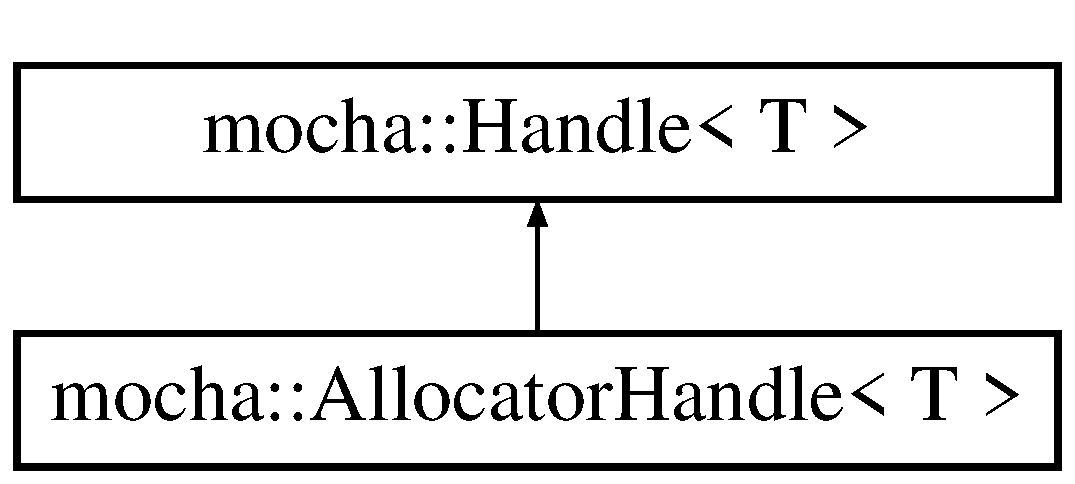
\includegraphics[height=2.000000cm]{classmocha_1_1_allocator_handle}
\end{center}
\end{figure}
\subsection*{Public Member Functions}
\begin{DoxyCompactItemize}
\item 
{\footnotesize template$<$typename Class $>$ }\\\hyperlink{classmocha_1_1_allocator_handle_a7ce28871d59f5f41c28e0f7e6aecbf13}{AllocatorHandle} (\hyperlink{classmocha_1_1_class}{Class} $\ast$ptr)
\item 
\hyperlink{classmocha_1_1_allocator_handle_a6ef49943e2e2f0bfd2621e56de3d9dac}{AllocatorHandle} ()
\item 
{\footnotesize template$<$typename Class $>$ }\\void \hyperlink{classmocha_1_1_allocator_handle_a17373eff1ea33be27713d9a3fa06ce0d}{operator()} (\hyperlink{classmocha_1_1_class}{Class} $\ast$ptr)
\begin{DoxyCompactList}\small\item\em Delay initialize. \end{DoxyCompactList}\end{DoxyCompactItemize}


\subsection{Detailed Description}
\subsubsection*{template$<$typename T$>$class mocha::AllocatorHandle$<$ T $>$}



Definition at line 177 of file handle.h.



\subsection{Constructor \& Destructor Documentation}
\hypertarget{classmocha_1_1_allocator_handle_a7ce28871d59f5f41c28e0f7e6aecbf13}{
\index{mocha::AllocatorHandle@{mocha::AllocatorHandle}!AllocatorHandle@{AllocatorHandle}}
\index{AllocatorHandle@{AllocatorHandle}!mocha::AllocatorHandle@{mocha::AllocatorHandle}}
\subsubsection[{AllocatorHandle}]{\setlength{\rightskip}{0pt plus 5cm}template$<$typename T $>$ template$<$typename Class $>$ {\bf mocha::AllocatorHandle}$<$ T $>$::{\bf AllocatorHandle} (
\begin{DoxyParamCaption}
\item[{{\bf Class} $\ast$}]{ptr}
\end{DoxyParamCaption}
)\hspace{0.3cm}{\ttfamily  \mbox{[}inline\mbox{]}}}}
\label{classmocha_1_1_allocator_handle_a7ce28871d59f5f41c28e0f7e6aecbf13}


Definition at line 173 of file handle-\/impl.h.

\hypertarget{classmocha_1_1_allocator_handle_a6ef49943e2e2f0bfd2621e56de3d9dac}{
\index{mocha::AllocatorHandle@{mocha::AllocatorHandle}!AllocatorHandle@{AllocatorHandle}}
\index{AllocatorHandle@{AllocatorHandle}!mocha::AllocatorHandle@{mocha::AllocatorHandle}}
\subsubsection[{AllocatorHandle}]{\setlength{\rightskip}{0pt plus 5cm}template$<$typename T $>$ {\bf mocha::AllocatorHandle}$<$ T $>$::{\bf AllocatorHandle} (
\begin{DoxyParamCaption}
{}
\end{DoxyParamCaption}
)\hspace{0.3cm}{\ttfamily  \mbox{[}inline\mbox{]}}}}
\label{classmocha_1_1_allocator_handle_a6ef49943e2e2f0bfd2621e56de3d9dac}


Definition at line 177 of file handle-\/impl.h.



\subsection{Member Function Documentation}
\hypertarget{classmocha_1_1_allocator_handle_a17373eff1ea33be27713d9a3fa06ce0d}{
\index{mocha::AllocatorHandle@{mocha::AllocatorHandle}!operator()@{operator()}}
\index{operator()@{operator()}!mocha::AllocatorHandle@{mocha::AllocatorHandle}}
\subsubsection[{operator()}]{\setlength{\rightskip}{0pt plus 5cm}template$<$typename T $>$ template$<$typename Class $>$ void {\bf mocha::AllocatorHandle}$<$ T $>$::operator() (
\begin{DoxyParamCaption}
\item[{{\bf Class} $\ast$}]{ptr}
\end{DoxyParamCaption}
)\hspace{0.3cm}{\ttfamily  \mbox{[}inline\mbox{]}}}}
\label{classmocha_1_1_allocator_handle_a17373eff1ea33be27713d9a3fa06ce0d}


Delay initialize. 



Reimplemented from \hyperlink{classmocha_1_1_handle_a8b6ed8540590e1199729a891957e7506}{mocha::Handle$<$ T $>$}.



Definition at line 181 of file handle-\/impl.h.



The documentation for this class was generated from the following files:\begin{DoxyCompactItemize}
\item 
Y:/mocha/src/utils/smart\_\-pointer/ref\_\-count/\hyperlink{handle_8h}{handle.h}\item 
Y:/mocha/src/utils/smart\_\-pointer/ref\_\-count/\hyperlink{handle-impl_8h}{handle-\/impl.h}\end{DoxyCompactItemize}

\hypertarget{classmocha_1_1_array_handle}{
\section{mocha::ArrayHandle$<$ T $>$ Class Template Reference}
\label{classmocha_1_1_array_handle}\index{mocha::ArrayHandle@{mocha::ArrayHandle}}
}


{\ttfamily \#include $<$handle.h$>$}

Inheritance diagram for mocha::ArrayHandle$<$ T $>$:\begin{figure}[H]
\begin{center}
\leavevmode
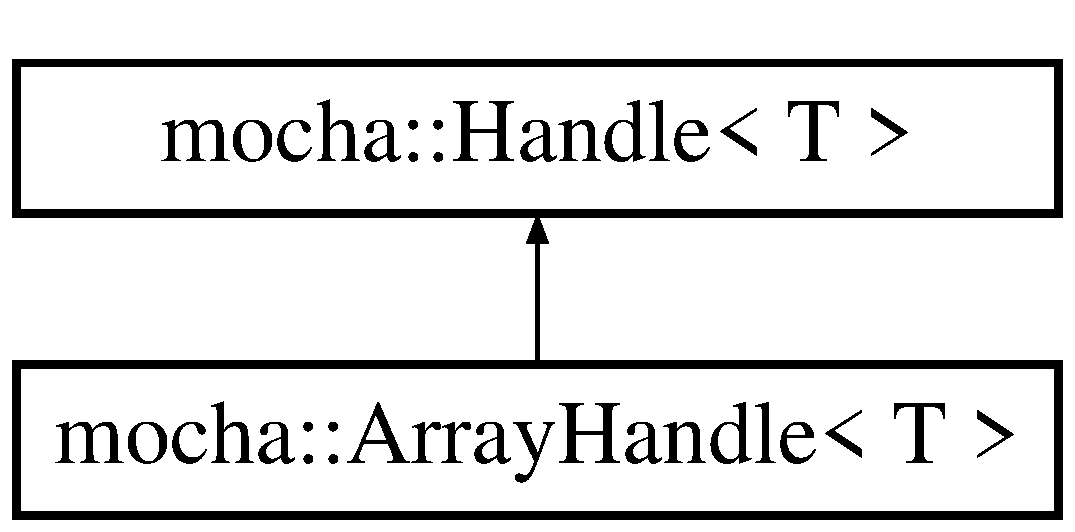
\includegraphics[height=2.000000cm]{classmocha_1_1_array_handle}
\end{center}
\end{figure}
\subsection*{Public Member Functions}
\begin{DoxyCompactItemize}
\item 
{\footnotesize template$<$typename Class $>$ }\\\hyperlink{classmocha_1_1_array_handle_ac4b94c0795061bac71e845e6716e4eb5}{ArrayHandle} (\hyperlink{classmocha_1_1_class}{Class} $\ast$ptr)
\item 
\hyperlink{classmocha_1_1_array_handle_a89ff1a03559e1b31594022dd13bc2c22}{ArrayHandle} ()
\item 
{\footnotesize template$<$typename Class $>$ }\\void \hyperlink{classmocha_1_1_array_handle_ad4a9cf2bce28823184e6d0e07e9f57b4}{operator()} (\hyperlink{classmocha_1_1_class}{Class} $\ast$ptr)
\begin{DoxyCompactList}\small\item\em Delay initialize. \end{DoxyCompactList}\end{DoxyCompactItemize}


\subsection{Detailed Description}
\subsubsection*{template$<$typename T$>$class mocha::ArrayHandle$<$ T $>$}



Definition at line 163 of file handle.h.



\subsection{Constructor \& Destructor Documentation}
\hypertarget{classmocha_1_1_array_handle_ac4b94c0795061bac71e845e6716e4eb5}{
\index{mocha::ArrayHandle@{mocha::ArrayHandle}!ArrayHandle@{ArrayHandle}}
\index{ArrayHandle@{ArrayHandle}!mocha::ArrayHandle@{mocha::ArrayHandle}}
\subsubsection[{ArrayHandle}]{\setlength{\rightskip}{0pt plus 5cm}template$<$typename T $>$ template$<$typename Class $>$ {\bf mocha::ArrayHandle}$<$ T $>$::{\bf ArrayHandle} (
\begin{DoxyParamCaption}
\item[{{\bf Class} $\ast$}]{ptr}
\end{DoxyParamCaption}
)\hspace{0.3cm}{\ttfamily  \mbox{[}inline, explicit\mbox{]}}}}
\label{classmocha_1_1_array_handle_ac4b94c0795061bac71e845e6716e4eb5}


Definition at line 157 of file handle-\/impl.h.

\hypertarget{classmocha_1_1_array_handle_a89ff1a03559e1b31594022dd13bc2c22}{
\index{mocha::ArrayHandle@{mocha::ArrayHandle}!ArrayHandle@{ArrayHandle}}
\index{ArrayHandle@{ArrayHandle}!mocha::ArrayHandle@{mocha::ArrayHandle}}
\subsubsection[{ArrayHandle}]{\setlength{\rightskip}{0pt plus 5cm}template$<$typename T $>$ {\bf mocha::ArrayHandle}$<$ T $>$::{\bf ArrayHandle} (
\begin{DoxyParamCaption}
{}
\end{DoxyParamCaption}
)\hspace{0.3cm}{\ttfamily  \mbox{[}inline\mbox{]}}}}
\label{classmocha_1_1_array_handle_a89ff1a03559e1b31594022dd13bc2c22}


Definition at line 162 of file handle-\/impl.h.



\subsection{Member Function Documentation}
\hypertarget{classmocha_1_1_array_handle_ad4a9cf2bce28823184e6d0e07e9f57b4}{
\index{mocha::ArrayHandle@{mocha::ArrayHandle}!operator()@{operator()}}
\index{operator()@{operator()}!mocha::ArrayHandle@{mocha::ArrayHandle}}
\subsubsection[{operator()}]{\setlength{\rightskip}{0pt plus 5cm}template$<$typename T $>$ template$<$typename Class $>$ void {\bf mocha::ArrayHandle}$<$ T $>$::operator() (
\begin{DoxyParamCaption}
\item[{{\bf Class} $\ast$}]{ptr}
\end{DoxyParamCaption}
)\hspace{0.3cm}{\ttfamily  \mbox{[}inline\mbox{]}}}}
\label{classmocha_1_1_array_handle_ad4a9cf2bce28823184e6d0e07e9f57b4}


Delay initialize. 



Reimplemented from \hyperlink{classmocha_1_1_handle_a8b6ed8540590e1199729a891957e7506}{mocha::Handle$<$ T $>$}.



Definition at line 166 of file handle-\/impl.h.



The documentation for this class was generated from the following files:\begin{DoxyCompactItemize}
\item 
Y:/mocha/src/utils/smart\_\-pointer/ref\_\-count/\hyperlink{handle_8h}{handle.h}\item 
Y:/mocha/src/utils/smart\_\-pointer/ref\_\-count/\hyperlink{handle-impl_8h}{handle-\/impl.h}\end{DoxyCompactItemize}

\hypertarget{classmocha_1_1_assert_stmt}{
\section{mocha::AssertStmt Class Reference}
\label{classmocha_1_1_assert_stmt}\index{mocha::AssertStmt@{mocha::AssertStmt}}
}


{\ttfamily \#include $<$ast.h$>$}

Inheritance diagram for mocha::AssertStmt:\begin{figure}[H]
\begin{center}
\leavevmode
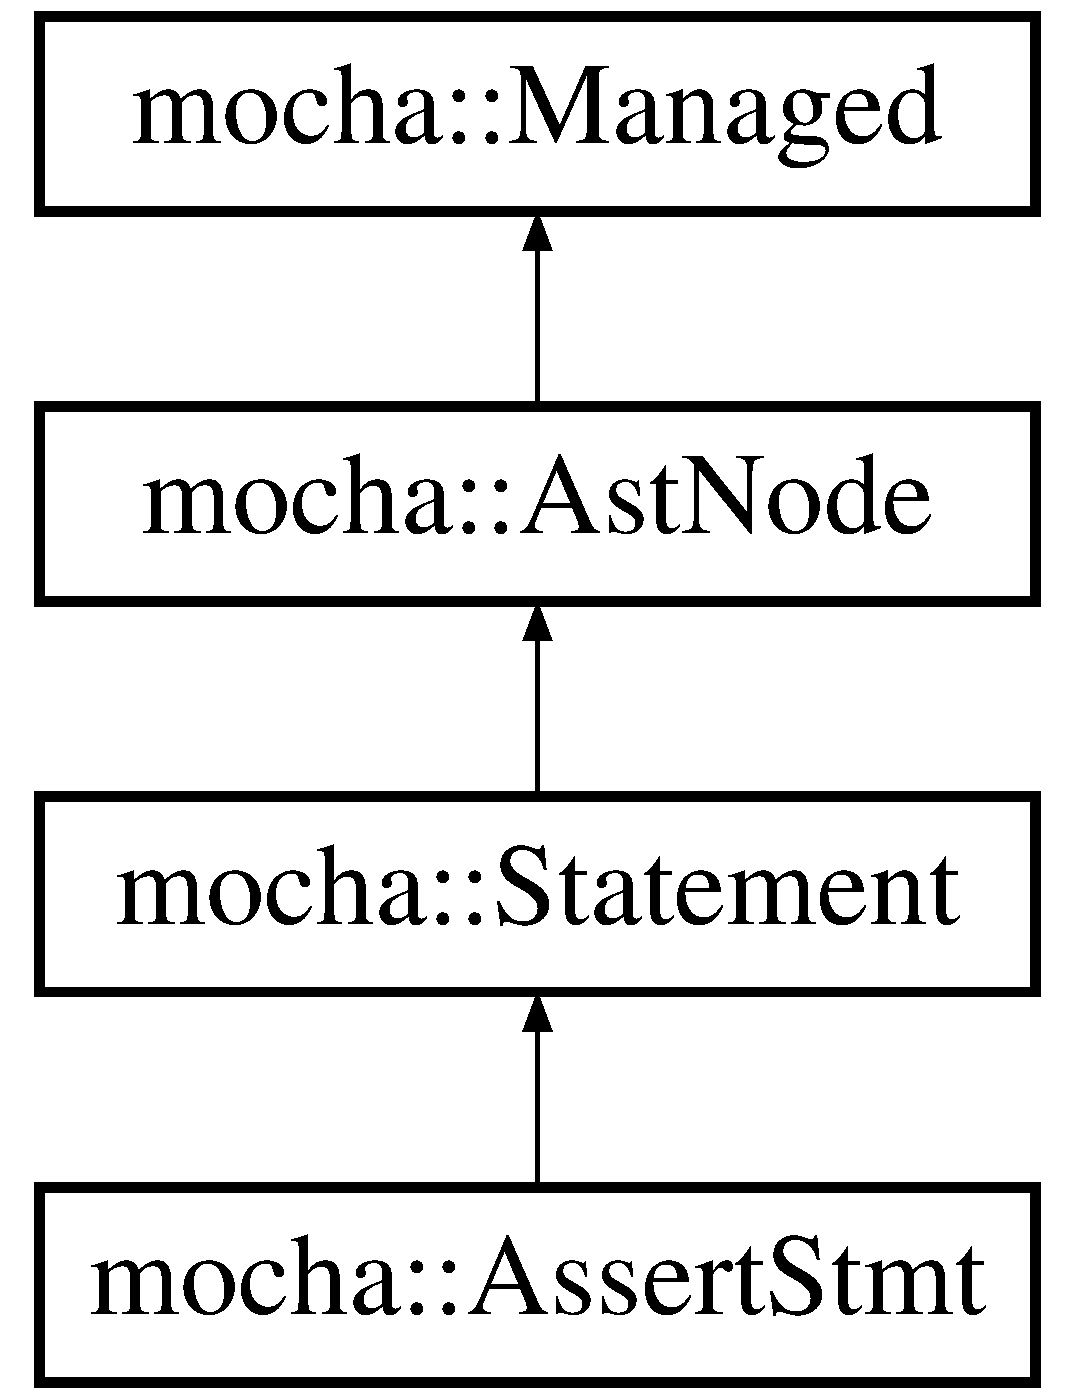
\includegraphics[height=4.000000cm]{classmocha_1_1_assert_stmt}
\end{center}
\end{figure}
\subsection*{Public Member Functions}
\begin{DoxyCompactItemize}
\item 
\hyperlink{classmocha_1_1_assert_stmt_acb221a0eb1c2c2bc0d09cde71a0b078a}{AssertStmt} ()
\item 
\hyperlink{classmocha_1_1_assert_stmt_ad1389fe533696aef4d6c51e4271ac517}{$\sim$AssertStmt} ()
\item 
\hyperlink{classmocha_1_1_ast_node}{AstNode} $\ast$ \hyperlink{classmocha_1_1_assert_stmt_a25c698181a11aa2213db0ff12b01d4be}{Clone} ()
\end{DoxyCompactItemize}
\subsection*{Private Member Functions}
\begin{DoxyCompactItemize}
\item 
void \hyperlink{classmocha_1_1_assert_stmt_a49e173e8f338612c594af47c06b650fa}{NVIAccept\_\-} (\hyperlink{classmocha_1_1_i_visitor}{IVisitor} $\ast$visitor)
\end{DoxyCompactItemize}


\subsection{Detailed Description}


Definition at line 1000 of file ast.h.



\subsection{Constructor \& Destructor Documentation}
\hypertarget{classmocha_1_1_assert_stmt_acb221a0eb1c2c2bc0d09cde71a0b078a}{
\index{mocha::AssertStmt@{mocha::AssertStmt}!AssertStmt@{AssertStmt}}
\index{AssertStmt@{AssertStmt}!mocha::AssertStmt@{mocha::AssertStmt}}
\subsubsection[{AssertStmt}]{\setlength{\rightskip}{0pt plus 5cm}mocha::AssertStmt::AssertStmt (
\begin{DoxyParamCaption}
{}
\end{DoxyParamCaption}
)\hspace{0.3cm}{\ttfamily  \mbox{[}inline\mbox{]}}}}
\label{classmocha_1_1_assert_stmt_acb221a0eb1c2c2bc0d09cde71a0b078a}


Definition at line 1002 of file ast.h.

\hypertarget{classmocha_1_1_assert_stmt_ad1389fe533696aef4d6c51e4271ac517}{
\index{mocha::AssertStmt@{mocha::AssertStmt}!$\sim$AssertStmt@{$\sim$AssertStmt}}
\index{$\sim$AssertStmt@{$\sim$AssertStmt}!mocha::AssertStmt@{mocha::AssertStmt}}
\subsubsection[{$\sim$AssertStmt}]{\setlength{\rightskip}{0pt plus 5cm}mocha::AssertStmt::$\sim$AssertStmt (
\begin{DoxyParamCaption}
{}
\end{DoxyParamCaption}
)\hspace{0.3cm}{\ttfamily  \mbox{[}inline\mbox{]}}}}
\label{classmocha_1_1_assert_stmt_ad1389fe533696aef4d6c51e4271ac517}


Definition at line 1003 of file ast.h.



\subsection{Member Function Documentation}
\hypertarget{classmocha_1_1_assert_stmt_a25c698181a11aa2213db0ff12b01d4be}{
\index{mocha::AssertStmt@{mocha::AssertStmt}!Clone@{Clone}}
\index{Clone@{Clone}!mocha::AssertStmt@{mocha::AssertStmt}}
\subsubsection[{Clone}]{\setlength{\rightskip}{0pt plus 5cm}{\bf AstNode} $\ast$ mocha::AssertStmt::Clone (
\begin{DoxyParamCaption}
{}
\end{DoxyParamCaption}
)\hspace{0.3cm}{\ttfamily  \mbox{[}virtual\mbox{]}}}}
\label{classmocha_1_1_assert_stmt_a25c698181a11aa2213db0ff12b01d4be}
\begin{DoxyReturn}{Returns}
\{AstNode$\ast$\} Clone node. 
\end{DoxyReturn}


Reimplemented from \hyperlink{classmocha_1_1_ast_node_af2a895699bac2012f8b7739bff49c5ec}{mocha::AstNode}.



Definition at line 373 of file ast.cc.

\hypertarget{classmocha_1_1_assert_stmt_a49e173e8f338612c594af47c06b650fa}{
\index{mocha::AssertStmt@{mocha::AssertStmt}!NVIAccept\_\-@{NVIAccept\_\-}}
\index{NVIAccept\_\-@{NVIAccept\_\-}!mocha::AssertStmt@{mocha::AssertStmt}}
\subsubsection[{NVIAccept\_\-}]{\setlength{\rightskip}{0pt plus 5cm}void mocha::AssertStmt::NVIAccept\_\- (
\begin{DoxyParamCaption}
\item[{{\bf IVisitor} $\ast$}]{visitor}
\end{DoxyParamCaption}
)\hspace{0.3cm}{\ttfamily  \mbox{[}inline, private, virtual\mbox{]}}}}
\label{classmocha_1_1_assert_stmt_a49e173e8f338612c594af47c06b650fa}


Reimplemented from \hyperlink{classmocha_1_1_statement_ad0e8c3ef62d21f733eb50a414046bae4}{mocha::Statement}.



Definition at line 1006 of file ast.h.



The documentation for this class was generated from the following files:\begin{DoxyCompactItemize}
\item 
Y:/mocha/src/ast/\hyperlink{ast_8h}{ast.h}\item 
Y:/mocha/src/ast/\hyperlink{ast_8cc}{ast.cc}\end{DoxyCompactItemize}

\hypertarget{classmocha_1_1_assignment_exp}{
\section{mocha::AssignmentExp Class Reference}
\label{classmocha_1_1_assignment_exp}\index{mocha::AssignmentExp@{mocha::AssignmentExp}}
}


{\ttfamily \#include $<$ast.h$>$}

Inheritance diagram for mocha::AssignmentExp:\begin{figure}[H]
\begin{center}
\leavevmode
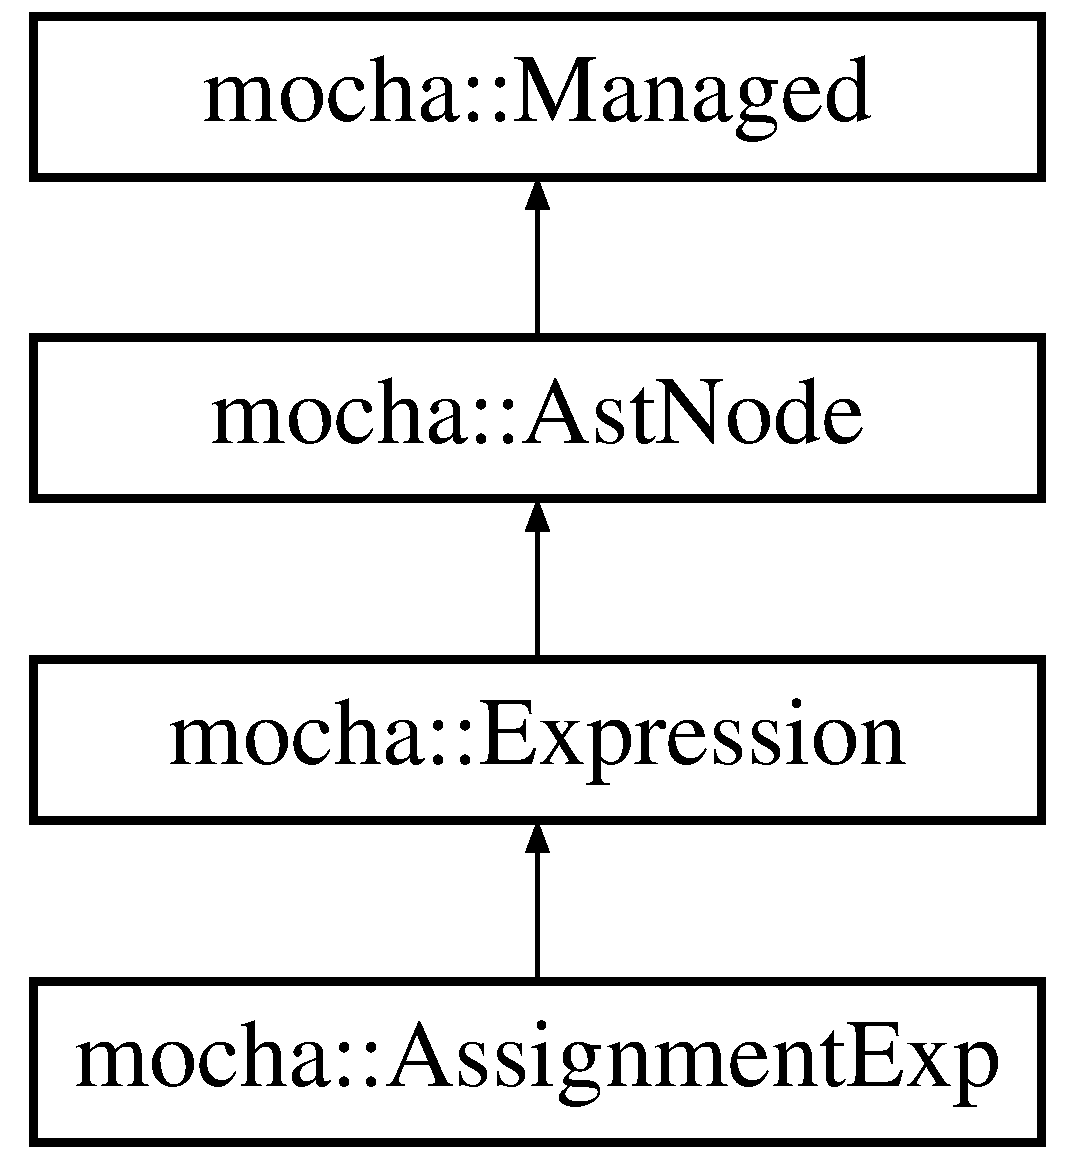
\includegraphics[height=4.000000cm]{classmocha_1_1_assignment_exp}
\end{center}
\end{figure}
\subsection*{Public Member Functions}
\begin{DoxyCompactItemize}
\item 
\hyperlink{classmocha_1_1_assignment_exp_a467744dd3da0f4e4589fd17eea275122}{AssignmentExp} (int op, \hyperlink{classmocha_1_1_ast_node}{AstNode} $\ast$left, \hyperlink{classmocha_1_1_ast_node}{AstNode} $\ast$right)
\item 
\hyperlink{classmocha_1_1_assignment_exp}{AssignmentExp} $\ast$ \hyperlink{classmocha_1_1_assignment_exp_ae8016bd58008fae4ae8e009f403fc9b0}{CastToAssigment} ()
\item 
\hyperlink{classmocha_1_1_ast_node}{AstNode} $\ast$ \hyperlink{classmocha_1_1_assignment_exp_a68245835b583847ee2aad68142d72cae}{Left} ()
\item 
\hyperlink{classmocha_1_1_ast_node}{AstNode} $\ast$ \hyperlink{classmocha_1_1_assignment_exp_acae30f2d8b41b29a90de4f2e2b425407}{Right} ()
\item 
int \hyperlink{classmocha_1_1_assignment_exp_a847a00375a65b134a03d96bbafd1c0f6}{Op} ()
\item 
void \hyperlink{classmocha_1_1_assignment_exp_a11115bd08d4ea4fc93a19bcc1fdf306d}{ReplaceChild} (\hyperlink{classmocha_1_1_ast_node}{AstNode} $\ast$old\_\-node, \hyperlink{classmocha_1_1_ast_node}{AstNode} $\ast$new\_\-node)
\item 
\hyperlink{classmocha_1_1_ast_node}{AstNode} $\ast$ \hyperlink{classmocha_1_1_assignment_exp_ac266c79bc33aaba7a6de7bb34a966786}{Clone} ()
\end{DoxyCompactItemize}
\subsection*{Private Member Functions}
\begin{DoxyCompactItemize}
\item 
void \hyperlink{classmocha_1_1_assignment_exp_ae8926731b19e86748e07bf8f29fa9a1b}{NVIAccept\_\-} (\hyperlink{classmocha_1_1_i_visitor}{IVisitor} $\ast$visitor)
\end{DoxyCompactItemize}
\subsection*{Private Attributes}
\begin{DoxyCompactItemize}
\item 
int \hyperlink{classmocha_1_1_assignment_exp_a602624825bd3b7fa70ff1069c0425f9a}{op\_\-}
\item 
\hyperlink{classmocha_1_1_ast_node}{AstNode} $\ast$ \hyperlink{classmocha_1_1_assignment_exp_ad899e6df5e3e26572eece7523e1a4327}{left\_\-}
\item 
\hyperlink{classmocha_1_1_ast_node}{AstNode} $\ast$ \hyperlink{classmocha_1_1_assignment_exp_a41d8c915810d5f81e7ba584402d2e692}{right\_\-}
\end{DoxyCompactItemize}


\subsection{Detailed Description}


Definition at line 1495 of file ast.h.



\subsection{Constructor \& Destructor Documentation}
\hypertarget{classmocha_1_1_assignment_exp_a467744dd3da0f4e4589fd17eea275122}{
\index{mocha::AssignmentExp@{mocha::AssignmentExp}!AssignmentExp@{AssignmentExp}}
\index{AssignmentExp@{AssignmentExp}!mocha::AssignmentExp@{mocha::AssignmentExp}}
\subsubsection[{AssignmentExp}]{\setlength{\rightskip}{0pt plus 5cm}mocha::AssignmentExp::AssignmentExp (
\begin{DoxyParamCaption}
\item[{int}]{op, }
\item[{{\bf AstNode} $\ast$}]{left, }
\item[{{\bf AstNode} $\ast$}]{right}
\end{DoxyParamCaption}
)\hspace{0.3cm}{\ttfamily  \mbox{[}inline\mbox{]}}}}
\label{classmocha_1_1_assignment_exp_a467744dd3da0f4e4589fd17eea275122}


Definition at line 1497 of file ast.h.



\subsection{Member Function Documentation}
\hypertarget{classmocha_1_1_assignment_exp_ae8016bd58008fae4ae8e009f403fc9b0}{
\index{mocha::AssignmentExp@{mocha::AssignmentExp}!CastToAssigment@{CastToAssigment}}
\index{CastToAssigment@{CastToAssigment}!mocha::AssignmentExp@{mocha::AssignmentExp}}
\subsubsection[{CastToAssigment}]{\setlength{\rightskip}{0pt plus 5cm}{\bf AssignmentExp}$\ast$ mocha::AssignmentExp::CastToAssigment (
\begin{DoxyParamCaption}
{}
\end{DoxyParamCaption}
)\hspace{0.3cm}{\ttfamily  \mbox{[}inline, virtual\mbox{]}}}}
\label{classmocha_1_1_assignment_exp_ae8016bd58008fae4ae8e009f403fc9b0}


Reimplemented from \hyperlink{classmocha_1_1_expression_ac9487a84166be5500145ae33523ebfdf}{mocha::Expression}.



Definition at line 1503 of file ast.h.

\hypertarget{classmocha_1_1_assignment_exp_ac266c79bc33aaba7a6de7bb34a966786}{
\index{mocha::AssignmentExp@{mocha::AssignmentExp}!Clone@{Clone}}
\index{Clone@{Clone}!mocha::AssignmentExp@{mocha::AssignmentExp}}
\subsubsection[{Clone}]{\setlength{\rightskip}{0pt plus 5cm}{\bf AstNode} $\ast$ mocha::AssignmentExp::Clone (
\begin{DoxyParamCaption}
{}
\end{DoxyParamCaption}
)\hspace{0.3cm}{\ttfamily  \mbox{[}virtual\mbox{]}}}}
\label{classmocha_1_1_assignment_exp_ac266c79bc33aaba7a6de7bb34a966786}
\begin{DoxyReturn}{Returns}
\{AstNode$\ast$\} Clone node. 
\end{DoxyReturn}


Reimplemented from \hyperlink{classmocha_1_1_expression_ac1fb936e2bf0fdd6e7667275d3723ca5}{mocha::Expression}.



Definition at line 607 of file ast.cc.

\hypertarget{classmocha_1_1_assignment_exp_a68245835b583847ee2aad68142d72cae}{
\index{mocha::AssignmentExp@{mocha::AssignmentExp}!Left@{Left}}
\index{Left@{Left}!mocha::AssignmentExp@{mocha::AssignmentExp}}
\subsubsection[{Left}]{\setlength{\rightskip}{0pt plus 5cm}{\bf AstNode}$\ast$ mocha::AssignmentExp::Left (
\begin{DoxyParamCaption}
{}
\end{DoxyParamCaption}
)\hspace{0.3cm}{\ttfamily  \mbox{[}inline\mbox{]}}}}
\label{classmocha_1_1_assignment_exp_a68245835b583847ee2aad68142d72cae}


Definition at line 1504 of file ast.h.

\hypertarget{classmocha_1_1_assignment_exp_ae8926731b19e86748e07bf8f29fa9a1b}{
\index{mocha::AssignmentExp@{mocha::AssignmentExp}!NVIAccept\_\-@{NVIAccept\_\-}}
\index{NVIAccept\_\-@{NVIAccept\_\-}!mocha::AssignmentExp@{mocha::AssignmentExp}}
\subsubsection[{NVIAccept\_\-}]{\setlength{\rightskip}{0pt plus 5cm}void mocha::AssignmentExp::NVIAccept\_\- (
\begin{DoxyParamCaption}
\item[{{\bf IVisitor} $\ast$}]{visitor}
\end{DoxyParamCaption}
)\hspace{0.3cm}{\ttfamily  \mbox{[}inline, private, virtual\mbox{]}}}}
\label{classmocha_1_1_assignment_exp_ae8926731b19e86748e07bf8f29fa9a1b}


Reimplemented from \hyperlink{classmocha_1_1_expression_a112d57b7de76c37066cde60be4799fde}{mocha::Expression}.



Definition at line 1513 of file ast.h.

\hypertarget{classmocha_1_1_assignment_exp_a847a00375a65b134a03d96bbafd1c0f6}{
\index{mocha::AssignmentExp@{mocha::AssignmentExp}!Op@{Op}}
\index{Op@{Op}!mocha::AssignmentExp@{mocha::AssignmentExp}}
\subsubsection[{Op}]{\setlength{\rightskip}{0pt plus 5cm}int mocha::AssignmentExp::Op (
\begin{DoxyParamCaption}
{}
\end{DoxyParamCaption}
)\hspace{0.3cm}{\ttfamily  \mbox{[}inline\mbox{]}}}}
\label{classmocha_1_1_assignment_exp_a847a00375a65b134a03d96bbafd1c0f6}


Definition at line 1506 of file ast.h.

\hypertarget{classmocha_1_1_assignment_exp_a11115bd08d4ea4fc93a19bcc1fdf306d}{
\index{mocha::AssignmentExp@{mocha::AssignmentExp}!ReplaceChild@{ReplaceChild}}
\index{ReplaceChild@{ReplaceChild}!mocha::AssignmentExp@{mocha::AssignmentExp}}
\subsubsection[{ReplaceChild}]{\setlength{\rightskip}{0pt plus 5cm}void mocha::AssignmentExp::ReplaceChild (
\begin{DoxyParamCaption}
\item[{{\bf AstNode} $\ast$}]{old\_\-node, }
\item[{{\bf AstNode} $\ast$}]{new\_\-node}
\end{DoxyParamCaption}
)\hspace{0.3cm}{\ttfamily  \mbox{[}virtual\mbox{]}}}}
\label{classmocha_1_1_assignment_exp_a11115bd08d4ea4fc93a19bcc1fdf306d}

\begin{DoxyParams}{Parameters}
{\em \{AstNode$\ast$\}} & Replace the old\_\-node with new\_\-node in childnodes. \\
\hline
\end{DoxyParams}


Reimplemented from \hyperlink{classmocha_1_1_ast_node_aa40396040f75fb59e320d81c3fd328c8}{mocha::AstNode}.



Definition at line 591 of file ast.cc.

\hypertarget{classmocha_1_1_assignment_exp_acae30f2d8b41b29a90de4f2e2b425407}{
\index{mocha::AssignmentExp@{mocha::AssignmentExp}!Right@{Right}}
\index{Right@{Right}!mocha::AssignmentExp@{mocha::AssignmentExp}}
\subsubsection[{Right}]{\setlength{\rightskip}{0pt plus 5cm}{\bf AstNode}$\ast$ mocha::AssignmentExp::Right (
\begin{DoxyParamCaption}
{}
\end{DoxyParamCaption}
)\hspace{0.3cm}{\ttfamily  \mbox{[}inline\mbox{]}}}}
\label{classmocha_1_1_assignment_exp_acae30f2d8b41b29a90de4f2e2b425407}


Definition at line 1505 of file ast.h.



\subsection{Member Data Documentation}
\hypertarget{classmocha_1_1_assignment_exp_ad899e6df5e3e26572eece7523e1a4327}{
\index{mocha::AssignmentExp@{mocha::AssignmentExp}!left\_\-@{left\_\-}}
\index{left\_\-@{left\_\-}!mocha::AssignmentExp@{mocha::AssignmentExp}}
\subsubsection[{left\_\-}]{\setlength{\rightskip}{0pt plus 5cm}{\bf AstNode}$\ast$ {\bf mocha::AssignmentExp::left\_\-}\hspace{0.3cm}{\ttfamily  \mbox{[}private\mbox{]}}}}
\label{classmocha_1_1_assignment_exp_ad899e6df5e3e26572eece7523e1a4327}


Definition at line 1511 of file ast.h.

\hypertarget{classmocha_1_1_assignment_exp_a602624825bd3b7fa70ff1069c0425f9a}{
\index{mocha::AssignmentExp@{mocha::AssignmentExp}!op\_\-@{op\_\-}}
\index{op\_\-@{op\_\-}!mocha::AssignmentExp@{mocha::AssignmentExp}}
\subsubsection[{op\_\-}]{\setlength{\rightskip}{0pt plus 5cm}int {\bf mocha::AssignmentExp::op\_\-}\hspace{0.3cm}{\ttfamily  \mbox{[}private\mbox{]}}}}
\label{classmocha_1_1_assignment_exp_a602624825bd3b7fa70ff1069c0425f9a}


Definition at line 1508 of file ast.h.

\hypertarget{classmocha_1_1_assignment_exp_a41d8c915810d5f81e7ba584402d2e692}{
\index{mocha::AssignmentExp@{mocha::AssignmentExp}!right\_\-@{right\_\-}}
\index{right\_\-@{right\_\-}!mocha::AssignmentExp@{mocha::AssignmentExp}}
\subsubsection[{right\_\-}]{\setlength{\rightskip}{0pt plus 5cm}{\bf AstNode}$\ast$ {\bf mocha::AssignmentExp::right\_\-}\hspace{0.3cm}{\ttfamily  \mbox{[}private\mbox{]}}}}
\label{classmocha_1_1_assignment_exp_a41d8c915810d5f81e7ba584402d2e692}


Definition at line 1512 of file ast.h.



The documentation for this class was generated from the following files:\begin{DoxyCompactItemize}
\item 
Y:/mocha/src/ast/\hyperlink{ast_8h}{ast.h}\item 
Y:/mocha/src/ast/\hyperlink{ast_8cc}{ast.cc}\end{DoxyCompactItemize}

\hypertarget{classmocha_1_1_ast_for_v8}{
\section{mocha::AstForV8 Class Reference}
\label{classmocha_1_1_ast_for_v8}\index{mocha::AstForV8@{mocha::AstForV8}}
}


{\ttfamily \#include $<$ast\_\-v8.h$>$}

\subsection*{Public Types}
\begin{DoxyCompactItemize}
\item 
typedef v8::Handle$<$ v8::Value $>$ \hyperlink{classmocha_1_1_ast_for_v8_af0e3f6f88e017315384842e6e8c20c9d}{JSValue}
\end{DoxyCompactItemize}
\subsection*{Static Public Member Functions}
\begin{DoxyCompactItemize}
\item 
static v8::Handle$<$ v8::Object $>$ \hyperlink{classmocha_1_1_ast_for_v8_a1ac9550feb638f8104a62b8159b5d492}{Init} (\hyperlink{classmocha_1_1_ast_node}{AstNode} $\ast$ast\_\-node, \hyperlink{classmocha_1_1_processor_info}{ProcessorInfo} $\ast$info)
\item 
static \hyperlink{classmocha_1_1_ast_for_v8_af0e3f6f88e017315384842e6e8c20c9d}{JSValue} \hyperlink{classmocha_1_1_ast_for_v8_ac25f160a30e19de142b330f8221e2c8f}{ChildNodes} (const v8::Arguments \&args)
\item 
static \hyperlink{classmocha_1_1_ast_for_v8_af0e3f6f88e017315384842e6e8c20c9d}{JSValue} \hyperlink{classmocha_1_1_ast_for_v8_a9102f7cecb5807fd224c8f468b8c6a54}{FirstChild} (const v8::Arguments \&args)
\item 
static \hyperlink{classmocha_1_1_ast_for_v8_af0e3f6f88e017315384842e6e8c20c9d}{JSValue} \hyperlink{classmocha_1_1_ast_for_v8_ad46572498216e2e7690d6c35ae2b7f67}{LastChild} (const v8::Arguments \&args)
\item 
static \hyperlink{classmocha_1_1_ast_for_v8_af0e3f6f88e017315384842e6e8c20c9d}{JSValue} \hyperlink{classmocha_1_1_ast_for_v8_a691a43f2cf83282fdc4d95f72601b4d7}{ReplaceChild} (const v8::Arguments \&args)
\item 
static \hyperlink{classmocha_1_1_ast_for_v8_af0e3f6f88e017315384842e6e8c20c9d}{JSValue} \hyperlink{classmocha_1_1_ast_for_v8_a216dd7720b74a1ad8e20b611bffb71fe}{ParentNode} (const v8::Arguments \&args)
\item 
static \hyperlink{classmocha_1_1_ast_for_v8_af0e3f6f88e017315384842e6e8c20c9d}{JSValue} \hyperlink{classmocha_1_1_ast_for_v8_a6bc80a1b960c5d294ae4c8e684b4dc69}{NextSibling} (const v8::Arguments \&args)
\item 
static \hyperlink{classmocha_1_1_ast_for_v8_af0e3f6f88e017315384842e6e8c20c9d}{JSValue} \hyperlink{classmocha_1_1_ast_for_v8_a444a668bbd97fc3e9b59b92ecdd924e8}{PreviousSibling} (const v8::Arguments \&args)
\item 
static v8::Handle$<$ v8::String $>$ \hyperlink{classmocha_1_1_ast_for_v8_ad552bda0c52da0b04ce36a0ca3e9998e}{NodeName} (const v8::Arguments \&args)
\item 
static \hyperlink{classmocha_1_1_ast_for_v8_af0e3f6f88e017315384842e6e8c20c9d}{JSValue} \hyperlink{classmocha_1_1_ast_for_v8_aaf883ca87d25189a7517527b57bda8f1}{NodeType} (const v8::Arguments \&args)
\end{DoxyCompactItemize}
\subsection*{Private Attributes}
\begin{DoxyCompactItemize}
\item 
\hyperlink{classmocha_1_1_ast_node}{AstNode} $\ast$ \hyperlink{classmocha_1_1_ast_for_v8_a6b6ad460b87682b4756bced3b31b3476}{ast\_\-}
\end{DoxyCompactItemize}


\subsection{Detailed Description}


Definition at line 7 of file ast\_\-v8.h.



\subsection{Member Typedef Documentation}
\hypertarget{classmocha_1_1_ast_for_v8_af0e3f6f88e017315384842e6e8c20c9d}{
\index{mocha::AstForV8@{mocha::AstForV8}!JSValue@{JSValue}}
\index{JSValue@{JSValue}!mocha::AstForV8@{mocha::AstForV8}}
\subsubsection[{JSValue}]{\setlength{\rightskip}{0pt plus 5cm}typedef v8::Handle$<$v8::Value$>$ {\bf mocha::AstForV8::JSValue}}}
\label{classmocha_1_1_ast_for_v8_af0e3f6f88e017315384842e6e8c20c9d}


Definition at line 9 of file ast\_\-v8.h.



\subsection{Member Function Documentation}
\hypertarget{classmocha_1_1_ast_for_v8_ac25f160a30e19de142b330f8221e2c8f}{
\index{mocha::AstForV8@{mocha::AstForV8}!ChildNodes@{ChildNodes}}
\index{ChildNodes@{ChildNodes}!mocha::AstForV8@{mocha::AstForV8}}
\subsubsection[{ChildNodes}]{\setlength{\rightskip}{0pt plus 5cm}{\bf V8Value} mocha::AstForV8::ChildNodes (
\begin{DoxyParamCaption}
\item[{const v8::Arguments \&}]{args}
\end{DoxyParamCaption}
)\hspace{0.3cm}{\ttfamily  \mbox{[}static\mbox{]}}}}
\label{classmocha_1_1_ast_for_v8_ac25f160a30e19de142b330f8221e2c8f}


Definition at line 1758 of file ast\_\-v8.cc.

\hypertarget{classmocha_1_1_ast_for_v8_a9102f7cecb5807fd224c8f468b8c6a54}{
\index{mocha::AstForV8@{mocha::AstForV8}!FirstChild@{FirstChild}}
\index{FirstChild@{FirstChild}!mocha::AstForV8@{mocha::AstForV8}}
\subsubsection[{FirstChild}]{\setlength{\rightskip}{0pt plus 5cm}static {\bf JSValue} mocha::AstForV8::FirstChild (
\begin{DoxyParamCaption}
\item[{const v8::Arguments \&}]{args}
\end{DoxyParamCaption}
)\hspace{0.3cm}{\ttfamily  \mbox{[}static\mbox{]}}}}
\label{classmocha_1_1_ast_for_v8_a9102f7cecb5807fd224c8f468b8c6a54}
\hypertarget{classmocha_1_1_ast_for_v8_a1ac9550feb638f8104a62b8159b5d492}{
\index{mocha::AstForV8@{mocha::AstForV8}!Init@{Init}}
\index{Init@{Init}!mocha::AstForV8@{mocha::AstForV8}}
\subsubsection[{Init}]{\setlength{\rightskip}{0pt plus 5cm}static v8::Handle$<$v8::Object$>$ mocha::AstForV8::Init (
\begin{DoxyParamCaption}
\item[{{\bf AstNode} $\ast$}]{ast\_\-node, }
\item[{{\bf ProcessorInfo} $\ast$}]{info}
\end{DoxyParamCaption}
)\hspace{0.3cm}{\ttfamily  \mbox{[}static\mbox{]}}}}
\label{classmocha_1_1_ast_for_v8_a1ac9550feb638f8104a62b8159b5d492}
\hypertarget{classmocha_1_1_ast_for_v8_ad46572498216e2e7690d6c35ae2b7f67}{
\index{mocha::AstForV8@{mocha::AstForV8}!LastChild@{LastChild}}
\index{LastChild@{LastChild}!mocha::AstForV8@{mocha::AstForV8}}
\subsubsection[{LastChild}]{\setlength{\rightskip}{0pt plus 5cm}static {\bf JSValue} mocha::AstForV8::LastChild (
\begin{DoxyParamCaption}
\item[{const v8::Arguments \&}]{args}
\end{DoxyParamCaption}
)\hspace{0.3cm}{\ttfamily  \mbox{[}static\mbox{]}}}}
\label{classmocha_1_1_ast_for_v8_ad46572498216e2e7690d6c35ae2b7f67}
\hypertarget{classmocha_1_1_ast_for_v8_a6bc80a1b960c5d294ae4c8e684b4dc69}{
\index{mocha::AstForV8@{mocha::AstForV8}!NextSibling@{NextSibling}}
\index{NextSibling@{NextSibling}!mocha::AstForV8@{mocha::AstForV8}}
\subsubsection[{NextSibling}]{\setlength{\rightskip}{0pt plus 5cm}static {\bf JSValue} mocha::AstForV8::NextSibling (
\begin{DoxyParamCaption}
\item[{const v8::Arguments \&}]{args}
\end{DoxyParamCaption}
)\hspace{0.3cm}{\ttfamily  \mbox{[}static\mbox{]}}}}
\label{classmocha_1_1_ast_for_v8_a6bc80a1b960c5d294ae4c8e684b4dc69}
\hypertarget{classmocha_1_1_ast_for_v8_ad552bda0c52da0b04ce36a0ca3e9998e}{
\index{mocha::AstForV8@{mocha::AstForV8}!NodeName@{NodeName}}
\index{NodeName@{NodeName}!mocha::AstForV8@{mocha::AstForV8}}
\subsubsection[{NodeName}]{\setlength{\rightskip}{0pt plus 5cm}{\bf V8Value} mocha::AstForV8::NodeName (
\begin{DoxyParamCaption}
\item[{const v8::Arguments \&}]{args}
\end{DoxyParamCaption}
)\hspace{0.3cm}{\ttfamily  \mbox{[}static\mbox{]}}}}
\label{classmocha_1_1_ast_for_v8_ad552bda0c52da0b04ce36a0ca3e9998e}


Definition at line 1855 of file ast\_\-v8.cc.

\hypertarget{classmocha_1_1_ast_for_v8_aaf883ca87d25189a7517527b57bda8f1}{
\index{mocha::AstForV8@{mocha::AstForV8}!NodeType@{NodeType}}
\index{NodeType@{NodeType}!mocha::AstForV8@{mocha::AstForV8}}
\subsubsection[{NodeType}]{\setlength{\rightskip}{0pt plus 5cm}{\bf V8Value} mocha::AstForV8::NodeType (
\begin{DoxyParamCaption}
\item[{const v8::Arguments \&}]{args}
\end{DoxyParamCaption}
)\hspace{0.3cm}{\ttfamily  \mbox{[}static\mbox{]}}}}
\label{classmocha_1_1_ast_for_v8_aaf883ca87d25189a7517527b57bda8f1}


Definition at line 1862 of file ast\_\-v8.cc.

\hypertarget{classmocha_1_1_ast_for_v8_a216dd7720b74a1ad8e20b611bffb71fe}{
\index{mocha::AstForV8@{mocha::AstForV8}!ParentNode@{ParentNode}}
\index{ParentNode@{ParentNode}!mocha::AstForV8@{mocha::AstForV8}}
\subsubsection[{ParentNode}]{\setlength{\rightskip}{0pt plus 5cm}{\bf V8Value} mocha::AstForV8::ParentNode (
\begin{DoxyParamCaption}
\item[{const v8::Arguments \&}]{args}
\end{DoxyParamCaption}
)\hspace{0.3cm}{\ttfamily  \mbox{[}static\mbox{]}}}}
\label{classmocha_1_1_ast_for_v8_a216dd7720b74a1ad8e20b611bffb71fe}


Definition at line 1819 of file ast\_\-v8.cc.

\hypertarget{classmocha_1_1_ast_for_v8_a444a668bbd97fc3e9b59b92ecdd924e8}{
\index{mocha::AstForV8@{mocha::AstForV8}!PreviousSibling@{PreviousSibling}}
\index{PreviousSibling@{PreviousSibling}!mocha::AstForV8@{mocha::AstForV8}}
\subsubsection[{PreviousSibling}]{\setlength{\rightskip}{0pt plus 5cm}static {\bf JSValue} mocha::AstForV8::PreviousSibling (
\begin{DoxyParamCaption}
\item[{const v8::Arguments \&}]{args}
\end{DoxyParamCaption}
)\hspace{0.3cm}{\ttfamily  \mbox{[}static\mbox{]}}}}
\label{classmocha_1_1_ast_for_v8_a444a668bbd97fc3e9b59b92ecdd924e8}
\hypertarget{classmocha_1_1_ast_for_v8_a691a43f2cf83282fdc4d95f72601b4d7}{
\index{mocha::AstForV8@{mocha::AstForV8}!ReplaceChild@{ReplaceChild}}
\index{ReplaceChild@{ReplaceChild}!mocha::AstForV8@{mocha::AstForV8}}
\subsubsection[{ReplaceChild}]{\setlength{\rightskip}{0pt plus 5cm}static {\bf JSValue} mocha::AstForV8::ReplaceChild (
\begin{DoxyParamCaption}
\item[{const v8::Arguments \&}]{args}
\end{DoxyParamCaption}
)\hspace{0.3cm}{\ttfamily  \mbox{[}static\mbox{]}}}}
\label{classmocha_1_1_ast_for_v8_a691a43f2cf83282fdc4d95f72601b4d7}


\subsection{Member Data Documentation}
\hypertarget{classmocha_1_1_ast_for_v8_a6b6ad460b87682b4756bced3b31b3476}{
\index{mocha::AstForV8@{mocha::AstForV8}!ast\_\-@{ast\_\-}}
\index{ast\_\-@{ast\_\-}!mocha::AstForV8@{mocha::AstForV8}}
\subsubsection[{ast\_\-}]{\setlength{\rightskip}{0pt plus 5cm}{\bf AstNode}$\ast$ {\bf mocha::AstForV8::ast\_\-}\hspace{0.3cm}{\ttfamily  \mbox{[}private\mbox{]}}}}
\label{classmocha_1_1_ast_for_v8_a6b6ad460b87682b4756bced3b31b3476}


Definition at line 21 of file ast\_\-v8.h.



The documentation for this class was generated from the following files:\begin{DoxyCompactItemize}
\item 
Y:/mocha/src/ast/directives/\hyperlink{ast__v8_8h}{ast\_\-v8.h}\item 
Y:/mocha/src/ast/directives/\hyperlink{ast__v8_8cc}{ast\_\-v8.cc}\end{DoxyCompactItemize}

\hypertarget{classmocha_1_1_ast_node}{
\section{mocha::AstNode Class Reference}
\label{classmocha_1_1_ast_node}\index{mocha::AstNode@{mocha::AstNode}}
}


{\ttfamily \#include $<$ast.h$>$}

Inheritance diagram for mocha::AstNode:\begin{figure}[H]
\begin{center}
\leavevmode
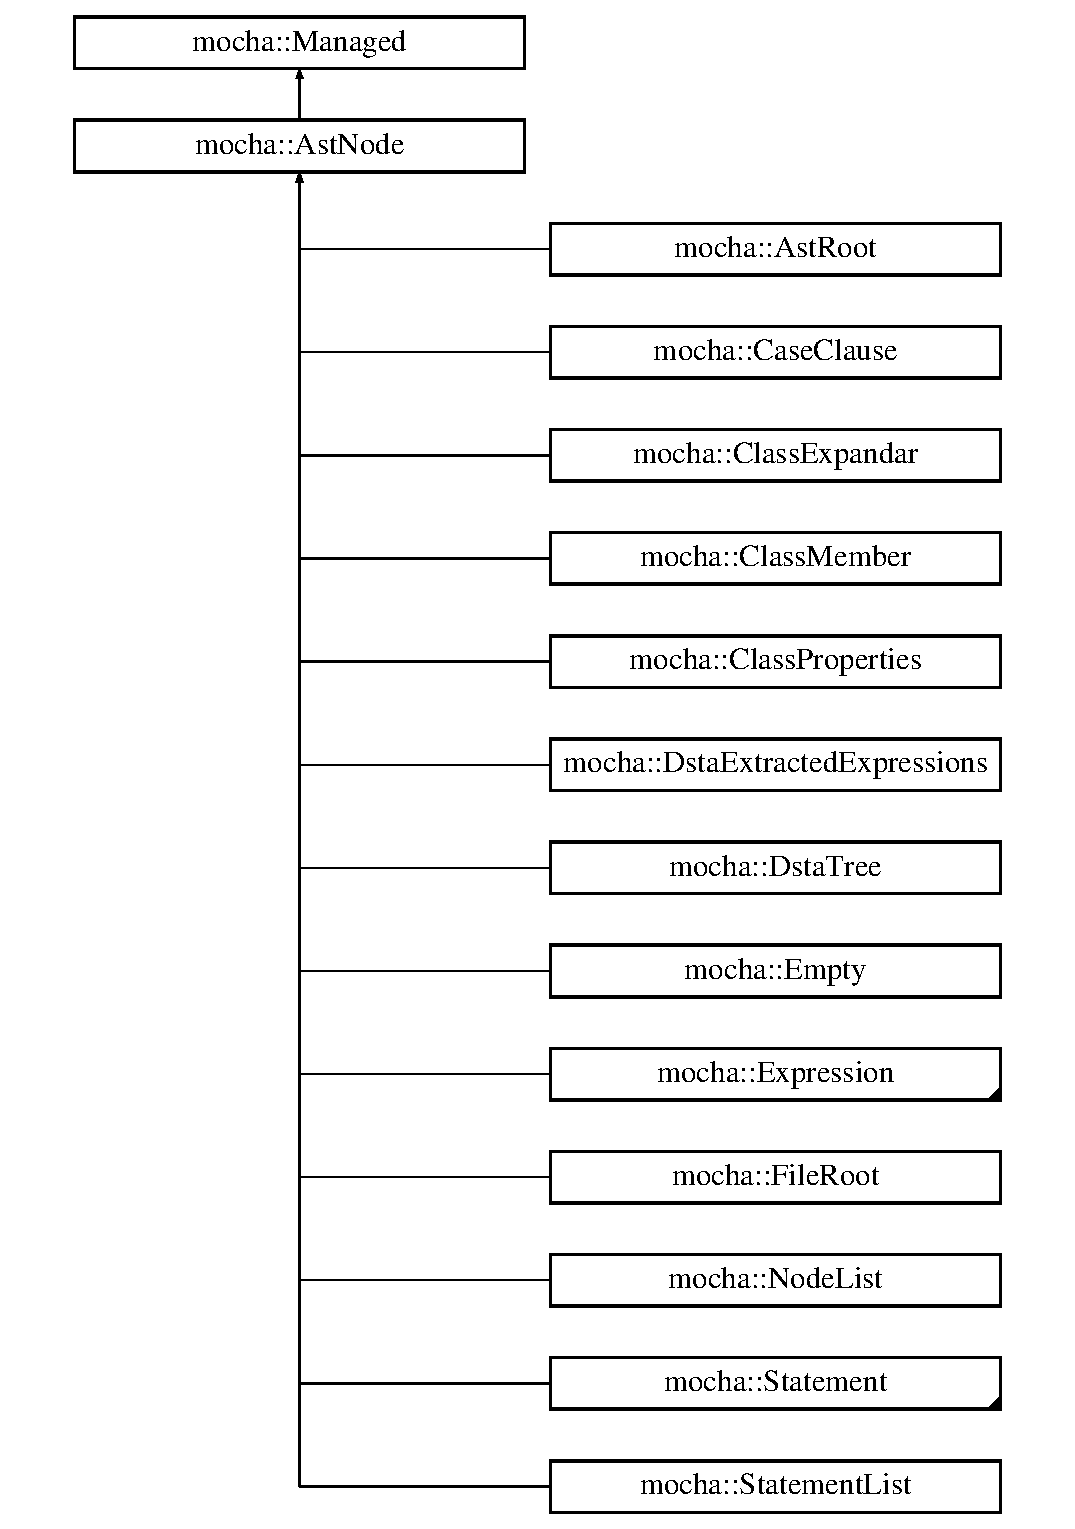
\includegraphics[height=12.000000cm]{classmocha_1_1_ast_node}
\end{center}
\end{figure}
\subsection*{Public Types}
\begin{DoxyCompactItemize}
\item 
enum \{ \par
\hyperlink{classmocha_1_1_ast_node_a7e049e71bcf600466f1c977205d8215baed7af7bd61ae03c387ffa49c8aacaef8}{kBase}, 
\hyperlink{classmocha_1_1_ast_node_a7e049e71bcf600466f1c977205d8215ba511887c37cd4074434e34153e959d198}{kEmpty}, 
\hyperlink{classmocha_1_1_ast_node_a7e049e71bcf600466f1c977205d8215ba56703200dd35574e643aef20a1825cf2}{kAstRoot}, 
\hyperlink{classmocha_1_1_ast_node_a7e049e71bcf600466f1c977205d8215bab69ae939c113a6106841d35b37053cd8}{kFileRoot}, 
\par
\hyperlink{classmocha_1_1_ast_node_a7e049e71bcf600466f1c977205d8215bae5a4037ed96d6f6cdc41017238e9bbbf}{kStatement}, 
\hyperlink{classmocha_1_1_ast_node_a7e049e71bcf600466f1c977205d8215ba7a46df6b31dd288b57321f56c0da6f3d}{kStatementList}, 
\hyperlink{classmocha_1_1_ast_node_a7e049e71bcf600466f1c977205d8215ba6cff62c7aaf639d31089d33283845e6c}{kVersionStmt}, 
\hyperlink{classmocha_1_1_ast_node_a7e049e71bcf600466f1c977205d8215ba8d297fdf01ae8868c4f0b419b697e667}{kAssertStmt}, 
\par
\hyperlink{classmocha_1_1_ast_node_a7e049e71bcf600466f1c977205d8215ba40fbbce0d349cefa94e0c5fed93de443}{kExpression}, 
\hyperlink{classmocha_1_1_ast_node_a7e049e71bcf600466f1c977205d8215ba8c24bef501c2e740aa2f6c86a6d040b9}{kValueNode}, 
\hyperlink{classmocha_1_1_ast_node_a7e049e71bcf600466f1c977205d8215ba1ed74aaabe6604bef479369b7ee50b0b}{kCase}, 
\hyperlink{classmocha_1_1_ast_node_a7e049e71bcf600466f1c977205d8215ba10d875bdca7c3e5ec5f9b0043557cc9d}{kNodeList}, 
\par
\hyperlink{classmocha_1_1_ast_node_a7e049e71bcf600466f1c977205d8215ba9f464bb146c852a419ee4bba8d13765a}{kPragmaStmt}, 
\hyperlink{classmocha_1_1_ast_node_a7e049e71bcf600466f1c977205d8215baab2f621fe45ba67dc552471b763a51c8}{kBlockStmt}, 
\hyperlink{classmocha_1_1_ast_node_a7e049e71bcf600466f1c977205d8215ba85b639bed8e9fa2fa764bb3b10135eba}{kModuleStmt}, 
\hyperlink{classmocha_1_1_ast_node_a7e049e71bcf600466f1c977205d8215baac82cb5bcab2c3ecbbb5624b304f90f6}{kExportStmt}, 
\par
\hyperlink{classmocha_1_1_ast_node_a7e049e71bcf600466f1c977205d8215baadbcbe5f5bff9ea2bd179f15146c59d0}{kImportStmt}, 
\hyperlink{classmocha_1_1_ast_node_a7e049e71bcf600466f1c977205d8215ba8f84608da1541695d59048502a9d7bc2}{kVariableStmt}, 
\hyperlink{classmocha_1_1_ast_node_a7e049e71bcf600466f1c977205d8215ba0c6d0a8d436b9d8acdbbae3484c2fb24}{kLetStmt}, 
\hyperlink{classmocha_1_1_ast_node_a7e049e71bcf600466f1c977205d8215ba23d48b7cee86dcf42a9b69c5b4a339ef}{kExpressionStmt}, 
\par
\hyperlink{classmocha_1_1_ast_node_a7e049e71bcf600466f1c977205d8215bad01c500958141ac2e1743be7c82341d4}{kIFStmt}, 
\hyperlink{classmocha_1_1_ast_node_a7e049e71bcf600466f1c977205d8215bacca19e761a7aae7cbb6a0944801de52b}{kIterationStmt}, 
\hyperlink{classmocha_1_1_ast_node_a7e049e71bcf600466f1c977205d8215ba3730ea63ba12d903c042382b6a7c8410}{kContinueStmt}, 
\hyperlink{classmocha_1_1_ast_node_a7e049e71bcf600466f1c977205d8215bae8fecb18f9247a3b7256cfccc8997692}{kReturnStmt}, 
\par
\hyperlink{classmocha_1_1_ast_node_a7e049e71bcf600466f1c977205d8215bab8971742fb50d7e5f1d9c0d3933e586f}{kBreakStmt}, 
\hyperlink{classmocha_1_1_ast_node_a7e049e71bcf600466f1c977205d8215ba1143f749f003c45c2107e89e343df9f9}{kWithStmt}, 
\hyperlink{classmocha_1_1_ast_node_a7e049e71bcf600466f1c977205d8215ba471b13fbdae898bf27c6d0dd43384124}{kLabelledStmt}, 
\hyperlink{classmocha_1_1_ast_node_a7e049e71bcf600466f1c977205d8215ba9651f51a9946f7271ed279213f6149e5}{kSwitchStmt}, 
\par
\hyperlink{classmocha_1_1_ast_node_a7e049e71bcf600466f1c977205d8215bac901c59544f3c402ff4fa771820faf15}{kThrowStmt}, 
\hyperlink{classmocha_1_1_ast_node_a7e049e71bcf600466f1c977205d8215ba0fbf92775dbadc93fe1a8e9f1fd162f4}{kTryStmt}, 
\hyperlink{classmocha_1_1_ast_node_a7e049e71bcf600466f1c977205d8215baf8f18fc6b9e8aad5b1ee1c2d88d82555}{kFor}, 
\hyperlink{classmocha_1_1_ast_node_a7e049e71bcf600466f1c977205d8215ba4146e29b229c4d7fc533d2862e073dd2}{kForIn}, 
\par
\hyperlink{classmocha_1_1_ast_node_a7e049e71bcf600466f1c977205d8215ba4a55b63dfc3457ab7809cd8cf6f7c63f}{kForWithVar}, 
\hyperlink{classmocha_1_1_ast_node_a7e049e71bcf600466f1c977205d8215bae5d153a80978acfd074dfb46564d1fc8}{kForInWithVar}, 
\hyperlink{classmocha_1_1_ast_node_a7e049e71bcf600466f1c977205d8215ba21d8341ab34ff3b93f216c3f176e80c9}{kForEach}, 
\hyperlink{classmocha_1_1_ast_node_a7e049e71bcf600466f1c977205d8215bad306c11ea016b5405ec9220a25861efa}{kForEachWithVar}, 
\par
\hyperlink{classmocha_1_1_ast_node_a7e049e71bcf600466f1c977205d8215bae0bb5f4fa0267fdb03c995d19385f0d6}{kForOf}, 
\hyperlink{classmocha_1_1_ast_node_a7e049e71bcf600466f1c977205d8215bacd2db9d20bd0ed26aa0231e2d9b4217f}{kForOfWithVar}, 
\hyperlink{classmocha_1_1_ast_node_a7e049e71bcf600466f1c977205d8215ba351f28087c4ff106cf07e741ad03e154}{kWhile}, 
\hyperlink{classmocha_1_1_ast_node_a7e049e71bcf600466f1c977205d8215bac113f7b80d6146a9f2a0d35f1f92399d}{kDoWhile}, 
\par
\hyperlink{classmocha_1_1_ast_node_a7e049e71bcf600466f1c977205d8215ba1be11e87a48b346b0e114deecfe342f0}{kTrait}, 
\hyperlink{classmocha_1_1_ast_node_a7e049e71bcf600466f1c977205d8215bac3beb2ccca8a767bd18e277c6532d3c5}{kTraitMember}, 
\hyperlink{classmocha_1_1_ast_node_a7e049e71bcf600466f1c977205d8215ba3691cf5b47e018084453e18374eda917}{kMixinMember}, 
\hyperlink{classmocha_1_1_ast_node_a7e049e71bcf600466f1c977205d8215ba19e38aca156e3755e63d90d567bfa9cc}{kClass}, 
\par
\hyperlink{classmocha_1_1_ast_node_a7e049e71bcf600466f1c977205d8215ba4cc7c77629b9d32fcd2dcf377102097d}{kClassProperties}, 
\hyperlink{classmocha_1_1_ast_node_a7e049e71bcf600466f1c977205d8215bab940a8754d7ec2e50f6970ead67763d4}{kClassExpandar}, 
\hyperlink{classmocha_1_1_ast_node_a7e049e71bcf600466f1c977205d8215ba071250de21f793faa3a9b2865be6ae23}{kClassMember}, 
\hyperlink{classmocha_1_1_ast_node_a7e049e71bcf600466f1c977205d8215ba89199c1beaef2cec34bfff96430a1f30}{kFunction}, 
\par
\hyperlink{classmocha_1_1_ast_node_a7e049e71bcf600466f1c977205d8215bab506f335673bc6a1d55af567e7689abd}{kCallExp}, 
\hyperlink{classmocha_1_1_ast_node_a7e049e71bcf600466f1c977205d8215baba8d8aaf8b437990cc3aad36388afda2}{kProperty}, 
\hyperlink{classmocha_1_1_ast_node_a7e049e71bcf600466f1c977205d8215baa612e85ec566edc062e4f38312e476b3}{kNewExp}, 
\hyperlink{classmocha_1_1_ast_node_a7e049e71bcf600466f1c977205d8215bafa4083dd1c7b60b5413aeec5d267b068}{kYieldExp}, 
\par
\hyperlink{classmocha_1_1_ast_node_a7e049e71bcf600466f1c977205d8215ba82194b50d1568e9a482bf01a954994af}{kYieldMark}, 
\hyperlink{classmocha_1_1_ast_node_a7e049e71bcf600466f1c977205d8215baff4e630b7654be2a5c959a94cc841f47}{kExYieldStateNode}, 
\hyperlink{classmocha_1_1_ast_node_a7e049e71bcf600466f1c977205d8215ba8cf07ef37fef0fa8cb54dd7a400dcce8}{kPostfixExp}, 
\hyperlink{classmocha_1_1_ast_node_a7e049e71bcf600466f1c977205d8215ba61ff2e31075910b2e4f835445da16c86}{kUnaryExp}, 
\par
\hyperlink{classmocha_1_1_ast_node_a7e049e71bcf600466f1c977205d8215ba7fc473b6d6f8b6085028503e27a963d7}{kBinaryExp}, 
\hyperlink{classmocha_1_1_ast_node_a7e049e71bcf600466f1c977205d8215ba79bedda71585e5d06ef9e28067918319}{kCompareExp}, 
\hyperlink{classmocha_1_1_ast_node_a7e049e71bcf600466f1c977205d8215ba9fc2257c6fb8ec77e1e2e9bf41f0ce17}{kConditionalExp}, 
\hyperlink{classmocha_1_1_ast_node_a7e049e71bcf600466f1c977205d8215badd546016857fc4ecd5a8eb18a05a9906}{kAssignmentExp}, 
\par
\hyperlink{classmocha_1_1_ast_node_a7e049e71bcf600466f1c977205d8215ba4b5635e5736b2bd7d3ec324b1ec7b888}{kDstaTree}, 
\hyperlink{classmocha_1_1_ast_node_a7e049e71bcf600466f1c977205d8215ba6770f009ee376cfde6c4ae98dd01577b}{kDstaExtractedExpressions}
 \}
\end{DoxyCompactItemize}
\subsection*{Public Member Functions}
\begin{DoxyCompactItemize}
\item 
\hyperlink{classmocha_1_1_ast_node_a5cb29b437d039f99b9564a6f57ffdd00}{AstNode} (int type, const char $\ast$name)
\item 
virtual \hyperlink{classmocha_1_1_ast_node_a9b98ab2e19ffa04db7764aee0115a3e6}{$\sim$AstNode} ()
\item 
bool \hyperlink{classmocha_1_1_ast_node_a152ba82ce47f57518affcdcfab32d715}{HasParent} () const 
\item 
\hyperlink{classmocha_1_1_ast_node}{AstNode} $\ast$ \hyperlink{classmocha_1_1_ast_node_a508b893ad27be7285d6cf96737a2e549}{ParentNode} () const 
\item 
void \hyperlink{classmocha_1_1_ast_node_abc6f6e9b96a7288c623d47a4e81c5e5c}{ParentNode} (\hyperlink{classmocha_1_1_ast_node}{AstNode} $\ast$node)
\item 
\hyperlink{classmocha_1_1_ast_node}{AstNode} $\ast$ \hyperlink{classmocha_1_1_ast_node_a65c6f1546ebb657cbfb265f372c183cd}{FirstChild} () const 
\item 
\hyperlink{classmocha_1_1_ast_node}{AstNode} $\ast$ \hyperlink{classmocha_1_1_ast_node_ad1a001a8c53bf5f73d4e81096f0f41be}{LastChild} () const 
\item 
\hyperlink{classmocha_1_1_ast_node}{AstNode} $\ast$ \hyperlink{classmocha_1_1_ast_node_ad568cfbbb250d9f799b3f12643e7a351}{NextSibling} () const 
\item 
\hyperlink{classmocha_1_1_ast_node}{AstNode} $\ast$ \hyperlink{classmocha_1_1_ast_node_a5f924748e1521b0ff97a7a19d38d5285}{PreviousSibling} () const 
\item 
bool \hyperlink{classmocha_1_1_ast_node_a761c6fb24c7edb954db96553b297149d}{HasNext} () const 
\item 
bool \hyperlink{classmocha_1_1_ast_node_a61e3973ce971d0fe34bf0845244a3230}{HasPrev} () const 
\item 
bool \hyperlink{classmocha_1_1_ast_node_a28e18f36cfc63123b30abc3064a3887f}{HasChild} () const 
\item 
void \hyperlink{classmocha_1_1_ast_node_ac7dc9d4a51723735fb274092808a08e2}{After} (\hyperlink{classmocha_1_1_ast_node}{AstNode} $\ast$node)
\item 
void \hyperlink{classmocha_1_1_ast_node_a24817ffa5ca8bcbc88637e77232bbd07}{Before} (\hyperlink{classmocha_1_1_ast_node}{AstNode} $\ast$node)
\item 
void \hyperlink{classmocha_1_1_ast_node_a5d0f73e95dd7c112d8bef47b94bf9c74}{Append} (\hyperlink{classmocha_1_1_ast_node}{AstNode} $\ast$node)
\item 
\hyperlink{classmocha_1_1_node_iterator}{NodeIterator} \hyperlink{classmocha_1_1_ast_node_a3c769907079ab97a2970d6b54d137ab0}{ChildNodes} ()
\item 
\hyperlink{classmocha_1_1_reverse_node_iterator}{ReverseNodeIterator} \hyperlink{classmocha_1_1_ast_node_a3a4cee9c25492547a645651191a5ac1c}{ReverseChildNodes} ()
\item 
void \hyperlink{classmocha_1_1_ast_node_acada63e4d868960a7fbd972f3d3a0ae4}{AddChild} (\hyperlink{classmocha_1_1_ast_node}{AstNode} $\ast$node)
\item 
void \hyperlink{classmocha_1_1_ast_node_ad30c1ecd04dcdc1e122563ad5aed27e6}{InsertBefore} (\hyperlink{classmocha_1_1_ast_node}{AstNode} $\ast$node)
\begin{DoxyCompactList}\small\item\em \{AstNode$\ast$\} Insert child to the front of child nodes. \end{DoxyCompactList}\item 
void \hyperlink{classmocha_1_1_ast_node_a68881486f02668b77571778ad4877ea5}{InsertBefore} (\hyperlink{classmocha_1_1_ast_node}{AstNode} $\ast$insert, \hyperlink{classmocha_1_1_ast_node}{AstNode} $\ast$target)
\item 
void \hyperlink{classmocha_1_1_ast_node_a3a497322f5e2f8d5c186f38802c18f27}{InsertAfter} (\hyperlink{classmocha_1_1_ast_node}{AstNode} $\ast$insert, \hyperlink{classmocha_1_1_ast_node}{AstNode} $\ast$target)
\item 
virtual void \hyperlink{classmocha_1_1_ast_node_aa41e4e311ebbde8f16905515c0192a33}{RemoveChild} (\hyperlink{classmocha_1_1_ast_node}{AstNode} $\ast$node)
\item 
virtual void \hyperlink{classmocha_1_1_ast_node_ababb12c547452f11a13727491d0a9f4b}{RemoveAllChild} ()
\begin{DoxyCompactList}\small\item\em Remove all child nodes. \end{DoxyCompactList}\item 
void \hyperlink{classmocha_1_1_ast_node_aa8c5bb0152ee6d92471fef102fa4acc1}{ReplaceWith} (\hyperlink{classmocha_1_1_ast_node}{AstNode} $\ast$node)
\item 
virtual void \hyperlink{classmocha_1_1_ast_node_aa40396040f75fb59e320d81c3fd328c8}{ReplaceChild} (\hyperlink{classmocha_1_1_ast_node}{AstNode} $\ast$old\_\-node, \hyperlink{classmocha_1_1_ast_node}{AstNode} $\ast$new\_\-node)
\item 
int \hyperlink{classmocha_1_1_ast_node_a6ecb0925a6380a375a92451256039d7f}{ChildLength} () const 
\item 
int \hyperlink{classmocha_1_1_ast_node_a930b6f930cbe0efddfde28ec73c200bc}{NodeType} () const 
\item 
void \hyperlink{classmocha_1_1_ast_node_a4d8947fa366bc716d745a12c55968458}{Accept} (\hyperlink{classmocha_1_1_i_visitor}{IVisitor} $\ast$visitor)
\item 
virtual \hyperlink{classmocha_1_1_statement}{Statement} $\ast$ \hyperlink{classmocha_1_1_ast_node_a1fe8a6f31b9f47be0867f18c89f6349e}{CastToStatement} ()
\item 
virtual \hyperlink{classmocha_1_1_expression}{Expression} $\ast$ \hyperlink{classmocha_1_1_ast_node_aece953ac3a588a8d731d258e4e7e57d9}{CastToExpression} ()
\item 
virtual \hyperlink{classmocha_1_1_value_node}{ValueNode} $\ast$ \hyperlink{classmocha_1_1_ast_node_a21324d298123937056c972179d03fade}{CastToValue} ()
\item 
virtual \hyperlink{classmocha_1_1_dsta_tree}{DstaTree} $\ast$ \hyperlink{classmocha_1_1_ast_node_a29ea81ee14ae435fc24dcbf25a617580}{CastToDstaTree} ()
\item 
virtual \hyperlink{classmocha_1_1_node_list}{NodeList} $\ast$ \hyperlink{classmocha_1_1_ast_node_ad9408c65e5b3f9620bc057396a850f07}{CastToNodeList} ()
\item 
void \hyperlink{classmocha_1_1_ast_node_a0d500c7d49e700560a7765f5e95c4c52}{PrintNodeName} () const 
\begin{DoxyCompactList}\small\item\em Print the real node name of this node. \end{DoxyCompactList}\item 
void \hyperlink{classmocha_1_1_ast_node_a6bda7ec5e55d6baa2afc4ab4300caaf1}{Line} (long line)
\item 
long \hyperlink{classmocha_1_1_ast_node_ac0488f29fbf5f19237385dd08a4ab81d}{Line} () const 
\item 
const char $\ast$ \hyperlink{classmocha_1_1_ast_node_a9ba8e34d2b96cfe1caa097ae620fca6e}{GetName} () const 
\item 
virtual \hyperlink{classmocha_1_1_ast_node}{AstNode} $\ast$ \hyperlink{classmocha_1_1_ast_node_af2a895699bac2012f8b7739bff49c5ec}{Clone} ()
\item 
virtual bool \hyperlink{classmocha_1_1_ast_node_a31dd8fcdbeb4b1a6aae660a64a1aac99}{IsEmpty} () const 
\end{DoxyCompactItemize}
\subsection*{Private Member Functions}
\begin{DoxyCompactItemize}
\item 
virtual void \hyperlink{classmocha_1_1_ast_node_a4a9c107bed3671f3fa15312b87f6ae96}{NVIAccept\_\-} (\hyperlink{classmocha_1_1_i_visitor}{IVisitor} $\ast$visitor)
\end{DoxyCompactItemize}
\subsection*{Private Attributes}
\begin{DoxyCompactItemize}
\item 
int \hyperlink{classmocha_1_1_ast_node_a59e9238b2db27f1e5ef1ccf81c93cd16}{type\_\-}
\item 
int \hyperlink{classmocha_1_1_ast_node_a033534382c7c396910db4b1d3ec17941}{child\_\-length\_\-}
\item 
long \hyperlink{classmocha_1_1_ast_node_a3ab61c0ef95a24a3577d0b35222cd100}{line\_\-}
\item 
const char $\ast$ \hyperlink{classmocha_1_1_ast_node_a876b49852a3151d977c842a90ee02771}{name\_\-}
\item 
\hyperlink{classmocha_1_1_ast_node}{AstNode} $\ast$ \hyperlink{classmocha_1_1_ast_node_a0e54d89150bb432e02a4b5d7be77b123}{parent\_\-}
\item 
\hyperlink{classmocha_1_1_ast_node}{AstNode} $\ast$ \hyperlink{classmocha_1_1_ast_node_a68b1845416afaf64d92dca6f7e3bc8b3}{first\_\-child\_\-}
\item 
\hyperlink{classmocha_1_1_ast_node}{AstNode} $\ast$ \hyperlink{classmocha_1_1_ast_node_ab86de84c3ad18dac8f5dcf773baba73b}{last\_\-child\_\-}
\item 
\hyperlink{classmocha_1_1_ast_node}{AstNode} $\ast$ \hyperlink{classmocha_1_1_ast_node_a20376498021723661925c094ec358ffa}{next\_\-sibling\_\-}
\item 
\hyperlink{classmocha_1_1_ast_node}{AstNode} $\ast$ \hyperlink{classmocha_1_1_ast_node_abcf6ff00015261ce21a4ce6e7dfe9e1d}{prev\_\-sibling\_\-}
\end{DoxyCompactItemize}
\subsection*{Friends}
\begin{DoxyCompactItemize}
\item 
class \hyperlink{classmocha_1_1_ast_node_aa66849357775a8f6a77cb82678fa1d24}{AstNodeList}
\end{DoxyCompactItemize}


\subsection{Detailed Description}


Definition at line 105 of file ast.h.



\subsection{Member Enumeration Documentation}
\hypertarget{classmocha_1_1_ast_node_a7e049e71bcf600466f1c977205d8215b}{
\subsubsection[{"@0}]{\setlength{\rightskip}{0pt plus 5cm}anonymous enum}}
\label{classmocha_1_1_ast_node_a7e049e71bcf600466f1c977205d8215b}
\begin{Desc}
\item[Enumerator: ]\par
\begin{description}
\index{kBase@{kBase}!mocha::AstNode@{mocha::AstNode}}\index{mocha::AstNode@{mocha::AstNode}!kBase@{kBase}}\item[{\em 
\hypertarget{classmocha_1_1_ast_node_a7e049e71bcf600466f1c977205d8215baed7af7bd61ae03c387ffa49c8aacaef8}{
kBase}
\label{classmocha_1_1_ast_node_a7e049e71bcf600466f1c977205d8215baed7af7bd61ae03c387ffa49c8aacaef8}
}]\index{kEmpty@{kEmpty}!mocha::AstNode@{mocha::AstNode}}\index{mocha::AstNode@{mocha::AstNode}!kEmpty@{kEmpty}}\item[{\em 
\hypertarget{classmocha_1_1_ast_node_a7e049e71bcf600466f1c977205d8215ba511887c37cd4074434e34153e959d198}{
kEmpty}
\label{classmocha_1_1_ast_node_a7e049e71bcf600466f1c977205d8215ba511887c37cd4074434e34153e959d198}
}]\index{kAstRoot@{kAstRoot}!mocha::AstNode@{mocha::AstNode}}\index{mocha::AstNode@{mocha::AstNode}!kAstRoot@{kAstRoot}}\item[{\em 
\hypertarget{classmocha_1_1_ast_node_a7e049e71bcf600466f1c977205d8215ba56703200dd35574e643aef20a1825cf2}{
kAstRoot}
\label{classmocha_1_1_ast_node_a7e049e71bcf600466f1c977205d8215ba56703200dd35574e643aef20a1825cf2}
}]\index{kFileRoot@{kFileRoot}!mocha::AstNode@{mocha::AstNode}}\index{mocha::AstNode@{mocha::AstNode}!kFileRoot@{kFileRoot}}\item[{\em 
\hypertarget{classmocha_1_1_ast_node_a7e049e71bcf600466f1c977205d8215bab69ae939c113a6106841d35b37053cd8}{
kFileRoot}
\label{classmocha_1_1_ast_node_a7e049e71bcf600466f1c977205d8215bab69ae939c113a6106841d35b37053cd8}
}]\index{kStatement@{kStatement}!mocha::AstNode@{mocha::AstNode}}\index{mocha::AstNode@{mocha::AstNode}!kStatement@{kStatement}}\item[{\em 
\hypertarget{classmocha_1_1_ast_node_a7e049e71bcf600466f1c977205d8215bae5a4037ed96d6f6cdc41017238e9bbbf}{
kStatement}
\label{classmocha_1_1_ast_node_a7e049e71bcf600466f1c977205d8215bae5a4037ed96d6f6cdc41017238e9bbbf}
}]\index{kStatementList@{kStatementList}!mocha::AstNode@{mocha::AstNode}}\index{mocha::AstNode@{mocha::AstNode}!kStatementList@{kStatementList}}\item[{\em 
\hypertarget{classmocha_1_1_ast_node_a7e049e71bcf600466f1c977205d8215ba7a46df6b31dd288b57321f56c0da6f3d}{
kStatementList}
\label{classmocha_1_1_ast_node_a7e049e71bcf600466f1c977205d8215ba7a46df6b31dd288b57321f56c0da6f3d}
}]\index{kVersionStmt@{kVersionStmt}!mocha::AstNode@{mocha::AstNode}}\index{mocha::AstNode@{mocha::AstNode}!kVersionStmt@{kVersionStmt}}\item[{\em 
\hypertarget{classmocha_1_1_ast_node_a7e049e71bcf600466f1c977205d8215ba6cff62c7aaf639d31089d33283845e6c}{
kVersionStmt}
\label{classmocha_1_1_ast_node_a7e049e71bcf600466f1c977205d8215ba6cff62c7aaf639d31089d33283845e6c}
}]\index{kAssertStmt@{kAssertStmt}!mocha::AstNode@{mocha::AstNode}}\index{mocha::AstNode@{mocha::AstNode}!kAssertStmt@{kAssertStmt}}\item[{\em 
\hypertarget{classmocha_1_1_ast_node_a7e049e71bcf600466f1c977205d8215ba8d297fdf01ae8868c4f0b419b697e667}{
kAssertStmt}
\label{classmocha_1_1_ast_node_a7e049e71bcf600466f1c977205d8215ba8d297fdf01ae8868c4f0b419b697e667}
}]\index{kExpression@{kExpression}!mocha::AstNode@{mocha::AstNode}}\index{mocha::AstNode@{mocha::AstNode}!kExpression@{kExpression}}\item[{\em 
\hypertarget{classmocha_1_1_ast_node_a7e049e71bcf600466f1c977205d8215ba40fbbce0d349cefa94e0c5fed93de443}{
kExpression}
\label{classmocha_1_1_ast_node_a7e049e71bcf600466f1c977205d8215ba40fbbce0d349cefa94e0c5fed93de443}
}]\index{kValueNode@{kValueNode}!mocha::AstNode@{mocha::AstNode}}\index{mocha::AstNode@{mocha::AstNode}!kValueNode@{kValueNode}}\item[{\em 
\hypertarget{classmocha_1_1_ast_node_a7e049e71bcf600466f1c977205d8215ba8c24bef501c2e740aa2f6c86a6d040b9}{
kValueNode}
\label{classmocha_1_1_ast_node_a7e049e71bcf600466f1c977205d8215ba8c24bef501c2e740aa2f6c86a6d040b9}
}]\index{kCase@{kCase}!mocha::AstNode@{mocha::AstNode}}\index{mocha::AstNode@{mocha::AstNode}!kCase@{kCase}}\item[{\em 
\hypertarget{classmocha_1_1_ast_node_a7e049e71bcf600466f1c977205d8215ba1ed74aaabe6604bef479369b7ee50b0b}{
kCase}
\label{classmocha_1_1_ast_node_a7e049e71bcf600466f1c977205d8215ba1ed74aaabe6604bef479369b7ee50b0b}
}]\index{kNodeList@{kNodeList}!mocha::AstNode@{mocha::AstNode}}\index{mocha::AstNode@{mocha::AstNode}!kNodeList@{kNodeList}}\item[{\em 
\hypertarget{classmocha_1_1_ast_node_a7e049e71bcf600466f1c977205d8215ba10d875bdca7c3e5ec5f9b0043557cc9d}{
kNodeList}
\label{classmocha_1_1_ast_node_a7e049e71bcf600466f1c977205d8215ba10d875bdca7c3e5ec5f9b0043557cc9d}
}]\index{kPragmaStmt@{kPragmaStmt}!mocha::AstNode@{mocha::AstNode}}\index{mocha::AstNode@{mocha::AstNode}!kPragmaStmt@{kPragmaStmt}}\item[{\em 
\hypertarget{classmocha_1_1_ast_node_a7e049e71bcf600466f1c977205d8215ba9f464bb146c852a419ee4bba8d13765a}{
kPragmaStmt}
\label{classmocha_1_1_ast_node_a7e049e71bcf600466f1c977205d8215ba9f464bb146c852a419ee4bba8d13765a}
}]\index{kBlockStmt@{kBlockStmt}!mocha::AstNode@{mocha::AstNode}}\index{mocha::AstNode@{mocha::AstNode}!kBlockStmt@{kBlockStmt}}\item[{\em 
\hypertarget{classmocha_1_1_ast_node_a7e049e71bcf600466f1c977205d8215baab2f621fe45ba67dc552471b763a51c8}{
kBlockStmt}
\label{classmocha_1_1_ast_node_a7e049e71bcf600466f1c977205d8215baab2f621fe45ba67dc552471b763a51c8}
}]\index{kModuleStmt@{kModuleStmt}!mocha::AstNode@{mocha::AstNode}}\index{mocha::AstNode@{mocha::AstNode}!kModuleStmt@{kModuleStmt}}\item[{\em 
\hypertarget{classmocha_1_1_ast_node_a7e049e71bcf600466f1c977205d8215ba85b639bed8e9fa2fa764bb3b10135eba}{
kModuleStmt}
\label{classmocha_1_1_ast_node_a7e049e71bcf600466f1c977205d8215ba85b639bed8e9fa2fa764bb3b10135eba}
}]\index{kExportStmt@{kExportStmt}!mocha::AstNode@{mocha::AstNode}}\index{mocha::AstNode@{mocha::AstNode}!kExportStmt@{kExportStmt}}\item[{\em 
\hypertarget{classmocha_1_1_ast_node_a7e049e71bcf600466f1c977205d8215baac82cb5bcab2c3ecbbb5624b304f90f6}{
kExportStmt}
\label{classmocha_1_1_ast_node_a7e049e71bcf600466f1c977205d8215baac82cb5bcab2c3ecbbb5624b304f90f6}
}]\index{kImportStmt@{kImportStmt}!mocha::AstNode@{mocha::AstNode}}\index{mocha::AstNode@{mocha::AstNode}!kImportStmt@{kImportStmt}}\item[{\em 
\hypertarget{classmocha_1_1_ast_node_a7e049e71bcf600466f1c977205d8215baadbcbe5f5bff9ea2bd179f15146c59d0}{
kImportStmt}
\label{classmocha_1_1_ast_node_a7e049e71bcf600466f1c977205d8215baadbcbe5f5bff9ea2bd179f15146c59d0}
}]\index{kVariableStmt@{kVariableStmt}!mocha::AstNode@{mocha::AstNode}}\index{mocha::AstNode@{mocha::AstNode}!kVariableStmt@{kVariableStmt}}\item[{\em 
\hypertarget{classmocha_1_1_ast_node_a7e049e71bcf600466f1c977205d8215ba8f84608da1541695d59048502a9d7bc2}{
kVariableStmt}
\label{classmocha_1_1_ast_node_a7e049e71bcf600466f1c977205d8215ba8f84608da1541695d59048502a9d7bc2}
}]\index{kLetStmt@{kLetStmt}!mocha::AstNode@{mocha::AstNode}}\index{mocha::AstNode@{mocha::AstNode}!kLetStmt@{kLetStmt}}\item[{\em 
\hypertarget{classmocha_1_1_ast_node_a7e049e71bcf600466f1c977205d8215ba0c6d0a8d436b9d8acdbbae3484c2fb24}{
kLetStmt}
\label{classmocha_1_1_ast_node_a7e049e71bcf600466f1c977205d8215ba0c6d0a8d436b9d8acdbbae3484c2fb24}
}]\index{kExpressionStmt@{kExpressionStmt}!mocha::AstNode@{mocha::AstNode}}\index{mocha::AstNode@{mocha::AstNode}!kExpressionStmt@{kExpressionStmt}}\item[{\em 
\hypertarget{classmocha_1_1_ast_node_a7e049e71bcf600466f1c977205d8215ba23d48b7cee86dcf42a9b69c5b4a339ef}{
kExpressionStmt}
\label{classmocha_1_1_ast_node_a7e049e71bcf600466f1c977205d8215ba23d48b7cee86dcf42a9b69c5b4a339ef}
}]\index{kIFStmt@{kIFStmt}!mocha::AstNode@{mocha::AstNode}}\index{mocha::AstNode@{mocha::AstNode}!kIFStmt@{kIFStmt}}\item[{\em 
\hypertarget{classmocha_1_1_ast_node_a7e049e71bcf600466f1c977205d8215bad01c500958141ac2e1743be7c82341d4}{
kIFStmt}
\label{classmocha_1_1_ast_node_a7e049e71bcf600466f1c977205d8215bad01c500958141ac2e1743be7c82341d4}
}]\index{kIterationStmt@{kIterationStmt}!mocha::AstNode@{mocha::AstNode}}\index{mocha::AstNode@{mocha::AstNode}!kIterationStmt@{kIterationStmt}}\item[{\em 
\hypertarget{classmocha_1_1_ast_node_a7e049e71bcf600466f1c977205d8215bacca19e761a7aae7cbb6a0944801de52b}{
kIterationStmt}
\label{classmocha_1_1_ast_node_a7e049e71bcf600466f1c977205d8215bacca19e761a7aae7cbb6a0944801de52b}
}]\index{kContinueStmt@{kContinueStmt}!mocha::AstNode@{mocha::AstNode}}\index{mocha::AstNode@{mocha::AstNode}!kContinueStmt@{kContinueStmt}}\item[{\em 
\hypertarget{classmocha_1_1_ast_node_a7e049e71bcf600466f1c977205d8215ba3730ea63ba12d903c042382b6a7c8410}{
kContinueStmt}
\label{classmocha_1_1_ast_node_a7e049e71bcf600466f1c977205d8215ba3730ea63ba12d903c042382b6a7c8410}
}]\index{kReturnStmt@{kReturnStmt}!mocha::AstNode@{mocha::AstNode}}\index{mocha::AstNode@{mocha::AstNode}!kReturnStmt@{kReturnStmt}}\item[{\em 
\hypertarget{classmocha_1_1_ast_node_a7e049e71bcf600466f1c977205d8215bae8fecb18f9247a3b7256cfccc8997692}{
kReturnStmt}
\label{classmocha_1_1_ast_node_a7e049e71bcf600466f1c977205d8215bae8fecb18f9247a3b7256cfccc8997692}
}]\index{kBreakStmt@{kBreakStmt}!mocha::AstNode@{mocha::AstNode}}\index{mocha::AstNode@{mocha::AstNode}!kBreakStmt@{kBreakStmt}}\item[{\em 
\hypertarget{classmocha_1_1_ast_node_a7e049e71bcf600466f1c977205d8215bab8971742fb50d7e5f1d9c0d3933e586f}{
kBreakStmt}
\label{classmocha_1_1_ast_node_a7e049e71bcf600466f1c977205d8215bab8971742fb50d7e5f1d9c0d3933e586f}
}]\index{kWithStmt@{kWithStmt}!mocha::AstNode@{mocha::AstNode}}\index{mocha::AstNode@{mocha::AstNode}!kWithStmt@{kWithStmt}}\item[{\em 
\hypertarget{classmocha_1_1_ast_node_a7e049e71bcf600466f1c977205d8215ba1143f749f003c45c2107e89e343df9f9}{
kWithStmt}
\label{classmocha_1_1_ast_node_a7e049e71bcf600466f1c977205d8215ba1143f749f003c45c2107e89e343df9f9}
}]\index{kLabelledStmt@{kLabelledStmt}!mocha::AstNode@{mocha::AstNode}}\index{mocha::AstNode@{mocha::AstNode}!kLabelledStmt@{kLabelledStmt}}\item[{\em 
\hypertarget{classmocha_1_1_ast_node_a7e049e71bcf600466f1c977205d8215ba471b13fbdae898bf27c6d0dd43384124}{
kLabelledStmt}
\label{classmocha_1_1_ast_node_a7e049e71bcf600466f1c977205d8215ba471b13fbdae898bf27c6d0dd43384124}
}]\index{kSwitchStmt@{kSwitchStmt}!mocha::AstNode@{mocha::AstNode}}\index{mocha::AstNode@{mocha::AstNode}!kSwitchStmt@{kSwitchStmt}}\item[{\em 
\hypertarget{classmocha_1_1_ast_node_a7e049e71bcf600466f1c977205d8215ba9651f51a9946f7271ed279213f6149e5}{
kSwitchStmt}
\label{classmocha_1_1_ast_node_a7e049e71bcf600466f1c977205d8215ba9651f51a9946f7271ed279213f6149e5}
}]\index{kThrowStmt@{kThrowStmt}!mocha::AstNode@{mocha::AstNode}}\index{mocha::AstNode@{mocha::AstNode}!kThrowStmt@{kThrowStmt}}\item[{\em 
\hypertarget{classmocha_1_1_ast_node_a7e049e71bcf600466f1c977205d8215bac901c59544f3c402ff4fa771820faf15}{
kThrowStmt}
\label{classmocha_1_1_ast_node_a7e049e71bcf600466f1c977205d8215bac901c59544f3c402ff4fa771820faf15}
}]\index{kTryStmt@{kTryStmt}!mocha::AstNode@{mocha::AstNode}}\index{mocha::AstNode@{mocha::AstNode}!kTryStmt@{kTryStmt}}\item[{\em 
\hypertarget{classmocha_1_1_ast_node_a7e049e71bcf600466f1c977205d8215ba0fbf92775dbadc93fe1a8e9f1fd162f4}{
kTryStmt}
\label{classmocha_1_1_ast_node_a7e049e71bcf600466f1c977205d8215ba0fbf92775dbadc93fe1a8e9f1fd162f4}
}]\index{kFor@{kFor}!mocha::AstNode@{mocha::AstNode}}\index{mocha::AstNode@{mocha::AstNode}!kFor@{kFor}}\item[{\em 
\hypertarget{classmocha_1_1_ast_node_a7e049e71bcf600466f1c977205d8215baf8f18fc6b9e8aad5b1ee1c2d88d82555}{
kFor}
\label{classmocha_1_1_ast_node_a7e049e71bcf600466f1c977205d8215baf8f18fc6b9e8aad5b1ee1c2d88d82555}
}]\index{kForIn@{kForIn}!mocha::AstNode@{mocha::AstNode}}\index{mocha::AstNode@{mocha::AstNode}!kForIn@{kForIn}}\item[{\em 
\hypertarget{classmocha_1_1_ast_node_a7e049e71bcf600466f1c977205d8215ba4146e29b229c4d7fc533d2862e073dd2}{
kForIn}
\label{classmocha_1_1_ast_node_a7e049e71bcf600466f1c977205d8215ba4146e29b229c4d7fc533d2862e073dd2}
}]\index{kForWithVar@{kForWithVar}!mocha::AstNode@{mocha::AstNode}}\index{mocha::AstNode@{mocha::AstNode}!kForWithVar@{kForWithVar}}\item[{\em 
\hypertarget{classmocha_1_1_ast_node_a7e049e71bcf600466f1c977205d8215ba4a55b63dfc3457ab7809cd8cf6f7c63f}{
kForWithVar}
\label{classmocha_1_1_ast_node_a7e049e71bcf600466f1c977205d8215ba4a55b63dfc3457ab7809cd8cf6f7c63f}
}]\index{kForInWithVar@{kForInWithVar}!mocha::AstNode@{mocha::AstNode}}\index{mocha::AstNode@{mocha::AstNode}!kForInWithVar@{kForInWithVar}}\item[{\em 
\hypertarget{classmocha_1_1_ast_node_a7e049e71bcf600466f1c977205d8215bae5d153a80978acfd074dfb46564d1fc8}{
kForInWithVar}
\label{classmocha_1_1_ast_node_a7e049e71bcf600466f1c977205d8215bae5d153a80978acfd074dfb46564d1fc8}
}]\index{kForEach@{kForEach}!mocha::AstNode@{mocha::AstNode}}\index{mocha::AstNode@{mocha::AstNode}!kForEach@{kForEach}}\item[{\em 
\hypertarget{classmocha_1_1_ast_node_a7e049e71bcf600466f1c977205d8215ba21d8341ab34ff3b93f216c3f176e80c9}{
kForEach}
\label{classmocha_1_1_ast_node_a7e049e71bcf600466f1c977205d8215ba21d8341ab34ff3b93f216c3f176e80c9}
}]\index{kForEachWithVar@{kForEachWithVar}!mocha::AstNode@{mocha::AstNode}}\index{mocha::AstNode@{mocha::AstNode}!kForEachWithVar@{kForEachWithVar}}\item[{\em 
\hypertarget{classmocha_1_1_ast_node_a7e049e71bcf600466f1c977205d8215bad306c11ea016b5405ec9220a25861efa}{
kForEachWithVar}
\label{classmocha_1_1_ast_node_a7e049e71bcf600466f1c977205d8215bad306c11ea016b5405ec9220a25861efa}
}]\index{kForOf@{kForOf}!mocha::AstNode@{mocha::AstNode}}\index{mocha::AstNode@{mocha::AstNode}!kForOf@{kForOf}}\item[{\em 
\hypertarget{classmocha_1_1_ast_node_a7e049e71bcf600466f1c977205d8215bae0bb5f4fa0267fdb03c995d19385f0d6}{
kForOf}
\label{classmocha_1_1_ast_node_a7e049e71bcf600466f1c977205d8215bae0bb5f4fa0267fdb03c995d19385f0d6}
}]\index{kForOfWithVar@{kForOfWithVar}!mocha::AstNode@{mocha::AstNode}}\index{mocha::AstNode@{mocha::AstNode}!kForOfWithVar@{kForOfWithVar}}\item[{\em 
\hypertarget{classmocha_1_1_ast_node_a7e049e71bcf600466f1c977205d8215bacd2db9d20bd0ed26aa0231e2d9b4217f}{
kForOfWithVar}
\label{classmocha_1_1_ast_node_a7e049e71bcf600466f1c977205d8215bacd2db9d20bd0ed26aa0231e2d9b4217f}
}]\index{kWhile@{kWhile}!mocha::AstNode@{mocha::AstNode}}\index{mocha::AstNode@{mocha::AstNode}!kWhile@{kWhile}}\item[{\em 
\hypertarget{classmocha_1_1_ast_node_a7e049e71bcf600466f1c977205d8215ba351f28087c4ff106cf07e741ad03e154}{
kWhile}
\label{classmocha_1_1_ast_node_a7e049e71bcf600466f1c977205d8215ba351f28087c4ff106cf07e741ad03e154}
}]\index{kDoWhile@{kDoWhile}!mocha::AstNode@{mocha::AstNode}}\index{mocha::AstNode@{mocha::AstNode}!kDoWhile@{kDoWhile}}\item[{\em 
\hypertarget{classmocha_1_1_ast_node_a7e049e71bcf600466f1c977205d8215bac113f7b80d6146a9f2a0d35f1f92399d}{
kDoWhile}
\label{classmocha_1_1_ast_node_a7e049e71bcf600466f1c977205d8215bac113f7b80d6146a9f2a0d35f1f92399d}
}]\index{kTrait@{kTrait}!mocha::AstNode@{mocha::AstNode}}\index{mocha::AstNode@{mocha::AstNode}!kTrait@{kTrait}}\item[{\em 
\hypertarget{classmocha_1_1_ast_node_a7e049e71bcf600466f1c977205d8215ba1be11e87a48b346b0e114deecfe342f0}{
kTrait}
\label{classmocha_1_1_ast_node_a7e049e71bcf600466f1c977205d8215ba1be11e87a48b346b0e114deecfe342f0}
}]\index{kTraitMember@{kTraitMember}!mocha::AstNode@{mocha::AstNode}}\index{mocha::AstNode@{mocha::AstNode}!kTraitMember@{kTraitMember}}\item[{\em 
\hypertarget{classmocha_1_1_ast_node_a7e049e71bcf600466f1c977205d8215bac3beb2ccca8a767bd18e277c6532d3c5}{
kTraitMember}
\label{classmocha_1_1_ast_node_a7e049e71bcf600466f1c977205d8215bac3beb2ccca8a767bd18e277c6532d3c5}
}]\index{kMixinMember@{kMixinMember}!mocha::AstNode@{mocha::AstNode}}\index{mocha::AstNode@{mocha::AstNode}!kMixinMember@{kMixinMember}}\item[{\em 
\hypertarget{classmocha_1_1_ast_node_a7e049e71bcf600466f1c977205d8215ba3691cf5b47e018084453e18374eda917}{
kMixinMember}
\label{classmocha_1_1_ast_node_a7e049e71bcf600466f1c977205d8215ba3691cf5b47e018084453e18374eda917}
}]\index{kClass@{kClass}!mocha::AstNode@{mocha::AstNode}}\index{mocha::AstNode@{mocha::AstNode}!kClass@{kClass}}\item[{\em 
\hypertarget{classmocha_1_1_ast_node_a7e049e71bcf600466f1c977205d8215ba19e38aca156e3755e63d90d567bfa9cc}{
kClass}
\label{classmocha_1_1_ast_node_a7e049e71bcf600466f1c977205d8215ba19e38aca156e3755e63d90d567bfa9cc}
}]\index{kClassProperties@{kClassProperties}!mocha::AstNode@{mocha::AstNode}}\index{mocha::AstNode@{mocha::AstNode}!kClassProperties@{kClassProperties}}\item[{\em 
\hypertarget{classmocha_1_1_ast_node_a7e049e71bcf600466f1c977205d8215ba4cc7c77629b9d32fcd2dcf377102097d}{
kClassProperties}
\label{classmocha_1_1_ast_node_a7e049e71bcf600466f1c977205d8215ba4cc7c77629b9d32fcd2dcf377102097d}
}]\index{kClassExpandar@{kClassExpandar}!mocha::AstNode@{mocha::AstNode}}\index{mocha::AstNode@{mocha::AstNode}!kClassExpandar@{kClassExpandar}}\item[{\em 
\hypertarget{classmocha_1_1_ast_node_a7e049e71bcf600466f1c977205d8215bab940a8754d7ec2e50f6970ead67763d4}{
kClassExpandar}
\label{classmocha_1_1_ast_node_a7e049e71bcf600466f1c977205d8215bab940a8754d7ec2e50f6970ead67763d4}
}]\index{kClassMember@{kClassMember}!mocha::AstNode@{mocha::AstNode}}\index{mocha::AstNode@{mocha::AstNode}!kClassMember@{kClassMember}}\item[{\em 
\hypertarget{classmocha_1_1_ast_node_a7e049e71bcf600466f1c977205d8215ba071250de21f793faa3a9b2865be6ae23}{
kClassMember}
\label{classmocha_1_1_ast_node_a7e049e71bcf600466f1c977205d8215ba071250de21f793faa3a9b2865be6ae23}
}]\index{kFunction@{kFunction}!mocha::AstNode@{mocha::AstNode}}\index{mocha::AstNode@{mocha::AstNode}!kFunction@{kFunction}}\item[{\em 
\hypertarget{classmocha_1_1_ast_node_a7e049e71bcf600466f1c977205d8215ba89199c1beaef2cec34bfff96430a1f30}{
kFunction}
\label{classmocha_1_1_ast_node_a7e049e71bcf600466f1c977205d8215ba89199c1beaef2cec34bfff96430a1f30}
}]\index{kCallExp@{kCallExp}!mocha::AstNode@{mocha::AstNode}}\index{mocha::AstNode@{mocha::AstNode}!kCallExp@{kCallExp}}\item[{\em 
\hypertarget{classmocha_1_1_ast_node_a7e049e71bcf600466f1c977205d8215bab506f335673bc6a1d55af567e7689abd}{
kCallExp}
\label{classmocha_1_1_ast_node_a7e049e71bcf600466f1c977205d8215bab506f335673bc6a1d55af567e7689abd}
}]\index{kProperty@{kProperty}!mocha::AstNode@{mocha::AstNode}}\index{mocha::AstNode@{mocha::AstNode}!kProperty@{kProperty}}\item[{\em 
\hypertarget{classmocha_1_1_ast_node_a7e049e71bcf600466f1c977205d8215baba8d8aaf8b437990cc3aad36388afda2}{
kProperty}
\label{classmocha_1_1_ast_node_a7e049e71bcf600466f1c977205d8215baba8d8aaf8b437990cc3aad36388afda2}
}]\index{kNewExp@{kNewExp}!mocha::AstNode@{mocha::AstNode}}\index{mocha::AstNode@{mocha::AstNode}!kNewExp@{kNewExp}}\item[{\em 
\hypertarget{classmocha_1_1_ast_node_a7e049e71bcf600466f1c977205d8215baa612e85ec566edc062e4f38312e476b3}{
kNewExp}
\label{classmocha_1_1_ast_node_a7e049e71bcf600466f1c977205d8215baa612e85ec566edc062e4f38312e476b3}
}]\index{kYieldExp@{kYieldExp}!mocha::AstNode@{mocha::AstNode}}\index{mocha::AstNode@{mocha::AstNode}!kYieldExp@{kYieldExp}}\item[{\em 
\hypertarget{classmocha_1_1_ast_node_a7e049e71bcf600466f1c977205d8215bafa4083dd1c7b60b5413aeec5d267b068}{
kYieldExp}
\label{classmocha_1_1_ast_node_a7e049e71bcf600466f1c977205d8215bafa4083dd1c7b60b5413aeec5d267b068}
}]\index{kYieldMark@{kYieldMark}!mocha::AstNode@{mocha::AstNode}}\index{mocha::AstNode@{mocha::AstNode}!kYieldMark@{kYieldMark}}\item[{\em 
\hypertarget{classmocha_1_1_ast_node_a7e049e71bcf600466f1c977205d8215ba82194b50d1568e9a482bf01a954994af}{
kYieldMark}
\label{classmocha_1_1_ast_node_a7e049e71bcf600466f1c977205d8215ba82194b50d1568e9a482bf01a954994af}
}]\index{kExYieldStateNode@{kExYieldStateNode}!mocha::AstNode@{mocha::AstNode}}\index{mocha::AstNode@{mocha::AstNode}!kExYieldStateNode@{kExYieldStateNode}}\item[{\em 
\hypertarget{classmocha_1_1_ast_node_a7e049e71bcf600466f1c977205d8215baff4e630b7654be2a5c959a94cc841f47}{
kExYieldStateNode}
\label{classmocha_1_1_ast_node_a7e049e71bcf600466f1c977205d8215baff4e630b7654be2a5c959a94cc841f47}
}]\index{kPostfixExp@{kPostfixExp}!mocha::AstNode@{mocha::AstNode}}\index{mocha::AstNode@{mocha::AstNode}!kPostfixExp@{kPostfixExp}}\item[{\em 
\hypertarget{classmocha_1_1_ast_node_a7e049e71bcf600466f1c977205d8215ba8cf07ef37fef0fa8cb54dd7a400dcce8}{
kPostfixExp}
\label{classmocha_1_1_ast_node_a7e049e71bcf600466f1c977205d8215ba8cf07ef37fef0fa8cb54dd7a400dcce8}
}]\index{kUnaryExp@{kUnaryExp}!mocha::AstNode@{mocha::AstNode}}\index{mocha::AstNode@{mocha::AstNode}!kUnaryExp@{kUnaryExp}}\item[{\em 
\hypertarget{classmocha_1_1_ast_node_a7e049e71bcf600466f1c977205d8215ba61ff2e31075910b2e4f835445da16c86}{
kUnaryExp}
\label{classmocha_1_1_ast_node_a7e049e71bcf600466f1c977205d8215ba61ff2e31075910b2e4f835445da16c86}
}]\index{kBinaryExp@{kBinaryExp}!mocha::AstNode@{mocha::AstNode}}\index{mocha::AstNode@{mocha::AstNode}!kBinaryExp@{kBinaryExp}}\item[{\em 
\hypertarget{classmocha_1_1_ast_node_a7e049e71bcf600466f1c977205d8215ba7fc473b6d6f8b6085028503e27a963d7}{
kBinaryExp}
\label{classmocha_1_1_ast_node_a7e049e71bcf600466f1c977205d8215ba7fc473b6d6f8b6085028503e27a963d7}
}]\index{kCompareExp@{kCompareExp}!mocha::AstNode@{mocha::AstNode}}\index{mocha::AstNode@{mocha::AstNode}!kCompareExp@{kCompareExp}}\item[{\em 
\hypertarget{classmocha_1_1_ast_node_a7e049e71bcf600466f1c977205d8215ba79bedda71585e5d06ef9e28067918319}{
kCompareExp}
\label{classmocha_1_1_ast_node_a7e049e71bcf600466f1c977205d8215ba79bedda71585e5d06ef9e28067918319}
}]\index{kConditionalExp@{kConditionalExp}!mocha::AstNode@{mocha::AstNode}}\index{mocha::AstNode@{mocha::AstNode}!kConditionalExp@{kConditionalExp}}\item[{\em 
\hypertarget{classmocha_1_1_ast_node_a7e049e71bcf600466f1c977205d8215ba9fc2257c6fb8ec77e1e2e9bf41f0ce17}{
kConditionalExp}
\label{classmocha_1_1_ast_node_a7e049e71bcf600466f1c977205d8215ba9fc2257c6fb8ec77e1e2e9bf41f0ce17}
}]\index{kAssignmentExp@{kAssignmentExp}!mocha::AstNode@{mocha::AstNode}}\index{mocha::AstNode@{mocha::AstNode}!kAssignmentExp@{kAssignmentExp}}\item[{\em 
\hypertarget{classmocha_1_1_ast_node_a7e049e71bcf600466f1c977205d8215badd546016857fc4ecd5a8eb18a05a9906}{
kAssignmentExp}
\label{classmocha_1_1_ast_node_a7e049e71bcf600466f1c977205d8215badd546016857fc4ecd5a8eb18a05a9906}
}]\index{kDstaTree@{kDstaTree}!mocha::AstNode@{mocha::AstNode}}\index{mocha::AstNode@{mocha::AstNode}!kDstaTree@{kDstaTree}}\item[{\em 
\hypertarget{classmocha_1_1_ast_node_a7e049e71bcf600466f1c977205d8215ba4b5635e5736b2bd7d3ec324b1ec7b888}{
kDstaTree}
\label{classmocha_1_1_ast_node_a7e049e71bcf600466f1c977205d8215ba4b5635e5736b2bd7d3ec324b1ec7b888}
}]\index{kDstaExtractedExpressions@{kDstaExtractedExpressions}!mocha::AstNode@{mocha::AstNode}}\index{mocha::AstNode@{mocha::AstNode}!kDstaExtractedExpressions@{kDstaExtractedExpressions}}\item[{\em 
\hypertarget{classmocha_1_1_ast_node_a7e049e71bcf600466f1c977205d8215ba6770f009ee376cfde6c4ae98dd01577b}{
kDstaExtractedExpressions}
\label{classmocha_1_1_ast_node_a7e049e71bcf600466f1c977205d8215ba6770f009ee376cfde6c4ae98dd01577b}
}]\end{description}
\end{Desc}



Definition at line 109 of file ast.h.



\subsection{Constructor \& Destructor Documentation}
\hypertarget{classmocha_1_1_ast_node_a5cb29b437d039f99b9564a6f57ffdd00}{
\index{mocha::AstNode@{mocha::AstNode}!AstNode@{AstNode}}
\index{AstNode@{AstNode}!mocha::AstNode@{mocha::AstNode}}
\subsubsection[{AstNode}]{\setlength{\rightskip}{0pt plus 5cm}mocha::AstNode::AstNode (
\begin{DoxyParamCaption}
\item[{int}]{type, }
\item[{const char $\ast$}]{name}
\end{DoxyParamCaption}
)}}
\label{classmocha_1_1_ast_node_a5cb29b437d039f99b9564a6f57ffdd00}


Definition at line 6 of file ast.cc.

\hypertarget{classmocha_1_1_ast_node_a9b98ab2e19ffa04db7764aee0115a3e6}{
\index{mocha::AstNode@{mocha::AstNode}!$\sim$AstNode@{$\sim$AstNode}}
\index{$\sim$AstNode@{$\sim$AstNode}!mocha::AstNode@{mocha::AstNode}}
\subsubsection[{$\sim$AstNode}]{\setlength{\rightskip}{0pt plus 5cm}virtual mocha::AstNode::$\sim$AstNode (
\begin{DoxyParamCaption}
{}
\end{DoxyParamCaption}
)\hspace{0.3cm}{\ttfamily  \mbox{[}inline, virtual\mbox{]}}}}
\label{classmocha_1_1_ast_node_a9b98ab2e19ffa04db7764aee0115a3e6}


Definition at line 174 of file ast.h.



\subsection{Member Function Documentation}
\hypertarget{classmocha_1_1_ast_node_a4d8947fa366bc716d745a12c55968458}{
\index{mocha::AstNode@{mocha::AstNode}!Accept@{Accept}}
\index{Accept@{Accept}!mocha::AstNode@{mocha::AstNode}}
\subsubsection[{Accept}]{\setlength{\rightskip}{0pt plus 5cm}void mocha::AstNode::Accept (
\begin{DoxyParamCaption}
\item[{{\bf IVisitor} $\ast$}]{visitor}
\end{DoxyParamCaption}
)\hspace{0.3cm}{\ttfamily  \mbox{[}inline\mbox{]}}}}
\label{classmocha_1_1_ast_node_a4d8947fa366bc716d745a12c55968458}

\begin{DoxyParams}{Parameters}
{\em \{IVisitor\}} & \hyperlink{classmocha_1_1_function}{Function} that accept visitor. This function call private virtual NVIAcceptor\_\-. \\
\hline
\end{DoxyParams}


Definition at line 353 of file ast.h.

\hypertarget{classmocha_1_1_ast_node_acada63e4d868960a7fbd972f3d3a0ae4}{
\index{mocha::AstNode@{mocha::AstNode}!AddChild@{AddChild}}
\index{AddChild@{AddChild}!mocha::AstNode@{mocha::AstNode}}
\subsubsection[{AddChild}]{\setlength{\rightskip}{0pt plus 5cm}void mocha::AstNode::AddChild (
\begin{DoxyParamCaption}
\item[{{\bf AstNode} $\ast$}]{node}
\end{DoxyParamCaption}
)}}
\label{classmocha_1_1_ast_node_acada63e4d868960a7fbd972f3d3a0ae4}

\begin{DoxyParams}{Parameters}
{\em \{AstNode$\ast$\}} & Add child. \\
\hline
\end{DoxyParams}


Definition at line 12 of file ast.cc.

\hypertarget{classmocha_1_1_ast_node_ac7dc9d4a51723735fb274092808a08e2}{
\index{mocha::AstNode@{mocha::AstNode}!After@{After}}
\index{After@{After}!mocha::AstNode@{mocha::AstNode}}
\subsubsection[{After}]{\setlength{\rightskip}{0pt plus 5cm}void mocha::AstNode::After (
\begin{DoxyParamCaption}
\item[{{\bf AstNode} $\ast$}]{node}
\end{DoxyParamCaption}
)\hspace{0.3cm}{\ttfamily  \mbox{[}inline\mbox{]}}}}
\label{classmocha_1_1_ast_node_ac7dc9d4a51723735fb274092808a08e2}

\begin{DoxyParams}{Parameters}
{\em \{AstNode$\ast$\}} & Insert a node to next sibling of this node. \\
\hline
\end{DoxyParams}


Definition at line 247 of file ast.h.

\hypertarget{classmocha_1_1_ast_node_a5d0f73e95dd7c112d8bef47b94bf9c74}{
\index{mocha::AstNode@{mocha::AstNode}!Append@{Append}}
\index{Append@{Append}!mocha::AstNode@{mocha::AstNode}}
\subsubsection[{Append}]{\setlength{\rightskip}{0pt plus 5cm}void mocha::AstNode::Append (
\begin{DoxyParamCaption}
\item[{{\bf AstNode} $\ast$}]{node}
\end{DoxyParamCaption}
)}}
\label{classmocha_1_1_ast_node_a5d0f73e95dd7c112d8bef47b94bf9c74}

\begin{DoxyParams}{Parameters}
{\em \{AstNode$\ast$\}} & Add the child nodes of arguments node to this node directry.\\
\hline
\end{DoxyParams}
\hyperlink{classmocha_1_1_node_list}{NodeList} \hyperlink{classmocha_1_1_node_list}{NodeList} $|$ $|$ + $|$ $|$ child child child child $|$ \hyperlink{classmocha_1_1_node_list}{NodeList} \_\-\_\-$|$\_\-\_\-\_\-\_\-\_\-\_\-\_\-\_\-\_\-\_\-\_\-\_\-\_\-\_\- $|$ $|$ $|$ $|$ child child child child 

Definition at line 90 of file ast.cc.

\hypertarget{classmocha_1_1_ast_node_a24817ffa5ca8bcbc88637e77232bbd07}{
\index{mocha::AstNode@{mocha::AstNode}!Before@{Before}}
\index{Before@{Before}!mocha::AstNode@{mocha::AstNode}}
\subsubsection[{Before}]{\setlength{\rightskip}{0pt plus 5cm}void mocha::AstNode::Before (
\begin{DoxyParamCaption}
\item[{{\bf AstNode} $\ast$}]{node}
\end{DoxyParamCaption}
)\hspace{0.3cm}{\ttfamily  \mbox{[}inline\mbox{]}}}}
\label{classmocha_1_1_ast_node_a24817ffa5ca8bcbc88637e77232bbd07}

\begin{DoxyParams}{Parameters}
{\em \{AstNode$\ast$\}} & Insert a node to previous sibling of this node. \\
\hline
\end{DoxyParams}


Definition at line 253 of file ast.h.

\hypertarget{classmocha_1_1_ast_node_a29ea81ee14ae435fc24dcbf25a617580}{
\index{mocha::AstNode@{mocha::AstNode}!CastToDstaTree@{CastToDstaTree}}
\index{CastToDstaTree@{CastToDstaTree}!mocha::AstNode@{mocha::AstNode}}
\subsubsection[{CastToDstaTree}]{\setlength{\rightskip}{0pt plus 5cm}virtual {\bf DstaTree}$\ast$ mocha::AstNode::CastToDstaTree (
\begin{DoxyParamCaption}
{}
\end{DoxyParamCaption}
)\hspace{0.3cm}{\ttfamily  \mbox{[}inline, virtual\mbox{]}}}}
\label{classmocha_1_1_ast_node_a29ea81ee14ae435fc24dcbf25a617580}


Reimplemented in \hyperlink{classmocha_1_1_dsta_tree_ae92825dfc9d2948785372a4ee9cb84e2}{mocha::DstaTree}.



Definition at line 369 of file ast.h.

\hypertarget{classmocha_1_1_ast_node_aece953ac3a588a8d731d258e4e7e57d9}{
\index{mocha::AstNode@{mocha::AstNode}!CastToExpression@{CastToExpression}}
\index{CastToExpression@{CastToExpression}!mocha::AstNode@{mocha::AstNode}}
\subsubsection[{CastToExpression}]{\setlength{\rightskip}{0pt plus 5cm}virtual {\bf Expression}$\ast$ mocha::AstNode::CastToExpression (
\begin{DoxyParamCaption}
{}
\end{DoxyParamCaption}
)\hspace{0.3cm}{\ttfamily  \mbox{[}inline, virtual\mbox{]}}}}
\label{classmocha_1_1_ast_node_aece953ac3a588a8d731d258e4e7e57d9}

\begin{DoxyParams}{Parameters}
{\em \{Expression$\ast$\}} & Cast to \hyperlink{classmocha_1_1_expression}{Expression}. Return 0 by default. \\
\hline
\end{DoxyParams}


Reimplemented in \hyperlink{classmocha_1_1_expression_a518359725d2a90e69242d85594bc0b30}{mocha::Expression}.



Definition at line 367 of file ast.h.

\hypertarget{classmocha_1_1_ast_node_ad9408c65e5b3f9620bc057396a850f07}{
\index{mocha::AstNode@{mocha::AstNode}!CastToNodeList@{CastToNodeList}}
\index{CastToNodeList@{CastToNodeList}!mocha::AstNode@{mocha::AstNode}}
\subsubsection[{CastToNodeList}]{\setlength{\rightskip}{0pt plus 5cm}virtual {\bf NodeList}$\ast$ mocha::AstNode::CastToNodeList (
\begin{DoxyParamCaption}
{}
\end{DoxyParamCaption}
)\hspace{0.3cm}{\ttfamily  \mbox{[}inline, virtual\mbox{]}}}}
\label{classmocha_1_1_ast_node_ad9408c65e5b3f9620bc057396a850f07}


Reimplemented in \hyperlink{classmocha_1_1_node_list_a7933d1250b8278abd9055b6c20eb7d4d}{mocha::NodeList}.



Definition at line 370 of file ast.h.

\hypertarget{classmocha_1_1_ast_node_a1fe8a6f31b9f47be0867f18c89f6349e}{
\index{mocha::AstNode@{mocha::AstNode}!CastToStatement@{CastToStatement}}
\index{CastToStatement@{CastToStatement}!mocha::AstNode@{mocha::AstNode}}
\subsubsection[{CastToStatement}]{\setlength{\rightskip}{0pt plus 5cm}virtual {\bf Statement}$\ast$ mocha::AstNode::CastToStatement (
\begin{DoxyParamCaption}
{}
\end{DoxyParamCaption}
)\hspace{0.3cm}{\ttfamily  \mbox{[}inline, virtual\mbox{]}}}}
\label{classmocha_1_1_ast_node_a1fe8a6f31b9f47be0867f18c89f6349e}

\begin{DoxyParams}{Parameters}
{\em \{Statemet$\ast$\}} & Cast to statement. Return 0 by default. \\
\hline
\end{DoxyParams}


Reimplemented in \hyperlink{classmocha_1_1_statement_a91d52b61a590207efa749d623094543c}{mocha::Statement}.



Definition at line 360 of file ast.h.

\hypertarget{classmocha_1_1_ast_node_a21324d298123937056c972179d03fade}{
\index{mocha::AstNode@{mocha::AstNode}!CastToValue@{CastToValue}}
\index{CastToValue@{CastToValue}!mocha::AstNode@{mocha::AstNode}}
\subsubsection[{CastToValue}]{\setlength{\rightskip}{0pt plus 5cm}virtual {\bf ValueNode}$\ast$ mocha::AstNode::CastToValue (
\begin{DoxyParamCaption}
{}
\end{DoxyParamCaption}
)\hspace{0.3cm}{\ttfamily  \mbox{[}inline, virtual\mbox{]}}}}
\label{classmocha_1_1_ast_node_a21324d298123937056c972179d03fade}


Reimplemented in \hyperlink{classmocha_1_1_value_node_ab847adefb50c26b29d2366f2113d02e2}{mocha::ValueNode}.



Definition at line 368 of file ast.h.

\hypertarget{classmocha_1_1_ast_node_a6ecb0925a6380a375a92451256039d7f}{
\index{mocha::AstNode@{mocha::AstNode}!ChildLength@{ChildLength}}
\index{ChildLength@{ChildLength}!mocha::AstNode@{mocha::AstNode}}
\subsubsection[{ChildLength}]{\setlength{\rightskip}{0pt plus 5cm}int mocha::AstNode::ChildLength (
\begin{DoxyParamCaption}
{}
\end{DoxyParamCaption}
) const\hspace{0.3cm}{\ttfamily  \mbox{[}inline\mbox{]}}}}
\label{classmocha_1_1_ast_node_a6ecb0925a6380a375a92451256039d7f}
\begin{DoxyReturn}{Returns}
\{int\} Get the size of child nodes. 
\end{DoxyReturn}


Definition at line 340 of file ast.h.

\hypertarget{classmocha_1_1_ast_node_a3c769907079ab97a2970d6b54d137ab0}{
\index{mocha::AstNode@{mocha::AstNode}!ChildNodes@{ChildNodes}}
\index{ChildNodes@{ChildNodes}!mocha::AstNode@{mocha::AstNode}}
\subsubsection[{ChildNodes}]{\setlength{\rightskip}{0pt plus 5cm}{\bf NodeIterator} mocha::AstNode::ChildNodes (
\begin{DoxyParamCaption}
{}
\end{DoxyParamCaption}
)\hspace{0.3cm}{\ttfamily  \mbox{[}inline\mbox{]}}}}
\label{classmocha_1_1_ast_node_a3c769907079ab97a2970d6b54d137ab0}
\begin{DoxyReturn}{Returns}
\{\hyperlink{classmocha_1_1_node_iterator}{NodeIterator}\} Get a iterator of the child nodes. This function returns is values by value of \hyperlink{classmocha_1_1_node_iterator}{NodeIterator}. 
\end{DoxyReturn}


Definition at line 275 of file ast.h.

\hypertarget{classmocha_1_1_ast_node_af2a895699bac2012f8b7739bff49c5ec}{
\index{mocha::AstNode@{mocha::AstNode}!Clone@{Clone}}
\index{Clone@{Clone}!mocha::AstNode@{mocha::AstNode}}
\subsubsection[{Clone}]{\setlength{\rightskip}{0pt plus 5cm}virtual {\bf AstNode}$\ast$ mocha::AstNode::Clone (
\begin{DoxyParamCaption}
{}
\end{DoxyParamCaption}
)\hspace{0.3cm}{\ttfamily  \mbox{[}inline, virtual\mbox{]}}}}
\label{classmocha_1_1_ast_node_af2a895699bac2012f8b7739bff49c5ec}
\begin{DoxyReturn}{Returns}
\{AstNode$\ast$\} Clone node. 
\end{DoxyReturn}


Reimplemented in \hyperlink{classmocha_1_1_node_list_a9e826e3da85ebff3ac151b627dd20d71}{mocha::NodeList}, \hyperlink{classmocha_1_1_empty_a171593bf241639422c7192d7415f3d87}{mocha::Empty}, \hyperlink{classmocha_1_1_ast_root_af325e103d1f65d71d108eea400196287}{mocha::AstRoot}, \hyperlink{classmocha_1_1_file_root_a15c4779b5050481286c6d6cb4cc9223e}{mocha::FileRoot}, \hyperlink{classmocha_1_1_statement_list_a7ff5ceab668e91d96a3f76a061990eeb}{mocha::StatementList}, \hyperlink{classmocha_1_1_pragma_stmt_a8d30157075d527cf95d801e1733870ed}{mocha::PragmaStmt}, \hyperlink{classmocha_1_1_block_stmt_abdf13dffed90bf114e37978e11bc553b}{mocha::BlockStmt}, \hyperlink{classmocha_1_1_module_stmt_a924627822a09527a0ba57aaed5e48afa}{mocha::ModuleStmt}, \hyperlink{classmocha_1_1_export_stmt_a8ee0d362e91d567f7dda582c07fc9759}{mocha::ExportStmt}, \hyperlink{classmocha_1_1_import_stmt_a8050753f0fd1beeb3778c372ded6ca99}{mocha::ImportStmt}, \hyperlink{classmocha_1_1_variable_stmt_af912363301f38a33902ab2d98978c4f2}{mocha::VariableStmt}, \hyperlink{classmocha_1_1_let_stmt_a43030a387da699ac560948020ddeb77b}{mocha::LetStmt}, \hyperlink{classmocha_1_1_expression_stmt_a766da5b40c2a6bc68e1947fb52ff8589}{mocha::ExpressionStmt}, \hyperlink{classmocha_1_1_i_f_stmt_aefc355a93530af95107dfca9f25b1e70}{mocha::IFStmt}, \hyperlink{classmocha_1_1_iteration_stmt_ac2dcc191031a045a43892d4ceb284c16}{mocha::IterationStmt}, \hyperlink{classmocha_1_1_continue_stmt_a0a2ccd62452d6cee52724db3c6e28c21}{mocha::ContinueStmt}, \hyperlink{classmocha_1_1_break_stmt_aef2636aaf779e433b3a3adbc873444dd}{mocha::BreakStmt}, \hyperlink{classmocha_1_1_return_stmt_a4a65d3a8063b56db840396bbfee0f533}{mocha::ReturnStmt}, \hyperlink{classmocha_1_1_with_stmt_ab9cc83bec679ea022ee8711c9ce9d01b}{mocha::WithStmt}, \hyperlink{classmocha_1_1_labelled_stmt_a8263b7d092c64bdc9ef28cb3668d4f33}{mocha::LabelledStmt}, \hyperlink{classmocha_1_1_switch_stmt_a1a0c1a1619e05962d535fe9dfe56fb95}{mocha::SwitchStmt}, \hyperlink{classmocha_1_1_throw_stmt_afcc1939aa533c7103945742c4b1df6d1}{mocha::ThrowStmt}, \hyperlink{classmocha_1_1_try_stmt_a8dc69911100fc7cb73b7383283c96571}{mocha::TryStmt}, \hyperlink{classmocha_1_1_assert_stmt_a25c698181a11aa2213db0ff12b01d4be}{mocha::AssertStmt}, \hyperlink{classmocha_1_1_case_clause_ac90d4e97b67875347208e98d4abaaf46}{mocha::CaseClause}, \hyperlink{classmocha_1_1_expression_ac1fb936e2bf0fdd6e7667275d3723ca5}{mocha::Expression}, \hyperlink{classmocha_1_1_class_a801c063381ca42fdab1c478f2ca461b8}{mocha::Class}, \hyperlink{classmocha_1_1_class_properties_adf11918b4cefbd3a396c3c1ca34c747a}{mocha::ClassProperties}, \hyperlink{classmocha_1_1_class_expandar_a0942e40301ca95fb470443801da7c837}{mocha::ClassExpandar}, \hyperlink{classmocha_1_1_class_member_aae2611eb97d6be3e41805c2ddabc6c5b}{mocha::ClassMember}, \hyperlink{classmocha_1_1_function_a787dcc9695496b521f0de87094003c7a}{mocha::Function}, \hyperlink{classmocha_1_1_call_exp_a1a423dfd91b217f3a89a6ebf4f1de495}{mocha::CallExp}, \hyperlink{classmocha_1_1_new_exp_ad256abe9b71be99dd2a24be71e088691}{mocha::NewExp}, \hyperlink{classmocha_1_1_yield_exp_ae72bb8f5e255bac1eaa2ba479d7c7b85}{mocha::YieldExp}, \hyperlink{classmocha_1_1_postfix_exp_a71df055d09b8f804d8eeeb4ea12a72ad}{mocha::PostfixExp}, \hyperlink{classmocha_1_1_unary_exp_ad039d38166e2fa193f578ae4e91d81ea}{mocha::UnaryExp}, \hyperlink{classmocha_1_1_binary_exp_a035d97865c0512e2902192f8ed840ae4}{mocha::BinaryExp}, \hyperlink{classmocha_1_1_compare_exp_afa00b970faa937c81cfc15c9a0170558}{mocha::CompareExp}, \hyperlink{classmocha_1_1_conditional_exp_a568bfc0b7fce3e0155e3c789baf6fa40}{mocha::ConditionalExp}, \hyperlink{classmocha_1_1_assignment_exp_ac266c79bc33aaba7a6de7bb34a966786}{mocha::AssignmentExp}, \hyperlink{classmocha_1_1_value_node_a960b13fc3b0e5544518b64a393f4c272}{mocha::ValueNode}, \hyperlink{classmocha_1_1_dsta_tree_ad3734941331f65240d7759b1e71d7aa7}{mocha::DstaTree}, \hyperlink{classmocha_1_1_version_stmt_adc1b32c470560bd57e80f5d58bb57946}{mocha::VersionStmt}, and \hyperlink{classmocha_1_1_dsta_extracted_expressions_ac736af5060a210d5d7a34bce3365d5cb}{mocha::DstaExtractedExpressions}.



Definition at line 399 of file ast.h.

\hypertarget{classmocha_1_1_ast_node_a65c6f1546ebb657cbfb265f372c183cd}{
\index{mocha::AstNode@{mocha::AstNode}!FirstChild@{FirstChild}}
\index{FirstChild@{FirstChild}!mocha::AstNode@{mocha::AstNode}}
\subsubsection[{FirstChild}]{\setlength{\rightskip}{0pt plus 5cm}{\bf AstNode}$\ast$ mocha::AstNode::FirstChild (
\begin{DoxyParamCaption}
{}
\end{DoxyParamCaption}
) const\hspace{0.3cm}{\ttfamily  \mbox{[}inline\mbox{]}}}}
\label{classmocha_1_1_ast_node_a65c6f1546ebb657cbfb265f372c183cd}
\begin{DoxyReturn}{Returns}
\{AstNode$\ast$\} Return a first child of this node. If child nodes are empty, return 0; 
\end{DoxyReturn}


Definition at line 200 of file ast.h.

\hypertarget{classmocha_1_1_ast_node_a9ba8e34d2b96cfe1caa097ae620fca6e}{
\index{mocha::AstNode@{mocha::AstNode}!GetName@{GetName}}
\index{GetName@{GetName}!mocha::AstNode@{mocha::AstNode}}
\subsubsection[{GetName}]{\setlength{\rightskip}{0pt plus 5cm}const char$\ast$ mocha::AstNode::GetName (
\begin{DoxyParamCaption}
{}
\end{DoxyParamCaption}
) const\hspace{0.3cm}{\ttfamily  \mbox{[}inline\mbox{]}}}}
\label{classmocha_1_1_ast_node_a9ba8e34d2b96cfe1caa097ae620fca6e}
\begin{DoxyReturn}{Returns}
\{const char$\ast$\} Get the real name of this node. 
\end{DoxyReturn}


Definition at line 393 of file ast.h.

\hypertarget{classmocha_1_1_ast_node_a28e18f36cfc63123b30abc3064a3887f}{
\index{mocha::AstNode@{mocha::AstNode}!HasChild@{HasChild}}
\index{HasChild@{HasChild}!mocha::AstNode@{mocha::AstNode}}
\subsubsection[{HasChild}]{\setlength{\rightskip}{0pt plus 5cm}bool mocha::AstNode::HasChild (
\begin{DoxyParamCaption}
{}
\end{DoxyParamCaption}
) const\hspace{0.3cm}{\ttfamily  \mbox{[}inline\mbox{]}}}}
\label{classmocha_1_1_ast_node_a28e18f36cfc63123b30abc3064a3887f}
\begin{DoxyReturn}{Returns}
\{bool\} Check this node has children or not. 
\end{DoxyReturn}


Definition at line 241 of file ast.h.

\hypertarget{classmocha_1_1_ast_node_a761c6fb24c7edb954db96553b297149d}{
\index{mocha::AstNode@{mocha::AstNode}!HasNext@{HasNext}}
\index{HasNext@{HasNext}!mocha::AstNode@{mocha::AstNode}}
\subsubsection[{HasNext}]{\setlength{\rightskip}{0pt plus 5cm}bool mocha::AstNode::HasNext (
\begin{DoxyParamCaption}
{}
\end{DoxyParamCaption}
) const\hspace{0.3cm}{\ttfamily  \mbox{[}inline\mbox{]}}}}
\label{classmocha_1_1_ast_node_a761c6fb24c7edb954db96553b297149d}
\begin{DoxyReturn}{Returns}
\{bool\} Check that the next sibling node is there. 
\end{DoxyReturn}


Definition at line 229 of file ast.h.

\hypertarget{classmocha_1_1_ast_node_a152ba82ce47f57518affcdcfab32d715}{
\index{mocha::AstNode@{mocha::AstNode}!HasParent@{HasParent}}
\index{HasParent@{HasParent}!mocha::AstNode@{mocha::AstNode}}
\subsubsection[{HasParent}]{\setlength{\rightskip}{0pt plus 5cm}bool mocha::AstNode::HasParent (
\begin{DoxyParamCaption}
{}
\end{DoxyParamCaption}
) const\hspace{0.3cm}{\ttfamily  \mbox{[}inline\mbox{]}}}}
\label{classmocha_1_1_ast_node_a152ba82ce47f57518affcdcfab32d715}
\begin{DoxyReturn}{Returns}
\{bool\} Return that this node has parent ast node or not. 
\end{DoxyReturn}


Definition at line 180 of file ast.h.

\hypertarget{classmocha_1_1_ast_node_a61e3973ce971d0fe34bf0845244a3230}{
\index{mocha::AstNode@{mocha::AstNode}!HasPrev@{HasPrev}}
\index{HasPrev@{HasPrev}!mocha::AstNode@{mocha::AstNode}}
\subsubsection[{HasPrev}]{\setlength{\rightskip}{0pt plus 5cm}bool mocha::AstNode::HasPrev (
\begin{DoxyParamCaption}
{}
\end{DoxyParamCaption}
) const\hspace{0.3cm}{\ttfamily  \mbox{[}inline\mbox{]}}}}
\label{classmocha_1_1_ast_node_a61e3973ce971d0fe34bf0845244a3230}
\begin{DoxyReturn}{Returns}
\{bool\} Check that the prev sibling node is there. 
\end{DoxyReturn}


Definition at line 235 of file ast.h.

\hypertarget{classmocha_1_1_ast_node_a3a497322f5e2f8d5c186f38802c18f27}{
\index{mocha::AstNode@{mocha::AstNode}!InsertAfter@{InsertAfter}}
\index{InsertAfter@{InsertAfter}!mocha::AstNode@{mocha::AstNode}}
\subsubsection[{InsertAfter}]{\setlength{\rightskip}{0pt plus 5cm}void mocha::AstNode::InsertAfter (
\begin{DoxyParamCaption}
\item[{{\bf AstNode} $\ast$}]{insert, }
\item[{{\bf AstNode} $\ast$}]{target}
\end{DoxyParamCaption}
)}}
\label{classmocha_1_1_ast_node_a3a497322f5e2f8d5c186f38802c18f27}

\begin{DoxyParams}{Parameters}
{\em \{AstNode$\ast$\}} & insert \\
\hline
{\em \{AstNode$\ast$\}} & target Insert a new child node after the old node. \\
\hline
\end{DoxyParams}


Definition at line 67 of file ast.cc.

\hypertarget{classmocha_1_1_ast_node_a68881486f02668b77571778ad4877ea5}{
\index{mocha::AstNode@{mocha::AstNode}!InsertBefore@{InsertBefore}}
\index{InsertBefore@{InsertBefore}!mocha::AstNode@{mocha::AstNode}}
\subsubsection[{InsertBefore}]{\setlength{\rightskip}{0pt plus 5cm}void mocha::AstNode::InsertBefore (
\begin{DoxyParamCaption}
\item[{{\bf AstNode} $\ast$}]{insert, }
\item[{{\bf AstNode} $\ast$}]{target}
\end{DoxyParamCaption}
)}}
\label{classmocha_1_1_ast_node_a68881486f02668b77571778ad4877ea5}

\begin{DoxyParams}{Parameters}
{\em \{AstNode$\ast$\}} & insert \\
\hline
{\em \{AstNode$\ast$\}} & target Insert a new child node before the old node. \\
\hline
\end{DoxyParams}


Definition at line 45 of file ast.cc.

\hypertarget{classmocha_1_1_ast_node_ad30c1ecd04dcdc1e122563ad5aed27e6}{
\index{mocha::AstNode@{mocha::AstNode}!InsertBefore@{InsertBefore}}
\index{InsertBefore@{InsertBefore}!mocha::AstNode@{mocha::AstNode}}
\subsubsection[{InsertBefore}]{\setlength{\rightskip}{0pt plus 5cm}void mocha::AstNode::InsertBefore (
\begin{DoxyParamCaption}
\item[{{\bf AstNode} $\ast$}]{node}
\end{DoxyParamCaption}
)}}
\label{classmocha_1_1_ast_node_ad30c1ecd04dcdc1e122563ad5aed27e6}


\{AstNode$\ast$\} Insert child to the front of child nodes. 

The node that passed as arguments is assign to the first child. 

Definition at line 29 of file ast.cc.

\hypertarget{classmocha_1_1_ast_node_a31dd8fcdbeb4b1a6aae660a64a1aac99}{
\index{mocha::AstNode@{mocha::AstNode}!IsEmpty@{IsEmpty}}
\index{IsEmpty@{IsEmpty}!mocha::AstNode@{mocha::AstNode}}
\subsubsection[{IsEmpty}]{\setlength{\rightskip}{0pt plus 5cm}virtual bool mocha::AstNode::IsEmpty (
\begin{DoxyParamCaption}
{}
\end{DoxyParamCaption}
) const\hspace{0.3cm}{\ttfamily  \mbox{[}inline, virtual\mbox{]}}}}
\label{classmocha_1_1_ast_node_a31dd8fcdbeb4b1a6aae660a64a1aac99}
\begin{DoxyReturn}{Returns}
\{bool\} Check this node is \hyperlink{classmocha_1_1_empty}{Empty} or not. 
\end{DoxyReturn}


Reimplemented in \hyperlink{classmocha_1_1_empty_a031140805b59cb49bc9199ce4b12e781}{mocha::Empty}.



Definition at line 405 of file ast.h.

\hypertarget{classmocha_1_1_ast_node_ad1a001a8c53bf5f73d4e81096f0f41be}{
\index{mocha::AstNode@{mocha::AstNode}!LastChild@{LastChild}}
\index{LastChild@{LastChild}!mocha::AstNode@{mocha::AstNode}}
\subsubsection[{LastChild}]{\setlength{\rightskip}{0pt plus 5cm}{\bf AstNode}$\ast$ mocha::AstNode::LastChild (
\begin{DoxyParamCaption}
{}
\end{DoxyParamCaption}
) const\hspace{0.3cm}{\ttfamily  \mbox{[}inline\mbox{]}}}}
\label{classmocha_1_1_ast_node_ad1a001a8c53bf5f73d4e81096f0f41be}
\begin{DoxyReturn}{Returns}
\{AstNode$\ast$\} Return a last child of this node. If child nodes are empty, return 0. If child nodes length is less than 2, return a first child node. 
\end{DoxyReturn}


Definition at line 209 of file ast.h.

\hypertarget{classmocha_1_1_ast_node_a6bda7ec5e55d6baa2afc4ab4300caaf1}{
\index{mocha::AstNode@{mocha::AstNode}!Line@{Line}}
\index{Line@{Line}!mocha::AstNode@{mocha::AstNode}}
\subsubsection[{Line}]{\setlength{\rightskip}{0pt plus 5cm}void mocha::AstNode::Line (
\begin{DoxyParamCaption}
\item[{long}]{line}
\end{DoxyParamCaption}
)\hspace{0.3cm}{\ttfamily  \mbox{[}inline\mbox{]}}}}
\label{classmocha_1_1_ast_node_a6bda7ec5e55d6baa2afc4ab4300caaf1}

\begin{DoxyParams}{Parameters}
{\em \{long\}} & Set line number. \\
\hline
\end{DoxyParams}


Definition at line 381 of file ast.h.

\hypertarget{classmocha_1_1_ast_node_ac0488f29fbf5f19237385dd08a4ab81d}{
\index{mocha::AstNode@{mocha::AstNode}!Line@{Line}}
\index{Line@{Line}!mocha::AstNode@{mocha::AstNode}}
\subsubsection[{Line}]{\setlength{\rightskip}{0pt plus 5cm}long mocha::AstNode::Line (
\begin{DoxyParamCaption}
{}
\end{DoxyParamCaption}
) const\hspace{0.3cm}{\ttfamily  \mbox{[}inline\mbox{]}}}}
\label{classmocha_1_1_ast_node_ac0488f29fbf5f19237385dd08a4ab81d}
\begin{DoxyReturn}{Returns}
\{long\} Get line number. 
\end{DoxyReturn}


Definition at line 387 of file ast.h.

\hypertarget{classmocha_1_1_ast_node_ad568cfbbb250d9f799b3f12643e7a351}{
\index{mocha::AstNode@{mocha::AstNode}!NextSibling@{NextSibling}}
\index{NextSibling@{NextSibling}!mocha::AstNode@{mocha::AstNode}}
\subsubsection[{NextSibling}]{\setlength{\rightskip}{0pt plus 5cm}{\bf AstNode}$\ast$ mocha::AstNode::NextSibling (
\begin{DoxyParamCaption}
{}
\end{DoxyParamCaption}
) const\hspace{0.3cm}{\ttfamily  \mbox{[}inline\mbox{]}}}}
\label{classmocha_1_1_ast_node_ad568cfbbb250d9f799b3f12643e7a351}
\begin{DoxyReturn}{Returns}
\{AstNode$\ast$\} Return next sibling node, If the next sibling is empty, return 0. 
\end{DoxyReturn}


Definition at line 216 of file ast.h.

\hypertarget{classmocha_1_1_ast_node_a930b6f930cbe0efddfde28ec73c200bc}{
\index{mocha::AstNode@{mocha::AstNode}!NodeType@{NodeType}}
\index{NodeType@{NodeType}!mocha::AstNode@{mocha::AstNode}}
\subsubsection[{NodeType}]{\setlength{\rightskip}{0pt plus 5cm}int mocha::AstNode::NodeType (
\begin{DoxyParamCaption}
{}
\end{DoxyParamCaption}
) const\hspace{0.3cm}{\ttfamily  \mbox{[}inline\mbox{]}}}}
\label{classmocha_1_1_ast_node_a930b6f930cbe0efddfde28ec73c200bc}
\begin{DoxyReturn}{Returns}
\{int\} Get real type of the node. 
\end{DoxyReturn}


Definition at line 346 of file ast.h.

\hypertarget{classmocha_1_1_ast_node_a4a9c107bed3671f3fa15312b87f6ae96}{
\index{mocha::AstNode@{mocha::AstNode}!NVIAccept\_\-@{NVIAccept\_\-}}
\index{NVIAccept\_\-@{NVIAccept\_\-}!mocha::AstNode@{mocha::AstNode}}
\subsubsection[{NVIAccept\_\-}]{\setlength{\rightskip}{0pt plus 5cm}virtual void mocha::AstNode::NVIAccept\_\- (
\begin{DoxyParamCaption}
\item[{{\bf IVisitor} $\ast$}]{visitor}
\end{DoxyParamCaption}
)\hspace{0.3cm}{\ttfamily  \mbox{[}inline, private, virtual\mbox{]}}}}
\label{classmocha_1_1_ast_node_a4a9c107bed3671f3fa15312b87f6ae96}


Reimplemented in \hyperlink{classmocha_1_1_node_list_a1c45823bfde4c1f6741342e226304531}{mocha::NodeList}, \hyperlink{classmocha_1_1_empty_a921eed774ea84fedc252ebb61b687cfe}{mocha::Empty}, \hyperlink{classmocha_1_1_ast_root_ad54b98a08505d4b63576ecf831e6376c}{mocha::AstRoot}, \hyperlink{classmocha_1_1_file_root_a6cff1c80bcb419835cceaa2106e33b2f}{mocha::FileRoot}, \hyperlink{classmocha_1_1_statement_ad0e8c3ef62d21f733eb50a414046bae4}{mocha::Statement}, \hyperlink{classmocha_1_1_statement_list_a08b4435f18aa7cc63e70ea435d9e11a6}{mocha::StatementList}, \hyperlink{classmocha_1_1_pragma_stmt_aeb08affe7141887bfc88f44c49dfea4e}{mocha::PragmaStmt}, \hyperlink{classmocha_1_1_block_stmt_ade660294b70c686c3c7b1cd07dce97ab}{mocha::BlockStmt}, \hyperlink{classmocha_1_1_module_stmt_a2028c16db13ad29aeab6f53b4de08014}{mocha::ModuleStmt}, \hyperlink{classmocha_1_1_export_stmt_a7cda610c60ff845128e6ec191552df05}{mocha::ExportStmt}, \hyperlink{classmocha_1_1_import_stmt_a75f5f5ca0a60825d11a0f0f8c182b48f}{mocha::ImportStmt}, \hyperlink{classmocha_1_1_variable_stmt_a17244d6a21ec5e47f67b0709c5dad4ee}{mocha::VariableStmt}, \hyperlink{classmocha_1_1_let_stmt_a5d20086563ecfcf5f7da28eb19bead94}{mocha::LetStmt}, \hyperlink{classmocha_1_1_expression_stmt_afa89adad8608636cf29a1c2d617347b8}{mocha::ExpressionStmt}, \hyperlink{classmocha_1_1_i_f_stmt_ae8dc0f336ec79750d3e713d0e8a0b1fe}{mocha::IFStmt}, \hyperlink{classmocha_1_1_iteration_stmt_a20e4650b73f5f88b8f07485ca1f2a005}{mocha::IterationStmt}, \hyperlink{classmocha_1_1_continue_stmt_ae8cbf571d917e7b8002b3b9614b6f92e}{mocha::ContinueStmt}, \hyperlink{classmocha_1_1_break_stmt_a73d4722ff7fccc9a62e7a2fb562bc7b6}{mocha::BreakStmt}, \hyperlink{classmocha_1_1_return_stmt_a13dd108e4f098a6f4e1ea39afa217bbc}{mocha::ReturnStmt}, \hyperlink{classmocha_1_1_with_stmt_a3a24b05de3590e14097cb308a6ce636f}{mocha::WithStmt}, \hyperlink{classmocha_1_1_labelled_stmt_ac53558b27dae5f5322602c7ea77606ee}{mocha::LabelledStmt}, \hyperlink{classmocha_1_1_switch_stmt_a2002a4411af51c5c15f0cb619d0e9a90}{mocha::SwitchStmt}, \hyperlink{classmocha_1_1_throw_stmt_aa03f03d979f69c8ab2e415d1d5bd2dcf}{mocha::ThrowStmt}, \hyperlink{classmocha_1_1_try_stmt_a82c1e07c83c3397f9f95a08129ef81eb}{mocha::TryStmt}, \hyperlink{classmocha_1_1_assert_stmt_a49e173e8f338612c594af47c06b650fa}{mocha::AssertStmt}, \hyperlink{classmocha_1_1_case_clause_ac4cf86a50fb89dd213aafa983a14397a}{mocha::CaseClause}, \hyperlink{classmocha_1_1_expression_a112d57b7de76c37066cde60be4799fde}{mocha::Expression}, \hyperlink{classmocha_1_1_trait_member_ad008bf35f880ed657bbb796fe755077b}{mocha::TraitMember}, \hyperlink{classmocha_1_1_trait_a0fa57407e3a93198f3bbafdeae5c21ef}{mocha::Trait}, \hyperlink{classmocha_1_1_class_acb9ec1fb4dc467d73c132c20d510901a}{mocha::Class}, \hyperlink{classmocha_1_1_class_properties_aa044f4aadf1afa40a77b480b3824534c}{mocha::ClassProperties}, \hyperlink{classmocha_1_1_class_expandar_aeaf8dc378ea8edfbce4435b01115ef34}{mocha::ClassExpandar}, \hyperlink{classmocha_1_1_class_member_af42df5d8b90e907a75df5a12408d1973}{mocha::ClassMember}, \hyperlink{classmocha_1_1_function_ac8aea50fb291b078333d89530a25a627}{mocha::Function}, \hyperlink{classmocha_1_1_call_exp_a6f03e2ebd560f6cc4bd9ce46247ae2d9}{mocha::CallExp}, \hyperlink{classmocha_1_1_new_exp_a7e122b87c42c0589dc373db568650e80}{mocha::NewExp}, \hyperlink{classmocha_1_1_yield_exp_af9a03b0800ca3fa93bab22231245bb94}{mocha::YieldExp}, \hyperlink{classmocha_1_1_postfix_exp_ae33ad913b48ec2d634d0487f8f4a0d49}{mocha::PostfixExp}, \hyperlink{classmocha_1_1_unary_exp_a4f5a48831784abe08a1d31c7664827a1}{mocha::UnaryExp}, \hyperlink{classmocha_1_1_binary_exp_ac7feb22c02d0432e40486b76997f505e}{mocha::BinaryExp}, \hyperlink{classmocha_1_1_compare_exp_a48c63840dc4ab4b2504eb805bcf76f77}{mocha::CompareExp}, \hyperlink{classmocha_1_1_conditional_exp_a719ad36c380cd142230163006ef6b124}{mocha::ConditionalExp}, \hyperlink{classmocha_1_1_assignment_exp_ae8926731b19e86748e07bf8f29fa9a1b}{mocha::AssignmentExp}, \hyperlink{classmocha_1_1_value_node_adc856fc8531699b7c810736b677b2a0f}{mocha::ValueNode}, and \hyperlink{classmocha_1_1_version_stmt_a82e2f78b4d3b39b1a73bd15d84cbf6f6}{mocha::VersionStmt}.



Definition at line 408 of file ast.h.

\hypertarget{classmocha_1_1_ast_node_abc6f6e9b96a7288c623d47a4e81c5e5c}{
\index{mocha::AstNode@{mocha::AstNode}!ParentNode@{ParentNode}}
\index{ParentNode@{ParentNode}!mocha::AstNode@{mocha::AstNode}}
\subsubsection[{ParentNode}]{\setlength{\rightskip}{0pt plus 5cm}void mocha::AstNode::ParentNode (
\begin{DoxyParamCaption}
\item[{{\bf AstNode} $\ast$}]{node}
\end{DoxyParamCaption}
)\hspace{0.3cm}{\ttfamily  \mbox{[}inline\mbox{]}}}}
\label{classmocha_1_1_ast_node_abc6f6e9b96a7288c623d47a4e81c5e5c}

\begin{DoxyParams}{Parameters}
{\em \{AstNode$\ast$\}} & node Set a parent node of this node. \\
\hline
\end{DoxyParams}


Definition at line 193 of file ast.h.

\hypertarget{classmocha_1_1_ast_node_a508b893ad27be7285d6cf96737a2e549}{
\index{mocha::AstNode@{mocha::AstNode}!ParentNode@{ParentNode}}
\index{ParentNode@{ParentNode}!mocha::AstNode@{mocha::AstNode}}
\subsubsection[{ParentNode}]{\setlength{\rightskip}{0pt plus 5cm}{\bf AstNode}$\ast$ mocha::AstNode::ParentNode (
\begin{DoxyParamCaption}
{}
\end{DoxyParamCaption}
) const\hspace{0.3cm}{\ttfamily  \mbox{[}inline\mbox{]}}}}
\label{classmocha_1_1_ast_node_a508b893ad27be7285d6cf96737a2e549}
\begin{DoxyReturn}{Returns}
\{AstNode$\ast$\} Return parent ast node. If a parent node is empty, return 0; 
\end{DoxyReturn}


Definition at line 187 of file ast.h.

\hypertarget{classmocha_1_1_ast_node_a5f924748e1521b0ff97a7a19d38d5285}{
\index{mocha::AstNode@{mocha::AstNode}!PreviousSibling@{PreviousSibling}}
\index{PreviousSibling@{PreviousSibling}!mocha::AstNode@{mocha::AstNode}}
\subsubsection[{PreviousSibling}]{\setlength{\rightskip}{0pt plus 5cm}{\bf AstNode}$\ast$ mocha::AstNode::PreviousSibling (
\begin{DoxyParamCaption}
{}
\end{DoxyParamCaption}
) const\hspace{0.3cm}{\ttfamily  \mbox{[}inline\mbox{]}}}}
\label{classmocha_1_1_ast_node_a5f924748e1521b0ff97a7a19d38d5285}
\begin{DoxyReturn}{Returns}
\{AstNode$\ast$\} Return prev sibling node, If the prev sibling is empty, return 0. 
\end{DoxyReturn}


Definition at line 223 of file ast.h.

\hypertarget{classmocha_1_1_ast_node_a0d500c7d49e700560a7765f5e95c4c52}{
\index{mocha::AstNode@{mocha::AstNode}!PrintNodeName@{PrintNodeName}}
\index{PrintNodeName@{PrintNodeName}!mocha::AstNode@{mocha::AstNode}}
\subsubsection[{PrintNodeName}]{\setlength{\rightskip}{0pt plus 5cm}void mocha::AstNode::PrintNodeName (
\begin{DoxyParamCaption}
{}
\end{DoxyParamCaption}
) const\hspace{0.3cm}{\ttfamily  \mbox{[}inline\mbox{]}}}}
\label{classmocha_1_1_ast_node_a0d500c7d49e700560a7765f5e95c4c52}


Print the real node name of this node. 



Definition at line 375 of file ast.h.

\hypertarget{classmocha_1_1_ast_node_ababb12c547452f11a13727491d0a9f4b}{
\index{mocha::AstNode@{mocha::AstNode}!RemoveAllChild@{RemoveAllChild}}
\index{RemoveAllChild@{RemoveAllChild}!mocha::AstNode@{mocha::AstNode}}
\subsubsection[{RemoveAllChild}]{\setlength{\rightskip}{0pt plus 5cm}void mocha::AstNode::RemoveAllChild (
\begin{DoxyParamCaption}
{}
\end{DoxyParamCaption}
)\hspace{0.3cm}{\ttfamily  \mbox{[}virtual\mbox{]}}}}
\label{classmocha_1_1_ast_node_ababb12c547452f11a13727491d0a9f4b}


Remove all child nodes. 

In fact, this function is not delete child node, but set parent\_\- property of all child nodes to 0 and, set self properties ( first\_\-child\_\- , last\_\-child\_\- and child\_\-length\_\- ) to 0. 

Definition at line 106 of file ast.cc.

\hypertarget{classmocha_1_1_ast_node_aa41e4e311ebbde8f16905515c0192a33}{
\index{mocha::AstNode@{mocha::AstNode}!RemoveChild@{RemoveChild}}
\index{RemoveChild@{RemoveChild}!mocha::AstNode@{mocha::AstNode}}
\subsubsection[{RemoveChild}]{\setlength{\rightskip}{0pt plus 5cm}void mocha::AstNode::RemoveChild (
\begin{DoxyParamCaption}
\item[{{\bf AstNode} $\ast$}]{node}
\end{DoxyParamCaption}
)\hspace{0.3cm}{\ttfamily  \mbox{[}virtual\mbox{]}}}}
\label{classmocha_1_1_ast_node_aa41e4e311ebbde8f16905515c0192a33}

\begin{DoxyParams}{Parameters}
{\em \{AstNode$\ast$\}} & Remove a node that passed as arguments from the child nodes. \\
\hline
\end{DoxyParams}


Definition at line 135 of file ast.cc.

\hypertarget{classmocha_1_1_ast_node_aa40396040f75fb59e320d81c3fd328c8}{
\index{mocha::AstNode@{mocha::AstNode}!ReplaceChild@{ReplaceChild}}
\index{ReplaceChild@{ReplaceChild}!mocha::AstNode@{mocha::AstNode}}
\subsubsection[{ReplaceChild}]{\setlength{\rightskip}{0pt plus 5cm}void mocha::AstNode::ReplaceChild (
\begin{DoxyParamCaption}
\item[{{\bf AstNode} $\ast$}]{old\_\-node, }
\item[{{\bf AstNode} $\ast$}]{new\_\-node}
\end{DoxyParamCaption}
)\hspace{0.3cm}{\ttfamily  \mbox{[}virtual\mbox{]}}}}
\label{classmocha_1_1_ast_node_aa40396040f75fb59e320d81c3fd328c8}

\begin{DoxyParams}{Parameters}
{\em \{AstNode$\ast$\}} & Replace the old\_\-node with new\_\-node in childnodes. \\
\hline
\end{DoxyParams}


Reimplemented in \hyperlink{classmocha_1_1_pragma_stmt_adcec172990985fd54626dcb6ca678814}{mocha::PragmaStmt}, \hyperlink{classmocha_1_1_i_f_stmt_aaa7680ea1342a889c89c9032e998f55d}{mocha::IFStmt}, \hyperlink{classmocha_1_1_call_exp_a199afd366c874d07447b65b062ebe462}{mocha::CallExp}, \hyperlink{classmocha_1_1_postfix_exp_acdb52acdc2b5520961b07a3ece36eb41}{mocha::PostfixExp}, \hyperlink{classmocha_1_1_unary_exp_a8baa0af13def3a4a1f3fd27b5df7fd05}{mocha::UnaryExp}, \hyperlink{classmocha_1_1_binary_exp_a3e6534281bf4c610222b1ad6ec752625}{mocha::BinaryExp}, \hyperlink{classmocha_1_1_compare_exp_af174065f2d4986e2c7539bd041baad13}{mocha::CompareExp}, \hyperlink{classmocha_1_1_conditional_exp_afc1d1c6448489deac42837c5d89d836e}{mocha::ConditionalExp}, and \hyperlink{classmocha_1_1_assignment_exp_a11115bd08d4ea4fc93a19bcc1fdf306d}{mocha::AssignmentExp}.



Definition at line 189 of file ast.cc.

\hypertarget{classmocha_1_1_ast_node_aa8c5bb0152ee6d92471fef102fa4acc1}{
\index{mocha::AstNode@{mocha::AstNode}!ReplaceWith@{ReplaceWith}}
\index{ReplaceWith@{ReplaceWith}!mocha::AstNode@{mocha::AstNode}}
\subsubsection[{ReplaceWith}]{\setlength{\rightskip}{0pt plus 5cm}void mocha::AstNode::ReplaceWith (
\begin{DoxyParamCaption}
\item[{{\bf AstNode} $\ast$}]{node}
\end{DoxyParamCaption}
)}}
\label{classmocha_1_1_ast_node_aa8c5bb0152ee6d92471fef102fa4acc1}

\begin{DoxyParams}{Parameters}
{\em \{AstNode$\ast$\}} & Replace this node with the node that passed as arguments. \\
\hline
\end{DoxyParams}


Definition at line 176 of file ast.cc.

\hypertarget{classmocha_1_1_ast_node_a3a4cee9c25492547a645651191a5ac1c}{
\index{mocha::AstNode@{mocha::AstNode}!ReverseChildNodes@{ReverseChildNodes}}
\index{ReverseChildNodes@{ReverseChildNodes}!mocha::AstNode@{mocha::AstNode}}
\subsubsection[{ReverseChildNodes}]{\setlength{\rightskip}{0pt plus 5cm}{\bf ReverseNodeIterator} mocha::AstNode::ReverseChildNodes (
\begin{DoxyParamCaption}
{}
\end{DoxyParamCaption}
)\hspace{0.3cm}{\ttfamily  \mbox{[}inline\mbox{]}}}}
\label{classmocha_1_1_ast_node_a3a4cee9c25492547a645651191a5ac1c}
\begin{DoxyReturn}{Returns}
\{\hyperlink{classmocha_1_1_reverse_node_iterator}{ReverseNodeIterator}\} Get a \hyperlink{classmocha_1_1_reverse_node_iterator}{ReverseNodeIterator} of the child nodes. 
\end{DoxyReturn}


Definition at line 281 of file ast.h.



\subsection{Friends And Related Function Documentation}
\hypertarget{classmocha_1_1_ast_node_aa66849357775a8f6a77cb82678fa1d24}{
\index{mocha::AstNode@{mocha::AstNode}!AstNodeList@{AstNodeList}}
\index{AstNodeList@{AstNodeList}!mocha::AstNode@{mocha::AstNode}}
\subsubsection[{AstNodeList}]{\setlength{\rightskip}{0pt plus 5cm}friend class AstNodeList\hspace{0.3cm}{\ttfamily  \mbox{[}friend\mbox{]}}}}
\label{classmocha_1_1_ast_node_aa66849357775a8f6a77cb82678fa1d24}


Definition at line 106 of file ast.h.



\subsection{Member Data Documentation}
\hypertarget{classmocha_1_1_ast_node_a033534382c7c396910db4b1d3ec17941}{
\index{mocha::AstNode@{mocha::AstNode}!child\_\-length\_\-@{child\_\-length\_\-}}
\index{child\_\-length\_\-@{child\_\-length\_\-}!mocha::AstNode@{mocha::AstNode}}
\subsubsection[{child\_\-length\_\-}]{\setlength{\rightskip}{0pt plus 5cm}int {\bf mocha::AstNode::child\_\-length\_\-}\hspace{0.3cm}{\ttfamily  \mbox{[}private\mbox{]}}}}
\label{classmocha_1_1_ast_node_a033534382c7c396910db4b1d3ec17941}


Definition at line 410 of file ast.h.

\hypertarget{classmocha_1_1_ast_node_a68b1845416afaf64d92dca6f7e3bc8b3}{
\index{mocha::AstNode@{mocha::AstNode}!first\_\-child\_\-@{first\_\-child\_\-}}
\index{first\_\-child\_\-@{first\_\-child\_\-}!mocha::AstNode@{mocha::AstNode}}
\subsubsection[{first\_\-child\_\-}]{\setlength{\rightskip}{0pt plus 5cm}{\bf AstNode}$\ast$ {\bf mocha::AstNode::first\_\-child\_\-}\hspace{0.3cm}{\ttfamily  \mbox{[}private\mbox{]}}}}
\label{classmocha_1_1_ast_node_a68b1845416afaf64d92dca6f7e3bc8b3}


Definition at line 414 of file ast.h.

\hypertarget{classmocha_1_1_ast_node_ab86de84c3ad18dac8f5dcf773baba73b}{
\index{mocha::AstNode@{mocha::AstNode}!last\_\-child\_\-@{last\_\-child\_\-}}
\index{last\_\-child\_\-@{last\_\-child\_\-}!mocha::AstNode@{mocha::AstNode}}
\subsubsection[{last\_\-child\_\-}]{\setlength{\rightskip}{0pt plus 5cm}{\bf AstNode}$\ast$ {\bf mocha::AstNode::last\_\-child\_\-}\hspace{0.3cm}{\ttfamily  \mbox{[}private\mbox{]}}}}
\label{classmocha_1_1_ast_node_ab86de84c3ad18dac8f5dcf773baba73b}


Definition at line 415 of file ast.h.

\hypertarget{classmocha_1_1_ast_node_a3ab61c0ef95a24a3577d0b35222cd100}{
\index{mocha::AstNode@{mocha::AstNode}!line\_\-@{line\_\-}}
\index{line\_\-@{line\_\-}!mocha::AstNode@{mocha::AstNode}}
\subsubsection[{line\_\-}]{\setlength{\rightskip}{0pt plus 5cm}long {\bf mocha::AstNode::line\_\-}\hspace{0.3cm}{\ttfamily  \mbox{[}private\mbox{]}}}}
\label{classmocha_1_1_ast_node_a3ab61c0ef95a24a3577d0b35222cd100}


Definition at line 411 of file ast.h.

\hypertarget{classmocha_1_1_ast_node_a876b49852a3151d977c842a90ee02771}{
\index{mocha::AstNode@{mocha::AstNode}!name\_\-@{name\_\-}}
\index{name\_\-@{name\_\-}!mocha::AstNode@{mocha::AstNode}}
\subsubsection[{name\_\-}]{\setlength{\rightskip}{0pt plus 5cm}const char$\ast$ {\bf mocha::AstNode::name\_\-}\hspace{0.3cm}{\ttfamily  \mbox{[}private\mbox{]}}}}
\label{classmocha_1_1_ast_node_a876b49852a3151d977c842a90ee02771}


Reimplemented in \hyperlink{classmocha_1_1_module_stmt_aca6fd8961e4bc109ab793c5a4392478d}{mocha::ModuleStmt}, \hyperlink{classmocha_1_1_mixin_member_a64c00fce7cbe0f639dc2292dd3e785e5}{mocha::MixinMember}, \hyperlink{classmocha_1_1_trait_ae5c62637bd661cf4b74b4f57defb2cca}{mocha::Trait}, \hyperlink{classmocha_1_1_class_a059fb140e1ab511f2d40ac3f6792d108}{mocha::Class}, and \hyperlink{classmocha_1_1_function_ac2e4d75b6c293a0f2d6344df8cdc10e7}{mocha::Function}.



Definition at line 412 of file ast.h.

\hypertarget{classmocha_1_1_ast_node_a20376498021723661925c094ec358ffa}{
\index{mocha::AstNode@{mocha::AstNode}!next\_\-sibling\_\-@{next\_\-sibling\_\-}}
\index{next\_\-sibling\_\-@{next\_\-sibling\_\-}!mocha::AstNode@{mocha::AstNode}}
\subsubsection[{next\_\-sibling\_\-}]{\setlength{\rightskip}{0pt plus 5cm}{\bf AstNode}$\ast$ {\bf mocha::AstNode::next\_\-sibling\_\-}\hspace{0.3cm}{\ttfamily  \mbox{[}private\mbox{]}}}}
\label{classmocha_1_1_ast_node_a20376498021723661925c094ec358ffa}


Definition at line 416 of file ast.h.

\hypertarget{classmocha_1_1_ast_node_a0e54d89150bb432e02a4b5d7be77b123}{
\index{mocha::AstNode@{mocha::AstNode}!parent\_\-@{parent\_\-}}
\index{parent\_\-@{parent\_\-}!mocha::AstNode@{mocha::AstNode}}
\subsubsection[{parent\_\-}]{\setlength{\rightskip}{0pt plus 5cm}{\bf AstNode}$\ast$ {\bf mocha::AstNode::parent\_\-}\hspace{0.3cm}{\ttfamily  \mbox{[}private\mbox{]}}}}
\label{classmocha_1_1_ast_node_a0e54d89150bb432e02a4b5d7be77b123}


Definition at line 413 of file ast.h.

\hypertarget{classmocha_1_1_ast_node_abcf6ff00015261ce21a4ce6e7dfe9e1d}{
\index{mocha::AstNode@{mocha::AstNode}!prev\_\-sibling\_\-@{prev\_\-sibling\_\-}}
\index{prev\_\-sibling\_\-@{prev\_\-sibling\_\-}!mocha::AstNode@{mocha::AstNode}}
\subsubsection[{prev\_\-sibling\_\-}]{\setlength{\rightskip}{0pt plus 5cm}{\bf AstNode}$\ast$ {\bf mocha::AstNode::prev\_\-sibling\_\-}\hspace{0.3cm}{\ttfamily  \mbox{[}private\mbox{]}}}}
\label{classmocha_1_1_ast_node_abcf6ff00015261ce21a4ce6e7dfe9e1d}


Definition at line 417 of file ast.h.

\hypertarget{classmocha_1_1_ast_node_a59e9238b2db27f1e5ef1ccf81c93cd16}{
\index{mocha::AstNode@{mocha::AstNode}!type\_\-@{type\_\-}}
\index{type\_\-@{type\_\-}!mocha::AstNode@{mocha::AstNode}}
\subsubsection[{type\_\-}]{\setlength{\rightskip}{0pt plus 5cm}int {\bf mocha::AstNode::type\_\-}\hspace{0.3cm}{\ttfamily  \mbox{[}private\mbox{]}}}}
\label{classmocha_1_1_ast_node_a59e9238b2db27f1e5ef1ccf81c93cd16}


Reimplemented in \hyperlink{classmocha_1_1_trait_member_a972c5f4718c2aa74ae626724521afd3c}{mocha::TraitMember}, and \hyperlink{classmocha_1_1_property_afdca8908f121ab969e2dd3d5a427da6b}{mocha::Property}.



Definition at line 408 of file ast.h.



The documentation for this class was generated from the following files:\begin{DoxyCompactItemize}
\item 
Y:/mocha/src/ast/\hyperlink{ast_8h}{ast.h}\item 
Y:/mocha/src/ast/\hyperlink{ast_8cc}{ast.cc}\end{DoxyCompactItemize}

\hypertarget{classmocha_1_1_ast_root}{
\section{mocha::AstRoot Class Reference}
\label{classmocha_1_1_ast_root}\index{mocha::AstRoot@{mocha::AstRoot}}
}


{\ttfamily \#include $<$ast.h$>$}

Inheritance diagram for mocha::AstRoot:\begin{figure}[H]
\begin{center}
\leavevmode
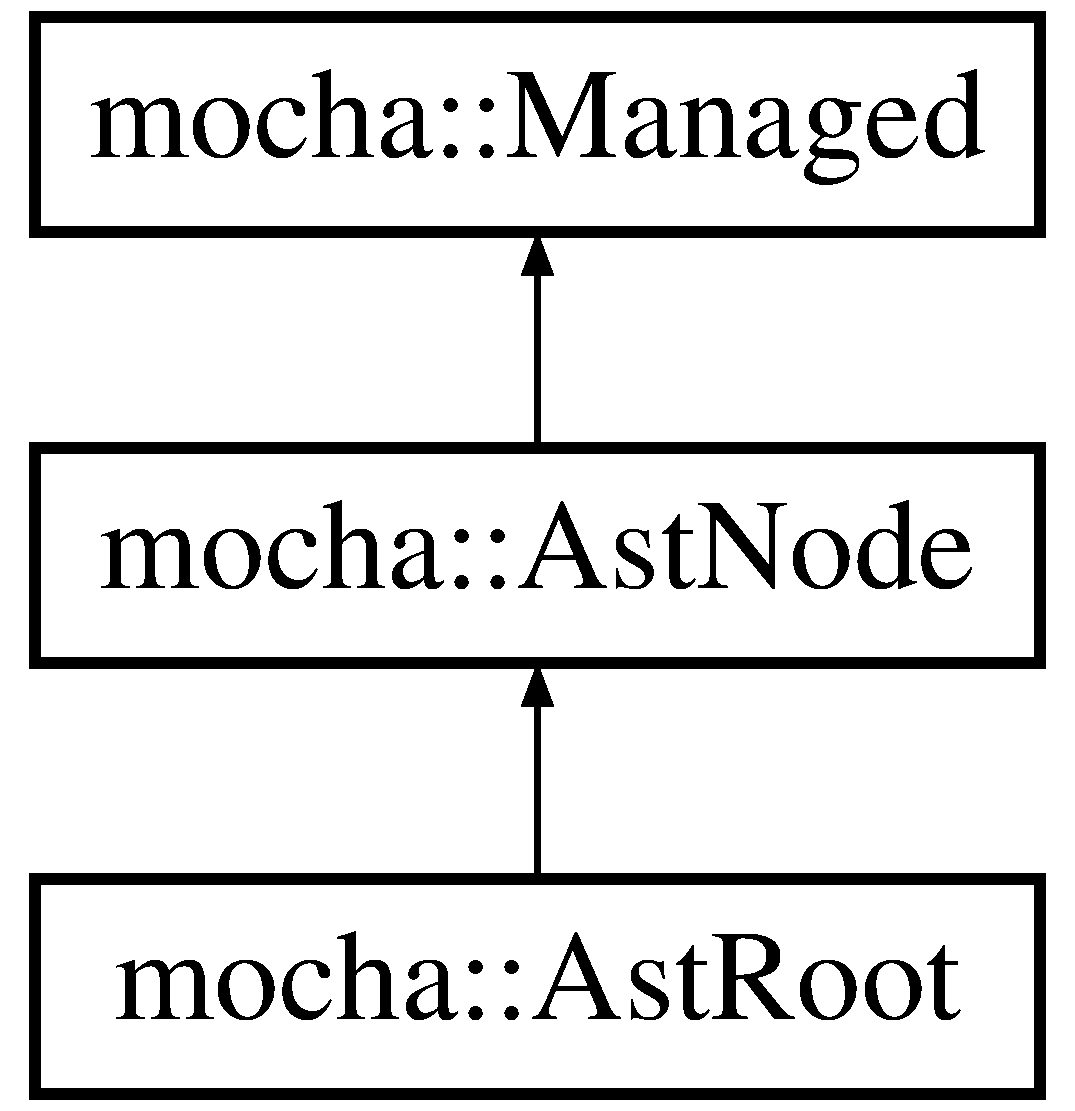
\includegraphics[height=3.000000cm]{classmocha_1_1_ast_root}
\end{center}
\end{figure}
\subsection*{Public Member Functions}
\begin{DoxyCompactItemize}
\item 
\hyperlink{classmocha_1_1_ast_root_a119834bdf57c55c0282ba7be3d64a2f8}{AstRoot} ()
\item 
\hyperlink{classmocha_1_1_ast_root_a817cb08076802b3a549c1c37ea51f693}{$\sim$AstRoot} ()
\item 
void \hyperlink{classmocha_1_1_ast_root_a93adb8beb44c8d6dfb8c750bf5173f3f}{SetScope} (\hyperlink{classmocha_1_1_inner_scope}{InnerScope} $\ast$scope)
\item 
\hyperlink{classmocha_1_1_inner_scope}{InnerScope} $\ast$ \hyperlink{classmocha_1_1_ast_root_aeef3085a6bf6064e9438338274b42827}{GetScope} () const 
\begin{DoxyCompactList}\small\item\em \{InnerScope$\ast$\} Return global closure scope. \end{DoxyCompactList}\item 
\hyperlink{classmocha_1_1_ast_node}{AstNode} $\ast$ \hyperlink{classmocha_1_1_ast_root_af325e103d1f65d71d108eea400196287}{Clone} ()
\end{DoxyCompactItemize}
\subsection*{Private Member Functions}
\begin{DoxyCompactItemize}
\item 
void \hyperlink{classmocha_1_1_ast_root_ad54b98a08505d4b63576ecf831e6376c}{NVIAccept\_\-} (\hyperlink{classmocha_1_1_i_visitor}{IVisitor} $\ast$visitor)
\end{DoxyCompactItemize}
\subsection*{Private Attributes}
\begin{DoxyCompactItemize}
\item 
\hyperlink{classmocha_1_1_inner_scope}{InnerScope} $\ast$ \hyperlink{classmocha_1_1_ast_root_aa8f0672b47a85015c50cb19a1126cee1}{scope\_\-}
\end{DoxyCompactItemize}


\subsection{Detailed Description}


Definition at line 465 of file ast.h.



\subsection{Constructor \& Destructor Documentation}
\hypertarget{classmocha_1_1_ast_root_a119834bdf57c55c0282ba7be3d64a2f8}{
\index{mocha::AstRoot@{mocha::AstRoot}!AstRoot@{AstRoot}}
\index{AstRoot@{AstRoot}!mocha::AstRoot@{mocha::AstRoot}}
\subsubsection[{AstRoot}]{\setlength{\rightskip}{0pt plus 5cm}mocha::AstRoot::AstRoot (
\begin{DoxyParamCaption}
{}
\end{DoxyParamCaption}
)\hspace{0.3cm}{\ttfamily  \mbox{[}inline\mbox{]}}}}
\label{classmocha_1_1_ast_root_a119834bdf57c55c0282ba7be3d64a2f8}


Definition at line 467 of file ast.h.

\hypertarget{classmocha_1_1_ast_root_a817cb08076802b3a549c1c37ea51f693}{
\index{mocha::AstRoot@{mocha::AstRoot}!$\sim$AstRoot@{$\sim$AstRoot}}
\index{$\sim$AstRoot@{$\sim$AstRoot}!mocha::AstRoot@{mocha::AstRoot}}
\subsubsection[{$\sim$AstRoot}]{\setlength{\rightskip}{0pt plus 5cm}mocha::AstRoot::$\sim$AstRoot (
\begin{DoxyParamCaption}
{}
\end{DoxyParamCaption}
)\hspace{0.3cm}{\ttfamily  \mbox{[}inline\mbox{]}}}}
\label{classmocha_1_1_ast_root_a817cb08076802b3a549c1c37ea51f693}


Definition at line 468 of file ast.h.



\subsection{Member Function Documentation}
\hypertarget{classmocha_1_1_ast_root_af325e103d1f65d71d108eea400196287}{
\index{mocha::AstRoot@{mocha::AstRoot}!Clone@{Clone}}
\index{Clone@{Clone}!mocha::AstRoot@{mocha::AstRoot}}
\subsubsection[{Clone}]{\setlength{\rightskip}{0pt plus 5cm}{\bf AstNode} $\ast$ mocha::AstRoot::Clone (
\begin{DoxyParamCaption}
{}
\end{DoxyParamCaption}
)\hspace{0.3cm}{\ttfamily  \mbox{[}virtual\mbox{]}}}}
\label{classmocha_1_1_ast_root_af325e103d1f65d71d108eea400196287}
\begin{DoxyReturn}{Returns}
\{AstNode$\ast$\} Clone node. 
\end{DoxyReturn}


Reimplemented from \hyperlink{classmocha_1_1_ast_node_af2a895699bac2012f8b7739bff49c5ec}{mocha::AstNode}.



Definition at line 220 of file ast.cc.

\hypertarget{classmocha_1_1_ast_root_aeef3085a6bf6064e9438338274b42827}{
\index{mocha::AstRoot@{mocha::AstRoot}!GetScope@{GetScope}}
\index{GetScope@{GetScope}!mocha::AstRoot@{mocha::AstRoot}}
\subsubsection[{GetScope}]{\setlength{\rightskip}{0pt plus 5cm}{\bf InnerScope}$\ast$ mocha::AstRoot::GetScope (
\begin{DoxyParamCaption}
{}
\end{DoxyParamCaption}
) const\hspace{0.3cm}{\ttfamily  \mbox{[}inline\mbox{]}}}}
\label{classmocha_1_1_ast_root_aeef3085a6bf6064e9438338274b42827}


\{InnerScope$\ast$\} Return global closure scope. 



Definition at line 478 of file ast.h.

\hypertarget{classmocha_1_1_ast_root_ad54b98a08505d4b63576ecf831e6376c}{
\index{mocha::AstRoot@{mocha::AstRoot}!NVIAccept\_\-@{NVIAccept\_\-}}
\index{NVIAccept\_\-@{NVIAccept\_\-}!mocha::AstRoot@{mocha::AstRoot}}
\subsubsection[{NVIAccept\_\-}]{\setlength{\rightskip}{0pt plus 5cm}void mocha::AstRoot::NVIAccept\_\- (
\begin{DoxyParamCaption}
\item[{{\bf IVisitor} $\ast$}]{visitor}
\end{DoxyParamCaption}
)\hspace{0.3cm}{\ttfamily  \mbox{[}inline, private, virtual\mbox{]}}}}
\label{classmocha_1_1_ast_root_ad54b98a08505d4b63576ecf831e6376c}


Reimplemented from \hyperlink{classmocha_1_1_ast_node_a4a9c107bed3671f3fa15312b87f6ae96}{mocha::AstNode}.



Definition at line 482 of file ast.h.

\hypertarget{classmocha_1_1_ast_root_a93adb8beb44c8d6dfb8c750bf5173f3f}{
\index{mocha::AstRoot@{mocha::AstRoot}!SetScope@{SetScope}}
\index{SetScope@{SetScope}!mocha::AstRoot@{mocha::AstRoot}}
\subsubsection[{SetScope}]{\setlength{\rightskip}{0pt plus 5cm}void mocha::AstRoot::SetScope (
\begin{DoxyParamCaption}
\item[{{\bf InnerScope} $\ast$}]{scope}
\end{DoxyParamCaption}
)\hspace{0.3cm}{\ttfamily  \mbox{[}inline\mbox{]}}}}
\label{classmocha_1_1_ast_root_a93adb8beb44c8d6dfb8c750bf5173f3f}

\begin{DoxyParams}{Parameters}
{\em \{InnerScope$\ast$\}} & Global closure scope. \\
\hline
\end{DoxyParams}


Definition at line 473 of file ast.h.



\subsection{Member Data Documentation}
\hypertarget{classmocha_1_1_ast_root_aa8f0672b47a85015c50cb19a1126cee1}{
\index{mocha::AstRoot@{mocha::AstRoot}!scope\_\-@{scope\_\-}}
\index{scope\_\-@{scope\_\-}!mocha::AstRoot@{mocha::AstRoot}}
\subsubsection[{scope\_\-}]{\setlength{\rightskip}{0pt plus 5cm}{\bf InnerScope}$\ast$ {\bf mocha::AstRoot::scope\_\-}\hspace{0.3cm}{\ttfamily  \mbox{[}private\mbox{]}}}}
\label{classmocha_1_1_ast_root_aa8f0672b47a85015c50cb19a1126cee1}


Definition at line 479 of file ast.h.



The documentation for this class was generated from the following files:\begin{DoxyCompactItemize}
\item 
Y:/mocha/src/ast/\hyperlink{ast_8h}{ast.h}\item 
Y:/mocha/src/ast/\hyperlink{ast_8cc}{ast.cc}\end{DoxyCompactItemize}

\hypertarget{classmocha_1_1_ast_transformer}{
\section{mocha::AstTransformer Class Reference}
\label{classmocha_1_1_ast_transformer}\index{mocha::AstTransformer@{mocha::AstTransformer}}
}


{\ttfamily \#include $<$ast\_\-transformer.h$>$}

Inheritance diagram for mocha::AstTransformer:\begin{figure}[H]
\begin{center}
\leavevmode
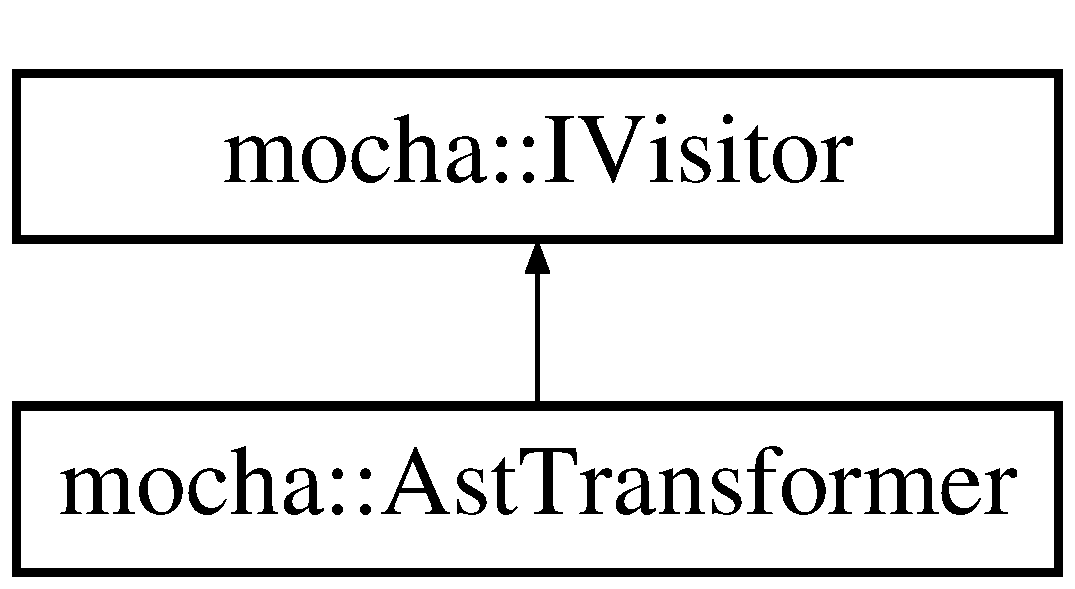
\includegraphics[height=2.000000cm]{classmocha_1_1_ast_transformer}
\end{center}
\end{figure}
\subsection*{Public Member Functions}
\begin{DoxyCompactItemize}
\item 
\hyperlink{classmocha_1_1_ast_transformer_a339e9862f527dae139b581fe5c044d75}{AstTransformer} (bool is\_\-runtime, \hyperlink{classmocha_1_1_scope}{Scope} $\ast$scope, \hyperlink{classmocha_1_1_compiler}{Compiler} $\ast$compiler, const char $\ast$modulename, const char $\ast$filename)
\begin{DoxyCompactList}\small\item\em \end{DoxyCompactList}\item 
\hyperlink{classmocha_1_1_ast_transformer_a6214cb90fe29f044738d475a57316fc1}{$\sim$AstTransformer} ()
\end{DoxyCompactItemize}
\subsection*{Private Member Functions}
\begin{DoxyCompactItemize}
\item 
void \hyperlink{classmocha_1_1_ast_transformer_a68ad2536f5387586ceeeb0dfb514e0b5}{JumpStmt\_\-} (\hyperlink{classmocha_1_1_ast_node}{AstNode} $\ast$ast\_\-node, int type)
\item 
void \hyperlink{classmocha_1_1_ast_transformer_a0e449e3bd337b0b2d86a868ad30cd3c4}{ArrayProccessor\_\-} (\hyperlink{classmocha_1_1_value_node}{ValueNode} $\ast$ast\_\-node)
\item 
void \hyperlink{classmocha_1_1_ast_transformer_a9c212582c300f321a26186b206ad1181}{ObjectProccessor\_\-} (\hyperlink{classmocha_1_1_value_node}{ValueNode} $\ast$ast\_\-node)
\end{DoxyCompactItemize}
\subsection*{Private Attributes}
\begin{DoxyCompactItemize}
\item 
\hyperlink{classmocha_1_1_scoped_ptr}{ScopedPtr}$<$ \hyperlink{classmocha_1_1_visitor_info}{VisitorInfo} $>$ \hyperlink{classmocha_1_1_ast_transformer_ac28baaac681c02d0ac103196409bd1f9}{visitor\_\-info\_\-}
\item 
\hyperlink{classmocha_1_1_scoped_ptr}{ScopedPtr}$<$ \hyperlink{classmocha_1_1_processor_info}{ProcessorInfo} $>$ \hyperlink{classmocha_1_1_ast_transformer_a7cdc53f8550ca2ff46fc9c558916eeff}{proc\_\-info\_\-}
\end{DoxyCompactItemize}


\subsection{Detailed Description}


Definition at line 43 of file ast\_\-transformer.h.



\subsection{Constructor \& Destructor Documentation}
\hypertarget{classmocha_1_1_ast_transformer_a339e9862f527dae139b581fe5c044d75}{
\index{mocha::AstTransformer@{mocha::AstTransformer}!AstTransformer@{AstTransformer}}
\index{AstTransformer@{AstTransformer}!mocha::AstTransformer@{mocha::AstTransformer}}
\subsubsection[{AstTransformer}]{\setlength{\rightskip}{0pt plus 5cm}mocha::AstTransformer::AstTransformer (
\begin{DoxyParamCaption}
\item[{bool}]{is\_\-runtime, }
\item[{{\bf Scope} $\ast$}]{scope, }
\item[{{\bf Compiler} $\ast$}]{compiler, }
\item[{const char $\ast$}]{modulename, }
\item[{const char $\ast$}]{filename}
\end{DoxyParamCaption}
)}}
\label{classmocha_1_1_ast_transformer_a339e9862f527dae139b581fe5c044d75}





\begin{DoxyParams}{Parameters}
{\em \{bool\}} & is\_\-runtime -\/$>$ Compile module or not. \\
\hline
{\em \{Scope$\ast$\}} & scope \\
\hline
{\em \{Compiler$\ast$\}} & compiler \\
\hline
{\em \{const} & char$\ast$\} modulename -\/$>$ Current file name. \\
\hline
{\em \{const} & char$\ast$\} filename -\/$>$ Main js file name. \\
\hline
\end{DoxyParams}


Definition at line 72 of file ast\_\-transformer.cc.

\hypertarget{classmocha_1_1_ast_transformer_a6214cb90fe29f044738d475a57316fc1}{
\index{mocha::AstTransformer@{mocha::AstTransformer}!$\sim$AstTransformer@{$\sim$AstTransformer}}
\index{$\sim$AstTransformer@{$\sim$AstTransformer}!mocha::AstTransformer@{mocha::AstTransformer}}
\subsubsection[{$\sim$AstTransformer}]{\setlength{\rightskip}{0pt plus 5cm}mocha::AstTransformer::$\sim$AstTransformer (
\begin{DoxyParamCaption}
{}
\end{DoxyParamCaption}
)}}
\label{classmocha_1_1_ast_transformer_a6214cb90fe29f044738d475a57316fc1}


Definition at line 81 of file ast\_\-transformer.cc.



\subsection{Member Function Documentation}
\hypertarget{classmocha_1_1_ast_transformer_a0e449e3bd337b0b2d86a868ad30cd3c4}{
\index{mocha::AstTransformer@{mocha::AstTransformer}!ArrayProccessor\_\-@{ArrayProccessor\_\-}}
\index{ArrayProccessor\_\-@{ArrayProccessor\_\-}!mocha::AstTransformer@{mocha::AstTransformer}}
\subsubsection[{ArrayProccessor\_\-}]{\setlength{\rightskip}{0pt plus 5cm}void mocha::AstTransformer::ArrayProccessor\_\- (
\begin{DoxyParamCaption}
\item[{{\bf ValueNode} $\ast$}]{ast\_\-node}
\end{DoxyParamCaption}
)\hspace{0.3cm}{\ttfamily  \mbox{[}private\mbox{]}}}}
\label{classmocha_1_1_ast_transformer_a0e449e3bd337b0b2d86a868ad30cd3c4}


Definition at line 669 of file ast\_\-transformer.cc.

\hypertarget{classmocha_1_1_ast_transformer_a68ad2536f5387586ceeeb0dfb514e0b5}{
\index{mocha::AstTransformer@{mocha::AstTransformer}!JumpStmt\_\-@{JumpStmt\_\-}}
\index{JumpStmt\_\-@{JumpStmt\_\-}!mocha::AstTransformer@{mocha::AstTransformer}}
\subsubsection[{JumpStmt\_\-}]{\setlength{\rightskip}{0pt plus 5cm}void mocha::AstTransformer::JumpStmt\_\- (
\begin{DoxyParamCaption}
\item[{{\bf AstNode} $\ast$}]{ast\_\-node, }
\item[{int}]{type}
\end{DoxyParamCaption}
)\hspace{0.3cm}{\ttfamily  \mbox{[}private\mbox{]}}}}
\label{classmocha_1_1_ast_transformer_a68ad2536f5387586ceeeb0dfb514e0b5}
\hypertarget{classmocha_1_1_ast_transformer_a9c212582c300f321a26186b206ad1181}{
\index{mocha::AstTransformer@{mocha::AstTransformer}!ObjectProccessor\_\-@{ObjectProccessor\_\-}}
\index{ObjectProccessor\_\-@{ObjectProccessor\_\-}!mocha::AstTransformer@{mocha::AstTransformer}}
\subsubsection[{ObjectProccessor\_\-}]{\setlength{\rightskip}{0pt plus 5cm}void mocha::AstTransformer::ObjectProccessor\_\- (
\begin{DoxyParamCaption}
\item[{{\bf ValueNode} $\ast$}]{ast\_\-node}
\end{DoxyParamCaption}
)\hspace{0.3cm}{\ttfamily  \mbox{[}private\mbox{]}}}}
\label{classmocha_1_1_ast_transformer_a9c212582c300f321a26186b206ad1181}


Definition at line 693 of file ast\_\-transformer.cc.



\subsection{Member Data Documentation}
\hypertarget{classmocha_1_1_ast_transformer_a7cdc53f8550ca2ff46fc9c558916eeff}{
\index{mocha::AstTransformer@{mocha::AstTransformer}!proc\_\-info\_\-@{proc\_\-info\_\-}}
\index{proc\_\-info\_\-@{proc\_\-info\_\-}!mocha::AstTransformer@{mocha::AstTransformer}}
\subsubsection[{proc\_\-info\_\-}]{\setlength{\rightskip}{0pt plus 5cm}{\bf ScopedPtr}$<${\bf ProcessorInfo}$>$ {\bf mocha::AstTransformer::proc\_\-info\_\-}\hspace{0.3cm}{\ttfamily  \mbox{[}private\mbox{]}}}}
\label{classmocha_1_1_ast_transformer_a7cdc53f8550ca2ff46fc9c558916eeff}


Definition at line 68 of file ast\_\-transformer.h.

\hypertarget{classmocha_1_1_ast_transformer_ac28baaac681c02d0ac103196409bd1f9}{
\index{mocha::AstTransformer@{mocha::AstTransformer}!visitor\_\-info\_\-@{visitor\_\-info\_\-}}
\index{visitor\_\-info\_\-@{visitor\_\-info\_\-}!mocha::AstTransformer@{mocha::AstTransformer}}
\subsubsection[{visitor\_\-info\_\-}]{\setlength{\rightskip}{0pt plus 5cm}{\bf ScopedPtr}$<${\bf VisitorInfo}$>$ {\bf mocha::AstTransformer::visitor\_\-info\_\-}\hspace{0.3cm}{\ttfamily  \mbox{[}private\mbox{]}}}}
\label{classmocha_1_1_ast_transformer_ac28baaac681c02d0ac103196409bd1f9}


Definition at line 67 of file ast\_\-transformer.h.



The documentation for this class was generated from the following files:\begin{DoxyCompactItemize}
\item 
Y:/mocha/src/ast/visitors/\hyperlink{ast__transformer_8h}{ast\_\-transformer.h}\item 
Y:/mocha/src/ast/visitors/\hyperlink{ast__transformer_8cc}{ast\_\-transformer.cc}\end{DoxyCompactItemize}

\hypertarget{classmocha_1_1_ast_utils}{
\section{mocha::AstUtils Class Reference}
\label{classmocha_1_1_ast_utils}\index{mocha::AstUtils@{mocha::AstUtils}}
}


{\ttfamily \#include $<$ast\_\-utils.h$>$}

Inheritance diagram for mocha::AstUtils:\begin{figure}[H]
\begin{center}
\leavevmode
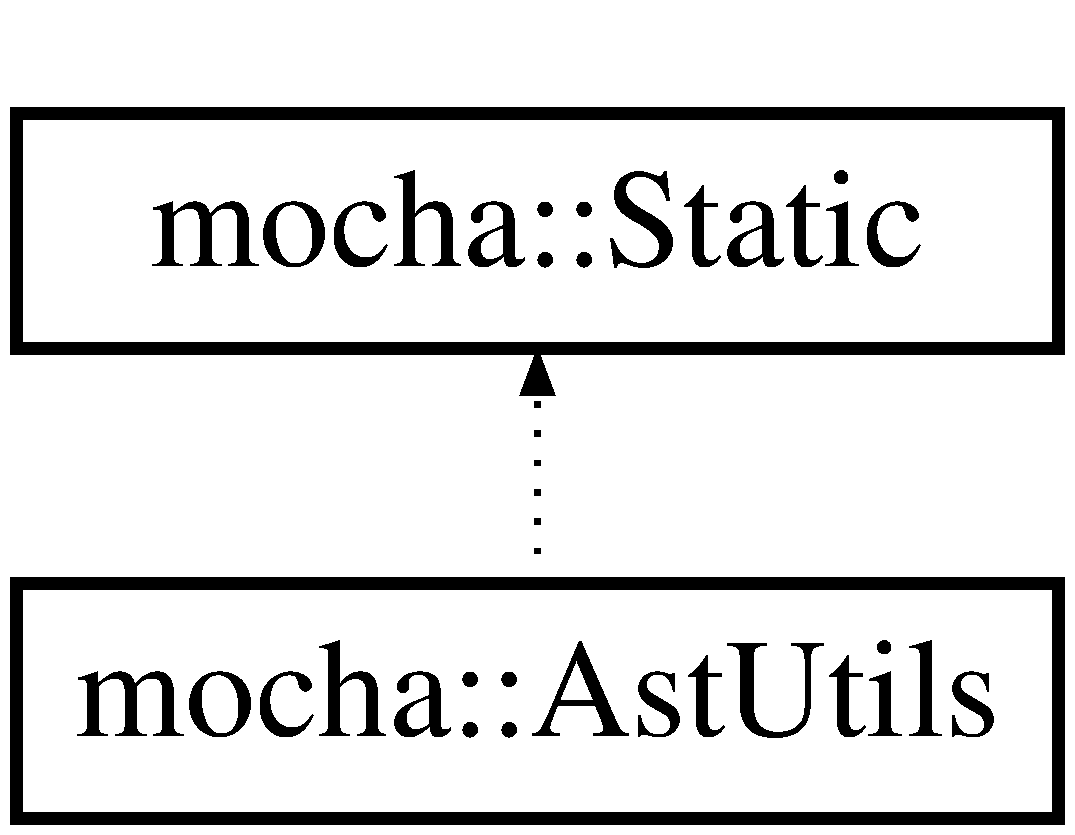
\includegraphics[height=2.000000cm]{classmocha_1_1_ast_utils}
\end{center}
\end{figure}
\subsection*{Static Public Member Functions}
\begin{DoxyCompactItemize}
\item 
static \hyperlink{classmocha_1_1_function}{Function} $\ast$ \hyperlink{classmocha_1_1_ast_utils_a2b150de7953f29e5c94c7e9d110a6d97}{CreateFunctionDecl} (\hyperlink{classmocha_1_1_ast_node}{AstNode} $\ast$name, \hyperlink{classmocha_1_1_ast_node}{AstNode} $\ast$argv, \hyperlink{classmocha_1_1_ast_node}{AstNode} $\ast$body)
\item 
static \hyperlink{classmocha_1_1_call_exp}{CallExp} $\ast$ \hyperlink{classmocha_1_1_ast_utils_a73682172af76ec16a106911d7546180f}{CreateArrayAccessor} (\hyperlink{classmocha_1_1_ast_node}{AstNode} $\ast$callable, \hyperlink{classmocha_1_1_ast_node}{AstNode} $\ast$args)
\item 
static \hyperlink{classmocha_1_1_call_exp}{CallExp} $\ast$ \hyperlink{classmocha_1_1_ast_utils_aed7efcb40804b8b9e3740a49519fa41a}{CreateDotAccessor} (\hyperlink{classmocha_1_1_ast_node}{AstNode} $\ast$callable, \hyperlink{classmocha_1_1_ast_node}{AstNode} $\ast$args)
\item 
static \hyperlink{classmocha_1_1_call_exp}{CallExp} $\ast$ \hyperlink{classmocha_1_1_ast_utils_ac0986e9863d2cba6b3cbae21c9f3cea2}{CreatePrototypeAccessor} (\hyperlink{classmocha_1_1_ast_node}{AstNode} $\ast$callable, \hyperlink{classmocha_1_1_ast_node}{AstNode} $\ast$args)
\item 
static \hyperlink{classmocha_1_1_call_exp}{CallExp} $\ast$ \hyperlink{classmocha_1_1_ast_utils_a77bd4f7ca31be505683055685aa1ff77}{CreateNormalAccessor} (\hyperlink{classmocha_1_1_ast_node}{AstNode} $\ast$callable, \hyperlink{classmocha_1_1_ast_node}{AstNode} $\ast$args)
\item 
static \hyperlink{classmocha_1_1_value_node}{ValueNode} $\ast$ \hyperlink{classmocha_1_1_ast_utils_a1a4ad629469bdb21a0b4b67023c416f1}{CreateNameNode} (const char $\ast$name, int type, long line, int value\_\-type, bool is\_\-empty=false)
\item 
static \hyperlink{classmocha_1_1_assignment_exp}{AssignmentExp} $\ast$ \hyperlink{classmocha_1_1_ast_utils_a3cd4b28daba962ddd963eec4bffc9f84}{CreateAssignment} (int type, \hyperlink{classmocha_1_1_ast_node}{AstNode} $\ast$lhs, \hyperlink{classmocha_1_1_ast_node}{AstNode} $\ast$rhs)
\item 
static \hyperlink{classmocha_1_1_unary_exp}{UnaryExp} $\ast$ \hyperlink{classmocha_1_1_ast_utils_a25e8d20ae483db57a4b5c51d0444b5a7}{CreateUnaryExp} (int type, \hyperlink{classmocha_1_1_ast_node}{AstNode} $\ast$exp)
\item 
static \hyperlink{classmocha_1_1_node_list}{NodeList} $\ast$ \hyperlink{classmocha_1_1_ast_utils_a491e3a29ccd8515edd75f7ad1658ff03}{CreateNodeList} (int num,...)
\item 
static \hyperlink{classmocha_1_1_value_node}{ValueNode} $\ast$ \hyperlink{classmocha_1_1_ast_utils_a20a30d91e2013c43e91d20c01f6b4eb8}{CreateObjectLiteral} (\hyperlink{classmocha_1_1_ast_node}{AstNode} $\ast$body)
\item 
static \hyperlink{classmocha_1_1_expression_stmt}{ExpressionStmt} $\ast$ \hyperlink{classmocha_1_1_ast_utils_ae8ac7a22a62b0cf12490efdd1c054045}{CreateAnonymousFnCall} (\hyperlink{classmocha_1_1_function}{Function} $\ast$fn, \hyperlink{classmocha_1_1_ast_node}{AstNode} $\ast$args)
\item 
static \hyperlink{classmocha_1_1_expression_stmt}{ExpressionStmt} $\ast$ \hyperlink{classmocha_1_1_ast_utils_a2ad830d99f87e4aa99eb7b77ffcd8f60}{CreateExpStmt} (\hyperlink{classmocha_1_1_ast_node}{AstNode} $\ast$node)
\item 
static \hyperlink{classmocha_1_1_variable_stmt}{VariableStmt} $\ast$ \hyperlink{classmocha_1_1_ast_utils_aa7d849cc4fe5b84c9aa80c81904931fb}{CreateVarStmt} (\hyperlink{classmocha_1_1_node_list}{NodeList} $\ast$list)
\item 
static \hyperlink{classmocha_1_1_variable_stmt}{VariableStmt} $\ast$ \hyperlink{classmocha_1_1_ast_utils_aaac13a7c6db56f228165461c8e41e427}{CreateVarStmt} (\hyperlink{classmocha_1_1_ast_node}{AstNode} $\ast$mem)
\item 
static \hyperlink{classmocha_1_1_value_node}{ValueNode} $\ast$ \hyperlink{classmocha_1_1_ast_utils_a9fcb6a0bd018a4d1a98c600287f5db18}{CreateVarInitiliser} (\hyperlink{classmocha_1_1_token_info}{TokenInfo} $\ast$lhs, \hyperlink{classmocha_1_1_ast_node}{AstNode} $\ast$rhs)
\item 
static \hyperlink{classmocha_1_1_return_stmt}{ReturnStmt} $\ast$ \hyperlink{classmocha_1_1_ast_utils_acde244c3e7c6107360bc0340fa73e8ea}{CreateReturnStmt} (\hyperlink{classmocha_1_1_ast_node}{AstNode} $\ast$exp)
\item 
static \hyperlink{classmocha_1_1_call_exp}{CallExp} $\ast$ \hyperlink{classmocha_1_1_ast_utils_ad4547f1789aba2e0857a51a02312b7ca}{CreateRuntimeMod} (\hyperlink{classmocha_1_1_ast_node}{AstNode} $\ast$member)
\item 
static \hyperlink{classmocha_1_1_call_exp}{CallExp} $\ast$ \hyperlink{classmocha_1_1_ast_utils_adebbc56fb60852df97fc8c14ca15bc63}{CreateConstantProp} (\hyperlink{classmocha_1_1_ast_node}{AstNode} $\ast$lhs, \hyperlink{classmocha_1_1_ast_node}{AstNode} $\ast$prop, \hyperlink{classmocha_1_1_ast_node}{AstNode} $\ast$value)
\item 
static \hyperlink{classmocha_1_1_call_exp}{CallExp} $\ast$ \hyperlink{classmocha_1_1_ast_utils_ab3f901178db466ed2bd2a0a5287ab797}{CreatePrototypeNode} (\hyperlink{classmocha_1_1_ast_node}{AstNode} $\ast$lhs)
\item 
static \hyperlink{classmocha_1_1_call_exp}{CallExp} $\ast$ \hyperlink{classmocha_1_1_ast_utils_aade0bbc424bb5f7c2e5a0d7979baea5f}{CreateGlobalExportNode} (\hyperlink{classmocha_1_1_ast_node}{AstNode} $\ast$ast\_\-node, \hyperlink{classmocha_1_1_visitor_info}{VisitorInfo} $\ast$visitor\_\-info, const char $\ast$base, const char $\ast$filename)
\item 
static const char $\ast$ \hyperlink{classmocha_1_1_ast_utils_a75c091058d5c25382b877015958a8400}{CreateTmpRef} (char $\ast$buf, int index)
\item 
static \hyperlink{classmocha_1_1_value_node}{ValueNode} $\ast$ \hyperlink{classmocha_1_1_ast_utils_ab6fce222ac8de9e29710fdacc83e5b92}{CreateTmpNode} (int index)
\item 
static \hyperlink{classmocha_1_1_i_f_stmt}{IFStmt} $\ast$ \hyperlink{classmocha_1_1_ast_utils_a1b536aba81ff085251f3ba0149e38bff}{CreateIFStmt} (\hyperlink{classmocha_1_1_ast_node}{AstNode} $\ast$exp, \hyperlink{classmocha_1_1_ast_node}{AstNode} $\ast$then\_\-stmt, \hyperlink{classmocha_1_1_ast_node}{AstNode} $\ast$else\_\-stmt)
\item 
static \hyperlink{classmocha_1_1_block_stmt}{BlockStmt} $\ast$ \hyperlink{classmocha_1_1_ast_utils_a41c0267c33880f694c8ca57c42de814d}{CreateBlockStmt} (int num,...)
\end{DoxyCompactItemize}


\subsection{Detailed Description}


Definition at line 39 of file ast\_\-utils.h.



\subsection{Member Function Documentation}
\hypertarget{classmocha_1_1_ast_utils_ae8ac7a22a62b0cf12490efdd1c054045}{
\index{mocha::AstUtils@{mocha::AstUtils}!CreateAnonymousFnCall@{CreateAnonymousFnCall}}
\index{CreateAnonymousFnCall@{CreateAnonymousFnCall}!mocha::AstUtils@{mocha::AstUtils}}
\subsubsection[{CreateAnonymousFnCall}]{\setlength{\rightskip}{0pt plus 5cm}{\bf ExpressionStmt} $\ast$ mocha::AstUtils::CreateAnonymousFnCall (
\begin{DoxyParamCaption}
\item[{{\bf Function} $\ast$}]{fn, }
\item[{{\bf AstNode} $\ast$}]{args}
\end{DoxyParamCaption}
)\hspace{0.3cm}{\ttfamily  \mbox{[}static\mbox{]}}}}
\label{classmocha_1_1_ast_utils_ae8ac7a22a62b0cf12490efdd1c054045}


Definition at line 92 of file ast\_\-utils.cc.

\hypertarget{classmocha_1_1_ast_utils_a73682172af76ec16a106911d7546180f}{
\index{mocha::AstUtils@{mocha::AstUtils}!CreateArrayAccessor@{CreateArrayAccessor}}
\index{CreateArrayAccessor@{CreateArrayAccessor}!mocha::AstUtils@{mocha::AstUtils}}
\subsubsection[{CreateArrayAccessor}]{\setlength{\rightskip}{0pt plus 5cm}{\bf CallExp} $\ast$ mocha::AstUtils::CreateArrayAccessor (
\begin{DoxyParamCaption}
\item[{{\bf AstNode} $\ast$}]{callable, }
\item[{{\bf AstNode} $\ast$}]{args}
\end{DoxyParamCaption}
)\hspace{0.3cm}{\ttfamily  \mbox{[}static\mbox{]}}}}
\label{classmocha_1_1_ast_utils_a73682172af76ec16a106911d7546180f}


Definition at line 24 of file ast\_\-utils.cc.

\hypertarget{classmocha_1_1_ast_utils_a3cd4b28daba962ddd963eec4bffc9f84}{
\index{mocha::AstUtils@{mocha::AstUtils}!CreateAssignment@{CreateAssignment}}
\index{CreateAssignment@{CreateAssignment}!mocha::AstUtils@{mocha::AstUtils}}
\subsubsection[{CreateAssignment}]{\setlength{\rightskip}{0pt plus 5cm}{\bf AssignmentExp} $\ast$ mocha::AstUtils::CreateAssignment (
\begin{DoxyParamCaption}
\item[{int}]{type, }
\item[{{\bf AstNode} $\ast$}]{lhs, }
\item[{{\bf AstNode} $\ast$}]{rhs}
\end{DoxyParamCaption}
)\hspace{0.3cm}{\ttfamily  \mbox{[}static\mbox{]}}}}
\label{classmocha_1_1_ast_utils_a3cd4b28daba962ddd963eec4bffc9f84}


Definition at line 64 of file ast\_\-utils.cc.

\hypertarget{classmocha_1_1_ast_utils_a41c0267c33880f694c8ca57c42de814d}{
\index{mocha::AstUtils@{mocha::AstUtils}!CreateBlockStmt@{CreateBlockStmt}}
\index{CreateBlockStmt@{CreateBlockStmt}!mocha::AstUtils@{mocha::AstUtils}}
\subsubsection[{CreateBlockStmt}]{\setlength{\rightskip}{0pt plus 5cm}{\bf BlockStmt} $\ast$ mocha::AstUtils::CreateBlockStmt (
\begin{DoxyParamCaption}
\item[{int}]{num, }
\item[{}]{...}
\end{DoxyParamCaption}
)\hspace{0.3cm}{\ttfamily  \mbox{[}static\mbox{]}}}}
\label{classmocha_1_1_ast_utils_a41c0267c33880f694c8ca57c42de814d}


Definition at line 211 of file ast\_\-utils.cc.

\hypertarget{classmocha_1_1_ast_utils_adebbc56fb60852df97fc8c14ca15bc63}{
\index{mocha::AstUtils@{mocha::AstUtils}!CreateConstantProp@{CreateConstantProp}}
\index{CreateConstantProp@{CreateConstantProp}!mocha::AstUtils@{mocha::AstUtils}}
\subsubsection[{CreateConstantProp}]{\setlength{\rightskip}{0pt plus 5cm}{\bf CallExp} $\ast$ mocha::AstUtils::CreateConstantProp (
\begin{DoxyParamCaption}
\item[{{\bf AstNode} $\ast$}]{lhs, }
\item[{{\bf AstNode} $\ast$}]{prop, }
\item[{{\bf AstNode} $\ast$}]{value}
\end{DoxyParamCaption}
)\hspace{0.3cm}{\ttfamily  \mbox{[}static\mbox{]}}}}
\label{classmocha_1_1_ast_utils_adebbc56fb60852df97fc8c14ca15bc63}


Definition at line 143 of file ast\_\-utils.cc.

\hypertarget{classmocha_1_1_ast_utils_aed7efcb40804b8b9e3740a49519fa41a}{
\index{mocha::AstUtils@{mocha::AstUtils}!CreateDotAccessor@{CreateDotAccessor}}
\index{CreateDotAccessor@{CreateDotAccessor}!mocha::AstUtils@{mocha::AstUtils}}
\subsubsection[{CreateDotAccessor}]{\setlength{\rightskip}{0pt plus 5cm}{\bf CallExp} $\ast$ mocha::AstUtils::CreateDotAccessor (
\begin{DoxyParamCaption}
\item[{{\bf AstNode} $\ast$}]{callable, }
\item[{{\bf AstNode} $\ast$}]{args}
\end{DoxyParamCaption}
)\hspace{0.3cm}{\ttfamily  \mbox{[}static\mbox{]}}}}
\label{classmocha_1_1_ast_utils_aed7efcb40804b8b9e3740a49519fa41a}


Definition at line 31 of file ast\_\-utils.cc.

\hypertarget{classmocha_1_1_ast_utils_a2ad830d99f87e4aa99eb7b77ffcd8f60}{
\index{mocha::AstUtils@{mocha::AstUtils}!CreateExpStmt@{CreateExpStmt}}
\index{CreateExpStmt@{CreateExpStmt}!mocha::AstUtils@{mocha::AstUtils}}
\subsubsection[{CreateExpStmt}]{\setlength{\rightskip}{0pt plus 5cm}{\bf ExpressionStmt} $\ast$ mocha::AstUtils::CreateExpStmt (
\begin{DoxyParamCaption}
\item[{{\bf AstNode} $\ast$}]{node}
\end{DoxyParamCaption}
)\hspace{0.3cm}{\ttfamily  \mbox{[}static\mbox{]}}}}
\label{classmocha_1_1_ast_utils_a2ad830d99f87e4aa99eb7b77ffcd8f60}


Definition at line 106 of file ast\_\-utils.cc.

\hypertarget{classmocha_1_1_ast_utils_a2b150de7953f29e5c94c7e9d110a6d97}{
\index{mocha::AstUtils@{mocha::AstUtils}!CreateFunctionDecl@{CreateFunctionDecl}}
\index{CreateFunctionDecl@{CreateFunctionDecl}!mocha::AstUtils@{mocha::AstUtils}}
\subsubsection[{CreateFunctionDecl}]{\setlength{\rightskip}{0pt plus 5cm}{\bf Function} $\ast$ mocha::AstUtils::CreateFunctionDecl (
\begin{DoxyParamCaption}
\item[{{\bf AstNode} $\ast$}]{name, }
\item[{{\bf AstNode} $\ast$}]{argv, }
\item[{{\bf AstNode} $\ast$}]{body}
\end{DoxyParamCaption}
)\hspace{0.3cm}{\ttfamily  \mbox{[}static\mbox{]}}}}
\label{classmocha_1_1_ast_utils_a2b150de7953f29e5c94c7e9d110a6d97}


Definition at line 16 of file ast\_\-utils.cc.

\hypertarget{classmocha_1_1_ast_utils_aade0bbc424bb5f7c2e5a0d7979baea5f}{
\index{mocha::AstUtils@{mocha::AstUtils}!CreateGlobalExportNode@{CreateGlobalExportNode}}
\index{CreateGlobalExportNode@{CreateGlobalExportNode}!mocha::AstUtils@{mocha::AstUtils}}
\subsubsection[{CreateGlobalExportNode}]{\setlength{\rightskip}{0pt plus 5cm}{\bf CallExp} $\ast$ mocha::AstUtils::CreateGlobalExportNode (
\begin{DoxyParamCaption}
\item[{{\bf AstNode} $\ast$}]{ast\_\-node, }
\item[{{\bf VisitorInfo} $\ast$}]{visitor\_\-info, }
\item[{const char $\ast$}]{base, }
\item[{const char $\ast$}]{filename}
\end{DoxyParamCaption}
)\hspace{0.3cm}{\ttfamily  \mbox{[}static\mbox{]}}}}
\label{classmocha_1_1_ast_utils_aade0bbc424bb5f7c2e5a0d7979baea5f}


Definition at line 187 of file ast\_\-utils.cc.

\hypertarget{classmocha_1_1_ast_utils_a1b536aba81ff085251f3ba0149e38bff}{
\index{mocha::AstUtils@{mocha::AstUtils}!CreateIFStmt@{CreateIFStmt}}
\index{CreateIFStmt@{CreateIFStmt}!mocha::AstUtils@{mocha::AstUtils}}
\subsubsection[{CreateIFStmt}]{\setlength{\rightskip}{0pt plus 5cm}{\bf IFStmt} $\ast$ mocha::AstUtils::CreateIFStmt (
\begin{DoxyParamCaption}
\item[{{\bf AstNode} $\ast$}]{exp, }
\item[{{\bf AstNode} $\ast$}]{then\_\-stmt, }
\item[{{\bf AstNode} $\ast$}]{else\_\-stmt}
\end{DoxyParamCaption}
)\hspace{0.3cm}{\ttfamily  \mbox{[}static\mbox{]}}}}
\label{classmocha_1_1_ast_utils_a1b536aba81ff085251f3ba0149e38bff}


Definition at line 203 of file ast\_\-utils.cc.

\hypertarget{classmocha_1_1_ast_utils_a1a4ad629469bdb21a0b4b67023c416f1}{
\index{mocha::AstUtils@{mocha::AstUtils}!CreateNameNode@{CreateNameNode}}
\index{CreateNameNode@{CreateNameNode}!mocha::AstUtils@{mocha::AstUtils}}
\subsubsection[{CreateNameNode}]{\setlength{\rightskip}{0pt plus 5cm}{\bf ValueNode} $\ast$ mocha::AstUtils::CreateNameNode (
\begin{DoxyParamCaption}
\item[{const char $\ast$}]{name, }
\item[{int}]{type, }
\item[{long}]{line, }
\item[{int}]{value\_\-type, }
\item[{bool}]{is\_\-empty = {\ttfamily false}}
\end{DoxyParamCaption}
)\hspace{0.3cm}{\ttfamily  \mbox{[}static\mbox{]}}}}
\label{classmocha_1_1_ast_utils_a1a4ad629469bdb21a0b4b67023c416f1}


Definition at line 54 of file ast\_\-utils.cc.

\hypertarget{classmocha_1_1_ast_utils_a491e3a29ccd8515edd75f7ad1658ff03}{
\index{mocha::AstUtils@{mocha::AstUtils}!CreateNodeList@{CreateNodeList}}
\index{CreateNodeList@{CreateNodeList}!mocha::AstUtils@{mocha::AstUtils}}
\subsubsection[{CreateNodeList}]{\setlength{\rightskip}{0pt plus 5cm}{\bf NodeList} $\ast$ mocha::AstUtils::CreateNodeList (
\begin{DoxyParamCaption}
\item[{int}]{num, }
\item[{}]{...}
\end{DoxyParamCaption}
)\hspace{0.3cm}{\ttfamily  \mbox{[}static\mbox{]}}}}
\label{classmocha_1_1_ast_utils_a491e3a29ccd8515edd75f7ad1658ff03}


Definition at line 75 of file ast\_\-utils.cc.

\hypertarget{classmocha_1_1_ast_utils_a77bd4f7ca31be505683055685aa1ff77}{
\index{mocha::AstUtils@{mocha::AstUtils}!CreateNormalAccessor@{CreateNormalAccessor}}
\index{CreateNormalAccessor@{CreateNormalAccessor}!mocha::AstUtils@{mocha::AstUtils}}
\subsubsection[{CreateNormalAccessor}]{\setlength{\rightskip}{0pt plus 5cm}{\bf CallExp} $\ast$ mocha::AstUtils::CreateNormalAccessor (
\begin{DoxyParamCaption}
\item[{{\bf AstNode} $\ast$}]{callable, }
\item[{{\bf AstNode} $\ast$}]{args}
\end{DoxyParamCaption}
)\hspace{0.3cm}{\ttfamily  \mbox{[}static\mbox{]}}}}
\label{classmocha_1_1_ast_utils_a77bd4f7ca31be505683055685aa1ff77}


Definition at line 47 of file ast\_\-utils.cc.

\hypertarget{classmocha_1_1_ast_utils_a20a30d91e2013c43e91d20c01f6b4eb8}{
\index{mocha::AstUtils@{mocha::AstUtils}!CreateObjectLiteral@{CreateObjectLiteral}}
\index{CreateObjectLiteral@{CreateObjectLiteral}!mocha::AstUtils@{mocha::AstUtils}}
\subsubsection[{CreateObjectLiteral}]{\setlength{\rightskip}{0pt plus 5cm}{\bf ValueNode} $\ast$ mocha::AstUtils::CreateObjectLiteral (
\begin{DoxyParamCaption}
\item[{{\bf AstNode} $\ast$}]{body}
\end{DoxyParamCaption}
)\hspace{0.3cm}{\ttfamily  \mbox{[}static\mbox{]}}}}
\label{classmocha_1_1_ast_utils_a20a30d91e2013c43e91d20c01f6b4eb8}


Definition at line 86 of file ast\_\-utils.cc.

\hypertarget{classmocha_1_1_ast_utils_ac0986e9863d2cba6b3cbae21c9f3cea2}{
\index{mocha::AstUtils@{mocha::AstUtils}!CreatePrototypeAccessor@{CreatePrototypeAccessor}}
\index{CreatePrototypeAccessor@{CreatePrototypeAccessor}!mocha::AstUtils@{mocha::AstUtils}}
\subsubsection[{CreatePrototypeAccessor}]{\setlength{\rightskip}{0pt plus 5cm}{\bf CallExp} $\ast$ mocha::AstUtils::CreatePrototypeAccessor (
\begin{DoxyParamCaption}
\item[{{\bf AstNode} $\ast$}]{callable, }
\item[{{\bf AstNode} $\ast$}]{args}
\end{DoxyParamCaption}
)\hspace{0.3cm}{\ttfamily  \mbox{[}static\mbox{]}}}}
\label{classmocha_1_1_ast_utils_ac0986e9863d2cba6b3cbae21c9f3cea2}


Definition at line 40 of file ast\_\-utils.cc.

\hypertarget{classmocha_1_1_ast_utils_ab3f901178db466ed2bd2a0a5287ab797}{
\index{mocha::AstUtils@{mocha::AstUtils}!CreatePrototypeNode@{CreatePrototypeNode}}
\index{CreatePrototypeNode@{CreatePrototypeNode}!mocha::AstUtils@{mocha::AstUtils}}
\subsubsection[{CreatePrototypeNode}]{\setlength{\rightskip}{0pt plus 5cm}{\bf CallExp} $\ast$ mocha::AstUtils::CreatePrototypeNode (
\begin{DoxyParamCaption}
\item[{{\bf AstNode} $\ast$}]{lhs}
\end{DoxyParamCaption}
)\hspace{0.3cm}{\ttfamily  \mbox{[}static\mbox{]}}}}
\label{classmocha_1_1_ast_utils_ab3f901178db466ed2bd2a0a5287ab797}


Definition at line 162 of file ast\_\-utils.cc.

\hypertarget{classmocha_1_1_ast_utils_acde244c3e7c6107360bc0340fa73e8ea}{
\index{mocha::AstUtils@{mocha::AstUtils}!CreateReturnStmt@{CreateReturnStmt}}
\index{CreateReturnStmt@{CreateReturnStmt}!mocha::AstUtils@{mocha::AstUtils}}
\subsubsection[{CreateReturnStmt}]{\setlength{\rightskip}{0pt plus 5cm}{\bf ReturnStmt} $\ast$ mocha::AstUtils::CreateReturnStmt (
\begin{DoxyParamCaption}
\item[{{\bf AstNode} $\ast$}]{exp}
\end{DoxyParamCaption}
)\hspace{0.3cm}{\ttfamily  \mbox{[}static\mbox{]}}}}
\label{classmocha_1_1_ast_utils_acde244c3e7c6107360bc0340fa73e8ea}


Definition at line 136 of file ast\_\-utils.cc.

\hypertarget{classmocha_1_1_ast_utils_ad4547f1789aba2e0857a51a02312b7ca}{
\index{mocha::AstUtils@{mocha::AstUtils}!CreateRuntimeMod@{CreateRuntimeMod}}
\index{CreateRuntimeMod@{CreateRuntimeMod}!mocha::AstUtils@{mocha::AstUtils}}
\subsubsection[{CreateRuntimeMod}]{\setlength{\rightskip}{0pt plus 5cm}{\bf CallExp} $\ast$ mocha::AstUtils::CreateRuntimeMod (
\begin{DoxyParamCaption}
\item[{{\bf AstNode} $\ast$}]{member}
\end{DoxyParamCaption}
)\hspace{0.3cm}{\ttfamily  \mbox{[}static\mbox{]}}}}
\label{classmocha_1_1_ast_utils_ad4547f1789aba2e0857a51a02312b7ca}


Definition at line 169 of file ast\_\-utils.cc.

\hypertarget{classmocha_1_1_ast_utils_ab6fce222ac8de9e29710fdacc83e5b92}{
\index{mocha::AstUtils@{mocha::AstUtils}!CreateTmpNode@{CreateTmpNode}}
\index{CreateTmpNode@{CreateTmpNode}!mocha::AstUtils@{mocha::AstUtils}}
\subsubsection[{CreateTmpNode}]{\setlength{\rightskip}{0pt plus 5cm}{\bf ValueNode} $\ast$ mocha::AstUtils::CreateTmpNode (
\begin{DoxyParamCaption}
\item[{int}]{index}
\end{DoxyParamCaption}
)\hspace{0.3cm}{\ttfamily  \mbox{[}static\mbox{]}}}}
\label{classmocha_1_1_ast_utils_ab6fce222ac8de9e29710fdacc83e5b92}


Definition at line 181 of file ast\_\-utils.cc.

\hypertarget{classmocha_1_1_ast_utils_a75c091058d5c25382b877015958a8400}{
\index{mocha::AstUtils@{mocha::AstUtils}!CreateTmpRef@{CreateTmpRef}}
\index{CreateTmpRef@{CreateTmpRef}!mocha::AstUtils@{mocha::AstUtils}}
\subsubsection[{CreateTmpRef}]{\setlength{\rightskip}{0pt plus 5cm}const char $\ast$ mocha::AstUtils::CreateTmpRef (
\begin{DoxyParamCaption}
\item[{char $\ast$}]{buf, }
\item[{int}]{index}
\end{DoxyParamCaption}
)\hspace{0.3cm}{\ttfamily  \mbox{[}static\mbox{]}}}}
\label{classmocha_1_1_ast_utils_a75c091058d5c25382b877015958a8400}


Definition at line 176 of file ast\_\-utils.cc.

\hypertarget{classmocha_1_1_ast_utils_a25e8d20ae483db57a4b5c51d0444b5a7}{
\index{mocha::AstUtils@{mocha::AstUtils}!CreateUnaryExp@{CreateUnaryExp}}
\index{CreateUnaryExp@{CreateUnaryExp}!mocha::AstUtils@{mocha::AstUtils}}
\subsubsection[{CreateUnaryExp}]{\setlength{\rightskip}{0pt plus 5cm}{\bf UnaryExp} $\ast$ mocha::AstUtils::CreateUnaryExp (
\begin{DoxyParamCaption}
\item[{int}]{type, }
\item[{{\bf AstNode} $\ast$}]{exp}
\end{DoxyParamCaption}
)\hspace{0.3cm}{\ttfamily  \mbox{[}static\mbox{]}}}}
\label{classmocha_1_1_ast_utils_a25e8d20ae483db57a4b5c51d0444b5a7}


Definition at line 69 of file ast\_\-utils.cc.

\hypertarget{classmocha_1_1_ast_utils_a9fcb6a0bd018a4d1a98c600287f5db18}{
\index{mocha::AstUtils@{mocha::AstUtils}!CreateVarInitiliser@{CreateVarInitiliser}}
\index{CreateVarInitiliser@{CreateVarInitiliser}!mocha::AstUtils@{mocha::AstUtils}}
\subsubsection[{CreateVarInitiliser}]{\setlength{\rightskip}{0pt plus 5cm}{\bf ValueNode} $\ast$ mocha::AstUtils::CreateVarInitiliser (
\begin{DoxyParamCaption}
\item[{{\bf TokenInfo} $\ast$}]{lhs, }
\item[{{\bf AstNode} $\ast$}]{rhs}
\end{DoxyParamCaption}
)\hspace{0.3cm}{\ttfamily  \mbox{[}static\mbox{]}}}}
\label{classmocha_1_1_ast_utils_a9fcb6a0bd018a4d1a98c600287f5db18}


Definition at line 128 of file ast\_\-utils.cc.

\hypertarget{classmocha_1_1_ast_utils_aa7d849cc4fe5b84c9aa80c81904931fb}{
\index{mocha::AstUtils@{mocha::AstUtils}!CreateVarStmt@{CreateVarStmt}}
\index{CreateVarStmt@{CreateVarStmt}!mocha::AstUtils@{mocha::AstUtils}}
\subsubsection[{CreateVarStmt}]{\setlength{\rightskip}{0pt plus 5cm}{\bf VariableStmt} $\ast$ mocha::AstUtils::CreateVarStmt (
\begin{DoxyParamCaption}
\item[{{\bf NodeList} $\ast$}]{list}
\end{DoxyParamCaption}
)\hspace{0.3cm}{\ttfamily  \mbox{[}static\mbox{]}}}}
\label{classmocha_1_1_ast_utils_aa7d849cc4fe5b84c9aa80c81904931fb}


Definition at line 114 of file ast\_\-utils.cc.

\hypertarget{classmocha_1_1_ast_utils_aaac13a7c6db56f228165461c8e41e427}{
\index{mocha::AstUtils@{mocha::AstUtils}!CreateVarStmt@{CreateVarStmt}}
\index{CreateVarStmt@{CreateVarStmt}!mocha::AstUtils@{mocha::AstUtils}}
\subsubsection[{CreateVarStmt}]{\setlength{\rightskip}{0pt plus 5cm}{\bf VariableStmt} $\ast$ mocha::AstUtils::CreateVarStmt (
\begin{DoxyParamCaption}
\item[{{\bf AstNode} $\ast$}]{mem}
\end{DoxyParamCaption}
)\hspace{0.3cm}{\ttfamily  \mbox{[}static\mbox{]}}}}
\label{classmocha_1_1_ast_utils_aaac13a7c6db56f228165461c8e41e427}


Definition at line 122 of file ast\_\-utils.cc.



The documentation for this class was generated from the following files:\begin{DoxyCompactItemize}
\item 
Y:/mocha/src/ast/utils/\hyperlink{ast__utils_8h}{ast\_\-utils.h}\item 
Y:/mocha/src/ast/utils/\hyperlink{ast__utils_8cc}{ast\_\-utils.cc}\end{DoxyCompactItemize}

\hypertarget{classmocha_1_1_atomic}{
\section{mocha::Atomic Class Reference}
\label{classmocha_1_1_atomic}\index{mocha::Atomic@{mocha::Atomic}}
}


{\ttfamily \#include $<$atomic.h$>$}

Inheritance diagram for mocha::Atomic:\begin{figure}[H]
\begin{center}
\leavevmode
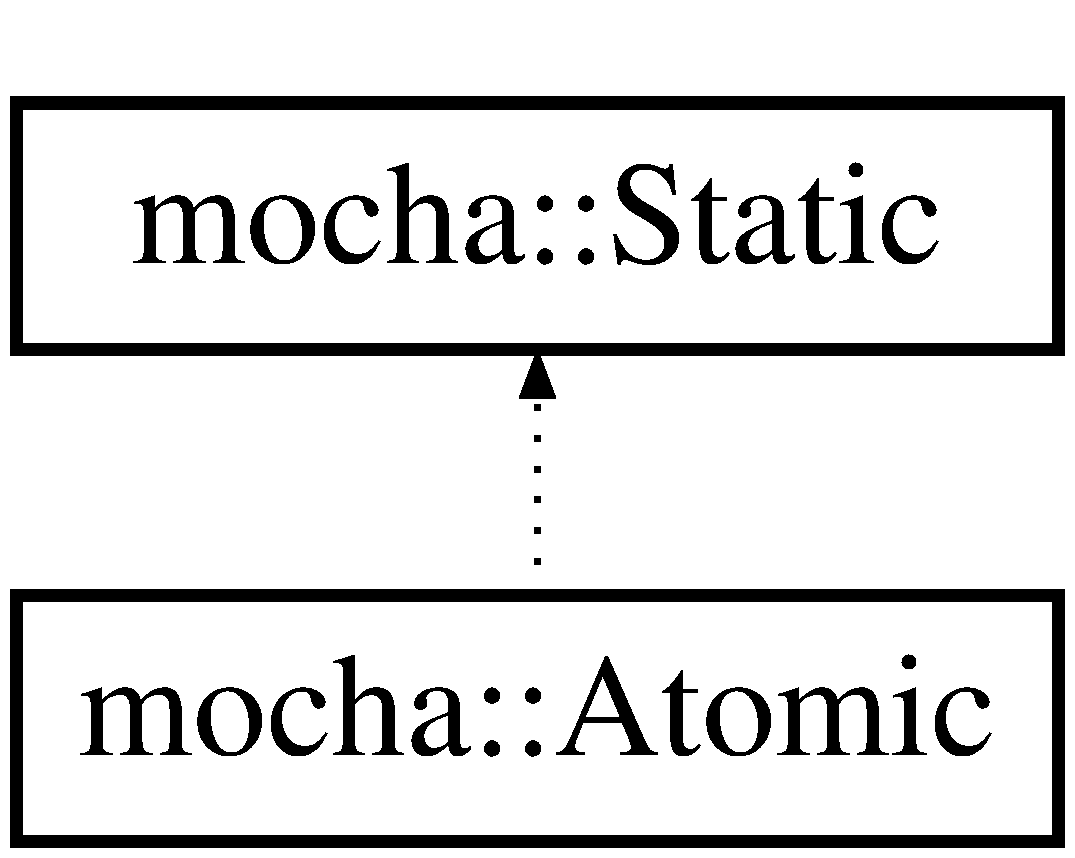
\includegraphics[height=2.000000cm]{classmocha_1_1_atomic}
\end{center}
\end{figure}
\subsection*{Static Public Member Functions}
\begin{DoxyCompactItemize}
\item 
static \hyperlink{atomic_8h_a4fde06794efa6f001ed354067fdd8133}{AtomicWord} \hyperlink{classmocha_1_1_atomic_af36244788479c9bd656e2f61316b4c13}{Increment} (\hyperlink{atomic_8h_a4fde06794efa6f001ed354067fdd8133}{AtomicWord} $\ast$count, int inc=1)
\item 
static \hyperlink{atomic_8h_a4fde06794efa6f001ed354067fdd8133}{AtomicWord} \hyperlink{classmocha_1_1_atomic_a34727b696625bf6176395f74c8b8a9e5}{Decrement} (\hyperlink{atomic_8h_a4fde06794efa6f001ed354067fdd8133}{AtomicWord} $\ast$count, int dec=1)
\end{DoxyCompactItemize}


\subsection{Detailed Description}


Definition at line 24 of file atomic.h.



\subsection{Member Function Documentation}
\hypertarget{classmocha_1_1_atomic_a34727b696625bf6176395f74c8b8a9e5}{
\index{mocha::Atomic@{mocha::Atomic}!Decrement@{Decrement}}
\index{Decrement@{Decrement}!mocha::Atomic@{mocha::Atomic}}
\subsubsection[{Decrement}]{\setlength{\rightskip}{0pt plus 5cm}static {\bf AtomicWord} mocha::Atomic::Decrement (
\begin{DoxyParamCaption}
\item[{{\bf AtomicWord} $\ast$}]{count, }
\item[{int}]{dec = {\ttfamily 1}}
\end{DoxyParamCaption}
)\hspace{0.3cm}{\ttfamily  \mbox{[}inline, static\mbox{]}}}}
\label{classmocha_1_1_atomic_a34727b696625bf6176395f74c8b8a9e5}


Definition at line 30 of file atomic.h.

\hypertarget{classmocha_1_1_atomic_af36244788479c9bd656e2f61316b4c13}{
\index{mocha::Atomic@{mocha::Atomic}!Increment@{Increment}}
\index{Increment@{Increment}!mocha::Atomic@{mocha::Atomic}}
\subsubsection[{Increment}]{\setlength{\rightskip}{0pt plus 5cm}static {\bf AtomicWord} mocha::Atomic::Increment (
\begin{DoxyParamCaption}
\item[{{\bf AtomicWord} $\ast$}]{count, }
\item[{int}]{inc = {\ttfamily 1}}
\end{DoxyParamCaption}
)\hspace{0.3cm}{\ttfamily  \mbox{[}inline, static\mbox{]}}}}
\label{classmocha_1_1_atomic_af36244788479c9bd656e2f61316b4c13}


Definition at line 26 of file atomic.h.



The documentation for this class was generated from the following file:\begin{DoxyCompactItemize}
\item 
Y:/mocha/src/utils/\hyperlink{atomic_8h}{atomic.h}\end{DoxyCompactItemize}

\hypertarget{structmocha_1_1watch__traits_1_1_attrib}{
\section{mocha::watch\_\-traits::Attrib Struct Reference}
\label{structmocha_1_1watch__traits_1_1_attrib}\index{mocha::watch\_\-traits::Attrib@{mocha::watch\_\-traits::Attrib}}
}


{\ttfamily \#include $<$file\_\-watcher.h$>$}

\subsection*{Public Member Functions}
\begin{DoxyCompactItemize}
\item 
\hyperlink{structmocha_1_1watch__traits_1_1_attrib_a844a0846f7231450bf70c31d82a9afda}{Attrib} (const char $\ast$filename\_\-)
\end{DoxyCompactItemize}
\subsection*{Public Attributes}
\begin{DoxyCompactItemize}
\item 
const char $\ast$ \hyperlink{structmocha_1_1watch__traits_1_1_attrib_aceb8b446ede477da0b6f416992d92066}{filename}
\end{DoxyCompactItemize}


\subsection{Detailed Description}


Definition at line 11 of file file\_\-watcher.h.



\subsection{Constructor \& Destructor Documentation}
\hypertarget{structmocha_1_1watch__traits_1_1_attrib_a844a0846f7231450bf70c31d82a9afda}{
\index{mocha::watch\_\-traits::Attrib@{mocha::watch\_\-traits::Attrib}!Attrib@{Attrib}}
\index{Attrib@{Attrib}!mocha::watch_traits::Attrib@{mocha::watch\_\-traits::Attrib}}
\subsubsection[{Attrib}]{\setlength{\rightskip}{0pt plus 5cm}mocha::watch\_\-traits::Attrib::Attrib (
\begin{DoxyParamCaption}
\item[{const char $\ast$}]{filename\_\-}
\end{DoxyParamCaption}
)\hspace{0.3cm}{\ttfamily  \mbox{[}inline\mbox{]}}}}
\label{structmocha_1_1watch__traits_1_1_attrib_a844a0846f7231450bf70c31d82a9afda}


Definition at line 11 of file file\_\-watcher.h.



\subsection{Member Data Documentation}
\hypertarget{structmocha_1_1watch__traits_1_1_attrib_aceb8b446ede477da0b6f416992d92066}{
\index{mocha::watch\_\-traits::Attrib@{mocha::watch\_\-traits::Attrib}!filename@{filename}}
\index{filename@{filename}!mocha::watch_traits::Attrib@{mocha::watch\_\-traits::Attrib}}
\subsubsection[{filename}]{\setlength{\rightskip}{0pt plus 5cm}const char$\ast$ {\bf mocha::watch\_\-traits::Attrib::filename}}}
\label{structmocha_1_1watch__traits_1_1_attrib_aceb8b446ede477da0b6f416992d92066}


Definition at line 11 of file file\_\-watcher.h.



The documentation for this struct was generated from the following file:\begin{DoxyCompactItemize}
\item 
Y:/mocha/src/utils/file\_\-watcher/\hyperlink{file__watcher_8h}{file\_\-watcher.h}\end{DoxyCompactItemize}

\hypertarget{classmocha_1_1_binary_exp}{
\section{mocha::BinaryExp Class Reference}
\label{classmocha_1_1_binary_exp}\index{mocha::BinaryExp@{mocha::BinaryExp}}
}


{\ttfamily \#include $<$ast.h$>$}

Inheritance diagram for mocha::BinaryExp:\begin{figure}[H]
\begin{center}
\leavevmode
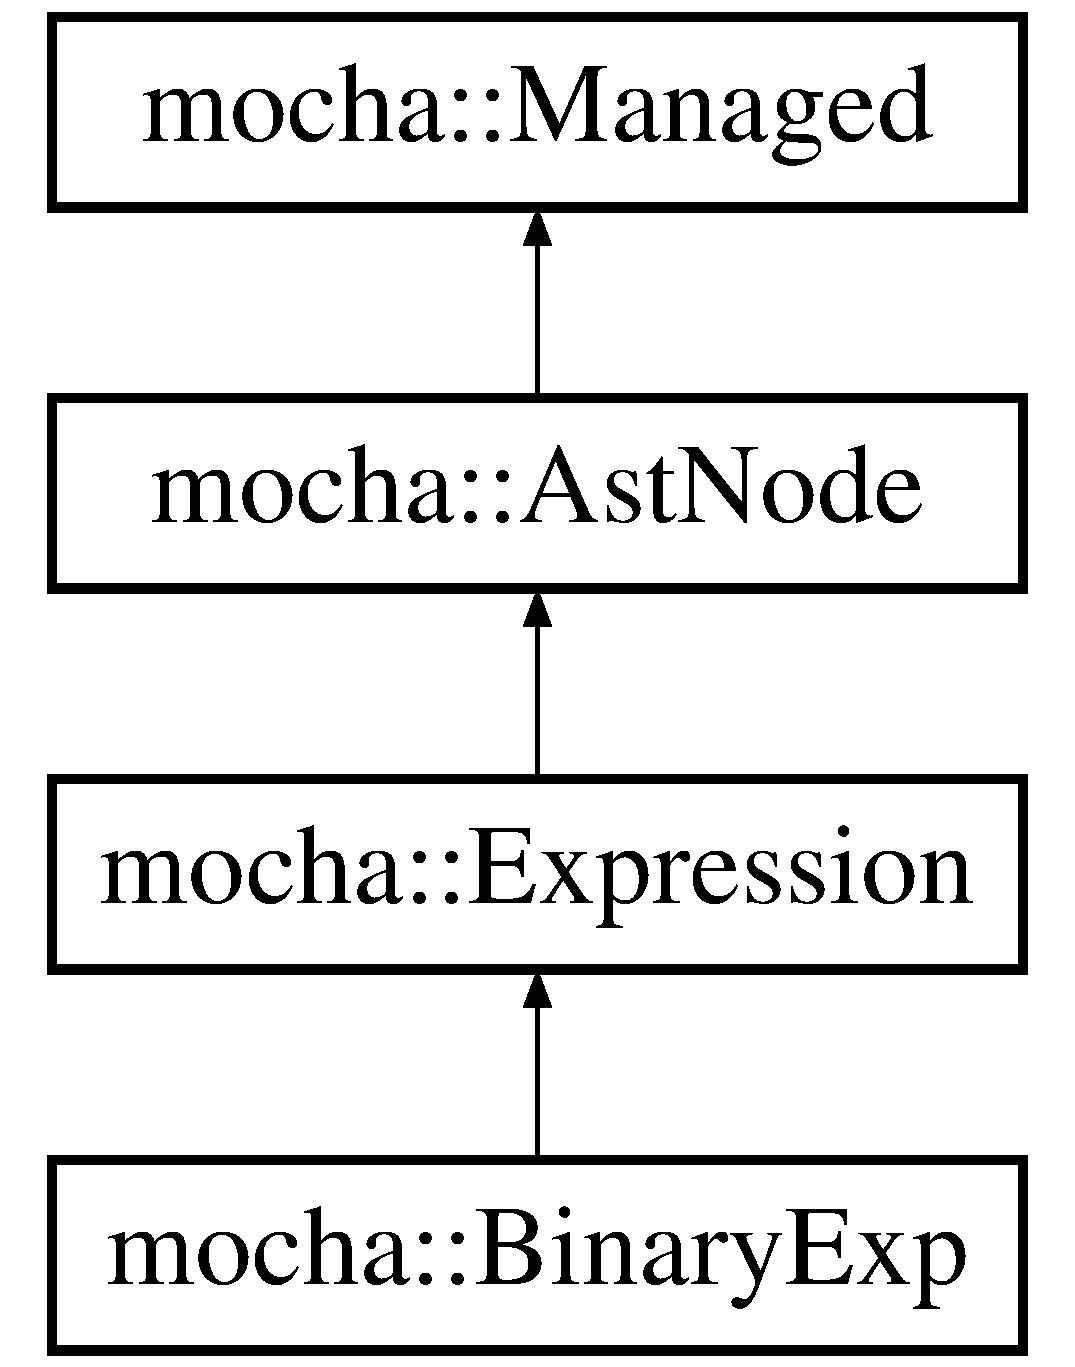
\includegraphics[height=4.000000cm]{classmocha_1_1_binary_exp}
\end{center}
\end{figure}
\subsection*{Public Types}
\begin{DoxyCompactItemize}
\item 
enum \{ \par
\hyperlink{classmocha_1_1_binary_exp_a6556e5472480591fec07f524fed6d093aaf7777a4b57fb6d87e1e12a6267904bf}{kMul}, 
\hyperlink{classmocha_1_1_binary_exp_a6556e5472480591fec07f524fed6d093a7279711d59e87a5fcfbbe205dbc1184a}{kDiv}, 
\hyperlink{classmocha_1_1_binary_exp_a6556e5472480591fec07f524fed6d093acc9cda28bfadceb4b2c95ddebf1206c5}{kMod}, 
\hyperlink{classmocha_1_1_binary_exp_a6556e5472480591fec07f524fed6d093a37a515e229ac071633d53c1d19b3dee2}{kPlus}, 
\par
\hyperlink{classmocha_1_1_binary_exp_a6556e5472480591fec07f524fed6d093a516cfc09844f8a70ce98e71c716f8b75}{kMinus}, 
\hyperlink{classmocha_1_1_binary_exp_a6556e5472480591fec07f524fed6d093abe621824418360cb2190394b5352b2a5}{kShiftLeft}, 
\hyperlink{classmocha_1_1_binary_exp_a6556e5472480591fec07f524fed6d093af5941e749b759bd5b05106a180cceb28}{kShiftRight}, 
\hyperlink{classmocha_1_1_binary_exp_a6556e5472480591fec07f524fed6d093abf9cb82ae717a842d082eaaac4924984}{kUShiftRight}, 
\par
\hyperlink{classmocha_1_1_binary_exp_a6556e5472480591fec07f524fed6d093a164ec266fc1c3539946107eb4f9fad25}{kAnd}, 
\hyperlink{classmocha_1_1_binary_exp_a6556e5472480591fec07f524fed6d093a6e59ebc04a213850d191f81eb617e26b}{kXor}, 
\hyperlink{classmocha_1_1_binary_exp_a6556e5472480591fec07f524fed6d093a2d1f97cad536573b8e69c9f295544586}{kOr}
 \}
\end{DoxyCompactItemize}
\subsection*{Public Member Functions}
\begin{DoxyCompactItemize}
\item 
\hyperlink{classmocha_1_1_binary_exp_a4a6151f22fb83c7b6e958103543901e2}{BinaryExp} (int op, \hyperlink{classmocha_1_1_ast_node}{AstNode} $\ast$left, \hyperlink{classmocha_1_1_ast_node}{AstNode} $\ast$right)
\item 
\hyperlink{classmocha_1_1_binary_exp_aa64a52bc2abaafac6d30b122a5eac880}{$\sim$BinaryExp} ()
\item 
\hyperlink{classmocha_1_1_ast_node}{AstNode} $\ast$ \hyperlink{classmocha_1_1_binary_exp_aff0c16fd0b2fc8a186bd749fb9020e38}{Left} ()
\item 
\hyperlink{classmocha_1_1_ast_node}{AstNode} $\ast$ \hyperlink{classmocha_1_1_binary_exp_ac22eeeeee93ef31b170519c4bace8cd9}{Right} ()
\item 
int \hyperlink{classmocha_1_1_binary_exp_a698d95fb3cc21ae19b87e74622a76683}{Op} ()
\item 
void \hyperlink{classmocha_1_1_binary_exp_a3e6534281bf4c610222b1ad6ec752625}{ReplaceChild} (\hyperlink{classmocha_1_1_ast_node}{AstNode} $\ast$old\_\-node, \hyperlink{classmocha_1_1_ast_node}{AstNode} $\ast$new\_\-node)
\item 
\hyperlink{classmocha_1_1_ast_node}{AstNode} $\ast$ \hyperlink{classmocha_1_1_binary_exp_a035d97865c0512e2902192f8ed840ae4}{Clone} ()
\end{DoxyCompactItemize}
\subsection*{Private Member Functions}
\begin{DoxyCompactItemize}
\item 
void \hyperlink{classmocha_1_1_binary_exp_ac7feb22c02d0432e40486b76997f505e}{NVIAccept\_\-} (\hyperlink{classmocha_1_1_i_visitor}{IVisitor} $\ast$visitor)
\end{DoxyCompactItemize}
\subsection*{Private Attributes}
\begin{DoxyCompactItemize}
\item 
int \hyperlink{classmocha_1_1_binary_exp_acc6841e04f10973e484979d4066a532f}{op\_\-}
\item 
\hyperlink{classmocha_1_1_ast_node}{AstNode} $\ast$ \hyperlink{classmocha_1_1_binary_exp_acc7f47a0ae80042c528250d881f78a90}{left\_\-}
\item 
\hyperlink{classmocha_1_1_ast_node}{AstNode} $\ast$ \hyperlink{classmocha_1_1_binary_exp_abf7760f6928cbc7941bb98a658d927fc}{right\_\-}
\end{DoxyCompactItemize}


\subsection{Detailed Description}


Definition at line 1414 of file ast.h.



\subsection{Member Enumeration Documentation}
\hypertarget{classmocha_1_1_binary_exp_a6556e5472480591fec07f524fed6d093}{
\subsubsection[{"@10}]{\setlength{\rightskip}{0pt plus 5cm}anonymous enum}}
\label{classmocha_1_1_binary_exp_a6556e5472480591fec07f524fed6d093}
\begin{Desc}
\item[Enumerator: ]\par
\begin{description}
\index{kMul@{kMul}!mocha::BinaryExp@{mocha::BinaryExp}}\index{mocha::BinaryExp@{mocha::BinaryExp}!kMul@{kMul}}\item[{\em 
\hypertarget{classmocha_1_1_binary_exp_a6556e5472480591fec07f524fed6d093aaf7777a4b57fb6d87e1e12a6267904bf}{
kMul}
\label{classmocha_1_1_binary_exp_a6556e5472480591fec07f524fed6d093aaf7777a4b57fb6d87e1e12a6267904bf}
}]\index{kDiv@{kDiv}!mocha::BinaryExp@{mocha::BinaryExp}}\index{mocha::BinaryExp@{mocha::BinaryExp}!kDiv@{kDiv}}\item[{\em 
\hypertarget{classmocha_1_1_binary_exp_a6556e5472480591fec07f524fed6d093a7279711d59e87a5fcfbbe205dbc1184a}{
kDiv}
\label{classmocha_1_1_binary_exp_a6556e5472480591fec07f524fed6d093a7279711d59e87a5fcfbbe205dbc1184a}
}]\index{kMod@{kMod}!mocha::BinaryExp@{mocha::BinaryExp}}\index{mocha::BinaryExp@{mocha::BinaryExp}!kMod@{kMod}}\item[{\em 
\hypertarget{classmocha_1_1_binary_exp_a6556e5472480591fec07f524fed6d093acc9cda28bfadceb4b2c95ddebf1206c5}{
kMod}
\label{classmocha_1_1_binary_exp_a6556e5472480591fec07f524fed6d093acc9cda28bfadceb4b2c95ddebf1206c5}
}]\index{kPlus@{kPlus}!mocha::BinaryExp@{mocha::BinaryExp}}\index{mocha::BinaryExp@{mocha::BinaryExp}!kPlus@{kPlus}}\item[{\em 
\hypertarget{classmocha_1_1_binary_exp_a6556e5472480591fec07f524fed6d093a37a515e229ac071633d53c1d19b3dee2}{
kPlus}
\label{classmocha_1_1_binary_exp_a6556e5472480591fec07f524fed6d093a37a515e229ac071633d53c1d19b3dee2}
}]\index{kMinus@{kMinus}!mocha::BinaryExp@{mocha::BinaryExp}}\index{mocha::BinaryExp@{mocha::BinaryExp}!kMinus@{kMinus}}\item[{\em 
\hypertarget{classmocha_1_1_binary_exp_a6556e5472480591fec07f524fed6d093a516cfc09844f8a70ce98e71c716f8b75}{
kMinus}
\label{classmocha_1_1_binary_exp_a6556e5472480591fec07f524fed6d093a516cfc09844f8a70ce98e71c716f8b75}
}]\index{kShiftLeft@{kShiftLeft}!mocha::BinaryExp@{mocha::BinaryExp}}\index{mocha::BinaryExp@{mocha::BinaryExp}!kShiftLeft@{kShiftLeft}}\item[{\em 
\hypertarget{classmocha_1_1_binary_exp_a6556e5472480591fec07f524fed6d093abe621824418360cb2190394b5352b2a5}{
kShiftLeft}
\label{classmocha_1_1_binary_exp_a6556e5472480591fec07f524fed6d093abe621824418360cb2190394b5352b2a5}
}]\index{kShiftRight@{kShiftRight}!mocha::BinaryExp@{mocha::BinaryExp}}\index{mocha::BinaryExp@{mocha::BinaryExp}!kShiftRight@{kShiftRight}}\item[{\em 
\hypertarget{classmocha_1_1_binary_exp_a6556e5472480591fec07f524fed6d093af5941e749b759bd5b05106a180cceb28}{
kShiftRight}
\label{classmocha_1_1_binary_exp_a6556e5472480591fec07f524fed6d093af5941e749b759bd5b05106a180cceb28}
}]\index{kUShiftRight@{kUShiftRight}!mocha::BinaryExp@{mocha::BinaryExp}}\index{mocha::BinaryExp@{mocha::BinaryExp}!kUShiftRight@{kUShiftRight}}\item[{\em 
\hypertarget{classmocha_1_1_binary_exp_a6556e5472480591fec07f524fed6d093abf9cb82ae717a842d082eaaac4924984}{
kUShiftRight}
\label{classmocha_1_1_binary_exp_a6556e5472480591fec07f524fed6d093abf9cb82ae717a842d082eaaac4924984}
}]\index{kAnd@{kAnd}!mocha::BinaryExp@{mocha::BinaryExp}}\index{mocha::BinaryExp@{mocha::BinaryExp}!kAnd@{kAnd}}\item[{\em 
\hypertarget{classmocha_1_1_binary_exp_a6556e5472480591fec07f524fed6d093a164ec266fc1c3539946107eb4f9fad25}{
kAnd}
\label{classmocha_1_1_binary_exp_a6556e5472480591fec07f524fed6d093a164ec266fc1c3539946107eb4f9fad25}
}]\index{kXor@{kXor}!mocha::BinaryExp@{mocha::BinaryExp}}\index{mocha::BinaryExp@{mocha::BinaryExp}!kXor@{kXor}}\item[{\em 
\hypertarget{classmocha_1_1_binary_exp_a6556e5472480591fec07f524fed6d093a6e59ebc04a213850d191f81eb617e26b}{
kXor}
\label{classmocha_1_1_binary_exp_a6556e5472480591fec07f524fed6d093a6e59ebc04a213850d191f81eb617e26b}
}]\index{kOr@{kOr}!mocha::BinaryExp@{mocha::BinaryExp}}\index{mocha::BinaryExp@{mocha::BinaryExp}!kOr@{kOr}}\item[{\em 
\hypertarget{classmocha_1_1_binary_exp_a6556e5472480591fec07f524fed6d093a2d1f97cad536573b8e69c9f295544586}{
kOr}
\label{classmocha_1_1_binary_exp_a6556e5472480591fec07f524fed6d093a2d1f97cad536573b8e69c9f295544586}
}]\end{description}
\end{Desc}



Definition at line 1416 of file ast.h.



\subsection{Constructor \& Destructor Documentation}
\hypertarget{classmocha_1_1_binary_exp_a4a6151f22fb83c7b6e958103543901e2}{
\index{mocha::BinaryExp@{mocha::BinaryExp}!BinaryExp@{BinaryExp}}
\index{BinaryExp@{BinaryExp}!mocha::BinaryExp@{mocha::BinaryExp}}
\subsubsection[{BinaryExp}]{\setlength{\rightskip}{0pt plus 5cm}mocha::BinaryExp::BinaryExp (
\begin{DoxyParamCaption}
\item[{int}]{op, }
\item[{{\bf AstNode} $\ast$}]{left, }
\item[{{\bf AstNode} $\ast$}]{right}
\end{DoxyParamCaption}
)\hspace{0.3cm}{\ttfamily  \mbox{[}inline\mbox{]}}}}
\label{classmocha_1_1_binary_exp_a4a6151f22fb83c7b6e958103543901e2}


Definition at line 1429 of file ast.h.

\hypertarget{classmocha_1_1_binary_exp_aa64a52bc2abaafac6d30b122a5eac880}{
\index{mocha::BinaryExp@{mocha::BinaryExp}!$\sim$BinaryExp@{$\sim$BinaryExp}}
\index{$\sim$BinaryExp@{$\sim$BinaryExp}!mocha::BinaryExp@{mocha::BinaryExp}}
\subsubsection[{$\sim$BinaryExp}]{\setlength{\rightskip}{0pt plus 5cm}mocha::BinaryExp::$\sim$BinaryExp (
\begin{DoxyParamCaption}
{}
\end{DoxyParamCaption}
)\hspace{0.3cm}{\ttfamily  \mbox{[}inline\mbox{]}}}}
\label{classmocha_1_1_binary_exp_aa64a52bc2abaafac6d30b122a5eac880}


Definition at line 1430 of file ast.h.



\subsection{Member Function Documentation}
\hypertarget{classmocha_1_1_binary_exp_a035d97865c0512e2902192f8ed840ae4}{
\index{mocha::BinaryExp@{mocha::BinaryExp}!Clone@{Clone}}
\index{Clone@{Clone}!mocha::BinaryExp@{mocha::BinaryExp}}
\subsubsection[{Clone}]{\setlength{\rightskip}{0pt plus 5cm}{\bf AstNode} $\ast$ mocha::BinaryExp::Clone (
\begin{DoxyParamCaption}
{}
\end{DoxyParamCaption}
)\hspace{0.3cm}{\ttfamily  \mbox{[}virtual\mbox{]}}}}
\label{classmocha_1_1_binary_exp_a035d97865c0512e2902192f8ed840ae4}
\begin{DoxyReturn}{Returns}
\{AstNode$\ast$\} Clone node. 
\end{DoxyReturn}


Reimplemented from \hyperlink{classmocha_1_1_expression_ac1fb936e2bf0fdd6e7667275d3723ca5}{mocha::Expression}.



Definition at line 533 of file ast.cc.

\hypertarget{classmocha_1_1_binary_exp_aff0c16fd0b2fc8a186bd749fb9020e38}{
\index{mocha::BinaryExp@{mocha::BinaryExp}!Left@{Left}}
\index{Left@{Left}!mocha::BinaryExp@{mocha::BinaryExp}}
\subsubsection[{Left}]{\setlength{\rightskip}{0pt plus 5cm}{\bf AstNode}$\ast$ mocha::BinaryExp::Left (
\begin{DoxyParamCaption}
{}
\end{DoxyParamCaption}
)\hspace{0.3cm}{\ttfamily  \mbox{[}inline\mbox{]}}}}
\label{classmocha_1_1_binary_exp_aff0c16fd0b2fc8a186bd749fb9020e38}


Definition at line 1431 of file ast.h.

\hypertarget{classmocha_1_1_binary_exp_ac7feb22c02d0432e40486b76997f505e}{
\index{mocha::BinaryExp@{mocha::BinaryExp}!NVIAccept\_\-@{NVIAccept\_\-}}
\index{NVIAccept\_\-@{NVIAccept\_\-}!mocha::BinaryExp@{mocha::BinaryExp}}
\subsubsection[{NVIAccept\_\-}]{\setlength{\rightskip}{0pt plus 5cm}void mocha::BinaryExp::NVIAccept\_\- (
\begin{DoxyParamCaption}
\item[{{\bf IVisitor} $\ast$}]{visitor}
\end{DoxyParamCaption}
)\hspace{0.3cm}{\ttfamily  \mbox{[}inline, private, virtual\mbox{]}}}}
\label{classmocha_1_1_binary_exp_ac7feb22c02d0432e40486b76997f505e}


Reimplemented from \hyperlink{classmocha_1_1_expression_a112d57b7de76c37066cde60be4799fde}{mocha::Expression}.



Definition at line 1440 of file ast.h.

\hypertarget{classmocha_1_1_binary_exp_a698d95fb3cc21ae19b87e74622a76683}{
\index{mocha::BinaryExp@{mocha::BinaryExp}!Op@{Op}}
\index{Op@{Op}!mocha::BinaryExp@{mocha::BinaryExp}}
\subsubsection[{Op}]{\setlength{\rightskip}{0pt plus 5cm}int mocha::BinaryExp::Op (
\begin{DoxyParamCaption}
{}
\end{DoxyParamCaption}
)\hspace{0.3cm}{\ttfamily  \mbox{[}inline\mbox{]}}}}
\label{classmocha_1_1_binary_exp_a698d95fb3cc21ae19b87e74622a76683}


Definition at line 1433 of file ast.h.

\hypertarget{classmocha_1_1_binary_exp_a3e6534281bf4c610222b1ad6ec752625}{
\index{mocha::BinaryExp@{mocha::BinaryExp}!ReplaceChild@{ReplaceChild}}
\index{ReplaceChild@{ReplaceChild}!mocha::BinaryExp@{mocha::BinaryExp}}
\subsubsection[{ReplaceChild}]{\setlength{\rightskip}{0pt plus 5cm}void mocha::BinaryExp::ReplaceChild (
\begin{DoxyParamCaption}
\item[{{\bf AstNode} $\ast$}]{old\_\-node, }
\item[{{\bf AstNode} $\ast$}]{new\_\-node}
\end{DoxyParamCaption}
)\hspace{0.3cm}{\ttfamily  \mbox{[}virtual\mbox{]}}}}
\label{classmocha_1_1_binary_exp_a3e6534281bf4c610222b1ad6ec752625}

\begin{DoxyParams}{Parameters}
{\em \{AstNode$\ast$\}} & Replace the old\_\-node with new\_\-node in childnodes. \\
\hline
\end{DoxyParams}


Reimplemented from \hyperlink{classmocha_1_1_ast_node_aa40396040f75fb59e320d81c3fd328c8}{mocha::AstNode}.



Definition at line 517 of file ast.cc.

\hypertarget{classmocha_1_1_binary_exp_ac22eeeeee93ef31b170519c4bace8cd9}{
\index{mocha::BinaryExp@{mocha::BinaryExp}!Right@{Right}}
\index{Right@{Right}!mocha::BinaryExp@{mocha::BinaryExp}}
\subsubsection[{Right}]{\setlength{\rightskip}{0pt plus 5cm}{\bf AstNode}$\ast$ mocha::BinaryExp::Right (
\begin{DoxyParamCaption}
{}
\end{DoxyParamCaption}
)\hspace{0.3cm}{\ttfamily  \mbox{[}inline\mbox{]}}}}
\label{classmocha_1_1_binary_exp_ac22eeeeee93ef31b170519c4bace8cd9}


Definition at line 1432 of file ast.h.



\subsection{Member Data Documentation}
\hypertarget{classmocha_1_1_binary_exp_acc7f47a0ae80042c528250d881f78a90}{
\index{mocha::BinaryExp@{mocha::BinaryExp}!left\_\-@{left\_\-}}
\index{left\_\-@{left\_\-}!mocha::BinaryExp@{mocha::BinaryExp}}
\subsubsection[{left\_\-}]{\setlength{\rightskip}{0pt plus 5cm}{\bf AstNode}$\ast$ {\bf mocha::BinaryExp::left\_\-}\hspace{0.3cm}{\ttfamily  \mbox{[}private\mbox{]}}}}
\label{classmocha_1_1_binary_exp_acc7f47a0ae80042c528250d881f78a90}


Definition at line 1438 of file ast.h.

\hypertarget{classmocha_1_1_binary_exp_acc6841e04f10973e484979d4066a532f}{
\index{mocha::BinaryExp@{mocha::BinaryExp}!op\_\-@{op\_\-}}
\index{op\_\-@{op\_\-}!mocha::BinaryExp@{mocha::BinaryExp}}
\subsubsection[{op\_\-}]{\setlength{\rightskip}{0pt plus 5cm}int {\bf mocha::BinaryExp::op\_\-}\hspace{0.3cm}{\ttfamily  \mbox{[}private\mbox{]}}}}
\label{classmocha_1_1_binary_exp_acc6841e04f10973e484979d4066a532f}


Definition at line 1435 of file ast.h.

\hypertarget{classmocha_1_1_binary_exp_abf7760f6928cbc7941bb98a658d927fc}{
\index{mocha::BinaryExp@{mocha::BinaryExp}!right\_\-@{right\_\-}}
\index{right\_\-@{right\_\-}!mocha::BinaryExp@{mocha::BinaryExp}}
\subsubsection[{right\_\-}]{\setlength{\rightskip}{0pt plus 5cm}{\bf AstNode}$\ast$ {\bf mocha::BinaryExp::right\_\-}\hspace{0.3cm}{\ttfamily  \mbox{[}private\mbox{]}}}}
\label{classmocha_1_1_binary_exp_abf7760f6928cbc7941bb98a658d927fc}


Definition at line 1439 of file ast.h.



The documentation for this class was generated from the following files:\begin{DoxyCompactItemize}
\item 
Y:/mocha/src/ast/\hyperlink{ast_8h}{ast.h}\item 
Y:/mocha/src/ast/\hyperlink{ast_8cc}{ast.cc}\end{DoxyCompactItemize}

\hypertarget{classmocha_1_1_bit_vector}{
\section{mocha::BitVector$<$ T, bit\_\-bands $>$ Class Template Reference}
\label{classmocha_1_1_bit_vector}\index{mocha::BitVector@{mocha::BitVector}}
}


{\ttfamily \#include $<$bits.h$>$}

\subsection*{Public Member Functions}
\begin{DoxyCompactItemize}
\item 
\hyperlink{classmocha_1_1_bit_vector_adfcef8fc10b228a545e2663f16531430}{BitVector} ()
\item 
\hyperlink{classmocha_1_1_bit_vector_a76452ed17ca332f1d49b277ea616110e}{$\sim$BitVector} ()
\item 
\hyperlink{classmocha_1_1_bit_vector_ad69f348fe9de383004a69c769551b8a6}{BitVector} (const \hyperlink{classmocha_1_1_bit_vector}{BitVector} \&vec)
\item 
const \hyperlink{classmocha_1_1_bit_vector}{BitVector}$<$ T, bit\_\-bands $>$ \& \hyperlink{classmocha_1_1_bit_vector_a6db4073dc525ead42cf101c1e1bfca15}{operator=} (const \hyperlink{classmocha_1_1_bit_vector}{BitVector}$<$ T, bit\_\-bands $>$ \&vec)
\item 
void \hyperlink{classmocha_1_1_bit_vector_a9bc91f973a980564f246500260c75db0}{Set} (int val)
\item 
void \hyperlink{classmocha_1_1_bit_vector_a3af98e0c39acef618232aa6a75531e9b}{UnSet} (int val)
\item 
void \hyperlink{classmocha_1_1_bit_vector_a382b9dcb9ca1a08ba81b1a1f98d9a25c}{Reverse} (int val)
\item 
bool \hyperlink{classmocha_1_1_bit_vector_a1d8baf3fe19959f7b1e4777ffc2a0182}{At} (int val)
\item 
bool \hyperlink{classmocha_1_1_bit_vector_acd0e54057805396cc6c5d6406ba13005}{operator\mbox{[}$\,$\mbox{]}} (int val)
\end{DoxyCompactItemize}
\subsection*{Private Member Functions}
\begin{DoxyCompactItemize}
\item 
\hyperlink{classmocha_1_1_bit_vector_a524e2a640a37be416e2e945ae73a3e0a}{STATIC\_\-ASSERT} (bit\_\-bands $>$ 0)
\end{DoxyCompactItemize}
\subsection*{Private Attributes}
\begin{DoxyCompactItemize}
\item 
T \hyperlink{classmocha_1_1_bit_vector_a597d7932257a18fac495ab15ac45c245}{set\_\-}
\end{DoxyCompactItemize}


\subsection{Detailed Description}
\subsubsection*{template$<$typename T, int bit\_\-bands$>$class mocha::BitVector$<$ T, bit\_\-bands $>$}



Definition at line 9 of file bits.h.



\subsection{Constructor \& Destructor Documentation}
\hypertarget{classmocha_1_1_bit_vector_adfcef8fc10b228a545e2663f16531430}{
\index{mocha::BitVector@{mocha::BitVector}!BitVector@{BitVector}}
\index{BitVector@{BitVector}!mocha::BitVector@{mocha::BitVector}}
\subsubsection[{BitVector}]{\setlength{\rightskip}{0pt plus 5cm}template$<$typename T, int bit\_\-bands$>$ {\bf mocha::BitVector}$<$ T, bit\_\-bands $>$::{\bf BitVector} (
\begin{DoxyParamCaption}
{}
\end{DoxyParamCaption}
)\hspace{0.3cm}{\ttfamily  \mbox{[}inline\mbox{]}}}}
\label{classmocha_1_1_bit_vector_adfcef8fc10b228a545e2663f16531430}


Definition at line 11 of file bits.h.

\hypertarget{classmocha_1_1_bit_vector_a76452ed17ca332f1d49b277ea616110e}{
\index{mocha::BitVector@{mocha::BitVector}!$\sim$BitVector@{$\sim$BitVector}}
\index{$\sim$BitVector@{$\sim$BitVector}!mocha::BitVector@{mocha::BitVector}}
\subsubsection[{$\sim$BitVector}]{\setlength{\rightskip}{0pt plus 5cm}template$<$typename T, int bit\_\-bands$>$ {\bf mocha::BitVector}$<$ T, bit\_\-bands $>$::$\sim${\bf BitVector} (
\begin{DoxyParamCaption}
{}
\end{DoxyParamCaption}
)\hspace{0.3cm}{\ttfamily  \mbox{[}inline\mbox{]}}}}
\label{classmocha_1_1_bit_vector_a76452ed17ca332f1d49b277ea616110e}


Definition at line 12 of file bits.h.

\hypertarget{classmocha_1_1_bit_vector_ad69f348fe9de383004a69c769551b8a6}{
\index{mocha::BitVector@{mocha::BitVector}!BitVector@{BitVector}}
\index{BitVector@{BitVector}!mocha::BitVector@{mocha::BitVector}}
\subsubsection[{BitVector}]{\setlength{\rightskip}{0pt plus 5cm}template$<$typename T, int bit\_\-bands$>$ {\bf mocha::BitVector}$<$ T, bit\_\-bands $>$::{\bf BitVector} (
\begin{DoxyParamCaption}
\item[{const {\bf BitVector}$<$ T, bit\_\-bands $>$ \&}]{vec}
\end{DoxyParamCaption}
)\hspace{0.3cm}{\ttfamily  \mbox{[}inline\mbox{]}}}}
\label{classmocha_1_1_bit_vector_ad69f348fe9de383004a69c769551b8a6}


Definition at line 13 of file bits.h.



\subsection{Member Function Documentation}
\hypertarget{classmocha_1_1_bit_vector_a1d8baf3fe19959f7b1e4777ffc2a0182}{
\index{mocha::BitVector@{mocha::BitVector}!At@{At}}
\index{At@{At}!mocha::BitVector@{mocha::BitVector}}
\subsubsection[{At}]{\setlength{\rightskip}{0pt plus 5cm}template$<$typename T, int bit\_\-bands$>$ bool {\bf mocha::BitVector}$<$ T, bit\_\-bands $>$::At (
\begin{DoxyParamCaption}
\item[{int}]{val}
\end{DoxyParamCaption}
)\hspace{0.3cm}{\ttfamily  \mbox{[}inline\mbox{]}}}}
\label{classmocha_1_1_bit_vector_a1d8baf3fe19959f7b1e4777ffc2a0182}


Definition at line 32 of file bits.h.

\hypertarget{classmocha_1_1_bit_vector_a6db4073dc525ead42cf101c1e1bfca15}{
\index{mocha::BitVector@{mocha::BitVector}!operator=@{operator=}}
\index{operator=@{operator=}!mocha::BitVector@{mocha::BitVector}}
\subsubsection[{operator=}]{\setlength{\rightskip}{0pt plus 5cm}template$<$typename T, int bit\_\-bands$>$ const {\bf BitVector}$<$T,bit\_\-bands$>$\& {\bf mocha::BitVector}$<$ T, bit\_\-bands $>$::operator= (
\begin{DoxyParamCaption}
\item[{const {\bf BitVector}$<$ T, bit\_\-bands $>$ \&}]{vec}
\end{DoxyParamCaption}
)\hspace{0.3cm}{\ttfamily  \mbox{[}inline\mbox{]}}}}
\label{classmocha_1_1_bit_vector_a6db4073dc525ead42cf101c1e1bfca15}


Definition at line 16 of file bits.h.

\hypertarget{classmocha_1_1_bit_vector_acd0e54057805396cc6c5d6406ba13005}{
\index{mocha::BitVector@{mocha::BitVector}!operator\mbox{[}\mbox{]}@{operator[]}}
\index{operator\mbox{[}\mbox{]}@{operator[]}!mocha::BitVector@{mocha::BitVector}}
\subsubsection[{operator[]}]{\setlength{\rightskip}{0pt plus 5cm}template$<$typename T, int bit\_\-bands$>$ bool {\bf mocha::BitVector}$<$ T, bit\_\-bands $>$::operator\mbox{[}$\,$\mbox{]} (
\begin{DoxyParamCaption}
\item[{int}]{val}
\end{DoxyParamCaption}
)\hspace{0.3cm}{\ttfamily  \mbox{[}inline\mbox{]}}}}
\label{classmocha_1_1_bit_vector_acd0e54057805396cc6c5d6406ba13005}


Definition at line 37 of file bits.h.

\hypertarget{classmocha_1_1_bit_vector_a382b9dcb9ca1a08ba81b1a1f98d9a25c}{
\index{mocha::BitVector@{mocha::BitVector}!Reverse@{Reverse}}
\index{Reverse@{Reverse}!mocha::BitVector@{mocha::BitVector}}
\subsubsection[{Reverse}]{\setlength{\rightskip}{0pt plus 5cm}template$<$typename T, int bit\_\-bands$>$ void {\bf mocha::BitVector}$<$ T, bit\_\-bands $>$::Reverse (
\begin{DoxyParamCaption}
\item[{int}]{val}
\end{DoxyParamCaption}
)\hspace{0.3cm}{\ttfamily  \mbox{[}inline\mbox{]}}}}
\label{classmocha_1_1_bit_vector_a382b9dcb9ca1a08ba81b1a1f98d9a25c}


Definition at line 28 of file bits.h.

\hypertarget{classmocha_1_1_bit_vector_a9bc91f973a980564f246500260c75db0}{
\index{mocha::BitVector@{mocha::BitVector}!Set@{Set}}
\index{Set@{Set}!mocha::BitVector@{mocha::BitVector}}
\subsubsection[{Set}]{\setlength{\rightskip}{0pt plus 5cm}template$<$typename T, int bit\_\-bands$>$ void {\bf mocha::BitVector}$<$ T, bit\_\-bands $>$::Set (
\begin{DoxyParamCaption}
\item[{int}]{val}
\end{DoxyParamCaption}
)\hspace{0.3cm}{\ttfamily  \mbox{[}inline\mbox{]}}}}
\label{classmocha_1_1_bit_vector_a9bc91f973a980564f246500260c75db0}


Definition at line 20 of file bits.h.

\hypertarget{classmocha_1_1_bit_vector_a524e2a640a37be416e2e945ae73a3e0a}{
\index{mocha::BitVector@{mocha::BitVector}!STATIC\_\-ASSERT@{STATIC\_\-ASSERT}}
\index{STATIC\_\-ASSERT@{STATIC\_\-ASSERT}!mocha::BitVector@{mocha::BitVector}}
\subsubsection[{STATIC\_\-ASSERT}]{\setlength{\rightskip}{0pt plus 5cm}template$<$typename T, int bit\_\-bands$>$ {\bf mocha::BitVector}$<$ T, bit\_\-bands $>$::STATIC\_\-ASSERT (
\begin{DoxyParamCaption}
\item[{bit\_\-bands}]{, }
\item[{0}]{}
\end{DoxyParamCaption}
)\hspace{0.3cm}{\ttfamily  \mbox{[}private\mbox{]}}}}
\label{classmocha_1_1_bit_vector_a524e2a640a37be416e2e945ae73a3e0a}
\hypertarget{classmocha_1_1_bit_vector_a3af98e0c39acef618232aa6a75531e9b}{
\index{mocha::BitVector@{mocha::BitVector}!UnSet@{UnSet}}
\index{UnSet@{UnSet}!mocha::BitVector@{mocha::BitVector}}
\subsubsection[{UnSet}]{\setlength{\rightskip}{0pt plus 5cm}template$<$typename T, int bit\_\-bands$>$ void {\bf mocha::BitVector}$<$ T, bit\_\-bands $>$::UnSet (
\begin{DoxyParamCaption}
\item[{int}]{val}
\end{DoxyParamCaption}
)\hspace{0.3cm}{\ttfamily  \mbox{[}inline\mbox{]}}}}
\label{classmocha_1_1_bit_vector_a3af98e0c39acef618232aa6a75531e9b}


Definition at line 24 of file bits.h.



\subsection{Member Data Documentation}
\hypertarget{classmocha_1_1_bit_vector_a597d7932257a18fac495ab15ac45c245}{
\index{mocha::BitVector@{mocha::BitVector}!set\_\-@{set\_\-}}
\index{set\_\-@{set\_\-}!mocha::BitVector@{mocha::BitVector}}
\subsubsection[{set\_\-}]{\setlength{\rightskip}{0pt plus 5cm}template$<$typename T, int bit\_\-bands$>$ T {\bf mocha::BitVector}$<$ T, bit\_\-bands $>$::{\bf set\_\-}\hspace{0.3cm}{\ttfamily  \mbox{[}private\mbox{]}}}}
\label{classmocha_1_1_bit_vector_a597d7932257a18fac495ab15ac45c245}


Definition at line 42 of file bits.h.



The documentation for this class was generated from the following file:\begin{DoxyCompactItemize}
\item 
Y:/mocha/src/utils/\hyperlink{bits_8h}{bits.h}\end{DoxyCompactItemize}

\hypertarget{classmocha_1_1_block}{
\section{mocha::Block$<$ Key\_\-t, Value\_\-t $>$ Class Template Reference}
\label{classmocha_1_1_block}\index{mocha::Block@{mocha::Block}}
}


{\ttfamily \#include $<$block.h$>$}

\subsection*{Public Types}
\begin{DoxyCompactItemize}
\item 
typedef std::list$<$ \hyperlink{classmocha_1_1_entry}{Entry}$<$ Key\_\-t, Value\_\-t $>$ $\ast$ $>$ \hyperlink{classmocha_1_1_block_a021e0317e479cd9af8dc345d382bf675}{EntryList}
\end{DoxyCompactItemize}
\subsection*{Public Member Functions}
\begin{DoxyCompactItemize}
\item 
\hyperlink{classmocha_1_1_block_a0bda8fe4ef62d71672a673a97ef13f05}{Block} ()
\item 
\hyperlink{classmocha_1_1_block_a8dc69c793ffe830490930759d8c7f4e8}{$\sim$Block} ()
\item 
\hyperlink{classmocha_1_1_block}{Block}$<$ Key\_\-t, Value\_\-t $>$ $\ast$ \hyperlink{classmocha_1_1_block_a6ad0be06026e4691b1bf402ebfcbd55b}{Node} ()
\item 
void \hyperlink{classmocha_1_1_block_a8f03eff4f3d7219a4011820c92ea820b}{Alloc} ()
\item 
\hyperlink{classmocha_1_1_entry}{Entry}$<$ Key\_\-t, Value\_\-t $>$ $\ast$ \hyperlink{classmocha_1_1_block_a6a8baf07b2b82f7276e19a8b73a5a552}{GetEntry} ()
\item 
void \hyperlink{classmocha_1_1_block_a560bb0b7c45e87b185b63ece5fb2c923}{Set} (Key\_\-t \&key, Value\_\-t \&value, \hyperlink{namespacemocha_ac43feb383f32d7a0b18fc5866cf9ed5c}{Hash\_\-t} hash)
\item 
\hyperlink{namespacemocha_ac43feb383f32d7a0b18fc5866cf9ed5c}{Hash\_\-t} \& \hyperlink{classmocha_1_1_block_a324597684fc027e5a4b427fbbfc37a47}{Hash} ()
\item 
Key\_\-t \& \hyperlink{classmocha_1_1_block_a1cf7a117e9f7d57060ee94d9ec5751ca}{Key} ()
\item 
\hyperlink{classmocha_1_1_block}{Block}$<$ Key\_\-t, Value\_\-t $>$ $\ast$ \hyperlink{classmocha_1_1_block_ad621221ad1bceb11fbaecc6d42051bd1}{Next} ()
\item 
\hyperlink{classmocha_1_1_block}{Block}$<$ Key\_\-t, Value\_\-t $>$ $\ast$ \hyperlink{classmocha_1_1_block_a366d0ff6d8947fa3e551eefcfa2d417c}{Prev} ()
\end{DoxyCompactItemize}
\subsection*{Private Attributes}
\begin{DoxyCompactItemize}
\item 
\hyperlink{classmocha_1_1_block}{Block}$<$ Key\_\-t, Value\_\-t $>$ $\ast$ \hyperlink{classmocha_1_1_block_a8c506f64ed0ff2476b5e0dc2e5d53f8d}{next\_\-}
\item 
\hyperlink{classmocha_1_1_block}{Block}$<$ Key\_\-t, Value\_\-t $>$ $\ast$ \hyperlink{classmocha_1_1_block_ae8d39631c54d02454b942bc17304df98}{prev\_\-}
\item 
\hyperlink{structmocha_1_1_block_container}{BlockContainer}$<$ Key\_\-t, Value\_\-t $>$ $\ast$ \hyperlink{classmocha_1_1_block_a8293c90ec2083f03208cae2d88d69ea7}{node\_\-}
\item 
\hyperlink{classmocha_1_1_entry}{Entry}$<$ Key\_\-t, Value\_\-t $>$ $\ast$ \hyperlink{classmocha_1_1_block_ada95cd41b7f920efd5edf47140b9111b}{entry\_\-}
\end{DoxyCompactItemize}
\subsection*{Friends}
\begin{DoxyCompactItemize}
\item 
class \hyperlink{classmocha_1_1_block_a63ed0d853d9ea8144eafb8c114be45a6}{HashTable$<$ Key\_\-t, Value\_\-t $>$}
\end{DoxyCompactItemize}


\subsection{Detailed Description}
\subsubsection*{template$<$typename Key\_\-t, typename Value\_\-t$>$class mocha::Block$<$ Key\_\-t, Value\_\-t $>$}



Definition at line 17 of file block.h.



\subsection{Member Typedef Documentation}
\hypertarget{classmocha_1_1_block_a021e0317e479cd9af8dc345d382bf675}{
\index{mocha::Block@{mocha::Block}!EntryList@{EntryList}}
\index{EntryList@{EntryList}!mocha::Block@{mocha::Block}}
\subsubsection[{EntryList}]{\setlength{\rightskip}{0pt plus 5cm}template$<$typename Key\_\-t, typename Value\_\-t$>$ typedef std::list$<${\bf Entry}$<$Key\_\-t,Value\_\-t$>$$\ast$$>$ {\bf mocha::Block}$<$ Key\_\-t, Value\_\-t $>$::{\bf EntryList}}}
\label{classmocha_1_1_block_a021e0317e479cd9af8dc345d382bf675}


Definition at line 20 of file block.h.



\subsection{Constructor \& Destructor Documentation}
\hypertarget{classmocha_1_1_block_a0bda8fe4ef62d71672a673a97ef13f05}{
\index{mocha::Block@{mocha::Block}!Block@{Block}}
\index{Block@{Block}!mocha::Block@{mocha::Block}}
\subsubsection[{Block}]{\setlength{\rightskip}{0pt plus 5cm}template$<$typename Key\_\-t , typename Value\_\-t $>$ {\bf mocha::Block}$<$ Key\_\-t, Value\_\-t $>$::{\bf Block} (
\begin{DoxyParamCaption}
{}
\end{DoxyParamCaption}
)\hspace{0.3cm}{\ttfamily  \mbox{[}inline\mbox{]}}}}
\label{classmocha_1_1_block_a0bda8fe4ef62d71672a673a97ef13f05}


Definition at line 9 of file block-\/impl.h.

\hypertarget{classmocha_1_1_block_a8dc69c793ffe830490930759d8c7f4e8}{
\index{mocha::Block@{mocha::Block}!$\sim$Block@{$\sim$Block}}
\index{$\sim$Block@{$\sim$Block}!mocha::Block@{mocha::Block}}
\subsubsection[{$\sim$Block}]{\setlength{\rightskip}{0pt plus 5cm}template$<$typename Key\_\-t , typename Value\_\-t $>$ {\bf mocha::Block}$<$ Key\_\-t, Value\_\-t $>$::$\sim${\bf Block} (
\begin{DoxyParamCaption}
{}
\end{DoxyParamCaption}
)\hspace{0.3cm}{\ttfamily  \mbox{[}inline\mbox{]}}}}
\label{classmocha_1_1_block_a8dc69c793ffe830490930759d8c7f4e8}


Definition at line 12 of file block-\/impl.h.



\subsection{Member Function Documentation}
\hypertarget{classmocha_1_1_block_a8f03eff4f3d7219a4011820c92ea820b}{
\index{mocha::Block@{mocha::Block}!Alloc@{Alloc}}
\index{Alloc@{Alloc}!mocha::Block@{mocha::Block}}
\subsubsection[{Alloc}]{\setlength{\rightskip}{0pt plus 5cm}template$<$typename Key\_\-t , typename Value\_\-t $>$ void {\bf mocha::Block}$<$ Key\_\-t, Value\_\-t $>$::Alloc (
\begin{DoxyParamCaption}
{}
\end{DoxyParamCaption}
)\hspace{0.3cm}{\ttfamily  \mbox{[}inline\mbox{]}}}}
\label{classmocha_1_1_block_a8f03eff4f3d7219a4011820c92ea820b}


Definition at line 27 of file block-\/impl.h.

\hypertarget{classmocha_1_1_block_a6a8baf07b2b82f7276e19a8b73a5a552}{
\index{mocha::Block@{mocha::Block}!GetEntry@{GetEntry}}
\index{GetEntry@{GetEntry}!mocha::Block@{mocha::Block}}
\subsubsection[{GetEntry}]{\setlength{\rightskip}{0pt plus 5cm}template$<$typename Key\_\-t , typename Value\_\-t $>$ {\bf Entry}$<$ Key\_\-t, Value\_\-t $>$ $\ast$ {\bf mocha::Block}$<$ Key\_\-t, Value\_\-t $>$::GetEntry (
\begin{DoxyParamCaption}
{}
\end{DoxyParamCaption}
)\hspace{0.3cm}{\ttfamily  \mbox{[}inline\mbox{]}}}}
\label{classmocha_1_1_block_a6a8baf07b2b82f7276e19a8b73a5a552}


Definition at line 33 of file block-\/impl.h.

\hypertarget{classmocha_1_1_block_a324597684fc027e5a4b427fbbfc37a47}{
\index{mocha::Block@{mocha::Block}!Hash@{Hash}}
\index{Hash@{Hash}!mocha::Block@{mocha::Block}}
\subsubsection[{Hash}]{\setlength{\rightskip}{0pt plus 5cm}template$<$typename Key\_\-t , typename Value\_\-t $>$ uint64\_\-t \& {\bf mocha::Block}$<$ Key\_\-t, Value\_\-t $>$::Hash (
\begin{DoxyParamCaption}
{}
\end{DoxyParamCaption}
)\hspace{0.3cm}{\ttfamily  \mbox{[}inline\mbox{]}}}}
\label{classmocha_1_1_block_a324597684fc027e5a4b427fbbfc37a47}


Definition at line 50 of file block-\/impl.h.

\hypertarget{classmocha_1_1_block_a1cf7a117e9f7d57060ee94d9ec5751ca}{
\index{mocha::Block@{mocha::Block}!Key@{Key}}
\index{Key@{Key}!mocha::Block@{mocha::Block}}
\subsubsection[{Key}]{\setlength{\rightskip}{0pt plus 5cm}template$<$typename Key\_\-t , typename Value\_\-t $>$ Key\_\-t \& {\bf mocha::Block}$<$ Key\_\-t, Value\_\-t $>$::Key (
\begin{DoxyParamCaption}
{}
\end{DoxyParamCaption}
)\hspace{0.3cm}{\ttfamily  \mbox{[}inline\mbox{]}}}}
\label{classmocha_1_1_block_a1cf7a117e9f7d57060ee94d9ec5751ca}


Definition at line 55 of file block-\/impl.h.

\hypertarget{classmocha_1_1_block_ad621221ad1bceb11fbaecc6d42051bd1}{
\index{mocha::Block@{mocha::Block}!Next@{Next}}
\index{Next@{Next}!mocha::Block@{mocha::Block}}
\subsubsection[{Next}]{\setlength{\rightskip}{0pt plus 5cm}template$<$typename Key\_\-t , typename Value\_\-t $>$ {\bf Block}$<$ Key\_\-t, Value\_\-t $>$ $\ast$ {\bf mocha::Block}$<$ Key\_\-t, Value\_\-t $>$::Next (
\begin{DoxyParamCaption}
{}
\end{DoxyParamCaption}
)\hspace{0.3cm}{\ttfamily  \mbox{[}inline\mbox{]}}}}
\label{classmocha_1_1_block_ad621221ad1bceb11fbaecc6d42051bd1}


Definition at line 60 of file block-\/impl.h.

\hypertarget{classmocha_1_1_block_a6ad0be06026e4691b1bf402ebfcbd55b}{
\index{mocha::Block@{mocha::Block}!Node@{Node}}
\index{Node@{Node}!mocha::Block@{mocha::Block}}
\subsubsection[{Node}]{\setlength{\rightskip}{0pt plus 5cm}template$<$typename Key\_\-t , typename Value\_\-t $>$ {\bf Block}$<$ Key\_\-t, Value\_\-t $>$ $\ast$ {\bf mocha::Block}$<$ Key\_\-t, Value\_\-t $>$::Node (
\begin{DoxyParamCaption}
{}
\end{DoxyParamCaption}
)\hspace{0.3cm}{\ttfamily  \mbox{[}inline\mbox{]}}}}
\label{classmocha_1_1_block_a6ad0be06026e4691b1bf402ebfcbd55b}


Definition at line 22 of file block-\/impl.h.

\hypertarget{classmocha_1_1_block_a366d0ff6d8947fa3e551eefcfa2d417c}{
\index{mocha::Block@{mocha::Block}!Prev@{Prev}}
\index{Prev@{Prev}!mocha::Block@{mocha::Block}}
\subsubsection[{Prev}]{\setlength{\rightskip}{0pt plus 5cm}template$<$typename Key\_\-t , typename Value\_\-t $>$ {\bf Block}$<$ Key\_\-t, Value\_\-t $>$ $\ast$ {\bf mocha::Block}$<$ Key\_\-t, Value\_\-t $>$::Prev (
\begin{DoxyParamCaption}
{}
\end{DoxyParamCaption}
)\hspace{0.3cm}{\ttfamily  \mbox{[}inline\mbox{]}}}}
\label{classmocha_1_1_block_a366d0ff6d8947fa3e551eefcfa2d417c}


Definition at line 65 of file block-\/impl.h.

\hypertarget{classmocha_1_1_block_a560bb0b7c45e87b185b63ece5fb2c923}{
\index{mocha::Block@{mocha::Block}!Set@{Set}}
\index{Set@{Set}!mocha::Block@{mocha::Block}}
\subsubsection[{Set}]{\setlength{\rightskip}{0pt plus 5cm}template$<$typename Key\_\-t , typename Value\_\-t $>$ void {\bf mocha::Block}$<$ Key\_\-t, Value\_\-t $>$::Set (
\begin{DoxyParamCaption}
\item[{Key\_\-t \&}]{key, }
\item[{Value\_\-t \&}]{value, }
\item[{{\bf Hash\_\-t}}]{hash}
\end{DoxyParamCaption}
)\hspace{0.3cm}{\ttfamily  \mbox{[}inline\mbox{]}}}}
\label{classmocha_1_1_block_a560bb0b7c45e87b185b63ece5fb2c923}


Definition at line 38 of file block-\/impl.h.



\subsection{Friends And Related Function Documentation}
\hypertarget{classmocha_1_1_block_a63ed0d853d9ea8144eafb8c114be45a6}{
\index{mocha::Block@{mocha::Block}!HashTable$<$ Key\_\-t, Value\_\-t $>$@{HashTable$<$ Key\_\-t, Value\_\-t $>$}}
\index{HashTable$<$ Key\_\-t, Value\_\-t $>$@{HashTable$<$ Key\_\-t, Value\_\-t $>$}!mocha::Block@{mocha::Block}}
\subsubsection[{HashTable$<$ Key\_\-t, Value\_\-t $>$}]{\setlength{\rightskip}{0pt plus 5cm}template$<$typename Key\_\-t, typename Value\_\-t$>$ friend class {\bf HashTable}$<$ Key\_\-t, Value\_\-t $>$\hspace{0.3cm}{\ttfamily  \mbox{[}friend\mbox{]}}}}
\label{classmocha_1_1_block_a63ed0d853d9ea8144eafb8c114be45a6}


Definition at line 18 of file block.h.



\subsection{Member Data Documentation}
\hypertarget{classmocha_1_1_block_ada95cd41b7f920efd5edf47140b9111b}{
\index{mocha::Block@{mocha::Block}!entry\_\-@{entry\_\-}}
\index{entry\_\-@{entry\_\-}!mocha::Block@{mocha::Block}}
\subsubsection[{entry\_\-}]{\setlength{\rightskip}{0pt plus 5cm}template$<$typename Key\_\-t, typename Value\_\-t$>$ {\bf Entry}$<$Key\_\-t,Value\_\-t$>$$\ast$ {\bf mocha::Block}$<$ Key\_\-t, Value\_\-t $>$::{\bf entry\_\-}\hspace{0.3cm}{\ttfamily  \mbox{[}private\mbox{]}}}}
\label{classmocha_1_1_block_ada95cd41b7f920efd5edf47140b9111b}


Definition at line 35 of file block.h.

\hypertarget{classmocha_1_1_block_a8c506f64ed0ff2476b5e0dc2e5d53f8d}{
\index{mocha::Block@{mocha::Block}!next\_\-@{next\_\-}}
\index{next\_\-@{next\_\-}!mocha::Block@{mocha::Block}}
\subsubsection[{next\_\-}]{\setlength{\rightskip}{0pt plus 5cm}template$<$typename Key\_\-t, typename Value\_\-t$>$ {\bf Block}$<$Key\_\-t,Value\_\-t$>$$\ast$ {\bf mocha::Block}$<$ Key\_\-t, Value\_\-t $>$::{\bf next\_\-}\hspace{0.3cm}{\ttfamily  \mbox{[}private\mbox{]}}}}
\label{classmocha_1_1_block_a8c506f64ed0ff2476b5e0dc2e5d53f8d}


Definition at line 32 of file block.h.

\hypertarget{classmocha_1_1_block_a8293c90ec2083f03208cae2d88d69ea7}{
\index{mocha::Block@{mocha::Block}!node\_\-@{node\_\-}}
\index{node\_\-@{node\_\-}!mocha::Block@{mocha::Block}}
\subsubsection[{node\_\-}]{\setlength{\rightskip}{0pt plus 5cm}template$<$typename Key\_\-t, typename Value\_\-t$>$ {\bf BlockContainer}$<$Key\_\-t,Value\_\-t$>$$\ast$ {\bf mocha::Block}$<$ Key\_\-t, Value\_\-t $>$::{\bf node\_\-}\hspace{0.3cm}{\ttfamily  \mbox{[}private\mbox{]}}}}
\label{classmocha_1_1_block_a8293c90ec2083f03208cae2d88d69ea7}


Definition at line 34 of file block.h.

\hypertarget{classmocha_1_1_block_ae8d39631c54d02454b942bc17304df98}{
\index{mocha::Block@{mocha::Block}!prev\_\-@{prev\_\-}}
\index{prev\_\-@{prev\_\-}!mocha::Block@{mocha::Block}}
\subsubsection[{prev\_\-}]{\setlength{\rightskip}{0pt plus 5cm}template$<$typename Key\_\-t, typename Value\_\-t$>$ {\bf Block}$<$Key\_\-t,Value\_\-t$>$$\ast$ {\bf mocha::Block}$<$ Key\_\-t, Value\_\-t $>$::{\bf prev\_\-}\hspace{0.3cm}{\ttfamily  \mbox{[}private\mbox{]}}}}
\label{classmocha_1_1_block_ae8d39631c54d02454b942bc17304df98}


Definition at line 33 of file block.h.



The documentation for this class was generated from the following files:\begin{DoxyCompactItemize}
\item 
Y:/mocha/src/utils/hash/\hyperlink{block_8h}{block.h}\item 
Y:/mocha/src/utils/hash/\hyperlink{block-impl_8h}{block-\/impl.h}\end{DoxyCompactItemize}

\hypertarget{structmocha_1_1_block_container}{
\section{mocha::BlockContainer$<$ Key\_\-t, Value\_\-t $>$ Struct Template Reference}
\label{structmocha_1_1_block_container}\index{mocha::BlockContainer@{mocha::BlockContainer}}
}


{\ttfamily \#include $<$block.h$>$}

\subsection*{Public Attributes}
\begin{DoxyCompactItemize}
\item 
\hyperlink{classmocha_1_1_block}{Block}$<$ Key\_\-t, Value\_\-t $>$ \hyperlink{structmocha_1_1_block_container_a66d8b2e380c4fd0032730260ac1cdb78}{block} \mbox{[}4\mbox{]}
\end{DoxyCompactItemize}


\subsection{Detailed Description}
\subsubsection*{template$<$typename Key\_\-t, typename Value\_\-t$>$struct mocha::BlockContainer$<$ Key\_\-t, Value\_\-t $>$}



Definition at line 39 of file block.h.



\subsection{Member Data Documentation}
\hypertarget{structmocha_1_1_block_container_a66d8b2e380c4fd0032730260ac1cdb78}{
\index{mocha::BlockContainer@{mocha::BlockContainer}!block@{block}}
\index{block@{block}!mocha::BlockContainer@{mocha::BlockContainer}}
\subsubsection[{block}]{\setlength{\rightskip}{0pt plus 5cm}template$<$typename Key\_\-t , typename Value\_\-t $>$ {\bf Block}$<$Key\_\-t,Value\_\-t$>$ {\bf mocha::BlockContainer}$<$ Key\_\-t, Value\_\-t $>$::{\bf block}\mbox{[}4\mbox{]}}}
\label{structmocha_1_1_block_container_a66d8b2e380c4fd0032730260ac1cdb78}


Definition at line 40 of file block.h.



The documentation for this struct was generated from the following file:\begin{DoxyCompactItemize}
\item 
Y:/mocha/src/utils/hash/\hyperlink{block_8h}{block.h}\end{DoxyCompactItemize}

\hypertarget{classmocha_1_1_block_stmt}{
\section{mocha::BlockStmt Class Reference}
\label{classmocha_1_1_block_stmt}\index{mocha::BlockStmt@{mocha::BlockStmt}}
}


{\ttfamily \#include $<$ast.h$>$}

Inheritance diagram for mocha::BlockStmt:\begin{figure}[H]
\begin{center}
\leavevmode
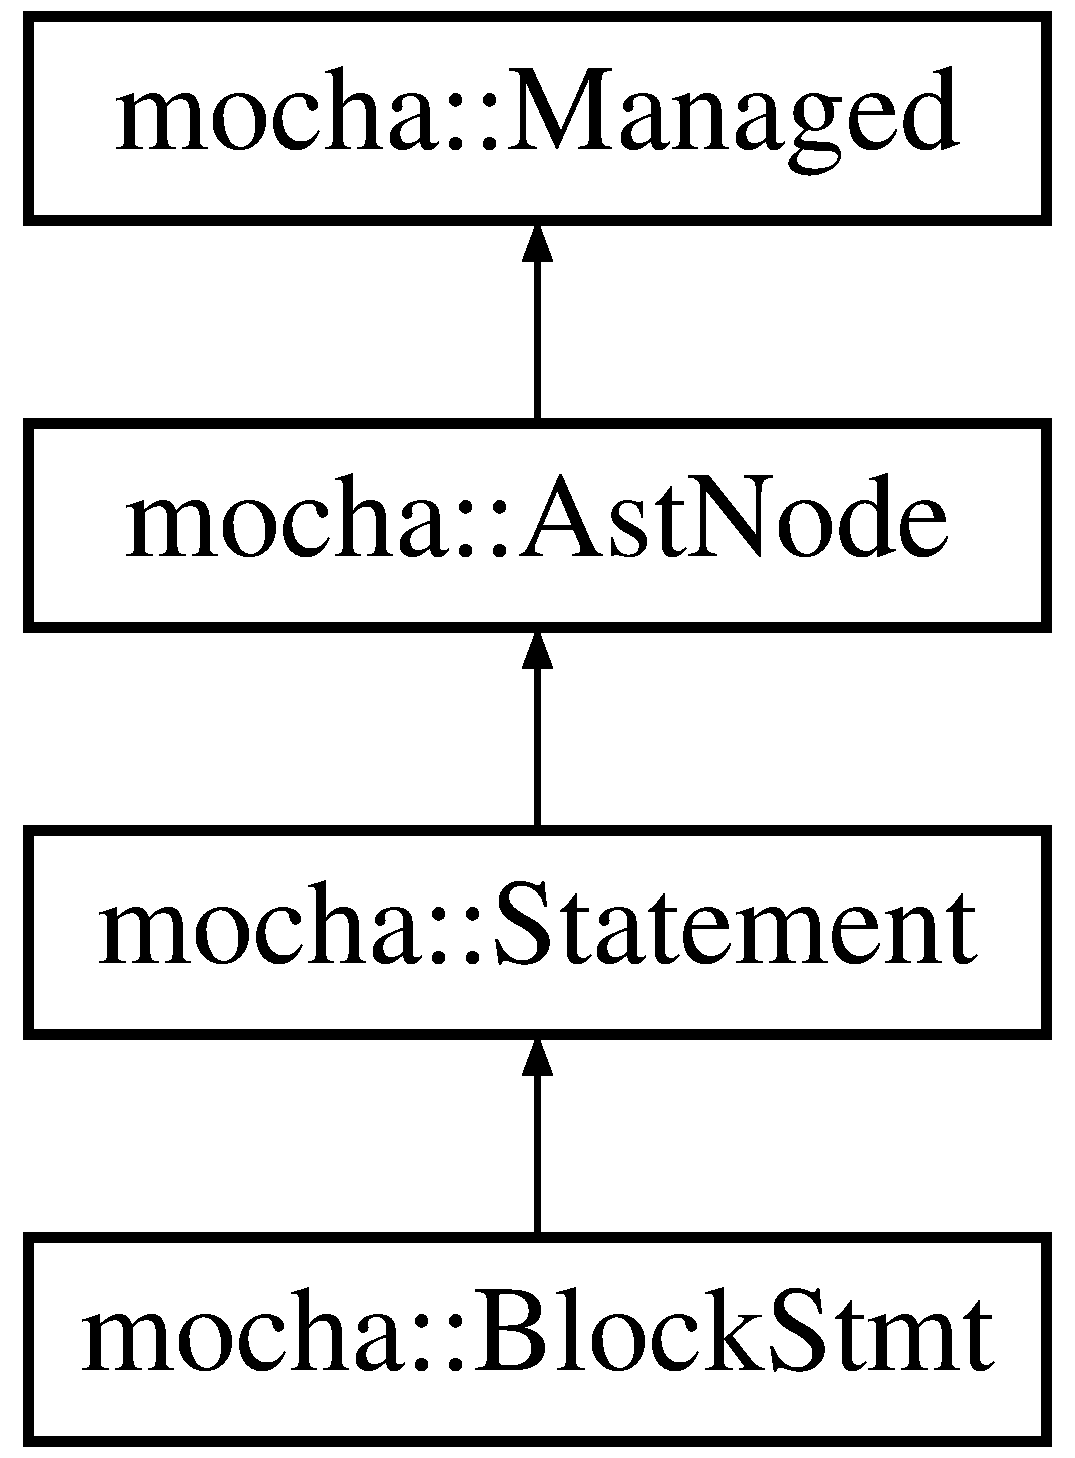
\includegraphics[height=4.000000cm]{classmocha_1_1_block_stmt}
\end{center}
\end{figure}
\subsection*{Public Member Functions}
\begin{DoxyCompactItemize}
\item 
\hyperlink{classmocha_1_1_block_stmt_a4d020c3d77730d50d31f60e6a522ce74}{BlockStmt} ()
\item 
\hyperlink{classmocha_1_1_block_stmt_a39b3156ee69795a3ad60f9da6395e56d}{$\sim$BlockStmt} ()
\item 
\hyperlink{classmocha_1_1_ast_node}{AstNode} $\ast$ \hyperlink{classmocha_1_1_block_stmt_abdf13dffed90bf114e37978e11bc553b}{Clone} ()
\end{DoxyCompactItemize}
\subsection*{Private Member Functions}
\begin{DoxyCompactItemize}
\item 
void \hyperlink{classmocha_1_1_block_stmt_ade660294b70c686c3c7b1cd07dce97ab}{NVIAccept\_\-} (\hyperlink{classmocha_1_1_i_visitor}{IVisitor} $\ast$visitor)
\end{DoxyCompactItemize}


\subsection{Detailed Description}


Definition at line 656 of file ast.h.



\subsection{Constructor \& Destructor Documentation}
\hypertarget{classmocha_1_1_block_stmt_a4d020c3d77730d50d31f60e6a522ce74}{
\index{mocha::BlockStmt@{mocha::BlockStmt}!BlockStmt@{BlockStmt}}
\index{BlockStmt@{BlockStmt}!mocha::BlockStmt@{mocha::BlockStmt}}
\subsubsection[{BlockStmt}]{\setlength{\rightskip}{0pt plus 5cm}mocha::BlockStmt::BlockStmt (
\begin{DoxyParamCaption}
{}
\end{DoxyParamCaption}
)\hspace{0.3cm}{\ttfamily  \mbox{[}inline\mbox{]}}}}
\label{classmocha_1_1_block_stmt_a4d020c3d77730d50d31f60e6a522ce74}


Definition at line 658 of file ast.h.

\hypertarget{classmocha_1_1_block_stmt_a39b3156ee69795a3ad60f9da6395e56d}{
\index{mocha::BlockStmt@{mocha::BlockStmt}!$\sim$BlockStmt@{$\sim$BlockStmt}}
\index{$\sim$BlockStmt@{$\sim$BlockStmt}!mocha::BlockStmt@{mocha::BlockStmt}}
\subsubsection[{$\sim$BlockStmt}]{\setlength{\rightskip}{0pt plus 5cm}mocha::BlockStmt::$\sim$BlockStmt (
\begin{DoxyParamCaption}
{}
\end{DoxyParamCaption}
)\hspace{0.3cm}{\ttfamily  \mbox{[}inline\mbox{]}}}}
\label{classmocha_1_1_block_stmt_a39b3156ee69795a3ad60f9da6395e56d}


Definition at line 659 of file ast.h.



\subsection{Member Function Documentation}
\hypertarget{classmocha_1_1_block_stmt_abdf13dffed90bf114e37978e11bc553b}{
\index{mocha::BlockStmt@{mocha::BlockStmt}!Clone@{Clone}}
\index{Clone@{Clone}!mocha::BlockStmt@{mocha::BlockStmt}}
\subsubsection[{Clone}]{\setlength{\rightskip}{0pt plus 5cm}{\bf AstNode} $\ast$ mocha::BlockStmt::Clone (
\begin{DoxyParamCaption}
{}
\end{DoxyParamCaption}
)\hspace{0.3cm}{\ttfamily  \mbox{[}virtual\mbox{]}}}}
\label{classmocha_1_1_block_stmt_abdf13dffed90bf114e37978e11bc553b}
\begin{DoxyReturn}{Returns}
\{AstNode$\ast$\} Clone node. 
\end{DoxyReturn}


Reimplemented from \hyperlink{classmocha_1_1_ast_node_af2a895699bac2012f8b7739bff49c5ec}{mocha::AstNode}.



Definition at line 253 of file ast.cc.

\hypertarget{classmocha_1_1_block_stmt_ade660294b70c686c3c7b1cd07dce97ab}{
\index{mocha::BlockStmt@{mocha::BlockStmt}!NVIAccept\_\-@{NVIAccept\_\-}}
\index{NVIAccept\_\-@{NVIAccept\_\-}!mocha::BlockStmt@{mocha::BlockStmt}}
\subsubsection[{NVIAccept\_\-}]{\setlength{\rightskip}{0pt plus 5cm}void mocha::BlockStmt::NVIAccept\_\- (
\begin{DoxyParamCaption}
\item[{{\bf IVisitor} $\ast$}]{visitor}
\end{DoxyParamCaption}
)\hspace{0.3cm}{\ttfamily  \mbox{[}inline, private, virtual\mbox{]}}}}
\label{classmocha_1_1_block_stmt_ade660294b70c686c3c7b1cd07dce97ab}


Reimplemented from \hyperlink{classmocha_1_1_statement_ad0e8c3ef62d21f733eb50a414046bae4}{mocha::Statement}.



Definition at line 662 of file ast.h.



The documentation for this class was generated from the following files:\begin{DoxyCompactItemize}
\item 
Y:/mocha/src/ast/\hyperlink{ast_8h}{ast.h}\item 
Y:/mocha/src/ast/\hyperlink{ast_8cc}{ast.cc}\end{DoxyCompactItemize}

\hypertarget{classmocha_1_1_bootstrap}{
\section{mocha::Bootstrap Class Reference}
\label{classmocha_1_1_bootstrap}\index{mocha::Bootstrap@{mocha::Bootstrap}}
}


{\ttfamily \#include $<$bootstrap.h$>$}

Inheritance diagram for mocha::Bootstrap:\begin{figure}[H]
\begin{center}
\leavevmode
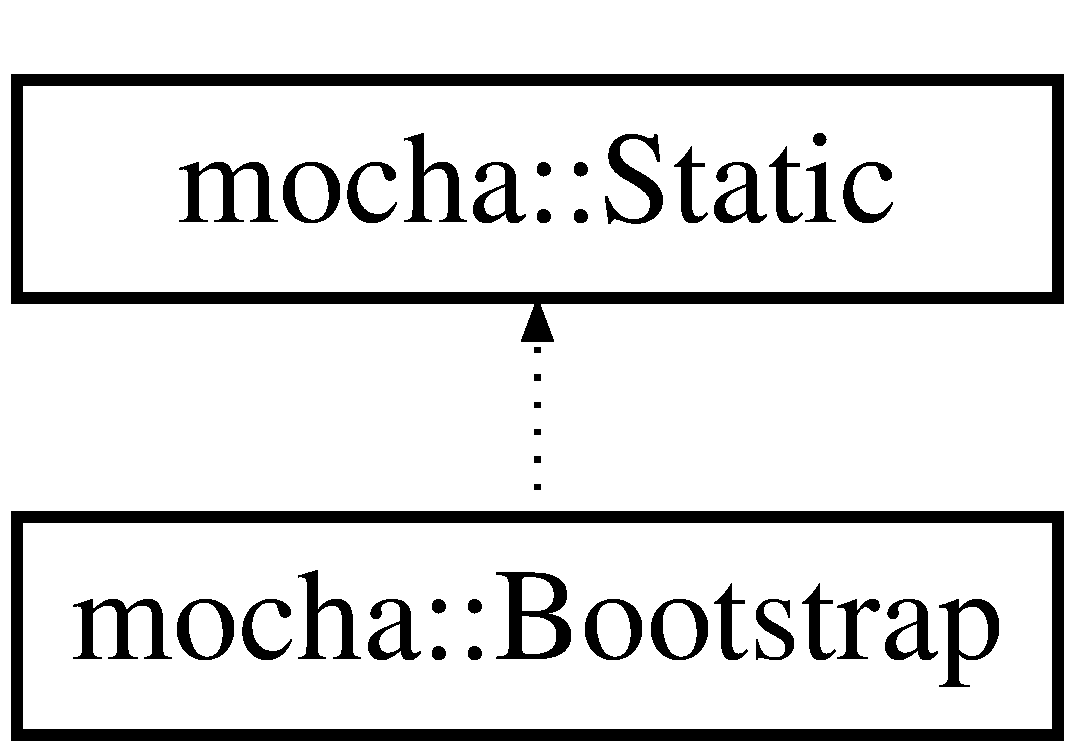
\includegraphics[height=2.000000cm]{classmocha_1_1_bootstrap}
\end{center}
\end{figure}
\subsection*{Static Public Member Functions}
\begin{DoxyCompactItemize}
\item 
static void \hyperlink{classmocha_1_1_bootstrap_a5dee98ca5bf16b8dd98d75f51b8efff7}{Initialize} (int argc, char $\ast$$\ast$argv)
\item 
static void \hyperlink{classmocha_1_1_bootstrap_a608b95cd0ad4f95b5a255255a7d274f8}{Reboot} ()
\item 
static const char $\ast$ \hyperlink{classmocha_1_1_bootstrap_ac47223e05a7a800949bba15e41108079}{GetSelfPath} ()
\end{DoxyCompactItemize}
\subsection*{Static Private Attributes}
\begin{DoxyCompactItemize}
\item 
static char $\ast$$\ast$ \hyperlink{classmocha_1_1_bootstrap_a0e051d1dc99827f5a02b3fa464de14b3}{argv\_\-}
\item 
static std::string \hyperlink{classmocha_1_1_bootstrap_aef118b8931b53c8bca13e1cc5f5ba882}{self\_\-path\_\-}
\end{DoxyCompactItemize}


\subsection{Detailed Description}


Definition at line 9 of file bootstrap.h.



\subsection{Member Function Documentation}
\hypertarget{classmocha_1_1_bootstrap_ac47223e05a7a800949bba15e41108079}{
\index{mocha::Bootstrap@{mocha::Bootstrap}!GetSelfPath@{GetSelfPath}}
\index{GetSelfPath@{GetSelfPath}!mocha::Bootstrap@{mocha::Bootstrap}}
\subsubsection[{GetSelfPath}]{\setlength{\rightskip}{0pt plus 5cm}const char $\ast$ mocha::Bootstrap::GetSelfPath (
\begin{DoxyParamCaption}
{}
\end{DoxyParamCaption}
)\hspace{0.3cm}{\ttfamily  \mbox{[}static\mbox{]}}}}
\label{classmocha_1_1_bootstrap_ac47223e05a7a800949bba15e41108079}


Definition at line 110 of file bootstrap.cc.

\hypertarget{classmocha_1_1_bootstrap_a5dee98ca5bf16b8dd98d75f51b8efff7}{
\index{mocha::Bootstrap@{mocha::Bootstrap}!Initialize@{Initialize}}
\index{Initialize@{Initialize}!mocha::Bootstrap@{mocha::Bootstrap}}
\subsubsection[{Initialize}]{\setlength{\rightskip}{0pt plus 5cm}void mocha::Bootstrap::Initialize (
\begin{DoxyParamCaption}
\item[{int}]{argc, }
\item[{char $\ast$$\ast$}]{argv}
\end{DoxyParamCaption}
)\hspace{0.3cm}{\ttfamily  \mbox{[}static\mbox{]}}}}
\label{classmocha_1_1_bootstrap_a5dee98ca5bf16b8dd98d75f51b8efff7}


Definition at line 86 of file bootstrap.cc.

\hypertarget{classmocha_1_1_bootstrap_a608b95cd0ad4f95b5a255255a7d274f8}{
\index{mocha::Bootstrap@{mocha::Bootstrap}!Reboot@{Reboot}}
\index{Reboot@{Reboot}!mocha::Bootstrap@{mocha::Bootstrap}}
\subsubsection[{Reboot}]{\setlength{\rightskip}{0pt plus 5cm}void mocha::Bootstrap::Reboot (
\begin{DoxyParamCaption}
{}
\end{DoxyParamCaption}
)\hspace{0.3cm}{\ttfamily  \mbox{[}static\mbox{]}}}}
\label{classmocha_1_1_bootstrap_a608b95cd0ad4f95b5a255255a7d274f8}


Definition at line 104 of file bootstrap.cc.



\subsection{Member Data Documentation}
\hypertarget{classmocha_1_1_bootstrap_a0e051d1dc99827f5a02b3fa464de14b3}{
\index{mocha::Bootstrap@{mocha::Bootstrap}!argv\_\-@{argv\_\-}}
\index{argv\_\-@{argv\_\-}!mocha::Bootstrap@{mocha::Bootstrap}}
\subsubsection[{argv\_\-}]{\setlength{\rightskip}{0pt plus 5cm}char $\ast$$\ast$ {\bf mocha::Bootstrap::argv\_\-}\hspace{0.3cm}{\ttfamily  \mbox{[}static, private\mbox{]}}}}
\label{classmocha_1_1_bootstrap_a0e051d1dc99827f5a02b3fa464de14b3}


Definition at line 15 of file bootstrap.h.

\hypertarget{classmocha_1_1_bootstrap_aef118b8931b53c8bca13e1cc5f5ba882}{
\index{mocha::Bootstrap@{mocha::Bootstrap}!self\_\-path\_\-@{self\_\-path\_\-}}
\index{self\_\-path\_\-@{self\_\-path\_\-}!mocha::Bootstrap@{mocha::Bootstrap}}
\subsubsection[{self\_\-path\_\-}]{\setlength{\rightskip}{0pt plus 5cm}std::string {\bf mocha::Bootstrap::self\_\-path\_\-}\hspace{0.3cm}{\ttfamily  \mbox{[}static, private\mbox{]}}}}
\label{classmocha_1_1_bootstrap_aef118b8931b53c8bca13e1cc5f5ba882}


Definition at line 16 of file bootstrap.h.



The documentation for this class was generated from the following files:\begin{DoxyCompactItemize}
\item 
Y:/mocha/src/bootstrap/\hyperlink{bootstrap_8h}{bootstrap.h}\item 
Y:/mocha/src/bootstrap/\hyperlink{bootstrap_8cc}{bootstrap.cc}\end{DoxyCompactItemize}

\hypertarget{classmocha_1_1_break_stmt}{
\section{mocha::BreakStmt Class Reference}
\label{classmocha_1_1_break_stmt}\index{mocha::BreakStmt@{mocha::BreakStmt}}
}


{\ttfamily \#include $<$ast.h$>$}

Inheritance diagram for mocha::BreakStmt:\begin{figure}[H]
\begin{center}
\leavevmode
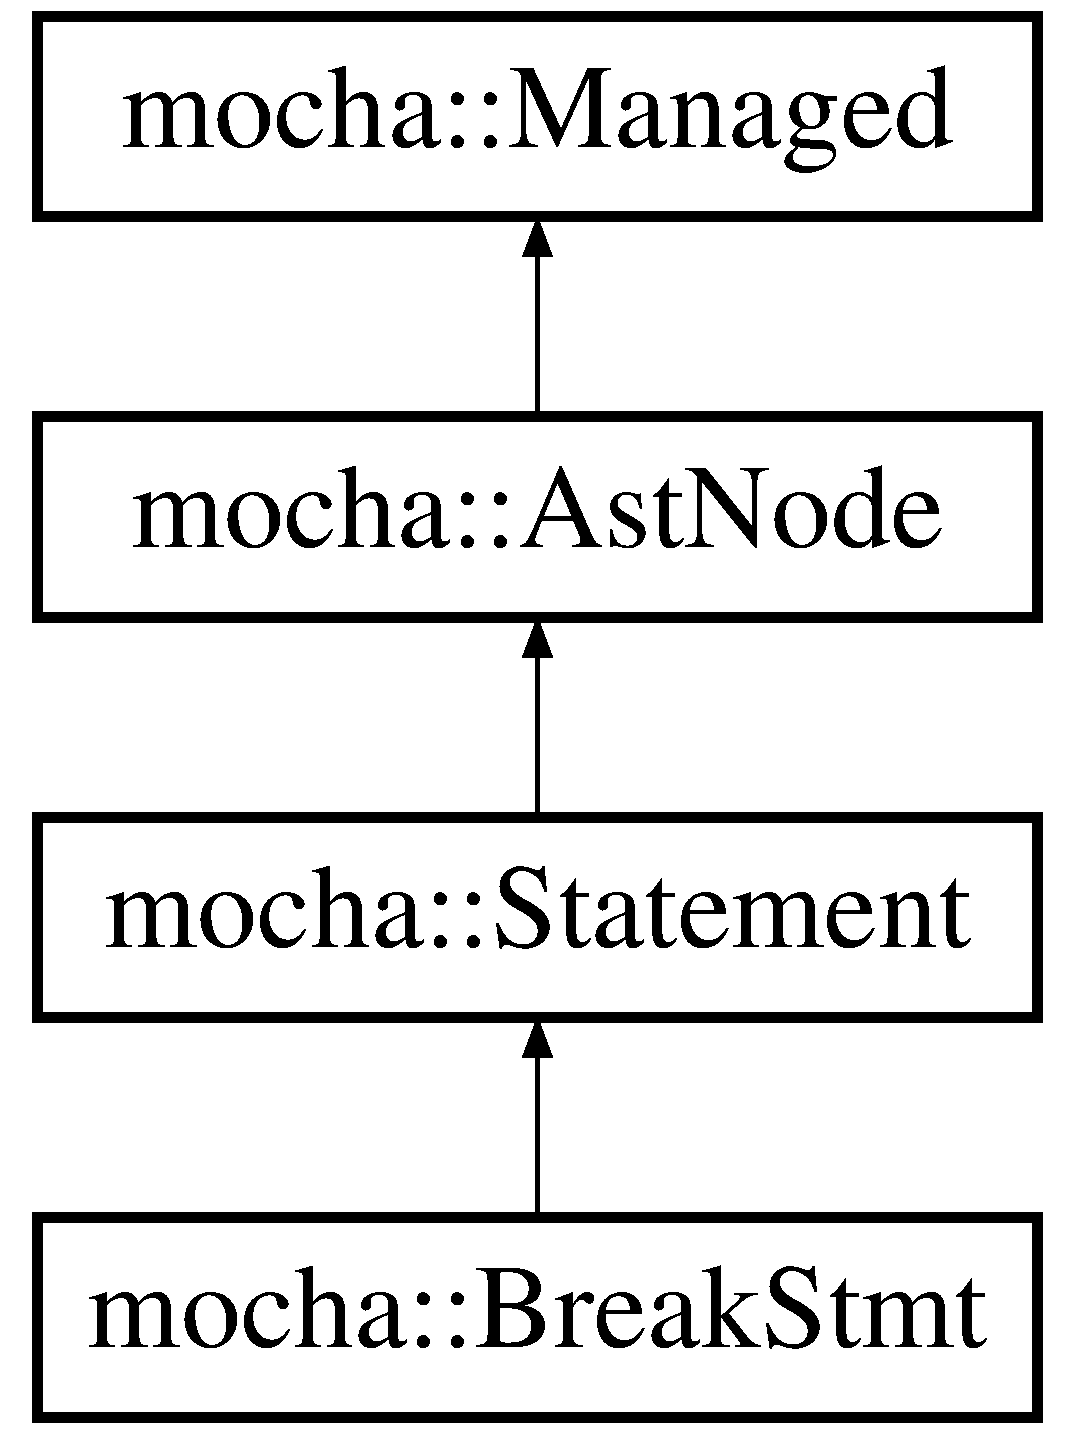
\includegraphics[height=4.000000cm]{classmocha_1_1_break_stmt}
\end{center}
\end{figure}
\subsection*{Public Member Functions}
\begin{DoxyCompactItemize}
\item 
\hyperlink{classmocha_1_1_break_stmt_a3c26cc24864d473c19150136bf5a3342}{BreakStmt} ()
\item 
\hyperlink{classmocha_1_1_break_stmt_a277a804ed1654c73d36f4718eef74729}{$\sim$BreakStmt} ()
\item 
\hyperlink{classmocha_1_1_ast_node}{AstNode} $\ast$ \hyperlink{classmocha_1_1_break_stmt_aef2636aaf779e433b3a3adbc873444dd}{Clone} ()
\end{DoxyCompactItemize}
\subsection*{Private Member Functions}
\begin{DoxyCompactItemize}
\item 
void \hyperlink{classmocha_1_1_break_stmt_a73d4722ff7fccc9a62e7a2fb562bc7b6}{NVIAccept\_\-} (\hyperlink{classmocha_1_1_i_visitor}{IVisitor} $\ast$visitor)
\end{DoxyCompactItemize}


\subsection{Detailed Description}


Definition at line 912 of file ast.h.



\subsection{Constructor \& Destructor Documentation}
\hypertarget{classmocha_1_1_break_stmt_a3c26cc24864d473c19150136bf5a3342}{
\index{mocha::BreakStmt@{mocha::BreakStmt}!BreakStmt@{BreakStmt}}
\index{BreakStmt@{BreakStmt}!mocha::BreakStmt@{mocha::BreakStmt}}
\subsubsection[{BreakStmt}]{\setlength{\rightskip}{0pt plus 5cm}mocha::BreakStmt::BreakStmt (
\begin{DoxyParamCaption}
{}
\end{DoxyParamCaption}
)\hspace{0.3cm}{\ttfamily  \mbox{[}inline\mbox{]}}}}
\label{classmocha_1_1_break_stmt_a3c26cc24864d473c19150136bf5a3342}


Definition at line 914 of file ast.h.

\hypertarget{classmocha_1_1_break_stmt_a277a804ed1654c73d36f4718eef74729}{
\index{mocha::BreakStmt@{mocha::BreakStmt}!$\sim$BreakStmt@{$\sim$BreakStmt}}
\index{$\sim$BreakStmt@{$\sim$BreakStmt}!mocha::BreakStmt@{mocha::BreakStmt}}
\subsubsection[{$\sim$BreakStmt}]{\setlength{\rightskip}{0pt plus 5cm}mocha::BreakStmt::$\sim$BreakStmt (
\begin{DoxyParamCaption}
{}
\end{DoxyParamCaption}
)\hspace{0.3cm}{\ttfamily  \mbox{[}inline\mbox{]}}}}
\label{classmocha_1_1_break_stmt_a277a804ed1654c73d36f4718eef74729}


Definition at line 915 of file ast.h.



\subsection{Member Function Documentation}
\hypertarget{classmocha_1_1_break_stmt_aef2636aaf779e433b3a3adbc873444dd}{
\index{mocha::BreakStmt@{mocha::BreakStmt}!Clone@{Clone}}
\index{Clone@{Clone}!mocha::BreakStmt@{mocha::BreakStmt}}
\subsubsection[{Clone}]{\setlength{\rightskip}{0pt plus 5cm}{\bf AstNode} $\ast$ mocha::BreakStmt::Clone (
\begin{DoxyParamCaption}
{}
\end{DoxyParamCaption}
)\hspace{0.3cm}{\ttfamily  \mbox{[}virtual\mbox{]}}}}
\label{classmocha_1_1_break_stmt_aef2636aaf779e433b3a3adbc873444dd}
\begin{DoxyReturn}{Returns}
\{AstNode$\ast$\} Clone node. 
\end{DoxyReturn}


Reimplemented from \hyperlink{classmocha_1_1_ast_node_af2a895699bac2012f8b7739bff49c5ec}{mocha::AstNode}.



Definition at line 333 of file ast.cc.

\hypertarget{classmocha_1_1_break_stmt_a73d4722ff7fccc9a62e7a2fb562bc7b6}{
\index{mocha::BreakStmt@{mocha::BreakStmt}!NVIAccept\_\-@{NVIAccept\_\-}}
\index{NVIAccept\_\-@{NVIAccept\_\-}!mocha::BreakStmt@{mocha::BreakStmt}}
\subsubsection[{NVIAccept\_\-}]{\setlength{\rightskip}{0pt plus 5cm}void mocha::BreakStmt::NVIAccept\_\- (
\begin{DoxyParamCaption}
\item[{{\bf IVisitor} $\ast$}]{visitor}
\end{DoxyParamCaption}
)\hspace{0.3cm}{\ttfamily  \mbox{[}inline, private, virtual\mbox{]}}}}
\label{classmocha_1_1_break_stmt_a73d4722ff7fccc9a62e7a2fb562bc7b6}


Reimplemented from \hyperlink{classmocha_1_1_statement_ad0e8c3ef62d21f733eb50a414046bae4}{mocha::Statement}.



Definition at line 918 of file ast.h.



The documentation for this class was generated from the following files:\begin{DoxyCompactItemize}
\item 
Y:/mocha/src/ast/\hyperlink{ast_8h}{ast.h}\item 
Y:/mocha/src/ast/\hyperlink{ast_8cc}{ast.cc}\end{DoxyCompactItemize}

\hypertarget{classmocha_1_1_bucket}{
\section{mocha::Bucket Class Reference}
\label{classmocha_1_1_bucket}\index{mocha::Bucket@{mocha::Bucket}}
}


{\ttfamily \#include $<$hash\_\-bucket.h$>$}

\subsection*{Public Member Functions}
\begin{DoxyCompactItemize}
\item 
\hyperlink{classmocha_1_1_bucket_a5ba22418fc9399d5268c3bd48e76835b}{Bucket} ()
\item 
\hyperlink{classmocha_1_1_bucket_a18c23f202186bac140024d098f3fe076}{$\sim$Bucket} ()
\item 
void $\ast$ \hyperlink{classmocha_1_1_bucket_a5e09be08c29e1cc7fc4cd3e435bc60f5}{Entry} ()
\item 
void \hyperlink{classmocha_1_1_bucket_a99ff3c1980e20a1e2bc8fb7823ddab8c}{Entry} (void $\ast$)
\item 
int \hyperlink{classmocha_1_1_bucket_a25165523768f5259b97f897d8a63e29c}{BitCategory} ()
\item 
void \hyperlink{classmocha_1_1_bucket_a14e3746dd63320149e582a576ed29b6b}{Increase} ()
\item 
bool \hyperlink{classmocha_1_1_bucket_aca74d48495c7832520260b656c02a74c}{IsEmpty} ()
\end{DoxyCompactItemize}
\subsection*{Private Attributes}
\begin{DoxyCompactItemize}
\item 
int \hyperlink{classmocha_1_1_bucket_ae29b657e8c125e5523ae2e3331fd915e}{used\_\-bit\_\-category\_\-}
\item 
void $\ast$ \hyperlink{classmocha_1_1_bucket_ae83e8d2061d4fc8a3be0a5d379909a55}{entry\_\-}
\end{DoxyCompactItemize}


\subsection{Detailed Description}


Definition at line 6 of file hash\_\-bucket.h.



\subsection{Constructor \& Destructor Documentation}
\hypertarget{classmocha_1_1_bucket_a5ba22418fc9399d5268c3bd48e76835b}{
\index{mocha::Bucket@{mocha::Bucket}!Bucket@{Bucket}}
\index{Bucket@{Bucket}!mocha::Bucket@{mocha::Bucket}}
\subsubsection[{Bucket}]{\setlength{\rightskip}{0pt plus 5cm}mocha::Bucket::Bucket (
\begin{DoxyParamCaption}
{}
\end{DoxyParamCaption}
)}}
\label{classmocha_1_1_bucket_a5ba22418fc9399d5268c3bd48e76835b}
\hypertarget{classmocha_1_1_bucket_a18c23f202186bac140024d098f3fe076}{
\index{mocha::Bucket@{mocha::Bucket}!$\sim$Bucket@{$\sim$Bucket}}
\index{$\sim$Bucket@{$\sim$Bucket}!mocha::Bucket@{mocha::Bucket}}
\subsubsection[{$\sim$Bucket}]{\setlength{\rightskip}{0pt plus 5cm}mocha::Bucket::$\sim$Bucket (
\begin{DoxyParamCaption}
{}
\end{DoxyParamCaption}
)}}
\label{classmocha_1_1_bucket_a18c23f202186bac140024d098f3fe076}


\subsection{Member Function Documentation}
\hypertarget{classmocha_1_1_bucket_a25165523768f5259b97f897d8a63e29c}{
\index{mocha::Bucket@{mocha::Bucket}!BitCategory@{BitCategory}}
\index{BitCategory@{BitCategory}!mocha::Bucket@{mocha::Bucket}}
\subsubsection[{BitCategory}]{\setlength{\rightskip}{0pt plus 5cm}int mocha::Bucket::BitCategory (
\begin{DoxyParamCaption}
{}
\end{DoxyParamCaption}
)}}
\label{classmocha_1_1_bucket_a25165523768f5259b97f897d8a63e29c}
\hypertarget{classmocha_1_1_bucket_a99ff3c1980e20a1e2bc8fb7823ddab8c}{
\index{mocha::Bucket@{mocha::Bucket}!Entry@{Entry}}
\index{Entry@{Entry}!mocha::Bucket@{mocha::Bucket}}
\subsubsection[{Entry}]{\setlength{\rightskip}{0pt plus 5cm}void mocha::Bucket::Entry (
\begin{DoxyParamCaption}
\item[{void $\ast$}]{}
\end{DoxyParamCaption}
)}}
\label{classmocha_1_1_bucket_a99ff3c1980e20a1e2bc8fb7823ddab8c}
\hypertarget{classmocha_1_1_bucket_a5e09be08c29e1cc7fc4cd3e435bc60f5}{
\index{mocha::Bucket@{mocha::Bucket}!Entry@{Entry}}
\index{Entry@{Entry}!mocha::Bucket@{mocha::Bucket}}
\subsubsection[{Entry}]{\setlength{\rightskip}{0pt plus 5cm}void$\ast$ mocha::Bucket::Entry (
\begin{DoxyParamCaption}
{}
\end{DoxyParamCaption}
)}}
\label{classmocha_1_1_bucket_a5e09be08c29e1cc7fc4cd3e435bc60f5}
\hypertarget{classmocha_1_1_bucket_a14e3746dd63320149e582a576ed29b6b}{
\index{mocha::Bucket@{mocha::Bucket}!Increase@{Increase}}
\index{Increase@{Increase}!mocha::Bucket@{mocha::Bucket}}
\subsubsection[{Increase}]{\setlength{\rightskip}{0pt plus 5cm}void mocha::Bucket::Increase (
\begin{DoxyParamCaption}
{}
\end{DoxyParamCaption}
)}}
\label{classmocha_1_1_bucket_a14e3746dd63320149e582a576ed29b6b}
\hypertarget{classmocha_1_1_bucket_aca74d48495c7832520260b656c02a74c}{
\index{mocha::Bucket@{mocha::Bucket}!IsEmpty@{IsEmpty}}
\index{IsEmpty@{IsEmpty}!mocha::Bucket@{mocha::Bucket}}
\subsubsection[{IsEmpty}]{\setlength{\rightskip}{0pt plus 5cm}bool mocha::Bucket::IsEmpty (
\begin{DoxyParamCaption}
{}
\end{DoxyParamCaption}
)}}
\label{classmocha_1_1_bucket_aca74d48495c7832520260b656c02a74c}


\subsection{Member Data Documentation}
\hypertarget{classmocha_1_1_bucket_ae83e8d2061d4fc8a3be0a5d379909a55}{
\index{mocha::Bucket@{mocha::Bucket}!entry\_\-@{entry\_\-}}
\index{entry\_\-@{entry\_\-}!mocha::Bucket@{mocha::Bucket}}
\subsubsection[{entry\_\-}]{\setlength{\rightskip}{0pt plus 5cm}void$\ast$ {\bf mocha::Bucket::entry\_\-}\hspace{0.3cm}{\ttfamily  \mbox{[}private\mbox{]}}}}
\label{classmocha_1_1_bucket_ae83e8d2061d4fc8a3be0a5d379909a55}


Definition at line 17 of file hash\_\-bucket.h.

\hypertarget{classmocha_1_1_bucket_ae29b657e8c125e5523ae2e3331fd915e}{
\index{mocha::Bucket@{mocha::Bucket}!used\_\-bit\_\-category\_\-@{used\_\-bit\_\-category\_\-}}
\index{used\_\-bit\_\-category\_\-@{used\_\-bit\_\-category\_\-}!mocha::Bucket@{mocha::Bucket}}
\subsubsection[{used\_\-bit\_\-category\_\-}]{\setlength{\rightskip}{0pt plus 5cm}int {\bf mocha::Bucket::used\_\-bit\_\-category\_\-}\hspace{0.3cm}{\ttfamily  \mbox{[}private\mbox{]}}}}
\label{classmocha_1_1_bucket_ae29b657e8c125e5523ae2e3331fd915e}


Definition at line 16 of file hash\_\-bucket.h.



The documentation for this class was generated from the following file:\begin{DoxyCompactItemize}
\item 
Y:/mocha/src/utils/hash/hash\_\-map/\hyperlink{hash__map_2hash__bucket_8h}{hash\_\-bucket.h}\end{DoxyCompactItemize}

\hypertarget{classmocha_1_1_call_exp}{
\section{mocha::CallExp Class Reference}
\label{classmocha_1_1_call_exp}\index{mocha::CallExp@{mocha::CallExp}}
}


{\ttfamily \#include $<$ast.h$>$}

Inheritance diagram for mocha::CallExp:\begin{figure}[H]
\begin{center}
\leavevmode
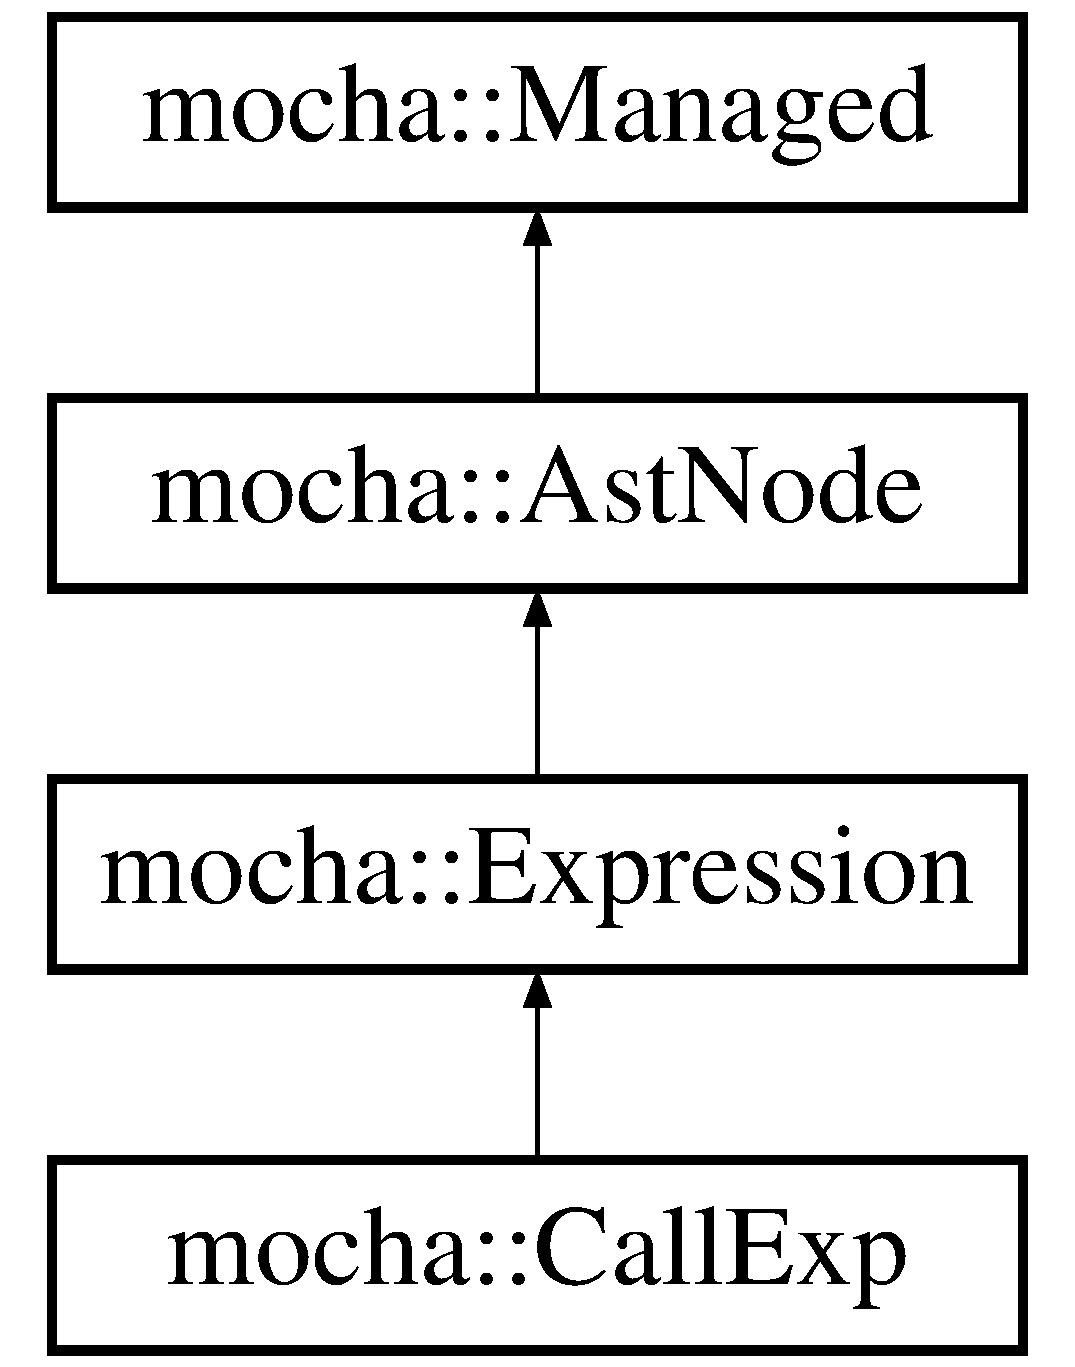
\includegraphics[height=4.000000cm]{classmocha_1_1_call_exp}
\end{center}
\end{figure}
\subsection*{Public Types}
\begin{DoxyCompactItemize}
\item 
enum \{ \par
\hyperlink{classmocha_1_1_call_exp_a8a305224d9e8783e5d52db570638da0faf4f3592ae2b4acb488b1a48d94980fba}{kNormalAccessor}, 
\hyperlink{classmocha_1_1_call_exp_a8a305224d9e8783e5d52db570638da0fa8b5de76a6c176c0798c45c25d9a56d33}{kNormal}, 
\hyperlink{classmocha_1_1_call_exp_a8a305224d9e8783e5d52db570638da0faa9ec68ed8e03dd781222f33599dfa951}{kBracket}, 
\hyperlink{classmocha_1_1_call_exp_a8a305224d9e8783e5d52db570638da0fa05f6f2ce828edec5fed91fd4f8b1525c}{kDot}, 
\par
\hyperlink{classmocha_1_1_call_exp_a8a305224d9e8783e5d52db570638da0fa0f9895a9a11192c7a7318a6ab00cd21c}{kNew}, 
\hyperlink{classmocha_1_1_call_exp_a8a305224d9e8783e5d52db570638da0fad834166a64cdb302c9f2eb02065414db}{kPrivate}, 
\hyperlink{classmocha_1_1_call_exp_a8a305224d9e8783e5d52db570638da0fafc365536efc96bda13bd564f8dfee7c6}{kExtend}
 \}
\end{DoxyCompactItemize}
\subsection*{Public Member Functions}
\begin{DoxyCompactItemize}
\item 
\hyperlink{classmocha_1_1_call_exp_ae4e9aaf5488ab763c4e64bac136650ff}{CallExp} (int type)
\item 
\hyperlink{classmocha_1_1_call_exp_a920df283bf31c2a08210ec512a72f5cc}{$\sim$CallExp} ()
\item 
void \hyperlink{classmocha_1_1_call_exp_ac907919216fc8cf3c4e7e0020e55ff40}{Callable} (\hyperlink{classmocha_1_1_ast_node}{AstNode} $\ast$node)
\item 
\hyperlink{classmocha_1_1_ast_node}{AstNode} $\ast$ \hyperlink{classmocha_1_1_call_exp_ad30716599e9bf441d004f5d97e0e83f4}{Callable} ()
\item 
void \hyperlink{classmocha_1_1_call_exp_af575c9b1d5cd088dfbc403702470cd4f}{Args} (\hyperlink{classmocha_1_1_ast_node}{AstNode} $\ast$node)
\item 
\hyperlink{classmocha_1_1_ast_node}{AstNode} $\ast$ \hyperlink{classmocha_1_1_call_exp_a10f4f286f5a1d33addd92012214f190b}{Args} ()
\item 
int \hyperlink{classmocha_1_1_call_exp_a8c6e3bec8b4d51e91782d53c58ec7980}{CallType} ()
\item 
void \hyperlink{classmocha_1_1_call_exp_ac59d3b40e2df09291a5902c4ebb4dafa}{CallType} (int type)
\item 
void \hyperlink{classmocha_1_1_call_exp_a04b99a2c8ba39a16689b2d46f30961cf}{Depth} (int depth)
\item 
int \hyperlink{classmocha_1_1_call_exp_a1ba1cf633037443e52c2b0dc5f7da503}{Depth} ()
\item 
void \hyperlink{classmocha_1_1_call_exp_affa33d340ecb3322fb01d601e3bdc660}{Rest} ()
\item 
bool \hyperlink{classmocha_1_1_call_exp_aa85eec3d1b9f2422f3566905189a1036}{IsRest} () const 
\item 
\hyperlink{classmocha_1_1_call_exp}{CallExp} $\ast$ \hyperlink{classmocha_1_1_call_exp_a60e1a2f17381dd35093e75786b1c0c6a}{CastToCallExp} ()
\item 
void \hyperlink{classmocha_1_1_call_exp_ac02db8888302cc96d46c11798642828d}{Call} ()
\item 
bool \hyperlink{classmocha_1_1_call_exp_a2b06a60d47dce8f02dbe17b716e0cbde}{IsCall} ()
\item 
void \hyperlink{classmocha_1_1_call_exp_a199afd366c874d07447b65b062ebe462}{ReplaceChild} (\hyperlink{classmocha_1_1_ast_node}{AstNode} $\ast$old\_\-node, \hyperlink{classmocha_1_1_ast_node}{AstNode} $\ast$new\_\-node)
\item 
\hyperlink{classmocha_1_1_ast_node}{AstNode} $\ast$ \hyperlink{classmocha_1_1_call_exp_a1a423dfd91b217f3a89a6ebf4f1de495}{Clone} ()
\end{DoxyCompactItemize}
\subsection*{Private Member Functions}
\begin{DoxyCompactItemize}
\item 
void \hyperlink{classmocha_1_1_call_exp_a6f03e2ebd560f6cc4bd9ce46247ae2d9}{NVIAccept\_\-} (\hyperlink{classmocha_1_1_i_visitor}{IVisitor} $\ast$visitor)
\end{DoxyCompactItemize}
\subsection*{Private Attributes}
\begin{DoxyCompactItemize}
\item 
int \hyperlink{classmocha_1_1_call_exp_adf02829fd9136829d210bd49d5997862}{call\_\-type\_\-}
\item 
int \hyperlink{classmocha_1_1_call_exp_a1437212b3b447a50e5fbf50512058d79}{depth\_\-}
\item 
bool \hyperlink{classmocha_1_1_call_exp_a30bdde50d77e5a8da0f8e61897903c0a}{is\_\-call\_\-}
\item 
bool \hyperlink{classmocha_1_1_call_exp_ab345a4e9c56c57a1a5f97b60f17d7c5b}{is\_\-rest\_\-}
\item 
\hyperlink{classmocha_1_1_ast_node}{AstNode} $\ast$ \hyperlink{classmocha_1_1_call_exp_a3e15d3b3c94bdf3f046d45d3b605797a}{callable\_\-}
\item 
\hyperlink{classmocha_1_1_ast_node}{AstNode} $\ast$ \hyperlink{classmocha_1_1_call_exp_aff9ea512c5d25426b28c7801aba758c6}{args\_\-}
\end{DoxyCompactItemize}


\subsection{Detailed Description}


Definition at line 1305 of file ast.h.



\subsection{Member Enumeration Documentation}
\hypertarget{classmocha_1_1_call_exp_a8a305224d9e8783e5d52db570638da0f}{
\subsubsection[{"@7}]{\setlength{\rightskip}{0pt plus 5cm}anonymous enum}}
\label{classmocha_1_1_call_exp_a8a305224d9e8783e5d52db570638da0f}
\begin{Desc}
\item[Enumerator: ]\par
\begin{description}
\index{kNormalAccessor@{kNormalAccessor}!mocha::CallExp@{mocha::CallExp}}\index{mocha::CallExp@{mocha::CallExp}!kNormalAccessor@{kNormalAccessor}}\item[{\em 
\hypertarget{classmocha_1_1_call_exp_a8a305224d9e8783e5d52db570638da0faf4f3592ae2b4acb488b1a48d94980fba}{
kNormalAccessor}
\label{classmocha_1_1_call_exp_a8a305224d9e8783e5d52db570638da0faf4f3592ae2b4acb488b1a48d94980fba}
}]\index{kNormal@{kNormal}!mocha::CallExp@{mocha::CallExp}}\index{mocha::CallExp@{mocha::CallExp}!kNormal@{kNormal}}\item[{\em 
\hypertarget{classmocha_1_1_call_exp_a8a305224d9e8783e5d52db570638da0fa8b5de76a6c176c0798c45c25d9a56d33}{
kNormal}
\label{classmocha_1_1_call_exp_a8a305224d9e8783e5d52db570638da0fa8b5de76a6c176c0798c45c25d9a56d33}
}]\index{kBracket@{kBracket}!mocha::CallExp@{mocha::CallExp}}\index{mocha::CallExp@{mocha::CallExp}!kBracket@{kBracket}}\item[{\em 
\hypertarget{classmocha_1_1_call_exp_a8a305224d9e8783e5d52db570638da0faa9ec68ed8e03dd781222f33599dfa951}{
kBracket}
\label{classmocha_1_1_call_exp_a8a305224d9e8783e5d52db570638da0faa9ec68ed8e03dd781222f33599dfa951}
}]\index{kDot@{kDot}!mocha::CallExp@{mocha::CallExp}}\index{mocha::CallExp@{mocha::CallExp}!kDot@{kDot}}\item[{\em 
\hypertarget{classmocha_1_1_call_exp_a8a305224d9e8783e5d52db570638da0fa05f6f2ce828edec5fed91fd4f8b1525c}{
kDot}
\label{classmocha_1_1_call_exp_a8a305224d9e8783e5d52db570638da0fa05f6f2ce828edec5fed91fd4f8b1525c}
}]\index{kNew@{kNew}!mocha::CallExp@{mocha::CallExp}}\index{mocha::CallExp@{mocha::CallExp}!kNew@{kNew}}\item[{\em 
\hypertarget{classmocha_1_1_call_exp_a8a305224d9e8783e5d52db570638da0fa0f9895a9a11192c7a7318a6ab00cd21c}{
kNew}
\label{classmocha_1_1_call_exp_a8a305224d9e8783e5d52db570638da0fa0f9895a9a11192c7a7318a6ab00cd21c}
}]\index{kPrivate@{kPrivate}!mocha::CallExp@{mocha::CallExp}}\index{mocha::CallExp@{mocha::CallExp}!kPrivate@{kPrivate}}\item[{\em 
\hypertarget{classmocha_1_1_call_exp_a8a305224d9e8783e5d52db570638da0fad834166a64cdb302c9f2eb02065414db}{
kPrivate}
\label{classmocha_1_1_call_exp_a8a305224d9e8783e5d52db570638da0fad834166a64cdb302c9f2eb02065414db}
}]\index{kExtend@{kExtend}!mocha::CallExp@{mocha::CallExp}}\index{mocha::CallExp@{mocha::CallExp}!kExtend@{kExtend}}\item[{\em 
\hypertarget{classmocha_1_1_call_exp_a8a305224d9e8783e5d52db570638da0fafc365536efc96bda13bd564f8dfee7c6}{
kExtend}
\label{classmocha_1_1_call_exp_a8a305224d9e8783e5d52db570638da0fafc365536efc96bda13bd564f8dfee7c6}
}]\end{description}
\end{Desc}



Definition at line 1307 of file ast.h.



\subsection{Constructor \& Destructor Documentation}
\hypertarget{classmocha_1_1_call_exp_ae4e9aaf5488ab763c4e64bac136650ff}{
\index{mocha::CallExp@{mocha::CallExp}!CallExp@{CallExp}}
\index{CallExp@{CallExp}!mocha::CallExp@{mocha::CallExp}}
\subsubsection[{CallExp}]{\setlength{\rightskip}{0pt plus 5cm}mocha::CallExp::CallExp (
\begin{DoxyParamCaption}
\item[{int}]{type}
\end{DoxyParamCaption}
)\hspace{0.3cm}{\ttfamily  \mbox{[}inline\mbox{]}}}}
\label{classmocha_1_1_call_exp_ae4e9aaf5488ab763c4e64bac136650ff}


Definition at line 1316 of file ast.h.

\hypertarget{classmocha_1_1_call_exp_a920df283bf31c2a08210ec512a72f5cc}{
\index{mocha::CallExp@{mocha::CallExp}!$\sim$CallExp@{$\sim$CallExp}}
\index{$\sim$CallExp@{$\sim$CallExp}!mocha::CallExp@{mocha::CallExp}}
\subsubsection[{$\sim$CallExp}]{\setlength{\rightskip}{0pt plus 5cm}mocha::CallExp::$\sim$CallExp (
\begin{DoxyParamCaption}
{}
\end{DoxyParamCaption}
)\hspace{0.3cm}{\ttfamily  \mbox{[}inline\mbox{]}}}}
\label{classmocha_1_1_call_exp_a920df283bf31c2a08210ec512a72f5cc}


Definition at line 1318 of file ast.h.



\subsection{Member Function Documentation}
\hypertarget{classmocha_1_1_call_exp_af575c9b1d5cd088dfbc403702470cd4f}{
\index{mocha::CallExp@{mocha::CallExp}!Args@{Args}}
\index{Args@{Args}!mocha::CallExp@{mocha::CallExp}}
\subsubsection[{Args}]{\setlength{\rightskip}{0pt plus 5cm}void mocha::CallExp::Args (
\begin{DoxyParamCaption}
\item[{{\bf AstNode} $\ast$}]{node}
\end{DoxyParamCaption}
)\hspace{0.3cm}{\ttfamily  \mbox{[}inline\mbox{]}}}}
\label{classmocha_1_1_call_exp_af575c9b1d5cd088dfbc403702470cd4f}


Definition at line 1321 of file ast.h.

\hypertarget{classmocha_1_1_call_exp_a10f4f286f5a1d33addd92012214f190b}{
\index{mocha::CallExp@{mocha::CallExp}!Args@{Args}}
\index{Args@{Args}!mocha::CallExp@{mocha::CallExp}}
\subsubsection[{Args}]{\setlength{\rightskip}{0pt plus 5cm}{\bf AstNode}$\ast$ mocha::CallExp::Args (
\begin{DoxyParamCaption}
{}
\end{DoxyParamCaption}
)\hspace{0.3cm}{\ttfamily  \mbox{[}inline\mbox{]}}}}
\label{classmocha_1_1_call_exp_a10f4f286f5a1d33addd92012214f190b}


Definition at line 1322 of file ast.h.

\hypertarget{classmocha_1_1_call_exp_ac02db8888302cc96d46c11798642828d}{
\index{mocha::CallExp@{mocha::CallExp}!Call@{Call}}
\index{Call@{Call}!mocha::CallExp@{mocha::CallExp}}
\subsubsection[{Call}]{\setlength{\rightskip}{0pt plus 5cm}void mocha::CallExp::Call (
\begin{DoxyParamCaption}
{}
\end{DoxyParamCaption}
)\hspace{0.3cm}{\ttfamily  \mbox{[}inline\mbox{]}}}}
\label{classmocha_1_1_call_exp_ac02db8888302cc96d46c11798642828d}


Definition at line 1330 of file ast.h.

\hypertarget{classmocha_1_1_call_exp_ad30716599e9bf441d004f5d97e0e83f4}{
\index{mocha::CallExp@{mocha::CallExp}!Callable@{Callable}}
\index{Callable@{Callable}!mocha::CallExp@{mocha::CallExp}}
\subsubsection[{Callable}]{\setlength{\rightskip}{0pt plus 5cm}{\bf AstNode}$\ast$ mocha::CallExp::Callable (
\begin{DoxyParamCaption}
{}
\end{DoxyParamCaption}
)\hspace{0.3cm}{\ttfamily  \mbox{[}inline\mbox{]}}}}
\label{classmocha_1_1_call_exp_ad30716599e9bf441d004f5d97e0e83f4}


Definition at line 1320 of file ast.h.

\hypertarget{classmocha_1_1_call_exp_ac907919216fc8cf3c4e7e0020e55ff40}{
\index{mocha::CallExp@{mocha::CallExp}!Callable@{Callable}}
\index{Callable@{Callable}!mocha::CallExp@{mocha::CallExp}}
\subsubsection[{Callable}]{\setlength{\rightskip}{0pt plus 5cm}void mocha::CallExp::Callable (
\begin{DoxyParamCaption}
\item[{{\bf AstNode} $\ast$}]{node}
\end{DoxyParamCaption}
)\hspace{0.3cm}{\ttfamily  \mbox{[}inline\mbox{]}}}}
\label{classmocha_1_1_call_exp_ac907919216fc8cf3c4e7e0020e55ff40}


Definition at line 1319 of file ast.h.

\hypertarget{classmocha_1_1_call_exp_a8c6e3bec8b4d51e91782d53c58ec7980}{
\index{mocha::CallExp@{mocha::CallExp}!CallType@{CallType}}
\index{CallType@{CallType}!mocha::CallExp@{mocha::CallExp}}
\subsubsection[{CallType}]{\setlength{\rightskip}{0pt plus 5cm}int mocha::CallExp::CallType (
\begin{DoxyParamCaption}
{}
\end{DoxyParamCaption}
)\hspace{0.3cm}{\ttfamily  \mbox{[}inline\mbox{]}}}}
\label{classmocha_1_1_call_exp_a8c6e3bec8b4d51e91782d53c58ec7980}


Definition at line 1323 of file ast.h.

\hypertarget{classmocha_1_1_call_exp_ac59d3b40e2df09291a5902c4ebb4dafa}{
\index{mocha::CallExp@{mocha::CallExp}!CallType@{CallType}}
\index{CallType@{CallType}!mocha::CallExp@{mocha::CallExp}}
\subsubsection[{CallType}]{\setlength{\rightskip}{0pt plus 5cm}void mocha::CallExp::CallType (
\begin{DoxyParamCaption}
\item[{int}]{type}
\end{DoxyParamCaption}
)\hspace{0.3cm}{\ttfamily  \mbox{[}inline\mbox{]}}}}
\label{classmocha_1_1_call_exp_ac59d3b40e2df09291a5902c4ebb4dafa}


Definition at line 1324 of file ast.h.

\hypertarget{classmocha_1_1_call_exp_a60e1a2f17381dd35093e75786b1c0c6a}{
\index{mocha::CallExp@{mocha::CallExp}!CastToCallExp@{CastToCallExp}}
\index{CastToCallExp@{CastToCallExp}!mocha::CallExp@{mocha::CallExp}}
\subsubsection[{CastToCallExp}]{\setlength{\rightskip}{0pt plus 5cm}{\bf CallExp}$\ast$ mocha::CallExp::CastToCallExp (
\begin{DoxyParamCaption}
{}
\end{DoxyParamCaption}
)\hspace{0.3cm}{\ttfamily  \mbox{[}inline, virtual\mbox{]}}}}
\label{classmocha_1_1_call_exp_a60e1a2f17381dd35093e75786b1c0c6a}


Reimplemented from \hyperlink{classmocha_1_1_expression_a9bb8722ec476068afb58505699c7b2ff}{mocha::Expression}.



Definition at line 1329 of file ast.h.

\hypertarget{classmocha_1_1_call_exp_a1a423dfd91b217f3a89a6ebf4f1de495}{
\index{mocha::CallExp@{mocha::CallExp}!Clone@{Clone}}
\index{Clone@{Clone}!mocha::CallExp@{mocha::CallExp}}
\subsubsection[{Clone}]{\setlength{\rightskip}{0pt plus 5cm}{\bf AstNode} $\ast$ mocha::CallExp::Clone (
\begin{DoxyParamCaption}
{}
\end{DoxyParamCaption}
)\hspace{0.3cm}{\ttfamily  \mbox{[}virtual\mbox{]}}}}
\label{classmocha_1_1_call_exp_a1a423dfd91b217f3a89a6ebf4f1de495}
\begin{DoxyReturn}{Returns}
\{AstNode$\ast$\} Clone node. 
\end{DoxyReturn}


Reimplemented from \hyperlink{classmocha_1_1_expression_ac1fb936e2bf0fdd6e7667275d3723ca5}{mocha::Expression}.



Definition at line 453 of file ast.cc.

\hypertarget{classmocha_1_1_call_exp_a1ba1cf633037443e52c2b0dc5f7da503}{
\index{mocha::CallExp@{mocha::CallExp}!Depth@{Depth}}
\index{Depth@{Depth}!mocha::CallExp@{mocha::CallExp}}
\subsubsection[{Depth}]{\setlength{\rightskip}{0pt plus 5cm}int mocha::CallExp::Depth (
\begin{DoxyParamCaption}
{}
\end{DoxyParamCaption}
)\hspace{0.3cm}{\ttfamily  \mbox{[}inline\mbox{]}}}}
\label{classmocha_1_1_call_exp_a1ba1cf633037443e52c2b0dc5f7da503}


Definition at line 1326 of file ast.h.

\hypertarget{classmocha_1_1_call_exp_a04b99a2c8ba39a16689b2d46f30961cf}{
\index{mocha::CallExp@{mocha::CallExp}!Depth@{Depth}}
\index{Depth@{Depth}!mocha::CallExp@{mocha::CallExp}}
\subsubsection[{Depth}]{\setlength{\rightskip}{0pt plus 5cm}void mocha::CallExp::Depth (
\begin{DoxyParamCaption}
\item[{int}]{depth}
\end{DoxyParamCaption}
)\hspace{0.3cm}{\ttfamily  \mbox{[}inline\mbox{]}}}}
\label{classmocha_1_1_call_exp_a04b99a2c8ba39a16689b2d46f30961cf}


Definition at line 1325 of file ast.h.

\hypertarget{classmocha_1_1_call_exp_a2b06a60d47dce8f02dbe17b716e0cbde}{
\index{mocha::CallExp@{mocha::CallExp}!IsCall@{IsCall}}
\index{IsCall@{IsCall}!mocha::CallExp@{mocha::CallExp}}
\subsubsection[{IsCall}]{\setlength{\rightskip}{0pt plus 5cm}bool mocha::CallExp::IsCall (
\begin{DoxyParamCaption}
{}
\end{DoxyParamCaption}
)\hspace{0.3cm}{\ttfamily  \mbox{[}inline\mbox{]}}}}
\label{classmocha_1_1_call_exp_a2b06a60d47dce8f02dbe17b716e0cbde}


Definition at line 1331 of file ast.h.

\hypertarget{classmocha_1_1_call_exp_aa85eec3d1b9f2422f3566905189a1036}{
\index{mocha::CallExp@{mocha::CallExp}!IsRest@{IsRest}}
\index{IsRest@{IsRest}!mocha::CallExp@{mocha::CallExp}}
\subsubsection[{IsRest}]{\setlength{\rightskip}{0pt plus 5cm}bool mocha::CallExp::IsRest (
\begin{DoxyParamCaption}
{}
\end{DoxyParamCaption}
) const\hspace{0.3cm}{\ttfamily  \mbox{[}inline\mbox{]}}}}
\label{classmocha_1_1_call_exp_aa85eec3d1b9f2422f3566905189a1036}


Definition at line 1328 of file ast.h.

\hypertarget{classmocha_1_1_call_exp_a6f03e2ebd560f6cc4bd9ce46247ae2d9}{
\index{mocha::CallExp@{mocha::CallExp}!NVIAccept\_\-@{NVIAccept\_\-}}
\index{NVIAccept\_\-@{NVIAccept\_\-}!mocha::CallExp@{mocha::CallExp}}
\subsubsection[{NVIAccept\_\-}]{\setlength{\rightskip}{0pt plus 5cm}void mocha::CallExp::NVIAccept\_\- (
\begin{DoxyParamCaption}
\item[{{\bf IVisitor} $\ast$}]{visitor}
\end{DoxyParamCaption}
)\hspace{0.3cm}{\ttfamily  \mbox{[}inline, private, virtual\mbox{]}}}}
\label{classmocha_1_1_call_exp_a6f03e2ebd560f6cc4bd9ce46247ae2d9}


Reimplemented from \hyperlink{classmocha_1_1_expression_a112d57b7de76c37066cde60be4799fde}{mocha::Expression}.



Definition at line 1341 of file ast.h.

\hypertarget{classmocha_1_1_call_exp_a199afd366c874d07447b65b062ebe462}{
\index{mocha::CallExp@{mocha::CallExp}!ReplaceChild@{ReplaceChild}}
\index{ReplaceChild@{ReplaceChild}!mocha::CallExp@{mocha::CallExp}}
\subsubsection[{ReplaceChild}]{\setlength{\rightskip}{0pt plus 5cm}void mocha::CallExp::ReplaceChild (
\begin{DoxyParamCaption}
\item[{{\bf AstNode} $\ast$}]{old\_\-node, }
\item[{{\bf AstNode} $\ast$}]{new\_\-node}
\end{DoxyParamCaption}
)\hspace{0.3cm}{\ttfamily  \mbox{[}virtual\mbox{]}}}}
\label{classmocha_1_1_call_exp_a199afd366c874d07447b65b062ebe462}

\begin{DoxyParams}{Parameters}
{\em \{AstNode$\ast$\}} & Replace the old\_\-node with new\_\-node in childnodes. \\
\hline
\end{DoxyParams}


Reimplemented from \hyperlink{classmocha_1_1_ast_node_aa40396040f75fb59e320d81c3fd328c8}{mocha::AstNode}.



Definition at line 437 of file ast.cc.

\hypertarget{classmocha_1_1_call_exp_affa33d340ecb3322fb01d601e3bdc660}{
\index{mocha::CallExp@{mocha::CallExp}!Rest@{Rest}}
\index{Rest@{Rest}!mocha::CallExp@{mocha::CallExp}}
\subsubsection[{Rest}]{\setlength{\rightskip}{0pt plus 5cm}void mocha::CallExp::Rest (
\begin{DoxyParamCaption}
{}
\end{DoxyParamCaption}
)\hspace{0.3cm}{\ttfamily  \mbox{[}inline\mbox{]}}}}
\label{classmocha_1_1_call_exp_affa33d340ecb3322fb01d601e3bdc660}


Definition at line 1327 of file ast.h.



\subsection{Member Data Documentation}
\hypertarget{classmocha_1_1_call_exp_aff9ea512c5d25426b28c7801aba758c6}{
\index{mocha::CallExp@{mocha::CallExp}!args\_\-@{args\_\-}}
\index{args\_\-@{args\_\-}!mocha::CallExp@{mocha::CallExp}}
\subsubsection[{args\_\-}]{\setlength{\rightskip}{0pt plus 5cm}{\bf AstNode}$\ast$ {\bf mocha::CallExp::args\_\-}\hspace{0.3cm}{\ttfamily  \mbox{[}private\mbox{]}}}}
\label{classmocha_1_1_call_exp_aff9ea512c5d25426b28c7801aba758c6}


Definition at line 1340 of file ast.h.

\hypertarget{classmocha_1_1_call_exp_adf02829fd9136829d210bd49d5997862}{
\index{mocha::CallExp@{mocha::CallExp}!call\_\-type\_\-@{call\_\-type\_\-}}
\index{call\_\-type\_\-@{call\_\-type\_\-}!mocha::CallExp@{mocha::CallExp}}
\subsubsection[{call\_\-type\_\-}]{\setlength{\rightskip}{0pt plus 5cm}int {\bf mocha::CallExp::call\_\-type\_\-}\hspace{0.3cm}{\ttfamily  \mbox{[}private\mbox{]}}}}
\label{classmocha_1_1_call_exp_adf02829fd9136829d210bd49d5997862}


Definition at line 1333 of file ast.h.

\hypertarget{classmocha_1_1_call_exp_a3e15d3b3c94bdf3f046d45d3b605797a}{
\index{mocha::CallExp@{mocha::CallExp}!callable\_\-@{callable\_\-}}
\index{callable\_\-@{callable\_\-}!mocha::CallExp@{mocha::CallExp}}
\subsubsection[{callable\_\-}]{\setlength{\rightskip}{0pt plus 5cm}{\bf AstNode}$\ast$ {\bf mocha::CallExp::callable\_\-}\hspace{0.3cm}{\ttfamily  \mbox{[}private\mbox{]}}}}
\label{classmocha_1_1_call_exp_a3e15d3b3c94bdf3f046d45d3b605797a}


Definition at line 1339 of file ast.h.

\hypertarget{classmocha_1_1_call_exp_a1437212b3b447a50e5fbf50512058d79}{
\index{mocha::CallExp@{mocha::CallExp}!depth\_\-@{depth\_\-}}
\index{depth\_\-@{depth\_\-}!mocha::CallExp@{mocha::CallExp}}
\subsubsection[{depth\_\-}]{\setlength{\rightskip}{0pt plus 5cm}int {\bf mocha::CallExp::depth\_\-}\hspace{0.3cm}{\ttfamily  \mbox{[}private\mbox{]}}}}
\label{classmocha_1_1_call_exp_a1437212b3b447a50e5fbf50512058d79}


Definition at line 1336 of file ast.h.

\hypertarget{classmocha_1_1_call_exp_a30bdde50d77e5a8da0f8e61897903c0a}{
\index{mocha::CallExp@{mocha::CallExp}!is\_\-call\_\-@{is\_\-call\_\-}}
\index{is\_\-call\_\-@{is\_\-call\_\-}!mocha::CallExp@{mocha::CallExp}}
\subsubsection[{is\_\-call\_\-}]{\setlength{\rightskip}{0pt plus 5cm}bool {\bf mocha::CallExp::is\_\-call\_\-}\hspace{0.3cm}{\ttfamily  \mbox{[}private\mbox{]}}}}
\label{classmocha_1_1_call_exp_a30bdde50d77e5a8da0f8e61897903c0a}


Definition at line 1337 of file ast.h.

\hypertarget{classmocha_1_1_call_exp_ab345a4e9c56c57a1a5f97b60f17d7c5b}{
\index{mocha::CallExp@{mocha::CallExp}!is\_\-rest\_\-@{is\_\-rest\_\-}}
\index{is\_\-rest\_\-@{is\_\-rest\_\-}!mocha::CallExp@{mocha::CallExp}}
\subsubsection[{is\_\-rest\_\-}]{\setlength{\rightskip}{0pt plus 5cm}bool {\bf mocha::CallExp::is\_\-rest\_\-}\hspace{0.3cm}{\ttfamily  \mbox{[}private\mbox{]}}}}
\label{classmocha_1_1_call_exp_ab345a4e9c56c57a1a5f97b60f17d7c5b}


Definition at line 1338 of file ast.h.



The documentation for this class was generated from the following files:\begin{DoxyCompactItemize}
\item 
Y:/mocha/src/ast/\hyperlink{ast_8h}{ast.h}\item 
Y:/mocha/src/ast/\hyperlink{ast_8cc}{ast.cc}\end{DoxyCompactItemize}

\hypertarget{classmocha_1_1_call_processor}{
\section{mocha::CallProcessor Class Reference}
\label{classmocha_1_1_call_processor}\index{mocha::CallProcessor@{mocha::CallProcessor}}
}


{\ttfamily \#include $<$call\_\-processor.h$>$}

Inheritance diagram for mocha::CallProcessor:\begin{figure}[H]
\begin{center}
\leavevmode
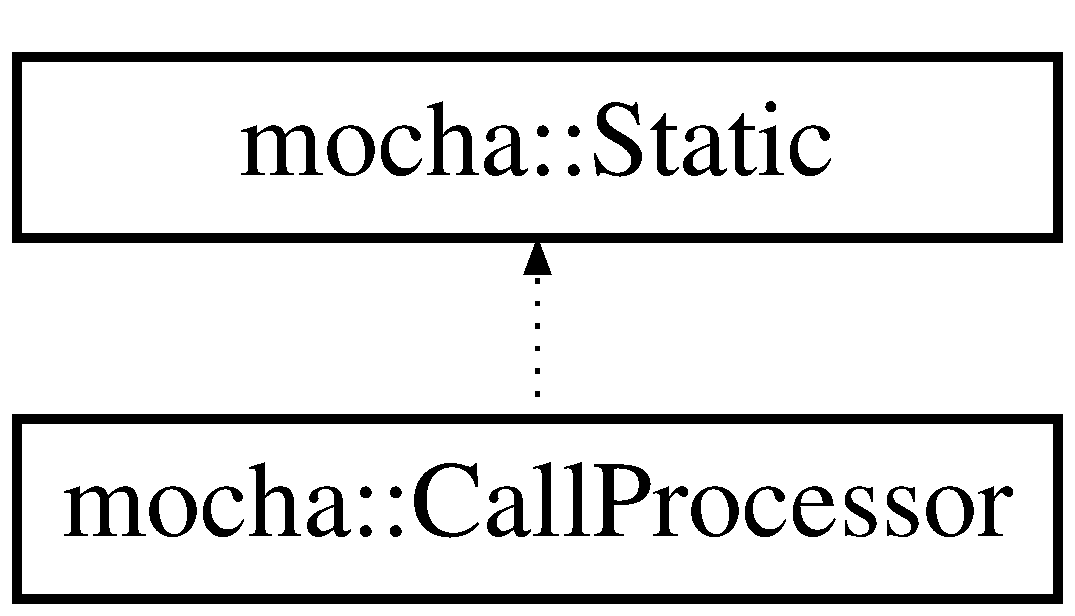
\includegraphics[height=2.000000cm]{classmocha_1_1_call_processor}
\end{center}
\end{figure}
\subsection*{Static Public Member Functions}
\begin{DoxyCompactItemize}
\item 
static void \hyperlink{classmocha_1_1_call_processor_a4b01fa21f9e5e67f94d976bfb84668e0}{ProcessPrivateAccessor} (\hyperlink{classmocha_1_1_call_exp}{CallExp} $\ast$ast\_\-node, \hyperlink{classmocha_1_1_processor_info}{ProcessorInfo} $\ast$info)
\item 
static void \hyperlink{classmocha_1_1_call_processor_ade6039c35412758924d37dcdda57de28}{ProcessFnCall} (\hyperlink{classmocha_1_1_call_exp}{CallExp} $\ast$ast\_\-node, \hyperlink{classmocha_1_1_processor_info}{ProcessorInfo} $\ast$info)
\item 
static void \hyperlink{classmocha_1_1_call_processor_ae91cf9d8e7ce89304a950a375ebeda9a}{ProcessExtendAccessor} (\hyperlink{classmocha_1_1_call_exp}{CallExp} $\ast$ast\_\-node, \hyperlink{classmocha_1_1_processor_info}{ProcessorInfo} $\ast$info)
\end{DoxyCompactItemize}


\subsection{Detailed Description}


Definition at line 6 of file call\_\-processor.h.



\subsection{Member Function Documentation}
\hypertarget{classmocha_1_1_call_processor_ae91cf9d8e7ce89304a950a375ebeda9a}{
\index{mocha::CallProcessor@{mocha::CallProcessor}!ProcessExtendAccessor@{ProcessExtendAccessor}}
\index{ProcessExtendAccessor@{ProcessExtendAccessor}!mocha::CallProcessor@{mocha::CallProcessor}}
\subsubsection[{ProcessExtendAccessor}]{\setlength{\rightskip}{0pt plus 5cm}void mocha::CallProcessor::ProcessExtendAccessor (
\begin{DoxyParamCaption}
\item[{{\bf CallExp} $\ast$}]{ast\_\-node, }
\item[{{\bf ProcessorInfo} $\ast$}]{info}
\end{DoxyParamCaption}
)\hspace{0.3cm}{\ttfamily  \mbox{[}static\mbox{]}}}}
\label{classmocha_1_1_call_processor_ae91cf9d8e7ce89304a950a375ebeda9a}


Definition at line 86 of file call\_\-processor.cc.

\hypertarget{classmocha_1_1_call_processor_ade6039c35412758924d37dcdda57de28}{
\index{mocha::CallProcessor@{mocha::CallProcessor}!ProcessFnCall@{ProcessFnCall}}
\index{ProcessFnCall@{ProcessFnCall}!mocha::CallProcessor@{mocha::CallProcessor}}
\subsubsection[{ProcessFnCall}]{\setlength{\rightskip}{0pt plus 5cm}void mocha::CallProcessor::ProcessFnCall (
\begin{DoxyParamCaption}
\item[{{\bf CallExp} $\ast$}]{ast\_\-node, }
\item[{{\bf ProcessorInfo} $\ast$}]{info}
\end{DoxyParamCaption}
)\hspace{0.3cm}{\ttfamily  \mbox{[}static\mbox{]}}}}
\label{classmocha_1_1_call_processor_ade6039c35412758924d37dcdda57de28}


Definition at line 53 of file call\_\-processor.cc.

\hypertarget{classmocha_1_1_call_processor_a4b01fa21f9e5e67f94d976bfb84668e0}{
\index{mocha::CallProcessor@{mocha::CallProcessor}!ProcessPrivateAccessor@{ProcessPrivateAccessor}}
\index{ProcessPrivateAccessor@{ProcessPrivateAccessor}!mocha::CallProcessor@{mocha::CallProcessor}}
\subsubsection[{ProcessPrivateAccessor}]{\setlength{\rightskip}{0pt plus 5cm}void mocha::CallProcessor::ProcessPrivateAccessor (
\begin{DoxyParamCaption}
\item[{{\bf CallExp} $\ast$}]{ast\_\-node, }
\item[{{\bf ProcessorInfo} $\ast$}]{info}
\end{DoxyParamCaption}
)\hspace{0.3cm}{\ttfamily  \mbox{[}static\mbox{]}}}}
\label{classmocha_1_1_call_processor_a4b01fa21f9e5e67f94d976bfb84668e0}


Definition at line 11 of file call\_\-processor.cc.



The documentation for this class was generated from the following files:\begin{DoxyCompactItemize}
\item 
Y:/mocha/src/ast/visitors/utils/processors/\hyperlink{call__processor_8h}{call\_\-processor.h}\item 
Y:/mocha/src/ast/visitors/utils/processors/\hyperlink{call__processor_8cc}{call\_\-processor.cc}\end{DoxyCompactItemize}

\hypertarget{classmocha_1_1_case_clause}{
\section{mocha::CaseClause Class Reference}
\label{classmocha_1_1_case_clause}\index{mocha::CaseClause@{mocha::CaseClause}}
}


{\ttfamily \#include $<$ast.h$>$}

Inheritance diagram for mocha::CaseClause:\begin{figure}[H]
\begin{center}
\leavevmode
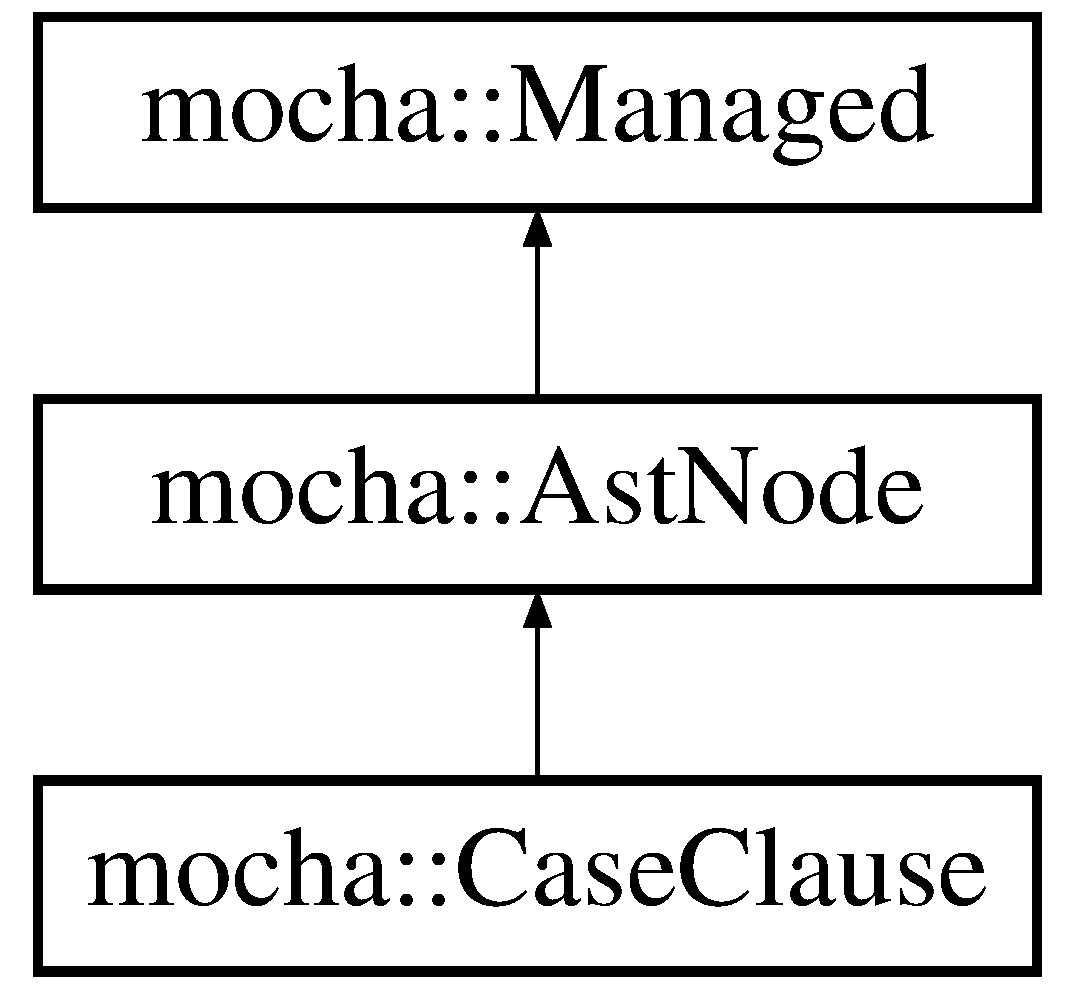
\includegraphics[height=3.000000cm]{classmocha_1_1_case_clause}
\end{center}
\end{figure}
\subsection*{Public Member Functions}
\begin{DoxyCompactItemize}
\item 
\hyperlink{classmocha_1_1_case_clause_a229dfa702d04e78848325f4dc3ab7e9c}{CaseClause} ()
\item 
\hyperlink{classmocha_1_1_case_clause_a7dea944e198694e4011fb950e781ec36}{$\sim$CaseClause} ()
\item 
void \hyperlink{classmocha_1_1_case_clause_abfdb03472b7994732bfaef3f09ba6136}{Exp} (\hyperlink{classmocha_1_1_ast_node}{AstNode} $\ast$node)
\item 
\hyperlink{classmocha_1_1_ast_node}{AstNode} $\ast$ \hyperlink{classmocha_1_1_case_clause_af4d51f44da5f56d9cfbd4ef88b48d31b}{Exp} ()
\item 
\hyperlink{classmocha_1_1_ast_node}{AstNode} $\ast$ \hyperlink{classmocha_1_1_case_clause_ac90d4e97b67875347208e98d4abaaf46}{Clone} ()
\end{DoxyCompactItemize}
\subsection*{Private Member Functions}
\begin{DoxyCompactItemize}
\item 
void \hyperlink{classmocha_1_1_case_clause_ac4cf86a50fb89dd213aafa983a14397a}{NVIAccept\_\-} (\hyperlink{classmocha_1_1_i_visitor}{IVisitor} $\ast$visitor)
\end{DoxyCompactItemize}
\subsection*{Private Attributes}
\begin{DoxyCompactItemize}
\item 
\hyperlink{classmocha_1_1_ast_node}{AstNode} $\ast$ \hyperlink{classmocha_1_1_case_clause_af73cfb9e5a448ae82079af72c9eb65d2}{exp\_\-}
\end{DoxyCompactItemize}


\subsection{Detailed Description}


Definition at line 1009 of file ast.h.



\subsection{Constructor \& Destructor Documentation}
\hypertarget{classmocha_1_1_case_clause_a229dfa702d04e78848325f4dc3ab7e9c}{
\index{mocha::CaseClause@{mocha::CaseClause}!CaseClause@{CaseClause}}
\index{CaseClause@{CaseClause}!mocha::CaseClause@{mocha::CaseClause}}
\subsubsection[{CaseClause}]{\setlength{\rightskip}{0pt plus 5cm}mocha::CaseClause::CaseClause (
\begin{DoxyParamCaption}
{}
\end{DoxyParamCaption}
)\hspace{0.3cm}{\ttfamily  \mbox{[}inline\mbox{]}}}}
\label{classmocha_1_1_case_clause_a229dfa702d04e78848325f4dc3ab7e9c}


Definition at line 1011 of file ast.h.

\hypertarget{classmocha_1_1_case_clause_a7dea944e198694e4011fb950e781ec36}{
\index{mocha::CaseClause@{mocha::CaseClause}!$\sim$CaseClause@{$\sim$CaseClause}}
\index{$\sim$CaseClause@{$\sim$CaseClause}!mocha::CaseClause@{mocha::CaseClause}}
\subsubsection[{$\sim$CaseClause}]{\setlength{\rightskip}{0pt plus 5cm}mocha::CaseClause::$\sim$CaseClause (
\begin{DoxyParamCaption}
{}
\end{DoxyParamCaption}
)\hspace{0.3cm}{\ttfamily  \mbox{[}inline\mbox{]}}}}
\label{classmocha_1_1_case_clause_a7dea944e198694e4011fb950e781ec36}


Definition at line 1012 of file ast.h.



\subsection{Member Function Documentation}
\hypertarget{classmocha_1_1_case_clause_ac90d4e97b67875347208e98d4abaaf46}{
\index{mocha::CaseClause@{mocha::CaseClause}!Clone@{Clone}}
\index{Clone@{Clone}!mocha::CaseClause@{mocha::CaseClause}}
\subsubsection[{Clone}]{\setlength{\rightskip}{0pt plus 5cm}{\bf AstNode} $\ast$ mocha::CaseClause::Clone (
\begin{DoxyParamCaption}
{}
\end{DoxyParamCaption}
)\hspace{0.3cm}{\ttfamily  \mbox{[}virtual\mbox{]}}}}
\label{classmocha_1_1_case_clause_ac90d4e97b67875347208e98d4abaaf46}
\begin{DoxyReturn}{Returns}
\{AstNode$\ast$\} Clone node. 
\end{DoxyReturn}


Reimplemented from \hyperlink{classmocha_1_1_ast_node_af2a895699bac2012f8b7739bff49c5ec}{mocha::AstNode}.



Definition at line 375 of file ast.cc.

\hypertarget{classmocha_1_1_case_clause_af4d51f44da5f56d9cfbd4ef88b48d31b}{
\index{mocha::CaseClause@{mocha::CaseClause}!Exp@{Exp}}
\index{Exp@{Exp}!mocha::CaseClause@{mocha::CaseClause}}
\subsubsection[{Exp}]{\setlength{\rightskip}{0pt plus 5cm}{\bf AstNode}$\ast$ mocha::CaseClause::Exp (
\begin{DoxyParamCaption}
{}
\end{DoxyParamCaption}
)\hspace{0.3cm}{\ttfamily  \mbox{[}inline\mbox{]}}}}
\label{classmocha_1_1_case_clause_af4d51f44da5f56d9cfbd4ef88b48d31b}


Definition at line 1014 of file ast.h.

\hypertarget{classmocha_1_1_case_clause_abfdb03472b7994732bfaef3f09ba6136}{
\index{mocha::CaseClause@{mocha::CaseClause}!Exp@{Exp}}
\index{Exp@{Exp}!mocha::CaseClause@{mocha::CaseClause}}
\subsubsection[{Exp}]{\setlength{\rightskip}{0pt plus 5cm}void mocha::CaseClause::Exp (
\begin{DoxyParamCaption}
\item[{{\bf AstNode} $\ast$}]{node}
\end{DoxyParamCaption}
)\hspace{0.3cm}{\ttfamily  \mbox{[}inline\mbox{]}}}}
\label{classmocha_1_1_case_clause_abfdb03472b7994732bfaef3f09ba6136}


Definition at line 1013 of file ast.h.

\hypertarget{classmocha_1_1_case_clause_ac4cf86a50fb89dd213aafa983a14397a}{
\index{mocha::CaseClause@{mocha::CaseClause}!NVIAccept\_\-@{NVIAccept\_\-}}
\index{NVIAccept\_\-@{NVIAccept\_\-}!mocha::CaseClause@{mocha::CaseClause}}
\subsubsection[{NVIAccept\_\-}]{\setlength{\rightskip}{0pt plus 5cm}void mocha::CaseClause::NVIAccept\_\- (
\begin{DoxyParamCaption}
\item[{{\bf IVisitor} $\ast$}]{visitor}
\end{DoxyParamCaption}
)\hspace{0.3cm}{\ttfamily  \mbox{[}inline, private, virtual\mbox{]}}}}
\label{classmocha_1_1_case_clause_ac4cf86a50fb89dd213aafa983a14397a}


Reimplemented from \hyperlink{classmocha_1_1_ast_node_a4a9c107bed3671f3fa15312b87f6ae96}{mocha::AstNode}.



Definition at line 1018 of file ast.h.



\subsection{Member Data Documentation}
\hypertarget{classmocha_1_1_case_clause_af73cfb9e5a448ae82079af72c9eb65d2}{
\index{mocha::CaseClause@{mocha::CaseClause}!exp\_\-@{exp\_\-}}
\index{exp\_\-@{exp\_\-}!mocha::CaseClause@{mocha::CaseClause}}
\subsubsection[{exp\_\-}]{\setlength{\rightskip}{0pt plus 5cm}{\bf AstNode}$\ast$ {\bf mocha::CaseClause::exp\_\-}\hspace{0.3cm}{\ttfamily  \mbox{[}private\mbox{]}}}}
\label{classmocha_1_1_case_clause_af73cfb9e5a448ae82079af72c9eb65d2}


Definition at line 1015 of file ast.h.



The documentation for this class was generated from the following files:\begin{DoxyCompactItemize}
\item 
Y:/mocha/src/ast/\hyperlink{ast_8h}{ast.h}\item 
Y:/mocha/src/ast/\hyperlink{ast_8cc}{ast.cc}\end{DoxyCompactItemize}

\hypertarget{classmocha_1_1_class}{
\section{mocha::Class Class Reference}
\label{classmocha_1_1_class}\index{mocha::Class@{mocha::Class}}
}


{\ttfamily \#include $<$ast.h$>$}

Inheritance diagram for mocha::Class:\begin{figure}[H]
\begin{center}
\leavevmode
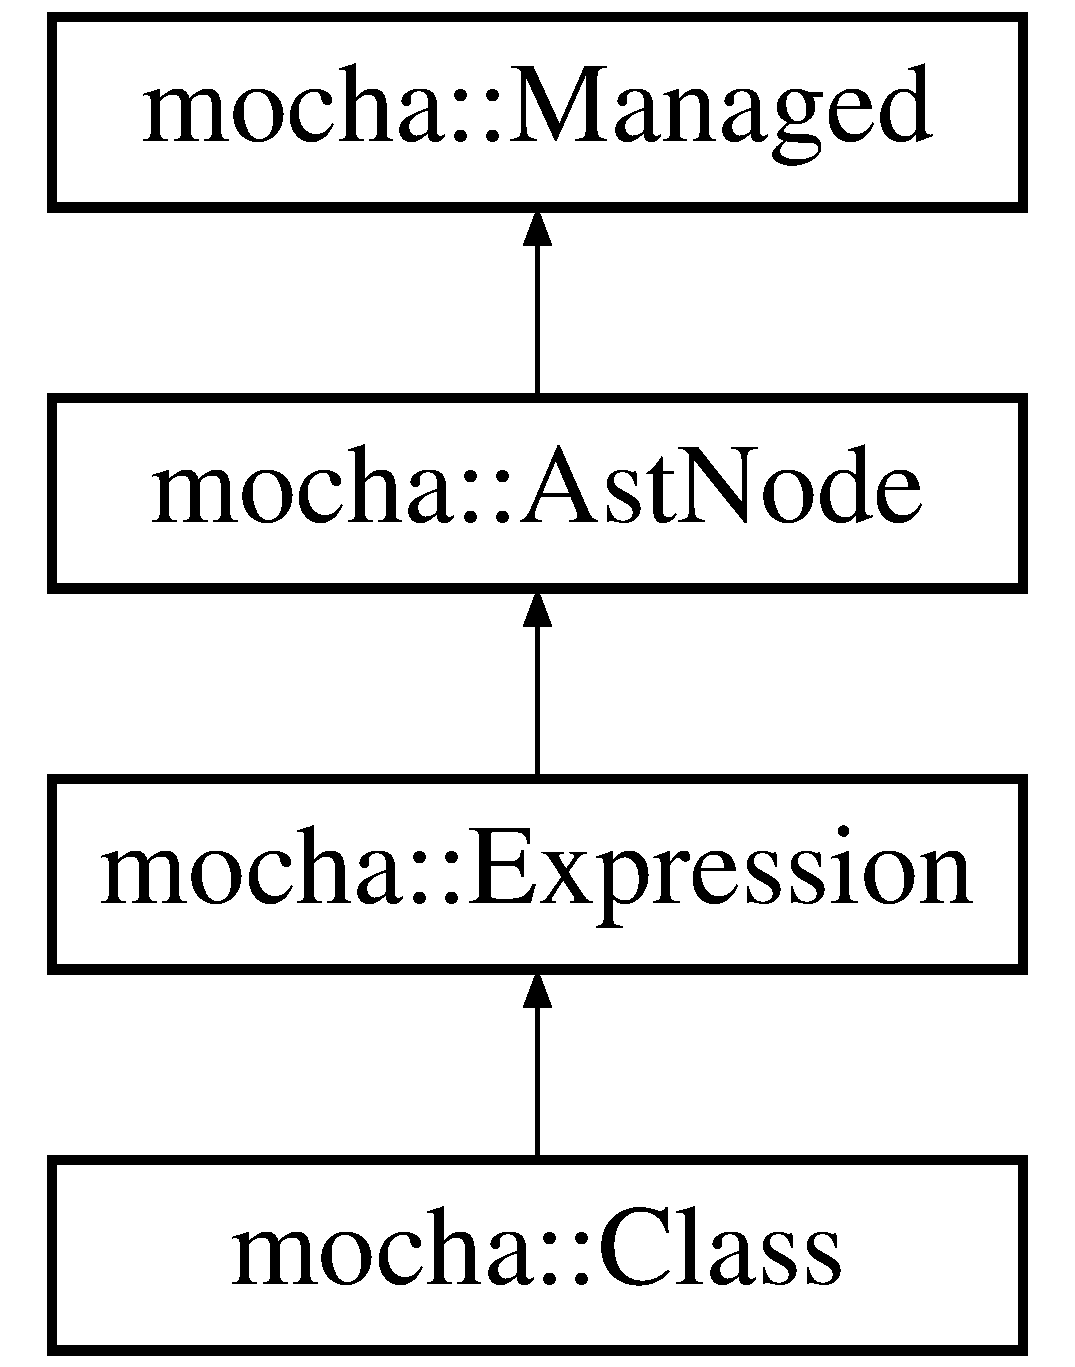
\includegraphics[height=4.000000cm]{classmocha_1_1_class}
\end{center}
\end{figure}
\subsection*{Public Member Functions}
\begin{DoxyCompactItemize}
\item 
\hyperlink{classmocha_1_1_class_a62374fd7f1beb337a73aa01bd7439e7b}{Class} (\hyperlink{classmocha_1_1_ast_node}{AstNode} $\ast$expandar, bool is\_\-const)
\item 
\hyperlink{classmocha_1_1_class_a5cd3954807966092eaf67a9d69da9df8}{Class} (\hyperlink{classmocha_1_1_empty}{Empty} $\ast$empty)
\item 
\hyperlink{classmocha_1_1_class_ac3db71226540e4f8376336add0a4a254}{$\sim$Class} ()
\item 
void \hyperlink{classmocha_1_1_class_a2cd99dd8829da45fd2cf92fd01392e7d}{Decl} (bool is)
\item 
bool \hyperlink{classmocha_1_1_class_a14ba1ee79fce913bcb11b5aaf2b58bce}{Decl} ()
\item 
bool \hyperlink{classmocha_1_1_class_a92570a6f6bf128a8a1b1c6209ebd42b3}{Const} ()
\item 
void \hyperlink{classmocha_1_1_class_aa0211babf6c2749339b01df68007e25e}{Inner} (bool is)
\item 
bool \hyperlink{classmocha_1_1_class_a411819b382d409b02f8a1692217b2c7e}{Inner} ()
\item 
void \hyperlink{classmocha_1_1_class_a31eda936b0126c8d587e614ced93e6c6}{Name} (\hyperlink{classmocha_1_1_ast_node}{AstNode} $\ast$name)
\item 
\hyperlink{classmocha_1_1_ast_node}{AstNode} $\ast$ \hyperlink{classmocha_1_1_class_ae077c4bc52c0491e714b6d17d42e4345}{Name} ()
\item 
\hyperlink{classmocha_1_1_ast_node}{AstNode} $\ast$ \hyperlink{classmocha_1_1_class_a6042b9b30d7990c238689c71dfb32022}{Expandar} ()
\item 
void \hyperlink{classmocha_1_1_class_afaf4f84b9a2e0a787e02b8fdda9e0b71}{Body} (\hyperlink{classmocha_1_1_ast_node}{AstNode} $\ast$body)
\item 
\hyperlink{classmocha_1_1_ast_node}{AstNode} $\ast$ \hyperlink{classmocha_1_1_class_ac20dd6b3e7f6ab234088f757c08bf7d0}{Body} ()
\item 
\hyperlink{classmocha_1_1_ast_node}{AstNode} $\ast$ \hyperlink{classmocha_1_1_class_a801c063381ca42fdab1c478f2ca461b8}{Clone} ()
\end{DoxyCompactItemize}
\subsection*{Private Member Functions}
\begin{DoxyCompactItemize}
\item 
void \hyperlink{classmocha_1_1_class_acb9ec1fb4dc467d73c132c20d510901a}{NVIAccept\_\-} (\hyperlink{classmocha_1_1_i_visitor}{IVisitor} $\ast$visitor)
\end{DoxyCompactItemize}
\subsection*{Private Attributes}
\begin{DoxyCompactItemize}
\item 
bool \hyperlink{classmocha_1_1_class_a33b68ef9c9cdb7099cc5a4b39531a7b2}{is\_\-const\_\-}
\item 
bool \hyperlink{classmocha_1_1_class_ac159c23063ecdb2471dbcc145f0ab874}{is\_\-decl\_\-}
\item 
bool \hyperlink{classmocha_1_1_class_a62eeaa52563724e00042117136658cde}{is\_\-inner\_\-}
\item 
\hyperlink{classmocha_1_1_ast_node}{AstNode} $\ast$ \hyperlink{classmocha_1_1_class_a059fb140e1ab511f2d40ac3f6792d108}{name\_\-}
\item 
\hyperlink{classmocha_1_1_ast_node}{AstNode} $\ast$ \hyperlink{classmocha_1_1_class_a1bc50b1206af06834791e3e5f551c000}{body\_\-}
\item 
\hyperlink{classmocha_1_1_ast_node}{AstNode} $\ast$ \hyperlink{classmocha_1_1_class_abb9675f084b13ea75b782a7da90f6c5d}{expandar\_\-}
\end{DoxyCompactItemize}


\subsection{Detailed Description}


Definition at line 1117 of file ast.h.



\subsection{Constructor \& Destructor Documentation}
\hypertarget{classmocha_1_1_class_a62374fd7f1beb337a73aa01bd7439e7b}{
\index{mocha::Class@{mocha::Class}!Class@{Class}}
\index{Class@{Class}!mocha::Class@{mocha::Class}}
\subsubsection[{Class}]{\setlength{\rightskip}{0pt plus 5cm}mocha::Class::Class (
\begin{DoxyParamCaption}
\item[{{\bf AstNode} $\ast$}]{expandar, }
\item[{bool}]{is\_\-const}
\end{DoxyParamCaption}
)\hspace{0.3cm}{\ttfamily  \mbox{[}inline\mbox{]}}}}
\label{classmocha_1_1_class_a62374fd7f1beb337a73aa01bd7439e7b}


Definition at line 1119 of file ast.h.

\hypertarget{classmocha_1_1_class_a5cd3954807966092eaf67a9d69da9df8}{
\index{mocha::Class@{mocha::Class}!Class@{Class}}
\index{Class@{Class}!mocha::Class@{mocha::Class}}
\subsubsection[{Class}]{\setlength{\rightskip}{0pt plus 5cm}mocha::Class::Class (
\begin{DoxyParamCaption}
\item[{{\bf Empty} $\ast$}]{empty}
\end{DoxyParamCaption}
)\hspace{0.3cm}{\ttfamily  \mbox{[}inline\mbox{]}}}}
\label{classmocha_1_1_class_a5cd3954807966092eaf67a9d69da9df8}


Definition at line 1122 of file ast.h.

\hypertarget{classmocha_1_1_class_ac3db71226540e4f8376336add0a4a254}{
\index{mocha::Class@{mocha::Class}!$\sim$Class@{$\sim$Class}}
\index{$\sim$Class@{$\sim$Class}!mocha::Class@{mocha::Class}}
\subsubsection[{$\sim$Class}]{\setlength{\rightskip}{0pt plus 5cm}mocha::Class::$\sim$Class (
\begin{DoxyParamCaption}
{}
\end{DoxyParamCaption}
)\hspace{0.3cm}{\ttfamily  \mbox{[}inline\mbox{]}}}}
\label{classmocha_1_1_class_ac3db71226540e4f8376336add0a4a254}


Definition at line 1123 of file ast.h.



\subsection{Member Function Documentation}
\hypertarget{classmocha_1_1_class_afaf4f84b9a2e0a787e02b8fdda9e0b71}{
\index{mocha::Class@{mocha::Class}!Body@{Body}}
\index{Body@{Body}!mocha::Class@{mocha::Class}}
\subsubsection[{Body}]{\setlength{\rightskip}{0pt plus 5cm}void mocha::Class::Body (
\begin{DoxyParamCaption}
\item[{{\bf AstNode} $\ast$}]{body}
\end{DoxyParamCaption}
)\hspace{0.3cm}{\ttfamily  \mbox{[}inline\mbox{]}}}}
\label{classmocha_1_1_class_afaf4f84b9a2e0a787e02b8fdda9e0b71}


Definition at line 1132 of file ast.h.

\hypertarget{classmocha_1_1_class_ac20dd6b3e7f6ab234088f757c08bf7d0}{
\index{mocha::Class@{mocha::Class}!Body@{Body}}
\index{Body@{Body}!mocha::Class@{mocha::Class}}
\subsubsection[{Body}]{\setlength{\rightskip}{0pt plus 5cm}{\bf AstNode}$\ast$ mocha::Class::Body (
\begin{DoxyParamCaption}
{}
\end{DoxyParamCaption}
)\hspace{0.3cm}{\ttfamily  \mbox{[}inline\mbox{]}}}}
\label{classmocha_1_1_class_ac20dd6b3e7f6ab234088f757c08bf7d0}


Definition at line 1136 of file ast.h.

\hypertarget{classmocha_1_1_class_a801c063381ca42fdab1c478f2ca461b8}{
\index{mocha::Class@{mocha::Class}!Clone@{Clone}}
\index{Clone@{Clone}!mocha::Class@{mocha::Class}}
\subsubsection[{Clone}]{\setlength{\rightskip}{0pt plus 5cm}{\bf AstNode} $\ast$ mocha::Class::Clone (
\begin{DoxyParamCaption}
{}
\end{DoxyParamCaption}
)\hspace{0.3cm}{\ttfamily  \mbox{[}virtual\mbox{]}}}}
\label{classmocha_1_1_class_a801c063381ca42fdab1c478f2ca461b8}
\begin{DoxyReturn}{Returns}
\{AstNode$\ast$\} Clone node. 
\end{DoxyReturn}


Reimplemented from \hyperlink{classmocha_1_1_expression_ac1fb936e2bf0fdd6e7667275d3723ca5}{mocha::Expression}.



Definition at line 389 of file ast.cc.

\hypertarget{classmocha_1_1_class_a92570a6f6bf128a8a1b1c6209ebd42b3}{
\index{mocha::Class@{mocha::Class}!Const@{Const}}
\index{Const@{Const}!mocha::Class@{mocha::Class}}
\subsubsection[{Const}]{\setlength{\rightskip}{0pt plus 5cm}bool mocha::Class::Const (
\begin{DoxyParamCaption}
{}
\end{DoxyParamCaption}
)\hspace{0.3cm}{\ttfamily  \mbox{[}inline\mbox{]}}}}
\label{classmocha_1_1_class_a92570a6f6bf128a8a1b1c6209ebd42b3}


Definition at line 1126 of file ast.h.

\hypertarget{classmocha_1_1_class_a14ba1ee79fce913bcb11b5aaf2b58bce}{
\index{mocha::Class@{mocha::Class}!Decl@{Decl}}
\index{Decl@{Decl}!mocha::Class@{mocha::Class}}
\subsubsection[{Decl}]{\setlength{\rightskip}{0pt plus 5cm}bool mocha::Class::Decl (
\begin{DoxyParamCaption}
{}
\end{DoxyParamCaption}
)\hspace{0.3cm}{\ttfamily  \mbox{[}inline\mbox{]}}}}
\label{classmocha_1_1_class_a14ba1ee79fce913bcb11b5aaf2b58bce}


Definition at line 1125 of file ast.h.

\hypertarget{classmocha_1_1_class_a2cd99dd8829da45fd2cf92fd01392e7d}{
\index{mocha::Class@{mocha::Class}!Decl@{Decl}}
\index{Decl@{Decl}!mocha::Class@{mocha::Class}}
\subsubsection[{Decl}]{\setlength{\rightskip}{0pt plus 5cm}void mocha::Class::Decl (
\begin{DoxyParamCaption}
\item[{bool}]{is}
\end{DoxyParamCaption}
)\hspace{0.3cm}{\ttfamily  \mbox{[}inline\mbox{]}}}}
\label{classmocha_1_1_class_a2cd99dd8829da45fd2cf92fd01392e7d}


Definition at line 1124 of file ast.h.

\hypertarget{classmocha_1_1_class_a6042b9b30d7990c238689c71dfb32022}{
\index{mocha::Class@{mocha::Class}!Expandar@{Expandar}}
\index{Expandar@{Expandar}!mocha::Class@{mocha::Class}}
\subsubsection[{Expandar}]{\setlength{\rightskip}{0pt plus 5cm}{\bf AstNode}$\ast$ mocha::Class::Expandar (
\begin{DoxyParamCaption}
{}
\end{DoxyParamCaption}
)\hspace{0.3cm}{\ttfamily  \mbox{[}inline\mbox{]}}}}
\label{classmocha_1_1_class_a6042b9b30d7990c238689c71dfb32022}


Definition at line 1131 of file ast.h.

\hypertarget{classmocha_1_1_class_aa0211babf6c2749339b01df68007e25e}{
\index{mocha::Class@{mocha::Class}!Inner@{Inner}}
\index{Inner@{Inner}!mocha::Class@{mocha::Class}}
\subsubsection[{Inner}]{\setlength{\rightskip}{0pt plus 5cm}void mocha::Class::Inner (
\begin{DoxyParamCaption}
\item[{bool}]{is}
\end{DoxyParamCaption}
)\hspace{0.3cm}{\ttfamily  \mbox{[}inline\mbox{]}}}}
\label{classmocha_1_1_class_aa0211babf6c2749339b01df68007e25e}


Definition at line 1127 of file ast.h.

\hypertarget{classmocha_1_1_class_a411819b382d409b02f8a1692217b2c7e}{
\index{mocha::Class@{mocha::Class}!Inner@{Inner}}
\index{Inner@{Inner}!mocha::Class@{mocha::Class}}
\subsubsection[{Inner}]{\setlength{\rightskip}{0pt plus 5cm}bool mocha::Class::Inner (
\begin{DoxyParamCaption}
{}
\end{DoxyParamCaption}
)\hspace{0.3cm}{\ttfamily  \mbox{[}inline\mbox{]}}}}
\label{classmocha_1_1_class_a411819b382d409b02f8a1692217b2c7e}


Definition at line 1128 of file ast.h.

\hypertarget{classmocha_1_1_class_ae077c4bc52c0491e714b6d17d42e4345}{
\index{mocha::Class@{mocha::Class}!Name@{Name}}
\index{Name@{Name}!mocha::Class@{mocha::Class}}
\subsubsection[{Name}]{\setlength{\rightskip}{0pt plus 5cm}{\bf AstNode}$\ast$ mocha::Class::Name (
\begin{DoxyParamCaption}
{}
\end{DoxyParamCaption}
)\hspace{0.3cm}{\ttfamily  \mbox{[}inline\mbox{]}}}}
\label{classmocha_1_1_class_ae077c4bc52c0491e714b6d17d42e4345}


Definition at line 1130 of file ast.h.

\hypertarget{classmocha_1_1_class_a31eda936b0126c8d587e614ced93e6c6}{
\index{mocha::Class@{mocha::Class}!Name@{Name}}
\index{Name@{Name}!mocha::Class@{mocha::Class}}
\subsubsection[{Name}]{\setlength{\rightskip}{0pt plus 5cm}void mocha::Class::Name (
\begin{DoxyParamCaption}
\item[{{\bf AstNode} $\ast$}]{name}
\end{DoxyParamCaption}
)\hspace{0.3cm}{\ttfamily  \mbox{[}inline\mbox{]}}}}
\label{classmocha_1_1_class_a31eda936b0126c8d587e614ced93e6c6}


Definition at line 1129 of file ast.h.

\hypertarget{classmocha_1_1_class_acb9ec1fb4dc467d73c132c20d510901a}{
\index{mocha::Class@{mocha::Class}!NVIAccept\_\-@{NVIAccept\_\-}}
\index{NVIAccept\_\-@{NVIAccept\_\-}!mocha::Class@{mocha::Class}}
\subsubsection[{NVIAccept\_\-}]{\setlength{\rightskip}{0pt plus 5cm}void mocha::Class::NVIAccept\_\- (
\begin{DoxyParamCaption}
\item[{{\bf IVisitor} $\ast$}]{visitor}
\end{DoxyParamCaption}
)\hspace{0.3cm}{\ttfamily  \mbox{[}inline, private, virtual\mbox{]}}}}
\label{classmocha_1_1_class_acb9ec1fb4dc467d73c132c20d510901a}


Reimplemented from \hyperlink{classmocha_1_1_expression_a112d57b7de76c37066cde60be4799fde}{mocha::Expression}.



Definition at line 1139 of file ast.h.



\subsection{Member Data Documentation}
\hypertarget{classmocha_1_1_class_a1bc50b1206af06834791e3e5f551c000}{
\index{mocha::Class@{mocha::Class}!body\_\-@{body\_\-}}
\index{body\_\-@{body\_\-}!mocha::Class@{mocha::Class}}
\subsubsection[{body\_\-}]{\setlength{\rightskip}{0pt plus 5cm}{\bf AstNode}$\ast$ {\bf mocha::Class::body\_\-}\hspace{0.3cm}{\ttfamily  \mbox{[}private\mbox{]}}}}
\label{classmocha_1_1_class_a1bc50b1206af06834791e3e5f551c000}


Definition at line 1144 of file ast.h.

\hypertarget{classmocha_1_1_class_abb9675f084b13ea75b782a7da90f6c5d}{
\index{mocha::Class@{mocha::Class}!expandar\_\-@{expandar\_\-}}
\index{expandar\_\-@{expandar\_\-}!mocha::Class@{mocha::Class}}
\subsubsection[{expandar\_\-}]{\setlength{\rightskip}{0pt plus 5cm}{\bf AstNode}$\ast$ {\bf mocha::Class::expandar\_\-}\hspace{0.3cm}{\ttfamily  \mbox{[}private\mbox{]}}}}
\label{classmocha_1_1_class_abb9675f084b13ea75b782a7da90f6c5d}


Definition at line 1145 of file ast.h.

\hypertarget{classmocha_1_1_class_a33b68ef9c9cdb7099cc5a4b39531a7b2}{
\index{mocha::Class@{mocha::Class}!is\_\-const\_\-@{is\_\-const\_\-}}
\index{is\_\-const\_\-@{is\_\-const\_\-}!mocha::Class@{mocha::Class}}
\subsubsection[{is\_\-const\_\-}]{\setlength{\rightskip}{0pt plus 5cm}bool {\bf mocha::Class::is\_\-const\_\-}\hspace{0.3cm}{\ttfamily  \mbox{[}private\mbox{]}}}}
\label{classmocha_1_1_class_a33b68ef9c9cdb7099cc5a4b39531a7b2}


Definition at line 1139 of file ast.h.

\hypertarget{classmocha_1_1_class_ac159c23063ecdb2471dbcc145f0ab874}{
\index{mocha::Class@{mocha::Class}!is\_\-decl\_\-@{is\_\-decl\_\-}}
\index{is\_\-decl\_\-@{is\_\-decl\_\-}!mocha::Class@{mocha::Class}}
\subsubsection[{is\_\-decl\_\-}]{\setlength{\rightskip}{0pt plus 5cm}bool {\bf mocha::Class::is\_\-decl\_\-}\hspace{0.3cm}{\ttfamily  \mbox{[}private\mbox{]}}}}
\label{classmocha_1_1_class_ac159c23063ecdb2471dbcc145f0ab874}


Definition at line 1141 of file ast.h.

\hypertarget{classmocha_1_1_class_a62eeaa52563724e00042117136658cde}{
\index{mocha::Class@{mocha::Class}!is\_\-inner\_\-@{is\_\-inner\_\-}}
\index{is\_\-inner\_\-@{is\_\-inner\_\-}!mocha::Class@{mocha::Class}}
\subsubsection[{is\_\-inner\_\-}]{\setlength{\rightskip}{0pt plus 5cm}bool {\bf mocha::Class::is\_\-inner\_\-}\hspace{0.3cm}{\ttfamily  \mbox{[}private\mbox{]}}}}
\label{classmocha_1_1_class_a62eeaa52563724e00042117136658cde}


Definition at line 1142 of file ast.h.

\hypertarget{classmocha_1_1_class_a059fb140e1ab511f2d40ac3f6792d108}{
\index{mocha::Class@{mocha::Class}!name\_\-@{name\_\-}}
\index{name\_\-@{name\_\-}!mocha::Class@{mocha::Class}}
\subsubsection[{name\_\-}]{\setlength{\rightskip}{0pt plus 5cm}{\bf AstNode}$\ast$ {\bf mocha::Class::name\_\-}\hspace{0.3cm}{\ttfamily  \mbox{[}private\mbox{]}}}}
\label{classmocha_1_1_class_a059fb140e1ab511f2d40ac3f6792d108}


Reimplemented from \hyperlink{classmocha_1_1_ast_node_a876b49852a3151d977c842a90ee02771}{mocha::AstNode}.



Definition at line 1143 of file ast.h.



The documentation for this class was generated from the following files:\begin{DoxyCompactItemize}
\item 
Y:/mocha/src/ast/\hyperlink{ast_8h}{ast.h}\item 
Y:/mocha/src/ast/\hyperlink{ast_8cc}{ast.cc}\end{DoxyCompactItemize}

\hypertarget{classmocha_1_1_class_expandar}{
\section{mocha::ClassExpandar Class Reference}
\label{classmocha_1_1_class_expandar}\index{mocha::ClassExpandar@{mocha::ClassExpandar}}
}


{\ttfamily \#include $<$ast.h$>$}

Inheritance diagram for mocha::ClassExpandar:\begin{figure}[H]
\begin{center}
\leavevmode
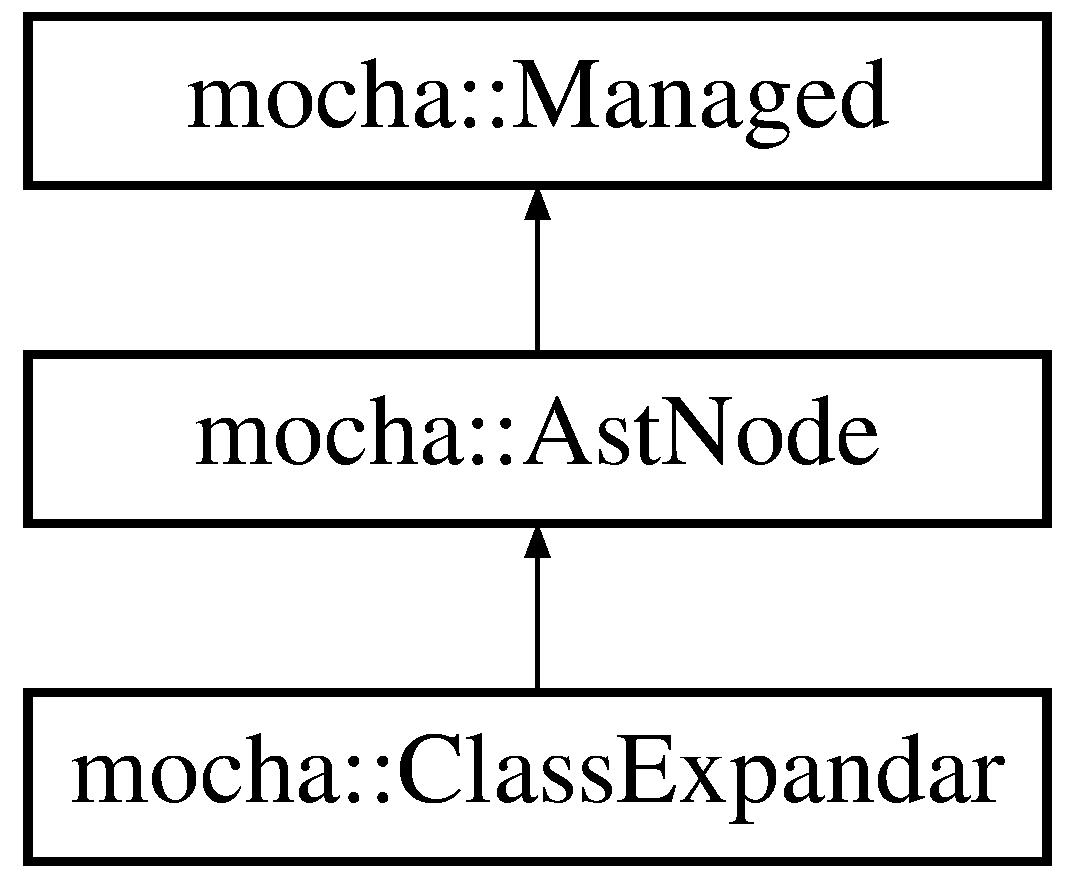
\includegraphics[height=3.000000cm]{classmocha_1_1_class_expandar}
\end{center}
\end{figure}
\subsection*{Public Types}
\begin{DoxyCompactItemize}
\item 
enum \hyperlink{classmocha_1_1_class_expandar_ab2e8fbff2016d78e9eb128f90e1fc7df}{ExpandAttr} \{ \hyperlink{classmocha_1_1_class_expandar_ab2e8fbff2016d78e9eb128f90e1fc7dfaf61e7f3912848c1da2126eb296ae0da9}{kExtends}, 
\hyperlink{classmocha_1_1_class_expandar_ab2e8fbff2016d78e9eb128f90e1fc7dfafc78d230a7579d6ad8ff7bc317f59078}{kPrototype}
 \}
\end{DoxyCompactItemize}
\subsection*{Public Member Functions}
\begin{DoxyCompactItemize}
\item 
\hyperlink{classmocha_1_1_class_expandar_a0c6019411ac6660872e460d0768613e7}{ClassExpandar} (\hyperlink{classmocha_1_1_class_expandar_ab2e8fbff2016d78e9eb128f90e1fc7df}{ExpandAttr} attr)
\item 
\hyperlink{classmocha_1_1_class_expandar_a87db54a95c1341d9c547388a7ceffd48}{$\sim$ClassExpandar} ()
\item 
\hyperlink{classmocha_1_1_class_expandar_ab2e8fbff2016d78e9eb128f90e1fc7df}{ExpandAttr} \hyperlink{classmocha_1_1_class_expandar_a3ecc25d967144064854cd79317b3cebc}{Type} ()
\item 
\hyperlink{classmocha_1_1_ast_node}{AstNode} $\ast$ \hyperlink{classmocha_1_1_class_expandar_a0942e40301ca95fb470443801da7c837}{Clone} ()
\end{DoxyCompactItemize}
\subsection*{Private Member Functions}
\begin{DoxyCompactItemize}
\item 
void \hyperlink{classmocha_1_1_class_expandar_aeaf8dc378ea8edfbce4435b01115ef34}{NVIAccept\_\-} (\hyperlink{classmocha_1_1_i_visitor}{IVisitor} $\ast$visitor)
\end{DoxyCompactItemize}
\subsection*{Private Attributes}
\begin{DoxyCompactItemize}
\item 
\hyperlink{classmocha_1_1_class_expandar_ab2e8fbff2016d78e9eb128f90e1fc7df}{ExpandAttr} \hyperlink{classmocha_1_1_class_expandar_a316e97cf34c8653b218b3dd8794442e3}{attr\_\-}
\end{DoxyCompactItemize}


\subsection{Detailed Description}


Definition at line 1178 of file ast.h.



\subsection{Member Enumeration Documentation}
\hypertarget{classmocha_1_1_class_expandar_ab2e8fbff2016d78e9eb128f90e1fc7df}{
\index{mocha::ClassExpandar@{mocha::ClassExpandar}!ExpandAttr@{ExpandAttr}}
\index{ExpandAttr@{ExpandAttr}!mocha::ClassExpandar@{mocha::ClassExpandar}}
\subsubsection[{ExpandAttr}]{\setlength{\rightskip}{0pt plus 5cm}enum {\bf mocha::ClassExpandar::ExpandAttr}}}
\label{classmocha_1_1_class_expandar_ab2e8fbff2016d78e9eb128f90e1fc7df}
\begin{Desc}
\item[Enumerator: ]\par
\begin{description}
\index{kExtends@{kExtends}!mocha::ClassExpandar@{mocha::ClassExpandar}}\index{mocha::ClassExpandar@{mocha::ClassExpandar}!kExtends@{kExtends}}\item[{\em 
\hypertarget{classmocha_1_1_class_expandar_ab2e8fbff2016d78e9eb128f90e1fc7dfaf61e7f3912848c1da2126eb296ae0da9}{
kExtends}
\label{classmocha_1_1_class_expandar_ab2e8fbff2016d78e9eb128f90e1fc7dfaf61e7f3912848c1da2126eb296ae0da9}
}]\index{kPrototype@{kPrototype}!mocha::ClassExpandar@{mocha::ClassExpandar}}\index{mocha::ClassExpandar@{mocha::ClassExpandar}!kPrototype@{kPrototype}}\item[{\em 
\hypertarget{classmocha_1_1_class_expandar_ab2e8fbff2016d78e9eb128f90e1fc7dfafc78d230a7579d6ad8ff7bc317f59078}{
kPrototype}
\label{classmocha_1_1_class_expandar_ab2e8fbff2016d78e9eb128f90e1fc7dfafc78d230a7579d6ad8ff7bc317f59078}
}]\end{description}
\end{Desc}



Definition at line 1180 of file ast.h.



\subsection{Constructor \& Destructor Documentation}
\hypertarget{classmocha_1_1_class_expandar_a0c6019411ac6660872e460d0768613e7}{
\index{mocha::ClassExpandar@{mocha::ClassExpandar}!ClassExpandar@{ClassExpandar}}
\index{ClassExpandar@{ClassExpandar}!mocha::ClassExpandar@{mocha::ClassExpandar}}
\subsubsection[{ClassExpandar}]{\setlength{\rightskip}{0pt plus 5cm}mocha::ClassExpandar::ClassExpandar (
\begin{DoxyParamCaption}
\item[{{\bf ExpandAttr}}]{attr}
\end{DoxyParamCaption}
)\hspace{0.3cm}{\ttfamily  \mbox{[}inline\mbox{]}}}}
\label{classmocha_1_1_class_expandar_a0c6019411ac6660872e460d0768613e7}


Definition at line 1184 of file ast.h.

\hypertarget{classmocha_1_1_class_expandar_a87db54a95c1341d9c547388a7ceffd48}{
\index{mocha::ClassExpandar@{mocha::ClassExpandar}!$\sim$ClassExpandar@{$\sim$ClassExpandar}}
\index{$\sim$ClassExpandar@{$\sim$ClassExpandar}!mocha::ClassExpandar@{mocha::ClassExpandar}}
\subsubsection[{$\sim$ClassExpandar}]{\setlength{\rightskip}{0pt plus 5cm}mocha::ClassExpandar::$\sim$ClassExpandar (
\begin{DoxyParamCaption}
{}
\end{DoxyParamCaption}
)\hspace{0.3cm}{\ttfamily  \mbox{[}inline\mbox{]}}}}
\label{classmocha_1_1_class_expandar_a87db54a95c1341d9c547388a7ceffd48}


Definition at line 1185 of file ast.h.



\subsection{Member Function Documentation}
\hypertarget{classmocha_1_1_class_expandar_a0942e40301ca95fb470443801da7c837}{
\index{mocha::ClassExpandar@{mocha::ClassExpandar}!Clone@{Clone}}
\index{Clone@{Clone}!mocha::ClassExpandar@{mocha::ClassExpandar}}
\subsubsection[{Clone}]{\setlength{\rightskip}{0pt plus 5cm}{\bf AstNode} $\ast$ mocha::ClassExpandar::Clone (
\begin{DoxyParamCaption}
{}
\end{DoxyParamCaption}
)\hspace{0.3cm}{\ttfamily  \mbox{[}virtual\mbox{]}}}}
\label{classmocha_1_1_class_expandar_a0942e40301ca95fb470443801da7c837}
\begin{DoxyReturn}{Returns}
\{AstNode$\ast$\} Clone node. 
\end{DoxyReturn}


Reimplemented from \hyperlink{classmocha_1_1_ast_node_af2a895699bac2012f8b7739bff49c5ec}{mocha::AstNode}.



Definition at line 411 of file ast.cc.

\hypertarget{classmocha_1_1_class_expandar_aeaf8dc378ea8edfbce4435b01115ef34}{
\index{mocha::ClassExpandar@{mocha::ClassExpandar}!NVIAccept\_\-@{NVIAccept\_\-}}
\index{NVIAccept\_\-@{NVIAccept\_\-}!mocha::ClassExpandar@{mocha::ClassExpandar}}
\subsubsection[{NVIAccept\_\-}]{\setlength{\rightskip}{0pt plus 5cm}void mocha::ClassExpandar::NVIAccept\_\- (
\begin{DoxyParamCaption}
\item[{{\bf IVisitor} $\ast$}]{visitor}
\end{DoxyParamCaption}
)\hspace{0.3cm}{\ttfamily  \mbox{[}inline, private, virtual\mbox{]}}}}
\label{classmocha_1_1_class_expandar_aeaf8dc378ea8edfbce4435b01115ef34}


Reimplemented from \hyperlink{classmocha_1_1_ast_node_a4a9c107bed3671f3fa15312b87f6ae96}{mocha::AstNode}.



Definition at line 1189 of file ast.h.

\hypertarget{classmocha_1_1_class_expandar_a3ecc25d967144064854cd79317b3cebc}{
\index{mocha::ClassExpandar@{mocha::ClassExpandar}!Type@{Type}}
\index{Type@{Type}!mocha::ClassExpandar@{mocha::ClassExpandar}}
\subsubsection[{Type}]{\setlength{\rightskip}{0pt plus 5cm}{\bf ExpandAttr} mocha::ClassExpandar::Type (
\begin{DoxyParamCaption}
{}
\end{DoxyParamCaption}
)\hspace{0.3cm}{\ttfamily  \mbox{[}inline\mbox{]}}}}
\label{classmocha_1_1_class_expandar_a3ecc25d967144064854cd79317b3cebc}


Definition at line 1186 of file ast.h.



\subsection{Member Data Documentation}
\hypertarget{classmocha_1_1_class_expandar_a316e97cf34c8653b218b3dd8794442e3}{
\index{mocha::ClassExpandar@{mocha::ClassExpandar}!attr\_\-@{attr\_\-}}
\index{attr\_\-@{attr\_\-}!mocha::ClassExpandar@{mocha::ClassExpandar}}
\subsubsection[{attr\_\-}]{\setlength{\rightskip}{0pt plus 5cm}{\bf ExpandAttr} {\bf mocha::ClassExpandar::attr\_\-}\hspace{0.3cm}{\ttfamily  \mbox{[}private\mbox{]}}}}
\label{classmocha_1_1_class_expandar_a316e97cf34c8653b218b3dd8794442e3}


Definition at line 1189 of file ast.h.



The documentation for this class was generated from the following files:\begin{DoxyCompactItemize}
\item 
Y:/mocha/src/ast/\hyperlink{ast_8h}{ast.h}\item 
Y:/mocha/src/ast/\hyperlink{ast_8cc}{ast.cc}\end{DoxyCompactItemize}

\hypertarget{classmocha_1_1_class_member}{
\section{mocha::ClassMember Class Reference}
\label{classmocha_1_1_class_member}\index{mocha::ClassMember@{mocha::ClassMember}}
}


{\ttfamily \#include $<$ast.h$>$}

Inheritance diagram for mocha::ClassMember:\begin{figure}[H]
\begin{center}
\leavevmode
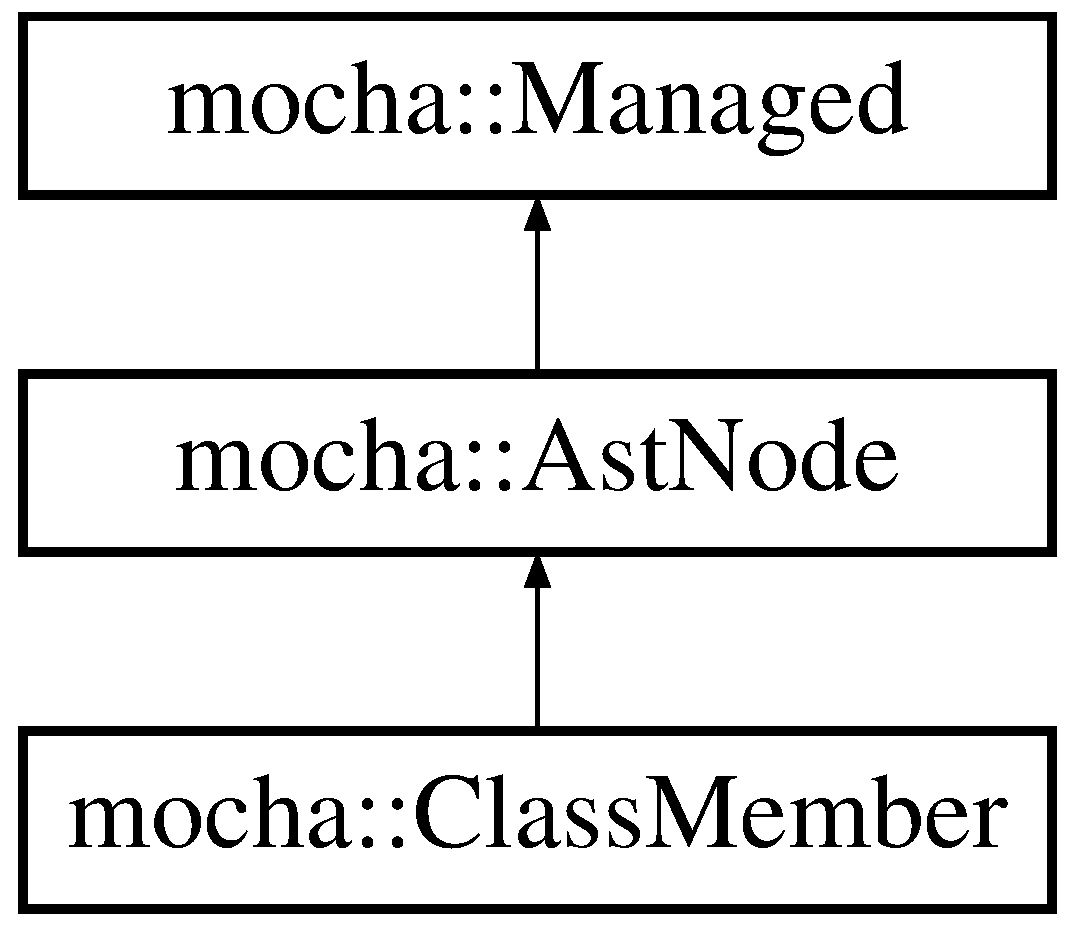
\includegraphics[height=3.000000cm]{classmocha_1_1_class_member}
\end{center}
\end{figure}
\subsection*{Public Types}
\begin{DoxyCompactItemize}
\item 
enum \hyperlink{classmocha_1_1_class_member_a3b8ac727565cfee0a488ff72a692315c}{MemberAttr} \{ \par
\hyperlink{classmocha_1_1_class_member_a3b8ac727565cfee0a488ff72a692315ca93091b1c2b66dc7b64f161785f7a989b}{kPrivate}, 
\hyperlink{classmocha_1_1_class_member_a3b8ac727565cfee0a488ff72a692315ca5e89cf7f3f42774c250c34b5b9470d84}{kPublic}, 
\hyperlink{classmocha_1_1_class_member_a3b8ac727565cfee0a488ff72a692315ca75c68efcb492562babd923ca06ad8d25}{kPrototype}, 
\hyperlink{classmocha_1_1_class_member_a3b8ac727565cfee0a488ff72a692315caf4065efc6f88f03fa9427dff213fd627}{kPublicStatic}, 
\par
\hyperlink{classmocha_1_1_class_member_a3b8ac727565cfee0a488ff72a692315ca504480033224ceb076d695a07ee64181}{kPrivateStatic}, 
\hyperlink{classmocha_1_1_class_member_a3b8ac727565cfee0a488ff72a692315ca4050c3c895caa0f8242b9eb7973a7c25}{kConstructor}, 
\hyperlink{classmocha_1_1_class_member_a3b8ac727565cfee0a488ff72a692315cad8b1e0ddba07d8d2b67a3a3fd60a332c}{kMixin}
 \}
\end{DoxyCompactItemize}
\subsection*{Public Member Functions}
\begin{DoxyCompactItemize}
\item 
\hyperlink{classmocha_1_1_class_member_a66371f92f430a4c207ab9431753853b3}{ClassMember} (\hyperlink{classmocha_1_1_class_member_a3b8ac727565cfee0a488ff72a692315c}{MemberAttr} attr)
\item 
\hyperlink{classmocha_1_1_class_member_ac44d3de151002e94d91ebc62f2fa4d7e}{$\sim$ClassMember} ()
\item 
\hyperlink{classmocha_1_1_class_member_a3b8ac727565cfee0a488ff72a692315c}{MemberAttr} \hyperlink{classmocha_1_1_class_member_a67bde775e5f9aac233c5b163cc3b78d3}{Attr} ()
\item 
\hyperlink{classmocha_1_1_ast_node}{AstNode} $\ast$ \hyperlink{classmocha_1_1_class_member_aae2611eb97d6be3e41805c2ddabc6c5b}{Clone} ()
\end{DoxyCompactItemize}
\subsection*{Private Member Functions}
\begin{DoxyCompactItemize}
\item 
void \hyperlink{classmocha_1_1_class_member_af42df5d8b90e907a75df5a12408d1973}{NVIAccept\_\-} (\hyperlink{classmocha_1_1_i_visitor}{IVisitor} $\ast$visitor)
\end{DoxyCompactItemize}
\subsection*{Private Attributes}
\begin{DoxyCompactItemize}
\item 
\hyperlink{classmocha_1_1_class_member_a3b8ac727565cfee0a488ff72a692315c}{MemberAttr} \hyperlink{classmocha_1_1_class_member_ad64f0157c5feb19535d7e22fc2a46306}{attr\_\-}
\end{DoxyCompactItemize}


\subsection{Detailed Description}


Definition at line 1194 of file ast.h.



\subsection{Member Enumeration Documentation}
\hypertarget{classmocha_1_1_class_member_a3b8ac727565cfee0a488ff72a692315c}{
\index{mocha::ClassMember@{mocha::ClassMember}!MemberAttr@{MemberAttr}}
\index{MemberAttr@{MemberAttr}!mocha::ClassMember@{mocha::ClassMember}}
\subsubsection[{MemberAttr}]{\setlength{\rightskip}{0pt plus 5cm}enum {\bf mocha::ClassMember::MemberAttr}}}
\label{classmocha_1_1_class_member_a3b8ac727565cfee0a488ff72a692315c}
\begin{Desc}
\item[Enumerator: ]\par
\begin{description}
\index{kPrivate@{kPrivate}!mocha::ClassMember@{mocha::ClassMember}}\index{mocha::ClassMember@{mocha::ClassMember}!kPrivate@{kPrivate}}\item[{\em 
\hypertarget{classmocha_1_1_class_member_a3b8ac727565cfee0a488ff72a692315ca93091b1c2b66dc7b64f161785f7a989b}{
kPrivate}
\label{classmocha_1_1_class_member_a3b8ac727565cfee0a488ff72a692315ca93091b1c2b66dc7b64f161785f7a989b}
}]\index{kPublic@{kPublic}!mocha::ClassMember@{mocha::ClassMember}}\index{mocha::ClassMember@{mocha::ClassMember}!kPublic@{kPublic}}\item[{\em 
\hypertarget{classmocha_1_1_class_member_a3b8ac727565cfee0a488ff72a692315ca5e89cf7f3f42774c250c34b5b9470d84}{
kPublic}
\label{classmocha_1_1_class_member_a3b8ac727565cfee0a488ff72a692315ca5e89cf7f3f42774c250c34b5b9470d84}
}]\index{kPrototype@{kPrototype}!mocha::ClassMember@{mocha::ClassMember}}\index{mocha::ClassMember@{mocha::ClassMember}!kPrototype@{kPrototype}}\item[{\em 
\hypertarget{classmocha_1_1_class_member_a3b8ac727565cfee0a488ff72a692315ca75c68efcb492562babd923ca06ad8d25}{
kPrototype}
\label{classmocha_1_1_class_member_a3b8ac727565cfee0a488ff72a692315ca75c68efcb492562babd923ca06ad8d25}
}]\index{kPublicStatic@{kPublicStatic}!mocha::ClassMember@{mocha::ClassMember}}\index{mocha::ClassMember@{mocha::ClassMember}!kPublicStatic@{kPublicStatic}}\item[{\em 
\hypertarget{classmocha_1_1_class_member_a3b8ac727565cfee0a488ff72a692315caf4065efc6f88f03fa9427dff213fd627}{
kPublicStatic}
\label{classmocha_1_1_class_member_a3b8ac727565cfee0a488ff72a692315caf4065efc6f88f03fa9427dff213fd627}
}]\index{kPrivateStatic@{kPrivateStatic}!mocha::ClassMember@{mocha::ClassMember}}\index{mocha::ClassMember@{mocha::ClassMember}!kPrivateStatic@{kPrivateStatic}}\item[{\em 
\hypertarget{classmocha_1_1_class_member_a3b8ac727565cfee0a488ff72a692315ca504480033224ceb076d695a07ee64181}{
kPrivateStatic}
\label{classmocha_1_1_class_member_a3b8ac727565cfee0a488ff72a692315ca504480033224ceb076d695a07ee64181}
}]\index{kConstructor@{kConstructor}!mocha::ClassMember@{mocha::ClassMember}}\index{mocha::ClassMember@{mocha::ClassMember}!kConstructor@{kConstructor}}\item[{\em 
\hypertarget{classmocha_1_1_class_member_a3b8ac727565cfee0a488ff72a692315ca4050c3c895caa0f8242b9eb7973a7c25}{
kConstructor}
\label{classmocha_1_1_class_member_a3b8ac727565cfee0a488ff72a692315ca4050c3c895caa0f8242b9eb7973a7c25}
}]\index{kMixin@{kMixin}!mocha::ClassMember@{mocha::ClassMember}}\index{mocha::ClassMember@{mocha::ClassMember}!kMixin@{kMixin}}\item[{\em 
\hypertarget{classmocha_1_1_class_member_a3b8ac727565cfee0a488ff72a692315cad8b1e0ddba07d8d2b67a3a3fd60a332c}{
kMixin}
\label{classmocha_1_1_class_member_a3b8ac727565cfee0a488ff72a692315cad8b1e0ddba07d8d2b67a3a3fd60a332c}
}]\end{description}
\end{Desc}



Definition at line 1196 of file ast.h.



\subsection{Constructor \& Destructor Documentation}
\hypertarget{classmocha_1_1_class_member_a66371f92f430a4c207ab9431753853b3}{
\index{mocha::ClassMember@{mocha::ClassMember}!ClassMember@{ClassMember}}
\index{ClassMember@{ClassMember}!mocha::ClassMember@{mocha::ClassMember}}
\subsubsection[{ClassMember}]{\setlength{\rightskip}{0pt plus 5cm}mocha::ClassMember::ClassMember (
\begin{DoxyParamCaption}
\item[{{\bf MemberAttr}}]{attr}
\end{DoxyParamCaption}
)\hspace{0.3cm}{\ttfamily  \mbox{[}inline\mbox{]}}}}
\label{classmocha_1_1_class_member_a66371f92f430a4c207ab9431753853b3}


Definition at line 1205 of file ast.h.

\hypertarget{classmocha_1_1_class_member_ac44d3de151002e94d91ebc62f2fa4d7e}{
\index{mocha::ClassMember@{mocha::ClassMember}!$\sim$ClassMember@{$\sim$ClassMember}}
\index{$\sim$ClassMember@{$\sim$ClassMember}!mocha::ClassMember@{mocha::ClassMember}}
\subsubsection[{$\sim$ClassMember}]{\setlength{\rightskip}{0pt plus 5cm}mocha::ClassMember::$\sim$ClassMember (
\begin{DoxyParamCaption}
{}
\end{DoxyParamCaption}
)\hspace{0.3cm}{\ttfamily  \mbox{[}inline\mbox{]}}}}
\label{classmocha_1_1_class_member_ac44d3de151002e94d91ebc62f2fa4d7e}


Definition at line 1206 of file ast.h.



\subsection{Member Function Documentation}
\hypertarget{classmocha_1_1_class_member_a67bde775e5f9aac233c5b163cc3b78d3}{
\index{mocha::ClassMember@{mocha::ClassMember}!Attr@{Attr}}
\index{Attr@{Attr}!mocha::ClassMember@{mocha::ClassMember}}
\subsubsection[{Attr}]{\setlength{\rightskip}{0pt plus 5cm}{\bf MemberAttr} mocha::ClassMember::Attr (
\begin{DoxyParamCaption}
{}
\end{DoxyParamCaption}
)\hspace{0.3cm}{\ttfamily  \mbox{[}inline\mbox{]}}}}
\label{classmocha_1_1_class_member_a67bde775e5f9aac233c5b163cc3b78d3}


Definition at line 1207 of file ast.h.

\hypertarget{classmocha_1_1_class_member_aae2611eb97d6be3e41805c2ddabc6c5b}{
\index{mocha::ClassMember@{mocha::ClassMember}!Clone@{Clone}}
\index{Clone@{Clone}!mocha::ClassMember@{mocha::ClassMember}}
\subsubsection[{Clone}]{\setlength{\rightskip}{0pt plus 5cm}{\bf AstNode} $\ast$ mocha::ClassMember::Clone (
\begin{DoxyParamCaption}
{}
\end{DoxyParamCaption}
)\hspace{0.3cm}{\ttfamily  \mbox{[}virtual\mbox{]}}}}
\label{classmocha_1_1_class_member_aae2611eb97d6be3e41805c2ddabc6c5b}
\begin{DoxyReturn}{Returns}
\{AstNode$\ast$\} Clone node. 
\end{DoxyReturn}


Reimplemented from \hyperlink{classmocha_1_1_ast_node_af2a895699bac2012f8b7739bff49c5ec}{mocha::AstNode}.



Definition at line 416 of file ast.cc.

\hypertarget{classmocha_1_1_class_member_af42df5d8b90e907a75df5a12408d1973}{
\index{mocha::ClassMember@{mocha::ClassMember}!NVIAccept\_\-@{NVIAccept\_\-}}
\index{NVIAccept\_\-@{NVIAccept\_\-}!mocha::ClassMember@{mocha::ClassMember}}
\subsubsection[{NVIAccept\_\-}]{\setlength{\rightskip}{0pt plus 5cm}void mocha::ClassMember::NVIAccept\_\- (
\begin{DoxyParamCaption}
\item[{{\bf IVisitor} $\ast$}]{visitor}
\end{DoxyParamCaption}
)\hspace{0.3cm}{\ttfamily  \mbox{[}inline, private, virtual\mbox{]}}}}
\label{classmocha_1_1_class_member_af42df5d8b90e907a75df5a12408d1973}


Reimplemented from \hyperlink{classmocha_1_1_ast_node_a4a9c107bed3671f3fa15312b87f6ae96}{mocha::AstNode}.



Definition at line 1210 of file ast.h.



\subsection{Member Data Documentation}
\hypertarget{classmocha_1_1_class_member_ad64f0157c5feb19535d7e22fc2a46306}{
\index{mocha::ClassMember@{mocha::ClassMember}!attr\_\-@{attr\_\-}}
\index{attr\_\-@{attr\_\-}!mocha::ClassMember@{mocha::ClassMember}}
\subsubsection[{attr\_\-}]{\setlength{\rightskip}{0pt plus 5cm}{\bf MemberAttr} {\bf mocha::ClassMember::attr\_\-}\hspace{0.3cm}{\ttfamily  \mbox{[}private\mbox{]}}}}
\label{classmocha_1_1_class_member_ad64f0157c5feb19535d7e22fc2a46306}


Definition at line 1210 of file ast.h.



The documentation for this class was generated from the following files:\begin{DoxyCompactItemize}
\item 
Y:/mocha/src/ast/\hyperlink{ast_8h}{ast.h}\item 
Y:/mocha/src/ast/\hyperlink{ast_8cc}{ast.cc}\end{DoxyCompactItemize}

\hypertarget{classmocha_1_1_class_processor}{
\section{mocha::ClassProcessor Class Reference}
\label{classmocha_1_1_class_processor}\index{mocha::ClassProcessor@{mocha::ClassProcessor}}
}


{\ttfamily \#include $<$class\_\-processor.h$>$}

Inheritance diagram for mocha::ClassProcessor:\begin{figure}[H]
\begin{center}
\leavevmode
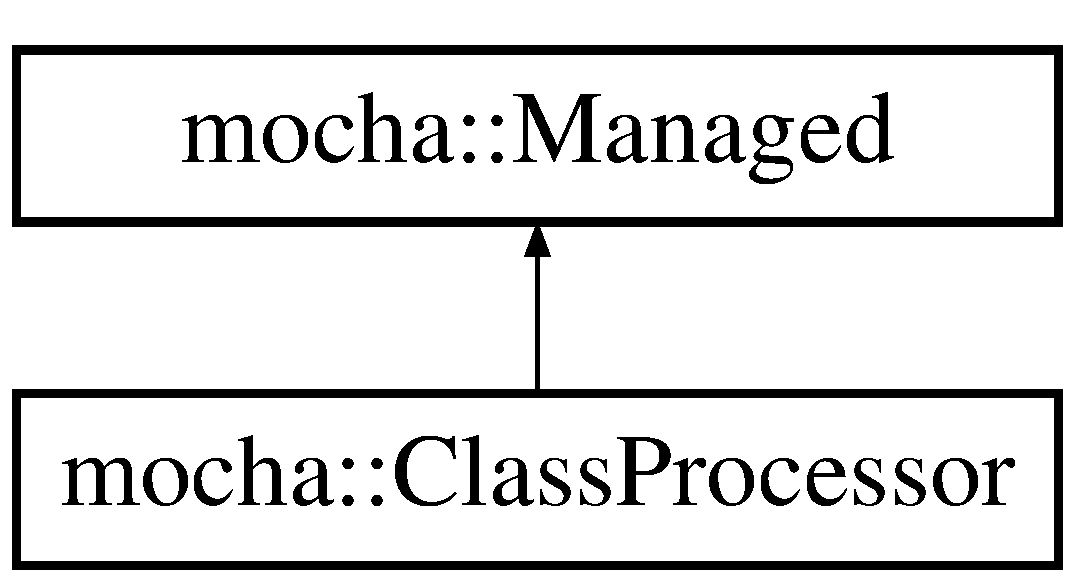
\includegraphics[height=2.000000cm]{classmocha_1_1_class_processor}
\end{center}
\end{figure}
\subsection*{Public Member Functions}
\begin{DoxyCompactItemize}
\item 
\hyperlink{classmocha_1_1_class_processor_a08d136f952bf8924f0937c36a8af840f}{ClassProcessor} (\hyperlink{classmocha_1_1_processor_info}{ProcessorInfo} $\ast$info, \hyperlink{classmocha_1_1_class}{Class} $\ast$ast\_\-node, \hyperlink{classmocha_1_1_statement}{Statement} $\ast$tmp\_\-stmt)
\item 
\hyperlink{classmocha_1_1_class_processor_a4bc98b761704a420e52fab5ff485acb6}{$\sim$ClassProcessor} ()
\item 
void \hyperlink{classmocha_1_1_class_processor_aa860cc22cd327b79d9c8aedb19c7667a}{ProcessNode} ()
\item 
const char $\ast$ \hyperlink{classmocha_1_1_class_processor_a05eea100d203a1c5f8a82c9136d8b0d8}{GetPrivateFieldName} ()
\item 
const char $\ast$ \hyperlink{classmocha_1_1_class_processor_a020054baa72f28b16513cfbd89cfd075}{GetName} ()
\item 
void \hyperlink{classmocha_1_1_class_processor_ab57d89a5787351ddba7941be4deee271}{SetPrivateStaticMap} (const char $\ast$name)
\item 
bool \hyperlink{classmocha_1_1_class_processor_a62ae94fe9fea168de267611684cf2954}{HasPrivateStaticMap} (const char $\ast$name)
\end{DoxyCompactItemize}
\subsection*{Private Member Functions}
\begin{DoxyCompactItemize}
\item 
void \hyperlink{classmocha_1_1_class_processor_a35790bb6819b2dd44084d00cea6014e5}{ProcessExtends\_\-} (\hyperlink{classmocha_1_1_ast_node}{AstNode} $\ast$node)
\item 
void \hyperlink{classmocha_1_1_class_processor_a7dbd185d12ed689e75c48d9443dd8ef3}{ProcessBody\_\-} (\hyperlink{classmocha_1_1_ast_node}{AstNode} $\ast$body)
\item 
void \hyperlink{classmocha_1_1_class_processor_a8867933a1814c7e9434701bfd82b4e8f}{ProcessMember\_\-} (\hyperlink{classmocha_1_1_class_properties}{ClassProperties} $\ast$body)
\item 
void \hyperlink{classmocha_1_1_class_processor_a969b4c75a350c276cf1a46d51d6590c0}{IterateMember\_\-} (\hyperlink{classmocha_1_1_ast_node}{AstNode} $\ast$list, bool is\_\-prototype, bool is\_\-private, bool is\_\-instance)
\item 
void \hyperlink{classmocha_1_1_class_processor_a3249aa54768ef4f9f17c83ba011ee017}{ProcessEachMember\_\-} (\hyperlink{classmocha_1_1_ast_node}{AstNode} $\ast$node, bool is\_\-prototype, bool is\_\-private, bool is\_\-instance)
\item 
void \hyperlink{classmocha_1_1_class_processor_a40cdf4b1db8f25a96934ac25a3907a0f}{ProcessVariable\_\-} (\hyperlink{classmocha_1_1_ast_node}{AstNode} $\ast$node, bool is\_\-prototype, bool is\_\-private, bool is\_\-instance, bool is\_\-const)
\item 
void \hyperlink{classmocha_1_1_class_processor_a0aa858fe5ebd728e0e2aedda5a935223}{ProcessFunction\_\-} (\hyperlink{classmocha_1_1_function}{Function} $\ast$function, bool is\_\-prottoype, bool is\_\-private, bool is\_\-instance)
\item 
void \hyperlink{classmocha_1_1_class_processor_ab3b3b1a0e1a9005442e223292b3eb019}{ProcessConstructor\_\-} (\hyperlink{classmocha_1_1_function}{Function} $\ast$constructor)
\item 
void \hyperlink{classmocha_1_1_class_processor_a13e7dbbc74820beeb82e2a6843801b4f}{CreateEmptyConstructor\_\-} ()
\item 
void \hyperlink{classmocha_1_1_class_processor_a9e4f585d68f25b950405231dd2fb94c2}{ProcessDsta\_\-} (\hyperlink{classmocha_1_1_value_node}{ValueNode} $\ast$value, bool is\_\-const, \hyperlink{namespacemocha_ac3d8a2fe64806b144916b0b16719a540}{DstaCallback} callback)
\item 
void \hyperlink{classmocha_1_1_class_processor_a59da2ad99788e504c991b465c35462e3}{SimpleVariables\_\-} (\hyperlink{classmocha_1_1_ast_node}{AstNode} $\ast$node, bool is\_\-const)
\item 
void \hyperlink{classmocha_1_1_class_processor_a857e9b17c939e57efbb0b737cbd956dd}{NoSimpleVariables\_\-} (\hyperlink{classmocha_1_1_ast_node}{AstNode} $\ast$node, bool is\_\-prototype, bool is\_\-private, bool is\_\-instance, bool is\_\-const)
\end{DoxyCompactItemize}
\subsection*{Private Attributes}
\begin{DoxyCompactItemize}
\item 
int \hyperlink{classmocha_1_1_class_processor_a48fe8c1d4ebd2e18be5ecedf1618af80}{class\_\-id\_\-}
\item 
std::string \hyperlink{classmocha_1_1_class_processor_a6cee088c1f255c143fcba53994102461}{name\_\-}
\item 
std::string \hyperlink{classmocha_1_1_class_processor_abb72577e164ec690e69e29d555aab92d}{random\_\-field\_\-}
\item 
\hyperlink{classmocha_1_1_processor_info}{ProcessorInfo} $\ast$ \hyperlink{classmocha_1_1_class_processor_a4306a92ebfbd33320b8a485b0c420f27}{info\_\-}
\item 
\hyperlink{classmocha_1_1_ast_node}{AstNode} $\ast$ \hyperlink{classmocha_1_1_class_processor_aeb64e1570c436c65ed98c3c1274799d6}{closure\_\-}
\item 
\hyperlink{classmocha_1_1_function}{Function} $\ast$ \hyperlink{classmocha_1_1_class_processor_ab5674a30639efa457b81aabe2cc7778d}{common\_\-constructor\_\-}
\item 
\hyperlink{classmocha_1_1_class}{Class} $\ast$ \hyperlink{classmocha_1_1_class_processor_a15511bef8f5889e25f65d39d9f23d5df}{class\_\-}
\item 
\hyperlink{classmocha_1_1_class_processor_utils}{ClassProcessorUtils} $\ast$ \hyperlink{classmocha_1_1_class_processor_ad51b7e60254b3eeaea78992996d00bcd}{utils\_\-}
\item 
\hyperlink{classmocha_1_1_function}{Function} $\ast$ \hyperlink{classmocha_1_1_class_processor_a224ba4a0c7686ccf21161a02550bf713}{closure\_\-body\_\-}
\item 
\hyperlink{classmocha_1_1_statement}{Statement} $\ast$ \hyperlink{classmocha_1_1_class_processor_a5b61b8872052d21ab40c071951871f99}{tmp\_\-stmt\_\-}
\item 
\hyperlink{classmocha_1_1_function}{Function} $\ast$ \hyperlink{classmocha_1_1_class_processor_a58b2732fd5cca6a818c342585c67aff6}{constructor\_\-}
\item 
\hyperlink{classmocha_1_1_hash_map}{HashMap}$<$ const char $\ast$, bool $>$ \hyperlink{classmocha_1_1_class_processor_a13be0d8b8aa75a5058b8521925a9d74b}{private\_\-static\_\-map\_\-}
\end{DoxyCompactItemize}


\subsection{Detailed Description}


Definition at line 39 of file class\_\-processor.h.



\subsection{Constructor \& Destructor Documentation}
\hypertarget{classmocha_1_1_class_processor_a08d136f952bf8924f0937c36a8af840f}{
\index{mocha::ClassProcessor@{mocha::ClassProcessor}!ClassProcessor@{ClassProcessor}}
\index{ClassProcessor@{ClassProcessor}!mocha::ClassProcessor@{mocha::ClassProcessor}}
\subsubsection[{ClassProcessor}]{\setlength{\rightskip}{0pt plus 5cm}mocha::ClassProcessor::ClassProcessor (
\begin{DoxyParamCaption}
\item[{{\bf ProcessorInfo} $\ast$}]{info, }
\item[{{\bf Class} $\ast$}]{ast\_\-node, }
\item[{{\bf Statement} $\ast$}]{tmp\_\-stmt}
\end{DoxyParamCaption}
)}}
\label{classmocha_1_1_class_processor_a08d136f952bf8924f0937c36a8af840f}


Definition at line 460 of file class\_\-processor.cc.

\hypertarget{classmocha_1_1_class_processor_a4bc98b761704a420e52fab5ff485acb6}{
\index{mocha::ClassProcessor@{mocha::ClassProcessor}!$\sim$ClassProcessor@{$\sim$ClassProcessor}}
\index{$\sim$ClassProcessor@{$\sim$ClassProcessor}!mocha::ClassProcessor@{mocha::ClassProcessor}}
\subsubsection[{$\sim$ClassProcessor}]{\setlength{\rightskip}{0pt plus 5cm}mocha::ClassProcessor::$\sim$ClassProcessor (
\begin{DoxyParamCaption}
{}
\end{DoxyParamCaption}
)}}
\label{classmocha_1_1_class_processor_a4bc98b761704a420e52fab5ff485acb6}


Definition at line 472 of file class\_\-processor.cc.



\subsection{Member Function Documentation}
\hypertarget{classmocha_1_1_class_processor_a13e7dbbc74820beeb82e2a6843801b4f}{
\index{mocha::ClassProcessor@{mocha::ClassProcessor}!CreateEmptyConstructor\_\-@{CreateEmptyConstructor\_\-}}
\index{CreateEmptyConstructor\_\-@{CreateEmptyConstructor\_\-}!mocha::ClassProcessor@{mocha::ClassProcessor}}
\subsubsection[{CreateEmptyConstructor\_\-}]{\setlength{\rightskip}{0pt plus 5cm}void mocha::ClassProcessor::CreateEmptyConstructor\_\- (
\begin{DoxyParamCaption}
{}
\end{DoxyParamCaption}
)\hspace{0.3cm}{\ttfamily  \mbox{[}inline, private\mbox{]}}}}
\label{classmocha_1_1_class_processor_a13e7dbbc74820beeb82e2a6843801b4f}


Definition at line 610 of file class\_\-processor.cc.

\hypertarget{classmocha_1_1_class_processor_a020054baa72f28b16513cfbd89cfd075}{
\index{mocha::ClassProcessor@{mocha::ClassProcessor}!GetName@{GetName}}
\index{GetName@{GetName}!mocha::ClassProcessor@{mocha::ClassProcessor}}
\subsubsection[{GetName}]{\setlength{\rightskip}{0pt plus 5cm}const char$\ast$ mocha::ClassProcessor::GetName (
\begin{DoxyParamCaption}
{}
\end{DoxyParamCaption}
)\hspace{0.3cm}{\ttfamily  \mbox{[}inline\mbox{]}}}}
\label{classmocha_1_1_class_processor_a020054baa72f28b16513cfbd89cfd075}


Definition at line 45 of file class\_\-processor.h.

\hypertarget{classmocha_1_1_class_processor_a05eea100d203a1c5f8a82c9136d8b0d8}{
\index{mocha::ClassProcessor@{mocha::ClassProcessor}!GetPrivateFieldName@{GetPrivateFieldName}}
\index{GetPrivateFieldName@{GetPrivateFieldName}!mocha::ClassProcessor@{mocha::ClassProcessor}}
\subsubsection[{GetPrivateFieldName}]{\setlength{\rightskip}{0pt plus 5cm}const char$\ast$ mocha::ClassProcessor::GetPrivateFieldName (
\begin{DoxyParamCaption}
{}
\end{DoxyParamCaption}
)\hspace{0.3cm}{\ttfamily  \mbox{[}inline\mbox{]}}}}
\label{classmocha_1_1_class_processor_a05eea100d203a1c5f8a82c9136d8b0d8}


Definition at line 44 of file class\_\-processor.h.

\hypertarget{classmocha_1_1_class_processor_a62ae94fe9fea168de267611684cf2954}{
\index{mocha::ClassProcessor@{mocha::ClassProcessor}!HasPrivateStaticMap@{HasPrivateStaticMap}}
\index{HasPrivateStaticMap@{HasPrivateStaticMap}!mocha::ClassProcessor@{mocha::ClassProcessor}}
\subsubsection[{HasPrivateStaticMap}]{\setlength{\rightskip}{0pt plus 5cm}bool mocha::ClassProcessor::HasPrivateStaticMap (
\begin{DoxyParamCaption}
\item[{const char $\ast$}]{name}
\end{DoxyParamCaption}
)\hspace{0.3cm}{\ttfamily  \mbox{[}inline\mbox{]}}}}
\label{classmocha_1_1_class_processor_a62ae94fe9fea168de267611684cf2954}


Definition at line 47 of file class\_\-processor.h.

\hypertarget{classmocha_1_1_class_processor_a969b4c75a350c276cf1a46d51d6590c0}{
\index{mocha::ClassProcessor@{mocha::ClassProcessor}!IterateMember\_\-@{IterateMember\_\-}}
\index{IterateMember\_\-@{IterateMember\_\-}!mocha::ClassProcessor@{mocha::ClassProcessor}}
\subsubsection[{IterateMember\_\-}]{\setlength{\rightskip}{0pt plus 5cm}void mocha::ClassProcessor::IterateMember\_\- (
\begin{DoxyParamCaption}
\item[{{\bf AstNode} $\ast$}]{list, }
\item[{bool}]{is\_\-prototype, }
\item[{bool}]{is\_\-private, }
\item[{bool}]{is\_\-instance}
\end{DoxyParamCaption}
)\hspace{0.3cm}{\ttfamily  \mbox{[}inline, private\mbox{]}}}}
\label{classmocha_1_1_class_processor_a969b4c75a350c276cf1a46d51d6590c0}


Definition at line 619 of file class\_\-processor.cc.

\hypertarget{classmocha_1_1_class_processor_a857e9b17c939e57efbb0b737cbd956dd}{
\index{mocha::ClassProcessor@{mocha::ClassProcessor}!NoSimpleVariables\_\-@{NoSimpleVariables\_\-}}
\index{NoSimpleVariables\_\-@{NoSimpleVariables\_\-}!mocha::ClassProcessor@{mocha::ClassProcessor}}
\subsubsection[{NoSimpleVariables\_\-}]{\setlength{\rightskip}{0pt plus 5cm}void mocha::ClassProcessor::NoSimpleVariables\_\- (
\begin{DoxyParamCaption}
\item[{{\bf AstNode} $\ast$}]{node, }
\item[{bool}]{is\_\-prototype, }
\item[{bool}]{is\_\-private, }
\item[{bool}]{is\_\-instance, }
\item[{bool}]{is\_\-const}
\end{DoxyParamCaption}
)\hspace{0.3cm}{\ttfamily  \mbox{[}inline, private\mbox{]}}}}
\label{classmocha_1_1_class_processor_a857e9b17c939e57efbb0b737cbd956dd}


Definition at line 716 of file class\_\-processor.cc.

\hypertarget{classmocha_1_1_class_processor_a7dbd185d12ed689e75c48d9443dd8ef3}{
\index{mocha::ClassProcessor@{mocha::ClassProcessor}!ProcessBody\_\-@{ProcessBody\_\-}}
\index{ProcessBody\_\-@{ProcessBody\_\-}!mocha::ClassProcessor@{mocha::ClassProcessor}}
\subsubsection[{ProcessBody\_\-}]{\setlength{\rightskip}{0pt plus 5cm}void mocha::ClassProcessor::ProcessBody\_\- (
\begin{DoxyParamCaption}
\item[{{\bf AstNode} $\ast$}]{body}
\end{DoxyParamCaption}
)\hspace{0.3cm}{\ttfamily  \mbox{[}inline, private\mbox{]}}}}
\label{classmocha_1_1_class_processor_a7dbd185d12ed689e75c48d9443dd8ef3}


Definition at line 545 of file class\_\-processor.cc.

\hypertarget{classmocha_1_1_class_processor_ab3b3b1a0e1a9005442e223292b3eb019}{
\index{mocha::ClassProcessor@{mocha::ClassProcessor}!ProcessConstructor\_\-@{ProcessConstructor\_\-}}
\index{ProcessConstructor\_\-@{ProcessConstructor\_\-}!mocha::ClassProcessor@{mocha::ClassProcessor}}
\subsubsection[{ProcessConstructor\_\-}]{\setlength{\rightskip}{0pt plus 5cm}void mocha::ClassProcessor::ProcessConstructor\_\- (
\begin{DoxyParamCaption}
\item[{{\bf Function} $\ast$}]{constructor}
\end{DoxyParamCaption}
)\hspace{0.3cm}{\ttfamily  \mbox{[}inline, private\mbox{]}}}}
\label{classmocha_1_1_class_processor_ab3b3b1a0e1a9005442e223292b3eb019}


Definition at line 587 of file class\_\-processor.cc.

\hypertarget{classmocha_1_1_class_processor_a9e4f585d68f25b950405231dd2fb94c2}{
\index{mocha::ClassProcessor@{mocha::ClassProcessor}!ProcessDsta\_\-@{ProcessDsta\_\-}}
\index{ProcessDsta\_\-@{ProcessDsta\_\-}!mocha::ClassProcessor@{mocha::ClassProcessor}}
\subsubsection[{ProcessDsta\_\-}]{\setlength{\rightskip}{0pt plus 5cm}void mocha::ClassProcessor::ProcessDsta\_\- (
\begin{DoxyParamCaption}
\item[{{\bf ValueNode} $\ast$}]{value, }
\item[{bool}]{is\_\-const, }
\item[{{\bf DstaCallback}}]{callback}
\end{DoxyParamCaption}
)\hspace{0.3cm}{\ttfamily  \mbox{[}inline, private\mbox{]}}}}
\label{classmocha_1_1_class_processor_a9e4f585d68f25b950405231dd2fb94c2}


Definition at line 666 of file class\_\-processor.cc.

\hypertarget{classmocha_1_1_class_processor_a3249aa54768ef4f9f17c83ba011ee017}{
\index{mocha::ClassProcessor@{mocha::ClassProcessor}!ProcessEachMember\_\-@{ProcessEachMember\_\-}}
\index{ProcessEachMember\_\-@{ProcessEachMember\_\-}!mocha::ClassProcessor@{mocha::ClassProcessor}}
\subsubsection[{ProcessEachMember\_\-}]{\setlength{\rightskip}{0pt plus 5cm}void mocha::ClassProcessor::ProcessEachMember\_\- (
\begin{DoxyParamCaption}
\item[{{\bf AstNode} $\ast$}]{node, }
\item[{bool}]{is\_\-prototype, }
\item[{bool}]{is\_\-private, }
\item[{bool}]{is\_\-instance}
\end{DoxyParamCaption}
)\hspace{0.3cm}{\ttfamily  \mbox{[}inline, private\mbox{]}}}}
\label{classmocha_1_1_class_processor_a3249aa54768ef4f9f17c83ba011ee017}


Definition at line 629 of file class\_\-processor.cc.

\hypertarget{classmocha_1_1_class_processor_a35790bb6819b2dd44084d00cea6014e5}{
\index{mocha::ClassProcessor@{mocha::ClassProcessor}!ProcessExtends\_\-@{ProcessExtends\_\-}}
\index{ProcessExtends\_\-@{ProcessExtends\_\-}!mocha::ClassProcessor@{mocha::ClassProcessor}}
\subsubsection[{ProcessExtends\_\-}]{\setlength{\rightskip}{0pt plus 5cm}void mocha::ClassProcessor::ProcessExtends\_\- (
\begin{DoxyParamCaption}
\item[{{\bf AstNode} $\ast$}]{node}
\end{DoxyParamCaption}
)\hspace{0.3cm}{\ttfamily  \mbox{[}inline, private\mbox{]}}}}
\label{classmocha_1_1_class_processor_a35790bb6819b2dd44084d00cea6014e5}


Definition at line 508 of file class\_\-processor.cc.

\hypertarget{classmocha_1_1_class_processor_a0aa858fe5ebd728e0e2aedda5a935223}{
\index{mocha::ClassProcessor@{mocha::ClassProcessor}!ProcessFunction\_\-@{ProcessFunction\_\-}}
\index{ProcessFunction\_\-@{ProcessFunction\_\-}!mocha::ClassProcessor@{mocha::ClassProcessor}}
\subsubsection[{ProcessFunction\_\-}]{\setlength{\rightskip}{0pt plus 5cm}void mocha::ClassProcessor::ProcessFunction\_\- (
\begin{DoxyParamCaption}
\item[{{\bf Function} $\ast$}]{function, }
\item[{bool}]{is\_\-prottoype, }
\item[{bool}]{is\_\-private, }
\item[{bool}]{is\_\-instance}
\end{DoxyParamCaption}
)\hspace{0.3cm}{\ttfamily  \mbox{[}inline, private\mbox{]}}}}
\label{classmocha_1_1_class_processor_a0aa858fe5ebd728e0e2aedda5a935223}


Definition at line 800 of file class\_\-processor.cc.

\hypertarget{classmocha_1_1_class_processor_a8867933a1814c7e9434701bfd82b4e8f}{
\index{mocha::ClassProcessor@{mocha::ClassProcessor}!ProcessMember\_\-@{ProcessMember\_\-}}
\index{ProcessMember\_\-@{ProcessMember\_\-}!mocha::ClassProcessor@{mocha::ClassProcessor}}
\subsubsection[{ProcessMember\_\-}]{\setlength{\rightskip}{0pt plus 5cm}void mocha::ClassProcessor::ProcessMember\_\- (
\begin{DoxyParamCaption}
\item[{{\bf ClassProperties} $\ast$}]{body}
\end{DoxyParamCaption}
)\hspace{0.3cm}{\ttfamily  \mbox{[}inline, private\mbox{]}}}}
\label{classmocha_1_1_class_processor_a8867933a1814c7e9434701bfd82b4e8f}


Definition at line 555 of file class\_\-processor.cc.

\hypertarget{classmocha_1_1_class_processor_aa860cc22cd327b79d9c8aedb19c7667a}{
\index{mocha::ClassProcessor@{mocha::ClassProcessor}!ProcessNode@{ProcessNode}}
\index{ProcessNode@{ProcessNode}!mocha::ClassProcessor@{mocha::ClassProcessor}}
\subsubsection[{ProcessNode}]{\setlength{\rightskip}{0pt plus 5cm}void mocha::ClassProcessor::ProcessNode (
\begin{DoxyParamCaption}
{}
\end{DoxyParamCaption}
)}}
\label{classmocha_1_1_class_processor_aa860cc22cd327b79d9c8aedb19c7667a}


Definition at line 477 of file class\_\-processor.cc.

\hypertarget{classmocha_1_1_class_processor_a40cdf4b1db8f25a96934ac25a3907a0f}{
\index{mocha::ClassProcessor@{mocha::ClassProcessor}!ProcessVariable\_\-@{ProcessVariable\_\-}}
\index{ProcessVariable\_\-@{ProcessVariable\_\-}!mocha::ClassProcessor@{mocha::ClassProcessor}}
\subsubsection[{ProcessVariable\_\-}]{\setlength{\rightskip}{0pt plus 5cm}void mocha::ClassProcessor::ProcessVariable\_\- (
\begin{DoxyParamCaption}
\item[{{\bf AstNode} $\ast$}]{node, }
\item[{bool}]{is\_\-prototype, }
\item[{bool}]{is\_\-private, }
\item[{bool}]{is\_\-instance, }
\item[{bool}]{is\_\-const}
\end{DoxyParamCaption}
)\hspace{0.3cm}{\ttfamily  \mbox{[}inline, private\mbox{]}}}}
\label{classmocha_1_1_class_processor_a40cdf4b1db8f25a96934ac25a3907a0f}


Definition at line 786 of file class\_\-processor.cc.

\hypertarget{classmocha_1_1_class_processor_ab57d89a5787351ddba7941be4deee271}{
\index{mocha::ClassProcessor@{mocha::ClassProcessor}!SetPrivateStaticMap@{SetPrivateStaticMap}}
\index{SetPrivateStaticMap@{SetPrivateStaticMap}!mocha::ClassProcessor@{mocha::ClassProcessor}}
\subsubsection[{SetPrivateStaticMap}]{\setlength{\rightskip}{0pt plus 5cm}void mocha::ClassProcessor::SetPrivateStaticMap (
\begin{DoxyParamCaption}
\item[{const char $\ast$}]{name}
\end{DoxyParamCaption}
)\hspace{0.3cm}{\ttfamily  \mbox{[}inline\mbox{]}}}}
\label{classmocha_1_1_class_processor_ab57d89a5787351ddba7941be4deee271}


Definition at line 46 of file class\_\-processor.h.

\hypertarget{classmocha_1_1_class_processor_a59da2ad99788e504c991b465c35462e3}{
\index{mocha::ClassProcessor@{mocha::ClassProcessor}!SimpleVariables\_\-@{SimpleVariables\_\-}}
\index{SimpleVariables\_\-@{SimpleVariables\_\-}!mocha::ClassProcessor@{mocha::ClassProcessor}}
\subsubsection[{SimpleVariables\_\-}]{\setlength{\rightskip}{0pt plus 5cm}void mocha::ClassProcessor::SimpleVariables\_\- (
\begin{DoxyParamCaption}
\item[{{\bf AstNode} $\ast$}]{node, }
\item[{bool}]{is\_\-const}
\end{DoxyParamCaption}
)\hspace{0.3cm}{\ttfamily  \mbox{[}inline, private\mbox{]}}}}
\label{classmocha_1_1_class_processor_a59da2ad99788e504c991b465c35462e3}


Definition at line 691 of file class\_\-processor.cc.



\subsection{Member Data Documentation}
\hypertarget{classmocha_1_1_class_processor_a15511bef8f5889e25f65d39d9f23d5df}{
\index{mocha::ClassProcessor@{mocha::ClassProcessor}!class\_\-@{class\_\-}}
\index{class\_\-@{class\_\-}!mocha::ClassProcessor@{mocha::ClassProcessor}}
\subsubsection[{class\_\-}]{\setlength{\rightskip}{0pt plus 5cm}{\bf Class}$\ast$ {\bf mocha::ClassProcessor::class\_\-}\hspace{0.3cm}{\ttfamily  \mbox{[}private\mbox{]}}}}
\label{classmocha_1_1_class_processor_a15511bef8f5889e25f65d39d9f23d5df}


Definition at line 68 of file class\_\-processor.h.

\hypertarget{classmocha_1_1_class_processor_a48fe8c1d4ebd2e18be5ecedf1618af80}{
\index{mocha::ClassProcessor@{mocha::ClassProcessor}!class\_\-id\_\-@{class\_\-id\_\-}}
\index{class\_\-id\_\-@{class\_\-id\_\-}!mocha::ClassProcessor@{mocha::ClassProcessor}}
\subsubsection[{class\_\-id\_\-}]{\setlength{\rightskip}{0pt plus 5cm}int {\bf mocha::ClassProcessor::class\_\-id\_\-}\hspace{0.3cm}{\ttfamily  \mbox{[}private\mbox{]}}}}
\label{classmocha_1_1_class_processor_a48fe8c1d4ebd2e18be5ecedf1618af80}


Definition at line 62 of file class\_\-processor.h.

\hypertarget{classmocha_1_1_class_processor_aeb64e1570c436c65ed98c3c1274799d6}{
\index{mocha::ClassProcessor@{mocha::ClassProcessor}!closure\_\-@{closure\_\-}}
\index{closure\_\-@{closure\_\-}!mocha::ClassProcessor@{mocha::ClassProcessor}}
\subsubsection[{closure\_\-}]{\setlength{\rightskip}{0pt plus 5cm}{\bf AstNode}$\ast$ {\bf mocha::ClassProcessor::closure\_\-}\hspace{0.3cm}{\ttfamily  \mbox{[}private\mbox{]}}}}
\label{classmocha_1_1_class_processor_aeb64e1570c436c65ed98c3c1274799d6}


Definition at line 66 of file class\_\-processor.h.

\hypertarget{classmocha_1_1_class_processor_a224ba4a0c7686ccf21161a02550bf713}{
\index{mocha::ClassProcessor@{mocha::ClassProcessor}!closure\_\-body\_\-@{closure\_\-body\_\-}}
\index{closure\_\-body\_\-@{closure\_\-body\_\-}!mocha::ClassProcessor@{mocha::ClassProcessor}}
\subsubsection[{closure\_\-body\_\-}]{\setlength{\rightskip}{0pt plus 5cm}{\bf Function}$\ast$ {\bf mocha::ClassProcessor::closure\_\-body\_\-}\hspace{0.3cm}{\ttfamily  \mbox{[}private\mbox{]}}}}
\label{classmocha_1_1_class_processor_a224ba4a0c7686ccf21161a02550bf713}


Definition at line 70 of file class\_\-processor.h.

\hypertarget{classmocha_1_1_class_processor_ab5674a30639efa457b81aabe2cc7778d}{
\index{mocha::ClassProcessor@{mocha::ClassProcessor}!common\_\-constructor\_\-@{common\_\-constructor\_\-}}
\index{common\_\-constructor\_\-@{common\_\-constructor\_\-}!mocha::ClassProcessor@{mocha::ClassProcessor}}
\subsubsection[{common\_\-constructor\_\-}]{\setlength{\rightskip}{0pt plus 5cm}{\bf Function}$\ast$ {\bf mocha::ClassProcessor::common\_\-constructor\_\-}\hspace{0.3cm}{\ttfamily  \mbox{[}private\mbox{]}}}}
\label{classmocha_1_1_class_processor_ab5674a30639efa457b81aabe2cc7778d}


Definition at line 67 of file class\_\-processor.h.

\hypertarget{classmocha_1_1_class_processor_a58b2732fd5cca6a818c342585c67aff6}{
\index{mocha::ClassProcessor@{mocha::ClassProcessor}!constructor\_\-@{constructor\_\-}}
\index{constructor\_\-@{constructor\_\-}!mocha::ClassProcessor@{mocha::ClassProcessor}}
\subsubsection[{constructor\_\-}]{\setlength{\rightskip}{0pt plus 5cm}{\bf Function}$\ast$ {\bf mocha::ClassProcessor::constructor\_\-}\hspace{0.3cm}{\ttfamily  \mbox{[}private\mbox{]}}}}
\label{classmocha_1_1_class_processor_a58b2732fd5cca6a818c342585c67aff6}


Definition at line 72 of file class\_\-processor.h.

\hypertarget{classmocha_1_1_class_processor_a4306a92ebfbd33320b8a485b0c420f27}{
\index{mocha::ClassProcessor@{mocha::ClassProcessor}!info\_\-@{info\_\-}}
\index{info\_\-@{info\_\-}!mocha::ClassProcessor@{mocha::ClassProcessor}}
\subsubsection[{info\_\-}]{\setlength{\rightskip}{0pt plus 5cm}{\bf ProcessorInfo}$\ast$ {\bf mocha::ClassProcessor::info\_\-}\hspace{0.3cm}{\ttfamily  \mbox{[}private\mbox{]}}}}
\label{classmocha_1_1_class_processor_a4306a92ebfbd33320b8a485b0c420f27}


Definition at line 65 of file class\_\-processor.h.

\hypertarget{classmocha_1_1_class_processor_a6cee088c1f255c143fcba53994102461}{
\index{mocha::ClassProcessor@{mocha::ClassProcessor}!name\_\-@{name\_\-}}
\index{name\_\-@{name\_\-}!mocha::ClassProcessor@{mocha::ClassProcessor}}
\subsubsection[{name\_\-}]{\setlength{\rightskip}{0pt plus 5cm}std::string {\bf mocha::ClassProcessor::name\_\-}\hspace{0.3cm}{\ttfamily  \mbox{[}private\mbox{]}}}}
\label{classmocha_1_1_class_processor_a6cee088c1f255c143fcba53994102461}


Definition at line 63 of file class\_\-processor.h.

\hypertarget{classmocha_1_1_class_processor_a13be0d8b8aa75a5058b8521925a9d74b}{
\index{mocha::ClassProcessor@{mocha::ClassProcessor}!private\_\-static\_\-map\_\-@{private\_\-static\_\-map\_\-}}
\index{private\_\-static\_\-map\_\-@{private\_\-static\_\-map\_\-}!mocha::ClassProcessor@{mocha::ClassProcessor}}
\subsubsection[{private\_\-static\_\-map\_\-}]{\setlength{\rightskip}{0pt plus 5cm}{\bf HashMap}$<$const char$\ast$,bool$>$ {\bf mocha::ClassProcessor::private\_\-static\_\-map\_\-}\hspace{0.3cm}{\ttfamily  \mbox{[}private\mbox{]}}}}
\label{classmocha_1_1_class_processor_a13be0d8b8aa75a5058b8521925a9d74b}


Definition at line 73 of file class\_\-processor.h.

\hypertarget{classmocha_1_1_class_processor_abb72577e164ec690e69e29d555aab92d}{
\index{mocha::ClassProcessor@{mocha::ClassProcessor}!random\_\-field\_\-@{random\_\-field\_\-}}
\index{random\_\-field\_\-@{random\_\-field\_\-}!mocha::ClassProcessor@{mocha::ClassProcessor}}
\subsubsection[{random\_\-field\_\-}]{\setlength{\rightskip}{0pt plus 5cm}std::string {\bf mocha::ClassProcessor::random\_\-field\_\-}\hspace{0.3cm}{\ttfamily  \mbox{[}private\mbox{]}}}}
\label{classmocha_1_1_class_processor_abb72577e164ec690e69e29d555aab92d}


Definition at line 64 of file class\_\-processor.h.

\hypertarget{classmocha_1_1_class_processor_a5b61b8872052d21ab40c071951871f99}{
\index{mocha::ClassProcessor@{mocha::ClassProcessor}!tmp\_\-stmt\_\-@{tmp\_\-stmt\_\-}}
\index{tmp\_\-stmt\_\-@{tmp\_\-stmt\_\-}!mocha::ClassProcessor@{mocha::ClassProcessor}}
\subsubsection[{tmp\_\-stmt\_\-}]{\setlength{\rightskip}{0pt plus 5cm}{\bf Statement}$\ast$ {\bf mocha::ClassProcessor::tmp\_\-stmt\_\-}\hspace{0.3cm}{\ttfamily  \mbox{[}private\mbox{]}}}}
\label{classmocha_1_1_class_processor_a5b61b8872052d21ab40c071951871f99}


Definition at line 71 of file class\_\-processor.h.

\hypertarget{classmocha_1_1_class_processor_ad51b7e60254b3eeaea78992996d00bcd}{
\index{mocha::ClassProcessor@{mocha::ClassProcessor}!utils\_\-@{utils\_\-}}
\index{utils\_\-@{utils\_\-}!mocha::ClassProcessor@{mocha::ClassProcessor}}
\subsubsection[{utils\_\-}]{\setlength{\rightskip}{0pt plus 5cm}{\bf ClassProcessorUtils}$\ast$ {\bf mocha::ClassProcessor::utils\_\-}\hspace{0.3cm}{\ttfamily  \mbox{[}private\mbox{]}}}}
\label{classmocha_1_1_class_processor_ad51b7e60254b3eeaea78992996d00bcd}


Definition at line 69 of file class\_\-processor.h.



The documentation for this class was generated from the following files:\begin{DoxyCompactItemize}
\item 
Y:/mocha/src/ast/visitors/utils/processors/\hyperlink{class__processor_8h}{class\_\-processor.h}\item 
Y:/mocha/src/ast/visitors/utils/processors/\hyperlink{class__processor_8cc}{class\_\-processor.cc}\end{DoxyCompactItemize}

\hypertarget{classmocha_1_1_class_processor_utils}{
\section{mocha::ClassProcessorUtils Class Reference}
\label{classmocha_1_1_class_processor_utils}\index{mocha::ClassProcessorUtils@{mocha::ClassProcessorUtils}}
}
\subsection*{Public Member Functions}
\begin{DoxyCompactItemize}
\item 
\hyperlink{classmocha_1_1_class_processor_utils_ab68b22b8df753884d141c79423128759}{ClassProcessorUtils} (\hyperlink{classmocha_1_1_class_processor}{ClassProcessor} $\ast$processor, std::string $\ast$private\_\-field)
\item 
\hyperlink{classmocha_1_1_class_processor_utils_a27c762615ca89f0543d08d286f6d8981}{$\sim$ClassProcessorUtils} ()
\item 
\hyperlink{classmocha_1_1_call_exp}{CallExp} $\ast$ \hyperlink{classmocha_1_1_class_processor_utils_a610865dafa045c1406bebd542b5c5d83}{CreateHiddenMember} (\hyperlink{classmocha_1_1_node_list}{NodeList} $\ast$args, long line)
\item 
\hyperlink{classmocha_1_1_value_node}{ValueNode} $\ast$ \hyperlink{classmocha_1_1_class_processor_utils_af75b7f05a1ec3c13d31b98b977bf82ec}{CreatePrivateHolderName} (long line)
\item 
\hyperlink{classmocha_1_1_value_node}{ValueNode} $\ast$ \hyperlink{classmocha_1_1_class_processor_utils_a330e44d58fbec85a47df4a7721679471}{CreatePrivateField} (long line)
\item 
\hyperlink{classmocha_1_1_value_node}{ValueNode} $\ast$ \hyperlink{classmocha_1_1_class_processor_utils_ab57d62ddfbaeb403018b214da4d09067}{CreateThisNode} (long line)
\item 
\hyperlink{classmocha_1_1_call_exp}{CallExp} $\ast$ \hyperlink{classmocha_1_1_class_processor_utils_aa60e32378408cad91c137cac3f69bcbc}{CreatePrivateFieldAccessor} (\hyperlink{classmocha_1_1_ast_node}{AstNode} $\ast$name)
\item 
\hyperlink{classmocha_1_1_value_node}{ValueNode} $\ast$ \hyperlink{classmocha_1_1_class_processor_utils_a14bb29392495622b718afc8542e77d7f}{CreateTypeIdNode} (long line)
\item 
\hyperlink{classmocha_1_1_call_exp}{CallExp} $\ast$ \hyperlink{classmocha_1_1_class_processor_utils_ac7e7158b65ce6bc045868d46763c3634}{CreateRecord} (long line)
\item 
\hyperlink{classmocha_1_1_expression_stmt}{ExpressionStmt} $\ast$ \hyperlink{classmocha_1_1_class_processor_utils_ab56c8f661100300b99a4ef01cca8ba11}{SetMark} (\hyperlink{classmocha_1_1_function}{Function} $\ast$fn)
\item 
\hyperlink{classmocha_1_1_ast_node}{AstNode} $\ast$ \hyperlink{classmocha_1_1_class_processor_utils_a9327665bf5bd23c50bf7925e4b497769}{CreateHiddenConstructor} (const char $\ast$name, long line)
\item 
\hyperlink{classmocha_1_1_ast_node}{AstNode} $\ast$ \hyperlink{classmocha_1_1_class_processor_utils_aa3d30f0d1db866791c961ba4193b4810}{CreateConstructorInitializer} (const char $\ast$name, long line)
\item 
\hyperlink{classmocha_1_1_ast_node}{AstNode} $\ast$ \hyperlink{classmocha_1_1_class_processor_utils_a29af6b8e270cc7ff00c9ed19ec06daaa}{CreateMixin} (\hyperlink{classmocha_1_1_ast_node}{AstNode} $\ast$mixins, \hyperlink{classmocha_1_1_processor_info}{ProcessorInfo} $\ast$info)
\item 
void \hyperlink{classmocha_1_1_class_processor_utils_a5a63e6c4b0567dfa908eeed3ac896ede}{CreateMixinStmt} (const char $\ast$name, \hyperlink{classmocha_1_1_ast_node}{AstNode} $\ast$mixin\_\-list, \hyperlink{classmocha_1_1_ast_node}{AstNode} $\ast$body)
\item 
void \hyperlink{classmocha_1_1_class_processor_utils_a66a15724e9fc5b217b958550c6911016}{CreateRequirementsCheck} (const char $\ast$name, const char $\ast$filename, \hyperlink{classmocha_1_1_ast_node}{AstNode} $\ast$mixin\_\-list, \hyperlink{classmocha_1_1_ast_node}{AstNode} $\ast$body)
\item 
\hyperlink{classmocha_1_1_ast_node}{AstNode} $\ast$ \hyperlink{classmocha_1_1_class_processor_utils_a66448399c2ac6f95d54efd5b2740ab3a}{CreateHolderAssignment} (\hyperlink{classmocha_1_1_ast_node}{AstNode} $\ast$val, \hyperlink{classmocha_1_1_ast_node}{AstNode} $\ast$name, \hyperlink{classmocha_1_1_class}{Class} $\ast$class\_\-, bool is\_\-const, bool is\_\-instance)
\item 
void \hyperlink{classmocha_1_1_class_processor_utils_ae749932a020a7f02b636caadc41ed885}{Finish} (const char $\ast$name, \hyperlink{classmocha_1_1_class}{Class} $\ast$class\_\-, \hyperlink{classmocha_1_1_ast_node}{AstNode} $\ast$closure\_\-, \hyperlink{classmocha_1_1_processor_info}{ProcessorInfo} $\ast$info)
\item 
\hyperlink{classmocha_1_1_variable_stmt}{VariableStmt} $\ast$ \hyperlink{classmocha_1_1_class_processor_utils_a1b999dea09f4b52d22ba43c71febd23e}{CreatePrivateHolder} (\hyperlink{classmocha_1_1_class}{Class} $\ast$class\_\-, \hyperlink{classmocha_1_1_processor_info}{ProcessorInfo} $\ast$info)
\item 
\hyperlink{classmocha_1_1_ast_node}{AstNode} $\ast$ \hyperlink{classmocha_1_1_class_processor_utils_a4745971a910122bc31e366c0fa49f114}{GetSafeValue} (\hyperlink{classmocha_1_1_value_node}{ValueNode} $\ast$value)
\item 
\hyperlink{classmocha_1_1_expression_stmt}{ExpressionStmt} $\ast$ \hyperlink{classmocha_1_1_class_processor_utils_a2ff3e378a45327df8060e236970407b8}{InstancePrivate} (\hyperlink{classmocha_1_1_value_node}{ValueNode} $\ast$value)
\item 
\hyperlink{classmocha_1_1_expression_stmt}{ExpressionStmt} $\ast$ \hyperlink{classmocha_1_1_class_processor_utils_a425461673b00f5f837a893277b4d14cf}{InstancePublic} (\hyperlink{classmocha_1_1_value_node}{ValueNode} $\ast$value)
\item 
\hyperlink{classmocha_1_1_expression_stmt}{ExpressionStmt} $\ast$ \hyperlink{classmocha_1_1_class_processor_utils_abe05538ee0cc20be8f3740d05db761ae}{ConstantInstancePrivate} (\hyperlink{classmocha_1_1_value_node}{ValueNode} $\ast$value)
\item 
\hyperlink{classmocha_1_1_expression_stmt}{ExpressionStmt} $\ast$ \hyperlink{classmocha_1_1_class_processor_utils_ad239680f421167da1c307681f6b81197}{ConstantInstancePublic} (\hyperlink{classmocha_1_1_value_node}{ValueNode} $\ast$value)
\item 
\hyperlink{classmocha_1_1_expression_stmt}{ExpressionStmt} $\ast$ \hyperlink{classmocha_1_1_class_processor_utils_a4b47f30d7968755e17db302f8fe7bf9c}{PrototypePrivate} (\hyperlink{classmocha_1_1_ast_node}{AstNode} $\ast$name\_\-node, \hyperlink{classmocha_1_1_ast_node}{AstNode} $\ast$val)
\item 
\hyperlink{classmocha_1_1_expression_stmt}{ExpressionStmt} $\ast$ \hyperlink{classmocha_1_1_class_processor_utils_ac931857f4f62031b1ba249cf233da5c1}{PrototypePublic} (const char $\ast$class\_\-name, \hyperlink{classmocha_1_1_ast_node}{AstNode} $\ast$name\_\-node, \hyperlink{classmocha_1_1_ast_node}{AstNode} $\ast$val)
\item 
\hyperlink{classmocha_1_1_expression_stmt}{ExpressionStmt} $\ast$ \hyperlink{classmocha_1_1_class_processor_utils_af5b9c37de2825626bf80a70c43d41c00}{ConstantPrototypePrivate} (\hyperlink{classmocha_1_1_ast_node}{AstNode} $\ast$name\_\-node, \hyperlink{classmocha_1_1_ast_node}{AstNode} $\ast$val)
\item 
\hyperlink{classmocha_1_1_expression_stmt}{ExpressionStmt} $\ast$ \hyperlink{classmocha_1_1_class_processor_utils_a50068b6d373030e45c8c57a0eee045c4}{ConstantPrototypePublic} (const char $\ast$class\_\-name, \hyperlink{classmocha_1_1_ast_node}{AstNode} $\ast$name\_\-node, \hyperlink{classmocha_1_1_ast_node}{AstNode} $\ast$val)
\item 
\hyperlink{classmocha_1_1_expression_stmt}{ExpressionStmt} $\ast$ \hyperlink{classmocha_1_1_class_processor_utils_a28a8c9dae3d507054c521d4b8f5e1830}{PublicStatic} (const char $\ast$class\_\-name, \hyperlink{classmocha_1_1_ast_node}{AstNode} $\ast$name\_\-node, \hyperlink{classmocha_1_1_ast_node}{AstNode} $\ast$val)
\item 
\hyperlink{classmocha_1_1_expression_stmt}{ExpressionStmt} $\ast$ \hyperlink{classmocha_1_1_class_processor_utils_a3d84ff9ef3f2d4082396169e1b99f6bb}{PublicConstantStatic} (const char $\ast$class\_\-name, \hyperlink{classmocha_1_1_ast_node}{AstNode} $\ast$name\_\-node, \hyperlink{classmocha_1_1_ast_node}{AstNode} $\ast$val)
\item 
\hyperlink{classmocha_1_1_expression_stmt}{ExpressionStmt} $\ast$ \hyperlink{classmocha_1_1_class_processor_utils_ac59461d97ab0bb6da1f1ad0024e85e1f}{PrivateStatic} (\hyperlink{classmocha_1_1_ast_node}{AstNode} $\ast$name\_\-node, \hyperlink{classmocha_1_1_ast_node}{AstNode} $\ast$val)
\item 
\hyperlink{classmocha_1_1_expression_stmt}{ExpressionStmt} $\ast$ \hyperlink{classmocha_1_1_class_processor_utils_ab81285773872b9fb9cdd7ceb33ad6f2a}{PrivateConstantStatic} (\hyperlink{classmocha_1_1_ast_node}{AstNode} $\ast$name\_\-node, \hyperlink{classmocha_1_1_ast_node}{AstNode} $\ast$val)
\item 
void \hyperlink{classmocha_1_1_class_processor_utils_afeb3b1bdc113c10b8417e1e9d217042a}{InstancePublicDsta} (const char $\ast$class\_\-name, \hyperlink{classmocha_1_1_function}{Function} $\ast$closure\_\-body, \hyperlink{classmocha_1_1_value_node}{ValueNode} $\ast$val, bool is\_\-const)
\item 
void \hyperlink{classmocha_1_1_class_processor_utils_a2b746fe441de3ed55f5ec11f6f5172d8}{InstancePrivateDsta} (const char $\ast$class\_\-name, \hyperlink{classmocha_1_1_function}{Function} $\ast$closure\_\-body, \hyperlink{classmocha_1_1_value_node}{ValueNode} $\ast$val, bool is\_\-const)
\item 
void \hyperlink{classmocha_1_1_class_processor_utils_ad30031d6087cd77d4d2cc6763c05352f}{PrototypePublicDsta} (const char $\ast$class\_\-name, \hyperlink{classmocha_1_1_function}{Function} $\ast$closure\_\-body, \hyperlink{classmocha_1_1_value_node}{ValueNode} $\ast$val, bool is\_\-const)
\item 
void \hyperlink{classmocha_1_1_class_processor_utils_ac3bfe46eb0acef03d504b0c6724fb7b4}{PrototypePrivateDsta} (const char $\ast$class\_\-name, \hyperlink{classmocha_1_1_function}{Function} $\ast$closure\_\-body, \hyperlink{classmocha_1_1_value_node}{ValueNode} $\ast$val, bool is\_\-const)
\item 
void \hyperlink{classmocha_1_1_class_processor_utils_ac5b625457ddf992f3b22b9e3a1bdee30}{PrivateStaticDsta} (const char $\ast$class\_\-name, \hyperlink{classmocha_1_1_function}{Function} $\ast$closure\_\-body, \hyperlink{classmocha_1_1_value_node}{ValueNode} $\ast$exp, bool is\_\-const)
\item 
void \hyperlink{classmocha_1_1_class_processor_utils_a86c2ceefe5e02737d5a0a9e8afcc7db1}{PublicStaticDsta} (const char $\ast$class\_\-name, \hyperlink{classmocha_1_1_function}{Function} $\ast$closure\_\-body, \hyperlink{classmocha_1_1_value_node}{ValueNode} $\ast$exp, bool is\_\-const)
\end{DoxyCompactItemize}
\subsection*{Private Attributes}
\begin{DoxyCompactItemize}
\item 
std::string $\ast$ \hyperlink{classmocha_1_1_class_processor_utils_a48ca9aca95f8511c95934051751eadb9}{private\_\-field\_\-}
\item 
\hyperlink{classmocha_1_1_class_processor}{ClassProcessor} $\ast$ \hyperlink{classmocha_1_1_class_processor_utils_ae8daab7ebd208801b9b7c640c8e3b3a0}{processor\_\-}
\end{DoxyCompactItemize}


\subsection{Detailed Description}


Definition at line 20 of file class\_\-processor.cc.



\subsection{Constructor \& Destructor Documentation}
\hypertarget{classmocha_1_1_class_processor_utils_ab68b22b8df753884d141c79423128759}{
\index{mocha::ClassProcessorUtils@{mocha::ClassProcessorUtils}!ClassProcessorUtils@{ClassProcessorUtils}}
\index{ClassProcessorUtils@{ClassProcessorUtils}!mocha::ClassProcessorUtils@{mocha::ClassProcessorUtils}}
\subsubsection[{ClassProcessorUtils}]{\setlength{\rightskip}{0pt plus 5cm}mocha::ClassProcessorUtils::ClassProcessorUtils (
\begin{DoxyParamCaption}
\item[{{\bf ClassProcessor} $\ast$}]{processor, }
\item[{std::string $\ast$}]{private\_\-field}
\end{DoxyParamCaption}
)\hspace{0.3cm}{\ttfamily  \mbox{[}inline\mbox{]}}}}
\label{classmocha_1_1_class_processor_utils_ab68b22b8df753884d141c79423128759}


Definition at line 22 of file class\_\-processor.cc.

\hypertarget{classmocha_1_1_class_processor_utils_a27c762615ca89f0543d08d286f6d8981}{
\index{mocha::ClassProcessorUtils@{mocha::ClassProcessorUtils}!$\sim$ClassProcessorUtils@{$\sim$ClassProcessorUtils}}
\index{$\sim$ClassProcessorUtils@{$\sim$ClassProcessorUtils}!mocha::ClassProcessorUtils@{mocha::ClassProcessorUtils}}
\subsubsection[{$\sim$ClassProcessorUtils}]{\setlength{\rightskip}{0pt plus 5cm}mocha::ClassProcessorUtils::$\sim$ClassProcessorUtils (
\begin{DoxyParamCaption}
{}
\end{DoxyParamCaption}
)\hspace{0.3cm}{\ttfamily  \mbox{[}inline\mbox{]}}}}
\label{classmocha_1_1_class_processor_utils_a27c762615ca89f0543d08d286f6d8981}


Definition at line 24 of file class\_\-processor.cc.



\subsection{Member Function Documentation}
\hypertarget{classmocha_1_1_class_processor_utils_abe05538ee0cc20be8f3740d05db761ae}{
\index{mocha::ClassProcessorUtils@{mocha::ClassProcessorUtils}!ConstantInstancePrivate@{ConstantInstancePrivate}}
\index{ConstantInstancePrivate@{ConstantInstancePrivate}!mocha::ClassProcessorUtils@{mocha::ClassProcessorUtils}}
\subsubsection[{ConstantInstancePrivate}]{\setlength{\rightskip}{0pt plus 5cm}{\bf ExpressionStmt}$\ast$ mocha::ClassProcessorUtils::ConstantInstancePrivate (
\begin{DoxyParamCaption}
\item[{{\bf ValueNode} $\ast$}]{value}
\end{DoxyParamCaption}
)\hspace{0.3cm}{\ttfamily  \mbox{[}inline\mbox{]}}}}
\label{classmocha_1_1_class_processor_utils_abe05538ee0cc20be8f3740d05db761ae}


Definition at line 274 of file class\_\-processor.cc.

\hypertarget{classmocha_1_1_class_processor_utils_ad239680f421167da1c307681f6b81197}{
\index{mocha::ClassProcessorUtils@{mocha::ClassProcessorUtils}!ConstantInstancePublic@{ConstantInstancePublic}}
\index{ConstantInstancePublic@{ConstantInstancePublic}!mocha::ClassProcessorUtils@{mocha::ClassProcessorUtils}}
\subsubsection[{ConstantInstancePublic}]{\setlength{\rightskip}{0pt plus 5cm}{\bf ExpressionStmt}$\ast$ mocha::ClassProcessorUtils::ConstantInstancePublic (
\begin{DoxyParamCaption}
\item[{{\bf ValueNode} $\ast$}]{value}
\end{DoxyParamCaption}
)\hspace{0.3cm}{\ttfamily  \mbox{[}inline\mbox{]}}}}
\label{classmocha_1_1_class_processor_utils_ad239680f421167da1c307681f6b81197}


Definition at line 282 of file class\_\-processor.cc.

\hypertarget{classmocha_1_1_class_processor_utils_af5b9c37de2825626bf80a70c43d41c00}{
\index{mocha::ClassProcessorUtils@{mocha::ClassProcessorUtils}!ConstantPrototypePrivate@{ConstantPrototypePrivate}}
\index{ConstantPrototypePrivate@{ConstantPrototypePrivate}!mocha::ClassProcessorUtils@{mocha::ClassProcessorUtils}}
\subsubsection[{ConstantPrototypePrivate}]{\setlength{\rightskip}{0pt plus 5cm}{\bf ExpressionStmt}$\ast$ mocha::ClassProcessorUtils::ConstantPrototypePrivate (
\begin{DoxyParamCaption}
\item[{{\bf AstNode} $\ast$}]{name\_\-node, }
\item[{{\bf AstNode} $\ast$}]{val}
\end{DoxyParamCaption}
)\hspace{0.3cm}{\ttfamily  \mbox{[}inline\mbox{]}}}}
\label{classmocha_1_1_class_processor_utils_af5b9c37de2825626bf80a70c43d41c00}


Definition at line 312 of file class\_\-processor.cc.

\hypertarget{classmocha_1_1_class_processor_utils_a50068b6d373030e45c8c57a0eee045c4}{
\index{mocha::ClassProcessorUtils@{mocha::ClassProcessorUtils}!ConstantPrototypePublic@{ConstantPrototypePublic}}
\index{ConstantPrototypePublic@{ConstantPrototypePublic}!mocha::ClassProcessorUtils@{mocha::ClassProcessorUtils}}
\subsubsection[{ConstantPrototypePublic}]{\setlength{\rightskip}{0pt plus 5cm}{\bf ExpressionStmt}$\ast$ mocha::ClassProcessorUtils::ConstantPrototypePublic (
\begin{DoxyParamCaption}
\item[{const char $\ast$}]{class\_\-name, }
\item[{{\bf AstNode} $\ast$}]{name\_\-node, }
\item[{{\bf AstNode} $\ast$}]{val}
\end{DoxyParamCaption}
)\hspace{0.3cm}{\ttfamily  \mbox{[}inline\mbox{]}}}}
\label{classmocha_1_1_class_processor_utils_a50068b6d373030e45c8c57a0eee045c4}


Definition at line 323 of file class\_\-processor.cc.

\hypertarget{classmocha_1_1_class_processor_utils_aa3d30f0d1db866791c961ba4193b4810}{
\index{mocha::ClassProcessorUtils@{mocha::ClassProcessorUtils}!CreateConstructorInitializer@{CreateConstructorInitializer}}
\index{CreateConstructorInitializer@{CreateConstructorInitializer}!mocha::ClassProcessorUtils@{mocha::ClassProcessorUtils}}
\subsubsection[{CreateConstructorInitializer}]{\setlength{\rightskip}{0pt plus 5cm}{\bf AstNode}$\ast$ mocha::ClassProcessorUtils::CreateConstructorInitializer (
\begin{DoxyParamCaption}
\item[{const char $\ast$}]{name, }
\item[{long}]{line}
\end{DoxyParamCaption}
)\hspace{0.3cm}{\ttfamily  \mbox{[}inline\mbox{]}}}}
\label{classmocha_1_1_class_processor_utils_aa3d30f0d1db866791c961ba4193b4810}


Definition at line 110 of file class\_\-processor.cc.

\hypertarget{classmocha_1_1_class_processor_utils_a9327665bf5bd23c50bf7925e4b497769}{
\index{mocha::ClassProcessorUtils@{mocha::ClassProcessorUtils}!CreateHiddenConstructor@{CreateHiddenConstructor}}
\index{CreateHiddenConstructor@{CreateHiddenConstructor}!mocha::ClassProcessorUtils@{mocha::ClassProcessorUtils}}
\subsubsection[{CreateHiddenConstructor}]{\setlength{\rightskip}{0pt plus 5cm}{\bf AstNode}$\ast$ mocha::ClassProcessorUtils::CreateHiddenConstructor (
\begin{DoxyParamCaption}
\item[{const char $\ast$}]{name, }
\item[{long}]{line}
\end{DoxyParamCaption}
)\hspace{0.3cm}{\ttfamily  \mbox{[}inline\mbox{]}}}}
\label{classmocha_1_1_class_processor_utils_a9327665bf5bd23c50bf7925e4b497769}


Definition at line 94 of file class\_\-processor.cc.

\hypertarget{classmocha_1_1_class_processor_utils_a610865dafa045c1406bebd542b5c5d83}{
\index{mocha::ClassProcessorUtils@{mocha::ClassProcessorUtils}!CreateHiddenMember@{CreateHiddenMember}}
\index{CreateHiddenMember@{CreateHiddenMember}!mocha::ClassProcessorUtils@{mocha::ClassProcessorUtils}}
\subsubsection[{CreateHiddenMember}]{\setlength{\rightskip}{0pt plus 5cm}{\bf CallExp}$\ast$ mocha::ClassProcessorUtils::CreateHiddenMember (
\begin{DoxyParamCaption}
\item[{{\bf NodeList} $\ast$}]{args, }
\item[{long}]{line}
\end{DoxyParamCaption}
)\hspace{0.3cm}{\ttfamily  \mbox{[}inline\mbox{]}}}}
\label{classmocha_1_1_class_processor_utils_a610865dafa045c1406bebd542b5c5d83}


Definition at line 25 of file class\_\-processor.cc.

\hypertarget{classmocha_1_1_class_processor_utils_a66448399c2ac6f95d54efd5b2740ab3a}{
\index{mocha::ClassProcessorUtils@{mocha::ClassProcessorUtils}!CreateHolderAssignment@{CreateHolderAssignment}}
\index{CreateHolderAssignment@{CreateHolderAssignment}!mocha::ClassProcessorUtils@{mocha::ClassProcessorUtils}}
\subsubsection[{CreateHolderAssignment}]{\setlength{\rightskip}{0pt plus 5cm}{\bf AstNode}$\ast$ mocha::ClassProcessorUtils::CreateHolderAssignment (
\begin{DoxyParamCaption}
\item[{{\bf AstNode} $\ast$}]{val, }
\item[{{\bf AstNode} $\ast$}]{name, }
\item[{{\bf Class} $\ast$}]{class\_\-, }
\item[{bool}]{is\_\-const, }
\item[{bool}]{is\_\-instance}
\end{DoxyParamCaption}
)\hspace{0.3cm}{\ttfamily  \mbox{[}inline\mbox{]}}}}
\label{classmocha_1_1_class_processor_utils_a66448399c2ac6f95d54efd5b2740ab3a}


Definition at line 181 of file class\_\-processor.cc.

\hypertarget{classmocha_1_1_class_processor_utils_a29af6b8e270cc7ff00c9ed19ec06daaa}{
\index{mocha::ClassProcessorUtils@{mocha::ClassProcessorUtils}!CreateMixin@{CreateMixin}}
\index{CreateMixin@{CreateMixin}!mocha::ClassProcessorUtils@{mocha::ClassProcessorUtils}}
\subsubsection[{CreateMixin}]{\setlength{\rightskip}{0pt plus 5cm}{\bf AstNode}$\ast$ mocha::ClassProcessorUtils::CreateMixin (
\begin{DoxyParamCaption}
\item[{{\bf AstNode} $\ast$}]{mixins, }
\item[{{\bf ProcessorInfo} $\ast$}]{info}
\end{DoxyParamCaption}
)\hspace{0.3cm}{\ttfamily  \mbox{[}inline\mbox{]}}}}
\label{classmocha_1_1_class_processor_utils_a29af6b8e270cc7ff00c9ed19ec06daaa}


Definition at line 125 of file class\_\-processor.cc.

\hypertarget{classmocha_1_1_class_processor_utils_a5a63e6c4b0567dfa908eeed3ac896ede}{
\index{mocha::ClassProcessorUtils@{mocha::ClassProcessorUtils}!CreateMixinStmt@{CreateMixinStmt}}
\index{CreateMixinStmt@{CreateMixinStmt}!mocha::ClassProcessorUtils@{mocha::ClassProcessorUtils}}
\subsubsection[{CreateMixinStmt}]{\setlength{\rightskip}{0pt plus 5cm}void mocha::ClassProcessorUtils::CreateMixinStmt (
\begin{DoxyParamCaption}
\item[{const char $\ast$}]{name, }
\item[{{\bf AstNode} $\ast$}]{mixin\_\-list, }
\item[{{\bf AstNode} $\ast$}]{body}
\end{DoxyParamCaption}
)\hspace{0.3cm}{\ttfamily  \mbox{[}inline\mbox{]}}}}
\label{classmocha_1_1_class_processor_utils_a5a63e6c4b0567dfa908eeed3ac896ede}


Definition at line 130 of file class\_\-processor.cc.

\hypertarget{classmocha_1_1_class_processor_utils_a330e44d58fbec85a47df4a7721679471}{
\index{mocha::ClassProcessorUtils@{mocha::ClassProcessorUtils}!CreatePrivateField@{CreatePrivateField}}
\index{CreatePrivateField@{CreatePrivateField}!mocha::ClassProcessorUtils@{mocha::ClassProcessorUtils}}
\subsubsection[{CreatePrivateField}]{\setlength{\rightskip}{0pt plus 5cm}{\bf ValueNode}$\ast$ mocha::ClassProcessorUtils::CreatePrivateField (
\begin{DoxyParamCaption}
\item[{long}]{line}
\end{DoxyParamCaption}
)\hspace{0.3cm}{\ttfamily  \mbox{[}inline\mbox{]}}}}
\label{classmocha_1_1_class_processor_utils_a330e44d58fbec85a47df4a7721679471}


Definition at line 39 of file class\_\-processor.cc.

\hypertarget{classmocha_1_1_class_processor_utils_aa60e32378408cad91c137cac3f69bcbc}{
\index{mocha::ClassProcessorUtils@{mocha::ClassProcessorUtils}!CreatePrivateFieldAccessor@{CreatePrivateFieldAccessor}}
\index{CreatePrivateFieldAccessor@{CreatePrivateFieldAccessor}!mocha::ClassProcessorUtils@{mocha::ClassProcessorUtils}}
\subsubsection[{CreatePrivateFieldAccessor}]{\setlength{\rightskip}{0pt plus 5cm}{\bf CallExp}$\ast$ mocha::ClassProcessorUtils::CreatePrivateFieldAccessor (
\begin{DoxyParamCaption}
\item[{{\bf AstNode} $\ast$}]{name}
\end{DoxyParamCaption}
)\hspace{0.3cm}{\ttfamily  \mbox{[}inline\mbox{]}}}}
\label{classmocha_1_1_class_processor_utils_aa60e32378408cad91c137cac3f69bcbc}


Definition at line 51 of file class\_\-processor.cc.

\hypertarget{classmocha_1_1_class_processor_utils_a1b999dea09f4b52d22ba43c71febd23e}{
\index{mocha::ClassProcessorUtils@{mocha::ClassProcessorUtils}!CreatePrivateHolder@{CreatePrivateHolder}}
\index{CreatePrivateHolder@{CreatePrivateHolder}!mocha::ClassProcessorUtils@{mocha::ClassProcessorUtils}}
\subsubsection[{CreatePrivateHolder}]{\setlength{\rightskip}{0pt plus 5cm}{\bf VariableStmt}$\ast$ mocha::ClassProcessorUtils::CreatePrivateHolder (
\begin{DoxyParamCaption}
\item[{{\bf Class} $\ast$}]{class\_\-, }
\item[{{\bf ProcessorInfo} $\ast$}]{info}
\end{DoxyParamCaption}
)\hspace{0.3cm}{\ttfamily  \mbox{[}inline\mbox{]}}}}
\label{classmocha_1_1_class_processor_utils_a1b999dea09f4b52d22ba43c71febd23e}


Definition at line 240 of file class\_\-processor.cc.

\hypertarget{classmocha_1_1_class_processor_utils_af75b7f05a1ec3c13d31b98b977bf82ec}{
\index{mocha::ClassProcessorUtils@{mocha::ClassProcessorUtils}!CreatePrivateHolderName@{CreatePrivateHolderName}}
\index{CreatePrivateHolderName@{CreatePrivateHolderName}!mocha::ClassProcessorUtils@{mocha::ClassProcessorUtils}}
\subsubsection[{CreatePrivateHolderName}]{\setlength{\rightskip}{0pt plus 5cm}{\bf ValueNode}$\ast$ mocha::ClassProcessorUtils::CreatePrivateHolderName (
\begin{DoxyParamCaption}
\item[{long}]{line}
\end{DoxyParamCaption}
)\hspace{0.3cm}{\ttfamily  \mbox{[}inline\mbox{]}}}}
\label{classmocha_1_1_class_processor_utils_af75b7f05a1ec3c13d31b98b977bf82ec}


Definition at line 34 of file class\_\-processor.cc.

\hypertarget{classmocha_1_1_class_processor_utils_ac7e7158b65ce6bc045868d46763c3634}{
\index{mocha::ClassProcessorUtils@{mocha::ClassProcessorUtils}!CreateRecord@{CreateRecord}}
\index{CreateRecord@{CreateRecord}!mocha::ClassProcessorUtils@{mocha::ClassProcessorUtils}}
\subsubsection[{CreateRecord}]{\setlength{\rightskip}{0pt plus 5cm}{\bf CallExp}$\ast$ mocha::ClassProcessorUtils::CreateRecord (
\begin{DoxyParamCaption}
\item[{long}]{line}
\end{DoxyParamCaption}
)\hspace{0.3cm}{\ttfamily  \mbox{[}inline\mbox{]}}}}
\label{classmocha_1_1_class_processor_utils_ac7e7158b65ce6bc045868d46763c3634}


Definition at line 67 of file class\_\-processor.cc.

\hypertarget{classmocha_1_1_class_processor_utils_a66a15724e9fc5b217b958550c6911016}{
\index{mocha::ClassProcessorUtils@{mocha::ClassProcessorUtils}!CreateRequirementsCheck@{CreateRequirementsCheck}}
\index{CreateRequirementsCheck@{CreateRequirementsCheck}!mocha::ClassProcessorUtils@{mocha::ClassProcessorUtils}}
\subsubsection[{CreateRequirementsCheck}]{\setlength{\rightskip}{0pt plus 5cm}void mocha::ClassProcessorUtils::CreateRequirementsCheck (
\begin{DoxyParamCaption}
\item[{const char $\ast$}]{name, }
\item[{const char $\ast$}]{filename, }
\item[{{\bf AstNode} $\ast$}]{mixin\_\-list, }
\item[{{\bf AstNode} $\ast$}]{body}
\end{DoxyParamCaption}
)\hspace{0.3cm}{\ttfamily  \mbox{[}inline\mbox{]}}}}
\label{classmocha_1_1_class_processor_utils_a66a15724e9fc5b217b958550c6911016}


Definition at line 151 of file class\_\-processor.cc.

\hypertarget{classmocha_1_1_class_processor_utils_ab57d62ddfbaeb403018b214da4d09067}{
\index{mocha::ClassProcessorUtils@{mocha::ClassProcessorUtils}!CreateThisNode@{CreateThisNode}}
\index{CreateThisNode@{CreateThisNode}!mocha::ClassProcessorUtils@{mocha::ClassProcessorUtils}}
\subsubsection[{CreateThisNode}]{\setlength{\rightskip}{0pt plus 5cm}{\bf ValueNode}$\ast$ mocha::ClassProcessorUtils::CreateThisNode (
\begin{DoxyParamCaption}
\item[{long}]{line}
\end{DoxyParamCaption}
)\hspace{0.3cm}{\ttfamily  \mbox{[}inline\mbox{]}}}}
\label{classmocha_1_1_class_processor_utils_ab57d62ddfbaeb403018b214da4d09067}


Definition at line 44 of file class\_\-processor.cc.

\hypertarget{classmocha_1_1_class_processor_utils_a14bb29392495622b718afc8542e77d7f}{
\index{mocha::ClassProcessorUtils@{mocha::ClassProcessorUtils}!CreateTypeIdNode@{CreateTypeIdNode}}
\index{CreateTypeIdNode@{CreateTypeIdNode}!mocha::ClassProcessorUtils@{mocha::ClassProcessorUtils}}
\subsubsection[{CreateTypeIdNode}]{\setlength{\rightskip}{0pt plus 5cm}{\bf ValueNode}$\ast$ mocha::ClassProcessorUtils::CreateTypeIdNode (
\begin{DoxyParamCaption}
\item[{long}]{line}
\end{DoxyParamCaption}
)\hspace{0.3cm}{\ttfamily  \mbox{[}inline\mbox{]}}}}
\label{classmocha_1_1_class_processor_utils_a14bb29392495622b718afc8542e77d7f}


Definition at line 61 of file class\_\-processor.cc.

\hypertarget{classmocha_1_1_class_processor_utils_ae749932a020a7f02b636caadc41ed885}{
\index{mocha::ClassProcessorUtils@{mocha::ClassProcessorUtils}!Finish@{Finish}}
\index{Finish@{Finish}!mocha::ClassProcessorUtils@{mocha::ClassProcessorUtils}}
\subsubsection[{Finish}]{\setlength{\rightskip}{0pt plus 5cm}void mocha::ClassProcessorUtils::Finish (
\begin{DoxyParamCaption}
\item[{const char $\ast$}]{name, }
\item[{{\bf Class} $\ast$}]{class\_\-, }
\item[{{\bf AstNode} $\ast$}]{closure\_\-, }
\item[{{\bf ProcessorInfo} $\ast$}]{info}
\end{DoxyParamCaption}
)\hspace{0.3cm}{\ttfamily  \mbox{[}inline\mbox{]}}}}
\label{classmocha_1_1_class_processor_utils_ae749932a020a7f02b636caadc41ed885}


Definition at line 207 of file class\_\-processor.cc.

\hypertarget{classmocha_1_1_class_processor_utils_a4745971a910122bc31e366c0fa49f114}{
\index{mocha::ClassProcessorUtils@{mocha::ClassProcessorUtils}!GetSafeValue@{GetSafeValue}}
\index{GetSafeValue@{GetSafeValue}!mocha::ClassProcessorUtils@{mocha::ClassProcessorUtils}}
\subsubsection[{GetSafeValue}]{\setlength{\rightskip}{0pt plus 5cm}{\bf AstNode}$\ast$ mocha::ClassProcessorUtils::GetSafeValue (
\begin{DoxyParamCaption}
\item[{{\bf ValueNode} $\ast$}]{value}
\end{DoxyParamCaption}
)\hspace{0.3cm}{\ttfamily  \mbox{[}inline\mbox{]}}}}
\label{classmocha_1_1_class_processor_utils_a4745971a910122bc31e366c0fa49f114}


Definition at line 250 of file class\_\-processor.cc.

\hypertarget{classmocha_1_1_class_processor_utils_a2ff3e378a45327df8060e236970407b8}{
\index{mocha::ClassProcessorUtils@{mocha::ClassProcessorUtils}!InstancePrivate@{InstancePrivate}}
\index{InstancePrivate@{InstancePrivate}!mocha::ClassProcessorUtils@{mocha::ClassProcessorUtils}}
\subsubsection[{InstancePrivate}]{\setlength{\rightskip}{0pt plus 5cm}{\bf ExpressionStmt}$\ast$ mocha::ClassProcessorUtils::InstancePrivate (
\begin{DoxyParamCaption}
\item[{{\bf ValueNode} $\ast$}]{value}
\end{DoxyParamCaption}
)\hspace{0.3cm}{\ttfamily  \mbox{[}inline\mbox{]}}}}
\label{classmocha_1_1_class_processor_utils_a2ff3e378a45327df8060e236970407b8}


Definition at line 258 of file class\_\-processor.cc.

\hypertarget{classmocha_1_1_class_processor_utils_a2b746fe441de3ed55f5ec11f6f5172d8}{
\index{mocha::ClassProcessorUtils@{mocha::ClassProcessorUtils}!InstancePrivateDsta@{InstancePrivateDsta}}
\index{InstancePrivateDsta@{InstancePrivateDsta}!mocha::ClassProcessorUtils@{mocha::ClassProcessorUtils}}
\subsubsection[{InstancePrivateDsta}]{\setlength{\rightskip}{0pt plus 5cm}void mocha::ClassProcessorUtils::InstancePrivateDsta (
\begin{DoxyParamCaption}
\item[{const char $\ast$}]{class\_\-name, }
\item[{{\bf Function} $\ast$}]{closure\_\-body, }
\item[{{\bf ValueNode} $\ast$}]{val, }
\item[{bool}]{is\_\-const}
\end{DoxyParamCaption}
)\hspace{0.3cm}{\ttfamily  \mbox{[}inline\mbox{]}}}}
\label{classmocha_1_1_class_processor_utils_a2b746fe441de3ed55f5ec11f6f5172d8}


Definition at line 383 of file class\_\-processor.cc.

\hypertarget{classmocha_1_1_class_processor_utils_a425461673b00f5f837a893277b4d14cf}{
\index{mocha::ClassProcessorUtils@{mocha::ClassProcessorUtils}!InstancePublic@{InstancePublic}}
\index{InstancePublic@{InstancePublic}!mocha::ClassProcessorUtils@{mocha::ClassProcessorUtils}}
\subsubsection[{InstancePublic}]{\setlength{\rightskip}{0pt plus 5cm}{\bf ExpressionStmt}$\ast$ mocha::ClassProcessorUtils::InstancePublic (
\begin{DoxyParamCaption}
\item[{{\bf ValueNode} $\ast$}]{value}
\end{DoxyParamCaption}
)\hspace{0.3cm}{\ttfamily  \mbox{[}inline\mbox{]}}}}
\label{classmocha_1_1_class_processor_utils_a425461673b00f5f837a893277b4d14cf}


Definition at line 266 of file class\_\-processor.cc.

\hypertarget{classmocha_1_1_class_processor_utils_afeb3b1bdc113c10b8417e1e9d217042a}{
\index{mocha::ClassProcessorUtils@{mocha::ClassProcessorUtils}!InstancePublicDsta@{InstancePublicDsta}}
\index{InstancePublicDsta@{InstancePublicDsta}!mocha::ClassProcessorUtils@{mocha::ClassProcessorUtils}}
\subsubsection[{InstancePublicDsta}]{\setlength{\rightskip}{0pt plus 5cm}void mocha::ClassProcessorUtils::InstancePublicDsta (
\begin{DoxyParamCaption}
\item[{const char $\ast$}]{class\_\-name, }
\item[{{\bf Function} $\ast$}]{closure\_\-body, }
\item[{{\bf ValueNode} $\ast$}]{val, }
\item[{bool}]{is\_\-const}
\end{DoxyParamCaption}
)\hspace{0.3cm}{\ttfamily  \mbox{[}inline\mbox{]}}}}
\label{classmocha_1_1_class_processor_utils_afeb3b1bdc113c10b8417e1e9d217042a}


Definition at line 382 of file class\_\-processor.cc.

\hypertarget{classmocha_1_1_class_processor_utils_ab81285773872b9fb9cdd7ceb33ad6f2a}{
\index{mocha::ClassProcessorUtils@{mocha::ClassProcessorUtils}!PrivateConstantStatic@{PrivateConstantStatic}}
\index{PrivateConstantStatic@{PrivateConstantStatic}!mocha::ClassProcessorUtils@{mocha::ClassProcessorUtils}}
\subsubsection[{PrivateConstantStatic}]{\setlength{\rightskip}{0pt plus 5cm}{\bf ExpressionStmt}$\ast$ mocha::ClassProcessorUtils::PrivateConstantStatic (
\begin{DoxyParamCaption}
\item[{{\bf AstNode} $\ast$}]{name\_\-node, }
\item[{{\bf AstNode} $\ast$}]{val}
\end{DoxyParamCaption}
)\hspace{0.3cm}{\ttfamily  \mbox{[}inline\mbox{]}}}}
\label{classmocha_1_1_class_processor_utils_ab81285773872b9fb9cdd7ceb33ad6f2a}


Definition at line 358 of file class\_\-processor.cc.

\hypertarget{classmocha_1_1_class_processor_utils_ac59461d97ab0bb6da1f1ad0024e85e1f}{
\index{mocha::ClassProcessorUtils@{mocha::ClassProcessorUtils}!PrivateStatic@{PrivateStatic}}
\index{PrivateStatic@{PrivateStatic}!mocha::ClassProcessorUtils@{mocha::ClassProcessorUtils}}
\subsubsection[{PrivateStatic}]{\setlength{\rightskip}{0pt plus 5cm}{\bf ExpressionStmt}$\ast$ mocha::ClassProcessorUtils::PrivateStatic (
\begin{DoxyParamCaption}
\item[{{\bf AstNode} $\ast$}]{name\_\-node, }
\item[{{\bf AstNode} $\ast$}]{val}
\end{DoxyParamCaption}
)\hspace{0.3cm}{\ttfamily  \mbox{[}inline\mbox{]}}}}
\label{classmocha_1_1_class_processor_utils_ac59461d97ab0bb6da1f1ad0024e85e1f}


Definition at line 351 of file class\_\-processor.cc.

\hypertarget{classmocha_1_1_class_processor_utils_ac5b625457ddf992f3b22b9e3a1bdee30}{
\index{mocha::ClassProcessorUtils@{mocha::ClassProcessorUtils}!PrivateStaticDsta@{PrivateStaticDsta}}
\index{PrivateStaticDsta@{PrivateStaticDsta}!mocha::ClassProcessorUtils@{mocha::ClassProcessorUtils}}
\subsubsection[{PrivateStaticDsta}]{\setlength{\rightskip}{0pt plus 5cm}void mocha::ClassProcessorUtils::PrivateStaticDsta (
\begin{DoxyParamCaption}
\item[{const char $\ast$}]{class\_\-name, }
\item[{{\bf Function} $\ast$}]{closure\_\-body, }
\item[{{\bf ValueNode} $\ast$}]{exp, }
\item[{bool}]{is\_\-const}
\end{DoxyParamCaption}
)\hspace{0.3cm}{\ttfamily  \mbox{[}inline\mbox{]}}}}
\label{classmocha_1_1_class_processor_utils_ac5b625457ddf992f3b22b9e3a1bdee30}


Definition at line 430 of file class\_\-processor.cc.

\hypertarget{classmocha_1_1_class_processor_utils_a4b47f30d7968755e17db302f8fe7bf9c}{
\index{mocha::ClassProcessorUtils@{mocha::ClassProcessorUtils}!PrototypePrivate@{PrototypePrivate}}
\index{PrototypePrivate@{PrototypePrivate}!mocha::ClassProcessorUtils@{mocha::ClassProcessorUtils}}
\subsubsection[{PrototypePrivate}]{\setlength{\rightskip}{0pt plus 5cm}{\bf ExpressionStmt}$\ast$ mocha::ClassProcessorUtils::PrototypePrivate (
\begin{DoxyParamCaption}
\item[{{\bf AstNode} $\ast$}]{name\_\-node, }
\item[{{\bf AstNode} $\ast$}]{val}
\end{DoxyParamCaption}
)\hspace{0.3cm}{\ttfamily  \mbox{[}inline\mbox{]}}}}
\label{classmocha_1_1_class_processor_utils_a4b47f30d7968755e17db302f8fe7bf9c}


Definition at line 292 of file class\_\-processor.cc.

\hypertarget{classmocha_1_1_class_processor_utils_ac3bfe46eb0acef03d504b0c6724fb7b4}{
\index{mocha::ClassProcessorUtils@{mocha::ClassProcessorUtils}!PrototypePrivateDsta@{PrototypePrivateDsta}}
\index{PrototypePrivateDsta@{PrototypePrivateDsta}!mocha::ClassProcessorUtils@{mocha::ClassProcessorUtils}}
\subsubsection[{PrototypePrivateDsta}]{\setlength{\rightskip}{0pt plus 5cm}void mocha::ClassProcessorUtils::PrototypePrivateDsta (
\begin{DoxyParamCaption}
\item[{const char $\ast$}]{class\_\-name, }
\item[{{\bf Function} $\ast$}]{closure\_\-body, }
\item[{{\bf ValueNode} $\ast$}]{val, }
\item[{bool}]{is\_\-const}
\end{DoxyParamCaption}
)\hspace{0.3cm}{\ttfamily  \mbox{[}inline\mbox{]}}}}
\label{classmocha_1_1_class_processor_utils_ac3bfe46eb0acef03d504b0c6724fb7b4}


Definition at line 406 of file class\_\-processor.cc.

\hypertarget{classmocha_1_1_class_processor_utils_ac931857f4f62031b1ba249cf233da5c1}{
\index{mocha::ClassProcessorUtils@{mocha::ClassProcessorUtils}!PrototypePublic@{PrototypePublic}}
\index{PrototypePublic@{PrototypePublic}!mocha::ClassProcessorUtils@{mocha::ClassProcessorUtils}}
\subsubsection[{PrototypePublic}]{\setlength{\rightskip}{0pt plus 5cm}{\bf ExpressionStmt}$\ast$ mocha::ClassProcessorUtils::PrototypePublic (
\begin{DoxyParamCaption}
\item[{const char $\ast$}]{class\_\-name, }
\item[{{\bf AstNode} $\ast$}]{name\_\-node, }
\item[{{\bf AstNode} $\ast$}]{val}
\end{DoxyParamCaption}
)\hspace{0.3cm}{\ttfamily  \mbox{[}inline\mbox{]}}}}
\label{classmocha_1_1_class_processor_utils_ac931857f4f62031b1ba249cf233da5c1}


Definition at line 302 of file class\_\-processor.cc.

\hypertarget{classmocha_1_1_class_processor_utils_ad30031d6087cd77d4d2cc6763c05352f}{
\index{mocha::ClassProcessorUtils@{mocha::ClassProcessorUtils}!PrototypePublicDsta@{PrototypePublicDsta}}
\index{PrototypePublicDsta@{PrototypePublicDsta}!mocha::ClassProcessorUtils@{mocha::ClassProcessorUtils}}
\subsubsection[{PrototypePublicDsta}]{\setlength{\rightskip}{0pt plus 5cm}void mocha::ClassProcessorUtils::PrototypePublicDsta (
\begin{DoxyParamCaption}
\item[{const char $\ast$}]{class\_\-name, }
\item[{{\bf Function} $\ast$}]{closure\_\-body, }
\item[{{\bf ValueNode} $\ast$}]{val, }
\item[{bool}]{is\_\-const}
\end{DoxyParamCaption}
)\hspace{0.3cm}{\ttfamily  \mbox{[}inline\mbox{]}}}}
\label{classmocha_1_1_class_processor_utils_ad30031d6087cd77d4d2cc6763c05352f}


Definition at line 405 of file class\_\-processor.cc.

\hypertarget{classmocha_1_1_class_processor_utils_a3d84ff9ef3f2d4082396169e1b99f6bb}{
\index{mocha::ClassProcessorUtils@{mocha::ClassProcessorUtils}!PublicConstantStatic@{PublicConstantStatic}}
\index{PublicConstantStatic@{PublicConstantStatic}!mocha::ClassProcessorUtils@{mocha::ClassProcessorUtils}}
\subsubsection[{PublicConstantStatic}]{\setlength{\rightskip}{0pt plus 5cm}{\bf ExpressionStmt}$\ast$ mocha::ClassProcessorUtils::PublicConstantStatic (
\begin{DoxyParamCaption}
\item[{const char $\ast$}]{class\_\-name, }
\item[{{\bf AstNode} $\ast$}]{name\_\-node, }
\item[{{\bf AstNode} $\ast$}]{val}
\end{DoxyParamCaption}
)\hspace{0.3cm}{\ttfamily  \mbox{[}inline\mbox{]}}}}
\label{classmocha_1_1_class_processor_utils_a3d84ff9ef3f2d4082396169e1b99f6bb}


Definition at line 343 of file class\_\-processor.cc.

\hypertarget{classmocha_1_1_class_processor_utils_a28a8c9dae3d507054c521d4b8f5e1830}{
\index{mocha::ClassProcessorUtils@{mocha::ClassProcessorUtils}!PublicStatic@{PublicStatic}}
\index{PublicStatic@{PublicStatic}!mocha::ClassProcessorUtils@{mocha::ClassProcessorUtils}}
\subsubsection[{PublicStatic}]{\setlength{\rightskip}{0pt plus 5cm}{\bf ExpressionStmt}$\ast$ mocha::ClassProcessorUtils::PublicStatic (
\begin{DoxyParamCaption}
\item[{const char $\ast$}]{class\_\-name, }
\item[{{\bf AstNode} $\ast$}]{name\_\-node, }
\item[{{\bf AstNode} $\ast$}]{val}
\end{DoxyParamCaption}
)\hspace{0.3cm}{\ttfamily  \mbox{[}inline\mbox{]}}}}
\label{classmocha_1_1_class_processor_utils_a28a8c9dae3d507054c521d4b8f5e1830}


Definition at line 334 of file class\_\-processor.cc.

\hypertarget{classmocha_1_1_class_processor_utils_a86c2ceefe5e02737d5a0a9e8afcc7db1}{
\index{mocha::ClassProcessorUtils@{mocha::ClassProcessorUtils}!PublicStaticDsta@{PublicStaticDsta}}
\index{PublicStaticDsta@{PublicStaticDsta}!mocha::ClassProcessorUtils@{mocha::ClassProcessorUtils}}
\subsubsection[{PublicStaticDsta}]{\setlength{\rightskip}{0pt plus 5cm}void mocha::ClassProcessorUtils::PublicStaticDsta (
\begin{DoxyParamCaption}
\item[{const char $\ast$}]{class\_\-name, }
\item[{{\bf Function} $\ast$}]{closure\_\-body, }
\item[{{\bf ValueNode} $\ast$}]{exp, }
\item[{bool}]{is\_\-const}
\end{DoxyParamCaption}
)\hspace{0.3cm}{\ttfamily  \mbox{[}inline\mbox{]}}}}
\label{classmocha_1_1_class_processor_utils_a86c2ceefe5e02737d5a0a9e8afcc7db1}


Definition at line 431 of file class\_\-processor.cc.

\hypertarget{classmocha_1_1_class_processor_utils_ab56c8f661100300b99a4ef01cca8ba11}{
\index{mocha::ClassProcessorUtils@{mocha::ClassProcessorUtils}!SetMark@{SetMark}}
\index{SetMark@{SetMark}!mocha::ClassProcessorUtils@{mocha::ClassProcessorUtils}}
\subsubsection[{SetMark}]{\setlength{\rightskip}{0pt plus 5cm}{\bf ExpressionStmt}$\ast$ mocha::ClassProcessorUtils::SetMark (
\begin{DoxyParamCaption}
\item[{{\bf Function} $\ast$}]{fn}
\end{DoxyParamCaption}
)\hspace{0.3cm}{\ttfamily  \mbox{[}inline\mbox{]}}}}
\label{classmocha_1_1_class_processor_utils_ab56c8f661100300b99a4ef01cca8ba11}


Definition at line 79 of file class\_\-processor.cc.



\subsection{Member Data Documentation}
\hypertarget{classmocha_1_1_class_processor_utils_a48ca9aca95f8511c95934051751eadb9}{
\index{mocha::ClassProcessorUtils@{mocha::ClassProcessorUtils}!private\_\-field\_\-@{private\_\-field\_\-}}
\index{private\_\-field\_\-@{private\_\-field\_\-}!mocha::ClassProcessorUtils@{mocha::ClassProcessorUtils}}
\subsubsection[{private\_\-field\_\-}]{\setlength{\rightskip}{0pt plus 5cm}std::string$\ast$ {\bf mocha::ClassProcessorUtils::private\_\-field\_\-}\hspace{0.3cm}{\ttfamily  \mbox{[}private\mbox{]}}}}
\label{classmocha_1_1_class_processor_utils_a48ca9aca95f8511c95934051751eadb9}


Definition at line 431 of file class\_\-processor.cc.

\hypertarget{classmocha_1_1_class_processor_utils_ae8daab7ebd208801b9b7c640c8e3b3a0}{
\index{mocha::ClassProcessorUtils@{mocha::ClassProcessorUtils}!processor\_\-@{processor\_\-}}
\index{processor\_\-@{processor\_\-}!mocha::ClassProcessorUtils@{mocha::ClassProcessorUtils}}
\subsubsection[{processor\_\-}]{\setlength{\rightskip}{0pt plus 5cm}{\bf ClassProcessor}$\ast$ {\bf mocha::ClassProcessorUtils::processor\_\-}\hspace{0.3cm}{\ttfamily  \mbox{[}private\mbox{]}}}}
\label{classmocha_1_1_class_processor_utils_ae8daab7ebd208801b9b7c640c8e3b3a0}


Definition at line 438 of file class\_\-processor.cc.



The documentation for this class was generated from the following file:\begin{DoxyCompactItemize}
\item 
Y:/mocha/src/ast/visitors/utils/processors/\hyperlink{class__processor_8cc}{class\_\-processor.cc}\end{DoxyCompactItemize}

\hypertarget{classmocha_1_1_class_properties}{
\section{mocha::ClassProperties Class Reference}
\label{classmocha_1_1_class_properties}\index{mocha::ClassProperties@{mocha::ClassProperties}}
}


{\ttfamily \#include $<$ast.h$>$}

Inheritance diagram for mocha::ClassProperties:\begin{figure}[H]
\begin{center}
\leavevmode
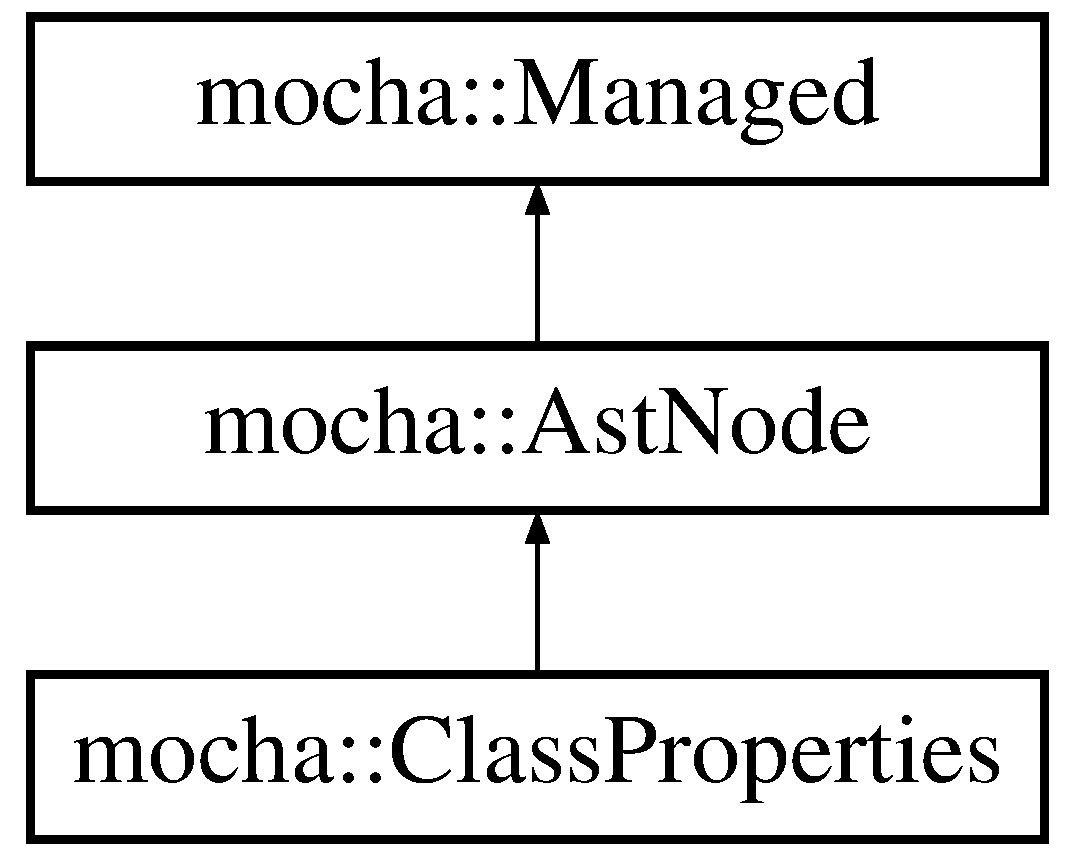
\includegraphics[height=3.000000cm]{classmocha_1_1_class_properties}
\end{center}
\end{figure}
\subsection*{Public Member Functions}
\begin{DoxyCompactItemize}
\item 
\hyperlink{classmocha_1_1_class_properties_aa76d79c7e3208f81b501ecd31b292cd7}{ClassProperties} ()
\item 
\hyperlink{classmocha_1_1_class_properties_a252add584fe17efdc8ffcec1e2e671c2}{$\sim$ClassProperties} ()
\item 
void \hyperlink{classmocha_1_1_class_properties_ae945b72acc7f9a701f9a61e00a3ec9dc}{Public} (\hyperlink{classmocha_1_1_ast_node}{AstNode} $\ast$pb)
\item 
void \hyperlink{classmocha_1_1_class_properties_adc301e4d0c434d6537d101fc23db19d3}{Private} (\hyperlink{classmocha_1_1_ast_node}{AstNode} $\ast$pv)
\item 
void \hyperlink{classmocha_1_1_class_properties_a2b60d8c5f8b29d998cd74c3e4b767658}{PublicStatic} (\hyperlink{classmocha_1_1_ast_node}{AstNode} $\ast$st)
\item 
void \hyperlink{classmocha_1_1_class_properties_aff4897dba124ff17be9ea89b66d90964}{PrivateStatic} (\hyperlink{classmocha_1_1_ast_node}{AstNode} $\ast$st)
\item 
void \hyperlink{classmocha_1_1_class_properties_af59dbd12054895607ef186c44a59f2af}{Prototype} (\hyperlink{classmocha_1_1_ast_node}{AstNode} $\ast$pt)
\item 
void \hyperlink{classmocha_1_1_class_properties_accf89b68e8f8882a8fdc6451316847a0}{Mixin} (\hyperlink{classmocha_1_1_ast_node}{AstNode} $\ast$mi)
\item 
\hyperlink{classmocha_1_1_ast_node}{AstNode} $\ast$ \hyperlink{classmocha_1_1_class_properties_adc8886e8e84e5dfcff2c53224a8ba3a7}{Public} ()
\item 
\hyperlink{classmocha_1_1_ast_node}{AstNode} $\ast$ \hyperlink{classmocha_1_1_class_properties_af9fa75e37144848c4afef0c94c8cd905}{Private} ()
\item 
\hyperlink{classmocha_1_1_ast_node}{AstNode} $\ast$ \hyperlink{classmocha_1_1_class_properties_a771429cd4e5d42ec660e5195df36962a}{PublicStatic} ()
\item 
\hyperlink{classmocha_1_1_ast_node}{AstNode} $\ast$ \hyperlink{classmocha_1_1_class_properties_a5923c53b284aef2acbda68d22a97ad37}{PrivateStatic} ()
\item 
\hyperlink{classmocha_1_1_ast_node}{AstNode} $\ast$ \hyperlink{classmocha_1_1_class_properties_ad0b98aab0fce334e77e55af9ac07dd08}{Prototype} ()
\item 
\hyperlink{classmocha_1_1_ast_node}{AstNode} $\ast$ \hyperlink{classmocha_1_1_class_properties_a6249e318bd1448649b4b60d6d66134a5}{Mixin} ()
\item 
void \hyperlink{classmocha_1_1_class_properties_a9c7a8006b1a474f673b90eba72fc9830}{Constructor} (\hyperlink{classmocha_1_1_ast_node}{AstNode} $\ast$constructor)
\item 
\hyperlink{classmocha_1_1_ast_node}{AstNode} $\ast$ \hyperlink{classmocha_1_1_class_properties_a5003c61d710ffe865d08c711f623ff6d}{Constructor} ()
\item 
\hyperlink{classmocha_1_1_ast_node}{AstNode} $\ast$ \hyperlink{classmocha_1_1_class_properties_adf11918b4cefbd3a396c3c1ca34c747a}{Clone} ()
\end{DoxyCompactItemize}
\subsection*{Private Member Functions}
\begin{DoxyCompactItemize}
\item 
void \hyperlink{classmocha_1_1_class_properties_aa044f4aadf1afa40a77b480b3824534c}{NVIAccept\_\-} (\hyperlink{classmocha_1_1_i_visitor}{IVisitor} $\ast$visitor)
\end{DoxyCompactItemize}
\subsection*{Private Attributes}
\begin{DoxyCompactItemize}
\item 
\hyperlink{classmocha_1_1_node_list}{NodeList} \hyperlink{classmocha_1_1_class_properties_a2810f6c455558f888d81ee31401bf7a3}{public\_\-}
\item 
\hyperlink{classmocha_1_1_node_list}{NodeList} \hyperlink{classmocha_1_1_class_properties_ae57de33463b6c6a592eb23497bcc13b7}{private\_\-}
\item 
\hyperlink{classmocha_1_1_node_list}{NodeList} \hyperlink{classmocha_1_1_class_properties_af751d2300bd5a931f2d845dd2498b4e1}{public\_\-static\_\-}
\item 
\hyperlink{classmocha_1_1_node_list}{NodeList} \hyperlink{classmocha_1_1_class_properties_a83646affe1aeaeb0b3609a628f6110b0}{private\_\-static\_\-}
\item 
\hyperlink{classmocha_1_1_node_list}{NodeList} \hyperlink{classmocha_1_1_class_properties_a8a8d620fed2fdcc7a2255a6e71b98fa8}{prototype\_\-}
\item 
\hyperlink{classmocha_1_1_node_list}{NodeList} \hyperlink{classmocha_1_1_class_properties_ab46a87567170599e9bb1f051d25e37ba}{mixin\_\-}
\item 
\hyperlink{classmocha_1_1_ast_node}{AstNode} $\ast$ \hyperlink{classmocha_1_1_class_properties_a37e632a65dfc92d5a9d613b049810ff3}{constructor\_\-}
\end{DoxyCompactItemize}


\subsection{Detailed Description}


Definition at line 1148 of file ast.h.



\subsection{Constructor \& Destructor Documentation}
\hypertarget{classmocha_1_1_class_properties_aa76d79c7e3208f81b501ecd31b292cd7}{
\index{mocha::ClassProperties@{mocha::ClassProperties}!ClassProperties@{ClassProperties}}
\index{ClassProperties@{ClassProperties}!mocha::ClassProperties@{mocha::ClassProperties}}
\subsubsection[{ClassProperties}]{\setlength{\rightskip}{0pt plus 5cm}mocha::ClassProperties::ClassProperties (
\begin{DoxyParamCaption}
{}
\end{DoxyParamCaption}
)\hspace{0.3cm}{\ttfamily  \mbox{[}inline\mbox{]}}}}
\label{classmocha_1_1_class_properties_aa76d79c7e3208f81b501ecd31b292cd7}


Definition at line 1150 of file ast.h.

\hypertarget{classmocha_1_1_class_properties_a252add584fe17efdc8ffcec1e2e671c2}{
\index{mocha::ClassProperties@{mocha::ClassProperties}!$\sim$ClassProperties@{$\sim$ClassProperties}}
\index{$\sim$ClassProperties@{$\sim$ClassProperties}!mocha::ClassProperties@{mocha::ClassProperties}}
\subsubsection[{$\sim$ClassProperties}]{\setlength{\rightskip}{0pt plus 5cm}mocha::ClassProperties::$\sim$ClassProperties (
\begin{DoxyParamCaption}
{}
\end{DoxyParamCaption}
)\hspace{0.3cm}{\ttfamily  \mbox{[}inline\mbox{]}}}}
\label{classmocha_1_1_class_properties_a252add584fe17efdc8ffcec1e2e671c2}


Definition at line 1151 of file ast.h.



\subsection{Member Function Documentation}
\hypertarget{classmocha_1_1_class_properties_adf11918b4cefbd3a396c3c1ca34c747a}{
\index{mocha::ClassProperties@{mocha::ClassProperties}!Clone@{Clone}}
\index{Clone@{Clone}!mocha::ClassProperties@{mocha::ClassProperties}}
\subsubsection[{Clone}]{\setlength{\rightskip}{0pt plus 5cm}{\bf AstNode} $\ast$ mocha::ClassProperties::Clone (
\begin{DoxyParamCaption}
{}
\end{DoxyParamCaption}
)\hspace{0.3cm}{\ttfamily  \mbox{[}virtual\mbox{]}}}}
\label{classmocha_1_1_class_properties_adf11918b4cefbd3a396c3c1ca34c747a}
\begin{DoxyReturn}{Returns}
\{AstNode$\ast$\} Clone node. 
\end{DoxyReturn}


Reimplemented from \hyperlink{classmocha_1_1_ast_node_af2a895699bac2012f8b7739bff49c5ec}{mocha::AstNode}.



Definition at line 400 of file ast.cc.

\hypertarget{classmocha_1_1_class_properties_a9c7a8006b1a474f673b90eba72fc9830}{
\index{mocha::ClassProperties@{mocha::ClassProperties}!Constructor@{Constructor}}
\index{Constructor@{Constructor}!mocha::ClassProperties@{mocha::ClassProperties}}
\subsubsection[{Constructor}]{\setlength{\rightskip}{0pt plus 5cm}void mocha::ClassProperties::Constructor (
\begin{DoxyParamCaption}
\item[{{\bf AstNode} $\ast$}]{constructor}
\end{DoxyParamCaption}
)\hspace{0.3cm}{\ttfamily  \mbox{[}inline\mbox{]}}}}
\label{classmocha_1_1_class_properties_a9c7a8006b1a474f673b90eba72fc9830}


Definition at line 1164 of file ast.h.

\hypertarget{classmocha_1_1_class_properties_a5003c61d710ffe865d08c711f623ff6d}{
\index{mocha::ClassProperties@{mocha::ClassProperties}!Constructor@{Constructor}}
\index{Constructor@{Constructor}!mocha::ClassProperties@{mocha::ClassProperties}}
\subsubsection[{Constructor}]{\setlength{\rightskip}{0pt plus 5cm}{\bf AstNode}$\ast$ mocha::ClassProperties::Constructor (
\begin{DoxyParamCaption}
{}
\end{DoxyParamCaption}
)\hspace{0.3cm}{\ttfamily  \mbox{[}inline\mbox{]}}}}
\label{classmocha_1_1_class_properties_a5003c61d710ffe865d08c711f623ff6d}


Definition at line 1165 of file ast.h.

\hypertarget{classmocha_1_1_class_properties_a6249e318bd1448649b4b60d6d66134a5}{
\index{mocha::ClassProperties@{mocha::ClassProperties}!Mixin@{Mixin}}
\index{Mixin@{Mixin}!mocha::ClassProperties@{mocha::ClassProperties}}
\subsubsection[{Mixin}]{\setlength{\rightskip}{0pt plus 5cm}{\bf AstNode}$\ast$ mocha::ClassProperties::Mixin (
\begin{DoxyParamCaption}
{}
\end{DoxyParamCaption}
)\hspace{0.3cm}{\ttfamily  \mbox{[}inline\mbox{]}}}}
\label{classmocha_1_1_class_properties_a6249e318bd1448649b4b60d6d66134a5}


Definition at line 1163 of file ast.h.

\hypertarget{classmocha_1_1_class_properties_accf89b68e8f8882a8fdc6451316847a0}{
\index{mocha::ClassProperties@{mocha::ClassProperties}!Mixin@{Mixin}}
\index{Mixin@{Mixin}!mocha::ClassProperties@{mocha::ClassProperties}}
\subsubsection[{Mixin}]{\setlength{\rightskip}{0pt plus 5cm}void mocha::ClassProperties::Mixin (
\begin{DoxyParamCaption}
\item[{{\bf AstNode} $\ast$}]{mi}
\end{DoxyParamCaption}
)\hspace{0.3cm}{\ttfamily  \mbox{[}inline\mbox{]}}}}
\label{classmocha_1_1_class_properties_accf89b68e8f8882a8fdc6451316847a0}


Definition at line 1157 of file ast.h.

\hypertarget{classmocha_1_1_class_properties_aa044f4aadf1afa40a77b480b3824534c}{
\index{mocha::ClassProperties@{mocha::ClassProperties}!NVIAccept\_\-@{NVIAccept\_\-}}
\index{NVIAccept\_\-@{NVIAccept\_\-}!mocha::ClassProperties@{mocha::ClassProperties}}
\subsubsection[{NVIAccept\_\-}]{\setlength{\rightskip}{0pt plus 5cm}void mocha::ClassProperties::NVIAccept\_\- (
\begin{DoxyParamCaption}
\item[{{\bf IVisitor} $\ast$}]{visitor}
\end{DoxyParamCaption}
)\hspace{0.3cm}{\ttfamily  \mbox{[}inline, private, virtual\mbox{]}}}}
\label{classmocha_1_1_class_properties_aa044f4aadf1afa40a77b480b3824534c}


Reimplemented from \hyperlink{classmocha_1_1_ast_node_a4a9c107bed3671f3fa15312b87f6ae96}{mocha::AstNode}.



Definition at line 1168 of file ast.h.

\hypertarget{classmocha_1_1_class_properties_af9fa75e37144848c4afef0c94c8cd905}{
\index{mocha::ClassProperties@{mocha::ClassProperties}!Private@{Private}}
\index{Private@{Private}!mocha::ClassProperties@{mocha::ClassProperties}}
\subsubsection[{Private}]{\setlength{\rightskip}{0pt plus 5cm}{\bf AstNode}$\ast$ mocha::ClassProperties::Private (
\begin{DoxyParamCaption}
{}
\end{DoxyParamCaption}
)\hspace{0.3cm}{\ttfamily  \mbox{[}inline\mbox{]}}}}
\label{classmocha_1_1_class_properties_af9fa75e37144848c4afef0c94c8cd905}


Definition at line 1159 of file ast.h.

\hypertarget{classmocha_1_1_class_properties_adc301e4d0c434d6537d101fc23db19d3}{
\index{mocha::ClassProperties@{mocha::ClassProperties}!Private@{Private}}
\index{Private@{Private}!mocha::ClassProperties@{mocha::ClassProperties}}
\subsubsection[{Private}]{\setlength{\rightskip}{0pt plus 5cm}void mocha::ClassProperties::Private (
\begin{DoxyParamCaption}
\item[{{\bf AstNode} $\ast$}]{pv}
\end{DoxyParamCaption}
)\hspace{0.3cm}{\ttfamily  \mbox{[}inline\mbox{]}}}}
\label{classmocha_1_1_class_properties_adc301e4d0c434d6537d101fc23db19d3}


Definition at line 1153 of file ast.h.

\hypertarget{classmocha_1_1_class_properties_aff4897dba124ff17be9ea89b66d90964}{
\index{mocha::ClassProperties@{mocha::ClassProperties}!PrivateStatic@{PrivateStatic}}
\index{PrivateStatic@{PrivateStatic}!mocha::ClassProperties@{mocha::ClassProperties}}
\subsubsection[{PrivateStatic}]{\setlength{\rightskip}{0pt plus 5cm}void mocha::ClassProperties::PrivateStatic (
\begin{DoxyParamCaption}
\item[{{\bf AstNode} $\ast$}]{st}
\end{DoxyParamCaption}
)\hspace{0.3cm}{\ttfamily  \mbox{[}inline\mbox{]}}}}
\label{classmocha_1_1_class_properties_aff4897dba124ff17be9ea89b66d90964}


Definition at line 1155 of file ast.h.

\hypertarget{classmocha_1_1_class_properties_a5923c53b284aef2acbda68d22a97ad37}{
\index{mocha::ClassProperties@{mocha::ClassProperties}!PrivateStatic@{PrivateStatic}}
\index{PrivateStatic@{PrivateStatic}!mocha::ClassProperties@{mocha::ClassProperties}}
\subsubsection[{PrivateStatic}]{\setlength{\rightskip}{0pt plus 5cm}{\bf AstNode}$\ast$ mocha::ClassProperties::PrivateStatic (
\begin{DoxyParamCaption}
{}
\end{DoxyParamCaption}
)\hspace{0.3cm}{\ttfamily  \mbox{[}inline\mbox{]}}}}
\label{classmocha_1_1_class_properties_a5923c53b284aef2acbda68d22a97ad37}


Definition at line 1161 of file ast.h.

\hypertarget{classmocha_1_1_class_properties_ad0b98aab0fce334e77e55af9ac07dd08}{
\index{mocha::ClassProperties@{mocha::ClassProperties}!Prototype@{Prototype}}
\index{Prototype@{Prototype}!mocha::ClassProperties@{mocha::ClassProperties}}
\subsubsection[{Prototype}]{\setlength{\rightskip}{0pt plus 5cm}{\bf AstNode}$\ast$ mocha::ClassProperties::Prototype (
\begin{DoxyParamCaption}
{}
\end{DoxyParamCaption}
)\hspace{0.3cm}{\ttfamily  \mbox{[}inline\mbox{]}}}}
\label{classmocha_1_1_class_properties_ad0b98aab0fce334e77e55af9ac07dd08}


Definition at line 1162 of file ast.h.

\hypertarget{classmocha_1_1_class_properties_af59dbd12054895607ef186c44a59f2af}{
\index{mocha::ClassProperties@{mocha::ClassProperties}!Prototype@{Prototype}}
\index{Prototype@{Prototype}!mocha::ClassProperties@{mocha::ClassProperties}}
\subsubsection[{Prototype}]{\setlength{\rightskip}{0pt plus 5cm}void mocha::ClassProperties::Prototype (
\begin{DoxyParamCaption}
\item[{{\bf AstNode} $\ast$}]{pt}
\end{DoxyParamCaption}
)\hspace{0.3cm}{\ttfamily  \mbox{[}inline\mbox{]}}}}
\label{classmocha_1_1_class_properties_af59dbd12054895607ef186c44a59f2af}


Definition at line 1156 of file ast.h.

\hypertarget{classmocha_1_1_class_properties_adc8886e8e84e5dfcff2c53224a8ba3a7}{
\index{mocha::ClassProperties@{mocha::ClassProperties}!Public@{Public}}
\index{Public@{Public}!mocha::ClassProperties@{mocha::ClassProperties}}
\subsubsection[{Public}]{\setlength{\rightskip}{0pt plus 5cm}{\bf AstNode}$\ast$ mocha::ClassProperties::Public (
\begin{DoxyParamCaption}
{}
\end{DoxyParamCaption}
)\hspace{0.3cm}{\ttfamily  \mbox{[}inline\mbox{]}}}}
\label{classmocha_1_1_class_properties_adc8886e8e84e5dfcff2c53224a8ba3a7}


Definition at line 1158 of file ast.h.

\hypertarget{classmocha_1_1_class_properties_ae945b72acc7f9a701f9a61e00a3ec9dc}{
\index{mocha::ClassProperties@{mocha::ClassProperties}!Public@{Public}}
\index{Public@{Public}!mocha::ClassProperties@{mocha::ClassProperties}}
\subsubsection[{Public}]{\setlength{\rightskip}{0pt plus 5cm}void mocha::ClassProperties::Public (
\begin{DoxyParamCaption}
\item[{{\bf AstNode} $\ast$}]{pb}
\end{DoxyParamCaption}
)\hspace{0.3cm}{\ttfamily  \mbox{[}inline\mbox{]}}}}
\label{classmocha_1_1_class_properties_ae945b72acc7f9a701f9a61e00a3ec9dc}


Definition at line 1152 of file ast.h.

\hypertarget{classmocha_1_1_class_properties_a2b60d8c5f8b29d998cd74c3e4b767658}{
\index{mocha::ClassProperties@{mocha::ClassProperties}!PublicStatic@{PublicStatic}}
\index{PublicStatic@{PublicStatic}!mocha::ClassProperties@{mocha::ClassProperties}}
\subsubsection[{PublicStatic}]{\setlength{\rightskip}{0pt plus 5cm}void mocha::ClassProperties::PublicStatic (
\begin{DoxyParamCaption}
\item[{{\bf AstNode} $\ast$}]{st}
\end{DoxyParamCaption}
)\hspace{0.3cm}{\ttfamily  \mbox{[}inline\mbox{]}}}}
\label{classmocha_1_1_class_properties_a2b60d8c5f8b29d998cd74c3e4b767658}


Definition at line 1154 of file ast.h.

\hypertarget{classmocha_1_1_class_properties_a771429cd4e5d42ec660e5195df36962a}{
\index{mocha::ClassProperties@{mocha::ClassProperties}!PublicStatic@{PublicStatic}}
\index{PublicStatic@{PublicStatic}!mocha::ClassProperties@{mocha::ClassProperties}}
\subsubsection[{PublicStatic}]{\setlength{\rightskip}{0pt plus 5cm}{\bf AstNode}$\ast$ mocha::ClassProperties::PublicStatic (
\begin{DoxyParamCaption}
{}
\end{DoxyParamCaption}
)\hspace{0.3cm}{\ttfamily  \mbox{[}inline\mbox{]}}}}
\label{classmocha_1_1_class_properties_a771429cd4e5d42ec660e5195df36962a}


Definition at line 1160 of file ast.h.



\subsection{Member Data Documentation}
\hypertarget{classmocha_1_1_class_properties_a37e632a65dfc92d5a9d613b049810ff3}{
\index{mocha::ClassProperties@{mocha::ClassProperties}!constructor\_\-@{constructor\_\-}}
\index{constructor\_\-@{constructor\_\-}!mocha::ClassProperties@{mocha::ClassProperties}}
\subsubsection[{constructor\_\-}]{\setlength{\rightskip}{0pt plus 5cm}{\bf AstNode}$\ast$ {\bf mocha::ClassProperties::constructor\_\-}\hspace{0.3cm}{\ttfamily  \mbox{[}private\mbox{]}}}}
\label{classmocha_1_1_class_properties_a37e632a65dfc92d5a9d613b049810ff3}


Definition at line 1175 of file ast.h.

\hypertarget{classmocha_1_1_class_properties_ab46a87567170599e9bb1f051d25e37ba}{
\index{mocha::ClassProperties@{mocha::ClassProperties}!mixin\_\-@{mixin\_\-}}
\index{mixin\_\-@{mixin\_\-}!mocha::ClassProperties@{mocha::ClassProperties}}
\subsubsection[{mixin\_\-}]{\setlength{\rightskip}{0pt plus 5cm}{\bf NodeList} {\bf mocha::ClassProperties::mixin\_\-}\hspace{0.3cm}{\ttfamily  \mbox{[}private\mbox{]}}}}
\label{classmocha_1_1_class_properties_ab46a87567170599e9bb1f051d25e37ba}


Definition at line 1174 of file ast.h.

\hypertarget{classmocha_1_1_class_properties_ae57de33463b6c6a592eb23497bcc13b7}{
\index{mocha::ClassProperties@{mocha::ClassProperties}!private\_\-@{private\_\-}}
\index{private\_\-@{private\_\-}!mocha::ClassProperties@{mocha::ClassProperties}}
\subsubsection[{private\_\-}]{\setlength{\rightskip}{0pt plus 5cm}{\bf NodeList} {\bf mocha::ClassProperties::private\_\-}\hspace{0.3cm}{\ttfamily  \mbox{[}private\mbox{]}}}}
\label{classmocha_1_1_class_properties_ae57de33463b6c6a592eb23497bcc13b7}


Definition at line 1170 of file ast.h.

\hypertarget{classmocha_1_1_class_properties_a83646affe1aeaeb0b3609a628f6110b0}{
\index{mocha::ClassProperties@{mocha::ClassProperties}!private\_\-static\_\-@{private\_\-static\_\-}}
\index{private\_\-static\_\-@{private\_\-static\_\-}!mocha::ClassProperties@{mocha::ClassProperties}}
\subsubsection[{private\_\-static\_\-}]{\setlength{\rightskip}{0pt plus 5cm}{\bf NodeList} {\bf mocha::ClassProperties::private\_\-static\_\-}\hspace{0.3cm}{\ttfamily  \mbox{[}private\mbox{]}}}}
\label{classmocha_1_1_class_properties_a83646affe1aeaeb0b3609a628f6110b0}


Definition at line 1172 of file ast.h.

\hypertarget{classmocha_1_1_class_properties_a8a8d620fed2fdcc7a2255a6e71b98fa8}{
\index{mocha::ClassProperties@{mocha::ClassProperties}!prototype\_\-@{prototype\_\-}}
\index{prototype\_\-@{prototype\_\-}!mocha::ClassProperties@{mocha::ClassProperties}}
\subsubsection[{prototype\_\-}]{\setlength{\rightskip}{0pt plus 5cm}{\bf NodeList} {\bf mocha::ClassProperties::prototype\_\-}\hspace{0.3cm}{\ttfamily  \mbox{[}private\mbox{]}}}}
\label{classmocha_1_1_class_properties_a8a8d620fed2fdcc7a2255a6e71b98fa8}


Definition at line 1173 of file ast.h.

\hypertarget{classmocha_1_1_class_properties_a2810f6c455558f888d81ee31401bf7a3}{
\index{mocha::ClassProperties@{mocha::ClassProperties}!public\_\-@{public\_\-}}
\index{public\_\-@{public\_\-}!mocha::ClassProperties@{mocha::ClassProperties}}
\subsubsection[{public\_\-}]{\setlength{\rightskip}{0pt plus 5cm}{\bf NodeList} {\bf mocha::ClassProperties::public\_\-}\hspace{0.3cm}{\ttfamily  \mbox{[}private\mbox{]}}}}
\label{classmocha_1_1_class_properties_a2810f6c455558f888d81ee31401bf7a3}


Definition at line 1168 of file ast.h.

\hypertarget{classmocha_1_1_class_properties_af751d2300bd5a931f2d845dd2498b4e1}{
\index{mocha::ClassProperties@{mocha::ClassProperties}!public\_\-static\_\-@{public\_\-static\_\-}}
\index{public\_\-static\_\-@{public\_\-static\_\-}!mocha::ClassProperties@{mocha::ClassProperties}}
\subsubsection[{public\_\-static\_\-}]{\setlength{\rightskip}{0pt plus 5cm}{\bf NodeList} {\bf mocha::ClassProperties::public\_\-static\_\-}\hspace{0.3cm}{\ttfamily  \mbox{[}private\mbox{]}}}}
\label{classmocha_1_1_class_properties_af751d2300bd5a931f2d845dd2498b4e1}


Definition at line 1171 of file ast.h.



The documentation for this class was generated from the following files:\begin{DoxyCompactItemize}
\item 
Y:/mocha/src/ast/\hyperlink{ast_8h}{ast.h}\item 
Y:/mocha/src/ast/\hyperlink{ast_8cc}{ast.cc}\end{DoxyCompactItemize}

\hypertarget{structmocha_1_1watch__traits_1_1_close}{
\section{mocha::watch\_\-traits::Close Struct Reference}
\label{structmocha_1_1watch__traits_1_1_close}\index{mocha::watch\_\-traits::Close@{mocha::watch\_\-traits::Close}}
}


{\ttfamily \#include $<$file\_\-watcher.h$>$}

\subsection*{Public Member Functions}
\begin{DoxyCompactItemize}
\item 
\hyperlink{structmocha_1_1watch__traits_1_1_close_af950235e46105e682d4bd37e9028555f}{Close} (const char $\ast$filename\_\-)
\end{DoxyCompactItemize}
\subsection*{Public Attributes}
\begin{DoxyCompactItemize}
\item 
const char $\ast$ \hyperlink{structmocha_1_1watch__traits_1_1_close_a17079e4e7c253c7b27ca9c8a4ea17e28}{filename}
\end{DoxyCompactItemize}


\subsection{Detailed Description}


Definition at line 13 of file file\_\-watcher.h.



\subsection{Constructor \& Destructor Documentation}
\hypertarget{structmocha_1_1watch__traits_1_1_close_af950235e46105e682d4bd37e9028555f}{
\index{mocha::watch\_\-traits::Close@{mocha::watch\_\-traits::Close}!Close@{Close}}
\index{Close@{Close}!mocha::watch_traits::Close@{mocha::watch\_\-traits::Close}}
\subsubsection[{Close}]{\setlength{\rightskip}{0pt plus 5cm}mocha::watch\_\-traits::Close::Close (
\begin{DoxyParamCaption}
\item[{const char $\ast$}]{filename\_\-}
\end{DoxyParamCaption}
)\hspace{0.3cm}{\ttfamily  \mbox{[}inline\mbox{]}}}}
\label{structmocha_1_1watch__traits_1_1_close_af950235e46105e682d4bd37e9028555f}


Definition at line 13 of file file\_\-watcher.h.



\subsection{Member Data Documentation}
\hypertarget{structmocha_1_1watch__traits_1_1_close_a17079e4e7c253c7b27ca9c8a4ea17e28}{
\index{mocha::watch\_\-traits::Close@{mocha::watch\_\-traits::Close}!filename@{filename}}
\index{filename@{filename}!mocha::watch_traits::Close@{mocha::watch\_\-traits::Close}}
\subsubsection[{filename}]{\setlength{\rightskip}{0pt plus 5cm}const char$\ast$ {\bf mocha::watch\_\-traits::Close::filename}}}
\label{structmocha_1_1watch__traits_1_1_close_a17079e4e7c253c7b27ca9c8a4ea17e28}


Definition at line 13 of file file\_\-watcher.h.



The documentation for this struct was generated from the following file:\begin{DoxyCompactItemize}
\item 
Y:/mocha/src/utils/file\_\-watcher/\hyperlink{file__watcher_8h}{file\_\-watcher.h}\end{DoxyCompactItemize}

\hypertarget{classmocha_1_1_code_buffer}{
\section{mocha::CodeBuffer Class Reference}
\label{classmocha_1_1_code_buffer}\index{mocha::CodeBuffer@{mocha::CodeBuffer}}
}


{\ttfamily \#include $<$codegenerator\_\-utils.h$>$}

Inheritance diagram for mocha::CodeBuffer:\begin{figure}[H]
\begin{center}
\leavevmode
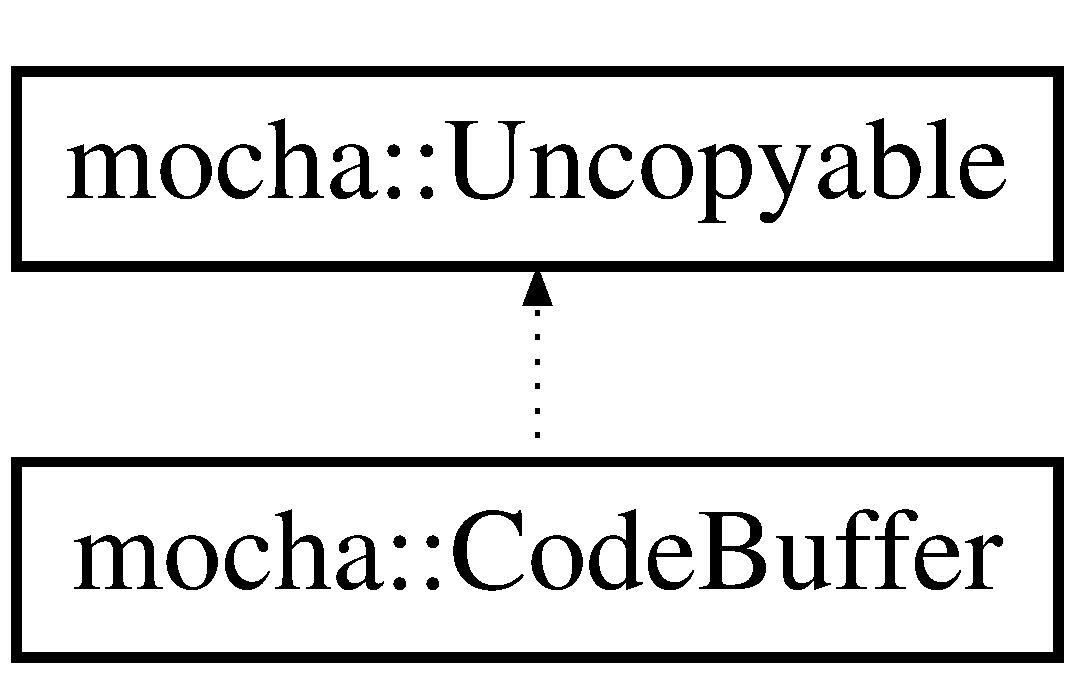
\includegraphics[height=2.000000cm]{classmocha_1_1_code_buffer}
\end{center}
\end{figure}
\subsection*{Public Member Functions}
\begin{DoxyCompactItemize}
\item 
\hyperlink{classmocha_1_1_code_buffer_ac717ce28d15ce963ce2c1b2aa13ea851}{CodeBuffer} ()
\item 
\hyperlink{classmocha_1_1_code_buffer_a446eda5b31687f26d54e79cb5edc52f0}{$\sim$CodeBuffer} ()
\item 
void \hyperlink{classmocha_1_1_code_buffer_acf0b19f0ed536ca22922f4af17ec5e69}{Write} (const char $\ast$str)
\item 
void \hyperlink{classmocha_1_1_code_buffer_a758503ee1ec29946036cf3eb517b7b14}{Write} (char str)
\item 
void \hyperlink{classmocha_1_1_code_buffer_add5a0f01a5006f49f47df960e0f85fbc}{Write} (const std::string \&str)
\item 
const char $\ast$ \hyperlink{classmocha_1_1_code_buffer_a9632dcb2f40212ce216962be8f82a450}{GetData} () const 
\item 
void \hyperlink{classmocha_1_1_code_buffer_ad81ef6b61cbadda42b2646c60101c169}{Clear} ()
\item 
void \hyperlink{classmocha_1_1_code_buffer_a2404ee297df0b914eb805dde38287c67}{Erase} (size\_\-t beg, size\_\-t end)
\item 
size\_\-t \hyperlink{classmocha_1_1_code_buffer_ae451d2baccb67df1d26a5af418bb35f6}{Size} ()
\item 
const std::string \& \hyperlink{classmocha_1_1_code_buffer_a079468ec1c722202d4ec129adf4122c4}{Get} () const 
\end{DoxyCompactItemize}
\subsection*{Private Attributes}
\begin{DoxyCompactItemize}
\item 
std::string \hyperlink{classmocha_1_1_code_buffer_ad6d76a3c003a12819976595381651c7d}{buffer\_\-}
\end{DoxyCompactItemize}


\subsection{Detailed Description}


Definition at line 11 of file codegenerator\_\-utils.h.



\subsection{Constructor \& Destructor Documentation}
\hypertarget{classmocha_1_1_code_buffer_ac717ce28d15ce963ce2c1b2aa13ea851}{
\index{mocha::CodeBuffer@{mocha::CodeBuffer}!CodeBuffer@{CodeBuffer}}
\index{CodeBuffer@{CodeBuffer}!mocha::CodeBuffer@{mocha::CodeBuffer}}
\subsubsection[{CodeBuffer}]{\setlength{\rightskip}{0pt plus 5cm}mocha::CodeBuffer::CodeBuffer (
\begin{DoxyParamCaption}
{}
\end{DoxyParamCaption}
)\hspace{0.3cm}{\ttfamily  \mbox{[}inline\mbox{]}}}}
\label{classmocha_1_1_code_buffer_ac717ce28d15ce963ce2c1b2aa13ea851}


Definition at line 13 of file codegenerator\_\-utils.h.

\hypertarget{classmocha_1_1_code_buffer_a446eda5b31687f26d54e79cb5edc52f0}{
\index{mocha::CodeBuffer@{mocha::CodeBuffer}!$\sim$CodeBuffer@{$\sim$CodeBuffer}}
\index{$\sim$CodeBuffer@{$\sim$CodeBuffer}!mocha::CodeBuffer@{mocha::CodeBuffer}}
\subsubsection[{$\sim$CodeBuffer}]{\setlength{\rightskip}{0pt plus 5cm}mocha::CodeBuffer::$\sim$CodeBuffer (
\begin{DoxyParamCaption}
{}
\end{DoxyParamCaption}
)\hspace{0.3cm}{\ttfamily  \mbox{[}inline\mbox{]}}}}
\label{classmocha_1_1_code_buffer_a446eda5b31687f26d54e79cb5edc52f0}


Definition at line 14 of file codegenerator\_\-utils.h.



\subsection{Member Function Documentation}
\hypertarget{classmocha_1_1_code_buffer_ad81ef6b61cbadda42b2646c60101c169}{
\index{mocha::CodeBuffer@{mocha::CodeBuffer}!Clear@{Clear}}
\index{Clear@{Clear}!mocha::CodeBuffer@{mocha::CodeBuffer}}
\subsubsection[{Clear}]{\setlength{\rightskip}{0pt plus 5cm}void mocha::CodeBuffer::Clear (
\begin{DoxyParamCaption}
{}
\end{DoxyParamCaption}
)\hspace{0.3cm}{\ttfamily  \mbox{[}inline\mbox{]}}}}
\label{classmocha_1_1_code_buffer_ad81ef6b61cbadda42b2646c60101c169}


Definition at line 19 of file codegenerator\_\-utils.h.

\hypertarget{classmocha_1_1_code_buffer_a2404ee297df0b914eb805dde38287c67}{
\index{mocha::CodeBuffer@{mocha::CodeBuffer}!Erase@{Erase}}
\index{Erase@{Erase}!mocha::CodeBuffer@{mocha::CodeBuffer}}
\subsubsection[{Erase}]{\setlength{\rightskip}{0pt plus 5cm}void mocha::CodeBuffer::Erase (
\begin{DoxyParamCaption}
\item[{size\_\-t}]{beg, }
\item[{size\_\-t}]{end}
\end{DoxyParamCaption}
)\hspace{0.3cm}{\ttfamily  \mbox{[}inline\mbox{]}}}}
\label{classmocha_1_1_code_buffer_a2404ee297df0b914eb805dde38287c67}


Definition at line 20 of file codegenerator\_\-utils.h.

\hypertarget{classmocha_1_1_code_buffer_a079468ec1c722202d4ec129adf4122c4}{
\index{mocha::CodeBuffer@{mocha::CodeBuffer}!Get@{Get}}
\index{Get@{Get}!mocha::CodeBuffer@{mocha::CodeBuffer}}
\subsubsection[{Get}]{\setlength{\rightskip}{0pt plus 5cm}const std::string\& mocha::CodeBuffer::Get (
\begin{DoxyParamCaption}
{}
\end{DoxyParamCaption}
) const\hspace{0.3cm}{\ttfamily  \mbox{[}inline\mbox{]}}}}
\label{classmocha_1_1_code_buffer_a079468ec1c722202d4ec129adf4122c4}


Definition at line 22 of file codegenerator\_\-utils.h.

\hypertarget{classmocha_1_1_code_buffer_a9632dcb2f40212ce216962be8f82a450}{
\index{mocha::CodeBuffer@{mocha::CodeBuffer}!GetData@{GetData}}
\index{GetData@{GetData}!mocha::CodeBuffer@{mocha::CodeBuffer}}
\subsubsection[{GetData}]{\setlength{\rightskip}{0pt plus 5cm}const char$\ast$ mocha::CodeBuffer::GetData (
\begin{DoxyParamCaption}
{}
\end{DoxyParamCaption}
) const\hspace{0.3cm}{\ttfamily  \mbox{[}inline\mbox{]}}}}
\label{classmocha_1_1_code_buffer_a9632dcb2f40212ce216962be8f82a450}


Definition at line 18 of file codegenerator\_\-utils.h.

\hypertarget{classmocha_1_1_code_buffer_ae451d2baccb67df1d26a5af418bb35f6}{
\index{mocha::CodeBuffer@{mocha::CodeBuffer}!Size@{Size}}
\index{Size@{Size}!mocha::CodeBuffer@{mocha::CodeBuffer}}
\subsubsection[{Size}]{\setlength{\rightskip}{0pt plus 5cm}size\_\-t mocha::CodeBuffer::Size (
\begin{DoxyParamCaption}
{}
\end{DoxyParamCaption}
)\hspace{0.3cm}{\ttfamily  \mbox{[}inline\mbox{]}}}}
\label{classmocha_1_1_code_buffer_ae451d2baccb67df1d26a5af418bb35f6}


Definition at line 21 of file codegenerator\_\-utils.h.

\hypertarget{classmocha_1_1_code_buffer_a758503ee1ec29946036cf3eb517b7b14}{
\index{mocha::CodeBuffer@{mocha::CodeBuffer}!Write@{Write}}
\index{Write@{Write}!mocha::CodeBuffer@{mocha::CodeBuffer}}
\subsubsection[{Write}]{\setlength{\rightskip}{0pt plus 5cm}void mocha::CodeBuffer::Write (
\begin{DoxyParamCaption}
\item[{char}]{str}
\end{DoxyParamCaption}
)\hspace{0.3cm}{\ttfamily  \mbox{[}inline\mbox{]}}}}
\label{classmocha_1_1_code_buffer_a758503ee1ec29946036cf3eb517b7b14}


Definition at line 16 of file codegenerator\_\-utils.h.

\hypertarget{classmocha_1_1_code_buffer_acf0b19f0ed536ca22922f4af17ec5e69}{
\index{mocha::CodeBuffer@{mocha::CodeBuffer}!Write@{Write}}
\index{Write@{Write}!mocha::CodeBuffer@{mocha::CodeBuffer}}
\subsubsection[{Write}]{\setlength{\rightskip}{0pt plus 5cm}void mocha::CodeBuffer::Write (
\begin{DoxyParamCaption}
\item[{const char $\ast$}]{str}
\end{DoxyParamCaption}
)\hspace{0.3cm}{\ttfamily  \mbox{[}inline\mbox{]}}}}
\label{classmocha_1_1_code_buffer_acf0b19f0ed536ca22922f4af17ec5e69}


Definition at line 15 of file codegenerator\_\-utils.h.

\hypertarget{classmocha_1_1_code_buffer_add5a0f01a5006f49f47df960e0f85fbc}{
\index{mocha::CodeBuffer@{mocha::CodeBuffer}!Write@{Write}}
\index{Write@{Write}!mocha::CodeBuffer@{mocha::CodeBuffer}}
\subsubsection[{Write}]{\setlength{\rightskip}{0pt plus 5cm}void mocha::CodeBuffer::Write (
\begin{DoxyParamCaption}
\item[{const std::string \&}]{str}
\end{DoxyParamCaption}
)\hspace{0.3cm}{\ttfamily  \mbox{[}inline\mbox{]}}}}
\label{classmocha_1_1_code_buffer_add5a0f01a5006f49f47df960e0f85fbc}


Definition at line 17 of file codegenerator\_\-utils.h.



\subsection{Member Data Documentation}
\hypertarget{classmocha_1_1_code_buffer_ad6d76a3c003a12819976595381651c7d}{
\index{mocha::CodeBuffer@{mocha::CodeBuffer}!buffer\_\-@{buffer\_\-}}
\index{buffer\_\-@{buffer\_\-}!mocha::CodeBuffer@{mocha::CodeBuffer}}
\subsubsection[{buffer\_\-}]{\setlength{\rightskip}{0pt plus 5cm}std::string {\bf mocha::CodeBuffer::buffer\_\-}\hspace{0.3cm}{\ttfamily  \mbox{[}private\mbox{]}}}}
\label{classmocha_1_1_code_buffer_ad6d76a3c003a12819976595381651c7d}


Definition at line 24 of file codegenerator\_\-utils.h.



The documentation for this class was generated from the following file:\begin{DoxyCompactItemize}
\item 
Y:/mocha/src/ast/visitors/utils/\hyperlink{codegenerator__utils_8h}{codegenerator\_\-utils.h}\end{DoxyCompactItemize}

\hypertarget{classmocha_1_1_codegen_visitor}{
\section{mocha::CodegenVisitor Class Reference}
\label{classmocha_1_1_codegen_visitor}\index{mocha::CodegenVisitor@{mocha::CodegenVisitor}}
}


{\ttfamily \#include $<$codegen\_\-visitor.h$>$}

Inheritance diagram for mocha::CodegenVisitor:\begin{figure}[H]
\begin{center}
\leavevmode
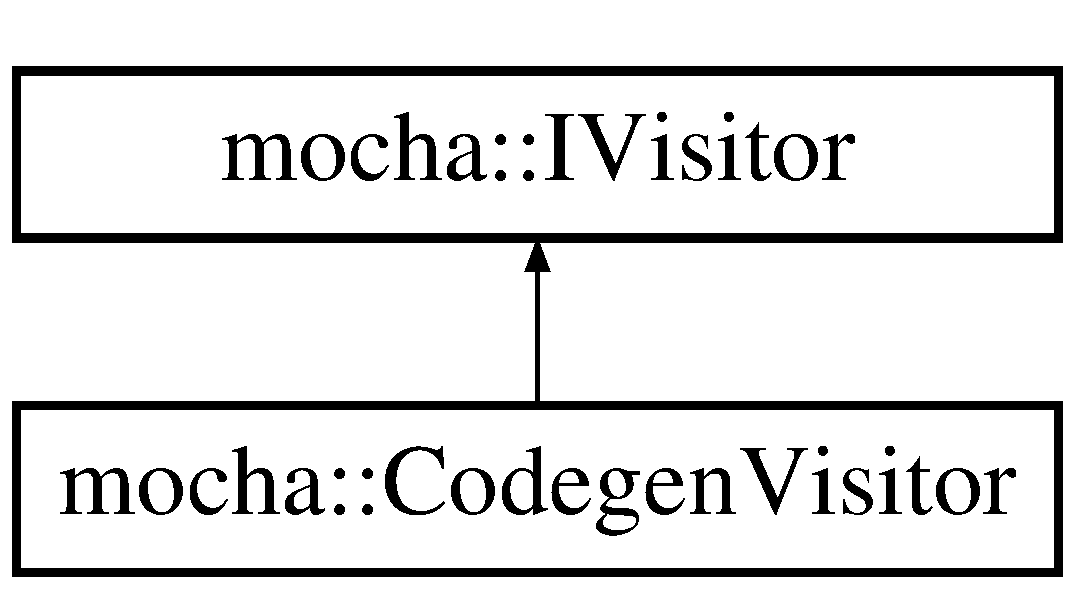
\includegraphics[height=2.000000cm]{classmocha_1_1_codegen_visitor}
\end{center}
\end{figure}
\subsection*{Public Member Functions}
\begin{DoxyCompactItemize}
\item 
\hyperlink{classmocha_1_1_codegen_visitor_aa35625b6ae531e2ca3c529c1c84ab57f}{CodegenVisitor} (const char $\ast$\hyperlink{classmocha_1_1_codegen_visitor_aab8ca0550a471810ff7caa360fbd26b4}{filename\_\-}, \hyperlink{classmocha_1_1_compile_info}{CompileInfo} $\ast$info)
\item 
\hyperlink{classmocha_1_1_codegen_visitor_a90a9952c701d3523d32f4f1b4640f91d}{CodegenVisitor} (const char $\ast$\hyperlink{classmocha_1_1_codegen_visitor_aab8ca0550a471810ff7caa360fbd26b4}{filename\_\-}, bool is\_\-pretty\_\-print, bool is\_\-debug)
\item 
\hyperlink{classmocha_1_1_codegen_visitor_aacc64569f0b7bf04f9f3f55a55f5a180}{$\sim$CodegenVisitor} ()
\item 
void \hyperlink{classmocha_1_1_codegen_visitor_a046d0648f036d9f6e580d3fd7f6223b9}{Write} (const char $\ast$code)
\item 
const char $\ast$ \hyperlink{classmocha_1_1_codegen_visitor_afd3d84940413ff3b974882a8e6b227df}{GetCode} ()
\end{DoxyCompactItemize}
\subsection*{Private Member Functions}
\begin{DoxyCompactItemize}
\item 
void \hyperlink{classmocha_1_1_codegen_visitor_aaaa6cabbe8c04a0aab7c3a9a26956783}{ForProccessor\_\-} (\hyperlink{classmocha_1_1_iteration_stmt}{IterationStmt} $\ast$iter)
\item 
void \hyperlink{classmocha_1_1_codegen_visitor_ac2b58bbdf7ceab17af317dc9b7148748}{ForInProccessor\_\-} (\hyperlink{classmocha_1_1_iteration_stmt}{IterationStmt} $\ast$iter)
\item 
void \hyperlink{classmocha_1_1_codegen_visitor_acd33c4711ad2da1aa6bf0e8307cdcf3f}{DoWhileProccessor\_\-} (\hyperlink{classmocha_1_1_iteration_stmt}{IterationStmt} $\ast$iter)
\item 
void \hyperlink{classmocha_1_1_codegen_visitor_a0da6f8640afb0d656c8dd37f3a6cb8d3}{WhileProccessor\_\-} (\hyperlink{classmocha_1_1_iteration_stmt}{IterationStmt} $\ast$iter)
\item 
void \hyperlink{classmocha_1_1_codegen_visitor_a41831cab2278e60af618eb82241f968f}{VarListProcessor\_\-} (\hyperlink{classmocha_1_1_ast_node}{AstNode} $\ast$ast\_\-node)
\item 
void \hyperlink{classmocha_1_1_codegen_visitor_a89d8a0fb83b55514867f3208f13fe7cd}{JumpStmt\_\-} (\hyperlink{classmocha_1_1_ast_node}{AstNode} $\ast$ast\_\-node, int type)
\item 
void \hyperlink{classmocha_1_1_codegen_visitor_a077cf4f25bc92526de580991a57154b5}{ArrayAccessorProccessor\_\-} (\hyperlink{classmocha_1_1_call_exp}{CallExp} $\ast$exp)
\item 
void \hyperlink{classmocha_1_1_codegen_visitor_a2d7c50f21f63cfb8f0cb3a15197563bb}{DotAccessorProccessor\_\-} (\hyperlink{classmocha_1_1_call_exp}{CallExp} $\ast$exp)
\item 
void \hyperlink{classmocha_1_1_codegen_visitor_a1bdfafe5fc128e579f652aec4f0f9e71}{NewCallProccessor\_\-} (\hyperlink{classmocha_1_1_call_exp}{CallExp} $\ast$exp)
\item 
void \hyperlink{classmocha_1_1_codegen_visitor_a0cfe3e8a5fa7133ca8a68e1463e56416}{NormalFunctionCall\_\-} (\hyperlink{classmocha_1_1_call_exp}{CallExp} $\ast$exp)
\item 
void \hyperlink{classmocha_1_1_codegen_visitor_a90b161c24a93abae48d1bfc0c8a36410}{ArrayProccessor\_\-} (\hyperlink{classmocha_1_1_value_node}{ValueNode} $\ast$ast\_\-node)
\item 
void \hyperlink{classmocha_1_1_codegen_visitor_a9ca58184fa0084e484c76b1df527e6f0}{ObjectProccessor\_\-} (\hyperlink{classmocha_1_1_value_node}{ValueNode} $\ast$ast\_\-node)
\item 
void \hyperlink{classmocha_1_1_codegen_visitor_a47a692c054c25c49b1dc6697e21c187e}{VarInitialiserProccessor\_\-} (\hyperlink{classmocha_1_1_value_node}{ValueNode} $\ast$ast\_\-node)
\item 
void \hyperlink{classmocha_1_1_codegen_visitor_a4287a8c66135cf5b8c04368a5d37800e}{PrototypeMemberProccessor} (\hyperlink{classmocha_1_1_node_iterator}{NodeIterator} \&iterator, \hyperlink{classmocha_1_1_ast_node}{AstNode} $\ast$name\_\-node, bool is\_\-private)
\item 
void \hyperlink{classmocha_1_1_codegen_visitor_a243944b3a75886d451294ff344fd0bc4}{StaticMemberProccessor} (\hyperlink{classmocha_1_1_node_iterator}{NodeIterator} \&iterator, \hyperlink{classmocha_1_1_ast_node}{AstNode} $\ast$node)
\item 
void \hyperlink{classmocha_1_1_codegen_visitor_a7b254fb143b78dc6588ae6ad1f6bd7c4}{BeginState\_\-} (int state)
\item 
void \hyperlink{classmocha_1_1_codegen_visitor_afad33b6f54ceca8cb14dbbbd19f19630}{EndLastState\_\-} ()
\item 
int \hyperlink{classmocha_1_1_codegen_visitor_a195a3b729f7caab1181694da6afd7e5e}{CurrentState\_\-} ()
\item 
bool \hyperlink{classmocha_1_1_codegen_visitor_a2ba9effeb2147f147b7514cc6cc01e48}{MatchState\_\-} (int state)
\end{DoxyCompactItemize}
\subsection*{Private Attributes}
\begin{DoxyCompactItemize}
\item 
int \hyperlink{classmocha_1_1_codegen_visitor_a4e2e4c70cc264ee5357386facf4a8342}{tmp\_\-index\_\-}
\item 
int \hyperlink{classmocha_1_1_codegen_visitor_addd36abf7937731e4890f02aee09f35c}{depth\_\-}
\item 
bool \hyperlink{classmocha_1_1_codegen_visitor_af198dc9fecc2e79d9a3d3df0a3e28231}{is\_\-line\_\-}
\item 
bool \hyperlink{classmocha_1_1_codegen_visitor_a2ee0634fdb95ee4150e914a69d894257}{has\_\-rest\_\-}
\item 
const char $\ast$ \hyperlink{classmocha_1_1_codegen_visitor_aab8ca0550a471810ff7caa360fbd26b4}{filename\_\-}
\item 
std::vector$<$ int $>$ \hyperlink{classmocha_1_1_codegen_visitor_a021c80b5dabd79be55bdc0d0cde292c0}{state\_\-}
\item 
std::string \hyperlink{classmocha_1_1_codegen_visitor_a54eb17d7aaa77efc93f704f35056a4a0}{rest\_\-ref\_\-}
\item 
std::string \hyperlink{classmocha_1_1_codegen_visitor_a9e6cd1c236038c7bf885481added42e5}{rest\_\-name\_\-}
\item 
\hyperlink{classmocha_1_1_inner_scope}{InnerScope} $\ast$ \hyperlink{classmocha_1_1_codegen_visitor_a0a7ecec309937be191ab716c144a3475}{scope\_\-}
\item 
\hyperlink{classmocha_1_1_code_buffer}{CodeBuffer} \hyperlink{classmocha_1_1_codegen_visitor_a7570febb0ccff0a7c6895031d8e4f124}{default\_\-buffer\_\-}
\item 
\hyperlink{classmocha_1_1_scoped_ptr}{ScopedPtr}$<$ \hyperlink{classmocha_1_1_code_stream}{CodeStream} $>$ \hyperlink{classmocha_1_1_codegen_visitor_a357d3e1fd1b56f1af4242c9f5af22602}{stream\_\-}
\item 
\hyperlink{classmocha_1_1_scoped_ptr}{ScopedPtr}$<$ \hyperlink{classmocha_1_1_code_writer}{CodeWriter} $>$ \hyperlink{classmocha_1_1_codegen_visitor_ad497faaa804159b3beecec28583a10fb}{writer\_\-}
\item 
\hyperlink{classmocha_1_1_file_root}{FileRoot} $\ast$ \hyperlink{classmocha_1_1_codegen_visitor_abfc91c7744f53a5727356dab84d55647}{current\_\-root\_\-}
\item 
\hyperlink{classmocha_1_1_class}{Class} $\ast$ \hyperlink{classmocha_1_1_codegen_visitor_ac72ee4104a6d4aaaaa2b0695bae62f07}{current\_\-class\_\-}
\end{DoxyCompactItemize}


\subsection{Detailed Description}


Definition at line 17 of file codegen\_\-visitor.h.



\subsection{Constructor \& Destructor Documentation}
\hypertarget{classmocha_1_1_codegen_visitor_aa35625b6ae531e2ca3c529c1c84ab57f}{
\index{mocha::CodegenVisitor@{mocha::CodegenVisitor}!CodegenVisitor@{CodegenVisitor}}
\index{CodegenVisitor@{CodegenVisitor}!mocha::CodegenVisitor@{mocha::CodegenVisitor}}
\subsubsection[{CodegenVisitor}]{\setlength{\rightskip}{0pt plus 5cm}mocha::CodegenVisitor::CodegenVisitor (
\begin{DoxyParamCaption}
\item[{const char $\ast$}]{filename\_\-, }
\item[{{\bf CompileInfo} $\ast$}]{info}
\end{DoxyParamCaption}
)}}
\label{classmocha_1_1_codegen_visitor_aa35625b6ae531e2ca3c529c1c84ab57f}


Definition at line 69 of file codegen\_\-visitor.cc.

\hypertarget{classmocha_1_1_codegen_visitor_a90a9952c701d3523d32f4f1b4640f91d}{
\index{mocha::CodegenVisitor@{mocha::CodegenVisitor}!CodegenVisitor@{CodegenVisitor}}
\index{CodegenVisitor@{CodegenVisitor}!mocha::CodegenVisitor@{mocha::CodegenVisitor}}
\subsubsection[{CodegenVisitor}]{\setlength{\rightskip}{0pt plus 5cm}mocha::CodegenVisitor::CodegenVisitor (
\begin{DoxyParamCaption}
\item[{const char $\ast$}]{filename\_\-, }
\item[{bool}]{is\_\-pretty\_\-print, }
\item[{bool}]{is\_\-debug}
\end{DoxyParamCaption}
)}}
\label{classmocha_1_1_codegen_visitor_a90a9952c701d3523d32f4f1b4640f91d}


Definition at line 76 of file codegen\_\-visitor.cc.

\hypertarget{classmocha_1_1_codegen_visitor_aacc64569f0b7bf04f9f3f55a55f5a180}{
\index{mocha::CodegenVisitor@{mocha::CodegenVisitor}!$\sim$CodegenVisitor@{$\sim$CodegenVisitor}}
\index{$\sim$CodegenVisitor@{$\sim$CodegenVisitor}!mocha::CodegenVisitor@{mocha::CodegenVisitor}}
\subsubsection[{$\sim$CodegenVisitor}]{\setlength{\rightskip}{0pt plus 5cm}mocha::CodegenVisitor::$\sim$CodegenVisitor (
\begin{DoxyParamCaption}
{}
\end{DoxyParamCaption}
)\hspace{0.3cm}{\ttfamily  \mbox{[}inline\mbox{]}}}}
\label{classmocha_1_1_codegen_visitor_aacc64569f0b7bf04f9f3f55a55f5a180}


Definition at line 21 of file codegen\_\-visitor.h.



\subsection{Member Function Documentation}
\hypertarget{classmocha_1_1_codegen_visitor_a077cf4f25bc92526de580991a57154b5}{
\index{mocha::CodegenVisitor@{mocha::CodegenVisitor}!ArrayAccessorProccessor\_\-@{ArrayAccessorProccessor\_\-}}
\index{ArrayAccessorProccessor\_\-@{ArrayAccessorProccessor\_\-}!mocha::CodegenVisitor@{mocha::CodegenVisitor}}
\subsubsection[{ArrayAccessorProccessor\_\-}]{\setlength{\rightskip}{0pt plus 5cm}void mocha::CodegenVisitor::ArrayAccessorProccessor\_\- (
\begin{DoxyParamCaption}
\item[{{\bf CallExp} $\ast$}]{exp}
\end{DoxyParamCaption}
)\hspace{0.3cm}{\ttfamily  \mbox{[}private\mbox{]}}}}
\label{classmocha_1_1_codegen_visitor_a077cf4f25bc92526de580991a57154b5}


Definition at line 645 of file codegen\_\-visitor.cc.

\hypertarget{classmocha_1_1_codegen_visitor_a90b161c24a93abae48d1bfc0c8a36410}{
\index{mocha::CodegenVisitor@{mocha::CodegenVisitor}!ArrayProccessor\_\-@{ArrayProccessor\_\-}}
\index{ArrayProccessor\_\-@{ArrayProccessor\_\-}!mocha::CodegenVisitor@{mocha::CodegenVisitor}}
\subsubsection[{ArrayProccessor\_\-}]{\setlength{\rightskip}{0pt plus 5cm}void mocha::CodegenVisitor::ArrayProccessor\_\- (
\begin{DoxyParamCaption}
\item[{{\bf ValueNode} $\ast$}]{ast\_\-node}
\end{DoxyParamCaption}
)\hspace{0.3cm}{\ttfamily  \mbox{[}private\mbox{]}}}}
\label{classmocha_1_1_codegen_visitor_a90b161c24a93abae48d1bfc0c8a36410}


Definition at line 881 of file codegen\_\-visitor.cc.

\hypertarget{classmocha_1_1_codegen_visitor_a7b254fb143b78dc6588ae6ad1f6bd7c4}{
\index{mocha::CodegenVisitor@{mocha::CodegenVisitor}!BeginState\_\-@{BeginState\_\-}}
\index{BeginState\_\-@{BeginState\_\-}!mocha::CodegenVisitor@{mocha::CodegenVisitor}}
\subsubsection[{BeginState\_\-}]{\setlength{\rightskip}{0pt plus 5cm}void mocha::CodegenVisitor::BeginState\_\- (
\begin{DoxyParamCaption}
\item[{int}]{state}
\end{DoxyParamCaption}
)\hspace{0.3cm}{\ttfamily  \mbox{[}private\mbox{]}}}}
\label{classmocha_1_1_codegen_visitor_a7b254fb143b78dc6588ae6ad1f6bd7c4}


Definition at line 1018 of file codegen\_\-visitor.cc.

\hypertarget{classmocha_1_1_codegen_visitor_a195a3b729f7caab1181694da6afd7e5e}{
\index{mocha::CodegenVisitor@{mocha::CodegenVisitor}!CurrentState\_\-@{CurrentState\_\-}}
\index{CurrentState\_\-@{CurrentState\_\-}!mocha::CodegenVisitor@{mocha::CodegenVisitor}}
\subsubsection[{CurrentState\_\-}]{\setlength{\rightskip}{0pt plus 5cm}int mocha::CodegenVisitor::CurrentState\_\- (
\begin{DoxyParamCaption}
{}
\end{DoxyParamCaption}
)\hspace{0.3cm}{\ttfamily  \mbox{[}private\mbox{]}}}}
\label{classmocha_1_1_codegen_visitor_a195a3b729f7caab1181694da6afd7e5e}


Definition at line 1026 of file codegen\_\-visitor.cc.

\hypertarget{classmocha_1_1_codegen_visitor_a2d7c50f21f63cfb8f0cb3a15197563bb}{
\index{mocha::CodegenVisitor@{mocha::CodegenVisitor}!DotAccessorProccessor\_\-@{DotAccessorProccessor\_\-}}
\index{DotAccessorProccessor\_\-@{DotAccessorProccessor\_\-}!mocha::CodegenVisitor@{mocha::CodegenVisitor}}
\subsubsection[{DotAccessorProccessor\_\-}]{\setlength{\rightskip}{0pt plus 5cm}void mocha::CodegenVisitor::DotAccessorProccessor\_\- (
\begin{DoxyParamCaption}
\item[{{\bf CallExp} $\ast$}]{exp}
\end{DoxyParamCaption}
)\hspace{0.3cm}{\ttfamily  \mbox{[}private\mbox{]}}}}
\label{classmocha_1_1_codegen_visitor_a2d7c50f21f63cfb8f0cb3a15197563bb}


Definition at line 655 of file codegen\_\-visitor.cc.

\hypertarget{classmocha_1_1_codegen_visitor_acd33c4711ad2da1aa6bf0e8307cdcf3f}{
\index{mocha::CodegenVisitor@{mocha::CodegenVisitor}!DoWhileProccessor\_\-@{DoWhileProccessor\_\-}}
\index{DoWhileProccessor\_\-@{DoWhileProccessor\_\-}!mocha::CodegenVisitor@{mocha::CodegenVisitor}}
\subsubsection[{DoWhileProccessor\_\-}]{\setlength{\rightskip}{0pt plus 5cm}void mocha::CodegenVisitor::DoWhileProccessor\_\- (
\begin{DoxyParamCaption}
\item[{{\bf IterationStmt} $\ast$}]{iter}
\end{DoxyParamCaption}
)\hspace{0.3cm}{\ttfamily  \mbox{[}private\mbox{]}}}}
\label{classmocha_1_1_codegen_visitor_acd33c4711ad2da1aa6bf0e8307cdcf3f}


Definition at line 466 of file codegen\_\-visitor.cc.

\hypertarget{classmocha_1_1_codegen_visitor_afad33b6f54ceca8cb14dbbbd19f19630}{
\index{mocha::CodegenVisitor@{mocha::CodegenVisitor}!EndLastState\_\-@{EndLastState\_\-}}
\index{EndLastState\_\-@{EndLastState\_\-}!mocha::CodegenVisitor@{mocha::CodegenVisitor}}
\subsubsection[{EndLastState\_\-}]{\setlength{\rightskip}{0pt plus 5cm}void mocha::CodegenVisitor::EndLastState\_\- (
\begin{DoxyParamCaption}
{}
\end{DoxyParamCaption}
)\hspace{0.3cm}{\ttfamily  \mbox{[}private\mbox{]}}}}
\label{classmocha_1_1_codegen_visitor_afad33b6f54ceca8cb14dbbbd19f19630}


Definition at line 1022 of file codegen\_\-visitor.cc.

\hypertarget{classmocha_1_1_codegen_visitor_ac2b58bbdf7ceab17af317dc9b7148748}{
\index{mocha::CodegenVisitor@{mocha::CodegenVisitor}!ForInProccessor\_\-@{ForInProccessor\_\-}}
\index{ForInProccessor\_\-@{ForInProccessor\_\-}!mocha::CodegenVisitor@{mocha::CodegenVisitor}}
\subsubsection[{ForInProccessor\_\-}]{\setlength{\rightskip}{0pt plus 5cm}void mocha::CodegenVisitor::ForInProccessor\_\- (
\begin{DoxyParamCaption}
\item[{{\bf IterationStmt} $\ast$}]{iter}
\end{DoxyParamCaption}
)\hspace{0.3cm}{\ttfamily  \mbox{[}private\mbox{]}}}}
\label{classmocha_1_1_codegen_visitor_ac2b58bbdf7ceab17af317dc9b7148748}


Definition at line 387 of file codegen\_\-visitor.cc.

\hypertarget{classmocha_1_1_codegen_visitor_aaaa6cabbe8c04a0aab7c3a9a26956783}{
\index{mocha::CodegenVisitor@{mocha::CodegenVisitor}!ForProccessor\_\-@{ForProccessor\_\-}}
\index{ForProccessor\_\-@{ForProccessor\_\-}!mocha::CodegenVisitor@{mocha::CodegenVisitor}}
\subsubsection[{ForProccessor\_\-}]{\setlength{\rightskip}{0pt plus 5cm}void mocha::CodegenVisitor::ForProccessor\_\- (
\begin{DoxyParamCaption}
\item[{{\bf IterationStmt} $\ast$}]{iter}
\end{DoxyParamCaption}
)\hspace{0.3cm}{\ttfamily  \mbox{[}private\mbox{]}}}}
\label{classmocha_1_1_codegen_visitor_aaaa6cabbe8c04a0aab7c3a9a26956783}


Definition at line 336 of file codegen\_\-visitor.cc.

\hypertarget{classmocha_1_1_codegen_visitor_afd3d84940413ff3b974882a8e6b227df}{
\index{mocha::CodegenVisitor@{mocha::CodegenVisitor}!GetCode@{GetCode}}
\index{GetCode@{GetCode}!mocha::CodegenVisitor@{mocha::CodegenVisitor}}
\subsubsection[{GetCode}]{\setlength{\rightskip}{0pt plus 5cm}const char$\ast$ mocha::CodegenVisitor::GetCode (
\begin{DoxyParamCaption}
{}
\end{DoxyParamCaption}
)\hspace{0.3cm}{\ttfamily  \mbox{[}inline\mbox{]}}}}
\label{classmocha_1_1_codegen_visitor_afd3d84940413ff3b974882a8e6b227df}


Definition at line 24 of file codegen\_\-visitor.h.

\hypertarget{classmocha_1_1_codegen_visitor_a89d8a0fb83b55514867f3208f13fe7cd}{
\index{mocha::CodegenVisitor@{mocha::CodegenVisitor}!JumpStmt\_\-@{JumpStmt\_\-}}
\index{JumpStmt\_\-@{JumpStmt\_\-}!mocha::CodegenVisitor@{mocha::CodegenVisitor}}
\subsubsection[{JumpStmt\_\-}]{\setlength{\rightskip}{0pt plus 5cm}void mocha::CodegenVisitor::JumpStmt\_\- (
\begin{DoxyParamCaption}
\item[{{\bf AstNode} $\ast$}]{ast\_\-node, }
\item[{int}]{type}
\end{DoxyParamCaption}
)\hspace{0.3cm}{\ttfamily  \mbox{[}private\mbox{]}}}}
\label{classmocha_1_1_codegen_visitor_a89d8a0fb83b55514867f3208f13fe7cd}


Definition at line 502 of file codegen\_\-visitor.cc.

\hypertarget{classmocha_1_1_codegen_visitor_a2ba9effeb2147f147b7514cc6cc01e48}{
\index{mocha::CodegenVisitor@{mocha::CodegenVisitor}!MatchState\_\-@{MatchState\_\-}}
\index{MatchState\_\-@{MatchState\_\-}!mocha::CodegenVisitor@{mocha::CodegenVisitor}}
\subsubsection[{MatchState\_\-}]{\setlength{\rightskip}{0pt plus 5cm}bool mocha::CodegenVisitor::MatchState\_\- (
\begin{DoxyParamCaption}
\item[{int}]{state}
\end{DoxyParamCaption}
)\hspace{0.3cm}{\ttfamily  \mbox{[}private\mbox{]}}}}
\label{classmocha_1_1_codegen_visitor_a2ba9effeb2147f147b7514cc6cc01e48}


Definition at line 1030 of file codegen\_\-visitor.cc.

\hypertarget{classmocha_1_1_codegen_visitor_a1bdfafe5fc128e579f652aec4f0f9e71}{
\index{mocha::CodegenVisitor@{mocha::CodegenVisitor}!NewCallProccessor\_\-@{NewCallProccessor\_\-}}
\index{NewCallProccessor\_\-@{NewCallProccessor\_\-}!mocha::CodegenVisitor@{mocha::CodegenVisitor}}
\subsubsection[{NewCallProccessor\_\-}]{\setlength{\rightskip}{0pt plus 5cm}void mocha::CodegenVisitor::NewCallProccessor\_\- (
\begin{DoxyParamCaption}
\item[{{\bf CallExp} $\ast$}]{exp}
\end{DoxyParamCaption}
)\hspace{0.3cm}{\ttfamily  \mbox{[}private\mbox{]}}}}
\label{classmocha_1_1_codegen_visitor_a1bdfafe5fc128e579f652aec4f0f9e71}


Definition at line 661 of file codegen\_\-visitor.cc.

\hypertarget{classmocha_1_1_codegen_visitor_a0cfe3e8a5fa7133ca8a68e1463e56416}{
\index{mocha::CodegenVisitor@{mocha::CodegenVisitor}!NormalFunctionCall\_\-@{NormalFunctionCall\_\-}}
\index{NormalFunctionCall\_\-@{NormalFunctionCall\_\-}!mocha::CodegenVisitor@{mocha::CodegenVisitor}}
\subsubsection[{NormalFunctionCall\_\-}]{\setlength{\rightskip}{0pt plus 5cm}void mocha::CodegenVisitor::NormalFunctionCall\_\- (
\begin{DoxyParamCaption}
\item[{{\bf CallExp} $\ast$}]{exp}
\end{DoxyParamCaption}
)\hspace{0.3cm}{\ttfamily  \mbox{[}private\mbox{]}}}}
\label{classmocha_1_1_codegen_visitor_a0cfe3e8a5fa7133ca8a68e1463e56416}


Definition at line 686 of file codegen\_\-visitor.cc.

\hypertarget{classmocha_1_1_codegen_visitor_a9ca58184fa0084e484c76b1df527e6f0}{
\index{mocha::CodegenVisitor@{mocha::CodegenVisitor}!ObjectProccessor\_\-@{ObjectProccessor\_\-}}
\index{ObjectProccessor\_\-@{ObjectProccessor\_\-}!mocha::CodegenVisitor@{mocha::CodegenVisitor}}
\subsubsection[{ObjectProccessor\_\-}]{\setlength{\rightskip}{0pt plus 5cm}void mocha::CodegenVisitor::ObjectProccessor\_\- (
\begin{DoxyParamCaption}
\item[{{\bf ValueNode} $\ast$}]{ast\_\-node}
\end{DoxyParamCaption}
)\hspace{0.3cm}{\ttfamily  \mbox{[}private\mbox{]}}}}
\label{classmocha_1_1_codegen_visitor_a9ca58184fa0084e484c76b1df527e6f0}


Definition at line 911 of file codegen\_\-visitor.cc.

\hypertarget{classmocha_1_1_codegen_visitor_a4287a8c66135cf5b8c04368a5d37800e}{
\index{mocha::CodegenVisitor@{mocha::CodegenVisitor}!PrototypeMemberProccessor@{PrototypeMemberProccessor}}
\index{PrototypeMemberProccessor@{PrototypeMemberProccessor}!mocha::CodegenVisitor@{mocha::CodegenVisitor}}
\subsubsection[{PrototypeMemberProccessor}]{\setlength{\rightskip}{0pt plus 5cm}void mocha::CodegenVisitor::PrototypeMemberProccessor (
\begin{DoxyParamCaption}
\item[{{\bf NodeIterator} \&}]{iterator, }
\item[{{\bf AstNode} $\ast$}]{name\_\-node, }
\item[{bool}]{is\_\-private}
\end{DoxyParamCaption}
)\hspace{0.3cm}{\ttfamily  \mbox{[}private\mbox{]}}}}
\label{classmocha_1_1_codegen_visitor_a4287a8c66135cf5b8c04368a5d37800e}


Definition at line 803 of file codegen\_\-visitor.cc.

\hypertarget{classmocha_1_1_codegen_visitor_a243944b3a75886d451294ff344fd0bc4}{
\index{mocha::CodegenVisitor@{mocha::CodegenVisitor}!StaticMemberProccessor@{StaticMemberProccessor}}
\index{StaticMemberProccessor@{StaticMemberProccessor}!mocha::CodegenVisitor@{mocha::CodegenVisitor}}
\subsubsection[{StaticMemberProccessor}]{\setlength{\rightskip}{0pt plus 5cm}void mocha::CodegenVisitor::StaticMemberProccessor (
\begin{DoxyParamCaption}
\item[{{\bf NodeIterator} \&}]{iterator, }
\item[{{\bf AstNode} $\ast$}]{node}
\end{DoxyParamCaption}
)\hspace{0.3cm}{\ttfamily  \mbox{[}private\mbox{]}}}}
\label{classmocha_1_1_codegen_visitor_a243944b3a75886d451294ff344fd0bc4}


Definition at line 807 of file codegen\_\-visitor.cc.

\hypertarget{classmocha_1_1_codegen_visitor_a47a692c054c25c49b1dc6697e21c187e}{
\index{mocha::CodegenVisitor@{mocha::CodegenVisitor}!VarInitialiserProccessor\_\-@{VarInitialiserProccessor\_\-}}
\index{VarInitialiserProccessor\_\-@{VarInitialiserProccessor\_\-}!mocha::CodegenVisitor@{mocha::CodegenVisitor}}
\subsubsection[{VarInitialiserProccessor\_\-}]{\setlength{\rightskip}{0pt plus 5cm}void mocha::CodegenVisitor::VarInitialiserProccessor\_\- (
\begin{DoxyParamCaption}
\item[{{\bf ValueNode} $\ast$}]{ast\_\-node}
\end{DoxyParamCaption}
)\hspace{0.3cm}{\ttfamily  \mbox{[}private\mbox{]}}}}
\label{classmocha_1_1_codegen_visitor_a47a692c054c25c49b1dc6697e21c187e}


Definition at line 936 of file codegen\_\-visitor.cc.

\hypertarget{classmocha_1_1_codegen_visitor_a41831cab2278e60af618eb82241f968f}{
\index{mocha::CodegenVisitor@{mocha::CodegenVisitor}!VarListProcessor\_\-@{VarListProcessor\_\-}}
\index{VarListProcessor\_\-@{VarListProcessor\_\-}!mocha::CodegenVisitor@{mocha::CodegenVisitor}}
\subsubsection[{VarListProcessor\_\-}]{\setlength{\rightskip}{0pt plus 5cm}void mocha::CodegenVisitor::VarListProcessor\_\- (
\begin{DoxyParamCaption}
\item[{{\bf AstNode} $\ast$}]{ast\_\-node}
\end{DoxyParamCaption}
)\hspace{0.3cm}{\ttfamily  \mbox{[}private\mbox{]}}}}
\label{classmocha_1_1_codegen_visitor_a41831cab2278e60af618eb82241f968f}


Definition at line 202 of file codegen\_\-visitor.cc.

\hypertarget{classmocha_1_1_codegen_visitor_a0da6f8640afb0d656c8dd37f3a6cb8d3}{
\index{mocha::CodegenVisitor@{mocha::CodegenVisitor}!WhileProccessor\_\-@{WhileProccessor\_\-}}
\index{WhileProccessor\_\-@{WhileProccessor\_\-}!mocha::CodegenVisitor@{mocha::CodegenVisitor}}
\subsubsection[{WhileProccessor\_\-}]{\setlength{\rightskip}{0pt plus 5cm}void mocha::CodegenVisitor::WhileProccessor\_\- (
\begin{DoxyParamCaption}
\item[{{\bf IterationStmt} $\ast$}]{iter}
\end{DoxyParamCaption}
)\hspace{0.3cm}{\ttfamily  \mbox{[}private\mbox{]}}}}
\label{classmocha_1_1_codegen_visitor_a0da6f8640afb0d656c8dd37f3a6cb8d3}


Definition at line 435 of file codegen\_\-visitor.cc.

\hypertarget{classmocha_1_1_codegen_visitor_a046d0648f036d9f6e580d3fd7f6223b9}{
\index{mocha::CodegenVisitor@{mocha::CodegenVisitor}!Write@{Write}}
\index{Write@{Write}!mocha::CodegenVisitor@{mocha::CodegenVisitor}}
\subsubsection[{Write}]{\setlength{\rightskip}{0pt plus 5cm}void mocha::CodegenVisitor::Write (
\begin{DoxyParamCaption}
\item[{const char $\ast$}]{code}
\end{DoxyParamCaption}
)\hspace{0.3cm}{\ttfamily  \mbox{[}inline\mbox{]}}}}
\label{classmocha_1_1_codegen_visitor_a046d0648f036d9f6e580d3fd7f6223b9}


Definition at line 23 of file codegen\_\-visitor.h.



\subsection{Member Data Documentation}
\hypertarget{classmocha_1_1_codegen_visitor_ac72ee4104a6d4aaaaa2b0695bae62f07}{
\index{mocha::CodegenVisitor@{mocha::CodegenVisitor}!current\_\-class\_\-@{current\_\-class\_\-}}
\index{current\_\-class\_\-@{current\_\-class\_\-}!mocha::CodegenVisitor@{mocha::CodegenVisitor}}
\subsubsection[{current\_\-class\_\-}]{\setlength{\rightskip}{0pt plus 5cm}{\bf Class}$\ast$ {\bf mocha::CodegenVisitor::current\_\-class\_\-}\hspace{0.3cm}{\ttfamily  \mbox{[}private\mbox{]}}}}
\label{classmocha_1_1_codegen_visitor_ac72ee4104a6d4aaaaa2b0695bae62f07}


Definition at line 59 of file codegen\_\-visitor.h.

\hypertarget{classmocha_1_1_codegen_visitor_abfc91c7744f53a5727356dab84d55647}{
\index{mocha::CodegenVisitor@{mocha::CodegenVisitor}!current\_\-root\_\-@{current\_\-root\_\-}}
\index{current\_\-root\_\-@{current\_\-root\_\-}!mocha::CodegenVisitor@{mocha::CodegenVisitor}}
\subsubsection[{current\_\-root\_\-}]{\setlength{\rightskip}{0pt plus 5cm}{\bf FileRoot}$\ast$ {\bf mocha::CodegenVisitor::current\_\-root\_\-}\hspace{0.3cm}{\ttfamily  \mbox{[}private\mbox{]}}}}
\label{classmocha_1_1_codegen_visitor_abfc91c7744f53a5727356dab84d55647}


Definition at line 58 of file codegen\_\-visitor.h.

\hypertarget{classmocha_1_1_codegen_visitor_a7570febb0ccff0a7c6895031d8e4f124}{
\index{mocha::CodegenVisitor@{mocha::CodegenVisitor}!default\_\-buffer\_\-@{default\_\-buffer\_\-}}
\index{default\_\-buffer\_\-@{default\_\-buffer\_\-}!mocha::CodegenVisitor@{mocha::CodegenVisitor}}
\subsubsection[{default\_\-buffer\_\-}]{\setlength{\rightskip}{0pt plus 5cm}{\bf CodeBuffer} {\bf mocha::CodegenVisitor::default\_\-buffer\_\-}\hspace{0.3cm}{\ttfamily  \mbox{[}private\mbox{]}}}}
\label{classmocha_1_1_codegen_visitor_a7570febb0ccff0a7c6895031d8e4f124}


Definition at line 55 of file codegen\_\-visitor.h.

\hypertarget{classmocha_1_1_codegen_visitor_addd36abf7937731e4890f02aee09f35c}{
\index{mocha::CodegenVisitor@{mocha::CodegenVisitor}!depth\_\-@{depth\_\-}}
\index{depth\_\-@{depth\_\-}!mocha::CodegenVisitor@{mocha::CodegenVisitor}}
\subsubsection[{depth\_\-}]{\setlength{\rightskip}{0pt plus 5cm}int {\bf mocha::CodegenVisitor::depth\_\-}\hspace{0.3cm}{\ttfamily  \mbox{[}private\mbox{]}}}}
\label{classmocha_1_1_codegen_visitor_addd36abf7937731e4890f02aee09f35c}


Definition at line 47 of file codegen\_\-visitor.h.

\hypertarget{classmocha_1_1_codegen_visitor_aab8ca0550a471810ff7caa360fbd26b4}{
\index{mocha::CodegenVisitor@{mocha::CodegenVisitor}!filename\_\-@{filename\_\-}}
\index{filename\_\-@{filename\_\-}!mocha::CodegenVisitor@{mocha::CodegenVisitor}}
\subsubsection[{filename\_\-}]{\setlength{\rightskip}{0pt plus 5cm}const char$\ast$ {\bf mocha::CodegenVisitor::filename\_\-}\hspace{0.3cm}{\ttfamily  \mbox{[}private\mbox{]}}}}
\label{classmocha_1_1_codegen_visitor_aab8ca0550a471810ff7caa360fbd26b4}


Definition at line 50 of file codegen\_\-visitor.h.

\hypertarget{classmocha_1_1_codegen_visitor_a2ee0634fdb95ee4150e914a69d894257}{
\index{mocha::CodegenVisitor@{mocha::CodegenVisitor}!has\_\-rest\_\-@{has\_\-rest\_\-}}
\index{has\_\-rest\_\-@{has\_\-rest\_\-}!mocha::CodegenVisitor@{mocha::CodegenVisitor}}
\subsubsection[{has\_\-rest\_\-}]{\setlength{\rightskip}{0pt plus 5cm}bool {\bf mocha::CodegenVisitor::has\_\-rest\_\-}\hspace{0.3cm}{\ttfamily  \mbox{[}private\mbox{]}}}}
\label{classmocha_1_1_codegen_visitor_a2ee0634fdb95ee4150e914a69d894257}


Definition at line 49 of file codegen\_\-visitor.h.

\hypertarget{classmocha_1_1_codegen_visitor_af198dc9fecc2e79d9a3d3df0a3e28231}{
\index{mocha::CodegenVisitor@{mocha::CodegenVisitor}!is\_\-line\_\-@{is\_\-line\_\-}}
\index{is\_\-line\_\-@{is\_\-line\_\-}!mocha::CodegenVisitor@{mocha::CodegenVisitor}}
\subsubsection[{is\_\-line\_\-}]{\setlength{\rightskip}{0pt plus 5cm}bool {\bf mocha::CodegenVisitor::is\_\-line\_\-}\hspace{0.3cm}{\ttfamily  \mbox{[}private\mbox{]}}}}
\label{classmocha_1_1_codegen_visitor_af198dc9fecc2e79d9a3d3df0a3e28231}


Definition at line 48 of file codegen\_\-visitor.h.

\hypertarget{classmocha_1_1_codegen_visitor_a9e6cd1c236038c7bf885481added42e5}{
\index{mocha::CodegenVisitor@{mocha::CodegenVisitor}!rest\_\-name\_\-@{rest\_\-name\_\-}}
\index{rest\_\-name\_\-@{rest\_\-name\_\-}!mocha::CodegenVisitor@{mocha::CodegenVisitor}}
\subsubsection[{rest\_\-name\_\-}]{\setlength{\rightskip}{0pt plus 5cm}std::string {\bf mocha::CodegenVisitor::rest\_\-name\_\-}\hspace{0.3cm}{\ttfamily  \mbox{[}private\mbox{]}}}}
\label{classmocha_1_1_codegen_visitor_a9e6cd1c236038c7bf885481added42e5}


Definition at line 53 of file codegen\_\-visitor.h.

\hypertarget{classmocha_1_1_codegen_visitor_a54eb17d7aaa77efc93f704f35056a4a0}{
\index{mocha::CodegenVisitor@{mocha::CodegenVisitor}!rest\_\-ref\_\-@{rest\_\-ref\_\-}}
\index{rest\_\-ref\_\-@{rest\_\-ref\_\-}!mocha::CodegenVisitor@{mocha::CodegenVisitor}}
\subsubsection[{rest\_\-ref\_\-}]{\setlength{\rightskip}{0pt plus 5cm}std::string {\bf mocha::CodegenVisitor::rest\_\-ref\_\-}\hspace{0.3cm}{\ttfamily  \mbox{[}private\mbox{]}}}}
\label{classmocha_1_1_codegen_visitor_a54eb17d7aaa77efc93f704f35056a4a0}


Definition at line 52 of file codegen\_\-visitor.h.

\hypertarget{classmocha_1_1_codegen_visitor_a0a7ecec309937be191ab716c144a3475}{
\index{mocha::CodegenVisitor@{mocha::CodegenVisitor}!scope\_\-@{scope\_\-}}
\index{scope\_\-@{scope\_\-}!mocha::CodegenVisitor@{mocha::CodegenVisitor}}
\subsubsection[{scope\_\-}]{\setlength{\rightskip}{0pt plus 5cm}{\bf InnerScope}$\ast$ {\bf mocha::CodegenVisitor::scope\_\-}\hspace{0.3cm}{\ttfamily  \mbox{[}private\mbox{]}}}}
\label{classmocha_1_1_codegen_visitor_a0a7ecec309937be191ab716c144a3475}


Definition at line 54 of file codegen\_\-visitor.h.

\hypertarget{classmocha_1_1_codegen_visitor_a021c80b5dabd79be55bdc0d0cde292c0}{
\index{mocha::CodegenVisitor@{mocha::CodegenVisitor}!state\_\-@{state\_\-}}
\index{state\_\-@{state\_\-}!mocha::CodegenVisitor@{mocha::CodegenVisitor}}
\subsubsection[{state\_\-}]{\setlength{\rightskip}{0pt plus 5cm}std::vector$<$int$>$ {\bf mocha::CodegenVisitor::state\_\-}\hspace{0.3cm}{\ttfamily  \mbox{[}private\mbox{]}}}}
\label{classmocha_1_1_codegen_visitor_a021c80b5dabd79be55bdc0d0cde292c0}


Definition at line 51 of file codegen\_\-visitor.h.

\hypertarget{classmocha_1_1_codegen_visitor_a357d3e1fd1b56f1af4242c9f5af22602}{
\index{mocha::CodegenVisitor@{mocha::CodegenVisitor}!stream\_\-@{stream\_\-}}
\index{stream\_\-@{stream\_\-}!mocha::CodegenVisitor@{mocha::CodegenVisitor}}
\subsubsection[{stream\_\-}]{\setlength{\rightskip}{0pt plus 5cm}{\bf ScopedPtr}$<${\bf CodeStream}$>$ {\bf mocha::CodegenVisitor::stream\_\-}\hspace{0.3cm}{\ttfamily  \mbox{[}private\mbox{]}}}}
\label{classmocha_1_1_codegen_visitor_a357d3e1fd1b56f1af4242c9f5af22602}


Definition at line 56 of file codegen\_\-visitor.h.

\hypertarget{classmocha_1_1_codegen_visitor_a4e2e4c70cc264ee5357386facf4a8342}{
\index{mocha::CodegenVisitor@{mocha::CodegenVisitor}!tmp\_\-index\_\-@{tmp\_\-index\_\-}}
\index{tmp\_\-index\_\-@{tmp\_\-index\_\-}!mocha::CodegenVisitor@{mocha::CodegenVisitor}}
\subsubsection[{tmp\_\-index\_\-}]{\setlength{\rightskip}{0pt plus 5cm}int {\bf mocha::CodegenVisitor::tmp\_\-index\_\-}\hspace{0.3cm}{\ttfamily  \mbox{[}private\mbox{]}}}}
\label{classmocha_1_1_codegen_visitor_a4e2e4c70cc264ee5357386facf4a8342}


Definition at line 46 of file codegen\_\-visitor.h.

\hypertarget{classmocha_1_1_codegen_visitor_ad497faaa804159b3beecec28583a10fb}{
\index{mocha::CodegenVisitor@{mocha::CodegenVisitor}!writer\_\-@{writer\_\-}}
\index{writer\_\-@{writer\_\-}!mocha::CodegenVisitor@{mocha::CodegenVisitor}}
\subsubsection[{writer\_\-}]{\setlength{\rightskip}{0pt plus 5cm}{\bf ScopedPtr}$<${\bf CodeWriter}$>$ {\bf mocha::CodegenVisitor::writer\_\-}\hspace{0.3cm}{\ttfamily  \mbox{[}private\mbox{]}}}}
\label{classmocha_1_1_codegen_visitor_ad497faaa804159b3beecec28583a10fb}


Definition at line 57 of file codegen\_\-visitor.h.



The documentation for this class was generated from the following files:\begin{DoxyCompactItemize}
\item 
Y:/mocha/src/ast/visitors/\hyperlink{codegen__visitor_8h}{codegen\_\-visitor.h}\item 
Y:/mocha/src/ast/visitors/\hyperlink{codegen__visitor_8cc}{codegen\_\-visitor.cc}\end{DoxyCompactItemize}

\hypertarget{classmocha_1_1_code_stream}{
\section{mocha::CodeStream Class Reference}
\label{classmocha_1_1_code_stream}\index{mocha::CodeStream@{mocha::CodeStream}}
}


{\ttfamily \#include $<$codegenerator\_\-utils.h$>$}

Inheritance diagram for mocha::CodeStream:\begin{figure}[H]
\begin{center}
\leavevmode
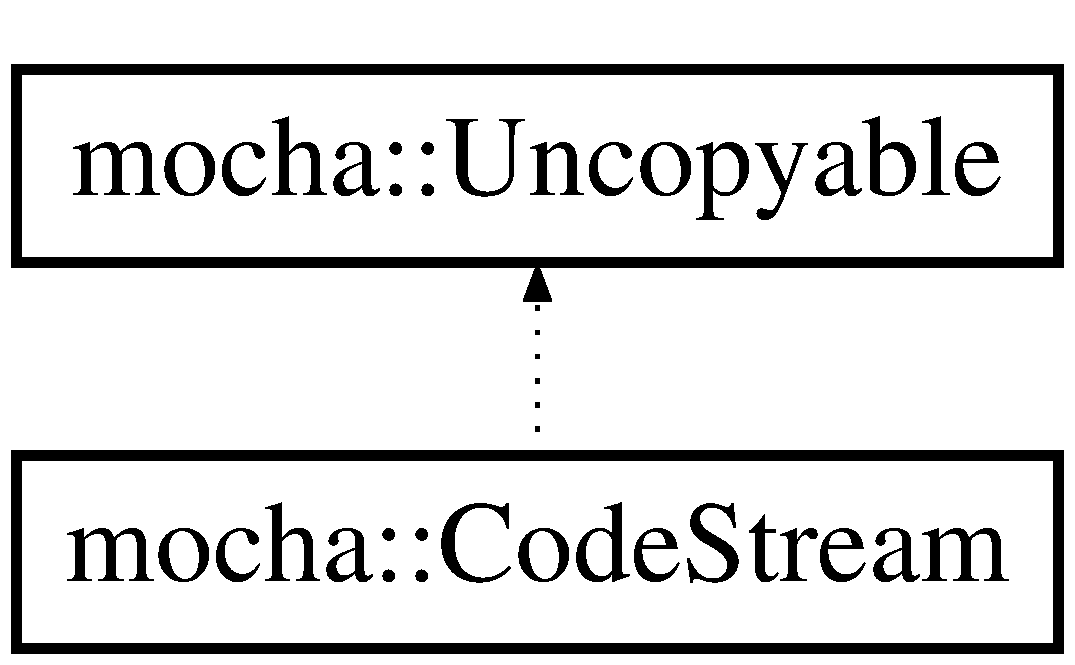
\includegraphics[height=2.000000cm]{classmocha_1_1_code_stream}
\end{center}
\end{figure}
\subsection*{Public Member Functions}
\begin{DoxyCompactItemize}
\item 
\hyperlink{classmocha_1_1_code_stream_ae0e5c3f5599c97bc1354e549b1f202a4}{CodeStream} (\hyperlink{classmocha_1_1_code_buffer}{CodeBuffer} $\ast$buffer)
\item 
\hyperlink{classmocha_1_1_code_stream_a9446e463e9c2adf3c505fbc2a05695f0}{$\sim$CodeStream} ()
\item 
void \hyperlink{classmocha_1_1_code_stream_ac351b0f42bbbfb97b9ee40fd1248a02d}{Write} (const char $\ast$str)
\item 
void \hyperlink{classmocha_1_1_code_stream_a69fa6bd2d319de1d5f5f2c016c95b243}{Write} (char str)
\item 
void \hyperlink{classmocha_1_1_code_stream_a67192401b9f1a1fe958f1a90c3a7cd42}{Write} (const std::string \&str)
\item 
void \hyperlink{classmocha_1_1_code_stream_abee24daebb502e307b9b68f62de6f859}{Erase} (size\_\-t beg, size\_\-t end)
\item 
size\_\-t \hyperlink{classmocha_1_1_code_stream_aed17227c989668c2449042a31acfecf6}{Size} ()
\item 
const \hyperlink{classmocha_1_1_code_buffer}{CodeBuffer} $\ast$ \hyperlink{classmocha_1_1_code_stream_ad78d4b93ca9ce0c99c39d7d33ada7b68}{Get} ()
\end{DoxyCompactItemize}
\subsection*{Private Attributes}
\begin{DoxyCompactItemize}
\item 
\hyperlink{classmocha_1_1_code_buffer}{CodeBuffer} $\ast$ \hyperlink{classmocha_1_1_code_stream_a36360ceeeeef7085eb47ae18175ec1f4}{buffer\_\-}
\end{DoxyCompactItemize}


\subsection{Detailed Description}


Definition at line 28 of file codegenerator\_\-utils.h.



\subsection{Constructor \& Destructor Documentation}
\hypertarget{classmocha_1_1_code_stream_ae0e5c3f5599c97bc1354e549b1f202a4}{
\index{mocha::CodeStream@{mocha::CodeStream}!CodeStream@{CodeStream}}
\index{CodeStream@{CodeStream}!mocha::CodeStream@{mocha::CodeStream}}
\subsubsection[{CodeStream}]{\setlength{\rightskip}{0pt plus 5cm}mocha::CodeStream::CodeStream (
\begin{DoxyParamCaption}
\item[{{\bf CodeBuffer} $\ast$}]{buffer}
\end{DoxyParamCaption}
)\hspace{0.3cm}{\ttfamily  \mbox{[}inline\mbox{]}}}}
\label{classmocha_1_1_code_stream_ae0e5c3f5599c97bc1354e549b1f202a4}


Definition at line 30 of file codegenerator\_\-utils.h.

\hypertarget{classmocha_1_1_code_stream_a9446e463e9c2adf3c505fbc2a05695f0}{
\index{mocha::CodeStream@{mocha::CodeStream}!$\sim$CodeStream@{$\sim$CodeStream}}
\index{$\sim$CodeStream@{$\sim$CodeStream}!mocha::CodeStream@{mocha::CodeStream}}
\subsubsection[{$\sim$CodeStream}]{\setlength{\rightskip}{0pt plus 5cm}mocha::CodeStream::$\sim$CodeStream (
\begin{DoxyParamCaption}
{}
\end{DoxyParamCaption}
)\hspace{0.3cm}{\ttfamily  \mbox{[}inline\mbox{]}}}}
\label{classmocha_1_1_code_stream_a9446e463e9c2adf3c505fbc2a05695f0}


Definition at line 31 of file codegenerator\_\-utils.h.



\subsection{Member Function Documentation}
\hypertarget{classmocha_1_1_code_stream_abee24daebb502e307b9b68f62de6f859}{
\index{mocha::CodeStream@{mocha::CodeStream}!Erase@{Erase}}
\index{Erase@{Erase}!mocha::CodeStream@{mocha::CodeStream}}
\subsubsection[{Erase}]{\setlength{\rightskip}{0pt plus 5cm}void mocha::CodeStream::Erase (
\begin{DoxyParamCaption}
\item[{size\_\-t}]{beg, }
\item[{size\_\-t}]{end}
\end{DoxyParamCaption}
)\hspace{0.3cm}{\ttfamily  \mbox{[}inline\mbox{]}}}}
\label{classmocha_1_1_code_stream_abee24daebb502e307b9b68f62de6f859}


Definition at line 35 of file codegenerator\_\-utils.h.

\hypertarget{classmocha_1_1_code_stream_ad78d4b93ca9ce0c99c39d7d33ada7b68}{
\index{mocha::CodeStream@{mocha::CodeStream}!Get@{Get}}
\index{Get@{Get}!mocha::CodeStream@{mocha::CodeStream}}
\subsubsection[{Get}]{\setlength{\rightskip}{0pt plus 5cm}const {\bf CodeBuffer}$\ast$ mocha::CodeStream::Get (
\begin{DoxyParamCaption}
{}
\end{DoxyParamCaption}
)\hspace{0.3cm}{\ttfamily  \mbox{[}inline\mbox{]}}}}
\label{classmocha_1_1_code_stream_ad78d4b93ca9ce0c99c39d7d33ada7b68}


Definition at line 37 of file codegenerator\_\-utils.h.

\hypertarget{classmocha_1_1_code_stream_aed17227c989668c2449042a31acfecf6}{
\index{mocha::CodeStream@{mocha::CodeStream}!Size@{Size}}
\index{Size@{Size}!mocha::CodeStream@{mocha::CodeStream}}
\subsubsection[{Size}]{\setlength{\rightskip}{0pt plus 5cm}size\_\-t mocha::CodeStream::Size (
\begin{DoxyParamCaption}
{}
\end{DoxyParamCaption}
)\hspace{0.3cm}{\ttfamily  \mbox{[}inline\mbox{]}}}}
\label{classmocha_1_1_code_stream_aed17227c989668c2449042a31acfecf6}


Definition at line 36 of file codegenerator\_\-utils.h.

\hypertarget{classmocha_1_1_code_stream_a69fa6bd2d319de1d5f5f2c016c95b243}{
\index{mocha::CodeStream@{mocha::CodeStream}!Write@{Write}}
\index{Write@{Write}!mocha::CodeStream@{mocha::CodeStream}}
\subsubsection[{Write}]{\setlength{\rightskip}{0pt plus 5cm}void mocha::CodeStream::Write (
\begin{DoxyParamCaption}
\item[{char}]{str}
\end{DoxyParamCaption}
)\hspace{0.3cm}{\ttfamily  \mbox{[}inline\mbox{]}}}}
\label{classmocha_1_1_code_stream_a69fa6bd2d319de1d5f5f2c016c95b243}


Definition at line 33 of file codegenerator\_\-utils.h.

\hypertarget{classmocha_1_1_code_stream_a67192401b9f1a1fe958f1a90c3a7cd42}{
\index{mocha::CodeStream@{mocha::CodeStream}!Write@{Write}}
\index{Write@{Write}!mocha::CodeStream@{mocha::CodeStream}}
\subsubsection[{Write}]{\setlength{\rightskip}{0pt plus 5cm}void mocha::CodeStream::Write (
\begin{DoxyParamCaption}
\item[{const std::string \&}]{str}
\end{DoxyParamCaption}
)\hspace{0.3cm}{\ttfamily  \mbox{[}inline\mbox{]}}}}
\label{classmocha_1_1_code_stream_a67192401b9f1a1fe958f1a90c3a7cd42}


Definition at line 34 of file codegenerator\_\-utils.h.

\hypertarget{classmocha_1_1_code_stream_ac351b0f42bbbfb97b9ee40fd1248a02d}{
\index{mocha::CodeStream@{mocha::CodeStream}!Write@{Write}}
\index{Write@{Write}!mocha::CodeStream@{mocha::CodeStream}}
\subsubsection[{Write}]{\setlength{\rightskip}{0pt plus 5cm}void mocha::CodeStream::Write (
\begin{DoxyParamCaption}
\item[{const char $\ast$}]{str}
\end{DoxyParamCaption}
)\hspace{0.3cm}{\ttfamily  \mbox{[}inline\mbox{]}}}}
\label{classmocha_1_1_code_stream_ac351b0f42bbbfb97b9ee40fd1248a02d}


Definition at line 32 of file codegenerator\_\-utils.h.



\subsection{Member Data Documentation}
\hypertarget{classmocha_1_1_code_stream_a36360ceeeeef7085eb47ae18175ec1f4}{
\index{mocha::CodeStream@{mocha::CodeStream}!buffer\_\-@{buffer\_\-}}
\index{buffer\_\-@{buffer\_\-}!mocha::CodeStream@{mocha::CodeStream}}
\subsubsection[{buffer\_\-}]{\setlength{\rightskip}{0pt plus 5cm}{\bf CodeBuffer}$\ast$ {\bf mocha::CodeStream::buffer\_\-}\hspace{0.3cm}{\ttfamily  \mbox{[}private\mbox{]}}}}
\label{classmocha_1_1_code_stream_a36360ceeeeef7085eb47ae18175ec1f4}


Definition at line 39 of file codegenerator\_\-utils.h.



The documentation for this class was generated from the following file:\begin{DoxyCompactItemize}
\item 
Y:/mocha/src/ast/visitors/utils/\hyperlink{codegenerator__utils_8h}{codegenerator\_\-utils.h}\end{DoxyCompactItemize}

\hypertarget{classmocha_1_1_code_writer}{
\section{mocha::CodeWriter Class Reference}
\label{classmocha_1_1_code_writer}\index{mocha::CodeWriter@{mocha::CodeWriter}}
}


{\ttfamily \#include $<$codewriter.h$>$}

\subsection*{Classes}
\begin{DoxyCompactItemize}
\item 
class \hyperlink{classmocha_1_1_code_writer_1_1_writer_base}{WriterBase}
\end{DoxyCompactItemize}
\subsection*{Public Types}
\begin{DoxyCompactItemize}
\item 
enum \{ \par
\hyperlink{classmocha_1_1_code_writer_a4d6f9ba5b8b3730c40b111ff9fd1b1d7afbc196b779b1b83fc16a44a28bc95338}{kNone} =  0, 
\hyperlink{classmocha_1_1_code_writer_a4d6f9ba5b8b3730c40b111ff9fd1b1d7ad616922326ca26acdf79cc21e3ae14cb}{kFunctionBeginBrace}, 
\hyperlink{classmocha_1_1_code_writer_a4d6f9ba5b8b3730c40b111ff9fd1b1d7aa061075aabb8ea3697637bdd7a808f85}{kFunctionEndBrace}, 
\hyperlink{classmocha_1_1_code_writer_a4d6f9ba5b8b3730c40b111ff9fd1b1d7a27f484fb5ee833455a5e29db3a47f184}{kSwitchEndBrace}, 
\par
\hyperlink{classmocha_1_1_code_writer_a4d6f9ba5b8b3730c40b111ff9fd1b1d7abe06cec3818fd03dc0b542eb90869eee}{kBlockBeginBrace}, 
\hyperlink{classmocha_1_1_code_writer_a4d6f9ba5b8b3730c40b111ff9fd1b1d7a91134eabff56921bb803a6baf3f53e78}{kBlockEndBrace}, 
\hyperlink{classmocha_1_1_code_writer_a4d6f9ba5b8b3730c40b111ff9fd1b1d7acfc553f55af66ce0c401dfcb6d0ed149}{kArgs}, 
\hyperlink{classmocha_1_1_code_writer_a4d6f9ba5b8b3730c40b111ff9fd1b1d7ac8d7ee94fe8d8810733a212fb0b6c729}{kFor}, 
\par
\hyperlink{classmocha_1_1_code_writer_a4d6f9ba5b8b3730c40b111ff9fd1b1d7a8619a6d8347e65d8bd8826c07709ff0b}{kVarsComma}, 
\hyperlink{classmocha_1_1_code_writer_a4d6f9ba5b8b3730c40b111ff9fd1b1d7a4efadad643e37ccecab6696eab00233d}{kVarsEnd}, 
\hyperlink{classmocha_1_1_code_writer_a4d6f9ba5b8b3730c40b111ff9fd1b1d7a492e3b988aa1407d0fbf8e7eb8308ac6}{kParenExp}, 
\hyperlink{classmocha_1_1_code_writer_a4d6f9ba5b8b3730c40b111ff9fd1b1d7a8f32fdf01a1f3e89ae0c02e8cd0cf27c}{kCase}, 
\par
\hyperlink{classmocha_1_1_code_writer_a4d6f9ba5b8b3730c40b111ff9fd1b1d7ad0ab961dac5440f6b03d5a622ecdb315}{kNewNoArgsBegin}, 
\hyperlink{classmocha_1_1_code_writer_a4d6f9ba5b8b3730c40b111ff9fd1b1d7a4be477a8799f398fb88071664fa3cf64}{kNewNoArgsEnd}, 
\hyperlink{classmocha_1_1_code_writer_a4d6f9ba5b8b3730c40b111ff9fd1b1d7abcb138ef1a0b54f41970af04b69d3e7c}{kElseBlockEnd}, 
\hyperlink{classmocha_1_1_code_writer_a4d6f9ba5b8b3730c40b111ff9fd1b1d7aaa3f0ba0a3e7f296862fd20aa4eefca7}{kNamedModule}, 
\par
\hyperlink{classmocha_1_1_code_writer_a4d6f9ba5b8b3730c40b111ff9fd1b1d7a826c703e280b6704e0bf8c2c801ae6aa}{kAnonymousModule}, 
\hyperlink{classmocha_1_1_code_writer_a4d6f9ba5b8b3730c40b111ff9fd1b1d7ac0cc4162a5ca8a0955392cf254c4703f}{kExpSp}
 \}
\end{DoxyCompactItemize}
\subsection*{Public Member Functions}
\begin{DoxyCompactItemize}
\item 
\hyperlink{classmocha_1_1_code_writer_aaab0ffcfe18c2a2d0b5c105cc6b1760c}{CodeWriter} (bool is\_\-pretty\_\-print, bool is\_\-line)
\item 
\hyperlink{classmocha_1_1_code_writer_a3801004e7976480ab4c6f038c6cfba81}{$\sim$CodeWriter} ()
\item 
void \hyperlink{classmocha_1_1_code_writer_abcd4082915eaffa64ca31c69cc741998}{Write} (const char $\ast$code, \hyperlink{classmocha_1_1_code_stream}{CodeStream} $\ast$stream\_\-)
\item 
void \hyperlink{classmocha_1_1_code_writer_aee997b027d9115d8c074e73d56cbc0d1}{WriteOp} (int op, int state, \hyperlink{classmocha_1_1_code_stream}{CodeStream} $\ast$stream\_\-)
\item 
void \hyperlink{classmocha_1_1_code_writer_abbc219cc9873f857db5132f78bc930c6}{InsertDebugSymbol} (\hyperlink{classmocha_1_1_code_stream}{CodeStream} $\ast$stream\_\-)
\item 
void \hyperlink{classmocha_1_1_code_writer_a56d11286670e778acb3291460f85083c}{InitializeFileName} (const char $\ast$file, \hyperlink{classmocha_1_1_code_stream}{CodeStream} $\ast$stream\_\-)
\item 
void \hyperlink{classmocha_1_1_code_writer_a5d9dbfcecb429b86bde76756d19eb104}{DebugBlockBegin} (\hyperlink{classmocha_1_1_code_stream}{CodeStream} $\ast$stream)
\item 
void \hyperlink{classmocha_1_1_code_writer_a7bbf005f34cf317ee4e80bde03fc9fdb}{DebugBlockEnd} (\hyperlink{classmocha_1_1_code_stream}{CodeStream} $\ast$stream, \hyperlink{classmocha_1_1_inner_scope}{InnerScope} $\ast$scope)
\item 
void \hyperlink{classmocha_1_1_code_writer_a5267a95969ca16cac16ce2438e259aa3}{SetFileName} (\hyperlink{classmocha_1_1_code_stream}{CodeStream} $\ast$stream\_\-)
\item 
void \hyperlink{classmocha_1_1_code_writer_aad28d04cdd03938bf2aa85f80cda9019}{SetLine} (long line, \hyperlink{classmocha_1_1_code_stream}{CodeStream} $\ast$stream\_\-, \hyperlink{classmocha_1_1_file_root}{FileRoot} $\ast$root)
\item 
void \hyperlink{classmocha_1_1_code_writer_ad9d7877e35623905a58defdba4d28ead}{ModuleBeginProccessor} (const char $\ast$key, const char $\ast$name, \hyperlink{classmocha_1_1_code_stream}{CodeStream} $\ast$stream\_\-)
\item 
void \hyperlink{classmocha_1_1_code_writer_a5a7c49a9001a89aaaab643fdc758fe6c}{AnonymousModuleBeginProccessor} (const char $\ast$key, \hyperlink{classmocha_1_1_code_stream}{CodeStream} $\ast$stream\_\-)
\item 
void \hyperlink{classmocha_1_1_code_writer_a198b911543f034cd59a77c0ddb9667c8}{ModuleEndProccessor} (\hyperlink{classmocha_1_1_code_stream}{CodeStream} $\ast$stream\_\-)
\item 
void \hyperlink{classmocha_1_1_code_writer_a8a8890b83765cea7c40b2e8ac67192a2}{AnonymousModuleEndProccessor} (\hyperlink{classmocha_1_1_code_stream}{CodeStream} $\ast$stream\_\-)
\end{DoxyCompactItemize}
\subsection*{Private Attributes}
\begin{DoxyCompactItemize}
\item 
bool \hyperlink{classmocha_1_1_code_writer_a500de5cadf77c987ccd3b2d51c9d4487}{is\_\-pretty\_\-print\_\-}
\item 
bool \hyperlink{classmocha_1_1_code_writer_ae3fba73309d6010b17ce1b6ec6a52e4d}{is\_\-line\_\-}
\item 
\hyperlink{classmocha_1_1_code_writer_1_1_writer_base}{WriterBase} $\ast$ \hyperlink{classmocha_1_1_code_writer_a9591201ce4008cddd9873ecc9ecda25d}{base\_\-}
\end{DoxyCompactItemize}


\subsection{Detailed Description}


Definition at line 10 of file codewriter.h.



\subsection{Member Enumeration Documentation}
\hypertarget{classmocha_1_1_code_writer_a4d6f9ba5b8b3730c40b111ff9fd1b1d7}{
\subsubsection[{"@13}]{\setlength{\rightskip}{0pt plus 5cm}anonymous enum}}
\label{classmocha_1_1_code_writer_a4d6f9ba5b8b3730c40b111ff9fd1b1d7}
\begin{Desc}
\item[Enumerator: ]\par
\begin{description}
\index{kNone@{kNone}!mocha::CodeWriter@{mocha::CodeWriter}}\index{mocha::CodeWriter@{mocha::CodeWriter}!kNone@{kNone}}\item[{\em 
\hypertarget{classmocha_1_1_code_writer_a4d6f9ba5b8b3730c40b111ff9fd1b1d7afbc196b779b1b83fc16a44a28bc95338}{
kNone}
\label{classmocha_1_1_code_writer_a4d6f9ba5b8b3730c40b111ff9fd1b1d7afbc196b779b1b83fc16a44a28bc95338}
}]\index{kFunctionBeginBrace@{kFunctionBeginBrace}!mocha::CodeWriter@{mocha::CodeWriter}}\index{mocha::CodeWriter@{mocha::CodeWriter}!kFunctionBeginBrace@{kFunctionBeginBrace}}\item[{\em 
\hypertarget{classmocha_1_1_code_writer_a4d6f9ba5b8b3730c40b111ff9fd1b1d7ad616922326ca26acdf79cc21e3ae14cb}{
kFunctionBeginBrace}
\label{classmocha_1_1_code_writer_a4d6f9ba5b8b3730c40b111ff9fd1b1d7ad616922326ca26acdf79cc21e3ae14cb}
}]\index{kFunctionEndBrace@{kFunctionEndBrace}!mocha::CodeWriter@{mocha::CodeWriter}}\index{mocha::CodeWriter@{mocha::CodeWriter}!kFunctionEndBrace@{kFunctionEndBrace}}\item[{\em 
\hypertarget{classmocha_1_1_code_writer_a4d6f9ba5b8b3730c40b111ff9fd1b1d7aa061075aabb8ea3697637bdd7a808f85}{
kFunctionEndBrace}
\label{classmocha_1_1_code_writer_a4d6f9ba5b8b3730c40b111ff9fd1b1d7aa061075aabb8ea3697637bdd7a808f85}
}]\index{kSwitchEndBrace@{kSwitchEndBrace}!mocha::CodeWriter@{mocha::CodeWriter}}\index{mocha::CodeWriter@{mocha::CodeWriter}!kSwitchEndBrace@{kSwitchEndBrace}}\item[{\em 
\hypertarget{classmocha_1_1_code_writer_a4d6f9ba5b8b3730c40b111ff9fd1b1d7a27f484fb5ee833455a5e29db3a47f184}{
kSwitchEndBrace}
\label{classmocha_1_1_code_writer_a4d6f9ba5b8b3730c40b111ff9fd1b1d7a27f484fb5ee833455a5e29db3a47f184}
}]\index{kBlockBeginBrace@{kBlockBeginBrace}!mocha::CodeWriter@{mocha::CodeWriter}}\index{mocha::CodeWriter@{mocha::CodeWriter}!kBlockBeginBrace@{kBlockBeginBrace}}\item[{\em 
\hypertarget{classmocha_1_1_code_writer_a4d6f9ba5b8b3730c40b111ff9fd1b1d7abe06cec3818fd03dc0b542eb90869eee}{
kBlockBeginBrace}
\label{classmocha_1_1_code_writer_a4d6f9ba5b8b3730c40b111ff9fd1b1d7abe06cec3818fd03dc0b542eb90869eee}
}]\index{kBlockEndBrace@{kBlockEndBrace}!mocha::CodeWriter@{mocha::CodeWriter}}\index{mocha::CodeWriter@{mocha::CodeWriter}!kBlockEndBrace@{kBlockEndBrace}}\item[{\em 
\hypertarget{classmocha_1_1_code_writer_a4d6f9ba5b8b3730c40b111ff9fd1b1d7a91134eabff56921bb803a6baf3f53e78}{
kBlockEndBrace}
\label{classmocha_1_1_code_writer_a4d6f9ba5b8b3730c40b111ff9fd1b1d7a91134eabff56921bb803a6baf3f53e78}
}]\index{kArgs@{kArgs}!mocha::CodeWriter@{mocha::CodeWriter}}\index{mocha::CodeWriter@{mocha::CodeWriter}!kArgs@{kArgs}}\item[{\em 
\hypertarget{classmocha_1_1_code_writer_a4d6f9ba5b8b3730c40b111ff9fd1b1d7acfc553f55af66ce0c401dfcb6d0ed149}{
kArgs}
\label{classmocha_1_1_code_writer_a4d6f9ba5b8b3730c40b111ff9fd1b1d7acfc553f55af66ce0c401dfcb6d0ed149}
}]\index{kFor@{kFor}!mocha::CodeWriter@{mocha::CodeWriter}}\index{mocha::CodeWriter@{mocha::CodeWriter}!kFor@{kFor}}\item[{\em 
\hypertarget{classmocha_1_1_code_writer_a4d6f9ba5b8b3730c40b111ff9fd1b1d7ac8d7ee94fe8d8810733a212fb0b6c729}{
kFor}
\label{classmocha_1_1_code_writer_a4d6f9ba5b8b3730c40b111ff9fd1b1d7ac8d7ee94fe8d8810733a212fb0b6c729}
}]\index{kVarsComma@{kVarsComma}!mocha::CodeWriter@{mocha::CodeWriter}}\index{mocha::CodeWriter@{mocha::CodeWriter}!kVarsComma@{kVarsComma}}\item[{\em 
\hypertarget{classmocha_1_1_code_writer_a4d6f9ba5b8b3730c40b111ff9fd1b1d7a8619a6d8347e65d8bd8826c07709ff0b}{
kVarsComma}
\label{classmocha_1_1_code_writer_a4d6f9ba5b8b3730c40b111ff9fd1b1d7a8619a6d8347e65d8bd8826c07709ff0b}
}]\index{kVarsEnd@{kVarsEnd}!mocha::CodeWriter@{mocha::CodeWriter}}\index{mocha::CodeWriter@{mocha::CodeWriter}!kVarsEnd@{kVarsEnd}}\item[{\em 
\hypertarget{classmocha_1_1_code_writer_a4d6f9ba5b8b3730c40b111ff9fd1b1d7a4efadad643e37ccecab6696eab00233d}{
kVarsEnd}
\label{classmocha_1_1_code_writer_a4d6f9ba5b8b3730c40b111ff9fd1b1d7a4efadad643e37ccecab6696eab00233d}
}]\index{kParenExp@{kParenExp}!mocha::CodeWriter@{mocha::CodeWriter}}\index{mocha::CodeWriter@{mocha::CodeWriter}!kParenExp@{kParenExp}}\item[{\em 
\hypertarget{classmocha_1_1_code_writer_a4d6f9ba5b8b3730c40b111ff9fd1b1d7a492e3b988aa1407d0fbf8e7eb8308ac6}{
kParenExp}
\label{classmocha_1_1_code_writer_a4d6f9ba5b8b3730c40b111ff9fd1b1d7a492e3b988aa1407d0fbf8e7eb8308ac6}
}]\index{kCase@{kCase}!mocha::CodeWriter@{mocha::CodeWriter}}\index{mocha::CodeWriter@{mocha::CodeWriter}!kCase@{kCase}}\item[{\em 
\hypertarget{classmocha_1_1_code_writer_a4d6f9ba5b8b3730c40b111ff9fd1b1d7a8f32fdf01a1f3e89ae0c02e8cd0cf27c}{
kCase}
\label{classmocha_1_1_code_writer_a4d6f9ba5b8b3730c40b111ff9fd1b1d7a8f32fdf01a1f3e89ae0c02e8cd0cf27c}
}]\index{kNewNoArgsBegin@{kNewNoArgsBegin}!mocha::CodeWriter@{mocha::CodeWriter}}\index{mocha::CodeWriter@{mocha::CodeWriter}!kNewNoArgsBegin@{kNewNoArgsBegin}}\item[{\em 
\hypertarget{classmocha_1_1_code_writer_a4d6f9ba5b8b3730c40b111ff9fd1b1d7ad0ab961dac5440f6b03d5a622ecdb315}{
kNewNoArgsBegin}
\label{classmocha_1_1_code_writer_a4d6f9ba5b8b3730c40b111ff9fd1b1d7ad0ab961dac5440f6b03d5a622ecdb315}
}]\index{kNewNoArgsEnd@{kNewNoArgsEnd}!mocha::CodeWriter@{mocha::CodeWriter}}\index{mocha::CodeWriter@{mocha::CodeWriter}!kNewNoArgsEnd@{kNewNoArgsEnd}}\item[{\em 
\hypertarget{classmocha_1_1_code_writer_a4d6f9ba5b8b3730c40b111ff9fd1b1d7a4be477a8799f398fb88071664fa3cf64}{
kNewNoArgsEnd}
\label{classmocha_1_1_code_writer_a4d6f9ba5b8b3730c40b111ff9fd1b1d7a4be477a8799f398fb88071664fa3cf64}
}]\index{kElseBlockEnd@{kElseBlockEnd}!mocha::CodeWriter@{mocha::CodeWriter}}\index{mocha::CodeWriter@{mocha::CodeWriter}!kElseBlockEnd@{kElseBlockEnd}}\item[{\em 
\hypertarget{classmocha_1_1_code_writer_a4d6f9ba5b8b3730c40b111ff9fd1b1d7abcb138ef1a0b54f41970af04b69d3e7c}{
kElseBlockEnd}
\label{classmocha_1_1_code_writer_a4d6f9ba5b8b3730c40b111ff9fd1b1d7abcb138ef1a0b54f41970af04b69d3e7c}
}]\index{kNamedModule@{kNamedModule}!mocha::CodeWriter@{mocha::CodeWriter}}\index{mocha::CodeWriter@{mocha::CodeWriter}!kNamedModule@{kNamedModule}}\item[{\em 
\hypertarget{classmocha_1_1_code_writer_a4d6f9ba5b8b3730c40b111ff9fd1b1d7aaa3f0ba0a3e7f296862fd20aa4eefca7}{
kNamedModule}
\label{classmocha_1_1_code_writer_a4d6f9ba5b8b3730c40b111ff9fd1b1d7aaa3f0ba0a3e7f296862fd20aa4eefca7}
}]\index{kAnonymousModule@{kAnonymousModule}!mocha::CodeWriter@{mocha::CodeWriter}}\index{mocha::CodeWriter@{mocha::CodeWriter}!kAnonymousModule@{kAnonymousModule}}\item[{\em 
\hypertarget{classmocha_1_1_code_writer_a4d6f9ba5b8b3730c40b111ff9fd1b1d7a826c703e280b6704e0bf8c2c801ae6aa}{
kAnonymousModule}
\label{classmocha_1_1_code_writer_a4d6f9ba5b8b3730c40b111ff9fd1b1d7a826c703e280b6704e0bf8c2c801ae6aa}
}]\index{kExpSp@{kExpSp}!mocha::CodeWriter@{mocha::CodeWriter}}\index{mocha::CodeWriter@{mocha::CodeWriter}!kExpSp@{kExpSp}}\item[{\em 
\hypertarget{classmocha_1_1_code_writer_a4d6f9ba5b8b3730c40b111ff9fd1b1d7ac0cc4162a5ca8a0955392cf254c4703f}{
kExpSp}
\label{classmocha_1_1_code_writer_a4d6f9ba5b8b3730c40b111ff9fd1b1d7ac0cc4162a5ca8a0955392cf254c4703f}
}]\end{description}
\end{Desc}



Definition at line 12 of file codewriter.h.



\subsection{Constructor \& Destructor Documentation}
\hypertarget{classmocha_1_1_code_writer_aaab0ffcfe18c2a2d0b5c105cc6b1760c}{
\index{mocha::CodeWriter@{mocha::CodeWriter}!CodeWriter@{CodeWriter}}
\index{CodeWriter@{CodeWriter}!mocha::CodeWriter@{mocha::CodeWriter}}
\subsubsection[{CodeWriter}]{\setlength{\rightskip}{0pt plus 5cm}mocha::CodeWriter::CodeWriter (
\begin{DoxyParamCaption}
\item[{bool}]{is\_\-pretty\_\-print, }
\item[{bool}]{is\_\-line}
\end{DoxyParamCaption}
)}}
\label{classmocha_1_1_code_writer_aaab0ffcfe18c2a2d0b5c105cc6b1760c}


Definition at line 435 of file codewriter.cc.

\hypertarget{classmocha_1_1_code_writer_a3801004e7976480ab4c6f038c6cfba81}{
\index{mocha::CodeWriter@{mocha::CodeWriter}!$\sim$CodeWriter@{$\sim$CodeWriter}}
\index{$\sim$CodeWriter@{$\sim$CodeWriter}!mocha::CodeWriter@{mocha::CodeWriter}}
\subsubsection[{$\sim$CodeWriter}]{\setlength{\rightskip}{0pt plus 5cm}mocha::CodeWriter::$\sim$CodeWriter (
\begin{DoxyParamCaption}
{}
\end{DoxyParamCaption}
)}}
\label{classmocha_1_1_code_writer_a3801004e7976480ab4c6f038c6cfba81}


Definition at line 443 of file codewriter.cc.



\subsection{Member Function Documentation}
\hypertarget{classmocha_1_1_code_writer_a5a7c49a9001a89aaaab643fdc758fe6c}{
\index{mocha::CodeWriter@{mocha::CodeWriter}!AnonymousModuleBeginProccessor@{AnonymousModuleBeginProccessor}}
\index{AnonymousModuleBeginProccessor@{AnonymousModuleBeginProccessor}!mocha::CodeWriter@{mocha::CodeWriter}}
\subsubsection[{AnonymousModuleBeginProccessor}]{\setlength{\rightskip}{0pt plus 5cm}void mocha::CodeWriter::AnonymousModuleBeginProccessor (
\begin{DoxyParamCaption}
\item[{const char $\ast$}]{key, }
\item[{{\bf CodeStream} $\ast$}]{stream\_\-}
\end{DoxyParamCaption}
)}}
\label{classmocha_1_1_code_writer_a5a7c49a9001a89aaaab643fdc758fe6c}


Definition at line 570 of file codewriter.cc.

\hypertarget{classmocha_1_1_code_writer_a8a8890b83765cea7c40b2e8ac67192a2}{
\index{mocha::CodeWriter@{mocha::CodeWriter}!AnonymousModuleEndProccessor@{AnonymousModuleEndProccessor}}
\index{AnonymousModuleEndProccessor@{AnonymousModuleEndProccessor}!mocha::CodeWriter@{mocha::CodeWriter}}
\subsubsection[{AnonymousModuleEndProccessor}]{\setlength{\rightskip}{0pt plus 5cm}void mocha::CodeWriter::AnonymousModuleEndProccessor (
\begin{DoxyParamCaption}
\item[{{\bf CodeStream} $\ast$}]{stream\_\-}
\end{DoxyParamCaption}
)}}
\label{classmocha_1_1_code_writer_a8a8890b83765cea7c40b2e8ac67192a2}


Definition at line 607 of file codewriter.cc.

\hypertarget{classmocha_1_1_code_writer_a5d9dbfcecb429b86bde76756d19eb104}{
\index{mocha::CodeWriter@{mocha::CodeWriter}!DebugBlockBegin@{DebugBlockBegin}}
\index{DebugBlockBegin@{DebugBlockBegin}!mocha::CodeWriter@{mocha::CodeWriter}}
\subsubsection[{DebugBlockBegin}]{\setlength{\rightskip}{0pt plus 5cm}void mocha::CodeWriter::DebugBlockBegin (
\begin{DoxyParamCaption}
\item[{{\bf CodeStream} $\ast$}]{stream}
\end{DoxyParamCaption}
)}}
\label{classmocha_1_1_code_writer_a5d9dbfcecb429b86bde76756d19eb104}


Definition at line 522 of file codewriter.cc.

\hypertarget{classmocha_1_1_code_writer_a7bbf005f34cf317ee4e80bde03fc9fdb}{
\index{mocha::CodeWriter@{mocha::CodeWriter}!DebugBlockEnd@{DebugBlockEnd}}
\index{DebugBlockEnd@{DebugBlockEnd}!mocha::CodeWriter@{mocha::CodeWriter}}
\subsubsection[{DebugBlockEnd}]{\setlength{\rightskip}{0pt plus 5cm}void mocha::CodeWriter::DebugBlockEnd (
\begin{DoxyParamCaption}
\item[{{\bf CodeStream} $\ast$}]{stream, }
\item[{{\bf InnerScope} $\ast$}]{scope}
\end{DoxyParamCaption}
)}}
\label{classmocha_1_1_code_writer_a7bbf005f34cf317ee4e80bde03fc9fdb}


Definition at line 534 of file codewriter.cc.

\hypertarget{classmocha_1_1_code_writer_a56d11286670e778acb3291460f85083c}{
\index{mocha::CodeWriter@{mocha::CodeWriter}!InitializeFileName@{InitializeFileName}}
\index{InitializeFileName@{InitializeFileName}!mocha::CodeWriter@{mocha::CodeWriter}}
\subsubsection[{InitializeFileName}]{\setlength{\rightskip}{0pt plus 5cm}void mocha::CodeWriter::InitializeFileName (
\begin{DoxyParamCaption}
\item[{const char $\ast$}]{file, }
\item[{{\bf CodeStream} $\ast$}]{stream\_\-}
\end{DoxyParamCaption}
)}}
\label{classmocha_1_1_code_writer_a56d11286670e778acb3291460f85083c}


Definition at line 454 of file codewriter.cc.

\hypertarget{classmocha_1_1_code_writer_abbc219cc9873f857db5132f78bc930c6}{
\index{mocha::CodeWriter@{mocha::CodeWriter}!InsertDebugSymbol@{InsertDebugSymbol}}
\index{InsertDebugSymbol@{InsertDebugSymbol}!mocha::CodeWriter@{mocha::CodeWriter}}
\subsubsection[{InsertDebugSymbol}]{\setlength{\rightskip}{0pt plus 5cm}void mocha::CodeWriter::InsertDebugSymbol (
\begin{DoxyParamCaption}
\item[{{\bf CodeStream} $\ast$}]{stream\_\-}
\end{DoxyParamCaption}
)}}
\label{classmocha_1_1_code_writer_abbc219cc9873f857db5132f78bc930c6}


Definition at line 447 of file codewriter.cc.

\hypertarget{classmocha_1_1_code_writer_ad9d7877e35623905a58defdba4d28ead}{
\index{mocha::CodeWriter@{mocha::CodeWriter}!ModuleBeginProccessor@{ModuleBeginProccessor}}
\index{ModuleBeginProccessor@{ModuleBeginProccessor}!mocha::CodeWriter@{mocha::CodeWriter}}
\subsubsection[{ModuleBeginProccessor}]{\setlength{\rightskip}{0pt plus 5cm}void mocha::CodeWriter::ModuleBeginProccessor (
\begin{DoxyParamCaption}
\item[{const char $\ast$}]{key, }
\item[{const char $\ast$}]{name, }
\item[{{\bf CodeStream} $\ast$}]{stream\_\-}
\end{DoxyParamCaption}
)}}
\label{classmocha_1_1_code_writer_ad9d7877e35623905a58defdba4d28ead}


Definition at line 498 of file codewriter.cc.

\hypertarget{classmocha_1_1_code_writer_a198b911543f034cd59a77c0ddb9667c8}{
\index{mocha::CodeWriter@{mocha::CodeWriter}!ModuleEndProccessor@{ModuleEndProccessor}}
\index{ModuleEndProccessor@{ModuleEndProccessor}!mocha::CodeWriter@{mocha::CodeWriter}}
\subsubsection[{ModuleEndProccessor}]{\setlength{\rightskip}{0pt plus 5cm}void mocha::CodeWriter::ModuleEndProccessor (
\begin{DoxyParamCaption}
\item[{{\bf CodeStream} $\ast$}]{stream\_\-}
\end{DoxyParamCaption}
)}}
\label{classmocha_1_1_code_writer_a198b911543f034cd59a77c0ddb9667c8}


Definition at line 594 of file codewriter.cc.

\hypertarget{classmocha_1_1_code_writer_a5267a95969ca16cac16ce2438e259aa3}{
\index{mocha::CodeWriter@{mocha::CodeWriter}!SetFileName@{SetFileName}}
\index{SetFileName@{SetFileName}!mocha::CodeWriter@{mocha::CodeWriter}}
\subsubsection[{SetFileName}]{\setlength{\rightskip}{0pt plus 5cm}void mocha::CodeWriter::SetFileName (
\begin{DoxyParamCaption}
\item[{{\bf CodeStream} $\ast$}]{stream\_\-}
\end{DoxyParamCaption}
)}}
\label{classmocha_1_1_code_writer_a5267a95969ca16cac16ce2438e259aa3}


Definition at line 470 of file codewriter.cc.

\hypertarget{classmocha_1_1_code_writer_aad28d04cdd03938bf2aa85f80cda9019}{
\index{mocha::CodeWriter@{mocha::CodeWriter}!SetLine@{SetLine}}
\index{SetLine@{SetLine}!mocha::CodeWriter@{mocha::CodeWriter}}
\subsubsection[{SetLine}]{\setlength{\rightskip}{0pt plus 5cm}void mocha::CodeWriter::SetLine (
\begin{DoxyParamCaption}
\item[{long}]{line, }
\item[{{\bf CodeStream} $\ast$}]{stream\_\-, }
\item[{{\bf FileRoot} $\ast$}]{root}
\end{DoxyParamCaption}
)}}
\label{classmocha_1_1_code_writer_aad28d04cdd03938bf2aa85f80cda9019}


Definition at line 479 of file codewriter.cc.

\hypertarget{classmocha_1_1_code_writer_abcd4082915eaffa64ca31c69cc741998}{
\index{mocha::CodeWriter@{mocha::CodeWriter}!Write@{Write}}
\index{Write@{Write}!mocha::CodeWriter@{mocha::CodeWriter}}
\subsubsection[{Write}]{\setlength{\rightskip}{0pt plus 5cm}void mocha::CodeWriter::Write (
\begin{DoxyParamCaption}
\item[{const char $\ast$}]{code, }
\item[{{\bf CodeStream} $\ast$}]{stream\_\-}
\end{DoxyParamCaption}
)}}
\label{classmocha_1_1_code_writer_abcd4082915eaffa64ca31c69cc741998}


Definition at line 490 of file codewriter.cc.

\hypertarget{classmocha_1_1_code_writer_aee997b027d9115d8c074e73d56cbc0d1}{
\index{mocha::CodeWriter@{mocha::CodeWriter}!WriteOp@{WriteOp}}
\index{WriteOp@{WriteOp}!mocha::CodeWriter@{mocha::CodeWriter}}
\subsubsection[{WriteOp}]{\setlength{\rightskip}{0pt plus 5cm}void mocha::CodeWriter::WriteOp (
\begin{DoxyParamCaption}
\item[{int}]{op, }
\item[{int}]{state, }
\item[{{\bf CodeStream} $\ast$}]{stream\_\-}
\end{DoxyParamCaption}
)}}
\label{classmocha_1_1_code_writer_aee997b027d9115d8c074e73d56cbc0d1}


Definition at line 494 of file codewriter.cc.



\subsection{Member Data Documentation}
\hypertarget{classmocha_1_1_code_writer_a9591201ce4008cddd9873ecc9ecda25d}{
\index{mocha::CodeWriter@{mocha::CodeWriter}!base\_\-@{base\_\-}}
\index{base\_\-@{base\_\-}!mocha::CodeWriter@{mocha::CodeWriter}}
\subsubsection[{base\_\-}]{\setlength{\rightskip}{0pt plus 5cm}{\bf WriterBase}$\ast$ {\bf mocha::CodeWriter::base\_\-}\hspace{0.3cm}{\ttfamily  \mbox{[}private\mbox{]}}}}
\label{classmocha_1_1_code_writer_a9591201ce4008cddd9873ecc9ecda25d}


Definition at line 50 of file codewriter.h.

\hypertarget{classmocha_1_1_code_writer_ae3fba73309d6010b17ce1b6ec6a52e4d}{
\index{mocha::CodeWriter@{mocha::CodeWriter}!is\_\-line\_\-@{is\_\-line\_\-}}
\index{is\_\-line\_\-@{is\_\-line\_\-}!mocha::CodeWriter@{mocha::CodeWriter}}
\subsubsection[{is\_\-line\_\-}]{\setlength{\rightskip}{0pt plus 5cm}bool {\bf mocha::CodeWriter::is\_\-line\_\-}\hspace{0.3cm}{\ttfamily  \mbox{[}private\mbox{]}}}}
\label{classmocha_1_1_code_writer_ae3fba73309d6010b17ce1b6ec6a52e4d}


Definition at line 49 of file codewriter.h.

\hypertarget{classmocha_1_1_code_writer_a500de5cadf77c987ccd3b2d51c9d4487}{
\index{mocha::CodeWriter@{mocha::CodeWriter}!is\_\-pretty\_\-print\_\-@{is\_\-pretty\_\-print\_\-}}
\index{is\_\-pretty\_\-print\_\-@{is\_\-pretty\_\-print\_\-}!mocha::CodeWriter@{mocha::CodeWriter}}
\subsubsection[{is\_\-pretty\_\-print\_\-}]{\setlength{\rightskip}{0pt plus 5cm}bool {\bf mocha::CodeWriter::is\_\-pretty\_\-print\_\-}\hspace{0.3cm}{\ttfamily  \mbox{[}private\mbox{]}}}}
\label{classmocha_1_1_code_writer_a500de5cadf77c987ccd3b2d51c9d4487}


Definition at line 46 of file codewriter.h.



The documentation for this class was generated from the following files:\begin{DoxyCompactItemize}
\item 
Y:/mocha/src/ast/visitors/utils/\hyperlink{codewriter_8h}{codewriter.h}\item 
Y:/mocha/src/ast/visitors/utils/\hyperlink{codewriter_8cc}{codewriter.cc}\end{DoxyCompactItemize}

\hypertarget{classmocha_1_1_command_line_options}{
\section{mocha::CommandLineOptions Class Reference}
\label{classmocha_1_1_command_line_options}\index{mocha::CommandLineOptions@{mocha::CommandLineOptions}}
}


{\ttfamily \#include $<$commandline\_\-options.h$>$}

\subsection*{Static Public Member Functions}
\begin{DoxyCompactItemize}
\item 
static \hyperlink{classmocha_1_1_options}{Options} $\ast$ \hyperlink{classmocha_1_1_command_line_options_a13dfbafd9b38f9c9e7daf65e0bd3ce06}{GetInstance} ()
\end{DoxyCompactItemize}
\subsection*{Static Private Attributes}
\begin{DoxyCompactItemize}
\item 
static \hyperlink{classmocha_1_1_options}{Options} \hyperlink{classmocha_1_1_command_line_options_a63d8a2ce777efc872a21d5e13c4a93e1}{instance\_\-}
\end{DoxyCompactItemize}


\subsection{Detailed Description}


Definition at line 8 of file commandline\_\-options.h.



\subsection{Member Function Documentation}
\hypertarget{classmocha_1_1_command_line_options_a13dfbafd9b38f9c9e7daf65e0bd3ce06}{
\index{mocha::CommandLineOptions@{mocha::CommandLineOptions}!GetInstance@{GetInstance}}
\index{GetInstance@{GetInstance}!mocha::CommandLineOptions@{mocha::CommandLineOptions}}
\subsubsection[{GetInstance}]{\setlength{\rightskip}{0pt plus 5cm}static {\bf Options}$\ast$ mocha::CommandLineOptions::GetInstance (
\begin{DoxyParamCaption}
{}
\end{DoxyParamCaption}
)\hspace{0.3cm}{\ttfamily  \mbox{[}inline, static\mbox{]}}}}
\label{classmocha_1_1_command_line_options_a13dfbafd9b38f9c9e7daf65e0bd3ce06}


Definition at line 10 of file commandline\_\-options.h.



\subsection{Member Data Documentation}
\hypertarget{classmocha_1_1_command_line_options_a63d8a2ce777efc872a21d5e13c4a93e1}{
\index{mocha::CommandLineOptions@{mocha::CommandLineOptions}!instance\_\-@{instance\_\-}}
\index{instance\_\-@{instance\_\-}!mocha::CommandLineOptions@{mocha::CommandLineOptions}}
\subsubsection[{instance\_\-}]{\setlength{\rightskip}{0pt plus 5cm}{\bf Options} {\bf mocha::CommandLineOptions::instance\_\-}\hspace{0.3cm}{\ttfamily  \mbox{[}static, private\mbox{]}}}}
\label{classmocha_1_1_command_line_options_a63d8a2ce777efc872a21d5e13c4a93e1}


Definition at line 14 of file commandline\_\-options.h.



The documentation for this class was generated from the following files:\begin{DoxyCompactItemize}
\item 
Y:/mocha/src/options/commandline/\hyperlink{commandline__options_8h}{commandline\_\-options.h}\item 
Y:/mocha/src/options/commandline/\hyperlink{commandline__options_8cc}{commandline\_\-options.cc}\end{DoxyCompactItemize}

\hypertarget{classmocha_1_1_commands}{
\section{mocha::Commands Class Reference}
\label{classmocha_1_1_commands}\index{mocha::Commands@{mocha::Commands}}
}


{\ttfamily \#include $<$commands.h$>$}

\subsection*{Public Member Functions}
\begin{DoxyCompactItemize}
\item 
\hyperlink{classmocha_1_1_commands_a4c5118ee7c24f90246cb4a33a8939d41}{Commands} ()
\item 
\hyperlink{classmocha_1_1_commands_a2178fdccdf06fde809e390ffaac54c74}{$\sim$Commands} ()
\item 
void \hyperlink{classmocha_1_1_commands_a842b60b81442359d32ea3455025ead38}{Exec} (const char $\ast$buf)
\item 
bool \hyperlink{classmocha_1_1_commands_a41d6c1d2810fa3887047970d24292a2f}{IsObserving} ()
\end{DoxyCompactItemize}
\subsection*{Private Attributes}
\begin{DoxyCompactItemize}
\item 
bool \hyperlink{classmocha_1_1_commands_a50baa86fd453e3e727829f8e10c1e05b}{is\_\-observe\_\-running\_\-}
\end{DoxyCompactItemize}


\subsection{Detailed Description}


Definition at line 5 of file commands.h.



\subsection{Constructor \& Destructor Documentation}
\hypertarget{classmocha_1_1_commands_a4c5118ee7c24f90246cb4a33a8939d41}{
\index{mocha::Commands@{mocha::Commands}!Commands@{Commands}}
\index{Commands@{Commands}!mocha::Commands@{mocha::Commands}}
\subsubsection[{Commands}]{\setlength{\rightskip}{0pt plus 5cm}mocha::Commands::Commands (
\begin{DoxyParamCaption}
{}
\end{DoxyParamCaption}
)\hspace{0.3cm}{\ttfamily  \mbox{[}inline\mbox{]}}}}
\label{classmocha_1_1_commands_a4c5118ee7c24f90246cb4a33a8939d41}


Definition at line 7 of file commands.h.

\hypertarget{classmocha_1_1_commands_a2178fdccdf06fde809e390ffaac54c74}{
\index{mocha::Commands@{mocha::Commands}!$\sim$Commands@{$\sim$Commands}}
\index{$\sim$Commands@{$\sim$Commands}!mocha::Commands@{mocha::Commands}}
\subsubsection[{$\sim$Commands}]{\setlength{\rightskip}{0pt plus 5cm}mocha::Commands::$\sim$Commands (
\begin{DoxyParamCaption}
{}
\end{DoxyParamCaption}
)\hspace{0.3cm}{\ttfamily  \mbox{[}inline\mbox{]}}}}
\label{classmocha_1_1_commands_a2178fdccdf06fde809e390ffaac54c74}


Definition at line 8 of file commands.h.



\subsection{Member Function Documentation}
\hypertarget{classmocha_1_1_commands_a842b60b81442359d32ea3455025ead38}{
\index{mocha::Commands@{mocha::Commands}!Exec@{Exec}}
\index{Exec@{Exec}!mocha::Commands@{mocha::Commands}}
\subsubsection[{Exec}]{\setlength{\rightskip}{0pt plus 5cm}void mocha::Commands::Exec (
\begin{DoxyParamCaption}
\item[{const char $\ast$}]{buf}
\end{DoxyParamCaption}
)}}
\label{classmocha_1_1_commands_a842b60b81442359d32ea3455025ead38}


Definition at line 6 of file commands.cc.

\hypertarget{classmocha_1_1_commands_a41d6c1d2810fa3887047970d24292a2f}{
\index{mocha::Commands@{mocha::Commands}!IsObserving@{IsObserving}}
\index{IsObserving@{IsObserving}!mocha::Commands@{mocha::Commands}}
\subsubsection[{IsObserving}]{\setlength{\rightskip}{0pt plus 5cm}bool mocha::Commands::IsObserving (
\begin{DoxyParamCaption}
{}
\end{DoxyParamCaption}
)\hspace{0.3cm}{\ttfamily  \mbox{[}inline\mbox{]}}}}
\label{classmocha_1_1_commands_a41d6c1d2810fa3887047970d24292a2f}


Definition at line 10 of file commands.h.



\subsection{Member Data Documentation}
\hypertarget{classmocha_1_1_commands_a50baa86fd453e3e727829f8e10c1e05b}{
\index{mocha::Commands@{mocha::Commands}!is\_\-observe\_\-running\_\-@{is\_\-observe\_\-running\_\-}}
\index{is\_\-observe\_\-running\_\-@{is\_\-observe\_\-running\_\-}!mocha::Commands@{mocha::Commands}}
\subsubsection[{is\_\-observe\_\-running\_\-}]{\setlength{\rightskip}{0pt plus 5cm}bool {\bf mocha::Commands::is\_\-observe\_\-running\_\-}\hspace{0.3cm}{\ttfamily  \mbox{[}private\mbox{]}}}}
\label{classmocha_1_1_commands_a50baa86fd453e3e727829f8e10c1e05b}


Definition at line 12 of file commands.h.



The documentation for this class was generated from the following files:\begin{DoxyCompactItemize}
\item 
Y:/mocha/src/bootstrap/interactions/\hyperlink{commands_8h}{commands.h}\item 
Y:/mocha/src/bootstrap/interactions/\hyperlink{commands_8cc}{commands.cc}\end{DoxyCompactItemize}

\hypertarget{classmocha_1_1_commands_analyzer}{
\section{mocha::CommandsAnalyzer Class Reference}
\label{classmocha_1_1_commands_analyzer}\index{mocha::CommandsAnalyzer@{mocha::CommandsAnalyzer}}
}


{\ttfamily \#include $<$commands\_\-analyzer.h$>$}

\subsection*{Public Member Functions}
\begin{DoxyCompactItemize}
\item 
\hyperlink{classmocha_1_1_commands_analyzer_a15bbeeb2aaf598f68b378c788df8f455}{CommandsAnalyzer} ()
\item 
\hyperlink{classmocha_1_1_commands_analyzer_a2a6d049908e18508791e6e73b093b695}{$\sim$CommandsAnalyzer} ()
\item 
\hyperlink{classmocha_1_1_handle}{Handle}$<$ \hyperlink{classmocha_1_1_i_command_line_runner}{ICommandLineRunner} $>$ \hyperlink{classmocha_1_1_commands_analyzer_a167c93eb36ede32da856009ab89bf12d}{Analyze} (const char $\ast$buf)
\end{DoxyCompactItemize}
\subsection*{Private Types}
\begin{DoxyCompactItemize}
\item 
enum \{ \par
\hyperlink{classmocha_1_1_commands_analyzer_a4dd6605d16c5d347693ea41593202fbaaac72eb816082825a9cddfaa566e254fe}{kS\_\-Begin} =  0, 
\hyperlink{classmocha_1_1_commands_analyzer_a4dd6605d16c5d347693ea41593202fbaaf2c3be0cc79df41ce0ce5572c78b6acb}{kS\_\-Error}, 
\hyperlink{classmocha_1_1_commands_analyzer_a4dd6605d16c5d347693ea41593202fbaa762179c729bdea58eb61bc03c3d619af}{kS\_\-Exit}, 
\hyperlink{classmocha_1_1_commands_analyzer_a4dd6605d16c5d347693ea41593202fbaa6895be1870543982d2d44a6ef01a1a55}{kS\_\-Compile}, 
\par
\hyperlink{classmocha_1_1_commands_analyzer_a4dd6605d16c5d347693ea41593202fbaa6f6f578d283b55b3630f5040c39536d2}{kS\_\-Observe}, 
\hyperlink{classmocha_1_1_commands_analyzer_a4dd6605d16c5d347693ea41593202fbaaffc9bc3ecfd8e01aaa29cd6f52b99614}{kS\_\-Help}, 
\hyperlink{classmocha_1_1_commands_analyzer_a4dd6605d16c5d347693ea41593202fbaa5b66e17c137fc2138fb21af4f99c024d}{kS\_\-List}
 \}
\end{DoxyCompactItemize}
\subsection*{Private Member Functions}
\begin{DoxyCompactItemize}
\item 
void \hyperlink{classmocha_1_1_commands_analyzer_ab16d0d0f90dd44d97ad4ba34cfd0a25e}{AnalyzeEachToken\_\-} (\hyperlink{classmocha_1_1_options}{Options} $\ast$option)
\end{DoxyCompactItemize}
\subsection*{Private Attributes}
\begin{DoxyCompactItemize}
\item 
int \hyperlink{classmocha_1_1_commands_analyzer_acebf245eb9e6e813c4e29c3b486bd654}{state\_\-}
\item 
std::string \hyperlink{classmocha_1_1_commands_analyzer_afcbd08ec81044c6269b8c360e71c744e}{buf\_\-}
\end{DoxyCompactItemize}


\subsection{Detailed Description}


Definition at line 9 of file commands\_\-analyzer.h.



\subsection{Member Enumeration Documentation}
\hypertarget{classmocha_1_1_commands_analyzer_a4dd6605d16c5d347693ea41593202fba}{
\subsubsection[{"@15}]{\setlength{\rightskip}{0pt plus 5cm}anonymous enum\hspace{0.3cm}{\ttfamily  \mbox{[}private\mbox{]}}}}
\label{classmocha_1_1_commands_analyzer_a4dd6605d16c5d347693ea41593202fba}
\begin{Desc}
\item[Enumerator: ]\par
\begin{description}
\index{kS\_\-Begin@{kS\_\-Begin}!mocha::CommandsAnalyzer@{mocha::CommandsAnalyzer}}\index{mocha::CommandsAnalyzer@{mocha::CommandsAnalyzer}!kS\_\-Begin@{kS\_\-Begin}}\item[{\em 
\hypertarget{classmocha_1_1_commands_analyzer_a4dd6605d16c5d347693ea41593202fbaaac72eb816082825a9cddfaa566e254fe}{
kS\_\-Begin}
\label{classmocha_1_1_commands_analyzer_a4dd6605d16c5d347693ea41593202fbaaac72eb816082825a9cddfaa566e254fe}
}]\index{kS\_\-Error@{kS\_\-Error}!mocha::CommandsAnalyzer@{mocha::CommandsAnalyzer}}\index{mocha::CommandsAnalyzer@{mocha::CommandsAnalyzer}!kS\_\-Error@{kS\_\-Error}}\item[{\em 
\hypertarget{classmocha_1_1_commands_analyzer_a4dd6605d16c5d347693ea41593202fbaaf2c3be0cc79df41ce0ce5572c78b6acb}{
kS\_\-Error}
\label{classmocha_1_1_commands_analyzer_a4dd6605d16c5d347693ea41593202fbaaf2c3be0cc79df41ce0ce5572c78b6acb}
}]\index{kS\_\-Exit@{kS\_\-Exit}!mocha::CommandsAnalyzer@{mocha::CommandsAnalyzer}}\index{mocha::CommandsAnalyzer@{mocha::CommandsAnalyzer}!kS\_\-Exit@{kS\_\-Exit}}\item[{\em 
\hypertarget{classmocha_1_1_commands_analyzer_a4dd6605d16c5d347693ea41593202fbaa762179c729bdea58eb61bc03c3d619af}{
kS\_\-Exit}
\label{classmocha_1_1_commands_analyzer_a4dd6605d16c5d347693ea41593202fbaa762179c729bdea58eb61bc03c3d619af}
}]\index{kS\_\-Compile@{kS\_\-Compile}!mocha::CommandsAnalyzer@{mocha::CommandsAnalyzer}}\index{mocha::CommandsAnalyzer@{mocha::CommandsAnalyzer}!kS\_\-Compile@{kS\_\-Compile}}\item[{\em 
\hypertarget{classmocha_1_1_commands_analyzer_a4dd6605d16c5d347693ea41593202fbaa6895be1870543982d2d44a6ef01a1a55}{
kS\_\-Compile}
\label{classmocha_1_1_commands_analyzer_a4dd6605d16c5d347693ea41593202fbaa6895be1870543982d2d44a6ef01a1a55}
}]\index{kS\_\-Observe@{kS\_\-Observe}!mocha::CommandsAnalyzer@{mocha::CommandsAnalyzer}}\index{mocha::CommandsAnalyzer@{mocha::CommandsAnalyzer}!kS\_\-Observe@{kS\_\-Observe}}\item[{\em 
\hypertarget{classmocha_1_1_commands_analyzer_a4dd6605d16c5d347693ea41593202fbaa6f6f578d283b55b3630f5040c39536d2}{
kS\_\-Observe}
\label{classmocha_1_1_commands_analyzer_a4dd6605d16c5d347693ea41593202fbaa6f6f578d283b55b3630f5040c39536d2}
}]\index{kS\_\-Help@{kS\_\-Help}!mocha::CommandsAnalyzer@{mocha::CommandsAnalyzer}}\index{mocha::CommandsAnalyzer@{mocha::CommandsAnalyzer}!kS\_\-Help@{kS\_\-Help}}\item[{\em 
\hypertarget{classmocha_1_1_commands_analyzer_a4dd6605d16c5d347693ea41593202fbaaffc9bc3ecfd8e01aaa29cd6f52b99614}{
kS\_\-Help}
\label{classmocha_1_1_commands_analyzer_a4dd6605d16c5d347693ea41593202fbaaffc9bc3ecfd8e01aaa29cd6f52b99614}
}]\index{kS\_\-List@{kS\_\-List}!mocha::CommandsAnalyzer@{mocha::CommandsAnalyzer}}\index{mocha::CommandsAnalyzer@{mocha::CommandsAnalyzer}!kS\_\-List@{kS\_\-List}}\item[{\em 
\hypertarget{classmocha_1_1_commands_analyzer_a4dd6605d16c5d347693ea41593202fbaa5b66e17c137fc2138fb21af4f99c024d}{
kS\_\-List}
\label{classmocha_1_1_commands_analyzer_a4dd6605d16c5d347693ea41593202fbaa5b66e17c137fc2138fb21af4f99c024d}
}]\end{description}
\end{Desc}



Definition at line 15 of file commands\_\-analyzer.h.



\subsection{Constructor \& Destructor Documentation}
\hypertarget{classmocha_1_1_commands_analyzer_a15bbeeb2aaf598f68b378c788df8f455}{
\index{mocha::CommandsAnalyzer@{mocha::CommandsAnalyzer}!CommandsAnalyzer@{CommandsAnalyzer}}
\index{CommandsAnalyzer@{CommandsAnalyzer}!mocha::CommandsAnalyzer@{mocha::CommandsAnalyzer}}
\subsubsection[{CommandsAnalyzer}]{\setlength{\rightskip}{0pt plus 5cm}mocha::CommandsAnalyzer::CommandsAnalyzer (
\begin{DoxyParamCaption}
{}
\end{DoxyParamCaption}
)\hspace{0.3cm}{\ttfamily  \mbox{[}inline\mbox{]}}}}
\label{classmocha_1_1_commands_analyzer_a15bbeeb2aaf598f68b378c788df8f455}


Definition at line 11 of file commands\_\-analyzer.h.

\hypertarget{classmocha_1_1_commands_analyzer_a2a6d049908e18508791e6e73b093b695}{
\index{mocha::CommandsAnalyzer@{mocha::CommandsAnalyzer}!$\sim$CommandsAnalyzer@{$\sim$CommandsAnalyzer}}
\index{$\sim$CommandsAnalyzer@{$\sim$CommandsAnalyzer}!mocha::CommandsAnalyzer@{mocha::CommandsAnalyzer}}
\subsubsection[{$\sim$CommandsAnalyzer}]{\setlength{\rightskip}{0pt plus 5cm}mocha::CommandsAnalyzer::$\sim$CommandsAnalyzer (
\begin{DoxyParamCaption}
{}
\end{DoxyParamCaption}
)\hspace{0.3cm}{\ttfamily  \mbox{[}inline\mbox{]}}}}
\label{classmocha_1_1_commands_analyzer_a2a6d049908e18508791e6e73b093b695}


Definition at line 12 of file commands\_\-analyzer.h.



\subsection{Member Function Documentation}
\hypertarget{classmocha_1_1_commands_analyzer_a167c93eb36ede32da856009ab89bf12d}{
\index{mocha::CommandsAnalyzer@{mocha::CommandsAnalyzer}!Analyze@{Analyze}}
\index{Analyze@{Analyze}!mocha::CommandsAnalyzer@{mocha::CommandsAnalyzer}}
\subsubsection[{Analyze}]{\setlength{\rightskip}{0pt plus 5cm}{\bf Handle}$<$ {\bf ICommandLineRunner} $>$ mocha::CommandsAnalyzer::Analyze (
\begin{DoxyParamCaption}
\item[{const char $\ast$}]{buf}
\end{DoxyParamCaption}
)}}
\label{classmocha_1_1_commands_analyzer_a167c93eb36ede32da856009ab89bf12d}


Definition at line 18 of file commands\_\-analyzer.cc.

\hypertarget{classmocha_1_1_commands_analyzer_ab16d0d0f90dd44d97ad4ba34cfd0a25e}{
\index{mocha::CommandsAnalyzer@{mocha::CommandsAnalyzer}!AnalyzeEachToken\_\-@{AnalyzeEachToken\_\-}}
\index{AnalyzeEachToken\_\-@{AnalyzeEachToken\_\-}!mocha::CommandsAnalyzer@{mocha::CommandsAnalyzer}}
\subsubsection[{AnalyzeEachToken\_\-}]{\setlength{\rightskip}{0pt plus 5cm}void mocha::CommandsAnalyzer::AnalyzeEachToken\_\- (
\begin{DoxyParamCaption}
\item[{{\bf Options} $\ast$}]{option}
\end{DoxyParamCaption}
)\hspace{0.3cm}{\ttfamily  \mbox{[}private\mbox{]}}}}
\label{classmocha_1_1_commands_analyzer_ab16d0d0f90dd44d97ad4ba34cfd0a25e}


Definition at line 72 of file commands\_\-analyzer.cc.



\subsection{Member Data Documentation}
\hypertarget{classmocha_1_1_commands_analyzer_afcbd08ec81044c6269b8c360e71c744e}{
\index{mocha::CommandsAnalyzer@{mocha::CommandsAnalyzer}!buf\_\-@{buf\_\-}}
\index{buf\_\-@{buf\_\-}!mocha::CommandsAnalyzer@{mocha::CommandsAnalyzer}}
\subsubsection[{buf\_\-}]{\setlength{\rightskip}{0pt plus 5cm}std::string {\bf mocha::CommandsAnalyzer::buf\_\-}\hspace{0.3cm}{\ttfamily  \mbox{[}private\mbox{]}}}}
\label{classmocha_1_1_commands_analyzer_afcbd08ec81044c6269b8c360e71c744e}


Definition at line 27 of file commands\_\-analyzer.h.

\hypertarget{classmocha_1_1_commands_analyzer_acebf245eb9e6e813c4e29c3b486bd654}{
\index{mocha::CommandsAnalyzer@{mocha::CommandsAnalyzer}!state\_\-@{state\_\-}}
\index{state\_\-@{state\_\-}!mocha::CommandsAnalyzer@{mocha::CommandsAnalyzer}}
\subsubsection[{state\_\-}]{\setlength{\rightskip}{0pt plus 5cm}int {\bf mocha::CommandsAnalyzer::state\_\-}\hspace{0.3cm}{\ttfamily  \mbox{[}private\mbox{]}}}}
\label{classmocha_1_1_commands_analyzer_acebf245eb9e6e813c4e29c3b486bd654}


Definition at line 26 of file commands\_\-analyzer.h.



The documentation for this class was generated from the following files:\begin{DoxyCompactItemize}
\item 
Y:/mocha/src/bootstrap/interactions/\hyperlink{commands__analyzer_8h}{commands\_\-analyzer.h}\item 
Y:/mocha/src/bootstrap/interactions/\hyperlink{commands__analyzer_8cc}{commands\_\-analyzer.cc}\end{DoxyCompactItemize}

\hypertarget{classmocha_1_1_compare_exp}{
\section{mocha::CompareExp Class Reference}
\label{classmocha_1_1_compare_exp}\index{mocha::CompareExp@{mocha::CompareExp}}
}


{\ttfamily \#include $<$ast.h$>$}

Inheritance diagram for mocha::CompareExp:\begin{figure}[H]
\begin{center}
\leavevmode
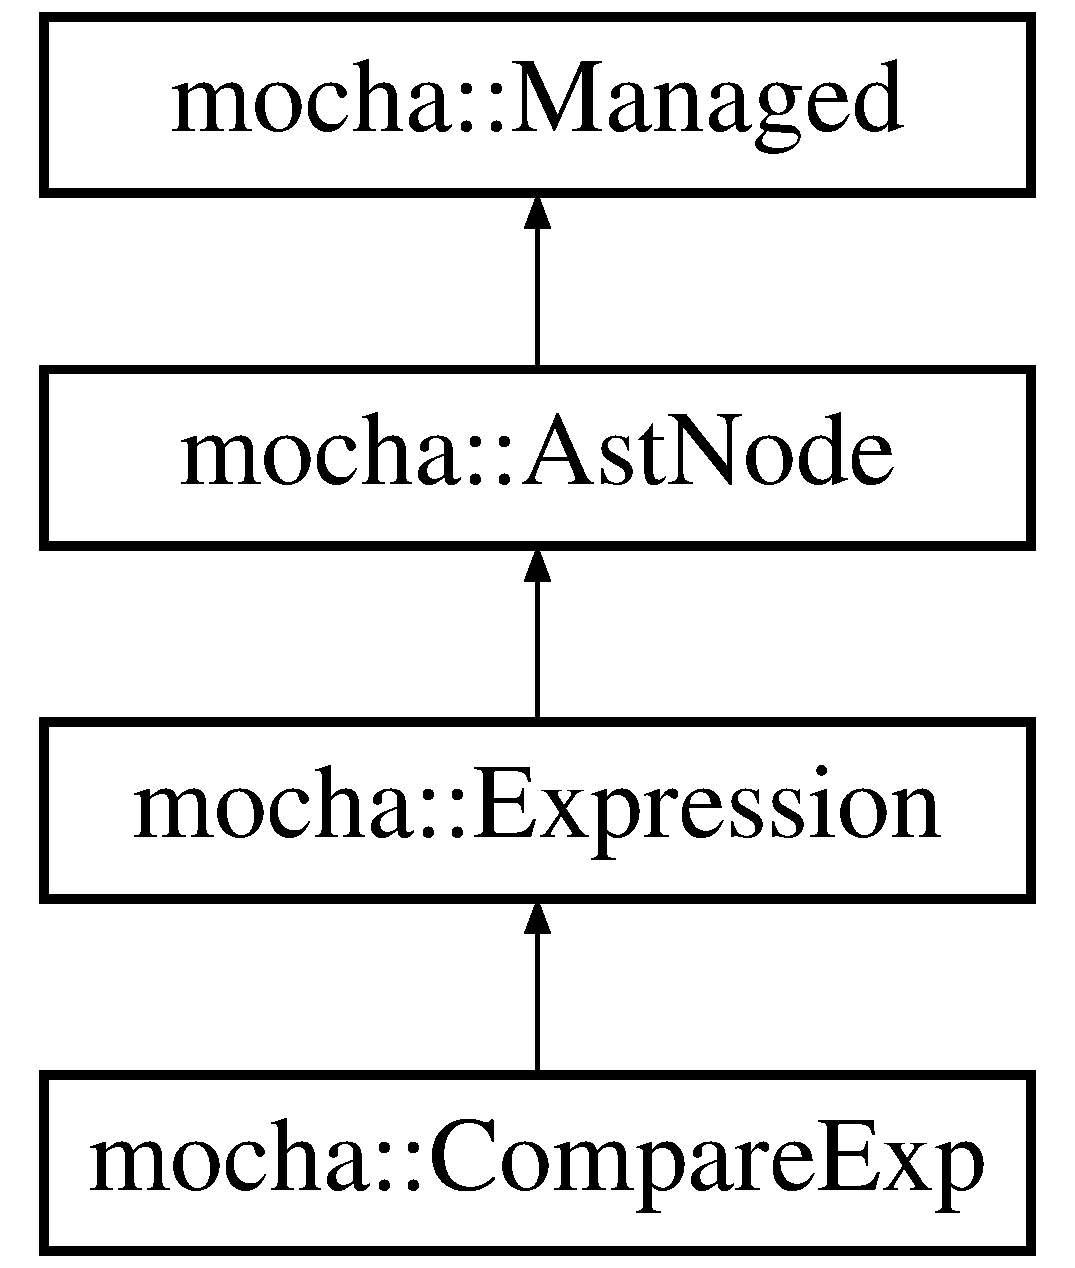
\includegraphics[height=4.000000cm]{classmocha_1_1_compare_exp}
\end{center}
\end{figure}
\subsection*{Public Types}
\begin{DoxyCompactItemize}
\item 
enum \{ \par
\hyperlink{classmocha_1_1_compare_exp_aa5ba2ba7107f66e1ffc940a3d09b12b3ad1e491ea0ed9a3a75cd6df6b7964fb24}{kLess}, 
\hyperlink{classmocha_1_1_compare_exp_aa5ba2ba7107f66e1ffc940a3d09b12b3a84acae9e2959eaf621dd2c9007394b53}{kGreater}, 
\hyperlink{classmocha_1_1_compare_exp_aa5ba2ba7107f66e1ffc940a3d09b12b3abf14e7794f87bcd14e2984beaaa44d6a}{kLessEqual}, 
\hyperlink{classmocha_1_1_compare_exp_aa5ba2ba7107f66e1ffc940a3d09b12b3a919b2deb962643cad716dd3dadb9322a}{kGreaterEqual}, 
\par
\hyperlink{classmocha_1_1_compare_exp_aa5ba2ba7107f66e1ffc940a3d09b12b3a0af853b4a91a6ab164b7a2cb71a96e7b}{kInstanceof}, 
\hyperlink{classmocha_1_1_compare_exp_aa5ba2ba7107f66e1ffc940a3d09b12b3afb1b9d3fc6d7fb194007adfeda3cf623}{kIn}, 
\hyperlink{classmocha_1_1_compare_exp_aa5ba2ba7107f66e1ffc940a3d09b12b3a71b370ae38daa71371b7c372b1c28883}{kEqual}, 
\hyperlink{classmocha_1_1_compare_exp_aa5ba2ba7107f66e1ffc940a3d09b12b3a1df6ff896a14072a02aeb0f70291acb4}{kNotEqual}, 
\par
\hyperlink{classmocha_1_1_compare_exp_aa5ba2ba7107f66e1ffc940a3d09b12b3af83ad9b9e18e5353d951c80b8d3d5853}{kEq}, 
\hyperlink{classmocha_1_1_compare_exp_aa5ba2ba7107f66e1ffc940a3d09b12b3ad8c0fc6a2937e66f4fc233249182723a}{kNotEq}, 
\hyperlink{classmocha_1_1_compare_exp_aa5ba2ba7107f66e1ffc940a3d09b12b3a2797128d472ed86d91dc020994858ab0}{kLogicalAND}, 
\hyperlink{classmocha_1_1_compare_exp_aa5ba2ba7107f66e1ffc940a3d09b12b3a82a42371f7907ffdffed444474127430}{kLogicalOR}
 \}
\end{DoxyCompactItemize}
\subsection*{Public Member Functions}
\begin{DoxyCompactItemize}
\item 
\hyperlink{classmocha_1_1_compare_exp_adf897019057c5828d58dc5383fbccd2f}{CompareExp} (int op, \hyperlink{classmocha_1_1_ast_node}{AstNode} $\ast$left, \hyperlink{classmocha_1_1_ast_node}{AstNode} $\ast$right)
\item 
\hyperlink{classmocha_1_1_compare_exp_a12393cc341813a99ce920a6c52c128df}{$\sim$CompareExp} ()
\item 
\hyperlink{classmocha_1_1_ast_node}{AstNode} $\ast$ \hyperlink{classmocha_1_1_compare_exp_af2325d02bad82741358315768d3222b9}{Left} ()
\item 
\hyperlink{classmocha_1_1_ast_node}{AstNode} $\ast$ \hyperlink{classmocha_1_1_compare_exp_a6a65fd900ebf9dd11484a6a948c4c4e2}{Right} ()
\item 
int \hyperlink{classmocha_1_1_compare_exp_a46d240a58be68fa85b61073ed2e4d19a}{Op} ()
\item 
void \hyperlink{classmocha_1_1_compare_exp_af174065f2d4986e2c7539bd041baad13}{ReplaceChild} (\hyperlink{classmocha_1_1_ast_node}{AstNode} $\ast$old\_\-node, \hyperlink{classmocha_1_1_ast_node}{AstNode} $\ast$new\_\-node)
\item 
\hyperlink{classmocha_1_1_ast_node}{AstNode} $\ast$ \hyperlink{classmocha_1_1_compare_exp_afa00b970faa937c81cfc15c9a0170558}{Clone} ()
\end{DoxyCompactItemize}
\subsection*{Private Member Functions}
\begin{DoxyCompactItemize}
\item 
void \hyperlink{classmocha_1_1_compare_exp_a48c63840dc4ab4b2504eb805bcf76f77}{NVIAccept\_\-} (\hyperlink{classmocha_1_1_i_visitor}{IVisitor} $\ast$visitor)
\end{DoxyCompactItemize}
\subsection*{Private Attributes}
\begin{DoxyCompactItemize}
\item 
int \hyperlink{classmocha_1_1_compare_exp_abfc7d2878bb4843805ce5677ca5c7776}{op\_\-}
\item 
\hyperlink{classmocha_1_1_ast_node}{AstNode} $\ast$ \hyperlink{classmocha_1_1_compare_exp_a0498ddaaf7647a878e984afe6bf029c6}{left\_\-}
\item 
\hyperlink{classmocha_1_1_ast_node}{AstNode} $\ast$ \hyperlink{classmocha_1_1_compare_exp_a75ad5e6ec8152bd2391044bda81b8948}{right\_\-}
\end{DoxyCompactItemize}


\subsection{Detailed Description}


Definition at line 1444 of file ast.h.



\subsection{Member Enumeration Documentation}
\hypertarget{classmocha_1_1_compare_exp_aa5ba2ba7107f66e1ffc940a3d09b12b3}{
\subsubsection[{"@11}]{\setlength{\rightskip}{0pt plus 5cm}anonymous enum}}
\label{classmocha_1_1_compare_exp_aa5ba2ba7107f66e1ffc940a3d09b12b3}
\begin{Desc}
\item[Enumerator: ]\par
\begin{description}
\index{kLess@{kLess}!mocha::CompareExp@{mocha::CompareExp}}\index{mocha::CompareExp@{mocha::CompareExp}!kLess@{kLess}}\item[{\em 
\hypertarget{classmocha_1_1_compare_exp_aa5ba2ba7107f66e1ffc940a3d09b12b3ad1e491ea0ed9a3a75cd6df6b7964fb24}{
kLess}
\label{classmocha_1_1_compare_exp_aa5ba2ba7107f66e1ffc940a3d09b12b3ad1e491ea0ed9a3a75cd6df6b7964fb24}
}]\index{kGreater@{kGreater}!mocha::CompareExp@{mocha::CompareExp}}\index{mocha::CompareExp@{mocha::CompareExp}!kGreater@{kGreater}}\item[{\em 
\hypertarget{classmocha_1_1_compare_exp_aa5ba2ba7107f66e1ffc940a3d09b12b3a84acae9e2959eaf621dd2c9007394b53}{
kGreater}
\label{classmocha_1_1_compare_exp_aa5ba2ba7107f66e1ffc940a3d09b12b3a84acae9e2959eaf621dd2c9007394b53}
}]\index{kLessEqual@{kLessEqual}!mocha::CompareExp@{mocha::CompareExp}}\index{mocha::CompareExp@{mocha::CompareExp}!kLessEqual@{kLessEqual}}\item[{\em 
\hypertarget{classmocha_1_1_compare_exp_aa5ba2ba7107f66e1ffc940a3d09b12b3abf14e7794f87bcd14e2984beaaa44d6a}{
kLessEqual}
\label{classmocha_1_1_compare_exp_aa5ba2ba7107f66e1ffc940a3d09b12b3abf14e7794f87bcd14e2984beaaa44d6a}
}]\index{kGreaterEqual@{kGreaterEqual}!mocha::CompareExp@{mocha::CompareExp}}\index{mocha::CompareExp@{mocha::CompareExp}!kGreaterEqual@{kGreaterEqual}}\item[{\em 
\hypertarget{classmocha_1_1_compare_exp_aa5ba2ba7107f66e1ffc940a3d09b12b3a919b2deb962643cad716dd3dadb9322a}{
kGreaterEqual}
\label{classmocha_1_1_compare_exp_aa5ba2ba7107f66e1ffc940a3d09b12b3a919b2deb962643cad716dd3dadb9322a}
}]\index{kInstanceof@{kInstanceof}!mocha::CompareExp@{mocha::CompareExp}}\index{mocha::CompareExp@{mocha::CompareExp}!kInstanceof@{kInstanceof}}\item[{\em 
\hypertarget{classmocha_1_1_compare_exp_aa5ba2ba7107f66e1ffc940a3d09b12b3a0af853b4a91a6ab164b7a2cb71a96e7b}{
kInstanceof}
\label{classmocha_1_1_compare_exp_aa5ba2ba7107f66e1ffc940a3d09b12b3a0af853b4a91a6ab164b7a2cb71a96e7b}
}]\index{kIn@{kIn}!mocha::CompareExp@{mocha::CompareExp}}\index{mocha::CompareExp@{mocha::CompareExp}!kIn@{kIn}}\item[{\em 
\hypertarget{classmocha_1_1_compare_exp_aa5ba2ba7107f66e1ffc940a3d09b12b3afb1b9d3fc6d7fb194007adfeda3cf623}{
kIn}
\label{classmocha_1_1_compare_exp_aa5ba2ba7107f66e1ffc940a3d09b12b3afb1b9d3fc6d7fb194007adfeda3cf623}
}]\index{kEqual@{kEqual}!mocha::CompareExp@{mocha::CompareExp}}\index{mocha::CompareExp@{mocha::CompareExp}!kEqual@{kEqual}}\item[{\em 
\hypertarget{classmocha_1_1_compare_exp_aa5ba2ba7107f66e1ffc940a3d09b12b3a71b370ae38daa71371b7c372b1c28883}{
kEqual}
\label{classmocha_1_1_compare_exp_aa5ba2ba7107f66e1ffc940a3d09b12b3a71b370ae38daa71371b7c372b1c28883}
}]\index{kNotEqual@{kNotEqual}!mocha::CompareExp@{mocha::CompareExp}}\index{mocha::CompareExp@{mocha::CompareExp}!kNotEqual@{kNotEqual}}\item[{\em 
\hypertarget{classmocha_1_1_compare_exp_aa5ba2ba7107f66e1ffc940a3d09b12b3a1df6ff896a14072a02aeb0f70291acb4}{
kNotEqual}
\label{classmocha_1_1_compare_exp_aa5ba2ba7107f66e1ffc940a3d09b12b3a1df6ff896a14072a02aeb0f70291acb4}
}]\index{kEq@{kEq}!mocha::CompareExp@{mocha::CompareExp}}\index{mocha::CompareExp@{mocha::CompareExp}!kEq@{kEq}}\item[{\em 
\hypertarget{classmocha_1_1_compare_exp_aa5ba2ba7107f66e1ffc940a3d09b12b3af83ad9b9e18e5353d951c80b8d3d5853}{
kEq}
\label{classmocha_1_1_compare_exp_aa5ba2ba7107f66e1ffc940a3d09b12b3af83ad9b9e18e5353d951c80b8d3d5853}
}]\index{kNotEq@{kNotEq}!mocha::CompareExp@{mocha::CompareExp}}\index{mocha::CompareExp@{mocha::CompareExp}!kNotEq@{kNotEq}}\item[{\em 
\hypertarget{classmocha_1_1_compare_exp_aa5ba2ba7107f66e1ffc940a3d09b12b3ad8c0fc6a2937e66f4fc233249182723a}{
kNotEq}
\label{classmocha_1_1_compare_exp_aa5ba2ba7107f66e1ffc940a3d09b12b3ad8c0fc6a2937e66f4fc233249182723a}
}]\index{kLogicalAND@{kLogicalAND}!mocha::CompareExp@{mocha::CompareExp}}\index{mocha::CompareExp@{mocha::CompareExp}!kLogicalAND@{kLogicalAND}}\item[{\em 
\hypertarget{classmocha_1_1_compare_exp_aa5ba2ba7107f66e1ffc940a3d09b12b3a2797128d472ed86d91dc020994858ab0}{
kLogicalAND}
\label{classmocha_1_1_compare_exp_aa5ba2ba7107f66e1ffc940a3d09b12b3a2797128d472ed86d91dc020994858ab0}
}]\index{kLogicalOR@{kLogicalOR}!mocha::CompareExp@{mocha::CompareExp}}\index{mocha::CompareExp@{mocha::CompareExp}!kLogicalOR@{kLogicalOR}}\item[{\em 
\hypertarget{classmocha_1_1_compare_exp_aa5ba2ba7107f66e1ffc940a3d09b12b3a82a42371f7907ffdffed444474127430}{
kLogicalOR}
\label{classmocha_1_1_compare_exp_aa5ba2ba7107f66e1ffc940a3d09b12b3a82a42371f7907ffdffed444474127430}
}]\end{description}
\end{Desc}



Definition at line 1446 of file ast.h.



\subsection{Constructor \& Destructor Documentation}
\hypertarget{classmocha_1_1_compare_exp_adf897019057c5828d58dc5383fbccd2f}{
\index{mocha::CompareExp@{mocha::CompareExp}!CompareExp@{CompareExp}}
\index{CompareExp@{CompareExp}!mocha::CompareExp@{mocha::CompareExp}}
\subsubsection[{CompareExp}]{\setlength{\rightskip}{0pt plus 5cm}mocha::CompareExp::CompareExp (
\begin{DoxyParamCaption}
\item[{int}]{op, }
\item[{{\bf AstNode} $\ast$}]{left, }
\item[{{\bf AstNode} $\ast$}]{right}
\end{DoxyParamCaption}
)\hspace{0.3cm}{\ttfamily  \mbox{[}inline\mbox{]}}}}
\label{classmocha_1_1_compare_exp_adf897019057c5828d58dc5383fbccd2f}


Definition at line 1460 of file ast.h.

\hypertarget{classmocha_1_1_compare_exp_a12393cc341813a99ce920a6c52c128df}{
\index{mocha::CompareExp@{mocha::CompareExp}!$\sim$CompareExp@{$\sim$CompareExp}}
\index{$\sim$CompareExp@{$\sim$CompareExp}!mocha::CompareExp@{mocha::CompareExp}}
\subsubsection[{$\sim$CompareExp}]{\setlength{\rightskip}{0pt plus 5cm}mocha::CompareExp::$\sim$CompareExp (
\begin{DoxyParamCaption}
{}
\end{DoxyParamCaption}
)\hspace{0.3cm}{\ttfamily  \mbox{[}inline\mbox{]}}}}
\label{classmocha_1_1_compare_exp_a12393cc341813a99ce920a6c52c128df}


Definition at line 1461 of file ast.h.



\subsection{Member Function Documentation}
\hypertarget{classmocha_1_1_compare_exp_afa00b970faa937c81cfc15c9a0170558}{
\index{mocha::CompareExp@{mocha::CompareExp}!Clone@{Clone}}
\index{Clone@{Clone}!mocha::CompareExp@{mocha::CompareExp}}
\subsubsection[{Clone}]{\setlength{\rightskip}{0pt plus 5cm}{\bf AstNode} $\ast$ mocha::CompareExp::Clone (
\begin{DoxyParamCaption}
{}
\end{DoxyParamCaption}
)\hspace{0.3cm}{\ttfamily  \mbox{[}virtual\mbox{]}}}}
\label{classmocha_1_1_compare_exp_afa00b970faa937c81cfc15c9a0170558}
\begin{DoxyReturn}{Returns}
\{AstNode$\ast$\} Clone node. 
\end{DoxyReturn}


Reimplemented from \hyperlink{classmocha_1_1_expression_ac1fb936e2bf0fdd6e7667275d3723ca5}{mocha::Expression}.



Definition at line 556 of file ast.cc.

\hypertarget{classmocha_1_1_compare_exp_af2325d02bad82741358315768d3222b9}{
\index{mocha::CompareExp@{mocha::CompareExp}!Left@{Left}}
\index{Left@{Left}!mocha::CompareExp@{mocha::CompareExp}}
\subsubsection[{Left}]{\setlength{\rightskip}{0pt plus 5cm}{\bf AstNode}$\ast$ mocha::CompareExp::Left (
\begin{DoxyParamCaption}
{}
\end{DoxyParamCaption}
)\hspace{0.3cm}{\ttfamily  \mbox{[}inline\mbox{]}}}}
\label{classmocha_1_1_compare_exp_af2325d02bad82741358315768d3222b9}


Definition at line 1462 of file ast.h.

\hypertarget{classmocha_1_1_compare_exp_a48c63840dc4ab4b2504eb805bcf76f77}{
\index{mocha::CompareExp@{mocha::CompareExp}!NVIAccept\_\-@{NVIAccept\_\-}}
\index{NVIAccept\_\-@{NVIAccept\_\-}!mocha::CompareExp@{mocha::CompareExp}}
\subsubsection[{NVIAccept\_\-}]{\setlength{\rightskip}{0pt plus 5cm}void mocha::CompareExp::NVIAccept\_\- (
\begin{DoxyParamCaption}
\item[{{\bf IVisitor} $\ast$}]{visitor}
\end{DoxyParamCaption}
)\hspace{0.3cm}{\ttfamily  \mbox{[}inline, private, virtual\mbox{]}}}}
\label{classmocha_1_1_compare_exp_a48c63840dc4ab4b2504eb805bcf76f77}


Reimplemented from \hyperlink{classmocha_1_1_expression_a112d57b7de76c37066cde60be4799fde}{mocha::Expression}.



Definition at line 1471 of file ast.h.

\hypertarget{classmocha_1_1_compare_exp_a46d240a58be68fa85b61073ed2e4d19a}{
\index{mocha::CompareExp@{mocha::CompareExp}!Op@{Op}}
\index{Op@{Op}!mocha::CompareExp@{mocha::CompareExp}}
\subsubsection[{Op}]{\setlength{\rightskip}{0pt plus 5cm}int mocha::CompareExp::Op (
\begin{DoxyParamCaption}
{}
\end{DoxyParamCaption}
)\hspace{0.3cm}{\ttfamily  \mbox{[}inline\mbox{]}}}}
\label{classmocha_1_1_compare_exp_a46d240a58be68fa85b61073ed2e4d19a}


Definition at line 1464 of file ast.h.

\hypertarget{classmocha_1_1_compare_exp_af174065f2d4986e2c7539bd041baad13}{
\index{mocha::CompareExp@{mocha::CompareExp}!ReplaceChild@{ReplaceChild}}
\index{ReplaceChild@{ReplaceChild}!mocha::CompareExp@{mocha::CompareExp}}
\subsubsection[{ReplaceChild}]{\setlength{\rightskip}{0pt plus 5cm}void mocha::CompareExp::ReplaceChild (
\begin{DoxyParamCaption}
\item[{{\bf AstNode} $\ast$}]{old\_\-node, }
\item[{{\bf AstNode} $\ast$}]{new\_\-node}
\end{DoxyParamCaption}
)\hspace{0.3cm}{\ttfamily  \mbox{[}virtual\mbox{]}}}}
\label{classmocha_1_1_compare_exp_af174065f2d4986e2c7539bd041baad13}

\begin{DoxyParams}{Parameters}
{\em \{AstNode$\ast$\}} & Replace the old\_\-node with new\_\-node in childnodes. \\
\hline
\end{DoxyParams}


Reimplemented from \hyperlink{classmocha_1_1_ast_node_aa40396040f75fb59e320d81c3fd328c8}{mocha::AstNode}.



Definition at line 539 of file ast.cc.

\hypertarget{classmocha_1_1_compare_exp_a6a65fd900ebf9dd11484a6a948c4c4e2}{
\index{mocha::CompareExp@{mocha::CompareExp}!Right@{Right}}
\index{Right@{Right}!mocha::CompareExp@{mocha::CompareExp}}
\subsubsection[{Right}]{\setlength{\rightskip}{0pt plus 5cm}{\bf AstNode}$\ast$ mocha::CompareExp::Right (
\begin{DoxyParamCaption}
{}
\end{DoxyParamCaption}
)\hspace{0.3cm}{\ttfamily  \mbox{[}inline\mbox{]}}}}
\label{classmocha_1_1_compare_exp_a6a65fd900ebf9dd11484a6a948c4c4e2}


Definition at line 1463 of file ast.h.



\subsection{Member Data Documentation}
\hypertarget{classmocha_1_1_compare_exp_a0498ddaaf7647a878e984afe6bf029c6}{
\index{mocha::CompareExp@{mocha::CompareExp}!left\_\-@{left\_\-}}
\index{left\_\-@{left\_\-}!mocha::CompareExp@{mocha::CompareExp}}
\subsubsection[{left\_\-}]{\setlength{\rightskip}{0pt plus 5cm}{\bf AstNode}$\ast$ {\bf mocha::CompareExp::left\_\-}\hspace{0.3cm}{\ttfamily  \mbox{[}private\mbox{]}}}}
\label{classmocha_1_1_compare_exp_a0498ddaaf7647a878e984afe6bf029c6}


Definition at line 1469 of file ast.h.

\hypertarget{classmocha_1_1_compare_exp_abfc7d2878bb4843805ce5677ca5c7776}{
\index{mocha::CompareExp@{mocha::CompareExp}!op\_\-@{op\_\-}}
\index{op\_\-@{op\_\-}!mocha::CompareExp@{mocha::CompareExp}}
\subsubsection[{op\_\-}]{\setlength{\rightskip}{0pt plus 5cm}int {\bf mocha::CompareExp::op\_\-}\hspace{0.3cm}{\ttfamily  \mbox{[}private\mbox{]}}}}
\label{classmocha_1_1_compare_exp_abfc7d2878bb4843805ce5677ca5c7776}


Definition at line 1466 of file ast.h.

\hypertarget{classmocha_1_1_compare_exp_a75ad5e6ec8152bd2391044bda81b8948}{
\index{mocha::CompareExp@{mocha::CompareExp}!right\_\-@{right\_\-}}
\index{right\_\-@{right\_\-}!mocha::CompareExp@{mocha::CompareExp}}
\subsubsection[{right\_\-}]{\setlength{\rightskip}{0pt plus 5cm}{\bf AstNode}$\ast$ {\bf mocha::CompareExp::right\_\-}\hspace{0.3cm}{\ttfamily  \mbox{[}private\mbox{]}}}}
\label{classmocha_1_1_compare_exp_a75ad5e6ec8152bd2391044bda81b8948}


Definition at line 1470 of file ast.h.



The documentation for this class was generated from the following files:\begin{DoxyCompactItemize}
\item 
Y:/mocha/src/ast/\hyperlink{ast_8h}{ast.h}\item 
Y:/mocha/src/ast/\hyperlink{ast_8cc}{ast.cc}\end{DoxyCompactItemize}

\hypertarget{classmocha_1_1_compile_info}{
\section{mocha::CompileInfo Class Reference}
\label{classmocha_1_1_compile_info}\index{mocha::CompileInfo@{mocha::CompileInfo}}
}


{\ttfamily \#include $<$compile\_\-info.h$>$}

\subsection*{Public Member Functions}
\begin{DoxyCompactItemize}
\item 
\hyperlink{classmocha_1_1_compile_info_a038e459e848d6fc3e93ea1360441af1b}{CompileInfo} ()
\item 
\hyperlink{classmocha_1_1_compile_info_a57c58e6602d20fdd90646559554bfd16}{$\sim$CompileInfo} ()
\item 
bool \hyperlink{classmocha_1_1_compile_info_a321811247b1add3ce08d8b73d503555c}{Debug} ()
\item 
void \hyperlink{classmocha_1_1_compile_info_ad1234c377e36ae82a2d9002d172f9cc8}{SetDebug} ()
\item 
bool \hyperlink{classmocha_1_1_compile_info_a3fcf9759fec723d024f212fb8e93c8ec}{Compress} ()
\item 
void \hyperlink{classmocha_1_1_compile_info_a6b37953807394182cb2324b2d5b3c089}{SetCompress} ()
\item 
bool \hyperlink{classmocha_1_1_compile_info_af4f28e800fc2c1f5a20763bf4561ae34}{PrettyPrint} ()
\item 
void \hyperlink{classmocha_1_1_compile_info_adc7a7c9cac7bfd9ccbb47fdb8d6dda6c}{SetPrettyPrint} ()
\item 
bool \hyperlink{classmocha_1_1_compile_info_a96a5e7d3d4b9982ec40a04695d5ce779}{HasVersion} (const char $\ast$)
\item 
void \hyperlink{classmocha_1_1_compile_info_ab16d143f0c4998f6c99f3a4f45363fa3}{SetVersion} (const char $\ast$)
\end{DoxyCompactItemize}
\subsection*{Private Types}
\begin{DoxyCompactItemize}
\item 
typedef \hyperlink{classmocha_1_1_hash_map}{HashMap}$<$ const char $\ast$, uint8\_\-t $>$ \hyperlink{classmocha_1_1_compile_info_a6ef64b400937732f51415e1abfb7875e}{Versions}
\end{DoxyCompactItemize}
\subsection*{Private Attributes}
\begin{DoxyCompactItemize}
\item 
\hyperlink{classmocha_1_1_bit_vector}{BitVector8} \hyperlink{classmocha_1_1_compile_info_ae4d19bdf1d84c07b62cd1691770c1e23}{flags\_\-}
\item 
\hyperlink{classmocha_1_1_hash_map}{Versions} \hyperlink{classmocha_1_1_compile_info_a532a170af6f6254ca78c4857cdef6713}{versions\_\-}
\end{DoxyCompactItemize}


\subsection{Detailed Description}


Definition at line 7 of file compile\_\-info.h.



\subsection{Member Typedef Documentation}
\hypertarget{classmocha_1_1_compile_info_a6ef64b400937732f51415e1abfb7875e}{
\index{mocha::CompileInfo@{mocha::CompileInfo}!Versions@{Versions}}
\index{Versions@{Versions}!mocha::CompileInfo@{mocha::CompileInfo}}
\subsubsection[{Versions}]{\setlength{\rightskip}{0pt plus 5cm}typedef {\bf HashMap}$<$const char$\ast$,uint8\_\-t$>$ {\bf mocha::CompileInfo::Versions}\hspace{0.3cm}{\ttfamily  \mbox{[}private\mbox{]}}}}
\label{classmocha_1_1_compile_info_a6ef64b400937732f51415e1abfb7875e}


Definition at line 8 of file compile\_\-info.h.



\subsection{Constructor \& Destructor Documentation}
\hypertarget{classmocha_1_1_compile_info_a038e459e848d6fc3e93ea1360441af1b}{
\index{mocha::CompileInfo@{mocha::CompileInfo}!CompileInfo@{CompileInfo}}
\index{CompileInfo@{CompileInfo}!mocha::CompileInfo@{mocha::CompileInfo}}
\subsubsection[{CompileInfo}]{\setlength{\rightskip}{0pt plus 5cm}mocha::CompileInfo::CompileInfo (
\begin{DoxyParamCaption}
{}
\end{DoxyParamCaption}
)}}
\label{classmocha_1_1_compile_info_a038e459e848d6fc3e93ea1360441af1b}


Definition at line 9 of file compile\_\-info.cc.

\hypertarget{classmocha_1_1_compile_info_a57c58e6602d20fdd90646559554bfd16}{
\index{mocha::CompileInfo@{mocha::CompileInfo}!$\sim$CompileInfo@{$\sim$CompileInfo}}
\index{$\sim$CompileInfo@{$\sim$CompileInfo}!mocha::CompileInfo@{mocha::CompileInfo}}
\subsubsection[{$\sim$CompileInfo}]{\setlength{\rightskip}{0pt plus 5cm}mocha::CompileInfo::$\sim$CompileInfo (
\begin{DoxyParamCaption}
{}
\end{DoxyParamCaption}
)\hspace{0.3cm}{\ttfamily  \mbox{[}inline\mbox{]}}}}
\label{classmocha_1_1_compile_info_a57c58e6602d20fdd90646559554bfd16}


Definition at line 11 of file compile\_\-info.h.



\subsection{Member Function Documentation}
\hypertarget{classmocha_1_1_compile_info_a3fcf9759fec723d024f212fb8e93c8ec}{
\index{mocha::CompileInfo@{mocha::CompileInfo}!Compress@{Compress}}
\index{Compress@{Compress}!mocha::CompileInfo@{mocha::CompileInfo}}
\subsubsection[{Compress}]{\setlength{\rightskip}{0pt plus 5cm}bool mocha::CompileInfo::Compress (
\begin{DoxyParamCaption}
{}
\end{DoxyParamCaption}
)}}
\label{classmocha_1_1_compile_info_a3fcf9759fec723d024f212fb8e93c8ec}


Definition at line 23 of file compile\_\-info.cc.

\hypertarget{classmocha_1_1_compile_info_a321811247b1add3ce08d8b73d503555c}{
\index{mocha::CompileInfo@{mocha::CompileInfo}!Debug@{Debug}}
\index{Debug@{Debug}!mocha::CompileInfo@{mocha::CompileInfo}}
\subsubsection[{Debug}]{\setlength{\rightskip}{0pt plus 5cm}bool mocha::CompileInfo::Debug (
\begin{DoxyParamCaption}
{}
\end{DoxyParamCaption}
)}}
\label{classmocha_1_1_compile_info_a321811247b1add3ce08d8b73d503555c}


Definition at line 14 of file compile\_\-info.cc.

\hypertarget{classmocha_1_1_compile_info_a96a5e7d3d4b9982ec40a04695d5ce779}{
\index{mocha::CompileInfo@{mocha::CompileInfo}!HasVersion@{HasVersion}}
\index{HasVersion@{HasVersion}!mocha::CompileInfo@{mocha::CompileInfo}}
\subsubsection[{HasVersion}]{\setlength{\rightskip}{0pt plus 5cm}bool mocha::CompileInfo::HasVersion (
\begin{DoxyParamCaption}
\item[{const char $\ast$}]{name}
\end{DoxyParamCaption}
)}}
\label{classmocha_1_1_compile_info_a96a5e7d3d4b9982ec40a04695d5ce779}


Definition at line 46 of file compile\_\-info.cc.

\hypertarget{classmocha_1_1_compile_info_af4f28e800fc2c1f5a20763bf4561ae34}{
\index{mocha::CompileInfo@{mocha::CompileInfo}!PrettyPrint@{PrettyPrint}}
\index{PrettyPrint@{PrettyPrint}!mocha::CompileInfo@{mocha::CompileInfo}}
\subsubsection[{PrettyPrint}]{\setlength{\rightskip}{0pt plus 5cm}bool mocha::CompileInfo::PrettyPrint (
\begin{DoxyParamCaption}
{}
\end{DoxyParamCaption}
)}}
\label{classmocha_1_1_compile_info_af4f28e800fc2c1f5a20763bf4561ae34}


Definition at line 31 of file compile\_\-info.cc.

\hypertarget{classmocha_1_1_compile_info_a6b37953807394182cb2324b2d5b3c089}{
\index{mocha::CompileInfo@{mocha::CompileInfo}!SetCompress@{SetCompress}}
\index{SetCompress@{SetCompress}!mocha::CompileInfo@{mocha::CompileInfo}}
\subsubsection[{SetCompress}]{\setlength{\rightskip}{0pt plus 5cm}void mocha::CompileInfo::SetCompress (
\begin{DoxyParamCaption}
{}
\end{DoxyParamCaption}
)}}
\label{classmocha_1_1_compile_info_a6b37953807394182cb2324b2d5b3c089}


Definition at line 27 of file compile\_\-info.cc.

\hypertarget{classmocha_1_1_compile_info_ad1234c377e36ae82a2d9002d172f9cc8}{
\index{mocha::CompileInfo@{mocha::CompileInfo}!SetDebug@{SetDebug}}
\index{SetDebug@{SetDebug}!mocha::CompileInfo@{mocha::CompileInfo}}
\subsubsection[{SetDebug}]{\setlength{\rightskip}{0pt plus 5cm}void mocha::CompileInfo::SetDebug (
\begin{DoxyParamCaption}
{}
\end{DoxyParamCaption}
)}}
\label{classmocha_1_1_compile_info_ad1234c377e36ae82a2d9002d172f9cc8}


Definition at line 18 of file compile\_\-info.cc.

\hypertarget{classmocha_1_1_compile_info_adc7a7c9cac7bfd9ccbb47fdb8d6dda6c}{
\index{mocha::CompileInfo@{mocha::CompileInfo}!SetPrettyPrint@{SetPrettyPrint}}
\index{SetPrettyPrint@{SetPrettyPrint}!mocha::CompileInfo@{mocha::CompileInfo}}
\subsubsection[{SetPrettyPrint}]{\setlength{\rightskip}{0pt plus 5cm}void mocha::CompileInfo::SetPrettyPrint (
\begin{DoxyParamCaption}
{}
\end{DoxyParamCaption}
)}}
\label{classmocha_1_1_compile_info_adc7a7c9cac7bfd9ccbb47fdb8d6dda6c}


Definition at line 35 of file compile\_\-info.cc.

\hypertarget{classmocha_1_1_compile_info_ab16d143f0c4998f6c99f3a4f45363fa3}{
\index{mocha::CompileInfo@{mocha::CompileInfo}!SetVersion@{SetVersion}}
\index{SetVersion@{SetVersion}!mocha::CompileInfo@{mocha::CompileInfo}}
\subsubsection[{SetVersion}]{\setlength{\rightskip}{0pt plus 5cm}void mocha::CompileInfo::SetVersion (
\begin{DoxyParamCaption}
\item[{const char $\ast$}]{name}
\end{DoxyParamCaption}
)}}
\label{classmocha_1_1_compile_info_ab16d143f0c4998f6c99f3a4f45363fa3}


Definition at line 39 of file compile\_\-info.cc.



\subsection{Member Data Documentation}
\hypertarget{classmocha_1_1_compile_info_ae4d19bdf1d84c07b62cd1691770c1e23}{
\index{mocha::CompileInfo@{mocha::CompileInfo}!flags\_\-@{flags\_\-}}
\index{flags\_\-@{flags\_\-}!mocha::CompileInfo@{mocha::CompileInfo}}
\subsubsection[{flags\_\-}]{\setlength{\rightskip}{0pt plus 5cm}{\bf BitVector8} {\bf mocha::CompileInfo::flags\_\-}\hspace{0.3cm}{\ttfamily  \mbox{[}private\mbox{]}}}}
\label{classmocha_1_1_compile_info_ae4d19bdf1d84c07b62cd1691770c1e23}


Definition at line 21 of file compile\_\-info.h.

\hypertarget{classmocha_1_1_compile_info_a532a170af6f6254ca78c4857cdef6713}{
\index{mocha::CompileInfo@{mocha::CompileInfo}!versions\_\-@{versions\_\-}}
\index{versions\_\-@{versions\_\-}!mocha::CompileInfo@{mocha::CompileInfo}}
\subsubsection[{versions\_\-}]{\setlength{\rightskip}{0pt plus 5cm}{\bf Versions} {\bf mocha::CompileInfo::versions\_\-}\hspace{0.3cm}{\ttfamily  \mbox{[}private\mbox{]}}}}
\label{classmocha_1_1_compile_info_a532a170af6f6254ca78c4857cdef6713}


Definition at line 22 of file compile\_\-info.h.



The documentation for this class was generated from the following files:\begin{DoxyCompactItemize}
\item 
Y:/mocha/src/compiler/utils/\hyperlink{compile__info_8h}{compile\_\-info.h}\item 
Y:/mocha/src/compiler/utils/\hyperlink{compile__info_8cc}{compile\_\-info.cc}\end{DoxyCompactItemize}

\hypertarget{classmocha_1_1_compiler}{
\section{mocha::Compiler Class Reference}
\label{classmocha_1_1_compiler}\index{mocha::Compiler@{mocha::Compiler}}
}


{\ttfamily \#include $<$compiler.h$>$}

Inheritance diagram for mocha::Compiler:\begin{figure}[H]
\begin{center}
\leavevmode
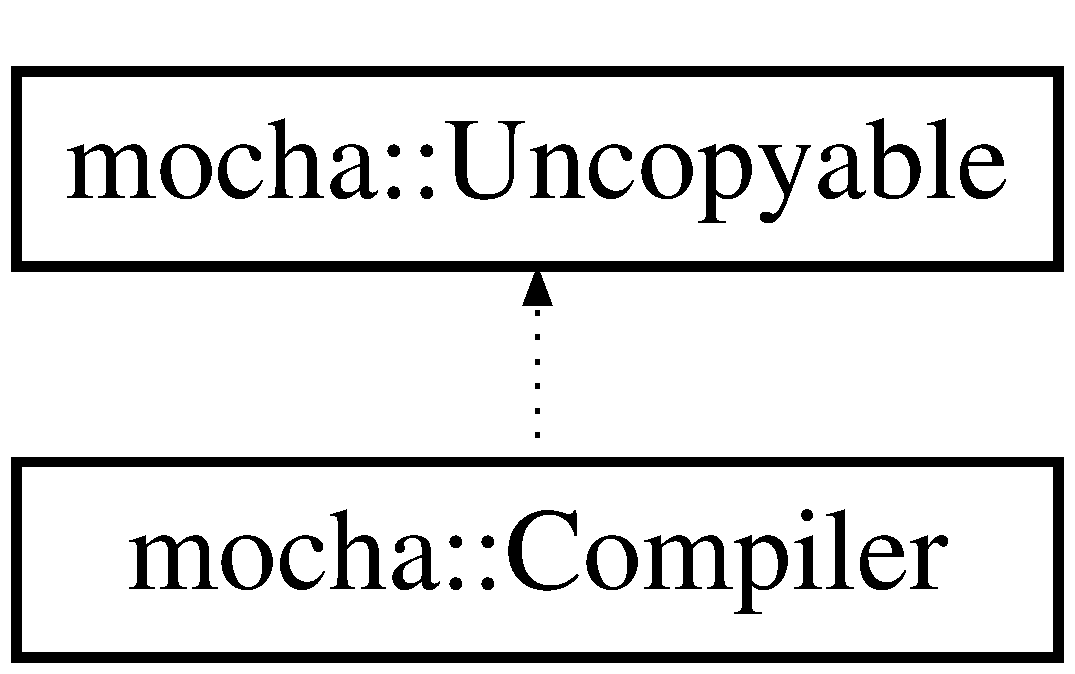
\includegraphics[height=2.000000cm]{classmocha_1_1_compiler}
\end{center}
\end{figure}
\subsection*{Classes}
\begin{DoxyCompactItemize}
\item 
class \hyperlink{classmocha_1_1_compiler_1_1_ptr_impl}{PtrImpl}
\end{DoxyCompactItemize}
\subsection*{Public Member Functions}
\begin{DoxyCompactItemize}
\item 
void \hyperlink{classmocha_1_1_compiler_a306a8eca89e0ff3eb9b529ec05379497}{Compile} ()
\begin{DoxyCompactList}\small\item\em Start compile. \end{DoxyCompactList}\item 
\hyperlink{classmocha_1_1_array_handle}{StrHandle} \hyperlink{classmocha_1_1_compiler_a3959e7a2bfd45449f8c1c0995fccbcc3}{Load} (const char $\ast$filename)
\item 
void \hyperlink{classmocha_1_1_compiler_ae2130cd13cc93fa0d25f0f6382713107}{CatchException} (const char $\ast$filename, \hyperlink{classmocha_1_1_handle}{ErrorHandler} handle)
\item 
\hyperlink{classmocha_1_1_handle}{Handle}$<$ \hyperlink{classmocha_1_1_external_ast}{ExternalAst} $>$ \hyperlink{classmocha_1_1_compiler_a178d58ee083f1da9c622e2c2e943300b}{GetAst} (\hyperlink{classmocha_1_1_error_reporter}{ErrorReporter} $\ast$reporter, \hyperlink{classmocha_1_1_handle}{Handle}$<$ \hyperlink{classmocha_1_1_path_info}{PathInfo} $>$ info, bool is\_\-runtime)
\item 
\hyperlink{classmocha_1_1_handle}{Handle}$<$ \hyperlink{classmocha_1_1_path_info}{PathInfo} $>$ \hyperlink{classmocha_1_1_compiler_a0f2c97e8cfeded647ed7c6db9ea9d8e5}{GetMainPathInfo} ()
\end{DoxyCompactItemize}
\subsection*{Static Public Member Functions}
\begin{DoxyCompactItemize}
\item 
static \hyperlink{classmocha_1_1_compiler}{Compiler} $\ast$ \hyperlink{classmocha_1_1_compiler_af64d5202d445d5bc7b95a78ffc62e64d}{CreateInstance} (const char $\ast$filename, \hyperlink{classmocha_1_1_finish_delegator}{FinishDelegator} $\ast$callback)
\begin{DoxyCompactList}\small\item\em Create Compiler's singleton instance. \end{DoxyCompactList}\end{DoxyCompactItemize}
\subsection*{Private Member Functions}
\begin{DoxyCompactItemize}
\item 
\hyperlink{classmocha_1_1_compiler_ac035cb9e52bca34a7592839d5da8a507}{Compiler} (const char $\ast$filename, \hyperlink{classmocha_1_1_finish_delegator}{FinishDelegator} $\ast$callback)
\item 
\hyperlink{classmocha_1_1_compiler_acb77008ede2a0ac3c63361bdb58660a8}{$\sim$Compiler} ()
\end{DoxyCompactItemize}
\subsection*{Static Private Member Functions}
\begin{DoxyCompactItemize}
\item 
static void \hyperlink{classmocha_1_1_compiler_a3cfbf9b6ad2969124cf0383045b35917}{Destructor\_\-} (void $\ast$ptr)
\end{DoxyCompactItemize}
\subsection*{Private Attributes}
\begin{DoxyCompactItemize}
\item 
\hyperlink{classmocha_1_1_scoped_ptr}{ScopedPtr}$<$ \hyperlink{classmocha_1_1_compiler_1_1_ptr_impl}{PtrImpl} $>$ \hyperlink{classmocha_1_1_compiler_a5054f7154cef5bf6e452c1e8448e933f}{implementation\_\-}
\begin{DoxyCompactList}\small\item\em Pointer manager of pimpl internal class. \end{DoxyCompactList}\end{DoxyCompactItemize}
\subsection*{Static Private Attributes}
\begin{DoxyCompactItemize}
\item 
static \hyperlink{classmocha_1_1_thread_local_storage_key}{ThreadLocalStorageKey} \hyperlink{classmocha_1_1_compiler_a1bd5df1002de299a4a4fad5f133292f7}{local\_\-key\_\-}
\begin{DoxyCompactList}\small\item\em \hyperlink{classmocha_1_1_thread}{Thread} local storage key for get one only instance of per thread. \end{DoxyCompactList}\item 
static \hyperlink{classmocha_1_1_mutex}{Mutex} \hyperlink{classmocha_1_1_compiler_a58bd1414408ce47c311e7f265082a8f1}{mutex\_\-}
\end{DoxyCompactItemize}
\subsection*{Friends}
\begin{DoxyCompactItemize}
\item 
class \hyperlink{classmocha_1_1_compiler_ac8fa258798a4ab4930132157e7c70c0c}{CompilerFacade}
\end{DoxyCompactItemize}


\subsection{Detailed Description}


Definition at line 49 of file compiler.h.



\subsection{Constructor \& Destructor Documentation}
\hypertarget{classmocha_1_1_compiler_ac035cb9e52bca34a7592839d5da8a507}{
\index{mocha::Compiler@{mocha::Compiler}!Compiler@{Compiler}}
\index{Compiler@{Compiler}!mocha::Compiler@{mocha::Compiler}}
\subsubsection[{Compiler}]{\setlength{\rightskip}{0pt plus 5cm}mocha::Compiler::Compiler (
\begin{DoxyParamCaption}
\item[{const char $\ast$}]{filename, }
\item[{{\bf FinishDelegator} $\ast$}]{callback}
\end{DoxyParamCaption}
)\hspace{0.3cm}{\ttfamily  \mbox{[}private\mbox{]}}}}
\label{classmocha_1_1_compiler_ac035cb9e52bca34a7592839d5da8a507}


Definition at line 193 of file compiler.cc.

\hypertarget{classmocha_1_1_compiler_acb77008ede2a0ac3c63361bdb58660a8}{
\index{mocha::Compiler@{mocha::Compiler}!$\sim$Compiler@{$\sim$Compiler}}
\index{$\sim$Compiler@{$\sim$Compiler}!mocha::Compiler@{mocha::Compiler}}
\subsubsection[{$\sim$Compiler}]{\setlength{\rightskip}{0pt plus 5cm}mocha::Compiler::$\sim$Compiler (
\begin{DoxyParamCaption}
{}
\end{DoxyParamCaption}
)\hspace{0.3cm}{\ttfamily  \mbox{[}inline, private\mbox{]}}}}
\label{classmocha_1_1_compiler_acb77008ede2a0ac3c63361bdb58660a8}


Definition at line 100 of file compiler.h.



\subsection{Member Function Documentation}
\hypertarget{classmocha_1_1_compiler_ae2130cd13cc93fa0d25f0f6382713107}{
\index{mocha::Compiler@{mocha::Compiler}!CatchException@{CatchException}}
\index{CatchException@{CatchException}!mocha::Compiler@{mocha::Compiler}}
\subsubsection[{CatchException}]{\setlength{\rightskip}{0pt plus 5cm}void mocha::Compiler::CatchException (
\begin{DoxyParamCaption}
\item[{const char $\ast$}]{filename, }
\item[{{\bf ErrorHandler}}]{handle}
\end{DoxyParamCaption}
)}}
\label{classmocha_1_1_compiler_ae2130cd13cc93fa0d25f0f6382713107}


Definition at line 204 of file compiler.cc.

\hypertarget{classmocha_1_1_compiler_a306a8eca89e0ff3eb9b529ec05379497}{
\index{mocha::Compiler@{mocha::Compiler}!Compile@{Compile}}
\index{Compile@{Compile}!mocha::Compiler@{mocha::Compiler}}
\subsubsection[{Compile}]{\setlength{\rightskip}{0pt plus 5cm}void mocha::Compiler::Compile (
\begin{DoxyParamCaption}
{}
\end{DoxyParamCaption}
)}}
\label{classmocha_1_1_compiler_a306a8eca89e0ff3eb9b529ec05379497}


Start compile. 



Definition at line 198 of file compiler.cc.

\hypertarget{classmocha_1_1_compiler_af64d5202d445d5bc7b95a78ffc62e64d}{
\index{mocha::Compiler@{mocha::Compiler}!CreateInstance@{CreateInstance}}
\index{CreateInstance@{CreateInstance}!mocha::Compiler@{mocha::Compiler}}
\subsubsection[{CreateInstance}]{\setlength{\rightskip}{0pt plus 5cm}{\bf Compiler} $\ast$ mocha::Compiler::CreateInstance (
\begin{DoxyParamCaption}
\item[{const char $\ast$}]{filename, }
\item[{{\bf FinishDelegator} $\ast$}]{callback}
\end{DoxyParamCaption}
)\hspace{0.3cm}{\ttfamily  \mbox{[}static\mbox{]}}}}
\label{classmocha_1_1_compiler_af64d5202d445d5bc7b95a78ffc62e64d}


Create Compiler's singleton instance. 

This method callable only class MochaMain. 

Definition at line 180 of file compiler.cc.

\hypertarget{classmocha_1_1_compiler_a3cfbf9b6ad2969124cf0383045b35917}{
\index{mocha::Compiler@{mocha::Compiler}!Destructor\_\-@{Destructor\_\-}}
\index{Destructor\_\-@{Destructor\_\-}!mocha::Compiler@{mocha::Compiler}}
\subsubsection[{Destructor\_\-}]{\setlength{\rightskip}{0pt plus 5cm}void mocha::Compiler::Destructor\_\- (
\begin{DoxyParamCaption}
\item[{void $\ast$}]{ptr}
\end{DoxyParamCaption}
)\hspace{0.3cm}{\ttfamily  \mbox{[}static, private\mbox{]}}}}
\label{classmocha_1_1_compiler_a3cfbf9b6ad2969124cf0383045b35917}

\begin{DoxyParams}{Parameters}
{\em \{void$\ast$\}} & -\/$>$ compiler instance. Desctruct signleton instance. \\
\hline
\end{DoxyParams}


Definition at line 214 of file compiler.cc.

\hypertarget{classmocha_1_1_compiler_a178d58ee083f1da9c622e2c2e943300b}{
\index{mocha::Compiler@{mocha::Compiler}!GetAst@{GetAst}}
\index{GetAst@{GetAst}!mocha::Compiler@{mocha::Compiler}}
\subsubsection[{GetAst}]{\setlength{\rightskip}{0pt plus 5cm}{\bf Handle}$<$ {\bf ExternalAst} $>$ mocha::Compiler::GetAst (
\begin{DoxyParamCaption}
\item[{{\bf ErrorReporter} $\ast$}]{reporter, }
\item[{{\bf Handle}$<$ {\bf PathInfo} $>$}]{info, }
\item[{bool}]{is\_\-runtime}
\end{DoxyParamCaption}
)}}
\label{classmocha_1_1_compiler_a178d58ee083f1da9c622e2c2e943300b}


Definition at line 219 of file compiler.cc.

\hypertarget{classmocha_1_1_compiler_a0f2c97e8cfeded647ed7c6db9ea9d8e5}{
\index{mocha::Compiler@{mocha::Compiler}!GetMainPathInfo@{GetMainPathInfo}}
\index{GetMainPathInfo@{GetMainPathInfo}!mocha::Compiler@{mocha::Compiler}}
\subsubsection[{GetMainPathInfo}]{\setlength{\rightskip}{0pt plus 5cm}{\bf Handle}$<$ {\bf PathInfo} $>$ mocha::Compiler::GetMainPathInfo (
\begin{DoxyParamCaption}
{}
\end{DoxyParamCaption}
)}}
\label{classmocha_1_1_compiler_a0f2c97e8cfeded647ed7c6db9ea9d8e5}
\begin{DoxyReturn}{Returns}
\{\hyperlink{classmocha_1_1_handle}{Handle$<$PathInfo$>$}\} Get \hyperlink{classmocha_1_1_path_info}{PathInfo} of main file path. 
\end{DoxyReturn}


Definition at line 210 of file compiler.cc.

\hypertarget{classmocha_1_1_compiler_a3959e7a2bfd45449f8c1c0995fccbcc3}{
\index{mocha::Compiler@{mocha::Compiler}!Load@{Load}}
\index{Load@{Load}!mocha::Compiler@{mocha::Compiler}}
\subsubsection[{Load}]{\setlength{\rightskip}{0pt plus 5cm}{\bf StrHandle} mocha::Compiler::Load (
\begin{DoxyParamCaption}
\item[{const char $\ast$}]{filename}
\end{DoxyParamCaption}
)}}
\label{classmocha_1_1_compiler_a3959e7a2bfd45449f8c1c0995fccbcc3}


Definition at line 223 of file compiler.cc.



\subsection{Friends And Related Function Documentation}
\hypertarget{classmocha_1_1_compiler_ac8fa258798a4ab4930132157e7c70c0c}{
\index{mocha::Compiler@{mocha::Compiler}!CompilerFacade@{CompilerFacade}}
\index{CompilerFacade@{CompilerFacade}!mocha::Compiler@{mocha::Compiler}}
\subsubsection[{CompilerFacade}]{\setlength{\rightskip}{0pt plus 5cm}friend class {\bf CompilerFacade}\hspace{0.3cm}{\ttfamily  \mbox{[}friend\mbox{]}}}}
\label{classmocha_1_1_compiler_ac8fa258798a4ab4930132157e7c70c0c}


Definition at line 50 of file compiler.h.



\subsection{Member Data Documentation}
\hypertarget{classmocha_1_1_compiler_a5054f7154cef5bf6e452c1e8448e933f}{
\index{mocha::Compiler@{mocha::Compiler}!implementation\_\-@{implementation\_\-}}
\index{implementation\_\-@{implementation\_\-}!mocha::Compiler@{mocha::Compiler}}
\subsubsection[{implementation\_\-}]{\setlength{\rightskip}{0pt plus 5cm}{\bf ScopedPtr}$<${\bf PtrImpl}$>$ {\bf mocha::Compiler::implementation\_\-}\hspace{0.3cm}{\ttfamily  \mbox{[}private\mbox{]}}}}
\label{classmocha_1_1_compiler_a5054f7154cef5bf6e452c1e8448e933f}


Pointer manager of pimpl internal class. 



Definition at line 114 of file compiler.h.

\hypertarget{classmocha_1_1_compiler_a1bd5df1002de299a4a4fad5f133292f7}{
\index{mocha::Compiler@{mocha::Compiler}!local\_\-key\_\-@{local\_\-key\_\-}}
\index{local\_\-key\_\-@{local\_\-key\_\-}!mocha::Compiler@{mocha::Compiler}}
\subsubsection[{local\_\-key\_\-}]{\setlength{\rightskip}{0pt plus 5cm}{\bf ThreadLocalStorageKey} {\bf mocha::Compiler::local\_\-key\_\-}\hspace{0.3cm}{\ttfamily  \mbox{[}static, private\mbox{]}}}}
\label{classmocha_1_1_compiler_a1bd5df1002de299a4a4fad5f133292f7}


\hyperlink{classmocha_1_1_thread}{Thread} local storage key for get one only instance of per thread. 



Definition at line 126 of file compiler.h.

\hypertarget{classmocha_1_1_compiler_a58bd1414408ce47c311e7f265082a8f1}{
\index{mocha::Compiler@{mocha::Compiler}!mutex\_\-@{mutex\_\-}}
\index{mutex\_\-@{mutex\_\-}!mocha::Compiler@{mocha::Compiler}}
\subsubsection[{mutex\_\-}]{\setlength{\rightskip}{0pt plus 5cm}{\bf Mutex} {\bf mocha::Compiler::mutex\_\-}\hspace{0.3cm}{\ttfamily  \mbox{[}static, private\mbox{]}}}}
\label{classmocha_1_1_compiler_a58bd1414408ce47c311e7f265082a8f1}


Definition at line 128 of file compiler.h.



The documentation for this class was generated from the following files:\begin{DoxyCompactItemize}
\item 
Y:/mocha/src/compiler/\hyperlink{compiler_8h}{compiler.h}\item 
Y:/mocha/src/compiler/\hyperlink{compiler_8cc}{compiler.cc}\end{DoxyCompactItemize}

\hypertarget{classmocha_1_1_compile_result}{
\section{mocha::CompileResult Class Reference}
\label{classmocha_1_1_compile_result}\index{mocha::CompileResult@{mocha::CompileResult}}
}


{\ttfamily \#include $<$compile\_\-result.h$>$}

\subsection*{Public Member Functions}
\begin{DoxyCompactItemize}
\item 
\hyperlink{classmocha_1_1_compile_result_a834530898eed167227ccc2d0cd11d849}{CompileResult} (const char $\ast$filename, \hyperlink{classmocha_1_1_handle}{Handle}$<$ \hyperlink{classmocha_1_1_codegen_visitor}{CodegenVisitor} $>$ visitor, \hyperlink{classmocha_1_1_handle}{ErrorMapHandle} map)
\item 
\hyperlink{classmocha_1_1_compile_result_ac9c89c99fd21f1c19e8ddfc969f5af45}{$\sim$CompileResult} ()
\item 
const char $\ast$ \hyperlink{classmocha_1_1_compile_result_a16ec97d8000b653f3d835785ea19ecca}{GetFilename} ()
\item 
const char $\ast$ \hyperlink{classmocha_1_1_compile_result_af8cf87f14967bf32106f181a1539b1b5}{GetSource} ()
\item 
const \hyperlink{classmocha_1_1_hash_map}{ErrorMap} \& \hyperlink{classmocha_1_1_compile_result_ace1f71a7012e336e3f22793f16052501}{GetErrorMap} ()
\end{DoxyCompactItemize}
\subsection*{Private Attributes}
\begin{DoxyCompactItemize}
\item 
std::string \hyperlink{classmocha_1_1_compile_result_a69d7f443ef3b2117ea3dfb1029bbd4e8}{filename\_\-}
\item 
\hyperlink{classmocha_1_1_handle}{Handle}$<$ \hyperlink{classmocha_1_1_codegen_visitor}{CodegenVisitor} $>$ \hyperlink{classmocha_1_1_compile_result_a61362b2f729b2d1b1fb7aa79c4fde52f}{visitor\_\-}
\item 
\hyperlink{classmocha_1_1_handle}{ErrorMapHandle} \hyperlink{classmocha_1_1_compile_result_ab04d46e6dd228a05c487abd7c6e23c72}{map\_\-}
\end{DoxyCompactItemize}


\subsection{Detailed Description}


Definition at line 9 of file compile\_\-result.h.



\subsection{Constructor \& Destructor Documentation}
\hypertarget{classmocha_1_1_compile_result_a834530898eed167227ccc2d0cd11d849}{
\index{mocha::CompileResult@{mocha::CompileResult}!CompileResult@{CompileResult}}
\index{CompileResult@{CompileResult}!mocha::CompileResult@{mocha::CompileResult}}
\subsubsection[{CompileResult}]{\setlength{\rightskip}{0pt plus 5cm}mocha::CompileResult::CompileResult (
\begin{DoxyParamCaption}
\item[{const char $\ast$}]{filename, }
\item[{{\bf Handle}$<$ {\bf CodegenVisitor} $>$}]{visitor, }
\item[{{\bf ErrorMapHandle}}]{map}
\end{DoxyParamCaption}
)}}
\label{classmocha_1_1_compile_result_a834530898eed167227ccc2d0cd11d849}


Definition at line 5 of file compile\_\-result.cc.

\hypertarget{classmocha_1_1_compile_result_ac9c89c99fd21f1c19e8ddfc969f5af45}{
\index{mocha::CompileResult@{mocha::CompileResult}!$\sim$CompileResult@{$\sim$CompileResult}}
\index{$\sim$CompileResult@{$\sim$CompileResult}!mocha::CompileResult@{mocha::CompileResult}}
\subsubsection[{$\sim$CompileResult}]{\setlength{\rightskip}{0pt plus 5cm}mocha::CompileResult::$\sim$CompileResult (
\begin{DoxyParamCaption}
{}
\end{DoxyParamCaption}
)\hspace{0.3cm}{\ttfamily  \mbox{[}inline\mbox{]}}}}
\label{classmocha_1_1_compile_result_ac9c89c99fd21f1c19e8ddfc969f5af45}


Definition at line 12 of file compile\_\-result.h.



\subsection{Member Function Documentation}
\hypertarget{classmocha_1_1_compile_result_ace1f71a7012e336e3f22793f16052501}{
\index{mocha::CompileResult@{mocha::CompileResult}!GetErrorMap@{GetErrorMap}}
\index{GetErrorMap@{GetErrorMap}!mocha::CompileResult@{mocha::CompileResult}}
\subsubsection[{GetErrorMap}]{\setlength{\rightskip}{0pt plus 5cm}const {\bf ErrorMap}\& mocha::CompileResult::GetErrorMap (
\begin{DoxyParamCaption}
{}
\end{DoxyParamCaption}
)\hspace{0.3cm}{\ttfamily  \mbox{[}inline\mbox{]}}}}
\label{classmocha_1_1_compile_result_ace1f71a7012e336e3f22793f16052501}


Definition at line 15 of file compile\_\-result.h.

\hypertarget{classmocha_1_1_compile_result_a16ec97d8000b653f3d835785ea19ecca}{
\index{mocha::CompileResult@{mocha::CompileResult}!GetFilename@{GetFilename}}
\index{GetFilename@{GetFilename}!mocha::CompileResult@{mocha::CompileResult}}
\subsubsection[{GetFilename}]{\setlength{\rightskip}{0pt plus 5cm}const char$\ast$ mocha::CompileResult::GetFilename (
\begin{DoxyParamCaption}
{}
\end{DoxyParamCaption}
)\hspace{0.3cm}{\ttfamily  \mbox{[}inline\mbox{]}}}}
\label{classmocha_1_1_compile_result_a16ec97d8000b653f3d835785ea19ecca}


Definition at line 13 of file compile\_\-result.h.

\hypertarget{classmocha_1_1_compile_result_af8cf87f14967bf32106f181a1539b1b5}{
\index{mocha::CompileResult@{mocha::CompileResult}!GetSource@{GetSource}}
\index{GetSource@{GetSource}!mocha::CompileResult@{mocha::CompileResult}}
\subsubsection[{GetSource}]{\setlength{\rightskip}{0pt plus 5cm}const char$\ast$ mocha::CompileResult::GetSource (
\begin{DoxyParamCaption}
{}
\end{DoxyParamCaption}
)\hspace{0.3cm}{\ttfamily  \mbox{[}inline\mbox{]}}}}
\label{classmocha_1_1_compile_result_af8cf87f14967bf32106f181a1539b1b5}


Definition at line 14 of file compile\_\-result.h.



\subsection{Member Data Documentation}
\hypertarget{classmocha_1_1_compile_result_a69d7f443ef3b2117ea3dfb1029bbd4e8}{
\index{mocha::CompileResult@{mocha::CompileResult}!filename\_\-@{filename\_\-}}
\index{filename\_\-@{filename\_\-}!mocha::CompileResult@{mocha::CompileResult}}
\subsubsection[{filename\_\-}]{\setlength{\rightskip}{0pt plus 5cm}std::string {\bf mocha::CompileResult::filename\_\-}\hspace{0.3cm}{\ttfamily  \mbox{[}private\mbox{]}}}}
\label{classmocha_1_1_compile_result_a69d7f443ef3b2117ea3dfb1029bbd4e8}


Definition at line 17 of file compile\_\-result.h.

\hypertarget{classmocha_1_1_compile_result_ab04d46e6dd228a05c487abd7c6e23c72}{
\index{mocha::CompileResult@{mocha::CompileResult}!map\_\-@{map\_\-}}
\index{map\_\-@{map\_\-}!mocha::CompileResult@{mocha::CompileResult}}
\subsubsection[{map\_\-}]{\setlength{\rightskip}{0pt plus 5cm}{\bf ErrorMapHandle} {\bf mocha::CompileResult::map\_\-}\hspace{0.3cm}{\ttfamily  \mbox{[}private\mbox{]}}}}
\label{classmocha_1_1_compile_result_ab04d46e6dd228a05c487abd7c6e23c72}


Definition at line 19 of file compile\_\-result.h.

\hypertarget{classmocha_1_1_compile_result_a61362b2f729b2d1b1fb7aa79c4fde52f}{
\index{mocha::CompileResult@{mocha::CompileResult}!visitor\_\-@{visitor\_\-}}
\index{visitor\_\-@{visitor\_\-}!mocha::CompileResult@{mocha::CompileResult}}
\subsubsection[{visitor\_\-}]{\setlength{\rightskip}{0pt plus 5cm}{\bf Handle}$<${\bf CodegenVisitor}$>$ {\bf mocha::CompileResult::visitor\_\-}\hspace{0.3cm}{\ttfamily  \mbox{[}private\mbox{]}}}}
\label{classmocha_1_1_compile_result_a61362b2f729b2d1b1fb7aa79c4fde52f}


Definition at line 18 of file compile\_\-result.h.



The documentation for this class was generated from the following files:\begin{DoxyCompactItemize}
\item 
Y:/mocha/src/compiler/utils/\hyperlink{compile__result_8h}{compile\_\-result.h}\item 
Y:/mocha/src/compiler/utils/\hyperlink{compile__result_8cc}{compile\_\-result.cc}\end{DoxyCompactItemize}

\hypertarget{classmocha_1_1_compiler_facade}{
\section{mocha::CompilerFacade Class Reference}
\label{classmocha_1_1_compiler_facade}\index{mocha::CompilerFacade@{mocha::CompilerFacade}}
}


{\ttfamily \#include $<$compiler\_\-facade.h$>$}

\subsection*{Public Types}
\begin{DoxyCompactItemize}
\item 
typedef std::pair$<$ const char $\ast$, bool $>$ \hyperlink{classmocha_1_1_compiler_facade_a22a27bcd738fd453a4da03982f96a080}{EachArgs}
\item 
typedef std::vector$<$ \hyperlink{classmocha_1_1_compiler_facade_a22a27bcd738fd453a4da03982f96a080}{EachArgs} $>$ \hyperlink{classmocha_1_1_compiler_facade_a8b5aaa05b5213622382bbd292a460461}{FileList}
\end{DoxyCompactItemize}
\subsection*{Public Member Functions}
\begin{DoxyCompactItemize}
\item 
\hyperlink{classmocha_1_1_compiler_facade_af1150ae9139adff6c7c4ceefd1aada2c}{CompilerFacade} ()
\item 
void \hyperlink{classmocha_1_1_compiler_facade_ae58b6ccb86e24b6e87b7d881463a71f0}{AddCompileList} (const char $\ast$path, bool is\_\-join)
\item 
void \hyperlink{classmocha_1_1_compiler_facade_a1d6fafdf125e45cd78ad1efd62c96df5}{Compile} ()
\end{DoxyCompactItemize}
\subsection*{Static Public Member Functions}
\begin{DoxyCompactItemize}
\item 
static void \hyperlink{classmocha_1_1_compiler_facade_a99c33f60447920c888b645a72c1f8dfa}{Compile} (const char $\ast$path, bool is\_\-join)
\item 
static void \hyperlink{classmocha_1_1_compiler_facade_a98c55b2a0409c4054049aae9d7766e4e}{Compile} (const char $\ast$path, bool is\_\-join, \hyperlink{classmocha_1_1_finish_delegator}{FinishDelegator} $\ast$callback)
\item 
static \hyperlink{classmocha_1_1_handle}{Handle}$<$ \hyperlink{classmocha_1_1_external_ast}{ExternalAst} $>$ \hyperlink{classmocha_1_1_compiler_facade_a53e5ad1b85d88f0a82099607242fcf86}{GetAst} (const char $\ast$path, bool is\_\-runtime)
\item 
static void $\ast$ \hyperlink{classmocha_1_1_compiler_facade_a6f4ae0de97286db3c2e2895b2ea1e0eb}{ExternalThreadRunner} (void $\ast$arg)
\end{DoxyCompactItemize}
\subsection*{Static Private Member Functions}
\begin{DoxyCompactItemize}
\item 
static void \hyperlink{classmocha_1_1_compiler_facade_a3a651f32d0a30fc37c390cdb3e1a261f}{Compile\_\-} (\hyperlink{structmocha_1_1_thread_args}{ThreadArgs} $\ast$args, bool is\_\-join)
\item 
static void $\ast$ \hyperlink{classmocha_1_1_compiler_facade_a4ea17472d3706ab44eeea4c92d007469}{InternalThreadRunner} (void $\ast$arg)
\end{DoxyCompactItemize}
\subsection*{Private Attributes}
\begin{DoxyCompactItemize}
\item 
\hyperlink{classmocha_1_1_compiler_facade_a8b5aaa05b5213622382bbd292a460461}{FileList} \hyperlink{classmocha_1_1_compiler_facade_a8d2f57f1ddf6c9e78e54853f1febc705}{file\_\-list\_\-}
\end{DoxyCompactItemize}
\subsection*{Static Private Attributes}
\begin{DoxyCompactItemize}
\item 
static \hyperlink{classmocha_1_1_finish_delegator}{FinishDelegator} \hyperlink{classmocha_1_1_compiler_facade_a4f09a3d142a4d54ab478b7742f723226}{noop\_\-}
\end{DoxyCompactItemize}


\subsection{Detailed Description}


Definition at line 27 of file compiler\_\-facade.h.



\subsection{Member Typedef Documentation}
\hypertarget{classmocha_1_1_compiler_facade_a22a27bcd738fd453a4da03982f96a080}{
\index{mocha::CompilerFacade@{mocha::CompilerFacade}!EachArgs@{EachArgs}}
\index{EachArgs@{EachArgs}!mocha::CompilerFacade@{mocha::CompilerFacade}}
\subsubsection[{EachArgs}]{\setlength{\rightskip}{0pt plus 5cm}typedef std::pair$<$const char$\ast$ , bool$>$ {\bf mocha::CompilerFacade::EachArgs}}}
\label{classmocha_1_1_compiler_facade_a22a27bcd738fd453a4da03982f96a080}


Definition at line 29 of file compiler\_\-facade.h.

\hypertarget{classmocha_1_1_compiler_facade_a8b5aaa05b5213622382bbd292a460461}{
\index{mocha::CompilerFacade@{mocha::CompilerFacade}!FileList@{FileList}}
\index{FileList@{FileList}!mocha::CompilerFacade@{mocha::CompilerFacade}}
\subsubsection[{FileList}]{\setlength{\rightskip}{0pt plus 5cm}typedef std::vector$<${\bf EachArgs}$>$ {\bf mocha::CompilerFacade::FileList}}}
\label{classmocha_1_1_compiler_facade_a8b5aaa05b5213622382bbd292a460461}


Definition at line 30 of file compiler\_\-facade.h.



\subsection{Constructor \& Destructor Documentation}
\hypertarget{classmocha_1_1_compiler_facade_af1150ae9139adff6c7c4ceefd1aada2c}{
\index{mocha::CompilerFacade@{mocha::CompilerFacade}!CompilerFacade@{CompilerFacade}}
\index{CompilerFacade@{CompilerFacade}!mocha::CompilerFacade@{mocha::CompilerFacade}}
\subsubsection[{CompilerFacade}]{\setlength{\rightskip}{0pt plus 5cm}mocha::CompilerFacade::CompilerFacade (
\begin{DoxyParamCaption}
{}
\end{DoxyParamCaption}
)\hspace{0.3cm}{\ttfamily  \mbox{[}inline\mbox{]}}}}
\label{classmocha_1_1_compiler_facade_af1150ae9139adff6c7c4ceefd1aada2c}


Definition at line 31 of file compiler\_\-facade.h.



\subsection{Member Function Documentation}
\hypertarget{classmocha_1_1_compiler_facade_ae58b6ccb86e24b6e87b7d881463a71f0}{
\index{mocha::CompilerFacade@{mocha::CompilerFacade}!AddCompileList@{AddCompileList}}
\index{AddCompileList@{AddCompileList}!mocha::CompilerFacade@{mocha::CompilerFacade}}
\subsubsection[{AddCompileList}]{\setlength{\rightskip}{0pt plus 5cm}void mocha::CompilerFacade::AddCompileList (
\begin{DoxyParamCaption}
\item[{const char $\ast$}]{path, }
\item[{bool}]{is\_\-join}
\end{DoxyParamCaption}
)}}
\label{classmocha_1_1_compiler_facade_ae58b6ccb86e24b6e87b7d881463a71f0}


Definition at line 113 of file compiler\_\-facade.cc.

\hypertarget{classmocha_1_1_compiler_facade_a99c33f60447920c888b645a72c1f8dfa}{
\index{mocha::CompilerFacade@{mocha::CompilerFacade}!Compile@{Compile}}
\index{Compile@{Compile}!mocha::CompilerFacade@{mocha::CompilerFacade}}
\subsubsection[{Compile}]{\setlength{\rightskip}{0pt plus 5cm}void mocha::CompilerFacade::Compile (
\begin{DoxyParamCaption}
\item[{const char $\ast$}]{path, }
\item[{bool}]{is\_\-join}
\end{DoxyParamCaption}
)\hspace{0.3cm}{\ttfamily  \mbox{[}static\mbox{]}}}}
\label{classmocha_1_1_compiler_facade_a99c33f60447920c888b645a72c1f8dfa}


Definition at line 16 of file compiler\_\-facade.cc.

\hypertarget{classmocha_1_1_compiler_facade_a98c55b2a0409c4054049aae9d7766e4e}{
\index{mocha::CompilerFacade@{mocha::CompilerFacade}!Compile@{Compile}}
\index{Compile@{Compile}!mocha::CompilerFacade@{mocha::CompilerFacade}}
\subsubsection[{Compile}]{\setlength{\rightskip}{0pt plus 5cm}void mocha::CompilerFacade::Compile (
\begin{DoxyParamCaption}
\item[{const char $\ast$}]{path, }
\item[{bool}]{is\_\-join, }
\item[{{\bf FinishDelegator} $\ast$}]{callback}
\end{DoxyParamCaption}
)\hspace{0.3cm}{\ttfamily  \mbox{[}static\mbox{]}}}}
\label{classmocha_1_1_compiler_facade_a98c55b2a0409c4054049aae9d7766e4e}


Definition at line 21 of file compiler\_\-facade.cc.

\hypertarget{classmocha_1_1_compiler_facade_a1d6fafdf125e45cd78ad1efd62c96df5}{
\index{mocha::CompilerFacade@{mocha::CompilerFacade}!Compile@{Compile}}
\index{Compile@{Compile}!mocha::CompilerFacade@{mocha::CompilerFacade}}
\subsubsection[{Compile}]{\setlength{\rightskip}{0pt plus 5cm}void mocha::CompilerFacade::Compile (
\begin{DoxyParamCaption}
{}
\end{DoxyParamCaption}
)}}
\label{classmocha_1_1_compiler_facade_a1d6fafdf125e45cd78ad1efd62c96df5}


Definition at line 101 of file compiler\_\-facade.cc.

\hypertarget{classmocha_1_1_compiler_facade_a3a651f32d0a30fc37c390cdb3e1a261f}{
\index{mocha::CompilerFacade@{mocha::CompilerFacade}!Compile\_\-@{Compile\_\-}}
\index{Compile\_\-@{Compile\_\-}!mocha::CompilerFacade@{mocha::CompilerFacade}}
\subsubsection[{Compile\_\-}]{\setlength{\rightskip}{0pt plus 5cm}void mocha::CompilerFacade::Compile\_\- (
\begin{DoxyParamCaption}
\item[{{\bf ThreadArgs} $\ast$}]{args, }
\item[{bool}]{is\_\-join}
\end{DoxyParamCaption}
)\hspace{0.3cm}{\ttfamily  \mbox{[}static, private\mbox{]}}}}
\label{classmocha_1_1_compiler_facade_a3a651f32d0a30fc37c390cdb3e1a261f}


Definition at line 35 of file compiler\_\-facade.cc.

\hypertarget{classmocha_1_1_compiler_facade_a6f4ae0de97286db3c2e2895b2ea1e0eb}{
\index{mocha::CompilerFacade@{mocha::CompilerFacade}!ExternalThreadRunner@{ExternalThreadRunner}}
\index{ExternalThreadRunner@{ExternalThreadRunner}!mocha::CompilerFacade@{mocha::CompilerFacade}}
\subsubsection[{ExternalThreadRunner}]{\setlength{\rightskip}{0pt plus 5cm}void $\ast$ mocha::CompilerFacade::ExternalThreadRunner (
\begin{DoxyParamCaption}
\item[{void $\ast$}]{arg}
\end{DoxyParamCaption}
)\hspace{0.3cm}{\ttfamily  \mbox{[}static\mbox{]}}}}
\label{classmocha_1_1_compiler_facade_a6f4ae0de97286db3c2e2895b2ea1e0eb}


Definition at line 47 of file compiler\_\-facade.cc.

\hypertarget{classmocha_1_1_compiler_facade_a53e5ad1b85d88f0a82099607242fcf86}{
\index{mocha::CompilerFacade@{mocha::CompilerFacade}!GetAst@{GetAst}}
\index{GetAst@{GetAst}!mocha::CompilerFacade@{mocha::CompilerFacade}}
\subsubsection[{GetAst}]{\setlength{\rightskip}{0pt plus 5cm}{\bf Handle}$<$ {\bf ExternalAst} $>$ mocha::CompilerFacade::GetAst (
\begin{DoxyParamCaption}
\item[{const char $\ast$}]{path, }
\item[{bool}]{is\_\-runtime}
\end{DoxyParamCaption}
)\hspace{0.3cm}{\ttfamily  \mbox{[}static\mbox{]}}}}
\label{classmocha_1_1_compiler_facade_a53e5ad1b85d88f0a82099607242fcf86}


Definition at line 27 of file compiler\_\-facade.cc.

\hypertarget{classmocha_1_1_compiler_facade_a4ea17472d3706ab44eeea4c92d007469}{
\index{mocha::CompilerFacade@{mocha::CompilerFacade}!InternalThreadRunner@{InternalThreadRunner}}
\index{InternalThreadRunner@{InternalThreadRunner}!mocha::CompilerFacade@{mocha::CompilerFacade}}
\subsubsection[{InternalThreadRunner}]{\setlength{\rightskip}{0pt plus 5cm}void $\ast$ mocha::CompilerFacade::InternalThreadRunner (
\begin{DoxyParamCaption}
\item[{void $\ast$}]{arg}
\end{DoxyParamCaption}
)\hspace{0.3cm}{\ttfamily  \mbox{[}static, private\mbox{]}}}}
\label{classmocha_1_1_compiler_facade_a4ea17472d3706ab44eeea4c92d007469}


Definition at line 118 of file compiler\_\-facade.cc.



\subsection{Member Data Documentation}
\hypertarget{classmocha_1_1_compiler_facade_a8d2f57f1ddf6c9e78e54853f1febc705}{
\index{mocha::CompilerFacade@{mocha::CompilerFacade}!file\_\-list\_\-@{file\_\-list\_\-}}
\index{file\_\-list\_\-@{file\_\-list\_\-}!mocha::CompilerFacade@{mocha::CompilerFacade}}
\subsubsection[{file\_\-list\_\-}]{\setlength{\rightskip}{0pt plus 5cm}{\bf FileList} {\bf mocha::CompilerFacade::file\_\-list\_\-}\hspace{0.3cm}{\ttfamily  \mbox{[}private\mbox{]}}}}
\label{classmocha_1_1_compiler_facade_a8d2f57f1ddf6c9e78e54853f1febc705}


Definition at line 42 of file compiler\_\-facade.h.

\hypertarget{classmocha_1_1_compiler_facade_a4f09a3d142a4d54ab478b7742f723226}{
\index{mocha::CompilerFacade@{mocha::CompilerFacade}!noop\_\-@{noop\_\-}}
\index{noop\_\-@{noop\_\-}!mocha::CompilerFacade@{mocha::CompilerFacade}}
\subsubsection[{noop\_\-}]{\setlength{\rightskip}{0pt plus 5cm}{\bf FinishDelegator} {\bf mocha::CompilerFacade::noop\_\-}\hspace{0.3cm}{\ttfamily  \mbox{[}static, private\mbox{]}}}}
\label{classmocha_1_1_compiler_facade_a4f09a3d142a4d54ab478b7742f723226}


Definition at line 41 of file compiler\_\-facade.h.



The documentation for this class was generated from the following files:\begin{DoxyCompactItemize}
\item 
Y:/mocha/src/compiler/utils/\hyperlink{compiler__facade_8h}{compiler\_\-facade.h}\item 
Y:/mocha/src/compiler/utils/\hyperlink{compiler__facade_8cc}{compiler\_\-facade.cc}\end{DoxyCompactItemize}

\hypertarget{classmocha_1_1_compile_runner}{
\section{mocha::CompileRunner Class Reference}
\label{classmocha_1_1_compile_runner}\index{mocha::CompileRunner@{mocha::CompileRunner}}
}


{\ttfamily \#include $<$compile\_\-runner.h$>$}

Inheritance diagram for mocha::CompileRunner:\begin{figure}[H]
\begin{center}
\leavevmode
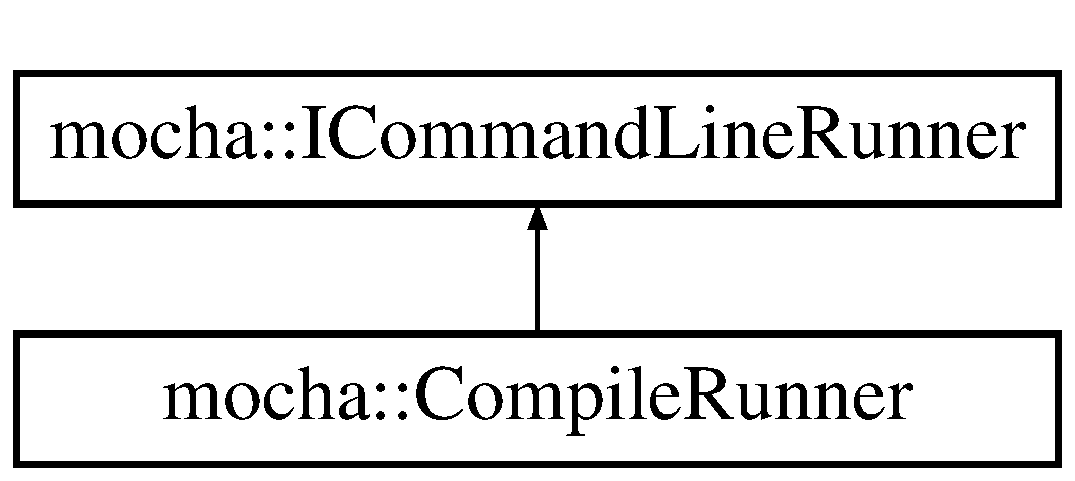
\includegraphics[height=2.000000cm]{classmocha_1_1_compile_runner}
\end{center}
\end{figure}
\subsection*{Public Member Functions}
\begin{DoxyCompactItemize}
\item 
\hyperlink{classmocha_1_1_compile_runner_a666348748e2413bd80db51e793582892}{CompileRunner} (\hyperlink{classmocha_1_1_options}{Options} $\ast$options)
\item 
void \hyperlink{classmocha_1_1_compile_runner_a9c977cb677e1e38a82ee3a84b00a2475}{Run} ()
\end{DoxyCompactItemize}


\subsection{Detailed Description}


Definition at line 6 of file compile\_\-runner.h.



\subsection{Constructor \& Destructor Documentation}
\hypertarget{classmocha_1_1_compile_runner_a666348748e2413bd80db51e793582892}{
\index{mocha::CompileRunner@{mocha::CompileRunner}!CompileRunner@{CompileRunner}}
\index{CompileRunner@{CompileRunner}!mocha::CompileRunner@{mocha::CompileRunner}}
\subsubsection[{CompileRunner}]{\setlength{\rightskip}{0pt plus 5cm}mocha::CompileRunner::CompileRunner (
\begin{DoxyParamCaption}
\item[{{\bf Options} $\ast$}]{options}
\end{DoxyParamCaption}
)}}
\label{classmocha_1_1_compile_runner_a666348748e2413bd80db51e793582892}


Definition at line 6 of file compile\_\-runner.cc.



\subsection{Member Function Documentation}
\hypertarget{classmocha_1_1_compile_runner_a9c977cb677e1e38a82ee3a84b00a2475}{
\index{mocha::CompileRunner@{mocha::CompileRunner}!Run@{Run}}
\index{Run@{Run}!mocha::CompileRunner@{mocha::CompileRunner}}
\subsubsection[{Run}]{\setlength{\rightskip}{0pt plus 5cm}void mocha::CompileRunner::Run (
\begin{DoxyParamCaption}
{}
\end{DoxyParamCaption}
)\hspace{0.3cm}{\ttfamily  \mbox{[}virtual\mbox{]}}}}
\label{classmocha_1_1_compile_runner_a9c977cb677e1e38a82ee3a84b00a2475}


Reimplemented from \hyperlink{classmocha_1_1_i_command_line_runner_a916078af76dc405721dfd512d68a123a}{mocha::ICommandLineRunner}.



Definition at line 8 of file compile\_\-runner.cc.



The documentation for this class was generated from the following files:\begin{DoxyCompactItemize}
\item 
Y:/mocha/src/bootstrap/runners/\hyperlink{compile__runner_8h}{compile\_\-runner.h}\item 
Y:/mocha/src/bootstrap/runners/\hyperlink{compile__runner_8cc}{compile\_\-runner.cc}\end{DoxyCompactItemize}

\hypertarget{classmocha_1_1_compiler_utils}{
\section{mocha::CompilerUtils Class Reference}
\label{classmocha_1_1_compiler_utils}\index{mocha::CompilerUtils@{mocha::CompilerUtils}}
}


{\ttfamily \#include $<$compiler\_\-utils.h$>$}

\subsection*{Static Public Member Functions}
\begin{DoxyCompactItemize}
\item 
static \hyperlink{classmocha_1_1_array_handle}{StrHandle} \hyperlink{classmocha_1_1_compiler_utils_a2515529d7db05ae1e1d918dbf09bfc8f}{CreateJsPath} (const char $\ast$filename, const char $\ast$module\_\-path\_\-key)
\item 
static \hyperlink{classmocha_1_1_handle}{Handle}$<$ \hyperlink{classmocha_1_1_path_info}{PathInfo} $>$ \hyperlink{classmocha_1_1_compiler_utils_a1de82dc42e18636d99f486809261bdec}{ChangeDir} (const char $\ast$js\_\-path)
\item 
static \hyperlink{classmocha_1_1_handle}{Handle}$<$ \hyperlink{classmocha_1_1_path_info}{PathInfo} $>$ \hyperlink{classmocha_1_1_compiler_utils_ad79ea278237f45b6816e8c72c9b55ed7}{GetRuntimePathInfo} ()
\end{DoxyCompactItemize}


\subsection{Detailed Description}


Definition at line 8 of file compiler\_\-utils.h.



\subsection{Member Function Documentation}
\hypertarget{classmocha_1_1_compiler_utils_a1de82dc42e18636d99f486809261bdec}{
\index{mocha::CompilerUtils@{mocha::CompilerUtils}!ChangeDir@{ChangeDir}}
\index{ChangeDir@{ChangeDir}!mocha::CompilerUtils@{mocha::CompilerUtils}}
\subsubsection[{ChangeDir}]{\setlength{\rightskip}{0pt plus 5cm}{\bf Handle}$<$ {\bf PathInfo} $>$ mocha::CompilerUtils::ChangeDir (
\begin{DoxyParamCaption}
\item[{const char $\ast$}]{js\_\-path}
\end{DoxyParamCaption}
)\hspace{0.3cm}{\ttfamily  \mbox{[}static\mbox{]}}}}
\label{classmocha_1_1_compiler_utils_a1de82dc42e18636d99f486809261bdec}


Definition at line 41 of file compiler\_\-utils.cc.

\hypertarget{classmocha_1_1_compiler_utils_a2515529d7db05ae1e1d918dbf09bfc8f}{
\index{mocha::CompilerUtils@{mocha::CompilerUtils}!CreateJsPath@{CreateJsPath}}
\index{CreateJsPath@{CreateJsPath}!mocha::CompilerUtils@{mocha::CompilerUtils}}
\subsubsection[{CreateJsPath}]{\setlength{\rightskip}{0pt plus 5cm}{\bf StrHandle} mocha::CompilerUtils::CreateJsPath (
\begin{DoxyParamCaption}
\item[{const char $\ast$}]{filename, }
\item[{const char $\ast$}]{module\_\-path\_\-key}
\end{DoxyParamCaption}
)\hspace{0.3cm}{\ttfamily  \mbox{[}static\mbox{]}}}}
\label{classmocha_1_1_compiler_utils_a2515529d7db05ae1e1d918dbf09bfc8f}


Definition at line 15 of file compiler\_\-utils.cc.

\hypertarget{classmocha_1_1_compiler_utils_ad79ea278237f45b6816e8c72c9b55ed7}{
\index{mocha::CompilerUtils@{mocha::CompilerUtils}!GetRuntimePathInfo@{GetRuntimePathInfo}}
\index{GetRuntimePathInfo@{GetRuntimePathInfo}!mocha::CompilerUtils@{mocha::CompilerUtils}}
\subsubsection[{GetRuntimePathInfo}]{\setlength{\rightskip}{0pt plus 5cm}{\bf Handle}$<$ {\bf PathInfo} $>$ mocha::CompilerUtils::GetRuntimePathInfo (
\begin{DoxyParamCaption}
{}
\end{DoxyParamCaption}
)\hspace{0.3cm}{\ttfamily  \mbox{[}static\mbox{]}}}}
\label{classmocha_1_1_compiler_utils_ad79ea278237f45b6816e8c72c9b55ed7}


Definition at line 47 of file compiler\_\-utils.cc.



The documentation for this class was generated from the following files:\begin{DoxyCompactItemize}
\item 
Y:/mocha/src/compiler/utils/\hyperlink{compiler__utils_8h}{compiler\_\-utils.h}\item 
Y:/mocha/src/compiler/utils/\hyperlink{compiler__utils_8cc}{compiler\_\-utils.cc}\end{DoxyCompactItemize}

\hypertarget{classmocha_1_1_compress_writer}{
\section{mocha::CompressWriter Class Reference}
\label{classmocha_1_1_compress_writer}\index{mocha::CompressWriter@{mocha::CompressWriter}}
}
Inheritance diagram for mocha::CompressWriter:\begin{figure}[H]
\begin{center}
\leavevmode
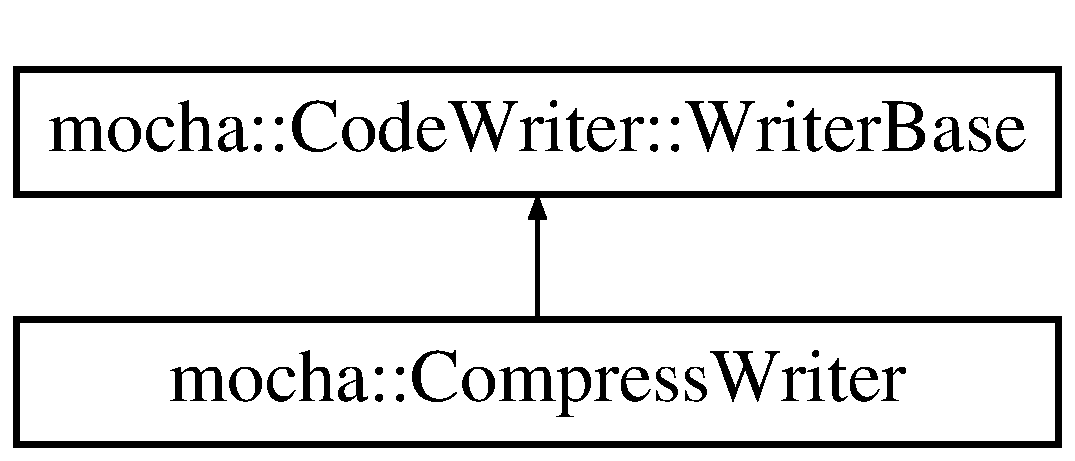
\includegraphics[height=2.000000cm]{classmocha_1_1_compress_writer}
\end{center}
\end{figure}
\subsection*{Public Member Functions}
\begin{DoxyCompactItemize}
\item 
\hyperlink{classmocha_1_1_compress_writer_aed9f3a3511a31415f16614a3c8d7e809}{CompressWriter} (bool is\_\-line)
\item 
void \hyperlink{classmocha_1_1_compress_writer_a1cc68dc2e54c584e33336c18f5a14aee}{Write} (const char $\ast$code, \hyperlink{classmocha_1_1_code_stream}{CodeStream} $\ast$stream)
\item 
void \hyperlink{classmocha_1_1_compress_writer_a89aadb6948d3ffdb643d45ed8e349786}{WriteOp} (int op, int state, \hyperlink{classmocha_1_1_code_stream}{CodeStream} $\ast$stream)
\end{DoxyCompactItemize}
\subsection*{Private Member Functions}
\begin{DoxyCompactItemize}
\item 
void \hyperlink{classmocha_1_1_compress_writer_a3cdbde44e77775591914f2a2734ff88f}{CommonOperandWriter\_\-} (int op, int state, \hyperlink{classmocha_1_1_code_stream}{CodeStream} $\ast$stream)
\end{DoxyCompactItemize}
\subsection*{Private Attributes}
\begin{DoxyCompactItemize}
\item 
bool \hyperlink{classmocha_1_1_compress_writer_a934a10b612f235440cfef0a4ccbcaa5a}{is\_\-line\_\-}
\end{DoxyCompactItemize}


\subsection{Detailed Description}


Definition at line 312 of file codewriter.cc.



\subsection{Constructor \& Destructor Documentation}
\hypertarget{classmocha_1_1_compress_writer_aed9f3a3511a31415f16614a3c8d7e809}{
\index{mocha::CompressWriter@{mocha::CompressWriter}!CompressWriter@{CompressWriter}}
\index{CompressWriter@{CompressWriter}!mocha::CompressWriter@{mocha::CompressWriter}}
\subsubsection[{CompressWriter}]{\setlength{\rightskip}{0pt plus 5cm}mocha::CompressWriter::CompressWriter (
\begin{DoxyParamCaption}
\item[{bool}]{is\_\-line}
\end{DoxyParamCaption}
)\hspace{0.3cm}{\ttfamily  \mbox{[}inline\mbox{]}}}}
\label{classmocha_1_1_compress_writer_aed9f3a3511a31415f16614a3c8d7e809}


Definition at line 314 of file codewriter.cc.



\subsection{Member Function Documentation}
\hypertarget{classmocha_1_1_compress_writer_a3cdbde44e77775591914f2a2734ff88f}{
\index{mocha::CompressWriter@{mocha::CompressWriter}!CommonOperandWriter\_\-@{CommonOperandWriter\_\-}}
\index{CommonOperandWriter\_\-@{CommonOperandWriter\_\-}!mocha::CompressWriter@{mocha::CompressWriter}}
\subsubsection[{CommonOperandWriter\_\-}]{\setlength{\rightskip}{0pt plus 5cm}void mocha::CompressWriter::CommonOperandWriter\_\- (
\begin{DoxyParamCaption}
\item[{int}]{op, }
\item[{int}]{state, }
\item[{{\bf CodeStream} $\ast$}]{stream}
\end{DoxyParamCaption}
)\hspace{0.3cm}{\ttfamily  \mbox{[}inline, private\mbox{]}}}}
\label{classmocha_1_1_compress_writer_a3cdbde44e77775591914f2a2734ff88f}


Definition at line 323 of file codewriter.cc.

\hypertarget{classmocha_1_1_compress_writer_a1cc68dc2e54c584e33336c18f5a14aee}{
\index{mocha::CompressWriter@{mocha::CompressWriter}!Write@{Write}}
\index{Write@{Write}!mocha::CompressWriter@{mocha::CompressWriter}}
\subsubsection[{Write}]{\setlength{\rightskip}{0pt plus 5cm}void mocha::CompressWriter::Write (
\begin{DoxyParamCaption}
\item[{const char $\ast$}]{code, }
\item[{{\bf CodeStream} $\ast$}]{stream}
\end{DoxyParamCaption}
)\hspace{0.3cm}{\ttfamily  \mbox{[}inline, virtual\mbox{]}}}}
\label{classmocha_1_1_compress_writer_a1cc68dc2e54c584e33336c18f5a14aee}


Implements \hyperlink{classmocha_1_1_code_writer_1_1_writer_base_a0b5eabede582c9df1e581d871e000873}{mocha::CodeWriter::WriterBase}.



Definition at line 315 of file codewriter.cc.

\hypertarget{classmocha_1_1_compress_writer_a89aadb6948d3ffdb643d45ed8e349786}{
\index{mocha::CompressWriter@{mocha::CompressWriter}!WriteOp@{WriteOp}}
\index{WriteOp@{WriteOp}!mocha::CompressWriter@{mocha::CompressWriter}}
\subsubsection[{WriteOp}]{\setlength{\rightskip}{0pt plus 5cm}void mocha::CompressWriter::WriteOp (
\begin{DoxyParamCaption}
\item[{int}]{op, }
\item[{int}]{state, }
\item[{{\bf CodeStream} $\ast$}]{stream}
\end{DoxyParamCaption}
)\hspace{0.3cm}{\ttfamily  \mbox{[}inline, virtual\mbox{]}}}}
\label{classmocha_1_1_compress_writer_a89aadb6948d3ffdb643d45ed8e349786}


Implements \hyperlink{classmocha_1_1_code_writer_1_1_writer_base_aff0352433a2fa7726b7742d4438ffe58}{mocha::CodeWriter::WriterBase}.



Definition at line 318 of file codewriter.cc.



\subsection{Member Data Documentation}
\hypertarget{classmocha_1_1_compress_writer_a934a10b612f235440cfef0a4ccbcaa5a}{
\index{mocha::CompressWriter@{mocha::CompressWriter}!is\_\-line\_\-@{is\_\-line\_\-}}
\index{is\_\-line\_\-@{is\_\-line\_\-}!mocha::CompressWriter@{mocha::CompressWriter}}
\subsubsection[{is\_\-line\_\-}]{\setlength{\rightskip}{0pt plus 5cm}bool {\bf mocha::CompressWriter::is\_\-line\_\-}\hspace{0.3cm}{\ttfamily  \mbox{[}private\mbox{]}}}}
\label{classmocha_1_1_compress_writer_a934a10b612f235440cfef0a4ccbcaa5a}


Definition at line 430 of file codewriter.cc.



The documentation for this class was generated from the following file:\begin{DoxyCompactItemize}
\item 
Y:/mocha/src/ast/visitors/utils/\hyperlink{codewriter_8cc}{codewriter.cc}\end{DoxyCompactItemize}

\hypertarget{classmocha_1_1_conditional_exp}{
\section{mocha::ConditionalExp Class Reference}
\label{classmocha_1_1_conditional_exp}\index{mocha::ConditionalExp@{mocha::ConditionalExp}}
}


{\ttfamily \#include $<$ast.h$>$}

Inheritance diagram for mocha::ConditionalExp:\begin{figure}[H]
\begin{center}
\leavevmode
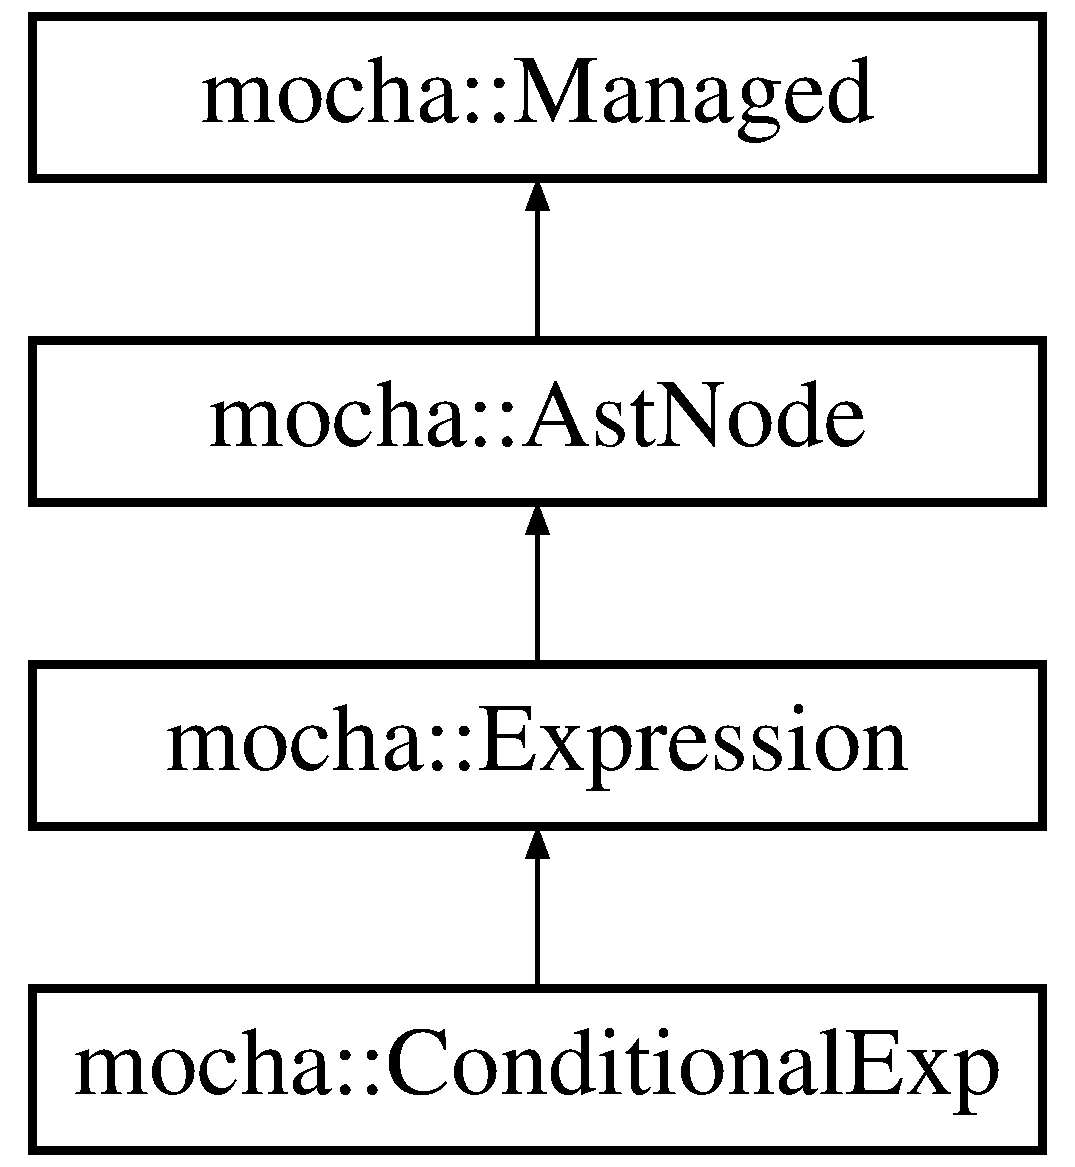
\includegraphics[height=4.000000cm]{classmocha_1_1_conditional_exp}
\end{center}
\end{figure}
\subsection*{Public Member Functions}
\begin{DoxyCompactItemize}
\item 
\hyperlink{classmocha_1_1_conditional_exp_af14ae917b07a37d05d08b9adff48d44c}{ConditionalExp} (\hyperlink{classmocha_1_1_ast_node}{AstNode} $\ast$cond, \hyperlink{classmocha_1_1_ast_node}{AstNode} $\ast$case\_\-true, \hyperlink{classmocha_1_1_ast_node}{AstNode} $\ast$case\_\-false)
\item 
\hyperlink{classmocha_1_1_conditional_exp_abace5fb783efded7b0eac17f88cd3602}{$\sim$ConditionalExp} ()
\item 
\hyperlink{classmocha_1_1_ast_node}{AstNode} $\ast$ \hyperlink{classmocha_1_1_conditional_exp_aaed0b73fb13035c1ca5465f2a24a833b}{True} ()
\item 
\hyperlink{classmocha_1_1_ast_node}{AstNode} $\ast$ \hyperlink{classmocha_1_1_conditional_exp_aff17d7cdbc31e6725fd9fe1c89e9a896}{False} ()
\item 
\hyperlink{classmocha_1_1_ast_node}{AstNode} $\ast$ \hyperlink{classmocha_1_1_conditional_exp_aa19a0246f74af43f5f485173476803af}{Cond} ()
\item 
void \hyperlink{classmocha_1_1_conditional_exp_afc1d1c6448489deac42837c5d89d836e}{ReplaceChild} (\hyperlink{classmocha_1_1_ast_node}{AstNode} $\ast$old\_\-node, \hyperlink{classmocha_1_1_ast_node}{AstNode} $\ast$new\_\-node)
\item 
\hyperlink{classmocha_1_1_ast_node}{AstNode} $\ast$ \hyperlink{classmocha_1_1_conditional_exp_a568bfc0b7fce3e0155e3c789baf6fa40}{Clone} ()
\end{DoxyCompactItemize}
\subsection*{Private Member Functions}
\begin{DoxyCompactItemize}
\item 
void \hyperlink{classmocha_1_1_conditional_exp_a719ad36c380cd142230163006ef6b124}{NVIAccept\_\-} (\hyperlink{classmocha_1_1_i_visitor}{IVisitor} $\ast$visitor)
\end{DoxyCompactItemize}
\subsection*{Private Attributes}
\begin{DoxyCompactItemize}
\item 
\hyperlink{classmocha_1_1_ast_node}{AstNode} $\ast$ \hyperlink{classmocha_1_1_conditional_exp_ae648dcd906465556dc11277d756e5a08}{cond\_\-}
\item 
\hyperlink{classmocha_1_1_ast_node}{AstNode} $\ast$ \hyperlink{classmocha_1_1_conditional_exp_a6262ae4637116f3150926cdd469423a1}{case\_\-true\_\-}
\item 
\hyperlink{classmocha_1_1_ast_node}{AstNode} $\ast$ \hyperlink{classmocha_1_1_conditional_exp_aded78409cf39d226ba14c4f233b35254}{case\_\-false\_\-}
\end{DoxyCompactItemize}


\subsection{Detailed Description}


Definition at line 1475 of file ast.h.



\subsection{Constructor \& Destructor Documentation}
\hypertarget{classmocha_1_1_conditional_exp_af14ae917b07a37d05d08b9adff48d44c}{
\index{mocha::ConditionalExp@{mocha::ConditionalExp}!ConditionalExp@{ConditionalExp}}
\index{ConditionalExp@{ConditionalExp}!mocha::ConditionalExp@{mocha::ConditionalExp}}
\subsubsection[{ConditionalExp}]{\setlength{\rightskip}{0pt plus 5cm}mocha::ConditionalExp::ConditionalExp (
\begin{DoxyParamCaption}
\item[{{\bf AstNode} $\ast$}]{cond, }
\item[{{\bf AstNode} $\ast$}]{case\_\-true, }
\item[{{\bf AstNode} $\ast$}]{case\_\-false}
\end{DoxyParamCaption}
)\hspace{0.3cm}{\ttfamily  \mbox{[}inline\mbox{]}}}}
\label{classmocha_1_1_conditional_exp_af14ae917b07a37d05d08b9adff48d44c}


Definition at line 1477 of file ast.h.

\hypertarget{classmocha_1_1_conditional_exp_abace5fb783efded7b0eac17f88cd3602}{
\index{mocha::ConditionalExp@{mocha::ConditionalExp}!$\sim$ConditionalExp@{$\sim$ConditionalExp}}
\index{$\sim$ConditionalExp@{$\sim$ConditionalExp}!mocha::ConditionalExp@{mocha::ConditionalExp}}
\subsubsection[{$\sim$ConditionalExp}]{\setlength{\rightskip}{0pt plus 5cm}mocha::ConditionalExp::$\sim$ConditionalExp (
\begin{DoxyParamCaption}
{}
\end{DoxyParamCaption}
)\hspace{0.3cm}{\ttfamily  \mbox{[}inline\mbox{]}}}}
\label{classmocha_1_1_conditional_exp_abace5fb783efded7b0eac17f88cd3602}


Definition at line 1480 of file ast.h.



\subsection{Member Function Documentation}
\hypertarget{classmocha_1_1_conditional_exp_a568bfc0b7fce3e0155e3c789baf6fa40}{
\index{mocha::ConditionalExp@{mocha::ConditionalExp}!Clone@{Clone}}
\index{Clone@{Clone}!mocha::ConditionalExp@{mocha::ConditionalExp}}
\subsubsection[{Clone}]{\setlength{\rightskip}{0pt plus 5cm}{\bf AstNode} $\ast$ mocha::ConditionalExp::Clone (
\begin{DoxyParamCaption}
{}
\end{DoxyParamCaption}
)\hspace{0.3cm}{\ttfamily  \mbox{[}virtual\mbox{]}}}}
\label{classmocha_1_1_conditional_exp_a568bfc0b7fce3e0155e3c789baf6fa40}
\begin{DoxyReturn}{Returns}
\{AstNode$\ast$\} Clone node. 
\end{DoxyReturn}


Reimplemented from \hyperlink{classmocha_1_1_expression_ac1fb936e2bf0fdd6e7667275d3723ca5}{mocha::Expression}.



Definition at line 584 of file ast.cc.

\hypertarget{classmocha_1_1_conditional_exp_aa19a0246f74af43f5f485173476803af}{
\index{mocha::ConditionalExp@{mocha::ConditionalExp}!Cond@{Cond}}
\index{Cond@{Cond}!mocha::ConditionalExp@{mocha::ConditionalExp}}
\subsubsection[{Cond}]{\setlength{\rightskip}{0pt plus 5cm}{\bf AstNode}$\ast$ mocha::ConditionalExp::Cond (
\begin{DoxyParamCaption}
{}
\end{DoxyParamCaption}
)\hspace{0.3cm}{\ttfamily  \mbox{[}inline\mbox{]}}}}
\label{classmocha_1_1_conditional_exp_aa19a0246f74af43f5f485173476803af}


Definition at line 1483 of file ast.h.

\hypertarget{classmocha_1_1_conditional_exp_aff17d7cdbc31e6725fd9fe1c89e9a896}{
\index{mocha::ConditionalExp@{mocha::ConditionalExp}!False@{False}}
\index{False@{False}!mocha::ConditionalExp@{mocha::ConditionalExp}}
\subsubsection[{False}]{\setlength{\rightskip}{0pt plus 5cm}{\bf AstNode}$\ast$ mocha::ConditionalExp::False (
\begin{DoxyParamCaption}
{}
\end{DoxyParamCaption}
)\hspace{0.3cm}{\ttfamily  \mbox{[}inline\mbox{]}}}}
\label{classmocha_1_1_conditional_exp_aff17d7cdbc31e6725fd9fe1c89e9a896}


Definition at line 1482 of file ast.h.

\hypertarget{classmocha_1_1_conditional_exp_a719ad36c380cd142230163006ef6b124}{
\index{mocha::ConditionalExp@{mocha::ConditionalExp}!NVIAccept\_\-@{NVIAccept\_\-}}
\index{NVIAccept\_\-@{NVIAccept\_\-}!mocha::ConditionalExp@{mocha::ConditionalExp}}
\subsubsection[{NVIAccept\_\-}]{\setlength{\rightskip}{0pt plus 5cm}void mocha::ConditionalExp::NVIAccept\_\- (
\begin{DoxyParamCaption}
\item[{{\bf IVisitor} $\ast$}]{visitor}
\end{DoxyParamCaption}
)\hspace{0.3cm}{\ttfamily  \mbox{[}inline, private, virtual\mbox{]}}}}
\label{classmocha_1_1_conditional_exp_a719ad36c380cd142230163006ef6b124}


Reimplemented from \hyperlink{classmocha_1_1_expression_a112d57b7de76c37066cde60be4799fde}{mocha::Expression}.



Definition at line 1490 of file ast.h.

\hypertarget{classmocha_1_1_conditional_exp_afc1d1c6448489deac42837c5d89d836e}{
\index{mocha::ConditionalExp@{mocha::ConditionalExp}!ReplaceChild@{ReplaceChild}}
\index{ReplaceChild@{ReplaceChild}!mocha::ConditionalExp@{mocha::ConditionalExp}}
\subsubsection[{ReplaceChild}]{\setlength{\rightskip}{0pt plus 5cm}void mocha::ConditionalExp::ReplaceChild (
\begin{DoxyParamCaption}
\item[{{\bf AstNode} $\ast$}]{old\_\-node, }
\item[{{\bf AstNode} $\ast$}]{new\_\-node}
\end{DoxyParamCaption}
)\hspace{0.3cm}{\ttfamily  \mbox{[}virtual\mbox{]}}}}
\label{classmocha_1_1_conditional_exp_afc1d1c6448489deac42837c5d89d836e}

\begin{DoxyParams}{Parameters}
{\em \{AstNode$\ast$\}} & Replace the old\_\-node with new\_\-node in childnodes. \\
\hline
\end{DoxyParams}


Reimplemented from \hyperlink{classmocha_1_1_ast_node_aa40396040f75fb59e320d81c3fd328c8}{mocha::AstNode}.



Definition at line 562 of file ast.cc.

\hypertarget{classmocha_1_1_conditional_exp_aaed0b73fb13035c1ca5465f2a24a833b}{
\index{mocha::ConditionalExp@{mocha::ConditionalExp}!True@{True}}
\index{True@{True}!mocha::ConditionalExp@{mocha::ConditionalExp}}
\subsubsection[{True}]{\setlength{\rightskip}{0pt plus 5cm}{\bf AstNode}$\ast$ mocha::ConditionalExp::True (
\begin{DoxyParamCaption}
{}
\end{DoxyParamCaption}
)\hspace{0.3cm}{\ttfamily  \mbox{[}inline\mbox{]}}}}
\label{classmocha_1_1_conditional_exp_aaed0b73fb13035c1ca5465f2a24a833b}


Definition at line 1481 of file ast.h.



\subsection{Member Data Documentation}
\hypertarget{classmocha_1_1_conditional_exp_aded78409cf39d226ba14c4f233b35254}{
\index{mocha::ConditionalExp@{mocha::ConditionalExp}!case\_\-false\_\-@{case\_\-false\_\-}}
\index{case\_\-false\_\-@{case\_\-false\_\-}!mocha::ConditionalExp@{mocha::ConditionalExp}}
\subsubsection[{case\_\-false\_\-}]{\setlength{\rightskip}{0pt plus 5cm}{\bf AstNode}$\ast$ {\bf mocha::ConditionalExp::case\_\-false\_\-}\hspace{0.3cm}{\ttfamily  \mbox{[}private\mbox{]}}}}
\label{classmocha_1_1_conditional_exp_aded78409cf39d226ba14c4f233b35254}


Definition at line 1489 of file ast.h.

\hypertarget{classmocha_1_1_conditional_exp_a6262ae4637116f3150926cdd469423a1}{
\index{mocha::ConditionalExp@{mocha::ConditionalExp}!case\_\-true\_\-@{case\_\-true\_\-}}
\index{case\_\-true\_\-@{case\_\-true\_\-}!mocha::ConditionalExp@{mocha::ConditionalExp}}
\subsubsection[{case\_\-true\_\-}]{\setlength{\rightskip}{0pt plus 5cm}{\bf AstNode}$\ast$ {\bf mocha::ConditionalExp::case\_\-true\_\-}\hspace{0.3cm}{\ttfamily  \mbox{[}private\mbox{]}}}}
\label{classmocha_1_1_conditional_exp_a6262ae4637116f3150926cdd469423a1}


Definition at line 1488 of file ast.h.

\hypertarget{classmocha_1_1_conditional_exp_ae648dcd906465556dc11277d756e5a08}{
\index{mocha::ConditionalExp@{mocha::ConditionalExp}!cond\_\-@{cond\_\-}}
\index{cond\_\-@{cond\_\-}!mocha::ConditionalExp@{mocha::ConditionalExp}}
\subsubsection[{cond\_\-}]{\setlength{\rightskip}{0pt plus 5cm}{\bf AstNode}$\ast$ {\bf mocha::ConditionalExp::cond\_\-}\hspace{0.3cm}{\ttfamily  \mbox{[}private\mbox{]}}}}
\label{classmocha_1_1_conditional_exp_ae648dcd906465556dc11277d756e5a08}


Definition at line 1485 of file ast.h.



The documentation for this class was generated from the following files:\begin{DoxyCompactItemize}
\item 
Y:/mocha/src/ast/\hyperlink{ast_8h}{ast.h}\item 
Y:/mocha/src/ast/\hyperlink{ast_8cc}{ast.cc}\end{DoxyCompactItemize}

\hypertarget{classmocha_1_1_consts}{
\section{mocha::Consts Class Reference}
\label{classmocha_1_1_consts}\index{mocha::Consts@{mocha::Consts}}
}


{\ttfamily \#include $<$consts.h$>$}

\subsection*{Static Public Attributes}
\begin{DoxyCompactItemize}
\item 
static const char \hyperlink{classmocha_1_1_consts_a179fff054f4f2aad2d02baaff9f4c9ff}{kDefaultInputCharset} \mbox{[}$\,$\mbox{]} = \{\char`\"{}UTF-\/8\char`\"{}\}
\item 
static const char \hyperlink{classmocha_1_1_consts_a0073c52f88a33a14d03d69f4e90c1d84}{kDefaultOutputCharset} \mbox{[}$\,$\mbox{]} = \{\char`\"{}UTF-\/8\char`\"{}\}
\item 
static const char \hyperlink{classmocha_1_1_consts_a581360da31f08228079ee5bc671c31b7}{kVersionAll} \mbox{[}$\,$\mbox{]} = \{\char`\"{}all\char`\"{}\}
\item 
static const char \hyperlink{classmocha_1_1_consts_a55c2c7c73ea9ace1cd3d4bf4d49c624b}{kVersionNone} \mbox{[}$\,$\mbox{]} = \{\char`\"{}none\char`\"{}\}
\item 
static const char \hyperlink{classmocha_1_1_consts_a15e1b0a8794aa22fd12fe11b68e0f27f}{kVersionDebug} \mbox{[}$\,$\mbox{]} = \{\char`\"{}debug\char`\"{}\}
\end{DoxyCompactItemize}


\subsection{Detailed Description}


Definition at line 6 of file consts.h.



\subsection{Member Data Documentation}
\hypertarget{classmocha_1_1_consts_a179fff054f4f2aad2d02baaff9f4c9ff}{
\index{mocha::Consts@{mocha::Consts}!kDefaultInputCharset@{kDefaultInputCharset}}
\index{kDefaultInputCharset@{kDefaultInputCharset}!mocha::Consts@{mocha::Consts}}
\subsubsection[{kDefaultInputCharset}]{\setlength{\rightskip}{0pt plus 5cm}const char {\bf mocha::Consts::kDefaultInputCharset} = \{\char`\"{}UTF-\/8\char`\"{}\}\hspace{0.3cm}{\ttfamily  \mbox{[}static\mbox{]}}}}
\label{classmocha_1_1_consts_a179fff054f4f2aad2d02baaff9f4c9ff}


Definition at line 8 of file consts.h.

\hypertarget{classmocha_1_1_consts_a0073c52f88a33a14d03d69f4e90c1d84}{
\index{mocha::Consts@{mocha::Consts}!kDefaultOutputCharset@{kDefaultOutputCharset}}
\index{kDefaultOutputCharset@{kDefaultOutputCharset}!mocha::Consts@{mocha::Consts}}
\subsubsection[{kDefaultOutputCharset}]{\setlength{\rightskip}{0pt plus 5cm}const char {\bf mocha::Consts::kDefaultOutputCharset} = \{\char`\"{}UTF-\/8\char`\"{}\}\hspace{0.3cm}{\ttfamily  \mbox{[}static\mbox{]}}}}
\label{classmocha_1_1_consts_a0073c52f88a33a14d03d69f4e90c1d84}


Definition at line 9 of file consts.h.

\hypertarget{classmocha_1_1_consts_a581360da31f08228079ee5bc671c31b7}{
\index{mocha::Consts@{mocha::Consts}!kVersionAll@{kVersionAll}}
\index{kVersionAll@{kVersionAll}!mocha::Consts@{mocha::Consts}}
\subsubsection[{kVersionAll}]{\setlength{\rightskip}{0pt plus 5cm}const char {\bf mocha::Consts::kVersionAll} = \{\char`\"{}all\char`\"{}\}\hspace{0.3cm}{\ttfamily  \mbox{[}static\mbox{]}}}}
\label{classmocha_1_1_consts_a581360da31f08228079ee5bc671c31b7}


Definition at line 10 of file consts.h.

\hypertarget{classmocha_1_1_consts_a15e1b0a8794aa22fd12fe11b68e0f27f}{
\index{mocha::Consts@{mocha::Consts}!kVersionDebug@{kVersionDebug}}
\index{kVersionDebug@{kVersionDebug}!mocha::Consts@{mocha::Consts}}
\subsubsection[{kVersionDebug}]{\setlength{\rightskip}{0pt plus 5cm}const char {\bf mocha::Consts::kVersionDebug} = \{\char`\"{}debug\char`\"{}\}\hspace{0.3cm}{\ttfamily  \mbox{[}static\mbox{]}}}}
\label{classmocha_1_1_consts_a15e1b0a8794aa22fd12fe11b68e0f27f}


Definition at line 12 of file consts.h.

\hypertarget{classmocha_1_1_consts_a55c2c7c73ea9ace1cd3d4bf4d49c624b}{
\index{mocha::Consts@{mocha::Consts}!kVersionNone@{kVersionNone}}
\index{kVersionNone@{kVersionNone}!mocha::Consts@{mocha::Consts}}
\subsubsection[{kVersionNone}]{\setlength{\rightskip}{0pt plus 5cm}const char {\bf mocha::Consts::kVersionNone} = \{\char`\"{}none\char`\"{}\}\hspace{0.3cm}{\ttfamily  \mbox{[}static\mbox{]}}}}
\label{classmocha_1_1_consts_a55c2c7c73ea9ace1cd3d4bf4d49c624b}


Definition at line 11 of file consts.h.



The documentation for this class was generated from the following files:\begin{DoxyCompactItemize}
\item 
Y:/mocha/src/compiler/consts/\hyperlink{consts_8h}{consts.h}\item 
Y:/mocha/src/compiler/consts/\hyperlink{consts_8cc}{consts.cc}\end{DoxyCompactItemize}

\hypertarget{classmocha_1_1_continue_stmt}{
\section{mocha::ContinueStmt Class Reference}
\label{classmocha_1_1_continue_stmt}\index{mocha::ContinueStmt@{mocha::ContinueStmt}}
}


{\ttfamily \#include $<$ast.h$>$}

Inheritance diagram for mocha::ContinueStmt:\begin{figure}[H]
\begin{center}
\leavevmode
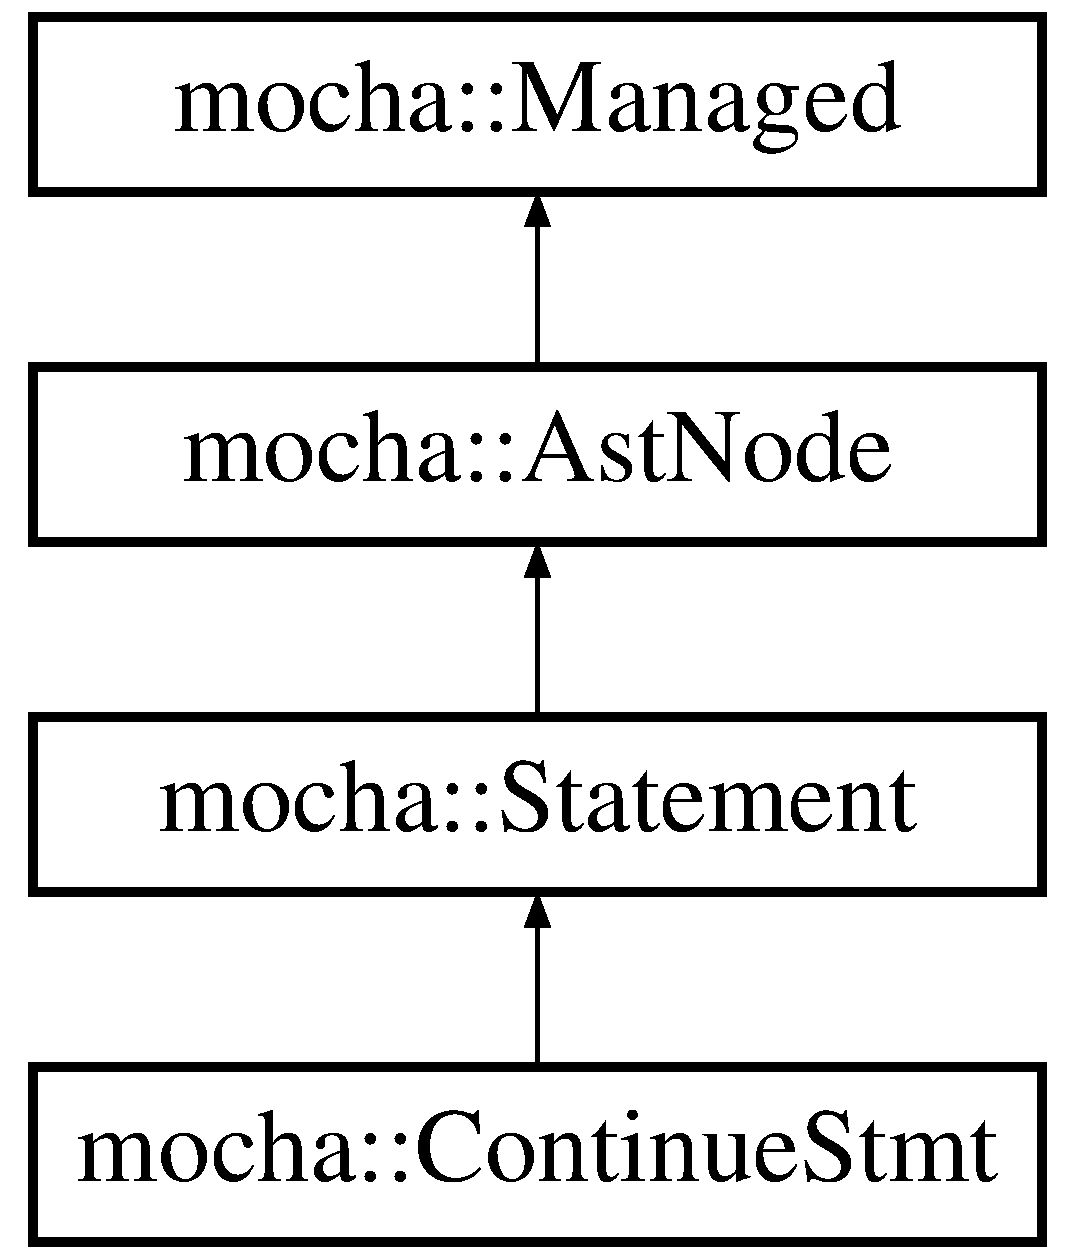
\includegraphics[height=4.000000cm]{classmocha_1_1_continue_stmt}
\end{center}
\end{figure}
\subsection*{Public Member Functions}
\begin{DoxyCompactItemize}
\item 
\hyperlink{classmocha_1_1_continue_stmt_a2d8841d776f5989c5578ff348f52a424}{ContinueStmt} ()
\item 
\hyperlink{classmocha_1_1_continue_stmt_aa5af4afde4e3c8073e2adccc3d195ffa}{$\sim$ContinueStmt} ()
\item 
\hyperlink{classmocha_1_1_ast_node}{AstNode} $\ast$ \hyperlink{classmocha_1_1_continue_stmt_a0a2ccd62452d6cee52724db3c6e28c21}{Clone} ()
\end{DoxyCompactItemize}
\subsection*{Private Member Functions}
\begin{DoxyCompactItemize}
\item 
void \hyperlink{classmocha_1_1_continue_stmt_ae8cbf571d917e7b8002b3b9614b6f92e}{NVIAccept\_\-} (\hyperlink{classmocha_1_1_i_visitor}{IVisitor} $\ast$visitor)
\end{DoxyCompactItemize}


\subsection{Detailed Description}


Definition at line 901 of file ast.h.



\subsection{Constructor \& Destructor Documentation}
\hypertarget{classmocha_1_1_continue_stmt_a2d8841d776f5989c5578ff348f52a424}{
\index{mocha::ContinueStmt@{mocha::ContinueStmt}!ContinueStmt@{ContinueStmt}}
\index{ContinueStmt@{ContinueStmt}!mocha::ContinueStmt@{mocha::ContinueStmt}}
\subsubsection[{ContinueStmt}]{\setlength{\rightskip}{0pt plus 5cm}mocha::ContinueStmt::ContinueStmt (
\begin{DoxyParamCaption}
{}
\end{DoxyParamCaption}
)\hspace{0.3cm}{\ttfamily  \mbox{[}inline\mbox{]}}}}
\label{classmocha_1_1_continue_stmt_a2d8841d776f5989c5578ff348f52a424}


Definition at line 903 of file ast.h.

\hypertarget{classmocha_1_1_continue_stmt_aa5af4afde4e3c8073e2adccc3d195ffa}{
\index{mocha::ContinueStmt@{mocha::ContinueStmt}!$\sim$ContinueStmt@{$\sim$ContinueStmt}}
\index{$\sim$ContinueStmt@{$\sim$ContinueStmt}!mocha::ContinueStmt@{mocha::ContinueStmt}}
\subsubsection[{$\sim$ContinueStmt}]{\setlength{\rightskip}{0pt plus 5cm}mocha::ContinueStmt::$\sim$ContinueStmt (
\begin{DoxyParamCaption}
{}
\end{DoxyParamCaption}
)\hspace{0.3cm}{\ttfamily  \mbox{[}inline\mbox{]}}}}
\label{classmocha_1_1_continue_stmt_aa5af4afde4e3c8073e2adccc3d195ffa}


Definition at line 904 of file ast.h.



\subsection{Member Function Documentation}
\hypertarget{classmocha_1_1_continue_stmt_a0a2ccd62452d6cee52724db3c6e28c21}{
\index{mocha::ContinueStmt@{mocha::ContinueStmt}!Clone@{Clone}}
\index{Clone@{Clone}!mocha::ContinueStmt@{mocha::ContinueStmt}}
\subsubsection[{Clone}]{\setlength{\rightskip}{0pt plus 5cm}{\bf AstNode} $\ast$ mocha::ContinueStmt::Clone (
\begin{DoxyParamCaption}
{}
\end{DoxyParamCaption}
)\hspace{0.3cm}{\ttfamily  \mbox{[}virtual\mbox{]}}}}
\label{classmocha_1_1_continue_stmt_a0a2ccd62452d6cee52724db3c6e28c21}
\begin{DoxyReturn}{Returns}
\{AstNode$\ast$\} Clone node. 
\end{DoxyReturn}


Reimplemented from \hyperlink{classmocha_1_1_ast_node_af2a895699bac2012f8b7739bff49c5ec}{mocha::AstNode}.



Definition at line 332 of file ast.cc.

\hypertarget{classmocha_1_1_continue_stmt_ae8cbf571d917e7b8002b3b9614b6f92e}{
\index{mocha::ContinueStmt@{mocha::ContinueStmt}!NVIAccept\_\-@{NVIAccept\_\-}}
\index{NVIAccept\_\-@{NVIAccept\_\-}!mocha::ContinueStmt@{mocha::ContinueStmt}}
\subsubsection[{NVIAccept\_\-}]{\setlength{\rightskip}{0pt plus 5cm}void mocha::ContinueStmt::NVIAccept\_\- (
\begin{DoxyParamCaption}
\item[{{\bf IVisitor} $\ast$}]{visitor}
\end{DoxyParamCaption}
)\hspace{0.3cm}{\ttfamily  \mbox{[}inline, private, virtual\mbox{]}}}}
\label{classmocha_1_1_continue_stmt_ae8cbf571d917e7b8002b3b9614b6f92e}


Reimplemented from \hyperlink{classmocha_1_1_statement_ad0e8c3ef62d21f733eb50a414046bae4}{mocha::Statement}.



Definition at line 907 of file ast.h.



The documentation for this class was generated from the following files:\begin{DoxyCompactItemize}
\item 
Y:/mocha/src/ast/\hyperlink{ast_8h}{ast.h}\item 
Y:/mocha/src/ast/\hyperlink{ast_8cc}{ast.cc}\end{DoxyCompactItemize}

\hypertarget{structmocha_1_1watch__traits_1_1_create}{
\section{mocha::watch\_\-traits::Create Struct Reference}
\label{structmocha_1_1watch__traits_1_1_create}\index{mocha::watch\_\-traits::Create@{mocha::watch\_\-traits::Create}}
}


{\ttfamily \#include $<$file\_\-watcher.h$>$}

\subsection*{Public Member Functions}
\begin{DoxyCompactItemize}
\item 
\hyperlink{structmocha_1_1watch__traits_1_1_create_a27c3df6b9234e48639802b2fe62db801}{Create} (const char $\ast$filename\_\-)
\end{DoxyCompactItemize}
\subsection*{Public Attributes}
\begin{DoxyCompactItemize}
\item 
const char $\ast$ \hyperlink{structmocha_1_1watch__traits_1_1_create_a230e9cae2915ef8cd40f013a0277d008}{filename}
\end{DoxyCompactItemize}


\subsection{Detailed Description}


Definition at line 19 of file file\_\-watcher.h.



\subsection{Constructor \& Destructor Documentation}
\hypertarget{structmocha_1_1watch__traits_1_1_create_a27c3df6b9234e48639802b2fe62db801}{
\index{mocha::watch\_\-traits::Create@{mocha::watch\_\-traits::Create}!Create@{Create}}
\index{Create@{Create}!mocha::watch_traits::Create@{mocha::watch\_\-traits::Create}}
\subsubsection[{Create}]{\setlength{\rightskip}{0pt plus 5cm}mocha::watch\_\-traits::Create::Create (
\begin{DoxyParamCaption}
\item[{const char $\ast$}]{filename\_\-}
\end{DoxyParamCaption}
)\hspace{0.3cm}{\ttfamily  \mbox{[}inline\mbox{]}}}}
\label{structmocha_1_1watch__traits_1_1_create_a27c3df6b9234e48639802b2fe62db801}


Definition at line 19 of file file\_\-watcher.h.



\subsection{Member Data Documentation}
\hypertarget{structmocha_1_1watch__traits_1_1_create_a230e9cae2915ef8cd40f013a0277d008}{
\index{mocha::watch\_\-traits::Create@{mocha::watch\_\-traits::Create}!filename@{filename}}
\index{filename@{filename}!mocha::watch_traits::Create@{mocha::watch\_\-traits::Create}}
\subsubsection[{filename}]{\setlength{\rightskip}{0pt plus 5cm}const char$\ast$ {\bf mocha::watch\_\-traits::Create::filename}}}
\label{structmocha_1_1watch__traits_1_1_create_a230e9cae2915ef8cd40f013a0277d008}


Definition at line 19 of file file\_\-watcher.h.



The documentation for this struct was generated from the following file:\begin{DoxyCompactItemize}
\item 
Y:/mocha/src/utils/file\_\-watcher/\hyperlink{file__watcher_8h}{file\_\-watcher.h}\end{DoxyCompactItemize}

\hypertarget{structmocha_1_1watch__traits_1_1_delete}{
\section{mocha::watch\_\-traits::Delete Struct Reference}
\label{structmocha_1_1watch__traits_1_1_delete}\index{mocha::watch\_\-traits::Delete@{mocha::watch\_\-traits::Delete}}
}


{\ttfamily \#include $<$file\_\-watcher.h$>$}

\subsection*{Public Member Functions}
\begin{DoxyCompactItemize}
\item 
\hyperlink{structmocha_1_1watch__traits_1_1_delete_a49b2f6896b39a2ded7ac4b36f79966c2}{Delete} (const char $\ast$filename\_\-)
\end{DoxyCompactItemize}
\subsection*{Public Attributes}
\begin{DoxyCompactItemize}
\item 
const char $\ast$ \hyperlink{structmocha_1_1watch__traits_1_1_delete_a70dc9534c39603b7a4997f5b737c31e3}{filename}
\end{DoxyCompactItemize}


\subsection{Detailed Description}


Definition at line 17 of file file\_\-watcher.h.



\subsection{Constructor \& Destructor Documentation}
\hypertarget{structmocha_1_1watch__traits_1_1_delete_a49b2f6896b39a2ded7ac4b36f79966c2}{
\index{mocha::watch\_\-traits::Delete@{mocha::watch\_\-traits::Delete}!Delete@{Delete}}
\index{Delete@{Delete}!mocha::watch_traits::Delete@{mocha::watch\_\-traits::Delete}}
\subsubsection[{Delete}]{\setlength{\rightskip}{0pt plus 5cm}mocha::watch\_\-traits::Delete::Delete (
\begin{DoxyParamCaption}
\item[{const char $\ast$}]{filename\_\-}
\end{DoxyParamCaption}
)\hspace{0.3cm}{\ttfamily  \mbox{[}inline\mbox{]}}}}
\label{structmocha_1_1watch__traits_1_1_delete_a49b2f6896b39a2ded7ac4b36f79966c2}


Definition at line 17 of file file\_\-watcher.h.



\subsection{Member Data Documentation}
\hypertarget{structmocha_1_1watch__traits_1_1_delete_a70dc9534c39603b7a4997f5b737c31e3}{
\index{mocha::watch\_\-traits::Delete@{mocha::watch\_\-traits::Delete}!filename@{filename}}
\index{filename@{filename}!mocha::watch_traits::Delete@{mocha::watch\_\-traits::Delete}}
\subsubsection[{filename}]{\setlength{\rightskip}{0pt plus 5cm}const char$\ast$ {\bf mocha::watch\_\-traits::Delete::filename}}}
\label{structmocha_1_1watch__traits_1_1_delete_a70dc9534c39603b7a4997f5b737c31e3}


Definition at line 17 of file file\_\-watcher.h.



The documentation for this struct was generated from the following file:\begin{DoxyCompactItemize}
\item 
Y:/mocha/src/utils/file\_\-watcher/\hyperlink{file__watcher_8h}{file\_\-watcher.h}\end{DoxyCompactItemize}

\hypertarget{structmocha_1_1watch__traits_1_1_delete_self}{
\section{mocha::watch\_\-traits::DeleteSelf Struct Reference}
\label{structmocha_1_1watch__traits_1_1_delete_self}\index{mocha::watch\_\-traits::DeleteSelf@{mocha::watch\_\-traits::DeleteSelf}}
}


{\ttfamily \#include $<$file\_\-watcher.h$>$}

\subsection*{Public Member Functions}
\begin{DoxyCompactItemize}
\item 
\hyperlink{structmocha_1_1watch__traits_1_1_delete_self_abebe05ee69fe481237f33c02cbb8e79a}{DeleteSelf} (const char $\ast$filename\_\-)
\end{DoxyCompactItemize}
\subsection*{Public Attributes}
\begin{DoxyCompactItemize}
\item 
const char $\ast$ \hyperlink{structmocha_1_1watch__traits_1_1_delete_self_a3a119ba547d18117703400504e5e268e}{filename}
\end{DoxyCompactItemize}


\subsection{Detailed Description}


Definition at line 18 of file file\_\-watcher.h.



\subsection{Constructor \& Destructor Documentation}
\hypertarget{structmocha_1_1watch__traits_1_1_delete_self_abebe05ee69fe481237f33c02cbb8e79a}{
\index{mocha::watch\_\-traits::DeleteSelf@{mocha::watch\_\-traits::DeleteSelf}!DeleteSelf@{DeleteSelf}}
\index{DeleteSelf@{DeleteSelf}!mocha::watch_traits::DeleteSelf@{mocha::watch\_\-traits::DeleteSelf}}
\subsubsection[{DeleteSelf}]{\setlength{\rightskip}{0pt plus 5cm}mocha::watch\_\-traits::DeleteSelf::DeleteSelf (
\begin{DoxyParamCaption}
\item[{const char $\ast$}]{filename\_\-}
\end{DoxyParamCaption}
)\hspace{0.3cm}{\ttfamily  \mbox{[}inline\mbox{]}}}}
\label{structmocha_1_1watch__traits_1_1_delete_self_abebe05ee69fe481237f33c02cbb8e79a}


Definition at line 18 of file file\_\-watcher.h.



\subsection{Member Data Documentation}
\hypertarget{structmocha_1_1watch__traits_1_1_delete_self_a3a119ba547d18117703400504e5e268e}{
\index{mocha::watch\_\-traits::DeleteSelf@{mocha::watch\_\-traits::DeleteSelf}!filename@{filename}}
\index{filename@{filename}!mocha::watch_traits::DeleteSelf@{mocha::watch\_\-traits::DeleteSelf}}
\subsubsection[{filename}]{\setlength{\rightskip}{0pt plus 5cm}const char$\ast$ {\bf mocha::watch\_\-traits::DeleteSelf::filename}}}
\label{structmocha_1_1watch__traits_1_1_delete_self_a3a119ba547d18117703400504e5e268e}


Definition at line 18 of file file\_\-watcher.h.



The documentation for this struct was generated from the following file:\begin{DoxyCompactItemize}
\item 
Y:/mocha/src/utils/file\_\-watcher/\hyperlink{file__watcher_8h}{file\_\-watcher.h}\end{DoxyCompactItemize}

\hypertarget{structmocha_1_1_detect_result}{
\section{mocha::DetectResult Struct Reference}
\label{structmocha_1_1_detect_result}\index{mocha::DetectResult@{mocha::DetectResult}}
}


{\ttfamily \#include $<$encoding.h$>$}

\subsection*{Public Attributes}
\begin{DoxyCompactItemize}
\item 
const char $\ast$ \hyperlink{structmocha_1_1_detect_result_a17ca98df3e40076bebb7a5e0ef18c668}{charset}
\item 
const char $\ast$ \hyperlink{structmocha_1_1_detect_result_abab885a4ef4ea3536b624f0cfd12cc80}{lang}
\item 
bool \hyperlink{structmocha_1_1_detect_result_a14f5390f24c4c2a950e582063374cd84}{error}
\end{DoxyCompactItemize}


\subsection{Detailed Description}


Definition at line 9 of file encoding.h.



\subsection{Member Data Documentation}
\hypertarget{structmocha_1_1_detect_result_a17ca98df3e40076bebb7a5e0ef18c668}{
\index{mocha::DetectResult@{mocha::DetectResult}!charset@{charset}}
\index{charset@{charset}!mocha::DetectResult@{mocha::DetectResult}}
\subsubsection[{charset}]{\setlength{\rightskip}{0pt plus 5cm}const char$\ast$ {\bf mocha::DetectResult::charset}}}
\label{structmocha_1_1_detect_result_a17ca98df3e40076bebb7a5e0ef18c668}


Definition at line 10 of file encoding.h.

\hypertarget{structmocha_1_1_detect_result_a14f5390f24c4c2a950e582063374cd84}{
\index{mocha::DetectResult@{mocha::DetectResult}!error@{error}}
\index{error@{error}!mocha::DetectResult@{mocha::DetectResult}}
\subsubsection[{error}]{\setlength{\rightskip}{0pt plus 5cm}bool {\bf mocha::DetectResult::error}}}
\label{structmocha_1_1_detect_result_a14f5390f24c4c2a950e582063374cd84}


Definition at line 12 of file encoding.h.

\hypertarget{structmocha_1_1_detect_result_abab885a4ef4ea3536b624f0cfd12cc80}{
\index{mocha::DetectResult@{mocha::DetectResult}!lang@{lang}}
\index{lang@{lang}!mocha::DetectResult@{mocha::DetectResult}}
\subsubsection[{lang}]{\setlength{\rightskip}{0pt plus 5cm}const char$\ast$ {\bf mocha::DetectResult::lang}}}
\label{structmocha_1_1_detect_result_abab885a4ef4ea3536b624f0cfd12cc80}


Definition at line 11 of file encoding.h.



The documentation for this struct was generated from the following file:\begin{DoxyCompactItemize}
\item 
Y:/mocha/src/compiler/encoding/\hyperlink{encoding_8h}{encoding.h}\end{DoxyCompactItemize}

\hypertarget{classmocha_1_1_directive}{
\section{mocha::Directive Class Reference}
\label{classmocha_1_1_directive}\index{mocha::Directive@{mocha::Directive}}
}


{\ttfamily \#include $<$directive.h$>$}

\subsection*{Public Member Functions}
\begin{DoxyCompactItemize}
\item 
\hyperlink{classmocha_1_1_directive_a432ea46fd22197b7996a8c07ebd5c938}{Directive} (\hyperlink{classmocha_1_1_ast_node}{AstNode} $\ast$ast\_\-node, \hyperlink{classmocha_1_1_processor_info}{ProcessorInfo} $\ast$info)
\item 
\hyperlink{classmocha_1_1_directive_a15fc75ff1e7157559361c449dabd9de5}{$\sim$Directive} ()
\item 
\hyperlink{classmocha_1_1_ast_node}{AstNode} $\ast$ \hyperlink{classmocha_1_1_directive_af1d6b0a5a016de544a37c868733da0ba}{Eval} ()
\end{DoxyCompactItemize}
\subsection*{Private Attributes}
\begin{DoxyCompactItemize}
\item 
\hyperlink{classmocha_1_1_ast_node}{AstNode} $\ast$ \hyperlink{classmocha_1_1_directive_aa2cda5bc28126665c93f88ae11996697}{node\_\-}
\item 
\hyperlink{classmocha_1_1_processor_info}{ProcessorInfo} $\ast$ \hyperlink{classmocha_1_1_directive_ae14798b3b58438e68d013c881eb17e6a}{info\_\-}
\end{DoxyCompactItemize}


\subsection{Detailed Description}


Definition at line 6 of file directive.h.



\subsection{Constructor \& Destructor Documentation}
\hypertarget{classmocha_1_1_directive_a432ea46fd22197b7996a8c07ebd5c938}{
\index{mocha::Directive@{mocha::Directive}!Directive@{Directive}}
\index{Directive@{Directive}!mocha::Directive@{mocha::Directive}}
\subsubsection[{Directive}]{\setlength{\rightskip}{0pt plus 5cm}mocha::Directive::Directive (
\begin{DoxyParamCaption}
\item[{{\bf AstNode} $\ast$}]{ast\_\-node, }
\item[{{\bf ProcessorInfo} $\ast$}]{info}
\end{DoxyParamCaption}
)}}
\label{classmocha_1_1_directive_a432ea46fd22197b7996a8c07ebd5c938}


Definition at line 5 of file directive.cc.

\hypertarget{classmocha_1_1_directive_a15fc75ff1e7157559361c449dabd9de5}{
\index{mocha::Directive@{mocha::Directive}!$\sim$Directive@{$\sim$Directive}}
\index{$\sim$Directive@{$\sim$Directive}!mocha::Directive@{mocha::Directive}}
\subsubsection[{$\sim$Directive}]{\setlength{\rightskip}{0pt plus 5cm}mocha::Directive::$\sim$Directive (
\begin{DoxyParamCaption}
{}
\end{DoxyParamCaption}
)\hspace{0.3cm}{\ttfamily  \mbox{[}inline\mbox{]}}}}
\label{classmocha_1_1_directive_a15fc75ff1e7157559361c449dabd9de5}


Definition at line 9 of file directive.h.



\subsection{Member Function Documentation}
\hypertarget{classmocha_1_1_directive_af1d6b0a5a016de544a37c868733da0ba}{
\index{mocha::Directive@{mocha::Directive}!Eval@{Eval}}
\index{Eval@{Eval}!mocha::Directive@{mocha::Directive}}
\subsubsection[{Eval}]{\setlength{\rightskip}{0pt plus 5cm}{\bf AstNode} $\ast$ mocha::Directive::Eval (
\begin{DoxyParamCaption}
{}
\end{DoxyParamCaption}
)}}
\label{classmocha_1_1_directive_af1d6b0a5a016de544a37c868733da0ba}


Definition at line 8 of file directive.cc.



\subsection{Member Data Documentation}
\hypertarget{classmocha_1_1_directive_ae14798b3b58438e68d013c881eb17e6a}{
\index{mocha::Directive@{mocha::Directive}!info\_\-@{info\_\-}}
\index{info\_\-@{info\_\-}!mocha::Directive@{mocha::Directive}}
\subsubsection[{info\_\-}]{\setlength{\rightskip}{0pt plus 5cm}{\bf ProcessorInfo}$\ast$ {\bf mocha::Directive::info\_\-}\hspace{0.3cm}{\ttfamily  \mbox{[}private\mbox{]}}}}
\label{classmocha_1_1_directive_ae14798b3b58438e68d013c881eb17e6a}


Definition at line 13 of file directive.h.

\hypertarget{classmocha_1_1_directive_aa2cda5bc28126665c93f88ae11996697}{
\index{mocha::Directive@{mocha::Directive}!node\_\-@{node\_\-}}
\index{node\_\-@{node\_\-}!mocha::Directive@{mocha::Directive}}
\subsubsection[{node\_\-}]{\setlength{\rightskip}{0pt plus 5cm}{\bf AstNode}$\ast$ {\bf mocha::Directive::node\_\-}\hspace{0.3cm}{\ttfamily  \mbox{[}private\mbox{]}}}}
\label{classmocha_1_1_directive_aa2cda5bc28126665c93f88ae11996697}


Definition at line 12 of file directive.h.



The documentation for this class was generated from the following files:\begin{DoxyCompactItemize}
\item 
Y:/mocha/src/ast/directives/\hyperlink{directive_8h}{directive.h}\item 
Y:/mocha/src/ast/directives/\hyperlink{directive_8cc}{directive.cc}\end{DoxyCompactItemize}

\hypertarget{classmocha_1_1_directory}{
\section{mocha::Directory Class Reference}
\label{classmocha_1_1_directory}\index{mocha::Directory@{mocha::Directory}}
}


{\ttfamily \#include $<$directory.h$>$}

\subsection*{Public Member Functions}
\begin{DoxyCompactItemize}
\item 
\hyperlink{classmocha_1_1_directory_a8ab64ab473c53ce7efe47c550ae808e9}{Directory} (const char $\ast$path)
\item 
\hyperlink{classmocha_1_1_directory_aa65b5b51baac31c89e41cda4fe7ece60}{$\sim$Directory} ()
\item 
\hyperlink{classmocha_1_1_directory_iterator}{DirectoryIterator} \hyperlink{classmocha_1_1_directory_a2002487d0073118d2b6be6e4820b8bf1}{GetFileList} (bool is\_\-recursive, bool show\_\-level)
\end{DoxyCompactItemize}
\subsection*{Private Attributes}
\begin{DoxyCompactItemize}
\item 
const char $\ast$ \hyperlink{classmocha_1_1_directory_a3cd4008d4a33371aa4f56fc92b2e7917}{dirpath\_\-}
\item 
\hyperlink{classmocha_1_1_scoped_list}{ScopedList}$<$ \hyperlink{classmocha_1_1_dir_entry}{DirEntry} $>$ \hyperlink{classmocha_1_1_directory_a6ca71b15d6b5344e0f999d877810d626}{scoped\_\-entry\_\-}
\end{DoxyCompactItemize}


\subsection{Detailed Description}


Definition at line 41 of file directory.h.



\subsection{Constructor \& Destructor Documentation}
\hypertarget{classmocha_1_1_directory_a8ab64ab473c53ce7efe47c550ae808e9}{
\index{mocha::Directory@{mocha::Directory}!Directory@{Directory}}
\index{Directory@{Directory}!mocha::Directory@{mocha::Directory}}
\subsubsection[{Directory}]{\setlength{\rightskip}{0pt plus 5cm}mocha::Directory::Directory (
\begin{DoxyParamCaption}
\item[{const char $\ast$}]{path}
\end{DoxyParamCaption}
)}}
\label{classmocha_1_1_directory_a8ab64ab473c53ce7efe47c550ae808e9}


Definition at line 37 of file directory.cc.

\hypertarget{classmocha_1_1_directory_aa65b5b51baac31c89e41cda4fe7ece60}{
\index{mocha::Directory@{mocha::Directory}!$\sim$Directory@{$\sim$Directory}}
\index{$\sim$Directory@{$\sim$Directory}!mocha::Directory@{mocha::Directory}}
\subsubsection[{$\sim$Directory}]{\setlength{\rightskip}{0pt plus 5cm}mocha::Directory::$\sim$Directory (
\begin{DoxyParamCaption}
{}
\end{DoxyParamCaption}
)}}
\label{classmocha_1_1_directory_aa65b5b51baac31c89e41cda4fe7ece60}


Definition at line 38 of file directory.cc.



\subsection{Member Function Documentation}
\hypertarget{classmocha_1_1_directory_a2002487d0073118d2b6be6e4820b8bf1}{
\index{mocha::Directory@{mocha::Directory}!GetFileList@{GetFileList}}
\index{GetFileList@{GetFileList}!mocha::Directory@{mocha::Directory}}
\subsubsection[{GetFileList}]{\setlength{\rightskip}{0pt plus 5cm}{\bf DirectoryIterator} mocha::Directory::GetFileList (
\begin{DoxyParamCaption}
\item[{bool}]{is\_\-recursive, }
\item[{bool}]{show\_\-level}
\end{DoxyParamCaption}
)}}
\label{classmocha_1_1_directory_a2002487d0073118d2b6be6e4820b8bf1}


Definition at line 177 of file directory.cc.



\subsection{Member Data Documentation}
\hypertarget{classmocha_1_1_directory_a3cd4008d4a33371aa4f56fc92b2e7917}{
\index{mocha::Directory@{mocha::Directory}!dirpath\_\-@{dirpath\_\-}}
\index{dirpath\_\-@{dirpath\_\-}!mocha::Directory@{mocha::Directory}}
\subsubsection[{dirpath\_\-}]{\setlength{\rightskip}{0pt plus 5cm}const char$\ast$ {\bf mocha::Directory::dirpath\_\-}\hspace{0.3cm}{\ttfamily  \mbox{[}private\mbox{]}}}}
\label{classmocha_1_1_directory_a3cd4008d4a33371aa4f56fc92b2e7917}


Definition at line 48 of file directory.h.

\hypertarget{classmocha_1_1_directory_a6ca71b15d6b5344e0f999d877810d626}{
\index{mocha::Directory@{mocha::Directory}!scoped\_\-entry\_\-@{scoped\_\-entry\_\-}}
\index{scoped\_\-entry\_\-@{scoped\_\-entry\_\-}!mocha::Directory@{mocha::Directory}}
\subsubsection[{scoped\_\-entry\_\-}]{\setlength{\rightskip}{0pt plus 5cm}{\bf ScopedList}$<${\bf DirEntry}$>$ {\bf mocha::Directory::scoped\_\-entry\_\-}\hspace{0.3cm}{\ttfamily  \mbox{[}private\mbox{]}}}}
\label{classmocha_1_1_directory_a6ca71b15d6b5344e0f999d877810d626}


Definition at line 49 of file directory.h.



The documentation for this class was generated from the following files:\begin{DoxyCompactItemize}
\item 
Y:/mocha/src/utils/file\_\-system/\hyperlink{directory_8h}{directory.h}\item 
Y:/mocha/src/utils/file\_\-system/\hyperlink{directory_8cc}{directory.cc}\end{DoxyCompactItemize}

\hypertarget{classmocha_1_1_directory_iterator}{
\section{mocha::DirectoryIterator Class Reference}
\label{classmocha_1_1_directory_iterator}\index{mocha::DirectoryIterator@{mocha::DirectoryIterator}}
}


{\ttfamily \#include $<$directory.h$>$}

\subsection*{Public Member Functions}
\begin{DoxyCompactItemize}
\item 
\hyperlink{classmocha_1_1_directory_iterator_af233265c5a3e9e4d2957105b8976d91d}{DirectoryIterator} (const \hyperlink{classmocha_1_1_dir_entry}{DirEntry} $\ast$entry)
\item 
\hyperlink{classmocha_1_1_directory_iterator_aea16020dec3da1cf619122ce7c238592}{$\sim$DirectoryIterator} ()
\item 
\hyperlink{classmocha_1_1_directory_iterator_a13f2e264719b1c30a7614c138b95462e}{DirectoryIterator} (const \hyperlink{classmocha_1_1_directory_iterator}{DirectoryIterator} \&)
\item 
const \hyperlink{classmocha_1_1_directory_iterator}{DirectoryIterator} \& \hyperlink{classmocha_1_1_directory_iterator_ad30f8144d759353ede81b95bffa486ec}{operator=} (const \hyperlink{classmocha_1_1_directory_iterator}{DirectoryIterator} \&)
\item 
bool \hyperlink{classmocha_1_1_directory_iterator_a5c25f98e3982ce06f4b042130fc40c00}{HasNext} ()
\item 
const \hyperlink{classmocha_1_1_dir_entry}{DirEntry} $\ast$ \hyperlink{classmocha_1_1_directory_iterator_a5a7df05187d775a7f0b7746ce77c4457}{Next} ()
\end{DoxyCompactItemize}
\subsection*{Private Attributes}
\begin{DoxyCompactItemize}
\item 
const \hyperlink{classmocha_1_1_dir_entry}{DirEntry} $\ast$ \hyperlink{classmocha_1_1_directory_iterator_a91d06f432f427c12545b628a11286688}{entry\_\-}
\end{DoxyCompactItemize}


\subsection{Detailed Description}


Definition at line 29 of file directory.h.



\subsection{Constructor \& Destructor Documentation}
\hypertarget{classmocha_1_1_directory_iterator_af233265c5a3e9e4d2957105b8976d91d}{
\index{mocha::DirectoryIterator@{mocha::DirectoryIterator}!DirectoryIterator@{DirectoryIterator}}
\index{DirectoryIterator@{DirectoryIterator}!mocha::DirectoryIterator@{mocha::DirectoryIterator}}
\subsubsection[{DirectoryIterator}]{\setlength{\rightskip}{0pt plus 5cm}mocha::DirectoryIterator::DirectoryIterator (
\begin{DoxyParamCaption}
\item[{const {\bf DirEntry} $\ast$}]{entry}
\end{DoxyParamCaption}
)}}
\label{classmocha_1_1_directory_iterator_af233265c5a3e9e4d2957105b8976d91d}


Definition at line 15 of file directory.cc.

\hypertarget{classmocha_1_1_directory_iterator_aea16020dec3da1cf619122ce7c238592}{
\index{mocha::DirectoryIterator@{mocha::DirectoryIterator}!$\sim$DirectoryIterator@{$\sim$DirectoryIterator}}
\index{$\sim$DirectoryIterator@{$\sim$DirectoryIterator}!mocha::DirectoryIterator@{mocha::DirectoryIterator}}
\subsubsection[{$\sim$DirectoryIterator}]{\setlength{\rightskip}{0pt plus 5cm}mocha::DirectoryIterator::$\sim$DirectoryIterator (
\begin{DoxyParamCaption}
{}
\end{DoxyParamCaption}
)}}
\label{classmocha_1_1_directory_iterator_aea16020dec3da1cf619122ce7c238592}


Definition at line 16 of file directory.cc.

\hypertarget{classmocha_1_1_directory_iterator_a13f2e264719b1c30a7614c138b95462e}{
\index{mocha::DirectoryIterator@{mocha::DirectoryIterator}!DirectoryIterator@{DirectoryIterator}}
\index{DirectoryIterator@{DirectoryIterator}!mocha::DirectoryIterator@{mocha::DirectoryIterator}}
\subsubsection[{DirectoryIterator}]{\setlength{\rightskip}{0pt plus 5cm}mocha::DirectoryIterator::DirectoryIterator (
\begin{DoxyParamCaption}
\item[{const {\bf DirectoryIterator} \&}]{iterator}
\end{DoxyParamCaption}
)}}
\label{classmocha_1_1_directory_iterator_a13f2e264719b1c30a7614c138b95462e}


Definition at line 18 of file directory.cc.



\subsection{Member Function Documentation}
\hypertarget{classmocha_1_1_directory_iterator_a5c25f98e3982ce06f4b042130fc40c00}{
\index{mocha::DirectoryIterator@{mocha::DirectoryIterator}!HasNext@{HasNext}}
\index{HasNext@{HasNext}!mocha::DirectoryIterator@{mocha::DirectoryIterator}}
\subsubsection[{HasNext}]{\setlength{\rightskip}{0pt plus 5cm}bool mocha::DirectoryIterator::HasNext (
\begin{DoxyParamCaption}
{}
\end{DoxyParamCaption}
)}}
\label{classmocha_1_1_directory_iterator_a5c25f98e3982ce06f4b042130fc40c00}


Definition at line 27 of file directory.cc.

\hypertarget{classmocha_1_1_directory_iterator_a5a7df05187d775a7f0b7746ce77c4457}{
\index{mocha::DirectoryIterator@{mocha::DirectoryIterator}!Next@{Next}}
\index{Next@{Next}!mocha::DirectoryIterator@{mocha::DirectoryIterator}}
\subsubsection[{Next}]{\setlength{\rightskip}{0pt plus 5cm}const {\bf DirEntry} $\ast$ mocha::DirectoryIterator::Next (
\begin{DoxyParamCaption}
{}
\end{DoxyParamCaption}
)}}
\label{classmocha_1_1_directory_iterator_a5a7df05187d775a7f0b7746ce77c4457}


Definition at line 31 of file directory.cc.

\hypertarget{classmocha_1_1_directory_iterator_ad30f8144d759353ede81b95bffa486ec}{
\index{mocha::DirectoryIterator@{mocha::DirectoryIterator}!operator=@{operator=}}
\index{operator=@{operator=}!mocha::DirectoryIterator@{mocha::DirectoryIterator}}
\subsubsection[{operator=}]{\setlength{\rightskip}{0pt plus 5cm}const {\bf DirectoryIterator} \& mocha::DirectoryIterator::operator= (
\begin{DoxyParamCaption}
\item[{const {\bf DirectoryIterator} \&}]{iterator}
\end{DoxyParamCaption}
)}}
\label{classmocha_1_1_directory_iterator_ad30f8144d759353ede81b95bffa486ec}


Definition at line 22 of file directory.cc.



\subsection{Member Data Documentation}
\hypertarget{classmocha_1_1_directory_iterator_a91d06f432f427c12545b628a11286688}{
\index{mocha::DirectoryIterator@{mocha::DirectoryIterator}!entry\_\-@{entry\_\-}}
\index{entry\_\-@{entry\_\-}!mocha::DirectoryIterator@{mocha::DirectoryIterator}}
\subsubsection[{entry\_\-}]{\setlength{\rightskip}{0pt plus 5cm}const {\bf DirEntry}$\ast$ {\bf mocha::DirectoryIterator::entry\_\-}\hspace{0.3cm}{\ttfamily  \mbox{[}private\mbox{]}}}}
\label{classmocha_1_1_directory_iterator_a91d06f432f427c12545b628a11286688}


Definition at line 38 of file directory.h.



The documentation for this class was generated from the following files:\begin{DoxyCompactItemize}
\item 
Y:/mocha/src/utils/file\_\-system/\hyperlink{directory_8h}{directory.h}\item 
Y:/mocha/src/utils/file\_\-system/\hyperlink{directory_8cc}{directory.cc}\end{DoxyCompactItemize}

\hypertarget{classmocha_1_1_dir_entry}{
\section{mocha::DirEntry Class Reference}
\label{classmocha_1_1_dir_entry}\index{mocha::DirEntry@{mocha::DirEntry}}
}


{\ttfamily \#include $<$directory.h$>$}

\subsection*{Public Member Functions}
\begin{DoxyCompactItemize}
\item 
\hyperlink{classmocha_1_1_dir_entry_afcec06b8ebc51d9cc914a53282b28bae}{DirEntry} (const char $\ast$path, const char $\ast$dir)
\item 
\hyperlink{classmocha_1_1_dir_entry_a865911e82d9b09796173f18bac8ccd7e}{$\sim$DirEntry} ()
\item 
const char $\ast$ \hyperlink{classmocha_1_1_dir_entry_aa35e4e487db311e479fc7eb9a5d7a459}{GetName} () const 
\item 
const char $\ast$ \hyperlink{classmocha_1_1_dir_entry_a85f99f5336f997212d9920b09073cee3}{GetFullPath} () const 
\item 
const char $\ast$ \hyperlink{classmocha_1_1_dir_entry_a1e30c41653b46a081cee15f003248c53}{GetDirName} () const 
\item 
void \hyperlink{classmocha_1_1_dir_entry_abec849ef6f0736a70faac0f436c9519f}{SetNext} (\hyperlink{classmocha_1_1_dir_entry}{DirEntry} $\ast$ent)
\end{DoxyCompactItemize}
\subsection*{Private Member Functions}
\begin{DoxyCompactItemize}
\item 
\hyperlink{classmocha_1_1_dir_entry_a280456e530b249c5b5891ee027a971c1}{DirEntry} ()
\end{DoxyCompactItemize}
\subsection*{Private Attributes}
\begin{DoxyCompactItemize}
\item 
std::string \hyperlink{classmocha_1_1_dir_entry_a1fffe6a5d6f268f6a00f16e4fbce433d}{name\_\-}
\item 
std::string \hyperlink{classmocha_1_1_dir_entry_aa7c3d579d46d694ac584f3f197c43d8d}{dir\_\-}
\item 
std::string \hyperlink{classmocha_1_1_dir_entry_ad257721184bc483c22fb639f3e98e6ad}{full\_\-path\_\-}
\item 
const \hyperlink{classmocha_1_1_dir_entry}{DirEntry} $\ast$ \hyperlink{classmocha_1_1_dir_entry_aaedb913694aacd4b88c6ccc5daf78ae8}{next\_\-}
\end{DoxyCompactItemize}
\subsection*{Friends}
\begin{DoxyCompactItemize}
\item 
class \hyperlink{classmocha_1_1_dir_entry_ae63907c37399ddb1ac7a104c3fe64423}{DirectoryIterator}
\item 
class \hyperlink{classmocha_1_1_dir_entry_a245303e8660be5fb8eb2828a8c44b773}{Directory}
\end{DoxyCompactItemize}


\subsection{Detailed Description}


Definition at line 7 of file directory.h.



\subsection{Constructor \& Destructor Documentation}
\hypertarget{classmocha_1_1_dir_entry_afcec06b8ebc51d9cc914a53282b28bae}{
\index{mocha::DirEntry@{mocha::DirEntry}!DirEntry@{DirEntry}}
\index{DirEntry@{DirEntry}!mocha::DirEntry@{mocha::DirEntry}}
\subsubsection[{DirEntry}]{\setlength{\rightskip}{0pt plus 5cm}mocha::DirEntry::DirEntry (
\begin{DoxyParamCaption}
\item[{const char $\ast$}]{path, }
\item[{const char $\ast$}]{dir}
\end{DoxyParamCaption}
)\hspace{0.3cm}{\ttfamily  \mbox{[}inline\mbox{]}}}}
\label{classmocha_1_1_dir_entry_afcec06b8ebc51d9cc914a53282b28bae}


Definition at line 11 of file directory.h.

\hypertarget{classmocha_1_1_dir_entry_a865911e82d9b09796173f18bac8ccd7e}{
\index{mocha::DirEntry@{mocha::DirEntry}!$\sim$DirEntry@{$\sim$DirEntry}}
\index{$\sim$DirEntry@{$\sim$DirEntry}!mocha::DirEntry@{mocha::DirEntry}}
\subsubsection[{$\sim$DirEntry}]{\setlength{\rightskip}{0pt plus 5cm}mocha::DirEntry::$\sim$DirEntry (
\begin{DoxyParamCaption}
{}
\end{DoxyParamCaption}
)\hspace{0.3cm}{\ttfamily  \mbox{[}inline\mbox{]}}}}
\label{classmocha_1_1_dir_entry_a865911e82d9b09796173f18bac8ccd7e}


Definition at line 16 of file directory.h.

\hypertarget{classmocha_1_1_dir_entry_a280456e530b249c5b5891ee027a971c1}{
\index{mocha::DirEntry@{mocha::DirEntry}!DirEntry@{DirEntry}}
\index{DirEntry@{DirEntry}!mocha::DirEntry@{mocha::DirEntry}}
\subsubsection[{DirEntry}]{\setlength{\rightskip}{0pt plus 5cm}mocha::DirEntry::DirEntry (
\begin{DoxyParamCaption}
{}
\end{DoxyParamCaption}
)\hspace{0.3cm}{\ttfamily  \mbox{[}inline, private\mbox{]}}}}
\label{classmocha_1_1_dir_entry_a280456e530b249c5b5891ee027a971c1}


Definition at line 22 of file directory.h.



\subsection{Member Function Documentation}
\hypertarget{classmocha_1_1_dir_entry_a1e30c41653b46a081cee15f003248c53}{
\index{mocha::DirEntry@{mocha::DirEntry}!GetDirName@{GetDirName}}
\index{GetDirName@{GetDirName}!mocha::DirEntry@{mocha::DirEntry}}
\subsubsection[{GetDirName}]{\setlength{\rightskip}{0pt plus 5cm}const char$\ast$ mocha::DirEntry::GetDirName (
\begin{DoxyParamCaption}
{}
\end{DoxyParamCaption}
) const\hspace{0.3cm}{\ttfamily  \mbox{[}inline\mbox{]}}}}
\label{classmocha_1_1_dir_entry_a1e30c41653b46a081cee15f003248c53}


Definition at line 19 of file directory.h.

\hypertarget{classmocha_1_1_dir_entry_a85f99f5336f997212d9920b09073cee3}{
\index{mocha::DirEntry@{mocha::DirEntry}!GetFullPath@{GetFullPath}}
\index{GetFullPath@{GetFullPath}!mocha::DirEntry@{mocha::DirEntry}}
\subsubsection[{GetFullPath}]{\setlength{\rightskip}{0pt plus 5cm}const char$\ast$ mocha::DirEntry::GetFullPath (
\begin{DoxyParamCaption}
{}
\end{DoxyParamCaption}
) const\hspace{0.3cm}{\ttfamily  \mbox{[}inline\mbox{]}}}}
\label{classmocha_1_1_dir_entry_a85f99f5336f997212d9920b09073cee3}


Definition at line 18 of file directory.h.

\hypertarget{classmocha_1_1_dir_entry_aa35e4e487db311e479fc7eb9a5d7a459}{
\index{mocha::DirEntry@{mocha::DirEntry}!GetName@{GetName}}
\index{GetName@{GetName}!mocha::DirEntry@{mocha::DirEntry}}
\subsubsection[{GetName}]{\setlength{\rightskip}{0pt plus 5cm}const char$\ast$ mocha::DirEntry::GetName (
\begin{DoxyParamCaption}
{}
\end{DoxyParamCaption}
) const\hspace{0.3cm}{\ttfamily  \mbox{[}inline\mbox{]}}}}
\label{classmocha_1_1_dir_entry_aa35e4e487db311e479fc7eb9a5d7a459}


Definition at line 17 of file directory.h.

\hypertarget{classmocha_1_1_dir_entry_abec849ef6f0736a70faac0f436c9519f}{
\index{mocha::DirEntry@{mocha::DirEntry}!SetNext@{SetNext}}
\index{SetNext@{SetNext}!mocha::DirEntry@{mocha::DirEntry}}
\subsubsection[{SetNext}]{\setlength{\rightskip}{0pt plus 5cm}void mocha::DirEntry::SetNext (
\begin{DoxyParamCaption}
\item[{{\bf DirEntry} $\ast$}]{ent}
\end{DoxyParamCaption}
)\hspace{0.3cm}{\ttfamily  \mbox{[}inline\mbox{]}}}}
\label{classmocha_1_1_dir_entry_abec849ef6f0736a70faac0f436c9519f}


Definition at line 20 of file directory.h.



\subsection{Friends And Related Function Documentation}
\hypertarget{classmocha_1_1_dir_entry_a245303e8660be5fb8eb2828a8c44b773}{
\index{mocha::DirEntry@{mocha::DirEntry}!Directory@{Directory}}
\index{Directory@{Directory}!mocha::DirEntry@{mocha::DirEntry}}
\subsubsection[{Directory}]{\setlength{\rightskip}{0pt plus 5cm}friend class {\bf Directory}\hspace{0.3cm}{\ttfamily  \mbox{[}friend\mbox{]}}}}
\label{classmocha_1_1_dir_entry_a245303e8660be5fb8eb2828a8c44b773}


Definition at line 9 of file directory.h.

\hypertarget{classmocha_1_1_dir_entry_ae63907c37399ddb1ac7a104c3fe64423}{
\index{mocha::DirEntry@{mocha::DirEntry}!DirectoryIterator@{DirectoryIterator}}
\index{DirectoryIterator@{DirectoryIterator}!mocha::DirEntry@{mocha::DirEntry}}
\subsubsection[{DirectoryIterator}]{\setlength{\rightskip}{0pt plus 5cm}friend class {\bf DirectoryIterator}\hspace{0.3cm}{\ttfamily  \mbox{[}friend\mbox{]}}}}
\label{classmocha_1_1_dir_entry_ae63907c37399ddb1ac7a104c3fe64423}


Definition at line 8 of file directory.h.



\subsection{Member Data Documentation}
\hypertarget{classmocha_1_1_dir_entry_aa7c3d579d46d694ac584f3f197c43d8d}{
\index{mocha::DirEntry@{mocha::DirEntry}!dir\_\-@{dir\_\-}}
\index{dir\_\-@{dir\_\-}!mocha::DirEntry@{mocha::DirEntry}}
\subsubsection[{dir\_\-}]{\setlength{\rightskip}{0pt plus 5cm}std::string {\bf mocha::DirEntry::dir\_\-}\hspace{0.3cm}{\ttfamily  \mbox{[}private\mbox{]}}}}
\label{classmocha_1_1_dir_entry_aa7c3d579d46d694ac584f3f197c43d8d}


Definition at line 24 of file directory.h.

\hypertarget{classmocha_1_1_dir_entry_ad257721184bc483c22fb639f3e98e6ad}{
\index{mocha::DirEntry@{mocha::DirEntry}!full\_\-path\_\-@{full\_\-path\_\-}}
\index{full\_\-path\_\-@{full\_\-path\_\-}!mocha::DirEntry@{mocha::DirEntry}}
\subsubsection[{full\_\-path\_\-}]{\setlength{\rightskip}{0pt plus 5cm}std::string {\bf mocha::DirEntry::full\_\-path\_\-}\hspace{0.3cm}{\ttfamily  \mbox{[}private\mbox{]}}}}
\label{classmocha_1_1_dir_entry_ad257721184bc483c22fb639f3e98e6ad}


Definition at line 25 of file directory.h.

\hypertarget{classmocha_1_1_dir_entry_a1fffe6a5d6f268f6a00f16e4fbce433d}{
\index{mocha::DirEntry@{mocha::DirEntry}!name\_\-@{name\_\-}}
\index{name\_\-@{name\_\-}!mocha::DirEntry@{mocha::DirEntry}}
\subsubsection[{name\_\-}]{\setlength{\rightskip}{0pt plus 5cm}std::string {\bf mocha::DirEntry::name\_\-}\hspace{0.3cm}{\ttfamily  \mbox{[}private\mbox{]}}}}
\label{classmocha_1_1_dir_entry_a1fffe6a5d6f268f6a00f16e4fbce433d}


Definition at line 23 of file directory.h.

\hypertarget{classmocha_1_1_dir_entry_aaedb913694aacd4b88c6ccc5daf78ae8}{
\index{mocha::DirEntry@{mocha::DirEntry}!next\_\-@{next\_\-}}
\index{next\_\-@{next\_\-}!mocha::DirEntry@{mocha::DirEntry}}
\subsubsection[{next\_\-}]{\setlength{\rightskip}{0pt plus 5cm}const {\bf DirEntry}$\ast$ {\bf mocha::DirEntry::next\_\-}\hspace{0.3cm}{\ttfamily  \mbox{[}private\mbox{]}}}}
\label{classmocha_1_1_dir_entry_aaedb913694aacd4b88c6ccc5daf78ae8}


Definition at line 26 of file directory.h.



The documentation for this class was generated from the following file:\begin{DoxyCompactItemize}
\item 
Y:/mocha/src/utils/file\_\-system/\hyperlink{directory_8h}{directory.h}\end{DoxyCompactItemize}

\hypertarget{structmocha_1_1_dir_entry_list_1_1_dir_entry}{
\section{mocha::DirEntryList::DirEntry Struct Reference}
\label{structmocha_1_1_dir_entry_list_1_1_dir_entry}\index{mocha::DirEntryList::DirEntry@{mocha::DirEntryList::DirEntry}}
}
\subsection*{Public Attributes}
\begin{DoxyCompactItemize}
\item 
\hyperlink{classmocha_1_1_bucket}{Bucket} $\ast$ \hyperlink{structmocha_1_1_dir_entry_list_1_1_dir_entry_a1f99f0664a09b1f9077a2350e71972e6}{bucket\_\-ptr}
\item 
\hyperlink{classmocha_1_1_bucket}{Bucket} $\ast$ \hyperlink{structmocha_1_1_dir_entry_list_1_1_dir_entry_a6851e0d1638f36194bfb9d6d26d7c311}{becket\_\-ptr\_\-}
\end{DoxyCompactItemize}


\subsection{Detailed Description}


Definition at line 11 of file hash\_\-dir\_\-entry\_\-list.cc.



\subsection{Member Data Documentation}
\hypertarget{structmocha_1_1_dir_entry_list_1_1_dir_entry_a6851e0d1638f36194bfb9d6d26d7c311}{
\index{mocha::DirEntryList::DirEntry@{mocha::DirEntryList::DirEntry}!becket\_\-ptr\_\-@{becket\_\-ptr\_\-}}
\index{becket\_\-ptr\_\-@{becket\_\-ptr\_\-}!mocha::DirEntryList::DirEntry@{mocha::DirEntryList::DirEntry}}
\subsubsection[{becket\_\-ptr\_\-}]{\setlength{\rightskip}{0pt plus 5cm}{\bf Bucket}$\ast$ {\bf mocha::DirEntryList::DirEntry::becket\_\-ptr\_\-}}}
\label{structmocha_1_1_dir_entry_list_1_1_dir_entry_a6851e0d1638f36194bfb9d6d26d7c311}


Definition at line 18 of file hash\_\-dir\_\-entry\_\-list.h.

\hypertarget{structmocha_1_1_dir_entry_list_1_1_dir_entry_a1f99f0664a09b1f9077a2350e71972e6}{
\index{mocha::DirEntryList::DirEntry@{mocha::DirEntryList::DirEntry}!bucket\_\-ptr@{bucket\_\-ptr}}
\index{bucket\_\-ptr@{bucket\_\-ptr}!mocha::DirEntryList::DirEntry@{mocha::DirEntryList::DirEntry}}
\subsubsection[{bucket\_\-ptr}]{\setlength{\rightskip}{0pt plus 5cm}{\bf Bucket}$\ast$ {\bf mocha::DirEntryList::DirEntry::bucket\_\-ptr}}}
\label{structmocha_1_1_dir_entry_list_1_1_dir_entry_a1f99f0664a09b1f9077a2350e71972e6}


Definition at line 12 of file hash\_\-dir\_\-entry\_\-list.cc.



The documentation for this struct was generated from the following files:\begin{DoxyCompactItemize}
\item 
Y:/mocha/src/utils/hash/hash\_\-map/\hyperlink{hash__dir__entry__list_8cc}{hash\_\-dir\_\-entry\_\-list.cc}\item 
Y:/mocha/src/utils/hash/hash\_\-map/\hyperlink{hash__dir__entry__list_8h}{hash\_\-dir\_\-entry\_\-list.h}\end{DoxyCompactItemize}

\hypertarget{classmocha_1_1_dir_entry_list}{
\section{mocha::DirEntryList Class Reference}
\label{classmocha_1_1_dir_entry_list}\index{mocha::DirEntryList@{mocha::DirEntryList}}
}


{\ttfamily \#include $<$hash\_\-dir\_\-entry\_\-list.h$>$}

\subsection*{Classes}
\begin{DoxyCompactItemize}
\item 
struct \hyperlink{structmocha_1_1_dir_entry_list_1_1_dir_entry}{DirEntry}
\end{DoxyCompactItemize}
\subsection*{Public Member Functions}
\begin{DoxyCompactItemize}
\item 
\hyperlink{classmocha_1_1_dir_entry_list_a3f5e423097367d99de8440f1d49b62ac}{DirEntryList} ()
\item 
\hyperlink{classmocha_1_1_dir_entry_list_a942ffaddcb496934dc056dfaeba31796}{$\sim$DirEntryList} ()
\item 
void \hyperlink{classmocha_1_1_dir_entry_list_aa48c3c866978aca3bec78981afaf11c2}{Extend} ()
\item 
\hyperlink{structmocha_1_1_dir_entry_list_1_1_dir_entry}{DirEntry} $\ast$ \hyperlink{classmocha_1_1_dir_entry_list_a2428aac7ddc43862719b1e9fcf7d1e92}{At} (int num)
\item 
void \hyperlink{classmocha_1_1_dir_entry_list_a456848a7ec9c9e36f91676ab3d534fc4}{Insert} (void $\ast$entry, uint64\_\-t hash)
\item 
void $\ast$ \hyperlink{classmocha_1_1_dir_entry_list_acd2ebff8120c7384f6974a42bfc2c500}{Find} (uint64\_\-t hash)
\end{DoxyCompactItemize}
\subsection*{Private Attributes}
\begin{DoxyCompactItemize}
\item 
int \hyperlink{classmocha_1_1_dir_entry_list_a498e86857a21dbeabab021c7a9621d9f}{used\_\-bit\_\-category\_\-}
\item 
int \hyperlink{classmocha_1_1_dir_entry_list_a7b9617a781ff4f9c0572db72139cb590}{size\_\-}
\item 
\hyperlink{structmocha_1_1_dir_entry_list_1_1_dir_entry}{DirEntry} $\ast$ \hyperlink{classmocha_1_1_dir_entry_list_a3d34a72036ac78b8d9531da25a999006}{entries\_\-}
\end{DoxyCompactItemize}


\subsection{Detailed Description}


Definition at line 6 of file hash\_\-dir\_\-entry\_\-list.h.



\subsection{Constructor \& Destructor Documentation}
\hypertarget{classmocha_1_1_dir_entry_list_a3f5e423097367d99de8440f1d49b62ac}{
\index{mocha::DirEntryList@{mocha::DirEntryList}!DirEntryList@{DirEntryList}}
\index{DirEntryList@{DirEntryList}!mocha::DirEntryList@{mocha::DirEntryList}}
\subsubsection[{DirEntryList}]{\setlength{\rightskip}{0pt plus 5cm}mocha::DirEntryList::DirEntryList (
\begin{DoxyParamCaption}
{}
\end{DoxyParamCaption}
)}}
\label{classmocha_1_1_dir_entry_list_a3f5e423097367d99de8440f1d49b62ac}


Definition at line 15 of file hash\_\-dir\_\-entry\_\-list.cc.

\hypertarget{classmocha_1_1_dir_entry_list_a942ffaddcb496934dc056dfaeba31796}{
\index{mocha::DirEntryList@{mocha::DirEntryList}!$\sim$DirEntryList@{$\sim$DirEntryList}}
\index{$\sim$DirEntryList@{$\sim$DirEntryList}!mocha::DirEntryList@{mocha::DirEntryList}}
\subsubsection[{$\sim$DirEntryList}]{\setlength{\rightskip}{0pt plus 5cm}mocha::DirEntryList::$\sim$DirEntryList (
\begin{DoxyParamCaption}
{}
\end{DoxyParamCaption}
)}}
\label{classmocha_1_1_dir_entry_list_a942ffaddcb496934dc056dfaeba31796}


Definition at line 21 of file hash\_\-dir\_\-entry\_\-list.cc.



\subsection{Member Function Documentation}
\hypertarget{classmocha_1_1_dir_entry_list_a2428aac7ddc43862719b1e9fcf7d1e92}{
\index{mocha::DirEntryList@{mocha::DirEntryList}!At@{At}}
\index{At@{At}!mocha::DirEntryList@{mocha::DirEntryList}}
\subsubsection[{At}]{\setlength{\rightskip}{0pt plus 5cm}{\bf DirEntry}$\ast$ mocha::DirEntryList::At (
\begin{DoxyParamCaption}
\item[{int}]{num}
\end{DoxyParamCaption}
)}}
\label{classmocha_1_1_dir_entry_list_a2428aac7ddc43862719b1e9fcf7d1e92}
\hypertarget{classmocha_1_1_dir_entry_list_aa48c3c866978aca3bec78981afaf11c2}{
\index{mocha::DirEntryList@{mocha::DirEntryList}!Extend@{Extend}}
\index{Extend@{Extend}!mocha::DirEntryList@{mocha::DirEntryList}}
\subsubsection[{Extend}]{\setlength{\rightskip}{0pt plus 5cm}void mocha::DirEntryList::Extend (
\begin{DoxyParamCaption}
{}
\end{DoxyParamCaption}
)}}
\label{classmocha_1_1_dir_entry_list_aa48c3c866978aca3bec78981afaf11c2}
\hypertarget{classmocha_1_1_dir_entry_list_acd2ebff8120c7384f6974a42bfc2c500}{
\index{mocha::DirEntryList@{mocha::DirEntryList}!Find@{Find}}
\index{Find@{Find}!mocha::DirEntryList@{mocha::DirEntryList}}
\subsubsection[{Find}]{\setlength{\rightskip}{0pt plus 5cm}void$\ast$ mocha::DirEntryList::Find (
\begin{DoxyParamCaption}
\item[{uint64\_\-t}]{hash}
\end{DoxyParamCaption}
)}}
\label{classmocha_1_1_dir_entry_list_acd2ebff8120c7384f6974a42bfc2c500}
\hypertarget{classmocha_1_1_dir_entry_list_a456848a7ec9c9e36f91676ab3d534fc4}{
\index{mocha::DirEntryList@{mocha::DirEntryList}!Insert@{Insert}}
\index{Insert@{Insert}!mocha::DirEntryList@{mocha::DirEntryList}}
\subsubsection[{Insert}]{\setlength{\rightskip}{0pt plus 5cm}void mocha::DirEntryList::Insert (
\begin{DoxyParamCaption}
\item[{void $\ast$}]{entry, }
\item[{uint64\_\-t}]{hash}
\end{DoxyParamCaption}
)}}
\label{classmocha_1_1_dir_entry_list_a456848a7ec9c9e36f91676ab3d534fc4}


Definition at line 33 of file hash\_\-dir\_\-entry\_\-list.cc.



\subsection{Member Data Documentation}
\hypertarget{classmocha_1_1_dir_entry_list_a3d34a72036ac78b8d9531da25a999006}{
\index{mocha::DirEntryList@{mocha::DirEntryList}!entries\_\-@{entries\_\-}}
\index{entries\_\-@{entries\_\-}!mocha::DirEntryList@{mocha::DirEntryList}}
\subsubsection[{entries\_\-}]{\setlength{\rightskip}{0pt plus 5cm}{\bf DirEntry}$\ast$ {\bf mocha::DirEntryList::entries\_\-}\hspace{0.3cm}{\ttfamily  \mbox{[}private\mbox{]}}}}
\label{classmocha_1_1_dir_entry_list_a3d34a72036ac78b8d9531da25a999006}


Definition at line 20 of file hash\_\-dir\_\-entry\_\-list.h.

\hypertarget{classmocha_1_1_dir_entry_list_a7b9617a781ff4f9c0572db72139cb590}{
\index{mocha::DirEntryList@{mocha::DirEntryList}!size\_\-@{size\_\-}}
\index{size\_\-@{size\_\-}!mocha::DirEntryList@{mocha::DirEntryList}}
\subsubsection[{size\_\-}]{\setlength{\rightskip}{0pt plus 5cm}int {\bf mocha::DirEntryList::size\_\-}\hspace{0.3cm}{\ttfamily  \mbox{[}private\mbox{]}}}}
\label{classmocha_1_1_dir_entry_list_a7b9617a781ff4f9c0572db72139cb590}


Definition at line 16 of file hash\_\-dir\_\-entry\_\-list.h.

\hypertarget{classmocha_1_1_dir_entry_list_a498e86857a21dbeabab021c7a9621d9f}{
\index{mocha::DirEntryList@{mocha::DirEntryList}!used\_\-bit\_\-category\_\-@{used\_\-bit\_\-category\_\-}}
\index{used\_\-bit\_\-category\_\-@{used\_\-bit\_\-category\_\-}!mocha::DirEntryList@{mocha::DirEntryList}}
\subsubsection[{used\_\-bit\_\-category\_\-}]{\setlength{\rightskip}{0pt plus 5cm}int {\bf mocha::DirEntryList::used\_\-bit\_\-category\_\-}\hspace{0.3cm}{\ttfamily  \mbox{[}private\mbox{]}}}}
\label{classmocha_1_1_dir_entry_list_a498e86857a21dbeabab021c7a9621d9f}


Definition at line 15 of file hash\_\-dir\_\-entry\_\-list.h.



The documentation for this class was generated from the following files:\begin{DoxyCompactItemize}
\item 
Y:/mocha/src/utils/hash/hash\_\-map/\hyperlink{hash__dir__entry__list_8h}{hash\_\-dir\_\-entry\_\-list.h}\item 
Y:/mocha/src/utils/hash/hash\_\-map/\hyperlink{hash__dir__entry__list_8cc}{hash\_\-dir\_\-entry\_\-list.cc}\end{DoxyCompactItemize}

\hypertarget{classmocha_1_1_dir_finder}{
\section{mocha::DirFinder Class Reference}
\label{classmocha_1_1_dir_finder}\index{mocha::DirFinder@{mocha::DirFinder}}
}
\subsection*{Public Member Functions}
\begin{DoxyCompactItemize}
\item 
\hyperlink{classmocha_1_1_dir_finder_a811d9e60e339b262a1a3aa75788a5673}{DirFinder} (const char $\ast$path, bool is\_\-recursive, bool show\_\-level, DIR $\ast$dir, \hyperlink{classmocha_1_1_scoped_list}{ScopedList}$<$ \hyperlink{classmocha_1_1_dir_entry}{DirEntry} $>$ $\ast$scoped\_\-list)
\item 
\hyperlink{classmocha_1_1_dir_entry}{DirEntry} $\ast$ \hyperlink{classmocha_1_1_dir_finder_a02fbbcd307ade283ff9cf0fa290dd697}{GetFirst} ()
\item 
\hyperlink{classmocha_1_1_dir_entry}{DirEntry} $\ast$ \hyperlink{classmocha_1_1_dir_finder_a63276dd45352800c62f033a534931e30}{Find} ()
\end{DoxyCompactItemize}
\subsection*{Private Types}
\begin{DoxyCompactItemize}
\item 
typedef std::vector$<$ std::string $>$ \hyperlink{classmocha_1_1_dir_finder_abd8c8f76dbb9c9ac8a3810d99a9f10e8}{SubDirList}
\end{DoxyCompactItemize}
\subsection*{Private Member Functions}
\begin{DoxyCompactItemize}
\item 
void \hyperlink{classmocha_1_1_dir_finder_ad94fab153c96ce00314d97f8ca8f8798}{FindSubDir\_\-} (const \hyperlink{classmocha_1_1_dir_finder_abd8c8f76dbb9c9ac8a3810d99a9f10e8}{SubDirList} \&sub)
\end{DoxyCompactItemize}
\subsection*{Private Attributes}
\begin{DoxyCompactItemize}
\item 
const char $\ast$ \hyperlink{classmocha_1_1_dir_finder_a1ef92d885780984ecb7b82ba9b4b5543}{path\_\-}
\item 
bool \hyperlink{classmocha_1_1_dir_finder_a2b47a8b8bd03f5af49a5dd5058d13b3a}{is\_\-recursive\_\-}
\item 
bool \hyperlink{classmocha_1_1_dir_finder_aa050793a3b04ea0b57a6971085f85969}{show\_\-level\_\-}
\item 
DIR $\ast$ \hyperlink{classmocha_1_1_dir_finder_a28e4e804d01d3b22fdcd3c24de664a80}{dir\_\-}
\item 
dirent \hyperlink{classmocha_1_1_dir_finder_aad8c41bba9d05cb0b0c4d96cee2e0d14}{entry\_\-}
\item 
dirent $\ast$ \hyperlink{classmocha_1_1_dir_finder_aaab8894e08b3e4cd81e4df5b4157c2c2}{result\_\-}
\item 
\hyperlink{classmocha_1_1_dir_entry}{DirEntry} $\ast$ \hyperlink{classmocha_1_1_dir_finder_a65235eb369e6a960d885fce284d25400}{first\_\-}
\item 
\hyperlink{classmocha_1_1_dir_entry}{DirEntry} $\ast$ \hyperlink{classmocha_1_1_dir_finder_a2d94dc19bbaa238b3e3a57f42e52cd14}{current\_\-}
\item 
\hyperlink{classmocha_1_1_scoped_list}{ScopedList}$<$ \hyperlink{classmocha_1_1_dir_entry}{DirEntry} $>$ $\ast$ \hyperlink{classmocha_1_1_dir_finder_aec3cfce5cc65650949d6ba339832492a}{scoped\_\-list\_\-}
\end{DoxyCompactItemize}


\subsection{Detailed Description}


Definition at line 101 of file directory.cc.



\subsection{Member Typedef Documentation}
\hypertarget{classmocha_1_1_dir_finder_abd8c8f76dbb9c9ac8a3810d99a9f10e8}{
\index{mocha::DirFinder@{mocha::DirFinder}!SubDirList@{SubDirList}}
\index{SubDirList@{SubDirList}!mocha::DirFinder@{mocha::DirFinder}}
\subsubsection[{SubDirList}]{\setlength{\rightskip}{0pt plus 5cm}typedef std::vector$<$std::string$>$ {\bf mocha::DirFinder::SubDirList}\hspace{0.3cm}{\ttfamily  \mbox{[}private\mbox{]}}}}
\label{classmocha_1_1_dir_finder_abd8c8f76dbb9c9ac8a3810d99a9f10e8}


Definition at line 102 of file directory.cc.



\subsection{Constructor \& Destructor Documentation}
\hypertarget{classmocha_1_1_dir_finder_a811d9e60e339b262a1a3aa75788a5673}{
\index{mocha::DirFinder@{mocha::DirFinder}!DirFinder@{DirFinder}}
\index{DirFinder@{DirFinder}!mocha::DirFinder@{mocha::DirFinder}}
\subsubsection[{DirFinder}]{\setlength{\rightskip}{0pt plus 5cm}mocha::DirFinder::DirFinder (
\begin{DoxyParamCaption}
\item[{const char $\ast$}]{path, }
\item[{bool}]{is\_\-recursive, }
\item[{bool}]{show\_\-level, }
\item[{DIR $\ast$}]{dir, }
\item[{{\bf ScopedList}$<$ {\bf DirEntry} $>$ $\ast$}]{scoped\_\-list}
\end{DoxyParamCaption}
)\hspace{0.3cm}{\ttfamily  \mbox{[}inline\mbox{]}}}}
\label{classmocha_1_1_dir_finder_a811d9e60e339b262a1a3aa75788a5673}


Definition at line 104 of file directory.cc.



\subsection{Member Function Documentation}
\hypertarget{classmocha_1_1_dir_finder_a63276dd45352800c62f033a534931e30}{
\index{mocha::DirFinder@{mocha::DirFinder}!Find@{Find}}
\index{Find@{Find}!mocha::DirFinder@{mocha::DirFinder}}
\subsubsection[{Find}]{\setlength{\rightskip}{0pt plus 5cm}{\bf DirEntry}$\ast$ mocha::DirFinder::Find (
\begin{DoxyParamCaption}
{}
\end{DoxyParamCaption}
)\hspace{0.3cm}{\ttfamily  \mbox{[}inline\mbox{]}}}}
\label{classmocha_1_1_dir_finder_a63276dd45352800c62f033a534931e30}


Definition at line 108 of file directory.cc.

\hypertarget{classmocha_1_1_dir_finder_ad94fab153c96ce00314d97f8ca8f8798}{
\index{mocha::DirFinder@{mocha::DirFinder}!FindSubDir\_\-@{FindSubDir\_\-}}
\index{FindSubDir\_\-@{FindSubDir\_\-}!mocha::DirFinder@{mocha::DirFinder}}
\subsubsection[{FindSubDir\_\-}]{\setlength{\rightskip}{0pt plus 5cm}void mocha::DirFinder::FindSubDir\_\- (
\begin{DoxyParamCaption}
\item[{const {\bf SubDirList} \&}]{sub}
\end{DoxyParamCaption}
)\hspace{0.3cm}{\ttfamily  \mbox{[}inline, private\mbox{]}}}}
\label{classmocha_1_1_dir_finder_ad94fab153c96ce00314d97f8ca8f8798}


Definition at line 145 of file directory.cc.

\hypertarget{classmocha_1_1_dir_finder_a02fbbcd307ade283ff9cf0fa290dd697}{
\index{mocha::DirFinder@{mocha::DirFinder}!GetFirst@{GetFirst}}
\index{GetFirst@{GetFirst}!mocha::DirFinder@{mocha::DirFinder}}
\subsubsection[{GetFirst}]{\setlength{\rightskip}{0pt plus 5cm}{\bf DirEntry}$\ast$ mocha::DirFinder::GetFirst (
\begin{DoxyParamCaption}
{}
\end{DoxyParamCaption}
)\hspace{0.3cm}{\ttfamily  \mbox{[}inline\mbox{]}}}}
\label{classmocha_1_1_dir_finder_a02fbbcd307ade283ff9cf0fa290dd697}


Definition at line 107 of file directory.cc.



\subsection{Member Data Documentation}
\hypertarget{classmocha_1_1_dir_finder_a2d94dc19bbaa238b3e3a57f42e52cd14}{
\index{mocha::DirFinder@{mocha::DirFinder}!current\_\-@{current\_\-}}
\index{current\_\-@{current\_\-}!mocha::DirFinder@{mocha::DirFinder}}
\subsubsection[{current\_\-}]{\setlength{\rightskip}{0pt plus 5cm}{\bf DirEntry}$\ast$ {\bf mocha::DirFinder::current\_\-}\hspace{0.3cm}{\ttfamily  \mbox{[}private\mbox{]}}}}
\label{classmocha_1_1_dir_finder_a2d94dc19bbaa238b3e3a57f42e52cd14}


Definition at line 173 of file directory.cc.

\hypertarget{classmocha_1_1_dir_finder_a28e4e804d01d3b22fdcd3c24de664a80}{
\index{mocha::DirFinder@{mocha::DirFinder}!dir\_\-@{dir\_\-}}
\index{dir\_\-@{dir\_\-}!mocha::DirFinder@{mocha::DirFinder}}
\subsubsection[{dir\_\-}]{\setlength{\rightskip}{0pt plus 5cm}DIR$\ast$ {\bf mocha::DirFinder::dir\_\-}\hspace{0.3cm}{\ttfamily  \mbox{[}private\mbox{]}}}}
\label{classmocha_1_1_dir_finder_a28e4e804d01d3b22fdcd3c24de664a80}


Definition at line 169 of file directory.cc.

\hypertarget{classmocha_1_1_dir_finder_aad8c41bba9d05cb0b0c4d96cee2e0d14}{
\index{mocha::DirFinder@{mocha::DirFinder}!entry\_\-@{entry\_\-}}
\index{entry\_\-@{entry\_\-}!mocha::DirFinder@{mocha::DirFinder}}
\subsubsection[{entry\_\-}]{\setlength{\rightskip}{0pt plus 5cm}dirent {\bf mocha::DirFinder::entry\_\-}\hspace{0.3cm}{\ttfamily  \mbox{[}private\mbox{]}}}}
\label{classmocha_1_1_dir_finder_aad8c41bba9d05cb0b0c4d96cee2e0d14}


Definition at line 170 of file directory.cc.

\hypertarget{classmocha_1_1_dir_finder_a65235eb369e6a960d885fce284d25400}{
\index{mocha::DirFinder@{mocha::DirFinder}!first\_\-@{first\_\-}}
\index{first\_\-@{first\_\-}!mocha::DirFinder@{mocha::DirFinder}}
\subsubsection[{first\_\-}]{\setlength{\rightskip}{0pt plus 5cm}{\bf DirEntry}$\ast$ {\bf mocha::DirFinder::first\_\-}\hspace{0.3cm}{\ttfamily  \mbox{[}private\mbox{]}}}}
\label{classmocha_1_1_dir_finder_a65235eb369e6a960d885fce284d25400}


Definition at line 172 of file directory.cc.

\hypertarget{classmocha_1_1_dir_finder_a2b47a8b8bd03f5af49a5dd5058d13b3a}{
\index{mocha::DirFinder@{mocha::DirFinder}!is\_\-recursive\_\-@{is\_\-recursive\_\-}}
\index{is\_\-recursive\_\-@{is\_\-recursive\_\-}!mocha::DirFinder@{mocha::DirFinder}}
\subsubsection[{is\_\-recursive\_\-}]{\setlength{\rightskip}{0pt plus 5cm}bool {\bf mocha::DirFinder::is\_\-recursive\_\-}\hspace{0.3cm}{\ttfamily  \mbox{[}private\mbox{]}}}}
\label{classmocha_1_1_dir_finder_a2b47a8b8bd03f5af49a5dd5058d13b3a}


Definition at line 167 of file directory.cc.

\hypertarget{classmocha_1_1_dir_finder_a1ef92d885780984ecb7b82ba9b4b5543}{
\index{mocha::DirFinder@{mocha::DirFinder}!path\_\-@{path\_\-}}
\index{path\_\-@{path\_\-}!mocha::DirFinder@{mocha::DirFinder}}
\subsubsection[{path\_\-}]{\setlength{\rightskip}{0pt plus 5cm}const char$\ast$ {\bf mocha::DirFinder::path\_\-}\hspace{0.3cm}{\ttfamily  \mbox{[}private\mbox{]}}}}
\label{classmocha_1_1_dir_finder_a1ef92d885780984ecb7b82ba9b4b5543}


Definition at line 166 of file directory.cc.

\hypertarget{classmocha_1_1_dir_finder_aaab8894e08b3e4cd81e4df5b4157c2c2}{
\index{mocha::DirFinder@{mocha::DirFinder}!result\_\-@{result\_\-}}
\index{result\_\-@{result\_\-}!mocha::DirFinder@{mocha::DirFinder}}
\subsubsection[{result\_\-}]{\setlength{\rightskip}{0pt plus 5cm}dirent$\ast$ {\bf mocha::DirFinder::result\_\-}\hspace{0.3cm}{\ttfamily  \mbox{[}private\mbox{]}}}}
\label{classmocha_1_1_dir_finder_aaab8894e08b3e4cd81e4df5b4157c2c2}


Definition at line 171 of file directory.cc.

\hypertarget{classmocha_1_1_dir_finder_aec3cfce5cc65650949d6ba339832492a}{
\index{mocha::DirFinder@{mocha::DirFinder}!scoped\_\-list\_\-@{scoped\_\-list\_\-}}
\index{scoped\_\-list\_\-@{scoped\_\-list\_\-}!mocha::DirFinder@{mocha::DirFinder}}
\subsubsection[{scoped\_\-list\_\-}]{\setlength{\rightskip}{0pt plus 5cm}{\bf ScopedList}$<${\bf DirEntry}$>$$\ast$ {\bf mocha::DirFinder::scoped\_\-list\_\-}\hspace{0.3cm}{\ttfamily  \mbox{[}private\mbox{]}}}}
\label{classmocha_1_1_dir_finder_aec3cfce5cc65650949d6ba339832492a}


Definition at line 174 of file directory.cc.

\hypertarget{classmocha_1_1_dir_finder_aa050793a3b04ea0b57a6971085f85969}{
\index{mocha::DirFinder@{mocha::DirFinder}!show\_\-level\_\-@{show\_\-level\_\-}}
\index{show\_\-level\_\-@{show\_\-level\_\-}!mocha::DirFinder@{mocha::DirFinder}}
\subsubsection[{show\_\-level\_\-}]{\setlength{\rightskip}{0pt plus 5cm}bool {\bf mocha::DirFinder::show\_\-level\_\-}\hspace{0.3cm}{\ttfamily  \mbox{[}private\mbox{]}}}}
\label{classmocha_1_1_dir_finder_aa050793a3b04ea0b57a6971085f85969}


Definition at line 168 of file directory.cc.



The documentation for this class was generated from the following file:\begin{DoxyCompactItemize}
\item 
Y:/mocha/src/utils/file\_\-system/\hyperlink{directory_8cc}{directory.cc}\end{DoxyCompactItemize}

\hypertarget{classmocha_1_1_dsta_extracted_expressions}{
\section{mocha::DstaExtractedExpressions Class Reference}
\label{classmocha_1_1_dsta_extracted_expressions}\index{mocha::DstaExtractedExpressions@{mocha::DstaExtractedExpressions}}
}


{\ttfamily \#include $<$ast.h$>$}

Inheritance diagram for mocha::DstaExtractedExpressions:\begin{figure}[H]
\begin{center}
\leavevmode
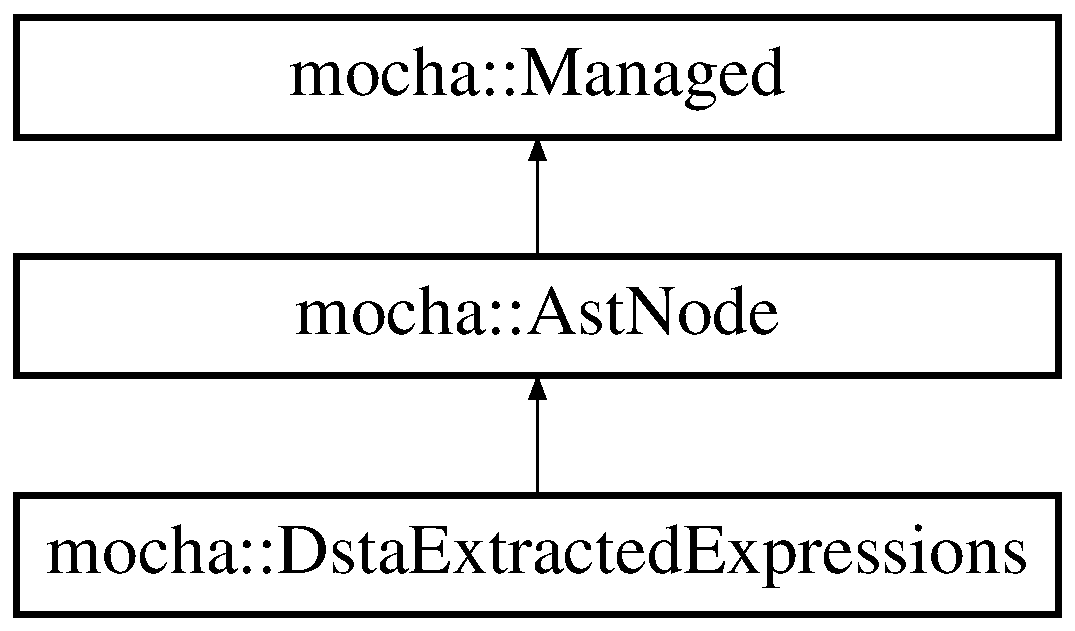
\includegraphics[height=3.000000cm]{classmocha_1_1_dsta_extracted_expressions}
\end{center}
\end{figure}
\subsection*{Public Member Functions}
\begin{DoxyCompactItemize}
\item 
\hyperlink{classmocha_1_1_dsta_extracted_expressions_af71f260e2dfd5864ed89a2e302e55f88}{DstaExtractedExpressions} ()
\item 
\hyperlink{classmocha_1_1_dsta_extracted_expressions_aaf65c329a0d548a436083232ec217734}{$\sim$DstaExtractedExpressions} ()
\item 
\hyperlink{classmocha_1_1_node_list}{NodeList} $\ast$ \hyperlink{classmocha_1_1_dsta_extracted_expressions_afda6e6826138e547c3cb524e33eb16f9}{Refs} ()
\item 
void \hyperlink{classmocha_1_1_dsta_extracted_expressions_a5485d44c44690f8170fa5516e1a6ea9f}{Refs} (\hyperlink{classmocha_1_1_value_node}{ValueNode} $\ast$tmp\_\-name\_\-node)
\item 
\hyperlink{classmocha_1_1_ast_node}{AstNode} $\ast$ \hyperlink{classmocha_1_1_dsta_extracted_expressions_ac736af5060a210d5d7a34bce3365d5cb}{Clone} ()
\end{DoxyCompactItemize}
\subsection*{Private Attributes}
\begin{DoxyCompactItemize}
\item 
\hyperlink{classmocha_1_1_node_list}{NodeList} \hyperlink{classmocha_1_1_dsta_extracted_expressions_affd0c1b4b44c87f27b6428da20e25928}{refs\_\-}
\end{DoxyCompactItemize}


\subsection{Detailed Description}


Definition at line 1586 of file ast.h.



\subsection{Constructor \& Destructor Documentation}
\hypertarget{classmocha_1_1_dsta_extracted_expressions_af71f260e2dfd5864ed89a2e302e55f88}{
\index{mocha::DstaExtractedExpressions@{mocha::DstaExtractedExpressions}!DstaExtractedExpressions@{DstaExtractedExpressions}}
\index{DstaExtractedExpressions@{DstaExtractedExpressions}!mocha::DstaExtractedExpressions@{mocha::DstaExtractedExpressions}}
\subsubsection[{DstaExtractedExpressions}]{\setlength{\rightskip}{0pt plus 5cm}mocha::DstaExtractedExpressions::DstaExtractedExpressions (
\begin{DoxyParamCaption}
{}
\end{DoxyParamCaption}
)\hspace{0.3cm}{\ttfamily  \mbox{[}inline\mbox{]}}}}
\label{classmocha_1_1_dsta_extracted_expressions_af71f260e2dfd5864ed89a2e302e55f88}


Definition at line 1588 of file ast.h.

\hypertarget{classmocha_1_1_dsta_extracted_expressions_aaf65c329a0d548a436083232ec217734}{
\index{mocha::DstaExtractedExpressions@{mocha::DstaExtractedExpressions}!$\sim$DstaExtractedExpressions@{$\sim$DstaExtractedExpressions}}
\index{$\sim$DstaExtractedExpressions@{$\sim$DstaExtractedExpressions}!mocha::DstaExtractedExpressions@{mocha::DstaExtractedExpressions}}
\subsubsection[{$\sim$DstaExtractedExpressions}]{\setlength{\rightskip}{0pt plus 5cm}mocha::DstaExtractedExpressions::$\sim$DstaExtractedExpressions (
\begin{DoxyParamCaption}
{}
\end{DoxyParamCaption}
)\hspace{0.3cm}{\ttfamily  \mbox{[}inline\mbox{]}}}}
\label{classmocha_1_1_dsta_extracted_expressions_aaf65c329a0d548a436083232ec217734}


Definition at line 1589 of file ast.h.



\subsection{Member Function Documentation}
\hypertarget{classmocha_1_1_dsta_extracted_expressions_ac736af5060a210d5d7a34bce3365d5cb}{
\index{mocha::DstaExtractedExpressions@{mocha::DstaExtractedExpressions}!Clone@{Clone}}
\index{Clone@{Clone}!mocha::DstaExtractedExpressions@{mocha::DstaExtractedExpressions}}
\subsubsection[{Clone}]{\setlength{\rightskip}{0pt plus 5cm}{\bf AstNode} $\ast$ mocha::DstaExtractedExpressions::Clone (
\begin{DoxyParamCaption}
{}
\end{DoxyParamCaption}
)\hspace{0.3cm}{\ttfamily  \mbox{[}virtual\mbox{]}}}}
\label{classmocha_1_1_dsta_extracted_expressions_ac736af5060a210d5d7a34bce3365d5cb}
\begin{DoxyReturn}{Returns}
\{AstNode$\ast$\} Clone node. 
\end{DoxyReturn}


Reimplemented from \hyperlink{classmocha_1_1_ast_node_af2a895699bac2012f8b7739bff49c5ec}{mocha::AstNode}.



Definition at line 661 of file ast.cc.

\hypertarget{classmocha_1_1_dsta_extracted_expressions_afda6e6826138e547c3cb524e33eb16f9}{
\index{mocha::DstaExtractedExpressions@{mocha::DstaExtractedExpressions}!Refs@{Refs}}
\index{Refs@{Refs}!mocha::DstaExtractedExpressions@{mocha::DstaExtractedExpressions}}
\subsubsection[{Refs}]{\setlength{\rightskip}{0pt plus 5cm}{\bf NodeList}$\ast$ mocha::DstaExtractedExpressions::Refs (
\begin{DoxyParamCaption}
{}
\end{DoxyParamCaption}
)\hspace{0.3cm}{\ttfamily  \mbox{[}inline\mbox{]}}}}
\label{classmocha_1_1_dsta_extracted_expressions_afda6e6826138e547c3cb524e33eb16f9}


Definition at line 1590 of file ast.h.

\hypertarget{classmocha_1_1_dsta_extracted_expressions_a5485d44c44690f8170fa5516e1a6ea9f}{
\index{mocha::DstaExtractedExpressions@{mocha::DstaExtractedExpressions}!Refs@{Refs}}
\index{Refs@{Refs}!mocha::DstaExtractedExpressions@{mocha::DstaExtractedExpressions}}
\subsubsection[{Refs}]{\setlength{\rightskip}{0pt plus 5cm}void mocha::DstaExtractedExpressions::Refs (
\begin{DoxyParamCaption}
\item[{{\bf ValueNode} $\ast$}]{tmp\_\-name\_\-node}
\end{DoxyParamCaption}
)\hspace{0.3cm}{\ttfamily  \mbox{[}inline\mbox{]}}}}
\label{classmocha_1_1_dsta_extracted_expressions_a5485d44c44690f8170fa5516e1a6ea9f}


Definition at line 1591 of file ast.h.



\subsection{Member Data Documentation}
\hypertarget{classmocha_1_1_dsta_extracted_expressions_affd0c1b4b44c87f27b6428da20e25928}{
\index{mocha::DstaExtractedExpressions@{mocha::DstaExtractedExpressions}!refs\_\-@{refs\_\-}}
\index{refs\_\-@{refs\_\-}!mocha::DstaExtractedExpressions@{mocha::DstaExtractedExpressions}}
\subsubsection[{refs\_\-}]{\setlength{\rightskip}{0pt plus 5cm}{\bf NodeList} {\bf mocha::DstaExtractedExpressions::refs\_\-}\hspace{0.3cm}{\ttfamily  \mbox{[}private\mbox{]}}}}
\label{classmocha_1_1_dsta_extracted_expressions_affd0c1b4b44c87f27b6428da20e25928}


Definition at line 1592 of file ast.h.



The documentation for this class was generated from the following files:\begin{DoxyCompactItemize}
\item 
Y:/mocha/src/ast/\hyperlink{ast_8h}{ast.h}\item 
Y:/mocha/src/ast/\hyperlink{ast_8cc}{ast.cc}\end{DoxyCompactItemize}

\hypertarget{classmocha_1_1_dsta_processor}{
\section{mocha::DstaProcessor Class Reference}
\label{classmocha_1_1_dsta_processor}\index{mocha::DstaProcessor@{mocha::DstaProcessor}}
}


{\ttfamily \#include $<$dsta\_\-processor.h$>$}

Inheritance diagram for mocha::DstaProcessor:\begin{figure}[H]
\begin{center}
\leavevmode
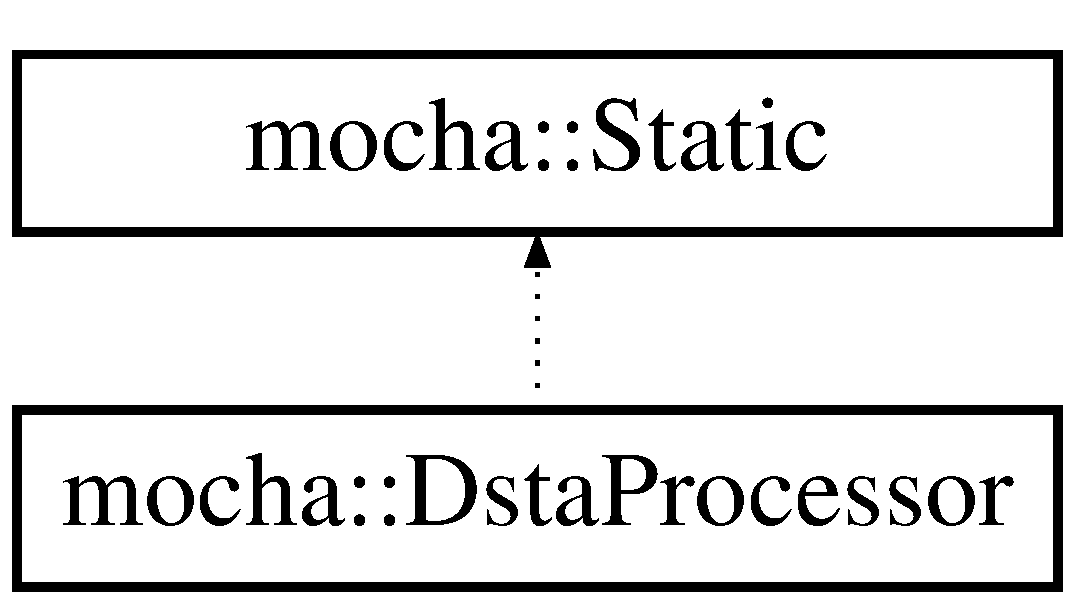
\includegraphics[height=2.000000cm]{classmocha_1_1_dsta_processor}
\end{center}
\end{figure}
\subsection*{Public Types}
\begin{DoxyCompactItemize}
\item 
enum \{ \hyperlink{classmocha_1_1_dsta_processor_a0ecba8d2e7294167a260e88c483dce23af842955727018749f76b8e706b34effa}{kSuccess}, 
\hyperlink{classmocha_1_1_dsta_processor_a0ecba8d2e7294167a260e88c483dce23a5471824fb66c1ace1bee0f9c6ae843ae}{kError}
 \}
\end{DoxyCompactItemize}
\subsection*{Static Public Member Functions}
\begin{DoxyCompactItemize}
\item 
static int \hyperlink{classmocha_1_1_dsta_processor_aa9e05aa90c50ae41867bcd90b72f9127}{ProcessNode} (\hyperlink{classmocha_1_1_value_node}{ValueNode} $\ast$ast\_\-node, \hyperlink{classmocha_1_1_processor_info}{ProcessorInfo} $\ast$info)
\item 
static \hyperlink{classmocha_1_1_node_list}{NodeList} $\ast$ \hyperlink{classmocha_1_1_dsta_processor_a9323e86b8a5d1857db8a1e186ee4fd3f}{CreateDstaExtractedVarStmt} (\hyperlink{classmocha_1_1_statement}{Statement} $\ast$stmt, \hyperlink{classmocha_1_1_processor_info}{ProcessorInfo} $\ast$info)
\begin{DoxyCompactList}\small\item\em Create a variable statement, from the results of analyzing dsta expressions. \end{DoxyCompactList}\item 
static \hyperlink{classmocha_1_1_node_list}{NodeList} $\ast$ \hyperlink{classmocha_1_1_dsta_processor_a912f770394af3067ab097df45d9b4d7c}{CreateDstaExtractedAssignment} (\hyperlink{classmocha_1_1_statement}{Statement} $\ast$stmt, \hyperlink{classmocha_1_1_processor_info}{ProcessorInfo} $\ast$info)
\begin{DoxyCompactList}\small\item\em Create a Assignment expression, from the results of analyzing dsta expressions. \end{DoxyCompactList}\item 
static \hyperlink{classmocha_1_1_variable_stmt}{VariableStmt} $\ast$ \hyperlink{classmocha_1_1_dsta_processor_a78c733b14ee5164d619885b75e0fecd1}{CreateTmpVarDecl} (\hyperlink{classmocha_1_1_statement}{Statement} $\ast$, \hyperlink{classmocha_1_1_processor_info}{ProcessorInfo} $\ast$info)
\begin{DoxyCompactList}\small\item\em Create temporary referrence variable. \end{DoxyCompactList}\end{DoxyCompactItemize}


\subsection{Detailed Description}


Definition at line 38 of file dsta\_\-processor.h.



\subsection{Member Enumeration Documentation}
\hypertarget{classmocha_1_1_dsta_processor_a0ecba8d2e7294167a260e88c483dce23}{
\subsubsection[{"@14}]{\setlength{\rightskip}{0pt plus 5cm}anonymous enum}}
\label{classmocha_1_1_dsta_processor_a0ecba8d2e7294167a260e88c483dce23}
\begin{Desc}
\item[Enumerator: ]\par
\begin{description}
\index{kSuccess@{kSuccess}!mocha::DstaProcessor@{mocha::DstaProcessor}}\index{mocha::DstaProcessor@{mocha::DstaProcessor}!kSuccess@{kSuccess}}\item[{\em 
\hypertarget{classmocha_1_1_dsta_processor_a0ecba8d2e7294167a260e88c483dce23af842955727018749f76b8e706b34effa}{
kSuccess}
\label{classmocha_1_1_dsta_processor_a0ecba8d2e7294167a260e88c483dce23af842955727018749f76b8e706b34effa}
}]\index{kError@{kError}!mocha::DstaProcessor@{mocha::DstaProcessor}}\index{mocha::DstaProcessor@{mocha::DstaProcessor}!kError@{kError}}\item[{\em 
\hypertarget{classmocha_1_1_dsta_processor_a0ecba8d2e7294167a260e88c483dce23a5471824fb66c1ace1bee0f9c6ae843ae}{
kError}
\label{classmocha_1_1_dsta_processor_a0ecba8d2e7294167a260e88c483dce23a5471824fb66c1ace1bee0f9c6ae843ae}
}]\end{description}
\end{Desc}



Definition at line 40 of file dsta\_\-processor.h.



\subsection{Member Function Documentation}
\hypertarget{classmocha_1_1_dsta_processor_a912f770394af3067ab097df45d9b4d7c}{
\index{mocha::DstaProcessor@{mocha::DstaProcessor}!CreateDstaExtractedAssignment@{CreateDstaExtractedAssignment}}
\index{CreateDstaExtractedAssignment@{CreateDstaExtractedAssignment}!mocha::DstaProcessor@{mocha::DstaProcessor}}
\subsubsection[{CreateDstaExtractedAssignment}]{\setlength{\rightskip}{0pt plus 5cm}{\bf NodeList} $\ast$ mocha::DstaProcessor::CreateDstaExtractedAssignment (
\begin{DoxyParamCaption}
\item[{{\bf Statement} $\ast$}]{stmt, }
\item[{{\bf ProcessorInfo} $\ast$}]{info}
\end{DoxyParamCaption}
)\hspace{0.3cm}{\ttfamily  \mbox{[}static\mbox{]}}}}
\label{classmocha_1_1_dsta_processor_a912f770394af3067ab097df45d9b4d7c}


Create a Assignment expression, from the results of analyzing dsta expressions. 


\begin{DoxyParams}{Parameters}
{\em \{Statement$\ast$\}} & stmt \\
\hline
{\em \{ProcessorInfo$\ast$\}} & info \\
\hline
\end{DoxyParams}
\begin{DoxyReturn}{Returns}
\{NodeList$\ast$\} Create a Assignment \hyperlink{classmocha_1_1_expression}{Expression} from the parse results of destructuring assignment. 
\end{DoxyReturn}


Definition at line 500 of file dsta\_\-processor.cc.

\hypertarget{classmocha_1_1_dsta_processor_a9323e86b8a5d1857db8a1e186ee4fd3f}{
\index{mocha::DstaProcessor@{mocha::DstaProcessor}!CreateDstaExtractedVarStmt@{CreateDstaExtractedVarStmt}}
\index{CreateDstaExtractedVarStmt@{CreateDstaExtractedVarStmt}!mocha::DstaProcessor@{mocha::DstaProcessor}}
\subsubsection[{CreateDstaExtractedVarStmt}]{\setlength{\rightskip}{0pt plus 5cm}{\bf NodeList} $\ast$ mocha::DstaProcessor::CreateDstaExtractedVarStmt (
\begin{DoxyParamCaption}
\item[{{\bf Statement} $\ast$}]{stmt, }
\item[{{\bf ProcessorInfo} $\ast$}]{info}
\end{DoxyParamCaption}
)\hspace{0.3cm}{\ttfamily  \mbox{[}static\mbox{]}}}}
\label{classmocha_1_1_dsta_processor_a9323e86b8a5d1857db8a1e186ee4fd3f}


Create a variable statement, from the results of analyzing dsta expressions. 


\begin{DoxyParams}{Parameters}
{\em \{Statement$\ast$\}} & stmt \\
\hline
{\em \{ProcessorInfo$\ast$\}} & info \\
\hline
\end{DoxyParams}
\begin{DoxyReturn}{Returns}
\{NodeList$\ast$\} Create a variable statement from the parse results of destructuring assignment. NO THROW 
\end{DoxyReturn}


Definition at line 490 of file dsta\_\-processor.cc.

\hypertarget{classmocha_1_1_dsta_processor_a78c733b14ee5164d619885b75e0fecd1}{
\index{mocha::DstaProcessor@{mocha::DstaProcessor}!CreateTmpVarDecl@{CreateTmpVarDecl}}
\index{CreateTmpVarDecl@{CreateTmpVarDecl}!mocha::DstaProcessor@{mocha::DstaProcessor}}
\subsubsection[{CreateTmpVarDecl}]{\setlength{\rightskip}{0pt plus 5cm}{\bf VariableStmt} $\ast$ mocha::DstaProcessor::CreateTmpVarDecl (
\begin{DoxyParamCaption}
\item[{{\bf Statement} $\ast$}]{stmt, }
\item[{{\bf ProcessorInfo} $\ast$}]{info}
\end{DoxyParamCaption}
)\hspace{0.3cm}{\ttfamily  \mbox{[}static\mbox{]}}}}
\label{classmocha_1_1_dsta_processor_a78c733b14ee5164d619885b75e0fecd1}


Create temporary referrence variable. 


\begin{DoxyParams}{Parameters}
{\em \{Statement$\ast$\}} & stmt \\
\hline
{\em \{ProcessorInfo$\ast$\}} & info \\
\hline
\end{DoxyParams}
\begin{DoxyReturn}{Returns}
\{VariableStmt$\ast$\} Create tmporary variable declaration list. 
\end{DoxyReturn}


Iterate all Refs node, and create variable\_\-declaration node.



Definition at line 555 of file dsta\_\-processor.cc.

\hypertarget{classmocha_1_1_dsta_processor_aa9e05aa90c50ae41867bcd90b72f9127}{
\index{mocha::DstaProcessor@{mocha::DstaProcessor}!ProcessNode@{ProcessNode}}
\index{ProcessNode@{ProcessNode}!mocha::DstaProcessor@{mocha::DstaProcessor}}
\subsubsection[{ProcessNode}]{\setlength{\rightskip}{0pt plus 5cm}int mocha::DstaProcessor::ProcessNode (
\begin{DoxyParamCaption}
\item[{{\bf ValueNode} $\ast$}]{ast\_\-node, }
\item[{{\bf ProcessorInfo} $\ast$}]{info}
\end{DoxyParamCaption}
)\hspace{0.3cm}{\ttfamily  \mbox{[}static\mbox{]}}}}
\label{classmocha_1_1_dsta_processor_aa9e05aa90c50ae41867bcd90b72f9127}

\begin{DoxyParams}{Parameters}
{\em \{ValueNode$\ast$\}} & ast\_\-node \\
\hline
{\em \{ProcessorInfo$\ast$\}} & info \\
\hline
\end{DoxyParams}
\begin{DoxyReturn}{Returns}
\{int\} Begin process. NO THROW 
\end{DoxyReturn}


Create a variable has the temporary referrence to assignment right hand side. That like this -\/$>$ \_\-mochaLocalTmp$<$current number of tmporary variable$>$ = $<$LHS$>$

Create a tree node that is stored the result of processing.

If we have not dsta yet, add DstaExtractedAssignment to current active statement.

Now add a temporary referrence variable to Refs node.

Convert \{x,y,z\} =$>$ \_\-mochaLocalTmp



Definition at line 506 of file dsta\_\-processor.cc.



The documentation for this class was generated from the following files:\begin{DoxyCompactItemize}
\item 
Y:/mocha/src/ast/visitors/utils/processors/\hyperlink{dsta__processor_8h}{dsta\_\-processor.h}\item 
Y:/mocha/src/ast/visitors/utils/processors/\hyperlink{dsta__processor_8cc}{dsta\_\-processor.cc}\end{DoxyCompactItemize}

\hypertarget{classmocha_1_1_dsta_tree}{
\section{mocha::DstaTree Class Reference}
\label{classmocha_1_1_dsta_tree}\index{mocha::DstaTree@{mocha::DstaTree}}
}


{\ttfamily \#include $<$ast.h$>$}

Inheritance diagram for mocha::DstaTree:\begin{figure}[H]
\begin{center}
\leavevmode
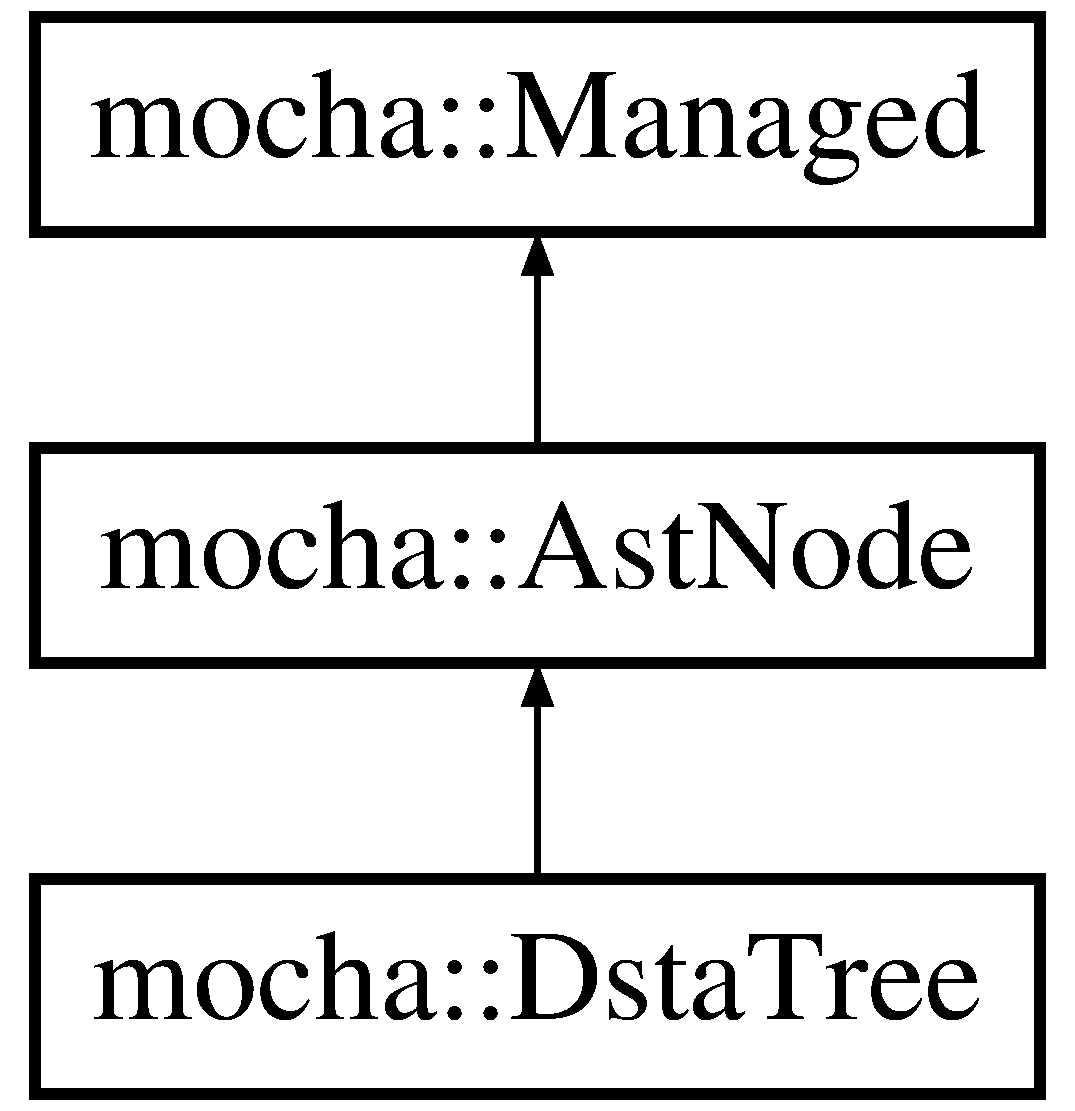
\includegraphics[height=3.000000cm]{classmocha_1_1_dsta_tree}
\end{center}
\end{figure}
\subsection*{Public Member Functions}
\begin{DoxyCompactItemize}
\item 
\hyperlink{classmocha_1_1_dsta_tree_a7ab3a8c0fb0c90ac7c52983e517da946}{DstaTree} ()
\item 
\hyperlink{classmocha_1_1_dsta_tree_a3b937cde6d030946545aa56288628553}{$\sim$DstaTree} ()
\item 
void \hyperlink{classmocha_1_1_dsta_tree_a6ef49ba20cdae2f5885f859e6ea7c9c1}{Symbol} (\hyperlink{classmocha_1_1_value_node}{ValueNode} $\ast$name\_\-node)
\item 
\hyperlink{classmocha_1_1_value_node}{ValueNode} $\ast$ \hyperlink{classmocha_1_1_dsta_tree_a802c6e500924642bc6d9d3d7eb0f6dfd}{Symbol} ()
\item 
\hyperlink{classmocha_1_1_dsta_tree}{DstaTree} $\ast$ \hyperlink{classmocha_1_1_dsta_tree_ae92825dfc9d2948785372a4ee9cb84e2}{CastToDstaTree} ()
\item 
\hyperlink{classmocha_1_1_ast_node}{AstNode} $\ast$ \hyperlink{classmocha_1_1_dsta_tree_ad3734941331f65240d7759b1e71d7aa7}{Clone} ()
\end{DoxyCompactItemize}
\subsection*{Private Attributes}
\begin{DoxyCompactItemize}
\item 
\hyperlink{classmocha_1_1_value_node}{ValueNode} $\ast$ \hyperlink{classmocha_1_1_dsta_tree_a2f8ea0fffe5c79c367e20f7af8efa175}{symbol\_\-}
\end{DoxyCompactItemize}


\subsection{Detailed Description}


Definition at line 1563 of file ast.h.



\subsection{Constructor \& Destructor Documentation}
\hypertarget{classmocha_1_1_dsta_tree_a7ab3a8c0fb0c90ac7c52983e517da946}{
\index{mocha::DstaTree@{mocha::DstaTree}!DstaTree@{DstaTree}}
\index{DstaTree@{DstaTree}!mocha::DstaTree@{mocha::DstaTree}}
\subsubsection[{DstaTree}]{\setlength{\rightskip}{0pt plus 5cm}mocha::DstaTree::DstaTree (
\begin{DoxyParamCaption}
{}
\end{DoxyParamCaption}
)\hspace{0.3cm}{\ttfamily  \mbox{[}inline\mbox{]}}}}
\label{classmocha_1_1_dsta_tree_a7ab3a8c0fb0c90ac7c52983e517da946}


Definition at line 1565 of file ast.h.

\hypertarget{classmocha_1_1_dsta_tree_a3b937cde6d030946545aa56288628553}{
\index{mocha::DstaTree@{mocha::DstaTree}!$\sim$DstaTree@{$\sim$DstaTree}}
\index{$\sim$DstaTree@{$\sim$DstaTree}!mocha::DstaTree@{mocha::DstaTree}}
\subsubsection[{$\sim$DstaTree}]{\setlength{\rightskip}{0pt plus 5cm}mocha::DstaTree::$\sim$DstaTree (
\begin{DoxyParamCaption}
{}
\end{DoxyParamCaption}
)\hspace{0.3cm}{\ttfamily  \mbox{[}inline\mbox{]}}}}
\label{classmocha_1_1_dsta_tree_a3b937cde6d030946545aa56288628553}


Definition at line 1566 of file ast.h.



\subsection{Member Function Documentation}
\hypertarget{classmocha_1_1_dsta_tree_ae92825dfc9d2948785372a4ee9cb84e2}{
\index{mocha::DstaTree@{mocha::DstaTree}!CastToDstaTree@{CastToDstaTree}}
\index{CastToDstaTree@{CastToDstaTree}!mocha::DstaTree@{mocha::DstaTree}}
\subsubsection[{CastToDstaTree}]{\setlength{\rightskip}{0pt plus 5cm}{\bf DstaTree}$\ast$ mocha::DstaTree::CastToDstaTree (
\begin{DoxyParamCaption}
{}
\end{DoxyParamCaption}
)\hspace{0.3cm}{\ttfamily  \mbox{[}inline, virtual\mbox{]}}}}
\label{classmocha_1_1_dsta_tree_ae92825dfc9d2948785372a4ee9cb84e2}


Reimplemented from \hyperlink{classmocha_1_1_ast_node_a29ea81ee14ae435fc24dcbf25a617580}{mocha::AstNode}.



Definition at line 1569 of file ast.h.

\hypertarget{classmocha_1_1_dsta_tree_ad3734941331f65240d7759b1e71d7aa7}{
\index{mocha::DstaTree@{mocha::DstaTree}!Clone@{Clone}}
\index{Clone@{Clone}!mocha::DstaTree@{mocha::DstaTree}}
\subsubsection[{Clone}]{\setlength{\rightskip}{0pt plus 5cm}{\bf AstNode} $\ast$ mocha::DstaTree::Clone (
\begin{DoxyParamCaption}
{}
\end{DoxyParamCaption}
)\hspace{0.3cm}{\ttfamily  \mbox{[}virtual\mbox{]}}}}
\label{classmocha_1_1_dsta_tree_ad3734941331f65240d7759b1e71d7aa7}
\begin{DoxyReturn}{Returns}
\{AstNode$\ast$\} Clone node. 
\end{DoxyReturn}


Reimplemented from \hyperlink{classmocha_1_1_ast_node_af2a895699bac2012f8b7739bff49c5ec}{mocha::AstNode}.



Definition at line 653 of file ast.cc.

\hypertarget{classmocha_1_1_dsta_tree_a6ef49ba20cdae2f5885f859e6ea7c9c1}{
\index{mocha::DstaTree@{mocha::DstaTree}!Symbol@{Symbol}}
\index{Symbol@{Symbol}!mocha::DstaTree@{mocha::DstaTree}}
\subsubsection[{Symbol}]{\setlength{\rightskip}{0pt plus 5cm}void mocha::DstaTree::Symbol (
\begin{DoxyParamCaption}
\item[{{\bf ValueNode} $\ast$}]{name\_\-node}
\end{DoxyParamCaption}
)\hspace{0.3cm}{\ttfamily  \mbox{[}inline\mbox{]}}}}
\label{classmocha_1_1_dsta_tree_a6ef49ba20cdae2f5885f859e6ea7c9c1}


Definition at line 1567 of file ast.h.

\hypertarget{classmocha_1_1_dsta_tree_a802c6e500924642bc6d9d3d7eb0f6dfd}{
\index{mocha::DstaTree@{mocha::DstaTree}!Symbol@{Symbol}}
\index{Symbol@{Symbol}!mocha::DstaTree@{mocha::DstaTree}}
\subsubsection[{Symbol}]{\setlength{\rightskip}{0pt plus 5cm}{\bf ValueNode}$\ast$ mocha::DstaTree::Symbol (
\begin{DoxyParamCaption}
{}
\end{DoxyParamCaption}
)\hspace{0.3cm}{\ttfamily  \mbox{[}inline\mbox{]}}}}
\label{classmocha_1_1_dsta_tree_a802c6e500924642bc6d9d3d7eb0f6dfd}


Definition at line 1568 of file ast.h.



\subsection{Member Data Documentation}
\hypertarget{classmocha_1_1_dsta_tree_a2f8ea0fffe5c79c367e20f7af8efa175}{
\index{mocha::DstaTree@{mocha::DstaTree}!symbol\_\-@{symbol\_\-}}
\index{symbol\_\-@{symbol\_\-}!mocha::DstaTree@{mocha::DstaTree}}
\subsubsection[{symbol\_\-}]{\setlength{\rightskip}{0pt plus 5cm}{\bf ValueNode}$\ast$ {\bf mocha::DstaTree::symbol\_\-}\hspace{0.3cm}{\ttfamily  \mbox{[}private\mbox{]}}}}
\label{classmocha_1_1_dsta_tree_a2f8ea0fffe5c79c367e20f7af8efa175}


Definition at line 1570 of file ast.h.



The documentation for this class was generated from the following files:\begin{DoxyCompactItemize}
\item 
Y:/mocha/src/ast/\hyperlink{ast_8h}{ast.h}\item 
Y:/mocha/src/ast/\hyperlink{ast_8cc}{ast.cc}\end{DoxyCompactItemize}

\hypertarget{classmocha_1_1_empty}{
\section{mocha::Empty Class Reference}
\label{classmocha_1_1_empty}\index{mocha::Empty@{mocha::Empty}}
}


{\ttfamily \#include $<$ast.h$>$}

Inheritance diagram for mocha::Empty:\begin{figure}[H]
\begin{center}
\leavevmode
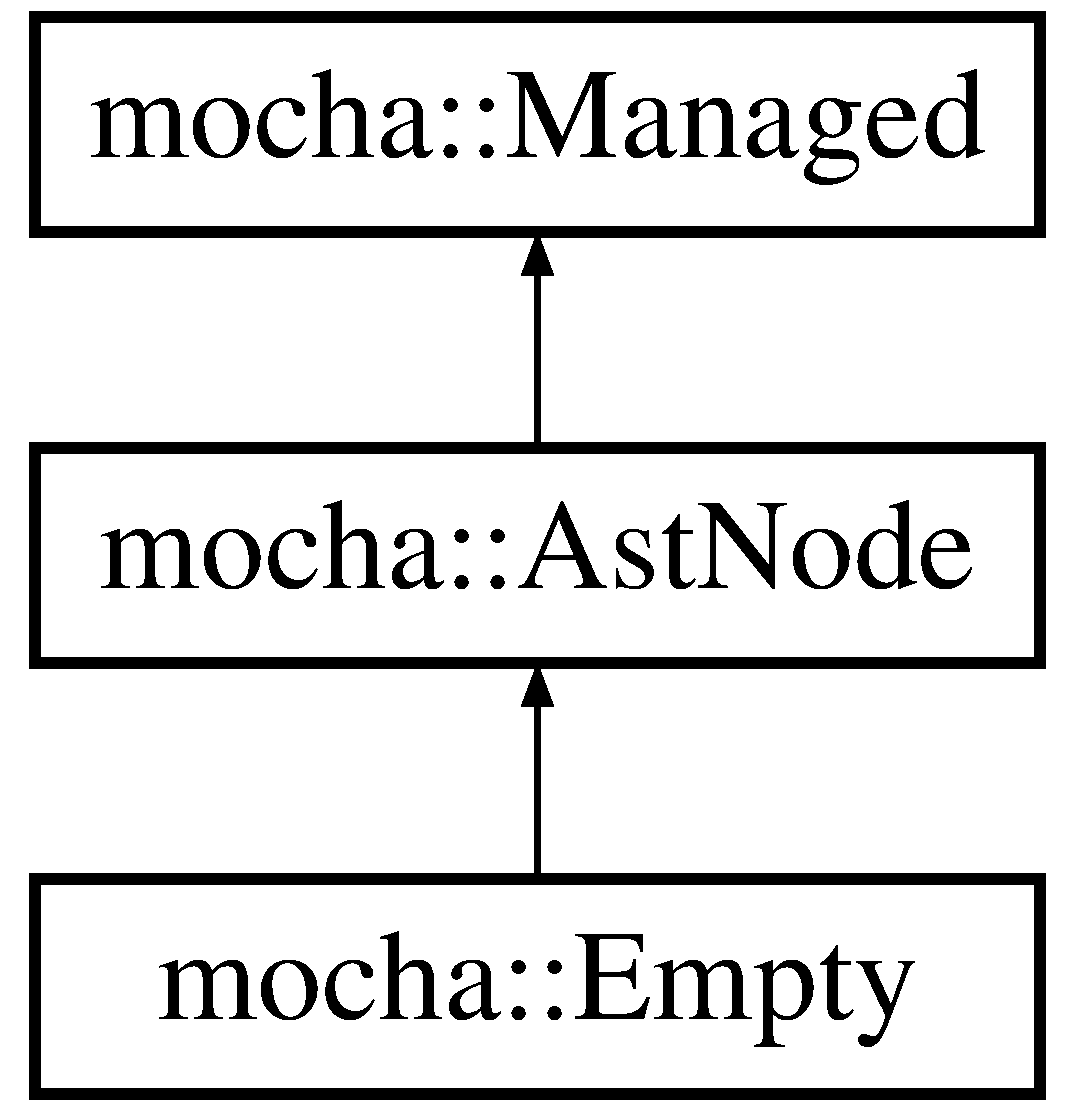
\includegraphics[height=3.000000cm]{classmocha_1_1_empty}
\end{center}
\end{figure}
\subsection*{Public Member Functions}
\begin{DoxyCompactItemize}
\item 
\hyperlink{classmocha_1_1_empty_a5b8cb38d30eefb60277294c7c23b1e69}{Empty} ()
\item 
bool \hyperlink{classmocha_1_1_empty_a031140805b59cb49bc9199ce4b12e781}{IsEmpty} () const 
\item 
\hyperlink{classmocha_1_1_ast_node}{AstNode} $\ast$ \hyperlink{classmocha_1_1_empty_a171593bf241639422c7192d7415f3d87}{Clone} ()
\end{DoxyCompactItemize}
\subsection*{Private Member Functions}
\begin{DoxyCompactItemize}
\item 
void \hyperlink{classmocha_1_1_empty_a921eed774ea84fedc252ebb61b687cfe}{NVIAccept\_\-} (\hyperlink{classmocha_1_1_i_visitor}{IVisitor} $\ast$visitor)
\end{DoxyCompactItemize}


\subsection{Detailed Description}


Definition at line 447 of file ast.h.



\subsection{Constructor \& Destructor Documentation}
\hypertarget{classmocha_1_1_empty_a5b8cb38d30eefb60277294c7c23b1e69}{
\index{mocha::Empty@{mocha::Empty}!Empty@{Empty}}
\index{Empty@{Empty}!mocha::Empty@{mocha::Empty}}
\subsubsection[{Empty}]{\setlength{\rightskip}{0pt plus 5cm}mocha::Empty::Empty (
\begin{DoxyParamCaption}
{}
\end{DoxyParamCaption}
)\hspace{0.3cm}{\ttfamily  \mbox{[}inline\mbox{]}}}}
\label{classmocha_1_1_empty_a5b8cb38d30eefb60277294c7c23b1e69}


Definition at line 449 of file ast.h.



\subsection{Member Function Documentation}
\hypertarget{classmocha_1_1_empty_a171593bf241639422c7192d7415f3d87}{
\index{mocha::Empty@{mocha::Empty}!Clone@{Clone}}
\index{Clone@{Clone}!mocha::Empty@{mocha::Empty}}
\subsubsection[{Clone}]{\setlength{\rightskip}{0pt plus 5cm}{\bf AstNode} $\ast$ mocha::Empty::Clone (
\begin{DoxyParamCaption}
{}
\end{DoxyParamCaption}
)\hspace{0.3cm}{\ttfamily  \mbox{[}virtual\mbox{]}}}}
\label{classmocha_1_1_empty_a171593bf241639422c7192d7415f3d87}
\begin{DoxyReturn}{Returns}
\{AstNode$\ast$\} Clone node. 
\end{DoxyReturn}


Reimplemented from \hyperlink{classmocha_1_1_ast_node_af2a895699bac2012f8b7739bff49c5ec}{mocha::AstNode}.



Definition at line 219 of file ast.cc.

\hypertarget{classmocha_1_1_empty_a031140805b59cb49bc9199ce4b12e781}{
\index{mocha::Empty@{mocha::Empty}!IsEmpty@{IsEmpty}}
\index{IsEmpty@{IsEmpty}!mocha::Empty@{mocha::Empty}}
\subsubsection[{IsEmpty}]{\setlength{\rightskip}{0pt plus 5cm}bool mocha::Empty::IsEmpty (
\begin{DoxyParamCaption}
{}
\end{DoxyParamCaption}
) const\hspace{0.3cm}{\ttfamily  \mbox{[}inline, virtual\mbox{]}}}}
\label{classmocha_1_1_empty_a031140805b59cb49bc9199ce4b12e781}

\begin{DoxyParams}{Parameters}
{\em \{bool\}} & Only this node that IsEmpty method return true. \\
\hline
\end{DoxyParams}


Reimplemented from \hyperlink{classmocha_1_1_ast_node_a31dd8fcdbeb4b1a6aae660a64a1aac99}{mocha::AstNode}.



Definition at line 454 of file ast.h.

\hypertarget{classmocha_1_1_empty_a921eed774ea84fedc252ebb61b687cfe}{
\index{mocha::Empty@{mocha::Empty}!NVIAccept\_\-@{NVIAccept\_\-}}
\index{NVIAccept\_\-@{NVIAccept\_\-}!mocha::Empty@{mocha::Empty}}
\subsubsection[{NVIAccept\_\-}]{\setlength{\rightskip}{0pt plus 5cm}void mocha::Empty::NVIAccept\_\- (
\begin{DoxyParamCaption}
\item[{{\bf IVisitor} $\ast$}]{visitor}
\end{DoxyParamCaption}
)\hspace{0.3cm}{\ttfamily  \mbox{[}inline, private, virtual\mbox{]}}}}
\label{classmocha_1_1_empty_a921eed774ea84fedc252ebb61b687cfe}


Reimplemented from \hyperlink{classmocha_1_1_ast_node_a4a9c107bed3671f3fa15312b87f6ae96}{mocha::AstNode}.



Definition at line 457 of file ast.h.



The documentation for this class was generated from the following files:\begin{DoxyCompactItemize}
\item 
Y:/mocha/src/ast/\hyperlink{ast_8h}{ast.h}\item 
Y:/mocha/src/ast/\hyperlink{ast_8cc}{ast.cc}\end{DoxyCompactItemize}

\hypertarget{struct_ti_xml_base_1_1_entity}{
\section{TiXmlBase::Entity Struct Reference}
\label{struct_ti_xml_base_1_1_entity}\index{TiXmlBase::Entity@{TiXmlBase::Entity}}
}
\subsection*{Public Attributes}
\begin{DoxyCompactItemize}
\item 
const char $\ast$ \hyperlink{struct_ti_xml_base_1_1_entity_ab721b5d4f7ed144ffd215947b38258b7}{str}
\item 
unsigned int \hyperlink{struct_ti_xml_base_1_1_entity_a22e8d820894d3360b01fed110badb876}{strLength}
\item 
char \hyperlink{struct_ti_xml_base_1_1_entity_a2a7e1e68b93b4f76255c60c8fa7f738e}{chr}
\end{DoxyCompactItemize}


\subsection{Detailed Description}


Definition at line 400 of file tinyxml.h.



\subsection{Member Data Documentation}
\hypertarget{struct_ti_xml_base_1_1_entity_a2a7e1e68b93b4f76255c60c8fa7f738e}{
\index{TiXmlBase::Entity@{TiXmlBase::Entity}!chr@{chr}}
\index{chr@{chr}!TiXmlBase::Entity@{TiXmlBase::Entity}}
\subsubsection[{chr}]{\setlength{\rightskip}{0pt plus 5cm}char {\bf TiXmlBase::Entity::chr}}}
\label{struct_ti_xml_base_1_1_entity_a2a7e1e68b93b4f76255c60c8fa7f738e}


Definition at line 404 of file tinyxml.h.

\hypertarget{struct_ti_xml_base_1_1_entity_ab721b5d4f7ed144ffd215947b38258b7}{
\index{TiXmlBase::Entity@{TiXmlBase::Entity}!str@{str}}
\index{str@{str}!TiXmlBase::Entity@{TiXmlBase::Entity}}
\subsubsection[{str}]{\setlength{\rightskip}{0pt plus 5cm}const char$\ast$ {\bf TiXmlBase::Entity::str}}}
\label{struct_ti_xml_base_1_1_entity_ab721b5d4f7ed144ffd215947b38258b7}


Definition at line 402 of file tinyxml.h.

\hypertarget{struct_ti_xml_base_1_1_entity_a22e8d820894d3360b01fed110badb876}{
\index{TiXmlBase::Entity@{TiXmlBase::Entity}!strLength@{strLength}}
\index{strLength@{strLength}!TiXmlBase::Entity@{TiXmlBase::Entity}}
\subsubsection[{strLength}]{\setlength{\rightskip}{0pt plus 5cm}unsigned int {\bf TiXmlBase::Entity::strLength}}}
\label{struct_ti_xml_base_1_1_entity_a22e8d820894d3360b01fed110badb876}


Definition at line 403 of file tinyxml.h.



The documentation for this struct was generated from the following file:\begin{DoxyCompactItemize}
\item 
Y:/mocha/src/tinyxml/\hyperlink{tinyxml_8h}{tinyxml.h}\end{DoxyCompactItemize}

\hypertarget{classmocha_1_1_entry}{
\section{mocha::Entry$<$ Key\_\-t, Value\_\-t $>$ Class Template Reference}
\label{classmocha_1_1_entry}\index{mocha::Entry@{mocha::Entry}}
}


{\ttfamily \#include $<$entry.h$>$}

\subsection*{Public Member Functions}
\begin{DoxyCompactItemize}
\item 
\hyperlink{classmocha_1_1_entry_aa2d0d8cd3301986d2479d0412a2a651a}{Entry} (Key\_\-t \&key, Value\_\-t \&value, uint64\_\-t hash)
\item 
\hyperlink{classmocha_1_1_entry_af76058aab89f1bc0c51b6fa9a21a064a}{Entry} ()
\item 
\hyperlink{classmocha_1_1_entry_a5c96b995db67bf6a745b4950429870a1}{Entry} (const \hyperlink{classmocha_1_1_entry}{Entry} \&entry)
\item 
\hyperlink{classmocha_1_1_entry_ab43a07f9b9ce23c03040525c02f035d5}{$\sim$Entry} ()
\item 
uint64\_\-t \& \hyperlink{classmocha_1_1_entry_a55e46e9f08f8303cf1dd90090593d139}{Hash} ()
\item 
Key\_\-t \& \hyperlink{classmocha_1_1_entry_a7898fcb80824c8ca0942f8ce2aa53b01}{Key} ()
\item 
Value\_\-t \& \hyperlink{classmocha_1_1_entry_a4dda353e95f495b1fd476b4088d0d008}{Value} ()
\item 
bool \hyperlink{classmocha_1_1_entry_a209f8a4d82ff69efdf04d2047a08105d}{IsEmpty} () const 
\end{DoxyCompactItemize}
\subsection*{Private Attributes}
\begin{DoxyCompactItemize}
\item 
uint64\_\-t \hyperlink{classmocha_1_1_entry_a5bb6e09fcbb7d2a02ed2a3ab99a9e47b}{hash\_\-}
\item 
Key\_\-t \hyperlink{classmocha_1_1_entry_aa9631dc6ed634001c81ed4a115d997d4}{key\_\-}
\item 
Value\_\-t \hyperlink{classmocha_1_1_entry_a51ccc8110ab957f74bfa0812cbd974b6}{value\_\-}
\end{DoxyCompactItemize}
\subsection*{Friends}
\begin{DoxyCompactItemize}
\item 
class \hyperlink{classmocha_1_1_entry_a18e2777bf26866165b51548794451c8a}{Block$<$ Key\_\-t, Value\_\-t $>$}
\end{DoxyCompactItemize}


\subsection{Detailed Description}
\subsubsection*{template$<$typename Key\_\-t, typename Value\_\-t$>$class mocha::Entry$<$ Key\_\-t, Value\_\-t $>$}



Definition at line 11 of file entry.h.



\subsection{Constructor \& Destructor Documentation}
\hypertarget{classmocha_1_1_entry_aa2d0d8cd3301986d2479d0412a2a651a}{
\index{mocha::Entry@{mocha::Entry}!Entry@{Entry}}
\index{Entry@{Entry}!mocha::Entry@{mocha::Entry}}
\subsubsection[{Entry}]{\setlength{\rightskip}{0pt plus 5cm}template$<$typename Key\_\-t , typename Value\_\-t $>$ {\bf mocha::Entry}$<$ Key\_\-t, Value\_\-t $>$::{\bf Entry} (
\begin{DoxyParamCaption}
\item[{Key\_\-t \&}]{key, }
\item[{Value\_\-t \&}]{value, }
\item[{uint64\_\-t}]{hash}
\end{DoxyParamCaption}
)}}
\label{classmocha_1_1_entry_aa2d0d8cd3301986d2479d0412a2a651a}


Definition at line 7 of file entry-\/impl.h.

\hypertarget{classmocha_1_1_entry_af76058aab89f1bc0c51b6fa9a21a064a}{
\index{mocha::Entry@{mocha::Entry}!Entry@{Entry}}
\index{Entry@{Entry}!mocha::Entry@{mocha::Entry}}
\subsubsection[{Entry}]{\setlength{\rightskip}{0pt plus 5cm}template$<$typename Key\_\-t , typename Value\_\-t $>$ {\bf mocha::Entry}$<$ Key\_\-t, Value\_\-t $>$::{\bf Entry} (
\begin{DoxyParamCaption}
{}
\end{DoxyParamCaption}
)}}
\label{classmocha_1_1_entry_af76058aab89f1bc0c51b6fa9a21a064a}


Definition at line 11 of file entry-\/impl.h.

\hypertarget{classmocha_1_1_entry_a5c96b995db67bf6a745b4950429870a1}{
\index{mocha::Entry@{mocha::Entry}!Entry@{Entry}}
\index{Entry@{Entry}!mocha::Entry@{mocha::Entry}}
\subsubsection[{Entry}]{\setlength{\rightskip}{0pt plus 5cm}template$<$typename Key\_\-t , typename Value\_\-t $>$ {\bf mocha::Entry}$<$ Key\_\-t, Value\_\-t $>$::{\bf Entry} (
\begin{DoxyParamCaption}
\item[{const {\bf Entry}$<$ Key\_\-t, Value\_\-t $>$ \&}]{entry}
\end{DoxyParamCaption}
)}}
\label{classmocha_1_1_entry_a5c96b995db67bf6a745b4950429870a1}


Definition at line 14 of file entry-\/impl.h.

\hypertarget{classmocha_1_1_entry_ab43a07f9b9ce23c03040525c02f035d5}{
\index{mocha::Entry@{mocha::Entry}!$\sim$Entry@{$\sim$Entry}}
\index{$\sim$Entry@{$\sim$Entry}!mocha::Entry@{mocha::Entry}}
\subsubsection[{$\sim$Entry}]{\setlength{\rightskip}{0pt plus 5cm}template$<$typename Key\_\-t , typename Value\_\-t $>$ {\bf mocha::Entry}$<$ Key\_\-t, Value\_\-t $>$::$\sim${\bf Entry} (
\begin{DoxyParamCaption}
{}
\end{DoxyParamCaption}
)}}
\label{classmocha_1_1_entry_ab43a07f9b9ce23c03040525c02f035d5}


Definition at line 17 of file entry-\/impl.h.



\subsection{Member Function Documentation}
\hypertarget{classmocha_1_1_entry_a55e46e9f08f8303cf1dd90090593d139}{
\index{mocha::Entry@{mocha::Entry}!Hash@{Hash}}
\index{Hash@{Hash}!mocha::Entry@{mocha::Entry}}
\subsubsection[{Hash}]{\setlength{\rightskip}{0pt plus 5cm}template$<$typename Key\_\-t , typename Value\_\-t $>$ uint64\_\-t \& {\bf mocha::Entry}$<$ Key\_\-t, Value\_\-t $>$::Hash (
\begin{DoxyParamCaption}
{}
\end{DoxyParamCaption}
)\hspace{0.3cm}{\ttfamily  \mbox{[}inline\mbox{]}}}}
\label{classmocha_1_1_entry_a55e46e9f08f8303cf1dd90090593d139}


Definition at line 26 of file entry-\/impl.h.

\hypertarget{classmocha_1_1_entry_a209f8a4d82ff69efdf04d2047a08105d}{
\index{mocha::Entry@{mocha::Entry}!IsEmpty@{IsEmpty}}
\index{IsEmpty@{IsEmpty}!mocha::Entry@{mocha::Entry}}
\subsubsection[{IsEmpty}]{\setlength{\rightskip}{0pt plus 5cm}template$<$typename Key\_\-t , typename Value\_\-t $>$ bool {\bf mocha::Entry}$<$ Key\_\-t, Value\_\-t $>$::IsEmpty (
\begin{DoxyParamCaption}
{}
\end{DoxyParamCaption}
) const\hspace{0.3cm}{\ttfamily  \mbox{[}inline\mbox{]}}}}
\label{classmocha_1_1_entry_a209f8a4d82ff69efdf04d2047a08105d}


Definition at line 29 of file entry-\/impl.h.

\hypertarget{classmocha_1_1_entry_a7898fcb80824c8ca0942f8ce2aa53b01}{
\index{mocha::Entry@{mocha::Entry}!Key@{Key}}
\index{Key@{Key}!mocha::Entry@{mocha::Entry}}
\subsubsection[{Key}]{\setlength{\rightskip}{0pt plus 5cm}template$<$typename Key\_\-t , typename Value\_\-t $>$ Key\_\-t \& {\bf mocha::Entry}$<$ Key\_\-t, Value\_\-t $>$::Key (
\begin{DoxyParamCaption}
{}
\end{DoxyParamCaption}
)\hspace{0.3cm}{\ttfamily  \mbox{[}inline\mbox{]}}}}
\label{classmocha_1_1_entry_a7898fcb80824c8ca0942f8ce2aa53b01}


Definition at line 20 of file entry-\/impl.h.

\hypertarget{classmocha_1_1_entry_a4dda353e95f495b1fd476b4088d0d008}{
\index{mocha::Entry@{mocha::Entry}!Value@{Value}}
\index{Value@{Value}!mocha::Entry@{mocha::Entry}}
\subsubsection[{Value}]{\setlength{\rightskip}{0pt plus 5cm}template$<$typename Key\_\-t , typename Value\_\-t $>$ Value\_\-t \& {\bf mocha::Entry}$<$ Key\_\-t, Value\_\-t $>$::Value (
\begin{DoxyParamCaption}
{}
\end{DoxyParamCaption}
)\hspace{0.3cm}{\ttfamily  \mbox{[}inline\mbox{]}}}}
\label{classmocha_1_1_entry_a4dda353e95f495b1fd476b4088d0d008}


Definition at line 23 of file entry-\/impl.h.



\subsection{Friends And Related Function Documentation}
\hypertarget{classmocha_1_1_entry_a18e2777bf26866165b51548794451c8a}{
\index{mocha::Entry@{mocha::Entry}!Block$<$ Key\_\-t, Value\_\-t $>$@{Block$<$ Key\_\-t, Value\_\-t $>$}}
\index{Block$<$ Key\_\-t, Value\_\-t $>$@{Block$<$ Key\_\-t, Value\_\-t $>$}!mocha::Entry@{mocha::Entry}}
\subsubsection[{Block$<$ Key\_\-t, Value\_\-t $>$}]{\setlength{\rightskip}{0pt plus 5cm}template$<$typename Key\_\-t, typename Value\_\-t$>$ friend class {\bf Block}$<$ Key\_\-t, Value\_\-t $>$\hspace{0.3cm}{\ttfamily  \mbox{[}friend\mbox{]}}}}
\label{classmocha_1_1_entry_a18e2777bf26866165b51548794451c8a}


Definition at line 12 of file entry.h.



\subsection{Member Data Documentation}
\hypertarget{classmocha_1_1_entry_a5bb6e09fcbb7d2a02ed2a3ab99a9e47b}{
\index{mocha::Entry@{mocha::Entry}!hash\_\-@{hash\_\-}}
\index{hash\_\-@{hash\_\-}!mocha::Entry@{mocha::Entry}}
\subsubsection[{hash\_\-}]{\setlength{\rightskip}{0pt plus 5cm}template$<$typename Key\_\-t, typename Value\_\-t$>$ uint64\_\-t {\bf mocha::Entry}$<$ Key\_\-t, Value\_\-t $>$::{\bf hash\_\-}\hspace{0.3cm}{\ttfamily  \mbox{[}private\mbox{]}}}}
\label{classmocha_1_1_entry_a5bb6e09fcbb7d2a02ed2a3ab99a9e47b}


Definition at line 23 of file entry.h.

\hypertarget{classmocha_1_1_entry_aa9631dc6ed634001c81ed4a115d997d4}{
\index{mocha::Entry@{mocha::Entry}!key\_\-@{key\_\-}}
\index{key\_\-@{key\_\-}!mocha::Entry@{mocha::Entry}}
\subsubsection[{key\_\-}]{\setlength{\rightskip}{0pt plus 5cm}template$<$typename Key\_\-t, typename Value\_\-t$>$ Key\_\-t {\bf mocha::Entry}$<$ Key\_\-t, Value\_\-t $>$::{\bf key\_\-}\hspace{0.3cm}{\ttfamily  \mbox{[}private\mbox{]}}}}
\label{classmocha_1_1_entry_aa9631dc6ed634001c81ed4a115d997d4}


Definition at line 24 of file entry.h.

\hypertarget{classmocha_1_1_entry_a51ccc8110ab957f74bfa0812cbd974b6}{
\index{mocha::Entry@{mocha::Entry}!value\_\-@{value\_\-}}
\index{value\_\-@{value\_\-}!mocha::Entry@{mocha::Entry}}
\subsubsection[{value\_\-}]{\setlength{\rightskip}{0pt plus 5cm}template$<$typename Key\_\-t, typename Value\_\-t$>$ Value\_\-t {\bf mocha::Entry}$<$ Key\_\-t, Value\_\-t $>$::{\bf value\_\-}\hspace{0.3cm}{\ttfamily  \mbox{[}private\mbox{]}}}}
\label{classmocha_1_1_entry_a51ccc8110ab957f74bfa0812cbd974b6}


Definition at line 25 of file entry.h.



The documentation for this class was generated from the following files:\begin{DoxyCompactItemize}
\item 
Y:/mocha/src/utils/hash/\hyperlink{entry_8h}{entry.h}\item 
Y:/mocha/src/utils/hash/\hyperlink{entry-impl_8h}{entry-\/impl.h}\end{DoxyCompactItemize}

\hypertarget{classmocha_1_1_entry_allocator}{
\section{mocha::EntryAllocator$<$ T $>$ Class Template Reference}
\label{classmocha_1_1_entry_allocator}\index{mocha::EntryAllocator@{mocha::EntryAllocator}}
}


{\ttfamily \#include $<$hash\_\-allocator.h$>$}

\subsection*{Static Private Member Functions}
\begin{DoxyCompactItemize}
\item 
static T $\ast$ \hyperlink{classmocha_1_1_entry_allocator_a6cb4e07225542dec71303ace7bb34dd7}{Allocate} (size\_\-t size)
\item 
static T $\ast$ \hyperlink{classmocha_1_1_entry_allocator_a4c89e7d46ead0361817237c89b21a5de}{ReAllocate} (size\_\-t size)
\end{DoxyCompactItemize}


\subsection{Detailed Description}
\subsubsection*{template$<$typename T$>$class mocha::EntryAllocator$<$ T $>$}



Definition at line 6 of file hash\_\-allocator.h.



\subsection{Member Function Documentation}
\hypertarget{classmocha_1_1_entry_allocator_a6cb4e07225542dec71303ace7bb34dd7}{
\index{mocha::EntryAllocator@{mocha::EntryAllocator}!Allocate@{Allocate}}
\index{Allocate@{Allocate}!mocha::EntryAllocator@{mocha::EntryAllocator}}
\subsubsection[{Allocate}]{\setlength{\rightskip}{0pt plus 5cm}template$<$typename T $>$ T $\ast$ {\bf mocha::EntryAllocator}$<$ T $>$::Allocate (
\begin{DoxyParamCaption}
\item[{size\_\-t}]{size}
\end{DoxyParamCaption}
)\hspace{0.3cm}{\ttfamily  \mbox{[}static, private\mbox{]}}}}
\label{classmocha_1_1_entry_allocator_a6cb4e07225542dec71303ace7bb34dd7}


Definition at line 7 of file hash\_\-allocator-\/impl.h.

\hypertarget{classmocha_1_1_entry_allocator_a4c89e7d46ead0361817237c89b21a5de}{
\index{mocha::EntryAllocator@{mocha::EntryAllocator}!ReAllocate@{ReAllocate}}
\index{ReAllocate@{ReAllocate}!mocha::EntryAllocator@{mocha::EntryAllocator}}
\subsubsection[{ReAllocate}]{\setlength{\rightskip}{0pt plus 5cm}template$<$typename T $>$ T $\ast$ {\bf mocha::EntryAllocator}$<$ T $>$::ReAllocate (
\begin{DoxyParamCaption}
\item[{size\_\-t}]{size}
\end{DoxyParamCaption}
)\hspace{0.3cm}{\ttfamily  \mbox{[}static, private\mbox{]}}}}
\label{classmocha_1_1_entry_allocator_a4c89e7d46ead0361817237c89b21a5de}


Definition at line 16 of file hash\_\-allocator-\/impl.h.



The documentation for this class was generated from the following files:\begin{DoxyCompactItemize}
\item 
Y:/mocha/src/utils/hash/\hyperlink{hash__allocator_8h}{hash\_\-allocator.h}\item 
Y:/mocha/src/utils/hash/\hyperlink{hash__allocator-impl_8h}{hash\_\-allocator-\/impl.h}\end{DoxyCompactItemize}

\hypertarget{classmocha_1_1_entry_cache}{
\section{mocha::EntryCache$<$ Key, Value $>$ Class Template Reference}
\label{classmocha_1_1_entry_cache}\index{mocha::EntryCache@{mocha::EntryCache}}
}


{\ttfamily \#include $<$hash\_\-bucket.h$>$}

\subsection*{Public Member Functions}
\begin{DoxyCompactItemize}
\item 
\hyperlink{classmocha_1_1_entry_cache_ab21861a2ddd25db3c68201b1b0de135c}{EntryCache} ()
\item 
\hyperlink{classmocha_1_1_entry_cache_a9605bada8f5f97ff2658d59e2a39ccc5}{$\sim$EntryCache} ()
\item 
void \hyperlink{classmocha_1_1_entry_cache_adcf78de7389baa427b0a9fd03c0f6e5d}{Push} (\hyperlink{classmocha_1_1_entry_node}{EntryNode}$<$ Key, Value $>$ $\ast$node)
\item 
\hyperlink{classmocha_1_1_entry_node}{EntryNode}$<$ Key, Value $>$ $\ast$ \hyperlink{classmocha_1_1_entry_cache_a805d3466e50a2ecadd56f2085398bf13}{First} ()
\item 
\hyperlink{classmocha_1_1_entry_node}{EntryNode}$<$ Key, Value $>$ $\ast$ \hyperlink{classmocha_1_1_entry_cache_a31ef38338d1dc53759bf56533c942d3f}{Last} ()
\item 
void \hyperlink{classmocha_1_1_entry_cache_a98990a86924aa2a218adc00b400e4fbc}{Add} (\hyperlink{classmocha_1_1_hash_entry}{HashEntry}$<$ Key, Value $>$ $\ast$)
\end{DoxyCompactItemize}
\subsection*{Private Attributes}
\begin{DoxyCompactItemize}
\item 
\hyperlink{classmocha_1_1_entry_node}{EntryNode}$<$ Key, Value $>$ $\ast$ \hyperlink{classmocha_1_1_entry_cache_a670849af1e3ac7263915ae9d17ebc5a9}{first\_\-}
\item 
\hyperlink{classmocha_1_1_entry_node}{EntryNode}$<$ Key, Value $>$ $\ast$ \hyperlink{classmocha_1_1_entry_cache_a96a090725b7deff93ae5234645edd8e5}{last\_\-}
\end{DoxyCompactItemize}


\subsection{Detailed Description}
\subsubsection*{template$<$typename Key, typename Value$>$class mocha::EntryCache$<$ Key, Value $>$}



Definition at line 48 of file hash\_\-bucket.h.



\subsection{Constructor \& Destructor Documentation}
\hypertarget{classmocha_1_1_entry_cache_ab21861a2ddd25db3c68201b1b0de135c}{
\index{mocha::EntryCache@{mocha::EntryCache}!EntryCache@{EntryCache}}
\index{EntryCache@{EntryCache}!mocha::EntryCache@{mocha::EntryCache}}
\subsubsection[{EntryCache}]{\setlength{\rightskip}{0pt plus 5cm}template$<$typename Key , typename Value $>$ {\bf mocha::EntryCache}$<$ Key, Value $>$::{\bf EntryCache} (
\begin{DoxyParamCaption}
{}
\end{DoxyParamCaption}
)\hspace{0.3cm}{\ttfamily  \mbox{[}inline\mbox{]}}}}
\label{classmocha_1_1_entry_cache_ab21861a2ddd25db3c68201b1b0de135c}


Definition at line 124 of file hash\_\-bucket-\/impl.h.

\hypertarget{classmocha_1_1_entry_cache_a9605bada8f5f97ff2658d59e2a39ccc5}{
\index{mocha::EntryCache@{mocha::EntryCache}!$\sim$EntryCache@{$\sim$EntryCache}}
\index{$\sim$EntryCache@{$\sim$EntryCache}!mocha::EntryCache@{mocha::EntryCache}}
\subsubsection[{$\sim$EntryCache}]{\setlength{\rightskip}{0pt plus 5cm}template$<$typename Key , typename Value $>$ {\bf mocha::EntryCache}$<$ Key, Value $>$::$\sim${\bf EntryCache} (
\begin{DoxyParamCaption}
{}
\end{DoxyParamCaption}
)\hspace{0.3cm}{\ttfamily  \mbox{[}inline\mbox{]}}}}
\label{classmocha_1_1_entry_cache_a9605bada8f5f97ff2658d59e2a39ccc5}


Definition at line 127 of file hash\_\-bucket-\/impl.h.



\subsection{Member Function Documentation}
\hypertarget{classmocha_1_1_entry_cache_a98990a86924aa2a218adc00b400e4fbc}{
\index{mocha::EntryCache@{mocha::EntryCache}!Add@{Add}}
\index{Add@{Add}!mocha::EntryCache@{mocha::EntryCache}}
\subsubsection[{Add}]{\setlength{\rightskip}{0pt plus 5cm}template$<$typename Key , typename Value $>$ void {\bf mocha::EntryCache}$<$ Key, Value $>$::Add (
\begin{DoxyParamCaption}
\item[{{\bf HashEntry}$<$ Key, Value $>$ $\ast$}]{ent}
\end{DoxyParamCaption}
)\hspace{0.3cm}{\ttfamily  \mbox{[}inline\mbox{]}}}}
\label{classmocha_1_1_entry_cache_a98990a86924aa2a218adc00b400e4fbc}


Definition at line 163 of file hash\_\-bucket-\/impl.h.

\hypertarget{classmocha_1_1_entry_cache_a805d3466e50a2ecadd56f2085398bf13}{
\index{mocha::EntryCache@{mocha::EntryCache}!First@{First}}
\index{First@{First}!mocha::EntryCache@{mocha::EntryCache}}
\subsubsection[{First}]{\setlength{\rightskip}{0pt plus 5cm}template$<$typename Key , typename Value $>$ {\bf EntryNode}$<$ Key, Value $>$ $\ast$ {\bf mocha::EntryCache}$<$ Key, Value $>$::First (
\begin{DoxyParamCaption}
{}
\end{DoxyParamCaption}
)\hspace{0.3cm}{\ttfamily  \mbox{[}inline\mbox{]}}}}
\label{classmocha_1_1_entry_cache_a805d3466e50a2ecadd56f2085398bf13}


Definition at line 153 of file hash\_\-bucket-\/impl.h.

\hypertarget{classmocha_1_1_entry_cache_a31ef38338d1dc53759bf56533c942d3f}{
\index{mocha::EntryCache@{mocha::EntryCache}!Last@{Last}}
\index{Last@{Last}!mocha::EntryCache@{mocha::EntryCache}}
\subsubsection[{Last}]{\setlength{\rightskip}{0pt plus 5cm}template$<$typename Key , typename Value $>$ {\bf EntryNode}$<$ Key, Value $>$ $\ast$ {\bf mocha::EntryCache}$<$ Key, Value $>$::Last (
\begin{DoxyParamCaption}
{}
\end{DoxyParamCaption}
)\hspace{0.3cm}{\ttfamily  \mbox{[}inline\mbox{]}}}}
\label{classmocha_1_1_entry_cache_a31ef38338d1dc53759bf56533c942d3f}


Definition at line 158 of file hash\_\-bucket-\/impl.h.

\hypertarget{classmocha_1_1_entry_cache_adcf78de7389baa427b0a9fd03c0f6e5d}{
\index{mocha::EntryCache@{mocha::EntryCache}!Push@{Push}}
\index{Push@{Push}!mocha::EntryCache@{mocha::EntryCache}}
\subsubsection[{Push}]{\setlength{\rightskip}{0pt plus 5cm}template$<$typename Key , typename Value $>$ void {\bf mocha::EntryCache}$<$ Key, Value $>$::Push (
\begin{DoxyParamCaption}
\item[{{\bf EntryNode}$<$ Key, Value $>$ $\ast$}]{node}
\end{DoxyParamCaption}
)\hspace{0.3cm}{\ttfamily  \mbox{[}inline\mbox{]}}}}
\label{classmocha_1_1_entry_cache_adcf78de7389baa427b0a9fd03c0f6e5d}


Definition at line 139 of file hash\_\-bucket-\/impl.h.



\subsection{Member Data Documentation}
\hypertarget{classmocha_1_1_entry_cache_a670849af1e3ac7263915ae9d17ebc5a9}{
\index{mocha::EntryCache@{mocha::EntryCache}!first\_\-@{first\_\-}}
\index{first\_\-@{first\_\-}!mocha::EntryCache@{mocha::EntryCache}}
\subsubsection[{first\_\-}]{\setlength{\rightskip}{0pt plus 5cm}template$<$typename Key , typename Value $>$ {\bf EntryNode}$<$Key,Value$>$$\ast$ {\bf mocha::EntryCache}$<$ Key, Value $>$::{\bf first\_\-}\hspace{0.3cm}{\ttfamily  \mbox{[}private\mbox{]}}}}
\label{classmocha_1_1_entry_cache_a670849af1e3ac7263915ae9d17ebc5a9}


Definition at line 57 of file hash\_\-bucket.h.

\hypertarget{classmocha_1_1_entry_cache_a96a090725b7deff93ae5234645edd8e5}{
\index{mocha::EntryCache@{mocha::EntryCache}!last\_\-@{last\_\-}}
\index{last\_\-@{last\_\-}!mocha::EntryCache@{mocha::EntryCache}}
\subsubsection[{last\_\-}]{\setlength{\rightskip}{0pt plus 5cm}template$<$typename Key , typename Value $>$ {\bf EntryNode}$<$Key,Value$>$$\ast$ {\bf mocha::EntryCache}$<$ Key, Value $>$::{\bf last\_\-}\hspace{0.3cm}{\ttfamily  \mbox{[}private\mbox{]}}}}
\label{classmocha_1_1_entry_cache_a96a090725b7deff93ae5234645edd8e5}


Definition at line 58 of file hash\_\-bucket.h.



The documentation for this class was generated from the following files:\begin{DoxyCompactItemize}
\item 
Y:/mocha/src/utils/hash/backup/\hyperlink{backup_2hash__bucket_8h}{hash\_\-bucket.h}\item 
Y:/mocha/src/utils/hash/backup/\hyperlink{hash__bucket-impl_8h}{hash\_\-bucket-\/impl.h}\end{DoxyCompactItemize}

\hypertarget{classmocha_1_1_entry_container}{
\section{mocha::EntryContainer$<$ Key, Value $>$ Class Template Reference}
\label{classmocha_1_1_entry_container}\index{mocha::EntryContainer@{mocha::EntryContainer}}
}


{\ttfamily \#include $<$hash\_\-bucket.h$>$}

\subsection*{Public Member Functions}
\begin{DoxyCompactItemize}
\item 
\hyperlink{classmocha_1_1_entry_container_a20eddca4ed5545f9f91f2051c15695d3}{EntryContainer} ()
\item 
\hyperlink{classmocha_1_1_entry_container_a5544d5ccafd0808904f515a959a53fba}{$\sim$EntryContainer} ()
\item 
void \hyperlink{classmocha_1_1_entry_container_a51f9734f54f8d37478d402efbe524671}{Set} (\hyperlink{classmocha_1_1_hash_entry}{HashEntry}$<$ Key, Value $>$ $\ast$entry)
\item 
bool \hyperlink{classmocha_1_1_entry_container_aaba04fde80b1c0d81c3ea0c6bd64450d}{IsEmpty} ()
\item 
\hyperlink{classmocha_1_1_hash_entry}{HashEntry}$<$ Key, Value $>$ $\ast$ \hyperlink{classmocha_1_1_entry_container_ad754db537c753c044347457a18e52413}{Get} ()
\end{DoxyCompactItemize}
\subsection*{Private Attributes}
\begin{DoxyCompactItemize}
\item 
bool \hyperlink{classmocha_1_1_entry_container_a4847640c605a8a387125bed78c608849}{is\_\-empty\_\-}
\item 
\hyperlink{classmocha_1_1_hash_entry}{HashEntry}$<$ Key, Value $>$ $\ast$ \hyperlink{classmocha_1_1_entry_container_ab8469685ebd4a1ad63d2086b50735207}{entry\_\-}
\end{DoxyCompactItemize}


\subsection{Detailed Description}
\subsubsection*{template$<$typename Key, typename Value$>$class mocha::EntryContainer$<$ Key, Value $>$}



Definition at line 9 of file hash\_\-bucket.h.



\subsection{Constructor \& Destructor Documentation}
\hypertarget{classmocha_1_1_entry_container_a20eddca4ed5545f9f91f2051c15695d3}{
\index{mocha::EntryContainer@{mocha::EntryContainer}!EntryContainer@{EntryContainer}}
\index{EntryContainer@{EntryContainer}!mocha::EntryContainer@{mocha::EntryContainer}}
\subsubsection[{EntryContainer}]{\setlength{\rightskip}{0pt plus 5cm}template$<$typename Key , typename Value $>$ {\bf mocha::EntryContainer}$<$ Key, Value $>$::{\bf EntryContainer} (
\begin{DoxyParamCaption}
{}
\end{DoxyParamCaption}
)\hspace{0.3cm}{\ttfamily  \mbox{[}inline\mbox{]}}}}
\label{classmocha_1_1_entry_container_a20eddca4ed5545f9f91f2051c15695d3}


Definition at line 50 of file hash\_\-bucket-\/impl.h.

\hypertarget{classmocha_1_1_entry_container_a5544d5ccafd0808904f515a959a53fba}{
\index{mocha::EntryContainer@{mocha::EntryContainer}!$\sim$EntryContainer@{$\sim$EntryContainer}}
\index{$\sim$EntryContainer@{$\sim$EntryContainer}!mocha::EntryContainer@{mocha::EntryContainer}}
\subsubsection[{$\sim$EntryContainer}]{\setlength{\rightskip}{0pt plus 5cm}template$<$typename Key, typename Value$>$ {\bf mocha::EntryContainer}$<$ Key, Value $>$::$\sim${\bf EntryContainer} (
\begin{DoxyParamCaption}
{}
\end{DoxyParamCaption}
)\hspace{0.3cm}{\ttfamily  \mbox{[}inline\mbox{]}}}}
\label{classmocha_1_1_entry_container_a5544d5ccafd0808904f515a959a53fba}


Definition at line 12 of file hash\_\-bucket.h.



\subsection{Member Function Documentation}
\hypertarget{classmocha_1_1_entry_container_ad754db537c753c044347457a18e52413}{
\index{mocha::EntryContainer@{mocha::EntryContainer}!Get@{Get}}
\index{Get@{Get}!mocha::EntryContainer@{mocha::EntryContainer}}
\subsubsection[{Get}]{\setlength{\rightskip}{0pt plus 5cm}template$<$typename Key , typename Value $>$ {\bf HashEntry}$<$ Key, Value $>$ $\ast$ {\bf mocha::EntryContainer}$<$ Key, Value $>$::Get (
\begin{DoxyParamCaption}
{}
\end{DoxyParamCaption}
)\hspace{0.3cm}{\ttfamily  \mbox{[}inline\mbox{]}}}}
\label{classmocha_1_1_entry_container_ad754db537c753c044347457a18e52413}


Definition at line 63 of file hash\_\-bucket-\/impl.h.

\hypertarget{classmocha_1_1_entry_container_aaba04fde80b1c0d81c3ea0c6bd64450d}{
\index{mocha::EntryContainer@{mocha::EntryContainer}!IsEmpty@{IsEmpty}}
\index{IsEmpty@{IsEmpty}!mocha::EntryContainer@{mocha::EntryContainer}}
\subsubsection[{IsEmpty}]{\setlength{\rightskip}{0pt plus 5cm}template$<$typename Key , typename Value $>$ bool {\bf mocha::EntryContainer}$<$ Key, Value $>$::IsEmpty (
\begin{DoxyParamCaption}
{}
\end{DoxyParamCaption}
)\hspace{0.3cm}{\ttfamily  \mbox{[}inline\mbox{]}}}}
\label{classmocha_1_1_entry_container_aaba04fde80b1c0d81c3ea0c6bd64450d}


Definition at line 60 of file hash\_\-bucket-\/impl.h.

\hypertarget{classmocha_1_1_entry_container_a51f9734f54f8d37478d402efbe524671}{
\index{mocha::EntryContainer@{mocha::EntryContainer}!Set@{Set}}
\index{Set@{Set}!mocha::EntryContainer@{mocha::EntryContainer}}
\subsubsection[{Set}]{\setlength{\rightskip}{0pt plus 5cm}template$<$typename Key , typename Value $>$ void {\bf mocha::EntryContainer}$<$ Key, Value $>$::Set (
\begin{DoxyParamCaption}
\item[{{\bf HashEntry}$<$ Key, Value $>$ $\ast$}]{entry}
\end{DoxyParamCaption}
)\hspace{0.3cm}{\ttfamily  \mbox{[}inline\mbox{]}}}}
\label{classmocha_1_1_entry_container_a51f9734f54f8d37478d402efbe524671}


Definition at line 53 of file hash\_\-bucket-\/impl.h.



\subsection{Member Data Documentation}
\hypertarget{classmocha_1_1_entry_container_ab8469685ebd4a1ad63d2086b50735207}{
\index{mocha::EntryContainer@{mocha::EntryContainer}!entry\_\-@{entry\_\-}}
\index{entry\_\-@{entry\_\-}!mocha::EntryContainer@{mocha::EntryContainer}}
\subsubsection[{entry\_\-}]{\setlength{\rightskip}{0pt plus 5cm}template$<$typename Key, typename Value$>$ {\bf HashEntry}$<$Key,Value$>$$\ast$ {\bf mocha::EntryContainer}$<$ Key, Value $>$::{\bf entry\_\-}\hspace{0.3cm}{\ttfamily  \mbox{[}private\mbox{]}}}}
\label{classmocha_1_1_entry_container_ab8469685ebd4a1ad63d2086b50735207}


Definition at line 18 of file hash\_\-bucket.h.

\hypertarget{classmocha_1_1_entry_container_a4847640c605a8a387125bed78c608849}{
\index{mocha::EntryContainer@{mocha::EntryContainer}!is\_\-empty\_\-@{is\_\-empty\_\-}}
\index{is\_\-empty\_\-@{is\_\-empty\_\-}!mocha::EntryContainer@{mocha::EntryContainer}}
\subsubsection[{is\_\-empty\_\-}]{\setlength{\rightskip}{0pt plus 5cm}template$<$typename Key, typename Value$>$ bool {\bf mocha::EntryContainer}$<$ Key, Value $>$::{\bf is\_\-empty\_\-}\hspace{0.3cm}{\ttfamily  \mbox{[}private\mbox{]}}}}
\label{classmocha_1_1_entry_container_a4847640c605a8a387125bed78c608849}


Definition at line 17 of file hash\_\-bucket.h.



The documentation for this class was generated from the following files:\begin{DoxyCompactItemize}
\item 
Y:/mocha/src/utils/hash/backup/\hyperlink{backup_2hash__bucket_8h}{hash\_\-bucket.h}\item 
Y:/mocha/src/utils/hash/backup/\hyperlink{hash__bucket-impl_8h}{hash\_\-bucket-\/impl.h}\end{DoxyCompactItemize}

\hypertarget{classmocha_1_1_entry_iterator_base}{
\section{mocha::EntryIteratorBase$<$ Key\_\-t, Value\_\-t $>$ Class Template Reference}
\label{classmocha_1_1_entry_iterator_base}\index{mocha::EntryIteratorBase@{mocha::EntryIteratorBase}}
}


{\ttfamily \#include $<$hash\_\-table.h$>$}

\subsection*{Public Types}
\begin{DoxyCompactItemize}
\item 
typedef \hyperlink{classmocha_1_1_entry}{Entry}$<$ Key\_\-t, Value\_\-t $>$ \hyperlink{classmocha_1_1_entry_iterator_base_a8bc02c1067df11a391cf565953e23b05}{HashEntry}
\item 
typedef \hyperlink{classmocha_1_1_block}{Block}$<$ Key\_\-t, Value\_\-t $>$ \hyperlink{classmocha_1_1_entry_iterator_base_a0c7fd5003d4f45319346ae64e6e111be}{Node}
\end{DoxyCompactItemize}
\subsection*{Public Member Functions}
\begin{DoxyCompactItemize}
\item 
\hyperlink{classmocha_1_1_entry_iterator_base_a22f7638410ddf78c3cbd778087bb03b5}{EntryIteratorBase} (\hyperlink{classmocha_1_1_block}{Node} $\ast$node)
\item 
\hyperlink{classmocha_1_1_entry_iterator_base_a87b0daed5edb1f08879329571ee424c0}{EntryIteratorBase} (const \hyperlink{classmocha_1_1_entry_iterator_base}{EntryIteratorBase} \&iterator)
\item 
bool \hyperlink{classmocha_1_1_entry_iterator_base_a44e67289c205d7f758f07eaf8f8dc154}{HasNext} ()
\item 
\hyperlink{classmocha_1_1_entry}{HashEntry} \hyperlink{classmocha_1_1_entry_iterator_base_ab9cb9d8f5c9e2b59243de6e2c6028146}{Next} ()
\end{DoxyCompactItemize}
\subsection*{Private Attributes}
\begin{DoxyCompactItemize}
\item 
\hyperlink{classmocha_1_1_block}{Node} $\ast$ \hyperlink{classmocha_1_1_entry_iterator_base_a6cd7e41a0a9e198c6ef5bcf745f0a89a}{node\_\-}
\item 
\hyperlink{classmocha_1_1_block}{Node} $\ast$ \hyperlink{classmocha_1_1_entry_iterator_base_aa7d56c6b85e161cd052317a225e5b550}{current\_\-}
\end{DoxyCompactItemize}


\subsection{Detailed Description}
\subsubsection*{template$<$typename Key\_\-t, typename Value\_\-t$>$class mocha::EntryIteratorBase$<$ Key\_\-t, Value\_\-t $>$}



Definition at line 10 of file hash\_\-table.h.



\subsection{Member Typedef Documentation}
\hypertarget{classmocha_1_1_entry_iterator_base_a8bc02c1067df11a391cf565953e23b05}{
\index{mocha::EntryIteratorBase@{mocha::EntryIteratorBase}!HashEntry@{HashEntry}}
\index{HashEntry@{HashEntry}!mocha::EntryIteratorBase@{mocha::EntryIteratorBase}}
\subsubsection[{HashEntry}]{\setlength{\rightskip}{0pt plus 5cm}template$<$typename Key\_\-t, typename Value\_\-t$>$ typedef {\bf Entry}$<$Key\_\-t,Value\_\-t$>$ {\bf mocha::EntryIteratorBase}$<$ Key\_\-t, Value\_\-t $>$::{\bf HashEntry}}}
\label{classmocha_1_1_entry_iterator_base_a8bc02c1067df11a391cf565953e23b05}


Definition at line 12 of file hash\_\-table.h.

\hypertarget{classmocha_1_1_entry_iterator_base_a0c7fd5003d4f45319346ae64e6e111be}{
\index{mocha::EntryIteratorBase@{mocha::EntryIteratorBase}!Node@{Node}}
\index{Node@{Node}!mocha::EntryIteratorBase@{mocha::EntryIteratorBase}}
\subsubsection[{Node}]{\setlength{\rightskip}{0pt plus 5cm}template$<$typename Key\_\-t, typename Value\_\-t$>$ typedef {\bf Block}$<$Key\_\-t,Value\_\-t$>$ {\bf mocha::EntryIteratorBase}$<$ Key\_\-t, Value\_\-t $>$::{\bf Node}}}
\label{classmocha_1_1_entry_iterator_base_a0c7fd5003d4f45319346ae64e6e111be}


Definition at line 13 of file hash\_\-table.h.



\subsection{Constructor \& Destructor Documentation}
\hypertarget{classmocha_1_1_entry_iterator_base_a22f7638410ddf78c3cbd778087bb03b5}{
\index{mocha::EntryIteratorBase@{mocha::EntryIteratorBase}!EntryIteratorBase@{EntryIteratorBase}}
\index{EntryIteratorBase@{EntryIteratorBase}!mocha::EntryIteratorBase@{mocha::EntryIteratorBase}}
\subsubsection[{EntryIteratorBase}]{\setlength{\rightskip}{0pt plus 5cm}template$<$typename Key\_\-t, typename Value\_\-t$>$ {\bf mocha::EntryIteratorBase}$<$ Key\_\-t, Value\_\-t $>$::{\bf EntryIteratorBase} (
\begin{DoxyParamCaption}
\item[{{\bf Node} $\ast$}]{node}
\end{DoxyParamCaption}
)\hspace{0.3cm}{\ttfamily  \mbox{[}inline\mbox{]}}}}
\label{classmocha_1_1_entry_iterator_base_a22f7638410ddf78c3cbd778087bb03b5}
\hypertarget{classmocha_1_1_entry_iterator_base_a87b0daed5edb1f08879329571ee424c0}{
\index{mocha::EntryIteratorBase@{mocha::EntryIteratorBase}!EntryIteratorBase@{EntryIteratorBase}}
\index{EntryIteratorBase@{EntryIteratorBase}!mocha::EntryIteratorBase@{mocha::EntryIteratorBase}}
\subsubsection[{EntryIteratorBase}]{\setlength{\rightskip}{0pt plus 5cm}template$<$typename Key\_\-t , typename Value\_\-t $>$ {\bf mocha::EntryIteratorBase}$<$ Key\_\-t, Value\_\-t $>$::{\bf EntryIteratorBase} (
\begin{DoxyParamCaption}
\item[{const {\bf EntryIteratorBase}$<$ Key\_\-t, Value\_\-t $>$ \&}]{iterator}
\end{DoxyParamCaption}
)\hspace{0.3cm}{\ttfamily  \mbox{[}inline\mbox{]}}}}
\label{classmocha_1_1_entry_iterator_base_a87b0daed5edb1f08879329571ee424c0}


Definition at line 26 of file hash\_\-table-\/impl.h.



\subsection{Member Function Documentation}
\hypertarget{classmocha_1_1_entry_iterator_base_a44e67289c205d7f758f07eaf8f8dc154}{
\index{mocha::EntryIteratorBase@{mocha::EntryIteratorBase}!HasNext@{HasNext}}
\index{HasNext@{HasNext}!mocha::EntryIteratorBase@{mocha::EntryIteratorBase}}
\subsubsection[{HasNext}]{\setlength{\rightskip}{0pt plus 5cm}template$<$typename Key\_\-t , typename Value\_\-t $>$ bool {\bf mocha::EntryIteratorBase}$<$ Key\_\-t, Value\_\-t $>$::HasNext (
\begin{DoxyParamCaption}
{}
\end{DoxyParamCaption}
)\hspace{0.3cm}{\ttfamily  \mbox{[}inline\mbox{]}}}}
\label{classmocha_1_1_entry_iterator_base_a44e67289c205d7f758f07eaf8f8dc154}


Definition at line 31 of file hash\_\-table-\/impl.h.

\hypertarget{classmocha_1_1_entry_iterator_base_ab9cb9d8f5c9e2b59243de6e2c6028146}{
\index{mocha::EntryIteratorBase@{mocha::EntryIteratorBase}!Next@{Next}}
\index{Next@{Next}!mocha::EntryIteratorBase@{mocha::EntryIteratorBase}}
\subsubsection[{Next}]{\setlength{\rightskip}{0pt plus 5cm}template$<$typename Key\_\-t , typename Value\_\-t $>$ {\bf EntryIteratorBase}$<$ Key\_\-t, Value\_\-t $>$::{\bf HashEntry} {\bf mocha::EntryIteratorBase}$<$ Key\_\-t, Value\_\-t $>$::Next (
\begin{DoxyParamCaption}
{}
\end{DoxyParamCaption}
)\hspace{0.3cm}{\ttfamily  \mbox{[}inline\mbox{]}}}}
\label{classmocha_1_1_entry_iterator_base_ab9cb9d8f5c9e2b59243de6e2c6028146}


Definition at line 37 of file hash\_\-table-\/impl.h.



\subsection{Member Data Documentation}
\hypertarget{classmocha_1_1_entry_iterator_base_aa7d56c6b85e161cd052317a225e5b550}{
\index{mocha::EntryIteratorBase@{mocha::EntryIteratorBase}!current\_\-@{current\_\-}}
\index{current\_\-@{current\_\-}!mocha::EntryIteratorBase@{mocha::EntryIteratorBase}}
\subsubsection[{current\_\-}]{\setlength{\rightskip}{0pt plus 5cm}template$<$typename Key\_\-t, typename Value\_\-t$>$ {\bf Node}$\ast$ {\bf mocha::EntryIteratorBase}$<$ Key\_\-t, Value\_\-t $>$::{\bf current\_\-}\hspace{0.3cm}{\ttfamily  \mbox{[}private\mbox{]}}}}
\label{classmocha_1_1_entry_iterator_base_aa7d56c6b85e161cd052317a225e5b550}


Definition at line 20 of file hash\_\-table.h.

\hypertarget{classmocha_1_1_entry_iterator_base_a6cd7e41a0a9e198c6ef5bcf745f0a89a}{
\index{mocha::EntryIteratorBase@{mocha::EntryIteratorBase}!node\_\-@{node\_\-}}
\index{node\_\-@{node\_\-}!mocha::EntryIteratorBase@{mocha::EntryIteratorBase}}
\subsubsection[{node\_\-}]{\setlength{\rightskip}{0pt plus 5cm}template$<$typename Key\_\-t, typename Value\_\-t$>$ {\bf Node}$\ast$ {\bf mocha::EntryIteratorBase}$<$ Key\_\-t, Value\_\-t $>$::{\bf node\_\-}\hspace{0.3cm}{\ttfamily  \mbox{[}private\mbox{]}}}}
\label{classmocha_1_1_entry_iterator_base_a6cd7e41a0a9e198c6ef5bcf745f0a89a}


Definition at line 19 of file hash\_\-table.h.



The documentation for this class was generated from the following files:\begin{DoxyCompactItemize}
\item 
Y:/mocha/src/utils/hash/\hyperlink{hash__table_8h}{hash\_\-table.h}\item 
Y:/mocha/src/utils/hash/\hyperlink{hash__table-impl_8h}{hash\_\-table-\/impl.h}\end{DoxyCompactItemize}

\hypertarget{classmocha_1_1_entry_node}{
\section{mocha::EntryNode$<$ Key, Value $>$ Class Template Reference}
\label{classmocha_1_1_entry_node}\index{mocha::EntryNode@{mocha::EntryNode}}
}


{\ttfamily \#include $<$hash\_\-bucket.h$>$}

\subsection*{Public Types}
\begin{DoxyCompactItemize}
\item 
enum \{ \hyperlink{classmocha_1_1_entry_node_a903ff829823f6d2ffc816134b685d249a0dc13ddec2296670a5855615141bf99c}{kMax} =  10
 \}
\end{DoxyCompactItemize}
\subsection*{Public Member Functions}
\begin{DoxyCompactItemize}
\item 
\hyperlink{classmocha_1_1_entry_node_af96045dd310ba9914e5c22579f17b595}{EntryNode} ()
\item 
\hyperlink{classmocha_1_1_entry_node_a86ba6135ea1f7591354f6d8d5e119bd7}{$\sim$EntryNode} ()
\item 
void \hyperlink{classmocha_1_1_entry_node_a16982236fbe3d161bc5e14de822b5111}{Next} (\hyperlink{classmocha_1_1_entry_node}{EntryNode}$<$ Key, Value $>$ $\ast$next)
\item 
\hyperlink{classmocha_1_1_entry_node}{EntryNode}$<$ Key, Value $>$ $\ast$ \hyperlink{classmocha_1_1_entry_node_af13343324dc3edc1f9b951b58dadc72b}{Next} ()
\item 
void \hyperlink{classmocha_1_1_entry_node_af349ab0631989671ac5ba02d05053301}{Prev} (\hyperlink{classmocha_1_1_entry_node}{EntryNode}$<$ Key, Value $>$ $\ast$prev)
\item 
\hyperlink{classmocha_1_1_entry_node}{EntryNode}$<$ Key, Value $>$ $\ast$ \hyperlink{classmocha_1_1_entry_node_a984f41a9a835669291a82d5b8da9e3aa}{Prev} ()
\item 
void \hyperlink{classmocha_1_1_entry_node_a45601d3e19c1f88fe4eccdb756154b7c}{Add} (\hyperlink{classmocha_1_1_hash_entry}{HashEntry}$<$ Key, Value $>$ $\ast$)
\item 
bool \hyperlink{classmocha_1_1_entry_node_af3e9f2f8c807f5e0b2c58b9b57d74626}{IsFull} ()
\item 
int \hyperlink{classmocha_1_1_entry_node_a991efeaa896fe680ee334050ec8b18e4}{Size} ()
\item 
\hyperlink{classmocha_1_1_entry_container}{EntryContainer}$<$ Key, Value $>$ $\ast$ \hyperlink{classmocha_1_1_entry_node_a290574518d474c66f4b59a8aae4bbfa0}{Item} (int i)
\end{DoxyCompactItemize}
\subsection*{Private Attributes}
\begin{DoxyCompactItemize}
\item 
int \hyperlink{classmocha_1_1_entry_node_a84d128dc83eceffa42600fbb157035a6}{size\_\-}
\item 
\hyperlink{classmocha_1_1_entry_node}{EntryNode}$<$ Key, Value $>$ $\ast$ \hyperlink{classmocha_1_1_entry_node_a5ac0f7dac781153119c25a6f43b6621a}{next\_\-}
\item 
\hyperlink{classmocha_1_1_entry_node}{EntryNode}$<$ Key, Value $>$ $\ast$ \hyperlink{classmocha_1_1_entry_node_ab0f8182df8e4e1bf8d297aa730bcd51a}{prev\_\-}
\item 
\hyperlink{classmocha_1_1_entry_container}{EntryContainer}$<$ Key, Value $>$ \hyperlink{classmocha_1_1_entry_node_aaff09614e453f1d5407bf8557a525962}{entry\_\-} \mbox{[}10\mbox{]}
\end{DoxyCompactItemize}


\subsection{Detailed Description}
\subsubsection*{template$<$typename Key, typename Value$>$class mocha::EntryNode$<$ Key, Value $>$}



Definition at line 27 of file hash\_\-bucket.h.



\subsection{Member Enumeration Documentation}
\hypertarget{classmocha_1_1_entry_node_a903ff829823f6d2ffc816134b685d249}{
\subsubsection[{"@23}]{\setlength{\rightskip}{0pt plus 5cm}template$<$typename Key, typename Value$>$ anonymous enum}}
\label{classmocha_1_1_entry_node_a903ff829823f6d2ffc816134b685d249}
\begin{Desc}
\item[Enumerator: ]\par
\begin{description}
\index{kMax@{kMax}!mocha::EntryNode@{mocha::EntryNode}}\index{mocha::EntryNode@{mocha::EntryNode}!kMax@{kMax}}\item[{\em 
\hypertarget{classmocha_1_1_entry_node_a903ff829823f6d2ffc816134b685d249a0dc13ddec2296670a5855615141bf99c}{
kMax}
\label{classmocha_1_1_entry_node_a903ff829823f6d2ffc816134b685d249a0dc13ddec2296670a5855615141bf99c}
}]\end{description}
\end{Desc}



Definition at line 29 of file hash\_\-bucket.h.



\subsection{Constructor \& Destructor Documentation}
\hypertarget{classmocha_1_1_entry_node_af96045dd310ba9914e5c22579f17b595}{
\index{mocha::EntryNode@{mocha::EntryNode}!EntryNode@{EntryNode}}
\index{EntryNode@{EntryNode}!mocha::EntryNode@{mocha::EntryNode}}
\subsubsection[{EntryNode}]{\setlength{\rightskip}{0pt plus 5cm}template$<$typename Key , typename Value $>$ {\bf mocha::EntryNode}$<$ Key, Value $>$::{\bf EntryNode} (
\begin{DoxyParamCaption}
{}
\end{DoxyParamCaption}
)\hspace{0.3cm}{\ttfamily  \mbox{[}inline\mbox{]}}}}
\label{classmocha_1_1_entry_node_af96045dd310ba9914e5c22579f17b595}


Definition at line 67 of file hash\_\-bucket-\/impl.h.

\hypertarget{classmocha_1_1_entry_node_a86ba6135ea1f7591354f6d8d5e119bd7}{
\index{mocha::EntryNode@{mocha::EntryNode}!$\sim$EntryNode@{$\sim$EntryNode}}
\index{$\sim$EntryNode@{$\sim$EntryNode}!mocha::EntryNode@{mocha::EntryNode}}
\subsubsection[{$\sim$EntryNode}]{\setlength{\rightskip}{0pt plus 5cm}template$<$typename Key , typename Value $>$ {\bf mocha::EntryNode}$<$ Key, Value $>$::$\sim${\bf EntryNode} (
\begin{DoxyParamCaption}
{}
\end{DoxyParamCaption}
)\hspace{0.3cm}{\ttfamily  \mbox{[}inline\mbox{]}}}}
\label{classmocha_1_1_entry_node_a86ba6135ea1f7591354f6d8d5e119bd7}


Definition at line 70 of file hash\_\-bucket-\/impl.h.



\subsection{Member Function Documentation}
\hypertarget{classmocha_1_1_entry_node_a45601d3e19c1f88fe4eccdb756154b7c}{
\index{mocha::EntryNode@{mocha::EntryNode}!Add@{Add}}
\index{Add@{Add}!mocha::EntryNode@{mocha::EntryNode}}
\subsubsection[{Add}]{\setlength{\rightskip}{0pt plus 5cm}template$<$typename Key , typename Value $>$ void {\bf mocha::EntryNode}$<$ Key, Value $>$::Add (
\begin{DoxyParamCaption}
\item[{{\bf HashEntry}$<$ Key, Value $>$ $\ast$}]{ent}
\end{DoxyParamCaption}
)\hspace{0.3cm}{\ttfamily  \mbox{[}inline\mbox{]}}}}
\label{classmocha_1_1_entry_node_a45601d3e19c1f88fe4eccdb756154b7c}


Definition at line 105 of file hash\_\-bucket-\/impl.h.

\hypertarget{classmocha_1_1_entry_node_af3e9f2f8c807f5e0b2c58b9b57d74626}{
\index{mocha::EntryNode@{mocha::EntryNode}!IsFull@{IsFull}}
\index{IsFull@{IsFull}!mocha::EntryNode@{mocha::EntryNode}}
\subsubsection[{IsFull}]{\setlength{\rightskip}{0pt plus 5cm}template$<$typename Key , typename Value $>$ bool {\bf mocha::EntryNode}$<$ Key, Value $>$::IsFull (
\begin{DoxyParamCaption}
{}
\end{DoxyParamCaption}
)\hspace{0.3cm}{\ttfamily  \mbox{[}inline\mbox{]}}}}
\label{classmocha_1_1_entry_node_af3e9f2f8c807f5e0b2c58b9b57d74626}


Definition at line 112 of file hash\_\-bucket-\/impl.h.

\hypertarget{classmocha_1_1_entry_node_a290574518d474c66f4b59a8aae4bbfa0}{
\index{mocha::EntryNode@{mocha::EntryNode}!Item@{Item}}
\index{Item@{Item}!mocha::EntryNode@{mocha::EntryNode}}
\subsubsection[{Item}]{\setlength{\rightskip}{0pt plus 5cm}template$<$typename Key , typename Value $>$ {\bf EntryContainer}$<$ Key, Value $>$ $\ast$ {\bf mocha::EntryNode}$<$ Key, Value $>$::Item (
\begin{DoxyParamCaption}
\item[{int}]{i}
\end{DoxyParamCaption}
)\hspace{0.3cm}{\ttfamily  \mbox{[}inline\mbox{]}}}}
\label{classmocha_1_1_entry_node_a290574518d474c66f4b59a8aae4bbfa0}


Definition at line 117 of file hash\_\-bucket-\/impl.h.

\hypertarget{classmocha_1_1_entry_node_a16982236fbe3d161bc5e14de822b5111}{
\index{mocha::EntryNode@{mocha::EntryNode}!Next@{Next}}
\index{Next@{Next}!mocha::EntryNode@{mocha::EntryNode}}
\subsubsection[{Next}]{\setlength{\rightskip}{0pt plus 5cm}template$<$typename Key , typename Value $>$ void {\bf mocha::EntryNode}$<$ Key, Value $>$::Next (
\begin{DoxyParamCaption}
\item[{{\bf EntryNode}$<$ Key, Value $>$ $\ast$}]{next}
\end{DoxyParamCaption}
)\hspace{0.3cm}{\ttfamily  \mbox{[}inline\mbox{]}}}}
\label{classmocha_1_1_entry_node_a16982236fbe3d161bc5e14de822b5111}


Definition at line 73 of file hash\_\-bucket-\/impl.h.

\hypertarget{classmocha_1_1_entry_node_af13343324dc3edc1f9b951b58dadc72b}{
\index{mocha::EntryNode@{mocha::EntryNode}!Next@{Next}}
\index{Next@{Next}!mocha::EntryNode@{mocha::EntryNode}}
\subsubsection[{Next}]{\setlength{\rightskip}{0pt plus 5cm}template$<$typename Key , typename Value $>$ {\bf EntryNode}$<$ Key, Value $>$ $\ast$ {\bf mocha::EntryNode}$<$ Key, Value $>$::Next (
\begin{DoxyParamCaption}
{}
\end{DoxyParamCaption}
)\hspace{0.3cm}{\ttfamily  \mbox{[}inline\mbox{]}}}}
\label{classmocha_1_1_entry_node_af13343324dc3edc1f9b951b58dadc72b}


Definition at line 84 of file hash\_\-bucket-\/impl.h.

\hypertarget{classmocha_1_1_entry_node_af349ab0631989671ac5ba02d05053301}{
\index{mocha::EntryNode@{mocha::EntryNode}!Prev@{Prev}}
\index{Prev@{Prev}!mocha::EntryNode@{mocha::EntryNode}}
\subsubsection[{Prev}]{\setlength{\rightskip}{0pt plus 5cm}template$<$typename Key , typename Value $>$ void {\bf mocha::EntryNode}$<$ Key, Value $>$::Prev (
\begin{DoxyParamCaption}
\item[{{\bf EntryNode}$<$ Key, Value $>$ $\ast$}]{prev}
\end{DoxyParamCaption}
)\hspace{0.3cm}{\ttfamily  \mbox{[}inline\mbox{]}}}}
\label{classmocha_1_1_entry_node_af349ab0631989671ac5ba02d05053301}


Definition at line 89 of file hash\_\-bucket-\/impl.h.

\hypertarget{classmocha_1_1_entry_node_a984f41a9a835669291a82d5b8da9e3aa}{
\index{mocha::EntryNode@{mocha::EntryNode}!Prev@{Prev}}
\index{Prev@{Prev}!mocha::EntryNode@{mocha::EntryNode}}
\subsubsection[{Prev}]{\setlength{\rightskip}{0pt plus 5cm}template$<$typename Key , typename Value $>$ {\bf EntryNode}$<$ Key, Value $>$ $\ast$ {\bf mocha::EntryNode}$<$ Key, Value $>$::Prev (
\begin{DoxyParamCaption}
{}
\end{DoxyParamCaption}
)\hspace{0.3cm}{\ttfamily  \mbox{[}inline\mbox{]}}}}
\label{classmocha_1_1_entry_node_a984f41a9a835669291a82d5b8da9e3aa}


Definition at line 100 of file hash\_\-bucket-\/impl.h.

\hypertarget{classmocha_1_1_entry_node_a991efeaa896fe680ee334050ec8b18e4}{
\index{mocha::EntryNode@{mocha::EntryNode}!Size@{Size}}
\index{Size@{Size}!mocha::EntryNode@{mocha::EntryNode}}
\subsubsection[{Size}]{\setlength{\rightskip}{0pt plus 5cm}template$<$typename Key, typename Value$>$ int {\bf mocha::EntryNode}$<$ Key, Value $>$::Size (
\begin{DoxyParamCaption}
{}
\end{DoxyParamCaption}
)\hspace{0.3cm}{\ttfamily  \mbox{[}inline\mbox{]}}}}
\label{classmocha_1_1_entry_node_a991efeaa896fe680ee334050ec8b18e4}


Definition at line 38 of file hash\_\-bucket.h.



\subsection{Member Data Documentation}
\hypertarget{classmocha_1_1_entry_node_aaff09614e453f1d5407bf8557a525962}{
\index{mocha::EntryNode@{mocha::EntryNode}!entry\_\-@{entry\_\-}}
\index{entry\_\-@{entry\_\-}!mocha::EntryNode@{mocha::EntryNode}}
\subsubsection[{entry\_\-}]{\setlength{\rightskip}{0pt plus 5cm}template$<$typename Key, typename Value$>$ {\bf EntryContainer}$<$Key,Value$>$ {\bf mocha::EntryNode}$<$ Key, Value $>$::{\bf entry\_\-}\mbox{[}10\mbox{]}\hspace{0.3cm}{\ttfamily  \mbox{[}private\mbox{]}}}}
\label{classmocha_1_1_entry_node_aaff09614e453f1d5407bf8557a525962}


Definition at line 44 of file hash\_\-bucket.h.

\hypertarget{classmocha_1_1_entry_node_a5ac0f7dac781153119c25a6f43b6621a}{
\index{mocha::EntryNode@{mocha::EntryNode}!next\_\-@{next\_\-}}
\index{next\_\-@{next\_\-}!mocha::EntryNode@{mocha::EntryNode}}
\subsubsection[{next\_\-}]{\setlength{\rightskip}{0pt plus 5cm}template$<$typename Key, typename Value$>$ {\bf EntryNode}$<$Key,Value$>$$\ast$ {\bf mocha::EntryNode}$<$ Key, Value $>$::{\bf next\_\-}\hspace{0.3cm}{\ttfamily  \mbox{[}private\mbox{]}}}}
\label{classmocha_1_1_entry_node_a5ac0f7dac781153119c25a6f43b6621a}


Definition at line 42 of file hash\_\-bucket.h.

\hypertarget{classmocha_1_1_entry_node_ab0f8182df8e4e1bf8d297aa730bcd51a}{
\index{mocha::EntryNode@{mocha::EntryNode}!prev\_\-@{prev\_\-}}
\index{prev\_\-@{prev\_\-}!mocha::EntryNode@{mocha::EntryNode}}
\subsubsection[{prev\_\-}]{\setlength{\rightskip}{0pt plus 5cm}template$<$typename Key, typename Value$>$ {\bf EntryNode}$<$Key,Value$>$$\ast$ {\bf mocha::EntryNode}$<$ Key, Value $>$::{\bf prev\_\-}\hspace{0.3cm}{\ttfamily  \mbox{[}private\mbox{]}}}}
\label{classmocha_1_1_entry_node_ab0f8182df8e4e1bf8d297aa730bcd51a}


Definition at line 43 of file hash\_\-bucket.h.

\hypertarget{classmocha_1_1_entry_node_a84d128dc83eceffa42600fbb157035a6}{
\index{mocha::EntryNode@{mocha::EntryNode}!size\_\-@{size\_\-}}
\index{size\_\-@{size\_\-}!mocha::EntryNode@{mocha::EntryNode}}
\subsubsection[{size\_\-}]{\setlength{\rightskip}{0pt plus 5cm}template$<$typename Key, typename Value$>$ int {\bf mocha::EntryNode}$<$ Key, Value $>$::{\bf size\_\-}\hspace{0.3cm}{\ttfamily  \mbox{[}private\mbox{]}}}}
\label{classmocha_1_1_entry_node_a84d128dc83eceffa42600fbb157035a6}


Definition at line 41 of file hash\_\-bucket.h.



The documentation for this class was generated from the following files:\begin{DoxyCompactItemize}
\item 
Y:/mocha/src/utils/hash/backup/\hyperlink{backup_2hash__bucket_8h}{hash\_\-bucket.h}\item 
Y:/mocha/src/utils/hash/backup/\hyperlink{hash__bucket-impl_8h}{hash\_\-bucket-\/impl.h}\end{DoxyCompactItemize}

\hypertarget{structmocha_1_1_entry_vector}{
\section{mocha::EntryVector$<$ Key, Value $>$ Struct Template Reference}
\label{structmocha_1_1_entry_vector}\index{mocha::EntryVector@{mocha::EntryVector}}
}


{\ttfamily \#include $<$hash\_\-bucket.h$>$}

\subsection*{Public Attributes}
\begin{DoxyCompactItemize}
\item 
\hyperlink{classmocha_1_1_entry_container}{EntryContainer}$<$ Key, Value $>$ \hyperlink{structmocha_1_1_entry_vector_a992d1efe43c0566288209f0b6dda1df6}{entry}
\end{DoxyCompactItemize}


\subsection{Detailed Description}
\subsubsection*{template$<$typename Key, typename Value$>$struct mocha::EntryVector$<$ Key, Value $>$}



Definition at line 22 of file hash\_\-bucket.h.



\subsection{Member Data Documentation}
\hypertarget{structmocha_1_1_entry_vector_a992d1efe43c0566288209f0b6dda1df6}{
\index{mocha::EntryVector@{mocha::EntryVector}!entry@{entry}}
\index{entry@{entry}!mocha::EntryVector@{mocha::EntryVector}}
\subsubsection[{entry}]{\setlength{\rightskip}{0pt plus 5cm}template$<$typename Key, typename Value$>$ {\bf EntryContainer}$<$Key,Value$>$ {\bf mocha::EntryVector}$<$ Key, Value $>$::{\bf entry}}}
\label{structmocha_1_1_entry_vector_a992d1efe43c0566288209f0b6dda1df6}


Definition at line 23 of file hash\_\-bucket.h.



The documentation for this struct was generated from the following file:\begin{DoxyCompactItemize}
\item 
Y:/mocha/src/utils/hash/backup/\hyperlink{backup_2hash__bucket_8h}{hash\_\-bucket.h}\end{DoxyCompactItemize}

\hypertarget{classmocha_1_1_error_reporter}{
\section{mocha::ErrorReporter Class Reference}
\label{classmocha_1_1_error_reporter}\index{mocha::ErrorReporter@{mocha::ErrorReporter}}
}


{\ttfamily \#include $<$error\_\-reporter.h$>$}

Inheritance diagram for mocha::ErrorReporter:\begin{figure}[H]
\begin{center}
\leavevmode
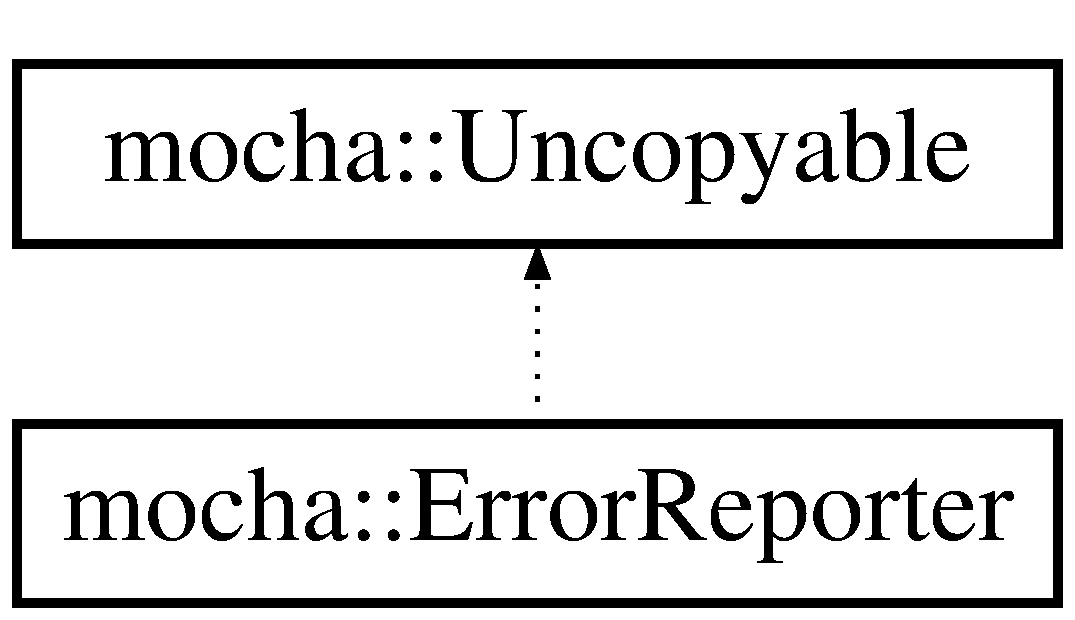
\includegraphics[height=2.000000cm]{classmocha_1_1_error_reporter}
\end{center}
\end{figure}
\subsection*{Public Member Functions}
\begin{DoxyCompactItemize}
\item 
\hyperlink{classmocha_1_1_error_reporter_afc89cfc63c5287edec01ef024d8d4c7c}{ErrorReporter} ()
\item 
\hyperlink{classmocha_1_1_error_reporter_aef46c5aa991fa162449116ca9603086f}{$\sim$ErrorReporter} ()
\item 
void \hyperlink{classmocha_1_1_error_reporter_a9eedd243ac88ad5ee6771eb07d314630}{ReportSyntaxError} (const char $\ast$error)
\item 
bool \hyperlink{classmocha_1_1_error_reporter_a852cc1783a3eef7a949b9261dfde3ac2}{Error} ()
\item 
void \hyperlink{classmocha_1_1_error_reporter_a7928e93ff0f68429463402ea7a75791b}{SetError} (std::string $\ast$buf)
\item 
void \hyperlink{classmocha_1_1_error_reporter_a26476bb615cdac43a9f885c33c62026b}{SetRawError} (std::string $\ast$buf)
\end{DoxyCompactItemize}
\subsection*{Private Types}
\begin{DoxyCompactItemize}
\item 
typedef std::list$<$ std::string $>$ \hyperlink{classmocha_1_1_error_reporter_a71817853888cbed11f8c419c384d6c1d}{ErrorList}
\end{DoxyCompactItemize}
\subsection*{Private Attributes}
\begin{DoxyCompactItemize}
\item 
int \hyperlink{classmocha_1_1_error_reporter_a8aa6147cd385f0230d2494de81647dc0}{error\_\-num\_\-}
\item 
\hyperlink{classmocha_1_1_error_reporter_a71817853888cbed11f8c419c384d6c1d}{ErrorList} \hyperlink{classmocha_1_1_error_reporter_a5df6ec4de385a81e83f958503ac0de1c}{buffer\_\-}
\item 
\hyperlink{classmocha_1_1_error_reporter_a71817853888cbed11f8c419c384d6c1d}{ErrorList} \hyperlink{classmocha_1_1_error_reporter_a2abeeebfe1d102c1fc32aaf2df36277e}{raw\_\-list\_\-}
\end{DoxyCompactItemize}


\subsection{Detailed Description}


Definition at line 8 of file error\_\-reporter.h.



\subsection{Member Typedef Documentation}
\hypertarget{classmocha_1_1_error_reporter_a71817853888cbed11f8c419c384d6c1d}{
\index{mocha::ErrorReporter@{mocha::ErrorReporter}!ErrorList@{ErrorList}}
\index{ErrorList@{ErrorList}!mocha::ErrorReporter@{mocha::ErrorReporter}}
\subsubsection[{ErrorList}]{\setlength{\rightskip}{0pt plus 5cm}typedef std::list$<$std::string$>$ {\bf mocha::ErrorReporter::ErrorList}\hspace{0.3cm}{\ttfamily  \mbox{[}private\mbox{]}}}}
\label{classmocha_1_1_error_reporter_a71817853888cbed11f8c419c384d6c1d}


Definition at line 9 of file error\_\-reporter.h.



\subsection{Constructor \& Destructor Documentation}
\hypertarget{classmocha_1_1_error_reporter_afc89cfc63c5287edec01ef024d8d4c7c}{
\index{mocha::ErrorReporter@{mocha::ErrorReporter}!ErrorReporter@{ErrorReporter}}
\index{ErrorReporter@{ErrorReporter}!mocha::ErrorReporter@{mocha::ErrorReporter}}
\subsubsection[{ErrorReporter}]{\setlength{\rightskip}{0pt plus 5cm}mocha::ErrorReporter::ErrorReporter (
\begin{DoxyParamCaption}
{}
\end{DoxyParamCaption}
)}}
\label{classmocha_1_1_error_reporter_afc89cfc63c5287edec01ef024d8d4c7c}


Definition at line 5 of file error\_\-reporter.cc.

\hypertarget{classmocha_1_1_error_reporter_aef46c5aa991fa162449116ca9603086f}{
\index{mocha::ErrorReporter@{mocha::ErrorReporter}!$\sim$ErrorReporter@{$\sim$ErrorReporter}}
\index{$\sim$ErrorReporter@{$\sim$ErrorReporter}!mocha::ErrorReporter@{mocha::ErrorReporter}}
\subsubsection[{$\sim$ErrorReporter}]{\setlength{\rightskip}{0pt plus 5cm}mocha::ErrorReporter::$\sim$ErrorReporter (
\begin{DoxyParamCaption}
{}
\end{DoxyParamCaption}
)}}
\label{classmocha_1_1_error_reporter_aef46c5aa991fa162449116ca9603086f}


Definition at line 6 of file error\_\-reporter.cc.



\subsection{Member Function Documentation}
\hypertarget{classmocha_1_1_error_reporter_a852cc1783a3eef7a949b9261dfde3ac2}{
\index{mocha::ErrorReporter@{mocha::ErrorReporter}!Error@{Error}}
\index{Error@{Error}!mocha::ErrorReporter@{mocha::ErrorReporter}}
\subsubsection[{Error}]{\setlength{\rightskip}{0pt plus 5cm}bool mocha::ErrorReporter::Error (
\begin{DoxyParamCaption}
{}
\end{DoxyParamCaption}
)\hspace{0.3cm}{\ttfamily  \mbox{[}inline\mbox{]}}}}
\label{classmocha_1_1_error_reporter_a852cc1783a3eef7a949b9261dfde3ac2}


Definition at line 14 of file error\_\-reporter.h.

\hypertarget{classmocha_1_1_error_reporter_a9eedd243ac88ad5ee6771eb07d314630}{
\index{mocha::ErrorReporter@{mocha::ErrorReporter}!ReportSyntaxError@{ReportSyntaxError}}
\index{ReportSyntaxError@{ReportSyntaxError}!mocha::ErrorReporter@{mocha::ErrorReporter}}
\subsubsection[{ReportSyntaxError}]{\setlength{\rightskip}{0pt plus 5cm}void mocha::ErrorReporter::ReportSyntaxError (
\begin{DoxyParamCaption}
\item[{const char $\ast$}]{error}
\end{DoxyParamCaption}
)}}
\label{classmocha_1_1_error_reporter_a9eedd243ac88ad5ee6771eb07d314630}


Definition at line 7 of file error\_\-reporter.cc.

\hypertarget{classmocha_1_1_error_reporter_a7928e93ff0f68429463402ea7a75791b}{
\index{mocha::ErrorReporter@{mocha::ErrorReporter}!SetError@{SetError}}
\index{SetError@{SetError}!mocha::ErrorReporter@{mocha::ErrorReporter}}
\subsubsection[{SetError}]{\setlength{\rightskip}{0pt plus 5cm}void mocha::ErrorReporter::SetError (
\begin{DoxyParamCaption}
\item[{std::string $\ast$}]{buf}
\end{DoxyParamCaption}
)}}
\label{classmocha_1_1_error_reporter_a7928e93ff0f68429463402ea7a75791b}


Definition at line 20 of file error\_\-reporter.cc.

\hypertarget{classmocha_1_1_error_reporter_a26476bb615cdac43a9f885c33c62026b}{
\index{mocha::ErrorReporter@{mocha::ErrorReporter}!SetRawError@{SetRawError}}
\index{SetRawError@{SetRawError}!mocha::ErrorReporter@{mocha::ErrorReporter}}
\subsubsection[{SetRawError}]{\setlength{\rightskip}{0pt plus 5cm}void mocha::ErrorReporter::SetRawError (
\begin{DoxyParamCaption}
\item[{std::string $\ast$}]{buf}
\end{DoxyParamCaption}
)}}
\label{classmocha_1_1_error_reporter_a26476bb615cdac43a9f885c33c62026b}


Definition at line 30 of file error\_\-reporter.cc.



\subsection{Member Data Documentation}
\hypertarget{classmocha_1_1_error_reporter_a5df6ec4de385a81e83f958503ac0de1c}{
\index{mocha::ErrorReporter@{mocha::ErrorReporter}!buffer\_\-@{buffer\_\-}}
\index{buffer\_\-@{buffer\_\-}!mocha::ErrorReporter@{mocha::ErrorReporter}}
\subsubsection[{buffer\_\-}]{\setlength{\rightskip}{0pt plus 5cm}{\bf ErrorList} {\bf mocha::ErrorReporter::buffer\_\-}\hspace{0.3cm}{\ttfamily  \mbox{[}private\mbox{]}}}}
\label{classmocha_1_1_error_reporter_a5df6ec4de385a81e83f958503ac0de1c}


Definition at line 19 of file error\_\-reporter.h.

\hypertarget{classmocha_1_1_error_reporter_a8aa6147cd385f0230d2494de81647dc0}{
\index{mocha::ErrorReporter@{mocha::ErrorReporter}!error\_\-num\_\-@{error\_\-num\_\-}}
\index{error\_\-num\_\-@{error\_\-num\_\-}!mocha::ErrorReporter@{mocha::ErrorReporter}}
\subsubsection[{error\_\-num\_\-}]{\setlength{\rightskip}{0pt plus 5cm}int {\bf mocha::ErrorReporter::error\_\-num\_\-}\hspace{0.3cm}{\ttfamily  \mbox{[}private\mbox{]}}}}
\label{classmocha_1_1_error_reporter_a8aa6147cd385f0230d2494de81647dc0}


Definition at line 18 of file error\_\-reporter.h.

\hypertarget{classmocha_1_1_error_reporter_a2abeeebfe1d102c1fc32aaf2df36277e}{
\index{mocha::ErrorReporter@{mocha::ErrorReporter}!raw\_\-list\_\-@{raw\_\-list\_\-}}
\index{raw\_\-list\_\-@{raw\_\-list\_\-}!mocha::ErrorReporter@{mocha::ErrorReporter}}
\subsubsection[{raw\_\-list\_\-}]{\setlength{\rightskip}{0pt plus 5cm}{\bf ErrorList} {\bf mocha::ErrorReporter::raw\_\-list\_\-}\hspace{0.3cm}{\ttfamily  \mbox{[}private\mbox{]}}}}
\label{classmocha_1_1_error_reporter_a2abeeebfe1d102c1fc32aaf2df36277e}


Definition at line 20 of file error\_\-reporter.h.



The documentation for this class was generated from the following files:\begin{DoxyCompactItemize}
\item 
Y:/mocha/src/compiler/utils/\hyperlink{error__reporter_8h}{error\_\-reporter.h}\item 
Y:/mocha/src/compiler/utils/\hyperlink{error__reporter_8cc}{error\_\-reporter.cc}\end{DoxyCompactItemize}

\hypertarget{classmocha_1_1_error_runner}{
\section{mocha::ErrorRunner Class Reference}
\label{classmocha_1_1_error_runner}\index{mocha::ErrorRunner@{mocha::ErrorRunner}}
}


{\ttfamily \#include $<$error\_\-runner.h$>$}

Inheritance diagram for mocha::ErrorRunner:\begin{figure}[H]
\begin{center}
\leavevmode
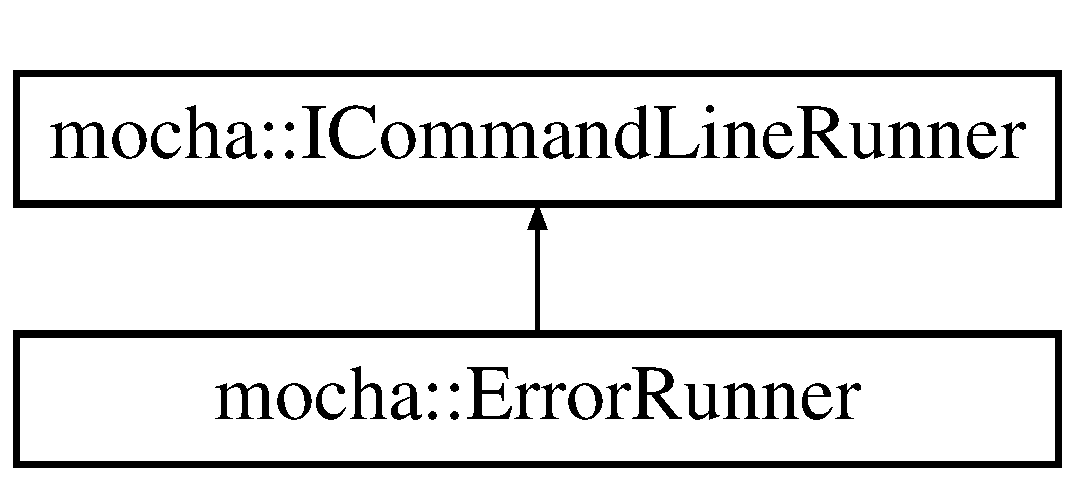
\includegraphics[height=2.000000cm]{classmocha_1_1_error_runner}
\end{center}
\end{figure}
\subsection*{Public Member Functions}
\begin{DoxyCompactItemize}
\item 
\hyperlink{classmocha_1_1_error_runner_a6770debb37abf187a759fa47e8ebd8ff}{ErrorRunner} (\hyperlink{classmocha_1_1_options}{Options} $\ast$option)
\item 
virtual void \hyperlink{classmocha_1_1_error_runner_a9468cd2f3fc1b790be34dd5ae6e21134}{Run} ()
\end{DoxyCompactItemize}


\subsection{Detailed Description}


Definition at line 6 of file error\_\-runner.h.



\subsection{Constructor \& Destructor Documentation}
\hypertarget{classmocha_1_1_error_runner_a6770debb37abf187a759fa47e8ebd8ff}{
\index{mocha::ErrorRunner@{mocha::ErrorRunner}!ErrorRunner@{ErrorRunner}}
\index{ErrorRunner@{ErrorRunner}!mocha::ErrorRunner@{mocha::ErrorRunner}}
\subsubsection[{ErrorRunner}]{\setlength{\rightskip}{0pt plus 5cm}mocha::ErrorRunner::ErrorRunner (
\begin{DoxyParamCaption}
\item[{{\bf Options} $\ast$}]{option}
\end{DoxyParamCaption}
)}}
\label{classmocha_1_1_error_runner_a6770debb37abf187a759fa47e8ebd8ff}


Definition at line 5 of file error\_\-runner.cc.



\subsection{Member Function Documentation}
\hypertarget{classmocha_1_1_error_runner_a9468cd2f3fc1b790be34dd5ae6e21134}{
\index{mocha::ErrorRunner@{mocha::ErrorRunner}!Run@{Run}}
\index{Run@{Run}!mocha::ErrorRunner@{mocha::ErrorRunner}}
\subsubsection[{Run}]{\setlength{\rightskip}{0pt plus 5cm}void mocha::ErrorRunner::Run (
\begin{DoxyParamCaption}
{}
\end{DoxyParamCaption}
)\hspace{0.3cm}{\ttfamily  \mbox{[}virtual\mbox{]}}}}
\label{classmocha_1_1_error_runner_a9468cd2f3fc1b790be34dd5ae6e21134}


Reimplemented from \hyperlink{classmocha_1_1_i_command_line_runner_a916078af76dc405721dfd512d68a123a}{mocha::ICommandLineRunner}.



Definition at line 7 of file error\_\-runner.cc.



The documentation for this class was generated from the following files:\begin{DoxyCompactItemize}
\item 
Y:/mocha/src/bootstrap/runners/\hyperlink{error__runner_8h}{error\_\-runner.h}\item 
Y:/mocha/src/bootstrap/runners/\hyperlink{error__runner_8cc}{error\_\-runner.cc}\end{DoxyCompactItemize}

\hypertarget{classmocha_1_1_exception_handler}{
\section{mocha::ExceptionHandler Class Reference}
\label{classmocha_1_1_exception_handler}\index{mocha::ExceptionHandler@{mocha::ExceptionHandler}}
}


{\ttfamily \#include $<$exception\_\-handler.h$>$}

Inheritance diagram for mocha::ExceptionHandler:\begin{figure}[H]
\begin{center}
\leavevmode
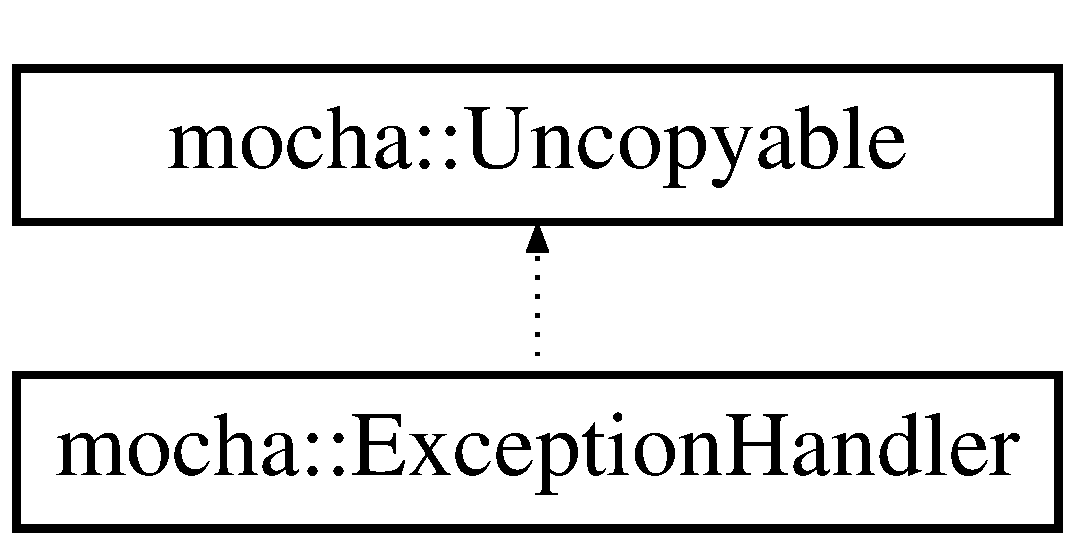
\includegraphics[height=2.000000cm]{classmocha_1_1_exception_handler}
\end{center}
\end{figure}
\subsection*{Public Types}
\begin{DoxyCompactItemize}
\item 
typedef \hyperlink{classmocha_1_1_handle}{Handle}$<$ \hyperlink{classmocha_1_1_exception_handler}{ExceptionHandler} $>$ \hyperlink{classmocha_1_1_exception_handler_a438ecf67fc82c3eb61b570767795151f}{ExceptionHandle}
\end{DoxyCompactItemize}
\subsection*{Public Member Functions}
\begin{DoxyCompactItemize}
\item 
\hyperlink{classmocha_1_1_exception_handler_ab41aec92d3738929a8fa2f3ff6da354c}{$\sim$ExceptionHandler} ()
\item 
const char $\ast$ \hyperlink{classmocha_1_1_exception_handler_aca1a29f16dc8e1af2ab3551a8c0519f7}{Message} ()
\end{DoxyCompactItemize}
\subsection*{Static Public Member Functions}
\begin{DoxyCompactItemize}
\item 
static \hyperlink{classmocha_1_1_handle}{ExceptionHandle} \hyperlink{classmocha_1_1_exception_handler_a4a8479b68e91bcb753a961abf50f46f5}{CreateException} (const char $\ast$message)
\end{DoxyCompactItemize}
\subsection*{Private Member Functions}
\begin{DoxyCompactItemize}
\item 
\hyperlink{classmocha_1_1_exception_handler_a8188d53fba437ba3711f5e161eba4e9f}{ExceptionHandler} (const char $\ast$message)
\end{DoxyCompactItemize}
\subsection*{Private Attributes}
\begin{DoxyCompactItemize}
\item 
std::string \hyperlink{classmocha_1_1_exception_handler_a0a0a95700abd61de8ed3e19a32219d3d}{error\_\-}
\end{DoxyCompactItemize}


\subsection{Detailed Description}


Definition at line 32 of file exception\_\-handler.h.



\subsection{Member Typedef Documentation}
\hypertarget{classmocha_1_1_exception_handler_a438ecf67fc82c3eb61b570767795151f}{
\index{mocha::ExceptionHandler@{mocha::ExceptionHandler}!ExceptionHandle@{ExceptionHandle}}
\index{ExceptionHandle@{ExceptionHandle}!mocha::ExceptionHandler@{mocha::ExceptionHandler}}
\subsubsection[{ExceptionHandle}]{\setlength{\rightskip}{0pt plus 5cm}typedef {\bf Handle}$<${\bf ExceptionHandler}$>$ {\bf mocha::ExceptionHandler::ExceptionHandle}}}
\label{classmocha_1_1_exception_handler_a438ecf67fc82c3eb61b570767795151f}


Definition at line 34 of file exception\_\-handler.h.



\subsection{Constructor \& Destructor Documentation}
\hypertarget{classmocha_1_1_exception_handler_ab41aec92d3738929a8fa2f3ff6da354c}{
\index{mocha::ExceptionHandler@{mocha::ExceptionHandler}!$\sim$ExceptionHandler@{$\sim$ExceptionHandler}}
\index{$\sim$ExceptionHandler@{$\sim$ExceptionHandler}!mocha::ExceptionHandler@{mocha::ExceptionHandler}}
\subsubsection[{$\sim$ExceptionHandler}]{\setlength{\rightskip}{0pt plus 5cm}mocha::ExceptionHandler::$\sim$ExceptionHandler (
\begin{DoxyParamCaption}
{}
\end{DoxyParamCaption}
)}}
\label{classmocha_1_1_exception_handler_ab41aec92d3738929a8fa2f3ff6da354c}


Definition at line 9 of file exception\_\-handler.cc.

\hypertarget{classmocha_1_1_exception_handler_a8188d53fba437ba3711f5e161eba4e9f}{
\index{mocha::ExceptionHandler@{mocha::ExceptionHandler}!ExceptionHandler@{ExceptionHandler}}
\index{ExceptionHandler@{ExceptionHandler}!mocha::ExceptionHandler@{mocha::ExceptionHandler}}
\subsubsection[{ExceptionHandler}]{\setlength{\rightskip}{0pt plus 5cm}mocha::ExceptionHandler::ExceptionHandler (
\begin{DoxyParamCaption}
\item[{const char $\ast$}]{message}
\end{DoxyParamCaption}
)\hspace{0.3cm}{\ttfamily  \mbox{[}private\mbox{]}}}}
\label{classmocha_1_1_exception_handler_a8188d53fba437ba3711f5e161eba4e9f}


Definition at line 8 of file exception\_\-handler.cc.



\subsection{Member Function Documentation}
\hypertarget{classmocha_1_1_exception_handler_a4a8479b68e91bcb753a961abf50f46f5}{
\index{mocha::ExceptionHandler@{mocha::ExceptionHandler}!CreateException@{CreateException}}
\index{CreateException@{CreateException}!mocha::ExceptionHandler@{mocha::ExceptionHandler}}
\subsubsection[{CreateException}]{\setlength{\rightskip}{0pt plus 5cm}{\bf ExceptionHandle} mocha::ExceptionHandler::CreateException (
\begin{DoxyParamCaption}
\item[{const char $\ast$}]{message}
\end{DoxyParamCaption}
)\hspace{0.3cm}{\ttfamily  \mbox{[}static\mbox{]}}}}
\label{classmocha_1_1_exception_handler_a4a8479b68e91bcb753a961abf50f46f5}


Definition at line 5 of file exception\_\-handler.cc.

\hypertarget{classmocha_1_1_exception_handler_aca1a29f16dc8e1af2ab3551a8c0519f7}{
\index{mocha::ExceptionHandler@{mocha::ExceptionHandler}!Message@{Message}}
\index{Message@{Message}!mocha::ExceptionHandler@{mocha::ExceptionHandler}}
\subsubsection[{Message}]{\setlength{\rightskip}{0pt plus 5cm}const char$\ast$ mocha::ExceptionHandler::Message (
\begin{DoxyParamCaption}
{}
\end{DoxyParamCaption}
)\hspace{0.3cm}{\ttfamily  \mbox{[}inline\mbox{]}}}}
\label{classmocha_1_1_exception_handler_aca1a29f16dc8e1af2ab3551a8c0519f7}


Definition at line 37 of file exception\_\-handler.h.



\subsection{Member Data Documentation}
\hypertarget{classmocha_1_1_exception_handler_a0a0a95700abd61de8ed3e19a32219d3d}{
\index{mocha::ExceptionHandler@{mocha::ExceptionHandler}!error\_\-@{error\_\-}}
\index{error\_\-@{error\_\-}!mocha::ExceptionHandler@{mocha::ExceptionHandler}}
\subsubsection[{error\_\-}]{\setlength{\rightskip}{0pt plus 5cm}std::string {\bf mocha::ExceptionHandler::error\_\-}\hspace{0.3cm}{\ttfamily  \mbox{[}private\mbox{]}}}}
\label{classmocha_1_1_exception_handler_a0a0a95700abd61de8ed3e19a32219d3d}


Definition at line 40 of file exception\_\-handler.h.



The documentation for this class was generated from the following files:\begin{DoxyCompactItemize}
\item 
Y:/mocha/src/compiler/utils/\hyperlink{exception__handler_8h}{exception\_\-handler.h}\item 
Y:/mocha/src/compiler/utils/\hyperlink{exception__handler_8cc}{exception\_\-handler.cc}\end{DoxyCompactItemize}

\hypertarget{classmocha_1_1_export_processor}{
\section{mocha::ExportProcessor Class Reference}
\label{classmocha_1_1_export_processor}\index{mocha::ExportProcessor@{mocha::ExportProcessor}}
}


{\ttfamily \#include $<$export\_\-processor.h$>$}

Inheritance diagram for mocha::ExportProcessor:\begin{figure}[H]
\begin{center}
\leavevmode
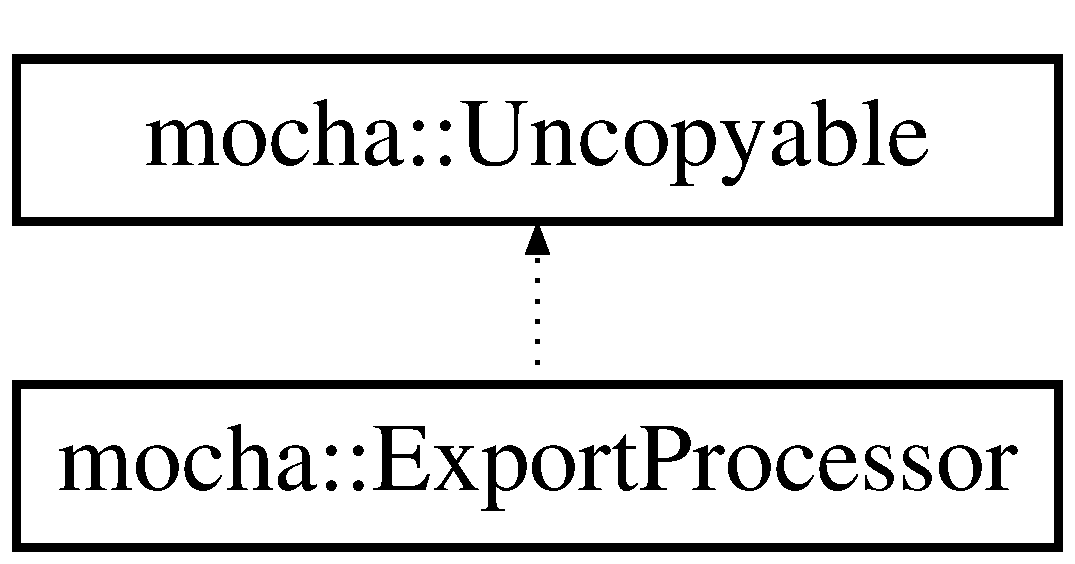
\includegraphics[height=2.000000cm]{classmocha_1_1_export_processor}
\end{center}
\end{figure}
\subsection*{Public Member Functions}
\begin{DoxyCompactItemize}
\item 
\hyperlink{classmocha_1_1_export_processor_a63f0edd9481e6fc4d8dde60b0ef88f0a}{ExportProcessor} (\hyperlink{classmocha_1_1_export_stmt}{ExportStmt} $\ast$ast\_\-node, \hyperlink{classmocha_1_1_processor_info}{ProcessorInfo} $\ast$info)
\item 
\hyperlink{classmocha_1_1_export_processor_ad80e808d141bb057fe9f5eadbf8fd4a7}{$\sim$ExportProcessor} ()
\item 
void \hyperlink{classmocha_1_1_export_processor_ae12e5be0a639fd259dec57f6f03f3ba5}{ProcessNode} ()
\end{DoxyCompactItemize}
\subsection*{Private Member Functions}
\begin{DoxyCompactItemize}
\item 
void \hyperlink{classmocha_1_1_export_processor_a17b1b0edb673c9a8b6022208d2651a5c}{ProcessFunction\_\-} (\hyperlink{classmocha_1_1_ast_node}{AstNode} $\ast$node)
\item 
void \hyperlink{classmocha_1_1_export_processor_a52633c14b8db9af8d066293723ac3565}{ProcessNodeList\_\-} (\hyperlink{classmocha_1_1_ast_node}{AstNode} $\ast$node)
\item 
void \hyperlink{classmocha_1_1_export_processor_a3561ecac21a33bb0e529f8eb9514b12f}{CreateAssignment\_\-} (\hyperlink{classmocha_1_1_expression}{Expression} $\ast$exp, \hyperlink{classmocha_1_1_variable_stmt}{VariableStmt} $\ast$var\_\-stmt, \hyperlink{classmocha_1_1_ast_node}{AstNode} $\ast$node)
\end{DoxyCompactItemize}
\subsection*{Private Attributes}
\begin{DoxyCompactItemize}
\item 
\hyperlink{classmocha_1_1_export_stmt}{ExportStmt} $\ast$ \hyperlink{classmocha_1_1_export_processor_af04fa3e3d50648d6a8149bb497e69546}{stmt\_\-}
\item 
\hyperlink{classmocha_1_1_processor_info}{ProcessorInfo} $\ast$ \hyperlink{classmocha_1_1_export_processor_acb032d7e4366f92d21f6f7e0162899b1}{info\_\-}
\end{DoxyCompactItemize}


\subsection{Detailed Description}


Definition at line 7 of file export\_\-processor.h.



\subsection{Constructor \& Destructor Documentation}
\hypertarget{classmocha_1_1_export_processor_a63f0edd9481e6fc4d8dde60b0ef88f0a}{
\index{mocha::ExportProcessor@{mocha::ExportProcessor}!ExportProcessor@{ExportProcessor}}
\index{ExportProcessor@{ExportProcessor}!mocha::ExportProcessor@{mocha::ExportProcessor}}
\subsubsection[{ExportProcessor}]{\setlength{\rightskip}{0pt plus 5cm}mocha::ExportProcessor::ExportProcessor (
\begin{DoxyParamCaption}
\item[{{\bf ExportStmt} $\ast$}]{ast\_\-node, }
\item[{{\bf ProcessorInfo} $\ast$}]{info}
\end{DoxyParamCaption}
)}}
\label{classmocha_1_1_export_processor_a63f0edd9481e6fc4d8dde60b0ef88f0a}


Definition at line 16 of file export\_\-processor.cc.

\hypertarget{classmocha_1_1_export_processor_ad80e808d141bb057fe9f5eadbf8fd4a7}{
\index{mocha::ExportProcessor@{mocha::ExportProcessor}!$\sim$ExportProcessor@{$\sim$ExportProcessor}}
\index{$\sim$ExportProcessor@{$\sim$ExportProcessor}!mocha::ExportProcessor@{mocha::ExportProcessor}}
\subsubsection[{$\sim$ExportProcessor}]{\setlength{\rightskip}{0pt plus 5cm}mocha::ExportProcessor::$\sim$ExportProcessor (
\begin{DoxyParamCaption}
{}
\end{DoxyParamCaption}
)\hspace{0.3cm}{\ttfamily  \mbox{[}inline\mbox{]}}}}
\label{classmocha_1_1_export_processor_ad80e808d141bb057fe9f5eadbf8fd4a7}


Definition at line 10 of file export\_\-processor.h.



\subsection{Member Function Documentation}
\hypertarget{classmocha_1_1_export_processor_a3561ecac21a33bb0e529f8eb9514b12f}{
\index{mocha::ExportProcessor@{mocha::ExportProcessor}!CreateAssignment\_\-@{CreateAssignment\_\-}}
\index{CreateAssignment\_\-@{CreateAssignment\_\-}!mocha::ExportProcessor@{mocha::ExportProcessor}}
\subsubsection[{CreateAssignment\_\-}]{\setlength{\rightskip}{0pt plus 5cm}void mocha::ExportProcessor::CreateAssignment\_\- (
\begin{DoxyParamCaption}
\item[{{\bf Expression} $\ast$}]{exp, }
\item[{{\bf VariableStmt} $\ast$}]{var\_\-stmt, }
\item[{{\bf AstNode} $\ast$}]{node}
\end{DoxyParamCaption}
)\hspace{0.3cm}{\ttfamily  \mbox{[}private\mbox{]}}}}
\label{classmocha_1_1_export_processor_a3561ecac21a33bb0e529f8eb9514b12f}


Definition at line 76 of file export\_\-processor.cc.

\hypertarget{classmocha_1_1_export_processor_a17b1b0edb673c9a8b6022208d2651a5c}{
\index{mocha::ExportProcessor@{mocha::ExportProcessor}!ProcessFunction\_\-@{ProcessFunction\_\-}}
\index{ProcessFunction\_\-@{ProcessFunction\_\-}!mocha::ExportProcessor@{mocha::ExportProcessor}}
\subsubsection[{ProcessFunction\_\-}]{\setlength{\rightskip}{0pt plus 5cm}void mocha::ExportProcessor::ProcessFunction\_\- (
\begin{DoxyParamCaption}
\item[{{\bf AstNode} $\ast$}]{node}
\end{DoxyParamCaption}
)\hspace{0.3cm}{\ttfamily  \mbox{[}private\mbox{]}}}}
\label{classmocha_1_1_export_processor_a17b1b0edb673c9a8b6022208d2651a5c}


Definition at line 35 of file export\_\-processor.cc.

\hypertarget{classmocha_1_1_export_processor_ae12e5be0a639fd259dec57f6f03f3ba5}{
\index{mocha::ExportProcessor@{mocha::ExportProcessor}!ProcessNode@{ProcessNode}}
\index{ProcessNode@{ProcessNode}!mocha::ExportProcessor@{mocha::ExportProcessor}}
\subsubsection[{ProcessNode}]{\setlength{\rightskip}{0pt plus 5cm}void mocha::ExportProcessor::ProcessNode (
\begin{DoxyParamCaption}
{}
\end{DoxyParamCaption}
)}}
\label{classmocha_1_1_export_processor_ae12e5be0a639fd259dec57f6f03f3ba5}


Definition at line 19 of file export\_\-processor.cc.

\hypertarget{classmocha_1_1_export_processor_a52633c14b8db9af8d066293723ac3565}{
\index{mocha::ExportProcessor@{mocha::ExportProcessor}!ProcessNodeList\_\-@{ProcessNodeList\_\-}}
\index{ProcessNodeList\_\-@{ProcessNodeList\_\-}!mocha::ExportProcessor@{mocha::ExportProcessor}}
\subsubsection[{ProcessNodeList\_\-}]{\setlength{\rightskip}{0pt plus 5cm}void mocha::ExportProcessor::ProcessNodeList\_\- (
\begin{DoxyParamCaption}
\item[{{\bf AstNode} $\ast$}]{node}
\end{DoxyParamCaption}
)\hspace{0.3cm}{\ttfamily  \mbox{[}private\mbox{]}}}}
\label{classmocha_1_1_export_processor_a52633c14b8db9af8d066293723ac3565}


Definition at line 55 of file export\_\-processor.cc.



\subsection{Member Data Documentation}
\hypertarget{classmocha_1_1_export_processor_acb032d7e4366f92d21f6f7e0162899b1}{
\index{mocha::ExportProcessor@{mocha::ExportProcessor}!info\_\-@{info\_\-}}
\index{info\_\-@{info\_\-}!mocha::ExportProcessor@{mocha::ExportProcessor}}
\subsubsection[{info\_\-}]{\setlength{\rightskip}{0pt plus 5cm}{\bf ProcessorInfo}$\ast$ {\bf mocha::ExportProcessor::info\_\-}\hspace{0.3cm}{\ttfamily  \mbox{[}private\mbox{]}}}}
\label{classmocha_1_1_export_processor_acb032d7e4366f92d21f6f7e0162899b1}


Definition at line 17 of file export\_\-processor.h.

\hypertarget{classmocha_1_1_export_processor_af04fa3e3d50648d6a8149bb497e69546}{
\index{mocha::ExportProcessor@{mocha::ExportProcessor}!stmt\_\-@{stmt\_\-}}
\index{stmt\_\-@{stmt\_\-}!mocha::ExportProcessor@{mocha::ExportProcessor}}
\subsubsection[{stmt\_\-}]{\setlength{\rightskip}{0pt plus 5cm}{\bf ExportStmt}$\ast$ {\bf mocha::ExportProcessor::stmt\_\-}\hspace{0.3cm}{\ttfamily  \mbox{[}private\mbox{]}}}}
\label{classmocha_1_1_export_processor_af04fa3e3d50648d6a8149bb497e69546}


Definition at line 16 of file export\_\-processor.h.



The documentation for this class was generated from the following files:\begin{DoxyCompactItemize}
\item 
Y:/mocha/src/ast/visitors/utils/processors/\hyperlink{export__processor_8h}{export\_\-processor.h}\item 
Y:/mocha/src/ast/visitors/utils/processors/\hyperlink{export__processor_8cc}{export\_\-processor.cc}\end{DoxyCompactItemize}

\hypertarget{classmocha_1_1_export_stmt}{
\section{mocha::ExportStmt Class Reference}
\label{classmocha_1_1_export_stmt}\index{mocha::ExportStmt@{mocha::ExportStmt}}
}


{\ttfamily \#include $<$ast.h$>$}

Inheritance diagram for mocha::ExportStmt:\begin{figure}[H]
\begin{center}
\leavevmode
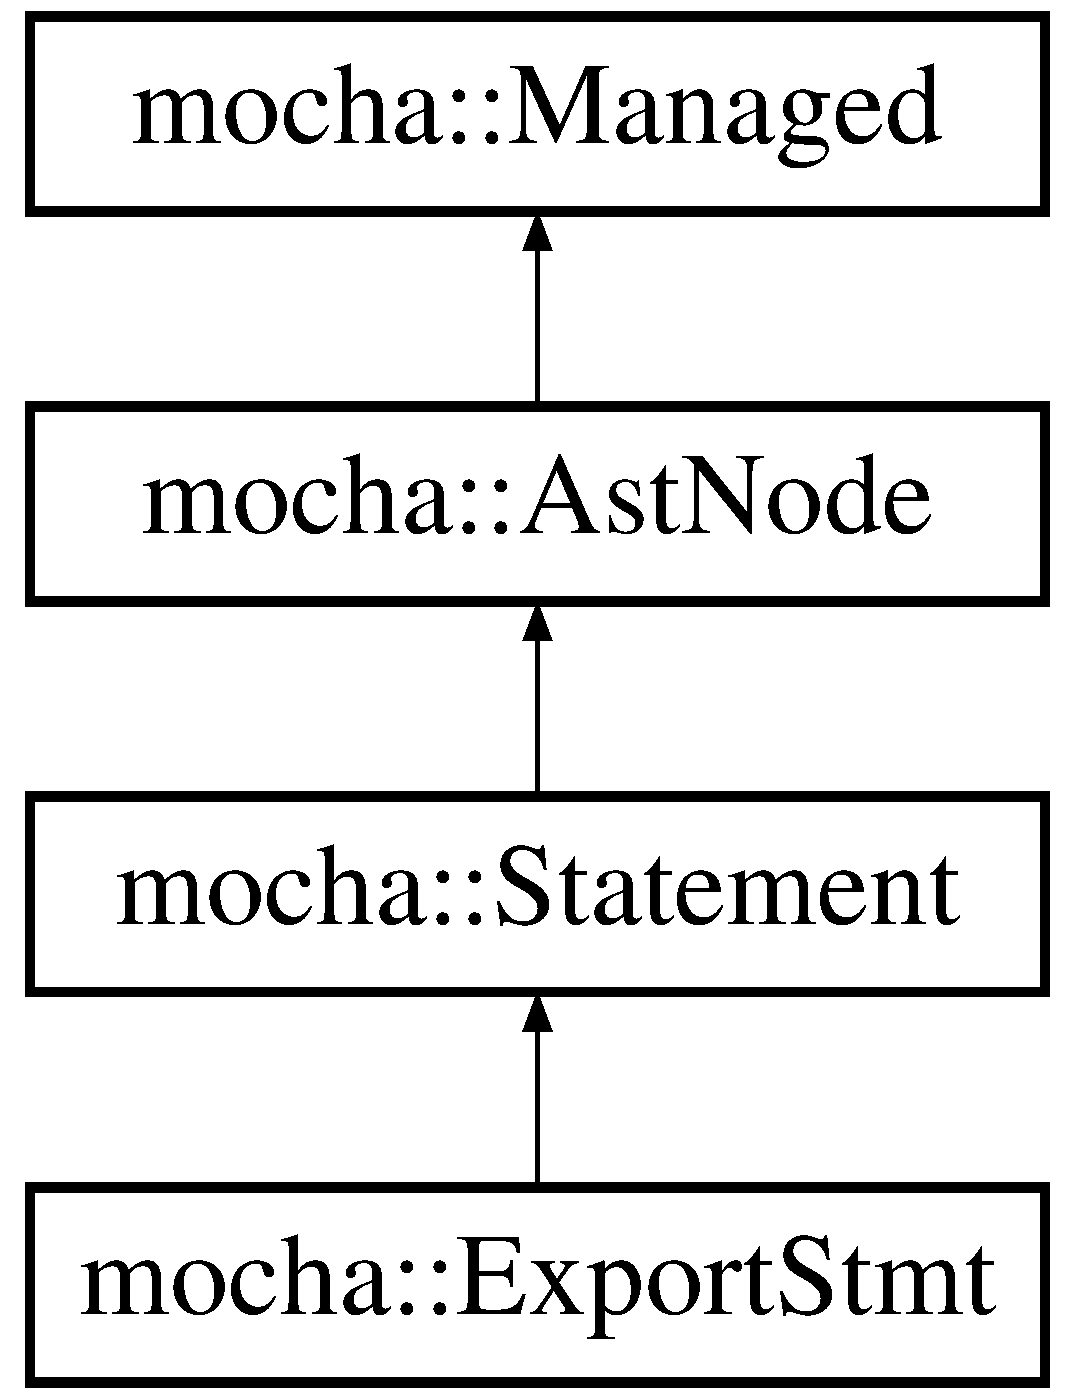
\includegraphics[height=4.000000cm]{classmocha_1_1_export_stmt}
\end{center}
\end{figure}
\subsection*{Public Member Functions}
\begin{DoxyCompactItemize}
\item 
\hyperlink{classmocha_1_1_export_stmt_ad76b63ebbff49b0c00bec75463b511e2}{ExportStmt} ()
\item 
\hyperlink{classmocha_1_1_export_stmt_a1cf91a0335e69f80be808933e55b5bc0}{$\sim$ExportStmt} ()
\item 
\hyperlink{classmocha_1_1_ast_node}{AstNode} $\ast$ \hyperlink{classmocha_1_1_export_stmt_a8ee0d362e91d567f7dda582c07fc9759}{Clone} ()
\end{DoxyCompactItemize}
\subsection*{Private Member Functions}
\begin{DoxyCompactItemize}
\item 
void \hyperlink{classmocha_1_1_export_stmt_a7cda610c60ff845128e6ec191552df05}{NVIAccept\_\-} (\hyperlink{classmocha_1_1_i_visitor}{IVisitor} $\ast$visitor)
\end{DoxyCompactItemize}


\subsection{Detailed Description}


Definition at line 697 of file ast.h.



\subsection{Constructor \& Destructor Documentation}
\hypertarget{classmocha_1_1_export_stmt_ad76b63ebbff49b0c00bec75463b511e2}{
\index{mocha::ExportStmt@{mocha::ExportStmt}!ExportStmt@{ExportStmt}}
\index{ExportStmt@{ExportStmt}!mocha::ExportStmt@{mocha::ExportStmt}}
\subsubsection[{ExportStmt}]{\setlength{\rightskip}{0pt plus 5cm}mocha::ExportStmt::ExportStmt (
\begin{DoxyParamCaption}
{}
\end{DoxyParamCaption}
)\hspace{0.3cm}{\ttfamily  \mbox{[}inline\mbox{]}}}}
\label{classmocha_1_1_export_stmt_ad76b63ebbff49b0c00bec75463b511e2}


Definition at line 699 of file ast.h.

\hypertarget{classmocha_1_1_export_stmt_a1cf91a0335e69f80be808933e55b5bc0}{
\index{mocha::ExportStmt@{mocha::ExportStmt}!$\sim$ExportStmt@{$\sim$ExportStmt}}
\index{$\sim$ExportStmt@{$\sim$ExportStmt}!mocha::ExportStmt@{mocha::ExportStmt}}
\subsubsection[{$\sim$ExportStmt}]{\setlength{\rightskip}{0pt plus 5cm}mocha::ExportStmt::$\sim$ExportStmt (
\begin{DoxyParamCaption}
{}
\end{DoxyParamCaption}
)\hspace{0.3cm}{\ttfamily  \mbox{[}inline\mbox{]}}}}
\label{classmocha_1_1_export_stmt_a1cf91a0335e69f80be808933e55b5bc0}


Definition at line 700 of file ast.h.



\subsection{Member Function Documentation}
\hypertarget{classmocha_1_1_export_stmt_a8ee0d362e91d567f7dda582c07fc9759}{
\index{mocha::ExportStmt@{mocha::ExportStmt}!Clone@{Clone}}
\index{Clone@{Clone}!mocha::ExportStmt@{mocha::ExportStmt}}
\subsubsection[{Clone}]{\setlength{\rightskip}{0pt plus 5cm}{\bf AstNode} $\ast$ mocha::ExportStmt::Clone (
\begin{DoxyParamCaption}
{}
\end{DoxyParamCaption}
)\hspace{0.3cm}{\ttfamily  \mbox{[}virtual\mbox{]}}}}
\label{classmocha_1_1_export_stmt_a8ee0d362e91d567f7dda582c07fc9759}
\begin{DoxyReturn}{Returns}
\{AstNode$\ast$\} Clone node. 
\end{DoxyReturn}


Reimplemented from \hyperlink{classmocha_1_1_ast_node_af2a895699bac2012f8b7739bff49c5ec}{mocha::AstNode}.



Definition at line 255 of file ast.cc.

\hypertarget{classmocha_1_1_export_stmt_a7cda610c60ff845128e6ec191552df05}{
\index{mocha::ExportStmt@{mocha::ExportStmt}!NVIAccept\_\-@{NVIAccept\_\-}}
\index{NVIAccept\_\-@{NVIAccept\_\-}!mocha::ExportStmt@{mocha::ExportStmt}}
\subsubsection[{NVIAccept\_\-}]{\setlength{\rightskip}{0pt plus 5cm}void mocha::ExportStmt::NVIAccept\_\- (
\begin{DoxyParamCaption}
\item[{{\bf IVisitor} $\ast$}]{visitor}
\end{DoxyParamCaption}
)\hspace{0.3cm}{\ttfamily  \mbox{[}inline, private, virtual\mbox{]}}}}
\label{classmocha_1_1_export_stmt_a7cda610c60ff845128e6ec191552df05}


Reimplemented from \hyperlink{classmocha_1_1_statement_ad0e8c3ef62d21f733eb50a414046bae4}{mocha::Statement}.



Definition at line 703 of file ast.h.



The documentation for this class was generated from the following files:\begin{DoxyCompactItemize}
\item 
Y:/mocha/src/ast/\hyperlink{ast_8h}{ast.h}\item 
Y:/mocha/src/ast/\hyperlink{ast_8cc}{ast.cc}\end{DoxyCompactItemize}

\hypertarget{classmocha_1_1_expression}{
\section{mocha::Expression Class Reference}
\label{classmocha_1_1_expression}\index{mocha::Expression@{mocha::Expression}}
}


{\ttfamily \#include $<$ast.h$>$}

Inheritance diagram for mocha::Expression:\begin{figure}[H]
\begin{center}
\leavevmode
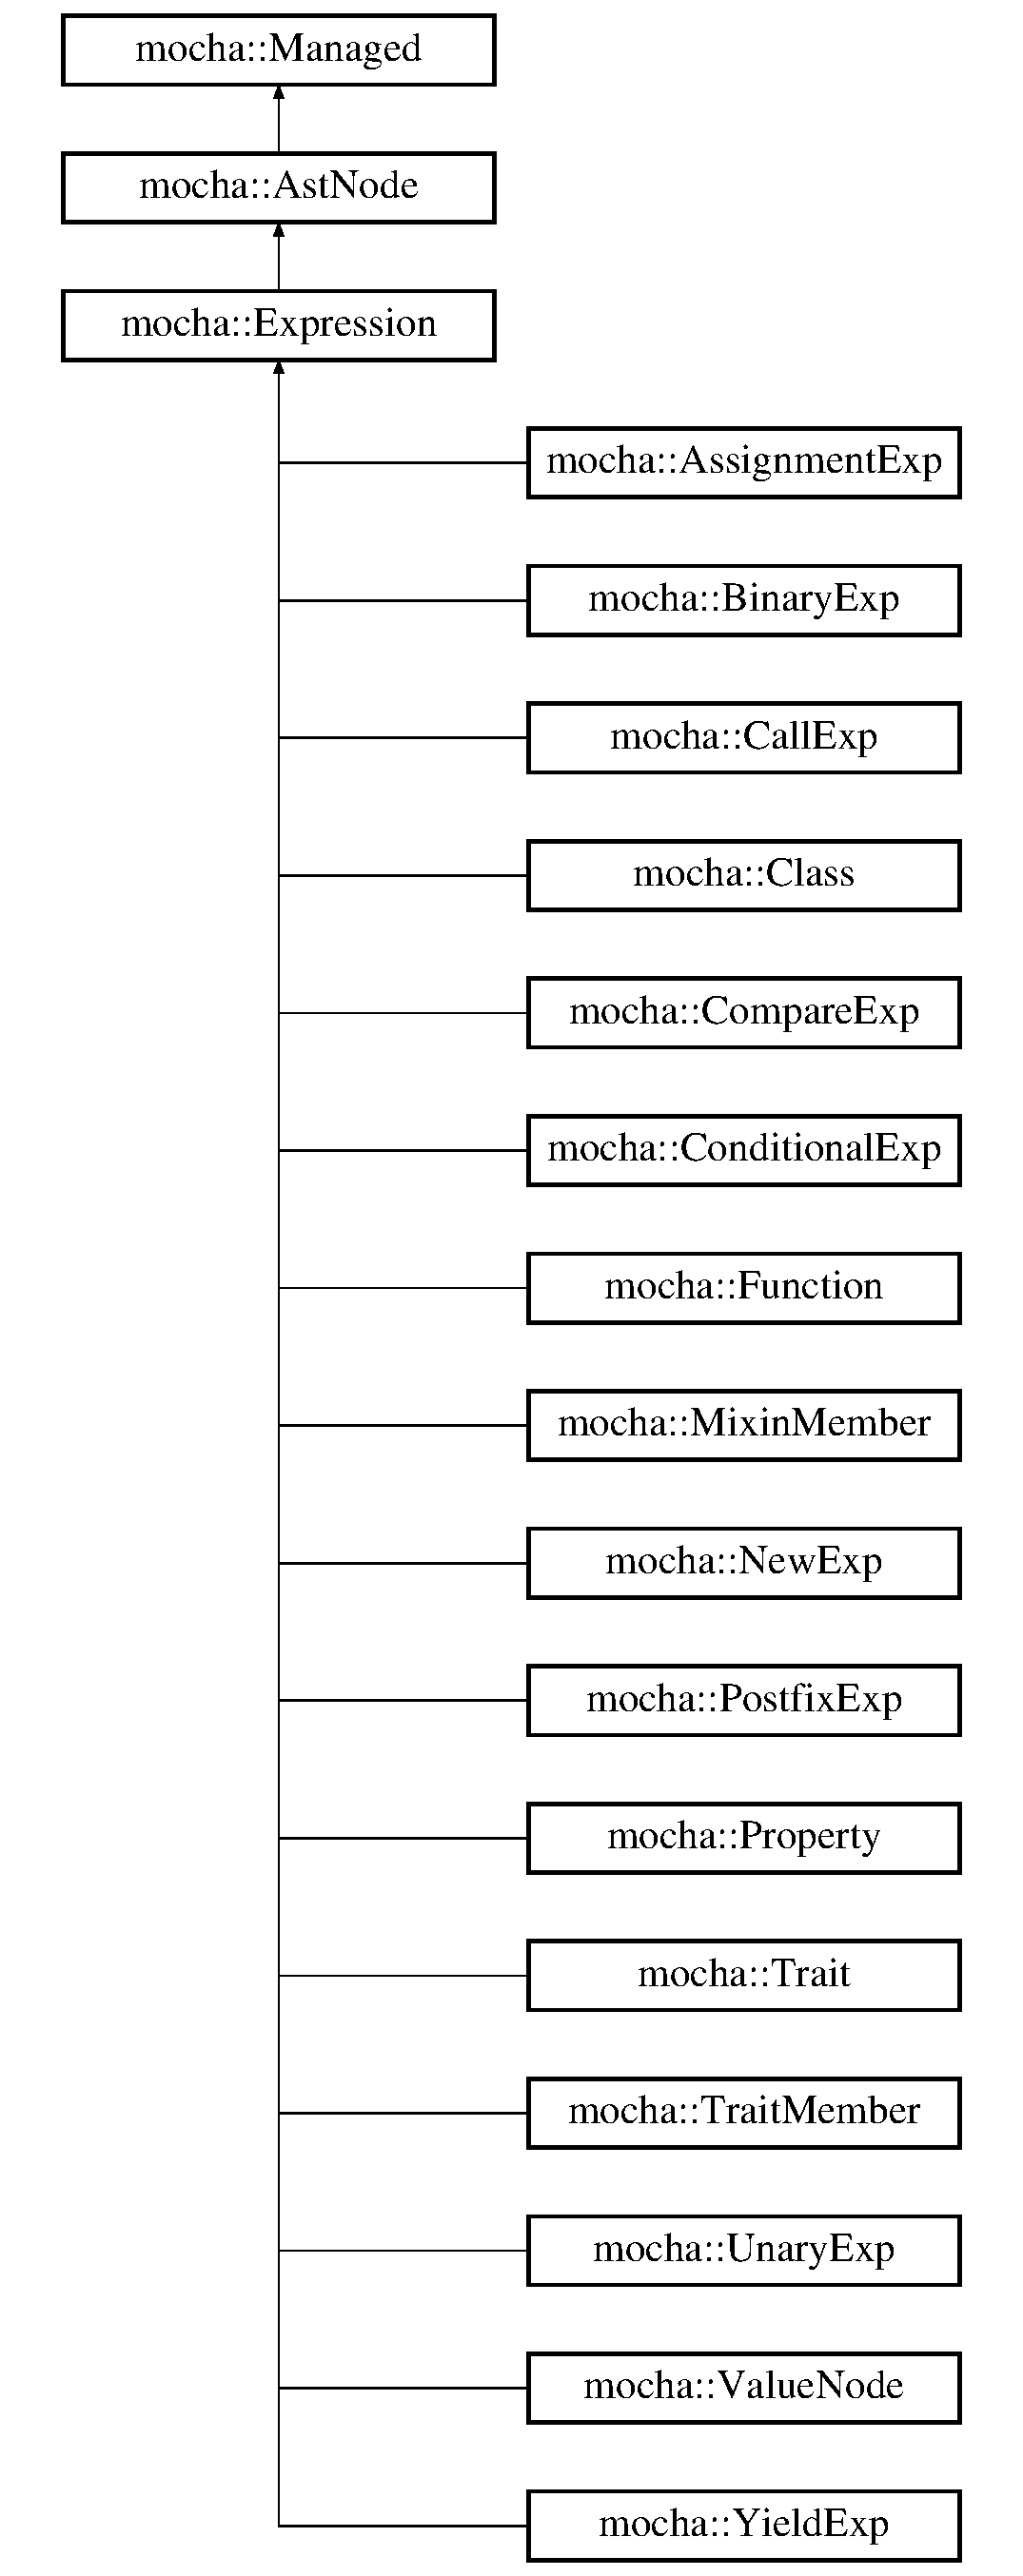
\includegraphics[height=12.000000cm]{classmocha_1_1_expression}
\end{center}
\end{figure}
\subsection*{Public Member Functions}
\begin{DoxyCompactItemize}
\item 
\hyperlink{classmocha_1_1_expression_a065032b38f3408d211df4bb6592af555}{Expression} ()
\item 
\hyperlink{classmocha_1_1_expression_ae79614f416f4fd9ef8c0e213ac53de6d}{Expression} (int type, const char $\ast$name=\char`\"{}Expression\char`\"{})
\item 
virtual \hyperlink{classmocha_1_1_expression_a55e9664e2b30613a55cb27e329c5560f}{$\sim$Expression} ()
\item 
void \hyperlink{classmocha_1_1_expression_a6d0d3990261dbd7a52aae5d2d83456f7}{Paren} ()
\item 
bool \hyperlink{classmocha_1_1_expression_a08f5d87b2974da4f58be4a95f5ab599d}{IsParen} ()
\item 
bool \hyperlink{classmocha_1_1_expression_a939ff839a3024d6d570913d5eae0b4ea}{IsValidLhs} ()
\item 
void \hyperlink{classmocha_1_1_expression_a89d9eb28d4537c77218853d5a888ff78}{InValidLhs} ()
\item 
void \hyperlink{classmocha_1_1_expression_aa690dc40a63b26d2ec5715b96aa18435}{ValidLhs} ()
\item 
\hyperlink{classmocha_1_1_expression}{Expression} $\ast$ \hyperlink{classmocha_1_1_expression_a518359725d2a90e69242d85594bc0b30}{CastToExpression} ()
\item 
virtual \hyperlink{classmocha_1_1_assignment_exp}{AssignmentExp} $\ast$ \hyperlink{classmocha_1_1_expression_ac9487a84166be5500145ae33523ebfdf}{CastToAssigment} ()
\item 
virtual \hyperlink{classmocha_1_1_call_exp}{CallExp} $\ast$ \hyperlink{classmocha_1_1_expression_a9bb8722ec476068afb58505699c7b2ff}{CastToCallExp} ()
\item 
virtual \hyperlink{classmocha_1_1_function}{Function} $\ast$ \hyperlink{classmocha_1_1_expression_a56027507124496007854f768cd847d52}{CastToFunction} ()
\item 
virtual \hyperlink{classmocha_1_1_property}{Property} $\ast$ \hyperlink{classmocha_1_1_expression_a29abca4b62263cbb9b71374bacac61c4}{CastToProperty} ()
\item 
virtual \hyperlink{classmocha_1_1_trait}{Trait} $\ast$ \hyperlink{classmocha_1_1_expression_a0c4a99f19c5144628707b20aaba7b53f}{CastToTrait} ()
\item 
virtual \hyperlink{classmocha_1_1_trait_member}{TraitMember} $\ast$ \hyperlink{classmocha_1_1_expression_a0bb72b025f6ef154427a29de109a5af5}{CastToTraitMember} ()
\item 
virtual \hyperlink{classmocha_1_1_mixin_member}{MixinMember} $\ast$ \hyperlink{classmocha_1_1_expression_a5c0da23f4477b3034e44cc08950bf16d}{CastToMixinMember} ()
\item 
virtual \hyperlink{classmocha_1_1_ast_node}{AstNode} $\ast$ \hyperlink{classmocha_1_1_expression_ac1fb936e2bf0fdd6e7667275d3723ca5}{Clone} ()
\end{DoxyCompactItemize}
\subsection*{Private Member Functions}
\begin{DoxyCompactItemize}
\item 
virtual void \hyperlink{classmocha_1_1_expression_a112d57b7de76c37066cde60be4799fde}{NVIAccept\_\-} (\hyperlink{classmocha_1_1_i_visitor}{IVisitor} $\ast$visitor)
\end{DoxyCompactItemize}
\subsection*{Private Attributes}
\begin{DoxyCompactItemize}
\item 
bool \hyperlink{classmocha_1_1_expression_ac8278e943ca52377aa1f528a816639f4}{is\_\-valid\_\-lhs\_\-}
\item 
bool \hyperlink{classmocha_1_1_expression_af9e01128faf08a57ecc8db7e3fe5a4ea}{paren\_\-}
\end{DoxyCompactItemize}


\subsection{Detailed Description}


Definition at line 1022 of file ast.h.



\subsection{Constructor \& Destructor Documentation}
\hypertarget{classmocha_1_1_expression_a065032b38f3408d211df4bb6592af555}{
\index{mocha::Expression@{mocha::Expression}!Expression@{Expression}}
\index{Expression@{Expression}!mocha::Expression@{mocha::Expression}}
\subsubsection[{Expression}]{\setlength{\rightskip}{0pt plus 5cm}mocha::Expression::Expression (
\begin{DoxyParamCaption}
{}
\end{DoxyParamCaption}
)\hspace{0.3cm}{\ttfamily  \mbox{[}inline\mbox{]}}}}
\label{classmocha_1_1_expression_a065032b38f3408d211df4bb6592af555}


Definition at line 1024 of file ast.h.

\hypertarget{classmocha_1_1_expression_ae79614f416f4fd9ef8c0e213ac53de6d}{
\index{mocha::Expression@{mocha::Expression}!Expression@{Expression}}
\index{Expression@{Expression}!mocha::Expression@{mocha::Expression}}
\subsubsection[{Expression}]{\setlength{\rightskip}{0pt plus 5cm}mocha::Expression::Expression (
\begin{DoxyParamCaption}
\item[{int}]{type, }
\item[{const char $\ast$}]{name = {\ttfamily \char`\"{}Expression\char`\"{}}}
\end{DoxyParamCaption}
)\hspace{0.3cm}{\ttfamily  \mbox{[}inline\mbox{]}}}}
\label{classmocha_1_1_expression_ae79614f416f4fd9ef8c0e213ac53de6d}


Definition at line 1025 of file ast.h.

\hypertarget{classmocha_1_1_expression_a55e9664e2b30613a55cb27e329c5560f}{
\index{mocha::Expression@{mocha::Expression}!$\sim$Expression@{$\sim$Expression}}
\index{$\sim$Expression@{$\sim$Expression}!mocha::Expression@{mocha::Expression}}
\subsubsection[{$\sim$Expression}]{\setlength{\rightskip}{0pt plus 5cm}virtual mocha::Expression::$\sim$Expression (
\begin{DoxyParamCaption}
{}
\end{DoxyParamCaption}
)\hspace{0.3cm}{\ttfamily  \mbox{[}inline, virtual\mbox{]}}}}
\label{classmocha_1_1_expression_a55e9664e2b30613a55cb27e329c5560f}


Definition at line 1026 of file ast.h.



\subsection{Member Function Documentation}
\hypertarget{classmocha_1_1_expression_ac9487a84166be5500145ae33523ebfdf}{
\index{mocha::Expression@{mocha::Expression}!CastToAssigment@{CastToAssigment}}
\index{CastToAssigment@{CastToAssigment}!mocha::Expression@{mocha::Expression}}
\subsubsection[{CastToAssigment}]{\setlength{\rightskip}{0pt plus 5cm}virtual {\bf AssignmentExp}$\ast$ mocha::Expression::CastToAssigment (
\begin{DoxyParamCaption}
{}
\end{DoxyParamCaption}
)\hspace{0.3cm}{\ttfamily  \mbox{[}inline, virtual\mbox{]}}}}
\label{classmocha_1_1_expression_ac9487a84166be5500145ae33523ebfdf}


Reimplemented in \hyperlink{classmocha_1_1_assignment_exp_ae8016bd58008fae4ae8e009f403fc9b0}{mocha::AssignmentExp}.



Definition at line 1033 of file ast.h.

\hypertarget{classmocha_1_1_expression_a9bb8722ec476068afb58505699c7b2ff}{
\index{mocha::Expression@{mocha::Expression}!CastToCallExp@{CastToCallExp}}
\index{CastToCallExp@{CastToCallExp}!mocha::Expression@{mocha::Expression}}
\subsubsection[{CastToCallExp}]{\setlength{\rightskip}{0pt plus 5cm}virtual {\bf CallExp}$\ast$ mocha::Expression::CastToCallExp (
\begin{DoxyParamCaption}
{}
\end{DoxyParamCaption}
)\hspace{0.3cm}{\ttfamily  \mbox{[}inline, virtual\mbox{]}}}}
\label{classmocha_1_1_expression_a9bb8722ec476068afb58505699c7b2ff}


Reimplemented in \hyperlink{classmocha_1_1_call_exp_a60e1a2f17381dd35093e75786b1c0c6a}{mocha::CallExp}.



Definition at line 1034 of file ast.h.

\hypertarget{classmocha_1_1_expression_a518359725d2a90e69242d85594bc0b30}{
\index{mocha::Expression@{mocha::Expression}!CastToExpression@{CastToExpression}}
\index{CastToExpression@{CastToExpression}!mocha::Expression@{mocha::Expression}}
\subsubsection[{CastToExpression}]{\setlength{\rightskip}{0pt plus 5cm}{\bf Expression}$\ast$ mocha::Expression::CastToExpression (
\begin{DoxyParamCaption}
{}
\end{DoxyParamCaption}
)\hspace{0.3cm}{\ttfamily  \mbox{[}inline, virtual\mbox{]}}}}
\label{classmocha_1_1_expression_a518359725d2a90e69242d85594bc0b30}

\begin{DoxyParams}{Parameters}
{\em \{Expression$\ast$\}} & Cast to \hyperlink{classmocha_1_1_expression}{Expression}. Return 0 by default. \\
\hline
\end{DoxyParams}


Reimplemented from \hyperlink{classmocha_1_1_ast_node_aece953ac3a588a8d731d258e4e7e57d9}{mocha::AstNode}.



Definition at line 1032 of file ast.h.

\hypertarget{classmocha_1_1_expression_a56027507124496007854f768cd847d52}{
\index{mocha::Expression@{mocha::Expression}!CastToFunction@{CastToFunction}}
\index{CastToFunction@{CastToFunction}!mocha::Expression@{mocha::Expression}}
\subsubsection[{CastToFunction}]{\setlength{\rightskip}{0pt plus 5cm}virtual {\bf Function}$\ast$ mocha::Expression::CastToFunction (
\begin{DoxyParamCaption}
{}
\end{DoxyParamCaption}
)\hspace{0.3cm}{\ttfamily  \mbox{[}inline, virtual\mbox{]}}}}
\label{classmocha_1_1_expression_a56027507124496007854f768cd847d52}


Reimplemented in \hyperlink{classmocha_1_1_function_a7054a10d92311750a4a2e1ce9a36f3d3}{mocha::Function}.



Definition at line 1035 of file ast.h.

\hypertarget{classmocha_1_1_expression_a5c0da23f4477b3034e44cc08950bf16d}{
\index{mocha::Expression@{mocha::Expression}!CastToMixinMember@{CastToMixinMember}}
\index{CastToMixinMember@{CastToMixinMember}!mocha::Expression@{mocha::Expression}}
\subsubsection[{CastToMixinMember}]{\setlength{\rightskip}{0pt plus 5cm}virtual {\bf MixinMember}$\ast$ mocha::Expression::CastToMixinMember (
\begin{DoxyParamCaption}
{}
\end{DoxyParamCaption}
)\hspace{0.3cm}{\ttfamily  \mbox{[}inline, virtual\mbox{]}}}}
\label{classmocha_1_1_expression_a5c0da23f4477b3034e44cc08950bf16d}


Reimplemented in \hyperlink{classmocha_1_1_mixin_member_a2a97fa4bd9f23b6bb43b839f0ba264cc}{mocha::MixinMember}.



Definition at line 1039 of file ast.h.

\hypertarget{classmocha_1_1_expression_a29abca4b62263cbb9b71374bacac61c4}{
\index{mocha::Expression@{mocha::Expression}!CastToProperty@{CastToProperty}}
\index{CastToProperty@{CastToProperty}!mocha::Expression@{mocha::Expression}}
\subsubsection[{CastToProperty}]{\setlength{\rightskip}{0pt plus 5cm}virtual {\bf Property}$\ast$ mocha::Expression::CastToProperty (
\begin{DoxyParamCaption}
{}
\end{DoxyParamCaption}
)\hspace{0.3cm}{\ttfamily  \mbox{[}inline, virtual\mbox{]}}}}
\label{classmocha_1_1_expression_a29abca4b62263cbb9b71374bacac61c4}


Reimplemented in \hyperlink{classmocha_1_1_property_a8c9aa3a00789174a3ce32e7f8a86edfe}{mocha::Property}.



Definition at line 1036 of file ast.h.

\hypertarget{classmocha_1_1_expression_a0c4a99f19c5144628707b20aaba7b53f}{
\index{mocha::Expression@{mocha::Expression}!CastToTrait@{CastToTrait}}
\index{CastToTrait@{CastToTrait}!mocha::Expression@{mocha::Expression}}
\subsubsection[{CastToTrait}]{\setlength{\rightskip}{0pt plus 5cm}virtual {\bf Trait}$\ast$ mocha::Expression::CastToTrait (
\begin{DoxyParamCaption}
{}
\end{DoxyParamCaption}
)\hspace{0.3cm}{\ttfamily  \mbox{[}inline, virtual\mbox{]}}}}
\label{classmocha_1_1_expression_a0c4a99f19c5144628707b20aaba7b53f}


Reimplemented in \hyperlink{classmocha_1_1_trait_a7c28c44797d688ae7786f6c8e96a2e17}{mocha::Trait}.



Definition at line 1037 of file ast.h.

\hypertarget{classmocha_1_1_expression_a0bb72b025f6ef154427a29de109a5af5}{
\index{mocha::Expression@{mocha::Expression}!CastToTraitMember@{CastToTraitMember}}
\index{CastToTraitMember@{CastToTraitMember}!mocha::Expression@{mocha::Expression}}
\subsubsection[{CastToTraitMember}]{\setlength{\rightskip}{0pt plus 5cm}virtual {\bf TraitMember}$\ast$ mocha::Expression::CastToTraitMember (
\begin{DoxyParamCaption}
{}
\end{DoxyParamCaption}
)\hspace{0.3cm}{\ttfamily  \mbox{[}inline, virtual\mbox{]}}}}
\label{classmocha_1_1_expression_a0bb72b025f6ef154427a29de109a5af5}


Reimplemented in \hyperlink{classmocha_1_1_trait_member_a08a942200584355364e078d79d66dde6}{mocha::TraitMember}.



Definition at line 1038 of file ast.h.

\hypertarget{classmocha_1_1_expression_ac1fb936e2bf0fdd6e7667275d3723ca5}{
\index{mocha::Expression@{mocha::Expression}!Clone@{Clone}}
\index{Clone@{Clone}!mocha::Expression@{mocha::Expression}}
\subsubsection[{Clone}]{\setlength{\rightskip}{0pt plus 5cm}{\bf AstNode} $\ast$ mocha::Expression::Clone (
\begin{DoxyParamCaption}
{}
\end{DoxyParamCaption}
)\hspace{0.3cm}{\ttfamily  \mbox{[}virtual\mbox{]}}}}
\label{classmocha_1_1_expression_ac1fb936e2bf0fdd6e7667275d3723ca5}
\begin{DoxyReturn}{Returns}
\{AstNode$\ast$\} Clone node. 
\end{DoxyReturn}


Reimplemented from \hyperlink{classmocha_1_1_ast_node_af2a895699bac2012f8b7739bff49c5ec}{mocha::AstNode}.



Reimplemented in \hyperlink{classmocha_1_1_class_a801c063381ca42fdab1c478f2ca461b8}{mocha::Class}, \hyperlink{classmocha_1_1_function_a787dcc9695496b521f0de87094003c7a}{mocha::Function}, \hyperlink{classmocha_1_1_call_exp_a1a423dfd91b217f3a89a6ebf4f1de495}{mocha::CallExp}, \hyperlink{classmocha_1_1_new_exp_ad256abe9b71be99dd2a24be71e088691}{mocha::NewExp}, \hyperlink{classmocha_1_1_yield_exp_ae72bb8f5e255bac1eaa2ba479d7c7b85}{mocha::YieldExp}, \hyperlink{classmocha_1_1_postfix_exp_a71df055d09b8f804d8eeeb4ea12a72ad}{mocha::PostfixExp}, \hyperlink{classmocha_1_1_unary_exp_ad039d38166e2fa193f578ae4e91d81ea}{mocha::UnaryExp}, \hyperlink{classmocha_1_1_binary_exp_a035d97865c0512e2902192f8ed840ae4}{mocha::BinaryExp}, \hyperlink{classmocha_1_1_compare_exp_afa00b970faa937c81cfc15c9a0170558}{mocha::CompareExp}, \hyperlink{classmocha_1_1_conditional_exp_a568bfc0b7fce3e0155e3c789baf6fa40}{mocha::ConditionalExp}, \hyperlink{classmocha_1_1_assignment_exp_ac266c79bc33aaba7a6de7bb34a966786}{mocha::AssignmentExp}, and \hyperlink{classmocha_1_1_value_node_a960b13fc3b0e5544518b64a393f4c272}{mocha::ValueNode}.



Definition at line 383 of file ast.cc.

\hypertarget{classmocha_1_1_expression_a89d9eb28d4537c77218853d5a888ff78}{
\index{mocha::Expression@{mocha::Expression}!InValidLhs@{InValidLhs}}
\index{InValidLhs@{InValidLhs}!mocha::Expression@{mocha::Expression}}
\subsubsection[{InValidLhs}]{\setlength{\rightskip}{0pt plus 5cm}void mocha::Expression::InValidLhs (
\begin{DoxyParamCaption}
{}
\end{DoxyParamCaption}
)\hspace{0.3cm}{\ttfamily  \mbox{[}inline\mbox{]}}}}
\label{classmocha_1_1_expression_a89d9eb28d4537c77218853d5a888ff78}


Definition at line 1030 of file ast.h.

\hypertarget{classmocha_1_1_expression_a08f5d87b2974da4f58be4a95f5ab599d}{
\index{mocha::Expression@{mocha::Expression}!IsParen@{IsParen}}
\index{IsParen@{IsParen}!mocha::Expression@{mocha::Expression}}
\subsubsection[{IsParen}]{\setlength{\rightskip}{0pt plus 5cm}bool mocha::Expression::IsParen (
\begin{DoxyParamCaption}
{}
\end{DoxyParamCaption}
)\hspace{0.3cm}{\ttfamily  \mbox{[}inline\mbox{]}}}}
\label{classmocha_1_1_expression_a08f5d87b2974da4f58be4a95f5ab599d}


Definition at line 1028 of file ast.h.

\hypertarget{classmocha_1_1_expression_a939ff839a3024d6d570913d5eae0b4ea}{
\index{mocha::Expression@{mocha::Expression}!IsValidLhs@{IsValidLhs}}
\index{IsValidLhs@{IsValidLhs}!mocha::Expression@{mocha::Expression}}
\subsubsection[{IsValidLhs}]{\setlength{\rightskip}{0pt plus 5cm}bool mocha::Expression::IsValidLhs (
\begin{DoxyParamCaption}
{}
\end{DoxyParamCaption}
)\hspace{0.3cm}{\ttfamily  \mbox{[}inline\mbox{]}}}}
\label{classmocha_1_1_expression_a939ff839a3024d6d570913d5eae0b4ea}


Definition at line 1029 of file ast.h.

\hypertarget{classmocha_1_1_expression_a112d57b7de76c37066cde60be4799fde}{
\index{mocha::Expression@{mocha::Expression}!NVIAccept\_\-@{NVIAccept\_\-}}
\index{NVIAccept\_\-@{NVIAccept\_\-}!mocha::Expression@{mocha::Expression}}
\subsubsection[{NVIAccept\_\-}]{\setlength{\rightskip}{0pt plus 5cm}virtual void mocha::Expression::NVIAccept\_\- (
\begin{DoxyParamCaption}
\item[{{\bf IVisitor} $\ast$}]{visitor}
\end{DoxyParamCaption}
)\hspace{0.3cm}{\ttfamily  \mbox{[}inline, private, virtual\mbox{]}}}}
\label{classmocha_1_1_expression_a112d57b7de76c37066cde60be4799fde}


Reimplemented from \hyperlink{classmocha_1_1_ast_node_a4a9c107bed3671f3fa15312b87f6ae96}{mocha::AstNode}.



Reimplemented in \hyperlink{classmocha_1_1_trait_member_ad008bf35f880ed657bbb796fe755077b}{mocha::TraitMember}, \hyperlink{classmocha_1_1_trait_a0fa57407e3a93198f3bbafdeae5c21ef}{mocha::Trait}, \hyperlink{classmocha_1_1_class_acb9ec1fb4dc467d73c132c20d510901a}{mocha::Class}, \hyperlink{classmocha_1_1_function_ac8aea50fb291b078333d89530a25a627}{mocha::Function}, \hyperlink{classmocha_1_1_call_exp_a6f03e2ebd560f6cc4bd9ce46247ae2d9}{mocha::CallExp}, \hyperlink{classmocha_1_1_new_exp_a7e122b87c42c0589dc373db568650e80}{mocha::NewExp}, \hyperlink{classmocha_1_1_yield_exp_af9a03b0800ca3fa93bab22231245bb94}{mocha::YieldExp}, \hyperlink{classmocha_1_1_postfix_exp_ae33ad913b48ec2d634d0487f8f4a0d49}{mocha::PostfixExp}, \hyperlink{classmocha_1_1_unary_exp_a4f5a48831784abe08a1d31c7664827a1}{mocha::UnaryExp}, \hyperlink{classmocha_1_1_binary_exp_ac7feb22c02d0432e40486b76997f505e}{mocha::BinaryExp}, \hyperlink{classmocha_1_1_compare_exp_a48c63840dc4ab4b2504eb805bcf76f77}{mocha::CompareExp}, \hyperlink{classmocha_1_1_conditional_exp_a719ad36c380cd142230163006ef6b124}{mocha::ConditionalExp}, \hyperlink{classmocha_1_1_assignment_exp_ae8926731b19e86748e07bf8f29fa9a1b}{mocha::AssignmentExp}, and \hyperlink{classmocha_1_1_value_node_adc856fc8531699b7c810736b677b2a0f}{mocha::ValueNode}.



Definition at line 1044 of file ast.h.

\hypertarget{classmocha_1_1_expression_a6d0d3990261dbd7a52aae5d2d83456f7}{
\index{mocha::Expression@{mocha::Expression}!Paren@{Paren}}
\index{Paren@{Paren}!mocha::Expression@{mocha::Expression}}
\subsubsection[{Paren}]{\setlength{\rightskip}{0pt plus 5cm}void mocha::Expression::Paren (
\begin{DoxyParamCaption}
{}
\end{DoxyParamCaption}
)\hspace{0.3cm}{\ttfamily  \mbox{[}inline\mbox{]}}}}
\label{classmocha_1_1_expression_a6d0d3990261dbd7a52aae5d2d83456f7}


Definition at line 1027 of file ast.h.

\hypertarget{classmocha_1_1_expression_aa690dc40a63b26d2ec5715b96aa18435}{
\index{mocha::Expression@{mocha::Expression}!ValidLhs@{ValidLhs}}
\index{ValidLhs@{ValidLhs}!mocha::Expression@{mocha::Expression}}
\subsubsection[{ValidLhs}]{\setlength{\rightskip}{0pt plus 5cm}void mocha::Expression::ValidLhs (
\begin{DoxyParamCaption}
{}
\end{DoxyParamCaption}
)\hspace{0.3cm}{\ttfamily  \mbox{[}inline\mbox{]}}}}
\label{classmocha_1_1_expression_aa690dc40a63b26d2ec5715b96aa18435}


Definition at line 1031 of file ast.h.



\subsection{Member Data Documentation}
\hypertarget{classmocha_1_1_expression_ac8278e943ca52377aa1f528a816639f4}{
\index{mocha::Expression@{mocha::Expression}!is\_\-valid\_\-lhs\_\-@{is\_\-valid\_\-lhs\_\-}}
\index{is\_\-valid\_\-lhs\_\-@{is\_\-valid\_\-lhs\_\-}!mocha::Expression@{mocha::Expression}}
\subsubsection[{is\_\-valid\_\-lhs\_\-}]{\setlength{\rightskip}{0pt plus 5cm}bool {\bf mocha::Expression::is\_\-valid\_\-lhs\_\-}\hspace{0.3cm}{\ttfamily  \mbox{[}private\mbox{]}}}}
\label{classmocha_1_1_expression_ac8278e943ca52377aa1f528a816639f4}


Definition at line 1040 of file ast.h.

\hypertarget{classmocha_1_1_expression_af9e01128faf08a57ecc8db7e3fe5a4ea}{
\index{mocha::Expression@{mocha::Expression}!paren\_\-@{paren\_\-}}
\index{paren\_\-@{paren\_\-}!mocha::Expression@{mocha::Expression}}
\subsubsection[{paren\_\-}]{\setlength{\rightskip}{0pt plus 5cm}bool {\bf mocha::Expression::paren\_\-}\hspace{0.3cm}{\ttfamily  \mbox{[}private\mbox{]}}}}
\label{classmocha_1_1_expression_af9e01128faf08a57ecc8db7e3fe5a4ea}


Definition at line 1043 of file ast.h.



The documentation for this class was generated from the following files:\begin{DoxyCompactItemize}
\item 
Y:/mocha/src/ast/\hyperlink{ast_8h}{ast.h}\item 
Y:/mocha/src/ast/\hyperlink{ast_8cc}{ast.cc}\end{DoxyCompactItemize}

\hypertarget{classmocha_1_1_expression_stmt}{
\section{mocha::ExpressionStmt Class Reference}
\label{classmocha_1_1_expression_stmt}\index{mocha::ExpressionStmt@{mocha::ExpressionStmt}}
}


{\ttfamily \#include $<$ast.h$>$}

Inheritance diagram for mocha::ExpressionStmt:\begin{figure}[H]
\begin{center}
\leavevmode
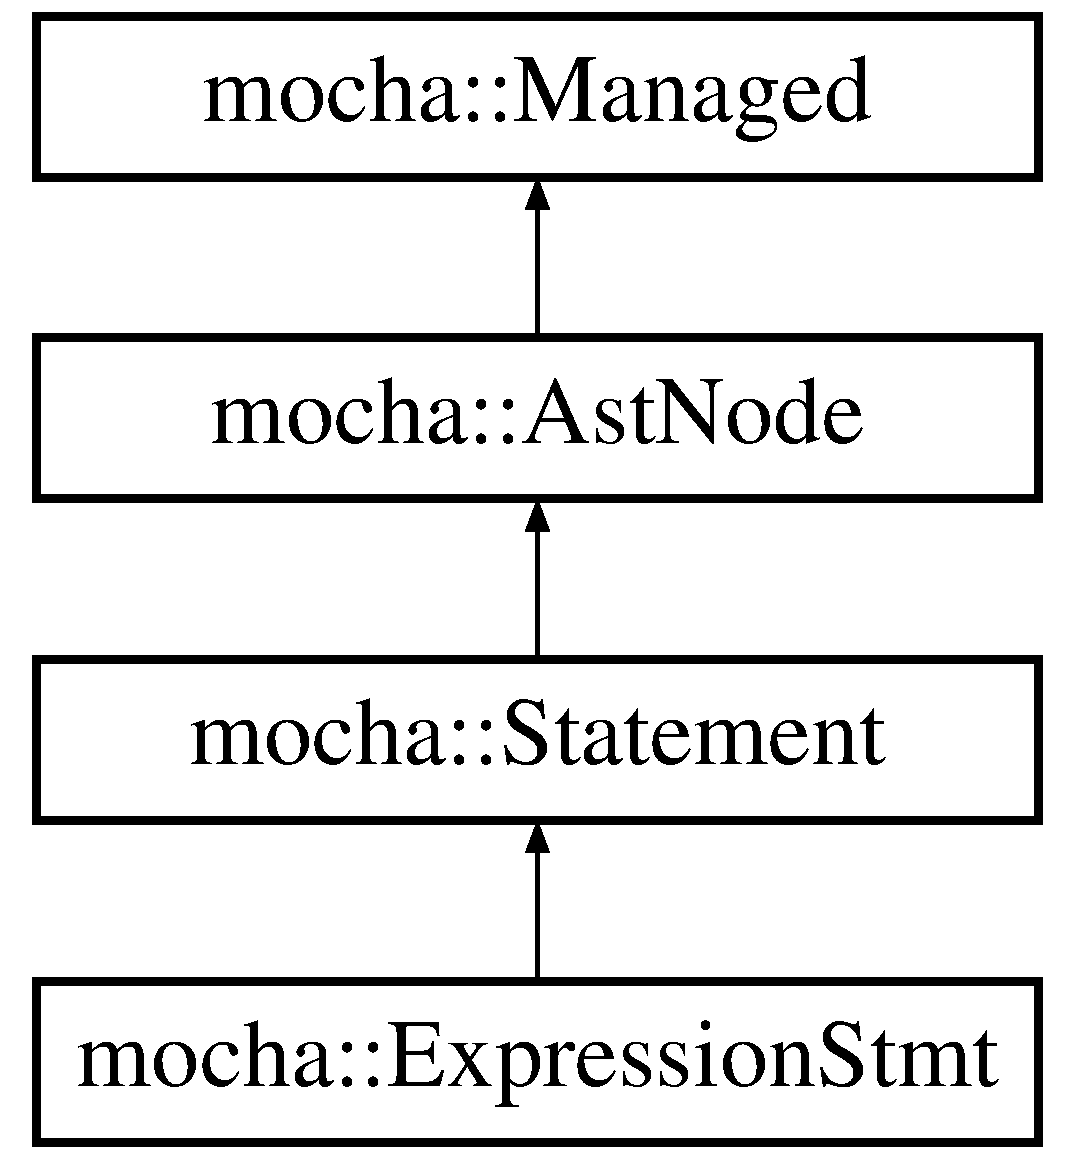
\includegraphics[height=4.000000cm]{classmocha_1_1_expression_stmt}
\end{center}
\end{figure}
\subsection*{Public Member Functions}
\begin{DoxyCompactItemize}
\item 
\hyperlink{classmocha_1_1_expression_stmt_a3b4754923a4774d81cac0b08848b3bbd}{ExpressionStmt} ()
\item 
\hyperlink{classmocha_1_1_expression_stmt_a6934bdf05bf2237c2db76bd0ce9aa087}{$\sim$ExpressionStmt} ()
\item 
\hyperlink{classmocha_1_1_ast_node}{AstNode} $\ast$ \hyperlink{classmocha_1_1_expression_stmt_a766da5b40c2a6bc68e1947fb52ff8589}{Clone} ()
\end{DoxyCompactItemize}
\subsection*{Private Member Functions}
\begin{DoxyCompactItemize}
\item 
void \hyperlink{classmocha_1_1_expression_stmt_afa89adad8608636cf29a1c2d617347b8}{NVIAccept\_\-} (\hyperlink{classmocha_1_1_i_visitor}{IVisitor} $\ast$visitor)
\end{DoxyCompactItemize}


\subsection{Detailed Description}


Definition at line 840 of file ast.h.



\subsection{Constructor \& Destructor Documentation}
\hypertarget{classmocha_1_1_expression_stmt_a3b4754923a4774d81cac0b08848b3bbd}{
\index{mocha::ExpressionStmt@{mocha::ExpressionStmt}!ExpressionStmt@{ExpressionStmt}}
\index{ExpressionStmt@{ExpressionStmt}!mocha::ExpressionStmt@{mocha::ExpressionStmt}}
\subsubsection[{ExpressionStmt}]{\setlength{\rightskip}{0pt plus 5cm}mocha::ExpressionStmt::ExpressionStmt (
\begin{DoxyParamCaption}
{}
\end{DoxyParamCaption}
)\hspace{0.3cm}{\ttfamily  \mbox{[}inline\mbox{]}}}}
\label{classmocha_1_1_expression_stmt_a3b4754923a4774d81cac0b08848b3bbd}


Definition at line 842 of file ast.h.

\hypertarget{classmocha_1_1_expression_stmt_a6934bdf05bf2237c2db76bd0ce9aa087}{
\index{mocha::ExpressionStmt@{mocha::ExpressionStmt}!$\sim$ExpressionStmt@{$\sim$ExpressionStmt}}
\index{$\sim$ExpressionStmt@{$\sim$ExpressionStmt}!mocha::ExpressionStmt@{mocha::ExpressionStmt}}
\subsubsection[{$\sim$ExpressionStmt}]{\setlength{\rightskip}{0pt plus 5cm}mocha::ExpressionStmt::$\sim$ExpressionStmt (
\begin{DoxyParamCaption}
{}
\end{DoxyParamCaption}
)\hspace{0.3cm}{\ttfamily  \mbox{[}inline\mbox{]}}}}
\label{classmocha_1_1_expression_stmt_a6934bdf05bf2237c2db76bd0ce9aa087}


Definition at line 843 of file ast.h.



\subsection{Member Function Documentation}
\hypertarget{classmocha_1_1_expression_stmt_a766da5b40c2a6bc68e1947fb52ff8589}{
\index{mocha::ExpressionStmt@{mocha::ExpressionStmt}!Clone@{Clone}}
\index{Clone@{Clone}!mocha::ExpressionStmt@{mocha::ExpressionStmt}}
\subsubsection[{Clone}]{\setlength{\rightskip}{0pt plus 5cm}{\bf AstNode} $\ast$ mocha::ExpressionStmt::Clone (
\begin{DoxyParamCaption}
{}
\end{DoxyParamCaption}
)\hspace{0.3cm}{\ttfamily  \mbox{[}virtual\mbox{]}}}}
\label{classmocha_1_1_expression_stmt_a766da5b40c2a6bc68e1947fb52ff8589}
\begin{DoxyReturn}{Returns}
\{AstNode$\ast$\} Clone node. 
\end{DoxyReturn}


Reimplemented from \hyperlink{classmocha_1_1_ast_node_af2a895699bac2012f8b7739bff49c5ec}{mocha::AstNode}.



Definition at line 285 of file ast.cc.

\hypertarget{classmocha_1_1_expression_stmt_afa89adad8608636cf29a1c2d617347b8}{
\index{mocha::ExpressionStmt@{mocha::ExpressionStmt}!NVIAccept\_\-@{NVIAccept\_\-}}
\index{NVIAccept\_\-@{NVIAccept\_\-}!mocha::ExpressionStmt@{mocha::ExpressionStmt}}
\subsubsection[{NVIAccept\_\-}]{\setlength{\rightskip}{0pt plus 5cm}void mocha::ExpressionStmt::NVIAccept\_\- (
\begin{DoxyParamCaption}
\item[{{\bf IVisitor} $\ast$}]{visitor}
\end{DoxyParamCaption}
)\hspace{0.3cm}{\ttfamily  \mbox{[}inline, private, virtual\mbox{]}}}}
\label{classmocha_1_1_expression_stmt_afa89adad8608636cf29a1c2d617347b8}


Reimplemented from \hyperlink{classmocha_1_1_statement_ad0e8c3ef62d21f733eb50a414046bae4}{mocha::Statement}.



Definition at line 846 of file ast.h.



The documentation for this class was generated from the following files:\begin{DoxyCompactItemize}
\item 
Y:/mocha/src/ast/\hyperlink{ast_8h}{ast.h}\item 
Y:/mocha/src/ast/\hyperlink{ast_8cc}{ast.cc}\end{DoxyCompactItemize}

\hypertarget{classmocha_1_1_external_ast}{
\section{mocha::ExternalAst Class Reference}
\label{classmocha_1_1_external_ast}\index{mocha::ExternalAst@{mocha::ExternalAst}}
}


{\ttfamily \#include $<$external\_\-ast.h$>$}

Inheritance diagram for mocha::ExternalAst:\begin{figure}[H]
\begin{center}
\leavevmode
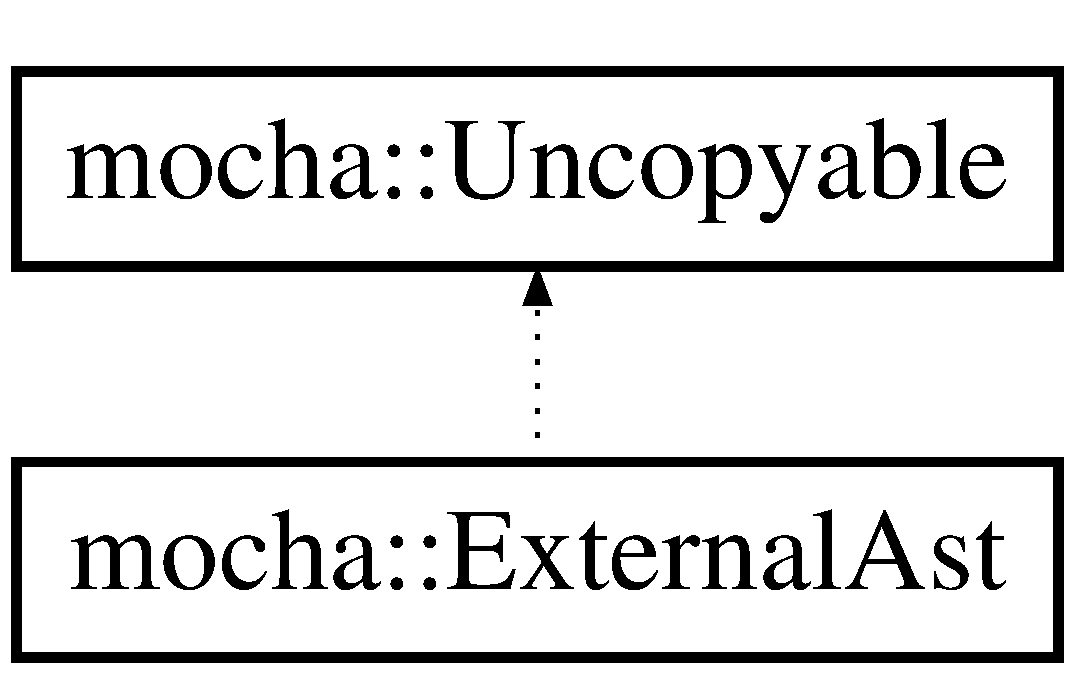
\includegraphics[height=2.000000cm]{classmocha_1_1_external_ast}
\end{center}
\end{figure}
\subsection*{Public Member Functions}
\begin{DoxyCompactItemize}
\item 
\hyperlink{classmocha_1_1_ast_root}{AstRoot} $\ast$ \hyperlink{classmocha_1_1_external_ast_a283942660cfc16932b02d8b312ee3b8e}{GetRoot} ()
\item 
\hyperlink{classmocha_1_1_external_ast_ab2368ae9cc9d4d10126c87450d7c53f8}{$\sim$ExternalAst} ()
\end{DoxyCompactItemize}
\subsection*{Static Public Member Functions}
\begin{DoxyCompactItemize}
\item 
static \hyperlink{classmocha_1_1_handle}{Handle}$<$ \hyperlink{classmocha_1_1_external_ast}{ExternalAst} $>$ \hyperlink{classmocha_1_1_external_ast_ab38f99ba98a9923eeffab02558f72abc}{Create} ()
\end{DoxyCompactItemize}
\subsection*{Private Member Functions}
\begin{DoxyCompactItemize}
\item 
\hyperlink{classmocha_1_1_external_ast_acc5e9bb8070803d84978276ea576fe96}{ExternalAst} ()
\end{DoxyCompactItemize}
\subsection*{Private Attributes}
\begin{DoxyCompactItemize}
\item 
\hyperlink{classmocha_1_1_managed_scope}{ManagedScope} \hyperlink{classmocha_1_1_external_ast_a8ba3452784b6fe06fc0f9611c1b15fe8}{scope\_\-}
\item 
\hyperlink{classmocha_1_1_ast_root}{AstRoot} $\ast$ \hyperlink{classmocha_1_1_external_ast_a89ef4c81a24b0fd43ba31487af972800}{root\_\-}
\end{DoxyCompactItemize}


\subsection{Detailed Description}


Definition at line 9 of file external\_\-ast.h.



\subsection{Constructor \& Destructor Documentation}
\hypertarget{classmocha_1_1_external_ast_ab2368ae9cc9d4d10126c87450d7c53f8}{
\index{mocha::ExternalAst@{mocha::ExternalAst}!$\sim$ExternalAst@{$\sim$ExternalAst}}
\index{$\sim$ExternalAst@{$\sim$ExternalAst}!mocha::ExternalAst@{mocha::ExternalAst}}
\subsubsection[{$\sim$ExternalAst}]{\setlength{\rightskip}{0pt plus 5cm}mocha::ExternalAst::$\sim$ExternalAst (
\begin{DoxyParamCaption}
{}
\end{DoxyParamCaption}
)\hspace{0.3cm}{\ttfamily  \mbox{[}inline\mbox{]}}}}
\label{classmocha_1_1_external_ast_ab2368ae9cc9d4d10126c87450d7c53f8}


Definition at line 13 of file external\_\-ast.h.

\hypertarget{classmocha_1_1_external_ast_acc5e9bb8070803d84978276ea576fe96}{
\index{mocha::ExternalAst@{mocha::ExternalAst}!ExternalAst@{ExternalAst}}
\index{ExternalAst@{ExternalAst}!mocha::ExternalAst@{mocha::ExternalAst}}
\subsubsection[{ExternalAst}]{\setlength{\rightskip}{0pt plus 5cm}mocha::ExternalAst::ExternalAst (
\begin{DoxyParamCaption}
{}
\end{DoxyParamCaption}
)\hspace{0.3cm}{\ttfamily  \mbox{[}private\mbox{]}}}}
\label{classmocha_1_1_external_ast_acc5e9bb8070803d84978276ea576fe96}


Definition at line 9 of file external\_\-ast.cc.



\subsection{Member Function Documentation}
\hypertarget{classmocha_1_1_external_ast_ab38f99ba98a9923eeffab02558f72abc}{
\index{mocha::ExternalAst@{mocha::ExternalAst}!Create@{Create}}
\index{Create@{Create}!mocha::ExternalAst@{mocha::ExternalAst}}
\subsubsection[{Create}]{\setlength{\rightskip}{0pt plus 5cm}{\bf Handle}$<$ {\bf ExternalAst} $>$ mocha::ExternalAst::Create (
\begin{DoxyParamCaption}
{}
\end{DoxyParamCaption}
)\hspace{0.3cm}{\ttfamily  \mbox{[}static\mbox{]}}}}
\label{classmocha_1_1_external_ast_ab38f99ba98a9923eeffab02558f72abc}


Definition at line 5 of file external\_\-ast.cc.

\hypertarget{classmocha_1_1_external_ast_a283942660cfc16932b02d8b312ee3b8e}{
\index{mocha::ExternalAst@{mocha::ExternalAst}!GetRoot@{GetRoot}}
\index{GetRoot@{GetRoot}!mocha::ExternalAst@{mocha::ExternalAst}}
\subsubsection[{GetRoot}]{\setlength{\rightskip}{0pt plus 5cm}{\bf AstRoot}$\ast$ mocha::ExternalAst::GetRoot (
\begin{DoxyParamCaption}
{}
\end{DoxyParamCaption}
)\hspace{0.3cm}{\ttfamily  \mbox{[}inline\mbox{]}}}}
\label{classmocha_1_1_external_ast_a283942660cfc16932b02d8b312ee3b8e}


Definition at line 12 of file external\_\-ast.h.



\subsection{Member Data Documentation}
\hypertarget{classmocha_1_1_external_ast_a89ef4c81a24b0fd43ba31487af972800}{
\index{mocha::ExternalAst@{mocha::ExternalAst}!root\_\-@{root\_\-}}
\index{root\_\-@{root\_\-}!mocha::ExternalAst@{mocha::ExternalAst}}
\subsubsection[{root\_\-}]{\setlength{\rightskip}{0pt plus 5cm}{\bf AstRoot}$\ast$ {\bf mocha::ExternalAst::root\_\-}\hspace{0.3cm}{\ttfamily  \mbox{[}private\mbox{]}}}}
\label{classmocha_1_1_external_ast_a89ef4c81a24b0fd43ba31487af972800}


Definition at line 17 of file external\_\-ast.h.

\hypertarget{classmocha_1_1_external_ast_a8ba3452784b6fe06fc0f9611c1b15fe8}{
\index{mocha::ExternalAst@{mocha::ExternalAst}!scope\_\-@{scope\_\-}}
\index{scope\_\-@{scope\_\-}!mocha::ExternalAst@{mocha::ExternalAst}}
\subsubsection[{scope\_\-}]{\setlength{\rightskip}{0pt plus 5cm}{\bf ManagedScope} {\bf mocha::ExternalAst::scope\_\-}\hspace{0.3cm}{\ttfamily  \mbox{[}private\mbox{]}}}}
\label{classmocha_1_1_external_ast_a8ba3452784b6fe06fc0f9611c1b15fe8}


Definition at line 16 of file external\_\-ast.h.



The documentation for this class was generated from the following files:\begin{DoxyCompactItemize}
\item 
Y:/mocha/src/compiler/external/\hyperlink{external__ast_8h}{external\_\-ast.h}\item 
Y:/mocha/src/compiler/external/\hyperlink{external__ast_8cc}{external\_\-ast.cc}\end{DoxyCompactItemize}

\hypertarget{classmocha_1_1_external_resource}{
\section{mocha::ExternalResource Class Reference}
\label{classmocha_1_1_external_resource}\index{mocha::ExternalResource@{mocha::ExternalResource}}
}


{\ttfamily \#include $<$external\_\-resource.h$>$}

Inheritance diagram for mocha::ExternalResource:\begin{figure}[H]
\begin{center}
\leavevmode
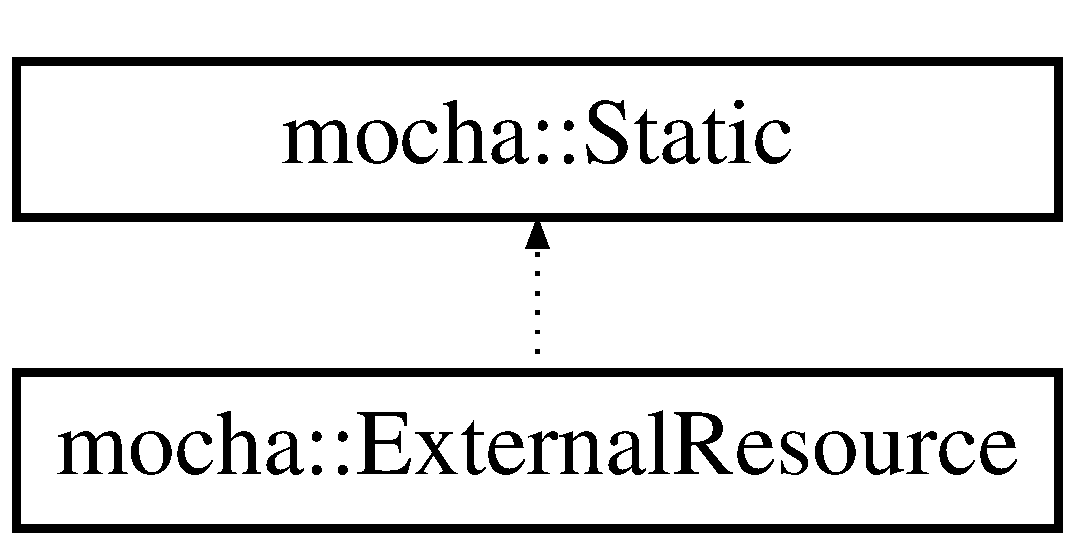
\includegraphics[height=2.000000cm]{classmocha_1_1_external_resource}
\end{center}
\end{figure}
\subsection*{Static Public Member Functions}
\begin{DoxyCompactItemize}
\item 
static void \hyperlink{classmocha_1_1_external_resource_a79ef20671c0a4b32c48d771c4785abd8}{UnsafeSet} (const char $\ast$filename)
\item 
static \hyperlink{classmocha_1_1_resources}{Resources} $\ast$ \hyperlink{classmocha_1_1_external_resource_ad9b2039a630d4d7fd4faed7c09c4eaab}{UnsafeGet} (const char $\ast$filename)
\item 
static void \hyperlink{classmocha_1_1_external_resource_afd20379c327ffe5396604545c78c066e}{SafeSet} (const char $\ast$filename)
\item 
static \hyperlink{classmocha_1_1_resources}{Resources} $\ast$ \hyperlink{classmocha_1_1_external_resource_a2d9388826910a37f40cc474ce1795f50}{SafeGet} (const char $\ast$filename)
\item 
static \hyperlink{classmocha_1_1_file_root}{FileRoot} $\ast$ \hyperlink{classmocha_1_1_external_resource_a648c5fe956b22d4a2dccc77f90a46827}{SafeGetRuntime} ()
\end{DoxyCompactItemize}
\subsection*{Private Types}
\begin{DoxyCompactItemize}
\item 
typedef \hyperlink{classmocha_1_1_hash_map}{HashMap}$<$ const char $\ast$, \hyperlink{classmocha_1_1_handle}{Handle}$<$ \hyperlink{classmocha_1_1_resources}{Resources} $>$ $>$ \hyperlink{classmocha_1_1_external_resource_af0eea09b4fa837b559799d0d6fa1ac95}{ResourceMap}
\end{DoxyCompactItemize}
\subsection*{Static Private Attributes}
\begin{DoxyCompactItemize}
\item 
static \hyperlink{classmocha_1_1_mutex}{Mutex} \hyperlink{classmocha_1_1_external_resource_a79acd6713f0f1923efc59dae6a8cd61c}{mutex\_\-}
\item 
static \hyperlink{classmocha_1_1_hash_map}{ResourceMap} \hyperlink{classmocha_1_1_external_resource_a31d3e9277c6e9150224e9cc181b042d3}{resources\_\-}
\end{DoxyCompactItemize}


\subsection{Detailed Description}


Definition at line 38 of file external\_\-resource.h.



\subsection{Member Typedef Documentation}
\hypertarget{classmocha_1_1_external_resource_af0eea09b4fa837b559799d0d6fa1ac95}{
\index{mocha::ExternalResource@{mocha::ExternalResource}!ResourceMap@{ResourceMap}}
\index{ResourceMap@{ResourceMap}!mocha::ExternalResource@{mocha::ExternalResource}}
\subsubsection[{ResourceMap}]{\setlength{\rightskip}{0pt plus 5cm}typedef {\bf HashMap}$<$const char$\ast$, {\bf Handle}$<${\bf Resources}$>$ $>$ {\bf mocha::ExternalResource::ResourceMap}\hspace{0.3cm}{\ttfamily  \mbox{[}private\mbox{]}}}}
\label{classmocha_1_1_external_resource_af0eea09b4fa837b559799d0d6fa1ac95}


Definition at line 39 of file external\_\-resource.h.



\subsection{Member Function Documentation}
\hypertarget{classmocha_1_1_external_resource_a2d9388826910a37f40cc474ce1795f50}{
\index{mocha::ExternalResource@{mocha::ExternalResource}!SafeGet@{SafeGet}}
\index{SafeGet@{SafeGet}!mocha::ExternalResource@{mocha::ExternalResource}}
\subsubsection[{SafeGet}]{\setlength{\rightskip}{0pt plus 5cm}{\bf Resources} $\ast$ mocha::ExternalResource::SafeGet (
\begin{DoxyParamCaption}
\item[{const char $\ast$}]{filename}
\end{DoxyParamCaption}
)\hspace{0.3cm}{\ttfamily  \mbox{[}static\mbox{]}}}}
\label{classmocha_1_1_external_resource_a2d9388826910a37f40cc474ce1795f50}


Definition at line 123 of file external\_\-resource.cc.

\hypertarget{classmocha_1_1_external_resource_a648c5fe956b22d4a2dccc77f90a46827}{
\index{mocha::ExternalResource@{mocha::ExternalResource}!SafeGetRuntime@{SafeGetRuntime}}
\index{SafeGetRuntime@{SafeGetRuntime}!mocha::ExternalResource@{mocha::ExternalResource}}
\subsubsection[{SafeGetRuntime}]{\setlength{\rightskip}{0pt plus 5cm}{\bf FileRoot} $\ast$ mocha::ExternalResource::SafeGetRuntime (
\begin{DoxyParamCaption}
{}
\end{DoxyParamCaption}
)\hspace{0.3cm}{\ttfamily  \mbox{[}static\mbox{]}}}}
\label{classmocha_1_1_external_resource_a648c5fe956b22d4a2dccc77f90a46827}


Definition at line 132 of file external\_\-resource.cc.

\hypertarget{classmocha_1_1_external_resource_afd20379c327ffe5396604545c78c066e}{
\index{mocha::ExternalResource@{mocha::ExternalResource}!SafeSet@{SafeSet}}
\index{SafeSet@{SafeSet}!mocha::ExternalResource@{mocha::ExternalResource}}
\subsubsection[{SafeSet}]{\setlength{\rightskip}{0pt plus 5cm}void mocha::ExternalResource::SafeSet (
\begin{DoxyParamCaption}
\item[{const char $\ast$}]{filename}
\end{DoxyParamCaption}
)\hspace{0.3cm}{\ttfamily  \mbox{[}static\mbox{]}}}}
\label{classmocha_1_1_external_resource_afd20379c327ffe5396604545c78c066e}


Definition at line 109 of file external\_\-resource.cc.

\hypertarget{classmocha_1_1_external_resource_ad9b2039a630d4d7fd4faed7c09c4eaab}{
\index{mocha::ExternalResource@{mocha::ExternalResource}!UnsafeGet@{UnsafeGet}}
\index{UnsafeGet@{UnsafeGet}!mocha::ExternalResource@{mocha::ExternalResource}}
\subsubsection[{UnsafeGet}]{\setlength{\rightskip}{0pt plus 5cm}{\bf Resources} $\ast$ mocha::ExternalResource::UnsafeGet (
\begin{DoxyParamCaption}
\item[{const char $\ast$}]{filename}
\end{DoxyParamCaption}
)\hspace{0.3cm}{\ttfamily  \mbox{[}static\mbox{]}}}}
\label{classmocha_1_1_external_resource_ad9b2039a630d4d7fd4faed7c09c4eaab}


Definition at line 115 of file external\_\-resource.cc.

\hypertarget{classmocha_1_1_external_resource_a79ef20671c0a4b32c48d771c4785abd8}{
\index{mocha::ExternalResource@{mocha::ExternalResource}!UnsafeSet@{UnsafeSet}}
\index{UnsafeSet@{UnsafeSet}!mocha::ExternalResource@{mocha::ExternalResource}}
\subsubsection[{UnsafeSet}]{\setlength{\rightskip}{0pt plus 5cm}void mocha::ExternalResource::UnsafeSet (
\begin{DoxyParamCaption}
\item[{const char $\ast$}]{filename}
\end{DoxyParamCaption}
)\hspace{0.3cm}{\ttfamily  \mbox{[}static\mbox{]}}}}
\label{classmocha_1_1_external_resource_a79ef20671c0a4b32c48d771c4785abd8}


Definition at line 104 of file external\_\-resource.cc.



\subsection{Member Data Documentation}
\hypertarget{classmocha_1_1_external_resource_a79acd6713f0f1923efc59dae6a8cd61c}{
\index{mocha::ExternalResource@{mocha::ExternalResource}!mutex\_\-@{mutex\_\-}}
\index{mutex\_\-@{mutex\_\-}!mocha::ExternalResource@{mocha::ExternalResource}}
\subsubsection[{mutex\_\-}]{\setlength{\rightskip}{0pt plus 5cm}{\bf Mutex} {\bf mocha::ExternalResource::mutex\_\-}\hspace{0.3cm}{\ttfamily  \mbox{[}static, private\mbox{]}}}}
\label{classmocha_1_1_external_resource_a79acd6713f0f1923efc59dae6a8cd61c}


Definition at line 47 of file external\_\-resource.h.

\hypertarget{classmocha_1_1_external_resource_a31d3e9277c6e9150224e9cc181b042d3}{
\index{mocha::ExternalResource@{mocha::ExternalResource}!resources\_\-@{resources\_\-}}
\index{resources\_\-@{resources\_\-}!mocha::ExternalResource@{mocha::ExternalResource}}
\subsubsection[{resources\_\-}]{\setlength{\rightskip}{0pt plus 5cm}{\bf ExternalResource::ResourceMap} {\bf mocha::ExternalResource::resources\_\-}\hspace{0.3cm}{\ttfamily  \mbox{[}static, private\mbox{]}}}}
\label{classmocha_1_1_external_resource_a31d3e9277c6e9150224e9cc181b042d3}


Definition at line 48 of file external\_\-resource.h.



The documentation for this class was generated from the following files:\begin{DoxyCompactItemize}
\item 
Y:/mocha/src/compiler/external/\hyperlink{external__resource_8h}{external\_\-resource.h}\item 
Y:/mocha/src/compiler/external/\hyperlink{external__resource_8cc}{external\_\-resource.cc}\end{DoxyCompactItemize}

\hypertarget{classmocha_1_1_ex_yield_state_node}{
\section{mocha::ExYieldStateNode Class Reference}
\label{classmocha_1_1_ex_yield_state_node}\index{mocha::ExYieldStateNode@{mocha::ExYieldStateNode}}
}


{\ttfamily \#include $<$ast.h$>$}

Inheritance diagram for mocha::ExYieldStateNode:\begin{figure}[H]
\begin{center}
\leavevmode
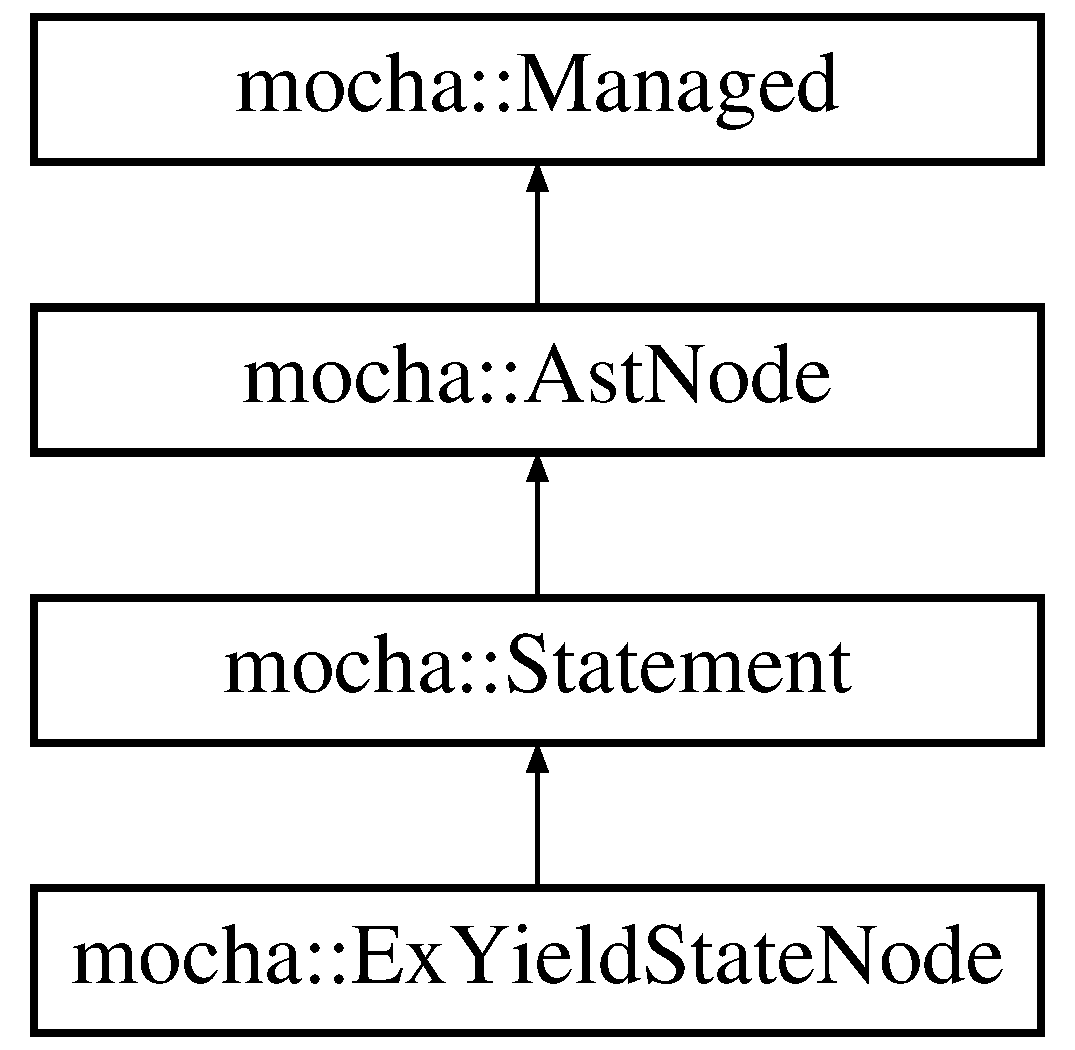
\includegraphics[height=4.000000cm]{classmocha_1_1_ex_yield_state_node}
\end{center}
\end{figure}
\subsection*{Public Member Functions}
\begin{DoxyCompactItemize}
\item 
\hyperlink{classmocha_1_1_ex_yield_state_node_addba376fc64693d3ff965dd7dcad0376}{ExYieldStateNode} ()
\item 
\hyperlink{classmocha_1_1_ex_yield_state_node_a1264a12271fd2c35c498518bb90dfedf}{$\sim$ExYieldStateNode} ()
\item 
\hyperlink{classmocha_1_1_ex_yield_state_node}{ExYieldStateNode} $\ast$ \hyperlink{classmocha_1_1_ex_yield_state_node_a5ca3856c558729bde56291fffd67f6aa}{CastToYieldState} ()
\item 
void \hyperlink{classmocha_1_1_ex_yield_state_node_a440502e981bb954e1c2a30f1a08421a6}{EscapePtr} (\hyperlink{classmocha_1_1_value_node}{ValueNode} $\ast$ptr)
\item 
\hyperlink{classmocha_1_1_value_node}{ValueNode} $\ast$ \hyperlink{classmocha_1_1_ex_yield_state_node_aa984ae10eb8433fa5c33f39ef65992c9}{EscapePtr} ()
\item 
void \hyperlink{classmocha_1_1_ex_yield_state_node_ab962dabbd734a8924c496d6b6ead4925}{LoopBackPtr} (\hyperlink{classmocha_1_1_value_node}{ValueNode} $\ast$ptr)
\item 
\hyperlink{classmocha_1_1_value_node}{ValueNode} $\ast$ \hyperlink{classmocha_1_1_ex_yield_state_node_a5281b200e431460d5b85af98ade7023a}{LoopBackPtr} ()
\item 
void \hyperlink{classmocha_1_1_ex_yield_state_node_a34b9392df493e8e2742057583671425f}{NextPtr} (\hyperlink{classmocha_1_1_value_node}{ValueNode} $\ast$ptr)
\item 
\hyperlink{classmocha_1_1_value_node}{ValueNode} $\ast$ \hyperlink{classmocha_1_1_ex_yield_state_node_a56a0c81549b486dbe5c08427ac015d25}{NextPtr} ()
\item 
void \hyperlink{classmocha_1_1_ex_yield_state_node_ae2b166cc09a3814db96915fdb6a17caf}{IfStmtPtr} (\hyperlink{classmocha_1_1_i_f_stmt}{IFStmt} $\ast$ptr)
\item 
\hyperlink{classmocha_1_1_i_f_stmt}{IFStmt} $\ast$ \hyperlink{classmocha_1_1_ex_yield_state_node_a3e8b19e1d655e8757a900d57f905e591}{IfStmtPtr} ()
\end{DoxyCompactItemize}
\subsection*{Private Attributes}
\begin{DoxyCompactItemize}
\item 
\hyperlink{classmocha_1_1_value_node}{ValueNode} $\ast$ \hyperlink{classmocha_1_1_ex_yield_state_node_ae976f2f49a4e1b6db92a6ae343de64be}{loopback\_\-ptr\_\-}
\item 
\hyperlink{classmocha_1_1_value_node}{ValueNode} $\ast$ \hyperlink{classmocha_1_1_ex_yield_state_node_ab8852eda607228274be8c3770d3dd410}{next\_\-ptr\_\-}
\item 
\hyperlink{classmocha_1_1_value_node}{ValueNode} $\ast$ \hyperlink{classmocha_1_1_ex_yield_state_node_a6261956ae7c0f624d904d6602d9bf29a}{escape\_\-ptr\_\-}
\item 
\hyperlink{classmocha_1_1_i_f_stmt}{IFStmt} $\ast$ \hyperlink{classmocha_1_1_ex_yield_state_node_a9d88b798e715b0285352a756d2cc8338}{if\_\-stmt\_\-ptr\_\-}
\end{DoxyCompactItemize}


\subsection{Detailed Description}


Definition at line 612 of file ast.h.



\subsection{Constructor \& Destructor Documentation}
\hypertarget{classmocha_1_1_ex_yield_state_node_addba376fc64693d3ff965dd7dcad0376}{
\index{mocha::ExYieldStateNode@{mocha::ExYieldStateNode}!ExYieldStateNode@{ExYieldStateNode}}
\index{ExYieldStateNode@{ExYieldStateNode}!mocha::ExYieldStateNode@{mocha::ExYieldStateNode}}
\subsubsection[{ExYieldStateNode}]{\setlength{\rightskip}{0pt plus 5cm}mocha::ExYieldStateNode::ExYieldStateNode (
\begin{DoxyParamCaption}
{}
\end{DoxyParamCaption}
)\hspace{0.3cm}{\ttfamily  \mbox{[}inline\mbox{]}}}}
\label{classmocha_1_1_ex_yield_state_node_addba376fc64693d3ff965dd7dcad0376}


Definition at line 614 of file ast.h.

\hypertarget{classmocha_1_1_ex_yield_state_node_a1264a12271fd2c35c498518bb90dfedf}{
\index{mocha::ExYieldStateNode@{mocha::ExYieldStateNode}!$\sim$ExYieldStateNode@{$\sim$ExYieldStateNode}}
\index{$\sim$ExYieldStateNode@{$\sim$ExYieldStateNode}!mocha::ExYieldStateNode@{mocha::ExYieldStateNode}}
\subsubsection[{$\sim$ExYieldStateNode}]{\setlength{\rightskip}{0pt plus 5cm}mocha::ExYieldStateNode::$\sim$ExYieldStateNode (
\begin{DoxyParamCaption}
{}
\end{DoxyParamCaption}
)\hspace{0.3cm}{\ttfamily  \mbox{[}inline\mbox{]}}}}
\label{classmocha_1_1_ex_yield_state_node_a1264a12271fd2c35c498518bb90dfedf}


Definition at line 617 of file ast.h.



\subsection{Member Function Documentation}
\hypertarget{classmocha_1_1_ex_yield_state_node_a5ca3856c558729bde56291fffd67f6aa}{
\index{mocha::ExYieldStateNode@{mocha::ExYieldStateNode}!CastToYieldState@{CastToYieldState}}
\index{CastToYieldState@{CastToYieldState}!mocha::ExYieldStateNode@{mocha::ExYieldStateNode}}
\subsubsection[{CastToYieldState}]{\setlength{\rightskip}{0pt plus 5cm}{\bf ExYieldStateNode}$\ast$ mocha::ExYieldStateNode::CastToYieldState (
\begin{DoxyParamCaption}
{}
\end{DoxyParamCaption}
)\hspace{0.3cm}{\ttfamily  \mbox{[}inline, virtual\mbox{]}}}}
\label{classmocha_1_1_ex_yield_state_node_a5ca3856c558729bde56291fffd67f6aa}


Reimplemented from \hyperlink{classmocha_1_1_statement_a21dd7e1d946eae1ab31113d2adc79110}{mocha::Statement}.



Definition at line 618 of file ast.h.

\hypertarget{classmocha_1_1_ex_yield_state_node_a440502e981bb954e1c2a30f1a08421a6}{
\index{mocha::ExYieldStateNode@{mocha::ExYieldStateNode}!EscapePtr@{EscapePtr}}
\index{EscapePtr@{EscapePtr}!mocha::ExYieldStateNode@{mocha::ExYieldStateNode}}
\subsubsection[{EscapePtr}]{\setlength{\rightskip}{0pt plus 5cm}void mocha::ExYieldStateNode::EscapePtr (
\begin{DoxyParamCaption}
\item[{{\bf ValueNode} $\ast$}]{ptr}
\end{DoxyParamCaption}
)\hspace{0.3cm}{\ttfamily  \mbox{[}inline\mbox{]}}}}
\label{classmocha_1_1_ex_yield_state_node_a440502e981bb954e1c2a30f1a08421a6}


Definition at line 619 of file ast.h.

\hypertarget{classmocha_1_1_ex_yield_state_node_aa984ae10eb8433fa5c33f39ef65992c9}{
\index{mocha::ExYieldStateNode@{mocha::ExYieldStateNode}!EscapePtr@{EscapePtr}}
\index{EscapePtr@{EscapePtr}!mocha::ExYieldStateNode@{mocha::ExYieldStateNode}}
\subsubsection[{EscapePtr}]{\setlength{\rightskip}{0pt plus 5cm}{\bf ValueNode}$\ast$ mocha::ExYieldStateNode::EscapePtr (
\begin{DoxyParamCaption}
{}
\end{DoxyParamCaption}
)\hspace{0.3cm}{\ttfamily  \mbox{[}inline\mbox{]}}}}
\label{classmocha_1_1_ex_yield_state_node_aa984ae10eb8433fa5c33f39ef65992c9}


Definition at line 620 of file ast.h.

\hypertarget{classmocha_1_1_ex_yield_state_node_a3e8b19e1d655e8757a900d57f905e591}{
\index{mocha::ExYieldStateNode@{mocha::ExYieldStateNode}!IfStmtPtr@{IfStmtPtr}}
\index{IfStmtPtr@{IfStmtPtr}!mocha::ExYieldStateNode@{mocha::ExYieldStateNode}}
\subsubsection[{IfStmtPtr}]{\setlength{\rightskip}{0pt plus 5cm}{\bf IFStmt}$\ast$ mocha::ExYieldStateNode::IfStmtPtr (
\begin{DoxyParamCaption}
{}
\end{DoxyParamCaption}
)\hspace{0.3cm}{\ttfamily  \mbox{[}inline\mbox{]}}}}
\label{classmocha_1_1_ex_yield_state_node_a3e8b19e1d655e8757a900d57f905e591}


Definition at line 626 of file ast.h.

\hypertarget{classmocha_1_1_ex_yield_state_node_ae2b166cc09a3814db96915fdb6a17caf}{
\index{mocha::ExYieldStateNode@{mocha::ExYieldStateNode}!IfStmtPtr@{IfStmtPtr}}
\index{IfStmtPtr@{IfStmtPtr}!mocha::ExYieldStateNode@{mocha::ExYieldStateNode}}
\subsubsection[{IfStmtPtr}]{\setlength{\rightskip}{0pt plus 5cm}void mocha::ExYieldStateNode::IfStmtPtr (
\begin{DoxyParamCaption}
\item[{{\bf IFStmt} $\ast$}]{ptr}
\end{DoxyParamCaption}
)\hspace{0.3cm}{\ttfamily  \mbox{[}inline\mbox{]}}}}
\label{classmocha_1_1_ex_yield_state_node_ae2b166cc09a3814db96915fdb6a17caf}


Definition at line 625 of file ast.h.

\hypertarget{classmocha_1_1_ex_yield_state_node_a5281b200e431460d5b85af98ade7023a}{
\index{mocha::ExYieldStateNode@{mocha::ExYieldStateNode}!LoopBackPtr@{LoopBackPtr}}
\index{LoopBackPtr@{LoopBackPtr}!mocha::ExYieldStateNode@{mocha::ExYieldStateNode}}
\subsubsection[{LoopBackPtr}]{\setlength{\rightskip}{0pt plus 5cm}{\bf ValueNode}$\ast$ mocha::ExYieldStateNode::LoopBackPtr (
\begin{DoxyParamCaption}
{}
\end{DoxyParamCaption}
)\hspace{0.3cm}{\ttfamily  \mbox{[}inline\mbox{]}}}}
\label{classmocha_1_1_ex_yield_state_node_a5281b200e431460d5b85af98ade7023a}


Definition at line 622 of file ast.h.

\hypertarget{classmocha_1_1_ex_yield_state_node_ab962dabbd734a8924c496d6b6ead4925}{
\index{mocha::ExYieldStateNode@{mocha::ExYieldStateNode}!LoopBackPtr@{LoopBackPtr}}
\index{LoopBackPtr@{LoopBackPtr}!mocha::ExYieldStateNode@{mocha::ExYieldStateNode}}
\subsubsection[{LoopBackPtr}]{\setlength{\rightskip}{0pt plus 5cm}void mocha::ExYieldStateNode::LoopBackPtr (
\begin{DoxyParamCaption}
\item[{{\bf ValueNode} $\ast$}]{ptr}
\end{DoxyParamCaption}
)\hspace{0.3cm}{\ttfamily  \mbox{[}inline\mbox{]}}}}
\label{classmocha_1_1_ex_yield_state_node_ab962dabbd734a8924c496d6b6ead4925}


Definition at line 621 of file ast.h.

\hypertarget{classmocha_1_1_ex_yield_state_node_a56a0c81549b486dbe5c08427ac015d25}{
\index{mocha::ExYieldStateNode@{mocha::ExYieldStateNode}!NextPtr@{NextPtr}}
\index{NextPtr@{NextPtr}!mocha::ExYieldStateNode@{mocha::ExYieldStateNode}}
\subsubsection[{NextPtr}]{\setlength{\rightskip}{0pt plus 5cm}{\bf ValueNode}$\ast$ mocha::ExYieldStateNode::NextPtr (
\begin{DoxyParamCaption}
{}
\end{DoxyParamCaption}
)\hspace{0.3cm}{\ttfamily  \mbox{[}inline\mbox{]}}}}
\label{classmocha_1_1_ex_yield_state_node_a56a0c81549b486dbe5c08427ac015d25}


Definition at line 624 of file ast.h.

\hypertarget{classmocha_1_1_ex_yield_state_node_a34b9392df493e8e2742057583671425f}{
\index{mocha::ExYieldStateNode@{mocha::ExYieldStateNode}!NextPtr@{NextPtr}}
\index{NextPtr@{NextPtr}!mocha::ExYieldStateNode@{mocha::ExYieldStateNode}}
\subsubsection[{NextPtr}]{\setlength{\rightskip}{0pt plus 5cm}void mocha::ExYieldStateNode::NextPtr (
\begin{DoxyParamCaption}
\item[{{\bf ValueNode} $\ast$}]{ptr}
\end{DoxyParamCaption}
)\hspace{0.3cm}{\ttfamily  \mbox{[}inline\mbox{]}}}}
\label{classmocha_1_1_ex_yield_state_node_a34b9392df493e8e2742057583671425f}


Definition at line 623 of file ast.h.



\subsection{Member Data Documentation}
\hypertarget{classmocha_1_1_ex_yield_state_node_a6261956ae7c0f624d904d6602d9bf29a}{
\index{mocha::ExYieldStateNode@{mocha::ExYieldStateNode}!escape\_\-ptr\_\-@{escape\_\-ptr\_\-}}
\index{escape\_\-ptr\_\-@{escape\_\-ptr\_\-}!mocha::ExYieldStateNode@{mocha::ExYieldStateNode}}
\subsubsection[{escape\_\-ptr\_\-}]{\setlength{\rightskip}{0pt plus 5cm}{\bf ValueNode}$\ast$ {\bf mocha::ExYieldStateNode::escape\_\-ptr\_\-}\hspace{0.3cm}{\ttfamily  \mbox{[}private\mbox{]}}}}
\label{classmocha_1_1_ex_yield_state_node_a6261956ae7c0f624d904d6602d9bf29a}


Definition at line 630 of file ast.h.

\hypertarget{classmocha_1_1_ex_yield_state_node_a9d88b798e715b0285352a756d2cc8338}{
\index{mocha::ExYieldStateNode@{mocha::ExYieldStateNode}!if\_\-stmt\_\-ptr\_\-@{if\_\-stmt\_\-ptr\_\-}}
\index{if\_\-stmt\_\-ptr\_\-@{if\_\-stmt\_\-ptr\_\-}!mocha::ExYieldStateNode@{mocha::ExYieldStateNode}}
\subsubsection[{if\_\-stmt\_\-ptr\_\-}]{\setlength{\rightskip}{0pt plus 5cm}{\bf IFStmt}$\ast$ {\bf mocha::ExYieldStateNode::if\_\-stmt\_\-ptr\_\-}\hspace{0.3cm}{\ttfamily  \mbox{[}private\mbox{]}}}}
\label{classmocha_1_1_ex_yield_state_node_a9d88b798e715b0285352a756d2cc8338}


Definition at line 631 of file ast.h.

\hypertarget{classmocha_1_1_ex_yield_state_node_ae976f2f49a4e1b6db92a6ae343de64be}{
\index{mocha::ExYieldStateNode@{mocha::ExYieldStateNode}!loopback\_\-ptr\_\-@{loopback\_\-ptr\_\-}}
\index{loopback\_\-ptr\_\-@{loopback\_\-ptr\_\-}!mocha::ExYieldStateNode@{mocha::ExYieldStateNode}}
\subsubsection[{loopback\_\-ptr\_\-}]{\setlength{\rightskip}{0pt plus 5cm}{\bf ValueNode}$\ast$ {\bf mocha::ExYieldStateNode::loopback\_\-ptr\_\-}\hspace{0.3cm}{\ttfamily  \mbox{[}private\mbox{]}}}}
\label{classmocha_1_1_ex_yield_state_node_ae976f2f49a4e1b6db92a6ae343de64be}


Definition at line 628 of file ast.h.

\hypertarget{classmocha_1_1_ex_yield_state_node_ab8852eda607228274be8c3770d3dd410}{
\index{mocha::ExYieldStateNode@{mocha::ExYieldStateNode}!next\_\-ptr\_\-@{next\_\-ptr\_\-}}
\index{next\_\-ptr\_\-@{next\_\-ptr\_\-}!mocha::ExYieldStateNode@{mocha::ExYieldStateNode}}
\subsubsection[{next\_\-ptr\_\-}]{\setlength{\rightskip}{0pt plus 5cm}{\bf ValueNode}$\ast$ {\bf mocha::ExYieldStateNode::next\_\-ptr\_\-}\hspace{0.3cm}{\ttfamily  \mbox{[}private\mbox{]}}}}
\label{classmocha_1_1_ex_yield_state_node_ab8852eda607228274be8c3770d3dd410}


Definition at line 629 of file ast.h.



The documentation for this class was generated from the following file:\begin{DoxyCompactItemize}
\item 
Y:/mocha/src/ast/\hyperlink{ast_8h}{ast.h}\end{DoxyCompactItemize}

\hypertarget{classmocha_1_1_file}{
\section{mocha::File Class Reference}
\label{classmocha_1_1_file}\index{mocha::File@{mocha::File}}
}


{\ttfamily \#include $<$file\_\-io.h$>$}

\subsection*{Public Types}
\begin{DoxyCompactItemize}
\item 
enum \hyperlink{classmocha_1_1_file_a86110d8e8c2dfa58f84ae6617aa1fb6a}{DateType} \{ \hyperlink{classmocha_1_1_file_a86110d8e8c2dfa58f84ae6617aa1fb6aae03a7ea608ce891c3b92ee0716ed844a}{kUpdate}, 
\hyperlink{classmocha_1_1_file_a86110d8e8c2dfa58f84ae6617aa1fb6aace95f694456c939dc96b07d816b6dfb7}{kCreate}
 \}
\end{DoxyCompactItemize}
\subsection*{Public Member Functions}
\begin{DoxyCompactItemize}
\item 
\hyperlink{classmocha_1_1_file_ae039af5807fc385f41b60644725d15d0}{File} ()
\item 
\hyperlink{classmocha_1_1_file_abd7ef89b6d9000d2ff75ef78965c5ab6}{File} (int \hyperlink{classmocha_1_1_file_ac34e63054b7ff96513b163692909bc06}{fd}, const char $\ast$path, unsigned int \hyperlink{classmocha_1_1_file_aedc322e34cdfe5248644cf425b165ae7}{openType}, \hyperlink{classmocha_1_1_stat}{Stat} $\ast$\hyperlink{classmocha_1_1_file_a1af3675df21335d14aefa9d775c808e2}{fstat}, bool isNeedLock)
\item 
\hyperlink{classmocha_1_1_file_a59bf1e7bb0c6b8dd83dccef6b942a0f9}{File} (const \hyperlink{classmocha_1_1_file}{File} \&file)
\item 
\hyperlink{classmocha_1_1_file_ac704ebdf5f57d7a1c5ddf409d797fb69}{$\sim$File} ()
\item 
\hyperlink{classmocha_1_1_file}{File} \& \hyperlink{classmocha_1_1_file_a8160d4f295558728cc217d4740cbd01e}{operator=} (const \hyperlink{classmocha_1_1_file}{File} \&file)
\item 
void \hyperlink{classmocha_1_1_file_a7ce241fcabbbbed256d1d2beb5de300f}{Close} ()
\item 
\hyperlink{classmocha_1_1_allocator_handle}{CStrHandle} \hyperlink{classmocha_1_1_file_a38e9611c580c29cef7d992e9093847ee}{GetFileContents} ()
\item 
void \hyperlink{classmocha_1_1_file_a544e01571f2abe1a85535af34bff010e}{GetFileContents} (std::string \&str)
\item 
int \hyperlink{classmocha_1_1_file_afe41d2812a4c6c47f8f90c3a3a7b8b38}{Write} (const char $\ast$buf)
\item 
int \hyperlink{classmocha_1_1_file_ad399ddacdbe03508f436d212a0068b2e}{ReadSync} (char $\ast$buf, size\_\-t size)
\item 
bool \hyperlink{classmocha_1_1_file_af32f10e682a473e2d1f26b223f84092a}{IsSuccess} ()
\item 
\hyperlink{classmocha_1_1_array_handle}{StrHandle} \hyperlink{classmocha_1_1_file_a90999c2a1d0bf842f46daed77d9e20a7}{GetDate} (\hyperlink{classmocha_1_1_file_a86110d8e8c2dfa58f84ae6617aa1fb6a}{DateType} type=kUpdate)
\item 
long int \hyperlink{classmocha_1_1_file_a4a951d40672719f17aa9d779f51b37ba}{GetSize} ()
\item 
const char $\ast$ \hyperlink{classmocha_1_1_file_a824c8f6dfaec9e9b7639973995edf7f5}{GetFileName} ()
\end{DoxyCompactItemize}
\subsection*{Private Member Functions}
\begin{DoxyCompactItemize}
\item 
char $\ast$ \hyperlink{classmocha_1_1_file_ac0e5cc0f09384b1298243ac5f9dd68a4}{Allocate} (size\_\-t size)
\item 
char $\ast$ \hyperlink{classmocha_1_1_file_a64bbdac45b1e87ef4087d1b55e717fc0}{Reallocate} (char $\ast$buffer, size\_\-t size)
\end{DoxyCompactItemize}
\subsection*{Private Attributes}
\begin{DoxyCompactItemize}
\item 
int \hyperlink{classmocha_1_1_file_ac34e63054b7ff96513b163692909bc06}{fd}
\item 
\hyperlink{classmocha_1_1_stat}{Stat} $\ast$ \hyperlink{classmocha_1_1_file_a1af3675df21335d14aefa9d775c808e2}{fstat}
\item 
bool \hyperlink{classmocha_1_1_file_a9c49e57fb0a425d80226ea3962f7f1ad}{isLocked}
\item 
bool \hyperlink{classmocha_1_1_file_a3a79db70f833a45ee94ea3f35ce270b8}{opened}
\item 
unsigned int \hyperlink{classmocha_1_1_file_aedc322e34cdfe5248644cf425b165ae7}{openType}
\item 
std::string \hyperlink{classmocha_1_1_file_ab9331e1a837f5d7b73925b9c836bc754}{path\_\-}
\end{DoxyCompactItemize}


\subsection{Detailed Description}


Definition at line 19 of file file\_\-io.h.



\subsection{Member Enumeration Documentation}
\hypertarget{classmocha_1_1_file_a86110d8e8c2dfa58f84ae6617aa1fb6a}{
\index{mocha::File@{mocha::File}!DateType@{DateType}}
\index{DateType@{DateType}!mocha::File@{mocha::File}}
\subsubsection[{DateType}]{\setlength{\rightskip}{0pt plus 5cm}enum {\bf mocha::File::DateType}}}
\label{classmocha_1_1_file_a86110d8e8c2dfa58f84ae6617aa1fb6a}
\begin{Desc}
\item[Enumerator: ]\par
\begin{description}
\index{kUpdate@{kUpdate}!mocha::File@{mocha::File}}\index{mocha::File@{mocha::File}!kUpdate@{kUpdate}}\item[{\em 
\hypertarget{classmocha_1_1_file_a86110d8e8c2dfa58f84ae6617aa1fb6aae03a7ea608ce891c3b92ee0716ed844a}{
kUpdate}
\label{classmocha_1_1_file_a86110d8e8c2dfa58f84ae6617aa1fb6aae03a7ea608ce891c3b92ee0716ed844a}
}]\index{kCreate@{kCreate}!mocha::File@{mocha::File}}\index{mocha::File@{mocha::File}!kCreate@{kCreate}}\item[{\em 
\hypertarget{classmocha_1_1_file_a86110d8e8c2dfa58f84ae6617aa1fb6aace95f694456c939dc96b07d816b6dfb7}{
kCreate}
\label{classmocha_1_1_file_a86110d8e8c2dfa58f84ae6617aa1fb6aace95f694456c939dc96b07d816b6dfb7}
}]\end{description}
\end{Desc}



Definition at line 36 of file file\_\-io.h.



\subsection{Constructor \& Destructor Documentation}
\hypertarget{classmocha_1_1_file_ae039af5807fc385f41b60644725d15d0}{
\index{mocha::File@{mocha::File}!File@{File}}
\index{File@{File}!mocha::File@{mocha::File}}
\subsubsection[{File}]{\setlength{\rightskip}{0pt plus 5cm}File::File (
\begin{DoxyParamCaption}
{}
\end{DoxyParamCaption}
)}}
\label{classmocha_1_1_file_ae039af5807fc385f41b60644725d15d0}


Definition at line 116 of file file\_\-io.cc.

\hypertarget{classmocha_1_1_file_abd7ef89b6d9000d2ff75ef78965c5ab6}{
\index{mocha::File@{mocha::File}!File@{File}}
\index{File@{File}!mocha::File@{mocha::File}}
\subsubsection[{File}]{\setlength{\rightskip}{0pt plus 5cm}File::File (
\begin{DoxyParamCaption}
\item[{int}]{fd, }
\item[{const char $\ast$}]{path, }
\item[{unsigned int}]{openType, }
\item[{{\bf Stat} $\ast$}]{fstat, }
\item[{bool}]{isNeedLock}
\end{DoxyParamCaption}
)}}
\label{classmocha_1_1_file_abd7ef89b6d9000d2ff75ef78965c5ab6}


Definition at line 123 of file file\_\-io.cc.

\hypertarget{classmocha_1_1_file_a59bf1e7bb0c6b8dd83dccef6b942a0f9}{
\index{mocha::File@{mocha::File}!File@{File}}
\index{File@{File}!mocha::File@{mocha::File}}
\subsubsection[{File}]{\setlength{\rightskip}{0pt plus 5cm}File::File (
\begin{DoxyParamCaption}
\item[{const {\bf File} \&}]{file}
\end{DoxyParamCaption}
)}}
\label{classmocha_1_1_file_a59bf1e7bb0c6b8dd83dccef6b942a0f9}


Definition at line 135 of file file\_\-io.cc.

\hypertarget{classmocha_1_1_file_ac704ebdf5f57d7a1c5ddf409d797fb69}{
\index{mocha::File@{mocha::File}!$\sim$File@{$\sim$File}}
\index{$\sim$File@{$\sim$File}!mocha::File@{mocha::File}}
\subsubsection[{$\sim$File}]{\setlength{\rightskip}{0pt plus 5cm}File::$\sim$File (
\begin{DoxyParamCaption}
{}
\end{DoxyParamCaption}
)}}
\label{classmocha_1_1_file_ac704ebdf5f57d7a1c5ddf409d797fb69}


Definition at line 141 of file file\_\-io.cc.



\subsection{Member Function Documentation}
\hypertarget{classmocha_1_1_file_ac0e5cc0f09384b1298243ac5f9dd68a4}{
\index{mocha::File@{mocha::File}!Allocate@{Allocate}}
\index{Allocate@{Allocate}!mocha::File@{mocha::File}}
\subsubsection[{Allocate}]{\setlength{\rightskip}{0pt plus 5cm}char $\ast$ File::Allocate (
\begin{DoxyParamCaption}
\item[{size\_\-t}]{size}
\end{DoxyParamCaption}
)\hspace{0.3cm}{\ttfamily  \mbox{[}inline, private\mbox{]}}}}
\label{classmocha_1_1_file_ac0e5cc0f09384b1298243ac5f9dd68a4}


Definition at line 108 of file file\_\-io.cc.

\hypertarget{classmocha_1_1_file_a7ce241fcabbbbed256d1d2beb5de300f}{
\index{mocha::File@{mocha::File}!Close@{Close}}
\index{Close@{Close}!mocha::File@{mocha::File}}
\subsubsection[{Close}]{\setlength{\rightskip}{0pt plus 5cm}void File::Close (
\begin{DoxyParamCaption}
{}
\end{DoxyParamCaption}
)}}
\label{classmocha_1_1_file_a7ce241fcabbbbed256d1d2beb5de300f}


Definition at line 155 of file file\_\-io.cc.

\hypertarget{classmocha_1_1_file_a90999c2a1d0bf842f46daed77d9e20a7}{
\index{mocha::File@{mocha::File}!GetDate@{GetDate}}
\index{GetDate@{GetDate}!mocha::File@{mocha::File}}
\subsubsection[{GetDate}]{\setlength{\rightskip}{0pt plus 5cm}{\bf StrHandle} File::GetDate (
\begin{DoxyParamCaption}
\item[{{\bf DateType}}]{type = {\ttfamily kUpdate}}
\end{DoxyParamCaption}
)}}
\label{classmocha_1_1_file_a90999c2a1d0bf842f46daed77d9e20a7}


Definition at line 230 of file file\_\-io.cc.

\hypertarget{classmocha_1_1_file_a38e9611c580c29cef7d992e9093847ee}{
\index{mocha::File@{mocha::File}!GetFileContents@{GetFileContents}}
\index{GetFileContents@{GetFileContents}!mocha::File@{mocha::File}}
\subsubsection[{GetFileContents}]{\setlength{\rightskip}{0pt plus 5cm}{\bf CStrHandle} File::GetFileContents (
\begin{DoxyParamCaption}
{}
\end{DoxyParamCaption}
)}}
\label{classmocha_1_1_file_a38e9611c580c29cef7d992e9093847ee}


Definition at line 166 of file file\_\-io.cc.

\hypertarget{classmocha_1_1_file_a544e01571f2abe1a85535af34bff010e}{
\index{mocha::File@{mocha::File}!GetFileContents@{GetFileContents}}
\index{GetFileContents@{GetFileContents}!mocha::File@{mocha::File}}
\subsubsection[{GetFileContents}]{\setlength{\rightskip}{0pt plus 5cm}void File::GetFileContents (
\begin{DoxyParamCaption}
\item[{std::string \&}]{str}
\end{DoxyParamCaption}
)}}
\label{classmocha_1_1_file_a544e01571f2abe1a85535af34bff010e}


Definition at line 186 of file file\_\-io.cc.

\hypertarget{classmocha_1_1_file_a824c8f6dfaec9e9b7639973995edf7f5}{
\index{mocha::File@{mocha::File}!GetFileName@{GetFileName}}
\index{GetFileName@{GetFileName}!mocha::File@{mocha::File}}
\subsubsection[{GetFileName}]{\setlength{\rightskip}{0pt plus 5cm}const char $\ast$ File::GetFileName (
\begin{DoxyParamCaption}
{}
\end{DoxyParamCaption}
)}}
\label{classmocha_1_1_file_a824c8f6dfaec9e9b7639973995edf7f5}


Definition at line 199 of file file\_\-io.cc.

\hypertarget{classmocha_1_1_file_a4a951d40672719f17aa9d779f51b37ba}{
\index{mocha::File@{mocha::File}!GetSize@{GetSize}}
\index{GetSize@{GetSize}!mocha::File@{mocha::File}}
\subsubsection[{GetSize}]{\setlength{\rightskip}{0pt plus 5cm}long int File::GetSize (
\begin{DoxyParamCaption}
{}
\end{DoxyParamCaption}
)}}
\label{classmocha_1_1_file_a4a951d40672719f17aa9d779f51b37ba}


Definition at line 241 of file file\_\-io.cc.

\hypertarget{classmocha_1_1_file_af32f10e682a473e2d1f26b223f84092a}{
\index{mocha::File@{mocha::File}!IsSuccess@{IsSuccess}}
\index{IsSuccess@{IsSuccess}!mocha::File@{mocha::File}}
\subsubsection[{IsSuccess}]{\setlength{\rightskip}{0pt plus 5cm}bool File::IsSuccess (
\begin{DoxyParamCaption}
{}
\end{DoxyParamCaption}
)}}
\label{classmocha_1_1_file_af32f10e682a473e2d1f26b223f84092a}


Definition at line 226 of file file\_\-io.cc.

\hypertarget{classmocha_1_1_file_a8160d4f295558728cc217d4740cbd01e}{
\index{mocha::File@{mocha::File}!operator=@{operator=}}
\index{operator=@{operator=}!mocha::File@{mocha::File}}
\subsubsection[{operator=}]{\setlength{\rightskip}{0pt plus 5cm}{\bf File} \& File::operator= (
\begin{DoxyParamCaption}
\item[{const {\bf File} \&}]{file}
\end{DoxyParamCaption}
)}}
\label{classmocha_1_1_file_a8160d4f295558728cc217d4740cbd01e}


Definition at line 148 of file file\_\-io.cc.

\hypertarget{classmocha_1_1_file_ad399ddacdbe03508f436d212a0068b2e}{
\index{mocha::File@{mocha::File}!ReadSync@{ReadSync}}
\index{ReadSync@{ReadSync}!mocha::File@{mocha::File}}
\subsubsection[{ReadSync}]{\setlength{\rightskip}{0pt plus 5cm}int File::ReadSync (
\begin{DoxyParamCaption}
\item[{char $\ast$}]{buf, }
\item[{size\_\-t}]{size}
\end{DoxyParamCaption}
)}}
\label{classmocha_1_1_file_ad399ddacdbe03508f436d212a0068b2e}


Definition at line 221 of file file\_\-io.cc.

\hypertarget{classmocha_1_1_file_a64bbdac45b1e87ef4087d1b55e717fc0}{
\index{mocha::File@{mocha::File}!Reallocate@{Reallocate}}
\index{Reallocate@{Reallocate}!mocha::File@{mocha::File}}
\subsubsection[{Reallocate}]{\setlength{\rightskip}{0pt plus 5cm}char $\ast$ File::Reallocate (
\begin{DoxyParamCaption}
\item[{char $\ast$}]{buffer, }
\item[{size\_\-t}]{size}
\end{DoxyParamCaption}
)\hspace{0.3cm}{\ttfamily  \mbox{[}inline, private\mbox{]}}}}
\label{classmocha_1_1_file_a64bbdac45b1e87ef4087d1b55e717fc0}


Definition at line 112 of file file\_\-io.cc.

\hypertarget{classmocha_1_1_file_afe41d2812a4c6c47f8f90c3a3a7b8b38}{
\index{mocha::File@{mocha::File}!Write@{Write}}
\index{Write@{Write}!mocha::File@{mocha::File}}
\subsubsection[{Write}]{\setlength{\rightskip}{0pt plus 5cm}int File::Write (
\begin{DoxyParamCaption}
\item[{const char $\ast$}]{buf}
\end{DoxyParamCaption}
)}}
\label{classmocha_1_1_file_afe41d2812a4c6c47f8f90c3a3a7b8b38}


Definition at line 203 of file file\_\-io.cc.



\subsection{Member Data Documentation}
\hypertarget{classmocha_1_1_file_ac34e63054b7ff96513b163692909bc06}{
\index{mocha::File@{mocha::File}!fd@{fd}}
\index{fd@{fd}!mocha::File@{mocha::File}}
\subsubsection[{fd}]{\setlength{\rightskip}{0pt plus 5cm}int {\bf mocha::File::fd}\hspace{0.3cm}{\ttfamily  \mbox{[}private\mbox{]}}}}
\label{classmocha_1_1_file_ac34e63054b7ff96513b163692909bc06}


Definition at line 22 of file file\_\-io.h.

\hypertarget{classmocha_1_1_file_a1af3675df21335d14aefa9d775c808e2}{
\index{mocha::File@{mocha::File}!fstat@{fstat}}
\index{fstat@{fstat}!mocha::File@{mocha::File}}
\subsubsection[{fstat}]{\setlength{\rightskip}{0pt plus 5cm}{\bf Stat}$\ast$ {\bf mocha::File::fstat}\hspace{0.3cm}{\ttfamily  \mbox{[}private\mbox{]}}}}
\label{classmocha_1_1_file_a1af3675df21335d14aefa9d775c808e2}


Definition at line 23 of file file\_\-io.h.

\hypertarget{classmocha_1_1_file_a9c49e57fb0a425d80226ea3962f7f1ad}{
\index{mocha::File@{mocha::File}!isLocked@{isLocked}}
\index{isLocked@{isLocked}!mocha::File@{mocha::File}}
\subsubsection[{isLocked}]{\setlength{\rightskip}{0pt plus 5cm}bool {\bf mocha::File::isLocked}\hspace{0.3cm}{\ttfamily  \mbox{[}private\mbox{]}}}}
\label{classmocha_1_1_file_a9c49e57fb0a425d80226ea3962f7f1ad}


Definition at line 24 of file file\_\-io.h.

\hypertarget{classmocha_1_1_file_a3a79db70f833a45ee94ea3f35ce270b8}{
\index{mocha::File@{mocha::File}!opened@{opened}}
\index{opened@{opened}!mocha::File@{mocha::File}}
\subsubsection[{opened}]{\setlength{\rightskip}{0pt plus 5cm}bool {\bf mocha::File::opened}\hspace{0.3cm}{\ttfamily  \mbox{[}private\mbox{]}}}}
\label{classmocha_1_1_file_a3a79db70f833a45ee94ea3f35ce270b8}


Definition at line 25 of file file\_\-io.h.

\hypertarget{classmocha_1_1_file_aedc322e34cdfe5248644cf425b165ae7}{
\index{mocha::File@{mocha::File}!openType@{openType}}
\index{openType@{openType}!mocha::File@{mocha::File}}
\subsubsection[{openType}]{\setlength{\rightskip}{0pt plus 5cm}unsigned int {\bf mocha::File::openType}\hspace{0.3cm}{\ttfamily  \mbox{[}private\mbox{]}}}}
\label{classmocha_1_1_file_aedc322e34cdfe5248644cf425b165ae7}


Definition at line 27 of file file\_\-io.h.

\hypertarget{classmocha_1_1_file_ab9331e1a837f5d7b73925b9c836bc754}{
\index{mocha::File@{mocha::File}!path\_\-@{path\_\-}}
\index{path\_\-@{path\_\-}!mocha::File@{mocha::File}}
\subsubsection[{path\_\-}]{\setlength{\rightskip}{0pt plus 5cm}std::string {\bf mocha::File::path\_\-}\hspace{0.3cm}{\ttfamily  \mbox{[}private\mbox{]}}}}
\label{classmocha_1_1_file_ab9331e1a837f5d7b73925b9c836bc754}


Definition at line 33 of file file\_\-io.h.



The documentation for this class was generated from the following files:\begin{DoxyCompactItemize}
\item 
Y:/mocha/src/utils/io/\hyperlink{file__io_8h}{file\_\-io.h}\item 
Y:/mocha/src/utils/io/\hyperlink{file__io_8cc}{file\_\-io.cc}\end{DoxyCompactItemize}

\hypertarget{classmocha_1_1_file_i_o}{
\section{mocha::FileIO Class Reference}
\label{classmocha_1_1_file_i_o}\index{mocha::FileIO@{mocha::FileIO}}
}


{\ttfamily \#include $<$file\_\-io.h$>$}

\subsection*{Public Types}
\begin{DoxyCompactItemize}
\item 
enum \{ \hyperlink{classmocha_1_1_file_i_o_a33f3257114b98f0bcfd1b453502322ccacde5ebe2d91c18522bb0f9258c35224f}{P\_\-ReadOnly} =  1, 
\hyperlink{classmocha_1_1_file_i_o_a33f3257114b98f0bcfd1b453502322cca18755b1d05959c7f280a15ab63a8396a}{P\_\-ReadWrite} =  2
 \}
\end{DoxyCompactItemize}
\subsection*{Static Public Member Functions}
\begin{DoxyCompactItemize}
\item 
static \hyperlink{classmocha_1_1_handle}{Handle}$<$ \hyperlink{classmocha_1_1_file}{File} $>$ \hyperlink{classmocha_1_1_file_i_o_a3dbfdb307776b6f8dd0dd2c6e5eed0ff}{Open} (const char $\ast$path, const char $\ast$mode, int access=0)
\item 
static bool \hyperlink{classmocha_1_1_file_i_o_af6d4b2eca0924785626797e8b2e799d6}{IsExist} (const char $\ast$path)
\item 
static int \hyperlink{classmocha_1_1_file_i_o_a91a7a2d0bc5a95eac39d012675f77be5}{CreateFile} (const char $\ast$filename, int access=0)
\item 
static void \hyperlink{classmocha_1_1_file_i_o_a55384acfc71fae22fb3f453c6775ba59}{CloseAll} ()
\end{DoxyCompactItemize}
\subsection*{Private Types}
\begin{DoxyCompactItemize}
\item 
enum \hyperlink{classmocha_1_1_file_i_o_a0fc42568b39966bf458cad23ebd4592b}{OpenType} \{ \par
\hyperlink{classmocha_1_1_file_i_o_a0fc42568b39966bf458cad23ebd4592ba5a926b3e3cec0258e0e72c09a57b1adc}{Binary} =  0, 
\hyperlink{classmocha_1_1_file_i_o_a0fc42568b39966bf458cad23ebd4592ba6a6781f4bb593323b7e9a09a62c45a48}{ReadOnly} =  1, 
\hyperlink{classmocha_1_1_file_i_o_a0fc42568b39966bf458cad23ebd4592ba32eacb43edc2c4a9b846ff03e3d10bbc}{WriteOnly} =  2, 
\hyperlink{classmocha_1_1_file_i_o_a0fc42568b39966bf458cad23ebd4592bad1e1a88fb630fb3ee8592942896f0acb}{ReadWrite} =  3, 
\par
\hyperlink{classmocha_1_1_file_i_o_a0fc42568b39966bf458cad23ebd4592ba827e8d86378cd10098ab7711460b004f}{Create} =  4, 
\hyperlink{classmocha_1_1_file_i_o_a0fc42568b39966bf458cad23ebd4592bafb7a1c2e702815da7a98f519f54e623c}{Append} =  5, 
\hyperlink{classmocha_1_1_file_i_o_a0fc42568b39966bf458cad23ebd4592ba2929a48da17d24e6c50cc3bd0aea9269}{Text} =  6, 
\hyperlink{classmocha_1_1_file_i_o_a0fc42568b39966bf458cad23ebd4592ba9516a0e162683c5eabf14b8c52e9812d}{New} =  7
 \}
\item 
typedef boost::unordered\_\-map$<$ int, int $>$ \hyperlink{classmocha_1_1_file_i_o_a82c5c99d9000ae1e0795338dcdd9364d}{FdList}
\end{DoxyCompactItemize}
\subsection*{Private Member Functions}
\begin{DoxyCompactItemize}
\item 
\hyperlink{classmocha_1_1_file_i_o_aad9656d5b6b15dde0c44fbf069027cef}{FileIO} ()
\item 
\hyperlink{classmocha_1_1_file_i_o_a24ab41b598ee5823ef18b3a65831836d}{FileIO} (const \hyperlink{classmocha_1_1_file_i_o}{FileIO} \&io)
\item 
\hyperlink{classmocha_1_1_file_i_o_ab64ed86fe04d2ea7af3bd1781759f7a9}{$\sim$FileIO} ()
\end{DoxyCompactItemize}
\subsection*{Static Private Member Functions}
\begin{DoxyCompactItemize}
\item 
static void \hyperlink{classmocha_1_1_file_i_o_af5aec77f34df27442b4f6a38b2808cba}{GetPermiss} (unsigned int $\ast$permiss, int access)
\end{DoxyCompactItemize}
\subsection*{Static Private Attributes}
\begin{DoxyCompactItemize}
\item 
static \hyperlink{classmocha_1_1_mutex}{Mutex} \hyperlink{classmocha_1_1_file_i_o_a014c87164371f39709fb815d3a126fcc}{mutex\_\-}
\item 
static \hyperlink{classmocha_1_1_mutex}{Mutex} \hyperlink{classmocha_1_1_file_i_o_a978cc0713eb0a1a87420e46083df8a15}{close\_\-mutex\_\-}
\item 
static int \hyperlink{classmocha_1_1_file_i_o_a260815d39f51399859e9a86d744e742d}{Flags} \mbox{[}$\,$\mbox{]}
\item 
static int \hyperlink{classmocha_1_1_file_i_o_aaa0202a641bdb6fa70456cd4947f748c}{Permission} \mbox{[}$\,$\mbox{]}
\item 
static \hyperlink{classmocha_1_1_file_i_o_a82c5c99d9000ae1e0795338dcdd9364d}{FdList} \hyperlink{classmocha_1_1_file_i_o_ab3c13d85dbbf8a8c6c98864af6c57958}{fd\_\-list\_\-}
\end{DoxyCompactItemize}
\subsection*{Friends}
\begin{DoxyCompactItemize}
\item 
class \hyperlink{classmocha_1_1_file_i_o_a68d15876ad188b7628261b12d0eac8aa}{File}
\end{DoxyCompactItemize}


\subsection{Detailed Description}


Definition at line 65 of file file\_\-io.h.



\subsection{Member Typedef Documentation}
\hypertarget{classmocha_1_1_file_i_o_a82c5c99d9000ae1e0795338dcdd9364d}{
\index{mocha::FileIO@{mocha::FileIO}!FdList@{FdList}}
\index{FdList@{FdList}!mocha::FileIO@{mocha::FileIO}}
\subsubsection[{FdList}]{\setlength{\rightskip}{0pt plus 5cm}typedef boost::unordered\_\-map$<$int,int$>$ {\bf mocha::FileIO::FdList}\hspace{0.3cm}{\ttfamily  \mbox{[}private\mbox{]}}}}
\label{classmocha_1_1_file_i_o_a82c5c99d9000ae1e0795338dcdd9364d}


Definition at line 91 of file file\_\-io.h.



\subsection{Member Enumeration Documentation}
\hypertarget{classmocha_1_1_file_i_o_a33f3257114b98f0bcfd1b453502322cc}{
\subsubsection[{"@24}]{\setlength{\rightskip}{0pt plus 5cm}anonymous enum}}
\label{classmocha_1_1_file_i_o_a33f3257114b98f0bcfd1b453502322cc}
\begin{Desc}
\item[Enumerator: ]\par
\begin{description}
\index{P\_\-ReadOnly@{P\_\-ReadOnly}!mocha::FileIO@{mocha::FileIO}}\index{mocha::FileIO@{mocha::FileIO}!P\_\-ReadOnly@{P\_\-ReadOnly}}\item[{\em 
\hypertarget{classmocha_1_1_file_i_o_a33f3257114b98f0bcfd1b453502322ccacde5ebe2d91c18522bb0f9258c35224f}{
P\_\-ReadOnly}
\label{classmocha_1_1_file_i_o_a33f3257114b98f0bcfd1b453502322ccacde5ebe2d91c18522bb0f9258c35224f}
}]\index{P\_\-ReadWrite@{P\_\-ReadWrite}!mocha::FileIO@{mocha::FileIO}}\index{mocha::FileIO@{mocha::FileIO}!P\_\-ReadWrite@{P\_\-ReadWrite}}\item[{\em 
\hypertarget{classmocha_1_1_file_i_o_a33f3257114b98f0bcfd1b453502322cca18755b1d05959c7f280a15ab63a8396a}{
P\_\-ReadWrite}
\label{classmocha_1_1_file_i_o_a33f3257114b98f0bcfd1b453502322cca18755b1d05959c7f280a15ab63a8396a}
}]\end{description}
\end{Desc}



Definition at line 96 of file file\_\-io.h.

\hypertarget{classmocha_1_1_file_i_o_a0fc42568b39966bf458cad23ebd4592b}{
\index{mocha::FileIO@{mocha::FileIO}!OpenType@{OpenType}}
\index{OpenType@{OpenType}!mocha::FileIO@{mocha::FileIO}}
\subsubsection[{OpenType}]{\setlength{\rightskip}{0pt plus 5cm}enum {\bf mocha::FileIO::OpenType}\hspace{0.3cm}{\ttfamily  \mbox{[}private\mbox{]}}}}
\label{classmocha_1_1_file_i_o_a0fc42568b39966bf458cad23ebd4592b}
\begin{Desc}
\item[Enumerator: ]\par
\begin{description}
\index{Binary@{Binary}!mocha::FileIO@{mocha::FileIO}}\index{mocha::FileIO@{mocha::FileIO}!Binary@{Binary}}\item[{\em 
\hypertarget{classmocha_1_1_file_i_o_a0fc42568b39966bf458cad23ebd4592ba5a926b3e3cec0258e0e72c09a57b1adc}{
Binary}
\label{classmocha_1_1_file_i_o_a0fc42568b39966bf458cad23ebd4592ba5a926b3e3cec0258e0e72c09a57b1adc}
}]\index{ReadOnly@{ReadOnly}!mocha::FileIO@{mocha::FileIO}}\index{mocha::FileIO@{mocha::FileIO}!ReadOnly@{ReadOnly}}\item[{\em 
\hypertarget{classmocha_1_1_file_i_o_a0fc42568b39966bf458cad23ebd4592ba6a6781f4bb593323b7e9a09a62c45a48}{
ReadOnly}
\label{classmocha_1_1_file_i_o_a0fc42568b39966bf458cad23ebd4592ba6a6781f4bb593323b7e9a09a62c45a48}
}]\index{WriteOnly@{WriteOnly}!mocha::FileIO@{mocha::FileIO}}\index{mocha::FileIO@{mocha::FileIO}!WriteOnly@{WriteOnly}}\item[{\em 
\hypertarget{classmocha_1_1_file_i_o_a0fc42568b39966bf458cad23ebd4592ba32eacb43edc2c4a9b846ff03e3d10bbc}{
WriteOnly}
\label{classmocha_1_1_file_i_o_a0fc42568b39966bf458cad23ebd4592ba32eacb43edc2c4a9b846ff03e3d10bbc}
}]\index{ReadWrite@{ReadWrite}!mocha::FileIO@{mocha::FileIO}}\index{mocha::FileIO@{mocha::FileIO}!ReadWrite@{ReadWrite}}\item[{\em 
\hypertarget{classmocha_1_1_file_i_o_a0fc42568b39966bf458cad23ebd4592bad1e1a88fb630fb3ee8592942896f0acb}{
ReadWrite}
\label{classmocha_1_1_file_i_o_a0fc42568b39966bf458cad23ebd4592bad1e1a88fb630fb3ee8592942896f0acb}
}]\index{Create@{Create}!mocha::FileIO@{mocha::FileIO}}\index{mocha::FileIO@{mocha::FileIO}!Create@{Create}}\item[{\em 
\hypertarget{classmocha_1_1_file_i_o_a0fc42568b39966bf458cad23ebd4592ba827e8d86378cd10098ab7711460b004f}{
Create}
\label{classmocha_1_1_file_i_o_a0fc42568b39966bf458cad23ebd4592ba827e8d86378cd10098ab7711460b004f}
}]\index{Append@{Append}!mocha::FileIO@{mocha::FileIO}}\index{mocha::FileIO@{mocha::FileIO}!Append@{Append}}\item[{\em 
\hypertarget{classmocha_1_1_file_i_o_a0fc42568b39966bf458cad23ebd4592bafb7a1c2e702815da7a98f519f54e623c}{
Append}
\label{classmocha_1_1_file_i_o_a0fc42568b39966bf458cad23ebd4592bafb7a1c2e702815da7a98f519f54e623c}
}]\index{Text@{Text}!mocha::FileIO@{mocha::FileIO}}\index{mocha::FileIO@{mocha::FileIO}!Text@{Text}}\item[{\em 
\hypertarget{classmocha_1_1_file_i_o_a0fc42568b39966bf458cad23ebd4592ba2929a48da17d24e6c50cc3bd0aea9269}{
Text}
\label{classmocha_1_1_file_i_o_a0fc42568b39966bf458cad23ebd4592ba2929a48da17d24e6c50cc3bd0aea9269}
}]\index{New@{New}!mocha::FileIO@{mocha::FileIO}}\index{mocha::FileIO@{mocha::FileIO}!New@{New}}\item[{\em 
\hypertarget{classmocha_1_1_file_i_o_a0fc42568b39966bf458cad23ebd4592ba9516a0e162683c5eabf14b8c52e9812d}{
New}
\label{classmocha_1_1_file_i_o_a0fc42568b39966bf458cad23ebd4592ba9516a0e162683c5eabf14b8c52e9812d}
}]\end{description}
\end{Desc}



Definition at line 76 of file file\_\-io.h.



\subsection{Constructor \& Destructor Documentation}
\hypertarget{classmocha_1_1_file_i_o_aad9656d5b6b15dde0c44fbf069027cef}{
\index{mocha::FileIO@{mocha::FileIO}!FileIO@{FileIO}}
\index{FileIO@{FileIO}!mocha::FileIO@{mocha::FileIO}}
\subsubsection[{FileIO}]{\setlength{\rightskip}{0pt plus 5cm}mocha::FileIO::FileIO (
\begin{DoxyParamCaption}
{}
\end{DoxyParamCaption}
)\hspace{0.3cm}{\ttfamily  \mbox{[}inline, private\mbox{]}}}}
\label{classmocha_1_1_file_i_o_aad9656d5b6b15dde0c44fbf069027cef}


Definition at line 89 of file file\_\-io.h.

\hypertarget{classmocha_1_1_file_i_o_a24ab41b598ee5823ef18b3a65831836d}{
\index{mocha::FileIO@{mocha::FileIO}!FileIO@{FileIO}}
\index{FileIO@{FileIO}!mocha::FileIO@{mocha::FileIO}}
\subsubsection[{FileIO}]{\setlength{\rightskip}{0pt plus 5cm}mocha::FileIO::FileIO (
\begin{DoxyParamCaption}
\item[{const {\bf FileIO} \&}]{io}
\end{DoxyParamCaption}
)\hspace{0.3cm}{\ttfamily  \mbox{[}inline, private\mbox{]}}}}
\label{classmocha_1_1_file_i_o_a24ab41b598ee5823ef18b3a65831836d}


Definition at line 90 of file file\_\-io.h.

\hypertarget{classmocha_1_1_file_i_o_ab64ed86fe04d2ea7af3bd1781759f7a9}{
\index{mocha::FileIO@{mocha::FileIO}!$\sim$FileIO@{$\sim$FileIO}}
\index{$\sim$FileIO@{$\sim$FileIO}!mocha::FileIO@{mocha::FileIO}}
\subsubsection[{$\sim$FileIO}]{\setlength{\rightskip}{0pt plus 5cm}mocha::FileIO::$\sim$FileIO (
\begin{DoxyParamCaption}
{}
\end{DoxyParamCaption}
)\hspace{0.3cm}{\ttfamily  \mbox{[}inline, private\mbox{]}}}}
\label{classmocha_1_1_file_i_o_ab64ed86fe04d2ea7af3bd1781759f7a9}


Definition at line 91 of file file\_\-io.h.



\subsection{Member Function Documentation}
\hypertarget{classmocha_1_1_file_i_o_a55384acfc71fae22fb3f453c6775ba59}{
\index{mocha::FileIO@{mocha::FileIO}!CloseAll@{CloseAll}}
\index{CloseAll@{CloseAll}!mocha::FileIO@{mocha::FileIO}}
\subsubsection[{CloseAll}]{\setlength{\rightskip}{0pt plus 5cm}void FileIO::CloseAll (
\begin{DoxyParamCaption}
{}
\end{DoxyParamCaption}
)\hspace{0.3cm}{\ttfamily  \mbox{[}static\mbox{]}}}}
\label{classmocha_1_1_file_i_o_a55384acfc71fae22fb3f453c6775ba59}


Definition at line 324 of file file\_\-io.cc.

\hypertarget{classmocha_1_1_file_i_o_a91a7a2d0bc5a95eac39d012675f77be5}{
\index{mocha::FileIO@{mocha::FileIO}!CreateFile@{CreateFile}}
\index{CreateFile@{CreateFile}!mocha::FileIO@{mocha::FileIO}}
\subsubsection[{CreateFile}]{\setlength{\rightskip}{0pt plus 5cm}int FileIO::CreateFile (
\begin{DoxyParamCaption}
\item[{const char $\ast$}]{filename, }
\item[{int}]{access = {\ttfamily 0}}
\end{DoxyParamCaption}
)\hspace{0.3cm}{\ttfamily  \mbox{[}static\mbox{]}}}}
\label{classmocha_1_1_file_i_o_a91a7a2d0bc5a95eac39d012675f77be5}


Definition at line 313 of file file\_\-io.cc.

\hypertarget{classmocha_1_1_file_i_o_af5aec77f34df27442b4f6a38b2808cba}{
\index{mocha::FileIO@{mocha::FileIO}!GetPermiss@{GetPermiss}}
\index{GetPermiss@{GetPermiss}!mocha::FileIO@{mocha::FileIO}}
\subsubsection[{GetPermiss}]{\setlength{\rightskip}{0pt plus 5cm}void FileIO::GetPermiss (
\begin{DoxyParamCaption}
\item[{unsigned int $\ast$}]{permiss, }
\item[{int}]{access}
\end{DoxyParamCaption}
)\hspace{0.3cm}{\ttfamily  \mbox{[}inline, static, private\mbox{]}}}}
\label{classmocha_1_1_file_i_o_af5aec77f34df27442b4f6a38b2808cba}


Definition at line 245 of file file\_\-io.cc.

\hypertarget{classmocha_1_1_file_i_o_af6d4b2eca0924785626797e8b2e799d6}{
\index{mocha::FileIO@{mocha::FileIO}!IsExist@{IsExist}}
\index{IsExist@{IsExist}!mocha::FileIO@{mocha::FileIO}}
\subsubsection[{IsExist}]{\setlength{\rightskip}{0pt plus 5cm}bool FileIO::IsExist (
\begin{DoxyParamCaption}
\item[{const char $\ast$}]{path}
\end{DoxyParamCaption}
)\hspace{0.3cm}{\ttfamily  \mbox{[}static\mbox{]}}}}
\label{classmocha_1_1_file_i_o_af6d4b2eca0924785626797e8b2e799d6}


Definition at line 319 of file file\_\-io.cc.

\hypertarget{classmocha_1_1_file_i_o_a3dbfdb307776b6f8dd0dd2c6e5eed0ff}{
\index{mocha::FileIO@{mocha::FileIO}!Open@{Open}}
\index{Open@{Open}!mocha::FileIO@{mocha::FileIO}}
\subsubsection[{Open}]{\setlength{\rightskip}{0pt plus 5cm}{\bf Handle}$<$ {\bf File} $>$ FileIO::Open (
\begin{DoxyParamCaption}
\item[{const char $\ast$}]{path, }
\item[{const char $\ast$}]{mode, }
\item[{int}]{access = {\ttfamily 0}}
\end{DoxyParamCaption}
)\hspace{0.3cm}{\ttfamily  \mbox{[}static\mbox{]}}}}
\label{classmocha_1_1_file_i_o_a3dbfdb307776b6f8dd0dd2c6e5eed0ff}


Definition at line 254 of file file\_\-io.cc.



\subsection{Friends And Related Function Documentation}
\hypertarget{classmocha_1_1_file_i_o_a68d15876ad188b7628261b12d0eac8aa}{
\index{mocha::FileIO@{mocha::FileIO}!File@{File}}
\index{File@{File}!mocha::FileIO@{mocha::FileIO}}
\subsubsection[{File}]{\setlength{\rightskip}{0pt plus 5cm}friend class {\bf File}\hspace{0.3cm}{\ttfamily  \mbox{[}friend\mbox{]}}}}
\label{classmocha_1_1_file_i_o_a68d15876ad188b7628261b12d0eac8aa}


Definition at line 67 of file file\_\-io.h.



\subsection{Member Data Documentation}
\hypertarget{classmocha_1_1_file_i_o_a978cc0713eb0a1a87420e46083df8a15}{
\index{mocha::FileIO@{mocha::FileIO}!close\_\-mutex\_\-@{close\_\-mutex\_\-}}
\index{close\_\-mutex\_\-@{close\_\-mutex\_\-}!mocha::FileIO@{mocha::FileIO}}
\subsubsection[{close\_\-mutex\_\-}]{\setlength{\rightskip}{0pt plus 5cm}{\bf Mutex} {\bf FileIO::close\_\-mutex\_\-}\hspace{0.3cm}{\ttfamily  \mbox{[}static, private\mbox{]}}}}
\label{classmocha_1_1_file_i_o_a978cc0713eb0a1a87420e46083df8a15}


Definition at line 72 of file file\_\-io.h.

\hypertarget{classmocha_1_1_file_i_o_ab3c13d85dbbf8a8c6c98864af6c57958}{
\index{mocha::FileIO@{mocha::FileIO}!fd\_\-list\_\-@{fd\_\-list\_\-}}
\index{fd\_\-list\_\-@{fd\_\-list\_\-}!mocha::FileIO@{mocha::FileIO}}
\subsubsection[{fd\_\-list\_\-}]{\setlength{\rightskip}{0pt plus 5cm}{\bf FileIO::FdList} {\bf FileIO::fd\_\-list\_\-}\hspace{0.3cm}{\ttfamily  \mbox{[}static, private\mbox{]}}}}
\label{classmocha_1_1_file_i_o_ab3c13d85dbbf8a8c6c98864af6c57958}


Definition at line 93 of file file\_\-io.h.

\hypertarget{classmocha_1_1_file_i_o_a260815d39f51399859e9a86d744e742d}{
\index{mocha::FileIO@{mocha::FileIO}!Flags@{Flags}}
\index{Flags@{Flags}!mocha::FileIO@{mocha::FileIO}}
\subsubsection[{Flags}]{\setlength{\rightskip}{0pt plus 5cm}int {\bf FileIO::Flags}\hspace{0.3cm}{\ttfamily  \mbox{[}static, private\mbox{]}}}}
\label{classmocha_1_1_file_i_o_a260815d39f51399859e9a86d744e742d}
{\bfseries Initial value:}
\begin{DoxyCode}
 {
   0 ,
  O_RDONLY,
  O_WRONLY,
  O_RDWR,
  O_CREAT,
  O_APPEND,
   0 ,
  O_TRUNC
}
\end{DoxyCode}


Definition at line 73 of file file\_\-io.h.

\hypertarget{classmocha_1_1_file_i_o_a014c87164371f39709fb815d3a126fcc}{
\index{mocha::FileIO@{mocha::FileIO}!mutex\_\-@{mutex\_\-}}
\index{mutex\_\-@{mutex\_\-}!mocha::FileIO@{mocha::FileIO}}
\subsubsection[{mutex\_\-}]{\setlength{\rightskip}{0pt plus 5cm}{\bf Mutex} {\bf FileIO::mutex\_\-}\hspace{0.3cm}{\ttfamily  \mbox{[}static, private\mbox{]}}}}
\label{classmocha_1_1_file_i_o_a014c87164371f39709fb815d3a126fcc}


Definition at line 71 of file file\_\-io.h.

\hypertarget{classmocha_1_1_file_i_o_aaa0202a641bdb6fa70456cd4947f748c}{
\index{mocha::FileIO@{mocha::FileIO}!Permission@{Permission}}
\index{Permission@{Permission}!mocha::FileIO@{mocha::FileIO}}
\subsubsection[{Permission}]{\setlength{\rightskip}{0pt plus 5cm}int {\bf FileIO::Permission}\hspace{0.3cm}{\ttfamily  \mbox{[}static, private\mbox{]}}}}
\label{classmocha_1_1_file_i_o_aaa0202a641bdb6fa70456cd4947f748c}
{\bfseries Initial value:}
\begin{DoxyCode}
 {
  0,
  S_IREAD,
  S_IWRITE
}
\end{DoxyCode}


Definition at line 74 of file file\_\-io.h.



The documentation for this class was generated from the following files:\begin{DoxyCompactItemize}
\item 
Y:/mocha/src/utils/io/\hyperlink{file__io_8h}{file\_\-io.h}\item 
Y:/mocha/src/utils/io/\hyperlink{file__io_8cc}{file\_\-io.cc}\end{DoxyCompactItemize}

\hypertarget{classmocha_1_1_file_observer}{
\section{mocha::FileObserver Class Reference}
\label{classmocha_1_1_file_observer}\index{mocha::FileObserver@{mocha::FileObserver}}
}


{\ttfamily \#include $<$file\_\-observer.h$>$}

\subsection*{Classes}
\begin{DoxyCompactItemize}
\item 
class \hyperlink{classmocha_1_1_file_observer_1_1_file_updater}{FileUpdater}
\end{DoxyCompactItemize}
\subsection*{Public Member Functions}
\begin{DoxyCompactItemize}
\item 
\hyperlink{classmocha_1_1_file_observer_a336a46a78bdb9952f12db2325b4353cd}{FileObserver} ()
\item 
\hyperlink{classmocha_1_1_file_observer_a8816635e00b2ddf824cb33c33037d4d3}{$\sim$FileObserver} ()
\item 
void \hyperlink{classmocha_1_1_file_observer_aa0cf63fff2f93c6aa3ed80bbb4f41332}{Run} ()
\item 
void \hyperlink{classmocha_1_1_file_observer_ad2ca9cfba7edbf7ce76f7f4199d7edba}{Exit} (\hyperlink{classmocha_1_1_file_watcher_af774b8dd436b9f8929506466533831b9}{FileWatcher::EndCallBack} fn, void $\ast$arg)
\end{DoxyCompactItemize}
\subsection*{Private Member Functions}
\begin{DoxyCompactItemize}
\item 
void \hyperlink{classmocha_1_1_file_observer_a6fa51f827d8023577887bbe2cab8921f}{RegistFile\_\-} (const char $\ast$filename)
\item 
void \hyperlink{classmocha_1_1_file_observer_a536e202ce36dc014076538ee43422021}{Initialize\_\-} ()
\end{DoxyCompactItemize}
\subsection*{Static Private Member Functions}
\begin{DoxyCompactItemize}
\item 
static void $\ast$ \hyperlink{classmocha_1_1_file_observer_a20113d9556e7b1c5372cbc72dd8ae4d7}{ThreadRunner\_\-} (void $\ast$arg)
\end{DoxyCompactItemize}
\subsection*{Private Attributes}
\begin{DoxyCompactItemize}
\item 
\hyperlink{classmocha_1_1_scoped_ptr}{ScopedPtr}$<$ \hyperlink{classmocha_1_1_file_observer_1_1_file_updater}{FileUpdater} $>$ \hyperlink{classmocha_1_1_file_observer_acf0dfa07ac9d5ff6336b35bce6cb05f4}{file\_\-updater\_\-}
\item 
\hyperlink{classmocha_1_1_file_watcher}{FileWatcher} \hyperlink{classmocha_1_1_file_observer_a2e810173e7300cd84a5fd830fc5538ce}{file\_\-watcher\_\-}
\end{DoxyCompactItemize}


\subsection{Detailed Description}


Definition at line 9 of file file\_\-observer.h.



\subsection{Constructor \& Destructor Documentation}
\hypertarget{classmocha_1_1_file_observer_a336a46a78bdb9952f12db2325b4353cd}{
\index{mocha::FileObserver@{mocha::FileObserver}!FileObserver@{FileObserver}}
\index{FileObserver@{FileObserver}!mocha::FileObserver@{mocha::FileObserver}}
\subsubsection[{FileObserver}]{\setlength{\rightskip}{0pt plus 5cm}mocha::FileObserver::FileObserver (
\begin{DoxyParamCaption}
{}
\end{DoxyParamCaption}
)}}
\label{classmocha_1_1_file_observer_a336a46a78bdb9952f12db2325b4353cd}


Definition at line 46 of file file\_\-observer.cc.

\hypertarget{classmocha_1_1_file_observer_a8816635e00b2ddf824cb33c33037d4d3}{
\index{mocha::FileObserver@{mocha::FileObserver}!$\sim$FileObserver@{$\sim$FileObserver}}
\index{$\sim$FileObserver@{$\sim$FileObserver}!mocha::FileObserver@{mocha::FileObserver}}
\subsubsection[{$\sim$FileObserver}]{\setlength{\rightskip}{0pt plus 5cm}mocha::FileObserver::$\sim$FileObserver (
\begin{DoxyParamCaption}
{}
\end{DoxyParamCaption}
)\hspace{0.3cm}{\ttfamily  \mbox{[}inline\mbox{]}}}}
\label{classmocha_1_1_file_observer_a8816635e00b2ddf824cb33c33037d4d3}


Definition at line 12 of file file\_\-observer.h.



\subsection{Member Function Documentation}
\hypertarget{classmocha_1_1_file_observer_ad2ca9cfba7edbf7ce76f7f4199d7edba}{
\index{mocha::FileObserver@{mocha::FileObserver}!Exit@{Exit}}
\index{Exit@{Exit}!mocha::FileObserver@{mocha::FileObserver}}
\subsubsection[{Exit}]{\setlength{\rightskip}{0pt plus 5cm}void mocha::FileObserver::Exit (
\begin{DoxyParamCaption}
\item[{{\bf FileWatcher::EndCallBack}}]{fn, }
\item[{void $\ast$}]{arg}
\end{DoxyParamCaption}
)}}
\label{classmocha_1_1_file_observer_ad2ca9cfba7edbf7ce76f7f4199d7edba}


Definition at line 58 of file file\_\-observer.cc.

\hypertarget{classmocha_1_1_file_observer_a536e202ce36dc014076538ee43422021}{
\index{mocha::FileObserver@{mocha::FileObserver}!Initialize\_\-@{Initialize\_\-}}
\index{Initialize\_\-@{Initialize\_\-}!mocha::FileObserver@{mocha::FileObserver}}
\subsubsection[{Initialize\_\-}]{\setlength{\rightskip}{0pt plus 5cm}void mocha::FileObserver::Initialize\_\- (
\begin{DoxyParamCaption}
{}
\end{DoxyParamCaption}
)\hspace{0.3cm}{\ttfamily  \mbox{[}private\mbox{]}}}}
\label{classmocha_1_1_file_observer_a536e202ce36dc014076538ee43422021}


Definition at line 68 of file file\_\-observer.cc.

\hypertarget{classmocha_1_1_file_observer_a6fa51f827d8023577887bbe2cab8921f}{
\index{mocha::FileObserver@{mocha::FileObserver}!RegistFile\_\-@{RegistFile\_\-}}
\index{RegistFile\_\-@{RegistFile\_\-}!mocha::FileObserver@{mocha::FileObserver}}
\subsubsection[{RegistFile\_\-}]{\setlength{\rightskip}{0pt plus 5cm}void mocha::FileObserver::RegistFile\_\- (
\begin{DoxyParamCaption}
\item[{const char $\ast$}]{filename}
\end{DoxyParamCaption}
)\hspace{0.3cm}{\ttfamily  \mbox{[}private\mbox{]}}}}
\label{classmocha_1_1_file_observer_a6fa51f827d8023577887bbe2cab8921f}


Definition at line 72 of file file\_\-observer.cc.

\hypertarget{classmocha_1_1_file_observer_aa0cf63fff2f93c6aa3ed80bbb4f41332}{
\index{mocha::FileObserver@{mocha::FileObserver}!Run@{Run}}
\index{Run@{Run}!mocha::FileObserver@{mocha::FileObserver}}
\subsubsection[{Run}]{\setlength{\rightskip}{0pt plus 5cm}void mocha::FileObserver::Run (
\begin{DoxyParamCaption}
{}
\end{DoxyParamCaption}
)}}
\label{classmocha_1_1_file_observer_aa0cf63fff2f93c6aa3ed80bbb4f41332}


Definition at line 48 of file file\_\-observer.cc.

\hypertarget{classmocha_1_1_file_observer_a20113d9556e7b1c5372cbc72dd8ae4d7}{
\index{mocha::FileObserver@{mocha::FileObserver}!ThreadRunner\_\-@{ThreadRunner\_\-}}
\index{ThreadRunner\_\-@{ThreadRunner\_\-}!mocha::FileObserver@{mocha::FileObserver}}
\subsubsection[{ThreadRunner\_\-}]{\setlength{\rightskip}{0pt plus 5cm}void $\ast$ mocha::FileObserver::ThreadRunner\_\- (
\begin{DoxyParamCaption}
\item[{void $\ast$}]{arg}
\end{DoxyParamCaption}
)\hspace{0.3cm}{\ttfamily  \mbox{[}static, private\mbox{]}}}}
\label{classmocha_1_1_file_observer_a20113d9556e7b1c5372cbc72dd8ae4d7}


Definition at line 62 of file file\_\-observer.cc.



\subsection{Member Data Documentation}
\hypertarget{classmocha_1_1_file_observer_acf0dfa07ac9d5ff6336b35bce6cb05f4}{
\index{mocha::FileObserver@{mocha::FileObserver}!file\_\-updater\_\-@{file\_\-updater\_\-}}
\index{file\_\-updater\_\-@{file\_\-updater\_\-}!mocha::FileObserver@{mocha::FileObserver}}
\subsubsection[{file\_\-updater\_\-}]{\setlength{\rightskip}{0pt plus 5cm}{\bf ScopedPtr}$<${\bf FileUpdater}$>$ {\bf mocha::FileObserver::file\_\-updater\_\-}\hspace{0.3cm}{\ttfamily  \mbox{[}private\mbox{]}}}}
\label{classmocha_1_1_file_observer_acf0dfa07ac9d5ff6336b35bce6cb05f4}


Definition at line 19 of file file\_\-observer.h.

\hypertarget{classmocha_1_1_file_observer_a2e810173e7300cd84a5fd830fc5538ce}{
\index{mocha::FileObserver@{mocha::FileObserver}!file\_\-watcher\_\-@{file\_\-watcher\_\-}}
\index{file\_\-watcher\_\-@{file\_\-watcher\_\-}!mocha::FileObserver@{mocha::FileObserver}}
\subsubsection[{file\_\-watcher\_\-}]{\setlength{\rightskip}{0pt plus 5cm}{\bf FileWatcher} {\bf mocha::FileObserver::file\_\-watcher\_\-}\hspace{0.3cm}{\ttfamily  \mbox{[}private\mbox{]}}}}
\label{classmocha_1_1_file_observer_a2e810173e7300cd84a5fd830fc5538ce}


Definition at line 21 of file file\_\-observer.h.



The documentation for this class was generated from the following files:\begin{DoxyCompactItemize}
\item 
Y:/mocha/src/utils/file\_\-watcher/observer/\hyperlink{file__observer_8h}{file\_\-observer.h}\item 
Y:/mocha/src/utils/file\_\-watcher/observer/\hyperlink{file__observer_8cc}{file\_\-observer.cc}\end{DoxyCompactItemize}

\hypertarget{classmocha_1_1_file_root}{
\section{mocha::FileRoot Class Reference}
\label{classmocha_1_1_file_root}\index{mocha::FileRoot@{mocha::FileRoot}}
}


{\ttfamily \#include $<$ast.h$>$}

Inheritance diagram for mocha::FileRoot:\begin{figure}[H]
\begin{center}
\leavevmode
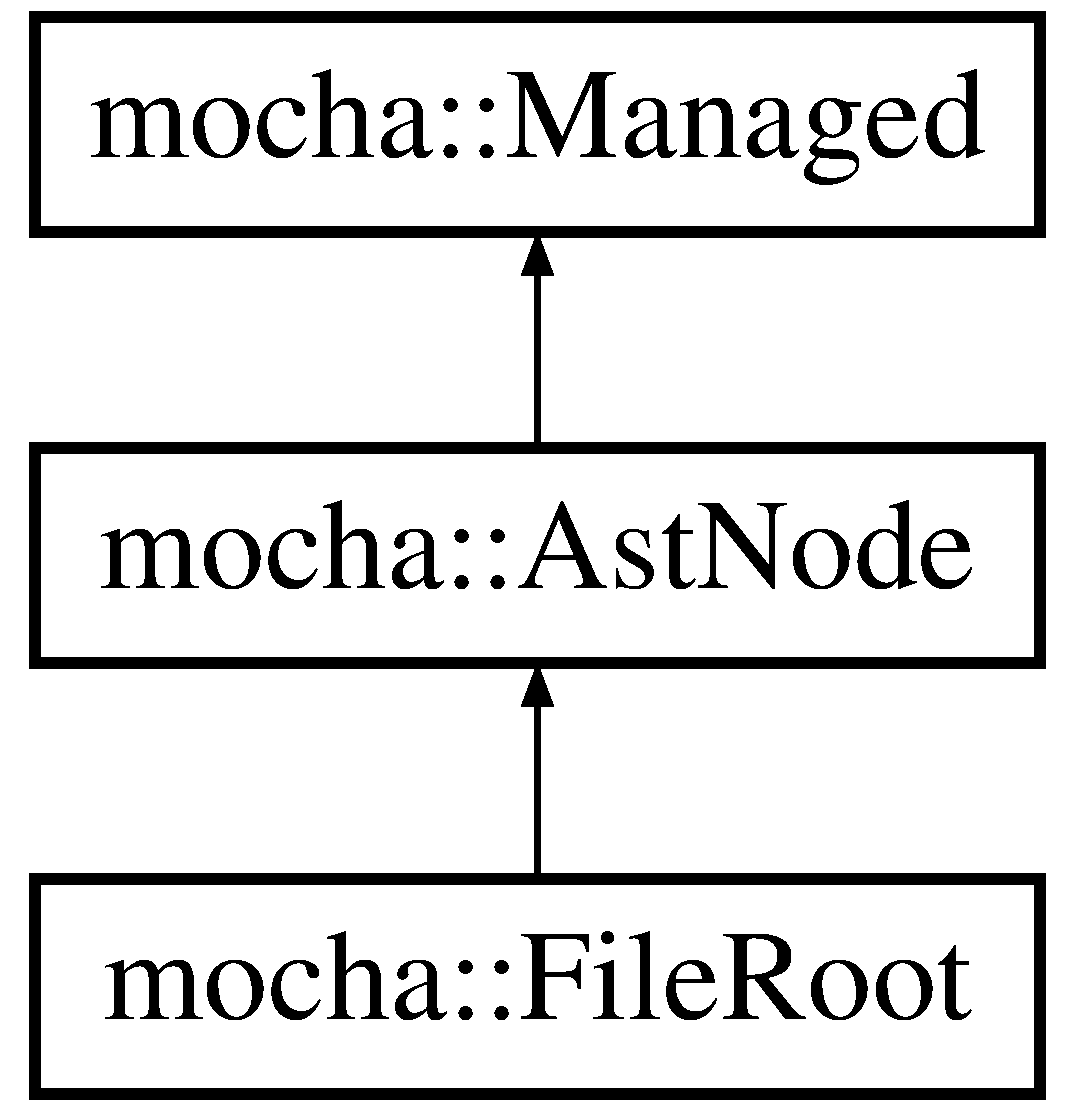
\includegraphics[height=3.000000cm]{classmocha_1_1_file_root}
\end{center}
\end{figure}
\subsection*{Public Member Functions}
\begin{DoxyCompactItemize}
\item 
\hyperlink{classmocha_1_1_file_root_a4187f8dfcf8cfde3c480d32348ad599e}{FileRoot} ()
\item 
\hyperlink{classmocha_1_1_file_root_a3af35d629cf83fbad09bbaa085166eab}{$\sim$FileRoot} ()
\item 
void \hyperlink{classmocha_1_1_file_root_af766366c3935dce897a3fdb833c70946}{FileName} (const char $\ast$filepath)
\item 
const char $\ast$ \hyperlink{classmocha_1_1_file_root_a57407c35fda0bbe2216d38ccddc8ed18}{FileName} () const 
\item 
bool \hyperlink{classmocha_1_1_file_root_aa6a6808576b77df6c909f3251400ba27}{IsRuntime} ()
\item 
void \hyperlink{classmocha_1_1_file_root_a674cea3b318e39b3ed36a6e07752d167}{SetFileRoot} ()
\item 
\hyperlink{classmocha_1_1_ast_node}{AstNode} $\ast$ \hyperlink{classmocha_1_1_file_root_a15c4779b5050481286c6d6cb4cc9223e}{Clone} ()
\end{DoxyCompactItemize}
\subsection*{Private Member Functions}
\begin{DoxyCompactItemize}
\item 
void \hyperlink{classmocha_1_1_file_root_a6cff1c80bcb419835cceaa2106e33b2f}{NVIAccept\_\-} (\hyperlink{classmocha_1_1_i_visitor}{IVisitor} $\ast$visitor)
\end{DoxyCompactItemize}
\subsection*{Private Attributes}
\begin{DoxyCompactItemize}
\item 
bool \hyperlink{classmocha_1_1_file_root_aee92f4b4d0461d5e54ac871750291971}{is\_\-file\_\-root\_\-}
\item 
std::string \hyperlink{classmocha_1_1_file_root_a5a82fa0f7471ecd6194fea872f961565}{filepath\_\-}
\end{DoxyCompactItemize}


\subsection{Detailed Description}


Definition at line 490 of file ast.h.



\subsection{Constructor \& Destructor Documentation}
\hypertarget{classmocha_1_1_file_root_a4187f8dfcf8cfde3c480d32348ad599e}{
\index{mocha::FileRoot@{mocha::FileRoot}!FileRoot@{FileRoot}}
\index{FileRoot@{FileRoot}!mocha::FileRoot@{mocha::FileRoot}}
\subsubsection[{FileRoot}]{\setlength{\rightskip}{0pt plus 5cm}mocha::FileRoot::FileRoot (
\begin{DoxyParamCaption}
{}
\end{DoxyParamCaption}
)\hspace{0.3cm}{\ttfamily  \mbox{[}inline\mbox{]}}}}
\label{classmocha_1_1_file_root_a4187f8dfcf8cfde3c480d32348ad599e}


Definition at line 492 of file ast.h.

\hypertarget{classmocha_1_1_file_root_a3af35d629cf83fbad09bbaa085166eab}{
\index{mocha::FileRoot@{mocha::FileRoot}!$\sim$FileRoot@{$\sim$FileRoot}}
\index{$\sim$FileRoot@{$\sim$FileRoot}!mocha::FileRoot@{mocha::FileRoot}}
\subsubsection[{$\sim$FileRoot}]{\setlength{\rightskip}{0pt plus 5cm}mocha::FileRoot::$\sim$FileRoot (
\begin{DoxyParamCaption}
{}
\end{DoxyParamCaption}
)\hspace{0.3cm}{\ttfamily  \mbox{[}inline\mbox{]}}}}
\label{classmocha_1_1_file_root_a3af35d629cf83fbad09bbaa085166eab}


Definition at line 493 of file ast.h.



\subsection{Member Function Documentation}
\hypertarget{classmocha_1_1_file_root_a15c4779b5050481286c6d6cb4cc9223e}{
\index{mocha::FileRoot@{mocha::FileRoot}!Clone@{Clone}}
\index{Clone@{Clone}!mocha::FileRoot@{mocha::FileRoot}}
\subsubsection[{Clone}]{\setlength{\rightskip}{0pt plus 5cm}{\bf AstNode} $\ast$ mocha::FileRoot::Clone (
\begin{DoxyParamCaption}
{}
\end{DoxyParamCaption}
)\hspace{0.3cm}{\ttfamily  \mbox{[}virtual\mbox{]}}}}
\label{classmocha_1_1_file_root_a15c4779b5050481286c6d6cb4cc9223e}
\begin{DoxyReturn}{Returns}
\{AstNode$\ast$\} Clone node. 
\end{DoxyReturn}


Reimplemented from \hyperlink{classmocha_1_1_ast_node_af2a895699bac2012f8b7739bff49c5ec}{mocha::AstNode}.



Definition at line 221 of file ast.cc.

\hypertarget{classmocha_1_1_file_root_af766366c3935dce897a3fdb833c70946}{
\index{mocha::FileRoot@{mocha::FileRoot}!FileName@{FileName}}
\index{FileName@{FileName}!mocha::FileRoot@{mocha::FileRoot}}
\subsubsection[{FileName}]{\setlength{\rightskip}{0pt plus 5cm}void mocha::FileRoot::FileName (
\begin{DoxyParamCaption}
\item[{const char $\ast$}]{filepath}
\end{DoxyParamCaption}
)\hspace{0.3cm}{\ttfamily  \mbox{[}inline\mbox{]}}}}
\label{classmocha_1_1_file_root_af766366c3935dce897a3fdb833c70946}

\begin{DoxyParams}{Parameters}
{\em \{const} & char$\ast$\} Set current file name. \\
\hline
\end{DoxyParams}


Definition at line 498 of file ast.h.

\hypertarget{classmocha_1_1_file_root_a57407c35fda0bbe2216d38ccddc8ed18}{
\index{mocha::FileRoot@{mocha::FileRoot}!FileName@{FileName}}
\index{FileName@{FileName}!mocha::FileRoot@{mocha::FileRoot}}
\subsubsection[{FileName}]{\setlength{\rightskip}{0pt plus 5cm}const char$\ast$ mocha::FileRoot::FileName (
\begin{DoxyParamCaption}
{}
\end{DoxyParamCaption}
) const\hspace{0.3cm}{\ttfamily  \mbox{[}inline\mbox{]}}}}
\label{classmocha_1_1_file_root_a57407c35fda0bbe2216d38ccddc8ed18}
\begin{DoxyReturn}{Returns}
\{const char$\ast$\} Get file name. 
\end{DoxyReturn}


Definition at line 503 of file ast.h.

\hypertarget{classmocha_1_1_file_root_aa6a6808576b77df6c909f3251400ba27}{
\index{mocha::FileRoot@{mocha::FileRoot}!IsRuntime@{IsRuntime}}
\index{IsRuntime@{IsRuntime}!mocha::FileRoot@{mocha::FileRoot}}
\subsubsection[{IsRuntime}]{\setlength{\rightskip}{0pt plus 5cm}bool mocha::FileRoot::IsRuntime (
\begin{DoxyParamCaption}
{}
\end{DoxyParamCaption}
)\hspace{0.3cm}{\ttfamily  \mbox{[}inline\mbox{]}}}}
\label{classmocha_1_1_file_root_aa6a6808576b77df6c909f3251400ba27}


Definition at line 504 of file ast.h.

\hypertarget{classmocha_1_1_file_root_a6cff1c80bcb419835cceaa2106e33b2f}{
\index{mocha::FileRoot@{mocha::FileRoot}!NVIAccept\_\-@{NVIAccept\_\-}}
\index{NVIAccept\_\-@{NVIAccept\_\-}!mocha::FileRoot@{mocha::FileRoot}}
\subsubsection[{NVIAccept\_\-}]{\setlength{\rightskip}{0pt plus 5cm}void mocha::FileRoot::NVIAccept\_\- (
\begin{DoxyParamCaption}
\item[{{\bf IVisitor} $\ast$}]{visitor}
\end{DoxyParamCaption}
)\hspace{0.3cm}{\ttfamily  \mbox{[}inline, private, virtual\mbox{]}}}}
\label{classmocha_1_1_file_root_a6cff1c80bcb419835cceaa2106e33b2f}


Reimplemented from \hyperlink{classmocha_1_1_ast_node_a4a9c107bed3671f3fa15312b87f6ae96}{mocha::AstNode}.



Definition at line 510 of file ast.h.

\hypertarget{classmocha_1_1_file_root_a674cea3b318e39b3ed36a6e07752d167}{
\index{mocha::FileRoot@{mocha::FileRoot}!SetFileRoot@{SetFileRoot}}
\index{SetFileRoot@{SetFileRoot}!mocha::FileRoot@{mocha::FileRoot}}
\subsubsection[{SetFileRoot}]{\setlength{\rightskip}{0pt plus 5cm}void mocha::FileRoot::SetFileRoot (
\begin{DoxyParamCaption}
{}
\end{DoxyParamCaption}
)\hspace{0.3cm}{\ttfamily  \mbox{[}inline\mbox{]}}}}
\label{classmocha_1_1_file_root_a674cea3b318e39b3ed36a6e07752d167}


Definition at line 505 of file ast.h.



\subsection{Member Data Documentation}
\hypertarget{classmocha_1_1_file_root_a5a82fa0f7471ecd6194fea872f961565}{
\index{mocha::FileRoot@{mocha::FileRoot}!filepath\_\-@{filepath\_\-}}
\index{filepath\_\-@{filepath\_\-}!mocha::FileRoot@{mocha::FileRoot}}
\subsubsection[{filepath\_\-}]{\setlength{\rightskip}{0pt plus 5cm}std::string {\bf mocha::FileRoot::filepath\_\-}\hspace{0.3cm}{\ttfamily  \mbox{[}private\mbox{]}}}}
\label{classmocha_1_1_file_root_a5a82fa0f7471ecd6194fea872f961565}


Definition at line 509 of file ast.h.

\hypertarget{classmocha_1_1_file_root_aee92f4b4d0461d5e54ac871750291971}{
\index{mocha::FileRoot@{mocha::FileRoot}!is\_\-file\_\-root\_\-@{is\_\-file\_\-root\_\-}}
\index{is\_\-file\_\-root\_\-@{is\_\-file\_\-root\_\-}!mocha::FileRoot@{mocha::FileRoot}}
\subsubsection[{is\_\-file\_\-root\_\-}]{\setlength{\rightskip}{0pt plus 5cm}bool {\bf mocha::FileRoot::is\_\-file\_\-root\_\-}\hspace{0.3cm}{\ttfamily  \mbox{[}private\mbox{]}}}}
\label{classmocha_1_1_file_root_aee92f4b4d0461d5e54ac871750291971}


Definition at line 506 of file ast.h.



The documentation for this class was generated from the following files:\begin{DoxyCompactItemize}
\item 
Y:/mocha/src/ast/\hyperlink{ast_8h}{ast.h}\item 
Y:/mocha/src/ast/\hyperlink{ast_8cc}{ast.cc}\end{DoxyCompactItemize}

\hypertarget{classmocha_1_1_file_root_processor}{
\section{mocha::FileRootProcessor Class Reference}
\label{classmocha_1_1_file_root_processor}\index{mocha::FileRootProcessor@{mocha::FileRootProcessor}}
}


{\ttfamily \#include $<$fileroot\_\-processor.h$>$}

Inheritance diagram for mocha::FileRootProcessor:\begin{figure}[H]
\begin{center}
\leavevmode
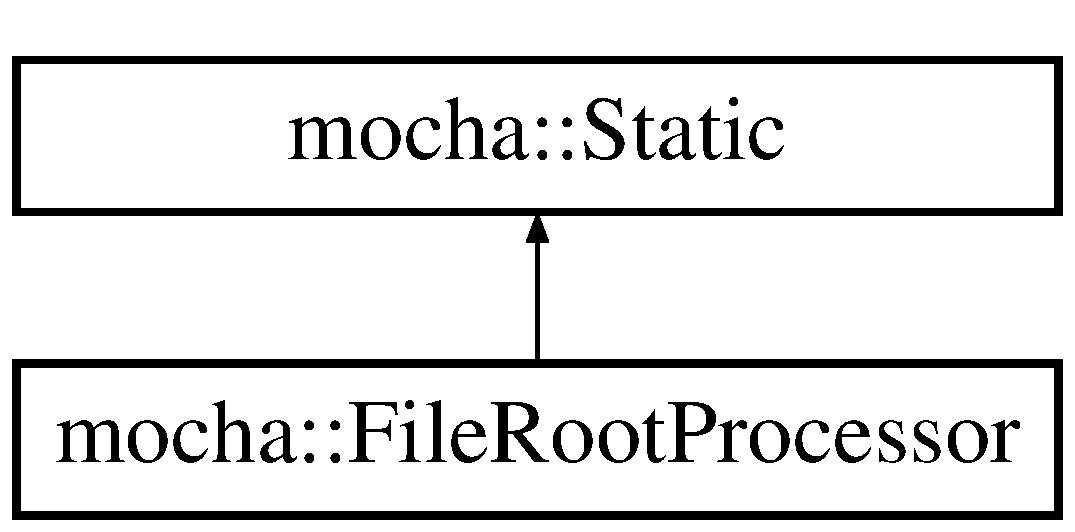
\includegraphics[height=2.000000cm]{classmocha_1_1_file_root_processor}
\end{center}
\end{figure}
\subsection*{Static Public Member Functions}
\begin{DoxyCompactItemize}
\item 
static void \hyperlink{classmocha_1_1_file_root_processor_ab23a24ec6105f7b49cd67ccd7e76aec8}{ProcessNode} (\hyperlink{classmocha_1_1_file_root}{FileRoot} $\ast$ast\_\-node, \hyperlink{classmocha_1_1_processor_info}{ProcessorInfo} $\ast$info)
\end{DoxyCompactItemize}


\subsection{Detailed Description}


Definition at line 7 of file fileroot\_\-processor.h.



\subsection{Member Function Documentation}
\hypertarget{classmocha_1_1_file_root_processor_ab23a24ec6105f7b49cd67ccd7e76aec8}{
\index{mocha::FileRootProcessor@{mocha::FileRootProcessor}!ProcessNode@{ProcessNode}}
\index{ProcessNode@{ProcessNode}!mocha::FileRootProcessor@{mocha::FileRootProcessor}}
\subsubsection[{ProcessNode}]{\setlength{\rightskip}{0pt plus 5cm}void mocha::FileRootProcessor::ProcessNode (
\begin{DoxyParamCaption}
\item[{{\bf FileRoot} $\ast$}]{ast\_\-node, }
\item[{{\bf ProcessorInfo} $\ast$}]{info}
\end{DoxyParamCaption}
)\hspace{0.3cm}{\ttfamily  \mbox{[}static\mbox{]}}}}
\label{classmocha_1_1_file_root_processor_ab23a24ec6105f7b49cd67ccd7e76aec8}

\begin{DoxyParams}{Parameters}
{\em \{FileRoot$\ast$\}} & ast\_\-node \\
\hline
{\em \{ProcessorInfo$\ast$\}} & info\\
\hline
\end{DoxyParams}
Processing \hyperlink{classmocha_1_1_file_root}{FileRoot} node. 

Definition at line 14 of file fileroot\_\-processor.cc.



The documentation for this class was generated from the following files:\begin{DoxyCompactItemize}
\item 
Y:/mocha/src/ast/visitors/utils/processors/\hyperlink{fileroot__processor_8h}{fileroot\_\-processor.h}\item 
Y:/mocha/src/ast/visitors/utils/processors/\hyperlink{fileroot__processor_8cc}{fileroot\_\-processor.cc}\end{DoxyCompactItemize}

\hypertarget{classmocha_1_1_file_system}{
\section{mocha::FileSystem Class Reference}
\label{classmocha_1_1_file_system}\index{mocha::FileSystem@{mocha::FileSystem}}
}


{\ttfamily \#include $<$file\_\-system.h$>$}

\subsection*{Static Public Member Functions}
\begin{DoxyCompactItemize}
\item 
static \hyperlink{classmocha_1_1_array_handle}{StrHandle} \hyperlink{classmocha_1_1_file_system_afdc88698fd2bfd0b3dc97de20c06cf48}{pwd} ()
\item 
static \hyperlink{classmocha_1_1_handle}{Handle}$<$ \hyperlink{classmocha_1_1_path_info}{PathInfo} $>$ \hyperlink{classmocha_1_1_file_system_ab56ef869ef3f7eab8768c1bc95869c81}{GetPathInfo} (const char $\ast$path)
\item 
static \hyperlink{classmocha_1_1_array_handle}{StrHandle} \hyperlink{classmocha_1_1_file_system_aa8e0d580f05cc70418dd87b93106d619}{NormalizePath} (const char $\ast$path)
\item 
static void \hyperlink{classmocha_1_1_file_system_a23801304e4ec18fddf88b6b6688c0a28}{Chdir} (const char $\ast$path)
\item 
static bool \hyperlink{classmocha_1_1_file_system_aa39867ad9a341dc0c7bd3636203d6e34}{Chmod} (const char $\ast$pass, int permiss)
\item 
static \hyperlink{classmocha_1_1_array_handle}{StrHandle} \hyperlink{classmocha_1_1_file_system_a65191296d1bb00548a66cf5ba7426594}{GetModuleKey} (const char $\ast$base, const char $\ast$)
\item 
static void \hyperlink{classmocha_1_1_file_system_af69da9f81d9effd19ceb8736d8450bd7}{SetModuleDir} (const char $\ast$path)
\item 
static const char $\ast$ \hyperlink{classmocha_1_1_file_system_aadad83aa0066e57ea4fa785b10026bc3}{GetModuleDir} ()
\item 
static \hyperlink{classmocha_1_1_array_handle}{StrHandle} \hyperlink{classmocha_1_1_file_system_a0dff04800995e60c7ea2bc5428c0288d}{GetUserHomeDir} ()
\item 
static \hyperlink{classmocha_1_1_array_handle}{StrHandle} \hyperlink{classmocha_1_1_file_system_ad09942b93a267933166cdadba349397f}{GetAbsolutePath} (const char $\ast$path)
\item 
static bool \hyperlink{classmocha_1_1_file_system_a0c202c7a85c8827f4ffac7bff746c7a8}{Mkdir} (const char $\ast$path, int permiss)
\end{DoxyCompactItemize}
\subsection*{Static Private Attributes}
\begin{DoxyCompactItemize}
\item 
static std::string \hyperlink{classmocha_1_1_file_system_a387837ad143996593d7a66284ab8153a}{module\_\-dir\_\-}
\end{DoxyCompactItemize}


\subsection{Detailed Description}


Definition at line 24 of file file\_\-system.h.



\subsection{Member Function Documentation}
\hypertarget{classmocha_1_1_file_system_a23801304e4ec18fddf88b6b6688c0a28}{
\index{mocha::FileSystem@{mocha::FileSystem}!Chdir@{Chdir}}
\index{Chdir@{Chdir}!mocha::FileSystem@{mocha::FileSystem}}
\subsubsection[{Chdir}]{\setlength{\rightskip}{0pt plus 5cm}void FileSystem::Chdir (
\begin{DoxyParamCaption}
\item[{const char $\ast$}]{path}
\end{DoxyParamCaption}
)\hspace{0.3cm}{\ttfamily  \mbox{[}static\mbox{]}}}}
\label{classmocha_1_1_file_system_a23801304e4ec18fddf88b6b6688c0a28}


Definition at line 235 of file file\_\-system.cc.

\hypertarget{classmocha_1_1_file_system_aa39867ad9a341dc0c7bd3636203d6e34}{
\index{mocha::FileSystem@{mocha::FileSystem}!Chmod@{Chmod}}
\index{Chmod@{Chmod}!mocha::FileSystem@{mocha::FileSystem}}
\subsubsection[{Chmod}]{\setlength{\rightskip}{0pt plus 5cm}bool FileSystem::Chmod (
\begin{DoxyParamCaption}
\item[{const char $\ast$}]{pass, }
\item[{int}]{permiss}
\end{DoxyParamCaption}
)\hspace{0.3cm}{\ttfamily  \mbox{[}static\mbox{]}}}}
\label{classmocha_1_1_file_system_aa39867ad9a341dc0c7bd3636203d6e34}


Definition at line 249 of file file\_\-system.cc.

\hypertarget{classmocha_1_1_file_system_ad09942b93a267933166cdadba349397f}{
\index{mocha::FileSystem@{mocha::FileSystem}!GetAbsolutePath@{GetAbsolutePath}}
\index{GetAbsolutePath@{GetAbsolutePath}!mocha::FileSystem@{mocha::FileSystem}}
\subsubsection[{GetAbsolutePath}]{\setlength{\rightskip}{0pt plus 5cm}{\bf StrHandle} FileSystem::GetAbsolutePath (
\begin{DoxyParamCaption}
\item[{const char $\ast$}]{path}
\end{DoxyParamCaption}
)\hspace{0.3cm}{\ttfamily  \mbox{[}static\mbox{]}}}}
\label{classmocha_1_1_file_system_ad09942b93a267933166cdadba349397f}


Definition at line 159 of file file\_\-system.cc.

\hypertarget{classmocha_1_1_file_system_aadad83aa0066e57ea4fa785b10026bc3}{
\index{mocha::FileSystem@{mocha::FileSystem}!GetModuleDir@{GetModuleDir}}
\index{GetModuleDir@{GetModuleDir}!mocha::FileSystem@{mocha::FileSystem}}
\subsubsection[{GetModuleDir}]{\setlength{\rightskip}{0pt plus 5cm}static const char$\ast$ mocha::FileSystem::GetModuleDir (
\begin{DoxyParamCaption}
{}
\end{DoxyParamCaption}
)\hspace{0.3cm}{\ttfamily  \mbox{[}inline, static\mbox{]}}}}
\label{classmocha_1_1_file_system_aadad83aa0066e57ea4fa785b10026bc3}


Definition at line 33 of file file\_\-system.h.

\hypertarget{classmocha_1_1_file_system_a65191296d1bb00548a66cf5ba7426594}{
\index{mocha::FileSystem@{mocha::FileSystem}!GetModuleKey@{GetModuleKey}}
\index{GetModuleKey@{GetModuleKey}!mocha::FileSystem@{mocha::FileSystem}}
\subsubsection[{GetModuleKey}]{\setlength{\rightskip}{0pt plus 5cm}{\bf StrHandle} FileSystem::GetModuleKey (
\begin{DoxyParamCaption}
\item[{const char $\ast$}]{base, }
\item[{const char $\ast$}]{path}
\end{DoxyParamCaption}
)\hspace{0.3cm}{\ttfamily  \mbox{[}static\mbox{]}}}}
\label{classmocha_1_1_file_system_a65191296d1bb00548a66cf5ba7426594}


Definition at line 194 of file file\_\-system.cc.

\hypertarget{classmocha_1_1_file_system_ab56ef869ef3f7eab8768c1bc95869c81}{
\index{mocha::FileSystem@{mocha::FileSystem}!GetPathInfo@{GetPathInfo}}
\index{GetPathInfo@{GetPathInfo}!mocha::FileSystem@{mocha::FileSystem}}
\subsubsection[{GetPathInfo}]{\setlength{\rightskip}{0pt plus 5cm}{\bf Handle}$<$ {\bf PathInfo} $>$ FileSystem::GetPathInfo (
\begin{DoxyParamCaption}
\item[{const char $\ast$}]{path}
\end{DoxyParamCaption}
)\hspace{0.3cm}{\ttfamily  \mbox{[}static\mbox{]}}}}
\label{classmocha_1_1_file_system_ab56ef869ef3f7eab8768c1bc95869c81}


Definition at line 85 of file file\_\-system.cc.

\hypertarget{classmocha_1_1_file_system_a0dff04800995e60c7ea2bc5428c0288d}{
\index{mocha::FileSystem@{mocha::FileSystem}!GetUserHomeDir@{GetUserHomeDir}}
\index{GetUserHomeDir@{GetUserHomeDir}!mocha::FileSystem@{mocha::FileSystem}}
\subsubsection[{GetUserHomeDir}]{\setlength{\rightskip}{0pt plus 5cm}{\bf StrHandle} FileSystem::GetUserHomeDir (
\begin{DoxyParamCaption}
{}
\end{DoxyParamCaption}
)\hspace{0.3cm}{\ttfamily  \mbox{[}static\mbox{]}}}}
\label{classmocha_1_1_file_system_a0dff04800995e60c7ea2bc5428c0288d}


Definition at line 146 of file file\_\-system.cc.

\hypertarget{classmocha_1_1_file_system_a0c202c7a85c8827f4ffac7bff746c7a8}{
\index{mocha::FileSystem@{mocha::FileSystem}!Mkdir@{Mkdir}}
\index{Mkdir@{Mkdir}!mocha::FileSystem@{mocha::FileSystem}}
\subsubsection[{Mkdir}]{\setlength{\rightskip}{0pt plus 5cm}bool FileSystem::Mkdir (
\begin{DoxyParamCaption}
\item[{const char $\ast$}]{path, }
\item[{int}]{permiss}
\end{DoxyParamCaption}
)\hspace{0.3cm}{\ttfamily  \mbox{[}static\mbox{]}}}}
\label{classmocha_1_1_file_system_a0c202c7a85c8827f4ffac7bff746c7a8}


Definition at line 245 of file file\_\-system.cc.

\hypertarget{classmocha_1_1_file_system_aa8e0d580f05cc70418dd87b93106d619}{
\index{mocha::FileSystem@{mocha::FileSystem}!NormalizePath@{NormalizePath}}
\index{NormalizePath@{NormalizePath}!mocha::FileSystem@{mocha::FileSystem}}
\subsubsection[{NormalizePath}]{\setlength{\rightskip}{0pt plus 5cm}{\bf StrHandle} FileSystem::NormalizePath (
\begin{DoxyParamCaption}
\item[{const char $\ast$}]{path}
\end{DoxyParamCaption}
)\hspace{0.3cm}{\ttfamily  \mbox{[}static\mbox{]}}}}
\label{classmocha_1_1_file_system_aa8e0d580f05cc70418dd87b93106d619}


Definition at line 92 of file file\_\-system.cc.

\hypertarget{classmocha_1_1_file_system_afdc88698fd2bfd0b3dc97de20c06cf48}{
\index{mocha::FileSystem@{mocha::FileSystem}!pwd@{pwd}}
\index{pwd@{pwd}!mocha::FileSystem@{mocha::FileSystem}}
\subsubsection[{pwd}]{\setlength{\rightskip}{0pt plus 5cm}{\bf StrHandle} FileSystem::pwd (
\begin{DoxyParamCaption}
{}
\end{DoxyParamCaption}
)\hspace{0.3cm}{\ttfamily  \mbox{[}static\mbox{]}}}}
\label{classmocha_1_1_file_system_afdc88698fd2bfd0b3dc97de20c06cf48}


Definition at line 81 of file file\_\-system.cc.

\hypertarget{classmocha_1_1_file_system_af69da9f81d9effd19ceb8736d8450bd7}{
\index{mocha::FileSystem@{mocha::FileSystem}!SetModuleDir@{SetModuleDir}}
\index{SetModuleDir@{SetModuleDir}!mocha::FileSystem@{mocha::FileSystem}}
\subsubsection[{SetModuleDir}]{\setlength{\rightskip}{0pt plus 5cm}static void mocha::FileSystem::SetModuleDir (
\begin{DoxyParamCaption}
\item[{const char $\ast$}]{path}
\end{DoxyParamCaption}
)\hspace{0.3cm}{\ttfamily  \mbox{[}static\mbox{]}}}}
\label{classmocha_1_1_file_system_af69da9f81d9effd19ceb8736d8450bd7}


\subsection{Member Data Documentation}
\hypertarget{classmocha_1_1_file_system_a387837ad143996593d7a66284ab8153a}{
\index{mocha::FileSystem@{mocha::FileSystem}!module\_\-dir\_\-@{module\_\-dir\_\-}}
\index{module\_\-dir\_\-@{module\_\-dir\_\-}!mocha::FileSystem@{mocha::FileSystem}}
\subsubsection[{module\_\-dir\_\-}]{\setlength{\rightskip}{0pt plus 5cm}std::string {\bf mocha::FileSystem::module\_\-dir\_\-}\hspace{0.3cm}{\ttfamily  \mbox{[}static, private\mbox{]}}}}
\label{classmocha_1_1_file_system_a387837ad143996593d7a66284ab8153a}


Definition at line 38 of file file\_\-system.h.



The documentation for this class was generated from the following files:\begin{DoxyCompactItemize}
\item 
Y:/mocha/src/utils/file\_\-system/\hyperlink{file__system_8h}{file\_\-system.h}\item 
Y:/mocha/src/utils/file\_\-system/\hyperlink{file__system_8cc}{file\_\-system.cc}\end{DoxyCompactItemize}

\hypertarget{classmocha_1_1_file_observer_1_1_file_updater}{
\section{mocha::FileObserver::FileUpdater Class Reference}
\label{classmocha_1_1_file_observer_1_1_file_updater}\index{mocha::FileObserver::FileUpdater@{mocha::FileObserver::FileUpdater}}
}
Inheritance diagram for mocha::FileObserver::FileUpdater:\begin{figure}[H]
\begin{center}
\leavevmode
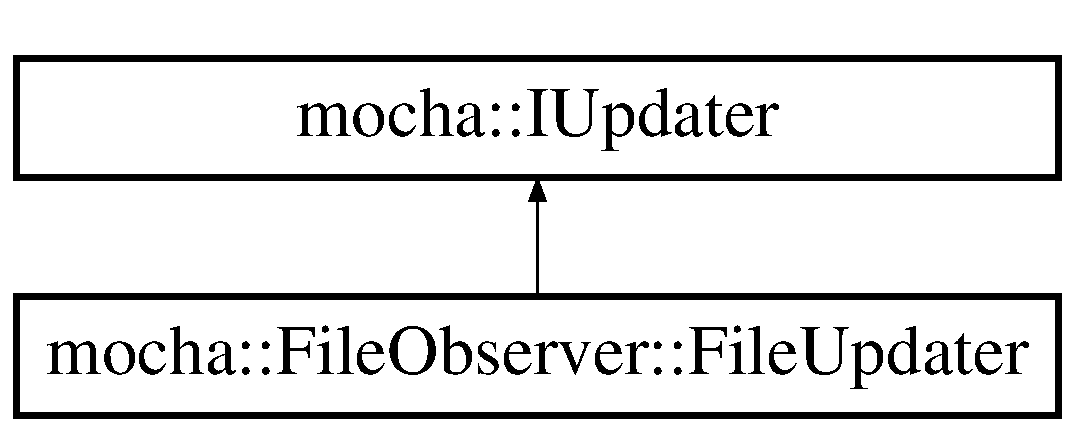
\includegraphics[height=2.000000cm]{classmocha_1_1_file_observer_1_1_file_updater}
\end{center}
\end{figure}
\subsection*{Public Member Functions}
\begin{DoxyCompactItemize}
\item 
void \hyperlink{classmocha_1_1_file_observer_1_1_file_updater_a80a60cca8240f014e4f191bb60d82bf3}{Update} (\hyperlink{structmocha_1_1watch__traits_1_1_modify}{watch\_\-traits::Modify} $\ast$trait)
\item 
void \hyperlink{classmocha_1_1_file_observer_1_1_file_updater_a1984b103811915719d04d979275d6beb}{Update} (\hyperlink{structmocha_1_1watch__traits_1_1_delete_self}{watch\_\-traits::DeleteSelf} $\ast$trait)
\end{DoxyCompactItemize}
\subsection*{Private Types}
\begin{DoxyCompactItemize}
\item 
typedef boost::unordered\_\-map$<$ std::string, \hyperlink{classmocha_1_1_handle}{Handle}$<$ \hyperlink{classmocha_1_1_mutex}{Mutex} $>$ $>$ \hyperlink{classmocha_1_1_file_observer_1_1_file_updater_a63074c527b9a0bcb0f8a715b53535c17}{List}
\end{DoxyCompactItemize}
\subsection*{Private Attributes}
\begin{DoxyCompactItemize}
\item 
\hyperlink{classmocha_1_1_file_observer_1_1_file_updater_a63074c527b9a0bcb0f8a715b53535c17}{List} \hyperlink{classmocha_1_1_file_observer_1_1_file_updater_a12e24a3b76615c93d5fc14a3eea7354d}{mutex\_\-list\_\-}
\end{DoxyCompactItemize}
\subsection*{Friends}
\begin{DoxyCompactItemize}
\item 
class \hyperlink{classmocha_1_1_file_observer_1_1_file_updater_a4b52c311bd4ce9ed180ae976ba0a6196}{FileObserver}
\end{DoxyCompactItemize}


\subsection{Detailed Description}


Definition at line 12 of file file\_\-observer.cc.



\subsection{Member Typedef Documentation}
\hypertarget{classmocha_1_1_file_observer_1_1_file_updater_a63074c527b9a0bcb0f8a715b53535c17}{
\index{mocha::FileObserver::FileUpdater@{mocha::FileObserver::FileUpdater}!List@{List}}
\index{List@{List}!mocha::FileObserver::FileUpdater@{mocha::FileObserver::FileUpdater}}
\subsubsection[{List}]{\setlength{\rightskip}{0pt plus 5cm}typedef boost::unordered\_\-map$<$std::string,{\bf Handle}$<${\bf Mutex}$>$ $>$ {\bf mocha::FileObserver::FileUpdater::List}\hspace{0.3cm}{\ttfamily  \mbox{[}private\mbox{]}}}}
\label{classmocha_1_1_file_observer_1_1_file_updater_a63074c527b9a0bcb0f8a715b53535c17}


Definition at line 42 of file file\_\-observer.cc.



\subsection{Member Function Documentation}
\hypertarget{classmocha_1_1_file_observer_1_1_file_updater_a80a60cca8240f014e4f191bb60d82bf3}{
\index{mocha::FileObserver::FileUpdater@{mocha::FileObserver::FileUpdater}!Update@{Update}}
\index{Update@{Update}!mocha::FileObserver::FileUpdater@{mocha::FileObserver::FileUpdater}}
\subsubsection[{Update}]{\setlength{\rightskip}{0pt plus 5cm}void mocha::FileObserver::FileUpdater::Update (
\begin{DoxyParamCaption}
\item[{{\bf watch\_\-traits::Modify} $\ast$}]{trait}
\end{DoxyParamCaption}
)\hspace{0.3cm}{\ttfamily  \mbox{[}inline, virtual\mbox{]}}}}
\label{classmocha_1_1_file_observer_1_1_file_updater_a80a60cca8240f014e4f191bb60d82bf3}


Reimplemented from \hyperlink{classmocha_1_1_i_updater_a99f87c1ff978b034b5be7ab372e81a5b}{mocha::IUpdater}.



Definition at line 15 of file file\_\-observer.cc.

\hypertarget{classmocha_1_1_file_observer_1_1_file_updater_a1984b103811915719d04d979275d6beb}{
\index{mocha::FileObserver::FileUpdater@{mocha::FileObserver::FileUpdater}!Update@{Update}}
\index{Update@{Update}!mocha::FileObserver::FileUpdater@{mocha::FileObserver::FileUpdater}}
\subsubsection[{Update}]{\setlength{\rightskip}{0pt plus 5cm}void mocha::FileObserver::FileUpdater::Update (
\begin{DoxyParamCaption}
\item[{{\bf watch\_\-traits::DeleteSelf} $\ast$}]{trait}
\end{DoxyParamCaption}
)\hspace{0.3cm}{\ttfamily  \mbox{[}inline, virtual\mbox{]}}}}
\label{classmocha_1_1_file_observer_1_1_file_updater_a1984b103811915719d04d979275d6beb}


Reimplemented from \hyperlink{classmocha_1_1_i_updater_a37df53aa438d78a64820721026c207b0}{mocha::IUpdater}.



Definition at line 30 of file file\_\-observer.cc.



\subsection{Friends And Related Function Documentation}
\hypertarget{classmocha_1_1_file_observer_1_1_file_updater_a4b52c311bd4ce9ed180ae976ba0a6196}{
\index{mocha::FileObserver::FileUpdater@{mocha::FileObserver::FileUpdater}!FileObserver@{FileObserver}}
\index{FileObserver@{FileObserver}!mocha::FileObserver::FileUpdater@{mocha::FileObserver::FileUpdater}}
\subsubsection[{FileObserver}]{\setlength{\rightskip}{0pt plus 5cm}friend class {\bf FileObserver}\hspace{0.3cm}{\ttfamily  \mbox{[}friend\mbox{]}}}}
\label{classmocha_1_1_file_observer_1_1_file_updater_a4b52c311bd4ce9ed180ae976ba0a6196}


Definition at line 13 of file file\_\-observer.cc.



\subsection{Member Data Documentation}
\hypertarget{classmocha_1_1_file_observer_1_1_file_updater_a12e24a3b76615c93d5fc14a3eea7354d}{
\index{mocha::FileObserver::FileUpdater@{mocha::FileObserver::FileUpdater}!mutex\_\-list\_\-@{mutex\_\-list\_\-}}
\index{mutex\_\-list\_\-@{mutex\_\-list\_\-}!mocha::FileObserver::FileUpdater@{mocha::FileObserver::FileUpdater}}
\subsubsection[{mutex\_\-list\_\-}]{\setlength{\rightskip}{0pt plus 5cm}{\bf List} {\bf mocha::FileObserver::FileUpdater::mutex\_\-list\_\-}\hspace{0.3cm}{\ttfamily  \mbox{[}private\mbox{]}}}}
\label{classmocha_1_1_file_observer_1_1_file_updater_a12e24a3b76615c93d5fc14a3eea7354d}


Definition at line 43 of file file\_\-observer.cc.



The documentation for this class was generated from the following file:\begin{DoxyCompactItemize}
\item 
Y:/mocha/src/utils/file\_\-watcher/observer/\hyperlink{file__observer_8cc}{file\_\-observer.cc}\end{DoxyCompactItemize}

\hypertarget{classmocha_1_1_file_watcher}{
\section{mocha::FileWatcher Class Reference}
\label{classmocha_1_1_file_watcher}\index{mocha::FileWatcher@{mocha::FileWatcher}}
}


{\ttfamily \#include $<$file\_\-watcher.h$>$}

\subsection*{Classes}
\begin{DoxyCompactItemize}
\item 
class \hyperlink{classmocha_1_1_file_watcher_1_1_ptr_impl}{PtrImpl}
\end{DoxyCompactItemize}
\subsection*{Public Types}
\begin{DoxyCompactItemize}
\item 
enum \{ \par
\hyperlink{classmocha_1_1_file_watcher_ada989fb469049690cb97ad121dea4e9daacab20b4934ef8fd0296328ae0b58f04}{kAccess} =  0x00000001, 
\hyperlink{classmocha_1_1_file_watcher_ada989fb469049690cb97ad121dea4e9da0505213a1f6d1fe29b66f875b885fd01}{kModify} =  0x00000002, 
\hyperlink{classmocha_1_1_file_watcher_ada989fb469049690cb97ad121dea4e9da08857acdd79d2ba149ff150598581051}{kAttrib} =  0x00000004, 
\hyperlink{classmocha_1_1_file_watcher_ada989fb469049690cb97ad121dea4e9da670ab8a86a6cad93c68ec0abcd6c71ca}{kOpen} =  0x00000008, 
\par
\hyperlink{classmocha_1_1_file_watcher_ada989fb469049690cb97ad121dea4e9da95c879ae74b3ead3cc1e88de5f5a031b}{kClose} =  0x00000010, 
\hyperlink{classmocha_1_1_file_watcher_ada989fb469049690cb97ad121dea4e9daa09833e37c008de0c128965ef7e3a8f9}{kMoveSelf} =  0x00000012, 
\hyperlink{classmocha_1_1_file_watcher_ada989fb469049690cb97ad121dea4e9da25b5e3ee7b85e74f45c21a0dd2c24edf}{kMovedFrom} =  0x00000020, 
\hyperlink{classmocha_1_1_file_watcher_ada989fb469049690cb97ad121dea4e9da9f6709a1019d5836374cc86ef5a1ebed}{kMovedTo} =  0x00000040, 
\par
\hyperlink{classmocha_1_1_file_watcher_ada989fb469049690cb97ad121dea4e9da625e550c103b89a767a6b6c167ff96b6}{kDeleteSelf} =  0x00000080, 
\hyperlink{classmocha_1_1_file_watcher_ada989fb469049690cb97ad121dea4e9da1d67f81c57709e0854651d9386891813}{kDelete} =  0x00000100, 
\hyperlink{classmocha_1_1_file_watcher_ada989fb469049690cb97ad121dea4e9da8b3a56082816907ea5a798fe99bcbd5a}{kCreate} =  0x00000110, 
\hyperlink{classmocha_1_1_file_watcher_ada989fb469049690cb97ad121dea4e9dac7d13b67b9a9ba7be3e14e08879535c5}{kAdd}
 \}
\item 
typedef void($\ast$ \hyperlink{classmocha_1_1_file_watcher_af774b8dd436b9f8929506466533831b9}{EndCallBack} )(void $\ast$arg)
\end{DoxyCompactItemize}
\subsection*{Public Member Functions}
\begin{DoxyCompactItemize}
\item 
\hyperlink{classmocha_1_1_file_watcher_a844bd44469e6657fb7d5157ec7403f08}{FileWatcher} ()
\item 
\hyperlink{classmocha_1_1_file_watcher_a5761437d128835c8f6a9a96ddf14351b}{$\sim$FileWatcher} ()
\item 
void \hyperlink{classmocha_1_1_file_watcher_a27735bd6c3a3816c7ee8de68ce26365f}{AddWatch} (const char $\ast$path, \hyperlink{classmocha_1_1_i_updater}{IUpdater} $\ast$updater, int type)
\item 
void \hyperlink{classmocha_1_1_file_watcher_a06618480535f0aae1db8aabcd0785499}{UnWatch} (const char $\ast$path)
\item 
void \hyperlink{classmocha_1_1_file_watcher_a066c2a274e6cc679dfe6fb8d9729479f}{UnWatchAll} ()
\item 
void \hyperlink{classmocha_1_1_file_watcher_a272b7e7191a7284fa9d7fc15e32c7c29}{Stop} ()
\item 
void \hyperlink{classmocha_1_1_file_watcher_a264fca346886478a26b85d62f0b94fa5}{Start} ()
\item 
void \hyperlink{classmocha_1_1_file_watcher_a0f9fe45b54126ac93e864b8f2d3c1537}{Exit} ()
\item 
void \hyperlink{classmocha_1_1_file_watcher_a1585a6ee12afffb9c661eaddd7ef4c66}{Exit} (\hyperlink{classmocha_1_1_file_watcher_af774b8dd436b9f8929506466533831b9}{EndCallBack} fn, void $\ast$arg)
\end{DoxyCompactItemize}
\subsection*{Private Attributes}
\begin{DoxyCompactItemize}
\item 
\hyperlink{classmocha_1_1_file_watcher_1_1_ptr_impl}{PtrImpl} $\ast$ \hyperlink{classmocha_1_1_file_watcher_ab1a22ac85de2c9c929167abe785a00c5}{implementation\_\-}
\end{DoxyCompactItemize}


\subsection{Detailed Description}


Definition at line 38 of file file\_\-watcher.h.



\subsection{Member Typedef Documentation}
\hypertarget{classmocha_1_1_file_watcher_af774b8dd436b9f8929506466533831b9}{
\index{mocha::FileWatcher@{mocha::FileWatcher}!EndCallBack@{EndCallBack}}
\index{EndCallBack@{EndCallBack}!mocha::FileWatcher@{mocha::FileWatcher}}
\subsubsection[{EndCallBack}]{\setlength{\rightskip}{0pt plus 5cm}typedef void( $\ast$ {\bf mocha::FileWatcher::EndCallBack})(void $\ast$arg)}}
\label{classmocha_1_1_file_watcher_af774b8dd436b9f8929506466533831b9}


Definition at line 40 of file file\_\-watcher.h.



\subsection{Member Enumeration Documentation}
\hypertarget{classmocha_1_1_file_watcher_ada989fb469049690cb97ad121dea4e9d}{
\subsubsection[{"@22}]{\setlength{\rightskip}{0pt plus 5cm}anonymous enum}}
\label{classmocha_1_1_file_watcher_ada989fb469049690cb97ad121dea4e9d}
\begin{Desc}
\item[Enumerator: ]\par
\begin{description}
\index{kAccess@{kAccess}!mocha::FileWatcher@{mocha::FileWatcher}}\index{mocha::FileWatcher@{mocha::FileWatcher}!kAccess@{kAccess}}\item[{\em 
\hypertarget{classmocha_1_1_file_watcher_ada989fb469049690cb97ad121dea4e9daacab20b4934ef8fd0296328ae0b58f04}{
kAccess}
\label{classmocha_1_1_file_watcher_ada989fb469049690cb97ad121dea4e9daacab20b4934ef8fd0296328ae0b58f04}
}]\index{kModify@{kModify}!mocha::FileWatcher@{mocha::FileWatcher}}\index{mocha::FileWatcher@{mocha::FileWatcher}!kModify@{kModify}}\item[{\em 
\hypertarget{classmocha_1_1_file_watcher_ada989fb469049690cb97ad121dea4e9da0505213a1f6d1fe29b66f875b885fd01}{
kModify}
\label{classmocha_1_1_file_watcher_ada989fb469049690cb97ad121dea4e9da0505213a1f6d1fe29b66f875b885fd01}
}]\index{kAttrib@{kAttrib}!mocha::FileWatcher@{mocha::FileWatcher}}\index{mocha::FileWatcher@{mocha::FileWatcher}!kAttrib@{kAttrib}}\item[{\em 
\hypertarget{classmocha_1_1_file_watcher_ada989fb469049690cb97ad121dea4e9da08857acdd79d2ba149ff150598581051}{
kAttrib}
\label{classmocha_1_1_file_watcher_ada989fb469049690cb97ad121dea4e9da08857acdd79d2ba149ff150598581051}
}]\index{kOpen@{kOpen}!mocha::FileWatcher@{mocha::FileWatcher}}\index{mocha::FileWatcher@{mocha::FileWatcher}!kOpen@{kOpen}}\item[{\em 
\hypertarget{classmocha_1_1_file_watcher_ada989fb469049690cb97ad121dea4e9da670ab8a86a6cad93c68ec0abcd6c71ca}{
kOpen}
\label{classmocha_1_1_file_watcher_ada989fb469049690cb97ad121dea4e9da670ab8a86a6cad93c68ec0abcd6c71ca}
}]\index{kClose@{kClose}!mocha::FileWatcher@{mocha::FileWatcher}}\index{mocha::FileWatcher@{mocha::FileWatcher}!kClose@{kClose}}\item[{\em 
\hypertarget{classmocha_1_1_file_watcher_ada989fb469049690cb97ad121dea4e9da95c879ae74b3ead3cc1e88de5f5a031b}{
kClose}
\label{classmocha_1_1_file_watcher_ada989fb469049690cb97ad121dea4e9da95c879ae74b3ead3cc1e88de5f5a031b}
}]\index{kMoveSelf@{kMoveSelf}!mocha::FileWatcher@{mocha::FileWatcher}}\index{mocha::FileWatcher@{mocha::FileWatcher}!kMoveSelf@{kMoveSelf}}\item[{\em 
\hypertarget{classmocha_1_1_file_watcher_ada989fb469049690cb97ad121dea4e9daa09833e37c008de0c128965ef7e3a8f9}{
kMoveSelf}
\label{classmocha_1_1_file_watcher_ada989fb469049690cb97ad121dea4e9daa09833e37c008de0c128965ef7e3a8f9}
}]\index{kMovedFrom@{kMovedFrom}!mocha::FileWatcher@{mocha::FileWatcher}}\index{mocha::FileWatcher@{mocha::FileWatcher}!kMovedFrom@{kMovedFrom}}\item[{\em 
\hypertarget{classmocha_1_1_file_watcher_ada989fb469049690cb97ad121dea4e9da25b5e3ee7b85e74f45c21a0dd2c24edf}{
kMovedFrom}
\label{classmocha_1_1_file_watcher_ada989fb469049690cb97ad121dea4e9da25b5e3ee7b85e74f45c21a0dd2c24edf}
}]\index{kMovedTo@{kMovedTo}!mocha::FileWatcher@{mocha::FileWatcher}}\index{mocha::FileWatcher@{mocha::FileWatcher}!kMovedTo@{kMovedTo}}\item[{\em 
\hypertarget{classmocha_1_1_file_watcher_ada989fb469049690cb97ad121dea4e9da9f6709a1019d5836374cc86ef5a1ebed}{
kMovedTo}
\label{classmocha_1_1_file_watcher_ada989fb469049690cb97ad121dea4e9da9f6709a1019d5836374cc86ef5a1ebed}
}]\index{kDeleteSelf@{kDeleteSelf}!mocha::FileWatcher@{mocha::FileWatcher}}\index{mocha::FileWatcher@{mocha::FileWatcher}!kDeleteSelf@{kDeleteSelf}}\item[{\em 
\hypertarget{classmocha_1_1_file_watcher_ada989fb469049690cb97ad121dea4e9da625e550c103b89a767a6b6c167ff96b6}{
kDeleteSelf}
\label{classmocha_1_1_file_watcher_ada989fb469049690cb97ad121dea4e9da625e550c103b89a767a6b6c167ff96b6}
}]\index{kDelete@{kDelete}!mocha::FileWatcher@{mocha::FileWatcher}}\index{mocha::FileWatcher@{mocha::FileWatcher}!kDelete@{kDelete}}\item[{\em 
\hypertarget{classmocha_1_1_file_watcher_ada989fb469049690cb97ad121dea4e9da1d67f81c57709e0854651d9386891813}{
kDelete}
\label{classmocha_1_1_file_watcher_ada989fb469049690cb97ad121dea4e9da1d67f81c57709e0854651d9386891813}
}]\index{kCreate@{kCreate}!mocha::FileWatcher@{mocha::FileWatcher}}\index{mocha::FileWatcher@{mocha::FileWatcher}!kCreate@{kCreate}}\item[{\em 
\hypertarget{classmocha_1_1_file_watcher_ada989fb469049690cb97ad121dea4e9da8b3a56082816907ea5a798fe99bcbd5a}{
kCreate}
\label{classmocha_1_1_file_watcher_ada989fb469049690cb97ad121dea4e9da8b3a56082816907ea5a798fe99bcbd5a}
}]\index{kAdd@{kAdd}!mocha::FileWatcher@{mocha::FileWatcher}}\index{mocha::FileWatcher@{mocha::FileWatcher}!kAdd@{kAdd}}\item[{\em 
\hypertarget{classmocha_1_1_file_watcher_ada989fb469049690cb97ad121dea4e9dac7d13b67b9a9ba7be3e14e08879535c5}{
kAdd}
\label{classmocha_1_1_file_watcher_ada989fb469049690cb97ad121dea4e9dac7d13b67b9a9ba7be3e14e08879535c5}
}]\end{description}
\end{Desc}



Definition at line 43 of file file\_\-watcher.h.



\subsection{Constructor \& Destructor Documentation}
\hypertarget{classmocha_1_1_file_watcher_a844bd44469e6657fb7d5157ec7403f08}{
\index{mocha::FileWatcher@{mocha::FileWatcher}!FileWatcher@{FileWatcher}}
\index{FileWatcher@{FileWatcher}!mocha::FileWatcher@{mocha::FileWatcher}}
\subsubsection[{FileWatcher}]{\setlength{\rightskip}{0pt plus 5cm}mocha::FileWatcher::FileWatcher (
\begin{DoxyParamCaption}
{}
\end{DoxyParamCaption}
)}}
\label{classmocha_1_1_file_watcher_a844bd44469e6657fb7d5157ec7403f08}


Definition at line 20 of file file\_\-watcher.cc.

\hypertarget{classmocha_1_1_file_watcher_a5761437d128835c8f6a9a96ddf14351b}{
\index{mocha::FileWatcher@{mocha::FileWatcher}!$\sim$FileWatcher@{$\sim$FileWatcher}}
\index{$\sim$FileWatcher@{$\sim$FileWatcher}!mocha::FileWatcher@{mocha::FileWatcher}}
\subsubsection[{$\sim$FileWatcher}]{\setlength{\rightskip}{0pt plus 5cm}mocha::FileWatcher::$\sim$FileWatcher (
\begin{DoxyParamCaption}
{}
\end{DoxyParamCaption}
)}}
\label{classmocha_1_1_file_watcher_a5761437d128835c8f6a9a96ddf14351b}


Definition at line 23 of file file\_\-watcher.cc.



\subsection{Member Function Documentation}
\hypertarget{classmocha_1_1_file_watcher_a27735bd6c3a3816c7ee8de68ce26365f}{
\index{mocha::FileWatcher@{mocha::FileWatcher}!AddWatch@{AddWatch}}
\index{AddWatch@{AddWatch}!mocha::FileWatcher@{mocha::FileWatcher}}
\subsubsection[{AddWatch}]{\setlength{\rightskip}{0pt plus 5cm}void mocha::FileWatcher::AddWatch (
\begin{DoxyParamCaption}
\item[{const char $\ast$}]{path, }
\item[{{\bf IUpdater} $\ast$}]{updater, }
\item[{int}]{type}
\end{DoxyParamCaption}
)}}
\label{classmocha_1_1_file_watcher_a27735bd6c3a3816c7ee8de68ce26365f}


Definition at line 27 of file file\_\-watcher.cc.

\hypertarget{classmocha_1_1_file_watcher_a1585a6ee12afffb9c661eaddd7ef4c66}{
\index{mocha::FileWatcher@{mocha::FileWatcher}!Exit@{Exit}}
\index{Exit@{Exit}!mocha::FileWatcher@{mocha::FileWatcher}}
\subsubsection[{Exit}]{\setlength{\rightskip}{0pt plus 5cm}void mocha::FileWatcher::Exit (
\begin{DoxyParamCaption}
\item[{{\bf EndCallBack}}]{fn, }
\item[{void $\ast$}]{arg}
\end{DoxyParamCaption}
)}}
\label{classmocha_1_1_file_watcher_a1585a6ee12afffb9c661eaddd7ef4c66}


Definition at line 47 of file file\_\-watcher.cc.

\hypertarget{classmocha_1_1_file_watcher_a0f9fe45b54126ac93e864b8f2d3c1537}{
\index{mocha::FileWatcher@{mocha::FileWatcher}!Exit@{Exit}}
\index{Exit@{Exit}!mocha::FileWatcher@{mocha::FileWatcher}}
\subsubsection[{Exit}]{\setlength{\rightskip}{0pt plus 5cm}void mocha::FileWatcher::Exit (
\begin{DoxyParamCaption}
{}
\end{DoxyParamCaption}
)}}
\label{classmocha_1_1_file_watcher_a0f9fe45b54126ac93e864b8f2d3c1537}


Definition at line 52 of file file\_\-watcher.cc.

\hypertarget{classmocha_1_1_file_watcher_a264fca346886478a26b85d62f0b94fa5}{
\index{mocha::FileWatcher@{mocha::FileWatcher}!Start@{Start}}
\index{Start@{Start}!mocha::FileWatcher@{mocha::FileWatcher}}
\subsubsection[{Start}]{\setlength{\rightskip}{0pt plus 5cm}void mocha::FileWatcher::Start (
\begin{DoxyParamCaption}
{}
\end{DoxyParamCaption}
)}}
\label{classmocha_1_1_file_watcher_a264fca346886478a26b85d62f0b94fa5}


Definition at line 43 of file file\_\-watcher.cc.

\hypertarget{classmocha_1_1_file_watcher_a272b7e7191a7284fa9d7fc15e32c7c29}{
\index{mocha::FileWatcher@{mocha::FileWatcher}!Stop@{Stop}}
\index{Stop@{Stop}!mocha::FileWatcher@{mocha::FileWatcher}}
\subsubsection[{Stop}]{\setlength{\rightskip}{0pt plus 5cm}void mocha::FileWatcher::Stop (
\begin{DoxyParamCaption}
{}
\end{DoxyParamCaption}
)}}
\label{classmocha_1_1_file_watcher_a272b7e7191a7284fa9d7fc15e32c7c29}


Definition at line 39 of file file\_\-watcher.cc.

\hypertarget{classmocha_1_1_file_watcher_a06618480535f0aae1db8aabcd0785499}{
\index{mocha::FileWatcher@{mocha::FileWatcher}!UnWatch@{UnWatch}}
\index{UnWatch@{UnWatch}!mocha::FileWatcher@{mocha::FileWatcher}}
\subsubsection[{UnWatch}]{\setlength{\rightskip}{0pt plus 5cm}void mocha::FileWatcher::UnWatch (
\begin{DoxyParamCaption}
\item[{const char $\ast$}]{path}
\end{DoxyParamCaption}
)}}
\label{classmocha_1_1_file_watcher_a06618480535f0aae1db8aabcd0785499}


Definition at line 31 of file file\_\-watcher.cc.

\hypertarget{classmocha_1_1_file_watcher_a066c2a274e6cc679dfe6fb8d9729479f}{
\index{mocha::FileWatcher@{mocha::FileWatcher}!UnWatchAll@{UnWatchAll}}
\index{UnWatchAll@{UnWatchAll}!mocha::FileWatcher@{mocha::FileWatcher}}
\subsubsection[{UnWatchAll}]{\setlength{\rightskip}{0pt plus 5cm}void mocha::FileWatcher::UnWatchAll (
\begin{DoxyParamCaption}
{}
\end{DoxyParamCaption}
)}}
\label{classmocha_1_1_file_watcher_a066c2a274e6cc679dfe6fb8d9729479f}


Definition at line 35 of file file\_\-watcher.cc.



\subsection{Member Data Documentation}
\hypertarget{classmocha_1_1_file_watcher_ab1a22ac85de2c9c929167abe785a00c5}{
\index{mocha::FileWatcher@{mocha::FileWatcher}!implementation\_\-@{implementation\_\-}}
\index{implementation\_\-@{implementation\_\-}!mocha::FileWatcher@{mocha::FileWatcher}}
\subsubsection[{implementation\_\-}]{\setlength{\rightskip}{0pt plus 5cm}{\bf PtrImpl}$\ast$ {\bf mocha::FileWatcher::implementation\_\-}\hspace{0.3cm}{\ttfamily  \mbox{[}private\mbox{]}}}}
\label{classmocha_1_1_file_watcher_ab1a22ac85de2c9c929167abe785a00c5}


Definition at line 65 of file file\_\-watcher.h.



The documentation for this class was generated from the following files:\begin{DoxyCompactItemize}
\item 
Y:/mocha/src/utils/file\_\-watcher/\hyperlink{file__watcher_8h}{file\_\-watcher.h}\item 
Y:/mocha/src/utils/file\_\-watcher/\hyperlink{file__watcher_8cc}{file\_\-watcher.cc}\end{DoxyCompactItemize}

\hypertarget{classmocha_1_1_finish_delegator}{
\section{mocha::FinishDelegator Class Reference}
\label{classmocha_1_1_finish_delegator}\index{mocha::FinishDelegator@{mocha::FinishDelegator}}
}


{\ttfamily \#include $<$compiler\_\-facade.h$>$}

Inheritance diagram for mocha::FinishDelegator:\begin{figure}[H]
\begin{center}
\leavevmode
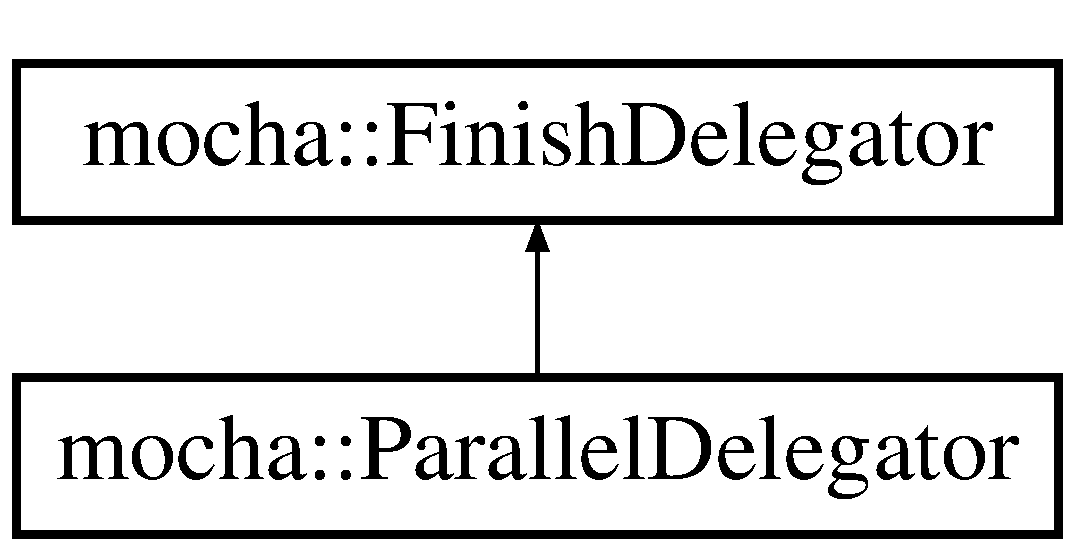
\includegraphics[height=2.000000cm]{classmocha_1_1_finish_delegator}
\end{center}
\end{figure}
\subsection*{Public Member Functions}
\begin{DoxyCompactItemize}
\item 
virtual void \hyperlink{classmocha_1_1_finish_delegator_ab558f69af2e3401b4aedc9ed86727083}{Delegate} (\hyperlink{classmocha_1_1_handle}{Handle}$<$ \hyperlink{classmocha_1_1_compile_result}{CompileResult} $>$ result)
\end{DoxyCompactItemize}


\subsection{Detailed Description}


Definition at line 11 of file compiler\_\-facade.h.



\subsection{Member Function Documentation}
\hypertarget{classmocha_1_1_finish_delegator_ab558f69af2e3401b4aedc9ed86727083}{
\index{mocha::FinishDelegator@{mocha::FinishDelegator}!Delegate@{Delegate}}
\index{Delegate@{Delegate}!mocha::FinishDelegator@{mocha::FinishDelegator}}
\subsubsection[{Delegate}]{\setlength{\rightskip}{0pt plus 5cm}virtual void mocha::FinishDelegator::Delegate (
\begin{DoxyParamCaption}
\item[{{\bf Handle}$<$ {\bf CompileResult} $>$}]{result}
\end{DoxyParamCaption}
)\hspace{0.3cm}{\ttfamily  \mbox{[}inline, virtual\mbox{]}}}}
\label{classmocha_1_1_finish_delegator_ab558f69af2e3401b4aedc9ed86727083}


Reimplemented in \hyperlink{classmocha_1_1_parallel_delegator_a7cc8e03175669290ddb4b39ee5e1c1d6}{mocha::ParallelDelegator}.



Definition at line 13 of file compiler\_\-facade.h.



The documentation for this class was generated from the following file:\begin{DoxyCompactItemize}
\item 
Y:/mocha/src/compiler/utils/\hyperlink{compiler__facade_8h}{compiler\_\-facade.h}\end{DoxyCompactItemize}

\hypertarget{classmocha_1_1_fixed_array}{
\section{mocha::FixedArray$<$ T $>$ Class Template Reference}
\label{classmocha_1_1_fixed_array}\index{mocha::FixedArray@{mocha::FixedArray}}
}


{\ttfamily \#include $<$fixed\_\-array.h$>$}

\subsection*{Public Member Functions}
\begin{DoxyCompactItemize}
\item 
\hyperlink{classmocha_1_1_fixed_array_a7094f7b664f15c54a126813a8b6481fa}{FixedArray} (size\_\-t size)
\item 
\hyperlink{classmocha_1_1_fixed_array_a79932ad171f72ce03bb8922473007fde}{$\sim$FixedArray} ()
\item 
T \hyperlink{classmocha_1_1_fixed_array_aef26e524fa960f7544d7bfc71b0f66de}{At} (index)
\end{DoxyCompactItemize}
\subsection*{Private Attributes}
\begin{DoxyCompactItemize}
\item 
T $\ast$ \hyperlink{classmocha_1_1_fixed_array_a14f9426748f9a44173cd4541131b8617}{array\_\-}
\end{DoxyCompactItemize}


\subsection{Detailed Description}
\subsubsection*{template$<$typename T$>$class mocha::FixedArray$<$ T $>$}



Definition at line 7 of file fixed\_\-array.h.



\subsection{Constructor \& Destructor Documentation}
\hypertarget{classmocha_1_1_fixed_array_a7094f7b664f15c54a126813a8b6481fa}{
\index{mocha::FixedArray@{mocha::FixedArray}!FixedArray@{FixedArray}}
\index{FixedArray@{FixedArray}!mocha::FixedArray@{mocha::FixedArray}}
\subsubsection[{FixedArray}]{\setlength{\rightskip}{0pt plus 5cm}template$<$typename T $>$ {\bf mocha::FixedArray}$<$ T $>$::{\bf FixedArray} (
\begin{DoxyParamCaption}
\item[{size\_\-t}]{size}
\end{DoxyParamCaption}
)\hspace{0.3cm}{\ttfamily  \mbox{[}inline\mbox{]}}}}
\label{classmocha_1_1_fixed_array_a7094f7b664f15c54a126813a8b6481fa}


Definition at line 9 of file fixed\_\-array.h.

\hypertarget{classmocha_1_1_fixed_array_a79932ad171f72ce03bb8922473007fde}{
\index{mocha::FixedArray@{mocha::FixedArray}!$\sim$FixedArray@{$\sim$FixedArray}}
\index{$\sim$FixedArray@{$\sim$FixedArray}!mocha::FixedArray@{mocha::FixedArray}}
\subsubsection[{$\sim$FixedArray}]{\setlength{\rightskip}{0pt plus 5cm}template$<$typename T $>$ {\bf mocha::FixedArray}$<$ T $>$::$\sim${\bf FixedArray} (
\begin{DoxyParamCaption}
{}
\end{DoxyParamCaption}
)\hspace{0.3cm}{\ttfamily  \mbox{[}inline\mbox{]}}}}
\label{classmocha_1_1_fixed_array_a79932ad171f72ce03bb8922473007fde}


Definition at line 10 of file fixed\_\-array.h.



\subsection{Member Function Documentation}
\hypertarget{classmocha_1_1_fixed_array_aef26e524fa960f7544d7bfc71b0f66de}{
\index{mocha::FixedArray@{mocha::FixedArray}!At@{At}}
\index{At@{At}!mocha::FixedArray@{mocha::FixedArray}}
\subsubsection[{At}]{\setlength{\rightskip}{0pt plus 5cm}template$<$typename T $>$ T {\bf mocha::FixedArray}$<$ T $>$::At (
\begin{DoxyParamCaption}
\item[{index}]{}
\end{DoxyParamCaption}
)}}
\label{classmocha_1_1_fixed_array_aef26e524fa960f7544d7bfc71b0f66de}


\subsection{Member Data Documentation}
\hypertarget{classmocha_1_1_fixed_array_a14f9426748f9a44173cd4541131b8617}{
\index{mocha::FixedArray@{mocha::FixedArray}!array\_\-@{array\_\-}}
\index{array\_\-@{array\_\-}!mocha::FixedArray@{mocha::FixedArray}}
\subsubsection[{array\_\-}]{\setlength{\rightskip}{0pt plus 5cm}template$<$typename T $>$ T$\ast$ {\bf mocha::FixedArray}$<$ T $>$::{\bf array\_\-}\hspace{0.3cm}{\ttfamily  \mbox{[}private\mbox{]}}}}
\label{classmocha_1_1_fixed_array_a14f9426748f9a44173cd4541131b8617}


Definition at line 13 of file fixed\_\-array.h.



The documentation for this class was generated from the following file:\begin{DoxyCompactItemize}
\item 
Y:/mocha/src/utils/\hyperlink{fixed__array_8h}{fixed\_\-array.h}\end{DoxyCompactItemize}

\hypertarget{classmocha_1_1_fixed_bit_stack}{
\section{mocha::FixedBitStack$<$ T, bit\_\-bands, Size $>$ Class Template Reference}
\label{classmocha_1_1_fixed_bit_stack}\index{mocha::FixedBitStack@{mocha::FixedBitStack}}
}


{\ttfamily \#include $<$bits.h$>$}

\subsection*{Public Types}
\begin{DoxyCompactItemize}
\item 
typedef \hyperlink{classmocha_1_1_bit_vector}{BitVector}$<$ T, bit\_\-bands $>$ \hyperlink{classmocha_1_1_fixed_bit_stack_aee038548c8d6aac4c6dd319f83f2b9d7}{FixedBitVector}
\end{DoxyCompactItemize}
\subsection*{Public Member Functions}
\begin{DoxyCompactItemize}
\item 
\hyperlink{classmocha_1_1_fixed_bit_stack_aa000a1e50e76779d0ef2b9761f8139f6}{FixedBitStack} ()
\item 
\hyperlink{classmocha_1_1_fixed_bit_stack_a87e772bc39e36859e916f345a5a2bc8d}{$\sim$FixedBitStack} ()
\item 
const \hyperlink{classmocha_1_1_bit_vector}{FixedBitVector} \& \hyperlink{classmocha_1_1_fixed_bit_stack_a0c65bab398ca0ab638a454e74caa8d56}{First} () const 
\item 
const \hyperlink{classmocha_1_1_bit_vector}{FixedBitVector} \& \hyperlink{classmocha_1_1_fixed_bit_stack_aa0d321cd87c73b1c335c7235c589aa06}{Last} () const 
\item 
const \hyperlink{classmocha_1_1_bit_vector}{FixedBitVector} \& \hyperlink{classmocha_1_1_fixed_bit_stack_a39829e596e57c27f1ca2657d6537a211}{At} (int index) const 
\item 
void \hyperlink{classmocha_1_1_fixed_bit_stack_a51bea702f00243271d3172e0409c20ff}{Push} (int val)
\item 
void \hyperlink{classmocha_1_1_fixed_bit_stack_a34ff857142078b4d9d782ddcfad06d7c}{Pop} (int val)
\item 
bool \hyperlink{classmocha_1_1_fixed_bit_stack_a153c07be728fdbf2c3ccbf0755a862f9}{AtFrom} (int index)
\item 
bool \hyperlink{classmocha_1_1_fixed_bit_stack_aa245b95a1f1e1aa88000bab24a407f82}{operator\mbox{[}$\,$\mbox{]}} (int index)
\end{DoxyCompactItemize}
\subsection*{Private Attributes}
\begin{DoxyCompactItemize}
\item 
int \hyperlink{classmocha_1_1_fixed_bit_stack_abd2f0780120850e55587f4fee273b3cc}{current\_\-}
\item 
\hyperlink{classmocha_1_1_bit_vector}{FixedBitVector} \hyperlink{classmocha_1_1_fixed_bit_stack_a7ae9a291d0b60997af8cfb9f535f7c65}{vector\_\-} \mbox{[}Size\mbox{]}
\end{DoxyCompactItemize}


\subsection{Detailed Description}
\subsubsection*{template$<$typename T, int bit\_\-bands, size\_\-t Size$>$class mocha::FixedBitStack$<$ T, bit\_\-bands, Size $>$}



Definition at line 47 of file bits.h.



\subsection{Member Typedef Documentation}
\hypertarget{classmocha_1_1_fixed_bit_stack_aee038548c8d6aac4c6dd319f83f2b9d7}{
\index{mocha::FixedBitStack@{mocha::FixedBitStack}!FixedBitVector@{FixedBitVector}}
\index{FixedBitVector@{FixedBitVector}!mocha::FixedBitStack@{mocha::FixedBitStack}}
\subsubsection[{FixedBitVector}]{\setlength{\rightskip}{0pt plus 5cm}template$<$typename T, int bit\_\-bands, size\_\-t Size$>$ typedef {\bf BitVector}$<$T,bit\_\-bands$>$ {\bf mocha::FixedBitStack}$<$ T, bit\_\-bands, Size $>$::{\bf FixedBitVector}}}
\label{classmocha_1_1_fixed_bit_stack_aee038548c8d6aac4c6dd319f83f2b9d7}


Definition at line 49 of file bits.h.



\subsection{Constructor \& Destructor Documentation}
\hypertarget{classmocha_1_1_fixed_bit_stack_aa000a1e50e76779d0ef2b9761f8139f6}{
\index{mocha::FixedBitStack@{mocha::FixedBitStack}!FixedBitStack@{FixedBitStack}}
\index{FixedBitStack@{FixedBitStack}!mocha::FixedBitStack@{mocha::FixedBitStack}}
\subsubsection[{FixedBitStack}]{\setlength{\rightskip}{0pt plus 5cm}template$<$typename T, int bit\_\-bands, size\_\-t Size$>$ {\bf mocha::FixedBitStack}$<$ T, bit\_\-bands, Size $>$::{\bf FixedBitStack} (
\begin{DoxyParamCaption}
{}
\end{DoxyParamCaption}
)\hspace{0.3cm}{\ttfamily  \mbox{[}inline\mbox{]}}}}
\label{classmocha_1_1_fixed_bit_stack_aa000a1e50e76779d0ef2b9761f8139f6}


Definition at line 50 of file bits.h.

\hypertarget{classmocha_1_1_fixed_bit_stack_a87e772bc39e36859e916f345a5a2bc8d}{
\index{mocha::FixedBitStack@{mocha::FixedBitStack}!$\sim$FixedBitStack@{$\sim$FixedBitStack}}
\index{$\sim$FixedBitStack@{$\sim$FixedBitStack}!mocha::FixedBitStack@{mocha::FixedBitStack}}
\subsubsection[{$\sim$FixedBitStack}]{\setlength{\rightskip}{0pt plus 5cm}template$<$typename T, int bit\_\-bands, size\_\-t Size$>$ {\bf mocha::FixedBitStack}$<$ T, bit\_\-bands, Size $>$::$\sim${\bf FixedBitStack} (
\begin{DoxyParamCaption}
{}
\end{DoxyParamCaption}
)\hspace{0.3cm}{\ttfamily  \mbox{[}inline\mbox{]}}}}
\label{classmocha_1_1_fixed_bit_stack_a87e772bc39e36859e916f345a5a2bc8d}


Definition at line 51 of file bits.h.



\subsection{Member Function Documentation}
\hypertarget{classmocha_1_1_fixed_bit_stack_a39829e596e57c27f1ca2657d6537a211}{
\index{mocha::FixedBitStack@{mocha::FixedBitStack}!At@{At}}
\index{At@{At}!mocha::FixedBitStack@{mocha::FixedBitStack}}
\subsubsection[{At}]{\setlength{\rightskip}{0pt plus 5cm}template$<$typename T, int bit\_\-bands, size\_\-t Size$>$ const {\bf FixedBitVector}\& {\bf mocha::FixedBitStack}$<$ T, bit\_\-bands, Size $>$::At (
\begin{DoxyParamCaption}
\item[{int}]{index}
\end{DoxyParamCaption}
) const\hspace{0.3cm}{\ttfamily  \mbox{[}inline\mbox{]}}}}
\label{classmocha_1_1_fixed_bit_stack_a39829e596e57c27f1ca2657d6537a211}


Definition at line 54 of file bits.h.

\hypertarget{classmocha_1_1_fixed_bit_stack_a153c07be728fdbf2c3ccbf0755a862f9}{
\index{mocha::FixedBitStack@{mocha::FixedBitStack}!AtFrom@{AtFrom}}
\index{AtFrom@{AtFrom}!mocha::FixedBitStack@{mocha::FixedBitStack}}
\subsubsection[{AtFrom}]{\setlength{\rightskip}{0pt plus 5cm}template$<$typename T, int bit\_\-bands, size\_\-t Size$>$ bool {\bf mocha::FixedBitStack}$<$ T, bit\_\-bands, Size $>$::AtFrom (
\begin{DoxyParamCaption}
\item[{int}]{index}
\end{DoxyParamCaption}
)\hspace{0.3cm}{\ttfamily  \mbox{[}inline\mbox{]}}}}
\label{classmocha_1_1_fixed_bit_stack_a153c07be728fdbf2c3ccbf0755a862f9}


Definition at line 62 of file bits.h.

\hypertarget{classmocha_1_1_fixed_bit_stack_a0c65bab398ca0ab638a454e74caa8d56}{
\index{mocha::FixedBitStack@{mocha::FixedBitStack}!First@{First}}
\index{First@{First}!mocha::FixedBitStack@{mocha::FixedBitStack}}
\subsubsection[{First}]{\setlength{\rightskip}{0pt plus 5cm}template$<$typename T, int bit\_\-bands, size\_\-t Size$>$ const {\bf FixedBitVector}\& {\bf mocha::FixedBitStack}$<$ T, bit\_\-bands, Size $>$::First (
\begin{DoxyParamCaption}
{}
\end{DoxyParamCaption}
) const\hspace{0.3cm}{\ttfamily  \mbox{[}inline\mbox{]}}}}
\label{classmocha_1_1_fixed_bit_stack_a0c65bab398ca0ab638a454e74caa8d56}


Definition at line 52 of file bits.h.

\hypertarget{classmocha_1_1_fixed_bit_stack_aa0d321cd87c73b1c335c7235c589aa06}{
\index{mocha::FixedBitStack@{mocha::FixedBitStack}!Last@{Last}}
\index{Last@{Last}!mocha::FixedBitStack@{mocha::FixedBitStack}}
\subsubsection[{Last}]{\setlength{\rightskip}{0pt plus 5cm}template$<$typename T, int bit\_\-bands, size\_\-t Size$>$ const {\bf FixedBitVector}\& {\bf mocha::FixedBitStack}$<$ T, bit\_\-bands, Size $>$::Last (
\begin{DoxyParamCaption}
{}
\end{DoxyParamCaption}
) const\hspace{0.3cm}{\ttfamily  \mbox{[}inline\mbox{]}}}}
\label{classmocha_1_1_fixed_bit_stack_aa0d321cd87c73b1c335c7235c589aa06}


Definition at line 53 of file bits.h.

\hypertarget{classmocha_1_1_fixed_bit_stack_aa245b95a1f1e1aa88000bab24a407f82}{
\index{mocha::FixedBitStack@{mocha::FixedBitStack}!operator\mbox{[}\mbox{]}@{operator[]}}
\index{operator\mbox{[}\mbox{]}@{operator[]}!mocha::FixedBitStack@{mocha::FixedBitStack}}
\subsubsection[{operator[]}]{\setlength{\rightskip}{0pt plus 5cm}template$<$typename T, int bit\_\-bands, size\_\-t Size$>$ bool {\bf mocha::FixedBitStack}$<$ T, bit\_\-bands, Size $>$::operator\mbox{[}$\,$\mbox{]} (
\begin{DoxyParamCaption}
\item[{int}]{index}
\end{DoxyParamCaption}
)\hspace{0.3cm}{\ttfamily  \mbox{[}inline\mbox{]}}}}
\label{classmocha_1_1_fixed_bit_stack_aa245b95a1f1e1aa88000bab24a407f82}


Definition at line 66 of file bits.h.

\hypertarget{classmocha_1_1_fixed_bit_stack_a34ff857142078b4d9d782ddcfad06d7c}{
\index{mocha::FixedBitStack@{mocha::FixedBitStack}!Pop@{Pop}}
\index{Pop@{Pop}!mocha::FixedBitStack@{mocha::FixedBitStack}}
\subsubsection[{Pop}]{\setlength{\rightskip}{0pt plus 5cm}template$<$typename T, int bit\_\-bands, size\_\-t Size$>$ void {\bf mocha::FixedBitStack}$<$ T, bit\_\-bands, Size $>$::Pop (
\begin{DoxyParamCaption}
\item[{int}]{val}
\end{DoxyParamCaption}
)\hspace{0.3cm}{\ttfamily  \mbox{[}inline\mbox{]}}}}
\label{classmocha_1_1_fixed_bit_stack_a34ff857142078b4d9d782ddcfad06d7c}


Definition at line 56 of file bits.h.

\hypertarget{classmocha_1_1_fixed_bit_stack_a51bea702f00243271d3172e0409c20ff}{
\index{mocha::FixedBitStack@{mocha::FixedBitStack}!Push@{Push}}
\index{Push@{Push}!mocha::FixedBitStack@{mocha::FixedBitStack}}
\subsubsection[{Push}]{\setlength{\rightskip}{0pt plus 5cm}template$<$typename T, int bit\_\-bands, size\_\-t Size$>$ void {\bf mocha::FixedBitStack}$<$ T, bit\_\-bands, Size $>$::Push (
\begin{DoxyParamCaption}
\item[{int}]{val}
\end{DoxyParamCaption}
)\hspace{0.3cm}{\ttfamily  \mbox{[}inline\mbox{]}}}}
\label{classmocha_1_1_fixed_bit_stack_a51bea702f00243271d3172e0409c20ff}


Definition at line 55 of file bits.h.



\subsection{Member Data Documentation}
\hypertarget{classmocha_1_1_fixed_bit_stack_abd2f0780120850e55587f4fee273b3cc}{
\index{mocha::FixedBitStack@{mocha::FixedBitStack}!current\_\-@{current\_\-}}
\index{current\_\-@{current\_\-}!mocha::FixedBitStack@{mocha::FixedBitStack}}
\subsubsection[{current\_\-}]{\setlength{\rightskip}{0pt plus 5cm}template$<$typename T, int bit\_\-bands, size\_\-t Size$>$ int {\bf mocha::FixedBitStack}$<$ T, bit\_\-bands, Size $>$::{\bf current\_\-}\hspace{0.3cm}{\ttfamily  \mbox{[}private\mbox{]}}}}
\label{classmocha_1_1_fixed_bit_stack_abd2f0780120850e55587f4fee273b3cc}


Definition at line 71 of file bits.h.

\hypertarget{classmocha_1_1_fixed_bit_stack_a7ae9a291d0b60997af8cfb9f535f7c65}{
\index{mocha::FixedBitStack@{mocha::FixedBitStack}!vector\_\-@{vector\_\-}}
\index{vector\_\-@{vector\_\-}!mocha::FixedBitStack@{mocha::FixedBitStack}}
\subsubsection[{vector\_\-}]{\setlength{\rightskip}{0pt plus 5cm}template$<$typename T, int bit\_\-bands, size\_\-t Size$>$ {\bf FixedBitVector} {\bf mocha::FixedBitStack}$<$ T, bit\_\-bands, Size $>$::{\bf vector\_\-}\mbox{[}Size\mbox{]}\hspace{0.3cm}{\ttfamily  \mbox{[}private\mbox{]}}}}
\label{classmocha_1_1_fixed_bit_stack_a7ae9a291d0b60997af8cfb9f535f7c65}


Definition at line 72 of file bits.h.



The documentation for this class was generated from the following file:\begin{DoxyCompactItemize}
\item 
Y:/mocha/src/utils/\hyperlink{bits_8h}{bits.h}\end{DoxyCompactItemize}

\hypertarget{classmocha_1_1_fixed_bit_stack16}{
\section{mocha::FixedBitStack16$<$ Size $>$ Class Template Reference}
\label{classmocha_1_1_fixed_bit_stack16}\index{mocha::FixedBitStack16@{mocha::FixedBitStack16}}
}


{\ttfamily \#include $<$bits.h$>$}

Inheritance diagram for mocha::FixedBitStack16$<$ Size $>$:\begin{figure}[H]
\begin{center}
\leavevmode
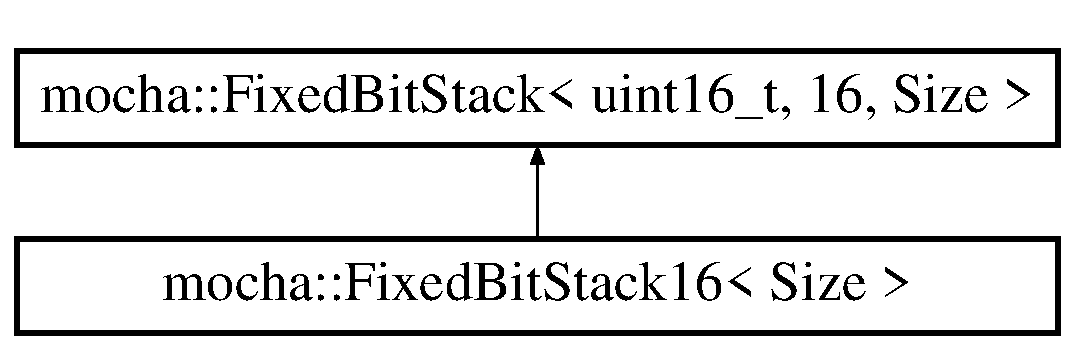
\includegraphics[height=2.000000cm]{classmocha_1_1_fixed_bit_stack16}
\end{center}
\end{figure}


\subsection{Detailed Description}
\subsubsection*{template$<$size\_\-t Size$>$class mocha::FixedBitStack16$<$ Size $>$}



Definition at line 85 of file bits.h.



The documentation for this class was generated from the following file:\begin{DoxyCompactItemize}
\item 
Y:/mocha/src/utils/\hyperlink{bits_8h}{bits.h}\end{DoxyCompactItemize}

\hypertarget{classmocha_1_1_fixed_bit_stack32}{
\section{mocha::FixedBitStack32$<$ Size $>$ Class Template Reference}
\label{classmocha_1_1_fixed_bit_stack32}\index{mocha::FixedBitStack32@{mocha::FixedBitStack32}}
}


{\ttfamily \#include $<$bits.h$>$}

Inheritance diagram for mocha::FixedBitStack32$<$ Size $>$:\begin{figure}[H]
\begin{center}
\leavevmode
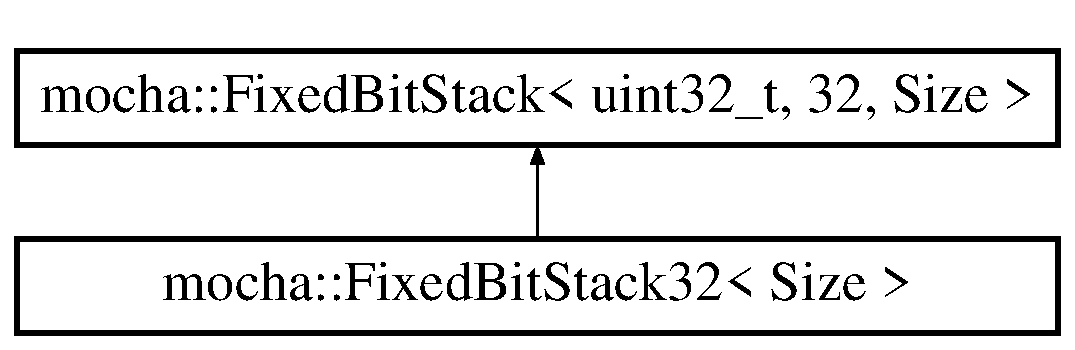
\includegraphics[height=2.000000cm]{classmocha_1_1_fixed_bit_stack32}
\end{center}
\end{figure}


\subsection{Detailed Description}
\subsubsection*{template$<$size\_\-t Size$>$class mocha::FixedBitStack32$<$ Size $>$}



Definition at line 88 of file bits.h.



The documentation for this class was generated from the following file:\begin{DoxyCompactItemize}
\item 
Y:/mocha/src/utils/\hyperlink{bits_8h}{bits.h}\end{DoxyCompactItemize}

\hypertarget{classmocha_1_1_fixed_bit_stack64}{
\section{mocha::FixedBitStack64$<$ Size $>$ Class Template Reference}
\label{classmocha_1_1_fixed_bit_stack64}\index{mocha::FixedBitStack64@{mocha::FixedBitStack64}}
}


{\ttfamily \#include $<$bits.h$>$}

Inheritance diagram for mocha::FixedBitStack64$<$ Size $>$:\begin{figure}[H]
\begin{center}
\leavevmode
\includegraphics[height=2.000000cm]{classmocha_1_1_fixed_bit_stack64}
\end{center}
\end{figure}


\subsection{Detailed Description}
\subsubsection*{template$<$size\_\-t Size$>$class mocha::FixedBitStack64$<$ Size $>$}



Definition at line 91 of file bits.h.



The documentation for this class was generated from the following file:\begin{DoxyCompactItemize}
\item 
Y:/mocha/src/utils/\hyperlink{bits_8h}{bits.h}\end{DoxyCompactItemize}

\hypertarget{classmocha_1_1_fixed_bit_stack8}{
\section{mocha::FixedBitStack8$<$ Size $>$ Class Template Reference}
\label{classmocha_1_1_fixed_bit_stack8}\index{mocha::FixedBitStack8@{mocha::FixedBitStack8}}
}


{\ttfamily \#include $<$bits.h$>$}

Inheritance diagram for mocha::FixedBitStack8$<$ Size $>$:\begin{figure}[H]
\begin{center}
\leavevmode
\includegraphics[height=2.000000cm]{classmocha_1_1_fixed_bit_stack8}
\end{center}
\end{figure}


\subsection{Detailed Description}
\subsubsection*{template$<$size\_\-t Size$>$class mocha::FixedBitStack8$<$ Size $>$}



Definition at line 82 of file bits.h.



The documentation for this class was generated from the following file:\begin{DoxyCompactItemize}
\item 
Y:/mocha/src/utils/\hyperlink{bits_8h}{bits.h}\end{DoxyCompactItemize}

\hypertarget{classmocha_1_1_function}{
\section{mocha::Function Class Reference}
\label{classmocha_1_1_function}\index{mocha::Function@{mocha::Function}}
}


{\ttfamily \#include $<$ast.h$>$}

Inheritance diagram for mocha::Function:\begin{figure}[H]
\begin{center}
\leavevmode
\includegraphics[height=4.000000cm]{classmocha_1_1_function}
\end{center}
\end{figure}
\subsection*{Public Types}
\begin{DoxyCompactItemize}
\item 
enum \{ \hyperlink{classmocha_1_1_function_ad3b7db514f20142b0f64c5d3372daed6a3442707a280dc1acb3f6f717ddbbaeb4}{kNormal}, 
\hyperlink{classmocha_1_1_function_ad3b7db514f20142b0f64c5d3372daed6a4e4f72b8c9a543eeef0c7d5692a48596}{kShorten}
 \}
\item 
enum \hyperlink{classmocha_1_1_function_a73818727e95b7e36aa1b57c65a0a596d}{FnAttr} \{ \hyperlink{classmocha_1_1_function_a73818727e95b7e36aa1b57c65a0a596da2606fefe5b143e4becdb81d4c7dbc7e8}{kGet} =  1, 
\hyperlink{classmocha_1_1_function_a73818727e95b7e36aa1b57c65a0a596dab0c1505e9087e0afd69e7fb963571df5}{kSet} =  2
 \}
\item 
enum \{ \hyperlink{classmocha_1_1_function_ab8d67b714552a9d8dfb317bedc5393efadca11b20d09a709bb7edccd46712d608}{kGlobal}, 
\hyperlink{classmocha_1_1_function_ab8d67b714552a9d8dfb317bedc5393efaf7567a4bbb15db601bca4d888cfd0661}{kThis}
 \}
\item 
typedef std::vector$<$ \hyperlink{classmocha_1_1_ast_node}{AstNode} $\ast$ $>$ \hyperlink{classmocha_1_1_function_a5c4a48ede908b355b4f13a8f1d585707}{StmtList}
\item 
typedef std::vector$<$ \hyperlink{classmocha_1_1_value_node}{ValueNode} $\ast$ $>$ \hyperlink{classmocha_1_1_function_a243702678d29f0cfd91913838c1fb38c}{VariableList}
\item 
typedef std::vector$<$ \hyperlink{classmocha_1_1_try_stmt}{TryStmt} $\ast$ $>$ \hyperlink{classmocha_1_1_function_a9991b3d8362e4a8889c4b50d930d88ce}{TryList}
\end{DoxyCompactItemize}
\subsection*{Public Member Functions}
\begin{DoxyCompactItemize}
\item 
\hyperlink{classmocha_1_1_function_a91051b21b9ab3cf0a7076ac1c8f19d12}{Function} ()
\item 
\hyperlink{classmocha_1_1_function_acfd060d663bcb7aba9b404b97f21bef3}{$\sim$Function} ()
\item 
\hyperlink{classmocha_1_1_function}{Function} $\ast$ \hyperlink{classmocha_1_1_function_a7054a10d92311750a4a2e1ce9a36f3d3}{CastToFunction} ()
\item 
void \hyperlink{classmocha_1_1_function_a519eeb5120164a9a77734db8c0de3ca8}{Name} (\hyperlink{classmocha_1_1_ast_node}{AstNode} $\ast$name)
\item 
\hyperlink{classmocha_1_1_ast_node}{AstNode} $\ast$ \hyperlink{classmocha_1_1_function_a11f15ec2f685a424ca93ac66faae2e6f}{Name} ()
\item 
\hyperlink{classmocha_1_1_ast_node}{AstNode} $\ast$ \hyperlink{classmocha_1_1_function_ad46af100a0740ba509a4ce4564bd912b}{Argv} ()
\item 
void \hyperlink{classmocha_1_1_function_a70f7f55e89c7d0e9e3c241c81f5647af}{Argv} (\hyperlink{classmocha_1_1_ast_node}{AstNode} $\ast$argv)
\item 
int \hyperlink{classmocha_1_1_function_a0fc7801db6782d941286b65cf3a6e2d0}{Argc} () const 
\item 
void \hyperlink{classmocha_1_1_function_aa8d43f0d016e1349a99a51e3cb6cde41}{Const} ()
\item 
bool \hyperlink{classmocha_1_1_function_a84c41c96c4a3e0da3ad764725e612edf}{IsConst} () const 
\item 
void \hyperlink{classmocha_1_1_function_a73f2d87ec7fc1930ee98948ee2fb9bca}{Decl} ()
\item 
bool \hyperlink{classmocha_1_1_function_a9e94abc1b5b8b0b986ef55c4a2883dad}{IsDecl} ()
\item 
void \hyperlink{classmocha_1_1_function_a77b9a126d99d66e9ca154056af9613ba}{Attr} (\hyperlink{classmocha_1_1_function_a73818727e95b7e36aa1b57c65a0a596d}{FnAttr} attr)
\item 
bool \hyperlink{classmocha_1_1_function_ae49decbf4b4e689312b0e1c824e264da}{IsAttr} (\hyperlink{classmocha_1_1_function_a73818727e95b7e36aa1b57c65a0a596d}{FnAttr} attr)
\item 
int \hyperlink{classmocha_1_1_function_a3da8c03271c7f64db13da13e53c5f6cb}{FunctionType} ()
\item 
void \hyperlink{classmocha_1_1_function_aeb8391e38eb2842ac1619522719c78af}{FunctionType} (int type)
\item 
int \hyperlink{classmocha_1_1_function_a2fa7ea873cb45ac4f02de44e3cbdf30b}{ContextType} ()
\item 
void \hyperlink{classmocha_1_1_function_af1f79f5424032a6ea0e2fd9b12f589ec}{ContextType} (int type)
\item 
void \hyperlink{classmocha_1_1_function_a9f5cfd13987ac0c4b6840801968afdc8}{SetScope} (\hyperlink{classmocha_1_1_inner_scope}{InnerScope} $\ast$scope)
\item 
\hyperlink{classmocha_1_1_inner_scope}{InnerScope} $\ast$ \hyperlink{classmocha_1_1_function_af8b7fbeeff670593b99208b4b160b50f}{GetScope} ()
\item 
void \hyperlink{classmocha_1_1_function_a4aaeba040456a899caf277cf25f7e236}{Root} (bool is)
\item 
bool \hyperlink{classmocha_1_1_function_abd3776ad2009b24328b3731c6d608ab3}{Root} ()
\item 
void \hyperlink{classmocha_1_1_function_ad71400eb14351910ac6d1c576413fc46}{SetYieldFlag} ()
\item 
bool \hyperlink{classmocha_1_1_function_ac56735e4aac25be688ac143f946aab02}{GetYieldFlag} ()
\item 
void \hyperlink{classmocha_1_1_function_a7262956db2bf8fa1d4e043709a3c0d13}{SetStmtWithYield} (\hyperlink{classmocha_1_1_ast_node}{AstNode} $\ast$node)
\item 
\hyperlink{classmocha_1_1_function_a5c4a48ede908b355b4f13a8f1d585707}{StmtList} \& \hyperlink{classmocha_1_1_function_a7761b50339b11f21c87e1ab52f6fa868}{GetStmtList} ()
\item 
void \hyperlink{classmocha_1_1_function_ad6b1cb328f7ea3d839377f86a03e7097}{SetTryCatch} (\hyperlink{classmocha_1_1_try_stmt}{TryStmt} $\ast$try\_\-stmt)
\item 
\hyperlink{classmocha_1_1_function_a9991b3d8362e4a8889c4b50d930d88ce}{TryList} \& \hyperlink{classmocha_1_1_function_a85f1491b11c7fc7a7d8d9aa7c7e9242f}{GetTryCatch} ()
\item 
void \hyperlink{classmocha_1_1_function_a9044326e0ef52a277c7131d986158ed9}{SetVariable} (\hyperlink{classmocha_1_1_value_node}{ValueNode} $\ast$node)
\item 
\hyperlink{classmocha_1_1_function_a243702678d29f0cfd91913838c1fb38c}{VariableList} \& \hyperlink{classmocha_1_1_function_ab7a1d37ca8f0d114b13b73f9efbc91b5}{GetVariable} ()
\item 
void \hyperlink{classmocha_1_1_function_a4b8c3561117a40bc804d224b29dd9b27}{SetReplacedThis} (\hyperlink{classmocha_1_1_value_node}{ValueNode} $\ast$val)
\item 
\hyperlink{classmocha_1_1_value_node}{ValueNode} $\ast$ \hyperlink{classmocha_1_1_function_a50b17dfecde9f7d484a7cc53094cdeb2}{GetReplacedThis} ()
\item 
\hyperlink{classmocha_1_1_ast_node}{AstNode} $\ast$ \hyperlink{classmocha_1_1_function_a787dcc9695496b521f0de87094003c7a}{Clone} ()
\end{DoxyCompactItemize}
\subsection*{Private Member Functions}
\begin{DoxyCompactItemize}
\item 
void \hyperlink{classmocha_1_1_function_ac8aea50fb291b078333d89530a25a627}{NVIAccept\_\-} (\hyperlink{classmocha_1_1_i_visitor}{IVisitor} $\ast$visitor)
\end{DoxyCompactItemize}
\subsection*{Private Attributes}
\begin{DoxyCompactItemize}
\item 
int \hyperlink{classmocha_1_1_function_ab96b5bc0337b378b937eb721568c02dc}{fn\_\-type\_\-}
\item 
int \hyperlink{classmocha_1_1_function_a91db13aafbd564b49413f780450fedb4}{context\_\-}
\item 
int \hyperlink{classmocha_1_1_function_ac2610c4e7f6eed41c2a213161d63a7e0}{fn\_\-attr\_\-}
\item 
bool \hyperlink{classmocha_1_1_function_af16f2b3ef9c2e2aeedd8bd2f498b3e68}{is\_\-const\_\-}
\item 
bool \hyperlink{classmocha_1_1_function_a921285276ef8d34a0be645fa2f30ff22}{is\_\-decl\_\-}
\item 
bool \hyperlink{classmocha_1_1_function_a9e6f90ffd90e9300d52fa848fa683bd7}{is\_\-root\_\-}
\item 
bool \hyperlink{classmocha_1_1_function_a854ca0fbe7fcf694b0fc9b9edbf1fd55}{has\_\-yield\_\-}
\item 
\hyperlink{classmocha_1_1_ast_node}{AstNode} $\ast$ \hyperlink{classmocha_1_1_function_ac2e4d75b6c293a0f2d6344df8cdc10e7}{name\_\-}
\item 
\hyperlink{classmocha_1_1_ast_node}{AstNode} $\ast$ \hyperlink{classmocha_1_1_function_a11310ef6f72f85539da7a1a2f500aa81}{argv\_\-}
\item 
\hyperlink{classmocha_1_1_value_node}{ValueNode} $\ast$ \hyperlink{classmocha_1_1_function_a06bcbfa74031bdac59acc8d0bbc46e2c}{replaced\_\-this\_\-}
\item 
\hyperlink{classmocha_1_1_inner_scope}{InnerScope} $\ast$ \hyperlink{classmocha_1_1_function_aa72c922f8808342eaad6b06d49a8757c}{scope\_\-}
\item 
\hyperlink{classmocha_1_1_function_a5c4a48ede908b355b4f13a8f1d585707}{StmtList} \hyperlink{classmocha_1_1_function_a4ac68f0b0e7ed2a47d6d340d1d75777b}{iteration\_\-list\_\-}
\item 
\hyperlink{classmocha_1_1_function_a243702678d29f0cfd91913838c1fb38c}{VariableList} \hyperlink{classmocha_1_1_function_af7dd9ddfa47f825f6ac37eca4648c4eb}{variable\_\-list\_\-}
\item 
\hyperlink{classmocha_1_1_function_a9991b3d8362e4a8889c4b50d930d88ce}{TryList} \hyperlink{classmocha_1_1_function_a3adc54c775dcb9470a3d2ecabcd679f0}{try\_\-list\_\-}
\end{DoxyCompactItemize}


\subsection{Detailed Description}


Definition at line 1215 of file ast.h.



\subsection{Member Typedef Documentation}
\hypertarget{classmocha_1_1_function_a5c4a48ede908b355b4f13a8f1d585707}{
\index{mocha::Function@{mocha::Function}!StmtList@{StmtList}}
\index{StmtList@{StmtList}!mocha::Function@{mocha::Function}}
\subsubsection[{StmtList}]{\setlength{\rightskip}{0pt plus 5cm}typedef std::vector$<${\bf AstNode}$\ast$$>$ {\bf mocha::Function::StmtList}}}
\label{classmocha_1_1_function_a5c4a48ede908b355b4f13a8f1d585707}


Definition at line 1217 of file ast.h.

\hypertarget{classmocha_1_1_function_a9991b3d8362e4a8889c4b50d930d88ce}{
\index{mocha::Function@{mocha::Function}!TryList@{TryList}}
\index{TryList@{TryList}!mocha::Function@{mocha::Function}}
\subsubsection[{TryList}]{\setlength{\rightskip}{0pt plus 5cm}typedef std::vector$<${\bf TryStmt}$\ast$$>$ {\bf mocha::Function::TryList}}}
\label{classmocha_1_1_function_a9991b3d8362e4a8889c4b50d930d88ce}


Definition at line 1219 of file ast.h.

\hypertarget{classmocha_1_1_function_a243702678d29f0cfd91913838c1fb38c}{
\index{mocha::Function@{mocha::Function}!VariableList@{VariableList}}
\index{VariableList@{VariableList}!mocha::Function@{mocha::Function}}
\subsubsection[{VariableList}]{\setlength{\rightskip}{0pt plus 5cm}typedef std::vector$<${\bf ValueNode}$\ast$$>$ {\bf mocha::Function::VariableList}}}
\label{classmocha_1_1_function_a243702678d29f0cfd91913838c1fb38c}


Definition at line 1218 of file ast.h.



\subsection{Member Enumeration Documentation}
\hypertarget{classmocha_1_1_function_ad3b7db514f20142b0f64c5d3372daed6}{
\subsubsection[{"@4}]{\setlength{\rightskip}{0pt plus 5cm}anonymous enum}}
\label{classmocha_1_1_function_ad3b7db514f20142b0f64c5d3372daed6}
\begin{Desc}
\item[Enumerator: ]\par
\begin{description}
\index{kNormal@{kNormal}!mocha::Function@{mocha::Function}}\index{mocha::Function@{mocha::Function}!kNormal@{kNormal}}\item[{\em 
\hypertarget{classmocha_1_1_function_ad3b7db514f20142b0f64c5d3372daed6a3442707a280dc1acb3f6f717ddbbaeb4}{
kNormal}
\label{classmocha_1_1_function_ad3b7db514f20142b0f64c5d3372daed6a3442707a280dc1acb3f6f717ddbbaeb4}
}]\index{kShorten@{kShorten}!mocha::Function@{mocha::Function}}\index{mocha::Function@{mocha::Function}!kShorten@{kShorten}}\item[{\em 
\hypertarget{classmocha_1_1_function_ad3b7db514f20142b0f64c5d3372daed6a4e4f72b8c9a543eeef0c7d5692a48596}{
kShorten}
\label{classmocha_1_1_function_ad3b7db514f20142b0f64c5d3372daed6a4e4f72b8c9a543eeef0c7d5692a48596}
}]\end{description}
\end{Desc}



Definition at line 1220 of file ast.h.

\hypertarget{classmocha_1_1_function_ab8d67b714552a9d8dfb317bedc5393ef}{
\subsubsection[{"@5}]{\setlength{\rightskip}{0pt plus 5cm}anonymous enum}}
\label{classmocha_1_1_function_ab8d67b714552a9d8dfb317bedc5393ef}
\begin{Desc}
\item[Enumerator: ]\par
\begin{description}
\index{kGlobal@{kGlobal}!mocha::Function@{mocha::Function}}\index{mocha::Function@{mocha::Function}!kGlobal@{kGlobal}}\item[{\em 
\hypertarget{classmocha_1_1_function_ab8d67b714552a9d8dfb317bedc5393efadca11b20d09a709bb7edccd46712d608}{
kGlobal}
\label{classmocha_1_1_function_ab8d67b714552a9d8dfb317bedc5393efadca11b20d09a709bb7edccd46712d608}
}]\index{kThis@{kThis}!mocha::Function@{mocha::Function}}\index{mocha::Function@{mocha::Function}!kThis@{kThis}}\item[{\em 
\hypertarget{classmocha_1_1_function_ab8d67b714552a9d8dfb317bedc5393efaf7567a4bbb15db601bca4d888cfd0661}{
kThis}
\label{classmocha_1_1_function_ab8d67b714552a9d8dfb317bedc5393efaf7567a4bbb15db601bca4d888cfd0661}
}]\end{description}
\end{Desc}



Definition at line 1228 of file ast.h.

\hypertarget{classmocha_1_1_function_a73818727e95b7e36aa1b57c65a0a596d}{
\index{mocha::Function@{mocha::Function}!FnAttr@{FnAttr}}
\index{FnAttr@{FnAttr}!mocha::Function@{mocha::Function}}
\subsubsection[{FnAttr}]{\setlength{\rightskip}{0pt plus 5cm}enum {\bf mocha::Function::FnAttr}}}
\label{classmocha_1_1_function_a73818727e95b7e36aa1b57c65a0a596d}
\begin{Desc}
\item[Enumerator: ]\par
\begin{description}
\index{kGet@{kGet}!mocha::Function@{mocha::Function}}\index{mocha::Function@{mocha::Function}!kGet@{kGet}}\item[{\em 
\hypertarget{classmocha_1_1_function_a73818727e95b7e36aa1b57c65a0a596da2606fefe5b143e4becdb81d4c7dbc7e8}{
kGet}
\label{classmocha_1_1_function_a73818727e95b7e36aa1b57c65a0a596da2606fefe5b143e4becdb81d4c7dbc7e8}
}]\index{kSet@{kSet}!mocha::Function@{mocha::Function}}\index{mocha::Function@{mocha::Function}!kSet@{kSet}}\item[{\em 
\hypertarget{classmocha_1_1_function_a73818727e95b7e36aa1b57c65a0a596dab0c1505e9087e0afd69e7fb963571df5}{
kSet}
\label{classmocha_1_1_function_a73818727e95b7e36aa1b57c65a0a596dab0c1505e9087e0afd69e7fb963571df5}
}]\end{description}
\end{Desc}



Definition at line 1224 of file ast.h.



\subsection{Constructor \& Destructor Documentation}
\hypertarget{classmocha_1_1_function_a91051b21b9ab3cf0a7076ac1c8f19d12}{
\index{mocha::Function@{mocha::Function}!Function@{Function}}
\index{Function@{Function}!mocha::Function@{mocha::Function}}
\subsubsection[{Function}]{\setlength{\rightskip}{0pt plus 5cm}mocha::Function::Function (
\begin{DoxyParamCaption}
{}
\end{DoxyParamCaption}
)\hspace{0.3cm}{\ttfamily  \mbox{[}inline\mbox{]}}}}
\label{classmocha_1_1_function_a91051b21b9ab3cf0a7076ac1c8f19d12}


Definition at line 1232 of file ast.h.

\hypertarget{classmocha_1_1_function_acfd060d663bcb7aba9b404b97f21bef3}{
\index{mocha::Function@{mocha::Function}!$\sim$Function@{$\sim$Function}}
\index{$\sim$Function@{$\sim$Function}!mocha::Function@{mocha::Function}}
\subsubsection[{$\sim$Function}]{\setlength{\rightskip}{0pt plus 5cm}mocha::Function::$\sim$Function (
\begin{DoxyParamCaption}
{}
\end{DoxyParamCaption}
)\hspace{0.3cm}{\ttfamily  \mbox{[}inline\mbox{]}}}}
\label{classmocha_1_1_function_acfd060d663bcb7aba9b404b97f21bef3}


Definition at line 1237 of file ast.h.



\subsection{Member Function Documentation}
\hypertarget{classmocha_1_1_function_a0fc7801db6782d941286b65cf3a6e2d0}{
\index{mocha::Function@{mocha::Function}!Argc@{Argc}}
\index{Argc@{Argc}!mocha::Function@{mocha::Function}}
\subsubsection[{Argc}]{\setlength{\rightskip}{0pt plus 5cm}int mocha::Function::Argc (
\begin{DoxyParamCaption}
{}
\end{DoxyParamCaption}
) const\hspace{0.3cm}{\ttfamily  \mbox{[}inline\mbox{]}}}}
\label{classmocha_1_1_function_a0fc7801db6782d941286b65cf3a6e2d0}


Definition at line 1243 of file ast.h.

\hypertarget{classmocha_1_1_function_a70f7f55e89c7d0e9e3c241c81f5647af}{
\index{mocha::Function@{mocha::Function}!Argv@{Argv}}
\index{Argv@{Argv}!mocha::Function@{mocha::Function}}
\subsubsection[{Argv}]{\setlength{\rightskip}{0pt plus 5cm}void mocha::Function::Argv (
\begin{DoxyParamCaption}
\item[{{\bf AstNode} $\ast$}]{argv}
\end{DoxyParamCaption}
)\hspace{0.3cm}{\ttfamily  \mbox{[}inline\mbox{]}}}}
\label{classmocha_1_1_function_a70f7f55e89c7d0e9e3c241c81f5647af}


Definition at line 1242 of file ast.h.

\hypertarget{classmocha_1_1_function_ad46af100a0740ba509a4ce4564bd912b}{
\index{mocha::Function@{mocha::Function}!Argv@{Argv}}
\index{Argv@{Argv}!mocha::Function@{mocha::Function}}
\subsubsection[{Argv}]{\setlength{\rightskip}{0pt plus 5cm}{\bf AstNode}$\ast$ mocha::Function::Argv (
\begin{DoxyParamCaption}
{}
\end{DoxyParamCaption}
)\hspace{0.3cm}{\ttfamily  \mbox{[}inline\mbox{]}}}}
\label{classmocha_1_1_function_ad46af100a0740ba509a4ce4564bd912b}


Definition at line 1241 of file ast.h.

\hypertarget{classmocha_1_1_function_a77b9a126d99d66e9ca154056af9613ba}{
\index{mocha::Function@{mocha::Function}!Attr@{Attr}}
\index{Attr@{Attr}!mocha::Function@{mocha::Function}}
\subsubsection[{Attr}]{\setlength{\rightskip}{0pt plus 5cm}void mocha::Function::Attr (
\begin{DoxyParamCaption}
\item[{{\bf FnAttr}}]{attr}
\end{DoxyParamCaption}
)\hspace{0.3cm}{\ttfamily  \mbox{[}inline\mbox{]}}}}
\label{classmocha_1_1_function_a77b9a126d99d66e9ca154056af9613ba}


Definition at line 1248 of file ast.h.

\hypertarget{classmocha_1_1_function_a7054a10d92311750a4a2e1ce9a36f3d3}{
\index{mocha::Function@{mocha::Function}!CastToFunction@{CastToFunction}}
\index{CastToFunction@{CastToFunction}!mocha::Function@{mocha::Function}}
\subsubsection[{CastToFunction}]{\setlength{\rightskip}{0pt plus 5cm}{\bf Function}$\ast$ mocha::Function::CastToFunction (
\begin{DoxyParamCaption}
{}
\end{DoxyParamCaption}
)\hspace{0.3cm}{\ttfamily  \mbox{[}inline, virtual\mbox{]}}}}
\label{classmocha_1_1_function_a7054a10d92311750a4a2e1ce9a36f3d3}


Reimplemented from \hyperlink{classmocha_1_1_expression_a56027507124496007854f768cd847d52}{mocha::Expression}.



Definition at line 1238 of file ast.h.

\hypertarget{classmocha_1_1_function_a787dcc9695496b521f0de87094003c7a}{
\index{mocha::Function@{mocha::Function}!Clone@{Clone}}
\index{Clone@{Clone}!mocha::Function@{mocha::Function}}
\subsubsection[{Clone}]{\setlength{\rightskip}{0pt plus 5cm}{\bf AstNode} $\ast$ mocha::Function::Clone (
\begin{DoxyParamCaption}
{}
\end{DoxyParamCaption}
)\hspace{0.3cm}{\ttfamily  \mbox{[}virtual\mbox{]}}}}
\label{classmocha_1_1_function_a787dcc9695496b521f0de87094003c7a}
\begin{DoxyReturn}{Returns}
\{AstNode$\ast$\} Clone node. 
\end{DoxyReturn}


Reimplemented from \hyperlink{classmocha_1_1_expression_ac1fb936e2bf0fdd6e7667275d3723ca5}{mocha::Expression}.



Definition at line 421 of file ast.cc.

\hypertarget{classmocha_1_1_function_aa8d43f0d016e1349a99a51e3cb6cde41}{
\index{mocha::Function@{mocha::Function}!Const@{Const}}
\index{Const@{Const}!mocha::Function@{mocha::Function}}
\subsubsection[{Const}]{\setlength{\rightskip}{0pt plus 5cm}void mocha::Function::Const (
\begin{DoxyParamCaption}
{}
\end{DoxyParamCaption}
)\hspace{0.3cm}{\ttfamily  \mbox{[}inline\mbox{]}}}}
\label{classmocha_1_1_function_aa8d43f0d016e1349a99a51e3cb6cde41}


Definition at line 1244 of file ast.h.

\hypertarget{classmocha_1_1_function_af1f79f5424032a6ea0e2fd9b12f589ec}{
\index{mocha::Function@{mocha::Function}!ContextType@{ContextType}}
\index{ContextType@{ContextType}!mocha::Function@{mocha::Function}}
\subsubsection[{ContextType}]{\setlength{\rightskip}{0pt plus 5cm}void mocha::Function::ContextType (
\begin{DoxyParamCaption}
\item[{int}]{type}
\end{DoxyParamCaption}
)\hspace{0.3cm}{\ttfamily  \mbox{[}inline\mbox{]}}}}
\label{classmocha_1_1_function_af1f79f5424032a6ea0e2fd9b12f589ec}


Definition at line 1253 of file ast.h.

\hypertarget{classmocha_1_1_function_a2fa7ea873cb45ac4f02de44e3cbdf30b}{
\index{mocha::Function@{mocha::Function}!ContextType@{ContextType}}
\index{ContextType@{ContextType}!mocha::Function@{mocha::Function}}
\subsubsection[{ContextType}]{\setlength{\rightskip}{0pt plus 5cm}int mocha::Function::ContextType (
\begin{DoxyParamCaption}
{}
\end{DoxyParamCaption}
)\hspace{0.3cm}{\ttfamily  \mbox{[}inline\mbox{]}}}}
\label{classmocha_1_1_function_a2fa7ea873cb45ac4f02de44e3cbdf30b}


Definition at line 1252 of file ast.h.

\hypertarget{classmocha_1_1_function_a73f2d87ec7fc1930ee98948ee2fb9bca}{
\index{mocha::Function@{mocha::Function}!Decl@{Decl}}
\index{Decl@{Decl}!mocha::Function@{mocha::Function}}
\subsubsection[{Decl}]{\setlength{\rightskip}{0pt plus 5cm}void mocha::Function::Decl (
\begin{DoxyParamCaption}
{}
\end{DoxyParamCaption}
)\hspace{0.3cm}{\ttfamily  \mbox{[}inline\mbox{]}}}}
\label{classmocha_1_1_function_a73f2d87ec7fc1930ee98948ee2fb9bca}


Definition at line 1246 of file ast.h.

\hypertarget{classmocha_1_1_function_a3da8c03271c7f64db13da13e53c5f6cb}{
\index{mocha::Function@{mocha::Function}!FunctionType@{FunctionType}}
\index{FunctionType@{FunctionType}!mocha::Function@{mocha::Function}}
\subsubsection[{FunctionType}]{\setlength{\rightskip}{0pt plus 5cm}int mocha::Function::FunctionType (
\begin{DoxyParamCaption}
{}
\end{DoxyParamCaption}
)\hspace{0.3cm}{\ttfamily  \mbox{[}inline\mbox{]}}}}
\label{classmocha_1_1_function_a3da8c03271c7f64db13da13e53c5f6cb}


Definition at line 1250 of file ast.h.

\hypertarget{classmocha_1_1_function_aeb8391e38eb2842ac1619522719c78af}{
\index{mocha::Function@{mocha::Function}!FunctionType@{FunctionType}}
\index{FunctionType@{FunctionType}!mocha::Function@{mocha::Function}}
\subsubsection[{FunctionType}]{\setlength{\rightskip}{0pt plus 5cm}void mocha::Function::FunctionType (
\begin{DoxyParamCaption}
\item[{int}]{type}
\end{DoxyParamCaption}
)\hspace{0.3cm}{\ttfamily  \mbox{[}inline\mbox{]}}}}
\label{classmocha_1_1_function_aeb8391e38eb2842ac1619522719c78af}


Definition at line 1251 of file ast.h.

\hypertarget{classmocha_1_1_function_a50b17dfecde9f7d484a7cc53094cdeb2}{
\index{mocha::Function@{mocha::Function}!GetReplacedThis@{GetReplacedThis}}
\index{GetReplacedThis@{GetReplacedThis}!mocha::Function@{mocha::Function}}
\subsubsection[{GetReplacedThis}]{\setlength{\rightskip}{0pt plus 5cm}{\bf ValueNode}$\ast$ mocha::Function::GetReplacedThis (
\begin{DoxyParamCaption}
{}
\end{DoxyParamCaption}
)\hspace{0.3cm}{\ttfamily  \mbox{[}inline\mbox{]}}}}
\label{classmocha_1_1_function_a50b17dfecde9f7d484a7cc53094cdeb2}


Definition at line 1267 of file ast.h.

\hypertarget{classmocha_1_1_function_af8b7fbeeff670593b99208b4b160b50f}{
\index{mocha::Function@{mocha::Function}!GetScope@{GetScope}}
\index{GetScope@{GetScope}!mocha::Function@{mocha::Function}}
\subsubsection[{GetScope}]{\setlength{\rightskip}{0pt plus 5cm}{\bf InnerScope}$\ast$ mocha::Function::GetScope (
\begin{DoxyParamCaption}
{}
\end{DoxyParamCaption}
)\hspace{0.3cm}{\ttfamily  \mbox{[}inline\mbox{]}}}}
\label{classmocha_1_1_function_af8b7fbeeff670593b99208b4b160b50f}


Definition at line 1255 of file ast.h.

\hypertarget{classmocha_1_1_function_a7761b50339b11f21c87e1ab52f6fa868}{
\index{mocha::Function@{mocha::Function}!GetStmtList@{GetStmtList}}
\index{GetStmtList@{GetStmtList}!mocha::Function@{mocha::Function}}
\subsubsection[{GetStmtList}]{\setlength{\rightskip}{0pt plus 5cm}{\bf StmtList}\& mocha::Function::GetStmtList (
\begin{DoxyParamCaption}
{}
\end{DoxyParamCaption}
)\hspace{0.3cm}{\ttfamily  \mbox{[}inline\mbox{]}}}}
\label{classmocha_1_1_function_a7761b50339b11f21c87e1ab52f6fa868}


Definition at line 1261 of file ast.h.

\hypertarget{classmocha_1_1_function_a85f1491b11c7fc7a7d8d9aa7c7e9242f}{
\index{mocha::Function@{mocha::Function}!GetTryCatch@{GetTryCatch}}
\index{GetTryCatch@{GetTryCatch}!mocha::Function@{mocha::Function}}
\subsubsection[{GetTryCatch}]{\setlength{\rightskip}{0pt plus 5cm}{\bf TryList}\& mocha::Function::GetTryCatch (
\begin{DoxyParamCaption}
{}
\end{DoxyParamCaption}
)\hspace{0.3cm}{\ttfamily  \mbox{[}inline\mbox{]}}}}
\label{classmocha_1_1_function_a85f1491b11c7fc7a7d8d9aa7c7e9242f}


Definition at line 1263 of file ast.h.

\hypertarget{classmocha_1_1_function_ab7a1d37ca8f0d114b13b73f9efbc91b5}{
\index{mocha::Function@{mocha::Function}!GetVariable@{GetVariable}}
\index{GetVariable@{GetVariable}!mocha::Function@{mocha::Function}}
\subsubsection[{GetVariable}]{\setlength{\rightskip}{0pt plus 5cm}{\bf VariableList}\& mocha::Function::GetVariable (
\begin{DoxyParamCaption}
{}
\end{DoxyParamCaption}
)\hspace{0.3cm}{\ttfamily  \mbox{[}inline\mbox{]}}}}
\label{classmocha_1_1_function_ab7a1d37ca8f0d114b13b73f9efbc91b5}


Definition at line 1265 of file ast.h.

\hypertarget{classmocha_1_1_function_ac56735e4aac25be688ac143f946aab02}{
\index{mocha::Function@{mocha::Function}!GetYieldFlag@{GetYieldFlag}}
\index{GetYieldFlag@{GetYieldFlag}!mocha::Function@{mocha::Function}}
\subsubsection[{GetYieldFlag}]{\setlength{\rightskip}{0pt plus 5cm}bool mocha::Function::GetYieldFlag (
\begin{DoxyParamCaption}
{}
\end{DoxyParamCaption}
)\hspace{0.3cm}{\ttfamily  \mbox{[}inline\mbox{]}}}}
\label{classmocha_1_1_function_ac56735e4aac25be688ac143f946aab02}


Definition at line 1259 of file ast.h.

\hypertarget{classmocha_1_1_function_ae49decbf4b4e689312b0e1c824e264da}{
\index{mocha::Function@{mocha::Function}!IsAttr@{IsAttr}}
\index{IsAttr@{IsAttr}!mocha::Function@{mocha::Function}}
\subsubsection[{IsAttr}]{\setlength{\rightskip}{0pt plus 5cm}bool mocha::Function::IsAttr (
\begin{DoxyParamCaption}
\item[{{\bf FnAttr}}]{attr}
\end{DoxyParamCaption}
)\hspace{0.3cm}{\ttfamily  \mbox{[}inline\mbox{]}}}}
\label{classmocha_1_1_function_ae49decbf4b4e689312b0e1c824e264da}


Definition at line 1249 of file ast.h.

\hypertarget{classmocha_1_1_function_a84c41c96c4a3e0da3ad764725e612edf}{
\index{mocha::Function@{mocha::Function}!IsConst@{IsConst}}
\index{IsConst@{IsConst}!mocha::Function@{mocha::Function}}
\subsubsection[{IsConst}]{\setlength{\rightskip}{0pt plus 5cm}bool mocha::Function::IsConst (
\begin{DoxyParamCaption}
{}
\end{DoxyParamCaption}
) const\hspace{0.3cm}{\ttfamily  \mbox{[}inline\mbox{]}}}}
\label{classmocha_1_1_function_a84c41c96c4a3e0da3ad764725e612edf}


Definition at line 1245 of file ast.h.

\hypertarget{classmocha_1_1_function_a9e94abc1b5b8b0b986ef55c4a2883dad}{
\index{mocha::Function@{mocha::Function}!IsDecl@{IsDecl}}
\index{IsDecl@{IsDecl}!mocha::Function@{mocha::Function}}
\subsubsection[{IsDecl}]{\setlength{\rightskip}{0pt plus 5cm}bool mocha::Function::IsDecl (
\begin{DoxyParamCaption}
{}
\end{DoxyParamCaption}
)\hspace{0.3cm}{\ttfamily  \mbox{[}inline\mbox{]}}}}
\label{classmocha_1_1_function_a9e94abc1b5b8b0b986ef55c4a2883dad}


Definition at line 1247 of file ast.h.

\hypertarget{classmocha_1_1_function_a519eeb5120164a9a77734db8c0de3ca8}{
\index{mocha::Function@{mocha::Function}!Name@{Name}}
\index{Name@{Name}!mocha::Function@{mocha::Function}}
\subsubsection[{Name}]{\setlength{\rightskip}{0pt plus 5cm}void mocha::Function::Name (
\begin{DoxyParamCaption}
\item[{{\bf AstNode} $\ast$}]{name}
\end{DoxyParamCaption}
)\hspace{0.3cm}{\ttfamily  \mbox{[}inline\mbox{]}}}}
\label{classmocha_1_1_function_a519eeb5120164a9a77734db8c0de3ca8}


Definition at line 1239 of file ast.h.

\hypertarget{classmocha_1_1_function_a11f15ec2f685a424ca93ac66faae2e6f}{
\index{mocha::Function@{mocha::Function}!Name@{Name}}
\index{Name@{Name}!mocha::Function@{mocha::Function}}
\subsubsection[{Name}]{\setlength{\rightskip}{0pt plus 5cm}{\bf AstNode}$\ast$ mocha::Function::Name (
\begin{DoxyParamCaption}
{}
\end{DoxyParamCaption}
)\hspace{0.3cm}{\ttfamily  \mbox{[}inline\mbox{]}}}}
\label{classmocha_1_1_function_a11f15ec2f685a424ca93ac66faae2e6f}


Definition at line 1240 of file ast.h.

\hypertarget{classmocha_1_1_function_ac8aea50fb291b078333d89530a25a627}{
\index{mocha::Function@{mocha::Function}!NVIAccept\_\-@{NVIAccept\_\-}}
\index{NVIAccept\_\-@{NVIAccept\_\-}!mocha::Function@{mocha::Function}}
\subsubsection[{NVIAccept\_\-}]{\setlength{\rightskip}{0pt plus 5cm}void mocha::Function::NVIAccept\_\- (
\begin{DoxyParamCaption}
\item[{{\bf IVisitor} $\ast$}]{visitor}
\end{DoxyParamCaption}
)\hspace{0.3cm}{\ttfamily  \mbox{[}inline, private, virtual\mbox{]}}}}
\label{classmocha_1_1_function_ac8aea50fb291b078333d89530a25a627}


Reimplemented from \hyperlink{classmocha_1_1_expression_a112d57b7de76c37066cde60be4799fde}{mocha::Expression}.



Definition at line 1284 of file ast.h.

\hypertarget{classmocha_1_1_function_abd3776ad2009b24328b3731c6d608ab3}{
\index{mocha::Function@{mocha::Function}!Root@{Root}}
\index{Root@{Root}!mocha::Function@{mocha::Function}}
\subsubsection[{Root}]{\setlength{\rightskip}{0pt plus 5cm}bool mocha::Function::Root (
\begin{DoxyParamCaption}
{}
\end{DoxyParamCaption}
)\hspace{0.3cm}{\ttfamily  \mbox{[}inline\mbox{]}}}}
\label{classmocha_1_1_function_abd3776ad2009b24328b3731c6d608ab3}


Definition at line 1257 of file ast.h.

\hypertarget{classmocha_1_1_function_a4aaeba040456a899caf277cf25f7e236}{
\index{mocha::Function@{mocha::Function}!Root@{Root}}
\index{Root@{Root}!mocha::Function@{mocha::Function}}
\subsubsection[{Root}]{\setlength{\rightskip}{0pt plus 5cm}void mocha::Function::Root (
\begin{DoxyParamCaption}
\item[{bool}]{is}
\end{DoxyParamCaption}
)\hspace{0.3cm}{\ttfamily  \mbox{[}inline\mbox{]}}}}
\label{classmocha_1_1_function_a4aaeba040456a899caf277cf25f7e236}


Definition at line 1256 of file ast.h.

\hypertarget{classmocha_1_1_function_a4b8c3561117a40bc804d224b29dd9b27}{
\index{mocha::Function@{mocha::Function}!SetReplacedThis@{SetReplacedThis}}
\index{SetReplacedThis@{SetReplacedThis}!mocha::Function@{mocha::Function}}
\subsubsection[{SetReplacedThis}]{\setlength{\rightskip}{0pt plus 5cm}void mocha::Function::SetReplacedThis (
\begin{DoxyParamCaption}
\item[{{\bf ValueNode} $\ast$}]{val}
\end{DoxyParamCaption}
)\hspace{0.3cm}{\ttfamily  \mbox{[}inline\mbox{]}}}}
\label{classmocha_1_1_function_a4b8c3561117a40bc804d224b29dd9b27}


Definition at line 1266 of file ast.h.

\hypertarget{classmocha_1_1_function_a9f5cfd13987ac0c4b6840801968afdc8}{
\index{mocha::Function@{mocha::Function}!SetScope@{SetScope}}
\index{SetScope@{SetScope}!mocha::Function@{mocha::Function}}
\subsubsection[{SetScope}]{\setlength{\rightskip}{0pt plus 5cm}void mocha::Function::SetScope (
\begin{DoxyParamCaption}
\item[{{\bf InnerScope} $\ast$}]{scope}
\end{DoxyParamCaption}
)\hspace{0.3cm}{\ttfamily  \mbox{[}inline\mbox{]}}}}
\label{classmocha_1_1_function_a9f5cfd13987ac0c4b6840801968afdc8}


Definition at line 1254 of file ast.h.

\hypertarget{classmocha_1_1_function_a7262956db2bf8fa1d4e043709a3c0d13}{
\index{mocha::Function@{mocha::Function}!SetStmtWithYield@{SetStmtWithYield}}
\index{SetStmtWithYield@{SetStmtWithYield}!mocha::Function@{mocha::Function}}
\subsubsection[{SetStmtWithYield}]{\setlength{\rightskip}{0pt plus 5cm}void mocha::Function::SetStmtWithYield (
\begin{DoxyParamCaption}
\item[{{\bf AstNode} $\ast$}]{node}
\end{DoxyParamCaption}
)\hspace{0.3cm}{\ttfamily  \mbox{[}inline\mbox{]}}}}
\label{classmocha_1_1_function_a7262956db2bf8fa1d4e043709a3c0d13}


Definition at line 1260 of file ast.h.

\hypertarget{classmocha_1_1_function_ad6b1cb328f7ea3d839377f86a03e7097}{
\index{mocha::Function@{mocha::Function}!SetTryCatch@{SetTryCatch}}
\index{SetTryCatch@{SetTryCatch}!mocha::Function@{mocha::Function}}
\subsubsection[{SetTryCatch}]{\setlength{\rightskip}{0pt plus 5cm}void mocha::Function::SetTryCatch (
\begin{DoxyParamCaption}
\item[{{\bf TryStmt} $\ast$}]{try\_\-stmt}
\end{DoxyParamCaption}
)\hspace{0.3cm}{\ttfamily  \mbox{[}inline\mbox{]}}}}
\label{classmocha_1_1_function_ad6b1cb328f7ea3d839377f86a03e7097}


Definition at line 1262 of file ast.h.

\hypertarget{classmocha_1_1_function_a9044326e0ef52a277c7131d986158ed9}{
\index{mocha::Function@{mocha::Function}!SetVariable@{SetVariable}}
\index{SetVariable@{SetVariable}!mocha::Function@{mocha::Function}}
\subsubsection[{SetVariable}]{\setlength{\rightskip}{0pt plus 5cm}void mocha::Function::SetVariable (
\begin{DoxyParamCaption}
\item[{{\bf ValueNode} $\ast$}]{node}
\end{DoxyParamCaption}
)\hspace{0.3cm}{\ttfamily  \mbox{[}inline\mbox{]}}}}
\label{classmocha_1_1_function_a9044326e0ef52a277c7131d986158ed9}


Definition at line 1264 of file ast.h.

\hypertarget{classmocha_1_1_function_ad71400eb14351910ac6d1c576413fc46}{
\index{mocha::Function@{mocha::Function}!SetYieldFlag@{SetYieldFlag}}
\index{SetYieldFlag@{SetYieldFlag}!mocha::Function@{mocha::Function}}
\subsubsection[{SetYieldFlag}]{\setlength{\rightskip}{0pt plus 5cm}void mocha::Function::SetYieldFlag (
\begin{DoxyParamCaption}
{}
\end{DoxyParamCaption}
)\hspace{0.3cm}{\ttfamily  \mbox{[}inline\mbox{]}}}}
\label{classmocha_1_1_function_ad71400eb14351910ac6d1c576413fc46}


Definition at line 1258 of file ast.h.



\subsection{Member Data Documentation}
\hypertarget{classmocha_1_1_function_a11310ef6f72f85539da7a1a2f500aa81}{
\index{mocha::Function@{mocha::Function}!argv\_\-@{argv\_\-}}
\index{argv\_\-@{argv\_\-}!mocha::Function@{mocha::Function}}
\subsubsection[{argv\_\-}]{\setlength{\rightskip}{0pt plus 5cm}{\bf AstNode}$\ast$ {\bf mocha::Function::argv\_\-}\hspace{0.3cm}{\ttfamily  \mbox{[}private\mbox{]}}}}
\label{classmocha_1_1_function_a11310ef6f72f85539da7a1a2f500aa81}


Definition at line 1278 of file ast.h.

\hypertarget{classmocha_1_1_function_a91db13aafbd564b49413f780450fedb4}{
\index{mocha::Function@{mocha::Function}!context\_\-@{context\_\-}}
\index{context\_\-@{context\_\-}!mocha::Function@{mocha::Function}}
\subsubsection[{context\_\-}]{\setlength{\rightskip}{0pt plus 5cm}int {\bf mocha::Function::context\_\-}\hspace{0.3cm}{\ttfamily  \mbox{[}private\mbox{]}}}}
\label{classmocha_1_1_function_a91db13aafbd564b49413f780450fedb4}


Definition at line 1271 of file ast.h.

\hypertarget{classmocha_1_1_function_ac2610c4e7f6eed41c2a213161d63a7e0}{
\index{mocha::Function@{mocha::Function}!fn\_\-attr\_\-@{fn\_\-attr\_\-}}
\index{fn\_\-attr\_\-@{fn\_\-attr\_\-}!mocha::Function@{mocha::Function}}
\subsubsection[{fn\_\-attr\_\-}]{\setlength{\rightskip}{0pt plus 5cm}int {\bf mocha::Function::fn\_\-attr\_\-}\hspace{0.3cm}{\ttfamily  \mbox{[}private\mbox{]}}}}
\label{classmocha_1_1_function_ac2610c4e7f6eed41c2a213161d63a7e0}


Definition at line 1272 of file ast.h.

\hypertarget{classmocha_1_1_function_ab96b5bc0337b378b937eb721568c02dc}{
\index{mocha::Function@{mocha::Function}!fn\_\-type\_\-@{fn\_\-type\_\-}}
\index{fn\_\-type\_\-@{fn\_\-type\_\-}!mocha::Function@{mocha::Function}}
\subsubsection[{fn\_\-type\_\-}]{\setlength{\rightskip}{0pt plus 5cm}int {\bf mocha::Function::fn\_\-type\_\-}\hspace{0.3cm}{\ttfamily  \mbox{[}private\mbox{]}}}}
\label{classmocha_1_1_function_ab96b5bc0337b378b937eb721568c02dc}


Definition at line 1268 of file ast.h.

\hypertarget{classmocha_1_1_function_a854ca0fbe7fcf694b0fc9b9edbf1fd55}{
\index{mocha::Function@{mocha::Function}!has\_\-yield\_\-@{has\_\-yield\_\-}}
\index{has\_\-yield\_\-@{has\_\-yield\_\-}!mocha::Function@{mocha::Function}}
\subsubsection[{has\_\-yield\_\-}]{\setlength{\rightskip}{0pt plus 5cm}bool {\bf mocha::Function::has\_\-yield\_\-}\hspace{0.3cm}{\ttfamily  \mbox{[}private\mbox{]}}}}
\label{classmocha_1_1_function_a854ca0fbe7fcf694b0fc9b9edbf1fd55}


Definition at line 1276 of file ast.h.

\hypertarget{classmocha_1_1_function_af16f2b3ef9c2e2aeedd8bd2f498b3e68}{
\index{mocha::Function@{mocha::Function}!is\_\-const\_\-@{is\_\-const\_\-}}
\index{is\_\-const\_\-@{is\_\-const\_\-}!mocha::Function@{mocha::Function}}
\subsubsection[{is\_\-const\_\-}]{\setlength{\rightskip}{0pt plus 5cm}bool {\bf mocha::Function::is\_\-const\_\-}\hspace{0.3cm}{\ttfamily  \mbox{[}private\mbox{]}}}}
\label{classmocha_1_1_function_af16f2b3ef9c2e2aeedd8bd2f498b3e68}


Definition at line 1273 of file ast.h.

\hypertarget{classmocha_1_1_function_a921285276ef8d34a0be645fa2f30ff22}{
\index{mocha::Function@{mocha::Function}!is\_\-decl\_\-@{is\_\-decl\_\-}}
\index{is\_\-decl\_\-@{is\_\-decl\_\-}!mocha::Function@{mocha::Function}}
\subsubsection[{is\_\-decl\_\-}]{\setlength{\rightskip}{0pt plus 5cm}bool {\bf mocha::Function::is\_\-decl\_\-}\hspace{0.3cm}{\ttfamily  \mbox{[}private\mbox{]}}}}
\label{classmocha_1_1_function_a921285276ef8d34a0be645fa2f30ff22}


Definition at line 1274 of file ast.h.

\hypertarget{classmocha_1_1_function_a9e6f90ffd90e9300d52fa848fa683bd7}{
\index{mocha::Function@{mocha::Function}!is\_\-root\_\-@{is\_\-root\_\-}}
\index{is\_\-root\_\-@{is\_\-root\_\-}!mocha::Function@{mocha::Function}}
\subsubsection[{is\_\-root\_\-}]{\setlength{\rightskip}{0pt plus 5cm}bool {\bf mocha::Function::is\_\-root\_\-}\hspace{0.3cm}{\ttfamily  \mbox{[}private\mbox{]}}}}
\label{classmocha_1_1_function_a9e6f90ffd90e9300d52fa848fa683bd7}


Definition at line 1275 of file ast.h.

\hypertarget{classmocha_1_1_function_a4ac68f0b0e7ed2a47d6d340d1d75777b}{
\index{mocha::Function@{mocha::Function}!iteration\_\-list\_\-@{iteration\_\-list\_\-}}
\index{iteration\_\-list\_\-@{iteration\_\-list\_\-}!mocha::Function@{mocha::Function}}
\subsubsection[{iteration\_\-list\_\-}]{\setlength{\rightskip}{0pt plus 5cm}{\bf StmtList} {\bf mocha::Function::iteration\_\-list\_\-}\hspace{0.3cm}{\ttfamily  \mbox{[}private\mbox{]}}}}
\label{classmocha_1_1_function_a4ac68f0b0e7ed2a47d6d340d1d75777b}


Definition at line 1281 of file ast.h.

\hypertarget{classmocha_1_1_function_ac2e4d75b6c293a0f2d6344df8cdc10e7}{
\index{mocha::Function@{mocha::Function}!name\_\-@{name\_\-}}
\index{name\_\-@{name\_\-}!mocha::Function@{mocha::Function}}
\subsubsection[{name\_\-}]{\setlength{\rightskip}{0pt plus 5cm}{\bf AstNode}$\ast$ {\bf mocha::Function::name\_\-}\hspace{0.3cm}{\ttfamily  \mbox{[}private\mbox{]}}}}
\label{classmocha_1_1_function_ac2e4d75b6c293a0f2d6344df8cdc10e7}


Reimplemented from \hyperlink{classmocha_1_1_ast_node_a876b49852a3151d977c842a90ee02771}{mocha::AstNode}.



Definition at line 1277 of file ast.h.

\hypertarget{classmocha_1_1_function_a06bcbfa74031bdac59acc8d0bbc46e2c}{
\index{mocha::Function@{mocha::Function}!replaced\_\-this\_\-@{replaced\_\-this\_\-}}
\index{replaced\_\-this\_\-@{replaced\_\-this\_\-}!mocha::Function@{mocha::Function}}
\subsubsection[{replaced\_\-this\_\-}]{\setlength{\rightskip}{0pt plus 5cm}{\bf ValueNode}$\ast$ {\bf mocha::Function::replaced\_\-this\_\-}\hspace{0.3cm}{\ttfamily  \mbox{[}private\mbox{]}}}}
\label{classmocha_1_1_function_a06bcbfa74031bdac59acc8d0bbc46e2c}


Definition at line 1279 of file ast.h.

\hypertarget{classmocha_1_1_function_aa72c922f8808342eaad6b06d49a8757c}{
\index{mocha::Function@{mocha::Function}!scope\_\-@{scope\_\-}}
\index{scope\_\-@{scope\_\-}!mocha::Function@{mocha::Function}}
\subsubsection[{scope\_\-}]{\setlength{\rightskip}{0pt plus 5cm}{\bf InnerScope}$\ast$ {\bf mocha::Function::scope\_\-}\hspace{0.3cm}{\ttfamily  \mbox{[}private\mbox{]}}}}
\label{classmocha_1_1_function_aa72c922f8808342eaad6b06d49a8757c}


Definition at line 1280 of file ast.h.

\hypertarget{classmocha_1_1_function_a3adc54c775dcb9470a3d2ecabcd679f0}{
\index{mocha::Function@{mocha::Function}!try\_\-list\_\-@{try\_\-list\_\-}}
\index{try\_\-list\_\-@{try\_\-list\_\-}!mocha::Function@{mocha::Function}}
\subsubsection[{try\_\-list\_\-}]{\setlength{\rightskip}{0pt plus 5cm}{\bf TryList} {\bf mocha::Function::try\_\-list\_\-}\hspace{0.3cm}{\ttfamily  \mbox{[}private\mbox{]}}}}
\label{classmocha_1_1_function_a3adc54c775dcb9470a3d2ecabcd679f0}


Definition at line 1283 of file ast.h.

\hypertarget{classmocha_1_1_function_af7dd9ddfa47f825f6ac37eca4648c4eb}{
\index{mocha::Function@{mocha::Function}!variable\_\-list\_\-@{variable\_\-list\_\-}}
\index{variable\_\-list\_\-@{variable\_\-list\_\-}!mocha::Function@{mocha::Function}}
\subsubsection[{variable\_\-list\_\-}]{\setlength{\rightskip}{0pt plus 5cm}{\bf VariableList} {\bf mocha::Function::variable\_\-list\_\-}\hspace{0.3cm}{\ttfamily  \mbox{[}private\mbox{]}}}}
\label{classmocha_1_1_function_af7dd9ddfa47f825f6ac37eca4648c4eb}


Definition at line 1282 of file ast.h.



The documentation for this class was generated from the following files:\begin{DoxyCompactItemize}
\item 
Y:/mocha/src/ast/\hyperlink{ast_8h}{ast.h}\item 
Y:/mocha/src/ast/\hyperlink{ast_8cc}{ast.cc}\end{DoxyCompactItemize}

\hypertarget{classmocha_1_1_function_processor}{
\section{mocha::FunctionProcessor Class Reference}
\label{classmocha_1_1_function_processor}\index{mocha::FunctionProcessor@{mocha::FunctionProcessor}}
}


{\ttfamily \#include $<$function\_\-processor.h$>$}

Inheritance diagram for mocha::FunctionProcessor:\begin{figure}[H]
\begin{center}
\leavevmode
\includegraphics[height=2.000000cm]{classmocha_1_1_function_processor}
\end{center}
\end{figure}
\subsection*{Public Member Functions}
\begin{DoxyCompactItemize}
\item 
\hyperlink{classmocha_1_1_function_processor_aad99a004bfa81660b7c754b975967c00}{FunctionProcessor} (\hyperlink{classmocha_1_1_function}{Function} $\ast$ast\_\-node, \hyperlink{classmocha_1_1_processor_info}{ProcessorInfo} $\ast$info)
\item 
\hyperlink{classmocha_1_1_function_processor_a5a9e45f713c095b6068bc4ecc1e3b8a6}{$\sim$FunctionProcessor} ()
\item 
void \hyperlink{classmocha_1_1_function_processor_a8a926734a37f613ba1b63a965796ce7d}{ProcessNode} ()
\end{DoxyCompactItemize}
\subsection*{Private Member Functions}
\begin{DoxyCompactItemize}
\item 
void \hyperlink{classmocha_1_1_function_processor_abf51bbfb82b2118f674091294af28dfa}{ProcessFormalParameter\_\-} ()
\item 
void \hyperlink{classmocha_1_1_function_processor_a3ca564f1c27aac6586fa9876a20c954a}{ProcessDefaultParameter\_\-} (\hyperlink{classmocha_1_1_value_node}{ValueNode} $\ast$value)
\item 
void \hyperlink{classmocha_1_1_function_processor_adfb4453236c5d1880702c41e654cadbc}{ProcessDefaultParameter\_\-} (\hyperlink{classmocha_1_1_assignment_exp}{AssignmentExp} $\ast$exp)
\item 
void \hyperlink{classmocha_1_1_function_processor_aaaecef01492133780ee3d913c3993395}{ProcessPropertyParameter\_\-} (\hyperlink{classmocha_1_1_call_exp}{CallExp} $\ast$exp)
\item 
void \hyperlink{classmocha_1_1_function_processor_aad3b65103cff5f6692654fe79e591bc3}{ProcessBody\_\-} ()
\item 
void \hyperlink{classmocha_1_1_function_processor_a6d6275f740f30823d9989ab10bd5c921}{ProcessYield\_\-} ()
\item 
\hyperlink{classmocha_1_1_variable_stmt}{VariableStmt} $\ast$ \hyperlink{classmocha_1_1_function_processor_a947c36d1350aa2bf1fa13c3f3f90bbd8}{ProcessRestParameter\_\-} ()
\end{DoxyCompactItemize}
\subsection*{Private Attributes}
\begin{DoxyCompactItemize}
\item 
int \hyperlink{classmocha_1_1_function_processor_add1888aa27daa30db055b3ae56835466}{argc\_\-}
\item 
\hyperlink{classmocha_1_1_function}{Function} $\ast$ \hyperlink{classmocha_1_1_function_processor_a6960880e27df165e26343346ffdebd87}{function\_\-}
\item 
\hyperlink{classmocha_1_1_processor_info}{ProcessorInfo} $\ast$ \hyperlink{classmocha_1_1_function_processor_a6f7c00d60191f92a3bdb359c7031eedb}{info\_\-}
\item 
\hyperlink{classmocha_1_1_statement}{Statement} $\ast$ \hyperlink{classmocha_1_1_function_processor_ab5123d2edc85be3e181a79dd7714ba7a}{stmt\_\-}
\item 
\hyperlink{classmocha_1_1_ast_node}{AstNode} $\ast$ \hyperlink{classmocha_1_1_function_processor_a3cd96a2aa4d17c7c34fd5f7efd41ef84}{formal\_\-parameter\_\-}
\item 
\hyperlink{classmocha_1_1_ast_node}{AstNode} $\ast$ \hyperlink{classmocha_1_1_function_processor_a620a370dd5dfc1ce5960856ffbaffb63}{default\_\-parameter\_\-}
\end{DoxyCompactItemize}


\subsection{Detailed Description}


Definition at line 7 of file function\_\-processor.h.



\subsection{Constructor \& Destructor Documentation}
\hypertarget{classmocha_1_1_function_processor_aad99a004bfa81660b7c754b975967c00}{
\index{mocha::FunctionProcessor@{mocha::FunctionProcessor}!FunctionProcessor@{FunctionProcessor}}
\index{FunctionProcessor@{FunctionProcessor}!mocha::FunctionProcessor@{mocha::FunctionProcessor}}
\subsubsection[{FunctionProcessor}]{\setlength{\rightskip}{0pt plus 5cm}mocha::FunctionProcessor::FunctionProcessor (
\begin{DoxyParamCaption}
\item[{{\bf Function} $\ast$}]{ast\_\-node, }
\item[{{\bf ProcessorInfo} $\ast$}]{info}
\end{DoxyParamCaption}
)}}
\label{classmocha_1_1_function_processor_aad99a004bfa81660b7c754b975967c00}


Definition at line 18 of file function\_\-processor.cc.

\hypertarget{classmocha_1_1_function_processor_a5a9e45f713c095b6068bc4ecc1e3b8a6}{
\index{mocha::FunctionProcessor@{mocha::FunctionProcessor}!$\sim$FunctionProcessor@{$\sim$FunctionProcessor}}
\index{$\sim$FunctionProcessor@{$\sim$FunctionProcessor}!mocha::FunctionProcessor@{mocha::FunctionProcessor}}
\subsubsection[{$\sim$FunctionProcessor}]{\setlength{\rightskip}{0pt plus 5cm}mocha::FunctionProcessor::$\sim$FunctionProcessor (
\begin{DoxyParamCaption}
{}
\end{DoxyParamCaption}
)}}
\label{classmocha_1_1_function_processor_a5a9e45f713c095b6068bc4ecc1e3b8a6}


Definition at line 25 of file function\_\-processor.cc.



\subsection{Member Function Documentation}
\hypertarget{classmocha_1_1_function_processor_aad3b65103cff5f6692654fe79e591bc3}{
\index{mocha::FunctionProcessor@{mocha::FunctionProcessor}!ProcessBody\_\-@{ProcessBody\_\-}}
\index{ProcessBody\_\-@{ProcessBody\_\-}!mocha::FunctionProcessor@{mocha::FunctionProcessor}}
\subsubsection[{ProcessBody\_\-}]{\setlength{\rightskip}{0pt plus 5cm}void mocha::FunctionProcessor::ProcessBody\_\- (
\begin{DoxyParamCaption}
{}
\end{DoxyParamCaption}
)\hspace{0.3cm}{\ttfamily  \mbox{[}private\mbox{]}}}}
\label{classmocha_1_1_function_processor_aad3b65103cff5f6692654fe79e591bc3}


Definition at line 139 of file function\_\-processor.cc.

\hypertarget{classmocha_1_1_function_processor_adfb4453236c5d1880702c41e654cadbc}{
\index{mocha::FunctionProcessor@{mocha::FunctionProcessor}!ProcessDefaultParameter\_\-@{ProcessDefaultParameter\_\-}}
\index{ProcessDefaultParameter\_\-@{ProcessDefaultParameter\_\-}!mocha::FunctionProcessor@{mocha::FunctionProcessor}}
\subsubsection[{ProcessDefaultParameter\_\-}]{\setlength{\rightskip}{0pt plus 5cm}void mocha::FunctionProcessor::ProcessDefaultParameter\_\- (
\begin{DoxyParamCaption}
\item[{{\bf AssignmentExp} $\ast$}]{exp}
\end{DoxyParamCaption}
)\hspace{0.3cm}{\ttfamily  \mbox{[}private\mbox{]}}}}
\label{classmocha_1_1_function_processor_adfb4453236c5d1880702c41e654cadbc}


Definition at line 119 of file function\_\-processor.cc.

\hypertarget{classmocha_1_1_function_processor_a3ca564f1c27aac6586fa9876a20c954a}{
\index{mocha::FunctionProcessor@{mocha::FunctionProcessor}!ProcessDefaultParameter\_\-@{ProcessDefaultParameter\_\-}}
\index{ProcessDefaultParameter\_\-@{ProcessDefaultParameter\_\-}!mocha::FunctionProcessor@{mocha::FunctionProcessor}}
\subsubsection[{ProcessDefaultParameter\_\-}]{\setlength{\rightskip}{0pt plus 5cm}void mocha::FunctionProcessor::ProcessDefaultParameter\_\- (
\begin{DoxyParamCaption}
\item[{{\bf ValueNode} $\ast$}]{value}
\end{DoxyParamCaption}
)\hspace{0.3cm}{\ttfamily  \mbox{[}private\mbox{]}}}}
\label{classmocha_1_1_function_processor_a3ca564f1c27aac6586fa9876a20c954a}


Definition at line 107 of file function\_\-processor.cc.

\hypertarget{classmocha_1_1_function_processor_abf51bbfb82b2118f674091294af28dfa}{
\index{mocha::FunctionProcessor@{mocha::FunctionProcessor}!ProcessFormalParameter\_\-@{ProcessFormalParameter\_\-}}
\index{ProcessFormalParameter\_\-@{ProcessFormalParameter\_\-}!mocha::FunctionProcessor@{mocha::FunctionProcessor}}
\subsubsection[{ProcessFormalParameter\_\-}]{\setlength{\rightskip}{0pt plus 5cm}void mocha::FunctionProcessor::ProcessFormalParameter\_\- (
\begin{DoxyParamCaption}
{}
\end{DoxyParamCaption}
)\hspace{0.3cm}{\ttfamily  \mbox{[}private\mbox{]}}}}
\label{classmocha_1_1_function_processor_abf51bbfb82b2118f674091294af28dfa}


Definition at line 71 of file function\_\-processor.cc.

\hypertarget{classmocha_1_1_function_processor_a8a926734a37f613ba1b63a965796ce7d}{
\index{mocha::FunctionProcessor@{mocha::FunctionProcessor}!ProcessNode@{ProcessNode}}
\index{ProcessNode@{ProcessNode}!mocha::FunctionProcessor@{mocha::FunctionProcessor}}
\subsubsection[{ProcessNode}]{\setlength{\rightskip}{0pt plus 5cm}void mocha::FunctionProcessor::ProcessNode (
\begin{DoxyParamCaption}
{}
\end{DoxyParamCaption}
)}}
\label{classmocha_1_1_function_processor_a8a926734a37f613ba1b63a965796ce7d}


Definition at line 27 of file function\_\-processor.cc.

\hypertarget{classmocha_1_1_function_processor_aaaecef01492133780ee3d913c3993395}{
\index{mocha::FunctionProcessor@{mocha::FunctionProcessor}!ProcessPropertyParameter\_\-@{ProcessPropertyParameter\_\-}}
\index{ProcessPropertyParameter\_\-@{ProcessPropertyParameter\_\-}!mocha::FunctionProcessor@{mocha::FunctionProcessor}}
\subsubsection[{ProcessPropertyParameter\_\-}]{\setlength{\rightskip}{0pt plus 5cm}void mocha::FunctionProcessor::ProcessPropertyParameter\_\- (
\begin{DoxyParamCaption}
\item[{{\bf CallExp} $\ast$}]{exp}
\end{DoxyParamCaption}
)\hspace{0.3cm}{\ttfamily  \mbox{[}private\mbox{]}}}}
\label{classmocha_1_1_function_processor_aaaecef01492133780ee3d913c3993395}


Definition at line 129 of file function\_\-processor.cc.

\hypertarget{classmocha_1_1_function_processor_a947c36d1350aa2bf1fa13c3f3f90bbd8}{
\index{mocha::FunctionProcessor@{mocha::FunctionProcessor}!ProcessRestParameter\_\-@{ProcessRestParameter\_\-}}
\index{ProcessRestParameter\_\-@{ProcessRestParameter\_\-}!mocha::FunctionProcessor@{mocha::FunctionProcessor}}
\subsubsection[{ProcessRestParameter\_\-}]{\setlength{\rightskip}{0pt plus 5cm}{\bf VariableStmt} $\ast$ mocha::FunctionProcessor::ProcessRestParameter\_\- (
\begin{DoxyParamCaption}
{}
\end{DoxyParamCaption}
)\hspace{0.3cm}{\ttfamily  \mbox{[}private\mbox{]}}}}
\label{classmocha_1_1_function_processor_a947c36d1350aa2bf1fa13c3f3f90bbd8}


Definition at line 202 of file function\_\-processor.cc.

\hypertarget{classmocha_1_1_function_processor_a6d6275f740f30823d9989ab10bd5c921}{
\index{mocha::FunctionProcessor@{mocha::FunctionProcessor}!ProcessYield\_\-@{ProcessYield\_\-}}
\index{ProcessYield\_\-@{ProcessYield\_\-}!mocha::FunctionProcessor@{mocha::FunctionProcessor}}
\subsubsection[{ProcessYield\_\-}]{\setlength{\rightskip}{0pt plus 5cm}void mocha::FunctionProcessor::ProcessYield\_\- (
\begin{DoxyParamCaption}
{}
\end{DoxyParamCaption}
)\hspace{0.3cm}{\ttfamily  \mbox{[}private\mbox{]}}}}
\label{classmocha_1_1_function_processor_a6d6275f740f30823d9989ab10bd5c921}


Definition at line 1407 of file function\_\-processor.cc.



\subsection{Member Data Documentation}
\hypertarget{classmocha_1_1_function_processor_add1888aa27daa30db055b3ae56835466}{
\index{mocha::FunctionProcessor@{mocha::FunctionProcessor}!argc\_\-@{argc\_\-}}
\index{argc\_\-@{argc\_\-}!mocha::FunctionProcessor@{mocha::FunctionProcessor}}
\subsubsection[{argc\_\-}]{\setlength{\rightskip}{0pt plus 5cm}int {\bf mocha::FunctionProcessor::argc\_\-}\hspace{0.3cm}{\ttfamily  \mbox{[}private\mbox{]}}}}
\label{classmocha_1_1_function_processor_add1888aa27daa30db055b3ae56835466}


Definition at line 20 of file function\_\-processor.h.

\hypertarget{classmocha_1_1_function_processor_a620a370dd5dfc1ce5960856ffbaffb63}{
\index{mocha::FunctionProcessor@{mocha::FunctionProcessor}!default\_\-parameter\_\-@{default\_\-parameter\_\-}}
\index{default\_\-parameter\_\-@{default\_\-parameter\_\-}!mocha::FunctionProcessor@{mocha::FunctionProcessor}}
\subsubsection[{default\_\-parameter\_\-}]{\setlength{\rightskip}{0pt plus 5cm}{\bf AstNode}$\ast$ {\bf mocha::FunctionProcessor::default\_\-parameter\_\-}\hspace{0.3cm}{\ttfamily  \mbox{[}private\mbox{]}}}}
\label{classmocha_1_1_function_processor_a620a370dd5dfc1ce5960856ffbaffb63}


Definition at line 25 of file function\_\-processor.h.

\hypertarget{classmocha_1_1_function_processor_a3cd96a2aa4d17c7c34fd5f7efd41ef84}{
\index{mocha::FunctionProcessor@{mocha::FunctionProcessor}!formal\_\-parameter\_\-@{formal\_\-parameter\_\-}}
\index{formal\_\-parameter\_\-@{formal\_\-parameter\_\-}!mocha::FunctionProcessor@{mocha::FunctionProcessor}}
\subsubsection[{formal\_\-parameter\_\-}]{\setlength{\rightskip}{0pt plus 5cm}{\bf AstNode}$\ast$ {\bf mocha::FunctionProcessor::formal\_\-parameter\_\-}\hspace{0.3cm}{\ttfamily  \mbox{[}private\mbox{]}}}}
\label{classmocha_1_1_function_processor_a3cd96a2aa4d17c7c34fd5f7efd41ef84}


Definition at line 24 of file function\_\-processor.h.

\hypertarget{classmocha_1_1_function_processor_a6960880e27df165e26343346ffdebd87}{
\index{mocha::FunctionProcessor@{mocha::FunctionProcessor}!function\_\-@{function\_\-}}
\index{function\_\-@{function\_\-}!mocha::FunctionProcessor@{mocha::FunctionProcessor}}
\subsubsection[{function\_\-}]{\setlength{\rightskip}{0pt plus 5cm}{\bf Function}$\ast$ {\bf mocha::FunctionProcessor::function\_\-}\hspace{0.3cm}{\ttfamily  \mbox{[}private\mbox{]}}}}
\label{classmocha_1_1_function_processor_a6960880e27df165e26343346ffdebd87}


Definition at line 21 of file function\_\-processor.h.

\hypertarget{classmocha_1_1_function_processor_a6f7c00d60191f92a3bdb359c7031eedb}{
\index{mocha::FunctionProcessor@{mocha::FunctionProcessor}!info\_\-@{info\_\-}}
\index{info\_\-@{info\_\-}!mocha::FunctionProcessor@{mocha::FunctionProcessor}}
\subsubsection[{info\_\-}]{\setlength{\rightskip}{0pt plus 5cm}{\bf ProcessorInfo}$\ast$ {\bf mocha::FunctionProcessor::info\_\-}\hspace{0.3cm}{\ttfamily  \mbox{[}private\mbox{]}}}}
\label{classmocha_1_1_function_processor_a6f7c00d60191f92a3bdb359c7031eedb}


Definition at line 22 of file function\_\-processor.h.

\hypertarget{classmocha_1_1_function_processor_ab5123d2edc85be3e181a79dd7714ba7a}{
\index{mocha::FunctionProcessor@{mocha::FunctionProcessor}!stmt\_\-@{stmt\_\-}}
\index{stmt\_\-@{stmt\_\-}!mocha::FunctionProcessor@{mocha::FunctionProcessor}}
\subsubsection[{stmt\_\-}]{\setlength{\rightskip}{0pt plus 5cm}{\bf Statement}$\ast$ {\bf mocha::FunctionProcessor::stmt\_\-}\hspace{0.3cm}{\ttfamily  \mbox{[}private\mbox{]}}}}
\label{classmocha_1_1_function_processor_ab5123d2edc85be3e181a79dd7714ba7a}


Definition at line 23 of file function\_\-processor.h.



The documentation for this class was generated from the following files:\begin{DoxyCompactItemize}
\item 
Y:/mocha/src/ast/visitors/utils/processors/\hyperlink{function__processor_8h}{function\_\-processor.h}\item 
Y:/mocha/src/ast/visitors/utils/processors/\hyperlink{function__processor_8cc}{function\_\-processor.cc}\end{DoxyCompactItemize}

\hypertarget{classmocha_1_1_generator_helper}{
\section{mocha::GeneratorHelper Class Reference}
\label{classmocha_1_1_generator_helper}\index{mocha::GeneratorHelper@{mocha::GeneratorHelper}}
}
Inheritance diagram for mocha::GeneratorHelper:\begin{figure}[H]
\begin{center}
\leavevmode
\includegraphics[height=2.000000cm]{classmocha_1_1_generator_helper}
\end{center}
\end{figure}
\subsection*{Public Member Functions}
\begin{DoxyCompactItemize}
\item 
\hyperlink{classmocha_1_1_generator_helper_ac1c4804b12a9ef7438e274ef5cb90be8}{GeneratorHelper} (\hyperlink{classmocha_1_1_function}{Function} $\ast$function, \hyperlink{classmocha_1_1_node_list}{NodeList} $\ast$body, \hyperlink{classmocha_1_1_processor_info}{ProcessorInfo} $\ast$info)
\item 
void \hyperlink{classmocha_1_1_generator_helper_a9f4020d849b46ac4915c78507753db84}{ProcessGenerator} ()
\end{DoxyCompactItemize}
\subsection*{Private Member Functions}
\begin{DoxyCompactItemize}
\item 
void \hyperlink{classmocha_1_1_generator_helper_af3212e014fa72ff0844b6f329c2320b5}{CreateStateLoop\_\-} (\hyperlink{classmocha_1_1_function}{Function} $\ast$fn)
\item 
\hyperlink{classmocha_1_1_block_stmt}{BlockStmt} $\ast$ \hyperlink{classmocha_1_1_generator_helper_a17d6c4d96924fb5d287084e2daa566d1}{CreateExceptionReturnValueCheckStmt\_\-} (\hyperlink{classmocha_1_1_call_exp}{CallExp} $\ast$call\_\-handler)
\item 
\hyperlink{classmocha_1_1_value_node}{ValueNode} $\ast$ \hyperlink{classmocha_1_1_generator_helper_a76ead268795e9f91d8ec9e749d2f43d1}{CreateCatchHandler\_\-} ()
\item 
\hyperlink{classmocha_1_1_ast_node}{AstNode} $\ast$ \hyperlink{classmocha_1_1_generator_helper_a08ad9c331fff65c0551e29cd53eb0e02}{CreateFinallyHandler\_\-} ()
\item 
\hyperlink{classmocha_1_1_i_f_stmt}{IFStmt} $\ast$ \hyperlink{classmocha_1_1_generator_helper_acc2c40e77cf27d40c812947905c90b30}{CreateNewBornCheckStmt\_\-} ()
\item 
\hyperlink{classmocha_1_1_value_node}{ValueNode} $\ast$ \hyperlink{classmocha_1_1_generator_helper_a820e36ce04f65d7a966067155cfeb798}{ObjectInitialiser\_\-} (\hyperlink{classmocha_1_1_value_node}{ValueNode} $\ast$generator, bool is\_\-send)
\item 
\hyperlink{classmocha_1_1_function}{Function} $\ast$ \hyperlink{classmocha_1_1_generator_helper_af56f7f0253d67cd3d12020b2dde5377c}{CloseInitialiser\_\-} ()
\item 
void \hyperlink{classmocha_1_1_generator_helper_ac8e99c2125c846e70c73a432c27019cc}{GeneratorInitialiser\_\-} (\hyperlink{classmocha_1_1_function}{Function} $\ast$fn)
\item 
void \hyperlink{classmocha_1_1_generator_helper_ad6aeb1a29b126f8960ab0a6052f33697}{ProcessReturn\_\-} ()
\end{DoxyCompactItemize}
\subsection*{Private Attributes}
\begin{DoxyCompactItemize}
\item 
\hyperlink{classmocha_1_1_function}{Function} $\ast$ \hyperlink{classmocha_1_1_generator_helper_a5793b280bcbc653e308a28232586348a}{function\_\-}
\item 
\hyperlink{classmocha_1_1_node_list}{NodeList} $\ast$ \hyperlink{classmocha_1_1_generator_helper_a38b5d3ff4b08578da54b4c690f477c2c}{body\_\-}
\item 
\hyperlink{classmocha_1_1_switch_stmt}{SwitchStmt} $\ast$ \hyperlink{classmocha_1_1_generator_helper_ac158c66e2b050d5a993fccf33153c404}{switch\_\-stmt\_\-}
\item 
\hyperlink{classmocha_1_1_processor_info}{ProcessorInfo} $\ast$ \hyperlink{classmocha_1_1_generator_helper_a03e380a9853c407fcc82b95f023f0580}{info\_\-}
\end{DoxyCompactItemize}


\subsection{Detailed Description}


Definition at line 1155 of file function\_\-processor.cc.



\subsection{Constructor \& Destructor Documentation}
\hypertarget{classmocha_1_1_generator_helper_ac1c4804b12a9ef7438e274ef5cb90be8}{
\index{mocha::GeneratorHelper@{mocha::GeneratorHelper}!GeneratorHelper@{GeneratorHelper}}
\index{GeneratorHelper@{GeneratorHelper}!mocha::GeneratorHelper@{mocha::GeneratorHelper}}
\subsubsection[{GeneratorHelper}]{\setlength{\rightskip}{0pt plus 5cm}mocha::GeneratorHelper::GeneratorHelper (
\begin{DoxyParamCaption}
\item[{{\bf Function} $\ast$}]{function, }
\item[{{\bf NodeList} $\ast$}]{body, }
\item[{{\bf ProcessorInfo} $\ast$}]{info}
\end{DoxyParamCaption}
)\hspace{0.3cm}{\ttfamily  \mbox{[}inline\mbox{]}}}}
\label{classmocha_1_1_generator_helper_ac1c4804b12a9ef7438e274ef5cb90be8}


Definition at line 1158 of file function\_\-processor.cc.



\subsection{Member Function Documentation}
\hypertarget{classmocha_1_1_generator_helper_af56f7f0253d67cd3d12020b2dde5377c}{
\index{mocha::GeneratorHelper@{mocha::GeneratorHelper}!CloseInitialiser\_\-@{CloseInitialiser\_\-}}
\index{CloseInitialiser\_\-@{CloseInitialiser\_\-}!mocha::GeneratorHelper@{mocha::GeneratorHelper}}
\subsubsection[{CloseInitialiser\_\-}]{\setlength{\rightskip}{0pt plus 5cm}{\bf Function}$\ast$ mocha::GeneratorHelper::CloseInitialiser\_\- (
\begin{DoxyParamCaption}
{}
\end{DoxyParamCaption}
)\hspace{0.3cm}{\ttfamily  \mbox{[}inline, private\mbox{]}}}}
\label{classmocha_1_1_generator_helper_af56f7f0253d67cd3d12020b2dde5377c}


Definition at line 1352 of file function\_\-processor.cc.

\hypertarget{classmocha_1_1_generator_helper_a76ead268795e9f91d8ec9e749d2f43d1}{
\index{mocha::GeneratorHelper@{mocha::GeneratorHelper}!CreateCatchHandler\_\-@{CreateCatchHandler\_\-}}
\index{CreateCatchHandler\_\-@{CreateCatchHandler\_\-}!mocha::GeneratorHelper@{mocha::GeneratorHelper}}
\subsubsection[{CreateCatchHandler\_\-}]{\setlength{\rightskip}{0pt plus 5cm}{\bf ValueNode}$\ast$ mocha::GeneratorHelper::CreateCatchHandler\_\- (
\begin{DoxyParamCaption}
{}
\end{DoxyParamCaption}
)\hspace{0.3cm}{\ttfamily  \mbox{[}inline, private\mbox{]}}}}
\label{classmocha_1_1_generator_helper_a76ead268795e9f91d8ec9e749d2f43d1}


Definition at line 1223 of file function\_\-processor.cc.

\hypertarget{classmocha_1_1_generator_helper_a17d6c4d96924fb5d287084e2daa566d1}{
\index{mocha::GeneratorHelper@{mocha::GeneratorHelper}!CreateExceptionReturnValueCheckStmt\_\-@{CreateExceptionReturnValueCheckStmt\_\-}}
\index{CreateExceptionReturnValueCheckStmt\_\-@{CreateExceptionReturnValueCheckStmt\_\-}!mocha::GeneratorHelper@{mocha::GeneratorHelper}}
\subsubsection[{CreateExceptionReturnValueCheckStmt\_\-}]{\setlength{\rightskip}{0pt plus 5cm}{\bf BlockStmt}$\ast$ mocha::GeneratorHelper::CreateExceptionReturnValueCheckStmt\_\- (
\begin{DoxyParamCaption}
\item[{{\bf CallExp} $\ast$}]{call\_\-handler}
\end{DoxyParamCaption}
)\hspace{0.3cm}{\ttfamily  \mbox{[}inline, private\mbox{]}}}}
\label{classmocha_1_1_generator_helper_a17d6c4d96924fb5d287084e2daa566d1}


Definition at line 1208 of file function\_\-processor.cc.

\hypertarget{classmocha_1_1_generator_helper_a08ad9c331fff65c0551e29cd53eb0e02}{
\index{mocha::GeneratorHelper@{mocha::GeneratorHelper}!CreateFinallyHandler\_\-@{CreateFinallyHandler\_\-}}
\index{CreateFinallyHandler\_\-@{CreateFinallyHandler\_\-}!mocha::GeneratorHelper@{mocha::GeneratorHelper}}
\subsubsection[{CreateFinallyHandler\_\-}]{\setlength{\rightskip}{0pt plus 5cm}{\bf AstNode}$\ast$ mocha::GeneratorHelper::CreateFinallyHandler\_\- (
\begin{DoxyParamCaption}
{}
\end{DoxyParamCaption}
)\hspace{0.3cm}{\ttfamily  \mbox{[}inline, private\mbox{]}}}}
\label{classmocha_1_1_generator_helper_a08ad9c331fff65c0551e29cd53eb0e02}


Definition at line 1253 of file function\_\-processor.cc.

\hypertarget{classmocha_1_1_generator_helper_acc2c40e77cf27d40c812947905c90b30}{
\index{mocha::GeneratorHelper@{mocha::GeneratorHelper}!CreateNewBornCheckStmt\_\-@{CreateNewBornCheckStmt\_\-}}
\index{CreateNewBornCheckStmt\_\-@{CreateNewBornCheckStmt\_\-}!mocha::GeneratorHelper@{mocha::GeneratorHelper}}
\subsubsection[{CreateNewBornCheckStmt\_\-}]{\setlength{\rightskip}{0pt plus 5cm}{\bf IFStmt}$\ast$ mocha::GeneratorHelper::CreateNewBornCheckStmt\_\- (
\begin{DoxyParamCaption}
{}
\end{DoxyParamCaption}
)\hspace{0.3cm}{\ttfamily  \mbox{[}inline, private\mbox{]}}}}
\label{classmocha_1_1_generator_helper_acc2c40e77cf27d40c812947905c90b30}


Definition at line 1270 of file function\_\-processor.cc.

\hypertarget{classmocha_1_1_generator_helper_af3212e014fa72ff0844b6f329c2320b5}{
\index{mocha::GeneratorHelper@{mocha::GeneratorHelper}!CreateStateLoop\_\-@{CreateStateLoop\_\-}}
\index{CreateStateLoop\_\-@{CreateStateLoop\_\-}!mocha::GeneratorHelper@{mocha::GeneratorHelper}}
\subsubsection[{CreateStateLoop\_\-}]{\setlength{\rightskip}{0pt plus 5cm}void mocha::GeneratorHelper::CreateStateLoop\_\- (
\begin{DoxyParamCaption}
\item[{{\bf Function} $\ast$}]{fn}
\end{DoxyParamCaption}
)\hspace{0.3cm}{\ttfamily  \mbox{[}inline, private\mbox{]}}}}
\label{classmocha_1_1_generator_helper_af3212e014fa72ff0844b6f329c2320b5}


Definition at line 1173 of file function\_\-processor.cc.

\hypertarget{classmocha_1_1_generator_helper_ac8e99c2125c846e70c73a432c27019cc}{
\index{mocha::GeneratorHelper@{mocha::GeneratorHelper}!GeneratorInitialiser\_\-@{GeneratorInitialiser\_\-}}
\index{GeneratorInitialiser\_\-@{GeneratorInitialiser\_\-}!mocha::GeneratorHelper@{mocha::GeneratorHelper}}
\subsubsection[{GeneratorInitialiser\_\-}]{\setlength{\rightskip}{0pt plus 5cm}void mocha::GeneratorHelper::GeneratorInitialiser\_\- (
\begin{DoxyParamCaption}
\item[{{\bf Function} $\ast$}]{fn}
\end{DoxyParamCaption}
)\hspace{0.3cm}{\ttfamily  \mbox{[}inline, private\mbox{]}}}}
\label{classmocha_1_1_generator_helper_ac8e99c2125c846e70c73a432c27019cc}


Definition at line 1373 of file function\_\-processor.cc.

\hypertarget{classmocha_1_1_generator_helper_a820e36ce04f65d7a966067155cfeb798}{
\index{mocha::GeneratorHelper@{mocha::GeneratorHelper}!ObjectInitialiser\_\-@{ObjectInitialiser\_\-}}
\index{ObjectInitialiser\_\-@{ObjectInitialiser\_\-}!mocha::GeneratorHelper@{mocha::GeneratorHelper}}
\subsubsection[{ObjectInitialiser\_\-}]{\setlength{\rightskip}{0pt plus 5cm}{\bf ValueNode}$\ast$ mocha::GeneratorHelper::ObjectInitialiser\_\- (
\begin{DoxyParamCaption}
\item[{{\bf ValueNode} $\ast$}]{generator, }
\item[{bool}]{is\_\-send}
\end{DoxyParamCaption}
)\hspace{0.3cm}{\ttfamily  \mbox{[}inline, private\mbox{]}}}}
\label{classmocha_1_1_generator_helper_a820e36ce04f65d7a966067155cfeb798}


Definition at line 1318 of file function\_\-processor.cc.

\hypertarget{classmocha_1_1_generator_helper_a9f4020d849b46ac4915c78507753db84}{
\index{mocha::GeneratorHelper@{mocha::GeneratorHelper}!ProcessGenerator@{ProcessGenerator}}
\index{ProcessGenerator@{ProcessGenerator}!mocha::GeneratorHelper@{mocha::GeneratorHelper}}
\subsubsection[{ProcessGenerator}]{\setlength{\rightskip}{0pt plus 5cm}void mocha::GeneratorHelper::ProcessGenerator (
\begin{DoxyParamCaption}
{}
\end{DoxyParamCaption}
)\hspace{0.3cm}{\ttfamily  \mbox{[}inline\mbox{]}}}}
\label{classmocha_1_1_generator_helper_a9f4020d849b46ac4915c78507753db84}


Definition at line 1162 of file function\_\-processor.cc.

\hypertarget{classmocha_1_1_generator_helper_ad6aeb1a29b126f8960ab0a6052f33697}{
\index{mocha::GeneratorHelper@{mocha::GeneratorHelper}!ProcessReturn\_\-@{ProcessReturn\_\-}}
\index{ProcessReturn\_\-@{ProcessReturn\_\-}!mocha::GeneratorHelper@{mocha::GeneratorHelper}}
\subsubsection[{ProcessReturn\_\-}]{\setlength{\rightskip}{0pt plus 5cm}void mocha::GeneratorHelper::ProcessReturn\_\- (
\begin{DoxyParamCaption}
{}
\end{DoxyParamCaption}
)\hspace{0.3cm}{\ttfamily  \mbox{[}inline, private\mbox{]}}}}
\label{classmocha_1_1_generator_helper_ad6aeb1a29b126f8960ab0a6052f33697}


Definition at line 1393 of file function\_\-processor.cc.



\subsection{Member Data Documentation}
\hypertarget{classmocha_1_1_generator_helper_a38b5d3ff4b08578da54b4c690f477c2c}{
\index{mocha::GeneratorHelper@{mocha::GeneratorHelper}!body\_\-@{body\_\-}}
\index{body\_\-@{body\_\-}!mocha::GeneratorHelper@{mocha::GeneratorHelper}}
\subsubsection[{body\_\-}]{\setlength{\rightskip}{0pt plus 5cm}{\bf NodeList}$\ast$ {\bf mocha::GeneratorHelper::body\_\-}\hspace{0.3cm}{\ttfamily  \mbox{[}private\mbox{]}}}}
\label{classmocha_1_1_generator_helper_a38b5d3ff4b08578da54b4c690f477c2c}


Definition at line 1400 of file function\_\-processor.cc.

\hypertarget{classmocha_1_1_generator_helper_a5793b280bcbc653e308a28232586348a}{
\index{mocha::GeneratorHelper@{mocha::GeneratorHelper}!function\_\-@{function\_\-}}
\index{function\_\-@{function\_\-}!mocha::GeneratorHelper@{mocha::GeneratorHelper}}
\subsubsection[{function\_\-}]{\setlength{\rightskip}{0pt plus 5cm}{\bf Function}$\ast$ {\bf mocha::GeneratorHelper::function\_\-}\hspace{0.3cm}{\ttfamily  \mbox{[}private\mbox{]}}}}
\label{classmocha_1_1_generator_helper_a5793b280bcbc653e308a28232586348a}


Definition at line 1399 of file function\_\-processor.cc.

\hypertarget{classmocha_1_1_generator_helper_a03e380a9853c407fcc82b95f023f0580}{
\index{mocha::GeneratorHelper@{mocha::GeneratorHelper}!info\_\-@{info\_\-}}
\index{info\_\-@{info\_\-}!mocha::GeneratorHelper@{mocha::GeneratorHelper}}
\subsubsection[{info\_\-}]{\setlength{\rightskip}{0pt plus 5cm}{\bf ProcessorInfo}$\ast$ {\bf mocha::GeneratorHelper::info\_\-}\hspace{0.3cm}{\ttfamily  \mbox{[}private\mbox{]}}}}
\label{classmocha_1_1_generator_helper_a03e380a9853c407fcc82b95f023f0580}


Definition at line 1402 of file function\_\-processor.cc.

\hypertarget{classmocha_1_1_generator_helper_ac158c66e2b050d5a993fccf33153c404}{
\index{mocha::GeneratorHelper@{mocha::GeneratorHelper}!switch\_\-stmt\_\-@{switch\_\-stmt\_\-}}
\index{switch\_\-stmt\_\-@{switch\_\-stmt\_\-}!mocha::GeneratorHelper@{mocha::GeneratorHelper}}
\subsubsection[{switch\_\-stmt\_\-}]{\setlength{\rightskip}{0pt plus 5cm}{\bf SwitchStmt}$\ast$ {\bf mocha::GeneratorHelper::switch\_\-stmt\_\-}\hspace{0.3cm}{\ttfamily  \mbox{[}private\mbox{]}}}}
\label{classmocha_1_1_generator_helper_ac158c66e2b050d5a993fccf33153c404}


Definition at line 1401 of file function\_\-processor.cc.



The documentation for this class was generated from the following file:\begin{DoxyCompactItemize}
\item 
Y:/mocha/src/ast/visitors/utils/processors/\hyperlink{function__processor_8cc}{function\_\-processor.cc}\end{DoxyCompactItemize}

\hypertarget{classmocha_1_1_handle}{
\section{mocha::Handle$<$ T $>$ Class Template Reference}
\label{classmocha_1_1_handle}\index{mocha::Handle@{mocha::Handle}}
}


{\ttfamily \#include $<$handle.h$>$}

Inheritance diagram for mocha::Handle$<$ T $>$:\begin{figure}[H]
\begin{center}
\leavevmode
\includegraphics[height=2.000000cm]{classmocha_1_1_handle}
\end{center}
\end{figure}
\subsection*{Public Member Functions}
\begin{DoxyCompactItemize}
\item 
\hyperlink{classmocha_1_1_handle_a6b6fa11fae745cd62e5fa89583d468a2}{Handle} ()
\begin{DoxyCompactList}\small\item\em No arguments constructor. \end{DoxyCompactList}\item 
{\footnotesize template$<$typename Class $>$ }\\\hyperlink{classmocha_1_1_handle_a51ad9790078e4d57a11c095947243110}{Handle} (\hyperlink{classmocha_1_1_class}{Class} $\ast$ptr)
\begin{DoxyCompactList}\small\item\em Normal constructor. \end{DoxyCompactList}\item 
{\footnotesize template$<$typename Class , typename Deleter $>$ }\\\hyperlink{classmocha_1_1_handle_a307c83e0b57fa7185d305f7edac1ec1a}{Handle} (\hyperlink{classmocha_1_1_class}{Class} $\ast$ptr, Deleter deleter)
\begin{DoxyCompactList}\small\item\em Deleter constructor. \end{DoxyCompactList}\item 
{\footnotesize template$<$typename Class $>$ }\\\hyperlink{classmocha_1_1_handle_a7623048eb3ef9074a8748fd1cdc5887e}{Handle} (\hyperlink{classmocha_1_1_class}{Class} $\ast$ptr, \hyperlink{classmocha_1_1_ptr_handle_base}{PtrHandleBase} $\ast$base)
\item 
\hyperlink{classmocha_1_1_handle_ad6a7059f0912996aa72b857960985380}{Handle} (const \hyperlink{classmocha_1_1_handle}{Handle} \&ref)
\begin{DoxyCompactList}\small\item\em Copy constructor. \end{DoxyCompactList}\item 
\hyperlink{classmocha_1_1_handle_aa717ea98a75b0bcb4209bd93eac8467a}{$\sim$Handle} ()
\begin{DoxyCompactList}\small\item\em decrement counter. \end{DoxyCompactList}\item 
bool \hyperlink{classmocha_1_1_handle_aebd20177e8cd12f3a7bb7dc6839c3158}{Contain} ()
\item 
{\footnotesize template$<$typename Class $>$ }\\void \hyperlink{classmocha_1_1_handle_a8b6ed8540590e1199729a891957e7506}{operator()} (\hyperlink{classmocha_1_1_class}{Class} $\ast$ptr)
\begin{DoxyCompactList}\small\item\em Delay initialize. \end{DoxyCompactList}\item 
{\footnotesize template$<$typename Class , typename Deleter $>$ }\\void \hyperlink{classmocha_1_1_handle_a4fd3a6b1cf5323bdc232e00892e02bc4}{operator()} (\hyperlink{classmocha_1_1_class}{Class} $\ast$ptr, Deleter deleter)
\begin{DoxyCompactList}\small\item\em Delay initializer with deleter. \end{DoxyCompactList}\item 
const \hyperlink{classmocha_1_1_handle}{Handle}$<$ T $>$ \& \hyperlink{classmocha_1_1_handle_ad728d4926f6f0c4a1953e1ba4aed4ef4}{operator=} (const \hyperlink{classmocha_1_1_handle}{Handle}$<$ T $>$ \&ref)
\begin{DoxyCompactList}\small\item\em Assignment operator. \end{DoxyCompactList}\item 
\hyperlink{classmocha_1_1_handle_ab0f5eb08d7783139f6c6c17f2e1098d8}{PtrType} \hyperlink{classmocha_1_1_handle_a4c4c0d897044b930998696586e54ac39}{operator$\ast$} () const 
\begin{DoxyCompactList}\small\item\em Dereference pointer. \end{DoxyCompactList}\item 
const T $\ast$ \hyperlink{classmocha_1_1_handle_a25fba36a3db6ba5da853f87bcc3873b6}{Get} () const 
\begin{DoxyCompactList}\small\item\em Get raw pointer. \end{DoxyCompactList}\item 
T $\ast$ \hyperlink{classmocha_1_1_handle_a5e2114880e952d0e9a5548c11d296c00}{Get} ()
\begin{DoxyCompactList}\small\item\em Get raw pointer. \end{DoxyCompactList}\item 
const T $\ast$ \hyperlink{classmocha_1_1_handle_aac0744f4944f8a11cf95b1c716fd4331}{operator-\/$>$} () const 
\begin{DoxyCompactList}\small\item\em Memeber operator. \end{DoxyCompactList}\item 
T $\ast$ \hyperlink{classmocha_1_1_handle_a88015a5bd81ae54dc00101bb1c0315bb}{operator-\/$>$} ()
\begin{DoxyCompactList}\small\item\em Memeber operator. \end{DoxyCompactList}\item 
bool \hyperlink{classmocha_1_1_handle_ad2334723661470505174f44cc538703e}{operator==} (T $\ast$target) const 
\item 
bool \hyperlink{classmocha_1_1_handle_a5d92489789f7e263f72f116988fa01cb}{operator!=} (T $\ast$target) const 
\item 
\hyperlink{classmocha_1_1_handle_a5ba0823555ec6bcf30d4a0f6a2c17660}{operator bool} () const 
\item 
{\footnotesize template$<$typename Class $>$ }\\\hyperlink{classmocha_1_1_handle}{Handle}$<$ \hyperlink{classmocha_1_1_class}{Class} $>$ \hyperlink{classmocha_1_1_handle_a1c82610a38aebfe993439109f8b98d9f}{CastTo} ()
\item 
T \hyperlink{classmocha_1_1_handle_a9515324f6fe120df8291a721ddd05cca}{operator\mbox{[}$\,$\mbox{]}} (int num)
\end{DoxyCompactItemize}
\subsection*{Private Types}
\begin{DoxyCompactItemize}
\item 
typedef \hyperlink{structmocha_1_1_ptr_traits}{PtrTraits}$<$ T $>$::types \hyperlink{classmocha_1_1_handle_ab0f5eb08d7783139f6c6c17f2e1098d8}{PtrType}
\begin{DoxyCompactList}\small\item\em Return type. \end{DoxyCompactList}\end{DoxyCompactItemize}
\subsection*{Private Member Functions}
\begin{DoxyCompactItemize}
\item 
void \hyperlink{classmocha_1_1_handle_a9580000fd5a7b1bda7868e7d060bff94}{CheckInit\_\-} (const char $\ast$message) const 
\item 
void \hyperlink{classmocha_1_1_handle_a90b2f483d04cb525a16380a0e301b8cf}{CheckInit\_\-} () const 
\end{DoxyCompactItemize}
\subsection*{Private Attributes}
\begin{DoxyCompactItemize}
\item 
T $\ast$ \hyperlink{classmocha_1_1_handle_a58e82f1bbee46886fee9b433ecbae776}{ptr\_\-}
\begin{DoxyCompactList}\small\item\em This class not has the property of pointer. \end{DoxyCompactList}\item 
\hyperlink{classmocha_1_1_ref_count_base}{RefCountBase} $\ast$ \hyperlink{classmocha_1_1_handle_a97ddcc3a71592fcd487ef19f837e6b62}{rc\_\-}
\begin{DoxyCompactList}\small\item\em Manage counter and pointer. \end{DoxyCompactList}\end{DoxyCompactItemize}


\subsection{Detailed Description}
\subsubsection*{template$<$typename T$>$class mocha::Handle$<$ T $>$}



Definition at line 27 of file handle.h.



\subsection{Member Typedef Documentation}
\hypertarget{classmocha_1_1_handle_ab0f5eb08d7783139f6c6c17f2e1098d8}{
\index{mocha::Handle@{mocha::Handle}!PtrType@{PtrType}}
\index{PtrType@{PtrType}!mocha::Handle@{mocha::Handle}}
\subsubsection[{PtrType}]{\setlength{\rightskip}{0pt plus 5cm}template$<$typename T$>$ typedef {\bf PtrTraits}$<$T$>$::types {\bf mocha::Handle}$<$ T $>$::{\bf PtrType}\hspace{0.3cm}{\ttfamily  \mbox{[}private\mbox{]}}}}
\label{classmocha_1_1_handle_ab0f5eb08d7783139f6c6c17f2e1098d8}


Return type. 



Definition at line 35 of file handle.h.



\subsection{Constructor \& Destructor Documentation}
\hypertarget{classmocha_1_1_handle_a6b6fa11fae745cd62e5fa89583d468a2}{
\index{mocha::Handle@{mocha::Handle}!Handle@{Handle}}
\index{Handle@{Handle}!mocha::Handle@{mocha::Handle}}
\subsubsection[{Handle}]{\setlength{\rightskip}{0pt plus 5cm}template$<$typename T $>$ {\bf mocha::Handle}$<$ T $>$::{\bf Handle} (
\begin{DoxyParamCaption}
{}
\end{DoxyParamCaption}
)\hspace{0.3cm}{\ttfamily  \mbox{[}inline\mbox{]}}}}
\label{classmocha_1_1_handle_a6b6fa11fae745cd62e5fa89583d468a2}


No arguments constructor. 



Definition at line 7 of file handle-\/impl.h.

\hypertarget{classmocha_1_1_handle_a51ad9790078e4d57a11c095947243110}{
\index{mocha::Handle@{mocha::Handle}!Handle@{Handle}}
\index{Handle@{Handle}!mocha::Handle@{mocha::Handle}}
\subsubsection[{Handle}]{\setlength{\rightskip}{0pt plus 5cm}template$<$typename T $>$ template$<$typename Class $>$ {\bf mocha::Handle}$<$ T $>$::{\bf Handle} (
\begin{DoxyParamCaption}
\item[{{\bf Class} $\ast$}]{ptr}
\end{DoxyParamCaption}
)\hspace{0.3cm}{\ttfamily  \mbox{[}inline, explicit\mbox{]}}}}
\label{classmocha_1_1_handle_a51ad9790078e4d57a11c095947243110}


Normal constructor. 



Definition at line 11 of file handle-\/impl.h.

\hypertarget{classmocha_1_1_handle_a307c83e0b57fa7185d305f7edac1ec1a}{
\index{mocha::Handle@{mocha::Handle}!Handle@{Handle}}
\index{Handle@{Handle}!mocha::Handle@{mocha::Handle}}
\subsubsection[{Handle}]{\setlength{\rightskip}{0pt plus 5cm}template$<$typename T $>$ template$<$typename Class , typename Deleter $>$ {\bf mocha::Handle}$<$ T $>$::{\bf Handle} (
\begin{DoxyParamCaption}
\item[{{\bf Class} $\ast$}]{ptr, }
\item[{Deleter}]{deleter}
\end{DoxyParamCaption}
)\hspace{0.3cm}{\ttfamily  \mbox{[}inline\mbox{]}}}}
\label{classmocha_1_1_handle_a307c83e0b57fa7185d305f7edac1ec1a}


Deleter constructor. 



Definition at line 15 of file handle-\/impl.h.

\hypertarget{classmocha_1_1_handle_a7623048eb3ef9074a8748fd1cdc5887e}{
\index{mocha::Handle@{mocha::Handle}!Handle@{Handle}}
\index{Handle@{Handle}!mocha::Handle@{mocha::Handle}}
\subsubsection[{Handle}]{\setlength{\rightskip}{0pt plus 5cm}template$<$typename T $>$ template$<$typename Class $>$ {\bf mocha::Handle}$<$ T $>$::{\bf Handle} (
\begin{DoxyParamCaption}
\item[{{\bf Class} $\ast$}]{ptr, }
\item[{{\bf PtrHandleBase} $\ast$}]{base}
\end{DoxyParamCaption}
)\hspace{0.3cm}{\ttfamily  \mbox{[}inline\mbox{]}}}}
\label{classmocha_1_1_handle_a7623048eb3ef9074a8748fd1cdc5887e}


Definition at line 20 of file handle-\/impl.h.

\hypertarget{classmocha_1_1_handle_ad6a7059f0912996aa72b857960985380}{
\index{mocha::Handle@{mocha::Handle}!Handle@{Handle}}
\index{Handle@{Handle}!mocha::Handle@{mocha::Handle}}
\subsubsection[{Handle}]{\setlength{\rightskip}{0pt plus 5cm}template$<$typename T $>$ {\bf mocha::Handle}$<$ T $>$::{\bf Handle} (
\begin{DoxyParamCaption}
\item[{const {\bf Handle}$<$ T $>$ \&}]{ref}
\end{DoxyParamCaption}
)\hspace{0.3cm}{\ttfamily  \mbox{[}inline\mbox{]}}}}
\label{classmocha_1_1_handle_ad6a7059f0912996aa72b857960985380}


Copy constructor. 



Definition at line 24 of file handle-\/impl.h.

\hypertarget{classmocha_1_1_handle_aa717ea98a75b0bcb4209bd93eac8467a}{
\index{mocha::Handle@{mocha::Handle}!$\sim$Handle@{$\sim$Handle}}
\index{$\sim$Handle@{$\sim$Handle}!mocha::Handle@{mocha::Handle}}
\subsubsection[{$\sim$Handle}]{\setlength{\rightskip}{0pt plus 5cm}template$<$typename T $>$ {\bf mocha::Handle}$<$ T $>$::$\sim${\bf Handle} (
\begin{DoxyParamCaption}
{}
\end{DoxyParamCaption}
)\hspace{0.3cm}{\ttfamily  \mbox{[}inline\mbox{]}}}}
\label{classmocha_1_1_handle_aa717ea98a75b0bcb4209bd93eac8467a}


decrement counter. 



Definition at line 32 of file handle-\/impl.h.



\subsection{Member Function Documentation}
\hypertarget{classmocha_1_1_handle_a1c82610a38aebfe993439109f8b98d9f}{
\index{mocha::Handle@{mocha::Handle}!CastTo@{CastTo}}
\index{CastTo@{CastTo}!mocha::Handle@{mocha::Handle}}
\subsubsection[{CastTo}]{\setlength{\rightskip}{0pt plus 5cm}template$<$typename T $>$ template$<$typename Class $>$ {\bf Handle}$<$ {\bf Class} $>$ {\bf mocha::Handle}$<$ T $>$::CastTo (
\begin{DoxyParamCaption}
{}
\end{DoxyParamCaption}
)\hspace{0.3cm}{\ttfamily  \mbox{[}inline\mbox{]}}}}
\label{classmocha_1_1_handle_a1c82610a38aebfe993439109f8b98d9f}


Definition at line 128 of file handle-\/impl.h.

\hypertarget{classmocha_1_1_handle_a90b2f483d04cb525a16380a0e301b8cf}{
\index{mocha::Handle@{mocha::Handle}!CheckInit\_\-@{CheckInit\_\-}}
\index{CheckInit\_\-@{CheckInit\_\-}!mocha::Handle@{mocha::Handle}}
\subsubsection[{CheckInit\_\-}]{\setlength{\rightskip}{0pt plus 5cm}template$<$typename T $>$ void {\bf mocha::Handle}$<$ T $>$::CheckInit\_\- (
\begin{DoxyParamCaption}
{}
\end{DoxyParamCaption}
) const\hspace{0.3cm}{\ttfamily  \mbox{[}inline, private\mbox{]}}}}
\label{classmocha_1_1_handle_a90b2f483d04cb525a16380a0e301b8cf}


Definition at line 148 of file handle-\/impl.h.

\hypertarget{classmocha_1_1_handle_a9580000fd5a7b1bda7868e7d060bff94}{
\index{mocha::Handle@{mocha::Handle}!CheckInit\_\-@{CheckInit\_\-}}
\index{CheckInit\_\-@{CheckInit\_\-}!mocha::Handle@{mocha::Handle}}
\subsubsection[{CheckInit\_\-}]{\setlength{\rightskip}{0pt plus 5cm}template$<$typename T $>$ void {\bf mocha::Handle}$<$ T $>$::CheckInit\_\- (
\begin{DoxyParamCaption}
\item[{const char $\ast$}]{message}
\end{DoxyParamCaption}
) const\hspace{0.3cm}{\ttfamily  \mbox{[}inline, private\mbox{]}}}}
\label{classmocha_1_1_handle_a9580000fd5a7b1bda7868e7d060bff94}


Definition at line 140 of file handle-\/impl.h.

\hypertarget{classmocha_1_1_handle_aebd20177e8cd12f3a7bb7dc6839c3158}{
\index{mocha::Handle@{mocha::Handle}!Contain@{Contain}}
\index{Contain@{Contain}!mocha::Handle@{mocha::Handle}}
\subsubsection[{Contain}]{\setlength{\rightskip}{0pt plus 5cm}template$<$typename T $>$ bool {\bf mocha::Handle}$<$ T $>$::Contain (
\begin{DoxyParamCaption}
{}
\end{DoxyParamCaption}
)\hspace{0.3cm}{\ttfamily  \mbox{[}inline\mbox{]}}}}
\label{classmocha_1_1_handle_aebd20177e8cd12f3a7bb7dc6839c3158}


Definition at line 39 of file handle-\/impl.h.

\hypertarget{classmocha_1_1_handle_a25fba36a3db6ba5da853f87bcc3873b6}{
\index{mocha::Handle@{mocha::Handle}!Get@{Get}}
\index{Get@{Get}!mocha::Handle@{mocha::Handle}}
\subsubsection[{Get}]{\setlength{\rightskip}{0pt plus 5cm}template$<$typename T $>$ const T $\ast$ {\bf mocha::Handle}$<$ T $>$::Get (
\begin{DoxyParamCaption}
{}
\end{DoxyParamCaption}
) const\hspace{0.3cm}{\ttfamily  \mbox{[}inline\mbox{]}}}}
\label{classmocha_1_1_handle_a25fba36a3db6ba5da853f87bcc3873b6}


Get raw pointer. 



Definition at line 82 of file handle-\/impl.h.

\hypertarget{classmocha_1_1_handle_a5e2114880e952d0e9a5548c11d296c00}{
\index{mocha::Handle@{mocha::Handle}!Get@{Get}}
\index{Get@{Get}!mocha::Handle@{mocha::Handle}}
\subsubsection[{Get}]{\setlength{\rightskip}{0pt plus 5cm}template$<$typename T $>$ T $\ast$ {\bf mocha::Handle}$<$ T $>$::Get (
\begin{DoxyParamCaption}
{}
\end{DoxyParamCaption}
)\hspace{0.3cm}{\ttfamily  \mbox{[}inline\mbox{]}}}}
\label{classmocha_1_1_handle_a5e2114880e952d0e9a5548c11d296c00}


Get raw pointer. 



Definition at line 89 of file handle-\/impl.h.

\hypertarget{classmocha_1_1_handle_a5ba0823555ec6bcf30d4a0f6a2c17660}{
\index{mocha::Handle@{mocha::Handle}!operator bool@{operator bool}}
\index{operator bool@{operator bool}!mocha::Handle@{mocha::Handle}}
\subsubsection[{operator bool}]{\setlength{\rightskip}{0pt plus 5cm}template$<$typename T $>$ {\bf mocha::Handle}$<$ T $>$::operator bool (
\begin{DoxyParamCaption}
{}
\end{DoxyParamCaption}
) const\hspace{0.3cm}{\ttfamily  \mbox{[}inline\mbox{]}}}}
\label{classmocha_1_1_handle_a5ba0823555ec6bcf30d4a0f6a2c17660}


Definition at line 121 of file handle-\/impl.h.

\hypertarget{classmocha_1_1_handle_a5d92489789f7e263f72f116988fa01cb}{
\index{mocha::Handle@{mocha::Handle}!operator!=@{operator!=}}
\index{operator!=@{operator!=}!mocha::Handle@{mocha::Handle}}
\subsubsection[{operator!=}]{\setlength{\rightskip}{0pt plus 5cm}template$<$typename T$>$ bool {\bf mocha::Handle}$<$ T $>$::operator!= (
\begin{DoxyParamCaption}
\item[{T $\ast$}]{target}
\end{DoxyParamCaption}
) const\hspace{0.3cm}{\ttfamily  \mbox{[}inline\mbox{]}}}}
\label{classmocha_1_1_handle_a5d92489789f7e263f72f116988fa01cb}


Definition at line 115 of file handle-\/impl.h.

\hypertarget{classmocha_1_1_handle_a8b6ed8540590e1199729a891957e7506}{
\index{mocha::Handle@{mocha::Handle}!operator()@{operator()}}
\index{operator()@{operator()}!mocha::Handle@{mocha::Handle}}
\subsubsection[{operator()}]{\setlength{\rightskip}{0pt plus 5cm}template$<$typename T $>$ template$<$typename Class $>$ void {\bf mocha::Handle}$<$ T $>$::operator() (
\begin{DoxyParamCaption}
\item[{{\bf Class} $\ast$}]{ptr}
\end{DoxyParamCaption}
)\hspace{0.3cm}{\ttfamily  \mbox{[}inline\mbox{]}}}}
\label{classmocha_1_1_handle_a8b6ed8540590e1199729a891957e7506}


Delay initialize. 



Reimplemented in \hyperlink{classmocha_1_1_array_handle_ad4a9cf2bce28823184e6d0e07e9f57b4}{mocha::ArrayHandle$<$ T $>$}, \hyperlink{classmocha_1_1_allocator_handle_a17373eff1ea33be27713d9a3fa06ce0d}{mocha::AllocatorHandle$<$ T $>$}, and \hyperlink{classmocha_1_1_array_handle_ad4a9cf2bce28823184e6d0e07e9f57b4}{mocha::ArrayHandle$<$ const char $>$}.



Definition at line 45 of file handle-\/impl.h.

\hypertarget{classmocha_1_1_handle_a4fd3a6b1cf5323bdc232e00892e02bc4}{
\index{mocha::Handle@{mocha::Handle}!operator()@{operator()}}
\index{operator()@{operator()}!mocha::Handle@{mocha::Handle}}
\subsubsection[{operator()}]{\setlength{\rightskip}{0pt plus 5cm}template$<$typename T $>$ template$<$typename Class , typename Deleter $>$ void {\bf mocha::Handle}$<$ T $>$::operator() (
\begin{DoxyParamCaption}
\item[{{\bf Class} $\ast$}]{ptr, }
\item[{Deleter}]{deleter}
\end{DoxyParamCaption}
)\hspace{0.3cm}{\ttfamily  \mbox{[}inline\mbox{]}}}}
\label{classmocha_1_1_handle_a4fd3a6b1cf5323bdc232e00892e02bc4}


Delay initializer with deleter. 



Definition at line 53 of file handle-\/impl.h.

\hypertarget{classmocha_1_1_handle_a4c4c0d897044b930998696586e54ac39}{
\index{mocha::Handle@{mocha::Handle}!operator$\ast$@{operator$\ast$}}
\index{operator$\ast$@{operator$\ast$}!mocha::Handle@{mocha::Handle}}
\subsubsection[{operator$\ast$}]{\setlength{\rightskip}{0pt plus 5cm}template$<$typename T $>$ {\bf Handle}$<$ T $>$::{\bf PtrType} {\bf mocha::Handle}$<$ T $>$::operator$\ast$ (
\begin{DoxyParamCaption}
{}
\end{DoxyParamCaption}
) const\hspace{0.3cm}{\ttfamily  \mbox{[}inline\mbox{]}}}}
\label{classmocha_1_1_handle_a4c4c0d897044b930998696586e54ac39}


Dereference pointer. 



Definition at line 75 of file handle-\/impl.h.

\hypertarget{classmocha_1_1_handle_a88015a5bd81ae54dc00101bb1c0315bb}{
\index{mocha::Handle@{mocha::Handle}!operator-\/$>$@{operator-\/$>$}}
\index{operator-\/$>$@{operator-\/$>$}!mocha::Handle@{mocha::Handle}}
\subsubsection[{operator-\/$>$}]{\setlength{\rightskip}{0pt plus 5cm}template$<$typename T $>$ T $\ast$ {\bf mocha::Handle}$<$ T $>$::operator-\/$>$ (
\begin{DoxyParamCaption}
{}
\end{DoxyParamCaption}
)\hspace{0.3cm}{\ttfamily  \mbox{[}inline\mbox{]}}}}
\label{classmocha_1_1_handle_a88015a5bd81ae54dc00101bb1c0315bb}


Memeber operator. 



Definition at line 102 of file handle-\/impl.h.

\hypertarget{classmocha_1_1_handle_aac0744f4944f8a11cf95b1c716fd4331}{
\index{mocha::Handle@{mocha::Handle}!operator-\/$>$@{operator-\/$>$}}
\index{operator-\/$>$@{operator-\/$>$}!mocha::Handle@{mocha::Handle}}
\subsubsection[{operator-\/$>$}]{\setlength{\rightskip}{0pt plus 5cm}template$<$typename T $>$ const T $\ast$ {\bf mocha::Handle}$<$ T $>$::operator-\/$>$ (
\begin{DoxyParamCaption}
{}
\end{DoxyParamCaption}
) const\hspace{0.3cm}{\ttfamily  \mbox{[}inline\mbox{]}}}}
\label{classmocha_1_1_handle_aac0744f4944f8a11cf95b1c716fd4331}


Memeber operator. 



Definition at line 96 of file handle-\/impl.h.

\hypertarget{classmocha_1_1_handle_ad728d4926f6f0c4a1953e1ba4aed4ef4}{
\index{mocha::Handle@{mocha::Handle}!operator=@{operator=}}
\index{operator=@{operator=}!mocha::Handle@{mocha::Handle}}
\subsubsection[{operator=}]{\setlength{\rightskip}{0pt plus 5cm}template$<$typename T$>$ const {\bf Handle}$<$ T $>$ \& {\bf mocha::Handle}$<$ T $>$::operator= (
\begin{DoxyParamCaption}
\item[{const {\bf Handle}$<$ T $>$ \&}]{ref}
\end{DoxyParamCaption}
)\hspace{0.3cm}{\ttfamily  \mbox{[}inline\mbox{]}}}}
\label{classmocha_1_1_handle_ad728d4926f6f0c4a1953e1ba4aed4ef4}


Assignment operator. 

Decrement counter and increment counter of copy. 

Definition at line 60 of file handle-\/impl.h.

\hypertarget{classmocha_1_1_handle_ad2334723661470505174f44cc538703e}{
\index{mocha::Handle@{mocha::Handle}!operator==@{operator==}}
\index{operator==@{operator==}!mocha::Handle@{mocha::Handle}}
\subsubsection[{operator==}]{\setlength{\rightskip}{0pt plus 5cm}template$<$typename T$>$ bool {\bf mocha::Handle}$<$ T $>$::operator== (
\begin{DoxyParamCaption}
\item[{T $\ast$}]{target}
\end{DoxyParamCaption}
) const\hspace{0.3cm}{\ttfamily  \mbox{[}inline\mbox{]}}}}
\label{classmocha_1_1_handle_ad2334723661470505174f44cc538703e}


Definition at line 109 of file handle-\/impl.h.

\hypertarget{classmocha_1_1_handle_a9515324f6fe120df8291a721ddd05cca}{
\index{mocha::Handle@{mocha::Handle}!operator\mbox{[}\mbox{]}@{operator[]}}
\index{operator\mbox{[}\mbox{]}@{operator[]}!mocha::Handle@{mocha::Handle}}
\subsubsection[{operator[]}]{\setlength{\rightskip}{0pt plus 5cm}template$<$typename T $>$ T {\bf mocha::Handle}$<$ T $>$::operator\mbox{[}$\,$\mbox{]} (
\begin{DoxyParamCaption}
\item[{int}]{num}
\end{DoxyParamCaption}
)\hspace{0.3cm}{\ttfamily  \mbox{[}inline\mbox{]}}}}
\label{classmocha_1_1_handle_a9515324f6fe120df8291a721ddd05cca}


Definition at line 134 of file handle-\/impl.h.



\subsection{Member Data Documentation}
\hypertarget{classmocha_1_1_handle_a58e82f1bbee46886fee9b433ecbae776}{
\index{mocha::Handle@{mocha::Handle}!ptr\_\-@{ptr\_\-}}
\index{ptr\_\-@{ptr\_\-}!mocha::Handle@{mocha::Handle}}
\subsubsection[{ptr\_\-}]{\setlength{\rightskip}{0pt plus 5cm}template$<$typename T$>$ T$\ast$ {\bf mocha::Handle}$<$ T $>$::{\bf ptr\_\-}\hspace{0.3cm}{\ttfamily  \mbox{[}private\mbox{]}}}}
\label{classmocha_1_1_handle_a58e82f1bbee46886fee9b433ecbae776}


This class not has the property of pointer. 

This pointer is used only reference. 

Definition at line 151 of file handle.h.

\hypertarget{classmocha_1_1_handle_a97ddcc3a71592fcd487ef19f837e6b62}{
\index{mocha::Handle@{mocha::Handle}!rc\_\-@{rc\_\-}}
\index{rc\_\-@{rc\_\-}!mocha::Handle@{mocha::Handle}}
\subsubsection[{rc\_\-}]{\setlength{\rightskip}{0pt plus 5cm}template$<$typename T$>$ {\bf RefCountBase}$\ast$ {\bf mocha::Handle}$<$ T $>$::{\bf rc\_\-}\hspace{0.3cm}{\ttfamily  \mbox{[}private\mbox{]}}}}
\label{classmocha_1_1_handle_a97ddcc3a71592fcd487ef19f837e6b62}


Manage counter and pointer. 



Definition at line 157 of file handle.h.



The documentation for this class was generated from the following files:\begin{DoxyCompactItemize}
\item 
Y:/mocha/src/utils/smart\_\-pointer/ref\_\-count/\hyperlink{handle_8h}{handle.h}\item 
Y:/mocha/src/utils/smart\_\-pointer/ref\_\-count/\hyperlink{handle-impl_8h}{handle-\/impl.h}\end{DoxyCompactItemize}

\hypertarget{class_hash_auto_tester}{
\section{HashAutoTester Class Reference}
\label{class_hash_auto_tester}\index{HashAutoTester@{HashAutoTester}}
}
\subsection*{Static Public Member Functions}
\begin{DoxyCompactItemize}
\item 
static void \hyperlink{class_hash_auto_tester_a1f4dd5fd48676c8628db938e98f05c58}{cacheWord} (const char $\ast$dict, const char $\ast$word)
\item 
static void \hyperlink{class_hash_auto_tester_a64737c4597eb070da7575f2e1ffe6979}{RunSrtTest} ()
\item 
static void \hyperlink{class_hash_auto_tester_acb600bed11abfb42725915e82d1660da}{RunBoostTest} ()
\item 
static void \hyperlink{class_hash_auto_tester_afa2764a23f631f9473b8997e86dd3399}{RunMapTest} ()
\item 
static void \hyperlink{class_hash_auto_tester_a1f4dd5fd48676c8628db938e98f05c58}{cacheWord} (const char $\ast$dict, const char $\ast$word)
\item 
static void \hyperlink{class_hash_auto_tester_a64737c4597eb070da7575f2e1ffe6979}{RunSrtTest} ()
\item 
static void \hyperlink{class_hash_auto_tester_acb600bed11abfb42725915e82d1660da}{RunBoostTest} ()
\item 
static void \hyperlink{class_hash_auto_tester_afa2764a23f631f9473b8997e86dd3399}{RunMapTest} ()
\end{DoxyCompactItemize}
\subsection*{Static Private Attributes}
\begin{DoxyCompactItemize}
\item 
static long long int \hyperlink{class_hash_auto_tester_a8e6aab9fbd4242ef0da4cd17b2d83a71}{dictCount\_\-} = 0
\item 
static long long int \hyperlink{class_hash_auto_tester_ada6a80f9c7e08c3e78d7c2ef51dbf7ad}{wordCount\_\-} = 0
\item 
static char \hyperlink{class_hash_auto_tester_a1fba2a89e3d92be80dedec69d26b4804}{delimiter} \mbox{[}$\,$\mbox{]} = \char`\"{},.;:$|$\char`\"{}
\item 
static char \hyperlink{class_hash_auto_tester_a502dc4d49d4e41271f7cc1689e011517}{testerDict\_\-} \mbox{[}10000\mbox{]}\mbox{[}30\mbox{]}
\item 
static char \hyperlink{class_hash_auto_tester_a40971169bef9fb9ff71aebf085df0887}{testerWord\_\-} \mbox{[}10000\mbox{]}\mbox{[}30\mbox{]}
\item 
static char \hyperlink{class_hash_auto_tester_acdcaf3007c079d2a487d7f563e242f6f}{word\_\-list} \mbox{[}10000\mbox{]}\mbox{[}30\mbox{]}
\item 
static char \hyperlink{class_hash_auto_tester_a6e8f47420c983f91a55aaa802238d6dd}{value\_\-list} \mbox{[}10000\mbox{]}\mbox{[}30\mbox{]}
\item 
static int \hyperlink{class_hash_auto_tester_a72b30119794749f0caef8c846a8ff5bf}{words\_\-count} = 0
\item 
static int \hyperlink{class_hash_auto_tester_a199d2ba715b72cda4e2b7342b4eb43d5}{value\_\-count} = 0
\item 
static \hyperlink{classmocha_1_1_hash_map}{mocha::HashMap}$<$ const char $\ast$, const char $\ast$ $>$ \hyperlink{class_hash_auto_tester_ab194f0824e6b0550a9e2cc1311c18504}{hash\_\-}
\item 
static boost::unordered\_\-map$<$ std::string, std::string $>$ \hyperlink{class_hash_auto_tester_a0ed734e4fb32a1b9a7fa3db99000b5af}{map\_\-}
\item 
static std::map$<$ std::string, std::string $>$ \hyperlink{class_hash_auto_tester_afc77d5d2a22b98d635cb1051c90baaa1}{map2\_\-}
\item 
static mocha::StrHash$<$ const char $\ast$ $>$ \hyperlink{class_hash_auto_tester_a6a7806bc0d52aec47e0ae6b535b80fd5}{hash\_\-}
\end{DoxyCompactItemize}


\subsection{Detailed Description}


Definition at line 21 of file test.cc.



\subsection{Member Function Documentation}
\hypertarget{class_hash_auto_tester_a1f4dd5fd48676c8628db938e98f05c58}{
\index{HashAutoTester@{HashAutoTester}!cacheWord@{cacheWord}}
\index{cacheWord@{cacheWord}!HashAutoTester@{HashAutoTester}}
\subsubsection[{cacheWord}]{\setlength{\rightskip}{0pt plus 5cm}static void HashAutoTester::cacheWord (
\begin{DoxyParamCaption}
\item[{const char $\ast$}]{dict, }
\item[{const char $\ast$}]{word}
\end{DoxyParamCaption}
)\hspace{0.3cm}{\ttfamily  \mbox{[}inline, static\mbox{]}}}}
\label{class_hash_auto_tester_a1f4dd5fd48676c8628db938e98f05c58}


Definition at line 24 of file test.cc.

\hypertarget{class_hash_auto_tester_a1f4dd5fd48676c8628db938e98f05c58}{
\index{HashAutoTester@{HashAutoTester}!cacheWord@{cacheWord}}
\index{cacheWord@{cacheWord}!HashAutoTester@{HashAutoTester}}
\subsubsection[{cacheWord}]{\setlength{\rightskip}{0pt plus 5cm}static void HashAutoTester::cacheWord (
\begin{DoxyParamCaption}
\item[{const char $\ast$}]{dict, }
\item[{const char $\ast$}]{word}
\end{DoxyParamCaption}
)\hspace{0.3cm}{\ttfamily  \mbox{[}inline, static\mbox{]}}}}
\label{class_hash_auto_tester_a1f4dd5fd48676c8628db938e98f05c58}


Definition at line 24 of file test.cc.

\hypertarget{class_hash_auto_tester_acb600bed11abfb42725915e82d1660da}{
\index{HashAutoTester@{HashAutoTester}!RunBoostTest@{RunBoostTest}}
\index{RunBoostTest@{RunBoostTest}!HashAutoTester@{HashAutoTester}}
\subsubsection[{RunBoostTest}]{\setlength{\rightskip}{0pt plus 5cm}static void HashAutoTester::RunBoostTest (
\begin{DoxyParamCaption}
{}
\end{DoxyParamCaption}
)\hspace{0.3cm}{\ttfamily  \mbox{[}inline, static\mbox{]}}}}
\label{class_hash_auto_tester_acb600bed11abfb42725915e82d1660da}


Definition at line 147 of file test.cc.

\hypertarget{class_hash_auto_tester_acb600bed11abfb42725915e82d1660da}{
\index{HashAutoTester@{HashAutoTester}!RunBoostTest@{RunBoostTest}}
\index{RunBoostTest@{RunBoostTest}!HashAutoTester@{HashAutoTester}}
\subsubsection[{RunBoostTest}]{\setlength{\rightskip}{0pt plus 5cm}static void HashAutoTester::RunBoostTest (
\begin{DoxyParamCaption}
{}
\end{DoxyParamCaption}
)\hspace{0.3cm}{\ttfamily  \mbox{[}inline, static\mbox{]}}}}
\label{class_hash_auto_tester_acb600bed11abfb42725915e82d1660da}


Definition at line 147 of file test.cc.

\hypertarget{class_hash_auto_tester_afa2764a23f631f9473b8997e86dd3399}{
\index{HashAutoTester@{HashAutoTester}!RunMapTest@{RunMapTest}}
\index{RunMapTest@{RunMapTest}!HashAutoTester@{HashAutoTester}}
\subsubsection[{RunMapTest}]{\setlength{\rightskip}{0pt plus 5cm}static void HashAutoTester::RunMapTest (
\begin{DoxyParamCaption}
{}
\end{DoxyParamCaption}
)\hspace{0.3cm}{\ttfamily  \mbox{[}inline, static\mbox{]}}}}
\label{class_hash_auto_tester_afa2764a23f631f9473b8997e86dd3399}


Definition at line 210 of file test.cc.

\hypertarget{class_hash_auto_tester_afa2764a23f631f9473b8997e86dd3399}{
\index{HashAutoTester@{HashAutoTester}!RunMapTest@{RunMapTest}}
\index{RunMapTest@{RunMapTest}!HashAutoTester@{HashAutoTester}}
\subsubsection[{RunMapTest}]{\setlength{\rightskip}{0pt plus 5cm}static void HashAutoTester::RunMapTest (
\begin{DoxyParamCaption}
{}
\end{DoxyParamCaption}
)\hspace{0.3cm}{\ttfamily  \mbox{[}inline, static\mbox{]}}}}
\label{class_hash_auto_tester_afa2764a23f631f9473b8997e86dd3399}


Definition at line 210 of file test.cc.

\hypertarget{class_hash_auto_tester_a64737c4597eb070da7575f2e1ffe6979}{
\index{HashAutoTester@{HashAutoTester}!RunSrtTest@{RunSrtTest}}
\index{RunSrtTest@{RunSrtTest}!HashAutoTester@{HashAutoTester}}
\subsubsection[{RunSrtTest}]{\setlength{\rightskip}{0pt plus 5cm}static void HashAutoTester::RunSrtTest (
\begin{DoxyParamCaption}
{}
\end{DoxyParamCaption}
)\hspace{0.3cm}{\ttfamily  \mbox{[}inline, static\mbox{]}}}}
\label{class_hash_auto_tester_a64737c4597eb070da7575f2e1ffe6979}


Definition at line 88 of file test.cc.

\hypertarget{class_hash_auto_tester_a64737c4597eb070da7575f2e1ffe6979}{
\index{HashAutoTester@{HashAutoTester}!RunSrtTest@{RunSrtTest}}
\index{RunSrtTest@{RunSrtTest}!HashAutoTester@{HashAutoTester}}
\subsubsection[{RunSrtTest}]{\setlength{\rightskip}{0pt plus 5cm}static void HashAutoTester::RunSrtTest (
\begin{DoxyParamCaption}
{}
\end{DoxyParamCaption}
)\hspace{0.3cm}{\ttfamily  \mbox{[}inline, static\mbox{]}}}}
\label{class_hash_auto_tester_a64737c4597eb070da7575f2e1ffe6979}


Definition at line 88 of file test.cc.



\subsection{Member Data Documentation}
\hypertarget{class_hash_auto_tester_a1fba2a89e3d92be80dedec69d26b4804}{
\index{HashAutoTester@{HashAutoTester}!delimiter@{delimiter}}
\index{delimiter@{delimiter}!HashAutoTester@{HashAutoTester}}
\subsubsection[{delimiter}]{\setlength{\rightskip}{0pt plus 5cm}char {\bf HashAutoTester::delimiter} = \char`\"{},.;:$|$\char`\"{}\hspace{0.3cm}{\ttfamily  \mbox{[}static, private\mbox{]}}}}
\label{class_hash_auto_tester_a1fba2a89e3d92be80dedec69d26b4804}


Definition at line 276 of file test.cc.

\hypertarget{class_hash_auto_tester_a8e6aab9fbd4242ef0da4cd17b2d83a71}{
\index{HashAutoTester@{HashAutoTester}!dictCount\_\-@{dictCount\_\-}}
\index{dictCount\_\-@{dictCount\_\-}!HashAutoTester@{HashAutoTester}}
\subsubsection[{dictCount\_\-}]{\setlength{\rightskip}{0pt plus 5cm}long long int {\bf HashAutoTester::dictCount\_\-} = 0\hspace{0.3cm}{\ttfamily  \mbox{[}static, private\mbox{]}}}}
\label{class_hash_auto_tester_a8e6aab9fbd4242ef0da4cd17b2d83a71}


Definition at line 274 of file test.cc.

\hypertarget{class_hash_auto_tester_ab194f0824e6b0550a9e2cc1311c18504}{
\index{HashAutoTester@{HashAutoTester}!hash\_\-@{hash\_\-}}
\index{hash\_\-@{hash\_\-}!HashAutoTester@{HashAutoTester}}
\subsubsection[{hash\_\-}]{\setlength{\rightskip}{0pt plus 5cm}mocha::StrHash$<$ const char $\ast$ $>$ {\bf HashAutoTester::hash\_\-}\hspace{0.3cm}{\ttfamily  \mbox{[}static, private\mbox{]}}}}
\label{class_hash_auto_tester_ab194f0824e6b0550a9e2cc1311c18504}


Definition at line 283 of file test.cc.

\hypertarget{class_hash_auto_tester_a6a7806bc0d52aec47e0ae6b535b80fd5}{
\index{HashAutoTester@{HashAutoTester}!hash\_\-@{hash\_\-}}
\index{hash\_\-@{hash\_\-}!HashAutoTester@{HashAutoTester}}
\subsubsection[{hash\_\-}]{\setlength{\rightskip}{0pt plus 5cm}mocha::StrHash$<$const char$\ast$$>$ {\bf HashAutoTester::hash\_\-}\hspace{0.3cm}{\ttfamily  \mbox{[}static, private\mbox{]}}}}
\label{class_hash_auto_tester_a6a7806bc0d52aec47e0ae6b535b80fd5}


Definition at line 283 of file test.cc.

\hypertarget{class_hash_auto_tester_afc77d5d2a22b98d635cb1051c90baaa1}{
\index{HashAutoTester@{HashAutoTester}!map2\_\-@{map2\_\-}}
\index{map2\_\-@{map2\_\-}!HashAutoTester@{HashAutoTester}}
\subsubsection[{map2\_\-}]{\setlength{\rightskip}{0pt plus 5cm}std::map$<$ std::string, std::string $>$ {\bf HashAutoTester::map2\_\-}\hspace{0.3cm}{\ttfamily  \mbox{[}static, private\mbox{]}}}}
\label{class_hash_auto_tester_afc77d5d2a22b98d635cb1051c90baaa1}


Definition at line 285 of file test.cc.

\hypertarget{class_hash_auto_tester_a0ed734e4fb32a1b9a7fa3db99000b5af}{
\index{HashAutoTester@{HashAutoTester}!map\_\-@{map\_\-}}
\index{map\_\-@{map\_\-}!HashAutoTester@{HashAutoTester}}
\subsubsection[{map\_\-}]{\setlength{\rightskip}{0pt plus 5cm}boost::unordered\_\-map$<$ std::string, std::string $>$ {\bf HashAutoTester::map\_\-}\hspace{0.3cm}{\ttfamily  \mbox{[}static, private\mbox{]}}}}
\label{class_hash_auto_tester_a0ed734e4fb32a1b9a7fa3db99000b5af}


Definition at line 284 of file test.cc.

\hypertarget{class_hash_auto_tester_a502dc4d49d4e41271f7cc1689e011517}{
\index{HashAutoTester@{HashAutoTester}!testerDict\_\-@{testerDict\_\-}}
\index{testerDict\_\-@{testerDict\_\-}!HashAutoTester@{HashAutoTester}}
\subsubsection[{testerDict\_\-}]{\setlength{\rightskip}{0pt plus 5cm}char {\bf HashAutoTester::testerDict\_\-}\hspace{0.3cm}{\ttfamily  \mbox{[}static, private\mbox{]}}}}
\label{class_hash_auto_tester_a502dc4d49d4e41271f7cc1689e011517}


Definition at line 277 of file test.cc.

\hypertarget{class_hash_auto_tester_a40971169bef9fb9ff71aebf085df0887}{
\index{HashAutoTester@{HashAutoTester}!testerWord\_\-@{testerWord\_\-}}
\index{testerWord\_\-@{testerWord\_\-}!HashAutoTester@{HashAutoTester}}
\subsubsection[{testerWord\_\-}]{\setlength{\rightskip}{0pt plus 5cm}char {\bf HashAutoTester::testerWord\_\-}\hspace{0.3cm}{\ttfamily  \mbox{[}static, private\mbox{]}}}}
\label{class_hash_auto_tester_a40971169bef9fb9ff71aebf085df0887}


Definition at line 278 of file test.cc.

\hypertarget{class_hash_auto_tester_a199d2ba715b72cda4e2b7342b4eb43d5}{
\index{HashAutoTester@{HashAutoTester}!value\_\-count@{value\_\-count}}
\index{value\_\-count@{value\_\-count}!HashAutoTester@{HashAutoTester}}
\subsubsection[{value\_\-count}]{\setlength{\rightskip}{0pt plus 5cm}int {\bf HashAutoTester::value\_\-count} = 0\hspace{0.3cm}{\ttfamily  \mbox{[}static, private\mbox{]}}}}
\label{class_hash_auto_tester_a199d2ba715b72cda4e2b7342b4eb43d5}


Definition at line 282 of file test.cc.

\hypertarget{class_hash_auto_tester_a6e8f47420c983f91a55aaa802238d6dd}{
\index{HashAutoTester@{HashAutoTester}!value\_\-list@{value\_\-list}}
\index{value\_\-list@{value\_\-list}!HashAutoTester@{HashAutoTester}}
\subsubsection[{value\_\-list}]{\setlength{\rightskip}{0pt plus 5cm}char {\bf HashAutoTester::value\_\-list}\hspace{0.3cm}{\ttfamily  \mbox{[}static, private\mbox{]}}}}
\label{class_hash_auto_tester_a6e8f47420c983f91a55aaa802238d6dd}


Definition at line 280 of file test.cc.

\hypertarget{class_hash_auto_tester_acdcaf3007c079d2a487d7f563e242f6f}{
\index{HashAutoTester@{HashAutoTester}!word\_\-list@{word\_\-list}}
\index{word\_\-list@{word\_\-list}!HashAutoTester@{HashAutoTester}}
\subsubsection[{word\_\-list}]{\setlength{\rightskip}{0pt plus 5cm}char {\bf HashAutoTester::word\_\-list}\hspace{0.3cm}{\ttfamily  \mbox{[}static, private\mbox{]}}}}
\label{class_hash_auto_tester_acdcaf3007c079d2a487d7f563e242f6f}


Definition at line 279 of file test.cc.

\hypertarget{class_hash_auto_tester_ada6a80f9c7e08c3e78d7c2ef51dbf7ad}{
\index{HashAutoTester@{HashAutoTester}!wordCount\_\-@{wordCount\_\-}}
\index{wordCount\_\-@{wordCount\_\-}!HashAutoTester@{HashAutoTester}}
\subsubsection[{wordCount\_\-}]{\setlength{\rightskip}{0pt plus 5cm}long long int {\bf HashAutoTester::wordCount\_\-} = 0\hspace{0.3cm}{\ttfamily  \mbox{[}static, private\mbox{]}}}}
\label{class_hash_auto_tester_ada6a80f9c7e08c3e78d7c2ef51dbf7ad}


Definition at line 275 of file test.cc.

\hypertarget{class_hash_auto_tester_a72b30119794749f0caef8c846a8ff5bf}{
\index{HashAutoTester@{HashAutoTester}!words\_\-count@{words\_\-count}}
\index{words\_\-count@{words\_\-count}!HashAutoTester@{HashAutoTester}}
\subsubsection[{words\_\-count}]{\setlength{\rightskip}{0pt plus 5cm}int {\bf HashAutoTester::words\_\-count} = 0\hspace{0.3cm}{\ttfamily  \mbox{[}static, private\mbox{]}}}}
\label{class_hash_auto_tester_a72b30119794749f0caef8c846a8ff5bf}


Definition at line 281 of file test.cc.



The documentation for this class was generated from the following files:\begin{DoxyCompactItemize}
\item 
Y:/mocha/src/utils/hash/hash\_\-map/\hyperlink{hash__map_2test_8cc}{test.cc}\item 
Y:/mocha/src/utils/hash/str\_\-hash/\hyperlink{str__hash_2test_8cc}{test.cc}\end{DoxyCompactItemize}

\hypertarget{classmocha_1_1_hash_bucket}{
\section{mocha::HashBucket$<$ Key, Value $>$ Class Template Reference}
\label{classmocha_1_1_hash_bucket}\index{mocha::HashBucket@{mocha::HashBucket}}
}


{\ttfamily \#include $<$hash\_\-bucket.h$>$}

\subsection*{Public Member Functions}
\begin{DoxyCompactItemize}
\item 
\hyperlink{classmocha_1_1_hash_bucket_a7049580fb7e6124549b4620d9616138b}{HashBucket} ()
\item 
\hyperlink{classmocha_1_1_hash_bucket_a41ed7b317cd86a0d1571f85a521a4efc}{$\sim$HashBucket} ()
\item 
void \hyperlink{classmocha_1_1_hash_bucket_a540328f9fd771bbb41704d67d44ebeca}{Insert} (Key key, Value value, uint64\_\-t hash)
\item 
\hyperlink{classmocha_1_1_hash_entry}{HashEntry}$<$ Key, Value $>$ $\ast$ \hyperlink{classmocha_1_1_hash_bucket_aef3dc6b1651258392da4785012d12684}{Find} (Key key, uint64\_\-t hash)
\item 
void \hyperlink{classmocha_1_1_hash_bucket_a919be8f67b2b9ca26e8c28815e2cdacb}{Remove} (Key key, uint64\_\-t hash)
\item 
int \hyperlink{classmocha_1_1_hash_bucket_a0f4d715e5deb247a01b3857c25bf467a}{Size} ()
\end{DoxyCompactItemize}
\subsection*{Private Member Functions}
\begin{DoxyCompactItemize}
\item 
\hyperlink{classmocha_1_1_hash_entry}{HashEntry}$<$ Key, Value $>$ $\ast$ \hyperlink{classmocha_1_1_hash_bucket_a1655c21ed63a2270582240ef0200762a}{SearchPosition\_\-} (const Key \&key, uint64\_\-t hash, bool is\_\-insert)
\item 
void \hyperlink{classmocha_1_1_hash_bucket_afb374610e6b60fd6bf08db19b47c32db}{Remap\_\-} (\hyperlink{classmocha_1_1_hash_entry}{HashEntry}$<$ Key, Value $>$ $\ast$old\_\-entry, \hyperlink{structmocha_1_1_entry_vector}{EntryVector}$<$ Key, Value $>$ $\ast$entry\_\-vector)
\item 
void \hyperlink{classmocha_1_1_hash_bucket_aa35b8924bc434a37b3f01e228f15d523}{Rehash\_\-} ()
\end{DoxyCompactItemize}
\subsection*{Private Attributes}
\begin{DoxyCompactItemize}
\item 
int \hyperlink{classmocha_1_1_hash_bucket_adde3d5a33a7ec825755c01cf759b8198}{entry\_\-size\_\-}
\item 
int \hyperlink{classmocha_1_1_hash_bucket_ab52abe3e83f5d679211db5386bed0ca8}{bucket\_\-generation\_\-}
\item 
uint64\_\-t \hyperlink{classmocha_1_1_hash_bucket_add3cde17cfde167c3aeb3f083e39d740}{bucket\_\-size\_\-}
\item 
\hyperlink{structmocha_1_1_entry_vector}{EntryVector}$<$ Key, Value $>$ $\ast$ \hyperlink{classmocha_1_1_hash_bucket_ab72765abd9c87c46dfe2994872527cbe}{entry\_\-}
\item 
\hyperlink{classmocha_1_1_entry_cache}{EntryCache}$<$ Key, Value $>$ \hyperlink{classmocha_1_1_hash_bucket_a035c907a461a625b46de064db5ac3677}{cache\_\-}
\end{DoxyCompactItemize}
\subsection*{Static Private Attributes}
\begin{DoxyCompactItemize}
\item 
static \hyperlink{classmocha_1_1_hash_entry}{HashEntry}$<$ Key, Value $>$ \hyperlink{classmocha_1_1_hash_bucket_a6c74531aad8a59a84651e953cb6e0872}{empty\_\-entry\_\-}
\end{DoxyCompactItemize}


\subsection{Detailed Description}
\subsubsection*{template$<$typename Key, typename Value$>$class mocha::HashBucket$<$ Key, Value $>$}



Definition at line 62 of file hash\_\-bucket.h.



\subsection{Constructor \& Destructor Documentation}
\hypertarget{classmocha_1_1_hash_bucket_a7049580fb7e6124549b4620d9616138b}{
\index{mocha::HashBucket@{mocha::HashBucket}!HashBucket@{HashBucket}}
\index{HashBucket@{HashBucket}!mocha::HashBucket@{mocha::HashBucket}}
\subsubsection[{HashBucket}]{\setlength{\rightskip}{0pt plus 5cm}template$<$typename Key , typename Value $>$ {\bf mocha::HashBucket}$<$ Key, Value $>$::{\bf HashBucket} (
\begin{DoxyParamCaption}
{}
\end{DoxyParamCaption}
)\hspace{0.3cm}{\ttfamily  \mbox{[}inline\mbox{]}}}}
\label{classmocha_1_1_hash_bucket_a7049580fb7e6124549b4620d9616138b}


Definition at line 173 of file hash\_\-bucket-\/impl.h.

\hypertarget{classmocha_1_1_hash_bucket_a41ed7b317cd86a0d1571f85a521a4efc}{
\index{mocha::HashBucket@{mocha::HashBucket}!$\sim$HashBucket@{$\sim$HashBucket}}
\index{$\sim$HashBucket@{$\sim$HashBucket}!mocha::HashBucket@{mocha::HashBucket}}
\subsubsection[{$\sim$HashBucket}]{\setlength{\rightskip}{0pt plus 5cm}template$<$typename Key , typename Value $>$ {\bf mocha::HashBucket}$<$ Key, Value $>$::$\sim${\bf HashBucket} (
\begin{DoxyParamCaption}
{}
\end{DoxyParamCaption}
)\hspace{0.3cm}{\ttfamily  \mbox{[}inline\mbox{]}}}}
\label{classmocha_1_1_hash_bucket_a41ed7b317cd86a0d1571f85a521a4efc}


Definition at line 180 of file hash\_\-bucket-\/impl.h.



\subsection{Member Function Documentation}
\hypertarget{classmocha_1_1_hash_bucket_aef3dc6b1651258392da4785012d12684}{
\index{mocha::HashBucket@{mocha::HashBucket}!Find@{Find}}
\index{Find@{Find}!mocha::HashBucket@{mocha::HashBucket}}
\subsubsection[{Find}]{\setlength{\rightskip}{0pt plus 5cm}template$<$typename Key , typename Value $>$ {\bf HashEntry}$<$ Key, Value $>$ $\ast$ {\bf mocha::HashBucket}$<$ Key, Value $>$::Find (
\begin{DoxyParamCaption}
\item[{Key}]{key, }
\item[{uint64\_\-t}]{hash}
\end{DoxyParamCaption}
)\hspace{0.3cm}{\ttfamily  \mbox{[}inline\mbox{]}}}}
\label{classmocha_1_1_hash_bucket_aef3dc6b1651258392da4785012d12684}


Definition at line 204 of file hash\_\-bucket-\/impl.h.

\hypertarget{classmocha_1_1_hash_bucket_a540328f9fd771bbb41704d67d44ebeca}{
\index{mocha::HashBucket@{mocha::HashBucket}!Insert@{Insert}}
\index{Insert@{Insert}!mocha::HashBucket@{mocha::HashBucket}}
\subsubsection[{Insert}]{\setlength{\rightskip}{0pt plus 5cm}template$<$typename Key , typename Value $>$ void {\bf mocha::HashBucket}$<$ Key, Value $>$::Insert (
\begin{DoxyParamCaption}
\item[{Key}]{key, }
\item[{Value}]{value, }
\item[{uint64\_\-t}]{hash}
\end{DoxyParamCaption}
)\hspace{0.3cm}{\ttfamily  \mbox{[}inline\mbox{]}}}}
\label{classmocha_1_1_hash_bucket_a540328f9fd771bbb41704d67d44ebeca}


Definition at line 190 of file hash\_\-bucket-\/impl.h.

\hypertarget{classmocha_1_1_hash_bucket_aa35b8924bc434a37b3f01e228f15d523}{
\index{mocha::HashBucket@{mocha::HashBucket}!Rehash\_\-@{Rehash\_\-}}
\index{Rehash\_\-@{Rehash\_\-}!mocha::HashBucket@{mocha::HashBucket}}
\subsubsection[{Rehash\_\-}]{\setlength{\rightskip}{0pt plus 5cm}template$<$typename Key , typename Value $>$ void {\bf mocha::HashBucket}$<$ Key, Value $>$::Rehash\_\- (
\begin{DoxyParamCaption}
{}
\end{DoxyParamCaption}
)\hspace{0.3cm}{\ttfamily  \mbox{[}inline, private\mbox{]}}}}
\label{classmocha_1_1_hash_bucket_aa35b8924bc434a37b3f01e228f15d523}


Definition at line 276 of file hash\_\-bucket-\/impl.h.

\hypertarget{classmocha_1_1_hash_bucket_afb374610e6b60fd6bf08db19b47c32db}{
\index{mocha::HashBucket@{mocha::HashBucket}!Remap\_\-@{Remap\_\-}}
\index{Remap\_\-@{Remap\_\-}!mocha::HashBucket@{mocha::HashBucket}}
\subsubsection[{Remap\_\-}]{\setlength{\rightskip}{0pt plus 5cm}template$<$typename Key , typename Value $>$ void {\bf mocha::HashBucket}$<$ Key, Value $>$::Remap\_\- (
\begin{DoxyParamCaption}
\item[{{\bf HashEntry}$<$ Key, Value $>$ $\ast$}]{old\_\-entry, }
\item[{{\bf EntryVector}$<$ Key, Value $>$ $\ast$}]{entry\_\-vector}
\end{DoxyParamCaption}
)\hspace{0.3cm}{\ttfamily  \mbox{[}inline, private\mbox{]}}}}
\label{classmocha_1_1_hash_bucket_afb374610e6b60fd6bf08db19b47c32db}


Definition at line 256 of file hash\_\-bucket-\/impl.h.

\hypertarget{classmocha_1_1_hash_bucket_a919be8f67b2b9ca26e8c28815e2cdacb}{
\index{mocha::HashBucket@{mocha::HashBucket}!Remove@{Remove}}
\index{Remove@{Remove}!mocha::HashBucket@{mocha::HashBucket}}
\subsubsection[{Remove}]{\setlength{\rightskip}{0pt plus 5cm}template$<$typename Key , typename Value $>$ void {\bf mocha::HashBucket}$<$ Key, Value $>$::Remove (
\begin{DoxyParamCaption}
\item[{Key}]{key, }
\item[{uint64\_\-t}]{hash}
\end{DoxyParamCaption}
)\hspace{0.3cm}{\ttfamily  \mbox{[}inline\mbox{]}}}}
\label{classmocha_1_1_hash_bucket_a919be8f67b2b9ca26e8c28815e2cdacb}


Definition at line 209 of file hash\_\-bucket-\/impl.h.

\hypertarget{classmocha_1_1_hash_bucket_a1655c21ed63a2270582240ef0200762a}{
\index{mocha::HashBucket@{mocha::HashBucket}!SearchPosition\_\-@{SearchPosition\_\-}}
\index{SearchPosition\_\-@{SearchPosition\_\-}!mocha::HashBucket@{mocha::HashBucket}}
\subsubsection[{SearchPosition\_\-}]{\setlength{\rightskip}{0pt plus 5cm}template$<$typename Key , typename Value $>$ {\bf HashEntry}$<$ Key, Value $>$ $\ast$ {\bf mocha::HashBucket}$<$ Key, Value $>$::SearchPosition\_\- (
\begin{DoxyParamCaption}
\item[{const Key \&}]{key, }
\item[{uint64\_\-t}]{hash, }
\item[{bool}]{is\_\-insert}
\end{DoxyParamCaption}
)\hspace{0.3cm}{\ttfamily  \mbox{[}inline, private\mbox{]}}}}
\label{classmocha_1_1_hash_bucket_a1655c21ed63a2270582240ef0200762a}


Definition at line 218 of file hash\_\-bucket-\/impl.h.

\hypertarget{classmocha_1_1_hash_bucket_a0f4d715e5deb247a01b3857c25bf467a}{
\index{mocha::HashBucket@{mocha::HashBucket}!Size@{Size}}
\index{Size@{Size}!mocha::HashBucket@{mocha::HashBucket}}
\subsubsection[{Size}]{\setlength{\rightskip}{0pt plus 5cm}template$<$typename Key , typename Value $>$ int {\bf mocha::HashBucket}$<$ Key, Value $>$::Size (
\begin{DoxyParamCaption}
{}
\end{DoxyParamCaption}
)\hspace{0.3cm}{\ttfamily  \mbox{[}inline\mbox{]}}}}
\label{classmocha_1_1_hash_bucket_a0f4d715e5deb247a01b3857c25bf467a}


Definition at line 69 of file hash\_\-bucket.h.



\subsection{Member Data Documentation}
\hypertarget{classmocha_1_1_hash_bucket_ab52abe3e83f5d679211db5386bed0ca8}{
\index{mocha::HashBucket@{mocha::HashBucket}!bucket\_\-generation\_\-@{bucket\_\-generation\_\-}}
\index{bucket\_\-generation\_\-@{bucket\_\-generation\_\-}!mocha::HashBucket@{mocha::HashBucket}}
\subsubsection[{bucket\_\-generation\_\-}]{\setlength{\rightskip}{0pt plus 5cm}template$<$typename Key , typename Value $>$ int {\bf mocha::HashBucket}$<$ Key, Value $>$::{\bf bucket\_\-generation\_\-}\hspace{0.3cm}{\ttfamily  \mbox{[}private\mbox{]}}}}
\label{classmocha_1_1_hash_bucket_ab52abe3e83f5d679211db5386bed0ca8}


Definition at line 72 of file hash\_\-bucket.h.

\hypertarget{classmocha_1_1_hash_bucket_add3cde17cfde167c3aeb3f083e39d740}{
\index{mocha::HashBucket@{mocha::HashBucket}!bucket\_\-size\_\-@{bucket\_\-size\_\-}}
\index{bucket\_\-size\_\-@{bucket\_\-size\_\-}!mocha::HashBucket@{mocha::HashBucket}}
\subsubsection[{bucket\_\-size\_\-}]{\setlength{\rightskip}{0pt plus 5cm}template$<$typename Key , typename Value $>$ uint64\_\-t {\bf mocha::HashBucket}$<$ Key, Value $>$::{\bf bucket\_\-size\_\-}\hspace{0.3cm}{\ttfamily  \mbox{[}private\mbox{]}}}}
\label{classmocha_1_1_hash_bucket_add3cde17cfde167c3aeb3f083e39d740}


Definition at line 73 of file hash\_\-bucket.h.

\hypertarget{classmocha_1_1_hash_bucket_a035c907a461a625b46de064db5ac3677}{
\index{mocha::HashBucket@{mocha::HashBucket}!cache\_\-@{cache\_\-}}
\index{cache\_\-@{cache\_\-}!mocha::HashBucket@{mocha::HashBucket}}
\subsubsection[{cache\_\-}]{\setlength{\rightskip}{0pt plus 5cm}template$<$typename Key , typename Value $>$ {\bf EntryCache}$<$Key,Value$>$ {\bf mocha::HashBucket}$<$ Key, Value $>$::{\bf cache\_\-}\hspace{0.3cm}{\ttfamily  \mbox{[}private\mbox{]}}}}
\label{classmocha_1_1_hash_bucket_a035c907a461a625b46de064db5ac3677}


Definition at line 79 of file hash\_\-bucket.h.

\hypertarget{classmocha_1_1_hash_bucket_a6c74531aad8a59a84651e953cb6e0872}{
\index{mocha::HashBucket@{mocha::HashBucket}!empty\_\-entry\_\-@{empty\_\-entry\_\-}}
\index{empty\_\-entry\_\-@{empty\_\-entry\_\-}!mocha::HashBucket@{mocha::HashBucket}}
\subsubsection[{empty\_\-entry\_\-}]{\setlength{\rightskip}{0pt plus 5cm}template$<$typename Key , typename Value $>$ {\bf HashEntry}$<$ Key, Value $>$ {\bf mocha::HashBucket}$<$ Key, Value $>$::{\bf empty\_\-entry\_\-}\hspace{0.3cm}{\ttfamily  \mbox{[}static, private\mbox{]}}}}
\label{classmocha_1_1_hash_bucket_a6c74531aad8a59a84651e953cb6e0872}


Definition at line 74 of file hash\_\-bucket.h.

\hypertarget{classmocha_1_1_hash_bucket_ab72765abd9c87c46dfe2994872527cbe}{
\index{mocha::HashBucket@{mocha::HashBucket}!entry\_\-@{entry\_\-}}
\index{entry\_\-@{entry\_\-}!mocha::HashBucket@{mocha::HashBucket}}
\subsubsection[{entry\_\-}]{\setlength{\rightskip}{0pt plus 5cm}template$<$typename Key , typename Value $>$ {\bf EntryVector}$<$Key,Value$>$$\ast$ {\bf mocha::HashBucket}$<$ Key, Value $>$::{\bf entry\_\-}\hspace{0.3cm}{\ttfamily  \mbox{[}private\mbox{]}}}}
\label{classmocha_1_1_hash_bucket_ab72765abd9c87c46dfe2994872527cbe}


Definition at line 78 of file hash\_\-bucket.h.

\hypertarget{classmocha_1_1_hash_bucket_adde3d5a33a7ec825755c01cf759b8198}{
\index{mocha::HashBucket@{mocha::HashBucket}!entry\_\-size\_\-@{entry\_\-size\_\-}}
\index{entry\_\-size\_\-@{entry\_\-size\_\-}!mocha::HashBucket@{mocha::HashBucket}}
\subsubsection[{entry\_\-size\_\-}]{\setlength{\rightskip}{0pt plus 5cm}template$<$typename Key , typename Value $>$ int {\bf mocha::HashBucket}$<$ Key, Value $>$::{\bf entry\_\-size\_\-}\hspace{0.3cm}{\ttfamily  \mbox{[}private\mbox{]}}}}
\label{classmocha_1_1_hash_bucket_adde3d5a33a7ec825755c01cf759b8198}


Definition at line 69 of file hash\_\-bucket.h.



The documentation for this class was generated from the following files:\begin{DoxyCompactItemize}
\item 
Y:/mocha/src/utils/hash/backup/\hyperlink{backup_2hash__bucket_8h}{hash\_\-bucket.h}\item 
Y:/mocha/src/utils/hash/backup/\hyperlink{hash__bucket-impl_8h}{hash\_\-bucket-\/impl.h}\end{DoxyCompactItemize}

\hypertarget{classmocha_1_1_hash_bucket_list}{
\section{mocha::HashBucketList$<$ Key, Value $>$ Class Template Reference}
\label{classmocha_1_1_hash_bucket_list}\index{mocha::HashBucketList@{mocha::HashBucketList}}
}


{\ttfamily \#include $<$hash\_\-bucket\_\-list.h$>$}

\subsection*{Public Member Functions}
\begin{DoxyCompactItemize}
\item 
\hyperlink{classmocha_1_1_hash_bucket_list_abc8e6ddfb8e02080cf6a8a409c268669}{HashBucketList} ()
\item 
\hyperlink{classmocha_1_1_hash_bucket_list_ab94d5fb7d93bdb478a56e22896427983}{$\sim$HashBucketList} ()
\item 
void \hyperlink{classmocha_1_1_hash_bucket_list_ab59d1be3b68842e1e67524a4e74fb694}{Grow} ()
\item 
int \hyperlink{classmocha_1_1_hash_bucket_list_ad5a39889a6d158bb019197ace3589079}{Size} ()
\item 
void \hyperlink{classmocha_1_1_hash_bucket_list_a316eeea840d4a495a7eea5db001c6757}{Insert} (Key key, Value value, uint32\_\-t hash)
\item 
\hyperlink{classmocha_1_1_hash_entry}{HashEntry}$<$ Key, Value $>$ $\ast$ \hyperlink{classmocha_1_1_hash_bucket_list_a96aff031b2741e3f944ef5b45b6573d0}{Find} (Key key, uint32\_\-t hash)
\item 
void \hyperlink{classmocha_1_1_hash_bucket_list_a4070d3ab40971ec15b7d531f83eedb1a}{Remove} (Key key, uint32\_\-t hash)
\item 
\hyperlink{classmocha_1_1_hash_bucket}{HashBucket}$<$ Key, Value $>$ $\ast$ \hyperlink{classmocha_1_1_hash_bucket_list_a5ba0821404be7eb16b38a1caa7cc1f63}{Current} ()
\end{DoxyCompactItemize}
\subsection*{Private Member Functions}
\begin{DoxyCompactItemize}
\item 
\hyperlink{classmocha_1_1_hash_entry}{HashEntry}$<$ Key, Value $>$ $\ast$ \hyperlink{classmocha_1_1_hash_bucket_list_ae1217a71285826d3801019b7a4a380a1}{FindOf\_\-} (Key key, uint32\_\-t hash)
\end{DoxyCompactItemize}
\subsection*{Private Attributes}
\begin{DoxyCompactItemize}
\item 
int \hyperlink{classmocha_1_1_hash_bucket_list_ab08a8f0ef01eaa9c53e82e308a78ddb6}{bucket\_\-length\_\-}
\item 
std::list$<$ \hyperlink{classmocha_1_1_hash_bucket}{HashBucket}$<$ Key, Value $>$ $\ast$ $>$ \hyperlink{classmocha_1_1_hash_bucket_list_a295b1c8ef762255ae6863ffb6c3d7720}{bucket\_\-}
\end{DoxyCompactItemize}


\subsection{Detailed Description}
\subsubsection*{template$<$typename Key, typename Value$>$class mocha::HashBucketList$<$ Key, Value $>$}



Definition at line 8 of file hash\_\-bucket\_\-list.h.



\subsection{Constructor \& Destructor Documentation}
\hypertarget{classmocha_1_1_hash_bucket_list_abc8e6ddfb8e02080cf6a8a409c268669}{
\index{mocha::HashBucketList@{mocha::HashBucketList}!HashBucketList@{HashBucketList}}
\index{HashBucketList@{HashBucketList}!mocha::HashBucketList@{mocha::HashBucketList}}
\subsubsection[{HashBucketList}]{\setlength{\rightskip}{0pt plus 5cm}template$<$typename Key , typename Value $>$ {\bf mocha::HashBucketList}$<$ Key, Value $>$::{\bf HashBucketList} (
\begin{DoxyParamCaption}
{}
\end{DoxyParamCaption}
)\hspace{0.3cm}{\ttfamily  \mbox{[}inline\mbox{]}}}}
\label{classmocha_1_1_hash_bucket_list_abc8e6ddfb8e02080cf6a8a409c268669}


Definition at line 7 of file hash\_\-bucket\_\-list-\/impl.h.

\hypertarget{classmocha_1_1_hash_bucket_list_ab94d5fb7d93bdb478a56e22896427983}{
\index{mocha::HashBucketList@{mocha::HashBucketList}!$\sim$HashBucketList@{$\sim$HashBucketList}}
\index{$\sim$HashBucketList@{$\sim$HashBucketList}!mocha::HashBucketList@{mocha::HashBucketList}}
\subsubsection[{$\sim$HashBucketList}]{\setlength{\rightskip}{0pt plus 5cm}template$<$typename Key , typename Value $>$ {\bf mocha::HashBucketList}$<$ Key, Value $>$::$\sim${\bf HashBucketList} (
\begin{DoxyParamCaption}
{}
\end{DoxyParamCaption}
)\hspace{0.3cm}{\ttfamily  \mbox{[}inline\mbox{]}}}}
\label{classmocha_1_1_hash_bucket_list_ab94d5fb7d93bdb478a56e22896427983}


Definition at line 14 of file hash\_\-bucket\_\-list-\/impl.h.



\subsection{Member Function Documentation}
\hypertarget{classmocha_1_1_hash_bucket_list_a5ba0821404be7eb16b38a1caa7cc1f63}{
\index{mocha::HashBucketList@{mocha::HashBucketList}!Current@{Current}}
\index{Current@{Current}!mocha::HashBucketList@{mocha::HashBucketList}}
\subsubsection[{Current}]{\setlength{\rightskip}{0pt plus 5cm}template$<$typename Key , typename Value $>$ {\bf HashBucket}$<$Key,Value$>$$\ast$ {\bf mocha::HashBucketList}$<$ Key, Value $>$::Current (
\begin{DoxyParamCaption}
{}
\end{DoxyParamCaption}
)\hspace{0.3cm}{\ttfamily  \mbox{[}inline\mbox{]}}}}
\label{classmocha_1_1_hash_bucket_list_a5ba0821404be7eb16b38a1caa7cc1f63}


Definition at line 17 of file hash\_\-bucket\_\-list.h.

\hypertarget{classmocha_1_1_hash_bucket_list_a96aff031b2741e3f944ef5b45b6573d0}{
\index{mocha::HashBucketList@{mocha::HashBucketList}!Find@{Find}}
\index{Find@{Find}!mocha::HashBucketList@{mocha::HashBucketList}}
\subsubsection[{Find}]{\setlength{\rightskip}{0pt plus 5cm}template$<$typename Key , typename Value $>$ {\bf HashEntry}$<$ Key, Value $>$ $\ast$ {\bf mocha::HashBucketList}$<$ Key, Value $>$::Find (
\begin{DoxyParamCaption}
\item[{Key}]{key, }
\item[{uint32\_\-t}]{hash}
\end{DoxyParamCaption}
)\hspace{0.3cm}{\ttfamily  \mbox{[}inline\mbox{]}}}}
\label{classmocha_1_1_hash_bucket_list_a96aff031b2741e3f944ef5b45b6573d0}


Definition at line 37 of file hash\_\-bucket\_\-list-\/impl.h.

\hypertarget{classmocha_1_1_hash_bucket_list_ae1217a71285826d3801019b7a4a380a1}{
\index{mocha::HashBucketList@{mocha::HashBucketList}!FindOf\_\-@{FindOf\_\-}}
\index{FindOf\_\-@{FindOf\_\-}!mocha::HashBucketList@{mocha::HashBucketList}}
\subsubsection[{FindOf\_\-}]{\setlength{\rightskip}{0pt plus 5cm}template$<$typename Key , typename Value $>$ {\bf HashEntry}$<$ Key, Value $>$ $\ast$ {\bf mocha::HashBucketList}$<$ Key, Value $>$::FindOf\_\- (
\begin{DoxyParamCaption}
\item[{Key}]{key, }
\item[{uint32\_\-t}]{hash}
\end{DoxyParamCaption}
)\hspace{0.3cm}{\ttfamily  \mbox{[}inline, private\mbox{]}}}}
\label{classmocha_1_1_hash_bucket_list_ae1217a71285826d3801019b7a4a380a1}


Definition at line 42 of file hash\_\-bucket\_\-list-\/impl.h.

\hypertarget{classmocha_1_1_hash_bucket_list_ab59d1be3b68842e1e67524a4e74fb694}{
\index{mocha::HashBucketList@{mocha::HashBucketList}!Grow@{Grow}}
\index{Grow@{Grow}!mocha::HashBucketList@{mocha::HashBucketList}}
\subsubsection[{Grow}]{\setlength{\rightskip}{0pt plus 5cm}template$<$typename Key , typename Value $>$ void {\bf mocha::HashBucketList}$<$ Key, Value $>$::Grow (
\begin{DoxyParamCaption}
{}
\end{DoxyParamCaption}
)\hspace{0.3cm}{\ttfamily  \mbox{[}inline\mbox{]}}}}
\label{classmocha_1_1_hash_bucket_list_ab59d1be3b68842e1e67524a4e74fb694}


Definition at line 23 of file hash\_\-bucket\_\-list-\/impl.h.

\hypertarget{classmocha_1_1_hash_bucket_list_a316eeea840d4a495a7eea5db001c6757}{
\index{mocha::HashBucketList@{mocha::HashBucketList}!Insert@{Insert}}
\index{Insert@{Insert}!mocha::HashBucketList@{mocha::HashBucketList}}
\subsubsection[{Insert}]{\setlength{\rightskip}{0pt plus 5cm}template$<$typename Key , typename Value $>$ void {\bf mocha::HashBucketList}$<$ Key, Value $>$::Insert (
\begin{DoxyParamCaption}
\item[{Key}]{key, }
\item[{Value}]{value, }
\item[{uint32\_\-t}]{hash}
\end{DoxyParamCaption}
)\hspace{0.3cm}{\ttfamily  \mbox{[}inline\mbox{]}}}}
\label{classmocha_1_1_hash_bucket_list_a316eeea840d4a495a7eea5db001c6757}


Definition at line 29 of file hash\_\-bucket\_\-list-\/impl.h.

\hypertarget{classmocha_1_1_hash_bucket_list_a4070d3ab40971ec15b7d531f83eedb1a}{
\index{mocha::HashBucketList@{mocha::HashBucketList}!Remove@{Remove}}
\index{Remove@{Remove}!mocha::HashBucketList@{mocha::HashBucketList}}
\subsubsection[{Remove}]{\setlength{\rightskip}{0pt plus 5cm}template$<$typename Key , typename Value $>$ void {\bf mocha::HashBucketList}$<$ Key, Value $>$::Remove (
\begin{DoxyParamCaption}
\item[{Key}]{key, }
\item[{uint32\_\-t}]{hash}
\end{DoxyParamCaption}
)\hspace{0.3cm}{\ttfamily  \mbox{[}inline\mbox{]}}}}
\label{classmocha_1_1_hash_bucket_list_a4070d3ab40971ec15b7d531f83eedb1a}


Definition at line 16 of file hash\_\-bucket\_\-list.h.

\hypertarget{classmocha_1_1_hash_bucket_list_ad5a39889a6d158bb019197ace3589079}{
\index{mocha::HashBucketList@{mocha::HashBucketList}!Size@{Size}}
\index{Size@{Size}!mocha::HashBucketList@{mocha::HashBucketList}}
\subsubsection[{Size}]{\setlength{\rightskip}{0pt plus 5cm}template$<$typename Key , typename Value $>$ int {\bf mocha::HashBucketList}$<$ Key, Value $>$::Size (
\begin{DoxyParamCaption}
{}
\end{DoxyParamCaption}
)\hspace{0.3cm}{\ttfamily  \mbox{[}inline\mbox{]}}}}
\label{classmocha_1_1_hash_bucket_list_ad5a39889a6d158bb019197ace3589079}


Definition at line 13 of file hash\_\-bucket\_\-list.h.



\subsection{Member Data Documentation}
\hypertarget{classmocha_1_1_hash_bucket_list_a295b1c8ef762255ae6863ffb6c3d7720}{
\index{mocha::HashBucketList@{mocha::HashBucketList}!bucket\_\-@{bucket\_\-}}
\index{bucket\_\-@{bucket\_\-}!mocha::HashBucketList@{mocha::HashBucketList}}
\subsubsection[{bucket\_\-}]{\setlength{\rightskip}{0pt plus 5cm}template$<$typename Key , typename Value $>$ std::list$<${\bf HashBucket}$<$Key,Value$>$$\ast$$>$ {\bf mocha::HashBucketList}$<$ Key, Value $>$::{\bf bucket\_\-}\hspace{0.3cm}{\ttfamily  \mbox{[}private\mbox{]}}}}
\label{classmocha_1_1_hash_bucket_list_a295b1c8ef762255ae6863ffb6c3d7720}


Definition at line 21 of file hash\_\-bucket\_\-list.h.

\hypertarget{classmocha_1_1_hash_bucket_list_ab08a8f0ef01eaa9c53e82e308a78ddb6}{
\index{mocha::HashBucketList@{mocha::HashBucketList}!bucket\_\-length\_\-@{bucket\_\-length\_\-}}
\index{bucket\_\-length\_\-@{bucket\_\-length\_\-}!mocha::HashBucketList@{mocha::HashBucketList}}
\subsubsection[{bucket\_\-length\_\-}]{\setlength{\rightskip}{0pt plus 5cm}template$<$typename Key , typename Value $>$ int {\bf mocha::HashBucketList}$<$ Key, Value $>$::{\bf bucket\_\-length\_\-}\hspace{0.3cm}{\ttfamily  \mbox{[}private\mbox{]}}}}
\label{classmocha_1_1_hash_bucket_list_ab08a8f0ef01eaa9c53e82e308a78ddb6}


Definition at line 20 of file hash\_\-bucket\_\-list.h.



The documentation for this class was generated from the following files:\begin{DoxyCompactItemize}
\item 
Y:/mocha/src/utils/hash/backup/\hyperlink{hash__bucket__list_8h}{hash\_\-bucket\_\-list.h}\item 
Y:/mocha/src/utils/hash/backup/\hyperlink{hash__bucket__list-impl_8h}{hash\_\-bucket\_\-list-\/impl.h}\end{DoxyCompactItemize}

\hypertarget{classmocha_1_1_hash_directory}{
\section{mocha::HashDirectory Class Reference}
\label{classmocha_1_1_hash_directory}\index{mocha::HashDirectory@{mocha::HashDirectory}}
}


{\ttfamily \#include $<$hash\_\-directory.h$>$}

\subsection*{Public Member Functions}
\begin{DoxyCompactItemize}
\item 
\hyperlink{classmocha_1_1_hash_directory_a3ea583c29d6d123eddcbe832d9c3913f}{HashDirectory} ()
\item 
\hyperlink{classmocha_1_1_hash_directory_a27d9f5f1ca13e5ef032fed8fa3d58a11}{$\sim$HashDirectory} ()
\item 
void \hyperlink{classmocha_1_1_hash_directory_a5e16422f40e098b560727d0c889cf424}{Extend} ()
\item 
void \hyperlink{classmocha_1_1_hash_directory_a86d481df41913026309dde8fb83ff74d}{Insert} (void $\ast$entry, uint32\_\-t hash)
\item 
void $\ast$ \hyperlink{classmocha_1_1_hash_directory_a5220c62c462422718eb7f75d754b6126}{Find} (uint32\_\-t hash)
\item 
int \hyperlink{classmocha_1_1_hash_directory_a0b92cb0ee78a2d5d1ee0653b1946592b}{Size} ()
\item 
int \hyperlink{classmocha_1_1_hash_directory_a4681d2ce4178931a0834d0cb95d16785}{BitCategory} ()
\end{DoxyCompactItemize}
\subsection*{Private Attributes}
\begin{DoxyCompactItemize}
\item 
\hyperlink{classmocha_1_1_scoped_ptr}{ScopedPtr}$<$ \hyperlink{classmocha_1_1_dir_entry_list}{DirEntryList} $>$ \hyperlink{classmocha_1_1_hash_directory_ae64210a843b2cd26679a0beb226a2ed1}{list\_\-}
\end{DoxyCompactItemize}


\subsection{Detailed Description}


Definition at line 8 of file hash\_\-directory.h.



\subsection{Constructor \& Destructor Documentation}
\hypertarget{classmocha_1_1_hash_directory_a3ea583c29d6d123eddcbe832d9c3913f}{
\index{mocha::HashDirectory@{mocha::HashDirectory}!HashDirectory@{HashDirectory}}
\index{HashDirectory@{HashDirectory}!mocha::HashDirectory@{mocha::HashDirectory}}
\subsubsection[{HashDirectory}]{\setlength{\rightskip}{0pt plus 5cm}mocha::HashDirectory::HashDirectory (
\begin{DoxyParamCaption}
{}
\end{DoxyParamCaption}
)}}
\label{classmocha_1_1_hash_directory_a3ea583c29d6d123eddcbe832d9c3913f}


Definition at line 6 of file hash\_\-directory.cc.

\hypertarget{classmocha_1_1_hash_directory_a27d9f5f1ca13e5ef032fed8fa3d58a11}{
\index{mocha::HashDirectory@{mocha::HashDirectory}!$\sim$HashDirectory@{$\sim$HashDirectory}}
\index{$\sim$HashDirectory@{$\sim$HashDirectory}!mocha::HashDirectory@{mocha::HashDirectory}}
\subsubsection[{$\sim$HashDirectory}]{\setlength{\rightskip}{0pt plus 5cm}mocha::HashDirectory::$\sim$HashDirectory (
\begin{DoxyParamCaption}
{}
\end{DoxyParamCaption}
)}}
\label{classmocha_1_1_hash_directory_a27d9f5f1ca13e5ef032fed8fa3d58a11}


Definition at line 9 of file hash\_\-directory.cc.



\subsection{Member Function Documentation}
\hypertarget{classmocha_1_1_hash_directory_a4681d2ce4178931a0834d0cb95d16785}{
\index{mocha::HashDirectory@{mocha::HashDirectory}!BitCategory@{BitCategory}}
\index{BitCategory@{BitCategory}!mocha::HashDirectory@{mocha::HashDirectory}}
\subsubsection[{BitCategory}]{\setlength{\rightskip}{0pt plus 5cm}int mocha::HashDirectory::BitCategory (
\begin{DoxyParamCaption}
{}
\end{DoxyParamCaption}
)}}
\label{classmocha_1_1_hash_directory_a4681d2ce4178931a0834d0cb95d16785}


Definition at line 27 of file hash\_\-directory.cc.

\hypertarget{classmocha_1_1_hash_directory_a5e16422f40e098b560727d0c889cf424}{
\index{mocha::HashDirectory@{mocha::HashDirectory}!Extend@{Extend}}
\index{Extend@{Extend}!mocha::HashDirectory@{mocha::HashDirectory}}
\subsubsection[{Extend}]{\setlength{\rightskip}{0pt plus 5cm}void mocha::HashDirectory::Extend (
\begin{DoxyParamCaption}
{}
\end{DoxyParamCaption}
)}}
\label{classmocha_1_1_hash_directory_a5e16422f40e098b560727d0c889cf424}


Definition at line 23 of file hash\_\-dir\_\-entry\_\-list.cc.

\hypertarget{classmocha_1_1_hash_directory_a5220c62c462422718eb7f75d754b6126}{
\index{mocha::HashDirectory@{mocha::HashDirectory}!Find@{Find}}
\index{Find@{Find}!mocha::HashDirectory@{mocha::HashDirectory}}
\subsubsection[{Find}]{\setlength{\rightskip}{0pt plus 5cm}void $\ast$ mocha::HashDirectory::Find (
\begin{DoxyParamCaption}
\item[{uint32\_\-t}]{hash}
\end{DoxyParamCaption}
)}}
\label{classmocha_1_1_hash_directory_a5220c62c462422718eb7f75d754b6126}


Definition at line 19 of file hash\_\-directory.cc.

\hypertarget{classmocha_1_1_hash_directory_a86d481df41913026309dde8fb83ff74d}{
\index{mocha::HashDirectory@{mocha::HashDirectory}!Insert@{Insert}}
\index{Insert@{Insert}!mocha::HashDirectory@{mocha::HashDirectory}}
\subsubsection[{Insert}]{\setlength{\rightskip}{0pt plus 5cm}void mocha::HashDirectory::Insert (
\begin{DoxyParamCaption}
\item[{void $\ast$}]{entry, }
\item[{uint32\_\-t}]{hash}
\end{DoxyParamCaption}
)}}
\label{classmocha_1_1_hash_directory_a86d481df41913026309dde8fb83ff74d}
\hypertarget{classmocha_1_1_hash_directory_a0b92cb0ee78a2d5d1ee0653b1946592b}{
\index{mocha::HashDirectory@{mocha::HashDirectory}!Size@{Size}}
\index{Size@{Size}!mocha::HashDirectory@{mocha::HashDirectory}}
\subsubsection[{Size}]{\setlength{\rightskip}{0pt plus 5cm}int mocha::HashDirectory::Size (
\begin{DoxyParamCaption}
{}
\end{DoxyParamCaption}
)}}
\label{classmocha_1_1_hash_directory_a0b92cb0ee78a2d5d1ee0653b1946592b}


Definition at line 23 of file hash\_\-directory.cc.



\subsection{Member Data Documentation}
\hypertarget{classmocha_1_1_hash_directory_ae64210a843b2cd26679a0beb226a2ed1}{
\index{mocha::HashDirectory@{mocha::HashDirectory}!list\_\-@{list\_\-}}
\index{list\_\-@{list\_\-}!mocha::HashDirectory@{mocha::HashDirectory}}
\subsubsection[{list\_\-}]{\setlength{\rightskip}{0pt plus 5cm}{\bf ScopedPtr}$<${\bf DirEntryList}$>$ {\bf mocha::HashDirectory::list\_\-}\hspace{0.3cm}{\ttfamily  \mbox{[}private\mbox{]}}}}
\label{classmocha_1_1_hash_directory_ae64210a843b2cd26679a0beb226a2ed1}


Definition at line 18 of file hash\_\-directory.h.



The documentation for this class was generated from the following files:\begin{DoxyCompactItemize}
\item 
Y:/mocha/src/utils/hash/hash\_\-map/\hyperlink{hash__directory_8h}{hash\_\-directory.h}\item 
Y:/mocha/src/utils/hash/hash\_\-map/\hyperlink{hash__dir__entry__list_8cc}{hash\_\-dir\_\-entry\_\-list.cc}\item 
Y:/mocha/src/utils/hash/hash\_\-map/\hyperlink{hash__directory_8cc}{hash\_\-directory.cc}\end{DoxyCompactItemize}

\hypertarget{classmocha_1_1_hash_entry}{
\section{mocha::HashEntry$<$ Key\_\-t, Value\_\-t $>$ Class Template Reference}
\label{classmocha_1_1_hash_entry}\index{mocha::HashEntry@{mocha::HashEntry}}
}


{\ttfamily \#include $<$hash\_\-entry.h$>$}

\subsection*{Public Member Functions}
\begin{DoxyCompactItemize}
\item 
\hyperlink{classmocha_1_1_hash_entry_a6fc91352d430fdb11569d2083fc58ec4}{HashEntry} ()
\item 
\hyperlink{classmocha_1_1_hash_entry_a9f89f442497df910a411a8ba8f72e162}{$\sim$HashEntry} ()
\item 
Value\_\-t \hyperlink{classmocha_1_1_hash_entry_a072df9202d93f0ad124b572e3e5cb342}{Value} ()
\item 
const Key\_\-t \& \hyperlink{classmocha_1_1_hash_entry_a28af9581b2817ce6a369319264720d48}{Key} () const 
\item 
const uint64\_\-t \hyperlink{classmocha_1_1_hash_entry_a909951ec0fe8195fb1c968a20913036e}{Hash} () const 
\item 
bool \hyperlink{classmocha_1_1_hash_entry_a5df8b8425354e736332e9d4a513ab87a}{IsEmpty} ()
\item 
bool \hyperlink{classmocha_1_1_hash_entry_a72153c174a29da9763980cbf657b00cc}{IsDeleted} ()
\end{DoxyCompactItemize}
\subsection*{Private Attributes}
\begin{DoxyCompactItemize}
\item 
uint64\_\-t \hyperlink{classmocha_1_1_hash_entry_a0d1b2dc5badc8eb2695c7cebbab6f9a5}{hash\_\-}
\item 
uint32\_\-t \hyperlink{classmocha_1_1_hash_entry_aaab82e5749291b8bda08fcdcca08e11c}{bucket\_\-pos\_\-}
\item 
\hyperlink{classmocha_1_1_bit_vector}{BitVector}$<$ int8\_\-t, 8 $>$ \hyperlink{classmocha_1_1_hash_entry_a474320a042bce9ced27c742951f5db9b}{vector\_\-}
\item 
Key\_\-t \hyperlink{classmocha_1_1_hash_entry_a08cc73b09fbd834a37811cb0edb40624}{key\_\-}
\item 
Value\_\-t \hyperlink{classmocha_1_1_hash_entry_a0334d07ef9c957ca8d3fb4b75219e13c}{value\_\-}
\end{DoxyCompactItemize}
\subsection*{Friends}
\begin{DoxyCompactItemize}
\item 
class \hyperlink{classmocha_1_1_hash_entry_a667fa32573a8b797fe1f21c2e196e988}{HashBucket$<$ Key\_\-t, Value\_\-t $>$}
\end{DoxyCompactItemize}


\subsection{Detailed Description}
\subsubsection*{template$<$typename Key\_\-t, typename Value\_\-t$>$class mocha::HashEntry$<$ Key\_\-t, Value\_\-t $>$}



Definition at line 9 of file hash\_\-entry.h.



\subsection{Constructor \& Destructor Documentation}
\hypertarget{classmocha_1_1_hash_entry_a6fc91352d430fdb11569d2083fc58ec4}{
\index{mocha::HashEntry@{mocha::HashEntry}!HashEntry@{HashEntry}}
\index{HashEntry@{HashEntry}!mocha::HashEntry@{mocha::HashEntry}}
\subsubsection[{HashEntry}]{\setlength{\rightskip}{0pt plus 5cm}template$<$typename Key\_\-t, typename Value\_\-t$>$ {\bf mocha::HashEntry}$<$ Key\_\-t, Value\_\-t $>$::{\bf HashEntry} (
\begin{DoxyParamCaption}
{}
\end{DoxyParamCaption}
)\hspace{0.3cm}{\ttfamily  \mbox{[}inline\mbox{]}}}}
\label{classmocha_1_1_hash_entry_a6fc91352d430fdb11569d2083fc58ec4}


Definition at line 12 of file hash\_\-entry.h.

\hypertarget{classmocha_1_1_hash_entry_a9f89f442497df910a411a8ba8f72e162}{
\index{mocha::HashEntry@{mocha::HashEntry}!$\sim$HashEntry@{$\sim$HashEntry}}
\index{$\sim$HashEntry@{$\sim$HashEntry}!mocha::HashEntry@{mocha::HashEntry}}
\subsubsection[{$\sim$HashEntry}]{\setlength{\rightskip}{0pt plus 5cm}template$<$typename Key\_\-t, typename Value\_\-t$>$ {\bf mocha::HashEntry}$<$ Key\_\-t, Value\_\-t $>$::$\sim${\bf HashEntry} (
\begin{DoxyParamCaption}
{}
\end{DoxyParamCaption}
)\hspace{0.3cm}{\ttfamily  \mbox{[}inline\mbox{]}}}}
\label{classmocha_1_1_hash_entry_a9f89f442497df910a411a8ba8f72e162}


Definition at line 15 of file hash\_\-entry.h.



\subsection{Member Function Documentation}
\hypertarget{classmocha_1_1_hash_entry_a909951ec0fe8195fb1c968a20913036e}{
\index{mocha::HashEntry@{mocha::HashEntry}!Hash@{Hash}}
\index{Hash@{Hash}!mocha::HashEntry@{mocha::HashEntry}}
\subsubsection[{Hash}]{\setlength{\rightskip}{0pt plus 5cm}template$<$typename Key\_\-t, typename Value\_\-t$>$ const uint64\_\-t {\bf mocha::HashEntry}$<$ Key\_\-t, Value\_\-t $>$::Hash (
\begin{DoxyParamCaption}
{}
\end{DoxyParamCaption}
) const\hspace{0.3cm}{\ttfamily  \mbox{[}inline\mbox{]}}}}
\label{classmocha_1_1_hash_entry_a909951ec0fe8195fb1c968a20913036e}


Definition at line 18 of file hash\_\-entry.h.

\hypertarget{classmocha_1_1_hash_entry_a72153c174a29da9763980cbf657b00cc}{
\index{mocha::HashEntry@{mocha::HashEntry}!IsDeleted@{IsDeleted}}
\index{IsDeleted@{IsDeleted}!mocha::HashEntry@{mocha::HashEntry}}
\subsubsection[{IsDeleted}]{\setlength{\rightskip}{0pt plus 5cm}template$<$typename Key\_\-t, typename Value\_\-t$>$ bool {\bf mocha::HashEntry}$<$ Key\_\-t, Value\_\-t $>$::IsDeleted (
\begin{DoxyParamCaption}
{}
\end{DoxyParamCaption}
)\hspace{0.3cm}{\ttfamily  \mbox{[}inline\mbox{]}}}}
\label{classmocha_1_1_hash_entry_a72153c174a29da9763980cbf657b00cc}


Definition at line 20 of file hash\_\-entry.h.

\hypertarget{classmocha_1_1_hash_entry_a5df8b8425354e736332e9d4a513ab87a}{
\index{mocha::HashEntry@{mocha::HashEntry}!IsEmpty@{IsEmpty}}
\index{IsEmpty@{IsEmpty}!mocha::HashEntry@{mocha::HashEntry}}
\subsubsection[{IsEmpty}]{\setlength{\rightskip}{0pt plus 5cm}template$<$typename Key\_\-t, typename Value\_\-t$>$ bool {\bf mocha::HashEntry}$<$ Key\_\-t, Value\_\-t $>$::IsEmpty (
\begin{DoxyParamCaption}
{}
\end{DoxyParamCaption}
)\hspace{0.3cm}{\ttfamily  \mbox{[}inline\mbox{]}}}}
\label{classmocha_1_1_hash_entry_a5df8b8425354e736332e9d4a513ab87a}


Definition at line 19 of file hash\_\-entry.h.

\hypertarget{classmocha_1_1_hash_entry_a28af9581b2817ce6a369319264720d48}{
\index{mocha::HashEntry@{mocha::HashEntry}!Key@{Key}}
\index{Key@{Key}!mocha::HashEntry@{mocha::HashEntry}}
\subsubsection[{Key}]{\setlength{\rightskip}{0pt plus 5cm}template$<$typename Key\_\-t, typename Value\_\-t$>$ const Key\_\-t\& {\bf mocha::HashEntry}$<$ Key\_\-t, Value\_\-t $>$::Key (
\begin{DoxyParamCaption}
{}
\end{DoxyParamCaption}
) const\hspace{0.3cm}{\ttfamily  \mbox{[}inline\mbox{]}}}}
\label{classmocha_1_1_hash_entry_a28af9581b2817ce6a369319264720d48}


Definition at line 17 of file hash\_\-entry.h.

\hypertarget{classmocha_1_1_hash_entry_a072df9202d93f0ad124b572e3e5cb342}{
\index{mocha::HashEntry@{mocha::HashEntry}!Value@{Value}}
\index{Value@{Value}!mocha::HashEntry@{mocha::HashEntry}}
\subsubsection[{Value}]{\setlength{\rightskip}{0pt plus 5cm}template$<$typename Key\_\-t, typename Value\_\-t$>$ Value\_\-t {\bf mocha::HashEntry}$<$ Key\_\-t, Value\_\-t $>$::Value (
\begin{DoxyParamCaption}
{}
\end{DoxyParamCaption}
)\hspace{0.3cm}{\ttfamily  \mbox{[}inline\mbox{]}}}}
\label{classmocha_1_1_hash_entry_a072df9202d93f0ad124b572e3e5cb342}


Definition at line 16 of file hash\_\-entry.h.



\subsection{Friends And Related Function Documentation}
\hypertarget{classmocha_1_1_hash_entry_a667fa32573a8b797fe1f21c2e196e988}{
\index{mocha::HashEntry@{mocha::HashEntry}!HashBucket$<$ Key\_\-t, Value\_\-t $>$@{HashBucket$<$ Key\_\-t, Value\_\-t $>$}}
\index{HashBucket$<$ Key\_\-t, Value\_\-t $>$@{HashBucket$<$ Key\_\-t, Value\_\-t $>$}!mocha::HashEntry@{mocha::HashEntry}}
\subsubsection[{HashBucket$<$ Key\_\-t, Value\_\-t $>$}]{\setlength{\rightskip}{0pt plus 5cm}template$<$typename Key\_\-t, typename Value\_\-t$>$ friend class {\bf HashBucket}$<$ Key\_\-t, Value\_\-t $>$\hspace{0.3cm}{\ttfamily  \mbox{[}friend\mbox{]}}}}
\label{classmocha_1_1_hash_entry_a667fa32573a8b797fe1f21c2e196e988}


Definition at line 10 of file hash\_\-entry.h.



\subsection{Member Data Documentation}
\hypertarget{classmocha_1_1_hash_entry_aaab82e5749291b8bda08fcdcca08e11c}{
\index{mocha::HashEntry@{mocha::HashEntry}!bucket\_\-pos\_\-@{bucket\_\-pos\_\-}}
\index{bucket\_\-pos\_\-@{bucket\_\-pos\_\-}!mocha::HashEntry@{mocha::HashEntry}}
\subsubsection[{bucket\_\-pos\_\-}]{\setlength{\rightskip}{0pt plus 5cm}template$<$typename Key\_\-t, typename Value\_\-t$>$ uint32\_\-t {\bf mocha::HashEntry}$<$ Key\_\-t, Value\_\-t $>$::{\bf bucket\_\-pos\_\-}\hspace{0.3cm}{\ttfamily  \mbox{[}private\mbox{]}}}}
\label{classmocha_1_1_hash_entry_aaab82e5749291b8bda08fcdcca08e11c}


Definition at line 23 of file hash\_\-entry.h.

\hypertarget{classmocha_1_1_hash_entry_a0d1b2dc5badc8eb2695c7cebbab6f9a5}{
\index{mocha::HashEntry@{mocha::HashEntry}!hash\_\-@{hash\_\-}}
\index{hash\_\-@{hash\_\-}!mocha::HashEntry@{mocha::HashEntry}}
\subsubsection[{hash\_\-}]{\setlength{\rightskip}{0pt plus 5cm}template$<$typename Key\_\-t, typename Value\_\-t$>$ uint64\_\-t {\bf mocha::HashEntry}$<$ Key\_\-t, Value\_\-t $>$::{\bf hash\_\-}\hspace{0.3cm}{\ttfamily  \mbox{[}private\mbox{]}}}}
\label{classmocha_1_1_hash_entry_a0d1b2dc5badc8eb2695c7cebbab6f9a5}


Definition at line 22 of file hash\_\-entry.h.

\hypertarget{classmocha_1_1_hash_entry_a08cc73b09fbd834a37811cb0edb40624}{
\index{mocha::HashEntry@{mocha::HashEntry}!key\_\-@{key\_\-}}
\index{key\_\-@{key\_\-}!mocha::HashEntry@{mocha::HashEntry}}
\subsubsection[{key\_\-}]{\setlength{\rightskip}{0pt plus 5cm}template$<$typename Key\_\-t, typename Value\_\-t$>$ Key\_\-t {\bf mocha::HashEntry}$<$ Key\_\-t, Value\_\-t $>$::{\bf key\_\-}\hspace{0.3cm}{\ttfamily  \mbox{[}private\mbox{]}}}}
\label{classmocha_1_1_hash_entry_a08cc73b09fbd834a37811cb0edb40624}


Definition at line 25 of file hash\_\-entry.h.

\hypertarget{classmocha_1_1_hash_entry_a0334d07ef9c957ca8d3fb4b75219e13c}{
\index{mocha::HashEntry@{mocha::HashEntry}!value\_\-@{value\_\-}}
\index{value\_\-@{value\_\-}!mocha::HashEntry@{mocha::HashEntry}}
\subsubsection[{value\_\-}]{\setlength{\rightskip}{0pt plus 5cm}template$<$typename Key\_\-t, typename Value\_\-t$>$ Value\_\-t {\bf mocha::HashEntry}$<$ Key\_\-t, Value\_\-t $>$::{\bf value\_\-}\hspace{0.3cm}{\ttfamily  \mbox{[}private\mbox{]}}}}
\label{classmocha_1_1_hash_entry_a0334d07ef9c957ca8d3fb4b75219e13c}


Definition at line 26 of file hash\_\-entry.h.

\hypertarget{classmocha_1_1_hash_entry_a474320a042bce9ced27c742951f5db9b}{
\index{mocha::HashEntry@{mocha::HashEntry}!vector\_\-@{vector\_\-}}
\index{vector\_\-@{vector\_\-}!mocha::HashEntry@{mocha::HashEntry}}
\subsubsection[{vector\_\-}]{\setlength{\rightskip}{0pt plus 5cm}template$<$typename Key\_\-t, typename Value\_\-t$>$ {\bf BitVector}$<$int8\_\-t,8$>$ {\bf mocha::HashEntry}$<$ Key\_\-t, Value\_\-t $>$::{\bf vector\_\-}\hspace{0.3cm}{\ttfamily  \mbox{[}private\mbox{]}}}}
\label{classmocha_1_1_hash_entry_a474320a042bce9ced27c742951f5db9b}


Definition at line 24 of file hash\_\-entry.h.



The documentation for this class was generated from the following file:\begin{DoxyCompactItemize}
\item 
Y:/mocha/src/utils/hash/backup/\hyperlink{hash__entry_8h}{hash\_\-entry.h}\end{DoxyCompactItemize}

\hypertarget{classmocha_1_1_hash_map}{
\section{mocha::HashMap$<$ Key, Value $>$ Class Template Reference}
\label{classmocha_1_1_hash_map}\index{mocha::HashMap@{mocha::HashMap}}
}


{\ttfamily \#include $<$hash\_\-map.h$>$}

\subsection*{Public Types}
\begin{DoxyCompactItemize}
\item 
typedef \hyperlink{classmocha_1_1_entry_iterator_base}{EntryIteratorBase}$<$ Key, Value $>$ \hyperlink{classmocha_1_1_hash_map_adb61a0b1c576b5a3820642e28c7c03ba}{EntryIterator}
\item 
typedef \hyperlink{classmocha_1_1_entry}{Entry}$<$ Key, Value $>$ \hyperlink{classmocha_1_1_hash_map_ae59c02064cc9b37392d9653d20273185}{HashEntry}
\end{DoxyCompactItemize}
\subsection*{Public Member Functions}
\begin{DoxyCompactItemize}
\item 
\hyperlink{classmocha_1_1_hash_map_a0497c58824f987291138c1b3eaefaba1}{HashMap} ()
\item 
\hyperlink{classmocha_1_1_hash_map_a533148e07c5e4b0dd3a0e62157d91782}{$\sim$HashMap} ()
\item 
void \hyperlink{classmocha_1_1_hash_map_a27a74bad56e6c4c1af16314675d8dd73}{Insert} (const Key \&key, Value value)
\item 
void \hyperlink{classmocha_1_1_hash_map_aa0a2ca97473973e3a5713c0e6bd32901}{Remove} (const Key \&key)
\item 
void \hyperlink{classmocha_1_1_hash_map_a7bf1a509ca90639e19383fca9e66548d}{RemoveAll} ()
\item 
\hyperlink{classmocha_1_1_entry}{HashEntry} \hyperlink{classmocha_1_1_hash_map_a75d6087645922b43077a05c97e2f4891}{Find} (const Key \&key)
\item 
int \hyperlink{classmocha_1_1_hash_map_a2ee4018f93e3d5029ed4aba536838682}{Size} () const 
\item 
\hyperlink{classmocha_1_1_entry_iterator_base}{EntryIterator} \hyperlink{classmocha_1_1_hash_map_ab7ed35e8ad9833aa29c456aab543f4bf}{Entries} () const 
\end{DoxyCompactItemize}
\subsection*{Private Attributes}
\begin{DoxyCompactItemize}
\item 
\hyperlink{classmocha_1_1_hash_table}{HashTable}$<$ Key, Value $>$ \hyperlink{classmocha_1_1_hash_map_af489c982641060de9bc6ea74193d0c93}{table\_\-}
\end{DoxyCompactItemize}


\subsection{Detailed Description}
\subsubsection*{template$<$typename Key, typename Value$>$class mocha::HashMap$<$ Key, Value $>$}



Definition at line 10 of file hash\_\-map.h.



\subsection{Member Typedef Documentation}
\hypertarget{classmocha_1_1_hash_map_adb61a0b1c576b5a3820642e28c7c03ba}{
\index{mocha::HashMap@{mocha::HashMap}!EntryIterator@{EntryIterator}}
\index{EntryIterator@{EntryIterator}!mocha::HashMap@{mocha::HashMap}}
\subsubsection[{EntryIterator}]{\setlength{\rightskip}{0pt plus 5cm}template$<$typename Key, typename Value$>$ typedef {\bf EntryIteratorBase}$<$Key,Value$>$ {\bf mocha::HashMap}$<$ Key, Value $>$::{\bf EntryIterator}}}
\label{classmocha_1_1_hash_map_adb61a0b1c576b5a3820642e28c7c03ba}


Definition at line 12 of file hash\_\-map.h.

\hypertarget{classmocha_1_1_hash_map_ae59c02064cc9b37392d9653d20273185}{
\index{mocha::HashMap@{mocha::HashMap}!HashEntry@{HashEntry}}
\index{HashEntry@{HashEntry}!mocha::HashMap@{mocha::HashMap}}
\subsubsection[{HashEntry}]{\setlength{\rightskip}{0pt plus 5cm}template$<$typename Key, typename Value$>$ typedef {\bf Entry}$<$Key,Value$>$ {\bf mocha::HashMap}$<$ Key, Value $>$::{\bf HashEntry}}}
\label{classmocha_1_1_hash_map_ae59c02064cc9b37392d9653d20273185}


Definition at line 13 of file hash\_\-map.h.



\subsection{Constructor \& Destructor Documentation}
\hypertarget{classmocha_1_1_hash_map_a0497c58824f987291138c1b3eaefaba1}{
\index{mocha::HashMap@{mocha::HashMap}!HashMap@{HashMap}}
\index{HashMap@{HashMap}!mocha::HashMap@{mocha::HashMap}}
\subsubsection[{HashMap}]{\setlength{\rightskip}{0pt plus 5cm}template$<$typename Key , typename Value $>$ {\bf mocha::HashMap}$<$ Key, Value $>$::{\bf HashMap} (
\begin{DoxyParamCaption}
{}
\end{DoxyParamCaption}
)\hspace{0.3cm}{\ttfamily  \mbox{[}inline\mbox{]}}}}
\label{classmocha_1_1_hash_map_a0497c58824f987291138c1b3eaefaba1}


Definition at line 66 of file hash\_\-map-\/impl.h.

\hypertarget{classmocha_1_1_hash_map_a533148e07c5e4b0dd3a0e62157d91782}{
\index{mocha::HashMap@{mocha::HashMap}!$\sim$HashMap@{$\sim$HashMap}}
\index{$\sim$HashMap@{$\sim$HashMap}!mocha::HashMap@{mocha::HashMap}}
\subsubsection[{$\sim$HashMap}]{\setlength{\rightskip}{0pt plus 5cm}template$<$typename Key , typename Value $>$ {\bf mocha::HashMap}$<$ Key, Value $>$::$\sim${\bf HashMap} (
\begin{DoxyParamCaption}
{}
\end{DoxyParamCaption}
)\hspace{0.3cm}{\ttfamily  \mbox{[}inline\mbox{]}}}}
\label{classmocha_1_1_hash_map_a533148e07c5e4b0dd3a0e62157d91782}


Definition at line 69 of file hash\_\-map-\/impl.h.



\subsection{Member Function Documentation}
\hypertarget{classmocha_1_1_hash_map_ab7ed35e8ad9833aa29c456aab543f4bf}{
\index{mocha::HashMap@{mocha::HashMap}!Entries@{Entries}}
\index{Entries@{Entries}!mocha::HashMap@{mocha::HashMap}}
\subsubsection[{Entries}]{\setlength{\rightskip}{0pt plus 5cm}template$<$typename Key, typename Value$>$ {\bf EntryIterator} {\bf mocha::HashMap}$<$ Key, Value $>$::Entries (
\begin{DoxyParamCaption}
{}
\end{DoxyParamCaption}
) const\hspace{0.3cm}{\ttfamily  \mbox{[}inline\mbox{]}}}}
\label{classmocha_1_1_hash_map_ab7ed35e8ad9833aa29c456aab543f4bf}
\hypertarget{classmocha_1_1_hash_map_a75d6087645922b43077a05c97e2f4891}{
\index{mocha::HashMap@{mocha::HashMap}!Find@{Find}}
\index{Find@{Find}!mocha::HashMap@{mocha::HashMap}}
\subsubsection[{Find}]{\setlength{\rightskip}{0pt plus 5cm}template$<$typename Key, typename Value $>$ {\bf HashMap}$<$ Key, Value $>$::{\bf HashEntry} {\bf mocha::HashMap}$<$ Key, Value $>$::Find (
\begin{DoxyParamCaption}
\item[{const Key \&}]{key}
\end{DoxyParamCaption}
)\hspace{0.3cm}{\ttfamily  \mbox{[}inline\mbox{]}}}}
\label{classmocha_1_1_hash_map_a75d6087645922b43077a05c97e2f4891}


Definition at line 89 of file hash\_\-map-\/impl.h.

\hypertarget{classmocha_1_1_hash_map_a27a74bad56e6c4c1af16314675d8dd73}{
\index{mocha::HashMap@{mocha::HashMap}!Insert@{Insert}}
\index{Insert@{Insert}!mocha::HashMap@{mocha::HashMap}}
\subsubsection[{Insert}]{\setlength{\rightskip}{0pt plus 5cm}template$<$typename Key, typename Value$>$ void {\bf mocha::HashMap}$<$ Key, Value $>$::Insert (
\begin{DoxyParamCaption}
\item[{const Key \&}]{key, }
\item[{Value}]{value}
\end{DoxyParamCaption}
)\hspace{0.3cm}{\ttfamily  \mbox{[}inline\mbox{]}}}}
\label{classmocha_1_1_hash_map_a27a74bad56e6c4c1af16314675d8dd73}


Definition at line 72 of file hash\_\-map-\/impl.h.

\hypertarget{classmocha_1_1_hash_map_aa0a2ca97473973e3a5713c0e6bd32901}{
\index{mocha::HashMap@{mocha::HashMap}!Remove@{Remove}}
\index{Remove@{Remove}!mocha::HashMap@{mocha::HashMap}}
\subsubsection[{Remove}]{\setlength{\rightskip}{0pt plus 5cm}template$<$typename Key, typename Value $>$ void {\bf mocha::HashMap}$<$ Key, Value $>$::Remove (
\begin{DoxyParamCaption}
\item[{const Key \&}]{key}
\end{DoxyParamCaption}
)\hspace{0.3cm}{\ttfamily  \mbox{[}inline\mbox{]}}}}
\label{classmocha_1_1_hash_map_aa0a2ca97473973e3a5713c0e6bd32901}


Definition at line 78 of file hash\_\-map-\/impl.h.

\hypertarget{classmocha_1_1_hash_map_a7bf1a509ca90639e19383fca9e66548d}{
\index{mocha::HashMap@{mocha::HashMap}!RemoveAll@{RemoveAll}}
\index{RemoveAll@{RemoveAll}!mocha::HashMap@{mocha::HashMap}}
\subsubsection[{RemoveAll}]{\setlength{\rightskip}{0pt plus 5cm}template$<$typename Key , typename Value $>$ void {\bf mocha::HashMap}$<$ Key, Value $>$::RemoveAll (
\begin{DoxyParamCaption}
{}
\end{DoxyParamCaption}
)\hspace{0.3cm}{\ttfamily  \mbox{[}inline\mbox{]}}}}
\label{classmocha_1_1_hash_map_a7bf1a509ca90639e19383fca9e66548d}


Definition at line 84 of file hash\_\-map-\/impl.h.

\hypertarget{classmocha_1_1_hash_map_a2ee4018f93e3d5029ed4aba536838682}{
\index{mocha::HashMap@{mocha::HashMap}!Size@{Size}}
\index{Size@{Size}!mocha::HashMap@{mocha::HashMap}}
\subsubsection[{Size}]{\setlength{\rightskip}{0pt plus 5cm}template$<$typename Key, typename Value$>$ int {\bf mocha::HashMap}$<$ Key, Value $>$::Size (
\begin{DoxyParamCaption}
{}
\end{DoxyParamCaption}
) const\hspace{0.3cm}{\ttfamily  \mbox{[}inline\mbox{]}}}}
\label{classmocha_1_1_hash_map_a2ee4018f93e3d5029ed4aba536838682}


\subsection{Member Data Documentation}
\hypertarget{classmocha_1_1_hash_map_af489c982641060de9bc6ea74193d0c93}{
\index{mocha::HashMap@{mocha::HashMap}!table\_\-@{table\_\-}}
\index{table\_\-@{table\_\-}!mocha::HashMap@{mocha::HashMap}}
\subsubsection[{table\_\-}]{\setlength{\rightskip}{0pt plus 5cm}template$<$typename Key, typename Value$>$ {\bf HashTable}$<$Key,Value$>$ {\bf mocha::HashMap}$<$ Key, Value $>$::{\bf table\_\-}\hspace{0.3cm}{\ttfamily  \mbox{[}private\mbox{]}}}}
\label{classmocha_1_1_hash_map_af489c982641060de9bc6ea74193d0c93}


Definition at line 23 of file hash\_\-map.h.



The documentation for this class was generated from the following files:\begin{DoxyCompactItemize}
\item 
Y:/mocha/src/utils/hash/hash\_\-map/\hyperlink{hash__map_8h}{hash\_\-map.h}\item 
Y:/mocha/src/utils/hash/hash\_\-map/\hyperlink{hash__map-impl_8h}{hash\_\-map-\/impl.h}\end{DoxyCompactItemize}

\hypertarget{classmocha_1_1_hash_map_3_01const_01char_01_5_00_01_value_01_4}{
\section{mocha::HashMap$<$ const char $\ast$, Value $>$ Class Template Reference}
\label{classmocha_1_1_hash_map_3_01const_01char_01_5_00_01_value_01_4}\index{mocha::HashMap$<$ const char $\ast$, Value $>$@{mocha::HashMap$<$ const char $\ast$, Value $>$}}
}


{\ttfamily \#include $<$hash\_\-map.h$>$}

\subsection*{Public Types}
\begin{DoxyCompactItemize}
\item 
typedef \hyperlink{classmocha_1_1_entry_iterator_base}{EntryIteratorBase}$<$ std::string, Value $>$ \hyperlink{classmocha_1_1_hash_map_3_01const_01char_01_5_00_01_value_01_4_a6d4fd42742e1f425da11c48b752a071a}{EntryIterator}
\item 
typedef \hyperlink{classmocha_1_1_entry}{Entry}$<$ std::string, Value $>$ \hyperlink{classmocha_1_1_hash_map_3_01const_01char_01_5_00_01_value_01_4_ae5c98db165f1b1bcfa42839abf6c3724}{HashEntry}
\end{DoxyCompactItemize}
\subsection*{Public Member Functions}
\begin{DoxyCompactItemize}
\item 
\hyperlink{classmocha_1_1_hash_map_3_01const_01char_01_5_00_01_value_01_4_acfdc9c05b738f14b2999c8b87f6ba36e}{HashMap} ()
\item 
\hyperlink{classmocha_1_1_hash_map_3_01const_01char_01_5_00_01_value_01_4_a7173dc62e2ab8dee6783862ddfbf2469}{$\sim$HashMap} ()
\item 
void \hyperlink{classmocha_1_1_hash_map_3_01const_01char_01_5_00_01_value_01_4_ae939aa36c41bf73ee865a1b1fb51b026}{Insert} (const char $\ast$key, Value value)
\item 
void \hyperlink{classmocha_1_1_hash_map_3_01const_01char_01_5_00_01_value_01_4_a0a616301a9867e1d2a176f9cf4f6f05c}{Insert} (const std::string \&key, Value value)
\item 
void \hyperlink{classmocha_1_1_hash_map_3_01const_01char_01_5_00_01_value_01_4_af8bf2243591e85ba9ec1107eab9a1dd7}{Remove} (const char $\ast$key)
\item 
void \hyperlink{classmocha_1_1_hash_map_3_01const_01char_01_5_00_01_value_01_4_aacc86757d4f0f3b3ae9b189c2d443585}{Remove} (const std::string \&key)
\item 
void \hyperlink{classmocha_1_1_hash_map_3_01const_01char_01_5_00_01_value_01_4_a3bfc0c983e947b7d22293e630c8d0460}{RemoveAll} ()
\item 
\hyperlink{classmocha_1_1_entry}{HashEntry} \hyperlink{classmocha_1_1_hash_map_3_01const_01char_01_5_00_01_value_01_4_a3a1083d019461a1b11497701645df76b}{Find} (const char $\ast$key)
\item 
\hyperlink{classmocha_1_1_entry}{HashEntry} \hyperlink{classmocha_1_1_hash_map_3_01const_01char_01_5_00_01_value_01_4_a83d0b14bbfa209964e59cf52c29643bc}{Find} (const std::string \&key)
\item 
int \hyperlink{classmocha_1_1_hash_map_3_01const_01char_01_5_00_01_value_01_4_a4fd09dd0e69b51f55e7ceea5a1190d6f}{Size} () const 
\item 
\hyperlink{classmocha_1_1_entry_iterator_base}{EntryIterator} \hyperlink{classmocha_1_1_hash_map_3_01const_01char_01_5_00_01_value_01_4_ace303af0008e1302ce8aac1ede89624c}{Entries} () const 
\end{DoxyCompactItemize}
\subsection*{Private Attributes}
\begin{DoxyCompactItemize}
\item 
\hyperlink{classmocha_1_1_hash_table}{HashTable}$<$ std::string, Value $>$ \hyperlink{classmocha_1_1_hash_map_3_01const_01char_01_5_00_01_value_01_4_a8d8a5d3b64971ad73706c746afffccf0}{table\_\-}
\end{DoxyCompactItemize}


\subsection{Detailed Description}
\subsubsection*{template$<$typename Value$>$class mocha::HashMap$<$ const char $\ast$, Value $>$}



Definition at line 27 of file hash\_\-map.h.



\subsection{Member Typedef Documentation}
\hypertarget{classmocha_1_1_hash_map_3_01const_01char_01_5_00_01_value_01_4_a6d4fd42742e1f425da11c48b752a071a}{
\index{mocha::HashMap$<$ const char $\ast$, Value $>$@{mocha::HashMap$<$ const char $\ast$, Value $>$}!EntryIterator@{EntryIterator}}
\index{EntryIterator@{EntryIterator}!mocha::HashMap< const char *, Value >@{mocha::HashMap$<$ const char $\ast$, Value $>$}}
\subsubsection[{EntryIterator}]{\setlength{\rightskip}{0pt plus 5cm}template$<$typename Value $>$ typedef {\bf EntryIteratorBase}$<$std::string,Value$>$ {\bf mocha::HashMap}$<$ const char $\ast$, Value $>$::{\bf EntryIterator}}}
\label{classmocha_1_1_hash_map_3_01const_01char_01_5_00_01_value_01_4_a6d4fd42742e1f425da11c48b752a071a}


Definition at line 29 of file hash\_\-map.h.

\hypertarget{classmocha_1_1_hash_map_3_01const_01char_01_5_00_01_value_01_4_ae5c98db165f1b1bcfa42839abf6c3724}{
\index{mocha::HashMap$<$ const char $\ast$, Value $>$@{mocha::HashMap$<$ const char $\ast$, Value $>$}!HashEntry@{HashEntry}}
\index{HashEntry@{HashEntry}!mocha::HashMap< const char *, Value >@{mocha::HashMap$<$ const char $\ast$, Value $>$}}
\subsubsection[{HashEntry}]{\setlength{\rightskip}{0pt plus 5cm}template$<$typename Value $>$ typedef {\bf Entry}$<$std::string,Value$>$ {\bf mocha::HashMap}$<$ const char $\ast$, Value $>$::{\bf HashEntry}}}
\label{classmocha_1_1_hash_map_3_01const_01char_01_5_00_01_value_01_4_ae5c98db165f1b1bcfa42839abf6c3724}


Definition at line 30 of file hash\_\-map.h.



\subsection{Constructor \& Destructor Documentation}
\hypertarget{classmocha_1_1_hash_map_3_01const_01char_01_5_00_01_value_01_4_acfdc9c05b738f14b2999c8b87f6ba36e}{
\index{mocha::HashMap$<$ const char $\ast$, Value $>$@{mocha::HashMap$<$ const char $\ast$, Value $>$}!HashMap@{HashMap}}
\index{HashMap@{HashMap}!mocha::HashMap< const char *, Value >@{mocha::HashMap$<$ const char $\ast$, Value $>$}}
\subsubsection[{HashMap}]{\setlength{\rightskip}{0pt plus 5cm}template$<$typename Value $>$ {\bf mocha::HashMap}$<$ const char $\ast$, Value $>$::{\bf HashMap} (
\begin{DoxyParamCaption}
{}
\end{DoxyParamCaption}
)\hspace{0.3cm}{\ttfamily  \mbox{[}inline\mbox{]}}}}
\label{classmocha_1_1_hash_map_3_01const_01char_01_5_00_01_value_01_4_acfdc9c05b738f14b2999c8b87f6ba36e}


Definition at line 96 of file hash\_\-map-\/impl.h.

\hypertarget{classmocha_1_1_hash_map_3_01const_01char_01_5_00_01_value_01_4_a7173dc62e2ab8dee6783862ddfbf2469}{
\index{mocha::HashMap$<$ const char $\ast$, Value $>$@{mocha::HashMap$<$ const char $\ast$, Value $>$}!$\sim$HashMap@{$\sim$HashMap}}
\index{$\sim$HashMap@{$\sim$HashMap}!mocha::HashMap< const char *, Value >@{mocha::HashMap$<$ const char $\ast$, Value $>$}}
\subsubsection[{$\sim$HashMap}]{\setlength{\rightskip}{0pt plus 5cm}template$<$typename Value $>$ {\bf mocha::HashMap}$<$ const char $\ast$, Value $>$::$\sim${\bf HashMap} (
\begin{DoxyParamCaption}
{}
\end{DoxyParamCaption}
)\hspace{0.3cm}{\ttfamily  \mbox{[}inline\mbox{]}}}}
\label{classmocha_1_1_hash_map_3_01const_01char_01_5_00_01_value_01_4_a7173dc62e2ab8dee6783862ddfbf2469}


Definition at line 99 of file hash\_\-map-\/impl.h.



\subsection{Member Function Documentation}
\hypertarget{classmocha_1_1_hash_map_3_01const_01char_01_5_00_01_value_01_4_ace303af0008e1302ce8aac1ede89624c}{
\index{mocha::HashMap$<$ const char $\ast$, Value $>$@{mocha::HashMap$<$ const char $\ast$, Value $>$}!Entries@{Entries}}
\index{Entries@{Entries}!mocha::HashMap< const char *, Value >@{mocha::HashMap$<$ const char $\ast$, Value $>$}}
\subsubsection[{Entries}]{\setlength{\rightskip}{0pt plus 5cm}template$<$typename Value $>$ {\bf HashMap}$<$ const char $\ast$, Value $>$::{\bf EntryIterator} {\bf mocha::HashMap}$<$ const char $\ast$, Value $>$::Entries (
\begin{DoxyParamCaption}
{}
\end{DoxyParamCaption}
) const\hspace{0.3cm}{\ttfamily  \mbox{[}inline\mbox{]}}}}
\label{classmocha_1_1_hash_map_3_01const_01char_01_5_00_01_value_01_4_ace303af0008e1302ce8aac1ede89624c}


Definition at line 150 of file hash\_\-map-\/impl.h.

\hypertarget{classmocha_1_1_hash_map_3_01const_01char_01_5_00_01_value_01_4_a3a1083d019461a1b11497701645df76b}{
\index{mocha::HashMap$<$ const char $\ast$, Value $>$@{mocha::HashMap$<$ const char $\ast$, Value $>$}!Find@{Find}}
\index{Find@{Find}!mocha::HashMap< const char *, Value >@{mocha::HashMap$<$ const char $\ast$, Value $>$}}
\subsubsection[{Find}]{\setlength{\rightskip}{0pt plus 5cm}template$<$typename Value $>$ {\bf HashMap}$<$ const char $\ast$, Value $>$::{\bf HashEntry} {\bf mocha::HashMap}$<$ const char $\ast$, Value $>$::Find (
\begin{DoxyParamCaption}
\item[{const char $\ast$}]{key}
\end{DoxyParamCaption}
)\hspace{0.3cm}{\ttfamily  \mbox{[}inline\mbox{]}}}}
\label{classmocha_1_1_hash_map_3_01const_01char_01_5_00_01_value_01_4_a3a1083d019461a1b11497701645df76b}


Definition at line 133 of file hash\_\-map-\/impl.h.

\hypertarget{classmocha_1_1_hash_map_3_01const_01char_01_5_00_01_value_01_4_a83d0b14bbfa209964e59cf52c29643bc}{
\index{mocha::HashMap$<$ const char $\ast$, Value $>$@{mocha::HashMap$<$ const char $\ast$, Value $>$}!Find@{Find}}
\index{Find@{Find}!mocha::HashMap< const char *, Value >@{mocha::HashMap$<$ const char $\ast$, Value $>$}}
\subsubsection[{Find}]{\setlength{\rightskip}{0pt plus 5cm}template$<$typename Value $>$ {\bf HashMap}$<$ const char $\ast$, Value $>$::{\bf HashEntry} {\bf mocha::HashMap}$<$ const char $\ast$, Value $>$::Find (
\begin{DoxyParamCaption}
\item[{const std::string \&}]{key}
\end{DoxyParamCaption}
)\hspace{0.3cm}{\ttfamily  \mbox{[}inline\mbox{]}}}}
\label{classmocha_1_1_hash_map_3_01const_01char_01_5_00_01_value_01_4_a83d0b14bbfa209964e59cf52c29643bc}


Definition at line 139 of file hash\_\-map-\/impl.h.

\hypertarget{classmocha_1_1_hash_map_3_01const_01char_01_5_00_01_value_01_4_a0a616301a9867e1d2a176f9cf4f6f05c}{
\index{mocha::HashMap$<$ const char $\ast$, Value $>$@{mocha::HashMap$<$ const char $\ast$, Value $>$}!Insert@{Insert}}
\index{Insert@{Insert}!mocha::HashMap< const char *, Value >@{mocha::HashMap$<$ const char $\ast$, Value $>$}}
\subsubsection[{Insert}]{\setlength{\rightskip}{0pt plus 5cm}template$<$typename Value $>$ void {\bf mocha::HashMap}$<$ const char $\ast$, Value $>$::Insert (
\begin{DoxyParamCaption}
\item[{const std::string \&}]{key, }
\item[{Value}]{value}
\end{DoxyParamCaption}
)\hspace{0.3cm}{\ttfamily  \mbox{[}inline\mbox{]}}}}
\label{classmocha_1_1_hash_map_3_01const_01char_01_5_00_01_value_01_4_a0a616301a9867e1d2a176f9cf4f6f05c}


Definition at line 109 of file hash\_\-map-\/impl.h.

\hypertarget{classmocha_1_1_hash_map_3_01const_01char_01_5_00_01_value_01_4_ae939aa36c41bf73ee865a1b1fb51b026}{
\index{mocha::HashMap$<$ const char $\ast$, Value $>$@{mocha::HashMap$<$ const char $\ast$, Value $>$}!Insert@{Insert}}
\index{Insert@{Insert}!mocha::HashMap< const char *, Value >@{mocha::HashMap$<$ const char $\ast$, Value $>$}}
\subsubsection[{Insert}]{\setlength{\rightskip}{0pt plus 5cm}template$<$typename Value $>$ void {\bf mocha::HashMap}$<$ const char $\ast$, Value $>$::Insert (
\begin{DoxyParamCaption}
\item[{const char $\ast$}]{key, }
\item[{Value}]{value}
\end{DoxyParamCaption}
)\hspace{0.3cm}{\ttfamily  \mbox{[}inline\mbox{]}}}}
\label{classmocha_1_1_hash_map_3_01const_01char_01_5_00_01_value_01_4_ae939aa36c41bf73ee865a1b1fb51b026}


Definition at line 102 of file hash\_\-map-\/impl.h.

\hypertarget{classmocha_1_1_hash_map_3_01const_01char_01_5_00_01_value_01_4_aacc86757d4f0f3b3ae9b189c2d443585}{
\index{mocha::HashMap$<$ const char $\ast$, Value $>$@{mocha::HashMap$<$ const char $\ast$, Value $>$}!Remove@{Remove}}
\index{Remove@{Remove}!mocha::HashMap< const char *, Value >@{mocha::HashMap$<$ const char $\ast$, Value $>$}}
\subsubsection[{Remove}]{\setlength{\rightskip}{0pt plus 5cm}template$<$typename Value $>$ void {\bf mocha::HashMap}$<$ const char $\ast$, Value $>$::Remove (
\begin{DoxyParamCaption}
\item[{const std::string \&}]{key}
\end{DoxyParamCaption}
)\hspace{0.3cm}{\ttfamily  \mbox{[}inline\mbox{]}}}}
\label{classmocha_1_1_hash_map_3_01const_01char_01_5_00_01_value_01_4_aacc86757d4f0f3b3ae9b189c2d443585}


Definition at line 127 of file hash\_\-map-\/impl.h.

\hypertarget{classmocha_1_1_hash_map_3_01const_01char_01_5_00_01_value_01_4_af8bf2243591e85ba9ec1107eab9a1dd7}{
\index{mocha::HashMap$<$ const char $\ast$, Value $>$@{mocha::HashMap$<$ const char $\ast$, Value $>$}!Remove@{Remove}}
\index{Remove@{Remove}!mocha::HashMap< const char *, Value >@{mocha::HashMap$<$ const char $\ast$, Value $>$}}
\subsubsection[{Remove}]{\setlength{\rightskip}{0pt plus 5cm}template$<$typename Value $>$ void {\bf mocha::HashMap}$<$ const char $\ast$, Value $>$::Remove (
\begin{DoxyParamCaption}
\item[{const char $\ast$}]{key}
\end{DoxyParamCaption}
)\hspace{0.3cm}{\ttfamily  \mbox{[}inline\mbox{]}}}}
\label{classmocha_1_1_hash_map_3_01const_01char_01_5_00_01_value_01_4_af8bf2243591e85ba9ec1107eab9a1dd7}


Definition at line 115 of file hash\_\-map-\/impl.h.

\hypertarget{classmocha_1_1_hash_map_3_01const_01char_01_5_00_01_value_01_4_a3bfc0c983e947b7d22293e630c8d0460}{
\index{mocha::HashMap$<$ const char $\ast$, Value $>$@{mocha::HashMap$<$ const char $\ast$, Value $>$}!RemoveAll@{RemoveAll}}
\index{RemoveAll@{RemoveAll}!mocha::HashMap< const char *, Value >@{mocha::HashMap$<$ const char $\ast$, Value $>$}}
\subsubsection[{RemoveAll}]{\setlength{\rightskip}{0pt plus 5cm}template$<$typename Value $>$ void {\bf mocha::HashMap}$<$ const char $\ast$, Value $>$::RemoveAll (
\begin{DoxyParamCaption}
{}
\end{DoxyParamCaption}
)\hspace{0.3cm}{\ttfamily  \mbox{[}inline\mbox{]}}}}
\label{classmocha_1_1_hash_map_3_01const_01char_01_5_00_01_value_01_4_a3bfc0c983e947b7d22293e630c8d0460}


Definition at line 122 of file hash\_\-map-\/impl.h.

\hypertarget{classmocha_1_1_hash_map_3_01const_01char_01_5_00_01_value_01_4_a4fd09dd0e69b51f55e7ceea5a1190d6f}{
\index{mocha::HashMap$<$ const char $\ast$, Value $>$@{mocha::HashMap$<$ const char $\ast$, Value $>$}!Size@{Size}}
\index{Size@{Size}!mocha::HashMap< const char *, Value >@{mocha::HashMap$<$ const char $\ast$, Value $>$}}
\subsubsection[{Size}]{\setlength{\rightskip}{0pt plus 5cm}template$<$typename Value $>$ int {\bf mocha::HashMap}$<$ const char $\ast$, Value $>$::Size (
\begin{DoxyParamCaption}
{}
\end{DoxyParamCaption}
) const\hspace{0.3cm}{\ttfamily  \mbox{[}inline\mbox{]}}}}
\label{classmocha_1_1_hash_map_3_01const_01char_01_5_00_01_value_01_4_a4fd09dd0e69b51f55e7ceea5a1190d6f}


Definition at line 145 of file hash\_\-map-\/impl.h.



\subsection{Member Data Documentation}
\hypertarget{classmocha_1_1_hash_map_3_01const_01char_01_5_00_01_value_01_4_a8d8a5d3b64971ad73706c746afffccf0}{
\index{mocha::HashMap$<$ const char $\ast$, Value $>$@{mocha::HashMap$<$ const char $\ast$, Value $>$}!table\_\-@{table\_\-}}
\index{table\_\-@{table\_\-}!mocha::HashMap< const char *, Value >@{mocha::HashMap$<$ const char $\ast$, Value $>$}}
\subsubsection[{table\_\-}]{\setlength{\rightskip}{0pt plus 5cm}template$<$typename Value $>$ {\bf HashTable}$<$std::string,Value$>$ {\bf mocha::HashMap}$<$ const char $\ast$, Value $>$::{\bf table\_\-}\hspace{0.3cm}{\ttfamily  \mbox{[}private\mbox{]}}}}
\label{classmocha_1_1_hash_map_3_01const_01char_01_5_00_01_value_01_4_a8d8a5d3b64971ad73706c746afffccf0}


Definition at line 43 of file hash\_\-map.h.



The documentation for this class was generated from the following files:\begin{DoxyCompactItemize}
\item 
Y:/mocha/src/utils/hash/hash\_\-map/\hyperlink{hash__map_8h}{hash\_\-map.h}\item 
Y:/mocha/src/utils/hash/hash\_\-map/\hyperlink{hash__map-impl_8h}{hash\_\-map-\/impl.h}\end{DoxyCompactItemize}

\hypertarget{classmocha_1_1_hash_map_3_01int_00_01_value_01_4}{
\section{mocha::HashMap$<$ int, Value $>$ Class Template Reference}
\label{classmocha_1_1_hash_map_3_01int_00_01_value_01_4}\index{mocha::HashMap$<$ int, Value $>$@{mocha::HashMap$<$ int, Value $>$}}
}


{\ttfamily \#include $<$hash\_\-map.h$>$}

\subsection*{Public Types}
\begin{DoxyCompactItemize}
\item 
typedef \hyperlink{classmocha_1_1_entry_iterator_base}{EntryIteratorBase}$<$ int, Value $>$ \hyperlink{classmocha_1_1_hash_map_3_01int_00_01_value_01_4_a9db157f397c8b5aa17afecf68c117d4b}{EntryIterator}
\item 
typedef \hyperlink{classmocha_1_1_entry}{Entry}$<$ int, Value $>$ \hyperlink{classmocha_1_1_hash_map_3_01int_00_01_value_01_4_a4b5cb184c5d22d42fe7eb555d983ca56}{HashEntry}
\end{DoxyCompactItemize}
\subsection*{Public Member Functions}
\begin{DoxyCompactItemize}
\item 
\hyperlink{classmocha_1_1_hash_map_3_01int_00_01_value_01_4_a107885712995ae0042fee33c0c1096c8}{HashMap} ()
\item 
\hyperlink{classmocha_1_1_hash_map_3_01int_00_01_value_01_4_a80cd34c393ad055d97f80a27d2c2d1fb}{$\sim$HashMap} ()
\item 
void \hyperlink{classmocha_1_1_hash_map_3_01int_00_01_value_01_4_ad72db773b80c4e8313727f32bec2a92a}{Insert} (int key, Value value)
\item 
void \hyperlink{classmocha_1_1_hash_map_3_01int_00_01_value_01_4_a0d692249cf3f36975186cd6a73a596ae}{Remove} (int key)
\item 
void \hyperlink{classmocha_1_1_hash_map_3_01int_00_01_value_01_4_aea11672c2e5006186f5d8ddf5ecc3e92}{RemoveAll} ()
\item 
\hyperlink{classmocha_1_1_entry}{HashEntry} \hyperlink{classmocha_1_1_hash_map_3_01int_00_01_value_01_4_ab67773b6c0409c50e420cd48f48e8239}{Find} (int key)
\item 
int \hyperlink{classmocha_1_1_hash_map_3_01int_00_01_value_01_4_ace8189e3a21e9a8e7567aa9c52d96f56}{Size} () const 
\item 
\hyperlink{classmocha_1_1_entry_iterator_base}{EntryIterator} \hyperlink{classmocha_1_1_hash_map_3_01int_00_01_value_01_4_aa15c06bbf407ac5bb0e8d035f8e04e1b}{Entries} () const 
\end{DoxyCompactItemize}
\subsection*{Private Attributes}
\begin{DoxyCompactItemize}
\item 
\hyperlink{classmocha_1_1_hash_table}{HashTable}$<$ int, Value $>$ \hyperlink{classmocha_1_1_hash_map_3_01int_00_01_value_01_4_a271f8f89479a7186f854d8341647892a}{table\_\-}
\end{DoxyCompactItemize}


\subsection{Detailed Description}
\subsubsection*{template$<$typename Value$>$class mocha::HashMap$<$ int, Value $>$}



Definition at line 48 of file hash\_\-map.h.



\subsection{Member Typedef Documentation}
\hypertarget{classmocha_1_1_hash_map_3_01int_00_01_value_01_4_a9db157f397c8b5aa17afecf68c117d4b}{
\index{mocha::HashMap$<$ int, Value $>$@{mocha::HashMap$<$ int, Value $>$}!EntryIterator@{EntryIterator}}
\index{EntryIterator@{EntryIterator}!mocha::HashMap< int, Value >@{mocha::HashMap$<$ int, Value $>$}}
\subsubsection[{EntryIterator}]{\setlength{\rightskip}{0pt plus 5cm}template$<$typename Value $>$ typedef {\bf EntryIteratorBase}$<$int,Value$>$ {\bf mocha::HashMap}$<$ int, Value $>$::{\bf EntryIterator}}}
\label{classmocha_1_1_hash_map_3_01int_00_01_value_01_4_a9db157f397c8b5aa17afecf68c117d4b}


Definition at line 50 of file hash\_\-map.h.

\hypertarget{classmocha_1_1_hash_map_3_01int_00_01_value_01_4_a4b5cb184c5d22d42fe7eb555d983ca56}{
\index{mocha::HashMap$<$ int, Value $>$@{mocha::HashMap$<$ int, Value $>$}!HashEntry@{HashEntry}}
\index{HashEntry@{HashEntry}!mocha::HashMap< int, Value >@{mocha::HashMap$<$ int, Value $>$}}
\subsubsection[{HashEntry}]{\setlength{\rightskip}{0pt plus 5cm}template$<$typename Value $>$ typedef {\bf Entry}$<$int,Value$>$ {\bf mocha::HashMap}$<$ int, Value $>$::{\bf HashEntry}}}
\label{classmocha_1_1_hash_map_3_01int_00_01_value_01_4_a4b5cb184c5d22d42fe7eb555d983ca56}


Definition at line 51 of file hash\_\-map.h.



\subsection{Constructor \& Destructor Documentation}
\hypertarget{classmocha_1_1_hash_map_3_01int_00_01_value_01_4_a107885712995ae0042fee33c0c1096c8}{
\index{mocha::HashMap$<$ int, Value $>$@{mocha::HashMap$<$ int, Value $>$}!HashMap@{HashMap}}
\index{HashMap@{HashMap}!mocha::HashMap< int, Value >@{mocha::HashMap$<$ int, Value $>$}}
\subsubsection[{HashMap}]{\setlength{\rightskip}{0pt plus 5cm}template$<$typename Value $>$ {\bf mocha::HashMap}$<$ int, Value $>$::{\bf HashMap} (
\begin{DoxyParamCaption}
{}
\end{DoxyParamCaption}
)\hspace{0.3cm}{\ttfamily  \mbox{[}inline\mbox{]}}}}
\label{classmocha_1_1_hash_map_3_01int_00_01_value_01_4_a107885712995ae0042fee33c0c1096c8}


Definition at line 156 of file hash\_\-map-\/impl.h.

\hypertarget{classmocha_1_1_hash_map_3_01int_00_01_value_01_4_a80cd34c393ad055d97f80a27d2c2d1fb}{
\index{mocha::HashMap$<$ int, Value $>$@{mocha::HashMap$<$ int, Value $>$}!$\sim$HashMap@{$\sim$HashMap}}
\index{$\sim$HashMap@{$\sim$HashMap}!mocha::HashMap< int, Value >@{mocha::HashMap$<$ int, Value $>$}}
\subsubsection[{$\sim$HashMap}]{\setlength{\rightskip}{0pt plus 5cm}template$<$typename Value $>$ {\bf mocha::HashMap}$<$ int, Value $>$::$\sim${\bf HashMap} (
\begin{DoxyParamCaption}
{}
\end{DoxyParamCaption}
)\hspace{0.3cm}{\ttfamily  \mbox{[}inline\mbox{]}}}}
\label{classmocha_1_1_hash_map_3_01int_00_01_value_01_4_a80cd34c393ad055d97f80a27d2c2d1fb}


Definition at line 159 of file hash\_\-map-\/impl.h.



\subsection{Member Function Documentation}
\hypertarget{classmocha_1_1_hash_map_3_01int_00_01_value_01_4_aa15c06bbf407ac5bb0e8d035f8e04e1b}{
\index{mocha::HashMap$<$ int, Value $>$@{mocha::HashMap$<$ int, Value $>$}!Entries@{Entries}}
\index{Entries@{Entries}!mocha::HashMap< int, Value >@{mocha::HashMap$<$ int, Value $>$}}
\subsubsection[{Entries}]{\setlength{\rightskip}{0pt plus 5cm}template$<$typename Value $>$ {\bf HashMap}$<$ int, Value $>$::{\bf EntryIterator} {\bf mocha::HashMap}$<$ int, Value $>$::Entries (
\begin{DoxyParamCaption}
{}
\end{DoxyParamCaption}
) const\hspace{0.3cm}{\ttfamily  \mbox{[}inline\mbox{]}}}}
\label{classmocha_1_1_hash_map_3_01int_00_01_value_01_4_aa15c06bbf407ac5bb0e8d035f8e04e1b}


Definition at line 190 of file hash\_\-map-\/impl.h.

\hypertarget{classmocha_1_1_hash_map_3_01int_00_01_value_01_4_ab67773b6c0409c50e420cd48f48e8239}{
\index{mocha::HashMap$<$ int, Value $>$@{mocha::HashMap$<$ int, Value $>$}!Find@{Find}}
\index{Find@{Find}!mocha::HashMap< int, Value >@{mocha::HashMap$<$ int, Value $>$}}
\subsubsection[{Find}]{\setlength{\rightskip}{0pt plus 5cm}template$<$typename Value $>$ {\bf HashMap}$<$ int, Value $>$::{\bf HashEntry} {\bf mocha::HashMap}$<$ int, Value $>$::Find (
\begin{DoxyParamCaption}
\item[{int}]{key}
\end{DoxyParamCaption}
)\hspace{0.3cm}{\ttfamily  \mbox{[}inline\mbox{]}}}}
\label{classmocha_1_1_hash_map_3_01int_00_01_value_01_4_ab67773b6c0409c50e420cd48f48e8239}


Definition at line 179 of file hash\_\-map-\/impl.h.

\hypertarget{classmocha_1_1_hash_map_3_01int_00_01_value_01_4_ad72db773b80c4e8313727f32bec2a92a}{
\index{mocha::HashMap$<$ int, Value $>$@{mocha::HashMap$<$ int, Value $>$}!Insert@{Insert}}
\index{Insert@{Insert}!mocha::HashMap< int, Value >@{mocha::HashMap$<$ int, Value $>$}}
\subsubsection[{Insert}]{\setlength{\rightskip}{0pt plus 5cm}template$<$typename Value $>$ void {\bf mocha::HashMap}$<$ int, Value $>$::Insert (
\begin{DoxyParamCaption}
\item[{int}]{key, }
\item[{Value}]{value}
\end{DoxyParamCaption}
)\hspace{0.3cm}{\ttfamily  \mbox{[}inline\mbox{]}}}}
\label{classmocha_1_1_hash_map_3_01int_00_01_value_01_4_ad72db773b80c4e8313727f32bec2a92a}


Definition at line 162 of file hash\_\-map-\/impl.h.

\hypertarget{classmocha_1_1_hash_map_3_01int_00_01_value_01_4_a0d692249cf3f36975186cd6a73a596ae}{
\index{mocha::HashMap$<$ int, Value $>$@{mocha::HashMap$<$ int, Value $>$}!Remove@{Remove}}
\index{Remove@{Remove}!mocha::HashMap< int, Value >@{mocha::HashMap$<$ int, Value $>$}}
\subsubsection[{Remove}]{\setlength{\rightskip}{0pt plus 5cm}template$<$typename Value $>$ void {\bf mocha::HashMap}$<$ int, Value $>$::Remove (
\begin{DoxyParamCaption}
\item[{int}]{key}
\end{DoxyParamCaption}
)\hspace{0.3cm}{\ttfamily  \mbox{[}inline\mbox{]}}}}
\label{classmocha_1_1_hash_map_3_01int_00_01_value_01_4_a0d692249cf3f36975186cd6a73a596ae}


Definition at line 168 of file hash\_\-map-\/impl.h.

\hypertarget{classmocha_1_1_hash_map_3_01int_00_01_value_01_4_aea11672c2e5006186f5d8ddf5ecc3e92}{
\index{mocha::HashMap$<$ int, Value $>$@{mocha::HashMap$<$ int, Value $>$}!RemoveAll@{RemoveAll}}
\index{RemoveAll@{RemoveAll}!mocha::HashMap< int, Value >@{mocha::HashMap$<$ int, Value $>$}}
\subsubsection[{RemoveAll}]{\setlength{\rightskip}{0pt plus 5cm}template$<$typename Value $>$ void {\bf mocha::HashMap}$<$ int, Value $>$::RemoveAll (
\begin{DoxyParamCaption}
{}
\end{DoxyParamCaption}
)\hspace{0.3cm}{\ttfamily  \mbox{[}inline\mbox{]}}}}
\label{classmocha_1_1_hash_map_3_01int_00_01_value_01_4_aea11672c2e5006186f5d8ddf5ecc3e92}


Definition at line 174 of file hash\_\-map-\/impl.h.

\hypertarget{classmocha_1_1_hash_map_3_01int_00_01_value_01_4_ace8189e3a21e9a8e7567aa9c52d96f56}{
\index{mocha::HashMap$<$ int, Value $>$@{mocha::HashMap$<$ int, Value $>$}!Size@{Size}}
\index{Size@{Size}!mocha::HashMap< int, Value >@{mocha::HashMap$<$ int, Value $>$}}
\subsubsection[{Size}]{\setlength{\rightskip}{0pt plus 5cm}template$<$typename Value $>$ int {\bf mocha::HashMap}$<$ int, Value $>$::Size (
\begin{DoxyParamCaption}
{}
\end{DoxyParamCaption}
) const\hspace{0.3cm}{\ttfamily  \mbox{[}inline\mbox{]}}}}
\label{classmocha_1_1_hash_map_3_01int_00_01_value_01_4_ace8189e3a21e9a8e7567aa9c52d96f56}


Definition at line 185 of file hash\_\-map-\/impl.h.



\subsection{Member Data Documentation}
\hypertarget{classmocha_1_1_hash_map_3_01int_00_01_value_01_4_a271f8f89479a7186f854d8341647892a}{
\index{mocha::HashMap$<$ int, Value $>$@{mocha::HashMap$<$ int, Value $>$}!table\_\-@{table\_\-}}
\index{table\_\-@{table\_\-}!mocha::HashMap< int, Value >@{mocha::HashMap$<$ int, Value $>$}}
\subsubsection[{table\_\-}]{\setlength{\rightskip}{0pt plus 5cm}template$<$typename Value $>$ {\bf HashTable}$<$int,Value$>$ {\bf mocha::HashMap}$<$ int, Value $>$::{\bf table\_\-}\hspace{0.3cm}{\ttfamily  \mbox{[}private\mbox{]}}}}
\label{classmocha_1_1_hash_map_3_01int_00_01_value_01_4_a271f8f89479a7186f854d8341647892a}


Definition at line 61 of file hash\_\-map.h.



The documentation for this class was generated from the following files:\begin{DoxyCompactItemize}
\item 
Y:/mocha/src/utils/hash/hash\_\-map/\hyperlink{hash__map_8h}{hash\_\-map.h}\item 
Y:/mocha/src/utils/hash/hash\_\-map/\hyperlink{hash__map-impl_8h}{hash\_\-map-\/impl.h}\end{DoxyCompactItemize}

\hypertarget{classmocha_1_1_hash_table}{
\section{mocha::HashTable$<$ Key\_\-t, Value\_\-t $>$ Class Template Reference}
\label{classmocha_1_1_hash_table}\index{mocha::HashTable@{mocha::HashTable}}
}


{\ttfamily \#include $<$hash\_\-table.h$>$}

\subsection*{Public Types}
\begin{DoxyCompactItemize}
\item 
typedef \hyperlink{classmocha_1_1_block}{Block}$<$ Key\_\-t, Value\_\-t $>$ \hyperlink{classmocha_1_1_hash_table_a83e016fe56f778ffc27cb24f90304cdf}{TopFixedBlock}
\item 
typedef \hyperlink{classmocha_1_1_block}{Block}$<$ Key\_\-t, Value\_\-t $>$ \hyperlink{classmocha_1_1_hash_table_a1bcb8a4bec495c629f3df6cd6c25b610}{Node}
\item 
typedef \hyperlink{classmocha_1_1_entry}{Entry}$<$ Key\_\-t, Value\_\-t $>$ \hyperlink{classmocha_1_1_hash_table_a3c863111b21220947a039924bf185b18}{Leaf}
\end{DoxyCompactItemize}
\subsection*{Public Member Functions}
\begin{DoxyCompactItemize}
\item 
\hyperlink{classmocha_1_1_hash_table_a924ef91867550f7c3978541d0d9a6d3a}{HashTable} ()
\item 
\hyperlink{classmocha_1_1_hash_table_a509abb4dde83ebb6a16821d952527343}{$\sim$HashTable} ()
\item 
void \hyperlink{classmocha_1_1_hash_table_aea293f99aa0634c44aea47a0e26c7403}{Insert} (Key\_\-t \&key, Value\_\-t \&value, \hyperlink{namespacemocha_ac43feb383f32d7a0b18fc5866cf9ed5c}{Hash\_\-t} \&hash)
\item 
void \hyperlink{classmocha_1_1_hash_table_a892bd72db9c046f3fefbc9180d7d2218}{Remove} (Key\_\-t \&key, \hyperlink{namespacemocha_ac43feb383f32d7a0b18fc5866cf9ed5c}{Hash\_\-t} \&hash)
\item 
void \hyperlink{classmocha_1_1_hash_table_acf1505ea4f3b3734dd573dbd4cde6af2}{RemoveAll} ()
\item 
\hyperlink{classmocha_1_1_entry}{Leaf} \hyperlink{classmocha_1_1_hash_table_ae94879c804070289cf728f3c37b7a689}{Find} (const Key\_\-t \&key, \hyperlink{namespacemocha_ac43feb383f32d7a0b18fc5866cf9ed5c}{Hash\_\-t} \&hash)
\item 
int \hyperlink{classmocha_1_1_hash_table_a9678aab33b6bef7a242fd7236c0df93a}{Size} () const 
\item 
\hyperlink{classmocha_1_1_entry_iterator_base}{EntryIteratorBase}$<$ Key\_\-t, Value\_\-t $>$ \hyperlink{classmocha_1_1_hash_table_aa831a9ac9e54118a34f5aecee513daff}{Entries} () const 
\end{DoxyCompactItemize}
\subsection*{Private Member Functions}
\begin{DoxyCompactItemize}
\item 
\hyperlink{classmocha_1_1_block}{Block}$<$ Key\_\-t, Value\_\-t $>$ $\ast$ \hyperlink{classmocha_1_1_hash_table_a3c482eff8a9afb3651ffeb5a60c7c170}{GetBlock\_\-} (const Key\_\-t \&key, \hyperlink{namespacemocha_ac43feb383f32d7a0b18fc5866cf9ed5c}{Hash\_\-t} \&hash, bool is\_\-insert)
\item 
void \hyperlink{classmocha_1_1_hash_table_ae90cb7c71a4e9316495ca7c4d635fc10}{AddList\_\-} (\hyperlink{classmocha_1_1_block}{Node} $\ast$node)
\end{DoxyCompactItemize}
\subsection*{Private Attributes}
\begin{DoxyCompactItemize}
\item 
int \hyperlink{classmocha_1_1_hash_table_acfaea92a2c538b293ef7211b1018ef8e}{size\_\-}
\item 
const \hyperlink{classmocha_1_1_entry}{Leaf} \hyperlink{classmocha_1_1_hash_table_a1d1bc15084515db8f2cb0d792929214f}{empty\_\-entry\_\-}
\item 
\hyperlink{classmocha_1_1_block}{TopFixedBlock} $\ast$ \hyperlink{classmocha_1_1_hash_table_a6cbe7e08011b4a51fb42828709702e66}{fixed\_\-}
\item 
\hyperlink{classmocha_1_1_block}{Node} $\ast$ \hyperlink{classmocha_1_1_hash_table_a954f7023e83b9b52affc3655c67a450c}{head\_\-}
\item 
\hyperlink{classmocha_1_1_block}{Node} $\ast$ \hyperlink{classmocha_1_1_hash_table_a2a2427ab0f6c9e70b381e9915d3e64ef}{tail\_\-}
\end{DoxyCompactItemize}
\subsection*{Static Private Attributes}
\begin{DoxyCompactItemize}
\item 
static const \hyperlink{namespacemocha_ac43feb383f32d7a0b18fc5866cf9ed5c}{Hash\_\-t} \hyperlink{classmocha_1_1_hash_table_a33bcad6d78ecde63a8c9a7aeb60dc90f}{lower\_\-5bit} = 0x000000000000001FULL
\item 
static const \hyperlink{namespacemocha_ac43feb383f32d7a0b18fc5866cf9ed5c}{Hash\_\-t} \hyperlink{classmocha_1_1_hash_table_ae089c8e0a1e230fcd07895124e9af72a}{lower\_\-2bit} = 0x0000000000000003ULL
\item 
static const \hyperlink{namespacemocha_ac43feb383f32d7a0b18fc5866cf9ed5c}{Hash\_\-t} \hyperlink{classmocha_1_1_hash_table_ae452418e6b4593739a896b9de14e200f}{shift\_\-constatnt2} = 2
\item 
static const \hyperlink{namespacemocha_ac43feb383f32d7a0b18fc5866cf9ed5c}{Hash\_\-t} \hyperlink{classmocha_1_1_hash_table_a0c9f14cc6a29009848ff5e22ff5c77ae}{shift\_\-constatnt5} = 5
\end{DoxyCompactItemize}


\subsection{Detailed Description}
\subsubsection*{template$<$typename Key\_\-t, typename Value\_\-t$>$class mocha::HashTable$<$ Key\_\-t, Value\_\-t $>$}



Definition at line 24 of file hash\_\-table.h.



\subsection{Member Typedef Documentation}
\hypertarget{classmocha_1_1_hash_table_a3c863111b21220947a039924bf185b18}{
\index{mocha::HashTable@{mocha::HashTable}!Leaf@{Leaf}}
\index{Leaf@{Leaf}!mocha::HashTable@{mocha::HashTable}}
\subsubsection[{Leaf}]{\setlength{\rightskip}{0pt plus 5cm}template$<$typename Key\_\-t, typename Value\_\-t$>$ typedef {\bf Entry}$<$Key\_\-t,Value\_\-t$>$ {\bf mocha::HashTable}$<$ Key\_\-t, Value\_\-t $>$::{\bf Leaf}}}
\label{classmocha_1_1_hash_table_a3c863111b21220947a039924bf185b18}


Definition at line 28 of file hash\_\-table.h.

\hypertarget{classmocha_1_1_hash_table_a1bcb8a4bec495c629f3df6cd6c25b610}{
\index{mocha::HashTable@{mocha::HashTable}!Node@{Node}}
\index{Node@{Node}!mocha::HashTable@{mocha::HashTable}}
\subsubsection[{Node}]{\setlength{\rightskip}{0pt plus 5cm}template$<$typename Key\_\-t, typename Value\_\-t$>$ typedef {\bf Block}$<$Key\_\-t,Value\_\-t$>$ {\bf mocha::HashTable}$<$ Key\_\-t, Value\_\-t $>$::{\bf Node}}}
\label{classmocha_1_1_hash_table_a1bcb8a4bec495c629f3df6cd6c25b610}


Definition at line 27 of file hash\_\-table.h.

\hypertarget{classmocha_1_1_hash_table_a83e016fe56f778ffc27cb24f90304cdf}{
\index{mocha::HashTable@{mocha::HashTable}!TopFixedBlock@{TopFixedBlock}}
\index{TopFixedBlock@{TopFixedBlock}!mocha::HashTable@{mocha::HashTable}}
\subsubsection[{TopFixedBlock}]{\setlength{\rightskip}{0pt plus 5cm}template$<$typename Key\_\-t, typename Value\_\-t$>$ typedef {\bf Block}$<$Key\_\-t,Value\_\-t$>$ {\bf mocha::HashTable}$<$ Key\_\-t, Value\_\-t $>$::{\bf TopFixedBlock}}}
\label{classmocha_1_1_hash_table_a83e016fe56f778ffc27cb24f90304cdf}


Definition at line 26 of file hash\_\-table.h.



\subsection{Constructor \& Destructor Documentation}
\hypertarget{classmocha_1_1_hash_table_a924ef91867550f7c3978541d0d9a6d3a}{
\index{mocha::HashTable@{mocha::HashTable}!HashTable@{HashTable}}
\index{HashTable@{HashTable}!mocha::HashTable@{mocha::HashTable}}
\subsubsection[{HashTable}]{\setlength{\rightskip}{0pt plus 5cm}template$<$typename Key\_\-t , typename Value\_\-t $>$ {\bf mocha::HashTable}$<$ Key\_\-t, Value\_\-t $>$::{\bf HashTable} (
\begin{DoxyParamCaption}
{}
\end{DoxyParamCaption}
)\hspace{0.3cm}{\ttfamily  \mbox{[}inline\mbox{]}}}}
\label{classmocha_1_1_hash_table_a924ef91867550f7c3978541d0d9a6d3a}


Definition at line 45 of file hash\_\-table-\/impl.h.

\hypertarget{classmocha_1_1_hash_table_a509abb4dde83ebb6a16821d952527343}{
\index{mocha::HashTable@{mocha::HashTable}!$\sim$HashTable@{$\sim$HashTable}}
\index{$\sim$HashTable@{$\sim$HashTable}!mocha::HashTable@{mocha::HashTable}}
\subsubsection[{$\sim$HashTable}]{\setlength{\rightskip}{0pt plus 5cm}template$<$typename Key\_\-t , typename Value\_\-t $>$ {\bf mocha::HashTable}$<$ Key\_\-t, Value\_\-t $>$::$\sim${\bf HashTable} (
\begin{DoxyParamCaption}
{}
\end{DoxyParamCaption}
)\hspace{0.3cm}{\ttfamily  \mbox{[}inline\mbox{]}}}}
\label{classmocha_1_1_hash_table_a509abb4dde83ebb6a16821d952527343}


Definition at line 50 of file hash\_\-table-\/impl.h.



\subsection{Member Function Documentation}
\hypertarget{classmocha_1_1_hash_table_ae90cb7c71a4e9316495ca7c4d635fc10}{
\index{mocha::HashTable@{mocha::HashTable}!AddList\_\-@{AddList\_\-}}
\index{AddList\_\-@{AddList\_\-}!mocha::HashTable@{mocha::HashTable}}
\subsubsection[{AddList\_\-}]{\setlength{\rightskip}{0pt plus 5cm}template$<$typename Key\_\-t, typename Value\_\-t$>$ void {\bf mocha::HashTable}$<$ Key\_\-t, Value\_\-t $>$::AddList\_\- (
\begin{DoxyParamCaption}
\item[{{\bf Node} $\ast$}]{node}
\end{DoxyParamCaption}
)\hspace{0.3cm}{\ttfamily  \mbox{[}private\mbox{]}}}}
\label{classmocha_1_1_hash_table_ae90cb7c71a4e9316495ca7c4d635fc10}
\hypertarget{classmocha_1_1_hash_table_aa831a9ac9e54118a34f5aecee513daff}{
\index{mocha::HashTable@{mocha::HashTable}!Entries@{Entries}}
\index{Entries@{Entries}!mocha::HashTable@{mocha::HashTable}}
\subsubsection[{Entries}]{\setlength{\rightskip}{0pt plus 5cm}template$<$typename Key\_\-t , typename Value\_\-t $>$ {\bf EntryIteratorBase}$<$ Key\_\-t, Value\_\-t $>$ {\bf mocha::HashTable}$<$ Key\_\-t, Value\_\-t $>$::Entries (
\begin{DoxyParamCaption}
{}
\end{DoxyParamCaption}
) const\hspace{0.3cm}{\ttfamily  \mbox{[}inline\mbox{]}}}}
\label{classmocha_1_1_hash_table_aa831a9ac9e54118a34f5aecee513daff}


Definition at line 109 of file hash\_\-table-\/impl.h.

\hypertarget{classmocha_1_1_hash_table_ae94879c804070289cf728f3c37b7a689}{
\index{mocha::HashTable@{mocha::HashTable}!Find@{Find}}
\index{Find@{Find}!mocha::HashTable@{mocha::HashTable}}
\subsubsection[{Find}]{\setlength{\rightskip}{0pt plus 5cm}template$<$typename Key\_\-t, typename Value\_\-t $>$ {\bf Entry}$<$ Key\_\-t, Value\_\-t $>$ {\bf mocha::HashTable}$<$ Key\_\-t, Value\_\-t $>$::Find (
\begin{DoxyParamCaption}
\item[{const Key\_\-t \&}]{key, }
\item[{{\bf Hash\_\-t} \&}]{hash}
\end{DoxyParamCaption}
)\hspace{0.3cm}{\ttfamily  \mbox{[}inline\mbox{]}}}}
\label{classmocha_1_1_hash_table_ae94879c804070289cf728f3c37b7a689}


Definition at line 90 of file hash\_\-table-\/impl.h.

\hypertarget{classmocha_1_1_hash_table_a3c482eff8a9afb3651ffeb5a60c7c170}{
\index{mocha::HashTable@{mocha::HashTable}!GetBlock\_\-@{GetBlock\_\-}}
\index{GetBlock\_\-@{GetBlock\_\-}!mocha::HashTable@{mocha::HashTable}}
\subsubsection[{GetBlock\_\-}]{\setlength{\rightskip}{0pt plus 5cm}template$<$typename Key\_\-t, typename Value\_\-t $>$ {\bf Block}$<$ Key\_\-t, Value\_\-t $>$ $\ast$ {\bf mocha::HashTable}$<$ Key\_\-t, Value\_\-t $>$::GetBlock\_\- (
\begin{DoxyParamCaption}
\item[{const Key\_\-t \&}]{key, }
\item[{{\bf Hash\_\-t} \&}]{hash, }
\item[{bool}]{is\_\-insert}
\end{DoxyParamCaption}
)\hspace{0.3cm}{\ttfamily  \mbox{[}inline, private\mbox{]}}}}
\label{classmocha_1_1_hash_table_a3c482eff8a9afb3651ffeb5a60c7c170}


Definition at line 115 of file hash\_\-table-\/impl.h.

\hypertarget{classmocha_1_1_hash_table_aea293f99aa0634c44aea47a0e26c7403}{
\index{mocha::HashTable@{mocha::HashTable}!Insert@{Insert}}
\index{Insert@{Insert}!mocha::HashTable@{mocha::HashTable}}
\subsubsection[{Insert}]{\setlength{\rightskip}{0pt plus 5cm}template$<$typename Key\_\-t, typename Value\_\-t$>$ void {\bf mocha::HashTable}$<$ Key\_\-t, Value\_\-t $>$::Insert (
\begin{DoxyParamCaption}
\item[{Key\_\-t \&}]{key, }
\item[{Value\_\-t \&}]{value, }
\item[{{\bf Hash\_\-t} \&}]{hash}
\end{DoxyParamCaption}
)\hspace{0.3cm}{\ttfamily  \mbox{[}inline\mbox{]}}}}
\label{classmocha_1_1_hash_table_aea293f99aa0634c44aea47a0e26c7403}


Definition at line 57 of file hash\_\-table-\/impl.h.

\hypertarget{classmocha_1_1_hash_table_a892bd72db9c046f3fefbc9180d7d2218}{
\index{mocha::HashTable@{mocha::HashTable}!Remove@{Remove}}
\index{Remove@{Remove}!mocha::HashTable@{mocha::HashTable}}
\subsubsection[{Remove}]{\setlength{\rightskip}{0pt plus 5cm}template$<$typename Key\_\-t, typename Value\_\-t $>$ void {\bf mocha::HashTable}$<$ Key\_\-t, Value\_\-t $>$::Remove (
\begin{DoxyParamCaption}
\item[{Key\_\-t \&}]{key, }
\item[{{\bf Hash\_\-t} \&}]{hash}
\end{DoxyParamCaption}
)\hspace{0.3cm}{\ttfamily  \mbox{[}inline\mbox{]}}}}
\label{classmocha_1_1_hash_table_a892bd72db9c046f3fefbc9180d7d2218}


Definition at line 66 of file hash\_\-table-\/impl.h.

\hypertarget{classmocha_1_1_hash_table_acf1505ea4f3b3734dd573dbd4cde6af2}{
\index{mocha::HashTable@{mocha::HashTable}!RemoveAll@{RemoveAll}}
\index{RemoveAll@{RemoveAll}!mocha::HashTable@{mocha::HashTable}}
\subsubsection[{RemoveAll}]{\setlength{\rightskip}{0pt plus 5cm}template$<$typename Key\_\-t , typename Value\_\-t $>$ void {\bf mocha::HashTable}$<$ Key\_\-t, Value\_\-t $>$::RemoveAll (
\begin{DoxyParamCaption}
{}
\end{DoxyParamCaption}
)\hspace{0.3cm}{\ttfamily  \mbox{[}inline\mbox{]}}}}
\label{classmocha_1_1_hash_table_acf1505ea4f3b3734dd573dbd4cde6af2}


Definition at line 83 of file hash\_\-table-\/impl.h.

\hypertarget{classmocha_1_1_hash_table_a9678aab33b6bef7a242fd7236c0df93a}{
\index{mocha::HashTable@{mocha::HashTable}!Size@{Size}}
\index{Size@{Size}!mocha::HashTable@{mocha::HashTable}}
\subsubsection[{Size}]{\setlength{\rightskip}{0pt plus 5cm}template$<$typename Key\_\-t , typename Value\_\-t $>$ int {\bf mocha::HashTable}$<$ Key\_\-t, Value\_\-t $>$::Size (
\begin{DoxyParamCaption}
{}
\end{DoxyParamCaption}
) const\hspace{0.3cm}{\ttfamily  \mbox{[}inline\mbox{]}}}}
\label{classmocha_1_1_hash_table_a9678aab33b6bef7a242fd7236c0df93a}


Definition at line 103 of file hash\_\-table-\/impl.h.



\subsection{Member Data Documentation}
\hypertarget{classmocha_1_1_hash_table_a1d1bc15084515db8f2cb0d792929214f}{
\index{mocha::HashTable@{mocha::HashTable}!empty\_\-entry\_\-@{empty\_\-entry\_\-}}
\index{empty\_\-entry\_\-@{empty\_\-entry\_\-}!mocha::HashTable@{mocha::HashTable}}
\subsubsection[{empty\_\-entry\_\-}]{\setlength{\rightskip}{0pt plus 5cm}template$<$typename Key\_\-t, typename Value\_\-t$>$ const {\bf Leaf} {\bf mocha::HashTable}$<$ Key\_\-t, Value\_\-t $>$::{\bf empty\_\-entry\_\-}\hspace{0.3cm}{\ttfamily  \mbox{[}private\mbox{]}}}}
\label{classmocha_1_1_hash_table_a1d1bc15084515db8f2cb0d792929214f}


Definition at line 43 of file hash\_\-table.h.

\hypertarget{classmocha_1_1_hash_table_a6cbe7e08011b4a51fb42828709702e66}{
\index{mocha::HashTable@{mocha::HashTable}!fixed\_\-@{fixed\_\-}}
\index{fixed\_\-@{fixed\_\-}!mocha::HashTable@{mocha::HashTable}}
\subsubsection[{fixed\_\-}]{\setlength{\rightskip}{0pt plus 5cm}template$<$typename Key\_\-t, typename Value\_\-t$>$ {\bf TopFixedBlock}$\ast$ {\bf mocha::HashTable}$<$ Key\_\-t, Value\_\-t $>$::{\bf fixed\_\-}\hspace{0.3cm}{\ttfamily  \mbox{[}private\mbox{]}}}}
\label{classmocha_1_1_hash_table_a6cbe7e08011b4a51fb42828709702e66}


Definition at line 44 of file hash\_\-table.h.

\hypertarget{classmocha_1_1_hash_table_a954f7023e83b9b52affc3655c67a450c}{
\index{mocha::HashTable@{mocha::HashTable}!head\_\-@{head\_\-}}
\index{head\_\-@{head\_\-}!mocha::HashTable@{mocha::HashTable}}
\subsubsection[{head\_\-}]{\setlength{\rightskip}{0pt plus 5cm}template$<$typename Key\_\-t, typename Value\_\-t$>$ {\bf Node}$\ast$ {\bf mocha::HashTable}$<$ Key\_\-t, Value\_\-t $>$::{\bf head\_\-}\hspace{0.3cm}{\ttfamily  \mbox{[}private\mbox{]}}}}
\label{classmocha_1_1_hash_table_a954f7023e83b9b52affc3655c67a450c}


Definition at line 45 of file hash\_\-table.h.

\hypertarget{classmocha_1_1_hash_table_ae089c8e0a1e230fcd07895124e9af72a}{
\index{mocha::HashTable@{mocha::HashTable}!lower\_\-2bit@{lower\_\-2bit}}
\index{lower\_\-2bit@{lower\_\-2bit}!mocha::HashTable@{mocha::HashTable}}
\subsubsection[{lower\_\-2bit}]{\setlength{\rightskip}{0pt plus 5cm}template$<$typename Key\_\-t, typename Value\_\-t$>$ const {\bf Hash\_\-t} {\bf mocha::HashTable}$<$ Key\_\-t, Value\_\-t $>$::{\bf lower\_\-2bit} = 0x0000000000000003ULL\hspace{0.3cm}{\ttfamily  \mbox{[}static, private\mbox{]}}}}
\label{classmocha_1_1_hash_table_ae089c8e0a1e230fcd07895124e9af72a}


Definition at line 48 of file hash\_\-table.h.

\hypertarget{classmocha_1_1_hash_table_a33bcad6d78ecde63a8c9a7aeb60dc90f}{
\index{mocha::HashTable@{mocha::HashTable}!lower\_\-5bit@{lower\_\-5bit}}
\index{lower\_\-5bit@{lower\_\-5bit}!mocha::HashTable@{mocha::HashTable}}
\subsubsection[{lower\_\-5bit}]{\setlength{\rightskip}{0pt plus 5cm}template$<$typename Key\_\-t, typename Value\_\-t$>$ const {\bf Hash\_\-t} {\bf mocha::HashTable}$<$ Key\_\-t, Value\_\-t $>$::{\bf lower\_\-5bit} = 0x000000000000001FULL\hspace{0.3cm}{\ttfamily  \mbox{[}static, private\mbox{]}}}}
\label{classmocha_1_1_hash_table_a33bcad6d78ecde63a8c9a7aeb60dc90f}


Definition at line 47 of file hash\_\-table.h.

\hypertarget{classmocha_1_1_hash_table_ae452418e6b4593739a896b9de14e200f}{
\index{mocha::HashTable@{mocha::HashTable}!shift\_\-constatnt2@{shift\_\-constatnt2}}
\index{shift\_\-constatnt2@{shift\_\-constatnt2}!mocha::HashTable@{mocha::HashTable}}
\subsubsection[{shift\_\-constatnt2}]{\setlength{\rightskip}{0pt plus 5cm}template$<$typename Key\_\-t, typename Value\_\-t$>$ const {\bf Hash\_\-t} {\bf mocha::HashTable}$<$ Key\_\-t, Value\_\-t $>$::{\bf shift\_\-constatnt2} = 2\hspace{0.3cm}{\ttfamily  \mbox{[}static, private\mbox{]}}}}
\label{classmocha_1_1_hash_table_ae452418e6b4593739a896b9de14e200f}


Definition at line 49 of file hash\_\-table.h.

\hypertarget{classmocha_1_1_hash_table_a0c9f14cc6a29009848ff5e22ff5c77ae}{
\index{mocha::HashTable@{mocha::HashTable}!shift\_\-constatnt5@{shift\_\-constatnt5}}
\index{shift\_\-constatnt5@{shift\_\-constatnt5}!mocha::HashTable@{mocha::HashTable}}
\subsubsection[{shift\_\-constatnt5}]{\setlength{\rightskip}{0pt plus 5cm}template$<$typename Key\_\-t, typename Value\_\-t$>$ const {\bf Hash\_\-t} {\bf mocha::HashTable}$<$ Key\_\-t, Value\_\-t $>$::{\bf shift\_\-constatnt5} = 5\hspace{0.3cm}{\ttfamily  \mbox{[}static, private\mbox{]}}}}
\label{classmocha_1_1_hash_table_a0c9f14cc6a29009848ff5e22ff5c77ae}


Definition at line 50 of file hash\_\-table.h.

\hypertarget{classmocha_1_1_hash_table_acfaea92a2c538b293ef7211b1018ef8e}{
\index{mocha::HashTable@{mocha::HashTable}!size\_\-@{size\_\-}}
\index{size\_\-@{size\_\-}!mocha::HashTable@{mocha::HashTable}}
\subsubsection[{size\_\-}]{\setlength{\rightskip}{0pt plus 5cm}template$<$typename Key\_\-t, typename Value\_\-t$>$ int {\bf mocha::HashTable}$<$ Key\_\-t, Value\_\-t $>$::{\bf size\_\-}\hspace{0.3cm}{\ttfamily  \mbox{[}private\mbox{]}}}}
\label{classmocha_1_1_hash_table_acfaea92a2c538b293ef7211b1018ef8e}


Definition at line 42 of file hash\_\-table.h.

\hypertarget{classmocha_1_1_hash_table_a2a2427ab0f6c9e70b381e9915d3e64ef}{
\index{mocha::HashTable@{mocha::HashTable}!tail\_\-@{tail\_\-}}
\index{tail\_\-@{tail\_\-}!mocha::HashTable@{mocha::HashTable}}
\subsubsection[{tail\_\-}]{\setlength{\rightskip}{0pt plus 5cm}template$<$typename Key\_\-t, typename Value\_\-t$>$ {\bf Node}$\ast$ {\bf mocha::HashTable}$<$ Key\_\-t, Value\_\-t $>$::{\bf tail\_\-}\hspace{0.3cm}{\ttfamily  \mbox{[}private\mbox{]}}}}
\label{classmocha_1_1_hash_table_a2a2427ab0f6c9e70b381e9915d3e64ef}


Definition at line 46 of file hash\_\-table.h.



The documentation for this class was generated from the following files:\begin{DoxyCompactItemize}
\item 
Y:/mocha/src/utils/hash/\hyperlink{hash__table_8h}{hash\_\-table.h}\item 
Y:/mocha/src/utils/hash/\hyperlink{hash__table-impl_8h}{hash\_\-table-\/impl.h}\end{DoxyCompactItemize}

\hypertarget{classmocha_1_1_help_runner}{
\section{mocha::HelpRunner Class Reference}
\label{classmocha_1_1_help_runner}\index{mocha::HelpRunner@{mocha::HelpRunner}}
}


{\ttfamily \#include $<$help\_\-runner.h$>$}

Inheritance diagram for mocha::HelpRunner:\begin{figure}[H]
\begin{center}
\leavevmode
\includegraphics[height=2.000000cm]{classmocha_1_1_help_runner}
\end{center}
\end{figure}
\subsection*{Public Member Functions}
\begin{DoxyCompactItemize}
\item 
\hyperlink{classmocha_1_1_help_runner_a4b01e46e8213d7cd0eecf91675bc64f1}{HelpRunner} (\hyperlink{classmocha_1_1_options}{Options} $\ast$option)
\item 
virtual void \hyperlink{classmocha_1_1_help_runner_a9c60142a335ab50f07b1c460842a55a9}{Run} ()
\end{DoxyCompactItemize}


\subsection{Detailed Description}


Definition at line 6 of file help\_\-runner.h.



\subsection{Constructor \& Destructor Documentation}
\hypertarget{classmocha_1_1_help_runner_a4b01e46e8213d7cd0eecf91675bc64f1}{
\index{mocha::HelpRunner@{mocha::HelpRunner}!HelpRunner@{HelpRunner}}
\index{HelpRunner@{HelpRunner}!mocha::HelpRunner@{mocha::HelpRunner}}
\subsubsection[{HelpRunner}]{\setlength{\rightskip}{0pt plus 5cm}mocha::HelpRunner::HelpRunner (
\begin{DoxyParamCaption}
\item[{{\bf Options} $\ast$}]{option}
\end{DoxyParamCaption}
)}}
\label{classmocha_1_1_help_runner_a4b01e46e8213d7cd0eecf91675bc64f1}


Definition at line 6 of file help\_\-runner.cc.



\subsection{Member Function Documentation}
\hypertarget{classmocha_1_1_help_runner_a9c60142a335ab50f07b1c460842a55a9}{
\index{mocha::HelpRunner@{mocha::HelpRunner}!Run@{Run}}
\index{Run@{Run}!mocha::HelpRunner@{mocha::HelpRunner}}
\subsubsection[{Run}]{\setlength{\rightskip}{0pt plus 5cm}void mocha::HelpRunner::Run (
\begin{DoxyParamCaption}
{}
\end{DoxyParamCaption}
)\hspace{0.3cm}{\ttfamily  \mbox{[}virtual\mbox{]}}}}
\label{classmocha_1_1_help_runner_a9c60142a335ab50f07b1c460842a55a9}


Reimplemented from \hyperlink{classmocha_1_1_i_command_line_runner_a916078af76dc405721dfd512d68a123a}{mocha::ICommandLineRunner}.



Definition at line 8 of file help\_\-runner.cc.



The documentation for this class was generated from the following files:\begin{DoxyCompactItemize}
\item 
Y:/mocha/src/bootstrap/runners/\hyperlink{help__runner_8h}{help\_\-runner.h}\item 
Y:/mocha/src/bootstrap/runners/\hyperlink{help__runner_8cc}{help\_\-runner.cc}\end{DoxyCompactItemize}

\hypertarget{classmocha_1_1_i_command_line_runner}{
\section{mocha::ICommandLineRunner Class Reference}
\label{classmocha_1_1_i_command_line_runner}\index{mocha::ICommandLineRunner@{mocha::ICommandLineRunner}}
}


{\ttfamily \#include $<$icommandline\_\-runner.h$>$}

Inheritance diagram for mocha::ICommandLineRunner:\begin{figure}[H]
\begin{center}
\leavevmode
\includegraphics[height=1.204301cm]{classmocha_1_1_i_command_line_runner}
\end{center}
\end{figure}
\subsection*{Public Member Functions}
\begin{DoxyCompactItemize}
\item 
\hyperlink{classmocha_1_1_i_command_line_runner_a6e30b2d2403a5069897556548646f132}{ICommandLineRunner} (\hyperlink{classmocha_1_1_options}{Options} $\ast$option)
\item 
virtual \hyperlink{classmocha_1_1_i_command_line_runner_a0ee9de65d8b39cb10a4b44b33f69621f}{$\sim$ICommandLineRunner} ()
\item 
virtual void \hyperlink{classmocha_1_1_i_command_line_runner_a916078af76dc405721dfd512d68a123a}{Run} ()
\item 
virtual \hyperlink{classmocha_1_1_observer_runner}{ObserverRunner} $\ast$ \hyperlink{classmocha_1_1_i_command_line_runner_ac18a6dada2026d7c73c94f0549ec81d7}{CastToObserver} ()
\item 
virtual \hyperlink{classmocha_1_1_list_runner}{ListRunner} $\ast$ \hyperlink{classmocha_1_1_i_command_line_runner_a02fccc4dfd3eb365bfc137bcfa01036f}{CastToList} ()
\end{DoxyCompactItemize}
\subsection*{Protected Attributes}
\begin{DoxyCompactItemize}
\item 
\hyperlink{classmocha_1_1_options}{Options} $\ast$ \hyperlink{classmocha_1_1_i_command_line_runner_a8c0c8138647d2d144bf1c1b10cf6a27c}{options\_\-}
\end{DoxyCompactItemize}


\subsection{Detailed Description}


Definition at line 7 of file icommandline\_\-runner.h.



\subsection{Constructor \& Destructor Documentation}
\hypertarget{classmocha_1_1_i_command_line_runner_a6e30b2d2403a5069897556548646f132}{
\index{mocha::ICommandLineRunner@{mocha::ICommandLineRunner}!ICommandLineRunner@{ICommandLineRunner}}
\index{ICommandLineRunner@{ICommandLineRunner}!mocha::ICommandLineRunner@{mocha::ICommandLineRunner}}
\subsubsection[{ICommandLineRunner}]{\setlength{\rightskip}{0pt plus 5cm}mocha::ICommandLineRunner::ICommandLineRunner (
\begin{DoxyParamCaption}
\item[{{\bf Options} $\ast$}]{option}
\end{DoxyParamCaption}
)\hspace{0.3cm}{\ttfamily  \mbox{[}inline\mbox{]}}}}
\label{classmocha_1_1_i_command_line_runner_a6e30b2d2403a5069897556548646f132}


Definition at line 9 of file icommandline\_\-runner.h.

\hypertarget{classmocha_1_1_i_command_line_runner_a0ee9de65d8b39cb10a4b44b33f69621f}{
\index{mocha::ICommandLineRunner@{mocha::ICommandLineRunner}!$\sim$ICommandLineRunner@{$\sim$ICommandLineRunner}}
\index{$\sim$ICommandLineRunner@{$\sim$ICommandLineRunner}!mocha::ICommandLineRunner@{mocha::ICommandLineRunner}}
\subsubsection[{$\sim$ICommandLineRunner}]{\setlength{\rightskip}{0pt plus 5cm}virtual mocha::ICommandLineRunner::$\sim$ICommandLineRunner (
\begin{DoxyParamCaption}
{}
\end{DoxyParamCaption}
)\hspace{0.3cm}{\ttfamily  \mbox{[}inline, virtual\mbox{]}}}}
\label{classmocha_1_1_i_command_line_runner_a0ee9de65d8b39cb10a4b44b33f69621f}


Definition at line 10 of file icommandline\_\-runner.h.



\subsection{Member Function Documentation}
\hypertarget{classmocha_1_1_i_command_line_runner_a02fccc4dfd3eb365bfc137bcfa01036f}{
\index{mocha::ICommandLineRunner@{mocha::ICommandLineRunner}!CastToList@{CastToList}}
\index{CastToList@{CastToList}!mocha::ICommandLineRunner@{mocha::ICommandLineRunner}}
\subsubsection[{CastToList}]{\setlength{\rightskip}{0pt plus 5cm}virtual {\bf ListRunner}$\ast$ mocha::ICommandLineRunner::CastToList (
\begin{DoxyParamCaption}
{}
\end{DoxyParamCaption}
)\hspace{0.3cm}{\ttfamily  \mbox{[}inline, virtual\mbox{]}}}}
\label{classmocha_1_1_i_command_line_runner_a02fccc4dfd3eb365bfc137bcfa01036f}


Reimplemented in \hyperlink{classmocha_1_1_list_runner_aca6cb84b89f10a309f41ad0df13b1a70}{mocha::ListRunner}.



Definition at line 13 of file icommandline\_\-runner.h.

\hypertarget{classmocha_1_1_i_command_line_runner_ac18a6dada2026d7c73c94f0549ec81d7}{
\index{mocha::ICommandLineRunner@{mocha::ICommandLineRunner}!CastToObserver@{CastToObserver}}
\index{CastToObserver@{CastToObserver}!mocha::ICommandLineRunner@{mocha::ICommandLineRunner}}
\subsubsection[{CastToObserver}]{\setlength{\rightskip}{0pt plus 5cm}virtual {\bf ObserverRunner}$\ast$ mocha::ICommandLineRunner::CastToObserver (
\begin{DoxyParamCaption}
{}
\end{DoxyParamCaption}
)\hspace{0.3cm}{\ttfamily  \mbox{[}inline, virtual\mbox{]}}}}
\label{classmocha_1_1_i_command_line_runner_ac18a6dada2026d7c73c94f0549ec81d7}


Reimplemented in \hyperlink{classmocha_1_1_observer_runner_aa0727a0b624754d18bba15f1accf365a}{mocha::ObserverRunner}.



Definition at line 12 of file icommandline\_\-runner.h.

\hypertarget{classmocha_1_1_i_command_line_runner_a916078af76dc405721dfd512d68a123a}{
\index{mocha::ICommandLineRunner@{mocha::ICommandLineRunner}!Run@{Run}}
\index{Run@{Run}!mocha::ICommandLineRunner@{mocha::ICommandLineRunner}}
\subsubsection[{Run}]{\setlength{\rightskip}{0pt plus 5cm}virtual void mocha::ICommandLineRunner::Run (
\begin{DoxyParamCaption}
{}
\end{DoxyParamCaption}
)\hspace{0.3cm}{\ttfamily  \mbox{[}inline, virtual\mbox{]}}}}
\label{classmocha_1_1_i_command_line_runner_a916078af76dc405721dfd512d68a123a}


Reimplemented in \hyperlink{classmocha_1_1_compile_runner_a9c977cb677e1e38a82ee3a84b00a2475}{mocha::CompileRunner}, \hyperlink{classmocha_1_1_error_runner_a9468cd2f3fc1b790be34dd5ae6e21134}{mocha::ErrorRunner}, \hyperlink{classmocha_1_1_help_runner_a9c60142a335ab50f07b1c460842a55a9}{mocha::HelpRunner}, \hyperlink{classmocha_1_1_list_runner_a1afcbc6b33436b8ecf357a43db172ebd}{mocha::ListRunner}, and \hyperlink{classmocha_1_1_observer_runner_a663c9c34fee480c6da98e2c3f1d49470}{mocha::ObserverRunner}.



Definition at line 11 of file icommandline\_\-runner.h.



\subsection{Member Data Documentation}
\hypertarget{classmocha_1_1_i_command_line_runner_a8c0c8138647d2d144bf1c1b10cf6a27c}{
\index{mocha::ICommandLineRunner@{mocha::ICommandLineRunner}!options\_\-@{options\_\-}}
\index{options\_\-@{options\_\-}!mocha::ICommandLineRunner@{mocha::ICommandLineRunner}}
\subsubsection[{options\_\-}]{\setlength{\rightskip}{0pt plus 5cm}{\bf Options}$\ast$ {\bf mocha::ICommandLineRunner::options\_\-}\hspace{0.3cm}{\ttfamily  \mbox{[}protected\mbox{]}}}}
\label{classmocha_1_1_i_command_line_runner_a8c0c8138647d2d144bf1c1b10cf6a27c}


Definition at line 15 of file icommandline\_\-runner.h.



The documentation for this class was generated from the following file:\begin{DoxyCompactItemize}
\item 
Y:/mocha/src/bootstrap/runners/\hyperlink{icommandline__runner_8h}{icommandline\_\-runner.h}\end{DoxyCompactItemize}

\hypertarget{classmocha_1_1_i_c_u_wrapper}{
\section{mocha::ICUWrapper Class Reference}
\label{classmocha_1_1_i_c_u_wrapper}\index{mocha::ICUWrapper@{mocha::ICUWrapper}}
}


{\ttfamily \#include $<$encoding.h$>$}

Inheritance diagram for mocha::ICUWrapper:\begin{figure}[H]
\begin{center}
\leavevmode
\includegraphics[height=2.000000cm]{classmocha_1_1_i_c_u_wrapper}
\end{center}
\end{figure}
\subsection*{Static Public Member Functions}
\begin{DoxyCompactItemize}
\item 
static \hyperlink{classmocha_1_1_handle}{Handle}$<$ \hyperlink{structmocha_1_1_detect_result}{DetectResult} $>$ \hyperlink{classmocha_1_1_i_c_u_wrapper_af20b22396b11cc29949216b8b6cab9f1}{GetEncode} (const char $\ast$source)
\item 
static \hyperlink{classmocha_1_1_array_handle}{StrHandle} \hyperlink{classmocha_1_1_i_c_u_wrapper_ac765fa9e8de2ffbf9f59bbf227b03cf0}{EncodeToUtf8} (const char $\ast$source, const char $\ast$type)
\end{DoxyCompactItemize}


\subsection{Detailed Description}


Definition at line 15 of file encoding.h.



\subsection{Member Function Documentation}
\hypertarget{classmocha_1_1_i_c_u_wrapper_ac765fa9e8de2ffbf9f59bbf227b03cf0}{
\index{mocha::ICUWrapper@{mocha::ICUWrapper}!EncodeToUtf8@{EncodeToUtf8}}
\index{EncodeToUtf8@{EncodeToUtf8}!mocha::ICUWrapper@{mocha::ICUWrapper}}
\subsubsection[{EncodeToUtf8}]{\setlength{\rightskip}{0pt plus 5cm}{\bf StrHandle} mocha::ICUWrapper::EncodeToUtf8 (
\begin{DoxyParamCaption}
\item[{const char $\ast$}]{source, }
\item[{const char $\ast$}]{type}
\end{DoxyParamCaption}
)\hspace{0.3cm}{\ttfamily  \mbox{[}static\mbox{]}}}}
\label{classmocha_1_1_i_c_u_wrapper_ac765fa9e8de2ffbf9f59bbf227b03cf0}


Definition at line 26 of file encoding.cc.

\hypertarget{classmocha_1_1_i_c_u_wrapper_af20b22396b11cc29949216b8b6cab9f1}{
\index{mocha::ICUWrapper@{mocha::ICUWrapper}!GetEncode@{GetEncode}}
\index{GetEncode@{GetEncode}!mocha::ICUWrapper@{mocha::ICUWrapper}}
\subsubsection[{GetEncode}]{\setlength{\rightskip}{0pt plus 5cm}{\bf Handle}$<$ {\bf DetectResult} $>$ mocha::ICUWrapper::GetEncode (
\begin{DoxyParamCaption}
\item[{const char $\ast$}]{source}
\end{DoxyParamCaption}
)\hspace{0.3cm}{\ttfamily  \mbox{[}static\mbox{]}}}}
\label{classmocha_1_1_i_c_u_wrapper_af20b22396b11cc29949216b8b6cab9f1}


Definition at line 7 of file encoding.cc.



The documentation for this class was generated from the following files:\begin{DoxyCompactItemize}
\item 
Y:/mocha/src/compiler/encoding/\hyperlink{encoding_8h}{encoding.h}\item 
Y:/mocha/src/compiler/encoding/\hyperlink{encoding_8cc}{encoding.cc}\end{DoxyCompactItemize}

\hypertarget{classmocha_1_1_i_f_stmt}{
\section{mocha::IFStmt Class Reference}
\label{classmocha_1_1_i_f_stmt}\index{mocha::IFStmt@{mocha::IFStmt}}
}


{\ttfamily \#include $<$ast.h$>$}

Inheritance diagram for mocha::IFStmt:\begin{figure}[H]
\begin{center}
\leavevmode
\includegraphics[height=4.000000cm]{classmocha_1_1_i_f_stmt}
\end{center}
\end{figure}
\subsection*{Public Member Functions}
\begin{DoxyCompactItemize}
\item 
\hyperlink{classmocha_1_1_i_f_stmt_ae40c49bf6f6ce24f261dfe1793659b89}{IFStmt} ()
\item 
\hyperlink{classmocha_1_1_i_f_stmt_ac98aa3d1b29ddbc7043053883345e83f}{$\sim$IFStmt} ()
\item 
\hyperlink{classmocha_1_1_i_f_stmt}{IFStmt} $\ast$ \hyperlink{classmocha_1_1_i_f_stmt_a5d9f034d4ad5a7763cfbb0a952fe1cfe}{CastToIFStmt} ()
\item 
void \hyperlink{classmocha_1_1_i_f_stmt_a67ca46e8924d67558cfed953109d0b14}{Exp} (\hyperlink{classmocha_1_1_ast_node}{AstNode} $\ast$exp)
\item 
\hyperlink{classmocha_1_1_ast_node}{AstNode} $\ast$ \hyperlink{classmocha_1_1_i_f_stmt_ae6cfe9247696ac9d20a118076e9e8384}{Exp} ()
\item 
void \hyperlink{classmocha_1_1_i_f_stmt_a90315bb9f0ca0e94f5cd7dc991198b94}{Then} (\hyperlink{classmocha_1_1_ast_node}{AstNode} $\ast$node)
\item 
\hyperlink{classmocha_1_1_ast_node}{AstNode} $\ast$ \hyperlink{classmocha_1_1_i_f_stmt_a535c45c2baed98257ca19a993e2abf03}{Then} ()
\item 
void \hyperlink{classmocha_1_1_i_f_stmt_aacfb40095d0aa2ed27424493129e5df0}{Else} (\hyperlink{classmocha_1_1_ast_node}{AstNode} $\ast$els)
\item 
\hyperlink{classmocha_1_1_ast_node}{AstNode} $\ast$ \hyperlink{classmocha_1_1_i_f_stmt_a871f4f5a9a4af2dd6451809a1d93a04b}{Else} ()
\item 
void \hyperlink{classmocha_1_1_i_f_stmt_aaa7680ea1342a889c89c9032e998f55d}{ReplaceChild} (\hyperlink{classmocha_1_1_ast_node}{AstNode} $\ast$old\_\-node, \hyperlink{classmocha_1_1_ast_node}{AstNode} $\ast$new\_\-node)
\item 
\hyperlink{classmocha_1_1_ast_node}{AstNode} $\ast$ \hyperlink{classmocha_1_1_i_f_stmt_aefc355a93530af95107dfca9f25b1e70}{Clone} ()
\end{DoxyCompactItemize}
\subsection*{Private Member Functions}
\begin{DoxyCompactItemize}
\item 
void \hyperlink{classmocha_1_1_i_f_stmt_ae8dc0f336ec79750d3e713d0e8a0b1fe}{NVIAccept\_\-} (\hyperlink{classmocha_1_1_i_visitor}{IVisitor} $\ast$visitor)
\end{DoxyCompactItemize}
\subsection*{Private Attributes}
\begin{DoxyCompactItemize}
\item 
\hyperlink{classmocha_1_1_ast_node}{AstNode} $\ast$ \hyperlink{classmocha_1_1_i_f_stmt_aa710b83ea9cc7163eb831a7c950ed193}{exp\_\-}
\item 
\hyperlink{classmocha_1_1_ast_node}{AstNode} $\ast$ \hyperlink{classmocha_1_1_i_f_stmt_aec15abfd3458f3b54ff132b9c6108120}{then\_\-}
\item 
\hyperlink{classmocha_1_1_ast_node}{AstNode} $\ast$ \hyperlink{classmocha_1_1_i_f_stmt_a8b19632e07f3d8215159a41aed45547c}{else\_\-}
\end{DoxyCompactItemize}


\subsection{Detailed Description}


Definition at line 854 of file ast.h.



\subsection{Constructor \& Destructor Documentation}
\hypertarget{classmocha_1_1_i_f_stmt_ae40c49bf6f6ce24f261dfe1793659b89}{
\index{mocha::IFStmt@{mocha::IFStmt}!IFStmt@{IFStmt}}
\index{IFStmt@{IFStmt}!mocha::IFStmt@{mocha::IFStmt}}
\subsubsection[{IFStmt}]{\setlength{\rightskip}{0pt plus 5cm}mocha::IFStmt::IFStmt (
\begin{DoxyParamCaption}
{}
\end{DoxyParamCaption}
)\hspace{0.3cm}{\ttfamily  \mbox{[}inline\mbox{]}}}}
\label{classmocha_1_1_i_f_stmt_ae40c49bf6f6ce24f261dfe1793659b89}


Definition at line 856 of file ast.h.

\hypertarget{classmocha_1_1_i_f_stmt_ac98aa3d1b29ddbc7043053883345e83f}{
\index{mocha::IFStmt@{mocha::IFStmt}!$\sim$IFStmt@{$\sim$IFStmt}}
\index{$\sim$IFStmt@{$\sim$IFStmt}!mocha::IFStmt@{mocha::IFStmt}}
\subsubsection[{$\sim$IFStmt}]{\setlength{\rightskip}{0pt plus 5cm}mocha::IFStmt::$\sim$IFStmt (
\begin{DoxyParamCaption}
{}
\end{DoxyParamCaption}
)\hspace{0.3cm}{\ttfamily  \mbox{[}inline\mbox{]}}}}
\label{classmocha_1_1_i_f_stmt_ac98aa3d1b29ddbc7043053883345e83f}


Definition at line 857 of file ast.h.



\subsection{Member Function Documentation}
\hypertarget{classmocha_1_1_i_f_stmt_a5d9f034d4ad5a7763cfbb0a952fe1cfe}{
\index{mocha::IFStmt@{mocha::IFStmt}!CastToIFStmt@{CastToIFStmt}}
\index{CastToIFStmt@{CastToIFStmt}!mocha::IFStmt@{mocha::IFStmt}}
\subsubsection[{CastToIFStmt}]{\setlength{\rightskip}{0pt plus 5cm}{\bf IFStmt}$\ast$ mocha::IFStmt::CastToIFStmt (
\begin{DoxyParamCaption}
{}
\end{DoxyParamCaption}
)\hspace{0.3cm}{\ttfamily  \mbox{[}inline, virtual\mbox{]}}}}
\label{classmocha_1_1_i_f_stmt_a5d9f034d4ad5a7763cfbb0a952fe1cfe}


Reimplemented from \hyperlink{classmocha_1_1_statement_a8a2c083af282392e417e367fa1ac3938}{mocha::Statement}.



Definition at line 858 of file ast.h.

\hypertarget{classmocha_1_1_i_f_stmt_aefc355a93530af95107dfca9f25b1e70}{
\index{mocha::IFStmt@{mocha::IFStmt}!Clone@{Clone}}
\index{Clone@{Clone}!mocha::IFStmt@{mocha::IFStmt}}
\subsubsection[{Clone}]{\setlength{\rightskip}{0pt plus 5cm}{\bf AstNode} $\ast$ mocha::IFStmt::Clone (
\begin{DoxyParamCaption}
{}
\end{DoxyParamCaption}
)\hspace{0.3cm}{\ttfamily  \mbox{[}virtual\mbox{]}}}}
\label{classmocha_1_1_i_f_stmt_aefc355a93530af95107dfca9f25b1e70}
\begin{DoxyReturn}{Returns}
\{AstNode$\ast$\} Clone node. 
\end{DoxyReturn}


Reimplemented from \hyperlink{classmocha_1_1_ast_node_af2a895699bac2012f8b7739bff49c5ec}{mocha::AstNode}.



Definition at line 308 of file ast.cc.

\hypertarget{classmocha_1_1_i_f_stmt_aacfb40095d0aa2ed27424493129e5df0}{
\index{mocha::IFStmt@{mocha::IFStmt}!Else@{Else}}
\index{Else@{Else}!mocha::IFStmt@{mocha::IFStmt}}
\subsubsection[{Else}]{\setlength{\rightskip}{0pt plus 5cm}void mocha::IFStmt::Else (
\begin{DoxyParamCaption}
\item[{{\bf AstNode} $\ast$}]{els}
\end{DoxyParamCaption}
)\hspace{0.3cm}{\ttfamily  \mbox{[}inline\mbox{]}}}}
\label{classmocha_1_1_i_f_stmt_aacfb40095d0aa2ed27424493129e5df0}


Definition at line 875 of file ast.h.

\hypertarget{classmocha_1_1_i_f_stmt_a871f4f5a9a4af2dd6451809a1d93a04b}{
\index{mocha::IFStmt@{mocha::IFStmt}!Else@{Else}}
\index{Else@{Else}!mocha::IFStmt@{mocha::IFStmt}}
\subsubsection[{Else}]{\setlength{\rightskip}{0pt plus 5cm}{\bf AstNode}$\ast$ mocha::IFStmt::Else (
\begin{DoxyParamCaption}
{}
\end{DoxyParamCaption}
)\hspace{0.3cm}{\ttfamily  \mbox{[}inline\mbox{]}}}}
\label{classmocha_1_1_i_f_stmt_a871f4f5a9a4af2dd6451809a1d93a04b}


Definition at line 876 of file ast.h.

\hypertarget{classmocha_1_1_i_f_stmt_a67ca46e8924d67558cfed953109d0b14}{
\index{mocha::IFStmt@{mocha::IFStmt}!Exp@{Exp}}
\index{Exp@{Exp}!mocha::IFStmt@{mocha::IFStmt}}
\subsubsection[{Exp}]{\setlength{\rightskip}{0pt plus 5cm}void mocha::IFStmt::Exp (
\begin{DoxyParamCaption}
\item[{{\bf AstNode} $\ast$}]{exp}
\end{DoxyParamCaption}
)\hspace{0.3cm}{\ttfamily  \mbox{[}inline\mbox{]}}}}
\label{classmocha_1_1_i_f_stmt_a67ca46e8924d67558cfed953109d0b14}

\begin{DoxyParams}{Parameters}
{\em \{AstNode$\ast$\}} & exp Set expression node. if ( $<$...$>$ ) \{ ... $|$ this \\
\hline
\end{DoxyParams}


Definition at line 866 of file ast.h.

\hypertarget{classmocha_1_1_i_f_stmt_ae6cfe9247696ac9d20a118076e9e8384}{
\index{mocha::IFStmt@{mocha::IFStmt}!Exp@{Exp}}
\index{Exp@{Exp}!mocha::IFStmt@{mocha::IFStmt}}
\subsubsection[{Exp}]{\setlength{\rightskip}{0pt plus 5cm}{\bf AstNode}$\ast$ mocha::IFStmt::Exp (
\begin{DoxyParamCaption}
{}
\end{DoxyParamCaption}
)\hspace{0.3cm}{\ttfamily  \mbox{[}inline\mbox{]}}}}
\label{classmocha_1_1_i_f_stmt_ae6cfe9247696ac9d20a118076e9e8384}
\begin{DoxyReturn}{Returns}
\{AstNode$\ast$\} Get expression node. 
\end{DoxyReturn}


Definition at line 872 of file ast.h.

\hypertarget{classmocha_1_1_i_f_stmt_ae8dc0f336ec79750d3e713d0e8a0b1fe}{
\index{mocha::IFStmt@{mocha::IFStmt}!NVIAccept\_\-@{NVIAccept\_\-}}
\index{NVIAccept\_\-@{NVIAccept\_\-}!mocha::IFStmt@{mocha::IFStmt}}
\subsubsection[{NVIAccept\_\-}]{\setlength{\rightskip}{0pt plus 5cm}void mocha::IFStmt::NVIAccept\_\- (
\begin{DoxyParamCaption}
\item[{{\bf IVisitor} $\ast$}]{visitor}
\end{DoxyParamCaption}
)\hspace{0.3cm}{\ttfamily  \mbox{[}inline, private, virtual\mbox{]}}}}
\label{classmocha_1_1_i_f_stmt_ae8dc0f336ec79750d3e713d0e8a0b1fe}


Reimplemented from \hyperlink{classmocha_1_1_statement_ad0e8c3ef62d21f733eb50a414046bae4}{mocha::Statement}.



Definition at line 883 of file ast.h.

\hypertarget{classmocha_1_1_i_f_stmt_aaa7680ea1342a889c89c9032e998f55d}{
\index{mocha::IFStmt@{mocha::IFStmt}!ReplaceChild@{ReplaceChild}}
\index{ReplaceChild@{ReplaceChild}!mocha::IFStmt@{mocha::IFStmt}}
\subsubsection[{ReplaceChild}]{\setlength{\rightskip}{0pt plus 5cm}void mocha::IFStmt::ReplaceChild (
\begin{DoxyParamCaption}
\item[{{\bf AstNode} $\ast$}]{old\_\-node, }
\item[{{\bf AstNode} $\ast$}]{new\_\-node}
\end{DoxyParamCaption}
)\hspace{0.3cm}{\ttfamily  \mbox{[}virtual\mbox{]}}}}
\label{classmocha_1_1_i_f_stmt_aaa7680ea1342a889c89c9032e998f55d}

\begin{DoxyParams}{Parameters}
{\em \{AstNode$\ast$\}} & Replace the old\_\-node with new\_\-node in childnodes. \\
\hline
\end{DoxyParams}


Reimplemented from \hyperlink{classmocha_1_1_ast_node_aa40396040f75fb59e320d81c3fd328c8}{mocha::AstNode}.



Definition at line 287 of file ast.cc.

\hypertarget{classmocha_1_1_i_f_stmt_a90315bb9f0ca0e94f5cd7dc991198b94}{
\index{mocha::IFStmt@{mocha::IFStmt}!Then@{Then}}
\index{Then@{Then}!mocha::IFStmt@{mocha::IFStmt}}
\subsubsection[{Then}]{\setlength{\rightskip}{0pt plus 5cm}void mocha::IFStmt::Then (
\begin{DoxyParamCaption}
\item[{{\bf AstNode} $\ast$}]{node}
\end{DoxyParamCaption}
)\hspace{0.3cm}{\ttfamily  \mbox{[}inline\mbox{]}}}}
\label{classmocha_1_1_i_f_stmt_a90315bb9f0ca0e94f5cd7dc991198b94}


Definition at line 873 of file ast.h.

\hypertarget{classmocha_1_1_i_f_stmt_a535c45c2baed98257ca19a993e2abf03}{
\index{mocha::IFStmt@{mocha::IFStmt}!Then@{Then}}
\index{Then@{Then}!mocha::IFStmt@{mocha::IFStmt}}
\subsubsection[{Then}]{\setlength{\rightskip}{0pt plus 5cm}{\bf AstNode}$\ast$ mocha::IFStmt::Then (
\begin{DoxyParamCaption}
{}
\end{DoxyParamCaption}
)\hspace{0.3cm}{\ttfamily  \mbox{[}inline\mbox{]}}}}
\label{classmocha_1_1_i_f_stmt_a535c45c2baed98257ca19a993e2abf03}


Definition at line 874 of file ast.h.



\subsection{Member Data Documentation}
\hypertarget{classmocha_1_1_i_f_stmt_a8b19632e07f3d8215159a41aed45547c}{
\index{mocha::IFStmt@{mocha::IFStmt}!else\_\-@{else\_\-}}
\index{else\_\-@{else\_\-}!mocha::IFStmt@{mocha::IFStmt}}
\subsubsection[{else\_\-}]{\setlength{\rightskip}{0pt plus 5cm}{\bf AstNode}$\ast$ {\bf mocha::IFStmt::else\_\-}\hspace{0.3cm}{\ttfamily  \mbox{[}private\mbox{]}}}}
\label{classmocha_1_1_i_f_stmt_a8b19632e07f3d8215159a41aed45547c}


Definition at line 882 of file ast.h.

\hypertarget{classmocha_1_1_i_f_stmt_aa710b83ea9cc7163eb831a7c950ed193}{
\index{mocha::IFStmt@{mocha::IFStmt}!exp\_\-@{exp\_\-}}
\index{exp\_\-@{exp\_\-}!mocha::IFStmt@{mocha::IFStmt}}
\subsubsection[{exp\_\-}]{\setlength{\rightskip}{0pt plus 5cm}{\bf AstNode}$\ast$ {\bf mocha::IFStmt::exp\_\-}\hspace{0.3cm}{\ttfamily  \mbox{[}private\mbox{]}}}}
\label{classmocha_1_1_i_f_stmt_aa710b83ea9cc7163eb831a7c950ed193}


Definition at line 878 of file ast.h.

\hypertarget{classmocha_1_1_i_f_stmt_aec15abfd3458f3b54ff132b9c6108120}{
\index{mocha::IFStmt@{mocha::IFStmt}!then\_\-@{then\_\-}}
\index{then\_\-@{then\_\-}!mocha::IFStmt@{mocha::IFStmt}}
\subsubsection[{then\_\-}]{\setlength{\rightskip}{0pt plus 5cm}{\bf AstNode}$\ast$ {\bf mocha::IFStmt::then\_\-}\hspace{0.3cm}{\ttfamily  \mbox{[}private\mbox{]}}}}
\label{classmocha_1_1_i_f_stmt_aec15abfd3458f3b54ff132b9c6108120}


Definition at line 881 of file ast.h.



The documentation for this class was generated from the following files:\begin{DoxyCompactItemize}
\item 
Y:/mocha/src/ast/\hyperlink{ast_8h}{ast.h}\item 
Y:/mocha/src/ast/\hyperlink{ast_8cc}{ast.cc}\end{DoxyCompactItemize}

\hypertarget{classmocha_1_1_import_proccessor}{
\section{mocha::ImportProccessor Class Reference}
\label{classmocha_1_1_import_proccessor}\index{mocha::ImportProccessor@{mocha::ImportProccessor}}
}


{\ttfamily \#include $<$import\_\-processor.h$>$}

\subsection*{Public Member Functions}
\begin{DoxyCompactItemize}
\item 
\hyperlink{classmocha_1_1_import_proccessor_a7819859f777ab6dc515cc36e06ff3236}{ImportProccessor} (\hyperlink{classmocha_1_1_import_stmt}{ImportStmt} $\ast$stmt, \hyperlink{classmocha_1_1_processor_info}{ProcessorInfo} $\ast$info)
\item 
\hyperlink{classmocha_1_1_import_proccessor_afcd450d608391ff15809103a7424bb46}{$\sim$ImportProccessor} ()
\item 
void \hyperlink{classmocha_1_1_import_proccessor_a4b8740b61a3c98040fb719ce187effd5}{ProcessNode} ()
\end{DoxyCompactItemize}
\subsection*{Private Member Functions}
\begin{DoxyCompactItemize}
\item 
void \hyperlink{classmocha_1_1_import_proccessor_ad717a7d76dee672f64f2617603ad0363}{LoadModule\_\-} ()
\end{DoxyCompactItemize}
\subsection*{Private Attributes}
\begin{DoxyCompactItemize}
\item 
\hyperlink{classmocha_1_1_import_stmt}{ImportStmt} $\ast$ \hyperlink{classmocha_1_1_import_proccessor_a4ab40916756695c1fa816533ec3156d4}{stmt\_\-}
\item 
\hyperlink{classmocha_1_1_processor_info}{ProcessorInfo} $\ast$ \hyperlink{classmocha_1_1_import_proccessor_a1cc25cc43465c8477d83c6b0468701e2}{info\_\-}
\end{DoxyCompactItemize}


\subsection{Detailed Description}


Definition at line 6 of file import\_\-processor.h.



\subsection{Constructor \& Destructor Documentation}
\hypertarget{classmocha_1_1_import_proccessor_a7819859f777ab6dc515cc36e06ff3236}{
\index{mocha::ImportProccessor@{mocha::ImportProccessor}!ImportProccessor@{ImportProccessor}}
\index{ImportProccessor@{ImportProccessor}!mocha::ImportProccessor@{mocha::ImportProccessor}}
\subsubsection[{ImportProccessor}]{\setlength{\rightskip}{0pt plus 5cm}mocha::ImportProccessor::ImportProccessor (
\begin{DoxyParamCaption}
\item[{{\bf ImportStmt} $\ast$}]{stmt, }
\item[{{\bf ProcessorInfo} $\ast$}]{info}
\end{DoxyParamCaption}
)}}
\label{classmocha_1_1_import_proccessor_a7819859f777ab6dc515cc36e06ff3236}


Definition at line 19 of file import\_\-processor.cc.

\hypertarget{classmocha_1_1_import_proccessor_afcd450d608391ff15809103a7424bb46}{
\index{mocha::ImportProccessor@{mocha::ImportProccessor}!$\sim$ImportProccessor@{$\sim$ImportProccessor}}
\index{$\sim$ImportProccessor@{$\sim$ImportProccessor}!mocha::ImportProccessor@{mocha::ImportProccessor}}
\subsubsection[{$\sim$ImportProccessor}]{\setlength{\rightskip}{0pt plus 5cm}mocha::ImportProccessor::$\sim$ImportProccessor (
\begin{DoxyParamCaption}
{}
\end{DoxyParamCaption}
)\hspace{0.3cm}{\ttfamily  \mbox{[}inline\mbox{]}}}}
\label{classmocha_1_1_import_proccessor_afcd450d608391ff15809103a7424bb46}


Definition at line 9 of file import\_\-processor.h.



\subsection{Member Function Documentation}
\hypertarget{classmocha_1_1_import_proccessor_ad717a7d76dee672f64f2617603ad0363}{
\index{mocha::ImportProccessor@{mocha::ImportProccessor}!LoadModule\_\-@{LoadModule\_\-}}
\index{LoadModule\_\-@{LoadModule\_\-}!mocha::ImportProccessor@{mocha::ImportProccessor}}
\subsubsection[{LoadModule\_\-}]{\setlength{\rightskip}{0pt plus 5cm}void mocha::ImportProccessor::LoadModule\_\- (
\begin{DoxyParamCaption}
{}
\end{DoxyParamCaption}
)\hspace{0.3cm}{\ttfamily  \mbox{[}private\mbox{]}}}}
\label{classmocha_1_1_import_proccessor_ad717a7d76dee672f64f2617603ad0363}


Definition at line 78 of file import\_\-processor.cc.

\hypertarget{classmocha_1_1_import_proccessor_a4b8740b61a3c98040fb719ce187effd5}{
\index{mocha::ImportProccessor@{mocha::ImportProccessor}!ProcessNode@{ProcessNode}}
\index{ProcessNode@{ProcessNode}!mocha::ImportProccessor@{mocha::ImportProccessor}}
\subsubsection[{ProcessNode}]{\setlength{\rightskip}{0pt plus 5cm}void mocha::ImportProccessor::ProcessNode (
\begin{DoxyParamCaption}
{}
\end{DoxyParamCaption}
)}}
\label{classmocha_1_1_import_proccessor_a4b8740b61a3c98040fb719ce187effd5}


Definition at line 22 of file import\_\-processor.cc.



\subsection{Member Data Documentation}
\hypertarget{classmocha_1_1_import_proccessor_a1cc25cc43465c8477d83c6b0468701e2}{
\index{mocha::ImportProccessor@{mocha::ImportProccessor}!info\_\-@{info\_\-}}
\index{info\_\-@{info\_\-}!mocha::ImportProccessor@{mocha::ImportProccessor}}
\subsubsection[{info\_\-}]{\setlength{\rightskip}{0pt plus 5cm}{\bf ProcessorInfo}$\ast$ {\bf mocha::ImportProccessor::info\_\-}\hspace{0.3cm}{\ttfamily  \mbox{[}private\mbox{]}}}}
\label{classmocha_1_1_import_proccessor_a1cc25cc43465c8477d83c6b0468701e2}


Definition at line 14 of file import\_\-processor.h.

\hypertarget{classmocha_1_1_import_proccessor_a4ab40916756695c1fa816533ec3156d4}{
\index{mocha::ImportProccessor@{mocha::ImportProccessor}!stmt\_\-@{stmt\_\-}}
\index{stmt\_\-@{stmt\_\-}!mocha::ImportProccessor@{mocha::ImportProccessor}}
\subsubsection[{stmt\_\-}]{\setlength{\rightskip}{0pt plus 5cm}{\bf ImportStmt}$\ast$ {\bf mocha::ImportProccessor::stmt\_\-}\hspace{0.3cm}{\ttfamily  \mbox{[}private\mbox{]}}}}
\label{classmocha_1_1_import_proccessor_a4ab40916756695c1fa816533ec3156d4}


Definition at line 13 of file import\_\-processor.h.



The documentation for this class was generated from the following files:\begin{DoxyCompactItemize}
\item 
Y:/mocha/src/ast/visitors/utils/processors/\hyperlink{import__processor_8h}{import\_\-processor.h}\item 
Y:/mocha/src/ast/visitors/utils/processors/\hyperlink{import__processor_8cc}{import\_\-processor.cc}\end{DoxyCompactItemize}

\hypertarget{classmocha_1_1_import_stmt}{
\section{mocha::ImportStmt Class Reference}
\label{classmocha_1_1_import_stmt}\index{mocha::ImportStmt@{mocha::ImportStmt}}
}


{\ttfamily \#include $<$ast.h$>$}

Inheritance diagram for mocha::ImportStmt:\begin{figure}[H]
\begin{center}
\leavevmode
\includegraphics[height=4.000000cm]{classmocha_1_1_import_stmt}
\end{center}
\end{figure}
\subsection*{Public Types}
\begin{DoxyCompactItemize}
\item 
enum \{ \hyperlink{classmocha_1_1_import_stmt_a25bd09e7f01be8b2da5d6b6dbfb8d9b3a7d782d13f797a28105093148d4b65914}{kFile}, 
\hyperlink{classmocha_1_1_import_stmt_a25bd09e7f01be8b2da5d6b6dbfb8d9b3a901d9f582740111c97dcfb1f521bd20a}{kModule}
 \}
\item 
enum \{ \hyperlink{classmocha_1_1_import_stmt_a515ad7ecac53cac114296114b30c029ca17665c51cee3d3096aa7e36c265d155e}{kVar}, 
\hyperlink{classmocha_1_1_import_stmt_a515ad7ecac53cac114296114b30c029ca1cdf70a1c9d676975579dfdb2e402d83}{kDst}, 
\hyperlink{classmocha_1_1_import_stmt_a515ad7ecac53cac114296114b30c029ca3f1607d49322fb51c680b47b9a835427}{kAll}
 \}
\end{DoxyCompactItemize}
\subsection*{Public Member Functions}
\begin{DoxyCompactItemize}
\item 
\hyperlink{classmocha_1_1_import_stmt_a3f928c4c6a92ef9ea177db02d178432a}{ImportStmt} (int var\_\-type, int mod\_\-type)
\item 
\hyperlink{classmocha_1_1_import_stmt_a8c7698fed291a05e8e14f7c1a486baf8}{$\sim$ImportStmt} ()
\item 
void \hyperlink{classmocha_1_1_import_stmt_a16dbea08013d938e95c493e63bee9892}{Exp} (\hyperlink{classmocha_1_1_ast_node}{AstNode} $\ast$exp)
\item 
\hyperlink{classmocha_1_1_ast_node}{AstNode} $\ast$ \hyperlink{classmocha_1_1_import_stmt_a6efc53a255f8d4aa69bca40b4a977692}{Exp} ()
\item 
void \hyperlink{classmocha_1_1_import_stmt_a5c2f908ba9f8d7252f70c7dab6fac49a}{From} (\hyperlink{classmocha_1_1_ast_node}{AstNode} $\ast$from)
\item 
\hyperlink{classmocha_1_1_ast_node}{AstNode} $\ast$ \hyperlink{classmocha_1_1_import_stmt_a36ccde1083500d60e19c3ca873cfc39f}{From} ()
\item 
void \hyperlink{classmocha_1_1_import_stmt_aa63d98aac6f3d5bb5f52fbce853dde2e}{ModKey} (\hyperlink{classmocha_1_1_token_info}{TokenInfo} $\ast$key)
\item 
\hyperlink{classmocha_1_1_token_info}{TokenInfo} $\ast$ \hyperlink{classmocha_1_1_import_stmt_a9ff08224aa88107727c1194a4f71b2ae}{ModKey} ()
\item 
int \hyperlink{classmocha_1_1_import_stmt_a962ffe61aa8d85ecc0919003ac237cac}{VarType} ()
\item 
int \hyperlink{classmocha_1_1_import_stmt_a98a7ddefa13cbca1e1c6886231b83c8b}{ModType} ()
\item 
\hyperlink{classmocha_1_1_ast_node}{AstNode} $\ast$ \hyperlink{classmocha_1_1_import_stmt_a8050753f0fd1beeb3778c372ded6ca99}{Clone} ()
\end{DoxyCompactItemize}
\subsection*{Private Member Functions}
\begin{DoxyCompactItemize}
\item 
void \hyperlink{classmocha_1_1_import_stmt_a75f5f5ca0a60825d11a0f0f8c182b48f}{NVIAccept\_\-} (\hyperlink{classmocha_1_1_i_visitor}{IVisitor} $\ast$visitor)
\end{DoxyCompactItemize}
\subsection*{Private Attributes}
\begin{DoxyCompactItemize}
\item 
int \hyperlink{classmocha_1_1_import_stmt_a2ea5a1ee98a22ed7636ea6731e99894f}{var\_\-type\_\-}
\item 
int \hyperlink{classmocha_1_1_import_stmt_a665f283f102a5f348394b3079319e090}{mod\_\-type\_\-}
\item 
\hyperlink{classmocha_1_1_ast_node}{AstNode} $\ast$ \hyperlink{classmocha_1_1_import_stmt_abed5a87fec9c603597972c2bc088ab7e}{exp\_\-}
\item 
\hyperlink{classmocha_1_1_ast_node}{AstNode} $\ast$ \hyperlink{classmocha_1_1_import_stmt_ae544907492adf27fd8b6f1e3580cfa77}{from\_\-}
\item 
\hyperlink{classmocha_1_1_token_info}{TokenInfo} $\ast$ \hyperlink{classmocha_1_1_import_stmt_a00ed77461561241ce01f4d71fc4631a4}{key\_\-}
\end{DoxyCompactItemize}


\subsection{Detailed Description}


Definition at line 711 of file ast.h.



\subsection{Member Enumeration Documentation}
\hypertarget{classmocha_1_1_import_stmt_a25bd09e7f01be8b2da5d6b6dbfb8d9b3}{
\subsubsection[{"@1}]{\setlength{\rightskip}{0pt plus 5cm}anonymous enum}}
\label{classmocha_1_1_import_stmt_a25bd09e7f01be8b2da5d6b6dbfb8d9b3}
\begin{Desc}
\item[Enumerator: ]\par
\begin{description}
\index{kFile@{kFile}!mocha::ImportStmt@{mocha::ImportStmt}}\index{mocha::ImportStmt@{mocha::ImportStmt}!kFile@{kFile}}\item[{\em 
\hypertarget{classmocha_1_1_import_stmt_a25bd09e7f01be8b2da5d6b6dbfb8d9b3a7d782d13f797a28105093148d4b65914}{
kFile}
\label{classmocha_1_1_import_stmt_a25bd09e7f01be8b2da5d6b6dbfb8d9b3a7d782d13f797a28105093148d4b65914}
}]\index{kModule@{kModule}!mocha::ImportStmt@{mocha::ImportStmt}}\index{mocha::ImportStmt@{mocha::ImportStmt}!kModule@{kModule}}\item[{\em 
\hypertarget{classmocha_1_1_import_stmt_a25bd09e7f01be8b2da5d6b6dbfb8d9b3a901d9f582740111c97dcfb1f521bd20a}{
kModule}
\label{classmocha_1_1_import_stmt_a25bd09e7f01be8b2da5d6b6dbfb8d9b3a901d9f582740111c97dcfb1f521bd20a}
}]\end{description}
\end{Desc}



Definition at line 714 of file ast.h.

\hypertarget{classmocha_1_1_import_stmt_a515ad7ecac53cac114296114b30c029c}{
\subsubsection[{"@2}]{\setlength{\rightskip}{0pt plus 5cm}anonymous enum}}
\label{classmocha_1_1_import_stmt_a515ad7ecac53cac114296114b30c029c}
\begin{Desc}
\item[Enumerator: ]\par
\begin{description}
\index{kVar@{kVar}!mocha::ImportStmt@{mocha::ImportStmt}}\index{mocha::ImportStmt@{mocha::ImportStmt}!kVar@{kVar}}\item[{\em 
\hypertarget{classmocha_1_1_import_stmt_a515ad7ecac53cac114296114b30c029ca17665c51cee3d3096aa7e36c265d155e}{
kVar}
\label{classmocha_1_1_import_stmt_a515ad7ecac53cac114296114b30c029ca17665c51cee3d3096aa7e36c265d155e}
}]\index{kDst@{kDst}!mocha::ImportStmt@{mocha::ImportStmt}}\index{mocha::ImportStmt@{mocha::ImportStmt}!kDst@{kDst}}\item[{\em 
\hypertarget{classmocha_1_1_import_stmt_a515ad7ecac53cac114296114b30c029ca1cdf70a1c9d676975579dfdb2e402d83}{
kDst}
\label{classmocha_1_1_import_stmt_a515ad7ecac53cac114296114b30c029ca1cdf70a1c9d676975579dfdb2e402d83}
}]\index{kAll@{kAll}!mocha::ImportStmt@{mocha::ImportStmt}}\index{mocha::ImportStmt@{mocha::ImportStmt}!kAll@{kAll}}\item[{\em 
\hypertarget{classmocha_1_1_import_stmt_a515ad7ecac53cac114296114b30c029ca3f1607d49322fb51c680b47b9a835427}{
kAll}
\label{classmocha_1_1_import_stmt_a515ad7ecac53cac114296114b30c029ca3f1607d49322fb51c680b47b9a835427}
}]\end{description}
\end{Desc}



Definition at line 719 of file ast.h.



\subsection{Constructor \& Destructor Documentation}
\hypertarget{classmocha_1_1_import_stmt_a3f928c4c6a92ef9ea177db02d178432a}{
\index{mocha::ImportStmt@{mocha::ImportStmt}!ImportStmt@{ImportStmt}}
\index{ImportStmt@{ImportStmt}!mocha::ImportStmt@{mocha::ImportStmt}}
\subsubsection[{ImportStmt}]{\setlength{\rightskip}{0pt plus 5cm}mocha::ImportStmt::ImportStmt (
\begin{DoxyParamCaption}
\item[{int}]{var\_\-type, }
\item[{int}]{mod\_\-type}
\end{DoxyParamCaption}
)\hspace{0.3cm}{\ttfamily  \mbox{[}inline\mbox{]}}}}
\label{classmocha_1_1_import_stmt_a3f928c4c6a92ef9ea177db02d178432a}


Definition at line 724 of file ast.h.

\hypertarget{classmocha_1_1_import_stmt_a8c7698fed291a05e8e14f7c1a486baf8}{
\index{mocha::ImportStmt@{mocha::ImportStmt}!$\sim$ImportStmt@{$\sim$ImportStmt}}
\index{$\sim$ImportStmt@{$\sim$ImportStmt}!mocha::ImportStmt@{mocha::ImportStmt}}
\subsubsection[{$\sim$ImportStmt}]{\setlength{\rightskip}{0pt plus 5cm}mocha::ImportStmt::$\sim$ImportStmt (
\begin{DoxyParamCaption}
{}
\end{DoxyParamCaption}
)\hspace{0.3cm}{\ttfamily  \mbox{[}inline\mbox{]}}}}
\label{classmocha_1_1_import_stmt_a8c7698fed291a05e8e14f7c1a486baf8}


Definition at line 727 of file ast.h.



\subsection{Member Function Documentation}
\hypertarget{classmocha_1_1_import_stmt_a8050753f0fd1beeb3778c372ded6ca99}{
\index{mocha::ImportStmt@{mocha::ImportStmt}!Clone@{Clone}}
\index{Clone@{Clone}!mocha::ImportStmt@{mocha::ImportStmt}}
\subsubsection[{Clone}]{\setlength{\rightskip}{0pt plus 5cm}{\bf AstNode} $\ast$ mocha::ImportStmt::Clone (
\begin{DoxyParamCaption}
{}
\end{DoxyParamCaption}
)\hspace{0.3cm}{\ttfamily  \mbox{[}virtual\mbox{]}}}}
\label{classmocha_1_1_import_stmt_a8050753f0fd1beeb3778c372ded6ca99}
\begin{DoxyReturn}{Returns}
\{AstNode$\ast$\} Clone node. 
\end{DoxyReturn}


Reimplemented from \hyperlink{classmocha_1_1_ast_node_af2a895699bac2012f8b7739bff49c5ec}{mocha::AstNode}.



Definition at line 257 of file ast.cc.

\hypertarget{classmocha_1_1_import_stmt_a16dbea08013d938e95c493e63bee9892}{
\index{mocha::ImportStmt@{mocha::ImportStmt}!Exp@{Exp}}
\index{Exp@{Exp}!mocha::ImportStmt@{mocha::ImportStmt}}
\subsubsection[{Exp}]{\setlength{\rightskip}{0pt plus 5cm}void mocha::ImportStmt::Exp (
\begin{DoxyParamCaption}
\item[{{\bf AstNode} $\ast$}]{exp}
\end{DoxyParamCaption}
)\hspace{0.3cm}{\ttfamily  \mbox{[}inline\mbox{]}}}}
\label{classmocha_1_1_import_stmt_a16dbea08013d938e95c493e63bee9892}

\begin{DoxyParams}{Parameters}
{\em \{AstNode$\ast$\}} & exp Set the expression node. import $<$...$>$ form $<$...$>$ $|$ this \\
\hline
\end{DoxyParams}


Definition at line 736 of file ast.h.

\hypertarget{classmocha_1_1_import_stmt_a6efc53a255f8d4aa69bca40b4a977692}{
\index{mocha::ImportStmt@{mocha::ImportStmt}!Exp@{Exp}}
\index{Exp@{Exp}!mocha::ImportStmt@{mocha::ImportStmt}}
\subsubsection[{Exp}]{\setlength{\rightskip}{0pt plus 5cm}{\bf AstNode}$\ast$ mocha::ImportStmt::Exp (
\begin{DoxyParamCaption}
{}
\end{DoxyParamCaption}
)\hspace{0.3cm}{\ttfamily  \mbox{[}inline\mbox{]}}}}
\label{classmocha_1_1_import_stmt_a6efc53a255f8d4aa69bca40b4a977692}
\begin{DoxyReturn}{Returns}
\{AstNode$\ast$\} Get the expression node. 
\end{DoxyReturn}


Definition at line 742 of file ast.h.

\hypertarget{classmocha_1_1_import_stmt_a36ccde1083500d60e19c3ca873cfc39f}{
\index{mocha::ImportStmt@{mocha::ImportStmt}!From@{From}}
\index{From@{From}!mocha::ImportStmt@{mocha::ImportStmt}}
\subsubsection[{From}]{\setlength{\rightskip}{0pt plus 5cm}{\bf AstNode}$\ast$ mocha::ImportStmt::From (
\begin{DoxyParamCaption}
{}
\end{DoxyParamCaption}
)\hspace{0.3cm}{\ttfamily  \mbox{[}inline\mbox{]}}}}
\label{classmocha_1_1_import_stmt_a36ccde1083500d60e19c3ca873cfc39f}

\begin{DoxyParams}{Parameters}
{\em \{AstNode$\ast$\}} & Get from after expression. \\
\hline
\end{DoxyParams}


Definition at line 757 of file ast.h.

\hypertarget{classmocha_1_1_import_stmt_a5c2f908ba9f8d7252f70c7dab6fac49a}{
\index{mocha::ImportStmt@{mocha::ImportStmt}!From@{From}}
\index{From@{From}!mocha::ImportStmt@{mocha::ImportStmt}}
\subsubsection[{From}]{\setlength{\rightskip}{0pt plus 5cm}void mocha::ImportStmt::From (
\begin{DoxyParamCaption}
\item[{{\bf AstNode} $\ast$}]{from}
\end{DoxyParamCaption}
)\hspace{0.3cm}{\ttfamily  \mbox{[}inline\mbox{]}}}}
\label{classmocha_1_1_import_stmt_a5c2f908ba9f8d7252f70c7dab6fac49a}

\begin{DoxyParams}{Parameters}
{\em \{AstNode$\ast$\}} & exp Set the expression node that continue after from keyword. import $<$...$>$ form $<$...$>$ $|$ this \\
\hline
\end{DoxyParams}


Definition at line 751 of file ast.h.

\hypertarget{classmocha_1_1_import_stmt_aa63d98aac6f3d5bb5f52fbce853dde2e}{
\index{mocha::ImportStmt@{mocha::ImportStmt}!ModKey@{ModKey}}
\index{ModKey@{ModKey}!mocha::ImportStmt@{mocha::ImportStmt}}
\subsubsection[{ModKey}]{\setlength{\rightskip}{0pt plus 5cm}void mocha::ImportStmt::ModKey (
\begin{DoxyParamCaption}
\item[{{\bf TokenInfo} $\ast$}]{key}
\end{DoxyParamCaption}
)\hspace{0.3cm}{\ttfamily  \mbox{[}inline\mbox{]}}}}
\label{classmocha_1_1_import_stmt_aa63d98aac6f3d5bb5f52fbce853dde2e}

\begin{DoxyParams}{Parameters}
{\em \{TokenInfo$\ast$\}} & key Set the module load key, this key used inner compiled javascript. \\
\hline
\end{DoxyParams}


Definition at line 764 of file ast.h.

\hypertarget{classmocha_1_1_import_stmt_a9ff08224aa88107727c1194a4f71b2ae}{
\index{mocha::ImportStmt@{mocha::ImportStmt}!ModKey@{ModKey}}
\index{ModKey@{ModKey}!mocha::ImportStmt@{mocha::ImportStmt}}
\subsubsection[{ModKey}]{\setlength{\rightskip}{0pt plus 5cm}{\bf TokenInfo}$\ast$ mocha::ImportStmt::ModKey (
\begin{DoxyParamCaption}
{}
\end{DoxyParamCaption}
)\hspace{0.3cm}{\ttfamily  \mbox{[}inline\mbox{]}}}}
\label{classmocha_1_1_import_stmt_a9ff08224aa88107727c1194a4f71b2ae}
\begin{DoxyReturn}{Returns}
\{TokenInfo$\ast$\} Get module key. 
\end{DoxyReturn}


Definition at line 770 of file ast.h.

\hypertarget{classmocha_1_1_import_stmt_a98a7ddefa13cbca1e1c6886231b83c8b}{
\index{mocha::ImportStmt@{mocha::ImportStmt}!ModType@{ModType}}
\index{ModType@{ModType}!mocha::ImportStmt@{mocha::ImportStmt}}
\subsubsection[{ModType}]{\setlength{\rightskip}{0pt plus 5cm}int mocha::ImportStmt::ModType (
\begin{DoxyParamCaption}
{}
\end{DoxyParamCaption}
)\hspace{0.3cm}{\ttfamily  \mbox{[}inline\mbox{]}}}}
\label{classmocha_1_1_import_stmt_a98a7ddefa13cbca1e1c6886231b83c8b}


Definition at line 774 of file ast.h.

\hypertarget{classmocha_1_1_import_stmt_a75f5f5ca0a60825d11a0f0f8c182b48f}{
\index{mocha::ImportStmt@{mocha::ImportStmt}!NVIAccept\_\-@{NVIAccept\_\-}}
\index{NVIAccept\_\-@{NVIAccept\_\-}!mocha::ImportStmt@{mocha::ImportStmt}}
\subsubsection[{NVIAccept\_\-}]{\setlength{\rightskip}{0pt plus 5cm}void mocha::ImportStmt::NVIAccept\_\- (
\begin{DoxyParamCaption}
\item[{{\bf IVisitor} $\ast$}]{visitor}
\end{DoxyParamCaption}
)\hspace{0.3cm}{\ttfamily  \mbox{[}inline, private, virtual\mbox{]}}}}
\label{classmocha_1_1_import_stmt_a75f5f5ca0a60825d11a0f0f8c182b48f}


Reimplemented from \hyperlink{classmocha_1_1_statement_ad0e8c3ef62d21f733eb50a414046bae4}{mocha::Statement}.



Definition at line 782 of file ast.h.

\hypertarget{classmocha_1_1_import_stmt_a962ffe61aa8d85ecc0919003ac237cac}{
\index{mocha::ImportStmt@{mocha::ImportStmt}!VarType@{VarType}}
\index{VarType@{VarType}!mocha::ImportStmt@{mocha::ImportStmt}}
\subsubsection[{VarType}]{\setlength{\rightskip}{0pt plus 5cm}int mocha::ImportStmt::VarType (
\begin{DoxyParamCaption}
{}
\end{DoxyParamCaption}
)\hspace{0.3cm}{\ttfamily  \mbox{[}inline\mbox{]}}}}
\label{classmocha_1_1_import_stmt_a962ffe61aa8d85ecc0919003ac237cac}


Definition at line 773 of file ast.h.



\subsection{Member Data Documentation}
\hypertarget{classmocha_1_1_import_stmt_abed5a87fec9c603597972c2bc088ab7e}{
\index{mocha::ImportStmt@{mocha::ImportStmt}!exp\_\-@{exp\_\-}}
\index{exp\_\-@{exp\_\-}!mocha::ImportStmt@{mocha::ImportStmt}}
\subsubsection[{exp\_\-}]{\setlength{\rightskip}{0pt plus 5cm}{\bf AstNode}$\ast$ {\bf mocha::ImportStmt::exp\_\-}\hspace{0.3cm}{\ttfamily  \mbox{[}private\mbox{]}}}}
\label{classmocha_1_1_import_stmt_abed5a87fec9c603597972c2bc088ab7e}


Definition at line 779 of file ast.h.

\hypertarget{classmocha_1_1_import_stmt_ae544907492adf27fd8b6f1e3580cfa77}{
\index{mocha::ImportStmt@{mocha::ImportStmt}!from\_\-@{from\_\-}}
\index{from\_\-@{from\_\-}!mocha::ImportStmt@{mocha::ImportStmt}}
\subsubsection[{from\_\-}]{\setlength{\rightskip}{0pt plus 5cm}{\bf AstNode}$\ast$ {\bf mocha::ImportStmt::from\_\-}\hspace{0.3cm}{\ttfamily  \mbox{[}private\mbox{]}}}}
\label{classmocha_1_1_import_stmt_ae544907492adf27fd8b6f1e3580cfa77}


Definition at line 780 of file ast.h.

\hypertarget{classmocha_1_1_import_stmt_a00ed77461561241ce01f4d71fc4631a4}{
\index{mocha::ImportStmt@{mocha::ImportStmt}!key\_\-@{key\_\-}}
\index{key\_\-@{key\_\-}!mocha::ImportStmt@{mocha::ImportStmt}}
\subsubsection[{key\_\-}]{\setlength{\rightskip}{0pt plus 5cm}{\bf TokenInfo}$\ast$ {\bf mocha::ImportStmt::key\_\-}\hspace{0.3cm}{\ttfamily  \mbox{[}private\mbox{]}}}}
\label{classmocha_1_1_import_stmt_a00ed77461561241ce01f4d71fc4631a4}


Definition at line 781 of file ast.h.

\hypertarget{classmocha_1_1_import_stmt_a665f283f102a5f348394b3079319e090}{
\index{mocha::ImportStmt@{mocha::ImportStmt}!mod\_\-type\_\-@{mod\_\-type\_\-}}
\index{mod\_\-type\_\-@{mod\_\-type\_\-}!mocha::ImportStmt@{mocha::ImportStmt}}
\subsubsection[{mod\_\-type\_\-}]{\setlength{\rightskip}{0pt plus 5cm}int {\bf mocha::ImportStmt::mod\_\-type\_\-}\hspace{0.3cm}{\ttfamily  \mbox{[}private\mbox{]}}}}
\label{classmocha_1_1_import_stmt_a665f283f102a5f348394b3079319e090}


Definition at line 778 of file ast.h.

\hypertarget{classmocha_1_1_import_stmt_a2ea5a1ee98a22ed7636ea6731e99894f}{
\index{mocha::ImportStmt@{mocha::ImportStmt}!var\_\-type\_\-@{var\_\-type\_\-}}
\index{var\_\-type\_\-@{var\_\-type\_\-}!mocha::ImportStmt@{mocha::ImportStmt}}
\subsubsection[{var\_\-type\_\-}]{\setlength{\rightskip}{0pt plus 5cm}int {\bf mocha::ImportStmt::var\_\-type\_\-}\hspace{0.3cm}{\ttfamily  \mbox{[}private\mbox{]}}}}
\label{classmocha_1_1_import_stmt_a2ea5a1ee98a22ed7636ea6731e99894f}


Definition at line 775 of file ast.h.



The documentation for this class was generated from the following files:\begin{DoxyCompactItemize}
\item 
Y:/mocha/src/ast/\hyperlink{ast_8h}{ast.h}\item 
Y:/mocha/src/ast/\hyperlink{ast_8cc}{ast.cc}\end{DoxyCompactItemize}

\hypertarget{classmocha_1_1_inner_scope}{
\section{mocha::InnerScope Class Reference}
\label{classmocha_1_1_inner_scope}\index{mocha::InnerScope@{mocha::InnerScope}}
}


{\ttfamily \#include $<$scope.h$>$}

Inheritance diagram for mocha::InnerScope:\begin{figure}[H]
\begin{center}
\leavevmode
\includegraphics[height=2.000000cm]{classmocha_1_1_inner_scope}
\end{center}
\end{figure}
\subsection*{Public Types}
\begin{DoxyCompactItemize}
\item 
typedef \hyperlink{classmocha_1_1_hash_map}{HashMap}$<$ const char $\ast$, \hyperlink{namespacemocha_a692c3ca38973da32760e114599b8a960}{SymbolEntry} $>$ \hyperlink{classmocha_1_1_inner_scope_a3f079c85dc578eebbf20fe66f5755713}{SymbolTable}
\item 
typedef \hyperlink{classmocha_1_1_hash_map}{HashMap}$<$ const char $\ast$, \hyperlink{classmocha_1_1_token_info}{TokenInfo} $\ast$ $>$ \hyperlink{classmocha_1_1_inner_scope_ab9e4fc61cd423f1682a03867d1c26537}{RefTable}
\item 
typedef \hyperlink{classmocha_1_1_hash_map}{HashMap}$<$ const char $\ast$, int $>$ \hyperlink{classmocha_1_1_inner_scope_a106f6bc108fa8e844f0d2575f85c8c56}{UsedTable}
\end{DoxyCompactItemize}
\subsection*{Public Member Functions}
\begin{DoxyCompactItemize}
\item 
\hyperlink{classmocha_1_1_inner_scope_acef59a2a209c2bb518d3031f137153e7}{InnerScope} ()
\item 
\hyperlink{classmocha_1_1_inner_scope_adea81ca72fcc6ae140def0747ad208fc}{$\sim$InnerScope} ()
\item 
\hyperlink{classmocha_1_1_inner_scope}{InnerScope} $\ast$ \hyperlink{classmocha_1_1_inner_scope_abe25ae4283f98837e351f1423d1863b4}{Enter} ()
\item 
\hyperlink{classmocha_1_1_inner_scope}{InnerScope} $\ast$ \hyperlink{classmocha_1_1_inner_scope_a62aca280fa56be2ea5e29d96de3391d2}{Escape} ()
\item 
void \hyperlink{classmocha_1_1_inner_scope_a1551e762de57c7df1b7a75a741587090}{Insert} (\hyperlink{classmocha_1_1_token_info}{TokenInfo} $\ast$info, \hyperlink{classmocha_1_1_ast_node}{AstNode} $\ast$ast\_\-node)
\item 
\hyperlink{namespacemocha_a692c3ca38973da32760e114599b8a960}{SymbolEntry} \hyperlink{classmocha_1_1_inner_scope_aee9224b92b1b1f0611196c8793892420}{Find} (\hyperlink{classmocha_1_1_token_info}{TokenInfo} $\ast$info)
\item 
\hyperlink{namespacemocha_a692c3ca38973da32760e114599b8a960}{SymbolEntry} \& \hyperlink{classmocha_1_1_inner_scope_a38982db3d26d1f1d0fd319dcefde9607}{FindAlias} (\hyperlink{classmocha_1_1_token_info}{TokenInfo} $\ast$info)
\item 
void \hyperlink{classmocha_1_1_inner_scope_a550ca05e509421d0d91c017d550e4a30}{Ref} (\hyperlink{classmocha_1_1_token_info}{TokenInfo} $\ast$info)
\item 
void \hyperlink{classmocha_1_1_inner_scope_a1131ce33684508e3ff86fe230bfc8377}{Rename} ()
\item 
bool \hyperlink{classmocha_1_1_inner_scope_a55cc6698288ec95e2d9650038280dee7}{IsGlobal} () const 
\end{DoxyCompactItemize}
\subsection*{Private Attributes}
\begin{DoxyCompactItemize}
\item 
std::list$<$ \hyperlink{classmocha_1_1_inner_scope}{InnerScope} $\ast$ $>$ \hyperlink{classmocha_1_1_inner_scope_a5a55e813df6b6b025627d51cca6394ca}{children\_\-}
\item 
\hyperlink{classmocha_1_1_inner_scope}{InnerScope} $\ast$ \hyperlink{classmocha_1_1_inner_scope_a8e92c43467292b235fcecad87195a33d}{head\_\-}
\item 
\hyperlink{classmocha_1_1_inner_scope}{InnerScope} $\ast$ \hyperlink{classmocha_1_1_inner_scope_afdd97c6336ee4055e4a6808c0f703ed5}{up\_\-}
\item 
\hyperlink{classmocha_1_1_scoped_ptr}{ScopedPtr}$<$ \hyperlink{classmocha_1_1_renamer}{Renamer} $>$ \hyperlink{classmocha_1_1_inner_scope_ae6b813153ed810a5de5376488b034066}{renamer\_\-handle\_\-}
\item 
\hyperlink{classmocha_1_1_hash_map}{SymbolTable} \hyperlink{classmocha_1_1_inner_scope_a3f02a6410742e2a6f4e7475af5fc625a}{table\_\-}
\item 
\hyperlink{classmocha_1_1_hash_map}{SymbolTable} \hyperlink{classmocha_1_1_inner_scope_af3ad716139b4b78e51110d3461be740e}{alias\_\-table\_\-}
\item 
\hyperlink{classmocha_1_1_hash_map}{RefTable} \hyperlink{classmocha_1_1_inner_scope_a4cc531e5c4964519070138ea765d310e}{reference\_\-table\_\-}
\item 
\hyperlink{classmocha_1_1_hash_map}{UsedTable} \hyperlink{classmocha_1_1_inner_scope_a099bcce3df3cfcb1bff30811156f88c3}{used\_\-table\_\-}
\end{DoxyCompactItemize}


\subsection{Detailed Description}


Definition at line 22 of file scope.h.



\subsection{Member Typedef Documentation}
\hypertarget{classmocha_1_1_inner_scope_ab9e4fc61cd423f1682a03867d1c26537}{
\index{mocha::InnerScope@{mocha::InnerScope}!RefTable@{RefTable}}
\index{RefTable@{RefTable}!mocha::InnerScope@{mocha::InnerScope}}
\subsubsection[{RefTable}]{\setlength{\rightskip}{0pt plus 5cm}typedef {\bf HashMap}$<$const char$\ast$,{\bf TokenInfo}$\ast$$>$ {\bf mocha::InnerScope::RefTable}}}
\label{classmocha_1_1_inner_scope_ab9e4fc61cd423f1682a03867d1c26537}


Definition at line 25 of file scope.h.

\hypertarget{classmocha_1_1_inner_scope_a3f079c85dc578eebbf20fe66f5755713}{
\index{mocha::InnerScope@{mocha::InnerScope}!SymbolTable@{SymbolTable}}
\index{SymbolTable@{SymbolTable}!mocha::InnerScope@{mocha::InnerScope}}
\subsubsection[{SymbolTable}]{\setlength{\rightskip}{0pt plus 5cm}typedef {\bf HashMap}$<$const char$\ast$,{\bf SymbolEntry}$>$ {\bf mocha::InnerScope::SymbolTable}}}
\label{classmocha_1_1_inner_scope_a3f079c85dc578eebbf20fe66f5755713}


Definition at line 24 of file scope.h.

\hypertarget{classmocha_1_1_inner_scope_a106f6bc108fa8e844f0d2575f85c8c56}{
\index{mocha::InnerScope@{mocha::InnerScope}!UsedTable@{UsedTable}}
\index{UsedTable@{UsedTable}!mocha::InnerScope@{mocha::InnerScope}}
\subsubsection[{UsedTable}]{\setlength{\rightskip}{0pt plus 5cm}typedef {\bf HashMap}$<$const char$\ast$,int$>$ {\bf mocha::InnerScope::UsedTable}}}
\label{classmocha_1_1_inner_scope_a106f6bc108fa8e844f0d2575f85c8c56}


Definition at line 26 of file scope.h.



\subsection{Constructor \& Destructor Documentation}
\hypertarget{classmocha_1_1_inner_scope_acef59a2a209c2bb518d3031f137153e7}{
\index{mocha::InnerScope@{mocha::InnerScope}!InnerScope@{InnerScope}}
\index{InnerScope@{InnerScope}!mocha::InnerScope@{mocha::InnerScope}}
\subsubsection[{InnerScope}]{\setlength{\rightskip}{0pt plus 5cm}mocha::InnerScope::InnerScope (
\begin{DoxyParamCaption}
{}
\end{DoxyParamCaption}
)}}
\label{classmocha_1_1_inner_scope_acef59a2a209c2bb518d3031f137153e7}


Definition at line 109 of file scope.cc.

\hypertarget{classmocha_1_1_inner_scope_adea81ca72fcc6ae140def0747ad208fc}{
\index{mocha::InnerScope@{mocha::InnerScope}!$\sim$InnerScope@{$\sim$InnerScope}}
\index{$\sim$InnerScope@{$\sim$InnerScope}!mocha::InnerScope@{mocha::InnerScope}}
\subsubsection[{$\sim$InnerScope}]{\setlength{\rightskip}{0pt plus 5cm}mocha::InnerScope::$\sim$InnerScope (
\begin{DoxyParamCaption}
{}
\end{DoxyParamCaption}
)}}
\label{classmocha_1_1_inner_scope_adea81ca72fcc6ae140def0747ad208fc}


Definition at line 110 of file scope.cc.



\subsection{Member Function Documentation}
\hypertarget{classmocha_1_1_inner_scope_abe25ae4283f98837e351f1423d1863b4}{
\index{mocha::InnerScope@{mocha::InnerScope}!Enter@{Enter}}
\index{Enter@{Enter}!mocha::InnerScope@{mocha::InnerScope}}
\subsubsection[{Enter}]{\setlength{\rightskip}{0pt plus 5cm}{\bf InnerScope} $\ast$ mocha::InnerScope::Enter (
\begin{DoxyParamCaption}
{}
\end{DoxyParamCaption}
)}}
\label{classmocha_1_1_inner_scope_abe25ae4283f98837e351f1423d1863b4}


Definition at line 112 of file scope.cc.

\hypertarget{classmocha_1_1_inner_scope_a62aca280fa56be2ea5e29d96de3391d2}{
\index{mocha::InnerScope@{mocha::InnerScope}!Escape@{Escape}}
\index{Escape@{Escape}!mocha::InnerScope@{mocha::InnerScope}}
\subsubsection[{Escape}]{\setlength{\rightskip}{0pt plus 5cm}{\bf InnerScope} $\ast$ mocha::InnerScope::Escape (
\begin{DoxyParamCaption}
{}
\end{DoxyParamCaption}
)}}
\label{classmocha_1_1_inner_scope_a62aca280fa56be2ea5e29d96de3391d2}


Definition at line 120 of file scope.cc.

\hypertarget{classmocha_1_1_inner_scope_aee9224b92b1b1f0611196c8793892420}{
\index{mocha::InnerScope@{mocha::InnerScope}!Find@{Find}}
\index{Find@{Find}!mocha::InnerScope@{mocha::InnerScope}}
\subsubsection[{Find}]{\setlength{\rightskip}{0pt plus 5cm}{\bf SymbolEntry} mocha::InnerScope::Find (
\begin{DoxyParamCaption}
\item[{{\bf TokenInfo} $\ast$}]{info}
\end{DoxyParamCaption}
)}}
\label{classmocha_1_1_inner_scope_aee9224b92b1b1f0611196c8793892420}


Definition at line 141 of file scope.cc.

\hypertarget{classmocha_1_1_inner_scope_a38982db3d26d1f1d0fd319dcefde9607}{
\index{mocha::InnerScope@{mocha::InnerScope}!FindAlias@{FindAlias}}
\index{FindAlias@{FindAlias}!mocha::InnerScope@{mocha::InnerScope}}
\subsubsection[{FindAlias}]{\setlength{\rightskip}{0pt plus 5cm}{\bf SymbolEntry}\& mocha::InnerScope::FindAlias (
\begin{DoxyParamCaption}
\item[{{\bf TokenInfo} $\ast$}]{info}
\end{DoxyParamCaption}
)}}
\label{classmocha_1_1_inner_scope_a38982db3d26d1f1d0fd319dcefde9607}
\hypertarget{classmocha_1_1_inner_scope_a1551e762de57c7df1b7a75a741587090}{
\index{mocha::InnerScope@{mocha::InnerScope}!Insert@{Insert}}
\index{Insert@{Insert}!mocha::InnerScope@{mocha::InnerScope}}
\subsubsection[{Insert}]{\setlength{\rightskip}{0pt plus 5cm}void mocha::InnerScope::Insert (
\begin{DoxyParamCaption}
\item[{{\bf TokenInfo} $\ast$}]{info, }
\item[{{\bf AstNode} $\ast$}]{ast\_\-node}
\end{DoxyParamCaption}
)}}
\label{classmocha_1_1_inner_scope_a1551e762de57c7df1b7a75a741587090}


Definition at line 124 of file scope.cc.

\hypertarget{classmocha_1_1_inner_scope_a55cc6698288ec95e2d9650038280dee7}{
\index{mocha::InnerScope@{mocha::InnerScope}!IsGlobal@{IsGlobal}}
\index{IsGlobal@{IsGlobal}!mocha::InnerScope@{mocha::InnerScope}}
\subsubsection[{IsGlobal}]{\setlength{\rightskip}{0pt plus 5cm}bool mocha::InnerScope::IsGlobal (
\begin{DoxyParamCaption}
{}
\end{DoxyParamCaption}
) const}}
\label{classmocha_1_1_inner_scope_a55cc6698288ec95e2d9650038280dee7}


Definition at line 212 of file scope.cc.

\hypertarget{classmocha_1_1_inner_scope_a550ca05e509421d0d91c017d550e4a30}{
\index{mocha::InnerScope@{mocha::InnerScope}!Ref@{Ref}}
\index{Ref@{Ref}!mocha::InnerScope@{mocha::InnerScope}}
\subsubsection[{Ref}]{\setlength{\rightskip}{0pt plus 5cm}void mocha::InnerScope::Ref (
\begin{DoxyParamCaption}
\item[{{\bf TokenInfo} $\ast$}]{info}
\end{DoxyParamCaption}
)}}
\label{classmocha_1_1_inner_scope_a550ca05e509421d0d91c017d550e4a30}


Definition at line 133 of file scope.cc.

\hypertarget{classmocha_1_1_inner_scope_a1131ce33684508e3ff86fe230bfc8377}{
\index{mocha::InnerScope@{mocha::InnerScope}!Rename@{Rename}}
\index{Rename@{Rename}!mocha::InnerScope@{mocha::InnerScope}}
\subsubsection[{Rename}]{\setlength{\rightskip}{0pt plus 5cm}void mocha::InnerScope::Rename (
\begin{DoxyParamCaption}
{}
\end{DoxyParamCaption}
)}}
\label{classmocha_1_1_inner_scope_a1131ce33684508e3ff86fe230bfc8377}


Definition at line 158 of file scope.cc.



\subsection{Member Data Documentation}
\hypertarget{classmocha_1_1_inner_scope_af3ad716139b4b78e51110d3461be740e}{
\index{mocha::InnerScope@{mocha::InnerScope}!alias\_\-table\_\-@{alias\_\-table\_\-}}
\index{alias\_\-table\_\-@{alias\_\-table\_\-}!mocha::InnerScope@{mocha::InnerScope}}
\subsubsection[{alias\_\-table\_\-}]{\setlength{\rightskip}{0pt plus 5cm}{\bf SymbolTable} {\bf mocha::InnerScope::alias\_\-table\_\-}\hspace{0.3cm}{\ttfamily  \mbox{[}private\mbox{]}}}}
\label{classmocha_1_1_inner_scope_af3ad716139b4b78e51110d3461be740e}


Definition at line 45 of file scope.h.

\hypertarget{classmocha_1_1_inner_scope_a5a55e813df6b6b025627d51cca6394ca}{
\index{mocha::InnerScope@{mocha::InnerScope}!children\_\-@{children\_\-}}
\index{children\_\-@{children\_\-}!mocha::InnerScope@{mocha::InnerScope}}
\subsubsection[{children\_\-}]{\setlength{\rightskip}{0pt plus 5cm}std::list$<${\bf InnerScope}$\ast$$>$ {\bf mocha::InnerScope::children\_\-}\hspace{0.3cm}{\ttfamily  \mbox{[}private\mbox{]}}}}
\label{classmocha_1_1_inner_scope_a5a55e813df6b6b025627d51cca6394ca}


Definition at line 40 of file scope.h.

\hypertarget{classmocha_1_1_inner_scope_a8e92c43467292b235fcecad87195a33d}{
\index{mocha::InnerScope@{mocha::InnerScope}!head\_\-@{head\_\-}}
\index{head\_\-@{head\_\-}!mocha::InnerScope@{mocha::InnerScope}}
\subsubsection[{head\_\-}]{\setlength{\rightskip}{0pt plus 5cm}{\bf InnerScope}$\ast$ {\bf mocha::InnerScope::head\_\-}\hspace{0.3cm}{\ttfamily  \mbox{[}private\mbox{]}}}}
\label{classmocha_1_1_inner_scope_a8e92c43467292b235fcecad87195a33d}


Definition at line 41 of file scope.h.

\hypertarget{classmocha_1_1_inner_scope_a4cc531e5c4964519070138ea765d310e}{
\index{mocha::InnerScope@{mocha::InnerScope}!reference\_\-table\_\-@{reference\_\-table\_\-}}
\index{reference\_\-table\_\-@{reference\_\-table\_\-}!mocha::InnerScope@{mocha::InnerScope}}
\subsubsection[{reference\_\-table\_\-}]{\setlength{\rightskip}{0pt plus 5cm}{\bf RefTable} {\bf mocha::InnerScope::reference\_\-table\_\-}\hspace{0.3cm}{\ttfamily  \mbox{[}private\mbox{]}}}}
\label{classmocha_1_1_inner_scope_a4cc531e5c4964519070138ea765d310e}


Definition at line 46 of file scope.h.

\hypertarget{classmocha_1_1_inner_scope_ae6b813153ed810a5de5376488b034066}{
\index{mocha::InnerScope@{mocha::InnerScope}!renamer\_\-handle\_\-@{renamer\_\-handle\_\-}}
\index{renamer\_\-handle\_\-@{renamer\_\-handle\_\-}!mocha::InnerScope@{mocha::InnerScope}}
\subsubsection[{renamer\_\-handle\_\-}]{\setlength{\rightskip}{0pt plus 5cm}{\bf ScopedPtr}$<${\bf Renamer}$>$ {\bf mocha::InnerScope::renamer\_\-handle\_\-}\hspace{0.3cm}{\ttfamily  \mbox{[}private\mbox{]}}}}
\label{classmocha_1_1_inner_scope_ae6b813153ed810a5de5376488b034066}


Definition at line 43 of file scope.h.

\hypertarget{classmocha_1_1_inner_scope_a3f02a6410742e2a6f4e7475af5fc625a}{
\index{mocha::InnerScope@{mocha::InnerScope}!table\_\-@{table\_\-}}
\index{table\_\-@{table\_\-}!mocha::InnerScope@{mocha::InnerScope}}
\subsubsection[{table\_\-}]{\setlength{\rightskip}{0pt plus 5cm}{\bf SymbolTable} {\bf mocha::InnerScope::table\_\-}\hspace{0.3cm}{\ttfamily  \mbox{[}private\mbox{]}}}}
\label{classmocha_1_1_inner_scope_a3f02a6410742e2a6f4e7475af5fc625a}


Definition at line 44 of file scope.h.

\hypertarget{classmocha_1_1_inner_scope_afdd97c6336ee4055e4a6808c0f703ed5}{
\index{mocha::InnerScope@{mocha::InnerScope}!up\_\-@{up\_\-}}
\index{up\_\-@{up\_\-}!mocha::InnerScope@{mocha::InnerScope}}
\subsubsection[{up\_\-}]{\setlength{\rightskip}{0pt plus 5cm}{\bf InnerScope}$\ast$ {\bf mocha::InnerScope::up\_\-}\hspace{0.3cm}{\ttfamily  \mbox{[}private\mbox{]}}}}
\label{classmocha_1_1_inner_scope_afdd97c6336ee4055e4a6808c0f703ed5}


Definition at line 42 of file scope.h.

\hypertarget{classmocha_1_1_inner_scope_a099bcce3df3cfcb1bff30811156f88c3}{
\index{mocha::InnerScope@{mocha::InnerScope}!used\_\-table\_\-@{used\_\-table\_\-}}
\index{used\_\-table\_\-@{used\_\-table\_\-}!mocha::InnerScope@{mocha::InnerScope}}
\subsubsection[{used\_\-table\_\-}]{\setlength{\rightskip}{0pt plus 5cm}{\bf UsedTable} {\bf mocha::InnerScope::used\_\-table\_\-}\hspace{0.3cm}{\ttfamily  \mbox{[}private\mbox{]}}}}
\label{classmocha_1_1_inner_scope_a099bcce3df3cfcb1bff30811156f88c3}


Definition at line 47 of file scope.h.



The documentation for this class was generated from the following files:\begin{DoxyCompactItemize}
\item 
Y:/mocha/src/compiler/scopes/\hyperlink{scope_8h}{scope.h}\item 
Y:/mocha/src/compiler/scopes/\hyperlink{scope_8cc}{scope.cc}\end{DoxyCompactItemize}

\hypertarget{classmocha_1_1_interaction}{
\section{mocha::Interaction Class Reference}
\label{classmocha_1_1_interaction}\index{mocha::Interaction@{mocha::Interaction}}
}


{\ttfamily \#include $<$interaction.h$>$}

\subsection*{Static Public Member Functions}
\begin{DoxyCompactItemize}
\item 
static void \hyperlink{classmocha_1_1_interaction_aec9cb294c0210c41d231d375cd8e96f0}{Begin} ()
\item 
static void \hyperlink{classmocha_1_1_interaction_a7aa1bb6abd50ca9d352ed742fe15f728}{End} ()
\end{DoxyCompactItemize}
\subsection*{Static Private Attributes}
\begin{DoxyCompactItemize}
\item 
static bool \hyperlink{classmocha_1_1_interaction_ad03fbc3638c761922cb59594822c8bb0}{is\_\-end\_\-} = false
\item 
static \hyperlink{classmocha_1_1_commands}{Commands} \hyperlink{classmocha_1_1_interaction_adb417adecfd7c250fb738c8d37d4154c}{commands\_\-}
\end{DoxyCompactItemize}


\subsection{Detailed Description}


Definition at line 5 of file interaction.h.



\subsection{Member Function Documentation}
\hypertarget{classmocha_1_1_interaction_aec9cb294c0210c41d231d375cd8e96f0}{
\index{mocha::Interaction@{mocha::Interaction}!Begin@{Begin}}
\index{Begin@{Begin}!mocha::Interaction@{mocha::Interaction}}
\subsubsection[{Begin}]{\setlength{\rightskip}{0pt plus 5cm}void mocha::Interaction::Begin (
\begin{DoxyParamCaption}
{}
\end{DoxyParamCaption}
)\hspace{0.3cm}{\ttfamily  \mbox{[}static\mbox{]}}}}
\label{classmocha_1_1_interaction_aec9cb294c0210c41d231d375cd8e96f0}


Definition at line 8 of file interaction.cc.

\hypertarget{classmocha_1_1_interaction_a7aa1bb6abd50ca9d352ed742fe15f728}{
\index{mocha::Interaction@{mocha::Interaction}!End@{End}}
\index{End@{End}!mocha::Interaction@{mocha::Interaction}}
\subsubsection[{End}]{\setlength{\rightskip}{0pt plus 5cm}static void mocha::Interaction::End (
\begin{DoxyParamCaption}
{}
\end{DoxyParamCaption}
)\hspace{0.3cm}{\ttfamily  \mbox{[}inline, static\mbox{]}}}}
\label{classmocha_1_1_interaction_a7aa1bb6abd50ca9d352ed742fe15f728}


Definition at line 8 of file interaction.h.



\subsection{Member Data Documentation}
\hypertarget{classmocha_1_1_interaction_adb417adecfd7c250fb738c8d37d4154c}{
\index{mocha::Interaction@{mocha::Interaction}!commands\_\-@{commands\_\-}}
\index{commands\_\-@{commands\_\-}!mocha::Interaction@{mocha::Interaction}}
\subsubsection[{commands\_\-}]{\setlength{\rightskip}{0pt plus 5cm}{\bf Commands} {\bf mocha::Interaction::commands\_\-}\hspace{0.3cm}{\ttfamily  \mbox{[}static, private\mbox{]}}}}
\label{classmocha_1_1_interaction_adb417adecfd7c250fb738c8d37d4154c}


Definition at line 11 of file interaction.h.

\hypertarget{classmocha_1_1_interaction_ad03fbc3638c761922cb59594822c8bb0}{
\index{mocha::Interaction@{mocha::Interaction}!is\_\-end\_\-@{is\_\-end\_\-}}
\index{is\_\-end\_\-@{is\_\-end\_\-}!mocha::Interaction@{mocha::Interaction}}
\subsubsection[{is\_\-end\_\-}]{\setlength{\rightskip}{0pt plus 5cm}bool {\bf mocha::Interaction::is\_\-end\_\-} = false\hspace{0.3cm}{\ttfamily  \mbox{[}static, private\mbox{]}}}}
\label{classmocha_1_1_interaction_ad03fbc3638c761922cb59594822c8bb0}


Definition at line 10 of file interaction.h.



The documentation for this class was generated from the following files:\begin{DoxyCompactItemize}
\item 
Y:/mocha/src/bootstrap/interactions/\hyperlink{interaction_8h}{interaction.h}\item 
Y:/mocha/src/bootstrap/interactions/\hyperlink{interaction_8cc}{interaction.cc}\end{DoxyCompactItemize}

\hypertarget{classmocha_1_1_internal}{
\section{mocha::Internal Class Reference}
\label{classmocha_1_1_internal}\index{mocha::Internal@{mocha::Internal}}
}


{\ttfamily \#include $<$internal.h$>$}

\subsection*{Public Types}
\begin{DoxyCompactItemize}
\item 
enum \hyperlink{classmocha_1_1_internal_afbba1f8f92938ca06cc3411b328995e9}{ErrorLevel} \{ \hyperlink{classmocha_1_1_internal_afbba1f8f92938ca06cc3411b328995e9aed1aa64d26393f649c81a31a4df3e3f1}{kFatal}, 
\hyperlink{classmocha_1_1_internal_afbba1f8f92938ca06cc3411b328995e9af4ee95016bc3475b5e36686e7913cc4c}{kNofatal}
 \}
\end{DoxyCompactItemize}
\subsection*{Public Member Functions}
\begin{DoxyCompactItemize}
\item 
\hyperlink{classmocha_1_1_internal_abc425250c2a39b6118764ba09a8cb766}{Internal} (const char $\ast$main\_\-file\_\-path, bool is\_\-runtime, \hyperlink{classmocha_1_1_handle}{Handle}$<$ \hyperlink{classmocha_1_1_path_info}{PathInfo} $>$ path\_\-info, \hyperlink{classmocha_1_1_compiler}{Compiler} $\ast$compiler, \hyperlink{classmocha_1_1_scope}{Scope} $\ast$scope, \hyperlink{classmocha_1_1_codegen_visitor}{CodegenVisitor} $\ast$codegen, \hyperlink{classmocha_1_1_ast_root}{AstRoot} $\ast$ast\_\-root)
\item 
\hyperlink{classmocha_1_1_internal_a359b80aabe55b3c5274f6aa285847c64}{$\sim$Internal} ()
\item 
void \hyperlink{classmocha_1_1_internal_a4e41be482c9ff17b9abbaae0c3f19212}{Parse} (\hyperlink{classmocha_1_1_internal_afbba1f8f92938ca06cc3411b328995e9}{ErrorLevel} level)
\item 
void \hyperlink{classmocha_1_1_internal_ac154a96f8dde1b4404c5e9bc9482b3dc}{GetAst} (\hyperlink{classmocha_1_1_internal_afbba1f8f92938ca06cc3411b328995e9}{ErrorLevel} level, \hyperlink{classmocha_1_1_error_reporter}{ErrorReporter} $\ast$reporter)
\end{DoxyCompactItemize}
\subsection*{Private Member Functions}
\begin{DoxyCompactItemize}
\item 
void \hyperlink{classmocha_1_1_internal_a935af598d7d3988d6e2deb3ef4b9f371}{LoadFile\_\-} ()
\item 
void \hyperlink{classmocha_1_1_internal_afe4d564afd28de8cbf4c8ea1a035184c}{ParseStart\_\-} ()
\item 
void \hyperlink{classmocha_1_1_internal_a100899a751add395e56a52991462d30b}{OpenError\_\-} ()
\item 
void \hyperlink{classmocha_1_1_internal_a05c0e0b84386af93e8eb1e889f65fecb}{SyntaxError\_\-} (const \hyperlink{classmocha_1_1_parser_tracer}{ParserTracer} \&)
\item 
void \hyperlink{classmocha_1_1_internal_a4fd370840628cdc6fa30a41b458d48ef}{GetAst\_\-} (\hyperlink{classmocha_1_1_error_reporter}{ErrorReporter} $\ast$reporter)
\end{DoxyCompactItemize}
\subsection*{Private Attributes}
\begin{DoxyCompactItemize}
\item 
const char $\ast$ \hyperlink{classmocha_1_1_internal_a078269b0ed348d8581f3acdae618e394}{main\_\-file\_\-path\_\-}
\item 
bool \hyperlink{classmocha_1_1_internal_a0e4225ddc86465d35cdef3dac4211df1}{is\_\-runtime\_\-}
\item 
bool \hyperlink{classmocha_1_1_internal_aee7ebdb2e4620bc81cb165d6d966c369}{file\_\-exist\_\-}
\item 
std::string \hyperlink{classmocha_1_1_internal_ac701005cf899132836fe980a64715353}{error\_\-}
\item 
\hyperlink{classmocha_1_1_compiler}{Compiler} $\ast$ \hyperlink{classmocha_1_1_internal_ae20e32b51b17a60782e14bfbd5eddf93}{compiler\_\-}
\item 
\hyperlink{classmocha_1_1_scope}{Scope} $\ast$ \hyperlink{classmocha_1_1_internal_af9c954ecf5256edb08ab163ecf8bc967}{scope\_\-}
\item 
\hyperlink{classmocha_1_1_ast_root}{AstRoot} $\ast$ \hyperlink{classmocha_1_1_internal_a630d9b1bf103a3279a78d1ef7e26df2e}{ast\_\-root\_\-}
\item 
\hyperlink{classmocha_1_1_codegen_visitor}{CodegenVisitor} $\ast$ \hyperlink{classmocha_1_1_internal_acf64e190f1b015f35a55ba6c4be188d0}{codegen\_\-}
\item 
\hyperlink{classmocha_1_1_handle}{Handle}$<$ \hyperlink{classmocha_1_1_file}{File} $>$ \hyperlink{classmocha_1_1_internal_af70a5ac87611f52380bbe0e7da0c7d99}{file\_\-}
\item 
\hyperlink{classmocha_1_1_handle}{Handle}$<$ \hyperlink{classmocha_1_1_path_info}{PathInfo} $>$ \hyperlink{classmocha_1_1_internal_a3ad557772e8614820d6755ae0eb1aa77}{path\_\-info\_\-}
\end{DoxyCompactItemize}


\subsection{Detailed Description}


Definition at line 21 of file internal.h.



\subsection{Member Enumeration Documentation}
\hypertarget{classmocha_1_1_internal_afbba1f8f92938ca06cc3411b328995e9}{
\index{mocha::Internal@{mocha::Internal}!ErrorLevel@{ErrorLevel}}
\index{ErrorLevel@{ErrorLevel}!mocha::Internal@{mocha::Internal}}
\subsubsection[{ErrorLevel}]{\setlength{\rightskip}{0pt plus 5cm}enum {\bf mocha::Internal::ErrorLevel}}}
\label{classmocha_1_1_internal_afbba1f8f92938ca06cc3411b328995e9}
\begin{Desc}
\item[Enumerator: ]\par
\begin{description}
\index{kFatal@{kFatal}!mocha::Internal@{mocha::Internal}}\index{mocha::Internal@{mocha::Internal}!kFatal@{kFatal}}\item[{\em 
\hypertarget{classmocha_1_1_internal_afbba1f8f92938ca06cc3411b328995e9aed1aa64d26393f649c81a31a4df3e3f1}{
kFatal}
\label{classmocha_1_1_internal_afbba1f8f92938ca06cc3411b328995e9aed1aa64d26393f649c81a31a4df3e3f1}
}]\index{kNofatal@{kNofatal}!mocha::Internal@{mocha::Internal}}\index{mocha::Internal@{mocha::Internal}!kNofatal@{kNofatal}}\item[{\em 
\hypertarget{classmocha_1_1_internal_afbba1f8f92938ca06cc3411b328995e9af4ee95016bc3475b5e36686e7913cc4c}{
kNofatal}
\label{classmocha_1_1_internal_afbba1f8f92938ca06cc3411b328995e9af4ee95016bc3475b5e36686e7913cc4c}
}]\end{description}
\end{Desc}



Definition at line 23 of file internal.h.



\subsection{Constructor \& Destructor Documentation}
\hypertarget{classmocha_1_1_internal_abc425250c2a39b6118764ba09a8cb766}{
\index{mocha::Internal@{mocha::Internal}!Internal@{Internal}}
\index{Internal@{Internal}!mocha::Internal@{mocha::Internal}}
\subsubsection[{Internal}]{\setlength{\rightskip}{0pt plus 5cm}mocha::Internal::Internal (
\begin{DoxyParamCaption}
\item[{const char $\ast$}]{main\_\-file\_\-path, }
\item[{bool}]{is\_\-runtime, }
\item[{{\bf Handle}$<$ {\bf PathInfo} $>$}]{path\_\-info, }
\item[{{\bf Compiler} $\ast$}]{compiler, }
\item[{{\bf Scope} $\ast$}]{scope, }
\item[{{\bf CodegenVisitor} $\ast$}]{codegen, }
\item[{{\bf AstRoot} $\ast$}]{ast\_\-root}
\end{DoxyParamCaption}
)}}
\label{classmocha_1_1_internal_abc425250c2a39b6118764ba09a8cb766}


Definition at line 29 of file internal.cc.

\hypertarget{classmocha_1_1_internal_a359b80aabe55b3c5274f6aa285847c64}{
\index{mocha::Internal@{mocha::Internal}!$\sim$Internal@{$\sim$Internal}}
\index{$\sim$Internal@{$\sim$Internal}!mocha::Internal@{mocha::Internal}}
\subsubsection[{$\sim$Internal}]{\setlength{\rightskip}{0pt plus 5cm}mocha::Internal::$\sim$Internal (
\begin{DoxyParamCaption}
{}
\end{DoxyParamCaption}
)\hspace{0.3cm}{\ttfamily  \mbox{[}inline\mbox{]}}}}
\label{classmocha_1_1_internal_a359b80aabe55b3c5274f6aa285847c64}


Definition at line 35 of file internal.h.



\subsection{Member Function Documentation}
\hypertarget{classmocha_1_1_internal_ac154a96f8dde1b4404c5e9bc9482b3dc}{
\index{mocha::Internal@{mocha::Internal}!GetAst@{GetAst}}
\index{GetAst@{GetAst}!mocha::Internal@{mocha::Internal}}
\subsubsection[{GetAst}]{\setlength{\rightskip}{0pt plus 5cm}void mocha::Internal::GetAst (
\begin{DoxyParamCaption}
\item[{{\bf ErrorLevel}}]{level, }
\item[{{\bf ErrorReporter} $\ast$}]{reporter}
\end{DoxyParamCaption}
)}}
\label{classmocha_1_1_internal_ac154a96f8dde1b4404c5e9bc9482b3dc}


Definition at line 63 of file internal.cc.

\hypertarget{classmocha_1_1_internal_a4fd370840628cdc6fa30a41b458d48ef}{
\index{mocha::Internal@{mocha::Internal}!GetAst\_\-@{GetAst\_\-}}
\index{GetAst\_\-@{GetAst\_\-}!mocha::Internal@{mocha::Internal}}
\subsubsection[{GetAst\_\-}]{\setlength{\rightskip}{0pt plus 5cm}void mocha::Internal::GetAst\_\- (
\begin{DoxyParamCaption}
\item[{{\bf ErrorReporter} $\ast$}]{reporter}
\end{DoxyParamCaption}
)\hspace{0.3cm}{\ttfamily  \mbox{[}inline, private\mbox{]}}}}
\label{classmocha_1_1_internal_a4fd370840628cdc6fa30a41b458d48ef}


Definition at line 100 of file internal.cc.

\hypertarget{classmocha_1_1_internal_a935af598d7d3988d6e2deb3ef4b9f371}{
\index{mocha::Internal@{mocha::Internal}!LoadFile\_\-@{LoadFile\_\-}}
\index{LoadFile\_\-@{LoadFile\_\-}!mocha::Internal@{mocha::Internal}}
\subsubsection[{LoadFile\_\-}]{\setlength{\rightskip}{0pt plus 5cm}void mocha::Internal::LoadFile\_\- (
\begin{DoxyParamCaption}
{}
\end{DoxyParamCaption}
)\hspace{0.3cm}{\ttfamily  \mbox{[}inline, private\mbox{]}}}}
\label{classmocha_1_1_internal_a935af598d7d3988d6e2deb3ef4b9f371}


Definition at line 80 of file internal.cc.

\hypertarget{classmocha_1_1_internal_a100899a751add395e56a52991462d30b}{
\index{mocha::Internal@{mocha::Internal}!OpenError\_\-@{OpenError\_\-}}
\index{OpenError\_\-@{OpenError\_\-}!mocha::Internal@{mocha::Internal}}
\subsubsection[{OpenError\_\-}]{\setlength{\rightskip}{0pt plus 5cm}void mocha::Internal::OpenError\_\- (
\begin{DoxyParamCaption}
{}
\end{DoxyParamCaption}
)\hspace{0.3cm}{\ttfamily  \mbox{[}inline, private\mbox{]}}}}
\label{classmocha_1_1_internal_a100899a751add395e56a52991462d30b}


Definition at line 151 of file internal.cc.

\hypertarget{classmocha_1_1_internal_a4e41be482c9ff17b9abbaae0c3f19212}{
\index{mocha::Internal@{mocha::Internal}!Parse@{Parse}}
\index{Parse@{Parse}!mocha::Internal@{mocha::Internal}}
\subsubsection[{Parse}]{\setlength{\rightskip}{0pt plus 5cm}void mocha::Internal::Parse (
\begin{DoxyParamCaption}
\item[{{\bf ErrorLevel}}]{level}
\end{DoxyParamCaption}
)}}
\label{classmocha_1_1_internal_a4e41be482c9ff17b9abbaae0c3f19212}


Definition at line 46 of file internal.cc.

\hypertarget{classmocha_1_1_internal_afe4d564afd28de8cbf4c8ea1a035184c}{
\index{mocha::Internal@{mocha::Internal}!ParseStart\_\-@{ParseStart\_\-}}
\index{ParseStart\_\-@{ParseStart\_\-}!mocha::Internal@{mocha::Internal}}
\subsubsection[{ParseStart\_\-}]{\setlength{\rightskip}{0pt plus 5cm}void mocha::Internal::ParseStart\_\- (
\begin{DoxyParamCaption}
{}
\end{DoxyParamCaption}
)\hspace{0.3cm}{\ttfamily  \mbox{[}inline, private\mbox{]}}}}
\label{classmocha_1_1_internal_afe4d564afd28de8cbf4c8ea1a035184c}


Definition at line 124 of file internal.cc.

\hypertarget{classmocha_1_1_internal_a05c0e0b84386af93e8eb1e889f65fecb}{
\index{mocha::Internal@{mocha::Internal}!SyntaxError\_\-@{SyntaxError\_\-}}
\index{SyntaxError\_\-@{SyntaxError\_\-}!mocha::Internal@{mocha::Internal}}
\subsubsection[{SyntaxError\_\-}]{\setlength{\rightskip}{0pt plus 5cm}void mocha::Internal::SyntaxError\_\- (
\begin{DoxyParamCaption}
\item[{const {\bf ParserTracer} \&}]{tracer}
\end{DoxyParamCaption}
)\hspace{0.3cm}{\ttfamily  \mbox{[}inline, private\mbox{]}}}}
\label{classmocha_1_1_internal_a05c0e0b84386af93e8eb1e889f65fecb}


Definition at line 163 of file internal.cc.



\subsection{Member Data Documentation}
\hypertarget{classmocha_1_1_internal_a630d9b1bf103a3279a78d1ef7e26df2e}{
\index{mocha::Internal@{mocha::Internal}!ast\_\-root\_\-@{ast\_\-root\_\-}}
\index{ast\_\-root\_\-@{ast\_\-root\_\-}!mocha::Internal@{mocha::Internal}}
\subsubsection[{ast\_\-root\_\-}]{\setlength{\rightskip}{0pt plus 5cm}{\bf AstRoot}$\ast$ {\bf mocha::Internal::ast\_\-root\_\-}\hspace{0.3cm}{\ttfamily  \mbox{[}private\mbox{]}}}}
\label{classmocha_1_1_internal_a630d9b1bf103a3279a78d1ef7e26df2e}


Definition at line 52 of file internal.h.

\hypertarget{classmocha_1_1_internal_acf64e190f1b015f35a55ba6c4be188d0}{
\index{mocha::Internal@{mocha::Internal}!codegen\_\-@{codegen\_\-}}
\index{codegen\_\-@{codegen\_\-}!mocha::Internal@{mocha::Internal}}
\subsubsection[{codegen\_\-}]{\setlength{\rightskip}{0pt plus 5cm}{\bf CodegenVisitor}$\ast$ {\bf mocha::Internal::codegen\_\-}\hspace{0.3cm}{\ttfamily  \mbox{[}private\mbox{]}}}}
\label{classmocha_1_1_internal_acf64e190f1b015f35a55ba6c4be188d0}


Definition at line 53 of file internal.h.

\hypertarget{classmocha_1_1_internal_ae20e32b51b17a60782e14bfbd5eddf93}{
\index{mocha::Internal@{mocha::Internal}!compiler\_\-@{compiler\_\-}}
\index{compiler\_\-@{compiler\_\-}!mocha::Internal@{mocha::Internal}}
\subsubsection[{compiler\_\-}]{\setlength{\rightskip}{0pt plus 5cm}{\bf Compiler}$\ast$ {\bf mocha::Internal::compiler\_\-}\hspace{0.3cm}{\ttfamily  \mbox{[}private\mbox{]}}}}
\label{classmocha_1_1_internal_ae20e32b51b17a60782e14bfbd5eddf93}


Definition at line 50 of file internal.h.

\hypertarget{classmocha_1_1_internal_ac701005cf899132836fe980a64715353}{
\index{mocha::Internal@{mocha::Internal}!error\_\-@{error\_\-}}
\index{error\_\-@{error\_\-}!mocha::Internal@{mocha::Internal}}
\subsubsection[{error\_\-}]{\setlength{\rightskip}{0pt plus 5cm}std::string {\bf mocha::Internal::error\_\-}\hspace{0.3cm}{\ttfamily  \mbox{[}private\mbox{]}}}}
\label{classmocha_1_1_internal_ac701005cf899132836fe980a64715353}


Definition at line 49 of file internal.h.

\hypertarget{classmocha_1_1_internal_af70a5ac87611f52380bbe0e7da0c7d99}{
\index{mocha::Internal@{mocha::Internal}!file\_\-@{file\_\-}}
\index{file\_\-@{file\_\-}!mocha::Internal@{mocha::Internal}}
\subsubsection[{file\_\-}]{\setlength{\rightskip}{0pt plus 5cm}{\bf Handle}$<${\bf File}$>$ {\bf mocha::Internal::file\_\-}\hspace{0.3cm}{\ttfamily  \mbox{[}private\mbox{]}}}}
\label{classmocha_1_1_internal_af70a5ac87611f52380bbe0e7da0c7d99}


Definition at line 54 of file internal.h.

\hypertarget{classmocha_1_1_internal_aee7ebdb2e4620bc81cb165d6d966c369}{
\index{mocha::Internal@{mocha::Internal}!file\_\-exist\_\-@{file\_\-exist\_\-}}
\index{file\_\-exist\_\-@{file\_\-exist\_\-}!mocha::Internal@{mocha::Internal}}
\subsubsection[{file\_\-exist\_\-}]{\setlength{\rightskip}{0pt plus 5cm}bool {\bf mocha::Internal::file\_\-exist\_\-}\hspace{0.3cm}{\ttfamily  \mbox{[}private\mbox{]}}}}
\label{classmocha_1_1_internal_aee7ebdb2e4620bc81cb165d6d966c369}


Definition at line 48 of file internal.h.

\hypertarget{classmocha_1_1_internal_a0e4225ddc86465d35cdef3dac4211df1}{
\index{mocha::Internal@{mocha::Internal}!is\_\-runtime\_\-@{is\_\-runtime\_\-}}
\index{is\_\-runtime\_\-@{is\_\-runtime\_\-}!mocha::Internal@{mocha::Internal}}
\subsubsection[{is\_\-runtime\_\-}]{\setlength{\rightskip}{0pt plus 5cm}bool {\bf mocha::Internal::is\_\-runtime\_\-}\hspace{0.3cm}{\ttfamily  \mbox{[}private\mbox{]}}}}
\label{classmocha_1_1_internal_a0e4225ddc86465d35cdef3dac4211df1}


Definition at line 47 of file internal.h.

\hypertarget{classmocha_1_1_internal_a078269b0ed348d8581f3acdae618e394}{
\index{mocha::Internal@{mocha::Internal}!main\_\-file\_\-path\_\-@{main\_\-file\_\-path\_\-}}
\index{main\_\-file\_\-path\_\-@{main\_\-file\_\-path\_\-}!mocha::Internal@{mocha::Internal}}
\subsubsection[{main\_\-file\_\-path\_\-}]{\setlength{\rightskip}{0pt plus 5cm}const char$\ast$ {\bf mocha::Internal::main\_\-file\_\-path\_\-}\hspace{0.3cm}{\ttfamily  \mbox{[}private\mbox{]}}}}
\label{classmocha_1_1_internal_a078269b0ed348d8581f3acdae618e394}


Definition at line 46 of file internal.h.

\hypertarget{classmocha_1_1_internal_a3ad557772e8614820d6755ae0eb1aa77}{
\index{mocha::Internal@{mocha::Internal}!path\_\-info\_\-@{path\_\-info\_\-}}
\index{path\_\-info\_\-@{path\_\-info\_\-}!mocha::Internal@{mocha::Internal}}
\subsubsection[{path\_\-info\_\-}]{\setlength{\rightskip}{0pt plus 5cm}{\bf Handle}$<${\bf PathInfo}$>$ {\bf mocha::Internal::path\_\-info\_\-}\hspace{0.3cm}{\ttfamily  \mbox{[}private\mbox{]}}}}
\label{classmocha_1_1_internal_a3ad557772e8614820d6755ae0eb1aa77}


Definition at line 55 of file internal.h.

\hypertarget{classmocha_1_1_internal_af9c954ecf5256edb08ab163ecf8bc967}{
\index{mocha::Internal@{mocha::Internal}!scope\_\-@{scope\_\-}}
\index{scope\_\-@{scope\_\-}!mocha::Internal@{mocha::Internal}}
\subsubsection[{scope\_\-}]{\setlength{\rightskip}{0pt plus 5cm}{\bf Scope}$\ast$ {\bf mocha::Internal::scope\_\-}\hspace{0.3cm}{\ttfamily  \mbox{[}private\mbox{]}}}}
\label{classmocha_1_1_internal_af9c954ecf5256edb08ab163ecf8bc967}


Definition at line 51 of file internal.h.



The documentation for this class was generated from the following files:\begin{DoxyCompactItemize}
\item 
Y:/mocha/src/compiler/\hyperlink{internal_8h}{internal.h}\item 
Y:/mocha/src/compiler/\hyperlink{internal_8cc}{internal.cc}\end{DoxyCompactItemize}

\hypertarget{classmocha_1_1_scanner_1_1_internal_scanner}{
\section{mocha::Scanner::InternalScanner Class Reference}
\label{classmocha_1_1_scanner_1_1_internal_scanner}\index{mocha::Scanner::InternalScanner@{mocha::Scanner::InternalScanner}}
}
\subsection*{Public Member Functions}
\begin{DoxyCompactItemize}
\item 
\hyperlink{classmocha_1_1_scanner_1_1_internal_scanner_ab5a808f27f0a4d37a03e90799aa14f7e}{InternalScanner} (\hyperlink{classmocha_1_1_source_stream}{SourceStream} $\ast$source, \hyperlink{classmocha_1_1_error_reporter}{ErrorReporter} $\ast$reporter, const char $\ast$filename)
\item 
void \hyperlink{classmocha_1_1_scanner_1_1_internal_scanner_a6214085467f18055556f5ab11021e975}{CollectToken} ()
\begin{DoxyCompactList}\small\item\em Collect token and push into the token queue. \end{DoxyCompactList}\item 
\hyperlink{classmocha_1_1_token_stream}{TokenStream} $\ast$ \hyperlink{classmocha_1_1_scanner_1_1_internal_scanner_a101cacbf57de03917498b52b3817886d}{GetStream} ()
\end{DoxyCompactItemize}
\subsection*{Private Member Functions}
\begin{DoxyCompactItemize}
\item 
bool \hyperlink{classmocha_1_1_scanner_1_1_internal_scanner_adcf5b48fc83a865cb4d92b446dc6bd81}{IsByteOrderMark\_\-} (char \hyperlink{bootstrap_8cc_a923b2158227405b9f7a6eceb6c7104c8}{data})
\begin{DoxyCompactList}\small\item\em Check char is unicode's byte order mark or not. \end{DoxyCompactList}\item 
bool \hyperlink{classmocha_1_1_scanner_1_1_internal_scanner_a7d4922d8eb9d5d36f93dcfbb1a3ce8d3}{IsEof\_\-} ()
\begin{DoxyCompactList}\small\item\em Check source end or not. \end{DoxyCompactList}\item 
uint8\_\-t \hyperlink{classmocha_1_1_scanner_1_1_internal_scanner_ad46ea002a5c9725617aeaad43160694a}{Seek\_\-} (int len)
\item 
uint8\_\-t \hyperlink{classmocha_1_1_scanner_1_1_internal_scanner_af0c25a4f10bded1e5e823b48ef51e45e}{Advance\_\-} (int len=1)
\begin{DoxyCompactList}\small\item\em Get next char form source. \end{DoxyCompactList}\item 
void \hyperlink{classmocha_1_1_scanner_1_1_internal_scanner_a1f4c5a66268a0a8bd6a4bc0a167d6e32}{Undo\_\-} (int len=1)
\begin{DoxyCompactList}\small\item\em Decrement source index. \end{DoxyCompactList}\item 
void \hyperlink{classmocha_1_1_scanner_1_1_internal_scanner_adb8625d4cf437041a792aab2f6c3e696}{Skip\_\-} ()
\begin{DoxyCompactList}\small\item\em Skip all comment , unicode's byte order mark , whitespace and linebreak. \end{DoxyCompactList}\item 
bool \hyperlink{classmocha_1_1_scanner_1_1_internal_scanner_a8f87680bcf2d5eec70554b789385c504}{IsWhiteSpace\_\-} (char ch)
\item 
bool \hyperlink{classmocha_1_1_scanner_1_1_internal_scanner_afc3f5a097f50c6e913d3a8e0786e5d0d}{IsBreak\_\-} (char ch)
\item 
void \hyperlink{classmocha_1_1_scanner_1_1_internal_scanner_a8a01f045575bf7d49a0dd317c191f3c4}{SkipMultiLineComment\_\-} ()
\begin{DoxyCompactList}\small\item\em cosume token while multiline comment block is continue. \end{DoxyCompactList}\item 
void \hyperlink{classmocha_1_1_scanner_1_1_internal_scanner_a0defcbf7cc6bdea1c7a72e33a1e70c3d}{SkipComment\_\-} ()
\begin{DoxyCompactList}\small\item\em Consume token while single line comment is continue. \end{DoxyCompactList}\item 
bool \hyperlink{classmocha_1_1_scanner_1_1_internal_scanner_a0b1aefc0d76880debe4d74c054cff2d1}{IsIdentStart\_\-} (char ch, bool is\_\-begin)
\item 
void \hyperlink{classmocha_1_1_scanner_1_1_internal_scanner_a380617bf530147914e4bf751fabc5a3b}{CaseIdent\_\-} (char ch)
\item 
void \hyperlink{classmocha_1_1_scanner_1_1_internal_scanner_a7dd6bbd264b103cf4738e358cf334bd9}{CaseDigit\_\-} (char ch)
\item 
void \hyperlink{classmocha_1_1_scanner_1_1_internal_scanner_ab09016d78ddd8792edc14234e711a993}{CaseDigitFloat\_\-} (char ch)
\item 
bool \hyperlink{classmocha_1_1_scanner_1_1_internal_scanner_a6fdb4e3b015dd5445cd5ebc66f0b527f}{IsHex\_\-} (char ch)
\item 
void \hyperlink{classmocha_1_1_scanner_1_1_internal_scanner_ad6ce60080f76344e507ae883f9ed1dbb}{CaseDigitHex\_\-} (char ch)
\item 
void \hyperlink{classmocha_1_1_scanner_1_1_internal_scanner_ac87d975bd849410cfa8c385b771388f3}{CaseDigitNumber\_\-} (char ch)
\item 
void \hyperlink{classmocha_1_1_scanner_1_1_internal_scanner_a43bc94b502671bad6df9a6dc6fb27a8a}{CaseDigitBeginWithDot\_\-} (char ch)
\item 
bool \hyperlink{classmocha_1_1_scanner_1_1_internal_scanner_a803d1fa7a28a52c88ace17df824bdfc3}{IsSingleOperator\_\-} (char ch)
\item 
bool \hyperlink{classmocha_1_1_scanner_1_1_internal_scanner_aaa164da1da218b5a2399fbeca95dac4e}{IsNotSingleOperator\_\-} (char ch)
\item 
void \hyperlink{classmocha_1_1_scanner_1_1_internal_scanner_ab6a036e3a80ccc3c8624700f165a27a0}{CaseNotSingleOperator\_\-} (char ch)
\item 
void \hyperlink{classmocha_1_1_scanner_1_1_internal_scanner_ad231b0f3375980c4404b7254ad2aa9a1}{CaseStringLiteral\_\-} (char ch)
\item 
void \hyperlink{classmocha_1_1_scanner_1_1_internal_scanner_ac4750f857c9104c44e87502b45f4ff5c}{CaseEqualitiesORFunGlyph\_\-} ()
\item 
void \hyperlink{classmocha_1_1_scanner_1_1_internal_scanner_ab8c3d5c1d22060a478c17e876d6d5194}{CaseAddAndSubORFunGlyph\_\-} (char ch)
\item 
void \hyperlink{classmocha_1_1_scanner_1_1_internal_scanner_afd4d2f3d560d83dd58f94abb546f37e9}{CaseRegExpLiteral\_\-} ()
\item 
void \hyperlink{classmocha_1_1_scanner_1_1_internal_scanner_a8635456a679ee2c15f702efc6375ca67}{CaseRegExpFlag\_\-} (char ch)
\item 
bool \hyperlink{classmocha_1_1_scanner_1_1_internal_scanner_a7f9b739e1726bdf85ab7a6228c4a3f9f}{CheckRegExpFlags\_\-} (\hyperlink{classmocha_1_1_bit_vector}{BitVector8} $\ast$flags, char flag, std::string $\ast$flag\_\-list)
\item 
bool \hyperlink{classmocha_1_1_scanner_1_1_internal_scanner_adcf232a9b6bef5ff66429d3fbd0228b1}{SetRegExpFlags\_\-} (\hyperlink{classmocha_1_1_bit_vector}{BitVector8} $\ast$flags, char flag, std::string $\ast$flag\_\-list, int pos)
\item 
void \hyperlink{classmocha_1_1_scanner_1_1_internal_scanner_ac79ee731a9113676669c4b8b606f79f4}{CaseUnary\_\-} ()
\item 
void \hyperlink{classmocha_1_1_scanner_1_1_internal_scanner_a82da9e01869185705be0883e87686ec0}{CaseLogical\_\-} (char ch)
\item 
void \hyperlink{classmocha_1_1_scanner_1_1_internal_scanner_aa1121988afcb4286eaaa52d0b5d2c523}{CaseShiftRight\_\-} ()
\item 
void \hyperlink{classmocha_1_1_scanner_1_1_internal_scanner_a69492606d5d7247794b2a2b18ec4bd6a}{SetNumericAfter\_\-} ()
\item 
void \hyperlink{classmocha_1_1_scanner_1_1_internal_scanner_ae31341bd6e88e1b38fdfc27721e4ba38}{SetRegExpAfter\_\-} ()
\item 
void \hyperlink{classmocha_1_1_scanner_1_1_internal_scanner_a3cbc3e83cc39aa11c2b71f55488baa4e}{PushBack\_\-} (const char $\ast$ctoken, int opt\_\-type=0)
\item 
void \hyperlink{classmocha_1_1_scanner_1_1_internal_scanner_aadc43017e2364c5850cf987aa47ece10}{PushBack\_\-} (int ch)
\item 
void \hyperlink{classmocha_1_1_scanner_1_1_internal_scanner_acf7422e4d6c7992b103c467882e3ba9f}{DoPushBack\_\-} (const char $\ast$ctoken, int type)
\end{DoxyCompactItemize}
\subsection*{Private Attributes}
\begin{DoxyCompactItemize}
\item 
int64\_\-t \hyperlink{classmocha_1_1_scanner_1_1_internal_scanner_a4373a31066ba8f0cf4b7ca596b5c7664}{line\_\-}
\item 
const char $\ast$ \hyperlink{classmocha_1_1_scanner_1_1_internal_scanner_a94675ebd54efd1307a5e1adde23f6085}{filename\_\-}
\item 
\hyperlink{classmocha_1_1_bit_vector}{BitVector8} \hyperlink{classmocha_1_1_scanner_1_1_internal_scanner_a3ddb9e89c7258875af43e6e0121c5f50}{flags\_\-}
\item 
\hyperlink{classmocha_1_1_token_stream}{TokenStream} $\ast$ \hyperlink{classmocha_1_1_scanner_1_1_internal_scanner_a61da9ebc53fe5bc26886f8cebb11fbb6}{token\_\-stream\_\-}
\item 
\hyperlink{classmocha_1_1_source_stream}{SourceStream} $\ast$ \hyperlink{classmocha_1_1_scanner_1_1_internal_scanner_a73ee193d140adb5dc6b16b636b70b31b}{source\_\-stream\_\-}
\item 
std::string \hyperlink{classmocha_1_1_scanner_1_1_internal_scanner_a2d7ca3e8ec12f70efe038c36461dbb98}{token\_\-str\_\-}
\item 
\hyperlink{classmocha_1_1_error_reporter}{ErrorReporter} $\ast$ \hyperlink{classmocha_1_1_scanner_1_1_internal_scanner_a0c242f839db4a29652540b262986f048}{reporter\_\-}
\end{DoxyCompactItemize}


\subsection{Detailed Description}


Definition at line 24 of file scanner.cc.



\subsection{Constructor \& Destructor Documentation}
\hypertarget{classmocha_1_1_scanner_1_1_internal_scanner_ab5a808f27f0a4d37a03e90799aa14f7e}{
\index{mocha::Scanner::InternalScanner@{mocha::Scanner::InternalScanner}!InternalScanner@{InternalScanner}}
\index{InternalScanner@{InternalScanner}!mocha::Scanner::InternalScanner@{mocha::Scanner::InternalScanner}}
\subsubsection[{InternalScanner}]{\setlength{\rightskip}{0pt plus 5cm}mocha::Scanner::InternalScanner::InternalScanner (
\begin{DoxyParamCaption}
\item[{{\bf SourceStream} $\ast$}]{source, }
\item[{{\bf ErrorReporter} $\ast$}]{reporter, }
\item[{const char $\ast$}]{filename}
\end{DoxyParamCaption}
)\hspace{0.3cm}{\ttfamily  \mbox{[}inline\mbox{]}}}}
\label{classmocha_1_1_scanner_1_1_internal_scanner_ab5a808f27f0a4d37a03e90799aa14f7e}


Definition at line 26 of file scanner.cc.



\subsection{Member Function Documentation}
\hypertarget{classmocha_1_1_scanner_1_1_internal_scanner_af0c25a4f10bded1e5e823b48ef51e45e}{
\index{mocha::Scanner::InternalScanner@{mocha::Scanner::InternalScanner}!Advance\_\-@{Advance\_\-}}
\index{Advance\_\-@{Advance\_\-}!mocha::Scanner::InternalScanner@{mocha::Scanner::InternalScanner}}
\subsubsection[{Advance\_\-}]{\setlength{\rightskip}{0pt plus 5cm}uint8\_\-t mocha::Scanner::InternalScanner::Advance\_\- (
\begin{DoxyParamCaption}
\item[{int}]{len = {\ttfamily 1}}
\end{DoxyParamCaption}
)\hspace{0.3cm}{\ttfamily  \mbox{[}inline, private\mbox{]}}}}
\label{classmocha_1_1_scanner_1_1_internal_scanner_af0c25a4f10bded1e5e823b48ef51e45e}


Get next char form source. 



Definition at line 111 of file scanner.cc.

\hypertarget{classmocha_1_1_scanner_1_1_internal_scanner_ab8c3d5c1d22060a478c17e876d6d5194}{
\index{mocha::Scanner::InternalScanner@{mocha::Scanner::InternalScanner}!CaseAddAndSubORFunGlyph\_\-@{CaseAddAndSubORFunGlyph\_\-}}
\index{CaseAddAndSubORFunGlyph\_\-@{CaseAddAndSubORFunGlyph\_\-}!mocha::Scanner::InternalScanner@{mocha::Scanner::InternalScanner}}
\subsubsection[{CaseAddAndSubORFunGlyph\_\-}]{\setlength{\rightskip}{0pt plus 5cm}void mocha::Scanner::InternalScanner::CaseAddAndSubORFunGlyph\_\- (
\begin{DoxyParamCaption}
\item[{char}]{ch}
\end{DoxyParamCaption}
)\hspace{0.3cm}{\ttfamily  \mbox{[}inline, private\mbox{]}}}}
\label{classmocha_1_1_scanner_1_1_internal_scanner_ab8c3d5c1d22060a478c17e876d6d5194}


Definition at line 613 of file scanner.cc.

\hypertarget{classmocha_1_1_scanner_1_1_internal_scanner_a7dd6bbd264b103cf4738e358cf334bd9}{
\index{mocha::Scanner::InternalScanner@{mocha::Scanner::InternalScanner}!CaseDigit\_\-@{CaseDigit\_\-}}
\index{CaseDigit\_\-@{CaseDigit\_\-}!mocha::Scanner::InternalScanner@{mocha::Scanner::InternalScanner}}
\subsubsection[{CaseDigit\_\-}]{\setlength{\rightskip}{0pt plus 5cm}void mocha::Scanner::InternalScanner::CaseDigit\_\- (
\begin{DoxyParamCaption}
\item[{char}]{ch}
\end{DoxyParamCaption}
)\hspace{0.3cm}{\ttfamily  \mbox{[}inline, private\mbox{]}}}}
\label{classmocha_1_1_scanner_1_1_internal_scanner_a7dd6bbd264b103cf4738e358cf334bd9}

\begin{DoxyParams}{Parameters}
{\em \{char\}} & In case of numeric literal. \\
\hline
\end{DoxyParams}


Definition at line 271 of file scanner.cc.

\hypertarget{classmocha_1_1_scanner_1_1_internal_scanner_a43bc94b502671bad6df9a6dc6fb27a8a}{
\index{mocha::Scanner::InternalScanner@{mocha::Scanner::InternalScanner}!CaseDigitBeginWithDot\_\-@{CaseDigitBeginWithDot\_\-}}
\index{CaseDigitBeginWithDot\_\-@{CaseDigitBeginWithDot\_\-}!mocha::Scanner::InternalScanner@{mocha::Scanner::InternalScanner}}
\subsubsection[{CaseDigitBeginWithDot\_\-}]{\setlength{\rightskip}{0pt plus 5cm}void mocha::Scanner::InternalScanner::CaseDigitBeginWithDot\_\- (
\begin{DoxyParamCaption}
\item[{char}]{ch}
\end{DoxyParamCaption}
)\hspace{0.3cm}{\ttfamily  \mbox{[}inline, private\mbox{]}}}}
\label{classmocha_1_1_scanner_1_1_internal_scanner_a43bc94b502671bad6df9a6dc6fb27a8a}


Definition at line 386 of file scanner.cc.

\hypertarget{classmocha_1_1_scanner_1_1_internal_scanner_ab09016d78ddd8792edc14234e711a993}{
\index{mocha::Scanner::InternalScanner@{mocha::Scanner::InternalScanner}!CaseDigitFloat\_\-@{CaseDigitFloat\_\-}}
\index{CaseDigitFloat\_\-@{CaseDigitFloat\_\-}!mocha::Scanner::InternalScanner@{mocha::Scanner::InternalScanner}}
\subsubsection[{CaseDigitFloat\_\-}]{\setlength{\rightskip}{0pt plus 5cm}void mocha::Scanner::InternalScanner::CaseDigitFloat\_\- (
\begin{DoxyParamCaption}
\item[{char}]{ch}
\end{DoxyParamCaption}
)\hspace{0.3cm}{\ttfamily  \mbox{[}inline, private\mbox{]}}}}
\label{classmocha_1_1_scanner_1_1_internal_scanner_ab09016d78ddd8792edc14234e711a993}

\begin{DoxyParams}{Parameters}
{\em \{char\}} & Case float. \\
\hline
\end{DoxyParams}


Definition at line 293 of file scanner.cc.

\hypertarget{classmocha_1_1_scanner_1_1_internal_scanner_ad6ce60080f76344e507ae883f9ed1dbb}{
\index{mocha::Scanner::InternalScanner@{mocha::Scanner::InternalScanner}!CaseDigitHex\_\-@{CaseDigitHex\_\-}}
\index{CaseDigitHex\_\-@{CaseDigitHex\_\-}!mocha::Scanner::InternalScanner@{mocha::Scanner::InternalScanner}}
\subsubsection[{CaseDigitHex\_\-}]{\setlength{\rightskip}{0pt plus 5cm}void mocha::Scanner::InternalScanner::CaseDigitHex\_\- (
\begin{DoxyParamCaption}
\item[{char}]{ch}
\end{DoxyParamCaption}
)\hspace{0.3cm}{\ttfamily  \mbox{[}inline, private\mbox{]}}}}
\label{classmocha_1_1_scanner_1_1_internal_scanner_ad6ce60080f76344e507ae883f9ed1dbb}


Definition at line 337 of file scanner.cc.

\hypertarget{classmocha_1_1_scanner_1_1_internal_scanner_ac87d975bd849410cfa8c385b771388f3}{
\index{mocha::Scanner::InternalScanner@{mocha::Scanner::InternalScanner}!CaseDigitNumber\_\-@{CaseDigitNumber\_\-}}
\index{CaseDigitNumber\_\-@{CaseDigitNumber\_\-}!mocha::Scanner::InternalScanner@{mocha::Scanner::InternalScanner}}
\subsubsection[{CaseDigitNumber\_\-}]{\setlength{\rightskip}{0pt plus 5cm}void mocha::Scanner::InternalScanner::CaseDigitNumber\_\- (
\begin{DoxyParamCaption}
\item[{char}]{ch}
\end{DoxyParamCaption}
)\hspace{0.3cm}{\ttfamily  \mbox{[}inline, private\mbox{]}}}}
\label{classmocha_1_1_scanner_1_1_internal_scanner_ac87d975bd849410cfa8c385b771388f3}


Definition at line 357 of file scanner.cc.

\hypertarget{classmocha_1_1_scanner_1_1_internal_scanner_ac4750f857c9104c44e87502b45f4ff5c}{
\index{mocha::Scanner::InternalScanner@{mocha::Scanner::InternalScanner}!CaseEqualitiesORFunGlyph\_\-@{CaseEqualitiesORFunGlyph\_\-}}
\index{CaseEqualitiesORFunGlyph\_\-@{CaseEqualitiesORFunGlyph\_\-}!mocha::Scanner::InternalScanner@{mocha::Scanner::InternalScanner}}
\subsubsection[{CaseEqualitiesORFunGlyph\_\-}]{\setlength{\rightskip}{0pt plus 5cm}void mocha::Scanner::InternalScanner::CaseEqualitiesORFunGlyph\_\- (
\begin{DoxyParamCaption}
{}
\end{DoxyParamCaption}
)\hspace{0.3cm}{\ttfamily  \mbox{[}inline, private\mbox{]}}}}
\label{classmocha_1_1_scanner_1_1_internal_scanner_ac4750f857c9104c44e87502b45f4ff5c}


Definition at line 592 of file scanner.cc.

\hypertarget{classmocha_1_1_scanner_1_1_internal_scanner_a380617bf530147914e4bf751fabc5a3b}{
\index{mocha::Scanner::InternalScanner@{mocha::Scanner::InternalScanner}!CaseIdent\_\-@{CaseIdent\_\-}}
\index{CaseIdent\_\-@{CaseIdent\_\-}!mocha::Scanner::InternalScanner@{mocha::Scanner::InternalScanner}}
\subsubsection[{CaseIdent\_\-}]{\setlength{\rightskip}{0pt plus 5cm}void mocha::Scanner::InternalScanner::CaseIdent\_\- (
\begin{DoxyParamCaption}
\item[{char}]{ch}
\end{DoxyParamCaption}
)\hspace{0.3cm}{\ttfamily  \mbox{[}inline, private\mbox{]}}}}
\label{classmocha_1_1_scanner_1_1_internal_scanner_a380617bf530147914e4bf751fabc5a3b}

\begin{DoxyParams}{Parameters}
{\em \{char\}} & Collect identifier. \\
\hline
\end{DoxyParams}


Definition at line 254 of file scanner.cc.

\hypertarget{classmocha_1_1_scanner_1_1_internal_scanner_a82da9e01869185705be0883e87686ec0}{
\index{mocha::Scanner::InternalScanner@{mocha::Scanner::InternalScanner}!CaseLogical\_\-@{CaseLogical\_\-}}
\index{CaseLogical\_\-@{CaseLogical\_\-}!mocha::Scanner::InternalScanner@{mocha::Scanner::InternalScanner}}
\subsubsection[{CaseLogical\_\-}]{\setlength{\rightskip}{0pt plus 5cm}void mocha::Scanner::InternalScanner::CaseLogical\_\- (
\begin{DoxyParamCaption}
\item[{char}]{ch}
\end{DoxyParamCaption}
)\hspace{0.3cm}{\ttfamily  \mbox{[}inline, private\mbox{]}}}}
\label{classmocha_1_1_scanner_1_1_internal_scanner_a82da9e01869185705be0883e87686ec0}


Definition at line 729 of file scanner.cc.

\hypertarget{classmocha_1_1_scanner_1_1_internal_scanner_ab6a036e3a80ccc3c8624700f165a27a0}{
\index{mocha::Scanner::InternalScanner@{mocha::Scanner::InternalScanner}!CaseNotSingleOperator\_\-@{CaseNotSingleOperator\_\-}}
\index{CaseNotSingleOperator\_\-@{CaseNotSingleOperator\_\-}!mocha::Scanner::InternalScanner@{mocha::Scanner::InternalScanner}}
\subsubsection[{CaseNotSingleOperator\_\-}]{\setlength{\rightskip}{0pt plus 5cm}void mocha::Scanner::InternalScanner::CaseNotSingleOperator\_\- (
\begin{DoxyParamCaption}
\item[{char}]{ch}
\end{DoxyParamCaption}
)\hspace{0.3cm}{\ttfamily  \mbox{[}inline, private\mbox{]}}}}
\label{classmocha_1_1_scanner_1_1_internal_scanner_ab6a036e3a80ccc3c8624700f165a27a0}


Definition at line 472 of file scanner.cc.

\hypertarget{classmocha_1_1_scanner_1_1_internal_scanner_a8635456a679ee2c15f702efc6375ca67}{
\index{mocha::Scanner::InternalScanner@{mocha::Scanner::InternalScanner}!CaseRegExpFlag\_\-@{CaseRegExpFlag\_\-}}
\index{CaseRegExpFlag\_\-@{CaseRegExpFlag\_\-}!mocha::Scanner::InternalScanner@{mocha::Scanner::InternalScanner}}
\subsubsection[{CaseRegExpFlag\_\-}]{\setlength{\rightskip}{0pt plus 5cm}void mocha::Scanner::InternalScanner::CaseRegExpFlag\_\- (
\begin{DoxyParamCaption}
\item[{char}]{ch}
\end{DoxyParamCaption}
)\hspace{0.3cm}{\ttfamily  \mbox{[}inline, private\mbox{]}}}}
\label{classmocha_1_1_scanner_1_1_internal_scanner_a8635456a679ee2c15f702efc6375ca67}


Definition at line 662 of file scanner.cc.

\hypertarget{classmocha_1_1_scanner_1_1_internal_scanner_afd4d2f3d560d83dd58f94abb546f37e9}{
\index{mocha::Scanner::InternalScanner@{mocha::Scanner::InternalScanner}!CaseRegExpLiteral\_\-@{CaseRegExpLiteral\_\-}}
\index{CaseRegExpLiteral\_\-@{CaseRegExpLiteral\_\-}!mocha::Scanner::InternalScanner@{mocha::Scanner::InternalScanner}}
\subsubsection[{CaseRegExpLiteral\_\-}]{\setlength{\rightskip}{0pt plus 5cm}void mocha::Scanner::InternalScanner::CaseRegExpLiteral\_\- (
\begin{DoxyParamCaption}
{}
\end{DoxyParamCaption}
)\hspace{0.3cm}{\ttfamily  \mbox{[}inline, private\mbox{]}}}}
\label{classmocha_1_1_scanner_1_1_internal_scanner_afd4d2f3d560d83dd58f94abb546f37e9}


Definition at line 626 of file scanner.cc.

\hypertarget{classmocha_1_1_scanner_1_1_internal_scanner_aa1121988afcb4286eaaa52d0b5d2c523}{
\index{mocha::Scanner::InternalScanner@{mocha::Scanner::InternalScanner}!CaseShiftRight\_\-@{CaseShiftRight\_\-}}
\index{CaseShiftRight\_\-@{CaseShiftRight\_\-}!mocha::Scanner::InternalScanner@{mocha::Scanner::InternalScanner}}
\subsubsection[{CaseShiftRight\_\-}]{\setlength{\rightskip}{0pt plus 5cm}void mocha::Scanner::InternalScanner::CaseShiftRight\_\- (
\begin{DoxyParamCaption}
{}
\end{DoxyParamCaption}
)\hspace{0.3cm}{\ttfamily  \mbox{[}inline, private\mbox{]}}}}
\label{classmocha_1_1_scanner_1_1_internal_scanner_aa1121988afcb4286eaaa52d0b5d2c523}


Definition at line 754 of file scanner.cc.

\hypertarget{classmocha_1_1_scanner_1_1_internal_scanner_ad231b0f3375980c4404b7254ad2aa9a1}{
\index{mocha::Scanner::InternalScanner@{mocha::Scanner::InternalScanner}!CaseStringLiteral\_\-@{CaseStringLiteral\_\-}}
\index{CaseStringLiteral\_\-@{CaseStringLiteral\_\-}!mocha::Scanner::InternalScanner@{mocha::Scanner::InternalScanner}}
\subsubsection[{CaseStringLiteral\_\-}]{\setlength{\rightskip}{0pt plus 5cm}void mocha::Scanner::InternalScanner::CaseStringLiteral\_\- (
\begin{DoxyParamCaption}
\item[{char}]{ch}
\end{DoxyParamCaption}
)\hspace{0.3cm}{\ttfamily  \mbox{[}inline, private\mbox{]}}}}
\label{classmocha_1_1_scanner_1_1_internal_scanner_ad231b0f3375980c4404b7254ad2aa9a1}


Definition at line 539 of file scanner.cc.

\hypertarget{classmocha_1_1_scanner_1_1_internal_scanner_ac79ee731a9113676669c4b8b606f79f4}{
\index{mocha::Scanner::InternalScanner@{mocha::Scanner::InternalScanner}!CaseUnary\_\-@{CaseUnary\_\-}}
\index{CaseUnary\_\-@{CaseUnary\_\-}!mocha::Scanner::InternalScanner@{mocha::Scanner::InternalScanner}}
\subsubsection[{CaseUnary\_\-}]{\setlength{\rightskip}{0pt plus 5cm}void mocha::Scanner::InternalScanner::CaseUnary\_\- (
\begin{DoxyParamCaption}
{}
\end{DoxyParamCaption}
)\hspace{0.3cm}{\ttfamily  \mbox{[}inline, private\mbox{]}}}}
\label{classmocha_1_1_scanner_1_1_internal_scanner_ac79ee731a9113676669c4b8b606f79f4}


Definition at line 718 of file scanner.cc.

\hypertarget{classmocha_1_1_scanner_1_1_internal_scanner_a7f9b739e1726bdf85ab7a6228c4a3f9f}{
\index{mocha::Scanner::InternalScanner@{mocha::Scanner::InternalScanner}!CheckRegExpFlags\_\-@{CheckRegExpFlags\_\-}}
\index{CheckRegExpFlags\_\-@{CheckRegExpFlags\_\-}!mocha::Scanner::InternalScanner@{mocha::Scanner::InternalScanner}}
\subsubsection[{CheckRegExpFlags\_\-}]{\setlength{\rightskip}{0pt plus 5cm}bool mocha::Scanner::InternalScanner::CheckRegExpFlags\_\- (
\begin{DoxyParamCaption}
\item[{{\bf BitVector8} $\ast$}]{flags, }
\item[{char}]{flag, }
\item[{std::string $\ast$}]{flag\_\-list}
\end{DoxyParamCaption}
)\hspace{0.3cm}{\ttfamily  \mbox{[}inline, private\mbox{]}}}}
\label{classmocha_1_1_scanner_1_1_internal_scanner_a7f9b739e1726bdf85ab7a6228c4a3f9f}


Definition at line 694 of file scanner.cc.

\hypertarget{classmocha_1_1_scanner_1_1_internal_scanner_a6214085467f18055556f5ab11021e975}{
\index{mocha::Scanner::InternalScanner@{mocha::Scanner::InternalScanner}!CollectToken@{CollectToken}}
\index{CollectToken@{CollectToken}!mocha::Scanner::InternalScanner@{mocha::Scanner::InternalScanner}}
\subsubsection[{CollectToken}]{\setlength{\rightskip}{0pt plus 5cm}void mocha::Scanner::InternalScanner::CollectToken (
\begin{DoxyParamCaption}
{}
\end{DoxyParamCaption}
)\hspace{0.3cm}{\ttfamily  \mbox{[}inline\mbox{]}}}}
\label{classmocha_1_1_scanner_1_1_internal_scanner_a6214085467f18055556f5ab11021e975}


Collect token and push into the token queue. 



Definition at line 36 of file scanner.cc.

\hypertarget{classmocha_1_1_scanner_1_1_internal_scanner_acf7422e4d6c7992b103c467882e3ba9f}{
\index{mocha::Scanner::InternalScanner@{mocha::Scanner::InternalScanner}!DoPushBack\_\-@{DoPushBack\_\-}}
\index{DoPushBack\_\-@{DoPushBack\_\-}!mocha::Scanner::InternalScanner@{mocha::Scanner::InternalScanner}}
\subsubsection[{DoPushBack\_\-}]{\setlength{\rightskip}{0pt plus 5cm}void mocha::Scanner::InternalScanner::DoPushBack\_\- (
\begin{DoxyParamCaption}
\item[{const char $\ast$}]{ctoken, }
\item[{int}]{type}
\end{DoxyParamCaption}
)\hspace{0.3cm}{\ttfamily  \mbox{[}inline, private\mbox{]}}}}
\label{classmocha_1_1_scanner_1_1_internal_scanner_acf7422e4d6c7992b103c467882e3ba9f}

\begin{DoxyParams}{Parameters}
{\em \{const} & char$\ast$\} \\
\hline
{\em \{int\}} & Push back a pointer of \hyperlink{classmocha_1_1_token_info}{TokenInfo} to token\_\-stream\_\-. \\
\hline
\end{DoxyParams}


Definition at line 881 of file scanner.cc.

\hypertarget{classmocha_1_1_scanner_1_1_internal_scanner_a101cacbf57de03917498b52b3817886d}{
\index{mocha::Scanner::InternalScanner@{mocha::Scanner::InternalScanner}!GetStream@{GetStream}}
\index{GetStream@{GetStream}!mocha::Scanner::InternalScanner@{mocha::Scanner::InternalScanner}}
\subsubsection[{GetStream}]{\setlength{\rightskip}{0pt plus 5cm}{\bf TokenStream}$\ast$ mocha::Scanner::InternalScanner::GetStream (
\begin{DoxyParamCaption}
{}
\end{DoxyParamCaption}
)\hspace{0.3cm}{\ttfamily  \mbox{[}inline\mbox{]}}}}
\label{classmocha_1_1_scanner_1_1_internal_scanner_a101cacbf57de03917498b52b3817886d}


Definition at line 80 of file scanner.cc.

\hypertarget{classmocha_1_1_scanner_1_1_internal_scanner_afc3f5a097f50c6e913d3a8e0786e5d0d}{
\index{mocha::Scanner::InternalScanner@{mocha::Scanner::InternalScanner}!IsBreak\_\-@{IsBreak\_\-}}
\index{IsBreak\_\-@{IsBreak\_\-}!mocha::Scanner::InternalScanner@{mocha::Scanner::InternalScanner}}
\subsubsection[{IsBreak\_\-}]{\setlength{\rightskip}{0pt plus 5cm}bool mocha::Scanner::InternalScanner::IsBreak\_\- (
\begin{DoxyParamCaption}
\item[{char}]{ch}
\end{DoxyParamCaption}
)\hspace{0.3cm}{\ttfamily  \mbox{[}inline, private\mbox{]}}}}
\label{classmocha_1_1_scanner_1_1_internal_scanner_afc3f5a097f50c6e913d3a8e0786e5d0d}

\begin{DoxyParams}{Parameters}
{\em \{char\}} & \\
\hline
\end{DoxyParams}
\begin{DoxyReturn}{Returns}
\{bool\} Check is line break or not. 
\end{DoxyReturn}


Definition at line 182 of file scanner.cc.

\hypertarget{classmocha_1_1_scanner_1_1_internal_scanner_adcf5b48fc83a865cb4d92b446dc6bd81}{
\index{mocha::Scanner::InternalScanner@{mocha::Scanner::InternalScanner}!IsByteOrderMark\_\-@{IsByteOrderMark\_\-}}
\index{IsByteOrderMark\_\-@{IsByteOrderMark\_\-}!mocha::Scanner::InternalScanner@{mocha::Scanner::InternalScanner}}
\subsubsection[{IsByteOrderMark\_\-}]{\setlength{\rightskip}{0pt plus 5cm}bool mocha::Scanner::InternalScanner::IsByteOrderMark\_\- (
\begin{DoxyParamCaption}
\item[{char}]{data}
\end{DoxyParamCaption}
)\hspace{0.3cm}{\ttfamily  \mbox{[}inline, private\mbox{]}}}}
\label{classmocha_1_1_scanner_1_1_internal_scanner_adcf5b48fc83a865cb4d92b446dc6bd81}


Check char is unicode's byte order mark or not. 



Definition at line 90 of file scanner.cc.

\hypertarget{classmocha_1_1_scanner_1_1_internal_scanner_a7d4922d8eb9d5d36f93dcfbb1a3ce8d3}{
\index{mocha::Scanner::InternalScanner@{mocha::Scanner::InternalScanner}!IsEof\_\-@{IsEof\_\-}}
\index{IsEof\_\-@{IsEof\_\-}!mocha::Scanner::InternalScanner@{mocha::Scanner::InternalScanner}}
\subsubsection[{IsEof\_\-}]{\setlength{\rightskip}{0pt plus 5cm}bool mocha::Scanner::InternalScanner::IsEof\_\- (
\begin{DoxyParamCaption}
{}
\end{DoxyParamCaption}
)\hspace{0.3cm}{\ttfamily  \mbox{[}inline, private\mbox{]}}}}
\label{classmocha_1_1_scanner_1_1_internal_scanner_a7d4922d8eb9d5d36f93dcfbb1a3ce8d3}


Check source end or not. 



Definition at line 98 of file scanner.cc.

\hypertarget{classmocha_1_1_scanner_1_1_internal_scanner_a6fdb4e3b015dd5445cd5ebc66f0b527f}{
\index{mocha::Scanner::InternalScanner@{mocha::Scanner::InternalScanner}!IsHex\_\-@{IsHex\_\-}}
\index{IsHex\_\-@{IsHex\_\-}!mocha::Scanner::InternalScanner@{mocha::Scanner::InternalScanner}}
\subsubsection[{IsHex\_\-}]{\setlength{\rightskip}{0pt plus 5cm}bool mocha::Scanner::InternalScanner::IsHex\_\- (
\begin{DoxyParamCaption}
\item[{char}]{ch}
\end{DoxyParamCaption}
)\hspace{0.3cm}{\ttfamily  \mbox{[}inline, private\mbox{]}}}}
\label{classmocha_1_1_scanner_1_1_internal_scanner_a6fdb4e3b015dd5445cd5ebc66f0b527f}


Definition at line 323 of file scanner.cc.

\hypertarget{classmocha_1_1_scanner_1_1_internal_scanner_a0b1aefc0d76880debe4d74c054cff2d1}{
\index{mocha::Scanner::InternalScanner@{mocha::Scanner::InternalScanner}!IsIdentStart\_\-@{IsIdentStart\_\-}}
\index{IsIdentStart\_\-@{IsIdentStart\_\-}!mocha::Scanner::InternalScanner@{mocha::Scanner::InternalScanner}}
\subsubsection[{IsIdentStart\_\-}]{\setlength{\rightskip}{0pt plus 5cm}bool mocha::Scanner::InternalScanner::IsIdentStart\_\- (
\begin{DoxyParamCaption}
\item[{char}]{ch, }
\item[{bool}]{is\_\-begin}
\end{DoxyParamCaption}
)\hspace{0.3cm}{\ttfamily  \mbox{[}inline, private\mbox{]}}}}
\label{classmocha_1_1_scanner_1_1_internal_scanner_a0b1aefc0d76880debe4d74c054cff2d1}

\begin{DoxyParams}{Parameters}
{\em \{char\}} & \\
\hline
\end{DoxyParams}
\begin{DoxyReturn}{Returns}
\{bool\} Check is identifier token start or not. 
\end{DoxyReturn}


Definition at line 233 of file scanner.cc.

\hypertarget{classmocha_1_1_scanner_1_1_internal_scanner_aaa164da1da218b5a2399fbeca95dac4e}{
\index{mocha::Scanner::InternalScanner@{mocha::Scanner::InternalScanner}!IsNotSingleOperator\_\-@{IsNotSingleOperator\_\-}}
\index{IsNotSingleOperator\_\-@{IsNotSingleOperator\_\-}!mocha::Scanner::InternalScanner@{mocha::Scanner::InternalScanner}}
\subsubsection[{IsNotSingleOperator\_\-}]{\setlength{\rightskip}{0pt plus 5cm}bool mocha::Scanner::InternalScanner::IsNotSingleOperator\_\- (
\begin{DoxyParamCaption}
\item[{char}]{ch}
\end{DoxyParamCaption}
)\hspace{0.3cm}{\ttfamily  \mbox{[}inline, private\mbox{]}}}}
\label{classmocha_1_1_scanner_1_1_internal_scanner_aaa164da1da218b5a2399fbeca95dac4e}

\begin{DoxyParams}{Parameters}
{\em \{char\}} & \\
\hline
\end{DoxyParams}
\begin{DoxyReturn}{Returns}
\{bool\} Check operator like + = -\/ 
\end{DoxyReturn}


Definition at line 456 of file scanner.cc.

\hypertarget{classmocha_1_1_scanner_1_1_internal_scanner_a803d1fa7a28a52c88ace17df824bdfc3}{
\index{mocha::Scanner::InternalScanner@{mocha::Scanner::InternalScanner}!IsSingleOperator\_\-@{IsSingleOperator\_\-}}
\index{IsSingleOperator\_\-@{IsSingleOperator\_\-}!mocha::Scanner::InternalScanner@{mocha::Scanner::InternalScanner}}
\subsubsection[{IsSingleOperator\_\-}]{\setlength{\rightskip}{0pt plus 5cm}bool mocha::Scanner::InternalScanner::IsSingleOperator\_\- (
\begin{DoxyParamCaption}
\item[{char}]{ch}
\end{DoxyParamCaption}
)\hspace{0.3cm}{\ttfamily  \mbox{[}inline, private\mbox{]}}}}
\label{classmocha_1_1_scanner_1_1_internal_scanner_a803d1fa7a28a52c88ace17df824bdfc3}

\begin{DoxyParams}{Parameters}
{\em \{char\}} & \\
\hline
\end{DoxyParams}
\begin{DoxyReturn}{Returns}
\{bool\} Distinct parameter char is operators that is continue after operator. 
\end{DoxyReturn}


Definition at line 430 of file scanner.cc.

\hypertarget{classmocha_1_1_scanner_1_1_internal_scanner_a8f87680bcf2d5eec70554b789385c504}{
\index{mocha::Scanner::InternalScanner@{mocha::Scanner::InternalScanner}!IsWhiteSpace\_\-@{IsWhiteSpace\_\-}}
\index{IsWhiteSpace\_\-@{IsWhiteSpace\_\-}!mocha::Scanner::InternalScanner@{mocha::Scanner::InternalScanner}}
\subsubsection[{IsWhiteSpace\_\-}]{\setlength{\rightskip}{0pt plus 5cm}bool mocha::Scanner::InternalScanner::IsWhiteSpace\_\- (
\begin{DoxyParamCaption}
\item[{char}]{ch}
\end{DoxyParamCaption}
)\hspace{0.3cm}{\ttfamily  \mbox{[}inline, private\mbox{]}}}}
\label{classmocha_1_1_scanner_1_1_internal_scanner_a8f87680bcf2d5eec70554b789385c504}

\begin{DoxyParams}{Parameters}
{\em \{char\}} & \\
\hline
\end{DoxyParams}
\begin{DoxyReturn}{Returns}
\{bool\} Check is whitespace or not. 
\end{DoxyReturn}


Definition at line 166 of file scanner.cc.

\hypertarget{classmocha_1_1_scanner_1_1_internal_scanner_aadc43017e2364c5850cf987aa47ece10}{
\index{mocha::Scanner::InternalScanner@{mocha::Scanner::InternalScanner}!PushBack\_\-@{PushBack\_\-}}
\index{PushBack\_\-@{PushBack\_\-}!mocha::Scanner::InternalScanner@{mocha::Scanner::InternalScanner}}
\subsubsection[{PushBack\_\-}]{\setlength{\rightskip}{0pt plus 5cm}void mocha::Scanner::InternalScanner::PushBack\_\- (
\begin{DoxyParamCaption}
\item[{int}]{ch}
\end{DoxyParamCaption}
)\hspace{0.3cm}{\ttfamily  \mbox{[}inline, private\mbox{]}}}}
\label{classmocha_1_1_scanner_1_1_internal_scanner_aadc43017e2364c5850cf987aa47ece10}

\begin{DoxyParams}{Parameters}
{\em \{char\}} & Call DoPushBack\_\- with set type to arguments. \\
\hline
\end{DoxyParams}


Definition at line 861 of file scanner.cc.

\hypertarget{classmocha_1_1_scanner_1_1_internal_scanner_a3cbc3e83cc39aa11c2b71f55488baa4e}{
\index{mocha::Scanner::InternalScanner@{mocha::Scanner::InternalScanner}!PushBack\_\-@{PushBack\_\-}}
\index{PushBack\_\-@{PushBack\_\-}!mocha::Scanner::InternalScanner@{mocha::Scanner::InternalScanner}}
\subsubsection[{PushBack\_\-}]{\setlength{\rightskip}{0pt plus 5cm}void mocha::Scanner::InternalScanner::PushBack\_\- (
\begin{DoxyParamCaption}
\item[{const char $\ast$}]{ctoken, }
\item[{int}]{opt\_\-type = {\ttfamily 0}}
\end{DoxyParamCaption}
)\hspace{0.3cm}{\ttfamily  \mbox{[}inline, private\mbox{]}}}}
\label{classmocha_1_1_scanner_1_1_internal_scanner_a3cbc3e83cc39aa11c2b71f55488baa4e}

\begin{DoxyParams}{Parameters}
{\em \{const} & char$\ast$\} Get type of token and call DoPushBack\_\-. \\
\hline
\end{DoxyParams}


Definition at line 846 of file scanner.cc.

\hypertarget{classmocha_1_1_scanner_1_1_internal_scanner_ad46ea002a5c9725617aeaad43160694a}{
\index{mocha::Scanner::InternalScanner@{mocha::Scanner::InternalScanner}!Seek\_\-@{Seek\_\-}}
\index{Seek\_\-@{Seek\_\-}!mocha::Scanner::InternalScanner@{mocha::Scanner::InternalScanner}}
\subsubsection[{Seek\_\-}]{\setlength{\rightskip}{0pt plus 5cm}uint8\_\-t mocha::Scanner::InternalScanner::Seek\_\- (
\begin{DoxyParamCaption}
\item[{int}]{len}
\end{DoxyParamCaption}
)\hspace{0.3cm}{\ttfamily  \mbox{[}inline, private\mbox{]}}}}
\label{classmocha_1_1_scanner_1_1_internal_scanner_ad46ea002a5c9725617aeaad43160694a}


Definition at line 103 of file scanner.cc.

\hypertarget{classmocha_1_1_scanner_1_1_internal_scanner_a69492606d5d7247794b2a2b18ec4bd6a}{
\index{mocha::Scanner::InternalScanner@{mocha::Scanner::InternalScanner}!SetNumericAfter\_\-@{SetNumericAfter\_\-}}
\index{SetNumericAfter\_\-@{SetNumericAfter\_\-}!mocha::Scanner::InternalScanner@{mocha::Scanner::InternalScanner}}
\subsubsection[{SetNumericAfter\_\-}]{\setlength{\rightskip}{0pt plus 5cm}void mocha::Scanner::InternalScanner::SetNumericAfter\_\- (
\begin{DoxyParamCaption}
{}
\end{DoxyParamCaption}
)\hspace{0.3cm}{\ttfamily  \mbox{[}inline, private\mbox{]}}}}
\label{classmocha_1_1_scanner_1_1_internal_scanner_a69492606d5d7247794b2a2b18ec4bd6a}


Definition at line 780 of file scanner.cc.

\hypertarget{classmocha_1_1_scanner_1_1_internal_scanner_ae31341bd6e88e1b38fdfc27721e4ba38}{
\index{mocha::Scanner::InternalScanner@{mocha::Scanner::InternalScanner}!SetRegExpAfter\_\-@{SetRegExpAfter\_\-}}
\index{SetRegExpAfter\_\-@{SetRegExpAfter\_\-}!mocha::Scanner::InternalScanner@{mocha::Scanner::InternalScanner}}
\subsubsection[{SetRegExpAfter\_\-}]{\setlength{\rightskip}{0pt plus 5cm}void mocha::Scanner::InternalScanner::SetRegExpAfter\_\- (
\begin{DoxyParamCaption}
{}
\end{DoxyParamCaption}
)\hspace{0.3cm}{\ttfamily  \mbox{[}inline, private\mbox{]}}}}
\label{classmocha_1_1_scanner_1_1_internal_scanner_ae31341bd6e88e1b38fdfc27721e4ba38}


Definition at line 809 of file scanner.cc.

\hypertarget{classmocha_1_1_scanner_1_1_internal_scanner_adcf232a9b6bef5ff66429d3fbd0228b1}{
\index{mocha::Scanner::InternalScanner@{mocha::Scanner::InternalScanner}!SetRegExpFlags\_\-@{SetRegExpFlags\_\-}}
\index{SetRegExpFlags\_\-@{SetRegExpFlags\_\-}!mocha::Scanner::InternalScanner@{mocha::Scanner::InternalScanner}}
\subsubsection[{SetRegExpFlags\_\-}]{\setlength{\rightskip}{0pt plus 5cm}bool mocha::Scanner::InternalScanner::SetRegExpFlags\_\- (
\begin{DoxyParamCaption}
\item[{{\bf BitVector8} $\ast$}]{flags, }
\item[{char}]{flag, }
\item[{std::string $\ast$}]{flag\_\-list, }
\item[{int}]{pos}
\end{DoxyParamCaption}
)\hspace{0.3cm}{\ttfamily  \mbox{[}inline, private\mbox{]}}}}
\label{classmocha_1_1_scanner_1_1_internal_scanner_adcf232a9b6bef5ff66429d3fbd0228b1}


Definition at line 705 of file scanner.cc.

\hypertarget{classmocha_1_1_scanner_1_1_internal_scanner_adb8625d4cf437041a792aab2f6c3e696}{
\index{mocha::Scanner::InternalScanner@{mocha::Scanner::InternalScanner}!Skip\_\-@{Skip\_\-}}
\index{Skip\_\-@{Skip\_\-}!mocha::Scanner::InternalScanner@{mocha::Scanner::InternalScanner}}
\subsubsection[{Skip\_\-}]{\setlength{\rightskip}{0pt plus 5cm}void mocha::Scanner::InternalScanner::Skip\_\- (
\begin{DoxyParamCaption}
{}
\end{DoxyParamCaption}
)\hspace{0.3cm}{\ttfamily  \mbox{[}inline, private\mbox{]}}}}
\label{classmocha_1_1_scanner_1_1_internal_scanner_adb8625d4cf437041a792aab2f6c3e696}


Skip all comment , unicode's byte order mark , whitespace and linebreak. 



Definition at line 131 of file scanner.cc.

\hypertarget{classmocha_1_1_scanner_1_1_internal_scanner_a0defcbf7cc6bdea1c7a72e33a1e70c3d}{
\index{mocha::Scanner::InternalScanner@{mocha::Scanner::InternalScanner}!SkipComment\_\-@{SkipComment\_\-}}
\index{SkipComment\_\-@{SkipComment\_\-}!mocha::Scanner::InternalScanner@{mocha::Scanner::InternalScanner}}
\subsubsection[{SkipComment\_\-}]{\setlength{\rightskip}{0pt plus 5cm}void mocha::Scanner::InternalScanner::SkipComment\_\- (
\begin{DoxyParamCaption}
{}
\end{DoxyParamCaption}
)\hspace{0.3cm}{\ttfamily  \mbox{[}inline, private\mbox{]}}}}
\label{classmocha_1_1_scanner_1_1_internal_scanner_a0defcbf7cc6bdea1c7a72e33a1e70c3d}


Consume token while single line comment is continue. 



Definition at line 215 of file scanner.cc.

\hypertarget{classmocha_1_1_scanner_1_1_internal_scanner_a8a01f045575bf7d49a0dd317c191f3c4}{
\index{mocha::Scanner::InternalScanner@{mocha::Scanner::InternalScanner}!SkipMultiLineComment\_\-@{SkipMultiLineComment\_\-}}
\index{SkipMultiLineComment\_\-@{SkipMultiLineComment\_\-}!mocha::Scanner::InternalScanner@{mocha::Scanner::InternalScanner}}
\subsubsection[{SkipMultiLineComment\_\-}]{\setlength{\rightskip}{0pt plus 5cm}void mocha::Scanner::InternalScanner::SkipMultiLineComment\_\- (
\begin{DoxyParamCaption}
{}
\end{DoxyParamCaption}
)\hspace{0.3cm}{\ttfamily  \mbox{[}inline, private\mbox{]}}}}
\label{classmocha_1_1_scanner_1_1_internal_scanner_a8a01f045575bf7d49a0dd317c191f3c4}


cosume token while multiline comment block is continue. 



Definition at line 193 of file scanner.cc.

\hypertarget{classmocha_1_1_scanner_1_1_internal_scanner_a1f4c5a66268a0a8bd6a4bc0a167d6e32}{
\index{mocha::Scanner::InternalScanner@{mocha::Scanner::InternalScanner}!Undo\_\-@{Undo\_\-}}
\index{Undo\_\-@{Undo\_\-}!mocha::Scanner::InternalScanner@{mocha::Scanner::InternalScanner}}
\subsubsection[{Undo\_\-}]{\setlength{\rightskip}{0pt plus 5cm}void mocha::Scanner::InternalScanner::Undo\_\- (
\begin{DoxyParamCaption}
\item[{int}]{len = {\ttfamily 1}}
\end{DoxyParamCaption}
)\hspace{0.3cm}{\ttfamily  \mbox{[}inline, private\mbox{]}}}}
\label{classmocha_1_1_scanner_1_1_internal_scanner_a1f4c5a66268a0a8bd6a4bc0a167d6e32}


Decrement source index. 



Definition at line 123 of file scanner.cc.



\subsection{Member Data Documentation}
\hypertarget{classmocha_1_1_scanner_1_1_internal_scanner_a94675ebd54efd1307a5e1adde23f6085}{
\index{mocha::Scanner::InternalScanner@{mocha::Scanner::InternalScanner}!filename\_\-@{filename\_\-}}
\index{filename\_\-@{filename\_\-}!mocha::Scanner::InternalScanner@{mocha::Scanner::InternalScanner}}
\subsubsection[{filename\_\-}]{\setlength{\rightskip}{0pt plus 5cm}const char$\ast$ {\bf mocha::Scanner::InternalScanner::filename\_\-}\hspace{0.3cm}{\ttfamily  \mbox{[}private\mbox{]}}}}
\label{classmocha_1_1_scanner_1_1_internal_scanner_a94675ebd54efd1307a5e1adde23f6085}


Definition at line 890 of file scanner.cc.

\hypertarget{classmocha_1_1_scanner_1_1_internal_scanner_a3ddb9e89c7258875af43e6e0121c5f50}{
\index{mocha::Scanner::InternalScanner@{mocha::Scanner::InternalScanner}!flags\_\-@{flags\_\-}}
\index{flags\_\-@{flags\_\-}!mocha::Scanner::InternalScanner@{mocha::Scanner::InternalScanner}}
\subsubsection[{flags\_\-}]{\setlength{\rightskip}{0pt plus 5cm}{\bf BitVector8} {\bf mocha::Scanner::InternalScanner::flags\_\-}\hspace{0.3cm}{\ttfamily  \mbox{[}private\mbox{]}}}}
\label{classmocha_1_1_scanner_1_1_internal_scanner_a3ddb9e89c7258875af43e6e0121c5f50}


Definition at line 891 of file scanner.cc.

\hypertarget{classmocha_1_1_scanner_1_1_internal_scanner_a4373a31066ba8f0cf4b7ca596b5c7664}{
\index{mocha::Scanner::InternalScanner@{mocha::Scanner::InternalScanner}!line\_\-@{line\_\-}}
\index{line\_\-@{line\_\-}!mocha::Scanner::InternalScanner@{mocha::Scanner::InternalScanner}}
\subsubsection[{line\_\-}]{\setlength{\rightskip}{0pt plus 5cm}int64\_\-t {\bf mocha::Scanner::InternalScanner::line\_\-}\hspace{0.3cm}{\ttfamily  \mbox{[}private\mbox{]}}}}
\label{classmocha_1_1_scanner_1_1_internal_scanner_a4373a31066ba8f0cf4b7ca596b5c7664}


Definition at line 889 of file scanner.cc.

\hypertarget{classmocha_1_1_scanner_1_1_internal_scanner_a0c242f839db4a29652540b262986f048}{
\index{mocha::Scanner::InternalScanner@{mocha::Scanner::InternalScanner}!reporter\_\-@{reporter\_\-}}
\index{reporter\_\-@{reporter\_\-}!mocha::Scanner::InternalScanner@{mocha::Scanner::InternalScanner}}
\subsubsection[{reporter\_\-}]{\setlength{\rightskip}{0pt plus 5cm}{\bf ErrorReporter}$\ast$ {\bf mocha::Scanner::InternalScanner::reporter\_\-}\hspace{0.3cm}{\ttfamily  \mbox{[}private\mbox{]}}}}
\label{classmocha_1_1_scanner_1_1_internal_scanner_a0c242f839db4a29652540b262986f048}


Definition at line 895 of file scanner.cc.

\hypertarget{classmocha_1_1_scanner_1_1_internal_scanner_a73ee193d140adb5dc6b16b636b70b31b}{
\index{mocha::Scanner::InternalScanner@{mocha::Scanner::InternalScanner}!source\_\-stream\_\-@{source\_\-stream\_\-}}
\index{source\_\-stream\_\-@{source\_\-stream\_\-}!mocha::Scanner::InternalScanner@{mocha::Scanner::InternalScanner}}
\subsubsection[{source\_\-stream\_\-}]{\setlength{\rightskip}{0pt plus 5cm}{\bf SourceStream}$\ast$ {\bf mocha::Scanner::InternalScanner::source\_\-stream\_\-}\hspace{0.3cm}{\ttfamily  \mbox{[}private\mbox{]}}}}
\label{classmocha_1_1_scanner_1_1_internal_scanner_a73ee193d140adb5dc6b16b636b70b31b}


Definition at line 893 of file scanner.cc.

\hypertarget{classmocha_1_1_scanner_1_1_internal_scanner_a2d7ca3e8ec12f70efe038c36461dbb98}{
\index{mocha::Scanner::InternalScanner@{mocha::Scanner::InternalScanner}!token\_\-str\_\-@{token\_\-str\_\-}}
\index{token\_\-str\_\-@{token\_\-str\_\-}!mocha::Scanner::InternalScanner@{mocha::Scanner::InternalScanner}}
\subsubsection[{token\_\-str\_\-}]{\setlength{\rightskip}{0pt plus 5cm}std::string {\bf mocha::Scanner::InternalScanner::token\_\-str\_\-}\hspace{0.3cm}{\ttfamily  \mbox{[}private\mbox{]}}}}
\label{classmocha_1_1_scanner_1_1_internal_scanner_a2d7ca3e8ec12f70efe038c36461dbb98}


Definition at line 894 of file scanner.cc.

\hypertarget{classmocha_1_1_scanner_1_1_internal_scanner_a61da9ebc53fe5bc26886f8cebb11fbb6}{
\index{mocha::Scanner::InternalScanner@{mocha::Scanner::InternalScanner}!token\_\-stream\_\-@{token\_\-stream\_\-}}
\index{token\_\-stream\_\-@{token\_\-stream\_\-}!mocha::Scanner::InternalScanner@{mocha::Scanner::InternalScanner}}
\subsubsection[{token\_\-stream\_\-}]{\setlength{\rightskip}{0pt plus 5cm}{\bf TokenStream}$\ast$ {\bf mocha::Scanner::InternalScanner::token\_\-stream\_\-}\hspace{0.3cm}{\ttfamily  \mbox{[}private\mbox{]}}}}
\label{classmocha_1_1_scanner_1_1_internal_scanner_a61da9ebc53fe5bc26886f8cebb11fbb6}


Definition at line 892 of file scanner.cc.



The documentation for this class was generated from the following file:\begin{DoxyCompactItemize}
\item 
Y:/mocha/src/compiler/scanner/\hyperlink{scanner_8cc}{scanner.cc}\end{DoxyCompactItemize}

\hypertarget{classmocha_1_1_iteration_processor}{
\section{mocha::IterationProcessor Class Reference}
\label{classmocha_1_1_iteration_processor}\index{mocha::IterationProcessor@{mocha::IterationProcessor}}
}


{\ttfamily \#include $<$iteration\_\-processor.h$>$}

Inheritance diagram for mocha::IterationProcessor:\begin{figure}[H]
\begin{center}
\leavevmode
\includegraphics[height=2.000000cm]{classmocha_1_1_iteration_processor}
\end{center}
\end{figure}
\subsection*{Static Public Member Functions}
\begin{DoxyCompactItemize}
\item 
static void \hyperlink{classmocha_1_1_iteration_processor_a71b1bfabd5e593e115e581b363de1309}{ProcessForNode} (\hyperlink{classmocha_1_1_iteration_stmt}{IterationStmt} $\ast$ast\_\-node, \hyperlink{classmocha_1_1_processor_info}{ProcessorInfo} $\ast$info)
\item 
static void \hyperlink{classmocha_1_1_iteration_processor_af2201f1d9fbe61092e028b698e12c9f2}{ProcessForInNode} (\hyperlink{classmocha_1_1_iteration_stmt}{IterationStmt} $\ast$ast\_\-node, \hyperlink{classmocha_1_1_processor_info}{ProcessorInfo} $\ast$info, bool is\_\-regist=true)
\item 
static void \hyperlink{classmocha_1_1_iteration_processor_a67a04e80e75aa882543e6074b1ad7ebb}{ProcessForOfNode} (\hyperlink{classmocha_1_1_iteration_stmt}{IterationStmt} $\ast$ast\_\-node, \hyperlink{classmocha_1_1_processor_info}{ProcessorInfo} $\ast$info)
\item 
static void \hyperlink{classmocha_1_1_iteration_processor_a161534483dd981dd4da2d6044bd7a3e9}{ProcessForEachNode} (\hyperlink{classmocha_1_1_iteration_stmt}{IterationStmt} $\ast$ast\_\-node, \hyperlink{classmocha_1_1_processor_info}{ProcessorInfo} $\ast$info)
\item 
static void \hyperlink{classmocha_1_1_iteration_processor_a014c5c866557fbcccfec1095b316e903}{ProcessWhileNode} (\hyperlink{classmocha_1_1_iteration_stmt}{IterationStmt} $\ast$ast\_\-node, \hyperlink{classmocha_1_1_processor_info}{ProcessorInfo} $\ast$info)
\end{DoxyCompactItemize}


\subsection{Detailed Description}


Definition at line 10 of file iteration\_\-processor.h.



\subsection{Member Function Documentation}
\hypertarget{classmocha_1_1_iteration_processor_a161534483dd981dd4da2d6044bd7a3e9}{
\index{mocha::IterationProcessor@{mocha::IterationProcessor}!ProcessForEachNode@{ProcessForEachNode}}
\index{ProcessForEachNode@{ProcessForEachNode}!mocha::IterationProcessor@{mocha::IterationProcessor}}
\subsubsection[{ProcessForEachNode}]{\setlength{\rightskip}{0pt plus 5cm}void mocha::IterationProcessor::ProcessForEachNode (
\begin{DoxyParamCaption}
\item[{{\bf IterationStmt} $\ast$}]{ast\_\-node, }
\item[{{\bf ProcessorInfo} $\ast$}]{info}
\end{DoxyParamCaption}
)\hspace{0.3cm}{\ttfamily  \mbox{[}static\mbox{]}}}}
\label{classmocha_1_1_iteration_processor_a161534483dd981dd4da2d6044bd7a3e9}


Definition at line 193 of file iteration\_\-processor.cc.

\hypertarget{classmocha_1_1_iteration_processor_af2201f1d9fbe61092e028b698e12c9f2}{
\index{mocha::IterationProcessor@{mocha::IterationProcessor}!ProcessForInNode@{ProcessForInNode}}
\index{ProcessForInNode@{ProcessForInNode}!mocha::IterationProcessor@{mocha::IterationProcessor}}
\subsubsection[{ProcessForInNode}]{\setlength{\rightskip}{0pt plus 5cm}void mocha::IterationProcessor::ProcessForInNode (
\begin{DoxyParamCaption}
\item[{{\bf IterationStmt} $\ast$}]{ast\_\-node, }
\item[{{\bf ProcessorInfo} $\ast$}]{info, }
\item[{bool}]{is\_\-regist = {\ttfamily true}}
\end{DoxyParamCaption}
)\hspace{0.3cm}{\ttfamily  \mbox{[}static\mbox{]}}}}
\label{classmocha_1_1_iteration_processor_af2201f1d9fbe61092e028b698e12c9f2}


Definition at line 44 of file iteration\_\-processor.cc.

\hypertarget{classmocha_1_1_iteration_processor_a71b1bfabd5e593e115e581b363de1309}{
\index{mocha::IterationProcessor@{mocha::IterationProcessor}!ProcessForNode@{ProcessForNode}}
\index{ProcessForNode@{ProcessForNode}!mocha::IterationProcessor@{mocha::IterationProcessor}}
\subsubsection[{ProcessForNode}]{\setlength{\rightskip}{0pt plus 5cm}void mocha::IterationProcessor::ProcessForNode (
\begin{DoxyParamCaption}
\item[{{\bf IterationStmt} $\ast$}]{ast\_\-node, }
\item[{{\bf ProcessorInfo} $\ast$}]{info}
\end{DoxyParamCaption}
)\hspace{0.3cm}{\ttfamily  \mbox{[}static\mbox{]}}}}
\label{classmocha_1_1_iteration_processor_a71b1bfabd5e593e115e581b363de1309}


Definition at line 15 of file iteration\_\-processor.cc.

\hypertarget{classmocha_1_1_iteration_processor_a67a04e80e75aa882543e6074b1ad7ebb}{
\index{mocha::IterationProcessor@{mocha::IterationProcessor}!ProcessForOfNode@{ProcessForOfNode}}
\index{ProcessForOfNode@{ProcessForOfNode}!mocha::IterationProcessor@{mocha::IterationProcessor}}
\subsubsection[{ProcessForOfNode}]{\setlength{\rightskip}{0pt plus 5cm}void mocha::IterationProcessor::ProcessForOfNode (
\begin{DoxyParamCaption}
\item[{{\bf IterationStmt} $\ast$}]{ast\_\-node, }
\item[{{\bf ProcessorInfo} $\ast$}]{info}
\end{DoxyParamCaption}
)\hspace{0.3cm}{\ttfamily  \mbox{[}static\mbox{]}}}}
\label{classmocha_1_1_iteration_processor_a67a04e80e75aa882543e6074b1ad7ebb}


Definition at line 106 of file iteration\_\-processor.cc.

\hypertarget{classmocha_1_1_iteration_processor_a014c5c866557fbcccfec1095b316e903}{
\index{mocha::IterationProcessor@{mocha::IterationProcessor}!ProcessWhileNode@{ProcessWhileNode}}
\index{ProcessWhileNode@{ProcessWhileNode}!mocha::IterationProcessor@{mocha::IterationProcessor}}
\subsubsection[{ProcessWhileNode}]{\setlength{\rightskip}{0pt plus 5cm}void mocha::IterationProcessor::ProcessWhileNode (
\begin{DoxyParamCaption}
\item[{{\bf IterationStmt} $\ast$}]{ast\_\-node, }
\item[{{\bf ProcessorInfo} $\ast$}]{info}
\end{DoxyParamCaption}
)\hspace{0.3cm}{\ttfamily  \mbox{[}static\mbox{]}}}}
\label{classmocha_1_1_iteration_processor_a014c5c866557fbcccfec1095b316e903}


Definition at line 270 of file iteration\_\-processor.cc.



The documentation for this class was generated from the following files:\begin{DoxyCompactItemize}
\item 
Y:/mocha/src/ast/visitors/utils/processors/\hyperlink{iteration__processor_8h}{iteration\_\-processor.h}\item 
Y:/mocha/src/ast/visitors/utils/processors/\hyperlink{iteration__processor_8cc}{iteration\_\-processor.cc}\end{DoxyCompactItemize}

\hypertarget{classmocha_1_1_iteration_stmt}{
\section{mocha::IterationStmt Class Reference}
\label{classmocha_1_1_iteration_stmt}\index{mocha::IterationStmt@{mocha::IterationStmt}}
}


{\ttfamily \#include $<$ast.h$>$}

Inheritance diagram for mocha::IterationStmt:\begin{figure}[H]
\begin{center}
\leavevmode
\includegraphics[height=4.000000cm]{classmocha_1_1_iteration_stmt}
\end{center}
\end{figure}
\subsection*{Public Member Functions}
\begin{DoxyCompactItemize}
\item 
\hyperlink{classmocha_1_1_iteration_stmt_a038c19a5378eeb918acbfa9cd46f7ba6}{IterationStmt} (int type)
\item 
\hyperlink{classmocha_1_1_iteration_stmt_ac0a43232d7647e06adc37ccc226da1e7}{$\sim$IterationStmt} ()
\item 
void \hyperlink{classmocha_1_1_iteration_stmt_ae35c5585d41cc876d4236a534aac16ed}{Exp} (\hyperlink{classmocha_1_1_ast_node}{AstNode} $\ast$exp)
\item 
\hyperlink{classmocha_1_1_ast_node}{AstNode} $\ast$ \hyperlink{classmocha_1_1_iteration_stmt_a9525f841a3cf7f6b49fb33ee24a6ea32}{Exp} ()
\item 
\hyperlink{classmocha_1_1_iteration_stmt}{IterationStmt} $\ast$ \hyperlink{classmocha_1_1_iteration_stmt_ac9a778b002e50fb49212164307423ecb}{CastToIteration} ()
\item 
\hyperlink{classmocha_1_1_ast_node}{AstNode} $\ast$ \hyperlink{classmocha_1_1_iteration_stmt_ac2dcc191031a045a43892d4ceb284c16}{Clone} ()
\end{DoxyCompactItemize}
\subsection*{Private Member Functions}
\begin{DoxyCompactItemize}
\item 
void \hyperlink{classmocha_1_1_iteration_stmt_a20e4650b73f5f88b8f07485ca1f2a005}{NVIAccept\_\-} (\hyperlink{classmocha_1_1_i_visitor}{IVisitor} $\ast$visitor)
\end{DoxyCompactItemize}
\subsection*{Private Attributes}
\begin{DoxyCompactItemize}
\item 
\hyperlink{classmocha_1_1_ast_node}{AstNode} $\ast$ \hyperlink{classmocha_1_1_iteration_stmt_a7e7d57f41145e2892f31b93d345480c1}{exp\_\-}
\end{DoxyCompactItemize}


\subsection{Detailed Description}


Definition at line 887 of file ast.h.



\subsection{Constructor \& Destructor Documentation}
\hypertarget{classmocha_1_1_iteration_stmt_a038c19a5378eeb918acbfa9cd46f7ba6}{
\index{mocha::IterationStmt@{mocha::IterationStmt}!IterationStmt@{IterationStmt}}
\index{IterationStmt@{IterationStmt}!mocha::IterationStmt@{mocha::IterationStmt}}
\subsubsection[{IterationStmt}]{\setlength{\rightskip}{0pt plus 5cm}mocha::IterationStmt::IterationStmt (
\begin{DoxyParamCaption}
\item[{int}]{type}
\end{DoxyParamCaption}
)\hspace{0.3cm}{\ttfamily  \mbox{[}inline\mbox{]}}}}
\label{classmocha_1_1_iteration_stmt_a038c19a5378eeb918acbfa9cd46f7ba6}


Definition at line 889 of file ast.h.

\hypertarget{classmocha_1_1_iteration_stmt_ac0a43232d7647e06adc37ccc226da1e7}{
\index{mocha::IterationStmt@{mocha::IterationStmt}!$\sim$IterationStmt@{$\sim$IterationStmt}}
\index{$\sim$IterationStmt@{$\sim$IterationStmt}!mocha::IterationStmt@{mocha::IterationStmt}}
\subsubsection[{$\sim$IterationStmt}]{\setlength{\rightskip}{0pt plus 5cm}mocha::IterationStmt::$\sim$IterationStmt (
\begin{DoxyParamCaption}
{}
\end{DoxyParamCaption}
)\hspace{0.3cm}{\ttfamily  \mbox{[}inline\mbox{]}}}}
\label{classmocha_1_1_iteration_stmt_ac0a43232d7647e06adc37ccc226da1e7}


Definition at line 890 of file ast.h.



\subsection{Member Function Documentation}
\hypertarget{classmocha_1_1_iteration_stmt_ac9a778b002e50fb49212164307423ecb}{
\index{mocha::IterationStmt@{mocha::IterationStmt}!CastToIteration@{CastToIteration}}
\index{CastToIteration@{CastToIteration}!mocha::IterationStmt@{mocha::IterationStmt}}
\subsubsection[{CastToIteration}]{\setlength{\rightskip}{0pt plus 5cm}{\bf IterationStmt}$\ast$ mocha::IterationStmt::CastToIteration (
\begin{DoxyParamCaption}
{}
\end{DoxyParamCaption}
)\hspace{0.3cm}{\ttfamily  \mbox{[}inline, virtual\mbox{]}}}}
\label{classmocha_1_1_iteration_stmt_ac9a778b002e50fb49212164307423ecb}


Reimplemented from \hyperlink{classmocha_1_1_statement_a7f26b035f4e7504e6c6ca6fca280e636}{mocha::Statement}.



Definition at line 893 of file ast.h.

\hypertarget{classmocha_1_1_iteration_stmt_ac2dcc191031a045a43892d4ceb284c16}{
\index{mocha::IterationStmt@{mocha::IterationStmt}!Clone@{Clone}}
\index{Clone@{Clone}!mocha::IterationStmt@{mocha::IterationStmt}}
\subsubsection[{Clone}]{\setlength{\rightskip}{0pt plus 5cm}{\bf AstNode} $\ast$ mocha::IterationStmt::Clone (
\begin{DoxyParamCaption}
{}
\end{DoxyParamCaption}
)\hspace{0.3cm}{\ttfamily  \mbox{[}virtual\mbox{]}}}}
\label{classmocha_1_1_iteration_stmt_ac2dcc191031a045a43892d4ceb284c16}
\begin{DoxyReturn}{Returns}
\{AstNode$\ast$\} Clone node. 
\end{DoxyReturn}


Reimplemented from \hyperlink{classmocha_1_1_ast_node_af2a895699bac2012f8b7739bff49c5ec}{mocha::AstNode}.



Definition at line 324 of file ast.cc.

\hypertarget{classmocha_1_1_iteration_stmt_a9525f841a3cf7f6b49fb33ee24a6ea32}{
\index{mocha::IterationStmt@{mocha::IterationStmt}!Exp@{Exp}}
\index{Exp@{Exp}!mocha::IterationStmt@{mocha::IterationStmt}}
\subsubsection[{Exp}]{\setlength{\rightskip}{0pt plus 5cm}{\bf AstNode}$\ast$ mocha::IterationStmt::Exp (
\begin{DoxyParamCaption}
{}
\end{DoxyParamCaption}
)\hspace{0.3cm}{\ttfamily  \mbox{[}inline\mbox{]}}}}
\label{classmocha_1_1_iteration_stmt_a9525f841a3cf7f6b49fb33ee24a6ea32}


Definition at line 892 of file ast.h.

\hypertarget{classmocha_1_1_iteration_stmt_ae35c5585d41cc876d4236a534aac16ed}{
\index{mocha::IterationStmt@{mocha::IterationStmt}!Exp@{Exp}}
\index{Exp@{Exp}!mocha::IterationStmt@{mocha::IterationStmt}}
\subsubsection[{Exp}]{\setlength{\rightskip}{0pt plus 5cm}void mocha::IterationStmt::Exp (
\begin{DoxyParamCaption}
\item[{{\bf AstNode} $\ast$}]{exp}
\end{DoxyParamCaption}
)\hspace{0.3cm}{\ttfamily  \mbox{[}inline\mbox{]}}}}
\label{classmocha_1_1_iteration_stmt_ae35c5585d41cc876d4236a534aac16ed}


Definition at line 891 of file ast.h.

\hypertarget{classmocha_1_1_iteration_stmt_a20e4650b73f5f88b8f07485ca1f2a005}{
\index{mocha::IterationStmt@{mocha::IterationStmt}!NVIAccept\_\-@{NVIAccept\_\-}}
\index{NVIAccept\_\-@{NVIAccept\_\-}!mocha::IterationStmt@{mocha::IterationStmt}}
\subsubsection[{NVIAccept\_\-}]{\setlength{\rightskip}{0pt plus 5cm}void mocha::IterationStmt::NVIAccept\_\- (
\begin{DoxyParamCaption}
\item[{{\bf IVisitor} $\ast$}]{visitor}
\end{DoxyParamCaption}
)\hspace{0.3cm}{\ttfamily  \mbox{[}inline, private, virtual\mbox{]}}}}
\label{classmocha_1_1_iteration_stmt_a20e4650b73f5f88b8f07485ca1f2a005}


Reimplemented from \hyperlink{classmocha_1_1_statement_ad0e8c3ef62d21f733eb50a414046bae4}{mocha::Statement}.



Definition at line 897 of file ast.h.



\subsection{Member Data Documentation}
\hypertarget{classmocha_1_1_iteration_stmt_a7e7d57f41145e2892f31b93d345480c1}{
\index{mocha::IterationStmt@{mocha::IterationStmt}!exp\_\-@{exp\_\-}}
\index{exp\_\-@{exp\_\-}!mocha::IterationStmt@{mocha::IterationStmt}}
\subsubsection[{exp\_\-}]{\setlength{\rightskip}{0pt plus 5cm}{\bf AstNode}$\ast$ {\bf mocha::IterationStmt::exp\_\-}\hspace{0.3cm}{\ttfamily  \mbox{[}private\mbox{]}}}}
\label{classmocha_1_1_iteration_stmt_a7e7d57f41145e2892f31b93d345480c1}


Definition at line 894 of file ast.h.



The documentation for this class was generated from the following files:\begin{DoxyCompactItemize}
\item 
Y:/mocha/src/ast/\hyperlink{ast_8h}{ast.h}\item 
Y:/mocha/src/ast/\hyperlink{ast_8cc}{ast.cc}\end{DoxyCompactItemize}

\hypertarget{classmocha_1_1_i_updater}{
\section{mocha::IUpdater Class Reference}
\label{classmocha_1_1_i_updater}\index{mocha::IUpdater@{mocha::IUpdater}}
}


{\ttfamily \#include $<$file\_\-watcher.h$>$}

Inheritance diagram for mocha::IUpdater:\begin{figure}[H]
\begin{center}
\leavevmode
\includegraphics[height=2.000000cm]{classmocha_1_1_i_updater}
\end{center}
\end{figure}
\subsection*{Public Member Functions}
\begin{DoxyCompactItemize}
\item 
virtual \hyperlink{classmocha_1_1_i_updater_adb123b972b708aebd70dffaab6aaa35d}{$\sim$IUpdater} ()
\item 
virtual void \hyperlink{classmocha_1_1_i_updater_a7534463af580f55f0b299f5e9fd82367}{Update} (\hyperlink{structmocha_1_1watch__traits_1_1_access}{watch\_\-traits::Access} $\ast$access)
\item 
virtual void \hyperlink{classmocha_1_1_i_updater_a99f87c1ff978b034b5be7ab372e81a5b}{Update} (\hyperlink{structmocha_1_1watch__traits_1_1_modify}{watch\_\-traits::Modify} $\ast$access)
\item 
virtual void \hyperlink{classmocha_1_1_i_updater_a21c633bb813913e86dcc892f0f9e3e69}{Update} (\hyperlink{structmocha_1_1watch__traits_1_1_attrib}{watch\_\-traits::Attrib} $\ast$access)
\item 
virtual void \hyperlink{classmocha_1_1_i_updater_a18c9d990ea85c10d8ff0b400ca498d0f}{Update} (\hyperlink{structmocha_1_1watch__traits_1_1_open}{watch\_\-traits::Open} $\ast$access)
\item 
virtual void \hyperlink{classmocha_1_1_i_updater_a62ff71ed371e4d3fbd791720aee6a45d}{Update} (\hyperlink{structmocha_1_1watch__traits_1_1_close}{watch\_\-traits::Close} $\ast$access)
\item 
virtual void \hyperlink{classmocha_1_1_i_updater_a8de44af02cf7872aca809afd7af5d9a7}{Update} (\hyperlink{structmocha_1_1watch__traits_1_1_move_self}{watch\_\-traits::MoveSelf} $\ast$access)
\item 
virtual void \hyperlink{classmocha_1_1_i_updater_a1fa1e439df09761e24de035d9251238d}{Update} (\hyperlink{structmocha_1_1watch__traits_1_1_move_from}{watch\_\-traits::MoveFrom} $\ast$access)
\item 
virtual void \hyperlink{classmocha_1_1_i_updater_af23ffae4961316472bcc8013e71e3f11}{Update} (\hyperlink{structmocha_1_1watch__traits_1_1_move_to}{watch\_\-traits::MoveTo} $\ast$access)
\item 
virtual void \hyperlink{classmocha_1_1_i_updater_a37df53aa438d78a64820721026c207b0}{Update} (\hyperlink{structmocha_1_1watch__traits_1_1_delete_self}{watch\_\-traits::DeleteSelf} $\ast$access)
\item 
virtual void \hyperlink{classmocha_1_1_i_updater_a6d0fc3c6daf45ffb33d471ae85103fc2}{Update} (\hyperlink{structmocha_1_1watch__traits_1_1_delete}{watch\_\-traits::Delete} $\ast$access)
\item 
virtual void \hyperlink{classmocha_1_1_i_updater_aa8dea57f43f47a5356e2eb765f15510a}{Update} (\hyperlink{structmocha_1_1watch__traits_1_1_create}{watch\_\-traits::Create} $\ast$access)
\end{DoxyCompactItemize}


\subsection{Detailed Description}


Definition at line 22 of file file\_\-watcher.h.



\subsection{Constructor \& Destructor Documentation}
\hypertarget{classmocha_1_1_i_updater_adb123b972b708aebd70dffaab6aaa35d}{
\index{mocha::IUpdater@{mocha::IUpdater}!$\sim$IUpdater@{$\sim$IUpdater}}
\index{$\sim$IUpdater@{$\sim$IUpdater}!mocha::IUpdater@{mocha::IUpdater}}
\subsubsection[{$\sim$IUpdater}]{\setlength{\rightskip}{0pt plus 5cm}virtual mocha::IUpdater::$\sim$IUpdater (
\begin{DoxyParamCaption}
{}
\end{DoxyParamCaption}
)\hspace{0.3cm}{\ttfamily  \mbox{[}inline, virtual\mbox{]}}}}
\label{classmocha_1_1_i_updater_adb123b972b708aebd70dffaab6aaa35d}


Definition at line 24 of file file\_\-watcher.h.



\subsection{Member Function Documentation}
\hypertarget{classmocha_1_1_i_updater_a7534463af580f55f0b299f5e9fd82367}{
\index{mocha::IUpdater@{mocha::IUpdater}!Update@{Update}}
\index{Update@{Update}!mocha::IUpdater@{mocha::IUpdater}}
\subsubsection[{Update}]{\setlength{\rightskip}{0pt plus 5cm}virtual void mocha::IUpdater::Update (
\begin{DoxyParamCaption}
\item[{{\bf watch\_\-traits::Access} $\ast$}]{access}
\end{DoxyParamCaption}
)\hspace{0.3cm}{\ttfamily  \mbox{[}inline, virtual\mbox{]}}}}
\label{classmocha_1_1_i_updater_a7534463af580f55f0b299f5e9fd82367}


Definition at line 25 of file file\_\-watcher.h.

\hypertarget{classmocha_1_1_i_updater_aa8dea57f43f47a5356e2eb765f15510a}{
\index{mocha::IUpdater@{mocha::IUpdater}!Update@{Update}}
\index{Update@{Update}!mocha::IUpdater@{mocha::IUpdater}}
\subsubsection[{Update}]{\setlength{\rightskip}{0pt plus 5cm}virtual void mocha::IUpdater::Update (
\begin{DoxyParamCaption}
\item[{{\bf watch\_\-traits::Create} $\ast$}]{access}
\end{DoxyParamCaption}
)\hspace{0.3cm}{\ttfamily  \mbox{[}inline, virtual\mbox{]}}}}
\label{classmocha_1_1_i_updater_aa8dea57f43f47a5356e2eb765f15510a}


Definition at line 35 of file file\_\-watcher.h.

\hypertarget{classmocha_1_1_i_updater_a6d0fc3c6daf45ffb33d471ae85103fc2}{
\index{mocha::IUpdater@{mocha::IUpdater}!Update@{Update}}
\index{Update@{Update}!mocha::IUpdater@{mocha::IUpdater}}
\subsubsection[{Update}]{\setlength{\rightskip}{0pt plus 5cm}virtual void mocha::IUpdater::Update (
\begin{DoxyParamCaption}
\item[{{\bf watch\_\-traits::Delete} $\ast$}]{access}
\end{DoxyParamCaption}
)\hspace{0.3cm}{\ttfamily  \mbox{[}inline, virtual\mbox{]}}}}
\label{classmocha_1_1_i_updater_a6d0fc3c6daf45ffb33d471ae85103fc2}


Definition at line 34 of file file\_\-watcher.h.

\hypertarget{classmocha_1_1_i_updater_a37df53aa438d78a64820721026c207b0}{
\index{mocha::IUpdater@{mocha::IUpdater}!Update@{Update}}
\index{Update@{Update}!mocha::IUpdater@{mocha::IUpdater}}
\subsubsection[{Update}]{\setlength{\rightskip}{0pt plus 5cm}virtual void mocha::IUpdater::Update (
\begin{DoxyParamCaption}
\item[{{\bf watch\_\-traits::DeleteSelf} $\ast$}]{access}
\end{DoxyParamCaption}
)\hspace{0.3cm}{\ttfamily  \mbox{[}inline, virtual\mbox{]}}}}
\label{classmocha_1_1_i_updater_a37df53aa438d78a64820721026c207b0}


Reimplemented in \hyperlink{classmocha_1_1_file_observer_1_1_file_updater_a1984b103811915719d04d979275d6beb}{mocha::FileObserver::FileUpdater}.



Definition at line 33 of file file\_\-watcher.h.

\hypertarget{classmocha_1_1_i_updater_af23ffae4961316472bcc8013e71e3f11}{
\index{mocha::IUpdater@{mocha::IUpdater}!Update@{Update}}
\index{Update@{Update}!mocha::IUpdater@{mocha::IUpdater}}
\subsubsection[{Update}]{\setlength{\rightskip}{0pt plus 5cm}virtual void mocha::IUpdater::Update (
\begin{DoxyParamCaption}
\item[{{\bf watch\_\-traits::MoveTo} $\ast$}]{access}
\end{DoxyParamCaption}
)\hspace{0.3cm}{\ttfamily  \mbox{[}inline, virtual\mbox{]}}}}
\label{classmocha_1_1_i_updater_af23ffae4961316472bcc8013e71e3f11}


Definition at line 32 of file file\_\-watcher.h.

\hypertarget{classmocha_1_1_i_updater_a1fa1e439df09761e24de035d9251238d}{
\index{mocha::IUpdater@{mocha::IUpdater}!Update@{Update}}
\index{Update@{Update}!mocha::IUpdater@{mocha::IUpdater}}
\subsubsection[{Update}]{\setlength{\rightskip}{0pt plus 5cm}virtual void mocha::IUpdater::Update (
\begin{DoxyParamCaption}
\item[{{\bf watch\_\-traits::MoveFrom} $\ast$}]{access}
\end{DoxyParamCaption}
)\hspace{0.3cm}{\ttfamily  \mbox{[}inline, virtual\mbox{]}}}}
\label{classmocha_1_1_i_updater_a1fa1e439df09761e24de035d9251238d}


Definition at line 31 of file file\_\-watcher.h.

\hypertarget{classmocha_1_1_i_updater_a8de44af02cf7872aca809afd7af5d9a7}{
\index{mocha::IUpdater@{mocha::IUpdater}!Update@{Update}}
\index{Update@{Update}!mocha::IUpdater@{mocha::IUpdater}}
\subsubsection[{Update}]{\setlength{\rightskip}{0pt plus 5cm}virtual void mocha::IUpdater::Update (
\begin{DoxyParamCaption}
\item[{{\bf watch\_\-traits::MoveSelf} $\ast$}]{access}
\end{DoxyParamCaption}
)\hspace{0.3cm}{\ttfamily  \mbox{[}inline, virtual\mbox{]}}}}
\label{classmocha_1_1_i_updater_a8de44af02cf7872aca809afd7af5d9a7}


Definition at line 30 of file file\_\-watcher.h.

\hypertarget{classmocha_1_1_i_updater_a62ff71ed371e4d3fbd791720aee6a45d}{
\index{mocha::IUpdater@{mocha::IUpdater}!Update@{Update}}
\index{Update@{Update}!mocha::IUpdater@{mocha::IUpdater}}
\subsubsection[{Update}]{\setlength{\rightskip}{0pt plus 5cm}virtual void mocha::IUpdater::Update (
\begin{DoxyParamCaption}
\item[{{\bf watch\_\-traits::Close} $\ast$}]{access}
\end{DoxyParamCaption}
)\hspace{0.3cm}{\ttfamily  \mbox{[}inline, virtual\mbox{]}}}}
\label{classmocha_1_1_i_updater_a62ff71ed371e4d3fbd791720aee6a45d}


Definition at line 29 of file file\_\-watcher.h.

\hypertarget{classmocha_1_1_i_updater_a18c9d990ea85c10d8ff0b400ca498d0f}{
\index{mocha::IUpdater@{mocha::IUpdater}!Update@{Update}}
\index{Update@{Update}!mocha::IUpdater@{mocha::IUpdater}}
\subsubsection[{Update}]{\setlength{\rightskip}{0pt plus 5cm}virtual void mocha::IUpdater::Update (
\begin{DoxyParamCaption}
\item[{{\bf watch\_\-traits::Open} $\ast$}]{access}
\end{DoxyParamCaption}
)\hspace{0.3cm}{\ttfamily  \mbox{[}inline, virtual\mbox{]}}}}
\label{classmocha_1_1_i_updater_a18c9d990ea85c10d8ff0b400ca498d0f}


Definition at line 28 of file file\_\-watcher.h.

\hypertarget{classmocha_1_1_i_updater_a21c633bb813913e86dcc892f0f9e3e69}{
\index{mocha::IUpdater@{mocha::IUpdater}!Update@{Update}}
\index{Update@{Update}!mocha::IUpdater@{mocha::IUpdater}}
\subsubsection[{Update}]{\setlength{\rightskip}{0pt plus 5cm}virtual void mocha::IUpdater::Update (
\begin{DoxyParamCaption}
\item[{{\bf watch\_\-traits::Attrib} $\ast$}]{access}
\end{DoxyParamCaption}
)\hspace{0.3cm}{\ttfamily  \mbox{[}inline, virtual\mbox{]}}}}
\label{classmocha_1_1_i_updater_a21c633bb813913e86dcc892f0f9e3e69}


Definition at line 27 of file file\_\-watcher.h.

\hypertarget{classmocha_1_1_i_updater_a99f87c1ff978b034b5be7ab372e81a5b}{
\index{mocha::IUpdater@{mocha::IUpdater}!Update@{Update}}
\index{Update@{Update}!mocha::IUpdater@{mocha::IUpdater}}
\subsubsection[{Update}]{\setlength{\rightskip}{0pt plus 5cm}virtual void mocha::IUpdater::Update (
\begin{DoxyParamCaption}
\item[{{\bf watch\_\-traits::Modify} $\ast$}]{access}
\end{DoxyParamCaption}
)\hspace{0.3cm}{\ttfamily  \mbox{[}inline, virtual\mbox{]}}}}
\label{classmocha_1_1_i_updater_a99f87c1ff978b034b5be7ab372e81a5b}


Reimplemented in \hyperlink{classmocha_1_1_file_observer_1_1_file_updater_a80a60cca8240f014e4f191bb60d82bf3}{mocha::FileObserver::FileUpdater}, and \hyperlink{classmocha_1_1_x_m_l_observer_1_1_x_m_l_updater_ab2d9bc54ead18acb65084d8405eb9570}{mocha::XMLObserver::XMLUpdater}.



Definition at line 26 of file file\_\-watcher.h.



The documentation for this class was generated from the following file:\begin{DoxyCompactItemize}
\item 
Y:/mocha/src/utils/file\_\-watcher/\hyperlink{file__watcher_8h}{file\_\-watcher.h}\end{DoxyCompactItemize}

\hypertarget{classmocha_1_1_i_visitor}{
\section{mocha::IVisitor Class Reference}
\label{classmocha_1_1_i_visitor}\index{mocha::IVisitor@{mocha::IVisitor}}
}


{\ttfamily \#include $<$ivisitor.h$>$}

Inheritance diagram for mocha::IVisitor:\begin{figure}[H]
\begin{center}
\leavevmode
\includegraphics[height=1.806452cm]{classmocha_1_1_i_visitor}
\end{center}
\end{figure}
\subsection*{Public Member Functions}
\begin{DoxyCompactItemize}
\item 
virtual void \hyperlink{classmocha_1_1_i_visitor_a14807229b38c495d43044c03333572e2}{VisitAstRoot} (\hyperlink{classmocha_1_1_ast_root}{AstRoot} $\ast$ast)=0
\item 
virtual void \hyperlink{classmocha_1_1_i_visitor_a85dacad749436d2837cf92dde6f8fb6b}{VisitFileRoot} (\hyperlink{classmocha_1_1_file_root}{FileRoot} $\ast$ast)=0
\item 
virtual void \hyperlink{classmocha_1_1_i_visitor_ae831110aa82bae2c6a147841e6adfd13}{VisitStatement} (\hyperlink{classmocha_1_1_statement}{Statement} $\ast$ast)=0
\item 
virtual void \hyperlink{classmocha_1_1_i_visitor_a489f3caa682a0913cba6d6dcca5fcd3a}{VisitNodeList} (\hyperlink{classmocha_1_1_node_list}{NodeList} $\ast$ast)=0
\item 
virtual void \hyperlink{classmocha_1_1_i_visitor_a39e45994c34885d31b7446f9c5e36a99}{VisitStatementList} (\hyperlink{classmocha_1_1_statement_list}{StatementList} $\ast$ast)=0
\item 
virtual void \hyperlink{classmocha_1_1_i_visitor_a821b8ff3e61422312bb5a866e70af501}{VisitVersionStmt} (\hyperlink{classmocha_1_1_version_stmt}{VersionStmt} $\ast$ast)=0
\item 
virtual void \hyperlink{classmocha_1_1_i_visitor_a0ee4f610a15866a72e65fb9097d3da25}{VisitPragmaStmt} (\hyperlink{classmocha_1_1_pragma_stmt}{PragmaStmt} $\ast$ast)=0
\item 
virtual void \hyperlink{classmocha_1_1_i_visitor_aff6d32d4c6fb0b43a5a606aadd6ca928}{VisitBlockStmt} (\hyperlink{classmocha_1_1_block_stmt}{BlockStmt} $\ast$ast)=0
\item 
virtual void \hyperlink{classmocha_1_1_i_visitor_af8ba88d274a5fc58ce40559825a612e9}{VisitModuleStmt} (\hyperlink{classmocha_1_1_module_stmt}{ModuleStmt} $\ast$ast)=0
\item 
virtual void \hyperlink{classmocha_1_1_i_visitor_ac7fbecfec4f0d893061c28ec55191d64}{VisitExportStmt} (\hyperlink{classmocha_1_1_export_stmt}{ExportStmt} $\ast$ast)=0
\item 
virtual void \hyperlink{classmocha_1_1_i_visitor_a9572cf91a1caa867c77ad0c82de35357}{VisitImportStmt} (\hyperlink{classmocha_1_1_import_stmt}{ImportStmt} $\ast$ast)=0
\item 
virtual void \hyperlink{classmocha_1_1_i_visitor_ad9ba0968fae935fdd227f2064c40c80b}{VisitVariableStmt} (\hyperlink{classmocha_1_1_variable_stmt}{VariableStmt} $\ast$ast)=0
\item 
virtual void \hyperlink{classmocha_1_1_i_visitor_a3f51f3ec3e7593002ef739d0aa45c241}{VisitLetStmt} (\hyperlink{classmocha_1_1_let_stmt}{LetStmt} $\ast$ast)=0
\item 
virtual void \hyperlink{classmocha_1_1_i_visitor_a3ea1beb8dc7ec0f2990e24f117b847ac}{VisitExpressionStmt} (\hyperlink{classmocha_1_1_expression_stmt}{ExpressionStmt} $\ast$ast)=0
\item 
virtual void \hyperlink{classmocha_1_1_i_visitor_a7374671e3df04b32e8ee01fc5e4865af}{VisitIFStmt} (\hyperlink{classmocha_1_1_i_f_stmt}{IFStmt} $\ast$ast)=0
\item 
virtual void \hyperlink{classmocha_1_1_i_visitor_aa2a5f40ce8afbeccf1559a946f7b953f}{VisitIterationStmt} (\hyperlink{classmocha_1_1_iteration_stmt}{IterationStmt} $\ast$ast)=0
\item 
virtual void \hyperlink{classmocha_1_1_i_visitor_a6b87aadb5d466ca2cad51299b7008301}{VisitContinueStmt} (\hyperlink{classmocha_1_1_continue_stmt}{ContinueStmt} $\ast$ast)=0
\item 
virtual void \hyperlink{classmocha_1_1_i_visitor_a678237b1a033d140d857486827e1a877}{VisitBreakStmt} (\hyperlink{classmocha_1_1_break_stmt}{BreakStmt} $\ast$ast)=0
\item 
virtual void \hyperlink{classmocha_1_1_i_visitor_a751c80da8a09525ca8c3cfeb1d954280}{VisitReturnStmt} (\hyperlink{classmocha_1_1_return_stmt}{ReturnStmt} $\ast$ast)=0
\item 
virtual void \hyperlink{classmocha_1_1_i_visitor_aab4897ea3cedb5fadb182af0b5afebb0}{VisitWithStmt} (\hyperlink{classmocha_1_1_with_stmt}{WithStmt} $\ast$ast)=0
\item 
virtual void \hyperlink{classmocha_1_1_i_visitor_adc9f48eae53dc6e36013e833dc9fc85a}{VisitLabelledStmt} (\hyperlink{classmocha_1_1_labelled_stmt}{LabelledStmt} $\ast$ast)=0
\item 
virtual void \hyperlink{classmocha_1_1_i_visitor_a2aea1fb87ae2ab0bfb886da0a8b25e45}{VisitSwitchStmt} (\hyperlink{classmocha_1_1_switch_stmt}{SwitchStmt} $\ast$ast)=0
\item 
virtual void \hyperlink{classmocha_1_1_i_visitor_a8acc50ed1e2a4607e44fd017ccd64086}{VisitThrowStmt} (\hyperlink{classmocha_1_1_throw_stmt}{ThrowStmt} $\ast$ast)=0
\item 
virtual void \hyperlink{classmocha_1_1_i_visitor_ae323c8861655438a63c7fa3ecda056dd}{VisitTryStmt} (\hyperlink{classmocha_1_1_try_stmt}{TryStmt} $\ast$ast)=0
\item 
virtual void \hyperlink{classmocha_1_1_i_visitor_a3eecdb76da0562ca8d92f1b892c10aff}{VisitAssertStmt} (\hyperlink{classmocha_1_1_assert_stmt}{AssertStmt} $\ast$ast)=0
\item 
virtual void \hyperlink{classmocha_1_1_i_visitor_a39a05d301d19ff9b970bdac2c4ccf967}{VisitCaseClause} (\hyperlink{classmocha_1_1_case_clause}{CaseClause} $\ast$ast)=0
\item 
virtual void \hyperlink{classmocha_1_1_i_visitor_a63d5b63beb04f227b4a12c6eabaad2b1}{VisitExpression} (\hyperlink{classmocha_1_1_expression}{Expression} $\ast$ast)=0
\item 
virtual void \hyperlink{classmocha_1_1_i_visitor_a171f40840534c3df77982edc62907d05}{VisitTrait} (\hyperlink{classmocha_1_1_trait}{Trait} $\ast$ast)=0
\item 
virtual void \hyperlink{classmocha_1_1_i_visitor_ad1eb9c5542fc43146ce9f2d70749d22f}{VisitClass} (\hyperlink{classmocha_1_1_class}{Class} $\ast$ast)=0
\item 
virtual void \hyperlink{classmocha_1_1_i_visitor_aa9ff0a7c45fe6fc13649abb27e9edee3}{VisitClassProperties} (\hyperlink{classmocha_1_1_class_properties}{ClassProperties} $\ast$ast)=0
\item 
virtual void \hyperlink{classmocha_1_1_i_visitor_a5984b0947e91f6d1288635c315deb0ff}{VisitClassExpandar} (\hyperlink{classmocha_1_1_class_expandar}{ClassExpandar} $\ast$ast)=0
\item 
virtual void \hyperlink{classmocha_1_1_i_visitor_a34db2b8b0346be749d260a65de3b5370}{VisitClassMember} (\hyperlink{classmocha_1_1_class_member}{ClassMember} $\ast$ast)=0
\item 
virtual void \hyperlink{classmocha_1_1_i_visitor_aeace77706a0ab833dbe84a702e41ae5f}{VisitFunction} (\hyperlink{classmocha_1_1_function}{Function} $\ast$ast)=0
\item 
virtual void \hyperlink{classmocha_1_1_i_visitor_a361bd13467e5cafbf94665265fb72a71}{VisitCallExp} (\hyperlink{classmocha_1_1_call_exp}{CallExp} $\ast$ast)=0
\item 
virtual void \hyperlink{classmocha_1_1_i_visitor_a253ed9edb9b737342786f7920f430141}{VisitNewExp} (\hyperlink{classmocha_1_1_new_exp}{NewExp} $\ast$ast)=0
\item 
virtual void \hyperlink{classmocha_1_1_i_visitor_a77b64a6ca7c9fae7988b97a6bb2e9166}{VisitYieldExp} (\hyperlink{classmocha_1_1_yield_exp}{YieldExp} $\ast$ast)=0
\item 
virtual void \hyperlink{classmocha_1_1_i_visitor_afb868d56168e3250b83daab11f2d3ac2}{VisitPostfixExp} (\hyperlink{classmocha_1_1_postfix_exp}{PostfixExp} $\ast$ast)=0
\item 
virtual void \hyperlink{classmocha_1_1_i_visitor_a86fd623e2dd4eb4dab0f9f6bd15ef791}{VisitUnaryExp} (\hyperlink{classmocha_1_1_unary_exp}{UnaryExp} $\ast$ast)=0
\item 
virtual void \hyperlink{classmocha_1_1_i_visitor_ae37a191483dafb6dbe6c5ef8c4bcdd59}{VisitBinaryExp} (\hyperlink{classmocha_1_1_binary_exp}{BinaryExp} $\ast$ast)=0
\item 
virtual void \hyperlink{classmocha_1_1_i_visitor_ae07262be8e2fecbf3ccc361c953edebc}{VisitCompareExp} (\hyperlink{classmocha_1_1_compare_exp}{CompareExp} $\ast$ast)=0
\item 
virtual void \hyperlink{classmocha_1_1_i_visitor_a43d7ed9c33c73e6bacaa4de12633094d}{VisitConditionalExp} (\hyperlink{classmocha_1_1_conditional_exp}{ConditionalExp} $\ast$ast)=0
\item 
virtual void \hyperlink{classmocha_1_1_i_visitor_a5eb58942f50a383a2d3a8b792252963c}{VisitAssignmentExp} (\hyperlink{classmocha_1_1_assignment_exp}{AssignmentExp} $\ast$ast)=0
\item 
virtual void \hyperlink{classmocha_1_1_i_visitor_abb302899c977c0e288bac7f224c92c0e}{VisitValueNode} (\hyperlink{classmocha_1_1_value_node}{ValueNode} $\ast$ast)=0
\end{DoxyCompactItemize}


\subsection{Detailed Description}


Definition at line 9 of file ivisitor.h.



\subsection{Member Function Documentation}
\hypertarget{classmocha_1_1_i_visitor_a3eecdb76da0562ca8d92f1b892c10aff}{
\index{mocha::IVisitor@{mocha::IVisitor}!VisitAssertStmt@{VisitAssertStmt}}
\index{VisitAssertStmt@{VisitAssertStmt}!mocha::IVisitor@{mocha::IVisitor}}
\subsubsection[{VisitAssertStmt}]{\setlength{\rightskip}{0pt plus 5cm}virtual void mocha::IVisitor::VisitAssertStmt (
\begin{DoxyParamCaption}
\item[{{\bf AssertStmt} $\ast$}]{ast}
\end{DoxyParamCaption}
)\hspace{0.3cm}{\ttfamily  \mbox{[}pure virtual\mbox{]}}}}
\label{classmocha_1_1_i_visitor_a3eecdb76da0562ca8d92f1b892c10aff}
\hypertarget{classmocha_1_1_i_visitor_a5eb58942f50a383a2d3a8b792252963c}{
\index{mocha::IVisitor@{mocha::IVisitor}!VisitAssignmentExp@{VisitAssignmentExp}}
\index{VisitAssignmentExp@{VisitAssignmentExp}!mocha::IVisitor@{mocha::IVisitor}}
\subsubsection[{VisitAssignmentExp}]{\setlength{\rightskip}{0pt plus 5cm}virtual void mocha::IVisitor::VisitAssignmentExp (
\begin{DoxyParamCaption}
\item[{{\bf AssignmentExp} $\ast$}]{ast}
\end{DoxyParamCaption}
)\hspace{0.3cm}{\ttfamily  \mbox{[}pure virtual\mbox{]}}}}
\label{classmocha_1_1_i_visitor_a5eb58942f50a383a2d3a8b792252963c}
\hypertarget{classmocha_1_1_i_visitor_a14807229b38c495d43044c03333572e2}{
\index{mocha::IVisitor@{mocha::IVisitor}!VisitAstRoot@{VisitAstRoot}}
\index{VisitAstRoot@{VisitAstRoot}!mocha::IVisitor@{mocha::IVisitor}}
\subsubsection[{VisitAstRoot}]{\setlength{\rightskip}{0pt plus 5cm}virtual void mocha::IVisitor::VisitAstRoot (
\begin{DoxyParamCaption}
\item[{{\bf AstRoot} $\ast$}]{ast}
\end{DoxyParamCaption}
)\hspace{0.3cm}{\ttfamily  \mbox{[}pure virtual\mbox{]}}}}
\label{classmocha_1_1_i_visitor_a14807229b38c495d43044c03333572e2}
\hypertarget{classmocha_1_1_i_visitor_ae37a191483dafb6dbe6c5ef8c4bcdd59}{
\index{mocha::IVisitor@{mocha::IVisitor}!VisitBinaryExp@{VisitBinaryExp}}
\index{VisitBinaryExp@{VisitBinaryExp}!mocha::IVisitor@{mocha::IVisitor}}
\subsubsection[{VisitBinaryExp}]{\setlength{\rightskip}{0pt plus 5cm}virtual void mocha::IVisitor::VisitBinaryExp (
\begin{DoxyParamCaption}
\item[{{\bf BinaryExp} $\ast$}]{ast}
\end{DoxyParamCaption}
)\hspace{0.3cm}{\ttfamily  \mbox{[}pure virtual\mbox{]}}}}
\label{classmocha_1_1_i_visitor_ae37a191483dafb6dbe6c5ef8c4bcdd59}
\hypertarget{classmocha_1_1_i_visitor_aff6d32d4c6fb0b43a5a606aadd6ca928}{
\index{mocha::IVisitor@{mocha::IVisitor}!VisitBlockStmt@{VisitBlockStmt}}
\index{VisitBlockStmt@{VisitBlockStmt}!mocha::IVisitor@{mocha::IVisitor}}
\subsubsection[{VisitBlockStmt}]{\setlength{\rightskip}{0pt plus 5cm}virtual void mocha::IVisitor::VisitBlockStmt (
\begin{DoxyParamCaption}
\item[{{\bf BlockStmt} $\ast$}]{ast}
\end{DoxyParamCaption}
)\hspace{0.3cm}{\ttfamily  \mbox{[}pure virtual\mbox{]}}}}
\label{classmocha_1_1_i_visitor_aff6d32d4c6fb0b43a5a606aadd6ca928}
\hypertarget{classmocha_1_1_i_visitor_a678237b1a033d140d857486827e1a877}{
\index{mocha::IVisitor@{mocha::IVisitor}!VisitBreakStmt@{VisitBreakStmt}}
\index{VisitBreakStmt@{VisitBreakStmt}!mocha::IVisitor@{mocha::IVisitor}}
\subsubsection[{VisitBreakStmt}]{\setlength{\rightskip}{0pt plus 5cm}virtual void mocha::IVisitor::VisitBreakStmt (
\begin{DoxyParamCaption}
\item[{{\bf BreakStmt} $\ast$}]{ast}
\end{DoxyParamCaption}
)\hspace{0.3cm}{\ttfamily  \mbox{[}pure virtual\mbox{]}}}}
\label{classmocha_1_1_i_visitor_a678237b1a033d140d857486827e1a877}
\hypertarget{classmocha_1_1_i_visitor_a361bd13467e5cafbf94665265fb72a71}{
\index{mocha::IVisitor@{mocha::IVisitor}!VisitCallExp@{VisitCallExp}}
\index{VisitCallExp@{VisitCallExp}!mocha::IVisitor@{mocha::IVisitor}}
\subsubsection[{VisitCallExp}]{\setlength{\rightskip}{0pt plus 5cm}virtual void mocha::IVisitor::VisitCallExp (
\begin{DoxyParamCaption}
\item[{{\bf CallExp} $\ast$}]{ast}
\end{DoxyParamCaption}
)\hspace{0.3cm}{\ttfamily  \mbox{[}pure virtual\mbox{]}}}}
\label{classmocha_1_1_i_visitor_a361bd13467e5cafbf94665265fb72a71}
\hypertarget{classmocha_1_1_i_visitor_a39a05d301d19ff9b970bdac2c4ccf967}{
\index{mocha::IVisitor@{mocha::IVisitor}!VisitCaseClause@{VisitCaseClause}}
\index{VisitCaseClause@{VisitCaseClause}!mocha::IVisitor@{mocha::IVisitor}}
\subsubsection[{VisitCaseClause}]{\setlength{\rightskip}{0pt plus 5cm}virtual void mocha::IVisitor::VisitCaseClause (
\begin{DoxyParamCaption}
\item[{{\bf CaseClause} $\ast$}]{ast}
\end{DoxyParamCaption}
)\hspace{0.3cm}{\ttfamily  \mbox{[}pure virtual\mbox{]}}}}
\label{classmocha_1_1_i_visitor_a39a05d301d19ff9b970bdac2c4ccf967}
\hypertarget{classmocha_1_1_i_visitor_ad1eb9c5542fc43146ce9f2d70749d22f}{
\index{mocha::IVisitor@{mocha::IVisitor}!VisitClass@{VisitClass}}
\index{VisitClass@{VisitClass}!mocha::IVisitor@{mocha::IVisitor}}
\subsubsection[{VisitClass}]{\setlength{\rightskip}{0pt plus 5cm}virtual void mocha::IVisitor::VisitClass (
\begin{DoxyParamCaption}
\item[{{\bf Class} $\ast$}]{ast}
\end{DoxyParamCaption}
)\hspace{0.3cm}{\ttfamily  \mbox{[}pure virtual\mbox{]}}}}
\label{classmocha_1_1_i_visitor_ad1eb9c5542fc43146ce9f2d70749d22f}
\hypertarget{classmocha_1_1_i_visitor_a5984b0947e91f6d1288635c315deb0ff}{
\index{mocha::IVisitor@{mocha::IVisitor}!VisitClassExpandar@{VisitClassExpandar}}
\index{VisitClassExpandar@{VisitClassExpandar}!mocha::IVisitor@{mocha::IVisitor}}
\subsubsection[{VisitClassExpandar}]{\setlength{\rightskip}{0pt plus 5cm}virtual void mocha::IVisitor::VisitClassExpandar (
\begin{DoxyParamCaption}
\item[{{\bf ClassExpandar} $\ast$}]{ast}
\end{DoxyParamCaption}
)\hspace{0.3cm}{\ttfamily  \mbox{[}pure virtual\mbox{]}}}}
\label{classmocha_1_1_i_visitor_a5984b0947e91f6d1288635c315deb0ff}
\hypertarget{classmocha_1_1_i_visitor_a34db2b8b0346be749d260a65de3b5370}{
\index{mocha::IVisitor@{mocha::IVisitor}!VisitClassMember@{VisitClassMember}}
\index{VisitClassMember@{VisitClassMember}!mocha::IVisitor@{mocha::IVisitor}}
\subsubsection[{VisitClassMember}]{\setlength{\rightskip}{0pt plus 5cm}virtual void mocha::IVisitor::VisitClassMember (
\begin{DoxyParamCaption}
\item[{{\bf ClassMember} $\ast$}]{ast}
\end{DoxyParamCaption}
)\hspace{0.3cm}{\ttfamily  \mbox{[}pure virtual\mbox{]}}}}
\label{classmocha_1_1_i_visitor_a34db2b8b0346be749d260a65de3b5370}
\hypertarget{classmocha_1_1_i_visitor_aa9ff0a7c45fe6fc13649abb27e9edee3}{
\index{mocha::IVisitor@{mocha::IVisitor}!VisitClassProperties@{VisitClassProperties}}
\index{VisitClassProperties@{VisitClassProperties}!mocha::IVisitor@{mocha::IVisitor}}
\subsubsection[{VisitClassProperties}]{\setlength{\rightskip}{0pt plus 5cm}virtual void mocha::IVisitor::VisitClassProperties (
\begin{DoxyParamCaption}
\item[{{\bf ClassProperties} $\ast$}]{ast}
\end{DoxyParamCaption}
)\hspace{0.3cm}{\ttfamily  \mbox{[}pure virtual\mbox{]}}}}
\label{classmocha_1_1_i_visitor_aa9ff0a7c45fe6fc13649abb27e9edee3}
\hypertarget{classmocha_1_1_i_visitor_ae07262be8e2fecbf3ccc361c953edebc}{
\index{mocha::IVisitor@{mocha::IVisitor}!VisitCompareExp@{VisitCompareExp}}
\index{VisitCompareExp@{VisitCompareExp}!mocha::IVisitor@{mocha::IVisitor}}
\subsubsection[{VisitCompareExp}]{\setlength{\rightskip}{0pt plus 5cm}virtual void mocha::IVisitor::VisitCompareExp (
\begin{DoxyParamCaption}
\item[{{\bf CompareExp} $\ast$}]{ast}
\end{DoxyParamCaption}
)\hspace{0.3cm}{\ttfamily  \mbox{[}pure virtual\mbox{]}}}}
\label{classmocha_1_1_i_visitor_ae07262be8e2fecbf3ccc361c953edebc}
\hypertarget{classmocha_1_1_i_visitor_a43d7ed9c33c73e6bacaa4de12633094d}{
\index{mocha::IVisitor@{mocha::IVisitor}!VisitConditionalExp@{VisitConditionalExp}}
\index{VisitConditionalExp@{VisitConditionalExp}!mocha::IVisitor@{mocha::IVisitor}}
\subsubsection[{VisitConditionalExp}]{\setlength{\rightskip}{0pt plus 5cm}virtual void mocha::IVisitor::VisitConditionalExp (
\begin{DoxyParamCaption}
\item[{{\bf ConditionalExp} $\ast$}]{ast}
\end{DoxyParamCaption}
)\hspace{0.3cm}{\ttfamily  \mbox{[}pure virtual\mbox{]}}}}
\label{classmocha_1_1_i_visitor_a43d7ed9c33c73e6bacaa4de12633094d}
\hypertarget{classmocha_1_1_i_visitor_a6b87aadb5d466ca2cad51299b7008301}{
\index{mocha::IVisitor@{mocha::IVisitor}!VisitContinueStmt@{VisitContinueStmt}}
\index{VisitContinueStmt@{VisitContinueStmt}!mocha::IVisitor@{mocha::IVisitor}}
\subsubsection[{VisitContinueStmt}]{\setlength{\rightskip}{0pt plus 5cm}virtual void mocha::IVisitor::VisitContinueStmt (
\begin{DoxyParamCaption}
\item[{{\bf ContinueStmt} $\ast$}]{ast}
\end{DoxyParamCaption}
)\hspace{0.3cm}{\ttfamily  \mbox{[}pure virtual\mbox{]}}}}
\label{classmocha_1_1_i_visitor_a6b87aadb5d466ca2cad51299b7008301}
\hypertarget{classmocha_1_1_i_visitor_ac7fbecfec4f0d893061c28ec55191d64}{
\index{mocha::IVisitor@{mocha::IVisitor}!VisitExportStmt@{VisitExportStmt}}
\index{VisitExportStmt@{VisitExportStmt}!mocha::IVisitor@{mocha::IVisitor}}
\subsubsection[{VisitExportStmt}]{\setlength{\rightskip}{0pt plus 5cm}virtual void mocha::IVisitor::VisitExportStmt (
\begin{DoxyParamCaption}
\item[{{\bf ExportStmt} $\ast$}]{ast}
\end{DoxyParamCaption}
)\hspace{0.3cm}{\ttfamily  \mbox{[}pure virtual\mbox{]}}}}
\label{classmocha_1_1_i_visitor_ac7fbecfec4f0d893061c28ec55191d64}
\hypertarget{classmocha_1_1_i_visitor_a63d5b63beb04f227b4a12c6eabaad2b1}{
\index{mocha::IVisitor@{mocha::IVisitor}!VisitExpression@{VisitExpression}}
\index{VisitExpression@{VisitExpression}!mocha::IVisitor@{mocha::IVisitor}}
\subsubsection[{VisitExpression}]{\setlength{\rightskip}{0pt plus 5cm}virtual void mocha::IVisitor::VisitExpression (
\begin{DoxyParamCaption}
\item[{{\bf Expression} $\ast$}]{ast}
\end{DoxyParamCaption}
)\hspace{0.3cm}{\ttfamily  \mbox{[}pure virtual\mbox{]}}}}
\label{classmocha_1_1_i_visitor_a63d5b63beb04f227b4a12c6eabaad2b1}
\hypertarget{classmocha_1_1_i_visitor_a3ea1beb8dc7ec0f2990e24f117b847ac}{
\index{mocha::IVisitor@{mocha::IVisitor}!VisitExpressionStmt@{VisitExpressionStmt}}
\index{VisitExpressionStmt@{VisitExpressionStmt}!mocha::IVisitor@{mocha::IVisitor}}
\subsubsection[{VisitExpressionStmt}]{\setlength{\rightskip}{0pt plus 5cm}virtual void mocha::IVisitor::VisitExpressionStmt (
\begin{DoxyParamCaption}
\item[{{\bf ExpressionStmt} $\ast$}]{ast}
\end{DoxyParamCaption}
)\hspace{0.3cm}{\ttfamily  \mbox{[}pure virtual\mbox{]}}}}
\label{classmocha_1_1_i_visitor_a3ea1beb8dc7ec0f2990e24f117b847ac}
\hypertarget{classmocha_1_1_i_visitor_a85dacad749436d2837cf92dde6f8fb6b}{
\index{mocha::IVisitor@{mocha::IVisitor}!VisitFileRoot@{VisitFileRoot}}
\index{VisitFileRoot@{VisitFileRoot}!mocha::IVisitor@{mocha::IVisitor}}
\subsubsection[{VisitFileRoot}]{\setlength{\rightskip}{0pt plus 5cm}virtual void mocha::IVisitor::VisitFileRoot (
\begin{DoxyParamCaption}
\item[{{\bf FileRoot} $\ast$}]{ast}
\end{DoxyParamCaption}
)\hspace{0.3cm}{\ttfamily  \mbox{[}pure virtual\mbox{]}}}}
\label{classmocha_1_1_i_visitor_a85dacad749436d2837cf92dde6f8fb6b}
\hypertarget{classmocha_1_1_i_visitor_aeace77706a0ab833dbe84a702e41ae5f}{
\index{mocha::IVisitor@{mocha::IVisitor}!VisitFunction@{VisitFunction}}
\index{VisitFunction@{VisitFunction}!mocha::IVisitor@{mocha::IVisitor}}
\subsubsection[{VisitFunction}]{\setlength{\rightskip}{0pt plus 5cm}virtual void mocha::IVisitor::VisitFunction (
\begin{DoxyParamCaption}
\item[{{\bf Function} $\ast$}]{ast}
\end{DoxyParamCaption}
)\hspace{0.3cm}{\ttfamily  \mbox{[}pure virtual\mbox{]}}}}
\label{classmocha_1_1_i_visitor_aeace77706a0ab833dbe84a702e41ae5f}
\hypertarget{classmocha_1_1_i_visitor_a7374671e3df04b32e8ee01fc5e4865af}{
\index{mocha::IVisitor@{mocha::IVisitor}!VisitIFStmt@{VisitIFStmt}}
\index{VisitIFStmt@{VisitIFStmt}!mocha::IVisitor@{mocha::IVisitor}}
\subsubsection[{VisitIFStmt}]{\setlength{\rightskip}{0pt plus 5cm}virtual void mocha::IVisitor::VisitIFStmt (
\begin{DoxyParamCaption}
\item[{{\bf IFStmt} $\ast$}]{ast}
\end{DoxyParamCaption}
)\hspace{0.3cm}{\ttfamily  \mbox{[}pure virtual\mbox{]}}}}
\label{classmocha_1_1_i_visitor_a7374671e3df04b32e8ee01fc5e4865af}
\hypertarget{classmocha_1_1_i_visitor_a9572cf91a1caa867c77ad0c82de35357}{
\index{mocha::IVisitor@{mocha::IVisitor}!VisitImportStmt@{VisitImportStmt}}
\index{VisitImportStmt@{VisitImportStmt}!mocha::IVisitor@{mocha::IVisitor}}
\subsubsection[{VisitImportStmt}]{\setlength{\rightskip}{0pt plus 5cm}virtual void mocha::IVisitor::VisitImportStmt (
\begin{DoxyParamCaption}
\item[{{\bf ImportStmt} $\ast$}]{ast}
\end{DoxyParamCaption}
)\hspace{0.3cm}{\ttfamily  \mbox{[}pure virtual\mbox{]}}}}
\label{classmocha_1_1_i_visitor_a9572cf91a1caa867c77ad0c82de35357}
\hypertarget{classmocha_1_1_i_visitor_aa2a5f40ce8afbeccf1559a946f7b953f}{
\index{mocha::IVisitor@{mocha::IVisitor}!VisitIterationStmt@{VisitIterationStmt}}
\index{VisitIterationStmt@{VisitIterationStmt}!mocha::IVisitor@{mocha::IVisitor}}
\subsubsection[{VisitIterationStmt}]{\setlength{\rightskip}{0pt plus 5cm}virtual void mocha::IVisitor::VisitIterationStmt (
\begin{DoxyParamCaption}
\item[{{\bf IterationStmt} $\ast$}]{ast}
\end{DoxyParamCaption}
)\hspace{0.3cm}{\ttfamily  \mbox{[}pure virtual\mbox{]}}}}
\label{classmocha_1_1_i_visitor_aa2a5f40ce8afbeccf1559a946f7b953f}
\hypertarget{classmocha_1_1_i_visitor_adc9f48eae53dc6e36013e833dc9fc85a}{
\index{mocha::IVisitor@{mocha::IVisitor}!VisitLabelledStmt@{VisitLabelledStmt}}
\index{VisitLabelledStmt@{VisitLabelledStmt}!mocha::IVisitor@{mocha::IVisitor}}
\subsubsection[{VisitLabelledStmt}]{\setlength{\rightskip}{0pt plus 5cm}virtual void mocha::IVisitor::VisitLabelledStmt (
\begin{DoxyParamCaption}
\item[{{\bf LabelledStmt} $\ast$}]{ast}
\end{DoxyParamCaption}
)\hspace{0.3cm}{\ttfamily  \mbox{[}pure virtual\mbox{]}}}}
\label{classmocha_1_1_i_visitor_adc9f48eae53dc6e36013e833dc9fc85a}
\hypertarget{classmocha_1_1_i_visitor_a3f51f3ec3e7593002ef739d0aa45c241}{
\index{mocha::IVisitor@{mocha::IVisitor}!VisitLetStmt@{VisitLetStmt}}
\index{VisitLetStmt@{VisitLetStmt}!mocha::IVisitor@{mocha::IVisitor}}
\subsubsection[{VisitLetStmt}]{\setlength{\rightskip}{0pt plus 5cm}virtual void mocha::IVisitor::VisitLetStmt (
\begin{DoxyParamCaption}
\item[{{\bf LetStmt} $\ast$}]{ast}
\end{DoxyParamCaption}
)\hspace{0.3cm}{\ttfamily  \mbox{[}pure virtual\mbox{]}}}}
\label{classmocha_1_1_i_visitor_a3f51f3ec3e7593002ef739d0aa45c241}
\hypertarget{classmocha_1_1_i_visitor_af8ba88d274a5fc58ce40559825a612e9}{
\index{mocha::IVisitor@{mocha::IVisitor}!VisitModuleStmt@{VisitModuleStmt}}
\index{VisitModuleStmt@{VisitModuleStmt}!mocha::IVisitor@{mocha::IVisitor}}
\subsubsection[{VisitModuleStmt}]{\setlength{\rightskip}{0pt plus 5cm}virtual void mocha::IVisitor::VisitModuleStmt (
\begin{DoxyParamCaption}
\item[{{\bf ModuleStmt} $\ast$}]{ast}
\end{DoxyParamCaption}
)\hspace{0.3cm}{\ttfamily  \mbox{[}pure virtual\mbox{]}}}}
\label{classmocha_1_1_i_visitor_af8ba88d274a5fc58ce40559825a612e9}
\hypertarget{classmocha_1_1_i_visitor_a253ed9edb9b737342786f7920f430141}{
\index{mocha::IVisitor@{mocha::IVisitor}!VisitNewExp@{VisitNewExp}}
\index{VisitNewExp@{VisitNewExp}!mocha::IVisitor@{mocha::IVisitor}}
\subsubsection[{VisitNewExp}]{\setlength{\rightskip}{0pt plus 5cm}virtual void mocha::IVisitor::VisitNewExp (
\begin{DoxyParamCaption}
\item[{{\bf NewExp} $\ast$}]{ast}
\end{DoxyParamCaption}
)\hspace{0.3cm}{\ttfamily  \mbox{[}pure virtual\mbox{]}}}}
\label{classmocha_1_1_i_visitor_a253ed9edb9b737342786f7920f430141}
\hypertarget{classmocha_1_1_i_visitor_a489f3caa682a0913cba6d6dcca5fcd3a}{
\index{mocha::IVisitor@{mocha::IVisitor}!VisitNodeList@{VisitNodeList}}
\index{VisitNodeList@{VisitNodeList}!mocha::IVisitor@{mocha::IVisitor}}
\subsubsection[{VisitNodeList}]{\setlength{\rightskip}{0pt plus 5cm}virtual void mocha::IVisitor::VisitNodeList (
\begin{DoxyParamCaption}
\item[{{\bf NodeList} $\ast$}]{ast}
\end{DoxyParamCaption}
)\hspace{0.3cm}{\ttfamily  \mbox{[}pure virtual\mbox{]}}}}
\label{classmocha_1_1_i_visitor_a489f3caa682a0913cba6d6dcca5fcd3a}
\hypertarget{classmocha_1_1_i_visitor_afb868d56168e3250b83daab11f2d3ac2}{
\index{mocha::IVisitor@{mocha::IVisitor}!VisitPostfixExp@{VisitPostfixExp}}
\index{VisitPostfixExp@{VisitPostfixExp}!mocha::IVisitor@{mocha::IVisitor}}
\subsubsection[{VisitPostfixExp}]{\setlength{\rightskip}{0pt plus 5cm}virtual void mocha::IVisitor::VisitPostfixExp (
\begin{DoxyParamCaption}
\item[{{\bf PostfixExp} $\ast$}]{ast}
\end{DoxyParamCaption}
)\hspace{0.3cm}{\ttfamily  \mbox{[}pure virtual\mbox{]}}}}
\label{classmocha_1_1_i_visitor_afb868d56168e3250b83daab11f2d3ac2}
\hypertarget{classmocha_1_1_i_visitor_a0ee4f610a15866a72e65fb9097d3da25}{
\index{mocha::IVisitor@{mocha::IVisitor}!VisitPragmaStmt@{VisitPragmaStmt}}
\index{VisitPragmaStmt@{VisitPragmaStmt}!mocha::IVisitor@{mocha::IVisitor}}
\subsubsection[{VisitPragmaStmt}]{\setlength{\rightskip}{0pt plus 5cm}virtual void mocha::IVisitor::VisitPragmaStmt (
\begin{DoxyParamCaption}
\item[{{\bf PragmaStmt} $\ast$}]{ast}
\end{DoxyParamCaption}
)\hspace{0.3cm}{\ttfamily  \mbox{[}pure virtual\mbox{]}}}}
\label{classmocha_1_1_i_visitor_a0ee4f610a15866a72e65fb9097d3da25}
\hypertarget{classmocha_1_1_i_visitor_a751c80da8a09525ca8c3cfeb1d954280}{
\index{mocha::IVisitor@{mocha::IVisitor}!VisitReturnStmt@{VisitReturnStmt}}
\index{VisitReturnStmt@{VisitReturnStmt}!mocha::IVisitor@{mocha::IVisitor}}
\subsubsection[{VisitReturnStmt}]{\setlength{\rightskip}{0pt plus 5cm}virtual void mocha::IVisitor::VisitReturnStmt (
\begin{DoxyParamCaption}
\item[{{\bf ReturnStmt} $\ast$}]{ast}
\end{DoxyParamCaption}
)\hspace{0.3cm}{\ttfamily  \mbox{[}pure virtual\mbox{]}}}}
\label{classmocha_1_1_i_visitor_a751c80da8a09525ca8c3cfeb1d954280}
\hypertarget{classmocha_1_1_i_visitor_ae831110aa82bae2c6a147841e6adfd13}{
\index{mocha::IVisitor@{mocha::IVisitor}!VisitStatement@{VisitStatement}}
\index{VisitStatement@{VisitStatement}!mocha::IVisitor@{mocha::IVisitor}}
\subsubsection[{VisitStatement}]{\setlength{\rightskip}{0pt plus 5cm}virtual void mocha::IVisitor::VisitStatement (
\begin{DoxyParamCaption}
\item[{{\bf Statement} $\ast$}]{ast}
\end{DoxyParamCaption}
)\hspace{0.3cm}{\ttfamily  \mbox{[}pure virtual\mbox{]}}}}
\label{classmocha_1_1_i_visitor_ae831110aa82bae2c6a147841e6adfd13}
\hypertarget{classmocha_1_1_i_visitor_a39e45994c34885d31b7446f9c5e36a99}{
\index{mocha::IVisitor@{mocha::IVisitor}!VisitStatementList@{VisitStatementList}}
\index{VisitStatementList@{VisitStatementList}!mocha::IVisitor@{mocha::IVisitor}}
\subsubsection[{VisitStatementList}]{\setlength{\rightskip}{0pt plus 5cm}virtual void mocha::IVisitor::VisitStatementList (
\begin{DoxyParamCaption}
\item[{{\bf StatementList} $\ast$}]{ast}
\end{DoxyParamCaption}
)\hspace{0.3cm}{\ttfamily  \mbox{[}pure virtual\mbox{]}}}}
\label{classmocha_1_1_i_visitor_a39e45994c34885d31b7446f9c5e36a99}
\hypertarget{classmocha_1_1_i_visitor_a2aea1fb87ae2ab0bfb886da0a8b25e45}{
\index{mocha::IVisitor@{mocha::IVisitor}!VisitSwitchStmt@{VisitSwitchStmt}}
\index{VisitSwitchStmt@{VisitSwitchStmt}!mocha::IVisitor@{mocha::IVisitor}}
\subsubsection[{VisitSwitchStmt}]{\setlength{\rightskip}{0pt plus 5cm}virtual void mocha::IVisitor::VisitSwitchStmt (
\begin{DoxyParamCaption}
\item[{{\bf SwitchStmt} $\ast$}]{ast}
\end{DoxyParamCaption}
)\hspace{0.3cm}{\ttfamily  \mbox{[}pure virtual\mbox{]}}}}
\label{classmocha_1_1_i_visitor_a2aea1fb87ae2ab0bfb886da0a8b25e45}
\hypertarget{classmocha_1_1_i_visitor_a8acc50ed1e2a4607e44fd017ccd64086}{
\index{mocha::IVisitor@{mocha::IVisitor}!VisitThrowStmt@{VisitThrowStmt}}
\index{VisitThrowStmt@{VisitThrowStmt}!mocha::IVisitor@{mocha::IVisitor}}
\subsubsection[{VisitThrowStmt}]{\setlength{\rightskip}{0pt plus 5cm}virtual void mocha::IVisitor::VisitThrowStmt (
\begin{DoxyParamCaption}
\item[{{\bf ThrowStmt} $\ast$}]{ast}
\end{DoxyParamCaption}
)\hspace{0.3cm}{\ttfamily  \mbox{[}pure virtual\mbox{]}}}}
\label{classmocha_1_1_i_visitor_a8acc50ed1e2a4607e44fd017ccd64086}
\hypertarget{classmocha_1_1_i_visitor_a171f40840534c3df77982edc62907d05}{
\index{mocha::IVisitor@{mocha::IVisitor}!VisitTrait@{VisitTrait}}
\index{VisitTrait@{VisitTrait}!mocha::IVisitor@{mocha::IVisitor}}
\subsubsection[{VisitTrait}]{\setlength{\rightskip}{0pt plus 5cm}virtual void mocha::IVisitor::VisitTrait (
\begin{DoxyParamCaption}
\item[{{\bf Trait} $\ast$}]{ast}
\end{DoxyParamCaption}
)\hspace{0.3cm}{\ttfamily  \mbox{[}pure virtual\mbox{]}}}}
\label{classmocha_1_1_i_visitor_a171f40840534c3df77982edc62907d05}
\hypertarget{classmocha_1_1_i_visitor_ae323c8861655438a63c7fa3ecda056dd}{
\index{mocha::IVisitor@{mocha::IVisitor}!VisitTryStmt@{VisitTryStmt}}
\index{VisitTryStmt@{VisitTryStmt}!mocha::IVisitor@{mocha::IVisitor}}
\subsubsection[{VisitTryStmt}]{\setlength{\rightskip}{0pt plus 5cm}virtual void mocha::IVisitor::VisitTryStmt (
\begin{DoxyParamCaption}
\item[{{\bf TryStmt} $\ast$}]{ast}
\end{DoxyParamCaption}
)\hspace{0.3cm}{\ttfamily  \mbox{[}pure virtual\mbox{]}}}}
\label{classmocha_1_1_i_visitor_ae323c8861655438a63c7fa3ecda056dd}
\hypertarget{classmocha_1_1_i_visitor_a86fd623e2dd4eb4dab0f9f6bd15ef791}{
\index{mocha::IVisitor@{mocha::IVisitor}!VisitUnaryExp@{VisitUnaryExp}}
\index{VisitUnaryExp@{VisitUnaryExp}!mocha::IVisitor@{mocha::IVisitor}}
\subsubsection[{VisitUnaryExp}]{\setlength{\rightskip}{0pt plus 5cm}virtual void mocha::IVisitor::VisitUnaryExp (
\begin{DoxyParamCaption}
\item[{{\bf UnaryExp} $\ast$}]{ast}
\end{DoxyParamCaption}
)\hspace{0.3cm}{\ttfamily  \mbox{[}pure virtual\mbox{]}}}}
\label{classmocha_1_1_i_visitor_a86fd623e2dd4eb4dab0f9f6bd15ef791}
\hypertarget{classmocha_1_1_i_visitor_abb302899c977c0e288bac7f224c92c0e}{
\index{mocha::IVisitor@{mocha::IVisitor}!VisitValueNode@{VisitValueNode}}
\index{VisitValueNode@{VisitValueNode}!mocha::IVisitor@{mocha::IVisitor}}
\subsubsection[{VisitValueNode}]{\setlength{\rightskip}{0pt plus 5cm}virtual void mocha::IVisitor::VisitValueNode (
\begin{DoxyParamCaption}
\item[{{\bf ValueNode} $\ast$}]{ast}
\end{DoxyParamCaption}
)\hspace{0.3cm}{\ttfamily  \mbox{[}pure virtual\mbox{]}}}}
\label{classmocha_1_1_i_visitor_abb302899c977c0e288bac7f224c92c0e}
\hypertarget{classmocha_1_1_i_visitor_ad9ba0968fae935fdd227f2064c40c80b}{
\index{mocha::IVisitor@{mocha::IVisitor}!VisitVariableStmt@{VisitVariableStmt}}
\index{VisitVariableStmt@{VisitVariableStmt}!mocha::IVisitor@{mocha::IVisitor}}
\subsubsection[{VisitVariableStmt}]{\setlength{\rightskip}{0pt plus 5cm}virtual void mocha::IVisitor::VisitVariableStmt (
\begin{DoxyParamCaption}
\item[{{\bf VariableStmt} $\ast$}]{ast}
\end{DoxyParamCaption}
)\hspace{0.3cm}{\ttfamily  \mbox{[}pure virtual\mbox{]}}}}
\label{classmocha_1_1_i_visitor_ad9ba0968fae935fdd227f2064c40c80b}
\hypertarget{classmocha_1_1_i_visitor_a821b8ff3e61422312bb5a866e70af501}{
\index{mocha::IVisitor@{mocha::IVisitor}!VisitVersionStmt@{VisitVersionStmt}}
\index{VisitVersionStmt@{VisitVersionStmt}!mocha::IVisitor@{mocha::IVisitor}}
\subsubsection[{VisitVersionStmt}]{\setlength{\rightskip}{0pt plus 5cm}virtual void mocha::IVisitor::VisitVersionStmt (
\begin{DoxyParamCaption}
\item[{{\bf VersionStmt} $\ast$}]{ast}
\end{DoxyParamCaption}
)\hspace{0.3cm}{\ttfamily  \mbox{[}pure virtual\mbox{]}}}}
\label{classmocha_1_1_i_visitor_a821b8ff3e61422312bb5a866e70af501}
\hypertarget{classmocha_1_1_i_visitor_aab4897ea3cedb5fadb182af0b5afebb0}{
\index{mocha::IVisitor@{mocha::IVisitor}!VisitWithStmt@{VisitWithStmt}}
\index{VisitWithStmt@{VisitWithStmt}!mocha::IVisitor@{mocha::IVisitor}}
\subsubsection[{VisitWithStmt}]{\setlength{\rightskip}{0pt plus 5cm}virtual void mocha::IVisitor::VisitWithStmt (
\begin{DoxyParamCaption}
\item[{{\bf WithStmt} $\ast$}]{ast}
\end{DoxyParamCaption}
)\hspace{0.3cm}{\ttfamily  \mbox{[}pure virtual\mbox{]}}}}
\label{classmocha_1_1_i_visitor_aab4897ea3cedb5fadb182af0b5afebb0}
\hypertarget{classmocha_1_1_i_visitor_a77b64a6ca7c9fae7988b97a6bb2e9166}{
\index{mocha::IVisitor@{mocha::IVisitor}!VisitYieldExp@{VisitYieldExp}}
\index{VisitYieldExp@{VisitYieldExp}!mocha::IVisitor@{mocha::IVisitor}}
\subsubsection[{VisitYieldExp}]{\setlength{\rightskip}{0pt plus 5cm}virtual void mocha::IVisitor::VisitYieldExp (
\begin{DoxyParamCaption}
\item[{{\bf YieldExp} $\ast$}]{ast}
\end{DoxyParamCaption}
)\hspace{0.3cm}{\ttfamily  \mbox{[}pure virtual\mbox{]}}}}
\label{classmocha_1_1_i_visitor_a77b64a6ca7c9fae7988b97a6bb2e9166}


The documentation for this class was generated from the following file:\begin{DoxyCompactItemize}
\item 
Y:/mocha/src/ast/visitors/\hyperlink{ivisitor_8h}{ivisitor.h}\end{DoxyCompactItemize}

\hypertarget{classmocha_1_1_j_s_assignment_exp}{
\section{mocha::JSAssignmentExp Class Reference}
\label{classmocha_1_1_j_s_assignment_exp}\index{mocha::JSAssignmentExp@{mocha::JSAssignmentExp}}
}
\subsection*{Static Public Member Functions}
\begin{DoxyCompactItemize}
\item 
static \hyperlink{namespacemocha_a22eca0d76f439fca2a26cae77eb6ade4}{V8Value} \hyperlink{classmocha_1_1_j_s_assignment_exp_acd26214d6feeacdb3c5cc13ad063bb47}{GetLeftExp} (const Arguments \&args)
\item 
static \hyperlink{namespacemocha_a22eca0d76f439fca2a26cae77eb6ade4}{V8Value} \hyperlink{classmocha_1_1_j_s_assignment_exp_a3120335ca01a1350158dcaf6e7d205d3}{GetRightExp} (const Arguments \&args)
\item 
static \hyperlink{namespacemocha_a22eca0d76f439fca2a26cae77eb6ade4}{V8Value} \hyperlink{classmocha_1_1_j_s_assignment_exp_aa1f6e446a4b961b8c2ee24360c10d879}{GetOp} (const Arguments \&args)
\end{DoxyCompactItemize}


\subsection{Detailed Description}


Definition at line 507 of file ast\_\-v8.cc.



\subsection{Member Function Documentation}
\hypertarget{classmocha_1_1_j_s_assignment_exp_acd26214d6feeacdb3c5cc13ad063bb47}{
\index{mocha::JSAssignmentExp@{mocha::JSAssignmentExp}!GetLeftExp@{GetLeftExp}}
\index{GetLeftExp@{GetLeftExp}!mocha::JSAssignmentExp@{mocha::JSAssignmentExp}}
\subsubsection[{GetLeftExp}]{\setlength{\rightskip}{0pt plus 5cm}static {\bf V8Value} mocha::JSAssignmentExp::GetLeftExp (
\begin{DoxyParamCaption}
\item[{const Arguments \&}]{args}
\end{DoxyParamCaption}
)\hspace{0.3cm}{\ttfamily  \mbox{[}inline, static\mbox{]}}}}
\label{classmocha_1_1_j_s_assignment_exp_acd26214d6feeacdb3c5cc13ad063bb47}


Definition at line 509 of file ast\_\-v8.cc.

\hypertarget{classmocha_1_1_j_s_assignment_exp_aa1f6e446a4b961b8c2ee24360c10d879}{
\index{mocha::JSAssignmentExp@{mocha::JSAssignmentExp}!GetOp@{GetOp}}
\index{GetOp@{GetOp}!mocha::JSAssignmentExp@{mocha::JSAssignmentExp}}
\subsubsection[{GetOp}]{\setlength{\rightskip}{0pt plus 5cm}static {\bf V8Value} mocha::JSAssignmentExp::GetOp (
\begin{DoxyParamCaption}
\item[{const Arguments \&}]{args}
\end{DoxyParamCaption}
)\hspace{0.3cm}{\ttfamily  \mbox{[}inline, static\mbox{]}}}}
\label{classmocha_1_1_j_s_assignment_exp_aa1f6e446a4b961b8c2ee24360c10d879}


Definition at line 533 of file ast\_\-v8.cc.

\hypertarget{classmocha_1_1_j_s_assignment_exp_a3120335ca01a1350158dcaf6e7d205d3}{
\index{mocha::JSAssignmentExp@{mocha::JSAssignmentExp}!GetRightExp@{GetRightExp}}
\index{GetRightExp@{GetRightExp}!mocha::JSAssignmentExp@{mocha::JSAssignmentExp}}
\subsubsection[{GetRightExp}]{\setlength{\rightskip}{0pt plus 5cm}static {\bf V8Value} mocha::JSAssignmentExp::GetRightExp (
\begin{DoxyParamCaption}
\item[{const Arguments \&}]{args}
\end{DoxyParamCaption}
)\hspace{0.3cm}{\ttfamily  \mbox{[}inline, static\mbox{]}}}}
\label{classmocha_1_1_j_s_assignment_exp_a3120335ca01a1350158dcaf6e7d205d3}


Definition at line 521 of file ast\_\-v8.cc.



The documentation for this class was generated from the following file:\begin{DoxyCompactItemize}
\item 
Y:/mocha/src/ast/directives/\hyperlink{ast__v8_8cc}{ast\_\-v8.cc}\end{DoxyCompactItemize}

\hypertarget{classmocha_1_1_j_s_ast}{
\section{mocha::JSAst Class Reference}
\label{classmocha_1_1_j_s_ast}\index{mocha::JSAst@{mocha::JSAst}}
}
\subsection*{Static Public Member Functions}
\begin{DoxyCompactItemize}
\item 
static \hyperlink{namespacemocha_a22eca0d76f439fca2a26cae77eb6ade4}{V8Value} \hyperlink{classmocha_1_1_j_s_ast_a0c0d9027b570cb1a863504aebb86dcff}{CreateBlock} (const Arguments \&args)
\item 
static \hyperlink{namespacemocha_a22eca0d76f439fca2a26cae77eb6ade4}{V8Value} \hyperlink{classmocha_1_1_j_s_ast_a970bd89b14f0ebfecd6454e7b42f0050}{CreateEmptyNode} (const Arguments \&args)
\item 
static \hyperlink{namespacemocha_a22eca0d76f439fca2a26cae77eb6ade4}{V8Value} \hyperlink{classmocha_1_1_j_s_ast_a5667c202a4228c92eb59b31af2ca0438}{CreateVariableStmt} (const Arguments \&args)
\item 
static \hyperlink{namespacemocha_a22eca0d76f439fca2a26cae77eb6ade4}{V8Value} \hyperlink{classmocha_1_1_j_s_ast_aca2c81569294f719b2a608d7f201382c}{CreateExpressionStmt} (const Arguments \&args)
\item 
static \hyperlink{namespacemocha_a22eca0d76f439fca2a26cae77eb6ade4}{V8Value} \hyperlink{classmocha_1_1_j_s_ast_a804d4b50e65d2c7e6080af0ce8e596a7}{CreateIFStmt} (const Arguments \&args)
\item 
static \hyperlink{namespacemocha_a22eca0d76f439fca2a26cae77eb6ade4}{V8Value} \hyperlink{classmocha_1_1_j_s_ast_ab795e322d7dbe76bcdbb4fb2d327f0a1}{CreateForStmt} (const Arguments \&args)
\item 
static \hyperlink{namespacemocha_a22eca0d76f439fca2a26cae77eb6ade4}{V8Value} \hyperlink{classmocha_1_1_j_s_ast_a3228b6759040c7d052809d32fe4f1220}{CreateForInStmt} (const Arguments \&args)
\item 
static \hyperlink{namespacemocha_a22eca0d76f439fca2a26cae77eb6ade4}{V8Value} \hyperlink{classmocha_1_1_j_s_ast_aee8e9df72c36c97362d64573f50cbe56}{CreateWhileStmt} (const Arguments \&args)
\item 
static \hyperlink{namespacemocha_a22eca0d76f439fca2a26cae77eb6ade4}{V8Value} \hyperlink{classmocha_1_1_j_s_ast_a15043b052ac79f62fd4d0ce0590b3d39}{CreateDoWhileStmt} (const Arguments \&args)
\item 
static \hyperlink{namespacemocha_a22eca0d76f439fca2a26cae77eb6ade4}{V8Value} \hyperlink{classmocha_1_1_j_s_ast_a11585b2927c5292aec765eeb04d4d59b}{CreateContinueStmt} (const Arguments \&args)
\item 
static \hyperlink{namespacemocha_a22eca0d76f439fca2a26cae77eb6ade4}{V8Value} \hyperlink{classmocha_1_1_j_s_ast_a5a1d80debda1f28e20f96c1ebcaa717c}{CreateBreakStmt} (const Arguments \&args)
\item 
static \hyperlink{namespacemocha_a22eca0d76f439fca2a26cae77eb6ade4}{V8Value} \hyperlink{classmocha_1_1_j_s_ast_a7c43283a6c6ba95f3ed7075d7882a22e}{CreateReturnStmt} (const Arguments \&args)
\item 
static \hyperlink{namespacemocha_a22eca0d76f439fca2a26cae77eb6ade4}{V8Value} \hyperlink{classmocha_1_1_j_s_ast_a9b0ce45c5c7d4a10c204d99617150c6a}{CreateWithStmt} (const Arguments \&args)
\item 
static \hyperlink{namespacemocha_a22eca0d76f439fca2a26cae77eb6ade4}{V8Value} \hyperlink{classmocha_1_1_j_s_ast_a69cc9a429c1454468787d67fac9bf48e}{CreateLabelledStmt} (const Arguments \&args)
\item 
static \hyperlink{namespacemocha_a22eca0d76f439fca2a26cae77eb6ade4}{V8Value} \hyperlink{classmocha_1_1_j_s_ast_a58ce159a5a0945b13cf7d0c6f3e83a0c}{CreateSwitchStmt} (const Arguments \&args)
\item 
static \hyperlink{namespacemocha_a22eca0d76f439fca2a26cae77eb6ade4}{V8Value} \hyperlink{classmocha_1_1_j_s_ast_a0fb374981a532a4cb83cc3e110031e06}{CreateThrowStmt} (const Arguments \&args)
\item 
static \hyperlink{namespacemocha_a22eca0d76f439fca2a26cae77eb6ade4}{V8Value} \hyperlink{classmocha_1_1_j_s_ast_aa110874b8d6bd79fbb227a7632dba51c}{CreateTryStmt} (const Arguments \&args)
\item 
static \hyperlink{namespacemocha_a22eca0d76f439fca2a26cae77eb6ade4}{V8Value} \hyperlink{classmocha_1_1_j_s_ast_a4f6e513a853036d6a86c575beab66114}{CreateCaseClause} (const Arguments \&args)
\item 
static \hyperlink{namespacemocha_a22eca0d76f439fca2a26cae77eb6ade4}{V8Value} \hyperlink{classmocha_1_1_j_s_ast_a84be580ea587333c52277e4c31c2cdda}{CreateExpression} (const Arguments \&args)
\item 
static \hyperlink{namespacemocha_a22eca0d76f439fca2a26cae77eb6ade4}{V8Value} \hyperlink{classmocha_1_1_j_s_ast_a338135705d945a0a0aa9f60e408a17b4}{CreateNodeList} (const Arguments \&args)
\item 
static \hyperlink{namespacemocha_a22eca0d76f439fca2a26cae77eb6ade4}{V8Value} \hyperlink{classmocha_1_1_j_s_ast_ae958cde7c31cc2635b2a36ffdc0e3613}{CreateFunction} (const Arguments \&args)
\item 
static \hyperlink{namespacemocha_a22eca0d76f439fca2a26cae77eb6ade4}{V8Value} \hyperlink{classmocha_1_1_j_s_ast_a3b23f21605fc3f8766ad3ddf10e4b7e7}{CreateCallExp} (const Arguments \&args)
\item 
static \hyperlink{namespacemocha_a22eca0d76f439fca2a26cae77eb6ade4}{V8Value} \hyperlink{classmocha_1_1_j_s_ast_a263c0b57b8fe8d86b491c0f6ce002368}{CreateNewExp} (const Arguments \&args)
\item 
static \hyperlink{namespacemocha_a22eca0d76f439fca2a26cae77eb6ade4}{V8Value} \hyperlink{classmocha_1_1_j_s_ast_a7beae8b385014dbff724e289243e6cb7}{CreatePostfixExp} (const Arguments \&args)
\item 
static \hyperlink{namespacemocha_a22eca0d76f439fca2a26cae77eb6ade4}{V8Value} \hyperlink{classmocha_1_1_j_s_ast_a93636eb304578e4fb27a82627a02292b}{CreateBinaryExp} (const Arguments \&args)
\item 
static \hyperlink{namespacemocha_a22eca0d76f439fca2a26cae77eb6ade4}{V8Value} \hyperlink{classmocha_1_1_j_s_ast_a44502b59665456b9459fa45c85f79029}{CreateCompareExp} (const Arguments \&args)
\item 
static \hyperlink{namespacemocha_a22eca0d76f439fca2a26cae77eb6ade4}{V8Value} \hyperlink{classmocha_1_1_j_s_ast_a62a38a16e7be29850b729e73f024eea2}{CreateConditionalExp} (const Arguments \&args)
\item 
static \hyperlink{namespacemocha_a22eca0d76f439fca2a26cae77eb6ade4}{V8Value} \hyperlink{classmocha_1_1_j_s_ast_a0eb393ab91a1c9299243fd5c6b53c3c6}{CreateAssignmentExp} (const Arguments \&args)
\item 
static \hyperlink{namespacemocha_a22eca0d76f439fca2a26cae77eb6ade4}{V8Value} \hyperlink{classmocha_1_1_j_s_ast_a05f91fb94562e344f28eecae65d88d80}{CreateSymbol} (const Arguments \&args)
\item 
static \hyperlink{namespacemocha_a22eca0d76f439fca2a26cae77eb6ade4}{V8Value} \hyperlink{classmocha_1_1_j_s_ast_aa2eae030ff22ae6968d483e46e003860}{CreateProperty} (const Arguments \&args)
\item 
static \hyperlink{namespacemocha_a22eca0d76f439fca2a26cae77eb6ade4}{V8Value} \hyperlink{classmocha_1_1_j_s_ast_ae5138214790e162c52447a2f6bcc75fa}{CreateThis} (const Arguments \&args)
\item 
static \hyperlink{namespacemocha_a22eca0d76f439fca2a26cae77eb6ade4}{V8Value} \hyperlink{classmocha_1_1_j_s_ast_a37625837c9e1c689dfc3b324d76fd77a}{CreateTrue} (const Arguments \&args)
\item 
static \hyperlink{namespacemocha_a22eca0d76f439fca2a26cae77eb6ade4}{V8Value} \hyperlink{classmocha_1_1_j_s_ast_a14e271ca973a64d0ddf69c61ded5d1fc}{CreateFalse} (const Arguments \&args)
\item 
static \hyperlink{namespacemocha_a22eca0d76f439fca2a26cae77eb6ade4}{V8Value} \hyperlink{classmocha_1_1_j_s_ast_a8501356bb500f2a9cf88f14980af2cd2}{CreateNull} (const Arguments \&args)
\item 
static \hyperlink{namespacemocha_a22eca0d76f439fca2a26cae77eb6ade4}{V8Value} \hyperlink{classmocha_1_1_j_s_ast_a1e0ed36d9aa9f203e90431f2dbb53c4c}{CreateUndefined} (const Arguments \&args)
\item 
static \hyperlink{namespacemocha_a22eca0d76f439fca2a26cae77eb6ade4}{V8Value} \hyperlink{classmocha_1_1_j_s_ast_a00e7009afcce018961cfe70baae686cc}{CreateNumber} (const Arguments \&args)
\item 
static \hyperlink{namespacemocha_a22eca0d76f439fca2a26cae77eb6ade4}{V8Value} \hyperlink{classmocha_1_1_j_s_ast_a580caa154e03f6e8430ff0fb8c4d8200}{CreateString} (const Arguments \&args)
\item 
static \hyperlink{namespacemocha_a22eca0d76f439fca2a26cae77eb6ade4}{V8Value} \hyperlink{classmocha_1_1_j_s_ast_a60d0b14bf783b5a51e952e64a1700739}{CreateRegExp} (const Arguments \&args)
\item 
static \hyperlink{namespacemocha_a22eca0d76f439fca2a26cae77eb6ade4}{V8Value} \hyperlink{classmocha_1_1_j_s_ast_a0f0fd645a4bb7d6bc41095434f23ac2f}{CreateVariableDecl} (const Arguments \&args)
\item 
static \hyperlink{namespacemocha_a22eca0d76f439fca2a26cae77eb6ade4}{V8Value} \hyperlink{classmocha_1_1_j_s_ast_a6ffd7357b95ad83f2232204ac8d17cbb}{CreateObject} (const Arguments \&args)
\item 
static \hyperlink{namespacemocha_a22eca0d76f439fca2a26cae77eb6ade4}{V8Value} \hyperlink{classmocha_1_1_j_s_ast_ab7e75787946bafd88c645e69c901e7c8}{CreateObjectElement} (const Arguments \&args)
\item 
static \hyperlink{namespacemocha_a22eca0d76f439fca2a26cae77eb6ade4}{V8Value} \hyperlink{classmocha_1_1_j_s_ast_af51ed33509f9baeaa07d7fc9827da329}{CreateArray} (const Arguments \&args)
\item 
static \hyperlink{namespacemocha_a22eca0d76f439fca2a26cae77eb6ade4}{V8Value} \hyperlink{classmocha_1_1_j_s_ast_a23896a0eb295b57a4ab49db54aef3caf}{CreateArrayElement} (const Arguments \&args)
\end{DoxyCompactItemize}


\subsection{Detailed Description}


Definition at line 797 of file ast\_\-v8.cc.



\subsection{Member Function Documentation}
\hypertarget{classmocha_1_1_j_s_ast_af51ed33509f9baeaa07d7fc9827da329}{
\index{mocha::JSAst@{mocha::JSAst}!CreateArray@{CreateArray}}
\index{CreateArray@{CreateArray}!mocha::JSAst@{mocha::JSAst}}
\subsubsection[{CreateArray}]{\setlength{\rightskip}{0pt plus 5cm}static {\bf V8Value} mocha::JSAst::CreateArray (
\begin{DoxyParamCaption}
\item[{const Arguments \&}]{args}
\end{DoxyParamCaption}
)\hspace{0.3cm}{\ttfamily  \mbox{[}inline, static\mbox{]}}}}
\label{classmocha_1_1_j_s_ast_af51ed33509f9baeaa07d7fc9827da329}


Definition at line 1425 of file ast\_\-v8.cc.

\hypertarget{classmocha_1_1_j_s_ast_a23896a0eb295b57a4ab49db54aef3caf}{
\index{mocha::JSAst@{mocha::JSAst}!CreateArrayElement@{CreateArrayElement}}
\index{CreateArrayElement@{CreateArrayElement}!mocha::JSAst@{mocha::JSAst}}
\subsubsection[{CreateArrayElement}]{\setlength{\rightskip}{0pt plus 5cm}static {\bf V8Value} mocha::JSAst::CreateArrayElement (
\begin{DoxyParamCaption}
\item[{const Arguments \&}]{args}
\end{DoxyParamCaption}
)\hspace{0.3cm}{\ttfamily  \mbox{[}inline, static\mbox{]}}}}
\label{classmocha_1_1_j_s_ast_a23896a0eb295b57a4ab49db54aef3caf}


Definition at line 1439 of file ast\_\-v8.cc.

\hypertarget{classmocha_1_1_j_s_ast_a0eb393ab91a1c9299243fd5c6b53c3c6}{
\index{mocha::JSAst@{mocha::JSAst}!CreateAssignmentExp@{CreateAssignmentExp}}
\index{CreateAssignmentExp@{CreateAssignmentExp}!mocha::JSAst@{mocha::JSAst}}
\subsubsection[{CreateAssignmentExp}]{\setlength{\rightskip}{0pt plus 5cm}static {\bf V8Value} mocha::JSAst::CreateAssignmentExp (
\begin{DoxyParamCaption}
\item[{const Arguments \&}]{args}
\end{DoxyParamCaption}
)\hspace{0.3cm}{\ttfamily  \mbox{[}inline, static\mbox{]}}}}
\label{classmocha_1_1_j_s_ast_a0eb393ab91a1c9299243fd5c6b53c3c6}


Definition at line 1230 of file ast\_\-v8.cc.

\hypertarget{classmocha_1_1_j_s_ast_a93636eb304578e4fb27a82627a02292b}{
\index{mocha::JSAst@{mocha::JSAst}!CreateBinaryExp@{CreateBinaryExp}}
\index{CreateBinaryExp@{CreateBinaryExp}!mocha::JSAst@{mocha::JSAst}}
\subsubsection[{CreateBinaryExp}]{\setlength{\rightskip}{0pt plus 5cm}static {\bf V8Value} mocha::JSAst::CreateBinaryExp (
\begin{DoxyParamCaption}
\item[{const Arguments \&}]{args}
\end{DoxyParamCaption}
)\hspace{0.3cm}{\ttfamily  \mbox{[}inline, static\mbox{]}}}}
\label{classmocha_1_1_j_s_ast_a93636eb304578e4fb27a82627a02292b}


Definition at line 1188 of file ast\_\-v8.cc.

\hypertarget{classmocha_1_1_j_s_ast_a0c0d9027b570cb1a863504aebb86dcff}{
\index{mocha::JSAst@{mocha::JSAst}!CreateBlock@{CreateBlock}}
\index{CreateBlock@{CreateBlock}!mocha::JSAst@{mocha::JSAst}}
\subsubsection[{CreateBlock}]{\setlength{\rightskip}{0pt plus 5cm}static {\bf V8Value} mocha::JSAst::CreateBlock (
\begin{DoxyParamCaption}
\item[{const Arguments \&}]{args}
\end{DoxyParamCaption}
)\hspace{0.3cm}{\ttfamily  \mbox{[}inline, static\mbox{]}}}}
\label{classmocha_1_1_j_s_ast_a0c0d9027b570cb1a863504aebb86dcff}


Definition at line 799 of file ast\_\-v8.cc.

\hypertarget{classmocha_1_1_j_s_ast_a5a1d80debda1f28e20f96c1ebcaa717c}{
\index{mocha::JSAst@{mocha::JSAst}!CreateBreakStmt@{CreateBreakStmt}}
\index{CreateBreakStmt@{CreateBreakStmt}!mocha::JSAst@{mocha::JSAst}}
\subsubsection[{CreateBreakStmt}]{\setlength{\rightskip}{0pt plus 5cm}static {\bf V8Value} mocha::JSAst::CreateBreakStmt (
\begin{DoxyParamCaption}
\item[{const Arguments \&}]{args}
\end{DoxyParamCaption}
)\hspace{0.3cm}{\ttfamily  \mbox{[}inline, static\mbox{]}}}}
\label{classmocha_1_1_j_s_ast_a5a1d80debda1f28e20f96c1ebcaa717c}


Definition at line 994 of file ast\_\-v8.cc.

\hypertarget{classmocha_1_1_j_s_ast_a3b23f21605fc3f8766ad3ddf10e4b7e7}{
\index{mocha::JSAst@{mocha::JSAst}!CreateCallExp@{CreateCallExp}}
\index{CreateCallExp@{CreateCallExp}!mocha::JSAst@{mocha::JSAst}}
\subsubsection[{CreateCallExp}]{\setlength{\rightskip}{0pt plus 5cm}static {\bf V8Value} mocha::JSAst::CreateCallExp (
\begin{DoxyParamCaption}
\item[{const Arguments \&}]{args}
\end{DoxyParamCaption}
)\hspace{0.3cm}{\ttfamily  \mbox{[}inline, static\mbox{]}}}}
\label{classmocha_1_1_j_s_ast_a3b23f21605fc3f8766ad3ddf10e4b7e7}


Definition at line 1148 of file ast\_\-v8.cc.

\hypertarget{classmocha_1_1_j_s_ast_a4f6e513a853036d6a86c575beab66114}{
\index{mocha::JSAst@{mocha::JSAst}!CreateCaseClause@{CreateCaseClause}}
\index{CreateCaseClause@{CreateCaseClause}!mocha::JSAst@{mocha::JSAst}}
\subsubsection[{CreateCaseClause}]{\setlength{\rightskip}{0pt plus 5cm}static {\bf V8Value} mocha::JSAst::CreateCaseClause (
\begin{DoxyParamCaption}
\item[{const Arguments \&}]{args}
\end{DoxyParamCaption}
)\hspace{0.3cm}{\ttfamily  \mbox{[}inline, static\mbox{]}}}}
\label{classmocha_1_1_j_s_ast_a4f6e513a853036d6a86c575beab66114}


Definition at line 1088 of file ast\_\-v8.cc.

\hypertarget{classmocha_1_1_j_s_ast_a44502b59665456b9459fa45c85f79029}{
\index{mocha::JSAst@{mocha::JSAst}!CreateCompareExp@{CreateCompareExp}}
\index{CreateCompareExp@{CreateCompareExp}!mocha::JSAst@{mocha::JSAst}}
\subsubsection[{CreateCompareExp}]{\setlength{\rightskip}{0pt plus 5cm}static {\bf V8Value} mocha::JSAst::CreateCompareExp (
\begin{DoxyParamCaption}
\item[{const Arguments \&}]{args}
\end{DoxyParamCaption}
)\hspace{0.3cm}{\ttfamily  \mbox{[}inline, static\mbox{]}}}}
\label{classmocha_1_1_j_s_ast_a44502b59665456b9459fa45c85f79029}


Definition at line 1202 of file ast\_\-v8.cc.

\hypertarget{classmocha_1_1_j_s_ast_a62a38a16e7be29850b729e73f024eea2}{
\index{mocha::JSAst@{mocha::JSAst}!CreateConditionalExp@{CreateConditionalExp}}
\index{CreateConditionalExp@{CreateConditionalExp}!mocha::JSAst@{mocha::JSAst}}
\subsubsection[{CreateConditionalExp}]{\setlength{\rightskip}{0pt plus 5cm}static {\bf V8Value} mocha::JSAst::CreateConditionalExp (
\begin{DoxyParamCaption}
\item[{const Arguments \&}]{args}
\end{DoxyParamCaption}
)\hspace{0.3cm}{\ttfamily  \mbox{[}inline, static\mbox{]}}}}
\label{classmocha_1_1_j_s_ast_a62a38a16e7be29850b729e73f024eea2}


Definition at line 1216 of file ast\_\-v8.cc.

\hypertarget{classmocha_1_1_j_s_ast_a11585b2927c5292aec765eeb04d4d59b}{
\index{mocha::JSAst@{mocha::JSAst}!CreateContinueStmt@{CreateContinueStmt}}
\index{CreateContinueStmt@{CreateContinueStmt}!mocha::JSAst@{mocha::JSAst}}
\subsubsection[{CreateContinueStmt}]{\setlength{\rightskip}{0pt plus 5cm}static {\bf V8Value} mocha::JSAst::CreateContinueStmt (
\begin{DoxyParamCaption}
\item[{const Arguments \&}]{args}
\end{DoxyParamCaption}
)\hspace{0.3cm}{\ttfamily  \mbox{[}inline, static\mbox{]}}}}
\label{classmocha_1_1_j_s_ast_a11585b2927c5292aec765eeb04d4d59b}


Definition at line 983 of file ast\_\-v8.cc.

\hypertarget{classmocha_1_1_j_s_ast_a15043b052ac79f62fd4d0ce0590b3d39}{
\index{mocha::JSAst@{mocha::JSAst}!CreateDoWhileStmt@{CreateDoWhileStmt}}
\index{CreateDoWhileStmt@{CreateDoWhileStmt}!mocha::JSAst@{mocha::JSAst}}
\subsubsection[{CreateDoWhileStmt}]{\setlength{\rightskip}{0pt plus 5cm}static {\bf V8Value} mocha::JSAst::CreateDoWhileStmt (
\begin{DoxyParamCaption}
\item[{const Arguments \&}]{args}
\end{DoxyParamCaption}
)\hspace{0.3cm}{\ttfamily  \mbox{[}inline, static\mbox{]}}}}
\label{classmocha_1_1_j_s_ast_a15043b052ac79f62fd4d0ce0590b3d39}


Definition at line 969 of file ast\_\-v8.cc.

\hypertarget{classmocha_1_1_j_s_ast_a970bd89b14f0ebfecd6454e7b42f0050}{
\index{mocha::JSAst@{mocha::JSAst}!CreateEmptyNode@{CreateEmptyNode}}
\index{CreateEmptyNode@{CreateEmptyNode}!mocha::JSAst@{mocha::JSAst}}
\subsubsection[{CreateEmptyNode}]{\setlength{\rightskip}{0pt plus 5cm}static {\bf V8Value} mocha::JSAst::CreateEmptyNode (
\begin{DoxyParamCaption}
\item[{const Arguments \&}]{args}
\end{DoxyParamCaption}
)\hspace{0.3cm}{\ttfamily  \mbox{[}inline, static\mbox{]}}}}
\label{classmocha_1_1_j_s_ast_a970bd89b14f0ebfecd6454e7b42f0050}


Definition at line 824 of file ast\_\-v8.cc.

\hypertarget{classmocha_1_1_j_s_ast_a84be580ea587333c52277e4c31c2cdda}{
\index{mocha::JSAst@{mocha::JSAst}!CreateExpression@{CreateExpression}}
\index{CreateExpression@{CreateExpression}!mocha::JSAst@{mocha::JSAst}}
\subsubsection[{CreateExpression}]{\setlength{\rightskip}{0pt plus 5cm}static {\bf V8Value} mocha::JSAst::CreateExpression (
\begin{DoxyParamCaption}
\item[{const Arguments \&}]{args}
\end{DoxyParamCaption}
)\hspace{0.3cm}{\ttfamily  \mbox{[}inline, static\mbox{]}}}}
\label{classmocha_1_1_j_s_ast_a84be580ea587333c52277e4c31c2cdda}


Definition at line 1102 of file ast\_\-v8.cc.

\hypertarget{classmocha_1_1_j_s_ast_aca2c81569294f719b2a608d7f201382c}{
\index{mocha::JSAst@{mocha::JSAst}!CreateExpressionStmt@{CreateExpressionStmt}}
\index{CreateExpressionStmt@{CreateExpressionStmt}!mocha::JSAst@{mocha::JSAst}}
\subsubsection[{CreateExpressionStmt}]{\setlength{\rightskip}{0pt plus 5cm}static {\bf V8Value} mocha::JSAst::CreateExpressionStmt (
\begin{DoxyParamCaption}
\item[{const Arguments \&}]{args}
\end{DoxyParamCaption}
)\hspace{0.3cm}{\ttfamily  \mbox{[}inline, static\mbox{]}}}}
\label{classmocha_1_1_j_s_ast_aca2c81569294f719b2a608d7f201382c}


Definition at line 860 of file ast\_\-v8.cc.

\hypertarget{classmocha_1_1_j_s_ast_a14e271ca973a64d0ddf69c61ded5d1fc}{
\index{mocha::JSAst@{mocha::JSAst}!CreateFalse@{CreateFalse}}
\index{CreateFalse@{CreateFalse}!mocha::JSAst@{mocha::JSAst}}
\subsubsection[{CreateFalse}]{\setlength{\rightskip}{0pt plus 5cm}static {\bf V8Value} mocha::JSAst::CreateFalse (
\begin{DoxyParamCaption}
\item[{const Arguments \&}]{args}
\end{DoxyParamCaption}
)\hspace{0.3cm}{\ttfamily  \mbox{[}inline, static\mbox{]}}}}
\label{classmocha_1_1_j_s_ast_a14e271ca973a64d0ddf69c61ded5d1fc}


Definition at line 1294 of file ast\_\-v8.cc.

\hypertarget{classmocha_1_1_j_s_ast_a3228b6759040c7d052809d32fe4f1220}{
\index{mocha::JSAst@{mocha::JSAst}!CreateForInStmt@{CreateForInStmt}}
\index{CreateForInStmt@{CreateForInStmt}!mocha::JSAst@{mocha::JSAst}}
\subsubsection[{CreateForInStmt}]{\setlength{\rightskip}{0pt plus 5cm}static {\bf V8Value} mocha::JSAst::CreateForInStmt (
\begin{DoxyParamCaption}
\item[{const Arguments \&}]{args}
\end{DoxyParamCaption}
)\hspace{0.3cm}{\ttfamily  \mbox{[}inline, static\mbox{]}}}}
\label{classmocha_1_1_j_s_ast_a3228b6759040c7d052809d32fe4f1220}


Definition at line 933 of file ast\_\-v8.cc.

\hypertarget{classmocha_1_1_j_s_ast_ab795e322d7dbe76bcdbb4fb2d327f0a1}{
\index{mocha::JSAst@{mocha::JSAst}!CreateForStmt@{CreateForStmt}}
\index{CreateForStmt@{CreateForStmt}!mocha::JSAst@{mocha::JSAst}}
\subsubsection[{CreateForStmt}]{\setlength{\rightskip}{0pt plus 5cm}static {\bf V8Value} mocha::JSAst::CreateForStmt (
\begin{DoxyParamCaption}
\item[{const Arguments \&}]{args}
\end{DoxyParamCaption}
)\hspace{0.3cm}{\ttfamily  \mbox{[}inline, static\mbox{]}}}}
\label{classmocha_1_1_j_s_ast_ab795e322d7dbe76bcdbb4fb2d327f0a1}


Definition at line 908 of file ast\_\-v8.cc.

\hypertarget{classmocha_1_1_j_s_ast_ae958cde7c31cc2635b2a36ffdc0e3613}{
\index{mocha::JSAst@{mocha::JSAst}!CreateFunction@{CreateFunction}}
\index{CreateFunction@{CreateFunction}!mocha::JSAst@{mocha::JSAst}}
\subsubsection[{CreateFunction}]{\setlength{\rightskip}{0pt plus 5cm}static {\bf V8Value} mocha::JSAst::CreateFunction (
\begin{DoxyParamCaption}
\item[{const Arguments \&}]{args}
\end{DoxyParamCaption}
)\hspace{0.3cm}{\ttfamily  \mbox{[}inline, static\mbox{]}}}}
\label{classmocha_1_1_j_s_ast_ae958cde7c31cc2635b2a36ffdc0e3613}


Definition at line 1130 of file ast\_\-v8.cc.

\hypertarget{classmocha_1_1_j_s_ast_a804d4b50e65d2c7e6080af0ce8e596a7}{
\index{mocha::JSAst@{mocha::JSAst}!CreateIFStmt@{CreateIFStmt}}
\index{CreateIFStmt@{CreateIFStmt}!mocha::JSAst@{mocha::JSAst}}
\subsubsection[{CreateIFStmt}]{\setlength{\rightskip}{0pt plus 5cm}static {\bf V8Value} mocha::JSAst::CreateIFStmt (
\begin{DoxyParamCaption}
\item[{const Arguments \&}]{args}
\end{DoxyParamCaption}
)\hspace{0.3cm}{\ttfamily  \mbox{[}inline, static\mbox{]}}}}
\label{classmocha_1_1_j_s_ast_a804d4b50e65d2c7e6080af0ce8e596a7}


Definition at line 884 of file ast\_\-v8.cc.

\hypertarget{classmocha_1_1_j_s_ast_a69cc9a429c1454468787d67fac9bf48e}{
\index{mocha::JSAst@{mocha::JSAst}!CreateLabelledStmt@{CreateLabelledStmt}}
\index{CreateLabelledStmt@{CreateLabelledStmt}!mocha::JSAst@{mocha::JSAst}}
\subsubsection[{CreateLabelledStmt}]{\setlength{\rightskip}{0pt plus 5cm}static {\bf V8Value} mocha::JSAst::CreateLabelledStmt (
\begin{DoxyParamCaption}
\item[{const Arguments \&}]{args}
\end{DoxyParamCaption}
)\hspace{0.3cm}{\ttfamily  \mbox{[}inline, static\mbox{]}}}}
\label{classmocha_1_1_j_s_ast_a69cc9a429c1454468787d67fac9bf48e}


Definition at line 1030 of file ast\_\-v8.cc.

\hypertarget{classmocha_1_1_j_s_ast_a263c0b57b8fe8d86b491c0f6ce002368}{
\index{mocha::JSAst@{mocha::JSAst}!CreateNewExp@{CreateNewExp}}
\index{CreateNewExp@{CreateNewExp}!mocha::JSAst@{mocha::JSAst}}
\subsubsection[{CreateNewExp}]{\setlength{\rightskip}{0pt plus 5cm}static {\bf V8Value} mocha::JSAst::CreateNewExp (
\begin{DoxyParamCaption}
\item[{const Arguments \&}]{args}
\end{DoxyParamCaption}
)\hspace{0.3cm}{\ttfamily  \mbox{[}inline, static\mbox{]}}}}
\label{classmocha_1_1_j_s_ast_a263c0b57b8fe8d86b491c0f6ce002368}


Definition at line 1164 of file ast\_\-v8.cc.

\hypertarget{classmocha_1_1_j_s_ast_a338135705d945a0a0aa9f60e408a17b4}{
\index{mocha::JSAst@{mocha::JSAst}!CreateNodeList@{CreateNodeList}}
\index{CreateNodeList@{CreateNodeList}!mocha::JSAst@{mocha::JSAst}}
\subsubsection[{CreateNodeList}]{\setlength{\rightskip}{0pt plus 5cm}static {\bf V8Value} mocha::JSAst::CreateNodeList (
\begin{DoxyParamCaption}
\item[{const Arguments \&}]{args}
\end{DoxyParamCaption}
)\hspace{0.3cm}{\ttfamily  \mbox{[}inline, static\mbox{]}}}}
\label{classmocha_1_1_j_s_ast_a338135705d945a0a0aa9f60e408a17b4}


Definition at line 1116 of file ast\_\-v8.cc.

\hypertarget{classmocha_1_1_j_s_ast_a8501356bb500f2a9cf88f14980af2cd2}{
\index{mocha::JSAst@{mocha::JSAst}!CreateNull@{CreateNull}}
\index{CreateNull@{CreateNull}!mocha::JSAst@{mocha::JSAst}}
\subsubsection[{CreateNull}]{\setlength{\rightskip}{0pt plus 5cm}static {\bf V8Value} mocha::JSAst::CreateNull (
\begin{DoxyParamCaption}
\item[{const Arguments \&}]{args}
\end{DoxyParamCaption}
)\hspace{0.3cm}{\ttfamily  \mbox{[}inline, static\mbox{]}}}}
\label{classmocha_1_1_j_s_ast_a8501356bb500f2a9cf88f14980af2cd2}


Definition at line 1305 of file ast\_\-v8.cc.

\hypertarget{classmocha_1_1_j_s_ast_a00e7009afcce018961cfe70baae686cc}{
\index{mocha::JSAst@{mocha::JSAst}!CreateNumber@{CreateNumber}}
\index{CreateNumber@{CreateNumber}!mocha::JSAst@{mocha::JSAst}}
\subsubsection[{CreateNumber}]{\setlength{\rightskip}{0pt plus 5cm}static {\bf V8Value} mocha::JSAst::CreateNumber (
\begin{DoxyParamCaption}
\item[{const Arguments \&}]{args}
\end{DoxyParamCaption}
)\hspace{0.3cm}{\ttfamily  \mbox{[}inline, static\mbox{]}}}}
\label{classmocha_1_1_j_s_ast_a00e7009afcce018961cfe70baae686cc}


Definition at line 1327 of file ast\_\-v8.cc.

\hypertarget{classmocha_1_1_j_s_ast_a6ffd7357b95ad83f2232204ac8d17cbb}{
\index{mocha::JSAst@{mocha::JSAst}!CreateObject@{CreateObject}}
\index{CreateObject@{CreateObject}!mocha::JSAst@{mocha::JSAst}}
\subsubsection[{CreateObject}]{\setlength{\rightskip}{0pt plus 5cm}static {\bf V8Value} mocha::JSAst::CreateObject (
\begin{DoxyParamCaption}
\item[{const Arguments \&}]{args}
\end{DoxyParamCaption}
)\hspace{0.3cm}{\ttfamily  \mbox{[}inline, static\mbox{]}}}}
\label{classmocha_1_1_j_s_ast_a6ffd7357b95ad83f2232204ac8d17cbb}


Definition at line 1392 of file ast\_\-v8.cc.

\hypertarget{classmocha_1_1_j_s_ast_ab7e75787946bafd88c645e69c901e7c8}{
\index{mocha::JSAst@{mocha::JSAst}!CreateObjectElement@{CreateObjectElement}}
\index{CreateObjectElement@{CreateObjectElement}!mocha::JSAst@{mocha::JSAst}}
\subsubsection[{CreateObjectElement}]{\setlength{\rightskip}{0pt plus 5cm}static {\bf V8Value} mocha::JSAst::CreateObjectElement (
\begin{DoxyParamCaption}
\item[{const Arguments \&}]{args}
\end{DoxyParamCaption}
)\hspace{0.3cm}{\ttfamily  \mbox{[}inline, static\mbox{]}}}}
\label{classmocha_1_1_j_s_ast_ab7e75787946bafd88c645e69c901e7c8}


Definition at line 1406 of file ast\_\-v8.cc.

\hypertarget{classmocha_1_1_j_s_ast_a7beae8b385014dbff724e289243e6cb7}{
\index{mocha::JSAst@{mocha::JSAst}!CreatePostfixExp@{CreatePostfixExp}}
\index{CreatePostfixExp@{CreatePostfixExp}!mocha::JSAst@{mocha::JSAst}}
\subsubsection[{CreatePostfixExp}]{\setlength{\rightskip}{0pt plus 5cm}static {\bf V8Value} mocha::JSAst::CreatePostfixExp (
\begin{DoxyParamCaption}
\item[{const Arguments \&}]{args}
\end{DoxyParamCaption}
)\hspace{0.3cm}{\ttfamily  \mbox{[}inline, static\mbox{]}}}}
\label{classmocha_1_1_j_s_ast_a7beae8b385014dbff724e289243e6cb7}


Definition at line 1175 of file ast\_\-v8.cc.

\hypertarget{classmocha_1_1_j_s_ast_aa2eae030ff22ae6968d483e46e003860}{
\index{mocha::JSAst@{mocha::JSAst}!CreateProperty@{CreateProperty}}
\index{CreateProperty@{CreateProperty}!mocha::JSAst@{mocha::JSAst}}
\subsubsection[{CreateProperty}]{\setlength{\rightskip}{0pt plus 5cm}static {\bf V8Value} mocha::JSAst::CreateProperty (
\begin{DoxyParamCaption}
\item[{const Arguments \&}]{args}
\end{DoxyParamCaption}
)\hspace{0.3cm}{\ttfamily  \mbox{[}inline, static\mbox{]}}}}
\label{classmocha_1_1_j_s_ast_aa2eae030ff22ae6968d483e46e003860}


Definition at line 1258 of file ast\_\-v8.cc.

\hypertarget{classmocha_1_1_j_s_ast_a60d0b14bf783b5a51e952e64a1700739}{
\index{mocha::JSAst@{mocha::JSAst}!CreateRegExp@{CreateRegExp}}
\index{CreateRegExp@{CreateRegExp}!mocha::JSAst@{mocha::JSAst}}
\subsubsection[{CreateRegExp}]{\setlength{\rightskip}{0pt plus 5cm}static {\bf V8Value} mocha::JSAst::CreateRegExp (
\begin{DoxyParamCaption}
\item[{const Arguments \&}]{args}
\end{DoxyParamCaption}
)\hspace{0.3cm}{\ttfamily  \mbox{[}inline, static\mbox{]}}}}
\label{classmocha_1_1_j_s_ast_a60d0b14bf783b5a51e952e64a1700739}


Definition at line 1361 of file ast\_\-v8.cc.

\hypertarget{classmocha_1_1_j_s_ast_a7c43283a6c6ba95f3ed7075d7882a22e}{
\index{mocha::JSAst@{mocha::JSAst}!CreateReturnStmt@{CreateReturnStmt}}
\index{CreateReturnStmt@{CreateReturnStmt}!mocha::JSAst@{mocha::JSAst}}
\subsubsection[{CreateReturnStmt}]{\setlength{\rightskip}{0pt plus 5cm}static {\bf V8Value} mocha::JSAst::CreateReturnStmt (
\begin{DoxyParamCaption}
\item[{const Arguments \&}]{args}
\end{DoxyParamCaption}
)\hspace{0.3cm}{\ttfamily  \mbox{[}inline, static\mbox{]}}}}
\label{classmocha_1_1_j_s_ast_a7c43283a6c6ba95f3ed7075d7882a22e}


Definition at line 1005 of file ast\_\-v8.cc.

\hypertarget{classmocha_1_1_j_s_ast_a580caa154e03f6e8430ff0fb8c4d8200}{
\index{mocha::JSAst@{mocha::JSAst}!CreateString@{CreateString}}
\index{CreateString@{CreateString}!mocha::JSAst@{mocha::JSAst}}
\subsubsection[{CreateString}]{\setlength{\rightskip}{0pt plus 5cm}static {\bf V8Value} mocha::JSAst::CreateString (
\begin{DoxyParamCaption}
\item[{const Arguments \&}]{args}
\end{DoxyParamCaption}
)\hspace{0.3cm}{\ttfamily  \mbox{[}inline, static\mbox{]}}}}
\label{classmocha_1_1_j_s_ast_a580caa154e03f6e8430ff0fb8c4d8200}


Definition at line 1343 of file ast\_\-v8.cc.

\hypertarget{classmocha_1_1_j_s_ast_a58ce159a5a0945b13cf7d0c6f3e83a0c}{
\index{mocha::JSAst@{mocha::JSAst}!CreateSwitchStmt@{CreateSwitchStmt}}
\index{CreateSwitchStmt@{CreateSwitchStmt}!mocha::JSAst@{mocha::JSAst}}
\subsubsection[{CreateSwitchStmt}]{\setlength{\rightskip}{0pt plus 5cm}static {\bf V8Value} mocha::JSAst::CreateSwitchStmt (
\begin{DoxyParamCaption}
\item[{const Arguments \&}]{args}
\end{DoxyParamCaption}
)\hspace{0.3cm}{\ttfamily  \mbox{[}inline, static\mbox{]}}}}
\label{classmocha_1_1_j_s_ast_a58ce159a5a0945b13cf7d0c6f3e83a0c}


Definition at line 1041 of file ast\_\-v8.cc.

\hypertarget{classmocha_1_1_j_s_ast_a05f91fb94562e344f28eecae65d88d80}{
\index{mocha::JSAst@{mocha::JSAst}!CreateSymbol@{CreateSymbol}}
\index{CreateSymbol@{CreateSymbol}!mocha::JSAst@{mocha::JSAst}}
\subsubsection[{CreateSymbol}]{\setlength{\rightskip}{0pt plus 5cm}static {\bf V8Value} mocha::JSAst::CreateSymbol (
\begin{DoxyParamCaption}
\item[{const Arguments \&}]{args}
\end{DoxyParamCaption}
)\hspace{0.3cm}{\ttfamily  \mbox{[}inline, static\mbox{]}}}}
\label{classmocha_1_1_j_s_ast_a05f91fb94562e344f28eecae65d88d80}


Definition at line 1244 of file ast\_\-v8.cc.

\hypertarget{classmocha_1_1_j_s_ast_ae5138214790e162c52447a2f6bcc75fa}{
\index{mocha::JSAst@{mocha::JSAst}!CreateThis@{CreateThis}}
\index{CreateThis@{CreateThis}!mocha::JSAst@{mocha::JSAst}}
\subsubsection[{CreateThis}]{\setlength{\rightskip}{0pt plus 5cm}static {\bf V8Value} mocha::JSAst::CreateThis (
\begin{DoxyParamCaption}
\item[{const Arguments \&}]{args}
\end{DoxyParamCaption}
)\hspace{0.3cm}{\ttfamily  \mbox{[}inline, static\mbox{]}}}}
\label{classmocha_1_1_j_s_ast_ae5138214790e162c52447a2f6bcc75fa}


Definition at line 1272 of file ast\_\-v8.cc.

\hypertarget{classmocha_1_1_j_s_ast_a0fb374981a532a4cb83cc3e110031e06}{
\index{mocha::JSAst@{mocha::JSAst}!CreateThrowStmt@{CreateThrowStmt}}
\index{CreateThrowStmt@{CreateThrowStmt}!mocha::JSAst@{mocha::JSAst}}
\subsubsection[{CreateThrowStmt}]{\setlength{\rightskip}{0pt plus 5cm}static {\bf V8Value} mocha::JSAst::CreateThrowStmt (
\begin{DoxyParamCaption}
\item[{const Arguments \&}]{args}
\end{DoxyParamCaption}
)\hspace{0.3cm}{\ttfamily  \mbox{[}inline, static\mbox{]}}}}
\label{classmocha_1_1_j_s_ast_a0fb374981a532a4cb83cc3e110031e06}


Definition at line 1060 of file ast\_\-v8.cc.

\hypertarget{classmocha_1_1_j_s_ast_a37625837c9e1c689dfc3b324d76fd77a}{
\index{mocha::JSAst@{mocha::JSAst}!CreateTrue@{CreateTrue}}
\index{CreateTrue@{CreateTrue}!mocha::JSAst@{mocha::JSAst}}
\subsubsection[{CreateTrue}]{\setlength{\rightskip}{0pt plus 5cm}static {\bf V8Value} mocha::JSAst::CreateTrue (
\begin{DoxyParamCaption}
\item[{const Arguments \&}]{args}
\end{DoxyParamCaption}
)\hspace{0.3cm}{\ttfamily  \mbox{[}inline, static\mbox{]}}}}
\label{classmocha_1_1_j_s_ast_a37625837c9e1c689dfc3b324d76fd77a}


Definition at line 1283 of file ast\_\-v8.cc.

\hypertarget{classmocha_1_1_j_s_ast_aa110874b8d6bd79fbb227a7632dba51c}{
\index{mocha::JSAst@{mocha::JSAst}!CreateTryStmt@{CreateTryStmt}}
\index{CreateTryStmt@{CreateTryStmt}!mocha::JSAst@{mocha::JSAst}}
\subsubsection[{CreateTryStmt}]{\setlength{\rightskip}{0pt plus 5cm}static {\bf V8Value} mocha::JSAst::CreateTryStmt (
\begin{DoxyParamCaption}
\item[{const Arguments \&}]{args}
\end{DoxyParamCaption}
)\hspace{0.3cm}{\ttfamily  \mbox{[}inline, static\mbox{]}}}}
\label{classmocha_1_1_j_s_ast_aa110874b8d6bd79fbb227a7632dba51c}


Definition at line 1071 of file ast\_\-v8.cc.

\hypertarget{classmocha_1_1_j_s_ast_a1e0ed36d9aa9f203e90431f2dbb53c4c}{
\index{mocha::JSAst@{mocha::JSAst}!CreateUndefined@{CreateUndefined}}
\index{CreateUndefined@{CreateUndefined}!mocha::JSAst@{mocha::JSAst}}
\subsubsection[{CreateUndefined}]{\setlength{\rightskip}{0pt plus 5cm}static {\bf V8Value} mocha::JSAst::CreateUndefined (
\begin{DoxyParamCaption}
\item[{const Arguments \&}]{args}
\end{DoxyParamCaption}
)\hspace{0.3cm}{\ttfamily  \mbox{[}inline, static\mbox{]}}}}
\label{classmocha_1_1_j_s_ast_a1e0ed36d9aa9f203e90431f2dbb53c4c}


Definition at line 1316 of file ast\_\-v8.cc.

\hypertarget{classmocha_1_1_j_s_ast_a0f0fd645a4bb7d6bc41095434f23ac2f}{
\index{mocha::JSAst@{mocha::JSAst}!CreateVariableDecl@{CreateVariableDecl}}
\index{CreateVariableDecl@{CreateVariableDecl}!mocha::JSAst@{mocha::JSAst}}
\subsubsection[{CreateVariableDecl}]{\setlength{\rightskip}{0pt plus 5cm}static {\bf V8Value} mocha::JSAst::CreateVariableDecl (
\begin{DoxyParamCaption}
\item[{const Arguments \&}]{args}
\end{DoxyParamCaption}
)\hspace{0.3cm}{\ttfamily  \mbox{[}inline, static\mbox{]}}}}
\label{classmocha_1_1_j_s_ast_a0f0fd645a4bb7d6bc41095434f23ac2f}


Definition at line 1377 of file ast\_\-v8.cc.

\hypertarget{classmocha_1_1_j_s_ast_a5667c202a4228c92eb59b31af2ca0438}{
\index{mocha::JSAst@{mocha::JSAst}!CreateVariableStmt@{CreateVariableStmt}}
\index{CreateVariableStmt@{CreateVariableStmt}!mocha::JSAst@{mocha::JSAst}}
\subsubsection[{CreateVariableStmt}]{\setlength{\rightskip}{0pt plus 5cm}static {\bf V8Value} mocha::JSAst::CreateVariableStmt (
\begin{DoxyParamCaption}
\item[{const Arguments \&}]{args}
\end{DoxyParamCaption}
)\hspace{0.3cm}{\ttfamily  \mbox{[}inline, static\mbox{]}}}}
\label{classmocha_1_1_j_s_ast_a5667c202a4228c92eb59b31af2ca0438}


Definition at line 835 of file ast\_\-v8.cc.

\hypertarget{classmocha_1_1_j_s_ast_aee8e9df72c36c97362d64573f50cbe56}{
\index{mocha::JSAst@{mocha::JSAst}!CreateWhileStmt@{CreateWhileStmt}}
\index{CreateWhileStmt@{CreateWhileStmt}!mocha::JSAst@{mocha::JSAst}}
\subsubsection[{CreateWhileStmt}]{\setlength{\rightskip}{0pt plus 5cm}static {\bf V8Value} mocha::JSAst::CreateWhileStmt (
\begin{DoxyParamCaption}
\item[{const Arguments \&}]{args}
\end{DoxyParamCaption}
)\hspace{0.3cm}{\ttfamily  \mbox{[}inline, static\mbox{]}}}}
\label{classmocha_1_1_j_s_ast_aee8e9df72c36c97362d64573f50cbe56}


Definition at line 955 of file ast\_\-v8.cc.

\hypertarget{classmocha_1_1_j_s_ast_a9b0ce45c5c7d4a10c204d99617150c6a}{
\index{mocha::JSAst@{mocha::JSAst}!CreateWithStmt@{CreateWithStmt}}
\index{CreateWithStmt@{CreateWithStmt}!mocha::JSAst@{mocha::JSAst}}
\subsubsection[{CreateWithStmt}]{\setlength{\rightskip}{0pt plus 5cm}static {\bf V8Value} mocha::JSAst::CreateWithStmt (
\begin{DoxyParamCaption}
\item[{const Arguments \&}]{args}
\end{DoxyParamCaption}
)\hspace{0.3cm}{\ttfamily  \mbox{[}inline, static\mbox{]}}}}
\label{classmocha_1_1_j_s_ast_a9b0ce45c5c7d4a10c204d99617150c6a}


Definition at line 1016 of file ast\_\-v8.cc.



The documentation for this class was generated from the following file:\begin{DoxyCompactItemize}
\item 
Y:/mocha/src/ast/directives/\hyperlink{ast__v8_8cc}{ast\_\-v8.cc}\end{DoxyCompactItemize}

\hypertarget{classmocha_1_1_j_s_binary_exp}{
\section{mocha::JSBinaryExp Class Reference}
\label{classmocha_1_1_j_s_binary_exp}\index{mocha::JSBinaryExp@{mocha::JSBinaryExp}}
}
\subsection*{Static Public Member Functions}
\begin{DoxyCompactItemize}
\item 
static \hyperlink{namespacemocha_a22eca0d76f439fca2a26cae77eb6ade4}{V8Value} \hyperlink{classmocha_1_1_j_s_binary_exp_ae00415c5c69a759dcfa974e19079cf2a}{GetLeftExp} (const Arguments \&args)
\item 
static \hyperlink{namespacemocha_a22eca0d76f439fca2a26cae77eb6ade4}{V8Value} \hyperlink{classmocha_1_1_j_s_binary_exp_ae7be5f1939d03dae8a91bf6aa0ddd14e}{GetRightExp} (const Arguments \&args)
\item 
static \hyperlink{namespacemocha_a22eca0d76f439fca2a26cae77eb6ade4}{V8Value} \hyperlink{classmocha_1_1_j_s_binary_exp_ab68409a9ad8c437f890d2e749dd6bc45}{GetOp} (const Arguments \&args)
\end{DoxyCompactItemize}


\subsection{Detailed Description}


Definition at line 431 of file ast\_\-v8.cc.



\subsection{Member Function Documentation}
\hypertarget{classmocha_1_1_j_s_binary_exp_ae00415c5c69a759dcfa974e19079cf2a}{
\index{mocha::JSBinaryExp@{mocha::JSBinaryExp}!GetLeftExp@{GetLeftExp}}
\index{GetLeftExp@{GetLeftExp}!mocha::JSBinaryExp@{mocha::JSBinaryExp}}
\subsubsection[{GetLeftExp}]{\setlength{\rightskip}{0pt plus 5cm}static {\bf V8Value} mocha::JSBinaryExp::GetLeftExp (
\begin{DoxyParamCaption}
\item[{const Arguments \&}]{args}
\end{DoxyParamCaption}
)\hspace{0.3cm}{\ttfamily  \mbox{[}inline, static\mbox{]}}}}
\label{classmocha_1_1_j_s_binary_exp_ae00415c5c69a759dcfa974e19079cf2a}


Definition at line 433 of file ast\_\-v8.cc.

\hypertarget{classmocha_1_1_j_s_binary_exp_ab68409a9ad8c437f890d2e749dd6bc45}{
\index{mocha::JSBinaryExp@{mocha::JSBinaryExp}!GetOp@{GetOp}}
\index{GetOp@{GetOp}!mocha::JSBinaryExp@{mocha::JSBinaryExp}}
\subsubsection[{GetOp}]{\setlength{\rightskip}{0pt plus 5cm}static {\bf V8Value} mocha::JSBinaryExp::GetOp (
\begin{DoxyParamCaption}
\item[{const Arguments \&}]{args}
\end{DoxyParamCaption}
)\hspace{0.3cm}{\ttfamily  \mbox{[}inline, static\mbox{]}}}}
\label{classmocha_1_1_j_s_binary_exp_ab68409a9ad8c437f890d2e749dd6bc45}


Definition at line 457 of file ast\_\-v8.cc.

\hypertarget{classmocha_1_1_j_s_binary_exp_ae7be5f1939d03dae8a91bf6aa0ddd14e}{
\index{mocha::JSBinaryExp@{mocha::JSBinaryExp}!GetRightExp@{GetRightExp}}
\index{GetRightExp@{GetRightExp}!mocha::JSBinaryExp@{mocha::JSBinaryExp}}
\subsubsection[{GetRightExp}]{\setlength{\rightskip}{0pt plus 5cm}static {\bf V8Value} mocha::JSBinaryExp::GetRightExp (
\begin{DoxyParamCaption}
\item[{const Arguments \&}]{args}
\end{DoxyParamCaption}
)\hspace{0.3cm}{\ttfamily  \mbox{[}inline, static\mbox{]}}}}
\label{classmocha_1_1_j_s_binary_exp_ae7be5f1939d03dae8a91bf6aa0ddd14e}


Definition at line 445 of file ast\_\-v8.cc.



The documentation for this class was generated from the following file:\begin{DoxyCompactItemize}
\item 
Y:/mocha/src/ast/directives/\hyperlink{ast__v8_8cc}{ast\_\-v8.cc}\end{DoxyCompactItemize}

\hypertarget{classmocha_1_1_j_s_call_exp}{
\section{mocha::JSCallExp Class Reference}
\label{classmocha_1_1_j_s_call_exp}\index{mocha::JSCallExp@{mocha::JSCallExp}}
}
\subsection*{Static Public Member Functions}
\begin{DoxyCompactItemize}
\item 
static \hyperlink{namespacemocha_a22eca0d76f439fca2a26cae77eb6ade4}{V8Value} \hyperlink{classmocha_1_1_j_s_call_exp_aa42b786fbde3b7a101d1b44c5c61d631}{GetCallable} (const Arguments \&args)
\item 
static \hyperlink{namespacemocha_a22eca0d76f439fca2a26cae77eb6ade4}{V8Value} \hyperlink{classmocha_1_1_j_s_call_exp_af7ea0de17bc215ed440d6d11994a04f6}{GetArgs} (const Arguments \&args)
\item 
static \hyperlink{namespacemocha_a22eca0d76f439fca2a26cae77eb6ade4}{V8Value} \hyperlink{classmocha_1_1_j_s_call_exp_a68d421e437f70b88b92ca49d94580a48}{CallType} (const Arguments \&args)
\end{DoxyCompactItemize}


\subsection{Detailed Description}


Definition at line 316 of file ast\_\-v8.cc.



\subsection{Member Function Documentation}
\hypertarget{classmocha_1_1_j_s_call_exp_a68d421e437f70b88b92ca49d94580a48}{
\index{mocha::JSCallExp@{mocha::JSCallExp}!CallType@{CallType}}
\index{CallType@{CallType}!mocha::JSCallExp@{mocha::JSCallExp}}
\subsubsection[{CallType}]{\setlength{\rightskip}{0pt plus 5cm}static {\bf V8Value} mocha::JSCallExp::CallType (
\begin{DoxyParamCaption}
\item[{const Arguments \&}]{args}
\end{DoxyParamCaption}
)\hspace{0.3cm}{\ttfamily  \mbox{[}inline, static\mbox{]}}}}
\label{classmocha_1_1_j_s_call_exp_a68d421e437f70b88b92ca49d94580a48}


Definition at line 348 of file ast\_\-v8.cc.

\hypertarget{classmocha_1_1_j_s_call_exp_af7ea0de17bc215ed440d6d11994a04f6}{
\index{mocha::JSCallExp@{mocha::JSCallExp}!GetArgs@{GetArgs}}
\index{GetArgs@{GetArgs}!mocha::JSCallExp@{mocha::JSCallExp}}
\subsubsection[{GetArgs}]{\setlength{\rightskip}{0pt plus 5cm}static {\bf V8Value} mocha::JSCallExp::GetArgs (
\begin{DoxyParamCaption}
\item[{const Arguments \&}]{args}
\end{DoxyParamCaption}
)\hspace{0.3cm}{\ttfamily  \mbox{[}inline, static\mbox{]}}}}
\label{classmocha_1_1_j_s_call_exp_af7ea0de17bc215ed440d6d11994a04f6}


Definition at line 329 of file ast\_\-v8.cc.

\hypertarget{classmocha_1_1_j_s_call_exp_aa42b786fbde3b7a101d1b44c5c61d631}{
\index{mocha::JSCallExp@{mocha::JSCallExp}!GetCallable@{GetCallable}}
\index{GetCallable@{GetCallable}!mocha::JSCallExp@{mocha::JSCallExp}}
\subsubsection[{GetCallable}]{\setlength{\rightskip}{0pt plus 5cm}static {\bf V8Value} mocha::JSCallExp::GetCallable (
\begin{DoxyParamCaption}
\item[{const Arguments \&}]{args}
\end{DoxyParamCaption}
)\hspace{0.3cm}{\ttfamily  \mbox{[}inline, static\mbox{]}}}}
\label{classmocha_1_1_j_s_call_exp_aa42b786fbde3b7a101d1b44c5c61d631}


Definition at line 318 of file ast\_\-v8.cc.



The documentation for this class was generated from the following file:\begin{DoxyCompactItemize}
\item 
Y:/mocha/src/ast/directives/\hyperlink{ast__v8_8cc}{ast\_\-v8.cc}\end{DoxyCompactItemize}

\hypertarget{classmocha_1_1_j_s_case_clause}{
\section{mocha::JSCaseClause Class Reference}
\label{classmocha_1_1_j_s_case_clause}\index{mocha::JSCaseClause@{mocha::JSCaseClause}}
}
\subsection*{Static Public Member Functions}
\begin{DoxyCompactItemize}
\item 
static \hyperlink{namespacemocha_a22eca0d76f439fca2a26cae77eb6ade4}{V8Value} \hyperlink{classmocha_1_1_j_s_case_clause_a549ea3b9fabde1e7a26f7332bce54ebf}{GetExp} (const Arguments \&args)
\end{DoxyCompactItemize}


\subsection{Detailed Description}


Definition at line 221 of file ast\_\-v8.cc.



\subsection{Member Function Documentation}
\hypertarget{classmocha_1_1_j_s_case_clause_a549ea3b9fabde1e7a26f7332bce54ebf}{
\index{mocha::JSCaseClause@{mocha::JSCaseClause}!GetExp@{GetExp}}
\index{GetExp@{GetExp}!mocha::JSCaseClause@{mocha::JSCaseClause}}
\subsubsection[{GetExp}]{\setlength{\rightskip}{0pt plus 5cm}static {\bf V8Value} mocha::JSCaseClause::GetExp (
\begin{DoxyParamCaption}
\item[{const Arguments \&}]{args}
\end{DoxyParamCaption}
)\hspace{0.3cm}{\ttfamily  \mbox{[}inline, static\mbox{]}}}}
\label{classmocha_1_1_j_s_case_clause_a549ea3b9fabde1e7a26f7332bce54ebf}


Definition at line 223 of file ast\_\-v8.cc.



The documentation for this class was generated from the following file:\begin{DoxyCompactItemize}
\item 
Y:/mocha/src/ast/directives/\hyperlink{ast__v8_8cc}{ast\_\-v8.cc}\end{DoxyCompactItemize}

\hypertarget{classmocha_1_1_j_s_compare_exp}{
\section{mocha::JSCompareExp Class Reference}
\label{classmocha_1_1_j_s_compare_exp}\index{mocha::JSCompareExp@{mocha::JSCompareExp}}
}
\subsection*{Static Public Member Functions}
\begin{DoxyCompactItemize}
\item 
static \hyperlink{namespacemocha_a22eca0d76f439fca2a26cae77eb6ade4}{V8Value} \hyperlink{classmocha_1_1_j_s_compare_exp_a8fb01637267669f3c444d3998d319a5a}{GetLeftExp} (const Arguments \&args)
\item 
static \hyperlink{namespacemocha_a22eca0d76f439fca2a26cae77eb6ade4}{V8Value} \hyperlink{classmocha_1_1_j_s_compare_exp_a688ffb5aabe4d37d105c625902511cee}{GetRightExp} (const Arguments \&args)
\item 
static \hyperlink{namespacemocha_a22eca0d76f439fca2a26cae77eb6ade4}{V8Value} \hyperlink{classmocha_1_1_j_s_compare_exp_a907e997451a2fc15b4bf01f83ff6fc9f}{GetOp} (const Arguments \&args)
\end{DoxyCompactItemize}


\subsection{Detailed Description}


Definition at line 469 of file ast\_\-v8.cc.



\subsection{Member Function Documentation}
\hypertarget{classmocha_1_1_j_s_compare_exp_a8fb01637267669f3c444d3998d319a5a}{
\index{mocha::JSCompareExp@{mocha::JSCompareExp}!GetLeftExp@{GetLeftExp}}
\index{GetLeftExp@{GetLeftExp}!mocha::JSCompareExp@{mocha::JSCompareExp}}
\subsubsection[{GetLeftExp}]{\setlength{\rightskip}{0pt plus 5cm}static {\bf V8Value} mocha::JSCompareExp::GetLeftExp (
\begin{DoxyParamCaption}
\item[{const Arguments \&}]{args}
\end{DoxyParamCaption}
)\hspace{0.3cm}{\ttfamily  \mbox{[}inline, static\mbox{]}}}}
\label{classmocha_1_1_j_s_compare_exp_a8fb01637267669f3c444d3998d319a5a}


Definition at line 471 of file ast\_\-v8.cc.

\hypertarget{classmocha_1_1_j_s_compare_exp_a907e997451a2fc15b4bf01f83ff6fc9f}{
\index{mocha::JSCompareExp@{mocha::JSCompareExp}!GetOp@{GetOp}}
\index{GetOp@{GetOp}!mocha::JSCompareExp@{mocha::JSCompareExp}}
\subsubsection[{GetOp}]{\setlength{\rightskip}{0pt plus 5cm}static {\bf V8Value} mocha::JSCompareExp::GetOp (
\begin{DoxyParamCaption}
\item[{const Arguments \&}]{args}
\end{DoxyParamCaption}
)\hspace{0.3cm}{\ttfamily  \mbox{[}inline, static\mbox{]}}}}
\label{classmocha_1_1_j_s_compare_exp_a907e997451a2fc15b4bf01f83ff6fc9f}


Definition at line 495 of file ast\_\-v8.cc.

\hypertarget{classmocha_1_1_j_s_compare_exp_a688ffb5aabe4d37d105c625902511cee}{
\index{mocha::JSCompareExp@{mocha::JSCompareExp}!GetRightExp@{GetRightExp}}
\index{GetRightExp@{GetRightExp}!mocha::JSCompareExp@{mocha::JSCompareExp}}
\subsubsection[{GetRightExp}]{\setlength{\rightskip}{0pt plus 5cm}static {\bf V8Value} mocha::JSCompareExp::GetRightExp (
\begin{DoxyParamCaption}
\item[{const Arguments \&}]{args}
\end{DoxyParamCaption}
)\hspace{0.3cm}{\ttfamily  \mbox{[}inline, static\mbox{]}}}}
\label{classmocha_1_1_j_s_compare_exp_a688ffb5aabe4d37d105c625902511cee}


Definition at line 483 of file ast\_\-v8.cc.



The documentation for this class was generated from the following file:\begin{DoxyCompactItemize}
\item 
Y:/mocha/src/ast/directives/\hyperlink{ast__v8_8cc}{ast\_\-v8.cc}\end{DoxyCompactItemize}

\hypertarget{classmocha_1_1_j_s_conditional_exp}{
\section{mocha::JSConditionalExp Class Reference}
\label{classmocha_1_1_j_s_conditional_exp}\index{mocha::JSConditionalExp@{mocha::JSConditionalExp}}
}
\subsection*{Static Public Member Functions}
\begin{DoxyCompactItemize}
\item 
static \hyperlink{namespacemocha_a22eca0d76f439fca2a26cae77eb6ade4}{V8Value} \hyperlink{classmocha_1_1_j_s_conditional_exp_ad0a14c6134dc0ffa92fa6d5895f0ac0e}{GetCond} (const Arguments \&args)
\item 
static \hyperlink{namespacemocha_a22eca0d76f439fca2a26cae77eb6ade4}{V8Value} \hyperlink{classmocha_1_1_j_s_conditional_exp_a5644c186cb305df4eec7e000f0219174}{GetRightExp} (const Arguments \&args)
\item 
static \hyperlink{namespacemocha_a22eca0d76f439fca2a26cae77eb6ade4}{V8Value} \hyperlink{classmocha_1_1_j_s_conditional_exp_ab94a7c705e045d00333012079ce4dea5}{GetOp} (const Arguments \&args)
\end{DoxyCompactItemize}


\subsection{Detailed Description}


Definition at line 546 of file ast\_\-v8.cc.



\subsection{Member Function Documentation}
\hypertarget{classmocha_1_1_j_s_conditional_exp_ad0a14c6134dc0ffa92fa6d5895f0ac0e}{
\index{mocha::JSConditionalExp@{mocha::JSConditionalExp}!GetCond@{GetCond}}
\index{GetCond@{GetCond}!mocha::JSConditionalExp@{mocha::JSConditionalExp}}
\subsubsection[{GetCond}]{\setlength{\rightskip}{0pt plus 5cm}static {\bf V8Value} mocha::JSConditionalExp::GetCond (
\begin{DoxyParamCaption}
\item[{const Arguments \&}]{args}
\end{DoxyParamCaption}
)\hspace{0.3cm}{\ttfamily  \mbox{[}inline, static\mbox{]}}}}
\label{classmocha_1_1_j_s_conditional_exp_ad0a14c6134dc0ffa92fa6d5895f0ac0e}


Definition at line 548 of file ast\_\-v8.cc.

\hypertarget{classmocha_1_1_j_s_conditional_exp_ab94a7c705e045d00333012079ce4dea5}{
\index{mocha::JSConditionalExp@{mocha::JSConditionalExp}!GetOp@{GetOp}}
\index{GetOp@{GetOp}!mocha::JSConditionalExp@{mocha::JSConditionalExp}}
\subsubsection[{GetOp}]{\setlength{\rightskip}{0pt plus 5cm}static {\bf V8Value} mocha::JSConditionalExp::GetOp (
\begin{DoxyParamCaption}
\item[{const Arguments \&}]{args}
\end{DoxyParamCaption}
)\hspace{0.3cm}{\ttfamily  \mbox{[}inline, static\mbox{]}}}}
\label{classmocha_1_1_j_s_conditional_exp_ab94a7c705e045d00333012079ce4dea5}


Definition at line 572 of file ast\_\-v8.cc.

\hypertarget{classmocha_1_1_j_s_conditional_exp_a5644c186cb305df4eec7e000f0219174}{
\index{mocha::JSConditionalExp@{mocha::JSConditionalExp}!GetRightExp@{GetRightExp}}
\index{GetRightExp@{GetRightExp}!mocha::JSConditionalExp@{mocha::JSConditionalExp}}
\subsubsection[{GetRightExp}]{\setlength{\rightskip}{0pt plus 5cm}static {\bf V8Value} mocha::JSConditionalExp::GetRightExp (
\begin{DoxyParamCaption}
\item[{const Arguments \&}]{args}
\end{DoxyParamCaption}
)\hspace{0.3cm}{\ttfamily  \mbox{[}inline, static\mbox{]}}}}
\label{classmocha_1_1_j_s_conditional_exp_a5644c186cb305df4eec7e000f0219174}


Definition at line 560 of file ast\_\-v8.cc.



The documentation for this class was generated from the following file:\begin{DoxyCompactItemize}
\item 
Y:/mocha/src/ast/directives/\hyperlink{ast__v8_8cc}{ast\_\-v8.cc}\end{DoxyCompactItemize}

\hypertarget{classmocha_1_1_j_s_env}{
\section{mocha::JSEnv Class Reference}
\label{classmocha_1_1_j_s_env}\index{mocha::JSEnv@{mocha::JSEnv}}
}
\subsection*{Static Public Member Functions}
\begin{DoxyCompactItemize}
\item 
static \hyperlink{namespacemocha_a22eca0d76f439fca2a26cae77eb6ade4}{V8Value} \hyperlink{classmocha_1_1_j_s_env_a90cb0e50035505c604351c87075f78dd}{GetFilename} (const Arguments \&args)
\item 
static \hyperlink{namespacemocha_a22eca0d76f439fca2a26cae77eb6ade4}{V8Value} \hyperlink{classmocha_1_1_j_s_env_a1c968f2939ac6882500ddb7efaefcdc4}{GetMainFilePath} (const Arguments \&args)
\item 
static \hyperlink{namespacemocha_a22eca0d76f439fca2a26cae77eb6ade4}{V8Value} \hyperlink{classmocha_1_1_j_s_env_adcdb74f626fa92da7899ecd16da271fb}{HasVersion} (const Arguments \&args)
\end{DoxyCompactItemize}


\subsection{Detailed Description}


Definition at line 747 of file ast\_\-v8.cc.



\subsection{Member Function Documentation}
\hypertarget{classmocha_1_1_j_s_env_a90cb0e50035505c604351c87075f78dd}{
\index{mocha::JSEnv@{mocha::JSEnv}!GetFilename@{GetFilename}}
\index{GetFilename@{GetFilename}!mocha::JSEnv@{mocha::JSEnv}}
\subsubsection[{GetFilename}]{\setlength{\rightskip}{0pt plus 5cm}static {\bf V8Value} mocha::JSEnv::GetFilename (
\begin{DoxyParamCaption}
\item[{const Arguments \&}]{args}
\end{DoxyParamCaption}
)\hspace{0.3cm}{\ttfamily  \mbox{[}inline, static\mbox{]}}}}
\label{classmocha_1_1_j_s_env_a90cb0e50035505c604351c87075f78dd}


Definition at line 749 of file ast\_\-v8.cc.

\hypertarget{classmocha_1_1_j_s_env_a1c968f2939ac6882500ddb7efaefcdc4}{
\index{mocha::JSEnv@{mocha::JSEnv}!GetMainFilePath@{GetMainFilePath}}
\index{GetMainFilePath@{GetMainFilePath}!mocha::JSEnv@{mocha::JSEnv}}
\subsubsection[{GetMainFilePath}]{\setlength{\rightskip}{0pt plus 5cm}static {\bf V8Value} mocha::JSEnv::GetMainFilePath (
\begin{DoxyParamCaption}
\item[{const Arguments \&}]{args}
\end{DoxyParamCaption}
)\hspace{0.3cm}{\ttfamily  \mbox{[}inline, static\mbox{]}}}}
\label{classmocha_1_1_j_s_env_a1c968f2939ac6882500ddb7efaefcdc4}


Definition at line 754 of file ast\_\-v8.cc.

\hypertarget{classmocha_1_1_j_s_env_adcdb74f626fa92da7899ecd16da271fb}{
\index{mocha::JSEnv@{mocha::JSEnv}!HasVersion@{HasVersion}}
\index{HasVersion@{HasVersion}!mocha::JSEnv@{mocha::JSEnv}}
\subsubsection[{HasVersion}]{\setlength{\rightskip}{0pt plus 5cm}static {\bf V8Value} mocha::JSEnv::HasVersion (
\begin{DoxyParamCaption}
\item[{const Arguments \&}]{args}
\end{DoxyParamCaption}
)\hspace{0.3cm}{\ttfamily  \mbox{[}inline, static\mbox{]}}}}
\label{classmocha_1_1_j_s_env_adcdb74f626fa92da7899ecd16da271fb}


Definition at line 759 of file ast\_\-v8.cc.



The documentation for this class was generated from the following file:\begin{DoxyCompactItemize}
\item 
Y:/mocha/src/ast/directives/\hyperlink{ast__v8_8cc}{ast\_\-v8.cc}\end{DoxyCompactItemize}

\hypertarget{classmocha_1_1_j_s_file_root}{
\section{mocha::JSFileRoot Class Reference}
\label{classmocha_1_1_j_s_file_root}\index{mocha::JSFileRoot@{mocha::JSFileRoot}}
}
\subsection*{Static Public Member Functions}
\begin{DoxyCompactItemize}
\item 
static \hyperlink{namespacemocha_a22eca0d76f439fca2a26cae77eb6ade4}{V8Value} \hyperlink{classmocha_1_1_j_s_file_root_a6215a394252b52584637efc141ff5b55}{GetFilename} (const Arguments \&args)
\end{DoxyCompactItemize}


\subsection{Detailed Description}


Definition at line 62 of file ast\_\-v8.cc.



\subsection{Member Function Documentation}
\hypertarget{classmocha_1_1_j_s_file_root_a6215a394252b52584637efc141ff5b55}{
\index{mocha::JSFileRoot@{mocha::JSFileRoot}!GetFilename@{GetFilename}}
\index{GetFilename@{GetFilename}!mocha::JSFileRoot@{mocha::JSFileRoot}}
\subsubsection[{GetFilename}]{\setlength{\rightskip}{0pt plus 5cm}static {\bf V8Value} mocha::JSFileRoot::GetFilename (
\begin{DoxyParamCaption}
\item[{const Arguments \&}]{args}
\end{DoxyParamCaption}
)\hspace{0.3cm}{\ttfamily  \mbox{[}inline, static\mbox{]}}}}
\label{classmocha_1_1_j_s_file_root_a6215a394252b52584637efc141ff5b55}


Definition at line 64 of file ast\_\-v8.cc.



The documentation for this class was generated from the following file:\begin{DoxyCompactItemize}
\item 
Y:/mocha/src/ast/directives/\hyperlink{ast__v8_8cc}{ast\_\-v8.cc}\end{DoxyCompactItemize}

\hypertarget{classmocha_1_1_j_s_function}{
\section{mocha::JSFunction Class Reference}
\label{classmocha_1_1_j_s_function}\index{mocha::JSFunction@{mocha::JSFunction}}
}
\subsection*{Static Public Member Functions}
\begin{DoxyCompactItemize}
\item 
static \hyperlink{namespacemocha_a22eca0d76f439fca2a26cae77eb6ade4}{V8Value} \hyperlink{classmocha_1_1_j_s_function_ac4bb79301af4b77cd90288e67ddb055b}{GetName} (const Arguments \&args)
\item 
static \hyperlink{namespacemocha_a22eca0d76f439fca2a26cae77eb6ade4}{V8Value} \hyperlink{classmocha_1_1_j_s_function_ac4511f57e3c6efb163207367df7ee8d4}{GetParameterList} (const Arguments \&args)
\item 
static \hyperlink{namespacemocha_a22eca0d76f439fca2a26cae77eb6ade4}{V8Value} \hyperlink{classmocha_1_1_j_s_function_a7557801348670c6609843ac227d16ae4}{GetParameterCount} (const Arguments \&args)
\item 
static \hyperlink{namespacemocha_a22eca0d76f439fca2a26cae77eb6ade4}{V8Value} \hyperlink{classmocha_1_1_j_s_function_a8457e739780ad0bcafea0f2419785d8d}{IsConst} (const Arguments \&args)
\end{DoxyCompactItemize}


\subsection{Detailed Description}


Definition at line 259 of file ast\_\-v8.cc.



\subsection{Member Function Documentation}
\hypertarget{classmocha_1_1_j_s_function_ac4bb79301af4b77cd90288e67ddb055b}{
\index{mocha::JSFunction@{mocha::JSFunction}!GetName@{GetName}}
\index{GetName@{GetName}!mocha::JSFunction@{mocha::JSFunction}}
\subsubsection[{GetName}]{\setlength{\rightskip}{0pt plus 5cm}static {\bf V8Value} mocha::JSFunction::GetName (
\begin{DoxyParamCaption}
\item[{const Arguments \&}]{args}
\end{DoxyParamCaption}
)\hspace{0.3cm}{\ttfamily  \mbox{[}inline, static\mbox{]}}}}
\label{classmocha_1_1_j_s_function_ac4bb79301af4b77cd90288e67ddb055b}


Definition at line 261 of file ast\_\-v8.cc.

\hypertarget{classmocha_1_1_j_s_function_a7557801348670c6609843ac227d16ae4}{
\index{mocha::JSFunction@{mocha::JSFunction}!GetParameterCount@{GetParameterCount}}
\index{GetParameterCount@{GetParameterCount}!mocha::JSFunction@{mocha::JSFunction}}
\subsubsection[{GetParameterCount}]{\setlength{\rightskip}{0pt plus 5cm}static {\bf V8Value} mocha::JSFunction::GetParameterCount (
\begin{DoxyParamCaption}
\item[{const Arguments \&}]{args}
\end{DoxyParamCaption}
)\hspace{0.3cm}{\ttfamily  \mbox{[}inline, static\mbox{]}}}}
\label{classmocha_1_1_j_s_function_a7557801348670c6609843ac227d16ae4}


Definition at line 294 of file ast\_\-v8.cc.

\hypertarget{classmocha_1_1_j_s_function_ac4511f57e3c6efb163207367df7ee8d4}{
\index{mocha::JSFunction@{mocha::JSFunction}!GetParameterList@{GetParameterList}}
\index{GetParameterList@{GetParameterList}!mocha::JSFunction@{mocha::JSFunction}}
\subsubsection[{GetParameterList}]{\setlength{\rightskip}{0pt plus 5cm}static {\bf V8Value} mocha::JSFunction::GetParameterList (
\begin{DoxyParamCaption}
\item[{const Arguments \&}]{args}
\end{DoxyParamCaption}
)\hspace{0.3cm}{\ttfamily  \mbox{[}inline, static\mbox{]}}}}
\label{classmocha_1_1_j_s_function_ac4511f57e3c6efb163207367df7ee8d4}


Definition at line 277 of file ast\_\-v8.cc.

\hypertarget{classmocha_1_1_j_s_function_a8457e739780ad0bcafea0f2419785d8d}{
\index{mocha::JSFunction@{mocha::JSFunction}!IsConst@{IsConst}}
\index{IsConst@{IsConst}!mocha::JSFunction@{mocha::JSFunction}}
\subsubsection[{IsConst}]{\setlength{\rightskip}{0pt plus 5cm}static {\bf V8Value} mocha::JSFunction::IsConst (
\begin{DoxyParamCaption}
\item[{const Arguments \&}]{args}
\end{DoxyParamCaption}
)\hspace{0.3cm}{\ttfamily  \mbox{[}inline, static\mbox{]}}}}
\label{classmocha_1_1_j_s_function_a8457e739780ad0bcafea0f2419785d8d}


Definition at line 305 of file ast\_\-v8.cc.



The documentation for this class was generated from the following file:\begin{DoxyCompactItemize}
\item 
Y:/mocha/src/ast/directives/\hyperlink{ast__v8_8cc}{ast\_\-v8.cc}\end{DoxyCompactItemize}

\hypertarget{classmocha_1_1_j_s_i_f_stmt}{
\section{mocha::JSIFStmt Class Reference}
\label{classmocha_1_1_j_s_i_f_stmt}\index{mocha::JSIFStmt@{mocha::JSIFStmt}}
}
\subsection*{Static Public Member Functions}
\begin{DoxyCompactItemize}
\item 
static \hyperlink{namespacemocha_a22eca0d76f439fca2a26cae77eb6ade4}{V8Value} \hyperlink{classmocha_1_1_j_s_i_f_stmt_add8f2b0742736787ebb7701dbadb30bf}{GetExp} (const Arguments \&args)
\item 
static \hyperlink{namespacemocha_a22eca0d76f439fca2a26cae77eb6ade4}{V8Value} \hyperlink{classmocha_1_1_j_s_i_f_stmt_a250e7edbe9dbe07ca032b9c4c06384bc}{GetThen} (const Arguments \&args)
\item 
static \hyperlink{namespacemocha_a22eca0d76f439fca2a26cae77eb6ade4}{V8Value} \hyperlink{classmocha_1_1_j_s_i_f_stmt_a9a9664a4069f08d5ddaf7b0e343a4ad8}{GetElse} (const Arguments \&args)
\end{DoxyCompactItemize}


\subsection{Detailed Description}


Definition at line 88 of file ast\_\-v8.cc.



\subsection{Member Function Documentation}
\hypertarget{classmocha_1_1_j_s_i_f_stmt_a9a9664a4069f08d5ddaf7b0e343a4ad8}{
\index{mocha::JSIFStmt@{mocha::JSIFStmt}!GetElse@{GetElse}}
\index{GetElse@{GetElse}!mocha::JSIFStmt@{mocha::JSIFStmt}}
\subsubsection[{GetElse}]{\setlength{\rightskip}{0pt plus 5cm}static {\bf V8Value} mocha::JSIFStmt::GetElse (
\begin{DoxyParamCaption}
\item[{const Arguments \&}]{args}
\end{DoxyParamCaption}
)\hspace{0.3cm}{\ttfamily  \mbox{[}inline, static\mbox{]}}}}
\label{classmocha_1_1_j_s_i_f_stmt_a9a9664a4069f08d5ddaf7b0e343a4ad8}


Definition at line 112 of file ast\_\-v8.cc.

\hypertarget{classmocha_1_1_j_s_i_f_stmt_add8f2b0742736787ebb7701dbadb30bf}{
\index{mocha::JSIFStmt@{mocha::JSIFStmt}!GetExp@{GetExp}}
\index{GetExp@{GetExp}!mocha::JSIFStmt@{mocha::JSIFStmt}}
\subsubsection[{GetExp}]{\setlength{\rightskip}{0pt plus 5cm}static {\bf V8Value} mocha::JSIFStmt::GetExp (
\begin{DoxyParamCaption}
\item[{const Arguments \&}]{args}
\end{DoxyParamCaption}
)\hspace{0.3cm}{\ttfamily  \mbox{[}inline, static\mbox{]}}}}
\label{classmocha_1_1_j_s_i_f_stmt_add8f2b0742736787ebb7701dbadb30bf}


Definition at line 90 of file ast\_\-v8.cc.

\hypertarget{classmocha_1_1_j_s_i_f_stmt_a250e7edbe9dbe07ca032b9c4c06384bc}{
\index{mocha::JSIFStmt@{mocha::JSIFStmt}!GetThen@{GetThen}}
\index{GetThen@{GetThen}!mocha::JSIFStmt@{mocha::JSIFStmt}}
\subsubsection[{GetThen}]{\setlength{\rightskip}{0pt plus 5cm}static {\bf V8Value} mocha::JSIFStmt::GetThen (
\begin{DoxyParamCaption}
\item[{const Arguments \&}]{args}
\end{DoxyParamCaption}
)\hspace{0.3cm}{\ttfamily  \mbox{[}inline, static\mbox{]}}}}
\label{classmocha_1_1_j_s_i_f_stmt_a250e7edbe9dbe07ca032b9c4c06384bc}


Definition at line 101 of file ast\_\-v8.cc.



The documentation for this class was generated from the following file:\begin{DoxyCompactItemize}
\item 
Y:/mocha/src/ast/directives/\hyperlink{ast__v8_8cc}{ast\_\-v8.cc}\end{DoxyCompactItemize}

\hypertarget{classmocha_1_1_j_s_iteration_stmt}{
\section{mocha::JSIterationStmt Class Reference}
\label{classmocha_1_1_j_s_iteration_stmt}\index{mocha::JSIterationStmt@{mocha::JSIterationStmt}}
}
\subsection*{Static Public Member Functions}
\begin{DoxyCompactItemize}
\item 
static \hyperlink{namespacemocha_a22eca0d76f439fca2a26cae77eb6ade4}{V8Value} \hyperlink{classmocha_1_1_j_s_iteration_stmt_a61d3d6123527376ba8b7d274ec523d1e}{GetDecl} (const Arguments \&args)
\item 
static \hyperlink{namespacemocha_a22eca0d76f439fca2a26cae77eb6ade4}{V8Value} \hyperlink{classmocha_1_1_j_s_iteration_stmt_a6823d9484663af4f3fdb7b89b8a26fcb}{GetCond} (const Arguments \&args)
\item 
static \hyperlink{namespacemocha_a22eca0d76f439fca2a26cae77eb6ade4}{V8Value} \hyperlink{classmocha_1_1_j_s_iteration_stmt_af01095d3289b65818e7111ac5648c377}{GetCounter} (const Arguments \&args)
\item 
static \hyperlink{namespacemocha_a22eca0d76f439fca2a26cae77eb6ade4}{V8Value} \hyperlink{classmocha_1_1_j_s_iteration_stmt_a5a6ef6f90efb164d108e656dc530193a}{GetProp} (const Arguments \&args)
\item 
static \hyperlink{namespacemocha_a22eca0d76f439fca2a26cae77eb6ade4}{V8Value} \hyperlink{classmocha_1_1_j_s_iteration_stmt_a87ae8f0d5fdf8d4d534fdea8c2d096ff}{GetTarget} (const Arguments \&args)
\item 
static \hyperlink{namespacemocha_a22eca0d76f439fca2a26cae77eb6ade4}{V8Value} \hyperlink{classmocha_1_1_j_s_iteration_stmt_a07e2ca0396e61c189532543e128b62d6}{GetExp} (const Arguments \&args)
\end{DoxyCompactItemize}


\subsection{Detailed Description}


Definition at line 128 of file ast\_\-v8.cc.



\subsection{Member Function Documentation}
\hypertarget{classmocha_1_1_j_s_iteration_stmt_a6823d9484663af4f3fdb7b89b8a26fcb}{
\index{mocha::JSIterationStmt@{mocha::JSIterationStmt}!GetCond@{GetCond}}
\index{GetCond@{GetCond}!mocha::JSIterationStmt@{mocha::JSIterationStmt}}
\subsubsection[{GetCond}]{\setlength{\rightskip}{0pt plus 5cm}static {\bf V8Value} mocha::JSIterationStmt::GetCond (
\begin{DoxyParamCaption}
\item[{const Arguments \&}]{args}
\end{DoxyParamCaption}
)\hspace{0.3cm}{\ttfamily  \mbox{[}inline, static\mbox{]}}}}
\label{classmocha_1_1_j_s_iteration_stmt_a6823d9484663af4f3fdb7b89b8a26fcb}


Definition at line 145 of file ast\_\-v8.cc.

\hypertarget{classmocha_1_1_j_s_iteration_stmt_af01095d3289b65818e7111ac5648c377}{
\index{mocha::JSIterationStmt@{mocha::JSIterationStmt}!GetCounter@{GetCounter}}
\index{GetCounter@{GetCounter}!mocha::JSIterationStmt@{mocha::JSIterationStmt}}
\subsubsection[{GetCounter}]{\setlength{\rightskip}{0pt plus 5cm}static {\bf V8Value} mocha::JSIterationStmt::GetCounter (
\begin{DoxyParamCaption}
\item[{const Arguments \&}]{args}
\end{DoxyParamCaption}
)\hspace{0.3cm}{\ttfamily  \mbox{[}inline, static\mbox{]}}}}
\label{classmocha_1_1_j_s_iteration_stmt_af01095d3289b65818e7111ac5648c377}


Definition at line 161 of file ast\_\-v8.cc.

\hypertarget{classmocha_1_1_j_s_iteration_stmt_a61d3d6123527376ba8b7d274ec523d1e}{
\index{mocha::JSIterationStmt@{mocha::JSIterationStmt}!GetDecl@{GetDecl}}
\index{GetDecl@{GetDecl}!mocha::JSIterationStmt@{mocha::JSIterationStmt}}
\subsubsection[{GetDecl}]{\setlength{\rightskip}{0pt plus 5cm}static {\bf V8Value} mocha::JSIterationStmt::GetDecl (
\begin{DoxyParamCaption}
\item[{const Arguments \&}]{args}
\end{DoxyParamCaption}
)\hspace{0.3cm}{\ttfamily  \mbox{[}inline, static\mbox{]}}}}
\label{classmocha_1_1_j_s_iteration_stmt_a61d3d6123527376ba8b7d274ec523d1e}


Definition at line 130 of file ast\_\-v8.cc.

\hypertarget{classmocha_1_1_j_s_iteration_stmt_a07e2ca0396e61c189532543e128b62d6}{
\index{mocha::JSIterationStmt@{mocha::JSIterationStmt}!GetExp@{GetExp}}
\index{GetExp@{GetExp}!mocha::JSIterationStmt@{mocha::JSIterationStmt}}
\subsubsection[{GetExp}]{\setlength{\rightskip}{0pt plus 5cm}static {\bf V8Value} mocha::JSIterationStmt::GetExp (
\begin{DoxyParamCaption}
\item[{const Arguments \&}]{args}
\end{DoxyParamCaption}
)\hspace{0.3cm}{\ttfamily  \mbox{[}inline, static\mbox{]}}}}
\label{classmocha_1_1_j_s_iteration_stmt_a07e2ca0396e61c189532543e128b62d6}


Definition at line 185 of file ast\_\-v8.cc.

\hypertarget{classmocha_1_1_j_s_iteration_stmt_a5a6ef6f90efb164d108e656dc530193a}{
\index{mocha::JSIterationStmt@{mocha::JSIterationStmt}!GetProp@{GetProp}}
\index{GetProp@{GetProp}!mocha::JSIterationStmt@{mocha::JSIterationStmt}}
\subsubsection[{GetProp}]{\setlength{\rightskip}{0pt plus 5cm}static {\bf V8Value} mocha::JSIterationStmt::GetProp (
\begin{DoxyParamCaption}
\item[{const Arguments \&}]{args}
\end{DoxyParamCaption}
)\hspace{0.3cm}{\ttfamily  \mbox{[}inline, static\mbox{]}}}}
\label{classmocha_1_1_j_s_iteration_stmt_a5a6ef6f90efb164d108e656dc530193a}


Definition at line 177 of file ast\_\-v8.cc.

\hypertarget{classmocha_1_1_j_s_iteration_stmt_a87ae8f0d5fdf8d4d534fdea8c2d096ff}{
\index{mocha::JSIterationStmt@{mocha::JSIterationStmt}!GetTarget@{GetTarget}}
\index{GetTarget@{GetTarget}!mocha::JSIterationStmt@{mocha::JSIterationStmt}}
\subsubsection[{GetTarget}]{\setlength{\rightskip}{0pt plus 5cm}static {\bf V8Value} mocha::JSIterationStmt::GetTarget (
\begin{DoxyParamCaption}
\item[{const Arguments \&}]{args}
\end{DoxyParamCaption}
)\hspace{0.3cm}{\ttfamily  \mbox{[}inline, static\mbox{]}}}}
\label{classmocha_1_1_j_s_iteration_stmt_a87ae8f0d5fdf8d4d534fdea8c2d096ff}


Definition at line 181 of file ast\_\-v8.cc.



The documentation for this class was generated from the following file:\begin{DoxyCompactItemize}
\item 
Y:/mocha/src/ast/directives/\hyperlink{ast__v8_8cc}{ast\_\-v8.cc}\end{DoxyCompactItemize}

\hypertarget{classmocha_1_1_j_s_new_exp}{
\section{mocha::JSNewExp Class Reference}
\label{classmocha_1_1_j_s_new_exp}\index{mocha::JSNewExp@{mocha::JSNewExp}}
}
\subsection*{Static Public Member Functions}
\begin{DoxyCompactItemize}
\item 
static \hyperlink{namespacemocha_a22eca0d76f439fca2a26cae77eb6ade4}{V8Value} \hyperlink{classmocha_1_1_j_s_new_exp_aad053faf6c4b19e4b68912930ef0177e}{GetConstructor} (const Arguments \&args)
\item 
static \hyperlink{namespacemocha_a22eca0d76f439fca2a26cae77eb6ade4}{V8Value} \hyperlink{classmocha_1_1_j_s_new_exp_aad053faf6c4b19e4b68912930ef0177e}{GetConstructor} (const Arguments \&args)
\end{DoxyCompactItemize}


\subsection{Detailed Description}


Definition at line 360 of file ast\_\-v8.cc.



\subsection{Member Function Documentation}
\hypertarget{classmocha_1_1_j_s_new_exp_aad053faf6c4b19e4b68912930ef0177e}{
\index{mocha::JSNewExp@{mocha::JSNewExp}!GetConstructor@{GetConstructor}}
\index{GetConstructor@{GetConstructor}!mocha::JSNewExp@{mocha::JSNewExp}}
\subsubsection[{GetConstructor}]{\setlength{\rightskip}{0pt plus 5cm}static {\bf V8Value} mocha::JSNewExp::GetConstructor (
\begin{DoxyParamCaption}
\item[{const Arguments \&}]{args}
\end{DoxyParamCaption}
)\hspace{0.3cm}{\ttfamily  \mbox{[}inline, static\mbox{]}}}}
\label{classmocha_1_1_j_s_new_exp_aad053faf6c4b19e4b68912930ef0177e}


Definition at line 362 of file ast\_\-v8.cc.

\hypertarget{classmocha_1_1_j_s_new_exp_aad053faf6c4b19e4b68912930ef0177e}{
\index{mocha::JSNewExp@{mocha::JSNewExp}!GetConstructor@{GetConstructor}}
\index{GetConstructor@{GetConstructor}!mocha::JSNewExp@{mocha::JSNewExp}}
\subsubsection[{GetConstructor}]{\setlength{\rightskip}{0pt plus 5cm}static {\bf V8Value} mocha::JSNewExp::GetConstructor (
\begin{DoxyParamCaption}
\item[{const Arguments \&}]{args}
\end{DoxyParamCaption}
)\hspace{0.3cm}{\ttfamily  \mbox{[}inline, static\mbox{]}}}}
\label{classmocha_1_1_j_s_new_exp_aad053faf6c4b19e4b68912930ef0177e}


Definition at line 377 of file ast\_\-v8.cc.



The documentation for this class was generated from the following file:\begin{DoxyCompactItemize}
\item 
Y:/mocha/src/ast/directives/\hyperlink{ast__v8_8cc}{ast\_\-v8.cc}\end{DoxyCompactItemize}

\hypertarget{classmocha_1_1_j_s_postfix_exp}{
\section{mocha::JSPostfixExp Class Reference}
\label{classmocha_1_1_j_s_postfix_exp}\index{mocha::JSPostfixExp@{mocha::JSPostfixExp}}
}
\subsection*{Static Public Member Functions}
\begin{DoxyCompactItemize}
\item 
static \hyperlink{namespacemocha_a22eca0d76f439fca2a26cae77eb6ade4}{V8Value} \hyperlink{classmocha_1_1_j_s_postfix_exp_a741547dba8fd4af5107aac46642f034a}{GetExp} (const Arguments \&args)
\end{DoxyCompactItemize}


\subsection{Detailed Description}


Definition at line 390 of file ast\_\-v8.cc.



\subsection{Member Function Documentation}
\hypertarget{classmocha_1_1_j_s_postfix_exp_a741547dba8fd4af5107aac46642f034a}{
\index{mocha::JSPostfixExp@{mocha::JSPostfixExp}!GetExp@{GetExp}}
\index{GetExp@{GetExp}!mocha::JSPostfixExp@{mocha::JSPostfixExp}}
\subsubsection[{GetExp}]{\setlength{\rightskip}{0pt plus 5cm}static {\bf V8Value} mocha::JSPostfixExp::GetExp (
\begin{DoxyParamCaption}
\item[{const Arguments \&}]{args}
\end{DoxyParamCaption}
)\hspace{0.3cm}{\ttfamily  \mbox{[}inline, static\mbox{]}}}}
\label{classmocha_1_1_j_s_postfix_exp_a741547dba8fd4af5107aac46642f034a}


Definition at line 392 of file ast\_\-v8.cc.



The documentation for this class was generated from the following file:\begin{DoxyCompactItemize}
\item 
Y:/mocha/src/ast/directives/\hyperlink{ast__v8_8cc}{ast\_\-v8.cc}\end{DoxyCompactItemize}

\hypertarget{classmocha_1_1_j_s_swtich_stmt}{
\section{mocha::JSSwtichStmt Class Reference}
\label{classmocha_1_1_j_s_swtich_stmt}\index{mocha::JSSwtichStmt@{mocha::JSSwtichStmt}}
}
\subsection*{Static Public Member Functions}
\begin{DoxyCompactItemize}
\item 
static \hyperlink{namespacemocha_a22eca0d76f439fca2a26cae77eb6ade4}{V8Value} \hyperlink{classmocha_1_1_j_s_swtich_stmt_ac3fd9a9a15e7d35beb33cc8e88306645}{GetExp} (const Arguments \&args)
\end{DoxyCompactItemize}


\subsection{Detailed Description}


Definition at line 202 of file ast\_\-v8.cc.



\subsection{Member Function Documentation}
\hypertarget{classmocha_1_1_j_s_swtich_stmt_ac3fd9a9a15e7d35beb33cc8e88306645}{
\index{mocha::JSSwtichStmt@{mocha::JSSwtichStmt}!GetExp@{GetExp}}
\index{GetExp@{GetExp}!mocha::JSSwtichStmt@{mocha::JSSwtichStmt}}
\subsubsection[{GetExp}]{\setlength{\rightskip}{0pt plus 5cm}static {\bf V8Value} mocha::JSSwtichStmt::GetExp (
\begin{DoxyParamCaption}
\item[{const Arguments \&}]{args}
\end{DoxyParamCaption}
)\hspace{0.3cm}{\ttfamily  \mbox{[}inline, static\mbox{]}}}}
\label{classmocha_1_1_j_s_swtich_stmt_ac3fd9a9a15e7d35beb33cc8e88306645}


Definition at line 204 of file ast\_\-v8.cc.



The documentation for this class was generated from the following file:\begin{DoxyCompactItemize}
\item 
Y:/mocha/src/ast/directives/\hyperlink{ast__v8_8cc}{ast\_\-v8.cc}\end{DoxyCompactItemize}

\hypertarget{classmocha_1_1_j_s_thorw_stmt}{
\section{mocha::JSThorwStmt Class Reference}
\label{classmocha_1_1_j_s_thorw_stmt}\index{mocha::JSThorwStmt@{mocha::JSThorwStmt}}
}
\subsection*{Static Public Member Functions}
\begin{DoxyCompactItemize}
\item 
static \hyperlink{namespacemocha_a22eca0d76f439fca2a26cae77eb6ade4}{V8Value} \hyperlink{classmocha_1_1_j_s_thorw_stmt_a9b11a636498c6c318e90f0b8b8b042ee}{GetExp} (const Arguments \&args)
\end{DoxyCompactItemize}


\subsection{Detailed Description}


Definition at line 240 of file ast\_\-v8.cc.



\subsection{Member Function Documentation}
\hypertarget{classmocha_1_1_j_s_thorw_stmt_a9b11a636498c6c318e90f0b8b8b042ee}{
\index{mocha::JSThorwStmt@{mocha::JSThorwStmt}!GetExp@{GetExp}}
\index{GetExp@{GetExp}!mocha::JSThorwStmt@{mocha::JSThorwStmt}}
\subsubsection[{GetExp}]{\setlength{\rightskip}{0pt plus 5cm}static {\bf V8Value} mocha::JSThorwStmt::GetExp (
\begin{DoxyParamCaption}
\item[{const Arguments \&}]{args}
\end{DoxyParamCaption}
)\hspace{0.3cm}{\ttfamily  \mbox{[}inline, static\mbox{]}}}}
\label{classmocha_1_1_j_s_thorw_stmt_a9b11a636498c6c318e90f0b8b8b042ee}


Definition at line 242 of file ast\_\-v8.cc.



The documentation for this class was generated from the following file:\begin{DoxyCompactItemize}
\item 
Y:/mocha/src/ast/directives/\hyperlink{ast__v8_8cc}{ast\_\-v8.cc}\end{DoxyCompactItemize}

\hypertarget{classmocha_1_1_js_token}{
\section{mocha::JsToken Class Reference}
\label{classmocha_1_1_js_token}\index{mocha::JsToken@{mocha::JsToken}}
}


{\ttfamily \#include $<$js\_\-token.h$>$}

Inheritance diagram for mocha::JsToken:\begin{figure}[H]
\begin{center}
\leavevmode
\includegraphics[height=2.000000cm]{classmocha_1_1_js_token}
\end{center}
\end{figure}
\subsection*{Static Public Member Functions}
\begin{DoxyCompactItemize}
\item 
static bool \hyperlink{classmocha_1_1_js_token_aad088ff85a52cf401fd186c65f4edb5b}{IsBinaryOperatorNoIn} (int token)
\item 
static bool \hyperlink{classmocha_1_1_js_token_ae5404136fbe925909f735601a64c1c3c}{IsBinaryOperator} (int token)
\item 
static int \hyperlink{classmocha_1_1_js_token_aa753032591f6a45f50a3541f1d9fd4b2}{getType} (const char $\ast$token, bool isOperator=false)
\item 
static bool \hyperlink{classmocha_1_1_js_token_ae4217ff176dd91f7c1f82769ccebd970}{IsBuiltin} (const char $\ast$token)
\item 
static const char $\ast$ \hyperlink{classmocha_1_1_js_token_adf70e096336b29adb683bab22b46dc4e}{GetTokenFromNumber} (int id)
\item 
static void \hyperlink{classmocha_1_1_js_token_a06d2a7c263b66de3b95f5ad8166cf495}{Initialize} ()
\end{DoxyCompactItemize}


\subsection{Detailed Description}


Definition at line 128 of file js\_\-token.h.



\subsection{Member Function Documentation}
\hypertarget{classmocha_1_1_js_token_adf70e096336b29adb683bab22b46dc4e}{
\index{mocha::JsToken@{mocha::JsToken}!GetTokenFromNumber@{GetTokenFromNumber}}
\index{GetTokenFromNumber@{GetTokenFromNumber}!mocha::JsToken@{mocha::JsToken}}
\subsubsection[{GetTokenFromNumber}]{\setlength{\rightskip}{0pt plus 5cm}const char $\ast$ mocha::JsToken::GetTokenFromNumber (
\begin{DoxyParamCaption}
\item[{int}]{id}
\end{DoxyParamCaption}
)\hspace{0.3cm}{\ttfamily  \mbox{[}static\mbox{]}}}}
\label{classmocha_1_1_js_token_adf70e096336b29adb683bab22b46dc4e}


Definition at line 551 of file js\_\-token.cc.

\hypertarget{classmocha_1_1_js_token_aa753032591f6a45f50a3541f1d9fd4b2}{
\index{mocha::JsToken@{mocha::JsToken}!getType@{getType}}
\index{getType@{getType}!mocha::JsToken@{mocha::JsToken}}
\subsubsection[{getType}]{\setlength{\rightskip}{0pt plus 5cm}int mocha::JsToken::getType (
\begin{DoxyParamCaption}
\item[{const char $\ast$}]{token, }
\item[{bool}]{isOperator = {\ttfamily false}}
\end{DoxyParamCaption}
)\hspace{0.3cm}{\ttfamily  \mbox{[}static\mbox{]}}}}
\label{classmocha_1_1_js_token_aa753032591f6a45f50a3541f1d9fd4b2}


Definition at line 523 of file js\_\-token.cc.

\hypertarget{classmocha_1_1_js_token_a06d2a7c263b66de3b95f5ad8166cf495}{
\index{mocha::JsToken@{mocha::JsToken}!Initialize@{Initialize}}
\index{Initialize@{Initialize}!mocha::JsToken@{mocha::JsToken}}
\subsubsection[{Initialize}]{\setlength{\rightskip}{0pt plus 5cm}void mocha::JsToken::Initialize (
\begin{DoxyParamCaption}
{}
\end{DoxyParamCaption}
)\hspace{0.3cm}{\ttfamily  \mbox{[}static\mbox{]}}}}
\label{classmocha_1_1_js_token_a06d2a7c263b66de3b95f5ad8166cf495}


Definition at line 506 of file js\_\-token.cc.

\hypertarget{classmocha_1_1_js_token_ae5404136fbe925909f735601a64c1c3c}{
\index{mocha::JsToken@{mocha::JsToken}!IsBinaryOperator@{IsBinaryOperator}}
\index{IsBinaryOperator@{IsBinaryOperator}!mocha::JsToken@{mocha::JsToken}}
\subsubsection[{IsBinaryOperator}]{\setlength{\rightskip}{0pt plus 5cm}bool mocha::JsToken::IsBinaryOperator (
\begin{DoxyParamCaption}
\item[{int}]{token}
\end{DoxyParamCaption}
)\hspace{0.3cm}{\ttfamily  \mbox{[}static\mbox{]}}}}
\label{classmocha_1_1_js_token_ae5404136fbe925909f735601a64c1c3c}


Definition at line 519 of file js\_\-token.cc.

\hypertarget{classmocha_1_1_js_token_aad088ff85a52cf401fd186c65f4edb5b}{
\index{mocha::JsToken@{mocha::JsToken}!IsBinaryOperatorNoIn@{IsBinaryOperatorNoIn}}
\index{IsBinaryOperatorNoIn@{IsBinaryOperatorNoIn}!mocha::JsToken@{mocha::JsToken}}
\subsubsection[{IsBinaryOperatorNoIn}]{\setlength{\rightskip}{0pt plus 5cm}bool mocha::JsToken::IsBinaryOperatorNoIn (
\begin{DoxyParamCaption}
\item[{int}]{token}
\end{DoxyParamCaption}
)\hspace{0.3cm}{\ttfamily  \mbox{[}static\mbox{]}}}}
\label{classmocha_1_1_js_token_aad088ff85a52cf401fd186c65f4edb5b}


Definition at line 515 of file js\_\-token.cc.

\hypertarget{classmocha_1_1_js_token_ae4217ff176dd91f7c1f82769ccebd970}{
\index{mocha::JsToken@{mocha::JsToken}!IsBuiltin@{IsBuiltin}}
\index{IsBuiltin@{IsBuiltin}!mocha::JsToken@{mocha::JsToken}}
\subsubsection[{IsBuiltin}]{\setlength{\rightskip}{0pt plus 5cm}bool mocha::JsToken::IsBuiltin (
\begin{DoxyParamCaption}
\item[{const char $\ast$}]{token}
\end{DoxyParamCaption}
)\hspace{0.3cm}{\ttfamily  \mbox{[}static\mbox{]}}}}
\label{classmocha_1_1_js_token_ae4217ff176dd91f7c1f82769ccebd970}


Definition at line 543 of file js\_\-token.cc.



The documentation for this class was generated from the following files:\begin{DoxyCompactItemize}
\item 
Y:/mocha/src/compiler/tokens/\hyperlink{js__token_8h}{js\_\-token.h}\item 
Y:/mocha/src/compiler/tokens/\hyperlink{js__token_8cc}{js\_\-token.cc}\end{DoxyCompactItemize}

\hypertarget{classmocha_1_1_j_s_unary_exp}{
\section{mocha::JSUnaryExp Class Reference}
\label{classmocha_1_1_j_s_unary_exp}\index{mocha::JSUnaryExp@{mocha::JSUnaryExp}}
}
\subsection*{Static Public Member Functions}
\begin{DoxyCompactItemize}
\item 
static \hyperlink{namespacemocha_a22eca0d76f439fca2a26cae77eb6ade4}{V8Value} \hyperlink{classmocha_1_1_j_s_unary_exp_a0875a993f218b157f2be7a422a158d6e}{GetExp} (const Arguments \&args)
\item 
static \hyperlink{namespacemocha_a22eca0d76f439fca2a26cae77eb6ade4}{V8Value} \hyperlink{classmocha_1_1_j_s_unary_exp_a2a764bb049ddba65eafc114f9c788157}{GetOp} (const Arguments \&args)
\end{DoxyCompactItemize}


\subsection{Detailed Description}


Definition at line 405 of file ast\_\-v8.cc.



\subsection{Member Function Documentation}
\hypertarget{classmocha_1_1_j_s_unary_exp_a0875a993f218b157f2be7a422a158d6e}{
\index{mocha::JSUnaryExp@{mocha::JSUnaryExp}!GetExp@{GetExp}}
\index{GetExp@{GetExp}!mocha::JSUnaryExp@{mocha::JSUnaryExp}}
\subsubsection[{GetExp}]{\setlength{\rightskip}{0pt plus 5cm}static {\bf V8Value} mocha::JSUnaryExp::GetExp (
\begin{DoxyParamCaption}
\item[{const Arguments \&}]{args}
\end{DoxyParamCaption}
)\hspace{0.3cm}{\ttfamily  \mbox{[}inline, static\mbox{]}}}}
\label{classmocha_1_1_j_s_unary_exp_a0875a993f218b157f2be7a422a158d6e}


Definition at line 407 of file ast\_\-v8.cc.

\hypertarget{classmocha_1_1_j_s_unary_exp_a2a764bb049ddba65eafc114f9c788157}{
\index{mocha::JSUnaryExp@{mocha::JSUnaryExp}!GetOp@{GetOp}}
\index{GetOp@{GetOp}!mocha::JSUnaryExp@{mocha::JSUnaryExp}}
\subsubsection[{GetOp}]{\setlength{\rightskip}{0pt plus 5cm}static {\bf V8Value} mocha::JSUnaryExp::GetOp (
\begin{DoxyParamCaption}
\item[{const Arguments \&}]{args}
\end{DoxyParamCaption}
)\hspace{0.3cm}{\ttfamily  \mbox{[}inline, static\mbox{]}}}}
\label{classmocha_1_1_j_s_unary_exp_a2a764bb049ddba65eafc114f9c788157}


Definition at line 419 of file ast\_\-v8.cc.



The documentation for this class was generated from the following file:\begin{DoxyCompactItemize}
\item 
Y:/mocha/src/ast/directives/\hyperlink{ast__v8_8cc}{ast\_\-v8.cc}\end{DoxyCompactItemize}

\hypertarget{classmocha_1_1_j_s_value_node}{
\section{mocha::JSValueNode Class Reference}
\label{classmocha_1_1_j_s_value_node}\index{mocha::JSValueNode@{mocha::JSValueNode}}
}
\subsection*{Static Public Member Functions}
\begin{DoxyCompactItemize}
\item 
static \hyperlink{namespacemocha_a22eca0d76f439fca2a26cae77eb6ade4}{V8Value} \hyperlink{classmocha_1_1_j_s_value_node_a7ded3e4fbd228f1e4625dfc783c02347}{GetSymbol} (const Arguments \&args)
\item 
static \hyperlink{namespacemocha_a22eca0d76f439fca2a26cae77eb6ade4}{V8Value} \hyperlink{classmocha_1_1_j_s_value_node_a41c273b62e7b75774995008fd187651d}{GetNode} (const Arguments \&args)
\item 
static \hyperlink{namespacemocha_a22eca0d76f439fca2a26cae77eb6ade4}{V8Value} \hyperlink{classmocha_1_1_j_s_value_node_a55090351a9894823304d71f5904a7383}{GetValueType} (const Arguments \&args)
\end{DoxyCompactItemize}


\subsection{Detailed Description}


Definition at line 585 of file ast\_\-v8.cc.



\subsection{Member Function Documentation}
\hypertarget{classmocha_1_1_j_s_value_node_a41c273b62e7b75774995008fd187651d}{
\index{mocha::JSValueNode@{mocha::JSValueNode}!GetNode@{GetNode}}
\index{GetNode@{GetNode}!mocha::JSValueNode@{mocha::JSValueNode}}
\subsubsection[{GetNode}]{\setlength{\rightskip}{0pt plus 5cm}static {\bf V8Value} mocha::JSValueNode::GetNode (
\begin{DoxyParamCaption}
\item[{const Arguments \&}]{args}
\end{DoxyParamCaption}
)\hspace{0.3cm}{\ttfamily  \mbox{[}inline, static\mbox{]}}}}
\label{classmocha_1_1_j_s_value_node_a41c273b62e7b75774995008fd187651d}


Definition at line 602 of file ast\_\-v8.cc.

\hypertarget{classmocha_1_1_j_s_value_node_a7ded3e4fbd228f1e4625dfc783c02347}{
\index{mocha::JSValueNode@{mocha::JSValueNode}!GetSymbol@{GetSymbol}}
\index{GetSymbol@{GetSymbol}!mocha::JSValueNode@{mocha::JSValueNode}}
\subsubsection[{GetSymbol}]{\setlength{\rightskip}{0pt plus 5cm}static {\bf V8Value} mocha::JSValueNode::GetSymbol (
\begin{DoxyParamCaption}
\item[{const Arguments \&}]{args}
\end{DoxyParamCaption}
)\hspace{0.3cm}{\ttfamily  \mbox{[}inline, static\mbox{]}}}}
\label{classmocha_1_1_j_s_value_node_a7ded3e4fbd228f1e4625dfc783c02347}


Definition at line 587 of file ast\_\-v8.cc.

\hypertarget{classmocha_1_1_j_s_value_node_a55090351a9894823304d71f5904a7383}{
\index{mocha::JSValueNode@{mocha::JSValueNode}!GetValueType@{GetValueType}}
\index{GetValueType@{GetValueType}!mocha::JSValueNode@{mocha::JSValueNode}}
\subsubsection[{GetValueType}]{\setlength{\rightskip}{0pt plus 5cm}static {\bf V8Value} mocha::JSValueNode::GetValueType (
\begin{DoxyParamCaption}
\item[{const Arguments \&}]{args}
\end{DoxyParamCaption}
)\hspace{0.3cm}{\ttfamily  \mbox{[}inline, static\mbox{]}}}}
\label{classmocha_1_1_j_s_value_node_a55090351a9894823304d71f5904a7383}


Definition at line 617 of file ast\_\-v8.cc.



The documentation for this class was generated from the following file:\begin{DoxyCompactItemize}
\item 
Y:/mocha/src/ast/directives/\hyperlink{ast__v8_8cc}{ast\_\-v8.cc}\end{DoxyCompactItemize}

\hypertarget{classmocha_1_1_j_s_variable_stmt}{
\section{mocha::JSVariableStmt Class Reference}
\label{classmocha_1_1_j_s_variable_stmt}\index{mocha::JSVariableStmt@{mocha::JSVariableStmt}}
}
\subsection*{Static Public Member Functions}
\begin{DoxyCompactItemize}
\item 
static \hyperlink{namespacemocha_a22eca0d76f439fca2a26cae77eb6ade4}{V8Value} \hyperlink{classmocha_1_1_j_s_variable_stmt_a81cb8a28af08deae7ad5d0c3672bf7ed}{GetVarType} (const Arguments \&args)
\end{DoxyCompactItemize}


\subsection{Detailed Description}


Definition at line 75 of file ast\_\-v8.cc.



\subsection{Member Function Documentation}
\hypertarget{classmocha_1_1_j_s_variable_stmt_a81cb8a28af08deae7ad5d0c3672bf7ed}{
\index{mocha::JSVariableStmt@{mocha::JSVariableStmt}!GetVarType@{GetVarType}}
\index{GetVarType@{GetVarType}!mocha::JSVariableStmt@{mocha::JSVariableStmt}}
\subsubsection[{GetVarType}]{\setlength{\rightskip}{0pt plus 5cm}static {\bf V8Value} mocha::JSVariableStmt::GetVarType (
\begin{DoxyParamCaption}
\item[{const Arguments \&}]{args}
\end{DoxyParamCaption}
)\hspace{0.3cm}{\ttfamily  \mbox{[}inline, static\mbox{]}}}}
\label{classmocha_1_1_j_s_variable_stmt_a81cb8a28af08deae7ad5d0c3672bf7ed}


Definition at line 77 of file ast\_\-v8.cc.



The documentation for this class was generated from the following file:\begin{DoxyCompactItemize}
\item 
Y:/mocha/src/ast/directives/\hyperlink{ast__v8_8cc}{ast\_\-v8.cc}\end{DoxyCompactItemize}

\hypertarget{classmocha_1_1_labelled_stmt}{
\section{mocha::LabelledStmt Class Reference}
\label{classmocha_1_1_labelled_stmt}\index{mocha::LabelledStmt@{mocha::LabelledStmt}}
}


{\ttfamily \#include $<$ast.h$>$}

Inheritance diagram for mocha::LabelledStmt:\begin{figure}[H]
\begin{center}
\leavevmode
\includegraphics[height=4.000000cm]{classmocha_1_1_labelled_stmt}
\end{center}
\end{figure}
\subsection*{Public Member Functions}
\begin{DoxyCompactItemize}
\item 
\hyperlink{classmocha_1_1_labelled_stmt_afb6be76c8984fd99c09467611646dc5a}{LabelledStmt} ()
\item 
\hyperlink{classmocha_1_1_labelled_stmt_acefefb1c75e7abcca5edebf4441470cf}{$\sim$LabelledStmt} ()
\item 
\hyperlink{classmocha_1_1_ast_node}{AstNode} $\ast$ \hyperlink{classmocha_1_1_labelled_stmt_a8263b7d092c64bdc9ef28cb3668d4f33}{Clone} ()
\end{DoxyCompactItemize}
\subsection*{Private Member Functions}
\begin{DoxyCompactItemize}
\item 
void \hyperlink{classmocha_1_1_labelled_stmt_ac53558b27dae5f5322602c7ea77606ee}{NVIAccept\_\-} (\hyperlink{classmocha_1_1_i_visitor}{IVisitor} $\ast$visitor)
\end{DoxyCompactItemize}


\subsection{Detailed Description}


Definition at line 946 of file ast.h.



\subsection{Constructor \& Destructor Documentation}
\hypertarget{classmocha_1_1_labelled_stmt_afb6be76c8984fd99c09467611646dc5a}{
\index{mocha::LabelledStmt@{mocha::LabelledStmt}!LabelledStmt@{LabelledStmt}}
\index{LabelledStmt@{LabelledStmt}!mocha::LabelledStmt@{mocha::LabelledStmt}}
\subsubsection[{LabelledStmt}]{\setlength{\rightskip}{0pt plus 5cm}mocha::LabelledStmt::LabelledStmt (
\begin{DoxyParamCaption}
{}
\end{DoxyParamCaption}
)\hspace{0.3cm}{\ttfamily  \mbox{[}inline\mbox{]}}}}
\label{classmocha_1_1_labelled_stmt_afb6be76c8984fd99c09467611646dc5a}


Definition at line 948 of file ast.h.

\hypertarget{classmocha_1_1_labelled_stmt_acefefb1c75e7abcca5edebf4441470cf}{
\index{mocha::LabelledStmt@{mocha::LabelledStmt}!$\sim$LabelledStmt@{$\sim$LabelledStmt}}
\index{$\sim$LabelledStmt@{$\sim$LabelledStmt}!mocha::LabelledStmt@{mocha::LabelledStmt}}
\subsubsection[{$\sim$LabelledStmt}]{\setlength{\rightskip}{0pt plus 5cm}mocha::LabelledStmt::$\sim$LabelledStmt (
\begin{DoxyParamCaption}
{}
\end{DoxyParamCaption}
)\hspace{0.3cm}{\ttfamily  \mbox{[}inline\mbox{]}}}}
\label{classmocha_1_1_labelled_stmt_acefefb1c75e7abcca5edebf4441470cf}


Definition at line 949 of file ast.h.



\subsection{Member Function Documentation}
\hypertarget{classmocha_1_1_labelled_stmt_a8263b7d092c64bdc9ef28cb3668d4f33}{
\index{mocha::LabelledStmt@{mocha::LabelledStmt}!Clone@{Clone}}
\index{Clone@{Clone}!mocha::LabelledStmt@{mocha::LabelledStmt}}
\subsubsection[{Clone}]{\setlength{\rightskip}{0pt plus 5cm}{\bf AstNode} $\ast$ mocha::LabelledStmt::Clone (
\begin{DoxyParamCaption}
{}
\end{DoxyParamCaption}
)\hspace{0.3cm}{\ttfamily  \mbox{[}virtual\mbox{]}}}}
\label{classmocha_1_1_labelled_stmt_a8263b7d092c64bdc9ef28cb3668d4f33}
\begin{DoxyReturn}{Returns}
\{AstNode$\ast$\} Clone node. 
\end{DoxyReturn}


Reimplemented from \hyperlink{classmocha_1_1_ast_node_af2a895699bac2012f8b7739bff49c5ec}{mocha::AstNode}.



Definition at line 344 of file ast.cc.

\hypertarget{classmocha_1_1_labelled_stmt_ac53558b27dae5f5322602c7ea77606ee}{
\index{mocha::LabelledStmt@{mocha::LabelledStmt}!NVIAccept\_\-@{NVIAccept\_\-}}
\index{NVIAccept\_\-@{NVIAccept\_\-}!mocha::LabelledStmt@{mocha::LabelledStmt}}
\subsubsection[{NVIAccept\_\-}]{\setlength{\rightskip}{0pt plus 5cm}void mocha::LabelledStmt::NVIAccept\_\- (
\begin{DoxyParamCaption}
\item[{{\bf IVisitor} $\ast$}]{visitor}
\end{DoxyParamCaption}
)\hspace{0.3cm}{\ttfamily  \mbox{[}inline, private, virtual\mbox{]}}}}
\label{classmocha_1_1_labelled_stmt_ac53558b27dae5f5322602c7ea77606ee}


Reimplemented from \hyperlink{classmocha_1_1_statement_ad0e8c3ef62d21f733eb50a414046bae4}{mocha::Statement}.



Definition at line 952 of file ast.h.



The documentation for this class was generated from the following files:\begin{DoxyCompactItemize}
\item 
Y:/mocha/src/ast/\hyperlink{ast_8h}{ast.h}\item 
Y:/mocha/src/ast/\hyperlink{ast_8cc}{ast.cc}\end{DoxyCompactItemize}

\hypertarget{classmocha_1_1_let_stmt}{
\section{mocha::LetStmt Class Reference}
\label{classmocha_1_1_let_stmt}\index{mocha::LetStmt@{mocha::LetStmt}}
}


{\ttfamily \#include $<$ast.h$>$}

Inheritance diagram for mocha::LetStmt:\begin{figure}[H]
\begin{center}
\leavevmode
\includegraphics[height=4.000000cm]{classmocha_1_1_let_stmt}
\end{center}
\end{figure}
\subsection*{Public Member Functions}
\begin{DoxyCompactItemize}
\item 
\hyperlink{classmocha_1_1_let_stmt_aca9adea081cb0f16631dcd4b64ffdc30}{LetStmt} ()
\item 
\hyperlink{classmocha_1_1_let_stmt_a23eeee2504f241d61e6ec0da2a0fd7df}{$\sim$LetStmt} ()
\item 
void \hyperlink{classmocha_1_1_let_stmt_ae0b9d728fcebde0f3e695d883b73d768}{Exp} (\hyperlink{classmocha_1_1_ast_node}{AstNode} $\ast$exp)
\item 
\hyperlink{classmocha_1_1_ast_node}{AstNode} $\ast$ \hyperlink{classmocha_1_1_let_stmt_a640e83fd93f5eb70fd2ae8839178e6d7}{Exp} ()
\item 
\hyperlink{classmocha_1_1_ast_node}{AstNode} $\ast$ \hyperlink{classmocha_1_1_let_stmt_a43030a387da699ac560948020ddeb77b}{Clone} ()
\end{DoxyCompactItemize}
\subsection*{Private Member Functions}
\begin{DoxyCompactItemize}
\item 
void \hyperlink{classmocha_1_1_let_stmt_a5d20086563ecfcf5f7da28eb19bead94}{NVIAccept\_\-} (\hyperlink{classmocha_1_1_i_visitor}{IVisitor} $\ast$visitor)
\end{DoxyCompactItemize}
\subsection*{Private Attributes}
\begin{DoxyCompactItemize}
\item 
\hyperlink{classmocha_1_1_ast_node}{AstNode} $\ast$ \hyperlink{classmocha_1_1_let_stmt_a0231be9f73f43719cb95668ea56a36d5}{exp\_\-}
\end{DoxyCompactItemize}


\subsection{Detailed Description}


Definition at line 823 of file ast.h.



\subsection{Constructor \& Destructor Documentation}
\hypertarget{classmocha_1_1_let_stmt_aca9adea081cb0f16631dcd4b64ffdc30}{
\index{mocha::LetStmt@{mocha::LetStmt}!LetStmt@{LetStmt}}
\index{LetStmt@{LetStmt}!mocha::LetStmt@{mocha::LetStmt}}
\subsubsection[{LetStmt}]{\setlength{\rightskip}{0pt plus 5cm}mocha::LetStmt::LetStmt (
\begin{DoxyParamCaption}
{}
\end{DoxyParamCaption}
)\hspace{0.3cm}{\ttfamily  \mbox{[}inline\mbox{]}}}}
\label{classmocha_1_1_let_stmt_aca9adea081cb0f16631dcd4b64ffdc30}


Definition at line 825 of file ast.h.

\hypertarget{classmocha_1_1_let_stmt_a23eeee2504f241d61e6ec0da2a0fd7df}{
\index{mocha::LetStmt@{mocha::LetStmt}!$\sim$LetStmt@{$\sim$LetStmt}}
\index{$\sim$LetStmt@{$\sim$LetStmt}!mocha::LetStmt@{mocha::LetStmt}}
\subsubsection[{$\sim$LetStmt}]{\setlength{\rightskip}{0pt plus 5cm}mocha::LetStmt::$\sim$LetStmt (
\begin{DoxyParamCaption}
{}
\end{DoxyParamCaption}
)\hspace{0.3cm}{\ttfamily  \mbox{[}inline\mbox{]}}}}
\label{classmocha_1_1_let_stmt_a23eeee2504f241d61e6ec0da2a0fd7df}


Definition at line 826 of file ast.h.



\subsection{Member Function Documentation}
\hypertarget{classmocha_1_1_let_stmt_a43030a387da699ac560948020ddeb77b}{
\index{mocha::LetStmt@{mocha::LetStmt}!Clone@{Clone}}
\index{Clone@{Clone}!mocha::LetStmt@{mocha::LetStmt}}
\subsubsection[{Clone}]{\setlength{\rightskip}{0pt plus 5cm}{\bf AstNode} $\ast$ mocha::LetStmt::Clone (
\begin{DoxyParamCaption}
{}
\end{DoxyParamCaption}
)\hspace{0.3cm}{\ttfamily  \mbox{[}virtual\mbox{]}}}}
\label{classmocha_1_1_let_stmt_a43030a387da699ac560948020ddeb77b}
\begin{DoxyReturn}{Returns}
\{AstNode$\ast$\} Clone node. 
\end{DoxyReturn}


Reimplemented from \hyperlink{classmocha_1_1_ast_node_af2a895699bac2012f8b7739bff49c5ec}{mocha::AstNode}.



Definition at line 277 of file ast.cc.

\hypertarget{classmocha_1_1_let_stmt_a640e83fd93f5eb70fd2ae8839178e6d7}{
\index{mocha::LetStmt@{mocha::LetStmt}!Exp@{Exp}}
\index{Exp@{Exp}!mocha::LetStmt@{mocha::LetStmt}}
\subsubsection[{Exp}]{\setlength{\rightskip}{0pt plus 5cm}{\bf AstNode}$\ast$ mocha::LetStmt::Exp (
\begin{DoxyParamCaption}
{}
\end{DoxyParamCaption}
)\hspace{0.3cm}{\ttfamily  \mbox{[}inline\mbox{]}}}}
\label{classmocha_1_1_let_stmt_a640e83fd93f5eb70fd2ae8839178e6d7}


Definition at line 828 of file ast.h.

\hypertarget{classmocha_1_1_let_stmt_ae0b9d728fcebde0f3e695d883b73d768}{
\index{mocha::LetStmt@{mocha::LetStmt}!Exp@{Exp}}
\index{Exp@{Exp}!mocha::LetStmt@{mocha::LetStmt}}
\subsubsection[{Exp}]{\setlength{\rightskip}{0pt plus 5cm}void mocha::LetStmt::Exp (
\begin{DoxyParamCaption}
\item[{{\bf AstNode} $\ast$}]{exp}
\end{DoxyParamCaption}
)\hspace{0.3cm}{\ttfamily  \mbox{[}inline\mbox{]}}}}
\label{classmocha_1_1_let_stmt_ae0b9d728fcebde0f3e695d883b73d768}


Definition at line 827 of file ast.h.

\hypertarget{classmocha_1_1_let_stmt_a5d20086563ecfcf5f7da28eb19bead94}{
\index{mocha::LetStmt@{mocha::LetStmt}!NVIAccept\_\-@{NVIAccept\_\-}}
\index{NVIAccept\_\-@{NVIAccept\_\-}!mocha::LetStmt@{mocha::LetStmt}}
\subsubsection[{NVIAccept\_\-}]{\setlength{\rightskip}{0pt plus 5cm}void mocha::LetStmt::NVIAccept\_\- (
\begin{DoxyParamCaption}
\item[{{\bf IVisitor} $\ast$}]{visitor}
\end{DoxyParamCaption}
)\hspace{0.3cm}{\ttfamily  \mbox{[}inline, private, virtual\mbox{]}}}}
\label{classmocha_1_1_let_stmt_a5d20086563ecfcf5f7da28eb19bead94}


Reimplemented from \hyperlink{classmocha_1_1_statement_ad0e8c3ef62d21f733eb50a414046bae4}{mocha::Statement}.



Definition at line 832 of file ast.h.



\subsection{Member Data Documentation}
\hypertarget{classmocha_1_1_let_stmt_a0231be9f73f43719cb95668ea56a36d5}{
\index{mocha::LetStmt@{mocha::LetStmt}!exp\_\-@{exp\_\-}}
\index{exp\_\-@{exp\_\-}!mocha::LetStmt@{mocha::LetStmt}}
\subsubsection[{exp\_\-}]{\setlength{\rightskip}{0pt plus 5cm}{\bf AstNode}$\ast$ {\bf mocha::LetStmt::exp\_\-}\hspace{0.3cm}{\ttfamily  \mbox{[}private\mbox{]}}}}
\label{classmocha_1_1_let_stmt_a0231be9f73f43719cb95668ea56a36d5}


Definition at line 829 of file ast.h.



The documentation for this class was generated from the following files:\begin{DoxyCompactItemize}
\item 
Y:/mocha/src/ast/\hyperlink{ast_8h}{ast.h}\item 
Y:/mocha/src/ast/\hyperlink{ast_8cc}{ast.cc}\end{DoxyCompactItemize}

\hypertarget{classmocha_1_1_list_data}{
\section{mocha::ListData Class Reference}
\label{classmocha_1_1_list_data}\index{mocha::ListData@{mocha::ListData}}
}
\subsection*{Public Member Functions}
\begin{DoxyCompactItemize}
\item 
\hyperlink{classmocha_1_1_list_data_a8acb7f4d88c380c3d6bba3a35c4bfbec}{ListData} ()
\item 
void \hyperlink{classmocha_1_1_list_data_aef62773286677e2646086b42f8c61cc4}{Collect} ()
\item 
void \hyperlink{classmocha_1_1_list_data_a4283047426d8befe7885f03a429d8d41}{SetToXMLList} (const char $\ast$path)
\item 
void \hyperlink{classmocha_1_1_list_data_a7326c1cdc06e1a4d6a92f80fd76dc237}{SetToFileList} (const char $\ast$path)
\end{DoxyCompactItemize}
\subsection*{Private Attributes}
\begin{DoxyCompactItemize}
\item 
int \hyperlink{classmocha_1_1_list_data_ae618b9825f02e59fa937652d53cb7d04}{xml\_\-max\_\-len\_\-}
\item 
int \hyperlink{classmocha_1_1_list_data_a4053612ff8073fb21f493efd5e2c0211}{file\_\-max\_\-len\_\-}
\item 
std::vector$<$ std::string $>$ \hyperlink{classmocha_1_1_list_data_ae509490b409f30f671174f2461cd47fd}{include\_\-list\_\-}
\item 
std::vector$<$ std::string $>$ \hyperlink{classmocha_1_1_list_data_ad662f7359e651073fd6874c884a82445}{file\_\-list\_\-}
\end{DoxyCompactItemize}
\subsection*{Static Private Attributes}
\begin{DoxyCompactItemize}
\item 
static const char \hyperlink{classmocha_1_1_list_data_a252cac8a2b901e070658b35d493c9e4e}{xml\_\-} \mbox{[}$\,$\mbox{]} = \char`\"{}xml\char`\"{}
\item 
static const char \hyperlink{classmocha_1_1_list_data_afc7ac4f9f909eb970989228d912cd825}{js\_\-} \mbox{[}$\,$\mbox{]} = \char`\"{}javascript\char`\"{}
\end{DoxyCompactItemize}
\subsection*{Friends}
\begin{DoxyCompactItemize}
\item 
class \hyperlink{classmocha_1_1_list_data_a4180ff3b3ffa626fd8a677502cdd6f7c}{ListRunner}
\end{DoxyCompactItemize}


\subsection{Detailed Description}


Definition at line 15 of file list\_\-runner.cc.



\subsection{Constructor \& Destructor Documentation}
\hypertarget{classmocha_1_1_list_data_a8acb7f4d88c380c3d6bba3a35c4bfbec}{
\index{mocha::ListData@{mocha::ListData}!ListData@{ListData}}
\index{ListData@{ListData}!mocha::ListData@{mocha::ListData}}
\subsubsection[{ListData}]{\setlength{\rightskip}{0pt plus 5cm}mocha::ListData::ListData (
\begin{DoxyParamCaption}
{}
\end{DoxyParamCaption}
)\hspace{0.3cm}{\ttfamily  \mbox{[}inline\mbox{]}}}}
\label{classmocha_1_1_list_data_a8acb7f4d88c380c3d6bba3a35c4bfbec}


Definition at line 18 of file list\_\-runner.cc.



\subsection{Member Function Documentation}
\hypertarget{classmocha_1_1_list_data_aef62773286677e2646086b42f8c61cc4}{
\index{mocha::ListData@{mocha::ListData}!Collect@{Collect}}
\index{Collect@{Collect}!mocha::ListData@{mocha::ListData}}
\subsubsection[{Collect}]{\setlength{\rightskip}{0pt plus 5cm}void mocha::ListData::Collect (
\begin{DoxyParamCaption}
{}
\end{DoxyParamCaption}
)\hspace{0.3cm}{\ttfamily  \mbox{[}inline\mbox{]}}}}
\label{classmocha_1_1_list_data_aef62773286677e2646086b42f8c61cc4}


Definition at line 19 of file list\_\-runner.cc.

\hypertarget{classmocha_1_1_list_data_a7326c1cdc06e1a4d6a92f80fd76dc237}{
\index{mocha::ListData@{mocha::ListData}!SetToFileList@{SetToFileList}}
\index{SetToFileList@{SetToFileList}!mocha::ListData@{mocha::ListData}}
\subsubsection[{SetToFileList}]{\setlength{\rightskip}{0pt plus 5cm}void mocha::ListData::SetToFileList (
\begin{DoxyParamCaption}
\item[{const char $\ast$}]{path}
\end{DoxyParamCaption}
)\hspace{0.3cm}{\ttfamily  \mbox{[}inline\mbox{]}}}}
\label{classmocha_1_1_list_data_a7326c1cdc06e1a4d6a92f80fd76dc237}


Definition at line 32 of file list\_\-runner.cc.

\hypertarget{classmocha_1_1_list_data_a4283047426d8befe7885f03a429d8d41}{
\index{mocha::ListData@{mocha::ListData}!SetToXMLList@{SetToXMLList}}
\index{SetToXMLList@{SetToXMLList}!mocha::ListData@{mocha::ListData}}
\subsubsection[{SetToXMLList}]{\setlength{\rightskip}{0pt plus 5cm}void mocha::ListData::SetToXMLList (
\begin{DoxyParamCaption}
\item[{const char $\ast$}]{path}
\end{DoxyParamCaption}
)\hspace{0.3cm}{\ttfamily  \mbox{[}inline\mbox{]}}}}
\label{classmocha_1_1_list_data_a4283047426d8befe7885f03a429d8d41}


Definition at line 27 of file list\_\-runner.cc.



\subsection{Friends And Related Function Documentation}
\hypertarget{classmocha_1_1_list_data_a4180ff3b3ffa626fd8a677502cdd6f7c}{
\index{mocha::ListData@{mocha::ListData}!ListRunner@{ListRunner}}
\index{ListRunner@{ListRunner}!mocha::ListData@{mocha::ListData}}
\subsubsection[{ListRunner}]{\setlength{\rightskip}{0pt plus 5cm}friend class {\bf ListRunner}\hspace{0.3cm}{\ttfamily  \mbox{[}friend\mbox{]}}}}
\label{classmocha_1_1_list_data_a4180ff3b3ffa626fd8a677502cdd6f7c}


Definition at line 16 of file list\_\-runner.cc.



\subsection{Member Data Documentation}
\hypertarget{classmocha_1_1_list_data_ad662f7359e651073fd6874c884a82445}{
\index{mocha::ListData@{mocha::ListData}!file\_\-list\_\-@{file\_\-list\_\-}}
\index{file\_\-list\_\-@{file\_\-list\_\-}!mocha::ListData@{mocha::ListData}}
\subsubsection[{file\_\-list\_\-}]{\setlength{\rightskip}{0pt plus 5cm}std::vector$<$std::string$>$ {\bf mocha::ListData::file\_\-list\_\-}\hspace{0.3cm}{\ttfamily  \mbox{[}private\mbox{]}}}}
\label{classmocha_1_1_list_data_ad662f7359e651073fd6874c884a82445}


Definition at line 43 of file list\_\-runner.cc.

\hypertarget{classmocha_1_1_list_data_a4053612ff8073fb21f493efd5e2c0211}{
\index{mocha::ListData@{mocha::ListData}!file\_\-max\_\-len\_\-@{file\_\-max\_\-len\_\-}}
\index{file\_\-max\_\-len\_\-@{file\_\-max\_\-len\_\-}!mocha::ListData@{mocha::ListData}}
\subsubsection[{file\_\-max\_\-len\_\-}]{\setlength{\rightskip}{0pt plus 5cm}int {\bf mocha::ListData::file\_\-max\_\-len\_\-}\hspace{0.3cm}{\ttfamily  \mbox{[}private\mbox{]}}}}
\label{classmocha_1_1_list_data_a4053612ff8073fb21f493efd5e2c0211}


Definition at line 41 of file list\_\-runner.cc.

\hypertarget{classmocha_1_1_list_data_ae509490b409f30f671174f2461cd47fd}{
\index{mocha::ListData@{mocha::ListData}!include\_\-list\_\-@{include\_\-list\_\-}}
\index{include\_\-list\_\-@{include\_\-list\_\-}!mocha::ListData@{mocha::ListData}}
\subsubsection[{include\_\-list\_\-}]{\setlength{\rightskip}{0pt plus 5cm}std::vector$<$std::string$>$ {\bf mocha::ListData::include\_\-list\_\-}\hspace{0.3cm}{\ttfamily  \mbox{[}private\mbox{]}}}}
\label{classmocha_1_1_list_data_ae509490b409f30f671174f2461cd47fd}


Definition at line 42 of file list\_\-runner.cc.

\hypertarget{classmocha_1_1_list_data_afc7ac4f9f909eb970989228d912cd825}{
\index{mocha::ListData@{mocha::ListData}!js\_\-@{js\_\-}}
\index{js\_\-@{js\_\-}!mocha::ListData@{mocha::ListData}}
\subsubsection[{js\_\-}]{\setlength{\rightskip}{0pt plus 5cm}const char {\bf mocha::ListData::js\_\-} = \char`\"{}javascript\char`\"{}\hspace{0.3cm}{\ttfamily  \mbox{[}static, private\mbox{]}}}}
\label{classmocha_1_1_list_data_afc7ac4f9f909eb970989228d912cd825}


Definition at line 39 of file list\_\-runner.cc.

\hypertarget{classmocha_1_1_list_data_a252cac8a2b901e070658b35d493c9e4e}{
\index{mocha::ListData@{mocha::ListData}!xml\_\-@{xml\_\-}}
\index{xml\_\-@{xml\_\-}!mocha::ListData@{mocha::ListData}}
\subsubsection[{xml\_\-}]{\setlength{\rightskip}{0pt plus 5cm}const char {\bf mocha::ListData::xml\_\-} = \char`\"{}xml\char`\"{}\hspace{0.3cm}{\ttfamily  \mbox{[}static, private\mbox{]}}}}
\label{classmocha_1_1_list_data_a252cac8a2b901e070658b35d493c9e4e}


Definition at line 38 of file list\_\-runner.cc.

\hypertarget{classmocha_1_1_list_data_ae618b9825f02e59fa937652d53cb7d04}{
\index{mocha::ListData@{mocha::ListData}!xml\_\-max\_\-len\_\-@{xml\_\-max\_\-len\_\-}}
\index{xml\_\-max\_\-len\_\-@{xml\_\-max\_\-len\_\-}!mocha::ListData@{mocha::ListData}}
\subsubsection[{xml\_\-max\_\-len\_\-}]{\setlength{\rightskip}{0pt plus 5cm}int {\bf mocha::ListData::xml\_\-max\_\-len\_\-}\hspace{0.3cm}{\ttfamily  \mbox{[}private\mbox{]}}}}
\label{classmocha_1_1_list_data_ae618b9825f02e59fa937652d53cb7d04}


Definition at line 40 of file list\_\-runner.cc.



The documentation for this class was generated from the following file:\begin{DoxyCompactItemize}
\item 
Y:/mocha/src/bootstrap/runners/\hyperlink{list__runner_8cc}{list\_\-runner.cc}\end{DoxyCompactItemize}

\hypertarget{classmocha_1_1_list_runner}{
\section{mocha::ListRunner Class Reference}
\label{classmocha_1_1_list_runner}\index{mocha::ListRunner@{mocha::ListRunner}}
}


{\ttfamily \#include $<$list\_\-runner.h$>$}

Inheritance diagram for mocha::ListRunner:\begin{figure}[H]
\begin{center}
\leavevmode
\includegraphics[height=2.000000cm]{classmocha_1_1_list_runner}
\end{center}
\end{figure}
\subsection*{Public Member Functions}
\begin{DoxyCompactItemize}
\item 
\hyperlink{classmocha_1_1_list_runner_a59277871223234b15cc5cae9db040158}{ListRunner} (\hyperlink{classmocha_1_1_options}{Options} $\ast$option)
\item 
virtual \hyperlink{classmocha_1_1_list_runner}{ListRunner} $\ast$ \hyperlink{classmocha_1_1_list_runner_aca6cb84b89f10a309f41ad0df13b1a70}{CastToList} ()
\item 
virtual void \hyperlink{classmocha_1_1_list_runner_a1afcbc6b33436b8ecf357a43db172ebd}{Run} ()
\end{DoxyCompactItemize}


\subsection{Detailed Description}


Definition at line 6 of file list\_\-runner.h.



\subsection{Constructor \& Destructor Documentation}
\hypertarget{classmocha_1_1_list_runner_a59277871223234b15cc5cae9db040158}{
\index{mocha::ListRunner@{mocha::ListRunner}!ListRunner@{ListRunner}}
\index{ListRunner@{ListRunner}!mocha::ListRunner@{mocha::ListRunner}}
\subsubsection[{ListRunner}]{\setlength{\rightskip}{0pt plus 5cm}mocha::ListRunner::ListRunner (
\begin{DoxyParamCaption}
\item[{{\bf Options} $\ast$}]{option}
\end{DoxyParamCaption}
)}}
\label{classmocha_1_1_list_runner_a59277871223234b15cc5cae9db040158}


Definition at line 50 of file list\_\-runner.cc.



\subsection{Member Function Documentation}
\hypertarget{classmocha_1_1_list_runner_aca6cb84b89f10a309f41ad0df13b1a70}{
\index{mocha::ListRunner@{mocha::ListRunner}!CastToList@{CastToList}}
\index{CastToList@{CastToList}!mocha::ListRunner@{mocha::ListRunner}}
\subsubsection[{CastToList}]{\setlength{\rightskip}{0pt plus 5cm}virtual {\bf ListRunner}$\ast$ mocha::ListRunner::CastToList (
\begin{DoxyParamCaption}
{}
\end{DoxyParamCaption}
)\hspace{0.3cm}{\ttfamily  \mbox{[}inline, virtual\mbox{]}}}}
\label{classmocha_1_1_list_runner_aca6cb84b89f10a309f41ad0df13b1a70}


Reimplemented from \hyperlink{classmocha_1_1_i_command_line_runner_a02fccc4dfd3eb365bfc137bcfa01036f}{mocha::ICommandLineRunner}.



Definition at line 9 of file list\_\-runner.h.

\hypertarget{classmocha_1_1_list_runner_a1afcbc6b33436b8ecf357a43db172ebd}{
\index{mocha::ListRunner@{mocha::ListRunner}!Run@{Run}}
\index{Run@{Run}!mocha::ListRunner@{mocha::ListRunner}}
\subsubsection[{Run}]{\setlength{\rightskip}{0pt plus 5cm}void mocha::ListRunner::Run (
\begin{DoxyParamCaption}
{}
\end{DoxyParamCaption}
)\hspace{0.3cm}{\ttfamily  \mbox{[}virtual\mbox{]}}}}
\label{classmocha_1_1_list_runner_a1afcbc6b33436b8ecf357a43db172ebd}


Reimplemented from \hyperlink{classmocha_1_1_i_command_line_runner_a916078af76dc405721dfd512d68a123a}{mocha::ICommandLineRunner}.



Definition at line 52 of file list\_\-runner.cc.



The documentation for this class was generated from the following files:\begin{DoxyCompactItemize}
\item 
Y:/mocha/src/bootstrap/runners/\hyperlink{list__runner_8h}{list\_\-runner.h}\item 
Y:/mocha/src/bootstrap/runners/\hyperlink{list__runner_8cc}{list\_\-runner.cc}\end{DoxyCompactItemize}

\hypertarget{classyy_1_1location}{
\section{yy::location Class Reference}
\label{classyy_1_1location}\index{yy::location@{yy::location}}
}


Abstract a location.  




{\ttfamily \#include $<$location.hh$>$}

\subsection*{Public Member Functions}
\begin{DoxyCompactItemize}
\item 
\hyperlink{classyy_1_1location_ab45f141466ffe325fba43296330d4e2d}{location} ()
\begin{DoxyCompactList}\small\item\em Construct a location. \end{DoxyCompactList}\item 
void \hyperlink{classyy_1_1location_a7f3bcd0cf46ce6edf63bc80f43b13d9f}{initialize} (std::string $\ast$fn)
\begin{DoxyCompactList}\small\item\em Initialization. \end{DoxyCompactList}\end{DoxyCompactItemize}
\begin{Indent}\paragraph*{Line and Column related manipulators}
\begin{DoxyCompactItemize}
\item 
void \hyperlink{classyy_1_1location_a96620cec8dd8ebfc96c60a03c10154d0}{step} ()
\begin{DoxyCompactList}\small\item\em Reset initial location to final location. \end{DoxyCompactList}\item 
void \hyperlink{classyy_1_1location_a044d2ef2831243279beb5e1b93ffca39}{columns} (unsigned int count=1)
\begin{DoxyCompactList}\small\item\em Extend the current location to the COUNT next columns. \end{DoxyCompactList}\item 
void \hyperlink{classyy_1_1location_af05c5d78c5a53fb3aa4ef4e34c9eb723}{lines} (unsigned int count=1)
\begin{DoxyCompactList}\small\item\em Extend the current location to the COUNT next lines. \end{DoxyCompactList}\end{DoxyCompactItemize}
\end{Indent}
\subsection*{Public Attributes}
\begin{DoxyCompactItemize}
\item 
\hyperlink{classyy_1_1position}{position} \hyperlink{classyy_1_1location_a70540e90479a85db4112b552d7e032cf}{begin}
\begin{DoxyCompactList}\small\item\em Beginning of the located region. \end{DoxyCompactList}\item 
\hyperlink{classyy_1_1position}{position} \hyperlink{classyy_1_1location_aa9be2a89fdb63da08167ebd4b819addd}{end}
\begin{DoxyCompactList}\small\item\em End of the located region. \end{DoxyCompactList}\end{DoxyCompactItemize}


\subsection{Detailed Description}
Abstract a location. 

Definition at line 52 of file location.hh.



\subsection{Constructor \& Destructor Documentation}
\hypertarget{classyy_1_1location_ab45f141466ffe325fba43296330d4e2d}{
\index{yy::location@{yy::location}!location@{location}}
\index{location@{location}!yy::location@{yy::location}}
\subsubsection[{location}]{\setlength{\rightskip}{0pt plus 5cm}yy::location::location (
\begin{DoxyParamCaption}
{}
\end{DoxyParamCaption}
)\hspace{0.3cm}{\ttfamily  \mbox{[}inline\mbox{]}}}}
\label{classyy_1_1location_ab45f141466ffe325fba43296330d4e2d}


Construct a location. 



Definition at line 57 of file location.hh.



\subsection{Member Function Documentation}
\hypertarget{classyy_1_1location_a044d2ef2831243279beb5e1b93ffca39}{
\index{yy::location@{yy::location}!columns@{columns}}
\index{columns@{columns}!yy::location@{yy::location}}
\subsubsection[{columns}]{\setlength{\rightskip}{0pt plus 5cm}void yy::location::columns (
\begin{DoxyParamCaption}
\item[{unsigned int}]{count = {\ttfamily 1}}
\end{DoxyParamCaption}
)\hspace{0.3cm}{\ttfamily  \mbox{[}inline\mbox{]}}}}
\label{classyy_1_1location_a044d2ef2831243279beb5e1b93ffca39}


Extend the current location to the COUNT next columns. 



Definition at line 80 of file location.hh.

\hypertarget{classyy_1_1location_a7f3bcd0cf46ce6edf63bc80f43b13d9f}{
\index{yy::location@{yy::location}!initialize@{initialize}}
\index{initialize@{initialize}!yy::location@{yy::location}}
\subsubsection[{initialize}]{\setlength{\rightskip}{0pt plus 5cm}void yy::location::initialize (
\begin{DoxyParamCaption}
\item[{std::string $\ast$}]{fn}
\end{DoxyParamCaption}
)\hspace{0.3cm}{\ttfamily  \mbox{[}inline\mbox{]}}}}
\label{classyy_1_1location_a7f3bcd0cf46ce6edf63bc80f43b13d9f}


Initialization. 



Definition at line 64 of file location.hh.

\hypertarget{classyy_1_1location_af05c5d78c5a53fb3aa4ef4e34c9eb723}{
\index{yy::location@{yy::location}!lines@{lines}}
\index{lines@{lines}!yy::location@{yy::location}}
\subsubsection[{lines}]{\setlength{\rightskip}{0pt plus 5cm}void yy::location::lines (
\begin{DoxyParamCaption}
\item[{unsigned int}]{count = {\ttfamily 1}}
\end{DoxyParamCaption}
)\hspace{0.3cm}{\ttfamily  \mbox{[}inline\mbox{]}}}}
\label{classyy_1_1location_af05c5d78c5a53fb3aa4ef4e34c9eb723}


Extend the current location to the COUNT next lines. 



Definition at line 86 of file location.hh.

\hypertarget{classyy_1_1location_a96620cec8dd8ebfc96c60a03c10154d0}{
\index{yy::location@{yy::location}!step@{step}}
\index{step@{step}!yy::location@{yy::location}}
\subsubsection[{step}]{\setlength{\rightskip}{0pt plus 5cm}void yy::location::step (
\begin{DoxyParamCaption}
{}
\end{DoxyParamCaption}
)\hspace{0.3cm}{\ttfamily  \mbox{[}inline\mbox{]}}}}
\label{classyy_1_1location_a96620cec8dd8ebfc96c60a03c10154d0}


Reset initial location to final location. 



Definition at line 74 of file location.hh.



\subsection{Member Data Documentation}
\hypertarget{classyy_1_1location_a70540e90479a85db4112b552d7e032cf}{
\index{yy::location@{yy::location}!begin@{begin}}
\index{begin@{begin}!yy::location@{yy::location}}
\subsubsection[{begin}]{\setlength{\rightskip}{0pt plus 5cm}{\bf position} {\bf yy::location::begin}}}
\label{classyy_1_1location_a70540e90479a85db4112b552d7e032cf}


Beginning of the located region. 



Definition at line 95 of file location.hh.

\hypertarget{classyy_1_1location_aa9be2a89fdb63da08167ebd4b819addd}{
\index{yy::location@{yy::location}!end@{end}}
\index{end@{end}!yy::location@{yy::location}}
\subsubsection[{end}]{\setlength{\rightskip}{0pt plus 5cm}{\bf position} {\bf yy::location::end}}}
\label{classyy_1_1location_aa9be2a89fdb63da08167ebd4b819addd}


End of the located region. 



Definition at line 97 of file location.hh.



The documentation for this class was generated from the following file:\begin{DoxyCompactItemize}
\item 
Y:/mocha/src/grammar/\hyperlink{location_8hh}{location.hh}\end{DoxyCompactItemize}

\hypertarget{classmocha_1_1_managed}{
\section{mocha::Managed Class Reference}
\label{classmocha_1_1_managed}\index{mocha::Managed@{mocha::Managed}}
}


{\ttfamily \#include $<$managed.h$>$}

Inheritance diagram for mocha::Managed:\begin{figure}[H]
\begin{center}
\leavevmode
\includegraphics[height=5.741627cm]{classmocha_1_1_managed}
\end{center}
\end{figure}
\subsection*{Public Member Functions}
\begin{DoxyCompactItemize}
\item 
\hyperlink{classmocha_1_1_managed_afa8739a7d14bd673ff0f3a5d4a3442e3}{Managed} ()
\item 
virtual \hyperlink{classmocha_1_1_managed_a72cdb089c9b59de7ace586992f7bf79e}{$\sim$Managed} ()
\end{DoxyCompactItemize}
\subsection*{Private Types}
\begin{DoxyCompactItemize}
\item 
typedef void($\ast$ \hyperlink{classmocha_1_1_managed_a6f59062ca3a8734842db97c2ae049c0e}{ReleaseCallback} )(\hyperlink{classmocha_1_1_managed}{Managed} $\ast$ptr)
\end{DoxyCompactItemize}
\subsection*{Private Member Functions}
\begin{DoxyCompactItemize}
\item 
void \hyperlink{classmocha_1_1_managed_ac713cec3c957b8b00c70d696bb9f1382}{Release\_\-} ()
\item 
void \hyperlink{classmocha_1_1_managed_acaaf5d0fb9f341adc773fb886cbe843c}{Retain\_\-} (bool is=true)
\item 
bool \hyperlink{classmocha_1_1_managed_af9d99bae00d5d179768eb875f6b1d8a0}{Retained\_\-} ()
\end{DoxyCompactItemize}
\subsection*{Private Attributes}
\begin{DoxyCompactItemize}
\item 
bool \hyperlink{classmocha_1_1_managed_ab54c73d26d18b29a750f1059634cb1cc}{is\_\-retained\_\-}
\item 
int \hyperlink{classmocha_1_1_managed_a363b983b4bd61e3beb5766882bab832c}{id\_\-}
\item 
\hyperlink{classmocha_1_1_managed}{Managed} $\ast$ \hyperlink{classmocha_1_1_managed_a732598822f2cec7406df37bcf789f68a}{next\_\-}
\item 
\hyperlink{classmocha_1_1_managed}{Managed} $\ast$ \hyperlink{classmocha_1_1_managed_a113a03086a31cc2a7af2c4c72e001763}{prev\_\-}
\item 
\hyperlink{classmocha_1_1_managed_a6f59062ca3a8734842db97c2ae049c0e}{ReleaseCallback} \hyperlink{classmocha_1_1_managed_a675129a376db51da9f6f1b510ce5c006}{destructor\_\-}
\end{DoxyCompactItemize}
\subsection*{Friends}
\begin{DoxyCompactItemize}
\item 
class \hyperlink{classmocha_1_1_managed_a73d86f43b616a0898e6309038ca76ee8}{PtrCollector}
\item 
class \hyperlink{classmocha_1_1_managed_a102b7b383e0de8f3e612201cac01a458}{ManagedHandle}
\end{DoxyCompactItemize}


\subsection{Detailed Description}


Definition at line 6 of file managed.h.



\subsection{Member Typedef Documentation}
\hypertarget{classmocha_1_1_managed_a6f59062ca3a8734842db97c2ae049c0e}{
\index{mocha::Managed@{mocha::Managed}!ReleaseCallback@{ReleaseCallback}}
\index{ReleaseCallback@{ReleaseCallback}!mocha::Managed@{mocha::Managed}}
\subsubsection[{ReleaseCallback}]{\setlength{\rightskip}{0pt plus 5cm}typedef void( $\ast$ {\bf mocha::Managed::ReleaseCallback})({\bf Managed} $\ast$ptr)\hspace{0.3cm}{\ttfamily  \mbox{[}private\mbox{]}}}}
\label{classmocha_1_1_managed_a6f59062ca3a8734842db97c2ae049c0e}


Definition at line 13 of file managed.h.



\subsection{Constructor \& Destructor Documentation}
\hypertarget{classmocha_1_1_managed_afa8739a7d14bd673ff0f3a5d4a3442e3}{
\index{mocha::Managed@{mocha::Managed}!Managed@{Managed}}
\index{Managed@{Managed}!mocha::Managed@{mocha::Managed}}
\subsubsection[{Managed}]{\setlength{\rightskip}{0pt plus 5cm}mocha::Managed::Managed (
\begin{DoxyParamCaption}
{}
\end{DoxyParamCaption}
)\hspace{0.3cm}{\ttfamily  \mbox{[}inline\mbox{]}}}}
\label{classmocha_1_1_managed_afa8739a7d14bd673ff0f3a5d4a3442e3}


Definition at line 10 of file managed.h.

\hypertarget{classmocha_1_1_managed_a72cdb089c9b59de7ace586992f7bf79e}{
\index{mocha::Managed@{mocha::Managed}!$\sim$Managed@{$\sim$Managed}}
\index{$\sim$Managed@{$\sim$Managed}!mocha::Managed@{mocha::Managed}}
\subsubsection[{$\sim$Managed}]{\setlength{\rightskip}{0pt plus 5cm}virtual mocha::Managed::$\sim$Managed (
\begin{DoxyParamCaption}
{}
\end{DoxyParamCaption}
)\hspace{0.3cm}{\ttfamily  \mbox{[}inline, virtual\mbox{]}}}}
\label{classmocha_1_1_managed_a72cdb089c9b59de7ace586992f7bf79e}


Definition at line 11 of file managed.h.



\subsection{Member Function Documentation}
\hypertarget{classmocha_1_1_managed_ac713cec3c957b8b00c70d696bb9f1382}{
\index{mocha::Managed@{mocha::Managed}!Release\_\-@{Release\_\-}}
\index{Release\_\-@{Release\_\-}!mocha::Managed@{mocha::Managed}}
\subsubsection[{Release\_\-}]{\setlength{\rightskip}{0pt plus 5cm}void mocha::Managed::Release\_\- (
\begin{DoxyParamCaption}
{}
\end{DoxyParamCaption}
)\hspace{0.3cm}{\ttfamily  \mbox{[}inline, private\mbox{]}}}}
\label{classmocha_1_1_managed_ac713cec3c957b8b00c70d696bb9f1382}


Definition at line 14 of file managed.h.

\hypertarget{classmocha_1_1_managed_acaaf5d0fb9f341adc773fb886cbe843c}{
\index{mocha::Managed@{mocha::Managed}!Retain\_\-@{Retain\_\-}}
\index{Retain\_\-@{Retain\_\-}!mocha::Managed@{mocha::Managed}}
\subsubsection[{Retain\_\-}]{\setlength{\rightskip}{0pt plus 5cm}void mocha::Managed::Retain\_\- (
\begin{DoxyParamCaption}
\item[{bool}]{is = {\ttfamily true}}
\end{DoxyParamCaption}
)\hspace{0.3cm}{\ttfamily  \mbox{[}inline, private\mbox{]}}}}
\label{classmocha_1_1_managed_acaaf5d0fb9f341adc773fb886cbe843c}


Definition at line 15 of file managed.h.

\hypertarget{classmocha_1_1_managed_af9d99bae00d5d179768eb875f6b1d8a0}{
\index{mocha::Managed@{mocha::Managed}!Retained\_\-@{Retained\_\-}}
\index{Retained\_\-@{Retained\_\-}!mocha::Managed@{mocha::Managed}}
\subsubsection[{Retained\_\-}]{\setlength{\rightskip}{0pt plus 5cm}bool mocha::Managed::Retained\_\- (
\begin{DoxyParamCaption}
{}
\end{DoxyParamCaption}
)\hspace{0.3cm}{\ttfamily  \mbox{[}inline, private\mbox{]}}}}
\label{classmocha_1_1_managed_af9d99bae00d5d179768eb875f6b1d8a0}


Definition at line 16 of file managed.h.



\subsection{Friends And Related Function Documentation}
\hypertarget{classmocha_1_1_managed_a102b7b383e0de8f3e612201cac01a458}{
\index{mocha::Managed@{mocha::Managed}!ManagedHandle@{ManagedHandle}}
\index{ManagedHandle@{ManagedHandle}!mocha::Managed@{mocha::Managed}}
\subsubsection[{ManagedHandle}]{\setlength{\rightskip}{0pt plus 5cm}friend class {\bf ManagedHandle}\hspace{0.3cm}{\ttfamily  \mbox{[}friend\mbox{]}}}}
\label{classmocha_1_1_managed_a102b7b383e0de8f3e612201cac01a458}


Definition at line 8 of file managed.h.

\hypertarget{classmocha_1_1_managed_a73d86f43b616a0898e6309038ca76ee8}{
\index{mocha::Managed@{mocha::Managed}!PtrCollector@{PtrCollector}}
\index{PtrCollector@{PtrCollector}!mocha::Managed@{mocha::Managed}}
\subsubsection[{PtrCollector}]{\setlength{\rightskip}{0pt plus 5cm}friend class {\bf PtrCollector}\hspace{0.3cm}{\ttfamily  \mbox{[}friend\mbox{]}}}}
\label{classmocha_1_1_managed_a73d86f43b616a0898e6309038ca76ee8}


Definition at line 7 of file managed.h.



\subsection{Member Data Documentation}
\hypertarget{classmocha_1_1_managed_a675129a376db51da9f6f1b510ce5c006}{
\index{mocha::Managed@{mocha::Managed}!destructor\_\-@{destructor\_\-}}
\index{destructor\_\-@{destructor\_\-}!mocha::Managed@{mocha::Managed}}
\subsubsection[{destructor\_\-}]{\setlength{\rightskip}{0pt plus 5cm}{\bf ReleaseCallback} {\bf mocha::Managed::destructor\_\-}\hspace{0.3cm}{\ttfamily  \mbox{[}private\mbox{]}}}}
\label{classmocha_1_1_managed_a675129a376db51da9f6f1b510ce5c006}


Definition at line 21 of file managed.h.

\hypertarget{classmocha_1_1_managed_a363b983b4bd61e3beb5766882bab832c}{
\index{mocha::Managed@{mocha::Managed}!id\_\-@{id\_\-}}
\index{id\_\-@{id\_\-}!mocha::Managed@{mocha::Managed}}
\subsubsection[{id\_\-}]{\setlength{\rightskip}{0pt plus 5cm}int {\bf mocha::Managed::id\_\-}\hspace{0.3cm}{\ttfamily  \mbox{[}private\mbox{]}}}}
\label{classmocha_1_1_managed_a363b983b4bd61e3beb5766882bab832c}


Definition at line 18 of file managed.h.

\hypertarget{classmocha_1_1_managed_ab54c73d26d18b29a750f1059634cb1cc}{
\index{mocha::Managed@{mocha::Managed}!is\_\-retained\_\-@{is\_\-retained\_\-}}
\index{is\_\-retained\_\-@{is\_\-retained\_\-}!mocha::Managed@{mocha::Managed}}
\subsubsection[{is\_\-retained\_\-}]{\setlength{\rightskip}{0pt plus 5cm}bool {\bf mocha::Managed::is\_\-retained\_\-}\hspace{0.3cm}{\ttfamily  \mbox{[}private\mbox{]}}}}
\label{classmocha_1_1_managed_ab54c73d26d18b29a750f1059634cb1cc}


Definition at line 17 of file managed.h.

\hypertarget{classmocha_1_1_managed_a732598822f2cec7406df37bcf789f68a}{
\index{mocha::Managed@{mocha::Managed}!next\_\-@{next\_\-}}
\index{next\_\-@{next\_\-}!mocha::Managed@{mocha::Managed}}
\subsubsection[{next\_\-}]{\setlength{\rightskip}{0pt plus 5cm}{\bf Managed}$\ast$ {\bf mocha::Managed::next\_\-}\hspace{0.3cm}{\ttfamily  \mbox{[}private\mbox{]}}}}
\label{classmocha_1_1_managed_a732598822f2cec7406df37bcf789f68a}


Definition at line 19 of file managed.h.

\hypertarget{classmocha_1_1_managed_a113a03086a31cc2a7af2c4c72e001763}{
\index{mocha::Managed@{mocha::Managed}!prev\_\-@{prev\_\-}}
\index{prev\_\-@{prev\_\-}!mocha::Managed@{mocha::Managed}}
\subsubsection[{prev\_\-}]{\setlength{\rightskip}{0pt plus 5cm}{\bf Managed}$\ast$ {\bf mocha::Managed::prev\_\-}\hspace{0.3cm}{\ttfamily  \mbox{[}private\mbox{]}}}}
\label{classmocha_1_1_managed_a113a03086a31cc2a7af2c4c72e001763}


Definition at line 20 of file managed.h.



The documentation for this class was generated from the following file:\begin{DoxyCompactItemize}
\item 
Y:/mocha/src/utils/pool/\hyperlink{managed_8h}{managed.h}\end{DoxyCompactItemize}

\hypertarget{classmocha_1_1_managed_handle}{
\section{mocha::ManagedHandle Class Reference}
\label{classmocha_1_1_managed_handle}\index{mocha::ManagedHandle@{mocha::ManagedHandle}}
}


{\ttfamily \#include $<$managed\_\-handle.h$>$}

\subsection*{Static Public Member Functions}
\begin{DoxyCompactItemize}
\item 
static int \hyperlink{classmocha_1_1_managed_handle_a164396ad3c163746cf94c87cc56df9ac}{AssignId} ()
\item 
{\footnotesize template$<$typename T $>$ }\\static T $\ast$ \hyperlink{classmocha_1_1_managed_handle_a37d5506197f103b180d88f19f3b7d2b5}{Retain} (T $\ast$ptr, \hyperlink{classmocha_1_1_ptr_collector_a5ec1946ab80fe57d29680f29ef30abb1}{PtrCollector::ReleaseCallback} callback=\hyperlink{structmocha_1_1_ptr_deleter}{PtrDeleter}$<$ \hyperlink{classmocha_1_1_managed}{Managed} $>$::Delete)
\item 
{\footnotesize template$<$typename T $>$ }\\static T $\ast$ \hyperlink{classmocha_1_1_managed_handle_a6c22298173e807c59f2bf821498471d6}{Retain} (\hyperlink{classmocha_1_1_ptr_collector_a5ec1946ab80fe57d29680f29ef30abb1}{PtrCollector::ReleaseCallback} callback=\hyperlink{structmocha_1_1_ptr_deleter}{PtrDeleter}$<$ \hyperlink{classmocha_1_1_managed}{Managed} $>$::Delete)
\item 
static void \hyperlink{classmocha_1_1_managed_handle_a19f03ef87e40113dfa4f153163f7a496}{Renounce} (\hyperlink{classmocha_1_1_managed}{Managed} $\ast$ptr)
\end{DoxyCompactItemize}
\subsection*{Static Private Member Functions}
\begin{DoxyCompactItemize}
\item 
{\footnotesize template$<$typename T $>$ }\\static T $\ast$ \hyperlink{classmocha_1_1_managed_handle_a29dcd71720891229c0069583cb67abba}{Retain\_\-} (T $\ast$ptr, \hyperlink{classmocha_1_1_ptr_collector_a5ec1946ab80fe57d29680f29ef30abb1}{PtrCollector::ReleaseCallback} callback)
\item 
static \hyperlink{classmocha_1_1_ptr_collector}{PtrCollector} $\ast$ \hyperlink{classmocha_1_1_managed_handle_af9863134e40e2bb21165df5a4886c768}{Allocate\_\-} ()
\item 
static void \hyperlink{classmocha_1_1_managed_handle_a134e1b71ba18748aaf347632b0a546dc}{Release\_\-} (int id)
\item 
static void \hyperlink{classmocha_1_1_managed_handle_a96aff39e005fd1125fe4164e310fcb95}{EnsureScopeCreated\_\-} (\hyperlink{classmocha_1_1_ptr_collector}{PtrCollector} $\ast$ptrc)
\item 
static \hyperlink{classmocha_1_1_ptr_collector}{PtrCollector} $\ast$ \hyperlink{classmocha_1_1_managed_handle_abd3b8e22f65399e92220fd9701404425}{GetPool\_\-} ()
\item 
static void \hyperlink{classmocha_1_1_managed_handle_aa5dc7f633fe0ab07ace269c1f0c2d2cd}{Destructor\_\-} (void $\ast$ptr)
\end{DoxyCompactItemize}
\subsection*{Static Private Attributes}
\begin{DoxyCompactItemize}
\item 
static \hyperlink{classmocha_1_1_thread_local_storage_key}{ThreadLocalStorageKey} \hyperlink{classmocha_1_1_managed_handle_a026ef7f5d722421dfd597fd18df39661}{key\_\-}
\end{DoxyCompactItemize}
\subsection*{Friends}
\begin{DoxyCompactItemize}
\item 
class \hyperlink{classmocha_1_1_managed_handle_a918558197438d96930f72064778d0828}{ManagedScope}
\end{DoxyCompactItemize}


\subsection{Detailed Description}


Definition at line 75 of file managed\_\-handle.h.



\subsection{Member Function Documentation}
\hypertarget{classmocha_1_1_managed_handle_af9863134e40e2bb21165df5a4886c768}{
\index{mocha::ManagedHandle@{mocha::ManagedHandle}!Allocate\_\-@{Allocate\_\-}}
\index{Allocate\_\-@{Allocate\_\-}!mocha::ManagedHandle@{mocha::ManagedHandle}}
\subsubsection[{Allocate\_\-}]{\setlength{\rightskip}{0pt plus 5cm}{\bf PtrCollector} $\ast$ mocha::ManagedHandle::Allocate\_\- (
\begin{DoxyParamCaption}
{}
\end{DoxyParamCaption}
)\hspace{0.3cm}{\ttfamily  \mbox{[}static, private\mbox{]}}}}
\label{classmocha_1_1_managed_handle_af9863134e40e2bb21165df5a4886c768}


Definition at line 77 of file managed\_\-handle.cc.

\hypertarget{classmocha_1_1_managed_handle_a164396ad3c163746cf94c87cc56df9ac}{
\index{mocha::ManagedHandle@{mocha::ManagedHandle}!AssignId@{AssignId}}
\index{AssignId@{AssignId}!mocha::ManagedHandle@{mocha::ManagedHandle}}
\subsubsection[{AssignId}]{\setlength{\rightskip}{0pt plus 5cm}int mocha::ManagedHandle::AssignId (
\begin{DoxyParamCaption}
{}
\end{DoxyParamCaption}
)\hspace{0.3cm}{\ttfamily  \mbox{[}static\mbox{]}}}}
\label{classmocha_1_1_managed_handle_a164396ad3c163746cf94c87cc56df9ac}


Definition at line 60 of file managed\_\-handle.cc.

\hypertarget{classmocha_1_1_managed_handle_aa5dc7f633fe0ab07ace269c1f0c2d2cd}{
\index{mocha::ManagedHandle@{mocha::ManagedHandle}!Destructor\_\-@{Destructor\_\-}}
\index{Destructor\_\-@{Destructor\_\-}!mocha::ManagedHandle@{mocha::ManagedHandle}}
\subsubsection[{Destructor\_\-}]{\setlength{\rightskip}{0pt plus 5cm}void mocha::ManagedHandle::Destructor\_\- (
\begin{DoxyParamCaption}
\item[{void $\ast$}]{ptr}
\end{DoxyParamCaption}
)\hspace{0.3cm}{\ttfamily  \mbox{[}static, private\mbox{]}}}}
\label{classmocha_1_1_managed_handle_aa5dc7f633fe0ab07ace269c1f0c2d2cd}


Definition at line 90 of file managed\_\-handle.cc.

\hypertarget{classmocha_1_1_managed_handle_a96aff39e005fd1125fe4164e310fcb95}{
\index{mocha::ManagedHandle@{mocha::ManagedHandle}!EnsureScopeCreated\_\-@{EnsureScopeCreated\_\-}}
\index{EnsureScopeCreated\_\-@{EnsureScopeCreated\_\-}!mocha::ManagedHandle@{mocha::ManagedHandle}}
\subsubsection[{EnsureScopeCreated\_\-}]{\setlength{\rightskip}{0pt plus 5cm}void mocha::ManagedHandle::EnsureScopeCreated\_\- (
\begin{DoxyParamCaption}
\item[{{\bf PtrCollector} $\ast$}]{ptrc}
\end{DoxyParamCaption}
)\hspace{0.3cm}{\ttfamily  \mbox{[}static, private\mbox{]}}}}
\label{classmocha_1_1_managed_handle_a96aff39e005fd1125fe4164e310fcb95}


Definition at line 65 of file managed\_\-handle.cc.

\hypertarget{classmocha_1_1_managed_handle_abd3b8e22f65399e92220fd9701404425}{
\index{mocha::ManagedHandle@{mocha::ManagedHandle}!GetPool\_\-@{GetPool\_\-}}
\index{GetPool\_\-@{GetPool\_\-}!mocha::ManagedHandle@{mocha::ManagedHandle}}
\subsubsection[{GetPool\_\-}]{\setlength{\rightskip}{0pt plus 5cm}{\bf PtrCollector} $\ast$ mocha::ManagedHandle::GetPool\_\- (
\begin{DoxyParamCaption}
{}
\end{DoxyParamCaption}
)\hspace{0.3cm}{\ttfamily  \mbox{[}static, private\mbox{]}}}}
\label{classmocha_1_1_managed_handle_abd3b8e22f65399e92220fd9701404425}


Definition at line 86 of file managed\_\-handle.cc.

\hypertarget{classmocha_1_1_managed_handle_a134e1b71ba18748aaf347632b0a546dc}{
\index{mocha::ManagedHandle@{mocha::ManagedHandle}!Release\_\-@{Release\_\-}}
\index{Release\_\-@{Release\_\-}!mocha::ManagedHandle@{mocha::ManagedHandle}}
\subsubsection[{Release\_\-}]{\setlength{\rightskip}{0pt plus 5cm}void mocha::ManagedHandle::Release\_\- (
\begin{DoxyParamCaption}
\item[{int}]{id}
\end{DoxyParamCaption}
)\hspace{0.3cm}{\ttfamily  \mbox{[}static, private\mbox{]}}}}
\label{classmocha_1_1_managed_handle_a134e1b71ba18748aaf347632b0a546dc}


Definition at line 72 of file managed\_\-handle.cc.

\hypertarget{classmocha_1_1_managed_handle_a19f03ef87e40113dfa4f153163f7a496}{
\index{mocha::ManagedHandle@{mocha::ManagedHandle}!Renounce@{Renounce}}
\index{Renounce@{Renounce}!mocha::ManagedHandle@{mocha::ManagedHandle}}
\subsubsection[{Renounce}]{\setlength{\rightskip}{0pt plus 5cm}static void mocha::ManagedHandle::Renounce (
\begin{DoxyParamCaption}
\item[{{\bf Managed} $\ast$}]{ptr}
\end{DoxyParamCaption}
)\hspace{0.3cm}{\ttfamily  \mbox{[}inline, static\mbox{]}}}}
\label{classmocha_1_1_managed_handle_a19f03ef87e40113dfa4f153163f7a496}


Definition at line 92 of file managed\_\-handle.h.

\hypertarget{classmocha_1_1_managed_handle_a37d5506197f103b180d88f19f3b7d2b5}{
\index{mocha::ManagedHandle@{mocha::ManagedHandle}!Retain@{Retain}}
\index{Retain@{Retain}!mocha::ManagedHandle@{mocha::ManagedHandle}}
\subsubsection[{Retain}]{\setlength{\rightskip}{0pt plus 5cm}template$<$typename T $>$ static T$\ast$ mocha::ManagedHandle::Retain (
\begin{DoxyParamCaption}
\item[{T $\ast$}]{ptr, }
\item[{{\bf PtrCollector::ReleaseCallback}}]{callback = {\ttfamily {\bf PtrDeleter}$<${\bf Managed}$>$::Delete}}
\end{DoxyParamCaption}
)\hspace{0.3cm}{\ttfamily  \mbox{[}inline, static\mbox{]}}}}
\label{classmocha_1_1_managed_handle_a37d5506197f103b180d88f19f3b7d2b5}


Definition at line 82 of file managed\_\-handle.h.

\hypertarget{classmocha_1_1_managed_handle_a6c22298173e807c59f2bf821498471d6}{
\index{mocha::ManagedHandle@{mocha::ManagedHandle}!Retain@{Retain}}
\index{Retain@{Retain}!mocha::ManagedHandle@{mocha::ManagedHandle}}
\subsubsection[{Retain}]{\setlength{\rightskip}{0pt plus 5cm}template$<$typename T $>$ static T$\ast$ mocha::ManagedHandle::Retain (
\begin{DoxyParamCaption}
\item[{{\bf PtrCollector::ReleaseCallback}}]{callback = {\ttfamily {\bf PtrDeleter}$<${\bf Managed}$>$::Delete}}
\end{DoxyParamCaption}
)\hspace{0.3cm}{\ttfamily  \mbox{[}inline, static\mbox{]}}}}
\label{classmocha_1_1_managed_handle_a6c22298173e807c59f2bf821498471d6}


Definition at line 87 of file managed\_\-handle.h.

\hypertarget{classmocha_1_1_managed_handle_a29dcd71720891229c0069583cb67abba}{
\index{mocha::ManagedHandle@{mocha::ManagedHandle}!Retain\_\-@{Retain\_\-}}
\index{Retain\_\-@{Retain\_\-}!mocha::ManagedHandle@{mocha::ManagedHandle}}
\subsubsection[{Retain\_\-}]{\setlength{\rightskip}{0pt plus 5cm}template$<$typename T $>$ static T$\ast$ mocha::ManagedHandle::Retain\_\- (
\begin{DoxyParamCaption}
\item[{T $\ast$}]{ptr, }
\item[{{\bf PtrCollector::ReleaseCallback}}]{callback}
\end{DoxyParamCaption}
)\hspace{0.3cm}{\ttfamily  \mbox{[}inline, static, private\mbox{]}}}}
\label{classmocha_1_1_managed_handle_a29dcd71720891229c0069583cb67abba}


Definition at line 96 of file managed\_\-handle.h.



\subsection{Friends And Related Function Documentation}
\hypertarget{classmocha_1_1_managed_handle_a918558197438d96930f72064778d0828}{
\index{mocha::ManagedHandle@{mocha::ManagedHandle}!ManagedScope@{ManagedScope}}
\index{ManagedScope@{ManagedScope}!mocha::ManagedHandle@{mocha::ManagedHandle}}
\subsubsection[{ManagedScope}]{\setlength{\rightskip}{0pt plus 5cm}friend class {\bf ManagedScope}\hspace{0.3cm}{\ttfamily  \mbox{[}friend\mbox{]}}}}
\label{classmocha_1_1_managed_handle_a918558197438d96930f72064778d0828}


Definition at line 76 of file managed\_\-handle.h.



\subsection{Member Data Documentation}
\hypertarget{classmocha_1_1_managed_handle_a026ef7f5d722421dfd597fd18df39661}{
\index{mocha::ManagedHandle@{mocha::ManagedHandle}!key\_\-@{key\_\-}}
\index{key\_\-@{key\_\-}!mocha::ManagedHandle@{mocha::ManagedHandle}}
\subsubsection[{key\_\-}]{\setlength{\rightskip}{0pt plus 5cm}{\bf ThreadLocalStorageKey} {\bf mocha::ManagedHandle::key\_\-}\hspace{0.3cm}{\ttfamily  \mbox{[}static, private\mbox{]}}}}
\label{classmocha_1_1_managed_handle_a026ef7f5d722421dfd597fd18df39661}


Definition at line 107 of file managed\_\-handle.h.



The documentation for this class was generated from the following files:\begin{DoxyCompactItemize}
\item 
Y:/mocha/src/utils/pool/\hyperlink{managed__handle_8h}{managed\_\-handle.h}\item 
Y:/mocha/src/utils/pool/\hyperlink{managed__handle_8cc}{managed\_\-handle.cc}\end{DoxyCompactItemize}

\hypertarget{classmocha_1_1_managed_scope}{
\section{mocha::ManagedScope Class Reference}
\label{classmocha_1_1_managed_scope}\index{mocha::ManagedScope@{mocha::ManagedScope}}
}


{\ttfamily \#include $<$managed\_\-handle.h$>$}

\subsection*{Public Member Functions}
\begin{DoxyCompactItemize}
\item 
\hyperlink{classmocha_1_1_managed_scope_a27ec1bef2a42eca9f4935b27deb2b855}{ManagedScope} ()
\item 
void \hyperlink{classmocha_1_1_managed_scope_a25adee78bcac2f3a36d4d87ada72c357}{Close} ()
\item 
\hyperlink{classmocha_1_1_managed_scope_a92d067cdab2d788992ac045d1a42c7d6}{$\sim$ManagedScope} ()
\end{DoxyCompactItemize}
\subsection*{Static Private Member Functions}
\begin{DoxyCompactItemize}
\item 
static void $\ast$ \hyperlink{classmocha_1_1_managed_scope_abbd433bc16ece0eed4f838cb884db794}{operator new} (size\_\-t size)  throw ()
\item 
static void $\ast$ \hyperlink{classmocha_1_1_managed_scope_ada6fa7911ca415a8dd2e8b0d3b5d85c0}{operator new\mbox{[}$\,$\mbox{]}} (size\_\-t size)  throw ()
\item 
static void $\ast$ \hyperlink{classmocha_1_1_managed_scope_a42716842f73c2352a8cc56e933d724ff}{operator new} (size\_\-t size, void $\ast$)  throw ()
\item 
static void $\ast$ \hyperlink{classmocha_1_1_managed_scope_af85b381f584ea8adb62512da25c55c8c}{operator new\mbox{[}$\,$\mbox{]}} (size\_\-t size, void $\ast$)  throw ()
\item 
static void \hyperlink{classmocha_1_1_managed_scope_a75acf85c21e6930b100ee5567ac586c0}{operator delete} (void $\ast$ptr)
\item 
static void \hyperlink{classmocha_1_1_managed_scope_aae845761f09d92001a4353bc951ed6a2}{operator delete\mbox{[}$\,$\mbox{]}} (void $\ast$ptr)
\item 
static void \hyperlink{classmocha_1_1_managed_scope_a3689ee4f2d7c15da3d1a489b37cf857e}{operator delete} (void $\ast$ptr, void $\ast$)
\item 
static void \hyperlink{classmocha_1_1_managed_scope_a4d443ad58e77a3250223e7593c4c1911}{operator delete\mbox{[}$\,$\mbox{]}} (void $\ast$ptr, void $\ast$)
\end{DoxyCompactItemize}
\subsection*{Private Attributes}
\begin{DoxyCompactItemize}
\item 
int \hyperlink{classmocha_1_1_managed_scope_a7a7ee1af9f567cb9deddddccc8a323db}{handle\_\-id\_\-}
\item 
bool \hyperlink{classmocha_1_1_managed_scope_af099e3c1891dcd651a76625394eeb20c}{is\_\-closed\_\-}
\item 
\hyperlink{classmocha_1_1_ptr_collector}{PtrCollector} $\ast$ \hyperlink{classmocha_1_1_managed_scope_aead7ff3a10380d3fb0bf85f5a06071ae}{ptr\_\-cl\_\-}
\end{DoxyCompactItemize}


\subsection{Detailed Description}


Definition at line 110 of file managed\_\-handle.h.



\subsection{Constructor \& Destructor Documentation}
\hypertarget{classmocha_1_1_managed_scope_a27ec1bef2a42eca9f4935b27deb2b855}{
\index{mocha::ManagedScope@{mocha::ManagedScope}!ManagedScope@{ManagedScope}}
\index{ManagedScope@{ManagedScope}!mocha::ManagedScope@{mocha::ManagedScope}}
\subsubsection[{ManagedScope}]{\setlength{\rightskip}{0pt plus 5cm}mocha::ManagedScope::ManagedScope (
\begin{DoxyParamCaption}
{}
\end{DoxyParamCaption}
)\hspace{0.3cm}{\ttfamily  \mbox{[}inline\mbox{]}}}}
\label{classmocha_1_1_managed_scope_a27ec1bef2a42eca9f4935b27deb2b855}


Definition at line 112 of file managed\_\-handle.h.

\hypertarget{classmocha_1_1_managed_scope_a92d067cdab2d788992ac045d1a42c7d6}{
\index{mocha::ManagedScope@{mocha::ManagedScope}!$\sim$ManagedScope@{$\sim$ManagedScope}}
\index{$\sim$ManagedScope@{$\sim$ManagedScope}!mocha::ManagedScope@{mocha::ManagedScope}}
\subsubsection[{$\sim$ManagedScope}]{\setlength{\rightskip}{0pt plus 5cm}mocha::ManagedScope::$\sim$ManagedScope (
\begin{DoxyParamCaption}
{}
\end{DoxyParamCaption}
)\hspace{0.3cm}{\ttfamily  \mbox{[}inline\mbox{]}}}}
\label{classmocha_1_1_managed_scope_a92d067cdab2d788992ac045d1a42c7d6}


Definition at line 127 of file managed\_\-handle.h.



\subsection{Member Function Documentation}
\hypertarget{classmocha_1_1_managed_scope_a25adee78bcac2f3a36d4d87ada72c357}{
\index{mocha::ManagedScope@{mocha::ManagedScope}!Close@{Close}}
\index{Close@{Close}!mocha::ManagedScope@{mocha::ManagedScope}}
\subsubsection[{Close}]{\setlength{\rightskip}{0pt plus 5cm}void mocha::ManagedScope::Close (
\begin{DoxyParamCaption}
{}
\end{DoxyParamCaption}
)\hspace{0.3cm}{\ttfamily  \mbox{[}inline\mbox{]}}}}
\label{classmocha_1_1_managed_scope_a25adee78bcac2f3a36d4d87ada72c357}


Definition at line 122 of file managed\_\-handle.h.

\hypertarget{classmocha_1_1_managed_scope_a3689ee4f2d7c15da3d1a489b37cf857e}{
\index{mocha::ManagedScope@{mocha::ManagedScope}!operator delete@{operator delete}}
\index{operator delete@{operator delete}!mocha::ManagedScope@{mocha::ManagedScope}}
\subsubsection[{operator delete}]{\setlength{\rightskip}{0pt plus 5cm}void mocha::ManagedScope::operator delete (
\begin{DoxyParamCaption}
\item[{void $\ast$}]{ptr, }
\item[{void $\ast$}]{}
\end{DoxyParamCaption}
)\hspace{0.3cm}{\ttfamily  \mbox{[}inline, static, private\mbox{]}}}}
\label{classmocha_1_1_managed_scope_a3689ee4f2d7c15da3d1a489b37cf857e}


Definition at line 102 of file managed\_\-handle.cc.

\hypertarget{classmocha_1_1_managed_scope_a75acf85c21e6930b100ee5567ac586c0}{
\index{mocha::ManagedScope@{mocha::ManagedScope}!operator delete@{operator delete}}
\index{operator delete@{operator delete}!mocha::ManagedScope@{mocha::ManagedScope}}
\subsubsection[{operator delete}]{\setlength{\rightskip}{0pt plus 5cm}void mocha::ManagedScope::operator delete (
\begin{DoxyParamCaption}
\item[{void $\ast$}]{ptr}
\end{DoxyParamCaption}
)\hspace{0.3cm}{\ttfamily  \mbox{[}inline, static, private\mbox{]}}}}
\label{classmocha_1_1_managed_scope_a75acf85c21e6930b100ee5567ac586c0}


Definition at line 98 of file managed\_\-handle.cc.

\hypertarget{classmocha_1_1_managed_scope_a4d443ad58e77a3250223e7593c4c1911}{
\index{mocha::ManagedScope@{mocha::ManagedScope}!operator delete\mbox{[}\mbox{]}@{operator delete[]}}
\index{operator delete\mbox{[}\mbox{]}@{operator delete[]}!mocha::ManagedScope@{mocha::ManagedScope}}
\subsubsection[{operator delete[]}]{\setlength{\rightskip}{0pt plus 5cm}void mocha::ManagedScope::operator delete\mbox{[}$\,$\mbox{]} (
\begin{DoxyParamCaption}
\item[{void $\ast$}]{ptr, }
\item[{void $\ast$}]{}
\end{DoxyParamCaption}
)\hspace{0.3cm}{\ttfamily  \mbox{[}inline, static, private\mbox{]}}}}
\label{classmocha_1_1_managed_scope_a4d443ad58e77a3250223e7593c4c1911}


Definition at line 103 of file managed\_\-handle.cc.

\hypertarget{classmocha_1_1_managed_scope_aae845761f09d92001a4353bc951ed6a2}{
\index{mocha::ManagedScope@{mocha::ManagedScope}!operator delete\mbox{[}\mbox{]}@{operator delete[]}}
\index{operator delete\mbox{[}\mbox{]}@{operator delete[]}!mocha::ManagedScope@{mocha::ManagedScope}}
\subsubsection[{operator delete[]}]{\setlength{\rightskip}{0pt plus 5cm}void mocha::ManagedScope::operator delete\mbox{[}$\,$\mbox{]} (
\begin{DoxyParamCaption}
\item[{void $\ast$}]{ptr}
\end{DoxyParamCaption}
)\hspace{0.3cm}{\ttfamily  \mbox{[}inline, static, private\mbox{]}}}}
\label{classmocha_1_1_managed_scope_aae845761f09d92001a4353bc951ed6a2}


Definition at line 99 of file managed\_\-handle.cc.

\hypertarget{classmocha_1_1_managed_scope_a42716842f73c2352a8cc56e933d724ff}{
\index{mocha::ManagedScope@{mocha::ManagedScope}!operator new@{operator new}}
\index{operator new@{operator new}!mocha::ManagedScope@{mocha::ManagedScope}}
\subsubsection[{operator new}]{\setlength{\rightskip}{0pt plus 5cm}void $\ast$ mocha::ManagedScope::operator new (
\begin{DoxyParamCaption}
\item[{size\_\-t}]{size, }
\item[{void $\ast$}]{}
\end{DoxyParamCaption}
)  throw ()\hspace{0.3cm}{\ttfamily  \mbox{[}inline, static, private\mbox{]}}}}
\label{classmocha_1_1_managed_scope_a42716842f73c2352a8cc56e933d724ff}


Definition at line 100 of file managed\_\-handle.cc.

\hypertarget{classmocha_1_1_managed_scope_abbd433bc16ece0eed4f838cb884db794}{
\index{mocha::ManagedScope@{mocha::ManagedScope}!operator new@{operator new}}
\index{operator new@{operator new}!mocha::ManagedScope@{mocha::ManagedScope}}
\subsubsection[{operator new}]{\setlength{\rightskip}{0pt plus 5cm}void $\ast$ mocha::ManagedScope::operator new (
\begin{DoxyParamCaption}
\item[{size\_\-t}]{size}
\end{DoxyParamCaption}
)  throw ()\hspace{0.3cm}{\ttfamily  \mbox{[}inline, static, private\mbox{]}}}}
\label{classmocha_1_1_managed_scope_abbd433bc16ece0eed4f838cb884db794}


Definition at line 96 of file managed\_\-handle.cc.

\hypertarget{classmocha_1_1_managed_scope_ada6fa7911ca415a8dd2e8b0d3b5d85c0}{
\index{mocha::ManagedScope@{mocha::ManagedScope}!operator new\mbox{[}\mbox{]}@{operator new[]}}
\index{operator new\mbox{[}\mbox{]}@{operator new[]}!mocha::ManagedScope@{mocha::ManagedScope}}
\subsubsection[{operator new[]}]{\setlength{\rightskip}{0pt plus 5cm}void $\ast$ mocha::ManagedScope::operator new\mbox{[}$\,$\mbox{]} (
\begin{DoxyParamCaption}
\item[{size\_\-t}]{size}
\end{DoxyParamCaption}
)  throw ()\hspace{0.3cm}{\ttfamily  \mbox{[}inline, static, private\mbox{]}}}}
\label{classmocha_1_1_managed_scope_ada6fa7911ca415a8dd2e8b0d3b5d85c0}


Definition at line 97 of file managed\_\-handle.cc.

\hypertarget{classmocha_1_1_managed_scope_af85b381f584ea8adb62512da25c55c8c}{
\index{mocha::ManagedScope@{mocha::ManagedScope}!operator new\mbox{[}\mbox{]}@{operator new[]}}
\index{operator new\mbox{[}\mbox{]}@{operator new[]}!mocha::ManagedScope@{mocha::ManagedScope}}
\subsubsection[{operator new[]}]{\setlength{\rightskip}{0pt plus 5cm}void $\ast$ mocha::ManagedScope::operator new\mbox{[}$\,$\mbox{]} (
\begin{DoxyParamCaption}
\item[{size\_\-t}]{size, }
\item[{void $\ast$}]{}
\end{DoxyParamCaption}
)  throw ()\hspace{0.3cm}{\ttfamily  \mbox{[}inline, static, private\mbox{]}}}}
\label{classmocha_1_1_managed_scope_af85b381f584ea8adb62512da25c55c8c}


Definition at line 101 of file managed\_\-handle.cc.



\subsection{Member Data Documentation}
\hypertarget{classmocha_1_1_managed_scope_a7a7ee1af9f567cb9deddddccc8a323db}{
\index{mocha::ManagedScope@{mocha::ManagedScope}!handle\_\-id\_\-@{handle\_\-id\_\-}}
\index{handle\_\-id\_\-@{handle\_\-id\_\-}!mocha::ManagedScope@{mocha::ManagedScope}}
\subsubsection[{handle\_\-id\_\-}]{\setlength{\rightskip}{0pt plus 5cm}int {\bf mocha::ManagedScope::handle\_\-id\_\-}\hspace{0.3cm}{\ttfamily  \mbox{[}private\mbox{]}}}}
\label{classmocha_1_1_managed_scope_a7a7ee1af9f567cb9deddddccc8a323db}


Definition at line 140 of file managed\_\-handle.h.

\hypertarget{classmocha_1_1_managed_scope_af099e3c1891dcd651a76625394eeb20c}{
\index{mocha::ManagedScope@{mocha::ManagedScope}!is\_\-closed\_\-@{is\_\-closed\_\-}}
\index{is\_\-closed\_\-@{is\_\-closed\_\-}!mocha::ManagedScope@{mocha::ManagedScope}}
\subsubsection[{is\_\-closed\_\-}]{\setlength{\rightskip}{0pt plus 5cm}bool {\bf mocha::ManagedScope::is\_\-closed\_\-}\hspace{0.3cm}{\ttfamily  \mbox{[}private\mbox{]}}}}
\label{classmocha_1_1_managed_scope_af099e3c1891dcd651a76625394eeb20c}


Definition at line 141 of file managed\_\-handle.h.

\hypertarget{classmocha_1_1_managed_scope_aead7ff3a10380d3fb0bf85f5a06071ae}{
\index{mocha::ManagedScope@{mocha::ManagedScope}!ptr\_\-cl\_\-@{ptr\_\-cl\_\-}}
\index{ptr\_\-cl\_\-@{ptr\_\-cl\_\-}!mocha::ManagedScope@{mocha::ManagedScope}}
\subsubsection[{ptr\_\-cl\_\-}]{\setlength{\rightskip}{0pt plus 5cm}{\bf PtrCollector}$\ast$ {\bf mocha::ManagedScope::ptr\_\-cl\_\-}\hspace{0.3cm}{\ttfamily  \mbox{[}private\mbox{]}}}}
\label{classmocha_1_1_managed_scope_aead7ff3a10380d3fb0bf85f5a06071ae}


Definition at line 142 of file managed\_\-handle.h.



The documentation for this class was generated from the following files:\begin{DoxyCompactItemize}
\item 
Y:/mocha/src/utils/pool/\hyperlink{managed__handle_8h}{managed\_\-handle.h}\item 
Y:/mocha/src/utils/pool/\hyperlink{managed__handle_8cc}{managed\_\-handle.cc}\end{DoxyCompactItemize}

\hypertarget{classmocha_1_1_mixin_member}{
\section{mocha::MixinMember Class Reference}
\label{classmocha_1_1_mixin_member}\index{mocha::MixinMember@{mocha::MixinMember}}
}


{\ttfamily \#include $<$ast.h$>$}

Inheritance diagram for mocha::MixinMember:\begin{figure}[H]
\begin{center}
\leavevmode
\includegraphics[height=4.000000cm]{classmocha_1_1_mixin_member}
\end{center}
\end{figure}
\subsection*{Public Member Functions}
\begin{DoxyCompactItemize}
\item 
\hyperlink{classmocha_1_1_mixin_member_a6284737ae53ede1fa5f26a79408dc21d}{MixinMember} ()
\item 
\hyperlink{classmocha_1_1_mixin_member_ae286919a523a7b707ddffa2a7d145786}{$\sim$MixinMember} ()
\item 
void \hyperlink{classmocha_1_1_mixin_member_af562a89729061523b69e7be493f73943}{SetName} (\hyperlink{classmocha_1_1_ast_node}{AstNode} $\ast$name)
\item 
\hyperlink{classmocha_1_1_ast_node}{AstNode} $\ast$ \hyperlink{classmocha_1_1_mixin_member_aa5d9132bd296c5b85219bb9ade258bdc}{GetName} ()
\item 
void \hyperlink{classmocha_1_1_mixin_member_a40258e778c0f81e7e0c447fba8e9c1a8}{AddRename} (\hyperlink{classmocha_1_1_ast_node}{AstNode} $\ast$rename\_\-list)
\item 
void \hyperlink{classmocha_1_1_mixin_member_a10475970b240e0d58adb28b2c8693674}{AddRemoval} (\hyperlink{classmocha_1_1_ast_node}{AstNode} $\ast$removal\_\-member)
\item 
\hyperlink{classmocha_1_1_node_list}{NodeList} $\ast$ \hyperlink{classmocha_1_1_mixin_member_a03180dc6e537ae2c7d0c92c20acd94be}{GetRename} ()
\item 
\hyperlink{classmocha_1_1_node_list}{NodeList} $\ast$ \hyperlink{classmocha_1_1_mixin_member_a2ccb4af39cf90ada3c94f77c42a301a0}{GetRemoval} ()
\item 
\hyperlink{classmocha_1_1_mixin_member}{MixinMember} $\ast$ \hyperlink{classmocha_1_1_mixin_member_a2a97fa4bd9f23b6bb43b839f0ba264cc}{CastToMixinMember} ()
\end{DoxyCompactItemize}
\subsection*{Private Attributes}
\begin{DoxyCompactItemize}
\item 
\hyperlink{classmocha_1_1_ast_node}{AstNode} $\ast$ \hyperlink{classmocha_1_1_mixin_member_a64c00fce7cbe0f639dc2292dd3e785e5}{name\_\-}
\item 
\hyperlink{classmocha_1_1_node_list}{NodeList} \hyperlink{classmocha_1_1_mixin_member_a93b906d1f3e5cf2b46165557cda15950}{remove\_\-list\_\-}
\item 
\hyperlink{classmocha_1_1_node_list}{NodeList} \hyperlink{classmocha_1_1_mixin_member_a88dac37c5197e1e2b94fdf7a98e8a516}{rename\_\-list\_\-}
\end{DoxyCompactItemize}


\subsection{Detailed Description}


Definition at line 1067 of file ast.h.



\subsection{Constructor \& Destructor Documentation}
\hypertarget{classmocha_1_1_mixin_member_a6284737ae53ede1fa5f26a79408dc21d}{
\index{mocha::MixinMember@{mocha::MixinMember}!MixinMember@{MixinMember}}
\index{MixinMember@{MixinMember}!mocha::MixinMember@{mocha::MixinMember}}
\subsubsection[{MixinMember}]{\setlength{\rightskip}{0pt plus 5cm}mocha::MixinMember::MixinMember (
\begin{DoxyParamCaption}
{}
\end{DoxyParamCaption}
)\hspace{0.3cm}{\ttfamily  \mbox{[}inline\mbox{]}}}}
\label{classmocha_1_1_mixin_member_a6284737ae53ede1fa5f26a79408dc21d}


Definition at line 1069 of file ast.h.

\hypertarget{classmocha_1_1_mixin_member_ae286919a523a7b707ddffa2a7d145786}{
\index{mocha::MixinMember@{mocha::MixinMember}!$\sim$MixinMember@{$\sim$MixinMember}}
\index{$\sim$MixinMember@{$\sim$MixinMember}!mocha::MixinMember@{mocha::MixinMember}}
\subsubsection[{$\sim$MixinMember}]{\setlength{\rightskip}{0pt plus 5cm}mocha::MixinMember::$\sim$MixinMember (
\begin{DoxyParamCaption}
{}
\end{DoxyParamCaption}
)\hspace{0.3cm}{\ttfamily  \mbox{[}inline\mbox{]}}}}
\label{classmocha_1_1_mixin_member_ae286919a523a7b707ddffa2a7d145786}


Definition at line 1070 of file ast.h.



\subsection{Member Function Documentation}
\hypertarget{classmocha_1_1_mixin_member_a10475970b240e0d58adb28b2c8693674}{
\index{mocha::MixinMember@{mocha::MixinMember}!AddRemoval@{AddRemoval}}
\index{AddRemoval@{AddRemoval}!mocha::MixinMember@{mocha::MixinMember}}
\subsubsection[{AddRemoval}]{\setlength{\rightskip}{0pt plus 5cm}void mocha::MixinMember::AddRemoval (
\begin{DoxyParamCaption}
\item[{{\bf AstNode} $\ast$}]{removal\_\-member}
\end{DoxyParamCaption}
)\hspace{0.3cm}{\ttfamily  \mbox{[}inline\mbox{]}}}}
\label{classmocha_1_1_mixin_member_a10475970b240e0d58adb28b2c8693674}


Definition at line 1074 of file ast.h.

\hypertarget{classmocha_1_1_mixin_member_a40258e778c0f81e7e0c447fba8e9c1a8}{
\index{mocha::MixinMember@{mocha::MixinMember}!AddRename@{AddRename}}
\index{AddRename@{AddRename}!mocha::MixinMember@{mocha::MixinMember}}
\subsubsection[{AddRename}]{\setlength{\rightskip}{0pt plus 5cm}void mocha::MixinMember::AddRename (
\begin{DoxyParamCaption}
\item[{{\bf AstNode} $\ast$}]{rename\_\-list}
\end{DoxyParamCaption}
)\hspace{0.3cm}{\ttfamily  \mbox{[}inline\mbox{]}}}}
\label{classmocha_1_1_mixin_member_a40258e778c0f81e7e0c447fba8e9c1a8}


Definition at line 1073 of file ast.h.

\hypertarget{classmocha_1_1_mixin_member_a2a97fa4bd9f23b6bb43b839f0ba264cc}{
\index{mocha::MixinMember@{mocha::MixinMember}!CastToMixinMember@{CastToMixinMember}}
\index{CastToMixinMember@{CastToMixinMember}!mocha::MixinMember@{mocha::MixinMember}}
\subsubsection[{CastToMixinMember}]{\setlength{\rightskip}{0pt plus 5cm}{\bf MixinMember}$\ast$ mocha::MixinMember::CastToMixinMember (
\begin{DoxyParamCaption}
{}
\end{DoxyParamCaption}
)\hspace{0.3cm}{\ttfamily  \mbox{[}inline, virtual\mbox{]}}}}
\label{classmocha_1_1_mixin_member_a2a97fa4bd9f23b6bb43b839f0ba264cc}


Reimplemented from \hyperlink{classmocha_1_1_expression_a5c0da23f4477b3034e44cc08950bf16d}{mocha::Expression}.



Definition at line 1077 of file ast.h.

\hypertarget{classmocha_1_1_mixin_member_aa5d9132bd296c5b85219bb9ade258bdc}{
\index{mocha::MixinMember@{mocha::MixinMember}!GetName@{GetName}}
\index{GetName@{GetName}!mocha::MixinMember@{mocha::MixinMember}}
\subsubsection[{GetName}]{\setlength{\rightskip}{0pt plus 5cm}{\bf AstNode}$\ast$ mocha::MixinMember::GetName (
\begin{DoxyParamCaption}
{}
\end{DoxyParamCaption}
)\hspace{0.3cm}{\ttfamily  \mbox{[}inline\mbox{]}}}}
\label{classmocha_1_1_mixin_member_aa5d9132bd296c5b85219bb9ade258bdc}


Definition at line 1072 of file ast.h.

\hypertarget{classmocha_1_1_mixin_member_a2ccb4af39cf90ada3c94f77c42a301a0}{
\index{mocha::MixinMember@{mocha::MixinMember}!GetRemoval@{GetRemoval}}
\index{GetRemoval@{GetRemoval}!mocha::MixinMember@{mocha::MixinMember}}
\subsubsection[{GetRemoval}]{\setlength{\rightskip}{0pt plus 5cm}{\bf NodeList}$\ast$ mocha::MixinMember::GetRemoval (
\begin{DoxyParamCaption}
{}
\end{DoxyParamCaption}
)\hspace{0.3cm}{\ttfamily  \mbox{[}inline\mbox{]}}}}
\label{classmocha_1_1_mixin_member_a2ccb4af39cf90ada3c94f77c42a301a0}


Definition at line 1076 of file ast.h.

\hypertarget{classmocha_1_1_mixin_member_a03180dc6e537ae2c7d0c92c20acd94be}{
\index{mocha::MixinMember@{mocha::MixinMember}!GetRename@{GetRename}}
\index{GetRename@{GetRename}!mocha::MixinMember@{mocha::MixinMember}}
\subsubsection[{GetRename}]{\setlength{\rightskip}{0pt plus 5cm}{\bf NodeList}$\ast$ mocha::MixinMember::GetRename (
\begin{DoxyParamCaption}
{}
\end{DoxyParamCaption}
)\hspace{0.3cm}{\ttfamily  \mbox{[}inline\mbox{]}}}}
\label{classmocha_1_1_mixin_member_a03180dc6e537ae2c7d0c92c20acd94be}


Definition at line 1075 of file ast.h.

\hypertarget{classmocha_1_1_mixin_member_af562a89729061523b69e7be493f73943}{
\index{mocha::MixinMember@{mocha::MixinMember}!SetName@{SetName}}
\index{SetName@{SetName}!mocha::MixinMember@{mocha::MixinMember}}
\subsubsection[{SetName}]{\setlength{\rightskip}{0pt plus 5cm}void mocha::MixinMember::SetName (
\begin{DoxyParamCaption}
\item[{{\bf AstNode} $\ast$}]{name}
\end{DoxyParamCaption}
)\hspace{0.3cm}{\ttfamily  \mbox{[}inline\mbox{]}}}}
\label{classmocha_1_1_mixin_member_af562a89729061523b69e7be493f73943}


Definition at line 1071 of file ast.h.



\subsection{Member Data Documentation}
\hypertarget{classmocha_1_1_mixin_member_a64c00fce7cbe0f639dc2292dd3e785e5}{
\index{mocha::MixinMember@{mocha::MixinMember}!name\_\-@{name\_\-}}
\index{name\_\-@{name\_\-}!mocha::MixinMember@{mocha::MixinMember}}
\subsubsection[{name\_\-}]{\setlength{\rightskip}{0pt plus 5cm}{\bf AstNode}$\ast$ {\bf mocha::MixinMember::name\_\-}\hspace{0.3cm}{\ttfamily  \mbox{[}private\mbox{]}}}}
\label{classmocha_1_1_mixin_member_a64c00fce7cbe0f639dc2292dd3e785e5}


Reimplemented from \hyperlink{classmocha_1_1_ast_node_a876b49852a3151d977c842a90ee02771}{mocha::AstNode}.



Definition at line 1079 of file ast.h.

\hypertarget{classmocha_1_1_mixin_member_a93b906d1f3e5cf2b46165557cda15950}{
\index{mocha::MixinMember@{mocha::MixinMember}!remove\_\-list\_\-@{remove\_\-list\_\-}}
\index{remove\_\-list\_\-@{remove\_\-list\_\-}!mocha::MixinMember@{mocha::MixinMember}}
\subsubsection[{remove\_\-list\_\-}]{\setlength{\rightskip}{0pt plus 5cm}{\bf NodeList} {\bf mocha::MixinMember::remove\_\-list\_\-}\hspace{0.3cm}{\ttfamily  \mbox{[}private\mbox{]}}}}
\label{classmocha_1_1_mixin_member_a93b906d1f3e5cf2b46165557cda15950}


Definition at line 1080 of file ast.h.

\hypertarget{classmocha_1_1_mixin_member_a88dac37c5197e1e2b94fdf7a98e8a516}{
\index{mocha::MixinMember@{mocha::MixinMember}!rename\_\-list\_\-@{rename\_\-list\_\-}}
\index{rename\_\-list\_\-@{rename\_\-list\_\-}!mocha::MixinMember@{mocha::MixinMember}}
\subsubsection[{rename\_\-list\_\-}]{\setlength{\rightskip}{0pt plus 5cm}{\bf NodeList} {\bf mocha::MixinMember::rename\_\-list\_\-}\hspace{0.3cm}{\ttfamily  \mbox{[}private\mbox{]}}}}
\label{classmocha_1_1_mixin_member_a88dac37c5197e1e2b94fdf7a98e8a516}


Definition at line 1081 of file ast.h.



The documentation for this class was generated from the following file:\begin{DoxyCompactItemize}
\item 
Y:/mocha/src/ast/\hyperlink{ast_8h}{ast.h}\end{DoxyCompactItemize}

\hypertarget{classmocha_1_1_mocha}{
\section{mocha::Mocha Class Reference}
\label{classmocha_1_1_mocha}\index{mocha::Mocha@{mocha::Mocha}}
}


{\ttfamily \#include $<$mocha.h$>$}

\subsection*{Classes}
\begin{DoxyCompactItemize}
\item 
class \hyperlink{classmocha_1_1_mocha_1_1_ptr_impl}{PtrImpl}
\end{DoxyCompactItemize}
\subsection*{Public Member Functions}
\begin{DoxyCompactItemize}
\item 
\hyperlink{classmocha_1_1_mocha_a02e139ab1d61a3a3a51f504bdbf1a1ea}{Mocha} (\hyperlink{classmocha_1_1_options}{Options} $\ast$options)
\begin{DoxyCompactList}\small\item\em \end{DoxyCompactList}\item 
void \hyperlink{classmocha_1_1_mocha_a7e114c48a448556de0d2de3f359974a1}{Run} ()
\begin{DoxyCompactList}\small\item\em compile. \end{DoxyCompactList}\end{DoxyCompactItemize}
\subsection*{Private Attributes}
\begin{DoxyCompactItemize}
\item 
int \hyperlink{classmocha_1_1_mocha_af3e6211e0cea6065db27cd938d9a1361}{argc\_\-}
\item 
char $\ast$$\ast$ \hyperlink{classmocha_1_1_mocha_a50456e24864dfbe295e9461391b5f698}{argv\_\-}
\item 
\hyperlink{classmocha_1_1_scoped_ptr}{ScopedPtr}$<$ \hyperlink{classmocha_1_1_mocha_1_1_ptr_impl}{PtrImpl} $>$ \hyperlink{classmocha_1_1_mocha_a2af59606fa365d8a4cb949ee152cedf1}{implementation\_\-}
\end{DoxyCompactItemize}


\subsection{Detailed Description}


Definition at line 31 of file mocha.h.



\subsection{Constructor \& Destructor Documentation}
\hypertarget{classmocha_1_1_mocha_a02e139ab1d61a3a3a51f504bdbf1a1ea}{
\index{mocha::Mocha@{mocha::Mocha}!Mocha@{Mocha}}
\index{Mocha@{Mocha}!mocha::Mocha@{mocha::Mocha}}
\subsubsection[{Mocha}]{\setlength{\rightskip}{0pt plus 5cm}mocha::Mocha::Mocha (
\begin{DoxyParamCaption}
\item[{{\bf Options} $\ast$}]{options}
\end{DoxyParamCaption}
)}}
\label{classmocha_1_1_mocha_a02e139ab1d61a3a3a51f504bdbf1a1ea}






Definition at line 33 of file mocha.cc.



\subsection{Member Function Documentation}
\hypertarget{classmocha_1_1_mocha_a7e114c48a448556de0d2de3f359974a1}{
\index{mocha::Mocha@{mocha::Mocha}!Run@{Run}}
\index{Run@{Run}!mocha::Mocha@{mocha::Mocha}}
\subsubsection[{Run}]{\setlength{\rightskip}{0pt plus 5cm}void mocha::Mocha::Run (
\begin{DoxyParamCaption}
{}
\end{DoxyParamCaption}
)}}
\label{classmocha_1_1_mocha_a7e114c48a448556de0d2de3f359974a1}


compile. 



Definition at line 36 of file mocha.cc.



\subsection{Member Data Documentation}
\hypertarget{classmocha_1_1_mocha_af3e6211e0cea6065db27cd938d9a1361}{
\index{mocha::Mocha@{mocha::Mocha}!argc\_\-@{argc\_\-}}
\index{argc\_\-@{argc\_\-}!mocha::Mocha@{mocha::Mocha}}
\subsubsection[{argc\_\-}]{\setlength{\rightskip}{0pt plus 5cm}int {\bf mocha::Mocha::argc\_\-}\hspace{0.3cm}{\ttfamily  \mbox{[}private\mbox{]}}}}
\label{classmocha_1_1_mocha_af3e6211e0cea6065db27cd938d9a1361}


Definition at line 44 of file mocha.h.

\hypertarget{classmocha_1_1_mocha_a50456e24864dfbe295e9461391b5f698}{
\index{mocha::Mocha@{mocha::Mocha}!argv\_\-@{argv\_\-}}
\index{argv\_\-@{argv\_\-}!mocha::Mocha@{mocha::Mocha}}
\subsubsection[{argv\_\-}]{\setlength{\rightskip}{0pt plus 5cm}char$\ast$$\ast$ {\bf mocha::Mocha::argv\_\-}\hspace{0.3cm}{\ttfamily  \mbox{[}private\mbox{]}}}}
\label{classmocha_1_1_mocha_a50456e24864dfbe295e9461391b5f698}


Definition at line 45 of file mocha.h.

\hypertarget{classmocha_1_1_mocha_a2af59606fa365d8a4cb949ee152cedf1}{
\index{mocha::Mocha@{mocha::Mocha}!implementation\_\-@{implementation\_\-}}
\index{implementation\_\-@{implementation\_\-}!mocha::Mocha@{mocha::Mocha}}
\subsubsection[{implementation\_\-}]{\setlength{\rightskip}{0pt plus 5cm}{\bf ScopedPtr}$<${\bf PtrImpl}$>$ {\bf mocha::Mocha::implementation\_\-}\hspace{0.3cm}{\ttfamily  \mbox{[}private\mbox{]}}}}
\label{classmocha_1_1_mocha_a2af59606fa365d8a4cb949ee152cedf1}


Definition at line 46 of file mocha.h.



The documentation for this class was generated from the following files:\begin{DoxyCompactItemize}
\item 
Y:/mocha/src/mch/\hyperlink{mocha_8h}{mocha.h}\item 
Y:/mocha/src/mch/\hyperlink{mocha_8cc}{mocha.cc}\end{DoxyCompactItemize}

\hypertarget{structmocha_1_1watch__traits_1_1_modify}{
\section{mocha::watch\_\-traits::Modify Struct Reference}
\label{structmocha_1_1watch__traits_1_1_modify}\index{mocha::watch\_\-traits::Modify@{mocha::watch\_\-traits::Modify}}
}


{\ttfamily \#include $<$file\_\-watcher.h$>$}

\subsection*{Public Member Functions}
\begin{DoxyCompactItemize}
\item 
\hyperlink{structmocha_1_1watch__traits_1_1_modify_a85c4c990f0307a89f463b7e47a6f241d}{Modify} (const char $\ast$filename\_\-)
\end{DoxyCompactItemize}
\subsection*{Public Attributes}
\begin{DoxyCompactItemize}
\item 
const char $\ast$ \hyperlink{structmocha_1_1watch__traits_1_1_modify_a1adcfe95a0d1302299c49423c424eb7a}{filename}
\end{DoxyCompactItemize}


\subsection{Detailed Description}


Definition at line 10 of file file\_\-watcher.h.



\subsection{Constructor \& Destructor Documentation}
\hypertarget{structmocha_1_1watch__traits_1_1_modify_a85c4c990f0307a89f463b7e47a6f241d}{
\index{mocha::watch\_\-traits::Modify@{mocha::watch\_\-traits::Modify}!Modify@{Modify}}
\index{Modify@{Modify}!mocha::watch_traits::Modify@{mocha::watch\_\-traits::Modify}}
\subsubsection[{Modify}]{\setlength{\rightskip}{0pt plus 5cm}mocha::watch\_\-traits::Modify::Modify (
\begin{DoxyParamCaption}
\item[{const char $\ast$}]{filename\_\-}
\end{DoxyParamCaption}
)\hspace{0.3cm}{\ttfamily  \mbox{[}inline\mbox{]}}}}
\label{structmocha_1_1watch__traits_1_1_modify_a85c4c990f0307a89f463b7e47a6f241d}


Definition at line 10 of file file\_\-watcher.h.



\subsection{Member Data Documentation}
\hypertarget{structmocha_1_1watch__traits_1_1_modify_a1adcfe95a0d1302299c49423c424eb7a}{
\index{mocha::watch\_\-traits::Modify@{mocha::watch\_\-traits::Modify}!filename@{filename}}
\index{filename@{filename}!mocha::watch_traits::Modify@{mocha::watch\_\-traits::Modify}}
\subsubsection[{filename}]{\setlength{\rightskip}{0pt plus 5cm}const char$\ast$ {\bf mocha::watch\_\-traits::Modify::filename}}}
\label{structmocha_1_1watch__traits_1_1_modify_a1adcfe95a0d1302299c49423c424eb7a}


Definition at line 10 of file file\_\-watcher.h.



The documentation for this struct was generated from the following file:\begin{DoxyCompactItemize}
\item 
Y:/mocha/src/utils/file\_\-watcher/\hyperlink{file__watcher_8h}{file\_\-watcher.h}\end{DoxyCompactItemize}

\hypertarget{classmocha_1_1_module_processor}{
\section{mocha::ModuleProcessor Class Reference}
\label{classmocha_1_1_module_processor}\index{mocha::ModuleProcessor@{mocha::ModuleProcessor}}
}


{\ttfamily \#include $<$module\_\-processor.h$>$}

\subsection*{Public Member Functions}
\begin{DoxyCompactItemize}
\item 
\hyperlink{classmocha_1_1_module_processor_abf40674dbfd4f81aedbcdb3ac2217e95}{ModuleProcessor} (\hyperlink{classmocha_1_1_module_stmt}{ModuleStmt} $\ast$stmt, \hyperlink{classmocha_1_1_processor_info}{ProcessorInfo} $\ast$info)
\item 
\hyperlink{classmocha_1_1_module_processor_a870d5d2e930db7c6ecdcd5a54972a90f}{$\sim$ModuleProcessor} ()
\item 
void \hyperlink{classmocha_1_1_module_processor_a2fe54a9198cec1533b6fd870d6667262}{ProcessNode} ()
\end{DoxyCompactItemize}
\subsection*{Private Member Functions}
\begin{DoxyCompactItemize}
\item 
void \hyperlink{classmocha_1_1_module_processor_af966919c4c55c80576c7b4dfd28227c3}{ProcessAnonymousModule\_\-} (\hyperlink{classmocha_1_1_expression_stmt}{ExpressionStmt} $\ast$an\_\-stmt\_\-node, \hyperlink{classmocha_1_1_ast_node}{AstNode} $\ast$name, bool is\_\-runtime)
\item 
\hyperlink{classmocha_1_1_expression_stmt}{ExpressionStmt} $\ast$ \hyperlink{classmocha_1_1_module_processor_a0b20d753480cfbfcb8bfaec0c90bbca5}{ProcessBody\_\-} (\hyperlink{classmocha_1_1_ast_node}{AstNode} $\ast$body, \hyperlink{classmocha_1_1_function}{Function} $\ast$fn\_\-node, \hyperlink{classmocha_1_1_ast_node}{AstNode} $\ast$name)
\begin{DoxyCompactList}\small\item\em Create anonymous function call like (function()\{ ... \end{DoxyCompactList}\item 
void \hyperlink{classmocha_1_1_module_processor_a750493ab373acfbc7b0627453469f51a}{Finish\_\-} (\hyperlink{classmocha_1_1_ast_node}{AstNode} $\ast$name, \hyperlink{classmocha_1_1_function}{Function} $\ast$fn\_\-node)
\end{DoxyCompactItemize}
\subsection*{Private Attributes}
\begin{DoxyCompactItemize}
\item 
\hyperlink{classmocha_1_1_module_stmt}{ModuleStmt} $\ast$ \hyperlink{classmocha_1_1_module_processor_afe48846f9b466bacd4f340d71fa0457e}{stmt\_\-}
\item 
\hyperlink{classmocha_1_1_processor_info}{ProcessorInfo} $\ast$ \hyperlink{classmocha_1_1_module_processor_a55435925101164abbe6ad7fe08ed6c25}{info\_\-}
\end{DoxyCompactItemize}


\subsection{Detailed Description}


Definition at line 6 of file module\_\-processor.h.



\subsection{Constructor \& Destructor Documentation}
\hypertarget{classmocha_1_1_module_processor_abf40674dbfd4f81aedbcdb3ac2217e95}{
\index{mocha::ModuleProcessor@{mocha::ModuleProcessor}!ModuleProcessor@{ModuleProcessor}}
\index{ModuleProcessor@{ModuleProcessor}!mocha::ModuleProcessor@{mocha::ModuleProcessor}}
\subsubsection[{ModuleProcessor}]{\setlength{\rightskip}{0pt plus 5cm}mocha::ModuleProcessor::ModuleProcessor (
\begin{DoxyParamCaption}
\item[{{\bf ModuleStmt} $\ast$}]{stmt, }
\item[{{\bf ProcessorInfo} $\ast$}]{info}
\end{DoxyParamCaption}
)}}
\label{classmocha_1_1_module_processor_abf40674dbfd4f81aedbcdb3ac2217e95}


Definition at line 16 of file module\_\-processor.cc.

\hypertarget{classmocha_1_1_module_processor_a870d5d2e930db7c6ecdcd5a54972a90f}{
\index{mocha::ModuleProcessor@{mocha::ModuleProcessor}!$\sim$ModuleProcessor@{$\sim$ModuleProcessor}}
\index{$\sim$ModuleProcessor@{$\sim$ModuleProcessor}!mocha::ModuleProcessor@{mocha::ModuleProcessor}}
\subsubsection[{$\sim$ModuleProcessor}]{\setlength{\rightskip}{0pt plus 5cm}mocha::ModuleProcessor::$\sim$ModuleProcessor (
\begin{DoxyParamCaption}
{}
\end{DoxyParamCaption}
)\hspace{0.3cm}{\ttfamily  \mbox{[}inline\mbox{]}}}}
\label{classmocha_1_1_module_processor_a870d5d2e930db7c6ecdcd5a54972a90f}


Definition at line 9 of file module\_\-processor.h.



\subsection{Member Function Documentation}
\hypertarget{classmocha_1_1_module_processor_a750493ab373acfbc7b0627453469f51a}{
\index{mocha::ModuleProcessor@{mocha::ModuleProcessor}!Finish\_\-@{Finish\_\-}}
\index{Finish\_\-@{Finish\_\-}!mocha::ModuleProcessor@{mocha::ModuleProcessor}}
\subsubsection[{Finish\_\-}]{\setlength{\rightskip}{0pt plus 5cm}void mocha::ModuleProcessor::Finish\_\- (
\begin{DoxyParamCaption}
\item[{{\bf AstNode} $\ast$}]{name, }
\item[{{\bf Function} $\ast$}]{fn\_\-node}
\end{DoxyParamCaption}
)\hspace{0.3cm}{\ttfamily  \mbox{[}private\mbox{]}}}}
\label{classmocha_1_1_module_processor_a750493ab373acfbc7b0627453469f51a}


Definition at line 95 of file module\_\-processor.cc.

\hypertarget{classmocha_1_1_module_processor_af966919c4c55c80576c7b4dfd28227c3}{
\index{mocha::ModuleProcessor@{mocha::ModuleProcessor}!ProcessAnonymousModule\_\-@{ProcessAnonymousModule\_\-}}
\index{ProcessAnonymousModule\_\-@{ProcessAnonymousModule\_\-}!mocha::ModuleProcessor@{mocha::ModuleProcessor}}
\subsubsection[{ProcessAnonymousModule\_\-}]{\setlength{\rightskip}{0pt plus 5cm}void mocha::ModuleProcessor::ProcessAnonymousModule\_\- (
\begin{DoxyParamCaption}
\item[{{\bf ExpressionStmt} $\ast$}]{an\_\-stmt\_\-node, }
\item[{{\bf AstNode} $\ast$}]{name, }
\item[{bool}]{is\_\-runtime}
\end{DoxyParamCaption}
)\hspace{0.3cm}{\ttfamily  \mbox{[}private\mbox{]}}}}
\label{classmocha_1_1_module_processor_af966919c4c55c80576c7b4dfd28227c3}


Definition at line 51 of file module\_\-processor.cc.

\hypertarget{classmocha_1_1_module_processor_a0b20d753480cfbfcb8bfaec0c90bbca5}{
\index{mocha::ModuleProcessor@{mocha::ModuleProcessor}!ProcessBody\_\-@{ProcessBody\_\-}}
\index{ProcessBody\_\-@{ProcessBody\_\-}!mocha::ModuleProcessor@{mocha::ModuleProcessor}}
\subsubsection[{ProcessBody\_\-}]{\setlength{\rightskip}{0pt plus 5cm}{\bf ExpressionStmt} $\ast$ mocha::ModuleProcessor::ProcessBody\_\- (
\begin{DoxyParamCaption}
\item[{{\bf AstNode} $\ast$}]{body, }
\item[{{\bf Function} $\ast$}]{fn\_\-node, }
\item[{{\bf AstNode} $\ast$}]{name}
\end{DoxyParamCaption}
)\hspace{0.3cm}{\ttfamily  \mbox{[}private\mbox{]}}}}
\label{classmocha_1_1_module_processor_a0b20d753480cfbfcb8bfaec0c90bbca5}


Create anonymous function call like (function()\{ ... 

\})() to create module scopes. 

Definition at line 84 of file module\_\-processor.cc.

\hypertarget{classmocha_1_1_module_processor_a2fe54a9198cec1533b6fd870d6667262}{
\index{mocha::ModuleProcessor@{mocha::ModuleProcessor}!ProcessNode@{ProcessNode}}
\index{ProcessNode@{ProcessNode}!mocha::ModuleProcessor@{mocha::ModuleProcessor}}
\subsubsection[{ProcessNode}]{\setlength{\rightskip}{0pt plus 5cm}void mocha::ModuleProcessor::ProcessNode (
\begin{DoxyParamCaption}
{}
\end{DoxyParamCaption}
)}}
\label{classmocha_1_1_module_processor_a2fe54a9198cec1533b6fd870d6667262}


Definition at line 19 of file module\_\-processor.cc.



\subsection{Member Data Documentation}
\hypertarget{classmocha_1_1_module_processor_a55435925101164abbe6ad7fe08ed6c25}{
\index{mocha::ModuleProcessor@{mocha::ModuleProcessor}!info\_\-@{info\_\-}}
\index{info\_\-@{info\_\-}!mocha::ModuleProcessor@{mocha::ModuleProcessor}}
\subsubsection[{info\_\-}]{\setlength{\rightskip}{0pt plus 5cm}{\bf ProcessorInfo}$\ast$ {\bf mocha::ModuleProcessor::info\_\-}\hspace{0.3cm}{\ttfamily  \mbox{[}private\mbox{]}}}}
\label{classmocha_1_1_module_processor_a55435925101164abbe6ad7fe08ed6c25}


Definition at line 16 of file module\_\-processor.h.

\hypertarget{classmocha_1_1_module_processor_afe48846f9b466bacd4f340d71fa0457e}{
\index{mocha::ModuleProcessor@{mocha::ModuleProcessor}!stmt\_\-@{stmt\_\-}}
\index{stmt\_\-@{stmt\_\-}!mocha::ModuleProcessor@{mocha::ModuleProcessor}}
\subsubsection[{stmt\_\-}]{\setlength{\rightskip}{0pt plus 5cm}{\bf ModuleStmt}$\ast$ {\bf mocha::ModuleProcessor::stmt\_\-}\hspace{0.3cm}{\ttfamily  \mbox{[}private\mbox{]}}}}
\label{classmocha_1_1_module_processor_afe48846f9b466bacd4f340d71fa0457e}


Definition at line 15 of file module\_\-processor.h.



The documentation for this class was generated from the following files:\begin{DoxyCompactItemize}
\item 
Y:/mocha/src/ast/visitors/utils/processors/\hyperlink{module__processor_8h}{module\_\-processor.h}\item 
Y:/mocha/src/ast/visitors/utils/processors/\hyperlink{module__processor_8cc}{module\_\-processor.cc}\end{DoxyCompactItemize}

\hypertarget{classmocha_1_1_module_stmt}{
\section{mocha::ModuleStmt Class Reference}
\label{classmocha_1_1_module_stmt}\index{mocha::ModuleStmt@{mocha::ModuleStmt}}
}


{\ttfamily \#include $<$ast.h$>$}

Inheritance diagram for mocha::ModuleStmt:\begin{figure}[H]
\begin{center}
\leavevmode
\includegraphics[height=4.000000cm]{classmocha_1_1_module_stmt}
\end{center}
\end{figure}
\subsection*{Public Member Functions}
\begin{DoxyCompactItemize}
\item 
\hyperlink{classmocha_1_1_module_stmt_ae55e73b48a3d754f712aa8d7957b89dc}{ModuleStmt} ()
\item 
\hyperlink{classmocha_1_1_module_stmt_a3b3bb4ed2ef35914b35dd90c5da376c9}{$\sim$ModuleStmt} ()
\item 
void \hyperlink{classmocha_1_1_module_stmt_a3e1b68120a7c4d11957078dad8687d8f}{Name} (\hyperlink{classmocha_1_1_ast_node}{AstNode} $\ast$name)
\item 
\hyperlink{classmocha_1_1_ast_node}{AstNode} $\ast$ \hyperlink{classmocha_1_1_module_stmt_a266ecf6da3061057ad180111a53aa736}{Name} () const 
\item 
\hyperlink{classmocha_1_1_ast_node}{AstNode} $\ast$ \hyperlink{classmocha_1_1_module_stmt_a924627822a09527a0ba57aaed5e48afa}{Clone} ()
\end{DoxyCompactItemize}
\subsection*{Private Member Functions}
\begin{DoxyCompactItemize}
\item 
void \hyperlink{classmocha_1_1_module_stmt_a2028c16db13ad29aeab6f53b4de08014}{NVIAccept\_\-} (\hyperlink{classmocha_1_1_i_visitor}{IVisitor} $\ast$visitor)
\end{DoxyCompactItemize}
\subsection*{Private Attributes}
\begin{DoxyCompactItemize}
\item 
\hyperlink{classmocha_1_1_ast_node}{AstNode} $\ast$ \hyperlink{classmocha_1_1_module_stmt_aca6fd8961e4bc109ab793c5a4392478d}{name\_\-}
\end{DoxyCompactItemize}


\subsection{Detailed Description}


Definition at line 670 of file ast.h.



\subsection{Constructor \& Destructor Documentation}
\hypertarget{classmocha_1_1_module_stmt_ae55e73b48a3d754f712aa8d7957b89dc}{
\index{mocha::ModuleStmt@{mocha::ModuleStmt}!ModuleStmt@{ModuleStmt}}
\index{ModuleStmt@{ModuleStmt}!mocha::ModuleStmt@{mocha::ModuleStmt}}
\subsubsection[{ModuleStmt}]{\setlength{\rightskip}{0pt plus 5cm}mocha::ModuleStmt::ModuleStmt (
\begin{DoxyParamCaption}
{}
\end{DoxyParamCaption}
)\hspace{0.3cm}{\ttfamily  \mbox{[}inline\mbox{]}}}}
\label{classmocha_1_1_module_stmt_ae55e73b48a3d754f712aa8d7957b89dc}


Definition at line 672 of file ast.h.

\hypertarget{classmocha_1_1_module_stmt_a3b3bb4ed2ef35914b35dd90c5da376c9}{
\index{mocha::ModuleStmt@{mocha::ModuleStmt}!$\sim$ModuleStmt@{$\sim$ModuleStmt}}
\index{$\sim$ModuleStmt@{$\sim$ModuleStmt}!mocha::ModuleStmt@{mocha::ModuleStmt}}
\subsubsection[{$\sim$ModuleStmt}]{\setlength{\rightskip}{0pt plus 5cm}mocha::ModuleStmt::$\sim$ModuleStmt (
\begin{DoxyParamCaption}
{}
\end{DoxyParamCaption}
)\hspace{0.3cm}{\ttfamily  \mbox{[}inline\mbox{]}}}}
\label{classmocha_1_1_module_stmt_a3b3bb4ed2ef35914b35dd90c5da376c9}


Definition at line 673 of file ast.h.



\subsection{Member Function Documentation}
\hypertarget{classmocha_1_1_module_stmt_a924627822a09527a0ba57aaed5e48afa}{
\index{mocha::ModuleStmt@{mocha::ModuleStmt}!Clone@{Clone}}
\index{Clone@{Clone}!mocha::ModuleStmt@{mocha::ModuleStmt}}
\subsubsection[{Clone}]{\setlength{\rightskip}{0pt plus 5cm}{\bf AstNode} $\ast$ mocha::ModuleStmt::Clone (
\begin{DoxyParamCaption}
{}
\end{DoxyParamCaption}
)\hspace{0.3cm}{\ttfamily  \mbox{[}virtual\mbox{]}}}}
\label{classmocha_1_1_module_stmt_a924627822a09527a0ba57aaed5e48afa}
\begin{DoxyReturn}{Returns}
\{AstNode$\ast$\} Clone node. 
\end{DoxyReturn}


Reimplemented from \hyperlink{classmocha_1_1_ast_node_af2a895699bac2012f8b7739bff49c5ec}{mocha::AstNode}.



Definition at line 254 of file ast.cc.

\hypertarget{classmocha_1_1_module_stmt_a266ecf6da3061057ad180111a53aa736}{
\index{mocha::ModuleStmt@{mocha::ModuleStmt}!Name@{Name}}
\index{Name@{Name}!mocha::ModuleStmt@{mocha::ModuleStmt}}
\subsubsection[{Name}]{\setlength{\rightskip}{0pt plus 5cm}{\bf AstNode}$\ast$ mocha::ModuleStmt::Name (
\begin{DoxyParamCaption}
{}
\end{DoxyParamCaption}
) const\hspace{0.3cm}{\ttfamily  \mbox{[}inline\mbox{]}}}}
\label{classmocha_1_1_module_stmt_a266ecf6da3061057ad180111a53aa736}
\begin{DoxyReturn}{Returns}
\{AstNode$\ast$\} Get module name. 
\end{DoxyReturn}


Definition at line 685 of file ast.h.

\hypertarget{classmocha_1_1_module_stmt_a3e1b68120a7c4d11957078dad8687d8f}{
\index{mocha::ModuleStmt@{mocha::ModuleStmt}!Name@{Name}}
\index{Name@{Name}!mocha::ModuleStmt@{mocha::ModuleStmt}}
\subsubsection[{Name}]{\setlength{\rightskip}{0pt plus 5cm}void mocha::ModuleStmt::Name (
\begin{DoxyParamCaption}
\item[{{\bf AstNode} $\ast$}]{name}
\end{DoxyParamCaption}
)\hspace{0.3cm}{\ttfamily  \mbox{[}inline\mbox{]}}}}
\label{classmocha_1_1_module_stmt_a3e1b68120a7c4d11957078dad8687d8f}

\begin{DoxyParams}{Parameters}
{\em \{AstNode$\ast$\}} & name Set module name. \\
\hline
\end{DoxyParams}


Definition at line 679 of file ast.h.

\hypertarget{classmocha_1_1_module_stmt_a2028c16db13ad29aeab6f53b4de08014}{
\index{mocha::ModuleStmt@{mocha::ModuleStmt}!NVIAccept\_\-@{NVIAccept\_\-}}
\index{NVIAccept\_\-@{NVIAccept\_\-}!mocha::ModuleStmt@{mocha::ModuleStmt}}
\subsubsection[{NVIAccept\_\-}]{\setlength{\rightskip}{0pt plus 5cm}void mocha::ModuleStmt::NVIAccept\_\- (
\begin{DoxyParamCaption}
\item[{{\bf IVisitor} $\ast$}]{visitor}
\end{DoxyParamCaption}
)\hspace{0.3cm}{\ttfamily  \mbox{[}inline, private, virtual\mbox{]}}}}
\label{classmocha_1_1_module_stmt_a2028c16db13ad29aeab6f53b4de08014}


Reimplemented from \hyperlink{classmocha_1_1_statement_ad0e8c3ef62d21f733eb50a414046bae4}{mocha::Statement}.



Definition at line 689 of file ast.h.



\subsection{Member Data Documentation}
\hypertarget{classmocha_1_1_module_stmt_aca6fd8961e4bc109ab793c5a4392478d}{
\index{mocha::ModuleStmt@{mocha::ModuleStmt}!name\_\-@{name\_\-}}
\index{name\_\-@{name\_\-}!mocha::ModuleStmt@{mocha::ModuleStmt}}
\subsubsection[{name\_\-}]{\setlength{\rightskip}{0pt plus 5cm}{\bf AstNode}$\ast$ {\bf mocha::ModuleStmt::name\_\-}\hspace{0.3cm}{\ttfamily  \mbox{[}private\mbox{]}}}}
\label{classmocha_1_1_module_stmt_aca6fd8961e4bc109ab793c5a4392478d}


Reimplemented from \hyperlink{classmocha_1_1_ast_node_a876b49852a3151d977c842a90ee02771}{mocha::AstNode}.



Definition at line 686 of file ast.h.



The documentation for this class was generated from the following files:\begin{DoxyCompactItemize}
\item 
Y:/mocha/src/ast/\hyperlink{ast_8h}{ast.h}\item 
Y:/mocha/src/ast/\hyperlink{ast_8cc}{ast.cc}\end{DoxyCompactItemize}

\hypertarget{structmocha_1_1watch__traits_1_1_move_from}{
\section{mocha::watch\_\-traits::MoveFrom Struct Reference}
\label{structmocha_1_1watch__traits_1_1_move_from}\index{mocha::watch\_\-traits::MoveFrom@{mocha::watch\_\-traits::MoveFrom}}
}


{\ttfamily \#include $<$file\_\-watcher.h$>$}

\subsection*{Public Member Functions}
\begin{DoxyCompactItemize}
\item 
\hyperlink{structmocha_1_1watch__traits_1_1_move_from_a0c9bf0b486d7fe45947577d6398f3210}{MoveFrom} (const char $\ast$filename\_\-)
\end{DoxyCompactItemize}
\subsection*{Public Attributes}
\begin{DoxyCompactItemize}
\item 
const char $\ast$ \hyperlink{structmocha_1_1watch__traits_1_1_move_from_a40c6aeea73ee1615afa255e6723e43e8}{filename}
\end{DoxyCompactItemize}


\subsection{Detailed Description}


Definition at line 15 of file file\_\-watcher.h.



\subsection{Constructor \& Destructor Documentation}
\hypertarget{structmocha_1_1watch__traits_1_1_move_from_a0c9bf0b486d7fe45947577d6398f3210}{
\index{mocha::watch\_\-traits::MoveFrom@{mocha::watch\_\-traits::MoveFrom}!MoveFrom@{MoveFrom}}
\index{MoveFrom@{MoveFrom}!mocha::watch_traits::MoveFrom@{mocha::watch\_\-traits::MoveFrom}}
\subsubsection[{MoveFrom}]{\setlength{\rightskip}{0pt plus 5cm}mocha::watch\_\-traits::MoveFrom::MoveFrom (
\begin{DoxyParamCaption}
\item[{const char $\ast$}]{filename\_\-}
\end{DoxyParamCaption}
)\hspace{0.3cm}{\ttfamily  \mbox{[}inline\mbox{]}}}}
\label{structmocha_1_1watch__traits_1_1_move_from_a0c9bf0b486d7fe45947577d6398f3210}


Definition at line 15 of file file\_\-watcher.h.



\subsection{Member Data Documentation}
\hypertarget{structmocha_1_1watch__traits_1_1_move_from_a40c6aeea73ee1615afa255e6723e43e8}{
\index{mocha::watch\_\-traits::MoveFrom@{mocha::watch\_\-traits::MoveFrom}!filename@{filename}}
\index{filename@{filename}!mocha::watch_traits::MoveFrom@{mocha::watch\_\-traits::MoveFrom}}
\subsubsection[{filename}]{\setlength{\rightskip}{0pt plus 5cm}const char$\ast$ {\bf mocha::watch\_\-traits::MoveFrom::filename}}}
\label{structmocha_1_1watch__traits_1_1_move_from_a40c6aeea73ee1615afa255e6723e43e8}


Definition at line 15 of file file\_\-watcher.h.



The documentation for this struct was generated from the following file:\begin{DoxyCompactItemize}
\item 
Y:/mocha/src/utils/file\_\-watcher/\hyperlink{file__watcher_8h}{file\_\-watcher.h}\end{DoxyCompactItemize}

\hypertarget{structmocha_1_1watch__traits_1_1_move_self}{
\section{mocha::watch\_\-traits::MoveSelf Struct Reference}
\label{structmocha_1_1watch__traits_1_1_move_self}\index{mocha::watch\_\-traits::MoveSelf@{mocha::watch\_\-traits::MoveSelf}}
}


{\ttfamily \#include $<$file\_\-watcher.h$>$}

\subsection*{Public Member Functions}
\begin{DoxyCompactItemize}
\item 
\hyperlink{structmocha_1_1watch__traits_1_1_move_self_a6c66601fc36518617ecd14dedc997722}{MoveSelf} (const char $\ast$filename\_\-)
\end{DoxyCompactItemize}
\subsection*{Public Attributes}
\begin{DoxyCompactItemize}
\item 
const char $\ast$ \hyperlink{structmocha_1_1watch__traits_1_1_move_self_a11e8ec2b20d41ecb619d1e382c8a0bfb}{filename}
\end{DoxyCompactItemize}


\subsection{Detailed Description}


Definition at line 14 of file file\_\-watcher.h.



\subsection{Constructor \& Destructor Documentation}
\hypertarget{structmocha_1_1watch__traits_1_1_move_self_a6c66601fc36518617ecd14dedc997722}{
\index{mocha::watch\_\-traits::MoveSelf@{mocha::watch\_\-traits::MoveSelf}!MoveSelf@{MoveSelf}}
\index{MoveSelf@{MoveSelf}!mocha::watch_traits::MoveSelf@{mocha::watch\_\-traits::MoveSelf}}
\subsubsection[{MoveSelf}]{\setlength{\rightskip}{0pt plus 5cm}mocha::watch\_\-traits::MoveSelf::MoveSelf (
\begin{DoxyParamCaption}
\item[{const char $\ast$}]{filename\_\-}
\end{DoxyParamCaption}
)\hspace{0.3cm}{\ttfamily  \mbox{[}inline\mbox{]}}}}
\label{structmocha_1_1watch__traits_1_1_move_self_a6c66601fc36518617ecd14dedc997722}


Definition at line 14 of file file\_\-watcher.h.



\subsection{Member Data Documentation}
\hypertarget{structmocha_1_1watch__traits_1_1_move_self_a11e8ec2b20d41ecb619d1e382c8a0bfb}{
\index{mocha::watch\_\-traits::MoveSelf@{mocha::watch\_\-traits::MoveSelf}!filename@{filename}}
\index{filename@{filename}!mocha::watch_traits::MoveSelf@{mocha::watch\_\-traits::MoveSelf}}
\subsubsection[{filename}]{\setlength{\rightskip}{0pt plus 5cm}const char$\ast$ {\bf mocha::watch\_\-traits::MoveSelf::filename}}}
\label{structmocha_1_1watch__traits_1_1_move_self_a11e8ec2b20d41ecb619d1e382c8a0bfb}


Definition at line 14 of file file\_\-watcher.h.



The documentation for this struct was generated from the following file:\begin{DoxyCompactItemize}
\item 
Y:/mocha/src/utils/file\_\-watcher/\hyperlink{file__watcher_8h}{file\_\-watcher.h}\end{DoxyCompactItemize}

\hypertarget{structmocha_1_1watch__traits_1_1_move_to}{
\section{mocha::watch\_\-traits::MoveTo Struct Reference}
\label{structmocha_1_1watch__traits_1_1_move_to}\index{mocha::watch\_\-traits::MoveTo@{mocha::watch\_\-traits::MoveTo}}
}


{\ttfamily \#include $<$file\_\-watcher.h$>$}

\subsection*{Public Member Functions}
\begin{DoxyCompactItemize}
\item 
\hyperlink{structmocha_1_1watch__traits_1_1_move_to_a91d33b14e607a4eab5de7a64b0d26d51}{MoveTo} (const char $\ast$filename\_\-)
\end{DoxyCompactItemize}
\subsection*{Public Attributes}
\begin{DoxyCompactItemize}
\item 
const char $\ast$ \hyperlink{structmocha_1_1watch__traits_1_1_move_to_a6e2117968f0c33d82dc6e9b162c3eda9}{filename}
\end{DoxyCompactItemize}


\subsection{Detailed Description}


Definition at line 16 of file file\_\-watcher.h.



\subsection{Constructor \& Destructor Documentation}
\hypertarget{structmocha_1_1watch__traits_1_1_move_to_a91d33b14e607a4eab5de7a64b0d26d51}{
\index{mocha::watch\_\-traits::MoveTo@{mocha::watch\_\-traits::MoveTo}!MoveTo@{MoveTo}}
\index{MoveTo@{MoveTo}!mocha::watch_traits::MoveTo@{mocha::watch\_\-traits::MoveTo}}
\subsubsection[{MoveTo}]{\setlength{\rightskip}{0pt plus 5cm}mocha::watch\_\-traits::MoveTo::MoveTo (
\begin{DoxyParamCaption}
\item[{const char $\ast$}]{filename\_\-}
\end{DoxyParamCaption}
)\hspace{0.3cm}{\ttfamily  \mbox{[}inline\mbox{]}}}}
\label{structmocha_1_1watch__traits_1_1_move_to_a91d33b14e607a4eab5de7a64b0d26d51}


Definition at line 16 of file file\_\-watcher.h.



\subsection{Member Data Documentation}
\hypertarget{structmocha_1_1watch__traits_1_1_move_to_a6e2117968f0c33d82dc6e9b162c3eda9}{
\index{mocha::watch\_\-traits::MoveTo@{mocha::watch\_\-traits::MoveTo}!filename@{filename}}
\index{filename@{filename}!mocha::watch_traits::MoveTo@{mocha::watch\_\-traits::MoveTo}}
\subsubsection[{filename}]{\setlength{\rightskip}{0pt plus 5cm}const char$\ast$ {\bf mocha::watch\_\-traits::MoveTo::filename}}}
\label{structmocha_1_1watch__traits_1_1_move_to_a6e2117968f0c33d82dc6e9b162c3eda9}


Definition at line 16 of file file\_\-watcher.h.



The documentation for this struct was generated from the following file:\begin{DoxyCompactItemize}
\item 
Y:/mocha/src/utils/file\_\-watcher/\hyperlink{file__watcher_8h}{file\_\-watcher.h}\end{DoxyCompactItemize}

\hypertarget{classmocha_1_1_mutex}{
\section{mocha::Mutex Class Reference}
\label{classmocha_1_1_mutex}\index{mocha::Mutex@{mocha::Mutex}}
}


{\ttfamily \#include $<$thread.h$>$}

\subsection*{Classes}
\begin{DoxyCompactItemize}
\item 
class \hyperlink{classmocha_1_1_mutex_1_1_ptr_impl}{PtrImpl}
\end{DoxyCompactItemize}
\subsection*{Public Member Functions}
\begin{DoxyCompactItemize}
\item 
\hyperlink{classmocha_1_1_mutex_ab162f5316a40dd5f5f172ed9a67fcb97}{Mutex} ()
\end{DoxyCompactItemize}
\subsection*{Private Attributes}
\begin{DoxyCompactItemize}
\item 
\hyperlink{classmocha_1_1_scoped_ptr}{ScopedPtr}$<$ \hyperlink{classmocha_1_1_mutex_1_1_ptr_impl}{PtrImpl} $>$ \hyperlink{classmocha_1_1_mutex_abfc2fb666752bd57ea378014299821d7}{implementation\_\-}
\end{DoxyCompactItemize}
\subsection*{Friends}
\begin{DoxyCompactItemize}
\item 
class \hyperlink{classmocha_1_1_mutex_a7177018259362468923e579d8525b5d5}{MutexLock}
\end{DoxyCompactItemize}


\subsection{Detailed Description}


Definition at line 30 of file thread.h.



\subsection{Constructor \& Destructor Documentation}
\hypertarget{classmocha_1_1_mutex_ab162f5316a40dd5f5f172ed9a67fcb97}{
\index{mocha::Mutex@{mocha::Mutex}!Mutex@{Mutex}}
\index{Mutex@{Mutex}!mocha::Mutex@{mocha::Mutex}}
\subsubsection[{Mutex}]{\setlength{\rightskip}{0pt plus 5cm}mocha::Mutex::Mutex (
\begin{DoxyParamCaption}
{}
\end{DoxyParamCaption}
)}}
\label{classmocha_1_1_mutex_ab162f5316a40dd5f5f172ed9a67fcb97}


Definition at line 66 of file thread-\/pthread-\/impl.cc.



\subsection{Friends And Related Function Documentation}
\hypertarget{classmocha_1_1_mutex_a7177018259362468923e579d8525b5d5}{
\index{mocha::Mutex@{mocha::Mutex}!MutexLock@{MutexLock}}
\index{MutexLock@{MutexLock}!mocha::Mutex@{mocha::Mutex}}
\subsubsection[{MutexLock}]{\setlength{\rightskip}{0pt plus 5cm}friend class {\bf MutexLock}\hspace{0.3cm}{\ttfamily  \mbox{[}friend\mbox{]}}}}
\label{classmocha_1_1_mutex_a7177018259362468923e579d8525b5d5}


Definition at line 31 of file thread.h.



\subsection{Member Data Documentation}
\hypertarget{classmocha_1_1_mutex_abfc2fb666752bd57ea378014299821d7}{
\index{mocha::Mutex@{mocha::Mutex}!implementation\_\-@{implementation\_\-}}
\index{implementation\_\-@{implementation\_\-}!mocha::Mutex@{mocha::Mutex}}
\subsubsection[{implementation\_\-}]{\setlength{\rightskip}{0pt plus 5cm}{\bf ScopedPtr}$<${\bf PtrImpl}$>$ {\bf mocha::Mutex::implementation\_\-}\hspace{0.3cm}{\ttfamily  \mbox{[}private\mbox{]}}}}
\label{classmocha_1_1_mutex_abfc2fb666752bd57ea378014299821d7}


Definition at line 35 of file thread.h.



The documentation for this class was generated from the following files:\begin{DoxyCompactItemize}
\item 
Y:/mocha/src/utils/thread/\hyperlink{thread_8h}{thread.h}\item 
Y:/mocha/src/utils/thread/\hyperlink{thread-pthread-impl_8cc}{thread-\/pthread-\/impl.cc}\item 
Y:/mocha/src/utils/thread/\hyperlink{thread-win-impl_8cc}{thread-\/win-\/impl.cc}\end{DoxyCompactItemize}

\hypertarget{classmocha_1_1_mutex_holder}{
\section{mocha::MutexHolder Class Reference}
\label{classmocha_1_1_mutex_holder}\index{mocha::MutexHolder@{mocha::MutexHolder}}
}
Inheritance diagram for mocha::MutexHolder:\begin{figure}[H]
\begin{center}
\leavevmode
\includegraphics[height=2.000000cm]{classmocha_1_1_mutex_holder}
\end{center}
\end{figure}
\subsection*{Static Public Attributes}
\begin{DoxyCompactItemize}
\item 
static \hyperlink{classmocha_1_1_mutex}{Mutex} \hyperlink{classmocha_1_1_mutex_holder_a9cb7a4ecb0e6510b1f83d4bcf337053a}{mutex}
\end{DoxyCompactItemize}


\subsection{Detailed Description}


Definition at line 23 of file mkdir.cc.



\subsection{Member Data Documentation}
\hypertarget{classmocha_1_1_mutex_holder_a9cb7a4ecb0e6510b1f83d4bcf337053a}{
\index{mocha::MutexHolder@{mocha::MutexHolder}!mutex@{mutex}}
\index{mutex@{mutex}!mocha::MutexHolder@{mocha::MutexHolder}}
\subsubsection[{mutex}]{\setlength{\rightskip}{0pt plus 5cm}{\bf Mutex} {\bf mocha::MutexHolder::mutex}\hspace{0.3cm}{\ttfamily  \mbox{[}static\mbox{]}}}}
\label{classmocha_1_1_mutex_holder_a9cb7a4ecb0e6510b1f83d4bcf337053a}


Definition at line 25 of file mkdir.cc.



The documentation for this class was generated from the following file:\begin{DoxyCompactItemize}
\item 
Y:/mocha/src/utils/file\_\-system/\hyperlink{mkdir_8cc}{mkdir.cc}\end{DoxyCompactItemize}

\hypertarget{classmocha_1_1_mutex_lock}{
\section{mocha::MutexLock Class Reference}
\label{classmocha_1_1_mutex_lock}\index{mocha::MutexLock@{mocha::MutexLock}}
}


{\ttfamily \#include $<$thread.h$>$}

\subsection*{Public Member Functions}
\begin{DoxyCompactItemize}
\item 
\hyperlink{classmocha_1_1_mutex_lock_a454c95d1500f4ae35f7532c0638d1d00}{MutexLock} (\hyperlink{classmocha_1_1_mutex}{Mutex} \&mutex)
\item 
\hyperlink{classmocha_1_1_mutex_lock_a7faa9ff3a97f8d37a7afb09203fc9e28}{$\sim$MutexLock} ()
\item 
void \hyperlink{classmocha_1_1_mutex_lock_a0b84ee26a7c923b610dd22769a7fc88c}{Unlock} ()
\end{DoxyCompactItemize}
\subsection*{Private Attributes}
\begin{DoxyCompactItemize}
\item 
\hyperlink{classmocha_1_1_mutex}{Mutex} $\ast$ \hyperlink{classmocha_1_1_mutex_lock_a4a4b4a3259901329fec95fbcc9f16348}{mutex\_\-}
\item 
bool \hyperlink{classmocha_1_1_mutex_lock_a87c8af391cdaab7e5a4e0c1fbabd3fe9}{unlocked\_\-}
\end{DoxyCompactItemize}


\subsection{Detailed Description}


Definition at line 38 of file thread.h.



\subsection{Constructor \& Destructor Documentation}
\hypertarget{classmocha_1_1_mutex_lock_a454c95d1500f4ae35f7532c0638d1d00}{
\index{mocha::MutexLock@{mocha::MutexLock}!MutexLock@{MutexLock}}
\index{MutexLock@{MutexLock}!mocha::MutexLock@{mocha::MutexLock}}
\subsubsection[{MutexLock}]{\setlength{\rightskip}{0pt plus 5cm}mocha::MutexLock::MutexLock (
\begin{DoxyParamCaption}
\item[{{\bf Mutex} \&}]{mutex}
\end{DoxyParamCaption}
)}}
\label{classmocha_1_1_mutex_lock_a454c95d1500f4ae35f7532c0638d1d00}


Definition at line 71 of file thread-\/pthread-\/impl.cc.

\hypertarget{classmocha_1_1_mutex_lock_a7faa9ff3a97f8d37a7afb09203fc9e28}{
\index{mocha::MutexLock@{mocha::MutexLock}!$\sim$MutexLock@{$\sim$MutexLock}}
\index{$\sim$MutexLock@{$\sim$MutexLock}!mocha::MutexLock@{mocha::MutexLock}}
\subsubsection[{$\sim$MutexLock}]{\setlength{\rightskip}{0pt plus 5cm}mocha::MutexLock::$\sim$MutexLock (
\begin{DoxyParamCaption}
{}
\end{DoxyParamCaption}
)}}
\label{classmocha_1_1_mutex_lock_a7faa9ff3a97f8d37a7afb09203fc9e28}


Definition at line 75 of file thread-\/pthread-\/impl.cc.



\subsection{Member Function Documentation}
\hypertarget{classmocha_1_1_mutex_lock_a0b84ee26a7c923b610dd22769a7fc88c}{
\index{mocha::MutexLock@{mocha::MutexLock}!Unlock@{Unlock}}
\index{Unlock@{Unlock}!mocha::MutexLock@{mocha::MutexLock}}
\subsubsection[{Unlock}]{\setlength{\rightskip}{0pt plus 5cm}void mocha::MutexLock::Unlock (
\begin{DoxyParamCaption}
{}
\end{DoxyParamCaption}
)}}
\label{classmocha_1_1_mutex_lock_a0b84ee26a7c923b610dd22769a7fc88c}


Definition at line 79 of file thread-\/pthread-\/impl.cc.



\subsection{Member Data Documentation}
\hypertarget{classmocha_1_1_mutex_lock_a4a4b4a3259901329fec95fbcc9f16348}{
\index{mocha::MutexLock@{mocha::MutexLock}!mutex\_\-@{mutex\_\-}}
\index{mutex\_\-@{mutex\_\-}!mocha::MutexLock@{mocha::MutexLock}}
\subsubsection[{mutex\_\-}]{\setlength{\rightskip}{0pt plus 5cm}{\bf Mutex}$\ast$ {\bf mocha::MutexLock::mutex\_\-}\hspace{0.3cm}{\ttfamily  \mbox{[}private\mbox{]}}}}
\label{classmocha_1_1_mutex_lock_a4a4b4a3259901329fec95fbcc9f16348}


Definition at line 44 of file thread.h.

\hypertarget{classmocha_1_1_mutex_lock_a87c8af391cdaab7e5a4e0c1fbabd3fe9}{
\index{mocha::MutexLock@{mocha::MutexLock}!unlocked\_\-@{unlocked\_\-}}
\index{unlocked\_\-@{unlocked\_\-}!mocha::MutexLock@{mocha::MutexLock}}
\subsubsection[{unlocked\_\-}]{\setlength{\rightskip}{0pt plus 5cm}bool {\bf mocha::MutexLock::unlocked\_\-}\hspace{0.3cm}{\ttfamily  \mbox{[}private\mbox{]}}}}
\label{classmocha_1_1_mutex_lock_a87c8af391cdaab7e5a4e0c1fbabd3fe9}


Definition at line 45 of file thread.h.



The documentation for this class was generated from the following files:\begin{DoxyCompactItemize}
\item 
Y:/mocha/src/utils/thread/\hyperlink{thread_8h}{thread.h}\item 
Y:/mocha/src/utils/thread/\hyperlink{thread-pthread-impl_8cc}{thread-\/pthread-\/impl.cc}\item 
Y:/mocha/src/utils/thread/\hyperlink{thread-win-impl_8cc}{thread-\/win-\/impl.cc}\end{DoxyCompactItemize}

\hypertarget{classmocha_1_1_new_exp}{
\section{mocha::NewExp Class Reference}
\label{classmocha_1_1_new_exp}\index{mocha::NewExp@{mocha::NewExp}}
}


{\ttfamily \#include $<$ast.h$>$}

Inheritance diagram for mocha::NewExp:\begin{figure}[H]
\begin{center}
\leavevmode
\includegraphics[height=4.000000cm]{classmocha_1_1_new_exp}
\end{center}
\end{figure}
\subsection*{Public Member Functions}
\begin{DoxyCompactItemize}
\item 
\hyperlink{classmocha_1_1_new_exp_aec0e422023c38d6c1167d9506ebd342d}{NewExp} ()
\item 
\hyperlink{classmocha_1_1_new_exp_a50207d574bdc3bf4a280fbd266394007}{$\sim$NewExp} ()
\item 
void \hyperlink{classmocha_1_1_new_exp_aa7556ed99e78e22e694b163ec74e8589}{Constructor} (\hyperlink{classmocha_1_1_ast_node}{AstNode} $\ast$node)
\item 
\hyperlink{classmocha_1_1_ast_node}{AstNode} $\ast$ \hyperlink{classmocha_1_1_new_exp_aadab4c740aa487199140cb5e0d1fe153}{Constructor} ()
\item 
\hyperlink{classmocha_1_1_ast_node}{AstNode} $\ast$ \hyperlink{classmocha_1_1_new_exp_ad256abe9b71be99dd2a24be71e088691}{Clone} ()
\end{DoxyCompactItemize}
\subsection*{Private Member Functions}
\begin{DoxyCompactItemize}
\item 
void \hyperlink{classmocha_1_1_new_exp_a7e122b87c42c0589dc373db568650e80}{NVIAccept\_\-} (\hyperlink{classmocha_1_1_i_visitor}{IVisitor} $\ast$visitor)
\end{DoxyCompactItemize}
\subsection*{Private Attributes}
\begin{DoxyCompactItemize}
\item 
\hyperlink{classmocha_1_1_ast_node}{AstNode} $\ast$ \hyperlink{classmocha_1_1_new_exp_a568abad2faab348cb0e7e2cdd5b219cd}{constructor\_\-}
\end{DoxyCompactItemize}


\subsection{Detailed Description}


Definition at line 1345 of file ast.h.



\subsection{Constructor \& Destructor Documentation}
\hypertarget{classmocha_1_1_new_exp_aec0e422023c38d6c1167d9506ebd342d}{
\index{mocha::NewExp@{mocha::NewExp}!NewExp@{NewExp}}
\index{NewExp@{NewExp}!mocha::NewExp@{mocha::NewExp}}
\subsubsection[{NewExp}]{\setlength{\rightskip}{0pt plus 5cm}mocha::NewExp::NewExp (
\begin{DoxyParamCaption}
{}
\end{DoxyParamCaption}
)\hspace{0.3cm}{\ttfamily  \mbox{[}inline\mbox{]}}}}
\label{classmocha_1_1_new_exp_aec0e422023c38d6c1167d9506ebd342d}


Definition at line 1347 of file ast.h.

\hypertarget{classmocha_1_1_new_exp_a50207d574bdc3bf4a280fbd266394007}{
\index{mocha::NewExp@{mocha::NewExp}!$\sim$NewExp@{$\sim$NewExp}}
\index{$\sim$NewExp@{$\sim$NewExp}!mocha::NewExp@{mocha::NewExp}}
\subsubsection[{$\sim$NewExp}]{\setlength{\rightskip}{0pt plus 5cm}mocha::NewExp::$\sim$NewExp (
\begin{DoxyParamCaption}
{}
\end{DoxyParamCaption}
)\hspace{0.3cm}{\ttfamily  \mbox{[}inline\mbox{]}}}}
\label{classmocha_1_1_new_exp_a50207d574bdc3bf4a280fbd266394007}


Definition at line 1348 of file ast.h.



\subsection{Member Function Documentation}
\hypertarget{classmocha_1_1_new_exp_ad256abe9b71be99dd2a24be71e088691}{
\index{mocha::NewExp@{mocha::NewExp}!Clone@{Clone}}
\index{Clone@{Clone}!mocha::NewExp@{mocha::NewExp}}
\subsubsection[{Clone}]{\setlength{\rightskip}{0pt plus 5cm}{\bf AstNode} $\ast$ mocha::NewExp::Clone (
\begin{DoxyParamCaption}
{}
\end{DoxyParamCaption}
)\hspace{0.3cm}{\ttfamily  \mbox{[}virtual\mbox{]}}}}
\label{classmocha_1_1_new_exp_ad256abe9b71be99dd2a24be71e088691}
\begin{DoxyReturn}{Returns}
\{AstNode$\ast$\} Clone node. 
\end{DoxyReturn}


Reimplemented from \hyperlink{classmocha_1_1_expression_ac1fb936e2bf0fdd6e7667275d3723ca5}{mocha::Expression}.



Definition at line 465 of file ast.cc.

\hypertarget{classmocha_1_1_new_exp_aadab4c740aa487199140cb5e0d1fe153}{
\index{mocha::NewExp@{mocha::NewExp}!Constructor@{Constructor}}
\index{Constructor@{Constructor}!mocha::NewExp@{mocha::NewExp}}
\subsubsection[{Constructor}]{\setlength{\rightskip}{0pt plus 5cm}{\bf AstNode}$\ast$ mocha::NewExp::Constructor (
\begin{DoxyParamCaption}
{}
\end{DoxyParamCaption}
)\hspace{0.3cm}{\ttfamily  \mbox{[}inline\mbox{]}}}}
\label{classmocha_1_1_new_exp_aadab4c740aa487199140cb5e0d1fe153}


Definition at line 1350 of file ast.h.

\hypertarget{classmocha_1_1_new_exp_aa7556ed99e78e22e694b163ec74e8589}{
\index{mocha::NewExp@{mocha::NewExp}!Constructor@{Constructor}}
\index{Constructor@{Constructor}!mocha::NewExp@{mocha::NewExp}}
\subsubsection[{Constructor}]{\setlength{\rightskip}{0pt plus 5cm}void mocha::NewExp::Constructor (
\begin{DoxyParamCaption}
\item[{{\bf AstNode} $\ast$}]{node}
\end{DoxyParamCaption}
)\hspace{0.3cm}{\ttfamily  \mbox{[}inline\mbox{]}}}}
\label{classmocha_1_1_new_exp_aa7556ed99e78e22e694b163ec74e8589}


Definition at line 1349 of file ast.h.

\hypertarget{classmocha_1_1_new_exp_a7e122b87c42c0589dc373db568650e80}{
\index{mocha::NewExp@{mocha::NewExp}!NVIAccept\_\-@{NVIAccept\_\-}}
\index{NVIAccept\_\-@{NVIAccept\_\-}!mocha::NewExp@{mocha::NewExp}}
\subsubsection[{NVIAccept\_\-}]{\setlength{\rightskip}{0pt plus 5cm}void mocha::NewExp::NVIAccept\_\- (
\begin{DoxyParamCaption}
\item[{{\bf IVisitor} $\ast$}]{visitor}
\end{DoxyParamCaption}
)\hspace{0.3cm}{\ttfamily  \mbox{[}inline, private, virtual\mbox{]}}}}
\label{classmocha_1_1_new_exp_a7e122b87c42c0589dc373db568650e80}


Reimplemented from \hyperlink{classmocha_1_1_expression_a112d57b7de76c37066cde60be4799fde}{mocha::Expression}.



Definition at line 1354 of file ast.h.



\subsection{Member Data Documentation}
\hypertarget{classmocha_1_1_new_exp_a568abad2faab348cb0e7e2cdd5b219cd}{
\index{mocha::NewExp@{mocha::NewExp}!constructor\_\-@{constructor\_\-}}
\index{constructor\_\-@{constructor\_\-}!mocha::NewExp@{mocha::NewExp}}
\subsubsection[{constructor\_\-}]{\setlength{\rightskip}{0pt plus 5cm}{\bf AstNode}$\ast$ {\bf mocha::NewExp::constructor\_\-}\hspace{0.3cm}{\ttfamily  \mbox{[}private\mbox{]}}}}
\label{classmocha_1_1_new_exp_a568abad2faab348cb0e7e2cdd5b219cd}


Definition at line 1351 of file ast.h.



The documentation for this class was generated from the following files:\begin{DoxyCompactItemize}
\item 
Y:/mocha/src/ast/\hyperlink{ast_8h}{ast.h}\item 
Y:/mocha/src/ast/\hyperlink{ast_8cc}{ast.cc}\end{DoxyCompactItemize}

\hypertarget{classmocha_1_1_node_iterator}{
\section{mocha::NodeIterator Class Reference}
\label{classmocha_1_1_node_iterator}\index{mocha::NodeIterator@{mocha::NodeIterator}}
}


{\ttfamily \#include $<$ast.h$>$}

\subsection*{Public Member Functions}
\begin{DoxyCompactItemize}
\item 
\hyperlink{classmocha_1_1_node_iterator_a9172ad647b12ebf2edd8a5fdd2e8adf0}{NodeIterator} ()
\item 
\hyperlink{classmocha_1_1_node_iterator_aac68ce4595ee3582695a62fc212d8048}{NodeIterator} (\hyperlink{classmocha_1_1_ast_node}{AstNode} $\ast$node)
\item 
\hyperlink{classmocha_1_1_node_iterator_a34d0a2232287ad2766c4a15d412ee1a3}{$\sim$NodeIterator} ()
\item 
\hyperlink{classmocha_1_1_node_iterator_a14fc5b3897c87e019421e3ac5e4b7654}{NodeIterator} (const \hyperlink{classmocha_1_1_node_iterator}{NodeIterator} \&iterator)
\item 
const \hyperlink{classmocha_1_1_node_iterator}{NodeIterator} \& \hyperlink{classmocha_1_1_node_iterator_aff2301b58df1e9308e554d37cd60e7cb}{operator=} (const \hyperlink{classmocha_1_1_node_iterator}{NodeIterator} \&iterator)
\item 
bool \hyperlink{classmocha_1_1_node_iterator_ae3ce9ed39cc570c83549498c121c0150}{HasNext} () const 
\item 
\hyperlink{classmocha_1_1_ast_node}{AstNode} $\ast$ \hyperlink{classmocha_1_1_node_iterator_acc2e3f06c89bb07d2d64f2c024900d5b}{Next} ()
\item 
\hyperlink{classmocha_1_1_ast_node}{AstNode} $\ast$ \hyperlink{classmocha_1_1_node_iterator_a8d3448924e20dfa7c1eefb0c717a8eb4}{Item} () const 
\end{DoxyCompactItemize}
\subsection*{Private Attributes}
\begin{DoxyCompactItemize}
\item 
\hyperlink{classmocha_1_1_ast_node}{AstNode} $\ast$ \hyperlink{classmocha_1_1_node_iterator_af421e60da561c014ce3002285f03d2b4}{node\_\-}
\end{DoxyCompactItemize}


\subsection{Detailed Description}


Definition at line 43 of file ast.h.



\subsection{Constructor \& Destructor Documentation}
\hypertarget{classmocha_1_1_node_iterator_a9172ad647b12ebf2edd8a5fdd2e8adf0}{
\index{mocha::NodeIterator@{mocha::NodeIterator}!NodeIterator@{NodeIterator}}
\index{NodeIterator@{NodeIterator}!mocha::NodeIterator@{mocha::NodeIterator}}
\subsubsection[{NodeIterator}]{\setlength{\rightskip}{0pt plus 5cm}mocha::NodeIterator::NodeIterator (
\begin{DoxyParamCaption}
{}
\end{DoxyParamCaption}
)\hspace{0.3cm}{\ttfamily  \mbox{[}inline\mbox{]}}}}
\label{classmocha_1_1_node_iterator_a9172ad647b12ebf2edd8a5fdd2e8adf0}


Definition at line 45 of file ast.h.

\hypertarget{classmocha_1_1_node_iterator_aac68ce4595ee3582695a62fc212d8048}{
\index{mocha::NodeIterator@{mocha::NodeIterator}!NodeIterator@{NodeIterator}}
\index{NodeIterator@{NodeIterator}!mocha::NodeIterator@{mocha::NodeIterator}}
\subsubsection[{NodeIterator}]{\setlength{\rightskip}{0pt plus 5cm}mocha::NodeIterator::NodeIterator (
\begin{DoxyParamCaption}
\item[{{\bf AstNode} $\ast$}]{node}
\end{DoxyParamCaption}
)\hspace{0.3cm}{\ttfamily  \mbox{[}inline, explicit\mbox{]}}}}
\label{classmocha_1_1_node_iterator_aac68ce4595ee3582695a62fc212d8048}


Definition at line 46 of file ast.h.

\hypertarget{classmocha_1_1_node_iterator_a34d0a2232287ad2766c4a15d412ee1a3}{
\index{mocha::NodeIterator@{mocha::NodeIterator}!$\sim$NodeIterator@{$\sim$NodeIterator}}
\index{$\sim$NodeIterator@{$\sim$NodeIterator}!mocha::NodeIterator@{mocha::NodeIterator}}
\subsubsection[{$\sim$NodeIterator}]{\setlength{\rightskip}{0pt plus 5cm}mocha::NodeIterator::$\sim$NodeIterator (
\begin{DoxyParamCaption}
{}
\end{DoxyParamCaption}
)\hspace{0.3cm}{\ttfamily  \mbox{[}inline\mbox{]}}}}
\label{classmocha_1_1_node_iterator_a34d0a2232287ad2766c4a15d412ee1a3}


Definition at line 47 of file ast.h.

\hypertarget{classmocha_1_1_node_iterator_a14fc5b3897c87e019421e3ac5e4b7654}{
\index{mocha::NodeIterator@{mocha::NodeIterator}!NodeIterator@{NodeIterator}}
\index{NodeIterator@{NodeIterator}!mocha::NodeIterator@{mocha::NodeIterator}}
\subsubsection[{NodeIterator}]{\setlength{\rightskip}{0pt plus 5cm}mocha::NodeIterator::NodeIterator (
\begin{DoxyParamCaption}
\item[{const {\bf NodeIterator} \&}]{iterator}
\end{DoxyParamCaption}
)\hspace{0.3cm}{\ttfamily  \mbox{[}inline\mbox{]}}}}
\label{classmocha_1_1_node_iterator_a14fc5b3897c87e019421e3ac5e4b7654}


Definition at line 48 of file ast.h.



\subsection{Member Function Documentation}
\hypertarget{classmocha_1_1_node_iterator_ae3ce9ed39cc570c83549498c121c0150}{
\index{mocha::NodeIterator@{mocha::NodeIterator}!HasNext@{HasNext}}
\index{HasNext@{HasNext}!mocha::NodeIterator@{mocha::NodeIterator}}
\subsubsection[{HasNext}]{\setlength{\rightskip}{0pt plus 5cm}bool mocha::NodeIterator::HasNext (
\begin{DoxyParamCaption}
{}
\end{DoxyParamCaption}
) const\hspace{0.3cm}{\ttfamily  \mbox{[}inline\mbox{]}}}}
\label{classmocha_1_1_node_iterator_ae3ce9ed39cc570c83549498c121c0150}

\begin{DoxyParams}{Parameters}
{\em \{bool\}} & \\
\hline
\end{DoxyParams}
\begin{DoxyReturn}{Returns}
\{AstNode$\ast$\} Check current node is 0 or not. 
\end{DoxyReturn}


Definition at line 60 of file ast.h.

\hypertarget{classmocha_1_1_node_iterator_a8d3448924e20dfa7c1eefb0c717a8eb4}{
\index{mocha::NodeIterator@{mocha::NodeIterator}!Item@{Item}}
\index{Item@{Item}!mocha::NodeIterator@{mocha::NodeIterator}}
\subsubsection[{Item}]{\setlength{\rightskip}{0pt plus 5cm}{\bf AstNode}$\ast$ mocha::NodeIterator::Item (
\begin{DoxyParamCaption}
{}
\end{DoxyParamCaption}
) const\hspace{0.3cm}{\ttfamily  \mbox{[}inline\mbox{]}}}}
\label{classmocha_1_1_node_iterator_a8d3448924e20dfa7c1eefb0c717a8eb4}
\begin{DoxyReturn}{Returns}
\{AstNode$\ast$\} Just get the current node. 
\end{DoxyReturn}


Definition at line 73 of file ast.h.

\hypertarget{classmocha_1_1_node_iterator_acc2e3f06c89bb07d2d64f2c024900d5b}{
\index{mocha::NodeIterator@{mocha::NodeIterator}!Next@{Next}}
\index{Next@{Next}!mocha::NodeIterator@{mocha::NodeIterator}}
\subsubsection[{Next}]{\setlength{\rightskip}{0pt plus 5cm}{\bf AstNode} $\ast$ mocha::NodeIterator::Next (
\begin{DoxyParamCaption}
{}
\end{DoxyParamCaption}
)}}
\label{classmocha_1_1_node_iterator_acc2e3f06c89bb07d2d64f2c024900d5b}
\begin{DoxyReturn}{Returns}
\{AstNode$\ast$\} Return the current node, and update it with it's next sibling. 
\end{DoxyReturn}


Definition at line 122 of file ast.cc.

\hypertarget{classmocha_1_1_node_iterator_aff2301b58df1e9308e554d37cd60e7cb}{
\index{mocha::NodeIterator@{mocha::NodeIterator}!operator=@{operator=}}
\index{operator=@{operator=}!mocha::NodeIterator@{mocha::NodeIterator}}
\subsubsection[{operator=}]{\setlength{\rightskip}{0pt plus 5cm}const {\bf NodeIterator}\& mocha::NodeIterator::operator= (
\begin{DoxyParamCaption}
\item[{const {\bf NodeIterator} \&}]{iterator}
\end{DoxyParamCaption}
)\hspace{0.3cm}{\ttfamily  \mbox{[}inline\mbox{]}}}}
\label{classmocha_1_1_node_iterator_aff2301b58df1e9308e554d37cd60e7cb}


Definition at line 51 of file ast.h.



\subsection{Member Data Documentation}
\hypertarget{classmocha_1_1_node_iterator_af421e60da561c014ce3002285f03d2b4}{
\index{mocha::NodeIterator@{mocha::NodeIterator}!node\_\-@{node\_\-}}
\index{node\_\-@{node\_\-}!mocha::NodeIterator@{mocha::NodeIterator}}
\subsubsection[{node\_\-}]{\setlength{\rightskip}{0pt plus 5cm}{\bf AstNode}$\ast$ {\bf mocha::NodeIterator::node\_\-}\hspace{0.3cm}{\ttfamily  \mbox{[}private\mbox{]}}}}
\label{classmocha_1_1_node_iterator_af421e60da561c014ce3002285f03d2b4}


Definition at line 73 of file ast.h.



The documentation for this class was generated from the following files:\begin{DoxyCompactItemize}
\item 
Y:/mocha/src/ast/\hyperlink{ast_8h}{ast.h}\item 
Y:/mocha/src/ast/\hyperlink{ast_8cc}{ast.cc}\end{DoxyCompactItemize}

\hypertarget{classmocha_1_1_node_list}{
\section{mocha::NodeList Class Reference}
\label{classmocha_1_1_node_list}\index{mocha::NodeList@{mocha::NodeList}}
}


{\ttfamily \#include $<$ast.h$>$}

Inheritance diagram for mocha::NodeList:\begin{figure}[H]
\begin{center}
\leavevmode
\includegraphics[height=3.000000cm]{classmocha_1_1_node_list}
\end{center}
\end{figure}
\subsection*{Public Member Functions}
\begin{DoxyCompactItemize}
\item 
\hyperlink{classmocha_1_1_node_list_a6752c690ebff3781f28f8ecf40c6ef49}{NodeList} ()
\item 
\hyperlink{classmocha_1_1_node_list_a48d8cc7814defc30ddfabc92bafacc12}{$\sim$NodeList} ()
\item 
\hyperlink{classmocha_1_1_node_list}{NodeList} $\ast$ \hyperlink{classmocha_1_1_node_list_a7933d1250b8278abd9055b6c20eb7d4d}{CastToNodeList} ()
\item 
\hyperlink{classmocha_1_1_ast_node}{AstNode} $\ast$ \hyperlink{classmocha_1_1_node_list_a9e826e3da85ebff3ac151b627dd20d71}{Clone} ()
\end{DoxyCompactItemize}
\subsection*{Private Member Functions}
\begin{DoxyCompactItemize}
\item 
void \hyperlink{classmocha_1_1_node_list_a1c45823bfde4c1f6741342e226304531}{NVIAccept\_\-} (\hyperlink{classmocha_1_1_i_visitor}{IVisitor} $\ast$visitor)
\end{DoxyCompactItemize}


\subsection{Detailed Description}


Definition at line 431 of file ast.h.



\subsection{Constructor \& Destructor Documentation}
\hypertarget{classmocha_1_1_node_list_a6752c690ebff3781f28f8ecf40c6ef49}{
\index{mocha::NodeList@{mocha::NodeList}!NodeList@{NodeList}}
\index{NodeList@{NodeList}!mocha::NodeList@{mocha::NodeList}}
\subsubsection[{NodeList}]{\setlength{\rightskip}{0pt plus 5cm}mocha::NodeList::NodeList (
\begin{DoxyParamCaption}
{}
\end{DoxyParamCaption}
)\hspace{0.3cm}{\ttfamily  \mbox{[}inline\mbox{]}}}}
\label{classmocha_1_1_node_list_a6752c690ebff3781f28f8ecf40c6ef49}


Definition at line 433 of file ast.h.

\hypertarget{classmocha_1_1_node_list_a48d8cc7814defc30ddfabc92bafacc12}{
\index{mocha::NodeList@{mocha::NodeList}!$\sim$NodeList@{$\sim$NodeList}}
\index{$\sim$NodeList@{$\sim$NodeList}!mocha::NodeList@{mocha::NodeList}}
\subsubsection[{$\sim$NodeList}]{\setlength{\rightskip}{0pt plus 5cm}mocha::NodeList::$\sim$NodeList (
\begin{DoxyParamCaption}
{}
\end{DoxyParamCaption}
)\hspace{0.3cm}{\ttfamily  \mbox{[}inline\mbox{]}}}}
\label{classmocha_1_1_node_list_a48d8cc7814defc30ddfabc92bafacc12}


Definition at line 434 of file ast.h.



\subsection{Member Function Documentation}
\hypertarget{classmocha_1_1_node_list_a7933d1250b8278abd9055b6c20eb7d4d}{
\index{mocha::NodeList@{mocha::NodeList}!CastToNodeList@{CastToNodeList}}
\index{CastToNodeList@{CastToNodeList}!mocha::NodeList@{mocha::NodeList}}
\subsubsection[{CastToNodeList}]{\setlength{\rightskip}{0pt plus 5cm}{\bf NodeList}$\ast$ mocha::NodeList::CastToNodeList (
\begin{DoxyParamCaption}
{}
\end{DoxyParamCaption}
)\hspace{0.3cm}{\ttfamily  \mbox{[}inline, virtual\mbox{]}}}}
\label{classmocha_1_1_node_list_a7933d1250b8278abd9055b6c20eb7d4d}


Reimplemented from \hyperlink{classmocha_1_1_ast_node_ad9408c65e5b3f9620bc057396a850f07}{mocha::AstNode}.



Definition at line 435 of file ast.h.

\hypertarget{classmocha_1_1_node_list_a9e826e3da85ebff3ac151b627dd20d71}{
\index{mocha::NodeList@{mocha::NodeList}!Clone@{Clone}}
\index{Clone@{Clone}!mocha::NodeList@{mocha::NodeList}}
\subsubsection[{Clone}]{\setlength{\rightskip}{0pt plus 5cm}{\bf AstNode} $\ast$ mocha::NodeList::Clone (
\begin{DoxyParamCaption}
{}
\end{DoxyParamCaption}
)\hspace{0.3cm}{\ttfamily  \mbox{[}virtual\mbox{]}}}}
\label{classmocha_1_1_node_list_a9e826e3da85ebff3ac151b627dd20d71}
\begin{DoxyReturn}{Returns}
\{AstNode$\ast$\} Clone node. 
\end{DoxyReturn}


Reimplemented from \hyperlink{classmocha_1_1_ast_node_af2a895699bac2012f8b7739bff49c5ec}{mocha::AstNode}.



Definition at line 218 of file ast.cc.

\hypertarget{classmocha_1_1_node_list_a1c45823bfde4c1f6741342e226304531}{
\index{mocha::NodeList@{mocha::NodeList}!NVIAccept\_\-@{NVIAccept\_\-}}
\index{NVIAccept\_\-@{NVIAccept\_\-}!mocha::NodeList@{mocha::NodeList}}
\subsubsection[{NVIAccept\_\-}]{\setlength{\rightskip}{0pt plus 5cm}void mocha::NodeList::NVIAccept\_\- (
\begin{DoxyParamCaption}
\item[{{\bf IVisitor} $\ast$}]{visitor}
\end{DoxyParamCaption}
)\hspace{0.3cm}{\ttfamily  \mbox{[}inline, private, virtual\mbox{]}}}}
\label{classmocha_1_1_node_list_a1c45823bfde4c1f6741342e226304531}


Reimplemented from \hyperlink{classmocha_1_1_ast_node_a4a9c107bed3671f3fa15312b87f6ae96}{mocha::AstNode}.



Definition at line 438 of file ast.h.



The documentation for this class was generated from the following files:\begin{DoxyCompactItemize}
\item 
Y:/mocha/src/ast/\hyperlink{ast_8h}{ast.h}\item 
Y:/mocha/src/ast/\hyperlink{ast_8cc}{ast.cc}\end{DoxyCompactItemize}

\hypertarget{classmocha_1_1_observer_runner}{
\section{mocha::ObserverRunner Class Reference}
\label{classmocha_1_1_observer_runner}\index{mocha::ObserverRunner@{mocha::ObserverRunner}}
}


{\ttfamily \#include $<$observer\_\-runner.h$>$}

Inheritance diagram for mocha::ObserverRunner:\begin{figure}[H]
\begin{center}
\leavevmode
\includegraphics[height=2.000000cm]{classmocha_1_1_observer_runner}
\end{center}
\end{figure}
\subsection*{Public Member Functions}
\begin{DoxyCompactItemize}
\item 
\hyperlink{classmocha_1_1_observer_runner_a240d870df8cb79f905c42bd79e64785e}{ObserverRunner} (\hyperlink{classmocha_1_1_options}{Options} $\ast$options)
\item 
\hyperlink{classmocha_1_1_observer_runner_a1ed49ca066efe99694e1126b8d8f367d}{$\sim$ObserverRunner} ()
\item 
void \hyperlink{classmocha_1_1_observer_runner_a663c9c34fee480c6da98e2c3f1d49470}{Run} ()
\item 
void \hyperlink{classmocha_1_1_observer_runner_ae732ac2212449571630a6e1814dc2c5d}{Exit} ()
\item 
virtual \hyperlink{classmocha_1_1_observer_runner}{ObserverRunner} $\ast$ \hyperlink{classmocha_1_1_observer_runner_aa0727a0b624754d18bba15f1accf365a}{CastToObserver} ()
\end{DoxyCompactItemize}


\subsection{Detailed Description}


Definition at line 6 of file observer\_\-runner.h.



\subsection{Constructor \& Destructor Documentation}
\hypertarget{classmocha_1_1_observer_runner_a240d870df8cb79f905c42bd79e64785e}{
\index{mocha::ObserverRunner@{mocha::ObserverRunner}!ObserverRunner@{ObserverRunner}}
\index{ObserverRunner@{ObserverRunner}!mocha::ObserverRunner@{mocha::ObserverRunner}}
\subsubsection[{ObserverRunner}]{\setlength{\rightskip}{0pt plus 5cm}mocha::ObserverRunner::ObserverRunner (
\begin{DoxyParamCaption}
\item[{{\bf Options} $\ast$}]{options}
\end{DoxyParamCaption}
)}}
\label{classmocha_1_1_observer_runner_a240d870df8cb79f905c42bd79e64785e}


Definition at line 12 of file observer\_\-runner.cc.

\hypertarget{classmocha_1_1_observer_runner_a1ed49ca066efe99694e1126b8d8f367d}{
\index{mocha::ObserverRunner@{mocha::ObserverRunner}!$\sim$ObserverRunner@{$\sim$ObserverRunner}}
\index{$\sim$ObserverRunner@{$\sim$ObserverRunner}!mocha::ObserverRunner@{mocha::ObserverRunner}}
\subsubsection[{$\sim$ObserverRunner}]{\setlength{\rightskip}{0pt plus 5cm}mocha::ObserverRunner::$\sim$ObserverRunner (
\begin{DoxyParamCaption}
{}
\end{DoxyParamCaption}
)\hspace{0.3cm}{\ttfamily  \mbox{[}inline\mbox{]}}}}
\label{classmocha_1_1_observer_runner_a1ed49ca066efe99694e1126b8d8f367d}


Definition at line 9 of file observer\_\-runner.h.



\subsection{Member Function Documentation}
\hypertarget{classmocha_1_1_observer_runner_aa0727a0b624754d18bba15f1accf365a}{
\index{mocha::ObserverRunner@{mocha::ObserverRunner}!CastToObserver@{CastToObserver}}
\index{CastToObserver@{CastToObserver}!mocha::ObserverRunner@{mocha::ObserverRunner}}
\subsubsection[{CastToObserver}]{\setlength{\rightskip}{0pt plus 5cm}virtual {\bf ObserverRunner}$\ast$ mocha::ObserverRunner::CastToObserver (
\begin{DoxyParamCaption}
{}
\end{DoxyParamCaption}
)\hspace{0.3cm}{\ttfamily  \mbox{[}inline, virtual\mbox{]}}}}
\label{classmocha_1_1_observer_runner_aa0727a0b624754d18bba15f1accf365a}


Reimplemented from \hyperlink{classmocha_1_1_i_command_line_runner_ac18a6dada2026d7c73c94f0549ec81d7}{mocha::ICommandLineRunner}.



Definition at line 12 of file observer\_\-runner.h.

\hypertarget{classmocha_1_1_observer_runner_ae732ac2212449571630a6e1814dc2c5d}{
\index{mocha::ObserverRunner@{mocha::ObserverRunner}!Exit@{Exit}}
\index{Exit@{Exit}!mocha::ObserverRunner@{mocha::ObserverRunner}}
\subsubsection[{Exit}]{\setlength{\rightskip}{0pt plus 5cm}void mocha::ObserverRunner::Exit (
\begin{DoxyParamCaption}
{}
\end{DoxyParamCaption}
)}}
\label{classmocha_1_1_observer_runner_ae732ac2212449571630a6e1814dc2c5d}


Definition at line 23 of file observer\_\-runner.cc.

\hypertarget{classmocha_1_1_observer_runner_a663c9c34fee480c6da98e2c3f1d49470}{
\index{mocha::ObserverRunner@{mocha::ObserverRunner}!Run@{Run}}
\index{Run@{Run}!mocha::ObserverRunner@{mocha::ObserverRunner}}
\subsubsection[{Run}]{\setlength{\rightskip}{0pt plus 5cm}void mocha::ObserverRunner::Run (
\begin{DoxyParamCaption}
{}
\end{DoxyParamCaption}
)\hspace{0.3cm}{\ttfamily  \mbox{[}virtual\mbox{]}}}}
\label{classmocha_1_1_observer_runner_a663c9c34fee480c6da98e2c3f1d49470}


Reimplemented from \hyperlink{classmocha_1_1_i_command_line_runner_a916078af76dc405721dfd512d68a123a}{mocha::ICommandLineRunner}.



Definition at line 14 of file observer\_\-runner.cc.



The documentation for this class was generated from the following files:\begin{DoxyCompactItemize}
\item 
Y:/mocha/src/bootstrap/runners/\hyperlink{observer__runner_8h}{observer\_\-runner.h}\item 
Y:/mocha/src/bootstrap/runners/\hyperlink{observer__runner_8cc}{observer\_\-runner.cc}\end{DoxyCompactItemize}

\hypertarget{structmocha_1_1watch__traits_1_1_open}{
\section{mocha::watch\_\-traits::Open Struct Reference}
\label{structmocha_1_1watch__traits_1_1_open}\index{mocha::watch\_\-traits::Open@{mocha::watch\_\-traits::Open}}
}


{\ttfamily \#include $<$file\_\-watcher.h$>$}

\subsection*{Public Member Functions}
\begin{DoxyCompactItemize}
\item 
\hyperlink{structmocha_1_1watch__traits_1_1_open_a5d2df0a2b3ba32acdd8960971de62ccd}{Open} (const char $\ast$filename\_\-)
\end{DoxyCompactItemize}
\subsection*{Public Attributes}
\begin{DoxyCompactItemize}
\item 
const char $\ast$ \hyperlink{structmocha_1_1watch__traits_1_1_open_a3c234f7b7822de3b7a6c04cb5043a629}{filename}
\end{DoxyCompactItemize}


\subsection{Detailed Description}


Definition at line 12 of file file\_\-watcher.h.



\subsection{Constructor \& Destructor Documentation}
\hypertarget{structmocha_1_1watch__traits_1_1_open_a5d2df0a2b3ba32acdd8960971de62ccd}{
\index{mocha::watch\_\-traits::Open@{mocha::watch\_\-traits::Open}!Open@{Open}}
\index{Open@{Open}!mocha::watch_traits::Open@{mocha::watch\_\-traits::Open}}
\subsubsection[{Open}]{\setlength{\rightskip}{0pt plus 5cm}mocha::watch\_\-traits::Open::Open (
\begin{DoxyParamCaption}
\item[{const char $\ast$}]{filename\_\-}
\end{DoxyParamCaption}
)\hspace{0.3cm}{\ttfamily  \mbox{[}inline\mbox{]}}}}
\label{structmocha_1_1watch__traits_1_1_open_a5d2df0a2b3ba32acdd8960971de62ccd}


Definition at line 12 of file file\_\-watcher.h.



\subsection{Member Data Documentation}
\hypertarget{structmocha_1_1watch__traits_1_1_open_a3c234f7b7822de3b7a6c04cb5043a629}{
\index{mocha::watch\_\-traits::Open@{mocha::watch\_\-traits::Open}!filename@{filename}}
\index{filename@{filename}!mocha::watch_traits::Open@{mocha::watch\_\-traits::Open}}
\subsubsection[{filename}]{\setlength{\rightskip}{0pt plus 5cm}const char$\ast$ {\bf mocha::watch\_\-traits::Open::filename}}}
\label{structmocha_1_1watch__traits_1_1_open_a3c234f7b7822de3b7a6c04cb5043a629}


Definition at line 12 of file file\_\-watcher.h.



The documentation for this struct was generated from the following file:\begin{DoxyCompactItemize}
\item 
Y:/mocha/src/utils/file\_\-watcher/\hyperlink{file__watcher_8h}{file\_\-watcher.h}\end{DoxyCompactItemize}

\hypertarget{classmocha_1_1_optimizer_visitor}{
\section{mocha::OptimizerVisitor Class Reference}
\label{classmocha_1_1_optimizer_visitor}\index{mocha::OptimizerVisitor@{mocha::OptimizerVisitor}}
}


{\ttfamily \#include $<$optimizer\_\-visitor.h$>$}

Inheritance diagram for mocha::OptimizerVisitor:\begin{figure}[H]
\begin{center}
\leavevmode
\includegraphics[height=2.000000cm]{classmocha_1_1_optimizer_visitor}
\end{center}
\end{figure}
\subsection*{Public Member Functions}
\begin{DoxyCompactItemize}
\item 
\hyperlink{classmocha_1_1_optimizer_visitor_a51c6f4f8af4ae7ce7e3c1fa6ba0b6dfa}{OptimizerVisitor} (\hyperlink{classmocha_1_1_scope}{Scope} $\ast$scope, \hyperlink{classmocha_1_1_options}{Options} $\ast$option)
\item 
\hyperlink{classmocha_1_1_optimizer_visitor_aae5a1e339db6f72763e32dd71aeea6c3}{$\sim$OptimizerVisitor} ()
\end{DoxyCompactItemize}
\subsection*{Private Member Functions}
\begin{DoxyCompactItemize}
\item 
void \hyperlink{classmocha_1_1_optimizer_visitor_a8f79d8df35580aeda0436925cab1263e}{ArrayAccessorProccessor\_\-} (\hyperlink{classmocha_1_1_call_exp}{CallExp} $\ast$exp)
\item 
void \hyperlink{classmocha_1_1_optimizer_visitor_af7e7cd764aeba54ad8d3b7646a9a09d3}{DotAccessorProccessor\_\-} (\hyperlink{classmocha_1_1_call_exp}{CallExp} $\ast$exp)
\item 
void \hyperlink{classmocha_1_1_optimizer_visitor_a2d4b1e6dbc17883cd7c8feeb52deef00}{NewCallProccessor\_\-} (\hyperlink{classmocha_1_1_call_exp}{CallExp} $\ast$exp)
\item 
void \hyperlink{classmocha_1_1_optimizer_visitor_a9b70d6b1cef7891aaac7f9a389fceaf8}{NormalFunctionCall\_\-} (\hyperlink{classmocha_1_1_call_exp}{CallExp} $\ast$exp)
\item 
void \hyperlink{classmocha_1_1_optimizer_visitor_acf2c60025cfada79112b49322672e826}{ArrayProccessor\_\-} (\hyperlink{classmocha_1_1_value_node}{ValueNode} $\ast$ast\_\-node)
\item 
void \hyperlink{classmocha_1_1_optimizer_visitor_aa05dec816019992dd466f2a8f7a448d7}{ObjectProccessor\_\-} (\hyperlink{classmocha_1_1_value_node}{ValueNode} $\ast$ast\_\-node)
\end{DoxyCompactItemize}
\subsection*{Private Attributes}
\begin{DoxyCompactItemize}
\item 
int \hyperlink{classmocha_1_1_optimizer_visitor_ad3c8170c13dfffabbb8fd410bf809752}{depth\_\-}
\item 
bool \hyperlink{classmocha_1_1_optimizer_visitor_a8c6d531d8191fd265dcd090c88276fc1}{is\_\-debug\_\-}
\item 
\hyperlink{classmocha_1_1_scope}{Scope} $\ast$ \hyperlink{classmocha_1_1_optimizer_visitor_a5d5dc3088bc84c4ca0764533cfa8691e}{scope\_\-}
\end{DoxyCompactItemize}


\subsection{Detailed Description}


Definition at line 7 of file optimizer\_\-visitor.h.



\subsection{Constructor \& Destructor Documentation}
\hypertarget{classmocha_1_1_optimizer_visitor_a51c6f4f8af4ae7ce7e3c1fa6ba0b6dfa}{
\index{mocha::OptimizerVisitor@{mocha::OptimizerVisitor}!OptimizerVisitor@{OptimizerVisitor}}
\index{OptimizerVisitor@{OptimizerVisitor}!mocha::OptimizerVisitor@{mocha::OptimizerVisitor}}
\subsubsection[{OptimizerVisitor}]{\setlength{\rightskip}{0pt plus 5cm}mocha::OptimizerVisitor::OptimizerVisitor (
\begin{DoxyParamCaption}
\item[{{\bf Scope} $\ast$}]{scope, }
\item[{{\bf Options} $\ast$}]{option}
\end{DoxyParamCaption}
)}}
\label{classmocha_1_1_optimizer_visitor_a51c6f4f8af4ae7ce7e3c1fa6ba0b6dfa}


Definition at line 19 of file optimizer\_\-visitor.cc.

\hypertarget{classmocha_1_1_optimizer_visitor_aae5a1e339db6f72763e32dd71aeea6c3}{
\index{mocha::OptimizerVisitor@{mocha::OptimizerVisitor}!$\sim$OptimizerVisitor@{$\sim$OptimizerVisitor}}
\index{$\sim$OptimizerVisitor@{$\sim$OptimizerVisitor}!mocha::OptimizerVisitor@{mocha::OptimizerVisitor}}
\subsubsection[{$\sim$OptimizerVisitor}]{\setlength{\rightskip}{0pt plus 5cm}mocha::OptimizerVisitor::$\sim$OptimizerVisitor (
\begin{DoxyParamCaption}
{}
\end{DoxyParamCaption}
)\hspace{0.3cm}{\ttfamily  \mbox{[}inline\mbox{]}}}}
\label{classmocha_1_1_optimizer_visitor_aae5a1e339db6f72763e32dd71aeea6c3}


Definition at line 10 of file optimizer\_\-visitor.h.



\subsection{Member Function Documentation}
\hypertarget{classmocha_1_1_optimizer_visitor_a8f79d8df35580aeda0436925cab1263e}{
\index{mocha::OptimizerVisitor@{mocha::OptimizerVisitor}!ArrayAccessorProccessor\_\-@{ArrayAccessorProccessor\_\-}}
\index{ArrayAccessorProccessor\_\-@{ArrayAccessorProccessor\_\-}!mocha::OptimizerVisitor@{mocha::OptimizerVisitor}}
\subsubsection[{ArrayAccessorProccessor\_\-}]{\setlength{\rightskip}{0pt plus 5cm}void mocha::OptimizerVisitor::ArrayAccessorProccessor\_\- (
\begin{DoxyParamCaption}
\item[{{\bf CallExp} $\ast$}]{exp}
\end{DoxyParamCaption}
)\hspace{0.3cm}{\ttfamily  \mbox{[}private\mbox{]}}}}
\label{classmocha_1_1_optimizer_visitor_a8f79d8df35580aeda0436925cab1263e}


Definition at line 199 of file optimizer\_\-visitor.cc.

\hypertarget{classmocha_1_1_optimizer_visitor_acf2c60025cfada79112b49322672e826}{
\index{mocha::OptimizerVisitor@{mocha::OptimizerVisitor}!ArrayProccessor\_\-@{ArrayProccessor\_\-}}
\index{ArrayProccessor\_\-@{ArrayProccessor\_\-}!mocha::OptimizerVisitor@{mocha::OptimizerVisitor}}
\subsubsection[{ArrayProccessor\_\-}]{\setlength{\rightskip}{0pt plus 5cm}void mocha::OptimizerVisitor::ArrayProccessor\_\- (
\begin{DoxyParamCaption}
\item[{{\bf ValueNode} $\ast$}]{ast\_\-node}
\end{DoxyParamCaption}
)\hspace{0.3cm}{\ttfamily  \mbox{[}private\mbox{]}}}}
\label{classmocha_1_1_optimizer_visitor_acf2c60025cfada79112b49322672e826}


Definition at line 347 of file optimizer\_\-visitor.cc.

\hypertarget{classmocha_1_1_optimizer_visitor_af7e7cd764aeba54ad8d3b7646a9a09d3}{
\index{mocha::OptimizerVisitor@{mocha::OptimizerVisitor}!DotAccessorProccessor\_\-@{DotAccessorProccessor\_\-}}
\index{DotAccessorProccessor\_\-@{DotAccessorProccessor\_\-}!mocha::OptimizerVisitor@{mocha::OptimizerVisitor}}
\subsubsection[{DotAccessorProccessor\_\-}]{\setlength{\rightskip}{0pt plus 5cm}void mocha::OptimizerVisitor::DotAccessorProccessor\_\- (
\begin{DoxyParamCaption}
\item[{{\bf CallExp} $\ast$}]{exp}
\end{DoxyParamCaption}
)\hspace{0.3cm}{\ttfamily  \mbox{[}private\mbox{]}}}}
\label{classmocha_1_1_optimizer_visitor_af7e7cd764aeba54ad8d3b7646a9a09d3}


Definition at line 205 of file optimizer\_\-visitor.cc.

\hypertarget{classmocha_1_1_optimizer_visitor_a2d4b1e6dbc17883cd7c8feeb52deef00}{
\index{mocha::OptimizerVisitor@{mocha::OptimizerVisitor}!NewCallProccessor\_\-@{NewCallProccessor\_\-}}
\index{NewCallProccessor\_\-@{NewCallProccessor\_\-}!mocha::OptimizerVisitor@{mocha::OptimizerVisitor}}
\subsubsection[{NewCallProccessor\_\-}]{\setlength{\rightskip}{0pt plus 5cm}void mocha::OptimizerVisitor::NewCallProccessor\_\- (
\begin{DoxyParamCaption}
\item[{{\bf CallExp} $\ast$}]{exp}
\end{DoxyParamCaption}
)\hspace{0.3cm}{\ttfamily  \mbox{[}private\mbox{]}}}}
\label{classmocha_1_1_optimizer_visitor_a2d4b1e6dbc17883cd7c8feeb52deef00}


Definition at line 210 of file optimizer\_\-visitor.cc.

\hypertarget{classmocha_1_1_optimizer_visitor_a9b70d6b1cef7891aaac7f9a389fceaf8}{
\index{mocha::OptimizerVisitor@{mocha::OptimizerVisitor}!NormalFunctionCall\_\-@{NormalFunctionCall\_\-}}
\index{NormalFunctionCall\_\-@{NormalFunctionCall\_\-}!mocha::OptimizerVisitor@{mocha::OptimizerVisitor}}
\subsubsection[{NormalFunctionCall\_\-}]{\setlength{\rightskip}{0pt plus 5cm}void mocha::OptimizerVisitor::NormalFunctionCall\_\- (
\begin{DoxyParamCaption}
\item[{{\bf CallExp} $\ast$}]{exp}
\end{DoxyParamCaption}
)\hspace{0.3cm}{\ttfamily  \mbox{[}private\mbox{]}}}}
\label{classmocha_1_1_optimizer_visitor_a9b70d6b1cef7891aaac7f9a389fceaf8}


Definition at line 218 of file optimizer\_\-visitor.cc.

\hypertarget{classmocha_1_1_optimizer_visitor_aa05dec816019992dd466f2a8f7a448d7}{
\index{mocha::OptimizerVisitor@{mocha::OptimizerVisitor}!ObjectProccessor\_\-@{ObjectProccessor\_\-}}
\index{ObjectProccessor\_\-@{ObjectProccessor\_\-}!mocha::OptimizerVisitor@{mocha::OptimizerVisitor}}
\subsubsection[{ObjectProccessor\_\-}]{\setlength{\rightskip}{0pt plus 5cm}void mocha::OptimizerVisitor::ObjectProccessor\_\- (
\begin{DoxyParamCaption}
\item[{{\bf ValueNode} $\ast$}]{ast\_\-node}
\end{DoxyParamCaption}
)\hspace{0.3cm}{\ttfamily  \mbox{[}private\mbox{]}}}}
\label{classmocha_1_1_optimizer_visitor_aa05dec816019992dd466f2a8f7a448d7}


Definition at line 371 of file optimizer\_\-visitor.cc.



\subsection{Member Data Documentation}
\hypertarget{classmocha_1_1_optimizer_visitor_ad3c8170c13dfffabbb8fd410bf809752}{
\index{mocha::OptimizerVisitor@{mocha::OptimizerVisitor}!depth\_\-@{depth\_\-}}
\index{depth\_\-@{depth\_\-}!mocha::OptimizerVisitor@{mocha::OptimizerVisitor}}
\subsubsection[{depth\_\-}]{\setlength{\rightskip}{0pt plus 5cm}int {\bf mocha::OptimizerVisitor::depth\_\-}\hspace{0.3cm}{\ttfamily  \mbox{[}private\mbox{]}}}}
\label{classmocha_1_1_optimizer_visitor_ad3c8170c13dfffabbb8fd410bf809752}


Definition at line 19 of file optimizer\_\-visitor.h.

\hypertarget{classmocha_1_1_optimizer_visitor_a8c6d531d8191fd265dcd090c88276fc1}{
\index{mocha::OptimizerVisitor@{mocha::OptimizerVisitor}!is\_\-debug\_\-@{is\_\-debug\_\-}}
\index{is\_\-debug\_\-@{is\_\-debug\_\-}!mocha::OptimizerVisitor@{mocha::OptimizerVisitor}}
\subsubsection[{is\_\-debug\_\-}]{\setlength{\rightskip}{0pt plus 5cm}bool {\bf mocha::OptimizerVisitor::is\_\-debug\_\-}\hspace{0.3cm}{\ttfamily  \mbox{[}private\mbox{]}}}}
\label{classmocha_1_1_optimizer_visitor_a8c6d531d8191fd265dcd090c88276fc1}


Definition at line 20 of file optimizer\_\-visitor.h.

\hypertarget{classmocha_1_1_optimizer_visitor_a5d5dc3088bc84c4ca0764533cfa8691e}{
\index{mocha::OptimizerVisitor@{mocha::OptimizerVisitor}!scope\_\-@{scope\_\-}}
\index{scope\_\-@{scope\_\-}!mocha::OptimizerVisitor@{mocha::OptimizerVisitor}}
\subsubsection[{scope\_\-}]{\setlength{\rightskip}{0pt plus 5cm}{\bf Scope}$\ast$ {\bf mocha::OptimizerVisitor::scope\_\-}\hspace{0.3cm}{\ttfamily  \mbox{[}private\mbox{]}}}}
\label{classmocha_1_1_optimizer_visitor_a5d5dc3088bc84c4ca0764533cfa8691e}


Definition at line 21 of file optimizer\_\-visitor.h.



The documentation for this class was generated from the following files:\begin{DoxyCompactItemize}
\item 
Y:/mocha/src/ast/visitors/\hyperlink{optimizer__visitor_8h}{optimizer\_\-visitor.h}\item 
Y:/mocha/src/ast/visitors/\hyperlink{optimizer__visitor_8cc}{optimizer\_\-visitor.cc}\end{DoxyCompactItemize}

\hypertarget{classmocha_1_1_options}{
\section{mocha::Options Class Reference}
\label{classmocha_1_1_options}\index{mocha::Options@{mocha::Options}}
}


{\ttfamily \#include $<$options.h$>$}

\subsection*{Public Member Functions}
\begin{DoxyCompactItemize}
\item 
\hyperlink{classmocha_1_1_options_abb6a471304a735b90e69aafbdb35cd8c}{Options} ()
\item 
\hyperlink{classmocha_1_1_options_a9d15ed9445cde1877cd75cf35d10f0b2}{$\sim$Options} ()
\item 
void \hyperlink{classmocha_1_1_options_a0a0a01e7742117035f71638ec7d3b1c2}{AnalyzeOption} (const char $\ast$argv)
\item 
const char $\ast$ \hyperlink{classmocha_1_1_options_a0abbb408e7bb9a99963760c6dfd2478b}{GetPath} ()
\item 
bool \hyperlink{classmocha_1_1_options_a6800974f0eca552d43c944b3a90d3bc5}{IsCommandLineCompile} ()
\item 
bool \hyperlink{classmocha_1_1_options_abe3689c77e5303396847d17f951ecbfb}{IsPrettyPrint} ()
\item 
bool \hyperlink{classmocha_1_1_options_a0165140c0617b6e8102a99635cd27350}{IsDebug} ()
\item 
bool \hyperlink{classmocha_1_1_options_a12fca4365f5ec25c4037d6c430aa3378}{IsPath} ()
\item 
bool \hyperlink{classmocha_1_1_options_a928c7ea852dd6a5ed1d01f81f8262117}{IsCompress} ()
\item 
bool \hyperlink{classmocha_1_1_options_a93b8bf848e6cdd3c346328f3d30816c1}{IsUnmatch} ()
\item 
void \hyperlink{classmocha_1_1_options_accb5dfe2f49dc2258f1c5e5897d1c3ca}{ShowError} ()
\item 
void \hyperlink{classmocha_1_1_options_aba0218b78790d4c265d3051da436b5f5}{StopObserve} ()
\item 
bool \hyperlink{classmocha_1_1_options_a16982328e501cd6308f72ac2328b42a1}{IsStopObserving} ()
\item 
void \hyperlink{classmocha_1_1_options_a9901e7ea6418f11841ab96a4e9dec763}{Reset} ()
\end{DoxyCompactItemize}
\subsection*{Private Member Functions}
\begin{DoxyCompactItemize}
\item 
void \hyperlink{classmocha_1_1_options_ac3fccb490c0f2dab1a41749f773b661a}{AnalyzeOption\_\-} (const char $\ast$argv)
\item 
void \hyperlink{classmocha_1_1_options_ac40c6e5756b77c71e12671174423fa0d}{MatchOptions\_\-} (char arg)
\item 
void \hyperlink{classmocha_1_1_options_a7e8d315b40d0bec0621036051c0b2796}{UnrecognizedOption\_\-} (const char $\ast$opt)
\item 
void \hyperlink{classmocha_1_1_options_ae913cc1987c2390f470afb57b69dc796}{OptionNotEnough\_\-} (const char $\ast$opt)
\item 
void \hyperlink{classmocha_1_1_options_af96d758a22ba5803953be57a0d1f76ce}{CommandLineCompile\_\-} ()
\item 
void \hyperlink{classmocha_1_1_options_ae45da1a2425fa91a545941811b4b1231}{PrettyPrint\_\-} ()
\item 
void \hyperlink{classmocha_1_1_options_a1937122e931cb8715a8da23a797df18b}{Debug\_\-} ()
\item 
void \hyperlink{classmocha_1_1_options_ade45c0925f8acbfe8addbfc5c254772d}{HasPath\_\-} ()
\item 
void \hyperlink{classmocha_1_1_options_aff0c6b3baa05971050a9cfd21520a864}{Compress\_\-} ()
\item 
void \hyperlink{classmocha_1_1_options_aed2a5df0fa95a0995c7764678c1057cb}{Unmatch\_\-} (const char $\ast$op)
\end{DoxyCompactItemize}
\subsection*{Private Attributes}
\begin{DoxyCompactItemize}
\item 
int32\_\-t \hyperlink{classmocha_1_1_options_a0d25bc46d6f426be00ae99527190c4c1}{options\_\-}
\item 
std::string \hyperlink{classmocha_1_1_options_a38cd36a24de169f60220e2b0faabf730}{error\_\-}
\item 
std::string \hyperlink{classmocha_1_1_options_acecff880bcf3d91590fa39665c2ec6ab}{path\_\-}
\end{DoxyCompactItemize}


\subsection{Detailed Description}


Definition at line 33 of file options.h.



\subsection{Constructor \& Destructor Documentation}
\hypertarget{classmocha_1_1_options_abb6a471304a735b90e69aafbdb35cd8c}{
\index{mocha::Options@{mocha::Options}!Options@{Options}}
\index{Options@{Options}!mocha::Options@{mocha::Options}}
\subsubsection[{Options}]{\setlength{\rightskip}{0pt plus 5cm}mocha::Options::Options (
\begin{DoxyParamCaption}
{}
\end{DoxyParamCaption}
)\hspace{0.3cm}{\ttfamily  \mbox{[}inline\mbox{]}}}}
\label{classmocha_1_1_options_abb6a471304a735b90e69aafbdb35cd8c}


Definition at line 35 of file options.h.

\hypertarget{classmocha_1_1_options_a9d15ed9445cde1877cd75cf35d10f0b2}{
\index{mocha::Options@{mocha::Options}!$\sim$Options@{$\sim$Options}}
\index{$\sim$Options@{$\sim$Options}!mocha::Options@{mocha::Options}}
\subsubsection[{$\sim$Options}]{\setlength{\rightskip}{0pt plus 5cm}mocha::Options::$\sim$Options (
\begin{DoxyParamCaption}
{}
\end{DoxyParamCaption}
)\hspace{0.3cm}{\ttfamily  \mbox{[}inline\mbox{]}}}}
\label{classmocha_1_1_options_a9d15ed9445cde1877cd75cf35d10f0b2}


Definition at line 36 of file options.h.



\subsection{Member Function Documentation}
\hypertarget{classmocha_1_1_options_a0a0a01e7742117035f71638ec7d3b1c2}{
\index{mocha::Options@{mocha::Options}!AnalyzeOption@{AnalyzeOption}}
\index{AnalyzeOption@{AnalyzeOption}!mocha::Options@{mocha::Options}}
\subsubsection[{AnalyzeOption}]{\setlength{\rightskip}{0pt plus 5cm}void mocha::Options::AnalyzeOption (
\begin{DoxyParamCaption}
\item[{const char $\ast$}]{argv}
\end{DoxyParamCaption}
)\hspace{0.3cm}{\ttfamily  \mbox{[}inline\mbox{]}}}}
\label{classmocha_1_1_options_a0a0a01e7742117035f71638ec7d3b1c2}


Definition at line 37 of file options.h.

\hypertarget{classmocha_1_1_options_ac3fccb490c0f2dab1a41749f773b661a}{
\index{mocha::Options@{mocha::Options}!AnalyzeOption\_\-@{AnalyzeOption\_\-}}
\index{AnalyzeOption\_\-@{AnalyzeOption\_\-}!mocha::Options@{mocha::Options}}
\subsubsection[{AnalyzeOption\_\-}]{\setlength{\rightskip}{0pt plus 5cm}void mocha::Options::AnalyzeOption\_\- (
\begin{DoxyParamCaption}
\item[{const char $\ast$}]{argv}
\end{DoxyParamCaption}
)\hspace{0.3cm}{\ttfamily  \mbox{[}inline, private\mbox{]}}}}
\label{classmocha_1_1_options_ac3fccb490c0f2dab1a41749f773b661a}


Definition at line 65 of file options.h.

\hypertarget{classmocha_1_1_options_af96d758a22ba5803953be57a0d1f76ce}{
\index{mocha::Options@{mocha::Options}!CommandLineCompile\_\-@{CommandLineCompile\_\-}}
\index{CommandLineCompile\_\-@{CommandLineCompile\_\-}!mocha::Options@{mocha::Options}}
\subsubsection[{CommandLineCompile\_\-}]{\setlength{\rightskip}{0pt plus 5cm}void mocha::Options::CommandLineCompile\_\- (
\begin{DoxyParamCaption}
{}
\end{DoxyParamCaption}
)\hspace{0.3cm}{\ttfamily  \mbox{[}inline, private\mbox{]}}}}
\label{classmocha_1_1_options_af96d758a22ba5803953be57a0d1f76ce}


Definition at line 129 of file options.h.

\hypertarget{classmocha_1_1_options_aff0c6b3baa05971050a9cfd21520a864}{
\index{mocha::Options@{mocha::Options}!Compress\_\-@{Compress\_\-}}
\index{Compress\_\-@{Compress\_\-}!mocha::Options@{mocha::Options}}
\subsubsection[{Compress\_\-}]{\setlength{\rightskip}{0pt plus 5cm}void mocha::Options::Compress\_\- (
\begin{DoxyParamCaption}
{}
\end{DoxyParamCaption}
)\hspace{0.3cm}{\ttfamily  \mbox{[}inline, private\mbox{]}}}}
\label{classmocha_1_1_options_aff0c6b3baa05971050a9cfd21520a864}


Definition at line 133 of file options.h.

\hypertarget{classmocha_1_1_options_a1937122e931cb8715a8da23a797df18b}{
\index{mocha::Options@{mocha::Options}!Debug\_\-@{Debug\_\-}}
\index{Debug\_\-@{Debug\_\-}!mocha::Options@{mocha::Options}}
\subsubsection[{Debug\_\-}]{\setlength{\rightskip}{0pt plus 5cm}void mocha::Options::Debug\_\- (
\begin{DoxyParamCaption}
{}
\end{DoxyParamCaption}
)\hspace{0.3cm}{\ttfamily  \mbox{[}inline, private\mbox{]}}}}
\label{classmocha_1_1_options_a1937122e931cb8715a8da23a797df18b}


Definition at line 131 of file options.h.

\hypertarget{classmocha_1_1_options_a0abbb408e7bb9a99963760c6dfd2478b}{
\index{mocha::Options@{mocha::Options}!GetPath@{GetPath}}
\index{GetPath@{GetPath}!mocha::Options@{mocha::Options}}
\subsubsection[{GetPath}]{\setlength{\rightskip}{0pt plus 5cm}const char$\ast$ mocha::Options::GetPath (
\begin{DoxyParamCaption}
{}
\end{DoxyParamCaption}
)\hspace{0.3cm}{\ttfamily  \mbox{[}inline\mbox{]}}}}
\label{classmocha_1_1_options_a0abbb408e7bb9a99963760c6dfd2478b}


Definition at line 40 of file options.h.

\hypertarget{classmocha_1_1_options_ade45c0925f8acbfe8addbfc5c254772d}{
\index{mocha::Options@{mocha::Options}!HasPath\_\-@{HasPath\_\-}}
\index{HasPath\_\-@{HasPath\_\-}!mocha::Options@{mocha::Options}}
\subsubsection[{HasPath\_\-}]{\setlength{\rightskip}{0pt plus 5cm}void mocha::Options::HasPath\_\- (
\begin{DoxyParamCaption}
{}
\end{DoxyParamCaption}
)\hspace{0.3cm}{\ttfamily  \mbox{[}inline, private\mbox{]}}}}
\label{classmocha_1_1_options_ade45c0925f8acbfe8addbfc5c254772d}


Definition at line 132 of file options.h.

\hypertarget{classmocha_1_1_options_a6800974f0eca552d43c944b3a90d3bc5}{
\index{mocha::Options@{mocha::Options}!IsCommandLineCompile@{IsCommandLineCompile}}
\index{IsCommandLineCompile@{IsCommandLineCompile}!mocha::Options@{mocha::Options}}
\subsubsection[{IsCommandLineCompile}]{\setlength{\rightskip}{0pt plus 5cm}bool mocha::Options::IsCommandLineCompile (
\begin{DoxyParamCaption}
{}
\end{DoxyParamCaption}
)\hspace{0.3cm}{\ttfamily  \mbox{[}inline\mbox{]}}}}
\label{classmocha_1_1_options_a6800974f0eca552d43c944b3a90d3bc5}


Definition at line 43 of file options.h.

\hypertarget{classmocha_1_1_options_a928c7ea852dd6a5ed1d01f81f8262117}{
\index{mocha::Options@{mocha::Options}!IsCompress@{IsCompress}}
\index{IsCompress@{IsCompress}!mocha::Options@{mocha::Options}}
\subsubsection[{IsCompress}]{\setlength{\rightskip}{0pt plus 5cm}bool mocha::Options::IsCompress (
\begin{DoxyParamCaption}
{}
\end{DoxyParamCaption}
)\hspace{0.3cm}{\ttfamily  \mbox{[}inline\mbox{]}}}}
\label{classmocha_1_1_options_a928c7ea852dd6a5ed1d01f81f8262117}


Definition at line 47 of file options.h.

\hypertarget{classmocha_1_1_options_a0165140c0617b6e8102a99635cd27350}{
\index{mocha::Options@{mocha::Options}!IsDebug@{IsDebug}}
\index{IsDebug@{IsDebug}!mocha::Options@{mocha::Options}}
\subsubsection[{IsDebug}]{\setlength{\rightskip}{0pt plus 5cm}bool mocha::Options::IsDebug (
\begin{DoxyParamCaption}
{}
\end{DoxyParamCaption}
)\hspace{0.3cm}{\ttfamily  \mbox{[}inline\mbox{]}}}}
\label{classmocha_1_1_options_a0165140c0617b6e8102a99635cd27350}


Definition at line 45 of file options.h.

\hypertarget{classmocha_1_1_options_a12fca4365f5ec25c4037d6c430aa3378}{
\index{mocha::Options@{mocha::Options}!IsPath@{IsPath}}
\index{IsPath@{IsPath}!mocha::Options@{mocha::Options}}
\subsubsection[{IsPath}]{\setlength{\rightskip}{0pt plus 5cm}bool mocha::Options::IsPath (
\begin{DoxyParamCaption}
{}
\end{DoxyParamCaption}
)\hspace{0.3cm}{\ttfamily  \mbox{[}inline\mbox{]}}}}
\label{classmocha_1_1_options_a12fca4365f5ec25c4037d6c430aa3378}


Definition at line 46 of file options.h.

\hypertarget{classmocha_1_1_options_abe3689c77e5303396847d17f951ecbfb}{
\index{mocha::Options@{mocha::Options}!IsPrettyPrint@{IsPrettyPrint}}
\index{IsPrettyPrint@{IsPrettyPrint}!mocha::Options@{mocha::Options}}
\subsubsection[{IsPrettyPrint}]{\setlength{\rightskip}{0pt plus 5cm}bool mocha::Options::IsPrettyPrint (
\begin{DoxyParamCaption}
{}
\end{DoxyParamCaption}
)\hspace{0.3cm}{\ttfamily  \mbox{[}inline\mbox{]}}}}
\label{classmocha_1_1_options_abe3689c77e5303396847d17f951ecbfb}


Definition at line 44 of file options.h.

\hypertarget{classmocha_1_1_options_a16982328e501cd6308f72ac2328b42a1}{
\index{mocha::Options@{mocha::Options}!IsStopObserving@{IsStopObserving}}
\index{IsStopObserving@{IsStopObserving}!mocha::Options@{mocha::Options}}
\subsubsection[{IsStopObserving}]{\setlength{\rightskip}{0pt plus 5cm}bool mocha::Options::IsStopObserving (
\begin{DoxyParamCaption}
{}
\end{DoxyParamCaption}
)\hspace{0.3cm}{\ttfamily  \mbox{[}inline\mbox{]}}}}
\label{classmocha_1_1_options_a16982328e501cd6308f72ac2328b42a1}


Definition at line 55 of file options.h.

\hypertarget{classmocha_1_1_options_a93b8bf848e6cdd3c346328f3d30816c1}{
\index{mocha::Options@{mocha::Options}!IsUnmatch@{IsUnmatch}}
\index{IsUnmatch@{IsUnmatch}!mocha::Options@{mocha::Options}}
\subsubsection[{IsUnmatch}]{\setlength{\rightskip}{0pt plus 5cm}bool mocha::Options::IsUnmatch (
\begin{DoxyParamCaption}
{}
\end{DoxyParamCaption}
)\hspace{0.3cm}{\ttfamily  \mbox{[}inline\mbox{]}}}}
\label{classmocha_1_1_options_a93b8bf848e6cdd3c346328f3d30816c1}


Definition at line 48 of file options.h.

\hypertarget{classmocha_1_1_options_ac40c6e5756b77c71e12671174423fa0d}{
\index{mocha::Options@{mocha::Options}!MatchOptions\_\-@{MatchOptions\_\-}}
\index{MatchOptions\_\-@{MatchOptions\_\-}!mocha::Options@{mocha::Options}}
\subsubsection[{MatchOptions\_\-}]{\setlength{\rightskip}{0pt plus 5cm}void mocha::Options::MatchOptions\_\- (
\begin{DoxyParamCaption}
\item[{char}]{arg}
\end{DoxyParamCaption}
)\hspace{0.3cm}{\ttfamily  \mbox{[}inline, private\mbox{]}}}}
\label{classmocha_1_1_options_ac40c6e5756b77c71e12671174423fa0d}


Definition at line 97 of file options.h.

\hypertarget{classmocha_1_1_options_ae913cc1987c2390f470afb57b69dc796}{
\index{mocha::Options@{mocha::Options}!OptionNotEnough\_\-@{OptionNotEnough\_\-}}
\index{OptionNotEnough\_\-@{OptionNotEnough\_\-}!mocha::Options@{mocha::Options}}
\subsubsection[{OptionNotEnough\_\-}]{\setlength{\rightskip}{0pt plus 5cm}void mocha::Options::OptionNotEnough\_\- (
\begin{DoxyParamCaption}
\item[{const char $\ast$}]{opt}
\end{DoxyParamCaption}
)\hspace{0.3cm}{\ttfamily  \mbox{[}inline, private\mbox{]}}}}
\label{classmocha_1_1_options_ae913cc1987c2390f470afb57b69dc796}


Definition at line 126 of file options.h.

\hypertarget{classmocha_1_1_options_ae45da1a2425fa91a545941811b4b1231}{
\index{mocha::Options@{mocha::Options}!PrettyPrint\_\-@{PrettyPrint\_\-}}
\index{PrettyPrint\_\-@{PrettyPrint\_\-}!mocha::Options@{mocha::Options}}
\subsubsection[{PrettyPrint\_\-}]{\setlength{\rightskip}{0pt plus 5cm}void mocha::Options::PrettyPrint\_\- (
\begin{DoxyParamCaption}
{}
\end{DoxyParamCaption}
)\hspace{0.3cm}{\ttfamily  \mbox{[}inline, private\mbox{]}}}}
\label{classmocha_1_1_options_ae45da1a2425fa91a545941811b4b1231}


Definition at line 130 of file options.h.

\hypertarget{classmocha_1_1_options_a9901e7ea6418f11841ab96a4e9dec763}{
\index{mocha::Options@{mocha::Options}!Reset@{Reset}}
\index{Reset@{Reset}!mocha::Options@{mocha::Options}}
\subsubsection[{Reset}]{\setlength{\rightskip}{0pt plus 5cm}void mocha::Options::Reset (
\begin{DoxyParamCaption}
{}
\end{DoxyParamCaption}
)\hspace{0.3cm}{\ttfamily  \mbox{[}inline\mbox{]}}}}
\label{classmocha_1_1_options_a9901e7ea6418f11841ab96a4e9dec763}


Definition at line 58 of file options.h.

\hypertarget{classmocha_1_1_options_accb5dfe2f49dc2258f1c5e5897d1c3ca}{
\index{mocha::Options@{mocha::Options}!ShowError@{ShowError}}
\index{ShowError@{ShowError}!mocha::Options@{mocha::Options}}
\subsubsection[{ShowError}]{\setlength{\rightskip}{0pt plus 5cm}void mocha::Options::ShowError (
\begin{DoxyParamCaption}
{}
\end{DoxyParamCaption}
)\hspace{0.3cm}{\ttfamily  \mbox{[}inline\mbox{]}}}}
\label{classmocha_1_1_options_accb5dfe2f49dc2258f1c5e5897d1c3ca}


Definition at line 49 of file options.h.

\hypertarget{classmocha_1_1_options_aba0218b78790d4c265d3051da436b5f5}{
\index{mocha::Options@{mocha::Options}!StopObserve@{StopObserve}}
\index{StopObserve@{StopObserve}!mocha::Options@{mocha::Options}}
\subsubsection[{StopObserve}]{\setlength{\rightskip}{0pt plus 5cm}void mocha::Options::StopObserve (
\begin{DoxyParamCaption}
{}
\end{DoxyParamCaption}
)\hspace{0.3cm}{\ttfamily  \mbox{[}inline\mbox{]}}}}
\label{classmocha_1_1_options_aba0218b78790d4c265d3051da436b5f5}


Definition at line 52 of file options.h.

\hypertarget{classmocha_1_1_options_aed2a5df0fa95a0995c7764678c1057cb}{
\index{mocha::Options@{mocha::Options}!Unmatch\_\-@{Unmatch\_\-}}
\index{Unmatch\_\-@{Unmatch\_\-}!mocha::Options@{mocha::Options}}
\subsubsection[{Unmatch\_\-}]{\setlength{\rightskip}{0pt plus 5cm}void mocha::Options::Unmatch\_\- (
\begin{DoxyParamCaption}
\item[{const char $\ast$}]{op}
\end{DoxyParamCaption}
)\hspace{0.3cm}{\ttfamily  \mbox{[}inline, private\mbox{]}}}}
\label{classmocha_1_1_options_aed2a5df0fa95a0995c7764678c1057cb}


Definition at line 134 of file options.h.

\hypertarget{classmocha_1_1_options_a7e8d315b40d0bec0621036051c0b2796}{
\index{mocha::Options@{mocha::Options}!UnrecognizedOption\_\-@{UnrecognizedOption\_\-}}
\index{UnrecognizedOption\_\-@{UnrecognizedOption\_\-}!mocha::Options@{mocha::Options}}
\subsubsection[{UnrecognizedOption\_\-}]{\setlength{\rightskip}{0pt plus 5cm}void mocha::Options::UnrecognizedOption\_\- (
\begin{DoxyParamCaption}
\item[{const char $\ast$}]{opt}
\end{DoxyParamCaption}
)\hspace{0.3cm}{\ttfamily  \mbox{[}inline, private\mbox{]}}}}
\label{classmocha_1_1_options_a7e8d315b40d0bec0621036051c0b2796}


Definition at line 120 of file options.h.



\subsection{Member Data Documentation}
\hypertarget{classmocha_1_1_options_a38cd36a24de169f60220e2b0faabf730}{
\index{mocha::Options@{mocha::Options}!error\_\-@{error\_\-}}
\index{error\_\-@{error\_\-}!mocha::Options@{mocha::Options}}
\subsubsection[{error\_\-}]{\setlength{\rightskip}{0pt plus 5cm}std::string {\bf mocha::Options::error\_\-}\hspace{0.3cm}{\ttfamily  \mbox{[}private\mbox{]}}}}
\label{classmocha_1_1_options_a38cd36a24de169f60220e2b0faabf730}


Definition at line 136 of file options.h.

\hypertarget{classmocha_1_1_options_a0d25bc46d6f426be00ae99527190c4c1}{
\index{mocha::Options@{mocha::Options}!options\_\-@{options\_\-}}
\index{options\_\-@{options\_\-}!mocha::Options@{mocha::Options}}
\subsubsection[{options\_\-}]{\setlength{\rightskip}{0pt plus 5cm}int32\_\-t {\bf mocha::Options::options\_\-}\hspace{0.3cm}{\ttfamily  \mbox{[}private\mbox{]}}}}
\label{classmocha_1_1_options_a0d25bc46d6f426be00ae99527190c4c1}


Definition at line 135 of file options.h.

\hypertarget{classmocha_1_1_options_acecff880bcf3d91590fa39665c2ec6ab}{
\index{mocha::Options@{mocha::Options}!path\_\-@{path\_\-}}
\index{path\_\-@{path\_\-}!mocha::Options@{mocha::Options}}
\subsubsection[{path\_\-}]{\setlength{\rightskip}{0pt plus 5cm}std::string {\bf mocha::Options::path\_\-}\hspace{0.3cm}{\ttfamily  \mbox{[}private\mbox{]}}}}
\label{classmocha_1_1_options_acecff880bcf3d91590fa39665c2ec6ab}


Definition at line 137 of file options.h.



The documentation for this class was generated from the following file:\begin{DoxyCompactItemize}
\item 
Y:/mocha/src/options/\hyperlink{options_8h}{options.h}\end{DoxyCompactItemize}

\hypertarget{classmocha_1_1_parallel_delegator}{
\section{mocha::ParallelDelegator Class Reference}
\label{classmocha_1_1_parallel_delegator}\index{mocha::ParallelDelegator@{mocha::ParallelDelegator}}
}
Inheritance diagram for mocha::ParallelDelegator:\begin{figure}[H]
\begin{center}
\leavevmode
\includegraphics[height=2.000000cm]{classmocha_1_1_parallel_delegator}
\end{center}
\end{figure}
\subsection*{Public Member Functions}
\begin{DoxyCompactItemize}
\item 
\hyperlink{classmocha_1_1_parallel_delegator_a7e824ab191578b9d045bb238ddcce194}{ParallelDelegator} (int size)
\item 
\hyperlink{classmocha_1_1_parallel_delegator_aa9dba7e962a6482691ed04b97c3afa3c}{$\sim$ParallelDelegator} ()
\item 
void \hyperlink{classmocha_1_1_parallel_delegator_a7cc8e03175669290ddb4b39ee5e1c1d6}{Delegate} (\hyperlink{classmocha_1_1_handle}{Handle}$<$ \hyperlink{classmocha_1_1_compile_result}{CompileResult} $>$ result)
\item 
bool \hyperlink{classmocha_1_1_parallel_delegator_a58f973cc050ec5408e4c5c3f07eab6f9}{IsEnd} ()
\item 
void \hyperlink{classmocha_1_1_parallel_delegator_aff7624a6debd26da67f79ce450410905}{PrintError} ()
\end{DoxyCompactItemize}
\subsection*{Private Attributes}
\begin{DoxyCompactItemize}
\item 
int \hyperlink{classmocha_1_1_parallel_delegator_a0e515694189bd08d422c720052d21689}{size\_\-}
\item 
bool \hyperlink{classmocha_1_1_parallel_delegator_a526201fcedb64e3d734f5c409f93ecf2}{is\_\-end\_\-}
\item 
std::string \hyperlink{classmocha_1_1_parallel_delegator_a64d6115c334c31c7e35f61c0c1628890}{errors\_\-}
\item 
\hyperlink{atomic_8h_a4fde06794efa6f001ed354067fdd8133}{AtomicWord} \hyperlink{classmocha_1_1_parallel_delegator_ad6a80805f55112ea6d0789dd7fee5b0b}{current\_\-}
\end{DoxyCompactItemize}
\subsection*{Static Private Attributes}
\begin{DoxyCompactItemize}
\item 
static \hyperlink{classmocha_1_1_mutex}{Mutex} \hyperlink{classmocha_1_1_parallel_delegator_a2c38b22fc40feeb514cc1f8a4d5cb048}{mutex\_\-}
\end{DoxyCompactItemize}


\subsection{Detailed Description}


Definition at line 55 of file compiler\_\-facade.cc.



\subsection{Constructor \& Destructor Documentation}
\hypertarget{classmocha_1_1_parallel_delegator_a7e824ab191578b9d045bb238ddcce194}{
\index{mocha::ParallelDelegator@{mocha::ParallelDelegator}!ParallelDelegator@{ParallelDelegator}}
\index{ParallelDelegator@{ParallelDelegator}!mocha::ParallelDelegator@{mocha::ParallelDelegator}}
\subsubsection[{ParallelDelegator}]{\setlength{\rightskip}{0pt plus 5cm}mocha::ParallelDelegator::ParallelDelegator (
\begin{DoxyParamCaption}
\item[{int}]{size}
\end{DoxyParamCaption}
)\hspace{0.3cm}{\ttfamily  \mbox{[}inline\mbox{]}}}}
\label{classmocha_1_1_parallel_delegator_a7e824ab191578b9d045bb238ddcce194}


Definition at line 57 of file compiler\_\-facade.cc.

\hypertarget{classmocha_1_1_parallel_delegator_aa9dba7e962a6482691ed04b97c3afa3c}{
\index{mocha::ParallelDelegator@{mocha::ParallelDelegator}!$\sim$ParallelDelegator@{$\sim$ParallelDelegator}}
\index{$\sim$ParallelDelegator@{$\sim$ParallelDelegator}!mocha::ParallelDelegator@{mocha::ParallelDelegator}}
\subsubsection[{$\sim$ParallelDelegator}]{\setlength{\rightskip}{0pt plus 5cm}mocha::ParallelDelegator::$\sim$ParallelDelegator (
\begin{DoxyParamCaption}
{}
\end{DoxyParamCaption}
)\hspace{0.3cm}{\ttfamily  \mbox{[}inline\mbox{]}}}}
\label{classmocha_1_1_parallel_delegator_aa9dba7e962a6482691ed04b97c3afa3c}


Definition at line 59 of file compiler\_\-facade.cc.



\subsection{Member Function Documentation}
\hypertarget{classmocha_1_1_parallel_delegator_a7cc8e03175669290ddb4b39ee5e1c1d6}{
\index{mocha::ParallelDelegator@{mocha::ParallelDelegator}!Delegate@{Delegate}}
\index{Delegate@{Delegate}!mocha::ParallelDelegator@{mocha::ParallelDelegator}}
\subsubsection[{Delegate}]{\setlength{\rightskip}{0pt plus 5cm}void mocha::ParallelDelegator::Delegate (
\begin{DoxyParamCaption}
\item[{{\bf Handle}$<$ {\bf CompileResult} $>$}]{result}
\end{DoxyParamCaption}
)\hspace{0.3cm}{\ttfamily  \mbox{[}inline, virtual\mbox{]}}}}
\label{classmocha_1_1_parallel_delegator_a7cc8e03175669290ddb4b39ee5e1c1d6}


Reimplemented from \hyperlink{classmocha_1_1_finish_delegator_ab558f69af2e3401b4aedc9ed86727083}{mocha::FinishDelegator}.



Definition at line 60 of file compiler\_\-facade.cc.

\hypertarget{classmocha_1_1_parallel_delegator_a58f973cc050ec5408e4c5c3f07eab6f9}{
\index{mocha::ParallelDelegator@{mocha::ParallelDelegator}!IsEnd@{IsEnd}}
\index{IsEnd@{IsEnd}!mocha::ParallelDelegator@{mocha::ParallelDelegator}}
\subsubsection[{IsEnd}]{\setlength{\rightskip}{0pt plus 5cm}bool mocha::ParallelDelegator::IsEnd (
\begin{DoxyParamCaption}
{}
\end{DoxyParamCaption}
)\hspace{0.3cm}{\ttfamily  \mbox{[}inline\mbox{]}}}}
\label{classmocha_1_1_parallel_delegator_a58f973cc050ec5408e4c5c3f07eab6f9}


Definition at line 85 of file compiler\_\-facade.cc.

\hypertarget{classmocha_1_1_parallel_delegator_aff7624a6debd26da67f79ce450410905}{
\index{mocha::ParallelDelegator@{mocha::ParallelDelegator}!PrintError@{PrintError}}
\index{PrintError@{PrintError}!mocha::ParallelDelegator@{mocha::ParallelDelegator}}
\subsubsection[{PrintError}]{\setlength{\rightskip}{0pt plus 5cm}void mocha::ParallelDelegator::PrintError (
\begin{DoxyParamCaption}
{}
\end{DoxyParamCaption}
)\hspace{0.3cm}{\ttfamily  \mbox{[}inline\mbox{]}}}}
\label{classmocha_1_1_parallel_delegator_aff7624a6debd26da67f79ce450410905}


Definition at line 86 of file compiler\_\-facade.cc.



\subsection{Member Data Documentation}
\hypertarget{classmocha_1_1_parallel_delegator_ad6a80805f55112ea6d0789dd7fee5b0b}{
\index{mocha::ParallelDelegator@{mocha::ParallelDelegator}!current\_\-@{current\_\-}}
\index{current\_\-@{current\_\-}!mocha::ParallelDelegator@{mocha::ParallelDelegator}}
\subsubsection[{current\_\-}]{\setlength{\rightskip}{0pt plus 5cm}{\bf AtomicWord} {\bf mocha::ParallelDelegator::current\_\-}\hspace{0.3cm}{\ttfamily  \mbox{[}private\mbox{]}}}}
\label{classmocha_1_1_parallel_delegator_ad6a80805f55112ea6d0789dd7fee5b0b}


Definition at line 96 of file compiler\_\-facade.cc.

\hypertarget{classmocha_1_1_parallel_delegator_a64d6115c334c31c7e35f61c0c1628890}{
\index{mocha::ParallelDelegator@{mocha::ParallelDelegator}!errors\_\-@{errors\_\-}}
\index{errors\_\-@{errors\_\-}!mocha::ParallelDelegator@{mocha::ParallelDelegator}}
\subsubsection[{errors\_\-}]{\setlength{\rightskip}{0pt plus 5cm}std::string {\bf mocha::ParallelDelegator::errors\_\-}\hspace{0.3cm}{\ttfamily  \mbox{[}private\mbox{]}}}}
\label{classmocha_1_1_parallel_delegator_a64d6115c334c31c7e35f61c0c1628890}


Definition at line 95 of file compiler\_\-facade.cc.

\hypertarget{classmocha_1_1_parallel_delegator_a526201fcedb64e3d734f5c409f93ecf2}{
\index{mocha::ParallelDelegator@{mocha::ParallelDelegator}!is\_\-end\_\-@{is\_\-end\_\-}}
\index{is\_\-end\_\-@{is\_\-end\_\-}!mocha::ParallelDelegator@{mocha::ParallelDelegator}}
\subsubsection[{is\_\-end\_\-}]{\setlength{\rightskip}{0pt plus 5cm}bool {\bf mocha::ParallelDelegator::is\_\-end\_\-}\hspace{0.3cm}{\ttfamily  \mbox{[}private\mbox{]}}}}
\label{classmocha_1_1_parallel_delegator_a526201fcedb64e3d734f5c409f93ecf2}


Definition at line 94 of file compiler\_\-facade.cc.

\hypertarget{classmocha_1_1_parallel_delegator_a2c38b22fc40feeb514cc1f8a4d5cb048}{
\index{mocha::ParallelDelegator@{mocha::ParallelDelegator}!mutex\_\-@{mutex\_\-}}
\index{mutex\_\-@{mutex\_\-}!mocha::ParallelDelegator@{mocha::ParallelDelegator}}
\subsubsection[{mutex\_\-}]{\setlength{\rightskip}{0pt plus 5cm}{\bf Mutex} {\bf mocha::ParallelDelegator::mutex\_\-}\hspace{0.3cm}{\ttfamily  \mbox{[}static, private\mbox{]}}}}
\label{classmocha_1_1_parallel_delegator_a2c38b22fc40feeb514cc1f8a4d5cb048}


Definition at line 92 of file compiler\_\-facade.cc.

\hypertarget{classmocha_1_1_parallel_delegator_a0e515694189bd08d422c720052d21689}{
\index{mocha::ParallelDelegator@{mocha::ParallelDelegator}!size\_\-@{size\_\-}}
\index{size\_\-@{size\_\-}!mocha::ParallelDelegator@{mocha::ParallelDelegator}}
\subsubsection[{size\_\-}]{\setlength{\rightskip}{0pt plus 5cm}int {\bf mocha::ParallelDelegator::size\_\-}\hspace{0.3cm}{\ttfamily  \mbox{[}private\mbox{]}}}}
\label{classmocha_1_1_parallel_delegator_a0e515694189bd08d422c720052d21689}


Definition at line 93 of file compiler\_\-facade.cc.



The documentation for this class was generated from the following file:\begin{DoxyCompactItemize}
\item 
Y:/mocha/src/compiler/utils/\hyperlink{compiler__facade_8cc}{compiler\_\-facade.cc}\end{DoxyCompactItemize}

\hypertarget{structmocha_1_1_params_for_win_thread}{
\section{mocha::ParamsForWinThread Struct Reference}
\label{structmocha_1_1_params_for_win_thread}\index{mocha::ParamsForWinThread@{mocha::ParamsForWinThread}}
}
\subsection*{Public Attributes}
\begin{DoxyCompactItemize}
\item 
void $\ast$ \hyperlink{structmocha_1_1_params_for_win_thread_a391e0bead579168785401a606c030582}{arg}
\item 
\hyperlink{classmocha_1_1_thread_a916d7338f2a6d6ae046f89c9d46b0afa}{Thread::pThreadStartFunc} \hyperlink{structmocha_1_1_params_for_win_thread_a1156ba73cbaf0a9320b9828c381336e5}{fn}
\end{DoxyCompactItemize}


\subsection{Detailed Description}


Definition at line 16 of file thread-\/win-\/impl.cc.



\subsection{Member Data Documentation}
\hypertarget{structmocha_1_1_params_for_win_thread_a391e0bead579168785401a606c030582}{
\index{mocha::ParamsForWinThread@{mocha::ParamsForWinThread}!arg@{arg}}
\index{arg@{arg}!mocha::ParamsForWinThread@{mocha::ParamsForWinThread}}
\subsubsection[{arg}]{\setlength{\rightskip}{0pt plus 5cm}void$\ast$ {\bf mocha::ParamsForWinThread::arg}}}
\label{structmocha_1_1_params_for_win_thread_a391e0bead579168785401a606c030582}


Definition at line 17 of file thread-\/win-\/impl.cc.

\hypertarget{structmocha_1_1_params_for_win_thread_a1156ba73cbaf0a9320b9828c381336e5}{
\index{mocha::ParamsForWinThread@{mocha::ParamsForWinThread}!fn@{fn}}
\index{fn@{fn}!mocha::ParamsForWinThread@{mocha::ParamsForWinThread}}
\subsubsection[{fn}]{\setlength{\rightskip}{0pt plus 5cm}{\bf Thread::pThreadStartFunc} {\bf mocha::ParamsForWinThread::fn}}}
\label{structmocha_1_1_params_for_win_thread_a1156ba73cbaf0a9320b9828c381336e5}


Definition at line 18 of file thread-\/win-\/impl.cc.



The documentation for this struct was generated from the following file:\begin{DoxyCompactItemize}
\item 
Y:/mocha/src/utils/thread/\hyperlink{thread-win-impl_8cc}{thread-\/win-\/impl.cc}\end{DoxyCompactItemize}

\hypertarget{classmocha_1_1_parser}{
\section{mocha::Parser Class Reference}
\label{classmocha_1_1_parser}\index{mocha::Parser@{mocha::Parser}}
}


{\ttfamily \#include $<$parser.h$>$}

\subsection*{Classes}
\begin{DoxyCompactItemize}
\item 
class \hyperlink{classmocha_1_1_parser_1_1_state_stack}{StateStack}
\end{DoxyCompactItemize}
\subsection*{Public Member Functions}
\begin{DoxyCompactItemize}
\item 
\hyperlink{classmocha_1_1_parser_a08a4b15209b1ba37b676e9dbcaffafa6}{Parser} (\hyperlink{classmocha_1_1_parser_connector}{ParserConnector} $\ast$\hyperlink{classmocha_1_1_parser_ad90310da001b04cef5b5a82faf54011f}{connector\_\-}, \hyperlink{classmocha_1_1_error_reporter}{ErrorReporter} $\ast$reporter, const char $\ast$filename)
\item 
\hyperlink{classmocha_1_1_parser_ab246b630dcf304fd7346387b14cc8a29}{$\sim$Parser} ()
\item 
\hyperlink{classmocha_1_1_file_root}{FileRoot} $\ast$ \hyperlink{classmocha_1_1_parser_a35ebf00b020104d313bc3f2118166f7c}{Parse} ()
\end{DoxyCompactItemize}
\subsection*{Private Types}
\begin{DoxyCompactItemize}
\item 
typedef bool($\ast$ \hyperlink{classmocha_1_1_parser_aa1eb16ae11106052906d8e5b964daf28}{StatementListMatcher} )(int type)
\end{DoxyCompactItemize}
\subsection*{Private Member Functions}
\begin{DoxyCompactItemize}
\item 
\hyperlink{classmocha_1_1_token_info}{TokenInfo} $\ast$ \hyperlink{classmocha_1_1_parser_a83f86da3309f45b0be097d2e8c529309}{Advance\_\-} (int len=1)
\item 
\hyperlink{classmocha_1_1_token_info}{TokenInfo} $\ast$ \hyperlink{classmocha_1_1_parser_a1e49a5eca48e337c8fffcd015ff69e46}{Undo\_\-} (int len=1)
\item 
\hyperlink{classmocha_1_1_token_info}{TokenInfo} $\ast$ \hyperlink{classmocha_1_1_parser_a6393b5183496eb57961686c2f554f389}{Seek\_\-} (int len=1)
\item 
void \hyperlink{classmocha_1_1_parser_a49c65e57150f65bdc8b8536be9e66b20}{IllegalEnd\_\-} (const char $\ast$expect, long line)
\item 
void \hyperlink{classmocha_1_1_parser_aaee55d26deb96653097449f76dac3cd5}{ParseTerminator\_\-} ()
\item 
\hyperlink{classmocha_1_1_ast_node}{AstNode} $\ast$ \hyperlink{classmocha_1_1_parser_a49f48f2b0ee2eb35265aaac502e1cf67}{ParseProgram\_\-} ()
\item 
\hyperlink{classmocha_1_1_ast_node}{AstNode} $\ast$ \hyperlink{classmocha_1_1_parser_a686ff1f23dac03466e5b0a2d1bd5a765}{ParseSourceElements\_\-} ()
\item 
\hyperlink{classmocha_1_1_ast_node}{AstNode} $\ast$ \hyperlink{classmocha_1_1_parser_a063cf897a654b2bf0ab5926e1055a89e}{ParseSourceElement\_\-} ()
\item 
\hyperlink{classmocha_1_1_ast_node}{AstNode} $\ast$ \hyperlink{classmocha_1_1_parser_afd1b8949d5eae0ae9b9308e5de69cb00}{ParseStatementList\_\-} (\hyperlink{classmocha_1_1_parser_aa1eb16ae11106052906d8e5b964daf28}{StatementListMatcher} matcher, const char $\ast$expect)
\item 
\hyperlink{classmocha_1_1_ast_node}{AstNode} $\ast$ \hyperlink{classmocha_1_1_parser_a148722a488bba6f40bb8d17447e02209}{ParseStatement\_\-} ()
\item 
\hyperlink{classmocha_1_1_ast_node}{AstNode} $\ast$ \hyperlink{classmocha_1_1_parser_ae24d295121c47eaa89236de42619343c}{ParseBlockStatement\_\-} ()
\item 
\hyperlink{classmocha_1_1_ast_node}{AstNode} $\ast$ \hyperlink{classmocha_1_1_parser_ad5ea9e452282b85bb2f6b0dba6032e2e}{ParseModuleStatement\_\-} ()
\item 
\hyperlink{classmocha_1_1_ast_node}{AstNode} $\ast$ \hyperlink{classmocha_1_1_parser_ab04e91a3c4f7361b1f9078a8629e8f17}{ParseExportStatement\_\-} ()
\item 
\hyperlink{classmocha_1_1_ast_node}{AstNode} $\ast$ \hyperlink{classmocha_1_1_parser_afb93495fec483bc52c632153e663cf33}{ParseImportStatement\_\-} ()
\item 
\hyperlink{classmocha_1_1_ast_node}{AstNode} $\ast$ \hyperlink{classmocha_1_1_parser_a6fba5a6dd88e5e1ca381436b32d36de0}{ParseImportExpression\_\-} ()
\item 
\hyperlink{classmocha_1_1_ast_node}{AstNode} $\ast$ \hyperlink{classmocha_1_1_parser_ab59c04af7ace713a4f414826be77e1df}{ParseDebuggerStatement\_\-} (\hyperlink{classmocha_1_1_token_info}{TokenInfo} $\ast$token)
\item 
\hyperlink{classmocha_1_1_ast_node}{AstNode} $\ast$ \hyperlink{classmocha_1_1_parser_a7ccc1d3c6708d41c0335202607da8bc1}{ParseVersionStatement\_\-} ()
\item 
\hyperlink{classmocha_1_1_ast_node}{AstNode} $\ast$ \hyperlink{classmocha_1_1_parser_a5de65e7eddc7fbfa8e50215133240730}{ParseAssertStatement\_\-} ()
\item 
\hyperlink{classmocha_1_1_ast_node}{AstNode} $\ast$ \hyperlink{classmocha_1_1_parser_af04365a0f641787b9161ec0c6def79b7}{ParseVariableStatement\_\-} ()
\item 
\hyperlink{classmocha_1_1_ast_node}{AstNode} $\ast$ \hyperlink{classmocha_1_1_parser_a36b344198e09e468b2017b269833c094}{ParseVariableDecl\_\-} (bool is\_\-noin)
\item 
\hyperlink{classmocha_1_1_ast_node}{AstNode} $\ast$ \hyperlink{classmocha_1_1_parser_a8cef6d1862595f385aca686c51d300e0}{ParseLetDeclOrLetStatement\_\-} ()
\item 
\hyperlink{classmocha_1_1_ast_node}{AstNode} $\ast$ \hyperlink{classmocha_1_1_parser_a0295ad63dbc5fb2e470d211f697ad304}{ParseDestructuringLeftHandSide\_\-} ()
\item 
\hyperlink{classmocha_1_1_ast_node}{AstNode} $\ast$ \hyperlink{classmocha_1_1_parser_a29088d647394cadfcc696d3d190fc9c1}{ParseArrayPattern\_\-} ()
\item 
\hyperlink{classmocha_1_1_ast_node}{AstNode} $\ast$ \hyperlink{classmocha_1_1_parser_a2e6a508e8179b24fd41e01bac2217a50}{ParseObjectPattern\_\-} ()
\item 
\hyperlink{classmocha_1_1_ast_node}{AstNode} $\ast$ \hyperlink{classmocha_1_1_parser_ad6f727e5f351615c41a34dc3c01d3a20}{ParseObjectPatternElement\_\-} (int type, \hyperlink{classmocha_1_1_token_info}{TokenInfo} $\ast$token, \hyperlink{classmocha_1_1_ast_node}{AstNode} $\ast$list)
\item 
\hyperlink{classmocha_1_1_ast_node}{AstNode} $\ast$ \hyperlink{classmocha_1_1_parser_a0dcf265b77b07a84053fa8b8cc491cf6}{CheckLabellOrExpressionStatement\_\-} ()
\item 
\hyperlink{classmocha_1_1_ast_node}{AstNode} $\ast$ \hyperlink{classmocha_1_1_parser_af5e1b4852a916fa8f60beb8c0debccfd}{ParseIFStatement\_\-} (bool is\_\-comprehensions)
\item 
\hyperlink{classmocha_1_1_ast_node}{AstNode} $\ast$ \hyperlink{classmocha_1_1_parser_abd22d2ae7266faf4a1e9043410cc6cad}{ParseWhileStatement\_\-} ()
\item 
\hyperlink{classmocha_1_1_ast_node}{AstNode} $\ast$ \hyperlink{classmocha_1_1_parser_a73090cd28fb80d75bb42fa873c9c2892}{ParseDoWhileStatement\_\-} ()
\item 
\hyperlink{classmocha_1_1_ast_node}{AstNode} $\ast$ \hyperlink{classmocha_1_1_parser_a3f8763d6bb7dc1a8cea9e73f37952fd6}{ParseForStatement\_\-} (bool is\_\-comprehensions)
\item 
void \hyperlink{classmocha_1_1_parser_ab26e6700d4ea36f16446032e5254ed8e}{ParseForStatementCondition\_\-} (\hyperlink{classmocha_1_1_node_list}{NodeList} $\ast$list)
\item 
void \hyperlink{classmocha_1_1_parser_ad53cf6a9e81f32d71ef0c5508384ec58}{ParseForInStatementCondition\_\-} (\hyperlink{classmocha_1_1_node_list}{NodeList} $\ast$list)
\item 
\hyperlink{classmocha_1_1_ast_node}{AstNode} $\ast$ \hyperlink{classmocha_1_1_parser_a7391900b68771631fcfbb6d21f81d281}{ParseContinueStatement\_\-} ()
\item 
\hyperlink{classmocha_1_1_ast_node}{AstNode} $\ast$ \hyperlink{classmocha_1_1_parser_ac04ef2a55713b2159018bdeb5c83cc5d}{ParseBreakStatement\_\-} ()
\item 
\hyperlink{classmocha_1_1_ast_node}{AstNode} $\ast$ \hyperlink{classmocha_1_1_parser_a3d2b0dda23c713787755bba1aee4d046}{ParseReturnStatement\_\-} ()
\item 
\hyperlink{classmocha_1_1_ast_node}{AstNode} $\ast$ \hyperlink{classmocha_1_1_parser_a252f2eaefe60b333c6106db949300f95}{ParseWithStatement\_\-} ()
\item 
\hyperlink{classmocha_1_1_ast_node}{AstNode} $\ast$ \hyperlink{classmocha_1_1_parser_ae2e9871f038882eb89f1cabb085d7862}{ParseSwitchStatement\_\-} ()
\item 
\hyperlink{classmocha_1_1_ast_node}{AstNode} $\ast$ \hyperlink{classmocha_1_1_parser_a58f0d68ccd7f722c78e8ddcee8299d82}{ParseCaseClauses\_\-} ()
\item 
\hyperlink{classmocha_1_1_ast_node}{AstNode} $\ast$ \hyperlink{classmocha_1_1_parser_a533a9836a013b15be6ddd959c57406f8}{ParseLabelledStatement\_\-} ()
\item 
\hyperlink{classmocha_1_1_ast_node}{AstNode} $\ast$ \hyperlink{classmocha_1_1_parser_ad87e9e68a8c03c87661ff354ed3f74f4}{ParseThrowStatement\_\-} ()
\item 
\hyperlink{classmocha_1_1_ast_node}{AstNode} $\ast$ \hyperlink{classmocha_1_1_parser_ac2a45125b3a10222f649d25bd2c584e6}{ParseTryStatement\_\-} ()
\item 
\hyperlink{classmocha_1_1_ast_node}{AstNode} $\ast$ \hyperlink{classmocha_1_1_parser_a5715daf4df01fdbced0cb3fb3c2d8ef0}{ParseCatchBlock\_\-} ()
\item 
\hyperlink{classmocha_1_1_ast_node}{AstNode} $\ast$ \hyperlink{classmocha_1_1_parser_a4ceb0a70bed8258f8f9e53511a554a08}{ParseFinallyBlock\_\-} ()
\item 
\hyperlink{classmocha_1_1_ast_node}{AstNode} $\ast$ \hyperlink{classmocha_1_1_parser_a0a425972163a01d62980c50057efc004}{ParseTrait\_\-} ()
\item 
void \hyperlink{classmocha_1_1_parser_a82e66320dae5600aae5620a1295cd262}{ParseTraitBody\_\-} (\hyperlink{classmocha_1_1_trait}{Trait} $\ast$trait)
\item 
\hyperlink{classmocha_1_1_ast_node}{AstNode} $\ast$ \hyperlink{classmocha_1_1_parser_a47ff5b34b98f66b1b4103e9fbee92702}{ParseMixin\_\-} ()
\item 
\hyperlink{classmocha_1_1_ast_node}{AstNode} $\ast$ \hyperlink{classmocha_1_1_parser_addc502dcf5fed6496f0bb22c71bd3c21}{ParseClassDecl\_\-} (bool is\_\-const)
\item 
\hyperlink{classmocha_1_1_ast_node}{AstNode} $\ast$ \hyperlink{classmocha_1_1_parser_aaf3c5b53f37c5a8a6842a02d8473542c}{ParseInheritDecl\_\-} ()
\item 
\hyperlink{classmocha_1_1_ast_node}{AstNode} $\ast$ \hyperlink{classmocha_1_1_parser_a17c8ba6a70329ae01f5c40d5a5eb13c2}{ParseClassBody\_\-} ()
\item 
\hyperlink{classmocha_1_1_ast_node}{AstNode} $\ast$ \hyperlink{classmocha_1_1_parser_a30c1e53407476acdcdebf1fdfdc325a4}{ParseClassMemberStatement\_\-} ()
\item 
\hyperlink{classmocha_1_1_class_member}{ClassMember} $\ast$ \hyperlink{classmocha_1_1_parser_af113cc4062e83d83c45df549e91f026e}{ParseClassMember\_\-} ()
\item 
\hyperlink{classmocha_1_1_ast_node}{AstNode} $\ast$ \hyperlink{classmocha_1_1_parser_a6f802e6c8c4118a8b872a2250a1dfd82}{ParseExportableDefinition\_\-} ()
\item 
\hyperlink{classmocha_1_1_ast_node}{AstNode} $\ast$ \hyperlink{classmocha_1_1_parser_a190a87e325017c5e3cd77920542b52c2}{ParseExpression\_\-} (bool is\_\-noin)
\item 
\hyperlink{classmocha_1_1_ast_node}{AstNode} $\ast$ \hyperlink{classmocha_1_1_parser_a55b07286decbf2fd6915186716b8f12a}{ParseAssignmentExpression\_\-} (bool is\_\-noin)
\item 
\hyperlink{classmocha_1_1_ast_node}{AstNode} $\ast$ \hyperlink{classmocha_1_1_parser_a6c49ef7a770e4ba2245aaf42a2e7a6df}{ParseYieldExpression\_\-} (bool is\_\-noin)
\item 
\hyperlink{classmocha_1_1_ast_node}{AstNode} $\ast$ \hyperlink{classmocha_1_1_parser_abb27789507274f7db8fab2ffe464f761}{ParseConditional\_\-} (bool is\_\-noin)
\item 
\hyperlink{classmocha_1_1_ast_node}{AstNode} $\ast$ \hyperlink{classmocha_1_1_parser_a7b610bc4783a6d74214cd169f5841d82}{ParseBinaryExpression\_\-} (bool is\_\-noin)
\item 
\hyperlink{classmocha_1_1_ast_node}{AstNode} $\ast$ \hyperlink{classmocha_1_1_parser_a5186b19a3b0e0d36db2a137a02865e0a}{ParseUnaryExpression\_\-} ()
\item 
\hyperlink{classmocha_1_1_ast_node}{AstNode} $\ast$ \hyperlink{classmocha_1_1_parser_a80f9f4df1a87dcee51c40d1093ec8008}{ParsePostfixExpression\_\-} ()
\item 
\hyperlink{classmocha_1_1_ast_node}{AstNode} $\ast$ \hyperlink{classmocha_1_1_parser_a13d969a0722c06ec886ad59d1f51b208}{ParseLeftHandSideExpression\_\-} ()
\item 
\hyperlink{classmocha_1_1_new_exp}{NewExp} $\ast$ \hyperlink{classmocha_1_1_parser_af95a894c4a10be17b645e55f878169ec}{ParseNewExpression\_\-} ()
\item 
\hyperlink{classmocha_1_1_ast_node}{AstNode} $\ast$ \hyperlink{classmocha_1_1_parser_a36f8042788081db2259918ff23c934bc}{ParseCallExpression\_\-} ()
\item 
\hyperlink{classmocha_1_1_ast_node}{AstNode} $\ast$ \hyperlink{classmocha_1_1_parser_adbbbed3bc0a0d9425343b645ac44b7b7}{ParseArguments\_\-} ()
\item 
\hyperlink{classmocha_1_1_ast_node}{AstNode} $\ast$ \hyperlink{classmocha_1_1_parser_a2a1a3814950c8db77d1dcb16a31c84fc}{ParseMemberExpression\_\-} ()
\item 
\hyperlink{classmocha_1_1_ast_node}{AstNode} $\ast$ \hyperlink{classmocha_1_1_parser_aae28eb3fff2f671ef65445351a2b3925}{ParseBracketMember\_\-} ()
\item 
\hyperlink{classmocha_1_1_ast_node}{AstNode} $\ast$ \hyperlink{classmocha_1_1_parser_a5f89deb757684dd0db30adab55414d3a}{ParseDotMember\_\-} (bool $\ast$is\_\-bool)
\item 
\hyperlink{classmocha_1_1_call_exp}{CallExp} $\ast$ \hyperlink{classmocha_1_1_parser_a1d690e4fb9cd6ceaa210e000e0071f89}{ParseEachMember\_\-} (int type, bool is\_\-first, \hyperlink{classmocha_1_1_call_exp}{CallExp} $\ast$exp)
\item 
\hyperlink{classmocha_1_1_ast_node}{AstNode} $\ast$ \hyperlink{classmocha_1_1_parser_a9eb79e6248f736befab9d89ddcd469ac}{ParsePrimaryExpression\_\-} ()
\item 
\hyperlink{classmocha_1_1_ast_node}{AstNode} $\ast$ \hyperlink{classmocha_1_1_parser_ab73f697339a6f184ad99e00d90dc1bb6}{ParseGeneratorExpression\_\-} (\hyperlink{classmocha_1_1_ast_node}{AstNode} $\ast$exp)
\item 
\hyperlink{classmocha_1_1_ast_node}{AstNode} $\ast$ \hyperlink{classmocha_1_1_parser_aa38213100dca6a61a18391d28721c6a1}{ParseObjectLiteral\_\-} ()
\item 
\hyperlink{classmocha_1_1_ast_node}{AstNode} $\ast$ \hyperlink{classmocha_1_1_parser_add66e8d59d80ed3f72fb8e64b62c2f26}{ParseObjectElement\_\-} (int type, \hyperlink{classmocha_1_1_token_info}{TokenInfo} $\ast$token, \hyperlink{classmocha_1_1_ast_node}{AstNode} $\ast$list)
\item 
\hyperlink{classmocha_1_1_ast_node}{AstNode} $\ast$ \hyperlink{classmocha_1_1_parser_abde6c1d67a7720a0d922dff3446c4387}{ParseArrayLiteral\_\-} ()
\item 
\hyperlink{classmocha_1_1_ast_node}{AstNode} $\ast$ \hyperlink{classmocha_1_1_parser_a412d660401166573a01b8dbc6f5cf522}{ParseLiteral\_\-} ()
\item 
\hyperlink{classmocha_1_1_ast_node}{AstNode} $\ast$ \hyperlink{classmocha_1_1_parser_a4a78260898ece51074e538147042c449}{ParseFunctionDecl\_\-} (bool is\_\-const)
\item 
\hyperlink{classmocha_1_1_ast_node}{AstNode} $\ast$ \hyperlink{classmocha_1_1_parser_a4baaca0963ef048bc46950b8611f4da9}{ParseFormalParameter\_\-} ()
\item 
\hyperlink{classmocha_1_1_ast_node}{AstNode} $\ast$ \hyperlink{classmocha_1_1_parser_ac726663ecdb4ba6234a3eeee86a7c898}{ParseArrowFunctionExpression\_\-} (\hyperlink{classmocha_1_1_ast_node}{AstNode} $\ast$exp, int type)
\item 
\hyperlink{classmocha_1_1_ast_node}{AstNode} $\ast$ \hyperlink{classmocha_1_1_parser_a164a6c85ed2aab9207663dccbfb407bd}{ParseArrowFunctionExpression\_\-} (\hyperlink{classmocha_1_1_ast_node}{AstNode} $\ast$member, \hyperlink{classmocha_1_1_ast_node}{AstNode} $\ast$args, int type)
\item 
\hyperlink{classmocha_1_1_ast_node}{AstNode} $\ast$ \hyperlink{classmocha_1_1_parser_a7fd1cd22c561bfed8dc0feeb1c8fb07a}{ParseArrowFunctionExpression\_\-} (int type)
\item 
\hyperlink{classmocha_1_1_ast_node}{AstNode} $\ast$ \hyperlink{classmocha_1_1_parser_a4ecb375916d77add07df58b477beaf41}{ParseArrowFunctionBody\_\-} (\hyperlink{classmocha_1_1_function}{Function} $\ast$fn)
\item 
\hyperlink{classmocha_1_1_ast_node}{AstNode} $\ast$ \hyperlink{classmocha_1_1_parser_a31f3c91e072b8b5b9fc47ead5d12a2ff}{ParseArrayComprehensions\_\-} ()
\end{DoxyCompactItemize}
\subsection*{Private Attributes}
\begin{DoxyCompactItemize}
\item 
const char $\ast$ \hyperlink{classmocha_1_1_parser_a6ce640ba66a27ff0309fcacd70e8ccf0}{filename\_\-}
\item 
std::string \hyperlink{classmocha_1_1_parser_a539ea72fa95db59adfe32c7cbd73506d}{indent\_\-}
\item 
\hyperlink{classmocha_1_1_scoped_ptr}{ScopedPtr}$<$ \hyperlink{classmocha_1_1_parser_1_1_state_stack}{StateStack} $>$ \hyperlink{classmocha_1_1_parser_a7c8173ec170938b02d0c812c47d15134}{state\_\-stack\_\-}
\item 
\hyperlink{classmocha_1_1_bit_vector}{BitVector8} \hyperlink{classmocha_1_1_parser_a68b155333cc401e16543f4b6267c6998}{bits\_\-}
\item 
\hyperlink{classmocha_1_1_parser_connector}{ParserConnector} $\ast$ \hyperlink{classmocha_1_1_parser_ad90310da001b04cef5b5a82faf54011f}{connector\_\-}
\item 
\hyperlink{classmocha_1_1_error_reporter}{ErrorReporter} $\ast$ \hyperlink{classmocha_1_1_parser_aebb487c9fe126bab58b5c76e1995127d}{reporter\_\-}
\end{DoxyCompactItemize}


\subsection{Detailed Description}


Definition at line 12 of file parser.h.



\subsection{Member Typedef Documentation}
\hypertarget{classmocha_1_1_parser_aa1eb16ae11106052906d8e5b964daf28}{
\index{mocha::Parser@{mocha::Parser}!StatementListMatcher@{StatementListMatcher}}
\index{StatementListMatcher@{StatementListMatcher}!mocha::Parser@{mocha::Parser}}
\subsubsection[{StatementListMatcher}]{\setlength{\rightskip}{0pt plus 5cm}typedef bool( $\ast$ {\bf mocha::Parser::StatementListMatcher})(int type)\hspace{0.3cm}{\ttfamily  \mbox{[}private\mbox{]}}}}
\label{classmocha_1_1_parser_aa1eb16ae11106052906d8e5b964daf28}


Definition at line 18 of file parser.h.



\subsection{Constructor \& Destructor Documentation}
\hypertarget{classmocha_1_1_parser_a08a4b15209b1ba37b676e9dbcaffafa6}{
\index{mocha::Parser@{mocha::Parser}!Parser@{Parser}}
\index{Parser@{Parser}!mocha::Parser@{mocha::Parser}}
\subsubsection[{Parser}]{\setlength{\rightskip}{0pt plus 5cm}mocha::Parser::Parser (
\begin{DoxyParamCaption}
\item[{{\bf ParserConnector} $\ast$}]{connector\_\-, }
\item[{{\bf ErrorReporter} $\ast$}]{reporter, }
\item[{const char $\ast$}]{filename}
\end{DoxyParamCaption}
)}}
\label{classmocha_1_1_parser_a08a4b15209b1ba37b676e9dbcaffafa6}


Definition at line 222 of file parser.cc.

\hypertarget{classmocha_1_1_parser_ab246b630dcf304fd7346387b14cc8a29}{
\index{mocha::Parser@{mocha::Parser}!$\sim$Parser@{$\sim$Parser}}
\index{$\sim$Parser@{$\sim$Parser}!mocha::Parser@{mocha::Parser}}
\subsubsection[{$\sim$Parser}]{\setlength{\rightskip}{0pt plus 5cm}mocha::Parser::$\sim$Parser (
\begin{DoxyParamCaption}
{}
\end{DoxyParamCaption}
)}}
\label{classmocha_1_1_parser_ab246b630dcf304fd7346387b14cc8a29}


Definition at line 224 of file parser.cc.



\subsection{Member Function Documentation}
\hypertarget{classmocha_1_1_parser_a83f86da3309f45b0be097d2e8c529309}{
\index{mocha::Parser@{mocha::Parser}!Advance\_\-@{Advance\_\-}}
\index{Advance\_\-@{Advance\_\-}!mocha::Parser@{mocha::Parser}}
\subsubsection[{Advance\_\-}]{\setlength{\rightskip}{0pt plus 5cm}{\bf TokenInfo}$\ast$ mocha::Parser::Advance\_\- (
\begin{DoxyParamCaption}
\item[{int}]{len = {\ttfamily 1}}
\end{DoxyParamCaption}
)\hspace{0.3cm}{\ttfamily  \mbox{[}inline, private\mbox{]}}}}
\label{classmocha_1_1_parser_a83f86da3309f45b0be097d2e8c529309}


Definition at line 19 of file parser.h.

\hypertarget{classmocha_1_1_parser_a0dcf265b77b07a84053fa8b8cc491cf6}{
\index{mocha::Parser@{mocha::Parser}!CheckLabellOrExpressionStatement\_\-@{CheckLabellOrExpressionStatement\_\-}}
\index{CheckLabellOrExpressionStatement\_\-@{CheckLabellOrExpressionStatement\_\-}!mocha::Parser@{mocha::Parser}}
\subsubsection[{CheckLabellOrExpressionStatement\_\-}]{\setlength{\rightskip}{0pt plus 5cm}{\bf AstNode} $\ast$ mocha::Parser::CheckLabellOrExpressionStatement\_\- (
\begin{DoxyParamCaption}
{}
\end{DoxyParamCaption}
)\hspace{0.3cm}{\ttfamily  \mbox{[}private\mbox{]}}}}
\label{classmocha_1_1_parser_a0dcf265b77b07a84053fa8b8cc491cf6}


\mbox{[}bison/yacc compat syntax\mbox{]} labelled\_\-statement : JS\_\-IDENTIFIER ':' statement ;

expression\_\-statement : expression ;



Definition at line 1196 of file parser.cc.

\hypertarget{classmocha_1_1_parser_a49c65e57150f65bdc8b8536be9e66b20}{
\index{mocha::Parser@{mocha::Parser}!IllegalEnd\_\-@{IllegalEnd\_\-}}
\index{IllegalEnd\_\-@{IllegalEnd\_\-}!mocha::Parser@{mocha::Parser}}
\subsubsection[{IllegalEnd\_\-}]{\setlength{\rightskip}{0pt plus 5cm}void mocha::Parser::IllegalEnd\_\- (
\begin{DoxyParamCaption}
\item[{const char $\ast$}]{expect, }
\item[{long}]{line}
\end{DoxyParamCaption}
)\hspace{0.3cm}{\ttfamily  \mbox{[}private\mbox{]}}}}
\label{classmocha_1_1_parser_a49c65e57150f65bdc8b8536be9e66b20}


Definition at line 237 of file parser.cc.

\hypertarget{classmocha_1_1_parser_a35ebf00b020104d313bc3f2118166f7c}{
\index{mocha::Parser@{mocha::Parser}!Parse@{Parse}}
\index{Parse@{Parse}!mocha::Parser@{mocha::Parser}}
\subsubsection[{Parse}]{\setlength{\rightskip}{0pt plus 5cm}{\bf FileRoot} $\ast$ mocha::Parser::Parse (
\begin{DoxyParamCaption}
{}
\end{DoxyParamCaption}
)}}
\label{classmocha_1_1_parser_a35ebf00b020104d313bc3f2118166f7c}


Definition at line 229 of file parser.cc.

\hypertarget{classmocha_1_1_parser_adbbbed3bc0a0d9425343b645ac44b7b7}{
\index{mocha::Parser@{mocha::Parser}!ParseArguments\_\-@{ParseArguments\_\-}}
\index{ParseArguments\_\-@{ParseArguments\_\-}!mocha::Parser@{mocha::Parser}}
\subsubsection[{ParseArguments\_\-}]{\setlength{\rightskip}{0pt plus 5cm}{\bf AstNode} $\ast$ mocha::Parser::ParseArguments\_\- (
\begin{DoxyParamCaption}
{}
\end{DoxyParamCaption}
)\hspace{0.3cm}{\ttfamily  \mbox{[}private\mbox{]}}}}
\label{classmocha_1_1_parser_adbbbed3bc0a0d9425343b645ac44b7b7}


Definition at line 2896 of file parser.cc.

\hypertarget{classmocha_1_1_parser_a31f3c91e072b8b5b9fc47ead5d12a2ff}{
\index{mocha::Parser@{mocha::Parser}!ParseArrayComprehensions\_\-@{ParseArrayComprehensions\_\-}}
\index{ParseArrayComprehensions\_\-@{ParseArrayComprehensions\_\-}!mocha::Parser@{mocha::Parser}}
\subsubsection[{ParseArrayComprehensions\_\-}]{\setlength{\rightskip}{0pt plus 5cm}{\bf AstNode} $\ast$ mocha::Parser::ParseArrayComprehensions\_\- (
\begin{DoxyParamCaption}
{}
\end{DoxyParamCaption}
)\hspace{0.3cm}{\ttfamily  \mbox{[}private\mbox{]}}}}
\label{classmocha_1_1_parser_a31f3c91e072b8b5b9fc47ead5d12a2ff}


Definition at line 3864 of file parser.cc.

\hypertarget{classmocha_1_1_parser_abde6c1d67a7720a0d922dff3446c4387}{
\index{mocha::Parser@{mocha::Parser}!ParseArrayLiteral\_\-@{ParseArrayLiteral\_\-}}
\index{ParseArrayLiteral\_\-@{ParseArrayLiteral\_\-}!mocha::Parser@{mocha::Parser}}
\subsubsection[{ParseArrayLiteral\_\-}]{\setlength{\rightskip}{0pt plus 5cm}{\bf AstNode} $\ast$ mocha::Parser::ParseArrayLiteral\_\- (
\begin{DoxyParamCaption}
{}
\end{DoxyParamCaption}
)\hspace{0.3cm}{\ttfamily  \mbox{[}private\mbox{]}}}}
\label{classmocha_1_1_parser_abde6c1d67a7720a0d922dff3446c4387}


Definition at line 3380 of file parser.cc.

\hypertarget{classmocha_1_1_parser_a29088d647394cadfcc696d3d190fc9c1}{
\index{mocha::Parser@{mocha::Parser}!ParseArrayPattern\_\-@{ParseArrayPattern\_\-}}
\index{ParseArrayPattern\_\-@{ParseArrayPattern\_\-}!mocha::Parser@{mocha::Parser}}
\subsubsection[{ParseArrayPattern\_\-}]{\setlength{\rightskip}{0pt plus 5cm}{\bf AstNode} $\ast$ mocha::Parser::ParseArrayPattern\_\- (
\begin{DoxyParamCaption}
{}
\end{DoxyParamCaption}
)\hspace{0.3cm}{\ttfamily  \mbox{[}private\mbox{]}}}}
\label{classmocha_1_1_parser_a29088d647394cadfcc696d3d190fc9c1}


Definition at line 1018 of file parser.cc.

\hypertarget{classmocha_1_1_parser_a4ecb375916d77add07df58b477beaf41}{
\index{mocha::Parser@{mocha::Parser}!ParseArrowFunctionBody\_\-@{ParseArrowFunctionBody\_\-}}
\index{ParseArrowFunctionBody\_\-@{ParseArrowFunctionBody\_\-}!mocha::Parser@{mocha::Parser}}
\subsubsection[{ParseArrowFunctionBody\_\-}]{\setlength{\rightskip}{0pt plus 5cm}{\bf AstNode} $\ast$ mocha::Parser::ParseArrowFunctionBody\_\- (
\begin{DoxyParamCaption}
\item[{{\bf Function} $\ast$}]{fn}
\end{DoxyParamCaption}
)\hspace{0.3cm}{\ttfamily  \mbox{[}private\mbox{]}}}}
\label{classmocha_1_1_parser_a4ecb375916d77add07df58b477beaf41}


Definition at line 3825 of file parser.cc.

\hypertarget{classmocha_1_1_parser_a7fd1cd22c561bfed8dc0feeb1c8fb07a}{
\index{mocha::Parser@{mocha::Parser}!ParseArrowFunctionExpression\_\-@{ParseArrowFunctionExpression\_\-}}
\index{ParseArrowFunctionExpression\_\-@{ParseArrowFunctionExpression\_\-}!mocha::Parser@{mocha::Parser}}
\subsubsection[{ParseArrowFunctionExpression\_\-}]{\setlength{\rightskip}{0pt plus 5cm}{\bf AstNode} $\ast$ mocha::Parser::ParseArrowFunctionExpression\_\- (
\begin{DoxyParamCaption}
\item[{int}]{type}
\end{DoxyParamCaption}
)\hspace{0.3cm}{\ttfamily  \mbox{[}private\mbox{]}}}}
\label{classmocha_1_1_parser_a7fd1cd22c561bfed8dc0feeb1c8fb07a}


Definition at line 3813 of file parser.cc.

\hypertarget{classmocha_1_1_parser_ac726663ecdb4ba6234a3eeee86a7c898}{
\index{mocha::Parser@{mocha::Parser}!ParseArrowFunctionExpression\_\-@{ParseArrowFunctionExpression\_\-}}
\index{ParseArrowFunctionExpression\_\-@{ParseArrowFunctionExpression\_\-}!mocha::Parser@{mocha::Parser}}
\subsubsection[{ParseArrowFunctionExpression\_\-}]{\setlength{\rightskip}{0pt plus 5cm}{\bf AstNode} $\ast$ mocha::Parser::ParseArrowFunctionExpression\_\- (
\begin{DoxyParamCaption}
\item[{{\bf AstNode} $\ast$}]{exp, }
\item[{int}]{type}
\end{DoxyParamCaption}
)\hspace{0.3cm}{\ttfamily  \mbox{[}private\mbox{]}}}}
\label{classmocha_1_1_parser_ac726663ecdb4ba6234a3eeee86a7c898}


Definition at line 3777 of file parser.cc.

\hypertarget{classmocha_1_1_parser_a164a6c85ed2aab9207663dccbfb407bd}{
\index{mocha::Parser@{mocha::Parser}!ParseArrowFunctionExpression\_\-@{ParseArrowFunctionExpression\_\-}}
\index{ParseArrowFunctionExpression\_\-@{ParseArrowFunctionExpression\_\-}!mocha::Parser@{mocha::Parser}}
\subsubsection[{ParseArrowFunctionExpression\_\-}]{\setlength{\rightskip}{0pt plus 5cm}{\bf AstNode} $\ast$ mocha::Parser::ParseArrowFunctionExpression\_\- (
\begin{DoxyParamCaption}
\item[{{\bf AstNode} $\ast$}]{member, }
\item[{{\bf AstNode} $\ast$}]{args, }
\item[{int}]{type}
\end{DoxyParamCaption}
)\hspace{0.3cm}{\ttfamily  \mbox{[}private\mbox{]}}}}
\label{classmocha_1_1_parser_a164a6c85ed2aab9207663dccbfb407bd}


Definition at line 3791 of file parser.cc.

\hypertarget{classmocha_1_1_parser_a5de65e7eddc7fbfa8e50215133240730}{
\index{mocha::Parser@{mocha::Parser}!ParseAssertStatement\_\-@{ParseAssertStatement\_\-}}
\index{ParseAssertStatement\_\-@{ParseAssertStatement\_\-}!mocha::Parser@{mocha::Parser}}
\subsubsection[{ParseAssertStatement\_\-}]{\setlength{\rightskip}{0pt plus 5cm}{\bf AstNode} $\ast$ mocha::Parser::ParseAssertStatement\_\- (
\begin{DoxyParamCaption}
{}
\end{DoxyParamCaption}
)\hspace{0.3cm}{\ttfamily  \mbox{[}private\mbox{]}}}}
\label{classmocha_1_1_parser_a5de65e7eddc7fbfa8e50215133240730}


\mbox{[}bison/yacc compat syntax\mbox{]} mocha\_\-assert\_\-statement : MOCHA\_\-ASSERT '(' assignment\_\-expression ',' assignment\_\-expression ')'



Definition at line 828 of file parser.cc.

\hypertarget{classmocha_1_1_parser_a55b07286decbf2fd6915186716b8f12a}{
\index{mocha::Parser@{mocha::Parser}!ParseAssignmentExpression\_\-@{ParseAssignmentExpression\_\-}}
\index{ParseAssignmentExpression\_\-@{ParseAssignmentExpression\_\-}!mocha::Parser@{mocha::Parser}}
\subsubsection[{ParseAssignmentExpression\_\-}]{\setlength{\rightskip}{0pt plus 5cm}{\bf AstNode} $\ast$ mocha::Parser::ParseAssignmentExpression\_\- (
\begin{DoxyParamCaption}
\item[{bool}]{is\_\-noin}
\end{DoxyParamCaption}
)\hspace{0.3cm}{\ttfamily  \mbox{[}private\mbox{]}}}}
\label{classmocha_1_1_parser_a55b07286decbf2fd6915186716b8f12a}


Definition at line 2501 of file parser.cc.

\hypertarget{classmocha_1_1_parser_a7b610bc4783a6d74214cd169f5841d82}{
\index{mocha::Parser@{mocha::Parser}!ParseBinaryExpression\_\-@{ParseBinaryExpression\_\-}}
\index{ParseBinaryExpression\_\-@{ParseBinaryExpression\_\-}!mocha::Parser@{mocha::Parser}}
\subsubsection[{ParseBinaryExpression\_\-}]{\setlength{\rightskip}{0pt plus 5cm}{\bf AstNode} $\ast$ mocha::Parser::ParseBinaryExpression\_\- (
\begin{DoxyParamCaption}
\item[{bool}]{is\_\-noin}
\end{DoxyParamCaption}
)\hspace{0.3cm}{\ttfamily  \mbox{[}private\mbox{]}}}}
\label{classmocha_1_1_parser_a7b610bc4783a6d74214cd169f5841d82}


Definition at line 2619 of file parser.cc.

\hypertarget{classmocha_1_1_parser_ae24d295121c47eaa89236de42619343c}{
\index{mocha::Parser@{mocha::Parser}!ParseBlockStatement\_\-@{ParseBlockStatement\_\-}}
\index{ParseBlockStatement\_\-@{ParseBlockStatement\_\-}!mocha::Parser@{mocha::Parser}}
\subsubsection[{ParseBlockStatement\_\-}]{\setlength{\rightskip}{0pt plus 5cm}{\bf AstNode} $\ast$ mocha::Parser::ParseBlockStatement\_\- (
\begin{DoxyParamCaption}
{}
\end{DoxyParamCaption}
)\hspace{0.3cm}{\ttfamily  \mbox{[}private\mbox{]}}}}
\label{classmocha_1_1_parser_ae24d295121c47eaa89236de42619343c}


Definition at line 583 of file parser.cc.

\hypertarget{classmocha_1_1_parser_aae28eb3fff2f671ef65445351a2b3925}{
\index{mocha::Parser@{mocha::Parser}!ParseBracketMember\_\-@{ParseBracketMember\_\-}}
\index{ParseBracketMember\_\-@{ParseBracketMember\_\-}!mocha::Parser@{mocha::Parser}}
\subsubsection[{ParseBracketMember\_\-}]{\setlength{\rightskip}{0pt plus 5cm}{\bf AstNode} $\ast$ mocha::Parser::ParseBracketMember\_\- (
\begin{DoxyParamCaption}
{}
\end{DoxyParamCaption}
)\hspace{0.3cm}{\ttfamily  \mbox{[}private\mbox{]}}}}
\label{classmocha_1_1_parser_aae28eb3fff2f671ef65445351a2b3925}


Definition at line 3007 of file parser.cc.

\hypertarget{classmocha_1_1_parser_ac04ef2a55713b2159018bdeb5c83cc5d}{
\index{mocha::Parser@{mocha::Parser}!ParseBreakStatement\_\-@{ParseBreakStatement\_\-}}
\index{ParseBreakStatement\_\-@{ParseBreakStatement\_\-}!mocha::Parser@{mocha::Parser}}
\subsubsection[{ParseBreakStatement\_\-}]{\setlength{\rightskip}{0pt plus 5cm}{\bf AstNode} $\ast$ mocha::Parser::ParseBreakStatement\_\- (
\begin{DoxyParamCaption}
{}
\end{DoxyParamCaption}
)\hspace{0.3cm}{\ttfamily  \mbox{[}private\mbox{]}}}}
\label{classmocha_1_1_parser_ac04ef2a55713b2159018bdeb5c83cc5d}


\mbox{[}bison/yacc compat syntax\mbox{]} : JS\_\-BREAK identifier\_\-\_\-opt terminator ;



Definition at line 1639 of file parser.cc.

\hypertarget{classmocha_1_1_parser_a36f8042788081db2259918ff23c934bc}{
\index{mocha::Parser@{mocha::Parser}!ParseCallExpression\_\-@{ParseCallExpression\_\-}}
\index{ParseCallExpression\_\-@{ParseCallExpression\_\-}!mocha::Parser@{mocha::Parser}}
\subsubsection[{ParseCallExpression\_\-}]{\setlength{\rightskip}{0pt plus 5cm}{\bf AstNode} $\ast$ mocha::Parser::ParseCallExpression\_\- (
\begin{DoxyParamCaption}
{}
\end{DoxyParamCaption}
)\hspace{0.3cm}{\ttfamily  \mbox{[}private\mbox{]}}}}
\label{classmocha_1_1_parser_a36f8042788081db2259918ff23c934bc}


Definition at line 2795 of file parser.cc.

\hypertarget{classmocha_1_1_parser_a58f0d68ccd7f722c78e8ddcee8299d82}{
\index{mocha::Parser@{mocha::Parser}!ParseCaseClauses\_\-@{ParseCaseClauses\_\-}}
\index{ParseCaseClauses\_\-@{ParseCaseClauses\_\-}!mocha::Parser@{mocha::Parser}}
\subsubsection[{ParseCaseClauses\_\-}]{\setlength{\rightskip}{0pt plus 5cm}{\bf AstNode} $\ast$ mocha::Parser::ParseCaseClauses\_\- (
\begin{DoxyParamCaption}
{}
\end{DoxyParamCaption}
)\hspace{0.3cm}{\ttfamily  \mbox{[}private\mbox{]}}}}
\label{classmocha_1_1_parser_a58f0d68ccd7f722c78e8ddcee8299d82}


\mbox{[}bison/yacc compat syntax\mbox{]} case\_\-clauses : case\_\-clause $|$ case\_\-clauses case\_\-clause ;

case\_\-clause : JS\_\-CASE expression ':' statement\_\-list\_\-\_\-opt ;

default\_\-clause : JS\_\-DEFAULT ':' statement\_\-list\_\-\_\-opt ;



Definition at line 1774 of file parser.cc.

\hypertarget{classmocha_1_1_parser_a5715daf4df01fdbced0cb3fb3c2d8ef0}{
\index{mocha::Parser@{mocha::Parser}!ParseCatchBlock\_\-@{ParseCatchBlock\_\-}}
\index{ParseCatchBlock\_\-@{ParseCatchBlock\_\-}!mocha::Parser@{mocha::Parser}}
\subsubsection[{ParseCatchBlock\_\-}]{\setlength{\rightskip}{0pt plus 5cm}{\bf AstNode} $\ast$ mocha::Parser::ParseCatchBlock\_\- (
\begin{DoxyParamCaption}
{}
\end{DoxyParamCaption}
)\hspace{0.3cm}{\ttfamily  \mbox{[}private\mbox{]}}}}
\label{classmocha_1_1_parser_a5715daf4df01fdbced0cb3fb3c2d8ef0}


Definition at line 1956 of file parser.cc.

\hypertarget{classmocha_1_1_parser_a17c8ba6a70329ae01f5c40d5a5eb13c2}{
\index{mocha::Parser@{mocha::Parser}!ParseClassBody\_\-@{ParseClassBody\_\-}}
\index{ParseClassBody\_\-@{ParseClassBody\_\-}!mocha::Parser@{mocha::Parser}}
\subsubsection[{ParseClassBody\_\-}]{\setlength{\rightskip}{0pt plus 5cm}{\bf AstNode} $\ast$ mocha::Parser::ParseClassBody\_\- (
\begin{DoxyParamCaption}
{}
\end{DoxyParamCaption}
)\hspace{0.3cm}{\ttfamily  \mbox{[}private\mbox{]}}}}
\label{classmocha_1_1_parser_a17c8ba6a70329ae01f5c40d5a5eb13c2}


Definition at line 2260 of file parser.cc.

\hypertarget{classmocha_1_1_parser_addc502dcf5fed6496f0bb22c71bd3c21}{
\index{mocha::Parser@{mocha::Parser}!ParseClassDecl\_\-@{ParseClassDecl\_\-}}
\index{ParseClassDecl\_\-@{ParseClassDecl\_\-}!mocha::Parser@{mocha::Parser}}
\subsubsection[{ParseClassDecl\_\-}]{\setlength{\rightskip}{0pt plus 5cm}{\bf AstNode} $\ast$ mocha::Parser::ParseClassDecl\_\- (
\begin{DoxyParamCaption}
\item[{bool}]{is\_\-const}
\end{DoxyParamCaption}
)\hspace{0.3cm}{\ttfamily  \mbox{[}private\mbox{]}}}}
\label{classmocha_1_1_parser_addc502dcf5fed6496f0bb22c71bd3c21}


Definition at line 2194 of file parser.cc.

\hypertarget{classmocha_1_1_parser_af113cc4062e83d83c45df549e91f026e}{
\index{mocha::Parser@{mocha::Parser}!ParseClassMember\_\-@{ParseClassMember\_\-}}
\index{ParseClassMember\_\-@{ParseClassMember\_\-}!mocha::Parser@{mocha::Parser}}
\subsubsection[{ParseClassMember\_\-}]{\setlength{\rightskip}{0pt plus 5cm}{\bf ClassMember} $\ast$ mocha::Parser::ParseClassMember\_\- (
\begin{DoxyParamCaption}
{}
\end{DoxyParamCaption}
)\hspace{0.3cm}{\ttfamily  \mbox{[}private\mbox{]}}}}
\label{classmocha_1_1_parser_af113cc4062e83d83c45df549e91f026e}


Definition at line 2336 of file parser.cc.

\hypertarget{classmocha_1_1_parser_a30c1e53407476acdcdebf1fdfdc325a4}{
\index{mocha::Parser@{mocha::Parser}!ParseClassMemberStatement\_\-@{ParseClassMemberStatement\_\-}}
\index{ParseClassMemberStatement\_\-@{ParseClassMemberStatement\_\-}!mocha::Parser@{mocha::Parser}}
\subsubsection[{ParseClassMemberStatement\_\-}]{\setlength{\rightskip}{0pt plus 5cm}{\bf AstNode} $\ast$ mocha::Parser::ParseClassMemberStatement\_\- (
\begin{DoxyParamCaption}
{}
\end{DoxyParamCaption}
)\hspace{0.3cm}{\ttfamily  \mbox{[}private\mbox{]}}}}
\label{classmocha_1_1_parser_a30c1e53407476acdcdebf1fdfdc325a4}


Definition at line 2311 of file parser.cc.

\hypertarget{classmocha_1_1_parser_abb27789507274f7db8fab2ffe464f761}{
\index{mocha::Parser@{mocha::Parser}!ParseConditional\_\-@{ParseConditional\_\-}}
\index{ParseConditional\_\-@{ParseConditional\_\-}!mocha::Parser@{mocha::Parser}}
\subsubsection[{ParseConditional\_\-}]{\setlength{\rightskip}{0pt plus 5cm}{\bf AstNode} $\ast$ mocha::Parser::ParseConditional\_\- (
\begin{DoxyParamCaption}
\item[{bool}]{is\_\-noin}
\end{DoxyParamCaption}
)\hspace{0.3cm}{\ttfamily  \mbox{[}private\mbox{]}}}}
\label{classmocha_1_1_parser_abb27789507274f7db8fab2ffe464f761}


Definition at line 2584 of file parser.cc.

\hypertarget{classmocha_1_1_parser_a7391900b68771631fcfbb6d21f81d281}{
\index{mocha::Parser@{mocha::Parser}!ParseContinueStatement\_\-@{ParseContinueStatement\_\-}}
\index{ParseContinueStatement\_\-@{ParseContinueStatement\_\-}!mocha::Parser@{mocha::Parser}}
\subsubsection[{ParseContinueStatement\_\-}]{\setlength{\rightskip}{0pt plus 5cm}{\bf AstNode} $\ast$ mocha::Parser::ParseContinueStatement\_\- (
\begin{DoxyParamCaption}
{}
\end{DoxyParamCaption}
)\hspace{0.3cm}{\ttfamily  \mbox{[}private\mbox{]}}}}
\label{classmocha_1_1_parser_a7391900b68771631fcfbb6d21f81d281}


\mbox{[}bison/yacc compat syntax\mbox{]} continue\_\-statement : JS\_\-CONTINUE identifier\_\-\_\-opt terminator



Definition at line 1614 of file parser.cc.

\hypertarget{classmocha_1_1_parser_ab59c04af7ace713a4f414826be77e1df}{
\index{mocha::Parser@{mocha::Parser}!ParseDebuggerStatement\_\-@{ParseDebuggerStatement\_\-}}
\index{ParseDebuggerStatement\_\-@{ParseDebuggerStatement\_\-}!mocha::Parser@{mocha::Parser}}
\subsubsection[{ParseDebuggerStatement\_\-}]{\setlength{\rightskip}{0pt plus 5cm}{\bf AstNode} $\ast$ mocha::Parser::ParseDebuggerStatement\_\- (
\begin{DoxyParamCaption}
\item[{{\bf TokenInfo} $\ast$}]{token}
\end{DoxyParamCaption}
)\hspace{0.3cm}{\ttfamily  \mbox{[}private\mbox{]}}}}
\label{classmocha_1_1_parser_ab59c04af7ace713a4f414826be77e1df}


Definition at line 759 of file parser.cc.

\hypertarget{classmocha_1_1_parser_a0295ad63dbc5fb2e470d211f697ad304}{
\index{mocha::Parser@{mocha::Parser}!ParseDestructuringLeftHandSide\_\-@{ParseDestructuringLeftHandSide\_\-}}
\index{ParseDestructuringLeftHandSide\_\-@{ParseDestructuringLeftHandSide\_\-}!mocha::Parser@{mocha::Parser}}
\subsubsection[{ParseDestructuringLeftHandSide\_\-}]{\setlength{\rightskip}{0pt plus 5cm}{\bf AstNode} $\ast$ mocha::Parser::ParseDestructuringLeftHandSide\_\- (
\begin{DoxyParamCaption}
{}
\end{DoxyParamCaption}
)\hspace{0.3cm}{\ttfamily  \mbox{[}private\mbox{]}}}}
\label{classmocha_1_1_parser_a0295ad63dbc5fb2e470d211f697ad304}


Definition at line 995 of file parser.cc.

\hypertarget{classmocha_1_1_parser_a5f89deb757684dd0db30adab55414d3a}{
\index{mocha::Parser@{mocha::Parser}!ParseDotMember\_\-@{ParseDotMember\_\-}}
\index{ParseDotMember\_\-@{ParseDotMember\_\-}!mocha::Parser@{mocha::Parser}}
\subsubsection[{ParseDotMember\_\-}]{\setlength{\rightskip}{0pt plus 5cm}{\bf AstNode} $\ast$ mocha::Parser::ParseDotMember\_\- (
\begin{DoxyParamCaption}
\item[{bool $\ast$}]{is\_\-bool}
\end{DoxyParamCaption}
)\hspace{0.3cm}{\ttfamily  \mbox{[}private\mbox{]}}}}
\label{classmocha_1_1_parser_a5f89deb757684dd0db30adab55414d3a}


Definition at line 3027 of file parser.cc.

\hypertarget{classmocha_1_1_parser_a73090cd28fb80d75bb42fa873c9c2892}{
\index{mocha::Parser@{mocha::Parser}!ParseDoWhileStatement\_\-@{ParseDoWhileStatement\_\-}}
\index{ParseDoWhileStatement\_\-@{ParseDoWhileStatement\_\-}!mocha::Parser@{mocha::Parser}}
\subsubsection[{ParseDoWhileStatement\_\-}]{\setlength{\rightskip}{0pt plus 5cm}{\bf AstNode} $\ast$ mocha::Parser::ParseDoWhileStatement\_\- (
\begin{DoxyParamCaption}
{}
\end{DoxyParamCaption}
)\hspace{0.3cm}{\ttfamily  \mbox{[}private\mbox{]}}}}
\label{classmocha_1_1_parser_a73090cd28fb80d75bb42fa873c9c2892}


\mbox{[}bison/yacc compat syntax\mbox{]} iteration\_\-statement : JS\_\-DO statement JS\_\-WHILE '(' expressio ')' terminator ;



Definition at line 1292 of file parser.cc.

\hypertarget{classmocha_1_1_parser_a1d690e4fb9cd6ceaa210e000e0071f89}{
\index{mocha::Parser@{mocha::Parser}!ParseEachMember\_\-@{ParseEachMember\_\-}}
\index{ParseEachMember\_\-@{ParseEachMember\_\-}!mocha::Parser@{mocha::Parser}}
\subsubsection[{ParseEachMember\_\-}]{\setlength{\rightskip}{0pt plus 5cm}{\bf CallExp} $\ast$ mocha::Parser::ParseEachMember\_\- (
\begin{DoxyParamCaption}
\item[{int}]{type, }
\item[{bool}]{is\_\-first, }
\item[{{\bf CallExp} $\ast$}]{exp}
\end{DoxyParamCaption}
)\hspace{0.3cm}{\ttfamily  \mbox{[}private\mbox{]}}}}
\label{classmocha_1_1_parser_a1d690e4fb9cd6ceaa210e000e0071f89}


Definition at line 3059 of file parser.cc.

\hypertarget{classmocha_1_1_parser_a6f802e6c8c4118a8b872a2250a1dfd82}{
\index{mocha::Parser@{mocha::Parser}!ParseExportableDefinition\_\-@{ParseExportableDefinition\_\-}}
\index{ParseExportableDefinition\_\-@{ParseExportableDefinition\_\-}!mocha::Parser@{mocha::Parser}}
\subsubsection[{ParseExportableDefinition\_\-}]{\setlength{\rightskip}{0pt plus 5cm}{\bf AstNode} $\ast$ mocha::Parser::ParseExportableDefinition\_\- (
\begin{DoxyParamCaption}
{}
\end{DoxyParamCaption}
)\hspace{0.3cm}{\ttfamily  \mbox{[}private\mbox{]}}}}
\label{classmocha_1_1_parser_a6f802e6c8c4118a8b872a2250a1dfd82}


Definition at line 2383 of file parser.cc.

\hypertarget{classmocha_1_1_parser_ab04e91a3c4f7361b1f9078a8629e8f17}{
\index{mocha::Parser@{mocha::Parser}!ParseExportStatement\_\-@{ParseExportStatement\_\-}}
\index{ParseExportStatement\_\-@{ParseExportStatement\_\-}!mocha::Parser@{mocha::Parser}}
\subsubsection[{ParseExportStatement\_\-}]{\setlength{\rightskip}{0pt plus 5cm}{\bf AstNode} $\ast$ mocha::Parser::ParseExportStatement\_\- (
\begin{DoxyParamCaption}
{}
\end{DoxyParamCaption}
)\hspace{0.3cm}{\ttfamily  \mbox{[}private\mbox{]}}}}
\label{classmocha_1_1_parser_ab04e91a3c4f7361b1f9078a8629e8f17}


Definition at line 650 of file parser.cc.

\hypertarget{classmocha_1_1_parser_a190a87e325017c5e3cd77920542b52c2}{
\index{mocha::Parser@{mocha::Parser}!ParseExpression\_\-@{ParseExpression\_\-}}
\index{ParseExpression\_\-@{ParseExpression\_\-}!mocha::Parser@{mocha::Parser}}
\subsubsection[{ParseExpression\_\-}]{\setlength{\rightskip}{0pt plus 5cm}{\bf AstNode} $\ast$ mocha::Parser::ParseExpression\_\- (
\begin{DoxyParamCaption}
\item[{bool}]{is\_\-noin}
\end{DoxyParamCaption}
)\hspace{0.3cm}{\ttfamily  \mbox{[}private\mbox{]}}}}
\label{classmocha_1_1_parser_a190a87e325017c5e3cd77920542b52c2}


Definition at line 2463 of file parser.cc.

\hypertarget{classmocha_1_1_parser_a4ceb0a70bed8258f8f9e53511a554a08}{
\index{mocha::Parser@{mocha::Parser}!ParseFinallyBlock\_\-@{ParseFinallyBlock\_\-}}
\index{ParseFinallyBlock\_\-@{ParseFinallyBlock\_\-}!mocha::Parser@{mocha::Parser}}
\subsubsection[{ParseFinallyBlock\_\-}]{\setlength{\rightskip}{0pt plus 5cm}{\bf AstNode} $\ast$ mocha::Parser::ParseFinallyBlock\_\- (
\begin{DoxyParamCaption}
{}
\end{DoxyParamCaption}
)\hspace{0.3cm}{\ttfamily  \mbox{[}private\mbox{]}}}}
\label{classmocha_1_1_parser_a4ceb0a70bed8258f8f9e53511a554a08}


Definition at line 1998 of file parser.cc.

\hypertarget{classmocha_1_1_parser_ad53cf6a9e81f32d71ef0c5508384ec58}{
\index{mocha::Parser@{mocha::Parser}!ParseForInStatementCondition\_\-@{ParseForInStatementCondition\_\-}}
\index{ParseForInStatementCondition\_\-@{ParseForInStatementCondition\_\-}!mocha::Parser@{mocha::Parser}}
\subsubsection[{ParseForInStatementCondition\_\-}]{\setlength{\rightskip}{0pt plus 5cm}void mocha::Parser::ParseForInStatementCondition\_\- (
\begin{DoxyParamCaption}
\item[{{\bf NodeList} $\ast$}]{list}
\end{DoxyParamCaption}
)\hspace{0.3cm}{\ttfamily  \mbox{[}private\mbox{]}}}}
\label{classmocha_1_1_parser_ad53cf6a9e81f32d71ef0c5508384ec58}


Definition at line 1596 of file parser.cc.

\hypertarget{classmocha_1_1_parser_a4baaca0963ef048bc46950b8611f4da9}{
\index{mocha::Parser@{mocha::Parser}!ParseFormalParameter\_\-@{ParseFormalParameter\_\-}}
\index{ParseFormalParameter\_\-@{ParseFormalParameter\_\-}!mocha::Parser@{mocha::Parser}}
\subsubsection[{ParseFormalParameter\_\-}]{\setlength{\rightskip}{0pt plus 5cm}{\bf AstNode} $\ast$ mocha::Parser::ParseFormalParameter\_\- (
\begin{DoxyParamCaption}
{}
\end{DoxyParamCaption}
)\hspace{0.3cm}{\ttfamily  \mbox{[}private\mbox{]}}}}
\label{classmocha_1_1_parser_a4baaca0963ef048bc46950b8611f4da9}


Definition at line 3674 of file parser.cc.

\hypertarget{classmocha_1_1_parser_a3f8763d6bb7dc1a8cea9e73f37952fd6}{
\index{mocha::Parser@{mocha::Parser}!ParseForStatement\_\-@{ParseForStatement\_\-}}
\index{ParseForStatement\_\-@{ParseForStatement\_\-}!mocha::Parser@{mocha::Parser}}
\subsubsection[{ParseForStatement\_\-}]{\setlength{\rightskip}{0pt plus 5cm}{\bf AstNode} $\ast$ mocha::Parser::ParseForStatement\_\- (
\begin{DoxyParamCaption}
\item[{bool}]{is\_\-comprehensions}
\end{DoxyParamCaption}
)\hspace{0.3cm}{\ttfamily  \mbox{[}private\mbox{]}}}}
\label{classmocha_1_1_parser_a3f8763d6bb7dc1a8cea9e73f37952fd6}


\mbox{[}bison/yacc compat syntax\mbox{]} iteration\_\-statement : JS\_\-FOR '(' JS\_\-VAR variable\_\-declaration\_\-list\_\-no\_\-in ';' expression\_\-\_\-opt ';' expression\_\-\_\-opt ) statement $|$ JS\_\-FOR '(' expression\_\-no\_\-in\_\-\_\-opt ';' expression\_\-\_\-opt ';' expression\_\-\_\-opt ')' statement $|$ JS\_\-FOR '(' JS\_\-VAR variable\_\-declaration\_\-no\_\-in JS\_\-IN expression ')' statement $|$ JS\_\-FOR '(' left\_\-hand\_\-side\_\-expression JS\_\-IN expression ')' statement $|$ JS\_\-FOR '(' JS\_\-VAR variable\_\-declaration\_\-no\_\-in JS\_\-IDENTIFIER expression ')' statement $|$ JS\_\-FOR '(' left\_\-hand\_\-side\_\-expression JS\_\-IDENTIFIER expression ')' statement $|$ JS\_\-FOR JS\_\-EACH '(' JS\_\-VAR variable\_\-declaration\_\-no\_\-in JS\_\-IN expression ')' statement $|$ JS\_\-FOR JS\_\-EACH '(' left\_\-hand\_\-side\_\-expression JS\_\-IN expression ')' statement ;

array\_\-comprehensions : array\_\-comprehension\_\-iteration $|$ array\_\-comprehensions array\_\-comprehension\_\-iteration ;

array\_\-comprehension\_\-iteration : JS\_\-FOR '(' left\_\-hand\_\-side\_\-expression JS\_\-IDENTIFIER expression ')' ;



Definition at line 1395 of file parser.cc.

\hypertarget{classmocha_1_1_parser_ab26e6700d4ea36f16446032e5254ed8e}{
\index{mocha::Parser@{mocha::Parser}!ParseForStatementCondition\_\-@{ParseForStatementCondition\_\-}}
\index{ParseForStatementCondition\_\-@{ParseForStatementCondition\_\-}!mocha::Parser@{mocha::Parser}}
\subsubsection[{ParseForStatementCondition\_\-}]{\setlength{\rightskip}{0pt plus 5cm}void mocha::Parser::ParseForStatementCondition\_\- (
\begin{DoxyParamCaption}
\item[{{\bf NodeList} $\ast$}]{list}
\end{DoxyParamCaption}
)\hspace{0.3cm}{\ttfamily  \mbox{[}private\mbox{]}}}}
\label{classmocha_1_1_parser_ab26e6700d4ea36f16446032e5254ed8e}


Definition at line 1563 of file parser.cc.

\hypertarget{classmocha_1_1_parser_a4a78260898ece51074e538147042c449}{
\index{mocha::Parser@{mocha::Parser}!ParseFunctionDecl\_\-@{ParseFunctionDecl\_\-}}
\index{ParseFunctionDecl\_\-@{ParseFunctionDecl\_\-}!mocha::Parser@{mocha::Parser}}
\subsubsection[{ParseFunctionDecl\_\-}]{\setlength{\rightskip}{0pt plus 5cm}{\bf AstNode} $\ast$ mocha::Parser::ParseFunctionDecl\_\- (
\begin{DoxyParamCaption}
\item[{bool}]{is\_\-const}
\end{DoxyParamCaption}
)\hspace{0.3cm}{\ttfamily  \mbox{[}private\mbox{]}}}}
\label{classmocha_1_1_parser_a4a78260898ece51074e538147042c449}


Definition at line 3559 of file parser.cc.

\hypertarget{classmocha_1_1_parser_ab73f697339a6f184ad99e00d90dc1bb6}{
\index{mocha::Parser@{mocha::Parser}!ParseGeneratorExpression\_\-@{ParseGeneratorExpression\_\-}}
\index{ParseGeneratorExpression\_\-@{ParseGeneratorExpression\_\-}!mocha::Parser@{mocha::Parser}}
\subsubsection[{ParseGeneratorExpression\_\-}]{\setlength{\rightskip}{0pt plus 5cm}{\bf AstNode} $\ast$ mocha::Parser::ParseGeneratorExpression\_\- (
\begin{DoxyParamCaption}
\item[{{\bf AstNode} $\ast$}]{exp}
\end{DoxyParamCaption}
)\hspace{0.3cm}{\ttfamily  \mbox{[}private\mbox{]}}}}
\label{classmocha_1_1_parser_ab73f697339a6f184ad99e00d90dc1bb6}


Definition at line 3234 of file parser.cc.

\hypertarget{classmocha_1_1_parser_af5e1b4852a916fa8f60beb8c0debccfd}{
\index{mocha::Parser@{mocha::Parser}!ParseIFStatement\_\-@{ParseIFStatement\_\-}}
\index{ParseIFStatement\_\-@{ParseIFStatement\_\-}!mocha::Parser@{mocha::Parser}}
\subsubsection[{ParseIFStatement\_\-}]{\setlength{\rightskip}{0pt plus 5cm}{\bf AstNode} $\ast$ mocha::Parser::ParseIFStatement\_\- (
\begin{DoxyParamCaption}
\item[{bool}]{is\_\-comprehensions}
\end{DoxyParamCaption}
)\hspace{0.3cm}{\ttfamily  \mbox{[}private\mbox{]}}}}
\label{classmocha_1_1_parser_af5e1b4852a916fa8f60beb8c0debccfd}


Definition at line 1232 of file parser.cc.

\hypertarget{classmocha_1_1_parser_a6fba5a6dd88e5e1ca381436b32d36de0}{
\index{mocha::Parser@{mocha::Parser}!ParseImportExpression\_\-@{ParseImportExpression\_\-}}
\index{ParseImportExpression\_\-@{ParseImportExpression\_\-}!mocha::Parser@{mocha::Parser}}
\subsubsection[{ParseImportExpression\_\-}]{\setlength{\rightskip}{0pt plus 5cm}{\bf AstNode} $\ast$ mocha::Parser::ParseImportExpression\_\- (
\begin{DoxyParamCaption}
{}
\end{DoxyParamCaption}
)\hspace{0.3cm}{\ttfamily  \mbox{[}private\mbox{]}}}}
\label{classmocha_1_1_parser_a6fba5a6dd88e5e1ca381436b32d36de0}


Definition at line 725 of file parser.cc.

\hypertarget{classmocha_1_1_parser_afb93495fec483bc52c632153e663cf33}{
\index{mocha::Parser@{mocha::Parser}!ParseImportStatement\_\-@{ParseImportStatement\_\-}}
\index{ParseImportStatement\_\-@{ParseImportStatement\_\-}!mocha::Parser@{mocha::Parser}}
\subsubsection[{ParseImportStatement\_\-}]{\setlength{\rightskip}{0pt plus 5cm}{\bf AstNode} $\ast$ mocha::Parser::ParseImportStatement\_\- (
\begin{DoxyParamCaption}
{}
\end{DoxyParamCaption}
)\hspace{0.3cm}{\ttfamily  \mbox{[}private\mbox{]}}}}
\label{classmocha_1_1_parser_afb93495fec483bc52c632153e663cf33}


Definition at line 667 of file parser.cc.

\hypertarget{classmocha_1_1_parser_aaf3c5b53f37c5a8a6842a02d8473542c}{
\index{mocha::Parser@{mocha::Parser}!ParseInheritDecl\_\-@{ParseInheritDecl\_\-}}
\index{ParseInheritDecl\_\-@{ParseInheritDecl\_\-}!mocha::Parser@{mocha::Parser}}
\subsubsection[{ParseInheritDecl\_\-}]{\setlength{\rightskip}{0pt plus 5cm}{\bf AstNode} $\ast$ mocha::Parser::ParseInheritDecl\_\- (
\begin{DoxyParamCaption}
{}
\end{DoxyParamCaption}
)\hspace{0.3cm}{\ttfamily  \mbox{[}private\mbox{]}}}}
\label{classmocha_1_1_parser_aaf3c5b53f37c5a8a6842a02d8473542c}


Definition at line 2241 of file parser.cc.

\hypertarget{classmocha_1_1_parser_a533a9836a013b15be6ddd959c57406f8}{
\index{mocha::Parser@{mocha::Parser}!ParseLabelledStatement\_\-@{ParseLabelledStatement\_\-}}
\index{ParseLabelledStatement\_\-@{ParseLabelledStatement\_\-}!mocha::Parser@{mocha::Parser}}
\subsubsection[{ParseLabelledStatement\_\-}]{\setlength{\rightskip}{0pt plus 5cm}{\bf AstNode} $\ast$ mocha::Parser::ParseLabelledStatement\_\- (
\begin{DoxyParamCaption}
{}
\end{DoxyParamCaption}
)\hspace{0.3cm}{\ttfamily  \mbox{[}private\mbox{]}}}}
\label{classmocha_1_1_parser_a533a9836a013b15be6ddd959c57406f8}


\mbox{[}bison/yacc compat syntax\mbox{]} labelled\_\-statement : JS\_\-IDENTIFIER ':' statement ;



Definition at line 1859 of file parser.cc.

\hypertarget{classmocha_1_1_parser_a13d969a0722c06ec886ad59d1f51b208}{
\index{mocha::Parser@{mocha::Parser}!ParseLeftHandSideExpression\_\-@{ParseLeftHandSideExpression\_\-}}
\index{ParseLeftHandSideExpression\_\-@{ParseLeftHandSideExpression\_\-}!mocha::Parser@{mocha::Parser}}
\subsubsection[{ParseLeftHandSideExpression\_\-}]{\setlength{\rightskip}{0pt plus 5cm}{\bf AstNode} $\ast$ mocha::Parser::ParseLeftHandSideExpression\_\- (
\begin{DoxyParamCaption}
{}
\end{DoxyParamCaption}
)\hspace{0.3cm}{\ttfamily  \mbox{[}private\mbox{]}}}}
\label{classmocha_1_1_parser_a13d969a0722c06ec886ad59d1f51b208}


Definition at line 2758 of file parser.cc.

\hypertarget{classmocha_1_1_parser_a8cef6d1862595f385aca686c51d300e0}{
\index{mocha::Parser@{mocha::Parser}!ParseLetDeclOrLetStatement\_\-@{ParseLetDeclOrLetStatement\_\-}}
\index{ParseLetDeclOrLetStatement\_\-@{ParseLetDeclOrLetStatement\_\-}!mocha::Parser@{mocha::Parser}}
\subsubsection[{ParseLetDeclOrLetStatement\_\-}]{\setlength{\rightskip}{0pt plus 5cm}{\bf AstNode}$\ast$ mocha::Parser::ParseLetDeclOrLetStatement\_\- (
\begin{DoxyParamCaption}
{}
\end{DoxyParamCaption}
)\hspace{0.3cm}{\ttfamily  \mbox{[}inline, private\mbox{]}}}}
\label{classmocha_1_1_parser_a8cef6d1862595f385aca686c51d300e0}


Definition at line 47 of file parser.h.

\hypertarget{classmocha_1_1_parser_a412d660401166573a01b8dbc6f5cf522}{
\index{mocha::Parser@{mocha::Parser}!ParseLiteral\_\-@{ParseLiteral\_\-}}
\index{ParseLiteral\_\-@{ParseLiteral\_\-}!mocha::Parser@{mocha::Parser}}
\subsubsection[{ParseLiteral\_\-}]{\setlength{\rightskip}{0pt plus 5cm}{\bf AstNode} $\ast$ mocha::Parser::ParseLiteral\_\- (
\begin{DoxyParamCaption}
{}
\end{DoxyParamCaption}
)\hspace{0.3cm}{\ttfamily  \mbox{[}private\mbox{]}}}}
\label{classmocha_1_1_parser_a412d660401166573a01b8dbc6f5cf522}


Definition at line 3482 of file parser.cc.

\hypertarget{classmocha_1_1_parser_a2a1a3814950c8db77d1dcb16a31c84fc}{
\index{mocha::Parser@{mocha::Parser}!ParseMemberExpression\_\-@{ParseMemberExpression\_\-}}
\index{ParseMemberExpression\_\-@{ParseMemberExpression\_\-}!mocha::Parser@{mocha::Parser}}
\subsubsection[{ParseMemberExpression\_\-}]{\setlength{\rightskip}{0pt plus 5cm}{\bf AstNode} $\ast$ mocha::Parser::ParseMemberExpression\_\- (
\begin{DoxyParamCaption}
{}
\end{DoxyParamCaption}
)\hspace{0.3cm}{\ttfamily  \mbox{[}private\mbox{]}}}}
\label{classmocha_1_1_parser_a2a1a3814950c8db77d1dcb16a31c84fc}


Definition at line 2942 of file parser.cc.

\hypertarget{classmocha_1_1_parser_a47ff5b34b98f66b1b4103e9fbee92702}{
\index{mocha::Parser@{mocha::Parser}!ParseMixin\_\-@{ParseMixin\_\-}}
\index{ParseMixin\_\-@{ParseMixin\_\-}!mocha::Parser@{mocha::Parser}}
\subsubsection[{ParseMixin\_\-}]{\setlength{\rightskip}{0pt plus 5cm}{\bf AstNode} $\ast$ mocha::Parser::ParseMixin\_\- (
\begin{DoxyParamCaption}
{}
\end{DoxyParamCaption}
)\hspace{0.3cm}{\ttfamily  \mbox{[}private\mbox{]}}}}
\label{classmocha_1_1_parser_a47ff5b34b98f66b1b4103e9fbee92702}


Definition at line 2121 of file parser.cc.

\hypertarget{classmocha_1_1_parser_ad5ea9e452282b85bb2f6b0dba6032e2e}{
\index{mocha::Parser@{mocha::Parser}!ParseModuleStatement\_\-@{ParseModuleStatement\_\-}}
\index{ParseModuleStatement\_\-@{ParseModuleStatement\_\-}!mocha::Parser@{mocha::Parser}}
\subsubsection[{ParseModuleStatement\_\-}]{\setlength{\rightskip}{0pt plus 5cm}{\bf AstNode} $\ast$ mocha::Parser::ParseModuleStatement\_\- (
\begin{DoxyParamCaption}
{}
\end{DoxyParamCaption}
)\hspace{0.3cm}{\ttfamily  \mbox{[}private\mbox{]}}}}
\label{classmocha_1_1_parser_ad5ea9e452282b85bb2f6b0dba6032e2e}


Definition at line 624 of file parser.cc.

\hypertarget{classmocha_1_1_parser_af95a894c4a10be17b645e55f878169ec}{
\index{mocha::Parser@{mocha::Parser}!ParseNewExpression\_\-@{ParseNewExpression\_\-}}
\index{ParseNewExpression\_\-@{ParseNewExpression\_\-}!mocha::Parser@{mocha::Parser}}
\subsubsection[{ParseNewExpression\_\-}]{\setlength{\rightskip}{0pt plus 5cm}{\bf NewExp} $\ast$ mocha::Parser::ParseNewExpression\_\- (
\begin{DoxyParamCaption}
{}
\end{DoxyParamCaption}
)\hspace{0.3cm}{\ttfamily  \mbox{[}private\mbox{]}}}}
\label{classmocha_1_1_parser_af95a894c4a10be17b645e55f878169ec}


Definition at line 2773 of file parser.cc.

\hypertarget{classmocha_1_1_parser_add66e8d59d80ed3f72fb8e64b62c2f26}{
\index{mocha::Parser@{mocha::Parser}!ParseObjectElement\_\-@{ParseObjectElement\_\-}}
\index{ParseObjectElement\_\-@{ParseObjectElement\_\-}!mocha::Parser@{mocha::Parser}}
\subsubsection[{ParseObjectElement\_\-}]{\setlength{\rightskip}{0pt plus 5cm}{\bf AstNode} $\ast$ mocha::Parser::ParseObjectElement\_\- (
\begin{DoxyParamCaption}
\item[{int}]{type, }
\item[{{\bf TokenInfo} $\ast$}]{token, }
\item[{{\bf AstNode} $\ast$}]{list}
\end{DoxyParamCaption}
)\hspace{0.3cm}{\ttfamily  \mbox{[}private\mbox{]}}}}
\label{classmocha_1_1_parser_add66e8d59d80ed3f72fb8e64b62c2f26}


Definition at line 3342 of file parser.cc.

\hypertarget{classmocha_1_1_parser_aa38213100dca6a61a18391d28721c6a1}{
\index{mocha::Parser@{mocha::Parser}!ParseObjectLiteral\_\-@{ParseObjectLiteral\_\-}}
\index{ParseObjectLiteral\_\-@{ParseObjectLiteral\_\-}!mocha::Parser@{mocha::Parser}}
\subsubsection[{ParseObjectLiteral\_\-}]{\setlength{\rightskip}{0pt plus 5cm}{\bf AstNode} $\ast$ mocha::Parser::ParseObjectLiteral\_\- (
\begin{DoxyParamCaption}
{}
\end{DoxyParamCaption}
)\hspace{0.3cm}{\ttfamily  \mbox{[}private\mbox{]}}}}
\label{classmocha_1_1_parser_aa38213100dca6a61a18391d28721c6a1}


Definition at line 3244 of file parser.cc.

\hypertarget{classmocha_1_1_parser_a2e6a508e8179b24fd41e01bac2217a50}{
\index{mocha::Parser@{mocha::Parser}!ParseObjectPattern\_\-@{ParseObjectPattern\_\-}}
\index{ParseObjectPattern\_\-@{ParseObjectPattern\_\-}!mocha::Parser@{mocha::Parser}}
\subsubsection[{ParseObjectPattern\_\-}]{\setlength{\rightskip}{0pt plus 5cm}{\bf AstNode} $\ast$ mocha::Parser::ParseObjectPattern\_\- (
\begin{DoxyParamCaption}
{}
\end{DoxyParamCaption}
)\hspace{0.3cm}{\ttfamily  \mbox{[}private\mbox{]}}}}
\label{classmocha_1_1_parser_a2e6a508e8179b24fd41e01bac2217a50}


Definition at line 1113 of file parser.cc.

\hypertarget{classmocha_1_1_parser_ad6f727e5f351615c41a34dc3c01d3a20}{
\index{mocha::Parser@{mocha::Parser}!ParseObjectPatternElement\_\-@{ParseObjectPatternElement\_\-}}
\index{ParseObjectPatternElement\_\-@{ParseObjectPatternElement\_\-}!mocha::Parser@{mocha::Parser}}
\subsubsection[{ParseObjectPatternElement\_\-}]{\setlength{\rightskip}{0pt plus 5cm}{\bf AstNode} $\ast$ mocha::Parser::ParseObjectPatternElement\_\- (
\begin{DoxyParamCaption}
\item[{int}]{type, }
\item[{{\bf TokenInfo} $\ast$}]{token, }
\item[{{\bf AstNode} $\ast$}]{list}
\end{DoxyParamCaption}
)\hspace{0.3cm}{\ttfamily  \mbox{[}private\mbox{]}}}}
\label{classmocha_1_1_parser_ad6f727e5f351615c41a34dc3c01d3a20}


Definition at line 1176 of file parser.cc.

\hypertarget{classmocha_1_1_parser_a80f9f4df1a87dcee51c40d1093ec8008}{
\index{mocha::Parser@{mocha::Parser}!ParsePostfixExpression\_\-@{ParsePostfixExpression\_\-}}
\index{ParsePostfixExpression\_\-@{ParsePostfixExpression\_\-}!mocha::Parser@{mocha::Parser}}
\subsubsection[{ParsePostfixExpression\_\-}]{\setlength{\rightskip}{0pt plus 5cm}{\bf AstNode} $\ast$ mocha::Parser::ParsePostfixExpression\_\- (
\begin{DoxyParamCaption}
{}
\end{DoxyParamCaption}
)\hspace{0.3cm}{\ttfamily  \mbox{[}private\mbox{]}}}}
\label{classmocha_1_1_parser_a80f9f4df1a87dcee51c40d1093ec8008}


Definition at line 2738 of file parser.cc.

\hypertarget{classmocha_1_1_parser_a9eb79e6248f736befab9d89ddcd469ac}{
\index{mocha::Parser@{mocha::Parser}!ParsePrimaryExpression\_\-@{ParsePrimaryExpression\_\-}}
\index{ParsePrimaryExpression\_\-@{ParsePrimaryExpression\_\-}!mocha::Parser@{mocha::Parser}}
\subsubsection[{ParsePrimaryExpression\_\-}]{\setlength{\rightskip}{0pt plus 5cm}{\bf AstNode} $\ast$ mocha::Parser::ParsePrimaryExpression\_\- (
\begin{DoxyParamCaption}
{}
\end{DoxyParamCaption}
)\hspace{0.3cm}{\ttfamily  \mbox{[}private\mbox{]}}}}
\label{classmocha_1_1_parser_a9eb79e6248f736befab9d89ddcd469ac}


Definition at line 3123 of file parser.cc.

\hypertarget{classmocha_1_1_parser_a49f48f2b0ee2eb35265aaac502e1cf67}{
\index{mocha::Parser@{mocha::Parser}!ParseProgram\_\-@{ParseProgram\_\-}}
\index{ParseProgram\_\-@{ParseProgram\_\-}!mocha::Parser@{mocha::Parser}}
\subsubsection[{ParseProgram\_\-}]{\setlength{\rightskip}{0pt plus 5cm}{\bf AstNode} $\ast$ mocha::Parser::ParseProgram\_\- (
\begin{DoxyParamCaption}
{}
\end{DoxyParamCaption}
)\hspace{0.3cm}{\ttfamily  \mbox{[}private\mbox{]}}}}
\label{classmocha_1_1_parser_a49f48f2b0ee2eb35265aaac502e1cf67}


Definition at line 259 of file parser.cc.

\hypertarget{classmocha_1_1_parser_a3d2b0dda23c713787755bba1aee4d046}{
\index{mocha::Parser@{mocha::Parser}!ParseReturnStatement\_\-@{ParseReturnStatement\_\-}}
\index{ParseReturnStatement\_\-@{ParseReturnStatement\_\-}!mocha::Parser@{mocha::Parser}}
\subsubsection[{ParseReturnStatement\_\-}]{\setlength{\rightskip}{0pt plus 5cm}{\bf AstNode} $\ast$ mocha::Parser::ParseReturnStatement\_\- (
\begin{DoxyParamCaption}
{}
\end{DoxyParamCaption}
)\hspace{0.3cm}{\ttfamily  \mbox{[}private\mbox{]}}}}
\label{classmocha_1_1_parser_a3d2b0dda23c713787755bba1aee4d046}


\mbox{[}bison/yacc compat syntax\mbox{]} return\_\-statement : JS\_\-RETURN expression\_\-\_\-opt terminator ;



Definition at line 1663 of file parser.cc.

\hypertarget{classmocha_1_1_parser_a063cf897a654b2bf0ab5926e1055a89e}{
\index{mocha::Parser@{mocha::Parser}!ParseSourceElement\_\-@{ParseSourceElement\_\-}}
\index{ParseSourceElement\_\-@{ParseSourceElement\_\-}!mocha::Parser@{mocha::Parser}}
\subsubsection[{ParseSourceElement\_\-}]{\setlength{\rightskip}{0pt plus 5cm}{\bf AstNode} $\ast$ mocha::Parser::ParseSourceElement\_\- (
\begin{DoxyParamCaption}
{}
\end{DoxyParamCaption}
)\hspace{0.3cm}{\ttfamily  \mbox{[}private\mbox{]}}}}
\label{classmocha_1_1_parser_a063cf897a654b2bf0ab5926e1055a89e}


Definition at line 300 of file parser.cc.

\hypertarget{classmocha_1_1_parser_a686ff1f23dac03466e5b0a2d1bd5a765}{
\index{mocha::Parser@{mocha::Parser}!ParseSourceElements\_\-@{ParseSourceElements\_\-}}
\index{ParseSourceElements\_\-@{ParseSourceElements\_\-}!mocha::Parser@{mocha::Parser}}
\subsubsection[{ParseSourceElements\_\-}]{\setlength{\rightskip}{0pt plus 5cm}{\bf AstNode} $\ast$ mocha::Parser::ParseSourceElements\_\- (
\begin{DoxyParamCaption}
{}
\end{DoxyParamCaption}
)\hspace{0.3cm}{\ttfamily  \mbox{[}private\mbox{]}}}}
\label{classmocha_1_1_parser_a686ff1f23dac03466e5b0a2d1bd5a765}


Definition at line 275 of file parser.cc.

\hypertarget{classmocha_1_1_parser_a148722a488bba6f40bb8d17447e02209}{
\index{mocha::Parser@{mocha::Parser}!ParseStatement\_\-@{ParseStatement\_\-}}
\index{ParseStatement\_\-@{ParseStatement\_\-}!mocha::Parser@{mocha::Parser}}
\subsubsection[{ParseStatement\_\-}]{\setlength{\rightskip}{0pt plus 5cm}{\bf AstNode} $\ast$ mocha::Parser::ParseStatement\_\- (
\begin{DoxyParamCaption}
{}
\end{DoxyParamCaption}
)\hspace{0.3cm}{\ttfamily  \mbox{[}private\mbox{]}}}}
\label{classmocha_1_1_parser_a148722a488bba6f40bb8d17447e02209}


Definition at line 407 of file parser.cc.

\hypertarget{classmocha_1_1_parser_afd1b8949d5eae0ae9b9308e5de69cb00}{
\index{mocha::Parser@{mocha::Parser}!ParseStatementList\_\-@{ParseStatementList\_\-}}
\index{ParseStatementList\_\-@{ParseStatementList\_\-}!mocha::Parser@{mocha::Parser}}
\subsubsection[{ParseStatementList\_\-}]{\setlength{\rightskip}{0pt plus 5cm}{\bf AstNode} $\ast$ mocha::Parser::ParseStatementList\_\- (
\begin{DoxyParamCaption}
\item[{{\bf StatementListMatcher}}]{matcher, }
\item[{const char $\ast$}]{expect}
\end{DoxyParamCaption}
)\hspace{0.3cm}{\ttfamily  \mbox{[}private\mbox{]}}}}
\label{classmocha_1_1_parser_afd1b8949d5eae0ae9b9308e5de69cb00}


\mbox{[}bison/yacc compat syntax\mbox{]} statement\_\-list : statement $|$ statement\_\-list statement ;



Definition at line 376 of file parser.cc.

\hypertarget{classmocha_1_1_parser_ae2e9871f038882eb89f1cabb085d7862}{
\index{mocha::Parser@{mocha::Parser}!ParseSwitchStatement\_\-@{ParseSwitchStatement\_\-}}
\index{ParseSwitchStatement\_\-@{ParseSwitchStatement\_\-}!mocha::Parser@{mocha::Parser}}
\subsubsection[{ParseSwitchStatement\_\-}]{\setlength{\rightskip}{0pt plus 5cm}{\bf AstNode} $\ast$ mocha::Parser::ParseSwitchStatement\_\- (
\begin{DoxyParamCaption}
{}
\end{DoxyParamCaption}
)\hspace{0.3cm}{\ttfamily  \mbox{[}private\mbox{]}}}}
\label{classmocha_1_1_parser_ae2e9871f038882eb89f1cabb085d7862}


\mbox{[}bison/yacc compat syntax\mbox{]} switch\_\-statement : JS\_\-SWITCH '(' expression ')' case\_\-block ;



Definition at line 1735 of file parser.cc.

\hypertarget{classmocha_1_1_parser_aaee55d26deb96653097449f76dac3cd5}{
\index{mocha::Parser@{mocha::Parser}!ParseTerminator\_\-@{ParseTerminator\_\-}}
\index{ParseTerminator\_\-@{ParseTerminator\_\-}!mocha::Parser@{mocha::Parser}}
\subsubsection[{ParseTerminator\_\-}]{\setlength{\rightskip}{0pt plus 5cm}void mocha::Parser::ParseTerminator\_\- (
\begin{DoxyParamCaption}
{}
\end{DoxyParamCaption}
)\hspace{0.3cm}{\ttfamily  \mbox{[}private\mbox{]}}}}
\label{classmocha_1_1_parser_aaee55d26deb96653097449f76dac3cd5}


Definition at line 243 of file parser.cc.

\hypertarget{classmocha_1_1_parser_ad87e9e68a8c03c87661ff354ed3f74f4}{
\index{mocha::Parser@{mocha::Parser}!ParseThrowStatement\_\-@{ParseThrowStatement\_\-}}
\index{ParseThrowStatement\_\-@{ParseThrowStatement\_\-}!mocha::Parser@{mocha::Parser}}
\subsubsection[{ParseThrowStatement\_\-}]{\setlength{\rightskip}{0pt plus 5cm}{\bf AstNode} $\ast$ mocha::Parser::ParseThrowStatement\_\- (
\begin{DoxyParamCaption}
{}
\end{DoxyParamCaption}
)\hspace{0.3cm}{\ttfamily  \mbox{[}private\mbox{]}}}}
\label{classmocha_1_1_parser_ad87e9e68a8c03c87661ff354ed3f74f4}


\mbox{[}bison/yacc compat syntax\mbox{]} throw\_\-statement : JS\_\-THROW expression terminator ;



Definition at line 1884 of file parser.cc.

\hypertarget{classmocha_1_1_parser_a0a425972163a01d62980c50057efc004}{
\index{mocha::Parser@{mocha::Parser}!ParseTrait\_\-@{ParseTrait\_\-}}
\index{ParseTrait\_\-@{ParseTrait\_\-}!mocha::Parser@{mocha::Parser}}
\subsubsection[{ParseTrait\_\-}]{\setlength{\rightskip}{0pt plus 5cm}{\bf AstNode} $\ast$ mocha::Parser::ParseTrait\_\- (
\begin{DoxyParamCaption}
{}
\end{DoxyParamCaption}
)\hspace{0.3cm}{\ttfamily  \mbox{[}private\mbox{]}}}}
\label{classmocha_1_1_parser_a0a425972163a01d62980c50057efc004}


Definition at line 2019 of file parser.cc.

\hypertarget{classmocha_1_1_parser_a82e66320dae5600aae5620a1295cd262}{
\index{mocha::Parser@{mocha::Parser}!ParseTraitBody\_\-@{ParseTraitBody\_\-}}
\index{ParseTraitBody\_\-@{ParseTraitBody\_\-}!mocha::Parser@{mocha::Parser}}
\subsubsection[{ParseTraitBody\_\-}]{\setlength{\rightskip}{0pt plus 5cm}void mocha::Parser::ParseTraitBody\_\- (
\begin{DoxyParamCaption}
\item[{{\bf Trait} $\ast$}]{trait}
\end{DoxyParamCaption}
)\hspace{0.3cm}{\ttfamily  \mbox{[}private\mbox{]}}}}
\label{classmocha_1_1_parser_a82e66320dae5600aae5620a1295cd262}


Definition at line 2050 of file parser.cc.

\hypertarget{classmocha_1_1_parser_ac2a45125b3a10222f649d25bd2c584e6}{
\index{mocha::Parser@{mocha::Parser}!ParseTryStatement\_\-@{ParseTryStatement\_\-}}
\index{ParseTryStatement\_\-@{ParseTryStatement\_\-}!mocha::Parser@{mocha::Parser}}
\subsubsection[{ParseTryStatement\_\-}]{\setlength{\rightskip}{0pt plus 5cm}{\bf AstNode} $\ast$ mocha::Parser::ParseTryStatement\_\- (
\begin{DoxyParamCaption}
{}
\end{DoxyParamCaption}
)\hspace{0.3cm}{\ttfamily  \mbox{[}private\mbox{]}}}}
\label{classmocha_1_1_parser_ac2a45125b3a10222f649d25bd2c584e6}


\mbox{[}bison/yacc compat syntax\mbox{]} try\_\-statement : JS\_\-TRY block catch $|$ JS\_\-TRY block finally $|$ JS\_\-TRY block catch finally ;



Definition at line 1907 of file parser.cc.

\hypertarget{classmocha_1_1_parser_a5186b19a3b0e0d36db2a137a02865e0a}{
\index{mocha::Parser@{mocha::Parser}!ParseUnaryExpression\_\-@{ParseUnaryExpression\_\-}}
\index{ParseUnaryExpression\_\-@{ParseUnaryExpression\_\-}!mocha::Parser@{mocha::Parser}}
\subsubsection[{ParseUnaryExpression\_\-}]{\setlength{\rightskip}{0pt plus 5cm}{\bf AstNode} $\ast$ mocha::Parser::ParseUnaryExpression\_\- (
\begin{DoxyParamCaption}
{}
\end{DoxyParamCaption}
)\hspace{0.3cm}{\ttfamily  \mbox{[}private\mbox{]}}}}
\label{classmocha_1_1_parser_a5186b19a3b0e0d36db2a137a02865e0a}


Definition at line 2717 of file parser.cc.

\hypertarget{classmocha_1_1_parser_a36b344198e09e468b2017b269833c094}{
\index{mocha::Parser@{mocha::Parser}!ParseVariableDecl\_\-@{ParseVariableDecl\_\-}}
\index{ParseVariableDecl\_\-@{ParseVariableDecl\_\-}!mocha::Parser@{mocha::Parser}}
\subsubsection[{ParseVariableDecl\_\-}]{\setlength{\rightskip}{0pt plus 5cm}{\bf AstNode} $\ast$ mocha::Parser::ParseVariableDecl\_\- (
\begin{DoxyParamCaption}
\item[{bool}]{is\_\-noin}
\end{DoxyParamCaption}
)\hspace{0.3cm}{\ttfamily  \mbox{[}private\mbox{]}}}}
\label{classmocha_1_1_parser_a36b344198e09e468b2017b269833c094}


Definition at line 910 of file parser.cc.

\hypertarget{classmocha_1_1_parser_af04365a0f641787b9161ec0c6def79b7}{
\index{mocha::Parser@{mocha::Parser}!ParseVariableStatement\_\-@{ParseVariableStatement\_\-}}
\index{ParseVariableStatement\_\-@{ParseVariableStatement\_\-}!mocha::Parser@{mocha::Parser}}
\subsubsection[{ParseVariableStatement\_\-}]{\setlength{\rightskip}{0pt plus 5cm}{\bf AstNode} $\ast$ mocha::Parser::ParseVariableStatement\_\- (
\begin{DoxyParamCaption}
{}
\end{DoxyParamCaption}
)\hspace{0.3cm}{\ttfamily  \mbox{[}private\mbox{]}}}}
\label{classmocha_1_1_parser_af04365a0f641787b9161ec0c6def79b7}


Definition at line 884 of file parser.cc.

\hypertarget{classmocha_1_1_parser_a7ccc1d3c6708d41c0335202607da8bc1}{
\index{mocha::Parser@{mocha::Parser}!ParseVersionStatement\_\-@{ParseVersionStatement\_\-}}
\index{ParseVersionStatement\_\-@{ParseVersionStatement\_\-}!mocha::Parser@{mocha::Parser}}
\subsubsection[{ParseVersionStatement\_\-}]{\setlength{\rightskip}{0pt plus 5cm}{\bf AstNode} $\ast$ mocha::Parser::ParseVersionStatement\_\- (
\begin{DoxyParamCaption}
{}
\end{DoxyParamCaption}
)\hspace{0.3cm}{\ttfamily  \mbox{[}private\mbox{]}}}}
\label{classmocha_1_1_parser_a7ccc1d3c6708d41c0335202607da8bc1}


\mbox{[}bison/yacc compat syntax\mbox{]} version\_\-statement : MOCHA\_\-VERSIONOF '(' JS\_\-IDENTIFIER ')' block\_\-statement ;



Definition at line 772 of file parser.cc.

\hypertarget{classmocha_1_1_parser_abd22d2ae7266faf4a1e9043410cc6cad}{
\index{mocha::Parser@{mocha::Parser}!ParseWhileStatement\_\-@{ParseWhileStatement\_\-}}
\index{ParseWhileStatement\_\-@{ParseWhileStatement\_\-}!mocha::Parser@{mocha::Parser}}
\subsubsection[{ParseWhileStatement\_\-}]{\setlength{\rightskip}{0pt plus 5cm}{\bf AstNode} $\ast$ mocha::Parser::ParseWhileStatement\_\- (
\begin{DoxyParamCaption}
{}
\end{DoxyParamCaption}
)\hspace{0.3cm}{\ttfamily  \mbox{[}private\mbox{]}}}}
\label{classmocha_1_1_parser_abd22d2ae7266faf4a1e9043410cc6cad}


\mbox{[}bison/yacc compat syntax\mbox{]} iteration\_\-statement : JS\_\-WHILE '(' expression ')' statement ;



Definition at line 1348 of file parser.cc.

\hypertarget{classmocha_1_1_parser_a252f2eaefe60b333c6106db949300f95}{
\index{mocha::Parser@{mocha::Parser}!ParseWithStatement\_\-@{ParseWithStatement\_\-}}
\index{ParseWithStatement\_\-@{ParseWithStatement\_\-}!mocha::Parser@{mocha::Parser}}
\subsubsection[{ParseWithStatement\_\-}]{\setlength{\rightskip}{0pt plus 5cm}{\bf AstNode} $\ast$ mocha::Parser::ParseWithStatement\_\- (
\begin{DoxyParamCaption}
{}
\end{DoxyParamCaption}
)\hspace{0.3cm}{\ttfamily  \mbox{[}private\mbox{]}}}}
\label{classmocha_1_1_parser_a252f2eaefe60b333c6106db949300f95}


\mbox{[}bison/yacc compat syntax\mbox{]} with\_\-statement : JS\_\-WITH '(' expression ')' statement



Definition at line 1697 of file parser.cc.

\hypertarget{classmocha_1_1_parser_a6c49ef7a770e4ba2245aaf42a2e7a6df}{
\index{mocha::Parser@{mocha::Parser}!ParseYieldExpression\_\-@{ParseYieldExpression\_\-}}
\index{ParseYieldExpression\_\-@{ParseYieldExpression\_\-}!mocha::Parser@{mocha::Parser}}
\subsubsection[{ParseYieldExpression\_\-}]{\setlength{\rightskip}{0pt plus 5cm}{\bf AstNode} $\ast$ mocha::Parser::ParseYieldExpression\_\- (
\begin{DoxyParamCaption}
\item[{bool}]{is\_\-noin}
\end{DoxyParamCaption}
)\hspace{0.3cm}{\ttfamily  \mbox{[}private\mbox{]}}}}
\label{classmocha_1_1_parser_a6c49ef7a770e4ba2245aaf42a2e7a6df}


Definition at line 2539 of file parser.cc.

\hypertarget{classmocha_1_1_parser_a6393b5183496eb57961686c2f554f389}{
\index{mocha::Parser@{mocha::Parser}!Seek\_\-@{Seek\_\-}}
\index{Seek\_\-@{Seek\_\-}!mocha::Parser@{mocha::Parser}}
\subsubsection[{Seek\_\-}]{\setlength{\rightskip}{0pt plus 5cm}{\bf TokenInfo}$\ast$ mocha::Parser::Seek\_\- (
\begin{DoxyParamCaption}
\item[{int}]{len = {\ttfamily 1}}
\end{DoxyParamCaption}
)\hspace{0.3cm}{\ttfamily  \mbox{[}inline, private\mbox{]}}}}
\label{classmocha_1_1_parser_a6393b5183496eb57961686c2f554f389}


Definition at line 25 of file parser.h.

\hypertarget{classmocha_1_1_parser_a1e49a5eca48e337c8fffcd015ff69e46}{
\index{mocha::Parser@{mocha::Parser}!Undo\_\-@{Undo\_\-}}
\index{Undo\_\-@{Undo\_\-}!mocha::Parser@{mocha::Parser}}
\subsubsection[{Undo\_\-}]{\setlength{\rightskip}{0pt plus 5cm}{\bf TokenInfo}$\ast$ mocha::Parser::Undo\_\- (
\begin{DoxyParamCaption}
\item[{int}]{len = {\ttfamily 1}}
\end{DoxyParamCaption}
)\hspace{0.3cm}{\ttfamily  \mbox{[}inline, private\mbox{]}}}}
\label{classmocha_1_1_parser_a1e49a5eca48e337c8fffcd015ff69e46}


Definition at line 24 of file parser.h.



\subsection{Member Data Documentation}
\hypertarget{classmocha_1_1_parser_a68b155333cc401e16543f4b6267c6998}{
\index{mocha::Parser@{mocha::Parser}!bits\_\-@{bits\_\-}}
\index{bits\_\-@{bits\_\-}!mocha::Parser@{mocha::Parser}}
\subsubsection[{bits\_\-}]{\setlength{\rightskip}{0pt plus 5cm}{\bf BitVector8} {\bf mocha::Parser::bits\_\-}\hspace{0.3cm}{\ttfamily  \mbox{[}private\mbox{]}}}}
\label{classmocha_1_1_parser_a68b155333cc401e16543f4b6267c6998}


Definition at line 112 of file parser.h.

\hypertarget{classmocha_1_1_parser_ad90310da001b04cef5b5a82faf54011f}{
\index{mocha::Parser@{mocha::Parser}!connector\_\-@{connector\_\-}}
\index{connector\_\-@{connector\_\-}!mocha::Parser@{mocha::Parser}}
\subsubsection[{connector\_\-}]{\setlength{\rightskip}{0pt plus 5cm}{\bf ParserConnector}$\ast$ {\bf mocha::Parser::connector\_\-}\hspace{0.3cm}{\ttfamily  \mbox{[}private\mbox{]}}}}
\label{classmocha_1_1_parser_ad90310da001b04cef5b5a82faf54011f}


Definition at line 113 of file parser.h.

\hypertarget{classmocha_1_1_parser_a6ce640ba66a27ff0309fcacd70e8ccf0}{
\index{mocha::Parser@{mocha::Parser}!filename\_\-@{filename\_\-}}
\index{filename\_\-@{filename\_\-}!mocha::Parser@{mocha::Parser}}
\subsubsection[{filename\_\-}]{\setlength{\rightskip}{0pt plus 5cm}const char$\ast$ {\bf mocha::Parser::filename\_\-}\hspace{0.3cm}{\ttfamily  \mbox{[}private\mbox{]}}}}
\label{classmocha_1_1_parser_a6ce640ba66a27ff0309fcacd70e8ccf0}


Definition at line 108 of file parser.h.

\hypertarget{classmocha_1_1_parser_a539ea72fa95db59adfe32c7cbd73506d}{
\index{mocha::Parser@{mocha::Parser}!indent\_\-@{indent\_\-}}
\index{indent\_\-@{indent\_\-}!mocha::Parser@{mocha::Parser}}
\subsubsection[{indent\_\-}]{\setlength{\rightskip}{0pt plus 5cm}std::string {\bf mocha::Parser::indent\_\-}\hspace{0.3cm}{\ttfamily  \mbox{[}private\mbox{]}}}}
\label{classmocha_1_1_parser_a539ea72fa95db59adfe32c7cbd73506d}


Definition at line 109 of file parser.h.

\hypertarget{classmocha_1_1_parser_aebb487c9fe126bab58b5c76e1995127d}{
\index{mocha::Parser@{mocha::Parser}!reporter\_\-@{reporter\_\-}}
\index{reporter\_\-@{reporter\_\-}!mocha::Parser@{mocha::Parser}}
\subsubsection[{reporter\_\-}]{\setlength{\rightskip}{0pt plus 5cm}{\bf ErrorReporter}$\ast$ {\bf mocha::Parser::reporter\_\-}\hspace{0.3cm}{\ttfamily  \mbox{[}private\mbox{]}}}}
\label{classmocha_1_1_parser_aebb487c9fe126bab58b5c76e1995127d}


Definition at line 114 of file parser.h.

\hypertarget{classmocha_1_1_parser_a7c8173ec170938b02d0c812c47d15134}{
\index{mocha::Parser@{mocha::Parser}!state\_\-stack\_\-@{state\_\-stack\_\-}}
\index{state\_\-stack\_\-@{state\_\-stack\_\-}!mocha::Parser@{mocha::Parser}}
\subsubsection[{state\_\-stack\_\-}]{\setlength{\rightskip}{0pt plus 5cm}{\bf ScopedPtr}$<${\bf StateStack}$>$ {\bf mocha::Parser::state\_\-stack\_\-}\hspace{0.3cm}{\ttfamily  \mbox{[}private\mbox{]}}}}
\label{classmocha_1_1_parser_a7c8173ec170938b02d0c812c47d15134}


Definition at line 110 of file parser.h.



The documentation for this class was generated from the following files:\begin{DoxyCompactItemize}
\item 
Y:/mocha/src/compiler/parser/\hyperlink{parser_8h}{parser.h}\item 
Y:/mocha/src/compiler/parser/\hyperlink{parser_8cc}{parser.cc}\end{DoxyCompactItemize}

\hypertarget{classmocha_1_1_parser_connector}{
\section{mocha::ParserConnector Class Reference}
\label{classmocha_1_1_parser_connector}\index{mocha::ParserConnector@{mocha::ParserConnector}}
}


{\ttfamily \#include $<$parser\_\-connector.h$>$}

\subsection*{Public Member Functions}
\begin{DoxyCompactItemize}
\item 
\hyperlink{classmocha_1_1_parser_connector_a82a8adf72d5a6601948b665c422f30b1}{ParserConnector} (\hyperlink{classmocha_1_1_compiler}{Compiler} $\ast$compiler, \hyperlink{classmocha_1_1_ast_root}{AstRoot} $\ast$ast\_\-root, \hyperlink{classmocha_1_1_scanner}{Scanner} $\ast$scanner, \hyperlink{classmocha_1_1_source_stream}{SourceStream} $\ast$stream, \hyperlink{classmocha_1_1_error_reporter}{ErrorReporter} $\ast$reporter)
\begin{DoxyCompactList}\small\item\em \end{DoxyCompactList}\item 
void \hyperlink{classmocha_1_1_parser_connector_a52fc22f0ebcf29e26681099332ebbd73}{Initialize} ()
\item 
\hyperlink{classmocha_1_1_parser_connector_afbd4eaeb7af0f594af0f2b6f16e3756c}{$\sim$ParserConnector} ()
\item 
\hyperlink{classmocha_1_1_token_info}{TokenInfo} $\ast$ \hyperlink{classmocha_1_1_parser_connector_a11ebf98086caa4e95b9b4a0928f0123a}{Advance} (int len=1)
\item 
\hyperlink{classmocha_1_1_token_info}{TokenInfo} $\ast$ \hyperlink{classmocha_1_1_parser_connector_ac86fac993524ff4e5620020514a345a7}{Undo} (int len=1)
\item 
\hyperlink{classmocha_1_1_token_info}{TokenInfo} $\ast$ \hyperlink{classmocha_1_1_parser_connector_a4fed43adca80272da37a38d2bb5c4e96}{Seek} (int len=1)
\item 
\hyperlink{classmocha_1_1_error_reporter}{ErrorReporter} $\ast$ \hyperlink{classmocha_1_1_parser_connector_a04d9dd149ed5c9aff55ec100b1bd6779}{GetError} ()
\end{DoxyCompactItemize}
\subsection*{Private Attributes}
\begin{DoxyCompactItemize}
\item 
\hyperlink{classmocha_1_1_compiler}{Compiler} $\ast$ \hyperlink{classmocha_1_1_parser_connector_a5fdce7fe52d58940446cb4b3c6cb9d47}{compiler\_\-}
\item 
\hyperlink{classmocha_1_1_ast_root}{AstRoot} $\ast$ \hyperlink{classmocha_1_1_parser_connector_a5b4c22ce26cf9e393bc8ff8632b61cb7}{ast\_\-root\_\-}
\item 
\hyperlink{classmocha_1_1_scanner}{Scanner} $\ast$ \hyperlink{classmocha_1_1_parser_connector_a5927a8f3e5eb29338c8d1383567f421a}{scanner\_\-}
\item 
\hyperlink{classmocha_1_1_source_stream}{SourceStream} $\ast$ \hyperlink{classmocha_1_1_parser_connector_a23cf641fda330704baab22e6c9208db8}{stream\_\-}
\item 
\hyperlink{classmocha_1_1_error_reporter}{ErrorReporter} $\ast$ \hyperlink{classmocha_1_1_parser_connector_a51939c1f93bc2a8e712ebce930813842}{reporter\_\-}
\end{DoxyCompactItemize}


\subsection{Detailed Description}


Definition at line 43 of file parser\_\-connector.h.



\subsection{Constructor \& Destructor Documentation}
\hypertarget{classmocha_1_1_parser_connector_a82a8adf72d5a6601948b665c422f30b1}{
\index{mocha::ParserConnector@{mocha::ParserConnector}!ParserConnector@{ParserConnector}}
\index{ParserConnector@{ParserConnector}!mocha::ParserConnector@{mocha::ParserConnector}}
\subsubsection[{ParserConnector}]{\setlength{\rightskip}{0pt plus 5cm}mocha::ParserConnector::ParserConnector (
\begin{DoxyParamCaption}
\item[{{\bf Compiler} $\ast$}]{compiler, }
\item[{{\bf AstRoot} $\ast$}]{ast\_\-root, }
\item[{{\bf Scanner} $\ast$}]{scanner, }
\item[{{\bf SourceStream} $\ast$}]{stream, }
\item[{{\bf ErrorReporter} $\ast$}]{reporter}
\end{DoxyParamCaption}
)}}
\label{classmocha_1_1_parser_connector_a82a8adf72d5a6601948b665c422f30b1}





\begin{DoxyParams}{Parameters}
{\em \{Compiler$\ast$\}} & compiler -\/$>$ \hyperlink{classmocha_1_1_compiler}{Compiler} instance. \\
\hline
{\em \{Scanner$\ast$\}} & scanner -\/$>$ \hyperlink{classmocha_1_1_scanner}{Scanner} instance. \\
\hline
{\em \{ParserTracer$\ast$\}} & tracer -\/$>$ \hyperlink{classmocha_1_1_parser_tracer}{ParserTracer} instance. \\
\hline
{\em \{AstRoot$\ast$\}} & ast\_\-root -\/$>$ \hyperlink{classmocha_1_1_ast_root}{AstRoot} instance. \\
\hline
{\em \{Scope$\ast$\}} & scope -\/$>$ \hyperlink{classmocha_1_1_scope}{Scope} instance. \\
\hline
\end{DoxyParams}


Definition at line 33 of file parser\_\-connector.cc.

\hypertarget{classmocha_1_1_parser_connector_afbd4eaeb7af0f594af0f2b6f16e3756c}{
\index{mocha::ParserConnector@{mocha::ParserConnector}!$\sim$ParserConnector@{$\sim$ParserConnector}}
\index{$\sim$ParserConnector@{$\sim$ParserConnector}!mocha::ParserConnector@{mocha::ParserConnector}}
\subsubsection[{$\sim$ParserConnector}]{\setlength{\rightskip}{0pt plus 5cm}mocha::ParserConnector::$\sim$ParserConnector (
\begin{DoxyParamCaption}
{}
\end{DoxyParamCaption}
)}}
\label{classmocha_1_1_parser_connector_afbd4eaeb7af0f594af0f2b6f16e3756c}


Definition at line 40 of file parser\_\-connector.cc.



\subsection{Member Function Documentation}
\hypertarget{classmocha_1_1_parser_connector_a11ebf98086caa4e95b9b4a0928f0123a}{
\index{mocha::ParserConnector@{mocha::ParserConnector}!Advance@{Advance}}
\index{Advance@{Advance}!mocha::ParserConnector@{mocha::ParserConnector}}
\subsubsection[{Advance}]{\setlength{\rightskip}{0pt plus 5cm}{\bf TokenInfo} $\ast$ mocha::ParserConnector::Advance (
\begin{DoxyParamCaption}
\item[{int}]{len = {\ttfamily 1}}
\end{DoxyParamCaption}
)}}
\label{classmocha_1_1_parser_connector_a11ebf98086caa4e95b9b4a0928f0123a}

\begin{DoxyParams}{Parameters}
{\em \{void$\ast$\}} & yylval -\/$>$ Type erasured args. real type is ParserImplementation::semantic\_\-type$\ast$ Run mocha::Scanner::GetToken(). \\
\hline
\end{DoxyParams}


Definition at line 43 of file parser\_\-connector.cc.

\hypertarget{classmocha_1_1_parser_connector_a04d9dd149ed5c9aff55ec100b1bd6779}{
\index{mocha::ParserConnector@{mocha::ParserConnector}!GetError@{GetError}}
\index{GetError@{GetError}!mocha::ParserConnector@{mocha::ParserConnector}}
\subsubsection[{GetError}]{\setlength{\rightskip}{0pt plus 5cm}{\bf ErrorReporter} $\ast$ mocha::ParserConnector::GetError (
\begin{DoxyParamCaption}
{}
\end{DoxyParamCaption}
)}}
\label{classmocha_1_1_parser_connector_a04d9dd149ed5c9aff55ec100b1bd6779}


Definition at line 55 of file parser\_\-connector.cc.

\hypertarget{classmocha_1_1_parser_connector_a52fc22f0ebcf29e26681099332ebbd73}{
\index{mocha::ParserConnector@{mocha::ParserConnector}!Initialize@{Initialize}}
\index{Initialize@{Initialize}!mocha::ParserConnector@{mocha::ParserConnector}}
\subsubsection[{Initialize}]{\setlength{\rightskip}{0pt plus 5cm}void mocha::ParserConnector::Initialize (
\begin{DoxyParamCaption}
{}
\end{DoxyParamCaption}
)}}
\label{classmocha_1_1_parser_connector_a52fc22f0ebcf29e26681099332ebbd73}
\hypertarget{classmocha_1_1_parser_connector_a4fed43adca80272da37a38d2bb5c4e96}{
\index{mocha::ParserConnector@{mocha::ParserConnector}!Seek@{Seek}}
\index{Seek@{Seek}!mocha::ParserConnector@{mocha::ParserConnector}}
\subsubsection[{Seek}]{\setlength{\rightskip}{0pt plus 5cm}{\bf TokenInfo} $\ast$ mocha::ParserConnector::Seek (
\begin{DoxyParamCaption}
\item[{int}]{len = {\ttfamily 1}}
\end{DoxyParamCaption}
)}}
\label{classmocha_1_1_parser_connector_a4fed43adca80272da37a38d2bb5c4e96}


Definition at line 51 of file parser\_\-connector.cc.

\hypertarget{classmocha_1_1_parser_connector_ac86fac993524ff4e5620020514a345a7}{
\index{mocha::ParserConnector@{mocha::ParserConnector}!Undo@{Undo}}
\index{Undo@{Undo}!mocha::ParserConnector@{mocha::ParserConnector}}
\subsubsection[{Undo}]{\setlength{\rightskip}{0pt plus 5cm}{\bf TokenInfo} $\ast$ mocha::ParserConnector::Undo (
\begin{DoxyParamCaption}
\item[{int}]{len = {\ttfamily 1}}
\end{DoxyParamCaption}
)}}
\label{classmocha_1_1_parser_connector_ac86fac993524ff4e5620020514a345a7}


Definition at line 47 of file parser\_\-connector.cc.



\subsection{Member Data Documentation}
\hypertarget{classmocha_1_1_parser_connector_a5b4c22ce26cf9e393bc8ff8632b61cb7}{
\index{mocha::ParserConnector@{mocha::ParserConnector}!ast\_\-root\_\-@{ast\_\-root\_\-}}
\index{ast\_\-root\_\-@{ast\_\-root\_\-}!mocha::ParserConnector@{mocha::ParserConnector}}
\subsubsection[{ast\_\-root\_\-}]{\setlength{\rightskip}{0pt plus 5cm}{\bf AstRoot}$\ast$ {\bf mocha::ParserConnector::ast\_\-root\_\-}\hspace{0.3cm}{\ttfamily  \mbox{[}private\mbox{]}}}}
\label{classmocha_1_1_parser_connector_a5b4c22ce26cf9e393bc8ff8632b61cb7}


Definition at line 78 of file parser\_\-connector.h.

\hypertarget{classmocha_1_1_parser_connector_a5fdce7fe52d58940446cb4b3c6cb9d47}{
\index{mocha::ParserConnector@{mocha::ParserConnector}!compiler\_\-@{compiler\_\-}}
\index{compiler\_\-@{compiler\_\-}!mocha::ParserConnector@{mocha::ParserConnector}}
\subsubsection[{compiler\_\-}]{\setlength{\rightskip}{0pt plus 5cm}{\bf Compiler}$\ast$ {\bf mocha::ParserConnector::compiler\_\-}\hspace{0.3cm}{\ttfamily  \mbox{[}private\mbox{]}}}}
\label{classmocha_1_1_parser_connector_a5fdce7fe52d58940446cb4b3c6cb9d47}


Definition at line 77 of file parser\_\-connector.h.

\hypertarget{classmocha_1_1_parser_connector_a51939c1f93bc2a8e712ebce930813842}{
\index{mocha::ParserConnector@{mocha::ParserConnector}!reporter\_\-@{reporter\_\-}}
\index{reporter\_\-@{reporter\_\-}!mocha::ParserConnector@{mocha::ParserConnector}}
\subsubsection[{reporter\_\-}]{\setlength{\rightskip}{0pt plus 5cm}{\bf ErrorReporter}$\ast$ {\bf mocha::ParserConnector::reporter\_\-}\hspace{0.3cm}{\ttfamily  \mbox{[}private\mbox{]}}}}
\label{classmocha_1_1_parser_connector_a51939c1f93bc2a8e712ebce930813842}


Definition at line 81 of file parser\_\-connector.h.

\hypertarget{classmocha_1_1_parser_connector_a5927a8f3e5eb29338c8d1383567f421a}{
\index{mocha::ParserConnector@{mocha::ParserConnector}!scanner\_\-@{scanner\_\-}}
\index{scanner\_\-@{scanner\_\-}!mocha::ParserConnector@{mocha::ParserConnector}}
\subsubsection[{scanner\_\-}]{\setlength{\rightskip}{0pt plus 5cm}{\bf Scanner}$\ast$ {\bf mocha::ParserConnector::scanner\_\-}\hspace{0.3cm}{\ttfamily  \mbox{[}private\mbox{]}}}}
\label{classmocha_1_1_parser_connector_a5927a8f3e5eb29338c8d1383567f421a}


Definition at line 79 of file parser\_\-connector.h.

\hypertarget{classmocha_1_1_parser_connector_a23cf641fda330704baab22e6c9208db8}{
\index{mocha::ParserConnector@{mocha::ParserConnector}!stream\_\-@{stream\_\-}}
\index{stream\_\-@{stream\_\-}!mocha::ParserConnector@{mocha::ParserConnector}}
\subsubsection[{stream\_\-}]{\setlength{\rightskip}{0pt plus 5cm}{\bf SourceStream}$\ast$ {\bf mocha::ParserConnector::stream\_\-}\hspace{0.3cm}{\ttfamily  \mbox{[}private\mbox{]}}}}
\label{classmocha_1_1_parser_connector_a23cf641fda330704baab22e6c9208db8}


Definition at line 80 of file parser\_\-connector.h.



The documentation for this class was generated from the following files:\begin{DoxyCompactItemize}
\item 
Y:/mocha/src/compiler/binding/\hyperlink{parser__connector_8h}{parser\_\-connector.h}\item 
Y:/mocha/src/compiler/binding/\hyperlink{parser__connector_8cc}{parser\_\-connector.cc}\end{DoxyCompactItemize}

\hypertarget{classmocha_1_1_parser_env}{
\section{mocha::ParserEnv Class Reference}
\label{classmocha_1_1_parser_env}\index{mocha::ParserEnv@{mocha::ParserEnv}}
}


{\ttfamily \#include $<$env.h$>$}

\subsection*{Public Member Functions}
\begin{DoxyCompactItemize}
\item 
\hyperlink{classmocha_1_1_parser_env_a80eaf03d3935500a9c36d4cf5ee10479}{ParserEnv} (\hyperlink{classmocha_1_1_scope}{Scope} $\ast$scope)
\item 
\hyperlink{classmocha_1_1_parser_env_a79531bc7e9c084b5755c879f2a243fa6}{$\sim$ParserEnv} ()
\item 
void \hyperlink{classmocha_1_1_parser_env_a60807fd7bead04a90cf812c90a98de3e}{DirectivePrologue} ()
\item 
bool \hyperlink{classmocha_1_1_parser_env_a88211ffb617fdc7e28bedad458160afc}{HasDirectivePrologue} ()
\end{DoxyCompactItemize}
\subsection*{Private Attributes}
\begin{DoxyCompactItemize}
\item 
bool \hyperlink{classmocha_1_1_parser_env_ae2c7e63719d25376084e4b84b2c7dff7}{has\_\-directive\_\-prologue\_\-}
\end{DoxyCompactItemize}


\subsection{Detailed Description}


Definition at line 5 of file env.h.



\subsection{Constructor \& Destructor Documentation}
\hypertarget{classmocha_1_1_parser_env_a80eaf03d3935500a9c36d4cf5ee10479}{
\index{mocha::ParserEnv@{mocha::ParserEnv}!ParserEnv@{ParserEnv}}
\index{ParserEnv@{ParserEnv}!mocha::ParserEnv@{mocha::ParserEnv}}
\subsubsection[{ParserEnv}]{\setlength{\rightskip}{0pt plus 5cm}mocha::ParserEnv::ParserEnv (
\begin{DoxyParamCaption}
\item[{{\bf Scope} $\ast$}]{scope}
\end{DoxyParamCaption}
)}}
\label{classmocha_1_1_parser_env_a80eaf03d3935500a9c36d4cf5ee10479}


Definition at line 5 of file env.cc.

\hypertarget{classmocha_1_1_parser_env_a79531bc7e9c084b5755c879f2a243fa6}{
\index{mocha::ParserEnv@{mocha::ParserEnv}!$\sim$ParserEnv@{$\sim$ParserEnv}}
\index{$\sim$ParserEnv@{$\sim$ParserEnv}!mocha::ParserEnv@{mocha::ParserEnv}}
\subsubsection[{$\sim$ParserEnv}]{\setlength{\rightskip}{0pt plus 5cm}mocha::ParserEnv::$\sim$ParserEnv (
\begin{DoxyParamCaption}
{}
\end{DoxyParamCaption}
)\hspace{0.3cm}{\ttfamily  \mbox{[}inline\mbox{]}}}}
\label{classmocha_1_1_parser_env_a79531bc7e9c084b5755c879f2a243fa6}


Definition at line 8 of file env.h.



\subsection{Member Function Documentation}
\hypertarget{classmocha_1_1_parser_env_a60807fd7bead04a90cf812c90a98de3e}{
\index{mocha::ParserEnv@{mocha::ParserEnv}!DirectivePrologue@{DirectivePrologue}}
\index{DirectivePrologue@{DirectivePrologue}!mocha::ParserEnv@{mocha::ParserEnv}}
\subsubsection[{DirectivePrologue}]{\setlength{\rightskip}{0pt plus 5cm}void mocha::ParserEnv::DirectivePrologue (
\begin{DoxyParamCaption}
{}
\end{DoxyParamCaption}
)\hspace{0.3cm}{\ttfamily  \mbox{[}inline\mbox{]}}}}
\label{classmocha_1_1_parser_env_a60807fd7bead04a90cf812c90a98de3e}


Definition at line 9 of file env.h.

\hypertarget{classmocha_1_1_parser_env_a88211ffb617fdc7e28bedad458160afc}{
\index{mocha::ParserEnv@{mocha::ParserEnv}!HasDirectivePrologue@{HasDirectivePrologue}}
\index{HasDirectivePrologue@{HasDirectivePrologue}!mocha::ParserEnv@{mocha::ParserEnv}}
\subsubsection[{HasDirectivePrologue}]{\setlength{\rightskip}{0pt plus 5cm}bool mocha::ParserEnv::HasDirectivePrologue (
\begin{DoxyParamCaption}
{}
\end{DoxyParamCaption}
)\hspace{0.3cm}{\ttfamily  \mbox{[}inline\mbox{]}}}}
\label{classmocha_1_1_parser_env_a88211ffb617fdc7e28bedad458160afc}


Definition at line 10 of file env.h.



\subsection{Member Data Documentation}
\hypertarget{classmocha_1_1_parser_env_ae2c7e63719d25376084e4b84b2c7dff7}{
\index{mocha::ParserEnv@{mocha::ParserEnv}!has\_\-directive\_\-prologue\_\-@{has\_\-directive\_\-prologue\_\-}}
\index{has\_\-directive\_\-prologue\_\-@{has\_\-directive\_\-prologue\_\-}!mocha::ParserEnv@{mocha::ParserEnv}}
\subsubsection[{has\_\-directive\_\-prologue\_\-}]{\setlength{\rightskip}{0pt plus 5cm}bool {\bf mocha::ParserEnv::has\_\-directive\_\-prologue\_\-}\hspace{0.3cm}{\ttfamily  \mbox{[}private\mbox{]}}}}
\label{classmocha_1_1_parser_env_ae2c7e63719d25376084e4b84b2c7dff7}


Definition at line 12 of file env.h.



The documentation for this class was generated from the following files:\begin{DoxyCompactItemize}
\item 
Y:/mocha/src/compiler/parser/\hyperlink{env_8h}{env.h}\item 
Y:/mocha/src/compiler/parser/\hyperlink{env_8cc}{env.cc}\end{DoxyCompactItemize}

\hypertarget{classyy_1_1_parser_implementation}{
\section{yy::ParserImplementation Class Reference}
\label{classyy_1_1_parser_implementation}\index{yy::ParserImplementation@{yy::ParserImplementation}}
}


A Bison parser.  




{\ttfamily \#include $<$grammar.tab.hh$>$}

\subsection*{Classes}
\begin{DoxyCompactItemize}
\item 
union \hyperlink{unionyy_1_1_parser_implementation_1_1semantic__type}{semantic\_\-type}
\begin{DoxyCompactList}\small\item\em Symbol semantic values. \end{DoxyCompactList}\item 
struct \hyperlink{structyy_1_1_parser_implementation_1_1token}{token}
\begin{DoxyCompactList}\small\item\em Tokens. \end{DoxyCompactList}\end{DoxyCompactItemize}
\subsection*{Public Types}
\begin{DoxyCompactItemize}
\item 
typedef \hyperlink{classyy_1_1location}{location} \hyperlink{classyy_1_1_parser_implementation_a4fa212b147b509e1f912727f1a1dd750}{location\_\-type}
\begin{DoxyCompactList}\small\item\em Symbol locations. \end{DoxyCompactList}\item 
typedef \hyperlink{structyy_1_1_parser_implementation_1_1token_aadf9ae7281b1272b27ee431a11ede892}{token::yytokentype} \hyperlink{classyy_1_1_parser_implementation_ae715e0b25dc35fa1c81dc46a7f5262b6}{token\_\-type}
\begin{DoxyCompactList}\small\item\em Token type. \end{DoxyCompactList}\item 
typedef int \hyperlink{classyy_1_1_parser_implementation_a3bc045d9c5422457dac380fd02718406}{debug\_\-level\_\-type}
\begin{DoxyCompactList}\small\item\em Type for debugging levels. \end{DoxyCompactList}\end{DoxyCompactItemize}
\subsection*{Public Member Functions}
\begin{DoxyCompactItemize}
\item 
\hyperlink{classyy_1_1_parser_implementation_acaa01bddfccf796c40922b36d6ff4c70}{ParserImplementation} (\hyperlink{classmocha_1_1_compiler}{mocha::Compiler} $\ast$compiler\_\-yyarg, \hyperlink{classmocha_1_1_parser_connector}{mocha::ParserConnector} $\ast$connector\_\-yyarg, \hyperlink{classmocha_1_1_parser_tracer}{mocha::ParserTracer} $\ast$tracer\_\-yyarg, \hyperlink{classmocha_1_1_ast_root}{mocha::AstRoot} $\ast$ast\_\-root\_\-yyarg)
\begin{DoxyCompactList}\small\item\em Build a parser object. \end{DoxyCompactList}\item 
virtual \hyperlink{classyy_1_1_parser_implementation_abfde9ffe9956336376229533eb9d1979}{$\sim$ParserImplementation} ()
\item 
virtual int \hyperlink{classyy_1_1_parser_implementation_a17dfd513ee68d4cf7679e1b492e6274e}{parse} ()
\begin{DoxyCompactList}\small\item\em Parse. \end{DoxyCompactList}\item 
std::ostream \& \hyperlink{classyy_1_1_parser_implementation_a27686396ccd5c6c4201d10a438b6435a}{debug\_\-stream} () const 
\begin{DoxyCompactList}\small\item\em The current debugging stream. \end{DoxyCompactList}\item 
void \hyperlink{classyy_1_1_parser_implementation_a8c3e371e8b312f1fd4267b73984ca290}{set\_\-debug\_\-stream} (std::ostream \&)
\begin{DoxyCompactList}\small\item\em Set the current debugging stream. \end{DoxyCompactList}\item 
\hyperlink{classyy_1_1_parser_implementation_a3bc045d9c5422457dac380fd02718406}{debug\_\-level\_\-type} \hyperlink{classyy_1_1_parser_implementation_add459e6a200ea024c2eced08cd8b9483}{debug\_\-level} () const 
\begin{DoxyCompactList}\small\item\em The current debugging level. \end{DoxyCompactList}\item 
void \hyperlink{classyy_1_1_parser_implementation_aff4c6b0e297b670c0c7ec1ea8168d605}{set\_\-debug\_\-level} (\hyperlink{classyy_1_1_parser_implementation_a3bc045d9c5422457dac380fd02718406}{debug\_\-level\_\-type} l)
\begin{DoxyCompactList}\small\item\em Set the current debugging level. \end{DoxyCompactList}\end{DoxyCompactItemize}
\subsection*{Private Types}
\begin{DoxyCompactItemize}
\item 
typedef int \hyperlink{classyy_1_1_parser_implementation_aff695fe39c8a45b9036b85b9156276e8}{state\_\-type}
\begin{DoxyCompactList}\small\item\em State numbers. \end{DoxyCompactList}\item 
typedef \hyperlink{classyy_1_1stack}{stack}$<$ \hyperlink{classyy_1_1_parser_implementation_aff695fe39c8a45b9036b85b9156276e8}{state\_\-type} $>$ \hyperlink{classyy_1_1_parser_implementation_a73ef7b307555b32460fa788f1c4d334a}{state\_\-stack\_\-type}
\begin{DoxyCompactList}\small\item\em State stack type. \end{DoxyCompactList}\item 
typedef \hyperlink{classyy_1_1stack}{stack}$<$ \hyperlink{unionyy_1_1_parser_implementation_1_1semantic__type}{semantic\_\-type} $>$ \hyperlink{classyy_1_1_parser_implementation_ae4682cabaf647f24fab3e2a350732849}{semantic\_\-stack\_\-type}
\begin{DoxyCompactList}\small\item\em Semantic value stack type. \end{DoxyCompactList}\item 
typedef \hyperlink{classyy_1_1stack}{stack}$<$ \hyperlink{classyy_1_1location}{location\_\-type} $>$ \hyperlink{classyy_1_1_parser_implementation_ada3aecfd4e2e1bc7928ee6cd1c0d4b49}{location\_\-stack\_\-type}
\begin{DoxyCompactList}\small\item\em location stack type. \end{DoxyCompactList}\item 
typedef unsigned char \hyperlink{classyy_1_1_parser_implementation_a729ec5de6d4445eb556d2db42cbb4bde}{token\_\-number\_\-type}
\begin{DoxyCompactList}\small\item\em Internal symbol numbers. \end{DoxyCompactList}\item 
typedef short int \hyperlink{classyy_1_1_parser_implementation_a8560d05133a5d38235df7281ddf0a494}{rhs\_\-number\_\-type}
\begin{DoxyCompactList}\small\item\em A type to store symbol numbers and -\/1. \end{DoxyCompactList}\end{DoxyCompactItemize}
\subsection*{Private Member Functions}
\begin{DoxyCompactItemize}
\item 
virtual void \hyperlink{classyy_1_1_parser_implementation_a389624597bcda973042837f9fc96397d}{error} (const \hyperlink{classyy_1_1location}{location\_\-type} \&loc, const std::string \&msg)
\begin{DoxyCompactList}\small\item\em Report a syntax error. \end{DoxyCompactList}\item 
virtual std::string \hyperlink{classyy_1_1_parser_implementation_a5c70701c6be99bbbb8f0f466db102b05}{yysyntax\_\-error\_\-} (int yystate, int tok)
\begin{DoxyCompactList}\small\item\em Generate an error message. \end{DoxyCompactList}\item 
virtual void \hyperlink{classyy_1_1_parser_implementation_a2f330cb4d1f85861d3b543f9d957afa9}{yy\_\-symbol\_\-value\_\-print\_\-} (int yytype, const \hyperlink{unionyy_1_1_parser_implementation_1_1semantic__type}{semantic\_\-type} $\ast$yyvaluep, const \hyperlink{classyy_1_1location}{location\_\-type} $\ast$yylocationp)
\begin{DoxyCompactList}\small\item\em Report a symbol value on the debug stream. \end{DoxyCompactList}\item 
virtual void \hyperlink{classyy_1_1_parser_implementation_aa4dc8b7ecd8f0c663a4a1886422db808}{yy\_\-symbol\_\-print\_\-} (int yytype, const \hyperlink{unionyy_1_1_parser_implementation_1_1semantic__type}{semantic\_\-type} $\ast$yyvaluep, const \hyperlink{classyy_1_1location}{location\_\-type} $\ast$yylocationp)
\begin{DoxyCompactList}\small\item\em Report a symbol on the debug stream. \end{DoxyCompactList}\item 
virtual void \hyperlink{classyy_1_1_parser_implementation_a2fec53614def62242a558b0100239398}{yy\_\-reduce\_\-print\_\-} (int r)
\begin{DoxyCompactList}\small\item\em Report on the debug stream that the rule {\itshape r\/} is going to be reduced. \end{DoxyCompactList}\item 
virtual void \hyperlink{classyy_1_1_parser_implementation_adc4daa0ac53c3be00629435692b32506}{yystack\_\-print\_\-} ()
\begin{DoxyCompactList}\small\item\em Print the state stack on the debug stream. \end{DoxyCompactList}\item 
\hyperlink{classyy_1_1_parser_implementation_a729ec5de6d4445eb556d2db42cbb4bde}{token\_\-number\_\-type} \hyperlink{classyy_1_1_parser_implementation_ac8eb0c66a4327f3f279eb34a2f259c3b}{yytranslate\_\-} (int t)
\begin{DoxyCompactList}\small\item\em Convert a scanner token number {\itshape t\/} to a symbol number. \end{DoxyCompactList}\item 
void \hyperlink{classyy_1_1_parser_implementation_a56677e453ce68ec02b4023cac53f37fd}{yydestruct\_\-} (const char $\ast$yymsg, int yytype, \hyperlink{unionyy_1_1_parser_implementation_1_1semantic__type}{semantic\_\-type} $\ast$yyvaluep, \hyperlink{classyy_1_1location}{location\_\-type} $\ast$yylocationp)
\begin{DoxyCompactList}\small\item\em Reclaim the memory associated to a symbol. \end{DoxyCompactList}\item 
void \hyperlink{classyy_1_1_parser_implementation_af84dc4db5f1da6d310b9c960d320a644}{yypop\_\-} (unsigned int n=1)
\begin{DoxyCompactList}\small\item\em Pop {\itshape n\/} symbols the three stacks. \end{DoxyCompactList}\end{DoxyCompactItemize}
\subsection*{Static Private Member Functions}
\begin{DoxyCompactItemize}
\item 
static bool \hyperlink{classyy_1_1_parser_implementation_a7b2d58f50fad60c4ca6d9494d120d88c}{yy\_\-pact\_\-value\_\-is\_\-default\_\-} (int yyvalue)
\begin{DoxyCompactList}\small\item\em Whether the given {\ttfamily yypact\_\-} value indicates a defaulted state. \end{DoxyCompactList}\item 
static bool \hyperlink{classyy_1_1_parser_implementation_aa44fe433139109916fa57e07e69bd890}{yy\_\-table\_\-value\_\-is\_\-error\_\-} (int yyvalue)
\begin{DoxyCompactList}\small\item\em Whether the given {\ttfamily yytable\_\-} value indicates a syntax error. \end{DoxyCompactList}\item 
static std::string \hyperlink{classyy_1_1_parser_implementation_abf7d9b4d9cd97c7822b2574e847e83c4}{yytnamerr\_\-} (const char $\ast$n)
\begin{DoxyCompactList}\small\item\em Convert the symbol name {\itshape n\/} to a form suitable for a diagnostic. \end{DoxyCompactList}\end{DoxyCompactItemize}
\subsection*{Private Attributes}
\begin{DoxyCompactItemize}
\item 
\hyperlink{classyy_1_1stack}{state\_\-stack\_\-type} \hyperlink{classyy_1_1_parser_implementation_a6d0d1eecdcab5bd454bfe5484c026849}{yystate\_\-stack\_\-}
\begin{DoxyCompactList}\small\item\em The state stack. \end{DoxyCompactList}\item 
\hyperlink{classyy_1_1stack}{semantic\_\-stack\_\-type} \hyperlink{classyy_1_1_parser_implementation_a5b73cdc486e32cb025ab0e4423d65f99}{yysemantic\_\-stack\_\-}
\begin{DoxyCompactList}\small\item\em The semantic value stack. \end{DoxyCompactList}\item 
\hyperlink{classyy_1_1stack}{location\_\-stack\_\-type} \hyperlink{classyy_1_1_parser_implementation_a43f9699961e4179bc5acaeeb52942502}{yylocation\_\-stack\_\-}
\begin{DoxyCompactList}\small\item\em The location stack. \end{DoxyCompactList}\item 
int \hyperlink{classyy_1_1_parser_implementation_a425e4a850d551cc72a476db0af50b7af}{yydebug\_\-}
\item 
std::ostream $\ast$ \hyperlink{classyy_1_1_parser_implementation_a2e23f250bc33f4a75dbc1acec6966a5b}{yycdebug\_\-}
\item 
\hyperlink{classmocha_1_1_compiler}{mocha::Compiler} $\ast$ \hyperlink{classyy_1_1_parser_implementation_acff46cf1c175e18ce89b6f4f4f3d8c1e}{compiler}
\item 
\hyperlink{classmocha_1_1_parser_connector}{mocha::ParserConnector} $\ast$ \hyperlink{classyy_1_1_parser_implementation_a678bb517350badcd5d5f5e1aa7c9aa46}{connector}
\item 
\hyperlink{classmocha_1_1_parser_tracer}{mocha::ParserTracer} $\ast$ \hyperlink{classyy_1_1_parser_implementation_a829e14b2eb8ba321cd237e6f3316a0e9}{tracer}
\item 
\hyperlink{classmocha_1_1_ast_root}{mocha::AstRoot} $\ast$ \hyperlink{classyy_1_1_parser_implementation_a6ebc819f18b4e56092d059d07981f929}{ast\_\-root}
\end{DoxyCompactItemize}
\subsection*{Static Private Attributes}
\begin{DoxyCompactItemize}
\item 
static const short int \hyperlink{classyy_1_1_parser_implementation_a7401cd87b869c3bf46fb2c1eded0e01b}{yypact\_\-} \mbox{[}$\,$\mbox{]}
\begin{DoxyCompactList}\small\item\em For a state, the index in {\itshape yytable\_\-\/} of its portion. \end{DoxyCompactList}\item 
static const short int \hyperlink{classyy_1_1_parser_implementation_a85c960935be420c72af16a0400681917}{yypact\_\-ninf\_\-} = -\/487
\item 
static const unsigned short int \hyperlink{classyy_1_1_parser_implementation_a81c137fe508047a1ceebf394fc175495}{yydefact\_\-} \mbox{[}$\,$\mbox{]}
\begin{DoxyCompactList}\small\item\em For a state, default reduction number. \end{DoxyCompactList}\item 
static const short int \hyperlink{classyy_1_1_parser_implementation_ae6db415be91281c742e283e751832b8b}{yypgoto\_\-} \mbox{[}$\,$\mbox{]}
\item 
static const short int \hyperlink{classyy_1_1_parser_implementation_a96813fa8ea74a994f511555c305a24cd}{yydefgoto\_\-} \mbox{[}$\,$\mbox{]}
\item 
static const short int \hyperlink{classyy_1_1_parser_implementation_a7ff0dae4463142551743f4c28aa6c528}{yytable\_\-} \mbox{[}$\,$\mbox{]}
\begin{DoxyCompactList}\small\item\em What to do in a state. \end{DoxyCompactList}\item 
static const short int \hyperlink{classyy_1_1_parser_implementation_a77b627719b70a6e0abd7c6f61fe63fc8}{yytable\_\-ninf\_\-} = -\/365
\item 
static const short int \hyperlink{classyy_1_1_parser_implementation_a4e24c627ad1d965e70a148cd5506dc39}{yycheck\_\-} \mbox{[}$\,$\mbox{]}
\item 
static const unsigned short int \hyperlink{classyy_1_1_parser_implementation_a62806652360a422a003b04112c5d37bc}{yystos\_\-} \mbox{[}$\,$\mbox{]}
\begin{DoxyCompactList}\small\item\em For a state, its accessing symbol. \end{DoxyCompactList}\item 
static const unsigned short int \hyperlink{classyy_1_1_parser_implementation_aa661efe49894e54f8e0640ca5081174e}{yyr1\_\-} \mbox{[}$\,$\mbox{]}
\begin{DoxyCompactList}\small\item\em For a rule, its LHS. \end{DoxyCompactList}\item 
static const unsigned char \hyperlink{classyy_1_1_parser_implementation_aae8701b08b3bcbe1a1aecf3c49f22cc1}{yyr2\_\-} \mbox{[}$\,$\mbox{]}
\begin{DoxyCompactList}\small\item\em For a rule, its RHS length. \end{DoxyCompactList}\item 
static const char $\ast$const \hyperlink{classyy_1_1_parser_implementation_a8dfff626efe4501693236fe9fa986990}{yytname\_\-} \mbox{[}$\,$\mbox{]}
\begin{DoxyCompactList}\small\item\em For a symbol, its name in clear. \end{DoxyCompactList}\item 
static const \hyperlink{classyy_1_1_parser_implementation_a8560d05133a5d38235df7281ddf0a494}{rhs\_\-number\_\-type} \hyperlink{classyy_1_1_parser_implementation_a6e4c8b6a53433c156356fb91fc929e19}{yyrhs\_\-} \mbox{[}$\,$\mbox{]}
\begin{DoxyCompactList}\small\item\em A `-\/1'-\/separated list of the rules' RHS. \end{DoxyCompactList}\item 
static const unsigned short int \hyperlink{classyy_1_1_parser_implementation_ae77c38fbf199fdd9cd84059607af0704}{yyprhs\_\-} \mbox{[}$\,$\mbox{]}
\begin{DoxyCompactList}\small\item\em For each rule, the index of the first RHS symbol in {\itshape yyrhs\_\-\/}. \end{DoxyCompactList}\item 
static const unsigned short int \hyperlink{classyy_1_1_parser_implementation_a4cede2ed2e3453c568199b63672fa746}{yyrline\_\-} \mbox{[}$\,$\mbox{]}
\begin{DoxyCompactList}\small\item\em For each rule, its source line number. \end{DoxyCompactList}\item 
static const unsigned short int \hyperlink{classyy_1_1_parser_implementation_a9b7ed8857471d6f1fe03d524f1aae6a5}{yytoken\_\-number\_\-} \mbox{[}$\,$\mbox{]}
\begin{DoxyCompactList}\small\item\em For each scanner token number, its symbol number. \end{DoxyCompactList}\item 
static const int \hyperlink{classyy_1_1_parser_implementation_a100203a99a389f23410e7085f1b89b4a}{yyeof\_\-} = 0
\item 
static const int \hyperlink{classyy_1_1_parser_implementation_afd8a2a47960359119acc51fa86ef7a76}{yylast\_\-} = 3424
\item 
static const int \hyperlink{classyy_1_1_parser_implementation_aa39f5394c3ec849cf56500b2047aec78}{yynnts\_\-} = 145
\item 
static const int \hyperlink{classyy_1_1_parser_implementation_ae3d49f6dceae1837e7ebaedab925ff48}{yyempty\_\-} = -\/2
\item 
static const int \hyperlink{classyy_1_1_parser_implementation_a746cd84070b8de7d559eb2c8fc4bedf4}{yyfinal\_\-} = 197
\item 
static const int \hyperlink{classyy_1_1_parser_implementation_ac7dd39ad90b22b9c231e5ff2e794f7e0}{yyterror\_\-} = 1
\item 
static const int \hyperlink{classyy_1_1_parser_implementation_a4e121e871a017ecac45c6ca610f1d274}{yyerrcode\_\-} = 256
\item 
static const int \hyperlink{classyy_1_1_parser_implementation_a919348059068292e27619af10fb47779}{yyntokens\_\-} = 153
\item 
static const unsigned int \hyperlink{classyy_1_1_parser_implementation_a757e1d8437b95246c3184f629a57c0f9}{yyuser\_\-token\_\-number\_\-max\_\-} = 382
\item 
static const \hyperlink{classyy_1_1_parser_implementation_a729ec5de6d4445eb556d2db42cbb4bde}{token\_\-number\_\-type} \hyperlink{classyy_1_1_parser_implementation_ae165b3749bef9df3a32f28b146f23af9}{yyundef\_\-token\_\-} = 2
\end{DoxyCompactItemize}


\subsection{Detailed Description}
A Bison parser. 

Definition at line 90 of file grammar.tab.hh.



\subsection{Member Typedef Documentation}
\hypertarget{classyy_1_1_parser_implementation_a3bc045d9c5422457dac380fd02718406}{
\index{yy::ParserImplementation@{yy::ParserImplementation}!debug\_\-level\_\-type@{debug\_\-level\_\-type}}
\index{debug\_\-level\_\-type@{debug\_\-level\_\-type}!yy::ParserImplementation@{yy::ParserImplementation}}
\subsubsection[{debug\_\-level\_\-type}]{\setlength{\rightskip}{0pt plus 5cm}typedef int {\bf yy::ParserImplementation::debug\_\-level\_\-type}}}
\label{classyy_1_1_parser_implementation_a3bc045d9c5422457dac380fd02718406}


Type for debugging levels. 



Definition at line 302 of file grammar.tab.hh.

\hypertarget{classyy_1_1_parser_implementation_ada3aecfd4e2e1bc7928ee6cd1c0d4b49}{
\index{yy::ParserImplementation@{yy::ParserImplementation}!location\_\-stack\_\-type@{location\_\-stack\_\-type}}
\index{location\_\-stack\_\-type@{location\_\-stack\_\-type}!yy::ParserImplementation@{yy::ParserImplementation}}
\subsubsection[{location\_\-stack\_\-type}]{\setlength{\rightskip}{0pt plus 5cm}typedef {\bf stack}$<${\bf location\_\-type}$>$ {\bf yy::ParserImplementation::location\_\-stack\_\-type}\hspace{0.3cm}{\ttfamily  \mbox{[}private\mbox{]}}}}
\label{classyy_1_1_parser_implementation_ada3aecfd4e2e1bc7928ee6cd1c0d4b49}


location stack type. 



Definition at line 345 of file grammar.tab.hh.

\hypertarget{classyy_1_1_parser_implementation_a4fa212b147b509e1f912727f1a1dd750}{
\index{yy::ParserImplementation@{yy::ParserImplementation}!location\_\-type@{location\_\-type}}
\index{location\_\-type@{location\_\-type}!yy::ParserImplementation@{yy::ParserImplementation}}
\subsubsection[{location\_\-type}]{\setlength{\rightskip}{0pt plus 5cm}typedef {\bf location} {\bf yy::ParserImplementation::location\_\-type}}}
\label{classyy_1_1_parser_implementation_a4fa212b147b509e1f912727f1a1dd750}


Symbol locations. 



Definition at line 150 of file grammar.tab.hh.

\hypertarget{classyy_1_1_parser_implementation_a8560d05133a5d38235df7281ddf0a494}{
\index{yy::ParserImplementation@{yy::ParserImplementation}!rhs\_\-number\_\-type@{rhs\_\-number\_\-type}}
\index{rhs\_\-number\_\-type@{rhs\_\-number\_\-type}!yy::ParserImplementation@{yy::ParserImplementation}}
\subsubsection[{rhs\_\-number\_\-type}]{\setlength{\rightskip}{0pt plus 5cm}typedef short int {\bf yy::ParserImplementation::rhs\_\-number\_\-type}\hspace{0.3cm}{\ttfamily  \mbox{[}private\mbox{]}}}}
\label{classyy_1_1_parser_implementation_a8560d05133a5d38235df7281ddf0a494}


A type to store symbol numbers and -\/1. 



Definition at line 405 of file grammar.tab.hh.

\hypertarget{classyy_1_1_parser_implementation_ae4682cabaf647f24fab3e2a350732849}{
\index{yy::ParserImplementation@{yy::ParserImplementation}!semantic\_\-stack\_\-type@{semantic\_\-stack\_\-type}}
\index{semantic\_\-stack\_\-type@{semantic\_\-stack\_\-type}!yy::ParserImplementation@{yy::ParserImplementation}}
\subsubsection[{semantic\_\-stack\_\-type}]{\setlength{\rightskip}{0pt plus 5cm}typedef {\bf stack}$<${\bf semantic\_\-type}$>$ {\bf yy::ParserImplementation::semantic\_\-stack\_\-type}\hspace{0.3cm}{\ttfamily  \mbox{[}private\mbox{]}}}}
\label{classyy_1_1_parser_implementation_ae4682cabaf647f24fab3e2a350732849}


Semantic value stack type. 



Definition at line 343 of file grammar.tab.hh.

\hypertarget{classyy_1_1_parser_implementation_a73ef7b307555b32460fa788f1c4d334a}{
\index{yy::ParserImplementation@{yy::ParserImplementation}!state\_\-stack\_\-type@{state\_\-stack\_\-type}}
\index{state\_\-stack\_\-type@{state\_\-stack\_\-type}!yy::ParserImplementation@{yy::ParserImplementation}}
\subsubsection[{state\_\-stack\_\-type}]{\setlength{\rightskip}{0pt plus 5cm}typedef {\bf stack}$<${\bf state\_\-type}$>$ {\bf yy::ParserImplementation::state\_\-stack\_\-type}\hspace{0.3cm}{\ttfamily  \mbox{[}private\mbox{]}}}}
\label{classyy_1_1_parser_implementation_a73ef7b307555b32460fa788f1c4d334a}


State stack type. 



Definition at line 341 of file grammar.tab.hh.

\hypertarget{classyy_1_1_parser_implementation_aff695fe39c8a45b9036b85b9156276e8}{
\index{yy::ParserImplementation@{yy::ParserImplementation}!state\_\-type@{state\_\-type}}
\index{state\_\-type@{state\_\-type}!yy::ParserImplementation@{yy::ParserImplementation}}
\subsubsection[{state\_\-type}]{\setlength{\rightskip}{0pt plus 5cm}typedef int {\bf yy::ParserImplementation::state\_\-type}\hspace{0.3cm}{\ttfamily  \mbox{[}private\mbox{]}}}}
\label{classyy_1_1_parser_implementation_aff695fe39c8a45b9036b85b9156276e8}


State numbers. 



Definition at line 339 of file grammar.tab.hh.

\hypertarget{classyy_1_1_parser_implementation_a729ec5de6d4445eb556d2db42cbb4bde}{
\index{yy::ParserImplementation@{yy::ParserImplementation}!token\_\-number\_\-type@{token\_\-number\_\-type}}
\index{token\_\-number\_\-type@{token\_\-number\_\-type}!yy::ParserImplementation@{yy::ParserImplementation}}
\subsubsection[{token\_\-number\_\-type}]{\setlength{\rightskip}{0pt plus 5cm}typedef unsigned char {\bf yy::ParserImplementation::token\_\-number\_\-type}\hspace{0.3cm}{\ttfamily  \mbox{[}private\mbox{]}}}}
\label{classyy_1_1_parser_implementation_a729ec5de6d4445eb556d2db42cbb4bde}


Internal symbol numbers. 



Definition at line 363 of file grammar.tab.hh.

\hypertarget{classyy_1_1_parser_implementation_ae715e0b25dc35fa1c81dc46a7f5262b6}{
\index{yy::ParserImplementation@{yy::ParserImplementation}!token\_\-type@{token\_\-type}}
\index{token\_\-type@{token\_\-type}!yy::ParserImplementation@{yy::ParserImplementation}}
\subsubsection[{token\_\-type}]{\setlength{\rightskip}{0pt plus 5cm}typedef {\bf token::yytokentype} {\bf yy::ParserImplementation::token\_\-type}}}
\label{classyy_1_1_parser_implementation_ae715e0b25dc35fa1c81dc46a7f5262b6}


Token type. 



Definition at line 285 of file grammar.tab.hh.



\subsection{Constructor \& Destructor Documentation}
\hypertarget{classyy_1_1_parser_implementation_acaa01bddfccf796c40922b36d6ff4c70}{
\index{yy::ParserImplementation@{yy::ParserImplementation}!ParserImplementation@{ParserImplementation}}
\index{ParserImplementation@{ParserImplementation}!yy::ParserImplementation@{yy::ParserImplementation}}
\subsubsection[{ParserImplementation}]{\setlength{\rightskip}{0pt plus 5cm}yy::ParserImplementation::ParserImplementation (
\begin{DoxyParamCaption}
\item[{{\bf mocha::Compiler} $\ast$}]{compiler\_\-yyarg, }
\item[{{\bf mocha::ParserConnector} $\ast$}]{connector\_\-yyarg, }
\item[{{\bf mocha::ParserTracer} $\ast$}]{tracer\_\-yyarg, }
\item[{{\bf mocha::AstRoot} $\ast$}]{ast\_\-root\_\-yyarg}
\end{DoxyParamCaption}
)}}
\label{classyy_1_1_parser_implementation_acaa01bddfccf796c40922b36d6ff4c70}


Build a parser object. 



Definition at line 208 of file grammar.tab.cc.

\hypertarget{classyy_1_1_parser_implementation_abfde9ffe9956336376229533eb9d1979}{
\index{yy::ParserImplementation@{yy::ParserImplementation}!$\sim$ParserImplementation@{$\sim$ParserImplementation}}
\index{$\sim$ParserImplementation@{$\sim$ParserImplementation}!yy::ParserImplementation@{yy::ParserImplementation}}
\subsubsection[{$\sim$ParserImplementation}]{\setlength{\rightskip}{0pt plus 5cm}yy::ParserImplementation::$\sim$ParserImplementation (
\begin{DoxyParamCaption}
{}
\end{DoxyParamCaption}
)\hspace{0.3cm}{\ttfamily  \mbox{[}virtual\mbox{]}}}}
\label{classyy_1_1_parser_implementation_abfde9ffe9956336376229533eb9d1979}


Definition at line 221 of file grammar.tab.cc.



\subsection{Member Function Documentation}
\hypertarget{classyy_1_1_parser_implementation_add459e6a200ea024c2eced08cd8b9483}{
\index{yy::ParserImplementation@{yy::ParserImplementation}!debug\_\-level@{debug\_\-level}}
\index{debug\_\-level@{debug\_\-level}!yy::ParserImplementation@{yy::ParserImplementation}}
\subsubsection[{debug\_\-level}]{\setlength{\rightskip}{0pt plus 5cm}{\bf ParserImplementation::debug\_\-level\_\-type} yy::ParserImplementation::debug\_\-level (
\begin{DoxyParamCaption}
{}
\end{DoxyParamCaption}
) const}}
\label{classyy_1_1_parser_implementation_add459e6a200ea024c2eced08cd8b9483}


The current debugging level. 



Definition at line 297 of file grammar.tab.cc.

\hypertarget{classyy_1_1_parser_implementation_a27686396ccd5c6c4201d10a438b6435a}{
\index{yy::ParserImplementation@{yy::ParserImplementation}!debug\_\-stream@{debug\_\-stream}}
\index{debug\_\-stream@{debug\_\-stream}!yy::ParserImplementation@{yy::ParserImplementation}}
\subsubsection[{debug\_\-stream}]{\setlength{\rightskip}{0pt plus 5cm}std::ostream \& yy::ParserImplementation::debug\_\-stream (
\begin{DoxyParamCaption}
{}
\end{DoxyParamCaption}
) const}}
\label{classyy_1_1_parser_implementation_a27686396ccd5c6c4201d10a438b6435a}


The current debugging stream. 



Definition at line 284 of file grammar.tab.cc.

\hypertarget{classyy_1_1_parser_implementation_a389624597bcda973042837f9fc96397d}{
\index{yy::ParserImplementation@{yy::ParserImplementation}!error@{error}}
\index{error@{error}!yy::ParserImplementation@{yy::ParserImplementation}}
\subsubsection[{error}]{\setlength{\rightskip}{0pt plus 5cm}void yy::ParserImplementation::error (
\begin{DoxyParamCaption}
\item[{const {\bf location\_\-type} \&}]{loc, }
\item[{const std::string \&}]{msg}
\end{DoxyParamCaption}
)\hspace{0.3cm}{\ttfamily  \mbox{[}private, virtual\mbox{]}}}}
\label{classyy_1_1_parser_implementation_a389624597bcda973042837f9fc96397d}


Report a syntax error. 


\begin{DoxyParams}{Parameters}
{\em loc} & where the syntax error is found. \\
\hline
{\em msg} & a description of the syntax error. \\
\hline
\end{DoxyParams}


Definition at line 6181 of file grammar.tab.cc.

\hypertarget{classyy_1_1_parser_implementation_a17dfd513ee68d4cf7679e1b492e6274e}{
\index{yy::ParserImplementation@{yy::ParserImplementation}!parse@{parse}}
\index{parse@{parse}!yy::ParserImplementation@{yy::ParserImplementation}}
\subsubsection[{parse}]{\setlength{\rightskip}{0pt plus 5cm}int yy::ParserImplementation::parse (
\begin{DoxyParamCaption}
{}
\end{DoxyParamCaption}
)\hspace{0.3cm}{\ttfamily  \mbox{[}virtual\mbox{]}}}}
\label{classyy_1_1_parser_implementation_a17dfd513ee68d4cf7679e1b492e6274e}


Parse. 

\begin{DoxyReturn}{Returns}
0 iff parsing succeeded. 
\end{DoxyReturn}


Lookahead and lookahead in internal form.

Semantic value of the lookahead.

Location of the lookahead.

The locations where the error started and ended.

\$\$.

\$. 



Definition at line 322 of file grammar.tab.cc.

\hypertarget{classyy_1_1_parser_implementation_aff4c6b0e297b670c0c7ec1ea8168d605}{
\index{yy::ParserImplementation@{yy::ParserImplementation}!set\_\-debug\_\-level@{set\_\-debug\_\-level}}
\index{set\_\-debug\_\-level@{set\_\-debug\_\-level}!yy::ParserImplementation@{yy::ParserImplementation}}
\subsubsection[{set\_\-debug\_\-level}]{\setlength{\rightskip}{0pt plus 5cm}void yy::ParserImplementation::set\_\-debug\_\-level (
\begin{DoxyParamCaption}
\item[{{\bf debug\_\-level\_\-type}}]{l}
\end{DoxyParamCaption}
)}}
\label{classyy_1_1_parser_implementation_aff4c6b0e297b670c0c7ec1ea8168d605}


Set the current debugging level. 



Definition at line 303 of file grammar.tab.cc.

\hypertarget{classyy_1_1_parser_implementation_a8c3e371e8b312f1fd4267b73984ca290}{
\index{yy::ParserImplementation@{yy::ParserImplementation}!set\_\-debug\_\-stream@{set\_\-debug\_\-stream}}
\index{set\_\-debug\_\-stream@{set\_\-debug\_\-stream}!yy::ParserImplementation@{yy::ParserImplementation}}
\subsubsection[{set\_\-debug\_\-stream}]{\setlength{\rightskip}{0pt plus 5cm}void yy::ParserImplementation::set\_\-debug\_\-stream (
\begin{DoxyParamCaption}
\item[{std::ostream \&}]{o}
\end{DoxyParamCaption}
)}}
\label{classyy_1_1_parser_implementation_a8c3e371e8b312f1fd4267b73984ca290}


Set the current debugging stream. 



Definition at line 290 of file grammar.tab.cc.

\hypertarget{classyy_1_1_parser_implementation_a7b2d58f50fad60c4ca6d9494d120d88c}{
\index{yy::ParserImplementation@{yy::ParserImplementation}!yy\_\-pact\_\-value\_\-is\_\-default\_\-@{yy\_\-pact\_\-value\_\-is\_\-default\_\-}}
\index{yy\_\-pact\_\-value\_\-is\_\-default\_\-@{yy\_\-pact\_\-value\_\-is\_\-default\_\-}!yy::ParserImplementation@{yy::ParserImplementation}}
\subsubsection[{yy\_\-pact\_\-value\_\-is\_\-default\_\-}]{\setlength{\rightskip}{0pt plus 5cm}bool yy::ParserImplementation::yy\_\-pact\_\-value\_\-is\_\-default\_\- (
\begin{DoxyParamCaption}
\item[{int}]{yyvalue}
\end{DoxyParamCaption}
)\hspace{0.3cm}{\ttfamily  \mbox{[}inline, static, private\mbox{]}}}}
\label{classyy_1_1_parser_implementation_a7b2d58f50fad60c4ca6d9494d120d88c}


Whether the given {\ttfamily yypact\_\-} value indicates a defaulted state. 


\begin{DoxyParams}{Parameters}
{\em yyvalue} & the value to check \\
\hline
\end{DoxyParams}


Definition at line 310 of file grammar.tab.cc.

\hypertarget{classyy_1_1_parser_implementation_a2fec53614def62242a558b0100239398}{
\index{yy::ParserImplementation@{yy::ParserImplementation}!yy\_\-reduce\_\-print\_\-@{yy\_\-reduce\_\-print\_\-}}
\index{yy\_\-reduce\_\-print\_\-@{yy\_\-reduce\_\-print\_\-}!yy::ParserImplementation@{yy::ParserImplementation}}
\subsubsection[{yy\_\-reduce\_\-print\_\-}]{\setlength{\rightskip}{0pt plus 5cm}void yy::ParserImplementation::yy\_\-reduce\_\-print\_\- (
\begin{DoxyParamCaption}
\item[{int}]{r}
\end{DoxyParamCaption}
)\hspace{0.3cm}{\ttfamily  \mbox{[}private, virtual\mbox{]}}}}
\label{classyy_1_1_parser_implementation_a2fec53614def62242a558b0100239398}


Report on the debug stream that the rule {\itshape r\/} is going to be reduced. 



Definition at line 6081 of file grammar.tab.cc.

\hypertarget{classyy_1_1_parser_implementation_aa4dc8b7ecd8f0c663a4a1886422db808}{
\index{yy::ParserImplementation@{yy::ParserImplementation}!yy\_\-symbol\_\-print\_\-@{yy\_\-symbol\_\-print\_\-}}
\index{yy\_\-symbol\_\-print\_\-@{yy\_\-symbol\_\-print\_\-}!yy::ParserImplementation@{yy::ParserImplementation}}
\subsubsection[{yy\_\-symbol\_\-print\_\-}]{\setlength{\rightskip}{0pt plus 5cm}void yy::ParserImplementation::yy\_\-symbol\_\-print\_\- (
\begin{DoxyParamCaption}
\item[{int}]{yytype, }
\item[{const {\bf semantic\_\-type} $\ast$}]{yyvaluep, }
\item[{const {\bf location\_\-type} $\ast$}]{yylocationp}
\end{DoxyParamCaption}
)\hspace{0.3cm}{\ttfamily  \mbox{[}private, virtual\mbox{]}}}}
\label{classyy_1_1_parser_implementation_aa4dc8b7ecd8f0c663a4a1886422db808}


Report a symbol on the debug stream. 


\begin{DoxyParams}{Parameters}
{\em yytype} & The token type. \\
\hline
{\em yyvaluep} & Its semantic value. \\
\hline
{\em yylocationp} & Its location. \\
\hline
\end{DoxyParams}


Definition at line 245 of file grammar.tab.cc.

\hypertarget{classyy_1_1_parser_implementation_a2f330cb4d1f85861d3b543f9d957afa9}{
\index{yy::ParserImplementation@{yy::ParserImplementation}!yy\_\-symbol\_\-value\_\-print\_\-@{yy\_\-symbol\_\-value\_\-print\_\-}}
\index{yy\_\-symbol\_\-value\_\-print\_\-@{yy\_\-symbol\_\-value\_\-print\_\-}!yy::ParserImplementation@{yy::ParserImplementation}}
\subsubsection[{yy\_\-symbol\_\-value\_\-print\_\-}]{\setlength{\rightskip}{0pt plus 5cm}void yy::ParserImplementation::yy\_\-symbol\_\-value\_\-print\_\- (
\begin{DoxyParamCaption}
\item[{int}]{yytype, }
\item[{const {\bf semantic\_\-type} $\ast$}]{yyvaluep, }
\item[{const {\bf location\_\-type} $\ast$}]{yylocationp}
\end{DoxyParamCaption}
)\hspace{0.3cm}{\ttfamily  \mbox{[}inline, private, virtual\mbox{]}}}}
\label{classyy_1_1_parser_implementation_a2f330cb4d1f85861d3b543f9d957afa9}


Report a symbol value on the debug stream. 


\begin{DoxyParams}{Parameters}
{\em yytype} & The token type. \\
\hline
{\em yyvaluep} & Its semantic value. \\
\hline
{\em yylocationp} & Its location. \\
\hline
\end{DoxyParams}


Definition at line 231 of file grammar.tab.cc.

\hypertarget{classyy_1_1_parser_implementation_aa44fe433139109916fa57e07e69bd890}{
\index{yy::ParserImplementation@{yy::ParserImplementation}!yy\_\-table\_\-value\_\-is\_\-error\_\-@{yy\_\-table\_\-value\_\-is\_\-error\_\-}}
\index{yy\_\-table\_\-value\_\-is\_\-error\_\-@{yy\_\-table\_\-value\_\-is\_\-error\_\-}!yy::ParserImplementation@{yy::ParserImplementation}}
\subsubsection[{yy\_\-table\_\-value\_\-is\_\-error\_\-}]{\setlength{\rightskip}{0pt plus 5cm}bool yy::ParserImplementation::yy\_\-table\_\-value\_\-is\_\-error\_\- (
\begin{DoxyParamCaption}
\item[{int}]{yyvalue}
\end{DoxyParamCaption}
)\hspace{0.3cm}{\ttfamily  \mbox{[}inline, static, private\mbox{]}}}}
\label{classyy_1_1_parser_implementation_aa44fe433139109916fa57e07e69bd890}


Whether the given {\ttfamily yytable\_\-} value indicates a syntax error. 


\begin{DoxyParams}{Parameters}
{\em yyvalue} & the value to check \\
\hline
\end{DoxyParams}


Definition at line 316 of file grammar.tab.cc.

\hypertarget{classyy_1_1_parser_implementation_a56677e453ce68ec02b4023cac53f37fd}{
\index{yy::ParserImplementation@{yy::ParserImplementation}!yydestruct\_\-@{yydestruct\_\-}}
\index{yydestruct\_\-@{yydestruct\_\-}!yy::ParserImplementation@{yy::ParserImplementation}}
\subsubsection[{yydestruct\_\-}]{\setlength{\rightskip}{0pt plus 5cm}void yy::ParserImplementation::yydestruct\_\- (
\begin{DoxyParamCaption}
\item[{const char $\ast$}]{yymsg, }
\item[{int}]{yytype, }
\item[{{\bf semantic\_\-type} $\ast$}]{yyvaluep, }
\item[{{\bf location\_\-type} $\ast$}]{yylocationp}
\end{DoxyParamCaption}
)\hspace{0.3cm}{\ttfamily  \mbox{[}inline, private\mbox{]}}}}
\label{classyy_1_1_parser_implementation_a56677e453ce68ec02b4023cac53f37fd}


Reclaim the memory associated to a symbol. 


\begin{DoxyParams}{Parameters}
{\em yymsg} & Why this token is reclaimed. \\
\hline
{\em yytype} & The symbol type. \\
\hline
{\em yyvaluep} & Its semantic value. \\
\hline
{\em yylocationp} & Its location. \\
\hline
\end{DoxyParams}


Definition at line 257 of file grammar.tab.cc.

\hypertarget{classyy_1_1_parser_implementation_af84dc4db5f1da6d310b9c960d320a644}{
\index{yy::ParserImplementation@{yy::ParserImplementation}!yypop\_\-@{yypop\_\-}}
\index{yypop\_\-@{yypop\_\-}!yy::ParserImplementation@{yy::ParserImplementation}}
\subsubsection[{yypop\_\-}]{\setlength{\rightskip}{0pt plus 5cm}void yy::ParserImplementation::yypop\_\- (
\begin{DoxyParamCaption}
\item[{unsigned int}]{n = {\ttfamily 1}}
\end{DoxyParamCaption}
)\hspace{0.3cm}{\ttfamily  \mbox{[}inline, private\mbox{]}}}}
\label{classyy_1_1_parser_implementation_af84dc4db5f1da6d310b9c960d320a644}


Pop {\itshape n\/} symbols the three stacks. 



Definition at line 275 of file grammar.tab.cc.

\hypertarget{classyy_1_1_parser_implementation_adc4daa0ac53c3be00629435692b32506}{
\index{yy::ParserImplementation@{yy::ParserImplementation}!yystack\_\-print\_\-@{yystack\_\-print\_\-}}
\index{yystack\_\-print\_\-@{yystack\_\-print\_\-}!yy::ParserImplementation@{yy::ParserImplementation}}
\subsubsection[{yystack\_\-print\_\-}]{\setlength{\rightskip}{0pt plus 5cm}void yy::ParserImplementation::yystack\_\-print\_\- (
\begin{DoxyParamCaption}
{}
\end{DoxyParamCaption}
)\hspace{0.3cm}{\ttfamily  \mbox{[}private, virtual\mbox{]}}}}
\label{classyy_1_1_parser_implementation_adc4daa0ac53c3be00629435692b32506}


Print the state stack on the debug stream. 



Definition at line 6070 of file grammar.tab.cc.

\hypertarget{classyy_1_1_parser_implementation_a5c70701c6be99bbbb8f0f466db102b05}{
\index{yy::ParserImplementation@{yy::ParserImplementation}!yysyntax\_\-error\_\-@{yysyntax\_\-error\_\-}}
\index{yysyntax\_\-error\_\-@{yysyntax\_\-error\_\-}!yy::ParserImplementation@{yy::ParserImplementation}}
\subsubsection[{yysyntax\_\-error\_\-}]{\setlength{\rightskip}{0pt plus 5cm}std::string yy::ParserImplementation::yysyntax\_\-error\_\- (
\begin{DoxyParamCaption}
\item[{int}]{yystate, }
\item[{int}]{tok}
\end{DoxyParamCaption}
)\hspace{0.3cm}{\ttfamily  \mbox{[}private, virtual\mbox{]}}}}
\label{classyy_1_1_parser_implementation_a5c70701c6be99bbbb8f0f466db102b05}


Generate an error message. 


\begin{DoxyParams}{Parameters}
{\em state} & the state where the error occurred. \\
\hline
{\em tok} & the lookahead token. \\
\hline
\end{DoxyParams}


Definition at line 4575 of file grammar.tab.cc.

\hypertarget{classyy_1_1_parser_implementation_abf7d9b4d9cd97c7822b2574e847e83c4}{
\index{yy::ParserImplementation@{yy::ParserImplementation}!yytnamerr\_\-@{yytnamerr\_\-}}
\index{yytnamerr\_\-@{yytnamerr\_\-}!yy::ParserImplementation@{yy::ParserImplementation}}
\subsubsection[{yytnamerr\_\-}]{\setlength{\rightskip}{0pt plus 5cm}std::string yy::ParserImplementation::yytnamerr\_\- (
\begin{DoxyParamCaption}
\item[{const char $\ast$}]{n}
\end{DoxyParamCaption}
)\hspace{0.3cm}{\ttfamily  \mbox{[}static, private\mbox{]}}}}
\label{classyy_1_1_parser_implementation_abf7d9b4d9cd97c7822b2574e847e83c4}


Convert the symbol name {\itshape n\/} to a form suitable for a diagnostic. 



Definition at line 175 of file grammar.tab.cc.

\hypertarget{classyy_1_1_parser_implementation_ac8eb0c66a4327f3f279eb34a2f259c3b}{
\index{yy::ParserImplementation@{yy::ParserImplementation}!yytranslate\_\-@{yytranslate\_\-}}
\index{yytranslate\_\-@{yytranslate\_\-}!yy::ParserImplementation@{yy::ParserImplementation}}
\subsubsection[{yytranslate\_\-}]{\setlength{\rightskip}{0pt plus 5cm}{\bf ParserImplementation::token\_\-number\_\-type} yy::ParserImplementation::yytranslate\_\- (
\begin{DoxyParamCaption}
\item[{int}]{t}
\end{DoxyParamCaption}
)\hspace{0.3cm}{\ttfamily  \mbox{[}private\mbox{]}}}}
\label{classyy_1_1_parser_implementation_ac8eb0c66a4327f3f279eb34a2f259c3b}


Convert a scanner token number {\itshape t\/} to a symbol number. 



Definition at line 6099 of file grammar.tab.cc.



\subsection{Member Data Documentation}
\hypertarget{classyy_1_1_parser_implementation_a6ebc819f18b4e56092d059d07981f929}{
\index{yy::ParserImplementation@{yy::ParserImplementation}!ast\_\-root@{ast\_\-root}}
\index{ast\_\-root@{ast\_\-root}!yy::ParserImplementation@{yy::ParserImplementation}}
\subsubsection[{ast\_\-root}]{\setlength{\rightskip}{0pt plus 5cm}{\bf mocha::AstRoot}$\ast$ {\bf yy::ParserImplementation::ast\_\-root}\hspace{0.3cm}{\ttfamily  \mbox{[}private\mbox{]}}}}
\label{classyy_1_1_parser_implementation_a6ebc819f18b4e56092d059d07981f929}


Definition at line 457 of file grammar.tab.hh.

\hypertarget{classyy_1_1_parser_implementation_acff46cf1c175e18ce89b6f4f4f3d8c1e}{
\index{yy::ParserImplementation@{yy::ParserImplementation}!compiler@{compiler}}
\index{compiler@{compiler}!yy::ParserImplementation@{yy::ParserImplementation}}
\subsubsection[{compiler}]{\setlength{\rightskip}{0pt plus 5cm}{\bf mocha::Compiler}$\ast$ {\bf yy::ParserImplementation::compiler}\hspace{0.3cm}{\ttfamily  \mbox{[}private\mbox{]}}}}
\label{classyy_1_1_parser_implementation_acff46cf1c175e18ce89b6f4f4f3d8c1e}


Definition at line 454 of file grammar.tab.hh.

\hypertarget{classyy_1_1_parser_implementation_a678bb517350badcd5d5f5e1aa7c9aa46}{
\index{yy::ParserImplementation@{yy::ParserImplementation}!connector@{connector}}
\index{connector@{connector}!yy::ParserImplementation@{yy::ParserImplementation}}
\subsubsection[{connector}]{\setlength{\rightskip}{0pt plus 5cm}{\bf mocha::ParserConnector}$\ast$ {\bf yy::ParserImplementation::connector}\hspace{0.3cm}{\ttfamily  \mbox{[}private\mbox{]}}}}
\label{classyy_1_1_parser_implementation_a678bb517350badcd5d5f5e1aa7c9aa46}


Definition at line 455 of file grammar.tab.hh.

\hypertarget{classyy_1_1_parser_implementation_a829e14b2eb8ba321cd237e6f3316a0e9}{
\index{yy::ParserImplementation@{yy::ParserImplementation}!tracer@{tracer}}
\index{tracer@{tracer}!yy::ParserImplementation@{yy::ParserImplementation}}
\subsubsection[{tracer}]{\setlength{\rightskip}{0pt plus 5cm}{\bf mocha::ParserTracer}$\ast$ {\bf yy::ParserImplementation::tracer}\hspace{0.3cm}{\ttfamily  \mbox{[}private\mbox{]}}}}
\label{classyy_1_1_parser_implementation_a829e14b2eb8ba321cd237e6f3316a0e9}


Definition at line 456 of file grammar.tab.hh.

\hypertarget{classyy_1_1_parser_implementation_a2e23f250bc33f4a75dbc1acec6966a5b}{
\index{yy::ParserImplementation@{yy::ParserImplementation}!yycdebug\_\-@{yycdebug\_\-}}
\index{yycdebug\_\-@{yycdebug\_\-}!yy::ParserImplementation@{yy::ParserImplementation}}
\subsubsection[{yycdebug\_\-}]{\setlength{\rightskip}{0pt plus 5cm}std::ostream$\ast$ {\bf yy::ParserImplementation::yycdebug\_\-}\hspace{0.3cm}{\ttfamily  \mbox{[}private\mbox{]}}}}
\label{classyy_1_1_parser_implementation_a2e23f250bc33f4a75dbc1acec6966a5b}


Definition at line 421 of file grammar.tab.hh.

\hypertarget{classyy_1_1_parser_implementation_a4e24c627ad1d965e70a148cd5506dc39}{
\index{yy::ParserImplementation@{yy::ParserImplementation}!yycheck\_\-@{yycheck\_\-}}
\index{yycheck\_\-@{yycheck\_\-}!yy::ParserImplementation@{yy::ParserImplementation}}
\subsubsection[{yycheck\_\-}]{\setlength{\rightskip}{0pt plus 5cm}const short int {\bf yy::ParserImplementation::yycheck\_\-}\hspace{0.3cm}{\ttfamily  \mbox{[}static, private\mbox{]}}}}
\label{classyy_1_1_parser_implementation_a4e24c627ad1d965e70a148cd5506dc39}


Definition at line 385 of file grammar.tab.hh.

\hypertarget{classyy_1_1_parser_implementation_a425e4a850d551cc72a476db0af50b7af}{
\index{yy::ParserImplementation@{yy::ParserImplementation}!yydebug\_\-@{yydebug\_\-}}
\index{yydebug\_\-@{yydebug\_\-}!yy::ParserImplementation@{yy::ParserImplementation}}
\subsubsection[{yydebug\_\-}]{\setlength{\rightskip}{0pt plus 5cm}int {\bf yy::ParserImplementation::yydebug\_\-}\hspace{0.3cm}{\ttfamily  \mbox{[}private\mbox{]}}}}
\label{classyy_1_1_parser_implementation_a425e4a850d551cc72a476db0af50b7af}


Definition at line 420 of file grammar.tab.hh.

\hypertarget{classyy_1_1_parser_implementation_a81c137fe508047a1ceebf394fc175495}{
\index{yy::ParserImplementation@{yy::ParserImplementation}!yydefact\_\-@{yydefact\_\-}}
\index{yydefact\_\-@{yydefact\_\-}!yy::ParserImplementation@{yy::ParserImplementation}}
\subsubsection[{yydefact\_\-}]{\setlength{\rightskip}{0pt plus 5cm}const unsigned short int {\bf yy::ParserImplementation::yydefact\_\-}\hspace{0.3cm}{\ttfamily  \mbox{[}static, private\mbox{]}}}}
\label{classyy_1_1_parser_implementation_a81c137fe508047a1ceebf394fc175495}


For a state, default reduction number. 

Unless{\itshape yytable\_\-\/} specifies something else to do. Zero means the default is an error. 

Definition at line 372 of file grammar.tab.hh.

\hypertarget{classyy_1_1_parser_implementation_a96813fa8ea74a994f511555c305a24cd}{
\index{yy::ParserImplementation@{yy::ParserImplementation}!yydefgoto\_\-@{yydefgoto\_\-}}
\index{yydefgoto\_\-@{yydefgoto\_\-}!yy::ParserImplementation@{yy::ParserImplementation}}
\subsubsection[{yydefgoto\_\-}]{\setlength{\rightskip}{0pt plus 5cm}const short int {\bf yy::ParserImplementation::yydefgoto\_\-}\hspace{0.3cm}{\ttfamily  \mbox{[}static, private\mbox{]}}}}
\label{classyy_1_1_parser_implementation_a96813fa8ea74a994f511555c305a24cd}
{\bfseries Initial value:}
\begin{DoxyCode}

  {
        -1,    51,    52,    53,    54,    55,   178,   179,   449,   180,
     350,   696,   316,    56,   697,   317,    57,   698,   318,   181,
     155,   194,    59,    60,    61,    62,    63,    64,    65,   435,
     588,    66,    67,   327,   328,   149,   401,   139,   402,   140,
      68,   186,   142,   253,   267,   493,    69,    70,    71,    72,
     396,   614,   172,   532,   427,   680,   496,   688,   622,   659,
      73,    74,    75,    76,    77,   530,   581,   582,   634,    78,
      79,    80,   311,   312,   589,   268,   494,   583,    81,    82,
      83,    84,    85,   132,   133,   391,   392,   486,    86,   196,
     341,   254,    87,    88,    89,   257,   351,    90,    91,    92,
     473,   474,   598,   599,   600,   601,   602,   603,   604,   605,
     606,   607,    93,    94,    95,    96,    97,    98,    99,   283,
     100,   284,   101,   285,   102,   286,   103,   287,   104,   288,
     105,   289,   106,   290,   107,   291,   108,   292,   410,   109,
     293,   294,   165,   134,   110
  }
\end{DoxyCode}


Definition at line 375 of file grammar.tab.hh.

\hypertarget{classyy_1_1_parser_implementation_ae3d49f6dceae1837e7ebaedab925ff48}{
\index{yy::ParserImplementation@{yy::ParserImplementation}!yyempty\_\-@{yyempty\_\-}}
\index{yyempty\_\-@{yyempty\_\-}!yy::ParserImplementation@{yy::ParserImplementation}}
\subsubsection[{yyempty\_\-}]{\setlength{\rightskip}{0pt plus 5cm}const int {\bf yy::ParserImplementation::yyempty\_\-} = -\/2\hspace{0.3cm}{\ttfamily  \mbox{[}static, private\mbox{]}}}}
\label{classyy_1_1_parser_implementation_ae3d49f6dceae1837e7ebaedab925ff48}


Definition at line 445 of file grammar.tab.hh.

\hypertarget{classyy_1_1_parser_implementation_a100203a99a389f23410e7085f1b89b4a}{
\index{yy::ParserImplementation@{yy::ParserImplementation}!yyeof\_\-@{yyeof\_\-}}
\index{yyeof\_\-@{yyeof\_\-}!yy::ParserImplementation@{yy::ParserImplementation}}
\subsubsection[{yyeof\_\-}]{\setlength{\rightskip}{0pt plus 5cm}const int {\bf yy::ParserImplementation::yyeof\_\-} = 0\hspace{0.3cm}{\ttfamily  \mbox{[}static, private\mbox{]}}}}
\label{classyy_1_1_parser_implementation_a100203a99a389f23410e7085f1b89b4a}


Definition at line 441 of file grammar.tab.hh.

\hypertarget{classyy_1_1_parser_implementation_a4e121e871a017ecac45c6ca610f1d274}{
\index{yy::ParserImplementation@{yy::ParserImplementation}!yyerrcode\_\-@{yyerrcode\_\-}}
\index{yyerrcode\_\-@{yyerrcode\_\-}!yy::ParserImplementation@{yy::ParserImplementation}}
\subsubsection[{yyerrcode\_\-}]{\setlength{\rightskip}{0pt plus 5cm}const int {\bf yy::ParserImplementation::yyerrcode\_\-} = 256\hspace{0.3cm}{\ttfamily  \mbox{[}static, private\mbox{]}}}}
\label{classyy_1_1_parser_implementation_a4e121e871a017ecac45c6ca610f1d274}


Definition at line 448 of file grammar.tab.hh.

\hypertarget{classyy_1_1_parser_implementation_a746cd84070b8de7d559eb2c8fc4bedf4}{
\index{yy::ParserImplementation@{yy::ParserImplementation}!yyfinal\_\-@{yyfinal\_\-}}
\index{yyfinal\_\-@{yyfinal\_\-}!yy::ParserImplementation@{yy::ParserImplementation}}
\subsubsection[{yyfinal\_\-}]{\setlength{\rightskip}{0pt plus 5cm}const int {\bf yy::ParserImplementation::yyfinal\_\-} = 197\hspace{0.3cm}{\ttfamily  \mbox{[}static, private\mbox{]}}}}
\label{classyy_1_1_parser_implementation_a746cd84070b8de7d559eb2c8fc4bedf4}


Definition at line 446 of file grammar.tab.hh.

\hypertarget{classyy_1_1_parser_implementation_afd8a2a47960359119acc51fa86ef7a76}{
\index{yy::ParserImplementation@{yy::ParserImplementation}!yylast\_\-@{yylast\_\-}}
\index{yylast\_\-@{yylast\_\-}!yy::ParserImplementation@{yy::ParserImplementation}}
\subsubsection[{yylast\_\-}]{\setlength{\rightskip}{0pt plus 5cm}const int {\bf yy::ParserImplementation::yylast\_\-} = 3424\hspace{0.3cm}{\ttfamily  \mbox{[}static, private\mbox{]}}}}
\label{classyy_1_1_parser_implementation_afd8a2a47960359119acc51fa86ef7a76}


Definition at line 443 of file grammar.tab.hh.

\hypertarget{classyy_1_1_parser_implementation_a43f9699961e4179bc5acaeeb52942502}{
\index{yy::ParserImplementation@{yy::ParserImplementation}!yylocation\_\-stack\_\-@{yylocation\_\-stack\_\-}}
\index{yylocation\_\-stack\_\-@{yylocation\_\-stack\_\-}!yy::ParserImplementation@{yy::ParserImplementation}}
\subsubsection[{yylocation\_\-stack\_\-}]{\setlength{\rightskip}{0pt plus 5cm}{\bf location\_\-stack\_\-type} {\bf yy::ParserImplementation::yylocation\_\-stack\_\-}\hspace{0.3cm}{\ttfamily  \mbox{[}private\mbox{]}}}}
\label{classyy_1_1_parser_implementation_a43f9699961e4179bc5acaeeb52942502}


The location stack. 



Definition at line 352 of file grammar.tab.hh.

\hypertarget{classyy_1_1_parser_implementation_aa39f5394c3ec849cf56500b2047aec78}{
\index{yy::ParserImplementation@{yy::ParserImplementation}!yynnts\_\-@{yynnts\_\-}}
\index{yynnts\_\-@{yynnts\_\-}!yy::ParserImplementation@{yy::ParserImplementation}}
\subsubsection[{yynnts\_\-}]{\setlength{\rightskip}{0pt plus 5cm}const int {\bf yy::ParserImplementation::yynnts\_\-} = 145\hspace{0.3cm}{\ttfamily  \mbox{[}static, private\mbox{]}}}}
\label{classyy_1_1_parser_implementation_aa39f5394c3ec849cf56500b2047aec78}


Definition at line 444 of file grammar.tab.hh.

\hypertarget{classyy_1_1_parser_implementation_a919348059068292e27619af10fb47779}{
\index{yy::ParserImplementation@{yy::ParserImplementation}!yyntokens\_\-@{yyntokens\_\-}}
\index{yyntokens\_\-@{yyntokens\_\-}!yy::ParserImplementation@{yy::ParserImplementation}}
\subsubsection[{yyntokens\_\-}]{\setlength{\rightskip}{0pt plus 5cm}const int {\bf yy::ParserImplementation::yyntokens\_\-} = 153\hspace{0.3cm}{\ttfamily  \mbox{[}static, private\mbox{]}}}}
\label{classyy_1_1_parser_implementation_a919348059068292e27619af10fb47779}


Definition at line 449 of file grammar.tab.hh.

\hypertarget{classyy_1_1_parser_implementation_a7401cd87b869c3bf46fb2c1eded0e01b}{
\index{yy::ParserImplementation@{yy::ParserImplementation}!yypact\_\-@{yypact\_\-}}
\index{yypact\_\-@{yypact\_\-}!yy::ParserImplementation@{yy::ParserImplementation}}
\subsubsection[{yypact\_\-}]{\setlength{\rightskip}{0pt plus 5cm}const short int {\bf yy::ParserImplementation::yypact\_\-}\hspace{0.3cm}{\ttfamily  \mbox{[}static, private\mbox{]}}}}
\label{classyy_1_1_parser_implementation_a7401cd87b869c3bf46fb2c1eded0e01b}


For a state, the index in {\itshape yytable\_\-\/} of its portion. 



Definition at line 366 of file grammar.tab.hh.

\hypertarget{classyy_1_1_parser_implementation_a85c960935be420c72af16a0400681917}{
\index{yy::ParserImplementation@{yy::ParserImplementation}!yypact\_\-ninf\_\-@{yypact\_\-ninf\_\-}}
\index{yypact\_\-ninf\_\-@{yypact\_\-ninf\_\-}!yy::ParserImplementation@{yy::ParserImplementation}}
\subsubsection[{yypact\_\-ninf\_\-}]{\setlength{\rightskip}{0pt plus 5cm}const short int {\bf yy::ParserImplementation::yypact\_\-ninf\_\-} = -\/487\hspace{0.3cm}{\ttfamily  \mbox{[}static, private\mbox{]}}}}
\label{classyy_1_1_parser_implementation_a85c960935be420c72af16a0400681917}


Definition at line 367 of file grammar.tab.hh.

\hypertarget{classyy_1_1_parser_implementation_ae6db415be91281c742e283e751832b8b}{
\index{yy::ParserImplementation@{yy::ParserImplementation}!yypgoto\_\-@{yypgoto\_\-}}
\index{yypgoto\_\-@{yypgoto\_\-}!yy::ParserImplementation@{yy::ParserImplementation}}
\subsubsection[{yypgoto\_\-}]{\setlength{\rightskip}{0pt plus 5cm}const short int {\bf yy::ParserImplementation::yypgoto\_\-}\hspace{0.3cm}{\ttfamily  \mbox{[}static, private\mbox{]}}}}
\label{classyy_1_1_parser_implementation_ae6db415be91281c742e283e751832b8b}
{\bfseries Initial value:}
\begin{DoxyCode}

  {
      -487,  -487,  -487,  -487,  -487,  -487,  -487,  -487,  -487,  -173,
     162,  -487,  -174,  -487,  -487,  -487,   574,   -61,   333,  -254,
       9,     0,   -73,  -487,   -27,  -487,  -487,  -487,  -487,   105,
      12,  -487,  -487,  -487,   196,    44,  -487,   383,  -349,   -19,
      -4,  -487,   643,  -487,   326,  -487,  -447,  -487,  -487,  -487,
    -487,  -487,  -487,  -487,  -487,  -487,  -487,  -487,  -487,  -487,
    -487,  -487,  -487,  -487,  -487,  -487,  -487,    76,  -487,  -487,
    -487,  -487,  -487,   343,  -214,  -125,   253,    30,  -487,  -487,
    -487,  -487,  -487,  -487,  -487,  -487,   267,  -487,   466,  -487,
    -487,  -175,    -7,   649,  -487,    -1,  -487,  -487,   -14,  -487,
    -487,  -487,  -487,  -487,  -487,    63,  -487,  -487,  -487,  -468,
    -452,   -11,   476,  -487,    89,   290,   280,   366,   231,    77,
     425,   247,   428,   244,   430,   250,   431,   248,   432,   252,
    -487,  -487,  -487,  -487,  -487,  -487,   -45,  -267,   576,    37,
    -487,  -487,  -486,   -36,  -102
  }
\end{DoxyCode}


Definition at line 374 of file grammar.tab.hh.

\hypertarget{classyy_1_1_parser_implementation_ae77c38fbf199fdd9cd84059607af0704}{
\index{yy::ParserImplementation@{yy::ParserImplementation}!yyprhs\_\-@{yyprhs\_\-}}
\index{yyprhs\_\-@{yyprhs\_\-}!yy::ParserImplementation@{yy::ParserImplementation}}
\subsubsection[{yyprhs\_\-}]{\setlength{\rightskip}{0pt plus 5cm}const unsigned short int {\bf yy::ParserImplementation::yyprhs\_\-}\hspace{0.3cm}{\ttfamily  \mbox{[}static, private\mbox{]}}}}
\label{classyy_1_1_parser_implementation_ae77c38fbf199fdd9cd84059607af0704}


For each rule, the index of the first RHS symbol in {\itshape yyrhs\_\-\/}. 



Definition at line 409 of file grammar.tab.hh.

\hypertarget{classyy_1_1_parser_implementation_aa661efe49894e54f8e0640ca5081174e}{
\index{yy::ParserImplementation@{yy::ParserImplementation}!yyr1\_\-@{yyr1\_\-}}
\index{yyr1\_\-@{yyr1\_\-}!yy::ParserImplementation@{yy::ParserImplementation}}
\subsubsection[{yyr1\_\-}]{\setlength{\rightskip}{0pt plus 5cm}const unsigned short int {\bf yy::ParserImplementation::yyr1\_\-}\hspace{0.3cm}{\ttfamily  \mbox{[}static, private\mbox{]}}}}
\label{classyy_1_1_parser_implementation_aa661efe49894e54f8e0640ca5081174e}


For a rule, its LHS. 



Definition at line 391 of file grammar.tab.hh.

\hypertarget{classyy_1_1_parser_implementation_aae8701b08b3bcbe1a1aecf3c49f22cc1}{
\index{yy::ParserImplementation@{yy::ParserImplementation}!yyr2\_\-@{yyr2\_\-}}
\index{yyr2\_\-@{yyr2\_\-}!yy::ParserImplementation@{yy::ParserImplementation}}
\subsubsection[{yyr2\_\-}]{\setlength{\rightskip}{0pt plus 5cm}const unsigned char {\bf yy::ParserImplementation::yyr2\_\-}\hspace{0.3cm}{\ttfamily  \mbox{[}static, private\mbox{]}}}}
\label{classyy_1_1_parser_implementation_aae8701b08b3bcbe1a1aecf3c49f22cc1}


For a rule, its RHS length. 



Definition at line 393 of file grammar.tab.hh.

\hypertarget{classyy_1_1_parser_implementation_a6e4c8b6a53433c156356fb91fc929e19}{
\index{yy::ParserImplementation@{yy::ParserImplementation}!yyrhs\_\-@{yyrhs\_\-}}
\index{yyrhs\_\-@{yyrhs\_\-}!yy::ParserImplementation@{yy::ParserImplementation}}
\subsubsection[{yyrhs\_\-}]{\setlength{\rightskip}{0pt plus 5cm}const {\bf ParserImplementation::rhs\_\-number\_\-type} {\bf yy::ParserImplementation::yyrhs\_\-}\hspace{0.3cm}{\ttfamily  \mbox{[}static, private\mbox{]}}}}
\label{classyy_1_1_parser_implementation_a6e4c8b6a53433c156356fb91fc929e19}


A `-\/1'-\/separated list of the rules' RHS. 



Definition at line 407 of file grammar.tab.hh.

\hypertarget{classyy_1_1_parser_implementation_a4cede2ed2e3453c568199b63672fa746}{
\index{yy::ParserImplementation@{yy::ParserImplementation}!yyrline\_\-@{yyrline\_\-}}
\index{yyrline\_\-@{yyrline\_\-}!yy::ParserImplementation@{yy::ParserImplementation}}
\subsubsection[{yyrline\_\-}]{\setlength{\rightskip}{0pt plus 5cm}const unsigned short int {\bf yy::ParserImplementation::yyrline\_\-}\hspace{0.3cm}{\ttfamily  \mbox{[}static, private\mbox{]}}}}
\label{classyy_1_1_parser_implementation_a4cede2ed2e3453c568199b63672fa746}


For each rule, its source line number. 



Definition at line 411 of file grammar.tab.hh.

\hypertarget{classyy_1_1_parser_implementation_a5b73cdc486e32cb025ab0e4423d65f99}{
\index{yy::ParserImplementation@{yy::ParserImplementation}!yysemantic\_\-stack\_\-@{yysemantic\_\-stack\_\-}}
\index{yysemantic\_\-stack\_\-@{yysemantic\_\-stack\_\-}!yy::ParserImplementation@{yy::ParserImplementation}}
\subsubsection[{yysemantic\_\-stack\_\-}]{\setlength{\rightskip}{0pt plus 5cm}{\bf semantic\_\-stack\_\-type} {\bf yy::ParserImplementation::yysemantic\_\-stack\_\-}\hspace{0.3cm}{\ttfamily  \mbox{[}private\mbox{]}}}}
\label{classyy_1_1_parser_implementation_a5b73cdc486e32cb025ab0e4423d65f99}


The semantic value stack. 



Definition at line 350 of file grammar.tab.hh.

\hypertarget{classyy_1_1_parser_implementation_a6d0d1eecdcab5bd454bfe5484c026849}{
\index{yy::ParserImplementation@{yy::ParserImplementation}!yystate\_\-stack\_\-@{yystate\_\-stack\_\-}}
\index{yystate\_\-stack\_\-@{yystate\_\-stack\_\-}!yy::ParserImplementation@{yy::ParserImplementation}}
\subsubsection[{yystate\_\-stack\_\-}]{\setlength{\rightskip}{0pt plus 5cm}{\bf state\_\-stack\_\-type} {\bf yy::ParserImplementation::yystate\_\-stack\_\-}\hspace{0.3cm}{\ttfamily  \mbox{[}private\mbox{]}}}}
\label{classyy_1_1_parser_implementation_a6d0d1eecdcab5bd454bfe5484c026849}


The state stack. 



Definition at line 348 of file grammar.tab.hh.

\hypertarget{classyy_1_1_parser_implementation_a62806652360a422a003b04112c5d37bc}{
\index{yy::ParserImplementation@{yy::ParserImplementation}!yystos\_\-@{yystos\_\-}}
\index{yystos\_\-@{yystos\_\-}!yy::ParserImplementation@{yy::ParserImplementation}}
\subsubsection[{yystos\_\-}]{\setlength{\rightskip}{0pt plus 5cm}const unsigned short int {\bf yy::ParserImplementation::yystos\_\-}\hspace{0.3cm}{\ttfamily  \mbox{[}static, private\mbox{]}}}}
\label{classyy_1_1_parser_implementation_a62806652360a422a003b04112c5d37bc}


For a state, its accessing symbol. 



Definition at line 388 of file grammar.tab.hh.

\hypertarget{classyy_1_1_parser_implementation_a7ff0dae4463142551743f4c28aa6c528}{
\index{yy::ParserImplementation@{yy::ParserImplementation}!yytable\_\-@{yytable\_\-}}
\index{yytable\_\-@{yytable\_\-}!yy::ParserImplementation@{yy::ParserImplementation}}
\subsubsection[{yytable\_\-}]{\setlength{\rightskip}{0pt plus 5cm}const short int {\bf yy::ParserImplementation::yytable\_\-}\hspace{0.3cm}{\ttfamily  \mbox{[}static, private\mbox{]}}}}
\label{classyy_1_1_parser_implementation_a7ff0dae4463142551743f4c28aa6c528}


What to do in a state. 

{\itshape yytable\_\-\/}\mbox{[}yypact\_\-\mbox{[}s\mbox{]}\mbox{]}: what to do in state {\itshape s\/}.
\begin{DoxyItemize}
\item if positive, shift that token.
\item if negative, reduce the rule which number is the opposite.
\item if zero, do what YYDEFACT says. 
\end{DoxyItemize}

Definition at line 382 of file grammar.tab.hh.

\hypertarget{classyy_1_1_parser_implementation_a77b627719b70a6e0abd7c6f61fe63fc8}{
\index{yy::ParserImplementation@{yy::ParserImplementation}!yytable\_\-ninf\_\-@{yytable\_\-ninf\_\-}}
\index{yytable\_\-ninf\_\-@{yytable\_\-ninf\_\-}!yy::ParserImplementation@{yy::ParserImplementation}}
\subsubsection[{yytable\_\-ninf\_\-}]{\setlength{\rightskip}{0pt plus 5cm}const short int {\bf yy::ParserImplementation::yytable\_\-ninf\_\-} = -\/365\hspace{0.3cm}{\ttfamily  \mbox{[}static, private\mbox{]}}}}
\label{classyy_1_1_parser_implementation_a77b627719b70a6e0abd7c6f61fe63fc8}


Definition at line 383 of file grammar.tab.hh.

\hypertarget{classyy_1_1_parser_implementation_ac7dd39ad90b22b9c231e5ff2e794f7e0}{
\index{yy::ParserImplementation@{yy::ParserImplementation}!yyterror\_\-@{yyterror\_\-}}
\index{yyterror\_\-@{yyterror\_\-}!yy::ParserImplementation@{yy::ParserImplementation}}
\subsubsection[{yyterror\_\-}]{\setlength{\rightskip}{0pt plus 5cm}const int {\bf yy::ParserImplementation::yyterror\_\-} = 1\hspace{0.3cm}{\ttfamily  \mbox{[}static, private\mbox{]}}}}
\label{classyy_1_1_parser_implementation_ac7dd39ad90b22b9c231e5ff2e794f7e0}


Definition at line 447 of file grammar.tab.hh.

\hypertarget{classyy_1_1_parser_implementation_a8dfff626efe4501693236fe9fa986990}{
\index{yy::ParserImplementation@{yy::ParserImplementation}!yytname\_\-@{yytname\_\-}}
\index{yytname\_\-@{yytname\_\-}!yy::ParserImplementation@{yy::ParserImplementation}}
\subsubsection[{yytname\_\-}]{\setlength{\rightskip}{0pt plus 5cm}const char $\ast$const {\bf yy::ParserImplementation::yytname\_\-}\hspace{0.3cm}{\ttfamily  \mbox{[}static, private\mbox{]}}}}
\label{classyy_1_1_parser_implementation_a8dfff626efe4501693236fe9fa986990}


For a symbol, its name in clear. 



Definition at line 397 of file grammar.tab.hh.

\hypertarget{classyy_1_1_parser_implementation_a9b7ed8857471d6f1fe03d524f1aae6a5}{
\index{yy::ParserImplementation@{yy::ParserImplementation}!yytoken\_\-number\_\-@{yytoken\_\-number\_\-}}
\index{yytoken\_\-number\_\-@{yytoken\_\-number\_\-}!yy::ParserImplementation@{yy::ParserImplementation}}
\subsubsection[{yytoken\_\-number\_\-}]{\setlength{\rightskip}{0pt plus 5cm}const unsigned short int {\bf yy::ParserImplementation::yytoken\_\-number\_\-}\hspace{0.3cm}{\ttfamily  \mbox{[}static, private\mbox{]}}}}
\label{classyy_1_1_parser_implementation_a9b7ed8857471d6f1fe03d524f1aae6a5}
{\bfseries Initial value:}
\begin{DoxyCode}

  {
         0,   256,   257,    44,   258,   259,   260,   261,   262,   263,
     264,   265,   266,   267,   268,    63,   269,   270,   124,    94,
      38,   271,   272,   273,   274,    62,    60,   275,   276,   277,
     278,   279,   280,   281,   282,    43,    45,    42,    47,    37,
      33,   126,   283,   284,   285,   286,   287,    40,   288,    91,
      46,   289,   290,   291,   292,   293,   294,   295,   296,   297,
     298,   299,   300,   301,   302,   303,   304,   305,   306,   307,
     308,   309,   310,   311,   312,   313,   314,   315,   316,   317,
     318,   319,   320,   321,   322,   323,   324,   325,   326,   327,
     328,   329,   330,   331,   332,   333,   334,   335,   336,   337,
     338,   339,   340,   341,   342,   343,   344,   345,   346,   347,
     348,   349,   350,   351,   352,   353,   354,   355,   356,   357,
     358,   359,   360,   361,   362,   363,   364,   365,   366,   367,
     368,   369,   370,   371,   372,   373,   374,   375,   376,   377,
     378,   379,   380,   381,   382,    41,   123,   125,    58,    61,
      59,    93,    64
  }
\end{DoxyCode}


For each scanner token number, its symbol number. 



Definition at line 413 of file grammar.tab.hh.

\hypertarget{classyy_1_1_parser_implementation_ae165b3749bef9df3a32f28b146f23af9}{
\index{yy::ParserImplementation@{yy::ParserImplementation}!yyundef\_\-token\_\-@{yyundef\_\-token\_\-}}
\index{yyundef\_\-token\_\-@{yyundef\_\-token\_\-}!yy::ParserImplementation@{yy::ParserImplementation}}
\subsubsection[{yyundef\_\-token\_\-}]{\setlength{\rightskip}{0pt plus 5cm}const {\bf ParserImplementation::token\_\-number\_\-type} {\bf yy::ParserImplementation::yyundef\_\-token\_\-} = 2\hspace{0.3cm}{\ttfamily  \mbox{[}static, private\mbox{]}}}}
\label{classyy_1_1_parser_implementation_ae165b3749bef9df3a32f28b146f23af9}


Definition at line 451 of file grammar.tab.hh.

\hypertarget{classyy_1_1_parser_implementation_a757e1d8437b95246c3184f629a57c0f9}{
\index{yy::ParserImplementation@{yy::ParserImplementation}!yyuser\_\-token\_\-number\_\-max\_\-@{yyuser\_\-token\_\-number\_\-max\_\-}}
\index{yyuser\_\-token\_\-number\_\-max\_\-@{yyuser\_\-token\_\-number\_\-max\_\-}!yy::ParserImplementation@{yy::ParserImplementation}}
\subsubsection[{yyuser\_\-token\_\-number\_\-max\_\-}]{\setlength{\rightskip}{0pt plus 5cm}const unsigned int {\bf yy::ParserImplementation::yyuser\_\-token\_\-number\_\-max\_\-} = 382\hspace{0.3cm}{\ttfamily  \mbox{[}static, private\mbox{]}}}}
\label{classyy_1_1_parser_implementation_a757e1d8437b95246c3184f629a57c0f9}


Definition at line 450 of file grammar.tab.hh.



The documentation for this class was generated from the following files:\begin{DoxyCompactItemize}
\item 
Y:/mocha/src/grammar/\hyperlink{grammar_8tab_8hh}{grammar.tab.hh}\item 
Y:/mocha/src/grammar/\hyperlink{grammar_8tab_8cc}{grammar.tab.cc}\end{DoxyCompactItemize}

\hypertarget{classmocha_1_1_parser_info}{
\section{mocha::ParserInfo Class Reference}
\label{classmocha_1_1_parser_info}\index{mocha::ParserInfo@{mocha::ParserInfo}}
}


{\ttfamily \#include $<$parser\_\-info.h$>$}

\subsection*{Public Member Functions}
\begin{DoxyCompactItemize}
\item 
\hyperlink{classmocha_1_1_parser_info_a5e8613519c929f1e535be6ec9b2acbde}{ParserInfo} ()
\item 
\hyperlink{classmocha_1_1_parser_info_a8ecd2e14d940b910639f4cc4774ee525}{$\sim$ParserInfo} ()
\end{DoxyCompactItemize}


\subsection{Detailed Description}


Definition at line 6 of file parser\_\-info.h.



\subsection{Constructor \& Destructor Documentation}
\hypertarget{classmocha_1_1_parser_info_a5e8613519c929f1e535be6ec9b2acbde}{
\index{mocha::ParserInfo@{mocha::ParserInfo}!ParserInfo@{ParserInfo}}
\index{ParserInfo@{ParserInfo}!mocha::ParserInfo@{mocha::ParserInfo}}
\subsubsection[{ParserInfo}]{\setlength{\rightskip}{0pt plus 5cm}mocha::ParserInfo::ParserInfo (
\begin{DoxyParamCaption}
{}
\end{DoxyParamCaption}
)}}
\label{classmocha_1_1_parser_info_a5e8613519c929f1e535be6ec9b2acbde}
\hypertarget{classmocha_1_1_parser_info_a8ecd2e14d940b910639f4cc4774ee525}{
\index{mocha::ParserInfo@{mocha::ParserInfo}!$\sim$ParserInfo@{$\sim$ParserInfo}}
\index{$\sim$ParserInfo@{$\sim$ParserInfo}!mocha::ParserInfo@{mocha::ParserInfo}}
\subsubsection[{$\sim$ParserInfo}]{\setlength{\rightskip}{0pt plus 5cm}mocha::ParserInfo::$\sim$ParserInfo (
\begin{DoxyParamCaption}
{}
\end{DoxyParamCaption}
)}}
\label{classmocha_1_1_parser_info_a8ecd2e14d940b910639f4cc4774ee525}


The documentation for this class was generated from the following file:\begin{DoxyCompactItemize}
\item 
Y:/mocha/src/compiler/parser/\hyperlink{parser__info_8h}{parser\_\-info.h}\end{DoxyCompactItemize}

\hypertarget{classmocha_1_1_parser_tracer}{
\section{mocha::ParserTracer Class Reference}
\label{classmocha_1_1_parser_tracer}\index{mocha::ParserTracer@{mocha::ParserTracer}}
}


{\ttfamily \#include $<$parser\_\-tracer.h$>$}

\subsection*{Public Types}
\begin{DoxyCompactItemize}
\item 
enum \hyperlink{classmocha_1_1_parser_tracer_afe3c94bff7f4cd17fd2f457f92fcf713}{ParserState} \{ \par
\hyperlink{classmocha_1_1_parser_tracer_afe3c94bff7f4cd17fd2f457f92fcf713a5767dc3b56f89f3c5f228e2a8b7f2d92}{kNone} =  0, 
\hyperlink{classmocha_1_1_parser_tracer_afe3c94bff7f4cd17fd2f457f92fcf713a0d72bbf87897069035f8f61e0b4a3943}{kObjectLiteralEnd} =  1, 
\hyperlink{classmocha_1_1_parser_tracer_afe3c94bff7f4cd17fd2f457f92fcf713adc3207761ea23eee8c06cf4e593bab20}{kCallExpEnd} =  2, 
\hyperlink{classmocha_1_1_parser_tracer_afe3c94bff7f4cd17fd2f457f92fcf713a4c6adc797564ee85392770850e7d5c0d}{kFunction} =  4, 
\par
\hyperlink{classmocha_1_1_parser_tracer_afe3c94bff7f4cd17fd2f457f92fcf713a97fbd1f765965f719e33435c80e0b036}{kClosureEnd} =  8, 
\hyperlink{classmocha_1_1_parser_tracer_afe3c94bff7f4cd17fd2f457f92fcf713afb07e3bd42a4667f1c1d0551988f11c7}{kNoSemicolon} =  16
 \}
\end{DoxyCompactItemize}
\subsection*{Public Member Functions}
\begin{DoxyCompactItemize}
\item 
\hyperlink{classmocha_1_1_parser_tracer_a1275e0408a44f429533372ecd559da14}{ParserTracer} (const char $\ast$\hyperlink{classmocha_1_1_parser_tracer_ae45e8a1683a3ac121218fdad7b6b9bc2}{filename\_\-})
\item 
\hyperlink{classmocha_1_1_parser_tracer_a6ddfb9f4b58e5eef20c46461cb9f5c87}{$\sim$ParserTracer} ()
\item 
void \hyperlink{classmocha_1_1_parser_tracer_a1374dd1660c2300fb050595114d52595}{SetSemicolonFlag} (bool is)
\item 
JPM\_\-PURE bool \hyperlink{classmocha_1_1_parser_tracer_af4a281bd4efe1ee704e5ef0a91c31564}{GetSemicolonFlag} () const 
\item 
void \hyperlink{classmocha_1_1_parser_tracer_a5ce38127b141a5213add4ee4e556cc42}{SetRollBackFlag} (bool is)
\item 
JPM\_\-PURE bool \hyperlink{classmocha_1_1_parser_tracer_a26a38983c66404db2666052aa02a8d8d}{GetRollBackFlag} () const 
\item 
void \hyperlink{classmocha_1_1_parser_tracer_a8e2ca7195200965dce3f5d82d15b322b}{SetLineBreakFlag} (bool is)
\item 
JPM\_\-PURE bool \hyperlink{classmocha_1_1_parser_tracer_a143df5acd7b28790cde70a5744660c94}{GetLineBreakFlag} () const 
\item 
void \hyperlink{classmocha_1_1_parser_tracer_ab1a1497fdd0d9bee7b5cb190ccfd57e8}{SetIncludeFlag} (bool is)
\item 
JPM\_\-PURE bool \hyperlink{classmocha_1_1_parser_tracer_a33f348823e64116a9ebbb25654a1ae09}{GetIncludeFlag} () const 
\item 
void \hyperlink{classmocha_1_1_parser_tracer_aeb18997de46f8084f6b5c0308f79199f}{SetState} (\hyperlink{classmocha_1_1_parser_tracer_afe3c94bff7f4cd17fd2f457f92fcf713}{ParserState} state)
\item 
bool \hyperlink{classmocha_1_1_parser_tracer_a99cf8da56dede369d5dbe70f3ecef3a2}{GetState} (\hyperlink{classmocha_1_1_parser_tracer_afe3c94bff7f4cd17fd2f457f92fcf713}{ParserState} state) const 
\item 
void \hyperlink{classmocha_1_1_parser_tracer_a2a0da04ecd0abb0bc7bfcf3567a91580}{EndState} (\hyperlink{classmocha_1_1_parser_tracer_afe3c94bff7f4cd17fd2f457f92fcf713}{ParserState} state)
\item 
void \hyperlink{classmocha_1_1_parser_tracer_af06a3714c3361b2fa11acee54cf88503}{ExpectLBrace} ()
\item 
bool \hyperlink{classmocha_1_1_parser_tracer_a5f83d9288227e7690c185389e2de6159}{IsExpectLBrace} ()
\item 
void \hyperlink{classmocha_1_1_parser_tracer_a7ccddb08ff7173af5f3baf361abaa572}{ExpectRBrace} ()
\item 
bool \hyperlink{classmocha_1_1_parser_tracer_aa9688c876936c1be1880ace55e8e24d2}{IsExpectRBrace} ()
\item 
bool \hyperlink{classmocha_1_1_parser_tracer_a1cd3550672564839bba7b97c2eec2155}{IsAllowExpression} ()
\item 
void \hyperlink{classmocha_1_1_parser_tracer_a102ec3e73afebcae53867c6189b1b8a9}{AllowExpression} (bool is)
\item 
void \hyperlink{classmocha_1_1_parser_tracer_aa9abf6b85ff1e7d830ffe32c98d67225}{LineNumber} (long int num)
\item 
void \hyperlink{classmocha_1_1_parser_tracer_a9e131cd1aeb87990121b8d93dfad5c6c}{SyntaxError} (long int line, const char $\ast$mes)
\item 
JPM\_\-PURE bool \hyperlink{classmocha_1_1_parser_tracer_a10dedf60aa72b5929216ce39053a7dd7}{IsSyntaxError} () const 
\item 
JPM\_\-CONST long int \hyperlink{classmocha_1_1_parser_tracer_ad0f8eb12c3b75e8dea5d0eac2657434d}{GetErrorLine} () const 
\item 
JPM\_\-PURE const char $\ast$ \hyperlink{classmocha_1_1_parser_tracer_af9bc88df499622ebd9c7642662661c12}{GetErrorMessage} () const 
\item 
const char $\ast$ \hyperlink{classmocha_1_1_parser_tracer_ab45ec59f75c3ffd7fc3c15ae263ddf15}{GetModuleName} () const 
\item 
void \hyperlink{classmocha_1_1_parser_tracer_ae6b8f244e48d9e4495f4c64384ef26d6}{SetModuleName} (const char $\ast$name)
\item 
const char $\ast$ \hyperlink{classmocha_1_1_parser_tracer_aac2e5dc59d52601d4b69278a04e9b221}{GetPath} ()
\end{DoxyCompactItemize}
\subsection*{Private Attributes}
\begin{DoxyCompactItemize}
\item 
bool \hyperlink{classmocha_1_1_parser_tracer_aff95ee8b66288b929029026324959be4}{l\_\-brace\_\-}
\item 
bool \hyperlink{classmocha_1_1_parser_tracer_a68ddbc5b5c22bd599d86ad7e82598a8d}{r\_\-brace\_\-}
\item 
bool \hyperlink{classmocha_1_1_parser_tracer_ab3d8cd46853e02d0318b932a4d2e271a}{in\_\-exp\_\-}
\item 
uint8\_\-t \hyperlink{classmocha_1_1_parser_tracer_a2b47370146eb41cae42152a5aec44aa9}{parser\_\-flags\_\-}
\item 
uint8\_\-t \hyperlink{classmocha_1_1_parser_tracer_a114c5f058d10f88c349347528ba60bfe}{parser\_\-state\_\-}
\item 
uint32\_\-t \hyperlink{classmocha_1_1_parser_tracer_a54822e9954907f16d56078e0339436fa}{block\_\-literal\_\-stack\_\-}
\item 
long int \hyperlink{classmocha_1_1_parser_tracer_a0d4c2ee1918d1e59ce45779853e462e5}{errorLine\_\-}
\item 
\hyperlink{classmocha_1_1_parser_tracer_afe3c94bff7f4cd17fd2f457f92fcf713}{ParserState} \hyperlink{classmocha_1_1_parser_tracer_a8663013c09f0c7788bc5a26715fdc746}{state\_\-}
\item 
std::string \hyperlink{classmocha_1_1_parser_tracer_a11ac093f19a1e36dd2386c423dc96d04}{message\_\-}
\item 
std::string \hyperlink{classmocha_1_1_parser_tracer_ab5d8b29a4acd4d80c83d3d7d5f70f4cf}{module\_\-name\_\-}
\item 
std::string \hyperlink{classmocha_1_1_parser_tracer_a423db07998b1298089cd5e6daa330d3b}{indent\_\-}
\item 
const char $\ast$ \hyperlink{classmocha_1_1_parser_tracer_ae45e8a1683a3ac121218fdad7b6b9bc2}{filename\_\-}
\end{DoxyCompactItemize}


\subsection{Detailed Description}


Definition at line 10 of file parser\_\-tracer.h.



\subsection{Member Enumeration Documentation}
\hypertarget{classmocha_1_1_parser_tracer_afe3c94bff7f4cd17fd2f457f92fcf713}{
\index{mocha::ParserTracer@{mocha::ParserTracer}!ParserState@{ParserState}}
\index{ParserState@{ParserState}!mocha::ParserTracer@{mocha::ParserTracer}}
\subsubsection[{ParserState}]{\setlength{\rightskip}{0pt plus 5cm}enum {\bf mocha::ParserTracer::ParserState}}}
\label{classmocha_1_1_parser_tracer_afe3c94bff7f4cd17fd2f457f92fcf713}
\begin{Desc}
\item[Enumerator: ]\par
\begin{description}
\index{kNone@{kNone}!mocha::ParserTracer@{mocha::ParserTracer}}\index{mocha::ParserTracer@{mocha::ParserTracer}!kNone@{kNone}}\item[{\em 
\hypertarget{classmocha_1_1_parser_tracer_afe3c94bff7f4cd17fd2f457f92fcf713a5767dc3b56f89f3c5f228e2a8b7f2d92}{
kNone}
\label{classmocha_1_1_parser_tracer_afe3c94bff7f4cd17fd2f457f92fcf713a5767dc3b56f89f3c5f228e2a8b7f2d92}
}]\index{kObjectLiteralEnd@{kObjectLiteralEnd}!mocha::ParserTracer@{mocha::ParserTracer}}\index{mocha::ParserTracer@{mocha::ParserTracer}!kObjectLiteralEnd@{kObjectLiteralEnd}}\item[{\em 
\hypertarget{classmocha_1_1_parser_tracer_afe3c94bff7f4cd17fd2f457f92fcf713a0d72bbf87897069035f8f61e0b4a3943}{
kObjectLiteralEnd}
\label{classmocha_1_1_parser_tracer_afe3c94bff7f4cd17fd2f457f92fcf713a0d72bbf87897069035f8f61e0b4a3943}
}]\index{kCallExpEnd@{kCallExpEnd}!mocha::ParserTracer@{mocha::ParserTracer}}\index{mocha::ParserTracer@{mocha::ParserTracer}!kCallExpEnd@{kCallExpEnd}}\item[{\em 
\hypertarget{classmocha_1_1_parser_tracer_afe3c94bff7f4cd17fd2f457f92fcf713adc3207761ea23eee8c06cf4e593bab20}{
kCallExpEnd}
\label{classmocha_1_1_parser_tracer_afe3c94bff7f4cd17fd2f457f92fcf713adc3207761ea23eee8c06cf4e593bab20}
}]\index{kFunction@{kFunction}!mocha::ParserTracer@{mocha::ParserTracer}}\index{mocha::ParserTracer@{mocha::ParserTracer}!kFunction@{kFunction}}\item[{\em 
\hypertarget{classmocha_1_1_parser_tracer_afe3c94bff7f4cd17fd2f457f92fcf713a4c6adc797564ee85392770850e7d5c0d}{
kFunction}
\label{classmocha_1_1_parser_tracer_afe3c94bff7f4cd17fd2f457f92fcf713a4c6adc797564ee85392770850e7d5c0d}
}]\index{kClosureEnd@{kClosureEnd}!mocha::ParserTracer@{mocha::ParserTracer}}\index{mocha::ParserTracer@{mocha::ParserTracer}!kClosureEnd@{kClosureEnd}}\item[{\em 
\hypertarget{classmocha_1_1_parser_tracer_afe3c94bff7f4cd17fd2f457f92fcf713a97fbd1f765965f719e33435c80e0b036}{
kClosureEnd}
\label{classmocha_1_1_parser_tracer_afe3c94bff7f4cd17fd2f457f92fcf713a97fbd1f765965f719e33435c80e0b036}
}]\index{kNoSemicolon@{kNoSemicolon}!mocha::ParserTracer@{mocha::ParserTracer}}\index{mocha::ParserTracer@{mocha::ParserTracer}!kNoSemicolon@{kNoSemicolon}}\item[{\em 
\hypertarget{classmocha_1_1_parser_tracer_afe3c94bff7f4cd17fd2f457f92fcf713afb07e3bd42a4667f1c1d0551988f11c7}{
kNoSemicolon}
\label{classmocha_1_1_parser_tracer_afe3c94bff7f4cd17fd2f457f92fcf713afb07e3bd42a4667f1c1d0551988f11c7}
}]\end{description}
\end{Desc}



Definition at line 13 of file parser\_\-tracer.h.



\subsection{Constructor \& Destructor Documentation}
\hypertarget{classmocha_1_1_parser_tracer_a1275e0408a44f429533372ecd559da14}{
\index{mocha::ParserTracer@{mocha::ParserTracer}!ParserTracer@{ParserTracer}}
\index{ParserTracer@{ParserTracer}!mocha::ParserTracer@{mocha::ParserTracer}}
\subsubsection[{ParserTracer}]{\setlength{\rightskip}{0pt plus 5cm}ParserTracer::ParserTracer (
\begin{DoxyParamCaption}
\item[{const char $\ast$}]{filename\_\-}
\end{DoxyParamCaption}
)\hspace{0.3cm}{\ttfamily  \mbox{[}explicit\mbox{]}}}}
\label{classmocha_1_1_parser_tracer_a1275e0408a44f429533372ecd559da14}


Definition at line 11 of file parser\_\-tracer.cc.

\hypertarget{classmocha_1_1_parser_tracer_a6ddfb9f4b58e5eef20c46461cb9f5c87}{
\index{mocha::ParserTracer@{mocha::ParserTracer}!$\sim$ParserTracer@{$\sim$ParserTracer}}
\index{$\sim$ParserTracer@{$\sim$ParserTracer}!mocha::ParserTracer@{mocha::ParserTracer}}
\subsubsection[{$\sim$ParserTracer}]{\setlength{\rightskip}{0pt plus 5cm}mocha::ParserTracer::$\sim$ParserTracer (
\begin{DoxyParamCaption}
{}
\end{DoxyParamCaption}
)\hspace{0.3cm}{\ttfamily  \mbox{[}inline\mbox{]}}}}
\label{classmocha_1_1_parser_tracer_a6ddfb9f4b58e5eef20c46461cb9f5c87}


Definition at line 23 of file parser\_\-tracer.h.



\subsection{Member Function Documentation}
\hypertarget{classmocha_1_1_parser_tracer_a102ec3e73afebcae53867c6189b1b8a9}{
\index{mocha::ParserTracer@{mocha::ParserTracer}!AllowExpression@{AllowExpression}}
\index{AllowExpression@{AllowExpression}!mocha::ParserTracer@{mocha::ParserTracer}}
\subsubsection[{AllowExpression}]{\setlength{\rightskip}{0pt plus 5cm}void mocha::ParserTracer::AllowExpression (
\begin{DoxyParamCaption}
\item[{bool}]{is}
\end{DoxyParamCaption}
)\hspace{0.3cm}{\ttfamily  \mbox{[}inline\mbox{]}}}}
\label{classmocha_1_1_parser_tracer_a102ec3e73afebcae53867c6189b1b8a9}


Definition at line 57 of file parser\_\-tracer.h.

\hypertarget{classmocha_1_1_parser_tracer_a2a0da04ecd0abb0bc7bfcf3567a91580}{
\index{mocha::ParserTracer@{mocha::ParserTracer}!EndState@{EndState}}
\index{EndState@{EndState}!mocha::ParserTracer@{mocha::ParserTracer}}
\subsubsection[{EndState}]{\setlength{\rightskip}{0pt plus 5cm}void mocha::ParserTracer::EndState (
\begin{DoxyParamCaption}
\item[{{\bf ParserState}}]{state}
\end{DoxyParamCaption}
)\hspace{0.3cm}{\ttfamily  \mbox{[}inline\mbox{]}}}}
\label{classmocha_1_1_parser_tracer_a2a0da04ecd0abb0bc7bfcf3567a91580}


Definition at line 51 of file parser\_\-tracer.h.

\hypertarget{classmocha_1_1_parser_tracer_af06a3714c3361b2fa11acee54cf88503}{
\index{mocha::ParserTracer@{mocha::ParserTracer}!ExpectLBrace@{ExpectLBrace}}
\index{ExpectLBrace@{ExpectLBrace}!mocha::ParserTracer@{mocha::ParserTracer}}
\subsubsection[{ExpectLBrace}]{\setlength{\rightskip}{0pt plus 5cm}void mocha::ParserTracer::ExpectLBrace (
\begin{DoxyParamCaption}
{}
\end{DoxyParamCaption}
)\hspace{0.3cm}{\ttfamily  \mbox{[}inline\mbox{]}}}}
\label{classmocha_1_1_parser_tracer_af06a3714c3361b2fa11acee54cf88503}


Definition at line 52 of file parser\_\-tracer.h.

\hypertarget{classmocha_1_1_parser_tracer_a7ccddb08ff7173af5f3baf361abaa572}{
\index{mocha::ParserTracer@{mocha::ParserTracer}!ExpectRBrace@{ExpectRBrace}}
\index{ExpectRBrace@{ExpectRBrace}!mocha::ParserTracer@{mocha::ParserTracer}}
\subsubsection[{ExpectRBrace}]{\setlength{\rightskip}{0pt plus 5cm}void mocha::ParserTracer::ExpectRBrace (
\begin{DoxyParamCaption}
{}
\end{DoxyParamCaption}
)\hspace{0.3cm}{\ttfamily  \mbox{[}inline\mbox{]}}}}
\label{classmocha_1_1_parser_tracer_a7ccddb08ff7173af5f3baf361abaa572}


Definition at line 54 of file parser\_\-tracer.h.

\hypertarget{classmocha_1_1_parser_tracer_ad0f8eb12c3b75e8dea5d0eac2657434d}{
\index{mocha::ParserTracer@{mocha::ParserTracer}!GetErrorLine@{GetErrorLine}}
\index{GetErrorLine@{GetErrorLine}!mocha::ParserTracer@{mocha::ParserTracer}}
\subsubsection[{GetErrorLine}]{\setlength{\rightskip}{0pt plus 5cm}JPM\_\-CONST long int mocha::ParserTracer::GetErrorLine (
\begin{DoxyParamCaption}
{}
\end{DoxyParamCaption}
) const\hspace{0.3cm}{\ttfamily  \mbox{[}inline\mbox{]}}}}
\label{classmocha_1_1_parser_tracer_ad0f8eb12c3b75e8dea5d0eac2657434d}


Definition at line 67 of file parser\_\-tracer.h.

\hypertarget{classmocha_1_1_parser_tracer_af9bc88df499622ebd9c7642662661c12}{
\index{mocha::ParserTracer@{mocha::ParserTracer}!GetErrorMessage@{GetErrorMessage}}
\index{GetErrorMessage@{GetErrorMessage}!mocha::ParserTracer@{mocha::ParserTracer}}
\subsubsection[{GetErrorMessage}]{\setlength{\rightskip}{0pt plus 5cm}JPM\_\-PURE const char$\ast$ mocha::ParserTracer::GetErrorMessage (
\begin{DoxyParamCaption}
{}
\end{DoxyParamCaption}
) const\hspace{0.3cm}{\ttfamily  \mbox{[}inline\mbox{]}}}}
\label{classmocha_1_1_parser_tracer_af9bc88df499622ebd9c7642662661c12}


Definition at line 71 of file parser\_\-tracer.h.

\hypertarget{classmocha_1_1_parser_tracer_a33f348823e64116a9ebbb25654a1ae09}{
\index{mocha::ParserTracer@{mocha::ParserTracer}!GetIncludeFlag@{GetIncludeFlag}}
\index{GetIncludeFlag@{GetIncludeFlag}!mocha::ParserTracer@{mocha::ParserTracer}}
\subsubsection[{GetIncludeFlag}]{\setlength{\rightskip}{0pt plus 5cm}JPM\_\-PURE bool mocha::ParserTracer::GetIncludeFlag (
\begin{DoxyParamCaption}
{}
\end{DoxyParamCaption}
) const\hspace{0.3cm}{\ttfamily  \mbox{[}inline\mbox{]}}}}
\label{classmocha_1_1_parser_tracer_a33f348823e64116a9ebbb25654a1ae09}


Definition at line 45 of file parser\_\-tracer.h.

\hypertarget{classmocha_1_1_parser_tracer_a143df5acd7b28790cde70a5744660c94}{
\index{mocha::ParserTracer@{mocha::ParserTracer}!GetLineBreakFlag@{GetLineBreakFlag}}
\index{GetLineBreakFlag@{GetLineBreakFlag}!mocha::ParserTracer@{mocha::ParserTracer}}
\subsubsection[{GetLineBreakFlag}]{\setlength{\rightskip}{0pt plus 5cm}JPM\_\-PURE bool mocha::ParserTracer::GetLineBreakFlag (
\begin{DoxyParamCaption}
{}
\end{DoxyParamCaption}
) const\hspace{0.3cm}{\ttfamily  \mbox{[}inline\mbox{]}}}}
\label{classmocha_1_1_parser_tracer_a143df5acd7b28790cde70a5744660c94}


Definition at line 39 of file parser\_\-tracer.h.

\hypertarget{classmocha_1_1_parser_tracer_ab45ec59f75c3ffd7fc3c15ae263ddf15}{
\index{mocha::ParserTracer@{mocha::ParserTracer}!GetModuleName@{GetModuleName}}
\index{GetModuleName@{GetModuleName}!mocha::ParserTracer@{mocha::ParserTracer}}
\subsubsection[{GetModuleName}]{\setlength{\rightskip}{0pt plus 5cm}const char$\ast$ mocha::ParserTracer::GetModuleName (
\begin{DoxyParamCaption}
{}
\end{DoxyParamCaption}
) const\hspace{0.3cm}{\ttfamily  \mbox{[}inline\mbox{]}}}}
\label{classmocha_1_1_parser_tracer_ab45ec59f75c3ffd7fc3c15ae263ddf15}


Definition at line 75 of file parser\_\-tracer.h.

\hypertarget{classmocha_1_1_parser_tracer_aac2e5dc59d52601d4b69278a04e9b221}{
\index{mocha::ParserTracer@{mocha::ParserTracer}!GetPath@{GetPath}}
\index{GetPath@{GetPath}!mocha::ParserTracer@{mocha::ParserTracer}}
\subsubsection[{GetPath}]{\setlength{\rightskip}{0pt plus 5cm}const char$\ast$ mocha::ParserTracer::GetPath (
\begin{DoxyParamCaption}
{}
\end{DoxyParamCaption}
)\hspace{0.3cm}{\ttfamily  \mbox{[}inline\mbox{]}}}}
\label{classmocha_1_1_parser_tracer_aac2e5dc59d52601d4b69278a04e9b221}


Definition at line 83 of file parser\_\-tracer.h.

\hypertarget{classmocha_1_1_parser_tracer_a26a38983c66404db2666052aa02a8d8d}{
\index{mocha::ParserTracer@{mocha::ParserTracer}!GetRollBackFlag@{GetRollBackFlag}}
\index{GetRollBackFlag@{GetRollBackFlag}!mocha::ParserTracer@{mocha::ParserTracer}}
\subsubsection[{GetRollBackFlag}]{\setlength{\rightskip}{0pt plus 5cm}JPM\_\-PURE bool mocha::ParserTracer::GetRollBackFlag (
\begin{DoxyParamCaption}
{}
\end{DoxyParamCaption}
) const\hspace{0.3cm}{\ttfamily  \mbox{[}inline\mbox{]}}}}
\label{classmocha_1_1_parser_tracer_a26a38983c66404db2666052aa02a8d8d}


Definition at line 33 of file parser\_\-tracer.h.

\hypertarget{classmocha_1_1_parser_tracer_af4a281bd4efe1ee704e5ef0a91c31564}{
\index{mocha::ParserTracer@{mocha::ParserTracer}!GetSemicolonFlag@{GetSemicolonFlag}}
\index{GetSemicolonFlag@{GetSemicolonFlag}!mocha::ParserTracer@{mocha::ParserTracer}}
\subsubsection[{GetSemicolonFlag}]{\setlength{\rightskip}{0pt plus 5cm}JPM\_\-PURE bool mocha::ParserTracer::GetSemicolonFlag (
\begin{DoxyParamCaption}
{}
\end{DoxyParamCaption}
) const\hspace{0.3cm}{\ttfamily  \mbox{[}inline\mbox{]}}}}
\label{classmocha_1_1_parser_tracer_af4a281bd4efe1ee704e5ef0a91c31564}


Definition at line 27 of file parser\_\-tracer.h.

\hypertarget{classmocha_1_1_parser_tracer_a99cf8da56dede369d5dbe70f3ecef3a2}{
\index{mocha::ParserTracer@{mocha::ParserTracer}!GetState@{GetState}}
\index{GetState@{GetState}!mocha::ParserTracer@{mocha::ParserTracer}}
\subsubsection[{GetState}]{\setlength{\rightskip}{0pt plus 5cm}bool mocha::ParserTracer::GetState (
\begin{DoxyParamCaption}
\item[{{\bf ParserState}}]{state}
\end{DoxyParamCaption}
) const\hspace{0.3cm}{\ttfamily  \mbox{[}inline\mbox{]}}}}
\label{classmocha_1_1_parser_tracer_a99cf8da56dede369d5dbe70f3ecef3a2}


Definition at line 50 of file parser\_\-tracer.h.

\hypertarget{classmocha_1_1_parser_tracer_a1cd3550672564839bba7b97c2eec2155}{
\index{mocha::ParserTracer@{mocha::ParserTracer}!IsAllowExpression@{IsAllowExpression}}
\index{IsAllowExpression@{IsAllowExpression}!mocha::ParserTracer@{mocha::ParserTracer}}
\subsubsection[{IsAllowExpression}]{\setlength{\rightskip}{0pt plus 5cm}bool mocha::ParserTracer::IsAllowExpression (
\begin{DoxyParamCaption}
{}
\end{DoxyParamCaption}
)\hspace{0.3cm}{\ttfamily  \mbox{[}inline\mbox{]}}}}
\label{classmocha_1_1_parser_tracer_a1cd3550672564839bba7b97c2eec2155}


Definition at line 56 of file parser\_\-tracer.h.

\hypertarget{classmocha_1_1_parser_tracer_a5f83d9288227e7690c185389e2de6159}{
\index{mocha::ParserTracer@{mocha::ParserTracer}!IsExpectLBrace@{IsExpectLBrace}}
\index{IsExpectLBrace@{IsExpectLBrace}!mocha::ParserTracer@{mocha::ParserTracer}}
\subsubsection[{IsExpectLBrace}]{\setlength{\rightskip}{0pt plus 5cm}bool mocha::ParserTracer::IsExpectLBrace (
\begin{DoxyParamCaption}
{}
\end{DoxyParamCaption}
)\hspace{0.3cm}{\ttfamily  \mbox{[}inline\mbox{]}}}}
\label{classmocha_1_1_parser_tracer_a5f83d9288227e7690c185389e2de6159}


Definition at line 53 of file parser\_\-tracer.h.

\hypertarget{classmocha_1_1_parser_tracer_aa9688c876936c1be1880ace55e8e24d2}{
\index{mocha::ParserTracer@{mocha::ParserTracer}!IsExpectRBrace@{IsExpectRBrace}}
\index{IsExpectRBrace@{IsExpectRBrace}!mocha::ParserTracer@{mocha::ParserTracer}}
\subsubsection[{IsExpectRBrace}]{\setlength{\rightskip}{0pt plus 5cm}bool mocha::ParserTracer::IsExpectRBrace (
\begin{DoxyParamCaption}
{}
\end{DoxyParamCaption}
)\hspace{0.3cm}{\ttfamily  \mbox{[}inline\mbox{]}}}}
\label{classmocha_1_1_parser_tracer_aa9688c876936c1be1880ace55e8e24d2}


Definition at line 55 of file parser\_\-tracer.h.

\hypertarget{classmocha_1_1_parser_tracer_a10dedf60aa72b5929216ce39053a7dd7}{
\index{mocha::ParserTracer@{mocha::ParserTracer}!IsSyntaxError@{IsSyntaxError}}
\index{IsSyntaxError@{IsSyntaxError}!mocha::ParserTracer@{mocha::ParserTracer}}
\subsubsection[{IsSyntaxError}]{\setlength{\rightskip}{0pt plus 5cm}JPM\_\-PURE bool mocha::ParserTracer::IsSyntaxError (
\begin{DoxyParamCaption}
{}
\end{DoxyParamCaption}
) const\hspace{0.3cm}{\ttfamily  \mbox{[}inline\mbox{]}}}}
\label{classmocha_1_1_parser_tracer_a10dedf60aa72b5929216ce39053a7dd7}


Definition at line 63 of file parser\_\-tracer.h.

\hypertarget{classmocha_1_1_parser_tracer_aa9abf6b85ff1e7d830ffe32c98d67225}{
\index{mocha::ParserTracer@{mocha::ParserTracer}!LineNumber@{LineNumber}}
\index{LineNumber@{LineNumber}!mocha::ParserTracer@{mocha::ParserTracer}}
\subsubsection[{LineNumber}]{\setlength{\rightskip}{0pt plus 5cm}void mocha::ParserTracer::LineNumber (
\begin{DoxyParamCaption}
\item[{long int}]{num}
\end{DoxyParamCaption}
)}}
\label{classmocha_1_1_parser_tracer_aa9abf6b85ff1e7d830ffe32c98d67225}
\hypertarget{classmocha_1_1_parser_tracer_ab1a1497fdd0d9bee7b5cb190ccfd57e8}{
\index{mocha::ParserTracer@{mocha::ParserTracer}!SetIncludeFlag@{SetIncludeFlag}}
\index{SetIncludeFlag@{SetIncludeFlag}!mocha::ParserTracer@{mocha::ParserTracer}}
\subsubsection[{SetIncludeFlag}]{\setlength{\rightskip}{0pt plus 5cm}void ParserTracer::SetIncludeFlag (
\begin{DoxyParamCaption}
\item[{bool}]{is}
\end{DoxyParamCaption}
)}}
\label{classmocha_1_1_parser_tracer_ab1a1497fdd0d9bee7b5cb190ccfd57e8}


Definition at line 48 of file parser\_\-tracer.cc.

\hypertarget{classmocha_1_1_parser_tracer_a8e2ca7195200965dce3f5d82d15b322b}{
\index{mocha::ParserTracer@{mocha::ParserTracer}!SetLineBreakFlag@{SetLineBreakFlag}}
\index{SetLineBreakFlag@{SetLineBreakFlag}!mocha::ParserTracer@{mocha::ParserTracer}}
\subsubsection[{SetLineBreakFlag}]{\setlength{\rightskip}{0pt plus 5cm}void ParserTracer::SetLineBreakFlag (
\begin{DoxyParamCaption}
\item[{bool}]{is}
\end{DoxyParamCaption}
)}}
\label{classmocha_1_1_parser_tracer_a8e2ca7195200965dce3f5d82d15b322b}


Definition at line 39 of file parser\_\-tracer.cc.

\hypertarget{classmocha_1_1_parser_tracer_ae6b8f244e48d9e4495f4c64384ef26d6}{
\index{mocha::ParserTracer@{mocha::ParserTracer}!SetModuleName@{SetModuleName}}
\index{SetModuleName@{SetModuleName}!mocha::ParserTracer@{mocha::ParserTracer}}
\subsubsection[{SetModuleName}]{\setlength{\rightskip}{0pt plus 5cm}void mocha::ParserTracer::SetModuleName (
\begin{DoxyParamCaption}
\item[{const char $\ast$}]{name}
\end{DoxyParamCaption}
)\hspace{0.3cm}{\ttfamily  \mbox{[}inline\mbox{]}}}}
\label{classmocha_1_1_parser_tracer_ae6b8f244e48d9e4495f4c64384ef26d6}


Definition at line 79 of file parser\_\-tracer.h.

\hypertarget{classmocha_1_1_parser_tracer_a5ce38127b141a5213add4ee4e556cc42}{
\index{mocha::ParserTracer@{mocha::ParserTracer}!SetRollBackFlag@{SetRollBackFlag}}
\index{SetRollBackFlag@{SetRollBackFlag}!mocha::ParserTracer@{mocha::ParserTracer}}
\subsubsection[{SetRollBackFlag}]{\setlength{\rightskip}{0pt plus 5cm}void ParserTracer::SetRollBackFlag (
\begin{DoxyParamCaption}
\item[{bool}]{is}
\end{DoxyParamCaption}
)}}
\label{classmocha_1_1_parser_tracer_a5ce38127b141a5213add4ee4e556cc42}


Definition at line 30 of file parser\_\-tracer.cc.

\hypertarget{classmocha_1_1_parser_tracer_a1374dd1660c2300fb050595114d52595}{
\index{mocha::ParserTracer@{mocha::ParserTracer}!SetSemicolonFlag@{SetSemicolonFlag}}
\index{SetSemicolonFlag@{SetSemicolonFlag}!mocha::ParserTracer@{mocha::ParserTracer}}
\subsubsection[{SetSemicolonFlag}]{\setlength{\rightskip}{0pt plus 5cm}void ParserTracer::SetSemicolonFlag (
\begin{DoxyParamCaption}
\item[{bool}]{is}
\end{DoxyParamCaption}
)}}
\label{classmocha_1_1_parser_tracer_a1374dd1660c2300fb050595114d52595}


Definition at line 21 of file parser\_\-tracer.cc.

\hypertarget{classmocha_1_1_parser_tracer_aeb18997de46f8084f6b5c0308f79199f}{
\index{mocha::ParserTracer@{mocha::ParserTracer}!SetState@{SetState}}
\index{SetState@{SetState}!mocha::ParserTracer@{mocha::ParserTracer}}
\subsubsection[{SetState}]{\setlength{\rightskip}{0pt plus 5cm}void mocha::ParserTracer::SetState (
\begin{DoxyParamCaption}
\item[{{\bf ParserState}}]{state}
\end{DoxyParamCaption}
)\hspace{0.3cm}{\ttfamily  \mbox{[}inline\mbox{]}}}}
\label{classmocha_1_1_parser_tracer_aeb18997de46f8084f6b5c0308f79199f}


Definition at line 49 of file parser\_\-tracer.h.

\hypertarget{classmocha_1_1_parser_tracer_a9e131cd1aeb87990121b8d93dfad5c6c}{
\index{mocha::ParserTracer@{mocha::ParserTracer}!SyntaxError@{SyntaxError}}
\index{SyntaxError@{SyntaxError}!mocha::ParserTracer@{mocha::ParserTracer}}
\subsubsection[{SyntaxError}]{\setlength{\rightskip}{0pt plus 5cm}void ParserTracer::SyntaxError (
\begin{DoxyParamCaption}
\item[{long int}]{line, }
\item[{const char $\ast$}]{mes}
\end{DoxyParamCaption}
)}}
\label{classmocha_1_1_parser_tracer_a9e131cd1aeb87990121b8d93dfad5c6c}


Definition at line 57 of file parser\_\-tracer.cc.



\subsection{Member Data Documentation}
\hypertarget{classmocha_1_1_parser_tracer_a54822e9954907f16d56078e0339436fa}{
\index{mocha::ParserTracer@{mocha::ParserTracer}!block\_\-literal\_\-stack\_\-@{block\_\-literal\_\-stack\_\-}}
\index{block\_\-literal\_\-stack\_\-@{block\_\-literal\_\-stack\_\-}!mocha::ParserTracer@{mocha::ParserTracer}}
\subsubsection[{block\_\-literal\_\-stack\_\-}]{\setlength{\rightskip}{0pt plus 5cm}uint32\_\-t {\bf mocha::ParserTracer::block\_\-literal\_\-stack\_\-}\hspace{0.3cm}{\ttfamily  \mbox{[}private\mbox{]}}}}
\label{classmocha_1_1_parser_tracer_a54822e9954907f16d56078e0339436fa}


Definition at line 91 of file parser\_\-tracer.h.

\hypertarget{classmocha_1_1_parser_tracer_a0d4c2ee1918d1e59ce45779853e462e5}{
\index{mocha::ParserTracer@{mocha::ParserTracer}!errorLine\_\-@{errorLine\_\-}}
\index{errorLine\_\-@{errorLine\_\-}!mocha::ParserTracer@{mocha::ParserTracer}}
\subsubsection[{errorLine\_\-}]{\setlength{\rightskip}{0pt plus 5cm}long int {\bf mocha::ParserTracer::errorLine\_\-}\hspace{0.3cm}{\ttfamily  \mbox{[}private\mbox{]}}}}
\label{classmocha_1_1_parser_tracer_a0d4c2ee1918d1e59ce45779853e462e5}


Definition at line 92 of file parser\_\-tracer.h.

\hypertarget{classmocha_1_1_parser_tracer_ae45e8a1683a3ac121218fdad7b6b9bc2}{
\index{mocha::ParserTracer@{mocha::ParserTracer}!filename\_\-@{filename\_\-}}
\index{filename\_\-@{filename\_\-}!mocha::ParserTracer@{mocha::ParserTracer}}
\subsubsection[{filename\_\-}]{\setlength{\rightskip}{0pt plus 5cm}const char$\ast$ {\bf mocha::ParserTracer::filename\_\-}\hspace{0.3cm}{\ttfamily  \mbox{[}private\mbox{]}}}}
\label{classmocha_1_1_parser_tracer_ae45e8a1683a3ac121218fdad7b6b9bc2}


Definition at line 97 of file parser\_\-tracer.h.

\hypertarget{classmocha_1_1_parser_tracer_ab3d8cd46853e02d0318b932a4d2e271a}{
\index{mocha::ParserTracer@{mocha::ParserTracer}!in\_\-exp\_\-@{in\_\-exp\_\-}}
\index{in\_\-exp\_\-@{in\_\-exp\_\-}!mocha::ParserTracer@{mocha::ParserTracer}}
\subsubsection[{in\_\-exp\_\-}]{\setlength{\rightskip}{0pt plus 5cm}bool {\bf mocha::ParserTracer::in\_\-exp\_\-}\hspace{0.3cm}{\ttfamily  \mbox{[}private\mbox{]}}}}
\label{classmocha_1_1_parser_tracer_ab3d8cd46853e02d0318b932a4d2e271a}


Definition at line 88 of file parser\_\-tracer.h.

\hypertarget{classmocha_1_1_parser_tracer_a423db07998b1298089cd5e6daa330d3b}{
\index{mocha::ParserTracer@{mocha::ParserTracer}!indent\_\-@{indent\_\-}}
\index{indent\_\-@{indent\_\-}!mocha::ParserTracer@{mocha::ParserTracer}}
\subsubsection[{indent\_\-}]{\setlength{\rightskip}{0pt plus 5cm}std::string {\bf mocha::ParserTracer::indent\_\-}\hspace{0.3cm}{\ttfamily  \mbox{[}private\mbox{]}}}}
\label{classmocha_1_1_parser_tracer_a423db07998b1298089cd5e6daa330d3b}


Definition at line 96 of file parser\_\-tracer.h.

\hypertarget{classmocha_1_1_parser_tracer_aff95ee8b66288b929029026324959be4}{
\index{mocha::ParserTracer@{mocha::ParserTracer}!l\_\-brace\_\-@{l\_\-brace\_\-}}
\index{l\_\-brace\_\-@{l\_\-brace\_\-}!mocha::ParserTracer@{mocha::ParserTracer}}
\subsubsection[{l\_\-brace\_\-}]{\setlength{\rightskip}{0pt plus 5cm}bool {\bf mocha::ParserTracer::l\_\-brace\_\-}\hspace{0.3cm}{\ttfamily  \mbox{[}private\mbox{]}}}}
\label{classmocha_1_1_parser_tracer_aff95ee8b66288b929029026324959be4}


Definition at line 86 of file parser\_\-tracer.h.

\hypertarget{classmocha_1_1_parser_tracer_a11ac093f19a1e36dd2386c423dc96d04}{
\index{mocha::ParserTracer@{mocha::ParserTracer}!message\_\-@{message\_\-}}
\index{message\_\-@{message\_\-}!mocha::ParserTracer@{mocha::ParserTracer}}
\subsubsection[{message\_\-}]{\setlength{\rightskip}{0pt plus 5cm}std::string {\bf mocha::ParserTracer::message\_\-}\hspace{0.3cm}{\ttfamily  \mbox{[}private\mbox{]}}}}
\label{classmocha_1_1_parser_tracer_a11ac093f19a1e36dd2386c423dc96d04}


Definition at line 94 of file parser\_\-tracer.h.

\hypertarget{classmocha_1_1_parser_tracer_ab5d8b29a4acd4d80c83d3d7d5f70f4cf}{
\index{mocha::ParserTracer@{mocha::ParserTracer}!module\_\-name\_\-@{module\_\-name\_\-}}
\index{module\_\-name\_\-@{module\_\-name\_\-}!mocha::ParserTracer@{mocha::ParserTracer}}
\subsubsection[{module\_\-name\_\-}]{\setlength{\rightskip}{0pt plus 5cm}std::string {\bf mocha::ParserTracer::module\_\-name\_\-}\hspace{0.3cm}{\ttfamily  \mbox{[}private\mbox{]}}}}
\label{classmocha_1_1_parser_tracer_ab5d8b29a4acd4d80c83d3d7d5f70f4cf}


Definition at line 95 of file parser\_\-tracer.h.

\hypertarget{classmocha_1_1_parser_tracer_a2b47370146eb41cae42152a5aec44aa9}{
\index{mocha::ParserTracer@{mocha::ParserTracer}!parser\_\-flags\_\-@{parser\_\-flags\_\-}}
\index{parser\_\-flags\_\-@{parser\_\-flags\_\-}!mocha::ParserTracer@{mocha::ParserTracer}}
\subsubsection[{parser\_\-flags\_\-}]{\setlength{\rightskip}{0pt plus 5cm}uint8\_\-t {\bf mocha::ParserTracer::parser\_\-flags\_\-}\hspace{0.3cm}{\ttfamily  \mbox{[}private\mbox{]}}}}
\label{classmocha_1_1_parser_tracer_a2b47370146eb41cae42152a5aec44aa9}


Definition at line 89 of file parser\_\-tracer.h.

\hypertarget{classmocha_1_1_parser_tracer_a114c5f058d10f88c349347528ba60bfe}{
\index{mocha::ParserTracer@{mocha::ParserTracer}!parser\_\-state\_\-@{parser\_\-state\_\-}}
\index{parser\_\-state\_\-@{parser\_\-state\_\-}!mocha::ParserTracer@{mocha::ParserTracer}}
\subsubsection[{parser\_\-state\_\-}]{\setlength{\rightskip}{0pt plus 5cm}uint8\_\-t {\bf mocha::ParserTracer::parser\_\-state\_\-}\hspace{0.3cm}{\ttfamily  \mbox{[}private\mbox{]}}}}
\label{classmocha_1_1_parser_tracer_a114c5f058d10f88c349347528ba60bfe}


Definition at line 90 of file parser\_\-tracer.h.

\hypertarget{classmocha_1_1_parser_tracer_a68ddbc5b5c22bd599d86ad7e82598a8d}{
\index{mocha::ParserTracer@{mocha::ParserTracer}!r\_\-brace\_\-@{r\_\-brace\_\-}}
\index{r\_\-brace\_\-@{r\_\-brace\_\-}!mocha::ParserTracer@{mocha::ParserTracer}}
\subsubsection[{r\_\-brace\_\-}]{\setlength{\rightskip}{0pt plus 5cm}bool {\bf mocha::ParserTracer::r\_\-brace\_\-}\hspace{0.3cm}{\ttfamily  \mbox{[}private\mbox{]}}}}
\label{classmocha_1_1_parser_tracer_a68ddbc5b5c22bd599d86ad7e82598a8d}


Definition at line 87 of file parser\_\-tracer.h.

\hypertarget{classmocha_1_1_parser_tracer_a8663013c09f0c7788bc5a26715fdc746}{
\index{mocha::ParserTracer@{mocha::ParserTracer}!state\_\-@{state\_\-}}
\index{state\_\-@{state\_\-}!mocha::ParserTracer@{mocha::ParserTracer}}
\subsubsection[{state\_\-}]{\setlength{\rightskip}{0pt plus 5cm}{\bf ParserState} {\bf mocha::ParserTracer::state\_\-}\hspace{0.3cm}{\ttfamily  \mbox{[}private\mbox{]}}}}
\label{classmocha_1_1_parser_tracer_a8663013c09f0c7788bc5a26715fdc746}


Definition at line 93 of file parser\_\-tracer.h.



The documentation for this class was generated from the following files:\begin{DoxyCompactItemize}
\item 
Y:/mocha/src/compiler/binding/\hyperlink{parser__tracer_8h}{parser\_\-tracer.h}\item 
Y:/mocha/src/compiler/binding/\hyperlink{parser__tracer_8cc}{parser\_\-tracer.cc}\end{DoxyCompactItemize}

\hypertarget{classmocha_1_1_path_info}{
\section{mocha::PathInfo Class Reference}
\label{classmocha_1_1_path_info}\index{mocha::PathInfo@{mocha::PathInfo}}
}


{\ttfamily \#include $<$file\_\-system.h$>$}

\subsection*{Public Member Functions}
\begin{DoxyCompactItemize}
\item 
\hyperlink{classmocha_1_1_path_info_aa618f4dc5d72b3be807ddb598d6d01fe}{PathInfo} (const char $\ast$path)
\item 
\hyperlink{classmocha_1_1_array_handle}{StrHandle} \hyperlink{classmocha_1_1_path_info_a4443db590e0bf37ff5930bfdfe5166c3}{GetDirPath} ()
\item 
\hyperlink{classmocha_1_1_array_handle}{StrHandle} \hyperlink{classmocha_1_1_path_info_af18942d388c6fbf70dbd438a2db9a44b}{GetFileName} ()
\item 
\hyperlink{classmocha_1_1_array_handle}{StrHandle} \hyperlink{classmocha_1_1_path_info_a2d6a0e042742432489641f14919ccf99}{GetFileIdentifier} ()
\end{DoxyCompactItemize}
\subsection*{Private Member Functions}
\begin{DoxyCompactItemize}
\item 
const char $\ast$ \hyperlink{classmocha_1_1_path_info_aabc249449a024163119808b5b0d8e747}{GetDirectoryFromPath\_\-} (const char $\ast$path)
\item 
const char $\ast$ \hyperlink{classmocha_1_1_path_info_a42920e2cd8071019b1731ebd52aa5217}{GetFileNameFromPath\_\-} (const char $\ast$)
\end{DoxyCompactItemize}
\subsection*{Private Attributes}
\begin{DoxyCompactItemize}
\item 
\hyperlink{classmocha_1_1_array_handle}{StrHandle} \hyperlink{classmocha_1_1_path_info_a649070330e73267fff58e656ddcbbec6}{filepath\_\-}
\item 
\hyperlink{classmocha_1_1_array_handle}{StrHandle} \hyperlink{classmocha_1_1_path_info_a49b9b48a15ccf1dadc9d97d5530caddf}{dir\_\-}
\item 
\hyperlink{classmocha_1_1_array_handle}{StrHandle} \hyperlink{classmocha_1_1_path_info_afb72b77fb1aa4d7048e6885623246a8d}{raw\_\-path\_\-}
\end{DoxyCompactItemize}


\subsection{Detailed Description}


Definition at line 10 of file file\_\-system.h.



\subsection{Constructor \& Destructor Documentation}
\hypertarget{classmocha_1_1_path_info_aa618f4dc5d72b3be807ddb598d6d01fe}{
\index{mocha::PathInfo@{mocha::PathInfo}!PathInfo@{PathInfo}}
\index{PathInfo@{PathInfo}!mocha::PathInfo@{mocha::PathInfo}}
\subsubsection[{PathInfo}]{\setlength{\rightskip}{0pt plus 5cm}PathInfo::PathInfo (
\begin{DoxyParamCaption}
\item[{const char $\ast$}]{path}
\end{DoxyParamCaption}
)}}
\label{classmocha_1_1_path_info_aa618f4dc5d72b3be807ddb598d6d01fe}


Definition at line 49 of file file\_\-system.cc.



\subsection{Member Function Documentation}
\hypertarget{classmocha_1_1_path_info_aabc249449a024163119808b5b0d8e747}{
\index{mocha::PathInfo@{mocha::PathInfo}!GetDirectoryFromPath\_\-@{GetDirectoryFromPath\_\-}}
\index{GetDirectoryFromPath\_\-@{GetDirectoryFromPath\_\-}!mocha::PathInfo@{mocha::PathInfo}}
\subsubsection[{GetDirectoryFromPath\_\-}]{\setlength{\rightskip}{0pt plus 5cm}const char $\ast$ PathInfo::GetDirectoryFromPath\_\- (
\begin{DoxyParamCaption}
\item[{const char $\ast$}]{path}
\end{DoxyParamCaption}
)\hspace{0.3cm}{\ttfamily  \mbox{[}private\mbox{]}}}}
\label{classmocha_1_1_path_info_aabc249449a024163119808b5b0d8e747}


Definition at line 52 of file file\_\-system.cc.

\hypertarget{classmocha_1_1_path_info_a4443db590e0bf37ff5930bfdfe5166c3}{
\index{mocha::PathInfo@{mocha::PathInfo}!GetDirPath@{GetDirPath}}
\index{GetDirPath@{GetDirPath}!mocha::PathInfo@{mocha::PathInfo}}
\subsubsection[{GetDirPath}]{\setlength{\rightskip}{0pt plus 5cm}{\bf StrHandle} mocha::PathInfo::GetDirPath (
\begin{DoxyParamCaption}
{}
\end{DoxyParamCaption}
)\hspace{0.3cm}{\ttfamily  \mbox{[}inline\mbox{]}}}}
\label{classmocha_1_1_path_info_a4443db590e0bf37ff5930bfdfe5166c3}


Definition at line 13 of file file\_\-system.h.

\hypertarget{classmocha_1_1_path_info_a2d6a0e042742432489641f14919ccf99}{
\index{mocha::PathInfo@{mocha::PathInfo}!GetFileIdentifier@{GetFileIdentifier}}
\index{GetFileIdentifier@{GetFileIdentifier}!mocha::PathInfo@{mocha::PathInfo}}
\subsubsection[{GetFileIdentifier}]{\setlength{\rightskip}{0pt plus 5cm}{\bf StrHandle} mocha::PathInfo::GetFileIdentifier (
\begin{DoxyParamCaption}
{}
\end{DoxyParamCaption}
)\hspace{0.3cm}{\ttfamily  \mbox{[}inline\mbox{]}}}}
\label{classmocha_1_1_path_info_a2d6a0e042742432489641f14919ccf99}


Definition at line 15 of file file\_\-system.h.

\hypertarget{classmocha_1_1_path_info_af18942d388c6fbf70dbd438a2db9a44b}{
\index{mocha::PathInfo@{mocha::PathInfo}!GetFileName@{GetFileName}}
\index{GetFileName@{GetFileName}!mocha::PathInfo@{mocha::PathInfo}}
\subsubsection[{GetFileName}]{\setlength{\rightskip}{0pt plus 5cm}{\bf StrHandle} mocha::PathInfo::GetFileName (
\begin{DoxyParamCaption}
{}
\end{DoxyParamCaption}
)\hspace{0.3cm}{\ttfamily  \mbox{[}inline\mbox{]}}}}
\label{classmocha_1_1_path_info_af18942d388c6fbf70dbd438a2db9a44b}


Definition at line 14 of file file\_\-system.h.

\hypertarget{classmocha_1_1_path_info_a42920e2cd8071019b1731ebd52aa5217}{
\index{mocha::PathInfo@{mocha::PathInfo}!GetFileNameFromPath\_\-@{GetFileNameFromPath\_\-}}
\index{GetFileNameFromPath\_\-@{GetFileNameFromPath\_\-}!mocha::PathInfo@{mocha::PathInfo}}
\subsubsection[{GetFileNameFromPath\_\-}]{\setlength{\rightskip}{0pt plus 5cm}const char $\ast$ PathInfo::GetFileNameFromPath\_\- (
\begin{DoxyParamCaption}
\item[{const char $\ast$}]{path}
\end{DoxyParamCaption}
)\hspace{0.3cm}{\ttfamily  \mbox{[}private\mbox{]}}}}
\label{classmocha_1_1_path_info_a42920e2cd8071019b1731ebd52aa5217}


Definition at line 70 of file file\_\-system.cc.



\subsection{Member Data Documentation}
\hypertarget{classmocha_1_1_path_info_a49b9b48a15ccf1dadc9d97d5530caddf}{
\index{mocha::PathInfo@{mocha::PathInfo}!dir\_\-@{dir\_\-}}
\index{dir\_\-@{dir\_\-}!mocha::PathInfo@{mocha::PathInfo}}
\subsubsection[{dir\_\-}]{\setlength{\rightskip}{0pt plus 5cm}{\bf StrHandle} {\bf mocha::PathInfo::dir\_\-}\hspace{0.3cm}{\ttfamily  \mbox{[}private\mbox{]}}}}
\label{classmocha_1_1_path_info_a49b9b48a15ccf1dadc9d97d5530caddf}


Definition at line 20 of file file\_\-system.h.

\hypertarget{classmocha_1_1_path_info_a649070330e73267fff58e656ddcbbec6}{
\index{mocha::PathInfo@{mocha::PathInfo}!filepath\_\-@{filepath\_\-}}
\index{filepath\_\-@{filepath\_\-}!mocha::PathInfo@{mocha::PathInfo}}
\subsubsection[{filepath\_\-}]{\setlength{\rightskip}{0pt plus 5cm}{\bf StrHandle} {\bf mocha::PathInfo::filepath\_\-}\hspace{0.3cm}{\ttfamily  \mbox{[}private\mbox{]}}}}
\label{classmocha_1_1_path_info_a649070330e73267fff58e656ddcbbec6}


Definition at line 19 of file file\_\-system.h.

\hypertarget{classmocha_1_1_path_info_afb72b77fb1aa4d7048e6885623246a8d}{
\index{mocha::PathInfo@{mocha::PathInfo}!raw\_\-path\_\-@{raw\_\-path\_\-}}
\index{raw\_\-path\_\-@{raw\_\-path\_\-}!mocha::PathInfo@{mocha::PathInfo}}
\subsubsection[{raw\_\-path\_\-}]{\setlength{\rightskip}{0pt plus 5cm}{\bf StrHandle} {\bf mocha::PathInfo::raw\_\-path\_\-}\hspace{0.3cm}{\ttfamily  \mbox{[}private\mbox{]}}}}
\label{classmocha_1_1_path_info_afb72b77fb1aa4d7048e6885623246a8d}


Definition at line 21 of file file\_\-system.h.



The documentation for this class was generated from the following files:\begin{DoxyCompactItemize}
\item 
Y:/mocha/src/utils/file\_\-system/\hyperlink{file__system_8h}{file\_\-system.h}\item 
Y:/mocha/src/utils/file\_\-system/\hyperlink{file__system_8cc}{file\_\-system.cc}\end{DoxyCompactItemize}

\hypertarget{classmocha_1_1_phantom_runner}{
\section{mocha::PhantomRunner Class Reference}
\label{classmocha_1_1_phantom_runner}\index{mocha::PhantomRunner@{mocha::PhantomRunner}}
}


{\ttfamily \#include $<$phantom\_\-runner.h$>$}

Inheritance diagram for mocha::PhantomRunner:\begin{figure}[H]
\begin{center}
\leavevmode
\includegraphics[height=2.000000cm]{classmocha_1_1_phantom_runner}
\end{center}
\end{figure}
\subsection*{Static Public Member Functions}
\begin{DoxyCompactItemize}
\item 
static void \hyperlink{classmocha_1_1_phantom_runner_a744838bcd8250046895d94e831697b08}{Run} (const char $\ast$args)
\end{DoxyCompactItemize}


\subsection{Detailed Description}


Definition at line 6 of file phantom\_\-runner.h.



\subsection{Member Function Documentation}
\hypertarget{classmocha_1_1_phantom_runner_a744838bcd8250046895d94e831697b08}{
\index{mocha::PhantomRunner@{mocha::PhantomRunner}!Run@{Run}}
\index{Run@{Run}!mocha::PhantomRunner@{mocha::PhantomRunner}}
\subsubsection[{Run}]{\setlength{\rightskip}{0pt plus 5cm}void mocha::PhantomRunner::Run (
\begin{DoxyParamCaption}
\item[{const char $\ast$}]{args}
\end{DoxyParamCaption}
)\hspace{0.3cm}{\ttfamily  \mbox{[}static\mbox{]}}}}
\label{classmocha_1_1_phantom_runner_a744838bcd8250046895d94e831697b08}


Definition at line 82 of file phantom\_\-runner.cc.



The documentation for this class was generated from the following files:\begin{DoxyCompactItemize}
\item 
Y:/mocha/src/bootstrap/runners/\hyperlink{phantom__runner_8h}{phantom\_\-runner.h}\item 
Y:/mocha/src/bootstrap/runners/\hyperlink{phantom__runner_8cc}{phantom\_\-runner.cc}\end{DoxyCompactItemize}

\hypertarget{classyy_1_1position}{
\section{yy::position Class Reference}
\label{classyy_1_1position}\index{yy::position@{yy::position}}
}


Abstract a position.  




{\ttfamily \#include $<$position.hh$>$}

\subsection*{Public Member Functions}
\begin{DoxyCompactItemize}
\item 
\hyperlink{classyy_1_1position_aec00f03050f84ddfd81364bab553ccae}{position} ()
\begin{DoxyCompactList}\small\item\em Construct a position. \end{DoxyCompactList}\item 
void \hyperlink{classyy_1_1position_a0d691a4ae06dec37cf983d813745394d}{initialize} (std::string $\ast$fn)
\begin{DoxyCompactList}\small\item\em Initialization. \end{DoxyCompactList}\end{DoxyCompactItemize}
\begin{Indent}\paragraph*{Line and Column related manipulators}
\begin{DoxyCompactItemize}
\item 
void \hyperlink{classyy_1_1position_a4fbdd03b4e09fa8755d79d3e675d6d3a}{lines} (int count=1)
\begin{DoxyCompactList}\small\item\em (line related) Advance to the COUNT next lines. \end{DoxyCompactList}\item 
void \hyperlink{classyy_1_1position_ab15e0388c4fd433aa19c2435e49f72e9}{columns} (int count=1)
\begin{DoxyCompactList}\small\item\em (column related) Advance to the COUNT next columns. \end{DoxyCompactList}\end{DoxyCompactItemize}
\end{Indent}
\subsection*{Public Attributes}
\begin{DoxyCompactItemize}
\item 
std::string $\ast$ \hyperlink{classyy_1_1position_a88d2d070ec4751e5d5b1999bb2dc2116}{filename}
\begin{DoxyCompactList}\small\item\em File name to which this position refers. \end{DoxyCompactList}\item 
unsigned int \hyperlink{classyy_1_1position_aa3806654fd62786a0446a461d55755d6}{line}
\begin{DoxyCompactList}\small\item\em Current line number. \end{DoxyCompactList}\item 
unsigned int \hyperlink{classyy_1_1position_ada60c2dbba2e05705265f8359f722c4f}{column}
\begin{DoxyCompactList}\small\item\em Current column number. \end{DoxyCompactList}\end{DoxyCompactItemize}


\subsection{Detailed Description}
Abstract a position. 

Definition at line 51 of file position.hh.



\subsection{Constructor \& Destructor Documentation}
\hypertarget{classyy_1_1position_aec00f03050f84ddfd81364bab553ccae}{
\index{yy::position@{yy::position}!position@{position}}
\index{position@{position}!yy::position@{yy::position}}
\subsubsection[{position}]{\setlength{\rightskip}{0pt plus 5cm}yy::position::position (
\begin{DoxyParamCaption}
{}
\end{DoxyParamCaption}
)\hspace{0.3cm}{\ttfamily  \mbox{[}inline\mbox{]}}}}
\label{classyy_1_1position_aec00f03050f84ddfd81364bab553ccae}


Construct a position. 



Definition at line 56 of file position.hh.



\subsection{Member Function Documentation}
\hypertarget{classyy_1_1position_ab15e0388c4fd433aa19c2435e49f72e9}{
\index{yy::position@{yy::position}!columns@{columns}}
\index{columns@{columns}!yy::position@{yy::position}}
\subsubsection[{columns}]{\setlength{\rightskip}{0pt plus 5cm}void yy::position::columns (
\begin{DoxyParamCaption}
\item[{int}]{count = {\ttfamily 1}}
\end{DoxyParamCaption}
)\hspace{0.3cm}{\ttfamily  \mbox{[}inline\mbox{]}}}}
\label{classyy_1_1position_ab15e0388c4fd433aa19c2435e49f72e9}


(column related) Advance to the COUNT next columns. 



Definition at line 81 of file position.hh.

\hypertarget{classyy_1_1position_a0d691a4ae06dec37cf983d813745394d}{
\index{yy::position@{yy::position}!initialize@{initialize}}
\index{initialize@{initialize}!yy::position@{yy::position}}
\subsubsection[{initialize}]{\setlength{\rightskip}{0pt plus 5cm}void yy::position::initialize (
\begin{DoxyParamCaption}
\item[{std::string $\ast$}]{fn}
\end{DoxyParamCaption}
)\hspace{0.3cm}{\ttfamily  \mbox{[}inline\mbox{]}}}}
\label{classyy_1_1position_a0d691a4ae06dec37cf983d813745394d}


Initialization. 



Definition at line 63 of file position.hh.

\hypertarget{classyy_1_1position_a4fbdd03b4e09fa8755d79d3e675d6d3a}{
\index{yy::position@{yy::position}!lines@{lines}}
\index{lines@{lines}!yy::position@{yy::position}}
\subsubsection[{lines}]{\setlength{\rightskip}{0pt plus 5cm}void yy::position::lines (
\begin{DoxyParamCaption}
\item[{int}]{count = {\ttfamily 1}}
\end{DoxyParamCaption}
)\hspace{0.3cm}{\ttfamily  \mbox{[}inline\mbox{]}}}}
\label{classyy_1_1position_a4fbdd03b4e09fa8755d79d3e675d6d3a}


(line related) Advance to the COUNT next lines. 



Definition at line 74 of file position.hh.



\subsection{Member Data Documentation}
\hypertarget{classyy_1_1position_ada60c2dbba2e05705265f8359f722c4f}{
\index{yy::position@{yy::position}!column@{column}}
\index{column@{column}!yy::position@{yy::position}}
\subsubsection[{column}]{\setlength{\rightskip}{0pt plus 5cm}unsigned int {\bf yy::position::column}}}
\label{classyy_1_1position_ada60c2dbba2e05705265f8359f722c4f}


Current column number. 



Definition at line 93 of file position.hh.

\hypertarget{classyy_1_1position_a88d2d070ec4751e5d5b1999bb2dc2116}{
\index{yy::position@{yy::position}!filename@{filename}}
\index{filename@{filename}!yy::position@{yy::position}}
\subsubsection[{filename}]{\setlength{\rightskip}{0pt plus 5cm}std::string$\ast$ {\bf yy::position::filename}}}
\label{classyy_1_1position_a88d2d070ec4751e5d5b1999bb2dc2116}


File name to which this position refers. 



Definition at line 89 of file position.hh.

\hypertarget{classyy_1_1position_aa3806654fd62786a0446a461d55755d6}{
\index{yy::position@{yy::position}!line@{line}}
\index{line@{line}!yy::position@{yy::position}}
\subsubsection[{line}]{\setlength{\rightskip}{0pt plus 5cm}unsigned int {\bf yy::position::line}}}
\label{classyy_1_1position_aa3806654fd62786a0446a461d55755d6}


Current line number. 



Definition at line 91 of file position.hh.



The documentation for this class was generated from the following file:\begin{DoxyCompactItemize}
\item 
Y:/mocha/src/grammar/\hyperlink{position_8hh}{position.hh}\end{DoxyCompactItemize}

\hypertarget{classmocha_1_1_postfix_exp}{
\section{mocha::PostfixExp Class Reference}
\label{classmocha_1_1_postfix_exp}\index{mocha::PostfixExp@{mocha::PostfixExp}}
}


{\ttfamily \#include $<$ast.h$>$}

Inheritance diagram for mocha::PostfixExp:\begin{figure}[H]
\begin{center}
\leavevmode
\includegraphics[height=4.000000cm]{classmocha_1_1_postfix_exp}
\end{center}
\end{figure}
\subsection*{Public Types}
\begin{DoxyCompactItemize}
\item 
enum \{ \hyperlink{classmocha_1_1_postfix_exp_a7e0174b68da1e5342caa9ce316407713a5dec78060a214a2c4dba6828f66b4585}{kIncrement}, 
\hyperlink{classmocha_1_1_postfix_exp_a7e0174b68da1e5342caa9ce316407713a3a197810ea215cded0a4074a90a8382a}{kDecrement}
 \}
\end{DoxyCompactItemize}
\subsection*{Public Member Functions}
\begin{DoxyCompactItemize}
\item 
\hyperlink{classmocha_1_1_postfix_exp_a2cfb0a8d5b5f415cdd820984103c001a}{PostfixExp} (int type)
\item 
\hyperlink{classmocha_1_1_postfix_exp_a7b19c8eecba9072594df8e8fccebd6e0}{$\sim$PostfixExp} ()
\item 
int \hyperlink{classmocha_1_1_postfix_exp_a6add3cf44ddc5f26dceec66f49ec9f14}{PostType} ()
\item 
void \hyperlink{classmocha_1_1_postfix_exp_a80477d2caa919fcfe3ee669e0a4a6f36}{Exp} (\hyperlink{classmocha_1_1_ast_node}{AstNode} $\ast$exp)
\item 
\hyperlink{classmocha_1_1_ast_node}{AstNode} $\ast$ \hyperlink{classmocha_1_1_postfix_exp_ab8d8dc1afcbe4201695a460e93b7eaf5}{Exp} ()
\item 
void \hyperlink{classmocha_1_1_postfix_exp_acdb52acdc2b5520961b07a3ece36eb41}{ReplaceChild} (\hyperlink{classmocha_1_1_ast_node}{AstNode} $\ast$old\_\-node, \hyperlink{classmocha_1_1_ast_node}{AstNode} $\ast$new\_\-node)
\item 
\hyperlink{classmocha_1_1_ast_node}{AstNode} $\ast$ \hyperlink{classmocha_1_1_postfix_exp_a71df055d09b8f804d8eeeb4ea12a72ad}{Clone} ()
\end{DoxyCompactItemize}
\subsection*{Private Member Functions}
\begin{DoxyCompactItemize}
\item 
void \hyperlink{classmocha_1_1_postfix_exp_ae33ad913b48ec2d634d0487f8f4a0d49}{NVIAccept\_\-} (\hyperlink{classmocha_1_1_i_visitor}{IVisitor} $\ast$visitor)
\end{DoxyCompactItemize}
\subsection*{Private Attributes}
\begin{DoxyCompactItemize}
\item 
int \hyperlink{classmocha_1_1_postfix_exp_a66355b77ccb183ead3421a0a515f7993}{post\_\-type\_\-}
\item 
\hyperlink{classmocha_1_1_ast_node}{AstNode} $\ast$ \hyperlink{classmocha_1_1_postfix_exp_a4be5a883b58bbd109e33cee01f666781}{exp\_\-}
\end{DoxyCompactItemize}


\subsection{Detailed Description}


Definition at line 1367 of file ast.h.



\subsection{Member Enumeration Documentation}
\hypertarget{classmocha_1_1_postfix_exp_a7e0174b68da1e5342caa9ce316407713}{
\subsubsection[{"@8}]{\setlength{\rightskip}{0pt plus 5cm}anonymous enum}}
\label{classmocha_1_1_postfix_exp_a7e0174b68da1e5342caa9ce316407713}
\begin{Desc}
\item[Enumerator: ]\par
\begin{description}
\index{kIncrement@{kIncrement}!mocha::PostfixExp@{mocha::PostfixExp}}\index{mocha::PostfixExp@{mocha::PostfixExp}!kIncrement@{kIncrement}}\item[{\em 
\hypertarget{classmocha_1_1_postfix_exp_a7e0174b68da1e5342caa9ce316407713a5dec78060a214a2c4dba6828f66b4585}{
kIncrement}
\label{classmocha_1_1_postfix_exp_a7e0174b68da1e5342caa9ce316407713a5dec78060a214a2c4dba6828f66b4585}
}]\index{kDecrement@{kDecrement}!mocha::PostfixExp@{mocha::PostfixExp}}\index{mocha::PostfixExp@{mocha::PostfixExp}!kDecrement@{kDecrement}}\item[{\em 
\hypertarget{classmocha_1_1_postfix_exp_a7e0174b68da1e5342caa9ce316407713a3a197810ea215cded0a4074a90a8382a}{
kDecrement}
\label{classmocha_1_1_postfix_exp_a7e0174b68da1e5342caa9ce316407713a3a197810ea215cded0a4074a90a8382a}
}]\end{description}
\end{Desc}



Definition at line 1369 of file ast.h.



\subsection{Constructor \& Destructor Documentation}
\hypertarget{classmocha_1_1_postfix_exp_a2cfb0a8d5b5f415cdd820984103c001a}{
\index{mocha::PostfixExp@{mocha::PostfixExp}!PostfixExp@{PostfixExp}}
\index{PostfixExp@{PostfixExp}!mocha::PostfixExp@{mocha::PostfixExp}}
\subsubsection[{PostfixExp}]{\setlength{\rightskip}{0pt plus 5cm}mocha::PostfixExp::PostfixExp (
\begin{DoxyParamCaption}
\item[{int}]{type}
\end{DoxyParamCaption}
)\hspace{0.3cm}{\ttfamily  \mbox{[}inline\mbox{]}}}}
\label{classmocha_1_1_postfix_exp_a2cfb0a8d5b5f415cdd820984103c001a}


Definition at line 1373 of file ast.h.

\hypertarget{classmocha_1_1_postfix_exp_a7b19c8eecba9072594df8e8fccebd6e0}{
\index{mocha::PostfixExp@{mocha::PostfixExp}!$\sim$PostfixExp@{$\sim$PostfixExp}}
\index{$\sim$PostfixExp@{$\sim$PostfixExp}!mocha::PostfixExp@{mocha::PostfixExp}}
\subsubsection[{$\sim$PostfixExp}]{\setlength{\rightskip}{0pt plus 5cm}mocha::PostfixExp::$\sim$PostfixExp (
\begin{DoxyParamCaption}
{}
\end{DoxyParamCaption}
)\hspace{0.3cm}{\ttfamily  \mbox{[}inline\mbox{]}}}}
\label{classmocha_1_1_postfix_exp_a7b19c8eecba9072594df8e8fccebd6e0}


Definition at line 1374 of file ast.h.



\subsection{Member Function Documentation}
\hypertarget{classmocha_1_1_postfix_exp_a71df055d09b8f804d8eeeb4ea12a72ad}{
\index{mocha::PostfixExp@{mocha::PostfixExp}!Clone@{Clone}}
\index{Clone@{Clone}!mocha::PostfixExp@{mocha::PostfixExp}}
\subsubsection[{Clone}]{\setlength{\rightskip}{0pt plus 5cm}{\bf AstNode} $\ast$ mocha::PostfixExp::Clone (
\begin{DoxyParamCaption}
{}
\end{DoxyParamCaption}
)\hspace{0.3cm}{\ttfamily  \mbox{[}virtual\mbox{]}}}}
\label{classmocha_1_1_postfix_exp_a71df055d09b8f804d8eeeb4ea12a72ad}
\begin{DoxyReturn}{Returns}
\{AstNode$\ast$\} Clone node. 
\end{DoxyReturn}


Reimplemented from \hyperlink{classmocha_1_1_expression_ac1fb936e2bf0fdd6e7667275d3723ca5}{mocha::Expression}.



Definition at line 488 of file ast.cc.

\hypertarget{classmocha_1_1_postfix_exp_a80477d2caa919fcfe3ee669e0a4a6f36}{
\index{mocha::PostfixExp@{mocha::PostfixExp}!Exp@{Exp}}
\index{Exp@{Exp}!mocha::PostfixExp@{mocha::PostfixExp}}
\subsubsection[{Exp}]{\setlength{\rightskip}{0pt plus 5cm}void mocha::PostfixExp::Exp (
\begin{DoxyParamCaption}
\item[{{\bf AstNode} $\ast$}]{exp}
\end{DoxyParamCaption}
)\hspace{0.3cm}{\ttfamily  \mbox{[}inline\mbox{]}}}}
\label{classmocha_1_1_postfix_exp_a80477d2caa919fcfe3ee669e0a4a6f36}


Definition at line 1376 of file ast.h.

\hypertarget{classmocha_1_1_postfix_exp_ab8d8dc1afcbe4201695a460e93b7eaf5}{
\index{mocha::PostfixExp@{mocha::PostfixExp}!Exp@{Exp}}
\index{Exp@{Exp}!mocha::PostfixExp@{mocha::PostfixExp}}
\subsubsection[{Exp}]{\setlength{\rightskip}{0pt plus 5cm}{\bf AstNode}$\ast$ mocha::PostfixExp::Exp (
\begin{DoxyParamCaption}
{}
\end{DoxyParamCaption}
)\hspace{0.3cm}{\ttfamily  \mbox{[}inline\mbox{]}}}}
\label{classmocha_1_1_postfix_exp_ab8d8dc1afcbe4201695a460e93b7eaf5}


Definition at line 1377 of file ast.h.

\hypertarget{classmocha_1_1_postfix_exp_ae33ad913b48ec2d634d0487f8f4a0d49}{
\index{mocha::PostfixExp@{mocha::PostfixExp}!NVIAccept\_\-@{NVIAccept\_\-}}
\index{NVIAccept\_\-@{NVIAccept\_\-}!mocha::PostfixExp@{mocha::PostfixExp}}
\subsubsection[{NVIAccept\_\-}]{\setlength{\rightskip}{0pt plus 5cm}void mocha::PostfixExp::NVIAccept\_\- (
\begin{DoxyParamCaption}
\item[{{\bf IVisitor} $\ast$}]{visitor}
\end{DoxyParamCaption}
)\hspace{0.3cm}{\ttfamily  \mbox{[}inline, private, virtual\mbox{]}}}}
\label{classmocha_1_1_postfix_exp_ae33ad913b48ec2d634d0487f8f4a0d49}


Reimplemented from \hyperlink{classmocha_1_1_expression_a112d57b7de76c37066cde60be4799fde}{mocha::Expression}.



Definition at line 1383 of file ast.h.

\hypertarget{classmocha_1_1_postfix_exp_a6add3cf44ddc5f26dceec66f49ec9f14}{
\index{mocha::PostfixExp@{mocha::PostfixExp}!PostType@{PostType}}
\index{PostType@{PostType}!mocha::PostfixExp@{mocha::PostfixExp}}
\subsubsection[{PostType}]{\setlength{\rightskip}{0pt plus 5cm}int mocha::PostfixExp::PostType (
\begin{DoxyParamCaption}
{}
\end{DoxyParamCaption}
)\hspace{0.3cm}{\ttfamily  \mbox{[}inline\mbox{]}}}}
\label{classmocha_1_1_postfix_exp_a6add3cf44ddc5f26dceec66f49ec9f14}


Definition at line 1375 of file ast.h.

\hypertarget{classmocha_1_1_postfix_exp_acdb52acdc2b5520961b07a3ece36eb41}{
\index{mocha::PostfixExp@{mocha::PostfixExp}!ReplaceChild@{ReplaceChild}}
\index{ReplaceChild@{ReplaceChild}!mocha::PostfixExp@{mocha::PostfixExp}}
\subsubsection[{ReplaceChild}]{\setlength{\rightskip}{0pt plus 5cm}void mocha::PostfixExp::ReplaceChild (
\begin{DoxyParamCaption}
\item[{{\bf AstNode} $\ast$}]{old\_\-node, }
\item[{{\bf AstNode} $\ast$}]{new\_\-node}
\end{DoxyParamCaption}
)\hspace{0.3cm}{\ttfamily  \mbox{[}virtual\mbox{]}}}}
\label{classmocha_1_1_postfix_exp_acdb52acdc2b5520961b07a3ece36eb41}

\begin{DoxyParams}{Parameters}
{\em \{AstNode$\ast$\}} & Replace the old\_\-node with new\_\-node in childnodes. \\
\hline
\end{DoxyParams}


Reimplemented from \hyperlink{classmocha_1_1_ast_node_aa40396040f75fb59e320d81c3fd328c8}{mocha::AstNode}.



Definition at line 476 of file ast.cc.



\subsection{Member Data Documentation}
\hypertarget{classmocha_1_1_postfix_exp_a4be5a883b58bbd109e33cee01f666781}{
\index{mocha::PostfixExp@{mocha::PostfixExp}!exp\_\-@{exp\_\-}}
\index{exp\_\-@{exp\_\-}!mocha::PostfixExp@{mocha::PostfixExp}}
\subsubsection[{exp\_\-}]{\setlength{\rightskip}{0pt plus 5cm}{\bf AstNode}$\ast$ {\bf mocha::PostfixExp::exp\_\-}\hspace{0.3cm}{\ttfamily  \mbox{[}private\mbox{]}}}}
\label{classmocha_1_1_postfix_exp_a4be5a883b58bbd109e33cee01f666781}


Definition at line 1382 of file ast.h.

\hypertarget{classmocha_1_1_postfix_exp_a66355b77ccb183ead3421a0a515f7993}{
\index{mocha::PostfixExp@{mocha::PostfixExp}!post\_\-type\_\-@{post\_\-type\_\-}}
\index{post\_\-type\_\-@{post\_\-type\_\-}!mocha::PostfixExp@{mocha::PostfixExp}}
\subsubsection[{post\_\-type\_\-}]{\setlength{\rightskip}{0pt plus 5cm}int {\bf mocha::PostfixExp::post\_\-type\_\-}\hspace{0.3cm}{\ttfamily  \mbox{[}private\mbox{]}}}}
\label{classmocha_1_1_postfix_exp_a66355b77ccb183ead3421a0a515f7993}


Definition at line 1379 of file ast.h.



The documentation for this class was generated from the following files:\begin{DoxyCompactItemize}
\item 
Y:/mocha/src/ast/\hyperlink{ast_8h}{ast.h}\item 
Y:/mocha/src/ast/\hyperlink{ast_8cc}{ast.cc}\end{DoxyCompactItemize}

\hypertarget{classmocha_1_1_pragma_stmt}{
\section{mocha::PragmaStmt Class Reference}
\label{classmocha_1_1_pragma_stmt}\index{mocha::PragmaStmt@{mocha::PragmaStmt}}
}


{\ttfamily \#include $<$ast.h$>$}

Inheritance diagram for mocha::PragmaStmt:\begin{figure}[H]
\begin{center}
\leavevmode
\includegraphics[height=4.000000cm]{classmocha_1_1_pragma_stmt}
\end{center}
\end{figure}
\subsection*{Public Member Functions}
\begin{DoxyCompactItemize}
\item 
\hyperlink{classmocha_1_1_pragma_stmt_a4e95dbd306bc2d23dfd3ad92934e9a8b}{PragmaStmt} ()
\item 
\hyperlink{classmocha_1_1_pragma_stmt_a45b12b2600bbab094a0d7a907536699a}{$\sim$PragmaStmt} ()
\item 
void \hyperlink{classmocha_1_1_pragma_stmt_ad727929fd2a6a54e44a62153f1f8dd55}{Op} (\hyperlink{classmocha_1_1_value_node}{ValueNode} $\ast$op)
\item 
const char $\ast$ \hyperlink{classmocha_1_1_pragma_stmt_aaa7c4e5bbdbd10c0f8ff050c7d4af1c2}{Op} ()
\item 
void \hyperlink{classmocha_1_1_pragma_stmt_adcec172990985fd54626dcb6ca678814}{ReplaceChild} (\hyperlink{classmocha_1_1_ast_node}{AstNode} $\ast$old\_\-node, \hyperlink{classmocha_1_1_ast_node}{AstNode} $\ast$new\_\-node)
\item 
\hyperlink{classmocha_1_1_ast_node}{AstNode} $\ast$ \hyperlink{classmocha_1_1_pragma_stmt_a8d30157075d527cf95d801e1733870ed}{Clone} ()
\end{DoxyCompactItemize}
\subsection*{Private Member Functions}
\begin{DoxyCompactItemize}
\item 
void \hyperlink{classmocha_1_1_pragma_stmt_aeb08affe7141887bfc88f44c49dfea4e}{NVIAccept\_\-} (\hyperlink{classmocha_1_1_i_visitor}{IVisitor} $\ast$visitor)
\end{DoxyCompactItemize}
\subsection*{Private Attributes}
\begin{DoxyCompactItemize}
\item 
\hyperlink{classmocha_1_1_ast_node}{AstNode} $\ast$ \hyperlink{classmocha_1_1_pragma_stmt_a0288cdef45eaad28d437536869332313}{op\_\-}
\end{DoxyCompactItemize}


\subsection{Detailed Description}


Definition at line 639 of file ast.h.



\subsection{Constructor \& Destructor Documentation}
\hypertarget{classmocha_1_1_pragma_stmt_a4e95dbd306bc2d23dfd3ad92934e9a8b}{
\index{mocha::PragmaStmt@{mocha::PragmaStmt}!PragmaStmt@{PragmaStmt}}
\index{PragmaStmt@{PragmaStmt}!mocha::PragmaStmt@{mocha::PragmaStmt}}
\subsubsection[{PragmaStmt}]{\setlength{\rightskip}{0pt plus 5cm}mocha::PragmaStmt::PragmaStmt (
\begin{DoxyParamCaption}
{}
\end{DoxyParamCaption}
)\hspace{0.3cm}{\ttfamily  \mbox{[}inline\mbox{]}}}}
\label{classmocha_1_1_pragma_stmt_a4e95dbd306bc2d23dfd3ad92934e9a8b}


Definition at line 641 of file ast.h.

\hypertarget{classmocha_1_1_pragma_stmt_a45b12b2600bbab094a0d7a907536699a}{
\index{mocha::PragmaStmt@{mocha::PragmaStmt}!$\sim$PragmaStmt@{$\sim$PragmaStmt}}
\index{$\sim$PragmaStmt@{$\sim$PragmaStmt}!mocha::PragmaStmt@{mocha::PragmaStmt}}
\subsubsection[{$\sim$PragmaStmt}]{\setlength{\rightskip}{0pt plus 5cm}mocha::PragmaStmt::$\sim$PragmaStmt (
\begin{DoxyParamCaption}
{}
\end{DoxyParamCaption}
)\hspace{0.3cm}{\ttfamily  \mbox{[}inline\mbox{]}}}}
\label{classmocha_1_1_pragma_stmt_a45b12b2600bbab094a0d7a907536699a}


Definition at line 642 of file ast.h.



\subsection{Member Function Documentation}
\hypertarget{classmocha_1_1_pragma_stmt_a8d30157075d527cf95d801e1733870ed}{
\index{mocha::PragmaStmt@{mocha::PragmaStmt}!Clone@{Clone}}
\index{Clone@{Clone}!mocha::PragmaStmt@{mocha::PragmaStmt}}
\subsubsection[{Clone}]{\setlength{\rightskip}{0pt plus 5cm}{\bf AstNode} $\ast$ mocha::PragmaStmt::Clone (
\begin{DoxyParamCaption}
{}
\end{DoxyParamCaption}
)\hspace{0.3cm}{\ttfamily  \mbox{[}virtual\mbox{]}}}}
\label{classmocha_1_1_pragma_stmt_a8d30157075d527cf95d801e1733870ed}
\begin{DoxyReturn}{Returns}
\{AstNode$\ast$\} Clone node. 
\end{DoxyReturn}


Reimplemented from \hyperlink{classmocha_1_1_ast_node_af2a895699bac2012f8b7739bff49c5ec}{mocha::AstNode}.



Definition at line 235 of file ast.cc.

\hypertarget{classmocha_1_1_pragma_stmt_aeb08affe7141887bfc88f44c49dfea4e}{
\index{mocha::PragmaStmt@{mocha::PragmaStmt}!NVIAccept\_\-@{NVIAccept\_\-}}
\index{NVIAccept\_\-@{NVIAccept\_\-}!mocha::PragmaStmt@{mocha::PragmaStmt}}
\subsubsection[{NVIAccept\_\-}]{\setlength{\rightskip}{0pt plus 5cm}void mocha::PragmaStmt::NVIAccept\_\- (
\begin{DoxyParamCaption}
\item[{{\bf IVisitor} $\ast$}]{visitor}
\end{DoxyParamCaption}
)\hspace{0.3cm}{\ttfamily  \mbox{[}inline, private, virtual\mbox{]}}}}
\label{classmocha_1_1_pragma_stmt_aeb08affe7141887bfc88f44c49dfea4e}


Reimplemented from \hyperlink{classmocha_1_1_statement_ad0e8c3ef62d21f733eb50a414046bae4}{mocha::Statement}.



Definition at line 649 of file ast.h.

\hypertarget{classmocha_1_1_pragma_stmt_aaa7c4e5bbdbd10c0f8ff050c7d4af1c2}{
\index{mocha::PragmaStmt@{mocha::PragmaStmt}!Op@{Op}}
\index{Op@{Op}!mocha::PragmaStmt@{mocha::PragmaStmt}}
\subsubsection[{Op}]{\setlength{\rightskip}{0pt plus 5cm}const char $\ast$ mocha::PragmaStmt::Op (
\begin{DoxyParamCaption}
{}
\end{DoxyParamCaption}
)\hspace{0.3cm}{\ttfamily  \mbox{[}inline\mbox{]}}}}
\label{classmocha_1_1_pragma_stmt_aaa7c4e5bbdbd10c0f8ff050c7d4af1c2}


Definition at line 1603 of file ast.h.

\hypertarget{classmocha_1_1_pragma_stmt_ad727929fd2a6a54e44a62153f1f8dd55}{
\index{mocha::PragmaStmt@{mocha::PragmaStmt}!Op@{Op}}
\index{Op@{Op}!mocha::PragmaStmt@{mocha::PragmaStmt}}
\subsubsection[{Op}]{\setlength{\rightskip}{0pt plus 5cm}void mocha::PragmaStmt::Op (
\begin{DoxyParamCaption}
\item[{{\bf ValueNode} $\ast$}]{op}
\end{DoxyParamCaption}
)\hspace{0.3cm}{\ttfamily  \mbox{[}inline\mbox{]}}}}
\label{classmocha_1_1_pragma_stmt_ad727929fd2a6a54e44a62153f1f8dd55}


Definition at line 1604 of file ast.h.

\hypertarget{classmocha_1_1_pragma_stmt_adcec172990985fd54626dcb6ca678814}{
\index{mocha::PragmaStmt@{mocha::PragmaStmt}!ReplaceChild@{ReplaceChild}}
\index{ReplaceChild@{ReplaceChild}!mocha::PragmaStmt@{mocha::PragmaStmt}}
\subsubsection[{ReplaceChild}]{\setlength{\rightskip}{0pt plus 5cm}void mocha::PragmaStmt::ReplaceChild (
\begin{DoxyParamCaption}
\item[{{\bf AstNode} $\ast$}]{old\_\-node, }
\item[{{\bf AstNode} $\ast$}]{new\_\-node}
\end{DoxyParamCaption}
)\hspace{0.3cm}{\ttfamily  \mbox{[}virtual\mbox{]}}}}
\label{classmocha_1_1_pragma_stmt_adcec172990985fd54626dcb6ca678814}

\begin{DoxyParams}{Parameters}
{\em \{AstNode$\ast$\}} & Replace the old\_\-node with new\_\-node in childnodes. \\
\hline
\end{DoxyParams}


Reimplemented from \hyperlink{classmocha_1_1_ast_node_aa40396040f75fb59e320d81c3fd328c8}{mocha::AstNode}.



Definition at line 242 of file ast.cc.



\subsection{Member Data Documentation}
\hypertarget{classmocha_1_1_pragma_stmt_a0288cdef45eaad28d437536869332313}{
\index{mocha::PragmaStmt@{mocha::PragmaStmt}!op\_\-@{op\_\-}}
\index{op\_\-@{op\_\-}!mocha::PragmaStmt@{mocha::PragmaStmt}}
\subsubsection[{op\_\-}]{\setlength{\rightskip}{0pt plus 5cm}{\bf AstNode}$\ast$ {\bf mocha::PragmaStmt::op\_\-}\hspace{0.3cm}{\ttfamily  \mbox{[}private\mbox{]}}}}
\label{classmocha_1_1_pragma_stmt_a0288cdef45eaad28d437536869332313}


Definition at line 646 of file ast.h.



The documentation for this class was generated from the following files:\begin{DoxyCompactItemize}
\item 
Y:/mocha/src/ast/\hyperlink{ast_8h}{ast.h}\item 
Y:/mocha/src/ast/\hyperlink{ast_8cc}{ast.cc}\end{DoxyCompactItemize}

\hypertarget{classmocha_1_1_pretty_printer}{
\section{mocha::PrettyPrinter Class Reference}
\label{classmocha_1_1_pretty_printer}\index{mocha::PrettyPrinter@{mocha::PrettyPrinter}}
}
Inheritance diagram for mocha::PrettyPrinter:\begin{figure}[H]
\begin{center}
\leavevmode
\includegraphics[height=2.000000cm]{classmocha_1_1_pretty_printer}
\end{center}
\end{figure}
\subsection*{Public Member Functions}
\begin{DoxyCompactItemize}
\item 
\hyperlink{classmocha_1_1_pretty_printer_a06a715f096649ba7c93f3a9d7042147a}{PrettyPrinter} (bool is\_\-line)
\item 
void \hyperlink{classmocha_1_1_pretty_printer_ad494168e90d71f97ead31b6c613c9a46}{Write} (const char $\ast$code, \hyperlink{classmocha_1_1_code_stream}{CodeStream} $\ast$stream)
\item 
void \hyperlink{classmocha_1_1_pretty_printer_a55c5f0ad4f93a2b3459305864f7eca24}{WriteOp} (int op, int state, \hyperlink{classmocha_1_1_code_stream}{CodeStream} $\ast$stream)
\end{DoxyCompactItemize}
\subsection*{Private Member Functions}
\begin{DoxyCompactItemize}
\item 
void \hyperlink{classmocha_1_1_pretty_printer_ad3703eea22f27426db4b34b4b07a0d3a}{CommonOperandWriter\_\-} (int op, int state, \hyperlink{classmocha_1_1_code_stream}{CodeStream} $\ast$stream)
\end{DoxyCompactItemize}
\subsection*{Private Attributes}
\begin{DoxyCompactItemize}
\item 
bool \hyperlink{classmocha_1_1_pretty_printer_a8708ff8166e2017244fbb396a2688ebb}{is\_\-line\_\-}
\item 
int \hyperlink{classmocha_1_1_pretty_printer_a146a5110df5481164c5ad84a36fffe0c}{last\_\-op\_\-}
\item 
int \hyperlink{classmocha_1_1_pretty_printer_a50d07941880d3d2fc1fdf656ced16468}{last\_\-state\_\-}
\item 
std::string \hyperlink{classmocha_1_1_pretty_printer_a706e726a1c55482bbf3bd4e9706171c0}{indent\_\-}
\end{DoxyCompactItemize}
\subsection*{Static Private Attributes}
\begin{DoxyCompactItemize}
\item 
static const char \hyperlink{classmocha_1_1_pretty_printer_a39b8f05425247815827fc63ad1dbce91}{default\_\-indent\_\-} \mbox{[}$\,$\mbox{]} = \{\char`\"{} \char`\"{}\}
\end{DoxyCompactItemize}


\subsection{Detailed Description}


Definition at line 34 of file codewriter.cc.



\subsection{Constructor \& Destructor Documentation}
\hypertarget{classmocha_1_1_pretty_printer_a06a715f096649ba7c93f3a9d7042147a}{
\index{mocha::PrettyPrinter@{mocha::PrettyPrinter}!PrettyPrinter@{PrettyPrinter}}
\index{PrettyPrinter@{PrettyPrinter}!mocha::PrettyPrinter@{mocha::PrettyPrinter}}
\subsubsection[{PrettyPrinter}]{\setlength{\rightskip}{0pt plus 5cm}mocha::PrettyPrinter::PrettyPrinter (
\begin{DoxyParamCaption}
\item[{bool}]{is\_\-line}
\end{DoxyParamCaption}
)\hspace{0.3cm}{\ttfamily  \mbox{[}inline\mbox{]}}}}
\label{classmocha_1_1_pretty_printer_a06a715f096649ba7c93f3a9d7042147a}


Definition at line 36 of file codewriter.cc.



\subsection{Member Function Documentation}
\hypertarget{classmocha_1_1_pretty_printer_ad3703eea22f27426db4b34b4b07a0d3a}{
\index{mocha::PrettyPrinter@{mocha::PrettyPrinter}!CommonOperandWriter\_\-@{CommonOperandWriter\_\-}}
\index{CommonOperandWriter\_\-@{CommonOperandWriter\_\-}!mocha::PrettyPrinter@{mocha::PrettyPrinter}}
\subsubsection[{CommonOperandWriter\_\-}]{\setlength{\rightskip}{0pt plus 5cm}void mocha::PrettyPrinter::CommonOperandWriter\_\- (
\begin{DoxyParamCaption}
\item[{int}]{op, }
\item[{int}]{state, }
\item[{{\bf CodeStream} $\ast$}]{stream}
\end{DoxyParamCaption}
)\hspace{0.3cm}{\ttfamily  \mbox{[}inline, private\mbox{]}}}}
\label{classmocha_1_1_pretty_printer_ad3703eea22f27426db4b34b4b07a0d3a}


Definition at line 104 of file codewriter.cc.

\hypertarget{classmocha_1_1_pretty_printer_ad494168e90d71f97ead31b6c613c9a46}{
\index{mocha::PrettyPrinter@{mocha::PrettyPrinter}!Write@{Write}}
\index{Write@{Write}!mocha::PrettyPrinter@{mocha::PrettyPrinter}}
\subsubsection[{Write}]{\setlength{\rightskip}{0pt plus 5cm}void mocha::PrettyPrinter::Write (
\begin{DoxyParamCaption}
\item[{const char $\ast$}]{code, }
\item[{{\bf CodeStream} $\ast$}]{stream}
\end{DoxyParamCaption}
)\hspace{0.3cm}{\ttfamily  \mbox{[}inline, virtual\mbox{]}}}}
\label{classmocha_1_1_pretty_printer_ad494168e90d71f97ead31b6c613c9a46}


Implements \hyperlink{classmocha_1_1_code_writer_1_1_writer_base_a0b5eabede582c9df1e581d871e000873}{mocha::CodeWriter::WriterBase}.



Definition at line 37 of file codewriter.cc.

\hypertarget{classmocha_1_1_pretty_printer_a55c5f0ad4f93a2b3459305864f7eca24}{
\index{mocha::PrettyPrinter@{mocha::PrettyPrinter}!WriteOp@{WriteOp}}
\index{WriteOp@{WriteOp}!mocha::PrettyPrinter@{mocha::PrettyPrinter}}
\subsubsection[{WriteOp}]{\setlength{\rightskip}{0pt plus 5cm}void mocha::PrettyPrinter::WriteOp (
\begin{DoxyParamCaption}
\item[{int}]{op, }
\item[{int}]{state, }
\item[{{\bf CodeStream} $\ast$}]{stream}
\end{DoxyParamCaption}
)\hspace{0.3cm}{\ttfamily  \mbox{[}inline, virtual\mbox{]}}}}
\label{classmocha_1_1_pretty_printer_a55c5f0ad4f93a2b3459305864f7eca24}


Implements \hyperlink{classmocha_1_1_code_writer_1_1_writer_base_aff0352433a2fa7726b7742d4438ffe58}{mocha::CodeWriter::WriterBase}.



Definition at line 40 of file codewriter.cc.



\subsection{Member Data Documentation}
\hypertarget{classmocha_1_1_pretty_printer_a39b8f05425247815827fc63ad1dbce91}{
\index{mocha::PrettyPrinter@{mocha::PrettyPrinter}!default\_\-indent\_\-@{default\_\-indent\_\-}}
\index{default\_\-indent\_\-@{default\_\-indent\_\-}!mocha::PrettyPrinter@{mocha::PrettyPrinter}}
\subsubsection[{default\_\-indent\_\-}]{\setlength{\rightskip}{0pt plus 5cm}const char {\bf mocha::PrettyPrinter::default\_\-indent\_\-} = \{\char`\"{} \char`\"{}\}\hspace{0.3cm}{\ttfamily  \mbox{[}static, private\mbox{]}}}}
\label{classmocha_1_1_pretty_printer_a39b8f05425247815827fc63ad1dbce91}


Definition at line 307 of file codewriter.cc.

\hypertarget{classmocha_1_1_pretty_printer_a706e726a1c55482bbf3bd4e9706171c0}{
\index{mocha::PrettyPrinter@{mocha::PrettyPrinter}!indent\_\-@{indent\_\-}}
\index{indent\_\-@{indent\_\-}!mocha::PrettyPrinter@{mocha::PrettyPrinter}}
\subsubsection[{indent\_\-}]{\setlength{\rightskip}{0pt plus 5cm}std::string {\bf mocha::PrettyPrinter::indent\_\-}\hspace{0.3cm}{\ttfamily  \mbox{[}private\mbox{]}}}}
\label{classmocha_1_1_pretty_printer_a706e726a1c55482bbf3bd4e9706171c0}


Definition at line 308 of file codewriter.cc.

\hypertarget{classmocha_1_1_pretty_printer_a8708ff8166e2017244fbb396a2688ebb}{
\index{mocha::PrettyPrinter@{mocha::PrettyPrinter}!is\_\-line\_\-@{is\_\-line\_\-}}
\index{is\_\-line\_\-@{is\_\-line\_\-}!mocha::PrettyPrinter@{mocha::PrettyPrinter}}
\subsubsection[{is\_\-line\_\-}]{\setlength{\rightskip}{0pt plus 5cm}bool {\bf mocha::PrettyPrinter::is\_\-line\_\-}\hspace{0.3cm}{\ttfamily  \mbox{[}private\mbox{]}}}}
\label{classmocha_1_1_pretty_printer_a8708ff8166e2017244fbb396a2688ebb}


Definition at line 304 of file codewriter.cc.

\hypertarget{classmocha_1_1_pretty_printer_a146a5110df5481164c5ad84a36fffe0c}{
\index{mocha::PrettyPrinter@{mocha::PrettyPrinter}!last\_\-op\_\-@{last\_\-op\_\-}}
\index{last\_\-op\_\-@{last\_\-op\_\-}!mocha::PrettyPrinter@{mocha::PrettyPrinter}}
\subsubsection[{last\_\-op\_\-}]{\setlength{\rightskip}{0pt plus 5cm}int {\bf mocha::PrettyPrinter::last\_\-op\_\-}\hspace{0.3cm}{\ttfamily  \mbox{[}private\mbox{]}}}}
\label{classmocha_1_1_pretty_printer_a146a5110df5481164c5ad84a36fffe0c}


Definition at line 305 of file codewriter.cc.

\hypertarget{classmocha_1_1_pretty_printer_a50d07941880d3d2fc1fdf656ced16468}{
\index{mocha::PrettyPrinter@{mocha::PrettyPrinter}!last\_\-state\_\-@{last\_\-state\_\-}}
\index{last\_\-state\_\-@{last\_\-state\_\-}!mocha::PrettyPrinter@{mocha::PrettyPrinter}}
\subsubsection[{last\_\-state\_\-}]{\setlength{\rightskip}{0pt plus 5cm}int {\bf mocha::PrettyPrinter::last\_\-state\_\-}\hspace{0.3cm}{\ttfamily  \mbox{[}private\mbox{]}}}}
\label{classmocha_1_1_pretty_printer_a50d07941880d3d2fc1fdf656ced16468}


Definition at line 306 of file codewriter.cc.



The documentation for this class was generated from the following file:\begin{DoxyCompactItemize}
\item 
Y:/mocha/src/ast/visitors/utils/\hyperlink{codewriter_8cc}{codewriter.cc}\end{DoxyCompactItemize}

\hypertarget{classmocha_1_1_processor_info}{
\section{mocha::ProcessorInfo Class Reference}
\label{classmocha_1_1_processor_info}\index{mocha::ProcessorInfo@{mocha::ProcessorInfo}}
}


{\ttfamily \#include $<$processor\_\-info.h$>$}

\subsection*{Public Member Functions}
\begin{DoxyCompactItemize}
\item 
\hyperlink{classmocha_1_1_processor_info_aeb70e5e456119087011a6519c6ddcf45}{ProcessorInfo} (\hyperlink{classmocha_1_1_i_visitor}{IVisitor} $\ast$visitor, \hyperlink{classmocha_1_1_scope}{Scope} $\ast$scope, \hyperlink{classmocha_1_1_visitor_info}{VisitorInfo} $\ast$info)
\item 
\hyperlink{classmocha_1_1_i_visitor}{IVisitor} $\ast$ \hyperlink{classmocha_1_1_processor_info_a49df50f044f059422912e453a4d863bb}{GetVisitor} ()
\item 
\hyperlink{classmocha_1_1_scope}{Scope} $\ast$ \hyperlink{classmocha_1_1_processor_info_a9889c559004221598092678cf1f3fff3}{GetScope} ()
\item 
\hyperlink{classmocha_1_1_visitor_info}{VisitorInfo} $\ast$ \hyperlink{classmocha_1_1_processor_info_ab6c1f1d981b047d0d4967da546402905}{GetInfo} ()
\end{DoxyCompactItemize}
\subsection*{Private Attributes}
\begin{DoxyCompactItemize}
\item 
\hyperlink{classmocha_1_1_i_visitor}{IVisitor} $\ast$ \hyperlink{classmocha_1_1_processor_info_a48154ca90d0975bd482629d5d738d224}{visitor\_\-}
\item 
\hyperlink{classmocha_1_1_scope}{Scope} $\ast$ \hyperlink{classmocha_1_1_processor_info_a8d20024f149113974c3c538bc503a569}{scope\_\-}
\item 
\hyperlink{classmocha_1_1_visitor_info}{VisitorInfo} $\ast$ \hyperlink{classmocha_1_1_processor_info_a85af50f9a40f79f2ef62028c175c2c32}{info\_\-}
\end{DoxyCompactItemize}


\subsection{Detailed Description}


Definition at line 11 of file processor\_\-info.h.



\subsection{Constructor \& Destructor Documentation}
\hypertarget{classmocha_1_1_processor_info_aeb70e5e456119087011a6519c6ddcf45}{
\index{mocha::ProcessorInfo@{mocha::ProcessorInfo}!ProcessorInfo@{ProcessorInfo}}
\index{ProcessorInfo@{ProcessorInfo}!mocha::ProcessorInfo@{mocha::ProcessorInfo}}
\subsubsection[{ProcessorInfo}]{\setlength{\rightskip}{0pt plus 5cm}mocha::ProcessorInfo::ProcessorInfo (
\begin{DoxyParamCaption}
\item[{{\bf IVisitor} $\ast$}]{visitor, }
\item[{{\bf Scope} $\ast$}]{scope, }
\item[{{\bf VisitorInfo} $\ast$}]{info}
\end{DoxyParamCaption}
)\hspace{0.3cm}{\ttfamily  \mbox{[}inline\mbox{]}}}}
\label{classmocha_1_1_processor_info_aeb70e5e456119087011a6519c6ddcf45}


Definition at line 13 of file processor\_\-info.h.



\subsection{Member Function Documentation}
\hypertarget{classmocha_1_1_processor_info_ab6c1f1d981b047d0d4967da546402905}{
\index{mocha::ProcessorInfo@{mocha::ProcessorInfo}!GetInfo@{GetInfo}}
\index{GetInfo@{GetInfo}!mocha::ProcessorInfo@{mocha::ProcessorInfo}}
\subsubsection[{GetInfo}]{\setlength{\rightskip}{0pt plus 5cm}{\bf VisitorInfo}$\ast$ mocha::ProcessorInfo::GetInfo (
\begin{DoxyParamCaption}
{}
\end{DoxyParamCaption}
)\hspace{0.3cm}{\ttfamily  \mbox{[}inline\mbox{]}}}}
\label{classmocha_1_1_processor_info_ab6c1f1d981b047d0d4967da546402905}


Definition at line 17 of file processor\_\-info.h.

\hypertarget{classmocha_1_1_processor_info_a9889c559004221598092678cf1f3fff3}{
\index{mocha::ProcessorInfo@{mocha::ProcessorInfo}!GetScope@{GetScope}}
\index{GetScope@{GetScope}!mocha::ProcessorInfo@{mocha::ProcessorInfo}}
\subsubsection[{GetScope}]{\setlength{\rightskip}{0pt plus 5cm}{\bf Scope}$\ast$ mocha::ProcessorInfo::GetScope (
\begin{DoxyParamCaption}
{}
\end{DoxyParamCaption}
)\hspace{0.3cm}{\ttfamily  \mbox{[}inline\mbox{]}}}}
\label{classmocha_1_1_processor_info_a9889c559004221598092678cf1f3fff3}


Definition at line 16 of file processor\_\-info.h.

\hypertarget{classmocha_1_1_processor_info_a49df50f044f059422912e453a4d863bb}{
\index{mocha::ProcessorInfo@{mocha::ProcessorInfo}!GetVisitor@{GetVisitor}}
\index{GetVisitor@{GetVisitor}!mocha::ProcessorInfo@{mocha::ProcessorInfo}}
\subsubsection[{GetVisitor}]{\setlength{\rightskip}{0pt plus 5cm}{\bf IVisitor}$\ast$ mocha::ProcessorInfo::GetVisitor (
\begin{DoxyParamCaption}
{}
\end{DoxyParamCaption}
)\hspace{0.3cm}{\ttfamily  \mbox{[}inline\mbox{]}}}}
\label{classmocha_1_1_processor_info_a49df50f044f059422912e453a4d863bb}


Definition at line 15 of file processor\_\-info.h.



\subsection{Member Data Documentation}
\hypertarget{classmocha_1_1_processor_info_a85af50f9a40f79f2ef62028c175c2c32}{
\index{mocha::ProcessorInfo@{mocha::ProcessorInfo}!info\_\-@{info\_\-}}
\index{info\_\-@{info\_\-}!mocha::ProcessorInfo@{mocha::ProcessorInfo}}
\subsubsection[{info\_\-}]{\setlength{\rightskip}{0pt plus 5cm}{\bf VisitorInfo}$\ast$ {\bf mocha::ProcessorInfo::info\_\-}\hspace{0.3cm}{\ttfamily  \mbox{[}private\mbox{]}}}}
\label{classmocha_1_1_processor_info_a85af50f9a40f79f2ef62028c175c2c32}


Definition at line 21 of file processor\_\-info.h.

\hypertarget{classmocha_1_1_processor_info_a8d20024f149113974c3c538bc503a569}{
\index{mocha::ProcessorInfo@{mocha::ProcessorInfo}!scope\_\-@{scope\_\-}}
\index{scope\_\-@{scope\_\-}!mocha::ProcessorInfo@{mocha::ProcessorInfo}}
\subsubsection[{scope\_\-}]{\setlength{\rightskip}{0pt plus 5cm}{\bf Scope}$\ast$ {\bf mocha::ProcessorInfo::scope\_\-}\hspace{0.3cm}{\ttfamily  \mbox{[}private\mbox{]}}}}
\label{classmocha_1_1_processor_info_a8d20024f149113974c3c538bc503a569}


Definition at line 20 of file processor\_\-info.h.

\hypertarget{classmocha_1_1_processor_info_a48154ca90d0975bd482629d5d738d224}{
\index{mocha::ProcessorInfo@{mocha::ProcessorInfo}!visitor\_\-@{visitor\_\-}}
\index{visitor\_\-@{visitor\_\-}!mocha::ProcessorInfo@{mocha::ProcessorInfo}}
\subsubsection[{visitor\_\-}]{\setlength{\rightskip}{0pt plus 5cm}{\bf IVisitor}$\ast$ {\bf mocha::ProcessorInfo::visitor\_\-}\hspace{0.3cm}{\ttfamily  \mbox{[}private\mbox{]}}}}
\label{classmocha_1_1_processor_info_a48154ca90d0975bd482629d5d738d224}


Definition at line 19 of file processor\_\-info.h.



The documentation for this class was generated from the following file:\begin{DoxyCompactItemize}
\item 
Y:/mocha/src/ast/visitors/utils/processors/\hyperlink{processor__info_8h}{processor\_\-info.h}\end{DoxyCompactItemize}

\hypertarget{classmocha_1_1_profiler}{
\section{mocha::Profiler Class Reference}
\label{classmocha_1_1_profiler}\index{mocha::Profiler@{mocha::Profiler}}
}


{\ttfamily \#include $<$profiler.h$>$}

\subsection*{Public Member Functions}
\begin{DoxyCompactItemize}
\item 
\hyperlink{classmocha_1_1_profiler_a9476e78baf3d5e4e4f3ff687fde7dc81}{Profiler} (FILE $\ast$fp, const char $\ast$name)
\item 
\hyperlink{classmocha_1_1_profiler_a60fb02c8d1e6543fa60358d35da95613}{Profiler} ()
\item 
\hyperlink{classmocha_1_1_profiler_a3ed7806be8604fc76184e8a4acfd9525}{$\sim$Profiler} ()
\item 
void \hyperlink{classmocha_1_1_profiler_a43b2cabfd9d49253cfc34bd1ec7f6362}{Begin} ()
\item 
double \hyperlink{classmocha_1_1_profiler_a3276bddfd3c763371d04a568741ff9ce}{End} ()
\end{DoxyCompactItemize}
\subsection*{Private Attributes}
\begin{DoxyCompactItemize}
\item 
const char $\ast$ \hyperlink{classmocha_1_1_profiler_a366afa77a22373b756d86a94fc87b9ff}{name\_\-}
\item 
bool \hyperlink{classmocha_1_1_profiler_a3d310dcf2156eba73e8417298276bfd3}{is\_\-begin\_\-}
\item 
double \hyperlink{classmocha_1_1_profiler_ac1dfc6e8883f0f99764917fc7ed3ece9}{begin\_\-}
\item 
FILE $\ast$ \hyperlink{classmocha_1_1_profiler_a680e138ef21bf5fa33c7bd403bcd655d}{fp\_\-}
\end{DoxyCompactItemize}


\subsection{Detailed Description}


Definition at line 5 of file profiler.h.



\subsection{Constructor \& Destructor Documentation}
\hypertarget{classmocha_1_1_profiler_a9476e78baf3d5e4e4f3ff687fde7dc81}{
\index{mocha::Profiler@{mocha::Profiler}!Profiler@{Profiler}}
\index{Profiler@{Profiler}!mocha::Profiler@{mocha::Profiler}}
\subsubsection[{Profiler}]{\setlength{\rightskip}{0pt plus 5cm}mocha::Profiler::Profiler (
\begin{DoxyParamCaption}
\item[{FILE $\ast$}]{fp, }
\item[{const char $\ast$}]{name}
\end{DoxyParamCaption}
)\hspace{0.3cm}{\ttfamily  \mbox{[}inline\mbox{]}}}}
\label{classmocha_1_1_profiler_a9476e78baf3d5e4e4f3ff687fde7dc81}


Definition at line 7 of file profiler.h.

\hypertarget{classmocha_1_1_profiler_a60fb02c8d1e6543fa60358d35da95613}{
\index{mocha::Profiler@{mocha::Profiler}!Profiler@{Profiler}}
\index{Profiler@{Profiler}!mocha::Profiler@{mocha::Profiler}}
\subsubsection[{Profiler}]{\setlength{\rightskip}{0pt plus 5cm}mocha::Profiler::Profiler (
\begin{DoxyParamCaption}
{}
\end{DoxyParamCaption}
)\hspace{0.3cm}{\ttfamily  \mbox{[}inline\mbox{]}}}}
\label{classmocha_1_1_profiler_a60fb02c8d1e6543fa60358d35da95613}


Definition at line 8 of file profiler.h.

\hypertarget{classmocha_1_1_profiler_a3ed7806be8604fc76184e8a4acfd9525}{
\index{mocha::Profiler@{mocha::Profiler}!$\sim$Profiler@{$\sim$Profiler}}
\index{$\sim$Profiler@{$\sim$Profiler}!mocha::Profiler@{mocha::Profiler}}
\subsubsection[{$\sim$Profiler}]{\setlength{\rightskip}{0pt plus 5cm}mocha::Profiler::$\sim$Profiler (
\begin{DoxyParamCaption}
{}
\end{DoxyParamCaption}
)\hspace{0.3cm}{\ttfamily  \mbox{[}inline\mbox{]}}}}
\label{classmocha_1_1_profiler_a3ed7806be8604fc76184e8a4acfd9525}


Definition at line 9 of file profiler.h.



\subsection{Member Function Documentation}
\hypertarget{classmocha_1_1_profiler_a43b2cabfd9d49253cfc34bd1ec7f6362}{
\index{mocha::Profiler@{mocha::Profiler}!Begin@{Begin}}
\index{Begin@{Begin}!mocha::Profiler@{mocha::Profiler}}
\subsubsection[{Begin}]{\setlength{\rightskip}{0pt plus 5cm}void mocha::Profiler::Begin (
\begin{DoxyParamCaption}
{}
\end{DoxyParamCaption}
)}}
\label{classmocha_1_1_profiler_a43b2cabfd9d49253cfc34bd1ec7f6362}


Definition at line 13 of file profiler.cc.

\hypertarget{classmocha_1_1_profiler_a3276bddfd3c763371d04a568741ff9ce}{
\index{mocha::Profiler@{mocha::Profiler}!End@{End}}
\index{End@{End}!mocha::Profiler@{mocha::Profiler}}
\subsubsection[{End}]{\setlength{\rightskip}{0pt plus 5cm}double mocha::Profiler::End (
\begin{DoxyParamCaption}
{}
\end{DoxyParamCaption}
)}}
\label{classmocha_1_1_profiler_a3276bddfd3c763371d04a568741ff9ce}


Definition at line 19 of file profiler.cc.



\subsection{Member Data Documentation}
\hypertarget{classmocha_1_1_profiler_ac1dfc6e8883f0f99764917fc7ed3ece9}{
\index{mocha::Profiler@{mocha::Profiler}!begin\_\-@{begin\_\-}}
\index{begin\_\-@{begin\_\-}!mocha::Profiler@{mocha::Profiler}}
\subsubsection[{begin\_\-}]{\setlength{\rightskip}{0pt plus 5cm}double {\bf mocha::Profiler::begin\_\-}\hspace{0.3cm}{\ttfamily  \mbox{[}private\mbox{]}}}}
\label{classmocha_1_1_profiler_ac1dfc6e8883f0f99764917fc7ed3ece9}


Definition at line 15 of file profiler.h.

\hypertarget{classmocha_1_1_profiler_a680e138ef21bf5fa33c7bd403bcd655d}{
\index{mocha::Profiler@{mocha::Profiler}!fp\_\-@{fp\_\-}}
\index{fp\_\-@{fp\_\-}!mocha::Profiler@{mocha::Profiler}}
\subsubsection[{fp\_\-}]{\setlength{\rightskip}{0pt plus 5cm}FILE$\ast$ {\bf mocha::Profiler::fp\_\-}\hspace{0.3cm}{\ttfamily  \mbox{[}private\mbox{]}}}}
\label{classmocha_1_1_profiler_a680e138ef21bf5fa33c7bd403bcd655d}


Definition at line 16 of file profiler.h.

\hypertarget{classmocha_1_1_profiler_a3d310dcf2156eba73e8417298276bfd3}{
\index{mocha::Profiler@{mocha::Profiler}!is\_\-begin\_\-@{is\_\-begin\_\-}}
\index{is\_\-begin\_\-@{is\_\-begin\_\-}!mocha::Profiler@{mocha::Profiler}}
\subsubsection[{is\_\-begin\_\-}]{\setlength{\rightskip}{0pt plus 5cm}bool {\bf mocha::Profiler::is\_\-begin\_\-}\hspace{0.3cm}{\ttfamily  \mbox{[}private\mbox{]}}}}
\label{classmocha_1_1_profiler_a3d310dcf2156eba73e8417298276bfd3}


Definition at line 14 of file profiler.h.

\hypertarget{classmocha_1_1_profiler_a366afa77a22373b756d86a94fc87b9ff}{
\index{mocha::Profiler@{mocha::Profiler}!name\_\-@{name\_\-}}
\index{name\_\-@{name\_\-}!mocha::Profiler@{mocha::Profiler}}
\subsubsection[{name\_\-}]{\setlength{\rightskip}{0pt plus 5cm}const char$\ast$ {\bf mocha::Profiler::name\_\-}\hspace{0.3cm}{\ttfamily  \mbox{[}private\mbox{]}}}}
\label{classmocha_1_1_profiler_a366afa77a22373b756d86a94fc87b9ff}


Definition at line 13 of file profiler.h.



The documentation for this class was generated from the following files:\begin{DoxyCompactItemize}
\item 
Y:/mocha/src/utils/\hyperlink{profiler_8h}{profiler.h}\item 
Y:/mocha/src/utils/\hyperlink{profiler_8cc}{profiler.cc}\end{DoxyCompactItemize}

\hypertarget{classmocha_1_1_property}{
\section{mocha::Property Class Reference}
\label{classmocha_1_1_property}\index{mocha::Property@{mocha::Property}}
}


{\ttfamily \#include $<$ast.h$>$}

Inheritance diagram for mocha::Property:\begin{figure}[H]
\begin{center}
\leavevmode
\includegraphics[height=4.000000cm]{classmocha_1_1_property}
\end{center}
\end{figure}
\subsection*{Public Types}
\begin{DoxyCompactItemize}
\item 
enum \{ \hyperlink{classmocha_1_1_property_a01fca1d5284de1e187b79f0760573eaea75981815d6cef7558c29e66f900a826f}{kDot}, 
\hyperlink{classmocha_1_1_property_a01fca1d5284de1e187b79f0760573eaea95807b66fe9d1ad15a36d2fe36575b7f}{kBracket}, 
\hyperlink{classmocha_1_1_property_a01fca1d5284de1e187b79f0760573eaea4bfd95a31cf96b1636bcc4b7725c7926}{kExtend}, 
\hyperlink{classmocha_1_1_property_a01fca1d5284de1e187b79f0760573eaea471080bd9724c1fb1dcdb676e3fcf25a}{kNew}
 \}
\end{DoxyCompactItemize}
\subsection*{Public Member Functions}
\begin{DoxyCompactItemize}
\item 
\hyperlink{classmocha_1_1_property_a4916a9751dd474e8af7b87795e0d4c80}{Property} (int type)
\item 
\hyperlink{classmocha_1_1_property_a925559fed88653099b6d2a39e9ed710d}{$\sim$Property} ()
\item 
int \hyperlink{classmocha_1_1_property_ae440e907aba069ada470ccf6344dc9af}{Type} ()
\item 
\hyperlink{classmocha_1_1_property}{Property} $\ast$ \hyperlink{classmocha_1_1_property_a8c9aa3a00789174a3ce32e7f8a86edfe}{CastToProperty} ()
\end{DoxyCompactItemize}
\subsection*{Private Attributes}
\begin{DoxyCompactItemize}
\item 
int \hyperlink{classmocha_1_1_property_afdca8908f121ab969e2dd3d5a427da6b}{type\_\-}
\end{DoxyCompactItemize}


\subsection{Detailed Description}


Definition at line 1288 of file ast.h.



\subsection{Member Enumeration Documentation}
\hypertarget{classmocha_1_1_property_a01fca1d5284de1e187b79f0760573eae}{
\subsubsection[{"@6}]{\setlength{\rightskip}{0pt plus 5cm}anonymous enum}}
\label{classmocha_1_1_property_a01fca1d5284de1e187b79f0760573eae}
\begin{Desc}
\item[Enumerator: ]\par
\begin{description}
\index{kDot@{kDot}!mocha::Property@{mocha::Property}}\index{mocha::Property@{mocha::Property}!kDot@{kDot}}\item[{\em 
\hypertarget{classmocha_1_1_property_a01fca1d5284de1e187b79f0760573eaea75981815d6cef7558c29e66f900a826f}{
kDot}
\label{classmocha_1_1_property_a01fca1d5284de1e187b79f0760573eaea75981815d6cef7558c29e66f900a826f}
}]\index{kBracket@{kBracket}!mocha::Property@{mocha::Property}}\index{mocha::Property@{mocha::Property}!kBracket@{kBracket}}\item[{\em 
\hypertarget{classmocha_1_1_property_a01fca1d5284de1e187b79f0760573eaea95807b66fe9d1ad15a36d2fe36575b7f}{
kBracket}
\label{classmocha_1_1_property_a01fca1d5284de1e187b79f0760573eaea95807b66fe9d1ad15a36d2fe36575b7f}
}]\index{kExtend@{kExtend}!mocha::Property@{mocha::Property}}\index{mocha::Property@{mocha::Property}!kExtend@{kExtend}}\item[{\em 
\hypertarget{classmocha_1_1_property_a01fca1d5284de1e187b79f0760573eaea4bfd95a31cf96b1636bcc4b7725c7926}{
kExtend}
\label{classmocha_1_1_property_a01fca1d5284de1e187b79f0760573eaea4bfd95a31cf96b1636bcc4b7725c7926}
}]\index{kNew@{kNew}!mocha::Property@{mocha::Property}}\index{mocha::Property@{mocha::Property}!kNew@{kNew}}\item[{\em 
\hypertarget{classmocha_1_1_property_a01fca1d5284de1e187b79f0760573eaea471080bd9724c1fb1dcdb676e3fcf25a}{
kNew}
\label{classmocha_1_1_property_a01fca1d5284de1e187b79f0760573eaea471080bd9724c1fb1dcdb676e3fcf25a}
}]\end{description}
\end{Desc}



Definition at line 1290 of file ast.h.



\subsection{Constructor \& Destructor Documentation}
\hypertarget{classmocha_1_1_property_a4916a9751dd474e8af7b87795e0d4c80}{
\index{mocha::Property@{mocha::Property}!Property@{Property}}
\index{Property@{Property}!mocha::Property@{mocha::Property}}
\subsubsection[{Property}]{\setlength{\rightskip}{0pt plus 5cm}mocha::Property::Property (
\begin{DoxyParamCaption}
\item[{int}]{type}
\end{DoxyParamCaption}
)\hspace{0.3cm}{\ttfamily  \mbox{[}inline\mbox{]}}}}
\label{classmocha_1_1_property_a4916a9751dd474e8af7b87795e0d4c80}


Definition at line 1296 of file ast.h.

\hypertarget{classmocha_1_1_property_a925559fed88653099b6d2a39e9ed710d}{
\index{mocha::Property@{mocha::Property}!$\sim$Property@{$\sim$Property}}
\index{$\sim$Property@{$\sim$Property}!mocha::Property@{mocha::Property}}
\subsubsection[{$\sim$Property}]{\setlength{\rightskip}{0pt plus 5cm}mocha::Property::$\sim$Property (
\begin{DoxyParamCaption}
{}
\end{DoxyParamCaption}
)\hspace{0.3cm}{\ttfamily  \mbox{[}inline\mbox{]}}}}
\label{classmocha_1_1_property_a925559fed88653099b6d2a39e9ed710d}


Definition at line 1297 of file ast.h.



\subsection{Member Function Documentation}
\hypertarget{classmocha_1_1_property_a8c9aa3a00789174a3ce32e7f8a86edfe}{
\index{mocha::Property@{mocha::Property}!CastToProperty@{CastToProperty}}
\index{CastToProperty@{CastToProperty}!mocha::Property@{mocha::Property}}
\subsubsection[{CastToProperty}]{\setlength{\rightskip}{0pt plus 5cm}{\bf Property}$\ast$ mocha::Property::CastToProperty (
\begin{DoxyParamCaption}
{}
\end{DoxyParamCaption}
)\hspace{0.3cm}{\ttfamily  \mbox{[}inline, virtual\mbox{]}}}}
\label{classmocha_1_1_property_a8c9aa3a00789174a3ce32e7f8a86edfe}


Reimplemented from \hyperlink{classmocha_1_1_expression_a29abca4b62263cbb9b71374bacac61c4}{mocha::Expression}.



Definition at line 1299 of file ast.h.

\hypertarget{classmocha_1_1_property_ae440e907aba069ada470ccf6344dc9af}{
\index{mocha::Property@{mocha::Property}!Type@{Type}}
\index{Type@{Type}!mocha::Property@{mocha::Property}}
\subsubsection[{Type}]{\setlength{\rightskip}{0pt plus 5cm}int mocha::Property::Type (
\begin{DoxyParamCaption}
{}
\end{DoxyParamCaption}
)\hspace{0.3cm}{\ttfamily  \mbox{[}inline\mbox{]}}}}
\label{classmocha_1_1_property_ae440e907aba069ada470ccf6344dc9af}


Definition at line 1298 of file ast.h.



\subsection{Member Data Documentation}
\hypertarget{classmocha_1_1_property_afdca8908f121ab969e2dd3d5a427da6b}{
\index{mocha::Property@{mocha::Property}!type\_\-@{type\_\-}}
\index{type\_\-@{type\_\-}!mocha::Property@{mocha::Property}}
\subsubsection[{type\_\-}]{\setlength{\rightskip}{0pt plus 5cm}int {\bf mocha::Property::type\_\-}\hspace{0.3cm}{\ttfamily  \mbox{[}private\mbox{]}}}}
\label{classmocha_1_1_property_afdca8908f121ab969e2dd3d5a427da6b}


Reimplemented from \hyperlink{classmocha_1_1_ast_node_a59e9238b2db27f1e5ef1ccf81c93cd16}{mocha::AstNode}.



Definition at line 1301 of file ast.h.



The documentation for this class was generated from the following file:\begin{DoxyCompactItemize}
\item 
Y:/mocha/src/ast/\hyperlink{ast_8h}{ast.h}\end{DoxyCompactItemize}

\hypertarget{classmocha_1_1_ptr_collector}{
\section{mocha::PtrCollector Class Reference}
\label{classmocha_1_1_ptr_collector}\index{mocha::PtrCollector@{mocha::PtrCollector}}
}


{\ttfamily \#include $<$managed\_\-handle.h$>$}

\subsection*{Public Types}
\begin{DoxyCompactItemize}
\item 
typedef void($\ast$ \hyperlink{classmocha_1_1_ptr_collector_a5ec1946ab80fe57d29680f29ef30abb1}{ReleaseCallback} )(\hyperlink{classmocha_1_1_managed}{Managed} $\ast$ptr)
\end{DoxyCompactItemize}
\subsection*{Public Member Functions}
\begin{DoxyCompactItemize}
\item 
\hyperlink{classmocha_1_1_ptr_collector_a985abed94b4308146869e8e34df66f7b}{PtrCollector} ()
\begin{DoxyCompactList}\small\item\em \end{DoxyCompactList}\item 
\hyperlink{classmocha_1_1_ptr_collector_a39389d92abc44e038ff0e57026e3c58e}{$\sim$PtrCollector} ()
\item 
int \hyperlink{classmocha_1_1_ptr_collector_af4d665b5e2e680ae044ac33c7586171f}{Assign} ()
\item 
void \hyperlink{classmocha_1_1_ptr_collector_a42b67ee26445d6d3e53d09ba4f556c2a}{Retain} (\hyperlink{classmocha_1_1_managed}{Managed} $\ast$ptr, \hyperlink{classmocha_1_1_ptr_collector_a5ec1946ab80fe57d29680f29ef30abb1}{ReleaseCallback} callback)
\item 
void \hyperlink{classmocha_1_1_ptr_collector_a4570c542b2e2e283144c565a0b2a0c30}{Release} (int id)
\end{DoxyCompactItemize}
\subsection*{Private Member Functions}
\begin{DoxyCompactItemize}
\item 
void \hyperlink{classmocha_1_1_ptr_collector_a1dcf02ec601b0daf5a3559b857a5f032}{Release\_\-} (int id)
\end{DoxyCompactItemize}
\subsection*{Private Attributes}
\begin{DoxyCompactItemize}
\item 
int \hyperlink{classmocha_1_1_ptr_collector_a2b40c7e0ba9f7e616ac2dfe227d35da7}{base\_\-id\_\-}
\item 
\hyperlink{classmocha_1_1_managed}{Managed} $\ast$ \hyperlink{classmocha_1_1_ptr_collector_aace5d19f242e09ab9f1cf71a97f91fa2}{last\_\-}
\end{DoxyCompactItemize}
\subsection*{Friends}
\begin{DoxyCompactItemize}
\item 
class \hyperlink{classmocha_1_1_ptr_collector_a102b7b383e0de8f3e612201cac01a458}{ManagedHandle}
\end{DoxyCompactItemize}


\subsection{Detailed Description}


Definition at line 41 of file managed\_\-handle.h.



\subsection{Member Typedef Documentation}
\hypertarget{classmocha_1_1_ptr_collector_a5ec1946ab80fe57d29680f29ef30abb1}{
\index{mocha::PtrCollector@{mocha::PtrCollector}!ReleaseCallback@{ReleaseCallback}}
\index{ReleaseCallback@{ReleaseCallback}!mocha::PtrCollector@{mocha::PtrCollector}}
\subsubsection[{ReleaseCallback}]{\setlength{\rightskip}{0pt plus 5cm}typedef void($\ast$  {\bf mocha::PtrCollector::ReleaseCallback})({\bf Managed} $\ast$ptr)}}
\label{classmocha_1_1_ptr_collector_a5ec1946ab80fe57d29680f29ef30abb1}


Definition at line 44 of file managed\_\-handle.h.



\subsection{Constructor \& Destructor Documentation}
\hypertarget{classmocha_1_1_ptr_collector_a985abed94b4308146869e8e34df66f7b}{
\index{mocha::PtrCollector@{mocha::PtrCollector}!PtrCollector@{PtrCollector}}
\index{PtrCollector@{PtrCollector}!mocha::PtrCollector@{mocha::PtrCollector}}
\subsubsection[{PtrCollector}]{\setlength{\rightskip}{0pt plus 5cm}mocha::PtrCollector::PtrCollector (
\begin{DoxyParamCaption}
{}
\end{DoxyParamCaption}
)\hspace{0.3cm}{\ttfamily  \mbox{[}inline\mbox{]}}}}
\label{classmocha_1_1_ptr_collector_a985abed94b4308146869e8e34df66f7b}






Definition at line 48 of file managed\_\-handle.h.

\hypertarget{classmocha_1_1_ptr_collector_a39389d92abc44e038ff0e57026e3c58e}{
\index{mocha::PtrCollector@{mocha::PtrCollector}!$\sim$PtrCollector@{$\sim$PtrCollector}}
\index{$\sim$PtrCollector@{$\sim$PtrCollector}!mocha::PtrCollector@{mocha::PtrCollector}}
\subsubsection[{$\sim$PtrCollector}]{\setlength{\rightskip}{0pt plus 5cm}mocha::PtrCollector::$\sim$PtrCollector (
\begin{DoxyParamCaption}
{}
\end{DoxyParamCaption}
)\hspace{0.3cm}{\ttfamily  \mbox{[}inline\mbox{]}}}}
\label{classmocha_1_1_ptr_collector_a39389d92abc44e038ff0e57026e3c58e}


Definition at line 50 of file managed\_\-handle.h.



\subsection{Member Function Documentation}
\hypertarget{classmocha_1_1_ptr_collector_af4d665b5e2e680ae044ac33c7586171f}{
\index{mocha::PtrCollector@{mocha::PtrCollector}!Assign@{Assign}}
\index{Assign@{Assign}!mocha::PtrCollector@{mocha::PtrCollector}}
\subsubsection[{Assign}]{\setlength{\rightskip}{0pt plus 5cm}int mocha::PtrCollector::Assign (
\begin{DoxyParamCaption}
{}
\end{DoxyParamCaption}
)}}
\label{classmocha_1_1_ptr_collector_af4d665b5e2e680ae044ac33c7586171f}
\begin{DoxyReturn}{Returns}
\{int\} -\/$>$ New id. Assign list location id. 
\end{DoxyReturn}


Definition at line 4 of file managed\_\-handle.cc.

\hypertarget{classmocha_1_1_ptr_collector_a4570c542b2e2e283144c565a0b2a0c30}{
\index{mocha::PtrCollector@{mocha::PtrCollector}!Release@{Release}}
\index{Release@{Release}!mocha::PtrCollector@{mocha::PtrCollector}}
\subsubsection[{Release}]{\setlength{\rightskip}{0pt plus 5cm}void mocha::PtrCollector::Release (
\begin{DoxyParamCaption}
\item[{int}]{id}
\end{DoxyParamCaption}
)}}
\label{classmocha_1_1_ptr_collector_a4570c542b2e2e283144c565a0b2a0c30}


Definition at line 25 of file managed\_\-handle.cc.

\hypertarget{classmocha_1_1_ptr_collector_a1dcf02ec601b0daf5a3559b857a5f032}{
\index{mocha::PtrCollector@{mocha::PtrCollector}!Release\_\-@{Release\_\-}}
\index{Release\_\-@{Release\_\-}!mocha::PtrCollector@{mocha::PtrCollector}}
\subsubsection[{Release\_\-}]{\setlength{\rightskip}{0pt plus 5cm}void mocha::PtrCollector::Release\_\- (
\begin{DoxyParamCaption}
\item[{int}]{id}
\end{DoxyParamCaption}
)\hspace{0.3cm}{\ttfamily  \mbox{[}private\mbox{]}}}}
\label{classmocha_1_1_ptr_collector_a1dcf02ec601b0daf5a3559b857a5f032}


Definition at line 30 of file managed\_\-handle.cc.

\hypertarget{classmocha_1_1_ptr_collector_a42b67ee26445d6d3e53d09ba4f556c2a}{
\index{mocha::PtrCollector@{mocha::PtrCollector}!Retain@{Retain}}
\index{Retain@{Retain}!mocha::PtrCollector@{mocha::PtrCollector}}
\subsubsection[{Retain}]{\setlength{\rightskip}{0pt plus 5cm}void mocha::PtrCollector::Retain (
\begin{DoxyParamCaption}
\item[{{\bf Managed} $\ast$}]{ptr, }
\item[{{\bf ReleaseCallback}}]{callback}
\end{DoxyParamCaption}
)}}
\label{classmocha_1_1_ptr_collector_a42b67ee26445d6d3e53d09ba4f556c2a}

\begin{DoxyParams}{Parameters}
{\em \{Managed$\ast$\}} & ptr -\/$>$ managed ptr. \\
\hline
{\em \{ReleaseCallback\}} & callback -\/$>$ release function. \hyperlink{classmocha_1_1_managed}{Managed} ptr. \\
\hline
\end{DoxyParams}


Definition at line 8 of file managed\_\-handle.cc.



\subsection{Friends And Related Function Documentation}
\hypertarget{classmocha_1_1_ptr_collector_a102b7b383e0de8f3e612201cac01a458}{
\index{mocha::PtrCollector@{mocha::PtrCollector}!ManagedHandle@{ManagedHandle}}
\index{ManagedHandle@{ManagedHandle}!mocha::PtrCollector@{mocha::PtrCollector}}
\subsubsection[{ManagedHandle}]{\setlength{\rightskip}{0pt plus 5cm}friend class {\bf ManagedHandle}\hspace{0.3cm}{\ttfamily  \mbox{[}friend\mbox{]}}}}
\label{classmocha_1_1_ptr_collector_a102b7b383e0de8f3e612201cac01a458}


Definition at line 42 of file managed\_\-handle.h.



\subsection{Member Data Documentation}
\hypertarget{classmocha_1_1_ptr_collector_a2b40c7e0ba9f7e616ac2dfe227d35da7}{
\index{mocha::PtrCollector@{mocha::PtrCollector}!base\_\-id\_\-@{base\_\-id\_\-}}
\index{base\_\-id\_\-@{base\_\-id\_\-}!mocha::PtrCollector@{mocha::PtrCollector}}
\subsubsection[{base\_\-id\_\-}]{\setlength{\rightskip}{0pt plus 5cm}int {\bf mocha::PtrCollector::base\_\-id\_\-}\hspace{0.3cm}{\ttfamily  \mbox{[}private\mbox{]}}}}
\label{classmocha_1_1_ptr_collector_a2b40c7e0ba9f7e616ac2dfe227d35da7}


Definition at line 68 of file managed\_\-handle.h.

\hypertarget{classmocha_1_1_ptr_collector_aace5d19f242e09ab9f1cf71a97f91fa2}{
\index{mocha::PtrCollector@{mocha::PtrCollector}!last\_\-@{last\_\-}}
\index{last\_\-@{last\_\-}!mocha::PtrCollector@{mocha::PtrCollector}}
\subsubsection[{last\_\-}]{\setlength{\rightskip}{0pt plus 5cm}{\bf Managed}$\ast$ {\bf mocha::PtrCollector::last\_\-}\hspace{0.3cm}{\ttfamily  \mbox{[}private\mbox{]}}}}
\label{classmocha_1_1_ptr_collector_aace5d19f242e09ab9f1cf71a97f91fa2}


Definition at line 69 of file managed\_\-handle.h.



The documentation for this class was generated from the following files:\begin{DoxyCompactItemize}
\item 
Y:/mocha/src/utils/pool/\hyperlink{managed__handle_8h}{managed\_\-handle.h}\item 
Y:/mocha/src/utils/pool/\hyperlink{managed__handle_8cc}{managed\_\-handle.cc}\end{DoxyCompactItemize}

\hypertarget{structmocha_1_1_ptr_deleter}{
\section{mocha::PtrDeleter$<$ T $>$ Struct Template Reference}
\label{structmocha_1_1_ptr_deleter}\index{mocha::PtrDeleter@{mocha::PtrDeleter}}
}


{\ttfamily \#include $<$ptr\_\-deleter.h$>$}

Inheritance diagram for mocha::PtrDeleter$<$ T $>$:\begin{figure}[H]
\begin{center}
\leavevmode
\includegraphics[height=2.000000cm]{structmocha_1_1_ptr_deleter}
\end{center}
\end{figure}
\subsection*{Static Public Member Functions}
\begin{DoxyCompactItemize}
\item 
static void \hyperlink{structmocha_1_1_ptr_deleter_ae1ac912ef3338b12632da281a09f2370}{Delete} (T $\ast$ptr)
\item 
static void \hyperlink{structmocha_1_1_ptr_deleter_a86848e3c60cb1a11a9e55bd1210aa7dd}{DeleteArray} (T $\ast$ptr)
\item 
static void \hyperlink{structmocha_1_1_ptr_deleter_adf3042323308fc690b4ff8d4eefb6e28}{Free} (T $\ast$ptr)
\end{DoxyCompactItemize}


\subsection{Detailed Description}
\subsubsection*{template$<$typename T$>$struct mocha::PtrDeleter$<$ T $>$}



Definition at line 12 of file ptr\_\-deleter.h.



\subsection{Member Function Documentation}
\hypertarget{structmocha_1_1_ptr_deleter_ae1ac912ef3338b12632da281a09f2370}{
\index{mocha::PtrDeleter@{mocha::PtrDeleter}!Delete@{Delete}}
\index{Delete@{Delete}!mocha::PtrDeleter@{mocha::PtrDeleter}}
\subsubsection[{Delete}]{\setlength{\rightskip}{0pt plus 5cm}template$<$typename T $>$ static void {\bf mocha::PtrDeleter}$<$ T $>$::Delete (
\begin{DoxyParamCaption}
\item[{T $\ast$}]{ptr}
\end{DoxyParamCaption}
)\hspace{0.3cm}{\ttfamily  \mbox{[}inline, static\mbox{]}}}}
\label{structmocha_1_1_ptr_deleter_ae1ac912ef3338b12632da281a09f2370}


Definition at line 13 of file ptr\_\-deleter.h.

\hypertarget{structmocha_1_1_ptr_deleter_a86848e3c60cb1a11a9e55bd1210aa7dd}{
\index{mocha::PtrDeleter@{mocha::PtrDeleter}!DeleteArray@{DeleteArray}}
\index{DeleteArray@{DeleteArray}!mocha::PtrDeleter@{mocha::PtrDeleter}}
\subsubsection[{DeleteArray}]{\setlength{\rightskip}{0pt plus 5cm}template$<$typename T $>$ static void {\bf mocha::PtrDeleter}$<$ T $>$::DeleteArray (
\begin{DoxyParamCaption}
\item[{T $\ast$}]{ptr}
\end{DoxyParamCaption}
)\hspace{0.3cm}{\ttfamily  \mbox{[}inline, static\mbox{]}}}}
\label{structmocha_1_1_ptr_deleter_a86848e3c60cb1a11a9e55bd1210aa7dd}


Definition at line 16 of file ptr\_\-deleter.h.

\hypertarget{structmocha_1_1_ptr_deleter_adf3042323308fc690b4ff8d4eefb6e28}{
\index{mocha::PtrDeleter@{mocha::PtrDeleter}!Free@{Free}}
\index{Free@{Free}!mocha::PtrDeleter@{mocha::PtrDeleter}}
\subsubsection[{Free}]{\setlength{\rightskip}{0pt plus 5cm}template$<$typename T $>$ static void {\bf mocha::PtrDeleter}$<$ T $>$::Free (
\begin{DoxyParamCaption}
\item[{T $\ast$}]{ptr}
\end{DoxyParamCaption}
)\hspace{0.3cm}{\ttfamily  \mbox{[}inline, static\mbox{]}}}}
\label{structmocha_1_1_ptr_deleter_adf3042323308fc690b4ff8d4eefb6e28}


Definition at line 19 of file ptr\_\-deleter.h.



The documentation for this struct was generated from the following file:\begin{DoxyCompactItemize}
\item 
Y:/mocha/src/utils/smart\_\-pointer/common/\hyperlink{ptr__deleter_8h}{ptr\_\-deleter.h}\end{DoxyCompactItemize}

\hypertarget{classmocha_1_1_ptr_handle}{
\section{mocha::PtrHandle$<$ T $>$ Class Template Reference}
\label{classmocha_1_1_ptr_handle}\index{mocha::PtrHandle@{mocha::PtrHandle}}
}


{\ttfamily \#include $<$ptr\_\-handle.h$>$}

Inheritance diagram for mocha::PtrHandle$<$ T $>$:\begin{figure}[H]
\begin{center}
\leavevmode
\includegraphics[height=3.000000cm]{classmocha_1_1_ptr_handle}
\end{center}
\end{figure}
\subsection*{Public Member Functions}
\begin{DoxyCompactItemize}
\item 
\hyperlink{classmocha_1_1_ptr_handle_a1e1f76b3d5549697e53ac88ee49da904}{PtrHandle} (T $\ast$ptr)
\item 
T $\ast$ \hyperlink{classmocha_1_1_ptr_handle_a13d7e0e99d17ca78de293ba9ea7d3372}{Get} ()
\item 
void \hyperlink{classmocha_1_1_ptr_handle_a578b175bbb0ec3082f8465f1019779a4}{Dispose} ()
\end{DoxyCompactItemize}
\subsection*{Private Attributes}
\begin{DoxyCompactItemize}
\item 
T $\ast$ \hyperlink{classmocha_1_1_ptr_handle_a7269a2c8354affd0b92ea2e16ad10a81}{ptr\_\-}
\end{DoxyCompactItemize}


\subsection{Detailed Description}
\subsubsection*{template$<$typename T$>$class mocha::PtrHandle$<$ T $>$}



Definition at line 23 of file ptr\_\-handle.h.



\subsection{Constructor \& Destructor Documentation}
\hypertarget{classmocha_1_1_ptr_handle_a1e1f76b3d5549697e53ac88ee49da904}{
\index{mocha::PtrHandle@{mocha::PtrHandle}!PtrHandle@{PtrHandle}}
\index{PtrHandle@{PtrHandle}!mocha::PtrHandle@{mocha::PtrHandle}}
\subsubsection[{PtrHandle}]{\setlength{\rightskip}{0pt plus 5cm}template$<$typename T $>$ {\bf mocha::PtrHandle}$<$ T $>$::{\bf PtrHandle} (
\begin{DoxyParamCaption}
\item[{T $\ast$}]{ptr}
\end{DoxyParamCaption}
)\hspace{0.3cm}{\ttfamily  \mbox{[}inline, explicit\mbox{]}}}}
\label{classmocha_1_1_ptr_handle_a1e1f76b3d5549697e53ac88ee49da904}


Definition at line 24 of file ptr\_\-handle-\/impl.h.



\subsection{Member Function Documentation}
\hypertarget{classmocha_1_1_ptr_handle_a578b175bbb0ec3082f8465f1019779a4}{
\index{mocha::PtrHandle@{mocha::PtrHandle}!Dispose@{Dispose}}
\index{Dispose@{Dispose}!mocha::PtrHandle@{mocha::PtrHandle}}
\subsubsection[{Dispose}]{\setlength{\rightskip}{0pt plus 5cm}template$<$typename T $>$ void {\bf mocha::PtrHandle}$<$ T $>$::Dispose (
\begin{DoxyParamCaption}
{}
\end{DoxyParamCaption}
)\hspace{0.3cm}{\ttfamily  \mbox{[}inline, virtual\mbox{]}}}}
\label{classmocha_1_1_ptr_handle_a578b175bbb0ec3082f8465f1019779a4}


Implements \hyperlink{classmocha_1_1_ptr_handle_base_aee6dd0bde3e08b957261d6176dc3e6cc}{mocha::PtrHandleBase}.



Definition at line 32 of file ptr\_\-handle-\/impl.h.

\hypertarget{classmocha_1_1_ptr_handle_a13d7e0e99d17ca78de293ba9ea7d3372}{
\index{mocha::PtrHandle@{mocha::PtrHandle}!Get@{Get}}
\index{Get@{Get}!mocha::PtrHandle@{mocha::PtrHandle}}
\subsubsection[{Get}]{\setlength{\rightskip}{0pt plus 5cm}template$<$typename T $>$ T $\ast$ {\bf mocha::PtrHandle}$<$ T $>$::Get (
\begin{DoxyParamCaption}
{}
\end{DoxyParamCaption}
)\hspace{0.3cm}{\ttfamily  \mbox{[}inline\mbox{]}}}}
\label{classmocha_1_1_ptr_handle_a13d7e0e99d17ca78de293ba9ea7d3372}


Definition at line 27 of file ptr\_\-handle-\/impl.h.



\subsection{Member Data Documentation}
\hypertarget{classmocha_1_1_ptr_handle_a7269a2c8354affd0b92ea2e16ad10a81}{
\index{mocha::PtrHandle@{mocha::PtrHandle}!ptr\_\-@{ptr\_\-}}
\index{ptr\_\-@{ptr\_\-}!mocha::PtrHandle@{mocha::PtrHandle}}
\subsubsection[{ptr\_\-}]{\setlength{\rightskip}{0pt plus 5cm}template$<$typename T $>$ T$\ast$ {\bf mocha::PtrHandle}$<$ T $>$::{\bf ptr\_\-}\hspace{0.3cm}{\ttfamily  \mbox{[}private\mbox{]}}}}
\label{classmocha_1_1_ptr_handle_a7269a2c8354affd0b92ea2e16ad10a81}


Definition at line 29 of file ptr\_\-handle.h.



The documentation for this class was generated from the following files:\begin{DoxyCompactItemize}
\item 
Y:/mocha/src/utils/smart\_\-pointer/common/\hyperlink{ptr__handle_8h}{ptr\_\-handle.h}\item 
Y:/mocha/src/utils/smart\_\-pointer/common/\hyperlink{ptr__handle-impl_8h}{ptr\_\-handle-\/impl.h}\end{DoxyCompactItemize}

\hypertarget{classmocha_1_1_ptr_handle_base}{
\section{mocha::PtrHandleBase Class Reference}
\label{classmocha_1_1_ptr_handle_base}\index{mocha::PtrHandleBase@{mocha::PtrHandleBase}}
}


{\ttfamily \#include $<$ptr\_\-handle\_\-base.h$>$}

Inheritance diagram for mocha::PtrHandleBase:\begin{figure}[H]
\begin{center}
\leavevmode
\includegraphics[height=3.000000cm]{classmocha_1_1_ptr_handle_base}
\end{center}
\end{figure}
\subsection*{Public Member Functions}
\begin{DoxyCompactItemize}
\item 
virtual \hyperlink{classmocha_1_1_ptr_handle_base_a17a744b6f34bfbd58e0fc0a4c1b3eb7c}{$\sim$PtrHandleBase} ()
\item 
virtual void \hyperlink{classmocha_1_1_ptr_handle_base_aee6dd0bde3e08b957261d6176dc3e6cc}{Dispose} ()=0
\end{DoxyCompactItemize}


\subsection{Detailed Description}


Definition at line 8 of file ptr\_\-handle\_\-base.h.



\subsection{Constructor \& Destructor Documentation}
\hypertarget{classmocha_1_1_ptr_handle_base_a17a744b6f34bfbd58e0fc0a4c1b3eb7c}{
\index{mocha::PtrHandleBase@{mocha::PtrHandleBase}!$\sim$PtrHandleBase@{$\sim$PtrHandleBase}}
\index{$\sim$PtrHandleBase@{$\sim$PtrHandleBase}!mocha::PtrHandleBase@{mocha::PtrHandleBase}}
\subsubsection[{$\sim$PtrHandleBase}]{\setlength{\rightskip}{0pt plus 5cm}virtual mocha::PtrHandleBase::$\sim$PtrHandleBase (
\begin{DoxyParamCaption}
{}
\end{DoxyParamCaption}
)\hspace{0.3cm}{\ttfamily  \mbox{[}inline, virtual\mbox{]}}}}
\label{classmocha_1_1_ptr_handle_base_a17a744b6f34bfbd58e0fc0a4c1b3eb7c}


Definition at line 10 of file ptr\_\-handle\_\-base.h.



\subsection{Member Function Documentation}
\hypertarget{classmocha_1_1_ptr_handle_base_aee6dd0bde3e08b957261d6176dc3e6cc}{
\index{mocha::PtrHandleBase@{mocha::PtrHandleBase}!Dispose@{Dispose}}
\index{Dispose@{Dispose}!mocha::PtrHandleBase@{mocha::PtrHandleBase}}
\subsubsection[{Dispose}]{\setlength{\rightskip}{0pt plus 5cm}virtual void mocha::PtrHandleBase::Dispose (
\begin{DoxyParamCaption}
{}
\end{DoxyParamCaption}
)\hspace{0.3cm}{\ttfamily  \mbox{[}pure virtual\mbox{]}}}}
\label{classmocha_1_1_ptr_handle_base_aee6dd0bde3e08b957261d6176dc3e6cc}


Implemented in \hyperlink{classmocha_1_1_ptr_handle_deleter_aaf03758186b35a8ce0ff7eb294f89d15}{mocha::PtrHandleDeleter$<$ T, Deleter $>$}, and \hyperlink{classmocha_1_1_ptr_handle_a578b175bbb0ec3082f8465f1019779a4}{mocha::PtrHandle$<$ T $>$}.



The documentation for this class was generated from the following file:\begin{DoxyCompactItemize}
\item 
Y:/mocha/src/utils/smart\_\-pointer/common/\hyperlink{ptr__handle__base_8h}{ptr\_\-handle\_\-base.h}\end{DoxyCompactItemize}

\hypertarget{classmocha_1_1_ptr_handle_deleter}{
\section{mocha::PtrHandleDeleter$<$ T, Deleter $>$ Class Template Reference}
\label{classmocha_1_1_ptr_handle_deleter}\index{mocha::PtrHandleDeleter@{mocha::PtrHandleDeleter}}
}


{\ttfamily \#include $<$ptr\_\-handle.h$>$}

Inheritance diagram for mocha::PtrHandleDeleter$<$ T, Deleter $>$:\begin{figure}[H]
\begin{center}
\leavevmode
\includegraphics[height=3.000000cm]{classmocha_1_1_ptr_handle_deleter}
\end{center}
\end{figure}
\subsection*{Public Member Functions}
\begin{DoxyCompactItemize}
\item 
\hyperlink{classmocha_1_1_ptr_handle_deleter_a0f46c798fb9c0986826e9cc37dddd457}{PtrHandleDeleter} (T $\ast$ptr, Deleter deleter)
\item 
T $\ast$ \hyperlink{classmocha_1_1_ptr_handle_deleter_aac04ac23d5a0b7a69de4f8c495372b0c}{Get} ()
\item 
void \hyperlink{classmocha_1_1_ptr_handle_deleter_aaf03758186b35a8ce0ff7eb294f89d15}{Dispose} ()
\end{DoxyCompactItemize}
\subsection*{Private Attributes}
\begin{DoxyCompactItemize}
\item 
T $\ast$ \hyperlink{classmocha_1_1_ptr_handle_deleter_adc61cf9a3c8ce76822c978668ae8317d}{ptr\_\-}
\item 
Deleter \hyperlink{classmocha_1_1_ptr_handle_deleter_af8376cc3e894e2c7546ccb7c8af7fca6}{deleter\_\-}
\end{DoxyCompactItemize}


\subsection{Detailed Description}
\subsubsection*{template$<$typename T, typename Deleter$>$class mocha::PtrHandleDeleter$<$ T, Deleter $>$}



Definition at line 12 of file ptr\_\-handle.h.



\subsection{Constructor \& Destructor Documentation}
\hypertarget{classmocha_1_1_ptr_handle_deleter_a0f46c798fb9c0986826e9cc37dddd457}{
\index{mocha::PtrHandleDeleter@{mocha::PtrHandleDeleter}!PtrHandleDeleter@{PtrHandleDeleter}}
\index{PtrHandleDeleter@{PtrHandleDeleter}!mocha::PtrHandleDeleter@{mocha::PtrHandleDeleter}}
\subsubsection[{PtrHandleDeleter}]{\setlength{\rightskip}{0pt plus 5cm}template$<$typename T , typename Deleter $>$ {\bf mocha::PtrHandleDeleter}$<$ T, Deleter $>$::{\bf PtrHandleDeleter} (
\begin{DoxyParamCaption}
\item[{T $\ast$}]{ptr, }
\item[{Deleter}]{deleter}
\end{DoxyParamCaption}
)\hspace{0.3cm}{\ttfamily  \mbox{[}inline, explicit\mbox{]}}}}
\label{classmocha_1_1_ptr_handle_deleter_a0f46c798fb9c0986826e9cc37dddd457}


Definition at line 7 of file ptr\_\-handle-\/impl.h.



\subsection{Member Function Documentation}
\hypertarget{classmocha_1_1_ptr_handle_deleter_aaf03758186b35a8ce0ff7eb294f89d15}{
\index{mocha::PtrHandleDeleter@{mocha::PtrHandleDeleter}!Dispose@{Dispose}}
\index{Dispose@{Dispose}!mocha::PtrHandleDeleter@{mocha::PtrHandleDeleter}}
\subsubsection[{Dispose}]{\setlength{\rightskip}{0pt plus 5cm}template$<$typename T , typename Deleter $>$ void {\bf mocha::PtrHandleDeleter}$<$ T, Deleter $>$::Dispose (
\begin{DoxyParamCaption}
{}
\end{DoxyParamCaption}
)\hspace{0.3cm}{\ttfamily  \mbox{[}inline, virtual\mbox{]}}}}
\label{classmocha_1_1_ptr_handle_deleter_aaf03758186b35a8ce0ff7eb294f89d15}


Implements \hyperlink{classmocha_1_1_ptr_handle_base_aee6dd0bde3e08b957261d6176dc3e6cc}{mocha::PtrHandleBase}.



Definition at line 15 of file ptr\_\-handle-\/impl.h.

\hypertarget{classmocha_1_1_ptr_handle_deleter_aac04ac23d5a0b7a69de4f8c495372b0c}{
\index{mocha::PtrHandleDeleter@{mocha::PtrHandleDeleter}!Get@{Get}}
\index{Get@{Get}!mocha::PtrHandleDeleter@{mocha::PtrHandleDeleter}}
\subsubsection[{Get}]{\setlength{\rightskip}{0pt plus 5cm}template$<$typename T , typename Deleter $>$ T $\ast$ {\bf mocha::PtrHandleDeleter}$<$ T, Deleter $>$::Get (
\begin{DoxyParamCaption}
{}
\end{DoxyParamCaption}
)\hspace{0.3cm}{\ttfamily  \mbox{[}inline\mbox{]}}}}
\label{classmocha_1_1_ptr_handle_deleter_aac04ac23d5a0b7a69de4f8c495372b0c}


Definition at line 10 of file ptr\_\-handle-\/impl.h.



\subsection{Member Data Documentation}
\hypertarget{classmocha_1_1_ptr_handle_deleter_af8376cc3e894e2c7546ccb7c8af7fca6}{
\index{mocha::PtrHandleDeleter@{mocha::PtrHandleDeleter}!deleter\_\-@{deleter\_\-}}
\index{deleter\_\-@{deleter\_\-}!mocha::PtrHandleDeleter@{mocha::PtrHandleDeleter}}
\subsubsection[{deleter\_\-}]{\setlength{\rightskip}{0pt plus 5cm}template$<$typename T , typename Deleter $>$ Deleter {\bf mocha::PtrHandleDeleter}$<$ T, Deleter $>$::{\bf deleter\_\-}\hspace{0.3cm}{\ttfamily  \mbox{[}private\mbox{]}}}}
\label{classmocha_1_1_ptr_handle_deleter_af8376cc3e894e2c7546ccb7c8af7fca6}


Definition at line 19 of file ptr\_\-handle.h.

\hypertarget{classmocha_1_1_ptr_handle_deleter_adc61cf9a3c8ce76822c978668ae8317d}{
\index{mocha::PtrHandleDeleter@{mocha::PtrHandleDeleter}!ptr\_\-@{ptr\_\-}}
\index{ptr\_\-@{ptr\_\-}!mocha::PtrHandleDeleter@{mocha::PtrHandleDeleter}}
\subsubsection[{ptr\_\-}]{\setlength{\rightskip}{0pt plus 5cm}template$<$typename T , typename Deleter $>$ T$\ast$ {\bf mocha::PtrHandleDeleter}$<$ T, Deleter $>$::{\bf ptr\_\-}\hspace{0.3cm}{\ttfamily  \mbox{[}private\mbox{]}}}}
\label{classmocha_1_1_ptr_handle_deleter_adc61cf9a3c8ce76822c978668ae8317d}


Definition at line 18 of file ptr\_\-handle.h.



The documentation for this class was generated from the following files:\begin{DoxyCompactItemize}
\item 
Y:/mocha/src/utils/smart\_\-pointer/common/\hyperlink{ptr__handle_8h}{ptr\_\-handle.h}\item 
Y:/mocha/src/utils/smart\_\-pointer/common/\hyperlink{ptr__handle-impl_8h}{ptr\_\-handle-\/impl.h}\end{DoxyCompactItemize}

\hypertarget{classmocha_1_1_thread_1_1_ptr_impl}{
\section{mocha::Thread::PtrImpl Class Reference}
\label{classmocha_1_1_thread_1_1_ptr_impl}\index{mocha::Thread::PtrImpl@{mocha::Thread::PtrImpl}}
}
\subsection*{Public Member Functions}
\begin{DoxyCompactItemize}
\item 
\hyperlink{classmocha_1_1_thread_1_1_ptr_impl_a3274eb05f0367964bc091a99c6c0e9c6}{PtrImpl} ()
\item 
\hyperlink{classmocha_1_1_thread_1_1_ptr_impl_aaa049c87c27859f0f7965ec781882e5f}{$\sim$PtrImpl} ()
\end{DoxyCompactItemize}
\subsection*{Static Public Member Functions}
\begin{DoxyCompactItemize}
\item 
static unsigned \_\-\_\-stdcall \hyperlink{classmocha_1_1_thread_1_1_ptr_impl_a572cc625b75fb9312ec36994eb9be184}{ThreadStartFuncWin} (void $\ast$param)
\end{DoxyCompactItemize}
\subsection*{Public Attributes}
\begin{DoxyCompactItemize}
\item 
\hyperlink{namespacemocha_a276b270de0392644f77c3ba4323fa7b1}{Thread\_\-t} \hyperlink{classmocha_1_1_thread_1_1_ptr_impl_afe4d13dd159cba55254c67277f3e0df9}{thread\_\-t\_\-}
\item 
\hyperlink{namespacemocha_a313fa15a2b35cd776ba8a03af06e4910}{ThreadAttr\_\-t} \hyperlink{classmocha_1_1_thread_1_1_ptr_impl_a29a4de4bf4a3e973ca1dc3cfae2fe4b4}{thread\_\-attr\_\-t\_\-}
\item 
int8\_\-t \hyperlink{classmocha_1_1_thread_1_1_ptr_impl_a8668588839e2400dbce8e70a399f15a7}{flags\_\-}
\item 
\hyperlink{namespacemocha_a9fcf48a10671a66cd922f7e21d6efb6b}{ThreadId} \hyperlink{classmocha_1_1_thread_1_1_ptr_impl_a27bf45abeca59abe27ad15be2d12013d}{thread\_\-id\_\-}
\end{DoxyCompactItemize}
\subsection*{Friends}
\begin{DoxyCompactItemize}
\item 
class \hyperlink{classmocha_1_1_thread_1_1_ptr_impl_adbc148eaddd341d7ae4d07c9e9e33bfd}{Thread}
\end{DoxyCompactItemize}


\subsection{Detailed Description}


Definition at line 13 of file thread-\/pthread-\/impl.cc.



\subsection{Constructor \& Destructor Documentation}
\hypertarget{classmocha_1_1_thread_1_1_ptr_impl_a3274eb05f0367964bc091a99c6c0e9c6}{
\index{mocha::Thread::PtrImpl@{mocha::Thread::PtrImpl}!PtrImpl@{PtrImpl}}
\index{PtrImpl@{PtrImpl}!mocha::Thread::PtrImpl@{mocha::Thread::PtrImpl}}
\subsubsection[{PtrImpl}]{\setlength{\rightskip}{0pt plus 5cm}mocha::Thread::PtrImpl::PtrImpl (
\begin{DoxyParamCaption}
{}
\end{DoxyParamCaption}
)\hspace{0.3cm}{\ttfamily  \mbox{[}inline\mbox{]}}}}
\label{classmocha_1_1_thread_1_1_ptr_impl_a3274eb05f0367964bc091a99c6c0e9c6}


Definition at line 28 of file thread-\/win-\/impl.cc.

\hypertarget{classmocha_1_1_thread_1_1_ptr_impl_aaa049c87c27859f0f7965ec781882e5f}{
\index{mocha::Thread::PtrImpl@{mocha::Thread::PtrImpl}!$\sim$PtrImpl@{$\sim$PtrImpl}}
\index{$\sim$PtrImpl@{$\sim$PtrImpl}!mocha::Thread::PtrImpl@{mocha::Thread::PtrImpl}}
\subsubsection[{$\sim$PtrImpl}]{\setlength{\rightskip}{0pt plus 5cm}mocha::Thread::PtrImpl::$\sim$PtrImpl (
\begin{DoxyParamCaption}
{}
\end{DoxyParamCaption}
)\hspace{0.3cm}{\ttfamily  \mbox{[}inline\mbox{]}}}}
\label{classmocha_1_1_thread_1_1_ptr_impl_aaa049c87c27859f0f7965ec781882e5f}


Definition at line 29 of file thread-\/win-\/impl.cc.



\subsection{Member Function Documentation}
\hypertarget{classmocha_1_1_thread_1_1_ptr_impl_a572cc625b75fb9312ec36994eb9be184}{
\index{mocha::Thread::PtrImpl@{mocha::Thread::PtrImpl}!ThreadStartFuncWin@{ThreadStartFuncWin}}
\index{ThreadStartFuncWin@{ThreadStartFuncWin}!mocha::Thread::PtrImpl@{mocha::Thread::PtrImpl}}
\subsubsection[{ThreadStartFuncWin}]{\setlength{\rightskip}{0pt plus 5cm}static unsigned \_\-\_\-stdcall mocha::Thread::PtrImpl::ThreadStartFuncWin (
\begin{DoxyParamCaption}
\item[{void $\ast$}]{param}
\end{DoxyParamCaption}
)\hspace{0.3cm}{\ttfamily  \mbox{[}inline, static\mbox{]}}}}
\label{classmocha_1_1_thread_1_1_ptr_impl_a572cc625b75fb9312ec36994eb9be184}


Definition at line 30 of file thread-\/win-\/impl.cc.



\subsection{Friends And Related Function Documentation}
\hypertarget{classmocha_1_1_thread_1_1_ptr_impl_adbc148eaddd341d7ae4d07c9e9e33bfd}{
\index{mocha::Thread::PtrImpl@{mocha::Thread::PtrImpl}!Thread@{Thread}}
\index{Thread@{Thread}!mocha::Thread::PtrImpl@{mocha::Thread::PtrImpl}}
\subsubsection[{Thread}]{\setlength{\rightskip}{0pt plus 5cm}friend class {\bf Thread}\hspace{0.3cm}{\ttfamily  \mbox{[}friend\mbox{]}}}}
\label{classmocha_1_1_thread_1_1_ptr_impl_adbc148eaddd341d7ae4d07c9e9e33bfd}


Definition at line 26 of file thread-\/win-\/impl.cc.



\subsection{Member Data Documentation}
\hypertarget{classmocha_1_1_thread_1_1_ptr_impl_a8668588839e2400dbce8e70a399f15a7}{
\index{mocha::Thread::PtrImpl@{mocha::Thread::PtrImpl}!flags\_\-@{flags\_\-}}
\index{flags\_\-@{flags\_\-}!mocha::Thread::PtrImpl@{mocha::Thread::PtrImpl}}
\subsubsection[{flags\_\-}]{\setlength{\rightskip}{0pt plus 5cm}int8\_\-t {\bf mocha::Thread::PtrImpl::flags\_\-}}}
\label{classmocha_1_1_thread_1_1_ptr_impl_a8668588839e2400dbce8e70a399f15a7}


Definition at line 36 of file thread-\/win-\/impl.cc.

\hypertarget{classmocha_1_1_thread_1_1_ptr_impl_a29a4de4bf4a3e973ca1dc3cfae2fe4b4}{
\index{mocha::Thread::PtrImpl@{mocha::Thread::PtrImpl}!thread\_\-attr\_\-t\_\-@{thread\_\-attr\_\-t\_\-}}
\index{thread\_\-attr\_\-t\_\-@{thread\_\-attr\_\-t\_\-}!mocha::Thread::PtrImpl@{mocha::Thread::PtrImpl}}
\subsubsection[{thread\_\-attr\_\-t\_\-}]{\setlength{\rightskip}{0pt plus 5cm}{\bf ThreadAttr\_\-t} {\bf mocha::Thread::PtrImpl::thread\_\-attr\_\-t\_\-}}}
\label{classmocha_1_1_thread_1_1_ptr_impl_a29a4de4bf4a3e973ca1dc3cfae2fe4b4}


Definition at line 16 of file thread-\/pthread-\/impl.cc.

\hypertarget{classmocha_1_1_thread_1_1_ptr_impl_a27bf45abeca59abe27ad15be2d12013d}{
\index{mocha::Thread::PtrImpl@{mocha::Thread::PtrImpl}!thread\_\-id\_\-@{thread\_\-id\_\-}}
\index{thread\_\-id\_\-@{thread\_\-id\_\-}!mocha::Thread::PtrImpl@{mocha::Thread::PtrImpl}}
\subsubsection[{thread\_\-id\_\-}]{\setlength{\rightskip}{0pt plus 5cm}{\bf ThreadId} {\bf mocha::Thread::PtrImpl::thread\_\-id\_\-}}}
\label{classmocha_1_1_thread_1_1_ptr_impl_a27bf45abeca59abe27ad15be2d12013d}


Definition at line 38 of file thread-\/win-\/impl.cc.

\hypertarget{classmocha_1_1_thread_1_1_ptr_impl_afe4d13dd159cba55254c67277f3e0df9}{
\index{mocha::Thread::PtrImpl@{mocha::Thread::PtrImpl}!thread\_\-t\_\-@{thread\_\-t\_\-}}
\index{thread\_\-t\_\-@{thread\_\-t\_\-}!mocha::Thread::PtrImpl@{mocha::Thread::PtrImpl}}
\subsubsection[{thread\_\-t\_\-}]{\setlength{\rightskip}{0pt plus 5cm}{\bf Thread\_\-t} {\bf mocha::Thread::PtrImpl::thread\_\-t\_\-}}}
\label{classmocha_1_1_thread_1_1_ptr_impl_afe4d13dd159cba55254c67277f3e0df9}


Definition at line 15 of file thread-\/pthread-\/impl.cc.



The documentation for this class was generated from the following files:\begin{DoxyCompactItemize}
\item 
Y:/mocha/src/utils/thread/\hyperlink{thread-pthread-impl_8cc}{thread-\/pthread-\/impl.cc}\item 
Y:/mocha/src/utils/thread/\hyperlink{thread-win-impl_8cc}{thread-\/win-\/impl.cc}\end{DoxyCompactItemize}

\hypertarget{classmocha_1_1_stat_1_1_ptr_impl}{
\section{mocha::Stat::PtrImpl Class Reference}
\label{classmocha_1_1_stat_1_1_ptr_impl}\index{mocha::Stat::PtrImpl@{mocha::Stat::PtrImpl}}
}
\subsection*{Public Member Functions}
\begin{DoxyCompactItemize}
\item 
\hyperlink{classmocha_1_1_stat_1_1_ptr_impl_ac087cf18292376b4d0f6dc03f3ecdb5e}{PtrImpl} (const char $\ast$path, STAT $\ast$fstat)
\item 
\hyperlink{classmocha_1_1_stat_1_1_ptr_impl_a91072eed8595a0dec8670263f3ab4fc3}{$\sim$PtrImpl} ()
\item 
bool \hyperlink{classmocha_1_1_stat_1_1_ptr_impl_ad0fb0bb08c5123b823388f3008673dfd}{IsExist} ()
\item 
int \hyperlink{classmocha_1_1_stat_1_1_ptr_impl_ae63275816bd51748b17e55a6c8034907}{STDev} ()
\item 
int \hyperlink{classmocha_1_1_stat_1_1_ptr_impl_a0adc36801ccdc7176b3f98fdf58a9a94}{STIno} ()
\item 
int \hyperlink{classmocha_1_1_stat_1_1_ptr_impl_ae6085427a2ebb21e58ee857ef4033d24}{STNLink} ()
\item 
int \hyperlink{classmocha_1_1_stat_1_1_ptr_impl_a2e84f62499259f38f125af2eeba15684}{STUId} ()
\item 
int \hyperlink{classmocha_1_1_stat_1_1_ptr_impl_abc6e6c0583096a5e130b83c9453a6798}{STGId} ()
\item 
int \hyperlink{classmocha_1_1_stat_1_1_ptr_impl_a20db6131725f0960457eb3c165b3ed78}{STRDev} ()
\item 
int \hyperlink{classmocha_1_1_stat_1_1_ptr_impl_a430567fb7ca035b7fbfe3276c2150969}{STSize} ()
\item 
const char $\ast$ \hyperlink{classmocha_1_1_stat_1_1_ptr_impl_aed42544d0319b09f3045e1adf71be2b0}{STATime} ()
\item 
const char $\ast$ \hyperlink{classmocha_1_1_stat_1_1_ptr_impl_a700a272ca859c5178f019c33170c3d75}{STMTime} ()
\item 
const char $\ast$ \hyperlink{classmocha_1_1_stat_1_1_ptr_impl_addf7274266a1d8ab2afe81ec8f3d1e86}{STCTime} ()
\item 
bool \hyperlink{classmocha_1_1_stat_1_1_ptr_impl_ad8fef8fe886696c04609eb7820fae905}{ISDir} ()
\item 
bool \hyperlink{classmocha_1_1_stat_1_1_ptr_impl_a3299ae7e80e66341e8d7ab1970dd3d3f}{ISReg} ()
\item 
bool \hyperlink{classmocha_1_1_stat_1_1_ptr_impl_a0e1e27601e9ddd667004d24d817ef5c7}{ISChr} ()
\end{DoxyCompactItemize}
\subsection*{Private Attributes}
\begin{DoxyCompactItemize}
\item 
bool \hyperlink{classmocha_1_1_stat_1_1_ptr_impl_ac04eb4e360c11e9012a05044a4636ed7}{is\_\-exist\_\-}
\item 
const char $\ast$ \hyperlink{classmocha_1_1_stat_1_1_ptr_impl_a6554904b0eb3a343d6183b0298b1c325}{path\_\-}
\item 
char \hyperlink{classmocha_1_1_stat_1_1_ptr_impl_a3e407e516089e4e28eacfa350abecd75}{atime\_\-} \mbox{[}200\mbox{]}
\item 
char \hyperlink{classmocha_1_1_stat_1_1_ptr_impl_a43811c5688d4ad9cfef5352b285bce88}{mtime\_\-} \mbox{[}200\mbox{]}
\item 
char \hyperlink{classmocha_1_1_stat_1_1_ptr_impl_af5fca59f95789c29e724e5ab35d5919a}{ctime\_\-} \mbox{[}200\mbox{]}
\item 
STAT $\ast$ \hyperlink{classmocha_1_1_stat_1_1_ptr_impl_a9093545fe03a8acad05f4ae2bb77f8d4}{fstat\_\-}
\end{DoxyCompactItemize}


\subsection{Detailed Description}


Definition at line 37 of file stat.cc.



\subsection{Constructor \& Destructor Documentation}
\hypertarget{classmocha_1_1_stat_1_1_ptr_impl_ac087cf18292376b4d0f6dc03f3ecdb5e}{
\index{mocha::Stat::PtrImpl@{mocha::Stat::PtrImpl}!PtrImpl@{PtrImpl}}
\index{PtrImpl@{PtrImpl}!mocha::Stat::PtrImpl@{mocha::Stat::PtrImpl}}
\subsubsection[{PtrImpl}]{\setlength{\rightskip}{0pt plus 5cm}mocha::Stat::PtrImpl::PtrImpl (
\begin{DoxyParamCaption}
\item[{const char $\ast$}]{path, }
\item[{STAT $\ast$}]{fstat}
\end{DoxyParamCaption}
)\hspace{0.3cm}{\ttfamily  \mbox{[}inline\mbox{]}}}}
\label{classmocha_1_1_stat_1_1_ptr_impl_ac087cf18292376b4d0f6dc03f3ecdb5e}


Definition at line 39 of file stat.cc.

\hypertarget{classmocha_1_1_stat_1_1_ptr_impl_a91072eed8595a0dec8670263f3ab4fc3}{
\index{mocha::Stat::PtrImpl@{mocha::Stat::PtrImpl}!$\sim$PtrImpl@{$\sim$PtrImpl}}
\index{$\sim$PtrImpl@{$\sim$PtrImpl}!mocha::Stat::PtrImpl@{mocha::Stat::PtrImpl}}
\subsubsection[{$\sim$PtrImpl}]{\setlength{\rightskip}{0pt plus 5cm}mocha::Stat::PtrImpl::$\sim$PtrImpl (
\begin{DoxyParamCaption}
{}
\end{DoxyParamCaption}
)\hspace{0.3cm}{\ttfamily  \mbox{[}inline\mbox{]}}}}
\label{classmocha_1_1_stat_1_1_ptr_impl_a91072eed8595a0dec8670263f3ab4fc3}


Definition at line 42 of file stat.cc.



\subsection{Member Function Documentation}
\hypertarget{classmocha_1_1_stat_1_1_ptr_impl_a0e1e27601e9ddd667004d24d817ef5c7}{
\index{mocha::Stat::PtrImpl@{mocha::Stat::PtrImpl}!ISChr@{ISChr}}
\index{ISChr@{ISChr}!mocha::Stat::PtrImpl@{mocha::Stat::PtrImpl}}
\subsubsection[{ISChr}]{\setlength{\rightskip}{0pt plus 5cm}bool mocha::Stat::PtrImpl::ISChr (
\begin{DoxyParamCaption}
{}
\end{DoxyParamCaption}
)\hspace{0.3cm}{\ttfamily  \mbox{[}inline\mbox{]}}}}
\label{classmocha_1_1_stat_1_1_ptr_impl_a0e1e27601e9ddd667004d24d817ef5c7}


Definition at line 65 of file stat.cc.

\hypertarget{classmocha_1_1_stat_1_1_ptr_impl_ad8fef8fe886696c04609eb7820fae905}{
\index{mocha::Stat::PtrImpl@{mocha::Stat::PtrImpl}!ISDir@{ISDir}}
\index{ISDir@{ISDir}!mocha::Stat::PtrImpl@{mocha::Stat::PtrImpl}}
\subsubsection[{ISDir}]{\setlength{\rightskip}{0pt plus 5cm}bool mocha::Stat::PtrImpl::ISDir (
\begin{DoxyParamCaption}
{}
\end{DoxyParamCaption}
)\hspace{0.3cm}{\ttfamily  \mbox{[}inline\mbox{]}}}}
\label{classmocha_1_1_stat_1_1_ptr_impl_ad8fef8fe886696c04609eb7820fae905}


Definition at line 63 of file stat.cc.

\hypertarget{classmocha_1_1_stat_1_1_ptr_impl_ad0fb0bb08c5123b823388f3008673dfd}{
\index{mocha::Stat::PtrImpl@{mocha::Stat::PtrImpl}!IsExist@{IsExist}}
\index{IsExist@{IsExist}!mocha::Stat::PtrImpl@{mocha::Stat::PtrImpl}}
\subsubsection[{IsExist}]{\setlength{\rightskip}{0pt plus 5cm}bool mocha::Stat::PtrImpl::IsExist (
\begin{DoxyParamCaption}
{}
\end{DoxyParamCaption}
)\hspace{0.3cm}{\ttfamily  \mbox{[}inline\mbox{]}}}}
\label{classmocha_1_1_stat_1_1_ptr_impl_ad0fb0bb08c5123b823388f3008673dfd}


Definition at line 43 of file stat.cc.

\hypertarget{classmocha_1_1_stat_1_1_ptr_impl_a3299ae7e80e66341e8d7ab1970dd3d3f}{
\index{mocha::Stat::PtrImpl@{mocha::Stat::PtrImpl}!ISReg@{ISReg}}
\index{ISReg@{ISReg}!mocha::Stat::PtrImpl@{mocha::Stat::PtrImpl}}
\subsubsection[{ISReg}]{\setlength{\rightskip}{0pt plus 5cm}bool mocha::Stat::PtrImpl::ISReg (
\begin{DoxyParamCaption}
{}
\end{DoxyParamCaption}
)\hspace{0.3cm}{\ttfamily  \mbox{[}inline\mbox{]}}}}
\label{classmocha_1_1_stat_1_1_ptr_impl_a3299ae7e80e66341e8d7ab1970dd3d3f}


Definition at line 64 of file stat.cc.

\hypertarget{classmocha_1_1_stat_1_1_ptr_impl_aed42544d0319b09f3045e1adf71be2b0}{
\index{mocha::Stat::PtrImpl@{mocha::Stat::PtrImpl}!STATime@{STATime}}
\index{STATime@{STATime}!mocha::Stat::PtrImpl@{mocha::Stat::PtrImpl}}
\subsubsection[{STATime}]{\setlength{\rightskip}{0pt plus 5cm}const char$\ast$ mocha::Stat::PtrImpl::STATime (
\begin{DoxyParamCaption}
{}
\end{DoxyParamCaption}
)\hspace{0.3cm}{\ttfamily  \mbox{[}inline\mbox{]}}}}
\label{classmocha_1_1_stat_1_1_ptr_impl_aed42544d0319b09f3045e1adf71be2b0}


Definition at line 51 of file stat.cc.

\hypertarget{classmocha_1_1_stat_1_1_ptr_impl_addf7274266a1d8ab2afe81ec8f3d1e86}{
\index{mocha::Stat::PtrImpl@{mocha::Stat::PtrImpl}!STCTime@{STCTime}}
\index{STCTime@{STCTime}!mocha::Stat::PtrImpl@{mocha::Stat::PtrImpl}}
\subsubsection[{STCTime}]{\setlength{\rightskip}{0pt plus 5cm}const char$\ast$ mocha::Stat::PtrImpl::STCTime (
\begin{DoxyParamCaption}
{}
\end{DoxyParamCaption}
)\hspace{0.3cm}{\ttfamily  \mbox{[}inline\mbox{]}}}}
\label{classmocha_1_1_stat_1_1_ptr_impl_addf7274266a1d8ab2afe81ec8f3d1e86}


Definition at line 59 of file stat.cc.

\hypertarget{classmocha_1_1_stat_1_1_ptr_impl_ae63275816bd51748b17e55a6c8034907}{
\index{mocha::Stat::PtrImpl@{mocha::Stat::PtrImpl}!STDev@{STDev}}
\index{STDev@{STDev}!mocha::Stat::PtrImpl@{mocha::Stat::PtrImpl}}
\subsubsection[{STDev}]{\setlength{\rightskip}{0pt plus 5cm}int mocha::Stat::PtrImpl::STDev (
\begin{DoxyParamCaption}
{}
\end{DoxyParamCaption}
)\hspace{0.3cm}{\ttfamily  \mbox{[}inline\mbox{]}}}}
\label{classmocha_1_1_stat_1_1_ptr_impl_ae63275816bd51748b17e55a6c8034907}


Definition at line 44 of file stat.cc.

\hypertarget{classmocha_1_1_stat_1_1_ptr_impl_abc6e6c0583096a5e130b83c9453a6798}{
\index{mocha::Stat::PtrImpl@{mocha::Stat::PtrImpl}!STGId@{STGId}}
\index{STGId@{STGId}!mocha::Stat::PtrImpl@{mocha::Stat::PtrImpl}}
\subsubsection[{STGId}]{\setlength{\rightskip}{0pt plus 5cm}int mocha::Stat::PtrImpl::STGId (
\begin{DoxyParamCaption}
{}
\end{DoxyParamCaption}
)\hspace{0.3cm}{\ttfamily  \mbox{[}inline\mbox{]}}}}
\label{classmocha_1_1_stat_1_1_ptr_impl_abc6e6c0583096a5e130b83c9453a6798}


Definition at line 48 of file stat.cc.

\hypertarget{classmocha_1_1_stat_1_1_ptr_impl_a0adc36801ccdc7176b3f98fdf58a9a94}{
\index{mocha::Stat::PtrImpl@{mocha::Stat::PtrImpl}!STIno@{STIno}}
\index{STIno@{STIno}!mocha::Stat::PtrImpl@{mocha::Stat::PtrImpl}}
\subsubsection[{STIno}]{\setlength{\rightskip}{0pt plus 5cm}int mocha::Stat::PtrImpl::STIno (
\begin{DoxyParamCaption}
{}
\end{DoxyParamCaption}
)\hspace{0.3cm}{\ttfamily  \mbox{[}inline\mbox{]}}}}
\label{classmocha_1_1_stat_1_1_ptr_impl_a0adc36801ccdc7176b3f98fdf58a9a94}


Definition at line 45 of file stat.cc.

\hypertarget{classmocha_1_1_stat_1_1_ptr_impl_a700a272ca859c5178f019c33170c3d75}{
\index{mocha::Stat::PtrImpl@{mocha::Stat::PtrImpl}!STMTime@{STMTime}}
\index{STMTime@{STMTime}!mocha::Stat::PtrImpl@{mocha::Stat::PtrImpl}}
\subsubsection[{STMTime}]{\setlength{\rightskip}{0pt plus 5cm}const char$\ast$ mocha::Stat::PtrImpl::STMTime (
\begin{DoxyParamCaption}
{}
\end{DoxyParamCaption}
)\hspace{0.3cm}{\ttfamily  \mbox{[}inline\mbox{]}}}}
\label{classmocha_1_1_stat_1_1_ptr_impl_a700a272ca859c5178f019c33170c3d75}


Definition at line 55 of file stat.cc.

\hypertarget{classmocha_1_1_stat_1_1_ptr_impl_ae6085427a2ebb21e58ee857ef4033d24}{
\index{mocha::Stat::PtrImpl@{mocha::Stat::PtrImpl}!STNLink@{STNLink}}
\index{STNLink@{STNLink}!mocha::Stat::PtrImpl@{mocha::Stat::PtrImpl}}
\subsubsection[{STNLink}]{\setlength{\rightskip}{0pt plus 5cm}int mocha::Stat::PtrImpl::STNLink (
\begin{DoxyParamCaption}
{}
\end{DoxyParamCaption}
)\hspace{0.3cm}{\ttfamily  \mbox{[}inline\mbox{]}}}}
\label{classmocha_1_1_stat_1_1_ptr_impl_ae6085427a2ebb21e58ee857ef4033d24}


Definition at line 46 of file stat.cc.

\hypertarget{classmocha_1_1_stat_1_1_ptr_impl_a20db6131725f0960457eb3c165b3ed78}{
\index{mocha::Stat::PtrImpl@{mocha::Stat::PtrImpl}!STRDev@{STRDev}}
\index{STRDev@{STRDev}!mocha::Stat::PtrImpl@{mocha::Stat::PtrImpl}}
\subsubsection[{STRDev}]{\setlength{\rightskip}{0pt plus 5cm}int mocha::Stat::PtrImpl::STRDev (
\begin{DoxyParamCaption}
{}
\end{DoxyParamCaption}
)\hspace{0.3cm}{\ttfamily  \mbox{[}inline\mbox{]}}}}
\label{classmocha_1_1_stat_1_1_ptr_impl_a20db6131725f0960457eb3c165b3ed78}


Definition at line 49 of file stat.cc.

\hypertarget{classmocha_1_1_stat_1_1_ptr_impl_a430567fb7ca035b7fbfe3276c2150969}{
\index{mocha::Stat::PtrImpl@{mocha::Stat::PtrImpl}!STSize@{STSize}}
\index{STSize@{STSize}!mocha::Stat::PtrImpl@{mocha::Stat::PtrImpl}}
\subsubsection[{STSize}]{\setlength{\rightskip}{0pt plus 5cm}int mocha::Stat::PtrImpl::STSize (
\begin{DoxyParamCaption}
{}
\end{DoxyParamCaption}
)\hspace{0.3cm}{\ttfamily  \mbox{[}inline\mbox{]}}}}
\label{classmocha_1_1_stat_1_1_ptr_impl_a430567fb7ca035b7fbfe3276c2150969}


Definition at line 50 of file stat.cc.

\hypertarget{classmocha_1_1_stat_1_1_ptr_impl_a2e84f62499259f38f125af2eeba15684}{
\index{mocha::Stat::PtrImpl@{mocha::Stat::PtrImpl}!STUId@{STUId}}
\index{STUId@{STUId}!mocha::Stat::PtrImpl@{mocha::Stat::PtrImpl}}
\subsubsection[{STUId}]{\setlength{\rightskip}{0pt plus 5cm}int mocha::Stat::PtrImpl::STUId (
\begin{DoxyParamCaption}
{}
\end{DoxyParamCaption}
)\hspace{0.3cm}{\ttfamily  \mbox{[}inline\mbox{]}}}}
\label{classmocha_1_1_stat_1_1_ptr_impl_a2e84f62499259f38f125af2eeba15684}


Definition at line 47 of file stat.cc.



\subsection{Member Data Documentation}
\hypertarget{classmocha_1_1_stat_1_1_ptr_impl_a3e407e516089e4e28eacfa350abecd75}{
\index{mocha::Stat::PtrImpl@{mocha::Stat::PtrImpl}!atime\_\-@{atime\_\-}}
\index{atime\_\-@{atime\_\-}!mocha::Stat::PtrImpl@{mocha::Stat::PtrImpl}}
\subsubsection[{atime\_\-}]{\setlength{\rightskip}{0pt plus 5cm}char {\bf mocha::Stat::PtrImpl::atime\_\-}\mbox{[}200\mbox{]}\hspace{0.3cm}{\ttfamily  \mbox{[}private\mbox{]}}}}
\label{classmocha_1_1_stat_1_1_ptr_impl_a3e407e516089e4e28eacfa350abecd75}


Definition at line 69 of file stat.cc.

\hypertarget{classmocha_1_1_stat_1_1_ptr_impl_af5fca59f95789c29e724e5ab35d5919a}{
\index{mocha::Stat::PtrImpl@{mocha::Stat::PtrImpl}!ctime\_\-@{ctime\_\-}}
\index{ctime\_\-@{ctime\_\-}!mocha::Stat::PtrImpl@{mocha::Stat::PtrImpl}}
\subsubsection[{ctime\_\-}]{\setlength{\rightskip}{0pt plus 5cm}char {\bf mocha::Stat::PtrImpl::ctime\_\-}\mbox{[}200\mbox{]}\hspace{0.3cm}{\ttfamily  \mbox{[}private\mbox{]}}}}
\label{classmocha_1_1_stat_1_1_ptr_impl_af5fca59f95789c29e724e5ab35d5919a}


Definition at line 71 of file stat.cc.

\hypertarget{classmocha_1_1_stat_1_1_ptr_impl_a9093545fe03a8acad05f4ae2bb77f8d4}{
\index{mocha::Stat::PtrImpl@{mocha::Stat::PtrImpl}!fstat\_\-@{fstat\_\-}}
\index{fstat\_\-@{fstat\_\-}!mocha::Stat::PtrImpl@{mocha::Stat::PtrImpl}}
\subsubsection[{fstat\_\-}]{\setlength{\rightskip}{0pt plus 5cm}STAT$\ast$ {\bf mocha::Stat::PtrImpl::fstat\_\-}\hspace{0.3cm}{\ttfamily  \mbox{[}private\mbox{]}}}}
\label{classmocha_1_1_stat_1_1_ptr_impl_a9093545fe03a8acad05f4ae2bb77f8d4}


Definition at line 72 of file stat.cc.

\hypertarget{classmocha_1_1_stat_1_1_ptr_impl_ac04eb4e360c11e9012a05044a4636ed7}{
\index{mocha::Stat::PtrImpl@{mocha::Stat::PtrImpl}!is\_\-exist\_\-@{is\_\-exist\_\-}}
\index{is\_\-exist\_\-@{is\_\-exist\_\-}!mocha::Stat::PtrImpl@{mocha::Stat::PtrImpl}}
\subsubsection[{is\_\-exist\_\-}]{\setlength{\rightskip}{0pt plus 5cm}bool {\bf mocha::Stat::PtrImpl::is\_\-exist\_\-}\hspace{0.3cm}{\ttfamily  \mbox{[}private\mbox{]}}}}
\label{classmocha_1_1_stat_1_1_ptr_impl_ac04eb4e360c11e9012a05044a4636ed7}


Definition at line 67 of file stat.cc.

\hypertarget{classmocha_1_1_stat_1_1_ptr_impl_a43811c5688d4ad9cfef5352b285bce88}{
\index{mocha::Stat::PtrImpl@{mocha::Stat::PtrImpl}!mtime\_\-@{mtime\_\-}}
\index{mtime\_\-@{mtime\_\-}!mocha::Stat::PtrImpl@{mocha::Stat::PtrImpl}}
\subsubsection[{mtime\_\-}]{\setlength{\rightskip}{0pt plus 5cm}char {\bf mocha::Stat::PtrImpl::mtime\_\-}\mbox{[}200\mbox{]}\hspace{0.3cm}{\ttfamily  \mbox{[}private\mbox{]}}}}
\label{classmocha_1_1_stat_1_1_ptr_impl_a43811c5688d4ad9cfef5352b285bce88}


Definition at line 70 of file stat.cc.

\hypertarget{classmocha_1_1_stat_1_1_ptr_impl_a6554904b0eb3a343d6183b0298b1c325}{
\index{mocha::Stat::PtrImpl@{mocha::Stat::PtrImpl}!path\_\-@{path\_\-}}
\index{path\_\-@{path\_\-}!mocha::Stat::PtrImpl@{mocha::Stat::PtrImpl}}
\subsubsection[{path\_\-}]{\setlength{\rightskip}{0pt plus 5cm}const char$\ast$ {\bf mocha::Stat::PtrImpl::path\_\-}\hspace{0.3cm}{\ttfamily  \mbox{[}private\mbox{]}}}}
\label{classmocha_1_1_stat_1_1_ptr_impl_a6554904b0eb3a343d6183b0298b1c325}


Definition at line 68 of file stat.cc.



The documentation for this class was generated from the following file:\begin{DoxyCompactItemize}
\item 
Y:/mocha/src/utils/file\_\-system/\hyperlink{stat_8cc}{stat.cc}\end{DoxyCompactItemize}

\hypertarget{classmocha_1_1_mocha_1_1_ptr_impl}{
\section{mocha::Mocha::PtrImpl Class Reference}
\label{classmocha_1_1_mocha_1_1_ptr_impl}\index{mocha::Mocha::PtrImpl@{mocha::Mocha::PtrImpl}}
}


\subsection{Detailed Description}


Definition at line 30 of file mocha.cc.



The documentation for this class was generated from the following file:\begin{DoxyCompactItemize}
\item 
Y:/mocha/src/mch/\hyperlink{mocha_8cc}{mocha.cc}\end{DoxyCompactItemize}

\hypertarget{classmocha_1_1_file_watcher_1_1_ptr_impl}{
\section{mocha::FileWatcher::PtrImpl Class Reference}
\label{classmocha_1_1_file_watcher_1_1_ptr_impl}\index{mocha::FileWatcher::PtrImpl@{mocha::FileWatcher::PtrImpl}}
}
\subsection*{Public Member Functions}
\begin{DoxyCompactItemize}
\item 
\hyperlink{classmocha_1_1_file_watcher_1_1_ptr_impl_abd9d31fe45441698d2a782ffb33e5d02}{PtrImpl} ()
\item 
\hyperlink{classmocha_1_1_file_watcher_1_1_ptr_impl_a9a34b0b1c7f148ddafd04faa3448bc3b}{$\sim$PtrImpl} ()
\item 
void \hyperlink{classmocha_1_1_file_watcher_1_1_ptr_impl_a29b1776db81f039ff3d397adb516d907}{AddWatch} (const char $\ast$path, \hyperlink{classmocha_1_1_i_updater}{IUpdater} $\ast$updater, int type)
\item 
void \hyperlink{classmocha_1_1_file_watcher_1_1_ptr_impl_ad0aca11b5dffced71385d0b40bf4a060}{UnWatch} (const char $\ast$path)
\item 
void \hyperlink{classmocha_1_1_file_watcher_1_1_ptr_impl_ad5bbbb2993eb3661ec94154a4fe0a448}{UnWatchAll} ()
\item 
void \hyperlink{classmocha_1_1_file_watcher_1_1_ptr_impl_adcf4783a26e4dd2ab797dbb790087012}{Stop} ()
\item 
void \hyperlink{classmocha_1_1_file_watcher_1_1_ptr_impl_a61d2ff449e422799e8554fca888663e4}{Start} ()
\item 
void \hyperlink{classmocha_1_1_file_watcher_1_1_ptr_impl_ab68659e2a0445d58e1df7af1ed3280ca}{End} ()
\item 
void \hyperlink{classmocha_1_1_file_watcher_1_1_ptr_impl_ae132bbd9089fec4183743bf2f3d90113}{End} (\hyperlink{classmocha_1_1_file_watcher_af774b8dd436b9f8929506466533831b9}{FileWatcher::EndCallBack} fn, void $\ast$arg)
\item 
\hyperlink{classmocha_1_1_file_watcher_1_1_ptr_impl_abd9d31fe45441698d2a782ffb33e5d02}{PtrImpl} ()
\item 
\hyperlink{classmocha_1_1_file_watcher_1_1_ptr_impl_a9a34b0b1c7f148ddafd04faa3448bc3b}{$\sim$PtrImpl} ()
\item 
void \hyperlink{classmocha_1_1_file_watcher_1_1_ptr_impl_a29b1776db81f039ff3d397adb516d907}{AddWatch} (const char $\ast$path, \hyperlink{classmocha_1_1_i_updater}{IUpdater} $\ast$updater, int type)
\item 
void \hyperlink{classmocha_1_1_file_watcher_1_1_ptr_impl_ad0aca11b5dffced71385d0b40bf4a060}{UnWatch} (const char $\ast$path)
\item 
void \hyperlink{classmocha_1_1_file_watcher_1_1_ptr_impl_ad5bbbb2993eb3661ec94154a4fe0a448}{UnWatchAll} ()
\item 
void \hyperlink{classmocha_1_1_file_watcher_1_1_ptr_impl_adcf4783a26e4dd2ab797dbb790087012}{Stop} ()
\item 
void \hyperlink{classmocha_1_1_file_watcher_1_1_ptr_impl_ab68659e2a0445d58e1df7af1ed3280ca}{End} ()
\item 
void \hyperlink{classmocha_1_1_file_watcher_1_1_ptr_impl_ae132bbd9089fec4183743bf2f3d90113}{End} (\hyperlink{classmocha_1_1_file_watcher_af774b8dd436b9f8929506466533831b9}{FileWatcher::EndCallBack} fn, void $\ast$arg)
\item 
void \hyperlink{classmocha_1_1_file_watcher_1_1_ptr_impl_a61d2ff449e422799e8554fca888663e4}{Start} ()
\end{DoxyCompactItemize}
\subsection*{Private Types}
\begin{DoxyCompactItemize}
\item 
typedef std::string \hyperlink{classmocha_1_1_file_watcher_1_1_ptr_impl_ac8da734014593b49abf0a45f97154ac6}{FileEntry}
\item 
typedef boost::unordered\_\-map$<$ \hyperlink{classmocha_1_1_file_watcher_1_1_ptr_impl_ac8da734014593b49abf0a45f97154ac6}{FileEntry}, \hyperlink{classmocha_1_1_watcher_container}{WatcherContainer} $>$ \hyperlink{classmocha_1_1_file_watcher_1_1_ptr_impl_a0f2e431afab5a7af053ec48673cc325d}{WatchList}
\item 
typedef std::vector$<$ \hyperlink{classmocha_1_1_handle}{Handle}$<$ inotify\_\-event $>$ $>$ \hyperlink{classmocha_1_1_file_watcher_1_1_ptr_impl_a0f2e577eda4e2979add6ae59a6c42c63}{EventArray}
\item 
typedef \hyperlink{classmocha_1_1_hash_map}{HashMap}$<$ int, \hyperlink{classmocha_1_1_handle}{Handle}$<$ \hyperlink{classmocha_1_1_watcher_container}{WatcherContainer} $>$ $>$ \hyperlink{classmocha_1_1_file_watcher_1_1_ptr_impl_a978a55e79bd47e1b1d284d95d24ee61c}{WatchList}
\end{DoxyCompactItemize}
\subsection*{Private Member Functions}
\begin{DoxyCompactItemize}
\item 
void \hyperlink{classmocha_1_1_file_watcher_1_1_ptr_impl_ae39d4963230278c98c88f94ca5aec162}{Regist\_\-} (const char $\ast$path, \hyperlink{classmocha_1_1_i_updater}{IUpdater} $\ast$updater, int type)
\item 
void \hyperlink{classmocha_1_1_file_watcher_1_1_ptr_impl_a7ab8af718b82f2544d8e5366422a05b5}{AddToWatchList\_\-} (const char $\ast$path, \hyperlink{classmocha_1_1_i_updater}{IUpdater} $\ast$updater, int type)
\item 
void \hyperlink{classmocha_1_1_file_watcher_1_1_ptr_impl_a8f75c9f3652efde78f973f5a8d1fbfd2}{ProcessNotification\_\-} ()
\item 
void \hyperlink{classmocha_1_1_file_watcher_1_1_ptr_impl_a70d99d205c0011dababa26b69c6ca446}{WatchFile\_\-} ()
\item 
void \hyperlink{classmocha_1_1_file_watcher_1_1_ptr_impl_a81fd5abc62a78c114f71b4ea3271b0a3}{UnWatch\_\-} (WatchList::iterator \&it)
\item 
void \hyperlink{classmocha_1_1_file_watcher_1_1_ptr_impl_a85cbc5de94605c56b740f935146c57da}{Regist\_\-} (const char $\ast$path, \hyperlink{classmocha_1_1_i_updater}{IUpdater} $\ast$updater, int type, int wd)
\item 
void \hyperlink{classmocha_1_1_file_watcher_1_1_ptr_impl_a719edb9752ddfdb182434ee472292892}{ProcessInotifyEvent\_\-} ()
\item 
int \hyperlink{classmocha_1_1_file_watcher_1_1_ptr_impl_a9f3abaf80fb4e4c6a5d7f929890a472a}{CheckEvent\_\-} ()
\item 
int \hyperlink{classmocha_1_1_file_watcher_1_1_ptr_impl_ae1b45a4b82aed3c3b64c7e410032f52f}{ReadInotifyEvents\_\-} ()
\item 
void \hyperlink{classmocha_1_1_file_watcher_1_1_ptr_impl_aa76b00b2b18690d29d62c8512936b5fc}{ProcessEvent\_\-} ()
\item 
void \hyperlink{classmocha_1_1_file_watcher_1_1_ptr_impl_ae9c44a310e24ada2113d324e2fb4e9c4}{SwitchEvents\_\-} (\hyperlink{namespacemocha_1_1inotify__helper___aa8d25eea9099a062f693484523e0d508}{inotify\_\-helper\_\-::InotifyMask} mask, \hyperlink{classmocha_1_1_watcher_container}{WatcherContainer} $\ast$container)
\end{DoxyCompactItemize}
\subsection*{Private Attributes}
\begin{DoxyCompactItemize}
\item 
bool \hyperlink{classmocha_1_1_file_watcher_1_1_ptr_impl_a268f932a057d3e6e92b0938d69bc6273}{is\_\-stop\_\-}
\item 
bool \hyperlink{classmocha_1_1_file_watcher_1_1_ptr_impl_ac2596e9026a0319cf7300584746be3aa}{is\_\-end\_\-}
\item 
bool \hyperlink{classmocha_1_1_file_watcher_1_1_ptr_impl_af9894b6a727c08a00d378d74657d33d4}{is\_\-call\_\-back\_\-}
\item 
void $\ast$ \hyperlink{classmocha_1_1_file_watcher_1_1_ptr_impl_ac4ef839936e2c0df50e1332884ff32e2}{arg\_\-}
\item 
\hyperlink{classmocha_1_1_file_watcher_af774b8dd436b9f8929506466533831b9}{FileWatcher::EndCallBack} \hyperlink{classmocha_1_1_file_watcher_1_1_ptr_impl_aad15f2df19b37f02b4e688f057cb993a}{fn\_\-}
\item 
\hyperlink{classmocha_1_1_file_watcher_1_1_ptr_impl_a0f2e431afab5a7af053ec48673cc325d}{WatchList} \hyperlink{classmocha_1_1_file_watcher_1_1_ptr_impl_aa51062c0d8ee6c367c2c1372d676d8c1}{watch\_\-list\_\-}
\item 
int \hyperlink{classmocha_1_1_file_watcher_1_1_ptr_impl_ad12b5cd049def2da9eed58c9f8aad348}{fd\_\-}
\item 
bool \hyperlink{classmocha_1_1_file_watcher_1_1_ptr_impl_a2abd26bdb30b1a22d5625705d7b421ea}{is\_\-watch\_\-}
\item 
\hyperlink{classmocha_1_1_file_watcher_1_1_ptr_impl_a0f2e577eda4e2979add6ae59a6c42c63}{EventArray} \hyperlink{classmocha_1_1_file_watcher_1_1_ptr_impl_a7e8eab76d8ad6bcc7e44f756b0eca624}{array\_\-}
\item 
\hyperlink{classmocha_1_1_i_updater}{IUpdater} $\ast$ \hyperlink{classmocha_1_1_file_watcher_1_1_ptr_impl_a5a8ecef4b0e028f33cd5b2d4ba4f926d}{updater\_\-}
\end{DoxyCompactItemize}


\subsection{Detailed Description}


Definition at line 46 of file file\_\-watcher-\/impl.cc.



\subsection{Member Typedef Documentation}
\hypertarget{classmocha_1_1_file_watcher_1_1_ptr_impl_a0f2e577eda4e2979add6ae59a6c42c63}{
\index{mocha::FileWatcher::PtrImpl@{mocha::FileWatcher::PtrImpl}!EventArray@{EventArray}}
\index{EventArray@{EventArray}!mocha::FileWatcher::PtrImpl@{mocha::FileWatcher::PtrImpl}}
\subsubsection[{EventArray}]{\setlength{\rightskip}{0pt plus 5cm}typedef std::vector$<${\bf Handle}$<$inotify\_\-event$>$ $>$ {\bf mocha::FileWatcher::PtrImpl::EventArray}\hspace{0.3cm}{\ttfamily  \mbox{[}private\mbox{]}}}}
\label{classmocha_1_1_file_watcher_1_1_ptr_impl_a0f2e577eda4e2979add6ae59a6c42c63}


Definition at line 159 of file file\_\-watcher-\/inotify-\/impl.cc.

\hypertarget{classmocha_1_1_file_watcher_1_1_ptr_impl_ac8da734014593b49abf0a45f97154ac6}{
\index{mocha::FileWatcher::PtrImpl@{mocha::FileWatcher::PtrImpl}!FileEntry@{FileEntry}}
\index{FileEntry@{FileEntry}!mocha::FileWatcher::PtrImpl@{mocha::FileWatcher::PtrImpl}}
\subsubsection[{FileEntry}]{\setlength{\rightskip}{0pt plus 5cm}typedef std::string {\bf mocha::FileWatcher::PtrImpl::FileEntry}\hspace{0.3cm}{\ttfamily  \mbox{[}private\mbox{]}}}}
\label{classmocha_1_1_file_watcher_1_1_ptr_impl_ac8da734014593b49abf0a45f97154ac6}


Definition at line 91 of file file\_\-watcher-\/impl.cc.

\hypertarget{classmocha_1_1_file_watcher_1_1_ptr_impl_a978a55e79bd47e1b1d284d95d24ee61c}{
\index{mocha::FileWatcher::PtrImpl@{mocha::FileWatcher::PtrImpl}!WatchList@{WatchList}}
\index{WatchList@{WatchList}!mocha::FileWatcher::PtrImpl@{mocha::FileWatcher::PtrImpl}}
\subsubsection[{WatchList}]{\setlength{\rightskip}{0pt plus 5cm}typedef {\bf HashMap}$<$int,{\bf Handle}$<${\bf WatcherContainer}$>$ $>$ {\bf mocha::FileWatcher::PtrImpl::WatchList}\hspace{0.3cm}{\ttfamily  \mbox{[}private\mbox{]}}}}
\label{classmocha_1_1_file_watcher_1_1_ptr_impl_a978a55e79bd47e1b1d284d95d24ee61c}


Definition at line 160 of file file\_\-watcher-\/inotify-\/impl.cc.

\hypertarget{classmocha_1_1_file_watcher_1_1_ptr_impl_a0f2e431afab5a7af053ec48673cc325d}{
\index{mocha::FileWatcher::PtrImpl@{mocha::FileWatcher::PtrImpl}!WatchList@{WatchList}}
\index{WatchList@{WatchList}!mocha::FileWatcher::PtrImpl@{mocha::FileWatcher::PtrImpl}}
\subsubsection[{WatchList}]{\setlength{\rightskip}{0pt plus 5cm}typedef boost::unordered\_\-map$<${\bf FileEntry}, {\bf WatcherContainer}$>$ {\bf mocha::FileWatcher::PtrImpl::WatchList}\hspace{0.3cm}{\ttfamily  \mbox{[}private\mbox{]}}}}
\label{classmocha_1_1_file_watcher_1_1_ptr_impl_a0f2e431afab5a7af053ec48673cc325d}


Definition at line 92 of file file\_\-watcher-\/impl.cc.



\subsection{Constructor \& Destructor Documentation}
\hypertarget{classmocha_1_1_file_watcher_1_1_ptr_impl_abd9d31fe45441698d2a782ffb33e5d02}{
\index{mocha::FileWatcher::PtrImpl@{mocha::FileWatcher::PtrImpl}!PtrImpl@{PtrImpl}}
\index{PtrImpl@{PtrImpl}!mocha::FileWatcher::PtrImpl@{mocha::FileWatcher::PtrImpl}}
\subsubsection[{PtrImpl}]{\setlength{\rightskip}{0pt plus 5cm}mocha::FileWatcher::PtrImpl::PtrImpl (
\begin{DoxyParamCaption}
{}
\end{DoxyParamCaption}
)\hspace{0.3cm}{\ttfamily  \mbox{[}inline\mbox{]}}}}
\label{classmocha_1_1_file_watcher_1_1_ptr_impl_abd9d31fe45441698d2a782ffb33e5d02}


Definition at line 48 of file file\_\-watcher-\/impl.cc.

\hypertarget{classmocha_1_1_file_watcher_1_1_ptr_impl_a9a34b0b1c7f148ddafd04faa3448bc3b}{
\index{mocha::FileWatcher::PtrImpl@{mocha::FileWatcher::PtrImpl}!$\sim$PtrImpl@{$\sim$PtrImpl}}
\index{$\sim$PtrImpl@{$\sim$PtrImpl}!mocha::FileWatcher::PtrImpl@{mocha::FileWatcher::PtrImpl}}
\subsubsection[{$\sim$PtrImpl}]{\setlength{\rightskip}{0pt plus 5cm}mocha::FileWatcher::PtrImpl::$\sim$PtrImpl (
\begin{DoxyParamCaption}
{}
\end{DoxyParamCaption}
)\hspace{0.3cm}{\ttfamily  \mbox{[}inline\mbox{]}}}}
\label{classmocha_1_1_file_watcher_1_1_ptr_impl_a9a34b0b1c7f148ddafd04faa3448bc3b}


Definition at line 49 of file file\_\-watcher-\/impl.cc.

\hypertarget{classmocha_1_1_file_watcher_1_1_ptr_impl_abd9d31fe45441698d2a782ffb33e5d02}{
\index{mocha::FileWatcher::PtrImpl@{mocha::FileWatcher::PtrImpl}!PtrImpl@{PtrImpl}}
\index{PtrImpl@{PtrImpl}!mocha::FileWatcher::PtrImpl@{mocha::FileWatcher::PtrImpl}}
\subsubsection[{PtrImpl}]{\setlength{\rightskip}{0pt plus 5cm}mocha::FileWatcher::PtrImpl::PtrImpl (
\begin{DoxyParamCaption}
{}
\end{DoxyParamCaption}
)\hspace{0.3cm}{\ttfamily  \mbox{[}inline\mbox{]}}}}
\label{classmocha_1_1_file_watcher_1_1_ptr_impl_abd9d31fe45441698d2a782ffb33e5d02}


Definition at line 100 of file file\_\-watcher-\/inotify-\/impl.cc.

\hypertarget{classmocha_1_1_file_watcher_1_1_ptr_impl_a9a34b0b1c7f148ddafd04faa3448bc3b}{
\index{mocha::FileWatcher::PtrImpl@{mocha::FileWatcher::PtrImpl}!$\sim$PtrImpl@{$\sim$PtrImpl}}
\index{$\sim$PtrImpl@{$\sim$PtrImpl}!mocha::FileWatcher::PtrImpl@{mocha::FileWatcher::PtrImpl}}
\subsubsection[{$\sim$PtrImpl}]{\setlength{\rightskip}{0pt plus 5cm}mocha::FileWatcher::PtrImpl::$\sim$PtrImpl (
\begin{DoxyParamCaption}
{}
\end{DoxyParamCaption}
)\hspace{0.3cm}{\ttfamily  \mbox{[}inline\mbox{]}}}}
\label{classmocha_1_1_file_watcher_1_1_ptr_impl_a9a34b0b1c7f148ddafd04faa3448bc3b}


Definition at line 102 of file file\_\-watcher-\/inotify-\/impl.cc.



\subsection{Member Function Documentation}
\hypertarget{classmocha_1_1_file_watcher_1_1_ptr_impl_a7ab8af718b82f2544d8e5366422a05b5}{
\index{mocha::FileWatcher::PtrImpl@{mocha::FileWatcher::PtrImpl}!AddToWatchList\_\-@{AddToWatchList\_\-}}
\index{AddToWatchList\_\-@{AddToWatchList\_\-}!mocha::FileWatcher::PtrImpl@{mocha::FileWatcher::PtrImpl}}
\subsubsection[{AddToWatchList\_\-}]{\setlength{\rightskip}{0pt plus 5cm}void mocha::FileWatcher::PtrImpl::AddToWatchList\_\- (
\begin{DoxyParamCaption}
\item[{const char $\ast$}]{path, }
\item[{{\bf IUpdater} $\ast$}]{updater, }
\item[{int}]{type}
\end{DoxyParamCaption}
)\hspace{0.3cm}{\ttfamily  \mbox{[}inline, private\mbox{]}}}}
\label{classmocha_1_1_file_watcher_1_1_ptr_impl_a7ab8af718b82f2544d8e5366422a05b5}


Definition at line 101 of file file\_\-watcher-\/impl.cc.

\hypertarget{classmocha_1_1_file_watcher_1_1_ptr_impl_a29b1776db81f039ff3d397adb516d907}{
\index{mocha::FileWatcher::PtrImpl@{mocha::FileWatcher::PtrImpl}!AddWatch@{AddWatch}}
\index{AddWatch@{AddWatch}!mocha::FileWatcher::PtrImpl@{mocha::FileWatcher::PtrImpl}}
\subsubsection[{AddWatch}]{\setlength{\rightskip}{0pt plus 5cm}void mocha::FileWatcher::PtrImpl::AddWatch (
\begin{DoxyParamCaption}
\item[{const char $\ast$}]{path, }
\item[{{\bf IUpdater} $\ast$}]{updater, }
\item[{int}]{type}
\end{DoxyParamCaption}
)\hspace{0.3cm}{\ttfamily  \mbox{[}inline\mbox{]}}}}
\label{classmocha_1_1_file_watcher_1_1_ptr_impl_a29b1776db81f039ff3d397adb516d907}


Definition at line 55 of file file\_\-watcher-\/impl.cc.

\hypertarget{classmocha_1_1_file_watcher_1_1_ptr_impl_a29b1776db81f039ff3d397adb516d907}{
\index{mocha::FileWatcher::PtrImpl@{mocha::FileWatcher::PtrImpl}!AddWatch@{AddWatch}}
\index{AddWatch@{AddWatch}!mocha::FileWatcher::PtrImpl@{mocha::FileWatcher::PtrImpl}}
\subsubsection[{AddWatch}]{\setlength{\rightskip}{0pt plus 5cm}void mocha::FileWatcher::PtrImpl::AddWatch (
\begin{DoxyParamCaption}
\item[{const char $\ast$}]{path, }
\item[{{\bf IUpdater} $\ast$}]{updater, }
\item[{int}]{type}
\end{DoxyParamCaption}
)\hspace{0.3cm}{\ttfamily  \mbox{[}inline\mbox{]}}}}
\label{classmocha_1_1_file_watcher_1_1_ptr_impl_a29b1776db81f039ff3d397adb516d907}


Definition at line 109 of file file\_\-watcher-\/inotify-\/impl.cc.

\hypertarget{classmocha_1_1_file_watcher_1_1_ptr_impl_a9f3abaf80fb4e4c6a5d7f929890a472a}{
\index{mocha::FileWatcher::PtrImpl@{mocha::FileWatcher::PtrImpl}!CheckEvent\_\-@{CheckEvent\_\-}}
\index{CheckEvent\_\-@{CheckEvent\_\-}!mocha::FileWatcher::PtrImpl@{mocha::FileWatcher::PtrImpl}}
\subsubsection[{CheckEvent\_\-}]{\setlength{\rightskip}{0pt plus 5cm}int mocha::FileWatcher::PtrImpl::CheckEvent\_\- (
\begin{DoxyParamCaption}
{}
\end{DoxyParamCaption}
)\hspace{0.3cm}{\ttfamily  \mbox{[}inline, private\mbox{]}}}}
\label{classmocha_1_1_file_watcher_1_1_ptr_impl_a9f3abaf80fb4e4c6a5d7f929890a472a}


Definition at line 186 of file file\_\-watcher-\/inotify-\/impl.cc.

\hypertarget{classmocha_1_1_file_watcher_1_1_ptr_impl_ab68659e2a0445d58e1df7af1ed3280ca}{
\index{mocha::FileWatcher::PtrImpl@{mocha::FileWatcher::PtrImpl}!End@{End}}
\index{End@{End}!mocha::FileWatcher::PtrImpl@{mocha::FileWatcher::PtrImpl}}
\subsubsection[{End}]{\setlength{\rightskip}{0pt plus 5cm}void mocha::FileWatcher::PtrImpl::End (
\begin{DoxyParamCaption}
{}
\end{DoxyParamCaption}
)\hspace{0.3cm}{\ttfamily  \mbox{[}inline\mbox{]}}}}
\label{classmocha_1_1_file_watcher_1_1_ptr_impl_ab68659e2a0445d58e1df7af1ed3280ca}


Definition at line 142 of file file\_\-watcher-\/inotify-\/impl.cc.

\hypertarget{classmocha_1_1_file_watcher_1_1_ptr_impl_ae132bbd9089fec4183743bf2f3d90113}{
\index{mocha::FileWatcher::PtrImpl@{mocha::FileWatcher::PtrImpl}!End@{End}}
\index{End@{End}!mocha::FileWatcher::PtrImpl@{mocha::FileWatcher::PtrImpl}}
\subsubsection[{End}]{\setlength{\rightskip}{0pt plus 5cm}void mocha::FileWatcher::PtrImpl::End (
\begin{DoxyParamCaption}
\item[{{\bf FileWatcher::EndCallBack}}]{fn, }
\item[{void $\ast$}]{arg}
\end{DoxyParamCaption}
)\hspace{0.3cm}{\ttfamily  \mbox{[}inline\mbox{]}}}}
\label{classmocha_1_1_file_watcher_1_1_ptr_impl_ae132bbd9089fec4183743bf2f3d90113}


Definition at line 147 of file file\_\-watcher-\/inotify-\/impl.cc.

\hypertarget{classmocha_1_1_file_watcher_1_1_ptr_impl_ab68659e2a0445d58e1df7af1ed3280ca}{
\index{mocha::FileWatcher::PtrImpl@{mocha::FileWatcher::PtrImpl}!End@{End}}
\index{End@{End}!mocha::FileWatcher::PtrImpl@{mocha::FileWatcher::PtrImpl}}
\subsubsection[{End}]{\setlength{\rightskip}{0pt plus 5cm}void mocha::FileWatcher::PtrImpl::End (
\begin{DoxyParamCaption}
{}
\end{DoxyParamCaption}
)\hspace{0.3cm}{\ttfamily  \mbox{[}inline\mbox{]}}}}
\label{classmocha_1_1_file_watcher_1_1_ptr_impl_ab68659e2a0445d58e1df7af1ed3280ca}


Definition at line 78 of file file\_\-watcher-\/impl.cc.

\hypertarget{classmocha_1_1_file_watcher_1_1_ptr_impl_ae132bbd9089fec4183743bf2f3d90113}{
\index{mocha::FileWatcher::PtrImpl@{mocha::FileWatcher::PtrImpl}!End@{End}}
\index{End@{End}!mocha::FileWatcher::PtrImpl@{mocha::FileWatcher::PtrImpl}}
\subsubsection[{End}]{\setlength{\rightskip}{0pt plus 5cm}void mocha::FileWatcher::PtrImpl::End (
\begin{DoxyParamCaption}
\item[{{\bf FileWatcher::EndCallBack}}]{fn, }
\item[{void $\ast$}]{arg}
\end{DoxyParamCaption}
)\hspace{0.3cm}{\ttfamily  \mbox{[}inline\mbox{]}}}}
\label{classmocha_1_1_file_watcher_1_1_ptr_impl_ae132bbd9089fec4183743bf2f3d90113}


Definition at line 83 of file file\_\-watcher-\/impl.cc.

\hypertarget{classmocha_1_1_file_watcher_1_1_ptr_impl_aa76b00b2b18690d29d62c8512936b5fc}{
\index{mocha::FileWatcher::PtrImpl@{mocha::FileWatcher::PtrImpl}!ProcessEvent\_\-@{ProcessEvent\_\-}}
\index{ProcessEvent\_\-@{ProcessEvent\_\-}!mocha::FileWatcher::PtrImpl@{mocha::FileWatcher::PtrImpl}}
\subsubsection[{ProcessEvent\_\-}]{\setlength{\rightskip}{0pt plus 5cm}void mocha::FileWatcher::PtrImpl::ProcessEvent\_\- (
\begin{DoxyParamCaption}
{}
\end{DoxyParamCaption}
)\hspace{0.3cm}{\ttfamily  \mbox{[}inline, private\mbox{]}}}}
\label{classmocha_1_1_file_watcher_1_1_ptr_impl_aa76b00b2b18690d29d62c8512936b5fc}


Definition at line 225 of file file\_\-watcher-\/inotify-\/impl.cc.

\hypertarget{classmocha_1_1_file_watcher_1_1_ptr_impl_a719edb9752ddfdb182434ee472292892}{
\index{mocha::FileWatcher::PtrImpl@{mocha::FileWatcher::PtrImpl}!ProcessInotifyEvent\_\-@{ProcessInotifyEvent\_\-}}
\index{ProcessInotifyEvent\_\-@{ProcessInotifyEvent\_\-}!mocha::FileWatcher::PtrImpl@{mocha::FileWatcher::PtrImpl}}
\subsubsection[{ProcessInotifyEvent\_\-}]{\setlength{\rightskip}{0pt plus 5cm}void mocha::FileWatcher::PtrImpl::ProcessInotifyEvent\_\- (
\begin{DoxyParamCaption}
{}
\end{DoxyParamCaption}
)\hspace{0.3cm}{\ttfamily  \mbox{[}inline, private\mbox{]}}}}
\label{classmocha_1_1_file_watcher_1_1_ptr_impl_a719edb9752ddfdb182434ee472292892}


Definition at line 167 of file file\_\-watcher-\/inotify-\/impl.cc.

\hypertarget{classmocha_1_1_file_watcher_1_1_ptr_impl_a8f75c9f3652efde78f973f5a8d1fbfd2}{
\index{mocha::FileWatcher::PtrImpl@{mocha::FileWatcher::PtrImpl}!ProcessNotification\_\-@{ProcessNotification\_\-}}
\index{ProcessNotification\_\-@{ProcessNotification\_\-}!mocha::FileWatcher::PtrImpl@{mocha::FileWatcher::PtrImpl}}
\subsubsection[{ProcessNotification\_\-}]{\setlength{\rightskip}{0pt plus 5cm}void mocha::FileWatcher::PtrImpl::ProcessNotification\_\- (
\begin{DoxyParamCaption}
{}
\end{DoxyParamCaption}
)\hspace{0.3cm}{\ttfamily  \mbox{[}inline, private\mbox{]}}}}
\label{classmocha_1_1_file_watcher_1_1_ptr_impl_a8f75c9f3652efde78f973f5a8d1fbfd2}


Definition at line 106 of file file\_\-watcher-\/impl.cc.

\hypertarget{classmocha_1_1_file_watcher_1_1_ptr_impl_ae1b45a4b82aed3c3b64c7e410032f52f}{
\index{mocha::FileWatcher::PtrImpl@{mocha::FileWatcher::PtrImpl}!ReadInotifyEvents\_\-@{ReadInotifyEvents\_\-}}
\index{ReadInotifyEvents\_\-@{ReadInotifyEvents\_\-}!mocha::FileWatcher::PtrImpl@{mocha::FileWatcher::PtrImpl}}
\subsubsection[{ReadInotifyEvents\_\-}]{\setlength{\rightskip}{0pt plus 5cm}int mocha::FileWatcher::PtrImpl::ReadInotifyEvents\_\- (
\begin{DoxyParamCaption}
{}
\end{DoxyParamCaption}
)\hspace{0.3cm}{\ttfamily  \mbox{[}inline, private\mbox{]}}}}
\label{classmocha_1_1_file_watcher_1_1_ptr_impl_ae1b45a4b82aed3c3b64c7e410032f52f}


Definition at line 197 of file file\_\-watcher-\/inotify-\/impl.cc.

\hypertarget{classmocha_1_1_file_watcher_1_1_ptr_impl_ae39d4963230278c98c88f94ca5aec162}{
\index{mocha::FileWatcher::PtrImpl@{mocha::FileWatcher::PtrImpl}!Regist\_\-@{Regist\_\-}}
\index{Regist\_\-@{Regist\_\-}!mocha::FileWatcher::PtrImpl@{mocha::FileWatcher::PtrImpl}}
\subsubsection[{Regist\_\-}]{\setlength{\rightskip}{0pt plus 5cm}void mocha::FileWatcher::PtrImpl::Regist\_\- (
\begin{DoxyParamCaption}
\item[{const char $\ast$}]{path, }
\item[{{\bf IUpdater} $\ast$}]{updater, }
\item[{int}]{type}
\end{DoxyParamCaption}
)\hspace{0.3cm}{\ttfamily  \mbox{[}inline, private\mbox{]}}}}
\label{classmocha_1_1_file_watcher_1_1_ptr_impl_ae39d4963230278c98c88f94ca5aec162}


Definition at line 94 of file file\_\-watcher-\/impl.cc.

\hypertarget{classmocha_1_1_file_watcher_1_1_ptr_impl_a85cbc5de94605c56b740f935146c57da}{
\index{mocha::FileWatcher::PtrImpl@{mocha::FileWatcher::PtrImpl}!Regist\_\-@{Regist\_\-}}
\index{Regist\_\-@{Regist\_\-}!mocha::FileWatcher::PtrImpl@{mocha::FileWatcher::PtrImpl}}
\subsubsection[{Regist\_\-}]{\setlength{\rightskip}{0pt plus 5cm}void mocha::FileWatcher::PtrImpl::Regist\_\- (
\begin{DoxyParamCaption}
\item[{const char $\ast$}]{path, }
\item[{{\bf IUpdater} $\ast$}]{updater, }
\item[{int}]{type, }
\item[{int}]{wd}
\end{DoxyParamCaption}
)\hspace{0.3cm}{\ttfamily  \mbox{[}inline, private\mbox{]}}}}
\label{classmocha_1_1_file_watcher_1_1_ptr_impl_a85cbc5de94605c56b740f935146c57da}


Definition at line 162 of file file\_\-watcher-\/inotify-\/impl.cc.

\hypertarget{classmocha_1_1_file_watcher_1_1_ptr_impl_a61d2ff449e422799e8554fca888663e4}{
\index{mocha::FileWatcher::PtrImpl@{mocha::FileWatcher::PtrImpl}!Start@{Start}}
\index{Start@{Start}!mocha::FileWatcher::PtrImpl@{mocha::FileWatcher::PtrImpl}}
\subsubsection[{Start}]{\setlength{\rightskip}{0pt plus 5cm}void mocha::FileWatcher::PtrImpl::Start (
\begin{DoxyParamCaption}
{}
\end{DoxyParamCaption}
)\hspace{0.3cm}{\ttfamily  \mbox{[}inline\mbox{]}}}}
\label{classmocha_1_1_file_watcher_1_1_ptr_impl_a61d2ff449e422799e8554fca888663e4}


Definition at line 74 of file file\_\-watcher-\/impl.cc.

\hypertarget{classmocha_1_1_file_watcher_1_1_ptr_impl_a61d2ff449e422799e8554fca888663e4}{
\index{mocha::FileWatcher::PtrImpl@{mocha::FileWatcher::PtrImpl}!Start@{Start}}
\index{Start@{Start}!mocha::FileWatcher::PtrImpl@{mocha::FileWatcher::PtrImpl}}
\subsubsection[{Start}]{\setlength{\rightskip}{0pt plus 5cm}void mocha::FileWatcher::PtrImpl::Start (
\begin{DoxyParamCaption}
{}
\end{DoxyParamCaption}
)\hspace{0.3cm}{\ttfamily  \mbox{[}inline\mbox{]}}}}
\label{classmocha_1_1_file_watcher_1_1_ptr_impl_a61d2ff449e422799e8554fca888663e4}


Definition at line 154 of file file\_\-watcher-\/inotify-\/impl.cc.

\hypertarget{classmocha_1_1_file_watcher_1_1_ptr_impl_adcf4783a26e4dd2ab797dbb790087012}{
\index{mocha::FileWatcher::PtrImpl@{mocha::FileWatcher::PtrImpl}!Stop@{Stop}}
\index{Stop@{Stop}!mocha::FileWatcher::PtrImpl@{mocha::FileWatcher::PtrImpl}}
\subsubsection[{Stop}]{\setlength{\rightskip}{0pt plus 5cm}void mocha::FileWatcher::PtrImpl::Stop (
\begin{DoxyParamCaption}
{}
\end{DoxyParamCaption}
)\hspace{0.3cm}{\ttfamily  \mbox{[}inline\mbox{]}}}}
\label{classmocha_1_1_file_watcher_1_1_ptr_impl_adcf4783a26e4dd2ab797dbb790087012}


Definition at line 138 of file file\_\-watcher-\/inotify-\/impl.cc.

\hypertarget{classmocha_1_1_file_watcher_1_1_ptr_impl_adcf4783a26e4dd2ab797dbb790087012}{
\index{mocha::FileWatcher::PtrImpl@{mocha::FileWatcher::PtrImpl}!Stop@{Stop}}
\index{Stop@{Stop}!mocha::FileWatcher::PtrImpl@{mocha::FileWatcher::PtrImpl}}
\subsubsection[{Stop}]{\setlength{\rightskip}{0pt plus 5cm}void mocha::FileWatcher::PtrImpl::Stop (
\begin{DoxyParamCaption}
{}
\end{DoxyParamCaption}
)\hspace{0.3cm}{\ttfamily  \mbox{[}inline\mbox{]}}}}
\label{classmocha_1_1_file_watcher_1_1_ptr_impl_adcf4783a26e4dd2ab797dbb790087012}


Definition at line 70 of file file\_\-watcher-\/impl.cc.

\hypertarget{classmocha_1_1_file_watcher_1_1_ptr_impl_ae9c44a310e24ada2113d324e2fb4e9c4}{
\index{mocha::FileWatcher::PtrImpl@{mocha::FileWatcher::PtrImpl}!SwitchEvents\_\-@{SwitchEvents\_\-}}
\index{SwitchEvents\_\-@{SwitchEvents\_\-}!mocha::FileWatcher::PtrImpl@{mocha::FileWatcher::PtrImpl}}
\subsubsection[{SwitchEvents\_\-}]{\setlength{\rightskip}{0pt plus 5cm}void mocha::FileWatcher::PtrImpl::SwitchEvents\_\- (
\begin{DoxyParamCaption}
\item[{{\bf inotify\_\-helper\_\-::InotifyMask}}]{mask, }
\item[{{\bf WatcherContainer} $\ast$}]{container}
\end{DoxyParamCaption}
)\hspace{0.3cm}{\ttfamily  \mbox{[}inline, private\mbox{]}}}}
\label{classmocha_1_1_file_watcher_1_1_ptr_impl_ae9c44a310e24ada2113d324e2fb4e9c4}


Definition at line 248 of file file\_\-watcher-\/inotify-\/impl.cc.

\hypertarget{classmocha_1_1_file_watcher_1_1_ptr_impl_ad0aca11b5dffced71385d0b40bf4a060}{
\index{mocha::FileWatcher::PtrImpl@{mocha::FileWatcher::PtrImpl}!UnWatch@{UnWatch}}
\index{UnWatch@{UnWatch}!mocha::FileWatcher::PtrImpl@{mocha::FileWatcher::PtrImpl}}
\subsubsection[{UnWatch}]{\setlength{\rightskip}{0pt plus 5cm}void mocha::FileWatcher::PtrImpl::UnWatch (
\begin{DoxyParamCaption}
\item[{const char $\ast$}]{path}
\end{DoxyParamCaption}
)\hspace{0.3cm}{\ttfamily  \mbox{[}inline\mbox{]}}}}
\label{classmocha_1_1_file_watcher_1_1_ptr_impl_ad0aca11b5dffced71385d0b40bf4a060}


Definition at line 59 of file file\_\-watcher-\/impl.cc.

\hypertarget{classmocha_1_1_file_watcher_1_1_ptr_impl_ad0aca11b5dffced71385d0b40bf4a060}{
\index{mocha::FileWatcher::PtrImpl@{mocha::FileWatcher::PtrImpl}!UnWatch@{UnWatch}}
\index{UnWatch@{UnWatch}!mocha::FileWatcher::PtrImpl@{mocha::FileWatcher::PtrImpl}}
\subsubsection[{UnWatch}]{\setlength{\rightskip}{0pt plus 5cm}void mocha::FileWatcher::PtrImpl::UnWatch (
\begin{DoxyParamCaption}
\item[{const char $\ast$}]{path}
\end{DoxyParamCaption}
)\hspace{0.3cm}{\ttfamily  \mbox{[}inline\mbox{]}}}}
\label{classmocha_1_1_file_watcher_1_1_ptr_impl_ad0aca11b5dffced71385d0b40bf4a060}


Definition at line 122 of file file\_\-watcher-\/inotify-\/impl.cc.

\hypertarget{classmocha_1_1_file_watcher_1_1_ptr_impl_a81fd5abc62a78c114f71b4ea3271b0a3}{
\index{mocha::FileWatcher::PtrImpl@{mocha::FileWatcher::PtrImpl}!UnWatch\_\-@{UnWatch\_\-}}
\index{UnWatch\_\-@{UnWatch\_\-}!mocha::FileWatcher::PtrImpl@{mocha::FileWatcher::PtrImpl}}
\subsubsection[{UnWatch\_\-}]{\setlength{\rightskip}{0pt plus 5cm}void mocha::FileWatcher::PtrImpl::UnWatch\_\- (
\begin{DoxyParamCaption}
\item[{WatchList::iterator \&}]{it}
\end{DoxyParamCaption}
)\hspace{0.3cm}{\ttfamily  \mbox{[}inline, private\mbox{]}}}}
\label{classmocha_1_1_file_watcher_1_1_ptr_impl_a81fd5abc62a78c114f71b4ea3271b0a3}


Definition at line 143 of file file\_\-watcher-\/impl.cc.

\hypertarget{classmocha_1_1_file_watcher_1_1_ptr_impl_ad5bbbb2993eb3661ec94154a4fe0a448}{
\index{mocha::FileWatcher::PtrImpl@{mocha::FileWatcher::PtrImpl}!UnWatchAll@{UnWatchAll}}
\index{UnWatchAll@{UnWatchAll}!mocha::FileWatcher::PtrImpl@{mocha::FileWatcher::PtrImpl}}
\subsubsection[{UnWatchAll}]{\setlength{\rightskip}{0pt plus 5cm}void mocha::FileWatcher::PtrImpl::UnWatchAll (
\begin{DoxyParamCaption}
{}
\end{DoxyParamCaption}
)\hspace{0.3cm}{\ttfamily  \mbox{[}inline\mbox{]}}}}
\label{classmocha_1_1_file_watcher_1_1_ptr_impl_ad5bbbb2993eb3661ec94154a4fe0a448}


Definition at line 134 of file file\_\-watcher-\/inotify-\/impl.cc.

\hypertarget{classmocha_1_1_file_watcher_1_1_ptr_impl_ad5bbbb2993eb3661ec94154a4fe0a448}{
\index{mocha::FileWatcher::PtrImpl@{mocha::FileWatcher::PtrImpl}!UnWatchAll@{UnWatchAll}}
\index{UnWatchAll@{UnWatchAll}!mocha::FileWatcher::PtrImpl@{mocha::FileWatcher::PtrImpl}}
\subsubsection[{UnWatchAll}]{\setlength{\rightskip}{0pt plus 5cm}void mocha::FileWatcher::PtrImpl::UnWatchAll (
\begin{DoxyParamCaption}
{}
\end{DoxyParamCaption}
)\hspace{0.3cm}{\ttfamily  \mbox{[}inline\mbox{]}}}}
\label{classmocha_1_1_file_watcher_1_1_ptr_impl_ad5bbbb2993eb3661ec94154a4fe0a448}


Definition at line 66 of file file\_\-watcher-\/impl.cc.

\hypertarget{classmocha_1_1_file_watcher_1_1_ptr_impl_a70d99d205c0011dababa26b69c6ca446}{
\index{mocha::FileWatcher::PtrImpl@{mocha::FileWatcher::PtrImpl}!WatchFile\_\-@{WatchFile\_\-}}
\index{WatchFile\_\-@{WatchFile\_\-}!mocha::FileWatcher::PtrImpl@{mocha::FileWatcher::PtrImpl}}
\subsubsection[{WatchFile\_\-}]{\setlength{\rightskip}{0pt plus 5cm}void mocha::FileWatcher::PtrImpl::WatchFile\_\- (
\begin{DoxyParamCaption}
{}
\end{DoxyParamCaption}
)\hspace{0.3cm}{\ttfamily  \mbox{[}inline, private\mbox{]}}}}
\label{classmocha_1_1_file_watcher_1_1_ptr_impl_a70d99d205c0011dababa26b69c6ca446}


Definition at line 119 of file file\_\-watcher-\/impl.cc.



\subsection{Member Data Documentation}
\hypertarget{classmocha_1_1_file_watcher_1_1_ptr_impl_ac4ef839936e2c0df50e1332884ff32e2}{
\index{mocha::FileWatcher::PtrImpl@{mocha::FileWatcher::PtrImpl}!arg\_\-@{arg\_\-}}
\index{arg\_\-@{arg\_\-}!mocha::FileWatcher::PtrImpl@{mocha::FileWatcher::PtrImpl}}
\subsubsection[{arg\_\-}]{\setlength{\rightskip}{0pt plus 5cm}void $\ast$ {\bf mocha::FileWatcher::PtrImpl::arg\_\-}\hspace{0.3cm}{\ttfamily  \mbox{[}private\mbox{]}}}}
\label{classmocha_1_1_file_watcher_1_1_ptr_impl_ac4ef839936e2c0df50e1332884ff32e2}


Definition at line 148 of file file\_\-watcher-\/impl.cc.

\hypertarget{classmocha_1_1_file_watcher_1_1_ptr_impl_a7e8eab76d8ad6bcc7e44f756b0eca624}{
\index{mocha::FileWatcher::PtrImpl@{mocha::FileWatcher::PtrImpl}!array\_\-@{array\_\-}}
\index{array\_\-@{array\_\-}!mocha::FileWatcher::PtrImpl@{mocha::FileWatcher::PtrImpl}}
\subsubsection[{array\_\-}]{\setlength{\rightskip}{0pt plus 5cm}{\bf EventArray} {\bf mocha::FileWatcher::PtrImpl::array\_\-}\hspace{0.3cm}{\ttfamily  \mbox{[}private\mbox{]}}}}
\label{classmocha_1_1_file_watcher_1_1_ptr_impl_a7e8eab76d8ad6bcc7e44f756b0eca624}


Definition at line 285 of file file\_\-watcher-\/inotify-\/impl.cc.

\hypertarget{classmocha_1_1_file_watcher_1_1_ptr_impl_ad12b5cd049def2da9eed58c9f8aad348}{
\index{mocha::FileWatcher::PtrImpl@{mocha::FileWatcher::PtrImpl}!fd\_\-@{fd\_\-}}
\index{fd\_\-@{fd\_\-}!mocha::FileWatcher::PtrImpl@{mocha::FileWatcher::PtrImpl}}
\subsubsection[{fd\_\-}]{\setlength{\rightskip}{0pt plus 5cm}int {\bf mocha::FileWatcher::PtrImpl::fd\_\-}\hspace{0.3cm}{\ttfamily  \mbox{[}private\mbox{]}}}}
\label{classmocha_1_1_file_watcher_1_1_ptr_impl_ad12b5cd049def2da9eed58c9f8aad348}


Definition at line 278 of file file\_\-watcher-\/inotify-\/impl.cc.

\hypertarget{classmocha_1_1_file_watcher_1_1_ptr_impl_aad15f2df19b37f02b4e688f057cb993a}{
\index{mocha::FileWatcher::PtrImpl@{mocha::FileWatcher::PtrImpl}!fn\_\-@{fn\_\-}}
\index{fn\_\-@{fn\_\-}!mocha::FileWatcher::PtrImpl@{mocha::FileWatcher::PtrImpl}}
\subsubsection[{fn\_\-}]{\setlength{\rightskip}{0pt plus 5cm}{\bf FileWatcher::EndCallBack} {\bf mocha::FileWatcher::PtrImpl::fn\_\-}\hspace{0.3cm}{\ttfamily  \mbox{[}private\mbox{]}}}}
\label{classmocha_1_1_file_watcher_1_1_ptr_impl_aad15f2df19b37f02b4e688f057cb993a}


Definition at line 149 of file file\_\-watcher-\/impl.cc.

\hypertarget{classmocha_1_1_file_watcher_1_1_ptr_impl_af9894b6a727c08a00d378d74657d33d4}{
\index{mocha::FileWatcher::PtrImpl@{mocha::FileWatcher::PtrImpl}!is\_\-call\_\-back\_\-@{is\_\-call\_\-back\_\-}}
\index{is\_\-call\_\-back\_\-@{is\_\-call\_\-back\_\-}!mocha::FileWatcher::PtrImpl@{mocha::FileWatcher::PtrImpl}}
\subsubsection[{is\_\-call\_\-back\_\-}]{\setlength{\rightskip}{0pt plus 5cm}bool {\bf mocha::FileWatcher::PtrImpl::is\_\-call\_\-back\_\-}\hspace{0.3cm}{\ttfamily  \mbox{[}private\mbox{]}}}}
\label{classmocha_1_1_file_watcher_1_1_ptr_impl_af9894b6a727c08a00d378d74657d33d4}


Definition at line 147 of file file\_\-watcher-\/impl.cc.

\hypertarget{classmocha_1_1_file_watcher_1_1_ptr_impl_ac2596e9026a0319cf7300584746be3aa}{
\index{mocha::FileWatcher::PtrImpl@{mocha::FileWatcher::PtrImpl}!is\_\-end\_\-@{is\_\-end\_\-}}
\index{is\_\-end\_\-@{is\_\-end\_\-}!mocha::FileWatcher::PtrImpl@{mocha::FileWatcher::PtrImpl}}
\subsubsection[{is\_\-end\_\-}]{\setlength{\rightskip}{0pt plus 5cm}bool {\bf mocha::FileWatcher::PtrImpl::is\_\-end\_\-}\hspace{0.3cm}{\ttfamily  \mbox{[}private\mbox{]}}}}
\label{classmocha_1_1_file_watcher_1_1_ptr_impl_ac2596e9026a0319cf7300584746be3aa}


Definition at line 146 of file file\_\-watcher-\/impl.cc.

\hypertarget{classmocha_1_1_file_watcher_1_1_ptr_impl_a268f932a057d3e6e92b0938d69bc6273}{
\index{mocha::FileWatcher::PtrImpl@{mocha::FileWatcher::PtrImpl}!is\_\-stop\_\-@{is\_\-stop\_\-}}
\index{is\_\-stop\_\-@{is\_\-stop\_\-}!mocha::FileWatcher::PtrImpl@{mocha::FileWatcher::PtrImpl}}
\subsubsection[{is\_\-stop\_\-}]{\setlength{\rightskip}{0pt plus 5cm}bool {\bf mocha::FileWatcher::PtrImpl::is\_\-stop\_\-}\hspace{0.3cm}{\ttfamily  \mbox{[}private\mbox{]}}}}
\label{classmocha_1_1_file_watcher_1_1_ptr_impl_a268f932a057d3e6e92b0938d69bc6273}


Definition at line 145 of file file\_\-watcher-\/impl.cc.

\hypertarget{classmocha_1_1_file_watcher_1_1_ptr_impl_a2abd26bdb30b1a22d5625705d7b421ea}{
\index{mocha::FileWatcher::PtrImpl@{mocha::FileWatcher::PtrImpl}!is\_\-watch\_\-@{is\_\-watch\_\-}}
\index{is\_\-watch\_\-@{is\_\-watch\_\-}!mocha::FileWatcher::PtrImpl@{mocha::FileWatcher::PtrImpl}}
\subsubsection[{is\_\-watch\_\-}]{\setlength{\rightskip}{0pt plus 5cm}bool {\bf mocha::FileWatcher::PtrImpl::is\_\-watch\_\-}\hspace{0.3cm}{\ttfamily  \mbox{[}private\mbox{]}}}}
\label{classmocha_1_1_file_watcher_1_1_ptr_impl_a2abd26bdb30b1a22d5625705d7b421ea}


Definition at line 279 of file file\_\-watcher-\/inotify-\/impl.cc.

\hypertarget{classmocha_1_1_file_watcher_1_1_ptr_impl_a5a8ecef4b0e028f33cd5b2d4ba4f926d}{
\index{mocha::FileWatcher::PtrImpl@{mocha::FileWatcher::PtrImpl}!updater\_\-@{updater\_\-}}
\index{updater\_\-@{updater\_\-}!mocha::FileWatcher::PtrImpl@{mocha::FileWatcher::PtrImpl}}
\subsubsection[{updater\_\-}]{\setlength{\rightskip}{0pt plus 5cm}{\bf IUpdater}$\ast$ {\bf mocha::FileWatcher::PtrImpl::updater\_\-}\hspace{0.3cm}{\ttfamily  \mbox{[}private\mbox{]}}}}
\label{classmocha_1_1_file_watcher_1_1_ptr_impl_a5a8ecef4b0e028f33cd5b2d4ba4f926d}


Definition at line 286 of file file\_\-watcher-\/inotify-\/impl.cc.

\hypertarget{classmocha_1_1_file_watcher_1_1_ptr_impl_aa51062c0d8ee6c367c2c1372d676d8c1}{
\index{mocha::FileWatcher::PtrImpl@{mocha::FileWatcher::PtrImpl}!watch\_\-list\_\-@{watch\_\-list\_\-}}
\index{watch\_\-list\_\-@{watch\_\-list\_\-}!mocha::FileWatcher::PtrImpl@{mocha::FileWatcher::PtrImpl}}
\subsubsection[{watch\_\-list\_\-}]{\setlength{\rightskip}{0pt plus 5cm}{\bf WatchList} {\bf mocha::FileWatcher::PtrImpl::watch\_\-list\_\-}\hspace{0.3cm}{\ttfamily  \mbox{[}private\mbox{]}}}}
\label{classmocha_1_1_file_watcher_1_1_ptr_impl_aa51062c0d8ee6c367c2c1372d676d8c1}


Definition at line 150 of file file\_\-watcher-\/impl.cc.



The documentation for this class was generated from the following files:\begin{DoxyCompactItemize}
\item 
Y:/mocha/src/utils/file\_\-watcher/\hyperlink{file__watcher-impl_8cc}{file\_\-watcher-\/impl.cc}\item 
Y:/mocha/src/utils/file\_\-watcher/\hyperlink{file__watcher-inotify-impl_8cc}{file\_\-watcher-\/inotify-\/impl.cc}\end{DoxyCompactItemize}

\hypertarget{classmocha_1_1_setting_1_1_ptr_impl}{
\section{mocha::Setting::PtrImpl Class Reference}
\label{classmocha_1_1_setting_1_1_ptr_impl}\index{mocha::Setting::PtrImpl@{mocha::Setting::PtrImpl}}
}
\subsection*{Public Member Functions}
\begin{DoxyCompactItemize}
\item 
void \hyperlink{classmocha_1_1_setting_1_1_ptr_impl_a9da7dfb33eca8d626e3e83ed7f16ea4f}{Log} (const char $\ast$str, const char $\ast$type, bool is\_\-date)
\item 
const char $\ast$ \hyperlink{classmocha_1_1_setting_1_1_ptr_impl_a4f192235cec633aef48cc272a8817536}{GetTimeStr} ()
\end{DoxyCompactItemize}
\subsection*{Public Attributes}
\begin{DoxyCompactItemize}
\item 
time\_\-t \hyperlink{classmocha_1_1_setting_1_1_ptr_impl_a28bf43280c03b9c9dd6b56ab088f8dbd}{timer}
\item 
tm $\ast$ \hyperlink{classmocha_1_1_setting_1_1_ptr_impl_a222a92c2db05a720480fba0058811897}{date}
\item 
std::string \hyperlink{classmocha_1_1_setting_1_1_ptr_impl_a5f948e7b0df7583a113ab5fa6c228afa}{base\_\-dir}
\item 
std::string \hyperlink{classmocha_1_1_setting_1_1_ptr_impl_a5fddd4f897b994fe6a0144aa9f57c806}{xml\_\-path}
\item 
std::string \hyperlink{classmocha_1_1_setting_1_1_ptr_impl_afdf93bd92b091ae41c99a3893f53556b}{module\_\-path}
\item 
std::string \hyperlink{classmocha_1_1_setting_1_1_ptr_impl_a10a54f3e368e263c56d7c804fffd110c}{runtime\_\-path}
\item 
std::string \hyperlink{classmocha_1_1_setting_1_1_ptr_impl_a103e94005df3c27317024aa749bdf484}{runtime\_\-file}
\item 
std::string \hyperlink{classmocha_1_1_setting_1_1_ptr_impl_a3c6deed4732e06e7e8e9e79e5a04b3ed}{log\_\-path}
\item 
\hyperlink{classmocha_1_1_handle}{Handle}$<$ \hyperlink{classmocha_1_1_file}{File} $>$ \hyperlink{classmocha_1_1_setting_1_1_ptr_impl_adaa2a9b5f450b5860a9eeae593a09d26}{file\_\-handle}
\end{DoxyCompactItemize}
\subsection*{Static Public Attributes}
\begin{DoxyCompactItemize}
\item 
static const char \hyperlink{classmocha_1_1_setting_1_1_ptr_impl_ac552226d2066caf42767a46cd55374e1}{info} \mbox{[}$\,$\mbox{]} = \{ \char`\"{}info\char`\"{} \}
\item 
static const char \hyperlink{classmocha_1_1_setting_1_1_ptr_impl_a8d10834172c72d9864d7504b61849663}{error} \mbox{[}$\,$\mbox{]} = \{ \char`\"{}error\char`\"{} \}
\item 
static const char \hyperlink{classmocha_1_1_setting_1_1_ptr_impl_aea6af2d60173b965ab3b3b05b35f8e76}{fatal} \mbox{[}$\,$\mbox{]} = \{ \char`\"{}fatal\char`\"{} \}
\item 
static \hyperlink{classmocha_1_1_mutex}{Mutex} \hyperlink{classmocha_1_1_setting_1_1_ptr_impl_a1ebc25302cae41a711f6197aa09a79f9}{mutex}
\end{DoxyCompactItemize}
\subsection*{Private Member Functions}
\begin{DoxyCompactItemize}
\item 
void \hyperlink{classmocha_1_1_setting_1_1_ptr_impl_a8adb95c3598b38cd0451010b7ed30e50}{SetTime\_\-} ()
\end{DoxyCompactItemize}
\subsection*{Private Attributes}
\begin{DoxyCompactItemize}
\item 
std::string \hyperlink{classmocha_1_1_setting_1_1_ptr_impl_a23c40fb9cc32d08108bff2d45f9d051c}{time\_\-str\_\-}
\end{DoxyCompactItemize}


\subsection{Detailed Description}


Definition at line 17 of file setting.cc.



\subsection{Member Function Documentation}
\hypertarget{classmocha_1_1_setting_1_1_ptr_impl_a4f192235cec633aef48cc272a8817536}{
\index{mocha::Setting::PtrImpl@{mocha::Setting::PtrImpl}!GetTimeStr@{GetTimeStr}}
\index{GetTimeStr@{GetTimeStr}!mocha::Setting::PtrImpl@{mocha::Setting::PtrImpl}}
\subsubsection[{GetTimeStr}]{\setlength{\rightskip}{0pt plus 5cm}const char$\ast$ mocha::Setting::PtrImpl::GetTimeStr (
\begin{DoxyParamCaption}
{}
\end{DoxyParamCaption}
)\hspace{0.3cm}{\ttfamily  \mbox{[}inline\mbox{]}}}}
\label{classmocha_1_1_setting_1_1_ptr_impl_a4f192235cec633aef48cc272a8817536}


Definition at line 35 of file setting.cc.

\hypertarget{classmocha_1_1_setting_1_1_ptr_impl_a9da7dfb33eca8d626e3e83ed7f16ea4f}{
\index{mocha::Setting::PtrImpl@{mocha::Setting::PtrImpl}!Log@{Log}}
\index{Log@{Log}!mocha::Setting::PtrImpl@{mocha::Setting::PtrImpl}}
\subsubsection[{Log}]{\setlength{\rightskip}{0pt plus 5cm}void mocha::Setting::PtrImpl::Log (
\begin{DoxyParamCaption}
\item[{const char $\ast$}]{str, }
\item[{const char $\ast$}]{type, }
\item[{bool}]{is\_\-date}
\end{DoxyParamCaption}
)\hspace{0.3cm}{\ttfamily  \mbox{[}inline\mbox{]}}}}
\label{classmocha_1_1_setting_1_1_ptr_impl_a9da7dfb33eca8d626e3e83ed7f16ea4f}


Definition at line 19 of file setting.cc.

\hypertarget{classmocha_1_1_setting_1_1_ptr_impl_a8adb95c3598b38cd0451010b7ed30e50}{
\index{mocha::Setting::PtrImpl@{mocha::Setting::PtrImpl}!SetTime\_\-@{SetTime\_\-}}
\index{SetTime\_\-@{SetTime\_\-}!mocha::Setting::PtrImpl@{mocha::Setting::PtrImpl}}
\subsubsection[{SetTime\_\-}]{\setlength{\rightskip}{0pt plus 5cm}void mocha::Setting::PtrImpl::SetTime\_\- (
\begin{DoxyParamCaption}
{}
\end{DoxyParamCaption}
)\hspace{0.3cm}{\ttfamily  \mbox{[}inline, private\mbox{]}}}}
\label{classmocha_1_1_setting_1_1_ptr_impl_a8adb95c3598b38cd0451010b7ed30e50}


Definition at line 59 of file setting.cc.



\subsection{Member Data Documentation}
\hypertarget{classmocha_1_1_setting_1_1_ptr_impl_a5f948e7b0df7583a113ab5fa6c228afa}{
\index{mocha::Setting::PtrImpl@{mocha::Setting::PtrImpl}!base\_\-dir@{base\_\-dir}}
\index{base\_\-dir@{base\_\-dir}!mocha::Setting::PtrImpl@{mocha::Setting::PtrImpl}}
\subsubsection[{base\_\-dir}]{\setlength{\rightskip}{0pt plus 5cm}std::string {\bf mocha::Setting::PtrImpl::base\_\-dir}}}
\label{classmocha_1_1_setting_1_1_ptr_impl_a5f948e7b0df7583a113ab5fa6c228afa}


Definition at line 45 of file setting.cc.

\hypertarget{classmocha_1_1_setting_1_1_ptr_impl_a222a92c2db05a720480fba0058811897}{
\index{mocha::Setting::PtrImpl@{mocha::Setting::PtrImpl}!date@{date}}
\index{date@{date}!mocha::Setting::PtrImpl@{mocha::Setting::PtrImpl}}
\subsubsection[{date}]{\setlength{\rightskip}{0pt plus 5cm}tm$\ast$ {\bf mocha::Setting::PtrImpl::date}}}
\label{classmocha_1_1_setting_1_1_ptr_impl_a222a92c2db05a720480fba0058811897}


Definition at line 44 of file setting.cc.

\hypertarget{classmocha_1_1_setting_1_1_ptr_impl_a8d10834172c72d9864d7504b61849663}{
\index{mocha::Setting::PtrImpl@{mocha::Setting::PtrImpl}!error@{error}}
\index{error@{error}!mocha::Setting::PtrImpl@{mocha::Setting::PtrImpl}}
\subsubsection[{error}]{\setlength{\rightskip}{0pt plus 5cm}const char {\bf mocha::Setting::PtrImpl::error} = \{ \char`\"{}error\char`\"{} \}\hspace{0.3cm}{\ttfamily  \mbox{[}static\mbox{]}}}}
\label{classmocha_1_1_setting_1_1_ptr_impl_a8d10834172c72d9864d7504b61849663}


Definition at line 54 of file setting.cc.

\hypertarget{classmocha_1_1_setting_1_1_ptr_impl_aea6af2d60173b965ab3b3b05b35f8e76}{
\index{mocha::Setting::PtrImpl@{mocha::Setting::PtrImpl}!fatal@{fatal}}
\index{fatal@{fatal}!mocha::Setting::PtrImpl@{mocha::Setting::PtrImpl}}
\subsubsection[{fatal}]{\setlength{\rightskip}{0pt plus 5cm}const char {\bf mocha::Setting::PtrImpl::fatal} = \{ \char`\"{}fatal\char`\"{} \}\hspace{0.3cm}{\ttfamily  \mbox{[}static\mbox{]}}}}
\label{classmocha_1_1_setting_1_1_ptr_impl_aea6af2d60173b965ab3b3b05b35f8e76}


Definition at line 55 of file setting.cc.

\hypertarget{classmocha_1_1_setting_1_1_ptr_impl_adaa2a9b5f450b5860a9eeae593a09d26}{
\index{mocha::Setting::PtrImpl@{mocha::Setting::PtrImpl}!file\_\-handle@{file\_\-handle}}
\index{file\_\-handle@{file\_\-handle}!mocha::Setting::PtrImpl@{mocha::Setting::PtrImpl}}
\subsubsection[{file\_\-handle}]{\setlength{\rightskip}{0pt plus 5cm}{\bf Handle}$<${\bf File}$>$ {\bf mocha::Setting::PtrImpl::file\_\-handle}}}
\label{classmocha_1_1_setting_1_1_ptr_impl_adaa2a9b5f450b5860a9eeae593a09d26}


Definition at line 51 of file setting.cc.

\hypertarget{classmocha_1_1_setting_1_1_ptr_impl_ac552226d2066caf42767a46cd55374e1}{
\index{mocha::Setting::PtrImpl@{mocha::Setting::PtrImpl}!info@{info}}
\index{info@{info}!mocha::Setting::PtrImpl@{mocha::Setting::PtrImpl}}
\subsubsection[{info}]{\setlength{\rightskip}{0pt plus 5cm}const char {\bf mocha::Setting::PtrImpl::info} = \{ \char`\"{}info\char`\"{} \}\hspace{0.3cm}{\ttfamily  \mbox{[}static\mbox{]}}}}
\label{classmocha_1_1_setting_1_1_ptr_impl_ac552226d2066caf42767a46cd55374e1}


Definition at line 53 of file setting.cc.

\hypertarget{classmocha_1_1_setting_1_1_ptr_impl_a3c6deed4732e06e7e8e9e79e5a04b3ed}{
\index{mocha::Setting::PtrImpl@{mocha::Setting::PtrImpl}!log\_\-path@{log\_\-path}}
\index{log\_\-path@{log\_\-path}!mocha::Setting::PtrImpl@{mocha::Setting::PtrImpl}}
\subsubsection[{log\_\-path}]{\setlength{\rightskip}{0pt plus 5cm}std::string {\bf mocha::Setting::PtrImpl::log\_\-path}}}
\label{classmocha_1_1_setting_1_1_ptr_impl_a3c6deed4732e06e7e8e9e79e5a04b3ed}


Definition at line 50 of file setting.cc.

\hypertarget{classmocha_1_1_setting_1_1_ptr_impl_afdf93bd92b091ae41c99a3893f53556b}{
\index{mocha::Setting::PtrImpl@{mocha::Setting::PtrImpl}!module\_\-path@{module\_\-path}}
\index{module\_\-path@{module\_\-path}!mocha::Setting::PtrImpl@{mocha::Setting::PtrImpl}}
\subsubsection[{module\_\-path}]{\setlength{\rightskip}{0pt plus 5cm}std::string {\bf mocha::Setting::PtrImpl::module\_\-path}}}
\label{classmocha_1_1_setting_1_1_ptr_impl_afdf93bd92b091ae41c99a3893f53556b}


Definition at line 47 of file setting.cc.

\hypertarget{classmocha_1_1_setting_1_1_ptr_impl_a1ebc25302cae41a711f6197aa09a79f9}{
\index{mocha::Setting::PtrImpl@{mocha::Setting::PtrImpl}!mutex@{mutex}}
\index{mutex@{mutex}!mocha::Setting::PtrImpl@{mocha::Setting::PtrImpl}}
\subsubsection[{mutex}]{\setlength{\rightskip}{0pt plus 5cm}{\bf Mutex} {\bf mocha::Setting::PtrImpl::mutex}\hspace{0.3cm}{\ttfamily  \mbox{[}static\mbox{]}}}}
\label{classmocha_1_1_setting_1_1_ptr_impl_a1ebc25302cae41a711f6197aa09a79f9}


Definition at line 56 of file setting.cc.

\hypertarget{classmocha_1_1_setting_1_1_ptr_impl_a103e94005df3c27317024aa749bdf484}{
\index{mocha::Setting::PtrImpl@{mocha::Setting::PtrImpl}!runtime\_\-file@{runtime\_\-file}}
\index{runtime\_\-file@{runtime\_\-file}!mocha::Setting::PtrImpl@{mocha::Setting::PtrImpl}}
\subsubsection[{runtime\_\-file}]{\setlength{\rightskip}{0pt plus 5cm}std::string {\bf mocha::Setting::PtrImpl::runtime\_\-file}}}
\label{classmocha_1_1_setting_1_1_ptr_impl_a103e94005df3c27317024aa749bdf484}


Definition at line 49 of file setting.cc.

\hypertarget{classmocha_1_1_setting_1_1_ptr_impl_a10a54f3e368e263c56d7c804fffd110c}{
\index{mocha::Setting::PtrImpl@{mocha::Setting::PtrImpl}!runtime\_\-path@{runtime\_\-path}}
\index{runtime\_\-path@{runtime\_\-path}!mocha::Setting::PtrImpl@{mocha::Setting::PtrImpl}}
\subsubsection[{runtime\_\-path}]{\setlength{\rightskip}{0pt plus 5cm}std::string {\bf mocha::Setting::PtrImpl::runtime\_\-path}}}
\label{classmocha_1_1_setting_1_1_ptr_impl_a10a54f3e368e263c56d7c804fffd110c}


Definition at line 48 of file setting.cc.

\hypertarget{classmocha_1_1_setting_1_1_ptr_impl_a23c40fb9cc32d08108bff2d45f9d051c}{
\index{mocha::Setting::PtrImpl@{mocha::Setting::PtrImpl}!time\_\-str\_\-@{time\_\-str\_\-}}
\index{time\_\-str\_\-@{time\_\-str\_\-}!mocha::Setting::PtrImpl@{mocha::Setting::PtrImpl}}
\subsubsection[{time\_\-str\_\-}]{\setlength{\rightskip}{0pt plus 5cm}std::string {\bf mocha::Setting::PtrImpl::time\_\-str\_\-}\hspace{0.3cm}{\ttfamily  \mbox{[}private\mbox{]}}}}
\label{classmocha_1_1_setting_1_1_ptr_impl_a23c40fb9cc32d08108bff2d45f9d051c}


Definition at line 63 of file setting.cc.

\hypertarget{classmocha_1_1_setting_1_1_ptr_impl_a28bf43280c03b9c9dd6b56ab088f8dbd}{
\index{mocha::Setting::PtrImpl@{mocha::Setting::PtrImpl}!timer@{timer}}
\index{timer@{timer}!mocha::Setting::PtrImpl@{mocha::Setting::PtrImpl}}
\subsubsection[{timer}]{\setlength{\rightskip}{0pt plus 5cm}time\_\-t {\bf mocha::Setting::PtrImpl::timer}}}
\label{classmocha_1_1_setting_1_1_ptr_impl_a28bf43280c03b9c9dd6b56ab088f8dbd}


Definition at line 43 of file setting.cc.

\hypertarget{classmocha_1_1_setting_1_1_ptr_impl_a5fddd4f897b994fe6a0144aa9f57c806}{
\index{mocha::Setting::PtrImpl@{mocha::Setting::PtrImpl}!xml\_\-path@{xml\_\-path}}
\index{xml\_\-path@{xml\_\-path}!mocha::Setting::PtrImpl@{mocha::Setting::PtrImpl}}
\subsubsection[{xml\_\-path}]{\setlength{\rightskip}{0pt plus 5cm}std::string {\bf mocha::Setting::PtrImpl::xml\_\-path}}}
\label{classmocha_1_1_setting_1_1_ptr_impl_a5fddd4f897b994fe6a0144aa9f57c806}


Definition at line 46 of file setting.cc.



The documentation for this class was generated from the following file:\begin{DoxyCompactItemize}
\item 
Y:/mocha/src/options/\hyperlink{setting_8cc}{setting.cc}\end{DoxyCompactItemize}

\hypertarget{classmocha_1_1_thread_local_storage_key_1_1_ptr_impl}{
\section{mocha::ThreadLocalStorageKey::PtrImpl Class Reference}
\label{classmocha_1_1_thread_local_storage_key_1_1_ptr_impl}\index{mocha::ThreadLocalStorageKey::PtrImpl@{mocha::ThreadLocalStorageKey::PtrImpl}}
}
\subsection*{Public Member Functions}
\begin{DoxyCompactItemize}
\item 
\hyperlink{classmocha_1_1_thread_local_storage_key_1_1_ptr_impl_a9f617a018058e41a9d6c8e6e6d0c181d}{PtrImpl} ()
\item 
\hyperlink{classmocha_1_1_thread_local_storage_key_1_1_ptr_impl_a9f617a018058e41a9d6c8e6e6d0c181d}{PtrImpl} ()
\item 
\hyperlink{classmocha_1_1_thread_local_storage_key_1_1_ptr_impl_a6e6fb73b8600f130ffe982e7f51f47fb}{$\sim$PtrImpl} ()
\item 
void \hyperlink{classmocha_1_1_thread_local_storage_key_1_1_ptr_impl_aa7c064cf17cc69fd70ac1c1103212197}{Free} ()
\end{DoxyCompactItemize}
\subsection*{Public Attributes}
\begin{DoxyCompactItemize}
\item 
\hyperlink{namespacemocha_a47a856b5a5c202b2292502aaaaadce75}{ThreadLocalStorageKey\_\-t} \hyperlink{classmocha_1_1_thread_local_storage_key_1_1_ptr_impl_af28bafd9e0a855ddf6e47659545af3f5}{local\_\-key\_\-t\_\-}
\item 
bool \hyperlink{classmocha_1_1_thread_local_storage_key_1_1_ptr_impl_a1acc401222610dd2f0de7c26428e8e5a}{is\_\-init\_\-}
\item 
\hyperlink{classmocha_1_1_mutex}{Mutex} \hyperlink{classmocha_1_1_thread_local_storage_key_1_1_ptr_impl_af64ffb2cd71d9810a21bb70c7366677b}{mutex\_\-}
\item 
bool \hyperlink{classmocha_1_1_thread_local_storage_key_1_1_ptr_impl_aeb62366cc391935b763c26bfa31a1fac}{has\_\-fn}
\item 
bool \hyperlink{classmocha_1_1_thread_local_storage_key_1_1_ptr_impl_a77edafba95efc89b7406d8ae80153fe0}{is\_\-free}
\item 
\hyperlink{namespacemocha_a47a856b5a5c202b2292502aaaaadce75}{ThreadLocalStorageKey\_\-t} \hyperlink{classmocha_1_1_thread_local_storage_key_1_1_ptr_impl_a4a6a60f8cda2417a27b435e7182980a6}{key}
\item 
\hyperlink{classmocha_1_1_thread_local_storage_key_a4355b1fd8f48df1214686f56bd666897}{ThreadLocalStorageKey::Destructor} \hyperlink{classmocha_1_1_thread_local_storage_key_1_1_ptr_impl_a28d5cce4a4a9cfc1a5646d478031c774}{destructor}
\end{DoxyCompactItemize}


\subsection{Detailed Description}


Definition at line 86 of file thread-\/pthread-\/impl.cc.



\subsection{Constructor \& Destructor Documentation}
\hypertarget{classmocha_1_1_thread_local_storage_key_1_1_ptr_impl_a9f617a018058e41a9d6c8e6e6d0c181d}{
\index{mocha::ThreadLocalStorageKey::PtrImpl@{mocha::ThreadLocalStorageKey::PtrImpl}!PtrImpl@{PtrImpl}}
\index{PtrImpl@{PtrImpl}!mocha::ThreadLocalStorageKey::PtrImpl@{mocha::ThreadLocalStorageKey::PtrImpl}}
\subsubsection[{PtrImpl}]{\setlength{\rightskip}{0pt plus 5cm}mocha::ThreadLocalStorageKey::PtrImpl::PtrImpl (
\begin{DoxyParamCaption}
{}
\end{DoxyParamCaption}
)\hspace{0.3cm}{\ttfamily  \mbox{[}inline\mbox{]}}}}
\label{classmocha_1_1_thread_local_storage_key_1_1_ptr_impl_a9f617a018058e41a9d6c8e6e6d0c181d}


Definition at line 88 of file thread-\/pthread-\/impl.cc.

\hypertarget{classmocha_1_1_thread_local_storage_key_1_1_ptr_impl_a9f617a018058e41a9d6c8e6e6d0c181d}{
\index{mocha::ThreadLocalStorageKey::PtrImpl@{mocha::ThreadLocalStorageKey::PtrImpl}!PtrImpl@{PtrImpl}}
\index{PtrImpl@{PtrImpl}!mocha::ThreadLocalStorageKey::PtrImpl@{mocha::ThreadLocalStorageKey::PtrImpl}}
\subsubsection[{PtrImpl}]{\setlength{\rightskip}{0pt plus 5cm}mocha::ThreadLocalStorageKey::PtrImpl::PtrImpl (
\begin{DoxyParamCaption}
{}
\end{DoxyParamCaption}
)\hspace{0.3cm}{\ttfamily  \mbox{[}inline\mbox{]}}}}
\label{classmocha_1_1_thread_local_storage_key_1_1_ptr_impl_a9f617a018058e41a9d6c8e6e6d0c181d}


Definition at line 116 of file thread-\/win-\/impl.cc.

\hypertarget{classmocha_1_1_thread_local_storage_key_1_1_ptr_impl_a6e6fb73b8600f130ffe982e7f51f47fb}{
\index{mocha::ThreadLocalStorageKey::PtrImpl@{mocha::ThreadLocalStorageKey::PtrImpl}!$\sim$PtrImpl@{$\sim$PtrImpl}}
\index{$\sim$PtrImpl@{$\sim$PtrImpl}!mocha::ThreadLocalStorageKey::PtrImpl@{mocha::ThreadLocalStorageKey::PtrImpl}}
\subsubsection[{$\sim$PtrImpl}]{\setlength{\rightskip}{0pt plus 5cm}mocha::ThreadLocalStorageKey::PtrImpl::$\sim$PtrImpl (
\begin{DoxyParamCaption}
{}
\end{DoxyParamCaption}
)\hspace{0.3cm}{\ttfamily  \mbox{[}inline\mbox{]}}}}
\label{classmocha_1_1_thread_local_storage_key_1_1_ptr_impl_a6e6fb73b8600f130ffe982e7f51f47fb}


Definition at line 119 of file thread-\/win-\/impl.cc.



\subsection{Member Function Documentation}
\hypertarget{classmocha_1_1_thread_local_storage_key_1_1_ptr_impl_aa7c064cf17cc69fd70ac1c1103212197}{
\index{mocha::ThreadLocalStorageKey::PtrImpl@{mocha::ThreadLocalStorageKey::PtrImpl}!Free@{Free}}
\index{Free@{Free}!mocha::ThreadLocalStorageKey::PtrImpl@{mocha::ThreadLocalStorageKey::PtrImpl}}
\subsubsection[{Free}]{\setlength{\rightskip}{0pt plus 5cm}void mocha::ThreadLocalStorageKey::PtrImpl::Free (
\begin{DoxyParamCaption}
{}
\end{DoxyParamCaption}
)\hspace{0.3cm}{\ttfamily  \mbox{[}inline\mbox{]}}}}
\label{classmocha_1_1_thread_local_storage_key_1_1_ptr_impl_aa7c064cf17cc69fd70ac1c1103212197}


Definition at line 122 of file thread-\/win-\/impl.cc.



\subsection{Member Data Documentation}
\hypertarget{classmocha_1_1_thread_local_storage_key_1_1_ptr_impl_a28d5cce4a4a9cfc1a5646d478031c774}{
\index{mocha::ThreadLocalStorageKey::PtrImpl@{mocha::ThreadLocalStorageKey::PtrImpl}!destructor@{destructor}}
\index{destructor@{destructor}!mocha::ThreadLocalStorageKey::PtrImpl@{mocha::ThreadLocalStorageKey::PtrImpl}}
\subsubsection[{destructor}]{\setlength{\rightskip}{0pt plus 5cm}{\bf ThreadLocalStorageKey::Destructor} {\bf mocha::ThreadLocalStorageKey::PtrImpl::destructor}}}
\label{classmocha_1_1_thread_local_storage_key_1_1_ptr_impl_a28d5cce4a4a9cfc1a5646d478031c774}


Definition at line 133 of file thread-\/win-\/impl.cc.

\hypertarget{classmocha_1_1_thread_local_storage_key_1_1_ptr_impl_aeb62366cc391935b763c26bfa31a1fac}{
\index{mocha::ThreadLocalStorageKey::PtrImpl@{mocha::ThreadLocalStorageKey::PtrImpl}!has\_\-fn@{has\_\-fn}}
\index{has\_\-fn@{has\_\-fn}!mocha::ThreadLocalStorageKey::PtrImpl@{mocha::ThreadLocalStorageKey::PtrImpl}}
\subsubsection[{has\_\-fn}]{\setlength{\rightskip}{0pt plus 5cm}bool {\bf mocha::ThreadLocalStorageKey::PtrImpl::has\_\-fn}}}
\label{classmocha_1_1_thread_local_storage_key_1_1_ptr_impl_aeb62366cc391935b763c26bfa31a1fac}


Definition at line 130 of file thread-\/win-\/impl.cc.

\hypertarget{classmocha_1_1_thread_local_storage_key_1_1_ptr_impl_a77edafba95efc89b7406d8ae80153fe0}{
\index{mocha::ThreadLocalStorageKey::PtrImpl@{mocha::ThreadLocalStorageKey::PtrImpl}!is\_\-free@{is\_\-free}}
\index{is\_\-free@{is\_\-free}!mocha::ThreadLocalStorageKey::PtrImpl@{mocha::ThreadLocalStorageKey::PtrImpl}}
\subsubsection[{is\_\-free}]{\setlength{\rightskip}{0pt plus 5cm}bool {\bf mocha::ThreadLocalStorageKey::PtrImpl::is\_\-free}}}
\label{classmocha_1_1_thread_local_storage_key_1_1_ptr_impl_a77edafba95efc89b7406d8ae80153fe0}


Definition at line 131 of file thread-\/win-\/impl.cc.

\hypertarget{classmocha_1_1_thread_local_storage_key_1_1_ptr_impl_a1acc401222610dd2f0de7c26428e8e5a}{
\index{mocha::ThreadLocalStorageKey::PtrImpl@{mocha::ThreadLocalStorageKey::PtrImpl}!is\_\-init\_\-@{is\_\-init\_\-}}
\index{is\_\-init\_\-@{is\_\-init\_\-}!mocha::ThreadLocalStorageKey::PtrImpl@{mocha::ThreadLocalStorageKey::PtrImpl}}
\subsubsection[{is\_\-init\_\-}]{\setlength{\rightskip}{0pt plus 5cm}bool {\bf mocha::ThreadLocalStorageKey::PtrImpl::is\_\-init\_\-}}}
\label{classmocha_1_1_thread_local_storage_key_1_1_ptr_impl_a1acc401222610dd2f0de7c26428e8e5a}


Definition at line 90 of file thread-\/pthread-\/impl.cc.

\hypertarget{classmocha_1_1_thread_local_storage_key_1_1_ptr_impl_a4a6a60f8cda2417a27b435e7182980a6}{
\index{mocha::ThreadLocalStorageKey::PtrImpl@{mocha::ThreadLocalStorageKey::PtrImpl}!key@{key}}
\index{key@{key}!mocha::ThreadLocalStorageKey::PtrImpl@{mocha::ThreadLocalStorageKey::PtrImpl}}
\subsubsection[{key}]{\setlength{\rightskip}{0pt plus 5cm}{\bf ThreadLocalStorageKey\_\-t} {\bf mocha::ThreadLocalStorageKey::PtrImpl::key}}}
\label{classmocha_1_1_thread_local_storage_key_1_1_ptr_impl_a4a6a60f8cda2417a27b435e7182980a6}


Definition at line 132 of file thread-\/win-\/impl.cc.

\hypertarget{classmocha_1_1_thread_local_storage_key_1_1_ptr_impl_af28bafd9e0a855ddf6e47659545af3f5}{
\index{mocha::ThreadLocalStorageKey::PtrImpl@{mocha::ThreadLocalStorageKey::PtrImpl}!local\_\-key\_\-t\_\-@{local\_\-key\_\-t\_\-}}
\index{local\_\-key\_\-t\_\-@{local\_\-key\_\-t\_\-}!mocha::ThreadLocalStorageKey::PtrImpl@{mocha::ThreadLocalStorageKey::PtrImpl}}
\subsubsection[{local\_\-key\_\-t\_\-}]{\setlength{\rightskip}{0pt plus 5cm}{\bf ThreadLocalStorageKey\_\-t} {\bf mocha::ThreadLocalStorageKey::PtrImpl::local\_\-key\_\-t\_\-}}}
\label{classmocha_1_1_thread_local_storage_key_1_1_ptr_impl_af28bafd9e0a855ddf6e47659545af3f5}


Definition at line 89 of file thread-\/pthread-\/impl.cc.

\hypertarget{classmocha_1_1_thread_local_storage_key_1_1_ptr_impl_af64ffb2cd71d9810a21bb70c7366677b}{
\index{mocha::ThreadLocalStorageKey::PtrImpl@{mocha::ThreadLocalStorageKey::PtrImpl}!mutex\_\-@{mutex\_\-}}
\index{mutex\_\-@{mutex\_\-}!mocha::ThreadLocalStorageKey::PtrImpl@{mocha::ThreadLocalStorageKey::PtrImpl}}
\subsubsection[{mutex\_\-}]{\setlength{\rightskip}{0pt plus 5cm}{\bf Mutex} {\bf mocha::ThreadLocalStorageKey::PtrImpl::mutex\_\-}}}
\label{classmocha_1_1_thread_local_storage_key_1_1_ptr_impl_af64ffb2cd71d9810a21bb70c7366677b}


Definition at line 91 of file thread-\/pthread-\/impl.cc.



The documentation for this class was generated from the following files:\begin{DoxyCompactItemize}
\item 
Y:/mocha/src/utils/thread/\hyperlink{thread-pthread-impl_8cc}{thread-\/pthread-\/impl.cc}\item 
Y:/mocha/src/utils/thread/\hyperlink{thread-win-impl_8cc}{thread-\/win-\/impl.cc}\end{DoxyCompactItemize}

\hypertarget{classmocha_1_1_mutex_1_1_ptr_impl}{
\section{mocha::Mutex::PtrImpl Class Reference}
\label{classmocha_1_1_mutex_1_1_ptr_impl}\index{mocha::Mutex::PtrImpl@{mocha::Mutex::PtrImpl}}
}
\subsection*{Public Attributes}
\begin{DoxyCompactItemize}
\item 
\hyperlink{namespacemocha_a7d7ee3c4481d1e56611227f6d0f64c9e}{Mutex\_\-t} \hyperlink{classmocha_1_1_mutex_1_1_ptr_impl_a95bc7de28698b08fa8f49e980764cadf}{mutex\_\-t\_\-}
\item 
\hyperlink{namespacemocha_a9fcf48a10671a66cd922f7e21d6efb6b}{ThreadId} \hyperlink{classmocha_1_1_mutex_1_1_ptr_impl_a40123271470e3e66cf3e55e40f27f685}{thread\_\-id\_\-}
\item 
bool \hyperlink{classmocha_1_1_mutex_1_1_ptr_impl_aad4220d1849efd1a2b31a67f959bfe02}{unlocked\_\-}
\end{DoxyCompactItemize}


\subsection{Detailed Description}


Definition at line 59 of file thread-\/pthread-\/impl.cc.



\subsection{Member Data Documentation}
\hypertarget{classmocha_1_1_mutex_1_1_ptr_impl_a95bc7de28698b08fa8f49e980764cadf}{
\index{mocha::Mutex::PtrImpl@{mocha::Mutex::PtrImpl}!mutex\_\-t\_\-@{mutex\_\-t\_\-}}
\index{mutex\_\-t\_\-@{mutex\_\-t\_\-}!mocha::Mutex::PtrImpl@{mocha::Mutex::PtrImpl}}
\subsubsection[{mutex\_\-t\_\-}]{\setlength{\rightskip}{0pt plus 5cm}{\bf Mutex\_\-t} {\bf mocha::Mutex::PtrImpl::mutex\_\-t\_\-}}}
\label{classmocha_1_1_mutex_1_1_ptr_impl_a95bc7de28698b08fa8f49e980764cadf}


Definition at line 61 of file thread-\/pthread-\/impl.cc.

\hypertarget{classmocha_1_1_mutex_1_1_ptr_impl_a40123271470e3e66cf3e55e40f27f685}{
\index{mocha::Mutex::PtrImpl@{mocha::Mutex::PtrImpl}!thread\_\-id\_\-@{thread\_\-id\_\-}}
\index{thread\_\-id\_\-@{thread\_\-id\_\-}!mocha::Mutex::PtrImpl@{mocha::Mutex::PtrImpl}}
\subsubsection[{thread\_\-id\_\-}]{\setlength{\rightskip}{0pt plus 5cm}{\bf ThreadId} {\bf mocha::Mutex::PtrImpl::thread\_\-id\_\-}}}
\label{classmocha_1_1_mutex_1_1_ptr_impl_a40123271470e3e66cf3e55e40f27f685}


Definition at line 62 of file thread-\/pthread-\/impl.cc.

\hypertarget{classmocha_1_1_mutex_1_1_ptr_impl_aad4220d1849efd1a2b31a67f959bfe02}{
\index{mocha::Mutex::PtrImpl@{mocha::Mutex::PtrImpl}!unlocked\_\-@{unlocked\_\-}}
\index{unlocked\_\-@{unlocked\_\-}!mocha::Mutex::PtrImpl@{mocha::Mutex::PtrImpl}}
\subsubsection[{unlocked\_\-}]{\setlength{\rightskip}{0pt plus 5cm}bool {\bf mocha::Mutex::PtrImpl::unlocked\_\-}}}
\label{classmocha_1_1_mutex_1_1_ptr_impl_aad4220d1849efd1a2b31a67f959bfe02}


Definition at line 63 of file thread-\/pthread-\/impl.cc.



The documentation for this class was generated from the following files:\begin{DoxyCompactItemize}
\item 
Y:/mocha/src/utils/thread/\hyperlink{thread-pthread-impl_8cc}{thread-\/pthread-\/impl.cc}\item 
Y:/mocha/src/utils/thread/\hyperlink{thread-win-impl_8cc}{thread-\/win-\/impl.cc}\end{DoxyCompactItemize}

\hypertarget{classmocha_1_1_compiler_1_1_ptr_impl}{
\section{mocha::Compiler::PtrImpl Class Reference}
\label{classmocha_1_1_compiler_1_1_ptr_impl}\index{mocha::Compiler::PtrImpl@{mocha::Compiler::PtrImpl}}
}
\subsection*{Public Member Functions}
\begin{DoxyCompactItemize}
\item 
\hyperlink{classmocha_1_1_compiler_1_1_ptr_impl_a0b0440bc8c8f21e0f3eee01de18dc6c7}{PtrImpl} (\hyperlink{classmocha_1_1_compiler}{Compiler} $\ast$compiler, const char $\ast$main\_\-file\_\-path, \hyperlink{classmocha_1_1_finish_delegator}{FinishDelegator} $\ast$callback)
\item 
void \hyperlink{classmocha_1_1_compiler_1_1_ptr_impl_a28a6366b54b59dd3b7a4aa8306afb891}{Compile} ()
\item 
\hyperlink{classmocha_1_1_array_handle}{StrHandle} \hyperlink{classmocha_1_1_compiler_1_1_ptr_impl_ada9e981ec968bd5495291c35dd778b15}{Load} (const char $\ast$filename)
\item 
\hyperlink{classmocha_1_1_handle}{Handle}$<$ \hyperlink{classmocha_1_1_external_ast}{ExternalAst} $>$ \hyperlink{classmocha_1_1_compiler_1_1_ptr_impl_a4c9befe0bc862dcdaa28721ceca57683}{GetAst} (\hyperlink{classmocha_1_1_error_reporter}{ErrorReporter} $\ast$handler, \hyperlink{classmocha_1_1_handle}{Handle}$<$ \hyperlink{classmocha_1_1_path_info}{PathInfo} $>$ path\_\-info, bool is\_\-runtime)
\item 
void \hyperlink{classmocha_1_1_compiler_1_1_ptr_impl_a22f46815f61d3c61b11637e5cb60639b}{Write\_\-} (const char $\ast$script)
\end{DoxyCompactItemize}
\subsection*{Private Member Functions}
\begin{DoxyCompactItemize}
\item 
bool \hyperlink{classmocha_1_1_compiler_1_1_ptr_impl_aa03e0480cce139654c0f4289a16e9910}{IsAlreadyLoaded\_\-} (const char $\ast$path)
\item 
void \hyperlink{classmocha_1_1_compiler_1_1_ptr_impl_a21a7ebdfdbb5ecefd19d3bc98de024c4}{SetPath\_\-} (const char $\ast$path)
\item 
void \hyperlink{classmocha_1_1_compiler_1_1_ptr_impl_a9ecdb1e639f070bf02b95d0c027093d7}{CallInternal\_\-} (\hyperlink{classmocha_1_1_handle}{Handle}$<$ \hyperlink{classmocha_1_1_path_info}{PathInfo} $>$ path\_\-info, \hyperlink{classmocha_1_1_internal_afbba1f8f92938ca06cc3411b328995e9}{Internal::ErrorLevel} error\_\-level, bool is\_\-runtime)
\item 
void \hyperlink{classmocha_1_1_compiler_1_1_ptr_impl_a631e65ace69a90e9154389943949c408}{LoadRuntime\_\-} ()
\end{DoxyCompactItemize}
\subsection*{Private Attributes}
\begin{DoxyCompactItemize}
\item 
std::string \hyperlink{classmocha_1_1_compiler_1_1_ptr_impl_afcc8e563ce271f85ea12dc210e37aa25}{main\_\-file\_\-path\_\-}
\item 
\hyperlink{classmocha_1_1_handle}{ErrorMapHandle} \hyperlink{classmocha_1_1_compiler_1_1_ptr_impl_ad1223329a891180cf83507aa0b76d2d5}{error\_\-map\_\-}
\item 
boost::unordered\_\-map$<$ std::string, int $>$ \hyperlink{classmocha_1_1_compiler_1_1_ptr_impl_a643001afd824defc612edd827e989347}{loaded\_\-path\_\-}
\item 
\hyperlink{classmocha_1_1_compiler}{Compiler} $\ast$ \hyperlink{classmocha_1_1_compiler_1_1_ptr_impl_adc125764e2552f0aa8485a660154c42c}{compiler\_\-}
\item 
\hyperlink{classmocha_1_1_ast_root}{AstRoot} \hyperlink{classmocha_1_1_compiler_1_1_ptr_impl_aa3e10b635c9b30e4b6ae1f8231e09655}{ast\_\-root\_\-}
\item 
\hyperlink{classmocha_1_1_handle}{Handle}$<$ \hyperlink{classmocha_1_1_path_info}{PathInfo} $>$ \hyperlink{classmocha_1_1_compiler_1_1_ptr_impl_a06189a50f7b98891cf31729de136e330}{path\_\-info\_\-}
\item 
\hyperlink{classmocha_1_1_handle}{Handle}$<$ \hyperlink{classmocha_1_1_codegen_visitor}{CodegenVisitor} $>$ \hyperlink{classmocha_1_1_compiler_1_1_ptr_impl_a95fb6e134b0d031f52ce39a7e349ee8f}{codegen\_\-}
\item 
\hyperlink{classmocha_1_1_scope}{Scope} \hyperlink{classmocha_1_1_compiler_1_1_ptr_impl_a967217946616587d9925a71ac093355b}{scope\_\-}
\item 
\hyperlink{classmocha_1_1_finish_delegator}{FinishDelegator} $\ast$ \hyperlink{classmocha_1_1_compiler_1_1_ptr_impl_afe8e99051d3858bb1eb62c6d079ab40f}{callback\_\-}
\end{DoxyCompactItemize}
\subsection*{Friends}
\begin{DoxyCompactItemize}
\item 
class \hyperlink{classmocha_1_1_compiler_1_1_ptr_impl_a5f904e96618a83d59208fb22cdf11ff5}{Compiler}
\end{DoxyCompactItemize}


\subsection{Detailed Description}


Definition at line 57 of file compiler.cc.



\subsection{Constructor \& Destructor Documentation}
\hypertarget{classmocha_1_1_compiler_1_1_ptr_impl_a0b0440bc8c8f21e0f3eee01de18dc6c7}{
\index{mocha::Compiler::PtrImpl@{mocha::Compiler::PtrImpl}!PtrImpl@{PtrImpl}}
\index{PtrImpl@{PtrImpl}!mocha::Compiler::PtrImpl@{mocha::Compiler::PtrImpl}}
\subsubsection[{PtrImpl}]{\setlength{\rightskip}{0pt plus 5cm}mocha::Compiler::PtrImpl::PtrImpl (
\begin{DoxyParamCaption}
\item[{{\bf Compiler} $\ast$}]{compiler, }
\item[{const char $\ast$}]{main\_\-file\_\-path, }
\item[{{\bf FinishDelegator} $\ast$}]{callback}
\end{DoxyParamCaption}
)\hspace{0.3cm}{\ttfamily  \mbox{[}inline\mbox{]}}}}
\label{classmocha_1_1_compiler_1_1_ptr_impl_a0b0440bc8c8f21e0f3eee01de18dc6c7}


Definition at line 61 of file compiler.cc.



\subsection{Member Function Documentation}
\hypertarget{classmocha_1_1_compiler_1_1_ptr_impl_a9ecdb1e639f070bf02b95d0c027093d7}{
\index{mocha::Compiler::PtrImpl@{mocha::Compiler::PtrImpl}!CallInternal\_\-@{CallInternal\_\-}}
\index{CallInternal\_\-@{CallInternal\_\-}!mocha::Compiler::PtrImpl@{mocha::Compiler::PtrImpl}}
\subsubsection[{CallInternal\_\-}]{\setlength{\rightskip}{0pt plus 5cm}void mocha::Compiler::PtrImpl::CallInternal\_\- (
\begin{DoxyParamCaption}
\item[{{\bf Handle}$<$ {\bf PathInfo} $>$}]{path\_\-info, }
\item[{{\bf Internal::ErrorLevel}}]{error\_\-level, }
\item[{bool}]{is\_\-runtime}
\end{DoxyParamCaption}
)\hspace{0.3cm}{\ttfamily  \mbox{[}inline, private\mbox{]}}}}
\label{classmocha_1_1_compiler_1_1_ptr_impl_a9ecdb1e639f070bf02b95d0c027093d7}


Definition at line 151 of file compiler.cc.

\hypertarget{classmocha_1_1_compiler_1_1_ptr_impl_a28a6366b54b59dd3b7a4aa8306afb891}{
\index{mocha::Compiler::PtrImpl@{mocha::Compiler::PtrImpl}!Compile@{Compile}}
\index{Compile@{Compile}!mocha::Compiler::PtrImpl@{mocha::Compiler::PtrImpl}}
\subsubsection[{Compile}]{\setlength{\rightskip}{0pt plus 5cm}void mocha::Compiler::PtrImpl::Compile (
\begin{DoxyParamCaption}
{}
\end{DoxyParamCaption}
)\hspace{0.3cm}{\ttfamily  \mbox{[}inline\mbox{]}}}}
\label{classmocha_1_1_compiler_1_1_ptr_impl_a28a6366b54b59dd3b7a4aa8306afb891}


Definition at line 74 of file compiler.cc.

\hypertarget{classmocha_1_1_compiler_1_1_ptr_impl_a4c9befe0bc862dcdaa28721ceca57683}{
\index{mocha::Compiler::PtrImpl@{mocha::Compiler::PtrImpl}!GetAst@{GetAst}}
\index{GetAst@{GetAst}!mocha::Compiler::PtrImpl@{mocha::Compiler::PtrImpl}}
\subsubsection[{GetAst}]{\setlength{\rightskip}{0pt plus 5cm}{\bf Handle}$<${\bf ExternalAst}$>$ mocha::Compiler::PtrImpl::GetAst (
\begin{DoxyParamCaption}
\item[{{\bf ErrorReporter} $\ast$}]{handler, }
\item[{{\bf Handle}$<$ {\bf PathInfo} $>$}]{path\_\-info, }
\item[{bool}]{is\_\-runtime}
\end{DoxyParamCaption}
)\hspace{0.3cm}{\ttfamily  \mbox{[}inline\mbox{]}}}}
\label{classmocha_1_1_compiler_1_1_ptr_impl_a4c9befe0bc862dcdaa28721ceca57683}


Definition at line 106 of file compiler.cc.

\hypertarget{classmocha_1_1_compiler_1_1_ptr_impl_aa03e0480cce139654c0f4289a16e9910}{
\index{mocha::Compiler::PtrImpl@{mocha::Compiler::PtrImpl}!IsAlreadyLoaded\_\-@{IsAlreadyLoaded\_\-}}
\index{IsAlreadyLoaded\_\-@{IsAlreadyLoaded\_\-}!mocha::Compiler::PtrImpl@{mocha::Compiler::PtrImpl}}
\subsubsection[{IsAlreadyLoaded\_\-}]{\setlength{\rightskip}{0pt plus 5cm}bool mocha::Compiler::PtrImpl::IsAlreadyLoaded\_\- (
\begin{DoxyParamCaption}
\item[{const char $\ast$}]{path}
\end{DoxyParamCaption}
)\hspace{0.3cm}{\ttfamily  \mbox{[}inline, private\mbox{]}}}}
\label{classmocha_1_1_compiler_1_1_ptr_impl_aa03e0480cce139654c0f4289a16e9910}

\begin{DoxyParams}{Parameters}
{\em \{const} & char$\ast$\} -\/$>$ Path of loaded file. \\
\hline
\end{DoxyParams}
\begin{DoxyReturn}{Returns}
\{bool\} -\/$>$ Path was already loaded or not. Check duplicate entry. If loaded file is already loaded, return false. 
\end{DoxyReturn}


Definition at line 140 of file compiler.cc.

\hypertarget{classmocha_1_1_compiler_1_1_ptr_impl_ada9e981ec968bd5495291c35dd778b15}{
\index{mocha::Compiler::PtrImpl@{mocha::Compiler::PtrImpl}!Load@{Load}}
\index{Load@{Load}!mocha::Compiler::PtrImpl@{mocha::Compiler::PtrImpl}}
\subsubsection[{Load}]{\setlength{\rightskip}{0pt plus 5cm}{\bf StrHandle} mocha::Compiler::PtrImpl::Load (
\begin{DoxyParamCaption}
\item[{const char $\ast$}]{filename}
\end{DoxyParamCaption}
)\hspace{0.3cm}{\ttfamily  \mbox{[}inline\mbox{]}}}}
\label{classmocha_1_1_compiler_1_1_ptr_impl_ada9e981ec968bd5495291c35dd778b15}


Definition at line 87 of file compiler.cc.

\hypertarget{classmocha_1_1_compiler_1_1_ptr_impl_a631e65ace69a90e9154389943949c408}{
\index{mocha::Compiler::PtrImpl@{mocha::Compiler::PtrImpl}!LoadRuntime\_\-@{LoadRuntime\_\-}}
\index{LoadRuntime\_\-@{LoadRuntime\_\-}!mocha::Compiler::PtrImpl@{mocha::Compiler::PtrImpl}}
\subsubsection[{LoadRuntime\_\-}]{\setlength{\rightskip}{0pt plus 5cm}void mocha::Compiler::PtrImpl::LoadRuntime\_\- (
\begin{DoxyParamCaption}
{}
\end{DoxyParamCaption}
)\hspace{0.3cm}{\ttfamily  \mbox{[}inline, private\mbox{]}}}}
\label{classmocha_1_1_compiler_1_1_ptr_impl_a631e65ace69a90e9154389943949c408}


Definition at line 157 of file compiler.cc.

\hypertarget{classmocha_1_1_compiler_1_1_ptr_impl_a21a7ebdfdbb5ecefd19d3bc98de024c4}{
\index{mocha::Compiler::PtrImpl@{mocha::Compiler::PtrImpl}!SetPath\_\-@{SetPath\_\-}}
\index{SetPath\_\-@{SetPath\_\-}!mocha::Compiler::PtrImpl@{mocha::Compiler::PtrImpl}}
\subsubsection[{SetPath\_\-}]{\setlength{\rightskip}{0pt plus 5cm}void mocha::Compiler::PtrImpl::SetPath\_\- (
\begin{DoxyParamCaption}
\item[{const char $\ast$}]{path}
\end{DoxyParamCaption}
)\hspace{0.3cm}{\ttfamily  \mbox{[}inline, private\mbox{]}}}}
\label{classmocha_1_1_compiler_1_1_ptr_impl_a21a7ebdfdbb5ecefd19d3bc98de024c4}

\begin{DoxyParams}{Parameters}
{\em \{const} & char$\ast$\} -\/$>$ Path of loaded file. Set loaded file to duplicate entry. \\
\hline
\end{DoxyParams}


Definition at line 147 of file compiler.cc.

\hypertarget{classmocha_1_1_compiler_1_1_ptr_impl_a22f46815f61d3c61b11637e5cb60639b}{
\index{mocha::Compiler::PtrImpl@{mocha::Compiler::PtrImpl}!Write\_\-@{Write\_\-}}
\index{Write\_\-@{Write\_\-}!mocha::Compiler::PtrImpl@{mocha::Compiler::PtrImpl}}
\subsubsection[{Write\_\-}]{\setlength{\rightskip}{0pt plus 5cm}void mocha::Compiler::PtrImpl::Write\_\- (
\begin{DoxyParamCaption}
\item[{const char $\ast$}]{script}
\end{DoxyParamCaption}
)\hspace{0.3cm}{\ttfamily  \mbox{[}inline\mbox{]}}}}
\label{classmocha_1_1_compiler_1_1_ptr_impl_a22f46815f61d3c61b11637e5cb60639b}


Definition at line 114 of file compiler.cc.



\subsection{Friends And Related Function Documentation}
\hypertarget{classmocha_1_1_compiler_1_1_ptr_impl_a5f904e96618a83d59208fb22cdf11ff5}{
\index{mocha::Compiler::PtrImpl@{mocha::Compiler::PtrImpl}!Compiler@{Compiler}}
\index{Compiler@{Compiler}!mocha::Compiler::PtrImpl@{mocha::Compiler::PtrImpl}}
\subsubsection[{Compiler}]{\setlength{\rightskip}{0pt plus 5cm}friend class {\bf Compiler}\hspace{0.3cm}{\ttfamily  \mbox{[}friend\mbox{]}}}}
\label{classmocha_1_1_compiler_1_1_ptr_impl_a5f904e96618a83d59208fb22cdf11ff5}


Definition at line 58 of file compiler.cc.



\subsection{Member Data Documentation}
\hypertarget{classmocha_1_1_compiler_1_1_ptr_impl_aa3e10b635c9b30e4b6ae1f8231e09655}{
\index{mocha::Compiler::PtrImpl@{mocha::Compiler::PtrImpl}!ast\_\-root\_\-@{ast\_\-root\_\-}}
\index{ast\_\-root\_\-@{ast\_\-root\_\-}!mocha::Compiler::PtrImpl@{mocha::Compiler::PtrImpl}}
\subsubsection[{ast\_\-root\_\-}]{\setlength{\rightskip}{0pt plus 5cm}{\bf AstRoot} {\bf mocha::Compiler::PtrImpl::ast\_\-root\_\-}\hspace{0.3cm}{\ttfamily  \mbox{[}private\mbox{]}}}}
\label{classmocha_1_1_compiler_1_1_ptr_impl_aa3e10b635c9b30e4b6ae1f8231e09655}


Definition at line 167 of file compiler.cc.

\hypertarget{classmocha_1_1_compiler_1_1_ptr_impl_afe8e99051d3858bb1eb62c6d079ab40f}{
\index{mocha::Compiler::PtrImpl@{mocha::Compiler::PtrImpl}!callback\_\-@{callback\_\-}}
\index{callback\_\-@{callback\_\-}!mocha::Compiler::PtrImpl@{mocha::Compiler::PtrImpl}}
\subsubsection[{callback\_\-}]{\setlength{\rightskip}{0pt plus 5cm}{\bf FinishDelegator}$\ast$ {\bf mocha::Compiler::PtrImpl::callback\_\-}\hspace{0.3cm}{\ttfamily  \mbox{[}private\mbox{]}}}}
\label{classmocha_1_1_compiler_1_1_ptr_impl_afe8e99051d3858bb1eb62c6d079ab40f}


Definition at line 171 of file compiler.cc.

\hypertarget{classmocha_1_1_compiler_1_1_ptr_impl_a95fb6e134b0d031f52ce39a7e349ee8f}{
\index{mocha::Compiler::PtrImpl@{mocha::Compiler::PtrImpl}!codegen\_\-@{codegen\_\-}}
\index{codegen\_\-@{codegen\_\-}!mocha::Compiler::PtrImpl@{mocha::Compiler::PtrImpl}}
\subsubsection[{codegen\_\-}]{\setlength{\rightskip}{0pt plus 5cm}{\bf Handle}$<${\bf CodegenVisitor}$>$ {\bf mocha::Compiler::PtrImpl::codegen\_\-}\hspace{0.3cm}{\ttfamily  \mbox{[}private\mbox{]}}}}
\label{classmocha_1_1_compiler_1_1_ptr_impl_a95fb6e134b0d031f52ce39a7e349ee8f}


Definition at line 169 of file compiler.cc.

\hypertarget{classmocha_1_1_compiler_1_1_ptr_impl_adc125764e2552f0aa8485a660154c42c}{
\index{mocha::Compiler::PtrImpl@{mocha::Compiler::PtrImpl}!compiler\_\-@{compiler\_\-}}
\index{compiler\_\-@{compiler\_\-}!mocha::Compiler::PtrImpl@{mocha::Compiler::PtrImpl}}
\subsubsection[{compiler\_\-}]{\setlength{\rightskip}{0pt plus 5cm}{\bf Compiler}$\ast$ {\bf mocha::Compiler::PtrImpl::compiler\_\-}\hspace{0.3cm}{\ttfamily  \mbox{[}private\mbox{]}}}}
\label{classmocha_1_1_compiler_1_1_ptr_impl_adc125764e2552f0aa8485a660154c42c}


Definition at line 166 of file compiler.cc.

\hypertarget{classmocha_1_1_compiler_1_1_ptr_impl_ad1223329a891180cf83507aa0b76d2d5}{
\index{mocha::Compiler::PtrImpl@{mocha::Compiler::PtrImpl}!error\_\-map\_\-@{error\_\-map\_\-}}
\index{error\_\-map\_\-@{error\_\-map\_\-}!mocha::Compiler::PtrImpl@{mocha::Compiler::PtrImpl}}
\subsubsection[{error\_\-map\_\-}]{\setlength{\rightskip}{0pt plus 5cm}{\bf ErrorMapHandle} {\bf mocha::Compiler::PtrImpl::error\_\-map\_\-}\hspace{0.3cm}{\ttfamily  \mbox{[}private\mbox{]}}}}
\label{classmocha_1_1_compiler_1_1_ptr_impl_ad1223329a891180cf83507aa0b76d2d5}


Definition at line 164 of file compiler.cc.

\hypertarget{classmocha_1_1_compiler_1_1_ptr_impl_a643001afd824defc612edd827e989347}{
\index{mocha::Compiler::PtrImpl@{mocha::Compiler::PtrImpl}!loaded\_\-path\_\-@{loaded\_\-path\_\-}}
\index{loaded\_\-path\_\-@{loaded\_\-path\_\-}!mocha::Compiler::PtrImpl@{mocha::Compiler::PtrImpl}}
\subsubsection[{loaded\_\-path\_\-}]{\setlength{\rightskip}{0pt plus 5cm}boost::unordered\_\-map$<$std::string,int$>$ {\bf mocha::Compiler::PtrImpl::loaded\_\-path\_\-}\hspace{0.3cm}{\ttfamily  \mbox{[}private\mbox{]}}}}
\label{classmocha_1_1_compiler_1_1_ptr_impl_a643001afd824defc612edd827e989347}


Definition at line 165 of file compiler.cc.

\hypertarget{classmocha_1_1_compiler_1_1_ptr_impl_afcc8e563ce271f85ea12dc210e37aa25}{
\index{mocha::Compiler::PtrImpl@{mocha::Compiler::PtrImpl}!main\_\-file\_\-path\_\-@{main\_\-file\_\-path\_\-}}
\index{main\_\-file\_\-path\_\-@{main\_\-file\_\-path\_\-}!mocha::Compiler::PtrImpl@{mocha::Compiler::PtrImpl}}
\subsubsection[{main\_\-file\_\-path\_\-}]{\setlength{\rightskip}{0pt plus 5cm}std::string {\bf mocha::Compiler::PtrImpl::main\_\-file\_\-path\_\-}\hspace{0.3cm}{\ttfamily  \mbox{[}private\mbox{]}}}}
\label{classmocha_1_1_compiler_1_1_ptr_impl_afcc8e563ce271f85ea12dc210e37aa25}


Definition at line 163 of file compiler.cc.

\hypertarget{classmocha_1_1_compiler_1_1_ptr_impl_a06189a50f7b98891cf31729de136e330}{
\index{mocha::Compiler::PtrImpl@{mocha::Compiler::PtrImpl}!path\_\-info\_\-@{path\_\-info\_\-}}
\index{path\_\-info\_\-@{path\_\-info\_\-}!mocha::Compiler::PtrImpl@{mocha::Compiler::PtrImpl}}
\subsubsection[{path\_\-info\_\-}]{\setlength{\rightskip}{0pt plus 5cm}{\bf Handle}$<${\bf PathInfo}$>$ {\bf mocha::Compiler::PtrImpl::path\_\-info\_\-}\hspace{0.3cm}{\ttfamily  \mbox{[}private\mbox{]}}}}
\label{classmocha_1_1_compiler_1_1_ptr_impl_a06189a50f7b98891cf31729de136e330}


Definition at line 168 of file compiler.cc.

\hypertarget{classmocha_1_1_compiler_1_1_ptr_impl_a967217946616587d9925a71ac093355b}{
\index{mocha::Compiler::PtrImpl@{mocha::Compiler::PtrImpl}!scope\_\-@{scope\_\-}}
\index{scope\_\-@{scope\_\-}!mocha::Compiler::PtrImpl@{mocha::Compiler::PtrImpl}}
\subsubsection[{scope\_\-}]{\setlength{\rightskip}{0pt plus 5cm}{\bf Scope} {\bf mocha::Compiler::PtrImpl::scope\_\-}\hspace{0.3cm}{\ttfamily  \mbox{[}private\mbox{]}}}}
\label{classmocha_1_1_compiler_1_1_ptr_impl_a967217946616587d9925a71ac093355b}


Definition at line 170 of file compiler.cc.



The documentation for this class was generated from the following file:\begin{DoxyCompactItemize}
\item 
Y:/mocha/src/compiler/\hyperlink{compiler_8cc}{compiler.cc}\end{DoxyCompactItemize}

\hypertarget{structmocha_1_1_ptr_traits}{
\section{mocha::PtrTraits$<$ T $>$ Struct Template Reference}
\label{structmocha_1_1_ptr_traits}\index{mocha::PtrTraits@{mocha::PtrTraits}}
}


{\ttfamily \#include $<$ptr\_\-traits.h$>$}

\subsection*{Public Types}
\begin{DoxyCompactItemize}
\item 
typedef T \& \hyperlink{structmocha_1_1_ptr_traits_ac54900a25f184757721fa8de94f37e4e}{types}
\end{DoxyCompactItemize}


\subsection{Detailed Description}
\subsubsection*{template$<$typename T$>$struct mocha::PtrTraits$<$ T $>$}



Definition at line 14 of file ptr\_\-traits.h.



\subsection{Member Typedef Documentation}
\hypertarget{structmocha_1_1_ptr_traits_ac54900a25f184757721fa8de94f37e4e}{
\index{mocha::PtrTraits@{mocha::PtrTraits}!types@{types}}
\index{types@{types}!mocha::PtrTraits@{mocha::PtrTraits}}
\subsubsection[{types}]{\setlength{\rightskip}{0pt plus 5cm}template$<$typename T$>$ typedef T\& {\bf mocha::PtrTraits}$<$ T $>$::{\bf types}}}
\label{structmocha_1_1_ptr_traits_ac54900a25f184757721fa8de94f37e4e}


Definition at line 15 of file ptr\_\-traits.h.



The documentation for this struct was generated from the following file:\begin{DoxyCompactItemize}
\item 
Y:/mocha/src/utils/smart\_\-pointer/common/\hyperlink{ptr__traits_8h}{ptr\_\-traits.h}\end{DoxyCompactItemize}

\hypertarget{structmocha_1_1_ptr_traits_3_01void_01_4}{
\section{mocha::PtrTraits$<$ void $>$ Struct Template Reference}
\label{structmocha_1_1_ptr_traits_3_01void_01_4}\index{mocha::PtrTraits$<$ void $>$@{mocha::PtrTraits$<$ void $>$}}
}


{\ttfamily \#include $<$ptr\_\-traits.h$>$}

\subsection*{Public Types}
\begin{DoxyCompactItemize}
\item 
typedef void \hyperlink{structmocha_1_1_ptr_traits_3_01void_01_4_a424c3a5eac94d7c4fa951f19f4106804}{types}
\end{DoxyCompactItemize}


\subsection{Detailed Description}
\subsubsection*{template$<$$>$struct mocha::PtrTraits$<$ void $>$}



Definition at line 20 of file ptr\_\-traits.h.



\subsection{Member Typedef Documentation}
\hypertarget{structmocha_1_1_ptr_traits_3_01void_01_4_a424c3a5eac94d7c4fa951f19f4106804}{
\index{mocha::PtrTraits$<$ void $>$@{mocha::PtrTraits$<$ void $>$}!types@{types}}
\index{types@{types}!mocha::PtrTraits< void >@{mocha::PtrTraits$<$ void $>$}}
\subsubsection[{types}]{\setlength{\rightskip}{0pt plus 5cm}typedef void {\bf mocha::PtrTraits}$<$ void $>$::{\bf types}}}
\label{structmocha_1_1_ptr_traits_3_01void_01_4_a424c3a5eac94d7c4fa951f19f4106804}


Definition at line 21 of file ptr\_\-traits.h.



The documentation for this struct was generated from the following file:\begin{DoxyCompactItemize}
\item 
Y:/mocha/src/utils/smart\_\-pointer/common/\hyperlink{ptr__traits_8h}{ptr\_\-traits.h}\end{DoxyCompactItemize}

\hypertarget{classmocha_1_1_ref_count}{
\section{mocha::RefCount$<$ T $>$ Class Template Reference}
\label{classmocha_1_1_ref_count}\index{mocha::RefCount@{mocha::RefCount}}
}


{\ttfamily \#include $<$refcount.h$>$}

Inheritance diagram for mocha::RefCount$<$ T $>$:\begin{figure}[H]
\begin{center}
\leavevmode
\includegraphics[height=3.000000cm]{classmocha_1_1_ref_count}
\end{center}
\end{figure}
\subsection*{Public Member Functions}
\begin{DoxyCompactItemize}
\item 
\hyperlink{classmocha_1_1_ref_count_ab98ec350481d71201e7238a0374c48c8}{RefCount} (T $\ast$target)
\item 
{\footnotesize template$<$typename Deleter $>$ }\\\hyperlink{classmocha_1_1_ref_count_a0ce410ae928132a0b19657455ac386ce}{RefCount} (T $\ast$target, Deleter deleter)
\item 
\hyperlink{classmocha_1_1_ref_count_a9fa6159abf35569f565560e966a506a4}{RefCount} (\hyperlink{classmocha_1_1_ptr_handle_base}{PtrHandleBase} $\ast$base)
\item 
\hyperlink{classmocha_1_1_ref_count_af8f55fed6c5dd09e75a7ab8f770c106a}{$\sim$RefCount} ()
\end{DoxyCompactItemize}
\subsection*{Private Attributes}
\begin{DoxyCompactItemize}
\item 
\hyperlink{classmocha_1_1_ptr_handle_base}{PtrHandleBase} $\ast$ \hyperlink{classmocha_1_1_ref_count_ad821e295b1ca024e6304b40f7c0b0ac6}{ptr\_\-handle\_\-}
\begin{DoxyCompactList}\small\item\em This pointer type is RefPtrBase, but real type is upcast pointer of RefPtr or RefPtrDeleter. \end{DoxyCompactList}\end{DoxyCompactItemize}


\subsection{Detailed Description}
\subsubsection*{template$<$typename T$>$class mocha::RefCount$<$ T $>$}



Definition at line 18 of file refcount.h.



\subsection{Constructor \& Destructor Documentation}
\hypertarget{classmocha_1_1_ref_count_ab98ec350481d71201e7238a0374c48c8}{
\index{mocha::RefCount@{mocha::RefCount}!RefCount@{RefCount}}
\index{RefCount@{RefCount}!mocha::RefCount@{mocha::RefCount}}
\subsubsection[{RefCount}]{\setlength{\rightskip}{0pt plus 5cm}template$<$typename T $>$ {\bf mocha::RefCount}$<$ T $>$::{\bf RefCount} (
\begin{DoxyParamCaption}
\item[{T $\ast$}]{target}
\end{DoxyParamCaption}
)\hspace{0.3cm}{\ttfamily  \mbox{[}inline, explicit\mbox{]}}}}
\label{classmocha_1_1_ref_count_ab98ec350481d71201e7238a0374c48c8}


Definition at line 7 of file refcount-\/impl.h.

\hypertarget{classmocha_1_1_ref_count_a0ce410ae928132a0b19657455ac386ce}{
\index{mocha::RefCount@{mocha::RefCount}!RefCount@{RefCount}}
\index{RefCount@{RefCount}!mocha::RefCount@{mocha::RefCount}}
\subsubsection[{RefCount}]{\setlength{\rightskip}{0pt plus 5cm}template$<$typename T $>$ template$<$typename Deleter $>$ {\bf mocha::RefCount}$<$ T $>$::{\bf RefCount} (
\begin{DoxyParamCaption}
\item[{T $\ast$}]{target, }
\item[{Deleter}]{deleter}
\end{DoxyParamCaption}
)\hspace{0.3cm}{\ttfamily  \mbox{[}inline\mbox{]}}}}
\label{classmocha_1_1_ref_count_a0ce410ae928132a0b19657455ac386ce}


Definition at line 12 of file refcount-\/impl.h.

\hypertarget{classmocha_1_1_ref_count_a9fa6159abf35569f565560e966a506a4}{
\index{mocha::RefCount@{mocha::RefCount}!RefCount@{RefCount}}
\index{RefCount@{RefCount}!mocha::RefCount@{mocha::RefCount}}
\subsubsection[{RefCount}]{\setlength{\rightskip}{0pt plus 5cm}template$<$typename T $>$ {\bf mocha::RefCount}$<$ T $>$::{\bf RefCount} (
\begin{DoxyParamCaption}
\item[{{\bf PtrHandleBase} $\ast$}]{base}
\end{DoxyParamCaption}
)\hspace{0.3cm}{\ttfamily  \mbox{[}inline, explicit\mbox{]}}}}
\label{classmocha_1_1_ref_count_a9fa6159abf35569f565560e966a506a4}


Definition at line 16 of file refcount-\/impl.h.

\hypertarget{classmocha_1_1_ref_count_af8f55fed6c5dd09e75a7ab8f770c106a}{
\index{mocha::RefCount@{mocha::RefCount}!$\sim$RefCount@{$\sim$RefCount}}
\index{$\sim$RefCount@{$\sim$RefCount}!mocha::RefCount@{mocha::RefCount}}
\subsubsection[{$\sim$RefCount}]{\setlength{\rightskip}{0pt plus 5cm}template$<$typename T $>$ {\bf mocha::RefCount}$<$ T $>$::$\sim${\bf RefCount} (
\begin{DoxyParamCaption}
{}
\end{DoxyParamCaption}
)\hspace{0.3cm}{\ttfamily  \mbox{[}inline\mbox{]}}}}
\label{classmocha_1_1_ref_count_af8f55fed6c5dd09e75a7ab8f770c106a}


Definition at line 20 of file refcount-\/impl.h.



\subsection{Member Data Documentation}
\hypertarget{classmocha_1_1_ref_count_ad821e295b1ca024e6304b40f7c0b0ac6}{
\index{mocha::RefCount@{mocha::RefCount}!ptr\_\-handle\_\-@{ptr\_\-handle\_\-}}
\index{ptr\_\-handle\_\-@{ptr\_\-handle\_\-}!mocha::RefCount@{mocha::RefCount}}
\subsubsection[{ptr\_\-handle\_\-}]{\setlength{\rightskip}{0pt plus 5cm}template$<$typename T$>$ {\bf PtrHandleBase}$\ast$ {\bf mocha::RefCount}$<$ T $>$::{\bf ptr\_\-handle\_\-}\hspace{0.3cm}{\ttfamily  \mbox{[}private\mbox{]}}}}
\label{classmocha_1_1_ref_count_ad821e295b1ca024e6304b40f7c0b0ac6}


This pointer type is RefPtrBase, but real type is upcast pointer of RefPtr or RefPtrDeleter. 



Definition at line 56 of file refcount.h.



The documentation for this class was generated from the following files:\begin{DoxyCompactItemize}
\item 
Y:/mocha/src/utils/smart\_\-pointer/ref\_\-count/\hyperlink{refcount_8h}{refcount.h}\item 
Y:/mocha/src/utils/smart\_\-pointer/ref\_\-count/\hyperlink{refcount-impl_8h}{refcount-\/impl.h}\end{DoxyCompactItemize}

\hypertarget{classmocha_1_1_ref_count_base}{
\section{mocha::RefCountBase Class Reference}
\label{classmocha_1_1_ref_count_base}\index{mocha::RefCountBase@{mocha::RefCountBase}}
}


{\ttfamily \#include $<$refcount\_\-base.h$>$}

Inheritance diagram for mocha::RefCountBase:\begin{figure}[H]
\begin{center}
\leavevmode
\includegraphics[height=3.000000cm]{classmocha_1_1_ref_count_base}
\end{center}
\end{figure}
\subsection*{Public Member Functions}
\begin{DoxyCompactItemize}
\item 
\hyperlink{classmocha_1_1_ref_count_base_ad603e37d9786aef451a5cf6c36321617}{RefCountBase} (int num=0)
\item 
virtual \hyperlink{classmocha_1_1_ref_count_base_a58406348c6968c4be8be4945cc0f83a9}{$\sim$RefCountBase} ()
\item 
void \hyperlink{classmocha_1_1_ref_count_base_a37ccb66221b1a62b8c4f5a592c27fcb3}{Add} ()
\item 
void \hyperlink{classmocha_1_1_ref_count_base_a851c244d63d057d7889f1fda44a6d696}{Release} ()
\end{DoxyCompactItemize}
\subsection*{Private Attributes}
\begin{DoxyCompactItemize}
\item 
\hyperlink{atomic_8h_a4fde06794efa6f001ed354067fdd8133}{AtomicWord} \hyperlink{classmocha_1_1_ref_count_base_a8c4603d1cff5f998a1ad26fa24f68664}{count\_\-}
\end{DoxyCompactItemize}


\subsection{Detailed Description}


Definition at line 9 of file refcount\_\-base.h.



\subsection{Constructor \& Destructor Documentation}
\hypertarget{classmocha_1_1_ref_count_base_ad603e37d9786aef451a5cf6c36321617}{
\index{mocha::RefCountBase@{mocha::RefCountBase}!RefCountBase@{RefCountBase}}
\index{RefCountBase@{RefCountBase}!mocha::RefCountBase@{mocha::RefCountBase}}
\subsubsection[{RefCountBase}]{\setlength{\rightskip}{0pt plus 5cm}mocha::RefCountBase::RefCountBase (
\begin{DoxyParamCaption}
\item[{int}]{num = {\ttfamily 0}}
\end{DoxyParamCaption}
)\hspace{0.3cm}{\ttfamily  \mbox{[}inline\mbox{]}}}}
\label{classmocha_1_1_ref_count_base_ad603e37d9786aef451a5cf6c36321617}


Definition at line 11 of file refcount\_\-base.h.

\hypertarget{classmocha_1_1_ref_count_base_a58406348c6968c4be8be4945cc0f83a9}{
\index{mocha::RefCountBase@{mocha::RefCountBase}!$\sim$RefCountBase@{$\sim$RefCountBase}}
\index{$\sim$RefCountBase@{$\sim$RefCountBase}!mocha::RefCountBase@{mocha::RefCountBase}}
\subsubsection[{$\sim$RefCountBase}]{\setlength{\rightskip}{0pt plus 5cm}virtual mocha::RefCountBase::$\sim$RefCountBase (
\begin{DoxyParamCaption}
{}
\end{DoxyParamCaption}
)\hspace{0.3cm}{\ttfamily  \mbox{[}inline, virtual\mbox{]}}}}
\label{classmocha_1_1_ref_count_base_a58406348c6968c4be8be4945cc0f83a9}


Definition at line 12 of file refcount\_\-base.h.



\subsection{Member Function Documentation}
\hypertarget{classmocha_1_1_ref_count_base_a37ccb66221b1a62b8c4f5a592c27fcb3}{
\index{mocha::RefCountBase@{mocha::RefCountBase}!Add@{Add}}
\index{Add@{Add}!mocha::RefCountBase@{mocha::RefCountBase}}
\subsubsection[{Add}]{\setlength{\rightskip}{0pt plus 5cm}void mocha::RefCountBase::Add (
\begin{DoxyParamCaption}
{}
\end{DoxyParamCaption}
)\hspace{0.3cm}{\ttfamily  \mbox{[}inline\mbox{]}}}}
\label{classmocha_1_1_ref_count_base_a37ccb66221b1a62b8c4f5a592c27fcb3}


Definition at line 13 of file refcount\_\-base.h.

\hypertarget{classmocha_1_1_ref_count_base_a851c244d63d057d7889f1fda44a6d696}{
\index{mocha::RefCountBase@{mocha::RefCountBase}!Release@{Release}}
\index{Release@{Release}!mocha::RefCountBase@{mocha::RefCountBase}}
\subsubsection[{Release}]{\setlength{\rightskip}{0pt plus 5cm}void mocha::RefCountBase::Release (
\begin{DoxyParamCaption}
{}
\end{DoxyParamCaption}
)\hspace{0.3cm}{\ttfamily  \mbox{[}inline\mbox{]}}}}
\label{classmocha_1_1_ref_count_base_a851c244d63d057d7889f1fda44a6d696}


Definition at line 14 of file refcount\_\-base.h.



\subsection{Member Data Documentation}
\hypertarget{classmocha_1_1_ref_count_base_a8c4603d1cff5f998a1ad26fa24f68664}{
\index{mocha::RefCountBase@{mocha::RefCountBase}!count\_\-@{count\_\-}}
\index{count\_\-@{count\_\-}!mocha::RefCountBase@{mocha::RefCountBase}}
\subsubsection[{count\_\-}]{\setlength{\rightskip}{0pt plus 5cm}{\bf AtomicWord} {\bf mocha::RefCountBase::count\_\-}\hspace{0.3cm}{\ttfamily  \mbox{[}private\mbox{]}}}}
\label{classmocha_1_1_ref_count_base_a8c4603d1cff5f998a1ad26fa24f68664}


Definition at line 18 of file refcount\_\-base.h.



The documentation for this class was generated from the following file:\begin{DoxyCompactItemize}
\item 
Y:/mocha/src/utils/smart\_\-pointer/ref\_\-count/\hyperlink{refcount__base_8h}{refcount\_\-base.h}\end{DoxyCompactItemize}

\hypertarget{classmocha_1_1_renamer}{
\section{mocha::Renamer Class Reference}
\label{classmocha_1_1_renamer}\index{mocha::Renamer@{mocha::Renamer}}
}
\subsection*{Public Member Functions}
\begin{DoxyCompactItemize}
\item 
\hyperlink{classmocha_1_1_renamer_a9af076ac282ed8215a33d1896c5664eb}{Renamer} ()
\item 
\hyperlink{classmocha_1_1_renamer_ac6564135f67efbb8c8a69865c66fa0f5}{$\sim$Renamer} ()
\item 
const char $\ast$ \hyperlink{classmocha_1_1_renamer_a0d7933492656fe6b5faf4767e93bd2a2}{GetContractionName} ()
\item 
void \hyperlink{classmocha_1_1_renamer_a162e6ffae6fa688a15f3b3087936bccd}{ResetWordIndex} ()
\end{DoxyCompactItemize}
\subsection*{Private Types}
\begin{DoxyCompactItemize}
\item 
enum \{ \hyperlink{classmocha_1_1_renamer_aacd096e25922be4974a7c0fa5d3c469dac7f3cb9d7ebc51797329d55d6a6125d7}{kMax} =  53, 
\hyperlink{classmocha_1_1_renamer_aacd096e25922be4974a7c0fa5d3c469daf9d96a405e3bcab9b646f2205b9b7e60}{kMaxAfter} =  62
 \}
\end{DoxyCompactItemize}
\subsection*{Private Member Functions}
\begin{DoxyCompactItemize}
\item 
const char $\ast$ \hyperlink{classmocha_1_1_renamer_a30895a99de0c47e4e8abc6f4b7231a96}{CreateChar\_\-} (const std::string \&str)
\item 
const char $\ast$ \hyperlink{classmocha_1_1_renamer_a198f1d21b4fc1501f20444fcf3b404e2}{SingleName\_\-} ()
\item 
const char $\ast$ \hyperlink{classmocha_1_1_renamer_a173e2716c252edede368847795dca3f3}{MultiName\_\-} ()
\item 
void \hyperlink{classmocha_1_1_renamer_a5d6ce4e565410a7360cc85c93ac1ee4d}{SetMultiName\_\-} (std::string \&tmp)
\end{DoxyCompactItemize}
\subsection*{Private Attributes}
\begin{DoxyCompactItemize}
\item 
int \hyperlink{classmocha_1_1_renamer_ab5cd8f42f56a5137e51531fa6ea885eb}{indexes\_\-} \mbox{[}15\mbox{]}
\item 
int \hyperlink{classmocha_1_1_renamer_a9ce518fa1f650ad5b9b8414cf1561184}{size\_\-}
\item 
\hyperlink{classmocha_1_1_scoped_array_list}{ScopedArrayList}$<$ char $>$ \hyperlink{classmocha_1_1_renamer_a0394aacdf52da2d8c4df274e18e598bc}{char\_\-handle\_\-}
\end{DoxyCompactItemize}
\subsection*{Static Private Attributes}
\begin{DoxyCompactItemize}
\item 
static char \hyperlink{classmocha_1_1_renamer_a1de2b2e14de4fe8bbf4335ba5629eee6}{table\_\-} \mbox{[}$\,$\mbox{]}
\end{DoxyCompactItemize}


\subsection{Detailed Description}


Definition at line 19 of file scope.cc.



\subsection{Member Enumeration Documentation}
\hypertarget{classmocha_1_1_renamer_aacd096e25922be4974a7c0fa5d3c469d}{
\subsubsection[{"@17}]{\setlength{\rightskip}{0pt plus 5cm}anonymous enum\hspace{0.3cm}{\ttfamily  \mbox{[}private\mbox{]}}}}
\label{classmocha_1_1_renamer_aacd096e25922be4974a7c0fa5d3c469d}
\begin{Desc}
\item[Enumerator: ]\par
\begin{description}
\index{kMax@{kMax}!mocha::Renamer@{mocha::Renamer}}\index{mocha::Renamer@{mocha::Renamer}!kMax@{kMax}}\item[{\em 
\hypertarget{classmocha_1_1_renamer_aacd096e25922be4974a7c0fa5d3c469dac7f3cb9d7ebc51797329d55d6a6125d7}{
kMax}
\label{classmocha_1_1_renamer_aacd096e25922be4974a7c0fa5d3c469dac7f3cb9d7ebc51797329d55d6a6125d7}
}]\index{kMaxAfter@{kMaxAfter}!mocha::Renamer@{mocha::Renamer}}\index{mocha::Renamer@{mocha::Renamer}!kMaxAfter@{kMaxAfter}}\item[{\em 
\hypertarget{classmocha_1_1_renamer_aacd096e25922be4974a7c0fa5d3c469daf9d96a405e3bcab9b646f2205b9b7e60}{
kMaxAfter}
\label{classmocha_1_1_renamer_aacd096e25922be4974a7c0fa5d3c469daf9d96a405e3bcab9b646f2205b9b7e60}
}]\end{description}
\end{Desc}



Definition at line 100 of file scope.cc.



\subsection{Constructor \& Destructor Documentation}
\hypertarget{classmocha_1_1_renamer_a9af076ac282ed8215a33d1896c5664eb}{
\index{mocha::Renamer@{mocha::Renamer}!Renamer@{Renamer}}
\index{Renamer@{Renamer}!mocha::Renamer@{mocha::Renamer}}
\subsubsection[{Renamer}]{\setlength{\rightskip}{0pt plus 5cm}mocha::Renamer::Renamer (
\begin{DoxyParamCaption}
{}
\end{DoxyParamCaption}
)\hspace{0.3cm}{\ttfamily  \mbox{[}inline\mbox{]}}}}
\label{classmocha_1_1_renamer_a9af076ac282ed8215a33d1896c5664eb}


Definition at line 21 of file scope.cc.

\hypertarget{classmocha_1_1_renamer_ac6564135f67efbb8c8a69865c66fa0f5}{
\index{mocha::Renamer@{mocha::Renamer}!$\sim$Renamer@{$\sim$Renamer}}
\index{$\sim$Renamer@{$\sim$Renamer}!mocha::Renamer@{mocha::Renamer}}
\subsubsection[{$\sim$Renamer}]{\setlength{\rightskip}{0pt plus 5cm}mocha::Renamer::$\sim$Renamer (
\begin{DoxyParamCaption}
{}
\end{DoxyParamCaption}
)\hspace{0.3cm}{\ttfamily  \mbox{[}inline\mbox{]}}}}
\label{classmocha_1_1_renamer_ac6564135f67efbb8c8a69865c66fa0f5}


Definition at line 26 of file scope.cc.



\subsection{Member Function Documentation}
\hypertarget{classmocha_1_1_renamer_a30895a99de0c47e4e8abc6f4b7231a96}{
\index{mocha::Renamer@{mocha::Renamer}!CreateChar\_\-@{CreateChar\_\-}}
\index{CreateChar\_\-@{CreateChar\_\-}!mocha::Renamer@{mocha::Renamer}}
\subsubsection[{CreateChar\_\-}]{\setlength{\rightskip}{0pt plus 5cm}const char$\ast$ mocha::Renamer::CreateChar\_\- (
\begin{DoxyParamCaption}
\item[{const std::string \&}]{str}
\end{DoxyParamCaption}
)\hspace{0.3cm}{\ttfamily  \mbox{[}inline, private\mbox{]}}}}
\label{classmocha_1_1_renamer_a30895a99de0c47e4e8abc6f4b7231a96}


Definition at line 43 of file scope.cc.

\hypertarget{classmocha_1_1_renamer_a0d7933492656fe6b5faf4767e93bd2a2}{
\index{mocha::Renamer@{mocha::Renamer}!GetContractionName@{GetContractionName}}
\index{GetContractionName@{GetContractionName}!mocha::Renamer@{mocha::Renamer}}
\subsubsection[{GetContractionName}]{\setlength{\rightskip}{0pt plus 5cm}const char$\ast$ mocha::Renamer::GetContractionName (
\begin{DoxyParamCaption}
{}
\end{DoxyParamCaption}
)\hspace{0.3cm}{\ttfamily  \mbox{[}inline\mbox{]}}}}
\label{classmocha_1_1_renamer_a0d7933492656fe6b5faf4767e93bd2a2}


Definition at line 28 of file scope.cc.

\hypertarget{classmocha_1_1_renamer_a173e2716c252edede368847795dca3f3}{
\index{mocha::Renamer@{mocha::Renamer}!MultiName\_\-@{MultiName\_\-}}
\index{MultiName\_\-@{MultiName\_\-}!mocha::Renamer@{mocha::Renamer}}
\subsubsection[{MultiName\_\-}]{\setlength{\rightskip}{0pt plus 5cm}const char$\ast$ mocha::Renamer::MultiName\_\- (
\begin{DoxyParamCaption}
{}
\end{DoxyParamCaption}
)\hspace{0.3cm}{\ttfamily  \mbox{[}inline, private\mbox{]}}}}
\label{classmocha_1_1_renamer_a173e2716c252edede368847795dca3f3}


Definition at line 62 of file scope.cc.

\hypertarget{classmocha_1_1_renamer_a162e6ffae6fa688a15f3b3087936bccd}{
\index{mocha::Renamer@{mocha::Renamer}!ResetWordIndex@{ResetWordIndex}}
\index{ResetWordIndex@{ResetWordIndex}!mocha::Renamer@{mocha::Renamer}}
\subsubsection[{ResetWordIndex}]{\setlength{\rightskip}{0pt plus 5cm}void mocha::Renamer::ResetWordIndex (
\begin{DoxyParamCaption}
{}
\end{DoxyParamCaption}
)\hspace{0.3cm}{\ttfamily  \mbox{[}inline\mbox{]}}}}
\label{classmocha_1_1_renamer_a162e6ffae6fa688a15f3b3087936bccd}


Definition at line 36 of file scope.cc.

\hypertarget{classmocha_1_1_renamer_a5d6ce4e565410a7360cc85c93ac1ee4d}{
\index{mocha::Renamer@{mocha::Renamer}!SetMultiName\_\-@{SetMultiName\_\-}}
\index{SetMultiName\_\-@{SetMultiName\_\-}!mocha::Renamer@{mocha::Renamer}}
\subsubsection[{SetMultiName\_\-}]{\setlength{\rightskip}{0pt plus 5cm}void mocha::Renamer::SetMultiName\_\- (
\begin{DoxyParamCaption}
\item[{std::string \&}]{tmp}
\end{DoxyParamCaption}
)\hspace{0.3cm}{\ttfamily  \mbox{[}inline, private\mbox{]}}}}
\label{classmocha_1_1_renamer_a5d6ce4e565410a7360cc85c93ac1ee4d}


Definition at line 80 of file scope.cc.

\hypertarget{classmocha_1_1_renamer_a198f1d21b4fc1501f20444fcf3b404e2}{
\index{mocha::Renamer@{mocha::Renamer}!SingleName\_\-@{SingleName\_\-}}
\index{SingleName\_\-@{SingleName\_\-}!mocha::Renamer@{mocha::Renamer}}
\subsubsection[{SingleName\_\-}]{\setlength{\rightskip}{0pt plus 5cm}const char$\ast$ mocha::Renamer::SingleName\_\- (
\begin{DoxyParamCaption}
{}
\end{DoxyParamCaption}
)\hspace{0.3cm}{\ttfamily  \mbox{[}inline, private\mbox{]}}}}
\label{classmocha_1_1_renamer_a198f1d21b4fc1501f20444fcf3b404e2}


Definition at line 49 of file scope.cc.



\subsection{Member Data Documentation}
\hypertarget{classmocha_1_1_renamer_a0394aacdf52da2d8c4df274e18e598bc}{
\index{mocha::Renamer@{mocha::Renamer}!char\_\-handle\_\-@{char\_\-handle\_\-}}
\index{char\_\-handle\_\-@{char\_\-handle\_\-}!mocha::Renamer@{mocha::Renamer}}
\subsubsection[{char\_\-handle\_\-}]{\setlength{\rightskip}{0pt plus 5cm}{\bf ScopedArrayList}$<$char$>$ {\bf mocha::Renamer::char\_\-handle\_\-}\hspace{0.3cm}{\ttfamily  \mbox{[}private\mbox{]}}}}
\label{classmocha_1_1_renamer_a0394aacdf52da2d8c4df274e18e598bc}


Definition at line 101 of file scope.cc.

\hypertarget{classmocha_1_1_renamer_ab5cd8f42f56a5137e51531fa6ea885eb}{
\index{mocha::Renamer@{mocha::Renamer}!indexes\_\-@{indexes\_\-}}
\index{indexes\_\-@{indexes\_\-}!mocha::Renamer@{mocha::Renamer}}
\subsubsection[{indexes\_\-}]{\setlength{\rightskip}{0pt plus 5cm}int {\bf mocha::Renamer::indexes\_\-}\mbox{[}15\mbox{]}\hspace{0.3cm}{\ttfamily  \mbox{[}private\mbox{]}}}}
\label{classmocha_1_1_renamer_ab5cd8f42f56a5137e51531fa6ea885eb}


Definition at line 97 of file scope.cc.

\hypertarget{classmocha_1_1_renamer_a9ce518fa1f650ad5b9b8414cf1561184}{
\index{mocha::Renamer@{mocha::Renamer}!size\_\-@{size\_\-}}
\index{size\_\-@{size\_\-}!mocha::Renamer@{mocha::Renamer}}
\subsubsection[{size\_\-}]{\setlength{\rightskip}{0pt plus 5cm}int {\bf mocha::Renamer::size\_\-}\hspace{0.3cm}{\ttfamily  \mbox{[}private\mbox{]}}}}
\label{classmocha_1_1_renamer_a9ce518fa1f650ad5b9b8414cf1561184}


Definition at line 98 of file scope.cc.

\hypertarget{classmocha_1_1_renamer_a1de2b2e14de4fe8bbf4335ba5629eee6}{
\index{mocha::Renamer@{mocha::Renamer}!table\_\-@{table\_\-}}
\index{table\_\-@{table\_\-}!mocha::Renamer@{mocha::Renamer}}
\subsubsection[{table\_\-}]{\setlength{\rightskip}{0pt plus 5cm}char {\bf mocha::Renamer::table\_\-}\hspace{0.3cm}{\ttfamily  \mbox{[}static, private\mbox{]}}}}
\label{classmocha_1_1_renamer_a1de2b2e14de4fe8bbf4335ba5629eee6}
{\bfseries Initial value:}
\begin{DoxyCode}
 {
  "abcdefghijklmnopqrstuvwxyzABCDEFGHIJKLMNOPQRSTUVWXYZ_$0123456789"
}
\end{DoxyCode}


Definition at line 99 of file scope.cc.



The documentation for this class was generated from the following file:\begin{DoxyCompactItemize}
\item 
Y:/mocha/src/compiler/scopes/\hyperlink{scope_8cc}{scope.cc}\end{DoxyCompactItemize}

\hypertarget{struct_ti_xml_string_1_1_rep}{
\section{TiXmlString::Rep Struct Reference}
\label{struct_ti_xml_string_1_1_rep}\index{TiXmlString::Rep@{TiXmlString::Rep}}
}
\subsection*{Public Attributes}
\begin{DoxyCompactItemize}
\item 
\hyperlink{class_ti_xml_string_abeb2c1893a04c17904f7c06546d0b971}{size\_\-type} \hyperlink{struct_ti_xml_string_1_1_rep_a3470330fe806a575dbb5909a1b908ac1}{size}
\item 
\hyperlink{class_ti_xml_string_abeb2c1893a04c17904f7c06546d0b971}{size\_\-type} \hyperlink{struct_ti_xml_string_1_1_rep_a9f38da318212f4a2f6ebe0afdbfaf477}{capacity}
\item 
char \hyperlink{struct_ti_xml_string_1_1_rep_a88a7037a489827ec9e59b008e11342b0}{str} \mbox{[}1\mbox{]}
\end{DoxyCompactItemize}


\subsection{Detailed Description}


Definition at line 211 of file tinystr.h.



\subsection{Member Data Documentation}
\hypertarget{struct_ti_xml_string_1_1_rep_a9f38da318212f4a2f6ebe0afdbfaf477}{
\index{TiXmlString::Rep@{TiXmlString::Rep}!capacity@{capacity}}
\index{capacity@{capacity}!TiXmlString::Rep@{TiXmlString::Rep}}
\subsubsection[{capacity}]{\setlength{\rightskip}{0pt plus 5cm}{\bf size\_\-type} {\bf TiXmlString::Rep::capacity}}}
\label{struct_ti_xml_string_1_1_rep_a9f38da318212f4a2f6ebe0afdbfaf477}


Definition at line 213 of file tinystr.h.

\hypertarget{struct_ti_xml_string_1_1_rep_a3470330fe806a575dbb5909a1b908ac1}{
\index{TiXmlString::Rep@{TiXmlString::Rep}!size@{size}}
\index{size@{size}!TiXmlString::Rep@{TiXmlString::Rep}}
\subsubsection[{size}]{\setlength{\rightskip}{0pt plus 5cm}{\bf size\_\-type} {\bf TiXmlString::Rep::size}}}
\label{struct_ti_xml_string_1_1_rep_a3470330fe806a575dbb5909a1b908ac1}


Definition at line 213 of file tinystr.h.

\hypertarget{struct_ti_xml_string_1_1_rep_a88a7037a489827ec9e59b008e11342b0}{
\index{TiXmlString::Rep@{TiXmlString::Rep}!str@{str}}
\index{str@{str}!TiXmlString::Rep@{TiXmlString::Rep}}
\subsubsection[{str}]{\setlength{\rightskip}{0pt plus 5cm}char {\bf TiXmlString::Rep::str}\mbox{[}1\mbox{]}}}
\label{struct_ti_xml_string_1_1_rep_a88a7037a489827ec9e59b008e11342b0}


Definition at line 214 of file tinystr.h.



The documentation for this struct was generated from the following file:\begin{DoxyCompactItemize}
\item 
Y:/mocha/src/tinyxml/\hyperlink{tinystr_8h}{tinystr.h}\end{DoxyCompactItemize}

\hypertarget{classmocha_1_1_resources}{
\section{mocha::Resources Class Reference}
\label{classmocha_1_1_resources}\index{mocha::Resources@{mocha::Resources}}
}


{\ttfamily \#include $<$external\_\-resource.h$>$}

\subsection*{Public Types}
\begin{DoxyCompactItemize}
\item 
typedef std::vector$<$ std::string $>$ \hyperlink{classmocha_1_1_resources_aad639c8977988cfb76e0f7bd52a01f12}{ModuleList}
\end{DoxyCompactItemize}
\subsection*{Public Member Functions}
\begin{DoxyCompactItemize}
\item 
\hyperlink{classmocha_1_1_resources_a28172a822f20ce86dd3518ce7aa23696}{Resources} ()
\item 
\hyperlink{classmocha_1_1_resources_acfb5b10f8905f07dc142c2ed37fa2f6b}{$\sim$Resources} ()
\item 
void \hyperlink{classmocha_1_1_resources_a0a1820141af94df72a1bea554d58c000}{SetInputCharset} (const char $\ast$charset)
\item 
const char $\ast$ \hyperlink{classmocha_1_1_resources_a1192a54c134669fc945d5375c269f546}{GetInputCharset} ()
\item 
void \hyperlink{classmocha_1_1_resources_a6b8ac163157c15154a949cf3b5fa160c}{SetOutputCharset} (const char $\ast$charset)
\item 
const char $\ast$ \hyperlink{classmocha_1_1_resources_a7d73ba519e11a29e9f8d49836f480a40}{GetOutputCharset} ()
\item 
void \hyperlink{classmocha_1_1_resources_a471dce4e662592587a7b1ef62a976f0a}{SetDeploy} (const char $\ast$name)
\item 
const char $\ast$ \hyperlink{classmocha_1_1_resources_aa026b50d4826873543f414c64673a0e3}{GetDeploy} ()
\item 
void \hyperlink{classmocha_1_1_resources_a9f33386aa0393b16e4c8c3efd2f8d05a}{SetDeployName} (const char $\ast$name)
\item 
\hyperlink{classmocha_1_1_array_handle}{StrHandle} \hyperlink{classmocha_1_1_resources_a9af9e30463db500fc06bb54a4b7e8a5a}{GetDeployName} (const char $\ast$name)
\item 
void \hyperlink{classmocha_1_1_resources_afcb3df1202f2a8040f7e12a9870ad073}{SetModule} (const char $\ast$path)
\item 
const \hyperlink{classmocha_1_1_resources_aad639c8977988cfb76e0f7bd52a01f12}{ModuleList} \& \hyperlink{classmocha_1_1_resources_a03315978b80b9f60702b1127f4afd276}{GetModuleList} ()
\item 
\hyperlink{classmocha_1_1_compile_info}{CompileInfo} $\ast$ \hyperlink{classmocha_1_1_resources_a1683c12f23021ae19de9f0039ecc1355}{GetCompileInfo} ()
\item 
\hyperlink{classmocha_1_1_array_handle}{StrHandle} \hyperlink{classmocha_1_1_resources_a7c444023b65bb89be6937f75773412a0}{GetCmpPath\_\-} (const char $\ast$path)
\end{DoxyCompactItemize}
\subsection*{Private Attributes}
\begin{DoxyCompactItemize}
\item 
std::string \hyperlink{classmocha_1_1_resources_aed6e763a953593244d82f1d8719cdd42}{input\_\-charset\_\-}
\item 
std::string \hyperlink{classmocha_1_1_resources_ab885bf85cea539a88e3470d641a2bbfb}{output\_\-charset\_\-}
\item 
std::string \hyperlink{classmocha_1_1_resources_a5b9cdb960e936a221c887b3dbc769d15}{deploy\_\-}
\item 
std::string \hyperlink{classmocha_1_1_resources_a69f915315820cbdf43de4897d960b9b9}{deployname\_\-}
\item 
\hyperlink{classmocha_1_1_resources_aad639c8977988cfb76e0f7bd52a01f12}{ModuleList} \hyperlink{classmocha_1_1_resources_af41a0c56b5d657ad8d98e0a70a030038}{modulelist\_\-}
\item 
\hyperlink{classmocha_1_1_compile_info}{CompileInfo} $\ast$ \hyperlink{classmocha_1_1_resources_ab4cadf1432623cb6965096a467d5c88d}{info\_\-}
\end{DoxyCompactItemize}


\subsection{Detailed Description}


Definition at line 12 of file external\_\-resource.h.



\subsection{Member Typedef Documentation}
\hypertarget{classmocha_1_1_resources_aad639c8977988cfb76e0f7bd52a01f12}{
\index{mocha::Resources@{mocha::Resources}!ModuleList@{ModuleList}}
\index{ModuleList@{ModuleList}!mocha::Resources@{mocha::Resources}}
\subsubsection[{ModuleList}]{\setlength{\rightskip}{0pt plus 5cm}typedef std::vector$<$std::string$>$ {\bf mocha::Resources::ModuleList}}}
\label{classmocha_1_1_resources_aad639c8977988cfb76e0f7bd52a01f12}


Definition at line 14 of file external\_\-resource.h.



\subsection{Constructor \& Destructor Documentation}
\hypertarget{classmocha_1_1_resources_a28172a822f20ce86dd3518ce7aa23696}{
\index{mocha::Resources@{mocha::Resources}!Resources@{Resources}}
\index{Resources@{Resources}!mocha::Resources@{mocha::Resources}}
\subsubsection[{Resources}]{\setlength{\rightskip}{0pt plus 5cm}mocha::Resources::Resources (
\begin{DoxyParamCaption}
{}
\end{DoxyParamCaption}
)}}
\label{classmocha_1_1_resources_a28172a822f20ce86dd3518ce7aa23696}


Definition at line 9 of file external\_\-resource.cc.

\hypertarget{classmocha_1_1_resources_acfb5b10f8905f07dc142c2ed37fa2f6b}{
\index{mocha::Resources@{mocha::Resources}!$\sim$Resources@{$\sim$Resources}}
\index{$\sim$Resources@{$\sim$Resources}!mocha::Resources@{mocha::Resources}}
\subsubsection[{$\sim$Resources}]{\setlength{\rightskip}{0pt plus 5cm}mocha::Resources::$\sim$Resources (
\begin{DoxyParamCaption}
{}
\end{DoxyParamCaption}
)}}
\label{classmocha_1_1_resources_acfb5b10f8905f07dc142c2ed37fa2f6b}


Definition at line 11 of file external\_\-resource.cc.



\subsection{Member Function Documentation}
\hypertarget{classmocha_1_1_resources_a7c444023b65bb89be6937f75773412a0}{
\index{mocha::Resources@{mocha::Resources}!GetCmpPath\_\-@{GetCmpPath\_\-}}
\index{GetCmpPath\_\-@{GetCmpPath\_\-}!mocha::Resources@{mocha::Resources}}
\subsubsection[{GetCmpPath\_\-}]{\setlength{\rightskip}{0pt plus 5cm}{\bf StrHandle} mocha::Resources::GetCmpPath\_\- (
\begin{DoxyParamCaption}
\item[{const char $\ast$}]{path}
\end{DoxyParamCaption}
)}}
\label{classmocha_1_1_resources_a7c444023b65bb89be6937f75773412a0}


Definition at line 55 of file external\_\-resource.cc.

\hypertarget{classmocha_1_1_resources_a1683c12f23021ae19de9f0039ecc1355}{
\index{mocha::Resources@{mocha::Resources}!GetCompileInfo@{GetCompileInfo}}
\index{GetCompileInfo@{GetCompileInfo}!mocha::Resources@{mocha::Resources}}
\subsubsection[{GetCompileInfo}]{\setlength{\rightskip}{0pt plus 5cm}{\bf CompileInfo} $\ast$ mocha::Resources::GetCompileInfo (
\begin{DoxyParamCaption}
{}
\end{DoxyParamCaption}
)}}
\label{classmocha_1_1_resources_a1683c12f23021ae19de9f0039ecc1355}


Definition at line 100 of file external\_\-resource.cc.

\hypertarget{classmocha_1_1_resources_aa026b50d4826873543f414c64673a0e3}{
\index{mocha::Resources@{mocha::Resources}!GetDeploy@{GetDeploy}}
\index{GetDeploy@{GetDeploy}!mocha::Resources@{mocha::Resources}}
\subsubsection[{GetDeploy}]{\setlength{\rightskip}{0pt plus 5cm}const char $\ast$ mocha::Resources::GetDeploy (
\begin{DoxyParamCaption}
{}
\end{DoxyParamCaption}
)}}
\label{classmocha_1_1_resources_aa026b50d4826873543f414c64673a0e3}


Definition at line 43 of file external\_\-resource.cc.

\hypertarget{classmocha_1_1_resources_a9af9e30463db500fc06bb54a4b7e8a5a}{
\index{mocha::Resources@{mocha::Resources}!GetDeployName@{GetDeployName}}
\index{GetDeployName@{GetDeployName}!mocha::Resources@{mocha::Resources}}
\subsubsection[{GetDeployName}]{\setlength{\rightskip}{0pt plus 5cm}{\bf StrHandle} mocha::Resources::GetDeployName (
\begin{DoxyParamCaption}
\item[{const char $\ast$}]{name}
\end{DoxyParamCaption}
)}}
\label{classmocha_1_1_resources_a9af9e30463db500fc06bb54a4b7e8a5a}


Definition at line 70 of file external\_\-resource.cc.

\hypertarget{classmocha_1_1_resources_a1192a54c134669fc945d5375c269f546}{
\index{mocha::Resources@{mocha::Resources}!GetInputCharset@{GetInputCharset}}
\index{GetInputCharset@{GetInputCharset}!mocha::Resources@{mocha::Resources}}
\subsubsection[{GetInputCharset}]{\setlength{\rightskip}{0pt plus 5cm}const char $\ast$ mocha::Resources::GetInputCharset (
\begin{DoxyParamCaption}
{}
\end{DoxyParamCaption}
)}}
\label{classmocha_1_1_resources_a1192a54c134669fc945d5375c269f546}


Definition at line 19 of file external\_\-resource.cc.

\hypertarget{classmocha_1_1_resources_a03315978b80b9f60702b1127f4afd276}{
\index{mocha::Resources@{mocha::Resources}!GetModuleList@{GetModuleList}}
\index{GetModuleList@{GetModuleList}!mocha::Resources@{mocha::Resources}}
\subsubsection[{GetModuleList}]{\setlength{\rightskip}{0pt plus 5cm}const {\bf Resources::ModuleList} \& mocha::Resources::GetModuleList (
\begin{DoxyParamCaption}
{}
\end{DoxyParamCaption}
)}}
\label{classmocha_1_1_resources_a03315978b80b9f60702b1127f4afd276}


Definition at line 95 of file external\_\-resource.cc.

\hypertarget{classmocha_1_1_resources_a7d73ba519e11a29e9f8d49836f480a40}{
\index{mocha::Resources@{mocha::Resources}!GetOutputCharset@{GetOutputCharset}}
\index{GetOutputCharset@{GetOutputCharset}!mocha::Resources@{mocha::Resources}}
\subsubsection[{GetOutputCharset}]{\setlength{\rightskip}{0pt plus 5cm}const char $\ast$ mocha::Resources::GetOutputCharset (
\begin{DoxyParamCaption}
{}
\end{DoxyParamCaption}
)}}
\label{classmocha_1_1_resources_a7d73ba519e11a29e9f8d49836f480a40}


Definition at line 31 of file external\_\-resource.cc.

\hypertarget{classmocha_1_1_resources_a471dce4e662592587a7b1ef62a976f0a}{
\index{mocha::Resources@{mocha::Resources}!SetDeploy@{SetDeploy}}
\index{SetDeploy@{SetDeploy}!mocha::Resources@{mocha::Resources}}
\subsubsection[{SetDeploy}]{\setlength{\rightskip}{0pt plus 5cm}void mocha::Resources::SetDeploy (
\begin{DoxyParamCaption}
\item[{const char $\ast$}]{name}
\end{DoxyParamCaption}
)}}
\label{classmocha_1_1_resources_a471dce4e662592587a7b1ef62a976f0a}


Definition at line 39 of file external\_\-resource.cc.

\hypertarget{classmocha_1_1_resources_a9f33386aa0393b16e4c8c3efd2f8d05a}{
\index{mocha::Resources@{mocha::Resources}!SetDeployName@{SetDeployName}}
\index{SetDeployName@{SetDeployName}!mocha::Resources@{mocha::Resources}}
\subsubsection[{SetDeployName}]{\setlength{\rightskip}{0pt plus 5cm}void mocha::Resources::SetDeployName (
\begin{DoxyParamCaption}
\item[{const char $\ast$}]{name}
\end{DoxyParamCaption}
)}}
\label{classmocha_1_1_resources_a9f33386aa0393b16e4c8c3efd2f8d05a}


Definition at line 51 of file external\_\-resource.cc.

\hypertarget{classmocha_1_1_resources_a0a1820141af94df72a1bea554d58c000}{
\index{mocha::Resources@{mocha::Resources}!SetInputCharset@{SetInputCharset}}
\index{SetInputCharset@{SetInputCharset}!mocha::Resources@{mocha::Resources}}
\subsubsection[{SetInputCharset}]{\setlength{\rightskip}{0pt plus 5cm}void mocha::Resources::SetInputCharset (
\begin{DoxyParamCaption}
\item[{const char $\ast$}]{charset}
\end{DoxyParamCaption}
)}}
\label{classmocha_1_1_resources_a0a1820141af94df72a1bea554d58c000}


Definition at line 15 of file external\_\-resource.cc.

\hypertarget{classmocha_1_1_resources_afcb3df1202f2a8040f7e12a9870ad073}{
\index{mocha::Resources@{mocha::Resources}!SetModule@{SetModule}}
\index{SetModule@{SetModule}!mocha::Resources@{mocha::Resources}}
\subsubsection[{SetModule}]{\setlength{\rightskip}{0pt plus 5cm}void mocha::Resources::SetModule (
\begin{DoxyParamCaption}
\item[{const char $\ast$}]{path}
\end{DoxyParamCaption}
)}}
\label{classmocha_1_1_resources_afcb3df1202f2a8040f7e12a9870ad073}


Definition at line 89 of file external\_\-resource.cc.

\hypertarget{classmocha_1_1_resources_a6b8ac163157c15154a949cf3b5fa160c}{
\index{mocha::Resources@{mocha::Resources}!SetOutputCharset@{SetOutputCharset}}
\index{SetOutputCharset@{SetOutputCharset}!mocha::Resources@{mocha::Resources}}
\subsubsection[{SetOutputCharset}]{\setlength{\rightskip}{0pt plus 5cm}void mocha::Resources::SetOutputCharset (
\begin{DoxyParamCaption}
\item[{const char $\ast$}]{charset}
\end{DoxyParamCaption}
)}}
\label{classmocha_1_1_resources_a6b8ac163157c15154a949cf3b5fa160c}


Definition at line 27 of file external\_\-resource.cc.



\subsection{Member Data Documentation}
\hypertarget{classmocha_1_1_resources_a5b9cdb960e936a221c887b3dbc769d15}{
\index{mocha::Resources@{mocha::Resources}!deploy\_\-@{deploy\_\-}}
\index{deploy\_\-@{deploy\_\-}!mocha::Resources@{mocha::Resources}}
\subsubsection[{deploy\_\-}]{\setlength{\rightskip}{0pt plus 5cm}std::string {\bf mocha::Resources::deploy\_\-}\hspace{0.3cm}{\ttfamily  \mbox{[}private\mbox{]}}}}
\label{classmocha_1_1_resources_a5b9cdb960e936a221c887b3dbc769d15}


Definition at line 32 of file external\_\-resource.h.

\hypertarget{classmocha_1_1_resources_a69f915315820cbdf43de4897d960b9b9}{
\index{mocha::Resources@{mocha::Resources}!deployname\_\-@{deployname\_\-}}
\index{deployname\_\-@{deployname\_\-}!mocha::Resources@{mocha::Resources}}
\subsubsection[{deployname\_\-}]{\setlength{\rightskip}{0pt plus 5cm}std::string {\bf mocha::Resources::deployname\_\-}\hspace{0.3cm}{\ttfamily  \mbox{[}private\mbox{]}}}}
\label{classmocha_1_1_resources_a69f915315820cbdf43de4897d960b9b9}


Definition at line 33 of file external\_\-resource.h.

\hypertarget{classmocha_1_1_resources_ab4cadf1432623cb6965096a467d5c88d}{
\index{mocha::Resources@{mocha::Resources}!info\_\-@{info\_\-}}
\index{info\_\-@{info\_\-}!mocha::Resources@{mocha::Resources}}
\subsubsection[{info\_\-}]{\setlength{\rightskip}{0pt plus 5cm}{\bf CompileInfo}$\ast$ {\bf mocha::Resources::info\_\-}\hspace{0.3cm}{\ttfamily  \mbox{[}private\mbox{]}}}}
\label{classmocha_1_1_resources_ab4cadf1432623cb6965096a467d5c88d}


Definition at line 35 of file external\_\-resource.h.

\hypertarget{classmocha_1_1_resources_aed6e763a953593244d82f1d8719cdd42}{
\index{mocha::Resources@{mocha::Resources}!input\_\-charset\_\-@{input\_\-charset\_\-}}
\index{input\_\-charset\_\-@{input\_\-charset\_\-}!mocha::Resources@{mocha::Resources}}
\subsubsection[{input\_\-charset\_\-}]{\setlength{\rightskip}{0pt plus 5cm}std::string {\bf mocha::Resources::input\_\-charset\_\-}\hspace{0.3cm}{\ttfamily  \mbox{[}private\mbox{]}}}}
\label{classmocha_1_1_resources_aed6e763a953593244d82f1d8719cdd42}


Definition at line 30 of file external\_\-resource.h.

\hypertarget{classmocha_1_1_resources_af41a0c56b5d657ad8d98e0a70a030038}{
\index{mocha::Resources@{mocha::Resources}!modulelist\_\-@{modulelist\_\-}}
\index{modulelist\_\-@{modulelist\_\-}!mocha::Resources@{mocha::Resources}}
\subsubsection[{modulelist\_\-}]{\setlength{\rightskip}{0pt plus 5cm}{\bf ModuleList} {\bf mocha::Resources::modulelist\_\-}\hspace{0.3cm}{\ttfamily  \mbox{[}private\mbox{]}}}}
\label{classmocha_1_1_resources_af41a0c56b5d657ad8d98e0a70a030038}


Definition at line 34 of file external\_\-resource.h.

\hypertarget{classmocha_1_1_resources_ab885bf85cea539a88e3470d641a2bbfb}{
\index{mocha::Resources@{mocha::Resources}!output\_\-charset\_\-@{output\_\-charset\_\-}}
\index{output\_\-charset\_\-@{output\_\-charset\_\-}!mocha::Resources@{mocha::Resources}}
\subsubsection[{output\_\-charset\_\-}]{\setlength{\rightskip}{0pt plus 5cm}std::string {\bf mocha::Resources::output\_\-charset\_\-}\hspace{0.3cm}{\ttfamily  \mbox{[}private\mbox{]}}}}
\label{classmocha_1_1_resources_ab885bf85cea539a88e3470d641a2bbfb}


Definition at line 31 of file external\_\-resource.h.



The documentation for this class was generated from the following files:\begin{DoxyCompactItemize}
\item 
Y:/mocha/src/compiler/external/\hyperlink{external__resource_8h}{external\_\-resource.h}\item 
Y:/mocha/src/compiler/external/\hyperlink{external__resource_8cc}{external\_\-resource.cc}\end{DoxyCompactItemize}

\hypertarget{classmocha_1_1_return_stmt}{
\section{mocha::ReturnStmt Class Reference}
\label{classmocha_1_1_return_stmt}\index{mocha::ReturnStmt@{mocha::ReturnStmt}}
}


{\ttfamily \#include $<$ast.h$>$}

Inheritance diagram for mocha::ReturnStmt:\begin{figure}[H]
\begin{center}
\leavevmode
\includegraphics[height=4.000000cm]{classmocha_1_1_return_stmt}
\end{center}
\end{figure}
\subsection*{Public Member Functions}
\begin{DoxyCompactItemize}
\item 
\hyperlink{classmocha_1_1_return_stmt_a416f97238fd91a560a43ecbc970bd61d}{ReturnStmt} ()
\item 
\hyperlink{classmocha_1_1_return_stmt_a5c7ec18f8b005f1970cdd3561222ee05}{$\sim$ReturnStmt} ()
\item 
\hyperlink{classmocha_1_1_ast_node}{AstNode} $\ast$ \hyperlink{classmocha_1_1_return_stmt_a4a65d3a8063b56db840396bbfee0f533}{Clone} ()
\end{DoxyCompactItemize}
\subsection*{Private Member Functions}
\begin{DoxyCompactItemize}
\item 
void \hyperlink{classmocha_1_1_return_stmt_a13dd108e4f098a6f4e1ea39afa217bbc}{NVIAccept\_\-} (\hyperlink{classmocha_1_1_i_visitor}{IVisitor} $\ast$visitor)
\end{DoxyCompactItemize}


\subsection{Detailed Description}


Definition at line 923 of file ast.h.



\subsection{Constructor \& Destructor Documentation}
\hypertarget{classmocha_1_1_return_stmt_a416f97238fd91a560a43ecbc970bd61d}{
\index{mocha::ReturnStmt@{mocha::ReturnStmt}!ReturnStmt@{ReturnStmt}}
\index{ReturnStmt@{ReturnStmt}!mocha::ReturnStmt@{mocha::ReturnStmt}}
\subsubsection[{ReturnStmt}]{\setlength{\rightskip}{0pt plus 5cm}mocha::ReturnStmt::ReturnStmt (
\begin{DoxyParamCaption}
{}
\end{DoxyParamCaption}
)\hspace{0.3cm}{\ttfamily  \mbox{[}inline\mbox{]}}}}
\label{classmocha_1_1_return_stmt_a416f97238fd91a560a43ecbc970bd61d}


Definition at line 925 of file ast.h.

\hypertarget{classmocha_1_1_return_stmt_a5c7ec18f8b005f1970cdd3561222ee05}{
\index{mocha::ReturnStmt@{mocha::ReturnStmt}!$\sim$ReturnStmt@{$\sim$ReturnStmt}}
\index{$\sim$ReturnStmt@{$\sim$ReturnStmt}!mocha::ReturnStmt@{mocha::ReturnStmt}}
\subsubsection[{$\sim$ReturnStmt}]{\setlength{\rightskip}{0pt plus 5cm}mocha::ReturnStmt::$\sim$ReturnStmt (
\begin{DoxyParamCaption}
{}
\end{DoxyParamCaption}
)\hspace{0.3cm}{\ttfamily  \mbox{[}inline\mbox{]}}}}
\label{classmocha_1_1_return_stmt_a5c7ec18f8b005f1970cdd3561222ee05}


Definition at line 926 of file ast.h.



\subsection{Member Function Documentation}
\hypertarget{classmocha_1_1_return_stmt_a4a65d3a8063b56db840396bbfee0f533}{
\index{mocha::ReturnStmt@{mocha::ReturnStmt}!Clone@{Clone}}
\index{Clone@{Clone}!mocha::ReturnStmt@{mocha::ReturnStmt}}
\subsubsection[{Clone}]{\setlength{\rightskip}{0pt plus 5cm}{\bf AstNode} $\ast$ mocha::ReturnStmt::Clone (
\begin{DoxyParamCaption}
{}
\end{DoxyParamCaption}
)\hspace{0.3cm}{\ttfamily  \mbox{[}virtual\mbox{]}}}}
\label{classmocha_1_1_return_stmt_a4a65d3a8063b56db840396bbfee0f533}
\begin{DoxyReturn}{Returns}
\{AstNode$\ast$\} Clone node. 
\end{DoxyReturn}


Reimplemented from \hyperlink{classmocha_1_1_ast_node_af2a895699bac2012f8b7739bff49c5ec}{mocha::AstNode}.



Definition at line 334 of file ast.cc.

\hypertarget{classmocha_1_1_return_stmt_a13dd108e4f098a6f4e1ea39afa217bbc}{
\index{mocha::ReturnStmt@{mocha::ReturnStmt}!NVIAccept\_\-@{NVIAccept\_\-}}
\index{NVIAccept\_\-@{NVIAccept\_\-}!mocha::ReturnStmt@{mocha::ReturnStmt}}
\subsubsection[{NVIAccept\_\-}]{\setlength{\rightskip}{0pt plus 5cm}void mocha::ReturnStmt::NVIAccept\_\- (
\begin{DoxyParamCaption}
\item[{{\bf IVisitor} $\ast$}]{visitor}
\end{DoxyParamCaption}
)\hspace{0.3cm}{\ttfamily  \mbox{[}inline, private, virtual\mbox{]}}}}
\label{classmocha_1_1_return_stmt_a13dd108e4f098a6f4e1ea39afa217bbc}


Reimplemented from \hyperlink{classmocha_1_1_statement_ad0e8c3ef62d21f733eb50a414046bae4}{mocha::Statement}.



Definition at line 929 of file ast.h.



The documentation for this class was generated from the following files:\begin{DoxyCompactItemize}
\item 
Y:/mocha/src/ast/\hyperlink{ast_8h}{ast.h}\item 
Y:/mocha/src/ast/\hyperlink{ast_8cc}{ast.cc}\end{DoxyCompactItemize}

\hypertarget{classmocha_1_1_reverse_node_iterator}{
\section{mocha::ReverseNodeIterator Class Reference}
\label{classmocha_1_1_reverse_node_iterator}\index{mocha::ReverseNodeIterator@{mocha::ReverseNodeIterator}}
}


{\ttfamily \#include $<$ast.h$>$}

\subsection*{Public Member Functions}
\begin{DoxyCompactItemize}
\item 
\hyperlink{classmocha_1_1_reverse_node_iterator_a77ac6539a84601446045cba78cccc3a6}{ReverseNodeIterator} (\hyperlink{classmocha_1_1_ast_node}{AstNode} $\ast$node)
\item 
\hyperlink{classmocha_1_1_reverse_node_iterator_aefb1d5d9738638caca436e26a04b4962}{$\sim$ReverseNodeIterator} ()
\item 
bool \hyperlink{classmocha_1_1_reverse_node_iterator_a65b054fa8292fc3464f01f6f00e01350}{HasNext} () const 
\item 
\hyperlink{classmocha_1_1_ast_node}{AstNode} $\ast$ \hyperlink{classmocha_1_1_reverse_node_iterator_aa64148fc6f2c5f40d32edafa9d8e1e1a}{Next} ()
\item 
\hyperlink{classmocha_1_1_ast_node}{AstNode} $\ast$ \hyperlink{classmocha_1_1_reverse_node_iterator_a8520e95260558a353133891f637f4923}{Item} () const 
\end{DoxyCompactItemize}
\subsection*{Private Attributes}
\begin{DoxyCompactItemize}
\item 
\hyperlink{classmocha_1_1_ast_node}{AstNode} $\ast$ \hyperlink{classmocha_1_1_reverse_node_iterator_a84873356a6ecaf89e595e85efd514dd3}{node\_\-}
\end{DoxyCompactItemize}


\subsection{Detailed Description}


Definition at line 84 of file ast.h.



\subsection{Constructor \& Destructor Documentation}
\hypertarget{classmocha_1_1_reverse_node_iterator_a77ac6539a84601446045cba78cccc3a6}{
\index{mocha::ReverseNodeIterator@{mocha::ReverseNodeIterator}!ReverseNodeIterator@{ReverseNodeIterator}}
\index{ReverseNodeIterator@{ReverseNodeIterator}!mocha::ReverseNodeIterator@{mocha::ReverseNodeIterator}}
\subsubsection[{ReverseNodeIterator}]{\setlength{\rightskip}{0pt plus 5cm}mocha::ReverseNodeIterator::ReverseNodeIterator (
\begin{DoxyParamCaption}
\item[{{\bf AstNode} $\ast$}]{node}
\end{DoxyParamCaption}
)\hspace{0.3cm}{\ttfamily  \mbox{[}inline\mbox{]}}}}
\label{classmocha_1_1_reverse_node_iterator_a77ac6539a84601446045cba78cccc3a6}


Definition at line 86 of file ast.h.

\hypertarget{classmocha_1_1_reverse_node_iterator_aefb1d5d9738638caca436e26a04b4962}{
\index{mocha::ReverseNodeIterator@{mocha::ReverseNodeIterator}!$\sim$ReverseNodeIterator@{$\sim$ReverseNodeIterator}}
\index{$\sim$ReverseNodeIterator@{$\sim$ReverseNodeIterator}!mocha::ReverseNodeIterator@{mocha::ReverseNodeIterator}}
\subsubsection[{$\sim$ReverseNodeIterator}]{\setlength{\rightskip}{0pt plus 5cm}mocha::ReverseNodeIterator::$\sim$ReverseNodeIterator (
\begin{DoxyParamCaption}
{}
\end{DoxyParamCaption}
)\hspace{0.3cm}{\ttfamily  \mbox{[}inline\mbox{]}}}}
\label{classmocha_1_1_reverse_node_iterator_aefb1d5d9738638caca436e26a04b4962}


Definition at line 87 of file ast.h.



\subsection{Member Function Documentation}
\hypertarget{classmocha_1_1_reverse_node_iterator_a65b054fa8292fc3464f01f6f00e01350}{
\index{mocha::ReverseNodeIterator@{mocha::ReverseNodeIterator}!HasNext@{HasNext}}
\index{HasNext@{HasNext}!mocha::ReverseNodeIterator@{mocha::ReverseNodeIterator}}
\subsubsection[{HasNext}]{\setlength{\rightskip}{0pt plus 5cm}bool mocha::ReverseNodeIterator::HasNext (
\begin{DoxyParamCaption}
{}
\end{DoxyParamCaption}
) const\hspace{0.3cm}{\ttfamily  \mbox{[}inline\mbox{]}}}}
\label{classmocha_1_1_reverse_node_iterator_a65b054fa8292fc3464f01f6f00e01350}


Definition at line 88 of file ast.h.

\hypertarget{classmocha_1_1_reverse_node_iterator_a8520e95260558a353133891f637f4923}{
\index{mocha::ReverseNodeIterator@{mocha::ReverseNodeIterator}!Item@{Item}}
\index{Item@{Item}!mocha::ReverseNodeIterator@{mocha::ReverseNodeIterator}}
\subsubsection[{Item}]{\setlength{\rightskip}{0pt plus 5cm}{\bf AstNode}$\ast$ mocha::ReverseNodeIterator::Item (
\begin{DoxyParamCaption}
{}
\end{DoxyParamCaption}
) const\hspace{0.3cm}{\ttfamily  \mbox{[}inline\mbox{]}}}}
\label{classmocha_1_1_reverse_node_iterator_a8520e95260558a353133891f637f4923}


Definition at line 90 of file ast.h.

\hypertarget{classmocha_1_1_reverse_node_iterator_aa64148fc6f2c5f40d32edafa9d8e1e1a}{
\index{mocha::ReverseNodeIterator@{mocha::ReverseNodeIterator}!Next@{Next}}
\index{Next@{Next}!mocha::ReverseNodeIterator@{mocha::ReverseNodeIterator}}
\subsubsection[{Next}]{\setlength{\rightskip}{0pt plus 5cm}{\bf AstNode} $\ast$ mocha::ReverseNodeIterator::Next (
\begin{DoxyParamCaption}
{}
\end{DoxyParamCaption}
)}}
\label{classmocha_1_1_reverse_node_iterator_aa64148fc6f2c5f40d32edafa9d8e1e1a}


Definition at line 129 of file ast.cc.



\subsection{Member Data Documentation}
\hypertarget{classmocha_1_1_reverse_node_iterator_a84873356a6ecaf89e595e85efd514dd3}{
\index{mocha::ReverseNodeIterator@{mocha::ReverseNodeIterator}!node\_\-@{node\_\-}}
\index{node\_\-@{node\_\-}!mocha::ReverseNodeIterator@{mocha::ReverseNodeIterator}}
\subsubsection[{node\_\-}]{\setlength{\rightskip}{0pt plus 5cm}{\bf AstNode}$\ast$ {\bf mocha::ReverseNodeIterator::node\_\-}\hspace{0.3cm}{\ttfamily  \mbox{[}private\mbox{]}}}}
\label{classmocha_1_1_reverse_node_iterator_a84873356a6ecaf89e595e85efd514dd3}


Definition at line 90 of file ast.h.



The documentation for this class was generated from the following files:\begin{DoxyCompactItemize}
\item 
Y:/mocha/src/ast/\hyperlink{ast_8h}{ast.h}\item 
Y:/mocha/src/ast/\hyperlink{ast_8cc}{ast.cc}\end{DoxyCompactItemize}

\hypertarget{classmocha_1_1_run_v8}{
\section{mocha::RunV8 Class Reference}
\label{classmocha_1_1_run_v8}\index{mocha::RunV8@{mocha::RunV8}}
}


{\ttfamily \#include $<$run\_\-v8.h$>$}

\subsection*{Public Member Functions}
\begin{DoxyCompactItemize}
\item 
\hyperlink{classmocha_1_1_run_v8_aea5ca1cfb71ae8b2cd82c836626d56c5}{RunV8} (\hyperlink{classmocha_1_1_processor_info}{ProcessorInfo} $\ast$info)
\item 
void \hyperlink{classmocha_1_1_run_v8_acb8de5bbcb26a05153585423ea100c70}{Init} ()
\item 
\hyperlink{classmocha_1_1_run_v8_ae155917a97d08ae6a36698ef2be7a247}{$\sim$RunV8} ()
\item 
\hyperlink{classmocha_1_1_ast_node}{AstNode} $\ast$ \hyperlink{classmocha_1_1_run_v8_a129ffe379eb9b197a567bce341401614}{Run} ()
\end{DoxyCompactItemize}
\subsection*{Private Attributes}
\begin{DoxyCompactItemize}
\item 
v8::Persistent$<$ v8::ObjectTemplate $>$ \hyperlink{classmocha_1_1_run_v8_aab781f007bc484a88f1230e74a58b4ed}{global\_\-}
\item 
v8::Persistent$<$ v8::Object $>$ \hyperlink{classmocha_1_1_run_v8_aa46a56cddee1d07bd60b3c3022f3071a}{global\_\-object\_\-}
\item 
v8::Persistent$<$ v8::Context $>$ \hyperlink{classmocha_1_1_run_v8_ab4f151c5bf59900c257e86db24d8b0b0}{context\_\-}
\item 
v8::Persistent$<$ v8::Script $>$ \hyperlink{classmocha_1_1_run_v8_a46c73214d895adf2d6953f3ba725d421}{env\_\-}
\item 
\hyperlink{classmocha_1_1_processor_info}{ProcessorInfo} $\ast$ \hyperlink{classmocha_1_1_run_v8_a39a819b8eacdb05dc0acd6b3e5f26153}{info\_\-}
\end{DoxyCompactItemize}


\subsection{Detailed Description}


Definition at line 8 of file run\_\-v8.h.



\subsection{Constructor \& Destructor Documentation}
\hypertarget{classmocha_1_1_run_v8_aea5ca1cfb71ae8b2cd82c836626d56c5}{
\index{mocha::RunV8@{mocha::RunV8}!RunV8@{RunV8}}
\index{RunV8@{RunV8}!mocha::RunV8@{mocha::RunV8}}
\subsubsection[{RunV8}]{\setlength{\rightskip}{0pt plus 5cm}mocha::RunV8::RunV8 (
\begin{DoxyParamCaption}
\item[{{\bf ProcessorInfo} $\ast$}]{info}
\end{DoxyParamCaption}
)}}
\label{classmocha_1_1_run_v8_aea5ca1cfb71ae8b2cd82c836626d56c5}


Definition at line 5 of file run\_\-v8.cc.

\hypertarget{classmocha_1_1_run_v8_ae155917a97d08ae6a36698ef2be7a247}{
\index{mocha::RunV8@{mocha::RunV8}!$\sim$RunV8@{$\sim$RunV8}}
\index{$\sim$RunV8@{$\sim$RunV8}!mocha::RunV8@{mocha::RunV8}}
\subsubsection[{$\sim$RunV8}]{\setlength{\rightskip}{0pt plus 5cm}mocha::RunV8::$\sim$RunV8 (
\begin{DoxyParamCaption}
{}
\end{DoxyParamCaption}
)}}
\label{classmocha_1_1_run_v8_ae155917a97d08ae6a36698ef2be7a247}


Definition at line 8 of file run\_\-v8.cc.



\subsection{Member Function Documentation}
\hypertarget{classmocha_1_1_run_v8_acb8de5bbcb26a05153585423ea100c70}{
\index{mocha::RunV8@{mocha::RunV8}!Init@{Init}}
\index{Init@{Init}!mocha::RunV8@{mocha::RunV8}}
\subsubsection[{Init}]{\setlength{\rightskip}{0pt plus 5cm}void mocha::RunV8::Init (
\begin{DoxyParamCaption}
{}
\end{DoxyParamCaption}
)}}
\label{classmocha_1_1_run_v8_acb8de5bbcb26a05153585423ea100c70}


Definition at line 1469 of file ast\_\-v8.cc.

\hypertarget{classmocha_1_1_run_v8_a129ffe379eb9b197a567bce341401614}{
\index{mocha::RunV8@{mocha::RunV8}!Run@{Run}}
\index{Run@{Run}!mocha::RunV8@{mocha::RunV8}}
\subsubsection[{Run}]{\setlength{\rightskip}{0pt plus 5cm}{\bf AstNode}$\ast$ mocha::RunV8::Run (
\begin{DoxyParamCaption}
{}
\end{DoxyParamCaption}
)}}
\label{classmocha_1_1_run_v8_a129ffe379eb9b197a567bce341401614}


\subsection{Member Data Documentation}
\hypertarget{classmocha_1_1_run_v8_ab4f151c5bf59900c257e86db24d8b0b0}{
\index{mocha::RunV8@{mocha::RunV8}!context\_\-@{context\_\-}}
\index{context\_\-@{context\_\-}!mocha::RunV8@{mocha::RunV8}}
\subsubsection[{context\_\-}]{\setlength{\rightskip}{0pt plus 5cm}v8::Persistent$<$v8::Context$>$ {\bf mocha::RunV8::context\_\-}\hspace{0.3cm}{\ttfamily  \mbox{[}private\mbox{]}}}}
\label{classmocha_1_1_run_v8_ab4f151c5bf59900c257e86db24d8b0b0}


Definition at line 17 of file run\_\-v8.h.

\hypertarget{classmocha_1_1_run_v8_a46c73214d895adf2d6953f3ba725d421}{
\index{mocha::RunV8@{mocha::RunV8}!env\_\-@{env\_\-}}
\index{env\_\-@{env\_\-}!mocha::RunV8@{mocha::RunV8}}
\subsubsection[{env\_\-}]{\setlength{\rightskip}{0pt plus 5cm}v8::Persistent$<$v8::Script$>$ {\bf mocha::RunV8::env\_\-}\hspace{0.3cm}{\ttfamily  \mbox{[}private\mbox{]}}}}
\label{classmocha_1_1_run_v8_a46c73214d895adf2d6953f3ba725d421}


Definition at line 18 of file run\_\-v8.h.

\hypertarget{classmocha_1_1_run_v8_aab781f007bc484a88f1230e74a58b4ed}{
\index{mocha::RunV8@{mocha::RunV8}!global\_\-@{global\_\-}}
\index{global\_\-@{global\_\-}!mocha::RunV8@{mocha::RunV8}}
\subsubsection[{global\_\-}]{\setlength{\rightskip}{0pt plus 5cm}v8::Persistent$<$v8::ObjectTemplate$>$ {\bf mocha::RunV8::global\_\-}\hspace{0.3cm}{\ttfamily  \mbox{[}private\mbox{]}}}}
\label{classmocha_1_1_run_v8_aab781f007bc484a88f1230e74a58b4ed}


Definition at line 15 of file run\_\-v8.h.

\hypertarget{classmocha_1_1_run_v8_aa46a56cddee1d07bd60b3c3022f3071a}{
\index{mocha::RunV8@{mocha::RunV8}!global\_\-object\_\-@{global\_\-object\_\-}}
\index{global\_\-object\_\-@{global\_\-object\_\-}!mocha::RunV8@{mocha::RunV8}}
\subsubsection[{global\_\-object\_\-}]{\setlength{\rightskip}{0pt plus 5cm}v8::Persistent$<$v8::Object$>$ {\bf mocha::RunV8::global\_\-object\_\-}\hspace{0.3cm}{\ttfamily  \mbox{[}private\mbox{]}}}}
\label{classmocha_1_1_run_v8_aa46a56cddee1d07bd60b3c3022f3071a}


Definition at line 16 of file run\_\-v8.h.

\hypertarget{classmocha_1_1_run_v8_a39a819b8eacdb05dc0acd6b3e5f26153}{
\index{mocha::RunV8@{mocha::RunV8}!info\_\-@{info\_\-}}
\index{info\_\-@{info\_\-}!mocha::RunV8@{mocha::RunV8}}
\subsubsection[{info\_\-}]{\setlength{\rightskip}{0pt plus 5cm}{\bf ProcessorInfo}$\ast$ {\bf mocha::RunV8::info\_\-}\hspace{0.3cm}{\ttfamily  \mbox{[}private\mbox{]}}}}
\label{classmocha_1_1_run_v8_a39a819b8eacdb05dc0acd6b3e5f26153}


Definition at line 19 of file run\_\-v8.h.



The documentation for this class was generated from the following files:\begin{DoxyCompactItemize}
\item 
Y:/mocha/src/ast/directives/\hyperlink{run__v8_8h}{run\_\-v8.h}\item 
Y:/mocha/src/ast/directives/\hyperlink{ast__v8_8cc}{ast\_\-v8.cc}\item 
Y:/mocha/src/ast/directives/\hyperlink{run__v8_8cc}{run\_\-v8.cc}\end{DoxyCompactItemize}

\hypertarget{classmocha_1_1_scanner}{
\section{mocha::Scanner Class Reference}
\label{classmocha_1_1_scanner}\index{mocha::Scanner@{mocha::Scanner}}
}


{\ttfamily \#include $<$scanner.h$>$}

Inheritance diagram for mocha::Scanner:\begin{figure}[H]
\begin{center}
\leavevmode
\includegraphics[height=2.000000cm]{classmocha_1_1_scanner}
\end{center}
\end{figure}
\subsection*{Classes}
\begin{DoxyCompactItemize}
\item 
class \hyperlink{classmocha_1_1_scanner_1_1_internal_scanner}{InternalScanner}
\end{DoxyCompactItemize}
\subsection*{Public Member Functions}
\begin{DoxyCompactItemize}
\item 
\hyperlink{classmocha_1_1_scanner_af9c2d1d3d0a20cf7e98cbbe53e46ce7c}{$\sim$Scanner} ()
\item 
\hyperlink{classmocha_1_1_token_info}{TokenInfo} $\ast$ \hyperlink{classmocha_1_1_scanner_acee228f06ccd3da5a2e03d4b12adcf27}{Advance} (int index=1)
\item 
\hyperlink{classmocha_1_1_token_info}{TokenInfo} $\ast$ \hyperlink{classmocha_1_1_scanner_a0545925230632e1fea9a9fcd5006baaa}{Undo} (int index=1)
\item 
\hyperlink{classmocha_1_1_token_info}{TokenInfo} $\ast$ \hyperlink{classmocha_1_1_scanner_a0b016ff6aa2f7ada851208b9f447d367}{Seek} (int index)
\end{DoxyCompactItemize}
\subsection*{Static Public Member Functions}
\begin{DoxyCompactItemize}
\item 
static \hyperlink{classmocha_1_1_scanner}{Scanner} $\ast$ \hyperlink{classmocha_1_1_scanner_ae70b34c84662cad42c7fdd3fa73f2c57}{Create} (\hyperlink{classmocha_1_1_source_stream}{SourceStream} $\ast$source, \hyperlink{classmocha_1_1_error_reporter}{ErrorReporter} $\ast$reporter, const char $\ast$filename)
\end{DoxyCompactItemize}
\subsection*{Static Public Attributes}
\begin{DoxyCompactItemize}
\item 
static \hyperlink{classmocha_1_1_token_info}{TokenInfo} $\ast$ \hyperlink{classmocha_1_1_scanner_a68b535f6c558d75f7816a78ac2ffa5ec}{kEmpty} = 0
\end{DoxyCompactItemize}
\subsection*{Private Member Functions}
\begin{DoxyCompactItemize}
\item 
\hyperlink{classmocha_1_1_scanner_aab47365559518db8da80bbd5682274cc}{Scanner} (\hyperlink{classmocha_1_1_source_stream}{SourceStream} $\ast$source, \hyperlink{classmocha_1_1_error_reporter}{ErrorReporter} $\ast$reporter, const char $\ast$filename)
\item 
void \hyperlink{classmocha_1_1_scanner_af7396124d87a6b8d5ce69a849ef7c29c}{CreateTokenStream\_\-} ()
\end{DoxyCompactItemize}
\subsection*{Private Attributes}
\begin{DoxyCompactItemize}
\item 
\hyperlink{classmocha_1_1_scoped_ptr}{ScopedPtr}$<$ \hyperlink{classmocha_1_1_scanner_1_1_internal_scanner}{InternalScanner} $>$ \hyperlink{classmocha_1_1_scanner_a2ce71c6e214bb37d67b3c8c46288b798}{scanner\_\-}
\item 
\hyperlink{classmocha_1_1_token_stream}{TokenStream} $\ast$ \hyperlink{classmocha_1_1_scanner_ac9dd3a3420dcc112d63220f8392a34a5}{token\_\-stream\_\-}
\item 
\hyperlink{classmocha_1_1_error_reporter}{ErrorReporter} $\ast$ \hyperlink{classmocha_1_1_scanner_a1c6af992cd8b73384d55de119ba3f141}{reporter\_\-}
\end{DoxyCompactItemize}


\subsection{Detailed Description}


Definition at line 10 of file scanner.h.



\subsection{Constructor \& Destructor Documentation}
\hypertarget{classmocha_1_1_scanner_af9c2d1d3d0a20cf7e98cbbe53e46ce7c}{
\index{mocha::Scanner@{mocha::Scanner}!$\sim$Scanner@{$\sim$Scanner}}
\index{$\sim$Scanner@{$\sim$Scanner}!mocha::Scanner@{mocha::Scanner}}
\subsubsection[{$\sim$Scanner}]{\setlength{\rightskip}{0pt plus 5cm}mocha::Scanner::$\sim$Scanner (
\begin{DoxyParamCaption}
{}
\end{DoxyParamCaption}
)}}
\label{classmocha_1_1_scanner_af9c2d1d3d0a20cf7e98cbbe53e46ce7c}


Definition at line 907 of file scanner.cc.

\hypertarget{classmocha_1_1_scanner_aab47365559518db8da80bbd5682274cc}{
\index{mocha::Scanner@{mocha::Scanner}!Scanner@{Scanner}}
\index{Scanner@{Scanner}!mocha::Scanner@{mocha::Scanner}}
\subsubsection[{Scanner}]{\setlength{\rightskip}{0pt plus 5cm}mocha::Scanner::Scanner (
\begin{DoxyParamCaption}
\item[{{\bf SourceStream} $\ast$}]{source, }
\item[{{\bf ErrorReporter} $\ast$}]{reporter, }
\item[{const char $\ast$}]{filename}
\end{DoxyParamCaption}
)\hspace{0.3cm}{\ttfamily  \mbox{[}private\mbox{]}}}}
\label{classmocha_1_1_scanner_aab47365559518db8da80bbd5682274cc}


Definition at line 905 of file scanner.cc.



\subsection{Member Function Documentation}
\hypertarget{classmocha_1_1_scanner_acee228f06ccd3da5a2e03d4b12adcf27}{
\index{mocha::Scanner@{mocha::Scanner}!Advance@{Advance}}
\index{Advance@{Advance}!mocha::Scanner@{mocha::Scanner}}
\subsubsection[{Advance}]{\setlength{\rightskip}{0pt plus 5cm}{\bf TokenInfo} $\ast$ mocha::Scanner::Advance (
\begin{DoxyParamCaption}
\item[{int}]{index = {\ttfamily 1}}
\end{DoxyParamCaption}
)}}
\label{classmocha_1_1_scanner_acee228f06ccd3da5a2e03d4b12adcf27}


Definition at line 909 of file scanner.cc.

\hypertarget{classmocha_1_1_scanner_ae70b34c84662cad42c7fdd3fa73f2c57}{
\index{mocha::Scanner@{mocha::Scanner}!Create@{Create}}
\index{Create@{Create}!mocha::Scanner@{mocha::Scanner}}
\subsubsection[{Create}]{\setlength{\rightskip}{0pt plus 5cm}{\bf Scanner} $\ast$ mocha::Scanner::Create (
\begin{DoxyParamCaption}
\item[{{\bf SourceStream} $\ast$}]{source, }
\item[{{\bf ErrorReporter} $\ast$}]{reporter, }
\item[{const char $\ast$}]{filename}
\end{DoxyParamCaption}
)\hspace{0.3cm}{\ttfamily  \mbox{[}static\mbox{]}}}}
\label{classmocha_1_1_scanner_ae70b34c84662cad42c7fdd3fa73f2c57}


Definition at line 898 of file scanner.cc.

\hypertarget{classmocha_1_1_scanner_af7396124d87a6b8d5ce69a849ef7c29c}{
\index{mocha::Scanner@{mocha::Scanner}!CreateTokenStream\_\-@{CreateTokenStream\_\-}}
\index{CreateTokenStream\_\-@{CreateTokenStream\_\-}!mocha::Scanner@{mocha::Scanner}}
\subsubsection[{CreateTokenStream\_\-}]{\setlength{\rightskip}{0pt plus 5cm}void mocha::Scanner::CreateTokenStream\_\- (
\begin{DoxyParamCaption}
{}
\end{DoxyParamCaption}
)\hspace{0.3cm}{\ttfamily  \mbox{[}private\mbox{]}}}}
\label{classmocha_1_1_scanner_af7396124d87a6b8d5ce69a849ef7c29c}


Definition at line 921 of file scanner.cc.

\hypertarget{classmocha_1_1_scanner_a0b016ff6aa2f7ada851208b9f447d367}{
\index{mocha::Scanner@{mocha::Scanner}!Seek@{Seek}}
\index{Seek@{Seek}!mocha::Scanner@{mocha::Scanner}}
\subsubsection[{Seek}]{\setlength{\rightskip}{0pt plus 5cm}{\bf TokenInfo} $\ast$ mocha::Scanner::Seek (
\begin{DoxyParamCaption}
\item[{int}]{index}
\end{DoxyParamCaption}
)}}
\label{classmocha_1_1_scanner_a0b016ff6aa2f7ada851208b9f447d367}


Definition at line 917 of file scanner.cc.

\hypertarget{classmocha_1_1_scanner_a0545925230632e1fea9a9fcd5006baaa}{
\index{mocha::Scanner@{mocha::Scanner}!Undo@{Undo}}
\index{Undo@{Undo}!mocha::Scanner@{mocha::Scanner}}
\subsubsection[{Undo}]{\setlength{\rightskip}{0pt plus 5cm}{\bf TokenInfo} $\ast$ mocha::Scanner::Undo (
\begin{DoxyParamCaption}
\item[{int}]{index = {\ttfamily 1}}
\end{DoxyParamCaption}
)}}
\label{classmocha_1_1_scanner_a0545925230632e1fea9a9fcd5006baaa}


Definition at line 913 of file scanner.cc.



\subsection{Member Data Documentation}
\hypertarget{classmocha_1_1_scanner_a68b535f6c558d75f7816a78ac2ffa5ec}{
\index{mocha::Scanner@{mocha::Scanner}!kEmpty@{kEmpty}}
\index{kEmpty@{kEmpty}!mocha::Scanner@{mocha::Scanner}}
\subsubsection[{kEmpty}]{\setlength{\rightskip}{0pt plus 5cm}{\bf TokenInfo} $\ast$ {\bf mocha::Scanner::kEmpty} = 0\hspace{0.3cm}{\ttfamily  \mbox{[}static\mbox{]}}}}
\label{classmocha_1_1_scanner_a68b535f6c558d75f7816a78ac2ffa5ec}


Definition at line 17 of file scanner.h.

\hypertarget{classmocha_1_1_scanner_a1c6af992cd8b73384d55de119ba3f141}{
\index{mocha::Scanner@{mocha::Scanner}!reporter\_\-@{reporter\_\-}}
\index{reporter\_\-@{reporter\_\-}!mocha::Scanner@{mocha::Scanner}}
\subsubsection[{reporter\_\-}]{\setlength{\rightskip}{0pt plus 5cm}{\bf ErrorReporter}$\ast$ {\bf mocha::Scanner::reporter\_\-}\hspace{0.3cm}{\ttfamily  \mbox{[}private\mbox{]}}}}
\label{classmocha_1_1_scanner_a1c6af992cd8b73384d55de119ba3f141}


Definition at line 25 of file scanner.h.

\hypertarget{classmocha_1_1_scanner_a2ce71c6e214bb37d67b3c8c46288b798}{
\index{mocha::Scanner@{mocha::Scanner}!scanner\_\-@{scanner\_\-}}
\index{scanner\_\-@{scanner\_\-}!mocha::Scanner@{mocha::Scanner}}
\subsubsection[{scanner\_\-}]{\setlength{\rightskip}{0pt plus 5cm}{\bf ScopedPtr}$<${\bf InternalScanner}$>$ {\bf mocha::Scanner::scanner\_\-}\hspace{0.3cm}{\ttfamily  \mbox{[}private\mbox{]}}}}
\label{classmocha_1_1_scanner_a2ce71c6e214bb37d67b3c8c46288b798}


Definition at line 22 of file scanner.h.

\hypertarget{classmocha_1_1_scanner_ac9dd3a3420dcc112d63220f8392a34a5}{
\index{mocha::Scanner@{mocha::Scanner}!token\_\-stream\_\-@{token\_\-stream\_\-}}
\index{token\_\-stream\_\-@{token\_\-stream\_\-}!mocha::Scanner@{mocha::Scanner}}
\subsubsection[{token\_\-stream\_\-}]{\setlength{\rightskip}{0pt plus 5cm}{\bf TokenStream}$\ast$ {\bf mocha::Scanner::token\_\-stream\_\-}\hspace{0.3cm}{\ttfamily  \mbox{[}private\mbox{]}}}}
\label{classmocha_1_1_scanner_ac9dd3a3420dcc112d63220f8392a34a5}


Definition at line 24 of file scanner.h.



The documentation for this class was generated from the following files:\begin{DoxyCompactItemize}
\item 
Y:/mocha/src/compiler/scanner/\hyperlink{scanner_8h}{scanner.h}\item 
Y:/mocha/src/compiler/scanner/\hyperlink{scanner_8cc}{scanner.cc}\end{DoxyCompactItemize}

\hypertarget{classmocha_1_1_scanner_state}{
\section{mocha::ScannerState Class Reference}
\label{classmocha_1_1_scanner_state}\index{mocha::ScannerState@{mocha::ScannerState}}
}


{\ttfamily \#include $<$scanner\_\-state.h$>$}

Inheritance diagram for mocha::ScannerState:\begin{figure}[H]
\begin{center}
\leavevmode
\includegraphics[height=2.000000cm]{classmocha_1_1_scanner_state}
\end{center}
\end{figure}
\subsection*{Public Member Functions}
\begin{DoxyCompactItemize}
\item 
\hyperlink{classmocha_1_1_scanner_state_a6d11b9419d7dc490b7616ee4117df0a2}{ScannerState} ()
\item 
\hyperlink{classmocha_1_1_scanner_state_ade09ca7be5d720b48f46471db1f879f4}{$\sim$ScannerState} ()
\item 
void \hyperlink{classmocha_1_1_scanner_state_aaf35492d3f9f5dc8fe4871019e43c807}{Check} (int token)
\item 
bool \hyperlink{classmocha_1_1_scanner_state_ad4980720beaf8d0e59bb62f33601ffdf}{IsAllowExpression} ()
\item 
bool \hyperlink{classmocha_1_1_scanner_state_a6b625c3218542d42f9a4ec7e5b9736cb}{IsRightHandSide} ()
\end{DoxyCompactItemize}
\subsection*{Public Attributes}
\begin{DoxyCompactItemize}
\item 
State $\ast$ \hyperlink{classmocha_1_1_scanner_state_ab74a1f3f72ddcf67075df8f373c314c4}{state\_\-}
\end{DoxyCompactItemize}


\subsection{Detailed Description}


Definition at line 6 of file scanner\_\-state.h.



\subsection{Constructor \& Destructor Documentation}
\hypertarget{classmocha_1_1_scanner_state_a6d11b9419d7dc490b7616ee4117df0a2}{
\index{mocha::ScannerState@{mocha::ScannerState}!ScannerState@{ScannerState}}
\index{ScannerState@{ScannerState}!mocha::ScannerState@{mocha::ScannerState}}
\subsubsection[{ScannerState}]{\setlength{\rightskip}{0pt plus 5cm}mocha::ScannerState::ScannerState (
\begin{DoxyParamCaption}
{}
\end{DoxyParamCaption}
)}}
\label{classmocha_1_1_scanner_state_a6d11b9419d7dc490b7616ee4117df0a2}
\hypertarget{classmocha_1_1_scanner_state_ade09ca7be5d720b48f46471db1f879f4}{
\index{mocha::ScannerState@{mocha::ScannerState}!$\sim$ScannerState@{$\sim$ScannerState}}
\index{$\sim$ScannerState@{$\sim$ScannerState}!mocha::ScannerState@{mocha::ScannerState}}
\subsubsection[{$\sim$ScannerState}]{\setlength{\rightskip}{0pt plus 5cm}mocha::ScannerState::$\sim$ScannerState (
\begin{DoxyParamCaption}
{}
\end{DoxyParamCaption}
)}}
\label{classmocha_1_1_scanner_state_ade09ca7be5d720b48f46471db1f879f4}


\subsection{Member Function Documentation}
\hypertarget{classmocha_1_1_scanner_state_aaf35492d3f9f5dc8fe4871019e43c807}{
\index{mocha::ScannerState@{mocha::ScannerState}!Check@{Check}}
\index{Check@{Check}!mocha::ScannerState@{mocha::ScannerState}}
\subsubsection[{Check}]{\setlength{\rightskip}{0pt plus 5cm}void mocha::ScannerState::Check (
\begin{DoxyParamCaption}
\item[{int}]{token}
\end{DoxyParamCaption}
)}}
\label{classmocha_1_1_scanner_state_aaf35492d3f9f5dc8fe4871019e43c807}
\hypertarget{classmocha_1_1_scanner_state_ad4980720beaf8d0e59bb62f33601ffdf}{
\index{mocha::ScannerState@{mocha::ScannerState}!IsAllowExpression@{IsAllowExpression}}
\index{IsAllowExpression@{IsAllowExpression}!mocha::ScannerState@{mocha::ScannerState}}
\subsubsection[{IsAllowExpression}]{\setlength{\rightskip}{0pt plus 5cm}bool mocha::ScannerState::IsAllowExpression (
\begin{DoxyParamCaption}
{}
\end{DoxyParamCaption}
)}}
\label{classmocha_1_1_scanner_state_ad4980720beaf8d0e59bb62f33601ffdf}
\hypertarget{classmocha_1_1_scanner_state_a6b625c3218542d42f9a4ec7e5b9736cb}{
\index{mocha::ScannerState@{mocha::ScannerState}!IsRightHandSide@{IsRightHandSide}}
\index{IsRightHandSide@{IsRightHandSide}!mocha::ScannerState@{mocha::ScannerState}}
\subsubsection[{IsRightHandSide}]{\setlength{\rightskip}{0pt plus 5cm}bool mocha::ScannerState::IsRightHandSide (
\begin{DoxyParamCaption}
{}
\end{DoxyParamCaption}
)}}
\label{classmocha_1_1_scanner_state_a6b625c3218542d42f9a4ec7e5b9736cb}


\subsection{Member Data Documentation}
\hypertarget{classmocha_1_1_scanner_state_ab74a1f3f72ddcf67075df8f373c314c4}{
\index{mocha::ScannerState@{mocha::ScannerState}!state\_\-@{state\_\-}}
\index{state\_\-@{state\_\-}!mocha::ScannerState@{mocha::ScannerState}}
\subsubsection[{state\_\-}]{\setlength{\rightskip}{0pt plus 5cm}State$\ast$ {\bf mocha::ScannerState::state\_\-}}}
\label{classmocha_1_1_scanner_state_ab74a1f3f72ddcf67075df8f373c314c4}


Definition at line 13 of file scanner\_\-state.h.



The documentation for this class was generated from the following file:\begin{DoxyCompactItemize}
\item 
Y:/mocha/src/compiler/scanner/\hyperlink{scanner__state_8h}{scanner\_\-state.h}\end{DoxyCompactItemize}

\hypertarget{classmocha_1_1_scope}{
\section{mocha::Scope Class Reference}
\label{classmocha_1_1_scope}\index{mocha::Scope@{mocha::Scope}}
}


{\ttfamily \#include $<$scope.h$>$}

\subsection*{Public Member Functions}
\begin{DoxyCompactItemize}
\item 
\hyperlink{classmocha_1_1_scope_a1285a61d062405ac9292384fc6745065}{Scope} ()
\item 
\hyperlink{classmocha_1_1_scope_a231d9af8b87a3ad8e5cb67282a295fae}{$\sim$Scope} ()
\item 
\hyperlink{classmocha_1_1_inner_scope}{InnerScope} $\ast$ \hyperlink{classmocha_1_1_scope_a705410a49c99211aec6c02c5d2487e03}{Escape} ()
\item 
\hyperlink{classmocha_1_1_inner_scope}{InnerScope} $\ast$ \hyperlink{classmocha_1_1_scope_a29ece19b67b1fe0e342972d88b0240cf}{Enter} ()
\item 
\hyperlink{classmocha_1_1_inner_scope}{InnerScope} $\ast$ \hyperlink{classmocha_1_1_scope_acdc8929125b135da654301a563337d02}{Current} ()
\item 
void \hyperlink{classmocha_1_1_scope_a05d3d516b51f3f5f77d5be59124a3a60}{Insert} (\hyperlink{classmocha_1_1_token_info}{TokenInfo} $\ast$info, \hyperlink{classmocha_1_1_ast_node}{AstNode} $\ast$ast\_\-node)
\item 
void \hyperlink{classmocha_1_1_scope_ac9bde607294112095398a58f038d6e5f}{Ref} (\hyperlink{classmocha_1_1_token_info}{TokenInfo} $\ast$info)
\item 
\hyperlink{namespacemocha_a692c3ca38973da32760e114599b8a960}{SymbolEntry} \hyperlink{classmocha_1_1_scope_a81cb8dcf31eb20e25c70de74cfd37b57}{Find} (\hyperlink{classmocha_1_1_token_info}{TokenInfo} $\ast$info)
\item 
\hyperlink{namespacemocha_a692c3ca38973da32760e114599b8a960}{SymbolEntry} \& \hyperlink{classmocha_1_1_scope_a366485d8c7ded9537966abfd04f37804}{FindAlias} (\hyperlink{classmocha_1_1_token_info}{TokenInfo} $\ast$info)
\item 
void \hyperlink{classmocha_1_1_scope_a5d02cf07dfb63b4deee6ac4ed710a11c}{Rename} ()
\item 
bool \hyperlink{classmocha_1_1_scope_a340ac275b3d9ecb0baf943136eb95ebc}{IsGlobal} () const 
\end{DoxyCompactItemize}
\subsection*{Private Attributes}
\begin{DoxyCompactItemize}
\item 
\hyperlink{classmocha_1_1_inner_scope}{InnerScope} $\ast$ \hyperlink{classmocha_1_1_scope_a3be4316686df6873241258805b9f7f54}{head\_\-}
\item 
\hyperlink{classmocha_1_1_inner_scope}{InnerScope} $\ast$ \hyperlink{classmocha_1_1_scope_a4c359015bf104add9517b9159f9bea8b}{current\_\-}
\end{DoxyCompactItemize}


\subsection{Detailed Description}


Definition at line 50 of file scope.h.



\subsection{Constructor \& Destructor Documentation}
\hypertarget{classmocha_1_1_scope_a1285a61d062405ac9292384fc6745065}{
\index{mocha::Scope@{mocha::Scope}!Scope@{Scope}}
\index{Scope@{Scope}!mocha::Scope@{mocha::Scope}}
\subsubsection[{Scope}]{\setlength{\rightskip}{0pt plus 5cm}mocha::Scope::Scope (
\begin{DoxyParamCaption}
{}
\end{DoxyParamCaption}
)}}
\label{classmocha_1_1_scope_a1285a61d062405ac9292384fc6745065}


Definition at line 216 of file scope.cc.

\hypertarget{classmocha_1_1_scope_a231d9af8b87a3ad8e5cb67282a295fae}{
\index{mocha::Scope@{mocha::Scope}!$\sim$Scope@{$\sim$Scope}}
\index{$\sim$Scope@{$\sim$Scope}!mocha::Scope@{mocha::Scope}}
\subsubsection[{$\sim$Scope}]{\setlength{\rightskip}{0pt plus 5cm}mocha::Scope::$\sim$Scope (
\begin{DoxyParamCaption}
{}
\end{DoxyParamCaption}
)}}
\label{classmocha_1_1_scope_a231d9af8b87a3ad8e5cb67282a295fae}


Definition at line 218 of file scope.cc.



\subsection{Member Function Documentation}
\hypertarget{classmocha_1_1_scope_acdc8929125b135da654301a563337d02}{
\index{mocha::Scope@{mocha::Scope}!Current@{Current}}
\index{Current@{Current}!mocha::Scope@{mocha::Scope}}
\subsubsection[{Current}]{\setlength{\rightskip}{0pt plus 5cm}{\bf InnerScope} $\ast$ mocha::Scope::Current (
\begin{DoxyParamCaption}
{}
\end{DoxyParamCaption}
)}}
\label{classmocha_1_1_scope_acdc8929125b135da654301a563337d02}


Definition at line 236 of file scope.cc.

\hypertarget{classmocha_1_1_scope_a29ece19b67b1fe0e342972d88b0240cf}{
\index{mocha::Scope@{mocha::Scope}!Enter@{Enter}}
\index{Enter@{Enter}!mocha::Scope@{mocha::Scope}}
\subsubsection[{Enter}]{\setlength{\rightskip}{0pt plus 5cm}{\bf InnerScope} $\ast$ mocha::Scope::Enter (
\begin{DoxyParamCaption}
{}
\end{DoxyParamCaption}
)}}
\label{classmocha_1_1_scope_a29ece19b67b1fe0e342972d88b0240cf}


Definition at line 222 of file scope.cc.

\hypertarget{classmocha_1_1_scope_a705410a49c99211aec6c02c5d2487e03}{
\index{mocha::Scope@{mocha::Scope}!Escape@{Escape}}
\index{Escape@{Escape}!mocha::Scope@{mocha::Scope}}
\subsubsection[{Escape}]{\setlength{\rightskip}{0pt plus 5cm}{\bf InnerScope} $\ast$ mocha::Scope::Escape (
\begin{DoxyParamCaption}
{}
\end{DoxyParamCaption}
)}}
\label{classmocha_1_1_scope_a705410a49c99211aec6c02c5d2487e03}


Definition at line 227 of file scope.cc.

\hypertarget{classmocha_1_1_scope_a81cb8dcf31eb20e25c70de74cfd37b57}{
\index{mocha::Scope@{mocha::Scope}!Find@{Find}}
\index{Find@{Find}!mocha::Scope@{mocha::Scope}}
\subsubsection[{Find}]{\setlength{\rightskip}{0pt plus 5cm}{\bf SymbolEntry} mocha::Scope::Find (
\begin{DoxyParamCaption}
\item[{{\bf TokenInfo} $\ast$}]{info}
\end{DoxyParamCaption}
)}}
\label{classmocha_1_1_scope_a81cb8dcf31eb20e25c70de74cfd37b57}


Definition at line 244 of file scope.cc.

\hypertarget{classmocha_1_1_scope_a366485d8c7ded9537966abfd04f37804}{
\index{mocha::Scope@{mocha::Scope}!FindAlias@{FindAlias}}
\index{FindAlias@{FindAlias}!mocha::Scope@{mocha::Scope}}
\subsubsection[{FindAlias}]{\setlength{\rightskip}{0pt plus 5cm}{\bf SymbolEntry}\& mocha::Scope::FindAlias (
\begin{DoxyParamCaption}
\item[{{\bf TokenInfo} $\ast$}]{info}
\end{DoxyParamCaption}
)}}
\label{classmocha_1_1_scope_a366485d8c7ded9537966abfd04f37804}
\hypertarget{classmocha_1_1_scope_a05d3d516b51f3f5f77d5be59124a3a60}{
\index{mocha::Scope@{mocha::Scope}!Insert@{Insert}}
\index{Insert@{Insert}!mocha::Scope@{mocha::Scope}}
\subsubsection[{Insert}]{\setlength{\rightskip}{0pt plus 5cm}void mocha::Scope::Insert (
\begin{DoxyParamCaption}
\item[{{\bf TokenInfo} $\ast$}]{info, }
\item[{{\bf AstNode} $\ast$}]{ast\_\-node}
\end{DoxyParamCaption}
)}}
\label{classmocha_1_1_scope_a05d3d516b51f3f5f77d5be59124a3a60}


Definition at line 232 of file scope.cc.

\hypertarget{classmocha_1_1_scope_a340ac275b3d9ecb0baf943136eb95ebc}{
\index{mocha::Scope@{mocha::Scope}!IsGlobal@{IsGlobal}}
\index{IsGlobal@{IsGlobal}!mocha::Scope@{mocha::Scope}}
\subsubsection[{IsGlobal}]{\setlength{\rightskip}{0pt plus 5cm}bool mocha::Scope::IsGlobal (
\begin{DoxyParamCaption}
{}
\end{DoxyParamCaption}
) const}}
\label{classmocha_1_1_scope_a340ac275b3d9ecb0baf943136eb95ebc}


Definition at line 252 of file scope.cc.

\hypertarget{classmocha_1_1_scope_ac9bde607294112095398a58f038d6e5f}{
\index{mocha::Scope@{mocha::Scope}!Ref@{Ref}}
\index{Ref@{Ref}!mocha::Scope@{mocha::Scope}}
\subsubsection[{Ref}]{\setlength{\rightskip}{0pt plus 5cm}void mocha::Scope::Ref (
\begin{DoxyParamCaption}
\item[{{\bf TokenInfo} $\ast$}]{info}
\end{DoxyParamCaption}
)}}
\label{classmocha_1_1_scope_ac9bde607294112095398a58f038d6e5f}


Definition at line 240 of file scope.cc.

\hypertarget{classmocha_1_1_scope_a5d02cf07dfb63b4deee6ac4ed710a11c}{
\index{mocha::Scope@{mocha::Scope}!Rename@{Rename}}
\index{Rename@{Rename}!mocha::Scope@{mocha::Scope}}
\subsubsection[{Rename}]{\setlength{\rightskip}{0pt plus 5cm}void mocha::Scope::Rename (
\begin{DoxyParamCaption}
{}
\end{DoxyParamCaption}
)}}
\label{classmocha_1_1_scope_a5d02cf07dfb63b4deee6ac4ed710a11c}


Definition at line 248 of file scope.cc.



\subsection{Member Data Documentation}
\hypertarget{classmocha_1_1_scope_a4c359015bf104add9517b9159f9bea8b}{
\index{mocha::Scope@{mocha::Scope}!current\_\-@{current\_\-}}
\index{current\_\-@{current\_\-}!mocha::Scope@{mocha::Scope}}
\subsubsection[{current\_\-}]{\setlength{\rightskip}{0pt plus 5cm}{\bf InnerScope}$\ast$ {\bf mocha::Scope::current\_\-}\hspace{0.3cm}{\ttfamily  \mbox{[}private\mbox{]}}}}
\label{classmocha_1_1_scope_a4c359015bf104add9517b9159f9bea8b}


Definition at line 65 of file scope.h.

\hypertarget{classmocha_1_1_scope_a3be4316686df6873241258805b9f7f54}{
\index{mocha::Scope@{mocha::Scope}!head\_\-@{head\_\-}}
\index{head\_\-@{head\_\-}!mocha::Scope@{mocha::Scope}}
\subsubsection[{head\_\-}]{\setlength{\rightskip}{0pt plus 5cm}{\bf InnerScope}$\ast$ {\bf mocha::Scope::head\_\-}\hspace{0.3cm}{\ttfamily  \mbox{[}private\mbox{]}}}}
\label{classmocha_1_1_scope_a3be4316686df6873241258805b9f7f54}


Definition at line 64 of file scope.h.



The documentation for this class was generated from the following files:\begin{DoxyCompactItemize}
\item 
Y:/mocha/src/compiler/scopes/\hyperlink{scope_8h}{scope.h}\item 
Y:/mocha/src/compiler/scopes/\hyperlink{scope_8cc}{scope.cc}\end{DoxyCompactItemize}

\hypertarget{classmocha_1_1_scoped_allocater}{
\section{mocha::ScopedAllocater$<$ T $>$ Class Template Reference}
\label{classmocha_1_1_scoped_allocater}\index{mocha::ScopedAllocater@{mocha::ScopedAllocater}}
}


{\ttfamily \#include $<$scoped\_\-ptr.h$>$}

Inheritance diagram for mocha::ScopedAllocater$<$ T $>$:\begin{figure}[H]
\begin{center}
\leavevmode
\includegraphics[height=3.000000cm]{classmocha_1_1_scoped_allocater}
\end{center}
\end{figure}
\subsection*{Public Member Functions}
\begin{DoxyCompactItemize}
\item 
{\footnotesize template$<$typename Class $>$ }\\\hyperlink{classmocha_1_1_scoped_allocater_a66466e6652d79f760303e41804f4f26c}{ScopedAllocater} (\hyperlink{classmocha_1_1_class}{Class} $\ast$ptr)
\begin{DoxyCompactList}\small\item\em \end{DoxyCompactList}\item 
\hyperlink{classmocha_1_1_scoped_allocater_a14f31025128359fcddbbbd364d8cff09}{ScopedAllocater} ()
\begin{DoxyCompactList}\small\item\em Constructor for container or class member. \end{DoxyCompactList}\item 
{\footnotesize template$<$typename Class $>$ }\\void \hyperlink{classmocha_1_1_scoped_allocater_afc2ba7dd48d4828befa676a67d37d957}{operator()} (\hyperlink{classmocha_1_1_class}{Class} $\ast$ptr)
\end{DoxyCompactItemize}


\subsection{Detailed Description}
\subsubsection*{template$<$typename T$>$class mocha::ScopedAllocater$<$ T $>$}



Definition at line 207 of file scoped\_\-ptr.h.



\subsection{Constructor \& Destructor Documentation}
\hypertarget{classmocha_1_1_scoped_allocater_a66466e6652d79f760303e41804f4f26c}{
\index{mocha::ScopedAllocater@{mocha::ScopedAllocater}!ScopedAllocater@{ScopedAllocater}}
\index{ScopedAllocater@{ScopedAllocater}!mocha::ScopedAllocater@{mocha::ScopedAllocater}}
\subsubsection[{ScopedAllocater}]{\setlength{\rightskip}{0pt plus 5cm}template$<$typename T $>$ template$<$typename Class $>$ {\bf mocha::ScopedAllocater}$<$ T $>$::{\bf ScopedAllocater} (
\begin{DoxyParamCaption}
\item[{{\bf Class} $\ast$}]{ptr}
\end{DoxyParamCaption}
)\hspace{0.3cm}{\ttfamily  \mbox{[}inline\mbox{]}}}}
\label{classmocha_1_1_scoped_allocater_a66466e6652d79f760303e41804f4f26c}





\begin{DoxyParams}{Parameters}
{\em \{$<$Class$\ast$$>$\}} & ptr \hyperlink{classmocha_1_1_scoped_allocater}{ScopedAllocater} has only simple constructor. Deleter is selected as PtrDeleter::freePtr. \\
\hline
\end{DoxyParams}


Definition at line 165 of file scoped\_\-ptr-\/impl.h.

\hypertarget{classmocha_1_1_scoped_allocater_a14f31025128359fcddbbbd364d8cff09}{
\index{mocha::ScopedAllocater@{mocha::ScopedAllocater}!ScopedAllocater@{ScopedAllocater}}
\index{ScopedAllocater@{ScopedAllocater}!mocha::ScopedAllocater@{mocha::ScopedAllocater}}
\subsubsection[{ScopedAllocater}]{\setlength{\rightskip}{0pt plus 5cm}template$<$typename T $>$ {\bf mocha::ScopedAllocater}$<$ T $>$::{\bf ScopedAllocater} (
\begin{DoxyParamCaption}
{}
\end{DoxyParamCaption}
)\hspace{0.3cm}{\ttfamily  \mbox{[}inline\mbox{]}}}}
\label{classmocha_1_1_scoped_allocater_a14f31025128359fcddbbbd364d8cff09}


Constructor for container or class member. 



Definition at line 168 of file scoped\_\-ptr-\/impl.h.



\subsection{Member Function Documentation}
\hypertarget{classmocha_1_1_scoped_allocater_afc2ba7dd48d4828befa676a67d37d957}{
\index{mocha::ScopedAllocater@{mocha::ScopedAllocater}!operator()@{operator()}}
\index{operator()@{operator()}!mocha::ScopedAllocater@{mocha::ScopedAllocater}}
\subsubsection[{operator()}]{\setlength{\rightskip}{0pt plus 5cm}template$<$typename T $>$ template$<$typename Class $>$ void {\bf mocha::ScopedAllocater}$<$ T $>$::operator() (
\begin{DoxyParamCaption}
\item[{{\bf Class} $\ast$}]{ptr}
\end{DoxyParamCaption}
)\hspace{0.3cm}{\ttfamily  \mbox{[}inline\mbox{]}}}}
\label{classmocha_1_1_scoped_allocater_afc2ba7dd48d4828befa676a67d37d957}

\begin{DoxyParams}{Parameters}
{\em \{$<$Class$\ast$$>$\}} & ptr Operator for lazy initialization. \\
\hline
\end{DoxyParams}


Reimplemented from \hyperlink{classmocha_1_1_scoped_ptr_ae25ac571557fd0c071a88f70e78b2b55}{mocha::ScopedPtr$<$ T $>$}.



Definition at line 172 of file scoped\_\-ptr-\/impl.h.



The documentation for this class was generated from the following files:\begin{DoxyCompactItemize}
\item 
Y:/mocha/src/utils/smart\_\-pointer/scope/\hyperlink{scoped__ptr_8h}{scoped\_\-ptr.h}\item 
Y:/mocha/src/utils/smart\_\-pointer/scope/\hyperlink{scoped__ptr-impl_8h}{scoped\_\-ptr-\/impl.h}\end{DoxyCompactItemize}

\hypertarget{classmocha_1_1_scoped_allocater_list}{
\section{mocha::ScopedAllocaterList$<$ T $>$ Class Template Reference}
\label{classmocha_1_1_scoped_allocater_list}\index{mocha::ScopedAllocaterList@{mocha::ScopedAllocaterList}}
}


{\ttfamily \#include $<$scoped\_\-list.h$>$}

Inheritance diagram for mocha::ScopedAllocaterList$<$ T $>$:\begin{figure}[H]
\begin{center}
\leavevmode
\includegraphics[height=3.000000cm]{classmocha_1_1_scoped_allocater_list}
\end{center}
\end{figure}
\subsection*{Public Member Functions}
\begin{DoxyCompactItemize}
\item 
\hyperlink{classmocha_1_1_scoped_allocater_list_ac7d1b5a8890a54b7586c3bf8ed6ef59e}{ScopedAllocaterList} ()
\item 
{\footnotesize template$<$typename Class $>$ }\\T $\ast$ \hyperlink{classmocha_1_1_scoped_allocater_list_a1d09e29e47c41dd631ce3e591559f5c8}{Retain} (\hyperlink{classmocha_1_1_class}{Class} $\ast$ptr)
\end{DoxyCompactItemize}


\subsection{Detailed Description}
\subsubsection*{template$<$typename T$>$class mocha::ScopedAllocaterList$<$ T $>$}



Definition at line 47 of file scoped\_\-list.h.



\subsection{Constructor \& Destructor Documentation}
\hypertarget{classmocha_1_1_scoped_allocater_list_ac7d1b5a8890a54b7586c3bf8ed6ef59e}{
\index{mocha::ScopedAllocaterList@{mocha::ScopedAllocaterList}!ScopedAllocaterList@{ScopedAllocaterList}}
\index{ScopedAllocaterList@{ScopedAllocaterList}!mocha::ScopedAllocaterList@{mocha::ScopedAllocaterList}}
\subsubsection[{ScopedAllocaterList}]{\setlength{\rightskip}{0pt plus 5cm}template$<$typename T $>$ {\bf mocha::ScopedAllocaterList}$<$ T $>$::{\bf ScopedAllocaterList} (
\begin{DoxyParamCaption}
{}
\end{DoxyParamCaption}
)\hspace{0.3cm}{\ttfamily  \mbox{[}inline\mbox{]}}}}
\label{classmocha_1_1_scoped_allocater_list_ac7d1b5a8890a54b7586c3bf8ed6ef59e}


Definition at line 55 of file scoped\_\-list-\/impl.h.



\subsection{Member Function Documentation}
\hypertarget{classmocha_1_1_scoped_allocater_list_a1d09e29e47c41dd631ce3e591559f5c8}{
\index{mocha::ScopedAllocaterList@{mocha::ScopedAllocaterList}!Retain@{Retain}}
\index{Retain@{Retain}!mocha::ScopedAllocaterList@{mocha::ScopedAllocaterList}}
\subsubsection[{Retain}]{\setlength{\rightskip}{0pt plus 5cm}template$<$typename T $>$ template$<$typename Class $>$ T $\ast$ {\bf mocha::ScopedAllocaterList}$<$ T $>$::Retain (
\begin{DoxyParamCaption}
\item[{{\bf Class} $\ast$}]{ptr}
\end{DoxyParamCaption}
)\hspace{0.3cm}{\ttfamily  \mbox{[}inline\mbox{]}}}}
\label{classmocha_1_1_scoped_allocater_list_a1d09e29e47c41dd631ce3e591559f5c8}


Reimplemented from \hyperlink{classmocha_1_1_scoped_list_ade60ad28ed6411369c882eeec21def9d}{mocha::ScopedList$<$ T $>$}.



Definition at line 59 of file scoped\_\-list-\/impl.h.



The documentation for this class was generated from the following files:\begin{DoxyCompactItemize}
\item 
Y:/mocha/src/utils/smart\_\-pointer/scope/\hyperlink{scoped__list_8h}{scoped\_\-list.h}\item 
Y:/mocha/src/utils/smart\_\-pointer/scope/\hyperlink{scoped__list-impl_8h}{scoped\_\-list-\/impl.h}\end{DoxyCompactItemize}

\hypertarget{classmocha_1_1_scoped_array}{
\section{mocha::ScopedArray$<$ T $>$ Class Template Reference}
\label{classmocha_1_1_scoped_array}\index{mocha::ScopedArray@{mocha::ScopedArray}}
}


{\ttfamily \#include $<$scoped\_\-ptr.h$>$}

Inheritance diagram for mocha::ScopedArray$<$ T $>$:\begin{figure}[H]
\begin{center}
\leavevmode
\includegraphics[height=3.000000cm]{classmocha_1_1_scoped_array}
\end{center}
\end{figure}
\subsection*{Public Member Functions}
\begin{DoxyCompactItemize}
\item 
{\footnotesize template$<$typename Class $>$ }\\\hyperlink{classmocha_1_1_scoped_array_ac4f3fb1441a6bac79c5174f3a5df874d}{ScopedArray} (\hyperlink{classmocha_1_1_class}{Class} $\ast$ptr)
\begin{DoxyCompactList}\small\item\em \hyperlink{classmocha_1_1_scoped_array}{ScopedArray} has only simple constructor. \end{DoxyCompactList}\item 
\hyperlink{classmocha_1_1_scoped_array_a213d2853787d39615248ff821e39ace4}{ScopedArray} ()
\begin{DoxyCompactList}\small\item\em Constructor for container or class member. \end{DoxyCompactList}\item 
{\footnotesize template$<$typename Class $>$ }\\void \hyperlink{classmocha_1_1_scoped_array_a5da7acbefbe60db54062c8556fa0f745}{operator()} (\hyperlink{classmocha_1_1_class}{Class} $\ast$ptr)
\begin{DoxyCompactList}\small\item\em Operator for lazy initialization. \end{DoxyCompactList}\end{DoxyCompactItemize}


\subsection{Detailed Description}
\subsubsection*{template$<$typename T$>$class mocha::ScopedArray$<$ T $>$}



Definition at line 177 of file scoped\_\-ptr.h.



\subsection{Constructor \& Destructor Documentation}
\hypertarget{classmocha_1_1_scoped_array_ac4f3fb1441a6bac79c5174f3a5df874d}{
\index{mocha::ScopedArray@{mocha::ScopedArray}!ScopedArray@{ScopedArray}}
\index{ScopedArray@{ScopedArray}!mocha::ScopedArray@{mocha::ScopedArray}}
\subsubsection[{ScopedArray}]{\setlength{\rightskip}{0pt plus 5cm}template$<$typename T $>$ template$<$typename Class $>$ {\bf mocha::ScopedArray}$<$ T $>$::{\bf ScopedArray} (
\begin{DoxyParamCaption}
\item[{{\bf Class} $\ast$}]{ptr}
\end{DoxyParamCaption}
)\hspace{0.3cm}{\ttfamily  \mbox{[}inline\mbox{]}}}}
\label{classmocha_1_1_scoped_array_ac4f3fb1441a6bac79c5174f3a5df874d}


\hyperlink{classmocha_1_1_scoped_array}{ScopedArray} has only simple constructor. 

Deleter is selected as PtrDeleter::deleterArray. 

Definition at line 152 of file scoped\_\-ptr-\/impl.h.

\hypertarget{classmocha_1_1_scoped_array_a213d2853787d39615248ff821e39ace4}{
\index{mocha::ScopedArray@{mocha::ScopedArray}!ScopedArray@{ScopedArray}}
\index{ScopedArray@{ScopedArray}!mocha::ScopedArray@{mocha::ScopedArray}}
\subsubsection[{ScopedArray}]{\setlength{\rightskip}{0pt plus 5cm}template$<$typename T $>$ {\bf mocha::ScopedArray}$<$ T $>$::{\bf ScopedArray} (
\begin{DoxyParamCaption}
{}
\end{DoxyParamCaption}
)\hspace{0.3cm}{\ttfamily  \mbox{[}inline\mbox{]}}}}
\label{classmocha_1_1_scoped_array_a213d2853787d39615248ff821e39ace4}


Constructor for container or class member. 



Definition at line 155 of file scoped\_\-ptr-\/impl.h.



\subsection{Member Function Documentation}
\hypertarget{classmocha_1_1_scoped_array_a5da7acbefbe60db54062c8556fa0f745}{
\index{mocha::ScopedArray@{mocha::ScopedArray}!operator()@{operator()}}
\index{operator()@{operator()}!mocha::ScopedArray@{mocha::ScopedArray}}
\subsubsection[{operator()}]{\setlength{\rightskip}{0pt plus 5cm}template$<$typename T $>$ template$<$typename Class $>$ void {\bf mocha::ScopedArray}$<$ T $>$::operator() (
\begin{DoxyParamCaption}
\item[{{\bf Class} $\ast$}]{ptr}
\end{DoxyParamCaption}
)\hspace{0.3cm}{\ttfamily  \mbox{[}inline\mbox{]}}}}
\label{classmocha_1_1_scoped_array_a5da7acbefbe60db54062c8556fa0f745}


Operator for lazy initialization. 



Reimplemented from \hyperlink{classmocha_1_1_scoped_ptr_ae25ac571557fd0c071a88f70e78b2b55}{mocha::ScopedPtr$<$ T $>$}.



Definition at line 159 of file scoped\_\-ptr-\/impl.h.



The documentation for this class was generated from the following files:\begin{DoxyCompactItemize}
\item 
Y:/mocha/src/utils/smart\_\-pointer/scope/\hyperlink{scoped__ptr_8h}{scoped\_\-ptr.h}\item 
Y:/mocha/src/utils/smart\_\-pointer/scope/\hyperlink{scoped__ptr-impl_8h}{scoped\_\-ptr-\/impl.h}\end{DoxyCompactItemize}

\hypertarget{classmocha_1_1_scoped_array_list}{
\section{mocha::ScopedArrayList$<$ T $>$ Class Template Reference}
\label{classmocha_1_1_scoped_array_list}\index{mocha::ScopedArrayList@{mocha::ScopedArrayList}}
}


{\ttfamily \#include $<$scoped\_\-list.h$>$}

Inheritance diagram for mocha::ScopedArrayList$<$ T $>$:\begin{figure}[H]
\begin{center}
\leavevmode
\includegraphics[height=3.000000cm]{classmocha_1_1_scoped_array_list}
\end{center}
\end{figure}
\subsection*{Public Member Functions}
\begin{DoxyCompactItemize}
\item 
\hyperlink{classmocha_1_1_scoped_array_list_a7040f00df2ec2e5e2cfdec2123ff5dcf}{ScopedArrayList} ()
\item 
{\footnotesize template$<$typename Class $>$ }\\T $\ast$ \hyperlink{classmocha_1_1_scoped_array_list_a772b167d66c30f435d102d21800c26ff}{Retain} (\hyperlink{classmocha_1_1_class}{Class} $\ast$ptr)
\end{DoxyCompactItemize}


\subsection{Detailed Description}
\subsubsection*{template$<$typename T$>$class mocha::ScopedArrayList$<$ T $>$}



Definition at line 39 of file scoped\_\-list.h.



\subsection{Constructor \& Destructor Documentation}
\hypertarget{classmocha_1_1_scoped_array_list_a7040f00df2ec2e5e2cfdec2123ff5dcf}{
\index{mocha::ScopedArrayList@{mocha::ScopedArrayList}!ScopedArrayList@{ScopedArrayList}}
\index{ScopedArrayList@{ScopedArrayList}!mocha::ScopedArrayList@{mocha::ScopedArrayList}}
\subsubsection[{ScopedArrayList}]{\setlength{\rightskip}{0pt plus 5cm}template$<$typename T $>$ {\bf mocha::ScopedArrayList}$<$ T $>$::{\bf ScopedArrayList} (
\begin{DoxyParamCaption}
{}
\end{DoxyParamCaption}
)\hspace{0.3cm}{\ttfamily  \mbox{[}inline\mbox{]}}}}
\label{classmocha_1_1_scoped_array_list_a7040f00df2ec2e5e2cfdec2123ff5dcf}


Definition at line 45 of file scoped\_\-list-\/impl.h.



\subsection{Member Function Documentation}
\hypertarget{classmocha_1_1_scoped_array_list_a772b167d66c30f435d102d21800c26ff}{
\index{mocha::ScopedArrayList@{mocha::ScopedArrayList}!Retain@{Retain}}
\index{Retain@{Retain}!mocha::ScopedArrayList@{mocha::ScopedArrayList}}
\subsubsection[{Retain}]{\setlength{\rightskip}{0pt plus 5cm}template$<$typename T $>$ template$<$typename Class $>$ T $\ast$ {\bf mocha::ScopedArrayList}$<$ T $>$::Retain (
\begin{DoxyParamCaption}
\item[{{\bf Class} $\ast$}]{ptr}
\end{DoxyParamCaption}
)\hspace{0.3cm}{\ttfamily  \mbox{[}inline\mbox{]}}}}
\label{classmocha_1_1_scoped_array_list_a772b167d66c30f435d102d21800c26ff}


Reimplemented from \hyperlink{classmocha_1_1_scoped_list_ade60ad28ed6411369c882eeec21def9d}{mocha::ScopedList$<$ T $>$}.



Definition at line 49 of file scoped\_\-list-\/impl.h.



The documentation for this class was generated from the following files:\begin{DoxyCompactItemize}
\item 
Y:/mocha/src/utils/smart\_\-pointer/scope/\hyperlink{scoped__list_8h}{scoped\_\-list.h}\item 
Y:/mocha/src/utils/smart\_\-pointer/scope/\hyperlink{scoped__list-impl_8h}{scoped\_\-list-\/impl.h}\end{DoxyCompactItemize}

\hypertarget{classmocha_1_1_scoped_list}{
\section{mocha::ScopedList$<$ T $>$ Class Template Reference}
\label{classmocha_1_1_scoped_list}\index{mocha::ScopedList@{mocha::ScopedList}}
}


{\ttfamily \#include $<$scoped\_\-list.h$>$}

Inheritance diagram for mocha::ScopedList$<$ T $>$:\begin{figure}[H]
\begin{center}
\leavevmode
\includegraphics[height=3.000000cm]{classmocha_1_1_scoped_list}
\end{center}
\end{figure}
\subsection*{Public Member Functions}
\begin{DoxyCompactItemize}
\item 
\hyperlink{classmocha_1_1_scoped_list_a1fd9146260b328e3128f5fc4a24520c0}{ScopedList} ()
\item 
virtual \hyperlink{classmocha_1_1_scoped_list_abd4cd67e3e40d02a33890cb44e4b721d}{$\sim$ScopedList} ()
\item 
{\footnotesize template$<$typename Class , typename Deleter $>$ }\\T $\ast$ \hyperlink{classmocha_1_1_scoped_list_a61bbbf95172fb61fa808d9fa7482f730}{Retain} (\hyperlink{classmocha_1_1_class}{Class} $\ast$ptr, Deleter deleter)
\item 
{\footnotesize template$<$typename Deleter $>$ }\\T $\ast$ \hyperlink{classmocha_1_1_scoped_list_a785f1500b54cfed3e420f97512d73df1}{Retain} (Deleter deleter)
\item 
{\footnotesize template$<$typename Class $>$ }\\T $\ast$ \hyperlink{classmocha_1_1_scoped_list_ade60ad28ed6411369c882eeec21def9d}{Retain} (\hyperlink{classmocha_1_1_class}{Class} $\ast$ptr)
\item 
{\footnotesize template$<$typename Class $>$ }\\T $\ast$ \hyperlink{classmocha_1_1_scoped_list_ab2b21b48525ed825bcab6acaef93ece2}{Retain} ()
\end{DoxyCompactItemize}
\subsection*{Protected Types}
\begin{DoxyCompactItemize}
\item 
typedef std::list$<$ \hyperlink{classmocha_1_1_handle}{Handle}$<$ T $>$ $>$ \hyperlink{classmocha_1_1_scoped_list_a3fadd391a6a52177023df714c72500e1}{List\_\-}
\end{DoxyCompactItemize}
\subsection*{Protected Member Functions}
\begin{DoxyCompactItemize}
\item 
T $\ast$ \hyperlink{classmocha_1_1_scoped_list_a0f30068adb4062152cbdd93d912aceae}{RegistToList\_\-} (\hyperlink{classmocha_1_1_handle}{Handle}$<$ T $>$ handle, T $\ast$ptr)
\end{DoxyCompactItemize}
\subsection*{Protected Attributes}
\begin{DoxyCompactItemize}
\item 
\hyperlink{classmocha_1_1_scoped_list_a3fadd391a6a52177023df714c72500e1}{List\_\-} \hyperlink{classmocha_1_1_scoped_list_a2ba5cdd36f373368d33ba02395cc6542}{list\_\-}
\end{DoxyCompactItemize}
\subsection*{Static Private Member Functions}
\begin{DoxyCompactItemize}
\item 
static void $\ast$ \hyperlink{classmocha_1_1_scoped_list_a100457401ee7f2ff619a1511cc4d8078}{operator new} (size\_\-t size)
\item 
static void $\ast$ \hyperlink{classmocha_1_1_scoped_list_a5c86d14229c8fdbb43f86d3aa744eb70}{operator new\mbox{[}$\,$\mbox{]}} (size\_\-t size)
\end{DoxyCompactItemize}


\subsection{Detailed Description}
\subsubsection*{template$<$typename T$>$class mocha::ScopedList$<$ T $>$}



Definition at line 12 of file scoped\_\-list.h.



\subsection{Member Typedef Documentation}
\hypertarget{classmocha_1_1_scoped_list_a3fadd391a6a52177023df714c72500e1}{
\index{mocha::ScopedList@{mocha::ScopedList}!List\_\-@{List\_\-}}
\index{List\_\-@{List\_\-}!mocha::ScopedList@{mocha::ScopedList}}
\subsubsection[{List\_\-}]{\setlength{\rightskip}{0pt plus 5cm}template$<$typename T$>$ typedef std::list$<${\bf Handle}$<$T$>$ $>$ {\bf mocha::ScopedList}$<$ T $>$::{\bf List\_\-}\hspace{0.3cm}{\ttfamily  \mbox{[}protected\mbox{]}}}}
\label{classmocha_1_1_scoped_list_a3fadd391a6a52177023df714c72500e1}


Definition at line 31 of file scoped\_\-list.h.



\subsection{Constructor \& Destructor Documentation}
\hypertarget{classmocha_1_1_scoped_list_a1fd9146260b328e3128f5fc4a24520c0}{
\index{mocha::ScopedList@{mocha::ScopedList}!ScopedList@{ScopedList}}
\index{ScopedList@{ScopedList}!mocha::ScopedList@{mocha::ScopedList}}
\subsubsection[{ScopedList}]{\setlength{\rightskip}{0pt plus 5cm}template$<$typename T $>$ {\bf mocha::ScopedList}$<$ T $>$::{\bf ScopedList} (
\begin{DoxyParamCaption}
{}
\end{DoxyParamCaption}
)\hspace{0.3cm}{\ttfamily  \mbox{[}inline\mbox{]}}}}
\label{classmocha_1_1_scoped_list_a1fd9146260b328e3128f5fc4a24520c0}


Definition at line 6 of file scoped\_\-list-\/impl.h.

\hypertarget{classmocha_1_1_scoped_list_abd4cd67e3e40d02a33890cb44e4b721d}{
\index{mocha::ScopedList@{mocha::ScopedList}!$\sim$ScopedList@{$\sim$ScopedList}}
\index{$\sim$ScopedList@{$\sim$ScopedList}!mocha::ScopedList@{mocha::ScopedList}}
\subsubsection[{$\sim$ScopedList}]{\setlength{\rightskip}{0pt plus 5cm}template$<$typename T $>$ {\bf mocha::ScopedList}$<$ T $>$::$\sim${\bf ScopedList} (
\begin{DoxyParamCaption}
{}
\end{DoxyParamCaption}
)\hspace{0.3cm}{\ttfamily  \mbox{[}virtual\mbox{]}}}}
\label{classmocha_1_1_scoped_list_abd4cd67e3e40d02a33890cb44e4b721d}


Definition at line 9 of file scoped\_\-list-\/impl.h.



\subsection{Member Function Documentation}
\hypertarget{classmocha_1_1_scoped_list_a100457401ee7f2ff619a1511cc4d8078}{
\index{mocha::ScopedList@{mocha::ScopedList}!operator new@{operator new}}
\index{operator new@{operator new}!mocha::ScopedList@{mocha::ScopedList}}
\subsubsection[{operator new}]{\setlength{\rightskip}{0pt plus 5cm}template$<$typename T$>$ static void$\ast$ {\bf mocha::ScopedList}$<$ T $>$::operator new (
\begin{DoxyParamCaption}
\item[{size\_\-t}]{size}
\end{DoxyParamCaption}
)\hspace{0.3cm}{\ttfamily  \mbox{[}inline, static, private\mbox{]}}}}
\label{classmocha_1_1_scoped_list_a100457401ee7f2ff619a1511cc4d8078}


Definition at line 34 of file scoped\_\-list.h.

\hypertarget{classmocha_1_1_scoped_list_a5c86d14229c8fdbb43f86d3aa744eb70}{
\index{mocha::ScopedList@{mocha::ScopedList}!operator new\mbox{[}\mbox{]}@{operator new[]}}
\index{operator new\mbox{[}\mbox{]}@{operator new[]}!mocha::ScopedList@{mocha::ScopedList}}
\subsubsection[{operator new[]}]{\setlength{\rightskip}{0pt plus 5cm}template$<$typename T$>$ static void$\ast$ {\bf mocha::ScopedList}$<$ T $>$::operator new\mbox{[}$\,$\mbox{]} (
\begin{DoxyParamCaption}
\item[{size\_\-t}]{size}
\end{DoxyParamCaption}
)\hspace{0.3cm}{\ttfamily  \mbox{[}inline, static, private\mbox{]}}}}
\label{classmocha_1_1_scoped_list_a5c86d14229c8fdbb43f86d3aa744eb70}


Definition at line 35 of file scoped\_\-list.h.

\hypertarget{classmocha_1_1_scoped_list_a0f30068adb4062152cbdd93d912aceae}{
\index{mocha::ScopedList@{mocha::ScopedList}!RegistToList\_\-@{RegistToList\_\-}}
\index{RegistToList\_\-@{RegistToList\_\-}!mocha::ScopedList@{mocha::ScopedList}}
\subsubsection[{RegistToList\_\-}]{\setlength{\rightskip}{0pt plus 5cm}template$<$typename T$>$ T $\ast$ {\bf mocha::ScopedList}$<$ T $>$::RegistToList\_\- (
\begin{DoxyParamCaption}
\item[{{\bf Handle}$<$ T $>$}]{handle, }
\item[{T $\ast$}]{ptr}
\end{DoxyParamCaption}
)\hspace{0.3cm}{\ttfamily  \mbox{[}inline, protected\mbox{]}}}}
\label{classmocha_1_1_scoped_list_a0f30068adb4062152cbdd93d912aceae}


Definition at line 39 of file scoped\_\-list-\/impl.h.

\hypertarget{classmocha_1_1_scoped_list_a785f1500b54cfed3e420f97512d73df1}{
\index{mocha::ScopedList@{mocha::ScopedList}!Retain@{Retain}}
\index{Retain@{Retain}!mocha::ScopedList@{mocha::ScopedList}}
\subsubsection[{Retain}]{\setlength{\rightskip}{0pt plus 5cm}template$<$typename T $>$ template$<$typename Deleter $>$ T $\ast$ {\bf mocha::ScopedList}$<$ T $>$::Retain (
\begin{DoxyParamCaption}
\item[{Deleter}]{deleter}
\end{DoxyParamCaption}
)\hspace{0.3cm}{\ttfamily  \mbox{[}inline\mbox{]}}}}
\label{classmocha_1_1_scoped_list_a785f1500b54cfed3e420f97512d73df1}


Definition at line 19 of file scoped\_\-list-\/impl.h.

\hypertarget{classmocha_1_1_scoped_list_ab2b21b48525ed825bcab6acaef93ece2}{
\index{mocha::ScopedList@{mocha::ScopedList}!Retain@{Retain}}
\index{Retain@{Retain}!mocha::ScopedList@{mocha::ScopedList}}
\subsubsection[{Retain}]{\setlength{\rightskip}{0pt plus 5cm}template$<$typename T $>$ template$<$typename Class $>$ T $\ast$ {\bf mocha::ScopedList}$<$ T $>$::Retain (
\begin{DoxyParamCaption}
{}
\end{DoxyParamCaption}
)\hspace{0.3cm}{\ttfamily  \mbox{[}inline\mbox{]}}}}
\label{classmocha_1_1_scoped_list_ab2b21b48525ed825bcab6acaef93ece2}


Definition at line 33 of file scoped\_\-list-\/impl.h.

\hypertarget{classmocha_1_1_scoped_list_ade60ad28ed6411369c882eeec21def9d}{
\index{mocha::ScopedList@{mocha::ScopedList}!Retain@{Retain}}
\index{Retain@{Retain}!mocha::ScopedList@{mocha::ScopedList}}
\subsubsection[{Retain}]{\setlength{\rightskip}{0pt plus 5cm}template$<$typename T $>$ template$<$typename Class $>$ T $\ast$ {\bf mocha::ScopedList}$<$ T $>$::Retain (
\begin{DoxyParamCaption}
\item[{{\bf Class} $\ast$}]{ptr}
\end{DoxyParamCaption}
)\hspace{0.3cm}{\ttfamily  \mbox{[}inline\mbox{]}}}}
\label{classmocha_1_1_scoped_list_ade60ad28ed6411369c882eeec21def9d}


Reimplemented in \hyperlink{classmocha_1_1_scoped_array_list_a772b167d66c30f435d102d21800c26ff}{mocha::ScopedArrayList$<$ T $>$}, \hyperlink{classmocha_1_1_scoped_allocater_list_a1d09e29e47c41dd631ce3e591559f5c8}{mocha::ScopedAllocaterList$<$ T $>$}, and \hyperlink{classmocha_1_1_scoped_array_list_a772b167d66c30f435d102d21800c26ff}{mocha::ScopedArrayList$<$ char $>$}.



Definition at line 27 of file scoped\_\-list-\/impl.h.

\hypertarget{classmocha_1_1_scoped_list_a61bbbf95172fb61fa808d9fa7482f730}{
\index{mocha::ScopedList@{mocha::ScopedList}!Retain@{Retain}}
\index{Retain@{Retain}!mocha::ScopedList@{mocha::ScopedList}}
\subsubsection[{Retain}]{\setlength{\rightskip}{0pt plus 5cm}template$<$typename T $>$ template$<$typename Class , typename Deleter $>$ T $\ast$ {\bf mocha::ScopedList}$<$ T $>$::Retain (
\begin{DoxyParamCaption}
\item[{{\bf Class} $\ast$}]{ptr, }
\item[{Deleter}]{deleter}
\end{DoxyParamCaption}
)\hspace{0.3cm}{\ttfamily  \mbox{[}inline\mbox{]}}}}
\label{classmocha_1_1_scoped_list_a61bbbf95172fb61fa808d9fa7482f730}


Definition at line 13 of file scoped\_\-list-\/impl.h.



\subsection{Member Data Documentation}
\hypertarget{classmocha_1_1_scoped_list_a2ba5cdd36f373368d33ba02395cc6542}{
\index{mocha::ScopedList@{mocha::ScopedList}!list\_\-@{list\_\-}}
\index{list\_\-@{list\_\-}!mocha::ScopedList@{mocha::ScopedList}}
\subsubsection[{list\_\-}]{\setlength{\rightskip}{0pt plus 5cm}template$<$typename T$>$ {\bf List\_\-} {\bf mocha::ScopedList}$<$ T $>$::{\bf list\_\-}\hspace{0.3cm}{\ttfamily  \mbox{[}protected\mbox{]}}}}
\label{classmocha_1_1_scoped_list_a2ba5cdd36f373368d33ba02395cc6542}


Definition at line 32 of file scoped\_\-list.h.



The documentation for this class was generated from the following files:\begin{DoxyCompactItemize}
\item 
Y:/mocha/src/utils/smart\_\-pointer/scope/\hyperlink{scoped__list_8h}{scoped\_\-list.h}\item 
Y:/mocha/src/utils/smart\_\-pointer/scope/\hyperlink{scoped__list-impl_8h}{scoped\_\-list-\/impl.h}\end{DoxyCompactItemize}

\hypertarget{classmocha_1_1_scoped_ptr}{
\section{mocha::ScopedPtr$<$ T $>$ Class Template Reference}
\label{classmocha_1_1_scoped_ptr}\index{mocha::ScopedPtr@{mocha::ScopedPtr}}
}


{\ttfamily \#include $<$scoped\_\-ptr.h$>$}

Inheritance diagram for mocha::ScopedPtr$<$ T $>$:\begin{figure}[H]
\begin{center}
\leavevmode
\includegraphics[height=3.000000cm]{classmocha_1_1_scoped_ptr}
\end{center}
\end{figure}
\subsection*{Public Member Functions}
\begin{DoxyCompactItemize}
\item 
{\footnotesize template$<$typename Class , typename Deleter $>$ }\\\hyperlink{classmocha_1_1_scoped_ptr_abb0ff40374f253fce8b83d646c11f241}{ScopedPtr} (\hyperlink{classmocha_1_1_class}{Class} $\ast$ptr, Deleter deleter)
\begin{DoxyCompactList}\small\item\em param \{$<$Class$>$\} ptr -\/$>$ Manage target. \end{DoxyCompactList}\item 
{\footnotesize template$<$typename Class $>$ }\\\hyperlink{classmocha_1_1_scoped_ptr_a315cc5eddedccb04b4a01e65cc86adf8}{ScopedPtr} (\hyperlink{classmocha_1_1_class}{Class} $\ast$ptr)
\begin{DoxyCompactList}\small\item\em param \{$<$Class$>$\} ptr -\/$>$ Manage target. \end{DoxyCompactList}\item 
\hyperlink{classmocha_1_1_scoped_ptr_a471d0a7779a8f6a4fd7fbbb004211152}{ScopedPtr} ()
\begin{DoxyCompactList}\small\item\em Default constructor to keep \hyperlink{classmocha_1_1_scoped_ptr}{ScopedPtr} as class member or, container member like stl. \end{DoxyCompactList}\item 
\hyperlink{classmocha_1_1_scoped_ptr_aa597ec5d80bc53440cf78fa991a1bf0d}{$\sim$ScopedPtr} ()
\begin{DoxyCompactList}\small\item\em Destructor. \end{DoxyCompactList}\item 
{\footnotesize template$<$typename Class , typename Deleter $>$ }\\void \hyperlink{classmocha_1_1_scoped_ptr_af59533e5d9a5960f4eb26688b11a4a23}{operator()} (\hyperlink{classmocha_1_1_class}{Class} $\ast$ptr, Deleter deleter)
\begin{DoxyCompactList}\small\item\em param \{$<$Class$>$\} ptr -\/$>$ Manage target. \end{DoxyCompactList}\item 
{\footnotesize template$<$typename Class $>$ }\\void \hyperlink{classmocha_1_1_scoped_ptr_ae25ac571557fd0c071a88f70e78b2b55}{operator()} (\hyperlink{classmocha_1_1_class}{Class} $\ast$ptr)
\begin{DoxyCompactList}\small\item\em param \{$<$Class$>$\} ptr -\/$>$ Manage target. \end{DoxyCompactList}\item 
T $\ast$ \hyperlink{classmocha_1_1_scoped_ptr_ad8176a852377c775a8296f51f5f1ff32}{operator-\/$>$} ()
\begin{DoxyCompactList}\small\item\em Pointer access operator. \end{DoxyCompactList}\item 
const T $\ast$ \hyperlink{classmocha_1_1_scoped_ptr_a11949f0b071bc3cce230c66c4a49f58e}{operator-\/$>$} () const 
\begin{DoxyCompactList}\small\item\em Pointer access operator for const. \end{DoxyCompactList}\item 
const T \& \hyperlink{classmocha_1_1_scoped_ptr_ad340e33aae1adf7c0abc93001fc4ca8c}{operator$\ast$} () const 
\begin{DoxyCompactList}\small\item\em \end{DoxyCompactList}\item 
T \& \hyperlink{classmocha_1_1_scoped_ptr_aa4ecc1336a20b072ff56fb48958d8394}{operator$\ast$} ()
\item 
T $\ast$ \hyperlink{classmocha_1_1_scoped_ptr_a0decd32547be48f42a3f519a23aaa1d2}{Get} ()
\item 
const T $\ast$ \hyperlink{classmocha_1_1_scoped_ptr_a8444ecd777eda98d81ef5ef2ff082cad}{Get} () const 
\item 
\hyperlink{classmocha_1_1_handle}{Handle}$<$ T $>$ \hyperlink{classmocha_1_1_scoped_ptr_ac59175cfcb9b64902e0146ccd2b17e28}{ToHandle} ()
\end{DoxyCompactItemize}
\subsection*{Private Member Functions}
\begin{DoxyCompactItemize}
\item 
void \hyperlink{classmocha_1_1_scoped_ptr_a3c2d19dbccae1c443b97dcb2e3273eb5}{LazyInitialize\_\-} (\hyperlink{classmocha_1_1_ptr_handle_base}{PtrHandleBase} $\ast$base, T $\ast$ptr)
\begin{DoxyCompactList}\small\item\em Called from operator (). \end{DoxyCompactList}\item 
T \& \hyperlink{classmocha_1_1_scoped_ptr_aaa64577a6022d785dfe3a1d0cea9c0cf}{GetReference\_\-} ()
\begin{DoxyCompactList}\small\item\em Refference getter. \end{DoxyCompactList}\item 
void \hyperlink{classmocha_1_1_scoped_ptr_ab81480325720ae4701a115b13f19a58e}{CheckInit\_\-} (const char $\ast$message) const 
\begin{DoxyCompactList}\small\item\em Check an initialization. \end{DoxyCompactList}\end{DoxyCompactItemize}
\subsection*{Private Attributes}
\begin{DoxyCompactItemize}
\item 
bool \hyperlink{classmocha_1_1_scoped_ptr_a5d3dfc6f93047039ea2171969c570651}{is\_\-renounced\_\-}
\item 
T $\ast$ \hyperlink{classmocha_1_1_scoped_ptr_a7c8c96fcbc408b028846ecc2e5f43c32}{ptr\_\-}
\item 
\hyperlink{classmocha_1_1_ptr_handle_base}{PtrHandleBase} $\ast$ \hyperlink{classmocha_1_1_scoped_ptr_a41588f171549c4b28748ab324652c1f1}{handle\_\-}
\end{DoxyCompactItemize}


\subsection{Detailed Description}
\subsubsection*{template$<$typename T$>$class mocha::ScopedPtr$<$ T $>$}



Definition at line 41 of file scoped\_\-ptr.h.



\subsection{Constructor \& Destructor Documentation}
\hypertarget{classmocha_1_1_scoped_ptr_abb0ff40374f253fce8b83d646c11f241}{
\index{mocha::ScopedPtr@{mocha::ScopedPtr}!ScopedPtr@{ScopedPtr}}
\index{ScopedPtr@{ScopedPtr}!mocha::ScopedPtr@{mocha::ScopedPtr}}
\subsubsection[{ScopedPtr}]{\setlength{\rightskip}{0pt plus 5cm}template$<$typename T $>$ template$<$typename Class , typename Deleter $>$ {\bf mocha::ScopedPtr}$<$ T $>$::{\bf ScopedPtr} (
\begin{DoxyParamCaption}
\item[{{\bf Class} $\ast$}]{ptr, }
\item[{Deleter}]{deleter}
\end{DoxyParamCaption}
)\hspace{0.3cm}{\ttfamily  \mbox{[}inline\mbox{]}}}}
\label{classmocha_1_1_scoped_ptr_abb0ff40374f253fce8b83d646c11f241}


param \{$<$Class$>$\} ptr -\/$>$ Manage target. 

param \{$<$Deleter$>$\} deleter -\/$>$ Pointer destructor function. Constructor with deleter. 

Definition at line 30 of file scoped\_\-ptr-\/impl.h.

\hypertarget{classmocha_1_1_scoped_ptr_a315cc5eddedccb04b4a01e65cc86adf8}{
\index{mocha::ScopedPtr@{mocha::ScopedPtr}!ScopedPtr@{ScopedPtr}}
\index{ScopedPtr@{ScopedPtr}!mocha::ScopedPtr@{mocha::ScopedPtr}}
\subsubsection[{ScopedPtr}]{\setlength{\rightskip}{0pt plus 5cm}template$<$typename T $>$ template$<$typename Class $>$ {\bf mocha::ScopedPtr}$<$ T $>$::{\bf ScopedPtr} (
\begin{DoxyParamCaption}
\item[{{\bf Class} $\ast$}]{ptr}
\end{DoxyParamCaption}
)\hspace{0.3cm}{\ttfamily  \mbox{[}inline\mbox{]}}}}
\label{classmocha_1_1_scoped_ptr_a315cc5eddedccb04b4a01e65cc86adf8}


param \{$<$Class$>$\} ptr -\/$>$ Manage target. 

Simple constructor. If not select a deleter, the deleter is selected as mocha::PtrDeleter$<$T$>$::deleter. 

Definition at line 37 of file scoped\_\-ptr-\/impl.h.

\hypertarget{classmocha_1_1_scoped_ptr_a471d0a7779a8f6a4fd7fbbb004211152}{
\index{mocha::ScopedPtr@{mocha::ScopedPtr}!ScopedPtr@{ScopedPtr}}
\index{ScopedPtr@{ScopedPtr}!mocha::ScopedPtr@{mocha::ScopedPtr}}
\subsubsection[{ScopedPtr}]{\setlength{\rightskip}{0pt plus 5cm}template$<$typename T $>$ {\bf mocha::ScopedPtr}$<$ T $>$::{\bf ScopedPtr} (
\begin{DoxyParamCaption}
{}
\end{DoxyParamCaption}
)\hspace{0.3cm}{\ttfamily  \mbox{[}inline\mbox{]}}}}
\label{classmocha_1_1_scoped_ptr_a471d0a7779a8f6a4fd7fbbb004211152}


Default constructor to keep \hyperlink{classmocha_1_1_scoped_ptr}{ScopedPtr} as class member or, container member like stl. 



Definition at line 43 of file scoped\_\-ptr-\/impl.h.

\hypertarget{classmocha_1_1_scoped_ptr_aa597ec5d80bc53440cf78fa991a1bf0d}{
\index{mocha::ScopedPtr@{mocha::ScopedPtr}!$\sim$ScopedPtr@{$\sim$ScopedPtr}}
\index{$\sim$ScopedPtr@{$\sim$ScopedPtr}!mocha::ScopedPtr@{mocha::ScopedPtr}}
\subsubsection[{$\sim$ScopedPtr}]{\setlength{\rightskip}{0pt plus 5cm}template$<$typename T $>$ {\bf mocha::ScopedPtr}$<$ T $>$::$\sim${\bf ScopedPtr} (
\begin{DoxyParamCaption}
{}
\end{DoxyParamCaption}
)\hspace{0.3cm}{\ttfamily  \mbox{[}inline\mbox{]}}}}
\label{classmocha_1_1_scoped_ptr_aa597ec5d80bc53440cf78fa991a1bf0d}


Destructor. 

Call PtrHandle::dispose if \hyperlink{classmocha_1_1_scoped_ptr_ac59175cfcb9b64902e0146ccd2b17e28}{ScopedPtr::ToHandle} is not called. 

Definition at line 49 of file scoped\_\-ptr-\/impl.h.



\subsection{Member Function Documentation}
\hypertarget{classmocha_1_1_scoped_ptr_ab81480325720ae4701a115b13f19a58e}{
\index{mocha::ScopedPtr@{mocha::ScopedPtr}!CheckInit\_\-@{CheckInit\_\-}}
\index{CheckInit\_\-@{CheckInit\_\-}!mocha::ScopedPtr@{mocha::ScopedPtr}}
\subsubsection[{CheckInit\_\-}]{\setlength{\rightskip}{0pt plus 5cm}template$<$typename T $>$ void {\bf mocha::ScopedPtr}$<$ T $>$::CheckInit\_\- (
\begin{DoxyParamCaption}
\item[{const char $\ast$}]{message}
\end{DoxyParamCaption}
) const\hspace{0.3cm}{\ttfamily  \mbox{[}inline, private\mbox{]}}}}
\label{classmocha_1_1_scoped_ptr_ab81480325720ae4701a115b13f19a58e}


Check an initialization. 



Definition at line 135 of file scoped\_\-ptr-\/impl.h.

\hypertarget{classmocha_1_1_scoped_ptr_a8444ecd777eda98d81ef5ef2ff082cad}{
\index{mocha::ScopedPtr@{mocha::ScopedPtr}!Get@{Get}}
\index{Get@{Get}!mocha::ScopedPtr@{mocha::ScopedPtr}}
\subsubsection[{Get}]{\setlength{\rightskip}{0pt plus 5cm}template$<$typename T $>$ const T $\ast$ {\bf mocha::ScopedPtr}$<$ T $>$::Get (
\begin{DoxyParamCaption}
{}
\end{DoxyParamCaption}
) const\hspace{0.3cm}{\ttfamily  \mbox{[}inline\mbox{]}}}}
\label{classmocha_1_1_scoped_ptr_a8444ecd777eda98d81ef5ef2ff082cad}
\begin{DoxyReturn}{Returns}
\{$<$T$\ast$$>$\} Resource getter for const. 
\end{DoxyReturn}


Definition at line 108 of file scoped\_\-ptr-\/impl.h.

\hypertarget{classmocha_1_1_scoped_ptr_a0decd32547be48f42a3f519a23aaa1d2}{
\index{mocha::ScopedPtr@{mocha::ScopedPtr}!Get@{Get}}
\index{Get@{Get}!mocha::ScopedPtr@{mocha::ScopedPtr}}
\subsubsection[{Get}]{\setlength{\rightskip}{0pt plus 5cm}template$<$typename T $>$ T $\ast$ {\bf mocha::ScopedPtr}$<$ T $>$::Get (
\begin{DoxyParamCaption}
{}
\end{DoxyParamCaption}
)\hspace{0.3cm}{\ttfamily  \mbox{[}inline\mbox{]}}}}
\label{classmocha_1_1_scoped_ptr_a0decd32547be48f42a3f519a23aaa1d2}
\begin{DoxyReturn}{Returns}
\{$<$T$\ast$$>$\} Resource getter. It's an ugly, but need. 
\end{DoxyReturn}


Definition at line 101 of file scoped\_\-ptr-\/impl.h.

\hypertarget{classmocha_1_1_scoped_ptr_aaa64577a6022d785dfe3a1d0cea9c0cf}{
\index{mocha::ScopedPtr@{mocha::ScopedPtr}!GetReference\_\-@{GetReference\_\-}}
\index{GetReference\_\-@{GetReference\_\-}!mocha::ScopedPtr@{mocha::ScopedPtr}}
\subsubsection[{GetReference\_\-}]{\setlength{\rightskip}{0pt plus 5cm}template$<$typename T $>$ T \& {\bf mocha::ScopedPtr}$<$ T $>$::GetReference\_\- (
\begin{DoxyParamCaption}
{}
\end{DoxyParamCaption}
)\hspace{0.3cm}{\ttfamily  \mbox{[}inline, private\mbox{]}}}}
\label{classmocha_1_1_scoped_ptr_aaa64577a6022d785dfe3a1d0cea9c0cf}


Refference getter. 



Definition at line 144 of file scoped\_\-ptr-\/impl.h.

\hypertarget{classmocha_1_1_scoped_ptr_a3c2d19dbccae1c443b97dcb2e3273eb5}{
\index{mocha::ScopedPtr@{mocha::ScopedPtr}!LazyInitialize\_\-@{LazyInitialize\_\-}}
\index{LazyInitialize\_\-@{LazyInitialize\_\-}!mocha::ScopedPtr@{mocha::ScopedPtr}}
\subsubsection[{LazyInitialize\_\-}]{\setlength{\rightskip}{0pt plus 5cm}template$<$typename T$>$ void {\bf mocha::ScopedPtr}$<$ T $>$::LazyInitialize\_\- (
\begin{DoxyParamCaption}
\item[{{\bf PtrHandleBase} $\ast$}]{base, }
\item[{T $\ast$}]{ptr}
\end{DoxyParamCaption}
)\hspace{0.3cm}{\ttfamily  \mbox{[}inline, private\mbox{]}}}}
\label{classmocha_1_1_scoped_ptr_a3c2d19dbccae1c443b97dcb2e3273eb5}


Called from operator (). 



Definition at line 124 of file scoped\_\-ptr-\/impl.h.

\hypertarget{classmocha_1_1_scoped_ptr_ae25ac571557fd0c071a88f70e78b2b55}{
\index{mocha::ScopedPtr@{mocha::ScopedPtr}!operator()@{operator()}}
\index{operator()@{operator()}!mocha::ScopedPtr@{mocha::ScopedPtr}}
\subsubsection[{operator()}]{\setlength{\rightskip}{0pt plus 5cm}template$<$typename T $>$ template$<$typename Class $>$ void {\bf mocha::ScopedPtr}$<$ T $>$::operator() (
\begin{DoxyParamCaption}
\item[{{\bf Class} $\ast$}]{ptr}
\end{DoxyParamCaption}
)\hspace{0.3cm}{\ttfamily  \mbox{[}inline\mbox{]}}}}
\label{classmocha_1_1_scoped_ptr_ae25ac571557fd0c071a88f70e78b2b55}


param \{$<$Class$>$\} ptr -\/$>$ Manage target. 

param \{$<$Deleter$>$\} deleter -\/$>$ Pointer destructor function. Lazy simple initializer. 

Reimplemented in \hyperlink{classmocha_1_1_scoped_array_a5da7acbefbe60db54062c8556fa0f745}{mocha::ScopedArray$<$ T $>$}, and \hyperlink{classmocha_1_1_scoped_allocater_afc2ba7dd48d4828befa676a67d37d957}{mocha::ScopedAllocater$<$ T $>$}.



Definition at line 59 of file scoped\_\-ptr-\/impl.h.

\hypertarget{classmocha_1_1_scoped_ptr_af59533e5d9a5960f4eb26688b11a4a23}{
\index{mocha::ScopedPtr@{mocha::ScopedPtr}!operator()@{operator()}}
\index{operator()@{operator()}!mocha::ScopedPtr@{mocha::ScopedPtr}}
\subsubsection[{operator()}]{\setlength{\rightskip}{0pt plus 5cm}template$<$typename T $>$ template$<$typename Class , typename Deleter $>$ void {\bf mocha::ScopedPtr}$<$ T $>$::operator() (
\begin{DoxyParamCaption}
\item[{{\bf Class} $\ast$}]{ptr, }
\item[{Deleter}]{deleter}
\end{DoxyParamCaption}
)\hspace{0.3cm}{\ttfamily  \mbox{[}inline\mbox{]}}}}
\label{classmocha_1_1_scoped_ptr_af59533e5d9a5960f4eb26688b11a4a23}


param \{$<$Class$>$\} ptr -\/$>$ Manage target. 

param \{$<$Deleter$>$\} deleter -\/$>$ Pointer destructor function. Lazy initializer with deleter. 

Definition at line 67 of file scoped\_\-ptr-\/impl.h.

\hypertarget{classmocha_1_1_scoped_ptr_ad340e33aae1adf7c0abc93001fc4ca8c}{
\index{mocha::ScopedPtr@{mocha::ScopedPtr}!operator$\ast$@{operator$\ast$}}
\index{operator$\ast$@{operator$\ast$}!mocha::ScopedPtr@{mocha::ScopedPtr}}
\subsubsection[{operator$\ast$}]{\setlength{\rightskip}{0pt plus 5cm}template$<$typename T $>$ const T \& {\bf mocha::ScopedPtr}$<$ T $>$::operator$\ast$ (
\begin{DoxyParamCaption}
{}
\end{DoxyParamCaption}
) const\hspace{0.3cm}{\ttfamily  \mbox{[}inline\mbox{]}}}}
\label{classmocha_1_1_scoped_ptr_ad340e33aae1adf7c0abc93001fc4ca8c}




\begin{DoxyReturn}{Returns}
\{const $<$T$\ast$$>$\} Pointer access operator with const. This operator need for treat \hyperlink{classmocha_1_1_scoped_ptr}{ScopedPtr} as real pointer. 
\end{DoxyReturn}


Definition at line 88 of file scoped\_\-ptr-\/impl.h.

\hypertarget{classmocha_1_1_scoped_ptr_aa4ecc1336a20b072ff56fb48958d8394}{
\index{mocha::ScopedPtr@{mocha::ScopedPtr}!operator$\ast$@{operator$\ast$}}
\index{operator$\ast$@{operator$\ast$}!mocha::ScopedPtr@{mocha::ScopedPtr}}
\subsubsection[{operator$\ast$}]{\setlength{\rightskip}{0pt plus 5cm}template$<$typename T $>$ T \& {\bf mocha::ScopedPtr}$<$ T $>$::operator$\ast$ (
\begin{DoxyParamCaption}
{}
\end{DoxyParamCaption}
)\hspace{0.3cm}{\ttfamily  \mbox{[}inline\mbox{]}}}}
\label{classmocha_1_1_scoped_ptr_aa4ecc1336a20b072ff56fb48958d8394}
\begin{DoxyReturn}{Returns}
\{$<$T$\ast$$>$\} Pointer access operator. 
\end{DoxyReturn}


Definition at line 95 of file scoped\_\-ptr-\/impl.h.

\hypertarget{classmocha_1_1_scoped_ptr_a11949f0b071bc3cce230c66c4a49f58e}{
\index{mocha::ScopedPtr@{mocha::ScopedPtr}!operator-\/$>$@{operator-\/$>$}}
\index{operator-\/$>$@{operator-\/$>$}!mocha::ScopedPtr@{mocha::ScopedPtr}}
\subsubsection[{operator-\/$>$}]{\setlength{\rightskip}{0pt plus 5cm}template$<$typename T $>$ const T $\ast$ {\bf mocha::ScopedPtr}$<$ T $>$::operator-\/$>$ (
\begin{DoxyParamCaption}
{}
\end{DoxyParamCaption}
) const\hspace{0.3cm}{\ttfamily  \mbox{[}inline\mbox{]}}}}
\label{classmocha_1_1_scoped_ptr_a11949f0b071bc3cce230c66c4a49f58e}


Pointer access operator for const. 

This operator need for treat \hyperlink{classmocha_1_1_scoped_ptr}{ScopedPtr} as real pointer. 

Definition at line 81 of file scoped\_\-ptr-\/impl.h.

\hypertarget{classmocha_1_1_scoped_ptr_ad8176a852377c775a8296f51f5f1ff32}{
\index{mocha::ScopedPtr@{mocha::ScopedPtr}!operator-\/$>$@{operator-\/$>$}}
\index{operator-\/$>$@{operator-\/$>$}!mocha::ScopedPtr@{mocha::ScopedPtr}}
\subsubsection[{operator-\/$>$}]{\setlength{\rightskip}{0pt plus 5cm}template$<$typename T $>$ T $\ast$ {\bf mocha::ScopedPtr}$<$ T $>$::operator-\/$>$ (
\begin{DoxyParamCaption}
{}
\end{DoxyParamCaption}
)\hspace{0.3cm}{\ttfamily  \mbox{[}inline\mbox{]}}}}
\label{classmocha_1_1_scoped_ptr_ad8176a852377c775a8296f51f5f1ff32}


Pointer access operator. 

This operator need for treat \hyperlink{classmocha_1_1_scoped_ptr}{ScopedPtr} as real pointer. 

Definition at line 74 of file scoped\_\-ptr-\/impl.h.

\hypertarget{classmocha_1_1_scoped_ptr_ac59175cfcb9b64902e0146ccd2b17e28}{
\index{mocha::ScopedPtr@{mocha::ScopedPtr}!ToHandle@{ToHandle}}
\index{ToHandle@{ToHandle}!mocha::ScopedPtr@{mocha::ScopedPtr}}
\subsubsection[{ToHandle}]{\setlength{\rightskip}{0pt plus 5cm}template$<$typename T $>$ {\bf Handle}$<$ T $>$ {\bf mocha::ScopedPtr}$<$ T $>$::ToHandle (
\begin{DoxyParamCaption}
{}
\end{DoxyParamCaption}
)\hspace{0.3cm}{\ttfamily  \mbox{[}inline\mbox{]}}}}
\label{classmocha_1_1_scoped_ptr_ac59175cfcb9b64902e0146ccd2b17e28}
\begin{DoxyReturn}{Returns}
\{Handle$<$T$>$\} Convert to \hyperlink{classmocha_1_1_handle}{mocha::Handle}. 
\end{DoxyReturn}


Definition at line 115 of file scoped\_\-ptr-\/impl.h.



\subsection{Member Data Documentation}
\hypertarget{classmocha_1_1_scoped_ptr_a41588f171549c4b28748ab324652c1f1}{
\index{mocha::ScopedPtr@{mocha::ScopedPtr}!handle\_\-@{handle\_\-}}
\index{handle\_\-@{handle\_\-}!mocha::ScopedPtr@{mocha::ScopedPtr}}
\subsubsection[{handle\_\-}]{\setlength{\rightskip}{0pt plus 5cm}template$<$typename T$>$ {\bf PtrHandleBase}$\ast$ {\bf mocha::ScopedPtr}$<$ T $>$::{\bf handle\_\-}\hspace{0.3cm}{\ttfamily  \mbox{[}private\mbox{]}}}}
\label{classmocha_1_1_scoped_ptr_a41588f171549c4b28748ab324652c1f1}


Definition at line 169 of file scoped\_\-ptr.h.

\hypertarget{classmocha_1_1_scoped_ptr_a5d3dfc6f93047039ea2171969c570651}{
\index{mocha::ScopedPtr@{mocha::ScopedPtr}!is\_\-renounced\_\-@{is\_\-renounced\_\-}}
\index{is\_\-renounced\_\-@{is\_\-renounced\_\-}!mocha::ScopedPtr@{mocha::ScopedPtr}}
\subsubsection[{is\_\-renounced\_\-}]{\setlength{\rightskip}{0pt plus 5cm}template$<$typename T$>$ bool {\bf mocha::ScopedPtr}$<$ T $>$::{\bf is\_\-renounced\_\-}\hspace{0.3cm}{\ttfamily  \mbox{[}private\mbox{]}}}}
\label{classmocha_1_1_scoped_ptr_a5d3dfc6f93047039ea2171969c570651}


Definition at line 167 of file scoped\_\-ptr.h.

\hypertarget{classmocha_1_1_scoped_ptr_a7c8c96fcbc408b028846ecc2e5f43c32}{
\index{mocha::ScopedPtr@{mocha::ScopedPtr}!ptr\_\-@{ptr\_\-}}
\index{ptr\_\-@{ptr\_\-}!mocha::ScopedPtr@{mocha::ScopedPtr}}
\subsubsection[{ptr\_\-}]{\setlength{\rightskip}{0pt plus 5cm}template$<$typename T$>$ T$\ast$ {\bf mocha::ScopedPtr}$<$ T $>$::{\bf ptr\_\-}\hspace{0.3cm}{\ttfamily  \mbox{[}private\mbox{]}}}}
\label{classmocha_1_1_scoped_ptr_a7c8c96fcbc408b028846ecc2e5f43c32}


Definition at line 168 of file scoped\_\-ptr.h.



The documentation for this class was generated from the following files:\begin{DoxyCompactItemize}
\item 
Y:/mocha/src/utils/smart\_\-pointer/scope/\hyperlink{scoped__ptr_8h}{scoped\_\-ptr.h}\item 
Y:/mocha/src/utils/smart\_\-pointer/scope/\hyperlink{scoped__ptr-impl_8h}{scoped\_\-ptr-\/impl.h}\end{DoxyCompactItemize}

\hypertarget{unionyy_1_1_parser_implementation_1_1semantic__type}{
\section{yy::ParserImplementation::semantic\_\-type Union Reference}
\label{unionyy_1_1_parser_implementation_1_1semantic__type}\index{yy::ParserImplementation::semantic\_\-type@{yy::ParserImplementation::semantic\_\-type}}
}


Symbol semantic values.  




{\ttfamily \#include $<$grammar.tab.hh$>$}

\subsection*{Public Attributes}
\begin{DoxyCompactItemize}
\item 
\hyperlink{classmocha_1_1_token_info}{mocha::TokenInfo} $\ast$ \hyperlink{unionyy_1_1_parser_implementation_1_1semantic__type_a7e85a38677256f9c59605fce47e1aa61}{info}
\item 
\hyperlink{classmocha_1_1_ast_node}{mocha::AstNode} $\ast$ \hyperlink{unionyy_1_1_parser_implementation_1_1semantic__type_a74902b5ed1e5effbeccbe38ab0b188da}{ast}
\item 
\hyperlink{classmocha_1_1_file_root}{mocha::FileRoot} $\ast$ \hyperlink{unionyy_1_1_parser_implementation_1_1semantic__type_aa05842075b3fc55565ee0621843dfb24}{file\_\-root}
\item 
\hyperlink{classmocha_1_1_statement}{mocha::Statement} $\ast$ \hyperlink{unionyy_1_1_parser_implementation_1_1semantic__type_a3e4314cc45f2bf84eb3a71533dcc1ca2}{statement}
\item 
\hyperlink{classmocha_1_1_statement_list}{mocha::StatementList} $\ast$ \hyperlink{unionyy_1_1_parser_implementation_1_1semantic__type_a4d6247af275221d65a95c8f171bb0dab}{statement\_\-list}
\item 
\hyperlink{classmocha_1_1_expression}{mocha::Expression} $\ast$ \hyperlink{unionyy_1_1_parser_implementation_1_1semantic__type_a4ea3aee40d997fea5de797910fb847e6}{expression}
\item 
\hyperlink{classmocha_1_1_value_node}{mocha::ValueNode} $\ast$ \hyperlink{unionyy_1_1_parser_implementation_1_1semantic__type_a45f50a15129903892b1ef7de91406dfe}{value\_\-node}
\item 
\hyperlink{classmocha_1_1_case_clause}{mocha::CaseClause} $\ast$ \hyperlink{unionyy_1_1_parser_implementation_1_1semantic__type_aa5090b76f9d20202b91fbb7033d50796}{case\_\-clause}
\item 
\hyperlink{classmocha_1_1_node_list}{mocha::NodeList} $\ast$ \hyperlink{unionyy_1_1_parser_implementation_1_1semantic__type_aa4a933ebafa4535a4778180f242de4bb}{node\_\-list}
\item 
\hyperlink{classmocha_1_1_block_stmt}{mocha::BlockStmt} $\ast$ \hyperlink{unionyy_1_1_parser_implementation_1_1semantic__type_a6e0cbf07910f7cd01e8f8a720c09bdfa}{block}
\item 
\hyperlink{classmocha_1_1_module_stmt}{mocha::ModuleStmt} $\ast$ \hyperlink{unionyy_1_1_parser_implementation_1_1semantic__type_afe6f2681317e03ece6cb2d1ad5e0b2d1}{module\_\-stmt}
\item 
\hyperlink{classmocha_1_1_export_stmt}{mocha::ExportStmt} $\ast$ \hyperlink{unionyy_1_1_parser_implementation_1_1semantic__type_a8fb6992c7639f10531fce515c9f6a62c}{export\_\-stmt}
\item 
\hyperlink{classmocha_1_1_variable_stmt}{mocha::VariableStmt} $\ast$ \hyperlink{unionyy_1_1_parser_implementation_1_1semantic__type_ac9bcc0c8c399d57c099e4657672464ca}{variable\_\-stmt}
\item 
\hyperlink{classmocha_1_1_let_stmt}{mocha::LetStmt} $\ast$ \hyperlink{unionyy_1_1_parser_implementation_1_1semantic__type_a56e23347704af6d3c861461f2ef4e14a}{let\_\-stmt}
\item 
\hyperlink{classmocha_1_1_expression_stmt}{mocha::ExpressionStmt} $\ast$ \hyperlink{unionyy_1_1_parser_implementation_1_1semantic__type_a5c1eb97f3f49851e33c364d81dab30ee}{expression\_\-stmt}
\item 
\hyperlink{classmocha_1_1_i_f_stmt}{mocha::IFStmt} $\ast$ \hyperlink{unionyy_1_1_parser_implementation_1_1semantic__type_ab50087c2fc338968f2b18c33fb4de756}{if\_\-stmt}
\item 
\hyperlink{classmocha_1_1_iteration_stmt}{mocha::IterationStmt} $\ast$ \hyperlink{unionyy_1_1_parser_implementation_1_1semantic__type_a072e9c3f6b348ef0f662b4a6d8b1b58d}{iteration\_\-stmt}
\item 
\hyperlink{classmocha_1_1_continue_stmt}{mocha::ContinueStmt} $\ast$ \hyperlink{unionyy_1_1_parser_implementation_1_1semantic__type_ae1b3122a350ae0e41541233d39a7b1ba}{continue\_\-stmt}
\item 
\hyperlink{classmocha_1_1_return_stmt}{mocha::ReturnStmt} $\ast$ \hyperlink{unionyy_1_1_parser_implementation_1_1semantic__type_ac3638e919938f0806311a5d443032fd1}{return\_\-stmt}
\item 
\hyperlink{classmocha_1_1_break_stmt}{mocha::BreakStmt} $\ast$ \hyperlink{unionyy_1_1_parser_implementation_1_1semantic__type_af2da2292ba7eedaec10069e227504bc3}{break\_\-stmt}
\item 
\hyperlink{classmocha_1_1_with_stmt}{mocha::WithStmt} $\ast$ \hyperlink{unionyy_1_1_parser_implementation_1_1semantic__type_ac7ea1e407d1acd113d81f5b8630a42f4}{with\_\-stmt}
\item 
\hyperlink{classmocha_1_1_labelled_stmt}{mocha::LabelledStmt} $\ast$ \hyperlink{unionyy_1_1_parser_implementation_1_1semantic__type_a772f041be87af166f38c70c94137ebe5}{labelled\_\-stmt}
\item 
\hyperlink{classmocha_1_1_switch_stmt}{mocha::SwitchStmt} $\ast$ \hyperlink{unionyy_1_1_parser_implementation_1_1semantic__type_a15069104eea537d91c1587f4ec1fab65}{switch\_\-stmt}
\item 
\hyperlink{classmocha_1_1_throw_stmt}{mocha::ThrowStmt} $\ast$ \hyperlink{unionyy_1_1_parser_implementation_1_1semantic__type_ae5ede8f17f98cc193b47b8f4fded0a94}{throw\_\-stmt}
\item 
\hyperlink{classmocha_1_1_try_stmt}{mocha::TryStmt} $\ast$ \hyperlink{unionyy_1_1_parser_implementation_1_1semantic__type_a435bd242809bd7b98185daecbd1306ea}{try\_\-stmt}
\item 
\hyperlink{classmocha_1_1_function}{mocha::Function} $\ast$ \hyperlink{unionyy_1_1_parser_implementation_1_1semantic__type_a9cdcc26d79549ce811865f6ada51f50c}{function}
\item 
\hyperlink{classmocha_1_1_call_exp}{mocha::CallExp} $\ast$ \hyperlink{unionyy_1_1_parser_implementation_1_1semantic__type_a43efd29a7db8ccbb6c94ae7a7c8116f3}{call\_\-exp}
\item 
\hyperlink{classmocha_1_1_new_exp}{mocha::NewExp} $\ast$ \hyperlink{unionyy_1_1_parser_implementation_1_1semantic__type_a1e869dbcf7250f1b3844b9838eb75a7e}{new\_\-exp}
\item 
\hyperlink{classmocha_1_1_postfix_exp}{mocha::PostfixExp} $\ast$ \hyperlink{unionyy_1_1_parser_implementation_1_1semantic__type_a5646e43b98324d5136c4bd2c87d2aad4}{postfix}
\item 
\hyperlink{classmocha_1_1_unary_exp}{mocha::UnaryExp} $\ast$ \hyperlink{unionyy_1_1_parser_implementation_1_1semantic__type_ab0260e6172464a57c1ca1cead3de47a8}{unary\_\-exp}
\item 
\hyperlink{classmocha_1_1_binary_exp}{mocha::BinaryExp} $\ast$ \hyperlink{unionyy_1_1_parser_implementation_1_1semantic__type_aff5196c62908ef43bac13f7440ba30e8}{binary\_\-exp}
\item 
\hyperlink{classmocha_1_1_compare_exp}{mocha::CompareExp} $\ast$ \hyperlink{unionyy_1_1_parser_implementation_1_1semantic__type_a29c1f3b4ff8261004ecb0cfbea2f3a8f}{compare\_\-exp}
\item 
\hyperlink{classmocha_1_1_conditional_exp}{mocha::ConditionalExp} $\ast$ \hyperlink{unionyy_1_1_parser_implementation_1_1semantic__type_a9a3ea613413cad80d6cc58e367f8192e}{conditional}
\item 
\hyperlink{classmocha_1_1_assignment_exp}{mocha::AssignmentExp} $\ast$ \hyperlink{unionyy_1_1_parser_implementation_1_1semantic__type_ad3aedd5c8266010fea64404de4a8837e}{assignment}
\item 
\hyperlink{classmocha_1_1_class}{mocha::Class} $\ast$ \hyperlink{unionyy_1_1_parser_implementation_1_1semantic__type_aa287aba33f28dbda5792611efc51e6f0}{cls}
\item 
\hyperlink{classmocha_1_1_class_properties}{mocha::ClassProperties} $\ast$ \hyperlink{unionyy_1_1_parser_implementation_1_1semantic__type_a1931a138d220aaf308dd091df5c3d08f}{prop}
\item 
\hyperlink{classmocha_1_1_yield_exp}{mocha::YieldExp} $\ast$ \hyperlink{unionyy_1_1_parser_implementation_1_1semantic__type_a62da8d49bc4860a8759ca76505c3c0f0}{yield\_\-exp}
\item 
bool \hyperlink{unionyy_1_1_parser_implementation_1_1semantic__type_af4248f0a8fa18c36a1cd0c7162903783}{opt}
\item 
int \hyperlink{unionyy_1_1_parser_implementation_1_1semantic__type_adec5c3bd063edefada718fe2891ad44b}{num}
\end{DoxyCompactItemize}


\subsection{Detailed Description}
Symbol semantic values. 

Definition at line 95 of file grammar.tab.hh.



\subsection{Member Data Documentation}
\hypertarget{unionyy_1_1_parser_implementation_1_1semantic__type_ad3aedd5c8266010fea64404de4a8837e}{
\index{yy::ParserImplementation::semantic\_\-type@{yy::ParserImplementation::semantic\_\-type}!assignment@{assignment}}
\index{assignment@{assignment}!yy::ParserImplementation::semantic_type@{yy::ParserImplementation::semantic\_\-type}}
\subsubsection[{assignment}]{\setlength{\rightskip}{0pt plus 5cm}{\bf mocha::AssignmentExp}$\ast$ {\bf yy::ParserImplementation::semantic\_\-type::assignment}}}
\label{unionyy_1_1_parser_implementation_1_1semantic__type_ad3aedd5c8266010fea64404de4a8837e}


Definition at line 134 of file grammar.tab.hh.

\hypertarget{unionyy_1_1_parser_implementation_1_1semantic__type_a74902b5ed1e5effbeccbe38ab0b188da}{
\index{yy::ParserImplementation::semantic\_\-type@{yy::ParserImplementation::semantic\_\-type}!ast@{ast}}
\index{ast@{ast}!yy::ParserImplementation::semantic_type@{yy::ParserImplementation::semantic\_\-type}}
\subsubsection[{ast}]{\setlength{\rightskip}{0pt plus 5cm}{\bf mocha::AstNode}$\ast$ {\bf yy::ParserImplementation::semantic\_\-type::ast}}}
\label{unionyy_1_1_parser_implementation_1_1semantic__type_a74902b5ed1e5effbeccbe38ab0b188da}


Definition at line 102 of file grammar.tab.hh.

\hypertarget{unionyy_1_1_parser_implementation_1_1semantic__type_aff5196c62908ef43bac13f7440ba30e8}{
\index{yy::ParserImplementation::semantic\_\-type@{yy::ParserImplementation::semantic\_\-type}!binary\_\-exp@{binary\_\-exp}}
\index{binary\_\-exp@{binary\_\-exp}!yy::ParserImplementation::semantic_type@{yy::ParserImplementation::semantic\_\-type}}
\subsubsection[{binary\_\-exp}]{\setlength{\rightskip}{0pt plus 5cm}{\bf mocha::BinaryExp}$\ast$ {\bf yy::ParserImplementation::semantic\_\-type::binary\_\-exp}}}
\label{unionyy_1_1_parser_implementation_1_1semantic__type_aff5196c62908ef43bac13f7440ba30e8}


Definition at line 131 of file grammar.tab.hh.

\hypertarget{unionyy_1_1_parser_implementation_1_1semantic__type_a6e0cbf07910f7cd01e8f8a720c09bdfa}{
\index{yy::ParserImplementation::semantic\_\-type@{yy::ParserImplementation::semantic\_\-type}!block@{block}}
\index{block@{block}!yy::ParserImplementation::semantic_type@{yy::ParserImplementation::semantic\_\-type}}
\subsubsection[{block}]{\setlength{\rightskip}{0pt plus 5cm}{\bf mocha::BlockStmt}$\ast$ {\bf yy::ParserImplementation::semantic\_\-type::block}}}
\label{unionyy_1_1_parser_implementation_1_1semantic__type_a6e0cbf07910f7cd01e8f8a720c09bdfa}


Definition at line 110 of file grammar.tab.hh.

\hypertarget{unionyy_1_1_parser_implementation_1_1semantic__type_af2da2292ba7eedaec10069e227504bc3}{
\index{yy::ParserImplementation::semantic\_\-type@{yy::ParserImplementation::semantic\_\-type}!break\_\-stmt@{break\_\-stmt}}
\index{break\_\-stmt@{break\_\-stmt}!yy::ParserImplementation::semantic_type@{yy::ParserImplementation::semantic\_\-type}}
\subsubsection[{break\_\-stmt}]{\setlength{\rightskip}{0pt plus 5cm}{\bf mocha::BreakStmt}$\ast$ {\bf yy::ParserImplementation::semantic\_\-type::break\_\-stmt}}}
\label{unionyy_1_1_parser_implementation_1_1semantic__type_af2da2292ba7eedaec10069e227504bc3}


Definition at line 120 of file grammar.tab.hh.

\hypertarget{unionyy_1_1_parser_implementation_1_1semantic__type_a43efd29a7db8ccbb6c94ae7a7c8116f3}{
\index{yy::ParserImplementation::semantic\_\-type@{yy::ParserImplementation::semantic\_\-type}!call\_\-exp@{call\_\-exp}}
\index{call\_\-exp@{call\_\-exp}!yy::ParserImplementation::semantic_type@{yy::ParserImplementation::semantic\_\-type}}
\subsubsection[{call\_\-exp}]{\setlength{\rightskip}{0pt plus 5cm}{\bf mocha::CallExp}$\ast$ {\bf yy::ParserImplementation::semantic\_\-type::call\_\-exp}}}
\label{unionyy_1_1_parser_implementation_1_1semantic__type_a43efd29a7db8ccbb6c94ae7a7c8116f3}


Definition at line 127 of file grammar.tab.hh.

\hypertarget{unionyy_1_1_parser_implementation_1_1semantic__type_aa5090b76f9d20202b91fbb7033d50796}{
\index{yy::ParserImplementation::semantic\_\-type@{yy::ParserImplementation::semantic\_\-type}!case\_\-clause@{case\_\-clause}}
\index{case\_\-clause@{case\_\-clause}!yy::ParserImplementation::semantic_type@{yy::ParserImplementation::semantic\_\-type}}
\subsubsection[{case\_\-clause}]{\setlength{\rightskip}{0pt plus 5cm}{\bf mocha::CaseClause}$\ast$ {\bf yy::ParserImplementation::semantic\_\-type::case\_\-clause}}}
\label{unionyy_1_1_parser_implementation_1_1semantic__type_aa5090b76f9d20202b91fbb7033d50796}


Definition at line 108 of file grammar.tab.hh.

\hypertarget{unionyy_1_1_parser_implementation_1_1semantic__type_aa287aba33f28dbda5792611efc51e6f0}{
\index{yy::ParserImplementation::semantic\_\-type@{yy::ParserImplementation::semantic\_\-type}!cls@{cls}}
\index{cls@{cls}!yy::ParserImplementation::semantic_type@{yy::ParserImplementation::semantic\_\-type}}
\subsubsection[{cls}]{\setlength{\rightskip}{0pt plus 5cm}{\bf mocha::Class}$\ast$ {\bf yy::ParserImplementation::semantic\_\-type::cls}}}
\label{unionyy_1_1_parser_implementation_1_1semantic__type_aa287aba33f28dbda5792611efc51e6f0}


Definition at line 135 of file grammar.tab.hh.

\hypertarget{unionyy_1_1_parser_implementation_1_1semantic__type_a29c1f3b4ff8261004ecb0cfbea2f3a8f}{
\index{yy::ParserImplementation::semantic\_\-type@{yy::ParserImplementation::semantic\_\-type}!compare\_\-exp@{compare\_\-exp}}
\index{compare\_\-exp@{compare\_\-exp}!yy::ParserImplementation::semantic_type@{yy::ParserImplementation::semantic\_\-type}}
\subsubsection[{compare\_\-exp}]{\setlength{\rightskip}{0pt plus 5cm}{\bf mocha::CompareExp}$\ast$ {\bf yy::ParserImplementation::semantic\_\-type::compare\_\-exp}}}
\label{unionyy_1_1_parser_implementation_1_1semantic__type_a29c1f3b4ff8261004ecb0cfbea2f3a8f}


Definition at line 132 of file grammar.tab.hh.

\hypertarget{unionyy_1_1_parser_implementation_1_1semantic__type_a9a3ea613413cad80d6cc58e367f8192e}{
\index{yy::ParserImplementation::semantic\_\-type@{yy::ParserImplementation::semantic\_\-type}!conditional@{conditional}}
\index{conditional@{conditional}!yy::ParserImplementation::semantic_type@{yy::ParserImplementation::semantic\_\-type}}
\subsubsection[{conditional}]{\setlength{\rightskip}{0pt plus 5cm}{\bf mocha::ConditionalExp}$\ast$ {\bf yy::ParserImplementation::semantic\_\-type::conditional}}}
\label{unionyy_1_1_parser_implementation_1_1semantic__type_a9a3ea613413cad80d6cc58e367f8192e}


Definition at line 133 of file grammar.tab.hh.

\hypertarget{unionyy_1_1_parser_implementation_1_1semantic__type_ae1b3122a350ae0e41541233d39a7b1ba}{
\index{yy::ParserImplementation::semantic\_\-type@{yy::ParserImplementation::semantic\_\-type}!continue\_\-stmt@{continue\_\-stmt}}
\index{continue\_\-stmt@{continue\_\-stmt}!yy::ParserImplementation::semantic_type@{yy::ParserImplementation::semantic\_\-type}}
\subsubsection[{continue\_\-stmt}]{\setlength{\rightskip}{0pt plus 5cm}{\bf mocha::ContinueStmt}$\ast$ {\bf yy::ParserImplementation::semantic\_\-type::continue\_\-stmt}}}
\label{unionyy_1_1_parser_implementation_1_1semantic__type_ae1b3122a350ae0e41541233d39a7b1ba}


Definition at line 118 of file grammar.tab.hh.

\hypertarget{unionyy_1_1_parser_implementation_1_1semantic__type_a8fb6992c7639f10531fce515c9f6a62c}{
\index{yy::ParserImplementation::semantic\_\-type@{yy::ParserImplementation::semantic\_\-type}!export\_\-stmt@{export\_\-stmt}}
\index{export\_\-stmt@{export\_\-stmt}!yy::ParserImplementation::semantic_type@{yy::ParserImplementation::semantic\_\-type}}
\subsubsection[{export\_\-stmt}]{\setlength{\rightskip}{0pt plus 5cm}{\bf mocha::ExportStmt}$\ast$ {\bf yy::ParserImplementation::semantic\_\-type::export\_\-stmt}}}
\label{unionyy_1_1_parser_implementation_1_1semantic__type_a8fb6992c7639f10531fce515c9f6a62c}


Definition at line 112 of file grammar.tab.hh.

\hypertarget{unionyy_1_1_parser_implementation_1_1semantic__type_a4ea3aee40d997fea5de797910fb847e6}{
\index{yy::ParserImplementation::semantic\_\-type@{yy::ParserImplementation::semantic\_\-type}!expression@{expression}}
\index{expression@{expression}!yy::ParserImplementation::semantic_type@{yy::ParserImplementation::semantic\_\-type}}
\subsubsection[{expression}]{\setlength{\rightskip}{0pt plus 5cm}{\bf mocha::Expression}$\ast$ {\bf yy::ParserImplementation::semantic\_\-type::expression}}}
\label{unionyy_1_1_parser_implementation_1_1semantic__type_a4ea3aee40d997fea5de797910fb847e6}


Definition at line 106 of file grammar.tab.hh.

\hypertarget{unionyy_1_1_parser_implementation_1_1semantic__type_a5c1eb97f3f49851e33c364d81dab30ee}{
\index{yy::ParserImplementation::semantic\_\-type@{yy::ParserImplementation::semantic\_\-type}!expression\_\-stmt@{expression\_\-stmt}}
\index{expression\_\-stmt@{expression\_\-stmt}!yy::ParserImplementation::semantic_type@{yy::ParserImplementation::semantic\_\-type}}
\subsubsection[{expression\_\-stmt}]{\setlength{\rightskip}{0pt plus 5cm}{\bf mocha::ExpressionStmt}$\ast$ {\bf yy::ParserImplementation::semantic\_\-type::expression\_\-stmt}}}
\label{unionyy_1_1_parser_implementation_1_1semantic__type_a5c1eb97f3f49851e33c364d81dab30ee}


Definition at line 115 of file grammar.tab.hh.

\hypertarget{unionyy_1_1_parser_implementation_1_1semantic__type_aa05842075b3fc55565ee0621843dfb24}{
\index{yy::ParserImplementation::semantic\_\-type@{yy::ParserImplementation::semantic\_\-type}!file\_\-root@{file\_\-root}}
\index{file\_\-root@{file\_\-root}!yy::ParserImplementation::semantic_type@{yy::ParserImplementation::semantic\_\-type}}
\subsubsection[{file\_\-root}]{\setlength{\rightskip}{0pt plus 5cm}{\bf mocha::FileRoot}$\ast$ {\bf yy::ParserImplementation::semantic\_\-type::file\_\-root}}}
\label{unionyy_1_1_parser_implementation_1_1semantic__type_aa05842075b3fc55565ee0621843dfb24}


Definition at line 103 of file grammar.tab.hh.

\hypertarget{unionyy_1_1_parser_implementation_1_1semantic__type_a9cdcc26d79549ce811865f6ada51f50c}{
\index{yy::ParserImplementation::semantic\_\-type@{yy::ParserImplementation::semantic\_\-type}!function@{function}}
\index{function@{function}!yy::ParserImplementation::semantic_type@{yy::ParserImplementation::semantic\_\-type}}
\subsubsection[{function}]{\setlength{\rightskip}{0pt plus 5cm}{\bf mocha::Function}$\ast$ {\bf yy::ParserImplementation::semantic\_\-type::function}}}
\label{unionyy_1_1_parser_implementation_1_1semantic__type_a9cdcc26d79549ce811865f6ada51f50c}


Definition at line 126 of file grammar.tab.hh.

\hypertarget{unionyy_1_1_parser_implementation_1_1semantic__type_ab50087c2fc338968f2b18c33fb4de756}{
\index{yy::ParserImplementation::semantic\_\-type@{yy::ParserImplementation::semantic\_\-type}!if\_\-stmt@{if\_\-stmt}}
\index{if\_\-stmt@{if\_\-stmt}!yy::ParserImplementation::semantic_type@{yy::ParserImplementation::semantic\_\-type}}
\subsubsection[{if\_\-stmt}]{\setlength{\rightskip}{0pt plus 5cm}{\bf mocha::IFStmt}$\ast$ {\bf yy::ParserImplementation::semantic\_\-type::if\_\-stmt}}}
\label{unionyy_1_1_parser_implementation_1_1semantic__type_ab50087c2fc338968f2b18c33fb4de756}


Definition at line 116 of file grammar.tab.hh.

\hypertarget{unionyy_1_1_parser_implementation_1_1semantic__type_a7e85a38677256f9c59605fce47e1aa61}{
\index{yy::ParserImplementation::semantic\_\-type@{yy::ParserImplementation::semantic\_\-type}!info@{info}}
\index{info@{info}!yy::ParserImplementation::semantic_type@{yy::ParserImplementation::semantic\_\-type}}
\subsubsection[{info}]{\setlength{\rightskip}{0pt plus 5cm}{\bf mocha::TokenInfo}$\ast$ {\bf yy::ParserImplementation::semantic\_\-type::info}}}
\label{unionyy_1_1_parser_implementation_1_1semantic__type_a7e85a38677256f9c59605fce47e1aa61}


Definition at line 101 of file grammar.tab.hh.

\hypertarget{unionyy_1_1_parser_implementation_1_1semantic__type_a072e9c3f6b348ef0f662b4a6d8b1b58d}{
\index{yy::ParserImplementation::semantic\_\-type@{yy::ParserImplementation::semantic\_\-type}!iteration\_\-stmt@{iteration\_\-stmt}}
\index{iteration\_\-stmt@{iteration\_\-stmt}!yy::ParserImplementation::semantic_type@{yy::ParserImplementation::semantic\_\-type}}
\subsubsection[{iteration\_\-stmt}]{\setlength{\rightskip}{0pt plus 5cm}{\bf mocha::IterationStmt}$\ast$ {\bf yy::ParserImplementation::semantic\_\-type::iteration\_\-stmt}}}
\label{unionyy_1_1_parser_implementation_1_1semantic__type_a072e9c3f6b348ef0f662b4a6d8b1b58d}


Definition at line 117 of file grammar.tab.hh.

\hypertarget{unionyy_1_1_parser_implementation_1_1semantic__type_a772f041be87af166f38c70c94137ebe5}{
\index{yy::ParserImplementation::semantic\_\-type@{yy::ParserImplementation::semantic\_\-type}!labelled\_\-stmt@{labelled\_\-stmt}}
\index{labelled\_\-stmt@{labelled\_\-stmt}!yy::ParserImplementation::semantic_type@{yy::ParserImplementation::semantic\_\-type}}
\subsubsection[{labelled\_\-stmt}]{\setlength{\rightskip}{0pt plus 5cm}{\bf mocha::LabelledStmt}$\ast$ {\bf yy::ParserImplementation::semantic\_\-type::labelled\_\-stmt}}}
\label{unionyy_1_1_parser_implementation_1_1semantic__type_a772f041be87af166f38c70c94137ebe5}


Definition at line 122 of file grammar.tab.hh.

\hypertarget{unionyy_1_1_parser_implementation_1_1semantic__type_a56e23347704af6d3c861461f2ef4e14a}{
\index{yy::ParserImplementation::semantic\_\-type@{yy::ParserImplementation::semantic\_\-type}!let\_\-stmt@{let\_\-stmt}}
\index{let\_\-stmt@{let\_\-stmt}!yy::ParserImplementation::semantic_type@{yy::ParserImplementation::semantic\_\-type}}
\subsubsection[{let\_\-stmt}]{\setlength{\rightskip}{0pt plus 5cm}{\bf mocha::LetStmt}$\ast$ {\bf yy::ParserImplementation::semantic\_\-type::let\_\-stmt}}}
\label{unionyy_1_1_parser_implementation_1_1semantic__type_a56e23347704af6d3c861461f2ef4e14a}


Definition at line 114 of file grammar.tab.hh.

\hypertarget{unionyy_1_1_parser_implementation_1_1semantic__type_afe6f2681317e03ece6cb2d1ad5e0b2d1}{
\index{yy::ParserImplementation::semantic\_\-type@{yy::ParserImplementation::semantic\_\-type}!module\_\-stmt@{module\_\-stmt}}
\index{module\_\-stmt@{module\_\-stmt}!yy::ParserImplementation::semantic_type@{yy::ParserImplementation::semantic\_\-type}}
\subsubsection[{module\_\-stmt}]{\setlength{\rightskip}{0pt plus 5cm}{\bf mocha::ModuleStmt}$\ast$ {\bf yy::ParserImplementation::semantic\_\-type::module\_\-stmt}}}
\label{unionyy_1_1_parser_implementation_1_1semantic__type_afe6f2681317e03ece6cb2d1ad5e0b2d1}


Definition at line 111 of file grammar.tab.hh.

\hypertarget{unionyy_1_1_parser_implementation_1_1semantic__type_a1e869dbcf7250f1b3844b9838eb75a7e}{
\index{yy::ParserImplementation::semantic\_\-type@{yy::ParserImplementation::semantic\_\-type}!new\_\-exp@{new\_\-exp}}
\index{new\_\-exp@{new\_\-exp}!yy::ParserImplementation::semantic_type@{yy::ParserImplementation::semantic\_\-type}}
\subsubsection[{new\_\-exp}]{\setlength{\rightskip}{0pt plus 5cm}{\bf mocha::NewExp}$\ast$ {\bf yy::ParserImplementation::semantic\_\-type::new\_\-exp}}}
\label{unionyy_1_1_parser_implementation_1_1semantic__type_a1e869dbcf7250f1b3844b9838eb75a7e}


Definition at line 128 of file grammar.tab.hh.

\hypertarget{unionyy_1_1_parser_implementation_1_1semantic__type_aa4a933ebafa4535a4778180f242de4bb}{
\index{yy::ParserImplementation::semantic\_\-type@{yy::ParserImplementation::semantic\_\-type}!node\_\-list@{node\_\-list}}
\index{node\_\-list@{node\_\-list}!yy::ParserImplementation::semantic_type@{yy::ParserImplementation::semantic\_\-type}}
\subsubsection[{node\_\-list}]{\setlength{\rightskip}{0pt plus 5cm}{\bf mocha::NodeList}$\ast$ {\bf yy::ParserImplementation::semantic\_\-type::node\_\-list}}}
\label{unionyy_1_1_parser_implementation_1_1semantic__type_aa4a933ebafa4535a4778180f242de4bb}


Definition at line 109 of file grammar.tab.hh.

\hypertarget{unionyy_1_1_parser_implementation_1_1semantic__type_adec5c3bd063edefada718fe2891ad44b}{
\index{yy::ParserImplementation::semantic\_\-type@{yy::ParserImplementation::semantic\_\-type}!num@{num}}
\index{num@{num}!yy::ParserImplementation::semantic_type@{yy::ParserImplementation::semantic\_\-type}}
\subsubsection[{num}]{\setlength{\rightskip}{0pt plus 5cm}int {\bf yy::ParserImplementation::semantic\_\-type::num}}}
\label{unionyy_1_1_parser_implementation_1_1semantic__type_adec5c3bd063edefada718fe2891ad44b}


Definition at line 139 of file grammar.tab.hh.

\hypertarget{unionyy_1_1_parser_implementation_1_1semantic__type_af4248f0a8fa18c36a1cd0c7162903783}{
\index{yy::ParserImplementation::semantic\_\-type@{yy::ParserImplementation::semantic\_\-type}!opt@{opt}}
\index{opt@{opt}!yy::ParserImplementation::semantic_type@{yy::ParserImplementation::semantic\_\-type}}
\subsubsection[{opt}]{\setlength{\rightskip}{0pt plus 5cm}bool {\bf yy::ParserImplementation::semantic\_\-type::opt}}}
\label{unionyy_1_1_parser_implementation_1_1semantic__type_af4248f0a8fa18c36a1cd0c7162903783}


Definition at line 138 of file grammar.tab.hh.

\hypertarget{unionyy_1_1_parser_implementation_1_1semantic__type_a5646e43b98324d5136c4bd2c87d2aad4}{
\index{yy::ParserImplementation::semantic\_\-type@{yy::ParserImplementation::semantic\_\-type}!postfix@{postfix}}
\index{postfix@{postfix}!yy::ParserImplementation::semantic_type@{yy::ParserImplementation::semantic\_\-type}}
\subsubsection[{postfix}]{\setlength{\rightskip}{0pt plus 5cm}{\bf mocha::PostfixExp}$\ast$ {\bf yy::ParserImplementation::semantic\_\-type::postfix}}}
\label{unionyy_1_1_parser_implementation_1_1semantic__type_a5646e43b98324d5136c4bd2c87d2aad4}


Definition at line 129 of file grammar.tab.hh.

\hypertarget{unionyy_1_1_parser_implementation_1_1semantic__type_a1931a138d220aaf308dd091df5c3d08f}{
\index{yy::ParserImplementation::semantic\_\-type@{yy::ParserImplementation::semantic\_\-type}!prop@{prop}}
\index{prop@{prop}!yy::ParserImplementation::semantic_type@{yy::ParserImplementation::semantic\_\-type}}
\subsubsection[{prop}]{\setlength{\rightskip}{0pt plus 5cm}{\bf mocha::ClassProperties}$\ast$ {\bf yy::ParserImplementation::semantic\_\-type::prop}}}
\label{unionyy_1_1_parser_implementation_1_1semantic__type_a1931a138d220aaf308dd091df5c3d08f}


Definition at line 136 of file grammar.tab.hh.

\hypertarget{unionyy_1_1_parser_implementation_1_1semantic__type_ac3638e919938f0806311a5d443032fd1}{
\index{yy::ParserImplementation::semantic\_\-type@{yy::ParserImplementation::semantic\_\-type}!return\_\-stmt@{return\_\-stmt}}
\index{return\_\-stmt@{return\_\-stmt}!yy::ParserImplementation::semantic_type@{yy::ParserImplementation::semantic\_\-type}}
\subsubsection[{return\_\-stmt}]{\setlength{\rightskip}{0pt plus 5cm}{\bf mocha::ReturnStmt}$\ast$ {\bf yy::ParserImplementation::semantic\_\-type::return\_\-stmt}}}
\label{unionyy_1_1_parser_implementation_1_1semantic__type_ac3638e919938f0806311a5d443032fd1}


Definition at line 119 of file grammar.tab.hh.

\hypertarget{unionyy_1_1_parser_implementation_1_1semantic__type_a3e4314cc45f2bf84eb3a71533dcc1ca2}{
\index{yy::ParserImplementation::semantic\_\-type@{yy::ParserImplementation::semantic\_\-type}!statement@{statement}}
\index{statement@{statement}!yy::ParserImplementation::semantic_type@{yy::ParserImplementation::semantic\_\-type}}
\subsubsection[{statement}]{\setlength{\rightskip}{0pt plus 5cm}{\bf mocha::Statement}$\ast$ {\bf yy::ParserImplementation::semantic\_\-type::statement}}}
\label{unionyy_1_1_parser_implementation_1_1semantic__type_a3e4314cc45f2bf84eb3a71533dcc1ca2}


Definition at line 104 of file grammar.tab.hh.

\hypertarget{unionyy_1_1_parser_implementation_1_1semantic__type_a4d6247af275221d65a95c8f171bb0dab}{
\index{yy::ParserImplementation::semantic\_\-type@{yy::ParserImplementation::semantic\_\-type}!statement\_\-list@{statement\_\-list}}
\index{statement\_\-list@{statement\_\-list}!yy::ParserImplementation::semantic_type@{yy::ParserImplementation::semantic\_\-type}}
\subsubsection[{statement\_\-list}]{\setlength{\rightskip}{0pt plus 5cm}{\bf mocha::StatementList}$\ast$ {\bf yy::ParserImplementation::semantic\_\-type::statement\_\-list}}}
\label{unionyy_1_1_parser_implementation_1_1semantic__type_a4d6247af275221d65a95c8f171bb0dab}


Definition at line 105 of file grammar.tab.hh.

\hypertarget{unionyy_1_1_parser_implementation_1_1semantic__type_a15069104eea537d91c1587f4ec1fab65}{
\index{yy::ParserImplementation::semantic\_\-type@{yy::ParserImplementation::semantic\_\-type}!switch\_\-stmt@{switch\_\-stmt}}
\index{switch\_\-stmt@{switch\_\-stmt}!yy::ParserImplementation::semantic_type@{yy::ParserImplementation::semantic\_\-type}}
\subsubsection[{switch\_\-stmt}]{\setlength{\rightskip}{0pt plus 5cm}{\bf mocha::SwitchStmt}$\ast$ {\bf yy::ParserImplementation::semantic\_\-type::switch\_\-stmt}}}
\label{unionyy_1_1_parser_implementation_1_1semantic__type_a15069104eea537d91c1587f4ec1fab65}


Definition at line 123 of file grammar.tab.hh.

\hypertarget{unionyy_1_1_parser_implementation_1_1semantic__type_ae5ede8f17f98cc193b47b8f4fded0a94}{
\index{yy::ParserImplementation::semantic\_\-type@{yy::ParserImplementation::semantic\_\-type}!throw\_\-stmt@{throw\_\-stmt}}
\index{throw\_\-stmt@{throw\_\-stmt}!yy::ParserImplementation::semantic_type@{yy::ParserImplementation::semantic\_\-type}}
\subsubsection[{throw\_\-stmt}]{\setlength{\rightskip}{0pt plus 5cm}{\bf mocha::ThrowStmt}$\ast$ {\bf yy::ParserImplementation::semantic\_\-type::throw\_\-stmt}}}
\label{unionyy_1_1_parser_implementation_1_1semantic__type_ae5ede8f17f98cc193b47b8f4fded0a94}


Definition at line 124 of file grammar.tab.hh.

\hypertarget{unionyy_1_1_parser_implementation_1_1semantic__type_a435bd242809bd7b98185daecbd1306ea}{
\index{yy::ParserImplementation::semantic\_\-type@{yy::ParserImplementation::semantic\_\-type}!try\_\-stmt@{try\_\-stmt}}
\index{try\_\-stmt@{try\_\-stmt}!yy::ParserImplementation::semantic_type@{yy::ParserImplementation::semantic\_\-type}}
\subsubsection[{try\_\-stmt}]{\setlength{\rightskip}{0pt plus 5cm}{\bf mocha::TryStmt}$\ast$ {\bf yy::ParserImplementation::semantic\_\-type::try\_\-stmt}}}
\label{unionyy_1_1_parser_implementation_1_1semantic__type_a435bd242809bd7b98185daecbd1306ea}


Definition at line 125 of file grammar.tab.hh.

\hypertarget{unionyy_1_1_parser_implementation_1_1semantic__type_ab0260e6172464a57c1ca1cead3de47a8}{
\index{yy::ParserImplementation::semantic\_\-type@{yy::ParserImplementation::semantic\_\-type}!unary\_\-exp@{unary\_\-exp}}
\index{unary\_\-exp@{unary\_\-exp}!yy::ParserImplementation::semantic_type@{yy::ParserImplementation::semantic\_\-type}}
\subsubsection[{unary\_\-exp}]{\setlength{\rightskip}{0pt plus 5cm}{\bf mocha::UnaryExp}$\ast$ {\bf yy::ParserImplementation::semantic\_\-type::unary\_\-exp}}}
\label{unionyy_1_1_parser_implementation_1_1semantic__type_ab0260e6172464a57c1ca1cead3de47a8}


Definition at line 130 of file grammar.tab.hh.

\hypertarget{unionyy_1_1_parser_implementation_1_1semantic__type_a45f50a15129903892b1ef7de91406dfe}{
\index{yy::ParserImplementation::semantic\_\-type@{yy::ParserImplementation::semantic\_\-type}!value\_\-node@{value\_\-node}}
\index{value\_\-node@{value\_\-node}!yy::ParserImplementation::semantic_type@{yy::ParserImplementation::semantic\_\-type}}
\subsubsection[{value\_\-node}]{\setlength{\rightskip}{0pt plus 5cm}{\bf mocha::ValueNode}$\ast$ {\bf yy::ParserImplementation::semantic\_\-type::value\_\-node}}}
\label{unionyy_1_1_parser_implementation_1_1semantic__type_a45f50a15129903892b1ef7de91406dfe}


Definition at line 107 of file grammar.tab.hh.

\hypertarget{unionyy_1_1_parser_implementation_1_1semantic__type_ac9bcc0c8c399d57c099e4657672464ca}{
\index{yy::ParserImplementation::semantic\_\-type@{yy::ParserImplementation::semantic\_\-type}!variable\_\-stmt@{variable\_\-stmt}}
\index{variable\_\-stmt@{variable\_\-stmt}!yy::ParserImplementation::semantic_type@{yy::ParserImplementation::semantic\_\-type}}
\subsubsection[{variable\_\-stmt}]{\setlength{\rightskip}{0pt plus 5cm}{\bf mocha::VariableStmt}$\ast$ {\bf yy::ParserImplementation::semantic\_\-type::variable\_\-stmt}}}
\label{unionyy_1_1_parser_implementation_1_1semantic__type_ac9bcc0c8c399d57c099e4657672464ca}


Definition at line 113 of file grammar.tab.hh.

\hypertarget{unionyy_1_1_parser_implementation_1_1semantic__type_ac7ea1e407d1acd113d81f5b8630a42f4}{
\index{yy::ParserImplementation::semantic\_\-type@{yy::ParserImplementation::semantic\_\-type}!with\_\-stmt@{with\_\-stmt}}
\index{with\_\-stmt@{with\_\-stmt}!yy::ParserImplementation::semantic_type@{yy::ParserImplementation::semantic\_\-type}}
\subsubsection[{with\_\-stmt}]{\setlength{\rightskip}{0pt plus 5cm}{\bf mocha::WithStmt}$\ast$ {\bf yy::ParserImplementation::semantic\_\-type::with\_\-stmt}}}
\label{unionyy_1_1_parser_implementation_1_1semantic__type_ac7ea1e407d1acd113d81f5b8630a42f4}


Definition at line 121 of file grammar.tab.hh.

\hypertarget{unionyy_1_1_parser_implementation_1_1semantic__type_a62da8d49bc4860a8759ca76505c3c0f0}{
\index{yy::ParserImplementation::semantic\_\-type@{yy::ParserImplementation::semantic\_\-type}!yield\_\-exp@{yield\_\-exp}}
\index{yield\_\-exp@{yield\_\-exp}!yy::ParserImplementation::semantic_type@{yy::ParserImplementation::semantic\_\-type}}
\subsubsection[{yield\_\-exp}]{\setlength{\rightskip}{0pt plus 5cm}{\bf mocha::YieldExp}$\ast$ {\bf yy::ParserImplementation::semantic\_\-type::yield\_\-exp}}}
\label{unionyy_1_1_parser_implementation_1_1semantic__type_a62da8d49bc4860a8759ca76505c3c0f0}


Definition at line 137 of file grammar.tab.hh.



The documentation for this union was generated from the following file:\begin{DoxyCompactItemize}
\item 
Y:/mocha/src/grammar/\hyperlink{grammar_8tab_8hh}{grammar.tab.hh}\end{DoxyCompactItemize}

\hypertarget{classmocha_1_1_setting}{
\section{mocha::Setting Class Reference}
\label{classmocha_1_1_setting}\index{mocha::Setting@{mocha::Setting}}
}


{\ttfamily \#include $<$setting.h$>$}

\subsection*{Classes}
\begin{DoxyCompactItemize}
\item 
class \hyperlink{classmocha_1_1_setting_1_1_ptr_impl}{PtrImpl}
\end{DoxyCompactItemize}
\subsection*{Public Member Functions}
\begin{DoxyCompactItemize}
\item 
const char $\ast$ \hyperlink{classmocha_1_1_setting_a564f1f9d3e9733dceafa201ca40fbfb5}{GetBasePath} ()
\item 
const char $\ast$ \hyperlink{classmocha_1_1_setting_a1d590cbfb42ddc0aceedf07fb285b2a3}{GetXMLPath} ()
\item 
const char $\ast$ \hyperlink{classmocha_1_1_setting_a798784a754282fc49752c4405e86c0b7}{GetModulePath} ()
\item 
const char $\ast$ \hyperlink{classmocha_1_1_setting_aaa4fa9b03df84444846d01c6ecce2add}{GetRuntimePath} ()
\item 
const char $\ast$ \hyperlink{classmocha_1_1_setting_a6ad858f5912afd49746b6d43fab96e9f}{GetRuntimeFile} ()
\item 
const char $\ast$ \hyperlink{classmocha_1_1_setting_a57d376e6f156c0b0895273b6213ee542}{GetLogPath} ()
\item 
const char $\ast$ \hyperlink{classmocha_1_1_setting_af64bf60e08098fed22f7f84698e1a97d}{GetTimeStr} ()
\item 
\hyperlink{classmocha_1_1_file_root}{FileRoot} $\ast$ \hyperlink{classmocha_1_1_setting_a4f04773eb84489840ad3996894041f22}{GetRuntime} ()
\item 
void \hyperlink{classmocha_1_1_setting_af370dd8d958c35ebaae595702f96ca1e}{Close} ()
\item 
void \hyperlink{classmocha_1_1_setting_acbb0b0676135cf7e0b634b62f022ecd0}{LogNoDate} (const char $\ast$str,...)
\item 
void \hyperlink{classmocha_1_1_setting_aea839d6705b1cc04db741630407de2cc}{Log} (const char $\ast$str,...)
\item 
void \hyperlink{classmocha_1_1_setting_a6b5e982cdafe595ad0a512d2c7f4516a}{LogError} (const char $\ast$str,...)
\item 
void \hyperlink{classmocha_1_1_setting_adcf1d82a921242609295465ea8f5e793}{LogFatal} (const char $\ast$str,...)
\item 
void \hyperlink{classmocha_1_1_setting_a5259b61aa7451aeda71451d05c02a072}{SetLogFileHandle} ()
\end{DoxyCompactItemize}
\subsection*{Static Public Member Functions}
\begin{DoxyCompactItemize}
\item 
static \hyperlink{classmocha_1_1_setting}{Setting} $\ast$ \hyperlink{classmocha_1_1_setting_a8fa3504351b20fd3c0dc27b664b53bd9}{GetInstance} ()
\end{DoxyCompactItemize}
\subsection*{Private Member Functions}
\begin{DoxyCompactItemize}
\item 
\hyperlink{classmocha_1_1_setting_a63d0638ba8374c025939c795fae693fb}{Setting} ()
\item 
\hyperlink{classmocha_1_1_setting_aae4a6f95334a30ec6e9b673161fe8bb6}{$\sim$Setting} ()
\end{DoxyCompactItemize}
\subsection*{Private Attributes}
\begin{DoxyCompactItemize}
\item 
\hyperlink{classmocha_1_1_scoped_ptr}{ScopedPtr}$<$ \hyperlink{classmocha_1_1_setting_1_1_ptr_impl}{PtrImpl} $>$ \hyperlink{classmocha_1_1_setting_a07d6568a1ff8ac8a969d5c3c3b6ba6fe}{implementation\_\-}
\end{DoxyCompactItemize}
\subsection*{Static Private Attributes}
\begin{DoxyCompactItemize}
\item 
static \hyperlink{classmocha_1_1_handle}{Handle}$<$ \hyperlink{classmocha_1_1_external_ast}{ExternalAst} $>$ \hyperlink{classmocha_1_1_setting_a5cb9c6885050b289f78e040839bb6e65}{runtime\_\-ast\_\-}
\item 
static \hyperlink{classmocha_1_1_setting}{Setting} $\ast$ \hyperlink{classmocha_1_1_setting_a37e8e9f7b64d857acf07758852747961}{instance\_\-} = 0
\end{DoxyCompactItemize}
\subsection*{Friends}
\begin{DoxyCompactItemize}
\item 
class \hyperlink{classmocha_1_1_setting_aa966551cf4c3c99d5e0da9175856fb7e}{Bootstrap}
\end{DoxyCompactItemize}


\subsection{Detailed Description}


Definition at line 11 of file setting.h.



\subsection{Constructor \& Destructor Documentation}
\hypertarget{classmocha_1_1_setting_a63d0638ba8374c025939c795fae693fb}{
\index{mocha::Setting@{mocha::Setting}!Setting@{Setting}}
\index{Setting@{Setting}!mocha::Setting@{mocha::Setting}}
\subsubsection[{Setting}]{\setlength{\rightskip}{0pt plus 5cm}mocha::Setting::Setting (
\begin{DoxyParamCaption}
{}
\end{DoxyParamCaption}
)\hspace{0.3cm}{\ttfamily  \mbox{[}private\mbox{]}}}}
\label{classmocha_1_1_setting_a63d0638ba8374c025939c795fae693fb}


Definition at line 129 of file setting.cc.

\hypertarget{classmocha_1_1_setting_aae4a6f95334a30ec6e9b673161fe8bb6}{
\index{mocha::Setting@{mocha::Setting}!$\sim$Setting@{$\sim$Setting}}
\index{$\sim$Setting@{$\sim$Setting}!mocha::Setting@{mocha::Setting}}
\subsubsection[{$\sim$Setting}]{\setlength{\rightskip}{0pt plus 5cm}mocha::Setting::$\sim$Setting (
\begin{DoxyParamCaption}
{}
\end{DoxyParamCaption}
)\hspace{0.3cm}{\ttfamily  \mbox{[}inline, private\mbox{]}}}}
\label{classmocha_1_1_setting_aae4a6f95334a30ec6e9b673161fe8bb6}


Definition at line 31 of file setting.h.



\subsection{Member Function Documentation}
\hypertarget{classmocha_1_1_setting_af370dd8d958c35ebaae595702f96ca1e}{
\index{mocha::Setting@{mocha::Setting}!Close@{Close}}
\index{Close@{Close}!mocha::Setting@{mocha::Setting}}
\subsubsection[{Close}]{\setlength{\rightskip}{0pt plus 5cm}void mocha::Setting::Close (
\begin{DoxyParamCaption}
{}
\end{DoxyParamCaption}
)}}
\label{classmocha_1_1_setting_af370dd8d958c35ebaae595702f96ca1e}


Definition at line 88 of file setting.cc.

\hypertarget{classmocha_1_1_setting_a564f1f9d3e9733dceafa201ca40fbfb5}{
\index{mocha::Setting@{mocha::Setting}!GetBasePath@{GetBasePath}}
\index{GetBasePath@{GetBasePath}!mocha::Setting@{mocha::Setting}}
\subsubsection[{GetBasePath}]{\setlength{\rightskip}{0pt plus 5cm}const char $\ast$ mocha::Setting::GetBasePath (
\begin{DoxyParamCaption}
{}
\end{DoxyParamCaption}
)}}
\label{classmocha_1_1_setting_a564f1f9d3e9733dceafa201ca40fbfb5}


Definition at line 80 of file setting.cc.

\hypertarget{classmocha_1_1_setting_a8fa3504351b20fd3c0dc27b664b53bd9}{
\index{mocha::Setting@{mocha::Setting}!GetInstance@{GetInstance}}
\index{GetInstance@{GetInstance}!mocha::Setting@{mocha::Setting}}
\subsubsection[{GetInstance}]{\setlength{\rightskip}{0pt plus 5cm}{\bf Setting} $\ast$ mocha::Setting::GetInstance (
\begin{DoxyParamCaption}
{}
\end{DoxyParamCaption}
)\hspace{0.3cm}{\ttfamily  \mbox{[}static\mbox{]}}}}
\label{classmocha_1_1_setting_a8fa3504351b20fd3c0dc27b664b53bd9}


Definition at line 71 of file setting.cc.

\hypertarget{classmocha_1_1_setting_a57d376e6f156c0b0895273b6213ee542}{
\index{mocha::Setting@{mocha::Setting}!GetLogPath@{GetLogPath}}
\index{GetLogPath@{GetLogPath}!mocha::Setting@{mocha::Setting}}
\subsubsection[{GetLogPath}]{\setlength{\rightskip}{0pt plus 5cm}const char $\ast$ mocha::Setting::GetLogPath (
\begin{DoxyParamCaption}
{}
\end{DoxyParamCaption}
)}}
\label{classmocha_1_1_setting_a57d376e6f156c0b0895273b6213ee542}


Definition at line 85 of file setting.cc.

\hypertarget{classmocha_1_1_setting_a798784a754282fc49752c4405e86c0b7}{
\index{mocha::Setting@{mocha::Setting}!GetModulePath@{GetModulePath}}
\index{GetModulePath@{GetModulePath}!mocha::Setting@{mocha::Setting}}
\subsubsection[{GetModulePath}]{\setlength{\rightskip}{0pt plus 5cm}const char $\ast$ mocha::Setting::GetModulePath (
\begin{DoxyParamCaption}
{}
\end{DoxyParamCaption}
)}}
\label{classmocha_1_1_setting_a798784a754282fc49752c4405e86c0b7}


Definition at line 82 of file setting.cc.

\hypertarget{classmocha_1_1_setting_a4f04773eb84489840ad3996894041f22}{
\index{mocha::Setting@{mocha::Setting}!GetRuntime@{GetRuntime}}
\index{GetRuntime@{GetRuntime}!mocha::Setting@{mocha::Setting}}
\subsubsection[{GetRuntime}]{\setlength{\rightskip}{0pt plus 5cm}{\bf FileRoot} $\ast$ mocha::Setting::GetRuntime (
\begin{DoxyParamCaption}
{}
\end{DoxyParamCaption}
)}}
\label{classmocha_1_1_setting_a4f04773eb84489840ad3996894041f22}


Definition at line 87 of file setting.cc.

\hypertarget{classmocha_1_1_setting_a6ad858f5912afd49746b6d43fab96e9f}{
\index{mocha::Setting@{mocha::Setting}!GetRuntimeFile@{GetRuntimeFile}}
\index{GetRuntimeFile@{GetRuntimeFile}!mocha::Setting@{mocha::Setting}}
\subsubsection[{GetRuntimeFile}]{\setlength{\rightskip}{0pt plus 5cm}const char $\ast$ mocha::Setting::GetRuntimeFile (
\begin{DoxyParamCaption}
{}
\end{DoxyParamCaption}
)}}
\label{classmocha_1_1_setting_a6ad858f5912afd49746b6d43fab96e9f}


Definition at line 84 of file setting.cc.

\hypertarget{classmocha_1_1_setting_aaa4fa9b03df84444846d01c6ecce2add}{
\index{mocha::Setting@{mocha::Setting}!GetRuntimePath@{GetRuntimePath}}
\index{GetRuntimePath@{GetRuntimePath}!mocha::Setting@{mocha::Setting}}
\subsubsection[{GetRuntimePath}]{\setlength{\rightskip}{0pt plus 5cm}const char $\ast$ mocha::Setting::GetRuntimePath (
\begin{DoxyParamCaption}
{}
\end{DoxyParamCaption}
)}}
\label{classmocha_1_1_setting_aaa4fa9b03df84444846d01c6ecce2add}


Definition at line 83 of file setting.cc.

\hypertarget{classmocha_1_1_setting_af64bf60e08098fed22f7f84698e1a97d}{
\index{mocha::Setting@{mocha::Setting}!GetTimeStr@{GetTimeStr}}
\index{GetTimeStr@{GetTimeStr}!mocha::Setting@{mocha::Setting}}
\subsubsection[{GetTimeStr}]{\setlength{\rightskip}{0pt plus 5cm}const char $\ast$ mocha::Setting::GetTimeStr (
\begin{DoxyParamCaption}
{}
\end{DoxyParamCaption}
)}}
\label{classmocha_1_1_setting_af64bf60e08098fed22f7f84698e1a97d}


Definition at line 86 of file setting.cc.

\hypertarget{classmocha_1_1_setting_a1d590cbfb42ddc0aceedf07fb285b2a3}{
\index{mocha::Setting@{mocha::Setting}!GetXMLPath@{GetXMLPath}}
\index{GetXMLPath@{GetXMLPath}!mocha::Setting@{mocha::Setting}}
\subsubsection[{GetXMLPath}]{\setlength{\rightskip}{0pt plus 5cm}const char $\ast$ mocha::Setting::GetXMLPath (
\begin{DoxyParamCaption}
{}
\end{DoxyParamCaption}
)}}
\label{classmocha_1_1_setting_a1d590cbfb42ddc0aceedf07fb285b2a3}


Definition at line 81 of file setting.cc.

\hypertarget{classmocha_1_1_setting_aea839d6705b1cc04db741630407de2cc}{
\index{mocha::Setting@{mocha::Setting}!Log@{Log}}
\index{Log@{Log}!mocha::Setting@{mocha::Setting}}
\subsubsection[{Log}]{\setlength{\rightskip}{0pt plus 5cm}void mocha::Setting::Log (
\begin{DoxyParamCaption}
\item[{const char $\ast$}]{str, }
\item[{}]{...}
\end{DoxyParamCaption}
)}}
\label{classmocha_1_1_setting_aea839d6705b1cc04db741630407de2cc}


Definition at line 99 of file setting.cc.

\hypertarget{classmocha_1_1_setting_a6b5e982cdafe595ad0a512d2c7f4516a}{
\index{mocha::Setting@{mocha::Setting}!LogError@{LogError}}
\index{LogError@{LogError}!mocha::Setting@{mocha::Setting}}
\subsubsection[{LogError}]{\setlength{\rightskip}{0pt plus 5cm}void mocha::Setting::LogError (
\begin{DoxyParamCaption}
\item[{const char $\ast$}]{str, }
\item[{}]{...}
\end{DoxyParamCaption}
)}}
\label{classmocha_1_1_setting_a6b5e982cdafe595ad0a512d2c7f4516a}


Definition at line 109 of file setting.cc.

\hypertarget{classmocha_1_1_setting_adcf1d82a921242609295465ea8f5e793}{
\index{mocha::Setting@{mocha::Setting}!LogFatal@{LogFatal}}
\index{LogFatal@{LogFatal}!mocha::Setting@{mocha::Setting}}
\subsubsection[{LogFatal}]{\setlength{\rightskip}{0pt plus 5cm}void mocha::Setting::LogFatal (
\begin{DoxyParamCaption}
\item[{const char $\ast$}]{str, }
\item[{}]{...}
\end{DoxyParamCaption}
)}}
\label{classmocha_1_1_setting_adcf1d82a921242609295465ea8f5e793}


Definition at line 119 of file setting.cc.

\hypertarget{classmocha_1_1_setting_acbb0b0676135cf7e0b634b62f022ecd0}{
\index{mocha::Setting@{mocha::Setting}!LogNoDate@{LogNoDate}}
\index{LogNoDate@{LogNoDate}!mocha::Setting@{mocha::Setting}}
\subsubsection[{LogNoDate}]{\setlength{\rightskip}{0pt plus 5cm}void mocha::Setting::LogNoDate (
\begin{DoxyParamCaption}
\item[{const char $\ast$}]{str, }
\item[{}]{...}
\end{DoxyParamCaption}
)}}
\label{classmocha_1_1_setting_acbb0b0676135cf7e0b634b62f022ecd0}


Definition at line 90 of file setting.cc.

\hypertarget{classmocha_1_1_setting_a5259b61aa7451aeda71451d05c02a072}{
\index{mocha::Setting@{mocha::Setting}!SetLogFileHandle@{SetLogFileHandle}}
\index{SetLogFileHandle@{SetLogFileHandle}!mocha::Setting@{mocha::Setting}}
\subsubsection[{SetLogFileHandle}]{\setlength{\rightskip}{0pt plus 5cm}void mocha::Setting::SetLogFileHandle (
\begin{DoxyParamCaption}
{}
\end{DoxyParamCaption}
)}}
\label{classmocha_1_1_setting_a5259b61aa7451aeda71451d05c02a072}


Definition at line 145 of file setting.cc.



\subsection{Friends And Related Function Documentation}
\hypertarget{classmocha_1_1_setting_aa966551cf4c3c99d5e0da9175856fb7e}{
\index{mocha::Setting@{mocha::Setting}!Bootstrap@{Bootstrap}}
\index{Bootstrap@{Bootstrap}!mocha::Setting@{mocha::Setting}}
\subsubsection[{Bootstrap}]{\setlength{\rightskip}{0pt plus 5cm}friend class {\bf Bootstrap}\hspace{0.3cm}{\ttfamily  \mbox{[}friend\mbox{]}}}}
\label{classmocha_1_1_setting_aa966551cf4c3c99d5e0da9175856fb7e}


Definition at line 12 of file setting.h.



\subsection{Member Data Documentation}
\hypertarget{classmocha_1_1_setting_a07d6568a1ff8ac8a969d5c3c3b6ba6fe}{
\index{mocha::Setting@{mocha::Setting}!implementation\_\-@{implementation\_\-}}
\index{implementation\_\-@{implementation\_\-}!mocha::Setting@{mocha::Setting}}
\subsubsection[{implementation\_\-}]{\setlength{\rightskip}{0pt plus 5cm}{\bf ScopedPtr}$<${\bf PtrImpl}$>$ {\bf mocha::Setting::implementation\_\-}\hspace{0.3cm}{\ttfamily  \mbox{[}private\mbox{]}}}}
\label{classmocha_1_1_setting_a07d6568a1ff8ac8a969d5c3c3b6ba6fe}


Definition at line 32 of file setting.h.

\hypertarget{classmocha_1_1_setting_a37e8e9f7b64d857acf07758852747961}{
\index{mocha::Setting@{mocha::Setting}!instance\_\-@{instance\_\-}}
\index{instance\_\-@{instance\_\-}!mocha::Setting@{mocha::Setting}}
\subsubsection[{instance\_\-}]{\setlength{\rightskip}{0pt plus 5cm}{\bf Setting} $\ast$ {\bf mocha::Setting::instance\_\-} = 0\hspace{0.3cm}{\ttfamily  \mbox{[}static, private\mbox{]}}}}
\label{classmocha_1_1_setting_a37e8e9f7b64d857acf07758852747961}


Definition at line 35 of file setting.h.

\hypertarget{classmocha_1_1_setting_a5cb9c6885050b289f78e040839bb6e65}{
\index{mocha::Setting@{mocha::Setting}!runtime\_\-ast\_\-@{runtime\_\-ast\_\-}}
\index{runtime\_\-ast\_\-@{runtime\_\-ast\_\-}!mocha::Setting@{mocha::Setting}}
\subsubsection[{runtime\_\-ast\_\-}]{\setlength{\rightskip}{0pt plus 5cm}{\bf Handle}$<$ {\bf ExternalAst} $>$ {\bf mocha::Setting::runtime\_\-ast\_\-}\hspace{0.3cm}{\ttfamily  \mbox{[}static, private\mbox{]}}}}
\label{classmocha_1_1_setting_a5cb9c6885050b289f78e040839bb6e65}


Definition at line 34 of file setting.h.



The documentation for this class was generated from the following files:\begin{DoxyCompactItemize}
\item 
Y:/mocha/src/options/\hyperlink{setting_8h}{setting.h}\item 
Y:/mocha/src/options/\hyperlink{setting_8cc}{setting.cc}\end{DoxyCompactItemize}

\hypertarget{classyy_1_1slice}{
\section{yy::slice$<$ T, S $>$ Class Template Reference}
\label{classyy_1_1slice}\index{yy::slice@{yy::slice}}
}


Present a slice of the top of a stack.  




{\ttfamily \#include $<$stack.hh$>$}

\subsection*{Public Member Functions}
\begin{DoxyCompactItemize}
\item 
\hyperlink{classyy_1_1slice_a09b1750a81ae90227fdceb482fa06797}{slice} (const S \&\hyperlink{classyy_1_1stack}{stack}, unsigned int range)
\item 
const T \& \hyperlink{classyy_1_1slice_ad44e52c28c2962f9dd5bf327510c1237}{operator\mbox{[}$\,$\mbox{]}} (unsigned int i) const 
\end{DoxyCompactItemize}
\subsection*{Private Attributes}
\begin{DoxyCompactItemize}
\item 
const S \& \hyperlink{classyy_1_1slice_a0fe0ae83463e410ba2e2f6fc1e1d1fc4}{stack\_\-}
\item 
unsigned int \hyperlink{classyy_1_1slice_ab9c0f9775d55a20ebab97e056a7cd152}{range\_\-}
\end{DoxyCompactItemize}


\subsection{Detailed Description}
\subsubsection*{template$<$class T, class S = stack$<$T$>$$>$class yy::slice$<$ T, S $>$}

Present a slice of the top of a stack. 

Definition at line 106 of file stack.hh.



\subsection{Constructor \& Destructor Documentation}
\hypertarget{classyy_1_1slice_a09b1750a81ae90227fdceb482fa06797}{
\index{yy::slice@{yy::slice}!slice@{slice}}
\index{slice@{slice}!yy::slice@{yy::slice}}
\subsubsection[{slice}]{\setlength{\rightskip}{0pt plus 5cm}template$<$class T, class S = stack$<$T$>$$>$ {\bf yy::slice}$<$ T, S $>$::{\bf slice} (
\begin{DoxyParamCaption}
\item[{const S \&}]{stack, }
\item[{unsigned int}]{range}
\end{DoxyParamCaption}
)\hspace{0.3cm}{\ttfamily  \mbox{[}inline\mbox{]}}}}
\label{classyy_1_1slice_a09b1750a81ae90227fdceb482fa06797}


Definition at line 110 of file stack.hh.



\subsection{Member Function Documentation}
\hypertarget{classyy_1_1slice_ad44e52c28c2962f9dd5bf327510c1237}{
\index{yy::slice@{yy::slice}!operator\mbox{[}\mbox{]}@{operator[]}}
\index{operator\mbox{[}\mbox{]}@{operator[]}!yy::slice@{yy::slice}}
\subsubsection[{operator[]}]{\setlength{\rightskip}{0pt plus 5cm}template$<$class T, class S = stack$<$T$>$$>$ const T\& {\bf yy::slice}$<$ T, S $>$::operator\mbox{[}$\,$\mbox{]} (
\begin{DoxyParamCaption}
\item[{unsigned int}]{i}
\end{DoxyParamCaption}
) const\hspace{0.3cm}{\ttfamily  \mbox{[}inline\mbox{]}}}}
\label{classyy_1_1slice_ad44e52c28c2962f9dd5bf327510c1237}


Definition at line 118 of file stack.hh.



\subsection{Member Data Documentation}
\hypertarget{classyy_1_1slice_ab9c0f9775d55a20ebab97e056a7cd152}{
\index{yy::slice@{yy::slice}!range\_\-@{range\_\-}}
\index{range\_\-@{range\_\-}!yy::slice@{yy::slice}}
\subsubsection[{range\_\-}]{\setlength{\rightskip}{0pt plus 5cm}template$<$class T, class S = stack$<$T$>$$>$ unsigned int {\bf yy::slice}$<$ T, S $>$::{\bf range\_\-}\hspace{0.3cm}{\ttfamily  \mbox{[}private\mbox{]}}}}
\label{classyy_1_1slice_ab9c0f9775d55a20ebab97e056a7cd152}


Definition at line 126 of file stack.hh.

\hypertarget{classyy_1_1slice_a0fe0ae83463e410ba2e2f6fc1e1d1fc4}{
\index{yy::slice@{yy::slice}!stack\_\-@{stack\_\-}}
\index{stack\_\-@{stack\_\-}!yy::slice@{yy::slice}}
\subsubsection[{stack\_\-}]{\setlength{\rightskip}{0pt plus 5cm}template$<$class T, class S = stack$<$T$>$$>$ const S\& {\bf yy::slice}$<$ T, S $>$::{\bf stack\_\-}\hspace{0.3cm}{\ttfamily  \mbox{[}private\mbox{]}}}}
\label{classyy_1_1slice_a0fe0ae83463e410ba2e2f6fc1e1d1fc4}


Definition at line 125 of file stack.hh.



The documentation for this class was generated from the following file:\begin{DoxyCompactItemize}
\item 
Y:/mocha/src/grammar/\hyperlink{stack_8hh}{stack.hh}\end{DoxyCompactItemize}

\hypertarget{classmocha_1_1_source_stream}{
\section{mocha::SourceStream Class Reference}
\label{classmocha_1_1_source_stream}\index{mocha::SourceStream@{mocha::SourceStream}}
}


{\ttfamily \#include $<$source\_\-stream.h$>$}

Inheritance diagram for mocha::SourceStream:\begin{figure}[H]
\begin{center}
\leavevmode
\includegraphics[height=2.000000cm]{classmocha_1_1_source_stream}
\end{center}
\end{figure}
\subsection*{Public Member Functions}
\begin{DoxyCompactItemize}
\item 
\hyperlink{classmocha_1_1_source_stream_a2958bd7776bbf8ffbda01be0faf30649}{$\sim$SourceStream} ()
\item 
\hyperlink{classmocha_1_1_handle}{Handle}$<$ uint8\_\-t $>$ \hyperlink{classmocha_1_1_source_stream_a3b7b7630bf9631f20ea29e9e7a840d11}{GetSourceFragment} (int begin\_\-col, int end\_\-col, int row)
\item 
int \hyperlink{classmocha_1_1_source_stream_a498a70b15fd0913352c00a03f1c771db}{Size} () const 
\item 
uint8\_\-t \hyperlink{classmocha_1_1_source_stream_ab718622463335568dff394aab118cfa4}{At} (int index) const 
\item 
uint8\_\-t \hyperlink{classmocha_1_1_source_stream_a37645d9d9a65904530f67571a07d7997}{Advance} (int index=1)
\item 
uint8\_\-t \hyperlink{classmocha_1_1_source_stream_a9396e22cbc8ebdbd099b2353bd313718}{Undo} (int index=0)
\item 
uint8\_\-t \hyperlink{classmocha_1_1_source_stream_af4807a44c0baa37ca154d1b30825e201}{Seek} (int index) const 
\item 
uint8\_\-t \hyperlink{classmocha_1_1_source_stream_a6450a6b6d8fabec9a396ff6d0fc305ef}{Last} () const 
\item 
uint8\_\-t \hyperlink{classmocha_1_1_source_stream_a100838d894e109242f43fa8a52f4e540}{First} () const 
\end{DoxyCompactItemize}
\subsection*{Static Public Member Functions}
\begin{DoxyCompactItemize}
\item 
static \hyperlink{classmocha_1_1_source_stream}{SourceStream} $\ast$ \hyperlink{classmocha_1_1_source_stream_ab8587c6c07193066d2216424e4eff00a}{Create} (const char $\ast$source, const char $\ast$path)
\end{DoxyCompactItemize}
\subsection*{Private Member Functions}
\begin{DoxyCompactItemize}
\item 
\hyperlink{classmocha_1_1_source_stream_af6159c1fd9977a363520f466ce58c503}{SourceStream} ()
\item 
void \hyperlink{classmocha_1_1_source_stream_ac79d89b112d1d9fc2fba5f11b9e07e92}{CreateStream\_\-} (const char $\ast$utf8\_\-str)
\end{DoxyCompactItemize}
\subsection*{Private Attributes}
\begin{DoxyCompactItemize}
\item 
int \hyperlink{classmocha_1_1_source_stream_a1f8d569a431ac46ab8c151022f24a9b1}{cursor\_\-}
\item 
int \hyperlink{classmocha_1_1_source_stream_ae2b4ac025bc7fd6afd68b9a6f373609d}{line\_\-}
\item 
int \hyperlink{classmocha_1_1_source_stream_a22cc46cbc79457e30b3bdd7f11fb1130}{size\_\-}
\item 
uint8\_\-t $\ast$ \hyperlink{classmocha_1_1_source_stream_aedced96615e1c357371f0f174cb95d13}{stream\_\-}
\end{DoxyCompactItemize}


\subsection{Detailed Description}


Definition at line 9 of file source\_\-stream.h.



\subsection{Constructor \& Destructor Documentation}
\hypertarget{classmocha_1_1_source_stream_a2958bd7776bbf8ffbda01be0faf30649}{
\index{mocha::SourceStream@{mocha::SourceStream}!$\sim$SourceStream@{$\sim$SourceStream}}
\index{$\sim$SourceStream@{$\sim$SourceStream}!mocha::SourceStream@{mocha::SourceStream}}
\subsubsection[{$\sim$SourceStream}]{\setlength{\rightskip}{0pt plus 5cm}mocha::SourceStream::$\sim$SourceStream (
\begin{DoxyParamCaption}
{}
\end{DoxyParamCaption}
)}}
\label{classmocha_1_1_source_stream_a2958bd7776bbf8ffbda01be0faf30649}


Definition at line 34 of file source\_\-stream.cc.

\hypertarget{classmocha_1_1_source_stream_af6159c1fd9977a363520f466ce58c503}{
\index{mocha::SourceStream@{mocha::SourceStream}!SourceStream@{SourceStream}}
\index{SourceStream@{SourceStream}!mocha::SourceStream@{mocha::SourceStream}}
\subsubsection[{SourceStream}]{\setlength{\rightskip}{0pt plus 5cm}mocha::SourceStream::SourceStream (
\begin{DoxyParamCaption}
{}
\end{DoxyParamCaption}
)\hspace{0.3cm}{\ttfamily  \mbox{[}private\mbox{]}}}}
\label{classmocha_1_1_source_stream_af6159c1fd9977a363520f466ce58c503}


Definition at line 31 of file source\_\-stream.cc.



\subsection{Member Function Documentation}
\hypertarget{classmocha_1_1_source_stream_a37645d9d9a65904530f67571a07d7997}{
\index{mocha::SourceStream@{mocha::SourceStream}!Advance@{Advance}}
\index{Advance@{Advance}!mocha::SourceStream@{mocha::SourceStream}}
\subsubsection[{Advance}]{\setlength{\rightskip}{0pt plus 5cm}uint8\_\-t mocha::SourceStream::Advance (
\begin{DoxyParamCaption}
\item[{int}]{index = {\ttfamily 1}}
\end{DoxyParamCaption}
)}}
\label{classmocha_1_1_source_stream_a37645d9d9a65904530f67571a07d7997}


Definition at line 60 of file source\_\-stream.cc.

\hypertarget{classmocha_1_1_source_stream_ab718622463335568dff394aab118cfa4}{
\index{mocha::SourceStream@{mocha::SourceStream}!At@{At}}
\index{At@{At}!mocha::SourceStream@{mocha::SourceStream}}
\subsubsection[{At}]{\setlength{\rightskip}{0pt plus 5cm}uint8\_\-t mocha::SourceStream::At (
\begin{DoxyParamCaption}
\item[{int}]{index}
\end{DoxyParamCaption}
) const}}
\label{classmocha_1_1_source_stream_ab718622463335568dff394aab118cfa4}


Definition at line 55 of file source\_\-stream.cc.

\hypertarget{classmocha_1_1_source_stream_ab8587c6c07193066d2216424e4eff00a}{
\index{mocha::SourceStream@{mocha::SourceStream}!Create@{Create}}
\index{Create@{Create}!mocha::SourceStream@{mocha::SourceStream}}
\subsubsection[{Create}]{\setlength{\rightskip}{0pt plus 5cm}{\bf SourceStream} $\ast$ mocha::SourceStream::Create (
\begin{DoxyParamCaption}
\item[{const char $\ast$}]{source, }
\item[{const char $\ast$}]{path}
\end{DoxyParamCaption}
)\hspace{0.3cm}{\ttfamily  \mbox{[}static\mbox{]}}}}
\label{classmocha_1_1_source_stream_ab8587c6c07193066d2216424e4eff00a}


Definition at line 23 of file source\_\-stream.cc.

\hypertarget{classmocha_1_1_source_stream_ac79d89b112d1d9fc2fba5f11b9e07e92}{
\index{mocha::SourceStream@{mocha::SourceStream}!CreateStream\_\-@{CreateStream\_\-}}
\index{CreateStream\_\-@{CreateStream\_\-}!mocha::SourceStream@{mocha::SourceStream}}
\subsubsection[{CreateStream\_\-}]{\setlength{\rightskip}{0pt plus 5cm}void mocha::SourceStream::CreateStream\_\- (
\begin{DoxyParamCaption}
\item[{const char $\ast$}]{utf8\_\-str}
\end{DoxyParamCaption}
)\hspace{0.3cm}{\ttfamily  \mbox{[}private\mbox{]}}}}
\label{classmocha_1_1_source_stream_ac79d89b112d1d9fc2fba5f11b9e07e92}


Definition at line 39 of file source\_\-stream.cc.

\hypertarget{classmocha_1_1_source_stream_a100838d894e109242f43fa8a52f4e540}{
\index{mocha::SourceStream@{mocha::SourceStream}!First@{First}}
\index{First@{First}!mocha::SourceStream@{mocha::SourceStream}}
\subsubsection[{First}]{\setlength{\rightskip}{0pt plus 5cm}uint8\_\-t mocha::SourceStream::First (
\begin{DoxyParamCaption}
{}
\end{DoxyParamCaption}
) const}}
\label{classmocha_1_1_source_stream_a100838d894e109242f43fa8a52f4e540}


Definition at line 102 of file source\_\-stream.cc.

\hypertarget{classmocha_1_1_source_stream_a3b7b7630bf9631f20ea29e9e7a840d11}{
\index{mocha::SourceStream@{mocha::SourceStream}!GetSourceFragment@{GetSourceFragment}}
\index{GetSourceFragment@{GetSourceFragment}!mocha::SourceStream@{mocha::SourceStream}}
\subsubsection[{GetSourceFragment}]{\setlength{\rightskip}{0pt plus 5cm}{\bf Handle}$<$ uint8\_\-t $>$ mocha::SourceStream::GetSourceFragment (
\begin{DoxyParamCaption}
\item[{int}]{begin\_\-col, }
\item[{int}]{end\_\-col, }
\item[{int}]{row}
\end{DoxyParamCaption}
)}}
\label{classmocha_1_1_source_stream_a3b7b7630bf9631f20ea29e9e7a840d11}


Definition at line 110 of file source\_\-stream.cc.

\hypertarget{classmocha_1_1_source_stream_a6450a6b6d8fabec9a396ff6d0fc305ef}{
\index{mocha::SourceStream@{mocha::SourceStream}!Last@{Last}}
\index{Last@{Last}!mocha::SourceStream@{mocha::SourceStream}}
\subsubsection[{Last}]{\setlength{\rightskip}{0pt plus 5cm}uint8\_\-t mocha::SourceStream::Last (
\begin{DoxyParamCaption}
{}
\end{DoxyParamCaption}
) const}}
\label{classmocha_1_1_source_stream_a6450a6b6d8fabec9a396ff6d0fc305ef}


Definition at line 97 of file source\_\-stream.cc.

\hypertarget{classmocha_1_1_source_stream_af4807a44c0baa37ca154d1b30825e201}{
\index{mocha::SourceStream@{mocha::SourceStream}!Seek@{Seek}}
\index{Seek@{Seek}!mocha::SourceStream@{mocha::SourceStream}}
\subsubsection[{Seek}]{\setlength{\rightskip}{0pt plus 5cm}uint8\_\-t mocha::SourceStream::Seek (
\begin{DoxyParamCaption}
\item[{int}]{index}
\end{DoxyParamCaption}
) const}}
\label{classmocha_1_1_source_stream_af4807a44c0baa37ca154d1b30825e201}


Definition at line 82 of file source\_\-stream.cc.

\hypertarget{classmocha_1_1_source_stream_a498a70b15fd0913352c00a03f1c771db}{
\index{mocha::SourceStream@{mocha::SourceStream}!Size@{Size}}
\index{Size@{Size}!mocha::SourceStream@{mocha::SourceStream}}
\subsubsection[{Size}]{\setlength{\rightskip}{0pt plus 5cm}int mocha::SourceStream::Size (
\begin{DoxyParamCaption}
{}
\end{DoxyParamCaption}
) const}}
\label{classmocha_1_1_source_stream_a498a70b15fd0913352c00a03f1c771db}


Definition at line 107 of file source\_\-stream.cc.

\hypertarget{classmocha_1_1_source_stream_a9396e22cbc8ebdbd099b2353bd313718}{
\index{mocha::SourceStream@{mocha::SourceStream}!Undo@{Undo}}
\index{Undo@{Undo}!mocha::SourceStream@{mocha::SourceStream}}
\subsubsection[{Undo}]{\setlength{\rightskip}{0pt plus 5cm}uint8\_\-t mocha::SourceStream::Undo (
\begin{DoxyParamCaption}
\item[{int}]{index = {\ttfamily 0}}
\end{DoxyParamCaption}
)}}
\label{classmocha_1_1_source_stream_a9396e22cbc8ebdbd099b2353bd313718}


Definition at line 73 of file source\_\-stream.cc.



\subsection{Member Data Documentation}
\hypertarget{classmocha_1_1_source_stream_a1f8d569a431ac46ab8c151022f24a9b1}{
\index{mocha::SourceStream@{mocha::SourceStream}!cursor\_\-@{cursor\_\-}}
\index{cursor\_\-@{cursor\_\-}!mocha::SourceStream@{mocha::SourceStream}}
\subsubsection[{cursor\_\-}]{\setlength{\rightskip}{0pt plus 5cm}int {\bf mocha::SourceStream::cursor\_\-}\hspace{0.3cm}{\ttfamily  \mbox{[}private\mbox{]}}}}
\label{classmocha_1_1_source_stream_a1f8d569a431ac46ab8c151022f24a9b1}


Definition at line 24 of file source\_\-stream.h.

\hypertarget{classmocha_1_1_source_stream_ae2b4ac025bc7fd6afd68b9a6f373609d}{
\index{mocha::SourceStream@{mocha::SourceStream}!line\_\-@{line\_\-}}
\index{line\_\-@{line\_\-}!mocha::SourceStream@{mocha::SourceStream}}
\subsubsection[{line\_\-}]{\setlength{\rightskip}{0pt plus 5cm}int {\bf mocha::SourceStream::line\_\-}\hspace{0.3cm}{\ttfamily  \mbox{[}private\mbox{]}}}}
\label{classmocha_1_1_source_stream_ae2b4ac025bc7fd6afd68b9a6f373609d}


Definition at line 25 of file source\_\-stream.h.

\hypertarget{classmocha_1_1_source_stream_a22cc46cbc79457e30b3bdd7f11fb1130}{
\index{mocha::SourceStream@{mocha::SourceStream}!size\_\-@{size\_\-}}
\index{size\_\-@{size\_\-}!mocha::SourceStream@{mocha::SourceStream}}
\subsubsection[{size\_\-}]{\setlength{\rightskip}{0pt plus 5cm}int {\bf mocha::SourceStream::size\_\-}\hspace{0.3cm}{\ttfamily  \mbox{[}private\mbox{]}}}}
\label{classmocha_1_1_source_stream_a22cc46cbc79457e30b3bdd7f11fb1130}


Definition at line 26 of file source\_\-stream.h.

\hypertarget{classmocha_1_1_source_stream_aedced96615e1c357371f0f174cb95d13}{
\index{mocha::SourceStream@{mocha::SourceStream}!stream\_\-@{stream\_\-}}
\index{stream\_\-@{stream\_\-}!mocha::SourceStream@{mocha::SourceStream}}
\subsubsection[{stream\_\-}]{\setlength{\rightskip}{0pt plus 5cm}uint8\_\-t$\ast$ {\bf mocha::SourceStream::stream\_\-}\hspace{0.3cm}{\ttfamily  \mbox{[}private\mbox{]}}}}
\label{classmocha_1_1_source_stream_aedced96615e1c357371f0f174cb95d13}


Definition at line 27 of file source\_\-stream.h.



The documentation for this class was generated from the following files:\begin{DoxyCompactItemize}
\item 
Y:/mocha/src/compiler/scanner/\hyperlink{source__stream_8h}{source\_\-stream.h}\item 
Y:/mocha/src/compiler/scanner/\hyperlink{source__stream_8cc}{source\_\-stream.cc}\end{DoxyCompactItemize}

\hypertarget{classyy_1_1stack}{
\section{yy::stack$<$ T, S $>$ Class Template Reference}
\label{classyy_1_1stack}\index{yy::stack@{yy::stack}}
}


{\ttfamily \#include $<$stack.hh$>$}

\subsection*{Public Types}
\begin{DoxyCompactItemize}
\item 
typedef S::reverse\_\-iterator \hyperlink{classyy_1_1stack_a959921144f243952520a2178121cbe6f}{iterator}
\item 
typedef S::const\_\-reverse\_\-iterator \hyperlink{classyy_1_1stack_a0cab3a74b0947ce6de68c3520b9229ab}{const\_\-iterator}
\end{DoxyCompactItemize}
\subsection*{Public Member Functions}
\begin{DoxyCompactItemize}
\item 
\hyperlink{classyy_1_1stack_a40ce1d12c5c83edbae23a0a52aaa6d97}{stack} ()
\item 
\hyperlink{classyy_1_1stack_af4277ae80177abc36f242c3646cbcfbe}{stack} (unsigned int n)
\item 
T \& \hyperlink{classyy_1_1stack_a1058b8b7e1a3e0aa7b1e6f2f1a62c234}{operator\mbox{[}$\,$\mbox{]}} (unsigned int i)
\item 
const T \& \hyperlink{classyy_1_1stack_a46778e0ee1fd32a559008d5a261df098}{operator\mbox{[}$\,$\mbox{]}} (unsigned int i) const 
\item 
void \hyperlink{classyy_1_1stack_a5ff563955472eca36f73f6e840df2963}{push} (const T \&t)
\item 
void \hyperlink{classyy_1_1stack_a0800c0a796cade80c3ce9a785dc87564}{pop} (unsigned int n=1)
\item 
unsigned int \hyperlink{classyy_1_1stack_a968303842836fd4e9e3994a4e3984191}{height} () const 
\item 
\hyperlink{classyy_1_1stack_a0cab3a74b0947ce6de68c3520b9229ab}{const\_\-iterator} \hyperlink{classyy_1_1stack_a3939df081955a4ad78e14eeb9b2b5dbf}{begin} () const 
\item 
\hyperlink{classyy_1_1stack_a0cab3a74b0947ce6de68c3520b9229ab}{const\_\-iterator} \hyperlink{classyy_1_1stack_a27ade5b933a4dc8a27960c88addda2a0}{end} () const 
\end{DoxyCompactItemize}
\subsection*{Private Attributes}
\begin{DoxyCompactItemize}
\item 
S \hyperlink{classyy_1_1stack_ae0a9cbe8fb11651438de273ee7a6ef2e}{seq\_\-}
\end{DoxyCompactItemize}


\subsection{Detailed Description}
\subsubsection*{template$<$class T, class S = std::deque$<$T$>$$>$class yy::stack$<$ T, S $>$}



Definition at line 44 of file stack.hh.



\subsection{Member Typedef Documentation}
\hypertarget{classyy_1_1stack_a0cab3a74b0947ce6de68c3520b9229ab}{
\index{yy::stack@{yy::stack}!const\_\-iterator@{const\_\-iterator}}
\index{const\_\-iterator@{const\_\-iterator}!yy::stack@{yy::stack}}
\subsubsection[{const\_\-iterator}]{\setlength{\rightskip}{0pt plus 5cm}template$<$class T, class S = std::deque$<$T$>$$>$ typedef S::const\_\-reverse\_\-iterator {\bf yy::stack}$<$ T, S $>$::{\bf const\_\-iterator}}}
\label{classyy_1_1stack_a0cab3a74b0947ce6de68c3520b9229ab}


Definition at line 50 of file stack.hh.

\hypertarget{classyy_1_1stack_a959921144f243952520a2178121cbe6f}{
\index{yy::stack@{yy::stack}!iterator@{iterator}}
\index{iterator@{iterator}!yy::stack@{yy::stack}}
\subsubsection[{iterator}]{\setlength{\rightskip}{0pt plus 5cm}template$<$class T, class S = std::deque$<$T$>$$>$ typedef S::reverse\_\-iterator {\bf yy::stack}$<$ T, S $>$::{\bf iterator}}}
\label{classyy_1_1stack_a959921144f243952520a2178121cbe6f}


Definition at line 49 of file stack.hh.



\subsection{Constructor \& Destructor Documentation}
\hypertarget{classyy_1_1stack_a40ce1d12c5c83edbae23a0a52aaa6d97}{
\index{yy::stack@{yy::stack}!stack@{stack}}
\index{stack@{stack}!yy::stack@{yy::stack}}
\subsubsection[{stack}]{\setlength{\rightskip}{0pt plus 5cm}template$<$class T, class S = std::deque$<$T$>$$>$ {\bf yy::stack}$<$ T, S $>$::{\bf stack} (
\begin{DoxyParamCaption}
{}
\end{DoxyParamCaption}
)\hspace{0.3cm}{\ttfamily  \mbox{[}inline\mbox{]}}}}
\label{classyy_1_1stack_a40ce1d12c5c83edbae23a0a52aaa6d97}


Definition at line 52 of file stack.hh.

\hypertarget{classyy_1_1stack_af4277ae80177abc36f242c3646cbcfbe}{
\index{yy::stack@{yy::stack}!stack@{stack}}
\index{stack@{stack}!yy::stack@{yy::stack}}
\subsubsection[{stack}]{\setlength{\rightskip}{0pt plus 5cm}template$<$class T, class S = std::deque$<$T$>$$>$ {\bf yy::stack}$<$ T, S $>$::{\bf stack} (
\begin{DoxyParamCaption}
\item[{unsigned int}]{n}
\end{DoxyParamCaption}
)\hspace{0.3cm}{\ttfamily  \mbox{[}inline\mbox{]}}}}
\label{classyy_1_1stack_af4277ae80177abc36f242c3646cbcfbe}


Definition at line 56 of file stack.hh.



\subsection{Member Function Documentation}
\hypertarget{classyy_1_1stack_a3939df081955a4ad78e14eeb9b2b5dbf}{
\index{yy::stack@{yy::stack}!begin@{begin}}
\index{begin@{begin}!yy::stack@{yy::stack}}
\subsubsection[{begin}]{\setlength{\rightskip}{0pt plus 5cm}template$<$class T, class S = std::deque$<$T$>$$>$ {\bf const\_\-iterator} {\bf yy::stack}$<$ T, S $>$::begin (
\begin{DoxyParamCaption}
{}
\end{DoxyParamCaption}
) const\hspace{0.3cm}{\ttfamily  \mbox{[}inline\mbox{]}}}}
\label{classyy_1_1stack_a3939df081955a4ad78e14eeb9b2b5dbf}


Definition at line 96 of file stack.hh.

\hypertarget{classyy_1_1stack_a27ade5b933a4dc8a27960c88addda2a0}{
\index{yy::stack@{yy::stack}!end@{end}}
\index{end@{end}!yy::stack@{yy::stack}}
\subsubsection[{end}]{\setlength{\rightskip}{0pt plus 5cm}template$<$class T, class S = std::deque$<$T$>$$>$ {\bf const\_\-iterator} {\bf yy::stack}$<$ T, S $>$::end (
\begin{DoxyParamCaption}
{}
\end{DoxyParamCaption}
) const\hspace{0.3cm}{\ttfamily  \mbox{[}inline\mbox{]}}}}
\label{classyy_1_1stack_a27ade5b933a4dc8a27960c88addda2a0}


Definition at line 97 of file stack.hh.

\hypertarget{classyy_1_1stack_a968303842836fd4e9e3994a4e3984191}{
\index{yy::stack@{yy::stack}!height@{height}}
\index{height@{height}!yy::stack@{yy::stack}}
\subsubsection[{height}]{\setlength{\rightskip}{0pt plus 5cm}template$<$class T, class S = std::deque$<$T$>$$>$ unsigned int {\bf yy::stack}$<$ T, S $>$::height (
\begin{DoxyParamCaption}
{}
\end{DoxyParamCaption}
) const\hspace{0.3cm}{\ttfamily  \mbox{[}inline\mbox{]}}}}
\label{classyy_1_1stack_a968303842836fd4e9e3994a4e3984191}


Definition at line 91 of file stack.hh.

\hypertarget{classyy_1_1stack_a46778e0ee1fd32a559008d5a261df098}{
\index{yy::stack@{yy::stack}!operator\mbox{[}\mbox{]}@{operator[]}}
\index{operator\mbox{[}\mbox{]}@{operator[]}!yy::stack@{yy::stack}}
\subsubsection[{operator[]}]{\setlength{\rightskip}{0pt plus 5cm}template$<$class T, class S = std::deque$<$T$>$$>$ const T\& {\bf yy::stack}$<$ T, S $>$::operator\mbox{[}$\,$\mbox{]} (
\begin{DoxyParamCaption}
\item[{unsigned int}]{i}
\end{DoxyParamCaption}
) const\hspace{0.3cm}{\ttfamily  \mbox{[}inline\mbox{]}}}}
\label{classyy_1_1stack_a46778e0ee1fd32a559008d5a261df098}


Definition at line 69 of file stack.hh.

\hypertarget{classyy_1_1stack_a1058b8b7e1a3e0aa7b1e6f2f1a62c234}{
\index{yy::stack@{yy::stack}!operator\mbox{[}\mbox{]}@{operator[]}}
\index{operator\mbox{[}\mbox{]}@{operator[]}!yy::stack@{yy::stack}}
\subsubsection[{operator[]}]{\setlength{\rightskip}{0pt plus 5cm}template$<$class T, class S = std::deque$<$T$>$$>$ T\& {\bf yy::stack}$<$ T, S $>$::operator\mbox{[}$\,$\mbox{]} (
\begin{DoxyParamCaption}
\item[{unsigned int}]{i}
\end{DoxyParamCaption}
)\hspace{0.3cm}{\ttfamily  \mbox{[}inline\mbox{]}}}}
\label{classyy_1_1stack_a1058b8b7e1a3e0aa7b1e6f2f1a62c234}


Definition at line 62 of file stack.hh.

\hypertarget{classyy_1_1stack_a0800c0a796cade80c3ce9a785dc87564}{
\index{yy::stack@{yy::stack}!pop@{pop}}
\index{pop@{pop}!yy::stack@{yy::stack}}
\subsubsection[{pop}]{\setlength{\rightskip}{0pt plus 5cm}template$<$class T, class S = std::deque$<$T$>$$>$ void {\bf yy::stack}$<$ T, S $>$::pop (
\begin{DoxyParamCaption}
\item[{unsigned int}]{n = {\ttfamily 1}}
\end{DoxyParamCaption}
)\hspace{0.3cm}{\ttfamily  \mbox{[}inline\mbox{]}}}}
\label{classyy_1_1stack_a0800c0a796cade80c3ce9a785dc87564}


Definition at line 83 of file stack.hh.

\hypertarget{classyy_1_1stack_a5ff563955472eca36f73f6e840df2963}{
\index{yy::stack@{yy::stack}!push@{push}}
\index{push@{push}!yy::stack@{yy::stack}}
\subsubsection[{push}]{\setlength{\rightskip}{0pt plus 5cm}template$<$class T, class S = std::deque$<$T$>$$>$ void {\bf yy::stack}$<$ T, S $>$::push (
\begin{DoxyParamCaption}
\item[{const T \&}]{t}
\end{DoxyParamCaption}
)\hspace{0.3cm}{\ttfamily  \mbox{[}inline\mbox{]}}}}
\label{classyy_1_1stack_a5ff563955472eca36f73f6e840df2963}


Definition at line 76 of file stack.hh.



\subsection{Member Data Documentation}
\hypertarget{classyy_1_1stack_ae0a9cbe8fb11651438de273ee7a6ef2e}{
\index{yy::stack@{yy::stack}!seq\_\-@{seq\_\-}}
\index{seq\_\-@{seq\_\-}!yy::stack@{yy::stack}}
\subsubsection[{seq\_\-}]{\setlength{\rightskip}{0pt plus 5cm}template$<$class T, class S = std::deque$<$T$>$$>$ S {\bf yy::stack}$<$ T, S $>$::{\bf seq\_\-}\hspace{0.3cm}{\ttfamily  \mbox{[}private\mbox{]}}}}
\label{classyy_1_1stack_ae0a9cbe8fb11651438de273ee7a6ef2e}


Definition at line 101 of file stack.hh.



The documentation for this class was generated from the following file:\begin{DoxyCompactItemize}
\item 
Y:/mocha/src/grammar/\hyperlink{stack_8hh}{stack.hh}\end{DoxyCompactItemize}

\hypertarget{classmocha_1_1_stat}{
\section{mocha::Stat Class Reference}
\label{classmocha_1_1_stat}\index{mocha::Stat@{mocha::Stat}}
}


{\ttfamily \#include $<$stat.h$>$}

\subsection*{Classes}
\begin{DoxyCompactItemize}
\item 
class \hyperlink{classmocha_1_1_stat_1_1_ptr_impl}{PtrImpl}
\end{DoxyCompactItemize}
\subsection*{Public Types}
\begin{DoxyCompactItemize}
\item 
enum \hyperlink{classmocha_1_1_stat_a5d24a871c13f068a042e605f575c6a0a}{FileType} \{ \par
\hyperlink{classmocha_1_1_stat_a5d24a871c13f068a042e605f575c6a0aadd7dabb38a3ac56166cbe7950a565edf}{kFifo}, 
\hyperlink{classmocha_1_1_stat_a5d24a871c13f068a042e605f575c6a0aa06f6c7345515d6f1457bf11938f095ac}{kChr}, 
\hyperlink{classmocha_1_1_stat_a5d24a871c13f068a042e605f575c6a0aadae4defc6d4084ff910e1636631598b2}{kDir}, 
\hyperlink{classmocha_1_1_stat_a5d24a871c13f068a042e605f575c6a0aa43a9adb99c91670703262d29e8851ec4}{kBlk}, 
\par
\hyperlink{classmocha_1_1_stat_a5d24a871c13f068a042e605f575c6a0aa8e9667bb63951e45fa27b5509a9e5040}{kReg}, 
\hyperlink{classmocha_1_1_stat_a5d24a871c13f068a042e605f575c6a0aa89183e1184937910edb93172de98164c}{kLnk}, 
\hyperlink{classmocha_1_1_stat_a5d24a871c13f068a042e605f575c6a0aacc4359fa24f9b2eefdd13c557a029440}{kSock}
 \}
\end{DoxyCompactItemize}
\subsection*{Public Member Functions}
\begin{DoxyCompactItemize}
\item 
\hyperlink{classmocha_1_1_stat_a71be9fa6489f96ee32ddbee87be57444}{Stat} (const char $\ast$path)
\item 
\hyperlink{classmocha_1_1_stat_a90c04a2bd878ce1de02e0e07053e1f2e}{$\sim$Stat} ()
\item 
bool \hyperlink{classmocha_1_1_stat_ac36c5cfdd904956d2ee735e6f5cb1df8}{IsExist} ()
\item 
int \hyperlink{classmocha_1_1_stat_a8a69994a56ac9996cb39067ad39071a6}{Dev} ()
\item 
int \hyperlink{classmocha_1_1_stat_a41de52fa20fb5e742feb37e72abda4d3}{Ino} ()
\item 
int \hyperlink{classmocha_1_1_stat_a6e6b1bd4775156dbd411bbe5fb5fcfef}{NLink} ()
\item 
int \hyperlink{classmocha_1_1_stat_a8b6107e6387d44ede3669d1b8b3bd665}{UId} ()
\item 
int \hyperlink{classmocha_1_1_stat_a26647bb3fdaaab61aa6a7f79696e8edd}{GId} ()
\item 
int \hyperlink{classmocha_1_1_stat_ae0c7bb4dbe9c4d52a1e7b96eba490ba0}{RDev} ()
\item 
int \hyperlink{classmocha_1_1_stat_a2c603f6803d41951bbef40aff4862cc0}{Size} ()
\item 
const char $\ast$ \hyperlink{classmocha_1_1_stat_a447dfc72c219a969c99f2aa3ec93eded}{ATime} ()
\item 
const char $\ast$ \hyperlink{classmocha_1_1_stat_a8364473cf0c50adbd44a2384308e4bfc}{MTime} ()
\item 
const char $\ast$ \hyperlink{classmocha_1_1_stat_a3706084b773f31639d520e87ac70c341}{CTime} ()
\item 
bool \hyperlink{classmocha_1_1_stat_ad08fa668cee3e082573469fafa25746d}{IsDir} ()
\item 
bool \hyperlink{classmocha_1_1_stat_a368b3b61e47e99c5ca49878b3baaad44}{IsReg} ()
\item 
bool \hyperlink{classmocha_1_1_stat_a46f44bcc58d9755e6ac491bff5955fe6}{IsChr} ()
\end{DoxyCompactItemize}
\subsection*{Private Attributes}
\begin{DoxyCompactItemize}
\item 
\hyperlink{classmocha_1_1_scoped_ptr}{ScopedPtr}$<$ \hyperlink{classmocha_1_1_stat_1_1_ptr_impl}{PtrImpl} $>$ \hyperlink{classmocha_1_1_stat_a4e2e164982b1652f72667966112dddfa}{implementation\_\-}
\end{DoxyCompactItemize}


\subsection{Detailed Description}


Definition at line 7 of file stat.h.



\subsection{Member Enumeration Documentation}
\hypertarget{classmocha_1_1_stat_a5d24a871c13f068a042e605f575c6a0a}{
\index{mocha::Stat@{mocha::Stat}!FileType@{FileType}}
\index{FileType@{FileType}!mocha::Stat@{mocha::Stat}}
\subsubsection[{FileType}]{\setlength{\rightskip}{0pt plus 5cm}enum {\bf mocha::Stat::FileType}}}
\label{classmocha_1_1_stat_a5d24a871c13f068a042e605f575c6a0a}
\begin{Desc}
\item[Enumerator: ]\par
\begin{description}
\index{kFifo@{kFifo}!mocha::Stat@{mocha::Stat}}\index{mocha::Stat@{mocha::Stat}!kFifo@{kFifo}}\item[{\em 
\hypertarget{classmocha_1_1_stat_a5d24a871c13f068a042e605f575c6a0aadd7dabb38a3ac56166cbe7950a565edf}{
kFifo}
\label{classmocha_1_1_stat_a5d24a871c13f068a042e605f575c6a0aadd7dabb38a3ac56166cbe7950a565edf}
}]\index{kChr@{kChr}!mocha::Stat@{mocha::Stat}}\index{mocha::Stat@{mocha::Stat}!kChr@{kChr}}\item[{\em 
\hypertarget{classmocha_1_1_stat_a5d24a871c13f068a042e605f575c6a0aa06f6c7345515d6f1457bf11938f095ac}{
kChr}
\label{classmocha_1_1_stat_a5d24a871c13f068a042e605f575c6a0aa06f6c7345515d6f1457bf11938f095ac}
}]\index{kDir@{kDir}!mocha::Stat@{mocha::Stat}}\index{mocha::Stat@{mocha::Stat}!kDir@{kDir}}\item[{\em 
\hypertarget{classmocha_1_1_stat_a5d24a871c13f068a042e605f575c6a0aadae4defc6d4084ff910e1636631598b2}{
kDir}
\label{classmocha_1_1_stat_a5d24a871c13f068a042e605f575c6a0aadae4defc6d4084ff910e1636631598b2}
}]\index{kBlk@{kBlk}!mocha::Stat@{mocha::Stat}}\index{mocha::Stat@{mocha::Stat}!kBlk@{kBlk}}\item[{\em 
\hypertarget{classmocha_1_1_stat_a5d24a871c13f068a042e605f575c6a0aa43a9adb99c91670703262d29e8851ec4}{
kBlk}
\label{classmocha_1_1_stat_a5d24a871c13f068a042e605f575c6a0aa43a9adb99c91670703262d29e8851ec4}
}]\index{kReg@{kReg}!mocha::Stat@{mocha::Stat}}\index{mocha::Stat@{mocha::Stat}!kReg@{kReg}}\item[{\em 
\hypertarget{classmocha_1_1_stat_a5d24a871c13f068a042e605f575c6a0aa8e9667bb63951e45fa27b5509a9e5040}{
kReg}
\label{classmocha_1_1_stat_a5d24a871c13f068a042e605f575c6a0aa8e9667bb63951e45fa27b5509a9e5040}
}]\index{kLnk@{kLnk}!mocha::Stat@{mocha::Stat}}\index{mocha::Stat@{mocha::Stat}!kLnk@{kLnk}}\item[{\em 
\hypertarget{classmocha_1_1_stat_a5d24a871c13f068a042e605f575c6a0aa89183e1184937910edb93172de98164c}{
kLnk}
\label{classmocha_1_1_stat_a5d24a871c13f068a042e605f575c6a0aa89183e1184937910edb93172de98164c}
}]\index{kSock@{kSock}!mocha::Stat@{mocha::Stat}}\index{mocha::Stat@{mocha::Stat}!kSock@{kSock}}\item[{\em 
\hypertarget{classmocha_1_1_stat_a5d24a871c13f068a042e605f575c6a0aacc4359fa24f9b2eefdd13c557a029440}{
kSock}
\label{classmocha_1_1_stat_a5d24a871c13f068a042e605f575c6a0aacc4359fa24f9b2eefdd13c557a029440}
}]\end{description}
\end{Desc}



Definition at line 9 of file stat.h.



\subsection{Constructor \& Destructor Documentation}
\hypertarget{classmocha_1_1_stat_a71be9fa6489f96ee32ddbee87be57444}{
\index{mocha::Stat@{mocha::Stat}!Stat@{Stat}}
\index{Stat@{Stat}!mocha::Stat@{mocha::Stat}}
\subsubsection[{Stat}]{\setlength{\rightskip}{0pt plus 5cm}mocha::Stat::Stat (
\begin{DoxyParamCaption}
\item[{const char $\ast$}]{path}
\end{DoxyParamCaption}
)}}
\label{classmocha_1_1_stat_a71be9fa6489f96ee32ddbee87be57444}


Definition at line 75 of file stat.cc.

\hypertarget{classmocha_1_1_stat_a90c04a2bd878ce1de02e0e07053e1f2e}{
\index{mocha::Stat@{mocha::Stat}!$\sim$Stat@{$\sim$Stat}}
\index{$\sim$Stat@{$\sim$Stat}!mocha::Stat@{mocha::Stat}}
\subsubsection[{$\sim$Stat}]{\setlength{\rightskip}{0pt plus 5cm}mocha::Stat::$\sim$Stat (
\begin{DoxyParamCaption}
{}
\end{DoxyParamCaption}
)\hspace{0.3cm}{\ttfamily  \mbox{[}inline\mbox{]}}}}
\label{classmocha_1_1_stat_a90c04a2bd878ce1de02e0e07053e1f2e}


Definition at line 19 of file stat.h.



\subsection{Member Function Documentation}
\hypertarget{classmocha_1_1_stat_a447dfc72c219a969c99f2aa3ec93eded}{
\index{mocha::Stat@{mocha::Stat}!ATime@{ATime}}
\index{ATime@{ATime}!mocha::Stat@{mocha::Stat}}
\subsubsection[{ATime}]{\setlength{\rightskip}{0pt plus 5cm}const char $\ast$ mocha::Stat::ATime (
\begin{DoxyParamCaption}
{}
\end{DoxyParamCaption}
)}}
\label{classmocha_1_1_stat_a447dfc72c219a969c99f2aa3ec93eded}


Definition at line 84 of file stat.cc.

\hypertarget{classmocha_1_1_stat_a3706084b773f31639d520e87ac70c341}{
\index{mocha::Stat@{mocha::Stat}!CTime@{CTime}}
\index{CTime@{CTime}!mocha::Stat@{mocha::Stat}}
\subsubsection[{CTime}]{\setlength{\rightskip}{0pt plus 5cm}const char $\ast$ mocha::Stat::CTime (
\begin{DoxyParamCaption}
{}
\end{DoxyParamCaption}
)}}
\label{classmocha_1_1_stat_a3706084b773f31639d520e87ac70c341}


Definition at line 86 of file stat.cc.

\hypertarget{classmocha_1_1_stat_a8a69994a56ac9996cb39067ad39071a6}{
\index{mocha::Stat@{mocha::Stat}!Dev@{Dev}}
\index{Dev@{Dev}!mocha::Stat@{mocha::Stat}}
\subsubsection[{Dev}]{\setlength{\rightskip}{0pt plus 5cm}int mocha::Stat::Dev (
\begin{DoxyParamCaption}
{}
\end{DoxyParamCaption}
)}}
\label{classmocha_1_1_stat_a8a69994a56ac9996cb39067ad39071a6}


Definition at line 77 of file stat.cc.

\hypertarget{classmocha_1_1_stat_a26647bb3fdaaab61aa6a7f79696e8edd}{
\index{mocha::Stat@{mocha::Stat}!GId@{GId}}
\index{GId@{GId}!mocha::Stat@{mocha::Stat}}
\subsubsection[{GId}]{\setlength{\rightskip}{0pt plus 5cm}int mocha::Stat::GId (
\begin{DoxyParamCaption}
{}
\end{DoxyParamCaption}
)}}
\label{classmocha_1_1_stat_a26647bb3fdaaab61aa6a7f79696e8edd}


Definition at line 81 of file stat.cc.

\hypertarget{classmocha_1_1_stat_a41de52fa20fb5e742feb37e72abda4d3}{
\index{mocha::Stat@{mocha::Stat}!Ino@{Ino}}
\index{Ino@{Ino}!mocha::Stat@{mocha::Stat}}
\subsubsection[{Ino}]{\setlength{\rightskip}{0pt plus 5cm}int mocha::Stat::Ino (
\begin{DoxyParamCaption}
{}
\end{DoxyParamCaption}
)}}
\label{classmocha_1_1_stat_a41de52fa20fb5e742feb37e72abda4d3}


Definition at line 78 of file stat.cc.

\hypertarget{classmocha_1_1_stat_a46f44bcc58d9755e6ac491bff5955fe6}{
\index{mocha::Stat@{mocha::Stat}!IsChr@{IsChr}}
\index{IsChr@{IsChr}!mocha::Stat@{mocha::Stat}}
\subsubsection[{IsChr}]{\setlength{\rightskip}{0pt plus 5cm}bool mocha::Stat::IsChr (
\begin{DoxyParamCaption}
{}
\end{DoxyParamCaption}
)}}
\label{classmocha_1_1_stat_a46f44bcc58d9755e6ac491bff5955fe6}


Definition at line 89 of file stat.cc.

\hypertarget{classmocha_1_1_stat_ad08fa668cee3e082573469fafa25746d}{
\index{mocha::Stat@{mocha::Stat}!IsDir@{IsDir}}
\index{IsDir@{IsDir}!mocha::Stat@{mocha::Stat}}
\subsubsection[{IsDir}]{\setlength{\rightskip}{0pt plus 5cm}bool mocha::Stat::IsDir (
\begin{DoxyParamCaption}
{}
\end{DoxyParamCaption}
)}}
\label{classmocha_1_1_stat_ad08fa668cee3e082573469fafa25746d}


Definition at line 87 of file stat.cc.

\hypertarget{classmocha_1_1_stat_ac36c5cfdd904956d2ee735e6f5cb1df8}{
\index{mocha::Stat@{mocha::Stat}!IsExist@{IsExist}}
\index{IsExist@{IsExist}!mocha::Stat@{mocha::Stat}}
\subsubsection[{IsExist}]{\setlength{\rightskip}{0pt plus 5cm}bool mocha::Stat::IsExist (
\begin{DoxyParamCaption}
{}
\end{DoxyParamCaption}
)}}
\label{classmocha_1_1_stat_ac36c5cfdd904956d2ee735e6f5cb1df8}


Definition at line 76 of file stat.cc.

\hypertarget{classmocha_1_1_stat_a368b3b61e47e99c5ca49878b3baaad44}{
\index{mocha::Stat@{mocha::Stat}!IsReg@{IsReg}}
\index{IsReg@{IsReg}!mocha::Stat@{mocha::Stat}}
\subsubsection[{IsReg}]{\setlength{\rightskip}{0pt plus 5cm}bool mocha::Stat::IsReg (
\begin{DoxyParamCaption}
{}
\end{DoxyParamCaption}
)}}
\label{classmocha_1_1_stat_a368b3b61e47e99c5ca49878b3baaad44}


Definition at line 88 of file stat.cc.

\hypertarget{classmocha_1_1_stat_a8364473cf0c50adbd44a2384308e4bfc}{
\index{mocha::Stat@{mocha::Stat}!MTime@{MTime}}
\index{MTime@{MTime}!mocha::Stat@{mocha::Stat}}
\subsubsection[{MTime}]{\setlength{\rightskip}{0pt plus 5cm}const char $\ast$ mocha::Stat::MTime (
\begin{DoxyParamCaption}
{}
\end{DoxyParamCaption}
)}}
\label{classmocha_1_1_stat_a8364473cf0c50adbd44a2384308e4bfc}


Definition at line 85 of file stat.cc.

\hypertarget{classmocha_1_1_stat_a6e6b1bd4775156dbd411bbe5fb5fcfef}{
\index{mocha::Stat@{mocha::Stat}!NLink@{NLink}}
\index{NLink@{NLink}!mocha::Stat@{mocha::Stat}}
\subsubsection[{NLink}]{\setlength{\rightskip}{0pt plus 5cm}int mocha::Stat::NLink (
\begin{DoxyParamCaption}
{}
\end{DoxyParamCaption}
)}}
\label{classmocha_1_1_stat_a6e6b1bd4775156dbd411bbe5fb5fcfef}


Definition at line 79 of file stat.cc.

\hypertarget{classmocha_1_1_stat_ae0c7bb4dbe9c4d52a1e7b96eba490ba0}{
\index{mocha::Stat@{mocha::Stat}!RDev@{RDev}}
\index{RDev@{RDev}!mocha::Stat@{mocha::Stat}}
\subsubsection[{RDev}]{\setlength{\rightskip}{0pt plus 5cm}int mocha::Stat::RDev (
\begin{DoxyParamCaption}
{}
\end{DoxyParamCaption}
)}}
\label{classmocha_1_1_stat_ae0c7bb4dbe9c4d52a1e7b96eba490ba0}


Definition at line 82 of file stat.cc.

\hypertarget{classmocha_1_1_stat_a2c603f6803d41951bbef40aff4862cc0}{
\index{mocha::Stat@{mocha::Stat}!Size@{Size}}
\index{Size@{Size}!mocha::Stat@{mocha::Stat}}
\subsubsection[{Size}]{\setlength{\rightskip}{0pt plus 5cm}int mocha::Stat::Size (
\begin{DoxyParamCaption}
{}
\end{DoxyParamCaption}
)}}
\label{classmocha_1_1_stat_a2c603f6803d41951bbef40aff4862cc0}


Definition at line 83 of file stat.cc.

\hypertarget{classmocha_1_1_stat_a8b6107e6387d44ede3669d1b8b3bd665}{
\index{mocha::Stat@{mocha::Stat}!UId@{UId}}
\index{UId@{UId}!mocha::Stat@{mocha::Stat}}
\subsubsection[{UId}]{\setlength{\rightskip}{0pt plus 5cm}int mocha::Stat::UId (
\begin{DoxyParamCaption}
{}
\end{DoxyParamCaption}
)}}
\label{classmocha_1_1_stat_a8b6107e6387d44ede3669d1b8b3bd665}


Definition at line 80 of file stat.cc.



\subsection{Member Data Documentation}
\hypertarget{classmocha_1_1_stat_a4e2e164982b1652f72667966112dddfa}{
\index{mocha::Stat@{mocha::Stat}!implementation\_\-@{implementation\_\-}}
\index{implementation\_\-@{implementation\_\-}!mocha::Stat@{mocha::Stat}}
\subsubsection[{implementation\_\-}]{\setlength{\rightskip}{0pt plus 5cm}{\bf ScopedPtr}$<${\bf PtrImpl}$>$ {\bf mocha::Stat::implementation\_\-}\hspace{0.3cm}{\ttfamily  \mbox{[}private\mbox{]}}}}
\label{classmocha_1_1_stat_a4e2e164982b1652f72667966112dddfa}


Definition at line 35 of file stat.h.



The documentation for this class was generated from the following files:\begin{DoxyCompactItemize}
\item 
Y:/mocha/src/utils/file\_\-system/\hyperlink{stat_8h}{stat.h}\item 
Y:/mocha/src/utils/file\_\-system/\hyperlink{stat_8cc}{stat.cc}\end{DoxyCompactItemize}

\hypertarget{classmocha_1_1_statement}{
\section{mocha::Statement Class Reference}
\label{classmocha_1_1_statement}\index{mocha::Statement@{mocha::Statement}}
}


{\ttfamily \#include $<$ast.h$>$}

Inheritance diagram for mocha::Statement:\begin{figure}[H]
\begin{center}
\leavevmode
\includegraphics[height=12.000000cm]{classmocha_1_1_statement}
\end{center}
\end{figure}
\subsection*{Public Member Functions}
\begin{DoxyCompactItemize}
\item 
\hyperlink{classmocha_1_1_statement_a61bc5bf1a118bb5c6288c85848b9ee48}{Statement} ()
\item 
\hyperlink{classmocha_1_1_statement_ac8a40a3520bb29ebb20364875d01ffff}{Statement} (int type, const char $\ast$name)
\item 
virtual \hyperlink{classmocha_1_1_statement_ad806a006f7e2cb8f1ececdfa5c5151fe}{$\sim$Statement} ()
\item 
\hyperlink{classmocha_1_1_statement}{Statement} $\ast$ \hyperlink{classmocha_1_1_statement_a91d52b61a590207efa749d623094543c}{CastToStatement} ()
\item 
virtual \hyperlink{classmocha_1_1_iteration_stmt}{IterationStmt} $\ast$ \hyperlink{classmocha_1_1_statement_a7f26b035f4e7504e6c6ca6fca280e636}{CastToIteration} ()
\item 
virtual \hyperlink{classmocha_1_1_ex_yield_state_node}{ExYieldStateNode} $\ast$ \hyperlink{classmocha_1_1_statement_a21dd7e1d946eae1ab31113d2adc79110}{CastToYieldState} ()
\item 
virtual \hyperlink{classmocha_1_1_yield_mark}{YieldMark} $\ast$ \hyperlink{classmocha_1_1_statement_a403ef1401f09802c177f269ba0225f7c}{CastToYieldMark} ()
\item 
virtual \hyperlink{classmocha_1_1_i_f_stmt}{IFStmt} $\ast$ \hyperlink{classmocha_1_1_statement_a8a2c083af282392e417e367fa1ac3938}{CastToIFStmt} ()
\item 
virtual \hyperlink{classmocha_1_1_switch_stmt}{SwitchStmt} $\ast$ \hyperlink{classmocha_1_1_statement_a1961e09139861be2276552f41917e447}{CastToSwitchStmt} ()
\item 
void \hyperlink{classmocha_1_1_statement_aff56aa2480452a15ad08f3b70e75ff88}{SetDsta} (\hyperlink{classmocha_1_1_dsta_extracted_expressions}{DstaExtractedExpressions} $\ast$tree)
\item 
void \hyperlink{classmocha_1_1_statement_a3da2b32930da12e1ab1db145951e6d79}{SetYieldFlag} ()
\item 
void \hyperlink{classmocha_1_1_statement_a16b3dbc1ece47df34f9739d67e196a7c}{SetYieldFlag} (bool is)
\item 
bool \hyperlink{classmocha_1_1_statement_aebf68628d0df1aa896796b244b551067}{GetYieldFlag} ()
\item 
bool \hyperlink{classmocha_1_1_statement_a348f368ee5c22018059510067ceeaead}{HasDsta} ()
\item 
\hyperlink{classmocha_1_1_dsta_extracted_expressions}{DstaExtractedExpressions} $\ast$ \hyperlink{classmocha_1_1_statement_ae1802b82da424cefda6c890563ff2e11}{GetDsta} ()
\item 
void \hyperlink{classmocha_1_1_statement_af5e7c55d555f43d60d831af659224d0f}{ResetDsta} ()
\begin{DoxyCompactList}\small\item\em Set 0 to all destructuring assignment block. \end{DoxyCompactList}\end{DoxyCompactItemize}
\subsection*{Private Member Functions}
\begin{DoxyCompactItemize}
\item 
virtual void \hyperlink{classmocha_1_1_statement_ad0e8c3ef62d21f733eb50a414046bae4}{NVIAccept\_\-} (\hyperlink{classmocha_1_1_i_visitor}{IVisitor} $\ast$visitor)
\end{DoxyCompactItemize}
\subsection*{Private Attributes}
\begin{DoxyCompactItemize}
\item 
bool \hyperlink{classmocha_1_1_statement_a7ada59273fc336ffb75e03a4ff999570}{has\_\-dsta\_\-}
\item 
bool \hyperlink{classmocha_1_1_statement_ae9970a2c71dde36750e08ff3be61239f}{has\_\-yield\_\-}
\item 
\hyperlink{classmocha_1_1_dsta_extracted_expressions}{DstaExtractedExpressions} $\ast$ \hyperlink{classmocha_1_1_statement_a0ce32d27ea57a9b2c017c6870be612a0}{dsta\_\-exp\_\-}
\end{DoxyCompactItemize}


\subsection{Detailed Description}


Definition at line 519 of file ast.h.



\subsection{Constructor \& Destructor Documentation}
\hypertarget{classmocha_1_1_statement_a61bc5bf1a118bb5c6288c85848b9ee48}{
\index{mocha::Statement@{mocha::Statement}!Statement@{Statement}}
\index{Statement@{Statement}!mocha::Statement@{mocha::Statement}}
\subsubsection[{Statement}]{\setlength{\rightskip}{0pt plus 5cm}mocha::Statement::Statement (
\begin{DoxyParamCaption}
{}
\end{DoxyParamCaption}
)\hspace{0.3cm}{\ttfamily  \mbox{[}inline\mbox{]}}}}
\label{classmocha_1_1_statement_a61bc5bf1a118bb5c6288c85848b9ee48}


Definition at line 521 of file ast.h.

\hypertarget{classmocha_1_1_statement_ac8a40a3520bb29ebb20364875d01ffff}{
\index{mocha::Statement@{mocha::Statement}!Statement@{Statement}}
\index{Statement@{Statement}!mocha::Statement@{mocha::Statement}}
\subsubsection[{Statement}]{\setlength{\rightskip}{0pt plus 5cm}mocha::Statement::Statement (
\begin{DoxyParamCaption}
\item[{int}]{type, }
\item[{const char $\ast$}]{name}
\end{DoxyParamCaption}
)\hspace{0.3cm}{\ttfamily  \mbox{[}inline\mbox{]}}}}
\label{classmocha_1_1_statement_ac8a40a3520bb29ebb20364875d01ffff}


Definition at line 523 of file ast.h.

\hypertarget{classmocha_1_1_statement_ad806a006f7e2cb8f1ececdfa5c5151fe}{
\index{mocha::Statement@{mocha::Statement}!$\sim$Statement@{$\sim$Statement}}
\index{$\sim$Statement@{$\sim$Statement}!mocha::Statement@{mocha::Statement}}
\subsubsection[{$\sim$Statement}]{\setlength{\rightskip}{0pt plus 5cm}virtual mocha::Statement::$\sim$Statement (
\begin{DoxyParamCaption}
{}
\end{DoxyParamCaption}
)\hspace{0.3cm}{\ttfamily  \mbox{[}inline, virtual\mbox{]}}}}
\label{classmocha_1_1_statement_ad806a006f7e2cb8f1ececdfa5c5151fe}


Definition at line 525 of file ast.h.



\subsection{Member Function Documentation}
\hypertarget{classmocha_1_1_statement_a8a2c083af282392e417e367fa1ac3938}{
\index{mocha::Statement@{mocha::Statement}!CastToIFStmt@{CastToIFStmt}}
\index{CastToIFStmt@{CastToIFStmt}!mocha::Statement@{mocha::Statement}}
\subsubsection[{CastToIFStmt}]{\setlength{\rightskip}{0pt plus 5cm}virtual {\bf IFStmt}$\ast$ mocha::Statement::CastToIFStmt (
\begin{DoxyParamCaption}
{}
\end{DoxyParamCaption}
)\hspace{0.3cm}{\ttfamily  \mbox{[}inline, virtual\mbox{]}}}}
\label{classmocha_1_1_statement_a8a2c083af282392e417e367fa1ac3938}


Reimplemented in \hyperlink{classmocha_1_1_i_f_stmt_a5d9f034d4ad5a7763cfbb0a952fe1cfe}{mocha::IFStmt}.



Definition at line 536 of file ast.h.

\hypertarget{classmocha_1_1_statement_a7f26b035f4e7504e6c6ca6fca280e636}{
\index{mocha::Statement@{mocha::Statement}!CastToIteration@{CastToIteration}}
\index{CastToIteration@{CastToIteration}!mocha::Statement@{mocha::Statement}}
\subsubsection[{CastToIteration}]{\setlength{\rightskip}{0pt plus 5cm}virtual {\bf IterationStmt}$\ast$ mocha::Statement::CastToIteration (
\begin{DoxyParamCaption}
{}
\end{DoxyParamCaption}
)\hspace{0.3cm}{\ttfamily  \mbox{[}inline, virtual\mbox{]}}}}
\label{classmocha_1_1_statement_a7f26b035f4e7504e6c6ca6fca280e636}


Reimplemented in \hyperlink{classmocha_1_1_iteration_stmt_ac9a778b002e50fb49212164307423ecb}{mocha::IterationStmt}.



Definition at line 533 of file ast.h.

\hypertarget{classmocha_1_1_statement_a91d52b61a590207efa749d623094543c}{
\index{mocha::Statement@{mocha::Statement}!CastToStatement@{CastToStatement}}
\index{CastToStatement@{CastToStatement}!mocha::Statement@{mocha::Statement}}
\subsubsection[{CastToStatement}]{\setlength{\rightskip}{0pt plus 5cm}{\bf Statement}$\ast$ mocha::Statement::CastToStatement (
\begin{DoxyParamCaption}
{}
\end{DoxyParamCaption}
)\hspace{0.3cm}{\ttfamily  \mbox{[}inline, virtual\mbox{]}}}}
\label{classmocha_1_1_statement_a91d52b61a590207efa749d623094543c}
\begin{DoxyReturn}{Returns}
\{Statement$\ast$\} Cast to statement. 
\end{DoxyReturn}


Reimplemented from \hyperlink{classmocha_1_1_ast_node_a1fe8a6f31b9f47be0867f18c89f6349e}{mocha::AstNode}.



Definition at line 531 of file ast.h.

\hypertarget{classmocha_1_1_statement_a1961e09139861be2276552f41917e447}{
\index{mocha::Statement@{mocha::Statement}!CastToSwitchStmt@{CastToSwitchStmt}}
\index{CastToSwitchStmt@{CastToSwitchStmt}!mocha::Statement@{mocha::Statement}}
\subsubsection[{CastToSwitchStmt}]{\setlength{\rightskip}{0pt plus 5cm}virtual {\bf SwitchStmt}$\ast$ mocha::Statement::CastToSwitchStmt (
\begin{DoxyParamCaption}
{}
\end{DoxyParamCaption}
)\hspace{0.3cm}{\ttfamily  \mbox{[}inline, virtual\mbox{]}}}}
\label{classmocha_1_1_statement_a1961e09139861be2276552f41917e447}


Reimplemented in \hyperlink{classmocha_1_1_switch_stmt_a870ac8c77e48dcc159926655aa1981e3}{mocha::SwitchStmt}.



Definition at line 537 of file ast.h.

\hypertarget{classmocha_1_1_statement_a403ef1401f09802c177f269ba0225f7c}{
\index{mocha::Statement@{mocha::Statement}!CastToYieldMark@{CastToYieldMark}}
\index{CastToYieldMark@{CastToYieldMark}!mocha::Statement@{mocha::Statement}}
\subsubsection[{CastToYieldMark}]{\setlength{\rightskip}{0pt plus 5cm}virtual {\bf YieldMark}$\ast$ mocha::Statement::CastToYieldMark (
\begin{DoxyParamCaption}
{}
\end{DoxyParamCaption}
)\hspace{0.3cm}{\ttfamily  \mbox{[}inline, virtual\mbox{]}}}}
\label{classmocha_1_1_statement_a403ef1401f09802c177f269ba0225f7c}


Reimplemented in \hyperlink{classmocha_1_1_yield_mark_ac43d6b11559da52a58847aa567a3e64e}{mocha::YieldMark}.



Definition at line 535 of file ast.h.

\hypertarget{classmocha_1_1_statement_a21dd7e1d946eae1ab31113d2adc79110}{
\index{mocha::Statement@{mocha::Statement}!CastToYieldState@{CastToYieldState}}
\index{CastToYieldState@{CastToYieldState}!mocha::Statement@{mocha::Statement}}
\subsubsection[{CastToYieldState}]{\setlength{\rightskip}{0pt plus 5cm}virtual {\bf ExYieldStateNode}$\ast$ mocha::Statement::CastToYieldState (
\begin{DoxyParamCaption}
{}
\end{DoxyParamCaption}
)\hspace{0.3cm}{\ttfamily  \mbox{[}inline, virtual\mbox{]}}}}
\label{classmocha_1_1_statement_a21dd7e1d946eae1ab31113d2adc79110}


Reimplemented in \hyperlink{classmocha_1_1_ex_yield_state_node_a5ca3856c558729bde56291fffd67f6aa}{mocha::ExYieldStateNode}.



Definition at line 534 of file ast.h.

\hypertarget{classmocha_1_1_statement_ae1802b82da424cefda6c890563ff2e11}{
\index{mocha::Statement@{mocha::Statement}!GetDsta@{GetDsta}}
\index{GetDsta@{GetDsta}!mocha::Statement@{mocha::Statement}}
\subsubsection[{GetDsta}]{\setlength{\rightskip}{0pt plus 5cm}{\bf DstaExtractedExpressions}$\ast$ mocha::Statement::GetDsta (
\begin{DoxyParamCaption}
{}
\end{DoxyParamCaption}
)\hspace{0.3cm}{\ttfamily  \mbox{[}inline\mbox{]}}}}
\label{classmocha_1_1_statement_ae1802b82da424cefda6c890563ff2e11}
\begin{DoxyReturn}{Returns}
\{DstaExtractedExpression\} Get destructuring assignment node. 
\end{DoxyReturn}


Definition at line 562 of file ast.h.

\hypertarget{classmocha_1_1_statement_aebf68628d0df1aa896796b244b551067}{
\index{mocha::Statement@{mocha::Statement}!GetYieldFlag@{GetYieldFlag}}
\index{GetYieldFlag@{GetYieldFlag}!mocha::Statement@{mocha::Statement}}
\subsubsection[{GetYieldFlag}]{\setlength{\rightskip}{0pt plus 5cm}bool mocha::Statement::GetYieldFlag (
\begin{DoxyParamCaption}
{}
\end{DoxyParamCaption}
)\hspace{0.3cm}{\ttfamily  \mbox{[}inline\mbox{]}}}}
\label{classmocha_1_1_statement_aebf68628d0df1aa896796b244b551067}


Definition at line 550 of file ast.h.

\hypertarget{classmocha_1_1_statement_a348f368ee5c22018059510067ceeaead}{
\index{mocha::Statement@{mocha::Statement}!HasDsta@{HasDsta}}
\index{HasDsta@{HasDsta}!mocha::Statement@{mocha::Statement}}
\subsubsection[{HasDsta}]{\setlength{\rightskip}{0pt plus 5cm}bool mocha::Statement::HasDsta (
\begin{DoxyParamCaption}
{}
\end{DoxyParamCaption}
)\hspace{0.3cm}{\ttfamily  \mbox{[}inline\mbox{]}}}}
\label{classmocha_1_1_statement_a348f368ee5c22018059510067ceeaead}
\begin{DoxyReturn}{Returns}
\{bool\} Check this node's children include destructuring assignment node. 
\end{DoxyReturn}


Definition at line 556 of file ast.h.

\hypertarget{classmocha_1_1_statement_ad0e8c3ef62d21f733eb50a414046bae4}{
\index{mocha::Statement@{mocha::Statement}!NVIAccept\_\-@{NVIAccept\_\-}}
\index{NVIAccept\_\-@{NVIAccept\_\-}!mocha::Statement@{mocha::Statement}}
\subsubsection[{NVIAccept\_\-}]{\setlength{\rightskip}{0pt plus 5cm}virtual void mocha::Statement::NVIAccept\_\- (
\begin{DoxyParamCaption}
\item[{{\bf IVisitor} $\ast$}]{visitor}
\end{DoxyParamCaption}
)\hspace{0.3cm}{\ttfamily  \mbox{[}inline, private, virtual\mbox{]}}}}
\label{classmocha_1_1_statement_ad0e8c3ef62d21f733eb50a414046bae4}


Reimplemented from \hyperlink{classmocha_1_1_ast_node_a4a9c107bed3671f3fa15312b87f6ae96}{mocha::AstNode}.



Reimplemented in \hyperlink{classmocha_1_1_pragma_stmt_aeb08affe7141887bfc88f44c49dfea4e}{mocha::PragmaStmt}, \hyperlink{classmocha_1_1_block_stmt_ade660294b70c686c3c7b1cd07dce97ab}{mocha::BlockStmt}, \hyperlink{classmocha_1_1_module_stmt_a2028c16db13ad29aeab6f53b4de08014}{mocha::ModuleStmt}, \hyperlink{classmocha_1_1_export_stmt_a7cda610c60ff845128e6ec191552df05}{mocha::ExportStmt}, \hyperlink{classmocha_1_1_import_stmt_a75f5f5ca0a60825d11a0f0f8c182b48f}{mocha::ImportStmt}, \hyperlink{classmocha_1_1_variable_stmt_a17244d6a21ec5e47f67b0709c5dad4ee}{mocha::VariableStmt}, \hyperlink{classmocha_1_1_let_stmt_a5d20086563ecfcf5f7da28eb19bead94}{mocha::LetStmt}, \hyperlink{classmocha_1_1_expression_stmt_afa89adad8608636cf29a1c2d617347b8}{mocha::ExpressionStmt}, \hyperlink{classmocha_1_1_i_f_stmt_ae8dc0f336ec79750d3e713d0e8a0b1fe}{mocha::IFStmt}, \hyperlink{classmocha_1_1_iteration_stmt_a20e4650b73f5f88b8f07485ca1f2a005}{mocha::IterationStmt}, \hyperlink{classmocha_1_1_continue_stmt_ae8cbf571d917e7b8002b3b9614b6f92e}{mocha::ContinueStmt}, \hyperlink{classmocha_1_1_break_stmt_a73d4722ff7fccc9a62e7a2fb562bc7b6}{mocha::BreakStmt}, \hyperlink{classmocha_1_1_return_stmt_a13dd108e4f098a6f4e1ea39afa217bbc}{mocha::ReturnStmt}, \hyperlink{classmocha_1_1_with_stmt_a3a24b05de3590e14097cb308a6ce636f}{mocha::WithStmt}, \hyperlink{classmocha_1_1_labelled_stmt_ac53558b27dae5f5322602c7ea77606ee}{mocha::LabelledStmt}, \hyperlink{classmocha_1_1_switch_stmt_a2002a4411af51c5c15f0cb619d0e9a90}{mocha::SwitchStmt}, \hyperlink{classmocha_1_1_throw_stmt_aa03f03d979f69c8ab2e415d1d5bd2dcf}{mocha::ThrowStmt}, \hyperlink{classmocha_1_1_try_stmt_a82c1e07c83c3397f9f95a08129ef81eb}{mocha::TryStmt}, \hyperlink{classmocha_1_1_assert_stmt_a49e173e8f338612c594af47c06b650fa}{mocha::AssertStmt}, and \hyperlink{classmocha_1_1_version_stmt_a82e2f78b4d3b39b1a73bd15d84cbf6f6}{mocha::VersionStmt}.



Definition at line 569 of file ast.h.

\hypertarget{classmocha_1_1_statement_af5e7c55d555f43d60d831af659224d0f}{
\index{mocha::Statement@{mocha::Statement}!ResetDsta@{ResetDsta}}
\index{ResetDsta@{ResetDsta}!mocha::Statement@{mocha::Statement}}
\subsubsection[{ResetDsta}]{\setlength{\rightskip}{0pt plus 5cm}void mocha::Statement::ResetDsta (
\begin{DoxyParamCaption}
{}
\end{DoxyParamCaption}
)\hspace{0.3cm}{\ttfamily  \mbox{[}inline\mbox{]}}}}
\label{classmocha_1_1_statement_af5e7c55d555f43d60d831af659224d0f}


Set 0 to all destructuring assignment block. 



Definition at line 1597 of file ast.h.

\hypertarget{classmocha_1_1_statement_aff56aa2480452a15ad08f3b70e75ff88}{
\index{mocha::Statement@{mocha::Statement}!SetDsta@{SetDsta}}
\index{SetDsta@{SetDsta}!mocha::Statement@{mocha::Statement}}
\subsubsection[{SetDsta}]{\setlength{\rightskip}{0pt plus 5cm}void mocha::Statement::SetDsta (
\begin{DoxyParamCaption}
\item[{{\bf DstaExtractedExpressions} $\ast$}]{tree}
\end{DoxyParamCaption}
)\hspace{0.3cm}{\ttfamily  \mbox{[}inline\mbox{]}}}}
\label{classmocha_1_1_statement_aff56aa2480452a15ad08f3b70e75ff88}

\begin{DoxyParams}{Parameters}
{\em \{DstaExtractedExpression\}} & tree Set destructuring assignment tree. \\
\hline
\end{DoxyParams}


Definition at line 542 of file ast.h.

\hypertarget{classmocha_1_1_statement_a16b3dbc1ece47df34f9739d67e196a7c}{
\index{mocha::Statement@{mocha::Statement}!SetYieldFlag@{SetYieldFlag}}
\index{SetYieldFlag@{SetYieldFlag}!mocha::Statement@{mocha::Statement}}
\subsubsection[{SetYieldFlag}]{\setlength{\rightskip}{0pt plus 5cm}void mocha::Statement::SetYieldFlag (
\begin{DoxyParamCaption}
\item[{bool}]{is}
\end{DoxyParamCaption}
)\hspace{0.3cm}{\ttfamily  \mbox{[}inline\mbox{]}}}}
\label{classmocha_1_1_statement_a16b3dbc1ece47df34f9739d67e196a7c}


Definition at line 548 of file ast.h.

\hypertarget{classmocha_1_1_statement_a3da2b32930da12e1ab1db145951e6d79}{
\index{mocha::Statement@{mocha::Statement}!SetYieldFlag@{SetYieldFlag}}
\index{SetYieldFlag@{SetYieldFlag}!mocha::Statement@{mocha::Statement}}
\subsubsection[{SetYieldFlag}]{\setlength{\rightskip}{0pt plus 5cm}void mocha::Statement::SetYieldFlag (
\begin{DoxyParamCaption}
{}
\end{DoxyParamCaption}
)\hspace{0.3cm}{\ttfamily  \mbox{[}inline\mbox{]}}}}
\label{classmocha_1_1_statement_a3da2b32930da12e1ab1db145951e6d79}


Definition at line 547 of file ast.h.



\subsection{Member Data Documentation}
\hypertarget{classmocha_1_1_statement_a0ce32d27ea57a9b2c017c6870be612a0}{
\index{mocha::Statement@{mocha::Statement}!dsta\_\-exp\_\-@{dsta\_\-exp\_\-}}
\index{dsta\_\-exp\_\-@{dsta\_\-exp\_\-}!mocha::Statement@{mocha::Statement}}
\subsubsection[{dsta\_\-exp\_\-}]{\setlength{\rightskip}{0pt plus 5cm}{\bf DstaExtractedExpressions}$\ast$ {\bf mocha::Statement::dsta\_\-exp\_\-}\hspace{0.3cm}{\ttfamily  \mbox{[}private\mbox{]}}}}
\label{classmocha_1_1_statement_a0ce32d27ea57a9b2c017c6870be612a0}


Definition at line 572 of file ast.h.

\hypertarget{classmocha_1_1_statement_a7ada59273fc336ffb75e03a4ff999570}{
\index{mocha::Statement@{mocha::Statement}!has\_\-dsta\_\-@{has\_\-dsta\_\-}}
\index{has\_\-dsta\_\-@{has\_\-dsta\_\-}!mocha::Statement@{mocha::Statement}}
\subsubsection[{has\_\-dsta\_\-}]{\setlength{\rightskip}{0pt plus 5cm}bool {\bf mocha::Statement::has\_\-dsta\_\-}\hspace{0.3cm}{\ttfamily  \mbox{[}private\mbox{]}}}}
\label{classmocha_1_1_statement_a7ada59273fc336ffb75e03a4ff999570}


Definition at line 569 of file ast.h.

\hypertarget{classmocha_1_1_statement_ae9970a2c71dde36750e08ff3be61239f}{
\index{mocha::Statement@{mocha::Statement}!has\_\-yield\_\-@{has\_\-yield\_\-}}
\index{has\_\-yield\_\-@{has\_\-yield\_\-}!mocha::Statement@{mocha::Statement}}
\subsubsection[{has\_\-yield\_\-}]{\setlength{\rightskip}{0pt plus 5cm}bool {\bf mocha::Statement::has\_\-yield\_\-}\hspace{0.3cm}{\ttfamily  \mbox{[}private\mbox{]}}}}
\label{classmocha_1_1_statement_ae9970a2c71dde36750e08ff3be61239f}


Definition at line 571 of file ast.h.



The documentation for this class was generated from the following file:\begin{DoxyCompactItemize}
\item 
Y:/mocha/src/ast/\hyperlink{ast_8h}{ast.h}\end{DoxyCompactItemize}

\hypertarget{classmocha_1_1_statement_list}{
\section{mocha::StatementList Class Reference}
\label{classmocha_1_1_statement_list}\index{mocha::StatementList@{mocha::StatementList}}
}


{\ttfamily \#include $<$ast.h$>$}

Inheritance diagram for mocha::StatementList:\begin{figure}[H]
\begin{center}
\leavevmode
\includegraphics[height=3.000000cm]{classmocha_1_1_statement_list}
\end{center}
\end{figure}
\subsection*{Public Member Functions}
\begin{DoxyCompactItemize}
\item 
\hyperlink{classmocha_1_1_statement_list_a72954251ff4a53bb0ab9faddae2dd4ad}{StatementList} ()
\item 
\hyperlink{classmocha_1_1_statement_list_af08835cc9e76b71962334de0b27223d1}{$\sim$StatementList} ()
\item 
\hyperlink{classmocha_1_1_ast_node}{AstNode} $\ast$ \hyperlink{classmocha_1_1_statement_list_a7ff5ceab668e91d96a3f76a061990eeb}{Clone} ()
\end{DoxyCompactItemize}
\subsection*{Private Member Functions}
\begin{DoxyCompactItemize}
\item 
void \hyperlink{classmocha_1_1_statement_list_a08b4435f18aa7cc63e70ea435d9e11a6}{NVIAccept\_\-} (\hyperlink{classmocha_1_1_i_visitor}{IVisitor} $\ast$visitor)
\end{DoxyCompactItemize}


\subsection{Detailed Description}


Definition at line 581 of file ast.h.



\subsection{Constructor \& Destructor Documentation}
\hypertarget{classmocha_1_1_statement_list_a72954251ff4a53bb0ab9faddae2dd4ad}{
\index{mocha::StatementList@{mocha::StatementList}!StatementList@{StatementList}}
\index{StatementList@{StatementList}!mocha::StatementList@{mocha::StatementList}}
\subsubsection[{StatementList}]{\setlength{\rightskip}{0pt plus 5cm}mocha::StatementList::StatementList (
\begin{DoxyParamCaption}
{}
\end{DoxyParamCaption}
)\hspace{0.3cm}{\ttfamily  \mbox{[}inline\mbox{]}}}}
\label{classmocha_1_1_statement_list_a72954251ff4a53bb0ab9faddae2dd4ad}


Definition at line 583 of file ast.h.

\hypertarget{classmocha_1_1_statement_list_af08835cc9e76b71962334de0b27223d1}{
\index{mocha::StatementList@{mocha::StatementList}!$\sim$StatementList@{$\sim$StatementList}}
\index{$\sim$StatementList@{$\sim$StatementList}!mocha::StatementList@{mocha::StatementList}}
\subsubsection[{$\sim$StatementList}]{\setlength{\rightskip}{0pt plus 5cm}mocha::StatementList::$\sim$StatementList (
\begin{DoxyParamCaption}
{}
\end{DoxyParamCaption}
)\hspace{0.3cm}{\ttfamily  \mbox{[}inline\mbox{]}}}}
\label{classmocha_1_1_statement_list_af08835cc9e76b71962334de0b27223d1}


Definition at line 584 of file ast.h.



\subsection{Member Function Documentation}
\hypertarget{classmocha_1_1_statement_list_a7ff5ceab668e91d96a3f76a061990eeb}{
\index{mocha::StatementList@{mocha::StatementList}!Clone@{Clone}}
\index{Clone@{Clone}!mocha::StatementList@{mocha::StatementList}}
\subsubsection[{Clone}]{\setlength{\rightskip}{0pt plus 5cm}{\bf AstNode} $\ast$ mocha::StatementList::Clone (
\begin{DoxyParamCaption}
{}
\end{DoxyParamCaption}
)\hspace{0.3cm}{\ttfamily  \mbox{[}virtual\mbox{]}}}}
\label{classmocha_1_1_statement_list_a7ff5ceab668e91d96a3f76a061990eeb}
\begin{DoxyReturn}{Returns}
\{AstNode$\ast$\} Clone node. 
\end{DoxyReturn}


Reimplemented from \hyperlink{classmocha_1_1_ast_node_af2a895699bac2012f8b7739bff49c5ec}{mocha::AstNode}.



Definition at line 227 of file ast.cc.

\hypertarget{classmocha_1_1_statement_list_a08b4435f18aa7cc63e70ea435d9e11a6}{
\index{mocha::StatementList@{mocha::StatementList}!NVIAccept\_\-@{NVIAccept\_\-}}
\index{NVIAccept\_\-@{NVIAccept\_\-}!mocha::StatementList@{mocha::StatementList}}
\subsubsection[{NVIAccept\_\-}]{\setlength{\rightskip}{0pt plus 5cm}void mocha::StatementList::NVIAccept\_\- (
\begin{DoxyParamCaption}
\item[{{\bf IVisitor} $\ast$}]{visitor}
\end{DoxyParamCaption}
)\hspace{0.3cm}{\ttfamily  \mbox{[}inline, private, virtual\mbox{]}}}}
\label{classmocha_1_1_statement_list_a08b4435f18aa7cc63e70ea435d9e11a6}


Reimplemented from \hyperlink{classmocha_1_1_ast_node_a4a9c107bed3671f3fa15312b87f6ae96}{mocha::AstNode}.



Definition at line 587 of file ast.h.



The documentation for this class was generated from the following files:\begin{DoxyCompactItemize}
\item 
Y:/mocha/src/ast/\hyperlink{ast_8h}{ast.h}\item 
Y:/mocha/src/ast/\hyperlink{ast_8cc}{ast.cc}\end{DoxyCompactItemize}

\hypertarget{classmocha_1_1_parser_1_1_state_stack}{
\section{mocha::Parser::StateStack Class Reference}
\label{classmocha_1_1_parser_1_1_state_stack}\index{mocha::Parser::StateStack@{mocha::Parser::StateStack}}
}
\subsection*{Public Types}
\begin{DoxyCompactItemize}
\item 
enum \hyperlink{classmocha_1_1_parser_1_1_state_stack_a3bc1e5c9a89e77ffc0fe304d658e9837}{ParserState} \{ \hyperlink{classmocha_1_1_parser_1_1_state_stack_a3bc1e5c9a89e77ffc0fe304d658e9837a54533ed84c9fdc15682fb33487499078}{kClassDecl}, 
\hyperlink{classmocha_1_1_parser_1_1_state_stack_a3bc1e5c9a89e77ffc0fe304d658e9837a3f059ddf55676a84e72698b29f6ffe28}{kParseBegin}, 
\hyperlink{classmocha_1_1_parser_1_1_state_stack_a3bc1e5c9a89e77ffc0fe304d658e9837aab1643a7fb3d9e5d24902f70aa78f24b}{kFinally}, 
\hyperlink{classmocha_1_1_parser_1_1_state_stack_a3bc1e5c9a89e77ffc0fe304d658e9837a59cd8c9cf0cf5a423740915530147466}{kFunction}
 \}
\item 
typedef std::vector$<$ \hyperlink{classmocha_1_1_parser_1_1_state_stack_a3bc1e5c9a89e77ffc0fe304d658e9837}{ParserState} $>$ \hyperlink{classmocha_1_1_parser_1_1_state_stack_a06d3744ffd5b27d0551fe6ef56cb5e31}{StateArray}
\end{DoxyCompactItemize}
\subsection*{Public Member Functions}
\begin{DoxyCompactItemize}
\item 
void \hyperlink{classmocha_1_1_parser_1_1_state_stack_a9f3c49e94ef303a259e4f2f9a9e2ede6}{Push} (\hyperlink{classmocha_1_1_parser_1_1_state_stack_a3bc1e5c9a89e77ffc0fe304d658e9837}{ParserState} state)
\item 
void \hyperlink{classmocha_1_1_parser_1_1_state_stack_ae854398d6a45c4de53881c9408392141}{Pop} ()
\item 
bool \hyperlink{classmocha_1_1_parser_1_1_state_stack_a61d68cd7356fc54cb5d48aabd0b37099}{Has} (\hyperlink{classmocha_1_1_parser_1_1_state_stack_a3bc1e5c9a89e77ffc0fe304d658e9837}{ParserState} state)
\end{DoxyCompactItemize}
\subsection*{Private Attributes}
\begin{DoxyCompactItemize}
\item 
\hyperlink{classmocha_1_1_parser_1_1_state_stack_a06d3744ffd5b27d0551fe6ef56cb5e31}{StateArray} \hyperlink{classmocha_1_1_parser_1_1_state_stack_a9761446601dc3ec85846d28cf346a5f4}{stack\_\-}
\end{DoxyCompactItemize}


\subsection{Detailed Description}


Definition at line 196 of file parser.cc.



\subsection{Member Typedef Documentation}
\hypertarget{classmocha_1_1_parser_1_1_state_stack_a06d3744ffd5b27d0551fe6ef56cb5e31}{
\index{mocha::Parser::StateStack@{mocha::Parser::StateStack}!StateArray@{StateArray}}
\index{StateArray@{StateArray}!mocha::Parser::StateStack@{mocha::Parser::StateStack}}
\subsubsection[{StateArray}]{\setlength{\rightskip}{0pt plus 5cm}typedef std::vector$<${\bf ParserState}$>$ {\bf mocha::Parser::StateStack::StateArray}}}
\label{classmocha_1_1_parser_1_1_state_stack_a06d3744ffd5b27d0551fe6ef56cb5e31}


Definition at line 204 of file parser.cc.



\subsection{Member Enumeration Documentation}
\hypertarget{classmocha_1_1_parser_1_1_state_stack_a3bc1e5c9a89e77ffc0fe304d658e9837}{
\index{mocha::Parser::StateStack@{mocha::Parser::StateStack}!ParserState@{ParserState}}
\index{ParserState@{ParserState}!mocha::Parser::StateStack@{mocha::Parser::StateStack}}
\subsubsection[{ParserState}]{\setlength{\rightskip}{0pt plus 5cm}enum {\bf mocha::Parser::StateStack::ParserState}}}
\label{classmocha_1_1_parser_1_1_state_stack_a3bc1e5c9a89e77ffc0fe304d658e9837}
\begin{Desc}
\item[Enumerator: ]\par
\begin{description}
\index{kClassDecl@{kClassDecl}!mocha::Parser::StateStack@{mocha::Parser::StateStack}}\index{mocha::Parser::StateStack@{mocha::Parser::StateStack}!kClassDecl@{kClassDecl}}\item[{\em 
\hypertarget{classmocha_1_1_parser_1_1_state_stack_a3bc1e5c9a89e77ffc0fe304d658e9837a54533ed84c9fdc15682fb33487499078}{
kClassDecl}
\label{classmocha_1_1_parser_1_1_state_stack_a3bc1e5c9a89e77ffc0fe304d658e9837a54533ed84c9fdc15682fb33487499078}
}]\index{kParseBegin@{kParseBegin}!mocha::Parser::StateStack@{mocha::Parser::StateStack}}\index{mocha::Parser::StateStack@{mocha::Parser::StateStack}!kParseBegin@{kParseBegin}}\item[{\em 
\hypertarget{classmocha_1_1_parser_1_1_state_stack_a3bc1e5c9a89e77ffc0fe304d658e9837a3f059ddf55676a84e72698b29f6ffe28}{
kParseBegin}
\label{classmocha_1_1_parser_1_1_state_stack_a3bc1e5c9a89e77ffc0fe304d658e9837a3f059ddf55676a84e72698b29f6ffe28}
}]\index{kFinally@{kFinally}!mocha::Parser::StateStack@{mocha::Parser::StateStack}}\index{mocha::Parser::StateStack@{mocha::Parser::StateStack}!kFinally@{kFinally}}\item[{\em 
\hypertarget{classmocha_1_1_parser_1_1_state_stack_a3bc1e5c9a89e77ffc0fe304d658e9837aab1643a7fb3d9e5d24902f70aa78f24b}{
kFinally}
\label{classmocha_1_1_parser_1_1_state_stack_a3bc1e5c9a89e77ffc0fe304d658e9837aab1643a7fb3d9e5d24902f70aa78f24b}
}]\index{kFunction@{kFunction}!mocha::Parser::StateStack@{mocha::Parser::StateStack}}\index{mocha::Parser::StateStack@{mocha::Parser::StateStack}!kFunction@{kFunction}}\item[{\em 
\hypertarget{classmocha_1_1_parser_1_1_state_stack_a3bc1e5c9a89e77ffc0fe304d658e9837a59cd8c9cf0cf5a423740915530147466}{
kFunction}
\label{classmocha_1_1_parser_1_1_state_stack_a3bc1e5c9a89e77ffc0fe304d658e9837a59cd8c9cf0cf5a423740915530147466}
}]\end{description}
\end{Desc}



Definition at line 198 of file parser.cc.



\subsection{Member Function Documentation}
\hypertarget{classmocha_1_1_parser_1_1_state_stack_a61d68cd7356fc54cb5d48aabd0b37099}{
\index{mocha::Parser::StateStack@{mocha::Parser::StateStack}!Has@{Has}}
\index{Has@{Has}!mocha::Parser::StateStack@{mocha::Parser::StateStack}}
\subsubsection[{Has}]{\setlength{\rightskip}{0pt plus 5cm}bool mocha::Parser::StateStack::Has (
\begin{DoxyParamCaption}
\item[{{\bf ParserState}}]{state}
\end{DoxyParamCaption}
)\hspace{0.3cm}{\ttfamily  \mbox{[}inline\mbox{]}}}}
\label{classmocha_1_1_parser_1_1_state_stack_a61d68cd7356fc54cb5d48aabd0b37099}


Definition at line 207 of file parser.cc.

\hypertarget{classmocha_1_1_parser_1_1_state_stack_ae854398d6a45c4de53881c9408392141}{
\index{mocha::Parser::StateStack@{mocha::Parser::StateStack}!Pop@{Pop}}
\index{Pop@{Pop}!mocha::Parser::StateStack@{mocha::Parser::StateStack}}
\subsubsection[{Pop}]{\setlength{\rightskip}{0pt plus 5cm}void mocha::Parser::StateStack::Pop (
\begin{DoxyParamCaption}
{}
\end{DoxyParamCaption}
)\hspace{0.3cm}{\ttfamily  \mbox{[}inline\mbox{]}}}}
\label{classmocha_1_1_parser_1_1_state_stack_ae854398d6a45c4de53881c9408392141}


Definition at line 206 of file parser.cc.

\hypertarget{classmocha_1_1_parser_1_1_state_stack_a9f3c49e94ef303a259e4f2f9a9e2ede6}{
\index{mocha::Parser::StateStack@{mocha::Parser::StateStack}!Push@{Push}}
\index{Push@{Push}!mocha::Parser::StateStack@{mocha::Parser::StateStack}}
\subsubsection[{Push}]{\setlength{\rightskip}{0pt plus 5cm}void mocha::Parser::StateStack::Push (
\begin{DoxyParamCaption}
\item[{{\bf ParserState}}]{state}
\end{DoxyParamCaption}
)\hspace{0.3cm}{\ttfamily  \mbox{[}inline\mbox{]}}}}
\label{classmocha_1_1_parser_1_1_state_stack_a9f3c49e94ef303a259e4f2f9a9e2ede6}


Definition at line 205 of file parser.cc.



\subsection{Member Data Documentation}
\hypertarget{classmocha_1_1_parser_1_1_state_stack_a9761446601dc3ec85846d28cf346a5f4}{
\index{mocha::Parser::StateStack@{mocha::Parser::StateStack}!stack\_\-@{stack\_\-}}
\index{stack\_\-@{stack\_\-}!mocha::Parser::StateStack@{mocha::Parser::StateStack}}
\subsubsection[{stack\_\-}]{\setlength{\rightskip}{0pt plus 5cm}{\bf StateArray} {\bf mocha::Parser::StateStack::stack\_\-}\hspace{0.3cm}{\ttfamily  \mbox{[}private\mbox{]}}}}
\label{classmocha_1_1_parser_1_1_state_stack_a9761446601dc3ec85846d28cf346a5f4}


Definition at line 219 of file parser.cc.



The documentation for this class was generated from the following file:\begin{DoxyCompactItemize}
\item 
Y:/mocha/src/compiler/parser/\hyperlink{parser_8cc}{parser.cc}\end{DoxyCompactItemize}

\hypertarget{classmocha_1_1_static}{
\section{mocha::Static Class Reference}
\label{classmocha_1_1_static}\index{mocha::Static@{mocha::Static}}
}


{\ttfamily \#include $<$static.h$>$}

Inheritance diagram for mocha::Static:\begin{figure}[H]
\begin{center}
\leavevmode
\includegraphics[height=12.000000cm]{classmocha_1_1_static}
\end{center}
\end{figure}
\subsection*{Private Member Functions}
\begin{DoxyCompactItemize}
\item 
\hyperlink{classmocha_1_1_static_a8479db1d786a833de2814ac05462ff64}{Static} ()
\item 
\hyperlink{classmocha_1_1_static_a2aa42a0ad97f7e012454a7d1ee82f84e}{Static} (const \hyperlink{classmocha_1_1_static}{Static} \&)
\item 
void \hyperlink{classmocha_1_1_static_ae1dcf6fc82ee3561d6f6db9927bb5a8a}{operator=} (const \hyperlink{classmocha_1_1_static}{Static} \&)
\item 
void \hyperlink{classmocha_1_1_static_ac8f08611a7413165124b2abe6bc18e55}{operator delete\mbox{[}$\,$\mbox{]}} (void $\ast$)
\end{DoxyCompactItemize}


\subsection{Detailed Description}


Definition at line 9 of file static.h.



\subsection{Constructor \& Destructor Documentation}
\hypertarget{classmocha_1_1_static_a8479db1d786a833de2814ac05462ff64}{
\index{mocha::Static@{mocha::Static}!Static@{Static}}
\index{Static@{Static}!mocha::Static@{mocha::Static}}
\subsubsection[{Static}]{\setlength{\rightskip}{0pt plus 5cm}mocha::Static::Static (
\begin{DoxyParamCaption}
{}
\end{DoxyParamCaption}
)\hspace{0.3cm}{\ttfamily  \mbox{[}inline, private\mbox{]}}}}
\label{classmocha_1_1_static_a8479db1d786a833de2814ac05462ff64}


Definition at line 10 of file static.h.

\hypertarget{classmocha_1_1_static_a2aa42a0ad97f7e012454a7d1ee82f84e}{
\index{mocha::Static@{mocha::Static}!Static@{Static}}
\index{Static@{Static}!mocha::Static@{mocha::Static}}
\subsubsection[{Static}]{\setlength{\rightskip}{0pt plus 5cm}mocha::Static::Static (
\begin{DoxyParamCaption}
\item[{const {\bf Static} \&}]{}
\end{DoxyParamCaption}
)\hspace{0.3cm}{\ttfamily  \mbox{[}inline, private\mbox{]}}}}
\label{classmocha_1_1_static_a2aa42a0ad97f7e012454a7d1ee82f84e}


Definition at line 11 of file static.h.



\subsection{Member Function Documentation}
\hypertarget{classmocha_1_1_static_ac8f08611a7413165124b2abe6bc18e55}{
\index{mocha::Static@{mocha::Static}!operator delete\mbox{[}\mbox{]}@{operator delete[]}}
\index{operator delete\mbox{[}\mbox{]}@{operator delete[]}!mocha::Static@{mocha::Static}}
\subsubsection[{operator delete[]}]{\setlength{\rightskip}{0pt plus 5cm}void mocha::Static::operator delete\mbox{[}$\,$\mbox{]} (
\begin{DoxyParamCaption}
\item[{void $\ast$}]{}
\end{DoxyParamCaption}
)\hspace{0.3cm}{\ttfamily  \mbox{[}inline, private\mbox{]}}}}
\label{classmocha_1_1_static_ac8f08611a7413165124b2abe6bc18e55}


Definition at line 13 of file static.h.

\hypertarget{classmocha_1_1_static_ae1dcf6fc82ee3561d6f6db9927bb5a8a}{
\index{mocha::Static@{mocha::Static}!operator=@{operator=}}
\index{operator=@{operator=}!mocha::Static@{mocha::Static}}
\subsubsection[{operator=}]{\setlength{\rightskip}{0pt plus 5cm}void mocha::Static::operator= (
\begin{DoxyParamCaption}
\item[{const {\bf Static} \&}]{}
\end{DoxyParamCaption}
)\hspace{0.3cm}{\ttfamily  \mbox{[}inline, private\mbox{]}}}}
\label{classmocha_1_1_static_ae1dcf6fc82ee3561d6f6db9927bb5a8a}


Definition at line 12 of file static.h.



The documentation for this class was generated from the following file:\begin{DoxyCompactItemize}
\item 
Y:/mocha/src/utils/class\_\-traits/\hyperlink{static_8h}{static.h}\end{DoxyCompactItemize}

\hypertarget{struct_static_assert}{
\section{StaticAssert$<$ bool $>$ Struct Template Reference}
\label{struct_static_assert}\index{StaticAssert@{StaticAssert}}
}


{\ttfamily \#include $<$static\_\-assert.h$>$}

\subsection*{Public Types}
\begin{DoxyCompactItemize}
\item 
enum \{ \hyperlink{struct_static_assert_a0cf88b76a365c51b8abd47ba113d68bfa5b12e93f2652446a58bf334372210182}{StaticAssertionResult} =  0
 \}
\end{DoxyCompactItemize}


\subsection{Detailed Description}
\subsubsection*{template$<$bool$>$struct StaticAssert$<$ bool $>$}



Definition at line 4 of file static\_\-assert.h.



\subsection{Member Enumeration Documentation}
\hypertarget{struct_static_assert_a0cf88b76a365c51b8abd47ba113d68bf}{
\subsubsection[{"@25}]{\setlength{\rightskip}{0pt plus 5cm}template$<$bool $>$ anonymous enum}}
\label{struct_static_assert_a0cf88b76a365c51b8abd47ba113d68bf}
\begin{Desc}
\item[Enumerator: ]\par
\begin{description}
\index{StaticAssertionResult@{StaticAssertionResult}!StaticAssert@{StaticAssert}}\index{StaticAssert@{StaticAssert}!StaticAssertionResult@{StaticAssertionResult}}\item[{\em 
\hypertarget{struct_static_assert_a0cf88b76a365c51b8abd47ba113d68bfa5b12e93f2652446a58bf334372210182}{
StaticAssertionResult}
\label{struct_static_assert_a0cf88b76a365c51b8abd47ba113d68bfa5b12e93f2652446a58bf334372210182}
}]\end{description}
\end{Desc}



Definition at line 5 of file static\_\-assert.h.



The documentation for this struct was generated from the following file:\begin{DoxyCompactItemize}
\item 
Y:/mocha/src/utils/\hyperlink{static__assert_8h}{static\_\-assert.h}\end{DoxyCompactItemize}

\hypertarget{struct_static_assert_3_01false_01_4}{
\section{StaticAssert$<$ false $>$ Struct Template Reference}
\label{struct_static_assert_3_01false_01_4}\index{StaticAssert$<$ false $>$@{StaticAssert$<$ false $>$}}
}


{\ttfamily \#include $<$static\_\-assert.h$>$}

\subsection*{Public Types}
\begin{DoxyCompactItemize}
\item 
enum \{ \hyperlink{struct_static_assert_3_01false_01_4_a8d4d2c9ba5f9eacaf59604eadd6d6c9ea27010c29f1975448315a9f93c2814a30}{StaticAssertionResult} =  -\/1
 \}
\end{DoxyCompactItemize}


\subsection{Detailed Description}
\subsubsection*{template$<$$>$struct StaticAssert$<$ false $>$}



Definition at line 7 of file static\_\-assert.h.



\subsection{Member Enumeration Documentation}
\hypertarget{struct_static_assert_3_01false_01_4_a8d4d2c9ba5f9eacaf59604eadd6d6c9e}{
\subsubsection[{"@26}]{\setlength{\rightskip}{0pt plus 5cm}anonymous enum}}
\label{struct_static_assert_3_01false_01_4_a8d4d2c9ba5f9eacaf59604eadd6d6c9e}
\begin{Desc}
\item[Enumerator: ]\par
\begin{description}
\index{StaticAssertionResult@{StaticAssertionResult}!StaticAssert$<$ false $>$@{StaticAssert$<$ false $>$}}\index{StaticAssert$<$ false $>$@{StaticAssert$<$ false $>$}!StaticAssertionResult@{StaticAssertionResult}}\item[{\em 
\hypertarget{struct_static_assert_3_01false_01_4_a8d4d2c9ba5f9eacaf59604eadd6d6c9ea27010c29f1975448315a9f93c2814a30}{
StaticAssertionResult}
\label{struct_static_assert_3_01false_01_4_a8d4d2c9ba5f9eacaf59604eadd6d6c9ea27010c29f1975448315a9f93c2814a30}
}]\end{description}
\end{Desc}



Definition at line 8 of file static\_\-assert.h.



The documentation for this struct was generated from the following file:\begin{DoxyCompactItemize}
\item 
Y:/mocha/src/utils/\hyperlink{static__assert_8h}{static\_\-assert.h}\end{DoxyCompactItemize}

\hypertarget{classmocha_1_1_stream_iterator_base}{
\section{mocha::StreamIteratorBase Class Reference}
\label{classmocha_1_1_stream_iterator_base}\index{mocha::StreamIteratorBase@{mocha::StreamIteratorBase}}
}


{\ttfamily \#include $<$stream\_\-iterator.h$>$}

\subsection*{Public Member Functions}
\begin{DoxyCompactItemize}
\item 
\hyperlink{classmocha_1_1_stream_iterator_base_a469d6b7e713017df1d69c6d093e19511}{StreamIteratorBase} (DataContainer $\ast$container)
\item 
\hyperlink{classmocha_1_1_stream_iterator_base_ad46946523602bcd63e3110d0a7ff2829}{$\sim$StreamIteratorBase} ()
\end{DoxyCompactItemize}
\subsection*{Protected Types}
\begin{DoxyCompactItemize}
\item 
enum \{ \hyperlink{classmocha_1_1_stream_iterator_base_ae0d52323ced87ab0bdf801d5689eff26a223ee05592fe9df6536f198736863ae8}{kNoReach}, 
\hyperlink{classmocha_1_1_stream_iterator_base_ae0d52323ced87ab0bdf801d5689eff26a05b3219d79b2ea0bfda435b9abbb005c}{kEnd}, 
\hyperlink{classmocha_1_1_stream_iterator_base_ae0d52323ced87ab0bdf801d5689eff26a4acb504ba45be97debd916f1f90c39f1}{kBegin}
 \}
\end{DoxyCompactItemize}
\subsection*{Protected Member Functions}
\begin{DoxyCompactItemize}
\item 
bool \hyperlink{classmocha_1_1_stream_iterator_base_a55b204d0d6f325a02c72d3803dcf8148}{HasItemTowardsToBeginPoint} ()
\item 
bool \hyperlink{classmocha_1_1_stream_iterator_base_a3e1363f65e2b71793bb53e7944495223}{HasItemTowardsToEndPoint} ()
\item 
DataContainer $\ast$ \hyperlink{classmocha_1_1_stream_iterator_base_a7c10bd077f0c0f70d4b04c160a858d93}{TowardsToBeginPoint} ()
\item 
DataContainer $\ast$ \hyperlink{classmocha_1_1_stream_iterator_base_a71d7d65b8eb7c0b77f3fe6ad038d366a}{TowardsToEndPoint} ()
\end{DoxyCompactItemize}
\subsection*{Protected Attributes}
\begin{DoxyCompactItemize}
\item 
int \hyperlink{classmocha_1_1_stream_iterator_base_aa4341829efe40989d579b97a587c0222}{index\_\-}
\item 
int \hyperlink{classmocha_1_1_stream_iterator_base_a841ac33532a6c401889af7a6b24135a9}{is\_\-reach\_\-}
\item 
\hyperlink{classmocha_1_1_token_container}{TokenContainer} $\ast$ \hyperlink{classmocha_1_1_stream_iterator_base_aa5b3ecce1694237f31b96c1f999693cc}{container\_\-}
\end{DoxyCompactItemize}


\subsection{Detailed Description}


Definition at line 5 of file stream\_\-iterator.h.



\subsection{Member Enumeration Documentation}
\hypertarget{classmocha_1_1_stream_iterator_base_ae0d52323ced87ab0bdf801d5689eff26}{
\subsubsection[{"@16}]{\setlength{\rightskip}{0pt plus 5cm}anonymous enum\hspace{0.3cm}{\ttfamily  \mbox{[}protected\mbox{]}}}}
\label{classmocha_1_1_stream_iterator_base_ae0d52323ced87ab0bdf801d5689eff26}
\begin{Desc}
\item[Enumerator: ]\par
\begin{description}
\index{kNoReach@{kNoReach}!mocha::StreamIteratorBase@{mocha::StreamIteratorBase}}\index{mocha::StreamIteratorBase@{mocha::StreamIteratorBase}!kNoReach@{kNoReach}}\item[{\em 
\hypertarget{classmocha_1_1_stream_iterator_base_ae0d52323ced87ab0bdf801d5689eff26a223ee05592fe9df6536f198736863ae8}{
kNoReach}
\label{classmocha_1_1_stream_iterator_base_ae0d52323ced87ab0bdf801d5689eff26a223ee05592fe9df6536f198736863ae8}
}]\index{kEnd@{kEnd}!mocha::StreamIteratorBase@{mocha::StreamIteratorBase}}\index{mocha::StreamIteratorBase@{mocha::StreamIteratorBase}!kEnd@{kEnd}}\item[{\em 
\hypertarget{classmocha_1_1_stream_iterator_base_ae0d52323ced87ab0bdf801d5689eff26a05b3219d79b2ea0bfda435b9abbb005c}{
kEnd}
\label{classmocha_1_1_stream_iterator_base_ae0d52323ced87ab0bdf801d5689eff26a05b3219d79b2ea0bfda435b9abbb005c}
}]\index{kBegin@{kBegin}!mocha::StreamIteratorBase@{mocha::StreamIteratorBase}}\index{mocha::StreamIteratorBase@{mocha::StreamIteratorBase}!kBegin@{kBegin}}\item[{\em 
\hypertarget{classmocha_1_1_stream_iterator_base_ae0d52323ced87ab0bdf801d5689eff26a4acb504ba45be97debd916f1f90c39f1}{
kBegin}
\label{classmocha_1_1_stream_iterator_base_ae0d52323ced87ab0bdf801d5689eff26a4acb504ba45be97debd916f1f90c39f1}
}]\end{description}
\end{Desc}



Definition at line 10 of file stream\_\-iterator.h.



\subsection{Constructor \& Destructor Documentation}
\hypertarget{classmocha_1_1_stream_iterator_base_a469d6b7e713017df1d69c6d093e19511}{
\index{mocha::StreamIteratorBase@{mocha::StreamIteratorBase}!StreamIteratorBase@{StreamIteratorBase}}
\index{StreamIteratorBase@{StreamIteratorBase}!mocha::StreamIteratorBase@{mocha::StreamIteratorBase}}
\subsubsection[{StreamIteratorBase}]{\setlength{\rightskip}{0pt plus 5cm}mocha::StreamIteratorBase::StreamIteratorBase (
\begin{DoxyParamCaption}
\item[{DataContainer $\ast$}]{container}
\end{DoxyParamCaption}
)}}
\label{classmocha_1_1_stream_iterator_base_a469d6b7e713017df1d69c6d093e19511}
\hypertarget{classmocha_1_1_stream_iterator_base_ad46946523602bcd63e3110d0a7ff2829}{
\index{mocha::StreamIteratorBase@{mocha::StreamIteratorBase}!$\sim$StreamIteratorBase@{$\sim$StreamIteratorBase}}
\index{$\sim$StreamIteratorBase@{$\sim$StreamIteratorBase}!mocha::StreamIteratorBase@{mocha::StreamIteratorBase}}
\subsubsection[{$\sim$StreamIteratorBase}]{\setlength{\rightskip}{0pt plus 5cm}mocha::StreamIteratorBase::$\sim$StreamIteratorBase (
\begin{DoxyParamCaption}
{}
\end{DoxyParamCaption}
)}}
\label{classmocha_1_1_stream_iterator_base_ad46946523602bcd63e3110d0a7ff2829}


\subsection{Member Function Documentation}
\hypertarget{classmocha_1_1_stream_iterator_base_a55b204d0d6f325a02c72d3803dcf8148}{
\index{mocha::StreamIteratorBase@{mocha::StreamIteratorBase}!HasItemTowardsToBeginPoint@{HasItemTowardsToBeginPoint}}
\index{HasItemTowardsToBeginPoint@{HasItemTowardsToBeginPoint}!mocha::StreamIteratorBase@{mocha::StreamIteratorBase}}
\subsubsection[{HasItemTowardsToBeginPoint}]{\setlength{\rightskip}{0pt plus 5cm}bool mocha::StreamIteratorBase::HasItemTowardsToBeginPoint (
\begin{DoxyParamCaption}
{}
\end{DoxyParamCaption}
)\hspace{0.3cm}{\ttfamily  \mbox{[}protected\mbox{]}}}}
\label{classmocha_1_1_stream_iterator_base_a55b204d0d6f325a02c72d3803dcf8148}
\hypertarget{classmocha_1_1_stream_iterator_base_a3e1363f65e2b71793bb53e7944495223}{
\index{mocha::StreamIteratorBase@{mocha::StreamIteratorBase}!HasItemTowardsToEndPoint@{HasItemTowardsToEndPoint}}
\index{HasItemTowardsToEndPoint@{HasItemTowardsToEndPoint}!mocha::StreamIteratorBase@{mocha::StreamIteratorBase}}
\subsubsection[{HasItemTowardsToEndPoint}]{\setlength{\rightskip}{0pt plus 5cm}bool mocha::StreamIteratorBase::HasItemTowardsToEndPoint (
\begin{DoxyParamCaption}
{}
\end{DoxyParamCaption}
)\hspace{0.3cm}{\ttfamily  \mbox{[}protected\mbox{]}}}}
\label{classmocha_1_1_stream_iterator_base_a3e1363f65e2b71793bb53e7944495223}
\hypertarget{classmocha_1_1_stream_iterator_base_a7c10bd077f0c0f70d4b04c160a858d93}{
\index{mocha::StreamIteratorBase@{mocha::StreamIteratorBase}!TowardsToBeginPoint@{TowardsToBeginPoint}}
\index{TowardsToBeginPoint@{TowardsToBeginPoint}!mocha::StreamIteratorBase@{mocha::StreamIteratorBase}}
\subsubsection[{TowardsToBeginPoint}]{\setlength{\rightskip}{0pt plus 5cm}DataContainer$\ast$ mocha::StreamIteratorBase::TowardsToBeginPoint (
\begin{DoxyParamCaption}
{}
\end{DoxyParamCaption}
)\hspace{0.3cm}{\ttfamily  \mbox{[}protected\mbox{]}}}}
\label{classmocha_1_1_stream_iterator_base_a7c10bd077f0c0f70d4b04c160a858d93}
\hypertarget{classmocha_1_1_stream_iterator_base_a71d7d65b8eb7c0b77f3fe6ad038d366a}{
\index{mocha::StreamIteratorBase@{mocha::StreamIteratorBase}!TowardsToEndPoint@{TowardsToEndPoint}}
\index{TowardsToEndPoint@{TowardsToEndPoint}!mocha::StreamIteratorBase@{mocha::StreamIteratorBase}}
\subsubsection[{TowardsToEndPoint}]{\setlength{\rightskip}{0pt plus 5cm}DataContainer$\ast$ mocha::StreamIteratorBase::TowardsToEndPoint (
\begin{DoxyParamCaption}
{}
\end{DoxyParamCaption}
)\hspace{0.3cm}{\ttfamily  \mbox{[}protected\mbox{]}}}}
\label{classmocha_1_1_stream_iterator_base_a71d7d65b8eb7c0b77f3fe6ad038d366a}


\subsection{Member Data Documentation}
\hypertarget{classmocha_1_1_stream_iterator_base_aa5b3ecce1694237f31b96c1f999693cc}{
\index{mocha::StreamIteratorBase@{mocha::StreamIteratorBase}!container\_\-@{container\_\-}}
\index{container\_\-@{container\_\-}!mocha::StreamIteratorBase@{mocha::StreamIteratorBase}}
\subsubsection[{container\_\-}]{\setlength{\rightskip}{0pt plus 5cm}{\bf TokenContainer}$\ast$ {\bf mocha::StreamIteratorBase::container\_\-}\hspace{0.3cm}{\ttfamily  \mbox{[}protected\mbox{]}}}}
\label{classmocha_1_1_stream_iterator_base_aa5b3ecce1694237f31b96c1f999693cc}


Definition at line 22 of file stream\_\-iterator.h.

\hypertarget{classmocha_1_1_stream_iterator_base_aa4341829efe40989d579b97a587c0222}{
\index{mocha::StreamIteratorBase@{mocha::StreamIteratorBase}!index\_\-@{index\_\-}}
\index{index\_\-@{index\_\-}!mocha::StreamIteratorBase@{mocha::StreamIteratorBase}}
\subsubsection[{index\_\-}]{\setlength{\rightskip}{0pt plus 5cm}int {\bf mocha::StreamIteratorBase::index\_\-}\hspace{0.3cm}{\ttfamily  \mbox{[}protected\mbox{]}}}}
\label{classmocha_1_1_stream_iterator_base_aa4341829efe40989d579b97a587c0222}


Definition at line 20 of file stream\_\-iterator.h.

\hypertarget{classmocha_1_1_stream_iterator_base_a841ac33532a6c401889af7a6b24135a9}{
\index{mocha::StreamIteratorBase@{mocha::StreamIteratorBase}!is\_\-reach\_\-@{is\_\-reach\_\-}}
\index{is\_\-reach\_\-@{is\_\-reach\_\-}!mocha::StreamIteratorBase@{mocha::StreamIteratorBase}}
\subsubsection[{is\_\-reach\_\-}]{\setlength{\rightskip}{0pt plus 5cm}int {\bf mocha::StreamIteratorBase::is\_\-reach\_\-}\hspace{0.3cm}{\ttfamily  \mbox{[}protected\mbox{]}}}}
\label{classmocha_1_1_stream_iterator_base_a841ac33532a6c401889af7a6b24135a9}


Definition at line 21 of file stream\_\-iterator.h.



The documentation for this class was generated from the following file:\begin{DoxyCompactItemize}
\item 
Y:/mocha/src/compiler/scanner/\hyperlink{stream__iterator_8h}{stream\_\-iterator.h}\end{DoxyCompactItemize}

\hypertarget{classmocha_1_1_switch_stmt}{
\section{mocha::SwitchStmt Class Reference}
\label{classmocha_1_1_switch_stmt}\index{mocha::SwitchStmt@{mocha::SwitchStmt}}
}


{\ttfamily \#include $<$ast.h$>$}

Inheritance diagram for mocha::SwitchStmt:\begin{figure}[H]
\begin{center}
\leavevmode
\includegraphics[height=4.000000cm]{classmocha_1_1_switch_stmt}
\end{center}
\end{figure}
\subsection*{Public Member Functions}
\begin{DoxyCompactItemize}
\item 
\hyperlink{classmocha_1_1_switch_stmt_ad6f23b6a3421b021f9a4053bd143b30d}{SwitchStmt} ()
\item 
\hyperlink{classmocha_1_1_switch_stmt_a55810eefd93e9092cda600b0bbf5d6b3}{$\sim$SwitchStmt} ()
\item 
void \hyperlink{classmocha_1_1_switch_stmt_a38c01acbf2196e93a01ded96880b9724}{Exp} (\hyperlink{classmocha_1_1_ast_node}{AstNode} $\ast$node)
\item 
\hyperlink{classmocha_1_1_ast_node}{AstNode} $\ast$ \hyperlink{classmocha_1_1_switch_stmt_ad93f539f98b07e9422b29c90a3a9e373}{Exp} ()
\item 
\hyperlink{classmocha_1_1_switch_stmt}{SwitchStmt} $\ast$ \hyperlink{classmocha_1_1_switch_stmt_a870ac8c77e48dcc159926655aa1981e3}{CastToSwitchStmt} ()
\item 
\hyperlink{classmocha_1_1_ast_node}{AstNode} $\ast$ \hyperlink{classmocha_1_1_switch_stmt_a1a0c1a1619e05962d535fe9dfe56fb95}{Clone} ()
\end{DoxyCompactItemize}
\subsection*{Private Member Functions}
\begin{DoxyCompactItemize}
\item 
void \hyperlink{classmocha_1_1_switch_stmt_a2002a4411af51c5c15f0cb619d0e9a90}{NVIAccept\_\-} (\hyperlink{classmocha_1_1_i_visitor}{IVisitor} $\ast$visitor)
\end{DoxyCompactItemize}
\subsection*{Private Attributes}
\begin{DoxyCompactItemize}
\item 
\hyperlink{classmocha_1_1_ast_node}{AstNode} $\ast$ \hyperlink{classmocha_1_1_switch_stmt_a8a0c629a36e6a8842baa2597c0272e85}{exp\_\-}
\end{DoxyCompactItemize}


\subsection{Detailed Description}


Definition at line 957 of file ast.h.



\subsection{Constructor \& Destructor Documentation}
\hypertarget{classmocha_1_1_switch_stmt_ad6f23b6a3421b021f9a4053bd143b30d}{
\index{mocha::SwitchStmt@{mocha::SwitchStmt}!SwitchStmt@{SwitchStmt}}
\index{SwitchStmt@{SwitchStmt}!mocha::SwitchStmt@{mocha::SwitchStmt}}
\subsubsection[{SwitchStmt}]{\setlength{\rightskip}{0pt plus 5cm}mocha::SwitchStmt::SwitchStmt (
\begin{DoxyParamCaption}
{}
\end{DoxyParamCaption}
)\hspace{0.3cm}{\ttfamily  \mbox{[}inline\mbox{]}}}}
\label{classmocha_1_1_switch_stmt_ad6f23b6a3421b021f9a4053bd143b30d}


Definition at line 959 of file ast.h.

\hypertarget{classmocha_1_1_switch_stmt_a55810eefd93e9092cda600b0bbf5d6b3}{
\index{mocha::SwitchStmt@{mocha::SwitchStmt}!$\sim$SwitchStmt@{$\sim$SwitchStmt}}
\index{$\sim$SwitchStmt@{$\sim$SwitchStmt}!mocha::SwitchStmt@{mocha::SwitchStmt}}
\subsubsection[{$\sim$SwitchStmt}]{\setlength{\rightskip}{0pt plus 5cm}mocha::SwitchStmt::$\sim$SwitchStmt (
\begin{DoxyParamCaption}
{}
\end{DoxyParamCaption}
)\hspace{0.3cm}{\ttfamily  \mbox{[}inline\mbox{]}}}}
\label{classmocha_1_1_switch_stmt_a55810eefd93e9092cda600b0bbf5d6b3}


Definition at line 960 of file ast.h.



\subsection{Member Function Documentation}
\hypertarget{classmocha_1_1_switch_stmt_a870ac8c77e48dcc159926655aa1981e3}{
\index{mocha::SwitchStmt@{mocha::SwitchStmt}!CastToSwitchStmt@{CastToSwitchStmt}}
\index{CastToSwitchStmt@{CastToSwitchStmt}!mocha::SwitchStmt@{mocha::SwitchStmt}}
\subsubsection[{CastToSwitchStmt}]{\setlength{\rightskip}{0pt plus 5cm}{\bf SwitchStmt}$\ast$ mocha::SwitchStmt::CastToSwitchStmt (
\begin{DoxyParamCaption}
{}
\end{DoxyParamCaption}
)\hspace{0.3cm}{\ttfamily  \mbox{[}inline, virtual\mbox{]}}}}
\label{classmocha_1_1_switch_stmt_a870ac8c77e48dcc159926655aa1981e3}


Reimplemented from \hyperlink{classmocha_1_1_statement_a1961e09139861be2276552f41917e447}{mocha::Statement}.



Definition at line 963 of file ast.h.

\hypertarget{classmocha_1_1_switch_stmt_a1a0c1a1619e05962d535fe9dfe56fb95}{
\index{mocha::SwitchStmt@{mocha::SwitchStmt}!Clone@{Clone}}
\index{Clone@{Clone}!mocha::SwitchStmt@{mocha::SwitchStmt}}
\subsubsection[{Clone}]{\setlength{\rightskip}{0pt plus 5cm}{\bf AstNode} $\ast$ mocha::SwitchStmt::Clone (
\begin{DoxyParamCaption}
{}
\end{DoxyParamCaption}
)\hspace{0.3cm}{\ttfamily  \mbox{[}virtual\mbox{]}}}}
\label{classmocha_1_1_switch_stmt_a1a0c1a1619e05962d535fe9dfe56fb95}
\begin{DoxyReturn}{Returns}
\{AstNode$\ast$\} Clone node. 
\end{DoxyReturn}


Reimplemented from \hyperlink{classmocha_1_1_ast_node_af2a895699bac2012f8b7739bff49c5ec}{mocha::AstNode}.



Definition at line 346 of file ast.cc.

\hypertarget{classmocha_1_1_switch_stmt_ad93f539f98b07e9422b29c90a3a9e373}{
\index{mocha::SwitchStmt@{mocha::SwitchStmt}!Exp@{Exp}}
\index{Exp@{Exp}!mocha::SwitchStmt@{mocha::SwitchStmt}}
\subsubsection[{Exp}]{\setlength{\rightskip}{0pt plus 5cm}{\bf AstNode}$\ast$ mocha::SwitchStmt::Exp (
\begin{DoxyParamCaption}
{}
\end{DoxyParamCaption}
)\hspace{0.3cm}{\ttfamily  \mbox{[}inline\mbox{]}}}}
\label{classmocha_1_1_switch_stmt_ad93f539f98b07e9422b29c90a3a9e373}


Definition at line 962 of file ast.h.

\hypertarget{classmocha_1_1_switch_stmt_a38c01acbf2196e93a01ded96880b9724}{
\index{mocha::SwitchStmt@{mocha::SwitchStmt}!Exp@{Exp}}
\index{Exp@{Exp}!mocha::SwitchStmt@{mocha::SwitchStmt}}
\subsubsection[{Exp}]{\setlength{\rightskip}{0pt plus 5cm}void mocha::SwitchStmt::Exp (
\begin{DoxyParamCaption}
\item[{{\bf AstNode} $\ast$}]{node}
\end{DoxyParamCaption}
)\hspace{0.3cm}{\ttfamily  \mbox{[}inline\mbox{]}}}}
\label{classmocha_1_1_switch_stmt_a38c01acbf2196e93a01ded96880b9724}


Definition at line 961 of file ast.h.

\hypertarget{classmocha_1_1_switch_stmt_a2002a4411af51c5c15f0cb619d0e9a90}{
\index{mocha::SwitchStmt@{mocha::SwitchStmt}!NVIAccept\_\-@{NVIAccept\_\-}}
\index{NVIAccept\_\-@{NVIAccept\_\-}!mocha::SwitchStmt@{mocha::SwitchStmt}}
\subsubsection[{NVIAccept\_\-}]{\setlength{\rightskip}{0pt plus 5cm}void mocha::SwitchStmt::NVIAccept\_\- (
\begin{DoxyParamCaption}
\item[{{\bf IVisitor} $\ast$}]{visitor}
\end{DoxyParamCaption}
)\hspace{0.3cm}{\ttfamily  \mbox{[}inline, private, virtual\mbox{]}}}}
\label{classmocha_1_1_switch_stmt_a2002a4411af51c5c15f0cb619d0e9a90}


Reimplemented from \hyperlink{classmocha_1_1_statement_ad0e8c3ef62d21f733eb50a414046bae4}{mocha::Statement}.



Definition at line 967 of file ast.h.



\subsection{Member Data Documentation}
\hypertarget{classmocha_1_1_switch_stmt_a8a0c629a36e6a8842baa2597c0272e85}{
\index{mocha::SwitchStmt@{mocha::SwitchStmt}!exp\_\-@{exp\_\-}}
\index{exp\_\-@{exp\_\-}!mocha::SwitchStmt@{mocha::SwitchStmt}}
\subsubsection[{exp\_\-}]{\setlength{\rightskip}{0pt plus 5cm}{\bf AstNode}$\ast$ {\bf mocha::SwitchStmt::exp\_\-}\hspace{0.3cm}{\ttfamily  \mbox{[}private\mbox{]}}}}
\label{classmocha_1_1_switch_stmt_a8a0c629a36e6a8842baa2597c0272e85}


Definition at line 964 of file ast.h.



The documentation for this class was generated from the following files:\begin{DoxyCompactItemize}
\item 
Y:/mocha/src/ast/\hyperlink{ast_8h}{ast.h}\item 
Y:/mocha/src/ast/\hyperlink{ast_8cc}{ast.cc}\end{DoxyCompactItemize}

\hypertarget{classmocha_1_1_symbol_collector}{
\section{mocha::SymbolCollector Class Reference}
\label{classmocha_1_1_symbol_collector}\index{mocha::SymbolCollector@{mocha::SymbolCollector}}
}


{\ttfamily \#include $<$symbol\_\-collector.h$>$}

Inheritance diagram for mocha::SymbolCollector:\begin{figure}[H]
\begin{center}
\leavevmode
\includegraphics[height=2.000000cm]{classmocha_1_1_symbol_collector}
\end{center}
\end{figure}
\subsection*{Public Member Functions}
\begin{DoxyCompactItemize}
\item 
\hyperlink{classmocha_1_1_symbol_collector_a3c05cbf14f603b15f37b17f4f92e2f89}{SymbolCollector} (\hyperlink{classmocha_1_1_scope}{Scope} $\ast$scope)
\item 
\hyperlink{classmocha_1_1_symbol_collector_aa807e9d74986b8653c4c88928a8c9ee7}{$\sim$SymbolCollector} ()
\end{DoxyCompactItemize}
\subsection*{Private Member Functions}
\begin{DoxyCompactItemize}
\item 
void \hyperlink{classmocha_1_1_symbol_collector_acd4d906a777056fa4b48708d1cdc932d}{ArrayAccessorProccessor\_\-} (\hyperlink{classmocha_1_1_call_exp}{CallExp} $\ast$exp)
\item 
void \hyperlink{classmocha_1_1_symbol_collector_a854c329205e0054c0a8d9258596078b1}{DotAccessorProccessor\_\-} (\hyperlink{classmocha_1_1_call_exp}{CallExp} $\ast$exp)
\item 
void \hyperlink{classmocha_1_1_symbol_collector_ab63553cc490017d445e263ed2a624639}{NewCallProccessor\_\-} (\hyperlink{classmocha_1_1_call_exp}{CallExp} $\ast$exp)
\item 
void \hyperlink{classmocha_1_1_symbol_collector_aa0314c549055474fcb3b2fc776209fc9}{NormalFunctionCall\_\-} (\hyperlink{classmocha_1_1_call_exp}{CallExp} $\ast$exp)
\item 
void \hyperlink{classmocha_1_1_symbol_collector_a344417e6fbcd90934a9187818d48796e}{ArrayProccessor\_\-} (\hyperlink{classmocha_1_1_value_node}{ValueNode} $\ast$ast\_\-node)
\item 
void \hyperlink{classmocha_1_1_symbol_collector_a6e47eac35f604c74de86a222ddcd45e4}{ObjectProccessor\_\-} (\hyperlink{classmocha_1_1_value_node}{ValueNode} $\ast$ast\_\-node)
\end{DoxyCompactItemize}
\subsection*{Private Attributes}
\begin{DoxyCompactItemize}
\item 
int \hyperlink{classmocha_1_1_symbol_collector_a02d00e07efbc2f64536f11a75c389085}{depth\_\-}
\item 
\hyperlink{classmocha_1_1_scope}{Scope} $\ast$ \hyperlink{classmocha_1_1_symbol_collector_aa6ad222bef4b648af39cb2cfd3899f49}{scope\_\-}
\end{DoxyCompactItemize}


\subsection{Detailed Description}


Definition at line 7 of file symbol\_\-collector.h.



\subsection{Constructor \& Destructor Documentation}
\hypertarget{classmocha_1_1_symbol_collector_a3c05cbf14f603b15f37b17f4f92e2f89}{
\index{mocha::SymbolCollector@{mocha::SymbolCollector}!SymbolCollector@{SymbolCollector}}
\index{SymbolCollector@{SymbolCollector}!mocha::SymbolCollector@{mocha::SymbolCollector}}
\subsubsection[{SymbolCollector}]{\setlength{\rightskip}{0pt plus 5cm}mocha::SymbolCollector::SymbolCollector (
\begin{DoxyParamCaption}
\item[{{\bf Scope} $\ast$}]{scope}
\end{DoxyParamCaption}
)}}
\label{classmocha_1_1_symbol_collector_a3c05cbf14f603b15f37b17f4f92e2f89}


Definition at line 19 of file symbol\_\-collector.cc.

\hypertarget{classmocha_1_1_symbol_collector_aa807e9d74986b8653c4c88928a8c9ee7}{
\index{mocha::SymbolCollector@{mocha::SymbolCollector}!$\sim$SymbolCollector@{$\sim$SymbolCollector}}
\index{$\sim$SymbolCollector@{$\sim$SymbolCollector}!mocha::SymbolCollector@{mocha::SymbolCollector}}
\subsubsection[{$\sim$SymbolCollector}]{\setlength{\rightskip}{0pt plus 5cm}mocha::SymbolCollector::$\sim$SymbolCollector (
\begin{DoxyParamCaption}
{}
\end{DoxyParamCaption}
)\hspace{0.3cm}{\ttfamily  \mbox{[}inline\mbox{]}}}}
\label{classmocha_1_1_symbol_collector_aa807e9d74986b8653c4c88928a8c9ee7}


Definition at line 10 of file symbol\_\-collector.h.



\subsection{Member Function Documentation}
\hypertarget{classmocha_1_1_symbol_collector_acd4d906a777056fa4b48708d1cdc932d}{
\index{mocha::SymbolCollector@{mocha::SymbolCollector}!ArrayAccessorProccessor\_\-@{ArrayAccessorProccessor\_\-}}
\index{ArrayAccessorProccessor\_\-@{ArrayAccessorProccessor\_\-}!mocha::SymbolCollector@{mocha::SymbolCollector}}
\subsubsection[{ArrayAccessorProccessor\_\-}]{\setlength{\rightskip}{0pt plus 5cm}void mocha::SymbolCollector::ArrayAccessorProccessor\_\- (
\begin{DoxyParamCaption}
\item[{{\bf CallExp} $\ast$}]{exp}
\end{DoxyParamCaption}
)\hspace{0.3cm}{\ttfamily  \mbox{[}private\mbox{]}}}}
\label{classmocha_1_1_symbol_collector_acd4d906a777056fa4b48708d1cdc932d}


Definition at line 202 of file symbol\_\-collector.cc.

\hypertarget{classmocha_1_1_symbol_collector_a344417e6fbcd90934a9187818d48796e}{
\index{mocha::SymbolCollector@{mocha::SymbolCollector}!ArrayProccessor\_\-@{ArrayProccessor\_\-}}
\index{ArrayProccessor\_\-@{ArrayProccessor\_\-}!mocha::SymbolCollector@{mocha::SymbolCollector}}
\subsubsection[{ArrayProccessor\_\-}]{\setlength{\rightskip}{0pt plus 5cm}void mocha::SymbolCollector::ArrayProccessor\_\- (
\begin{DoxyParamCaption}
\item[{{\bf ValueNode} $\ast$}]{ast\_\-node}
\end{DoxyParamCaption}
)\hspace{0.3cm}{\ttfamily  \mbox{[}private\mbox{]}}}}
\label{classmocha_1_1_symbol_collector_a344417e6fbcd90934a9187818d48796e}


Definition at line 350 of file symbol\_\-collector.cc.

\hypertarget{classmocha_1_1_symbol_collector_a854c329205e0054c0a8d9258596078b1}{
\index{mocha::SymbolCollector@{mocha::SymbolCollector}!DotAccessorProccessor\_\-@{DotAccessorProccessor\_\-}}
\index{DotAccessorProccessor\_\-@{DotAccessorProccessor\_\-}!mocha::SymbolCollector@{mocha::SymbolCollector}}
\subsubsection[{DotAccessorProccessor\_\-}]{\setlength{\rightskip}{0pt plus 5cm}void mocha::SymbolCollector::DotAccessorProccessor\_\- (
\begin{DoxyParamCaption}
\item[{{\bf CallExp} $\ast$}]{exp}
\end{DoxyParamCaption}
)\hspace{0.3cm}{\ttfamily  \mbox{[}private\mbox{]}}}}
\label{classmocha_1_1_symbol_collector_a854c329205e0054c0a8d9258596078b1}


Definition at line 208 of file symbol\_\-collector.cc.

\hypertarget{classmocha_1_1_symbol_collector_ab63553cc490017d445e263ed2a624639}{
\index{mocha::SymbolCollector@{mocha::SymbolCollector}!NewCallProccessor\_\-@{NewCallProccessor\_\-}}
\index{NewCallProccessor\_\-@{NewCallProccessor\_\-}!mocha::SymbolCollector@{mocha::SymbolCollector}}
\subsubsection[{NewCallProccessor\_\-}]{\setlength{\rightskip}{0pt plus 5cm}void mocha::SymbolCollector::NewCallProccessor\_\- (
\begin{DoxyParamCaption}
\item[{{\bf CallExp} $\ast$}]{exp}
\end{DoxyParamCaption}
)\hspace{0.3cm}{\ttfamily  \mbox{[}private\mbox{]}}}}
\label{classmocha_1_1_symbol_collector_ab63553cc490017d445e263ed2a624639}


Definition at line 213 of file symbol\_\-collector.cc.

\hypertarget{classmocha_1_1_symbol_collector_aa0314c549055474fcb3b2fc776209fc9}{
\index{mocha::SymbolCollector@{mocha::SymbolCollector}!NormalFunctionCall\_\-@{NormalFunctionCall\_\-}}
\index{NormalFunctionCall\_\-@{NormalFunctionCall\_\-}!mocha::SymbolCollector@{mocha::SymbolCollector}}
\subsubsection[{NormalFunctionCall\_\-}]{\setlength{\rightskip}{0pt plus 5cm}void mocha::SymbolCollector::NormalFunctionCall\_\- (
\begin{DoxyParamCaption}
\item[{{\bf CallExp} $\ast$}]{exp}
\end{DoxyParamCaption}
)\hspace{0.3cm}{\ttfamily  \mbox{[}private\mbox{]}}}}
\label{classmocha_1_1_symbol_collector_aa0314c549055474fcb3b2fc776209fc9}


Definition at line 221 of file symbol\_\-collector.cc.

\hypertarget{classmocha_1_1_symbol_collector_a6e47eac35f604c74de86a222ddcd45e4}{
\index{mocha::SymbolCollector@{mocha::SymbolCollector}!ObjectProccessor\_\-@{ObjectProccessor\_\-}}
\index{ObjectProccessor\_\-@{ObjectProccessor\_\-}!mocha::SymbolCollector@{mocha::SymbolCollector}}
\subsubsection[{ObjectProccessor\_\-}]{\setlength{\rightskip}{0pt plus 5cm}void mocha::SymbolCollector::ObjectProccessor\_\- (
\begin{DoxyParamCaption}
\item[{{\bf ValueNode} $\ast$}]{ast\_\-node}
\end{DoxyParamCaption}
)\hspace{0.3cm}{\ttfamily  \mbox{[}private\mbox{]}}}}
\label{classmocha_1_1_symbol_collector_a6e47eac35f604c74de86a222ddcd45e4}


Definition at line 374 of file symbol\_\-collector.cc.



\subsection{Member Data Documentation}
\hypertarget{classmocha_1_1_symbol_collector_a02d00e07efbc2f64536f11a75c389085}{
\index{mocha::SymbolCollector@{mocha::SymbolCollector}!depth\_\-@{depth\_\-}}
\index{depth\_\-@{depth\_\-}!mocha::SymbolCollector@{mocha::SymbolCollector}}
\subsubsection[{depth\_\-}]{\setlength{\rightskip}{0pt plus 5cm}int {\bf mocha::SymbolCollector::depth\_\-}\hspace{0.3cm}{\ttfamily  \mbox{[}private\mbox{]}}}}
\label{classmocha_1_1_symbol_collector_a02d00e07efbc2f64536f11a75c389085}


Definition at line 19 of file symbol\_\-collector.h.

\hypertarget{classmocha_1_1_symbol_collector_aa6ad222bef4b648af39cb2cfd3899f49}{
\index{mocha::SymbolCollector@{mocha::SymbolCollector}!scope\_\-@{scope\_\-}}
\index{scope\_\-@{scope\_\-}!mocha::SymbolCollector@{mocha::SymbolCollector}}
\subsubsection[{scope\_\-}]{\setlength{\rightskip}{0pt plus 5cm}{\bf Scope}$\ast$ {\bf mocha::SymbolCollector::scope\_\-}\hspace{0.3cm}{\ttfamily  \mbox{[}private\mbox{]}}}}
\label{classmocha_1_1_symbol_collector_aa6ad222bef4b648af39cb2cfd3899f49}


Definition at line 20 of file symbol\_\-collector.h.



The documentation for this class was generated from the following files:\begin{DoxyCompactItemize}
\item 
Y:/mocha/src/ast/visitors/\hyperlink{symbol__collector_8h}{symbol\_\-collector.h}\item 
Y:/mocha/src/ast/visitors/\hyperlink{symbol__collector_8cc}{symbol\_\-collector.cc}\end{DoxyCompactItemize}

\hypertarget{classmocha_1_1_symbol_list}{
\section{mocha::SymbolList Class Reference}
\label{classmocha_1_1_symbol_list}\index{mocha::SymbolList@{mocha::SymbolList}}
}


{\ttfamily \#include $<$symbol\_\-list.h$>$}

Inheritance diagram for mocha::SymbolList:\begin{figure}[H]
\begin{center}
\leavevmode
\includegraphics[height=2.000000cm]{classmocha_1_1_symbol_list}
\end{center}
\end{figure}
\subsection*{Public Types}
\begin{DoxyCompactItemize}
\item 
enum \hyperlink{classmocha_1_1_symbol_list_aa644a8beebf2d26615a11e81b7bd0cc4}{RuntimeSymbol} \{ \par
\hyperlink{classmocha_1_1_symbol_list_aa644a8beebf2d26615a11e81b7bd0cc4a18c28b82859bf4c7ebb2c128ef86f2f3}{kGlobalExport}, 
\hyperlink{classmocha_1_1_symbol_list_aa644a8beebf2d26615a11e81b7bd0cc4a025f03bfda5c9893e5ea8444ae0ee9df}{kGlobalAlias}, 
\hyperlink{classmocha_1_1_symbol_list_aa644a8beebf2d26615a11e81b7bd0cc4ad1b97a8987e1719064e9dabf48b91794}{kLocalExport}, 
\hyperlink{classmocha_1_1_symbol_list_aa644a8beebf2d26615a11e81b7bd0cc4a06cfe005cdaabcd60ff6c5387418d1a5}{kLocalTmp}, 
\par
\hyperlink{classmocha_1_1_symbol_list_aa644a8beebf2d26615a11e81b7bd0cc4a2f26a8c3a2007cc0026411dd67fe7927}{kPrivateHolder}, 
\hyperlink{classmocha_1_1_symbol_list_aa644a8beebf2d26615a11e81b7bd0cc4a0de0f0776ba9d497433f2530e589a178}{kToArray}, 
\hyperlink{classmocha_1_1_symbol_list_aa644a8beebf2d26615a11e81b7bd0cc4ac06b3fa74a682df4317d4ee5e4a30416}{kRuntime}, 
\hyperlink{classmocha_1_1_symbol_list_aa644a8beebf2d26615a11e81b7bd0cc4a84a73ee2e0e6743267b1e363751dbcfc}{kCreateUnenumProp}, 
\par
\hyperlink{classmocha_1_1_symbol_list_aa644a8beebf2d26615a11e81b7bd0cc4ac3c14a1be3245782c98ff2b1fd34608e}{kTypeId}, 
\hyperlink{classmocha_1_1_symbol_list_aa644a8beebf2d26615a11e81b7bd0cc4ad5f2afa9d66e82af41f450491d33f341}{kConstant}, 
\hyperlink{classmocha_1_1_symbol_list_aa644a8beebf2d26615a11e81b7bd0cc4a85fe360e814ca0ab6aca65403df13e54}{kPrivateField}, 
\hyperlink{classmocha_1_1_symbol_list_aa644a8beebf2d26615a11e81b7bd0cc4a005825659562ff7c0ded8e655bc6e17c}{kExtendClass}, 
\par
\hyperlink{classmocha_1_1_symbol_list_aa644a8beebf2d26615a11e81b7bd0cc4af1124f9a4ee857f87ebbe2569b559e7a}{kExtendPrototype}, 
\hyperlink{classmocha_1_1_symbol_list_aa644a8beebf2d26615a11e81b7bd0cc4ae2c4a90218ed298aff2661ceb637088c}{kScopeModule}, 
\hyperlink{classmocha_1_1_symbol_list_aa644a8beebf2d26615a11e81b7bd0cc4a7b2d564ca9351c4cbfcea8892f399fe4}{kFile}, 
\hyperlink{classmocha_1_1_symbol_list_aa644a8beebf2d26615a11e81b7bd0cc4a152712e213b8158e5cd11bf219b34385}{kLine}, 
\par
\hyperlink{classmocha_1_1_symbol_list_aa644a8beebf2d26615a11e81b7bd0cc4a920e394b6b2bf61a54f83ed3677e6e7c}{kYieldState}, 
\hyperlink{classmocha_1_1_symbol_list_aa644a8beebf2d26615a11e81b7bd0cc4ab716f025c887c3d40be6a510becddc27}{kYieldNext}, 
\hyperlink{classmocha_1_1_symbol_list_aa644a8beebf2d26615a11e81b7bd0cc4a88a475b609c3ee956919a1677b8cb1e3}{kYieldSend}, 
\hyperlink{classmocha_1_1_symbol_list_aa644a8beebf2d26615a11e81b7bd0cc4ac173d46f20ffa63a7395283b160f78eb}{kExceptionHandler}, 
\par
\hyperlink{classmocha_1_1_symbol_list_aa644a8beebf2d26615a11e81b7bd0cc4a045577c097d879da9cbe368c263df315}{kYieldResult}, 
\hyperlink{classmocha_1_1_symbol_list_aa644a8beebf2d26615a11e81b7bd0cc4aa18cfc66fc51bdda062f287e5f3898fa}{kYieldSendFlag}, 
\hyperlink{classmocha_1_1_symbol_list_aa644a8beebf2d26615a11e81b7bd0cc4a969a4997a0c3ad1bbf6d137a1c9696e0}{kYieldSafeFlag}, 
\hyperlink{classmocha_1_1_symbol_list_aa644a8beebf2d26615a11e81b7bd0cc4a6d3ed02a0a6ac41e91b42727e6a02a7e}{kGenerator}, 
\par
\hyperlink{classmocha_1_1_symbol_list_aa644a8beebf2d26615a11e81b7bd0cc4a86e7ec6406ad20696161ef1677ec794f}{kIsNewBorn}, 
\hyperlink{classmocha_1_1_symbol_list_aa644a8beebf2d26615a11e81b7bd0cc4a37c415e6da428ef7eab2e4ee1de1fbd5}{kStopIteration}, 
\hyperlink{classmocha_1_1_symbol_list_aa644a8beebf2d26615a11e81b7bd0cc4aa2960be41b57fda8c4f204e169414dd5}{kThrowException}, 
\hyperlink{classmocha_1_1_symbol_list_aa644a8beebf2d26615a11e81b7bd0cc4a72077c537a7d0cfb9082377a2c82b209}{kClose}, 
\par
\hyperlink{classmocha_1_1_symbol_list_aa644a8beebf2d26615a11e81b7bd0cc4ac7b0ddcf2580f8414f4668b85e71f0b0}{kFinallyCache}, 
\hyperlink{classmocha_1_1_symbol_list_aa644a8beebf2d26615a11e81b7bd0cc4ad968685a34f9173aa9e02d67f969ef11}{kCatchCache}, 
\hyperlink{classmocha_1_1_symbol_list_aa644a8beebf2d26615a11e81b7bd0cc4af03df71db1212be399a76857a6dc3948}{kException}, 
\hyperlink{classmocha_1_1_symbol_list_aa644a8beebf2d26615a11e81b7bd0cc4a924e377d0c43d5b6c3ad111513260685}{kCreateGenerator}, 
\par
\hyperlink{classmocha_1_1_symbol_list_aa644a8beebf2d26615a11e81b7bd0cc4aafaa21b8b725c23378aaa542f7bd31fa}{kNoThrow}, 
\hyperlink{classmocha_1_1_symbol_list_aa644a8beebf2d26615a11e81b7bd0cc4a3cd77b791386c58d41b4cb60399e954a}{kExtend}, 
\hyperlink{classmocha_1_1_symbol_list_aa644a8beebf2d26615a11e81b7bd0cc4ac6ffa5dfed6fdf473ef1946ca55d6ab5}{kAssert}, 
\hyperlink{classmocha_1_1_symbol_list_aa644a8beebf2d26615a11e81b7bd0cc4a3d1b4348af5c56e96a6ae544471aeb41}{kIteratorKey}, 
\par
\hyperlink{classmocha_1_1_symbol_list_aa644a8beebf2d26615a11e81b7bd0cc4a3ec9c3b8b068cce6bd5348aba07dcd4e}{kThrowStopIteration}, 
\hyperlink{classmocha_1_1_symbol_list_aa644a8beebf2d26615a11e81b7bd0cc4ad9ed38926509ea4871bede709b7b955c}{kHasIterator}, 
\hyperlink{classmocha_1_1_symbol_list_aa644a8beebf2d26615a11e81b7bd0cc4a594e49c93045b9f57a61cc747d429180}{kGetIterator}, 
\hyperlink{classmocha_1_1_symbol_list_aa644a8beebf2d26615a11e81b7bd0cc4a3616a0d8d07f1e5627869b0cbe6f9ce0}{kTypeid}, 
\par
\hyperlink{classmocha_1_1_symbol_list_aa644a8beebf2d26615a11e81b7bd0cc4af8821adae2e6863d356b3336cb7e4273}{kGetUid}, 
\hyperlink{classmocha_1_1_symbol_list_aa644a8beebf2d26615a11e81b7bd0cc4a3ae3ddc849b673be29413c71ee2bfb24}{kCreatePrivateRecord}, 
\hyperlink{classmocha_1_1_symbol_list_aa644a8beebf2d26615a11e81b7bd0cc4a11e0fa30dab1d2d5eb41bc39a440de6a}{kGetPrivateRecord}, 
\hyperlink{classmocha_1_1_symbol_list_aa644a8beebf2d26615a11e81b7bd0cc4ab4c6f567e54f9fbe3f66dd7ff97b468c}{kSuper}, 
\par
\hyperlink{classmocha_1_1_symbol_list_aa644a8beebf2d26615a11e81b7bd0cc4aab36f1178144ba1fbc88bce0785a6c54}{kGetSuper}, 
\hyperlink{classmocha_1_1_symbol_list_aa644a8beebf2d26615a11e81b7bd0cc4ad76fac2ce0f0b319e73dd2cecc17760c}{kClassMark}, 
\hyperlink{classmocha_1_1_symbol_list_aa644a8beebf2d26615a11e81b7bd0cc4a15ff7d59c2841f31922444499114d325}{kTraitPrivate}, 
\hyperlink{classmocha_1_1_symbol_list_aa644a8beebf2d26615a11e81b7bd0cc4a744cd225fcdaa274d9ec2292b235b390}{kTraitPublic}, 
\par
\hyperlink{classmocha_1_1_symbol_list_aa644a8beebf2d26615a11e81b7bd0cc4a7e4464e4bee1751689aed938dcd314fe}{kTraitMark}, 
\hyperlink{classmocha_1_1_symbol_list_aa644a8beebf2d26615a11e81b7bd0cc4ad1187b9cf395c8a5bd6333fb650e4621}{kMixin}, 
\hyperlink{classmocha_1_1_symbol_list_aa644a8beebf2d26615a11e81b7bd0cc4a871c14fb67235c1d6e65f969bb149695}{kRequires}, 
\hyperlink{classmocha_1_1_symbol_list_aa644a8beebf2d26615a11e81b7bd0cc4ade575c9bc7917ca096a0f3189568da8e}{kClassMixin}, 
\par
\hyperlink{classmocha_1_1_symbol_list_aa644a8beebf2d26615a11e81b7bd0cc4ad79ee7ccef83535947f1c8d46f3211b3}{kCheckRequirements}, 
\hyperlink{classmocha_1_1_symbol_list_aa644a8beebf2d26615a11e81b7bd0cc4ac3d21e0b36c0f270ff80b34ee200e227}{kCreateTuple}
 \}
\item 
enum \hyperlink{classmocha_1_1_symbol_list_ae6106c4f71f0e9abecd8f3f9f5500d66}{BuiltinSymbol} \{ \par
\hyperlink{classmocha_1_1_symbol_list_ae6106c4f71f0e9abecd8f3f9f5500d66afb478163f43c8ecaa08e2790d623860e}{kArguments}, 
\hyperlink{classmocha_1_1_symbol_list_ae6106c4f71f0e9abecd8f3f9f5500d66acd88abdc7a362830fc98bcdcf74de223}{kUndefined}, 
\hyperlink{classmocha_1_1_symbol_list_ae6106c4f71f0e9abecd8f3f9f5500d66ad5d08f4ad6f83aaf4a1aa9fbc4dd1a71}{kConstructor}, 
\hyperlink{classmocha_1_1_symbol_list_ae6106c4f71f0e9abecd8f3f9f5500d66afa8079718990a13ac11b91be6ca45077}{kThis}, 
\par
\hyperlink{classmocha_1_1_symbol_list_ae6106c4f71f0e9abecd8f3f9f5500d66a57b3f00b9d27a37f6249a66778496700}{kApply}, 
\hyperlink{classmocha_1_1_symbol_list_ae6106c4f71f0e9abecd8f3f9f5500d66a7612a978eca55ecbb5e27ec8a6775518}{kCall}, 
\hyperlink{classmocha_1_1_symbol_list_ae6106c4f71f0e9abecd8f3f9f5500d66a61449c5142d94f9be7744e59f6c437df}{kPrototype}, 
\hyperlink{classmocha_1_1_symbol_list_ae6106c4f71f0e9abecd8f3f9f5500d66a3a303335493796ab9d1a8b6b34f97602}{kLength}, 
\par
\hyperlink{classmocha_1_1_symbol_list_ae6106c4f71f0e9abecd8f3f9f5500d66adec164e8aeea956654af7ba3423ee9c7}{kTrue}, 
\hyperlink{classmocha_1_1_symbol_list_ae6106c4f71f0e9abecd8f3f9f5500d66adaaeb0c6e710c30089474bcf4ace03b7}{kFalse}, 
\hyperlink{classmocha_1_1_symbol_list_ae6106c4f71f0e9abecd8f3f9f5500d66ab24892342e8306e3a42bfe682f489529}{kBind}, 
\hyperlink{classmocha_1_1_symbol_list_ae6106c4f71f0e9abecd8f3f9f5500d66a39d159ebccb6e7cde9a313fbb1e41023}{kPush}, 
\par
\hyperlink{classmocha_1_1_symbol_list_ae6106c4f71f0e9abecd8f3f9f5500d66ae73168ec1f56e8235caaa17f417462dd}{kTrait}, 
\hyperlink{classmocha_1_1_symbol_list_ae6106c4f71f0e9abecd8f3f9f5500d66a32607fdd507e154dc5e3a05c7aab13dc}{kFrom}, 
\hyperlink{classmocha_1_1_symbol_list_ae6106c4f71f0e9abecd8f3f9f5500d66a8605d6fc402e156343b12a751cdef86f}{kOf}
 \}
\end{DoxyCompactItemize}
\subsection*{Static Public Member Functions}
\begin{DoxyCompactItemize}
\item 
static const char $\ast$ \hyperlink{classmocha_1_1_symbol_list_ae1c6ed56e340562976099133b2c258d0}{GetSymbol} (\hyperlink{classmocha_1_1_symbol_list_aa644a8beebf2d26615a11e81b7bd0cc4}{RuntimeSymbol} runtime\_\-symbol)
\item 
static const char $\ast$ \hyperlink{classmocha_1_1_symbol_list_a7a8228e1d095800a997948db034ef0ee}{GetSymbol} (\hyperlink{classmocha_1_1_symbol_list_ae6106c4f71f0e9abecd8f3f9f5500d66}{BuiltinSymbol} builtin\_\-symbol)
\end{DoxyCompactItemize}


\subsection{Detailed Description}


Definition at line 6 of file symbol\_\-list.h.



\subsection{Member Enumeration Documentation}
\hypertarget{classmocha_1_1_symbol_list_ae6106c4f71f0e9abecd8f3f9f5500d66}{
\index{mocha::SymbolList@{mocha::SymbolList}!BuiltinSymbol@{BuiltinSymbol}}
\index{BuiltinSymbol@{BuiltinSymbol}!mocha::SymbolList@{mocha::SymbolList}}
\subsubsection[{BuiltinSymbol}]{\setlength{\rightskip}{0pt plus 5cm}enum {\bf mocha::SymbolList::BuiltinSymbol}}}
\label{classmocha_1_1_symbol_list_ae6106c4f71f0e9abecd8f3f9f5500d66}
\begin{Desc}
\item[Enumerator: ]\par
\begin{description}
\index{kArguments@{kArguments}!mocha::SymbolList@{mocha::SymbolList}}\index{mocha::SymbolList@{mocha::SymbolList}!kArguments@{kArguments}}\item[{\em 
\hypertarget{classmocha_1_1_symbol_list_ae6106c4f71f0e9abecd8f3f9f5500d66afb478163f43c8ecaa08e2790d623860e}{
kArguments}
\label{classmocha_1_1_symbol_list_ae6106c4f71f0e9abecd8f3f9f5500d66afb478163f43c8ecaa08e2790d623860e}
}]\index{kUndefined@{kUndefined}!mocha::SymbolList@{mocha::SymbolList}}\index{mocha::SymbolList@{mocha::SymbolList}!kUndefined@{kUndefined}}\item[{\em 
\hypertarget{classmocha_1_1_symbol_list_ae6106c4f71f0e9abecd8f3f9f5500d66acd88abdc7a362830fc98bcdcf74de223}{
kUndefined}
\label{classmocha_1_1_symbol_list_ae6106c4f71f0e9abecd8f3f9f5500d66acd88abdc7a362830fc98bcdcf74de223}
}]\index{kConstructor@{kConstructor}!mocha::SymbolList@{mocha::SymbolList}}\index{mocha::SymbolList@{mocha::SymbolList}!kConstructor@{kConstructor}}\item[{\em 
\hypertarget{classmocha_1_1_symbol_list_ae6106c4f71f0e9abecd8f3f9f5500d66ad5d08f4ad6f83aaf4a1aa9fbc4dd1a71}{
kConstructor}
\label{classmocha_1_1_symbol_list_ae6106c4f71f0e9abecd8f3f9f5500d66ad5d08f4ad6f83aaf4a1aa9fbc4dd1a71}
}]\index{kThis@{kThis}!mocha::SymbolList@{mocha::SymbolList}}\index{mocha::SymbolList@{mocha::SymbolList}!kThis@{kThis}}\item[{\em 
\hypertarget{classmocha_1_1_symbol_list_ae6106c4f71f0e9abecd8f3f9f5500d66afa8079718990a13ac11b91be6ca45077}{
kThis}
\label{classmocha_1_1_symbol_list_ae6106c4f71f0e9abecd8f3f9f5500d66afa8079718990a13ac11b91be6ca45077}
}]\index{kApply@{kApply}!mocha::SymbolList@{mocha::SymbolList}}\index{mocha::SymbolList@{mocha::SymbolList}!kApply@{kApply}}\item[{\em 
\hypertarget{classmocha_1_1_symbol_list_ae6106c4f71f0e9abecd8f3f9f5500d66a57b3f00b9d27a37f6249a66778496700}{
kApply}
\label{classmocha_1_1_symbol_list_ae6106c4f71f0e9abecd8f3f9f5500d66a57b3f00b9d27a37f6249a66778496700}
}]\index{kCall@{kCall}!mocha::SymbolList@{mocha::SymbolList}}\index{mocha::SymbolList@{mocha::SymbolList}!kCall@{kCall}}\item[{\em 
\hypertarget{classmocha_1_1_symbol_list_ae6106c4f71f0e9abecd8f3f9f5500d66a7612a978eca55ecbb5e27ec8a6775518}{
kCall}
\label{classmocha_1_1_symbol_list_ae6106c4f71f0e9abecd8f3f9f5500d66a7612a978eca55ecbb5e27ec8a6775518}
}]\index{kPrototype@{kPrototype}!mocha::SymbolList@{mocha::SymbolList}}\index{mocha::SymbolList@{mocha::SymbolList}!kPrototype@{kPrototype}}\item[{\em 
\hypertarget{classmocha_1_1_symbol_list_ae6106c4f71f0e9abecd8f3f9f5500d66a61449c5142d94f9be7744e59f6c437df}{
kPrototype}
\label{classmocha_1_1_symbol_list_ae6106c4f71f0e9abecd8f3f9f5500d66a61449c5142d94f9be7744e59f6c437df}
}]\index{kLength@{kLength}!mocha::SymbolList@{mocha::SymbolList}}\index{mocha::SymbolList@{mocha::SymbolList}!kLength@{kLength}}\item[{\em 
\hypertarget{classmocha_1_1_symbol_list_ae6106c4f71f0e9abecd8f3f9f5500d66a3a303335493796ab9d1a8b6b34f97602}{
kLength}
\label{classmocha_1_1_symbol_list_ae6106c4f71f0e9abecd8f3f9f5500d66a3a303335493796ab9d1a8b6b34f97602}
}]\index{kTrue@{kTrue}!mocha::SymbolList@{mocha::SymbolList}}\index{mocha::SymbolList@{mocha::SymbolList}!kTrue@{kTrue}}\item[{\em 
\hypertarget{classmocha_1_1_symbol_list_ae6106c4f71f0e9abecd8f3f9f5500d66adec164e8aeea956654af7ba3423ee9c7}{
kTrue}
\label{classmocha_1_1_symbol_list_ae6106c4f71f0e9abecd8f3f9f5500d66adec164e8aeea956654af7ba3423ee9c7}
}]\index{kFalse@{kFalse}!mocha::SymbolList@{mocha::SymbolList}}\index{mocha::SymbolList@{mocha::SymbolList}!kFalse@{kFalse}}\item[{\em 
\hypertarget{classmocha_1_1_symbol_list_ae6106c4f71f0e9abecd8f3f9f5500d66adaaeb0c6e710c30089474bcf4ace03b7}{
kFalse}
\label{classmocha_1_1_symbol_list_ae6106c4f71f0e9abecd8f3f9f5500d66adaaeb0c6e710c30089474bcf4ace03b7}
}]\index{kBind@{kBind}!mocha::SymbolList@{mocha::SymbolList}}\index{mocha::SymbolList@{mocha::SymbolList}!kBind@{kBind}}\item[{\em 
\hypertarget{classmocha_1_1_symbol_list_ae6106c4f71f0e9abecd8f3f9f5500d66ab24892342e8306e3a42bfe682f489529}{
kBind}
\label{classmocha_1_1_symbol_list_ae6106c4f71f0e9abecd8f3f9f5500d66ab24892342e8306e3a42bfe682f489529}
}]\index{kPush@{kPush}!mocha::SymbolList@{mocha::SymbolList}}\index{mocha::SymbolList@{mocha::SymbolList}!kPush@{kPush}}\item[{\em 
\hypertarget{classmocha_1_1_symbol_list_ae6106c4f71f0e9abecd8f3f9f5500d66a39d159ebccb6e7cde9a313fbb1e41023}{
kPush}
\label{classmocha_1_1_symbol_list_ae6106c4f71f0e9abecd8f3f9f5500d66a39d159ebccb6e7cde9a313fbb1e41023}
}]\index{kTrait@{kTrait}!mocha::SymbolList@{mocha::SymbolList}}\index{mocha::SymbolList@{mocha::SymbolList}!kTrait@{kTrait}}\item[{\em 
\hypertarget{classmocha_1_1_symbol_list_ae6106c4f71f0e9abecd8f3f9f5500d66ae73168ec1f56e8235caaa17f417462dd}{
kTrait}
\label{classmocha_1_1_symbol_list_ae6106c4f71f0e9abecd8f3f9f5500d66ae73168ec1f56e8235caaa17f417462dd}
}]\index{kFrom@{kFrom}!mocha::SymbolList@{mocha::SymbolList}}\index{mocha::SymbolList@{mocha::SymbolList}!kFrom@{kFrom}}\item[{\em 
\hypertarget{classmocha_1_1_symbol_list_ae6106c4f71f0e9abecd8f3f9f5500d66a32607fdd507e154dc5e3a05c7aab13dc}{
kFrom}
\label{classmocha_1_1_symbol_list_ae6106c4f71f0e9abecd8f3f9f5500d66a32607fdd507e154dc5e3a05c7aab13dc}
}]\index{kOf@{kOf}!mocha::SymbolList@{mocha::SymbolList}}\index{mocha::SymbolList@{mocha::SymbolList}!kOf@{kOf}}\item[{\em 
\hypertarget{classmocha_1_1_symbol_list_ae6106c4f71f0e9abecd8f3f9f5500d66a8605d6fc402e156343b12a751cdef86f}{
kOf}
\label{classmocha_1_1_symbol_list_ae6106c4f71f0e9abecd8f3f9f5500d66a8605d6fc402e156343b12a751cdef86f}
}]\end{description}
\end{Desc}



Definition at line 65 of file symbol\_\-list.h.

\hypertarget{classmocha_1_1_symbol_list_aa644a8beebf2d26615a11e81b7bd0cc4}{
\index{mocha::SymbolList@{mocha::SymbolList}!RuntimeSymbol@{RuntimeSymbol}}
\index{RuntimeSymbol@{RuntimeSymbol}!mocha::SymbolList@{mocha::SymbolList}}
\subsubsection[{RuntimeSymbol}]{\setlength{\rightskip}{0pt plus 5cm}enum {\bf mocha::SymbolList::RuntimeSymbol}}}
\label{classmocha_1_1_symbol_list_aa644a8beebf2d26615a11e81b7bd0cc4}
\begin{Desc}
\item[Enumerator: ]\par
\begin{description}
\index{kGlobalExport@{kGlobalExport}!mocha::SymbolList@{mocha::SymbolList}}\index{mocha::SymbolList@{mocha::SymbolList}!kGlobalExport@{kGlobalExport}}\item[{\em 
\hypertarget{classmocha_1_1_symbol_list_aa644a8beebf2d26615a11e81b7bd0cc4a18c28b82859bf4c7ebb2c128ef86f2f3}{
kGlobalExport}
\label{classmocha_1_1_symbol_list_aa644a8beebf2d26615a11e81b7bd0cc4a18c28b82859bf4c7ebb2c128ef86f2f3}
}]\index{kGlobalAlias@{kGlobalAlias}!mocha::SymbolList@{mocha::SymbolList}}\index{mocha::SymbolList@{mocha::SymbolList}!kGlobalAlias@{kGlobalAlias}}\item[{\em 
\hypertarget{classmocha_1_1_symbol_list_aa644a8beebf2d26615a11e81b7bd0cc4a025f03bfda5c9893e5ea8444ae0ee9df}{
kGlobalAlias}
\label{classmocha_1_1_symbol_list_aa644a8beebf2d26615a11e81b7bd0cc4a025f03bfda5c9893e5ea8444ae0ee9df}
}]\index{kLocalExport@{kLocalExport}!mocha::SymbolList@{mocha::SymbolList}}\index{mocha::SymbolList@{mocha::SymbolList}!kLocalExport@{kLocalExport}}\item[{\em 
\hypertarget{classmocha_1_1_symbol_list_aa644a8beebf2d26615a11e81b7bd0cc4ad1b97a8987e1719064e9dabf48b91794}{
kLocalExport}
\label{classmocha_1_1_symbol_list_aa644a8beebf2d26615a11e81b7bd0cc4ad1b97a8987e1719064e9dabf48b91794}
}]\index{kLocalTmp@{kLocalTmp}!mocha::SymbolList@{mocha::SymbolList}}\index{mocha::SymbolList@{mocha::SymbolList}!kLocalTmp@{kLocalTmp}}\item[{\em 
\hypertarget{classmocha_1_1_symbol_list_aa644a8beebf2d26615a11e81b7bd0cc4a06cfe005cdaabcd60ff6c5387418d1a5}{
kLocalTmp}
\label{classmocha_1_1_symbol_list_aa644a8beebf2d26615a11e81b7bd0cc4a06cfe005cdaabcd60ff6c5387418d1a5}
}]\index{kPrivateHolder@{kPrivateHolder}!mocha::SymbolList@{mocha::SymbolList}}\index{mocha::SymbolList@{mocha::SymbolList}!kPrivateHolder@{kPrivateHolder}}\item[{\em 
\hypertarget{classmocha_1_1_symbol_list_aa644a8beebf2d26615a11e81b7bd0cc4a2f26a8c3a2007cc0026411dd67fe7927}{
kPrivateHolder}
\label{classmocha_1_1_symbol_list_aa644a8beebf2d26615a11e81b7bd0cc4a2f26a8c3a2007cc0026411dd67fe7927}
}]\index{kToArray@{kToArray}!mocha::SymbolList@{mocha::SymbolList}}\index{mocha::SymbolList@{mocha::SymbolList}!kToArray@{kToArray}}\item[{\em 
\hypertarget{classmocha_1_1_symbol_list_aa644a8beebf2d26615a11e81b7bd0cc4a0de0f0776ba9d497433f2530e589a178}{
kToArray}
\label{classmocha_1_1_symbol_list_aa644a8beebf2d26615a11e81b7bd0cc4a0de0f0776ba9d497433f2530e589a178}
}]\index{kRuntime@{kRuntime}!mocha::SymbolList@{mocha::SymbolList}}\index{mocha::SymbolList@{mocha::SymbolList}!kRuntime@{kRuntime}}\item[{\em 
\hypertarget{classmocha_1_1_symbol_list_aa644a8beebf2d26615a11e81b7bd0cc4ac06b3fa74a682df4317d4ee5e4a30416}{
kRuntime}
\label{classmocha_1_1_symbol_list_aa644a8beebf2d26615a11e81b7bd0cc4ac06b3fa74a682df4317d4ee5e4a30416}
}]\index{kCreateUnenumProp@{kCreateUnenumProp}!mocha::SymbolList@{mocha::SymbolList}}\index{mocha::SymbolList@{mocha::SymbolList}!kCreateUnenumProp@{kCreateUnenumProp}}\item[{\em 
\hypertarget{classmocha_1_1_symbol_list_aa644a8beebf2d26615a11e81b7bd0cc4a84a73ee2e0e6743267b1e363751dbcfc}{
kCreateUnenumProp}
\label{classmocha_1_1_symbol_list_aa644a8beebf2d26615a11e81b7bd0cc4a84a73ee2e0e6743267b1e363751dbcfc}
}]\index{kTypeId@{kTypeId}!mocha::SymbolList@{mocha::SymbolList}}\index{mocha::SymbolList@{mocha::SymbolList}!kTypeId@{kTypeId}}\item[{\em 
\hypertarget{classmocha_1_1_symbol_list_aa644a8beebf2d26615a11e81b7bd0cc4ac3c14a1be3245782c98ff2b1fd34608e}{
kTypeId}
\label{classmocha_1_1_symbol_list_aa644a8beebf2d26615a11e81b7bd0cc4ac3c14a1be3245782c98ff2b1fd34608e}
}]\index{kConstant@{kConstant}!mocha::SymbolList@{mocha::SymbolList}}\index{mocha::SymbolList@{mocha::SymbolList}!kConstant@{kConstant}}\item[{\em 
\hypertarget{classmocha_1_1_symbol_list_aa644a8beebf2d26615a11e81b7bd0cc4ad5f2afa9d66e82af41f450491d33f341}{
kConstant}
\label{classmocha_1_1_symbol_list_aa644a8beebf2d26615a11e81b7bd0cc4ad5f2afa9d66e82af41f450491d33f341}
}]\index{kPrivateField@{kPrivateField}!mocha::SymbolList@{mocha::SymbolList}}\index{mocha::SymbolList@{mocha::SymbolList}!kPrivateField@{kPrivateField}}\item[{\em 
\hypertarget{classmocha_1_1_symbol_list_aa644a8beebf2d26615a11e81b7bd0cc4a85fe360e814ca0ab6aca65403df13e54}{
kPrivateField}
\label{classmocha_1_1_symbol_list_aa644a8beebf2d26615a11e81b7bd0cc4a85fe360e814ca0ab6aca65403df13e54}
}]\index{kExtendClass@{kExtendClass}!mocha::SymbolList@{mocha::SymbolList}}\index{mocha::SymbolList@{mocha::SymbolList}!kExtendClass@{kExtendClass}}\item[{\em 
\hypertarget{classmocha_1_1_symbol_list_aa644a8beebf2d26615a11e81b7bd0cc4a005825659562ff7c0ded8e655bc6e17c}{
kExtendClass}
\label{classmocha_1_1_symbol_list_aa644a8beebf2d26615a11e81b7bd0cc4a005825659562ff7c0ded8e655bc6e17c}
}]\index{kExtendPrototype@{kExtendPrototype}!mocha::SymbolList@{mocha::SymbolList}}\index{mocha::SymbolList@{mocha::SymbolList}!kExtendPrototype@{kExtendPrototype}}\item[{\em 
\hypertarget{classmocha_1_1_symbol_list_aa644a8beebf2d26615a11e81b7bd0cc4af1124f9a4ee857f87ebbe2569b559e7a}{
kExtendPrototype}
\label{classmocha_1_1_symbol_list_aa644a8beebf2d26615a11e81b7bd0cc4af1124f9a4ee857f87ebbe2569b559e7a}
}]\index{kScopeModule@{kScopeModule}!mocha::SymbolList@{mocha::SymbolList}}\index{mocha::SymbolList@{mocha::SymbolList}!kScopeModule@{kScopeModule}}\item[{\em 
\hypertarget{classmocha_1_1_symbol_list_aa644a8beebf2d26615a11e81b7bd0cc4ae2c4a90218ed298aff2661ceb637088c}{
kScopeModule}
\label{classmocha_1_1_symbol_list_aa644a8beebf2d26615a11e81b7bd0cc4ae2c4a90218ed298aff2661ceb637088c}
}]\index{kFile@{kFile}!mocha::SymbolList@{mocha::SymbolList}}\index{mocha::SymbolList@{mocha::SymbolList}!kFile@{kFile}}\item[{\em 
\hypertarget{classmocha_1_1_symbol_list_aa644a8beebf2d26615a11e81b7bd0cc4a7b2d564ca9351c4cbfcea8892f399fe4}{
kFile}
\label{classmocha_1_1_symbol_list_aa644a8beebf2d26615a11e81b7bd0cc4a7b2d564ca9351c4cbfcea8892f399fe4}
}]\index{kLine@{kLine}!mocha::SymbolList@{mocha::SymbolList}}\index{mocha::SymbolList@{mocha::SymbolList}!kLine@{kLine}}\item[{\em 
\hypertarget{classmocha_1_1_symbol_list_aa644a8beebf2d26615a11e81b7bd0cc4a152712e213b8158e5cd11bf219b34385}{
kLine}
\label{classmocha_1_1_symbol_list_aa644a8beebf2d26615a11e81b7bd0cc4a152712e213b8158e5cd11bf219b34385}
}]\index{kYieldState@{kYieldState}!mocha::SymbolList@{mocha::SymbolList}}\index{mocha::SymbolList@{mocha::SymbolList}!kYieldState@{kYieldState}}\item[{\em 
\hypertarget{classmocha_1_1_symbol_list_aa644a8beebf2d26615a11e81b7bd0cc4a920e394b6b2bf61a54f83ed3677e6e7c}{
kYieldState}
\label{classmocha_1_1_symbol_list_aa644a8beebf2d26615a11e81b7bd0cc4a920e394b6b2bf61a54f83ed3677e6e7c}
}]\index{kYieldNext@{kYieldNext}!mocha::SymbolList@{mocha::SymbolList}}\index{mocha::SymbolList@{mocha::SymbolList}!kYieldNext@{kYieldNext}}\item[{\em 
\hypertarget{classmocha_1_1_symbol_list_aa644a8beebf2d26615a11e81b7bd0cc4ab716f025c887c3d40be6a510becddc27}{
kYieldNext}
\label{classmocha_1_1_symbol_list_aa644a8beebf2d26615a11e81b7bd0cc4ab716f025c887c3d40be6a510becddc27}
}]\index{kYieldSend@{kYieldSend}!mocha::SymbolList@{mocha::SymbolList}}\index{mocha::SymbolList@{mocha::SymbolList}!kYieldSend@{kYieldSend}}\item[{\em 
\hypertarget{classmocha_1_1_symbol_list_aa644a8beebf2d26615a11e81b7bd0cc4a88a475b609c3ee956919a1677b8cb1e3}{
kYieldSend}
\label{classmocha_1_1_symbol_list_aa644a8beebf2d26615a11e81b7bd0cc4a88a475b609c3ee956919a1677b8cb1e3}
}]\index{kExceptionHandler@{kExceptionHandler}!mocha::SymbolList@{mocha::SymbolList}}\index{mocha::SymbolList@{mocha::SymbolList}!kExceptionHandler@{kExceptionHandler}}\item[{\em 
\hypertarget{classmocha_1_1_symbol_list_aa644a8beebf2d26615a11e81b7bd0cc4ac173d46f20ffa63a7395283b160f78eb}{
kExceptionHandler}
\label{classmocha_1_1_symbol_list_aa644a8beebf2d26615a11e81b7bd0cc4ac173d46f20ffa63a7395283b160f78eb}
}]\index{kYieldResult@{kYieldResult}!mocha::SymbolList@{mocha::SymbolList}}\index{mocha::SymbolList@{mocha::SymbolList}!kYieldResult@{kYieldResult}}\item[{\em 
\hypertarget{classmocha_1_1_symbol_list_aa644a8beebf2d26615a11e81b7bd0cc4a045577c097d879da9cbe368c263df315}{
kYieldResult}
\label{classmocha_1_1_symbol_list_aa644a8beebf2d26615a11e81b7bd0cc4a045577c097d879da9cbe368c263df315}
}]\index{kYieldSendFlag@{kYieldSendFlag}!mocha::SymbolList@{mocha::SymbolList}}\index{mocha::SymbolList@{mocha::SymbolList}!kYieldSendFlag@{kYieldSendFlag}}\item[{\em 
\hypertarget{classmocha_1_1_symbol_list_aa644a8beebf2d26615a11e81b7bd0cc4aa18cfc66fc51bdda062f287e5f3898fa}{
kYieldSendFlag}
\label{classmocha_1_1_symbol_list_aa644a8beebf2d26615a11e81b7bd0cc4aa18cfc66fc51bdda062f287e5f3898fa}
}]\index{kYieldSafeFlag@{kYieldSafeFlag}!mocha::SymbolList@{mocha::SymbolList}}\index{mocha::SymbolList@{mocha::SymbolList}!kYieldSafeFlag@{kYieldSafeFlag}}\item[{\em 
\hypertarget{classmocha_1_1_symbol_list_aa644a8beebf2d26615a11e81b7bd0cc4a969a4997a0c3ad1bbf6d137a1c9696e0}{
kYieldSafeFlag}
\label{classmocha_1_1_symbol_list_aa644a8beebf2d26615a11e81b7bd0cc4a969a4997a0c3ad1bbf6d137a1c9696e0}
}]\index{kGenerator@{kGenerator}!mocha::SymbolList@{mocha::SymbolList}}\index{mocha::SymbolList@{mocha::SymbolList}!kGenerator@{kGenerator}}\item[{\em 
\hypertarget{classmocha_1_1_symbol_list_aa644a8beebf2d26615a11e81b7bd0cc4a6d3ed02a0a6ac41e91b42727e6a02a7e}{
kGenerator}
\label{classmocha_1_1_symbol_list_aa644a8beebf2d26615a11e81b7bd0cc4a6d3ed02a0a6ac41e91b42727e6a02a7e}
}]\index{kIsNewBorn@{kIsNewBorn}!mocha::SymbolList@{mocha::SymbolList}}\index{mocha::SymbolList@{mocha::SymbolList}!kIsNewBorn@{kIsNewBorn}}\item[{\em 
\hypertarget{classmocha_1_1_symbol_list_aa644a8beebf2d26615a11e81b7bd0cc4a86e7ec6406ad20696161ef1677ec794f}{
kIsNewBorn}
\label{classmocha_1_1_symbol_list_aa644a8beebf2d26615a11e81b7bd0cc4a86e7ec6406ad20696161ef1677ec794f}
}]\index{kStopIteration@{kStopIteration}!mocha::SymbolList@{mocha::SymbolList}}\index{mocha::SymbolList@{mocha::SymbolList}!kStopIteration@{kStopIteration}}\item[{\em 
\hypertarget{classmocha_1_1_symbol_list_aa644a8beebf2d26615a11e81b7bd0cc4a37c415e6da428ef7eab2e4ee1de1fbd5}{
kStopIteration}
\label{classmocha_1_1_symbol_list_aa644a8beebf2d26615a11e81b7bd0cc4a37c415e6da428ef7eab2e4ee1de1fbd5}
}]\index{kThrowException@{kThrowException}!mocha::SymbolList@{mocha::SymbolList}}\index{mocha::SymbolList@{mocha::SymbolList}!kThrowException@{kThrowException}}\item[{\em 
\hypertarget{classmocha_1_1_symbol_list_aa644a8beebf2d26615a11e81b7bd0cc4aa2960be41b57fda8c4f204e169414dd5}{
kThrowException}
\label{classmocha_1_1_symbol_list_aa644a8beebf2d26615a11e81b7bd0cc4aa2960be41b57fda8c4f204e169414dd5}
}]\index{kClose@{kClose}!mocha::SymbolList@{mocha::SymbolList}}\index{mocha::SymbolList@{mocha::SymbolList}!kClose@{kClose}}\item[{\em 
\hypertarget{classmocha_1_1_symbol_list_aa644a8beebf2d26615a11e81b7bd0cc4a72077c537a7d0cfb9082377a2c82b209}{
kClose}
\label{classmocha_1_1_symbol_list_aa644a8beebf2d26615a11e81b7bd0cc4a72077c537a7d0cfb9082377a2c82b209}
}]\index{kFinallyCache@{kFinallyCache}!mocha::SymbolList@{mocha::SymbolList}}\index{mocha::SymbolList@{mocha::SymbolList}!kFinallyCache@{kFinallyCache}}\item[{\em 
\hypertarget{classmocha_1_1_symbol_list_aa644a8beebf2d26615a11e81b7bd0cc4ac7b0ddcf2580f8414f4668b85e71f0b0}{
kFinallyCache}
\label{classmocha_1_1_symbol_list_aa644a8beebf2d26615a11e81b7bd0cc4ac7b0ddcf2580f8414f4668b85e71f0b0}
}]\index{kCatchCache@{kCatchCache}!mocha::SymbolList@{mocha::SymbolList}}\index{mocha::SymbolList@{mocha::SymbolList}!kCatchCache@{kCatchCache}}\item[{\em 
\hypertarget{classmocha_1_1_symbol_list_aa644a8beebf2d26615a11e81b7bd0cc4ad968685a34f9173aa9e02d67f969ef11}{
kCatchCache}
\label{classmocha_1_1_symbol_list_aa644a8beebf2d26615a11e81b7bd0cc4ad968685a34f9173aa9e02d67f969ef11}
}]\index{kException@{kException}!mocha::SymbolList@{mocha::SymbolList}}\index{mocha::SymbolList@{mocha::SymbolList}!kException@{kException}}\item[{\em 
\hypertarget{classmocha_1_1_symbol_list_aa644a8beebf2d26615a11e81b7bd0cc4af03df71db1212be399a76857a6dc3948}{
kException}
\label{classmocha_1_1_symbol_list_aa644a8beebf2d26615a11e81b7bd0cc4af03df71db1212be399a76857a6dc3948}
}]\index{kCreateGenerator@{kCreateGenerator}!mocha::SymbolList@{mocha::SymbolList}}\index{mocha::SymbolList@{mocha::SymbolList}!kCreateGenerator@{kCreateGenerator}}\item[{\em 
\hypertarget{classmocha_1_1_symbol_list_aa644a8beebf2d26615a11e81b7bd0cc4a924e377d0c43d5b6c3ad111513260685}{
kCreateGenerator}
\label{classmocha_1_1_symbol_list_aa644a8beebf2d26615a11e81b7bd0cc4a924e377d0c43d5b6c3ad111513260685}
}]\index{kNoThrow@{kNoThrow}!mocha::SymbolList@{mocha::SymbolList}}\index{mocha::SymbolList@{mocha::SymbolList}!kNoThrow@{kNoThrow}}\item[{\em 
\hypertarget{classmocha_1_1_symbol_list_aa644a8beebf2d26615a11e81b7bd0cc4aafaa21b8b725c23378aaa542f7bd31fa}{
kNoThrow}
\label{classmocha_1_1_symbol_list_aa644a8beebf2d26615a11e81b7bd0cc4aafaa21b8b725c23378aaa542f7bd31fa}
}]\index{kExtend@{kExtend}!mocha::SymbolList@{mocha::SymbolList}}\index{mocha::SymbolList@{mocha::SymbolList}!kExtend@{kExtend}}\item[{\em 
\hypertarget{classmocha_1_1_symbol_list_aa644a8beebf2d26615a11e81b7bd0cc4a3cd77b791386c58d41b4cb60399e954a}{
kExtend}
\label{classmocha_1_1_symbol_list_aa644a8beebf2d26615a11e81b7bd0cc4a3cd77b791386c58d41b4cb60399e954a}
}]\index{kAssert@{kAssert}!mocha::SymbolList@{mocha::SymbolList}}\index{mocha::SymbolList@{mocha::SymbolList}!kAssert@{kAssert}}\item[{\em 
\hypertarget{classmocha_1_1_symbol_list_aa644a8beebf2d26615a11e81b7bd0cc4ac6ffa5dfed6fdf473ef1946ca55d6ab5}{
kAssert}
\label{classmocha_1_1_symbol_list_aa644a8beebf2d26615a11e81b7bd0cc4ac6ffa5dfed6fdf473ef1946ca55d6ab5}
}]\index{kIteratorKey@{kIteratorKey}!mocha::SymbolList@{mocha::SymbolList}}\index{mocha::SymbolList@{mocha::SymbolList}!kIteratorKey@{kIteratorKey}}\item[{\em 
\hypertarget{classmocha_1_1_symbol_list_aa644a8beebf2d26615a11e81b7bd0cc4a3d1b4348af5c56e96a6ae544471aeb41}{
kIteratorKey}
\label{classmocha_1_1_symbol_list_aa644a8beebf2d26615a11e81b7bd0cc4a3d1b4348af5c56e96a6ae544471aeb41}
}]\index{kThrowStopIteration@{kThrowStopIteration}!mocha::SymbolList@{mocha::SymbolList}}\index{mocha::SymbolList@{mocha::SymbolList}!kThrowStopIteration@{kThrowStopIteration}}\item[{\em 
\hypertarget{classmocha_1_1_symbol_list_aa644a8beebf2d26615a11e81b7bd0cc4a3ec9c3b8b068cce6bd5348aba07dcd4e}{
kThrowStopIteration}
\label{classmocha_1_1_symbol_list_aa644a8beebf2d26615a11e81b7bd0cc4a3ec9c3b8b068cce6bd5348aba07dcd4e}
}]\index{kHasIterator@{kHasIterator}!mocha::SymbolList@{mocha::SymbolList}}\index{mocha::SymbolList@{mocha::SymbolList}!kHasIterator@{kHasIterator}}\item[{\em 
\hypertarget{classmocha_1_1_symbol_list_aa644a8beebf2d26615a11e81b7bd0cc4ad9ed38926509ea4871bede709b7b955c}{
kHasIterator}
\label{classmocha_1_1_symbol_list_aa644a8beebf2d26615a11e81b7bd0cc4ad9ed38926509ea4871bede709b7b955c}
}]\index{kGetIterator@{kGetIterator}!mocha::SymbolList@{mocha::SymbolList}}\index{mocha::SymbolList@{mocha::SymbolList}!kGetIterator@{kGetIterator}}\item[{\em 
\hypertarget{classmocha_1_1_symbol_list_aa644a8beebf2d26615a11e81b7bd0cc4a594e49c93045b9f57a61cc747d429180}{
kGetIterator}
\label{classmocha_1_1_symbol_list_aa644a8beebf2d26615a11e81b7bd0cc4a594e49c93045b9f57a61cc747d429180}
}]\index{kTypeid@{kTypeid}!mocha::SymbolList@{mocha::SymbolList}}\index{mocha::SymbolList@{mocha::SymbolList}!kTypeid@{kTypeid}}\item[{\em 
\hypertarget{classmocha_1_1_symbol_list_aa644a8beebf2d26615a11e81b7bd0cc4a3616a0d8d07f1e5627869b0cbe6f9ce0}{
kTypeid}
\label{classmocha_1_1_symbol_list_aa644a8beebf2d26615a11e81b7bd0cc4a3616a0d8d07f1e5627869b0cbe6f9ce0}
}]\index{kGetUid@{kGetUid}!mocha::SymbolList@{mocha::SymbolList}}\index{mocha::SymbolList@{mocha::SymbolList}!kGetUid@{kGetUid}}\item[{\em 
\hypertarget{classmocha_1_1_symbol_list_aa644a8beebf2d26615a11e81b7bd0cc4af8821adae2e6863d356b3336cb7e4273}{
kGetUid}
\label{classmocha_1_1_symbol_list_aa644a8beebf2d26615a11e81b7bd0cc4af8821adae2e6863d356b3336cb7e4273}
}]\index{kCreatePrivateRecord@{kCreatePrivateRecord}!mocha::SymbolList@{mocha::SymbolList}}\index{mocha::SymbolList@{mocha::SymbolList}!kCreatePrivateRecord@{kCreatePrivateRecord}}\item[{\em 
\hypertarget{classmocha_1_1_symbol_list_aa644a8beebf2d26615a11e81b7bd0cc4a3ae3ddc849b673be29413c71ee2bfb24}{
kCreatePrivateRecord}
\label{classmocha_1_1_symbol_list_aa644a8beebf2d26615a11e81b7bd0cc4a3ae3ddc849b673be29413c71ee2bfb24}
}]\index{kGetPrivateRecord@{kGetPrivateRecord}!mocha::SymbolList@{mocha::SymbolList}}\index{mocha::SymbolList@{mocha::SymbolList}!kGetPrivateRecord@{kGetPrivateRecord}}\item[{\em 
\hypertarget{classmocha_1_1_symbol_list_aa644a8beebf2d26615a11e81b7bd0cc4a11e0fa30dab1d2d5eb41bc39a440de6a}{
kGetPrivateRecord}
\label{classmocha_1_1_symbol_list_aa644a8beebf2d26615a11e81b7bd0cc4a11e0fa30dab1d2d5eb41bc39a440de6a}
}]\index{kSuper@{kSuper}!mocha::SymbolList@{mocha::SymbolList}}\index{mocha::SymbolList@{mocha::SymbolList}!kSuper@{kSuper}}\item[{\em 
\hypertarget{classmocha_1_1_symbol_list_aa644a8beebf2d26615a11e81b7bd0cc4ab4c6f567e54f9fbe3f66dd7ff97b468c}{
kSuper}
\label{classmocha_1_1_symbol_list_aa644a8beebf2d26615a11e81b7bd0cc4ab4c6f567e54f9fbe3f66dd7ff97b468c}
}]\index{kGetSuper@{kGetSuper}!mocha::SymbolList@{mocha::SymbolList}}\index{mocha::SymbolList@{mocha::SymbolList}!kGetSuper@{kGetSuper}}\item[{\em 
\hypertarget{classmocha_1_1_symbol_list_aa644a8beebf2d26615a11e81b7bd0cc4aab36f1178144ba1fbc88bce0785a6c54}{
kGetSuper}
\label{classmocha_1_1_symbol_list_aa644a8beebf2d26615a11e81b7bd0cc4aab36f1178144ba1fbc88bce0785a6c54}
}]\index{kClassMark@{kClassMark}!mocha::SymbolList@{mocha::SymbolList}}\index{mocha::SymbolList@{mocha::SymbolList}!kClassMark@{kClassMark}}\item[{\em 
\hypertarget{classmocha_1_1_symbol_list_aa644a8beebf2d26615a11e81b7bd0cc4ad76fac2ce0f0b319e73dd2cecc17760c}{
kClassMark}
\label{classmocha_1_1_symbol_list_aa644a8beebf2d26615a11e81b7bd0cc4ad76fac2ce0f0b319e73dd2cecc17760c}
}]\index{kTraitPrivate@{kTraitPrivate}!mocha::SymbolList@{mocha::SymbolList}}\index{mocha::SymbolList@{mocha::SymbolList}!kTraitPrivate@{kTraitPrivate}}\item[{\em 
\hypertarget{classmocha_1_1_symbol_list_aa644a8beebf2d26615a11e81b7bd0cc4a15ff7d59c2841f31922444499114d325}{
kTraitPrivate}
\label{classmocha_1_1_symbol_list_aa644a8beebf2d26615a11e81b7bd0cc4a15ff7d59c2841f31922444499114d325}
}]\index{kTraitPublic@{kTraitPublic}!mocha::SymbolList@{mocha::SymbolList}}\index{mocha::SymbolList@{mocha::SymbolList}!kTraitPublic@{kTraitPublic}}\item[{\em 
\hypertarget{classmocha_1_1_symbol_list_aa644a8beebf2d26615a11e81b7bd0cc4a744cd225fcdaa274d9ec2292b235b390}{
kTraitPublic}
\label{classmocha_1_1_symbol_list_aa644a8beebf2d26615a11e81b7bd0cc4a744cd225fcdaa274d9ec2292b235b390}
}]\index{kTraitMark@{kTraitMark}!mocha::SymbolList@{mocha::SymbolList}}\index{mocha::SymbolList@{mocha::SymbolList}!kTraitMark@{kTraitMark}}\item[{\em 
\hypertarget{classmocha_1_1_symbol_list_aa644a8beebf2d26615a11e81b7bd0cc4a7e4464e4bee1751689aed938dcd314fe}{
kTraitMark}
\label{classmocha_1_1_symbol_list_aa644a8beebf2d26615a11e81b7bd0cc4a7e4464e4bee1751689aed938dcd314fe}
}]\index{kMixin@{kMixin}!mocha::SymbolList@{mocha::SymbolList}}\index{mocha::SymbolList@{mocha::SymbolList}!kMixin@{kMixin}}\item[{\em 
\hypertarget{classmocha_1_1_symbol_list_aa644a8beebf2d26615a11e81b7bd0cc4ad1187b9cf395c8a5bd6333fb650e4621}{
kMixin}
\label{classmocha_1_1_symbol_list_aa644a8beebf2d26615a11e81b7bd0cc4ad1187b9cf395c8a5bd6333fb650e4621}
}]\index{kRequires@{kRequires}!mocha::SymbolList@{mocha::SymbolList}}\index{mocha::SymbolList@{mocha::SymbolList}!kRequires@{kRequires}}\item[{\em 
\hypertarget{classmocha_1_1_symbol_list_aa644a8beebf2d26615a11e81b7bd0cc4a871c14fb67235c1d6e65f969bb149695}{
kRequires}
\label{classmocha_1_1_symbol_list_aa644a8beebf2d26615a11e81b7bd0cc4a871c14fb67235c1d6e65f969bb149695}
}]\index{kClassMixin@{kClassMixin}!mocha::SymbolList@{mocha::SymbolList}}\index{mocha::SymbolList@{mocha::SymbolList}!kClassMixin@{kClassMixin}}\item[{\em 
\hypertarget{classmocha_1_1_symbol_list_aa644a8beebf2d26615a11e81b7bd0cc4ade575c9bc7917ca096a0f3189568da8e}{
kClassMixin}
\label{classmocha_1_1_symbol_list_aa644a8beebf2d26615a11e81b7bd0cc4ade575c9bc7917ca096a0f3189568da8e}
}]\index{kCheckRequirements@{kCheckRequirements}!mocha::SymbolList@{mocha::SymbolList}}\index{mocha::SymbolList@{mocha::SymbolList}!kCheckRequirements@{kCheckRequirements}}\item[{\em 
\hypertarget{classmocha_1_1_symbol_list_aa644a8beebf2d26615a11e81b7bd0cc4ad79ee7ccef83535947f1c8d46f3211b3}{
kCheckRequirements}
\label{classmocha_1_1_symbol_list_aa644a8beebf2d26615a11e81b7bd0cc4ad79ee7ccef83535947f1c8d46f3211b3}
}]\index{kCreateTuple@{kCreateTuple}!mocha::SymbolList@{mocha::SymbolList}}\index{mocha::SymbolList@{mocha::SymbolList}!kCreateTuple@{kCreateTuple}}\item[{\em 
\hypertarget{classmocha_1_1_symbol_list_aa644a8beebf2d26615a11e81b7bd0cc4ac3d21e0b36c0f270ff80b34ee200e227}{
kCreateTuple}
\label{classmocha_1_1_symbol_list_aa644a8beebf2d26615a11e81b7bd0cc4ac3d21e0b36c0f270ff80b34ee200e227}
}]\end{description}
\end{Desc}



Definition at line 8 of file symbol\_\-list.h.



\subsection{Member Function Documentation}
\hypertarget{classmocha_1_1_symbol_list_ae1c6ed56e340562976099133b2c258d0}{
\index{mocha::SymbolList@{mocha::SymbolList}!GetSymbol@{GetSymbol}}
\index{GetSymbol@{GetSymbol}!mocha::SymbolList@{mocha::SymbolList}}
\subsubsection[{GetSymbol}]{\setlength{\rightskip}{0pt plus 5cm}const char $\ast$ mocha::SymbolList::GetSymbol (
\begin{DoxyParamCaption}
\item[{{\bf RuntimeSymbol}}]{runtime\_\-symbol}
\end{DoxyParamCaption}
)\hspace{0.3cm}{\ttfamily  \mbox{[}static\mbox{]}}}}
\label{classmocha_1_1_symbol_list_ae1c6ed56e340562976099133b2c258d0}


Definition at line 81 of file symbol\_\-list.cc.

\hypertarget{classmocha_1_1_symbol_list_a7a8228e1d095800a997948db034ef0ee}{
\index{mocha::SymbolList@{mocha::SymbolList}!GetSymbol@{GetSymbol}}
\index{GetSymbol@{GetSymbol}!mocha::SymbolList@{mocha::SymbolList}}
\subsubsection[{GetSymbol}]{\setlength{\rightskip}{0pt plus 5cm}const char $\ast$ mocha::SymbolList::GetSymbol (
\begin{DoxyParamCaption}
\item[{{\bf BuiltinSymbol}}]{builtin\_\-symbol}
\end{DoxyParamCaption}
)\hspace{0.3cm}{\ttfamily  \mbox{[}static\mbox{]}}}}
\label{classmocha_1_1_symbol_list_a7a8228e1d095800a997948db034ef0ee}


Definition at line 84 of file symbol\_\-list.cc.



The documentation for this class was generated from the following files:\begin{DoxyCompactItemize}
\item 
Y:/mocha/src/compiler/tokens/\hyperlink{symbol__list_8h}{symbol\_\-list.h}\item 
Y:/mocha/src/compiler/tokens/\hyperlink{symbol__list_8cc}{symbol\_\-list.cc}\end{DoxyCompactItemize}

\hypertarget{classmocha_1_1_thread}{
\section{mocha::Thread Class Reference}
\label{classmocha_1_1_thread}\index{mocha::Thread@{mocha::Thread}}
}


{\ttfamily \#include $<$thread.h$>$}

\subsection*{Classes}
\begin{DoxyCompactItemize}
\item 
class \hyperlink{classmocha_1_1_thread_1_1_ptr_impl}{PtrImpl}
\end{DoxyCompactItemize}
\subsection*{Public Types}
\begin{DoxyCompactItemize}
\item 
typedef void $\ast$($\ast$ \hyperlink{classmocha_1_1_thread_a916d7338f2a6d6ae046f89c9d46b0afa}{pThreadStartFunc} )(void $\ast$param)
\end{DoxyCompactItemize}
\subsection*{Public Member Functions}
\begin{DoxyCompactItemize}
\item 
\hyperlink{classmocha_1_1_thread_a9ea8ef7102da8ce33491efec7b9c1e68}{Thread} ()
\item 
\hyperlink{classmocha_1_1_thread_a52b752dec303d5fedac65897a19bfca9}{$\sim$Thread} ()
\item 
bool \hyperlink{classmocha_1_1_thread_a4a21be27c5ff516fa3ca3c4f4a898e98}{Create} (\hyperlink{classmocha_1_1_thread_a916d7338f2a6d6ae046f89c9d46b0afa}{pThreadStartFunc} fn, void $\ast$param)
\item 
int \hyperlink{classmocha_1_1_thread_a8717524989bdad01ab8728de0161e6be}{Detach} ()
\item 
void \hyperlink{classmocha_1_1_thread_a778abf830747742fcc27f7b60c6b7451}{Cancel} ()
\item 
bool \hyperlink{classmocha_1_1_thread_ab44e0a91ed358da7f73d1b210ca2f081}{Join} ()
\item 
bool \hyperlink{classmocha_1_1_thread_a85939c313e4ea7bef6af778ecd4f1129}{IsJoinable} ()
\end{DoxyCompactItemize}
\subsection*{Static Public Member Functions}
\begin{DoxyCompactItemize}
\item 
static \hyperlink{namespacemocha_a9fcf48a10671a66cd922f7e21d6efb6b}{ThreadId} \hyperlink{classmocha_1_1_thread_abc15368799ec10b5a8e52fb06bb0358b}{GetThreadId} ()
\item 
static void \hyperlink{classmocha_1_1_thread_aac480a3452e0cd2a6c2c94825e66178c}{Exit} ()
\end{DoxyCompactItemize}
\subsection*{Private Attributes}
\begin{DoxyCompactItemize}
\item 
\hyperlink{classmocha_1_1_scoped_ptr}{ScopedPtr}$<$ \hyperlink{classmocha_1_1_thread_1_1_ptr_impl}{PtrImpl} $>$ \hyperlink{classmocha_1_1_thread_a84ed7dce54ad56eaeb4165cd2d5a01d7}{implementation\_\-}
\end{DoxyCompactItemize}


\subsection{Detailed Description}


Definition at line 13 of file thread.h.



\subsection{Member Typedef Documentation}
\hypertarget{classmocha_1_1_thread_a916d7338f2a6d6ae046f89c9d46b0afa}{
\index{mocha::Thread@{mocha::Thread}!pThreadStartFunc@{pThreadStartFunc}}
\index{pThreadStartFunc@{pThreadStartFunc}!mocha::Thread@{mocha::Thread}}
\subsubsection[{pThreadStartFunc}]{\setlength{\rightskip}{0pt plus 5cm}typedef void$\ast$($\ast$ {\bf mocha::Thread::pThreadStartFunc})(void $\ast$param)}}
\label{classmocha_1_1_thread_a916d7338f2a6d6ae046f89c9d46b0afa}


Definition at line 15 of file thread.h.



\subsection{Constructor \& Destructor Documentation}
\hypertarget{classmocha_1_1_thread_a9ea8ef7102da8ce33491efec7b9c1e68}{
\index{mocha::Thread@{mocha::Thread}!Thread@{Thread}}
\index{Thread@{Thread}!mocha::Thread@{mocha::Thread}}
\subsubsection[{Thread}]{\setlength{\rightskip}{0pt plus 5cm}mocha::Thread::Thread (
\begin{DoxyParamCaption}
{}
\end{DoxyParamCaption}
)}}
\label{classmocha_1_1_thread_a9ea8ef7102da8ce33491efec7b9c1e68}


Definition at line 19 of file thread-\/pthread-\/impl.cc.

\hypertarget{classmocha_1_1_thread_a52b752dec303d5fedac65897a19bfca9}{
\index{mocha::Thread@{mocha::Thread}!$\sim$Thread@{$\sim$Thread}}
\index{$\sim$Thread@{$\sim$Thread}!mocha::Thread@{mocha::Thread}}
\subsubsection[{$\sim$Thread}]{\setlength{\rightskip}{0pt plus 5cm}mocha::Thread::$\sim$Thread (
\begin{DoxyParamCaption}
{}
\end{DoxyParamCaption}
)}}
\label{classmocha_1_1_thread_a52b752dec303d5fedac65897a19bfca9}


Definition at line 25 of file thread-\/pthread-\/impl.cc.



\subsection{Member Function Documentation}
\hypertarget{classmocha_1_1_thread_a778abf830747742fcc27f7b60c6b7451}{
\index{mocha::Thread@{mocha::Thread}!Cancel@{Cancel}}
\index{Cancel@{Cancel}!mocha::Thread@{mocha::Thread}}
\subsubsection[{Cancel}]{\setlength{\rightskip}{0pt plus 5cm}void mocha::Thread::Cancel (
\begin{DoxyParamCaption}
{}
\end{DoxyParamCaption}
)}}
\label{classmocha_1_1_thread_a778abf830747742fcc27f7b60c6b7451}


Definition at line 39 of file thread-\/pthread-\/impl.cc.

\hypertarget{classmocha_1_1_thread_a4a21be27c5ff516fa3ca3c4f4a898e98}{
\index{mocha::Thread@{mocha::Thread}!Create@{Create}}
\index{Create@{Create}!mocha::Thread@{mocha::Thread}}
\subsubsection[{Create}]{\setlength{\rightskip}{0pt plus 5cm}bool mocha::Thread::Create (
\begin{DoxyParamCaption}
\item[{{\bf pThreadStartFunc}}]{fn, }
\item[{void $\ast$}]{param}
\end{DoxyParamCaption}
)}}
\label{classmocha_1_1_thread_a4a21be27c5ff516fa3ca3c4f4a898e98}


Definition at line 27 of file thread-\/pthread-\/impl.cc.

\hypertarget{classmocha_1_1_thread_a8717524989bdad01ab8728de0161e6be}{
\index{mocha::Thread@{mocha::Thread}!Detach@{Detach}}
\index{Detach@{Detach}!mocha::Thread@{mocha::Thread}}
\subsubsection[{Detach}]{\setlength{\rightskip}{0pt plus 5cm}int mocha::Thread::Detach (
\begin{DoxyParamCaption}
{}
\end{DoxyParamCaption}
)}}
\label{classmocha_1_1_thread_a8717524989bdad01ab8728de0161e6be}


Definition at line 31 of file thread-\/pthread-\/impl.cc.

\hypertarget{classmocha_1_1_thread_aac480a3452e0cd2a6c2c94825e66178c}{
\index{mocha::Thread@{mocha::Thread}!Exit@{Exit}}
\index{Exit@{Exit}!mocha::Thread@{mocha::Thread}}
\subsubsection[{Exit}]{\setlength{\rightskip}{0pt plus 5cm}void mocha::Thread::Exit (
\begin{DoxyParamCaption}
{}
\end{DoxyParamCaption}
)\hspace{0.3cm}{\ttfamily  \mbox{[}static\mbox{]}}}}
\label{classmocha_1_1_thread_aac480a3452e0cd2a6c2c94825e66178c}


Definition at line 35 of file thread-\/pthread-\/impl.cc.

\hypertarget{classmocha_1_1_thread_abc15368799ec10b5a8e52fb06bb0358b}{
\index{mocha::Thread@{mocha::Thread}!GetThreadId@{GetThreadId}}
\index{GetThreadId@{GetThreadId}!mocha::Thread@{mocha::Thread}}
\subsubsection[{GetThreadId}]{\setlength{\rightskip}{0pt plus 5cm}{\bf ThreadId} mocha::Thread::GetThreadId (
\begin{DoxyParamCaption}
{}
\end{DoxyParamCaption}
)\hspace{0.3cm}{\ttfamily  \mbox{[}static\mbox{]}}}}
\label{classmocha_1_1_thread_abc15368799ec10b5a8e52fb06bb0358b}


Definition at line 55 of file thread-\/pthread-\/impl.cc.

\hypertarget{classmocha_1_1_thread_a85939c313e4ea7bef6af778ecd4f1129}{
\index{mocha::Thread@{mocha::Thread}!IsJoinable@{IsJoinable}}
\index{IsJoinable@{IsJoinable}!mocha::Thread@{mocha::Thread}}
\subsubsection[{IsJoinable}]{\setlength{\rightskip}{0pt plus 5cm}bool mocha::Thread::IsJoinable (
\begin{DoxyParamCaption}
{}
\end{DoxyParamCaption}
)}}
\label{classmocha_1_1_thread_a85939c313e4ea7bef6af778ecd4f1129}


Definition at line 47 of file thread-\/pthread-\/impl.cc.

\hypertarget{classmocha_1_1_thread_ab44e0a91ed358da7f73d1b210ca2f081}{
\index{mocha::Thread@{mocha::Thread}!Join@{Join}}
\index{Join@{Join}!mocha::Thread@{mocha::Thread}}
\subsubsection[{Join}]{\setlength{\rightskip}{0pt plus 5cm}bool mocha::Thread::Join (
\begin{DoxyParamCaption}
{}
\end{DoxyParamCaption}
)}}
\label{classmocha_1_1_thread_ab44e0a91ed358da7f73d1b210ca2f081}


Definition at line 43 of file thread-\/pthread-\/impl.cc.



\subsection{Member Data Documentation}
\hypertarget{classmocha_1_1_thread_a84ed7dce54ad56eaeb4165cd2d5a01d7}{
\index{mocha::Thread@{mocha::Thread}!implementation\_\-@{implementation\_\-}}
\index{implementation\_\-@{implementation\_\-}!mocha::Thread@{mocha::Thread}}
\subsubsection[{implementation\_\-}]{\setlength{\rightskip}{0pt plus 5cm}{\bf ScopedPtr}$<${\bf PtrImpl}$>$ {\bf mocha::Thread::implementation\_\-}\hspace{0.3cm}{\ttfamily  \mbox{[}private\mbox{]}}}}
\label{classmocha_1_1_thread_a84ed7dce54ad56eaeb4165cd2d5a01d7}


Definition at line 26 of file thread.h.



The documentation for this class was generated from the following files:\begin{DoxyCompactItemize}
\item 
Y:/mocha/src/utils/thread/\hyperlink{thread_8h}{thread.h}\item 
Y:/mocha/src/utils/thread/\hyperlink{thread-pthread-impl_8cc}{thread-\/pthread-\/impl.cc}\item 
Y:/mocha/src/utils/thread/\hyperlink{thread-win-impl_8cc}{thread-\/win-\/impl.cc}\end{DoxyCompactItemize}

\hypertarget{structmocha_1_1_thread_args}{
\section{mocha::ThreadArgs Struct Reference}
\label{structmocha_1_1_thread_args}\index{mocha::ThreadArgs@{mocha::ThreadArgs}}
}


{\ttfamily \#include $<$compiler\_\-facade.h$>$}

\subsection*{Public Member Functions}
\begin{DoxyCompactItemize}
\item 
\hyperlink{structmocha_1_1_thread_args_a3279995f47cb854b02579434a598bfa0}{ThreadArgs} (\hyperlink{classmocha_1_1_thread}{Thread} $\ast$th, const char $\ast$name, \hyperlink{classmocha_1_1_finish_delegator}{FinishDelegator} $\ast$delegator)
\item 
\hyperlink{structmocha_1_1_thread_args_a69738cd8a2430289d99a747af5f164f6}{$\sim$ThreadArgs} ()
\end{DoxyCompactItemize}
\subsection*{Public Attributes}
\begin{DoxyCompactItemize}
\item 
bool \hyperlink{structmocha_1_1_thread_args_aa0ce52a87d3abe5d7a94d6ab1b050813}{exit}
\item 
const char $\ast$ \hyperlink{structmocha_1_1_thread_args_a49947d08afea2ba71b4aa06397125a30}{filename}
\item 
\hyperlink{classmocha_1_1_finish_delegator}{FinishDelegator} $\ast$ \hyperlink{structmocha_1_1_thread_args_adbb837e9834cc81276dc5dbc3d6fb01e}{callback}
\item 
\hyperlink{classmocha_1_1_thread}{Thread} $\ast$ \hyperlink{structmocha_1_1_thread_args_a7d95fa5b63ed190b2f1c3acd6a77aaec}{thread}
\end{DoxyCompactItemize}


\subsection{Detailed Description}


Definition at line 16 of file compiler\_\-facade.h.



\subsection{Constructor \& Destructor Documentation}
\hypertarget{structmocha_1_1_thread_args_a3279995f47cb854b02579434a598bfa0}{
\index{mocha::ThreadArgs@{mocha::ThreadArgs}!ThreadArgs@{ThreadArgs}}
\index{ThreadArgs@{ThreadArgs}!mocha::ThreadArgs@{mocha::ThreadArgs}}
\subsubsection[{ThreadArgs}]{\setlength{\rightskip}{0pt plus 5cm}mocha::ThreadArgs::ThreadArgs (
\begin{DoxyParamCaption}
\item[{{\bf Thread} $\ast$}]{th, }
\item[{const char $\ast$}]{name, }
\item[{{\bf FinishDelegator} $\ast$}]{delegator}
\end{DoxyParamCaption}
)\hspace{0.3cm}{\ttfamily  \mbox{[}inline\mbox{]}}}}
\label{structmocha_1_1_thread_args_a3279995f47cb854b02579434a598bfa0}


Definition at line 18 of file compiler\_\-facade.h.

\hypertarget{structmocha_1_1_thread_args_a69738cd8a2430289d99a747af5f164f6}{
\index{mocha::ThreadArgs@{mocha::ThreadArgs}!$\sim$ThreadArgs@{$\sim$ThreadArgs}}
\index{$\sim$ThreadArgs@{$\sim$ThreadArgs}!mocha::ThreadArgs@{mocha::ThreadArgs}}
\subsubsection[{$\sim$ThreadArgs}]{\setlength{\rightskip}{0pt plus 5cm}mocha::ThreadArgs::$\sim$ThreadArgs (
\begin{DoxyParamCaption}
{}
\end{DoxyParamCaption}
)\hspace{0.3cm}{\ttfamily  \mbox{[}inline\mbox{]}}}}
\label{structmocha_1_1_thread_args_a69738cd8a2430289d99a747af5f164f6}


Definition at line 20 of file compiler\_\-facade.h.



\subsection{Member Data Documentation}
\hypertarget{structmocha_1_1_thread_args_adbb837e9834cc81276dc5dbc3d6fb01e}{
\index{mocha::ThreadArgs@{mocha::ThreadArgs}!callback@{callback}}
\index{callback@{callback}!mocha::ThreadArgs@{mocha::ThreadArgs}}
\subsubsection[{callback}]{\setlength{\rightskip}{0pt plus 5cm}{\bf FinishDelegator}$\ast$ {\bf mocha::ThreadArgs::callback}}}
\label{structmocha_1_1_thread_args_adbb837e9834cc81276dc5dbc3d6fb01e}


Definition at line 23 of file compiler\_\-facade.h.

\hypertarget{structmocha_1_1_thread_args_aa0ce52a87d3abe5d7a94d6ab1b050813}{
\index{mocha::ThreadArgs@{mocha::ThreadArgs}!exit@{exit}}
\index{exit@{exit}!mocha::ThreadArgs@{mocha::ThreadArgs}}
\subsubsection[{exit}]{\setlength{\rightskip}{0pt plus 5cm}bool {\bf mocha::ThreadArgs::exit}}}
\label{structmocha_1_1_thread_args_aa0ce52a87d3abe5d7a94d6ab1b050813}


Definition at line 21 of file compiler\_\-facade.h.

\hypertarget{structmocha_1_1_thread_args_a49947d08afea2ba71b4aa06397125a30}{
\index{mocha::ThreadArgs@{mocha::ThreadArgs}!filename@{filename}}
\index{filename@{filename}!mocha::ThreadArgs@{mocha::ThreadArgs}}
\subsubsection[{filename}]{\setlength{\rightskip}{0pt plus 5cm}const char$\ast$ {\bf mocha::ThreadArgs::filename}}}
\label{structmocha_1_1_thread_args_a49947d08afea2ba71b4aa06397125a30}


Definition at line 22 of file compiler\_\-facade.h.

\hypertarget{structmocha_1_1_thread_args_a7d95fa5b63ed190b2f1c3acd6a77aaec}{
\index{mocha::ThreadArgs@{mocha::ThreadArgs}!thread@{thread}}
\index{thread@{thread}!mocha::ThreadArgs@{mocha::ThreadArgs}}
\subsubsection[{thread}]{\setlength{\rightskip}{0pt plus 5cm}{\bf Thread}$\ast$ {\bf mocha::ThreadArgs::thread}}}
\label{structmocha_1_1_thread_args_a7d95fa5b63ed190b2f1c3acd6a77aaec}


Definition at line 24 of file compiler\_\-facade.h.



The documentation for this struct was generated from the following file:\begin{DoxyCompactItemize}
\item 
Y:/mocha/src/compiler/utils/\hyperlink{compiler__facade_8h}{compiler\_\-facade.h}\end{DoxyCompactItemize}

\hypertarget{classmocha_1_1_thread_local_storage}{
\section{mocha::ThreadLocalStorage Class Reference}
\label{classmocha_1_1_thread_local_storage}\index{mocha::ThreadLocalStorage@{mocha::ThreadLocalStorage}}
}


{\ttfamily \#include $<$thread.h$>$}

Inheritance diagram for mocha::ThreadLocalStorage:\begin{figure}[H]
\begin{center}
\leavevmode
\includegraphics[height=2.000000cm]{classmocha_1_1_thread_local_storage}
\end{center}
\end{figure}
\subsection*{Static Public Member Functions}
\begin{DoxyCompactItemize}
\item 
static void $\ast$ \hyperlink{classmocha_1_1_thread_local_storage_a671fe4ef2c3efc3254a29fe1024ede88}{Get} (\hyperlink{classmocha_1_1_thread_local_storage_key}{ThreadLocalStorageKey} $\ast$key)
\item 
static void \hyperlink{classmocha_1_1_thread_local_storage_ab8b9d5b54f9f467809c2f99813277c7c}{Set} (\hyperlink{classmocha_1_1_thread_local_storage_key}{ThreadLocalStorageKey} $\ast$key, void $\ast$)
\end{DoxyCompactItemize}


\subsection{Detailed Description}


Definition at line 50 of file thread.h.



\subsection{Member Function Documentation}
\hypertarget{classmocha_1_1_thread_local_storage_a671fe4ef2c3efc3254a29fe1024ede88}{
\index{mocha::ThreadLocalStorage@{mocha::ThreadLocalStorage}!Get@{Get}}
\index{Get@{Get}!mocha::ThreadLocalStorage@{mocha::ThreadLocalStorage}}
\subsubsection[{Get}]{\setlength{\rightskip}{0pt plus 5cm}void $\ast$ mocha::ThreadLocalStorage::Get (
\begin{DoxyParamCaption}
\item[{{\bf ThreadLocalStorageKey} $\ast$}]{key}
\end{DoxyParamCaption}
)\hspace{0.3cm}{\ttfamily  \mbox{[}static\mbox{]}}}}
\label{classmocha_1_1_thread_local_storage_a671fe4ef2c3efc3254a29fe1024ede88}


Definition at line 117 of file thread-\/pthread-\/impl.cc.

\hypertarget{classmocha_1_1_thread_local_storage_ab8b9d5b54f9f467809c2f99813277c7c}{
\index{mocha::ThreadLocalStorage@{mocha::ThreadLocalStorage}!Set@{Set}}
\index{Set@{Set}!mocha::ThreadLocalStorage@{mocha::ThreadLocalStorage}}
\subsubsection[{Set}]{\setlength{\rightskip}{0pt plus 5cm}void mocha::ThreadLocalStorage::Set (
\begin{DoxyParamCaption}
\item[{{\bf ThreadLocalStorageKey} $\ast$}]{key, }
\item[{void $\ast$}]{ptr}
\end{DoxyParamCaption}
)\hspace{0.3cm}{\ttfamily  \mbox{[}static\mbox{]}}}}
\label{classmocha_1_1_thread_local_storage_ab8b9d5b54f9f467809c2f99813277c7c}


Definition at line 121 of file thread-\/pthread-\/impl.cc.



The documentation for this class was generated from the following files:\begin{DoxyCompactItemize}
\item 
Y:/mocha/src/utils/thread/\hyperlink{thread_8h}{thread.h}\item 
Y:/mocha/src/utils/thread/\hyperlink{thread-pthread-impl_8cc}{thread-\/pthread-\/impl.cc}\item 
Y:/mocha/src/utils/thread/\hyperlink{thread-win-impl_8cc}{thread-\/win-\/impl.cc}\end{DoxyCompactItemize}

\hypertarget{classmocha_1_1_thread_local_storage_key}{
\section{mocha::ThreadLocalStorageKey Class Reference}
\label{classmocha_1_1_thread_local_storage_key}\index{mocha::ThreadLocalStorageKey@{mocha::ThreadLocalStorageKey}}
}


{\ttfamily \#include $<$thread.h$>$}

\subsection*{Classes}
\begin{DoxyCompactItemize}
\item 
class \hyperlink{classmocha_1_1_thread_local_storage_key_1_1_ptr_impl}{PtrImpl}
\end{DoxyCompactItemize}
\subsection*{Public Types}
\begin{DoxyCompactItemize}
\item 
typedef void($\ast$ \hyperlink{classmocha_1_1_thread_local_storage_key_a4355b1fd8f48df1214686f56bd666897}{Destructor} )(void $\ast$ptr)
\end{DoxyCompactItemize}
\subsection*{Public Member Functions}
\begin{DoxyCompactItemize}
\item 
\hyperlink{classmocha_1_1_thread_local_storage_key_aa52951305452338895ff7e25bde8296b}{ThreadLocalStorageKey} (\hyperlink{classmocha_1_1_thread_local_storage_key_a4355b1fd8f48df1214686f56bd666897}{Destructor} destructor)
\item 
\hyperlink{classmocha_1_1_thread_local_storage_key_a4c84897d65eb9de1e596b77f93ed43ff}{ThreadLocalStorageKey} ()
\item 
void \hyperlink{classmocha_1_1_thread_local_storage_key_aa45430633476009152891f068a1d1ce4}{DeleteKey} ()
\end{DoxyCompactItemize}
\subsection*{Private Attributes}
\begin{DoxyCompactItemize}
\item 
\hyperlink{classmocha_1_1_scoped_ptr}{ScopedPtr}$<$ \hyperlink{classmocha_1_1_thread_local_storage_key_1_1_ptr_impl}{PtrImpl} $>$ \hyperlink{classmocha_1_1_thread_local_storage_key_ae0fd5c5d19e230f749241ba7d58a1198}{implementation\_\-}
\end{DoxyCompactItemize}
\subsection*{Friends}
\begin{DoxyCompactItemize}
\item 
class \hyperlink{classmocha_1_1_thread_local_storage_key_ac05d4dfcf0eaf583e5f3b4376755313f}{ThreadLocalStorage}
\end{DoxyCompactItemize}


\subsection{Detailed Description}


Definition at line 56 of file thread.h.



\subsection{Member Typedef Documentation}
\hypertarget{classmocha_1_1_thread_local_storage_key_a4355b1fd8f48df1214686f56bd666897}{
\index{mocha::ThreadLocalStorageKey@{mocha::ThreadLocalStorageKey}!Destructor@{Destructor}}
\index{Destructor@{Destructor}!mocha::ThreadLocalStorageKey@{mocha::ThreadLocalStorageKey}}
\subsubsection[{Destructor}]{\setlength{\rightskip}{0pt plus 5cm}typedef void($\ast$ {\bf mocha::ThreadLocalStorageKey::Destructor})(void $\ast$ptr)}}
\label{classmocha_1_1_thread_local_storage_key_a4355b1fd8f48df1214686f56bd666897}


Definition at line 59 of file thread.h.



\subsection{Constructor \& Destructor Documentation}
\hypertarget{classmocha_1_1_thread_local_storage_key_aa52951305452338895ff7e25bde8296b}{
\index{mocha::ThreadLocalStorageKey@{mocha::ThreadLocalStorageKey}!ThreadLocalStorageKey@{ThreadLocalStorageKey}}
\index{ThreadLocalStorageKey@{ThreadLocalStorageKey}!mocha::ThreadLocalStorageKey@{mocha::ThreadLocalStorageKey}}
\subsubsection[{ThreadLocalStorageKey}]{\setlength{\rightskip}{0pt plus 5cm}mocha::ThreadLocalStorageKey::ThreadLocalStorageKey (
\begin{DoxyParamCaption}
\item[{{\bf ThreadLocalStorageKey::Destructor}}]{destructor}
\end{DoxyParamCaption}
)\hspace{0.3cm}{\ttfamily  \mbox{[}explicit\mbox{]}}}}
\label{classmocha_1_1_thread_local_storage_key_aa52951305452338895ff7e25bde8296b}


Definition at line 94 of file thread-\/pthread-\/impl.cc.

\hypertarget{classmocha_1_1_thread_local_storage_key_a4c84897d65eb9de1e596b77f93ed43ff}{
\index{mocha::ThreadLocalStorageKey@{mocha::ThreadLocalStorageKey}!ThreadLocalStorageKey@{ThreadLocalStorageKey}}
\index{ThreadLocalStorageKey@{ThreadLocalStorageKey}!mocha::ThreadLocalStorageKey@{mocha::ThreadLocalStorageKey}}
\subsubsection[{ThreadLocalStorageKey}]{\setlength{\rightskip}{0pt plus 5cm}mocha::ThreadLocalStorageKey::ThreadLocalStorageKey (
\begin{DoxyParamCaption}
{}
\end{DoxyParamCaption}
)}}
\label{classmocha_1_1_thread_local_storage_key_a4c84897d65eb9de1e596b77f93ed43ff}


Definition at line 104 of file thread-\/pthread-\/impl.cc.



\subsection{Member Function Documentation}
\hypertarget{classmocha_1_1_thread_local_storage_key_aa45430633476009152891f068a1d1ce4}{
\index{mocha::ThreadLocalStorageKey@{mocha::ThreadLocalStorageKey}!DeleteKey@{DeleteKey}}
\index{DeleteKey@{DeleteKey}!mocha::ThreadLocalStorageKey@{mocha::ThreadLocalStorageKey}}
\subsubsection[{DeleteKey}]{\setlength{\rightskip}{0pt plus 5cm}void mocha::ThreadLocalStorageKey::DeleteKey (
\begin{DoxyParamCaption}
{}
\end{DoxyParamCaption}
)}}
\label{classmocha_1_1_thread_local_storage_key_aa45430633476009152891f068a1d1ce4}


Definition at line 111 of file thread-\/pthread-\/impl.cc.



\subsection{Friends And Related Function Documentation}
\hypertarget{classmocha_1_1_thread_local_storage_key_ac05d4dfcf0eaf583e5f3b4376755313f}{
\index{mocha::ThreadLocalStorageKey@{mocha::ThreadLocalStorageKey}!ThreadLocalStorage@{ThreadLocalStorage}}
\index{ThreadLocalStorage@{ThreadLocalStorage}!mocha::ThreadLocalStorageKey@{mocha::ThreadLocalStorageKey}}
\subsubsection[{ThreadLocalStorage}]{\setlength{\rightskip}{0pt plus 5cm}friend class {\bf ThreadLocalStorage}\hspace{0.3cm}{\ttfamily  \mbox{[}friend\mbox{]}}}}
\label{classmocha_1_1_thread_local_storage_key_ac05d4dfcf0eaf583e5f3b4376755313f}


Definition at line 57 of file thread.h.



\subsection{Member Data Documentation}
\hypertarget{classmocha_1_1_thread_local_storage_key_ae0fd5c5d19e230f749241ba7d58a1198}{
\index{mocha::ThreadLocalStorageKey@{mocha::ThreadLocalStorageKey}!implementation\_\-@{implementation\_\-}}
\index{implementation\_\-@{implementation\_\-}!mocha::ThreadLocalStorageKey@{mocha::ThreadLocalStorageKey}}
\subsubsection[{implementation\_\-}]{\setlength{\rightskip}{0pt plus 5cm}{\bf ScopedPtr}$<${\bf PtrImpl}$>$ {\bf mocha::ThreadLocalStorageKey::implementation\_\-}\hspace{0.3cm}{\ttfamily  \mbox{[}private\mbox{]}}}}
\label{classmocha_1_1_thread_local_storage_key_ae0fd5c5d19e230f749241ba7d58a1198}


Definition at line 64 of file thread.h.



The documentation for this class was generated from the following files:\begin{DoxyCompactItemize}
\item 
Y:/mocha/src/utils/thread/\hyperlink{thread_8h}{thread.h}\item 
Y:/mocha/src/utils/thread/\hyperlink{thread-pthread-impl_8cc}{thread-\/pthread-\/impl.cc}\item 
Y:/mocha/src/utils/thread/\hyperlink{thread-win-impl_8cc}{thread-\/win-\/impl.cc}\end{DoxyCompactItemize}

\hypertarget{classmocha_1_1_throw_stmt}{
\section{mocha::ThrowStmt Class Reference}
\label{classmocha_1_1_throw_stmt}\index{mocha::ThrowStmt@{mocha::ThrowStmt}}
}


{\ttfamily \#include $<$ast.h$>$}

Inheritance diagram for mocha::ThrowStmt:\begin{figure}[H]
\begin{center}
\leavevmode
\includegraphics[height=4.000000cm]{classmocha_1_1_throw_stmt}
\end{center}
\end{figure}
\subsection*{Public Member Functions}
\begin{DoxyCompactItemize}
\item 
\hyperlink{classmocha_1_1_throw_stmt_a682edbf66fe5184a02321f65d8fcc2ec}{ThrowStmt} ()
\item 
\hyperlink{classmocha_1_1_throw_stmt_af55857cdb98ef267adabbbd0a6ac98d7}{$\sim$ThrowStmt} ()
\item 
void \hyperlink{classmocha_1_1_throw_stmt_a61aa1f2c472ca4e7716a52e5e51cd013}{Exp} (\hyperlink{classmocha_1_1_ast_node}{AstNode} $\ast$exp)
\item 
\hyperlink{classmocha_1_1_ast_node}{AstNode} $\ast$ \hyperlink{classmocha_1_1_throw_stmt_aefdf85976dfbaa87ef850ff3553722f0}{Exp} ()
\item 
\hyperlink{classmocha_1_1_ast_node}{AstNode} $\ast$ \hyperlink{classmocha_1_1_throw_stmt_afcc1939aa533c7103945742c4b1df6d1}{Clone} ()
\end{DoxyCompactItemize}
\subsection*{Private Member Functions}
\begin{DoxyCompactItemize}
\item 
void \hyperlink{classmocha_1_1_throw_stmt_aa03f03d979f69c8ab2e415d1d5bd2dcf}{NVIAccept\_\-} (\hyperlink{classmocha_1_1_i_visitor}{IVisitor} $\ast$visitor)
\end{DoxyCompactItemize}
\subsection*{Private Attributes}
\begin{DoxyCompactItemize}
\item 
\hyperlink{classmocha_1_1_ast_node}{AstNode} $\ast$ \hyperlink{classmocha_1_1_throw_stmt_a6374a81c732e11c277a70bf6ed48d0b7}{exp\_\-}
\end{DoxyCompactItemize}


\subsection{Detailed Description}


Definition at line 972 of file ast.h.



\subsection{Constructor \& Destructor Documentation}
\hypertarget{classmocha_1_1_throw_stmt_a682edbf66fe5184a02321f65d8fcc2ec}{
\index{mocha::ThrowStmt@{mocha::ThrowStmt}!ThrowStmt@{ThrowStmt}}
\index{ThrowStmt@{ThrowStmt}!mocha::ThrowStmt@{mocha::ThrowStmt}}
\subsubsection[{ThrowStmt}]{\setlength{\rightskip}{0pt plus 5cm}mocha::ThrowStmt::ThrowStmt (
\begin{DoxyParamCaption}
{}
\end{DoxyParamCaption}
)\hspace{0.3cm}{\ttfamily  \mbox{[}inline\mbox{]}}}}
\label{classmocha_1_1_throw_stmt_a682edbf66fe5184a02321f65d8fcc2ec}


Definition at line 974 of file ast.h.

\hypertarget{classmocha_1_1_throw_stmt_af55857cdb98ef267adabbbd0a6ac98d7}{
\index{mocha::ThrowStmt@{mocha::ThrowStmt}!$\sim$ThrowStmt@{$\sim$ThrowStmt}}
\index{$\sim$ThrowStmt@{$\sim$ThrowStmt}!mocha::ThrowStmt@{mocha::ThrowStmt}}
\subsubsection[{$\sim$ThrowStmt}]{\setlength{\rightskip}{0pt plus 5cm}mocha::ThrowStmt::$\sim$ThrowStmt (
\begin{DoxyParamCaption}
{}
\end{DoxyParamCaption}
)\hspace{0.3cm}{\ttfamily  \mbox{[}inline\mbox{]}}}}
\label{classmocha_1_1_throw_stmt_af55857cdb98ef267adabbbd0a6ac98d7}


Definition at line 975 of file ast.h.



\subsection{Member Function Documentation}
\hypertarget{classmocha_1_1_throw_stmt_afcc1939aa533c7103945742c4b1df6d1}{
\index{mocha::ThrowStmt@{mocha::ThrowStmt}!Clone@{Clone}}
\index{Clone@{Clone}!mocha::ThrowStmt@{mocha::ThrowStmt}}
\subsubsection[{Clone}]{\setlength{\rightskip}{0pt plus 5cm}{\bf AstNode} $\ast$ mocha::ThrowStmt::Clone (
\begin{DoxyParamCaption}
{}
\end{DoxyParamCaption}
)\hspace{0.3cm}{\ttfamily  \mbox{[}virtual\mbox{]}}}}
\label{classmocha_1_1_throw_stmt_afcc1939aa533c7103945742c4b1df6d1}
\begin{DoxyReturn}{Returns}
\{AstNode$\ast$\} Clone node. 
\end{DoxyReturn}


Reimplemented from \hyperlink{classmocha_1_1_ast_node_af2a895699bac2012f8b7739bff49c5ec}{mocha::AstNode}.



Definition at line 354 of file ast.cc.

\hypertarget{classmocha_1_1_throw_stmt_aefdf85976dfbaa87ef850ff3553722f0}{
\index{mocha::ThrowStmt@{mocha::ThrowStmt}!Exp@{Exp}}
\index{Exp@{Exp}!mocha::ThrowStmt@{mocha::ThrowStmt}}
\subsubsection[{Exp}]{\setlength{\rightskip}{0pt plus 5cm}{\bf AstNode}$\ast$ mocha::ThrowStmt::Exp (
\begin{DoxyParamCaption}
{}
\end{DoxyParamCaption}
)\hspace{0.3cm}{\ttfamily  \mbox{[}inline\mbox{]}}}}
\label{classmocha_1_1_throw_stmt_aefdf85976dfbaa87ef850ff3553722f0}


Definition at line 977 of file ast.h.

\hypertarget{classmocha_1_1_throw_stmt_a61aa1f2c472ca4e7716a52e5e51cd013}{
\index{mocha::ThrowStmt@{mocha::ThrowStmt}!Exp@{Exp}}
\index{Exp@{Exp}!mocha::ThrowStmt@{mocha::ThrowStmt}}
\subsubsection[{Exp}]{\setlength{\rightskip}{0pt plus 5cm}void mocha::ThrowStmt::Exp (
\begin{DoxyParamCaption}
\item[{{\bf AstNode} $\ast$}]{exp}
\end{DoxyParamCaption}
)\hspace{0.3cm}{\ttfamily  \mbox{[}inline\mbox{]}}}}
\label{classmocha_1_1_throw_stmt_a61aa1f2c472ca4e7716a52e5e51cd013}


Definition at line 976 of file ast.h.

\hypertarget{classmocha_1_1_throw_stmt_aa03f03d979f69c8ab2e415d1d5bd2dcf}{
\index{mocha::ThrowStmt@{mocha::ThrowStmt}!NVIAccept\_\-@{NVIAccept\_\-}}
\index{NVIAccept\_\-@{NVIAccept\_\-}!mocha::ThrowStmt@{mocha::ThrowStmt}}
\subsubsection[{NVIAccept\_\-}]{\setlength{\rightskip}{0pt plus 5cm}void mocha::ThrowStmt::NVIAccept\_\- (
\begin{DoxyParamCaption}
\item[{{\bf IVisitor} $\ast$}]{visitor}
\end{DoxyParamCaption}
)\hspace{0.3cm}{\ttfamily  \mbox{[}inline, private, virtual\mbox{]}}}}
\label{classmocha_1_1_throw_stmt_aa03f03d979f69c8ab2e415d1d5bd2dcf}


Reimplemented from \hyperlink{classmocha_1_1_statement_ad0e8c3ef62d21f733eb50a414046bae4}{mocha::Statement}.



Definition at line 981 of file ast.h.



\subsection{Member Data Documentation}
\hypertarget{classmocha_1_1_throw_stmt_a6374a81c732e11c277a70bf6ed48d0b7}{
\index{mocha::ThrowStmt@{mocha::ThrowStmt}!exp\_\-@{exp\_\-}}
\index{exp\_\-@{exp\_\-}!mocha::ThrowStmt@{mocha::ThrowStmt}}
\subsubsection[{exp\_\-}]{\setlength{\rightskip}{0pt plus 5cm}{\bf AstNode}$\ast$ {\bf mocha::ThrowStmt::exp\_\-}\hspace{0.3cm}{\ttfamily  \mbox{[}private\mbox{]}}}}
\label{classmocha_1_1_throw_stmt_a6374a81c732e11c277a70bf6ed48d0b7}


Definition at line 978 of file ast.h.



The documentation for this class was generated from the following files:\begin{DoxyCompactItemize}
\item 
Y:/mocha/src/ast/\hyperlink{ast_8h}{ast.h}\item 
Y:/mocha/src/ast/\hyperlink{ast_8cc}{ast.cc}\end{DoxyCompactItemize}

\hypertarget{class_ti_xml_attribute}{
\section{TiXmlAttribute Class Reference}
\label{class_ti_xml_attribute}\index{TiXmlAttribute@{TiXmlAttribute}}
}


An attribute is a name-\/value pair.  




{\ttfamily \#include $<$tinyxml.h$>$}

Inheritance diagram for TiXmlAttribute:\begin{figure}[H]
\begin{center}
\leavevmode
\includegraphics[height=2.000000cm]{class_ti_xml_attribute}
\end{center}
\end{figure}
\subsection*{Public Member Functions}
\begin{DoxyCompactItemize}
\item 
\hyperlink{class_ti_xml_attribute_a9cfa3c8179873fd485d83003b114f8e1}{TiXmlAttribute} ()
\begin{DoxyCompactList}\small\item\em Construct an empty attribute. \end{DoxyCompactList}\item 
\hyperlink{class_ti_xml_attribute_a759d0b76fb8fcf765ecab243bc14f05e}{TiXmlAttribute} (const char $\ast$\_\-name, const char $\ast$\_\-value)
\begin{DoxyCompactList}\small\item\em Construct an attribute with a name and value. \end{DoxyCompactList}\item 
const char $\ast$ \hyperlink{class_ti_xml_attribute_a298a57287d305904ba6bd96ae6f78d3d}{Name} () const 
\begin{DoxyCompactList}\small\item\em Return the name of this attribute. \end{DoxyCompactList}\item 
const char $\ast$ \hyperlink{class_ti_xml_attribute_a0f874490eac8ca00ee0070765d0e97e3}{Value} () const 
\begin{DoxyCompactList}\small\item\em Return the value of this attribute. \end{DoxyCompactList}\item 
int \hyperlink{class_ti_xml_attribute_aa1a20ad59dc7e89a0ab265396360d50f}{IntValue} () const 
\begin{DoxyCompactList}\small\item\em Return the value of this attribute, converted to an integer. \end{DoxyCompactList}\item 
double \hyperlink{class_ti_xml_attribute_a2880ddef53fc7522c99535273954d230}{DoubleValue} () const 
\begin{DoxyCompactList}\small\item\em Return the value of this attribute, converted to a double. \end{DoxyCompactList}\item 
const \hyperlink{class_ti_xml_string}{TiXmlString} \& \hyperlink{class_ti_xml_attribute_a910541c3538b7be14721a1dd032823fe}{NameTStr} () const 
\item 
int \hyperlink{class_ti_xml_attribute_ad6c93088ee21af41a107931223339344}{QueryIntValue} (int $\ast$\_\-value) const 
\begin{DoxyCompactList}\small\item\em QueryIntValue examines the value string. \end{DoxyCompactList}\item 
int \hyperlink{class_ti_xml_attribute_ac87b2a8489906a5d7aa2875f20be3513}{QueryDoubleValue} (double $\ast$\_\-value) const 
\begin{DoxyCompactList}\small\item\em QueryDoubleValue examines the value string. See \hyperlink{class_ti_xml_attribute_ad6c93088ee21af41a107931223339344}{QueryIntValue()}. \end{DoxyCompactList}\item 
void \hyperlink{class_ti_xml_attribute_ab7fa3d21ff8d7c5764cf9af15b667a99}{SetName} (const char $\ast$\_\-name)
\begin{DoxyCompactList}\small\item\em Set the name of this attribute. \end{DoxyCompactList}\item 
void \hyperlink{class_ti_xml_attribute_a2dae44178f668b3cb48101be4f2236a0}{SetValue} (const char $\ast$\_\-value)
\begin{DoxyCompactList}\small\item\em Set the value. \end{DoxyCompactList}\item 
void \hyperlink{class_ti_xml_attribute_a7e065df640116a62ea4f4b7da5449cc8}{SetIntValue} (int \_\-value)
\begin{DoxyCompactList}\small\item\em Set the value from an integer. \end{DoxyCompactList}\item 
void \hyperlink{class_ti_xml_attribute_a0316da31373496c4368ad549bf711394}{SetDoubleValue} (double \_\-value)
\begin{DoxyCompactList}\small\item\em Set the value from a double. \end{DoxyCompactList}\item 
const \hyperlink{class_ti_xml_attribute}{TiXmlAttribute} $\ast$ \hyperlink{class_ti_xml_attribute_a776478980776a024f7c2846eec640f65}{Next} () const 
\begin{DoxyCompactList}\small\item\em Get the next sibling attribute in the DOM. Returns null at end. \end{DoxyCompactList}\item 
\hyperlink{class_ti_xml_attribute}{TiXmlAttribute} $\ast$ \hyperlink{class_ti_xml_attribute_a138320aa7793b148ba7e5bd0a0ea4db6}{Next} ()
\item 
const \hyperlink{class_ti_xml_attribute}{TiXmlAttribute} $\ast$ \hyperlink{class_ti_xml_attribute_a54a5f8730c7b02b9a41b74e12e27fe86}{Previous} () const 
\begin{DoxyCompactList}\small\item\em Get the previous sibling attribute in the DOM. Returns null at beginning. \end{DoxyCompactList}\item 
\hyperlink{class_ti_xml_attribute}{TiXmlAttribute} $\ast$ \hyperlink{class_ti_xml_attribute_ae4dabc932cba945ed1e92fec5f121193}{Previous} ()
\item 
bool \hyperlink{class_ti_xml_attribute_ae48c2a65b520d453914ce4e845d607cf}{operator==} (const \hyperlink{class_ti_xml_attribute}{TiXmlAttribute} \&rhs) const 
\item 
bool \hyperlink{class_ti_xml_attribute_adb8b6f2cad5948e73e383182e7ce10de}{operator$<$} (const \hyperlink{class_ti_xml_attribute}{TiXmlAttribute} \&rhs) const 
\item 
bool \hyperlink{class_ti_xml_attribute_a867562769ef9778c1690cd373246b05b}{operator$>$} (const \hyperlink{class_ti_xml_attribute}{TiXmlAttribute} \&rhs) const 
\item 
virtual const char $\ast$ \hyperlink{class_ti_xml_attribute_ad62774421b814894b995af3b5d231dda}{Parse} (const char $\ast$p, \hyperlink{class_ti_xml_parsing_data}{TiXmlParsingData} $\ast$\hyperlink{bootstrap_8cc_a923b2158227405b9f7a6eceb6c7104c8}{data}, \hyperlink{tinyxml_8h_a88d51847a13ee0f4b4d320d03d2c4d96}{TiXmlEncoding} encoding)
\item 
virtual void \hyperlink{class_ti_xml_attribute_acc04956c1d5c4c31fe74f7a7528d109a}{Print} (FILE $\ast$cfile, int depth) const 
\begin{DoxyCompactList}\small\item\em All TinyXml classes can print themselves to a filestream or the string class (\hyperlink{class_ti_xml_string}{TiXmlString} in non-\/STL mode, std::string in STL mode.) Either or both cfile and str can be null. \end{DoxyCompactList}\item 
void \hyperlink{class_ti_xml_attribute_a3d37828add129dc17af033d98e4812cf}{Print} (FILE $\ast$cfile, int depth, \hyperlink{class_ti_xml_string}{TiXmlString} $\ast$str) const 
\item 
void \hyperlink{class_ti_xml_attribute_ac12a94d4548302afb12f488ba101f7d1}{SetDocument} (\hyperlink{class_ti_xml_document}{TiXmlDocument} $\ast$doc)
\end{DoxyCompactItemize}
\subsection*{Private Member Functions}
\begin{DoxyCompactItemize}
\item 
\hyperlink{class_ti_xml_attribute_aee53e434ace7271afc5ce51aeea0b400}{TiXmlAttribute} (const \hyperlink{class_ti_xml_attribute}{TiXmlAttribute} \&)
\item 
void \hyperlink{class_ti_xml_attribute_a83b9c2a47dbfadf5029f2c0f13c18466}{operator=} (const \hyperlink{class_ti_xml_attribute}{TiXmlAttribute} \&base)
\end{DoxyCompactItemize}
\subsection*{Private Attributes}
\begin{DoxyCompactItemize}
\item 
\hyperlink{class_ti_xml_document}{TiXmlDocument} $\ast$ \hyperlink{class_ti_xml_attribute_ada41d3cff50cd33a78072806f88d4433}{document}
\item 
\hyperlink{class_ti_xml_string}{TiXmlString} \hyperlink{class_ti_xml_attribute_af5e5942b90c6ea5506b3d3ab464d0e1c}{name}
\item 
\hyperlink{class_ti_xml_string}{TiXmlString} \hyperlink{class_ti_xml_attribute_ad0e2c2e8eb982d30cb6a89df79b2bb7b}{value}
\item 
\hyperlink{class_ti_xml_attribute}{TiXmlAttribute} $\ast$ \hyperlink{class_ti_xml_attribute_aaf6c6272c625fbf38e571cbf570ea94a}{prev}
\item 
\hyperlink{class_ti_xml_attribute}{TiXmlAttribute} $\ast$ \hyperlink{class_ti_xml_attribute_ae851adf61b80cf45b797fee77dea135f}{next}
\end{DoxyCompactItemize}
\subsection*{Friends}
\begin{DoxyCompactItemize}
\item 
class \hyperlink{class_ti_xml_attribute_a35a7b7f89f708527677d5078d41ce0bf}{TiXmlAttributeSet}
\end{DoxyCompactItemize}


\subsection{Detailed Description}
An attribute is a name-\/value pair. 

Elements have an arbitrary number of attributes, each with a unique name.

\begin{DoxyNote}{Note}
The attributes are not TiXmlNodes, since they are not part of the tinyXML document object model. There are other suggested ways to look at this problem. 
\end{DoxyNote}


Definition at line 779 of file tinyxml.h.



\subsection{Constructor \& Destructor Documentation}
\hypertarget{class_ti_xml_attribute_a9cfa3c8179873fd485d83003b114f8e1}{
\index{TiXmlAttribute@{TiXmlAttribute}!TiXmlAttribute@{TiXmlAttribute}}
\index{TiXmlAttribute@{TiXmlAttribute}!TiXmlAttribute@{TiXmlAttribute}}
\subsubsection[{TiXmlAttribute}]{\setlength{\rightskip}{0pt plus 5cm}TiXmlAttribute::TiXmlAttribute (
\begin{DoxyParamCaption}
{}
\end{DoxyParamCaption}
)\hspace{0.3cm}{\ttfamily  \mbox{[}inline\mbox{]}}}}
\label{class_ti_xml_attribute_a9cfa3c8179873fd485d83003b114f8e1}


Construct an empty attribute. 



Definition at line 785 of file tinyxml.h.

\hypertarget{class_ti_xml_attribute_a759d0b76fb8fcf765ecab243bc14f05e}{
\index{TiXmlAttribute@{TiXmlAttribute}!TiXmlAttribute@{TiXmlAttribute}}
\index{TiXmlAttribute@{TiXmlAttribute}!TiXmlAttribute@{TiXmlAttribute}}
\subsubsection[{TiXmlAttribute}]{\setlength{\rightskip}{0pt plus 5cm}TiXmlAttribute::TiXmlAttribute (
\begin{DoxyParamCaption}
\item[{const char $\ast$}]{\_\-name, }
\item[{const char $\ast$}]{\_\-value}
\end{DoxyParamCaption}
)\hspace{0.3cm}{\ttfamily  \mbox{[}inline\mbox{]}}}}
\label{class_ti_xml_attribute_a759d0b76fb8fcf765ecab243bc14f05e}


Construct an attribute with a name and value. 



Definition at line 803 of file tinyxml.h.

\hypertarget{class_ti_xml_attribute_aee53e434ace7271afc5ce51aeea0b400}{
\index{TiXmlAttribute@{TiXmlAttribute}!TiXmlAttribute@{TiXmlAttribute}}
\index{TiXmlAttribute@{TiXmlAttribute}!TiXmlAttribute@{TiXmlAttribute}}
\subsubsection[{TiXmlAttribute}]{\setlength{\rightskip}{0pt plus 5cm}TiXmlAttribute::TiXmlAttribute (
\begin{DoxyParamCaption}
\item[{const {\bf TiXmlAttribute} \&}]{}
\end{DoxyParamCaption}
)\hspace{0.3cm}{\ttfamily  \mbox{[}private\mbox{]}}}}
\label{class_ti_xml_attribute_aee53e434ace7271afc5ce51aeea0b400}


\subsection{Member Function Documentation}
\hypertarget{class_ti_xml_attribute_a2880ddef53fc7522c99535273954d230}{
\index{TiXmlAttribute@{TiXmlAttribute}!DoubleValue@{DoubleValue}}
\index{DoubleValue@{DoubleValue}!TiXmlAttribute@{TiXmlAttribute}}
\subsubsection[{DoubleValue}]{\setlength{\rightskip}{0pt plus 5cm}double TiXmlAttribute::DoubleValue (
\begin{DoxyParamCaption}
{}
\end{DoxyParamCaption}
) const}}
\label{class_ti_xml_attribute_a2880ddef53fc7522c99535273954d230}


Return the value of this attribute, converted to a double. 



Definition at line 1277 of file tinyxml.cpp.

\hypertarget{class_ti_xml_attribute_aa1a20ad59dc7e89a0ab265396360d50f}{
\index{TiXmlAttribute@{TiXmlAttribute}!IntValue@{IntValue}}
\index{IntValue@{IntValue}!TiXmlAttribute@{TiXmlAttribute}}
\subsubsection[{IntValue}]{\setlength{\rightskip}{0pt plus 5cm}int TiXmlAttribute::IntValue (
\begin{DoxyParamCaption}
{}
\end{DoxyParamCaption}
) const}}
\label{class_ti_xml_attribute_aa1a20ad59dc7e89a0ab265396360d50f}


Return the value of this attribute, converted to an integer. 



Definition at line 1272 of file tinyxml.cpp.

\hypertarget{class_ti_xml_attribute_a298a57287d305904ba6bd96ae6f78d3d}{
\index{TiXmlAttribute@{TiXmlAttribute}!Name@{Name}}
\index{Name@{Name}!TiXmlAttribute@{TiXmlAttribute}}
\subsubsection[{Name}]{\setlength{\rightskip}{0pt plus 5cm}const char$\ast$ TiXmlAttribute::Name (
\begin{DoxyParamCaption}
{}
\end{DoxyParamCaption}
) const\hspace{0.3cm}{\ttfamily  \mbox{[}inline\mbox{]}}}}
\label{class_ti_xml_attribute_a298a57287d305904ba6bd96ae6f78d3d}


Return the name of this attribute. 



Definition at line 811 of file tinyxml.h.

\hypertarget{class_ti_xml_attribute_a910541c3538b7be14721a1dd032823fe}{
\index{TiXmlAttribute@{TiXmlAttribute}!NameTStr@{NameTStr}}
\index{NameTStr@{NameTStr}!TiXmlAttribute@{TiXmlAttribute}}
\subsubsection[{NameTStr}]{\setlength{\rightskip}{0pt plus 5cm}const {\bf TiXmlString}\& TiXmlAttribute::NameTStr (
\begin{DoxyParamCaption}
{}
\end{DoxyParamCaption}
) const\hspace{0.3cm}{\ttfamily  \mbox{[}inline\mbox{]}}}}
\label{class_ti_xml_attribute_a910541c3538b7be14721a1dd032823fe}


Definition at line 820 of file tinyxml.h.

\hypertarget{class_ti_xml_attribute_a776478980776a024f7c2846eec640f65}{
\index{TiXmlAttribute@{TiXmlAttribute}!Next@{Next}}
\index{Next@{Next}!TiXmlAttribute@{TiXmlAttribute}}
\subsubsection[{Next}]{\setlength{\rightskip}{0pt plus 5cm}const {\bf TiXmlAttribute} $\ast$ TiXmlAttribute::Next (
\begin{DoxyParamCaption}
{}
\end{DoxyParamCaption}
) const}}
\label{class_ti_xml_attribute_a776478980776a024f7c2846eec640f65}


Get the next sibling attribute in the DOM. Returns null at end. 



Definition at line 1170 of file tinyxml.cpp.

\hypertarget{class_ti_xml_attribute_a138320aa7793b148ba7e5bd0a0ea4db6}{
\index{TiXmlAttribute@{TiXmlAttribute}!Next@{Next}}
\index{Next@{Next}!TiXmlAttribute@{TiXmlAttribute}}
\subsubsection[{Next}]{\setlength{\rightskip}{0pt plus 5cm}{\bf TiXmlAttribute}$\ast$ TiXmlAttribute::Next (
\begin{DoxyParamCaption}
{}
\end{DoxyParamCaption}
)\hspace{0.3cm}{\ttfamily  \mbox{[}inline\mbox{]}}}}
\label{class_ti_xml_attribute_a138320aa7793b148ba7e5bd0a0ea4db6}


Definition at line 850 of file tinyxml.h.

\hypertarget{class_ti_xml_attribute_adb8b6f2cad5948e73e383182e7ce10de}{
\index{TiXmlAttribute@{TiXmlAttribute}!operator$<$@{operator$<$}}
\index{operator$<$@{operator$<$}!TiXmlAttribute@{TiXmlAttribute}}
\subsubsection[{operator$<$}]{\setlength{\rightskip}{0pt plus 5cm}bool TiXmlAttribute::operator$<$ (
\begin{DoxyParamCaption}
\item[{const {\bf TiXmlAttribute} \&}]{rhs}
\end{DoxyParamCaption}
) const\hspace{0.3cm}{\ttfamily  \mbox{[}inline\mbox{]}}}}
\label{class_ti_xml_attribute_adb8b6f2cad5948e73e383182e7ce10de}


Definition at line 861 of file tinyxml.h.

\hypertarget{class_ti_xml_attribute_a83b9c2a47dbfadf5029f2c0f13c18466}{
\index{TiXmlAttribute@{TiXmlAttribute}!operator=@{operator=}}
\index{operator=@{operator=}!TiXmlAttribute@{TiXmlAttribute}}
\subsubsection[{operator=}]{\setlength{\rightskip}{0pt plus 5cm}void TiXmlAttribute::operator= (
\begin{DoxyParamCaption}
\item[{const {\bf TiXmlAttribute} \&}]{base}
\end{DoxyParamCaption}
)\hspace{0.3cm}{\ttfamily  \mbox{[}private\mbox{]}}}}
\label{class_ti_xml_attribute_a83b9c2a47dbfadf5029f2c0f13c18466}
\hypertarget{class_ti_xml_attribute_ae48c2a65b520d453914ce4e845d607cf}{
\index{TiXmlAttribute@{TiXmlAttribute}!operator==@{operator==}}
\index{operator==@{operator==}!TiXmlAttribute@{TiXmlAttribute}}
\subsubsection[{operator==}]{\setlength{\rightskip}{0pt plus 5cm}bool TiXmlAttribute::operator== (
\begin{DoxyParamCaption}
\item[{const {\bf TiXmlAttribute} \&}]{rhs}
\end{DoxyParamCaption}
) const\hspace{0.3cm}{\ttfamily  \mbox{[}inline\mbox{]}}}}
\label{class_ti_xml_attribute_ae48c2a65b520d453914ce4e845d607cf}


Definition at line 860 of file tinyxml.h.

\hypertarget{class_ti_xml_attribute_a867562769ef9778c1690cd373246b05b}{
\index{TiXmlAttribute@{TiXmlAttribute}!operator$>$@{operator$>$}}
\index{operator$>$@{operator$>$}!TiXmlAttribute@{TiXmlAttribute}}
\subsubsection[{operator$>$}]{\setlength{\rightskip}{0pt plus 5cm}bool TiXmlAttribute::operator$>$ (
\begin{DoxyParamCaption}
\item[{const {\bf TiXmlAttribute} \&}]{rhs}
\end{DoxyParamCaption}
) const\hspace{0.3cm}{\ttfamily  \mbox{[}inline\mbox{]}}}}
\label{class_ti_xml_attribute_a867562769ef9778c1690cd373246b05b}


Definition at line 862 of file tinyxml.h.

\hypertarget{class_ti_xml_attribute_ad62774421b814894b995af3b5d231dda}{
\index{TiXmlAttribute@{TiXmlAttribute}!Parse@{Parse}}
\index{Parse@{Parse}!TiXmlAttribute@{TiXmlAttribute}}
\subsubsection[{Parse}]{\setlength{\rightskip}{0pt plus 5cm}const char $\ast$ TiXmlAttribute::Parse (
\begin{DoxyParamCaption}
\item[{const char $\ast$}]{p, }
\item[{{\bf TiXmlParsingData} $\ast$}]{data, }
\item[{{\bf TiXmlEncoding}}]{encoding}
\end{DoxyParamCaption}
)\hspace{0.3cm}{\ttfamily  \mbox{[}virtual\mbox{]}}}}
\label{class_ti_xml_attribute_ad62774421b814894b995af3b5d231dda}


Implements \hyperlink{class_ti_xml_base_a00e4edb0219d00a1379c856e5a1d2025}{TiXmlBase}.



Definition at line 1392 of file tinyxmlparser.cpp.

\hypertarget{class_ti_xml_attribute_ae4dabc932cba945ed1e92fec5f121193}{
\index{TiXmlAttribute@{TiXmlAttribute}!Previous@{Previous}}
\index{Previous@{Previous}!TiXmlAttribute@{TiXmlAttribute}}
\subsubsection[{Previous}]{\setlength{\rightskip}{0pt plus 5cm}{\bf TiXmlAttribute}$\ast$ TiXmlAttribute::Previous (
\begin{DoxyParamCaption}
{}
\end{DoxyParamCaption}
)\hspace{0.3cm}{\ttfamily  \mbox{[}inline\mbox{]}}}}
\label{class_ti_xml_attribute_ae4dabc932cba945ed1e92fec5f121193}


Definition at line 856 of file tinyxml.h.

\hypertarget{class_ti_xml_attribute_a54a5f8730c7b02b9a41b74e12e27fe86}{
\index{TiXmlAttribute@{TiXmlAttribute}!Previous@{Previous}}
\index{Previous@{Previous}!TiXmlAttribute@{TiXmlAttribute}}
\subsubsection[{Previous}]{\setlength{\rightskip}{0pt plus 5cm}const {\bf TiXmlAttribute} $\ast$ TiXmlAttribute::Previous (
\begin{DoxyParamCaption}
{}
\end{DoxyParamCaption}
) const}}
\label{class_ti_xml_attribute_a54a5f8730c7b02b9a41b74e12e27fe86}


Get the previous sibling attribute in the DOM. Returns null at beginning. 



Definition at line 1190 of file tinyxml.cpp.

\hypertarget{class_ti_xml_attribute_a3d37828add129dc17af033d98e4812cf}{
\index{TiXmlAttribute@{TiXmlAttribute}!Print@{Print}}
\index{Print@{Print}!TiXmlAttribute@{TiXmlAttribute}}
\subsubsection[{Print}]{\setlength{\rightskip}{0pt plus 5cm}void TiXmlAttribute::Print (
\begin{DoxyParamCaption}
\item[{FILE $\ast$}]{cfile, }
\item[{int}]{depth, }
\item[{{\bf TiXmlString} $\ast$}]{str}
\end{DoxyParamCaption}
) const}}
\label{class_ti_xml_attribute_a3d37828add129dc17af033d98e4812cf}


Definition at line 1210 of file tinyxml.cpp.

\hypertarget{class_ti_xml_attribute_acc04956c1d5c4c31fe74f7a7528d109a}{
\index{TiXmlAttribute@{TiXmlAttribute}!Print@{Print}}
\index{Print@{Print}!TiXmlAttribute@{TiXmlAttribute}}
\subsubsection[{Print}]{\setlength{\rightskip}{0pt plus 5cm}virtual void TiXmlAttribute::Print (
\begin{DoxyParamCaption}
\item[{FILE $\ast$}]{cfile, }
\item[{int}]{depth}
\end{DoxyParamCaption}
) const\hspace{0.3cm}{\ttfamily  \mbox{[}inline, virtual\mbox{]}}}}
\label{class_ti_xml_attribute_acc04956c1d5c4c31fe74f7a7528d109a}


All TinyXml classes can print themselves to a filestream or the string class (\hyperlink{class_ti_xml_string}{TiXmlString} in non-\/STL mode, std::string in STL mode.) Either or both cfile and str can be null. 

This is a formatted print, and will insert tabs and newlines.

(For an unformatted stream, use the $<$$<$ operator.) 

Implements \hyperlink{class_ti_xml_base_a0de56b3f2ef14c65091a3b916437b512}{TiXmlBase}.



Definition at line 870 of file tinyxml.h.

\hypertarget{class_ti_xml_attribute_ac87b2a8489906a5d7aa2875f20be3513}{
\index{TiXmlAttribute@{TiXmlAttribute}!QueryDoubleValue@{QueryDoubleValue}}
\index{QueryDoubleValue@{QueryDoubleValue}!TiXmlAttribute@{TiXmlAttribute}}
\subsubsection[{QueryDoubleValue}]{\setlength{\rightskip}{0pt plus 5cm}int TiXmlAttribute::QueryDoubleValue (
\begin{DoxyParamCaption}
\item[{double $\ast$}]{\_\-value}
\end{DoxyParamCaption}
) const}}
\label{class_ti_xml_attribute_ac87b2a8489906a5d7aa2875f20be3513}


QueryDoubleValue examines the value string. See \hyperlink{class_ti_xml_attribute_ad6c93088ee21af41a107931223339344}{QueryIntValue()}. 



Definition at line 1243 of file tinyxml.cpp.

\hypertarget{class_ti_xml_attribute_ad6c93088ee21af41a107931223339344}{
\index{TiXmlAttribute@{TiXmlAttribute}!QueryIntValue@{QueryIntValue}}
\index{QueryIntValue@{QueryIntValue}!TiXmlAttribute@{TiXmlAttribute}}
\subsubsection[{QueryIntValue}]{\setlength{\rightskip}{0pt plus 5cm}int TiXmlAttribute::QueryIntValue (
\begin{DoxyParamCaption}
\item[{int $\ast$}]{\_\-value}
\end{DoxyParamCaption}
) const}}
\label{class_ti_xml_attribute_ad6c93088ee21af41a107931223339344}


QueryIntValue examines the value string. 

It is an alternative to the \hyperlink{class_ti_xml_attribute_aa1a20ad59dc7e89a0ab265396360d50f}{IntValue()} method with richer error checking. If the value is an integer, it is stored in 'value' and the call returns TIXML\_\-SUCCESS. If it is not an integer, it returns TIXML\_\-WRONG\_\-TYPE.

A specialized but useful call. Note that for success it returns 0, which is the opposite of almost all other TinyXml calls. 

Definition at line 1236 of file tinyxml.cpp.

\hypertarget{class_ti_xml_attribute_ac12a94d4548302afb12f488ba101f7d1}{
\index{TiXmlAttribute@{TiXmlAttribute}!SetDocument@{SetDocument}}
\index{SetDocument@{SetDocument}!TiXmlAttribute@{TiXmlAttribute}}
\subsubsection[{SetDocument}]{\setlength{\rightskip}{0pt plus 5cm}void TiXmlAttribute::SetDocument (
\begin{DoxyParamCaption}
\item[{{\bf TiXmlDocument} $\ast$}]{doc}
\end{DoxyParamCaption}
)\hspace{0.3cm}{\ttfamily  \mbox{[}inline\mbox{]}}}}
\label{class_ti_xml_attribute_ac12a94d4548302afb12f488ba101f7d1}


Definition at line 877 of file tinyxml.h.

\hypertarget{class_ti_xml_attribute_a0316da31373496c4368ad549bf711394}{
\index{TiXmlAttribute@{TiXmlAttribute}!SetDoubleValue@{SetDoubleValue}}
\index{SetDoubleValue@{SetDoubleValue}!TiXmlAttribute@{TiXmlAttribute}}
\subsubsection[{SetDoubleValue}]{\setlength{\rightskip}{0pt plus 5cm}void TiXmlAttribute::SetDoubleValue (
\begin{DoxyParamCaption}
\item[{double}]{\_\-value}
\end{DoxyParamCaption}
)}}
\label{class_ti_xml_attribute_a0316da31373496c4368ad549bf711394}


Set the value from a double. 



Definition at line 1261 of file tinyxml.cpp.

\hypertarget{class_ti_xml_attribute_a7e065df640116a62ea4f4b7da5449cc8}{
\index{TiXmlAttribute@{TiXmlAttribute}!SetIntValue@{SetIntValue}}
\index{SetIntValue@{SetIntValue}!TiXmlAttribute@{TiXmlAttribute}}
\subsubsection[{SetIntValue}]{\setlength{\rightskip}{0pt plus 5cm}void TiXmlAttribute::SetIntValue (
\begin{DoxyParamCaption}
\item[{int}]{\_\-value}
\end{DoxyParamCaption}
)}}
\label{class_ti_xml_attribute_a7e065df640116a62ea4f4b7da5449cc8}


Set the value from an integer. 



Definition at line 1250 of file tinyxml.cpp.

\hypertarget{class_ti_xml_attribute_ab7fa3d21ff8d7c5764cf9af15b667a99}{
\index{TiXmlAttribute@{TiXmlAttribute}!SetName@{SetName}}
\index{SetName@{SetName}!TiXmlAttribute@{TiXmlAttribute}}
\subsubsection[{SetName}]{\setlength{\rightskip}{0pt plus 5cm}void TiXmlAttribute::SetName (
\begin{DoxyParamCaption}
\item[{const char $\ast$}]{\_\-name}
\end{DoxyParamCaption}
)\hspace{0.3cm}{\ttfamily  \mbox{[}inline\mbox{]}}}}
\label{class_ti_xml_attribute_ab7fa3d21ff8d7c5764cf9af15b667a99}


Set the name of this attribute. 



Definition at line 835 of file tinyxml.h.

\hypertarget{class_ti_xml_attribute_a2dae44178f668b3cb48101be4f2236a0}{
\index{TiXmlAttribute@{TiXmlAttribute}!SetValue@{SetValue}}
\index{SetValue@{SetValue}!TiXmlAttribute@{TiXmlAttribute}}
\subsubsection[{SetValue}]{\setlength{\rightskip}{0pt plus 5cm}void TiXmlAttribute::SetValue (
\begin{DoxyParamCaption}
\item[{const char $\ast$}]{\_\-value}
\end{DoxyParamCaption}
)\hspace{0.3cm}{\ttfamily  \mbox{[}inline\mbox{]}}}}
\label{class_ti_xml_attribute_a2dae44178f668b3cb48101be4f2236a0}


Set the value. 



Definition at line 836 of file tinyxml.h.

\hypertarget{class_ti_xml_attribute_a0f874490eac8ca00ee0070765d0e97e3}{
\index{TiXmlAttribute@{TiXmlAttribute}!Value@{Value}}
\index{Value@{Value}!TiXmlAttribute@{TiXmlAttribute}}
\subsubsection[{Value}]{\setlength{\rightskip}{0pt plus 5cm}const char$\ast$ TiXmlAttribute::Value (
\begin{DoxyParamCaption}
{}
\end{DoxyParamCaption}
) const\hspace{0.3cm}{\ttfamily  \mbox{[}inline\mbox{]}}}}
\label{class_ti_xml_attribute_a0f874490eac8ca00ee0070765d0e97e3}


Return the value of this attribute. 



Definition at line 812 of file tinyxml.h.



\subsection{Friends And Related Function Documentation}
\hypertarget{class_ti_xml_attribute_a35a7b7f89f708527677d5078d41ce0bf}{
\index{TiXmlAttribute@{TiXmlAttribute}!TiXmlAttributeSet@{TiXmlAttributeSet}}
\index{TiXmlAttributeSet@{TiXmlAttributeSet}!TiXmlAttribute@{TiXmlAttribute}}
\subsubsection[{TiXmlAttributeSet}]{\setlength{\rightskip}{0pt plus 5cm}friend class {\bf TiXmlAttributeSet}\hspace{0.3cm}{\ttfamily  \mbox{[}friend\mbox{]}}}}
\label{class_ti_xml_attribute_a35a7b7f89f708527677d5078d41ce0bf}


Definition at line 781 of file tinyxml.h.



\subsection{Member Data Documentation}
\hypertarget{class_ti_xml_attribute_ada41d3cff50cd33a78072806f88d4433}{
\index{TiXmlAttribute@{TiXmlAttribute}!document@{document}}
\index{document@{document}!TiXmlAttribute@{TiXmlAttribute}}
\subsubsection[{document}]{\setlength{\rightskip}{0pt plus 5cm}{\bf TiXmlDocument}$\ast$ {\bf TiXmlAttribute::document}\hspace{0.3cm}{\ttfamily  \mbox{[}private\mbox{]}}}}
\label{class_ti_xml_attribute_ada41d3cff50cd33a78072806f88d4433}


Definition at line 883 of file tinyxml.h.

\hypertarget{class_ti_xml_attribute_af5e5942b90c6ea5506b3d3ab464d0e1c}{
\index{TiXmlAttribute@{TiXmlAttribute}!name@{name}}
\index{name@{name}!TiXmlAttribute@{TiXmlAttribute}}
\subsubsection[{name}]{\setlength{\rightskip}{0pt plus 5cm}{\bf TiXmlString} {\bf TiXmlAttribute::name}\hspace{0.3cm}{\ttfamily  \mbox{[}private\mbox{]}}}}
\label{class_ti_xml_attribute_af5e5942b90c6ea5506b3d3ab464d0e1c}


Definition at line 884 of file tinyxml.h.

\hypertarget{class_ti_xml_attribute_ae851adf61b80cf45b797fee77dea135f}{
\index{TiXmlAttribute@{TiXmlAttribute}!next@{next}}
\index{next@{next}!TiXmlAttribute@{TiXmlAttribute}}
\subsubsection[{next}]{\setlength{\rightskip}{0pt plus 5cm}{\bf TiXmlAttribute}$\ast$ {\bf TiXmlAttribute::next}\hspace{0.3cm}{\ttfamily  \mbox{[}private\mbox{]}}}}
\label{class_ti_xml_attribute_ae851adf61b80cf45b797fee77dea135f}


Definition at line 887 of file tinyxml.h.

\hypertarget{class_ti_xml_attribute_aaf6c6272c625fbf38e571cbf570ea94a}{
\index{TiXmlAttribute@{TiXmlAttribute}!prev@{prev}}
\index{prev@{prev}!TiXmlAttribute@{TiXmlAttribute}}
\subsubsection[{prev}]{\setlength{\rightskip}{0pt plus 5cm}{\bf TiXmlAttribute}$\ast$ {\bf TiXmlAttribute::prev}\hspace{0.3cm}{\ttfamily  \mbox{[}private\mbox{]}}}}
\label{class_ti_xml_attribute_aaf6c6272c625fbf38e571cbf570ea94a}


Definition at line 886 of file tinyxml.h.

\hypertarget{class_ti_xml_attribute_ad0e2c2e8eb982d30cb6a89df79b2bb7b}{
\index{TiXmlAttribute@{TiXmlAttribute}!value@{value}}
\index{value@{value}!TiXmlAttribute@{TiXmlAttribute}}
\subsubsection[{value}]{\setlength{\rightskip}{0pt plus 5cm}{\bf TiXmlString} {\bf TiXmlAttribute::value}\hspace{0.3cm}{\ttfamily  \mbox{[}private\mbox{]}}}}
\label{class_ti_xml_attribute_ad0e2c2e8eb982d30cb6a89df79b2bb7b}


Definition at line 885 of file tinyxml.h.



The documentation for this class was generated from the following files:\begin{DoxyCompactItemize}
\item 
Y:/mocha/src/tinyxml/\hyperlink{tinyxml_8h}{tinyxml.h}\item 
Y:/mocha/src/tinyxml/\hyperlink{tinyxml_8cpp}{tinyxml.cpp}\item 
Y:/mocha/src/tinyxml/\hyperlink{tinyxmlparser_8cpp}{tinyxmlparser.cpp}\end{DoxyCompactItemize}

\hypertarget{class_ti_xml_attribute_set}{
\section{TiXmlAttributeSet Class Reference}
\label{class_ti_xml_attribute_set}\index{TiXmlAttributeSet@{TiXmlAttributeSet}}
}


{\ttfamily \#include $<$tinyxml.h$>$}

\subsection*{Public Member Functions}
\begin{DoxyCompactItemize}
\item 
\hyperlink{class_ti_xml_attribute_set_a253c33b657cc85a07f7f060b02146c35}{TiXmlAttributeSet} ()
\item 
\hyperlink{class_ti_xml_attribute_set_add463905dff96142a29fe16a01ecf28f}{$\sim$TiXmlAttributeSet} ()
\item 
void \hyperlink{class_ti_xml_attribute_set_a745e50ddaae3bee93e4589321e0b9c1a}{Add} (\hyperlink{class_ti_xml_attribute}{TiXmlAttribute} $\ast$attribute)
\item 
void \hyperlink{class_ti_xml_attribute_set_a924a73d071f2573f9060f0be57879c57}{Remove} (\hyperlink{class_ti_xml_attribute}{TiXmlAttribute} $\ast$attribute)
\item 
const \hyperlink{class_ti_xml_attribute}{TiXmlAttribute} $\ast$ \hyperlink{class_ti_xml_attribute_set_ae0636e88cedd4b09d61c451860f68598}{First} () const 
\item 
\hyperlink{class_ti_xml_attribute}{TiXmlAttribute} $\ast$ \hyperlink{class_ti_xml_attribute_set_a99703bb08ca2aece2d7ef835de339ba0}{First} ()
\item 
const \hyperlink{class_ti_xml_attribute}{TiXmlAttribute} $\ast$ \hyperlink{class_ti_xml_attribute_set_a7b3f3ccf39a97bc25539d3fcc540296a}{Last} () const 
\item 
\hyperlink{class_ti_xml_attribute}{TiXmlAttribute} $\ast$ \hyperlink{class_ti_xml_attribute_set_ab4c4edfb2d74f6ea31aae096743bd6e0}{Last} ()
\item 
\hyperlink{class_ti_xml_attribute}{TiXmlAttribute} $\ast$ \hyperlink{class_ti_xml_attribute_set_af3675cc2bfd0aea153cda1cfcdd1f77e}{Find} (const char $\ast$\_\-name) const 
\item 
\hyperlink{class_ti_xml_attribute}{TiXmlAttribute} $\ast$ \hyperlink{class_ti_xml_attribute_set_a5e28f5d32f048fba85d04dc317495bdc}{FindOrCreate} (const char $\ast$\_\-name)
\end{DoxyCompactItemize}
\subsection*{Private Member Functions}
\begin{DoxyCompactItemize}
\item 
\hyperlink{class_ti_xml_attribute_set_acb244bc616c28b1c4b8e8417f28e5f9e}{TiXmlAttributeSet} (const \hyperlink{class_ti_xml_attribute_set}{TiXmlAttributeSet} \&)
\item 
void \hyperlink{class_ti_xml_attribute_set_a977f5b50c94e7b6beb01875298fa14a2}{operator=} (const \hyperlink{class_ti_xml_attribute_set}{TiXmlAttributeSet} \&)
\end{DoxyCompactItemize}
\subsection*{Private Attributes}
\begin{DoxyCompactItemize}
\item 
\hyperlink{class_ti_xml_attribute}{TiXmlAttribute} \hyperlink{class_ti_xml_attribute_set_a1fda20434a148e7d09dd3ecc8e85db9c}{sentinel}
\end{DoxyCompactItemize}


\subsection{Detailed Description}


Definition at line 903 of file tinyxml.h.



\subsection{Constructor \& Destructor Documentation}
\hypertarget{class_ti_xml_attribute_set_a253c33b657cc85a07f7f060b02146c35}{
\index{TiXmlAttributeSet@{TiXmlAttributeSet}!TiXmlAttributeSet@{TiXmlAttributeSet}}
\index{TiXmlAttributeSet@{TiXmlAttributeSet}!TiXmlAttributeSet@{TiXmlAttributeSet}}
\subsubsection[{TiXmlAttributeSet}]{\setlength{\rightskip}{0pt plus 5cm}TiXmlAttributeSet::TiXmlAttributeSet (
\begin{DoxyParamCaption}
{}
\end{DoxyParamCaption}
)}}
\label{class_ti_xml_attribute_set_a253c33b657cc85a07f7f060b02146c35}


Definition at line 1500 of file tinyxml.cpp.

\hypertarget{class_ti_xml_attribute_set_add463905dff96142a29fe16a01ecf28f}{
\index{TiXmlAttributeSet@{TiXmlAttributeSet}!$\sim$TiXmlAttributeSet@{$\sim$TiXmlAttributeSet}}
\index{$\sim$TiXmlAttributeSet@{$\sim$TiXmlAttributeSet}!TiXmlAttributeSet@{TiXmlAttributeSet}}
\subsubsection[{$\sim$TiXmlAttributeSet}]{\setlength{\rightskip}{0pt plus 5cm}TiXmlAttributeSet::$\sim$TiXmlAttributeSet (
\begin{DoxyParamCaption}
{}
\end{DoxyParamCaption}
)}}
\label{class_ti_xml_attribute_set_add463905dff96142a29fe16a01ecf28f}


Definition at line 1507 of file tinyxml.cpp.

\hypertarget{class_ti_xml_attribute_set_acb244bc616c28b1c4b8e8417f28e5f9e}{
\index{TiXmlAttributeSet@{TiXmlAttributeSet}!TiXmlAttributeSet@{TiXmlAttributeSet}}
\index{TiXmlAttributeSet@{TiXmlAttributeSet}!TiXmlAttributeSet@{TiXmlAttributeSet}}
\subsubsection[{TiXmlAttributeSet}]{\setlength{\rightskip}{0pt plus 5cm}TiXmlAttributeSet::TiXmlAttributeSet (
\begin{DoxyParamCaption}
\item[{const {\bf TiXmlAttributeSet} \&}]{}
\end{DoxyParamCaption}
)\hspace{0.3cm}{\ttfamily  \mbox{[}private\mbox{]}}}}
\label{class_ti_xml_attribute_set_acb244bc616c28b1c4b8e8417f28e5f9e}


\subsection{Member Function Documentation}
\hypertarget{class_ti_xml_attribute_set_a745e50ddaae3bee93e4589321e0b9c1a}{
\index{TiXmlAttributeSet@{TiXmlAttributeSet}!Add@{Add}}
\index{Add@{Add}!TiXmlAttributeSet@{TiXmlAttributeSet}}
\subsubsection[{Add}]{\setlength{\rightskip}{0pt plus 5cm}void TiXmlAttributeSet::Add (
\begin{DoxyParamCaption}
\item[{{\bf TiXmlAttribute} $\ast$}]{attribute}
\end{DoxyParamCaption}
)}}
\label{class_ti_xml_attribute_set_a745e50ddaae3bee93e4589321e0b9c1a}


Definition at line 1514 of file tinyxml.cpp.

\hypertarget{class_ti_xml_attribute_set_af3675cc2bfd0aea153cda1cfcdd1f77e}{
\index{TiXmlAttributeSet@{TiXmlAttributeSet}!Find@{Find}}
\index{Find@{Find}!TiXmlAttributeSet@{TiXmlAttributeSet}}
\subsubsection[{Find}]{\setlength{\rightskip}{0pt plus 5cm}{\bf TiXmlAttribute} $\ast$ TiXmlAttributeSet::Find (
\begin{DoxyParamCaption}
\item[{const char $\ast$}]{\_\-name}
\end{DoxyParamCaption}
) const}}
\label{class_ti_xml_attribute_set_af3675cc2bfd0aea153cda1cfcdd1f77e}


Definition at line 1572 of file tinyxml.cpp.

\hypertarget{class_ti_xml_attribute_set_a5e28f5d32f048fba85d04dc317495bdc}{
\index{TiXmlAttributeSet@{TiXmlAttributeSet}!FindOrCreate@{FindOrCreate}}
\index{FindOrCreate@{FindOrCreate}!TiXmlAttributeSet@{TiXmlAttributeSet}}
\subsubsection[{FindOrCreate}]{\setlength{\rightskip}{0pt plus 5cm}{\bf TiXmlAttribute} $\ast$ TiXmlAttributeSet::FindOrCreate (
\begin{DoxyParamCaption}
\item[{const char $\ast$}]{\_\-name}
\end{DoxyParamCaption}
)}}
\label{class_ti_xml_attribute_set_a5e28f5d32f048fba85d04dc317495bdc}


Definition at line 1583 of file tinyxml.cpp.

\hypertarget{class_ti_xml_attribute_set_a99703bb08ca2aece2d7ef835de339ba0}{
\index{TiXmlAttributeSet@{TiXmlAttributeSet}!First@{First}}
\index{First@{First}!TiXmlAttributeSet@{TiXmlAttributeSet}}
\subsubsection[{First}]{\setlength{\rightskip}{0pt plus 5cm}{\bf TiXmlAttribute}$\ast$ TiXmlAttributeSet::First (
\begin{DoxyParamCaption}
{}
\end{DoxyParamCaption}
)\hspace{0.3cm}{\ttfamily  \mbox{[}inline\mbox{]}}}}
\label{class_ti_xml_attribute_set_a99703bb08ca2aece2d7ef835de339ba0}


Definition at line 913 of file tinyxml.h.

\hypertarget{class_ti_xml_attribute_set_ae0636e88cedd4b09d61c451860f68598}{
\index{TiXmlAttributeSet@{TiXmlAttributeSet}!First@{First}}
\index{First@{First}!TiXmlAttributeSet@{TiXmlAttributeSet}}
\subsubsection[{First}]{\setlength{\rightskip}{0pt plus 5cm}const {\bf TiXmlAttribute}$\ast$ TiXmlAttributeSet::First (
\begin{DoxyParamCaption}
{}
\end{DoxyParamCaption}
) const\hspace{0.3cm}{\ttfamily  \mbox{[}inline\mbox{]}}}}
\label{class_ti_xml_attribute_set_ae0636e88cedd4b09d61c451860f68598}


Definition at line 912 of file tinyxml.h.

\hypertarget{class_ti_xml_attribute_set_a7b3f3ccf39a97bc25539d3fcc540296a}{
\index{TiXmlAttributeSet@{TiXmlAttributeSet}!Last@{Last}}
\index{Last@{Last}!TiXmlAttributeSet@{TiXmlAttributeSet}}
\subsubsection[{Last}]{\setlength{\rightskip}{0pt plus 5cm}const {\bf TiXmlAttribute}$\ast$ TiXmlAttributeSet::Last (
\begin{DoxyParamCaption}
{}
\end{DoxyParamCaption}
) const\hspace{0.3cm}{\ttfamily  \mbox{[}inline\mbox{]}}}}
\label{class_ti_xml_attribute_set_a7b3f3ccf39a97bc25539d3fcc540296a}


Definition at line 914 of file tinyxml.h.

\hypertarget{class_ti_xml_attribute_set_ab4c4edfb2d74f6ea31aae096743bd6e0}{
\index{TiXmlAttributeSet@{TiXmlAttributeSet}!Last@{Last}}
\index{Last@{Last}!TiXmlAttributeSet@{TiXmlAttributeSet}}
\subsubsection[{Last}]{\setlength{\rightskip}{0pt plus 5cm}{\bf TiXmlAttribute}$\ast$ TiXmlAttributeSet::Last (
\begin{DoxyParamCaption}
{}
\end{DoxyParamCaption}
)\hspace{0.3cm}{\ttfamily  \mbox{[}inline\mbox{]}}}}
\label{class_ti_xml_attribute_set_ab4c4edfb2d74f6ea31aae096743bd6e0}


Definition at line 915 of file tinyxml.h.

\hypertarget{class_ti_xml_attribute_set_a977f5b50c94e7b6beb01875298fa14a2}{
\index{TiXmlAttributeSet@{TiXmlAttributeSet}!operator=@{operator=}}
\index{operator=@{operator=}!TiXmlAttributeSet@{TiXmlAttributeSet}}
\subsubsection[{operator=}]{\setlength{\rightskip}{0pt plus 5cm}void TiXmlAttributeSet::operator= (
\begin{DoxyParamCaption}
\item[{const {\bf TiXmlAttributeSet} \&}]{}
\end{DoxyParamCaption}
)\hspace{0.3cm}{\ttfamily  \mbox{[}private\mbox{]}}}}
\label{class_ti_xml_attribute_set_a977f5b50c94e7b6beb01875298fa14a2}
\hypertarget{class_ti_xml_attribute_set_a924a73d071f2573f9060f0be57879c57}{
\index{TiXmlAttributeSet@{TiXmlAttributeSet}!Remove@{Remove}}
\index{Remove@{Remove}!TiXmlAttributeSet@{TiXmlAttributeSet}}
\subsubsection[{Remove}]{\setlength{\rightskip}{0pt plus 5cm}void TiXmlAttributeSet::Remove (
\begin{DoxyParamCaption}
\item[{{\bf TiXmlAttribute} $\ast$}]{attribute}
\end{DoxyParamCaption}
)}}
\label{class_ti_xml_attribute_set_a924a73d071f2573f9060f0be57879c57}


Definition at line 1529 of file tinyxml.cpp.



\subsection{Member Data Documentation}
\hypertarget{class_ti_xml_attribute_set_a1fda20434a148e7d09dd3ecc8e85db9c}{
\index{TiXmlAttributeSet@{TiXmlAttributeSet}!sentinel@{sentinel}}
\index{sentinel@{sentinel}!TiXmlAttributeSet@{TiXmlAttributeSet}}
\subsubsection[{sentinel}]{\setlength{\rightskip}{0pt plus 5cm}{\bf TiXmlAttribute} {\bf TiXmlAttributeSet::sentinel}\hspace{0.3cm}{\ttfamily  \mbox{[}private\mbox{]}}}}
\label{class_ti_xml_attribute_set_a1fda20434a148e7d09dd3ecc8e85db9c}


Definition at line 932 of file tinyxml.h.



The documentation for this class was generated from the following files:\begin{DoxyCompactItemize}
\item 
Y:/mocha/src/tinyxml/\hyperlink{tinyxml_8h}{tinyxml.h}\item 
Y:/mocha/src/tinyxml/\hyperlink{tinyxml_8cpp}{tinyxml.cpp}\end{DoxyCompactItemize}

\hypertarget{class_ti_xml_base}{
\section{TiXmlBase Class Reference}
\label{class_ti_xml_base}\index{TiXmlBase@{TiXmlBase}}
}


\hyperlink{class_ti_xml_base}{TiXmlBase} is a base class for every class in TinyXml.  




{\ttfamily \#include $<$tinyxml.h$>$}

Inheritance diagram for TiXmlBase:\begin{figure}[H]
\begin{center}
\leavevmode
\includegraphics[height=2.413793cm]{class_ti_xml_base}
\end{center}
\end{figure}
\subsection*{Classes}
\begin{DoxyCompactItemize}
\item 
struct \hyperlink{struct_ti_xml_base_1_1_entity}{Entity}
\end{DoxyCompactItemize}
\subsection*{Public Types}
\begin{DoxyCompactItemize}
\item 
enum \{ \par
\hyperlink{class_ti_xml_base_a53480a23da7c5737c9b1765d9b5c9461a750a76ca602241c416d5ec357d55fba1}{TIXML\_\-NO\_\-ERROR} =  0, 
\hyperlink{class_ti_xml_base_a53480a23da7c5737c9b1765d9b5c9461abcabc1b8efabeda1cc4352aa73d64390}{TIXML\_\-ERROR}, 
\hyperlink{class_ti_xml_base_a53480a23da7c5737c9b1765d9b5c9461ab803949b8f12e03b5b57f86d9c52b614}{TIXML\_\-ERROR\_\-OPENING\_\-FILE}, 
\hyperlink{class_ti_xml_base_a53480a23da7c5737c9b1765d9b5c9461a5cbfcf7fe5e67f0cd1aef98deac55dd2}{TIXML\_\-ERROR\_\-PARSING\_\-ELEMENT}, 
\par
\hyperlink{class_ti_xml_base_a53480a23da7c5737c9b1765d9b5c9461adcc31ca78a9d507a88c9fafb3d18a3c4}{TIXML\_\-ERROR\_\-FAILED\_\-TO\_\-READ\_\-ELEMENT\_\-NAME}, 
\hyperlink{class_ti_xml_base_a53480a23da7c5737c9b1765d9b5c9461afefdc75db23215e846605a2b5af0c2d3}{TIXML\_\-ERROR\_\-READING\_\-ELEMENT\_\-VALUE}, 
\hyperlink{class_ti_xml_base_a53480a23da7c5737c9b1765d9b5c9461a670fac23171b64829f90639cc3696d6e}{TIXML\_\-ERROR\_\-READING\_\-ATTRIBUTES}, 
\hyperlink{class_ti_xml_base_a53480a23da7c5737c9b1765d9b5c9461a5f2aee664733a20f13f6f77556b9fa85}{TIXML\_\-ERROR\_\-PARSING\_\-EMPTY}, 
\par
\hyperlink{class_ti_xml_base_a53480a23da7c5737c9b1765d9b5c9461a175f7c72e2f9630bb96ef5137b325502}{TIXML\_\-ERROR\_\-READING\_\-END\_\-TAG}, 
\hyperlink{class_ti_xml_base_a53480a23da7c5737c9b1765d9b5c9461a24c814fdcf1d84704869e6f76b19cb6e}{TIXML\_\-ERROR\_\-PARSING\_\-UNKNOWN}, 
\hyperlink{class_ti_xml_base_a53480a23da7c5737c9b1765d9b5c9461a72e3072a44be499edb89593f6ce10f6c}{TIXML\_\-ERROR\_\-PARSING\_\-COMMENT}, 
\hyperlink{class_ti_xml_base_a53480a23da7c5737c9b1765d9b5c9461a4c200f9d125027ab449e2be7be471ba0}{TIXML\_\-ERROR\_\-PARSING\_\-DECLARATION}, 
\par
\hyperlink{class_ti_xml_base_a53480a23da7c5737c9b1765d9b5c9461ab345f3e42e6ae9cdedee2b95e4d461b9}{TIXML\_\-ERROR\_\-DOCUMENT\_\-EMPTY}, 
\hyperlink{class_ti_xml_base_a53480a23da7c5737c9b1765d9b5c9461ade7edbad3a94a6c161cac2638f380e17}{TIXML\_\-ERROR\_\-EMBEDDED\_\-NULL}, 
\hyperlink{class_ti_xml_base_a53480a23da7c5737c9b1765d9b5c9461aab2c858631b5d38eae1e6675949b9cd4}{TIXML\_\-ERROR\_\-PARSING\_\-CDATA}, 
\hyperlink{class_ti_xml_base_a53480a23da7c5737c9b1765d9b5c9461a679b15d950f29257700a724bb118c34d}{TIXML\_\-ERROR\_\-DOCUMENT\_\-TOP\_\-ONLY}, 
\par
\hyperlink{class_ti_xml_base_a53480a23da7c5737c9b1765d9b5c9461a14552894942250efcec6b00dc52fc48a}{TIXML\_\-ERROR\_\-STRING\_\-COUNT}
 \}
\end{DoxyCompactItemize}
\subsection*{Public Member Functions}
\begin{DoxyCompactItemize}
\item 
\hyperlink{class_ti_xml_base_ac6753fe8a2c89669038fcf281cb301bf}{TiXmlBase} ()
\item 
virtual \hyperlink{class_ti_xml_base_ad1837ecb25a913612fa1115f090cbb56}{$\sim$TiXmlBase} ()
\item 
virtual void \hyperlink{class_ti_xml_base_a0de56b3f2ef14c65091a3b916437b512}{Print} (FILE $\ast$cfile, int depth) const =0
\begin{DoxyCompactList}\small\item\em All TinyXml classes can print themselves to a filestream or the string class (\hyperlink{class_ti_xml_string}{TiXmlString} in non-\/STL mode, std::string in STL mode.) Either or both cfile and str can be null. \end{DoxyCompactList}\item 
int \hyperlink{class_ti_xml_base_a024bceb070188df92c2a8d8852dd0853}{Row} () const 
\begin{DoxyCompactList}\small\item\em Return the position, in the original source file, of this node or attribute. \end{DoxyCompactList}\item 
int \hyperlink{class_ti_xml_base_ab54bfb9b70fe6dd276e7b279cab7f003}{Column} () const 
\begin{DoxyCompactList}\small\item\em See \hyperlink{class_ti_xml_base_a024bceb070188df92c2a8d8852dd0853}{Row()} \end{DoxyCompactList}\item 
void \hyperlink{class_ti_xml_base_ac6b3e0f790930d4970ec30764e937b5d}{SetUserData} (void $\ast$user)
\begin{DoxyCompactList}\small\item\em Set a pointer to arbitrary user data. \end{DoxyCompactList}\item 
void $\ast$ \hyperlink{class_ti_xml_base_a6559a530ca6763fc301a14d77ed28c17}{GetUserData} ()
\begin{DoxyCompactList}\small\item\em Get a pointer to arbitrary user data. \end{DoxyCompactList}\item 
const void $\ast$ \hyperlink{class_ti_xml_base_ad0120210e4680ef2088601753ce0ede4}{GetUserData} () const 
\begin{DoxyCompactList}\small\item\em Get a pointer to arbitrary user data. \end{DoxyCompactList}\item 
virtual const char $\ast$ \hyperlink{class_ti_xml_base_a00e4edb0219d00a1379c856e5a1d2025}{Parse} (const char $\ast$p, \hyperlink{class_ti_xml_parsing_data}{TiXmlParsingData} $\ast$\hyperlink{bootstrap_8cc_a923b2158227405b9f7a6eceb6c7104c8}{data}, \hyperlink{tinyxml_8h_a88d51847a13ee0f4b4d320d03d2c4d96}{TiXmlEncoding} encoding)=0
\end{DoxyCompactItemize}
\subsection*{Static Public Member Functions}
\begin{DoxyCompactItemize}
\item 
static void \hyperlink{class_ti_xml_base_a0f799ec645bfb8d8a969e83478f379c1}{SetCondenseWhiteSpace} (bool condense)
\begin{DoxyCompactList}\small\item\em The world does not agree on whether white space should be kept or not. \end{DoxyCompactList}\item 
static bool \hyperlink{class_ti_xml_base_ad4b1472531c647a25b1840a87ae42438}{IsWhiteSpaceCondensed} ()
\begin{DoxyCompactList}\small\item\em Return the current white space setting. \end{DoxyCompactList}\item 
static void \hyperlink{class_ti_xml_base_a5acac5ac411d5d5ce28dd82d801fed24}{EncodeString} (const \hyperlink{class_ti_xml_string}{TiXmlString} \&str, \hyperlink{class_ti_xml_string}{TiXmlString} $\ast$out)
\begin{DoxyCompactList}\small\item\em Expands entities in a string. \end{DoxyCompactList}\end{DoxyCompactItemize}
\subsection*{Static Public Attributes}
\begin{DoxyCompactItemize}
\item 
static const int \hyperlink{class_ti_xml_base_ac8c86058137bdb4b413c3eca58f2d467}{utf8ByteTable} \mbox{[}256\mbox{]}
\end{DoxyCompactItemize}
\subsection*{Static Protected Member Functions}
\begin{DoxyCompactItemize}
\item 
static const char $\ast$ \hyperlink{class_ti_xml_base_ac0c3d66d8a9e6996a1fa016275e16875}{SkipWhiteSpace} (const char $\ast$, \hyperlink{tinyxml_8h_a88d51847a13ee0f4b4d320d03d2c4d96}{TiXmlEncoding} encoding)
\item 
static bool \hyperlink{class_ti_xml_base_af56296d561c0bab4bc8e198cdcf5c48e}{IsWhiteSpace} (char c)
\item 
static bool \hyperlink{class_ti_xml_base_a3de391ea9f4c4a8aa10d04480b048795}{IsWhiteSpace} (int c)
\item 
static const char $\ast$ \hyperlink{class_ti_xml_base_a7f0ad64390126a89401e93265e98db50}{ReadName} (const char $\ast$p, \hyperlink{class_ti_xml_string}{TiXmlString} $\ast$name, \hyperlink{tinyxml_8h_a88d51847a13ee0f4b4d320d03d2c4d96}{TiXmlEncoding} encoding)
\item 
static const char $\ast$ \hyperlink{class_ti_xml_base_a54a6120fef03cfd91e341ea63be4d62d}{ReadText} (const char $\ast$in, \hyperlink{class_ti_xml_string}{TiXmlString} $\ast$text, bool ignoreWhiteSpace, const char $\ast$endTag, bool ignoreCase, \hyperlink{tinyxml_8h_a88d51847a13ee0f4b4d320d03d2c4d96}{TiXmlEncoding} encoding)
\item 
static const char $\ast$ \hyperlink{class_ti_xml_base_ac5c08bf3deffcda0bf8ce2958372b584}{GetEntity} (const char $\ast$in, char $\ast$value, int $\ast$length, \hyperlink{tinyxml_8h_a88d51847a13ee0f4b4d320d03d2c4d96}{TiXmlEncoding} encoding)
\item 
static const char $\ast$ \hyperlink{class_ti_xml_base_a5b0fde72d6f662ae1fd6303195d2159b}{GetChar} (const char $\ast$p, char $\ast$\_\-value, int $\ast$length, \hyperlink{tinyxml_8h_a88d51847a13ee0f4b4d320d03d2c4d96}{TiXmlEncoding} encoding)
\item 
static bool \hyperlink{class_ti_xml_base_a51631e6986179558b9e5850723ed165a}{StringEqual} (const char $\ast$p, const char $\ast$endTag, bool ignoreCase, \hyperlink{tinyxml_8h_a88d51847a13ee0f4b4d320d03d2c4d96}{TiXmlEncoding} encoding)
\item 
static int \hyperlink{class_ti_xml_base_ae22522b2e8e1ac43102d16394f639fc8}{IsAlpha} (unsigned char anyByte, \hyperlink{tinyxml_8h_a88d51847a13ee0f4b4d320d03d2c4d96}{TiXmlEncoding} encoding)
\item 
static int \hyperlink{class_ti_xml_base_a321919055c115c78ded17f85a793f368}{IsAlphaNum} (unsigned char anyByte, \hyperlink{tinyxml_8h_a88d51847a13ee0f4b4d320d03d2c4d96}{TiXmlEncoding} encoding)
\item 
static int \hyperlink{class_ti_xml_base_a799f17405a86a5c2029618e85f11a097}{ToLower} (int v, \hyperlink{tinyxml_8h_a88d51847a13ee0f4b4d320d03d2c4d96}{TiXmlEncoding} encoding)
\item 
static void \hyperlink{class_ti_xml_base_a07c765e3a7f979d343e646ea797b180b}{ConvertUTF32ToUTF8} (unsigned long input, char $\ast$output, int $\ast$length)
\end{DoxyCompactItemize}
\subsection*{Protected Attributes}
\begin{DoxyCompactItemize}
\item 
\hyperlink{struct_ti_xml_cursor}{TiXmlCursor} \hyperlink{class_ti_xml_base_a0d992580f3bc264909f898e942677a3c}{location}
\item 
void $\ast$ \hyperlink{class_ti_xml_base_ab242c01590191f644569fa89a080d97c}{userData}
\begin{DoxyCompactList}\small\item\em Field containing a generic user pointer. \end{DoxyCompactList}\end{DoxyCompactItemize}
\subsection*{Static Protected Attributes}
\begin{DoxyCompactItemize}
\item 
static const char $\ast$ \hyperlink{class_ti_xml_base_a7ac8feec4100e446b3d78e1ac0659700}{errorString} \mbox{[}TIXML\_\-ERROR\_\-STRING\_\-COUNT\mbox{]}
\end{DoxyCompactItemize}
\subsection*{Private Types}
\begin{DoxyCompactItemize}
\item 
enum \{ \hyperlink{class_ti_xml_base_a0b88b686bcd6dd0012404edfe2343034ab848893c6d03fcd8f42941d7079ccb47}{NUM\_\-ENTITY} =  5, 
\hyperlink{class_ti_xml_base_a0b88b686bcd6dd0012404edfe2343034aeb571e41586d47e28f60445cb9b41d49}{MAX\_\-ENTITY\_\-LENGTH} =  6
 \}
\end{DoxyCompactItemize}
\subsection*{Private Member Functions}
\begin{DoxyCompactItemize}
\item 
\hyperlink{class_ti_xml_base_a626975d7fb27b0a471142ca582b561b4}{TiXmlBase} (const \hyperlink{class_ti_xml_base}{TiXmlBase} \&)
\item 
void \hyperlink{class_ti_xml_base_a183315aa6f1bb36d509b179e912cb93f}{operator=} (const \hyperlink{class_ti_xml_base}{TiXmlBase} \&base)
\end{DoxyCompactItemize}
\subsection*{Static Private Attributes}
\begin{DoxyCompactItemize}
\item 
static \hyperlink{struct_ti_xml_base_1_1_entity}{Entity} \hyperlink{class_ti_xml_base_aae956c75fedff20d337f7cc109c6b71a}{entity} \mbox{[}NUM\_\-ENTITY\mbox{]}
\item 
static bool \hyperlink{class_ti_xml_base_a447a05f6a3edbb7892f66f9df8244a3d}{condenseWhiteSpace} = true
\end{DoxyCompactItemize}
\subsection*{Friends}
\begin{DoxyCompactItemize}
\item 
class \hyperlink{class_ti_xml_base_a218872a0d985ae30e78c55adc4bdb196}{TiXmlNode}
\item 
class \hyperlink{class_ti_xml_base_ab6592e32cb9132be517cc12a70564c4b}{TiXmlElement}
\item 
class \hyperlink{class_ti_xml_base_a173617f6dfe902cf484ce5552b950475}{TiXmlDocument}
\end{DoxyCompactItemize}


\subsection{Detailed Description}
\hyperlink{class_ti_xml_base}{TiXmlBase} is a base class for every class in TinyXml. 

It does little except to establish that TinyXml classes can be printed and provide some utility functions.

In XML, the document and elements can contain other elements and other types of nodes.

\begin{DoxyVerb}
	A Document can contain:	Element	(container or leaf)
							Comment (leaf)
							Unknown (leaf)
							Declaration( leaf )

	An Element can contain:	Element (container or leaf)
							Text	(leaf)
							Attributes (not on tree)
							Comment (leaf)
							Unknown (leaf)

	A Decleration contains: Attributes (not on tree)
	\end{DoxyVerb}
 

Definition at line 194 of file tinyxml.h.



\subsection{Member Enumeration Documentation}
\hypertarget{class_ti_xml_base_a53480a23da7c5737c9b1765d9b5c9461}{
\subsubsection[{"@20}]{\setlength{\rightskip}{0pt plus 5cm}anonymous enum}}
\label{class_ti_xml_base_a53480a23da7c5737c9b1765d9b5c9461}
\begin{Desc}
\item[Enumerator: ]\par
\begin{description}
\index{TIXML\_\-NO\_\-ERROR@{TIXML\_\-NO\_\-ERROR}!TiXmlBase@{TiXmlBase}}\index{TiXmlBase@{TiXmlBase}!TIXML\_\-NO\_\-ERROR@{TIXML\_\-NO\_\-ERROR}}\item[{\em 
\hypertarget{class_ti_xml_base_a53480a23da7c5737c9b1765d9b5c9461a750a76ca602241c416d5ec357d55fba1}{
TIXML\_\-NO\_\-ERROR}
\label{class_ti_xml_base_a53480a23da7c5737c9b1765d9b5c9461a750a76ca602241c416d5ec357d55fba1}
}]\index{TIXML\_\-ERROR@{TIXML\_\-ERROR}!TiXmlBase@{TiXmlBase}}\index{TiXmlBase@{TiXmlBase}!TIXML\_\-ERROR@{TIXML\_\-ERROR}}\item[{\em 
\hypertarget{class_ti_xml_base_a53480a23da7c5737c9b1765d9b5c9461abcabc1b8efabeda1cc4352aa73d64390}{
TIXML\_\-ERROR}
\label{class_ti_xml_base_a53480a23da7c5737c9b1765d9b5c9461abcabc1b8efabeda1cc4352aa73d64390}
}]\index{TIXML\_\-ERROR\_\-OPENING\_\-FILE@{TIXML\_\-ERROR\_\-OPENING\_\-FILE}!TiXmlBase@{TiXmlBase}}\index{TiXmlBase@{TiXmlBase}!TIXML\_\-ERROR\_\-OPENING\_\-FILE@{TIXML\_\-ERROR\_\-OPENING\_\-FILE}}\item[{\em 
\hypertarget{class_ti_xml_base_a53480a23da7c5737c9b1765d9b5c9461ab803949b8f12e03b5b57f86d9c52b614}{
TIXML\_\-ERROR\_\-OPENING\_\-FILE}
\label{class_ti_xml_base_a53480a23da7c5737c9b1765d9b5c9461ab803949b8f12e03b5b57f86d9c52b614}
}]\index{TIXML\_\-ERROR\_\-PARSING\_\-ELEMENT@{TIXML\_\-ERROR\_\-PARSING\_\-ELEMENT}!TiXmlBase@{TiXmlBase}}\index{TiXmlBase@{TiXmlBase}!TIXML\_\-ERROR\_\-PARSING\_\-ELEMENT@{TIXML\_\-ERROR\_\-PARSING\_\-ELEMENT}}\item[{\em 
\hypertarget{class_ti_xml_base_a53480a23da7c5737c9b1765d9b5c9461a5cbfcf7fe5e67f0cd1aef98deac55dd2}{
TIXML\_\-ERROR\_\-PARSING\_\-ELEMENT}
\label{class_ti_xml_base_a53480a23da7c5737c9b1765d9b5c9461a5cbfcf7fe5e67f0cd1aef98deac55dd2}
}]\index{TIXML\_\-ERROR\_\-FAILED\_\-TO\_\-READ\_\-ELEMENT\_\-NAME@{TIXML\_\-ERROR\_\-FAILED\_\-TO\_\-READ\_\-ELEMENT\_\-NAME}!TiXmlBase@{TiXmlBase}}\index{TiXmlBase@{TiXmlBase}!TIXML\_\-ERROR\_\-FAILED\_\-TO\_\-READ\_\-ELEMENT\_\-NAME@{TIXML\_\-ERROR\_\-FAILED\_\-TO\_\-READ\_\-ELEMENT\_\-NAME}}\item[{\em 
\hypertarget{class_ti_xml_base_a53480a23da7c5737c9b1765d9b5c9461adcc31ca78a9d507a88c9fafb3d18a3c4}{
TIXML\_\-ERROR\_\-FAILED\_\-TO\_\-READ\_\-ELEMENT\_\-NAME}
\label{class_ti_xml_base_a53480a23da7c5737c9b1765d9b5c9461adcc31ca78a9d507a88c9fafb3d18a3c4}
}]\index{TIXML\_\-ERROR\_\-READING\_\-ELEMENT\_\-VALUE@{TIXML\_\-ERROR\_\-READING\_\-ELEMENT\_\-VALUE}!TiXmlBase@{TiXmlBase}}\index{TiXmlBase@{TiXmlBase}!TIXML\_\-ERROR\_\-READING\_\-ELEMENT\_\-VALUE@{TIXML\_\-ERROR\_\-READING\_\-ELEMENT\_\-VALUE}}\item[{\em 
\hypertarget{class_ti_xml_base_a53480a23da7c5737c9b1765d9b5c9461afefdc75db23215e846605a2b5af0c2d3}{
TIXML\_\-ERROR\_\-READING\_\-ELEMENT\_\-VALUE}
\label{class_ti_xml_base_a53480a23da7c5737c9b1765d9b5c9461afefdc75db23215e846605a2b5af0c2d3}
}]\index{TIXML\_\-ERROR\_\-READING\_\-ATTRIBUTES@{TIXML\_\-ERROR\_\-READING\_\-ATTRIBUTES}!TiXmlBase@{TiXmlBase}}\index{TiXmlBase@{TiXmlBase}!TIXML\_\-ERROR\_\-READING\_\-ATTRIBUTES@{TIXML\_\-ERROR\_\-READING\_\-ATTRIBUTES}}\item[{\em 
\hypertarget{class_ti_xml_base_a53480a23da7c5737c9b1765d9b5c9461a670fac23171b64829f90639cc3696d6e}{
TIXML\_\-ERROR\_\-READING\_\-ATTRIBUTES}
\label{class_ti_xml_base_a53480a23da7c5737c9b1765d9b5c9461a670fac23171b64829f90639cc3696d6e}
}]\index{TIXML\_\-ERROR\_\-PARSING\_\-EMPTY@{TIXML\_\-ERROR\_\-PARSING\_\-EMPTY}!TiXmlBase@{TiXmlBase}}\index{TiXmlBase@{TiXmlBase}!TIXML\_\-ERROR\_\-PARSING\_\-EMPTY@{TIXML\_\-ERROR\_\-PARSING\_\-EMPTY}}\item[{\em 
\hypertarget{class_ti_xml_base_a53480a23da7c5737c9b1765d9b5c9461a5f2aee664733a20f13f6f77556b9fa85}{
TIXML\_\-ERROR\_\-PARSING\_\-EMPTY}
\label{class_ti_xml_base_a53480a23da7c5737c9b1765d9b5c9461a5f2aee664733a20f13f6f77556b9fa85}
}]\index{TIXML\_\-ERROR\_\-READING\_\-END\_\-TAG@{TIXML\_\-ERROR\_\-READING\_\-END\_\-TAG}!TiXmlBase@{TiXmlBase}}\index{TiXmlBase@{TiXmlBase}!TIXML\_\-ERROR\_\-READING\_\-END\_\-TAG@{TIXML\_\-ERROR\_\-READING\_\-END\_\-TAG}}\item[{\em 
\hypertarget{class_ti_xml_base_a53480a23da7c5737c9b1765d9b5c9461a175f7c72e2f9630bb96ef5137b325502}{
TIXML\_\-ERROR\_\-READING\_\-END\_\-TAG}
\label{class_ti_xml_base_a53480a23da7c5737c9b1765d9b5c9461a175f7c72e2f9630bb96ef5137b325502}
}]\index{TIXML\_\-ERROR\_\-PARSING\_\-UNKNOWN@{TIXML\_\-ERROR\_\-PARSING\_\-UNKNOWN}!TiXmlBase@{TiXmlBase}}\index{TiXmlBase@{TiXmlBase}!TIXML\_\-ERROR\_\-PARSING\_\-UNKNOWN@{TIXML\_\-ERROR\_\-PARSING\_\-UNKNOWN}}\item[{\em 
\hypertarget{class_ti_xml_base_a53480a23da7c5737c9b1765d9b5c9461a24c814fdcf1d84704869e6f76b19cb6e}{
TIXML\_\-ERROR\_\-PARSING\_\-UNKNOWN}
\label{class_ti_xml_base_a53480a23da7c5737c9b1765d9b5c9461a24c814fdcf1d84704869e6f76b19cb6e}
}]\index{TIXML\_\-ERROR\_\-PARSING\_\-COMMENT@{TIXML\_\-ERROR\_\-PARSING\_\-COMMENT}!TiXmlBase@{TiXmlBase}}\index{TiXmlBase@{TiXmlBase}!TIXML\_\-ERROR\_\-PARSING\_\-COMMENT@{TIXML\_\-ERROR\_\-PARSING\_\-COMMENT}}\item[{\em 
\hypertarget{class_ti_xml_base_a53480a23da7c5737c9b1765d9b5c9461a72e3072a44be499edb89593f6ce10f6c}{
TIXML\_\-ERROR\_\-PARSING\_\-COMMENT}
\label{class_ti_xml_base_a53480a23da7c5737c9b1765d9b5c9461a72e3072a44be499edb89593f6ce10f6c}
}]\index{TIXML\_\-ERROR\_\-PARSING\_\-DECLARATION@{TIXML\_\-ERROR\_\-PARSING\_\-DECLARATION}!TiXmlBase@{TiXmlBase}}\index{TiXmlBase@{TiXmlBase}!TIXML\_\-ERROR\_\-PARSING\_\-DECLARATION@{TIXML\_\-ERROR\_\-PARSING\_\-DECLARATION}}\item[{\em 
\hypertarget{class_ti_xml_base_a53480a23da7c5737c9b1765d9b5c9461a4c200f9d125027ab449e2be7be471ba0}{
TIXML\_\-ERROR\_\-PARSING\_\-DECLARATION}
\label{class_ti_xml_base_a53480a23da7c5737c9b1765d9b5c9461a4c200f9d125027ab449e2be7be471ba0}
}]\index{TIXML\_\-ERROR\_\-DOCUMENT\_\-EMPTY@{TIXML\_\-ERROR\_\-DOCUMENT\_\-EMPTY}!TiXmlBase@{TiXmlBase}}\index{TiXmlBase@{TiXmlBase}!TIXML\_\-ERROR\_\-DOCUMENT\_\-EMPTY@{TIXML\_\-ERROR\_\-DOCUMENT\_\-EMPTY}}\item[{\em 
\hypertarget{class_ti_xml_base_a53480a23da7c5737c9b1765d9b5c9461ab345f3e42e6ae9cdedee2b95e4d461b9}{
TIXML\_\-ERROR\_\-DOCUMENT\_\-EMPTY}
\label{class_ti_xml_base_a53480a23da7c5737c9b1765d9b5c9461ab345f3e42e6ae9cdedee2b95e4d461b9}
}]\index{TIXML\_\-ERROR\_\-EMBEDDED\_\-NULL@{TIXML\_\-ERROR\_\-EMBEDDED\_\-NULL}!TiXmlBase@{TiXmlBase}}\index{TiXmlBase@{TiXmlBase}!TIXML\_\-ERROR\_\-EMBEDDED\_\-NULL@{TIXML\_\-ERROR\_\-EMBEDDED\_\-NULL}}\item[{\em 
\hypertarget{class_ti_xml_base_a53480a23da7c5737c9b1765d9b5c9461ade7edbad3a94a6c161cac2638f380e17}{
TIXML\_\-ERROR\_\-EMBEDDED\_\-NULL}
\label{class_ti_xml_base_a53480a23da7c5737c9b1765d9b5c9461ade7edbad3a94a6c161cac2638f380e17}
}]\index{TIXML\_\-ERROR\_\-PARSING\_\-CDATA@{TIXML\_\-ERROR\_\-PARSING\_\-CDATA}!TiXmlBase@{TiXmlBase}}\index{TiXmlBase@{TiXmlBase}!TIXML\_\-ERROR\_\-PARSING\_\-CDATA@{TIXML\_\-ERROR\_\-PARSING\_\-CDATA}}\item[{\em 
\hypertarget{class_ti_xml_base_a53480a23da7c5737c9b1765d9b5c9461aab2c858631b5d38eae1e6675949b9cd4}{
TIXML\_\-ERROR\_\-PARSING\_\-CDATA}
\label{class_ti_xml_base_a53480a23da7c5737c9b1765d9b5c9461aab2c858631b5d38eae1e6675949b9cd4}
}]\index{TIXML\_\-ERROR\_\-DOCUMENT\_\-TOP\_\-ONLY@{TIXML\_\-ERROR\_\-DOCUMENT\_\-TOP\_\-ONLY}!TiXmlBase@{TiXmlBase}}\index{TiXmlBase@{TiXmlBase}!TIXML\_\-ERROR\_\-DOCUMENT\_\-TOP\_\-ONLY@{TIXML\_\-ERROR\_\-DOCUMENT\_\-TOP\_\-ONLY}}\item[{\em 
\hypertarget{class_ti_xml_base_a53480a23da7c5737c9b1765d9b5c9461a679b15d950f29257700a724bb118c34d}{
TIXML\_\-ERROR\_\-DOCUMENT\_\-TOP\_\-ONLY}
\label{class_ti_xml_base_a53480a23da7c5737c9b1765d9b5c9461a679b15d950f29257700a724bb118c34d}
}]\index{TIXML\_\-ERROR\_\-STRING\_\-COUNT@{TIXML\_\-ERROR\_\-STRING\_\-COUNT}!TiXmlBase@{TiXmlBase}}\index{TiXmlBase@{TiXmlBase}!TIXML\_\-ERROR\_\-STRING\_\-COUNT@{TIXML\_\-ERROR\_\-STRING\_\-COUNT}}\item[{\em 
\hypertarget{class_ti_xml_base_a53480a23da7c5737c9b1765d9b5c9461a14552894942250efcec6b00dc52fc48a}{
TIXML\_\-ERROR\_\-STRING\_\-COUNT}
\label{class_ti_xml_base_a53480a23da7c5737c9b1765d9b5c9461a14552894942250efcec6b00dc52fc48a}
}]\end{description}
\end{Desc}



Definition at line 264 of file tinyxml.h.

\hypertarget{class_ti_xml_base_a0b88b686bcd6dd0012404edfe2343034}{
\subsubsection[{"@21}]{\setlength{\rightskip}{0pt plus 5cm}anonymous enum\hspace{0.3cm}{\ttfamily  \mbox{[}private\mbox{]}}}}
\label{class_ti_xml_base_a0b88b686bcd6dd0012404edfe2343034}
\begin{Desc}
\item[Enumerator: ]\par
\begin{description}
\index{NUM\_\-ENTITY@{NUM\_\-ENTITY}!TiXmlBase@{TiXmlBase}}\index{TiXmlBase@{TiXmlBase}!NUM\_\-ENTITY@{NUM\_\-ENTITY}}\item[{\em 
\hypertarget{class_ti_xml_base_a0b88b686bcd6dd0012404edfe2343034ab848893c6d03fcd8f42941d7079ccb47}{
NUM\_\-ENTITY}
\label{class_ti_xml_base_a0b88b686bcd6dd0012404edfe2343034ab848893c6d03fcd8f42941d7079ccb47}
}]\index{MAX\_\-ENTITY\_\-LENGTH@{MAX\_\-ENTITY\_\-LENGTH}!TiXmlBase@{TiXmlBase}}\index{TiXmlBase@{TiXmlBase}!MAX\_\-ENTITY\_\-LENGTH@{MAX\_\-ENTITY\_\-LENGTH}}\item[{\em 
\hypertarget{class_ti_xml_base_a0b88b686bcd6dd0012404edfe2343034aeb571e41586d47e28f60445cb9b41d49}{
MAX\_\-ENTITY\_\-LENGTH}
\label{class_ti_xml_base_a0b88b686bcd6dd0012404edfe2343034aeb571e41586d47e28f60445cb9b41d49}
}]\end{description}
\end{Desc}



Definition at line 406 of file tinyxml.h.



\subsection{Constructor \& Destructor Documentation}
\hypertarget{class_ti_xml_base_ac6753fe8a2c89669038fcf281cb301bf}{
\index{TiXmlBase@{TiXmlBase}!TiXmlBase@{TiXmlBase}}
\index{TiXmlBase@{TiXmlBase}!TiXmlBase@{TiXmlBase}}
\subsubsection[{TiXmlBase}]{\setlength{\rightskip}{0pt plus 5cm}TiXmlBase::TiXmlBase (
\begin{DoxyParamCaption}
{}
\end{DoxyParamCaption}
)\hspace{0.3cm}{\ttfamily  \mbox{[}inline\mbox{]}}}}
\label{class_ti_xml_base_ac6753fe8a2c89669038fcf281cb301bf}


Definition at line 201 of file tinyxml.h.

\hypertarget{class_ti_xml_base_ad1837ecb25a913612fa1115f090cbb56}{
\index{TiXmlBase@{TiXmlBase}!$\sim$TiXmlBase@{$\sim$TiXmlBase}}
\index{$\sim$TiXmlBase@{$\sim$TiXmlBase}!TiXmlBase@{TiXmlBase}}
\subsubsection[{$\sim$TiXmlBase}]{\setlength{\rightskip}{0pt plus 5cm}virtual TiXmlBase::$\sim$TiXmlBase (
\begin{DoxyParamCaption}
{}
\end{DoxyParamCaption}
)\hspace{0.3cm}{\ttfamily  \mbox{[}inline, virtual\mbox{]}}}}
\label{class_ti_xml_base_ad1837ecb25a913612fa1115f090cbb56}


Definition at line 202 of file tinyxml.h.

\hypertarget{class_ti_xml_base_a626975d7fb27b0a471142ca582b561b4}{
\index{TiXmlBase@{TiXmlBase}!TiXmlBase@{TiXmlBase}}
\index{TiXmlBase@{TiXmlBase}!TiXmlBase@{TiXmlBase}}
\subsubsection[{TiXmlBase}]{\setlength{\rightskip}{0pt plus 5cm}TiXmlBase::TiXmlBase (
\begin{DoxyParamCaption}
\item[{const {\bf TiXmlBase} \&}]{}
\end{DoxyParamCaption}
)\hspace{0.3cm}{\ttfamily  \mbox{[}private\mbox{]}}}}
\label{class_ti_xml_base_a626975d7fb27b0a471142ca582b561b4}


\subsection{Member Function Documentation}
\hypertarget{class_ti_xml_base_ab54bfb9b70fe6dd276e7b279cab7f003}{
\index{TiXmlBase@{TiXmlBase}!Column@{Column}}
\index{Column@{Column}!TiXmlBase@{TiXmlBase}}
\subsubsection[{Column}]{\setlength{\rightskip}{0pt plus 5cm}int TiXmlBase::Column (
\begin{DoxyParamCaption}
{}
\end{DoxyParamCaption}
) const\hspace{0.3cm}{\ttfamily  \mbox{[}inline\mbox{]}}}}
\label{class_ti_xml_base_ab54bfb9b70fe6dd276e7b279cab7f003}


See \hyperlink{class_ti_xml_base_a024bceb070188df92c2a8d8852dd0853}{Row()} 



Definition at line 245 of file tinyxml.h.

\hypertarget{class_ti_xml_base_a07c765e3a7f979d343e646ea797b180b}{
\index{TiXmlBase@{TiXmlBase}!ConvertUTF32ToUTF8@{ConvertUTF32ToUTF8}}
\index{ConvertUTF32ToUTF8@{ConvertUTF32ToUTF8}!TiXmlBase@{TiXmlBase}}
\subsubsection[{ConvertUTF32ToUTF8}]{\setlength{\rightskip}{0pt plus 5cm}void TiXmlBase::ConvertUTF32ToUTF8 (
\begin{DoxyParamCaption}
\item[{unsigned long}]{input, }
\item[{char $\ast$}]{output, }
\item[{int $\ast$}]{length}
\end{DoxyParamCaption}
)\hspace{0.3cm}{\ttfamily  \mbox{[}static, protected\mbox{]}}}}
\label{class_ti_xml_base_a07c765e3a7f979d343e646ea797b180b}


Definition at line 88 of file tinyxmlparser.cpp.

\hypertarget{class_ti_xml_base_a5acac5ac411d5d5ce28dd82d801fed24}{
\index{TiXmlBase@{TiXmlBase}!EncodeString@{EncodeString}}
\index{EncodeString@{EncodeString}!TiXmlBase@{TiXmlBase}}
\subsubsection[{EncodeString}]{\setlength{\rightskip}{0pt plus 5cm}void TiXmlBase::EncodeString (
\begin{DoxyParamCaption}
\item[{const {\bf TiXmlString} \&}]{str, }
\item[{{\bf TiXmlString} $\ast$}]{out}
\end{DoxyParamCaption}
)\hspace{0.3cm}{\ttfamily  \mbox{[}static\mbox{]}}}}
\label{class_ti_xml_base_a5acac5ac411d5d5ce28dd82d801fed24}


Expands entities in a string. 

Note this should not contian the tag's '$<$', '$>$', etc, or they will be transformed into entities! 

Definition at line 52 of file tinyxml.cpp.

\hypertarget{class_ti_xml_base_a5b0fde72d6f662ae1fd6303195d2159b}{
\index{TiXmlBase@{TiXmlBase}!GetChar@{GetChar}}
\index{GetChar@{GetChar}!TiXmlBase@{TiXmlBase}}
\subsubsection[{GetChar}]{\setlength{\rightskip}{0pt plus 5cm}static const char$\ast$ TiXmlBase::GetChar (
\begin{DoxyParamCaption}
\item[{const char $\ast$}]{p, }
\item[{char $\ast$}]{\_\-value, }
\item[{int $\ast$}]{length, }
\item[{{\bf TiXmlEncoding}}]{encoding}
\end{DoxyParamCaption}
)\hspace{0.3cm}{\ttfamily  \mbox{[}inline, static, protected\mbox{]}}}}
\label{class_ti_xml_base_a5b0fde72d6f662ae1fd6303195d2159b}


Definition at line 327 of file tinyxml.h.

\hypertarget{class_ti_xml_base_ac5c08bf3deffcda0bf8ce2958372b584}{
\index{TiXmlBase@{TiXmlBase}!GetEntity@{GetEntity}}
\index{GetEntity@{GetEntity}!TiXmlBase@{TiXmlBase}}
\subsubsection[{GetEntity}]{\setlength{\rightskip}{0pt plus 5cm}const char $\ast$ TiXmlBase::GetEntity (
\begin{DoxyParamCaption}
\item[{const char $\ast$}]{in, }
\item[{char $\ast$}]{value, }
\item[{int $\ast$}]{length, }
\item[{{\bf TiXmlEncoding}}]{encoding}
\end{DoxyParamCaption}
)\hspace{0.3cm}{\ttfamily  \mbox{[}static, protected\mbox{]}}}}
\label{class_ti_xml_base_ac5c08bf3deffcda0bf8ce2958372b584}


Definition at line 438 of file tinyxmlparser.cpp.

\hypertarget{class_ti_xml_base_ad0120210e4680ef2088601753ce0ede4}{
\index{TiXmlBase@{TiXmlBase}!GetUserData@{GetUserData}}
\index{GetUserData@{GetUserData}!TiXmlBase@{TiXmlBase}}
\subsubsection[{GetUserData}]{\setlength{\rightskip}{0pt plus 5cm}const void$\ast$ TiXmlBase::GetUserData (
\begin{DoxyParamCaption}
{}
\end{DoxyParamCaption}
) const\hspace{0.3cm}{\ttfamily  \mbox{[}inline\mbox{]}}}}
\label{class_ti_xml_base_ad0120210e4680ef2088601753ce0ede4}


Get a pointer to arbitrary user data. 



Definition at line 249 of file tinyxml.h.

\hypertarget{class_ti_xml_base_a6559a530ca6763fc301a14d77ed28c17}{
\index{TiXmlBase@{TiXmlBase}!GetUserData@{GetUserData}}
\index{GetUserData@{GetUserData}!TiXmlBase@{TiXmlBase}}
\subsubsection[{GetUserData}]{\setlength{\rightskip}{0pt plus 5cm}void$\ast$ TiXmlBase::GetUserData (
\begin{DoxyParamCaption}
{}
\end{DoxyParamCaption}
)\hspace{0.3cm}{\ttfamily  \mbox{[}inline\mbox{]}}}}
\label{class_ti_xml_base_a6559a530ca6763fc301a14d77ed28c17}


Get a pointer to arbitrary user data. 



Definition at line 248 of file tinyxml.h.

\hypertarget{class_ti_xml_base_ae22522b2e8e1ac43102d16394f639fc8}{
\index{TiXmlBase@{TiXmlBase}!IsAlpha@{IsAlpha}}
\index{IsAlpha@{IsAlpha}!TiXmlBase@{TiXmlBase}}
\subsubsection[{IsAlpha}]{\setlength{\rightskip}{0pt plus 5cm}int TiXmlBase::IsAlpha (
\begin{DoxyParamCaption}
\item[{unsigned char}]{anyByte, }
\item[{{\bf TiXmlEncoding}}]{encoding}
\end{DoxyParamCaption}
)\hspace{0.3cm}{\ttfamily  \mbox{[}static, protected\mbox{]}}}}
\label{class_ti_xml_base_ae22522b2e8e1ac43102d16394f639fc8}


Definition at line 129 of file tinyxmlparser.cpp.

\hypertarget{class_ti_xml_base_a321919055c115c78ded17f85a793f368}{
\index{TiXmlBase@{TiXmlBase}!IsAlphaNum@{IsAlphaNum}}
\index{IsAlphaNum@{IsAlphaNum}!TiXmlBase@{TiXmlBase}}
\subsubsection[{IsAlphaNum}]{\setlength{\rightskip}{0pt plus 5cm}int TiXmlBase::IsAlphaNum (
\begin{DoxyParamCaption}
\item[{unsigned char}]{anyByte, }
\item[{{\bf TiXmlEncoding}}]{encoding}
\end{DoxyParamCaption}
)\hspace{0.3cm}{\ttfamily  \mbox{[}static, protected\mbox{]}}}}
\label{class_ti_xml_base_a321919055c115c78ded17f85a793f368}


Definition at line 150 of file tinyxmlparser.cpp.

\hypertarget{class_ti_xml_base_af56296d561c0bab4bc8e198cdcf5c48e}{
\index{TiXmlBase@{TiXmlBase}!IsWhiteSpace@{IsWhiteSpace}}
\index{IsWhiteSpace@{IsWhiteSpace}!TiXmlBase@{TiXmlBase}}
\subsubsection[{IsWhiteSpace}]{\setlength{\rightskip}{0pt plus 5cm}static bool TiXmlBase::IsWhiteSpace (
\begin{DoxyParamCaption}
\item[{char}]{c}
\end{DoxyParamCaption}
)\hspace{0.3cm}{\ttfamily  \mbox{[}inline, static, protected\mbox{]}}}}
\label{class_ti_xml_base_af56296d561c0bab4bc8e198cdcf5c48e}


Definition at line 290 of file tinyxml.h.

\hypertarget{class_ti_xml_base_a3de391ea9f4c4a8aa10d04480b048795}{
\index{TiXmlBase@{TiXmlBase}!IsWhiteSpace@{IsWhiteSpace}}
\index{IsWhiteSpace@{IsWhiteSpace}!TiXmlBase@{TiXmlBase}}
\subsubsection[{IsWhiteSpace}]{\setlength{\rightskip}{0pt plus 5cm}static bool TiXmlBase::IsWhiteSpace (
\begin{DoxyParamCaption}
\item[{int}]{c}
\end{DoxyParamCaption}
)\hspace{0.3cm}{\ttfamily  \mbox{[}inline, static, protected\mbox{]}}}}
\label{class_ti_xml_base_a3de391ea9f4c4a8aa10d04480b048795}


Definition at line 294 of file tinyxml.h.

\hypertarget{class_ti_xml_base_ad4b1472531c647a25b1840a87ae42438}{
\index{TiXmlBase@{TiXmlBase}!IsWhiteSpaceCondensed@{IsWhiteSpaceCondensed}}
\index{IsWhiteSpaceCondensed@{IsWhiteSpaceCondensed}!TiXmlBase@{TiXmlBase}}
\subsubsection[{IsWhiteSpaceCondensed}]{\setlength{\rightskip}{0pt plus 5cm}static bool TiXmlBase::IsWhiteSpaceCondensed (
\begin{DoxyParamCaption}
{}
\end{DoxyParamCaption}
)\hspace{0.3cm}{\ttfamily  \mbox{[}inline, static\mbox{]}}}}
\label{class_ti_xml_base_ad4b1472531c647a25b1840a87ae42438}


Return the current white space setting. 



Definition at line 224 of file tinyxml.h.

\hypertarget{class_ti_xml_base_a183315aa6f1bb36d509b179e912cb93f}{
\index{TiXmlBase@{TiXmlBase}!operator=@{operator=}}
\index{operator=@{operator=}!TiXmlBase@{TiXmlBase}}
\subsubsection[{operator=}]{\setlength{\rightskip}{0pt plus 5cm}void TiXmlBase::operator= (
\begin{DoxyParamCaption}
\item[{const {\bf TiXmlBase} \&}]{base}
\end{DoxyParamCaption}
)\hspace{0.3cm}{\ttfamily  \mbox{[}private\mbox{]}}}}
\label{class_ti_xml_base_a183315aa6f1bb36d509b179e912cb93f}
\hypertarget{class_ti_xml_base_a00e4edb0219d00a1379c856e5a1d2025}{
\index{TiXmlBase@{TiXmlBase}!Parse@{Parse}}
\index{Parse@{Parse}!TiXmlBase@{TiXmlBase}}
\subsubsection[{Parse}]{\setlength{\rightskip}{0pt plus 5cm}virtual const char$\ast$ TiXmlBase::Parse (
\begin{DoxyParamCaption}
\item[{const char $\ast$}]{p, }
\item[{{\bf TiXmlParsingData} $\ast$}]{data, }
\item[{{\bf TiXmlEncoding}}]{encoding}
\end{DoxyParamCaption}
)\hspace{0.3cm}{\ttfamily  \mbox{[}pure virtual\mbox{]}}}}
\label{class_ti_xml_base_a00e4edb0219d00a1379c856e5a1d2025}


Implemented in \hyperlink{class_ti_xml_attribute_ad62774421b814894b995af3b5d231dda}{TiXmlAttribute}, \hyperlink{class_ti_xml_element_af95c9165159fd9dfdcc5b894a3fcf85b}{TiXmlElement}, \hyperlink{class_ti_xml_comment_a43bddc18ac057734b41d84653b71d3e0}{TiXmlComment}, \hyperlink{class_ti_xml_text_a8d2dcfa41fc73d3e62dacc2fcf633819}{TiXmlText}, \hyperlink{class_ti_xml_declaration_a9839ea97ed687a2b7342fd7b0f04361b}{TiXmlDeclaration}, \hyperlink{class_ti_xml_unknown_aa51c2694e4177b5f0b5429ee5a81b58d}{TiXmlUnknown}, and \hyperlink{class_ti_xml_document_a789ad2f06f93d52bdb5570b2f3670289}{TiXmlDocument}.

\hypertarget{class_ti_xml_base_a0de56b3f2ef14c65091a3b916437b512}{
\index{TiXmlBase@{TiXmlBase}!Print@{Print}}
\index{Print@{Print}!TiXmlBase@{TiXmlBase}}
\subsubsection[{Print}]{\setlength{\rightskip}{0pt plus 5cm}virtual void TiXmlBase::Print (
\begin{DoxyParamCaption}
\item[{FILE $\ast$}]{cfile, }
\item[{int}]{depth}
\end{DoxyParamCaption}
) const\hspace{0.3cm}{\ttfamily  \mbox{[}pure virtual\mbox{]}}}}
\label{class_ti_xml_base_a0de56b3f2ef14c65091a3b916437b512}


All TinyXml classes can print themselves to a filestream or the string class (\hyperlink{class_ti_xml_string}{TiXmlString} in non-\/STL mode, std::string in STL mode.) Either or both cfile and str can be null. 

This is a formatted print, and will insert tabs and newlines.

(For an unformatted stream, use the $<$$<$ operator.) 

Implemented in \hyperlink{class_ti_xml_attribute_acc04956c1d5c4c31fe74f7a7528d109a}{TiXmlAttribute}, \hyperlink{class_ti_xml_element_ad9d0c008866982ab8d9aafae7e14d692}{TiXmlElement}, \hyperlink{class_ti_xml_comment_a17398061d62c470f57801ce28fa33ad4}{TiXmlComment}, \hyperlink{class_ti_xml_text_ae74d56c5b3ddec6cc3103dd51821af92}{TiXmlText}, \hyperlink{class_ti_xml_declaration_abf6303db4bd05b5be554036817ff1cb4}{TiXmlDeclaration}, \hyperlink{class_ti_xml_unknown_a025f19c21ef01ea9be50febb8fe0ba06}{TiXmlUnknown}, and \hyperlink{class_ti_xml_document_a7b1aea204fee266b70b9c105c8bf2ada}{TiXmlDocument}.

\hypertarget{class_ti_xml_base_a7f0ad64390126a89401e93265e98db50}{
\index{TiXmlBase@{TiXmlBase}!ReadName@{ReadName}}
\index{ReadName@{ReadName}!TiXmlBase@{TiXmlBase}}
\subsubsection[{ReadName}]{\setlength{\rightskip}{0pt plus 5cm}const char $\ast$ TiXmlBase::ReadName (
\begin{DoxyParamCaption}
\item[{const char $\ast$}]{p, }
\item[{{\bf TiXmlString} $\ast$}]{name, }
\item[{{\bf TiXmlEncoding}}]{encoding}
\end{DoxyParamCaption}
)\hspace{0.3cm}{\ttfamily  \mbox{[}static, protected\mbox{]}}}}
\label{class_ti_xml_base_a7f0ad64390126a89401e93265e98db50}


Definition at line 401 of file tinyxmlparser.cpp.

\hypertarget{class_ti_xml_base_a54a6120fef03cfd91e341ea63be4d62d}{
\index{TiXmlBase@{TiXmlBase}!ReadText@{ReadText}}
\index{ReadText@{ReadText}!TiXmlBase@{TiXmlBase}}
\subsubsection[{ReadText}]{\setlength{\rightskip}{0pt plus 5cm}const char $\ast$ TiXmlBase::ReadText (
\begin{DoxyParamCaption}
\item[{const char $\ast$}]{in, }
\item[{{\bf TiXmlString} $\ast$}]{text, }
\item[{bool}]{ignoreWhiteSpace, }
\item[{const char $\ast$}]{endTag, }
\item[{bool}]{ignoreCase, }
\item[{{\bf TiXmlEncoding}}]{encoding}
\end{DoxyParamCaption}
)\hspace{0.3cm}{\ttfamily  \mbox{[}static, protected\mbox{]}}}}
\label{class_ti_xml_base_a54a6120fef03cfd91e341ea63be4d62d}


Definition at line 574 of file tinyxmlparser.cpp.

\hypertarget{class_ti_xml_base_a024bceb070188df92c2a8d8852dd0853}{
\index{TiXmlBase@{TiXmlBase}!Row@{Row}}
\index{Row@{Row}!TiXmlBase@{TiXmlBase}}
\subsubsection[{Row}]{\setlength{\rightskip}{0pt plus 5cm}int TiXmlBase::Row (
\begin{DoxyParamCaption}
{}
\end{DoxyParamCaption}
) const\hspace{0.3cm}{\ttfamily  \mbox{[}inline\mbox{]}}}}
\label{class_ti_xml_base_a024bceb070188df92c2a8d8852dd0853}


Return the position, in the original source file, of this node or attribute. 

The row and column are 1-\/based. (That is the first row and first column is 1,1). If the returns values are 0 or less, then the parser does not have a row and column value.

Generally, the row and column value will be set when the TiXmlDocument::Load(), \hyperlink{class_ti_xml_document_a4c852a889c02cf251117fd1d9fe1845f}{TiXmlDocument::LoadFile()}, or any \hyperlink{class_ti_xml_base_a00e4edb0219d00a1379c856e5a1d2025}{TiXmlNode::Parse()} is called. It will NOT be set when the DOM was created from operator$>$$>$.

The values reflect the initial load. Once the DOM is modified programmatically (by adding or changing nodes and attributes) the new values will NOT update to reflect changes in the document.

There is a minor performance cost to computing the row and column. Computation can be disabled if \hyperlink{class_ti_xml_document_a51dac56316f89b35bdb7d0d433ba988e}{TiXmlDocument::SetTabSize()} is called with 0 as the value.

\begin{DoxySeeAlso}{See also}
\hyperlink{class_ti_xml_document_a51dac56316f89b35bdb7d0d433ba988e}{TiXmlDocument::SetTabSize()} 
\end{DoxySeeAlso}


Definition at line 244 of file tinyxml.h.

\hypertarget{class_ti_xml_base_a0f799ec645bfb8d8a969e83478f379c1}{
\index{TiXmlBase@{TiXmlBase}!SetCondenseWhiteSpace@{SetCondenseWhiteSpace}}
\index{SetCondenseWhiteSpace@{SetCondenseWhiteSpace}!TiXmlBase@{TiXmlBase}}
\subsubsection[{SetCondenseWhiteSpace}]{\setlength{\rightskip}{0pt plus 5cm}static void TiXmlBase::SetCondenseWhiteSpace (
\begin{DoxyParamCaption}
\item[{bool}]{condense}
\end{DoxyParamCaption}
)\hspace{0.3cm}{\ttfamily  \mbox{[}inline, static\mbox{]}}}}
\label{class_ti_xml_base_a0f799ec645bfb8d8a969e83478f379c1}


The world does not agree on whether white space should be kept or not. 

In order to make everyone happy, these global, static functions are provided to set whether or not TinyXml will condense all white space into a single space or not. The default is to condense. Note changing this value is not thread safe. 

Definition at line 221 of file tinyxml.h.

\hypertarget{class_ti_xml_base_ac6b3e0f790930d4970ec30764e937b5d}{
\index{TiXmlBase@{TiXmlBase}!SetUserData@{SetUserData}}
\index{SetUserData@{SetUserData}!TiXmlBase@{TiXmlBase}}
\subsubsection[{SetUserData}]{\setlength{\rightskip}{0pt plus 5cm}void TiXmlBase::SetUserData (
\begin{DoxyParamCaption}
\item[{void $\ast$}]{user}
\end{DoxyParamCaption}
)\hspace{0.3cm}{\ttfamily  \mbox{[}inline\mbox{]}}}}
\label{class_ti_xml_base_ac6b3e0f790930d4970ec30764e937b5d}


Set a pointer to arbitrary user data. 



Definition at line 247 of file tinyxml.h.

\hypertarget{class_ti_xml_base_ac0c3d66d8a9e6996a1fa016275e16875}{
\index{TiXmlBase@{TiXmlBase}!SkipWhiteSpace@{SkipWhiteSpace}}
\index{SkipWhiteSpace@{SkipWhiteSpace}!TiXmlBase@{TiXmlBase}}
\subsubsection[{SkipWhiteSpace}]{\setlength{\rightskip}{0pt plus 5cm}const char $\ast$ TiXmlBase::SkipWhiteSpace (
\begin{DoxyParamCaption}
\item[{const char $\ast$}]{p, }
\item[{{\bf TiXmlEncoding}}]{encoding}
\end{DoxyParamCaption}
)\hspace{0.3cm}{\ttfamily  \mbox{[}static, protected\mbox{]}}}}
\label{class_ti_xml_base_ac0c3d66d8a9e6996a1fa016275e16875}


Definition at line 314 of file tinyxmlparser.cpp.

\hypertarget{class_ti_xml_base_a51631e6986179558b9e5850723ed165a}{
\index{TiXmlBase@{TiXmlBase}!StringEqual@{StringEqual}}
\index{StringEqual@{StringEqual}!TiXmlBase@{TiXmlBase}}
\subsubsection[{StringEqual}]{\setlength{\rightskip}{0pt plus 5cm}bool TiXmlBase::StringEqual (
\begin{DoxyParamCaption}
\item[{const char $\ast$}]{p, }
\item[{const char $\ast$}]{endTag, }
\item[{bool}]{ignoreCase, }
\item[{{\bf TiXmlEncoding}}]{encoding}
\end{DoxyParamCaption}
)\hspace{0.3cm}{\ttfamily  \mbox{[}static, protected\mbox{]}}}}
\label{class_ti_xml_base_a51631e6986179558b9e5850723ed165a}


Definition at line 534 of file tinyxmlparser.cpp.

\hypertarget{class_ti_xml_base_a799f17405a86a5c2029618e85f11a097}{
\index{TiXmlBase@{TiXmlBase}!ToLower@{ToLower}}
\index{ToLower@{ToLower}!TiXmlBase@{TiXmlBase}}
\subsubsection[{ToLower}]{\setlength{\rightskip}{0pt plus 5cm}static int TiXmlBase::ToLower (
\begin{DoxyParamCaption}
\item[{int}]{v, }
\item[{{\bf TiXmlEncoding}}]{encoding}
\end{DoxyParamCaption}
)\hspace{0.3cm}{\ttfamily  \mbox{[}inline, static, protected\mbox{]}}}}
\label{class_ti_xml_base_a799f17405a86a5c2029618e85f11a097}


Definition at line 382 of file tinyxml.h.



\subsection{Friends And Related Function Documentation}
\hypertarget{class_ti_xml_base_a173617f6dfe902cf484ce5552b950475}{
\index{TiXmlBase@{TiXmlBase}!TiXmlDocument@{TiXmlDocument}}
\index{TiXmlDocument@{TiXmlDocument}!TiXmlBase@{TiXmlBase}}
\subsubsection[{TiXmlDocument}]{\setlength{\rightskip}{0pt plus 5cm}friend class {\bf TiXmlDocument}\hspace{0.3cm}{\ttfamily  \mbox{[}friend\mbox{]}}}}
\label{class_ti_xml_base_a173617f6dfe902cf484ce5552b950475}


Reimplemented in \hyperlink{class_ti_xml_node_a173617f6dfe902cf484ce5552b950475}{TiXmlNode}.



Definition at line 198 of file tinyxml.h.

\hypertarget{class_ti_xml_base_ab6592e32cb9132be517cc12a70564c4b}{
\index{TiXmlBase@{TiXmlBase}!TiXmlElement@{TiXmlElement}}
\index{TiXmlElement@{TiXmlElement}!TiXmlBase@{TiXmlBase}}
\subsubsection[{TiXmlElement}]{\setlength{\rightskip}{0pt plus 5cm}friend class {\bf TiXmlElement}\hspace{0.3cm}{\ttfamily  \mbox{[}friend\mbox{]}}}}
\label{class_ti_xml_base_ab6592e32cb9132be517cc12a70564c4b}


Reimplemented in \hyperlink{class_ti_xml_node_ab6592e32cb9132be517cc12a70564c4b}{TiXmlNode}, and \hyperlink{class_ti_xml_text_ab6592e32cb9132be517cc12a70564c4b}{TiXmlText}.



Definition at line 197 of file tinyxml.h.

\hypertarget{class_ti_xml_base_a218872a0d985ae30e78c55adc4bdb196}{
\index{TiXmlBase@{TiXmlBase}!TiXmlNode@{TiXmlNode}}
\index{TiXmlNode@{TiXmlNode}!TiXmlBase@{TiXmlBase}}
\subsubsection[{TiXmlNode}]{\setlength{\rightskip}{0pt plus 5cm}friend class {\bf TiXmlNode}\hspace{0.3cm}{\ttfamily  \mbox{[}friend\mbox{]}}}}
\label{class_ti_xml_base_a218872a0d985ae30e78c55adc4bdb196}


Definition at line 196 of file tinyxml.h.



\subsection{Member Data Documentation}
\hypertarget{class_ti_xml_base_a447a05f6a3edbb7892f66f9df8244a3d}{
\index{TiXmlBase@{TiXmlBase}!condenseWhiteSpace@{condenseWhiteSpace}}
\index{condenseWhiteSpace@{condenseWhiteSpace}!TiXmlBase@{TiXmlBase}}
\subsubsection[{condenseWhiteSpace}]{\setlength{\rightskip}{0pt plus 5cm}bool {\bf TiXmlBase::condenseWhiteSpace} = true\hspace{0.3cm}{\ttfamily  \mbox{[}static, private\mbox{]}}}}
\label{class_ti_xml_base_a447a05f6a3edbb7892f66f9df8244a3d}


Definition at line 413 of file tinyxml.h.

\hypertarget{class_ti_xml_base_aae956c75fedff20d337f7cc109c6b71a}{
\index{TiXmlBase@{TiXmlBase}!entity@{entity}}
\index{entity@{entity}!TiXmlBase@{TiXmlBase}}
\subsubsection[{entity}]{\setlength{\rightskip}{0pt plus 5cm}{\bf TiXmlBase::Entity} {\bf TiXmlBase::entity}\hspace{0.3cm}{\ttfamily  \mbox{[}static, private\mbox{]}}}}
\label{class_ti_xml_base_aae956c75fedff20d337f7cc109c6b71a}
{\bfseries Initial value:}
\begin{DoxyCode}
 
{
        { "&amp;",  5, '&' },
        { "&lt;",   4, '<' },
        { "&gt;",   4, '>' },
        { "&quot;", 6, '\"' },
        { "&apos;", 6, '\'' }
}
\end{DoxyCode}


Definition at line 412 of file tinyxml.h.

\hypertarget{class_ti_xml_base_a7ac8feec4100e446b3d78e1ac0659700}{
\index{TiXmlBase@{TiXmlBase}!errorString@{errorString}}
\index{errorString@{errorString}!TiXmlBase@{TiXmlBase}}
\subsubsection[{errorString}]{\setlength{\rightskip}{0pt plus 5cm}const char $\ast$ {\bf TiXmlBase::errorString}\hspace{0.3cm}{\ttfamily  \mbox{[}static, protected\mbox{]}}}}
\label{class_ti_xml_base_a7ac8feec4100e446b3d78e1ac0659700}
{\bfseries Initial value:}
\begin{DoxyCode}

{
        "No error",
        "Error",
        "Failed to open file",
        "Error parsing Element.",
        "Failed to read Element name",
        "Error reading Element value.",
        "Error reading Attributes.",
        "Error: empty tag.",
        "Error reading end tag.",
        "Error parsing Unknown.",
        "Error parsing Comment.",
        "Error parsing Declaration.",
        "Error document empty.",
        "Error null (0) or unexpected EOF found in input stream.",
        "Error parsing CDATA.",
        "Error when TiXmlDocument added to document, because TiXmlDocument can on
      ly be at the root.",
}
\end{DoxyCode}


Definition at line 371 of file tinyxml.h.

\hypertarget{class_ti_xml_base_a0d992580f3bc264909f898e942677a3c}{
\index{TiXmlBase@{TiXmlBase}!location@{location}}
\index{location@{location}!TiXmlBase@{TiXmlBase}}
\subsubsection[{location}]{\setlength{\rightskip}{0pt plus 5cm}{\bf TiXmlCursor} {\bf TiXmlBase::location}\hspace{0.3cm}{\ttfamily  \mbox{[}protected\mbox{]}}}}
\label{class_ti_xml_base_a0d992580f3bc264909f898e942677a3c}


Definition at line 373 of file tinyxml.h.

\hypertarget{class_ti_xml_base_ab242c01590191f644569fa89a080d97c}{
\index{TiXmlBase@{TiXmlBase}!userData@{userData}}
\index{userData@{userData}!TiXmlBase@{TiXmlBase}}
\subsubsection[{userData}]{\setlength{\rightskip}{0pt plus 5cm}void$\ast$ {\bf TiXmlBase::userData}\hspace{0.3cm}{\ttfamily  \mbox{[}protected\mbox{]}}}}
\label{class_ti_xml_base_ab242c01590191f644569fa89a080d97c}


Field containing a generic user pointer. 



Definition at line 376 of file tinyxml.h.

\hypertarget{class_ti_xml_base_ac8c86058137bdb4b413c3eca58f2d467}{
\index{TiXmlBase@{TiXmlBase}!utf8ByteTable@{utf8ByteTable}}
\index{utf8ByteTable@{utf8ByteTable}!TiXmlBase@{TiXmlBase}}
\subsubsection[{utf8ByteTable}]{\setlength{\rightskip}{0pt plus 5cm}const int {\bf TiXmlBase::utf8ByteTable}\hspace{0.3cm}{\ttfamily  \mbox{[}static\mbox{]}}}}
\label{class_ti_xml_base_ac8c86058137bdb4b413c3eca58f2d467}
{\bfseries Initial value:}
\begin{DoxyCode}
 
{
        
                1,      1,      1,      1,      1,      1,      1,      1,      1
      ,       1,      1,      1,      1,      1,      1,      1,      
                1,      1,      1,      1,      1,      1,      1,      1,      1
      ,       1,      1,      1,      1,      1,      1,      1,      
                1,      1,      1,      1,      1,      1,      1,      1,      1
      ,       1,      1,      1,      1,      1,      1,      1,      
                1,      1,      1,      1,      1,      1,      1,      1,      1
      ,       1,      1,      1,      1,      1,      1,      1,      
                1,      1,      1,      1,      1,      1,      1,      1,      1
      ,       1,      1,      1,      1,      1,      1,      1,      
                1,      1,      1,      1,      1,      1,      1,      1,      1
      ,       1,      1,      1,      1,      1,      1,      1,      
                1,      1,      1,      1,      1,      1,      1,      1,      1
      ,       1,      1,      1,      1,      1,      1,      1,      
                1,      1,      1,      1,      1,      1,      1,      1,      1
      ,       1,      1,      1,      1,      1,      1,      1,      
                1,      1,      1,      1,      1,      1,      1,      1,      1
      ,       1,      1,      1,      1,      1,      1,      1,      
                1,      1,      1,      1,      1,      1,      1,      1,      1
      ,       1,      1,      1,      1,      1,      1,      1,      
                1,      1,      1,      1,      1,      1,      1,      1,      1
      ,       1,      1,      1,      1,      1,      1,      1,      
                1,      1,      1,      1,      1,      1,      1,      1,      1
      ,       1,      1,      1,      1,      1,      1,      1,      
                1,      1,      2,      2,      2,      2,      2,      2,      2
      ,       2,      2,      2,      2,      2,      2,      2,      
                2,      2,      2,      2,      2,      2,      2,      2,      2
      ,       2,      2,      2,      2,      2,      2,      2,      
                3,      3,      3,      3,      3,      3,      3,      3,      3
      ,       3,      3,      3,      3,      3,      3,      3,      
                4,      4,      4,      4,      4,      1,      1,      1,      1
      ,       1,      1,      1,      1,      1,      1,      1       
}
\end{DoxyCode}


Definition at line 253 of file tinyxml.h.



The documentation for this class was generated from the following files:\begin{DoxyCompactItemize}
\item 
Y:/mocha/src/tinyxml/\hyperlink{tinyxml_8h}{tinyxml.h}\item 
Y:/mocha/src/tinyxml/\hyperlink{tinyxml_8cpp}{tinyxml.cpp}\item 
Y:/mocha/src/tinyxml/\hyperlink{tinyxmlerror_8cpp}{tinyxmlerror.cpp}\item 
Y:/mocha/src/tinyxml/\hyperlink{tinyxmlparser_8cpp}{tinyxmlparser.cpp}\end{DoxyCompactItemize}

\hypertarget{class_ti_xml_comment}{
\section{TiXmlComment Class Reference}
\label{class_ti_xml_comment}\index{TiXmlComment@{TiXmlComment}}
}


An XML comment.  




{\ttfamily \#include $<$tinyxml.h$>$}

Inheritance diagram for TiXmlComment:\begin{figure}[H]
\begin{center}
\leavevmode
\includegraphics[height=3.000000cm]{class_ti_xml_comment}
\end{center}
\end{figure}
\subsection*{Public Member Functions}
\begin{DoxyCompactItemize}
\item 
\hyperlink{class_ti_xml_comment_aaa3252031d3e8bd3a2bf51a1c61201b7}{TiXmlComment} ()
\begin{DoxyCompactList}\small\item\em Constructs an empty comment. \end{DoxyCompactList}\item 
\hyperlink{class_ti_xml_comment_a37e7802ef17bc03ebe5ae79bf0713d47}{TiXmlComment} (const char $\ast$\_\-value)
\begin{DoxyCompactList}\small\item\em Construct a comment from text. \end{DoxyCompactList}\item 
\hyperlink{class_ti_xml_comment_afaec41ac2760ce946ba1590eb5708e50}{TiXmlComment} (const \hyperlink{class_ti_xml_comment}{TiXmlComment} \&)
\item 
\hyperlink{class_ti_xml_comment}{TiXmlComment} \& \hyperlink{class_ti_xml_comment_aeceedc15f8b8f9ca0b6136696339b3ac}{operator=} (const \hyperlink{class_ti_xml_comment}{TiXmlComment} \&base)
\item 
virtual \hyperlink{class_ti_xml_comment_a3264ae2e9c4a127edfa03289bb2c9aa2}{$\sim$TiXmlComment} ()
\item 
virtual \hyperlink{class_ti_xml_node}{TiXmlNode} $\ast$ \hyperlink{class_ti_xml_comment_a4f6590c9c9a2b63a48972655b78eb853}{Clone} () const 
\begin{DoxyCompactList}\small\item\em Returns a copy of this Comment. \end{DoxyCompactList}\item 
virtual void \hyperlink{class_ti_xml_comment_a17398061d62c470f57801ce28fa33ad4}{Print} (FILE $\ast$cfile, int depth) const 
\begin{DoxyCompactList}\small\item\em All TinyXml classes can print themselves to a filestream or the string class (\hyperlink{class_ti_xml_string}{TiXmlString} in non-\/STL mode, std::string in STL mode.) Either or both cfile and str can be null. \end{DoxyCompactList}\item 
virtual const char $\ast$ \hyperlink{class_ti_xml_comment_a43bddc18ac057734b41d84653b71d3e0}{Parse} (const char $\ast$p, \hyperlink{class_ti_xml_parsing_data}{TiXmlParsingData} $\ast$\hyperlink{bootstrap_8cc_a923b2158227405b9f7a6eceb6c7104c8}{data}, \hyperlink{tinyxml_8h_a88d51847a13ee0f4b4d320d03d2c4d96}{TiXmlEncoding} encoding)
\item 
virtual const \hyperlink{class_ti_xml_comment}{TiXmlComment} $\ast$ \hyperlink{class_ti_xml_comment_a00fb4215c20a2399ea05ac9b9e7e68a0}{ToComment} () const 
\begin{DoxyCompactList}\small\item\em Cast to a more defined type. Will return null not of the requested type. \end{DoxyCompactList}\item 
virtual \hyperlink{class_ti_xml_comment}{TiXmlComment} $\ast$ \hyperlink{class_ti_xml_comment_acc7c7e07e13c23f17797d642981511df}{ToComment} ()
\begin{DoxyCompactList}\small\item\em Cast to a more defined type. Will return null not of the requested type. \end{DoxyCompactList}\item 
virtual bool \hyperlink{class_ti_xml_comment_a4382de0e50da973f11a23ea5852568bd}{Accept} (\hyperlink{class_ti_xml_visitor}{TiXmlVisitor} $\ast$visitor) const 
\begin{DoxyCompactList}\small\item\em Walk the XML tree visiting this node and all of its children. \end{DoxyCompactList}\end{DoxyCompactItemize}
\subsection*{Protected Member Functions}
\begin{DoxyCompactItemize}
\item 
void \hyperlink{class_ti_xml_comment_a3175b2f27628f4fb7a043897930cd934}{CopyTo} (\hyperlink{class_ti_xml_comment}{TiXmlComment} $\ast$target) const 
\end{DoxyCompactItemize}


\subsection{Detailed Description}
An XML comment. 

Definition at line 1162 of file tinyxml.h.



\subsection{Constructor \& Destructor Documentation}
\hypertarget{class_ti_xml_comment_aaa3252031d3e8bd3a2bf51a1c61201b7}{
\index{TiXmlComment@{TiXmlComment}!TiXmlComment@{TiXmlComment}}
\index{TiXmlComment@{TiXmlComment}!TiXmlComment@{TiXmlComment}}
\subsubsection[{TiXmlComment}]{\setlength{\rightskip}{0pt plus 5cm}TiXmlComment::TiXmlComment (
\begin{DoxyParamCaption}
{}
\end{DoxyParamCaption}
)\hspace{0.3cm}{\ttfamily  \mbox{[}inline\mbox{]}}}}
\label{class_ti_xml_comment_aaa3252031d3e8bd3a2bf51a1c61201b7}


Constructs an empty comment. 



Definition at line 1166 of file tinyxml.h.

\hypertarget{class_ti_xml_comment_a37e7802ef17bc03ebe5ae79bf0713d47}{
\index{TiXmlComment@{TiXmlComment}!TiXmlComment@{TiXmlComment}}
\index{TiXmlComment@{TiXmlComment}!TiXmlComment@{TiXmlComment}}
\subsubsection[{TiXmlComment}]{\setlength{\rightskip}{0pt plus 5cm}TiXmlComment::TiXmlComment (
\begin{DoxyParamCaption}
\item[{const char $\ast$}]{\_\-value}
\end{DoxyParamCaption}
)\hspace{0.3cm}{\ttfamily  \mbox{[}inline\mbox{]}}}}
\label{class_ti_xml_comment_a37e7802ef17bc03ebe5ae79bf0713d47}


Construct a comment from text. 



Definition at line 1168 of file tinyxml.h.

\hypertarget{class_ti_xml_comment_afaec41ac2760ce946ba1590eb5708e50}{
\index{TiXmlComment@{TiXmlComment}!TiXmlComment@{TiXmlComment}}
\index{TiXmlComment@{TiXmlComment}!TiXmlComment@{TiXmlComment}}
\subsubsection[{TiXmlComment}]{\setlength{\rightskip}{0pt plus 5cm}TiXmlComment::TiXmlComment (
\begin{DoxyParamCaption}
\item[{const {\bf TiXmlComment} \&}]{copy}
\end{DoxyParamCaption}
)}}
\label{class_ti_xml_comment_afaec41ac2760ce946ba1590eb5708e50}


Definition at line 1283 of file tinyxml.cpp.

\hypertarget{class_ti_xml_comment_a3264ae2e9c4a127edfa03289bb2c9aa2}{
\index{TiXmlComment@{TiXmlComment}!$\sim$TiXmlComment@{$\sim$TiXmlComment}}
\index{$\sim$TiXmlComment@{$\sim$TiXmlComment}!TiXmlComment@{TiXmlComment}}
\subsubsection[{$\sim$TiXmlComment}]{\setlength{\rightskip}{0pt plus 5cm}virtual TiXmlComment::$\sim$TiXmlComment (
\begin{DoxyParamCaption}
{}
\end{DoxyParamCaption}
)\hspace{0.3cm}{\ttfamily  \mbox{[}inline, virtual\mbox{]}}}}
\label{class_ti_xml_comment_a3264ae2e9c4a127edfa03289bb2c9aa2}


Definition at line 1174 of file tinyxml.h.



\subsection{Member Function Documentation}
\hypertarget{class_ti_xml_comment_a4382de0e50da973f11a23ea5852568bd}{
\index{TiXmlComment@{TiXmlComment}!Accept@{Accept}}
\index{Accept@{Accept}!TiXmlComment@{TiXmlComment}}
\subsubsection[{Accept}]{\setlength{\rightskip}{0pt plus 5cm}bool TiXmlComment::Accept (
\begin{DoxyParamCaption}
\item[{{\bf TiXmlVisitor} $\ast$}]{visitor}
\end{DoxyParamCaption}
) const\hspace{0.3cm}{\ttfamily  \mbox{[}virtual\mbox{]}}}}
\label{class_ti_xml_comment_a4382de0e50da973f11a23ea5852568bd}


Walk the XML tree visiting this node and all of its children. 



Implements \hyperlink{class_ti_xml_node_acc0f88b7462c6cb73809d410a4f5bb86}{TiXmlNode}.



Definition at line 1314 of file tinyxml.cpp.

\hypertarget{class_ti_xml_comment_a4f6590c9c9a2b63a48972655b78eb853}{
\index{TiXmlComment@{TiXmlComment}!Clone@{Clone}}
\index{Clone@{Clone}!TiXmlComment@{TiXmlComment}}
\subsubsection[{Clone}]{\setlength{\rightskip}{0pt plus 5cm}{\bf TiXmlNode} $\ast$ TiXmlComment::Clone (
\begin{DoxyParamCaption}
{}
\end{DoxyParamCaption}
) const\hspace{0.3cm}{\ttfamily  \mbox{[}virtual\mbox{]}}}}
\label{class_ti_xml_comment_a4f6590c9c9a2b63a48972655b78eb853}


Returns a copy of this Comment. 



Implements \hyperlink{class_ti_xml_node_a4508cc3a2d7a98e96a54cc09c37a78a4}{TiXmlNode}.



Definition at line 1320 of file tinyxml.cpp.

\hypertarget{class_ti_xml_comment_a3175b2f27628f4fb7a043897930cd934}{
\index{TiXmlComment@{TiXmlComment}!CopyTo@{CopyTo}}
\index{CopyTo@{CopyTo}!TiXmlComment@{TiXmlComment}}
\subsubsection[{CopyTo}]{\setlength{\rightskip}{0pt plus 5cm}void TiXmlComment::CopyTo (
\begin{DoxyParamCaption}
\item[{{\bf TiXmlComment} $\ast$}]{target}
\end{DoxyParamCaption}
) const\hspace{0.3cm}{\ttfamily  \mbox{[}protected\mbox{]}}}}
\label{class_ti_xml_comment_a3175b2f27628f4fb7a043897930cd934}


Definition at line 1308 of file tinyxml.cpp.

\hypertarget{class_ti_xml_comment_aeceedc15f8b8f9ca0b6136696339b3ac}{
\index{TiXmlComment@{TiXmlComment}!operator=@{operator=}}
\index{operator=@{operator=}!TiXmlComment@{TiXmlComment}}
\subsubsection[{operator=}]{\setlength{\rightskip}{0pt plus 5cm}{\bf TiXmlComment} \& TiXmlComment::operator= (
\begin{DoxyParamCaption}
\item[{const {\bf TiXmlComment} \&}]{base}
\end{DoxyParamCaption}
)}}
\label{class_ti_xml_comment_aeceedc15f8b8f9ca0b6136696339b3ac}


Definition at line 1289 of file tinyxml.cpp.

\hypertarget{class_ti_xml_comment_a43bddc18ac057734b41d84653b71d3e0}{
\index{TiXmlComment@{TiXmlComment}!Parse@{Parse}}
\index{Parse@{Parse}!TiXmlComment@{TiXmlComment}}
\subsubsection[{Parse}]{\setlength{\rightskip}{0pt plus 5cm}const char $\ast$ TiXmlComment::Parse (
\begin{DoxyParamCaption}
\item[{const char $\ast$}]{p, }
\item[{{\bf TiXmlParsingData} $\ast$}]{data, }
\item[{{\bf TiXmlEncoding}}]{encoding}
\end{DoxyParamCaption}
)\hspace{0.3cm}{\ttfamily  \mbox{[}virtual\mbox{]}}}}
\label{class_ti_xml_comment_a43bddc18ac057734b41d84653b71d3e0}


Implements \hyperlink{class_ti_xml_base_a00e4edb0219d00a1379c856e5a1d2025}{TiXmlBase}.



Definition at line 1337 of file tinyxmlparser.cpp.

\hypertarget{class_ti_xml_comment_a17398061d62c470f57801ce28fa33ad4}{
\index{TiXmlComment@{TiXmlComment}!Print@{Print}}
\index{Print@{Print}!TiXmlComment@{TiXmlComment}}
\subsubsection[{Print}]{\setlength{\rightskip}{0pt plus 5cm}void TiXmlComment::Print (
\begin{DoxyParamCaption}
\item[{FILE $\ast$}]{cfile, }
\item[{int}]{depth}
\end{DoxyParamCaption}
) const\hspace{0.3cm}{\ttfamily  \mbox{[}virtual\mbox{]}}}}
\label{class_ti_xml_comment_a17398061d62c470f57801ce28fa33ad4}


All TinyXml classes can print themselves to a filestream or the string class (\hyperlink{class_ti_xml_string}{TiXmlString} in non-\/STL mode, std::string in STL mode.) Either or both cfile and str can be null. 

This is a formatted print, and will insert tabs and newlines.

(For an unformatted stream, use the $<$$<$ operator.) 

Implements \hyperlink{class_ti_xml_base_a0de56b3f2ef14c65091a3b916437b512}{TiXmlBase}.



Definition at line 1297 of file tinyxml.cpp.

\hypertarget{class_ti_xml_comment_a00fb4215c20a2399ea05ac9b9e7e68a0}{
\index{TiXmlComment@{TiXmlComment}!ToComment@{ToComment}}
\index{ToComment@{ToComment}!TiXmlComment@{TiXmlComment}}
\subsubsection[{ToComment}]{\setlength{\rightskip}{0pt plus 5cm}virtual const {\bf TiXmlComment}$\ast$ TiXmlComment::ToComment (
\begin{DoxyParamCaption}
{}
\end{DoxyParamCaption}
) const\hspace{0.3cm}{\ttfamily  \mbox{[}inline, virtual\mbox{]}}}}
\label{class_ti_xml_comment_a00fb4215c20a2399ea05ac9b9e7e68a0}


Cast to a more defined type. Will return null not of the requested type. 



Reimplemented from \hyperlink{class_ti_xml_node_aa0a5086f9eaee910bbfdc7f975e26574}{TiXmlNode}.



Definition at line 1186 of file tinyxml.h.

\hypertarget{class_ti_xml_comment_acc7c7e07e13c23f17797d642981511df}{
\index{TiXmlComment@{TiXmlComment}!ToComment@{ToComment}}
\index{ToComment@{ToComment}!TiXmlComment@{TiXmlComment}}
\subsubsection[{ToComment}]{\setlength{\rightskip}{0pt plus 5cm}virtual {\bf TiXmlComment}$\ast$ TiXmlComment::ToComment (
\begin{DoxyParamCaption}
{}
\end{DoxyParamCaption}
)\hspace{0.3cm}{\ttfamily  \mbox{[}inline, virtual\mbox{]}}}}
\label{class_ti_xml_comment_acc7c7e07e13c23f17797d642981511df}


Cast to a more defined type. Will return null not of the requested type. 



Reimplemented from \hyperlink{class_ti_xml_node_a383e06a0787f7063953934867990f849}{TiXmlNode}.



Definition at line 1187 of file tinyxml.h.



The documentation for this class was generated from the following files:\begin{DoxyCompactItemize}
\item 
Y:/mocha/src/tinyxml/\hyperlink{tinyxml_8h}{tinyxml.h}\item 
Y:/mocha/src/tinyxml/\hyperlink{tinyxml_8cpp}{tinyxml.cpp}\item 
Y:/mocha/src/tinyxml/\hyperlink{tinyxmlparser_8cpp}{tinyxmlparser.cpp}\end{DoxyCompactItemize}

\hypertarget{struct_ti_xml_cursor}{
\section{TiXmlCursor Struct Reference}
\label{struct_ti_xml_cursor}\index{TiXmlCursor@{TiXmlCursor}}
}


{\ttfamily \#include $<$tinyxml.h$>$}

\subsection*{Public Member Functions}
\begin{DoxyCompactItemize}
\item 
\hyperlink{struct_ti_xml_cursor_a7ad233928a675f0271eb440b150e3ff1}{TiXmlCursor} ()
\item 
void \hyperlink{struct_ti_xml_cursor_a1e6fa622b59dafb71b6efe595105dcdd}{Clear} ()
\end{DoxyCompactItemize}
\subsection*{Public Attributes}
\begin{DoxyCompactItemize}
\item 
int \hyperlink{struct_ti_xml_cursor_a5b54dd949820c2db061e2be41f3effb3}{row}
\item 
int \hyperlink{struct_ti_xml_cursor_a5694d7ed2c4d20109d350c14c417969d}{col}
\end{DoxyCompactItemize}


\subsection{Detailed Description}


Definition at line 99 of file tinyxml.h.



\subsection{Constructor \& Destructor Documentation}
\hypertarget{struct_ti_xml_cursor_a7ad233928a675f0271eb440b150e3ff1}{
\index{TiXmlCursor@{TiXmlCursor}!TiXmlCursor@{TiXmlCursor}}
\index{TiXmlCursor@{TiXmlCursor}!TiXmlCursor@{TiXmlCursor}}
\subsubsection[{TiXmlCursor}]{\setlength{\rightskip}{0pt plus 5cm}TiXmlCursor::TiXmlCursor (
\begin{DoxyParamCaption}
{}
\end{DoxyParamCaption}
)\hspace{0.3cm}{\ttfamily  \mbox{[}inline\mbox{]}}}}
\label{struct_ti_xml_cursor_a7ad233928a675f0271eb440b150e3ff1}


Definition at line 101 of file tinyxml.h.



\subsection{Member Function Documentation}
\hypertarget{struct_ti_xml_cursor_a1e6fa622b59dafb71b6efe595105dcdd}{
\index{TiXmlCursor@{TiXmlCursor}!Clear@{Clear}}
\index{Clear@{Clear}!TiXmlCursor@{TiXmlCursor}}
\subsubsection[{Clear}]{\setlength{\rightskip}{0pt plus 5cm}void TiXmlCursor::Clear (
\begin{DoxyParamCaption}
{}
\end{DoxyParamCaption}
)\hspace{0.3cm}{\ttfamily  \mbox{[}inline\mbox{]}}}}
\label{struct_ti_xml_cursor_a1e6fa622b59dafb71b6efe595105dcdd}


Definition at line 102 of file tinyxml.h.



\subsection{Member Data Documentation}
\hypertarget{struct_ti_xml_cursor_a5694d7ed2c4d20109d350c14c417969d}{
\index{TiXmlCursor@{TiXmlCursor}!col@{col}}
\index{col@{col}!TiXmlCursor@{TiXmlCursor}}
\subsubsection[{col}]{\setlength{\rightskip}{0pt plus 5cm}int {\bf TiXmlCursor::col}}}
\label{struct_ti_xml_cursor_a5694d7ed2c4d20109d350c14c417969d}


Definition at line 105 of file tinyxml.h.

\hypertarget{struct_ti_xml_cursor_a5b54dd949820c2db061e2be41f3effb3}{
\index{TiXmlCursor@{TiXmlCursor}!row@{row}}
\index{row@{row}!TiXmlCursor@{TiXmlCursor}}
\subsubsection[{row}]{\setlength{\rightskip}{0pt plus 5cm}int {\bf TiXmlCursor::row}}}
\label{struct_ti_xml_cursor_a5b54dd949820c2db061e2be41f3effb3}


Definition at line 104 of file tinyxml.h.



The documentation for this struct was generated from the following file:\begin{DoxyCompactItemize}
\item 
Y:/mocha/src/tinyxml/\hyperlink{tinyxml_8h}{tinyxml.h}\end{DoxyCompactItemize}

\hypertarget{class_ti_xml_declaration}{
\section{TiXmlDeclaration Class Reference}
\label{class_ti_xml_declaration}\index{TiXmlDeclaration@{TiXmlDeclaration}}
}


In correct XML the declaration is the first entry in the file.  




{\ttfamily \#include $<$tinyxml.h$>$}

Inheritance diagram for TiXmlDeclaration:\begin{figure}[H]
\begin{center}
\leavevmode
\includegraphics[height=3.000000cm]{class_ti_xml_declaration}
\end{center}
\end{figure}
\subsection*{Public Member Functions}
\begin{DoxyCompactItemize}
\item 
\hyperlink{class_ti_xml_declaration_aa0484d059bea0ea1acb47c9094382d79}{TiXmlDeclaration} ()
\begin{DoxyCompactList}\small\item\em Construct an empty declaration. \end{DoxyCompactList}\item 
\hyperlink{class_ti_xml_declaration_a3b618d1c30c25e4b7a71f31a595ee298}{TiXmlDeclaration} (const char $\ast$\_\-version, const char $\ast$\_\-encoding, const char $\ast$\_\-standalone)
\begin{DoxyCompactList}\small\item\em Construct. \end{DoxyCompactList}\item 
\hyperlink{class_ti_xml_declaration_a58ac9042c342f7845c8491da0bb091e8}{TiXmlDeclaration} (const \hyperlink{class_ti_xml_declaration}{TiXmlDeclaration} \&copy)
\item 
\hyperlink{class_ti_xml_declaration}{TiXmlDeclaration} \& \hyperlink{class_ti_xml_declaration_a3bc617efe11014ff2b1a9c5727c37a9a}{operator=} (const \hyperlink{class_ti_xml_declaration}{TiXmlDeclaration} \&copy)
\item 
virtual \hyperlink{class_ti_xml_declaration_ad5f37a673f4c507fd7e550470f9cec25}{$\sim$TiXmlDeclaration} ()
\item 
const char $\ast$ \hyperlink{class_ti_xml_declaration_a02ee557b1a4545c3219ed377c103ec76}{Version} () const 
\begin{DoxyCompactList}\small\item\em Version. Will return an empty string if none was found. \end{DoxyCompactList}\item 
const char $\ast$ \hyperlink{class_ti_xml_declaration_a5d974231f9e9a2f0542f15f3a46cdb76}{Encoding} () const 
\begin{DoxyCompactList}\small\item\em Encoding. Will return an empty string if none was found. \end{DoxyCompactList}\item 
const char $\ast$ \hyperlink{class_ti_xml_declaration_a9ff06afc033d7ef730ec7c6825b97ad9}{Standalone} () const 
\begin{DoxyCompactList}\small\item\em Is this a standalone document? \end{DoxyCompactList}\item 
virtual \hyperlink{class_ti_xml_node}{TiXmlNode} $\ast$ \hyperlink{class_ti_xml_declaration_aff8231266d735943d8a7514a9c9822b9}{Clone} () const 
\begin{DoxyCompactList}\small\item\em Creates a copy of this Declaration and returns it. \end{DoxyCompactList}\item 
virtual void \hyperlink{class_ti_xml_declaration_ae24e7e08dfc5c414965add510fecf270}{Print} (FILE $\ast$cfile, int depth, \hyperlink{class_ti_xml_string}{TiXmlString} $\ast$str) const 
\item 
virtual void \hyperlink{class_ti_xml_declaration_abf6303db4bd05b5be554036817ff1cb4}{Print} (FILE $\ast$cfile, int depth) const 
\begin{DoxyCompactList}\small\item\em All TinyXml classes can print themselves to a filestream or the string class (\hyperlink{class_ti_xml_string}{TiXmlString} in non-\/STL mode, std::string in STL mode.) Either or both cfile and str can be null. \end{DoxyCompactList}\item 
virtual const char $\ast$ \hyperlink{class_ti_xml_declaration_a9839ea97ed687a2b7342fd7b0f04361b}{Parse} (const char $\ast$p, \hyperlink{class_ti_xml_parsing_data}{TiXmlParsingData} $\ast$\hyperlink{bootstrap_8cc_a923b2158227405b9f7a6eceb6c7104c8}{data}, \hyperlink{tinyxml_8h_a88d51847a13ee0f4b4d320d03d2c4d96}{TiXmlEncoding} \hyperlink{class_ti_xml_declaration_a5eb346397dd758b4e9626fb68274d9d2}{encoding})
\item 
virtual const \hyperlink{class_ti_xml_declaration}{TiXmlDeclaration} $\ast$ \hyperlink{class_ti_xml_declaration_a1e085d3fefd1dbf5ccdbff729931a967}{ToDeclaration} () const 
\begin{DoxyCompactList}\small\item\em Cast to a more defined type. Will return null not of the requested type. \end{DoxyCompactList}\item 
virtual \hyperlink{class_ti_xml_declaration}{TiXmlDeclaration} $\ast$ \hyperlink{class_ti_xml_declaration_a6bd3d1daddcaeb9543c24bfd090969ce}{ToDeclaration} ()
\begin{DoxyCompactList}\small\item\em Cast to a more defined type. Will return null not of the requested type. \end{DoxyCompactList}\item 
virtual bool \hyperlink{class_ti_xml_declaration_ab6a6b178161ba9abc2c35058de689864}{Accept} (\hyperlink{class_ti_xml_visitor}{TiXmlVisitor} $\ast$visitor) const 
\begin{DoxyCompactList}\small\item\em Walk the XML tree visiting this node and all of its children. \end{DoxyCompactList}\end{DoxyCompactItemize}
\subsection*{Protected Member Functions}
\begin{DoxyCompactItemize}
\item 
void \hyperlink{class_ti_xml_declaration_a9d08959f935421a593032bd3efb30c38}{CopyTo} (\hyperlink{class_ti_xml_declaration}{TiXmlDeclaration} $\ast$target) const 
\end{DoxyCompactItemize}
\subsection*{Private Attributes}
\begin{DoxyCompactItemize}
\item 
\hyperlink{class_ti_xml_string}{TiXmlString} \hyperlink{class_ti_xml_declaration_a369b5e3c1a8d0cb1d62f69cdf02ead0f}{version}
\item 
\hyperlink{class_ti_xml_string}{TiXmlString} \hyperlink{class_ti_xml_declaration_a5eb346397dd758b4e9626fb68274d9d2}{encoding}
\item 
\hyperlink{class_ti_xml_string}{TiXmlString} \hyperlink{class_ti_xml_declaration_ae061e61062658a979f8cd8cca8807440}{standalone}
\end{DoxyCompactItemize}


\subsection{Detailed Description}
In correct XML the declaration is the first entry in the file. 

\begin{DoxyVerb}
		<?xml version="1.0" standalone="yes"?>
	\end{DoxyVerb}


TinyXml will happily read or write files without a declaration, however. There are 3 possible attributes to the declaration: version, encoding, and standalone.

Note: In this version of the code, the attributes are handled as special cases, not generic attributes, simply because there can only be at most 3 and they are always the same. 

Definition at line 1285 of file tinyxml.h.



\subsection{Constructor \& Destructor Documentation}
\hypertarget{class_ti_xml_declaration_aa0484d059bea0ea1acb47c9094382d79}{
\index{TiXmlDeclaration@{TiXmlDeclaration}!TiXmlDeclaration@{TiXmlDeclaration}}
\index{TiXmlDeclaration@{TiXmlDeclaration}!TiXmlDeclaration@{TiXmlDeclaration}}
\subsubsection[{TiXmlDeclaration}]{\setlength{\rightskip}{0pt plus 5cm}TiXmlDeclaration::TiXmlDeclaration (
\begin{DoxyParamCaption}
{}
\end{DoxyParamCaption}
)\hspace{0.3cm}{\ttfamily  \mbox{[}inline\mbox{]}}}}
\label{class_ti_xml_declaration_aa0484d059bea0ea1acb47c9094382d79}


Construct an empty declaration. 



Definition at line 1289 of file tinyxml.h.

\hypertarget{class_ti_xml_declaration_a3b618d1c30c25e4b7a71f31a595ee298}{
\index{TiXmlDeclaration@{TiXmlDeclaration}!TiXmlDeclaration@{TiXmlDeclaration}}
\index{TiXmlDeclaration@{TiXmlDeclaration}!TiXmlDeclaration@{TiXmlDeclaration}}
\subsubsection[{TiXmlDeclaration}]{\setlength{\rightskip}{0pt plus 5cm}TiXmlDeclaration::TiXmlDeclaration (
\begin{DoxyParamCaption}
\item[{const char $\ast$}]{\_\-version, }
\item[{const char $\ast$}]{\_\-encoding, }
\item[{const char $\ast$}]{\_\-standalone}
\end{DoxyParamCaption}
)}}
\label{class_ti_xml_declaration_a3b618d1c30c25e4b7a71f31a595ee298}


Construct. 



Definition at line 1379 of file tinyxml.cpp.

\hypertarget{class_ti_xml_declaration_a58ac9042c342f7845c8491da0bb091e8}{
\index{TiXmlDeclaration@{TiXmlDeclaration}!TiXmlDeclaration@{TiXmlDeclaration}}
\index{TiXmlDeclaration@{TiXmlDeclaration}!TiXmlDeclaration@{TiXmlDeclaration}}
\subsubsection[{TiXmlDeclaration}]{\setlength{\rightskip}{0pt plus 5cm}TiXmlDeclaration::TiXmlDeclaration (
\begin{DoxyParamCaption}
\item[{const {\bf TiXmlDeclaration} \&}]{copy}
\end{DoxyParamCaption}
)}}
\label{class_ti_xml_declaration_a58ac9042c342f7845c8491da0bb091e8}


Definition at line 1403 of file tinyxml.cpp.

\hypertarget{class_ti_xml_declaration_ad5f37a673f4c507fd7e550470f9cec25}{
\index{TiXmlDeclaration@{TiXmlDeclaration}!$\sim$TiXmlDeclaration@{$\sim$TiXmlDeclaration}}
\index{$\sim$TiXmlDeclaration@{$\sim$TiXmlDeclaration}!TiXmlDeclaration@{TiXmlDeclaration}}
\subsubsection[{$\sim$TiXmlDeclaration}]{\setlength{\rightskip}{0pt plus 5cm}virtual TiXmlDeclaration::$\sim$TiXmlDeclaration (
\begin{DoxyParamCaption}
{}
\end{DoxyParamCaption}
)\hspace{0.3cm}{\ttfamily  \mbox{[}inline, virtual\mbox{]}}}}
\label{class_ti_xml_declaration_ad5f37a673f4c507fd7e550470f9cec25}


Definition at line 1306 of file tinyxml.h.



\subsection{Member Function Documentation}
\hypertarget{class_ti_xml_declaration_ab6a6b178161ba9abc2c35058de689864}{
\index{TiXmlDeclaration@{TiXmlDeclaration}!Accept@{Accept}}
\index{Accept@{Accept}!TiXmlDeclaration@{TiXmlDeclaration}}
\subsubsection[{Accept}]{\setlength{\rightskip}{0pt plus 5cm}bool TiXmlDeclaration::Accept (
\begin{DoxyParamCaption}
\item[{{\bf TiXmlVisitor} $\ast$}]{visitor}
\end{DoxyParamCaption}
) const\hspace{0.3cm}{\ttfamily  \mbox{[}virtual\mbox{]}}}}
\label{class_ti_xml_declaration_ab6a6b178161ba9abc2c35058de689864}


Walk the XML tree visiting this node and all of its children. 



Implements \hyperlink{class_ti_xml_node_acc0f88b7462c6cb73809d410a4f5bb86}{TiXmlNode}.



Definition at line 1450 of file tinyxml.cpp.

\hypertarget{class_ti_xml_declaration_aff8231266d735943d8a7514a9c9822b9}{
\index{TiXmlDeclaration@{TiXmlDeclaration}!Clone@{Clone}}
\index{Clone@{Clone}!TiXmlDeclaration@{TiXmlDeclaration}}
\subsubsection[{Clone}]{\setlength{\rightskip}{0pt plus 5cm}{\bf TiXmlNode} $\ast$ TiXmlDeclaration::Clone (
\begin{DoxyParamCaption}
{}
\end{DoxyParamCaption}
) const\hspace{0.3cm}{\ttfamily  \mbox{[}virtual\mbox{]}}}}
\label{class_ti_xml_declaration_aff8231266d735943d8a7514a9c9822b9}


Creates a copy of this Declaration and returns it. 



Implements \hyperlink{class_ti_xml_node_a4508cc3a2d7a98e96a54cc09c37a78a4}{TiXmlNode}.



Definition at line 1456 of file tinyxml.cpp.

\hypertarget{class_ti_xml_declaration_a9d08959f935421a593032bd3efb30c38}{
\index{TiXmlDeclaration@{TiXmlDeclaration}!CopyTo@{CopyTo}}
\index{CopyTo@{CopyTo}!TiXmlDeclaration@{TiXmlDeclaration}}
\subsubsection[{CopyTo}]{\setlength{\rightskip}{0pt plus 5cm}void TiXmlDeclaration::CopyTo (
\begin{DoxyParamCaption}
\item[{{\bf TiXmlDeclaration} $\ast$}]{target}
\end{DoxyParamCaption}
) const\hspace{0.3cm}{\ttfamily  \mbox{[}protected\mbox{]}}}}
\label{class_ti_xml_declaration_a9d08959f935421a593032bd3efb30c38}


Definition at line 1440 of file tinyxml.cpp.

\hypertarget{class_ti_xml_declaration_a5d974231f9e9a2f0542f15f3a46cdb76}{
\index{TiXmlDeclaration@{TiXmlDeclaration}!Encoding@{Encoding}}
\index{Encoding@{Encoding}!TiXmlDeclaration@{TiXmlDeclaration}}
\subsubsection[{Encoding}]{\setlength{\rightskip}{0pt plus 5cm}const char$\ast$ TiXmlDeclaration::Encoding (
\begin{DoxyParamCaption}
{}
\end{DoxyParamCaption}
) const\hspace{0.3cm}{\ttfamily  \mbox{[}inline\mbox{]}}}}
\label{class_ti_xml_declaration_a5d974231f9e9a2f0542f15f3a46cdb76}


Encoding. Will return an empty string if none was found. 



Definition at line 1311 of file tinyxml.h.

\hypertarget{class_ti_xml_declaration_a3bc617efe11014ff2b1a9c5727c37a9a}{
\index{TiXmlDeclaration@{TiXmlDeclaration}!operator=@{operator=}}
\index{operator=@{operator=}!TiXmlDeclaration@{TiXmlDeclaration}}
\subsubsection[{operator=}]{\setlength{\rightskip}{0pt plus 5cm}{\bf TiXmlDeclaration} \& TiXmlDeclaration::operator= (
\begin{DoxyParamCaption}
\item[{const {\bf TiXmlDeclaration} \&}]{copy}
\end{DoxyParamCaption}
)}}
\label{class_ti_xml_declaration_a3bc617efe11014ff2b1a9c5727c37a9a}


Definition at line 1410 of file tinyxml.cpp.

\hypertarget{class_ti_xml_declaration_a9839ea97ed687a2b7342fd7b0f04361b}{
\index{TiXmlDeclaration@{TiXmlDeclaration}!Parse@{Parse}}
\index{Parse@{Parse}!TiXmlDeclaration@{TiXmlDeclaration}}
\subsubsection[{Parse}]{\setlength{\rightskip}{0pt plus 5cm}const char $\ast$ TiXmlDeclaration::Parse (
\begin{DoxyParamCaption}
\item[{const char $\ast$}]{p, }
\item[{{\bf TiXmlParsingData} $\ast$}]{data, }
\item[{{\bf TiXmlEncoding}}]{encoding}
\end{DoxyParamCaption}
)\hspace{0.3cm}{\ttfamily  \mbox{[}virtual\mbox{]}}}}
\label{class_ti_xml_declaration_a9839ea97ed687a2b7342fd7b0f04361b}


Implements \hyperlink{class_ti_xml_base_a00e4edb0219d00a1379c856e5a1d2025}{TiXmlBase}.



Definition at line 1572 of file tinyxmlparser.cpp.

\hypertarget{class_ti_xml_declaration_ae24e7e08dfc5c414965add510fecf270}{
\index{TiXmlDeclaration@{TiXmlDeclaration}!Print@{Print}}
\index{Print@{Print}!TiXmlDeclaration@{TiXmlDeclaration}}
\subsubsection[{Print}]{\setlength{\rightskip}{0pt plus 5cm}void TiXmlDeclaration::Print (
\begin{DoxyParamCaption}
\item[{FILE $\ast$}]{cfile, }
\item[{int}]{depth, }
\item[{{\bf TiXmlString} $\ast$}]{str}
\end{DoxyParamCaption}
) const\hspace{0.3cm}{\ttfamily  \mbox{[}virtual\mbox{]}}}}
\label{class_ti_xml_declaration_ae24e7e08dfc5c414965add510fecf270}


Definition at line 1418 of file tinyxml.cpp.

\hypertarget{class_ti_xml_declaration_abf6303db4bd05b5be554036817ff1cb4}{
\index{TiXmlDeclaration@{TiXmlDeclaration}!Print@{Print}}
\index{Print@{Print}!TiXmlDeclaration@{TiXmlDeclaration}}
\subsubsection[{Print}]{\setlength{\rightskip}{0pt plus 5cm}virtual void TiXmlDeclaration::Print (
\begin{DoxyParamCaption}
\item[{FILE $\ast$}]{cfile, }
\item[{int}]{depth}
\end{DoxyParamCaption}
) const\hspace{0.3cm}{\ttfamily  \mbox{[}inline, virtual\mbox{]}}}}
\label{class_ti_xml_declaration_abf6303db4bd05b5be554036817ff1cb4}


All TinyXml classes can print themselves to a filestream or the string class (\hyperlink{class_ti_xml_string}{TiXmlString} in non-\/STL mode, std::string in STL mode.) Either or both cfile and str can be null. 

This is a formatted print, and will insert tabs and newlines.

(For an unformatted stream, use the $<$$<$ operator.) 

Implements \hyperlink{class_ti_xml_base_a0de56b3f2ef14c65091a3b916437b512}{TiXmlBase}.



Definition at line 1319 of file tinyxml.h.

\hypertarget{class_ti_xml_declaration_a9ff06afc033d7ef730ec7c6825b97ad9}{
\index{TiXmlDeclaration@{TiXmlDeclaration}!Standalone@{Standalone}}
\index{Standalone@{Standalone}!TiXmlDeclaration@{TiXmlDeclaration}}
\subsubsection[{Standalone}]{\setlength{\rightskip}{0pt plus 5cm}const char$\ast$ TiXmlDeclaration::Standalone (
\begin{DoxyParamCaption}
{}
\end{DoxyParamCaption}
) const\hspace{0.3cm}{\ttfamily  \mbox{[}inline\mbox{]}}}}
\label{class_ti_xml_declaration_a9ff06afc033d7ef730ec7c6825b97ad9}


Is this a standalone document? 



Definition at line 1313 of file tinyxml.h.

\hypertarget{class_ti_xml_declaration_a6bd3d1daddcaeb9543c24bfd090969ce}{
\index{TiXmlDeclaration@{TiXmlDeclaration}!ToDeclaration@{ToDeclaration}}
\index{ToDeclaration@{ToDeclaration}!TiXmlDeclaration@{TiXmlDeclaration}}
\subsubsection[{ToDeclaration}]{\setlength{\rightskip}{0pt plus 5cm}virtual {\bf TiXmlDeclaration}$\ast$ TiXmlDeclaration::ToDeclaration (
\begin{DoxyParamCaption}
{}
\end{DoxyParamCaption}
)\hspace{0.3cm}{\ttfamily  \mbox{[}inline, virtual\mbox{]}}}}
\label{class_ti_xml_declaration_a6bd3d1daddcaeb9543c24bfd090969ce}


Cast to a more defined type. Will return null not of the requested type. 



Reimplemented from \hyperlink{class_ti_xml_node_a4027136ca820ff4a636b607231b6a6df}{TiXmlNode}.



Definition at line 1326 of file tinyxml.h.

\hypertarget{class_ti_xml_declaration_a1e085d3fefd1dbf5ccdbff729931a967}{
\index{TiXmlDeclaration@{TiXmlDeclaration}!ToDeclaration@{ToDeclaration}}
\index{ToDeclaration@{ToDeclaration}!TiXmlDeclaration@{TiXmlDeclaration}}
\subsubsection[{ToDeclaration}]{\setlength{\rightskip}{0pt plus 5cm}virtual const {\bf TiXmlDeclaration}$\ast$ TiXmlDeclaration::ToDeclaration (
\begin{DoxyParamCaption}
{}
\end{DoxyParamCaption}
) const\hspace{0.3cm}{\ttfamily  \mbox{[}inline, virtual\mbox{]}}}}
\label{class_ti_xml_declaration_a1e085d3fefd1dbf5ccdbff729931a967}


Cast to a more defined type. Will return null not of the requested type. 



Reimplemented from \hyperlink{class_ti_xml_node_a9f43e6984fc7d4afd6eb32714c6b7b72}{TiXmlNode}.



Definition at line 1325 of file tinyxml.h.

\hypertarget{class_ti_xml_declaration_a02ee557b1a4545c3219ed377c103ec76}{
\index{TiXmlDeclaration@{TiXmlDeclaration}!Version@{Version}}
\index{Version@{Version}!TiXmlDeclaration@{TiXmlDeclaration}}
\subsubsection[{Version}]{\setlength{\rightskip}{0pt plus 5cm}const char$\ast$ TiXmlDeclaration::Version (
\begin{DoxyParamCaption}
{}
\end{DoxyParamCaption}
) const\hspace{0.3cm}{\ttfamily  \mbox{[}inline\mbox{]}}}}
\label{class_ti_xml_declaration_a02ee557b1a4545c3219ed377c103ec76}


Version. Will return an empty string if none was found. 



Definition at line 1309 of file tinyxml.h.



\subsection{Member Data Documentation}
\hypertarget{class_ti_xml_declaration_a5eb346397dd758b4e9626fb68274d9d2}{
\index{TiXmlDeclaration@{TiXmlDeclaration}!encoding@{encoding}}
\index{encoding@{encoding}!TiXmlDeclaration@{TiXmlDeclaration}}
\subsubsection[{encoding}]{\setlength{\rightskip}{0pt plus 5cm}{\bf TiXmlString} {\bf TiXmlDeclaration::encoding}\hspace{0.3cm}{\ttfamily  \mbox{[}private\mbox{]}}}}
\label{class_ti_xml_declaration_a5eb346397dd758b4e9626fb68274d9d2}


Definition at line 1342 of file tinyxml.h.

\hypertarget{class_ti_xml_declaration_ae061e61062658a979f8cd8cca8807440}{
\index{TiXmlDeclaration@{TiXmlDeclaration}!standalone@{standalone}}
\index{standalone@{standalone}!TiXmlDeclaration@{TiXmlDeclaration}}
\subsubsection[{standalone}]{\setlength{\rightskip}{0pt plus 5cm}{\bf TiXmlString} {\bf TiXmlDeclaration::standalone}\hspace{0.3cm}{\ttfamily  \mbox{[}private\mbox{]}}}}
\label{class_ti_xml_declaration_ae061e61062658a979f8cd8cca8807440}


Definition at line 1343 of file tinyxml.h.

\hypertarget{class_ti_xml_declaration_a369b5e3c1a8d0cb1d62f69cdf02ead0f}{
\index{TiXmlDeclaration@{TiXmlDeclaration}!version@{version}}
\index{version@{version}!TiXmlDeclaration@{TiXmlDeclaration}}
\subsubsection[{version}]{\setlength{\rightskip}{0pt plus 5cm}{\bf TiXmlString} {\bf TiXmlDeclaration::version}\hspace{0.3cm}{\ttfamily  \mbox{[}private\mbox{]}}}}
\label{class_ti_xml_declaration_a369b5e3c1a8d0cb1d62f69cdf02ead0f}


Definition at line 1341 of file tinyxml.h.



The documentation for this class was generated from the following files:\begin{DoxyCompactItemize}
\item 
Y:/mocha/src/tinyxml/\hyperlink{tinyxml_8h}{tinyxml.h}\item 
Y:/mocha/src/tinyxml/\hyperlink{tinyxml_8cpp}{tinyxml.cpp}\item 
Y:/mocha/src/tinyxml/\hyperlink{tinyxmlparser_8cpp}{tinyxmlparser.cpp}\end{DoxyCompactItemize}

\hypertarget{class_ti_xml_document}{
\section{TiXmlDocument Class Reference}
\label{class_ti_xml_document}\index{TiXmlDocument@{TiXmlDocument}}
}


Always the top level node.  




{\ttfamily \#include $<$tinyxml.h$>$}

Inheritance diagram for TiXmlDocument:\begin{figure}[H]
\begin{center}
\leavevmode
\includegraphics[height=3.000000cm]{class_ti_xml_document}
\end{center}
\end{figure}
\subsection*{Public Member Functions}
\begin{DoxyCompactItemize}
\item 
\hyperlink{class_ti_xml_document_a9f5e84335708fde98400230f9f12659c}{TiXmlDocument} ()
\begin{DoxyCompactList}\small\item\em Create an empty document, that has no name. \end{DoxyCompactList}\item 
\hyperlink{class_ti_xml_document_ae4508b452d0c3061db085f3db27b8396}{TiXmlDocument} (const char $\ast$documentName)
\begin{DoxyCompactList}\small\item\em Create a document with a name. The name of the document is also the filename of the xml. \end{DoxyCompactList}\item 
\hyperlink{class_ti_xml_document_a323a7486e7da6099cdc19a5ff7e74b07}{TiXmlDocument} (const \hyperlink{class_ti_xml_document}{TiXmlDocument} \&copy)
\item 
\hyperlink{class_ti_xml_document}{TiXmlDocument} \& \hyperlink{class_ti_xml_document_aa56fd4dbe8917d2033d865909e2d737e}{operator=} (const \hyperlink{class_ti_xml_document}{TiXmlDocument} \&copy)
\item 
virtual \hyperlink{class_ti_xml_document_a1b8a035c2c2aab38e4387246a0b712c5}{$\sim$TiXmlDocument} ()
\item 
bool \hyperlink{class_ti_xml_document_a4c852a889c02cf251117fd1d9fe1845f}{LoadFile} (\hyperlink{tinyxml_8h_a88d51847a13ee0f4b4d320d03d2c4d96}{TiXmlEncoding} encoding=\hyperlink{tinyxml_8h_ad5b8b092878e9010d6400cb6c13d4879}{TIXML\_\-DEFAULT\_\-ENCODING})
\begin{DoxyCompactList}\small\item\em Load a file using the current document value. \end{DoxyCompactList}\item 
bool \hyperlink{class_ti_xml_document_a21c0aeb0d0a720169ad4ac89523ebe93}{SaveFile} () const 
\begin{DoxyCompactList}\small\item\em Save a file using the current document value. Returns true if successful. \end{DoxyCompactList}\item 
bool \hyperlink{class_ti_xml_document_a879cdf5e981b8b2d2ef82f2546dd28fb}{LoadFile} (const char $\ast$filename, \hyperlink{tinyxml_8h_a88d51847a13ee0f4b4d320d03d2c4d96}{TiXmlEncoding} encoding=\hyperlink{tinyxml_8h_ad5b8b092878e9010d6400cb6c13d4879}{TIXML\_\-DEFAULT\_\-ENCODING})
\begin{DoxyCompactList}\small\item\em Load a file using the given filename. Returns true if successful. \end{DoxyCompactList}\item 
bool \hyperlink{class_ti_xml_document_ae869f5ebf7fc54c4a1d737fb4689fd44}{SaveFile} (const char $\ast$filename) const 
\begin{DoxyCompactList}\small\item\em Save a file using the given filename. Returns true if successful. \end{DoxyCompactList}\item 
bool \hyperlink{class_ti_xml_document_a41f6fe7200864d1dca663d230caf8db6}{LoadFile} (FILE $\ast$, \hyperlink{tinyxml_8h_a88d51847a13ee0f4b4d320d03d2c4d96}{TiXmlEncoding} encoding=\hyperlink{tinyxml_8h_ad5b8b092878e9010d6400cb6c13d4879}{TIXML\_\-DEFAULT\_\-ENCODING})
\begin{DoxyCompactList}\small\item\em Load a file using the given FILE$\ast$. \end{DoxyCompactList}\item 
bool \hyperlink{class_ti_xml_document_acf1672b4538c6d1d441f9f108aea2bf4}{SaveFile} (FILE $\ast$) const 
\begin{DoxyCompactList}\small\item\em Save a file using the given FILE$\ast$. Returns true if successful. \end{DoxyCompactList}\item 
virtual const char $\ast$ \hyperlink{class_ti_xml_document_a789ad2f06f93d52bdb5570b2f3670289}{Parse} (const char $\ast$p, \hyperlink{class_ti_xml_parsing_data}{TiXmlParsingData} $\ast$\hyperlink{bootstrap_8cc_a923b2158227405b9f7a6eceb6c7104c8}{data}=0, \hyperlink{tinyxml_8h_a88d51847a13ee0f4b4d320d03d2c4d96}{TiXmlEncoding} encoding=\hyperlink{tinyxml_8h_ad5b8b092878e9010d6400cb6c13d4879}{TIXML\_\-DEFAULT\_\-ENCODING})
\begin{DoxyCompactList}\small\item\em Parse the given null terminated block of xml data. \end{DoxyCompactList}\item 
const \hyperlink{class_ti_xml_element}{TiXmlElement} $\ast$ \hyperlink{class_ti_xml_document_ad09d17927f908f40efb406af2fb873be}{RootElement} () const 
\begin{DoxyCompactList}\small\item\em Get the root element -\/-\/ the only top level element -\/-\/ of the document. \end{DoxyCompactList}\item 
\hyperlink{class_ti_xml_element}{TiXmlElement} $\ast$ \hyperlink{class_ti_xml_document_a0b43e762a23f938b06651bc90b8a1013}{RootElement} ()
\item 
bool \hyperlink{class_ti_xml_document_a6dfc01a6e5d58e56acd537dfd3bdeb29}{Error} () const 
\begin{DoxyCompactList}\small\item\em If an error occurs, Error will be set to true. \end{DoxyCompactList}\item 
const char $\ast$ \hyperlink{class_ti_xml_document_a9d0f689f6e09ea494ea547be8d79c25e}{ErrorDesc} () const 
\begin{DoxyCompactList}\small\item\em Contains a textual (english) description of the error if one occurs. \end{DoxyCompactList}\item 
int \hyperlink{class_ti_xml_document_af96fc2f3f9ec6422782bfe916c9e778f}{ErrorId} () const 
\begin{DoxyCompactList}\small\item\em Generally, you probably want the error string ( \hyperlink{class_ti_xml_document_a9d0f689f6e09ea494ea547be8d79c25e}{ErrorDesc()} ). \end{DoxyCompactList}\item 
int \hyperlink{class_ti_xml_document_af30efc75e804aa2e92fb8be3a8cb676e}{ErrorRow} () const 
\begin{DoxyCompactList}\small\item\em Returns the location (if known) of the error. \end{DoxyCompactList}\item 
int \hyperlink{class_ti_xml_document_aa90bc630ee5203c6109ca5fad3323649}{ErrorCol} () const 
\begin{DoxyCompactList}\small\item\em The column where the error occured. See \hyperlink{class_ti_xml_document_af30efc75e804aa2e92fb8be3a8cb676e}{ErrorRow()} \end{DoxyCompactList}\item 
void \hyperlink{class_ti_xml_document_a51dac56316f89b35bdb7d0d433ba988e}{SetTabSize} (int \_\-tabsize)
\begin{DoxyCompactList}\small\item\em \hyperlink{class_ti_xml_document_a51dac56316f89b35bdb7d0d433ba988e}{SetTabSize()} allows the error reporting functions (\hyperlink{class_ti_xml_document_af30efc75e804aa2e92fb8be3a8cb676e}{ErrorRow()} and \hyperlink{class_ti_xml_document_aa90bc630ee5203c6109ca5fad3323649}{ErrorCol()}) to report the correct values for row and column. \end{DoxyCompactList}\item 
int \hyperlink{class_ti_xml_document_a612360241b85bad0826b2a9ae9cda561}{TabSize} () const 
\item 
void \hyperlink{class_ti_xml_document_ac66b8c28db86363315712a3574e87c35}{ClearError} ()
\begin{DoxyCompactList}\small\item\em If you have handled the error, it can be reset with this call. \end{DoxyCompactList}\item 
void \hyperlink{class_ti_xml_document_af08389ec70ee9b2de7f800e206a18510}{Print} () const 
\begin{DoxyCompactList}\small\item\em Write the document to standard out using formatted printing (\char`\"{}pretty print\char`\"{}). \end{DoxyCompactList}\item 
virtual void \hyperlink{class_ti_xml_document_a7b1aea204fee266b70b9c105c8bf2ada}{Print} (FILE $\ast$cfile, int depth=0) const 
\begin{DoxyCompactList}\small\item\em Print this Document to a FILE stream. \end{DoxyCompactList}\item 
void \hyperlink{class_ti_xml_document_a735c23e318597b920c94eae77fa206de}{SetError} (int err, const char $\ast$\hyperlink{class_ti_xml_document_aa4030f989f1549f6b897147fc2851d1a}{errorLocation}, \hyperlink{class_ti_xml_parsing_data}{TiXmlParsingData} $\ast$prevData, \hyperlink{tinyxml_8h_a88d51847a13ee0f4b4d320d03d2c4d96}{TiXmlEncoding} encoding)
\item 
virtual const \hyperlink{class_ti_xml_document}{TiXmlDocument} $\ast$ \hyperlink{class_ti_xml_document_a1dc977bde3e4fe85a8eb9d88a35ef5a4}{ToDocument} () const 
\begin{DoxyCompactList}\small\item\em Cast to a more defined type. Will return null not of the requested type. \end{DoxyCompactList}\item 
virtual \hyperlink{class_ti_xml_document}{TiXmlDocument} $\ast$ \hyperlink{class_ti_xml_document_a1025d942a1f328fd742d545e37efdd42}{ToDocument} ()
\begin{DoxyCompactList}\small\item\em Cast to a more defined type. Will return null not of the requested type. \end{DoxyCompactList}\item 
virtual bool \hyperlink{class_ti_xml_document_a3daab2f472418ef66315750202f762ae}{Accept} (\hyperlink{class_ti_xml_visitor}{TiXmlVisitor} $\ast$content) const 
\begin{DoxyCompactList}\small\item\em Walk the XML tree visiting this node and all of its children. \end{DoxyCompactList}\end{DoxyCompactItemize}
\subsection*{Protected Member Functions}
\begin{DoxyCompactItemize}
\item 
virtual \hyperlink{class_ti_xml_node}{TiXmlNode} $\ast$ \hyperlink{class_ti_xml_document_ac9e8f09b23454d953b32d1b65cd1409e}{Clone} () const 
\begin{DoxyCompactList}\small\item\em Create an exact duplicate of this node and return it. \end{DoxyCompactList}\end{DoxyCompactItemize}
\subsection*{Private Member Functions}
\begin{DoxyCompactItemize}
\item 
void \hyperlink{class_ti_xml_document_af69deeb984e060bd00f668460dec8ef2}{CopyTo} (\hyperlink{class_ti_xml_document}{TiXmlDocument} $\ast$target) const 
\end{DoxyCompactItemize}
\subsection*{Private Attributes}
\begin{DoxyCompactItemize}
\item 
bool \hyperlink{class_ti_xml_document_a1ff6a063602f31acae6f37fc049d8bbd}{error}
\item 
int \hyperlink{class_ti_xml_document_acdef97a4bb80729ac6863dd54cee7eeb}{errorId}
\item 
\hyperlink{class_ti_xml_string}{TiXmlString} \hyperlink{class_ti_xml_document_acdcc006167a6ba3bf8d8c7c1651cb03c}{errorDesc}
\item 
int \hyperlink{class_ti_xml_document_af2fa6a010b903d893d52cc6fee5575a1}{tabsize}
\item 
\hyperlink{struct_ti_xml_cursor}{TiXmlCursor} \hyperlink{class_ti_xml_document_aa4030f989f1549f6b897147fc2851d1a}{errorLocation}
\item 
bool \hyperlink{class_ti_xml_document_a4d5400dec9bfb55c640428de33297886}{useMicrosoftBOM}
\end{DoxyCompactItemize}


\subsection{Detailed Description}
Always the top level node. 

A document binds together all the XML pieces. It can be saved, loaded, and printed to the screen. The 'value' of a document node is the xml file name. 

Definition at line 1393 of file tinyxml.h.



\subsection{Constructor \& Destructor Documentation}
\hypertarget{class_ti_xml_document_a9f5e84335708fde98400230f9f12659c}{
\index{TiXmlDocument@{TiXmlDocument}!TiXmlDocument@{TiXmlDocument}}
\index{TiXmlDocument@{TiXmlDocument}!TiXmlDocument@{TiXmlDocument}}
\subsubsection[{TiXmlDocument}]{\setlength{\rightskip}{0pt plus 5cm}TiXmlDocument::TiXmlDocument (
\begin{DoxyParamCaption}
{}
\end{DoxyParamCaption}
)}}
\label{class_ti_xml_document_a9f5e84335708fde98400230f9f12659c}


Create an empty document, that has no name. 



Definition at line 913 of file tinyxml.cpp.

\hypertarget{class_ti_xml_document_ae4508b452d0c3061db085f3db27b8396}{
\index{TiXmlDocument@{TiXmlDocument}!TiXmlDocument@{TiXmlDocument}}
\index{TiXmlDocument@{TiXmlDocument}!TiXmlDocument@{TiXmlDocument}}
\subsubsection[{TiXmlDocument}]{\setlength{\rightskip}{0pt plus 5cm}TiXmlDocument::TiXmlDocument (
\begin{DoxyParamCaption}
\item[{const char $\ast$}]{documentName}
\end{DoxyParamCaption}
)}}
\label{class_ti_xml_document_ae4508b452d0c3061db085f3db27b8396}


Create a document with a name. The name of the document is also the filename of the xml. 



Definition at line 920 of file tinyxml.cpp.

\hypertarget{class_ti_xml_document_a323a7486e7da6099cdc19a5ff7e74b07}{
\index{TiXmlDocument@{TiXmlDocument}!TiXmlDocument@{TiXmlDocument}}
\index{TiXmlDocument@{TiXmlDocument}!TiXmlDocument@{TiXmlDocument}}
\subsubsection[{TiXmlDocument}]{\setlength{\rightskip}{0pt plus 5cm}TiXmlDocument::TiXmlDocument (
\begin{DoxyParamCaption}
\item[{const {\bf TiXmlDocument} \&}]{copy}
\end{DoxyParamCaption}
)}}
\label{class_ti_xml_document_a323a7486e7da6099cdc19a5ff7e74b07}


Definition at line 940 of file tinyxml.cpp.

\hypertarget{class_ti_xml_document_a1b8a035c2c2aab38e4387246a0b712c5}{
\index{TiXmlDocument@{TiXmlDocument}!$\sim$TiXmlDocument@{$\sim$TiXmlDocument}}
\index{$\sim$TiXmlDocument@{$\sim$TiXmlDocument}!TiXmlDocument@{TiXmlDocument}}
\subsubsection[{$\sim$TiXmlDocument}]{\setlength{\rightskip}{0pt plus 5cm}virtual TiXmlDocument::$\sim$TiXmlDocument (
\begin{DoxyParamCaption}
{}
\end{DoxyParamCaption}
)\hspace{0.3cm}{\ttfamily  \mbox{[}inline, virtual\mbox{]}}}}
\label{class_ti_xml_document_a1b8a035c2c2aab38e4387246a0b712c5}


Definition at line 1409 of file tinyxml.h.



\subsection{Member Function Documentation}
\hypertarget{class_ti_xml_document_a3daab2f472418ef66315750202f762ae}{
\index{TiXmlDocument@{TiXmlDocument}!Accept@{Accept}}
\index{Accept@{Accept}!TiXmlDocument@{TiXmlDocument}}
\subsubsection[{Accept}]{\setlength{\rightskip}{0pt plus 5cm}bool TiXmlDocument::Accept (
\begin{DoxyParamCaption}
\item[{{\bf TiXmlVisitor} $\ast$}]{content}
\end{DoxyParamCaption}
) const\hspace{0.3cm}{\ttfamily  \mbox{[}virtual\mbox{]}}}}
\label{class_ti_xml_document_a3daab2f472418ef66315750202f762ae}


Walk the XML tree visiting this node and all of its children. 



Implements \hyperlink{class_ti_xml_node_acc0f88b7462c6cb73809d410a4f5bb86}{TiXmlNode}.



Definition at line 1156 of file tinyxml.cpp.

\hypertarget{class_ti_xml_document_ac66b8c28db86363315712a3574e87c35}{
\index{TiXmlDocument@{TiXmlDocument}!ClearError@{ClearError}}
\index{ClearError@{ClearError}!TiXmlDocument@{TiXmlDocument}}
\subsubsection[{ClearError}]{\setlength{\rightskip}{0pt plus 5cm}void TiXmlDocument::ClearError (
\begin{DoxyParamCaption}
{}
\end{DoxyParamCaption}
)\hspace{0.3cm}{\ttfamily  \mbox{[}inline\mbox{]}}}}
\label{class_ti_xml_document_ac66b8c28db86363315712a3574e87c35}


If you have handled the error, it can be reset with this call. 

The error state is automatically cleared if you Parse a new XML block. 

Definition at line 1511 of file tinyxml.h.

\hypertarget{class_ti_xml_document_ac9e8f09b23454d953b32d1b65cd1409e}{
\index{TiXmlDocument@{TiXmlDocument}!Clone@{Clone}}
\index{Clone@{Clone}!TiXmlDocument@{TiXmlDocument}}
\subsubsection[{Clone}]{\setlength{\rightskip}{0pt plus 5cm}{\bf TiXmlNode} $\ast$ TiXmlDocument::Clone (
\begin{DoxyParamCaption}
{}
\end{DoxyParamCaption}
) const\hspace{0.3cm}{\ttfamily  \mbox{[}protected, virtual\mbox{]}}}}
\label{class_ti_xml_document_ac9e8f09b23454d953b32d1b65cd1409e}


Create an exact duplicate of this node and return it. 

The memory must be deleted by the caller. 

Implements \hyperlink{class_ti_xml_node_a4508cc3a2d7a98e96a54cc09c37a78a4}{TiXmlNode}.



Definition at line 1134 of file tinyxml.cpp.

\hypertarget{class_ti_xml_document_af69deeb984e060bd00f668460dec8ef2}{
\index{TiXmlDocument@{TiXmlDocument}!CopyTo@{CopyTo}}
\index{CopyTo@{CopyTo}!TiXmlDocument@{TiXmlDocument}}
\subsubsection[{CopyTo}]{\setlength{\rightskip}{0pt plus 5cm}void TiXmlDocument::CopyTo (
\begin{DoxyParamCaption}
\item[{{\bf TiXmlDocument} $\ast$}]{target}
\end{DoxyParamCaption}
) const\hspace{0.3cm}{\ttfamily  \mbox{[}private\mbox{]}}}}
\label{class_ti_xml_document_af69deeb984e060bd00f668460dec8ef2}


Definition at line 1115 of file tinyxml.cpp.

\hypertarget{class_ti_xml_document_a6dfc01a6e5d58e56acd537dfd3bdeb29}{
\index{TiXmlDocument@{TiXmlDocument}!Error@{Error}}
\index{Error@{Error}!TiXmlDocument@{TiXmlDocument}}
\subsubsection[{Error}]{\setlength{\rightskip}{0pt plus 5cm}bool TiXmlDocument::Error (
\begin{DoxyParamCaption}
{}
\end{DoxyParamCaption}
) const\hspace{0.3cm}{\ttfamily  \mbox{[}inline\mbox{]}}}}
\label{class_ti_xml_document_a6dfc01a6e5d58e56acd537dfd3bdeb29}


If an error occurs, Error will be set to true. 

Also,
\begin{DoxyItemize}
\item The \hyperlink{class_ti_xml_document_af96fc2f3f9ec6422782bfe916c9e778f}{ErrorId()} will contain the integer identifier of the error (not generally useful)
\item The \hyperlink{class_ti_xml_document_a9d0f689f6e09ea494ea547be8d79c25e}{ErrorDesc()} method will return the name of the error. (very useful)
\item The \hyperlink{class_ti_xml_document_af30efc75e804aa2e92fb8be3a8cb676e}{ErrorRow()} and \hyperlink{class_ti_xml_document_aa90bc630ee5203c6109ca5fad3323649}{ErrorCol()} will return the location of the error (if known) 
\end{DoxyItemize}

Definition at line 1460 of file tinyxml.h.

\hypertarget{class_ti_xml_document_aa90bc630ee5203c6109ca5fad3323649}{
\index{TiXmlDocument@{TiXmlDocument}!ErrorCol@{ErrorCol}}
\index{ErrorCol@{ErrorCol}!TiXmlDocument@{TiXmlDocument}}
\subsubsection[{ErrorCol}]{\setlength{\rightskip}{0pt plus 5cm}int TiXmlDocument::ErrorCol (
\begin{DoxyParamCaption}
{}
\end{DoxyParamCaption}
) const\hspace{0.3cm}{\ttfamily  \mbox{[}inline\mbox{]}}}}
\label{class_ti_xml_document_aa90bc630ee5203c6109ca5fad3323649}


The column where the error occured. See \hyperlink{class_ti_xml_document_af30efc75e804aa2e92fb8be3a8cb676e}{ErrorRow()} 



Definition at line 1478 of file tinyxml.h.

\hypertarget{class_ti_xml_document_a9d0f689f6e09ea494ea547be8d79c25e}{
\index{TiXmlDocument@{TiXmlDocument}!ErrorDesc@{ErrorDesc}}
\index{ErrorDesc@{ErrorDesc}!TiXmlDocument@{TiXmlDocument}}
\subsubsection[{ErrorDesc}]{\setlength{\rightskip}{0pt plus 5cm}const char$\ast$ TiXmlDocument::ErrorDesc (
\begin{DoxyParamCaption}
{}
\end{DoxyParamCaption}
) const\hspace{0.3cm}{\ttfamily  \mbox{[}inline\mbox{]}}}}
\label{class_ti_xml_document_a9d0f689f6e09ea494ea547be8d79c25e}


Contains a textual (english) description of the error if one occurs. 



Definition at line 1463 of file tinyxml.h.

\hypertarget{class_ti_xml_document_af96fc2f3f9ec6422782bfe916c9e778f}{
\index{TiXmlDocument@{TiXmlDocument}!ErrorId@{ErrorId}}
\index{ErrorId@{ErrorId}!TiXmlDocument@{TiXmlDocument}}
\subsubsection[{ErrorId}]{\setlength{\rightskip}{0pt plus 5cm}int TiXmlDocument::ErrorId (
\begin{DoxyParamCaption}
{}
\end{DoxyParamCaption}
) const\hspace{0.3cm}{\ttfamily  \mbox{[}inline\mbox{]}}}}
\label{class_ti_xml_document_af96fc2f3f9ec6422782bfe916c9e778f}


Generally, you probably want the error string ( \hyperlink{class_ti_xml_document_a9d0f689f6e09ea494ea547be8d79c25e}{ErrorDesc()} ). 

But if you prefer the ErrorId, this function will fetch it. 

Definition at line 1468 of file tinyxml.h.

\hypertarget{class_ti_xml_document_af30efc75e804aa2e92fb8be3a8cb676e}{
\index{TiXmlDocument@{TiXmlDocument}!ErrorRow@{ErrorRow}}
\index{ErrorRow@{ErrorRow}!TiXmlDocument@{TiXmlDocument}}
\subsubsection[{ErrorRow}]{\setlength{\rightskip}{0pt plus 5cm}int TiXmlDocument::ErrorRow (
\begin{DoxyParamCaption}
{}
\end{DoxyParamCaption}
) const\hspace{0.3cm}{\ttfamily  \mbox{[}inline\mbox{]}}}}
\label{class_ti_xml_document_af30efc75e804aa2e92fb8be3a8cb676e}


Returns the location (if known) of the error. 

The first column is column 1, and the first row is row 1. A value of 0 means the row and column wasn't applicable (memory errors, for example, have no row/column) or the parser lost the error. (An error in the error reporting, in that case.)

\begin{DoxySeeAlso}{See also}
\hyperlink{class_ti_xml_document_a51dac56316f89b35bdb7d0d433ba988e}{SetTabSize}, \hyperlink{class_ti_xml_base_a024bceb070188df92c2a8d8852dd0853}{Row}, \hyperlink{class_ti_xml_base_ab54bfb9b70fe6dd276e7b279cab7f003}{Column} 
\end{DoxySeeAlso}


Definition at line 1477 of file tinyxml.h.

\hypertarget{class_ti_xml_document_a4c852a889c02cf251117fd1d9fe1845f}{
\index{TiXmlDocument@{TiXmlDocument}!LoadFile@{LoadFile}}
\index{LoadFile@{LoadFile}!TiXmlDocument@{TiXmlDocument}}
\subsubsection[{LoadFile}]{\setlength{\rightskip}{0pt plus 5cm}bool TiXmlDocument::LoadFile (
\begin{DoxyParamCaption}
\item[{{\bf TiXmlEncoding}}]{encoding = {\ttfamily {\bf TIXML\_\-DEFAULT\_\-ENCODING}}}
\end{DoxyParamCaption}
)}}
\label{class_ti_xml_document_a4c852a889c02cf251117fd1d9fe1845f}


Load a file using the current document value. 

Returns true if successful. Will delete any existing document data before loading. 

Definition at line 954 of file tinyxml.cpp.

\hypertarget{class_ti_xml_document_a879cdf5e981b8b2d2ef82f2546dd28fb}{
\index{TiXmlDocument@{TiXmlDocument}!LoadFile@{LoadFile}}
\index{LoadFile@{LoadFile}!TiXmlDocument@{TiXmlDocument}}
\subsubsection[{LoadFile}]{\setlength{\rightskip}{0pt plus 5cm}bool TiXmlDocument::LoadFile (
\begin{DoxyParamCaption}
\item[{const char $\ast$}]{filename, }
\item[{{\bf TiXmlEncoding}}]{encoding = {\ttfamily {\bf TIXML\_\-DEFAULT\_\-ENCODING}}}
\end{DoxyParamCaption}
)}}
\label{class_ti_xml_document_a879cdf5e981b8b2d2ef82f2546dd28fb}


Load a file using the given filename. Returns true if successful. 



Definition at line 965 of file tinyxml.cpp.

\hypertarget{class_ti_xml_document_a41f6fe7200864d1dca663d230caf8db6}{
\index{TiXmlDocument@{TiXmlDocument}!LoadFile@{LoadFile}}
\index{LoadFile@{LoadFile}!TiXmlDocument@{TiXmlDocument}}
\subsubsection[{LoadFile}]{\setlength{\rightskip}{0pt plus 5cm}bool TiXmlDocument::LoadFile (
\begin{DoxyParamCaption}
\item[{FILE $\ast$}]{file, }
\item[{{\bf TiXmlEncoding}}]{encoding = {\ttfamily {\bf TIXML\_\-DEFAULT\_\-ENCODING}}}
\end{DoxyParamCaption}
)}}
\label{class_ti_xml_document_a41f6fe7200864d1dca663d230caf8db6}


Load a file using the given FILE$\ast$. 

Returns true if successful. Note that this method doesn't stream -\/ the entire object pointed at by the FILE$\ast$ will be interpreted as an XML file. TinyXML doesn't stream in XML from the current file location. Streaming may be added in the future. 

Definition at line 986 of file tinyxml.cpp.

\hypertarget{class_ti_xml_document_aa56fd4dbe8917d2033d865909e2d737e}{
\index{TiXmlDocument@{TiXmlDocument}!operator=@{operator=}}
\index{operator=@{operator=}!TiXmlDocument@{TiXmlDocument}}
\subsubsection[{operator=}]{\setlength{\rightskip}{0pt plus 5cm}{\bf TiXmlDocument} \& TiXmlDocument::operator= (
\begin{DoxyParamCaption}
\item[{const {\bf TiXmlDocument} \&}]{copy}
\end{DoxyParamCaption}
)}}
\label{class_ti_xml_document_aa56fd4dbe8917d2033d865909e2d737e}


Definition at line 946 of file tinyxml.cpp.

\hypertarget{class_ti_xml_document_a789ad2f06f93d52bdb5570b2f3670289}{
\index{TiXmlDocument@{TiXmlDocument}!Parse@{Parse}}
\index{Parse@{Parse}!TiXmlDocument@{TiXmlDocument}}
\subsubsection[{Parse}]{\setlength{\rightskip}{0pt plus 5cm}const char $\ast$ TiXmlDocument::Parse (
\begin{DoxyParamCaption}
\item[{const char $\ast$}]{p, }
\item[{{\bf TiXmlParsingData} $\ast$}]{data = {\ttfamily 0}, }
\item[{{\bf TiXmlEncoding}}]{encoding = {\ttfamily {\bf TIXML\_\-DEFAULT\_\-ENCODING}}}
\end{DoxyParamCaption}
)\hspace{0.3cm}{\ttfamily  \mbox{[}virtual\mbox{]}}}}
\label{class_ti_xml_document_a789ad2f06f93d52bdb5570b2f3670289}


Parse the given null terminated block of xml data. 

Passing in an encoding to this method (either TIXML\_\-ENCODING\_\-LEGACY or TIXML\_\-ENCODING\_\-UTF8 will force TinyXml to use that encoding, regardless of what TinyXml might otherwise try to detect. 

Implements \hyperlink{class_ti_xml_base_a00e4edb0219d00a1379c856e5a1d2025}{TiXmlBase}.



Definition at line 704 of file tinyxmlparser.cpp.

\hypertarget{class_ti_xml_document_af08389ec70ee9b2de7f800e206a18510}{
\index{TiXmlDocument@{TiXmlDocument}!Print@{Print}}
\index{Print@{Print}!TiXmlDocument@{TiXmlDocument}}
\subsubsection[{Print}]{\setlength{\rightskip}{0pt plus 5cm}void TiXmlDocument::Print (
\begin{DoxyParamCaption}
{}
\end{DoxyParamCaption}
) const\hspace{0.3cm}{\ttfamily  \mbox{[}inline\mbox{]}}}}
\label{class_ti_xml_document_af08389ec70ee9b2de7f800e206a18510}


Write the document to standard out using formatted printing (\char`\"{}pretty print\char`\"{}). 



Definition at line 1519 of file tinyxml.h.

\hypertarget{class_ti_xml_document_a7b1aea204fee266b70b9c105c8bf2ada}{
\index{TiXmlDocument@{TiXmlDocument}!Print@{Print}}
\index{Print@{Print}!TiXmlDocument@{TiXmlDocument}}
\subsubsection[{Print}]{\setlength{\rightskip}{0pt plus 5cm}void TiXmlDocument::Print (
\begin{DoxyParamCaption}
\item[{FILE $\ast$}]{cfile, }
\item[{int}]{depth = {\ttfamily 0}}
\end{DoxyParamCaption}
) const\hspace{0.3cm}{\ttfamily  \mbox{[}virtual\mbox{]}}}}
\label{class_ti_xml_document_a7b1aea204fee266b70b9c105c8bf2ada}


Print this Document to a FILE stream. 



Implements \hyperlink{class_ti_xml_base_a0de56b3f2ef14c65091a3b916437b512}{TiXmlBase}.



Definition at line 1145 of file tinyxml.cpp.

\hypertarget{class_ti_xml_document_ad09d17927f908f40efb406af2fb873be}{
\index{TiXmlDocument@{TiXmlDocument}!RootElement@{RootElement}}
\index{RootElement@{RootElement}!TiXmlDocument@{TiXmlDocument}}
\subsubsection[{RootElement}]{\setlength{\rightskip}{0pt plus 5cm}const {\bf TiXmlElement}$\ast$ TiXmlDocument::RootElement (
\begin{DoxyParamCaption}
{}
\end{DoxyParamCaption}
) const\hspace{0.3cm}{\ttfamily  \mbox{[}inline\mbox{]}}}}
\label{class_ti_xml_document_ad09d17927f908f40efb406af2fb873be}


Get the root element -\/-\/ the only top level element -\/-\/ of the document. 

In well formed XML, there should only be one. TinyXml is tolerant of multiple elements at the document level. 

Definition at line 1452 of file tinyxml.h.

\hypertarget{class_ti_xml_document_a0b43e762a23f938b06651bc90b8a1013}{
\index{TiXmlDocument@{TiXmlDocument}!RootElement@{RootElement}}
\index{RootElement@{RootElement}!TiXmlDocument@{TiXmlDocument}}
\subsubsection[{RootElement}]{\setlength{\rightskip}{0pt plus 5cm}{\bf TiXmlElement}$\ast$ TiXmlDocument::RootElement (
\begin{DoxyParamCaption}
{}
\end{DoxyParamCaption}
)\hspace{0.3cm}{\ttfamily  \mbox{[}inline\mbox{]}}}}
\label{class_ti_xml_document_a0b43e762a23f938b06651bc90b8a1013}


Definition at line 1453 of file tinyxml.h.

\hypertarget{class_ti_xml_document_acf1672b4538c6d1d441f9f108aea2bf4}{
\index{TiXmlDocument@{TiXmlDocument}!SaveFile@{SaveFile}}
\index{SaveFile@{SaveFile}!TiXmlDocument@{TiXmlDocument}}
\subsubsection[{SaveFile}]{\setlength{\rightskip}{0pt plus 5cm}bool TiXmlDocument::SaveFile (
\begin{DoxyParamCaption}
\item[{FILE $\ast$}]{fp}
\end{DoxyParamCaption}
) const}}
\label{class_ti_xml_document_acf1672b4538c6d1d441f9f108aea2bf4}


Save a file using the given FILE$\ast$. Returns true if successful. 



Definition at line 1098 of file tinyxml.cpp.

\hypertarget{class_ti_xml_document_a21c0aeb0d0a720169ad4ac89523ebe93}{
\index{TiXmlDocument@{TiXmlDocument}!SaveFile@{SaveFile}}
\index{SaveFile@{SaveFile}!TiXmlDocument@{TiXmlDocument}}
\subsubsection[{SaveFile}]{\setlength{\rightskip}{0pt plus 5cm}bool TiXmlDocument::SaveFile (
\begin{DoxyParamCaption}
{}
\end{DoxyParamCaption}
) const}}
\label{class_ti_xml_document_a21c0aeb0d0a720169ad4ac89523ebe93}


Save a file using the current document value. Returns true if successful. 



Definition at line 960 of file tinyxml.cpp.

\hypertarget{class_ti_xml_document_ae869f5ebf7fc54c4a1d737fb4689fd44}{
\index{TiXmlDocument@{TiXmlDocument}!SaveFile@{SaveFile}}
\index{SaveFile@{SaveFile}!TiXmlDocument@{TiXmlDocument}}
\subsubsection[{SaveFile}]{\setlength{\rightskip}{0pt plus 5cm}bool TiXmlDocument::SaveFile (
\begin{DoxyParamCaption}
\item[{const char $\ast$}]{filename}
\end{DoxyParamCaption}
) const}}
\label{class_ti_xml_document_ae869f5ebf7fc54c4a1d737fb4689fd44}


Save a file using the given filename. Returns true if successful. 



Definition at line 1084 of file tinyxml.cpp.

\hypertarget{class_ti_xml_document_a735c23e318597b920c94eae77fa206de}{
\index{TiXmlDocument@{TiXmlDocument}!SetError@{SetError}}
\index{SetError@{SetError}!TiXmlDocument@{TiXmlDocument}}
\subsubsection[{SetError}]{\setlength{\rightskip}{0pt plus 5cm}void TiXmlDocument::SetError (
\begin{DoxyParamCaption}
\item[{int}]{err, }
\item[{const char $\ast$}]{errorLocation, }
\item[{{\bf TiXmlParsingData} $\ast$}]{prevData, }
\item[{{\bf TiXmlEncoding}}]{encoding}
\end{DoxyParamCaption}
)}}
\label{class_ti_xml_document_a735c23e318597b920c94eae77fa206de}


Definition at line 798 of file tinyxmlparser.cpp.

\hypertarget{class_ti_xml_document_a51dac56316f89b35bdb7d0d433ba988e}{
\index{TiXmlDocument@{TiXmlDocument}!SetTabSize@{SetTabSize}}
\index{SetTabSize@{SetTabSize}!TiXmlDocument@{TiXmlDocument}}
\subsubsection[{SetTabSize}]{\setlength{\rightskip}{0pt plus 5cm}void TiXmlDocument::SetTabSize (
\begin{DoxyParamCaption}
\item[{int}]{\_\-tabsize}
\end{DoxyParamCaption}
)\hspace{0.3cm}{\ttfamily  \mbox{[}inline\mbox{]}}}}
\label{class_ti_xml_document_a51dac56316f89b35bdb7d0d433ba988e}


\hyperlink{class_ti_xml_document_a51dac56316f89b35bdb7d0d433ba988e}{SetTabSize()} allows the error reporting functions (\hyperlink{class_ti_xml_document_af30efc75e804aa2e92fb8be3a8cb676e}{ErrorRow()} and \hyperlink{class_ti_xml_document_aa90bc630ee5203c6109ca5fad3323649}{ErrorCol()}) to report the correct values for row and column. 

It does not change the output or input in any way.

By calling this method, with a tab size greater than 0, the row and column of each node and attribute is stored when the file is loaded. Very useful for tracking the DOM back in to the source file.

The tab size is required for calculating the location of nodes. If not set, the default of 4 is used. The tabsize is set per document. Setting the tabsize to 0 disables row/column tracking.

Note that row and column tracking is not supported when using operator$>$$>$.

The tab size needs to be enabled before the parse or load. Correct usage: \begin{DoxyVerb}
		TiXmlDocument doc;
		doc.SetTabSize( 8 );
		doc.Load( "myfile.xml" );
		\end{DoxyVerb}


\begin{DoxySeeAlso}{See also}
\hyperlink{class_ti_xml_base_a024bceb070188df92c2a8d8852dd0853}{Row}, \hyperlink{class_ti_xml_base_ab54bfb9b70fe6dd276e7b279cab7f003}{Column} 
\end{DoxySeeAlso}


Definition at line 1504 of file tinyxml.h.

\hypertarget{class_ti_xml_document_a612360241b85bad0826b2a9ae9cda561}{
\index{TiXmlDocument@{TiXmlDocument}!TabSize@{TabSize}}
\index{TabSize@{TabSize}!TiXmlDocument@{TiXmlDocument}}
\subsubsection[{TabSize}]{\setlength{\rightskip}{0pt plus 5cm}int TiXmlDocument::TabSize (
\begin{DoxyParamCaption}
{}
\end{DoxyParamCaption}
) const\hspace{0.3cm}{\ttfamily  \mbox{[}inline\mbox{]}}}}
\label{class_ti_xml_document_a612360241b85bad0826b2a9ae9cda561}


Definition at line 1506 of file tinyxml.h.

\hypertarget{class_ti_xml_document_a1025d942a1f328fd742d545e37efdd42}{
\index{TiXmlDocument@{TiXmlDocument}!ToDocument@{ToDocument}}
\index{ToDocument@{ToDocument}!TiXmlDocument@{TiXmlDocument}}
\subsubsection[{ToDocument}]{\setlength{\rightskip}{0pt plus 5cm}virtual {\bf TiXmlDocument}$\ast$ TiXmlDocument::ToDocument (
\begin{DoxyParamCaption}
{}
\end{DoxyParamCaption}
)\hspace{0.3cm}{\ttfamily  \mbox{[}inline, virtual\mbox{]}}}}
\label{class_ti_xml_document_a1025d942a1f328fd742d545e37efdd42}


Cast to a more defined type. Will return null not of the requested type. 



Reimplemented from \hyperlink{class_ti_xml_node_a6a4c8ac28ee7a745d059db6691e03bae}{TiXmlNode}.



Definition at line 1533 of file tinyxml.h.

\hypertarget{class_ti_xml_document_a1dc977bde3e4fe85a8eb9d88a35ef5a4}{
\index{TiXmlDocument@{TiXmlDocument}!ToDocument@{ToDocument}}
\index{ToDocument@{ToDocument}!TiXmlDocument@{TiXmlDocument}}
\subsubsection[{ToDocument}]{\setlength{\rightskip}{0pt plus 5cm}virtual const {\bf TiXmlDocument}$\ast$ TiXmlDocument::ToDocument (
\begin{DoxyParamCaption}
{}
\end{DoxyParamCaption}
) const\hspace{0.3cm}{\ttfamily  \mbox{[}inline, virtual\mbox{]}}}}
\label{class_ti_xml_document_a1dc977bde3e4fe85a8eb9d88a35ef5a4}


Cast to a more defined type. Will return null not of the requested type. 



Reimplemented from \hyperlink{class_ti_xml_node_a8a4cda4b15c29f64cff419309aebed08}{TiXmlNode}.



Definition at line 1532 of file tinyxml.h.



\subsection{Member Data Documentation}
\hypertarget{class_ti_xml_document_a1ff6a063602f31acae6f37fc049d8bbd}{
\index{TiXmlDocument@{TiXmlDocument}!error@{error}}
\index{error@{error}!TiXmlDocument@{TiXmlDocument}}
\subsubsection[{error}]{\setlength{\rightskip}{0pt plus 5cm}bool {\bf TiXmlDocument::error}\hspace{0.3cm}{\ttfamily  \mbox{[}private\mbox{]}}}}
\label{class_ti_xml_document_a1ff6a063602f31acae6f37fc049d8bbd}


Definition at line 1549 of file tinyxml.h.

\hypertarget{class_ti_xml_document_acdcc006167a6ba3bf8d8c7c1651cb03c}{
\index{TiXmlDocument@{TiXmlDocument}!errorDesc@{errorDesc}}
\index{errorDesc@{errorDesc}!TiXmlDocument@{TiXmlDocument}}
\subsubsection[{errorDesc}]{\setlength{\rightskip}{0pt plus 5cm}{\bf TiXmlString} {\bf TiXmlDocument::errorDesc}\hspace{0.3cm}{\ttfamily  \mbox{[}private\mbox{]}}}}
\label{class_ti_xml_document_acdcc006167a6ba3bf8d8c7c1651cb03c}


Definition at line 1551 of file tinyxml.h.

\hypertarget{class_ti_xml_document_acdef97a4bb80729ac6863dd54cee7eeb}{
\index{TiXmlDocument@{TiXmlDocument}!errorId@{errorId}}
\index{errorId@{errorId}!TiXmlDocument@{TiXmlDocument}}
\subsubsection[{errorId}]{\setlength{\rightskip}{0pt plus 5cm}int {\bf TiXmlDocument::errorId}\hspace{0.3cm}{\ttfamily  \mbox{[}private\mbox{]}}}}
\label{class_ti_xml_document_acdef97a4bb80729ac6863dd54cee7eeb}


Definition at line 1550 of file tinyxml.h.

\hypertarget{class_ti_xml_document_aa4030f989f1549f6b897147fc2851d1a}{
\index{TiXmlDocument@{TiXmlDocument}!errorLocation@{errorLocation}}
\index{errorLocation@{errorLocation}!TiXmlDocument@{TiXmlDocument}}
\subsubsection[{errorLocation}]{\setlength{\rightskip}{0pt plus 5cm}{\bf TiXmlCursor} {\bf TiXmlDocument::errorLocation}\hspace{0.3cm}{\ttfamily  \mbox{[}private\mbox{]}}}}
\label{class_ti_xml_document_aa4030f989f1549f6b897147fc2851d1a}


Definition at line 1553 of file tinyxml.h.

\hypertarget{class_ti_xml_document_af2fa6a010b903d893d52cc6fee5575a1}{
\index{TiXmlDocument@{TiXmlDocument}!tabsize@{tabsize}}
\index{tabsize@{tabsize}!TiXmlDocument@{TiXmlDocument}}
\subsubsection[{tabsize}]{\setlength{\rightskip}{0pt plus 5cm}int {\bf TiXmlDocument::tabsize}\hspace{0.3cm}{\ttfamily  \mbox{[}private\mbox{]}}}}
\label{class_ti_xml_document_af2fa6a010b903d893d52cc6fee5575a1}


Definition at line 1552 of file tinyxml.h.

\hypertarget{class_ti_xml_document_a4d5400dec9bfb55c640428de33297886}{
\index{TiXmlDocument@{TiXmlDocument}!useMicrosoftBOM@{useMicrosoftBOM}}
\index{useMicrosoftBOM@{useMicrosoftBOM}!TiXmlDocument@{TiXmlDocument}}
\subsubsection[{useMicrosoftBOM}]{\setlength{\rightskip}{0pt plus 5cm}bool {\bf TiXmlDocument::useMicrosoftBOM}\hspace{0.3cm}{\ttfamily  \mbox{[}private\mbox{]}}}}
\label{class_ti_xml_document_a4d5400dec9bfb55c640428de33297886}


Definition at line 1554 of file tinyxml.h.



The documentation for this class was generated from the following files:\begin{DoxyCompactItemize}
\item 
Y:/mocha/src/tinyxml/\hyperlink{tinyxml_8h}{tinyxml.h}\item 
Y:/mocha/src/tinyxml/\hyperlink{tinyxml_8cpp}{tinyxml.cpp}\item 
Y:/mocha/src/tinyxml/\hyperlink{tinyxmlparser_8cpp}{tinyxmlparser.cpp}\end{DoxyCompactItemize}

\hypertarget{class_ti_xml_element}{
\section{TiXmlElement Class Reference}
\label{class_ti_xml_element}\index{TiXmlElement@{TiXmlElement}}
}


The element is a container class.  




{\ttfamily \#include $<$tinyxml.h$>$}

Inheritance diagram for TiXmlElement:\begin{figure}[H]
\begin{center}
\leavevmode
\includegraphics[height=3.000000cm]{class_ti_xml_element}
\end{center}
\end{figure}
\subsection*{Public Member Functions}
\begin{DoxyCompactItemize}
\item 
\hyperlink{class_ti_xml_element_a01bc3ab372d35da08efcbbe65ad90c60}{TiXmlElement} (const char $\ast$in\_\-value)
\begin{DoxyCompactList}\small\item\em Construct an element. \end{DoxyCompactList}\item 
\hyperlink{class_ti_xml_element_a1ca4465f3c2eac6a60e641cd7f1d9f7e}{TiXmlElement} (const \hyperlink{class_ti_xml_element}{TiXmlElement} \&)
\item 
\hyperlink{class_ti_xml_element}{TiXmlElement} \& \hyperlink{class_ti_xml_element_ad58d300f4cfc0016ffa6861ebb718a0b}{operator=} (const \hyperlink{class_ti_xml_element}{TiXmlElement} \&base)
\item 
virtual \hyperlink{class_ti_xml_element_aa049a47c5081c0d021968666360da261}{$\sim$TiXmlElement} ()
\item 
const char $\ast$ \hyperlink{class_ti_xml_element_ac1e4691e9375ba4e665dce7e46a50a9c}{Attribute} (const char $\ast$name) const 
\begin{DoxyCompactList}\small\item\em Given an attribute name, \hyperlink{class_ti_xml_element_ac1e4691e9375ba4e665dce7e46a50a9c}{Attribute()} returns the value for the attribute of that name, or null if none exists. \end{DoxyCompactList}\item 
const char $\ast$ \hyperlink{class_ti_xml_element_aa9192e80567b5042dbded80b78c44339}{Attribute} (const char $\ast$name, int $\ast$i) const 
\begin{DoxyCompactList}\small\item\em Given an attribute name, \hyperlink{class_ti_xml_element_ac1e4691e9375ba4e665dce7e46a50a9c}{Attribute()} returns the value for the attribute of that name, or null if none exists. \end{DoxyCompactList}\item 
const char $\ast$ \hyperlink{class_ti_xml_element_aec4f727f8aa49b51248d80125d173136}{Attribute} (const char $\ast$name, double $\ast$d) const 
\begin{DoxyCompactList}\small\item\em Given an attribute name, \hyperlink{class_ti_xml_element_ac1e4691e9375ba4e665dce7e46a50a9c}{Attribute()} returns the value for the attribute of that name, or null if none exists. \end{DoxyCompactList}\item 
int \hyperlink{class_ti_xml_element_aea0bfe471380f281c5945770ddbf52b9}{QueryIntAttribute} (const char $\ast$name, int $\ast$\_\-value) const 
\begin{DoxyCompactList}\small\item\em QueryIntAttribute examines the attribute -\/ it is an alternative to the \hyperlink{class_ti_xml_element_ac1e4691e9375ba4e665dce7e46a50a9c}{Attribute()} method with richer error checking. \end{DoxyCompactList}\item 
int \hyperlink{class_ti_xml_element_ae48df644f890ab86fa19839ac401f00d}{QueryUnsignedAttribute} (const char $\ast$name, unsigned $\ast$\_\-value) const 
\begin{DoxyCompactList}\small\item\em QueryUnsignedAttribute examines the attribute -\/ see \hyperlink{class_ti_xml_element_aea0bfe471380f281c5945770ddbf52b9}{QueryIntAttribute()}. \end{DoxyCompactList}\item 
int \hyperlink{class_ti_xml_element_af4a1d3f88c28eb0f3115dc39ebd83fff}{QueryBoolAttribute} (const char $\ast$name, bool $\ast$\_\-value) const 
\begin{DoxyCompactList}\small\item\em QueryBoolAttribute examines the attribute -\/ see \hyperlink{class_ti_xml_element_aea0bfe471380f281c5945770ddbf52b9}{QueryIntAttribute()}. \end{DoxyCompactList}\item 
int \hyperlink{class_ti_xml_element_a898d7730ecc341f0bffc7a9dadbf1ce7}{QueryDoubleAttribute} (const char $\ast$name, double $\ast$\_\-value) const 
\begin{DoxyCompactList}\small\item\em QueryDoubleAttribute examines the attribute -\/ see \hyperlink{class_ti_xml_element_aea0bfe471380f281c5945770ddbf52b9}{QueryIntAttribute()}. \end{DoxyCompactList}\item 
int \hyperlink{class_ti_xml_element_aa04d3af11601ef5a5f88295203a843be}{QueryFloatAttribute} (const char $\ast$name, float $\ast$\_\-value) const 
\begin{DoxyCompactList}\small\item\em QueryFloatAttribute examines the attribute -\/ see \hyperlink{class_ti_xml_element_aea0bfe471380f281c5945770ddbf52b9}{QueryIntAttribute()}. \end{DoxyCompactList}\item 
void \hyperlink{class_ti_xml_element_abf0b3bd7f0e4c746a89ec6e7f101fc32}{SetAttribute} (const char $\ast$name, const char $\ast$\_\-value)
\begin{DoxyCompactList}\small\item\em Sets an attribute of name to a given value. \end{DoxyCompactList}\item 
void \hyperlink{class_ti_xml_element_ace6f4be75e373726d4774073d666d1a7}{SetAttribute} (const char $\ast$name, int \hyperlink{class_ti_xml_node_ab068eb0e3311ba1b5a132abe60a9c3c8}{value})
\begin{DoxyCompactList}\small\item\em Sets an attribute of name to a given value. \end{DoxyCompactList}\item 
void \hyperlink{class_ti_xml_element_a0d1dd975d75496778177e35abfe0ec0b}{SetDoubleAttribute} (const char $\ast$name, double \hyperlink{class_ti_xml_node_ab068eb0e3311ba1b5a132abe60a9c3c8}{value})
\begin{DoxyCompactList}\small\item\em Sets an attribute of name to a given value. \end{DoxyCompactList}\item 
void \hyperlink{class_ti_xml_element_a56979767deca794376b1dfa69a525b2a}{RemoveAttribute} (const char $\ast$name)
\begin{DoxyCompactList}\small\item\em Deletes an attribute with the given name. \end{DoxyCompactList}\item 
const \hyperlink{class_ti_xml_attribute}{TiXmlAttribute} $\ast$ \hyperlink{class_ti_xml_element_a516054c9073647d6cb29b6abe9fa0592}{FirstAttribute} () const 
\begin{DoxyCompactList}\small\item\em Access the first attribute in this element. \end{DoxyCompactList}\item 
\hyperlink{class_ti_xml_attribute}{TiXmlAttribute} $\ast$ \hyperlink{class_ti_xml_element_a4b33780fc565d38d6b54f640e0cf1737}{FirstAttribute} ()
\item 
const \hyperlink{class_ti_xml_attribute}{TiXmlAttribute} $\ast$ \hyperlink{class_ti_xml_element_a86191b49f9177be132b85b14655f1381}{LastAttribute} () const 
\begin{DoxyCompactList}\small\item\em Access the last attribute in this element. \end{DoxyCompactList}\item 
\hyperlink{class_ti_xml_attribute}{TiXmlAttribute} $\ast$ \hyperlink{class_ti_xml_element_a222f81cf06155cd108f2a68d4d176004}{LastAttribute} ()
\item 
const char $\ast$ \hyperlink{class_ti_xml_element_aa6dedd8a146acf3b1bc0903deb2d411a}{GetText} () const 
\begin{DoxyCompactList}\small\item\em Convenience function for easy access to the text inside an element. \end{DoxyCompactList}\item 
virtual \hyperlink{class_ti_xml_node}{TiXmlNode} $\ast$ \hyperlink{class_ti_xml_element_a13f6df105ebb1e8dc636e75cc883be32}{Clone} () const 
\begin{DoxyCompactList}\small\item\em Creates a new Element and returns it -\/ the returned element is a copy. \end{DoxyCompactList}\item 
virtual void \hyperlink{class_ti_xml_element_ad9d0c008866982ab8d9aafae7e14d692}{Print} (FILE $\ast$cfile, int depth) const 
\begin{DoxyCompactList}\small\item\em All TinyXml classes can print themselves to a filestream or the string class (\hyperlink{class_ti_xml_string}{TiXmlString} in non-\/STL mode, std::string in STL mode.) Either or both cfile and str can be null. \end{DoxyCompactList}\item 
virtual const char $\ast$ \hyperlink{class_ti_xml_element_af95c9165159fd9dfdcc5b894a3fcf85b}{Parse} (const char $\ast$p, \hyperlink{class_ti_xml_parsing_data}{TiXmlParsingData} $\ast$\hyperlink{bootstrap_8cc_a923b2158227405b9f7a6eceb6c7104c8}{data}, \hyperlink{tinyxml_8h_a88d51847a13ee0f4b4d320d03d2c4d96}{TiXmlEncoding} encoding)
\item 
virtual const \hyperlink{class_ti_xml_element}{TiXmlElement} $\ast$ \hyperlink{class_ti_xml_element_ac5b8d0e25fa23fd9acbb6d146082901c}{ToElement} () const 
\begin{DoxyCompactList}\small\item\em Cast to a more defined type. Will return null not of the requested type. \end{DoxyCompactList}\item 
virtual \hyperlink{class_ti_xml_element}{TiXmlElement} $\ast$ \hyperlink{class_ti_xml_element_a9def86337ea7a755eb41cac980f60c7a}{ToElement} ()
\begin{DoxyCompactList}\small\item\em Cast to a more defined type. Will return null not of the requested type. \end{DoxyCompactList}\item 
virtual bool \hyperlink{class_ti_xml_element_a31ab28cc3b892a69254391d6bbe08df3}{Accept} (\hyperlink{class_ti_xml_visitor}{TiXmlVisitor} $\ast$visitor) const 
\begin{DoxyCompactList}\small\item\em Walk the XML tree visiting this node and all of its children. \end{DoxyCompactList}\end{DoxyCompactItemize}
\subsection*{Protected Member Functions}
\begin{DoxyCompactItemize}
\item 
void \hyperlink{class_ti_xml_element_a9e0c1983b840de4134f1f6bf7af00b0f}{CopyTo} (\hyperlink{class_ti_xml_element}{TiXmlElement} $\ast$target) const 
\item 
void \hyperlink{class_ti_xml_element_a5670933ec2d7d9763b9891acc05d7f7d}{ClearThis} ()
\item 
const char $\ast$ \hyperlink{class_ti_xml_element_ac786bce103042d3837c4cc2ff6967d41}{ReadValue} (const char $\ast$in, \hyperlink{class_ti_xml_parsing_data}{TiXmlParsingData} $\ast$prevData, \hyperlink{tinyxml_8h_a88d51847a13ee0f4b4d320d03d2c4d96}{TiXmlEncoding} encoding)
\end{DoxyCompactItemize}
\subsection*{Private Attributes}
\begin{DoxyCompactItemize}
\item 
\hyperlink{class_ti_xml_attribute_set}{TiXmlAttributeSet} \hyperlink{class_ti_xml_element_a56d7e69380c3cc938bf213d2857791b2}{attributeSet}
\end{DoxyCompactItemize}


\subsection{Detailed Description}
The element is a container class. 

It has a value, the element name, and can contain other elements, text, comments, and unknowns. Elements also contain an arbitrary number of attributes. 

Definition at line 940 of file tinyxml.h.



\subsection{Constructor \& Destructor Documentation}
\hypertarget{class_ti_xml_element_a01bc3ab372d35da08efcbbe65ad90c60}{
\index{TiXmlElement@{TiXmlElement}!TiXmlElement@{TiXmlElement}}
\index{TiXmlElement@{TiXmlElement}!TiXmlElement@{TiXmlElement}}
\subsubsection[{TiXmlElement}]{\setlength{\rightskip}{0pt plus 5cm}TiXmlElement::TiXmlElement (
\begin{DoxyParamCaption}
\item[{const char $\ast$}]{in\_\-value}
\end{DoxyParamCaption}
)}}
\label{class_ti_xml_element_a01bc3ab372d35da08efcbbe65ad90c60}


Construct an element. 



Definition at line 525 of file tinyxml.cpp.

\hypertarget{class_ti_xml_element_a1ca4465f3c2eac6a60e641cd7f1d9f7e}{
\index{TiXmlElement@{TiXmlElement}!TiXmlElement@{TiXmlElement}}
\index{TiXmlElement@{TiXmlElement}!TiXmlElement@{TiXmlElement}}
\subsubsection[{TiXmlElement}]{\setlength{\rightskip}{0pt plus 5cm}TiXmlElement::TiXmlElement (
\begin{DoxyParamCaption}
\item[{const {\bf TiXmlElement} \&}]{copy}
\end{DoxyParamCaption}
)}}
\label{class_ti_xml_element_a1ca4465f3c2eac6a60e641cd7f1d9f7e}


Definition at line 543 of file tinyxml.cpp.

\hypertarget{class_ti_xml_element_aa049a47c5081c0d021968666360da261}{
\index{TiXmlElement@{TiXmlElement}!$\sim$TiXmlElement@{$\sim$TiXmlElement}}
\index{$\sim$TiXmlElement@{$\sim$TiXmlElement}!TiXmlElement@{TiXmlElement}}
\subsubsection[{$\sim$TiXmlElement}]{\setlength{\rightskip}{0pt plus 5cm}TiXmlElement::$\sim$TiXmlElement (
\begin{DoxyParamCaption}
{}
\end{DoxyParamCaption}
)\hspace{0.3cm}{\ttfamily  \mbox{[}virtual\mbox{]}}}}
\label{class_ti_xml_element_aa049a47c5081c0d021968666360da261}


Definition at line 559 of file tinyxml.cpp.



\subsection{Member Function Documentation}
\hypertarget{class_ti_xml_element_a31ab28cc3b892a69254391d6bbe08df3}{
\index{TiXmlElement@{TiXmlElement}!Accept@{Accept}}
\index{Accept@{Accept}!TiXmlElement@{TiXmlElement}}
\subsubsection[{Accept}]{\setlength{\rightskip}{0pt plus 5cm}bool TiXmlElement::Accept (
\begin{DoxyParamCaption}
\item[{{\bf TiXmlVisitor} $\ast$}]{visitor}
\end{DoxyParamCaption}
) const\hspace{0.3cm}{\ttfamily  \mbox{[}virtual\mbox{]}}}}
\label{class_ti_xml_element_a31ab28cc3b892a69254391d6bbe08df3}


Walk the XML tree visiting this node and all of its children. 



Implements \hyperlink{class_ti_xml_node_acc0f88b7462c6cb73809d410a4f5bb86}{TiXmlNode}.



Definition at line 875 of file tinyxml.cpp.

\hypertarget{class_ti_xml_element_aec4f727f8aa49b51248d80125d173136}{
\index{TiXmlElement@{TiXmlElement}!Attribute@{Attribute}}
\index{Attribute@{Attribute}!TiXmlElement@{TiXmlElement}}
\subsubsection[{Attribute}]{\setlength{\rightskip}{0pt plus 5cm}const char $\ast$ TiXmlElement::Attribute (
\begin{DoxyParamCaption}
\item[{const char $\ast$}]{name, }
\item[{double $\ast$}]{d}
\end{DoxyParamCaption}
) const}}
\label{class_ti_xml_element_aec4f727f8aa49b51248d80125d173136}


Given an attribute name, \hyperlink{class_ti_xml_element_ac1e4691e9375ba4e665dce7e46a50a9c}{Attribute()} returns the value for the attribute of that name, or null if none exists. 

If the attribute exists and can be converted to an double, the double value will be put in the return 'd', if 'd' is non-\/null. 

Definition at line 629 of file tinyxml.cpp.

\hypertarget{class_ti_xml_element_ac1e4691e9375ba4e665dce7e46a50a9c}{
\index{TiXmlElement@{TiXmlElement}!Attribute@{Attribute}}
\index{Attribute@{Attribute}!TiXmlElement@{TiXmlElement}}
\subsubsection[{Attribute}]{\setlength{\rightskip}{0pt plus 5cm}const char $\ast$ TiXmlElement::Attribute (
\begin{DoxyParamCaption}
\item[{const char $\ast$}]{name}
\end{DoxyParamCaption}
) const}}
\label{class_ti_xml_element_ac1e4691e9375ba4e665dce7e46a50a9c}


Given an attribute name, \hyperlink{class_ti_xml_element_ac1e4691e9375ba4e665dce7e46a50a9c}{Attribute()} returns the value for the attribute of that name, or null if none exists. 



Definition at line 577 of file tinyxml.cpp.

\hypertarget{class_ti_xml_element_aa9192e80567b5042dbded80b78c44339}{
\index{TiXmlElement@{TiXmlElement}!Attribute@{Attribute}}
\index{Attribute@{Attribute}!TiXmlElement@{TiXmlElement}}
\subsubsection[{Attribute}]{\setlength{\rightskip}{0pt plus 5cm}const char $\ast$ TiXmlElement::Attribute (
\begin{DoxyParamCaption}
\item[{const char $\ast$}]{name, }
\item[{int $\ast$}]{i}
\end{DoxyParamCaption}
) const}}
\label{class_ti_xml_element_aa9192e80567b5042dbded80b78c44339}


Given an attribute name, \hyperlink{class_ti_xml_element_ac1e4691e9375ba4e665dce7e46a50a9c}{Attribute()} returns the value for the attribute of that name, or null if none exists. 

If the attribute exists and can be converted to an integer, the integer value will be put in the return 'i', if 'i' is non-\/null. 

Definition at line 597 of file tinyxml.cpp.

\hypertarget{class_ti_xml_element_a5670933ec2d7d9763b9891acc05d7f7d}{
\index{TiXmlElement@{TiXmlElement}!ClearThis@{ClearThis}}
\index{ClearThis@{ClearThis}!TiXmlElement@{TiXmlElement}}
\subsubsection[{ClearThis}]{\setlength{\rightskip}{0pt plus 5cm}void TiXmlElement::ClearThis (
\begin{DoxyParamCaption}
{}
\end{DoxyParamCaption}
)\hspace{0.3cm}{\ttfamily  \mbox{[}protected\mbox{]}}}}
\label{class_ti_xml_element_a5670933ec2d7d9763b9891acc05d7f7d}


Definition at line 565 of file tinyxml.cpp.

\hypertarget{class_ti_xml_element_a13f6df105ebb1e8dc636e75cc883be32}{
\index{TiXmlElement@{TiXmlElement}!Clone@{Clone}}
\index{Clone@{Clone}!TiXmlElement@{TiXmlElement}}
\subsubsection[{Clone}]{\setlength{\rightskip}{0pt plus 5cm}{\bf TiXmlNode} $\ast$ TiXmlElement::Clone (
\begin{DoxyParamCaption}
{}
\end{DoxyParamCaption}
) const\hspace{0.3cm}{\ttfamily  \mbox{[}virtual\mbox{]}}}}
\label{class_ti_xml_element_a13f6df105ebb1e8dc636e75cc883be32}


Creates a new Element and returns it -\/ the returned element is a copy. 



Implements \hyperlink{class_ti_xml_node_a4508cc3a2d7a98e96a54cc09c37a78a4}{TiXmlNode}.



Definition at line 889 of file tinyxml.cpp.

\hypertarget{class_ti_xml_element_a9e0c1983b840de4134f1f6bf7af00b0f}{
\index{TiXmlElement@{TiXmlElement}!CopyTo@{CopyTo}}
\index{CopyTo@{CopyTo}!TiXmlElement@{TiXmlElement}}
\subsubsection[{CopyTo}]{\setlength{\rightskip}{0pt plus 5cm}void TiXmlElement::CopyTo (
\begin{DoxyParamCaption}
\item[{{\bf TiXmlElement} $\ast$}]{target}
\end{DoxyParamCaption}
) const\hspace{0.3cm}{\ttfamily  \mbox{[}protected\mbox{]}}}}
\label{class_ti_xml_element_a9e0c1983b840de4134f1f6bf7af00b0f}


Definition at line 853 of file tinyxml.cpp.

\hypertarget{class_ti_xml_element_a516054c9073647d6cb29b6abe9fa0592}{
\index{TiXmlElement@{TiXmlElement}!FirstAttribute@{FirstAttribute}}
\index{FirstAttribute@{FirstAttribute}!TiXmlElement@{TiXmlElement}}
\subsubsection[{FirstAttribute}]{\setlength{\rightskip}{0pt plus 5cm}const {\bf TiXmlAttribute}$\ast$ TiXmlElement::FirstAttribute (
\begin{DoxyParamCaption}
{}
\end{DoxyParamCaption}
) const\hspace{0.3cm}{\ttfamily  \mbox{[}inline\mbox{]}}}}
\label{class_ti_xml_element_a516054c9073647d6cb29b6abe9fa0592}


Access the first attribute in this element. 



Definition at line 1084 of file tinyxml.h.

\hypertarget{class_ti_xml_element_a4b33780fc565d38d6b54f640e0cf1737}{
\index{TiXmlElement@{TiXmlElement}!FirstAttribute@{FirstAttribute}}
\index{FirstAttribute@{FirstAttribute}!TiXmlElement@{TiXmlElement}}
\subsubsection[{FirstAttribute}]{\setlength{\rightskip}{0pt plus 5cm}{\bf TiXmlAttribute}$\ast$ TiXmlElement::FirstAttribute (
\begin{DoxyParamCaption}
{}
\end{DoxyParamCaption}
)\hspace{0.3cm}{\ttfamily  \mbox{[}inline\mbox{]}}}}
\label{class_ti_xml_element_a4b33780fc565d38d6b54f640e0cf1737}


Definition at line 1085 of file tinyxml.h.

\hypertarget{class_ti_xml_element_aa6dedd8a146acf3b1bc0903deb2d411a}{
\index{TiXmlElement@{TiXmlElement}!GetText@{GetText}}
\index{GetText@{GetText}!TiXmlElement@{TiXmlElement}}
\subsubsection[{GetText}]{\setlength{\rightskip}{0pt plus 5cm}const char $\ast$ TiXmlElement::GetText (
\begin{DoxyParamCaption}
{}
\end{DoxyParamCaption}
) const}}
\label{class_ti_xml_element_aa6dedd8a146acf3b1bc0903deb2d411a}


Convenience function for easy access to the text inside an element. 

Although easy and concise, \hyperlink{class_ti_xml_element_aa6dedd8a146acf3b1bc0903deb2d411a}{GetText()} is limited compared to getting the \hyperlink{class_ti_xml_text}{TiXmlText} child and accessing it directly.

If the first child of 'this' is a \hyperlink{class_ti_xml_text}{TiXmlText}, the \hyperlink{class_ti_xml_element_aa6dedd8a146acf3b1bc0903deb2d411a}{GetText()} returns the character string of the Text node, else null is returned.

This is a convenient method for getting the text of simple contained text: \begin{DoxyVerb}
		<foo>This is text</foo>
		const char* str = fooElement->GetText();
		\end{DoxyVerb}


'str' will be a pointer to \char`\"{}This is text\char`\"{}.

Note that this function can be misleading. If the element foo was created from this XML: \begin{DoxyVerb}
		<foo><b>This is text</b></foo> 
		\end{DoxyVerb}


then the value of str would be null. The first child node isn't a text node, it is another element. From this XML: \begin{DoxyVerb}
		<foo>This is <b>text</b></foo> 
		\end{DoxyVerb}
 \hyperlink{class_ti_xml_element_aa6dedd8a146acf3b1bc0903deb2d411a}{GetText()} will return \char`\"{}This is \char`\"{}.

WARNING: \hyperlink{class_ti_xml_element_aa6dedd8a146acf3b1bc0903deb2d411a}{GetText()} accesses a child node -\/ don't become confused with the similarly named \hyperlink{class_ti_xml_handle_a9fc739c8a18d160006f82572fc143d13}{TiXmlHandle::Text()} and \hyperlink{class_ti_xml_node_a3ddfbcac78fbea041fad57e5c6d60a03}{TiXmlNode::ToText()} which are safe type casts on the referenced node. 

Definition at line 900 of file tinyxml.cpp.

\hypertarget{class_ti_xml_element_a222f81cf06155cd108f2a68d4d176004}{
\index{TiXmlElement@{TiXmlElement}!LastAttribute@{LastAttribute}}
\index{LastAttribute@{LastAttribute}!TiXmlElement@{TiXmlElement}}
\subsubsection[{LastAttribute}]{\setlength{\rightskip}{0pt plus 5cm}{\bf TiXmlAttribute}$\ast$ TiXmlElement::LastAttribute (
\begin{DoxyParamCaption}
{}
\end{DoxyParamCaption}
)\hspace{0.3cm}{\ttfamily  \mbox{[}inline\mbox{]}}}}
\label{class_ti_xml_element_a222f81cf06155cd108f2a68d4d176004}


Definition at line 1087 of file tinyxml.h.

\hypertarget{class_ti_xml_element_a86191b49f9177be132b85b14655f1381}{
\index{TiXmlElement@{TiXmlElement}!LastAttribute@{LastAttribute}}
\index{LastAttribute@{LastAttribute}!TiXmlElement@{TiXmlElement}}
\subsubsection[{LastAttribute}]{\setlength{\rightskip}{0pt plus 5cm}const {\bf TiXmlAttribute}$\ast$ TiXmlElement::LastAttribute (
\begin{DoxyParamCaption}
{}
\end{DoxyParamCaption}
) const\hspace{0.3cm}{\ttfamily  \mbox{[}inline\mbox{]}}}}
\label{class_ti_xml_element_a86191b49f9177be132b85b14655f1381}


Access the last attribute in this element. 



Definition at line 1086 of file tinyxml.h.

\hypertarget{class_ti_xml_element_ad58d300f4cfc0016ffa6861ebb718a0b}{
\index{TiXmlElement@{TiXmlElement}!operator=@{operator=}}
\index{operator=@{operator=}!TiXmlElement@{TiXmlElement}}
\subsubsection[{operator=}]{\setlength{\rightskip}{0pt plus 5cm}{\bf TiXmlElement} \& TiXmlElement::operator= (
\begin{DoxyParamCaption}
\item[{const {\bf TiXmlElement} \&}]{base}
\end{DoxyParamCaption}
)}}
\label{class_ti_xml_element_ad58d300f4cfc0016ffa6861ebb718a0b}


Definition at line 551 of file tinyxml.cpp.

\hypertarget{class_ti_xml_element_af95c9165159fd9dfdcc5b894a3fcf85b}{
\index{TiXmlElement@{TiXmlElement}!Parse@{Parse}}
\index{Parse@{Parse}!TiXmlElement@{TiXmlElement}}
\subsubsection[{Parse}]{\setlength{\rightskip}{0pt plus 5cm}const char $\ast$ TiXmlElement::Parse (
\begin{DoxyParamCaption}
\item[{const char $\ast$}]{p, }
\item[{{\bf TiXmlParsingData} $\ast$}]{data, }
\item[{{\bf TiXmlEncoding}}]{encoding}
\end{DoxyParamCaption}
)\hspace{0.3cm}{\ttfamily  \mbox{[}virtual\mbox{]}}}}
\label{class_ti_xml_element_af95c9165159fd9dfdcc5b894a3fcf85b}


Implements \hyperlink{class_ti_xml_base_a00e4edb0219d00a1379c856e5a1d2025}{TiXmlBase}.



Definition at line 1043 of file tinyxmlparser.cpp.

\hypertarget{class_ti_xml_element_ad9d0c008866982ab8d9aafae7e14d692}{
\index{TiXmlElement@{TiXmlElement}!Print@{Print}}
\index{Print@{Print}!TiXmlElement@{TiXmlElement}}
\subsubsection[{Print}]{\setlength{\rightskip}{0pt plus 5cm}void TiXmlElement::Print (
\begin{DoxyParamCaption}
\item[{FILE $\ast$}]{cfile, }
\item[{int}]{depth}
\end{DoxyParamCaption}
) const\hspace{0.3cm}{\ttfamily  \mbox{[}virtual\mbox{]}}}}
\label{class_ti_xml_element_ad9d0c008866982ab8d9aafae7e14d692}


All TinyXml classes can print themselves to a filestream or the string class (\hyperlink{class_ti_xml_string}{TiXmlString} in non-\/STL mode, std::string in STL mode.) Either or both cfile and str can be null. 

This is a formatted print, and will insert tabs and newlines.

(For an unformatted stream, use the $<$$<$ operator.) 

Implements \hyperlink{class_ti_xml_base_a0de56b3f2ef14c65091a3b916437b512}{TiXmlBase}.



Definition at line 800 of file tinyxml.cpp.

\hypertarget{class_ti_xml_element_af4a1d3f88c28eb0f3115dc39ebd83fff}{
\index{TiXmlElement@{TiXmlElement}!QueryBoolAttribute@{QueryBoolAttribute}}
\index{QueryBoolAttribute@{QueryBoolAttribute}!TiXmlElement@{TiXmlElement}}
\subsubsection[{QueryBoolAttribute}]{\setlength{\rightskip}{0pt plus 5cm}int TiXmlElement::QueryBoolAttribute (
\begin{DoxyParamCaption}
\item[{const char $\ast$}]{name, }
\item[{bool $\ast$}]{\_\-value}
\end{DoxyParamCaption}
) const}}
\label{class_ti_xml_element_af4a1d3f88c28eb0f3115dc39ebd83fff}


QueryBoolAttribute examines the attribute -\/ see \hyperlink{class_ti_xml_element_aea0bfe471380f281c5945770ddbf52b9}{QueryIntAttribute()}. 

Note that '1', 'true', or 'yes' are considered true, while '0', 'false' and 'no' are considered false. 

Definition at line 683 of file tinyxml.cpp.

\hypertarget{class_ti_xml_element_a898d7730ecc341f0bffc7a9dadbf1ce7}{
\index{TiXmlElement@{TiXmlElement}!QueryDoubleAttribute@{QueryDoubleAttribute}}
\index{QueryDoubleAttribute@{QueryDoubleAttribute}!TiXmlElement@{TiXmlElement}}
\subsubsection[{QueryDoubleAttribute}]{\setlength{\rightskip}{0pt plus 5cm}int TiXmlElement::QueryDoubleAttribute (
\begin{DoxyParamCaption}
\item[{const char $\ast$}]{name, }
\item[{double $\ast$}]{\_\-value}
\end{DoxyParamCaption}
) const}}
\label{class_ti_xml_element_a898d7730ecc341f0bffc7a9dadbf1ce7}


QueryDoubleAttribute examines the attribute -\/ see \hyperlink{class_ti_xml_element_aea0bfe471380f281c5945770ddbf52b9}{QueryIntAttribute()}. 



Definition at line 720 of file tinyxml.cpp.

\hypertarget{class_ti_xml_element_aa04d3af11601ef5a5f88295203a843be}{
\index{TiXmlElement@{TiXmlElement}!QueryFloatAttribute@{QueryFloatAttribute}}
\index{QueryFloatAttribute@{QueryFloatAttribute}!TiXmlElement@{TiXmlElement}}
\subsubsection[{QueryFloatAttribute}]{\setlength{\rightskip}{0pt plus 5cm}int TiXmlElement::QueryFloatAttribute (
\begin{DoxyParamCaption}
\item[{const char $\ast$}]{name, }
\item[{float $\ast$}]{\_\-value}
\end{DoxyParamCaption}
) const\hspace{0.3cm}{\ttfamily  \mbox{[}inline\mbox{]}}}}
\label{class_ti_xml_element_aa04d3af11601ef5a5f88295203a843be}


QueryFloatAttribute examines the attribute -\/ see \hyperlink{class_ti_xml_element_aea0bfe471380f281c5945770ddbf52b9}{QueryIntAttribute()}. 



Definition at line 996 of file tinyxml.h.

\hypertarget{class_ti_xml_element_aea0bfe471380f281c5945770ddbf52b9}{
\index{TiXmlElement@{TiXmlElement}!QueryIntAttribute@{QueryIntAttribute}}
\index{QueryIntAttribute@{QueryIntAttribute}!TiXmlElement@{TiXmlElement}}
\subsubsection[{QueryIntAttribute}]{\setlength{\rightskip}{0pt plus 5cm}int TiXmlElement::QueryIntAttribute (
\begin{DoxyParamCaption}
\item[{const char $\ast$}]{name, }
\item[{int $\ast$}]{\_\-value}
\end{DoxyParamCaption}
) const}}
\label{class_ti_xml_element_aea0bfe471380f281c5945770ddbf52b9}


QueryIntAttribute examines the attribute -\/ it is an alternative to the \hyperlink{class_ti_xml_element_ac1e4691e9375ba4e665dce7e46a50a9c}{Attribute()} method with richer error checking. 

If the attribute is an integer, it is stored in 'value' and the call returns TIXML\_\-SUCCESS. If it is not an integer, it returns TIXML\_\-WRONG\_\-TYPE. If the attribute does not exist, then TIXML\_\-NO\_\-ATTRIBUTE is returned. 

Definition at line 661 of file tinyxml.cpp.

\hypertarget{class_ti_xml_element_ae48df644f890ab86fa19839ac401f00d}{
\index{TiXmlElement@{TiXmlElement}!QueryUnsignedAttribute@{QueryUnsignedAttribute}}
\index{QueryUnsignedAttribute@{QueryUnsignedAttribute}!TiXmlElement@{TiXmlElement}}
\subsubsection[{QueryUnsignedAttribute}]{\setlength{\rightskip}{0pt plus 5cm}int TiXmlElement::QueryUnsignedAttribute (
\begin{DoxyParamCaption}
\item[{const char $\ast$}]{name, }
\item[{unsigned $\ast$}]{\_\-value}
\end{DoxyParamCaption}
) const}}
\label{class_ti_xml_element_ae48df644f890ab86fa19839ac401f00d}


QueryUnsignedAttribute examines the attribute -\/ see \hyperlink{class_ti_xml_element_aea0bfe471380f281c5945770ddbf52b9}{QueryIntAttribute()}. 



Definition at line 670 of file tinyxml.cpp.

\hypertarget{class_ti_xml_element_ac786bce103042d3837c4cc2ff6967d41}{
\index{TiXmlElement@{TiXmlElement}!ReadValue@{ReadValue}}
\index{ReadValue@{ReadValue}!TiXmlElement@{TiXmlElement}}
\subsubsection[{ReadValue}]{\setlength{\rightskip}{0pt plus 5cm}const char $\ast$ TiXmlElement::ReadValue (
\begin{DoxyParamCaption}
\item[{const char $\ast$}]{in, }
\item[{{\bf TiXmlParsingData} $\ast$}]{prevData, }
\item[{{\bf TiXmlEncoding}}]{encoding}
\end{DoxyParamCaption}
)\hspace{0.3cm}{\ttfamily  \mbox{[}protected\mbox{]}}}}
\label{class_ti_xml_element_ac786bce103042d3837c4cc2ff6967d41}


Definition at line 1179 of file tinyxmlparser.cpp.

\hypertarget{class_ti_xml_element_a56979767deca794376b1dfa69a525b2a}{
\index{TiXmlElement@{TiXmlElement}!RemoveAttribute@{RemoveAttribute}}
\index{RemoveAttribute@{RemoveAttribute}!TiXmlElement@{TiXmlElement}}
\subsubsection[{RemoveAttribute}]{\setlength{\rightskip}{0pt plus 5cm}void TiXmlElement::RemoveAttribute (
\begin{DoxyParamCaption}
\item[{const char $\ast$}]{name}
\end{DoxyParamCaption}
)}}
\label{class_ti_xml_element_a56979767deca794376b1dfa69a525b2a}


Deletes an attribute with the given name. 



Definition at line 437 of file tinyxml.cpp.

\hypertarget{class_ti_xml_element_abf0b3bd7f0e4c746a89ec6e7f101fc32}{
\index{TiXmlElement@{TiXmlElement}!SetAttribute@{SetAttribute}}
\index{SetAttribute@{SetAttribute}!TiXmlElement@{TiXmlElement}}
\subsubsection[{SetAttribute}]{\setlength{\rightskip}{0pt plus 5cm}void TiXmlElement::SetAttribute (
\begin{DoxyParamCaption}
\item[{const char $\ast$}]{name, }
\item[{const char $\ast$}]{\_\-value}
\end{DoxyParamCaption}
)}}
\label{class_ti_xml_element_abf0b3bd7f0e4c746a89ec6e7f101fc32}


Sets an attribute of name to a given value. 

The attribute will be created if it does not exist, or changed if it does. 

Definition at line 780 of file tinyxml.cpp.

\hypertarget{class_ti_xml_element_ace6f4be75e373726d4774073d666d1a7}{
\index{TiXmlElement@{TiXmlElement}!SetAttribute@{SetAttribute}}
\index{SetAttribute@{SetAttribute}!TiXmlElement@{TiXmlElement}}
\subsubsection[{SetAttribute}]{\setlength{\rightskip}{0pt plus 5cm}void TiXmlElement::SetAttribute (
\begin{DoxyParamCaption}
\item[{const char $\ast$}]{name, }
\item[{int}]{value}
\end{DoxyParamCaption}
)}}
\label{class_ti_xml_element_ace6f4be75e373726d4774073d666d1a7}


Sets an attribute of name to a given value. 

The attribute will be created if it does not exist, or changed if it does. 

Definition at line 740 of file tinyxml.cpp.

\hypertarget{class_ti_xml_element_a0d1dd975d75496778177e35abfe0ec0b}{
\index{TiXmlElement@{TiXmlElement}!SetDoubleAttribute@{SetDoubleAttribute}}
\index{SetDoubleAttribute@{SetDoubleAttribute}!TiXmlElement@{TiXmlElement}}
\subsubsection[{SetDoubleAttribute}]{\setlength{\rightskip}{0pt plus 5cm}void TiXmlElement::SetDoubleAttribute (
\begin{DoxyParamCaption}
\item[{const char $\ast$}]{name, }
\item[{double}]{value}
\end{DoxyParamCaption}
)}}
\label{class_ti_xml_element_a0d1dd975d75496778177e35abfe0ec0b}


Sets an attribute of name to a given value. 

The attribute will be created if it does not exist, or changed if it does. 

Definition at line 760 of file tinyxml.cpp.

\hypertarget{class_ti_xml_element_ac5b8d0e25fa23fd9acbb6d146082901c}{
\index{TiXmlElement@{TiXmlElement}!ToElement@{ToElement}}
\index{ToElement@{ToElement}!TiXmlElement@{TiXmlElement}}
\subsubsection[{ToElement}]{\setlength{\rightskip}{0pt plus 5cm}virtual const {\bf TiXmlElement}$\ast$ TiXmlElement::ToElement (
\begin{DoxyParamCaption}
{}
\end{DoxyParamCaption}
) const\hspace{0.3cm}{\ttfamily  \mbox{[}inline, virtual\mbox{]}}}}
\label{class_ti_xml_element_ac5b8d0e25fa23fd9acbb6d146082901c}


Cast to a more defined type. Will return null not of the requested type. 



Reimplemented from \hyperlink{class_ti_xml_node_a72abed96dc9667ab9e0a2a275301bb1c}{TiXmlNode}.



Definition at line 1133 of file tinyxml.h.

\hypertarget{class_ti_xml_element_a9def86337ea7a755eb41cac980f60c7a}{
\index{TiXmlElement@{TiXmlElement}!ToElement@{ToElement}}
\index{ToElement@{ToElement}!TiXmlElement@{TiXmlElement}}
\subsubsection[{ToElement}]{\setlength{\rightskip}{0pt plus 5cm}virtual {\bf TiXmlElement}$\ast$ TiXmlElement::ToElement (
\begin{DoxyParamCaption}
{}
\end{DoxyParamCaption}
)\hspace{0.3cm}{\ttfamily  \mbox{[}inline, virtual\mbox{]}}}}
\label{class_ti_xml_element_a9def86337ea7a755eb41cac980f60c7a}


Cast to a more defined type. Will return null not of the requested type. 



Reimplemented from \hyperlink{class_ti_xml_node_aa65d000223187d22a4dcebd7479e9ebc}{TiXmlNode}.



Definition at line 1134 of file tinyxml.h.



\subsection{Member Data Documentation}
\hypertarget{class_ti_xml_element_a56d7e69380c3cc938bf213d2857791b2}{
\index{TiXmlElement@{TiXmlElement}!attributeSet@{attributeSet}}
\index{attributeSet@{attributeSet}!TiXmlElement@{TiXmlElement}}
\subsubsection[{attributeSet}]{\setlength{\rightskip}{0pt plus 5cm}{\bf TiXmlAttributeSet} {\bf TiXmlElement::attributeSet}\hspace{0.3cm}{\ttfamily  \mbox{[}private\mbox{]}}}}
\label{class_ti_xml_element_a56d7e69380c3cc938bf213d2857791b2}


Definition at line 1156 of file tinyxml.h.



The documentation for this class was generated from the following files:\begin{DoxyCompactItemize}
\item 
Y:/mocha/src/tinyxml/\hyperlink{tinyxml_8h}{tinyxml.h}\item 
Y:/mocha/src/tinyxml/\hyperlink{tinyxml_8cpp}{tinyxml.cpp}\item 
Y:/mocha/src/tinyxml/\hyperlink{tinyxmlparser_8cpp}{tinyxmlparser.cpp}\end{DoxyCompactItemize}

\hypertarget{class_ti_xml_handle}{
\section{TiXmlHandle Class Reference}
\label{class_ti_xml_handle}\index{TiXmlHandle@{TiXmlHandle}}
}


A \hyperlink{class_ti_xml_handle}{TiXmlHandle} is a class that wraps a node pointer with null checks; this is an incredibly useful thing.  




{\ttfamily \#include $<$tinyxml.h$>$}

\subsection*{Public Member Functions}
\begin{DoxyCompactItemize}
\item 
\hyperlink{class_ti_xml_handle_aba18fd7bdefb942ecdea4bf4b8e29ec8}{TiXmlHandle} (\hyperlink{class_ti_xml_node}{TiXmlNode} $\ast$\_\-node)
\begin{DoxyCompactList}\small\item\em Create a handle from any node (at any depth of the tree.) This can be a null pointer. \end{DoxyCompactList}\item 
\hyperlink{class_ti_xml_handle_a236d7855e1e56ccc7b980630c48c7fd7}{TiXmlHandle} (const \hyperlink{class_ti_xml_handle}{TiXmlHandle} \&ref)
\begin{DoxyCompactList}\small\item\em Copy constructor. \end{DoxyCompactList}\item 
\hyperlink{class_ti_xml_handle}{TiXmlHandle} \hyperlink{class_ti_xml_handle_ad8e5dcf6a87882674203157f29f8e4db}{operator=} (const \hyperlink{class_ti_xml_handle}{TiXmlHandle} \&ref)
\item 
\hyperlink{class_ti_xml_handle}{TiXmlHandle} \hyperlink{class_ti_xml_handle_acdb1faaf88a700b40ca2c8d9aee21139}{FirstChild} () const 
\begin{DoxyCompactList}\small\item\em Return a handle to the first child node. \end{DoxyCompactList}\item 
\hyperlink{class_ti_xml_handle}{TiXmlHandle} \hyperlink{class_ti_xml_handle_a8c61f64ae9365d89c264f289085541f8}{FirstChild} (const char $\ast$value) const 
\begin{DoxyCompactList}\small\item\em Return a handle to the first child node with the given name. \end{DoxyCompactList}\item 
\hyperlink{class_ti_xml_handle}{TiXmlHandle} \hyperlink{class_ti_xml_handle_a24d1112e995e937e4dddb202d4113d4a}{FirstChildElement} () const 
\begin{DoxyCompactList}\small\item\em Return a handle to the first child element. \end{DoxyCompactList}\item 
\hyperlink{class_ti_xml_handle}{TiXmlHandle} \hyperlink{class_ti_xml_handle_af0aea751320f5e430fac6f8fff3b8dd4}{FirstChildElement} (const char $\ast$value) const 
\begin{DoxyCompactList}\small\item\em Return a handle to the first child element with the given name. \end{DoxyCompactList}\item 
\hyperlink{class_ti_xml_handle}{TiXmlHandle} \hyperlink{class_ti_xml_handle_a072492b4be1acdb0db2d03cd8f71ccc4}{Child} (const char $\ast$value, int index) const 
\begin{DoxyCompactList}\small\item\em Return a handle to the \char`\"{}index\char`\"{} child with the given name. \end{DoxyCompactList}\item 
\hyperlink{class_ti_xml_handle}{TiXmlHandle} \hyperlink{class_ti_xml_handle_af9cf6a7d08a5da94a8924425ad0cd5ac}{Child} (int index) const 
\begin{DoxyCompactList}\small\item\em Return a handle to the \char`\"{}index\char`\"{} child. \end{DoxyCompactList}\item 
\hyperlink{class_ti_xml_handle}{TiXmlHandle} \hyperlink{class_ti_xml_handle_a979a3f850984a176ee884e394c7eed2d}{ChildElement} (const char $\ast$value, int index) const 
\begin{DoxyCompactList}\small\item\em Return a handle to the \char`\"{}index\char`\"{} child element with the given name. \end{DoxyCompactList}\item 
\hyperlink{class_ti_xml_handle}{TiXmlHandle} \hyperlink{class_ti_xml_handle_a8786475b9d1f1518492e3a46704c7ef0}{ChildElement} (int index) const 
\begin{DoxyCompactList}\small\item\em Return a handle to the \char`\"{}index\char`\"{} child element. \end{DoxyCompactList}\item 
\hyperlink{class_ti_xml_node}{TiXmlNode} $\ast$ \hyperlink{class_ti_xml_handle_af678e5088e83be67baf76f699756f2c3}{ToNode} () const 
\begin{DoxyCompactList}\small\item\em Return the handle as a \hyperlink{class_ti_xml_node}{TiXmlNode}. \end{DoxyCompactList}\item 
\hyperlink{class_ti_xml_element}{TiXmlElement} $\ast$ \hyperlink{class_ti_xml_handle_abc6e7ed383a5fe1e52b0c0004b457b9e}{ToElement} () const 
\begin{DoxyCompactList}\small\item\em Return the handle as a \hyperlink{class_ti_xml_element}{TiXmlElement}. \end{DoxyCompactList}\item 
\hyperlink{class_ti_xml_text}{TiXmlText} $\ast$ \hyperlink{class_ti_xml_handle_a4ac53a652296203a5b5e13854d923586}{ToText} () const 
\begin{DoxyCompactList}\small\item\em Return the handle as a \hyperlink{class_ti_xml_text}{TiXmlText}. \end{DoxyCompactList}\item 
\hyperlink{class_ti_xml_unknown}{TiXmlUnknown} $\ast$ \hyperlink{class_ti_xml_handle_a1381c17507a130767b1e23afc93b3674}{ToUnknown} () const 
\begin{DoxyCompactList}\small\item\em Return the handle as a \hyperlink{class_ti_xml_unknown}{TiXmlUnknown}. \end{DoxyCompactList}\item 
\hyperlink{class_ti_xml_node}{TiXmlNode} $\ast$ \hyperlink{class_ti_xml_handle_ab44b723a8dc9af72838a303c079d0376}{Node} () const 
\item 
\hyperlink{class_ti_xml_element}{TiXmlElement} $\ast$ \hyperlink{class_ti_xml_handle_acb5fe8388a526289ea65e817a51e05e7}{Element} () const 
\item 
\hyperlink{class_ti_xml_text}{TiXmlText} $\ast$ \hyperlink{class_ti_xml_handle_a9fc739c8a18d160006f82572fc143d13}{Text} () const 
\item 
\hyperlink{class_ti_xml_unknown}{TiXmlUnknown} $\ast$ \hyperlink{class_ti_xml_handle_a49675b74357ba2aae124657a9a1ef465}{Unknown} () const 
\end{DoxyCompactItemize}
\subsection*{Private Attributes}
\begin{DoxyCompactItemize}
\item 
\hyperlink{class_ti_xml_node}{TiXmlNode} $\ast$ \hyperlink{class_ti_xml_handle_ac5429de14bb78b16288bac5bf33c6858}{node}
\end{DoxyCompactItemize}


\subsection{Detailed Description}
A \hyperlink{class_ti_xml_handle}{TiXmlHandle} is a class that wraps a node pointer with null checks; this is an incredibly useful thing. 

Note that \hyperlink{class_ti_xml_handle}{TiXmlHandle} is not part of the TinyXml DOM structure. It is a separate utility class.

Take an example: \begin{DoxyVerb}
	<Document>
		<Element attributeA = "valueA">
			<Child attributeB = "value1" />
			<Child attributeB = "value2" />
		</Element>
	<Document>
	\end{DoxyVerb}


Assuming you want the value of \char`\"{}attributeB\char`\"{} in the 2nd \char`\"{}Child\char`\"{} element, it's very easy to write a $\ast$lot$\ast$ of code that looks like:

\begin{DoxyVerb}
	TiXmlElement* root = document.FirstChildElement( "Document" );
	if ( root )
	{
		TiXmlElement* element = root->FirstChildElement( "Element" );
		if ( element )
		{
			TiXmlElement* child = element->FirstChildElement( "Child" );
			if ( child )
			{
				TiXmlElement* child2 = child->NextSiblingElement( "Child" );
				if ( child2 )
				{
					// Finally do something useful.
	\end{DoxyVerb}


And that doesn't even cover \char`\"{}else\char`\"{} cases. \hyperlink{class_ti_xml_handle}{TiXmlHandle} addresses the verbosity of such code. A \hyperlink{class_ti_xml_handle}{TiXmlHandle} checks for null pointers so it is perfectly safe and correct to use:

\begin{DoxyVerb}
	TiXmlHandle docHandle( &document );
	TiXmlElement* child2 = docHandle.FirstChild( "Document" ).FirstChild( "Element" ).Child( "Child", 1 ).ToElement();
	if ( child2 )
	{
		// do something useful
	\end{DoxyVerb}


Which is MUCH more concise and useful.

It is also safe to copy handles -\/ internally they are nothing more than node pointers. \begin{DoxyVerb}
	TiXmlHandle handleCopy = handle;
	\end{DoxyVerb}


What they should not be used for is iteration:

\begin{DoxyVerb}
	int i=0; 
	while ( true )
	{
		TiXmlElement* child = docHandle.FirstChild( "Document" ).FirstChild( "Element" ).Child( "Child", i ).ToElement();
		if ( !child )
			break;
		// do something
		++i;
	}
	\end{DoxyVerb}


It seems reasonable, but it is in fact two embedded while loops. The Child method is a linear walk to find the element, so this code would iterate much more than it needs to. Instead, prefer:

\begin{DoxyVerb}
	TiXmlElement* child = docHandle.FirstChild( "Document" ).FirstChild( "Element" ).FirstChild( "Child" ).ToElement();

	for( child; child; child=child->NextSiblingElement() )
	{
		// do something
	}
	\end{DoxyVerb}
 

Definition at line 1638 of file tinyxml.h.



\subsection{Constructor \& Destructor Documentation}
\hypertarget{class_ti_xml_handle_aba18fd7bdefb942ecdea4bf4b8e29ec8}{
\index{TiXmlHandle@{TiXmlHandle}!TiXmlHandle@{TiXmlHandle}}
\index{TiXmlHandle@{TiXmlHandle}!TiXmlHandle@{TiXmlHandle}}
\subsubsection[{TiXmlHandle}]{\setlength{\rightskip}{0pt plus 5cm}TiXmlHandle::TiXmlHandle (
\begin{DoxyParamCaption}
\item[{{\bf TiXmlNode} $\ast$}]{\_\-node}
\end{DoxyParamCaption}
)\hspace{0.3cm}{\ttfamily  \mbox{[}inline\mbox{]}}}}
\label{class_ti_xml_handle_aba18fd7bdefb942ecdea4bf4b8e29ec8}


Create a handle from any node (at any depth of the tree.) This can be a null pointer. 



Definition at line 1642 of file tinyxml.h.

\hypertarget{class_ti_xml_handle_a236d7855e1e56ccc7b980630c48c7fd7}{
\index{TiXmlHandle@{TiXmlHandle}!TiXmlHandle@{TiXmlHandle}}
\index{TiXmlHandle@{TiXmlHandle}!TiXmlHandle@{TiXmlHandle}}
\subsubsection[{TiXmlHandle}]{\setlength{\rightskip}{0pt plus 5cm}TiXmlHandle::TiXmlHandle (
\begin{DoxyParamCaption}
\item[{const {\bf TiXmlHandle} \&}]{ref}
\end{DoxyParamCaption}
)\hspace{0.3cm}{\ttfamily  \mbox{[}inline\mbox{]}}}}
\label{class_ti_xml_handle_a236d7855e1e56ccc7b980630c48c7fd7}


Copy constructor. 



Definition at line 1644 of file tinyxml.h.



\subsection{Member Function Documentation}
\hypertarget{class_ti_xml_handle_a072492b4be1acdb0db2d03cd8f71ccc4}{
\index{TiXmlHandle@{TiXmlHandle}!Child@{Child}}
\index{Child@{Child}!TiXmlHandle@{TiXmlHandle}}
\subsubsection[{Child}]{\setlength{\rightskip}{0pt plus 5cm}{\bf TiXmlHandle} TiXmlHandle::Child (
\begin{DoxyParamCaption}
\item[{const char $\ast$}]{value, }
\item[{int}]{index}
\end{DoxyParamCaption}
) const}}
\label{class_ti_xml_handle_a072492b4be1acdb0db2d03cd8f71ccc4}


Return a handle to the \char`\"{}index\char`\"{} child with the given name. 

The first child is 0, the second 1, etc. 

Definition at line 1699 of file tinyxml.cpp.

\hypertarget{class_ti_xml_handle_af9cf6a7d08a5da94a8924425ad0cd5ac}{
\index{TiXmlHandle@{TiXmlHandle}!Child@{Child}}
\index{Child@{Child}!TiXmlHandle@{TiXmlHandle}}
\subsubsection[{Child}]{\setlength{\rightskip}{0pt plus 5cm}{\bf TiXmlHandle} TiXmlHandle::Child (
\begin{DoxyParamCaption}
\item[{int}]{index}
\end{DoxyParamCaption}
) const}}
\label{class_ti_xml_handle_af9cf6a7d08a5da94a8924425ad0cd5ac}


Return a handle to the \char`\"{}index\char`\"{} child. 

The first child is 0, the second 1, etc. 

Definition at line 1680 of file tinyxml.cpp.

\hypertarget{class_ti_xml_handle_a979a3f850984a176ee884e394c7eed2d}{
\index{TiXmlHandle@{TiXmlHandle}!ChildElement@{ChildElement}}
\index{ChildElement@{ChildElement}!TiXmlHandle@{TiXmlHandle}}
\subsubsection[{ChildElement}]{\setlength{\rightskip}{0pt plus 5cm}{\bf TiXmlHandle} TiXmlHandle::ChildElement (
\begin{DoxyParamCaption}
\item[{const char $\ast$}]{value, }
\item[{int}]{index}
\end{DoxyParamCaption}
) const}}
\label{class_ti_xml_handle_a979a3f850984a176ee884e394c7eed2d}


Return a handle to the \char`\"{}index\char`\"{} child element with the given name. 

The first child element is 0, the second 1, etc. Note that only TiXmlElements are indexed: other types are not counted. 

Definition at line 1737 of file tinyxml.cpp.

\hypertarget{class_ti_xml_handle_a8786475b9d1f1518492e3a46704c7ef0}{
\index{TiXmlHandle@{TiXmlHandle}!ChildElement@{ChildElement}}
\index{ChildElement@{ChildElement}!TiXmlHandle@{TiXmlHandle}}
\subsubsection[{ChildElement}]{\setlength{\rightskip}{0pt plus 5cm}{\bf TiXmlHandle} TiXmlHandle::ChildElement (
\begin{DoxyParamCaption}
\item[{int}]{index}
\end{DoxyParamCaption}
) const}}
\label{class_ti_xml_handle_a8786475b9d1f1518492e3a46704c7ef0}


Return a handle to the \char`\"{}index\char`\"{} child element. 

The first child element is 0, the second 1, etc. Note that only TiXmlElements are indexed: other types are not counted. 

Definition at line 1718 of file tinyxml.cpp.

\hypertarget{class_ti_xml_handle_acb5fe8388a526289ea65e817a51e05e7}{
\index{TiXmlHandle@{TiXmlHandle}!Element@{Element}}
\index{Element@{Element}!TiXmlHandle@{TiXmlHandle}}
\subsubsection[{Element}]{\setlength{\rightskip}{0pt plus 5cm}{\bf TiXmlElement}$\ast$ TiXmlHandle::Element (
\begin{DoxyParamCaption}
{}
\end{DoxyParamCaption}
) const\hspace{0.3cm}{\ttfamily  \mbox{[}inline\mbox{]}}}}
\label{class_ti_xml_handle_acb5fe8388a526289ea65e817a51e05e7}
\begin{Desc}
\item[\hyperlink{deprecated__deprecated000002}{Deprecated}]use ToElement.\end{Desc}
Return the handle as a \hyperlink{class_ti_xml_element}{TiXmlElement}. This may return null. 

Definition at line 1703 of file tinyxml.h.

\hypertarget{class_ti_xml_handle_a8c61f64ae9365d89c264f289085541f8}{
\index{TiXmlHandle@{TiXmlHandle}!FirstChild@{FirstChild}}
\index{FirstChild@{FirstChild}!TiXmlHandle@{TiXmlHandle}}
\subsubsection[{FirstChild}]{\setlength{\rightskip}{0pt plus 5cm}{\bf TiXmlHandle} TiXmlHandle::FirstChild (
\begin{DoxyParamCaption}
\item[{const char $\ast$}]{value}
\end{DoxyParamCaption}
) const}}
\label{class_ti_xml_handle_a8c61f64ae9365d89c264f289085541f8}


Return a handle to the first child node with the given name. 



Definition at line 1783 of file ast\_\-v8.cc.

\hypertarget{class_ti_xml_handle_acdb1faaf88a700b40ca2c8d9aee21139}{
\index{TiXmlHandle@{TiXmlHandle}!FirstChild@{FirstChild}}
\index{FirstChild@{FirstChild}!TiXmlHandle@{TiXmlHandle}}
\subsubsection[{FirstChild}]{\setlength{\rightskip}{0pt plus 5cm}{\bf TiXmlHandle} TiXmlHandle::FirstChild (
\begin{DoxyParamCaption}
{}
\end{DoxyParamCaption}
) const}}
\label{class_ti_xml_handle_acdb1faaf88a700b40ca2c8d9aee21139}


Return a handle to the first child node. 



Definition at line 1632 of file tinyxml.cpp.

\hypertarget{class_ti_xml_handle_a24d1112e995e937e4dddb202d4113d4a}{
\index{TiXmlHandle@{TiXmlHandle}!FirstChildElement@{FirstChildElement}}
\index{FirstChildElement@{FirstChildElement}!TiXmlHandle@{TiXmlHandle}}
\subsubsection[{FirstChildElement}]{\setlength{\rightskip}{0pt plus 5cm}{\bf TiXmlHandle} TiXmlHandle::FirstChildElement (
\begin{DoxyParamCaption}
{}
\end{DoxyParamCaption}
) const}}
\label{class_ti_xml_handle_a24d1112e995e937e4dddb202d4113d4a}


Return a handle to the first child element. 



Definition at line 1656 of file tinyxml.cpp.

\hypertarget{class_ti_xml_handle_af0aea751320f5e430fac6f8fff3b8dd4}{
\index{TiXmlHandle@{TiXmlHandle}!FirstChildElement@{FirstChildElement}}
\index{FirstChildElement@{FirstChildElement}!TiXmlHandle@{TiXmlHandle}}
\subsubsection[{FirstChildElement}]{\setlength{\rightskip}{0pt plus 5cm}{\bf TiXmlHandle} TiXmlHandle::FirstChildElement (
\begin{DoxyParamCaption}
\item[{const char $\ast$}]{value}
\end{DoxyParamCaption}
) const}}
\label{class_ti_xml_handle_af0aea751320f5e430fac6f8fff3b8dd4}


Return a handle to the first child element with the given name. 



Definition at line 1668 of file tinyxml.cpp.

\hypertarget{class_ti_xml_handle_ab44b723a8dc9af72838a303c079d0376}{
\index{TiXmlHandle@{TiXmlHandle}!Node@{Node}}
\index{Node@{Node}!TiXmlHandle@{TiXmlHandle}}
\subsubsection[{Node}]{\setlength{\rightskip}{0pt plus 5cm}{\bf TiXmlNode}$\ast$ TiXmlHandle::Node (
\begin{DoxyParamCaption}
{}
\end{DoxyParamCaption}
) const\hspace{0.3cm}{\ttfamily  \mbox{[}inline\mbox{]}}}}
\label{class_ti_xml_handle_ab44b723a8dc9af72838a303c079d0376}
\begin{Desc}
\item[\hyperlink{deprecated__deprecated000001}{Deprecated}]use ToNode.\end{Desc}
Return the handle as a \hyperlink{class_ti_xml_node}{TiXmlNode}. This may return null. 

Definition at line 1699 of file tinyxml.h.

\hypertarget{class_ti_xml_handle_ad8e5dcf6a87882674203157f29f8e4db}{
\index{TiXmlHandle@{TiXmlHandle}!operator=@{operator=}}
\index{operator=@{operator=}!TiXmlHandle@{TiXmlHandle}}
\subsubsection[{operator=}]{\setlength{\rightskip}{0pt plus 5cm}{\bf TiXmlHandle} TiXmlHandle::operator= (
\begin{DoxyParamCaption}
\item[{const {\bf TiXmlHandle} \&}]{ref}
\end{DoxyParamCaption}
)\hspace{0.3cm}{\ttfamily  \mbox{[}inline\mbox{]}}}}
\label{class_ti_xml_handle_ad8e5dcf6a87882674203157f29f8e4db}


Definition at line 1645 of file tinyxml.h.

\hypertarget{class_ti_xml_handle_a9fc739c8a18d160006f82572fc143d13}{
\index{TiXmlHandle@{TiXmlHandle}!Text@{Text}}
\index{Text@{Text}!TiXmlHandle@{TiXmlHandle}}
\subsubsection[{Text}]{\setlength{\rightskip}{0pt plus 5cm}{\bf TiXmlText}$\ast$ TiXmlHandle::Text (
\begin{DoxyParamCaption}
{}
\end{DoxyParamCaption}
) const\hspace{0.3cm}{\ttfamily  \mbox{[}inline\mbox{]}}}}
\label{class_ti_xml_handle_a9fc739c8a18d160006f82572fc143d13}
\begin{Desc}
\item[\hyperlink{deprecated__deprecated000003}{Deprecated}]use \hyperlink{class_ti_xml_handle_a4ac53a652296203a5b5e13854d923586}{ToText()} Return the handle as a \hyperlink{class_ti_xml_text}{TiXmlText}.\end{Desc}
This may return null. 

Definition at line 1707 of file tinyxml.h.

\hypertarget{class_ti_xml_handle_abc6e7ed383a5fe1e52b0c0004b457b9e}{
\index{TiXmlHandle@{TiXmlHandle}!ToElement@{ToElement}}
\index{ToElement@{ToElement}!TiXmlHandle@{TiXmlHandle}}
\subsubsection[{ToElement}]{\setlength{\rightskip}{0pt plus 5cm}{\bf TiXmlElement}$\ast$ TiXmlHandle::ToElement (
\begin{DoxyParamCaption}
{}
\end{DoxyParamCaption}
) const\hspace{0.3cm}{\ttfamily  \mbox{[}inline\mbox{]}}}}
\label{class_ti_xml_handle_abc6e7ed383a5fe1e52b0c0004b457b9e}


Return the handle as a \hyperlink{class_ti_xml_element}{TiXmlElement}. 

This may return null. 

Definition at line 1688 of file tinyxml.h.

\hypertarget{class_ti_xml_handle_af678e5088e83be67baf76f699756f2c3}{
\index{TiXmlHandle@{TiXmlHandle}!ToNode@{ToNode}}
\index{ToNode@{ToNode}!TiXmlHandle@{TiXmlHandle}}
\subsubsection[{ToNode}]{\setlength{\rightskip}{0pt plus 5cm}{\bf TiXmlNode}$\ast$ TiXmlHandle::ToNode (
\begin{DoxyParamCaption}
{}
\end{DoxyParamCaption}
) const\hspace{0.3cm}{\ttfamily  \mbox{[}inline\mbox{]}}}}
\label{class_ti_xml_handle_af678e5088e83be67baf76f699756f2c3}


Return the handle as a \hyperlink{class_ti_xml_node}{TiXmlNode}. 

This may return null. 

Definition at line 1685 of file tinyxml.h.

\hypertarget{class_ti_xml_handle_a4ac53a652296203a5b5e13854d923586}{
\index{TiXmlHandle@{TiXmlHandle}!ToText@{ToText}}
\index{ToText@{ToText}!TiXmlHandle@{TiXmlHandle}}
\subsubsection[{ToText}]{\setlength{\rightskip}{0pt plus 5cm}{\bf TiXmlText}$\ast$ TiXmlHandle::ToText (
\begin{DoxyParamCaption}
{}
\end{DoxyParamCaption}
) const\hspace{0.3cm}{\ttfamily  \mbox{[}inline\mbox{]}}}}
\label{class_ti_xml_handle_a4ac53a652296203a5b5e13854d923586}


Return the handle as a \hyperlink{class_ti_xml_text}{TiXmlText}. 

This may return null. 

Definition at line 1691 of file tinyxml.h.

\hypertarget{class_ti_xml_handle_a1381c17507a130767b1e23afc93b3674}{
\index{TiXmlHandle@{TiXmlHandle}!ToUnknown@{ToUnknown}}
\index{ToUnknown@{ToUnknown}!TiXmlHandle@{TiXmlHandle}}
\subsubsection[{ToUnknown}]{\setlength{\rightskip}{0pt plus 5cm}{\bf TiXmlUnknown}$\ast$ TiXmlHandle::ToUnknown (
\begin{DoxyParamCaption}
{}
\end{DoxyParamCaption}
) const\hspace{0.3cm}{\ttfamily  \mbox{[}inline\mbox{]}}}}
\label{class_ti_xml_handle_a1381c17507a130767b1e23afc93b3674}


Return the handle as a \hyperlink{class_ti_xml_unknown}{TiXmlUnknown}. 

This may return null. 

Definition at line 1694 of file tinyxml.h.

\hypertarget{class_ti_xml_handle_a49675b74357ba2aae124657a9a1ef465}{
\index{TiXmlHandle@{TiXmlHandle}!Unknown@{Unknown}}
\index{Unknown@{Unknown}!TiXmlHandle@{TiXmlHandle}}
\subsubsection[{Unknown}]{\setlength{\rightskip}{0pt plus 5cm}{\bf TiXmlUnknown}$\ast$ TiXmlHandle::Unknown (
\begin{DoxyParamCaption}
{}
\end{DoxyParamCaption}
) const\hspace{0.3cm}{\ttfamily  \mbox{[}inline\mbox{]}}}}
\label{class_ti_xml_handle_a49675b74357ba2aae124657a9a1ef465}
\begin{Desc}
\item[\hyperlink{deprecated__deprecated000004}{Deprecated}]use \hyperlink{class_ti_xml_handle_a1381c17507a130767b1e23afc93b3674}{ToUnknown()} Return the handle as a \hyperlink{class_ti_xml_unknown}{TiXmlUnknown}.\end{Desc}
This may return null. 

Definition at line 1711 of file tinyxml.h.



\subsection{Member Data Documentation}
\hypertarget{class_ti_xml_handle_ac5429de14bb78b16288bac5bf33c6858}{
\index{TiXmlHandle@{TiXmlHandle}!node@{node}}
\index{node@{node}!TiXmlHandle@{TiXmlHandle}}
\subsubsection[{node}]{\setlength{\rightskip}{0pt plus 5cm}{\bf TiXmlNode}$\ast$ {\bf TiXmlHandle::node}\hspace{0.3cm}{\ttfamily  \mbox{[}private\mbox{]}}}}
\label{class_ti_xml_handle_ac5429de14bb78b16288bac5bf33c6858}


Definition at line 1714 of file tinyxml.h.



The documentation for this class was generated from the following files:\begin{DoxyCompactItemize}
\item 
Y:/mocha/src/tinyxml/\hyperlink{tinyxml_8h}{tinyxml.h}\item 
Y:/mocha/src/ast/directives/\hyperlink{ast__v8_8cc}{ast\_\-v8.cc}\item 
Y:/mocha/src/tinyxml/\hyperlink{tinyxml_8cpp}{tinyxml.cpp}\end{DoxyCompactItemize}

\hypertarget{class_ti_xml_node}{
\section{TiXmlNode Class Reference}
\label{class_ti_xml_node}\index{TiXmlNode@{TiXmlNode}}
}


The parent class for everything in the Document Object Model.  




{\ttfamily \#include $<$tinyxml.h$>$}

Inheritance diagram for TiXmlNode:\begin{figure}[H]
\begin{center}
\leavevmode
\includegraphics[height=2.413793cm]{class_ti_xml_node}
\end{center}
\end{figure}
\subsection*{Public Types}
\begin{DoxyCompactItemize}
\item 
enum \hyperlink{class_ti_xml_node_a836eded4920ab9e9ef28496f48cd95a2}{NodeType} \{ \par
\hyperlink{class_ti_xml_node_a836eded4920ab9e9ef28496f48cd95a2a76c4c520453398cd033e8b97ec9a0b04}{TINYXML\_\-DOCUMENT}, 
\hyperlink{class_ti_xml_node_a836eded4920ab9e9ef28496f48cd95a2a9ad167b17c3148d7a018fde9a41ce976}{TINYXML\_\-ELEMENT}, 
\hyperlink{class_ti_xml_node_a836eded4920ab9e9ef28496f48cd95a2a742eb78855db1e81614848072de03721}{TINYXML\_\-COMMENT}, 
\hyperlink{class_ti_xml_node_a836eded4920ab9e9ef28496f48cd95a2a7376f9420c8ab507842c8a0813bb077e}{TINYXML\_\-UNKNOWN}, 
\par
\hyperlink{class_ti_xml_node_a836eded4920ab9e9ef28496f48cd95a2aa6177e9506461cdca7062559387a2714}{TINYXML\_\-TEXT}, 
\hyperlink{class_ti_xml_node_a836eded4920ab9e9ef28496f48cd95a2a1e2351ad8cd0c805538d94222f3d8cd0}{TINYXML\_\-DECLARATION}, 
\hyperlink{class_ti_xml_node_a836eded4920ab9e9ef28496f48cd95a2a878567737ed539bd3de6a941027e9309}{TINYXML\_\-TYPECOUNT}
 \}
\begin{DoxyCompactList}\small\item\em The types of XML nodes supported by TinyXml. \end{DoxyCompactList}\end{DoxyCompactItemize}
\subsection*{Public Member Functions}
\begin{DoxyCompactItemize}
\item 
virtual \hyperlink{class_ti_xml_node_a027a76cccd359c831ee4024b58c49625}{$\sim$TiXmlNode} ()
\item 
const char $\ast$ \hyperlink{class_ti_xml_node_a77943eb90d12c2892b1337a9f5918b41}{Value} () const 
\begin{DoxyCompactList}\small\item\em The meaning of 'value' changes for the specific type of \hyperlink{class_ti_xml_node}{TiXmlNode}. \end{DoxyCompactList}\item 
const \hyperlink{class_ti_xml_string}{TiXmlString} \& \hyperlink{class_ti_xml_node_a5d846ea1d1d18dc7c68a6b331fb17863}{ValueTStr} () const 
\item 
void \hyperlink{class_ti_xml_node_a2a38329ca5d3f28f98ce932b8299ae90}{SetValue} (const char $\ast$\_\-value)
\begin{DoxyCompactList}\small\item\em Changes the value of the node. \end{DoxyCompactList}\item 
void \hyperlink{class_ti_xml_node_a708e7f953df61d4d2d12f73171550a4b}{Clear} ()
\begin{DoxyCompactList}\small\item\em Delete all the children of this node. Does not affect 'this'. \end{DoxyCompactList}\item 
\hyperlink{class_ti_xml_node}{TiXmlNode} $\ast$ \hyperlink{class_ti_xml_node_ab643043132ffd794f8602685d34a982e}{Parent} ()
\begin{DoxyCompactList}\small\item\em One step up the DOM. \end{DoxyCompactList}\item 
const \hyperlink{class_ti_xml_node}{TiXmlNode} $\ast$ \hyperlink{class_ti_xml_node_a78878709e53066f06eb4fcbcdd3a5260}{Parent} () const 
\item 
const \hyperlink{class_ti_xml_node}{TiXmlNode} $\ast$ \hyperlink{class_ti_xml_node_a44c8eee26bbe2d1b2762038df9dde2f0}{FirstChild} () const 
\begin{DoxyCompactList}\small\item\em The first child of this node. Will be null if there are no children. \end{DoxyCompactList}\item 
\hyperlink{class_ti_xml_node}{TiXmlNode} $\ast$ \hyperlink{class_ti_xml_node_a5e97d69b7c0ebd27fb7286be56559b77}{FirstChild} ()
\item 
const \hyperlink{class_ti_xml_node}{TiXmlNode} $\ast$ \hyperlink{class_ti_xml_node_ab5f722624113c8203227de4f56576d31}{FirstChild} (const char $\ast$\hyperlink{class_ti_xml_node_ab068eb0e3311ba1b5a132abe60a9c3c8}{value}) const 
\begin{DoxyCompactList}\small\item\em The first child of this node with the matching 'value'. \end{DoxyCompactList}\item 
\hyperlink{class_ti_xml_node}{TiXmlNode} $\ast$ \hyperlink{class_ti_xml_node_abc8bf32be6419ec453a731868de19554}{FirstChild} (const char $\ast$\_\-value)
\begin{DoxyCompactList}\small\item\em The first child of this node with the matching 'value'. Will be null if none found. \end{DoxyCompactList}\item 
const \hyperlink{class_ti_xml_node}{TiXmlNode} $\ast$ \hyperlink{class_ti_xml_node_a6d671107e00cca1d28cb2d7f3a87a21e}{LastChild} () const 
\item 
\hyperlink{class_ti_xml_node}{TiXmlNode} $\ast$ \hyperlink{class_ti_xml_node_a6432d2b2495f6caf9cb4278df706a031}{LastChild} ()
\begin{DoxyCompactList}\small\item\em The last child of this node. Will be null if there are no children. \end{DoxyCompactList}\item 
const \hyperlink{class_ti_xml_node}{TiXmlNode} $\ast$ \hyperlink{class_ti_xml_node_acdd3fdc436aa7433023310a041e5e63f}{LastChild} (const char $\ast$\hyperlink{class_ti_xml_node_ab068eb0e3311ba1b5a132abe60a9c3c8}{value}) const 
\item 
\hyperlink{class_ti_xml_node}{TiXmlNode} $\ast$ \hyperlink{class_ti_xml_node_a108b7e1fdef1f6b596dfbbfd5cca6083}{LastChild} (const char $\ast$\_\-value)
\begin{DoxyCompactList}\small\item\em The last child of this node matching 'value'. Will be null if there are no children. \end{DoxyCompactList}\item 
const \hyperlink{class_ti_xml_node}{TiXmlNode} $\ast$ \hyperlink{class_ti_xml_node_aaef7ac3978c4bb1cc8a24ffae7bced75}{IterateChildren} (const \hyperlink{class_ti_xml_node}{TiXmlNode} $\ast$previous) const 
\begin{DoxyCompactList}\small\item\em An alternate way to walk the children of a node. \end{DoxyCompactList}\item 
\hyperlink{class_ti_xml_node}{TiXmlNode} $\ast$ \hyperlink{class_ti_xml_node_a2358e747118fdbf0e467b1e4f7d03de1}{IterateChildren} (const \hyperlink{class_ti_xml_node}{TiXmlNode} $\ast$previous)
\item 
const \hyperlink{class_ti_xml_node}{TiXmlNode} $\ast$ \hyperlink{class_ti_xml_node_af2b86dbe25d3d26fa48180edc5e2a9fc}{IterateChildren} (const char $\ast$\hyperlink{class_ti_xml_node_ab068eb0e3311ba1b5a132abe60a9c3c8}{value}, const \hyperlink{class_ti_xml_node}{TiXmlNode} $\ast$previous) const 
\begin{DoxyCompactList}\small\item\em This flavor of IterateChildren searches for children with a particular 'value'. \end{DoxyCompactList}\item 
\hyperlink{class_ti_xml_node}{TiXmlNode} $\ast$ \hyperlink{class_ti_xml_node_a67ba8275e533e6f76340236c42ea0aea}{IterateChildren} (const char $\ast$\_\-value, const \hyperlink{class_ti_xml_node}{TiXmlNode} $\ast$previous)
\item 
\hyperlink{class_ti_xml_node}{TiXmlNode} $\ast$ \hyperlink{class_ti_xml_node_af287a913ce46d8dbf7ef24fec69bbaf0}{InsertEndChild} (const \hyperlink{class_ti_xml_node}{TiXmlNode} \&addThis)
\begin{DoxyCompactList}\small\item\em Add a new node related to this. \end{DoxyCompactList}\item 
\hyperlink{class_ti_xml_node}{TiXmlNode} $\ast$ \hyperlink{class_ti_xml_node_a1a881212554b759865f6cac79a851d38}{LinkEndChild} (\hyperlink{class_ti_xml_node}{TiXmlNode} $\ast$addThis)
\begin{DoxyCompactList}\small\item\em Add a new node related to this. \end{DoxyCompactList}\item 
\hyperlink{class_ti_xml_node}{TiXmlNode} $\ast$ \hyperlink{class_ti_xml_node_a71e54e393336382bc9875f64aab5cb15}{InsertBeforeChild} (\hyperlink{class_ti_xml_node}{TiXmlNode} $\ast$beforeThis, const \hyperlink{class_ti_xml_node}{TiXmlNode} \&addThis)
\begin{DoxyCompactList}\small\item\em Add a new node related to this. \end{DoxyCompactList}\item 
\hyperlink{class_ti_xml_node}{TiXmlNode} $\ast$ \hyperlink{class_ti_xml_node_a274db3292218202805c093f66a964cb5}{InsertAfterChild} (\hyperlink{class_ti_xml_node}{TiXmlNode} $\ast$afterThis, const \hyperlink{class_ti_xml_node}{TiXmlNode} \&addThis)
\begin{DoxyCompactList}\small\item\em Add a new node related to this. \end{DoxyCompactList}\item 
\hyperlink{class_ti_xml_node}{TiXmlNode} $\ast$ \hyperlink{class_ti_xml_node_a543208c2c801c84a213529541e904b9f}{ReplaceChild} (\hyperlink{class_ti_xml_node}{TiXmlNode} $\ast$replaceThis, const \hyperlink{class_ti_xml_node}{TiXmlNode} \&withThis)
\begin{DoxyCompactList}\small\item\em Replace a child of this node. \end{DoxyCompactList}\item 
bool \hyperlink{class_ti_xml_node_ae19d8510efc90596552f4feeac9a8fbf}{RemoveChild} (\hyperlink{class_ti_xml_node}{TiXmlNode} $\ast$removeThis)
\begin{DoxyCompactList}\small\item\em Delete a child of this node. \end{DoxyCompactList}\item 
const \hyperlink{class_ti_xml_node}{TiXmlNode} $\ast$ \hyperlink{class_ti_xml_node_ac2cd892768726270e511b2ab32de4d10}{PreviousSibling} () const 
\begin{DoxyCompactList}\small\item\em Navigate to a sibling node. \end{DoxyCompactList}\item 
\hyperlink{class_ti_xml_node}{TiXmlNode} $\ast$ \hyperlink{class_ti_xml_node_af8c0642ad6ecc03f62953e68896ed1cc}{PreviousSibling} ()
\item 
const \hyperlink{class_ti_xml_node}{TiXmlNode} $\ast$ \hyperlink{class_ti_xml_node_abbb3b8c1f38fa7b9e52d584a4aeca795}{PreviousSibling} (const char $\ast$) const 
\begin{DoxyCompactList}\small\item\em Navigate to a sibling node. \end{DoxyCompactList}\item 
\hyperlink{class_ti_xml_node}{TiXmlNode} $\ast$ \hyperlink{class_ti_xml_node_a4df5db99654be4496f1a02b01dc98638}{PreviousSibling} (const char $\ast$\_\-prev)
\item 
const \hyperlink{class_ti_xml_node}{TiXmlNode} $\ast$ \hyperlink{class_ti_xml_node_af854baeba384f5fe9859f5aee03b548e}{NextSibling} () const 
\begin{DoxyCompactList}\small\item\em Navigate to a sibling node. \end{DoxyCompactList}\item 
\hyperlink{class_ti_xml_node}{TiXmlNode} $\ast$ \hyperlink{class_ti_xml_node_a4d05f7b1d7b470ac6887edd072d4892a}{NextSibling} ()
\item 
const \hyperlink{class_ti_xml_node}{TiXmlNode} $\ast$ \hyperlink{class_ti_xml_node_acaf9dc17531ac041f602f9ad579573ea}{NextSibling} (const char $\ast$) const 
\begin{DoxyCompactList}\small\item\em Navigate to a sibling node with the given 'value'. \end{DoxyCompactList}\item 
\hyperlink{class_ti_xml_node}{TiXmlNode} $\ast$ \hyperlink{class_ti_xml_node_a7529ac9b0a3b04c20973acf8d177cdd7}{NextSibling} (const char $\ast$\_\-next)
\item 
const \hyperlink{class_ti_xml_element}{TiXmlElement} $\ast$ \hyperlink{class_ti_xml_node_a7667217e269e0da01d1f82aee94d1a3d}{NextSiblingElement} () const 
\begin{DoxyCompactList}\small\item\em Convenience function to get through elements. \end{DoxyCompactList}\item 
\hyperlink{class_ti_xml_element}{TiXmlElement} $\ast$ \hyperlink{class_ti_xml_node_a1b211cb5034655a04358e0e2f6fc5010}{NextSiblingElement} ()
\item 
const \hyperlink{class_ti_xml_element}{TiXmlElement} $\ast$ \hyperlink{class_ti_xml_node_a3d7897999f99cf4870dd59df6331d7ff}{NextSiblingElement} (const char $\ast$) const 
\begin{DoxyCompactList}\small\item\em Convenience function to get through elements. \end{DoxyCompactList}\item 
\hyperlink{class_ti_xml_element}{TiXmlElement} $\ast$ \hyperlink{class_ti_xml_node_a6e1ac6b800e18049bc75e9f8e63a8e5f}{NextSiblingElement} (const char $\ast$\_\-next)
\item 
const \hyperlink{class_ti_xml_element}{TiXmlElement} $\ast$ \hyperlink{class_ti_xml_node_ab1f8d8e70d88aea4c5efedfe00862d55}{FirstChildElement} () const 
\begin{DoxyCompactList}\small\item\em Convenience function to get through elements. \end{DoxyCompactList}\item 
\hyperlink{class_ti_xml_element}{TiXmlElement} $\ast$ \hyperlink{class_ti_xml_node_aa0fecff1f3866ab33a8a25506e95db1d}{FirstChildElement} ()
\item 
const \hyperlink{class_ti_xml_element}{TiXmlElement} $\ast$ \hyperlink{class_ti_xml_node_a0ec361bfef1cf1978d060295f597e0d9}{FirstChildElement} (const char $\ast$\_\-value) const 
\begin{DoxyCompactList}\small\item\em Convenience function to get through elements. \end{DoxyCompactList}\item 
\hyperlink{class_ti_xml_element}{TiXmlElement} $\ast$ \hyperlink{class_ti_xml_node_a6936ae323675071808ac4840379e57f5}{FirstChildElement} (const char $\ast$\_\-value)
\item 
int \hyperlink{class_ti_xml_node_a57b99d5c97d67a42b9752f5210a1ba5e}{Type} () const 
\begin{DoxyCompactList}\small\item\em Query the type (as an enumerated value, above) of this node. \end{DoxyCompactList}\item 
const \hyperlink{class_ti_xml_document}{TiXmlDocument} $\ast$ \hyperlink{class_ti_xml_node_aa66f4ebcd175204a168ed7c2d7b43071}{GetDocument} () const 
\begin{DoxyCompactList}\small\item\em Return a pointer to the Document this node lives in. \end{DoxyCompactList}\item 
\hyperlink{class_ti_xml_document}{TiXmlDocument} $\ast$ \hyperlink{class_ti_xml_node_a7b2372c0e7adfb32f5b6902fe49a39b2}{GetDocument} ()
\item 
bool \hyperlink{class_ti_xml_node_aeed21ad30630ef6e7faf096127edc9f3}{NoChildren} () const 
\begin{DoxyCompactList}\small\item\em Returns true if this node has no children. \end{DoxyCompactList}\item 
virtual const \hyperlink{class_ti_xml_document}{TiXmlDocument} $\ast$ \hyperlink{class_ti_xml_node_a8a4cda4b15c29f64cff419309aebed08}{ToDocument} () const 
\begin{DoxyCompactList}\small\item\em Cast to a more defined type. Will return null if not of the requested type. \end{DoxyCompactList}\item 
virtual const \hyperlink{class_ti_xml_element}{TiXmlElement} $\ast$ \hyperlink{class_ti_xml_node_a72abed96dc9667ab9e0a2a275301bb1c}{ToElement} () const 
\begin{DoxyCompactList}\small\item\em Cast to a more defined type. Will return null if not of the requested type. \end{DoxyCompactList}\item 
virtual const \hyperlink{class_ti_xml_comment}{TiXmlComment} $\ast$ \hyperlink{class_ti_xml_node_aa0a5086f9eaee910bbfdc7f975e26574}{ToComment} () const 
\begin{DoxyCompactList}\small\item\em Cast to a more defined type. Will return null if not of the requested type. \end{DoxyCompactList}\item 
virtual const \hyperlink{class_ti_xml_unknown}{TiXmlUnknown} $\ast$ \hyperlink{class_ti_xml_node_afd7205cf31d7a376929f8a36930627a2}{ToUnknown} () const 
\begin{DoxyCompactList}\small\item\em Cast to a more defined type. Will return null if not of the requested type. \end{DoxyCompactList}\item 
virtual const \hyperlink{class_ti_xml_text}{TiXmlText} $\ast$ \hyperlink{class_ti_xml_node_a95a46a52c525992d6b4ee08beb14cd69}{ToText} () const 
\begin{DoxyCompactList}\small\item\em Cast to a more defined type. Will return null if not of the requested type. \end{DoxyCompactList}\item 
virtual const \hyperlink{class_ti_xml_declaration}{TiXmlDeclaration} $\ast$ \hyperlink{class_ti_xml_node_a9f43e6984fc7d4afd6eb32714c6b7b72}{ToDeclaration} () const 
\begin{DoxyCompactList}\small\item\em Cast to a more defined type. Will return null if not of the requested type. \end{DoxyCompactList}\item 
virtual \hyperlink{class_ti_xml_document}{TiXmlDocument} $\ast$ \hyperlink{class_ti_xml_node_a6a4c8ac28ee7a745d059db6691e03bae}{ToDocument} ()
\begin{DoxyCompactList}\small\item\em Cast to a more defined type. Will return null if not of the requested type. \end{DoxyCompactList}\item 
virtual \hyperlink{class_ti_xml_element}{TiXmlElement} $\ast$ \hyperlink{class_ti_xml_node_aa65d000223187d22a4dcebd7479e9ebc}{ToElement} ()
\begin{DoxyCompactList}\small\item\em Cast to a more defined type. Will return null if not of the requested type. \end{DoxyCompactList}\item 
virtual \hyperlink{class_ti_xml_comment}{TiXmlComment} $\ast$ \hyperlink{class_ti_xml_node_a383e06a0787f7063953934867990f849}{ToComment} ()
\begin{DoxyCompactList}\small\item\em Cast to a more defined type. Will return null if not of the requested type. \end{DoxyCompactList}\item 
virtual \hyperlink{class_ti_xml_unknown}{TiXmlUnknown} $\ast$ \hyperlink{class_ti_xml_node_a06de5af852668c7e4af0d09c205f0b0d}{ToUnknown} ()
\begin{DoxyCompactList}\small\item\em Cast to a more defined type. Will return null if not of the requested type. \end{DoxyCompactList}\item 
virtual \hyperlink{class_ti_xml_text}{TiXmlText} $\ast$ \hyperlink{class_ti_xml_node_a3ddfbcac78fbea041fad57e5c6d60a03}{ToText} ()
\begin{DoxyCompactList}\small\item\em Cast to a more defined type. Will return null if not of the requested type. \end{DoxyCompactList}\item 
virtual \hyperlink{class_ti_xml_declaration}{TiXmlDeclaration} $\ast$ \hyperlink{class_ti_xml_node_a4027136ca820ff4a636b607231b6a6df}{ToDeclaration} ()
\begin{DoxyCompactList}\small\item\em Cast to a more defined type. Will return null if not of the requested type. \end{DoxyCompactList}\item 
virtual \hyperlink{class_ti_xml_node}{TiXmlNode} $\ast$ \hyperlink{class_ti_xml_node_a4508cc3a2d7a98e96a54cc09c37a78a4}{Clone} () const =0
\begin{DoxyCompactList}\small\item\em Create an exact duplicate of this node and return it. \end{DoxyCompactList}\item 
virtual bool \hyperlink{class_ti_xml_node_acc0f88b7462c6cb73809d410a4f5bb86}{Accept} (\hyperlink{class_ti_xml_visitor}{TiXmlVisitor} $\ast$visitor) const =0
\begin{DoxyCompactList}\small\item\em Accept a hierchical visit the nodes in the TinyXML DOM. \end{DoxyCompactList}\end{DoxyCompactItemize}
\subsection*{Protected Member Functions}
\begin{DoxyCompactItemize}
\item 
\hyperlink{class_ti_xml_node_a3f46721695868667113c7487ff123f20}{TiXmlNode} (\hyperlink{class_ti_xml_node_a836eded4920ab9e9ef28496f48cd95a2}{NodeType} \_\-type)
\item 
void \hyperlink{class_ti_xml_node_ab6056978923ad8350fb5164af32d8038}{CopyTo} (\hyperlink{class_ti_xml_node}{TiXmlNode} $\ast$target) const 
\item 
\hyperlink{class_ti_xml_node}{TiXmlNode} $\ast$ \hyperlink{class_ti_xml_node_ac1e3a8e7578be463b04617786120c2bb}{Identify} (const char $\ast$start, \hyperlink{tinyxml_8h_a88d51847a13ee0f4b4d320d03d2c4d96}{TiXmlEncoding} encoding)
\end{DoxyCompactItemize}
\subsection*{Protected Attributes}
\begin{DoxyCompactItemize}
\item 
\hyperlink{class_ti_xml_node}{TiXmlNode} $\ast$ \hyperlink{class_ti_xml_node_a662c4de61244e4fa5bd4e2d8c63143a5}{parent}
\item 
\hyperlink{class_ti_xml_node_a836eded4920ab9e9ef28496f48cd95a2}{NodeType} \hyperlink{class_ti_xml_node_a2619c6379181c16ba95ae6922e2ca839}{type}
\item 
\hyperlink{class_ti_xml_node}{TiXmlNode} $\ast$ \hyperlink{class_ti_xml_node_af749fb7f22010b80e8f904c32653d50e}{firstChild}
\item 
\hyperlink{class_ti_xml_node}{TiXmlNode} $\ast$ \hyperlink{class_ti_xml_node_a5b30756d21b304580d22a841ec9d61f8}{lastChild}
\item 
\hyperlink{class_ti_xml_string}{TiXmlString} \hyperlink{class_ti_xml_node_ab068eb0e3311ba1b5a132abe60a9c3c8}{value}
\item 
\hyperlink{class_ti_xml_node}{TiXmlNode} $\ast$ \hyperlink{class_ti_xml_node_a9c5370ea2cbfd9f0e0f7b30a57fd68f5}{prev}
\item 
\hyperlink{class_ti_xml_node}{TiXmlNode} $\ast$ \hyperlink{class_ti_xml_node_a2f329cc993d2d34df76e17dcbb776b45}{next}
\end{DoxyCompactItemize}
\subsection*{Private Member Functions}
\begin{DoxyCompactItemize}
\item 
\hyperlink{class_ti_xml_node_a5ca3233e05032d121b13fac8273de68d}{TiXmlNode} (const \hyperlink{class_ti_xml_node}{TiXmlNode} \&)
\item 
void \hyperlink{class_ti_xml_node_a9eb62a8d95b8a98ec2df481cc9e5a7e2}{operator=} (const \hyperlink{class_ti_xml_node}{TiXmlNode} \&base)
\end{DoxyCompactItemize}
\subsection*{Friends}
\begin{DoxyCompactItemize}
\item 
class \hyperlink{class_ti_xml_node_a173617f6dfe902cf484ce5552b950475}{TiXmlDocument}
\item 
class \hyperlink{class_ti_xml_node_ab6592e32cb9132be517cc12a70564c4b}{TiXmlElement}
\end{DoxyCompactItemize}


\subsection{Detailed Description}
The parent class for everything in the Document Object Model. 

(Except for attributes). Nodes have siblings, a parent, and children. A node can be in a document, or stand on its own. The type of a \hyperlink{class_ti_xml_node}{TiXmlNode} can be queried, and it can be cast to its more defined type. 

Definition at line 423 of file tinyxml.h.



\subsection{Member Enumeration Documentation}
\hypertarget{class_ti_xml_node_a836eded4920ab9e9ef28496f48cd95a2}{
\index{TiXmlNode@{TiXmlNode}!NodeType@{NodeType}}
\index{NodeType@{NodeType}!TiXmlNode@{TiXmlNode}}
\subsubsection[{NodeType}]{\setlength{\rightskip}{0pt plus 5cm}enum {\bf TiXmlNode::NodeType}}}
\label{class_ti_xml_node_a836eded4920ab9e9ef28496f48cd95a2}


The types of XML nodes supported by TinyXml. 

(All the unsupported types are picked up by UNKNOWN.) \begin{Desc}
\item[Enumerator: ]\par
\begin{description}
\index{TINYXML\_\-DOCUMENT@{TINYXML\_\-DOCUMENT}!TiXmlNode@{TiXmlNode}}\index{TiXmlNode@{TiXmlNode}!TINYXML\_\-DOCUMENT@{TINYXML\_\-DOCUMENT}}\item[{\em 
\hypertarget{class_ti_xml_node_a836eded4920ab9e9ef28496f48cd95a2a76c4c520453398cd033e8b97ec9a0b04}{
TINYXML\_\-DOCUMENT}
\label{class_ti_xml_node_a836eded4920ab9e9ef28496f48cd95a2a76c4c520453398cd033e8b97ec9a0b04}
}]\index{TINYXML\_\-ELEMENT@{TINYXML\_\-ELEMENT}!TiXmlNode@{TiXmlNode}}\index{TiXmlNode@{TiXmlNode}!TINYXML\_\-ELEMENT@{TINYXML\_\-ELEMENT}}\item[{\em 
\hypertarget{class_ti_xml_node_a836eded4920ab9e9ef28496f48cd95a2a9ad167b17c3148d7a018fde9a41ce976}{
TINYXML\_\-ELEMENT}
\label{class_ti_xml_node_a836eded4920ab9e9ef28496f48cd95a2a9ad167b17c3148d7a018fde9a41ce976}
}]\index{TINYXML\_\-COMMENT@{TINYXML\_\-COMMENT}!TiXmlNode@{TiXmlNode}}\index{TiXmlNode@{TiXmlNode}!TINYXML\_\-COMMENT@{TINYXML\_\-COMMENT}}\item[{\em 
\hypertarget{class_ti_xml_node_a836eded4920ab9e9ef28496f48cd95a2a742eb78855db1e81614848072de03721}{
TINYXML\_\-COMMENT}
\label{class_ti_xml_node_a836eded4920ab9e9ef28496f48cd95a2a742eb78855db1e81614848072de03721}
}]\index{TINYXML\_\-UNKNOWN@{TINYXML\_\-UNKNOWN}!TiXmlNode@{TiXmlNode}}\index{TiXmlNode@{TiXmlNode}!TINYXML\_\-UNKNOWN@{TINYXML\_\-UNKNOWN}}\item[{\em 
\hypertarget{class_ti_xml_node_a836eded4920ab9e9ef28496f48cd95a2a7376f9420c8ab507842c8a0813bb077e}{
TINYXML\_\-UNKNOWN}
\label{class_ti_xml_node_a836eded4920ab9e9ef28496f48cd95a2a7376f9420c8ab507842c8a0813bb077e}
}]\index{TINYXML\_\-TEXT@{TINYXML\_\-TEXT}!TiXmlNode@{TiXmlNode}}\index{TiXmlNode@{TiXmlNode}!TINYXML\_\-TEXT@{TINYXML\_\-TEXT}}\item[{\em 
\hypertarget{class_ti_xml_node_a836eded4920ab9e9ef28496f48cd95a2aa6177e9506461cdca7062559387a2714}{
TINYXML\_\-TEXT}
\label{class_ti_xml_node_a836eded4920ab9e9ef28496f48cd95a2aa6177e9506461cdca7062559387a2714}
}]\index{TINYXML\_\-DECLARATION@{TINYXML\_\-DECLARATION}!TiXmlNode@{TiXmlNode}}\index{TiXmlNode@{TiXmlNode}!TINYXML\_\-DECLARATION@{TINYXML\_\-DECLARATION}}\item[{\em 
\hypertarget{class_ti_xml_node_a836eded4920ab9e9ef28496f48cd95a2a1e2351ad8cd0c805538d94222f3d8cd0}{
TINYXML\_\-DECLARATION}
\label{class_ti_xml_node_a836eded4920ab9e9ef28496f48cd95a2a1e2351ad8cd0c805538d94222f3d8cd0}
}]\index{TINYXML\_\-TYPECOUNT@{TINYXML\_\-TYPECOUNT}!TiXmlNode@{TiXmlNode}}\index{TiXmlNode@{TiXmlNode}!TINYXML\_\-TYPECOUNT@{TINYXML\_\-TYPECOUNT}}\item[{\em 
\hypertarget{class_ti_xml_node_a836eded4920ab9e9ef28496f48cd95a2a878567737ed539bd3de6a941027e9309}{
TINYXML\_\-TYPECOUNT}
\label{class_ti_xml_node_a836eded4920ab9e9ef28496f48cd95a2a878567737ed539bd3de6a941027e9309}
}]\end{description}
\end{Desc}



Definition at line 462 of file tinyxml.h.



\subsection{Constructor \& Destructor Documentation}
\hypertarget{class_ti_xml_node_a027a76cccd359c831ee4024b58c49625}{
\index{TiXmlNode@{TiXmlNode}!$\sim$TiXmlNode@{$\sim$TiXmlNode}}
\index{$\sim$TiXmlNode@{$\sim$TiXmlNode}!TiXmlNode@{TiXmlNode}}
\subsubsection[{$\sim$TiXmlNode}]{\setlength{\rightskip}{0pt plus 5cm}TiXmlNode::$\sim$TiXmlNode (
\begin{DoxyParamCaption}
{}
\end{DoxyParamCaption}
)\hspace{0.3cm}{\ttfamily  \mbox{[}virtual\mbox{]}}}}
\label{class_ti_xml_node_a027a76cccd359c831ee4024b58c49625}


Definition at line 147 of file tinyxml.cpp.

\hypertarget{class_ti_xml_node_a3f46721695868667113c7487ff123f20}{
\index{TiXmlNode@{TiXmlNode}!TiXmlNode@{TiXmlNode}}
\index{TiXmlNode@{TiXmlNode}!TiXmlNode@{TiXmlNode}}
\subsubsection[{TiXmlNode}]{\setlength{\rightskip}{0pt plus 5cm}TiXmlNode::TiXmlNode (
\begin{DoxyParamCaption}
\item[{{\bf NodeType}}]{\_\-type}
\end{DoxyParamCaption}
)\hspace{0.3cm}{\ttfamily  \mbox{[}protected\mbox{]}}}}
\label{class_ti_xml_node_a3f46721695868667113c7487ff123f20}


Definition at line 136 of file tinyxml.cpp.

\hypertarget{class_ti_xml_node_a5ca3233e05032d121b13fac8273de68d}{
\index{TiXmlNode@{TiXmlNode}!TiXmlNode@{TiXmlNode}}
\index{TiXmlNode@{TiXmlNode}!TiXmlNode@{TiXmlNode}}
\subsubsection[{TiXmlNode}]{\setlength{\rightskip}{0pt plus 5cm}TiXmlNode::TiXmlNode (
\begin{DoxyParamCaption}
\item[{const {\bf TiXmlNode} \&}]{}
\end{DoxyParamCaption}
)\hspace{0.3cm}{\ttfamily  \mbox{[}private\mbox{]}}}}
\label{class_ti_xml_node_a5ca3233e05032d121b13fac8273de68d}


\subsection{Member Function Documentation}
\hypertarget{class_ti_xml_node_acc0f88b7462c6cb73809d410a4f5bb86}{
\index{TiXmlNode@{TiXmlNode}!Accept@{Accept}}
\index{Accept@{Accept}!TiXmlNode@{TiXmlNode}}
\subsubsection[{Accept}]{\setlength{\rightskip}{0pt plus 5cm}virtual bool TiXmlNode::Accept (
\begin{DoxyParamCaption}
\item[{{\bf TiXmlVisitor} $\ast$}]{visitor}
\end{DoxyParamCaption}
) const\hspace{0.3cm}{\ttfamily  \mbox{[}pure virtual\mbox{]}}}}
\label{class_ti_xml_node_acc0f88b7462c6cb73809d410a4f5bb86}


Accept a hierchical visit the nodes in the TinyXML DOM. 

Every node in the XML tree will be conditionally visited and the host will be called back via the \hyperlink{class_ti_xml_visitor}{TiXmlVisitor} interface.

This is essentially a SAX interface for TinyXML. (Note however it doesn't re-\/parse the XML for the callbacks, so the performance of TinyXML is unchanged by using this interface versus any other.)

The interface has been based on ideas from:


\begin{DoxyItemize}
\item \href{http://www.saxproject.org/}{\tt http://www.saxproject.org/}
\item \href{http://c2.com/cgi/wiki?HierarchicalVisitorPattern}{\tt http://c2.com/cgi/wiki?HierarchicalVisitorPattern}
\end{DoxyItemize}

Which are both good references for \char`\"{}visiting\char`\"{}.

An example of using \hyperlink{class_ti_xml_node_acc0f88b7462c6cb73809d410a4f5bb86}{Accept()}: \begin{DoxyVerb}
		TiXmlPrinter printer;
		tinyxmlDoc.Accept( &printer );
		const char* xmlcstr = printer.CStr();
		\end{DoxyVerb}
 

Implemented in \hyperlink{class_ti_xml_element_a31ab28cc3b892a69254391d6bbe08df3}{TiXmlElement}, \hyperlink{class_ti_xml_comment_a4382de0e50da973f11a23ea5852568bd}{TiXmlComment}, \hyperlink{class_ti_xml_text_a43b9954ebf679557fac1a4453f337b7c}{TiXmlText}, \hyperlink{class_ti_xml_declaration_ab6a6b178161ba9abc2c35058de689864}{TiXmlDeclaration}, \hyperlink{class_ti_xml_unknown_a4e54d7482e05a837cf83c925cc683380}{TiXmlUnknown}, and \hyperlink{class_ti_xml_document_a3daab2f472418ef66315750202f762ae}{TiXmlDocument}.

\hypertarget{class_ti_xml_node_a708e7f953df61d4d2d12f73171550a4b}{
\index{TiXmlNode@{TiXmlNode}!Clear@{Clear}}
\index{Clear@{Clear}!TiXmlNode@{TiXmlNode}}
\subsubsection[{Clear}]{\setlength{\rightskip}{0pt plus 5cm}void TiXmlNode::Clear (
\begin{DoxyParamCaption}
{}
\end{DoxyParamCaption}
)}}
\label{class_ti_xml_node_a708e7f953df61d4d2d12f73171550a4b}


Delete all the children of this node. Does not affect 'this'. 



Definition at line 169 of file tinyxml.cpp.

\hypertarget{class_ti_xml_node_a4508cc3a2d7a98e96a54cc09c37a78a4}{
\index{TiXmlNode@{TiXmlNode}!Clone@{Clone}}
\index{Clone@{Clone}!TiXmlNode@{TiXmlNode}}
\subsubsection[{Clone}]{\setlength{\rightskip}{0pt plus 5cm}virtual {\bf TiXmlNode}$\ast$ TiXmlNode::Clone (
\begin{DoxyParamCaption}
{}
\end{DoxyParamCaption}
) const\hspace{0.3cm}{\ttfamily  \mbox{[}pure virtual\mbox{]}}}}
\label{class_ti_xml_node_a4508cc3a2d7a98e96a54cc09c37a78a4}


Create an exact duplicate of this node and return it. 

The memory must be deleted by the caller. 

Implemented in \hyperlink{class_ti_xml_element_a13f6df105ebb1e8dc636e75cc883be32}{TiXmlElement}, \hyperlink{class_ti_xml_comment_a4f6590c9c9a2b63a48972655b78eb853}{TiXmlComment}, \hyperlink{class_ti_xml_text_adde1869dfb029be50713fbfd8ce4d21f}{TiXmlText}, \hyperlink{class_ti_xml_declaration_aff8231266d735943d8a7514a9c9822b9}{TiXmlDeclaration}, \hyperlink{class_ti_xml_unknown_a675c4b2684af35e4c7649b7fd5ae598d}{TiXmlUnknown}, and \hyperlink{class_ti_xml_document_ac9e8f09b23454d953b32d1b65cd1409e}{TiXmlDocument}.

\hypertarget{class_ti_xml_node_ab6056978923ad8350fb5164af32d8038}{
\index{TiXmlNode@{TiXmlNode}!CopyTo@{CopyTo}}
\index{CopyTo@{CopyTo}!TiXmlNode@{TiXmlNode}}
\subsubsection[{CopyTo}]{\setlength{\rightskip}{0pt plus 5cm}void TiXmlNode::CopyTo (
\begin{DoxyParamCaption}
\item[{{\bf TiXmlNode} $\ast$}]{target}
\end{DoxyParamCaption}
) const\hspace{0.3cm}{\ttfamily  \mbox{[}protected\mbox{]}}}}
\label{class_ti_xml_node_ab6056978923ad8350fb5164af32d8038}


Definition at line 161 of file tinyxml.cpp.

\hypertarget{class_ti_xml_node_a5e97d69b7c0ebd27fb7286be56559b77}{
\index{TiXmlNode@{TiXmlNode}!FirstChild@{FirstChild}}
\index{FirstChild@{FirstChild}!TiXmlNode@{TiXmlNode}}
\subsubsection[{FirstChild}]{\setlength{\rightskip}{0pt plus 5cm}{\bf TiXmlNode}$\ast$ TiXmlNode::FirstChild (
\begin{DoxyParamCaption}
{}
\end{DoxyParamCaption}
)\hspace{0.3cm}{\ttfamily  \mbox{[}inline\mbox{]}}}}
\label{class_ti_xml_node_a5e97d69b7c0ebd27fb7286be56559b77}


Definition at line 523 of file tinyxml.h.

\hypertarget{class_ti_xml_node_ab5f722624113c8203227de4f56576d31}{
\index{TiXmlNode@{TiXmlNode}!FirstChild@{FirstChild}}
\index{FirstChild@{FirstChild}!TiXmlNode@{TiXmlNode}}
\subsubsection[{FirstChild}]{\setlength{\rightskip}{0pt plus 5cm}const {\bf TiXmlNode} $\ast$ TiXmlNode::FirstChild (
\begin{DoxyParamCaption}
\item[{const char $\ast$}]{value}
\end{DoxyParamCaption}
) const}}
\label{class_ti_xml_node_ab5f722624113c8203227de4f56576d31}


The first child of this node with the matching 'value'. 

Will be null if none found. 

Definition at line 361 of file tinyxml.cpp.

\hypertarget{class_ti_xml_node_abc8bf32be6419ec453a731868de19554}{
\index{TiXmlNode@{TiXmlNode}!FirstChild@{FirstChild}}
\index{FirstChild@{FirstChild}!TiXmlNode@{TiXmlNode}}
\subsubsection[{FirstChild}]{\setlength{\rightskip}{0pt plus 5cm}{\bf TiXmlNode}$\ast$ TiXmlNode::FirstChild (
\begin{DoxyParamCaption}
\item[{const char $\ast$}]{\_\-value}
\end{DoxyParamCaption}
)\hspace{0.3cm}{\ttfamily  \mbox{[}inline\mbox{]}}}}
\label{class_ti_xml_node_abc8bf32be6419ec453a731868de19554}


The first child of this node with the matching 'value'. Will be null if none found. 



Definition at line 526 of file tinyxml.h.

\hypertarget{class_ti_xml_node_a44c8eee26bbe2d1b2762038df9dde2f0}{
\index{TiXmlNode@{TiXmlNode}!FirstChild@{FirstChild}}
\index{FirstChild@{FirstChild}!TiXmlNode@{TiXmlNode}}
\subsubsection[{FirstChild}]{\setlength{\rightskip}{0pt plus 5cm}const {\bf TiXmlNode}$\ast$ TiXmlNode::FirstChild (
\begin{DoxyParamCaption}
{}
\end{DoxyParamCaption}
) const\hspace{0.3cm}{\ttfamily  \mbox{[}inline\mbox{]}}}}
\label{class_ti_xml_node_a44c8eee26bbe2d1b2762038df9dde2f0}


The first child of this node. Will be null if there are no children. 



Definition at line 522 of file tinyxml.h.

\hypertarget{class_ti_xml_node_ab1f8d8e70d88aea4c5efedfe00862d55}{
\index{TiXmlNode@{TiXmlNode}!FirstChildElement@{FirstChildElement}}
\index{FirstChildElement@{FirstChildElement}!TiXmlNode@{TiXmlNode}}
\subsubsection[{FirstChildElement}]{\setlength{\rightskip}{0pt plus 5cm}const {\bf TiXmlElement} $\ast$ TiXmlNode::FirstChildElement (
\begin{DoxyParamCaption}
{}
\end{DoxyParamCaption}
) const}}
\label{class_ti_xml_node_ab1f8d8e70d88aea4c5efedfe00862d55}


Convenience function to get through elements. 



Definition at line 452 of file tinyxml.cpp.

\hypertarget{class_ti_xml_node_aa0fecff1f3866ab33a8a25506e95db1d}{
\index{TiXmlNode@{TiXmlNode}!FirstChildElement@{FirstChildElement}}
\index{FirstChildElement@{FirstChildElement}!TiXmlNode@{TiXmlNode}}
\subsubsection[{FirstChildElement}]{\setlength{\rightskip}{0pt plus 5cm}{\bf TiXmlElement}$\ast$ TiXmlNode::FirstChildElement (
\begin{DoxyParamCaption}
{}
\end{DoxyParamCaption}
)\hspace{0.3cm}{\ttfamily  \mbox{[}inline\mbox{]}}}}
\label{class_ti_xml_node_aa0fecff1f3866ab33a8a25506e95db1d}


Definition at line 665 of file tinyxml.h.

\hypertarget{class_ti_xml_node_a0ec361bfef1cf1978d060295f597e0d9}{
\index{TiXmlNode@{TiXmlNode}!FirstChildElement@{FirstChildElement}}
\index{FirstChildElement@{FirstChildElement}!TiXmlNode@{TiXmlNode}}
\subsubsection[{FirstChildElement}]{\setlength{\rightskip}{0pt plus 5cm}const {\bf TiXmlElement} $\ast$ TiXmlNode::FirstChildElement (
\begin{DoxyParamCaption}
\item[{const char $\ast$}]{\_\-value}
\end{DoxyParamCaption}
) const}}
\label{class_ti_xml_node_a0ec361bfef1cf1978d060295f597e0d9}


Convenience function to get through elements. 



Definition at line 467 of file tinyxml.cpp.

\hypertarget{class_ti_xml_node_a6936ae323675071808ac4840379e57f5}{
\index{TiXmlNode@{TiXmlNode}!FirstChildElement@{FirstChildElement}}
\index{FirstChildElement@{FirstChildElement}!TiXmlNode@{TiXmlNode}}
\subsubsection[{FirstChildElement}]{\setlength{\rightskip}{0pt plus 5cm}{\bf TiXmlElement}$\ast$ TiXmlNode::FirstChildElement (
\begin{DoxyParamCaption}
\item[{const char $\ast$}]{\_\-value}
\end{DoxyParamCaption}
)\hspace{0.3cm}{\ttfamily  \mbox{[}inline\mbox{]}}}}
\label{class_ti_xml_node_a6936ae323675071808ac4840379e57f5}


Definition at line 671 of file tinyxml.h.

\hypertarget{class_ti_xml_node_aa66f4ebcd175204a168ed7c2d7b43071}{
\index{TiXmlNode@{TiXmlNode}!GetDocument@{GetDocument}}
\index{GetDocument@{GetDocument}!TiXmlNode@{TiXmlNode}}
\subsubsection[{GetDocument}]{\setlength{\rightskip}{0pt plus 5cm}const {\bf TiXmlDocument} $\ast$ TiXmlNode::GetDocument (
\begin{DoxyParamCaption}
{}
\end{DoxyParamCaption}
) const}}
\label{class_ti_xml_node_aa66f4ebcd175204a168ed7c2d7b43071}


Return a pointer to the Document this node lives in. 

Returns null if not in a document. 

Definition at line 512 of file tinyxml.cpp.

\hypertarget{class_ti_xml_node_a7b2372c0e7adfb32f5b6902fe49a39b2}{
\index{TiXmlNode@{TiXmlNode}!GetDocument@{GetDocument}}
\index{GetDocument@{GetDocument}!TiXmlNode@{TiXmlNode}}
\subsubsection[{GetDocument}]{\setlength{\rightskip}{0pt plus 5cm}{\bf TiXmlDocument}$\ast$ TiXmlNode::GetDocument (
\begin{DoxyParamCaption}
{}
\end{DoxyParamCaption}
)\hspace{0.3cm}{\ttfamily  \mbox{[}inline\mbox{]}}}}
\label{class_ti_xml_node_a7b2372c0e7adfb32f5b6902fe49a39b2}


Definition at line 690 of file tinyxml.h.

\hypertarget{class_ti_xml_node_ac1e3a8e7578be463b04617786120c2bb}{
\index{TiXmlNode@{TiXmlNode}!Identify@{Identify}}
\index{Identify@{Identify}!TiXmlNode@{TiXmlNode}}
\subsubsection[{Identify}]{\setlength{\rightskip}{0pt plus 5cm}{\bf TiXmlNode} $\ast$ TiXmlNode::Identify (
\begin{DoxyParamCaption}
\item[{const char $\ast$}]{start, }
\item[{{\bf TiXmlEncoding}}]{encoding}
\end{DoxyParamCaption}
)\hspace{0.3cm}{\ttfamily  \mbox{[}protected\mbox{]}}}}
\label{class_ti_xml_node_ac1e3a8e7578be463b04617786120c2bb}


Definition at line 818 of file tinyxmlparser.cpp.

\hypertarget{class_ti_xml_node_a274db3292218202805c093f66a964cb5}{
\index{TiXmlNode@{TiXmlNode}!InsertAfterChild@{InsertAfterChild}}
\index{InsertAfterChild@{InsertAfterChild}!TiXmlNode@{TiXmlNode}}
\subsubsection[{InsertAfterChild}]{\setlength{\rightskip}{0pt plus 5cm}{\bf TiXmlNode} $\ast$ TiXmlNode::InsertAfterChild (
\begin{DoxyParamCaption}
\item[{{\bf TiXmlNode} $\ast$}]{afterThis, }
\item[{const {\bf TiXmlNode} \&}]{addThis}
\end{DoxyParamCaption}
)}}
\label{class_ti_xml_node_a274db3292218202805c093f66a964cb5}


Add a new node related to this. 

Adds a child after the specified child. Returns a pointer to the new object or NULL if an error occured. 

Definition at line 263 of file tinyxml.cpp.

\hypertarget{class_ti_xml_node_a71e54e393336382bc9875f64aab5cb15}{
\index{TiXmlNode@{TiXmlNode}!InsertBeforeChild@{InsertBeforeChild}}
\index{InsertBeforeChild@{InsertBeforeChild}!TiXmlNode@{TiXmlNode}}
\subsubsection[{InsertBeforeChild}]{\setlength{\rightskip}{0pt plus 5cm}{\bf TiXmlNode} $\ast$ TiXmlNode::InsertBeforeChild (
\begin{DoxyParamCaption}
\item[{{\bf TiXmlNode} $\ast$}]{beforeThis, }
\item[{const {\bf TiXmlNode} \&}]{addThis}
\end{DoxyParamCaption}
)}}
\label{class_ti_xml_node_a71e54e393336382bc9875f64aab5cb15}


Add a new node related to this. 

Adds a child before the specified child. Returns a pointer to the new object or NULL if an error occured. 

Definition at line 230 of file tinyxml.cpp.

\hypertarget{class_ti_xml_node_af287a913ce46d8dbf7ef24fec69bbaf0}{
\index{TiXmlNode@{TiXmlNode}!InsertEndChild@{InsertEndChild}}
\index{InsertEndChild@{InsertEndChild}!TiXmlNode@{TiXmlNode}}
\subsubsection[{InsertEndChild}]{\setlength{\rightskip}{0pt plus 5cm}{\bf TiXmlNode} $\ast$ TiXmlNode::InsertEndChild (
\begin{DoxyParamCaption}
\item[{const {\bf TiXmlNode} \&}]{addThis}
\end{DoxyParamCaption}
)}}
\label{class_ti_xml_node_af287a913ce46d8dbf7ef24fec69bbaf0}


Add a new node related to this. 

Adds a child past the LastChild. Returns a pointer to the new object or NULL if an error occured. 

Definition at line 214 of file tinyxml.cpp.

\hypertarget{class_ti_xml_node_a2358e747118fdbf0e467b1e4f7d03de1}{
\index{TiXmlNode@{TiXmlNode}!IterateChildren@{IterateChildren}}
\index{IterateChildren@{IterateChildren}!TiXmlNode@{TiXmlNode}}
\subsubsection[{IterateChildren}]{\setlength{\rightskip}{0pt plus 5cm}{\bf TiXmlNode}$\ast$ TiXmlNode::IterateChildren (
\begin{DoxyParamCaption}
\item[{const {\bf TiXmlNode} $\ast$}]{previous}
\end{DoxyParamCaption}
)\hspace{0.3cm}{\ttfamily  \mbox{[}inline\mbox{]}}}}
\label{class_ti_xml_node_a2358e747118fdbf0e467b1e4f7d03de1}


Definition at line 563 of file tinyxml.h.

\hypertarget{class_ti_xml_node_af2b86dbe25d3d26fa48180edc5e2a9fc}{
\index{TiXmlNode@{TiXmlNode}!IterateChildren@{IterateChildren}}
\index{IterateChildren@{IterateChildren}!TiXmlNode@{TiXmlNode}}
\subsubsection[{IterateChildren}]{\setlength{\rightskip}{0pt plus 5cm}const {\bf TiXmlNode} $\ast$ TiXmlNode::IterateChildren (
\begin{DoxyParamCaption}
\item[{const char $\ast$}]{value, }
\item[{const {\bf TiXmlNode} $\ast$}]{previous}
\end{DoxyParamCaption}
) const}}
\label{class_ti_xml_node_af2b86dbe25d3d26fa48180edc5e2a9fc}


This flavor of IterateChildren searches for children with a particular 'value'. 



Definition at line 399 of file tinyxml.cpp.

\hypertarget{class_ti_xml_node_a67ba8275e533e6f76340236c42ea0aea}{
\index{TiXmlNode@{TiXmlNode}!IterateChildren@{IterateChildren}}
\index{IterateChildren@{IterateChildren}!TiXmlNode@{TiXmlNode}}
\subsubsection[{IterateChildren}]{\setlength{\rightskip}{0pt plus 5cm}{\bf TiXmlNode}$\ast$ TiXmlNode::IterateChildren (
\begin{DoxyParamCaption}
\item[{const char $\ast$}]{\_\-value, }
\item[{const {\bf TiXmlNode} $\ast$}]{previous}
\end{DoxyParamCaption}
)\hspace{0.3cm}{\ttfamily  \mbox{[}inline\mbox{]}}}}
\label{class_ti_xml_node_a67ba8275e533e6f76340236c42ea0aea}


Definition at line 569 of file tinyxml.h.

\hypertarget{class_ti_xml_node_aaef7ac3978c4bb1cc8a24ffae7bced75}{
\index{TiXmlNode@{TiXmlNode}!IterateChildren@{IterateChildren}}
\index{IterateChildren@{IterateChildren}!TiXmlNode@{TiXmlNode}}
\subsubsection[{IterateChildren}]{\setlength{\rightskip}{0pt plus 5cm}const {\bf TiXmlNode} $\ast$ TiXmlNode::IterateChildren (
\begin{DoxyParamCaption}
\item[{const {\bf TiXmlNode} $\ast$}]{previous}
\end{DoxyParamCaption}
) const}}
\label{class_ti_xml_node_aaef7ac3978c4bb1cc8a24ffae7bced75}


An alternate way to walk the children of a node. 

One way to iterate over nodes is: \begin{DoxyVerb}
			for( child = parent->FirstChild(); child; child = child->NextSibling() )
		\end{DoxyVerb}


IterateChildren does the same thing with the syntax: \begin{DoxyVerb}
			child = 0;
			while( child = parent->IterateChildren( child ) )
		\end{DoxyVerb}


IterateChildren takes the previous child as input and finds the next one. If the previous child is null, it returns the first. IterateChildren will return null when done. 

Definition at line 385 of file tinyxml.cpp.

\hypertarget{class_ti_xml_node_a6d671107e00cca1d28cb2d7f3a87a21e}{
\index{TiXmlNode@{TiXmlNode}!LastChild@{LastChild}}
\index{LastChild@{LastChild}!TiXmlNode@{TiXmlNode}}
\subsubsection[{LastChild}]{\setlength{\rightskip}{0pt plus 5cm}const {\bf TiXmlNode}$\ast$ TiXmlNode::LastChild (
\begin{DoxyParamCaption}
{}
\end{DoxyParamCaption}
) const\hspace{0.3cm}{\ttfamily  \mbox{[}inline\mbox{]}}}}
\label{class_ti_xml_node_a6d671107e00cca1d28cb2d7f3a87a21e}


Definition at line 531 of file tinyxml.h.

\hypertarget{class_ti_xml_node_a6432d2b2495f6caf9cb4278df706a031}{
\index{TiXmlNode@{TiXmlNode}!LastChild@{LastChild}}
\index{LastChild@{LastChild}!TiXmlNode@{TiXmlNode}}
\subsubsection[{LastChild}]{\setlength{\rightskip}{0pt plus 5cm}{\bf TiXmlNode}$\ast$ TiXmlNode::LastChild (
\begin{DoxyParamCaption}
{}
\end{DoxyParamCaption}
)\hspace{0.3cm}{\ttfamily  \mbox{[}inline\mbox{]}}}}
\label{class_ti_xml_node_a6432d2b2495f6caf9cb4278df706a031}


The last child of this node. Will be null if there are no children. 



Definition at line 532 of file tinyxml.h.

\hypertarget{class_ti_xml_node_acdd3fdc436aa7433023310a041e5e63f}{
\index{TiXmlNode@{TiXmlNode}!LastChild@{LastChild}}
\index{LastChild@{LastChild}!TiXmlNode@{TiXmlNode}}
\subsubsection[{LastChild}]{\setlength{\rightskip}{0pt plus 5cm}const {\bf TiXmlNode} $\ast$ TiXmlNode::LastChild (
\begin{DoxyParamCaption}
\item[{const char $\ast$}]{value}
\end{DoxyParamCaption}
) const}}
\label{class_ti_xml_node_acdd3fdc436aa7433023310a041e5e63f}


Definition at line 373 of file tinyxml.cpp.

\hypertarget{class_ti_xml_node_a108b7e1fdef1f6b596dfbbfd5cca6083}{
\index{TiXmlNode@{TiXmlNode}!LastChild@{LastChild}}
\index{LastChild@{LastChild}!TiXmlNode@{TiXmlNode}}
\subsubsection[{LastChild}]{\setlength{\rightskip}{0pt plus 5cm}V8Value mocha::AstForV8::LastChild (
\begin{DoxyParamCaption}
\item[{const char $\ast$}]{\_\-value}
\end{DoxyParamCaption}
)\hspace{0.3cm}{\ttfamily  \mbox{[}inline\mbox{]}}}}
\label{class_ti_xml_node_a108b7e1fdef1f6b596dfbbfd5cca6083}


The last child of this node matching 'value'. Will be null if there are no children. 



Definition at line 535 of file tinyxml.h.

\hypertarget{class_ti_xml_node_a1a881212554b759865f6cac79a851d38}{
\index{TiXmlNode@{TiXmlNode}!LinkEndChild@{LinkEndChild}}
\index{LinkEndChild@{LinkEndChild}!TiXmlNode@{TiXmlNode}}
\subsubsection[{LinkEndChild}]{\setlength{\rightskip}{0pt plus 5cm}{\bf TiXmlNode} $\ast$ TiXmlNode::LinkEndChild (
\begin{DoxyParamCaption}
\item[{{\bf TiXmlNode} $\ast$}]{addThis}
\end{DoxyParamCaption}
)}}
\label{class_ti_xml_node_a1a881212554b759865f6cac79a851d38}


Add a new node related to this. 

Adds a child past the LastChild.

NOTE: the node to be added is passed by pointer, and will be henceforth owned (and deleted) by tinyXml. This method is efficient and avoids an extra copy, but should be used with care as it uses a different memory model than the other insert functions.

\begin{DoxySeeAlso}{See also}
\hyperlink{class_ti_xml_node_af287a913ce46d8dbf7ef24fec69bbaf0}{InsertEndChild} 
\end{DoxySeeAlso}


Definition at line 186 of file tinyxml.cpp.

\hypertarget{class_ti_xml_node_a7529ac9b0a3b04c20973acf8d177cdd7}{
\index{TiXmlNode@{TiXmlNode}!NextSibling@{NextSibling}}
\index{NextSibling@{NextSibling}!TiXmlNode@{TiXmlNode}}
\subsubsection[{NextSibling}]{\setlength{\rightskip}{0pt plus 5cm}V8Value mocha::AstForV8::NextSibling (
\begin{DoxyParamCaption}
\item[{const char $\ast$}]{\_\-next}
\end{DoxyParamCaption}
)\hspace{0.3cm}{\ttfamily  \mbox{[}inline\mbox{]}}}}
\label{class_ti_xml_node_a7529ac9b0a3b04c20973acf8d177cdd7}


Definition at line 636 of file tinyxml.h.

\hypertarget{class_ti_xml_node_af854baeba384f5fe9859f5aee03b548e}{
\index{TiXmlNode@{TiXmlNode}!NextSibling@{NextSibling}}
\index{NextSibling@{NextSibling}!TiXmlNode@{TiXmlNode}}
\subsubsection[{NextSibling}]{\setlength{\rightskip}{0pt plus 5cm}const {\bf TiXmlNode}$\ast$ TiXmlNode::NextSibling (
\begin{DoxyParamCaption}
{}
\end{DoxyParamCaption}
) const\hspace{0.3cm}{\ttfamily  \mbox{[}inline\mbox{]}}}}
\label{class_ti_xml_node_af854baeba384f5fe9859f5aee03b548e}


Navigate to a sibling node. 



Definition at line 631 of file tinyxml.h.

\hypertarget{class_ti_xml_node_a4d05f7b1d7b470ac6887edd072d4892a}{
\index{TiXmlNode@{TiXmlNode}!NextSibling@{NextSibling}}
\index{NextSibling@{NextSibling}!TiXmlNode@{TiXmlNode}}
\subsubsection[{NextSibling}]{\setlength{\rightskip}{0pt plus 5cm}{\bf TiXmlNode}$\ast$ TiXmlNode::NextSibling (
\begin{DoxyParamCaption}
{}
\end{DoxyParamCaption}
)\hspace{0.3cm}{\ttfamily  \mbox{[}inline\mbox{]}}}}
\label{class_ti_xml_node_a4d05f7b1d7b470ac6887edd072d4892a}


Definition at line 632 of file tinyxml.h.

\hypertarget{class_ti_xml_node_acaf9dc17531ac041f602f9ad579573ea}{
\index{TiXmlNode@{TiXmlNode}!NextSibling@{NextSibling}}
\index{NextSibling@{NextSibling}!TiXmlNode@{TiXmlNode}}
\subsubsection[{NextSibling}]{\setlength{\rightskip}{0pt plus 5cm}const {\bf TiXmlNode} $\ast$ TiXmlNode::NextSibling (
\begin{DoxyParamCaption}
\item[{const char $\ast$}]{\_\-value}
\end{DoxyParamCaption}
) const}}
\label{class_ti_xml_node_acaf9dc17531ac041f602f9ad579573ea}


Navigate to a sibling node with the given 'value'. 



Definition at line 413 of file tinyxml.cpp.

\hypertarget{class_ti_xml_node_a7667217e269e0da01d1f82aee94d1a3d}{
\index{TiXmlNode@{TiXmlNode}!NextSiblingElement@{NextSiblingElement}}
\index{NextSiblingElement@{NextSiblingElement}!TiXmlNode@{TiXmlNode}}
\subsubsection[{NextSiblingElement}]{\setlength{\rightskip}{0pt plus 5cm}const {\bf TiXmlElement} $\ast$ TiXmlNode::NextSiblingElement (
\begin{DoxyParamCaption}
{}
\end{DoxyParamCaption}
) const}}
\label{class_ti_xml_node_a7667217e269e0da01d1f82aee94d1a3d}


Convenience function to get through elements. 

Calls NextSibling and ToElement. Will skip all non-\/Element nodes. Returns 0 if there is not another element. 

Definition at line 482 of file tinyxml.cpp.

\hypertarget{class_ti_xml_node_a1b211cb5034655a04358e0e2f6fc5010}{
\index{TiXmlNode@{TiXmlNode}!NextSiblingElement@{NextSiblingElement}}
\index{NextSiblingElement@{NextSiblingElement}!TiXmlNode@{TiXmlNode}}
\subsubsection[{NextSiblingElement}]{\setlength{\rightskip}{0pt plus 5cm}{\bf TiXmlElement}$\ast$ TiXmlNode::NextSiblingElement (
\begin{DoxyParamCaption}
{}
\end{DoxyParamCaption}
)\hspace{0.3cm}{\ttfamily  \mbox{[}inline\mbox{]}}}}
\label{class_ti_xml_node_a1b211cb5034655a04358e0e2f6fc5010}


Definition at line 645 of file tinyxml.h.

\hypertarget{class_ti_xml_node_a3d7897999f99cf4870dd59df6331d7ff}{
\index{TiXmlNode@{TiXmlNode}!NextSiblingElement@{NextSiblingElement}}
\index{NextSiblingElement@{NextSiblingElement}!TiXmlNode@{TiXmlNode}}
\subsubsection[{NextSiblingElement}]{\setlength{\rightskip}{0pt plus 5cm}const {\bf TiXmlElement} $\ast$ TiXmlNode::NextSiblingElement (
\begin{DoxyParamCaption}
\item[{const char $\ast$}]{\_\-value}
\end{DoxyParamCaption}
) const}}
\label{class_ti_xml_node_a3d7897999f99cf4870dd59df6331d7ff}


Convenience function to get through elements. 

Calls NextSibling and ToElement. Will skip all non-\/Element nodes. Returns 0 if there is not another element. 

Definition at line 497 of file tinyxml.cpp.

\hypertarget{class_ti_xml_node_a6e1ac6b800e18049bc75e9f8e63a8e5f}{
\index{TiXmlNode@{TiXmlNode}!NextSiblingElement@{NextSiblingElement}}
\index{NextSiblingElement@{NextSiblingElement}!TiXmlNode@{TiXmlNode}}
\subsubsection[{NextSiblingElement}]{\setlength{\rightskip}{0pt plus 5cm}{\bf TiXmlElement}$\ast$ TiXmlNode::NextSiblingElement (
\begin{DoxyParamCaption}
\item[{const char $\ast$}]{\_\-next}
\end{DoxyParamCaption}
)\hspace{0.3cm}{\ttfamily  \mbox{[}inline\mbox{]}}}}
\label{class_ti_xml_node_a6e1ac6b800e18049bc75e9f8e63a8e5f}


Definition at line 654 of file tinyxml.h.

\hypertarget{class_ti_xml_node_aeed21ad30630ef6e7faf096127edc9f3}{
\index{TiXmlNode@{TiXmlNode}!NoChildren@{NoChildren}}
\index{NoChildren@{NoChildren}!TiXmlNode@{TiXmlNode}}
\subsubsection[{NoChildren}]{\setlength{\rightskip}{0pt plus 5cm}bool TiXmlNode::NoChildren (
\begin{DoxyParamCaption}
{}
\end{DoxyParamCaption}
) const\hspace{0.3cm}{\ttfamily  \mbox{[}inline\mbox{]}}}}
\label{class_ti_xml_node_aeed21ad30630ef6e7faf096127edc9f3}


Returns true if this node has no children. 



Definition at line 695 of file tinyxml.h.

\hypertarget{class_ti_xml_node_a9eb62a8d95b8a98ec2df481cc9e5a7e2}{
\index{TiXmlNode@{TiXmlNode}!operator=@{operator=}}
\index{operator=@{operator=}!TiXmlNode@{TiXmlNode}}
\subsubsection[{operator=}]{\setlength{\rightskip}{0pt plus 5cm}void TiXmlNode::operator= (
\begin{DoxyParamCaption}
\item[{const {\bf TiXmlNode} \&}]{base}
\end{DoxyParamCaption}
)\hspace{0.3cm}{\ttfamily  \mbox{[}private\mbox{]}}}}
\label{class_ti_xml_node_a9eb62a8d95b8a98ec2df481cc9e5a7e2}
\hypertarget{class_ti_xml_node_ab643043132ffd794f8602685d34a982e}{
\index{TiXmlNode@{TiXmlNode}!Parent@{Parent}}
\index{Parent@{Parent}!TiXmlNode@{TiXmlNode}}
\subsubsection[{Parent}]{\setlength{\rightskip}{0pt plus 5cm}{\bf TiXmlNode}$\ast$ TiXmlNode::Parent (
\begin{DoxyParamCaption}
{}
\end{DoxyParamCaption}
)\hspace{0.3cm}{\ttfamily  \mbox{[}inline\mbox{]}}}}
\label{class_ti_xml_node_ab643043132ffd794f8602685d34a982e}


One step up the DOM. 



Definition at line 519 of file tinyxml.h.

\hypertarget{class_ti_xml_node_a78878709e53066f06eb4fcbcdd3a5260}{
\index{TiXmlNode@{TiXmlNode}!Parent@{Parent}}
\index{Parent@{Parent}!TiXmlNode@{TiXmlNode}}
\subsubsection[{Parent}]{\setlength{\rightskip}{0pt plus 5cm}const {\bf TiXmlNode}$\ast$ TiXmlNode::Parent (
\begin{DoxyParamCaption}
{}
\end{DoxyParamCaption}
) const\hspace{0.3cm}{\ttfamily  \mbox{[}inline\mbox{]}}}}
\label{class_ti_xml_node_a78878709e53066f06eb4fcbcdd3a5260}


Definition at line 520 of file tinyxml.h.

\hypertarget{class_ti_xml_node_abbb3b8c1f38fa7b9e52d584a4aeca795}{
\index{TiXmlNode@{TiXmlNode}!PreviousSibling@{PreviousSibling}}
\index{PreviousSibling@{PreviousSibling}!TiXmlNode@{TiXmlNode}}
\subsubsection[{PreviousSibling}]{\setlength{\rightskip}{0pt plus 5cm}const {\bf TiXmlNode} $\ast$ TiXmlNode::PreviousSibling (
\begin{DoxyParamCaption}
\item[{const char $\ast$}]{\_\-value}
\end{DoxyParamCaption}
) const}}
\label{class_ti_xml_node_abbb3b8c1f38fa7b9e52d584a4aeca795}


Navigate to a sibling node. 



Definition at line 425 of file tinyxml.cpp.

\hypertarget{class_ti_xml_node_a4df5db99654be4496f1a02b01dc98638}{
\index{TiXmlNode@{TiXmlNode}!PreviousSibling@{PreviousSibling}}
\index{PreviousSibling@{PreviousSibling}!TiXmlNode@{TiXmlNode}}
\subsubsection[{PreviousSibling}]{\setlength{\rightskip}{0pt plus 5cm}V8Value mocha::AstForV8::PreviousSibling (
\begin{DoxyParamCaption}
\item[{const char $\ast$}]{\_\-prev}
\end{DoxyParamCaption}
)\hspace{0.3cm}{\ttfamily  \mbox{[}inline\mbox{]}}}}
\label{class_ti_xml_node_a4df5db99654be4496f1a02b01dc98638}


Definition at line 619 of file tinyxml.h.

\hypertarget{class_ti_xml_node_ac2cd892768726270e511b2ab32de4d10}{
\index{TiXmlNode@{TiXmlNode}!PreviousSibling@{PreviousSibling}}
\index{PreviousSibling@{PreviousSibling}!TiXmlNode@{TiXmlNode}}
\subsubsection[{PreviousSibling}]{\setlength{\rightskip}{0pt plus 5cm}const {\bf TiXmlNode}$\ast$ TiXmlNode::PreviousSibling (
\begin{DoxyParamCaption}
{}
\end{DoxyParamCaption}
) const\hspace{0.3cm}{\ttfamily  \mbox{[}inline\mbox{]}}}}
\label{class_ti_xml_node_ac2cd892768726270e511b2ab32de4d10}


Navigate to a sibling node. 



Definition at line 614 of file tinyxml.h.

\hypertarget{class_ti_xml_node_af8c0642ad6ecc03f62953e68896ed1cc}{
\index{TiXmlNode@{TiXmlNode}!PreviousSibling@{PreviousSibling}}
\index{PreviousSibling@{PreviousSibling}!TiXmlNode@{TiXmlNode}}
\subsubsection[{PreviousSibling}]{\setlength{\rightskip}{0pt plus 5cm}{\bf TiXmlNode}$\ast$ TiXmlNode::PreviousSibling (
\begin{DoxyParamCaption}
{}
\end{DoxyParamCaption}
)\hspace{0.3cm}{\ttfamily  \mbox{[}inline\mbox{]}}}}
\label{class_ti_xml_node_af8c0642ad6ecc03f62953e68896ed1cc}


Definition at line 615 of file tinyxml.h.

\hypertarget{class_ti_xml_node_ae19d8510efc90596552f4feeac9a8fbf}{
\index{TiXmlNode@{TiXmlNode}!RemoveChild@{RemoveChild}}
\index{RemoveChild@{RemoveChild}!TiXmlNode@{TiXmlNode}}
\subsubsection[{RemoveChild}]{\setlength{\rightskip}{0pt plus 5cm}bool TiXmlNode::RemoveChild (
\begin{DoxyParamCaption}
\item[{{\bf TiXmlNode} $\ast$}]{removeThis}
\end{DoxyParamCaption}
)}}
\label{class_ti_xml_node_ae19d8510efc90596552f4feeac9a8fbf}


Delete a child of this node. 



Definition at line 335 of file tinyxml.cpp.

\hypertarget{class_ti_xml_node_a543208c2c801c84a213529541e904b9f}{
\index{TiXmlNode@{TiXmlNode}!ReplaceChild@{ReplaceChild}}
\index{ReplaceChild@{ReplaceChild}!TiXmlNode@{TiXmlNode}}
\subsubsection[{ReplaceChild}]{\setlength{\rightskip}{0pt plus 5cm}{\bf TiXmlNode} $\ast$ TiXmlNode::ReplaceChild (
\begin{DoxyParamCaption}
\item[{{\bf TiXmlNode} $\ast$}]{replaceThis, }
\item[{const {\bf TiXmlNode} \&}]{withThis}
\end{DoxyParamCaption}
)}}
\label{class_ti_xml_node_a543208c2c801c84a213529541e904b9f}


Replace a child of this node. 

Returns a pointer to the new object or NULL if an error occured. 

Definition at line 1933 of file ast\_\-v8.cc.

\hypertarget{class_ti_xml_node_a2a38329ca5d3f28f98ce932b8299ae90}{
\index{TiXmlNode@{TiXmlNode}!SetValue@{SetValue}}
\index{SetValue@{SetValue}!TiXmlNode@{TiXmlNode}}
\subsubsection[{SetValue}]{\setlength{\rightskip}{0pt plus 5cm}void TiXmlNode::SetValue (
\begin{DoxyParamCaption}
\item[{const char $\ast$}]{\_\-value}
\end{DoxyParamCaption}
)\hspace{0.3cm}{\ttfamily  \mbox{[}inline\mbox{]}}}}
\label{class_ti_xml_node_a2a38329ca5d3f28f98ce932b8299ae90}


Changes the value of the node. 

Defined as: \begin{DoxyVerb}
		Document:	filename of the xml file
		Element:	name of the element
		Comment:	the comment text
		Unknown:	the tag contents
		Text:		the text string
		\end{DoxyVerb}
 

Definition at line 508 of file tinyxml.h.

\hypertarget{class_ti_xml_node_a383e06a0787f7063953934867990f849}{
\index{TiXmlNode@{TiXmlNode}!ToComment@{ToComment}}
\index{ToComment@{ToComment}!TiXmlNode@{TiXmlNode}}
\subsubsection[{ToComment}]{\setlength{\rightskip}{0pt plus 5cm}virtual {\bf TiXmlComment}$\ast$ TiXmlNode::ToComment (
\begin{DoxyParamCaption}
{}
\end{DoxyParamCaption}
)\hspace{0.3cm}{\ttfamily  \mbox{[}inline, virtual\mbox{]}}}}
\label{class_ti_xml_node_a383e06a0787f7063953934867990f849}


Cast to a more defined type. Will return null if not of the requested type. 



Reimplemented in \hyperlink{class_ti_xml_comment_acc7c7e07e13c23f17797d642981511df}{TiXmlComment}.



Definition at line 706 of file tinyxml.h.

\hypertarget{class_ti_xml_node_aa0a5086f9eaee910bbfdc7f975e26574}{
\index{TiXmlNode@{TiXmlNode}!ToComment@{ToComment}}
\index{ToComment@{ToComment}!TiXmlNode@{TiXmlNode}}
\subsubsection[{ToComment}]{\setlength{\rightskip}{0pt plus 5cm}virtual const {\bf TiXmlComment}$\ast$ TiXmlNode::ToComment (
\begin{DoxyParamCaption}
{}
\end{DoxyParamCaption}
) const\hspace{0.3cm}{\ttfamily  \mbox{[}inline, virtual\mbox{]}}}}
\label{class_ti_xml_node_aa0a5086f9eaee910bbfdc7f975e26574}


Cast to a more defined type. Will return null if not of the requested type. 



Reimplemented in \hyperlink{class_ti_xml_comment_a00fb4215c20a2399ea05ac9b9e7e68a0}{TiXmlComment}.



Definition at line 699 of file tinyxml.h.

\hypertarget{class_ti_xml_node_a9f43e6984fc7d4afd6eb32714c6b7b72}{
\index{TiXmlNode@{TiXmlNode}!ToDeclaration@{ToDeclaration}}
\index{ToDeclaration@{ToDeclaration}!TiXmlNode@{TiXmlNode}}
\subsubsection[{ToDeclaration}]{\setlength{\rightskip}{0pt plus 5cm}virtual const {\bf TiXmlDeclaration}$\ast$ TiXmlNode::ToDeclaration (
\begin{DoxyParamCaption}
{}
\end{DoxyParamCaption}
) const\hspace{0.3cm}{\ttfamily  \mbox{[}inline, virtual\mbox{]}}}}
\label{class_ti_xml_node_a9f43e6984fc7d4afd6eb32714c6b7b72}


Cast to a more defined type. Will return null if not of the requested type. 



Reimplemented in \hyperlink{class_ti_xml_declaration_a1e085d3fefd1dbf5ccdbff729931a967}{TiXmlDeclaration}.



Definition at line 702 of file tinyxml.h.

\hypertarget{class_ti_xml_node_a4027136ca820ff4a636b607231b6a6df}{
\index{TiXmlNode@{TiXmlNode}!ToDeclaration@{ToDeclaration}}
\index{ToDeclaration@{ToDeclaration}!TiXmlNode@{TiXmlNode}}
\subsubsection[{ToDeclaration}]{\setlength{\rightskip}{0pt plus 5cm}virtual {\bf TiXmlDeclaration}$\ast$ TiXmlNode::ToDeclaration (
\begin{DoxyParamCaption}
{}
\end{DoxyParamCaption}
)\hspace{0.3cm}{\ttfamily  \mbox{[}inline, virtual\mbox{]}}}}
\label{class_ti_xml_node_a4027136ca820ff4a636b607231b6a6df}


Cast to a more defined type. Will return null if not of the requested type. 



Reimplemented in \hyperlink{class_ti_xml_declaration_a6bd3d1daddcaeb9543c24bfd090969ce}{TiXmlDeclaration}.



Definition at line 709 of file tinyxml.h.

\hypertarget{class_ti_xml_node_a8a4cda4b15c29f64cff419309aebed08}{
\index{TiXmlNode@{TiXmlNode}!ToDocument@{ToDocument}}
\index{ToDocument@{ToDocument}!TiXmlNode@{TiXmlNode}}
\subsubsection[{ToDocument}]{\setlength{\rightskip}{0pt plus 5cm}virtual const {\bf TiXmlDocument}$\ast$ TiXmlNode::ToDocument (
\begin{DoxyParamCaption}
{}
\end{DoxyParamCaption}
) const\hspace{0.3cm}{\ttfamily  \mbox{[}inline, virtual\mbox{]}}}}
\label{class_ti_xml_node_a8a4cda4b15c29f64cff419309aebed08}


Cast to a more defined type. Will return null if not of the requested type. 



Reimplemented in \hyperlink{class_ti_xml_document_a1dc977bde3e4fe85a8eb9d88a35ef5a4}{TiXmlDocument}.



Definition at line 697 of file tinyxml.h.

\hypertarget{class_ti_xml_node_a6a4c8ac28ee7a745d059db6691e03bae}{
\index{TiXmlNode@{TiXmlNode}!ToDocument@{ToDocument}}
\index{ToDocument@{ToDocument}!TiXmlNode@{TiXmlNode}}
\subsubsection[{ToDocument}]{\setlength{\rightskip}{0pt plus 5cm}virtual {\bf TiXmlDocument}$\ast$ TiXmlNode::ToDocument (
\begin{DoxyParamCaption}
{}
\end{DoxyParamCaption}
)\hspace{0.3cm}{\ttfamily  \mbox{[}inline, virtual\mbox{]}}}}
\label{class_ti_xml_node_a6a4c8ac28ee7a745d059db6691e03bae}


Cast to a more defined type. Will return null if not of the requested type. 



Reimplemented in \hyperlink{class_ti_xml_document_a1025d942a1f328fd742d545e37efdd42}{TiXmlDocument}.



Definition at line 704 of file tinyxml.h.

\hypertarget{class_ti_xml_node_aa65d000223187d22a4dcebd7479e9ebc}{
\index{TiXmlNode@{TiXmlNode}!ToElement@{ToElement}}
\index{ToElement@{ToElement}!TiXmlNode@{TiXmlNode}}
\subsubsection[{ToElement}]{\setlength{\rightskip}{0pt plus 5cm}virtual {\bf TiXmlElement}$\ast$ TiXmlNode::ToElement (
\begin{DoxyParamCaption}
{}
\end{DoxyParamCaption}
)\hspace{0.3cm}{\ttfamily  \mbox{[}inline, virtual\mbox{]}}}}
\label{class_ti_xml_node_aa65d000223187d22a4dcebd7479e9ebc}


Cast to a more defined type. Will return null if not of the requested type. 



Reimplemented in \hyperlink{class_ti_xml_element_a9def86337ea7a755eb41cac980f60c7a}{TiXmlElement}.



Definition at line 705 of file tinyxml.h.

\hypertarget{class_ti_xml_node_a72abed96dc9667ab9e0a2a275301bb1c}{
\index{TiXmlNode@{TiXmlNode}!ToElement@{ToElement}}
\index{ToElement@{ToElement}!TiXmlNode@{TiXmlNode}}
\subsubsection[{ToElement}]{\setlength{\rightskip}{0pt plus 5cm}virtual const {\bf TiXmlElement}$\ast$ TiXmlNode::ToElement (
\begin{DoxyParamCaption}
{}
\end{DoxyParamCaption}
) const\hspace{0.3cm}{\ttfamily  \mbox{[}inline, virtual\mbox{]}}}}
\label{class_ti_xml_node_a72abed96dc9667ab9e0a2a275301bb1c}


Cast to a more defined type. Will return null if not of the requested type. 



Reimplemented in \hyperlink{class_ti_xml_element_ac5b8d0e25fa23fd9acbb6d146082901c}{TiXmlElement}.



Definition at line 698 of file tinyxml.h.

\hypertarget{class_ti_xml_node_a3ddfbcac78fbea041fad57e5c6d60a03}{
\index{TiXmlNode@{TiXmlNode}!ToText@{ToText}}
\index{ToText@{ToText}!TiXmlNode@{TiXmlNode}}
\subsubsection[{ToText}]{\setlength{\rightskip}{0pt plus 5cm}virtual {\bf TiXmlText}$\ast$ TiXmlNode::ToText (
\begin{DoxyParamCaption}
{}
\end{DoxyParamCaption}
)\hspace{0.3cm}{\ttfamily  \mbox{[}inline, virtual\mbox{]}}}}
\label{class_ti_xml_node_a3ddfbcac78fbea041fad57e5c6d60a03}


Cast to a more defined type. Will return null if not of the requested type. 



Reimplemented in \hyperlink{class_ti_xml_text_ae7c3a8fd3e4dbf6c0c4363a943d72f5b}{TiXmlText}.



Definition at line 708 of file tinyxml.h.

\hypertarget{class_ti_xml_node_a95a46a52c525992d6b4ee08beb14cd69}{
\index{TiXmlNode@{TiXmlNode}!ToText@{ToText}}
\index{ToText@{ToText}!TiXmlNode@{TiXmlNode}}
\subsubsection[{ToText}]{\setlength{\rightskip}{0pt plus 5cm}virtual const {\bf TiXmlText}$\ast$ TiXmlNode::ToText (
\begin{DoxyParamCaption}
{}
\end{DoxyParamCaption}
) const\hspace{0.3cm}{\ttfamily  \mbox{[}inline, virtual\mbox{]}}}}
\label{class_ti_xml_node_a95a46a52c525992d6b4ee08beb14cd69}


Cast to a more defined type. Will return null if not of the requested type. 



Reimplemented in \hyperlink{class_ti_xml_text_a895bf34ffad17f7439ab2a52b9651648}{TiXmlText}.



Definition at line 701 of file tinyxml.h.

\hypertarget{class_ti_xml_node_a06de5af852668c7e4af0d09c205f0b0d}{
\index{TiXmlNode@{TiXmlNode}!ToUnknown@{ToUnknown}}
\index{ToUnknown@{ToUnknown}!TiXmlNode@{TiXmlNode}}
\subsubsection[{ToUnknown}]{\setlength{\rightskip}{0pt plus 5cm}virtual {\bf TiXmlUnknown}$\ast$ TiXmlNode::ToUnknown (
\begin{DoxyParamCaption}
{}
\end{DoxyParamCaption}
)\hspace{0.3cm}{\ttfamily  \mbox{[}inline, virtual\mbox{]}}}}
\label{class_ti_xml_node_a06de5af852668c7e4af0d09c205f0b0d}


Cast to a more defined type. Will return null if not of the requested type. 



Reimplemented in \hyperlink{class_ti_xml_unknown_a67c9fd22940e8c47f706a72cdd2e332c}{TiXmlUnknown}.



Definition at line 707 of file tinyxml.h.

\hypertarget{class_ti_xml_node_afd7205cf31d7a376929f8a36930627a2}{
\index{TiXmlNode@{TiXmlNode}!ToUnknown@{ToUnknown}}
\index{ToUnknown@{ToUnknown}!TiXmlNode@{TiXmlNode}}
\subsubsection[{ToUnknown}]{\setlength{\rightskip}{0pt plus 5cm}virtual const {\bf TiXmlUnknown}$\ast$ TiXmlNode::ToUnknown (
\begin{DoxyParamCaption}
{}
\end{DoxyParamCaption}
) const\hspace{0.3cm}{\ttfamily  \mbox{[}inline, virtual\mbox{]}}}}
\label{class_ti_xml_node_afd7205cf31d7a376929f8a36930627a2}


Cast to a more defined type. Will return null if not of the requested type. 



Reimplemented in \hyperlink{class_ti_xml_unknown_ab0313e5fe77987d746ac1a97a254419d}{TiXmlUnknown}.



Definition at line 700 of file tinyxml.h.

\hypertarget{class_ti_xml_node_a57b99d5c97d67a42b9752f5210a1ba5e}{
\index{TiXmlNode@{TiXmlNode}!Type@{Type}}
\index{Type@{Type}!TiXmlNode@{TiXmlNode}}
\subsubsection[{Type}]{\setlength{\rightskip}{0pt plus 5cm}int TiXmlNode::Type (
\begin{DoxyParamCaption}
{}
\end{DoxyParamCaption}
) const\hspace{0.3cm}{\ttfamily  \mbox{[}inline\mbox{]}}}}
\label{class_ti_xml_node_a57b99d5c97d67a42b9752f5210a1ba5e}


Query the type (as an enumerated value, above) of this node. 

The possible types are: TINYXML\_\-DOCUMENT, TINYXML\_\-ELEMENT, TINYXML\_\-COMMENT, TINYXML\_\-UNKNOWN, TINYXML\_\-TEXT, and TINYXML\_\-DECLARATION. 

Definition at line 684 of file tinyxml.h.

\hypertarget{class_ti_xml_node_a77943eb90d12c2892b1337a9f5918b41}{
\index{TiXmlNode@{TiXmlNode}!Value@{Value}}
\index{Value@{Value}!TiXmlNode@{TiXmlNode}}
\subsubsection[{Value}]{\setlength{\rightskip}{0pt plus 5cm}const char$\ast$ TiXmlNode::Value (
\begin{DoxyParamCaption}
{}
\end{DoxyParamCaption}
) const\hspace{0.3cm}{\ttfamily  \mbox{[}inline\mbox{]}}}}
\label{class_ti_xml_node_a77943eb90d12c2892b1337a9f5918b41}


The meaning of 'value' changes for the specific type of \hyperlink{class_ti_xml_node}{TiXmlNode}. 

\begin{DoxyVerb}
		Document:	filename of the xml file
		Element:	name of the element
		Comment:	the comment text
		Unknown:	the tag contents
		Text:		the text string
		\end{DoxyVerb}


The subclasses will wrap this function. 

Definition at line 487 of file tinyxml.h.

\hypertarget{class_ti_xml_node_a5d846ea1d1d18dc7c68a6b331fb17863}{
\index{TiXmlNode@{TiXmlNode}!ValueTStr@{ValueTStr}}
\index{ValueTStr@{ValueTStr}!TiXmlNode@{TiXmlNode}}
\subsubsection[{ValueTStr}]{\setlength{\rightskip}{0pt plus 5cm}const {\bf TiXmlString}\& TiXmlNode::ValueTStr (
\begin{DoxyParamCaption}
{}
\end{DoxyParamCaption}
) const\hspace{0.3cm}{\ttfamily  \mbox{[}inline\mbox{]}}}}
\label{class_ti_xml_node_a5d846ea1d1d18dc7c68a6b331fb17863}


Definition at line 497 of file tinyxml.h.



\subsection{Friends And Related Function Documentation}
\hypertarget{class_ti_xml_node_a173617f6dfe902cf484ce5552b950475}{
\index{TiXmlNode@{TiXmlNode}!TiXmlDocument@{TiXmlDocument}}
\index{TiXmlDocument@{TiXmlDocument}!TiXmlNode@{TiXmlNode}}
\subsubsection[{TiXmlDocument}]{\setlength{\rightskip}{0pt plus 5cm}friend class {\bf TiXmlDocument}\hspace{0.3cm}{\ttfamily  \mbox{[}friend\mbox{]}}}}
\label{class_ti_xml_node_a173617f6dfe902cf484ce5552b950475}


Reimplemented from \hyperlink{class_ti_xml_base_a173617f6dfe902cf484ce5552b950475}{TiXmlBase}.



Definition at line 425 of file tinyxml.h.

\hypertarget{class_ti_xml_node_ab6592e32cb9132be517cc12a70564c4b}{
\index{TiXmlNode@{TiXmlNode}!TiXmlElement@{TiXmlElement}}
\index{TiXmlElement@{TiXmlElement}!TiXmlNode@{TiXmlNode}}
\subsubsection[{TiXmlElement}]{\setlength{\rightskip}{0pt plus 5cm}friend class {\bf TiXmlElement}\hspace{0.3cm}{\ttfamily  \mbox{[}friend\mbox{]}}}}
\label{class_ti_xml_node_ab6592e32cb9132be517cc12a70564c4b}


Reimplemented from \hyperlink{class_ti_xml_base_ab6592e32cb9132be517cc12a70564c4b}{TiXmlBase}.



Reimplemented in \hyperlink{class_ti_xml_text_ab6592e32cb9132be517cc12a70564c4b}{TiXmlText}.



Definition at line 426 of file tinyxml.h.



\subsection{Member Data Documentation}
\hypertarget{class_ti_xml_node_af749fb7f22010b80e8f904c32653d50e}{
\index{TiXmlNode@{TiXmlNode}!firstChild@{firstChild}}
\index{firstChild@{firstChild}!TiXmlNode@{TiXmlNode}}
\subsubsection[{firstChild}]{\setlength{\rightskip}{0pt plus 5cm}{\bf TiXmlNode}$\ast$ {\bf TiXmlNode::firstChild}\hspace{0.3cm}{\ttfamily  \mbox{[}protected\mbox{]}}}}
\label{class_ti_xml_node_af749fb7f22010b80e8f904c32653d50e}


Definition at line 758 of file tinyxml.h.

\hypertarget{class_ti_xml_node_a5b30756d21b304580d22a841ec9d61f8}{
\index{TiXmlNode@{TiXmlNode}!lastChild@{lastChild}}
\index{lastChild@{lastChild}!TiXmlNode@{TiXmlNode}}
\subsubsection[{lastChild}]{\setlength{\rightskip}{0pt plus 5cm}{\bf TiXmlNode}$\ast$ {\bf TiXmlNode::lastChild}\hspace{0.3cm}{\ttfamily  \mbox{[}protected\mbox{]}}}}
\label{class_ti_xml_node_a5b30756d21b304580d22a841ec9d61f8}


Definition at line 759 of file tinyxml.h.

\hypertarget{class_ti_xml_node_a2f329cc993d2d34df76e17dcbb776b45}{
\index{TiXmlNode@{TiXmlNode}!next@{next}}
\index{next@{next}!TiXmlNode@{TiXmlNode}}
\subsubsection[{next}]{\setlength{\rightskip}{0pt plus 5cm}{\bf TiXmlNode}$\ast$ {\bf TiXmlNode::next}\hspace{0.3cm}{\ttfamily  \mbox{[}protected\mbox{]}}}}
\label{class_ti_xml_node_a2f329cc993d2d34df76e17dcbb776b45}


Definition at line 764 of file tinyxml.h.

\hypertarget{class_ti_xml_node_a662c4de61244e4fa5bd4e2d8c63143a5}{
\index{TiXmlNode@{TiXmlNode}!parent@{parent}}
\index{parent@{parent}!TiXmlNode@{TiXmlNode}}
\subsubsection[{parent}]{\setlength{\rightskip}{0pt plus 5cm}{\bf TiXmlNode}$\ast$ {\bf TiXmlNode::parent}\hspace{0.3cm}{\ttfamily  \mbox{[}protected\mbox{]}}}}
\label{class_ti_xml_node_a662c4de61244e4fa5bd4e2d8c63143a5}


Definition at line 755 of file tinyxml.h.

\hypertarget{class_ti_xml_node_a9c5370ea2cbfd9f0e0f7b30a57fd68f5}{
\index{TiXmlNode@{TiXmlNode}!prev@{prev}}
\index{prev@{prev}!TiXmlNode@{TiXmlNode}}
\subsubsection[{prev}]{\setlength{\rightskip}{0pt plus 5cm}{\bf TiXmlNode}$\ast$ {\bf TiXmlNode::prev}\hspace{0.3cm}{\ttfamily  \mbox{[}protected\mbox{]}}}}
\label{class_ti_xml_node_a9c5370ea2cbfd9f0e0f7b30a57fd68f5}


Definition at line 763 of file tinyxml.h.

\hypertarget{class_ti_xml_node_a2619c6379181c16ba95ae6922e2ca839}{
\index{TiXmlNode@{TiXmlNode}!type@{type}}
\index{type@{type}!TiXmlNode@{TiXmlNode}}
\subsubsection[{type}]{\setlength{\rightskip}{0pt plus 5cm}{\bf NodeType} {\bf TiXmlNode::type}\hspace{0.3cm}{\ttfamily  \mbox{[}protected\mbox{]}}}}
\label{class_ti_xml_node_a2619c6379181c16ba95ae6922e2ca839}


Definition at line 756 of file tinyxml.h.

\hypertarget{class_ti_xml_node_ab068eb0e3311ba1b5a132abe60a9c3c8}{
\index{TiXmlNode@{TiXmlNode}!value@{value}}
\index{value@{value}!TiXmlNode@{TiXmlNode}}
\subsubsection[{value}]{\setlength{\rightskip}{0pt plus 5cm}{\bf TiXmlString} {\bf TiXmlNode::value}\hspace{0.3cm}{\ttfamily  \mbox{[}protected\mbox{]}}}}
\label{class_ti_xml_node_ab068eb0e3311ba1b5a132abe60a9c3c8}


Definition at line 761 of file tinyxml.h.



The documentation for this class was generated from the following files:\begin{DoxyCompactItemize}
\item 
Y:/mocha/src/tinyxml/\hyperlink{tinyxml_8h}{tinyxml.h}\item 
Y:/mocha/src/ast/directives/\hyperlink{ast__v8_8cc}{ast\_\-v8.cc}\item 
Y:/mocha/src/tinyxml/\hyperlink{tinyxml_8cpp}{tinyxml.cpp}\item 
Y:/mocha/src/tinyxml/\hyperlink{tinyxmlparser_8cpp}{tinyxmlparser.cpp}\end{DoxyCompactItemize}

\hypertarget{class_ti_xml_out_stream}{
\section{TiXmlOutStream Class Reference}
\label{class_ti_xml_out_stream}\index{TiXmlOutStream@{TiXmlOutStream}}
}


{\ttfamily \#include $<$tinystr.h$>$}

Inheritance diagram for TiXmlOutStream:\begin{figure}[H]
\begin{center}
\leavevmode
\includegraphics[height=2.000000cm]{class_ti_xml_out_stream}
\end{center}
\end{figure}
\subsection*{Public Member Functions}
\begin{DoxyCompactItemize}
\item 
\hyperlink{class_ti_xml_out_stream}{TiXmlOutStream} \& \hyperlink{class_ti_xml_out_stream_a3640dcb1c0903be3bc6966cdc9a79db6}{operator$<$$<$} (const \hyperlink{class_ti_xml_string}{TiXmlString} \&in)
\item 
\hyperlink{class_ti_xml_out_stream}{TiXmlOutStream} \& \hyperlink{class_ti_xml_out_stream_af2117e5a8cbfcb69544804ad2859bfb6}{operator$<$$<$} (const char $\ast$in)
\end{DoxyCompactItemize}


\subsection{Detailed Description}


Definition at line 284 of file tinystr.h.



\subsection{Member Function Documentation}
\hypertarget{class_ti_xml_out_stream_a3640dcb1c0903be3bc6966cdc9a79db6}{
\index{TiXmlOutStream@{TiXmlOutStream}!operator$<$$<$@{operator$<$$<$}}
\index{operator$<$$<$@{operator$<$$<$}!TiXmlOutStream@{TiXmlOutStream}}
\subsubsection[{operator$<$$<$}]{\setlength{\rightskip}{0pt plus 5cm}{\bf TiXmlOutStream}\& TiXmlOutStream::operator$<$$<$ (
\begin{DoxyParamCaption}
\item[{const {\bf TiXmlString} \&}]{in}
\end{DoxyParamCaption}
)\hspace{0.3cm}{\ttfamily  \mbox{[}inline\mbox{]}}}}
\label{class_ti_xml_out_stream_a3640dcb1c0903be3bc6966cdc9a79db6}


Definition at line 289 of file tinystr.h.

\hypertarget{class_ti_xml_out_stream_af2117e5a8cbfcb69544804ad2859bfb6}{
\index{TiXmlOutStream@{TiXmlOutStream}!operator$<$$<$@{operator$<$$<$}}
\index{operator$<$$<$@{operator$<$$<$}!TiXmlOutStream@{TiXmlOutStream}}
\subsubsection[{operator$<$$<$}]{\setlength{\rightskip}{0pt plus 5cm}{\bf TiXmlOutStream}\& TiXmlOutStream::operator$<$$<$ (
\begin{DoxyParamCaption}
\item[{const char $\ast$}]{in}
\end{DoxyParamCaption}
)\hspace{0.3cm}{\ttfamily  \mbox{[}inline\mbox{]}}}}
\label{class_ti_xml_out_stream_af2117e5a8cbfcb69544804ad2859bfb6}


Definition at line 296 of file tinystr.h.



The documentation for this class was generated from the following file:\begin{DoxyCompactItemize}
\item 
Y:/mocha/src/tinyxml/\hyperlink{tinystr_8h}{tinystr.h}\end{DoxyCompactItemize}

\hypertarget{class_ti_xml_parsing_data}{
\section{TiXmlParsingData Class Reference}
\label{class_ti_xml_parsing_data}\index{TiXmlParsingData@{TiXmlParsingData}}
}
\subsection*{Public Member Functions}
\begin{DoxyCompactItemize}
\item 
void \hyperlink{class_ti_xml_parsing_data_a65cee8ab77a36c605db08c84b4c30a7d}{Stamp} (const char $\ast$now, \hyperlink{tinyxml_8h_a88d51847a13ee0f4b4d320d03d2c4d96}{TiXmlEncoding} encoding)
\item 
const \hyperlink{struct_ti_xml_cursor}{TiXmlCursor} \& \hyperlink{class_ti_xml_parsing_data_a9e63d965fdb53ff4ac711e105269e918}{Cursor} () const 
\end{DoxyCompactItemize}
\subsection*{Private Member Functions}
\begin{DoxyCompactItemize}
\item 
\hyperlink{class_ti_xml_parsing_data_aa5beaf71579a91d6942277f417899ab9}{TiXmlParsingData} (const char $\ast$start, int \_\-tabsize, int row, int col)
\end{DoxyCompactItemize}
\subsection*{Private Attributes}
\begin{DoxyCompactItemize}
\item 
\hyperlink{struct_ti_xml_cursor}{TiXmlCursor} \hyperlink{class_ti_xml_parsing_data_abee4c6c657f595182a4f8beda4fa1c7d}{cursor}
\item 
const char $\ast$ \hyperlink{class_ti_xml_parsing_data_a0e3c2ea5a8b738d733735ca0318fe4ff}{stamp}
\item 
int \hyperlink{class_ti_xml_parsing_data_ab9d6aea2833e38aaef440e49c22a05ca}{tabsize}
\end{DoxyCompactItemize}
\subsection*{Friends}
\begin{DoxyCompactItemize}
\item 
class \hyperlink{class_ti_xml_parsing_data_a173617f6dfe902cf484ce5552b950475}{TiXmlDocument}
\end{DoxyCompactItemize}


\subsection{Detailed Description}


Definition at line 171 of file tinyxmlparser.cpp.



\subsection{Constructor \& Destructor Documentation}
\hypertarget{class_ti_xml_parsing_data_aa5beaf71579a91d6942277f417899ab9}{
\index{TiXmlParsingData@{TiXmlParsingData}!TiXmlParsingData@{TiXmlParsingData}}
\index{TiXmlParsingData@{TiXmlParsingData}!TiXmlParsingData@{TiXmlParsingData}}
\subsubsection[{TiXmlParsingData}]{\setlength{\rightskip}{0pt plus 5cm}TiXmlParsingData::TiXmlParsingData (
\begin{DoxyParamCaption}
\item[{const char $\ast$}]{start, }
\item[{int}]{\_\-tabsize, }
\item[{int}]{row, }
\item[{int}]{col}
\end{DoxyParamCaption}
)\hspace{0.3cm}{\ttfamily  \mbox{[}inline, private\mbox{]}}}}
\label{class_ti_xml_parsing_data_aa5beaf71579a91d6942277f417899ab9}


Definition at line 181 of file tinyxmlparser.cpp.



\subsection{Member Function Documentation}
\hypertarget{class_ti_xml_parsing_data_a9e63d965fdb53ff4ac711e105269e918}{
\index{TiXmlParsingData@{TiXmlParsingData}!Cursor@{Cursor}}
\index{Cursor@{Cursor}!TiXmlParsingData@{TiXmlParsingData}}
\subsubsection[{Cursor}]{\setlength{\rightskip}{0pt plus 5cm}const {\bf TiXmlCursor}\& TiXmlParsingData::Cursor (
\begin{DoxyParamCaption}
{}
\end{DoxyParamCaption}
) const\hspace{0.3cm}{\ttfamily  \mbox{[}inline\mbox{]}}}}
\label{class_ti_xml_parsing_data_a9e63d965fdb53ff4ac711e105269e918}


Definition at line 177 of file tinyxmlparser.cpp.

\hypertarget{class_ti_xml_parsing_data_a65cee8ab77a36c605db08c84b4c30a7d}{
\index{TiXmlParsingData@{TiXmlParsingData}!Stamp@{Stamp}}
\index{Stamp@{Stamp}!TiXmlParsingData@{TiXmlParsingData}}
\subsubsection[{Stamp}]{\setlength{\rightskip}{0pt plus 5cm}void TiXmlParsingData::Stamp (
\begin{DoxyParamCaption}
\item[{const char $\ast$}]{now, }
\item[{{\bf TiXmlEncoding}}]{encoding}
\end{DoxyParamCaption}
)}}
\label{class_ti_xml_parsing_data_a65cee8ab77a36c605db08c84b4c30a7d}


Definition at line 196 of file tinyxmlparser.cpp.



\subsection{Friends And Related Function Documentation}
\hypertarget{class_ti_xml_parsing_data_a173617f6dfe902cf484ce5552b950475}{
\index{TiXmlParsingData@{TiXmlParsingData}!TiXmlDocument@{TiXmlDocument}}
\index{TiXmlDocument@{TiXmlDocument}!TiXmlParsingData@{TiXmlParsingData}}
\subsubsection[{TiXmlDocument}]{\setlength{\rightskip}{0pt plus 5cm}friend class {\bf TiXmlDocument}\hspace{0.3cm}{\ttfamily  \mbox{[}friend\mbox{]}}}}
\label{class_ti_xml_parsing_data_a173617f6dfe902cf484ce5552b950475}


Definition at line 173 of file tinyxmlparser.cpp.



\subsection{Member Data Documentation}
\hypertarget{class_ti_xml_parsing_data_abee4c6c657f595182a4f8beda4fa1c7d}{
\index{TiXmlParsingData@{TiXmlParsingData}!cursor@{cursor}}
\index{cursor@{cursor}!TiXmlParsingData@{TiXmlParsingData}}
\subsubsection[{cursor}]{\setlength{\rightskip}{0pt plus 5cm}{\bf TiXmlCursor} {\bf TiXmlParsingData::cursor}\hspace{0.3cm}{\ttfamily  \mbox{[}private\mbox{]}}}}
\label{class_ti_xml_parsing_data_abee4c6c657f595182a4f8beda4fa1c7d}


Definition at line 190 of file tinyxmlparser.cpp.

\hypertarget{class_ti_xml_parsing_data_a0e3c2ea5a8b738d733735ca0318fe4ff}{
\index{TiXmlParsingData@{TiXmlParsingData}!stamp@{stamp}}
\index{stamp@{stamp}!TiXmlParsingData@{TiXmlParsingData}}
\subsubsection[{stamp}]{\setlength{\rightskip}{0pt plus 5cm}const char$\ast$ {\bf TiXmlParsingData::stamp}\hspace{0.3cm}{\ttfamily  \mbox{[}private\mbox{]}}}}
\label{class_ti_xml_parsing_data_a0e3c2ea5a8b738d733735ca0318fe4ff}


Definition at line 191 of file tinyxmlparser.cpp.

\hypertarget{class_ti_xml_parsing_data_ab9d6aea2833e38aaef440e49c22a05ca}{
\index{TiXmlParsingData@{TiXmlParsingData}!tabsize@{tabsize}}
\index{tabsize@{tabsize}!TiXmlParsingData@{TiXmlParsingData}}
\subsubsection[{tabsize}]{\setlength{\rightskip}{0pt plus 5cm}int {\bf TiXmlParsingData::tabsize}\hspace{0.3cm}{\ttfamily  \mbox{[}private\mbox{]}}}}
\label{class_ti_xml_parsing_data_ab9d6aea2833e38aaef440e49c22a05ca}


Definition at line 192 of file tinyxmlparser.cpp.



The documentation for this class was generated from the following file:\begin{DoxyCompactItemize}
\item 
Y:/mocha/src/tinyxml/\hyperlink{tinyxmlparser_8cpp}{tinyxmlparser.cpp}\end{DoxyCompactItemize}

\hypertarget{class_ti_xml_printer}{
\section{TiXmlPrinter Class Reference}
\label{class_ti_xml_printer}\index{TiXmlPrinter@{TiXmlPrinter}}
}


Print to memory functionality.  




{\ttfamily \#include $<$tinyxml.h$>$}

Inheritance diagram for TiXmlPrinter:\begin{figure}[H]
\begin{center}
\leavevmode
\includegraphics[height=2.000000cm]{class_ti_xml_printer}
\end{center}
\end{figure}
\subsection*{Public Member Functions}
\begin{DoxyCompactItemize}
\item 
\hyperlink{class_ti_xml_printer_a6539b864026c8667cd0bd5fdf4b41f43}{TiXmlPrinter} ()
\item 
virtual bool \hyperlink{class_ti_xml_printer_a2ec73087db26ff4d2c4316c56f861db7}{VisitEnter} (const \hyperlink{class_ti_xml_document}{TiXmlDocument} \&doc)
\begin{DoxyCompactList}\small\item\em Visit a document. \end{DoxyCompactList}\item 
virtual bool \hyperlink{class_ti_xml_printer_a0a636046fa589b6d7f3e5bd025b3f33e}{VisitExit} (const \hyperlink{class_ti_xml_document}{TiXmlDocument} \&doc)
\begin{DoxyCompactList}\small\item\em Visit a document. \end{DoxyCompactList}\item 
virtual bool \hyperlink{class_ti_xml_printer_a6dccaf5ee4979f13877690afe28721e8}{VisitEnter} (const \hyperlink{class_ti_xml_element}{TiXmlElement} \&element, const \hyperlink{class_ti_xml_attribute}{TiXmlAttribute} $\ast$firstAttribute)
\begin{DoxyCompactList}\small\item\em Visit an element. \end{DoxyCompactList}\item 
virtual bool \hyperlink{class_ti_xml_printer_ae6a1df8271df4bf62d7873c38e34aa69}{VisitExit} (const \hyperlink{class_ti_xml_element}{TiXmlElement} \&element)
\begin{DoxyCompactList}\small\item\em Visit an element. \end{DoxyCompactList}\item 
virtual bool \hyperlink{class_ti_xml_printer_adaf7eec4dc43ad071ff52b60361574f5}{Visit} (const \hyperlink{class_ti_xml_declaration}{TiXmlDeclaration} \&declaration)
\begin{DoxyCompactList}\small\item\em Visit a declaration. \end{DoxyCompactList}\item 
virtual bool \hyperlink{class_ti_xml_printer_a0857c5d32c59b9a257f9a49cb9411df5}{Visit} (const \hyperlink{class_ti_xml_text}{TiXmlText} \&text)
\begin{DoxyCompactList}\small\item\em Visit a text node. \end{DoxyCompactList}\item 
virtual bool \hyperlink{class_ti_xml_printer_a9870423f5603630e6142f6bdb66dfb57}{Visit} (const \hyperlink{class_ti_xml_comment}{TiXmlComment} \&comment)
\begin{DoxyCompactList}\small\item\em Visit a comment node. \end{DoxyCompactList}\item 
virtual bool \hyperlink{class_ti_xml_printer_a08591a15c9a07afa83c24e08b03d6358}{Visit} (const \hyperlink{class_ti_xml_unknown}{TiXmlUnknown} \&unknown)
\begin{DoxyCompactList}\small\item\em Visit an unknown node. \end{DoxyCompactList}\item 
void \hyperlink{class_ti_xml_printer_a213377a4070c7e625bae59716b089e5e}{SetIndent} (const char $\ast$\_\-indent)
\begin{DoxyCompactList}\small\item\em Set the indent characters for printing. \end{DoxyCompactList}\item 
const char $\ast$ \hyperlink{class_ti_xml_printer_abb33ec7d4bad6aaeb57f4304394b133d}{Indent} ()
\begin{DoxyCompactList}\small\item\em Query the indention string. \end{DoxyCompactList}\item 
void \hyperlink{class_ti_xml_printer_a4be1e37e69e3858c59635aa947174fe6}{SetLineBreak} (const char $\ast$\_\-lineBreak)
\begin{DoxyCompactList}\small\item\em Set the line breaking string. \end{DoxyCompactList}\item 
const char $\ast$ \hyperlink{class_ti_xml_printer_a11f1b4804a460b175ec244eb5724d96d}{LineBreak} ()
\begin{DoxyCompactList}\small\item\em Query the current line breaking string. \end{DoxyCompactList}\item 
void \hyperlink{class_ti_xml_printer_ab23a90629e374cb1cadca090468bbd19}{SetStreamPrinting} ()
\begin{DoxyCompactList}\small\item\em Switch over to \char`\"{}stream printing\char`\"{} which is the most dense formatting without linebreaks. \end{DoxyCompactList}\item 
const char $\ast$ \hyperlink{class_ti_xml_printer_a859eede9597d3e0355b77757be48735e}{CStr} ()
\begin{DoxyCompactList}\small\item\em Return the result. \end{DoxyCompactList}\item 
size\_\-t \hyperlink{class_ti_xml_printer_ad01375ae9199bd2f48252eaddce3039d}{Size} ()
\begin{DoxyCompactList}\small\item\em Return the length of the result string. \end{DoxyCompactList}\end{DoxyCompactItemize}
\subsection*{Private Member Functions}
\begin{DoxyCompactItemize}
\item 
void \hyperlink{class_ti_xml_printer_a348ad6527b1d43ddeb51454cddeb6a1d}{DoIndent} ()
\item 
void \hyperlink{class_ti_xml_printer_a252a0e13e06def9a06b2eb30a04677a0}{DoLineBreak} ()
\end{DoxyCompactItemize}
\subsection*{Private Attributes}
\begin{DoxyCompactItemize}
\item 
int \hyperlink{class_ti_xml_printer_a7e11330449daea912320c22f84387df7}{depth}
\item 
bool \hyperlink{class_ti_xml_printer_a2dceede5ae9bb8948f1ecaabb24ab2fb}{simpleTextPrint}
\item 
\hyperlink{class_ti_xml_string}{TiXmlString} \hyperlink{class_ti_xml_printer_a84854901a45ef7a6c93ed0ad6cf8fecd}{buffer}
\item 
\hyperlink{class_ti_xml_string}{TiXmlString} \hyperlink{class_ti_xml_printer_a356b8d2641b31176dcc6f96cd31e3bd6}{indent}
\item 
\hyperlink{class_ti_xml_string}{TiXmlString} \hyperlink{class_ti_xml_printer_ab2634608fe945f32e97473d45f012e2b}{lineBreak}
\end{DoxyCompactItemize}


\subsection{Detailed Description}
Print to memory functionality. 

The \hyperlink{class_ti_xml_printer}{TiXmlPrinter} is useful when you need to:


\begin{DoxyEnumerate}
\item Print to memory (especially in non-\/STL mode)
\item Control formatting (line endings, etc.)
\end{DoxyEnumerate}

When constructed, the \hyperlink{class_ti_xml_printer}{TiXmlPrinter} is in its default \char`\"{}pretty printing\char`\"{} mode. Before calling Accept() you can call methods to control the printing of the XML document. After \hyperlink{class_ti_xml_node_acc0f88b7462c6cb73809d410a4f5bb86}{TiXmlNode::Accept()} is called, the printed document can be accessed via the \hyperlink{class_ti_xml_printer_a859eede9597d3e0355b77757be48735e}{CStr()}, Str(), and \hyperlink{class_ti_xml_printer_ad01375ae9199bd2f48252eaddce3039d}{Size()} methods.

\hyperlink{class_ti_xml_printer}{TiXmlPrinter} uses the Visitor API. \begin{DoxyVerb}
	TiXmlPrinter printer;
	printer.SetIndent( "\t" );

	doc.Accept( &printer );
	fprintf( stdout, "%s", printer.CStr() );
	\end{DoxyVerb}
 

Definition at line 1737 of file tinyxml.h.



\subsection{Constructor \& Destructor Documentation}
\hypertarget{class_ti_xml_printer_a6539b864026c8667cd0bd5fdf4b41f43}{
\index{TiXmlPrinter@{TiXmlPrinter}!TiXmlPrinter@{TiXmlPrinter}}
\index{TiXmlPrinter@{TiXmlPrinter}!TiXmlPrinter@{TiXmlPrinter}}
\subsubsection[{TiXmlPrinter}]{\setlength{\rightskip}{0pt plus 5cm}TiXmlPrinter::TiXmlPrinter (
\begin{DoxyParamCaption}
{}
\end{DoxyParamCaption}
)\hspace{0.3cm}{\ttfamily  \mbox{[}inline\mbox{]}}}}
\label{class_ti_xml_printer_a6539b864026c8667cd0bd5fdf4b41f43}


Definition at line 1740 of file tinyxml.h.



\subsection{Member Function Documentation}
\hypertarget{class_ti_xml_printer_a859eede9597d3e0355b77757be48735e}{
\index{TiXmlPrinter@{TiXmlPrinter}!CStr@{CStr}}
\index{CStr@{CStr}!TiXmlPrinter@{TiXmlPrinter}}
\subsubsection[{CStr}]{\setlength{\rightskip}{0pt plus 5cm}const char$\ast$ TiXmlPrinter::CStr (
\begin{DoxyParamCaption}
{}
\end{DoxyParamCaption}
)\hspace{0.3cm}{\ttfamily  \mbox{[}inline\mbox{]}}}}
\label{class_ti_xml_printer_a859eede9597d3e0355b77757be48735e}


Return the result. 



Definition at line 1775 of file tinyxml.h.

\hypertarget{class_ti_xml_printer_a348ad6527b1d43ddeb51454cddeb6a1d}{
\index{TiXmlPrinter@{TiXmlPrinter}!DoIndent@{DoIndent}}
\index{DoIndent@{DoIndent}!TiXmlPrinter@{TiXmlPrinter}}
\subsubsection[{DoIndent}]{\setlength{\rightskip}{0pt plus 5cm}void TiXmlPrinter::DoIndent (
\begin{DoxyParamCaption}
{}
\end{DoxyParamCaption}
)\hspace{0.3cm}{\ttfamily  \mbox{[}inline, private\mbox{]}}}}
\label{class_ti_xml_printer_a348ad6527b1d43ddeb51454cddeb6a1d}


Definition at line 1785 of file tinyxml.h.

\hypertarget{class_ti_xml_printer_a252a0e13e06def9a06b2eb30a04677a0}{
\index{TiXmlPrinter@{TiXmlPrinter}!DoLineBreak@{DoLineBreak}}
\index{DoLineBreak@{DoLineBreak}!TiXmlPrinter@{TiXmlPrinter}}
\subsubsection[{DoLineBreak}]{\setlength{\rightskip}{0pt plus 5cm}void TiXmlPrinter::DoLineBreak (
\begin{DoxyParamCaption}
{}
\end{DoxyParamCaption}
)\hspace{0.3cm}{\ttfamily  \mbox{[}inline, private\mbox{]}}}}
\label{class_ti_xml_printer_a252a0e13e06def9a06b2eb30a04677a0}


Definition at line 1789 of file tinyxml.h.

\hypertarget{class_ti_xml_printer_abb33ec7d4bad6aaeb57f4304394b133d}{
\index{TiXmlPrinter@{TiXmlPrinter}!Indent@{Indent}}
\index{Indent@{Indent}!TiXmlPrinter@{TiXmlPrinter}}
\subsubsection[{Indent}]{\setlength{\rightskip}{0pt plus 5cm}const char$\ast$ TiXmlPrinter::Indent (
\begin{DoxyParamCaption}
{}
\end{DoxyParamCaption}
)\hspace{0.3cm}{\ttfamily  \mbox{[}inline\mbox{]}}}}
\label{class_ti_xml_printer_abb33ec7d4bad6aaeb57f4304394b133d}


Query the indention string. 



Definition at line 1759 of file tinyxml.h.

\hypertarget{class_ti_xml_printer_a11f1b4804a460b175ec244eb5724d96d}{
\index{TiXmlPrinter@{TiXmlPrinter}!LineBreak@{LineBreak}}
\index{LineBreak@{LineBreak}!TiXmlPrinter@{TiXmlPrinter}}
\subsubsection[{LineBreak}]{\setlength{\rightskip}{0pt plus 5cm}const char$\ast$ TiXmlPrinter::LineBreak (
\begin{DoxyParamCaption}
{}
\end{DoxyParamCaption}
)\hspace{0.3cm}{\ttfamily  \mbox{[}inline\mbox{]}}}}
\label{class_ti_xml_printer_a11f1b4804a460b175ec244eb5724d96d}


Query the current line breaking string. 



Definition at line 1766 of file tinyxml.h.

\hypertarget{class_ti_xml_printer_a213377a4070c7e625bae59716b089e5e}{
\index{TiXmlPrinter@{TiXmlPrinter}!SetIndent@{SetIndent}}
\index{SetIndent@{SetIndent}!TiXmlPrinter@{TiXmlPrinter}}
\subsubsection[{SetIndent}]{\setlength{\rightskip}{0pt plus 5cm}void TiXmlPrinter::SetIndent (
\begin{DoxyParamCaption}
\item[{const char $\ast$}]{\_\-indent}
\end{DoxyParamCaption}
)\hspace{0.3cm}{\ttfamily  \mbox{[}inline\mbox{]}}}}
\label{class_ti_xml_printer_a213377a4070c7e625bae59716b089e5e}


Set the indent characters for printing. 

By default 4 spaces but tab () is also useful, or null/empty string for no indentation. 

Definition at line 1757 of file tinyxml.h.

\hypertarget{class_ti_xml_printer_a4be1e37e69e3858c59635aa947174fe6}{
\index{TiXmlPrinter@{TiXmlPrinter}!SetLineBreak@{SetLineBreak}}
\index{SetLineBreak@{SetLineBreak}!TiXmlPrinter@{TiXmlPrinter}}
\subsubsection[{SetLineBreak}]{\setlength{\rightskip}{0pt plus 5cm}void TiXmlPrinter::SetLineBreak (
\begin{DoxyParamCaption}
\item[{const char $\ast$}]{\_\-lineBreak}
\end{DoxyParamCaption}
)\hspace{0.3cm}{\ttfamily  \mbox{[}inline\mbox{]}}}}
\label{class_ti_xml_printer_a4be1e37e69e3858c59635aa947174fe6}


Set the line breaking string. 

By default set to newline (\par
). Some operating systems prefer other characters, or can be set to the null/empty string for no indenation. 

Definition at line 1764 of file tinyxml.h.

\hypertarget{class_ti_xml_printer_ab23a90629e374cb1cadca090468bbd19}{
\index{TiXmlPrinter@{TiXmlPrinter}!SetStreamPrinting@{SetStreamPrinting}}
\index{SetStreamPrinting@{SetStreamPrinting}!TiXmlPrinter@{TiXmlPrinter}}
\subsubsection[{SetStreamPrinting}]{\setlength{\rightskip}{0pt plus 5cm}void TiXmlPrinter::SetStreamPrinting (
\begin{DoxyParamCaption}
{}
\end{DoxyParamCaption}
)\hspace{0.3cm}{\ttfamily  \mbox{[}inline\mbox{]}}}}
\label{class_ti_xml_printer_ab23a90629e374cb1cadca090468bbd19}


Switch over to \char`\"{}stream printing\char`\"{} which is the most dense formatting without linebreaks. 

Common when the XML is needed for network transmission. 

Definition at line 1771 of file tinyxml.h.

\hypertarget{class_ti_xml_printer_ad01375ae9199bd2f48252eaddce3039d}{
\index{TiXmlPrinter@{TiXmlPrinter}!Size@{Size}}
\index{Size@{Size}!TiXmlPrinter@{TiXmlPrinter}}
\subsubsection[{Size}]{\setlength{\rightskip}{0pt plus 5cm}size\_\-t TiXmlPrinter::Size (
\begin{DoxyParamCaption}
{}
\end{DoxyParamCaption}
)\hspace{0.3cm}{\ttfamily  \mbox{[}inline\mbox{]}}}}
\label{class_ti_xml_printer_ad01375ae9199bd2f48252eaddce3039d}


Return the length of the result string. 



Definition at line 1777 of file tinyxml.h.

\hypertarget{class_ti_xml_printer_a08591a15c9a07afa83c24e08b03d6358}{
\index{TiXmlPrinter@{TiXmlPrinter}!Visit@{Visit}}
\index{Visit@{Visit}!TiXmlPrinter@{TiXmlPrinter}}
\subsubsection[{Visit}]{\setlength{\rightskip}{0pt plus 5cm}bool TiXmlPrinter::Visit (
\begin{DoxyParamCaption}
\item[{const {\bf TiXmlUnknown} \&}]{}
\end{DoxyParamCaption}
)\hspace{0.3cm}{\ttfamily  \mbox{[}virtual\mbox{]}}}}
\label{class_ti_xml_printer_a08591a15c9a07afa83c24e08b03d6358}


Visit an unknown node. 



Reimplemented from \hyperlink{class_ti_xml_visitor_a7e284d607d275c51dac1adb58159ce28}{TiXmlVisitor}.



Definition at line 1877 of file tinyxml.cpp.

\hypertarget{class_ti_xml_printer_a0857c5d32c59b9a257f9a49cb9411df5}{
\index{TiXmlPrinter@{TiXmlPrinter}!Visit@{Visit}}
\index{Visit@{Visit}!TiXmlPrinter@{TiXmlPrinter}}
\subsubsection[{Visit}]{\setlength{\rightskip}{0pt plus 5cm}bool TiXmlPrinter::Visit (
\begin{DoxyParamCaption}
\item[{const {\bf TiXmlText} \&}]{}
\end{DoxyParamCaption}
)\hspace{0.3cm}{\ttfamily  \mbox{[}virtual\mbox{]}}}}
\label{class_ti_xml_printer_a0857c5d32c59b9a257f9a49cb9411df5}


Visit a text node. 



Reimplemented from \hyperlink{class_ti_xml_visitor_a399b8ebca5cd14664974a32d2ce029e5}{TiXmlVisitor}.



Definition at line 1829 of file tinyxml.cpp.

\hypertarget{class_ti_xml_printer_adaf7eec4dc43ad071ff52b60361574f5}{
\index{TiXmlPrinter@{TiXmlPrinter}!Visit@{Visit}}
\index{Visit@{Visit}!TiXmlPrinter@{TiXmlPrinter}}
\subsubsection[{Visit}]{\setlength{\rightskip}{0pt plus 5cm}bool TiXmlPrinter::Visit (
\begin{DoxyParamCaption}
\item[{const {\bf TiXmlDeclaration} \&}]{}
\end{DoxyParamCaption}
)\hspace{0.3cm}{\ttfamily  \mbox{[}virtual\mbox{]}}}}
\label{class_ti_xml_printer_adaf7eec4dc43ad071ff52b60361574f5}


Visit a declaration. 



Reimplemented from \hyperlink{class_ti_xml_visitor_afad71c71ce6473fb9b4b64cd92de4a19}{TiXmlVisitor}.



Definition at line 1857 of file tinyxml.cpp.

\hypertarget{class_ti_xml_printer_a9870423f5603630e6142f6bdb66dfb57}{
\index{TiXmlPrinter@{TiXmlPrinter}!Visit@{Visit}}
\index{Visit@{Visit}!TiXmlPrinter@{TiXmlPrinter}}
\subsubsection[{Visit}]{\setlength{\rightskip}{0pt plus 5cm}bool TiXmlPrinter::Visit (
\begin{DoxyParamCaption}
\item[{const {\bf TiXmlComment} \&}]{}
\end{DoxyParamCaption}
)\hspace{0.3cm}{\ttfamily  \mbox{[}virtual\mbox{]}}}}
\label{class_ti_xml_printer_a9870423f5603630e6142f6bdb66dfb57}


Visit a comment node. 



Reimplemented from \hyperlink{class_ti_xml_visitor_a53a60e7a528627b31af3161972cc7fa2}{TiXmlVisitor}.



Definition at line 1866 of file tinyxml.cpp.

\hypertarget{class_ti_xml_printer_a2ec73087db26ff4d2c4316c56f861db7}{
\index{TiXmlPrinter@{TiXmlPrinter}!VisitEnter@{VisitEnter}}
\index{VisitEnter@{VisitEnter}!TiXmlPrinter@{TiXmlPrinter}}
\subsubsection[{VisitEnter}]{\setlength{\rightskip}{0pt plus 5cm}bool TiXmlPrinter::VisitEnter (
\begin{DoxyParamCaption}
\item[{const {\bf TiXmlDocument} \&}]{}
\end{DoxyParamCaption}
)\hspace{0.3cm}{\ttfamily  \mbox{[}virtual\mbox{]}}}}
\label{class_ti_xml_printer_a2ec73087db26ff4d2c4316c56f861db7}


Visit a document. 



Reimplemented from \hyperlink{class_ti_xml_visitor_a07baecb52dd7d8716ae2a48ad0956ee0}{TiXmlVisitor}.



Definition at line 1756 of file tinyxml.cpp.

\hypertarget{class_ti_xml_printer_a6dccaf5ee4979f13877690afe28721e8}{
\index{TiXmlPrinter@{TiXmlPrinter}!VisitEnter@{VisitEnter}}
\index{VisitEnter@{VisitEnter}!TiXmlPrinter@{TiXmlPrinter}}
\subsubsection[{VisitEnter}]{\setlength{\rightskip}{0pt plus 5cm}bool TiXmlPrinter::VisitEnter (
\begin{DoxyParamCaption}
\item[{const {\bf TiXmlElement} \&}]{, }
\item[{const {\bf TiXmlAttribute} $\ast$}]{}
\end{DoxyParamCaption}
)\hspace{0.3cm}{\ttfamily  \mbox{[}virtual\mbox{]}}}}
\label{class_ti_xml_printer_a6dccaf5ee4979f13877690afe28721e8}


Visit an element. 



Reimplemented from \hyperlink{class_ti_xml_visitor_af6c6178ffa517bbdba95d70490875fff}{TiXmlVisitor}.



Definition at line 1766 of file tinyxml.cpp.

\hypertarget{class_ti_xml_printer_a0a636046fa589b6d7f3e5bd025b3f33e}{
\index{TiXmlPrinter@{TiXmlPrinter}!VisitExit@{VisitExit}}
\index{VisitExit@{VisitExit}!TiXmlPrinter@{TiXmlPrinter}}
\subsubsection[{VisitExit}]{\setlength{\rightskip}{0pt plus 5cm}bool TiXmlPrinter::VisitExit (
\begin{DoxyParamCaption}
\item[{const {\bf TiXmlDocument} \&}]{}
\end{DoxyParamCaption}
)\hspace{0.3cm}{\ttfamily  \mbox{[}virtual\mbox{]}}}}
\label{class_ti_xml_printer_a0a636046fa589b6d7f3e5bd025b3f33e}


Visit a document. 



Reimplemented from \hyperlink{class_ti_xml_visitor_aa0ade4f27087447e93974e975c3246ad}{TiXmlVisitor}.



Definition at line 1761 of file tinyxml.cpp.

\hypertarget{class_ti_xml_printer_ae6a1df8271df4bf62d7873c38e34aa69}{
\index{TiXmlPrinter@{TiXmlPrinter}!VisitExit@{VisitExit}}
\index{VisitExit@{VisitExit}!TiXmlPrinter@{TiXmlPrinter}}
\subsubsection[{VisitExit}]{\setlength{\rightskip}{0pt plus 5cm}bool TiXmlPrinter::VisitExit (
\begin{DoxyParamCaption}
\item[{const {\bf TiXmlElement} \&}]{}
\end{DoxyParamCaption}
)\hspace{0.3cm}{\ttfamily  \mbox{[}virtual\mbox{]}}}}
\label{class_ti_xml_printer_ae6a1df8271df4bf62d7873c38e34aa69}


Visit an element. 



Reimplemented from \hyperlink{class_ti_xml_visitor_aec2b1f8116226d52f3a1b95dafd3a32c}{TiXmlVisitor}.



Definition at line 1803 of file tinyxml.cpp.



\subsection{Member Data Documentation}
\hypertarget{class_ti_xml_printer_a84854901a45ef7a6c93ed0ad6cf8fecd}{
\index{TiXmlPrinter@{TiXmlPrinter}!buffer@{buffer}}
\index{buffer@{buffer}!TiXmlPrinter@{TiXmlPrinter}}
\subsubsection[{buffer}]{\setlength{\rightskip}{0pt plus 5cm}{\bf TiXmlString} {\bf TiXmlPrinter::buffer}\hspace{0.3cm}{\ttfamily  \mbox{[}private\mbox{]}}}}
\label{class_ti_xml_printer_a84854901a45ef7a6c93ed0ad6cf8fecd}


Definition at line 1795 of file tinyxml.h.

\hypertarget{class_ti_xml_printer_a7e11330449daea912320c22f84387df7}{
\index{TiXmlPrinter@{TiXmlPrinter}!depth@{depth}}
\index{depth@{depth}!TiXmlPrinter@{TiXmlPrinter}}
\subsubsection[{depth}]{\setlength{\rightskip}{0pt plus 5cm}int {\bf TiXmlPrinter::depth}\hspace{0.3cm}{\ttfamily  \mbox{[}private\mbox{]}}}}
\label{class_ti_xml_printer_a7e11330449daea912320c22f84387df7}


Definition at line 1793 of file tinyxml.h.

\hypertarget{class_ti_xml_printer_a356b8d2641b31176dcc6f96cd31e3bd6}{
\index{TiXmlPrinter@{TiXmlPrinter}!indent@{indent}}
\index{indent@{indent}!TiXmlPrinter@{TiXmlPrinter}}
\subsubsection[{indent}]{\setlength{\rightskip}{0pt plus 5cm}{\bf TiXmlString} {\bf TiXmlPrinter::indent}\hspace{0.3cm}{\ttfamily  \mbox{[}private\mbox{]}}}}
\label{class_ti_xml_printer_a356b8d2641b31176dcc6f96cd31e3bd6}


Definition at line 1796 of file tinyxml.h.

\hypertarget{class_ti_xml_printer_ab2634608fe945f32e97473d45f012e2b}{
\index{TiXmlPrinter@{TiXmlPrinter}!lineBreak@{lineBreak}}
\index{lineBreak@{lineBreak}!TiXmlPrinter@{TiXmlPrinter}}
\subsubsection[{lineBreak}]{\setlength{\rightskip}{0pt plus 5cm}{\bf TiXmlString} {\bf TiXmlPrinter::lineBreak}\hspace{0.3cm}{\ttfamily  \mbox{[}private\mbox{]}}}}
\label{class_ti_xml_printer_ab2634608fe945f32e97473d45f012e2b}


Definition at line 1797 of file tinyxml.h.

\hypertarget{class_ti_xml_printer_a2dceede5ae9bb8948f1ecaabb24ab2fb}{
\index{TiXmlPrinter@{TiXmlPrinter}!simpleTextPrint@{simpleTextPrint}}
\index{simpleTextPrint@{simpleTextPrint}!TiXmlPrinter@{TiXmlPrinter}}
\subsubsection[{simpleTextPrint}]{\setlength{\rightskip}{0pt plus 5cm}bool {\bf TiXmlPrinter::simpleTextPrint}\hspace{0.3cm}{\ttfamily  \mbox{[}private\mbox{]}}}}
\label{class_ti_xml_printer_a2dceede5ae9bb8948f1ecaabb24ab2fb}


Definition at line 1794 of file tinyxml.h.



The documentation for this class was generated from the following files:\begin{DoxyCompactItemize}
\item 
Y:/mocha/src/tinyxml/\hyperlink{tinyxml_8h}{tinyxml.h}\item 
Y:/mocha/src/tinyxml/\hyperlink{tinyxml_8cpp}{tinyxml.cpp}\end{DoxyCompactItemize}

\hypertarget{class_ti_xml_string}{
\section{TiXmlString Class Reference}
\label{class_ti_xml_string}\index{TiXmlString@{TiXmlString}}
}


{\ttfamily \#include $<$tinystr.h$>$}

Inheritance diagram for TiXmlString:\begin{figure}[H]
\begin{center}
\leavevmode
\includegraphics[height=2.000000cm]{class_ti_xml_string}
\end{center}
\end{figure}
\subsection*{Classes}
\begin{DoxyCompactItemize}
\item 
struct \hyperlink{struct_ti_xml_string_1_1_rep}{Rep}
\end{DoxyCompactItemize}
\subsection*{Public Types}
\begin{DoxyCompactItemize}
\item 
typedef size\_\-t \hyperlink{class_ti_xml_string_abeb2c1893a04c17904f7c06546d0b971}{size\_\-type}
\end{DoxyCompactItemize}
\subsection*{Public Member Functions}
\begin{DoxyCompactItemize}
\item 
\hyperlink{class_ti_xml_string_a342f61e0fc2244df300b73aedf6d3fef}{TiXmlString} ()
\item 
\hyperlink{class_ti_xml_string_ac80fe17693a438c9ab2591664743fcb6}{TiXmlString} (const \hyperlink{class_ti_xml_string}{TiXmlString} \&copy)
\item 
\hyperlink{class_ti_xml_string_a06b210efc90be260b0f70703264825f5}{TiXmlString} (const char $\ast$copy)
\item 
\hyperlink{class_ti_xml_string_ac7edfc07aee21035f00c4995ac20c5d0}{TiXmlString} (const char $\ast$str, \hyperlink{class_ti_xml_string_abeb2c1893a04c17904f7c06546d0b971}{size\_\-type} len)
\item 
\hyperlink{class_ti_xml_string_a7ac03f581ca3422c4808162ab14f3450}{$\sim$TiXmlString} ()
\item 
\hyperlink{class_ti_xml_string}{TiXmlString} \& \hyperlink{class_ti_xml_string_ae0bc6147afc0ec2aa0da3a3c0a8fcfb0}{operator=} (const char $\ast$copy)
\item 
\hyperlink{class_ti_xml_string}{TiXmlString} \& \hyperlink{class_ti_xml_string_ab1f1f5d3eceaa0f22d0a7e6055ea81b0}{operator=} (const \hyperlink{class_ti_xml_string}{TiXmlString} \&copy)
\item 
\hyperlink{class_ti_xml_string}{TiXmlString} \& \hyperlink{class_ti_xml_string_ab56336ac2aa2a08d24a71eb9a2b502a5}{operator+=} (const char $\ast$suffix)
\item 
\hyperlink{class_ti_xml_string}{TiXmlString} \& \hyperlink{class_ti_xml_string_a6aa09d5240470b76d54ec709e04f8c13}{operator+=} (char single)
\item 
\hyperlink{class_ti_xml_string}{TiXmlString} \& \hyperlink{class_ti_xml_string_afdcae5ea2b4d9e194dc21226b817f417}{operator+=} (const \hyperlink{class_ti_xml_string}{TiXmlString} \&suffix)
\item 
const char $\ast$ \hyperlink{class_ti_xml_string_a5581ca641d915551d3cda90f8e7bf49b}{c\_\-str} () const 
\item 
const char $\ast$ \hyperlink{class_ti_xml_string_a00abc60f135c7ca1951c7334cc2c7993}{data} () const 
\item 
\hyperlink{class_ti_xml_string_abeb2c1893a04c17904f7c06546d0b971}{size\_\-type} \hyperlink{class_ti_xml_string_a3202f27d139a3fac79205f1f3c707727}{length} () const 
\item 
\hyperlink{class_ti_xml_string_abeb2c1893a04c17904f7c06546d0b971}{size\_\-type} \hyperlink{class_ti_xml_string_a96103e5c0f67e987fa48527e1f47a1f6}{size} () const 
\item 
bool \hyperlink{class_ti_xml_string_a9a61e1d11cdb71bea4a4ed79caa793f4}{empty} () const 
\item 
\hyperlink{class_ti_xml_string_abeb2c1893a04c17904f7c06546d0b971}{size\_\-type} \hyperlink{class_ti_xml_string_a76e4d6aba7845f4cf9c02332a5fbf916}{capacity} () const 
\item 
const char \& \hyperlink{class_ti_xml_string_a6763093267bbdecbf03f8840bc349877}{at} (\hyperlink{class_ti_xml_string_abeb2c1893a04c17904f7c06546d0b971}{size\_\-type} index) const 
\item 
char \& \hyperlink{class_ti_xml_string_ae8cdc1d46c538536b786f7ae03c0c1d9}{operator\mbox{[}$\,$\mbox{]}} (\hyperlink{class_ti_xml_string_abeb2c1893a04c17904f7c06546d0b971}{size\_\-type} index) const 
\item 
\hyperlink{class_ti_xml_string_abeb2c1893a04c17904f7c06546d0b971}{size\_\-type} \hyperlink{class_ti_xml_string_a5c2b368b5eafe075fd9565cbcbd4c2f9}{find} (char lookup) const 
\item 
\hyperlink{class_ti_xml_string_abeb2c1893a04c17904f7c06546d0b971}{size\_\-type} \hyperlink{class_ti_xml_string_a5f2a6fd565751410b392f249a9786db4}{find} (char tofind, \hyperlink{class_ti_xml_string_abeb2c1893a04c17904f7c06546d0b971}{size\_\-type} offset) const 
\item 
void \hyperlink{class_ti_xml_string_ab20e06e4c666abf3bdbfb3a1191d4888}{clear} ()
\item 
void \hyperlink{class_ti_xml_string_a88ecf9f0f00cb5c67b6b637958d7049c}{reserve} (\hyperlink{class_ti_xml_string_abeb2c1893a04c17904f7c06546d0b971}{size\_\-type} cap)
\item 
\hyperlink{class_ti_xml_string}{TiXmlString} \& \hyperlink{class_ti_xml_string_ac72f3d9149b7812c1e6c59402014d0d5}{assign} (const char $\ast$str, \hyperlink{class_ti_xml_string_abeb2c1893a04c17904f7c06546d0b971}{size\_\-type} len)
\item 
\hyperlink{class_ti_xml_string}{TiXmlString} \& \hyperlink{class_ti_xml_string_ad44b21700d2ec24a511367b222b643fb}{append} (const char $\ast$str, \hyperlink{class_ti_xml_string_abeb2c1893a04c17904f7c06546d0b971}{size\_\-type} len)
\item 
void \hyperlink{class_ti_xml_string_aa392cbc180752a79f007f4f9280c7762}{swap} (\hyperlink{class_ti_xml_string}{TiXmlString} \&other)
\end{DoxyCompactItemize}
\subsection*{Static Public Attributes}
\begin{DoxyCompactItemize}
\item 
static const \hyperlink{class_ti_xml_string_abeb2c1893a04c17904f7c06546d0b971}{size\_\-type} \hyperlink{class_ti_xml_string_a8f4422d227088dc7bec96f479b275d0a}{npos} = static\_\-cast$<$ \hyperlink{class_ti_xml_string_abeb2c1893a04c17904f7c06546d0b971}{TiXmlString::size\_\-type} $>$(-\/1)
\end{DoxyCompactItemize}
\subsection*{Private Member Functions}
\begin{DoxyCompactItemize}
\item 
void \hyperlink{class_ti_xml_string_a694eacb51c43d8eba8aa7d4552b598ff}{init} (\hyperlink{class_ti_xml_string_abeb2c1893a04c17904f7c06546d0b971}{size\_\-type} sz)
\item 
void \hyperlink{class_ti_xml_string_a5d70615367bf2920c25feddf6ac4ad30}{set\_\-size} (\hyperlink{class_ti_xml_string_abeb2c1893a04c17904f7c06546d0b971}{size\_\-type} sz)
\item 
char $\ast$ \hyperlink{class_ti_xml_string_a36417caceebe25352f53a87e8cd966b4}{start} () const 
\item 
char $\ast$ \hyperlink{class_ti_xml_string_a58faf1c6b9828c8d5d5092bebf146167}{finish} () const 
\item 
void \hyperlink{class_ti_xml_string_ae11cd23e090fd2e7bb62eda05b45a2d6}{init} (\hyperlink{class_ti_xml_string_abeb2c1893a04c17904f7c06546d0b971}{size\_\-type} sz, \hyperlink{class_ti_xml_string_abeb2c1893a04c17904f7c06546d0b971}{size\_\-type} cap)
\item 
void \hyperlink{class_ti_xml_string_aa6008ae51286a342cd366fbf1e3eeafc}{quit} ()
\end{DoxyCompactItemize}
\subsection*{Private Attributes}
\begin{DoxyCompactItemize}
\item 
\hyperlink{struct_ti_xml_string_1_1_rep}{Rep} $\ast$ \hyperlink{class_ti_xml_string_ac7be48f31ca451bcb16de428b5c40e0c}{rep\_\-}
\end{DoxyCompactItemize}
\subsection*{Static Private Attributes}
\begin{DoxyCompactItemize}
\item 
static \hyperlink{struct_ti_xml_string_1_1_rep}{Rep} \hyperlink{class_ti_xml_string_ae1f9e0de28328eed27d5623ff67a3191}{nullrep\_\-} = \{ 0, 0, \{ '$\backslash$0' \} \}
\end{DoxyCompactItemize}


\subsection{Detailed Description}


Definition at line 55 of file tinystr.h.



\subsection{Member Typedef Documentation}
\hypertarget{class_ti_xml_string_abeb2c1893a04c17904f7c06546d0b971}{
\index{TiXmlString@{TiXmlString}!size\_\-type@{size\_\-type}}
\index{size\_\-type@{size\_\-type}!TiXmlString@{TiXmlString}}
\subsubsection[{size\_\-type}]{\setlength{\rightskip}{0pt plus 5cm}typedef size\_\-t {\bf TiXmlString::size\_\-type}}}
\label{class_ti_xml_string_abeb2c1893a04c17904f7c06546d0b971}


Definition at line 59 of file tinystr.h.



\subsection{Constructor \& Destructor Documentation}
\hypertarget{class_ti_xml_string_a342f61e0fc2244df300b73aedf6d3fef}{
\index{TiXmlString@{TiXmlString}!TiXmlString@{TiXmlString}}
\index{TiXmlString@{TiXmlString}!TiXmlString@{TiXmlString}}
\subsubsection[{TiXmlString}]{\setlength{\rightskip}{0pt plus 5cm}TiXmlString::TiXmlString (
\begin{DoxyParamCaption}
{}
\end{DoxyParamCaption}
)\hspace{0.3cm}{\ttfamily  \mbox{[}inline\mbox{]}}}}
\label{class_ti_xml_string_a342f61e0fc2244df300b73aedf6d3fef}


Definition at line 66 of file tinystr.h.

\hypertarget{class_ti_xml_string_ac80fe17693a438c9ab2591664743fcb6}{
\index{TiXmlString@{TiXmlString}!TiXmlString@{TiXmlString}}
\index{TiXmlString@{TiXmlString}!TiXmlString@{TiXmlString}}
\subsubsection[{TiXmlString}]{\setlength{\rightskip}{0pt plus 5cm}TiXmlString::TiXmlString (
\begin{DoxyParamCaption}
\item[{const {\bf TiXmlString} \&}]{copy}
\end{DoxyParamCaption}
)\hspace{0.3cm}{\ttfamily  \mbox{[}inline\mbox{]}}}}
\label{class_ti_xml_string_ac80fe17693a438c9ab2591664743fcb6}


Definition at line 71 of file tinystr.h.

\hypertarget{class_ti_xml_string_a06b210efc90be260b0f70703264825f5}{
\index{TiXmlString@{TiXmlString}!TiXmlString@{TiXmlString}}
\index{TiXmlString@{TiXmlString}!TiXmlString@{TiXmlString}}
\subsubsection[{TiXmlString}]{\setlength{\rightskip}{0pt plus 5cm}TiXmlString::TiXmlString (
\begin{DoxyParamCaption}
\item[{const char $\ast$}]{copy}
\end{DoxyParamCaption}
)\hspace{0.3cm}{\ttfamily  \mbox{[}inline\mbox{]}}}}
\label{class_ti_xml_string_a06b210efc90be260b0f70703264825f5}


Definition at line 78 of file tinystr.h.

\hypertarget{class_ti_xml_string_ac7edfc07aee21035f00c4995ac20c5d0}{
\index{TiXmlString@{TiXmlString}!TiXmlString@{TiXmlString}}
\index{TiXmlString@{TiXmlString}!TiXmlString@{TiXmlString}}
\subsubsection[{TiXmlString}]{\setlength{\rightskip}{0pt plus 5cm}TiXmlString::TiXmlString (
\begin{DoxyParamCaption}
\item[{const char $\ast$}]{str, }
\item[{{\bf size\_\-type}}]{len}
\end{DoxyParamCaption}
)\hspace{0.3cm}{\ttfamily  \mbox{[}inline\mbox{]}}}}
\label{class_ti_xml_string_ac7edfc07aee21035f00c4995ac20c5d0}


Definition at line 85 of file tinystr.h.

\hypertarget{class_ti_xml_string_a7ac03f581ca3422c4808162ab14f3450}{
\index{TiXmlString@{TiXmlString}!$\sim$TiXmlString@{$\sim$TiXmlString}}
\index{$\sim$TiXmlString@{$\sim$TiXmlString}!TiXmlString@{TiXmlString}}
\subsubsection[{$\sim$TiXmlString}]{\setlength{\rightskip}{0pt plus 5cm}TiXmlString::$\sim$TiXmlString (
\begin{DoxyParamCaption}
{}
\end{DoxyParamCaption}
)\hspace{0.3cm}{\ttfamily  \mbox{[}inline\mbox{]}}}}
\label{class_ti_xml_string_a7ac03f581ca3422c4808162ab14f3450}


Definition at line 92 of file tinystr.h.



\subsection{Member Function Documentation}
\hypertarget{class_ti_xml_string_ad44b21700d2ec24a511367b222b643fb}{
\index{TiXmlString@{TiXmlString}!append@{append}}
\index{append@{append}!TiXmlString@{TiXmlString}}
\subsubsection[{append}]{\setlength{\rightskip}{0pt plus 5cm}{\bf TiXmlString} \& TiXmlString::append (
\begin{DoxyParamCaption}
\item[{const char $\ast$}]{str, }
\item[{{\bf size\_\-type}}]{len}
\end{DoxyParamCaption}
)}}
\label{class_ti_xml_string_ad44b21700d2ec24a511367b222b643fb}


Definition at line 68 of file tinystr.cpp.

\hypertarget{class_ti_xml_string_ac72f3d9149b7812c1e6c59402014d0d5}{
\index{TiXmlString@{TiXmlString}!assign@{assign}}
\index{assign@{assign}!TiXmlString@{TiXmlString}}
\subsubsection[{assign}]{\setlength{\rightskip}{0pt plus 5cm}{\bf TiXmlString} \& TiXmlString::assign (
\begin{DoxyParamCaption}
\item[{const char $\ast$}]{str, }
\item[{{\bf size\_\-type}}]{len}
\end{DoxyParamCaption}
)}}
\label{class_ti_xml_string_ac72f3d9149b7812c1e6c59402014d0d5}


Definition at line 49 of file tinystr.cpp.

\hypertarget{class_ti_xml_string_a6763093267bbdecbf03f8840bc349877}{
\index{TiXmlString@{TiXmlString}!at@{at}}
\index{at@{at}!TiXmlString@{TiXmlString}}
\subsubsection[{at}]{\setlength{\rightskip}{0pt plus 5cm}const char\& TiXmlString::at (
\begin{DoxyParamCaption}
\item[{{\bf size\_\-type}}]{index}
\end{DoxyParamCaption}
) const\hspace{0.3cm}{\ttfamily  \mbox{[}inline\mbox{]}}}}
\label{class_ti_xml_string_a6763093267bbdecbf03f8840bc349877}


Definition at line 147 of file tinystr.h.

\hypertarget{class_ti_xml_string_a5581ca641d915551d3cda90f8e7bf49b}{
\index{TiXmlString@{TiXmlString}!c\_\-str@{c\_\-str}}
\index{c\_\-str@{c\_\-str}!TiXmlString@{TiXmlString}}
\subsubsection[{c\_\-str}]{\setlength{\rightskip}{0pt plus 5cm}const char$\ast$ TiXmlString::c\_\-str (
\begin{DoxyParamCaption}
{}
\end{DoxyParamCaption}
) const\hspace{0.3cm}{\ttfamily  \mbox{[}inline\mbox{]}}}}
\label{class_ti_xml_string_a5581ca641d915551d3cda90f8e7bf49b}


Definition at line 128 of file tinystr.h.

\hypertarget{class_ti_xml_string_a76e4d6aba7845f4cf9c02332a5fbf916}{
\index{TiXmlString@{TiXmlString}!capacity@{capacity}}
\index{capacity@{capacity}!TiXmlString@{TiXmlString}}
\subsubsection[{capacity}]{\setlength{\rightskip}{0pt plus 5cm}{\bf size\_\-type} TiXmlString::capacity (
\begin{DoxyParamCaption}
{}
\end{DoxyParamCaption}
) const\hspace{0.3cm}{\ttfamily  \mbox{[}inline\mbox{]}}}}
\label{class_ti_xml_string_a76e4d6aba7845f4cf9c02332a5fbf916}


Definition at line 143 of file tinystr.h.

\hypertarget{class_ti_xml_string_ab20e06e4c666abf3bdbfb3a1191d4888}{
\index{TiXmlString@{TiXmlString}!clear@{clear}}
\index{clear@{clear}!TiXmlString@{TiXmlString}}
\subsubsection[{clear}]{\setlength{\rightskip}{0pt plus 5cm}void TiXmlString::clear (
\begin{DoxyParamCaption}
{}
\end{DoxyParamCaption}
)\hspace{0.3cm}{\ttfamily  \mbox{[}inline\mbox{]}}}}
\label{class_ti_xml_string_ab20e06e4c666abf3bdbfb3a1191d4888}


Definition at line 178 of file tinystr.h.

\hypertarget{class_ti_xml_string_a00abc60f135c7ca1951c7334cc2c7993}{
\index{TiXmlString@{TiXmlString}!data@{data}}
\index{data@{data}!TiXmlString@{TiXmlString}}
\subsubsection[{data}]{\setlength{\rightskip}{0pt plus 5cm}const char$\ast$ TiXmlString::data (
\begin{DoxyParamCaption}
{}
\end{DoxyParamCaption}
) const\hspace{0.3cm}{\ttfamily  \mbox{[}inline\mbox{]}}}}
\label{class_ti_xml_string_a00abc60f135c7ca1951c7334cc2c7993}


Definition at line 131 of file tinystr.h.

\hypertarget{class_ti_xml_string_a9a61e1d11cdb71bea4a4ed79caa793f4}{
\index{TiXmlString@{TiXmlString}!empty@{empty}}
\index{empty@{empty}!TiXmlString@{TiXmlString}}
\subsubsection[{empty}]{\setlength{\rightskip}{0pt plus 5cm}bool TiXmlString::empty (
\begin{DoxyParamCaption}
{}
\end{DoxyParamCaption}
) const\hspace{0.3cm}{\ttfamily  \mbox{[}inline\mbox{]}}}}
\label{class_ti_xml_string_a9a61e1d11cdb71bea4a4ed79caa793f4}


Definition at line 140 of file tinystr.h.

\hypertarget{class_ti_xml_string_a5c2b368b5eafe075fd9565cbcbd4c2f9}{
\index{TiXmlString@{TiXmlString}!find@{find}}
\index{find@{find}!TiXmlString@{TiXmlString}}
\subsubsection[{find}]{\setlength{\rightskip}{0pt plus 5cm}{\bf size\_\-type} TiXmlString::find (
\begin{DoxyParamCaption}
\item[{char}]{lookup}
\end{DoxyParamCaption}
) const\hspace{0.3cm}{\ttfamily  \mbox{[}inline\mbox{]}}}}
\label{class_ti_xml_string_a5c2b368b5eafe075fd9565cbcbd4c2f9}


Definition at line 161 of file tinystr.h.

\hypertarget{class_ti_xml_string_a5f2a6fd565751410b392f249a9786db4}{
\index{TiXmlString@{TiXmlString}!find@{find}}
\index{find@{find}!TiXmlString@{TiXmlString}}
\subsubsection[{find}]{\setlength{\rightskip}{0pt plus 5cm}{\bf size\_\-type} TiXmlString::find (
\begin{DoxyParamCaption}
\item[{char}]{tofind, }
\item[{{\bf size\_\-type}}]{offset}
\end{DoxyParamCaption}
) const\hspace{0.3cm}{\ttfamily  \mbox{[}inline\mbox{]}}}}
\label{class_ti_xml_string_a5f2a6fd565751410b392f249a9786db4}


Definition at line 167 of file tinystr.h.

\hypertarget{class_ti_xml_string_a58faf1c6b9828c8d5d5092bebf146167}{
\index{TiXmlString@{TiXmlString}!finish@{finish}}
\index{finish@{finish}!TiXmlString@{TiXmlString}}
\subsubsection[{finish}]{\setlength{\rightskip}{0pt plus 5cm}char$\ast$ TiXmlString::finish (
\begin{DoxyParamCaption}
{}
\end{DoxyParamCaption}
) const\hspace{0.3cm}{\ttfamily  \mbox{[}inline, private\mbox{]}}}}
\label{class_ti_xml_string_a58faf1c6b9828c8d5d5092bebf146167}


Definition at line 209 of file tinystr.h.

\hypertarget{class_ti_xml_string_ae11cd23e090fd2e7bb62eda05b45a2d6}{
\index{TiXmlString@{TiXmlString}!init@{init}}
\index{init@{init}!TiXmlString@{TiXmlString}}
\subsubsection[{init}]{\setlength{\rightskip}{0pt plus 5cm}void TiXmlString::init (
\begin{DoxyParamCaption}
\item[{{\bf size\_\-type}}]{sz, }
\item[{{\bf size\_\-type}}]{cap}
\end{DoxyParamCaption}
)\hspace{0.3cm}{\ttfamily  \mbox{[}inline, private\mbox{]}}}}
\label{class_ti_xml_string_ae11cd23e090fd2e7bb62eda05b45a2d6}


Definition at line 217 of file tinystr.h.

\hypertarget{class_ti_xml_string_a694eacb51c43d8eba8aa7d4552b598ff}{
\index{TiXmlString@{TiXmlString}!init@{init}}
\index{init@{init}!TiXmlString@{TiXmlString}}
\subsubsection[{init}]{\setlength{\rightskip}{0pt plus 5cm}void TiXmlString::init (
\begin{DoxyParamCaption}
\item[{{\bf size\_\-type}}]{sz}
\end{DoxyParamCaption}
)\hspace{0.3cm}{\ttfamily  \mbox{[}inline, private\mbox{]}}}}
\label{class_ti_xml_string_a694eacb51c43d8eba8aa7d4552b598ff}


Definition at line 206 of file tinystr.h.

\hypertarget{class_ti_xml_string_a3202f27d139a3fac79205f1f3c707727}{
\index{TiXmlString@{TiXmlString}!length@{length}}
\index{length@{length}!TiXmlString@{TiXmlString}}
\subsubsection[{length}]{\setlength{\rightskip}{0pt plus 5cm}{\bf size\_\-type} TiXmlString::length (
\begin{DoxyParamCaption}
{}
\end{DoxyParamCaption}
) const\hspace{0.3cm}{\ttfamily  \mbox{[}inline\mbox{]}}}}
\label{class_ti_xml_string_a3202f27d139a3fac79205f1f3c707727}


Definition at line 134 of file tinystr.h.

\hypertarget{class_ti_xml_string_a6aa09d5240470b76d54ec709e04f8c13}{
\index{TiXmlString@{TiXmlString}!operator+=@{operator+=}}
\index{operator+=@{operator+=}!TiXmlString@{TiXmlString}}
\subsubsection[{operator+=}]{\setlength{\rightskip}{0pt plus 5cm}{\bf TiXmlString}\& TiXmlString::operator+= (
\begin{DoxyParamCaption}
\item[{char}]{single}
\end{DoxyParamCaption}
)\hspace{0.3cm}{\ttfamily  \mbox{[}inline\mbox{]}}}}
\label{class_ti_xml_string_a6aa09d5240470b76d54ec709e04f8c13}


Definition at line 115 of file tinystr.h.

\hypertarget{class_ti_xml_string_afdcae5ea2b4d9e194dc21226b817f417}{
\index{TiXmlString@{TiXmlString}!operator+=@{operator+=}}
\index{operator+=@{operator+=}!TiXmlString@{TiXmlString}}
\subsubsection[{operator+=}]{\setlength{\rightskip}{0pt plus 5cm}{\bf TiXmlString}\& TiXmlString::operator+= (
\begin{DoxyParamCaption}
\item[{const {\bf TiXmlString} \&}]{suffix}
\end{DoxyParamCaption}
)\hspace{0.3cm}{\ttfamily  \mbox{[}inline\mbox{]}}}}
\label{class_ti_xml_string_afdcae5ea2b4d9e194dc21226b817f417}


Definition at line 121 of file tinystr.h.

\hypertarget{class_ti_xml_string_ab56336ac2aa2a08d24a71eb9a2b502a5}{
\index{TiXmlString@{TiXmlString}!operator+=@{operator+=}}
\index{operator+=@{operator+=}!TiXmlString@{TiXmlString}}
\subsubsection[{operator+=}]{\setlength{\rightskip}{0pt plus 5cm}{\bf TiXmlString}\& TiXmlString::operator+= (
\begin{DoxyParamCaption}
\item[{const char $\ast$}]{suffix}
\end{DoxyParamCaption}
)\hspace{0.3cm}{\ttfamily  \mbox{[}inline\mbox{]}}}}
\label{class_ti_xml_string_ab56336ac2aa2a08d24a71eb9a2b502a5}


Definition at line 109 of file tinystr.h.

\hypertarget{class_ti_xml_string_ab1f1f5d3eceaa0f22d0a7e6055ea81b0}{
\index{TiXmlString@{TiXmlString}!operator=@{operator=}}
\index{operator=@{operator=}!TiXmlString@{TiXmlString}}
\subsubsection[{operator=}]{\setlength{\rightskip}{0pt plus 5cm}{\bf TiXmlString}\& TiXmlString::operator= (
\begin{DoxyParamCaption}
\item[{const {\bf TiXmlString} \&}]{copy}
\end{DoxyParamCaption}
)\hspace{0.3cm}{\ttfamily  \mbox{[}inline\mbox{]}}}}
\label{class_ti_xml_string_ab1f1f5d3eceaa0f22d0a7e6055ea81b0}


Definition at line 102 of file tinystr.h.

\hypertarget{class_ti_xml_string_ae0bc6147afc0ec2aa0da3a3c0a8fcfb0}{
\index{TiXmlString@{TiXmlString}!operator=@{operator=}}
\index{operator=@{operator=}!TiXmlString@{TiXmlString}}
\subsubsection[{operator=}]{\setlength{\rightskip}{0pt plus 5cm}{\bf TiXmlString}\& TiXmlString::operator= (
\begin{DoxyParamCaption}
\item[{const char $\ast$}]{copy}
\end{DoxyParamCaption}
)\hspace{0.3cm}{\ttfamily  \mbox{[}inline\mbox{]}}}}
\label{class_ti_xml_string_ae0bc6147afc0ec2aa0da3a3c0a8fcfb0}


Definition at line 97 of file tinystr.h.

\hypertarget{class_ti_xml_string_ae8cdc1d46c538536b786f7ae03c0c1d9}{
\index{TiXmlString@{TiXmlString}!operator\mbox{[}\mbox{]}@{operator[]}}
\index{operator\mbox{[}\mbox{]}@{operator[]}!TiXmlString@{TiXmlString}}
\subsubsection[{operator[]}]{\setlength{\rightskip}{0pt plus 5cm}char\& TiXmlString::operator\mbox{[}$\,$\mbox{]} (
\begin{DoxyParamCaption}
\item[{{\bf size\_\-type}}]{index}
\end{DoxyParamCaption}
) const\hspace{0.3cm}{\ttfamily  \mbox{[}inline\mbox{]}}}}
\label{class_ti_xml_string_ae8cdc1d46c538536b786f7ae03c0c1d9}


Definition at line 154 of file tinystr.h.

\hypertarget{class_ti_xml_string_aa6008ae51286a342cd366fbf1e3eeafc}{
\index{TiXmlString@{TiXmlString}!quit@{quit}}
\index{quit@{quit}!TiXmlString@{TiXmlString}}
\subsubsection[{quit}]{\setlength{\rightskip}{0pt plus 5cm}void TiXmlString::quit (
\begin{DoxyParamCaption}
{}
\end{DoxyParamCaption}
)\hspace{0.3cm}{\ttfamily  \mbox{[}inline, private\mbox{]}}}}
\label{class_ti_xml_string_aa6008ae51286a342cd366fbf1e3eeafc}


Definition at line 239 of file tinystr.h.

\hypertarget{class_ti_xml_string_a88ecf9f0f00cb5c67b6b637958d7049c}{
\index{TiXmlString@{TiXmlString}!reserve@{reserve}}
\index{reserve@{reserve}!TiXmlString@{TiXmlString}}
\subsubsection[{reserve}]{\setlength{\rightskip}{0pt plus 5cm}void TiXmlString::reserve (
\begin{DoxyParamCaption}
\item[{{\bf size\_\-type}}]{cap}
\end{DoxyParamCaption}
)}}
\label{class_ti_xml_string_a88ecf9f0f00cb5c67b6b637958d7049c}


Definition at line 37 of file tinystr.cpp.

\hypertarget{class_ti_xml_string_a5d70615367bf2920c25feddf6ac4ad30}{
\index{TiXmlString@{TiXmlString}!set\_\-size@{set\_\-size}}
\index{set\_\-size@{set\_\-size}!TiXmlString@{TiXmlString}}
\subsubsection[{set\_\-size}]{\setlength{\rightskip}{0pt plus 5cm}void TiXmlString::set\_\-size (
\begin{DoxyParamCaption}
\item[{{\bf size\_\-type}}]{sz}
\end{DoxyParamCaption}
)\hspace{0.3cm}{\ttfamily  \mbox{[}inline, private\mbox{]}}}}
\label{class_ti_xml_string_a5d70615367bf2920c25feddf6ac4ad30}


Definition at line 207 of file tinystr.h.

\hypertarget{class_ti_xml_string_a96103e5c0f67e987fa48527e1f47a1f6}{
\index{TiXmlString@{TiXmlString}!size@{size}}
\index{size@{size}!TiXmlString@{TiXmlString}}
\subsubsection[{size}]{\setlength{\rightskip}{0pt plus 5cm}{\bf size\_\-type} TiXmlString::size (
\begin{DoxyParamCaption}
{}
\end{DoxyParamCaption}
) const\hspace{0.3cm}{\ttfamily  \mbox{[}inline\mbox{]}}}}
\label{class_ti_xml_string_a96103e5c0f67e987fa48527e1f47a1f6}


Definition at line 137 of file tinystr.h.

\hypertarget{class_ti_xml_string_a36417caceebe25352f53a87e8cd966b4}{
\index{TiXmlString@{TiXmlString}!start@{start}}
\index{start@{start}!TiXmlString@{TiXmlString}}
\subsubsection[{start}]{\setlength{\rightskip}{0pt plus 5cm}char$\ast$ TiXmlString::start (
\begin{DoxyParamCaption}
{}
\end{DoxyParamCaption}
) const\hspace{0.3cm}{\ttfamily  \mbox{[}inline, private\mbox{]}}}}
\label{class_ti_xml_string_a36417caceebe25352f53a87e8cd966b4}


Definition at line 208 of file tinystr.h.

\hypertarget{class_ti_xml_string_aa392cbc180752a79f007f4f9280c7762}{
\index{TiXmlString@{TiXmlString}!swap@{swap}}
\index{swap@{swap}!TiXmlString@{TiXmlString}}
\subsubsection[{swap}]{\setlength{\rightskip}{0pt plus 5cm}void TiXmlString::swap (
\begin{DoxyParamCaption}
\item[{{\bf TiXmlString} \&}]{other}
\end{DoxyParamCaption}
)\hspace{0.3cm}{\ttfamily  \mbox{[}inline\mbox{]}}}}
\label{class_ti_xml_string_aa392cbc180752a79f007f4f9280c7762}


Definition at line 197 of file tinystr.h.



\subsection{Member Data Documentation}
\hypertarget{class_ti_xml_string_a8f4422d227088dc7bec96f479b275d0a}{
\index{TiXmlString@{TiXmlString}!npos@{npos}}
\index{npos@{npos}!TiXmlString@{TiXmlString}}
\subsubsection[{npos}]{\setlength{\rightskip}{0pt plus 5cm}const {\bf TiXmlString::size\_\-type} {\bf TiXmlString::npos} = static\_\-cast$<$ {\bf TiXmlString::size\_\-type} $>$(-\/1)\hspace{0.3cm}{\ttfamily  \mbox{[}static\mbox{]}}}}
\label{class_ti_xml_string_a8f4422d227088dc7bec96f479b275d0a}


Definition at line 62 of file tinystr.h.

\hypertarget{class_ti_xml_string_ae1f9e0de28328eed27d5623ff67a3191}{
\index{TiXmlString@{TiXmlString}!nullrep\_\-@{nullrep\_\-}}
\index{nullrep\_\-@{nullrep\_\-}!TiXmlString@{TiXmlString}}
\subsubsection[{nullrep\_\-}]{\setlength{\rightskip}{0pt plus 5cm}{\bf TiXmlString::Rep} {\bf TiXmlString::nullrep\_\-} = \{ 0, 0, \{ '$\backslash$0' \} \}\hspace{0.3cm}{\ttfamily  \mbox{[}static, private\mbox{]}}}}
\label{class_ti_xml_string_ae1f9e0de28328eed27d5623ff67a3191}


Definition at line 250 of file tinystr.h.

\hypertarget{class_ti_xml_string_ac7be48f31ca451bcb16de428b5c40e0c}{
\index{TiXmlString@{TiXmlString}!rep\_\-@{rep\_\-}}
\index{rep\_\-@{rep\_\-}!TiXmlString@{TiXmlString}}
\subsubsection[{rep\_\-}]{\setlength{\rightskip}{0pt plus 5cm}{\bf Rep}$\ast$ {\bf TiXmlString::rep\_\-}\hspace{0.3cm}{\ttfamily  \mbox{[}private\mbox{]}}}}
\label{class_ti_xml_string_ac7be48f31ca451bcb16de428b5c40e0c}


Definition at line 249 of file tinystr.h.



The documentation for this class was generated from the following files:\begin{DoxyCompactItemize}
\item 
Y:/mocha/src/tinyxml/\hyperlink{tinystr_8h}{tinystr.h}\item 
Y:/mocha/src/tinyxml/\hyperlink{tinystr_8cpp}{tinystr.cpp}\end{DoxyCompactItemize}

\hypertarget{class_ti_xml_text}{
\section{TiXmlText Class Reference}
\label{class_ti_xml_text}\index{TiXmlText@{TiXmlText}}
}


XML text.  




{\ttfamily \#include $<$tinyxml.h$>$}

Inheritance diagram for TiXmlText:\begin{figure}[H]
\begin{center}
\leavevmode
\includegraphics[height=3.000000cm]{class_ti_xml_text}
\end{center}
\end{figure}
\subsection*{Public Member Functions}
\begin{DoxyCompactItemize}
\item 
\hyperlink{class_ti_xml_text_af659e77c6b87d684827f35a8f4895960}{TiXmlText} (const char $\ast$initValue)
\begin{DoxyCompactList}\small\item\em Constructor for text element. \end{DoxyCompactList}\item 
virtual \hyperlink{class_ti_xml_text_a829a4bd2d8d2461c333eb4f3f5b1b3d2}{$\sim$TiXmlText} ()
\item 
\hyperlink{class_ti_xml_text_a8d2cc1b4af2208cbb0171cf20f6815d1}{TiXmlText} (const \hyperlink{class_ti_xml_text}{TiXmlText} \&copy)
\item 
\hyperlink{class_ti_xml_text}{TiXmlText} \& \hyperlink{class_ti_xml_text_aed5b13f9c1b804c616fd533882c29f57}{operator=} (const \hyperlink{class_ti_xml_text}{TiXmlText} \&base)
\item 
virtual void \hyperlink{class_ti_xml_text_ae74d56c5b3ddec6cc3103dd51821af92}{Print} (FILE $\ast$cfile, int depth) const 
\begin{DoxyCompactList}\small\item\em All TinyXml classes can print themselves to a filestream or the string class (\hyperlink{class_ti_xml_string}{TiXmlString} in non-\/STL mode, std::string in STL mode.) Either or both cfile and str can be null. \end{DoxyCompactList}\item 
bool \hyperlink{class_ti_xml_text_ad1a6a6b83fa2271022dd97c072a2b586}{CDATA} () const 
\begin{DoxyCompactList}\small\item\em Queries whether this represents text using a CDATA section. \end{DoxyCompactList}\item 
void \hyperlink{class_ti_xml_text_acb17ff7c5d09b2c839393445a3de5ea9}{SetCDATA} (bool \_\-cdata)
\begin{DoxyCompactList}\small\item\em Turns on or off a CDATA representation of text. \end{DoxyCompactList}\item 
virtual const char $\ast$ \hyperlink{class_ti_xml_text_a8d2dcfa41fc73d3e62dacc2fcf633819}{Parse} (const char $\ast$p, \hyperlink{class_ti_xml_parsing_data}{TiXmlParsingData} $\ast$\hyperlink{bootstrap_8cc_a923b2158227405b9f7a6eceb6c7104c8}{data}, \hyperlink{tinyxml_8h_a88d51847a13ee0f4b4d320d03d2c4d96}{TiXmlEncoding} encoding)
\item 
virtual const \hyperlink{class_ti_xml_text}{TiXmlText} $\ast$ \hyperlink{class_ti_xml_text_a895bf34ffad17f7439ab2a52b9651648}{ToText} () const 
\begin{DoxyCompactList}\small\item\em Cast to a more defined type. Will return null not of the requested type. \end{DoxyCompactList}\item 
virtual \hyperlink{class_ti_xml_text}{TiXmlText} $\ast$ \hyperlink{class_ti_xml_text_ae7c3a8fd3e4dbf6c0c4363a943d72f5b}{ToText} ()
\begin{DoxyCompactList}\small\item\em Cast to a more defined type. Will return null not of the requested type. \end{DoxyCompactList}\item 
virtual bool \hyperlink{class_ti_xml_text_a43b9954ebf679557fac1a4453f337b7c}{Accept} (\hyperlink{class_ti_xml_visitor}{TiXmlVisitor} $\ast$content) const 
\begin{DoxyCompactList}\small\item\em Walk the XML tree visiting this node and all of its children. \end{DoxyCompactList}\end{DoxyCompactItemize}
\subsection*{Protected Member Functions}
\begin{DoxyCompactItemize}
\item 
virtual \hyperlink{class_ti_xml_node}{TiXmlNode} $\ast$ \hyperlink{class_ti_xml_text_adde1869dfb029be50713fbfd8ce4d21f}{Clone} () const 
\begin{DoxyCompactList}\small\item\em \mbox{[}internal use\mbox{]} Creates a new Element and returns it. \end{DoxyCompactList}\item 
void \hyperlink{class_ti_xml_text_adcec7d9b6fccfc5777452bb97e6031c1}{CopyTo} (\hyperlink{class_ti_xml_text}{TiXmlText} $\ast$target) const 
\item 
bool \hyperlink{class_ti_xml_text_a1c120428e3b3cf24d79706e6d2b65aa6}{Blank} () const 
\end{DoxyCompactItemize}
\subsection*{Private Attributes}
\begin{DoxyCompactItemize}
\item 
bool \hyperlink{class_ti_xml_text_a1919a0467daf2cf5d099b225add5b9f1}{cdata}
\end{DoxyCompactItemize}
\subsection*{Friends}
\begin{DoxyCompactItemize}
\item 
class \hyperlink{class_ti_xml_text_ab6592e32cb9132be517cc12a70564c4b}{TiXmlElement}
\end{DoxyCompactItemize}


\subsection{Detailed Description}
XML text. 

A text node can have 2 ways to output the next. \char`\"{}normal\char`\"{} output and CDATA. It will default to the mode it was parsed from the XML file and you generally want to leave it alone, but you can change the output mode with \hyperlink{class_ti_xml_text_acb17ff7c5d09b2c839393445a3de5ea9}{SetCDATA()} and query it with \hyperlink{class_ti_xml_text_ad1a6a6b83fa2271022dd97c072a2b586}{CDATA()}. 

Definition at line 1212 of file tinyxml.h.



\subsection{Constructor \& Destructor Documentation}
\hypertarget{class_ti_xml_text_af659e77c6b87d684827f35a8f4895960}{
\index{TiXmlText@{TiXmlText}!TiXmlText@{TiXmlText}}
\index{TiXmlText@{TiXmlText}!TiXmlText@{TiXmlText}}
\subsubsection[{TiXmlText}]{\setlength{\rightskip}{0pt plus 5cm}TiXmlText::TiXmlText (
\begin{DoxyParamCaption}
\item[{const char $\ast$}]{initValue}
\end{DoxyParamCaption}
)\hspace{0.3cm}{\ttfamily  \mbox{[}inline\mbox{]}}}}
\label{class_ti_xml_text_af659e77c6b87d684827f35a8f4895960}


Constructor for text element. 

By default, it is treated as normal, encoded text. If you want it be output as a CDATA text element, set the parameter \_\-cdata to 'true' 

Definition at line 1220 of file tinyxml.h.

\hypertarget{class_ti_xml_text_a829a4bd2d8d2461c333eb4f3f5b1b3d2}{
\index{TiXmlText@{TiXmlText}!$\sim$TiXmlText@{$\sim$TiXmlText}}
\index{$\sim$TiXmlText@{$\sim$TiXmlText}!TiXmlText@{TiXmlText}}
\subsubsection[{$\sim$TiXmlText}]{\setlength{\rightskip}{0pt plus 5cm}virtual TiXmlText::$\sim$TiXmlText (
\begin{DoxyParamCaption}
{}
\end{DoxyParamCaption}
)\hspace{0.3cm}{\ttfamily  \mbox{[}inline, virtual\mbox{]}}}}
\label{class_ti_xml_text_a829a4bd2d8d2461c333eb4f3f5b1b3d2}


Definition at line 1225 of file tinyxml.h.

\hypertarget{class_ti_xml_text_a8d2cc1b4af2208cbb0171cf20f6815d1}{
\index{TiXmlText@{TiXmlText}!TiXmlText@{TiXmlText}}
\index{TiXmlText@{TiXmlText}!TiXmlText@{TiXmlText}}
\subsubsection[{TiXmlText}]{\setlength{\rightskip}{0pt plus 5cm}TiXmlText::TiXmlText (
\begin{DoxyParamCaption}
\item[{const {\bf TiXmlText} \&}]{copy}
\end{DoxyParamCaption}
)\hspace{0.3cm}{\ttfamily  \mbox{[}inline\mbox{]}}}}
\label{class_ti_xml_text_a8d2cc1b4af2208cbb0171cf20f6815d1}


Definition at line 1236 of file tinyxml.h.



\subsection{Member Function Documentation}
\hypertarget{class_ti_xml_text_a43b9954ebf679557fac1a4453f337b7c}{
\index{TiXmlText@{TiXmlText}!Accept@{Accept}}
\index{Accept@{Accept}!TiXmlText@{TiXmlText}}
\subsubsection[{Accept}]{\setlength{\rightskip}{0pt plus 5cm}bool TiXmlText::Accept (
\begin{DoxyParamCaption}
\item[{{\bf TiXmlVisitor} $\ast$}]{content}
\end{DoxyParamCaption}
) const\hspace{0.3cm}{\ttfamily  \mbox{[}virtual\mbox{]}}}}
\label{class_ti_xml_text_a43b9954ebf679557fac1a4453f337b7c}


Walk the XML tree visiting this node and all of its children. 



Implements \hyperlink{class_ti_xml_node_acc0f88b7462c6cb73809d410a4f5bb86}{TiXmlNode}.



Definition at line 1360 of file tinyxml.cpp.

\hypertarget{class_ti_xml_text_a1c120428e3b3cf24d79706e6d2b65aa6}{
\index{TiXmlText@{TiXmlText}!Blank@{Blank}}
\index{Blank@{Blank}!TiXmlText@{TiXmlText}}
\subsubsection[{Blank}]{\setlength{\rightskip}{0pt plus 5cm}bool TiXmlText::Blank (
\begin{DoxyParamCaption}
{}
\end{DoxyParamCaption}
) const\hspace{0.3cm}{\ttfamily  \mbox{[}protected\mbox{]}}}}
\label{class_ti_xml_text_a1c120428e3b3cf24d79706e6d2b65aa6}


Definition at line 1631 of file tinyxmlparser.cpp.

\hypertarget{class_ti_xml_text_ad1a6a6b83fa2271022dd97c072a2b586}{
\index{TiXmlText@{TiXmlText}!CDATA@{CDATA}}
\index{CDATA@{CDATA}!TiXmlText@{TiXmlText}}
\subsubsection[{CDATA}]{\setlength{\rightskip}{0pt plus 5cm}bool TiXmlText::CDATA (
\begin{DoxyParamCaption}
{}
\end{DoxyParamCaption}
) const\hspace{0.3cm}{\ttfamily  \mbox{[}inline\mbox{]}}}}
\label{class_ti_xml_text_ad1a6a6b83fa2271022dd97c072a2b586}


Queries whether this represents text using a CDATA section. 



Definition at line 1243 of file tinyxml.h.

\hypertarget{class_ti_xml_text_adde1869dfb029be50713fbfd8ce4d21f}{
\index{TiXmlText@{TiXmlText}!Clone@{Clone}}
\index{Clone@{Clone}!TiXmlText@{TiXmlText}}
\subsubsection[{Clone}]{\setlength{\rightskip}{0pt plus 5cm}{\bf TiXmlNode} $\ast$ TiXmlText::Clone (
\begin{DoxyParamCaption}
{}
\end{DoxyParamCaption}
) const\hspace{0.3cm}{\ttfamily  \mbox{[}protected, virtual\mbox{]}}}}
\label{class_ti_xml_text_adde1869dfb029be50713fbfd8ce4d21f}


\mbox{[}internal use\mbox{]} Creates a new Element and returns it. 



Implements \hyperlink{class_ti_xml_node_a4508cc3a2d7a98e96a54cc09c37a78a4}{TiXmlNode}.



Definition at line 1366 of file tinyxml.cpp.

\hypertarget{class_ti_xml_text_adcec7d9b6fccfc5777452bb97e6031c1}{
\index{TiXmlText@{TiXmlText}!CopyTo@{CopyTo}}
\index{CopyTo@{CopyTo}!TiXmlText@{TiXmlText}}
\subsubsection[{CopyTo}]{\setlength{\rightskip}{0pt plus 5cm}void TiXmlText::CopyTo (
\begin{DoxyParamCaption}
\item[{{\bf TiXmlText} $\ast$}]{target}
\end{DoxyParamCaption}
) const\hspace{0.3cm}{\ttfamily  \mbox{[}protected\mbox{]}}}}
\label{class_ti_xml_text_adcec7d9b6fccfc5777452bb97e6031c1}


Definition at line 1353 of file tinyxml.cpp.

\hypertarget{class_ti_xml_text_aed5b13f9c1b804c616fd533882c29f57}{
\index{TiXmlText@{TiXmlText}!operator=@{operator=}}
\index{operator=@{operator=}!TiXmlText@{TiXmlText}}
\subsubsection[{operator=}]{\setlength{\rightskip}{0pt plus 5cm}{\bf TiXmlText}\& TiXmlText::operator= (
\begin{DoxyParamCaption}
\item[{const {\bf TiXmlText} \&}]{base}
\end{DoxyParamCaption}
)\hspace{0.3cm}{\ttfamily  \mbox{[}inline\mbox{]}}}}
\label{class_ti_xml_text_aed5b13f9c1b804c616fd533882c29f57}


Definition at line 1237 of file tinyxml.h.

\hypertarget{class_ti_xml_text_a8d2dcfa41fc73d3e62dacc2fcf633819}{
\index{TiXmlText@{TiXmlText}!Parse@{Parse}}
\index{Parse@{Parse}!TiXmlText@{TiXmlText}}
\subsubsection[{Parse}]{\setlength{\rightskip}{0pt plus 5cm}const char $\ast$ TiXmlText::Parse (
\begin{DoxyParamCaption}
\item[{const char $\ast$}]{p, }
\item[{{\bf TiXmlParsingData} $\ast$}]{data, }
\item[{{\bf TiXmlEncoding}}]{encoding}
\end{DoxyParamCaption}
)\hspace{0.3cm}{\ttfamily  \mbox{[}virtual\mbox{]}}}}
\label{class_ti_xml_text_a8d2dcfa41fc73d3e62dacc2fcf633819}


Implements \hyperlink{class_ti_xml_base_a00e4edb0219d00a1379c856e5a1d2025}{TiXmlBase}.



Definition at line 1497 of file tinyxmlparser.cpp.

\hypertarget{class_ti_xml_text_ae74d56c5b3ddec6cc3103dd51821af92}{
\index{TiXmlText@{TiXmlText}!Print@{Print}}
\index{Print@{Print}!TiXmlText@{TiXmlText}}
\subsubsection[{Print}]{\setlength{\rightskip}{0pt plus 5cm}void TiXmlText::Print (
\begin{DoxyParamCaption}
\item[{FILE $\ast$}]{cfile, }
\item[{int}]{depth}
\end{DoxyParamCaption}
) const\hspace{0.3cm}{\ttfamily  \mbox{[}virtual\mbox{]}}}}
\label{class_ti_xml_text_ae74d56c5b3ddec6cc3103dd51821af92}


All TinyXml classes can print themselves to a filestream or the string class (\hyperlink{class_ti_xml_string}{TiXmlString} in non-\/STL mode, std::string in STL mode.) Either or both cfile and str can be null. 

This is a formatted print, and will insert tabs and newlines.

(For an unformatted stream, use the $<$$<$ operator.) 

Implements \hyperlink{class_ti_xml_base_a0de56b3f2ef14c65091a3b916437b512}{TiXmlBase}.



Definition at line 1332 of file tinyxml.cpp.

\hypertarget{class_ti_xml_text_acb17ff7c5d09b2c839393445a3de5ea9}{
\index{TiXmlText@{TiXmlText}!SetCDATA@{SetCDATA}}
\index{SetCDATA@{SetCDATA}!TiXmlText@{TiXmlText}}
\subsubsection[{SetCDATA}]{\setlength{\rightskip}{0pt plus 5cm}void TiXmlText::SetCDATA (
\begin{DoxyParamCaption}
\item[{bool}]{\_\-cdata}
\end{DoxyParamCaption}
)\hspace{0.3cm}{\ttfamily  \mbox{[}inline\mbox{]}}}}
\label{class_ti_xml_text_acb17ff7c5d09b2c839393445a3de5ea9}


Turns on or off a CDATA representation of text. 



Definition at line 1245 of file tinyxml.h.

\hypertarget{class_ti_xml_text_ae7c3a8fd3e4dbf6c0c4363a943d72f5b}{
\index{TiXmlText@{TiXmlText}!ToText@{ToText}}
\index{ToText@{ToText}!TiXmlText@{TiXmlText}}
\subsubsection[{ToText}]{\setlength{\rightskip}{0pt plus 5cm}virtual {\bf TiXmlText}$\ast$ TiXmlText::ToText (
\begin{DoxyParamCaption}
{}
\end{DoxyParamCaption}
)\hspace{0.3cm}{\ttfamily  \mbox{[}inline, virtual\mbox{]}}}}
\label{class_ti_xml_text_ae7c3a8fd3e4dbf6c0c4363a943d72f5b}


Cast to a more defined type. Will return null not of the requested type. 



Reimplemented from \hyperlink{class_ti_xml_node_a3ddfbcac78fbea041fad57e5c6d60a03}{TiXmlNode}.



Definition at line 1250 of file tinyxml.h.

\hypertarget{class_ti_xml_text_a895bf34ffad17f7439ab2a52b9651648}{
\index{TiXmlText@{TiXmlText}!ToText@{ToText}}
\index{ToText@{ToText}!TiXmlText@{TiXmlText}}
\subsubsection[{ToText}]{\setlength{\rightskip}{0pt plus 5cm}virtual const {\bf TiXmlText}$\ast$ TiXmlText::ToText (
\begin{DoxyParamCaption}
{}
\end{DoxyParamCaption}
) const\hspace{0.3cm}{\ttfamily  \mbox{[}inline, virtual\mbox{]}}}}
\label{class_ti_xml_text_a895bf34ffad17f7439ab2a52b9651648}


Cast to a more defined type. Will return null not of the requested type. 



Reimplemented from \hyperlink{class_ti_xml_node_a95a46a52c525992d6b4ee08beb14cd69}{TiXmlNode}.



Definition at line 1249 of file tinyxml.h.



\subsection{Friends And Related Function Documentation}
\hypertarget{class_ti_xml_text_ab6592e32cb9132be517cc12a70564c4b}{
\index{TiXmlText@{TiXmlText}!TiXmlElement@{TiXmlElement}}
\index{TiXmlElement@{TiXmlElement}!TiXmlText@{TiXmlText}}
\subsubsection[{TiXmlElement}]{\setlength{\rightskip}{0pt plus 5cm}friend class {\bf TiXmlElement}\hspace{0.3cm}{\ttfamily  \mbox{[}friend\mbox{]}}}}
\label{class_ti_xml_text_ab6592e32cb9132be517cc12a70564c4b}


Reimplemented from \hyperlink{class_ti_xml_node_ab6592e32cb9132be517cc12a70564c4b}{TiXmlNode}.



Definition at line 1214 of file tinyxml.h.



\subsection{Member Data Documentation}
\hypertarget{class_ti_xml_text_a1919a0467daf2cf5d099b225add5b9f1}{
\index{TiXmlText@{TiXmlText}!cdata@{cdata}}
\index{cdata@{cdata}!TiXmlText@{TiXmlText}}
\subsubsection[{cdata}]{\setlength{\rightskip}{0pt plus 5cm}bool {\bf TiXmlText::cdata}\hspace{0.3cm}{\ttfamily  \mbox{[}private\mbox{]}}}}
\label{class_ti_xml_text_a1919a0467daf2cf5d099b225add5b9f1}


Definition at line 1268 of file tinyxml.h.



The documentation for this class was generated from the following files:\begin{DoxyCompactItemize}
\item 
Y:/mocha/src/tinyxml/\hyperlink{tinyxml_8h}{tinyxml.h}\item 
Y:/mocha/src/tinyxml/\hyperlink{tinyxml_8cpp}{tinyxml.cpp}\item 
Y:/mocha/src/tinyxml/\hyperlink{tinyxmlparser_8cpp}{tinyxmlparser.cpp}\end{DoxyCompactItemize}

\hypertarget{class_ti_xml_unknown}{
\section{TiXmlUnknown Class Reference}
\label{class_ti_xml_unknown}\index{TiXmlUnknown@{TiXmlUnknown}}
}


Any tag that tinyXml doesn't recognize is saved as an unknown.  




{\ttfamily \#include $<$tinyxml.h$>$}

Inheritance diagram for TiXmlUnknown:\begin{figure}[H]
\begin{center}
\leavevmode
\includegraphics[height=3.000000cm]{class_ti_xml_unknown}
\end{center}
\end{figure}
\subsection*{Public Member Functions}
\begin{DoxyCompactItemize}
\item 
\hyperlink{class_ti_xml_unknown_a945f09b3c6538099c69fc563216750c3}{TiXmlUnknown} ()
\item 
virtual \hyperlink{class_ti_xml_unknown_ac21966c3b551553d760b4a339c9acda0}{$\sim$TiXmlUnknown} ()
\item 
\hyperlink{class_ti_xml_unknown_abe798ff4feea31474850c7f0de6bdf5e}{TiXmlUnknown} (const \hyperlink{class_ti_xml_unknown}{TiXmlUnknown} \&copy)
\item 
\hyperlink{class_ti_xml_unknown}{TiXmlUnknown} \& \hyperlink{class_ti_xml_unknown_a60560b5aacb4bdc8b2b5f02f0a99c5c0}{operator=} (const \hyperlink{class_ti_xml_unknown}{TiXmlUnknown} \&copy)
\item 
virtual \hyperlink{class_ti_xml_node}{TiXmlNode} $\ast$ \hyperlink{class_ti_xml_unknown_a675c4b2684af35e4c7649b7fd5ae598d}{Clone} () const 
\begin{DoxyCompactList}\small\item\em Creates a copy of this Unknown and returns it. \end{DoxyCompactList}\item 
virtual void \hyperlink{class_ti_xml_unknown_a025f19c21ef01ea9be50febb8fe0ba06}{Print} (FILE $\ast$cfile, int depth) const 
\begin{DoxyCompactList}\small\item\em All TinyXml classes can print themselves to a filestream or the string class (\hyperlink{class_ti_xml_string}{TiXmlString} in non-\/STL mode, std::string in STL mode.) Either or both cfile and str can be null. \end{DoxyCompactList}\item 
virtual const char $\ast$ \hyperlink{class_ti_xml_unknown_aa51c2694e4177b5f0b5429ee5a81b58d}{Parse} (const char $\ast$p, \hyperlink{class_ti_xml_parsing_data}{TiXmlParsingData} $\ast$\hyperlink{bootstrap_8cc_a923b2158227405b9f7a6eceb6c7104c8}{data}, \hyperlink{tinyxml_8h_a88d51847a13ee0f4b4d320d03d2c4d96}{TiXmlEncoding} encoding)
\item 
virtual const \hyperlink{class_ti_xml_unknown}{TiXmlUnknown} $\ast$ \hyperlink{class_ti_xml_unknown_ab0313e5fe77987d746ac1a97a254419d}{ToUnknown} () const 
\begin{DoxyCompactList}\small\item\em Cast to a more defined type. Will return null not of the requested type. \end{DoxyCompactList}\item 
virtual \hyperlink{class_ti_xml_unknown}{TiXmlUnknown} $\ast$ \hyperlink{class_ti_xml_unknown_a67c9fd22940e8c47f706a72cdd2e332c}{ToUnknown} ()
\begin{DoxyCompactList}\small\item\em Cast to a more defined type. Will return null not of the requested type. \end{DoxyCompactList}\item 
virtual bool \hyperlink{class_ti_xml_unknown_a4e54d7482e05a837cf83c925cc683380}{Accept} (\hyperlink{class_ti_xml_visitor}{TiXmlVisitor} $\ast$content) const 
\begin{DoxyCompactList}\small\item\em Walk the XML tree visiting this node and all of its children. \end{DoxyCompactList}\end{DoxyCompactItemize}
\subsection*{Protected Member Functions}
\begin{DoxyCompactItemize}
\item 
void \hyperlink{class_ti_xml_unknown_a08ca7b225a2bcb604d3c72e199d33408}{CopyTo} (\hyperlink{class_ti_xml_unknown}{TiXmlUnknown} $\ast$target) const 
\end{DoxyCompactItemize}


\subsection{Detailed Description}
Any tag that tinyXml doesn't recognize is saved as an unknown. 

It is a tag of text, but should not be modified. It will be written back to the XML, unchanged, when the file is saved.

DTD tags get thrown into TiXmlUnknowns. 

Definition at line 1354 of file tinyxml.h.



\subsection{Constructor \& Destructor Documentation}
\hypertarget{class_ti_xml_unknown_a945f09b3c6538099c69fc563216750c3}{
\index{TiXmlUnknown@{TiXmlUnknown}!TiXmlUnknown@{TiXmlUnknown}}
\index{TiXmlUnknown@{TiXmlUnknown}!TiXmlUnknown@{TiXmlUnknown}}
\subsubsection[{TiXmlUnknown}]{\setlength{\rightskip}{0pt plus 5cm}TiXmlUnknown::TiXmlUnknown (
\begin{DoxyParamCaption}
{}
\end{DoxyParamCaption}
)\hspace{0.3cm}{\ttfamily  \mbox{[}inline\mbox{]}}}}
\label{class_ti_xml_unknown_a945f09b3c6538099c69fc563216750c3}


Definition at line 1357 of file tinyxml.h.

\hypertarget{class_ti_xml_unknown_ac21966c3b551553d760b4a339c9acda0}{
\index{TiXmlUnknown@{TiXmlUnknown}!$\sim$TiXmlUnknown@{$\sim$TiXmlUnknown}}
\index{$\sim$TiXmlUnknown@{$\sim$TiXmlUnknown}!TiXmlUnknown@{TiXmlUnknown}}
\subsubsection[{$\sim$TiXmlUnknown}]{\setlength{\rightskip}{0pt plus 5cm}virtual TiXmlUnknown::$\sim$TiXmlUnknown (
\begin{DoxyParamCaption}
{}
\end{DoxyParamCaption}
)\hspace{0.3cm}{\ttfamily  \mbox{[}inline, virtual\mbox{]}}}}
\label{class_ti_xml_unknown_ac21966c3b551553d760b4a339c9acda0}


Definition at line 1358 of file tinyxml.h.

\hypertarget{class_ti_xml_unknown_abe798ff4feea31474850c7f0de6bdf5e}{
\index{TiXmlUnknown@{TiXmlUnknown}!TiXmlUnknown@{TiXmlUnknown}}
\index{TiXmlUnknown@{TiXmlUnknown}!TiXmlUnknown@{TiXmlUnknown}}
\subsubsection[{TiXmlUnknown}]{\setlength{\rightskip}{0pt plus 5cm}TiXmlUnknown::TiXmlUnknown (
\begin{DoxyParamCaption}
\item[{const {\bf TiXmlUnknown} \&}]{copy}
\end{DoxyParamCaption}
)\hspace{0.3cm}{\ttfamily  \mbox{[}inline\mbox{]}}}}
\label{class_ti_xml_unknown_abe798ff4feea31474850c7f0de6bdf5e}


Definition at line 1360 of file tinyxml.h.



\subsection{Member Function Documentation}
\hypertarget{class_ti_xml_unknown_a4e54d7482e05a837cf83c925cc683380}{
\index{TiXmlUnknown@{TiXmlUnknown}!Accept@{Accept}}
\index{Accept@{Accept}!TiXmlUnknown@{TiXmlUnknown}}
\subsubsection[{Accept}]{\setlength{\rightskip}{0pt plus 5cm}bool TiXmlUnknown::Accept (
\begin{DoxyParamCaption}
\item[{{\bf TiXmlVisitor} $\ast$}]{content}
\end{DoxyParamCaption}
) const\hspace{0.3cm}{\ttfamily  \mbox{[}virtual\mbox{]}}}}
\label{class_ti_xml_unknown_a4e54d7482e05a837cf83c925cc683380}


Walk the XML tree visiting this node and all of its children. 



Implements \hyperlink{class_ti_xml_node_acc0f88b7462c6cb73809d410a4f5bb86}{TiXmlNode}.



Definition at line 1482 of file tinyxml.cpp.

\hypertarget{class_ti_xml_unknown_a675c4b2684af35e4c7649b7fd5ae598d}{
\index{TiXmlUnknown@{TiXmlUnknown}!Clone@{Clone}}
\index{Clone@{Clone}!TiXmlUnknown@{TiXmlUnknown}}
\subsubsection[{Clone}]{\setlength{\rightskip}{0pt plus 5cm}{\bf TiXmlNode} $\ast$ TiXmlUnknown::Clone (
\begin{DoxyParamCaption}
{}
\end{DoxyParamCaption}
) const\hspace{0.3cm}{\ttfamily  \mbox{[}virtual\mbox{]}}}}
\label{class_ti_xml_unknown_a675c4b2684af35e4c7649b7fd5ae598d}


Creates a copy of this Unknown and returns it. 



Implements \hyperlink{class_ti_xml_node_a4508cc3a2d7a98e96a54cc09c37a78a4}{TiXmlNode}.



Definition at line 1488 of file tinyxml.cpp.

\hypertarget{class_ti_xml_unknown_a08ca7b225a2bcb604d3c72e199d33408}{
\index{TiXmlUnknown@{TiXmlUnknown}!CopyTo@{CopyTo}}
\index{CopyTo@{CopyTo}!TiXmlUnknown@{TiXmlUnknown}}
\subsubsection[{CopyTo}]{\setlength{\rightskip}{0pt plus 5cm}void TiXmlUnknown::CopyTo (
\begin{DoxyParamCaption}
\item[{{\bf TiXmlUnknown} $\ast$}]{target}
\end{DoxyParamCaption}
) const\hspace{0.3cm}{\ttfamily  \mbox{[}protected\mbox{]}}}}
\label{class_ti_xml_unknown_a08ca7b225a2bcb604d3c72e199d33408}


Definition at line 1476 of file tinyxml.cpp.

\hypertarget{class_ti_xml_unknown_a60560b5aacb4bdc8b2b5f02f0a99c5c0}{
\index{TiXmlUnknown@{TiXmlUnknown}!operator=@{operator=}}
\index{operator=@{operator=}!TiXmlUnknown@{TiXmlUnknown}}
\subsubsection[{operator=}]{\setlength{\rightskip}{0pt plus 5cm}{\bf TiXmlUnknown}\& TiXmlUnknown::operator= (
\begin{DoxyParamCaption}
\item[{const {\bf TiXmlUnknown} \&}]{copy}
\end{DoxyParamCaption}
)\hspace{0.3cm}{\ttfamily  \mbox{[}inline\mbox{]}}}}
\label{class_ti_xml_unknown_a60560b5aacb4bdc8b2b5f02f0a99c5c0}


Definition at line 1361 of file tinyxml.h.

\hypertarget{class_ti_xml_unknown_aa51c2694e4177b5f0b5429ee5a81b58d}{
\index{TiXmlUnknown@{TiXmlUnknown}!Parse@{Parse}}
\index{Parse@{Parse}!TiXmlUnknown@{TiXmlUnknown}}
\subsubsection[{Parse}]{\setlength{\rightskip}{0pt plus 5cm}const char $\ast$ TiXmlUnknown::Parse (
\begin{DoxyParamCaption}
\item[{const char $\ast$}]{p, }
\item[{{\bf TiXmlParsingData} $\ast$}]{data, }
\item[{{\bf TiXmlEncoding}}]{encoding}
\end{DoxyParamCaption}
)\hspace{0.3cm}{\ttfamily  \mbox{[}virtual\mbox{]}}}}
\label{class_ti_xml_unknown_aa51c2694e4177b5f0b5429ee5a81b58d}


Implements \hyperlink{class_ti_xml_base_a00e4edb0219d00a1379c856e5a1d2025}{TiXmlBase}.



Definition at line 1275 of file tinyxmlparser.cpp.

\hypertarget{class_ti_xml_unknown_a025f19c21ef01ea9be50febb8fe0ba06}{
\index{TiXmlUnknown@{TiXmlUnknown}!Print@{Print}}
\index{Print@{Print}!TiXmlUnknown@{TiXmlUnknown}}
\subsubsection[{Print}]{\setlength{\rightskip}{0pt plus 5cm}void TiXmlUnknown::Print (
\begin{DoxyParamCaption}
\item[{FILE $\ast$}]{cfile, }
\item[{int}]{depth}
\end{DoxyParamCaption}
) const\hspace{0.3cm}{\ttfamily  \mbox{[}virtual\mbox{]}}}}
\label{class_ti_xml_unknown_a025f19c21ef01ea9be50febb8fe0ba06}


All TinyXml classes can print themselves to a filestream or the string class (\hyperlink{class_ti_xml_string}{TiXmlString} in non-\/STL mode, std::string in STL mode.) Either or both cfile and str can be null. 

This is a formatted print, and will insert tabs and newlines.

(For an unformatted stream, use the $<$$<$ operator.) 

Implements \hyperlink{class_ti_xml_base_a0de56b3f2ef14c65091a3b916437b512}{TiXmlBase}.



Definition at line 1468 of file tinyxml.cpp.

\hypertarget{class_ti_xml_unknown_ab0313e5fe77987d746ac1a97a254419d}{
\index{TiXmlUnknown@{TiXmlUnknown}!ToUnknown@{ToUnknown}}
\index{ToUnknown@{ToUnknown}!TiXmlUnknown@{TiXmlUnknown}}
\subsubsection[{ToUnknown}]{\setlength{\rightskip}{0pt plus 5cm}virtual const {\bf TiXmlUnknown}$\ast$ TiXmlUnknown::ToUnknown (
\begin{DoxyParamCaption}
{}
\end{DoxyParamCaption}
) const\hspace{0.3cm}{\ttfamily  \mbox{[}inline, virtual\mbox{]}}}}
\label{class_ti_xml_unknown_ab0313e5fe77987d746ac1a97a254419d}


Cast to a more defined type. Will return null not of the requested type. 



Reimplemented from \hyperlink{class_ti_xml_node_afd7205cf31d7a376929f8a36930627a2}{TiXmlNode}.



Definition at line 1370 of file tinyxml.h.

\hypertarget{class_ti_xml_unknown_a67c9fd22940e8c47f706a72cdd2e332c}{
\index{TiXmlUnknown@{TiXmlUnknown}!ToUnknown@{ToUnknown}}
\index{ToUnknown@{ToUnknown}!TiXmlUnknown@{TiXmlUnknown}}
\subsubsection[{ToUnknown}]{\setlength{\rightskip}{0pt plus 5cm}virtual {\bf TiXmlUnknown}$\ast$ TiXmlUnknown::ToUnknown (
\begin{DoxyParamCaption}
{}
\end{DoxyParamCaption}
)\hspace{0.3cm}{\ttfamily  \mbox{[}inline, virtual\mbox{]}}}}
\label{class_ti_xml_unknown_a67c9fd22940e8c47f706a72cdd2e332c}


Cast to a more defined type. Will return null not of the requested type. 



Reimplemented from \hyperlink{class_ti_xml_node_a06de5af852668c7e4af0d09c205f0b0d}{TiXmlNode}.



Definition at line 1371 of file tinyxml.h.



The documentation for this class was generated from the following files:\begin{DoxyCompactItemize}
\item 
Y:/mocha/src/tinyxml/\hyperlink{tinyxml_8h}{tinyxml.h}\item 
Y:/mocha/src/tinyxml/\hyperlink{tinyxml_8cpp}{tinyxml.cpp}\item 
Y:/mocha/src/tinyxml/\hyperlink{tinyxmlparser_8cpp}{tinyxmlparser.cpp}\end{DoxyCompactItemize}

\hypertarget{class_ti_xml_visitor}{
\section{TiXmlVisitor Class Reference}
\label{class_ti_xml_visitor}\index{TiXmlVisitor@{TiXmlVisitor}}
}


Implements the interface to the \char`\"{}Visitor pattern\char`\"{} (see the Accept() method.) If you call the Accept() method, it requires being passed a \hyperlink{class_ti_xml_visitor}{TiXmlVisitor} class to handle callbacks.  




{\ttfamily \#include $<$tinyxml.h$>$}

Inheritance diagram for TiXmlVisitor:\begin{figure}[H]
\begin{center}
\leavevmode
\includegraphics[height=2.000000cm]{class_ti_xml_visitor}
\end{center}
\end{figure}
\subsection*{Public Member Functions}
\begin{DoxyCompactItemize}
\item 
virtual \hyperlink{class_ti_xml_visitor_a276c739ec4701f27c3f86b8ead095e5a}{$\sim$TiXmlVisitor} ()
\item 
virtual bool \hyperlink{class_ti_xml_visitor_a07baecb52dd7d8716ae2a48ad0956ee0}{VisitEnter} (const \hyperlink{class_ti_xml_document}{TiXmlDocument} \&)
\begin{DoxyCompactList}\small\item\em Visit a document. \end{DoxyCompactList}\item 
virtual bool \hyperlink{class_ti_xml_visitor_aa0ade4f27087447e93974e975c3246ad}{VisitExit} (const \hyperlink{class_ti_xml_document}{TiXmlDocument} \&)
\begin{DoxyCompactList}\small\item\em Visit a document. \end{DoxyCompactList}\item 
virtual bool \hyperlink{class_ti_xml_visitor_af6c6178ffa517bbdba95d70490875fff}{VisitEnter} (const \hyperlink{class_ti_xml_element}{TiXmlElement} \&, const \hyperlink{class_ti_xml_attribute}{TiXmlAttribute} $\ast$)
\begin{DoxyCompactList}\small\item\em Visit an element. \end{DoxyCompactList}\item 
virtual bool \hyperlink{class_ti_xml_visitor_aec2b1f8116226d52f3a1b95dafd3a32c}{VisitExit} (const \hyperlink{class_ti_xml_element}{TiXmlElement} \&)
\begin{DoxyCompactList}\small\item\em Visit an element. \end{DoxyCompactList}\item 
virtual bool \hyperlink{class_ti_xml_visitor_afad71c71ce6473fb9b4b64cd92de4a19}{Visit} (const \hyperlink{class_ti_xml_declaration}{TiXmlDeclaration} \&)
\begin{DoxyCompactList}\small\item\em Visit a declaration. \end{DoxyCompactList}\item 
virtual bool \hyperlink{class_ti_xml_visitor_a399b8ebca5cd14664974a32d2ce029e5}{Visit} (const \hyperlink{class_ti_xml_text}{TiXmlText} \&)
\begin{DoxyCompactList}\small\item\em Visit a text node. \end{DoxyCompactList}\item 
virtual bool \hyperlink{class_ti_xml_visitor_a53a60e7a528627b31af3161972cc7fa2}{Visit} (const \hyperlink{class_ti_xml_comment}{TiXmlComment} \&)
\begin{DoxyCompactList}\small\item\em Visit a comment node. \end{DoxyCompactList}\item 
virtual bool \hyperlink{class_ti_xml_visitor_a7e284d607d275c51dac1adb58159ce28}{Visit} (const \hyperlink{class_ti_xml_unknown}{TiXmlUnknown} \&)
\begin{DoxyCompactList}\small\item\em Visit an unknown node. \end{DoxyCompactList}\end{DoxyCompactItemize}


\subsection{Detailed Description}
Implements the interface to the \char`\"{}Visitor pattern\char`\"{} (see the Accept() method.) If you call the Accept() method, it requires being passed a \hyperlink{class_ti_xml_visitor}{TiXmlVisitor} class to handle callbacks. 

For nodes that contain other nodes (Document, Element) you will get called with a VisitEnter/VisitExit pair. Nodes that are always leaves are simply called with \hyperlink{class_ti_xml_visitor_afad71c71ce6473fb9b4b64cd92de4a19}{Visit()}.

If you return 'true' from a Visit method, recursive parsing will continue. If you return false, {\bfseries no children of this node or its sibilings} will be Visited.

All flavors of Visit methods have a default implementation that returns 'true' (continue visiting). You need to only override methods that are interesting to you.

Generally Accept() is called on the \hyperlink{class_ti_xml_document}{TiXmlDocument}, although all nodes suppert Visiting.

You should never change the document from a callback.

\begin{DoxySeeAlso}{See also}
\hyperlink{class_ti_xml_node_acc0f88b7462c6cb73809d410a4f5bb86}{TiXmlNode::Accept()} 
\end{DoxySeeAlso}


Definition at line 128 of file tinyxml.h.



\subsection{Constructor \& Destructor Documentation}
\hypertarget{class_ti_xml_visitor_a276c739ec4701f27c3f86b8ead095e5a}{
\index{TiXmlVisitor@{TiXmlVisitor}!$\sim$TiXmlVisitor@{$\sim$TiXmlVisitor}}
\index{$\sim$TiXmlVisitor@{$\sim$TiXmlVisitor}!TiXmlVisitor@{TiXmlVisitor}}
\subsubsection[{$\sim$TiXmlVisitor}]{\setlength{\rightskip}{0pt plus 5cm}virtual TiXmlVisitor::$\sim$TiXmlVisitor (
\begin{DoxyParamCaption}
{}
\end{DoxyParamCaption}
)\hspace{0.3cm}{\ttfamily  \mbox{[}inline, virtual\mbox{]}}}}
\label{class_ti_xml_visitor_a276c739ec4701f27c3f86b8ead095e5a}


Definition at line 131 of file tinyxml.h.



\subsection{Member Function Documentation}
\hypertarget{class_ti_xml_visitor_afad71c71ce6473fb9b4b64cd92de4a19}{
\index{TiXmlVisitor@{TiXmlVisitor}!Visit@{Visit}}
\index{Visit@{Visit}!TiXmlVisitor@{TiXmlVisitor}}
\subsubsection[{Visit}]{\setlength{\rightskip}{0pt plus 5cm}virtual bool TiXmlVisitor::Visit (
\begin{DoxyParamCaption}
\item[{const {\bf TiXmlDeclaration} \&}]{}
\end{DoxyParamCaption}
)\hspace{0.3cm}{\ttfamily  \mbox{[}inline, virtual\mbox{]}}}}
\label{class_ti_xml_visitor_afad71c71ce6473fb9b4b64cd92de4a19}


Visit a declaration. 



Reimplemented in \hyperlink{class_ti_xml_printer_adaf7eec4dc43ad071ff52b60361574f5}{TiXmlPrinter}.



Definition at line 144 of file tinyxml.h.

\hypertarget{class_ti_xml_visitor_a7e284d607d275c51dac1adb58159ce28}{
\index{TiXmlVisitor@{TiXmlVisitor}!Visit@{Visit}}
\index{Visit@{Visit}!TiXmlVisitor@{TiXmlVisitor}}
\subsubsection[{Visit}]{\setlength{\rightskip}{0pt plus 5cm}virtual bool TiXmlVisitor::Visit (
\begin{DoxyParamCaption}
\item[{const {\bf TiXmlUnknown} \&}]{}
\end{DoxyParamCaption}
)\hspace{0.3cm}{\ttfamily  \mbox{[}inline, virtual\mbox{]}}}}
\label{class_ti_xml_visitor_a7e284d607d275c51dac1adb58159ce28}


Visit an unknown node. 



Reimplemented in \hyperlink{class_ti_xml_printer_a08591a15c9a07afa83c24e08b03d6358}{TiXmlPrinter}.



Definition at line 150 of file tinyxml.h.

\hypertarget{class_ti_xml_visitor_a53a60e7a528627b31af3161972cc7fa2}{
\index{TiXmlVisitor@{TiXmlVisitor}!Visit@{Visit}}
\index{Visit@{Visit}!TiXmlVisitor@{TiXmlVisitor}}
\subsubsection[{Visit}]{\setlength{\rightskip}{0pt plus 5cm}virtual bool TiXmlVisitor::Visit (
\begin{DoxyParamCaption}
\item[{const {\bf TiXmlComment} \&}]{}
\end{DoxyParamCaption}
)\hspace{0.3cm}{\ttfamily  \mbox{[}inline, virtual\mbox{]}}}}
\label{class_ti_xml_visitor_a53a60e7a528627b31af3161972cc7fa2}


Visit a comment node. 



Reimplemented in \hyperlink{class_ti_xml_printer_a9870423f5603630e6142f6bdb66dfb57}{TiXmlPrinter}.



Definition at line 148 of file tinyxml.h.

\hypertarget{class_ti_xml_visitor_a399b8ebca5cd14664974a32d2ce029e5}{
\index{TiXmlVisitor@{TiXmlVisitor}!Visit@{Visit}}
\index{Visit@{Visit}!TiXmlVisitor@{TiXmlVisitor}}
\subsubsection[{Visit}]{\setlength{\rightskip}{0pt plus 5cm}virtual bool TiXmlVisitor::Visit (
\begin{DoxyParamCaption}
\item[{const {\bf TiXmlText} \&}]{}
\end{DoxyParamCaption}
)\hspace{0.3cm}{\ttfamily  \mbox{[}inline, virtual\mbox{]}}}}
\label{class_ti_xml_visitor_a399b8ebca5cd14664974a32d2ce029e5}


Visit a text node. 



Reimplemented in \hyperlink{class_ti_xml_printer_a0857c5d32c59b9a257f9a49cb9411df5}{TiXmlPrinter}.



Definition at line 146 of file tinyxml.h.

\hypertarget{class_ti_xml_visitor_a07baecb52dd7d8716ae2a48ad0956ee0}{
\index{TiXmlVisitor@{TiXmlVisitor}!VisitEnter@{VisitEnter}}
\index{VisitEnter@{VisitEnter}!TiXmlVisitor@{TiXmlVisitor}}
\subsubsection[{VisitEnter}]{\setlength{\rightskip}{0pt plus 5cm}virtual bool TiXmlVisitor::VisitEnter (
\begin{DoxyParamCaption}
\item[{const {\bf TiXmlDocument} \&}]{}
\end{DoxyParamCaption}
)\hspace{0.3cm}{\ttfamily  \mbox{[}inline, virtual\mbox{]}}}}
\label{class_ti_xml_visitor_a07baecb52dd7d8716ae2a48ad0956ee0}


Visit a document. 



Reimplemented in \hyperlink{class_ti_xml_printer_a2ec73087db26ff4d2c4316c56f861db7}{TiXmlPrinter}.



Definition at line 134 of file tinyxml.h.

\hypertarget{class_ti_xml_visitor_af6c6178ffa517bbdba95d70490875fff}{
\index{TiXmlVisitor@{TiXmlVisitor}!VisitEnter@{VisitEnter}}
\index{VisitEnter@{VisitEnter}!TiXmlVisitor@{TiXmlVisitor}}
\subsubsection[{VisitEnter}]{\setlength{\rightskip}{0pt plus 5cm}virtual bool TiXmlVisitor::VisitEnter (
\begin{DoxyParamCaption}
\item[{const {\bf TiXmlElement} \&}]{, }
\item[{const {\bf TiXmlAttribute} $\ast$}]{}
\end{DoxyParamCaption}
)\hspace{0.3cm}{\ttfamily  \mbox{[}inline, virtual\mbox{]}}}}
\label{class_ti_xml_visitor_af6c6178ffa517bbdba95d70490875fff}


Visit an element. 



Reimplemented in \hyperlink{class_ti_xml_printer_a6dccaf5ee4979f13877690afe28721e8}{TiXmlPrinter}.



Definition at line 139 of file tinyxml.h.

\hypertarget{class_ti_xml_visitor_aec2b1f8116226d52f3a1b95dafd3a32c}{
\index{TiXmlVisitor@{TiXmlVisitor}!VisitExit@{VisitExit}}
\index{VisitExit@{VisitExit}!TiXmlVisitor@{TiXmlVisitor}}
\subsubsection[{VisitExit}]{\setlength{\rightskip}{0pt plus 5cm}virtual bool TiXmlVisitor::VisitExit (
\begin{DoxyParamCaption}
\item[{const {\bf TiXmlElement} \&}]{}
\end{DoxyParamCaption}
)\hspace{0.3cm}{\ttfamily  \mbox{[}inline, virtual\mbox{]}}}}
\label{class_ti_xml_visitor_aec2b1f8116226d52f3a1b95dafd3a32c}


Visit an element. 



Reimplemented in \hyperlink{class_ti_xml_printer_ae6a1df8271df4bf62d7873c38e34aa69}{TiXmlPrinter}.



Definition at line 141 of file tinyxml.h.

\hypertarget{class_ti_xml_visitor_aa0ade4f27087447e93974e975c3246ad}{
\index{TiXmlVisitor@{TiXmlVisitor}!VisitExit@{VisitExit}}
\index{VisitExit@{VisitExit}!TiXmlVisitor@{TiXmlVisitor}}
\subsubsection[{VisitExit}]{\setlength{\rightskip}{0pt plus 5cm}virtual bool TiXmlVisitor::VisitExit (
\begin{DoxyParamCaption}
\item[{const {\bf TiXmlDocument} \&}]{}
\end{DoxyParamCaption}
)\hspace{0.3cm}{\ttfamily  \mbox{[}inline, virtual\mbox{]}}}}
\label{class_ti_xml_visitor_aa0ade4f27087447e93974e975c3246ad}


Visit a document. 



Reimplemented in \hyperlink{class_ti_xml_printer_a0a636046fa589b6d7f3e5bd025b3f33e}{TiXmlPrinter}.



Definition at line 136 of file tinyxml.h.



The documentation for this class was generated from the following file:\begin{DoxyCompactItemize}
\item 
Y:/mocha/src/tinyxml/\hyperlink{tinyxml_8h}{tinyxml.h}\end{DoxyCompactItemize}

\hypertarget{classmocha_1_1_token}{
\section{mocha::Token Class Reference}
\label{classmocha_1_1_token}\index{mocha::Token@{mocha::Token}}
}


{\ttfamily \#include $<$js\_\-token.h$>$}

Inheritance diagram for mocha::Token:\begin{figure}[H]
\begin{center}
\leavevmode
\includegraphics[height=2.000000cm]{classmocha_1_1_token}
\end{center}
\end{figure}
\subsection*{Public Types}
\begin{DoxyCompactItemize}
\item 
enum \{ \par
\hyperlink{classmocha_1_1_token_ad91b4584085a00e1cfe54b275a2c466aadcd5c6202a65d817490dc21635aaf997}{JS\_\-ABSTRACT} =  128, 
\hyperlink{classmocha_1_1_token_ad91b4584085a00e1cfe54b275a2c466aa25fcaf2eba6ba59ae37bd275e5f610d8}{JS\_\-BOOLEAN}, 
\hyperlink{classmocha_1_1_token_ad91b4584085a00e1cfe54b275a2c466aad6f5309b954ff63751787d3bf251377b}{JS\_\-BREAK}, 
\hyperlink{classmocha_1_1_token_ad91b4584085a00e1cfe54b275a2c466aaef5a3e7ecacd39a5fd2ee9b03ca35ecb}{JS\_\-BYTE}, 
\par
\hyperlink{classmocha_1_1_token_ad91b4584085a00e1cfe54b275a2c466aa33707b39b09b69deace0e982d4a1ae80}{JS\_\-CASE}, 
\hyperlink{classmocha_1_1_token_ad91b4584085a00e1cfe54b275a2c466aa6f8176d81fd1c42994627929172c2c69}{JS\_\-CATCH}, 
\hyperlink{classmocha_1_1_token_ad91b4584085a00e1cfe54b275a2c466aa88e9be3a982c8cbfabf52df38ed055b8}{JS\_\-CHAR}, 
\hyperlink{classmocha_1_1_token_ad91b4584085a00e1cfe54b275a2c466aa9906d319689c8883f0655b6ba9d623c4}{JS\_\-CLASS}, 
\par
\hyperlink{classmocha_1_1_token_ad91b4584085a00e1cfe54b275a2c466aa13abdba3e13898aa795bad358be3aa54}{JS\_\-CONST}, 
\hyperlink{classmocha_1_1_token_ad91b4584085a00e1cfe54b275a2c466aa50af37f6f6752550de73bfef7c17370f}{JS\_\-CONTINUE}, 
\hyperlink{classmocha_1_1_token_ad91b4584085a00e1cfe54b275a2c466aa293583e8c73c7fe22db1696afe41666d}{JS\_\-DEBUGGER}, 
\hyperlink{classmocha_1_1_token_ad91b4584085a00e1cfe54b275a2c466aaff46aed4356b5860f781203da97adc69}{JS\_\-DEFAULT}, 
\par
\hyperlink{classmocha_1_1_token_ad91b4584085a00e1cfe54b275a2c466aa1fa6ccade84617473d045cbccdebbca3}{JS\_\-DELETE}, 
\hyperlink{classmocha_1_1_token_ad91b4584085a00e1cfe54b275a2c466aaa1414801d7f93d430c2c88d77e0495a0}{JS\_\-DO}, 
\hyperlink{classmocha_1_1_token_ad91b4584085a00e1cfe54b275a2c466aa0aea0b72f9067be9abe6648184c8a388}{JS\_\-DOUBLE}, 
\hyperlink{classmocha_1_1_token_ad91b4584085a00e1cfe54b275a2c466aa4edc9a6eee5d051bbd85d92a55b92f02}{JS\_\-ELSE}, 
\par
\hyperlink{classmocha_1_1_token_ad91b4584085a00e1cfe54b275a2c466aa004d1497f7970b8a479cfdca3636e612}{JS\_\-ENUM}, 
\hyperlink{classmocha_1_1_token_ad91b4584085a00e1cfe54b275a2c466aaa29855ab2fc310e3eaac368a006f8bc0}{JS\_\-EXPORT}, 
\hyperlink{classmocha_1_1_token_ad91b4584085a00e1cfe54b275a2c466aa525fd02e2c41d69d034805e22c3177b0}{JS\_\-EXTENDS}, 
\hyperlink{classmocha_1_1_token_ad91b4584085a00e1cfe54b275a2c466aa026ffccca0bcdaf29d776158f82467ff}{JS\_\-FALSE}, 
\par
\hyperlink{classmocha_1_1_token_ad91b4584085a00e1cfe54b275a2c466aad2394334cf79c39af577b910cc50bb24}{JS\_\-FINAL}, 
\hyperlink{classmocha_1_1_token_ad91b4584085a00e1cfe54b275a2c466aaa44b3435478e0b979dcbec061cb3cff8}{JS\_\-FINALLY}, 
\hyperlink{classmocha_1_1_token_ad91b4584085a00e1cfe54b275a2c466aa5e1f4853e9821bae2f062b2802250a7c}{JS\_\-FLOAT}, 
\hyperlink{classmocha_1_1_token_ad91b4584085a00e1cfe54b275a2c466aaca4153edf328ce2ae879318dc19aa515}{JS\_\-FOR}, 
\par
\hyperlink{classmocha_1_1_token_ad91b4584085a00e1cfe54b275a2c466aa6a84507869c32e46ed36c93fdf70ccbd}{JS\_\-FUNCTION}, 
\hyperlink{classmocha_1_1_token_ad91b4584085a00e1cfe54b275a2c466aaad53d067280b618c7110713f91f066f6}{JS\_\-GOTO}, 
\hyperlink{classmocha_1_1_token_ad91b4584085a00e1cfe54b275a2c466aa5d7aca366b7ec733f1e004a278dd773a}{JS\_\-IF}, 
\hyperlink{classmocha_1_1_token_ad91b4584085a00e1cfe54b275a2c466aae5533059e3eb7b843a854fb4ea9493e4}{JS\_\-IMPLEMENTS}, 
\par
\hyperlink{classmocha_1_1_token_ad91b4584085a00e1cfe54b275a2c466aadbaf2d0b6a38cd18dd25d777a4abfbd4}{JS\_\-IMPORT}, 
\hyperlink{classmocha_1_1_token_ad91b4584085a00e1cfe54b275a2c466aa8cc00de2bac1270330e2fc85d38353aa}{JS\_\-IN}, 
\hyperlink{classmocha_1_1_token_ad91b4584085a00e1cfe54b275a2c466aa40494f8c5f94fc032d945d082d7b8bbc}{JS\_\-INSTANCEOF}, 
\hyperlink{classmocha_1_1_token_ad91b4584085a00e1cfe54b275a2c466aad79dc2d479d79dbaac29ad6da2e53997}{JS\_\-INT}, 
\par
\hyperlink{classmocha_1_1_token_ad91b4584085a00e1cfe54b275a2c466aa08e913c2896be0b398009a55fe9b5db0}{JS\_\-INTERFACE}, 
\hyperlink{classmocha_1_1_token_ad91b4584085a00e1cfe54b275a2c466aa91d642a2620a4d1ce7e2206c2f5ae75d}{JS\_\-LET}, 
\hyperlink{classmocha_1_1_token_ad91b4584085a00e1cfe54b275a2c466aaf08c31da3b95da2a97487ae95419431e}{JS\_\-LONG}, 
\hyperlink{classmocha_1_1_token_ad91b4584085a00e1cfe54b275a2c466aaf2a542952058e6c118b82a25ff547509}{JS\_\-MODULE}, 
\par
\hyperlink{classmocha_1_1_token_ad91b4584085a00e1cfe54b275a2c466aa9e0b3aacb970cbb61e4d9fc1c0a7628a}{JS\_\-NATIVE}, 
\hyperlink{classmocha_1_1_token_ad91b4584085a00e1cfe54b275a2c466aa4eebaafdc7473326e66cc8c8da1705ed}{JS\_\-NEW}, 
\hyperlink{classmocha_1_1_token_ad91b4584085a00e1cfe54b275a2c466aa28e23e9a6fb5db8b7ef8fc62db521e28}{JS\_\-K\_\-NULL}, 
\hyperlink{classmocha_1_1_token_ad91b4584085a00e1cfe54b275a2c466aa275ad281e9e008edcde54c082c3bb788}{JS\_\-PACKAGE\_\-RESERVED}, 
\par
\hyperlink{classmocha_1_1_token_ad91b4584085a00e1cfe54b275a2c466aacf58a917ccbce96dfd6ff1d8ab8ae6c6}{JS\_\-PRIVATE}, 
\hyperlink{classmocha_1_1_token_ad91b4584085a00e1cfe54b275a2c466aade4e400f8f8a347fb12cdd40ed89010f}{JS\_\-PROTECTED}, 
\hyperlink{classmocha_1_1_token_ad91b4584085a00e1cfe54b275a2c466aaea2f80bda2397b7a5d643400a64ee277}{JS\_\-PUBLIC}, 
\hyperlink{classmocha_1_1_token_ad91b4584085a00e1cfe54b275a2c466aaacad6c396921bc3b812b15571844c140}{JS\_\-RETURN}, 
\par
\hyperlink{classmocha_1_1_token_ad91b4584085a00e1cfe54b275a2c466aa0ba3c0ee0963c6c0783c4eb8d6856120}{JS\_\-SHORT}, 
\hyperlink{classmocha_1_1_token_ad91b4584085a00e1cfe54b275a2c466aac59d2ec8f9a1c85605de687d5334d5f2}{JS\_\-STATIC}, 
\hyperlink{classmocha_1_1_token_ad91b4584085a00e1cfe54b275a2c466aae7f295be6f370fcf1f4042f2d5305444}{JS\_\-SUPER}, 
\hyperlink{classmocha_1_1_token_ad91b4584085a00e1cfe54b275a2c466aa51dbd934b082d12c3705ff791ed08f8a}{JS\_\-SWITCH}, 
\par
\hyperlink{classmocha_1_1_token_ad91b4584085a00e1cfe54b275a2c466aab5f4a746e5d5a1eb9b36212198f56a3b}{JS\_\-SYNCHRONIZED}, 
\hyperlink{classmocha_1_1_token_ad91b4584085a00e1cfe54b275a2c466aaef9fc593c23aa740c1b1528942a33a39}{JS\_\-THIS}, 
\hyperlink{classmocha_1_1_token_ad91b4584085a00e1cfe54b275a2c466aa3512e5790e6545141de55c97d0789443}{JS\_\-THROW}, 
\hyperlink{classmocha_1_1_token_ad91b4584085a00e1cfe54b275a2c466aab6117831a81d84cef20db6d8934ec88c}{JS\_\-THROWS}, 
\par
\hyperlink{classmocha_1_1_token_ad91b4584085a00e1cfe54b275a2c466aad724a48fdd081b7965b52126ac7e1987}{JS\_\-TRANSIENT}, 
\hyperlink{classmocha_1_1_token_ad91b4584085a00e1cfe54b275a2c466aa7d6e7cf7b630b7050ae6e4572277c5bb}{JS\_\-TRUE}, 
\hyperlink{classmocha_1_1_token_ad91b4584085a00e1cfe54b275a2c466aac5c5688dfd80af895e1ffabd111c4b3d}{JS\_\-TRY}, 
\hyperlink{classmocha_1_1_token_ad91b4584085a00e1cfe54b275a2c466aac49fb9e479773f21e44494010ee63ae4}{JS\_\-TYPEOF}, 
\par
\hyperlink{classmocha_1_1_token_ad91b4584085a00e1cfe54b275a2c466aa984ac57071283f1e0dad34989c9039c1}{JS\_\-VAR}, 
\hyperlink{classmocha_1_1_token_ad91b4584085a00e1cfe54b275a2c466aa12e3fe123a3552d55cec00426754a191}{JS\_\-VOID}, 
\hyperlink{classmocha_1_1_token_ad91b4584085a00e1cfe54b275a2c466aad324ca44e7635616d28a72f945dea2bf}{JS\_\-VOLATILE}, 
\hyperlink{classmocha_1_1_token_ad91b4584085a00e1cfe54b275a2c466aa2f918164cc813fc79c46a2a2d09c118e}{JS\_\-WHILE}, 
\par
\hyperlink{classmocha_1_1_token_ad91b4584085a00e1cfe54b275a2c466aa20af8411cccf9cb0bcd31572141034d6}{JS\_\-WITH}, 
\hyperlink{classmocha_1_1_token_ad91b4584085a00e1cfe54b275a2c466aaea556950f556fac0774a6f1403af478d}{JS\_\-EACH}, 
\hyperlink{classmocha_1_1_token_ad91b4584085a00e1cfe54b275a2c466aa2340dc9f5904c308860127b73dcb3ac0}{JS\_\-YIELD}, 
\hyperlink{classmocha_1_1_token_ad91b4584085a00e1cfe54b275a2c466aa5e3ee01af6cfd8188fdbc0ffae9fd96e}{JS\_\-ASSERT}, 
\par
\hyperlink{classmocha_1_1_token_ad91b4584085a00e1cfe54b275a2c466aa053541f0b77bb3744a3bbfda320cfce4}{MOCHA\_\-VERSIONOF}, 
\hyperlink{classmocha_1_1_token_ad91b4584085a00e1cfe54b275a2c466aa338e946b8c0b440f5f174bc56b58aa37}{MOCHA\_\-PRAGMA}, 
\hyperlink{classmocha_1_1_token_ad91b4584085a00e1cfe54b275a2c466aad6a8f743cf407c223f33f66fb02a41bd}{JS\_\-INCREMENT}, 
\hyperlink{classmocha_1_1_token_ad91b4584085a00e1cfe54b275a2c466aaf7a7b4ade9e04327cfa1459531795d15}{JS\_\-DECREMENT}, 
\par
\hyperlink{classmocha_1_1_token_ad91b4584085a00e1cfe54b275a2c466aa99d0baba4d44fa0c90da428f553592dc}{JS\_\-EQUAL}, 
\hyperlink{classmocha_1_1_token_ad91b4584085a00e1cfe54b275a2c466aa09cdc506f2e52cde5a215dbb579e0dd1}{JS\_\-SHIFT\_\-LEFT}, 
\hyperlink{classmocha_1_1_token_ad91b4584085a00e1cfe54b275a2c466aacdce098ac9e978bd8d466981fefe0321}{JS\_\-SHIFT\_\-RIGHT}, 
\hyperlink{classmocha_1_1_token_ad91b4584085a00e1cfe54b275a2c466aac03e6ec708f9299467106526ef0d5f5b}{JS\_\-LESS\_\-EQUAL}, 
\par
\hyperlink{classmocha_1_1_token_ad91b4584085a00e1cfe54b275a2c466aab5946c2713865e6e730cb3b057ee2714}{JS\_\-GREATER\_\-EQUAL}, 
\hyperlink{classmocha_1_1_token_ad91b4584085a00e1cfe54b275a2c466aa4e233bebaedfc2e2a458b5ac01e8f15b}{JS\_\-EQ}, 
\hyperlink{classmocha_1_1_token_ad91b4584085a00e1cfe54b275a2c466aa8d479e1ab33d81d953f3ad77565ae39f}{JS\_\-NOT\_\-EQUAL}, 
\hyperlink{classmocha_1_1_token_ad91b4584085a00e1cfe54b275a2c466aadcdf93edef8720fc164acb947fc0bf1f}{JS\_\-NOT\_\-EQ}, 
\par
\hyperlink{classmocha_1_1_token_ad91b4584085a00e1cfe54b275a2c466aa272186af30b185aac7be472ff80876bc}{JS\_\-U\_\-SHIFT\_\-RIGHT}, 
\hyperlink{classmocha_1_1_token_ad91b4584085a00e1cfe54b275a2c466aad6783920074f74560085abff9986fb93}{JS\_\-ADD\_\-LET}, 
\hyperlink{classmocha_1_1_token_ad91b4584085a00e1cfe54b275a2c466aa2b5e9ad9bfb9ea927fddca6f94af3d18}{JS\_\-SUB\_\-LET}, 
\hyperlink{classmocha_1_1_token_ad91b4584085a00e1cfe54b275a2c466aa953aa0e2ce9bcf946cc77b26979953f1}{JS\_\-DIV\_\-LET}, 
\par
\hyperlink{classmocha_1_1_token_ad91b4584085a00e1cfe54b275a2c466aaf97dd9d90e32ef0535fd02b639e22e47}{JS\_\-MOD\_\-LET}, 
\hyperlink{classmocha_1_1_token_ad91b4584085a00e1cfe54b275a2c466aaf2f76d32647dbb9eda7f6f54515356e3}{JS\_\-MUL\_\-LET}, 
\hyperlink{classmocha_1_1_token_ad91b4584085a00e1cfe54b275a2c466aa2ba130f16b934a2e4a9223e7999deb5a}{JS\_\-LOGICAL\_\-AND}, 
\hyperlink{classmocha_1_1_token_ad91b4584085a00e1cfe54b275a2c466aaf555f55d5a6a10854acf75c9211ca4f0}{JS\_\-LOGICAL\_\-OR}, 
\par
\hyperlink{classmocha_1_1_token_ad91b4584085a00e1cfe54b275a2c466aabfaa77cd43cb517f23121dc2bb75caee}{JS\_\-SHIFT\_\-LEFT\_\-LET}, 
\hyperlink{classmocha_1_1_token_ad91b4584085a00e1cfe54b275a2c466aae65344e1f2d6763a417f295ba353f56d}{JS\_\-SHIFT\_\-RIGHT\_\-LET}, 
\hyperlink{classmocha_1_1_token_ad91b4584085a00e1cfe54b275a2c466aa196a0a395e8bffd83bf6d706e2a2880f}{JS\_\-U\_\-SHIFT\_\-RIGHT\_\-LET}, 
\hyperlink{classmocha_1_1_token_ad91b4584085a00e1cfe54b275a2c466aa8f086349143acf536de59d61550fd7d1}{JS\_\-NOT\_\-LET}, 
\par
\hyperlink{classmocha_1_1_token_ad91b4584085a00e1cfe54b275a2c466aa93a7427b9778bea04387e3c398610de0}{JS\_\-AND\_\-LET}, 
\hyperlink{classmocha_1_1_token_ad91b4584085a00e1cfe54b275a2c466aa3edbf03e4c6c80af84795ffff09b400e}{JS\_\-OR\_\-LET}, 
\hyperlink{classmocha_1_1_token_ad91b4584085a00e1cfe54b275a2c466aae5a9f9f12dc3c7e68565c10278f6bfbc}{JS\_\-FUNCTION\_\-GLYPH}, 
\hyperlink{classmocha_1_1_token_ad91b4584085a00e1cfe54b275a2c466aa42f14315af31bf45e7dce4ded4ddb523}{JS\_\-FUNCTION\_\-GLYPH\_\-WITH\_\-CONTEXT}, 
\par
\hyperlink{classmocha_1_1_token_ad91b4584085a00e1cfe54b275a2c466aa31d9591b4608e04caeb5f7642045700a}{JS\_\-IDENTIFIER}, 
\hyperlink{classmocha_1_1_token_ad91b4584085a00e1cfe54b275a2c466aaa34d928a3c27d343f0319b5a107e831b}{JS\_\-NUMERIC\_\-LITERAL}, 
\hyperlink{classmocha_1_1_token_ad91b4584085a00e1cfe54b275a2c466aa74ae1f8e3b0701db2bd560658647d586}{JS\_\-STRING\_\-LITERAL}, 
\hyperlink{classmocha_1_1_token_ad91b4584085a00e1cfe54b275a2c466aa36dc097db0d52048063d013175e5c2c2}{JS\_\-REGEXP\_\-LITERAL}, 
\par
\hyperlink{classmocha_1_1_token_ad91b4584085a00e1cfe54b275a2c466aa36e3188595d963cf12dd8d92508da2de}{JS\_\-LINE\_\-BREAK}, 
\hyperlink{classmocha_1_1_token_ad91b4584085a00e1cfe54b275a2c466aadc68de441972c33a3d0ae7ceb290bf15}{JS\_\-SET}, 
\hyperlink{classmocha_1_1_token_ad91b4584085a00e1cfe54b275a2c466aa4293e5520fe52bb9ff3d3cbdcbfdf08a}{JS\_\-GET}, 
\hyperlink{classmocha_1_1_token_ad91b4584085a00e1cfe54b275a2c466aacc59dcc991c7dac589b404a88f3190ef}{JS\_\-PARAMETER\_\-REST}, 
\par
\hyperlink{classmocha_1_1_token_ad91b4584085a00e1cfe54b275a2c466aac3074154f0e6ec739db3ab5661d0f1af}{JS\_\-PARAM\_\-BEGIN}, 
\hyperlink{classmocha_1_1_token_ad91b4584085a00e1cfe54b275a2c466aa990ea31522b165d66c3f7b15a9d9e0e7}{JS\_\-PARAM\_\-END}, 
\hyperlink{classmocha_1_1_token_ad91b4584085a00e1cfe54b275a2c466aa4e2aba23b591a31525e91733e838fd3b}{JS\_\-DSTA\_\-BEGIN}, 
\hyperlink{classmocha_1_1_token_ad91b4584085a00e1cfe54b275a2c466aab6c61e798367bc3ddde0b8c1ca8287a8}{JS\_\-DSTA\_\-END}, 
\par
\hyperlink{classmocha_1_1_token_ad91b4584085a00e1cfe54b275a2c466aa16992b77b20ad8ed9a26adf3fd8c0f11}{JS\_\-DSTO\_\-BEGIN}, 
\hyperlink{classmocha_1_1_token_ad91b4584085a00e1cfe54b275a2c466aaf1897c013a74a2c7fe643bb24970f391}{JS\_\-DSTO\_\-END}, 
\hyperlink{classmocha_1_1_token_ad91b4584085a00e1cfe54b275a2c466aa19f065711c7d24d738e4fc7d0ee71d19}{JS\_\-CONSTRUCTOR}, 
\hyperlink{classmocha_1_1_token_ad91b4584085a00e1cfe54b275a2c466aa12a289215940f9d96c76dce24d5012b4}{JS\_\-PROTOTYPE}, 
\par
\hyperlink{classmocha_1_1_token_ad91b4584085a00e1cfe54b275a2c466aa392166dd6fa842ba2a5ace6a599103ed}{JS\_\-EXP\_\-CLOSURE\_\-BEGIN}, 
\hyperlink{classmocha_1_1_token_ad91b4584085a00e1cfe54b275a2c466aae4fb4d955f873ddd766effe60c77e681}{JS\_\-PROPERTY}, 
\hyperlink{classmocha_1_1_token_ad91b4584085a00e1cfe54b275a2c466aa02f16adedb5f89f9a55405fa1b988164}{JS\_\-YIELD\_\-SENTINEL}, 
\hyperlink{classmocha_1_1_token_ad91b4584085a00e1cfe54b275a2c466aaa07dfc6e6fd0ea7dbaed72f8b95d5bba}{ILLEGAL}, 
\par
\hyperlink{classmocha_1_1_token_ad91b4584085a00e1cfe54b275a2c466aa1adcb3930b3ff7ec2e9b3ae6bf2d9092}{END\_\-OF\_\-INPUT}, 
\hyperlink{classmocha_1_1_token_ad91b4584085a00e1cfe54b275a2c466aae125ccae9fbdbd259a04c7c5c4beff64}{END\_\-TOKEN} =  -\/1
 \}
\end{DoxyCompactItemize}


\subsection{Detailed Description}


Definition at line 8 of file js\_\-token.h.



\subsection{Member Enumeration Documentation}
\hypertarget{classmocha_1_1_token_ad91b4584085a00e1cfe54b275a2c466a}{
\subsubsection[{"@18}]{\setlength{\rightskip}{0pt plus 5cm}anonymous enum}}
\label{classmocha_1_1_token_ad91b4584085a00e1cfe54b275a2c466a}
\begin{Desc}
\item[Enumerator: ]\par
\begin{description}
\index{JS\_\-ABSTRACT@{JS\_\-ABSTRACT}!mocha::Token@{mocha::Token}}\index{mocha::Token@{mocha::Token}!JS\_\-ABSTRACT@{JS\_\-ABSTRACT}}\item[{\em 
\hypertarget{classmocha_1_1_token_ad91b4584085a00e1cfe54b275a2c466aadcd5c6202a65d817490dc21635aaf997}{
JS\_\-ABSTRACT}
\label{classmocha_1_1_token_ad91b4584085a00e1cfe54b275a2c466aadcd5c6202a65d817490dc21635aaf997}
}]\index{JS\_\-BOOLEAN@{JS\_\-BOOLEAN}!mocha::Token@{mocha::Token}}\index{mocha::Token@{mocha::Token}!JS\_\-BOOLEAN@{JS\_\-BOOLEAN}}\item[{\em 
\hypertarget{classmocha_1_1_token_ad91b4584085a00e1cfe54b275a2c466aa25fcaf2eba6ba59ae37bd275e5f610d8}{
JS\_\-BOOLEAN}
\label{classmocha_1_1_token_ad91b4584085a00e1cfe54b275a2c466aa25fcaf2eba6ba59ae37bd275e5f610d8}
}]\index{JS\_\-BREAK@{JS\_\-BREAK}!mocha::Token@{mocha::Token}}\index{mocha::Token@{mocha::Token}!JS\_\-BREAK@{JS\_\-BREAK}}\item[{\em 
\hypertarget{classmocha_1_1_token_ad91b4584085a00e1cfe54b275a2c466aad6f5309b954ff63751787d3bf251377b}{
JS\_\-BREAK}
\label{classmocha_1_1_token_ad91b4584085a00e1cfe54b275a2c466aad6f5309b954ff63751787d3bf251377b}
}]\index{JS\_\-BYTE@{JS\_\-BYTE}!mocha::Token@{mocha::Token}}\index{mocha::Token@{mocha::Token}!JS\_\-BYTE@{JS\_\-BYTE}}\item[{\em 
\hypertarget{classmocha_1_1_token_ad91b4584085a00e1cfe54b275a2c466aaef5a3e7ecacd39a5fd2ee9b03ca35ecb}{
JS\_\-BYTE}
\label{classmocha_1_1_token_ad91b4584085a00e1cfe54b275a2c466aaef5a3e7ecacd39a5fd2ee9b03ca35ecb}
}]\index{JS\_\-CASE@{JS\_\-CASE}!mocha::Token@{mocha::Token}}\index{mocha::Token@{mocha::Token}!JS\_\-CASE@{JS\_\-CASE}}\item[{\em 
\hypertarget{classmocha_1_1_token_ad91b4584085a00e1cfe54b275a2c466aa33707b39b09b69deace0e982d4a1ae80}{
JS\_\-CASE}
\label{classmocha_1_1_token_ad91b4584085a00e1cfe54b275a2c466aa33707b39b09b69deace0e982d4a1ae80}
}]\index{JS\_\-CATCH@{JS\_\-CATCH}!mocha::Token@{mocha::Token}}\index{mocha::Token@{mocha::Token}!JS\_\-CATCH@{JS\_\-CATCH}}\item[{\em 
\hypertarget{classmocha_1_1_token_ad91b4584085a00e1cfe54b275a2c466aa6f8176d81fd1c42994627929172c2c69}{
JS\_\-CATCH}
\label{classmocha_1_1_token_ad91b4584085a00e1cfe54b275a2c466aa6f8176d81fd1c42994627929172c2c69}
}]\index{JS\_\-CHAR@{JS\_\-CHAR}!mocha::Token@{mocha::Token}}\index{mocha::Token@{mocha::Token}!JS\_\-CHAR@{JS\_\-CHAR}}\item[{\em 
\hypertarget{classmocha_1_1_token_ad91b4584085a00e1cfe54b275a2c466aa88e9be3a982c8cbfabf52df38ed055b8}{
JS\_\-CHAR}
\label{classmocha_1_1_token_ad91b4584085a00e1cfe54b275a2c466aa88e9be3a982c8cbfabf52df38ed055b8}
}]\index{JS\_\-CLASS@{JS\_\-CLASS}!mocha::Token@{mocha::Token}}\index{mocha::Token@{mocha::Token}!JS\_\-CLASS@{JS\_\-CLASS}}\item[{\em 
\hypertarget{classmocha_1_1_token_ad91b4584085a00e1cfe54b275a2c466aa9906d319689c8883f0655b6ba9d623c4}{
JS\_\-CLASS}
\label{classmocha_1_1_token_ad91b4584085a00e1cfe54b275a2c466aa9906d319689c8883f0655b6ba9d623c4}
}]\index{JS\_\-CONST@{JS\_\-CONST}!mocha::Token@{mocha::Token}}\index{mocha::Token@{mocha::Token}!JS\_\-CONST@{JS\_\-CONST}}\item[{\em 
\hypertarget{classmocha_1_1_token_ad91b4584085a00e1cfe54b275a2c466aa13abdba3e13898aa795bad358be3aa54}{
JS\_\-CONST}
\label{classmocha_1_1_token_ad91b4584085a00e1cfe54b275a2c466aa13abdba3e13898aa795bad358be3aa54}
}]\index{JS\_\-CONTINUE@{JS\_\-CONTINUE}!mocha::Token@{mocha::Token}}\index{mocha::Token@{mocha::Token}!JS\_\-CONTINUE@{JS\_\-CONTINUE}}\item[{\em 
\hypertarget{classmocha_1_1_token_ad91b4584085a00e1cfe54b275a2c466aa50af37f6f6752550de73bfef7c17370f}{
JS\_\-CONTINUE}
\label{classmocha_1_1_token_ad91b4584085a00e1cfe54b275a2c466aa50af37f6f6752550de73bfef7c17370f}
}]\index{JS\_\-DEBUGGER@{JS\_\-DEBUGGER}!mocha::Token@{mocha::Token}}\index{mocha::Token@{mocha::Token}!JS\_\-DEBUGGER@{JS\_\-DEBUGGER}}\item[{\em 
\hypertarget{classmocha_1_1_token_ad91b4584085a00e1cfe54b275a2c466aa293583e8c73c7fe22db1696afe41666d}{
JS\_\-DEBUGGER}
\label{classmocha_1_1_token_ad91b4584085a00e1cfe54b275a2c466aa293583e8c73c7fe22db1696afe41666d}
}]\index{JS\_\-DEFAULT@{JS\_\-DEFAULT}!mocha::Token@{mocha::Token}}\index{mocha::Token@{mocha::Token}!JS\_\-DEFAULT@{JS\_\-DEFAULT}}\item[{\em 
\hypertarget{classmocha_1_1_token_ad91b4584085a00e1cfe54b275a2c466aaff46aed4356b5860f781203da97adc69}{
JS\_\-DEFAULT}
\label{classmocha_1_1_token_ad91b4584085a00e1cfe54b275a2c466aaff46aed4356b5860f781203da97adc69}
}]\index{JS\_\-DELETE@{JS\_\-DELETE}!mocha::Token@{mocha::Token}}\index{mocha::Token@{mocha::Token}!JS\_\-DELETE@{JS\_\-DELETE}}\item[{\em 
\hypertarget{classmocha_1_1_token_ad91b4584085a00e1cfe54b275a2c466aa1fa6ccade84617473d045cbccdebbca3}{
JS\_\-DELETE}
\label{classmocha_1_1_token_ad91b4584085a00e1cfe54b275a2c466aa1fa6ccade84617473d045cbccdebbca3}
}]\index{JS\_\-DO@{JS\_\-DO}!mocha::Token@{mocha::Token}}\index{mocha::Token@{mocha::Token}!JS\_\-DO@{JS\_\-DO}}\item[{\em 
\hypertarget{classmocha_1_1_token_ad91b4584085a00e1cfe54b275a2c466aaa1414801d7f93d430c2c88d77e0495a0}{
JS\_\-DO}
\label{classmocha_1_1_token_ad91b4584085a00e1cfe54b275a2c466aaa1414801d7f93d430c2c88d77e0495a0}
}]\index{JS\_\-DOUBLE@{JS\_\-DOUBLE}!mocha::Token@{mocha::Token}}\index{mocha::Token@{mocha::Token}!JS\_\-DOUBLE@{JS\_\-DOUBLE}}\item[{\em 
\hypertarget{classmocha_1_1_token_ad91b4584085a00e1cfe54b275a2c466aa0aea0b72f9067be9abe6648184c8a388}{
JS\_\-DOUBLE}
\label{classmocha_1_1_token_ad91b4584085a00e1cfe54b275a2c466aa0aea0b72f9067be9abe6648184c8a388}
}]\index{JS\_\-ELSE@{JS\_\-ELSE}!mocha::Token@{mocha::Token}}\index{mocha::Token@{mocha::Token}!JS\_\-ELSE@{JS\_\-ELSE}}\item[{\em 
\hypertarget{classmocha_1_1_token_ad91b4584085a00e1cfe54b275a2c466aa4edc9a6eee5d051bbd85d92a55b92f02}{
JS\_\-ELSE}
\label{classmocha_1_1_token_ad91b4584085a00e1cfe54b275a2c466aa4edc9a6eee5d051bbd85d92a55b92f02}
}]\index{JS\_\-ENUM@{JS\_\-ENUM}!mocha::Token@{mocha::Token}}\index{mocha::Token@{mocha::Token}!JS\_\-ENUM@{JS\_\-ENUM}}\item[{\em 
\hypertarget{classmocha_1_1_token_ad91b4584085a00e1cfe54b275a2c466aa004d1497f7970b8a479cfdca3636e612}{
JS\_\-ENUM}
\label{classmocha_1_1_token_ad91b4584085a00e1cfe54b275a2c466aa004d1497f7970b8a479cfdca3636e612}
}]\index{JS\_\-EXPORT@{JS\_\-EXPORT}!mocha::Token@{mocha::Token}}\index{mocha::Token@{mocha::Token}!JS\_\-EXPORT@{JS\_\-EXPORT}}\item[{\em 
\hypertarget{classmocha_1_1_token_ad91b4584085a00e1cfe54b275a2c466aaa29855ab2fc310e3eaac368a006f8bc0}{
JS\_\-EXPORT}
\label{classmocha_1_1_token_ad91b4584085a00e1cfe54b275a2c466aaa29855ab2fc310e3eaac368a006f8bc0}
}]\index{JS\_\-EXTENDS@{JS\_\-EXTENDS}!mocha::Token@{mocha::Token}}\index{mocha::Token@{mocha::Token}!JS\_\-EXTENDS@{JS\_\-EXTENDS}}\item[{\em 
\hypertarget{classmocha_1_1_token_ad91b4584085a00e1cfe54b275a2c466aa525fd02e2c41d69d034805e22c3177b0}{
JS\_\-EXTENDS}
\label{classmocha_1_1_token_ad91b4584085a00e1cfe54b275a2c466aa525fd02e2c41d69d034805e22c3177b0}
}]\index{JS\_\-FALSE@{JS\_\-FALSE}!mocha::Token@{mocha::Token}}\index{mocha::Token@{mocha::Token}!JS\_\-FALSE@{JS\_\-FALSE}}\item[{\em 
\hypertarget{classmocha_1_1_token_ad91b4584085a00e1cfe54b275a2c466aa026ffccca0bcdaf29d776158f82467ff}{
JS\_\-FALSE}
\label{classmocha_1_1_token_ad91b4584085a00e1cfe54b275a2c466aa026ffccca0bcdaf29d776158f82467ff}
}]\index{JS\_\-FINAL@{JS\_\-FINAL}!mocha::Token@{mocha::Token}}\index{mocha::Token@{mocha::Token}!JS\_\-FINAL@{JS\_\-FINAL}}\item[{\em 
\hypertarget{classmocha_1_1_token_ad91b4584085a00e1cfe54b275a2c466aad2394334cf79c39af577b910cc50bb24}{
JS\_\-FINAL}
\label{classmocha_1_1_token_ad91b4584085a00e1cfe54b275a2c466aad2394334cf79c39af577b910cc50bb24}
}]\index{JS\_\-FINALLY@{JS\_\-FINALLY}!mocha::Token@{mocha::Token}}\index{mocha::Token@{mocha::Token}!JS\_\-FINALLY@{JS\_\-FINALLY}}\item[{\em 
\hypertarget{classmocha_1_1_token_ad91b4584085a00e1cfe54b275a2c466aaa44b3435478e0b979dcbec061cb3cff8}{
JS\_\-FINALLY}
\label{classmocha_1_1_token_ad91b4584085a00e1cfe54b275a2c466aaa44b3435478e0b979dcbec061cb3cff8}
}]\index{JS\_\-FLOAT@{JS\_\-FLOAT}!mocha::Token@{mocha::Token}}\index{mocha::Token@{mocha::Token}!JS\_\-FLOAT@{JS\_\-FLOAT}}\item[{\em 
\hypertarget{classmocha_1_1_token_ad91b4584085a00e1cfe54b275a2c466aa5e1f4853e9821bae2f062b2802250a7c}{
JS\_\-FLOAT}
\label{classmocha_1_1_token_ad91b4584085a00e1cfe54b275a2c466aa5e1f4853e9821bae2f062b2802250a7c}
}]\index{JS\_\-FOR@{JS\_\-FOR}!mocha::Token@{mocha::Token}}\index{mocha::Token@{mocha::Token}!JS\_\-FOR@{JS\_\-FOR}}\item[{\em 
\hypertarget{classmocha_1_1_token_ad91b4584085a00e1cfe54b275a2c466aaca4153edf328ce2ae879318dc19aa515}{
JS\_\-FOR}
\label{classmocha_1_1_token_ad91b4584085a00e1cfe54b275a2c466aaca4153edf328ce2ae879318dc19aa515}
}]\index{JS\_\-FUNCTION@{JS\_\-FUNCTION}!mocha::Token@{mocha::Token}}\index{mocha::Token@{mocha::Token}!JS\_\-FUNCTION@{JS\_\-FUNCTION}}\item[{\em 
\hypertarget{classmocha_1_1_token_ad91b4584085a00e1cfe54b275a2c466aa6a84507869c32e46ed36c93fdf70ccbd}{
JS\_\-FUNCTION}
\label{classmocha_1_1_token_ad91b4584085a00e1cfe54b275a2c466aa6a84507869c32e46ed36c93fdf70ccbd}
}]\index{JS\_\-GOTO@{JS\_\-GOTO}!mocha::Token@{mocha::Token}}\index{mocha::Token@{mocha::Token}!JS\_\-GOTO@{JS\_\-GOTO}}\item[{\em 
\hypertarget{classmocha_1_1_token_ad91b4584085a00e1cfe54b275a2c466aaad53d067280b618c7110713f91f066f6}{
JS\_\-GOTO}
\label{classmocha_1_1_token_ad91b4584085a00e1cfe54b275a2c466aaad53d067280b618c7110713f91f066f6}
}]\index{JS\_\-IF@{JS\_\-IF}!mocha::Token@{mocha::Token}}\index{mocha::Token@{mocha::Token}!JS\_\-IF@{JS\_\-IF}}\item[{\em 
\hypertarget{classmocha_1_1_token_ad91b4584085a00e1cfe54b275a2c466aa5d7aca366b7ec733f1e004a278dd773a}{
JS\_\-IF}
\label{classmocha_1_1_token_ad91b4584085a00e1cfe54b275a2c466aa5d7aca366b7ec733f1e004a278dd773a}
}]\index{JS\_\-IMPLEMENTS@{JS\_\-IMPLEMENTS}!mocha::Token@{mocha::Token}}\index{mocha::Token@{mocha::Token}!JS\_\-IMPLEMENTS@{JS\_\-IMPLEMENTS}}\item[{\em 
\hypertarget{classmocha_1_1_token_ad91b4584085a00e1cfe54b275a2c466aae5533059e3eb7b843a854fb4ea9493e4}{
JS\_\-IMPLEMENTS}
\label{classmocha_1_1_token_ad91b4584085a00e1cfe54b275a2c466aae5533059e3eb7b843a854fb4ea9493e4}
}]\index{JS\_\-IMPORT@{JS\_\-IMPORT}!mocha::Token@{mocha::Token}}\index{mocha::Token@{mocha::Token}!JS\_\-IMPORT@{JS\_\-IMPORT}}\item[{\em 
\hypertarget{classmocha_1_1_token_ad91b4584085a00e1cfe54b275a2c466aadbaf2d0b6a38cd18dd25d777a4abfbd4}{
JS\_\-IMPORT}
\label{classmocha_1_1_token_ad91b4584085a00e1cfe54b275a2c466aadbaf2d0b6a38cd18dd25d777a4abfbd4}
}]\index{JS\_\-IN@{JS\_\-IN}!mocha::Token@{mocha::Token}}\index{mocha::Token@{mocha::Token}!JS\_\-IN@{JS\_\-IN}}\item[{\em 
\hypertarget{classmocha_1_1_token_ad91b4584085a00e1cfe54b275a2c466aa8cc00de2bac1270330e2fc85d38353aa}{
JS\_\-IN}
\label{classmocha_1_1_token_ad91b4584085a00e1cfe54b275a2c466aa8cc00de2bac1270330e2fc85d38353aa}
}]\index{JS\_\-INSTANCEOF@{JS\_\-INSTANCEOF}!mocha::Token@{mocha::Token}}\index{mocha::Token@{mocha::Token}!JS\_\-INSTANCEOF@{JS\_\-INSTANCEOF}}\item[{\em 
\hypertarget{classmocha_1_1_token_ad91b4584085a00e1cfe54b275a2c466aa40494f8c5f94fc032d945d082d7b8bbc}{
JS\_\-INSTANCEOF}
\label{classmocha_1_1_token_ad91b4584085a00e1cfe54b275a2c466aa40494f8c5f94fc032d945d082d7b8bbc}
}]\index{JS\_\-INT@{JS\_\-INT}!mocha::Token@{mocha::Token}}\index{mocha::Token@{mocha::Token}!JS\_\-INT@{JS\_\-INT}}\item[{\em 
\hypertarget{classmocha_1_1_token_ad91b4584085a00e1cfe54b275a2c466aad79dc2d479d79dbaac29ad6da2e53997}{
JS\_\-INT}
\label{classmocha_1_1_token_ad91b4584085a00e1cfe54b275a2c466aad79dc2d479d79dbaac29ad6da2e53997}
}]\index{JS\_\-INTERFACE@{JS\_\-INTERFACE}!mocha::Token@{mocha::Token}}\index{mocha::Token@{mocha::Token}!JS\_\-INTERFACE@{JS\_\-INTERFACE}}\item[{\em 
\hypertarget{classmocha_1_1_token_ad91b4584085a00e1cfe54b275a2c466aa08e913c2896be0b398009a55fe9b5db0}{
JS\_\-INTERFACE}
\label{classmocha_1_1_token_ad91b4584085a00e1cfe54b275a2c466aa08e913c2896be0b398009a55fe9b5db0}
}]\index{JS\_\-LET@{JS\_\-LET}!mocha::Token@{mocha::Token}}\index{mocha::Token@{mocha::Token}!JS\_\-LET@{JS\_\-LET}}\item[{\em 
\hypertarget{classmocha_1_1_token_ad91b4584085a00e1cfe54b275a2c466aa91d642a2620a4d1ce7e2206c2f5ae75d}{
JS\_\-LET}
\label{classmocha_1_1_token_ad91b4584085a00e1cfe54b275a2c466aa91d642a2620a4d1ce7e2206c2f5ae75d}
}]\index{JS\_\-LONG@{JS\_\-LONG}!mocha::Token@{mocha::Token}}\index{mocha::Token@{mocha::Token}!JS\_\-LONG@{JS\_\-LONG}}\item[{\em 
\hypertarget{classmocha_1_1_token_ad91b4584085a00e1cfe54b275a2c466aaf08c31da3b95da2a97487ae95419431e}{
JS\_\-LONG}
\label{classmocha_1_1_token_ad91b4584085a00e1cfe54b275a2c466aaf08c31da3b95da2a97487ae95419431e}
}]\index{JS\_\-MODULE@{JS\_\-MODULE}!mocha::Token@{mocha::Token}}\index{mocha::Token@{mocha::Token}!JS\_\-MODULE@{JS\_\-MODULE}}\item[{\em 
\hypertarget{classmocha_1_1_token_ad91b4584085a00e1cfe54b275a2c466aaf2a542952058e6c118b82a25ff547509}{
JS\_\-MODULE}
\label{classmocha_1_1_token_ad91b4584085a00e1cfe54b275a2c466aaf2a542952058e6c118b82a25ff547509}
}]\index{JS\_\-NATIVE@{JS\_\-NATIVE}!mocha::Token@{mocha::Token}}\index{mocha::Token@{mocha::Token}!JS\_\-NATIVE@{JS\_\-NATIVE}}\item[{\em 
\hypertarget{classmocha_1_1_token_ad91b4584085a00e1cfe54b275a2c466aa9e0b3aacb970cbb61e4d9fc1c0a7628a}{
JS\_\-NATIVE}
\label{classmocha_1_1_token_ad91b4584085a00e1cfe54b275a2c466aa9e0b3aacb970cbb61e4d9fc1c0a7628a}
}]\index{JS\_\-NEW@{JS\_\-NEW}!mocha::Token@{mocha::Token}}\index{mocha::Token@{mocha::Token}!JS\_\-NEW@{JS\_\-NEW}}\item[{\em 
\hypertarget{classmocha_1_1_token_ad91b4584085a00e1cfe54b275a2c466aa4eebaafdc7473326e66cc8c8da1705ed}{
JS\_\-NEW}
\label{classmocha_1_1_token_ad91b4584085a00e1cfe54b275a2c466aa4eebaafdc7473326e66cc8c8da1705ed}
}]\index{JS\_\-K\_\-NULL@{JS\_\-K\_\-NULL}!mocha::Token@{mocha::Token}}\index{mocha::Token@{mocha::Token}!JS\_\-K\_\-NULL@{JS\_\-K\_\-NULL}}\item[{\em 
\hypertarget{classmocha_1_1_token_ad91b4584085a00e1cfe54b275a2c466aa28e23e9a6fb5db8b7ef8fc62db521e28}{
JS\_\-K\_\-NULL}
\label{classmocha_1_1_token_ad91b4584085a00e1cfe54b275a2c466aa28e23e9a6fb5db8b7ef8fc62db521e28}
}]\index{JS\_\-PACKAGE\_\-RESERVED@{JS\_\-PACKAGE\_\-RESERVED}!mocha::Token@{mocha::Token}}\index{mocha::Token@{mocha::Token}!JS\_\-PACKAGE\_\-RESERVED@{JS\_\-PACKAGE\_\-RESERVED}}\item[{\em 
\hypertarget{classmocha_1_1_token_ad91b4584085a00e1cfe54b275a2c466aa275ad281e9e008edcde54c082c3bb788}{
JS\_\-PACKAGE\_\-RESERVED}
\label{classmocha_1_1_token_ad91b4584085a00e1cfe54b275a2c466aa275ad281e9e008edcde54c082c3bb788}
}]\index{JS\_\-PRIVATE@{JS\_\-PRIVATE}!mocha::Token@{mocha::Token}}\index{mocha::Token@{mocha::Token}!JS\_\-PRIVATE@{JS\_\-PRIVATE}}\item[{\em 
\hypertarget{classmocha_1_1_token_ad91b4584085a00e1cfe54b275a2c466aacf58a917ccbce96dfd6ff1d8ab8ae6c6}{
JS\_\-PRIVATE}
\label{classmocha_1_1_token_ad91b4584085a00e1cfe54b275a2c466aacf58a917ccbce96dfd6ff1d8ab8ae6c6}
}]\index{JS\_\-PROTECTED@{JS\_\-PROTECTED}!mocha::Token@{mocha::Token}}\index{mocha::Token@{mocha::Token}!JS\_\-PROTECTED@{JS\_\-PROTECTED}}\item[{\em 
\hypertarget{classmocha_1_1_token_ad91b4584085a00e1cfe54b275a2c466aade4e400f8f8a347fb12cdd40ed89010f}{
JS\_\-PROTECTED}
\label{classmocha_1_1_token_ad91b4584085a00e1cfe54b275a2c466aade4e400f8f8a347fb12cdd40ed89010f}
}]\index{JS\_\-PUBLIC@{JS\_\-PUBLIC}!mocha::Token@{mocha::Token}}\index{mocha::Token@{mocha::Token}!JS\_\-PUBLIC@{JS\_\-PUBLIC}}\item[{\em 
\hypertarget{classmocha_1_1_token_ad91b4584085a00e1cfe54b275a2c466aaea2f80bda2397b7a5d643400a64ee277}{
JS\_\-PUBLIC}
\label{classmocha_1_1_token_ad91b4584085a00e1cfe54b275a2c466aaea2f80bda2397b7a5d643400a64ee277}
}]\index{JS\_\-RETURN@{JS\_\-RETURN}!mocha::Token@{mocha::Token}}\index{mocha::Token@{mocha::Token}!JS\_\-RETURN@{JS\_\-RETURN}}\item[{\em 
\hypertarget{classmocha_1_1_token_ad91b4584085a00e1cfe54b275a2c466aaacad6c396921bc3b812b15571844c140}{
JS\_\-RETURN}
\label{classmocha_1_1_token_ad91b4584085a00e1cfe54b275a2c466aaacad6c396921bc3b812b15571844c140}
}]\index{JS\_\-SHORT@{JS\_\-SHORT}!mocha::Token@{mocha::Token}}\index{mocha::Token@{mocha::Token}!JS\_\-SHORT@{JS\_\-SHORT}}\item[{\em 
\hypertarget{classmocha_1_1_token_ad91b4584085a00e1cfe54b275a2c466aa0ba3c0ee0963c6c0783c4eb8d6856120}{
JS\_\-SHORT}
\label{classmocha_1_1_token_ad91b4584085a00e1cfe54b275a2c466aa0ba3c0ee0963c6c0783c4eb8d6856120}
}]\index{JS\_\-STATIC@{JS\_\-STATIC}!mocha::Token@{mocha::Token}}\index{mocha::Token@{mocha::Token}!JS\_\-STATIC@{JS\_\-STATIC}}\item[{\em 
\hypertarget{classmocha_1_1_token_ad91b4584085a00e1cfe54b275a2c466aac59d2ec8f9a1c85605de687d5334d5f2}{
JS\_\-STATIC}
\label{classmocha_1_1_token_ad91b4584085a00e1cfe54b275a2c466aac59d2ec8f9a1c85605de687d5334d5f2}
}]\index{JS\_\-SUPER@{JS\_\-SUPER}!mocha::Token@{mocha::Token}}\index{mocha::Token@{mocha::Token}!JS\_\-SUPER@{JS\_\-SUPER}}\item[{\em 
\hypertarget{classmocha_1_1_token_ad91b4584085a00e1cfe54b275a2c466aae7f295be6f370fcf1f4042f2d5305444}{
JS\_\-SUPER}
\label{classmocha_1_1_token_ad91b4584085a00e1cfe54b275a2c466aae7f295be6f370fcf1f4042f2d5305444}
}]\index{JS\_\-SWITCH@{JS\_\-SWITCH}!mocha::Token@{mocha::Token}}\index{mocha::Token@{mocha::Token}!JS\_\-SWITCH@{JS\_\-SWITCH}}\item[{\em 
\hypertarget{classmocha_1_1_token_ad91b4584085a00e1cfe54b275a2c466aa51dbd934b082d12c3705ff791ed08f8a}{
JS\_\-SWITCH}
\label{classmocha_1_1_token_ad91b4584085a00e1cfe54b275a2c466aa51dbd934b082d12c3705ff791ed08f8a}
}]\index{JS\_\-SYNCHRONIZED@{JS\_\-SYNCHRONIZED}!mocha::Token@{mocha::Token}}\index{mocha::Token@{mocha::Token}!JS\_\-SYNCHRONIZED@{JS\_\-SYNCHRONIZED}}\item[{\em 
\hypertarget{classmocha_1_1_token_ad91b4584085a00e1cfe54b275a2c466aab5f4a746e5d5a1eb9b36212198f56a3b}{
JS\_\-SYNCHRONIZED}
\label{classmocha_1_1_token_ad91b4584085a00e1cfe54b275a2c466aab5f4a746e5d5a1eb9b36212198f56a3b}
}]\index{JS\_\-THIS@{JS\_\-THIS}!mocha::Token@{mocha::Token}}\index{mocha::Token@{mocha::Token}!JS\_\-THIS@{JS\_\-THIS}}\item[{\em 
\hypertarget{classmocha_1_1_token_ad91b4584085a00e1cfe54b275a2c466aaef9fc593c23aa740c1b1528942a33a39}{
JS\_\-THIS}
\label{classmocha_1_1_token_ad91b4584085a00e1cfe54b275a2c466aaef9fc593c23aa740c1b1528942a33a39}
}]\index{JS\_\-THROW@{JS\_\-THROW}!mocha::Token@{mocha::Token}}\index{mocha::Token@{mocha::Token}!JS\_\-THROW@{JS\_\-THROW}}\item[{\em 
\hypertarget{classmocha_1_1_token_ad91b4584085a00e1cfe54b275a2c466aa3512e5790e6545141de55c97d0789443}{
JS\_\-THROW}
\label{classmocha_1_1_token_ad91b4584085a00e1cfe54b275a2c466aa3512e5790e6545141de55c97d0789443}
}]\index{JS\_\-THROWS@{JS\_\-THROWS}!mocha::Token@{mocha::Token}}\index{mocha::Token@{mocha::Token}!JS\_\-THROWS@{JS\_\-THROWS}}\item[{\em 
\hypertarget{classmocha_1_1_token_ad91b4584085a00e1cfe54b275a2c466aab6117831a81d84cef20db6d8934ec88c}{
JS\_\-THROWS}
\label{classmocha_1_1_token_ad91b4584085a00e1cfe54b275a2c466aab6117831a81d84cef20db6d8934ec88c}
}]\index{JS\_\-TRANSIENT@{JS\_\-TRANSIENT}!mocha::Token@{mocha::Token}}\index{mocha::Token@{mocha::Token}!JS\_\-TRANSIENT@{JS\_\-TRANSIENT}}\item[{\em 
\hypertarget{classmocha_1_1_token_ad91b4584085a00e1cfe54b275a2c466aad724a48fdd081b7965b52126ac7e1987}{
JS\_\-TRANSIENT}
\label{classmocha_1_1_token_ad91b4584085a00e1cfe54b275a2c466aad724a48fdd081b7965b52126ac7e1987}
}]\index{JS\_\-TRUE@{JS\_\-TRUE}!mocha::Token@{mocha::Token}}\index{mocha::Token@{mocha::Token}!JS\_\-TRUE@{JS\_\-TRUE}}\item[{\em 
\hypertarget{classmocha_1_1_token_ad91b4584085a00e1cfe54b275a2c466aa7d6e7cf7b630b7050ae6e4572277c5bb}{
JS\_\-TRUE}
\label{classmocha_1_1_token_ad91b4584085a00e1cfe54b275a2c466aa7d6e7cf7b630b7050ae6e4572277c5bb}
}]\index{JS\_\-TRY@{JS\_\-TRY}!mocha::Token@{mocha::Token}}\index{mocha::Token@{mocha::Token}!JS\_\-TRY@{JS\_\-TRY}}\item[{\em 
\hypertarget{classmocha_1_1_token_ad91b4584085a00e1cfe54b275a2c466aac5c5688dfd80af895e1ffabd111c4b3d}{
JS\_\-TRY}
\label{classmocha_1_1_token_ad91b4584085a00e1cfe54b275a2c466aac5c5688dfd80af895e1ffabd111c4b3d}
}]\index{JS\_\-TYPEOF@{JS\_\-TYPEOF}!mocha::Token@{mocha::Token}}\index{mocha::Token@{mocha::Token}!JS\_\-TYPEOF@{JS\_\-TYPEOF}}\item[{\em 
\hypertarget{classmocha_1_1_token_ad91b4584085a00e1cfe54b275a2c466aac49fb9e479773f21e44494010ee63ae4}{
JS\_\-TYPEOF}
\label{classmocha_1_1_token_ad91b4584085a00e1cfe54b275a2c466aac49fb9e479773f21e44494010ee63ae4}
}]\index{JS\_\-VAR@{JS\_\-VAR}!mocha::Token@{mocha::Token}}\index{mocha::Token@{mocha::Token}!JS\_\-VAR@{JS\_\-VAR}}\item[{\em 
\hypertarget{classmocha_1_1_token_ad91b4584085a00e1cfe54b275a2c466aa984ac57071283f1e0dad34989c9039c1}{
JS\_\-VAR}
\label{classmocha_1_1_token_ad91b4584085a00e1cfe54b275a2c466aa984ac57071283f1e0dad34989c9039c1}
}]\index{JS\_\-VOID@{JS\_\-VOID}!mocha::Token@{mocha::Token}}\index{mocha::Token@{mocha::Token}!JS\_\-VOID@{JS\_\-VOID}}\item[{\em 
\hypertarget{classmocha_1_1_token_ad91b4584085a00e1cfe54b275a2c466aa12e3fe123a3552d55cec00426754a191}{
JS\_\-VOID}
\label{classmocha_1_1_token_ad91b4584085a00e1cfe54b275a2c466aa12e3fe123a3552d55cec00426754a191}
}]\index{JS\_\-VOLATILE@{JS\_\-VOLATILE}!mocha::Token@{mocha::Token}}\index{mocha::Token@{mocha::Token}!JS\_\-VOLATILE@{JS\_\-VOLATILE}}\item[{\em 
\hypertarget{classmocha_1_1_token_ad91b4584085a00e1cfe54b275a2c466aad324ca44e7635616d28a72f945dea2bf}{
JS\_\-VOLATILE}
\label{classmocha_1_1_token_ad91b4584085a00e1cfe54b275a2c466aad324ca44e7635616d28a72f945dea2bf}
}]\index{JS\_\-WHILE@{JS\_\-WHILE}!mocha::Token@{mocha::Token}}\index{mocha::Token@{mocha::Token}!JS\_\-WHILE@{JS\_\-WHILE}}\item[{\em 
\hypertarget{classmocha_1_1_token_ad91b4584085a00e1cfe54b275a2c466aa2f918164cc813fc79c46a2a2d09c118e}{
JS\_\-WHILE}
\label{classmocha_1_1_token_ad91b4584085a00e1cfe54b275a2c466aa2f918164cc813fc79c46a2a2d09c118e}
}]\index{JS\_\-WITH@{JS\_\-WITH}!mocha::Token@{mocha::Token}}\index{mocha::Token@{mocha::Token}!JS\_\-WITH@{JS\_\-WITH}}\item[{\em 
\hypertarget{classmocha_1_1_token_ad91b4584085a00e1cfe54b275a2c466aa20af8411cccf9cb0bcd31572141034d6}{
JS\_\-WITH}
\label{classmocha_1_1_token_ad91b4584085a00e1cfe54b275a2c466aa20af8411cccf9cb0bcd31572141034d6}
}]\index{JS\_\-EACH@{JS\_\-EACH}!mocha::Token@{mocha::Token}}\index{mocha::Token@{mocha::Token}!JS\_\-EACH@{JS\_\-EACH}}\item[{\em 
\hypertarget{classmocha_1_1_token_ad91b4584085a00e1cfe54b275a2c466aaea556950f556fac0774a6f1403af478d}{
JS\_\-EACH}
\label{classmocha_1_1_token_ad91b4584085a00e1cfe54b275a2c466aaea556950f556fac0774a6f1403af478d}
}]\index{JS\_\-YIELD@{JS\_\-YIELD}!mocha::Token@{mocha::Token}}\index{mocha::Token@{mocha::Token}!JS\_\-YIELD@{JS\_\-YIELD}}\item[{\em 
\hypertarget{classmocha_1_1_token_ad91b4584085a00e1cfe54b275a2c466aa2340dc9f5904c308860127b73dcb3ac0}{
JS\_\-YIELD}
\label{classmocha_1_1_token_ad91b4584085a00e1cfe54b275a2c466aa2340dc9f5904c308860127b73dcb3ac0}
}]\index{JS\_\-ASSERT@{JS\_\-ASSERT}!mocha::Token@{mocha::Token}}\index{mocha::Token@{mocha::Token}!JS\_\-ASSERT@{JS\_\-ASSERT}}\item[{\em 
\hypertarget{classmocha_1_1_token_ad91b4584085a00e1cfe54b275a2c466aa5e3ee01af6cfd8188fdbc0ffae9fd96e}{
JS\_\-ASSERT}
\label{classmocha_1_1_token_ad91b4584085a00e1cfe54b275a2c466aa5e3ee01af6cfd8188fdbc0ffae9fd96e}
}]\index{MOCHA\_\-VERSIONOF@{MOCHA\_\-VERSIONOF}!mocha::Token@{mocha::Token}}\index{mocha::Token@{mocha::Token}!MOCHA\_\-VERSIONOF@{MOCHA\_\-VERSIONOF}}\item[{\em 
\hypertarget{classmocha_1_1_token_ad91b4584085a00e1cfe54b275a2c466aa053541f0b77bb3744a3bbfda320cfce4}{
MOCHA\_\-VERSIONOF}
\label{classmocha_1_1_token_ad91b4584085a00e1cfe54b275a2c466aa053541f0b77bb3744a3bbfda320cfce4}
}]\index{MOCHA\_\-PRAGMA@{MOCHA\_\-PRAGMA}!mocha::Token@{mocha::Token}}\index{mocha::Token@{mocha::Token}!MOCHA\_\-PRAGMA@{MOCHA\_\-PRAGMA}}\item[{\em 
\hypertarget{classmocha_1_1_token_ad91b4584085a00e1cfe54b275a2c466aa338e946b8c0b440f5f174bc56b58aa37}{
MOCHA\_\-PRAGMA}
\label{classmocha_1_1_token_ad91b4584085a00e1cfe54b275a2c466aa338e946b8c0b440f5f174bc56b58aa37}
}]\index{JS\_\-INCREMENT@{JS\_\-INCREMENT}!mocha::Token@{mocha::Token}}\index{mocha::Token@{mocha::Token}!JS\_\-INCREMENT@{JS\_\-INCREMENT}}\item[{\em 
\hypertarget{classmocha_1_1_token_ad91b4584085a00e1cfe54b275a2c466aad6a8f743cf407c223f33f66fb02a41bd}{
JS\_\-INCREMENT}
\label{classmocha_1_1_token_ad91b4584085a00e1cfe54b275a2c466aad6a8f743cf407c223f33f66fb02a41bd}
}]\index{JS\_\-DECREMENT@{JS\_\-DECREMENT}!mocha::Token@{mocha::Token}}\index{mocha::Token@{mocha::Token}!JS\_\-DECREMENT@{JS\_\-DECREMENT}}\item[{\em 
\hypertarget{classmocha_1_1_token_ad91b4584085a00e1cfe54b275a2c466aaf7a7b4ade9e04327cfa1459531795d15}{
JS\_\-DECREMENT}
\label{classmocha_1_1_token_ad91b4584085a00e1cfe54b275a2c466aaf7a7b4ade9e04327cfa1459531795d15}
}]\index{JS\_\-EQUAL@{JS\_\-EQUAL}!mocha::Token@{mocha::Token}}\index{mocha::Token@{mocha::Token}!JS\_\-EQUAL@{JS\_\-EQUAL}}\item[{\em 
\hypertarget{classmocha_1_1_token_ad91b4584085a00e1cfe54b275a2c466aa99d0baba4d44fa0c90da428f553592dc}{
JS\_\-EQUAL}
\label{classmocha_1_1_token_ad91b4584085a00e1cfe54b275a2c466aa99d0baba4d44fa0c90da428f553592dc}
}]\index{JS\_\-SHIFT\_\-LEFT@{JS\_\-SHIFT\_\-LEFT}!mocha::Token@{mocha::Token}}\index{mocha::Token@{mocha::Token}!JS\_\-SHIFT\_\-LEFT@{JS\_\-SHIFT\_\-LEFT}}\item[{\em 
\hypertarget{classmocha_1_1_token_ad91b4584085a00e1cfe54b275a2c466aa09cdc506f2e52cde5a215dbb579e0dd1}{
JS\_\-SHIFT\_\-LEFT}
\label{classmocha_1_1_token_ad91b4584085a00e1cfe54b275a2c466aa09cdc506f2e52cde5a215dbb579e0dd1}
}]\index{JS\_\-SHIFT\_\-RIGHT@{JS\_\-SHIFT\_\-RIGHT}!mocha::Token@{mocha::Token}}\index{mocha::Token@{mocha::Token}!JS\_\-SHIFT\_\-RIGHT@{JS\_\-SHIFT\_\-RIGHT}}\item[{\em 
\hypertarget{classmocha_1_1_token_ad91b4584085a00e1cfe54b275a2c466aacdce098ac9e978bd8d466981fefe0321}{
JS\_\-SHIFT\_\-RIGHT}
\label{classmocha_1_1_token_ad91b4584085a00e1cfe54b275a2c466aacdce098ac9e978bd8d466981fefe0321}
}]\index{JS\_\-LESS\_\-EQUAL@{JS\_\-LESS\_\-EQUAL}!mocha::Token@{mocha::Token}}\index{mocha::Token@{mocha::Token}!JS\_\-LESS\_\-EQUAL@{JS\_\-LESS\_\-EQUAL}}\item[{\em 
\hypertarget{classmocha_1_1_token_ad91b4584085a00e1cfe54b275a2c466aac03e6ec708f9299467106526ef0d5f5b}{
JS\_\-LESS\_\-EQUAL}
\label{classmocha_1_1_token_ad91b4584085a00e1cfe54b275a2c466aac03e6ec708f9299467106526ef0d5f5b}
}]\index{JS\_\-GREATER\_\-EQUAL@{JS\_\-GREATER\_\-EQUAL}!mocha::Token@{mocha::Token}}\index{mocha::Token@{mocha::Token}!JS\_\-GREATER\_\-EQUAL@{JS\_\-GREATER\_\-EQUAL}}\item[{\em 
\hypertarget{classmocha_1_1_token_ad91b4584085a00e1cfe54b275a2c466aab5946c2713865e6e730cb3b057ee2714}{
JS\_\-GREATER\_\-EQUAL}
\label{classmocha_1_1_token_ad91b4584085a00e1cfe54b275a2c466aab5946c2713865e6e730cb3b057ee2714}
}]\index{JS\_\-EQ@{JS\_\-EQ}!mocha::Token@{mocha::Token}}\index{mocha::Token@{mocha::Token}!JS\_\-EQ@{JS\_\-EQ}}\item[{\em 
\hypertarget{classmocha_1_1_token_ad91b4584085a00e1cfe54b275a2c466aa4e233bebaedfc2e2a458b5ac01e8f15b}{
JS\_\-EQ}
\label{classmocha_1_1_token_ad91b4584085a00e1cfe54b275a2c466aa4e233bebaedfc2e2a458b5ac01e8f15b}
}]\index{JS\_\-NOT\_\-EQUAL@{JS\_\-NOT\_\-EQUAL}!mocha::Token@{mocha::Token}}\index{mocha::Token@{mocha::Token}!JS\_\-NOT\_\-EQUAL@{JS\_\-NOT\_\-EQUAL}}\item[{\em 
\hypertarget{classmocha_1_1_token_ad91b4584085a00e1cfe54b275a2c466aa8d479e1ab33d81d953f3ad77565ae39f}{
JS\_\-NOT\_\-EQUAL}
\label{classmocha_1_1_token_ad91b4584085a00e1cfe54b275a2c466aa8d479e1ab33d81d953f3ad77565ae39f}
}]\index{JS\_\-NOT\_\-EQ@{JS\_\-NOT\_\-EQ}!mocha::Token@{mocha::Token}}\index{mocha::Token@{mocha::Token}!JS\_\-NOT\_\-EQ@{JS\_\-NOT\_\-EQ}}\item[{\em 
\hypertarget{classmocha_1_1_token_ad91b4584085a00e1cfe54b275a2c466aadcdf93edef8720fc164acb947fc0bf1f}{
JS\_\-NOT\_\-EQ}
\label{classmocha_1_1_token_ad91b4584085a00e1cfe54b275a2c466aadcdf93edef8720fc164acb947fc0bf1f}
}]\index{JS\_\-U\_\-SHIFT\_\-RIGHT@{JS\_\-U\_\-SHIFT\_\-RIGHT}!mocha::Token@{mocha::Token}}\index{mocha::Token@{mocha::Token}!JS\_\-U\_\-SHIFT\_\-RIGHT@{JS\_\-U\_\-SHIFT\_\-RIGHT}}\item[{\em 
\hypertarget{classmocha_1_1_token_ad91b4584085a00e1cfe54b275a2c466aa272186af30b185aac7be472ff80876bc}{
JS\_\-U\_\-SHIFT\_\-RIGHT}
\label{classmocha_1_1_token_ad91b4584085a00e1cfe54b275a2c466aa272186af30b185aac7be472ff80876bc}
}]\index{JS\_\-ADD\_\-LET@{JS\_\-ADD\_\-LET}!mocha::Token@{mocha::Token}}\index{mocha::Token@{mocha::Token}!JS\_\-ADD\_\-LET@{JS\_\-ADD\_\-LET}}\item[{\em 
\hypertarget{classmocha_1_1_token_ad91b4584085a00e1cfe54b275a2c466aad6783920074f74560085abff9986fb93}{
JS\_\-ADD\_\-LET}
\label{classmocha_1_1_token_ad91b4584085a00e1cfe54b275a2c466aad6783920074f74560085abff9986fb93}
}]\index{JS\_\-SUB\_\-LET@{JS\_\-SUB\_\-LET}!mocha::Token@{mocha::Token}}\index{mocha::Token@{mocha::Token}!JS\_\-SUB\_\-LET@{JS\_\-SUB\_\-LET}}\item[{\em 
\hypertarget{classmocha_1_1_token_ad91b4584085a00e1cfe54b275a2c466aa2b5e9ad9bfb9ea927fddca6f94af3d18}{
JS\_\-SUB\_\-LET}
\label{classmocha_1_1_token_ad91b4584085a00e1cfe54b275a2c466aa2b5e9ad9bfb9ea927fddca6f94af3d18}
}]\index{JS\_\-DIV\_\-LET@{JS\_\-DIV\_\-LET}!mocha::Token@{mocha::Token}}\index{mocha::Token@{mocha::Token}!JS\_\-DIV\_\-LET@{JS\_\-DIV\_\-LET}}\item[{\em 
\hypertarget{classmocha_1_1_token_ad91b4584085a00e1cfe54b275a2c466aa953aa0e2ce9bcf946cc77b26979953f1}{
JS\_\-DIV\_\-LET}
\label{classmocha_1_1_token_ad91b4584085a00e1cfe54b275a2c466aa953aa0e2ce9bcf946cc77b26979953f1}
}]\index{JS\_\-MOD\_\-LET@{JS\_\-MOD\_\-LET}!mocha::Token@{mocha::Token}}\index{mocha::Token@{mocha::Token}!JS\_\-MOD\_\-LET@{JS\_\-MOD\_\-LET}}\item[{\em 
\hypertarget{classmocha_1_1_token_ad91b4584085a00e1cfe54b275a2c466aaf97dd9d90e32ef0535fd02b639e22e47}{
JS\_\-MOD\_\-LET}
\label{classmocha_1_1_token_ad91b4584085a00e1cfe54b275a2c466aaf97dd9d90e32ef0535fd02b639e22e47}
}]\index{JS\_\-MUL\_\-LET@{JS\_\-MUL\_\-LET}!mocha::Token@{mocha::Token}}\index{mocha::Token@{mocha::Token}!JS\_\-MUL\_\-LET@{JS\_\-MUL\_\-LET}}\item[{\em 
\hypertarget{classmocha_1_1_token_ad91b4584085a00e1cfe54b275a2c466aaf2f76d32647dbb9eda7f6f54515356e3}{
JS\_\-MUL\_\-LET}
\label{classmocha_1_1_token_ad91b4584085a00e1cfe54b275a2c466aaf2f76d32647dbb9eda7f6f54515356e3}
}]\index{JS\_\-LOGICAL\_\-AND@{JS\_\-LOGICAL\_\-AND}!mocha::Token@{mocha::Token}}\index{mocha::Token@{mocha::Token}!JS\_\-LOGICAL\_\-AND@{JS\_\-LOGICAL\_\-AND}}\item[{\em 
\hypertarget{classmocha_1_1_token_ad91b4584085a00e1cfe54b275a2c466aa2ba130f16b934a2e4a9223e7999deb5a}{
JS\_\-LOGICAL\_\-AND}
\label{classmocha_1_1_token_ad91b4584085a00e1cfe54b275a2c466aa2ba130f16b934a2e4a9223e7999deb5a}
}]\index{JS\_\-LOGICAL\_\-OR@{JS\_\-LOGICAL\_\-OR}!mocha::Token@{mocha::Token}}\index{mocha::Token@{mocha::Token}!JS\_\-LOGICAL\_\-OR@{JS\_\-LOGICAL\_\-OR}}\item[{\em 
\hypertarget{classmocha_1_1_token_ad91b4584085a00e1cfe54b275a2c466aaf555f55d5a6a10854acf75c9211ca4f0}{
JS\_\-LOGICAL\_\-OR}
\label{classmocha_1_1_token_ad91b4584085a00e1cfe54b275a2c466aaf555f55d5a6a10854acf75c9211ca4f0}
}]\index{JS\_\-SHIFT\_\-LEFT\_\-LET@{JS\_\-SHIFT\_\-LEFT\_\-LET}!mocha::Token@{mocha::Token}}\index{mocha::Token@{mocha::Token}!JS\_\-SHIFT\_\-LEFT\_\-LET@{JS\_\-SHIFT\_\-LEFT\_\-LET}}\item[{\em 
\hypertarget{classmocha_1_1_token_ad91b4584085a00e1cfe54b275a2c466aabfaa77cd43cb517f23121dc2bb75caee}{
JS\_\-SHIFT\_\-LEFT\_\-LET}
\label{classmocha_1_1_token_ad91b4584085a00e1cfe54b275a2c466aabfaa77cd43cb517f23121dc2bb75caee}
}]\index{JS\_\-SHIFT\_\-RIGHT\_\-LET@{JS\_\-SHIFT\_\-RIGHT\_\-LET}!mocha::Token@{mocha::Token}}\index{mocha::Token@{mocha::Token}!JS\_\-SHIFT\_\-RIGHT\_\-LET@{JS\_\-SHIFT\_\-RIGHT\_\-LET}}\item[{\em 
\hypertarget{classmocha_1_1_token_ad91b4584085a00e1cfe54b275a2c466aae65344e1f2d6763a417f295ba353f56d}{
JS\_\-SHIFT\_\-RIGHT\_\-LET}
\label{classmocha_1_1_token_ad91b4584085a00e1cfe54b275a2c466aae65344e1f2d6763a417f295ba353f56d}
}]\index{JS\_\-U\_\-SHIFT\_\-RIGHT\_\-LET@{JS\_\-U\_\-SHIFT\_\-RIGHT\_\-LET}!mocha::Token@{mocha::Token}}\index{mocha::Token@{mocha::Token}!JS\_\-U\_\-SHIFT\_\-RIGHT\_\-LET@{JS\_\-U\_\-SHIFT\_\-RIGHT\_\-LET}}\item[{\em 
\hypertarget{classmocha_1_1_token_ad91b4584085a00e1cfe54b275a2c466aa196a0a395e8bffd83bf6d706e2a2880f}{
JS\_\-U\_\-SHIFT\_\-RIGHT\_\-LET}
\label{classmocha_1_1_token_ad91b4584085a00e1cfe54b275a2c466aa196a0a395e8bffd83bf6d706e2a2880f}
}]\index{JS\_\-NOT\_\-LET@{JS\_\-NOT\_\-LET}!mocha::Token@{mocha::Token}}\index{mocha::Token@{mocha::Token}!JS\_\-NOT\_\-LET@{JS\_\-NOT\_\-LET}}\item[{\em 
\hypertarget{classmocha_1_1_token_ad91b4584085a00e1cfe54b275a2c466aa8f086349143acf536de59d61550fd7d1}{
JS\_\-NOT\_\-LET}
\label{classmocha_1_1_token_ad91b4584085a00e1cfe54b275a2c466aa8f086349143acf536de59d61550fd7d1}
}]\index{JS\_\-AND\_\-LET@{JS\_\-AND\_\-LET}!mocha::Token@{mocha::Token}}\index{mocha::Token@{mocha::Token}!JS\_\-AND\_\-LET@{JS\_\-AND\_\-LET}}\item[{\em 
\hypertarget{classmocha_1_1_token_ad91b4584085a00e1cfe54b275a2c466aa93a7427b9778bea04387e3c398610de0}{
JS\_\-AND\_\-LET}
\label{classmocha_1_1_token_ad91b4584085a00e1cfe54b275a2c466aa93a7427b9778bea04387e3c398610de0}
}]\index{JS\_\-OR\_\-LET@{JS\_\-OR\_\-LET}!mocha::Token@{mocha::Token}}\index{mocha::Token@{mocha::Token}!JS\_\-OR\_\-LET@{JS\_\-OR\_\-LET}}\item[{\em 
\hypertarget{classmocha_1_1_token_ad91b4584085a00e1cfe54b275a2c466aa3edbf03e4c6c80af84795ffff09b400e}{
JS\_\-OR\_\-LET}
\label{classmocha_1_1_token_ad91b4584085a00e1cfe54b275a2c466aa3edbf03e4c6c80af84795ffff09b400e}
}]\index{JS\_\-FUNCTION\_\-GLYPH@{JS\_\-FUNCTION\_\-GLYPH}!mocha::Token@{mocha::Token}}\index{mocha::Token@{mocha::Token}!JS\_\-FUNCTION\_\-GLYPH@{JS\_\-FUNCTION\_\-GLYPH}}\item[{\em 
\hypertarget{classmocha_1_1_token_ad91b4584085a00e1cfe54b275a2c466aae5a9f9f12dc3c7e68565c10278f6bfbc}{
JS\_\-FUNCTION\_\-GLYPH}
\label{classmocha_1_1_token_ad91b4584085a00e1cfe54b275a2c466aae5a9f9f12dc3c7e68565c10278f6bfbc}
}]\index{JS\_\-FUNCTION\_\-GLYPH\_\-WITH\_\-CONTEXT@{JS\_\-FUNCTION\_\-GLYPH\_\-WITH\_\-CONTEXT}!mocha::Token@{mocha::Token}}\index{mocha::Token@{mocha::Token}!JS\_\-FUNCTION\_\-GLYPH\_\-WITH\_\-CONTEXT@{JS\_\-FUNCTION\_\-GLYPH\_\-WITH\_\-CONTEXT}}\item[{\em 
\hypertarget{classmocha_1_1_token_ad91b4584085a00e1cfe54b275a2c466aa42f14315af31bf45e7dce4ded4ddb523}{
JS\_\-FUNCTION\_\-GLYPH\_\-WITH\_\-CONTEXT}
\label{classmocha_1_1_token_ad91b4584085a00e1cfe54b275a2c466aa42f14315af31bf45e7dce4ded4ddb523}
}]\index{JS\_\-IDENTIFIER@{JS\_\-IDENTIFIER}!mocha::Token@{mocha::Token}}\index{mocha::Token@{mocha::Token}!JS\_\-IDENTIFIER@{JS\_\-IDENTIFIER}}\item[{\em 
\hypertarget{classmocha_1_1_token_ad91b4584085a00e1cfe54b275a2c466aa31d9591b4608e04caeb5f7642045700a}{
JS\_\-IDENTIFIER}
\label{classmocha_1_1_token_ad91b4584085a00e1cfe54b275a2c466aa31d9591b4608e04caeb5f7642045700a}
}]\index{JS\_\-NUMERIC\_\-LITERAL@{JS\_\-NUMERIC\_\-LITERAL}!mocha::Token@{mocha::Token}}\index{mocha::Token@{mocha::Token}!JS\_\-NUMERIC\_\-LITERAL@{JS\_\-NUMERIC\_\-LITERAL}}\item[{\em 
\hypertarget{classmocha_1_1_token_ad91b4584085a00e1cfe54b275a2c466aaa34d928a3c27d343f0319b5a107e831b}{
JS\_\-NUMERIC\_\-LITERAL}
\label{classmocha_1_1_token_ad91b4584085a00e1cfe54b275a2c466aaa34d928a3c27d343f0319b5a107e831b}
}]\index{JS\_\-STRING\_\-LITERAL@{JS\_\-STRING\_\-LITERAL}!mocha::Token@{mocha::Token}}\index{mocha::Token@{mocha::Token}!JS\_\-STRING\_\-LITERAL@{JS\_\-STRING\_\-LITERAL}}\item[{\em 
\hypertarget{classmocha_1_1_token_ad91b4584085a00e1cfe54b275a2c466aa74ae1f8e3b0701db2bd560658647d586}{
JS\_\-STRING\_\-LITERAL}
\label{classmocha_1_1_token_ad91b4584085a00e1cfe54b275a2c466aa74ae1f8e3b0701db2bd560658647d586}
}]\index{JS\_\-REGEXP\_\-LITERAL@{JS\_\-REGEXP\_\-LITERAL}!mocha::Token@{mocha::Token}}\index{mocha::Token@{mocha::Token}!JS\_\-REGEXP\_\-LITERAL@{JS\_\-REGEXP\_\-LITERAL}}\item[{\em 
\hypertarget{classmocha_1_1_token_ad91b4584085a00e1cfe54b275a2c466aa36dc097db0d52048063d013175e5c2c2}{
JS\_\-REGEXP\_\-LITERAL}
\label{classmocha_1_1_token_ad91b4584085a00e1cfe54b275a2c466aa36dc097db0d52048063d013175e5c2c2}
}]\index{JS\_\-LINE\_\-BREAK@{JS\_\-LINE\_\-BREAK}!mocha::Token@{mocha::Token}}\index{mocha::Token@{mocha::Token}!JS\_\-LINE\_\-BREAK@{JS\_\-LINE\_\-BREAK}}\item[{\em 
\hypertarget{classmocha_1_1_token_ad91b4584085a00e1cfe54b275a2c466aa36e3188595d963cf12dd8d92508da2de}{
JS\_\-LINE\_\-BREAK}
\label{classmocha_1_1_token_ad91b4584085a00e1cfe54b275a2c466aa36e3188595d963cf12dd8d92508da2de}
}]\index{JS\_\-SET@{JS\_\-SET}!mocha::Token@{mocha::Token}}\index{mocha::Token@{mocha::Token}!JS\_\-SET@{JS\_\-SET}}\item[{\em 
\hypertarget{classmocha_1_1_token_ad91b4584085a00e1cfe54b275a2c466aadc68de441972c33a3d0ae7ceb290bf15}{
JS\_\-SET}
\label{classmocha_1_1_token_ad91b4584085a00e1cfe54b275a2c466aadc68de441972c33a3d0ae7ceb290bf15}
}]\index{JS\_\-GET@{JS\_\-GET}!mocha::Token@{mocha::Token}}\index{mocha::Token@{mocha::Token}!JS\_\-GET@{JS\_\-GET}}\item[{\em 
\hypertarget{classmocha_1_1_token_ad91b4584085a00e1cfe54b275a2c466aa4293e5520fe52bb9ff3d3cbdcbfdf08a}{
JS\_\-GET}
\label{classmocha_1_1_token_ad91b4584085a00e1cfe54b275a2c466aa4293e5520fe52bb9ff3d3cbdcbfdf08a}
}]\index{JS\_\-PARAMETER\_\-REST@{JS\_\-PARAMETER\_\-REST}!mocha::Token@{mocha::Token}}\index{mocha::Token@{mocha::Token}!JS\_\-PARAMETER\_\-REST@{JS\_\-PARAMETER\_\-REST}}\item[{\em 
\hypertarget{classmocha_1_1_token_ad91b4584085a00e1cfe54b275a2c466aacc59dcc991c7dac589b404a88f3190ef}{
JS\_\-PARAMETER\_\-REST}
\label{classmocha_1_1_token_ad91b4584085a00e1cfe54b275a2c466aacc59dcc991c7dac589b404a88f3190ef}
}]\index{JS\_\-PARAM\_\-BEGIN@{JS\_\-PARAM\_\-BEGIN}!mocha::Token@{mocha::Token}}\index{mocha::Token@{mocha::Token}!JS\_\-PARAM\_\-BEGIN@{JS\_\-PARAM\_\-BEGIN}}\item[{\em 
\hypertarget{classmocha_1_1_token_ad91b4584085a00e1cfe54b275a2c466aac3074154f0e6ec739db3ab5661d0f1af}{
JS\_\-PARAM\_\-BEGIN}
\label{classmocha_1_1_token_ad91b4584085a00e1cfe54b275a2c466aac3074154f0e6ec739db3ab5661d0f1af}
}]\index{JS\_\-PARAM\_\-END@{JS\_\-PARAM\_\-END}!mocha::Token@{mocha::Token}}\index{mocha::Token@{mocha::Token}!JS\_\-PARAM\_\-END@{JS\_\-PARAM\_\-END}}\item[{\em 
\hypertarget{classmocha_1_1_token_ad91b4584085a00e1cfe54b275a2c466aa990ea31522b165d66c3f7b15a9d9e0e7}{
JS\_\-PARAM\_\-END}
\label{classmocha_1_1_token_ad91b4584085a00e1cfe54b275a2c466aa990ea31522b165d66c3f7b15a9d9e0e7}
}]\index{JS\_\-DSTA\_\-BEGIN@{JS\_\-DSTA\_\-BEGIN}!mocha::Token@{mocha::Token}}\index{mocha::Token@{mocha::Token}!JS\_\-DSTA\_\-BEGIN@{JS\_\-DSTA\_\-BEGIN}}\item[{\em 
\hypertarget{classmocha_1_1_token_ad91b4584085a00e1cfe54b275a2c466aa4e2aba23b591a31525e91733e838fd3b}{
JS\_\-DSTA\_\-BEGIN}
\label{classmocha_1_1_token_ad91b4584085a00e1cfe54b275a2c466aa4e2aba23b591a31525e91733e838fd3b}
}]\index{JS\_\-DSTA\_\-END@{JS\_\-DSTA\_\-END}!mocha::Token@{mocha::Token}}\index{mocha::Token@{mocha::Token}!JS\_\-DSTA\_\-END@{JS\_\-DSTA\_\-END}}\item[{\em 
\hypertarget{classmocha_1_1_token_ad91b4584085a00e1cfe54b275a2c466aab6c61e798367bc3ddde0b8c1ca8287a8}{
JS\_\-DSTA\_\-END}
\label{classmocha_1_1_token_ad91b4584085a00e1cfe54b275a2c466aab6c61e798367bc3ddde0b8c1ca8287a8}
}]\index{JS\_\-DSTO\_\-BEGIN@{JS\_\-DSTO\_\-BEGIN}!mocha::Token@{mocha::Token}}\index{mocha::Token@{mocha::Token}!JS\_\-DSTO\_\-BEGIN@{JS\_\-DSTO\_\-BEGIN}}\item[{\em 
\hypertarget{classmocha_1_1_token_ad91b4584085a00e1cfe54b275a2c466aa16992b77b20ad8ed9a26adf3fd8c0f11}{
JS\_\-DSTO\_\-BEGIN}
\label{classmocha_1_1_token_ad91b4584085a00e1cfe54b275a2c466aa16992b77b20ad8ed9a26adf3fd8c0f11}
}]\index{JS\_\-DSTO\_\-END@{JS\_\-DSTO\_\-END}!mocha::Token@{mocha::Token}}\index{mocha::Token@{mocha::Token}!JS\_\-DSTO\_\-END@{JS\_\-DSTO\_\-END}}\item[{\em 
\hypertarget{classmocha_1_1_token_ad91b4584085a00e1cfe54b275a2c466aaf1897c013a74a2c7fe643bb24970f391}{
JS\_\-DSTO\_\-END}
\label{classmocha_1_1_token_ad91b4584085a00e1cfe54b275a2c466aaf1897c013a74a2c7fe643bb24970f391}
}]\index{JS\_\-CONSTRUCTOR@{JS\_\-CONSTRUCTOR}!mocha::Token@{mocha::Token}}\index{mocha::Token@{mocha::Token}!JS\_\-CONSTRUCTOR@{JS\_\-CONSTRUCTOR}}\item[{\em 
\hypertarget{classmocha_1_1_token_ad91b4584085a00e1cfe54b275a2c466aa19f065711c7d24d738e4fc7d0ee71d19}{
JS\_\-CONSTRUCTOR}
\label{classmocha_1_1_token_ad91b4584085a00e1cfe54b275a2c466aa19f065711c7d24d738e4fc7d0ee71d19}
}]\index{JS\_\-PROTOTYPE@{JS\_\-PROTOTYPE}!mocha::Token@{mocha::Token}}\index{mocha::Token@{mocha::Token}!JS\_\-PROTOTYPE@{JS\_\-PROTOTYPE}}\item[{\em 
\hypertarget{classmocha_1_1_token_ad91b4584085a00e1cfe54b275a2c466aa12a289215940f9d96c76dce24d5012b4}{
JS\_\-PROTOTYPE}
\label{classmocha_1_1_token_ad91b4584085a00e1cfe54b275a2c466aa12a289215940f9d96c76dce24d5012b4}
}]\index{JS\_\-EXP\_\-CLOSURE\_\-BEGIN@{JS\_\-EXP\_\-CLOSURE\_\-BEGIN}!mocha::Token@{mocha::Token}}\index{mocha::Token@{mocha::Token}!JS\_\-EXP\_\-CLOSURE\_\-BEGIN@{JS\_\-EXP\_\-CLOSURE\_\-BEGIN}}\item[{\em 
\hypertarget{classmocha_1_1_token_ad91b4584085a00e1cfe54b275a2c466aa392166dd6fa842ba2a5ace6a599103ed}{
JS\_\-EXP\_\-CLOSURE\_\-BEGIN}
\label{classmocha_1_1_token_ad91b4584085a00e1cfe54b275a2c466aa392166dd6fa842ba2a5ace6a599103ed}
}]\index{JS\_\-PROPERTY@{JS\_\-PROPERTY}!mocha::Token@{mocha::Token}}\index{mocha::Token@{mocha::Token}!JS\_\-PROPERTY@{JS\_\-PROPERTY}}\item[{\em 
\hypertarget{classmocha_1_1_token_ad91b4584085a00e1cfe54b275a2c466aae4fb4d955f873ddd766effe60c77e681}{
JS\_\-PROPERTY}
\label{classmocha_1_1_token_ad91b4584085a00e1cfe54b275a2c466aae4fb4d955f873ddd766effe60c77e681}
}]\index{JS\_\-YIELD\_\-SENTINEL@{JS\_\-YIELD\_\-SENTINEL}!mocha::Token@{mocha::Token}}\index{mocha::Token@{mocha::Token}!JS\_\-YIELD\_\-SENTINEL@{JS\_\-YIELD\_\-SENTINEL}}\item[{\em 
\hypertarget{classmocha_1_1_token_ad91b4584085a00e1cfe54b275a2c466aa02f16adedb5f89f9a55405fa1b988164}{
JS\_\-YIELD\_\-SENTINEL}
\label{classmocha_1_1_token_ad91b4584085a00e1cfe54b275a2c466aa02f16adedb5f89f9a55405fa1b988164}
}]\index{ILLEGAL@{ILLEGAL}!mocha::Token@{mocha::Token}}\index{mocha::Token@{mocha::Token}!ILLEGAL@{ILLEGAL}}\item[{\em 
\hypertarget{classmocha_1_1_token_ad91b4584085a00e1cfe54b275a2c466aaa07dfc6e6fd0ea7dbaed72f8b95d5bba}{
ILLEGAL}
\label{classmocha_1_1_token_ad91b4584085a00e1cfe54b275a2c466aaa07dfc6e6fd0ea7dbaed72f8b95d5bba}
}]\index{END\_\-OF\_\-INPUT@{END\_\-OF\_\-INPUT}!mocha::Token@{mocha::Token}}\index{mocha::Token@{mocha::Token}!END\_\-OF\_\-INPUT@{END\_\-OF\_\-INPUT}}\item[{\em 
\hypertarget{classmocha_1_1_token_ad91b4584085a00e1cfe54b275a2c466aa1adcb3930b3ff7ec2e9b3ae6bf2d9092}{
END\_\-OF\_\-INPUT}
\label{classmocha_1_1_token_ad91b4584085a00e1cfe54b275a2c466aa1adcb3930b3ff7ec2e9b3ae6bf2d9092}
}]\index{END\_\-TOKEN@{END\_\-TOKEN}!mocha::Token@{mocha::Token}}\index{mocha::Token@{mocha::Token}!END\_\-TOKEN@{END\_\-TOKEN}}\item[{\em 
\hypertarget{classmocha_1_1_token_ad91b4584085a00e1cfe54b275a2c466aae125ccae9fbdbd259a04c7c5c4beff64}{
END\_\-TOKEN}
\label{classmocha_1_1_token_ad91b4584085a00e1cfe54b275a2c466aae125ccae9fbdbd259a04c7c5c4beff64}
}]\end{description}
\end{Desc}



Definition at line 10 of file js\_\-token.h.



The documentation for this class was generated from the following file:\begin{DoxyCompactItemize}
\item 
Y:/mocha/src/compiler/tokens/\hyperlink{js__token_8h}{js\_\-token.h}\end{DoxyCompactItemize}

\hypertarget{structyy_1_1_parser_implementation_1_1token}{
\section{yy::ParserImplementation::token Struct Reference}
\label{structyy_1_1_parser_implementation_1_1token}\index{yy::ParserImplementation::token@{yy::ParserImplementation::token}}
}


Tokens.  




{\ttfamily \#include $<$grammar.tab.hh$>$}

\subsection*{Public Types}
\begin{DoxyCompactItemize}
\item 
enum \hyperlink{structyy_1_1_parser_implementation_1_1token_aadf9ae7281b1272b27ee431a11ede892}{yytokentype} \{ \par
\hyperlink{structyy_1_1_parser_implementation_1_1token_aadf9ae7281b1272b27ee431a11ede892a8db2c35a564afdf019ed64b510086260}{JS\_\-U\_\-SHIFT\_\-RIGHT\_\-LET} =  258, 
\hyperlink{structyy_1_1_parser_implementation_1_1token_aadf9ae7281b1272b27ee431a11ede892af6c47a514281cc138e0dcd9ee32a8413}{JS\_\-SUB\_\-LET} =  259, 
\hyperlink{structyy_1_1_parser_implementation_1_1token_aadf9ae7281b1272b27ee431a11ede892a78c4ade27539158a421ae079e98e8533}{JS\_\-SHIFT\_\-RIGHT\_\-LET} =  260, 
\hyperlink{structyy_1_1_parser_implementation_1_1token_aadf9ae7281b1272b27ee431a11ede892a7a69be9ea86bc5dba6ed71c61792b78d}{JS\_\-SHIFT\_\-LEFT\_\-LET} =  261, 
\par
\hyperlink{structyy_1_1_parser_implementation_1_1token_aadf9ae7281b1272b27ee431a11ede892ae8b83bab312314a01fda11d79107d0ec}{JS\_\-OR\_\-LET} =  262, 
\hyperlink{structyy_1_1_parser_implementation_1_1token_aadf9ae7281b1272b27ee431a11ede892afed37f0bf1e6baa423eb06fd27d928d2}{JS\_\-NOT\_\-LET} =  263, 
\hyperlink{structyy_1_1_parser_implementation_1_1token_aadf9ae7281b1272b27ee431a11ede892a4f149daefb984240aad738998c42e7a8}{JS\_\-MUL\_\-LET} =  264, 
\hyperlink{structyy_1_1_parser_implementation_1_1token_aadf9ae7281b1272b27ee431a11ede892a9dfdea539660219b1e34320d291f3e26}{JS\_\-MOD\_\-LET} =  265, 
\par
\hyperlink{structyy_1_1_parser_implementation_1_1token_aadf9ae7281b1272b27ee431a11ede892a791ee5c52992bcdc1c9e18582384784c}{JS\_\-DIV\_\-LET} =  266, 
\hyperlink{structyy_1_1_parser_implementation_1_1token_aadf9ae7281b1272b27ee431a11ede892a9a58cab542c64c15145f2349c63f8a1a}{JS\_\-AND\_\-LET} =  267, 
\hyperlink{structyy_1_1_parser_implementation_1_1token_aadf9ae7281b1272b27ee431a11ede892a863a0e7b240837b0e8bc8709be519447}{JS\_\-ADD\_\-LET} =  268, 
\hyperlink{structyy_1_1_parser_implementation_1_1token_aadf9ae7281b1272b27ee431a11ede892a2384d816ccf23728e69e77a184e38688}{JS\_\-LOGICAL\_\-OR} =  269, 
\par
\hyperlink{structyy_1_1_parser_implementation_1_1token_aadf9ae7281b1272b27ee431a11ede892a231975082c4c754655943cd6d2127f54}{JS\_\-LOGICAL\_\-AND} =  270, 
\hyperlink{structyy_1_1_parser_implementation_1_1token_aadf9ae7281b1272b27ee431a11ede892a37494507332ab3d6e834d3d0d181e00e}{JS\_\-NOT\_\-EQ} =  271, 
\hyperlink{structyy_1_1_parser_implementation_1_1token_aadf9ae7281b1272b27ee431a11ede892a9971c72ecdafbf1f3ac769796d1c6db5}{JS\_\-NOT\_\-EQUAL} =  272, 
\hyperlink{structyy_1_1_parser_implementation_1_1token_aadf9ae7281b1272b27ee431a11ede892acb00d426f5f517c8687bf40732178796}{JS\_\-EQUAL} =  273, 
\par
\hyperlink{structyy_1_1_parser_implementation_1_1token_aadf9ae7281b1272b27ee431a11ede892a91276be7f34ee16cd1bb7bd6a81d25cf}{JS\_\-EQ} =  274, 
\hyperlink{structyy_1_1_parser_implementation_1_1token_aadf9ae7281b1272b27ee431a11ede892ab24c7bd25c4b57347bc37079047d575c}{JS\_\-INSTANCEOF} =  275, 
\hyperlink{structyy_1_1_parser_implementation_1_1token_aadf9ae7281b1272b27ee431a11ede892a230ec69c9663f1b1c86873f70db086f4}{JS\_\-IN} =  276, 
\hyperlink{structyy_1_1_parser_implementation_1_1token_aadf9ae7281b1272b27ee431a11ede892a99e6609344162bf8311e8ac3ed5e79bd}{JS\_\-LESS\_\-EQUAL} =  277, 
\par
\hyperlink{structyy_1_1_parser_implementation_1_1token_aadf9ae7281b1272b27ee431a11ede892addc0a6927b4eb56a4f7c8e5dc5861e99}{JS\_\-GREATER\_\-EQUAL} =  278, 
\hyperlink{structyy_1_1_parser_implementation_1_1token_aadf9ae7281b1272b27ee431a11ede892a286fc2974ed2da352c73b7fc0d3df5c4}{JS\_\-U\_\-SHIFT\_\-LEFT} =  279, 
\hyperlink{structyy_1_1_parser_implementation_1_1token_aadf9ae7281b1272b27ee431a11ede892aa01c2ddfdac6e629bc365b7b03e80a51}{JS\_\-U\_\-SHIFT\_\-RIGHT} =  280, 
\hyperlink{structyy_1_1_parser_implementation_1_1token_aadf9ae7281b1272b27ee431a11ede892a042b3b38b8be8cb091eab1819b1f8485}{JS\_\-SHIFT\_\-RIGHT} =  281, 
\par
\hyperlink{structyy_1_1_parser_implementation_1_1token_aadf9ae7281b1272b27ee431a11ede892abdf5fce561afd38dc65a4c8bf032d99b}{JS\_\-SHIFT\_\-LEFT} =  282, 
\hyperlink{structyy_1_1_parser_implementation_1_1token_aadf9ae7281b1272b27ee431a11ede892aad99fb3941beeff6d36ef1125ae95403}{JS\_\-DELETE} =  283, 
\hyperlink{structyy_1_1_parser_implementation_1_1token_aadf9ae7281b1272b27ee431a11ede892a5c085d86d29eb0bca7def6d8a2652a4c}{JS\_\-VOID} =  284, 
\hyperlink{structyy_1_1_parser_implementation_1_1token_aadf9ae7281b1272b27ee431a11ede892a9f8edc2afb7bc70264dc2fe285741852}{JS\_\-TYPEOF} =  285, 
\par
\hyperlink{structyy_1_1_parser_implementation_1_1token_aadf9ae7281b1272b27ee431a11ede892a50109fa8abd0301b66fd6eeaa86b766a}{JS\_\-DECREMENT} =  286, 
\hyperlink{structyy_1_1_parser_implementation_1_1token_aadf9ae7281b1272b27ee431a11ede892a9cb8e92c758f86a0cdfbfd5092f2a980}{JS\_\-INCREMENT} =  287, 
\hyperlink{structyy_1_1_parser_implementation_1_1token_aadf9ae7281b1272b27ee431a11ede892a1ab8386d041f139eb94dff65c1825c5e}{JS\_\-NEW} =  288, 
\hyperlink{structyy_1_1_parser_implementation_1_1token_aadf9ae7281b1272b27ee431a11ede892a93b81e6a68fd2422ba8f543810ae77b4}{BRACKET} =  289, 
\par
\hyperlink{structyy_1_1_parser_implementation_1_1token_aadf9ae7281b1272b27ee431a11ede892a275e19ebca2dc1506dd5f360adb0d48c}{JS\_\-ABSTRACT} =  290, 
\hyperlink{structyy_1_1_parser_implementation_1_1token_aadf9ae7281b1272b27ee431a11ede892aafdc915d8cc75ddc10245204b404fe2e}{JS\_\-BOOLEAN} =  291, 
\hyperlink{structyy_1_1_parser_implementation_1_1token_aadf9ae7281b1272b27ee431a11ede892a81b1ee25064187c959dd55c429d6e048}{JS\_\-BREAK} =  292, 
\hyperlink{structyy_1_1_parser_implementation_1_1token_aadf9ae7281b1272b27ee431a11ede892a9ae4f1118765d699dbe398adddf62ff9}{JS\_\-BYTE} =  293, 
\par
\hyperlink{structyy_1_1_parser_implementation_1_1token_aadf9ae7281b1272b27ee431a11ede892a618cd7e53e0dbe7b5708fcde95ce58b1}{JS\_\-CASE} =  294, 
\hyperlink{structyy_1_1_parser_implementation_1_1token_aadf9ae7281b1272b27ee431a11ede892a75d67b8bd9bc3f01cdb659c1b1108c3b}{JS\_\-CATCH} =  295, 
\hyperlink{structyy_1_1_parser_implementation_1_1token_aadf9ae7281b1272b27ee431a11ede892a4e006e62e2a6cf2dab7b61a6cb476caf}{JS\_\-CHAR} =  296, 
\hyperlink{structyy_1_1_parser_implementation_1_1token_aadf9ae7281b1272b27ee431a11ede892a665bd378ca9a8fe36ba03c1faa91a46b}{JS\_\-CLASS} =  297, 
\par
\hyperlink{structyy_1_1_parser_implementation_1_1token_aadf9ae7281b1272b27ee431a11ede892a0d87e685f3d081976d7ef8ad6b470c9b}{JS\_\-CONST} =  298, 
\hyperlink{structyy_1_1_parser_implementation_1_1token_aadf9ae7281b1272b27ee431a11ede892ab9bfb8d09fc30aa0afbda74fcbc483f7}{JS\_\-CONTINUE} =  299, 
\hyperlink{structyy_1_1_parser_implementation_1_1token_aadf9ae7281b1272b27ee431a11ede892a08171c0510224d8ac55b0b981233ba0d}{JS\_\-DEBUGGER} =  300, 
\hyperlink{structyy_1_1_parser_implementation_1_1token_aadf9ae7281b1272b27ee431a11ede892ac1a6501d09a10a3a87cd1b21393aad0f}{JS\_\-DEFAULT} =  301, 
\par
\hyperlink{structyy_1_1_parser_implementation_1_1token_aadf9ae7281b1272b27ee431a11ede892a550d326b0c91a833d8613d5368665c01}{JS\_\-DO} =  302, 
\hyperlink{structyy_1_1_parser_implementation_1_1token_aadf9ae7281b1272b27ee431a11ede892a4c9d25336f136eed8a843ca3e8df3a6f}{JS\_\-DOUBLE} =  303, 
\hyperlink{structyy_1_1_parser_implementation_1_1token_aadf9ae7281b1272b27ee431a11ede892a18717c66fe7e832f96e5b23b8264ec7d}{JS\_\-ELSE} =  304, 
\hyperlink{structyy_1_1_parser_implementation_1_1token_aadf9ae7281b1272b27ee431a11ede892a738edf209fc09b29c54608bb0073f7b3}{JS\_\-ENUM} =  305, 
\par
\hyperlink{structyy_1_1_parser_implementation_1_1token_aadf9ae7281b1272b27ee431a11ede892ada2cc00166dd5cdbda6b7a49c654c095}{JS\_\-EXPORT} =  306, 
\hyperlink{structyy_1_1_parser_implementation_1_1token_aadf9ae7281b1272b27ee431a11ede892a945007f3e33b1143cc5a1caf824d926b}{JS\_\-EXTENDS} =  307, 
\hyperlink{structyy_1_1_parser_implementation_1_1token_aadf9ae7281b1272b27ee431a11ede892a06029430f3dcfb4030bc3041b3550e00}{JS\_\-FALSE} =  308, 
\hyperlink{structyy_1_1_parser_implementation_1_1token_aadf9ae7281b1272b27ee431a11ede892aed4089c582f6521bb8489b3a6e253f8d}{JS\_\-FINAL} =  309, 
\par
\hyperlink{structyy_1_1_parser_implementation_1_1token_aadf9ae7281b1272b27ee431a11ede892a63cfa0d10bee7eb75475517091957a4f}{JS\_\-FINALLY} =  310, 
\hyperlink{structyy_1_1_parser_implementation_1_1token_aadf9ae7281b1272b27ee431a11ede892a1215ff253bb5d4a8ea0699e0bfbb7147}{JS\_\-FLOAT} =  311, 
\hyperlink{structyy_1_1_parser_implementation_1_1token_aadf9ae7281b1272b27ee431a11ede892a6e8c6215fbca0a9c3dd149d4fb660b0a}{JS\_\-FOR} =  312, 
\hyperlink{structyy_1_1_parser_implementation_1_1token_aadf9ae7281b1272b27ee431a11ede892aced42feda9b217dd2f7a36c49cafb981}{JS\_\-COMP\_\-FOR} =  313, 
\par
\hyperlink{structyy_1_1_parser_implementation_1_1token_aadf9ae7281b1272b27ee431a11ede892a88fd028ccac4a9dfa4a544caf789774e}{JS\_\-FUNCTION} =  314, 
\hyperlink{structyy_1_1_parser_implementation_1_1token_aadf9ae7281b1272b27ee431a11ede892a4146b07f7eca87e9f703ef59bb92ba3f}{JS\_\-GOTO} =  315, 
\hyperlink{structyy_1_1_parser_implementation_1_1token_aadf9ae7281b1272b27ee431a11ede892a7e2a3570d7f74e78e72ce248d014ba35}{JS\_\-GRATER\_\-EQUAL} =  316, 
\hyperlink{structyy_1_1_parser_implementation_1_1token_aadf9ae7281b1272b27ee431a11ede892a7b887a046ada236f8133378236cb2faa}{JS\_\-IDENTIFIER} =  317, 
\par
\hyperlink{structyy_1_1_parser_implementation_1_1token_aadf9ae7281b1272b27ee431a11ede892aff3aa73fddd70191067c101e6b67f153}{JS\_\-IF} =  318, 
\hyperlink{structyy_1_1_parser_implementation_1_1token_aadf9ae7281b1272b27ee431a11ede892a2004c0372e6d539dc3c79a17ecbf36ed}{JS\_\-IF\_\-OPT} =  319, 
\hyperlink{structyy_1_1_parser_implementation_1_1token_aadf9ae7281b1272b27ee431a11ede892acd6f8471bda4659d193df97faa2b3bf6}{JS\_\-IMPLEMENTS} =  320, 
\hyperlink{structyy_1_1_parser_implementation_1_1token_aadf9ae7281b1272b27ee431a11ede892aaea806a2e8c59edbd48338d363dd02f4}{JS\_\-IMPORT} =  321, 
\par
\hyperlink{structyy_1_1_parser_implementation_1_1token_aadf9ae7281b1272b27ee431a11ede892ab3bccc57b6802a979a1634b25c1bdae1}{JS\_\-INT} =  322, 
\hyperlink{structyy_1_1_parser_implementation_1_1token_aadf9ae7281b1272b27ee431a11ede892abb8d5433f7bf1b5a990a83b4ba2b857c}{JS\_\-INTERFACE} =  323, 
\hyperlink{structyy_1_1_parser_implementation_1_1token_aadf9ae7281b1272b27ee431a11ede892a5229e4dcf21fdf15a750bb125efd2b4c}{JS\_\-LONG} =  324, 
\hyperlink{structyy_1_1_parser_implementation_1_1token_aadf9ae7281b1272b27ee431a11ede892a07e8a3f32a3f4e9a728caf31c65214b2}{JS\_\-NATIVE} =  325, 
\par
\hyperlink{structyy_1_1_parser_implementation_1_1token_aadf9ae7281b1272b27ee431a11ede892aeaed876e8a364f9e56a62ce9b6764bf4}{JS\_\-K\_\-NULL} =  326, 
\hyperlink{structyy_1_1_parser_implementation_1_1token_aadf9ae7281b1272b27ee431a11ede892ac2350e5eadacfd5c5543ecd84876eac3}{JS\_\-NUMERIC\_\-LITERAL} =  327, 
\hyperlink{structyy_1_1_parser_implementation_1_1token_aadf9ae7281b1272b27ee431a11ede892a98f6d697033e885480e1d7ca55dec098}{JS\_\-PRIVATE} =  328, 
\hyperlink{structyy_1_1_parser_implementation_1_1token_aadf9ae7281b1272b27ee431a11ede892a7c1c44013a4f5a78fdb7f303b24f59c4}{JS\_\-PACKAGE\_\-RESERVED} =  329, 
\par
\hyperlink{structyy_1_1_parser_implementation_1_1token_aadf9ae7281b1272b27ee431a11ede892aef8ba9382f9e70539a74c970c802b458}{JS\_\-PROTECTED} =  330, 
\hyperlink{structyy_1_1_parser_implementation_1_1token_aadf9ae7281b1272b27ee431a11ede892a16351efc73e077ef339cc8ef7bc4193b}{JS\_\-PUBLIC} =  331, 
\hyperlink{structyy_1_1_parser_implementation_1_1token_aadf9ae7281b1272b27ee431a11ede892a3af383593ddbb67bcf3b85c6a2b113f5}{JS\_\-REGEXP\_\-LITERAL} =  332, 
\hyperlink{structyy_1_1_parser_implementation_1_1token_aadf9ae7281b1272b27ee431a11ede892a25d291655f1f34ade5394204474d5dd1}{JS\_\-RETURN} =  333, 
\par
\hyperlink{structyy_1_1_parser_implementation_1_1token_aadf9ae7281b1272b27ee431a11ede892afd5200d6e71ca0931580d4e887909026}{JS\_\-SHORT} =  334, 
\hyperlink{structyy_1_1_parser_implementation_1_1token_aadf9ae7281b1272b27ee431a11ede892ace7ec1acc45e1a59fe2b7c06080975ce}{JS\_\-STATIC} =  335, 
\hyperlink{structyy_1_1_parser_implementation_1_1token_aadf9ae7281b1272b27ee431a11ede892a456fad9c0fb9bc2c71d03fe235abdd22}{JS\_\-STRING\_\-LITERAL} =  336, 
\hyperlink{structyy_1_1_parser_implementation_1_1token_aadf9ae7281b1272b27ee431a11ede892a0af2d72483f6aadd441783409b141771}{JS\_\-SUPER} =  337, 
\par
\hyperlink{structyy_1_1_parser_implementation_1_1token_aadf9ae7281b1272b27ee431a11ede892a70844161f52bca073261a859970d6eb9}{JS\_\-SWITCH} =  338, 
\hyperlink{structyy_1_1_parser_implementation_1_1token_aadf9ae7281b1272b27ee431a11ede892a54e3422e17740047cf11defd1b32d580}{JS\_\-SYNCHRONIZED} =  339, 
\hyperlink{structyy_1_1_parser_implementation_1_1token_aadf9ae7281b1272b27ee431a11ede892ad9fc7a28e96d76413a50c10872c957f6}{JS\_\-THIS} =  340, 
\hyperlink{structyy_1_1_parser_implementation_1_1token_aadf9ae7281b1272b27ee431a11ede892a313844a3bd3b84bb59b58806039a2f42}{JS\_\-THROW} =  341, 
\par
\hyperlink{structyy_1_1_parser_implementation_1_1token_aadf9ae7281b1272b27ee431a11ede892aea14fb4c4a409c6b99228e60d868fee7}{JS\_\-THROWS} =  342, 
\hyperlink{structyy_1_1_parser_implementation_1_1token_aadf9ae7281b1272b27ee431a11ede892a9d15ae10bf585e946f94482c64f529e0}{JS\_\-TRANSIENT} =  343, 
\hyperlink{structyy_1_1_parser_implementation_1_1token_aadf9ae7281b1272b27ee431a11ede892ade3eb16093f6e979881a2fcfe0b7a015}{JS\_\-TRUE} =  344, 
\hyperlink{structyy_1_1_parser_implementation_1_1token_aadf9ae7281b1272b27ee431a11ede892a55383e38da34b33fcb9fec5fff483863}{JS\_\-TRY} =  345, 
\par
\hyperlink{structyy_1_1_parser_implementation_1_1token_aadf9ae7281b1272b27ee431a11ede892a50aa516cdcd90651847e0df681d93d1a}{JS\_\-VAR} =  346, 
\hyperlink{structyy_1_1_parser_implementation_1_1token_aadf9ae7281b1272b27ee431a11ede892a1903e6c894794c25c6140ebc30a6ddd0}{JS\_\-VOLATILE} =  347, 
\hyperlink{structyy_1_1_parser_implementation_1_1token_aadf9ae7281b1272b27ee431a11ede892a4287a335f20148f012cb51e478dd8c40}{JS\_\-WHILE} =  348, 
\hyperlink{structyy_1_1_parser_implementation_1_1token_aadf9ae7281b1272b27ee431a11ede892a654af6a7638044b1fe2125ff8e45801b}{JS\_\-WITH} =  349, 
\par
\hyperlink{structyy_1_1_parser_implementation_1_1token_aadf9ae7281b1272b27ee431a11ede892ab6af096d1f462b5e6d695cad7b2d6f11}{JS\_\-TERMINATE} =  350, 
\hyperlink{structyy_1_1_parser_implementation_1_1token_aadf9ae7281b1272b27ee431a11ede892ace449587f481f7195d7adab29bf0fcbb}{JS\_\-LINE\_\-BREAK} =  351, 
\hyperlink{structyy_1_1_parser_implementation_1_1token_aadf9ae7281b1272b27ee431a11ede892aa9ca445760c1661c9dc3d47c5aba0081}{JS\_\-FUNCTION\_\-GLYPH} =  352, 
\hyperlink{structyy_1_1_parser_implementation_1_1token_aadf9ae7281b1272b27ee431a11ede892af5faf8ba51bfb0d23557d3bdcfab185b}{JS\_\-FUNCTION\_\-GLYPH\_\-WITH\_\-CONTEXT} =  353, 
\par
\hyperlink{structyy_1_1_parser_implementation_1_1token_aadf9ae7281b1272b27ee431a11ede892a3a9a7a9cf7a3a8d679e230d194718373}{JS\_\-FUNCTION\_\-IDENTIFIER} =  354, 
\hyperlink{structyy_1_1_parser_implementation_1_1token_aadf9ae7281b1272b27ee431a11ede892a20d08f9c12e5bc89ab551995fde2797d}{JS\_\-PARAM\_\-BEGIN} =  355, 
\hyperlink{structyy_1_1_parser_implementation_1_1token_aadf9ae7281b1272b27ee431a11ede892a0a264c0537a0980188aaf74b53c05075}{JS\_\-PARAM\_\-END} =  356, 
\hyperlink{structyy_1_1_parser_implementation_1_1token_aadf9ae7281b1272b27ee431a11ede892a2f9fc14f646f8ff8f47df798f01993cc}{JS\_\-DOBJECT\_\-BEGIN} =  357, 
\par
\hyperlink{structyy_1_1_parser_implementation_1_1token_aadf9ae7281b1272b27ee431a11ede892a5c0df19f128717d688ea96d99c224995}{JS\_\-DOBJECT\_\-END} =  358, 
\hyperlink{structyy_1_1_parser_implementation_1_1token_aadf9ae7281b1272b27ee431a11ede892aadd2ac2557fd65950587d3edaa725795}{JS\_\-FORMAL\_\-PARAMETER\_\-IDENT} =  359, 
\hyperlink{structyy_1_1_parser_implementation_1_1token_aadf9ae7281b1272b27ee431a11ede892ad0ed634f3aa3a63d57f1bdd228d53522}{JS\_\-LET} =  360, 
\hyperlink{structyy_1_1_parser_implementation_1_1token_aadf9ae7281b1272b27ee431a11ede892ac2c9ea36c41c97732802e860805e3d38}{JS\_\-EACH} =  361, 
\par
\hyperlink{structyy_1_1_parser_implementation_1_1token_aadf9ae7281b1272b27ee431a11ede892ab3afa6c2c91e4c3159d89ccb4c77d389}{JS\_\-PARAMETER\_\-REST} =  362, 
\hyperlink{structyy_1_1_parser_implementation_1_1token_aadf9ae7281b1272b27ee431a11ede892ac35370978e1b8ca82ef7e1b0353bffaf}{JS\_\-MODULE} =  363, 
\hyperlink{structyy_1_1_parser_implementation_1_1token_aadf9ae7281b1272b27ee431a11ede892a5250149d91556d89207c57142eb3eeee}{JS\_\-EXP\_\-CLOSURE\_\-BEGIN} =  364, 
\hyperlink{structyy_1_1_parser_implementation_1_1token_aadf9ae7281b1272b27ee431a11ede892a6c2bc3537fd1d1879c53b29f4bb4fa3e}{JS\_\-EXP\_\-CLOSURE\_\-END} =  365, 
\par
\hyperlink{structyy_1_1_parser_implementation_1_1token_aadf9ae7281b1272b27ee431a11ede892a2ae5293aa26a177f0c3757c75dbd2b46}{JS\_\-FROM} =  366, 
\hyperlink{structyy_1_1_parser_implementation_1_1token_aadf9ae7281b1272b27ee431a11ede892a0e85a3288d5b34935d8732f3436a6eda}{JS\_\-DSTA\_\-BEGIN} =  367, 
\hyperlink{structyy_1_1_parser_implementation_1_1token_aadf9ae7281b1272b27ee431a11ede892ad914e7809c1b6102bd219096ee7a49af}{JS\_\-DSTO\_\-BEGIN} =  368, 
\hyperlink{structyy_1_1_parser_implementation_1_1token_aadf9ae7281b1272b27ee431a11ede892a5c0e71f73ec4726cfbea10efd00a299e}{JS\_\-DSTA\_\-END} =  369, 
\par
\hyperlink{structyy_1_1_parser_implementation_1_1token_aadf9ae7281b1272b27ee431a11ede892a35cbdac67623f5f4c89215a183e8fa85}{JS\_\-DSTO\_\-END} =  370, 
\hyperlink{structyy_1_1_parser_implementation_1_1token_aadf9ae7281b1272b27ee431a11ede892aa26a07601e89d6f81db7e62c29eb2db2}{JS\_\-CONSTRUCTOR} =  371, 
\hyperlink{structyy_1_1_parser_implementation_1_1token_aadf9ae7281b1272b27ee431a11ede892ac93a994e401005f59e7f69f089c94759}{JS\_\-GET} =  372, 
\hyperlink{structyy_1_1_parser_implementation_1_1token_aadf9ae7281b1272b27ee431a11ede892a65a44e5652ef1f3b57539374dc87681b}{JS\_\-SET} =  373, 
\par
\hyperlink{structyy_1_1_parser_implementation_1_1token_aadf9ae7281b1272b27ee431a11ede892aec6847e24b023d05091ed0984509299d}{JS\_\-PROTOTYPE} =  374, 
\hyperlink{structyy_1_1_parser_implementation_1_1token_aadf9ae7281b1272b27ee431a11ede892a1bcd61aa1aa5f4dbb48f3098fa3f2b3d}{MOCHA\_\-VERSIONOF} =  375, 
\hyperlink{structyy_1_1_parser_implementation_1_1token_aadf9ae7281b1272b27ee431a11ede892aabcc7553280f59d64f8f5748d2d3c8c4}{JS\_\-PROPERTY} =  376, 
\hyperlink{structyy_1_1_parser_implementation_1_1token_aadf9ae7281b1272b27ee431a11ede892a1af22de85035a649ceac781c234a0a64}{JS\_\-YIELD} =  377, 
\par
\hyperlink{structyy_1_1_parser_implementation_1_1token_aadf9ae7281b1272b27ee431a11ede892aec16288a11944048831d419fb375c74b}{JS\_\-YIELD\_\-SENTINEL} =  378, 
\hyperlink{structyy_1_1_parser_implementation_1_1token_aadf9ae7281b1272b27ee431a11ede892a63905b927369beaef51c258636cf98dc}{EX\_\-TOKEN\_\-YIELD} =  379, 
\hyperlink{structyy_1_1_parser_implementation_1_1token_aadf9ae7281b1272b27ee431a11ede892ab486b5b20adcf9ba1d99a469fee48e1e}{MOCHA\_\-PRAGMA} =  380, 
\hyperlink{structyy_1_1_parser_implementation_1_1token_aadf9ae7281b1272b27ee431a11ede892a6d7cb79b7c46f0ed9a4bd6ce2c3afd81}{MOCHA\_\-NAMESPACE} =  381, 
\par
\hyperlink{structyy_1_1_parser_implementation_1_1token_aadf9ae7281b1272b27ee431a11ede892a7a83d53057e89577cbee371dd441bfa4}{MOCHA\_\-DEF} =  382
 \}
\end{DoxyCompactItemize}


\subsection{Detailed Description}
Tokens. 

Definition at line 152 of file grammar.tab.hh.



\subsection{Member Enumeration Documentation}
\hypertarget{structyy_1_1_parser_implementation_1_1token_aadf9ae7281b1272b27ee431a11ede892}{
\index{yy::ParserImplementation::token@{yy::ParserImplementation::token}!yytokentype@{yytokentype}}
\index{yytokentype@{yytokentype}!yy::ParserImplementation::token@{yy::ParserImplementation::token}}
\subsubsection[{yytokentype}]{\setlength{\rightskip}{0pt plus 5cm}enum {\bf yy::ParserImplementation::token::yytokentype}}}
\label{structyy_1_1_parser_implementation_1_1token_aadf9ae7281b1272b27ee431a11ede892}
\begin{Desc}
\item[Enumerator: ]\par
\begin{description}
\index{JS\_\-U\_\-SHIFT\_\-RIGHT\_\-LET@{JS\_\-U\_\-SHIFT\_\-RIGHT\_\-LET}!yy::ParserImplementation::token@{yy::ParserImplementation::token}}\index{yy::ParserImplementation::token@{yy::ParserImplementation::token}!JS\_\-U\_\-SHIFT\_\-RIGHT\_\-LET@{JS\_\-U\_\-SHIFT\_\-RIGHT\_\-LET}}\item[{\em 
\hypertarget{structyy_1_1_parser_implementation_1_1token_aadf9ae7281b1272b27ee431a11ede892a8db2c35a564afdf019ed64b510086260}{
JS\_\-U\_\-SHIFT\_\-RIGHT\_\-LET}
\label{structyy_1_1_parser_implementation_1_1token_aadf9ae7281b1272b27ee431a11ede892a8db2c35a564afdf019ed64b510086260}
}]\index{JS\_\-SUB\_\-LET@{JS\_\-SUB\_\-LET}!yy::ParserImplementation::token@{yy::ParserImplementation::token}}\index{yy::ParserImplementation::token@{yy::ParserImplementation::token}!JS\_\-SUB\_\-LET@{JS\_\-SUB\_\-LET}}\item[{\em 
\hypertarget{structyy_1_1_parser_implementation_1_1token_aadf9ae7281b1272b27ee431a11ede892af6c47a514281cc138e0dcd9ee32a8413}{
JS\_\-SUB\_\-LET}
\label{structyy_1_1_parser_implementation_1_1token_aadf9ae7281b1272b27ee431a11ede892af6c47a514281cc138e0dcd9ee32a8413}
}]\index{JS\_\-SHIFT\_\-RIGHT\_\-LET@{JS\_\-SHIFT\_\-RIGHT\_\-LET}!yy::ParserImplementation::token@{yy::ParserImplementation::token}}\index{yy::ParserImplementation::token@{yy::ParserImplementation::token}!JS\_\-SHIFT\_\-RIGHT\_\-LET@{JS\_\-SHIFT\_\-RIGHT\_\-LET}}\item[{\em 
\hypertarget{structyy_1_1_parser_implementation_1_1token_aadf9ae7281b1272b27ee431a11ede892a78c4ade27539158a421ae079e98e8533}{
JS\_\-SHIFT\_\-RIGHT\_\-LET}
\label{structyy_1_1_parser_implementation_1_1token_aadf9ae7281b1272b27ee431a11ede892a78c4ade27539158a421ae079e98e8533}
}]\index{JS\_\-SHIFT\_\-LEFT\_\-LET@{JS\_\-SHIFT\_\-LEFT\_\-LET}!yy::ParserImplementation::token@{yy::ParserImplementation::token}}\index{yy::ParserImplementation::token@{yy::ParserImplementation::token}!JS\_\-SHIFT\_\-LEFT\_\-LET@{JS\_\-SHIFT\_\-LEFT\_\-LET}}\item[{\em 
\hypertarget{structyy_1_1_parser_implementation_1_1token_aadf9ae7281b1272b27ee431a11ede892a7a69be9ea86bc5dba6ed71c61792b78d}{
JS\_\-SHIFT\_\-LEFT\_\-LET}
\label{structyy_1_1_parser_implementation_1_1token_aadf9ae7281b1272b27ee431a11ede892a7a69be9ea86bc5dba6ed71c61792b78d}
}]\index{JS\_\-OR\_\-LET@{JS\_\-OR\_\-LET}!yy::ParserImplementation::token@{yy::ParserImplementation::token}}\index{yy::ParserImplementation::token@{yy::ParserImplementation::token}!JS\_\-OR\_\-LET@{JS\_\-OR\_\-LET}}\item[{\em 
\hypertarget{structyy_1_1_parser_implementation_1_1token_aadf9ae7281b1272b27ee431a11ede892ae8b83bab312314a01fda11d79107d0ec}{
JS\_\-OR\_\-LET}
\label{structyy_1_1_parser_implementation_1_1token_aadf9ae7281b1272b27ee431a11ede892ae8b83bab312314a01fda11d79107d0ec}
}]\index{JS\_\-NOT\_\-LET@{JS\_\-NOT\_\-LET}!yy::ParserImplementation::token@{yy::ParserImplementation::token}}\index{yy::ParserImplementation::token@{yy::ParserImplementation::token}!JS\_\-NOT\_\-LET@{JS\_\-NOT\_\-LET}}\item[{\em 
\hypertarget{structyy_1_1_parser_implementation_1_1token_aadf9ae7281b1272b27ee431a11ede892afed37f0bf1e6baa423eb06fd27d928d2}{
JS\_\-NOT\_\-LET}
\label{structyy_1_1_parser_implementation_1_1token_aadf9ae7281b1272b27ee431a11ede892afed37f0bf1e6baa423eb06fd27d928d2}
}]\index{JS\_\-MUL\_\-LET@{JS\_\-MUL\_\-LET}!yy::ParserImplementation::token@{yy::ParserImplementation::token}}\index{yy::ParserImplementation::token@{yy::ParserImplementation::token}!JS\_\-MUL\_\-LET@{JS\_\-MUL\_\-LET}}\item[{\em 
\hypertarget{structyy_1_1_parser_implementation_1_1token_aadf9ae7281b1272b27ee431a11ede892a4f149daefb984240aad738998c42e7a8}{
JS\_\-MUL\_\-LET}
\label{structyy_1_1_parser_implementation_1_1token_aadf9ae7281b1272b27ee431a11ede892a4f149daefb984240aad738998c42e7a8}
}]\index{JS\_\-MOD\_\-LET@{JS\_\-MOD\_\-LET}!yy::ParserImplementation::token@{yy::ParserImplementation::token}}\index{yy::ParserImplementation::token@{yy::ParserImplementation::token}!JS\_\-MOD\_\-LET@{JS\_\-MOD\_\-LET}}\item[{\em 
\hypertarget{structyy_1_1_parser_implementation_1_1token_aadf9ae7281b1272b27ee431a11ede892a9dfdea539660219b1e34320d291f3e26}{
JS\_\-MOD\_\-LET}
\label{structyy_1_1_parser_implementation_1_1token_aadf9ae7281b1272b27ee431a11ede892a9dfdea539660219b1e34320d291f3e26}
}]\index{JS\_\-DIV\_\-LET@{JS\_\-DIV\_\-LET}!yy::ParserImplementation::token@{yy::ParserImplementation::token}}\index{yy::ParserImplementation::token@{yy::ParserImplementation::token}!JS\_\-DIV\_\-LET@{JS\_\-DIV\_\-LET}}\item[{\em 
\hypertarget{structyy_1_1_parser_implementation_1_1token_aadf9ae7281b1272b27ee431a11ede892a791ee5c52992bcdc1c9e18582384784c}{
JS\_\-DIV\_\-LET}
\label{structyy_1_1_parser_implementation_1_1token_aadf9ae7281b1272b27ee431a11ede892a791ee5c52992bcdc1c9e18582384784c}
}]\index{JS\_\-AND\_\-LET@{JS\_\-AND\_\-LET}!yy::ParserImplementation::token@{yy::ParserImplementation::token}}\index{yy::ParserImplementation::token@{yy::ParserImplementation::token}!JS\_\-AND\_\-LET@{JS\_\-AND\_\-LET}}\item[{\em 
\hypertarget{structyy_1_1_parser_implementation_1_1token_aadf9ae7281b1272b27ee431a11ede892a9a58cab542c64c15145f2349c63f8a1a}{
JS\_\-AND\_\-LET}
\label{structyy_1_1_parser_implementation_1_1token_aadf9ae7281b1272b27ee431a11ede892a9a58cab542c64c15145f2349c63f8a1a}
}]\index{JS\_\-ADD\_\-LET@{JS\_\-ADD\_\-LET}!yy::ParserImplementation::token@{yy::ParserImplementation::token}}\index{yy::ParserImplementation::token@{yy::ParserImplementation::token}!JS\_\-ADD\_\-LET@{JS\_\-ADD\_\-LET}}\item[{\em 
\hypertarget{structyy_1_1_parser_implementation_1_1token_aadf9ae7281b1272b27ee431a11ede892a863a0e7b240837b0e8bc8709be519447}{
JS\_\-ADD\_\-LET}
\label{structyy_1_1_parser_implementation_1_1token_aadf9ae7281b1272b27ee431a11ede892a863a0e7b240837b0e8bc8709be519447}
}]\index{JS\_\-LOGICAL\_\-OR@{JS\_\-LOGICAL\_\-OR}!yy::ParserImplementation::token@{yy::ParserImplementation::token}}\index{yy::ParserImplementation::token@{yy::ParserImplementation::token}!JS\_\-LOGICAL\_\-OR@{JS\_\-LOGICAL\_\-OR}}\item[{\em 
\hypertarget{structyy_1_1_parser_implementation_1_1token_aadf9ae7281b1272b27ee431a11ede892a2384d816ccf23728e69e77a184e38688}{
JS\_\-LOGICAL\_\-OR}
\label{structyy_1_1_parser_implementation_1_1token_aadf9ae7281b1272b27ee431a11ede892a2384d816ccf23728e69e77a184e38688}
}]\index{JS\_\-LOGICAL\_\-AND@{JS\_\-LOGICAL\_\-AND}!yy::ParserImplementation::token@{yy::ParserImplementation::token}}\index{yy::ParserImplementation::token@{yy::ParserImplementation::token}!JS\_\-LOGICAL\_\-AND@{JS\_\-LOGICAL\_\-AND}}\item[{\em 
\hypertarget{structyy_1_1_parser_implementation_1_1token_aadf9ae7281b1272b27ee431a11ede892a231975082c4c754655943cd6d2127f54}{
JS\_\-LOGICAL\_\-AND}
\label{structyy_1_1_parser_implementation_1_1token_aadf9ae7281b1272b27ee431a11ede892a231975082c4c754655943cd6d2127f54}
}]\index{JS\_\-NOT\_\-EQ@{JS\_\-NOT\_\-EQ}!yy::ParserImplementation::token@{yy::ParserImplementation::token}}\index{yy::ParserImplementation::token@{yy::ParserImplementation::token}!JS\_\-NOT\_\-EQ@{JS\_\-NOT\_\-EQ}}\item[{\em 
\hypertarget{structyy_1_1_parser_implementation_1_1token_aadf9ae7281b1272b27ee431a11ede892a37494507332ab3d6e834d3d0d181e00e}{
JS\_\-NOT\_\-EQ}
\label{structyy_1_1_parser_implementation_1_1token_aadf9ae7281b1272b27ee431a11ede892a37494507332ab3d6e834d3d0d181e00e}
}]\index{JS\_\-NOT\_\-EQUAL@{JS\_\-NOT\_\-EQUAL}!yy::ParserImplementation::token@{yy::ParserImplementation::token}}\index{yy::ParserImplementation::token@{yy::ParserImplementation::token}!JS\_\-NOT\_\-EQUAL@{JS\_\-NOT\_\-EQUAL}}\item[{\em 
\hypertarget{structyy_1_1_parser_implementation_1_1token_aadf9ae7281b1272b27ee431a11ede892a9971c72ecdafbf1f3ac769796d1c6db5}{
JS\_\-NOT\_\-EQUAL}
\label{structyy_1_1_parser_implementation_1_1token_aadf9ae7281b1272b27ee431a11ede892a9971c72ecdafbf1f3ac769796d1c6db5}
}]\index{JS\_\-EQUAL@{JS\_\-EQUAL}!yy::ParserImplementation::token@{yy::ParserImplementation::token}}\index{yy::ParserImplementation::token@{yy::ParserImplementation::token}!JS\_\-EQUAL@{JS\_\-EQUAL}}\item[{\em 
\hypertarget{structyy_1_1_parser_implementation_1_1token_aadf9ae7281b1272b27ee431a11ede892acb00d426f5f517c8687bf40732178796}{
JS\_\-EQUAL}
\label{structyy_1_1_parser_implementation_1_1token_aadf9ae7281b1272b27ee431a11ede892acb00d426f5f517c8687bf40732178796}
}]\index{JS\_\-EQ@{JS\_\-EQ}!yy::ParserImplementation::token@{yy::ParserImplementation::token}}\index{yy::ParserImplementation::token@{yy::ParserImplementation::token}!JS\_\-EQ@{JS\_\-EQ}}\item[{\em 
\hypertarget{structyy_1_1_parser_implementation_1_1token_aadf9ae7281b1272b27ee431a11ede892a91276be7f34ee16cd1bb7bd6a81d25cf}{
JS\_\-EQ}
\label{structyy_1_1_parser_implementation_1_1token_aadf9ae7281b1272b27ee431a11ede892a91276be7f34ee16cd1bb7bd6a81d25cf}
}]\index{JS\_\-INSTANCEOF@{JS\_\-INSTANCEOF}!yy::ParserImplementation::token@{yy::ParserImplementation::token}}\index{yy::ParserImplementation::token@{yy::ParserImplementation::token}!JS\_\-INSTANCEOF@{JS\_\-INSTANCEOF}}\item[{\em 
\hypertarget{structyy_1_1_parser_implementation_1_1token_aadf9ae7281b1272b27ee431a11ede892ab24c7bd25c4b57347bc37079047d575c}{
JS\_\-INSTANCEOF}
\label{structyy_1_1_parser_implementation_1_1token_aadf9ae7281b1272b27ee431a11ede892ab24c7bd25c4b57347bc37079047d575c}
}]\index{JS\_\-IN@{JS\_\-IN}!yy::ParserImplementation::token@{yy::ParserImplementation::token}}\index{yy::ParserImplementation::token@{yy::ParserImplementation::token}!JS\_\-IN@{JS\_\-IN}}\item[{\em 
\hypertarget{structyy_1_1_parser_implementation_1_1token_aadf9ae7281b1272b27ee431a11ede892a230ec69c9663f1b1c86873f70db086f4}{
JS\_\-IN}
\label{structyy_1_1_parser_implementation_1_1token_aadf9ae7281b1272b27ee431a11ede892a230ec69c9663f1b1c86873f70db086f4}
}]\index{JS\_\-LESS\_\-EQUAL@{JS\_\-LESS\_\-EQUAL}!yy::ParserImplementation::token@{yy::ParserImplementation::token}}\index{yy::ParserImplementation::token@{yy::ParserImplementation::token}!JS\_\-LESS\_\-EQUAL@{JS\_\-LESS\_\-EQUAL}}\item[{\em 
\hypertarget{structyy_1_1_parser_implementation_1_1token_aadf9ae7281b1272b27ee431a11ede892a99e6609344162bf8311e8ac3ed5e79bd}{
JS\_\-LESS\_\-EQUAL}
\label{structyy_1_1_parser_implementation_1_1token_aadf9ae7281b1272b27ee431a11ede892a99e6609344162bf8311e8ac3ed5e79bd}
}]\index{JS\_\-GREATER\_\-EQUAL@{JS\_\-GREATER\_\-EQUAL}!yy::ParserImplementation::token@{yy::ParserImplementation::token}}\index{yy::ParserImplementation::token@{yy::ParserImplementation::token}!JS\_\-GREATER\_\-EQUAL@{JS\_\-GREATER\_\-EQUAL}}\item[{\em 
\hypertarget{structyy_1_1_parser_implementation_1_1token_aadf9ae7281b1272b27ee431a11ede892addc0a6927b4eb56a4f7c8e5dc5861e99}{
JS\_\-GREATER\_\-EQUAL}
\label{structyy_1_1_parser_implementation_1_1token_aadf9ae7281b1272b27ee431a11ede892addc0a6927b4eb56a4f7c8e5dc5861e99}
}]\index{JS\_\-U\_\-SHIFT\_\-LEFT@{JS\_\-U\_\-SHIFT\_\-LEFT}!yy::ParserImplementation::token@{yy::ParserImplementation::token}}\index{yy::ParserImplementation::token@{yy::ParserImplementation::token}!JS\_\-U\_\-SHIFT\_\-LEFT@{JS\_\-U\_\-SHIFT\_\-LEFT}}\item[{\em 
\hypertarget{structyy_1_1_parser_implementation_1_1token_aadf9ae7281b1272b27ee431a11ede892a286fc2974ed2da352c73b7fc0d3df5c4}{
JS\_\-U\_\-SHIFT\_\-LEFT}
\label{structyy_1_1_parser_implementation_1_1token_aadf9ae7281b1272b27ee431a11ede892a286fc2974ed2da352c73b7fc0d3df5c4}
}]\index{JS\_\-U\_\-SHIFT\_\-RIGHT@{JS\_\-U\_\-SHIFT\_\-RIGHT}!yy::ParserImplementation::token@{yy::ParserImplementation::token}}\index{yy::ParserImplementation::token@{yy::ParserImplementation::token}!JS\_\-U\_\-SHIFT\_\-RIGHT@{JS\_\-U\_\-SHIFT\_\-RIGHT}}\item[{\em 
\hypertarget{structyy_1_1_parser_implementation_1_1token_aadf9ae7281b1272b27ee431a11ede892aa01c2ddfdac6e629bc365b7b03e80a51}{
JS\_\-U\_\-SHIFT\_\-RIGHT}
\label{structyy_1_1_parser_implementation_1_1token_aadf9ae7281b1272b27ee431a11ede892aa01c2ddfdac6e629bc365b7b03e80a51}
}]\index{JS\_\-SHIFT\_\-RIGHT@{JS\_\-SHIFT\_\-RIGHT}!yy::ParserImplementation::token@{yy::ParserImplementation::token}}\index{yy::ParserImplementation::token@{yy::ParserImplementation::token}!JS\_\-SHIFT\_\-RIGHT@{JS\_\-SHIFT\_\-RIGHT}}\item[{\em 
\hypertarget{structyy_1_1_parser_implementation_1_1token_aadf9ae7281b1272b27ee431a11ede892a042b3b38b8be8cb091eab1819b1f8485}{
JS\_\-SHIFT\_\-RIGHT}
\label{structyy_1_1_parser_implementation_1_1token_aadf9ae7281b1272b27ee431a11ede892a042b3b38b8be8cb091eab1819b1f8485}
}]\index{JS\_\-SHIFT\_\-LEFT@{JS\_\-SHIFT\_\-LEFT}!yy::ParserImplementation::token@{yy::ParserImplementation::token}}\index{yy::ParserImplementation::token@{yy::ParserImplementation::token}!JS\_\-SHIFT\_\-LEFT@{JS\_\-SHIFT\_\-LEFT}}\item[{\em 
\hypertarget{structyy_1_1_parser_implementation_1_1token_aadf9ae7281b1272b27ee431a11ede892abdf5fce561afd38dc65a4c8bf032d99b}{
JS\_\-SHIFT\_\-LEFT}
\label{structyy_1_1_parser_implementation_1_1token_aadf9ae7281b1272b27ee431a11ede892abdf5fce561afd38dc65a4c8bf032d99b}
}]\index{JS\_\-DELETE@{JS\_\-DELETE}!yy::ParserImplementation::token@{yy::ParserImplementation::token}}\index{yy::ParserImplementation::token@{yy::ParserImplementation::token}!JS\_\-DELETE@{JS\_\-DELETE}}\item[{\em 
\hypertarget{structyy_1_1_parser_implementation_1_1token_aadf9ae7281b1272b27ee431a11ede892aad99fb3941beeff6d36ef1125ae95403}{
JS\_\-DELETE}
\label{structyy_1_1_parser_implementation_1_1token_aadf9ae7281b1272b27ee431a11ede892aad99fb3941beeff6d36ef1125ae95403}
}]\index{JS\_\-VOID@{JS\_\-VOID}!yy::ParserImplementation::token@{yy::ParserImplementation::token}}\index{yy::ParserImplementation::token@{yy::ParserImplementation::token}!JS\_\-VOID@{JS\_\-VOID}}\item[{\em 
\hypertarget{structyy_1_1_parser_implementation_1_1token_aadf9ae7281b1272b27ee431a11ede892a5c085d86d29eb0bca7def6d8a2652a4c}{
JS\_\-VOID}
\label{structyy_1_1_parser_implementation_1_1token_aadf9ae7281b1272b27ee431a11ede892a5c085d86d29eb0bca7def6d8a2652a4c}
}]\index{JS\_\-TYPEOF@{JS\_\-TYPEOF}!yy::ParserImplementation::token@{yy::ParserImplementation::token}}\index{yy::ParserImplementation::token@{yy::ParserImplementation::token}!JS\_\-TYPEOF@{JS\_\-TYPEOF}}\item[{\em 
\hypertarget{structyy_1_1_parser_implementation_1_1token_aadf9ae7281b1272b27ee431a11ede892a9f8edc2afb7bc70264dc2fe285741852}{
JS\_\-TYPEOF}
\label{structyy_1_1_parser_implementation_1_1token_aadf9ae7281b1272b27ee431a11ede892a9f8edc2afb7bc70264dc2fe285741852}
}]\index{JS\_\-DECREMENT@{JS\_\-DECREMENT}!yy::ParserImplementation::token@{yy::ParserImplementation::token}}\index{yy::ParserImplementation::token@{yy::ParserImplementation::token}!JS\_\-DECREMENT@{JS\_\-DECREMENT}}\item[{\em 
\hypertarget{structyy_1_1_parser_implementation_1_1token_aadf9ae7281b1272b27ee431a11ede892a50109fa8abd0301b66fd6eeaa86b766a}{
JS\_\-DECREMENT}
\label{structyy_1_1_parser_implementation_1_1token_aadf9ae7281b1272b27ee431a11ede892a50109fa8abd0301b66fd6eeaa86b766a}
}]\index{JS\_\-INCREMENT@{JS\_\-INCREMENT}!yy::ParserImplementation::token@{yy::ParserImplementation::token}}\index{yy::ParserImplementation::token@{yy::ParserImplementation::token}!JS\_\-INCREMENT@{JS\_\-INCREMENT}}\item[{\em 
\hypertarget{structyy_1_1_parser_implementation_1_1token_aadf9ae7281b1272b27ee431a11ede892a9cb8e92c758f86a0cdfbfd5092f2a980}{
JS\_\-INCREMENT}
\label{structyy_1_1_parser_implementation_1_1token_aadf9ae7281b1272b27ee431a11ede892a9cb8e92c758f86a0cdfbfd5092f2a980}
}]\index{JS\_\-NEW@{JS\_\-NEW}!yy::ParserImplementation::token@{yy::ParserImplementation::token}}\index{yy::ParserImplementation::token@{yy::ParserImplementation::token}!JS\_\-NEW@{JS\_\-NEW}}\item[{\em 
\hypertarget{structyy_1_1_parser_implementation_1_1token_aadf9ae7281b1272b27ee431a11ede892a1ab8386d041f139eb94dff65c1825c5e}{
JS\_\-NEW}
\label{structyy_1_1_parser_implementation_1_1token_aadf9ae7281b1272b27ee431a11ede892a1ab8386d041f139eb94dff65c1825c5e}
}]\index{BRACKET@{BRACKET}!yy::ParserImplementation::token@{yy::ParserImplementation::token}}\index{yy::ParserImplementation::token@{yy::ParserImplementation::token}!BRACKET@{BRACKET}}\item[{\em 
\hypertarget{structyy_1_1_parser_implementation_1_1token_aadf9ae7281b1272b27ee431a11ede892a93b81e6a68fd2422ba8f543810ae77b4}{
BRACKET}
\label{structyy_1_1_parser_implementation_1_1token_aadf9ae7281b1272b27ee431a11ede892a93b81e6a68fd2422ba8f543810ae77b4}
}]\index{JS\_\-ABSTRACT@{JS\_\-ABSTRACT}!yy::ParserImplementation::token@{yy::ParserImplementation::token}}\index{yy::ParserImplementation::token@{yy::ParserImplementation::token}!JS\_\-ABSTRACT@{JS\_\-ABSTRACT}}\item[{\em 
\hypertarget{structyy_1_1_parser_implementation_1_1token_aadf9ae7281b1272b27ee431a11ede892a275e19ebca2dc1506dd5f360adb0d48c}{
JS\_\-ABSTRACT}
\label{structyy_1_1_parser_implementation_1_1token_aadf9ae7281b1272b27ee431a11ede892a275e19ebca2dc1506dd5f360adb0d48c}
}]\index{JS\_\-BOOLEAN@{JS\_\-BOOLEAN}!yy::ParserImplementation::token@{yy::ParserImplementation::token}}\index{yy::ParserImplementation::token@{yy::ParserImplementation::token}!JS\_\-BOOLEAN@{JS\_\-BOOLEAN}}\item[{\em 
\hypertarget{structyy_1_1_parser_implementation_1_1token_aadf9ae7281b1272b27ee431a11ede892aafdc915d8cc75ddc10245204b404fe2e}{
JS\_\-BOOLEAN}
\label{structyy_1_1_parser_implementation_1_1token_aadf9ae7281b1272b27ee431a11ede892aafdc915d8cc75ddc10245204b404fe2e}
}]\index{JS\_\-BREAK@{JS\_\-BREAK}!yy::ParserImplementation::token@{yy::ParserImplementation::token}}\index{yy::ParserImplementation::token@{yy::ParserImplementation::token}!JS\_\-BREAK@{JS\_\-BREAK}}\item[{\em 
\hypertarget{structyy_1_1_parser_implementation_1_1token_aadf9ae7281b1272b27ee431a11ede892a81b1ee25064187c959dd55c429d6e048}{
JS\_\-BREAK}
\label{structyy_1_1_parser_implementation_1_1token_aadf9ae7281b1272b27ee431a11ede892a81b1ee25064187c959dd55c429d6e048}
}]\index{JS\_\-BYTE@{JS\_\-BYTE}!yy::ParserImplementation::token@{yy::ParserImplementation::token}}\index{yy::ParserImplementation::token@{yy::ParserImplementation::token}!JS\_\-BYTE@{JS\_\-BYTE}}\item[{\em 
\hypertarget{structyy_1_1_parser_implementation_1_1token_aadf9ae7281b1272b27ee431a11ede892a9ae4f1118765d699dbe398adddf62ff9}{
JS\_\-BYTE}
\label{structyy_1_1_parser_implementation_1_1token_aadf9ae7281b1272b27ee431a11ede892a9ae4f1118765d699dbe398adddf62ff9}
}]\index{JS\_\-CASE@{JS\_\-CASE}!yy::ParserImplementation::token@{yy::ParserImplementation::token}}\index{yy::ParserImplementation::token@{yy::ParserImplementation::token}!JS\_\-CASE@{JS\_\-CASE}}\item[{\em 
\hypertarget{structyy_1_1_parser_implementation_1_1token_aadf9ae7281b1272b27ee431a11ede892a618cd7e53e0dbe7b5708fcde95ce58b1}{
JS\_\-CASE}
\label{structyy_1_1_parser_implementation_1_1token_aadf9ae7281b1272b27ee431a11ede892a618cd7e53e0dbe7b5708fcde95ce58b1}
}]\index{JS\_\-CATCH@{JS\_\-CATCH}!yy::ParserImplementation::token@{yy::ParserImplementation::token}}\index{yy::ParserImplementation::token@{yy::ParserImplementation::token}!JS\_\-CATCH@{JS\_\-CATCH}}\item[{\em 
\hypertarget{structyy_1_1_parser_implementation_1_1token_aadf9ae7281b1272b27ee431a11ede892a75d67b8bd9bc3f01cdb659c1b1108c3b}{
JS\_\-CATCH}
\label{structyy_1_1_parser_implementation_1_1token_aadf9ae7281b1272b27ee431a11ede892a75d67b8bd9bc3f01cdb659c1b1108c3b}
}]\index{JS\_\-CHAR@{JS\_\-CHAR}!yy::ParserImplementation::token@{yy::ParserImplementation::token}}\index{yy::ParserImplementation::token@{yy::ParserImplementation::token}!JS\_\-CHAR@{JS\_\-CHAR}}\item[{\em 
\hypertarget{structyy_1_1_parser_implementation_1_1token_aadf9ae7281b1272b27ee431a11ede892a4e006e62e2a6cf2dab7b61a6cb476caf}{
JS\_\-CHAR}
\label{structyy_1_1_parser_implementation_1_1token_aadf9ae7281b1272b27ee431a11ede892a4e006e62e2a6cf2dab7b61a6cb476caf}
}]\index{JS\_\-CLASS@{JS\_\-CLASS}!yy::ParserImplementation::token@{yy::ParserImplementation::token}}\index{yy::ParserImplementation::token@{yy::ParserImplementation::token}!JS\_\-CLASS@{JS\_\-CLASS}}\item[{\em 
\hypertarget{structyy_1_1_parser_implementation_1_1token_aadf9ae7281b1272b27ee431a11ede892a665bd378ca9a8fe36ba03c1faa91a46b}{
JS\_\-CLASS}
\label{structyy_1_1_parser_implementation_1_1token_aadf9ae7281b1272b27ee431a11ede892a665bd378ca9a8fe36ba03c1faa91a46b}
}]\index{JS\_\-CONST@{JS\_\-CONST}!yy::ParserImplementation::token@{yy::ParserImplementation::token}}\index{yy::ParserImplementation::token@{yy::ParserImplementation::token}!JS\_\-CONST@{JS\_\-CONST}}\item[{\em 
\hypertarget{structyy_1_1_parser_implementation_1_1token_aadf9ae7281b1272b27ee431a11ede892a0d87e685f3d081976d7ef8ad6b470c9b}{
JS\_\-CONST}
\label{structyy_1_1_parser_implementation_1_1token_aadf9ae7281b1272b27ee431a11ede892a0d87e685f3d081976d7ef8ad6b470c9b}
}]\index{JS\_\-CONTINUE@{JS\_\-CONTINUE}!yy::ParserImplementation::token@{yy::ParserImplementation::token}}\index{yy::ParserImplementation::token@{yy::ParserImplementation::token}!JS\_\-CONTINUE@{JS\_\-CONTINUE}}\item[{\em 
\hypertarget{structyy_1_1_parser_implementation_1_1token_aadf9ae7281b1272b27ee431a11ede892ab9bfb8d09fc30aa0afbda74fcbc483f7}{
JS\_\-CONTINUE}
\label{structyy_1_1_parser_implementation_1_1token_aadf9ae7281b1272b27ee431a11ede892ab9bfb8d09fc30aa0afbda74fcbc483f7}
}]\index{JS\_\-DEBUGGER@{JS\_\-DEBUGGER}!yy::ParserImplementation::token@{yy::ParserImplementation::token}}\index{yy::ParserImplementation::token@{yy::ParserImplementation::token}!JS\_\-DEBUGGER@{JS\_\-DEBUGGER}}\item[{\em 
\hypertarget{structyy_1_1_parser_implementation_1_1token_aadf9ae7281b1272b27ee431a11ede892a08171c0510224d8ac55b0b981233ba0d}{
JS\_\-DEBUGGER}
\label{structyy_1_1_parser_implementation_1_1token_aadf9ae7281b1272b27ee431a11ede892a08171c0510224d8ac55b0b981233ba0d}
}]\index{JS\_\-DEFAULT@{JS\_\-DEFAULT}!yy::ParserImplementation::token@{yy::ParserImplementation::token}}\index{yy::ParserImplementation::token@{yy::ParserImplementation::token}!JS\_\-DEFAULT@{JS\_\-DEFAULT}}\item[{\em 
\hypertarget{structyy_1_1_parser_implementation_1_1token_aadf9ae7281b1272b27ee431a11ede892ac1a6501d09a10a3a87cd1b21393aad0f}{
JS\_\-DEFAULT}
\label{structyy_1_1_parser_implementation_1_1token_aadf9ae7281b1272b27ee431a11ede892ac1a6501d09a10a3a87cd1b21393aad0f}
}]\index{JS\_\-DO@{JS\_\-DO}!yy::ParserImplementation::token@{yy::ParserImplementation::token}}\index{yy::ParserImplementation::token@{yy::ParserImplementation::token}!JS\_\-DO@{JS\_\-DO}}\item[{\em 
\hypertarget{structyy_1_1_parser_implementation_1_1token_aadf9ae7281b1272b27ee431a11ede892a550d326b0c91a833d8613d5368665c01}{
JS\_\-DO}
\label{structyy_1_1_parser_implementation_1_1token_aadf9ae7281b1272b27ee431a11ede892a550d326b0c91a833d8613d5368665c01}
}]\index{JS\_\-DOUBLE@{JS\_\-DOUBLE}!yy::ParserImplementation::token@{yy::ParserImplementation::token}}\index{yy::ParserImplementation::token@{yy::ParserImplementation::token}!JS\_\-DOUBLE@{JS\_\-DOUBLE}}\item[{\em 
\hypertarget{structyy_1_1_parser_implementation_1_1token_aadf9ae7281b1272b27ee431a11ede892a4c9d25336f136eed8a843ca3e8df3a6f}{
JS\_\-DOUBLE}
\label{structyy_1_1_parser_implementation_1_1token_aadf9ae7281b1272b27ee431a11ede892a4c9d25336f136eed8a843ca3e8df3a6f}
}]\index{JS\_\-ELSE@{JS\_\-ELSE}!yy::ParserImplementation::token@{yy::ParserImplementation::token}}\index{yy::ParserImplementation::token@{yy::ParserImplementation::token}!JS\_\-ELSE@{JS\_\-ELSE}}\item[{\em 
\hypertarget{structyy_1_1_parser_implementation_1_1token_aadf9ae7281b1272b27ee431a11ede892a18717c66fe7e832f96e5b23b8264ec7d}{
JS\_\-ELSE}
\label{structyy_1_1_parser_implementation_1_1token_aadf9ae7281b1272b27ee431a11ede892a18717c66fe7e832f96e5b23b8264ec7d}
}]\index{JS\_\-ENUM@{JS\_\-ENUM}!yy::ParserImplementation::token@{yy::ParserImplementation::token}}\index{yy::ParserImplementation::token@{yy::ParserImplementation::token}!JS\_\-ENUM@{JS\_\-ENUM}}\item[{\em 
\hypertarget{structyy_1_1_parser_implementation_1_1token_aadf9ae7281b1272b27ee431a11ede892a738edf209fc09b29c54608bb0073f7b3}{
JS\_\-ENUM}
\label{structyy_1_1_parser_implementation_1_1token_aadf9ae7281b1272b27ee431a11ede892a738edf209fc09b29c54608bb0073f7b3}
}]\index{JS\_\-EXPORT@{JS\_\-EXPORT}!yy::ParserImplementation::token@{yy::ParserImplementation::token}}\index{yy::ParserImplementation::token@{yy::ParserImplementation::token}!JS\_\-EXPORT@{JS\_\-EXPORT}}\item[{\em 
\hypertarget{structyy_1_1_parser_implementation_1_1token_aadf9ae7281b1272b27ee431a11ede892ada2cc00166dd5cdbda6b7a49c654c095}{
JS\_\-EXPORT}
\label{structyy_1_1_parser_implementation_1_1token_aadf9ae7281b1272b27ee431a11ede892ada2cc00166dd5cdbda6b7a49c654c095}
}]\index{JS\_\-EXTENDS@{JS\_\-EXTENDS}!yy::ParserImplementation::token@{yy::ParserImplementation::token}}\index{yy::ParserImplementation::token@{yy::ParserImplementation::token}!JS\_\-EXTENDS@{JS\_\-EXTENDS}}\item[{\em 
\hypertarget{structyy_1_1_parser_implementation_1_1token_aadf9ae7281b1272b27ee431a11ede892a945007f3e33b1143cc5a1caf824d926b}{
JS\_\-EXTENDS}
\label{structyy_1_1_parser_implementation_1_1token_aadf9ae7281b1272b27ee431a11ede892a945007f3e33b1143cc5a1caf824d926b}
}]\index{JS\_\-FALSE@{JS\_\-FALSE}!yy::ParserImplementation::token@{yy::ParserImplementation::token}}\index{yy::ParserImplementation::token@{yy::ParserImplementation::token}!JS\_\-FALSE@{JS\_\-FALSE}}\item[{\em 
\hypertarget{structyy_1_1_parser_implementation_1_1token_aadf9ae7281b1272b27ee431a11ede892a06029430f3dcfb4030bc3041b3550e00}{
JS\_\-FALSE}
\label{structyy_1_1_parser_implementation_1_1token_aadf9ae7281b1272b27ee431a11ede892a06029430f3dcfb4030bc3041b3550e00}
}]\index{JS\_\-FINAL@{JS\_\-FINAL}!yy::ParserImplementation::token@{yy::ParserImplementation::token}}\index{yy::ParserImplementation::token@{yy::ParserImplementation::token}!JS\_\-FINAL@{JS\_\-FINAL}}\item[{\em 
\hypertarget{structyy_1_1_parser_implementation_1_1token_aadf9ae7281b1272b27ee431a11ede892aed4089c582f6521bb8489b3a6e253f8d}{
JS\_\-FINAL}
\label{structyy_1_1_parser_implementation_1_1token_aadf9ae7281b1272b27ee431a11ede892aed4089c582f6521bb8489b3a6e253f8d}
}]\index{JS\_\-FINALLY@{JS\_\-FINALLY}!yy::ParserImplementation::token@{yy::ParserImplementation::token}}\index{yy::ParserImplementation::token@{yy::ParserImplementation::token}!JS\_\-FINALLY@{JS\_\-FINALLY}}\item[{\em 
\hypertarget{structyy_1_1_parser_implementation_1_1token_aadf9ae7281b1272b27ee431a11ede892a63cfa0d10bee7eb75475517091957a4f}{
JS\_\-FINALLY}
\label{structyy_1_1_parser_implementation_1_1token_aadf9ae7281b1272b27ee431a11ede892a63cfa0d10bee7eb75475517091957a4f}
}]\index{JS\_\-FLOAT@{JS\_\-FLOAT}!yy::ParserImplementation::token@{yy::ParserImplementation::token}}\index{yy::ParserImplementation::token@{yy::ParserImplementation::token}!JS\_\-FLOAT@{JS\_\-FLOAT}}\item[{\em 
\hypertarget{structyy_1_1_parser_implementation_1_1token_aadf9ae7281b1272b27ee431a11ede892a1215ff253bb5d4a8ea0699e0bfbb7147}{
JS\_\-FLOAT}
\label{structyy_1_1_parser_implementation_1_1token_aadf9ae7281b1272b27ee431a11ede892a1215ff253bb5d4a8ea0699e0bfbb7147}
}]\index{JS\_\-FOR@{JS\_\-FOR}!yy::ParserImplementation::token@{yy::ParserImplementation::token}}\index{yy::ParserImplementation::token@{yy::ParserImplementation::token}!JS\_\-FOR@{JS\_\-FOR}}\item[{\em 
\hypertarget{structyy_1_1_parser_implementation_1_1token_aadf9ae7281b1272b27ee431a11ede892a6e8c6215fbca0a9c3dd149d4fb660b0a}{
JS\_\-FOR}
\label{structyy_1_1_parser_implementation_1_1token_aadf9ae7281b1272b27ee431a11ede892a6e8c6215fbca0a9c3dd149d4fb660b0a}
}]\index{JS\_\-COMP\_\-FOR@{JS\_\-COMP\_\-FOR}!yy::ParserImplementation::token@{yy::ParserImplementation::token}}\index{yy::ParserImplementation::token@{yy::ParserImplementation::token}!JS\_\-COMP\_\-FOR@{JS\_\-COMP\_\-FOR}}\item[{\em 
\hypertarget{structyy_1_1_parser_implementation_1_1token_aadf9ae7281b1272b27ee431a11ede892aced42feda9b217dd2f7a36c49cafb981}{
JS\_\-COMP\_\-FOR}
\label{structyy_1_1_parser_implementation_1_1token_aadf9ae7281b1272b27ee431a11ede892aced42feda9b217dd2f7a36c49cafb981}
}]\index{JS\_\-FUNCTION@{JS\_\-FUNCTION}!yy::ParserImplementation::token@{yy::ParserImplementation::token}}\index{yy::ParserImplementation::token@{yy::ParserImplementation::token}!JS\_\-FUNCTION@{JS\_\-FUNCTION}}\item[{\em 
\hypertarget{structyy_1_1_parser_implementation_1_1token_aadf9ae7281b1272b27ee431a11ede892a88fd028ccac4a9dfa4a544caf789774e}{
JS\_\-FUNCTION}
\label{structyy_1_1_parser_implementation_1_1token_aadf9ae7281b1272b27ee431a11ede892a88fd028ccac4a9dfa4a544caf789774e}
}]\index{JS\_\-GOTO@{JS\_\-GOTO}!yy::ParserImplementation::token@{yy::ParserImplementation::token}}\index{yy::ParserImplementation::token@{yy::ParserImplementation::token}!JS\_\-GOTO@{JS\_\-GOTO}}\item[{\em 
\hypertarget{structyy_1_1_parser_implementation_1_1token_aadf9ae7281b1272b27ee431a11ede892a4146b07f7eca87e9f703ef59bb92ba3f}{
JS\_\-GOTO}
\label{structyy_1_1_parser_implementation_1_1token_aadf9ae7281b1272b27ee431a11ede892a4146b07f7eca87e9f703ef59bb92ba3f}
}]\index{JS\_\-GRATER\_\-EQUAL@{JS\_\-GRATER\_\-EQUAL}!yy::ParserImplementation::token@{yy::ParserImplementation::token}}\index{yy::ParserImplementation::token@{yy::ParserImplementation::token}!JS\_\-GRATER\_\-EQUAL@{JS\_\-GRATER\_\-EQUAL}}\item[{\em 
\hypertarget{structyy_1_1_parser_implementation_1_1token_aadf9ae7281b1272b27ee431a11ede892a7e2a3570d7f74e78e72ce248d014ba35}{
JS\_\-GRATER\_\-EQUAL}
\label{structyy_1_1_parser_implementation_1_1token_aadf9ae7281b1272b27ee431a11ede892a7e2a3570d7f74e78e72ce248d014ba35}
}]\index{JS\_\-IDENTIFIER@{JS\_\-IDENTIFIER}!yy::ParserImplementation::token@{yy::ParserImplementation::token}}\index{yy::ParserImplementation::token@{yy::ParserImplementation::token}!JS\_\-IDENTIFIER@{JS\_\-IDENTIFIER}}\item[{\em 
\hypertarget{structyy_1_1_parser_implementation_1_1token_aadf9ae7281b1272b27ee431a11ede892a7b887a046ada236f8133378236cb2faa}{
JS\_\-IDENTIFIER}
\label{structyy_1_1_parser_implementation_1_1token_aadf9ae7281b1272b27ee431a11ede892a7b887a046ada236f8133378236cb2faa}
}]\index{JS\_\-IF@{JS\_\-IF}!yy::ParserImplementation::token@{yy::ParserImplementation::token}}\index{yy::ParserImplementation::token@{yy::ParserImplementation::token}!JS\_\-IF@{JS\_\-IF}}\item[{\em 
\hypertarget{structyy_1_1_parser_implementation_1_1token_aadf9ae7281b1272b27ee431a11ede892aff3aa73fddd70191067c101e6b67f153}{
JS\_\-IF}
\label{structyy_1_1_parser_implementation_1_1token_aadf9ae7281b1272b27ee431a11ede892aff3aa73fddd70191067c101e6b67f153}
}]\index{JS\_\-IF\_\-OPT@{JS\_\-IF\_\-OPT}!yy::ParserImplementation::token@{yy::ParserImplementation::token}}\index{yy::ParserImplementation::token@{yy::ParserImplementation::token}!JS\_\-IF\_\-OPT@{JS\_\-IF\_\-OPT}}\item[{\em 
\hypertarget{structyy_1_1_parser_implementation_1_1token_aadf9ae7281b1272b27ee431a11ede892a2004c0372e6d539dc3c79a17ecbf36ed}{
JS\_\-IF\_\-OPT}
\label{structyy_1_1_parser_implementation_1_1token_aadf9ae7281b1272b27ee431a11ede892a2004c0372e6d539dc3c79a17ecbf36ed}
}]\index{JS\_\-IMPLEMENTS@{JS\_\-IMPLEMENTS}!yy::ParserImplementation::token@{yy::ParserImplementation::token}}\index{yy::ParserImplementation::token@{yy::ParserImplementation::token}!JS\_\-IMPLEMENTS@{JS\_\-IMPLEMENTS}}\item[{\em 
\hypertarget{structyy_1_1_parser_implementation_1_1token_aadf9ae7281b1272b27ee431a11ede892acd6f8471bda4659d193df97faa2b3bf6}{
JS\_\-IMPLEMENTS}
\label{structyy_1_1_parser_implementation_1_1token_aadf9ae7281b1272b27ee431a11ede892acd6f8471bda4659d193df97faa2b3bf6}
}]\index{JS\_\-IMPORT@{JS\_\-IMPORT}!yy::ParserImplementation::token@{yy::ParserImplementation::token}}\index{yy::ParserImplementation::token@{yy::ParserImplementation::token}!JS\_\-IMPORT@{JS\_\-IMPORT}}\item[{\em 
\hypertarget{structyy_1_1_parser_implementation_1_1token_aadf9ae7281b1272b27ee431a11ede892aaea806a2e8c59edbd48338d363dd02f4}{
JS\_\-IMPORT}
\label{structyy_1_1_parser_implementation_1_1token_aadf9ae7281b1272b27ee431a11ede892aaea806a2e8c59edbd48338d363dd02f4}
}]\index{JS\_\-INT@{JS\_\-INT}!yy::ParserImplementation::token@{yy::ParserImplementation::token}}\index{yy::ParserImplementation::token@{yy::ParserImplementation::token}!JS\_\-INT@{JS\_\-INT}}\item[{\em 
\hypertarget{structyy_1_1_parser_implementation_1_1token_aadf9ae7281b1272b27ee431a11ede892ab3bccc57b6802a979a1634b25c1bdae1}{
JS\_\-INT}
\label{structyy_1_1_parser_implementation_1_1token_aadf9ae7281b1272b27ee431a11ede892ab3bccc57b6802a979a1634b25c1bdae1}
}]\index{JS\_\-INTERFACE@{JS\_\-INTERFACE}!yy::ParserImplementation::token@{yy::ParserImplementation::token}}\index{yy::ParserImplementation::token@{yy::ParserImplementation::token}!JS\_\-INTERFACE@{JS\_\-INTERFACE}}\item[{\em 
\hypertarget{structyy_1_1_parser_implementation_1_1token_aadf9ae7281b1272b27ee431a11ede892abb8d5433f7bf1b5a990a83b4ba2b857c}{
JS\_\-INTERFACE}
\label{structyy_1_1_parser_implementation_1_1token_aadf9ae7281b1272b27ee431a11ede892abb8d5433f7bf1b5a990a83b4ba2b857c}
}]\index{JS\_\-LONG@{JS\_\-LONG}!yy::ParserImplementation::token@{yy::ParserImplementation::token}}\index{yy::ParserImplementation::token@{yy::ParserImplementation::token}!JS\_\-LONG@{JS\_\-LONG}}\item[{\em 
\hypertarget{structyy_1_1_parser_implementation_1_1token_aadf9ae7281b1272b27ee431a11ede892a5229e4dcf21fdf15a750bb125efd2b4c}{
JS\_\-LONG}
\label{structyy_1_1_parser_implementation_1_1token_aadf9ae7281b1272b27ee431a11ede892a5229e4dcf21fdf15a750bb125efd2b4c}
}]\index{JS\_\-NATIVE@{JS\_\-NATIVE}!yy::ParserImplementation::token@{yy::ParserImplementation::token}}\index{yy::ParserImplementation::token@{yy::ParserImplementation::token}!JS\_\-NATIVE@{JS\_\-NATIVE}}\item[{\em 
\hypertarget{structyy_1_1_parser_implementation_1_1token_aadf9ae7281b1272b27ee431a11ede892a07e8a3f32a3f4e9a728caf31c65214b2}{
JS\_\-NATIVE}
\label{structyy_1_1_parser_implementation_1_1token_aadf9ae7281b1272b27ee431a11ede892a07e8a3f32a3f4e9a728caf31c65214b2}
}]\index{JS\_\-K\_\-NULL@{JS\_\-K\_\-NULL}!yy::ParserImplementation::token@{yy::ParserImplementation::token}}\index{yy::ParserImplementation::token@{yy::ParserImplementation::token}!JS\_\-K\_\-NULL@{JS\_\-K\_\-NULL}}\item[{\em 
\hypertarget{structyy_1_1_parser_implementation_1_1token_aadf9ae7281b1272b27ee431a11ede892aeaed876e8a364f9e56a62ce9b6764bf4}{
JS\_\-K\_\-NULL}
\label{structyy_1_1_parser_implementation_1_1token_aadf9ae7281b1272b27ee431a11ede892aeaed876e8a364f9e56a62ce9b6764bf4}
}]\index{JS\_\-NUMERIC\_\-LITERAL@{JS\_\-NUMERIC\_\-LITERAL}!yy::ParserImplementation::token@{yy::ParserImplementation::token}}\index{yy::ParserImplementation::token@{yy::ParserImplementation::token}!JS\_\-NUMERIC\_\-LITERAL@{JS\_\-NUMERIC\_\-LITERAL}}\item[{\em 
\hypertarget{structyy_1_1_parser_implementation_1_1token_aadf9ae7281b1272b27ee431a11ede892ac2350e5eadacfd5c5543ecd84876eac3}{
JS\_\-NUMERIC\_\-LITERAL}
\label{structyy_1_1_parser_implementation_1_1token_aadf9ae7281b1272b27ee431a11ede892ac2350e5eadacfd5c5543ecd84876eac3}
}]\index{JS\_\-PRIVATE@{JS\_\-PRIVATE}!yy::ParserImplementation::token@{yy::ParserImplementation::token}}\index{yy::ParserImplementation::token@{yy::ParserImplementation::token}!JS\_\-PRIVATE@{JS\_\-PRIVATE}}\item[{\em 
\hypertarget{structyy_1_1_parser_implementation_1_1token_aadf9ae7281b1272b27ee431a11ede892a98f6d697033e885480e1d7ca55dec098}{
JS\_\-PRIVATE}
\label{structyy_1_1_parser_implementation_1_1token_aadf9ae7281b1272b27ee431a11ede892a98f6d697033e885480e1d7ca55dec098}
}]\index{JS\_\-PACKAGE\_\-RESERVED@{JS\_\-PACKAGE\_\-RESERVED}!yy::ParserImplementation::token@{yy::ParserImplementation::token}}\index{yy::ParserImplementation::token@{yy::ParserImplementation::token}!JS\_\-PACKAGE\_\-RESERVED@{JS\_\-PACKAGE\_\-RESERVED}}\item[{\em 
\hypertarget{structyy_1_1_parser_implementation_1_1token_aadf9ae7281b1272b27ee431a11ede892a7c1c44013a4f5a78fdb7f303b24f59c4}{
JS\_\-PACKAGE\_\-RESERVED}
\label{structyy_1_1_parser_implementation_1_1token_aadf9ae7281b1272b27ee431a11ede892a7c1c44013a4f5a78fdb7f303b24f59c4}
}]\index{JS\_\-PROTECTED@{JS\_\-PROTECTED}!yy::ParserImplementation::token@{yy::ParserImplementation::token}}\index{yy::ParserImplementation::token@{yy::ParserImplementation::token}!JS\_\-PROTECTED@{JS\_\-PROTECTED}}\item[{\em 
\hypertarget{structyy_1_1_parser_implementation_1_1token_aadf9ae7281b1272b27ee431a11ede892aef8ba9382f9e70539a74c970c802b458}{
JS\_\-PROTECTED}
\label{structyy_1_1_parser_implementation_1_1token_aadf9ae7281b1272b27ee431a11ede892aef8ba9382f9e70539a74c970c802b458}
}]\index{JS\_\-PUBLIC@{JS\_\-PUBLIC}!yy::ParserImplementation::token@{yy::ParserImplementation::token}}\index{yy::ParserImplementation::token@{yy::ParserImplementation::token}!JS\_\-PUBLIC@{JS\_\-PUBLIC}}\item[{\em 
\hypertarget{structyy_1_1_parser_implementation_1_1token_aadf9ae7281b1272b27ee431a11ede892a16351efc73e077ef339cc8ef7bc4193b}{
JS\_\-PUBLIC}
\label{structyy_1_1_parser_implementation_1_1token_aadf9ae7281b1272b27ee431a11ede892a16351efc73e077ef339cc8ef7bc4193b}
}]\index{JS\_\-REGEXP\_\-LITERAL@{JS\_\-REGEXP\_\-LITERAL}!yy::ParserImplementation::token@{yy::ParserImplementation::token}}\index{yy::ParserImplementation::token@{yy::ParserImplementation::token}!JS\_\-REGEXP\_\-LITERAL@{JS\_\-REGEXP\_\-LITERAL}}\item[{\em 
\hypertarget{structyy_1_1_parser_implementation_1_1token_aadf9ae7281b1272b27ee431a11ede892a3af383593ddbb67bcf3b85c6a2b113f5}{
JS\_\-REGEXP\_\-LITERAL}
\label{structyy_1_1_parser_implementation_1_1token_aadf9ae7281b1272b27ee431a11ede892a3af383593ddbb67bcf3b85c6a2b113f5}
}]\index{JS\_\-RETURN@{JS\_\-RETURN}!yy::ParserImplementation::token@{yy::ParserImplementation::token}}\index{yy::ParserImplementation::token@{yy::ParserImplementation::token}!JS\_\-RETURN@{JS\_\-RETURN}}\item[{\em 
\hypertarget{structyy_1_1_parser_implementation_1_1token_aadf9ae7281b1272b27ee431a11ede892a25d291655f1f34ade5394204474d5dd1}{
JS\_\-RETURN}
\label{structyy_1_1_parser_implementation_1_1token_aadf9ae7281b1272b27ee431a11ede892a25d291655f1f34ade5394204474d5dd1}
}]\index{JS\_\-SHORT@{JS\_\-SHORT}!yy::ParserImplementation::token@{yy::ParserImplementation::token}}\index{yy::ParserImplementation::token@{yy::ParserImplementation::token}!JS\_\-SHORT@{JS\_\-SHORT}}\item[{\em 
\hypertarget{structyy_1_1_parser_implementation_1_1token_aadf9ae7281b1272b27ee431a11ede892afd5200d6e71ca0931580d4e887909026}{
JS\_\-SHORT}
\label{structyy_1_1_parser_implementation_1_1token_aadf9ae7281b1272b27ee431a11ede892afd5200d6e71ca0931580d4e887909026}
}]\index{JS\_\-STATIC@{JS\_\-STATIC}!yy::ParserImplementation::token@{yy::ParserImplementation::token}}\index{yy::ParserImplementation::token@{yy::ParserImplementation::token}!JS\_\-STATIC@{JS\_\-STATIC}}\item[{\em 
\hypertarget{structyy_1_1_parser_implementation_1_1token_aadf9ae7281b1272b27ee431a11ede892ace7ec1acc45e1a59fe2b7c06080975ce}{
JS\_\-STATIC}
\label{structyy_1_1_parser_implementation_1_1token_aadf9ae7281b1272b27ee431a11ede892ace7ec1acc45e1a59fe2b7c06080975ce}
}]\index{JS\_\-STRING\_\-LITERAL@{JS\_\-STRING\_\-LITERAL}!yy::ParserImplementation::token@{yy::ParserImplementation::token}}\index{yy::ParserImplementation::token@{yy::ParserImplementation::token}!JS\_\-STRING\_\-LITERAL@{JS\_\-STRING\_\-LITERAL}}\item[{\em 
\hypertarget{structyy_1_1_parser_implementation_1_1token_aadf9ae7281b1272b27ee431a11ede892a456fad9c0fb9bc2c71d03fe235abdd22}{
JS\_\-STRING\_\-LITERAL}
\label{structyy_1_1_parser_implementation_1_1token_aadf9ae7281b1272b27ee431a11ede892a456fad9c0fb9bc2c71d03fe235abdd22}
}]\index{JS\_\-SUPER@{JS\_\-SUPER}!yy::ParserImplementation::token@{yy::ParserImplementation::token}}\index{yy::ParserImplementation::token@{yy::ParserImplementation::token}!JS\_\-SUPER@{JS\_\-SUPER}}\item[{\em 
\hypertarget{structyy_1_1_parser_implementation_1_1token_aadf9ae7281b1272b27ee431a11ede892a0af2d72483f6aadd441783409b141771}{
JS\_\-SUPER}
\label{structyy_1_1_parser_implementation_1_1token_aadf9ae7281b1272b27ee431a11ede892a0af2d72483f6aadd441783409b141771}
}]\index{JS\_\-SWITCH@{JS\_\-SWITCH}!yy::ParserImplementation::token@{yy::ParserImplementation::token}}\index{yy::ParserImplementation::token@{yy::ParserImplementation::token}!JS\_\-SWITCH@{JS\_\-SWITCH}}\item[{\em 
\hypertarget{structyy_1_1_parser_implementation_1_1token_aadf9ae7281b1272b27ee431a11ede892a70844161f52bca073261a859970d6eb9}{
JS\_\-SWITCH}
\label{structyy_1_1_parser_implementation_1_1token_aadf9ae7281b1272b27ee431a11ede892a70844161f52bca073261a859970d6eb9}
}]\index{JS\_\-SYNCHRONIZED@{JS\_\-SYNCHRONIZED}!yy::ParserImplementation::token@{yy::ParserImplementation::token}}\index{yy::ParserImplementation::token@{yy::ParserImplementation::token}!JS\_\-SYNCHRONIZED@{JS\_\-SYNCHRONIZED}}\item[{\em 
\hypertarget{structyy_1_1_parser_implementation_1_1token_aadf9ae7281b1272b27ee431a11ede892a54e3422e17740047cf11defd1b32d580}{
JS\_\-SYNCHRONIZED}
\label{structyy_1_1_parser_implementation_1_1token_aadf9ae7281b1272b27ee431a11ede892a54e3422e17740047cf11defd1b32d580}
}]\index{JS\_\-THIS@{JS\_\-THIS}!yy::ParserImplementation::token@{yy::ParserImplementation::token}}\index{yy::ParserImplementation::token@{yy::ParserImplementation::token}!JS\_\-THIS@{JS\_\-THIS}}\item[{\em 
\hypertarget{structyy_1_1_parser_implementation_1_1token_aadf9ae7281b1272b27ee431a11ede892ad9fc7a28e96d76413a50c10872c957f6}{
JS\_\-THIS}
\label{structyy_1_1_parser_implementation_1_1token_aadf9ae7281b1272b27ee431a11ede892ad9fc7a28e96d76413a50c10872c957f6}
}]\index{JS\_\-THROW@{JS\_\-THROW}!yy::ParserImplementation::token@{yy::ParserImplementation::token}}\index{yy::ParserImplementation::token@{yy::ParserImplementation::token}!JS\_\-THROW@{JS\_\-THROW}}\item[{\em 
\hypertarget{structyy_1_1_parser_implementation_1_1token_aadf9ae7281b1272b27ee431a11ede892a313844a3bd3b84bb59b58806039a2f42}{
JS\_\-THROW}
\label{structyy_1_1_parser_implementation_1_1token_aadf9ae7281b1272b27ee431a11ede892a313844a3bd3b84bb59b58806039a2f42}
}]\index{JS\_\-THROWS@{JS\_\-THROWS}!yy::ParserImplementation::token@{yy::ParserImplementation::token}}\index{yy::ParserImplementation::token@{yy::ParserImplementation::token}!JS\_\-THROWS@{JS\_\-THROWS}}\item[{\em 
\hypertarget{structyy_1_1_parser_implementation_1_1token_aadf9ae7281b1272b27ee431a11ede892aea14fb4c4a409c6b99228e60d868fee7}{
JS\_\-THROWS}
\label{structyy_1_1_parser_implementation_1_1token_aadf9ae7281b1272b27ee431a11ede892aea14fb4c4a409c6b99228e60d868fee7}
}]\index{JS\_\-TRANSIENT@{JS\_\-TRANSIENT}!yy::ParserImplementation::token@{yy::ParserImplementation::token}}\index{yy::ParserImplementation::token@{yy::ParserImplementation::token}!JS\_\-TRANSIENT@{JS\_\-TRANSIENT}}\item[{\em 
\hypertarget{structyy_1_1_parser_implementation_1_1token_aadf9ae7281b1272b27ee431a11ede892a9d15ae10bf585e946f94482c64f529e0}{
JS\_\-TRANSIENT}
\label{structyy_1_1_parser_implementation_1_1token_aadf9ae7281b1272b27ee431a11ede892a9d15ae10bf585e946f94482c64f529e0}
}]\index{JS\_\-TRUE@{JS\_\-TRUE}!yy::ParserImplementation::token@{yy::ParserImplementation::token}}\index{yy::ParserImplementation::token@{yy::ParserImplementation::token}!JS\_\-TRUE@{JS\_\-TRUE}}\item[{\em 
\hypertarget{structyy_1_1_parser_implementation_1_1token_aadf9ae7281b1272b27ee431a11ede892ade3eb16093f6e979881a2fcfe0b7a015}{
JS\_\-TRUE}
\label{structyy_1_1_parser_implementation_1_1token_aadf9ae7281b1272b27ee431a11ede892ade3eb16093f6e979881a2fcfe0b7a015}
}]\index{JS\_\-TRY@{JS\_\-TRY}!yy::ParserImplementation::token@{yy::ParserImplementation::token}}\index{yy::ParserImplementation::token@{yy::ParserImplementation::token}!JS\_\-TRY@{JS\_\-TRY}}\item[{\em 
\hypertarget{structyy_1_1_parser_implementation_1_1token_aadf9ae7281b1272b27ee431a11ede892a55383e38da34b33fcb9fec5fff483863}{
JS\_\-TRY}
\label{structyy_1_1_parser_implementation_1_1token_aadf9ae7281b1272b27ee431a11ede892a55383e38da34b33fcb9fec5fff483863}
}]\index{JS\_\-VAR@{JS\_\-VAR}!yy::ParserImplementation::token@{yy::ParserImplementation::token}}\index{yy::ParserImplementation::token@{yy::ParserImplementation::token}!JS\_\-VAR@{JS\_\-VAR}}\item[{\em 
\hypertarget{structyy_1_1_parser_implementation_1_1token_aadf9ae7281b1272b27ee431a11ede892a50aa516cdcd90651847e0df681d93d1a}{
JS\_\-VAR}
\label{structyy_1_1_parser_implementation_1_1token_aadf9ae7281b1272b27ee431a11ede892a50aa516cdcd90651847e0df681d93d1a}
}]\index{JS\_\-VOLATILE@{JS\_\-VOLATILE}!yy::ParserImplementation::token@{yy::ParserImplementation::token}}\index{yy::ParserImplementation::token@{yy::ParserImplementation::token}!JS\_\-VOLATILE@{JS\_\-VOLATILE}}\item[{\em 
\hypertarget{structyy_1_1_parser_implementation_1_1token_aadf9ae7281b1272b27ee431a11ede892a1903e6c894794c25c6140ebc30a6ddd0}{
JS\_\-VOLATILE}
\label{structyy_1_1_parser_implementation_1_1token_aadf9ae7281b1272b27ee431a11ede892a1903e6c894794c25c6140ebc30a6ddd0}
}]\index{JS\_\-WHILE@{JS\_\-WHILE}!yy::ParserImplementation::token@{yy::ParserImplementation::token}}\index{yy::ParserImplementation::token@{yy::ParserImplementation::token}!JS\_\-WHILE@{JS\_\-WHILE}}\item[{\em 
\hypertarget{structyy_1_1_parser_implementation_1_1token_aadf9ae7281b1272b27ee431a11ede892a4287a335f20148f012cb51e478dd8c40}{
JS\_\-WHILE}
\label{structyy_1_1_parser_implementation_1_1token_aadf9ae7281b1272b27ee431a11ede892a4287a335f20148f012cb51e478dd8c40}
}]\index{JS\_\-WITH@{JS\_\-WITH}!yy::ParserImplementation::token@{yy::ParserImplementation::token}}\index{yy::ParserImplementation::token@{yy::ParserImplementation::token}!JS\_\-WITH@{JS\_\-WITH}}\item[{\em 
\hypertarget{structyy_1_1_parser_implementation_1_1token_aadf9ae7281b1272b27ee431a11ede892a654af6a7638044b1fe2125ff8e45801b}{
JS\_\-WITH}
\label{structyy_1_1_parser_implementation_1_1token_aadf9ae7281b1272b27ee431a11ede892a654af6a7638044b1fe2125ff8e45801b}
}]\index{JS\_\-TERMINATE@{JS\_\-TERMINATE}!yy::ParserImplementation::token@{yy::ParserImplementation::token}}\index{yy::ParserImplementation::token@{yy::ParserImplementation::token}!JS\_\-TERMINATE@{JS\_\-TERMINATE}}\item[{\em 
\hypertarget{structyy_1_1_parser_implementation_1_1token_aadf9ae7281b1272b27ee431a11ede892ab6af096d1f462b5e6d695cad7b2d6f11}{
JS\_\-TERMINATE}
\label{structyy_1_1_parser_implementation_1_1token_aadf9ae7281b1272b27ee431a11ede892ab6af096d1f462b5e6d695cad7b2d6f11}
}]\index{JS\_\-LINE\_\-BREAK@{JS\_\-LINE\_\-BREAK}!yy::ParserImplementation::token@{yy::ParserImplementation::token}}\index{yy::ParserImplementation::token@{yy::ParserImplementation::token}!JS\_\-LINE\_\-BREAK@{JS\_\-LINE\_\-BREAK}}\item[{\em 
\hypertarget{structyy_1_1_parser_implementation_1_1token_aadf9ae7281b1272b27ee431a11ede892ace449587f481f7195d7adab29bf0fcbb}{
JS\_\-LINE\_\-BREAK}
\label{structyy_1_1_parser_implementation_1_1token_aadf9ae7281b1272b27ee431a11ede892ace449587f481f7195d7adab29bf0fcbb}
}]\index{JS\_\-FUNCTION\_\-GLYPH@{JS\_\-FUNCTION\_\-GLYPH}!yy::ParserImplementation::token@{yy::ParserImplementation::token}}\index{yy::ParserImplementation::token@{yy::ParserImplementation::token}!JS\_\-FUNCTION\_\-GLYPH@{JS\_\-FUNCTION\_\-GLYPH}}\item[{\em 
\hypertarget{structyy_1_1_parser_implementation_1_1token_aadf9ae7281b1272b27ee431a11ede892aa9ca445760c1661c9dc3d47c5aba0081}{
JS\_\-FUNCTION\_\-GLYPH}
\label{structyy_1_1_parser_implementation_1_1token_aadf9ae7281b1272b27ee431a11ede892aa9ca445760c1661c9dc3d47c5aba0081}
}]\index{JS\_\-FUNCTION\_\-GLYPH\_\-WITH\_\-CONTEXT@{JS\_\-FUNCTION\_\-GLYPH\_\-WITH\_\-CONTEXT}!yy::ParserImplementation::token@{yy::ParserImplementation::token}}\index{yy::ParserImplementation::token@{yy::ParserImplementation::token}!JS\_\-FUNCTION\_\-GLYPH\_\-WITH\_\-CONTEXT@{JS\_\-FUNCTION\_\-GLYPH\_\-WITH\_\-CONTEXT}}\item[{\em 
\hypertarget{structyy_1_1_parser_implementation_1_1token_aadf9ae7281b1272b27ee431a11ede892af5faf8ba51bfb0d23557d3bdcfab185b}{
JS\_\-FUNCTION\_\-GLYPH\_\-WITH\_\-CONTEXT}
\label{structyy_1_1_parser_implementation_1_1token_aadf9ae7281b1272b27ee431a11ede892af5faf8ba51bfb0d23557d3bdcfab185b}
}]\index{JS\_\-FUNCTION\_\-IDENTIFIER@{JS\_\-FUNCTION\_\-IDENTIFIER}!yy::ParserImplementation::token@{yy::ParserImplementation::token}}\index{yy::ParserImplementation::token@{yy::ParserImplementation::token}!JS\_\-FUNCTION\_\-IDENTIFIER@{JS\_\-FUNCTION\_\-IDENTIFIER}}\item[{\em 
\hypertarget{structyy_1_1_parser_implementation_1_1token_aadf9ae7281b1272b27ee431a11ede892a3a9a7a9cf7a3a8d679e230d194718373}{
JS\_\-FUNCTION\_\-IDENTIFIER}
\label{structyy_1_1_parser_implementation_1_1token_aadf9ae7281b1272b27ee431a11ede892a3a9a7a9cf7a3a8d679e230d194718373}
}]\index{JS\_\-PARAM\_\-BEGIN@{JS\_\-PARAM\_\-BEGIN}!yy::ParserImplementation::token@{yy::ParserImplementation::token}}\index{yy::ParserImplementation::token@{yy::ParserImplementation::token}!JS\_\-PARAM\_\-BEGIN@{JS\_\-PARAM\_\-BEGIN}}\item[{\em 
\hypertarget{structyy_1_1_parser_implementation_1_1token_aadf9ae7281b1272b27ee431a11ede892a20d08f9c12e5bc89ab551995fde2797d}{
JS\_\-PARAM\_\-BEGIN}
\label{structyy_1_1_parser_implementation_1_1token_aadf9ae7281b1272b27ee431a11ede892a20d08f9c12e5bc89ab551995fde2797d}
}]\index{JS\_\-PARAM\_\-END@{JS\_\-PARAM\_\-END}!yy::ParserImplementation::token@{yy::ParserImplementation::token}}\index{yy::ParserImplementation::token@{yy::ParserImplementation::token}!JS\_\-PARAM\_\-END@{JS\_\-PARAM\_\-END}}\item[{\em 
\hypertarget{structyy_1_1_parser_implementation_1_1token_aadf9ae7281b1272b27ee431a11ede892a0a264c0537a0980188aaf74b53c05075}{
JS\_\-PARAM\_\-END}
\label{structyy_1_1_parser_implementation_1_1token_aadf9ae7281b1272b27ee431a11ede892a0a264c0537a0980188aaf74b53c05075}
}]\index{JS\_\-DOBJECT\_\-BEGIN@{JS\_\-DOBJECT\_\-BEGIN}!yy::ParserImplementation::token@{yy::ParserImplementation::token}}\index{yy::ParserImplementation::token@{yy::ParserImplementation::token}!JS\_\-DOBJECT\_\-BEGIN@{JS\_\-DOBJECT\_\-BEGIN}}\item[{\em 
\hypertarget{structyy_1_1_parser_implementation_1_1token_aadf9ae7281b1272b27ee431a11ede892a2f9fc14f646f8ff8f47df798f01993cc}{
JS\_\-DOBJECT\_\-BEGIN}
\label{structyy_1_1_parser_implementation_1_1token_aadf9ae7281b1272b27ee431a11ede892a2f9fc14f646f8ff8f47df798f01993cc}
}]\index{JS\_\-DOBJECT\_\-END@{JS\_\-DOBJECT\_\-END}!yy::ParserImplementation::token@{yy::ParserImplementation::token}}\index{yy::ParserImplementation::token@{yy::ParserImplementation::token}!JS\_\-DOBJECT\_\-END@{JS\_\-DOBJECT\_\-END}}\item[{\em 
\hypertarget{structyy_1_1_parser_implementation_1_1token_aadf9ae7281b1272b27ee431a11ede892a5c0df19f128717d688ea96d99c224995}{
JS\_\-DOBJECT\_\-END}
\label{structyy_1_1_parser_implementation_1_1token_aadf9ae7281b1272b27ee431a11ede892a5c0df19f128717d688ea96d99c224995}
}]\index{JS\_\-FORMAL\_\-PARAMETER\_\-IDENT@{JS\_\-FORMAL\_\-PARAMETER\_\-IDENT}!yy::ParserImplementation::token@{yy::ParserImplementation::token}}\index{yy::ParserImplementation::token@{yy::ParserImplementation::token}!JS\_\-FORMAL\_\-PARAMETER\_\-IDENT@{JS\_\-FORMAL\_\-PARAMETER\_\-IDENT}}\item[{\em 
\hypertarget{structyy_1_1_parser_implementation_1_1token_aadf9ae7281b1272b27ee431a11ede892aadd2ac2557fd65950587d3edaa725795}{
JS\_\-FORMAL\_\-PARAMETER\_\-IDENT}
\label{structyy_1_1_parser_implementation_1_1token_aadf9ae7281b1272b27ee431a11ede892aadd2ac2557fd65950587d3edaa725795}
}]\index{JS\_\-LET@{JS\_\-LET}!yy::ParserImplementation::token@{yy::ParserImplementation::token}}\index{yy::ParserImplementation::token@{yy::ParserImplementation::token}!JS\_\-LET@{JS\_\-LET}}\item[{\em 
\hypertarget{structyy_1_1_parser_implementation_1_1token_aadf9ae7281b1272b27ee431a11ede892ad0ed634f3aa3a63d57f1bdd228d53522}{
JS\_\-LET}
\label{structyy_1_1_parser_implementation_1_1token_aadf9ae7281b1272b27ee431a11ede892ad0ed634f3aa3a63d57f1bdd228d53522}
}]\index{JS\_\-EACH@{JS\_\-EACH}!yy::ParserImplementation::token@{yy::ParserImplementation::token}}\index{yy::ParserImplementation::token@{yy::ParserImplementation::token}!JS\_\-EACH@{JS\_\-EACH}}\item[{\em 
\hypertarget{structyy_1_1_parser_implementation_1_1token_aadf9ae7281b1272b27ee431a11ede892ac2c9ea36c41c97732802e860805e3d38}{
JS\_\-EACH}
\label{structyy_1_1_parser_implementation_1_1token_aadf9ae7281b1272b27ee431a11ede892ac2c9ea36c41c97732802e860805e3d38}
}]\index{JS\_\-PARAMETER\_\-REST@{JS\_\-PARAMETER\_\-REST}!yy::ParserImplementation::token@{yy::ParserImplementation::token}}\index{yy::ParserImplementation::token@{yy::ParserImplementation::token}!JS\_\-PARAMETER\_\-REST@{JS\_\-PARAMETER\_\-REST}}\item[{\em 
\hypertarget{structyy_1_1_parser_implementation_1_1token_aadf9ae7281b1272b27ee431a11ede892ab3afa6c2c91e4c3159d89ccb4c77d389}{
JS\_\-PARAMETER\_\-REST}
\label{structyy_1_1_parser_implementation_1_1token_aadf9ae7281b1272b27ee431a11ede892ab3afa6c2c91e4c3159d89ccb4c77d389}
}]\index{JS\_\-MODULE@{JS\_\-MODULE}!yy::ParserImplementation::token@{yy::ParserImplementation::token}}\index{yy::ParserImplementation::token@{yy::ParserImplementation::token}!JS\_\-MODULE@{JS\_\-MODULE}}\item[{\em 
\hypertarget{structyy_1_1_parser_implementation_1_1token_aadf9ae7281b1272b27ee431a11ede892ac35370978e1b8ca82ef7e1b0353bffaf}{
JS\_\-MODULE}
\label{structyy_1_1_parser_implementation_1_1token_aadf9ae7281b1272b27ee431a11ede892ac35370978e1b8ca82ef7e1b0353bffaf}
}]\index{JS\_\-EXP\_\-CLOSURE\_\-BEGIN@{JS\_\-EXP\_\-CLOSURE\_\-BEGIN}!yy::ParserImplementation::token@{yy::ParserImplementation::token}}\index{yy::ParserImplementation::token@{yy::ParserImplementation::token}!JS\_\-EXP\_\-CLOSURE\_\-BEGIN@{JS\_\-EXP\_\-CLOSURE\_\-BEGIN}}\item[{\em 
\hypertarget{structyy_1_1_parser_implementation_1_1token_aadf9ae7281b1272b27ee431a11ede892a5250149d91556d89207c57142eb3eeee}{
JS\_\-EXP\_\-CLOSURE\_\-BEGIN}
\label{structyy_1_1_parser_implementation_1_1token_aadf9ae7281b1272b27ee431a11ede892a5250149d91556d89207c57142eb3eeee}
}]\index{JS\_\-EXP\_\-CLOSURE\_\-END@{JS\_\-EXP\_\-CLOSURE\_\-END}!yy::ParserImplementation::token@{yy::ParserImplementation::token}}\index{yy::ParserImplementation::token@{yy::ParserImplementation::token}!JS\_\-EXP\_\-CLOSURE\_\-END@{JS\_\-EXP\_\-CLOSURE\_\-END}}\item[{\em 
\hypertarget{structyy_1_1_parser_implementation_1_1token_aadf9ae7281b1272b27ee431a11ede892a6c2bc3537fd1d1879c53b29f4bb4fa3e}{
JS\_\-EXP\_\-CLOSURE\_\-END}
\label{structyy_1_1_parser_implementation_1_1token_aadf9ae7281b1272b27ee431a11ede892a6c2bc3537fd1d1879c53b29f4bb4fa3e}
}]\index{JS\_\-FROM@{JS\_\-FROM}!yy::ParserImplementation::token@{yy::ParserImplementation::token}}\index{yy::ParserImplementation::token@{yy::ParserImplementation::token}!JS\_\-FROM@{JS\_\-FROM}}\item[{\em 
\hypertarget{structyy_1_1_parser_implementation_1_1token_aadf9ae7281b1272b27ee431a11ede892a2ae5293aa26a177f0c3757c75dbd2b46}{
JS\_\-FROM}
\label{structyy_1_1_parser_implementation_1_1token_aadf9ae7281b1272b27ee431a11ede892a2ae5293aa26a177f0c3757c75dbd2b46}
}]\index{JS\_\-DSTA\_\-BEGIN@{JS\_\-DSTA\_\-BEGIN}!yy::ParserImplementation::token@{yy::ParserImplementation::token}}\index{yy::ParserImplementation::token@{yy::ParserImplementation::token}!JS\_\-DSTA\_\-BEGIN@{JS\_\-DSTA\_\-BEGIN}}\item[{\em 
\hypertarget{structyy_1_1_parser_implementation_1_1token_aadf9ae7281b1272b27ee431a11ede892a0e85a3288d5b34935d8732f3436a6eda}{
JS\_\-DSTA\_\-BEGIN}
\label{structyy_1_1_parser_implementation_1_1token_aadf9ae7281b1272b27ee431a11ede892a0e85a3288d5b34935d8732f3436a6eda}
}]\index{JS\_\-DSTO\_\-BEGIN@{JS\_\-DSTO\_\-BEGIN}!yy::ParserImplementation::token@{yy::ParserImplementation::token}}\index{yy::ParserImplementation::token@{yy::ParserImplementation::token}!JS\_\-DSTO\_\-BEGIN@{JS\_\-DSTO\_\-BEGIN}}\item[{\em 
\hypertarget{structyy_1_1_parser_implementation_1_1token_aadf9ae7281b1272b27ee431a11ede892ad914e7809c1b6102bd219096ee7a49af}{
JS\_\-DSTO\_\-BEGIN}
\label{structyy_1_1_parser_implementation_1_1token_aadf9ae7281b1272b27ee431a11ede892ad914e7809c1b6102bd219096ee7a49af}
}]\index{JS\_\-DSTA\_\-END@{JS\_\-DSTA\_\-END}!yy::ParserImplementation::token@{yy::ParserImplementation::token}}\index{yy::ParserImplementation::token@{yy::ParserImplementation::token}!JS\_\-DSTA\_\-END@{JS\_\-DSTA\_\-END}}\item[{\em 
\hypertarget{structyy_1_1_parser_implementation_1_1token_aadf9ae7281b1272b27ee431a11ede892a5c0e71f73ec4726cfbea10efd00a299e}{
JS\_\-DSTA\_\-END}
\label{structyy_1_1_parser_implementation_1_1token_aadf9ae7281b1272b27ee431a11ede892a5c0e71f73ec4726cfbea10efd00a299e}
}]\index{JS\_\-DSTO\_\-END@{JS\_\-DSTO\_\-END}!yy::ParserImplementation::token@{yy::ParserImplementation::token}}\index{yy::ParserImplementation::token@{yy::ParserImplementation::token}!JS\_\-DSTO\_\-END@{JS\_\-DSTO\_\-END}}\item[{\em 
\hypertarget{structyy_1_1_parser_implementation_1_1token_aadf9ae7281b1272b27ee431a11ede892a35cbdac67623f5f4c89215a183e8fa85}{
JS\_\-DSTO\_\-END}
\label{structyy_1_1_parser_implementation_1_1token_aadf9ae7281b1272b27ee431a11ede892a35cbdac67623f5f4c89215a183e8fa85}
}]\index{JS\_\-CONSTRUCTOR@{JS\_\-CONSTRUCTOR}!yy::ParserImplementation::token@{yy::ParserImplementation::token}}\index{yy::ParserImplementation::token@{yy::ParserImplementation::token}!JS\_\-CONSTRUCTOR@{JS\_\-CONSTRUCTOR}}\item[{\em 
\hypertarget{structyy_1_1_parser_implementation_1_1token_aadf9ae7281b1272b27ee431a11ede892aa26a07601e89d6f81db7e62c29eb2db2}{
JS\_\-CONSTRUCTOR}
\label{structyy_1_1_parser_implementation_1_1token_aadf9ae7281b1272b27ee431a11ede892aa26a07601e89d6f81db7e62c29eb2db2}
}]\index{JS\_\-GET@{JS\_\-GET}!yy::ParserImplementation::token@{yy::ParserImplementation::token}}\index{yy::ParserImplementation::token@{yy::ParserImplementation::token}!JS\_\-GET@{JS\_\-GET}}\item[{\em 
\hypertarget{structyy_1_1_parser_implementation_1_1token_aadf9ae7281b1272b27ee431a11ede892ac93a994e401005f59e7f69f089c94759}{
JS\_\-GET}
\label{structyy_1_1_parser_implementation_1_1token_aadf9ae7281b1272b27ee431a11ede892ac93a994e401005f59e7f69f089c94759}
}]\index{JS\_\-SET@{JS\_\-SET}!yy::ParserImplementation::token@{yy::ParserImplementation::token}}\index{yy::ParserImplementation::token@{yy::ParserImplementation::token}!JS\_\-SET@{JS\_\-SET}}\item[{\em 
\hypertarget{structyy_1_1_parser_implementation_1_1token_aadf9ae7281b1272b27ee431a11ede892a65a44e5652ef1f3b57539374dc87681b}{
JS\_\-SET}
\label{structyy_1_1_parser_implementation_1_1token_aadf9ae7281b1272b27ee431a11ede892a65a44e5652ef1f3b57539374dc87681b}
}]\index{JS\_\-PROTOTYPE@{JS\_\-PROTOTYPE}!yy::ParserImplementation::token@{yy::ParserImplementation::token}}\index{yy::ParserImplementation::token@{yy::ParserImplementation::token}!JS\_\-PROTOTYPE@{JS\_\-PROTOTYPE}}\item[{\em 
\hypertarget{structyy_1_1_parser_implementation_1_1token_aadf9ae7281b1272b27ee431a11ede892aec6847e24b023d05091ed0984509299d}{
JS\_\-PROTOTYPE}
\label{structyy_1_1_parser_implementation_1_1token_aadf9ae7281b1272b27ee431a11ede892aec6847e24b023d05091ed0984509299d}
}]\index{MOCHA\_\-VERSIONOF@{MOCHA\_\-VERSIONOF}!yy::ParserImplementation::token@{yy::ParserImplementation::token}}\index{yy::ParserImplementation::token@{yy::ParserImplementation::token}!MOCHA\_\-VERSIONOF@{MOCHA\_\-VERSIONOF}}\item[{\em 
\hypertarget{structyy_1_1_parser_implementation_1_1token_aadf9ae7281b1272b27ee431a11ede892a1bcd61aa1aa5f4dbb48f3098fa3f2b3d}{
MOCHA\_\-VERSIONOF}
\label{structyy_1_1_parser_implementation_1_1token_aadf9ae7281b1272b27ee431a11ede892a1bcd61aa1aa5f4dbb48f3098fa3f2b3d}
}]\index{JS\_\-PROPERTY@{JS\_\-PROPERTY}!yy::ParserImplementation::token@{yy::ParserImplementation::token}}\index{yy::ParserImplementation::token@{yy::ParserImplementation::token}!JS\_\-PROPERTY@{JS\_\-PROPERTY}}\item[{\em 
\hypertarget{structyy_1_1_parser_implementation_1_1token_aadf9ae7281b1272b27ee431a11ede892aabcc7553280f59d64f8f5748d2d3c8c4}{
JS\_\-PROPERTY}
\label{structyy_1_1_parser_implementation_1_1token_aadf9ae7281b1272b27ee431a11ede892aabcc7553280f59d64f8f5748d2d3c8c4}
}]\index{JS\_\-YIELD@{JS\_\-YIELD}!yy::ParserImplementation::token@{yy::ParserImplementation::token}}\index{yy::ParserImplementation::token@{yy::ParserImplementation::token}!JS\_\-YIELD@{JS\_\-YIELD}}\item[{\em 
\hypertarget{structyy_1_1_parser_implementation_1_1token_aadf9ae7281b1272b27ee431a11ede892a1af22de85035a649ceac781c234a0a64}{
JS\_\-YIELD}
\label{structyy_1_1_parser_implementation_1_1token_aadf9ae7281b1272b27ee431a11ede892a1af22de85035a649ceac781c234a0a64}
}]\index{JS\_\-YIELD\_\-SENTINEL@{JS\_\-YIELD\_\-SENTINEL}!yy::ParserImplementation::token@{yy::ParserImplementation::token}}\index{yy::ParserImplementation::token@{yy::ParserImplementation::token}!JS\_\-YIELD\_\-SENTINEL@{JS\_\-YIELD\_\-SENTINEL}}\item[{\em 
\hypertarget{structyy_1_1_parser_implementation_1_1token_aadf9ae7281b1272b27ee431a11ede892aec16288a11944048831d419fb375c74b}{
JS\_\-YIELD\_\-SENTINEL}
\label{structyy_1_1_parser_implementation_1_1token_aadf9ae7281b1272b27ee431a11ede892aec16288a11944048831d419fb375c74b}
}]\index{EX\_\-TOKEN\_\-YIELD@{EX\_\-TOKEN\_\-YIELD}!yy::ParserImplementation::token@{yy::ParserImplementation::token}}\index{yy::ParserImplementation::token@{yy::ParserImplementation::token}!EX\_\-TOKEN\_\-YIELD@{EX\_\-TOKEN\_\-YIELD}}\item[{\em 
\hypertarget{structyy_1_1_parser_implementation_1_1token_aadf9ae7281b1272b27ee431a11ede892a63905b927369beaef51c258636cf98dc}{
EX\_\-TOKEN\_\-YIELD}
\label{structyy_1_1_parser_implementation_1_1token_aadf9ae7281b1272b27ee431a11ede892a63905b927369beaef51c258636cf98dc}
}]\index{MOCHA\_\-PRAGMA@{MOCHA\_\-PRAGMA}!yy::ParserImplementation::token@{yy::ParserImplementation::token}}\index{yy::ParserImplementation::token@{yy::ParserImplementation::token}!MOCHA\_\-PRAGMA@{MOCHA\_\-PRAGMA}}\item[{\em 
\hypertarget{structyy_1_1_parser_implementation_1_1token_aadf9ae7281b1272b27ee431a11ede892ab486b5b20adcf9ba1d99a469fee48e1e}{
MOCHA\_\-PRAGMA}
\label{structyy_1_1_parser_implementation_1_1token_aadf9ae7281b1272b27ee431a11ede892ab486b5b20adcf9ba1d99a469fee48e1e}
}]\index{MOCHA\_\-NAMESPACE@{MOCHA\_\-NAMESPACE}!yy::ParserImplementation::token@{yy::ParserImplementation::token}}\index{yy::ParserImplementation::token@{yy::ParserImplementation::token}!MOCHA\_\-NAMESPACE@{MOCHA\_\-NAMESPACE}}\item[{\em 
\hypertarget{structyy_1_1_parser_implementation_1_1token_aadf9ae7281b1272b27ee431a11ede892a6d7cb79b7c46f0ed9a4bd6ce2c3afd81}{
MOCHA\_\-NAMESPACE}
\label{structyy_1_1_parser_implementation_1_1token_aadf9ae7281b1272b27ee431a11ede892a6d7cb79b7c46f0ed9a4bd6ce2c3afd81}
}]\index{MOCHA\_\-DEF@{MOCHA\_\-DEF}!yy::ParserImplementation::token@{yy::ParserImplementation::token}}\index{yy::ParserImplementation::token@{yy::ParserImplementation::token}!MOCHA\_\-DEF@{MOCHA\_\-DEF}}\item[{\em 
\hypertarget{structyy_1_1_parser_implementation_1_1token_aadf9ae7281b1272b27ee431a11ede892a7a83d53057e89577cbee371dd441bfa4}{
MOCHA\_\-DEF}
\label{structyy_1_1_parser_implementation_1_1token_aadf9ae7281b1272b27ee431a11ede892a7a83d53057e89577cbee371dd441bfa4}
}]\end{description}
\end{Desc}



Definition at line 155 of file grammar.tab.hh.



The documentation for this struct was generated from the following file:\begin{DoxyCompactItemize}
\item 
Y:/mocha/src/grammar/\hyperlink{grammar_8tab_8hh}{grammar.tab.hh}\end{DoxyCompactItemize}

\hypertarget{classmocha_1_1_token_container}{
\section{mocha::TokenContainer Class Reference}
\label{classmocha_1_1_token_container}\index{mocha::TokenContainer@{mocha::TokenContainer}}
}
\subsection*{Public Member Functions}
\begin{DoxyCompactItemize}
\item 
\hyperlink{classmocha_1_1_token_container_ab487103d44ea960db9995e5a1db9942e}{TokenContainer} (const char $\ast$token, int type, long line)
\item 
void \hyperlink{classmocha_1_1_token_container_ae6f90703f3a99e2497d59e2384fca774}{Push} (const char $\ast$token, int type, long line)
\item 
\hyperlink{classmocha_1_1_token_info}{TokenInfo} $\ast$ \hyperlink{classmocha_1_1_token_container_ae8b54f2e0003acea68bf940d9e9bea05}{Get} (int index)
\end{DoxyCompactItemize}
\subsection*{Public Attributes}
\begin{DoxyCompactItemize}
\item 
int \hyperlink{classmocha_1_1_token_container_a5b6cd648b910921d15a12a01f189f369}{size}
\item 
\hyperlink{classmocha_1_1_token_container}{TokenContainer} $\ast$ \hyperlink{classmocha_1_1_token_container_a9fa1b9acc7664fc1187ad1655b333598}{next}
\item 
\hyperlink{classmocha_1_1_token_container}{TokenContainer} $\ast$ \hyperlink{classmocha_1_1_token_container_a77a2a71f8311b6ab976c926794eaed68}{prev}
\end{DoxyCompactItemize}
\subsection*{Private Attributes}
\begin{DoxyCompactItemize}
\item 
uintptr\_\-t \hyperlink{classmocha_1_1_token_container_af718de0ef6d4228210b26b0d9e279319}{array} \mbox{[}\hyperlink{namespacemocha_a7c62b652d237959c56aa0f587d471292}{max\_\-element}\mbox{]}
\end{DoxyCompactItemize}


\subsection{Detailed Description}


Definition at line 10 of file token\_\-stream.cc.



\subsection{Constructor \& Destructor Documentation}
\hypertarget{classmocha_1_1_token_container_ab487103d44ea960db9995e5a1db9942e}{
\index{mocha::TokenContainer@{mocha::TokenContainer}!TokenContainer@{TokenContainer}}
\index{TokenContainer@{TokenContainer}!mocha::TokenContainer@{mocha::TokenContainer}}
\subsubsection[{TokenContainer}]{\setlength{\rightskip}{0pt plus 5cm}mocha::TokenContainer::TokenContainer (
\begin{DoxyParamCaption}
\item[{const char $\ast$}]{token, }
\item[{int}]{type, }
\item[{long}]{line}
\end{DoxyParamCaption}
)\hspace{0.3cm}{\ttfamily  \mbox{[}inline\mbox{]}}}}
\label{classmocha_1_1_token_container_ab487103d44ea960db9995e5a1db9942e}


Definition at line 12 of file token\_\-stream.cc.



\subsection{Member Function Documentation}
\hypertarget{classmocha_1_1_token_container_ae8b54f2e0003acea68bf940d9e9bea05}{
\index{mocha::TokenContainer@{mocha::TokenContainer}!Get@{Get}}
\index{Get@{Get}!mocha::TokenContainer@{mocha::TokenContainer}}
\subsubsection[{Get}]{\setlength{\rightskip}{0pt plus 5cm}{\bf TokenInfo}$\ast$ mocha::TokenContainer::Get (
\begin{DoxyParamCaption}
\item[{int}]{index}
\end{DoxyParamCaption}
)\hspace{0.3cm}{\ttfamily  \mbox{[}inline\mbox{]}}}}
\label{classmocha_1_1_token_container_ae8b54f2e0003acea68bf940d9e9bea05}


Definition at line 23 of file token\_\-stream.cc.

\hypertarget{classmocha_1_1_token_container_ae6f90703f3a99e2497d59e2384fca774}{
\index{mocha::TokenContainer@{mocha::TokenContainer}!Push@{Push}}
\index{Push@{Push}!mocha::TokenContainer@{mocha::TokenContainer}}
\subsubsection[{Push}]{\setlength{\rightskip}{0pt plus 5cm}void mocha::TokenContainer::Push (
\begin{DoxyParamCaption}
\item[{const char $\ast$}]{token, }
\item[{int}]{type, }
\item[{long}]{line}
\end{DoxyParamCaption}
)\hspace{0.3cm}{\ttfamily  \mbox{[}inline\mbox{]}}}}
\label{classmocha_1_1_token_container_ae6f90703f3a99e2497d59e2384fca774}


Definition at line 17 of file token\_\-stream.cc.



\subsection{Member Data Documentation}
\hypertarget{classmocha_1_1_token_container_af718de0ef6d4228210b26b0d9e279319}{
\index{mocha::TokenContainer@{mocha::TokenContainer}!array@{array}}
\index{array@{array}!mocha::TokenContainer@{mocha::TokenContainer}}
\subsubsection[{array}]{\setlength{\rightskip}{0pt plus 5cm}uintptr\_\-t {\bf mocha::TokenContainer::array}\mbox{[}{\bf max\_\-element}\mbox{]}\hspace{0.3cm}{\ttfamily  \mbox{[}private\mbox{]}}}}
\label{classmocha_1_1_token_container_af718de0ef6d4228210b26b0d9e279319}


Definition at line 32 of file token\_\-stream.cc.

\hypertarget{classmocha_1_1_token_container_a9fa1b9acc7664fc1187ad1655b333598}{
\index{mocha::TokenContainer@{mocha::TokenContainer}!next@{next}}
\index{next@{next}!mocha::TokenContainer@{mocha::TokenContainer}}
\subsubsection[{next}]{\setlength{\rightskip}{0pt plus 5cm}{\bf TokenContainer}$\ast$ {\bf mocha::TokenContainer::next}}}
\label{classmocha_1_1_token_container_a9fa1b9acc7664fc1187ad1655b333598}


Definition at line 28 of file token\_\-stream.cc.

\hypertarget{classmocha_1_1_token_container_a77a2a71f8311b6ab976c926794eaed68}{
\index{mocha::TokenContainer@{mocha::TokenContainer}!prev@{prev}}
\index{prev@{prev}!mocha::TokenContainer@{mocha::TokenContainer}}
\subsubsection[{prev}]{\setlength{\rightskip}{0pt plus 5cm}{\bf TokenContainer}$\ast$ {\bf mocha::TokenContainer::prev}}}
\label{classmocha_1_1_token_container_a77a2a71f8311b6ab976c926794eaed68}


Definition at line 29 of file token\_\-stream.cc.

\hypertarget{classmocha_1_1_token_container_a5b6cd648b910921d15a12a01f189f369}{
\index{mocha::TokenContainer@{mocha::TokenContainer}!size@{size}}
\index{size@{size}!mocha::TokenContainer@{mocha::TokenContainer}}
\subsubsection[{size}]{\setlength{\rightskip}{0pt plus 5cm}int {\bf mocha::TokenContainer::size}}}
\label{classmocha_1_1_token_container_a5b6cd648b910921d15a12a01f189f369}


Definition at line 27 of file token\_\-stream.cc.



The documentation for this class was generated from the following file:\begin{DoxyCompactItemize}
\item 
Y:/mocha/src/compiler/scanner/\hyperlink{token__stream_8cc}{token\_\-stream.cc}\end{DoxyCompactItemize}

\hypertarget{classmocha_1_1_token_converter}{
\section{mocha::TokenConverter Class Reference}
\label{classmocha_1_1_token_converter}\index{mocha::TokenConverter@{mocha::TokenConverter}}
}


{\ttfamily \#include $<$js\_\-token.h$>$}

\subsection*{Public Member Functions}
\begin{DoxyCompactItemize}
\item 
\hyperlink{classmocha_1_1_token_converter_a6f0ddfb5239147501729f2044cb496db}{TokenConverter} (\hyperlink{classmocha_1_1_token_info}{TokenInfo} $\ast$token)
\item 
\hyperlink{classmocha_1_1_token_converter_acccd6eeaefe45af08e9984298b030428}{$\sim$TokenConverter} ()
\item 
\hyperlink{classmocha_1_1_token_converter_a88e2c050542a40ff94fdd19f3f54b089}{operator const char $\ast$} ()
\end{DoxyCompactItemize}
\subsection*{Private Attributes}
\begin{DoxyCompactItemize}
\item 
std::string \hyperlink{classmocha_1_1_token_converter_a8f43e8c3e0219337187ac5d080c8eaf7}{buf\_\-}
\item 
\hyperlink{classmocha_1_1_token_info}{TokenInfo} $\ast$ \hyperlink{classmocha_1_1_token_converter_adb33fad25e24a7f086559c627ff42dda}{info\_\-}
\end{DoxyCompactItemize}


\subsection{Detailed Description}


Definition at line 138 of file js\_\-token.h.



\subsection{Constructor \& Destructor Documentation}
\hypertarget{classmocha_1_1_token_converter_a6f0ddfb5239147501729f2044cb496db}{
\index{mocha::TokenConverter@{mocha::TokenConverter}!TokenConverter@{TokenConverter}}
\index{TokenConverter@{TokenConverter}!mocha::TokenConverter@{mocha::TokenConverter}}
\subsubsection[{TokenConverter}]{\setlength{\rightskip}{0pt plus 5cm}mocha::TokenConverter::TokenConverter (
\begin{DoxyParamCaption}
\item[{{\bf TokenInfo} $\ast$}]{token}
\end{DoxyParamCaption}
)}}
\label{classmocha_1_1_token_converter_a6f0ddfb5239147501729f2044cb496db}


Definition at line 559 of file js\_\-token.cc.

\hypertarget{classmocha_1_1_token_converter_acccd6eeaefe45af08e9984298b030428}{
\index{mocha::TokenConverter@{mocha::TokenConverter}!$\sim$TokenConverter@{$\sim$TokenConverter}}
\index{$\sim$TokenConverter@{$\sim$TokenConverter}!mocha::TokenConverter@{mocha::TokenConverter}}
\subsubsection[{$\sim$TokenConverter}]{\setlength{\rightskip}{0pt plus 5cm}mocha::TokenConverter::$\sim$TokenConverter (
\begin{DoxyParamCaption}
{}
\end{DoxyParamCaption}
)}}
\label{classmocha_1_1_token_converter_acccd6eeaefe45af08e9984298b030428}


Definition at line 560 of file js\_\-token.cc.



\subsection{Member Function Documentation}
\hypertarget{classmocha_1_1_token_converter_a88e2c050542a40ff94fdd19f3f54b089}{
\index{mocha::TokenConverter@{mocha::TokenConverter}!operator const char $\ast$@{operator const char $\ast$}}
\index{operator const char $\ast$@{operator const char $\ast$}!mocha::TokenConverter@{mocha::TokenConverter}}
\subsubsection[{operator const char $\ast$}]{\setlength{\rightskip}{0pt plus 5cm}mocha::TokenConverter::operator const char $\ast$ (
\begin{DoxyParamCaption}
{}
\end{DoxyParamCaption}
)}}
\label{classmocha_1_1_token_converter_a88e2c050542a40ff94fdd19f3f54b089}


Definition at line 561 of file js\_\-token.cc.



\subsection{Member Data Documentation}
\hypertarget{classmocha_1_1_token_converter_a8f43e8c3e0219337187ac5d080c8eaf7}{
\index{mocha::TokenConverter@{mocha::TokenConverter}!buf\_\-@{buf\_\-}}
\index{buf\_\-@{buf\_\-}!mocha::TokenConverter@{mocha::TokenConverter}}
\subsubsection[{buf\_\-}]{\setlength{\rightskip}{0pt plus 5cm}std::string {\bf mocha::TokenConverter::buf\_\-}\hspace{0.3cm}{\ttfamily  \mbox{[}private\mbox{]}}}}
\label{classmocha_1_1_token_converter_a8f43e8c3e0219337187ac5d080c8eaf7}


Definition at line 144 of file js\_\-token.h.

\hypertarget{classmocha_1_1_token_converter_adb33fad25e24a7f086559c627ff42dda}{
\index{mocha::TokenConverter@{mocha::TokenConverter}!info\_\-@{info\_\-}}
\index{info\_\-@{info\_\-}!mocha::TokenConverter@{mocha::TokenConverter}}
\subsubsection[{info\_\-}]{\setlength{\rightskip}{0pt plus 5cm}{\bf TokenInfo}$\ast$ {\bf mocha::TokenConverter::info\_\-}\hspace{0.3cm}{\ttfamily  \mbox{[}private\mbox{]}}}}
\label{classmocha_1_1_token_converter_adb33fad25e24a7f086559c627ff42dda}


Definition at line 145 of file js\_\-token.h.



The documentation for this class was generated from the following files:\begin{DoxyCompactItemize}
\item 
Y:/mocha/src/compiler/tokens/\hyperlink{js__token_8h}{js\_\-token.h}\item 
Y:/mocha/src/compiler/tokens/\hyperlink{js__token_8cc}{js\_\-token.cc}\end{DoxyCompactItemize}

\hypertarget{classmocha_1_1_token_info}{
\section{mocha::TokenInfo Class Reference}
\label{classmocha_1_1_token_info}\index{mocha::TokenInfo@{mocha::TokenInfo}}
}


{\ttfamily \#include $<$token\_\-info.h$>$}

Inheritance diagram for mocha::TokenInfo:\begin{figure}[H]
\begin{center}
\leavevmode
\includegraphics[height=2.000000cm]{classmocha_1_1_token_info}
\end{center}
\end{figure}
\subsection*{Public Member Functions}
\begin{DoxyCompactItemize}
\item 
\hyperlink{classmocha_1_1_token_info_a2c5574dee34a4ba209ca1b976a1b51d0}{TokenInfo} ()
\item 
\hyperlink{classmocha_1_1_token_info_abd126072703b4742ba725a3f9d2eb4d7}{TokenInfo} (const char $\ast$val, int type, int line)
\item 
\hyperlink{classmocha_1_1_token_info}{TokenInfo} \& \hyperlink{classmocha_1_1_token_info_a9b0216ae0aec1dfd277021f6f7266d95}{operator=} (const \hyperlink{classmocha_1_1_token_info}{TokenInfo} \&info)
\item 
\hyperlink{classmocha_1_1_token_info_a6c25757706b1230557daec10f30c5485}{$\sim$TokenInfo} ()
\item 
const char $\ast$ \hyperlink{classmocha_1_1_token_info_acdba6b43e70add98383ba963934cf32a}{GetToken} () const 
\item 
const char $\ast$ \hyperlink{classmocha_1_1_token_info_af436e9d263a4b08206afe6d7c79750a2}{GetAnotherName} () const 
\item 
void \hyperlink{classmocha_1_1_token_info_aceff81872d7d028051ff3c47be4e0a00}{Rename} (const char $\ast$token)
\item 
void \hyperlink{classmocha_1_1_token_info_a179e84bdeff2a02ca2931fff34010ad1}{SetToken} (const char $\ast$token)
\item 
bool \hyperlink{classmocha_1_1_token_info_ae9671e344d142a4cb83198329cdfcb17}{IsRenamed} ()
\item 
int \hyperlink{classmocha_1_1_token_info_a36fc04622e34f258f4a638a1af20858b}{GetType} () const 
\item 
void \hyperlink{classmocha_1_1_token_info_ada96af218e6a284d0c0217da4c964348}{SetType} (int type)
\item 
int \hyperlink{classmocha_1_1_token_info_a49e74ec7812e0f83c5831af40f2372fa}{GetLineNumber} () const 
\item 
void \hyperlink{classmocha_1_1_token_info_ae634d32d671e53e049a4fe5928efbd99}{Const} ()
\item 
bool \hyperlink{classmocha_1_1_token_info_ad98cf90cfefc45744b36341a787650bb}{IsConst} ()
\item 
void \hyperlink{classmocha_1_1_token_info_a007d63fcfa141f6939975233fea899fa}{Let} ()
\item 
bool \hyperlink{classmocha_1_1_token_info_a87134e10814db095ad146c695341894c}{IsLet} ()
\item 
void \hyperlink{classmocha_1_1_token_info_a1488308e8f9569e460f0baaed2bbd5d8}{SetInfo} (CompilerInfo $\ast$info)
\item 
CompilerInfo $\ast$ \hyperlink{classmocha_1_1_token_info_ac41de71a7cddeeb869d0fc36db99136f}{GetInfo} ()
\item 
bool \hyperlink{classmocha_1_1_token_info_a1875ee8d986b92978b4c434107201e66}{HasLineBreakBefore} ()
\item 
bool \hyperlink{classmocha_1_1_token_info_a9281f5382cb27af7832eb9c871bcf6b3}{HasLineBreakAfter} ()
\item 
void \hyperlink{classmocha_1_1_token_info_a8ce4e792e1c8c9a900e97d5d9e904c7e}{SetLineBreakBefor} ()
\item 
void \hyperlink{classmocha_1_1_token_info_a01b1a3b7f2792fe3fa6380288ca7a004}{SetLineBreakAfter} ()
\end{DoxyCompactItemize}
\subsection*{Private Attributes}
\begin{DoxyCompactItemize}
\item 
int \hyperlink{classmocha_1_1_token_info_a20cafafc8e332f6182184b70fe147c2c}{type\_\-}
\item 
int \hyperlink{classmocha_1_1_token_info_a507eaae686fcf08cb5504117ce660a1b}{line\_\-}
\item 
bool \hyperlink{classmocha_1_1_token_info_aba23d888206ca283bcb9e51100ca49ee}{is\_\-const\_\-}
\item 
bool \hyperlink{classmocha_1_1_token_info_a6d1ecdd8db574d8244da19b7553ab932}{is\_\-let\_\-}
\item 
std::string \hyperlink{classmocha_1_1_token_info_ae8fb5a3f94285db1e14ddd222d874166}{token\_\-}
\item 
std::string \hyperlink{classmocha_1_1_token_info_af154824b9fca9aec8c462d6d3bb74c56}{renamed\_\-}
\item 
\hyperlink{classmocha_1_1_bit_vector}{BitVector8} \hyperlink{classmocha_1_1_token_info_a2a502ef536ae68253e3cb98ef2854a99}{vector\_\-}
\item 
CompilerInfo $\ast$ \hyperlink{classmocha_1_1_token_info_a01f9f92c6a6b74432d284a079b1f656c}{info\_\-}
\end{DoxyCompactItemize}


\subsection{Detailed Description}


Definition at line 9 of file token\_\-info.h.



\subsection{Constructor \& Destructor Documentation}
\hypertarget{classmocha_1_1_token_info_a2c5574dee34a4ba209ca1b976a1b51d0}{
\index{mocha::TokenInfo@{mocha::TokenInfo}!TokenInfo@{TokenInfo}}
\index{TokenInfo@{TokenInfo}!mocha::TokenInfo@{mocha::TokenInfo}}
\subsubsection[{TokenInfo}]{\setlength{\rightskip}{0pt plus 5cm}TokenInfo::TokenInfo (
\begin{DoxyParamCaption}
{}
\end{DoxyParamCaption}
)}}
\label{classmocha_1_1_token_info_a2c5574dee34a4ba209ca1b976a1b51d0}


Definition at line 9 of file token\_\-info.cc.

\hypertarget{classmocha_1_1_token_info_abd126072703b4742ba725a3f9d2eb4d7}{
\index{mocha::TokenInfo@{mocha::TokenInfo}!TokenInfo@{TokenInfo}}
\index{TokenInfo@{TokenInfo}!mocha::TokenInfo@{mocha::TokenInfo}}
\subsubsection[{TokenInfo}]{\setlength{\rightskip}{0pt plus 5cm}TokenInfo::TokenInfo (
\begin{DoxyParamCaption}
\item[{const char $\ast$}]{val, }
\item[{int}]{type, }
\item[{int}]{line}
\end{DoxyParamCaption}
)}}
\label{classmocha_1_1_token_info_abd126072703b4742ba725a3f9d2eb4d7}


Definition at line 10 of file token\_\-info.cc.

\hypertarget{classmocha_1_1_token_info_a6c25757706b1230557daec10f30c5485}{
\index{mocha::TokenInfo@{mocha::TokenInfo}!$\sim$TokenInfo@{$\sim$TokenInfo}}
\index{$\sim$TokenInfo@{$\sim$TokenInfo}!mocha::TokenInfo@{mocha::TokenInfo}}
\subsubsection[{$\sim$TokenInfo}]{\setlength{\rightskip}{0pt plus 5cm}TokenInfo::$\sim$TokenInfo (
\begin{DoxyParamCaption}
{}
\end{DoxyParamCaption}
)}}
\label{classmocha_1_1_token_info_a6c25757706b1230557daec10f30c5485}


Definition at line 23 of file token\_\-info.cc.



\subsection{Member Function Documentation}
\hypertarget{classmocha_1_1_token_info_ae634d32d671e53e049a4fe5928efbd99}{
\index{mocha::TokenInfo@{mocha::TokenInfo}!Const@{Const}}
\index{Const@{Const}!mocha::TokenInfo@{mocha::TokenInfo}}
\subsubsection[{Const}]{\setlength{\rightskip}{0pt plus 5cm}void mocha::TokenInfo::Const (
\begin{DoxyParamCaption}
{}
\end{DoxyParamCaption}
)\hspace{0.3cm}{\ttfamily  \mbox{[}inline\mbox{]}}}}
\label{classmocha_1_1_token_info_ae634d32d671e53e049a4fe5928efbd99}


Definition at line 24 of file token\_\-info.h.

\hypertarget{classmocha_1_1_token_info_af436e9d263a4b08206afe6d7c79750a2}{
\index{mocha::TokenInfo@{mocha::TokenInfo}!GetAnotherName@{GetAnotherName}}
\index{GetAnotherName@{GetAnotherName}!mocha::TokenInfo@{mocha::TokenInfo}}
\subsubsection[{GetAnotherName}]{\setlength{\rightskip}{0pt plus 5cm}const char$\ast$ mocha::TokenInfo::GetAnotherName (
\begin{DoxyParamCaption}
{}
\end{DoxyParamCaption}
) const\hspace{0.3cm}{\ttfamily  \mbox{[}inline\mbox{]}}}}
\label{classmocha_1_1_token_info_af436e9d263a4b08206afe6d7c79750a2}


Definition at line 17 of file token\_\-info.h.

\hypertarget{classmocha_1_1_token_info_ac41de71a7cddeeb869d0fc36db99136f}{
\index{mocha::TokenInfo@{mocha::TokenInfo}!GetInfo@{GetInfo}}
\index{GetInfo@{GetInfo}!mocha::TokenInfo@{mocha::TokenInfo}}
\subsubsection[{GetInfo}]{\setlength{\rightskip}{0pt plus 5cm}CompilerInfo$\ast$ mocha::TokenInfo::GetInfo (
\begin{DoxyParamCaption}
{}
\end{DoxyParamCaption}
)\hspace{0.3cm}{\ttfamily  \mbox{[}inline\mbox{]}}}}
\label{classmocha_1_1_token_info_ac41de71a7cddeeb869d0fc36db99136f}


Definition at line 29 of file token\_\-info.h.

\hypertarget{classmocha_1_1_token_info_a49e74ec7812e0f83c5831af40f2372fa}{
\index{mocha::TokenInfo@{mocha::TokenInfo}!GetLineNumber@{GetLineNumber}}
\index{GetLineNumber@{GetLineNumber}!mocha::TokenInfo@{mocha::TokenInfo}}
\subsubsection[{GetLineNumber}]{\setlength{\rightskip}{0pt plus 5cm}int TokenInfo::GetLineNumber (
\begin{DoxyParamCaption}
{}
\end{DoxyParamCaption}
) const}}
\label{classmocha_1_1_token_info_a49e74ec7812e0f83c5831af40f2372fa}


Definition at line 29 of file token\_\-info.cc.

\hypertarget{classmocha_1_1_token_info_acdba6b43e70add98383ba963934cf32a}{
\index{mocha::TokenInfo@{mocha::TokenInfo}!GetToken@{GetToken}}
\index{GetToken@{GetToken}!mocha::TokenInfo@{mocha::TokenInfo}}
\subsubsection[{GetToken}]{\setlength{\rightskip}{0pt plus 5cm}const char $\ast$ TokenInfo::GetToken (
\begin{DoxyParamCaption}
{}
\end{DoxyParamCaption}
) const}}
\label{classmocha_1_1_token_info_acdba6b43e70add98383ba963934cf32a}


Definition at line 25 of file token\_\-info.cc.

\hypertarget{classmocha_1_1_token_info_a36fc04622e34f258f4a638a1af20858b}{
\index{mocha::TokenInfo@{mocha::TokenInfo}!GetType@{GetType}}
\index{GetType@{GetType}!mocha::TokenInfo@{mocha::TokenInfo}}
\subsubsection[{GetType}]{\setlength{\rightskip}{0pt plus 5cm}int TokenInfo::GetType (
\begin{DoxyParamCaption}
{}
\end{DoxyParamCaption}
) const}}
\label{classmocha_1_1_token_info_a36fc04622e34f258f4a638a1af20858b}


Definition at line 33 of file token\_\-info.cc.

\hypertarget{classmocha_1_1_token_info_a9281f5382cb27af7832eb9c871bcf6b3}{
\index{mocha::TokenInfo@{mocha::TokenInfo}!HasLineBreakAfter@{HasLineBreakAfter}}
\index{HasLineBreakAfter@{HasLineBreakAfter}!mocha::TokenInfo@{mocha::TokenInfo}}
\subsubsection[{HasLineBreakAfter}]{\setlength{\rightskip}{0pt plus 5cm}bool mocha::TokenInfo::HasLineBreakAfter (
\begin{DoxyParamCaption}
{}
\end{DoxyParamCaption}
)\hspace{0.3cm}{\ttfamily  \mbox{[}inline\mbox{]}}}}
\label{classmocha_1_1_token_info_a9281f5382cb27af7832eb9c871bcf6b3}


Definition at line 31 of file token\_\-info.h.

\hypertarget{classmocha_1_1_token_info_a1875ee8d986b92978b4c434107201e66}{
\index{mocha::TokenInfo@{mocha::TokenInfo}!HasLineBreakBefore@{HasLineBreakBefore}}
\index{HasLineBreakBefore@{HasLineBreakBefore}!mocha::TokenInfo@{mocha::TokenInfo}}
\subsubsection[{HasLineBreakBefore}]{\setlength{\rightskip}{0pt plus 5cm}bool mocha::TokenInfo::HasLineBreakBefore (
\begin{DoxyParamCaption}
{}
\end{DoxyParamCaption}
)\hspace{0.3cm}{\ttfamily  \mbox{[}inline\mbox{]}}}}
\label{classmocha_1_1_token_info_a1875ee8d986b92978b4c434107201e66}


Definition at line 30 of file token\_\-info.h.

\hypertarget{classmocha_1_1_token_info_ad98cf90cfefc45744b36341a787650bb}{
\index{mocha::TokenInfo@{mocha::TokenInfo}!IsConst@{IsConst}}
\index{IsConst@{IsConst}!mocha::TokenInfo@{mocha::TokenInfo}}
\subsubsection[{IsConst}]{\setlength{\rightskip}{0pt plus 5cm}bool mocha::TokenInfo::IsConst (
\begin{DoxyParamCaption}
{}
\end{DoxyParamCaption}
)\hspace{0.3cm}{\ttfamily  \mbox{[}inline\mbox{]}}}}
\label{classmocha_1_1_token_info_ad98cf90cfefc45744b36341a787650bb}


Definition at line 25 of file token\_\-info.h.

\hypertarget{classmocha_1_1_token_info_a87134e10814db095ad146c695341894c}{
\index{mocha::TokenInfo@{mocha::TokenInfo}!IsLet@{IsLet}}
\index{IsLet@{IsLet}!mocha::TokenInfo@{mocha::TokenInfo}}
\subsubsection[{IsLet}]{\setlength{\rightskip}{0pt plus 5cm}bool mocha::TokenInfo::IsLet (
\begin{DoxyParamCaption}
{}
\end{DoxyParamCaption}
)\hspace{0.3cm}{\ttfamily  \mbox{[}inline\mbox{]}}}}
\label{classmocha_1_1_token_info_a87134e10814db095ad146c695341894c}


Definition at line 27 of file token\_\-info.h.

\hypertarget{classmocha_1_1_token_info_ae9671e344d142a4cb83198329cdfcb17}{
\index{mocha::TokenInfo@{mocha::TokenInfo}!IsRenamed@{IsRenamed}}
\index{IsRenamed@{IsRenamed}!mocha::TokenInfo@{mocha::TokenInfo}}
\subsubsection[{IsRenamed}]{\setlength{\rightskip}{0pt plus 5cm}bool mocha::TokenInfo::IsRenamed (
\begin{DoxyParamCaption}
{}
\end{DoxyParamCaption}
)\hspace{0.3cm}{\ttfamily  \mbox{[}inline\mbox{]}}}}
\label{classmocha_1_1_token_info_ae9671e344d142a4cb83198329cdfcb17}


Definition at line 20 of file token\_\-info.h.

\hypertarget{classmocha_1_1_token_info_a007d63fcfa141f6939975233fea899fa}{
\index{mocha::TokenInfo@{mocha::TokenInfo}!Let@{Let}}
\index{Let@{Let}!mocha::TokenInfo@{mocha::TokenInfo}}
\subsubsection[{Let}]{\setlength{\rightskip}{0pt plus 5cm}void mocha::TokenInfo::Let (
\begin{DoxyParamCaption}
{}
\end{DoxyParamCaption}
)\hspace{0.3cm}{\ttfamily  \mbox{[}inline\mbox{]}}}}
\label{classmocha_1_1_token_info_a007d63fcfa141f6939975233fea899fa}


Definition at line 26 of file token\_\-info.h.

\hypertarget{classmocha_1_1_token_info_a9b0216ae0aec1dfd277021f6f7266d95}{
\index{mocha::TokenInfo@{mocha::TokenInfo}!operator=@{operator=}}
\index{operator=@{operator=}!mocha::TokenInfo@{mocha::TokenInfo}}
\subsubsection[{operator=}]{\setlength{\rightskip}{0pt plus 5cm}{\bf TokenInfo} \& TokenInfo::operator= (
\begin{DoxyParamCaption}
\item[{const {\bf TokenInfo} \&}]{info}
\end{DoxyParamCaption}
)}}
\label{classmocha_1_1_token_info_a9b0216ae0aec1dfd277021f6f7266d95}


Definition at line 16 of file token\_\-info.cc.

\hypertarget{classmocha_1_1_token_info_aceff81872d7d028051ff3c47be4e0a00}{
\index{mocha::TokenInfo@{mocha::TokenInfo}!Rename@{Rename}}
\index{Rename@{Rename}!mocha::TokenInfo@{mocha::TokenInfo}}
\subsubsection[{Rename}]{\setlength{\rightskip}{0pt plus 5cm}void mocha::TokenInfo::Rename (
\begin{DoxyParamCaption}
\item[{const char $\ast$}]{token}
\end{DoxyParamCaption}
)\hspace{0.3cm}{\ttfamily  \mbox{[}inline\mbox{]}}}}
\label{classmocha_1_1_token_info_aceff81872d7d028051ff3c47be4e0a00}


Definition at line 18 of file token\_\-info.h.

\hypertarget{classmocha_1_1_token_info_a1488308e8f9569e460f0baaed2bbd5d8}{
\index{mocha::TokenInfo@{mocha::TokenInfo}!SetInfo@{SetInfo}}
\index{SetInfo@{SetInfo}!mocha::TokenInfo@{mocha::TokenInfo}}
\subsubsection[{SetInfo}]{\setlength{\rightskip}{0pt plus 5cm}void mocha::TokenInfo::SetInfo (
\begin{DoxyParamCaption}
\item[{CompilerInfo $\ast$}]{info}
\end{DoxyParamCaption}
)\hspace{0.3cm}{\ttfamily  \mbox{[}inline\mbox{]}}}}
\label{classmocha_1_1_token_info_a1488308e8f9569e460f0baaed2bbd5d8}


Definition at line 28 of file token\_\-info.h.

\hypertarget{classmocha_1_1_token_info_a01b1a3b7f2792fe3fa6380288ca7a004}{
\index{mocha::TokenInfo@{mocha::TokenInfo}!SetLineBreakAfter@{SetLineBreakAfter}}
\index{SetLineBreakAfter@{SetLineBreakAfter}!mocha::TokenInfo@{mocha::TokenInfo}}
\subsubsection[{SetLineBreakAfter}]{\setlength{\rightskip}{0pt plus 5cm}void mocha::TokenInfo::SetLineBreakAfter (
\begin{DoxyParamCaption}
{}
\end{DoxyParamCaption}
)\hspace{0.3cm}{\ttfamily  \mbox{[}inline\mbox{]}}}}
\label{classmocha_1_1_token_info_a01b1a3b7f2792fe3fa6380288ca7a004}


Definition at line 33 of file token\_\-info.h.

\hypertarget{classmocha_1_1_token_info_a8ce4e792e1c8c9a900e97d5d9e904c7e}{
\index{mocha::TokenInfo@{mocha::TokenInfo}!SetLineBreakBefor@{SetLineBreakBefor}}
\index{SetLineBreakBefor@{SetLineBreakBefor}!mocha::TokenInfo@{mocha::TokenInfo}}
\subsubsection[{SetLineBreakBefor}]{\setlength{\rightskip}{0pt plus 5cm}void mocha::TokenInfo::SetLineBreakBefor (
\begin{DoxyParamCaption}
{}
\end{DoxyParamCaption}
)\hspace{0.3cm}{\ttfamily  \mbox{[}inline\mbox{]}}}}
\label{classmocha_1_1_token_info_a8ce4e792e1c8c9a900e97d5d9e904c7e}


Definition at line 32 of file token\_\-info.h.

\hypertarget{classmocha_1_1_token_info_a179e84bdeff2a02ca2931fff34010ad1}{
\index{mocha::TokenInfo@{mocha::TokenInfo}!SetToken@{SetToken}}
\index{SetToken@{SetToken}!mocha::TokenInfo@{mocha::TokenInfo}}
\subsubsection[{SetToken}]{\setlength{\rightskip}{0pt plus 5cm}void mocha::TokenInfo::SetToken (
\begin{DoxyParamCaption}
\item[{const char $\ast$}]{token}
\end{DoxyParamCaption}
)\hspace{0.3cm}{\ttfamily  \mbox{[}inline\mbox{]}}}}
\label{classmocha_1_1_token_info_a179e84bdeff2a02ca2931fff34010ad1}


Definition at line 19 of file token\_\-info.h.

\hypertarget{classmocha_1_1_token_info_ada96af218e6a284d0c0217da4c964348}{
\index{mocha::TokenInfo@{mocha::TokenInfo}!SetType@{SetType}}
\index{SetType@{SetType}!mocha::TokenInfo@{mocha::TokenInfo}}
\subsubsection[{SetType}]{\setlength{\rightskip}{0pt plus 5cm}void TokenInfo::SetType (
\begin{DoxyParamCaption}
\item[{int}]{type}
\end{DoxyParamCaption}
)}}
\label{classmocha_1_1_token_info_ada96af218e6a284d0c0217da4c964348}


Definition at line 37 of file token\_\-info.cc.



\subsection{Member Data Documentation}
\hypertarget{classmocha_1_1_token_info_a01f9f92c6a6b74432d284a079b1f656c}{
\index{mocha::TokenInfo@{mocha::TokenInfo}!info\_\-@{info\_\-}}
\index{info\_\-@{info\_\-}!mocha::TokenInfo@{mocha::TokenInfo}}
\subsubsection[{info\_\-}]{\setlength{\rightskip}{0pt plus 5cm}CompilerInfo$\ast$ {\bf mocha::TokenInfo::info\_\-}\hspace{0.3cm}{\ttfamily  \mbox{[}private\mbox{]}}}}
\label{classmocha_1_1_token_info_a01f9f92c6a6b74432d284a079b1f656c}


Definition at line 42 of file token\_\-info.h.

\hypertarget{classmocha_1_1_token_info_aba23d888206ca283bcb9e51100ca49ee}{
\index{mocha::TokenInfo@{mocha::TokenInfo}!is\_\-const\_\-@{is\_\-const\_\-}}
\index{is\_\-const\_\-@{is\_\-const\_\-}!mocha::TokenInfo@{mocha::TokenInfo}}
\subsubsection[{is\_\-const\_\-}]{\setlength{\rightskip}{0pt plus 5cm}bool {\bf mocha::TokenInfo::is\_\-const\_\-}\hspace{0.3cm}{\ttfamily  \mbox{[}private\mbox{]}}}}
\label{classmocha_1_1_token_info_aba23d888206ca283bcb9e51100ca49ee}


Definition at line 37 of file token\_\-info.h.

\hypertarget{classmocha_1_1_token_info_a6d1ecdd8db574d8244da19b7553ab932}{
\index{mocha::TokenInfo@{mocha::TokenInfo}!is\_\-let\_\-@{is\_\-let\_\-}}
\index{is\_\-let\_\-@{is\_\-let\_\-}!mocha::TokenInfo@{mocha::TokenInfo}}
\subsubsection[{is\_\-let\_\-}]{\setlength{\rightskip}{0pt plus 5cm}bool {\bf mocha::TokenInfo::is\_\-let\_\-}\hspace{0.3cm}{\ttfamily  \mbox{[}private\mbox{]}}}}
\label{classmocha_1_1_token_info_a6d1ecdd8db574d8244da19b7553ab932}


Definition at line 38 of file token\_\-info.h.

\hypertarget{classmocha_1_1_token_info_a507eaae686fcf08cb5504117ce660a1b}{
\index{mocha::TokenInfo@{mocha::TokenInfo}!line\_\-@{line\_\-}}
\index{line\_\-@{line\_\-}!mocha::TokenInfo@{mocha::TokenInfo}}
\subsubsection[{line\_\-}]{\setlength{\rightskip}{0pt plus 5cm}int {\bf mocha::TokenInfo::line\_\-}\hspace{0.3cm}{\ttfamily  \mbox{[}private\mbox{]}}}}
\label{classmocha_1_1_token_info_a507eaae686fcf08cb5504117ce660a1b}


Definition at line 36 of file token\_\-info.h.

\hypertarget{classmocha_1_1_token_info_af154824b9fca9aec8c462d6d3bb74c56}{
\index{mocha::TokenInfo@{mocha::TokenInfo}!renamed\_\-@{renamed\_\-}}
\index{renamed\_\-@{renamed\_\-}!mocha::TokenInfo@{mocha::TokenInfo}}
\subsubsection[{renamed\_\-}]{\setlength{\rightskip}{0pt plus 5cm}std::string {\bf mocha::TokenInfo::renamed\_\-}\hspace{0.3cm}{\ttfamily  \mbox{[}private\mbox{]}}}}
\label{classmocha_1_1_token_info_af154824b9fca9aec8c462d6d3bb74c56}


Definition at line 40 of file token\_\-info.h.

\hypertarget{classmocha_1_1_token_info_ae8fb5a3f94285db1e14ddd222d874166}{
\index{mocha::TokenInfo@{mocha::TokenInfo}!token\_\-@{token\_\-}}
\index{token\_\-@{token\_\-}!mocha::TokenInfo@{mocha::TokenInfo}}
\subsubsection[{token\_\-}]{\setlength{\rightskip}{0pt plus 5cm}std::string {\bf mocha::TokenInfo::token\_\-}\hspace{0.3cm}{\ttfamily  \mbox{[}private\mbox{]}}}}
\label{classmocha_1_1_token_info_ae8fb5a3f94285db1e14ddd222d874166}


Definition at line 39 of file token\_\-info.h.

\hypertarget{classmocha_1_1_token_info_a20cafafc8e332f6182184b70fe147c2c}{
\index{mocha::TokenInfo@{mocha::TokenInfo}!type\_\-@{type\_\-}}
\index{type\_\-@{type\_\-}!mocha::TokenInfo@{mocha::TokenInfo}}
\subsubsection[{type\_\-}]{\setlength{\rightskip}{0pt plus 5cm}int {\bf mocha::TokenInfo::type\_\-}\hspace{0.3cm}{\ttfamily  \mbox{[}private\mbox{]}}}}
\label{classmocha_1_1_token_info_a20cafafc8e332f6182184b70fe147c2c}


Definition at line 35 of file token\_\-info.h.

\hypertarget{classmocha_1_1_token_info_a2a502ef536ae68253e3cb98ef2854a99}{
\index{mocha::TokenInfo@{mocha::TokenInfo}!vector\_\-@{vector\_\-}}
\index{vector\_\-@{vector\_\-}!mocha::TokenInfo@{mocha::TokenInfo}}
\subsubsection[{vector\_\-}]{\setlength{\rightskip}{0pt plus 5cm}{\bf BitVector8} {\bf mocha::TokenInfo::vector\_\-}\hspace{0.3cm}{\ttfamily  \mbox{[}private\mbox{]}}}}
\label{classmocha_1_1_token_info_a2a502ef536ae68253e3cb98ef2854a99}


Definition at line 41 of file token\_\-info.h.



The documentation for this class was generated from the following files:\begin{DoxyCompactItemize}
\item 
Y:/mocha/src/compiler/tokens/\hyperlink{token__info_8h}{token\_\-info.h}\item 
Y:/mocha/src/compiler/tokens/\hyperlink{token__info_8cc}{token\_\-info.cc}\end{DoxyCompactItemize}

\hypertarget{classmocha_1_1_token_stream}{
\section{mocha::TokenStream Class Reference}
\label{classmocha_1_1_token_stream}\index{mocha::TokenStream@{mocha::TokenStream}}
}


{\ttfamily \#include $<$token\_\-stream.h$>$}

Inheritance diagram for mocha::TokenStream:\begin{figure}[H]
\begin{center}
\leavevmode
\includegraphics[height=2.000000cm]{classmocha_1_1_token_stream}
\end{center}
\end{figure}
\subsection*{Public Member Functions}
\begin{DoxyCompactItemize}
\item 
\hyperlink{classmocha_1_1_token_stream_aaee8c9a07899de5195ee01e274d50eb7}{$\sim$TokenStream} ()
\item 
\hyperlink{classmocha_1_1_token_info}{TokenInfo} $\ast$ \hyperlink{classmocha_1_1_token_stream_a6903c569c84bdbb265aee14a50c41ba0}{Advance} (int index=1)
\item 
\hyperlink{classmocha_1_1_token_info}{TokenInfo} $\ast$ \hyperlink{classmocha_1_1_token_stream_abc6ea0a6410cf9b7e4a730806be87c14}{Seek} (int index)
\item 
\hyperlink{classmocha_1_1_token_info}{TokenInfo} $\ast$ \hyperlink{classmocha_1_1_token_stream_a67b531f000b58f2dc7ce63a25ac36057}{Undo} (int index=0)
\item 
void \hyperlink{classmocha_1_1_token_stream_a8d1c62c777139b7e0138bdadafc15c8d}{Append} (const char $\ast$token, int type, long line)
\item 
int \hyperlink{classmocha_1_1_token_stream_afc8590e2538bdd9af89cda9183026f6a}{Size} () const 
\item 
\hyperlink{classmocha_1_1_token_info}{TokenInfo} $\ast$ \hyperlink{classmocha_1_1_token_stream_a35ffa07b7198ddc580a370c837c86056}{Last} () const 
\item 
\hyperlink{classmocha_1_1_token_info}{TokenInfo} $\ast$ \hyperlink{classmocha_1_1_token_stream_a3c8b7a96404c2f80daaed4aa77cdfbbc}{First} () const 
\end{DoxyCompactItemize}
\subsection*{Static Public Member Functions}
\begin{DoxyCompactItemize}
\item 
static \hyperlink{classmocha_1_1_token_stream}{TokenStream} $\ast$ \hyperlink{classmocha_1_1_token_stream_ad50a516f8313419dbc01f4f494f86b32}{Create} ()
\end{DoxyCompactItemize}
\subsection*{Static Public Attributes}
\begin{DoxyCompactItemize}
\item 
static \hyperlink{classmocha_1_1_token_info}{TokenInfo} $\ast$ \hyperlink{classmocha_1_1_token_stream_ae15de3402e95397fd58b6efa49f08d42}{kEmpty} = 0
\end{DoxyCompactItemize}
\subsection*{Private Member Functions}
\begin{DoxyCompactItemize}
\item 
\hyperlink{classmocha_1_1_token_stream_a4ad4aad5e1d4449430ad4225e374cfbe}{TokenStream} ()
\end{DoxyCompactItemize}
\subsection*{Private Attributes}
\begin{DoxyCompactItemize}
\item 
int \hyperlink{classmocha_1_1_token_stream_acb7ac8cb2bdc97c495621b92139a5d47}{cursor\_\-}
\item 
int \hyperlink{classmocha_1_1_token_stream_a0a7f30870a65e8bc87cb435ca366ea52}{size\_\-}
\item 
\hyperlink{classmocha_1_1_token_container}{TokenContainer} $\ast$ \hyperlink{classmocha_1_1_token_stream_a91a912c01f3ca9489c7f29e49a436324}{current\_\-}
\item 
\hyperlink{classmocha_1_1_token_container}{TokenContainer} $\ast$ \hyperlink{classmocha_1_1_token_stream_a931a79234762ef220bc3e887a0426721}{head\_\-}
\item 
\hyperlink{classmocha_1_1_token_container}{TokenContainer} $\ast$ \hyperlink{classmocha_1_1_token_stream_a478d6cb07f735082f7cf55a86d6addc2}{tail\_\-}
\end{DoxyCompactItemize}


\subsection{Detailed Description}


Definition at line 8 of file token\_\-stream.h.



\subsection{Constructor \& Destructor Documentation}
\hypertarget{classmocha_1_1_token_stream_aaee8c9a07899de5195ee01e274d50eb7}{
\index{mocha::TokenStream@{mocha::TokenStream}!$\sim$TokenStream@{$\sim$TokenStream}}
\index{$\sim$TokenStream@{$\sim$TokenStream}!mocha::TokenStream@{mocha::TokenStream}}
\subsubsection[{$\sim$TokenStream}]{\setlength{\rightskip}{0pt plus 5cm}mocha::TokenStream::$\sim$TokenStream (
\begin{DoxyParamCaption}
{}
\end{DoxyParamCaption}
)}}
\label{classmocha_1_1_token_stream_aaee8c9a07899de5195ee01e274d50eb7}


Definition at line 41 of file token\_\-stream.cc.

\hypertarget{classmocha_1_1_token_stream_a4ad4aad5e1d4449430ad4225e374cfbe}{
\index{mocha::TokenStream@{mocha::TokenStream}!TokenStream@{TokenStream}}
\index{TokenStream@{TokenStream}!mocha::TokenStream@{mocha::TokenStream}}
\subsubsection[{TokenStream}]{\setlength{\rightskip}{0pt plus 5cm}mocha::TokenStream::TokenStream (
\begin{DoxyParamCaption}
{}
\end{DoxyParamCaption}
)\hspace{0.3cm}{\ttfamily  \mbox{[}private\mbox{]}}}}
\label{classmocha_1_1_token_stream_a4ad4aad5e1d4449430ad4225e374cfbe}


Definition at line 40 of file token\_\-stream.cc.



\subsection{Member Function Documentation}
\hypertarget{classmocha_1_1_token_stream_a6903c569c84bdbb265aee14a50c41ba0}{
\index{mocha::TokenStream@{mocha::TokenStream}!Advance@{Advance}}
\index{Advance@{Advance}!mocha::TokenStream@{mocha::TokenStream}}
\subsubsection[{Advance}]{\setlength{\rightskip}{0pt plus 5cm}{\bf TokenInfo} $\ast$ mocha::TokenStream::Advance (
\begin{DoxyParamCaption}
\item[{int}]{index = {\ttfamily 1}}
\end{DoxyParamCaption}
)}}
\label{classmocha_1_1_token_stream_a6903c569c84bdbb265aee14a50c41ba0}


Definition at line 51 of file token\_\-stream.cc.

\hypertarget{classmocha_1_1_token_stream_a8d1c62c777139b7e0138bdadafc15c8d}{
\index{mocha::TokenStream@{mocha::TokenStream}!Append@{Append}}
\index{Append@{Append}!mocha::TokenStream@{mocha::TokenStream}}
\subsubsection[{Append}]{\setlength{\rightskip}{0pt plus 5cm}void mocha::TokenStream::Append (
\begin{DoxyParamCaption}
\item[{const char $\ast$}]{token, }
\item[{int}]{type, }
\item[{long}]{line}
\end{DoxyParamCaption}
)}}
\label{classmocha_1_1_token_stream_a8d1c62c777139b7e0138bdadafc15c8d}


Definition at line 75 of file token\_\-stream.cc.

\hypertarget{classmocha_1_1_token_stream_ad50a516f8313419dbc01f4f494f86b32}{
\index{mocha::TokenStream@{mocha::TokenStream}!Create@{Create}}
\index{Create@{Create}!mocha::TokenStream@{mocha::TokenStream}}
\subsubsection[{Create}]{\setlength{\rightskip}{0pt plus 5cm}{\bf TokenStream} $\ast$ mocha::TokenStream::Create (
\begin{DoxyParamCaption}
{}
\end{DoxyParamCaption}
)\hspace{0.3cm}{\ttfamily  \mbox{[}static\mbox{]}}}}
\label{classmocha_1_1_token_stream_ad50a516f8313419dbc01f4f494f86b32}


Definition at line 36 of file token\_\-stream.cc.

\hypertarget{classmocha_1_1_token_stream_a3c8b7a96404c2f80daaed4aa77cdfbbc}{
\index{mocha::TokenStream@{mocha::TokenStream}!First@{First}}
\index{First@{First}!mocha::TokenStream@{mocha::TokenStream}}
\subsubsection[{First}]{\setlength{\rightskip}{0pt plus 5cm}{\bf TokenInfo} $\ast$ mocha::TokenStream::First (
\begin{DoxyParamCaption}
{}
\end{DoxyParamCaption}
) const}}
\label{classmocha_1_1_token_stream_a3c8b7a96404c2f80daaed4aa77cdfbbc}


Definition at line 128 of file token\_\-stream.cc.

\hypertarget{classmocha_1_1_token_stream_a35ffa07b7198ddc580a370c837c86056}{
\index{mocha::TokenStream@{mocha::TokenStream}!Last@{Last}}
\index{Last@{Last}!mocha::TokenStream@{mocha::TokenStream}}
\subsubsection[{Last}]{\setlength{\rightskip}{0pt plus 5cm}{\bf TokenInfo} $\ast$ mocha::TokenStream::Last (
\begin{DoxyParamCaption}
{}
\end{DoxyParamCaption}
) const}}
\label{classmocha_1_1_token_stream_a35ffa07b7198ddc580a370c837c86056}


Definition at line 135 of file token\_\-stream.cc.

\hypertarget{classmocha_1_1_token_stream_abc6ea0a6410cf9b7e4a730806be87c14}{
\index{mocha::TokenStream@{mocha::TokenStream}!Seek@{Seek}}
\index{Seek@{Seek}!mocha::TokenStream@{mocha::TokenStream}}
\subsubsection[{Seek}]{\setlength{\rightskip}{0pt plus 5cm}{\bf TokenInfo} $\ast$ mocha::TokenStream::Seek (
\begin{DoxyParamCaption}
\item[{int}]{index}
\end{DoxyParamCaption}
)}}
\label{classmocha_1_1_token_stream_abc6ea0a6410cf9b7e4a730806be87c14}


Definition at line 116 of file token\_\-stream.cc.

\hypertarget{classmocha_1_1_token_stream_afc8590e2538bdd9af89cda9183026f6a}{
\index{mocha::TokenStream@{mocha::TokenStream}!Size@{Size}}
\index{Size@{Size}!mocha::TokenStream@{mocha::TokenStream}}
\subsubsection[{Size}]{\setlength{\rightskip}{0pt plus 5cm}int mocha::TokenStream::Size (
\begin{DoxyParamCaption}
{}
\end{DoxyParamCaption}
) const}}
\label{classmocha_1_1_token_stream_afc8590e2538bdd9af89cda9183026f6a}


Definition at line 126 of file token\_\-stream.cc.

\hypertarget{classmocha_1_1_token_stream_a67b531f000b58f2dc7ce63a25ac36057}{
\index{mocha::TokenStream@{mocha::TokenStream}!Undo@{Undo}}
\index{Undo@{Undo}!mocha::TokenStream@{mocha::TokenStream}}
\subsubsection[{Undo}]{\setlength{\rightskip}{0pt plus 5cm}{\bf TokenInfo} $\ast$ mocha::TokenStream::Undo (
\begin{DoxyParamCaption}
\item[{int}]{index = {\ttfamily 0}}
\end{DoxyParamCaption}
)}}
\label{classmocha_1_1_token_stream_a67b531f000b58f2dc7ce63a25ac36057}


Definition at line 93 of file token\_\-stream.cc.



\subsection{Member Data Documentation}
\hypertarget{classmocha_1_1_token_stream_a91a912c01f3ca9489c7f29e49a436324}{
\index{mocha::TokenStream@{mocha::TokenStream}!current\_\-@{current\_\-}}
\index{current\_\-@{current\_\-}!mocha::TokenStream@{mocha::TokenStream}}
\subsubsection[{current\_\-}]{\setlength{\rightskip}{0pt plus 5cm}{\bf TokenContainer}$\ast$ {\bf mocha::TokenStream::current\_\-}\hspace{0.3cm}{\ttfamily  \mbox{[}private\mbox{]}}}}
\label{classmocha_1_1_token_stream_a91a912c01f3ca9489c7f29e49a436324}


Definition at line 24 of file token\_\-stream.h.

\hypertarget{classmocha_1_1_token_stream_acb7ac8cb2bdc97c495621b92139a5d47}{
\index{mocha::TokenStream@{mocha::TokenStream}!cursor\_\-@{cursor\_\-}}
\index{cursor\_\-@{cursor\_\-}!mocha::TokenStream@{mocha::TokenStream}}
\subsubsection[{cursor\_\-}]{\setlength{\rightskip}{0pt plus 5cm}int {\bf mocha::TokenStream::cursor\_\-}\hspace{0.3cm}{\ttfamily  \mbox{[}private\mbox{]}}}}
\label{classmocha_1_1_token_stream_acb7ac8cb2bdc97c495621b92139a5d47}


Definition at line 22 of file token\_\-stream.h.

\hypertarget{classmocha_1_1_token_stream_a931a79234762ef220bc3e887a0426721}{
\index{mocha::TokenStream@{mocha::TokenStream}!head\_\-@{head\_\-}}
\index{head\_\-@{head\_\-}!mocha::TokenStream@{mocha::TokenStream}}
\subsubsection[{head\_\-}]{\setlength{\rightskip}{0pt plus 5cm}{\bf TokenContainer}$\ast$ {\bf mocha::TokenStream::head\_\-}\hspace{0.3cm}{\ttfamily  \mbox{[}private\mbox{]}}}}
\label{classmocha_1_1_token_stream_a931a79234762ef220bc3e887a0426721}


Definition at line 25 of file token\_\-stream.h.

\hypertarget{classmocha_1_1_token_stream_ae15de3402e95397fd58b6efa49f08d42}{
\index{mocha::TokenStream@{mocha::TokenStream}!kEmpty@{kEmpty}}
\index{kEmpty@{kEmpty}!mocha::TokenStream@{mocha::TokenStream}}
\subsubsection[{kEmpty}]{\setlength{\rightskip}{0pt plus 5cm}{\bf TokenInfo} $\ast$ {\bf mocha::TokenStream::kEmpty} = 0\hspace{0.3cm}{\ttfamily  \mbox{[}static\mbox{]}}}}
\label{classmocha_1_1_token_stream_ae15de3402e95397fd58b6efa49f08d42}


Definition at line 19 of file token\_\-stream.h.

\hypertarget{classmocha_1_1_token_stream_a0a7f30870a65e8bc87cb435ca366ea52}{
\index{mocha::TokenStream@{mocha::TokenStream}!size\_\-@{size\_\-}}
\index{size\_\-@{size\_\-}!mocha::TokenStream@{mocha::TokenStream}}
\subsubsection[{size\_\-}]{\setlength{\rightskip}{0pt plus 5cm}int {\bf mocha::TokenStream::size\_\-}\hspace{0.3cm}{\ttfamily  \mbox{[}private\mbox{]}}}}
\label{classmocha_1_1_token_stream_a0a7f30870a65e8bc87cb435ca366ea52}


Definition at line 23 of file token\_\-stream.h.

\hypertarget{classmocha_1_1_token_stream_a478d6cb07f735082f7cf55a86d6addc2}{
\index{mocha::TokenStream@{mocha::TokenStream}!tail\_\-@{tail\_\-}}
\index{tail\_\-@{tail\_\-}!mocha::TokenStream@{mocha::TokenStream}}
\subsubsection[{tail\_\-}]{\setlength{\rightskip}{0pt plus 5cm}{\bf TokenContainer}$\ast$ {\bf mocha::TokenStream::tail\_\-}\hspace{0.3cm}{\ttfamily  \mbox{[}private\mbox{]}}}}
\label{classmocha_1_1_token_stream_a478d6cb07f735082f7cf55a86d6addc2}


Definition at line 26 of file token\_\-stream.h.



The documentation for this class was generated from the following files:\begin{DoxyCompactItemize}
\item 
Y:/mocha/src/compiler/scanner/\hyperlink{token__stream_8h}{token\_\-stream.h}\item 
Y:/mocha/src/compiler/scanner/\hyperlink{token__stream_8cc}{token\_\-stream.cc}\end{DoxyCompactItemize}

\hypertarget{classmocha_1_1_trait}{
\section{mocha::Trait Class Reference}
\label{classmocha_1_1_trait}\index{mocha::Trait@{mocha::Trait}}
}


{\ttfamily \#include $<$ast.h$>$}

Inheritance diagram for mocha::Trait:\begin{figure}[H]
\begin{center}
\leavevmode
\includegraphics[height=4.000000cm]{classmocha_1_1_trait}
\end{center}
\end{figure}
\subsection*{Public Member Functions}
\begin{DoxyCompactItemize}
\item 
\hyperlink{classmocha_1_1_trait_a9f4986830aaa74feae8e603db5101d77}{Trait} ()
\item 
\hyperlink{classmocha_1_1_trait_a079392cc5c4b368506ff809773a3e160}{$\sim$Trait} ()
\item 
void \hyperlink{classmocha_1_1_trait_aa9049f4a133113588dc542990453162f}{SetMember} (\hyperlink{classmocha_1_1_trait_member}{TraitMember} $\ast$member)
\item 
void \hyperlink{classmocha_1_1_trait_a34e04e7a8b964318d53452c22d147b83}{SetName} (\hyperlink{classmocha_1_1_ast_node}{AstNode} $\ast$value)
\item 
\hyperlink{classmocha_1_1_ast_node}{AstNode} $\ast$ \hyperlink{classmocha_1_1_trait_a3f1195124d7c88187bf3a22123f4dbd6}{GetName} ()
\item 
void \hyperlink{classmocha_1_1_trait_a1f66ad965394d3cac2f9429477f7d3cc}{SetRequire} (\hyperlink{classmocha_1_1_ast_node}{AstNode} $\ast$require)
\item 
void \hyperlink{classmocha_1_1_trait_a8a921a84ae07ae97a6c9af1454f96240}{SetMixin} (\hyperlink{classmocha_1_1_ast_node}{AstNode} $\ast$mixin)
\item 
\hyperlink{classmocha_1_1_node_list}{NodeList} $\ast$ \hyperlink{classmocha_1_1_trait_a54ef57cd1166d8bc7912e3961ad0ce1c}{GetPublic} ()
\item 
\hyperlink{classmocha_1_1_node_list}{NodeList} $\ast$ \hyperlink{classmocha_1_1_trait_a963c2c9fd0c2077d249b94f032e156fb}{GetPrivate} ()
\item 
\hyperlink{classmocha_1_1_node_list}{NodeList} $\ast$ \hyperlink{classmocha_1_1_trait_a55f5d696e623bf1b1124078539106409}{GetRequireList} ()
\item 
\hyperlink{classmocha_1_1_node_list}{NodeList} $\ast$ \hyperlink{classmocha_1_1_trait_abab3b437c5e0baa9bafcc075f9324bac}{GetMixinList} ()
\item 
\hyperlink{classmocha_1_1_trait}{Trait} $\ast$ \hyperlink{classmocha_1_1_trait_a7c28c44797d688ae7786f6c8e96a2e17}{CastToTrait} ()
\item 
void \hyperlink{classmocha_1_1_trait_aeefa80b383b7be34f0627d3f21b4fefd}{Decl} ()
\item 
bool \hyperlink{classmocha_1_1_trait_a33c183b34a3659aeb26fa11fbf08dc12}{IsDecl} ()
\end{DoxyCompactItemize}
\subsection*{Private Member Functions}
\begin{DoxyCompactItemize}
\item 
void \hyperlink{classmocha_1_1_trait_a0fa57407e3a93198f3bbafdeae5c21ef}{NVIAccept\_\-} (\hyperlink{classmocha_1_1_i_visitor}{IVisitor} $\ast$visitor)
\end{DoxyCompactItemize}
\subsection*{Private Attributes}
\begin{DoxyCompactItemize}
\item 
bool \hyperlink{classmocha_1_1_trait_aa0c4bdb842e0ca0806d7a105d845a3a0}{is\_\-decl\_\-}
\item 
\hyperlink{classmocha_1_1_ast_node}{AstNode} $\ast$ \hyperlink{classmocha_1_1_trait_ae5c62637bd661cf4b74b4f57defb2cca}{name\_\-}
\item 
\hyperlink{classmocha_1_1_node_list}{NodeList} \hyperlink{classmocha_1_1_trait_aa98d22f8488f3cfde37292d9426869b8}{private\_\-member\_\-}
\item 
\hyperlink{classmocha_1_1_node_list}{NodeList} \hyperlink{classmocha_1_1_trait_a628920b9705cb4df54b997a991576e4e}{public\_\-member\_\-}
\item 
\hyperlink{classmocha_1_1_node_list}{NodeList} \hyperlink{classmocha_1_1_trait_aa4ffc0c38fc4fb3b9fa094c7ae267154}{require\_\-list\_\-}
\item 
\hyperlink{classmocha_1_1_node_list}{NodeList} \hyperlink{classmocha_1_1_trait_a4278204db437fafcc990bea0f7273988}{mixin\_\-list\_\-}
\end{DoxyCompactItemize}


\subsection{Detailed Description}


Definition at line 1084 of file ast.h.



\subsection{Constructor \& Destructor Documentation}
\hypertarget{classmocha_1_1_trait_a9f4986830aaa74feae8e603db5101d77}{
\index{mocha::Trait@{mocha::Trait}!Trait@{Trait}}
\index{Trait@{Trait}!mocha::Trait@{mocha::Trait}}
\subsubsection[{Trait}]{\setlength{\rightskip}{0pt plus 5cm}mocha::Trait::Trait (
\begin{DoxyParamCaption}
{}
\end{DoxyParamCaption}
)\hspace{0.3cm}{\ttfamily  \mbox{[}inline\mbox{]}}}}
\label{classmocha_1_1_trait_a9f4986830aaa74feae8e603db5101d77}


Definition at line 1086 of file ast.h.

\hypertarget{classmocha_1_1_trait_a079392cc5c4b368506ff809773a3e160}{
\index{mocha::Trait@{mocha::Trait}!$\sim$Trait@{$\sim$Trait}}
\index{$\sim$Trait@{$\sim$Trait}!mocha::Trait@{mocha::Trait}}
\subsubsection[{$\sim$Trait}]{\setlength{\rightskip}{0pt plus 5cm}mocha::Trait::$\sim$Trait (
\begin{DoxyParamCaption}
{}
\end{DoxyParamCaption}
)\hspace{0.3cm}{\ttfamily  \mbox{[}inline\mbox{]}}}}
\label{classmocha_1_1_trait_a079392cc5c4b368506ff809773a3e160}


Definition at line 1087 of file ast.h.



\subsection{Member Function Documentation}
\hypertarget{classmocha_1_1_trait_a7c28c44797d688ae7786f6c8e96a2e17}{
\index{mocha::Trait@{mocha::Trait}!CastToTrait@{CastToTrait}}
\index{CastToTrait@{CastToTrait}!mocha::Trait@{mocha::Trait}}
\subsubsection[{CastToTrait}]{\setlength{\rightskip}{0pt plus 5cm}{\bf Trait}$\ast$ mocha::Trait::CastToTrait (
\begin{DoxyParamCaption}
{}
\end{DoxyParamCaption}
)\hspace{0.3cm}{\ttfamily  \mbox{[}inline, virtual\mbox{]}}}}
\label{classmocha_1_1_trait_a7c28c44797d688ae7786f6c8e96a2e17}


Reimplemented from \hyperlink{classmocha_1_1_expression_a0c4a99f19c5144628707b20aaba7b53f}{mocha::Expression}.



Definition at line 1103 of file ast.h.

\hypertarget{classmocha_1_1_trait_aeefa80b383b7be34f0627d3f21b4fefd}{
\index{mocha::Trait@{mocha::Trait}!Decl@{Decl}}
\index{Decl@{Decl}!mocha::Trait@{mocha::Trait}}
\subsubsection[{Decl}]{\setlength{\rightskip}{0pt plus 5cm}void mocha::Trait::Decl (
\begin{DoxyParamCaption}
{}
\end{DoxyParamCaption}
)\hspace{0.3cm}{\ttfamily  \mbox{[}inline\mbox{]}}}}
\label{classmocha_1_1_trait_aeefa80b383b7be34f0627d3f21b4fefd}


Definition at line 1104 of file ast.h.

\hypertarget{classmocha_1_1_trait_abab3b437c5e0baa9bafcc075f9324bac}{
\index{mocha::Trait@{mocha::Trait}!GetMixinList@{GetMixinList}}
\index{GetMixinList@{GetMixinList}!mocha::Trait@{mocha::Trait}}
\subsubsection[{GetMixinList}]{\setlength{\rightskip}{0pt plus 5cm}{\bf NodeList}$\ast$ mocha::Trait::GetMixinList (
\begin{DoxyParamCaption}
{}
\end{DoxyParamCaption}
)\hspace{0.3cm}{\ttfamily  \mbox{[}inline\mbox{]}}}}
\label{classmocha_1_1_trait_abab3b437c5e0baa9bafcc075f9324bac}


Definition at line 1102 of file ast.h.

\hypertarget{classmocha_1_1_trait_a3f1195124d7c88187bf3a22123f4dbd6}{
\index{mocha::Trait@{mocha::Trait}!GetName@{GetName}}
\index{GetName@{GetName}!mocha::Trait@{mocha::Trait}}
\subsubsection[{GetName}]{\setlength{\rightskip}{0pt plus 5cm}{\bf AstNode}$\ast$ mocha::Trait::GetName (
\begin{DoxyParamCaption}
{}
\end{DoxyParamCaption}
)\hspace{0.3cm}{\ttfamily  \mbox{[}inline\mbox{]}}}}
\label{classmocha_1_1_trait_a3f1195124d7c88187bf3a22123f4dbd6}


Definition at line 1096 of file ast.h.

\hypertarget{classmocha_1_1_trait_a963c2c9fd0c2077d249b94f032e156fb}{
\index{mocha::Trait@{mocha::Trait}!GetPrivate@{GetPrivate}}
\index{GetPrivate@{GetPrivate}!mocha::Trait@{mocha::Trait}}
\subsubsection[{GetPrivate}]{\setlength{\rightskip}{0pt plus 5cm}{\bf NodeList}$\ast$ mocha::Trait::GetPrivate (
\begin{DoxyParamCaption}
{}
\end{DoxyParamCaption}
)\hspace{0.3cm}{\ttfamily  \mbox{[}inline\mbox{]}}}}
\label{classmocha_1_1_trait_a963c2c9fd0c2077d249b94f032e156fb}


Definition at line 1100 of file ast.h.

\hypertarget{classmocha_1_1_trait_a54ef57cd1166d8bc7912e3961ad0ce1c}{
\index{mocha::Trait@{mocha::Trait}!GetPublic@{GetPublic}}
\index{GetPublic@{GetPublic}!mocha::Trait@{mocha::Trait}}
\subsubsection[{GetPublic}]{\setlength{\rightskip}{0pt plus 5cm}{\bf NodeList}$\ast$ mocha::Trait::GetPublic (
\begin{DoxyParamCaption}
{}
\end{DoxyParamCaption}
)\hspace{0.3cm}{\ttfamily  \mbox{[}inline\mbox{]}}}}
\label{classmocha_1_1_trait_a54ef57cd1166d8bc7912e3961ad0ce1c}


Definition at line 1099 of file ast.h.

\hypertarget{classmocha_1_1_trait_a55f5d696e623bf1b1124078539106409}{
\index{mocha::Trait@{mocha::Trait}!GetRequireList@{GetRequireList}}
\index{GetRequireList@{GetRequireList}!mocha::Trait@{mocha::Trait}}
\subsubsection[{GetRequireList}]{\setlength{\rightskip}{0pt plus 5cm}{\bf NodeList}$\ast$ mocha::Trait::GetRequireList (
\begin{DoxyParamCaption}
{}
\end{DoxyParamCaption}
)\hspace{0.3cm}{\ttfamily  \mbox{[}inline\mbox{]}}}}
\label{classmocha_1_1_trait_a55f5d696e623bf1b1124078539106409}


Definition at line 1101 of file ast.h.

\hypertarget{classmocha_1_1_trait_a33c183b34a3659aeb26fa11fbf08dc12}{
\index{mocha::Trait@{mocha::Trait}!IsDecl@{IsDecl}}
\index{IsDecl@{IsDecl}!mocha::Trait@{mocha::Trait}}
\subsubsection[{IsDecl}]{\setlength{\rightskip}{0pt plus 5cm}bool mocha::Trait::IsDecl (
\begin{DoxyParamCaption}
{}
\end{DoxyParamCaption}
)\hspace{0.3cm}{\ttfamily  \mbox{[}inline\mbox{]}}}}
\label{classmocha_1_1_trait_a33c183b34a3659aeb26fa11fbf08dc12}


Definition at line 1105 of file ast.h.

\hypertarget{classmocha_1_1_trait_a0fa57407e3a93198f3bbafdeae5c21ef}{
\index{mocha::Trait@{mocha::Trait}!NVIAccept\_\-@{NVIAccept\_\-}}
\index{NVIAccept\_\-@{NVIAccept\_\-}!mocha::Trait@{mocha::Trait}}
\subsubsection[{NVIAccept\_\-}]{\setlength{\rightskip}{0pt plus 5cm}void mocha::Trait::NVIAccept\_\- (
\begin{DoxyParamCaption}
\item[{{\bf IVisitor} $\ast$}]{visitor}
\end{DoxyParamCaption}
)\hspace{0.3cm}{\ttfamily  \mbox{[}inline, private, virtual\mbox{]}}}}
\label{classmocha_1_1_trait_a0fa57407e3a93198f3bbafdeae5c21ef}


Reimplemented from \hyperlink{classmocha_1_1_expression_a112d57b7de76c37066cde60be4799fde}{mocha::Expression}.



Definition at line 1107 of file ast.h.

\hypertarget{classmocha_1_1_trait_aa9049f4a133113588dc542990453162f}{
\index{mocha::Trait@{mocha::Trait}!SetMember@{SetMember}}
\index{SetMember@{SetMember}!mocha::Trait@{mocha::Trait}}
\subsubsection[{SetMember}]{\setlength{\rightskip}{0pt plus 5cm}void mocha::Trait::SetMember (
\begin{DoxyParamCaption}
\item[{{\bf TraitMember} $\ast$}]{member}
\end{DoxyParamCaption}
)\hspace{0.3cm}{\ttfamily  \mbox{[}inline\mbox{]}}}}
\label{classmocha_1_1_trait_aa9049f4a133113588dc542990453162f}


Definition at line 1088 of file ast.h.

\hypertarget{classmocha_1_1_trait_a8a921a84ae07ae97a6c9af1454f96240}{
\index{mocha::Trait@{mocha::Trait}!SetMixin@{SetMixin}}
\index{SetMixin@{SetMixin}!mocha::Trait@{mocha::Trait}}
\subsubsection[{SetMixin}]{\setlength{\rightskip}{0pt plus 5cm}void mocha::Trait::SetMixin (
\begin{DoxyParamCaption}
\item[{{\bf AstNode} $\ast$}]{mixin}
\end{DoxyParamCaption}
)\hspace{0.3cm}{\ttfamily  \mbox{[}inline\mbox{]}}}}
\label{classmocha_1_1_trait_a8a921a84ae07ae97a6c9af1454f96240}


Definition at line 1098 of file ast.h.

\hypertarget{classmocha_1_1_trait_a34e04e7a8b964318d53452c22d147b83}{
\index{mocha::Trait@{mocha::Trait}!SetName@{SetName}}
\index{SetName@{SetName}!mocha::Trait@{mocha::Trait}}
\subsubsection[{SetName}]{\setlength{\rightskip}{0pt plus 5cm}void mocha::Trait::SetName (
\begin{DoxyParamCaption}
\item[{{\bf AstNode} $\ast$}]{value}
\end{DoxyParamCaption}
)\hspace{0.3cm}{\ttfamily  \mbox{[}inline\mbox{]}}}}
\label{classmocha_1_1_trait_a34e04e7a8b964318d53452c22d147b83}


Definition at line 1095 of file ast.h.

\hypertarget{classmocha_1_1_trait_a1f66ad965394d3cac2f9429477f7d3cc}{
\index{mocha::Trait@{mocha::Trait}!SetRequire@{SetRequire}}
\index{SetRequire@{SetRequire}!mocha::Trait@{mocha::Trait}}
\subsubsection[{SetRequire}]{\setlength{\rightskip}{0pt plus 5cm}void mocha::Trait::SetRequire (
\begin{DoxyParamCaption}
\item[{{\bf AstNode} $\ast$}]{require}
\end{DoxyParamCaption}
)\hspace{0.3cm}{\ttfamily  \mbox{[}inline\mbox{]}}}}
\label{classmocha_1_1_trait_a1f66ad965394d3cac2f9429477f7d3cc}


Definition at line 1097 of file ast.h.



\subsection{Member Data Documentation}
\hypertarget{classmocha_1_1_trait_aa0c4bdb842e0ca0806d7a105d845a3a0}{
\index{mocha::Trait@{mocha::Trait}!is\_\-decl\_\-@{is\_\-decl\_\-}}
\index{is\_\-decl\_\-@{is\_\-decl\_\-}!mocha::Trait@{mocha::Trait}}
\subsubsection[{is\_\-decl\_\-}]{\setlength{\rightskip}{0pt plus 5cm}bool {\bf mocha::Trait::is\_\-decl\_\-}\hspace{0.3cm}{\ttfamily  \mbox{[}private\mbox{]}}}}
\label{classmocha_1_1_trait_aa0c4bdb842e0ca0806d7a105d845a3a0}


Definition at line 1107 of file ast.h.

\hypertarget{classmocha_1_1_trait_a4278204db437fafcc990bea0f7273988}{
\index{mocha::Trait@{mocha::Trait}!mixin\_\-list\_\-@{mixin\_\-list\_\-}}
\index{mixin\_\-list\_\-@{mixin\_\-list\_\-}!mocha::Trait@{mocha::Trait}}
\subsubsection[{mixin\_\-list\_\-}]{\setlength{\rightskip}{0pt plus 5cm}{\bf NodeList} {\bf mocha::Trait::mixin\_\-list\_\-}\hspace{0.3cm}{\ttfamily  \mbox{[}private\mbox{]}}}}
\label{classmocha_1_1_trait_a4278204db437fafcc990bea0f7273988}


Definition at line 1113 of file ast.h.

\hypertarget{classmocha_1_1_trait_ae5c62637bd661cf4b74b4f57defb2cca}{
\index{mocha::Trait@{mocha::Trait}!name\_\-@{name\_\-}}
\index{name\_\-@{name\_\-}!mocha::Trait@{mocha::Trait}}
\subsubsection[{name\_\-}]{\setlength{\rightskip}{0pt plus 5cm}{\bf AstNode}$\ast$ {\bf mocha::Trait::name\_\-}\hspace{0.3cm}{\ttfamily  \mbox{[}private\mbox{]}}}}
\label{classmocha_1_1_trait_ae5c62637bd661cf4b74b4f57defb2cca}


Reimplemented from \hyperlink{classmocha_1_1_ast_node_a876b49852a3151d977c842a90ee02771}{mocha::AstNode}.



Definition at line 1109 of file ast.h.

\hypertarget{classmocha_1_1_trait_aa98d22f8488f3cfde37292d9426869b8}{
\index{mocha::Trait@{mocha::Trait}!private\_\-member\_\-@{private\_\-member\_\-}}
\index{private\_\-member\_\-@{private\_\-member\_\-}!mocha::Trait@{mocha::Trait}}
\subsubsection[{private\_\-member\_\-}]{\setlength{\rightskip}{0pt plus 5cm}{\bf NodeList} {\bf mocha::Trait::private\_\-member\_\-}\hspace{0.3cm}{\ttfamily  \mbox{[}private\mbox{]}}}}
\label{classmocha_1_1_trait_aa98d22f8488f3cfde37292d9426869b8}


Definition at line 1110 of file ast.h.

\hypertarget{classmocha_1_1_trait_a628920b9705cb4df54b997a991576e4e}{
\index{mocha::Trait@{mocha::Trait}!public\_\-member\_\-@{public\_\-member\_\-}}
\index{public\_\-member\_\-@{public\_\-member\_\-}!mocha::Trait@{mocha::Trait}}
\subsubsection[{public\_\-member\_\-}]{\setlength{\rightskip}{0pt plus 5cm}{\bf NodeList} {\bf mocha::Trait::public\_\-member\_\-}\hspace{0.3cm}{\ttfamily  \mbox{[}private\mbox{]}}}}
\label{classmocha_1_1_trait_a628920b9705cb4df54b997a991576e4e}


Definition at line 1111 of file ast.h.

\hypertarget{classmocha_1_1_trait_aa4ffc0c38fc4fb3b9fa094c7ae267154}{
\index{mocha::Trait@{mocha::Trait}!require\_\-list\_\-@{require\_\-list\_\-}}
\index{require\_\-list\_\-@{require\_\-list\_\-}!mocha::Trait@{mocha::Trait}}
\subsubsection[{require\_\-list\_\-}]{\setlength{\rightskip}{0pt plus 5cm}{\bf NodeList} {\bf mocha::Trait::require\_\-list\_\-}\hspace{0.3cm}{\ttfamily  \mbox{[}private\mbox{]}}}}
\label{classmocha_1_1_trait_aa4ffc0c38fc4fb3b9fa094c7ae267154}


Definition at line 1112 of file ast.h.



The documentation for this class was generated from the following file:\begin{DoxyCompactItemize}
\item 
Y:/mocha/src/ast/\hyperlink{ast_8h}{ast.h}\end{DoxyCompactItemize}

\hypertarget{classmocha_1_1_trait_member}{
\section{mocha::TraitMember Class Reference}
\label{classmocha_1_1_trait_member}\index{mocha::TraitMember@{mocha::TraitMember}}
}


{\ttfamily \#include $<$ast.h$>$}

Inheritance diagram for mocha::TraitMember:\begin{figure}[H]
\begin{center}
\leavevmode
\includegraphics[height=4.000000cm]{classmocha_1_1_trait_member}
\end{center}
\end{figure}
\subsection*{Public Types}
\begin{DoxyCompactItemize}
\item 
enum \hyperlink{classmocha_1_1_trait_member_a3186269fa0b78f72814a117018a7b40d}{TraitAttr} \{ \hyperlink{classmocha_1_1_trait_member_a3186269fa0b78f72814a117018a7b40da030ec8908e9db3e3149097ca8b84a234}{kPublic}, 
\hyperlink{classmocha_1_1_trait_member_a3186269fa0b78f72814a117018a7b40da1ab6f9a89197af4bea6cb9411e2201a4}{kPrivate}
 \}
\end{DoxyCompactItemize}
\subsection*{Public Member Functions}
\begin{DoxyCompactItemize}
\item 
\hyperlink{classmocha_1_1_trait_member_a173e39893ee40355712d2638342a0f2a}{TraitMember} (\hyperlink{classmocha_1_1_trait_member_a3186269fa0b78f72814a117018a7b40d}{TraitAttr} type, \hyperlink{classmocha_1_1_ast_node}{AstNode} $\ast$property)
\item 
\hyperlink{classmocha_1_1_trait_member_a8dc158070569df9c18c6316523f0aa7d}{$\sim$TraitMember} ()
\item 
\hyperlink{classmocha_1_1_ast_node}{AstNode} $\ast$ \hyperlink{classmocha_1_1_trait_member_a10cb950bac544a2fae3a845ec37e56c6}{GetProperty} ()
\item 
\hyperlink{classmocha_1_1_trait_member_a3186269fa0b78f72814a117018a7b40d}{TraitAttr} \hyperlink{classmocha_1_1_trait_member_a7d2059ade5e23676a134e8a860b04e43}{GetAttr} ()
\item 
\hyperlink{classmocha_1_1_trait_member}{TraitMember} $\ast$ \hyperlink{classmocha_1_1_trait_member_a08a942200584355364e078d79d66dde6}{CastToTraitMember} ()
\end{DoxyCompactItemize}
\subsection*{Private Member Functions}
\begin{DoxyCompactItemize}
\item 
void \hyperlink{classmocha_1_1_trait_member_ad008bf35f880ed657bbb796fe755077b}{NVIAccept\_\-} (\hyperlink{classmocha_1_1_i_visitor}{IVisitor} $\ast$)
\end{DoxyCompactItemize}
\subsection*{Private Attributes}
\begin{DoxyCompactItemize}
\item 
\hyperlink{classmocha_1_1_trait_member_a3186269fa0b78f72814a117018a7b40d}{TraitAttr} \hyperlink{classmocha_1_1_trait_member_a972c5f4718c2aa74ae626724521afd3c}{type\_\-}
\item 
\hyperlink{classmocha_1_1_ast_node}{AstNode} $\ast$ \hyperlink{classmocha_1_1_trait_member_a7a7c0a4c2720e5cfb729bfa734bfb04e}{property\_\-}
\end{DoxyCompactItemize}


\subsection{Detailed Description}


Definition at line 1048 of file ast.h.



\subsection{Member Enumeration Documentation}
\hypertarget{classmocha_1_1_trait_member_a3186269fa0b78f72814a117018a7b40d}{
\index{mocha::TraitMember@{mocha::TraitMember}!TraitAttr@{TraitAttr}}
\index{TraitAttr@{TraitAttr}!mocha::TraitMember@{mocha::TraitMember}}
\subsubsection[{TraitAttr}]{\setlength{\rightskip}{0pt plus 5cm}enum {\bf mocha::TraitMember::TraitAttr}}}
\label{classmocha_1_1_trait_member_a3186269fa0b78f72814a117018a7b40d}
\begin{Desc}
\item[Enumerator: ]\par
\begin{description}
\index{kPublic@{kPublic}!mocha::TraitMember@{mocha::TraitMember}}\index{mocha::TraitMember@{mocha::TraitMember}!kPublic@{kPublic}}\item[{\em 
\hypertarget{classmocha_1_1_trait_member_a3186269fa0b78f72814a117018a7b40da030ec8908e9db3e3149097ca8b84a234}{
kPublic}
\label{classmocha_1_1_trait_member_a3186269fa0b78f72814a117018a7b40da030ec8908e9db3e3149097ca8b84a234}
}]\index{kPrivate@{kPrivate}!mocha::TraitMember@{mocha::TraitMember}}\index{mocha::TraitMember@{mocha::TraitMember}!kPrivate@{kPrivate}}\item[{\em 
\hypertarget{classmocha_1_1_trait_member_a3186269fa0b78f72814a117018a7b40da1ab6f9a89197af4bea6cb9411e2201a4}{
kPrivate}
\label{classmocha_1_1_trait_member_a3186269fa0b78f72814a117018a7b40da1ab6f9a89197af4bea6cb9411e2201a4}
}]\end{description}
\end{Desc}



Definition at line 1050 of file ast.h.



\subsection{Constructor \& Destructor Documentation}
\hypertarget{classmocha_1_1_trait_member_a173e39893ee40355712d2638342a0f2a}{
\index{mocha::TraitMember@{mocha::TraitMember}!TraitMember@{TraitMember}}
\index{TraitMember@{TraitMember}!mocha::TraitMember@{mocha::TraitMember}}
\subsubsection[{TraitMember}]{\setlength{\rightskip}{0pt plus 5cm}mocha::TraitMember::TraitMember (
\begin{DoxyParamCaption}
\item[{{\bf TraitAttr}}]{type, }
\item[{{\bf AstNode} $\ast$}]{property}
\end{DoxyParamCaption}
)\hspace{0.3cm}{\ttfamily  \mbox{[}inline\mbox{]}}}}
\label{classmocha_1_1_trait_member_a173e39893ee40355712d2638342a0f2a}


Definition at line 1054 of file ast.h.

\hypertarget{classmocha_1_1_trait_member_a8dc158070569df9c18c6316523f0aa7d}{
\index{mocha::TraitMember@{mocha::TraitMember}!$\sim$TraitMember@{$\sim$TraitMember}}
\index{$\sim$TraitMember@{$\sim$TraitMember}!mocha::TraitMember@{mocha::TraitMember}}
\subsubsection[{$\sim$TraitMember}]{\setlength{\rightskip}{0pt plus 5cm}mocha::TraitMember::$\sim$TraitMember (
\begin{DoxyParamCaption}
{}
\end{DoxyParamCaption}
)\hspace{0.3cm}{\ttfamily  \mbox{[}inline\mbox{]}}}}
\label{classmocha_1_1_trait_member_a8dc158070569df9c18c6316523f0aa7d}


Definition at line 1056 of file ast.h.



\subsection{Member Function Documentation}
\hypertarget{classmocha_1_1_trait_member_a08a942200584355364e078d79d66dde6}{
\index{mocha::TraitMember@{mocha::TraitMember}!CastToTraitMember@{CastToTraitMember}}
\index{CastToTraitMember@{CastToTraitMember}!mocha::TraitMember@{mocha::TraitMember}}
\subsubsection[{CastToTraitMember}]{\setlength{\rightskip}{0pt plus 5cm}{\bf TraitMember}$\ast$ mocha::TraitMember::CastToTraitMember (
\begin{DoxyParamCaption}
{}
\end{DoxyParamCaption}
)\hspace{0.3cm}{\ttfamily  \mbox{[}inline, virtual\mbox{]}}}}
\label{classmocha_1_1_trait_member_a08a942200584355364e078d79d66dde6}


Reimplemented from \hyperlink{classmocha_1_1_expression_a0bb72b025f6ef154427a29de109a5af5}{mocha::Expression}.



Definition at line 1059 of file ast.h.

\hypertarget{classmocha_1_1_trait_member_a7d2059ade5e23676a134e8a860b04e43}{
\index{mocha::TraitMember@{mocha::TraitMember}!GetAttr@{GetAttr}}
\index{GetAttr@{GetAttr}!mocha::TraitMember@{mocha::TraitMember}}
\subsubsection[{GetAttr}]{\setlength{\rightskip}{0pt plus 5cm}{\bf TraitAttr} mocha::TraitMember::GetAttr (
\begin{DoxyParamCaption}
{}
\end{DoxyParamCaption}
)\hspace{0.3cm}{\ttfamily  \mbox{[}inline\mbox{]}}}}
\label{classmocha_1_1_trait_member_a7d2059ade5e23676a134e8a860b04e43}


Definition at line 1058 of file ast.h.

\hypertarget{classmocha_1_1_trait_member_a10cb950bac544a2fae3a845ec37e56c6}{
\index{mocha::TraitMember@{mocha::TraitMember}!GetProperty@{GetProperty}}
\index{GetProperty@{GetProperty}!mocha::TraitMember@{mocha::TraitMember}}
\subsubsection[{GetProperty}]{\setlength{\rightskip}{0pt plus 5cm}{\bf AstNode}$\ast$ mocha::TraitMember::GetProperty (
\begin{DoxyParamCaption}
{}
\end{DoxyParamCaption}
)\hspace{0.3cm}{\ttfamily  \mbox{[}inline\mbox{]}}}}
\label{classmocha_1_1_trait_member_a10cb950bac544a2fae3a845ec37e56c6}


Definition at line 1057 of file ast.h.

\hypertarget{classmocha_1_1_trait_member_ad008bf35f880ed657bbb796fe755077b}{
\index{mocha::TraitMember@{mocha::TraitMember}!NVIAccept\_\-@{NVIAccept\_\-}}
\index{NVIAccept\_\-@{NVIAccept\_\-}!mocha::TraitMember@{mocha::TraitMember}}
\subsubsection[{NVIAccept\_\-}]{\setlength{\rightskip}{0pt plus 5cm}void mocha::TraitMember::NVIAccept\_\- (
\begin{DoxyParamCaption}
\item[{{\bf IVisitor} $\ast$}]{}
\end{DoxyParamCaption}
)\hspace{0.3cm}{\ttfamily  \mbox{[}inline, private, virtual\mbox{]}}}}
\label{classmocha_1_1_trait_member_ad008bf35f880ed657bbb796fe755077b}


Reimplemented from \hyperlink{classmocha_1_1_expression_a112d57b7de76c37066cde60be4799fde}{mocha::Expression}.



Definition at line 1061 of file ast.h.



\subsection{Member Data Documentation}
\hypertarget{classmocha_1_1_trait_member_a7a7c0a4c2720e5cfb729bfa734bfb04e}{
\index{mocha::TraitMember@{mocha::TraitMember}!property\_\-@{property\_\-}}
\index{property\_\-@{property\_\-}!mocha::TraitMember@{mocha::TraitMember}}
\subsubsection[{property\_\-}]{\setlength{\rightskip}{0pt plus 5cm}{\bf AstNode}$\ast$ {\bf mocha::TraitMember::property\_\-}\hspace{0.3cm}{\ttfamily  \mbox{[}private\mbox{]}}}}
\label{classmocha_1_1_trait_member_a7a7c0a4c2720e5cfb729bfa734bfb04e}


Definition at line 1063 of file ast.h.

\hypertarget{classmocha_1_1_trait_member_a972c5f4718c2aa74ae626724521afd3c}{
\index{mocha::TraitMember@{mocha::TraitMember}!type\_\-@{type\_\-}}
\index{type\_\-@{type\_\-}!mocha::TraitMember@{mocha::TraitMember}}
\subsubsection[{type\_\-}]{\setlength{\rightskip}{0pt plus 5cm}{\bf TraitAttr} {\bf mocha::TraitMember::type\_\-}\hspace{0.3cm}{\ttfamily  \mbox{[}private\mbox{]}}}}
\label{classmocha_1_1_trait_member_a972c5f4718c2aa74ae626724521afd3c}


Reimplemented from \hyperlink{classmocha_1_1_ast_node_a59e9238b2db27f1e5ef1ccf81c93cd16}{mocha::AstNode}.



Definition at line 1062 of file ast.h.



The documentation for this class was generated from the following file:\begin{DoxyCompactItemize}
\item 
Y:/mocha/src/ast/\hyperlink{ast_8h}{ast.h}\end{DoxyCompactItemize}

\hypertarget{classmocha_1_1_trait_processor}{
\section{mocha::TraitProcessor Class Reference}
\label{classmocha_1_1_trait_processor}\index{mocha::TraitProcessor@{mocha::TraitProcessor}}
}


{\ttfamily \#include $<$trait\_\-processor.h$>$}

\subsection*{Public Member Functions}
\begin{DoxyCompactItemize}
\item 
\hyperlink{classmocha_1_1_trait_processor_ae38c5ff2f28feaa6cea6c60e6c5bc3cd}{TraitProcessor} (\hyperlink{classmocha_1_1_trait}{Trait} $\ast$trait, \hyperlink{classmocha_1_1_processor_info}{ProcessorInfo} $\ast$info)
\item 
\hyperlink{classmocha_1_1_trait_processor_a2fb88cfb4c31f32ae1de8f99bfdb5e98}{$\sim$TraitProcessor} ()
\item 
void \hyperlink{classmocha_1_1_trait_processor_a01446e414e34d9f767199f52d9664834}{ProcessNode} ()
\end{DoxyCompactItemize}
\subsection*{Static Public Member Functions}
\begin{DoxyCompactItemize}
\item 
static \hyperlink{classmocha_1_1_ast_node}{AstNode} $\ast$ \hyperlink{classmocha_1_1_trait_processor_ae2a0fac54c740889182958f3f62a7e30}{ProcessMixin} (\hyperlink{classmocha_1_1_ast_node}{AstNode} $\ast$mixin, \hyperlink{classmocha_1_1_processor_info}{ProcessorInfo} $\ast$info, long line)
\end{DoxyCompactItemize}
\subsection*{Private Types}
\begin{DoxyCompactItemize}
\item 
typedef \hyperlink{classmocha_1_1_node_iterator}{NodeIterator}($\ast$ \hyperlink{classmocha_1_1_trait_processor_af7805e506418889e29cefb8f5c23c4a9}{IteratorGetter} )(\hyperlink{classmocha_1_1_trait}{Trait} $\ast$trait)
\end{DoxyCompactItemize}
\subsection*{Private Member Functions}
\begin{DoxyCompactItemize}
\item 
void \hyperlink{classmocha_1_1_trait_processor_a063e90b1e7ee7160a836ea7512b00154}{CommonProcessor\_\-} (\hyperlink{classmocha_1_1_node_list}{NodeList} $\ast$list, \hyperlink{classmocha_1_1_trait_processor_af7805e506418889e29cefb8f5c23c4a9}{IteratorGetter} getter, const char $\ast$type)
\item 
void \hyperlink{classmocha_1_1_trait_processor_af646d1fded29a7b4ed32db4d041682e9}{ProcessPrivate\_\-} (\hyperlink{classmocha_1_1_node_list}{NodeList} $\ast$list)
\item 
void \hyperlink{classmocha_1_1_trait_processor_af28b7da942c72a903f7a88151591603c}{ProcessPublic\_\-} (\hyperlink{classmocha_1_1_node_list}{NodeList} $\ast$list)
\item 
void \hyperlink{classmocha_1_1_trait_processor_a963012039e428372c18689d0f6f7b438}{ProcessRequires\_\-} (\hyperlink{classmocha_1_1_node_list}{NodeList} $\ast$list)
\item 
void \hyperlink{classmocha_1_1_trait_processor_a952d6c040be1e5429563b3752bff0d29}{CreateMixinStmt\_\-} (\hyperlink{classmocha_1_1_ast_node}{AstNode} $\ast$mixin\_\-list, \hyperlink{classmocha_1_1_ast_node}{AstNode} $\ast$mark)
\end{DoxyCompactItemize}
\subsection*{Private Attributes}
\begin{DoxyCompactItemize}
\item 
\hyperlink{classmocha_1_1_trait}{Trait} $\ast$ \hyperlink{classmocha_1_1_trait_processor_a8d94b8d55d770bec3d3b0b17cc626bf0}{trait\_\-}
\item 
\hyperlink{classmocha_1_1_processor_info}{ProcessorInfo} $\ast$ \hyperlink{classmocha_1_1_trait_processor_a90d1c88f5a7a093a2cfb2306e989769c}{info\_\-}
\item 
\hyperlink{classmocha_1_1_value_node}{ValueNode} $\ast$ \hyperlink{classmocha_1_1_trait_processor_ab927330496a78fef533aa1c5cb6eb745}{name\_\-}
\item 
\hyperlink{classmocha_1_1_ast_node}{AstNode} $\ast$ \hyperlink{classmocha_1_1_trait_processor_adee805716650a09bc1b81f79686e47fe}{body\_\-}
\end{DoxyCompactItemize}


\subsection{Detailed Description}


Definition at line 6 of file trait\_\-processor.h.



\subsection{Member Typedef Documentation}
\hypertarget{classmocha_1_1_trait_processor_af7805e506418889e29cefb8f5c23c4a9}{
\index{mocha::TraitProcessor@{mocha::TraitProcessor}!IteratorGetter@{IteratorGetter}}
\index{IteratorGetter@{IteratorGetter}!mocha::TraitProcessor@{mocha::TraitProcessor}}
\subsubsection[{IteratorGetter}]{\setlength{\rightskip}{0pt plus 5cm}typedef {\bf NodeIterator}($\ast$ {\bf mocha::TraitProcessor::IteratorGetter})({\bf Trait} $\ast$trait)\hspace{0.3cm}{\ttfamily  \mbox{[}private\mbox{]}}}}
\label{classmocha_1_1_trait_processor_af7805e506418889e29cefb8f5c23c4a9}


Definition at line 8 of file trait\_\-processor.h.



\subsection{Constructor \& Destructor Documentation}
\hypertarget{classmocha_1_1_trait_processor_ae38c5ff2f28feaa6cea6c60e6c5bc3cd}{
\index{mocha::TraitProcessor@{mocha::TraitProcessor}!TraitProcessor@{TraitProcessor}}
\index{TraitProcessor@{TraitProcessor}!mocha::TraitProcessor@{mocha::TraitProcessor}}
\subsubsection[{TraitProcessor}]{\setlength{\rightskip}{0pt plus 5cm}mocha::TraitProcessor::TraitProcessor (
\begin{DoxyParamCaption}
\item[{{\bf Trait} $\ast$}]{trait, }
\item[{{\bf ProcessorInfo} $\ast$}]{info}
\end{DoxyParamCaption}
)}}
\label{classmocha_1_1_trait_processor_ae38c5ff2f28feaa6cea6c60e6c5bc3cd}


Definition at line 12 of file trait\_\-processor.cc.

\hypertarget{classmocha_1_1_trait_processor_a2fb88cfb4c31f32ae1de8f99bfdb5e98}{
\index{mocha::TraitProcessor@{mocha::TraitProcessor}!$\sim$TraitProcessor@{$\sim$TraitProcessor}}
\index{$\sim$TraitProcessor@{$\sim$TraitProcessor}!mocha::TraitProcessor@{mocha::TraitProcessor}}
\subsubsection[{$\sim$TraitProcessor}]{\setlength{\rightskip}{0pt plus 5cm}mocha::TraitProcessor::$\sim$TraitProcessor (
\begin{DoxyParamCaption}
{}
\end{DoxyParamCaption}
)\hspace{0.3cm}{\ttfamily  \mbox{[}inline\mbox{]}}}}
\label{classmocha_1_1_trait_processor_a2fb88cfb4c31f32ae1de8f99bfdb5e98}


Definition at line 11 of file trait\_\-processor.h.



\subsection{Member Function Documentation}
\hypertarget{classmocha_1_1_trait_processor_a063e90b1e7ee7160a836ea7512b00154}{
\index{mocha::TraitProcessor@{mocha::TraitProcessor}!CommonProcessor\_\-@{CommonProcessor\_\-}}
\index{CommonProcessor\_\-@{CommonProcessor\_\-}!mocha::TraitProcessor@{mocha::TraitProcessor}}
\subsubsection[{CommonProcessor\_\-}]{\setlength{\rightskip}{0pt plus 5cm}void mocha::TraitProcessor::CommonProcessor\_\- (
\begin{DoxyParamCaption}
\item[{{\bf NodeList} $\ast$}]{list, }
\item[{{\bf IteratorGetter}}]{getter, }
\item[{const char $\ast$}]{type}
\end{DoxyParamCaption}
)\hspace{0.3cm}{\ttfamily  \mbox{[}private\mbox{]}}}}
\label{classmocha_1_1_trait_processor_a063e90b1e7ee7160a836ea7512b00154}


Definition at line 71 of file trait\_\-processor.cc.

\hypertarget{classmocha_1_1_trait_processor_a952d6c040be1e5429563b3752bff0d29}{
\index{mocha::TraitProcessor@{mocha::TraitProcessor}!CreateMixinStmt\_\-@{CreateMixinStmt\_\-}}
\index{CreateMixinStmt\_\-@{CreateMixinStmt\_\-}!mocha::TraitProcessor@{mocha::TraitProcessor}}
\subsubsection[{CreateMixinStmt\_\-}]{\setlength{\rightskip}{0pt plus 5cm}void mocha::TraitProcessor::CreateMixinStmt\_\- (
\begin{DoxyParamCaption}
\item[{{\bf AstNode} $\ast$}]{mixin\_\-list, }
\item[{{\bf AstNode} $\ast$}]{mark}
\end{DoxyParamCaption}
)\hspace{0.3cm}{\ttfamily  \mbox{[}private\mbox{]}}}}
\label{classmocha_1_1_trait_processor_a952d6c040be1e5429563b3752bff0d29}


Definition at line 105 of file trait\_\-processor.cc.

\hypertarget{classmocha_1_1_trait_processor_ae2a0fac54c740889182958f3f62a7e30}{
\index{mocha::TraitProcessor@{mocha::TraitProcessor}!ProcessMixin@{ProcessMixin}}
\index{ProcessMixin@{ProcessMixin}!mocha::TraitProcessor@{mocha::TraitProcessor}}
\subsubsection[{ProcessMixin}]{\setlength{\rightskip}{0pt plus 5cm}{\bf AstNode} $\ast$ mocha::TraitProcessor::ProcessMixin (
\begin{DoxyParamCaption}
\item[{{\bf AstNode} $\ast$}]{mixin, }
\item[{{\bf ProcessorInfo} $\ast$}]{info, }
\item[{long}]{line}
\end{DoxyParamCaption}
)\hspace{0.3cm}{\ttfamily  \mbox{[}static\mbox{]}}}}
\label{classmocha_1_1_trait_processor_ae2a0fac54c740889182958f3f62a7e30}


Definition at line 124 of file trait\_\-processor.cc.

\hypertarget{classmocha_1_1_trait_processor_a01446e414e34d9f767199f52d9664834}{
\index{mocha::TraitProcessor@{mocha::TraitProcessor}!ProcessNode@{ProcessNode}}
\index{ProcessNode@{ProcessNode}!mocha::TraitProcessor@{mocha::TraitProcessor}}
\subsubsection[{ProcessNode}]{\setlength{\rightskip}{0pt plus 5cm}void mocha::TraitProcessor::ProcessNode (
\begin{DoxyParamCaption}
{}
\end{DoxyParamCaption}
)}}
\label{classmocha_1_1_trait_processor_a01446e414e34d9f767199f52d9664834}


Definition at line 15 of file trait\_\-processor.cc.

\hypertarget{classmocha_1_1_trait_processor_af646d1fded29a7b4ed32db4d041682e9}{
\index{mocha::TraitProcessor@{mocha::TraitProcessor}!ProcessPrivate\_\-@{ProcessPrivate\_\-}}
\index{ProcessPrivate\_\-@{ProcessPrivate\_\-}!mocha::TraitProcessor@{mocha::TraitProcessor}}
\subsubsection[{ProcessPrivate\_\-}]{\setlength{\rightskip}{0pt plus 5cm}void mocha::TraitProcessor::ProcessPrivate\_\- (
\begin{DoxyParamCaption}
\item[{{\bf NodeList} $\ast$}]{list}
\end{DoxyParamCaption}
)\hspace{0.3cm}{\ttfamily  \mbox{[}private\mbox{]}}}}
\label{classmocha_1_1_trait_processor_af646d1fded29a7b4ed32db4d041682e9}


Definition at line 97 of file trait\_\-processor.cc.

\hypertarget{classmocha_1_1_trait_processor_af28b7da942c72a903f7a88151591603c}{
\index{mocha::TraitProcessor@{mocha::TraitProcessor}!ProcessPublic\_\-@{ProcessPublic\_\-}}
\index{ProcessPublic\_\-@{ProcessPublic\_\-}!mocha::TraitProcessor@{mocha::TraitProcessor}}
\subsubsection[{ProcessPublic\_\-}]{\setlength{\rightskip}{0pt plus 5cm}void mocha::TraitProcessor::ProcessPublic\_\- (
\begin{DoxyParamCaption}
\item[{{\bf NodeList} $\ast$}]{list}
\end{DoxyParamCaption}
)\hspace{0.3cm}{\ttfamily  \mbox{[}private\mbox{]}}}}
\label{classmocha_1_1_trait_processor_af28b7da942c72a903f7a88151591603c}


Definition at line 101 of file trait\_\-processor.cc.

\hypertarget{classmocha_1_1_trait_processor_a963012039e428372c18689d0f6f7b438}{
\index{mocha::TraitProcessor@{mocha::TraitProcessor}!ProcessRequires\_\-@{ProcessRequires\_\-}}
\index{ProcessRequires\_\-@{ProcessRequires\_\-}!mocha::TraitProcessor@{mocha::TraitProcessor}}
\subsubsection[{ProcessRequires\_\-}]{\setlength{\rightskip}{0pt plus 5cm}void mocha::TraitProcessor::ProcessRequires\_\- (
\begin{DoxyParamCaption}
\item[{{\bf NodeList} $\ast$}]{list}
\end{DoxyParamCaption}
)\hspace{0.3cm}{\ttfamily  \mbox{[}private\mbox{]}}}}
\label{classmocha_1_1_trait_processor_a963012039e428372c18689d0f6f7b438}


Definition at line 180 of file trait\_\-processor.cc.



\subsection{Member Data Documentation}
\hypertarget{classmocha_1_1_trait_processor_adee805716650a09bc1b81f79686e47fe}{
\index{mocha::TraitProcessor@{mocha::TraitProcessor}!body\_\-@{body\_\-}}
\index{body\_\-@{body\_\-}!mocha::TraitProcessor@{mocha::TraitProcessor}}
\subsubsection[{body\_\-}]{\setlength{\rightskip}{0pt plus 5cm}{\bf AstNode}$\ast$ {\bf mocha::TraitProcessor::body\_\-}\hspace{0.3cm}{\ttfamily  \mbox{[}private\mbox{]}}}}
\label{classmocha_1_1_trait_processor_adee805716650a09bc1b81f79686e47fe}


Definition at line 23 of file trait\_\-processor.h.

\hypertarget{classmocha_1_1_trait_processor_a90d1c88f5a7a093a2cfb2306e989769c}{
\index{mocha::TraitProcessor@{mocha::TraitProcessor}!info\_\-@{info\_\-}}
\index{info\_\-@{info\_\-}!mocha::TraitProcessor@{mocha::TraitProcessor}}
\subsubsection[{info\_\-}]{\setlength{\rightskip}{0pt plus 5cm}{\bf ProcessorInfo}$\ast$ {\bf mocha::TraitProcessor::info\_\-}\hspace{0.3cm}{\ttfamily  \mbox{[}private\mbox{]}}}}
\label{classmocha_1_1_trait_processor_a90d1c88f5a7a093a2cfb2306e989769c}


Definition at line 21 of file trait\_\-processor.h.

\hypertarget{classmocha_1_1_trait_processor_ab927330496a78fef533aa1c5cb6eb745}{
\index{mocha::TraitProcessor@{mocha::TraitProcessor}!name\_\-@{name\_\-}}
\index{name\_\-@{name\_\-}!mocha::TraitProcessor@{mocha::TraitProcessor}}
\subsubsection[{name\_\-}]{\setlength{\rightskip}{0pt plus 5cm}{\bf ValueNode}$\ast$ {\bf mocha::TraitProcessor::name\_\-}\hspace{0.3cm}{\ttfamily  \mbox{[}private\mbox{]}}}}
\label{classmocha_1_1_trait_processor_ab927330496a78fef533aa1c5cb6eb745}


Definition at line 22 of file trait\_\-processor.h.

\hypertarget{classmocha_1_1_trait_processor_a8d94b8d55d770bec3d3b0b17cc626bf0}{
\index{mocha::TraitProcessor@{mocha::TraitProcessor}!trait\_\-@{trait\_\-}}
\index{trait\_\-@{trait\_\-}!mocha::TraitProcessor@{mocha::TraitProcessor}}
\subsubsection[{trait\_\-}]{\setlength{\rightskip}{0pt plus 5cm}{\bf Trait}$\ast$ {\bf mocha::TraitProcessor::trait\_\-}\hspace{0.3cm}{\ttfamily  \mbox{[}private\mbox{]}}}}
\label{classmocha_1_1_trait_processor_a8d94b8d55d770bec3d3b0b17cc626bf0}


Definition at line 20 of file trait\_\-processor.h.



The documentation for this class was generated from the following files:\begin{DoxyCompactItemize}
\item 
Y:/mocha/src/ast/visitors/utils/processors/\hyperlink{trait__processor_8h}{trait\_\-processor.h}\item 
Y:/mocha/src/ast/visitors/utils/processors/\hyperlink{trait__processor_8cc}{trait\_\-processor.cc}\end{DoxyCompactItemize}

\hypertarget{classmocha_1_1_try_stmt}{
\section{mocha::TryStmt Class Reference}
\label{classmocha_1_1_try_stmt}\index{mocha::TryStmt@{mocha::TryStmt}}
}


{\ttfamily \#include $<$ast.h$>$}

Inheritance diagram for mocha::TryStmt:\begin{figure}[H]
\begin{center}
\leavevmode
\includegraphics[height=4.000000cm]{classmocha_1_1_try_stmt}
\end{center}
\end{figure}
\subsection*{Public Member Functions}
\begin{DoxyCompactItemize}
\item 
\hyperlink{classmocha_1_1_try_stmt_acb14b494a20728a2712d1bc1e02f5310}{TryStmt} ()
\item 
\hyperlink{classmocha_1_1_try_stmt_aa97e290ad61c86e02db707b30280002a}{$\sim$TryStmt} ()
\item 
void \hyperlink{classmocha_1_1_try_stmt_a3e3a534542041937a1130a01a4b48252}{Catch} (\hyperlink{classmocha_1_1_ast_node}{AstNode} $\ast$catch\_\-stmt)
\item 
\hyperlink{classmocha_1_1_ast_node}{AstNode} $\ast$ \hyperlink{classmocha_1_1_try_stmt_a076b91689cf9ca61ee79441d806355f9}{Catch} ()
\item 
void \hyperlink{classmocha_1_1_try_stmt_afba58442be320f17d845c1b4f109f6bf}{Finally} (\hyperlink{classmocha_1_1_ast_node}{AstNode} $\ast$finally\_\-stmt)
\item 
\hyperlink{classmocha_1_1_ast_node}{AstNode} $\ast$ \hyperlink{classmocha_1_1_try_stmt_ab12e9089d50666926e30fc0f4ac0e253}{Finally} ()
\item 
\hyperlink{classmocha_1_1_ast_node}{AstNode} $\ast$ \hyperlink{classmocha_1_1_try_stmt_a8dc69911100fc7cb73b7383283c96571}{Clone} ()
\end{DoxyCompactItemize}
\subsection*{Private Member Functions}
\begin{DoxyCompactItemize}
\item 
void \hyperlink{classmocha_1_1_try_stmt_a82c1e07c83c3397f9f95a08129ef81eb}{NVIAccept\_\-} (\hyperlink{classmocha_1_1_i_visitor}{IVisitor} $\ast$visitor)
\end{DoxyCompactItemize}
\subsection*{Private Attributes}
\begin{DoxyCompactItemize}
\item 
\hyperlink{classmocha_1_1_ast_node}{AstNode} $\ast$ \hyperlink{classmocha_1_1_try_stmt_a6858d22d2d37cc6526d66746ca2d252e}{catch\_\-}
\item 
\hyperlink{classmocha_1_1_ast_node}{AstNode} $\ast$ \hyperlink{classmocha_1_1_try_stmt_a51a66257196e3afd863c4b63d486089b}{finally\_\-}
\end{DoxyCompactItemize}


\subsection{Detailed Description}


Definition at line 985 of file ast.h.



\subsection{Constructor \& Destructor Documentation}
\hypertarget{classmocha_1_1_try_stmt_acb14b494a20728a2712d1bc1e02f5310}{
\index{mocha::TryStmt@{mocha::TryStmt}!TryStmt@{TryStmt}}
\index{TryStmt@{TryStmt}!mocha::TryStmt@{mocha::TryStmt}}
\subsubsection[{TryStmt}]{\setlength{\rightskip}{0pt plus 5cm}mocha::TryStmt::TryStmt (
\begin{DoxyParamCaption}
{}
\end{DoxyParamCaption}
)\hspace{0.3cm}{\ttfamily  \mbox{[}inline\mbox{]}}}}
\label{classmocha_1_1_try_stmt_acb14b494a20728a2712d1bc1e02f5310}


Definition at line 987 of file ast.h.

\hypertarget{classmocha_1_1_try_stmt_aa97e290ad61c86e02db707b30280002a}{
\index{mocha::TryStmt@{mocha::TryStmt}!$\sim$TryStmt@{$\sim$TryStmt}}
\index{$\sim$TryStmt@{$\sim$TryStmt}!mocha::TryStmt@{mocha::TryStmt}}
\subsubsection[{$\sim$TryStmt}]{\setlength{\rightskip}{0pt plus 5cm}mocha::TryStmt::$\sim$TryStmt (
\begin{DoxyParamCaption}
{}
\end{DoxyParamCaption}
)\hspace{0.3cm}{\ttfamily  \mbox{[}inline\mbox{]}}}}
\label{classmocha_1_1_try_stmt_aa97e290ad61c86e02db707b30280002a}


Definition at line 988 of file ast.h.



\subsection{Member Function Documentation}
\hypertarget{classmocha_1_1_try_stmt_a3e3a534542041937a1130a01a4b48252}{
\index{mocha::TryStmt@{mocha::TryStmt}!Catch@{Catch}}
\index{Catch@{Catch}!mocha::TryStmt@{mocha::TryStmt}}
\subsubsection[{Catch}]{\setlength{\rightskip}{0pt plus 5cm}void mocha::TryStmt::Catch (
\begin{DoxyParamCaption}
\item[{{\bf AstNode} $\ast$}]{catch\_\-stmt}
\end{DoxyParamCaption}
)\hspace{0.3cm}{\ttfamily  \mbox{[}inline\mbox{]}}}}
\label{classmocha_1_1_try_stmt_a3e3a534542041937a1130a01a4b48252}


Definition at line 989 of file ast.h.

\hypertarget{classmocha_1_1_try_stmt_a076b91689cf9ca61ee79441d806355f9}{
\index{mocha::TryStmt@{mocha::TryStmt}!Catch@{Catch}}
\index{Catch@{Catch}!mocha::TryStmt@{mocha::TryStmt}}
\subsubsection[{Catch}]{\setlength{\rightskip}{0pt plus 5cm}{\bf AstNode}$\ast$ mocha::TryStmt::Catch (
\begin{DoxyParamCaption}
{}
\end{DoxyParamCaption}
)\hspace{0.3cm}{\ttfamily  \mbox{[}inline\mbox{]}}}}
\label{classmocha_1_1_try_stmt_a076b91689cf9ca61ee79441d806355f9}


Definition at line 990 of file ast.h.

\hypertarget{classmocha_1_1_try_stmt_a8dc69911100fc7cb73b7383283c96571}{
\index{mocha::TryStmt@{mocha::TryStmt}!Clone@{Clone}}
\index{Clone@{Clone}!mocha::TryStmt@{mocha::TryStmt}}
\subsubsection[{Clone}]{\setlength{\rightskip}{0pt plus 5cm}{\bf AstNode} $\ast$ mocha::TryStmt::Clone (
\begin{DoxyParamCaption}
{}
\end{DoxyParamCaption}
)\hspace{0.3cm}{\ttfamily  \mbox{[}virtual\mbox{]}}}}
\label{classmocha_1_1_try_stmt_a8dc69911100fc7cb73b7383283c96571}
\begin{DoxyReturn}{Returns}
\{AstNode$\ast$\} Clone node. 
\end{DoxyReturn}


Reimplemented from \hyperlink{classmocha_1_1_ast_node_af2a895699bac2012f8b7739bff49c5ec}{mocha::AstNode}.



Definition at line 362 of file ast.cc.

\hypertarget{classmocha_1_1_try_stmt_ab12e9089d50666926e30fc0f4ac0e253}{
\index{mocha::TryStmt@{mocha::TryStmt}!Finally@{Finally}}
\index{Finally@{Finally}!mocha::TryStmt@{mocha::TryStmt}}
\subsubsection[{Finally}]{\setlength{\rightskip}{0pt plus 5cm}{\bf AstNode}$\ast$ mocha::TryStmt::Finally (
\begin{DoxyParamCaption}
{}
\end{DoxyParamCaption}
)\hspace{0.3cm}{\ttfamily  \mbox{[}inline\mbox{]}}}}
\label{classmocha_1_1_try_stmt_ab12e9089d50666926e30fc0f4ac0e253}


Definition at line 992 of file ast.h.

\hypertarget{classmocha_1_1_try_stmt_afba58442be320f17d845c1b4f109f6bf}{
\index{mocha::TryStmt@{mocha::TryStmt}!Finally@{Finally}}
\index{Finally@{Finally}!mocha::TryStmt@{mocha::TryStmt}}
\subsubsection[{Finally}]{\setlength{\rightskip}{0pt plus 5cm}void mocha::TryStmt::Finally (
\begin{DoxyParamCaption}
\item[{{\bf AstNode} $\ast$}]{finally\_\-stmt}
\end{DoxyParamCaption}
)\hspace{0.3cm}{\ttfamily  \mbox{[}inline\mbox{]}}}}
\label{classmocha_1_1_try_stmt_afba58442be320f17d845c1b4f109f6bf}


Definition at line 991 of file ast.h.

\hypertarget{classmocha_1_1_try_stmt_a82c1e07c83c3397f9f95a08129ef81eb}{
\index{mocha::TryStmt@{mocha::TryStmt}!NVIAccept\_\-@{NVIAccept\_\-}}
\index{NVIAccept\_\-@{NVIAccept\_\-}!mocha::TryStmt@{mocha::TryStmt}}
\subsubsection[{NVIAccept\_\-}]{\setlength{\rightskip}{0pt plus 5cm}void mocha::TryStmt::NVIAccept\_\- (
\begin{DoxyParamCaption}
\item[{{\bf IVisitor} $\ast$}]{visitor}
\end{DoxyParamCaption}
)\hspace{0.3cm}{\ttfamily  \mbox{[}inline, private, virtual\mbox{]}}}}
\label{classmocha_1_1_try_stmt_a82c1e07c83c3397f9f95a08129ef81eb}


Reimplemented from \hyperlink{classmocha_1_1_statement_ad0e8c3ef62d21f733eb50a414046bae4}{mocha::Statement}.



Definition at line 997 of file ast.h.



\subsection{Member Data Documentation}
\hypertarget{classmocha_1_1_try_stmt_a6858d22d2d37cc6526d66746ca2d252e}{
\index{mocha::TryStmt@{mocha::TryStmt}!catch\_\-@{catch\_\-}}
\index{catch\_\-@{catch\_\-}!mocha::TryStmt@{mocha::TryStmt}}
\subsubsection[{catch\_\-}]{\setlength{\rightskip}{0pt plus 5cm}{\bf AstNode}$\ast$ {\bf mocha::TryStmt::catch\_\-}\hspace{0.3cm}{\ttfamily  \mbox{[}private\mbox{]}}}}
\label{classmocha_1_1_try_stmt_a6858d22d2d37cc6526d66746ca2d252e}


Definition at line 993 of file ast.h.

\hypertarget{classmocha_1_1_try_stmt_a51a66257196e3afd863c4b63d486089b}{
\index{mocha::TryStmt@{mocha::TryStmt}!finally\_\-@{finally\_\-}}
\index{finally\_\-@{finally\_\-}!mocha::TryStmt@{mocha::TryStmt}}
\subsubsection[{finally\_\-}]{\setlength{\rightskip}{0pt plus 5cm}{\bf AstNode}$\ast$ {\bf mocha::TryStmt::finally\_\-}\hspace{0.3cm}{\ttfamily  \mbox{[}private\mbox{]}}}}
\label{classmocha_1_1_try_stmt_a51a66257196e3afd863c4b63d486089b}


Definition at line 996 of file ast.h.



The documentation for this class was generated from the following files:\begin{DoxyCompactItemize}
\item 
Y:/mocha/src/ast/\hyperlink{ast_8h}{ast.h}\item 
Y:/mocha/src/ast/\hyperlink{ast_8cc}{ast.cc}\end{DoxyCompactItemize}

\hypertarget{classmocha_1_1_unary_exp}{
\section{mocha::UnaryExp Class Reference}
\label{classmocha_1_1_unary_exp}\index{mocha::UnaryExp@{mocha::UnaryExp}}
}


{\ttfamily \#include $<$ast.h$>$}

Inheritance diagram for mocha::UnaryExp:\begin{figure}[H]
\begin{center}
\leavevmode
\includegraphics[height=4.000000cm]{classmocha_1_1_unary_exp}
\end{center}
\end{figure}
\subsection*{Public Types}
\begin{DoxyCompactItemize}
\item 
enum \{ \par
\hyperlink{classmocha_1_1_unary_exp_a621ac6867fcae6e66ea6111eff70cdb0aad8769c251bddb983fcece5ec0cb75f3}{kDelete}, 
\hyperlink{classmocha_1_1_unary_exp_a621ac6867fcae6e66ea6111eff70cdb0a63356cfc69289a4b478e9431802e536a}{kVoid}, 
\hyperlink{classmocha_1_1_unary_exp_a621ac6867fcae6e66ea6111eff70cdb0ac39acc1174b405d0effb5cedcd845364}{kTypeof}, 
\hyperlink{classmocha_1_1_unary_exp_a621ac6867fcae6e66ea6111eff70cdb0af4edf9416048533e31de4e84eefd35f1}{kIncrement}, 
\par
\hyperlink{classmocha_1_1_unary_exp_a621ac6867fcae6e66ea6111eff70cdb0a2cbe8e7f32d47d7d6deea4c8f14e6330}{kDecrement}, 
\hyperlink{classmocha_1_1_unary_exp_a621ac6867fcae6e66ea6111eff70cdb0ace184c36a28e008d10b5471551da2790}{kPlus}, 
\hyperlink{classmocha_1_1_unary_exp_a621ac6867fcae6e66ea6111eff70cdb0a4d6a5e24917c2b1e4f1975d5ba51f7a0}{kMinus}, 
\hyperlink{classmocha_1_1_unary_exp_a621ac6867fcae6e66ea6111eff70cdb0ade84e553b09732430de6b9b0f081a783}{kComp}, 
\par
\hyperlink{classmocha_1_1_unary_exp_a621ac6867fcae6e66ea6111eff70cdb0ac79b5fa736f29f60ebdd44f48231b000}{kNot}
 \}
\end{DoxyCompactItemize}
\subsection*{Public Member Functions}
\begin{DoxyCompactItemize}
\item 
\hyperlink{classmocha_1_1_unary_exp_a8eef769a18ba2aa04af32d3a1b670ffb}{UnaryExp} (int op)
\item 
\hyperlink{classmocha_1_1_unary_exp_a384ca849167cf31d8ef32f3e15b3aee4}{$\sim$UnaryExp} ()
\item 
void \hyperlink{classmocha_1_1_unary_exp_a2e3c14beb4eaac93ba1df06e87a0b89f}{Exp} (\hyperlink{classmocha_1_1_ast_node}{AstNode} $\ast$exp)
\item 
\hyperlink{classmocha_1_1_ast_node}{AstNode} $\ast$ \hyperlink{classmocha_1_1_unary_exp_a131cd60d5d6690cdff23b51f2404bece}{Exp} ()
\item 
int \hyperlink{classmocha_1_1_unary_exp_ae7d7bedb557f34d60929d48fd4d14240}{Op} ()
\item 
void \hyperlink{classmocha_1_1_unary_exp_a8baa0af13def3a4a1f3fd27b5df7fd05}{ReplaceChild} (\hyperlink{classmocha_1_1_ast_node}{AstNode} $\ast$old\_\-node, \hyperlink{classmocha_1_1_ast_node}{AstNode} $\ast$new\_\-node)
\item 
\hyperlink{classmocha_1_1_ast_node}{AstNode} $\ast$ \hyperlink{classmocha_1_1_unary_exp_ad039d38166e2fa193f578ae4e91d81ea}{Clone} ()
\end{DoxyCompactItemize}
\subsection*{Private Member Functions}
\begin{DoxyCompactItemize}
\item 
void \hyperlink{classmocha_1_1_unary_exp_a4f5a48831784abe08a1d31c7664827a1}{NVIAccept\_\-} (\hyperlink{classmocha_1_1_i_visitor}{IVisitor} $\ast$visitor)
\end{DoxyCompactItemize}
\subsection*{Private Attributes}
\begin{DoxyCompactItemize}
\item 
int \hyperlink{classmocha_1_1_unary_exp_aefb5fdc7971ce049036dc626fd6d97f9}{op\_\-}
\item 
\hyperlink{classmocha_1_1_ast_node}{AstNode} $\ast$ \hyperlink{classmocha_1_1_unary_exp_afbe580a73a5e48555f513b7096c74f9b}{exp\_\-}
\end{DoxyCompactItemize}


\subsection{Detailed Description}


Definition at line 1387 of file ast.h.



\subsection{Member Enumeration Documentation}
\hypertarget{classmocha_1_1_unary_exp_a621ac6867fcae6e66ea6111eff70cdb0}{
\subsubsection[{"@9}]{\setlength{\rightskip}{0pt plus 5cm}anonymous enum}}
\label{classmocha_1_1_unary_exp_a621ac6867fcae6e66ea6111eff70cdb0}
\begin{Desc}
\item[Enumerator: ]\par
\begin{description}
\index{kDelete@{kDelete}!mocha::UnaryExp@{mocha::UnaryExp}}\index{mocha::UnaryExp@{mocha::UnaryExp}!kDelete@{kDelete}}\item[{\em 
\hypertarget{classmocha_1_1_unary_exp_a621ac6867fcae6e66ea6111eff70cdb0aad8769c251bddb983fcece5ec0cb75f3}{
kDelete}
\label{classmocha_1_1_unary_exp_a621ac6867fcae6e66ea6111eff70cdb0aad8769c251bddb983fcece5ec0cb75f3}
}]\index{kVoid@{kVoid}!mocha::UnaryExp@{mocha::UnaryExp}}\index{mocha::UnaryExp@{mocha::UnaryExp}!kVoid@{kVoid}}\item[{\em 
\hypertarget{classmocha_1_1_unary_exp_a621ac6867fcae6e66ea6111eff70cdb0a63356cfc69289a4b478e9431802e536a}{
kVoid}
\label{classmocha_1_1_unary_exp_a621ac6867fcae6e66ea6111eff70cdb0a63356cfc69289a4b478e9431802e536a}
}]\index{kTypeof@{kTypeof}!mocha::UnaryExp@{mocha::UnaryExp}}\index{mocha::UnaryExp@{mocha::UnaryExp}!kTypeof@{kTypeof}}\item[{\em 
\hypertarget{classmocha_1_1_unary_exp_a621ac6867fcae6e66ea6111eff70cdb0ac39acc1174b405d0effb5cedcd845364}{
kTypeof}
\label{classmocha_1_1_unary_exp_a621ac6867fcae6e66ea6111eff70cdb0ac39acc1174b405d0effb5cedcd845364}
}]\index{kIncrement@{kIncrement}!mocha::UnaryExp@{mocha::UnaryExp}}\index{mocha::UnaryExp@{mocha::UnaryExp}!kIncrement@{kIncrement}}\item[{\em 
\hypertarget{classmocha_1_1_unary_exp_a621ac6867fcae6e66ea6111eff70cdb0af4edf9416048533e31de4e84eefd35f1}{
kIncrement}
\label{classmocha_1_1_unary_exp_a621ac6867fcae6e66ea6111eff70cdb0af4edf9416048533e31de4e84eefd35f1}
}]\index{kDecrement@{kDecrement}!mocha::UnaryExp@{mocha::UnaryExp}}\index{mocha::UnaryExp@{mocha::UnaryExp}!kDecrement@{kDecrement}}\item[{\em 
\hypertarget{classmocha_1_1_unary_exp_a621ac6867fcae6e66ea6111eff70cdb0a2cbe8e7f32d47d7d6deea4c8f14e6330}{
kDecrement}
\label{classmocha_1_1_unary_exp_a621ac6867fcae6e66ea6111eff70cdb0a2cbe8e7f32d47d7d6deea4c8f14e6330}
}]\index{kPlus@{kPlus}!mocha::UnaryExp@{mocha::UnaryExp}}\index{mocha::UnaryExp@{mocha::UnaryExp}!kPlus@{kPlus}}\item[{\em 
\hypertarget{classmocha_1_1_unary_exp_a621ac6867fcae6e66ea6111eff70cdb0ace184c36a28e008d10b5471551da2790}{
kPlus}
\label{classmocha_1_1_unary_exp_a621ac6867fcae6e66ea6111eff70cdb0ace184c36a28e008d10b5471551da2790}
}]\index{kMinus@{kMinus}!mocha::UnaryExp@{mocha::UnaryExp}}\index{mocha::UnaryExp@{mocha::UnaryExp}!kMinus@{kMinus}}\item[{\em 
\hypertarget{classmocha_1_1_unary_exp_a621ac6867fcae6e66ea6111eff70cdb0a4d6a5e24917c2b1e4f1975d5ba51f7a0}{
kMinus}
\label{classmocha_1_1_unary_exp_a621ac6867fcae6e66ea6111eff70cdb0a4d6a5e24917c2b1e4f1975d5ba51f7a0}
}]\index{kComp@{kComp}!mocha::UnaryExp@{mocha::UnaryExp}}\index{mocha::UnaryExp@{mocha::UnaryExp}!kComp@{kComp}}\item[{\em 
\hypertarget{classmocha_1_1_unary_exp_a621ac6867fcae6e66ea6111eff70cdb0ade84e553b09732430de6b9b0f081a783}{
kComp}
\label{classmocha_1_1_unary_exp_a621ac6867fcae6e66ea6111eff70cdb0ade84e553b09732430de6b9b0f081a783}
}]\index{kNot@{kNot}!mocha::UnaryExp@{mocha::UnaryExp}}\index{mocha::UnaryExp@{mocha::UnaryExp}!kNot@{kNot}}\item[{\em 
\hypertarget{classmocha_1_1_unary_exp_a621ac6867fcae6e66ea6111eff70cdb0ac79b5fa736f29f60ebdd44f48231b000}{
kNot}
\label{classmocha_1_1_unary_exp_a621ac6867fcae6e66ea6111eff70cdb0ac79b5fa736f29f60ebdd44f48231b000}
}]\end{description}
\end{Desc}



Definition at line 1389 of file ast.h.



\subsection{Constructor \& Destructor Documentation}
\hypertarget{classmocha_1_1_unary_exp_a8eef769a18ba2aa04af32d3a1b670ffb}{
\index{mocha::UnaryExp@{mocha::UnaryExp}!UnaryExp@{UnaryExp}}
\index{UnaryExp@{UnaryExp}!mocha::UnaryExp@{mocha::UnaryExp}}
\subsubsection[{UnaryExp}]{\setlength{\rightskip}{0pt plus 5cm}mocha::UnaryExp::UnaryExp (
\begin{DoxyParamCaption}
\item[{int}]{op}
\end{DoxyParamCaption}
)\hspace{0.3cm}{\ttfamily  \mbox{[}inline\mbox{]}}}}
\label{classmocha_1_1_unary_exp_a8eef769a18ba2aa04af32d3a1b670ffb}


Definition at line 1400 of file ast.h.

\hypertarget{classmocha_1_1_unary_exp_a384ca849167cf31d8ef32f3e15b3aee4}{
\index{mocha::UnaryExp@{mocha::UnaryExp}!$\sim$UnaryExp@{$\sim$UnaryExp}}
\index{$\sim$UnaryExp@{$\sim$UnaryExp}!mocha::UnaryExp@{mocha::UnaryExp}}
\subsubsection[{$\sim$UnaryExp}]{\setlength{\rightskip}{0pt plus 5cm}mocha::UnaryExp::$\sim$UnaryExp (
\begin{DoxyParamCaption}
{}
\end{DoxyParamCaption}
)\hspace{0.3cm}{\ttfamily  \mbox{[}inline\mbox{]}}}}
\label{classmocha_1_1_unary_exp_a384ca849167cf31d8ef32f3e15b3aee4}


Definition at line 1401 of file ast.h.



\subsection{Member Function Documentation}
\hypertarget{classmocha_1_1_unary_exp_ad039d38166e2fa193f578ae4e91d81ea}{
\index{mocha::UnaryExp@{mocha::UnaryExp}!Clone@{Clone}}
\index{Clone@{Clone}!mocha::UnaryExp@{mocha::UnaryExp}}
\subsubsection[{Clone}]{\setlength{\rightskip}{0pt plus 5cm}{\bf AstNode} $\ast$ mocha::UnaryExp::Clone (
\begin{DoxyParamCaption}
{}
\end{DoxyParamCaption}
)\hspace{0.3cm}{\ttfamily  \mbox{[}virtual\mbox{]}}}}
\label{classmocha_1_1_unary_exp_ad039d38166e2fa193f578ae4e91d81ea}
\begin{DoxyReturn}{Returns}
\{AstNode$\ast$\} Clone node. 
\end{DoxyReturn}


Reimplemented from \hyperlink{classmocha_1_1_expression_ac1fb936e2bf0fdd6e7667275d3723ca5}{mocha::Expression}.



Definition at line 509 of file ast.cc.

\hypertarget{classmocha_1_1_unary_exp_a2e3c14beb4eaac93ba1df06e87a0b89f}{
\index{mocha::UnaryExp@{mocha::UnaryExp}!Exp@{Exp}}
\index{Exp@{Exp}!mocha::UnaryExp@{mocha::UnaryExp}}
\subsubsection[{Exp}]{\setlength{\rightskip}{0pt plus 5cm}void mocha::UnaryExp::Exp (
\begin{DoxyParamCaption}
\item[{{\bf AstNode} $\ast$}]{exp}
\end{DoxyParamCaption}
)\hspace{0.3cm}{\ttfamily  \mbox{[}inline\mbox{]}}}}
\label{classmocha_1_1_unary_exp_a2e3c14beb4eaac93ba1df06e87a0b89f}


Definition at line 1402 of file ast.h.

\hypertarget{classmocha_1_1_unary_exp_a131cd60d5d6690cdff23b51f2404bece}{
\index{mocha::UnaryExp@{mocha::UnaryExp}!Exp@{Exp}}
\index{Exp@{Exp}!mocha::UnaryExp@{mocha::UnaryExp}}
\subsubsection[{Exp}]{\setlength{\rightskip}{0pt plus 5cm}{\bf AstNode}$\ast$ mocha::UnaryExp::Exp (
\begin{DoxyParamCaption}
{}
\end{DoxyParamCaption}
)\hspace{0.3cm}{\ttfamily  \mbox{[}inline\mbox{]}}}}
\label{classmocha_1_1_unary_exp_a131cd60d5d6690cdff23b51f2404bece}


Definition at line 1403 of file ast.h.

\hypertarget{classmocha_1_1_unary_exp_a4f5a48831784abe08a1d31c7664827a1}{
\index{mocha::UnaryExp@{mocha::UnaryExp}!NVIAccept\_\-@{NVIAccept\_\-}}
\index{NVIAccept\_\-@{NVIAccept\_\-}!mocha::UnaryExp@{mocha::UnaryExp}}
\subsubsection[{NVIAccept\_\-}]{\setlength{\rightskip}{0pt plus 5cm}void mocha::UnaryExp::NVIAccept\_\- (
\begin{DoxyParamCaption}
\item[{{\bf IVisitor} $\ast$}]{visitor}
\end{DoxyParamCaption}
)\hspace{0.3cm}{\ttfamily  \mbox{[}inline, private, virtual\mbox{]}}}}
\label{classmocha_1_1_unary_exp_a4f5a48831784abe08a1d31c7664827a1}


Reimplemented from \hyperlink{classmocha_1_1_expression_a112d57b7de76c37066cde60be4799fde}{mocha::Expression}.



Definition at line 1410 of file ast.h.

\hypertarget{classmocha_1_1_unary_exp_ae7d7bedb557f34d60929d48fd4d14240}{
\index{mocha::UnaryExp@{mocha::UnaryExp}!Op@{Op}}
\index{Op@{Op}!mocha::UnaryExp@{mocha::UnaryExp}}
\subsubsection[{Op}]{\setlength{\rightskip}{0pt plus 5cm}int mocha::UnaryExp::Op (
\begin{DoxyParamCaption}
{}
\end{DoxyParamCaption}
)\hspace{0.3cm}{\ttfamily  \mbox{[}inline\mbox{]}}}}
\label{classmocha_1_1_unary_exp_ae7d7bedb557f34d60929d48fd4d14240}


Definition at line 1404 of file ast.h.

\hypertarget{classmocha_1_1_unary_exp_a8baa0af13def3a4a1f3fd27b5df7fd05}{
\index{mocha::UnaryExp@{mocha::UnaryExp}!ReplaceChild@{ReplaceChild}}
\index{ReplaceChild@{ReplaceChild}!mocha::UnaryExp@{mocha::UnaryExp}}
\subsubsection[{ReplaceChild}]{\setlength{\rightskip}{0pt plus 5cm}void mocha::UnaryExp::ReplaceChild (
\begin{DoxyParamCaption}
\item[{{\bf AstNode} $\ast$}]{old\_\-node, }
\item[{{\bf AstNode} $\ast$}]{new\_\-node}
\end{DoxyParamCaption}
)\hspace{0.3cm}{\ttfamily  \mbox{[}virtual\mbox{]}}}}
\label{classmocha_1_1_unary_exp_a8baa0af13def3a4a1f3fd27b5df7fd05}

\begin{DoxyParams}{Parameters}
{\em \{AstNode$\ast$\}} & Replace the old\_\-node with new\_\-node in childnodes. \\
\hline
\end{DoxyParams}


Reimplemented from \hyperlink{classmocha_1_1_ast_node_aa40396040f75fb59e320d81c3fd328c8}{mocha::AstNode}.



Definition at line 497 of file ast.cc.



\subsection{Member Data Documentation}
\hypertarget{classmocha_1_1_unary_exp_afbe580a73a5e48555f513b7096c74f9b}{
\index{mocha::UnaryExp@{mocha::UnaryExp}!exp\_\-@{exp\_\-}}
\index{exp\_\-@{exp\_\-}!mocha::UnaryExp@{mocha::UnaryExp}}
\subsubsection[{exp\_\-}]{\setlength{\rightskip}{0pt plus 5cm}{\bf AstNode}$\ast$ {\bf mocha::UnaryExp::exp\_\-}\hspace{0.3cm}{\ttfamily  \mbox{[}private\mbox{]}}}}
\label{classmocha_1_1_unary_exp_afbe580a73a5e48555f513b7096c74f9b}


Definition at line 1409 of file ast.h.

\hypertarget{classmocha_1_1_unary_exp_aefb5fdc7971ce049036dc626fd6d97f9}{
\index{mocha::UnaryExp@{mocha::UnaryExp}!op\_\-@{op\_\-}}
\index{op\_\-@{op\_\-}!mocha::UnaryExp@{mocha::UnaryExp}}
\subsubsection[{op\_\-}]{\setlength{\rightskip}{0pt plus 5cm}int {\bf mocha::UnaryExp::op\_\-}\hspace{0.3cm}{\ttfamily  \mbox{[}private\mbox{]}}}}
\label{classmocha_1_1_unary_exp_aefb5fdc7971ce049036dc626fd6d97f9}


Definition at line 1406 of file ast.h.



The documentation for this class was generated from the following files:\begin{DoxyCompactItemize}
\item 
Y:/mocha/src/ast/\hyperlink{ast_8h}{ast.h}\item 
Y:/mocha/src/ast/\hyperlink{ast_8cc}{ast.cc}\end{DoxyCompactItemize}

\hypertarget{classmocha_1_1_uncopyable}{
\section{mocha::Uncopyable Class Reference}
\label{classmocha_1_1_uncopyable}\index{mocha::Uncopyable@{mocha::Uncopyable}}
}


{\ttfamily \#include $<$uncopyable.h$>$}

Inheritance diagram for mocha::Uncopyable:\begin{figure}[H]
\begin{center}
\leavevmode
\includegraphics[height=12.000000cm]{classmocha_1_1_uncopyable}
\end{center}
\end{figure}
\subsection*{Public Member Functions}
\begin{DoxyCompactItemize}
\item 
\hyperlink{classmocha_1_1_uncopyable_a1682d5e1ee1a64a14b39d31c48202b01}{Uncopyable} ()
\end{DoxyCompactItemize}
\subsection*{Private Member Functions}
\begin{DoxyCompactItemize}
\item 
void \hyperlink{classmocha_1_1_uncopyable_ac20fababfa9637eb24479b6d4e2010a7}{operator=} (const \hyperlink{classmocha_1_1_uncopyable}{Uncopyable} \&)
\item 
\hyperlink{classmocha_1_1_uncopyable_a37849d520c1ca09d3abdb9e42f78a2e2}{Uncopyable} (const \hyperlink{classmocha_1_1_uncopyable}{Uncopyable} \&)
\end{DoxyCompactItemize}


\subsection{Detailed Description}


Definition at line 5 of file uncopyable.h.



\subsection{Constructor \& Destructor Documentation}
\hypertarget{classmocha_1_1_uncopyable_a37849d520c1ca09d3abdb9e42f78a2e2}{
\index{mocha::Uncopyable@{mocha::Uncopyable}!Uncopyable@{Uncopyable}}
\index{Uncopyable@{Uncopyable}!mocha::Uncopyable@{mocha::Uncopyable}}
\subsubsection[{Uncopyable}]{\setlength{\rightskip}{0pt plus 5cm}mocha::Uncopyable::Uncopyable (
\begin{DoxyParamCaption}
\item[{const {\bf Uncopyable} \&}]{}
\end{DoxyParamCaption}
)\hspace{0.3cm}{\ttfamily  \mbox{[}inline, private\mbox{]}}}}
\label{classmocha_1_1_uncopyable_a37849d520c1ca09d3abdb9e42f78a2e2}


Definition at line 8 of file uncopyable.h.

\hypertarget{classmocha_1_1_uncopyable_a1682d5e1ee1a64a14b39d31c48202b01}{
\index{mocha::Uncopyable@{mocha::Uncopyable}!Uncopyable@{Uncopyable}}
\index{Uncopyable@{Uncopyable}!mocha::Uncopyable@{mocha::Uncopyable}}
\subsubsection[{Uncopyable}]{\setlength{\rightskip}{0pt plus 5cm}mocha::Uncopyable::Uncopyable (
\begin{DoxyParamCaption}
{}
\end{DoxyParamCaption}
)\hspace{0.3cm}{\ttfamily  \mbox{[}inline\mbox{]}}}}
\label{classmocha_1_1_uncopyable_a1682d5e1ee1a64a14b39d31c48202b01}


Definition at line 10 of file uncopyable.h.



\subsection{Member Function Documentation}
\hypertarget{classmocha_1_1_uncopyable_ac20fababfa9637eb24479b6d4e2010a7}{
\index{mocha::Uncopyable@{mocha::Uncopyable}!operator=@{operator=}}
\index{operator=@{operator=}!mocha::Uncopyable@{mocha::Uncopyable}}
\subsubsection[{operator=}]{\setlength{\rightskip}{0pt plus 5cm}void mocha::Uncopyable::operator= (
\begin{DoxyParamCaption}
\item[{const {\bf Uncopyable} \&}]{}
\end{DoxyParamCaption}
)\hspace{0.3cm}{\ttfamily  \mbox{[}inline, private\mbox{]}}}}
\label{classmocha_1_1_uncopyable_ac20fababfa9637eb24479b6d4e2010a7}


Definition at line 7 of file uncopyable.h.



The documentation for this class was generated from the following file:\begin{DoxyCompactItemize}
\item 
Y:/mocha/src/utils/class\_\-traits/\hyperlink{uncopyable_8h}{uncopyable.h}\end{DoxyCompactItemize}

\hypertarget{classmocha_1_1_value_node}{
\section{mocha::ValueNode Class Reference}
\label{classmocha_1_1_value_node}\index{mocha::ValueNode@{mocha::ValueNode}}
}


{\ttfamily \#include $<$ast.h$>$}

Inheritance diagram for mocha::ValueNode:\begin{figure}[H]
\begin{center}
\leavevmode
\includegraphics[height=4.000000cm]{classmocha_1_1_value_node}
\end{center}
\end{figure}
\subsection*{Public Types}
\begin{DoxyCompactItemize}
\item 
enum \{ \par
\hyperlink{classmocha_1_1_value_node_aeafe128bdaf5aac5d5bf31129b46bc1baf5e6a2883a6fe1cf54353a2912922ce5}{kNull}, 
\hyperlink{classmocha_1_1_value_node_aeafe128bdaf5aac5d5bf31129b46bc1ba713f9eb358c39834791cb0fd598a609b}{kTrue}, 
\hyperlink{classmocha_1_1_value_node_aeafe128bdaf5aac5d5bf31129b46bc1bae1e969219b7fa5c2f82f837c93244aa7}{kFalse}, 
\hyperlink{classmocha_1_1_value_node_aeafe128bdaf5aac5d5bf31129b46bc1ba5452da740cc307738989031c4aca14f9}{kNumeric}, 
\par
\hyperlink{classmocha_1_1_value_node_aeafe128bdaf5aac5d5bf31129b46bc1ba0393f547a3f38d96be62dad44f848111}{kString}, 
\hyperlink{classmocha_1_1_value_node_aeafe128bdaf5aac5d5bf31129b46bc1babad372e8b94b8a5e93d0ff0536a76ac3}{kRegExp}, 
\hyperlink{classmocha_1_1_value_node_aeafe128bdaf5aac5d5bf31129b46bc1ba72bd975e364d00b16ba9c42935f6f015}{kThis}, 
\hyperlink{classmocha_1_1_value_node_aeafe128bdaf5aac5d5bf31129b46bc1ba9076c94a3f40287b5942daca9d41b711}{kIdentifier}, 
\par
\hyperlink{classmocha_1_1_value_node_aeafe128bdaf5aac5d5bf31129b46bc1ba820e42ece42e19bbeef3d977c12f82ed}{kPropertyName}, 
\hyperlink{classmocha_1_1_value_node_aeafe128bdaf5aac5d5bf31129b46bc1babcec8f8a2acd9a985dbd67c79f2ad9d5}{kVariable}, 
\hyperlink{classmocha_1_1_value_node_aeafe128bdaf5aac5d5bf31129b46bc1ba95cda68e2b88f59d7c6d539246d5ea77}{kArray}, 
\hyperlink{classmocha_1_1_value_node_aeafe128bdaf5aac5d5bf31129b46bc1ba28d53d6e9db1a841daad8880653b4fef}{kArrayComp}, 
\par
\hyperlink{classmocha_1_1_value_node_aeafe128bdaf5aac5d5bf31129b46bc1ba839c61798b67a9f67787b8cd6c401a65}{kObject}, 
\hyperlink{classmocha_1_1_value_node_aeafe128bdaf5aac5d5bf31129b46bc1ba7dd7e98941f05c893b04c6aed9e00fb1}{kDst}, 
\hyperlink{classmocha_1_1_value_node_aeafe128bdaf5aac5d5bf31129b46bc1ba0a1b856b8d8208cd083c671371e62711}{kDstArray}, 
\hyperlink{classmocha_1_1_value_node_aeafe128bdaf5aac5d5bf31129b46bc1ba9b3154070f04df80ab5a810defa255ca}{kSpread}, 
\par
\hyperlink{classmocha_1_1_value_node_aeafe128bdaf5aac5d5bf31129b46bc1bad1b8525c0f160a11d08c3452ac369637}{kConstant}, 
\hyperlink{classmocha_1_1_value_node_aeafe128bdaf5aac5d5bf31129b46bc1baa8faa7516fab604f5ac7d591dd383a14}{kRest}, 
\hyperlink{classmocha_1_1_value_node_aeafe128bdaf5aac5d5bf31129b46bc1ba70b4c10f3806f4de5c5f67bce258b5cb}{kProperty}, 
\hyperlink{classmocha_1_1_value_node_aeafe128bdaf5aac5d5bf31129b46bc1ba76a5090acd4e04ff93253b7a93c1b82c}{kPrivateProperty}, 
\par
\hyperlink{classmocha_1_1_value_node_aeafe128bdaf5aac5d5bf31129b46bc1ba108e809a0b4b6e2e9ff0ae587b113591}{kSuper}, 
\hyperlink{classmocha_1_1_value_node_aeafe128bdaf5aac5d5bf31129b46bc1ba5dc8d7d4a25f8eb42119848cfe0edc9a}{kGenerator}, 
\hyperlink{classmocha_1_1_value_node_aeafe128bdaf5aac5d5bf31129b46bc1ba72177fa5f61979570c18894aa9a4044b}{kTuple}
 \}
\end{DoxyCompactItemize}
\subsection*{Public Member Functions}
\begin{DoxyCompactItemize}
\item 
\hyperlink{classmocha_1_1_value_node_a9292c6ef0016c4e7b50c7e4e0277d0d6}{ValueNode} (int type)
\item 
\hyperlink{classmocha_1_1_value_node_a5be5facccbe2dca97bb12c8a1e224bac}{$\sim$ValueNode} ()
\item 
void \hyperlink{classmocha_1_1_value_node_ae400f4a35352d1052dffc60290c290a0}{ValueType} (int value\_\-type)
\item 
int \hyperlink{classmocha_1_1_value_node_a1648a5a81274965de10adc0de6d5442a}{ValueType} () const 
\item 
void \hyperlink{classmocha_1_1_value_node_a769c0c221283cca863964f6cf673c170}{Symbol} (\hyperlink{classmocha_1_1_token_info}{TokenInfo} $\ast$value)
\item 
\hyperlink{classmocha_1_1_token_info}{TokenInfo} $\ast$ \hyperlink{classmocha_1_1_value_node_a556983f5455ddc71d9cc885ba71ab8b3}{Symbol} () const 
\item 
void \hyperlink{classmocha_1_1_value_node_a88025ff701eebee191dc5783a2c161c7}{Node} (\hyperlink{classmocha_1_1_ast_node}{AstNode} $\ast$node)
\item 
\hyperlink{classmocha_1_1_ast_node}{AstNode} $\ast$ \hyperlink{classmocha_1_1_value_node_aa19fbbfa7bfa14ac10bcf0b5099abaa3}{Node} () const 
\item 
\hyperlink{classmocha_1_1_value_node}{ValueNode} $\ast$ \hyperlink{classmocha_1_1_value_node_ab847adefb50c26b29d2366f2113d02e2}{CastToValue} ()
\item 
\hyperlink{classmocha_1_1_ast_node}{AstNode} $\ast$ \hyperlink{classmocha_1_1_value_node_a960b13fc3b0e5544518b64a393f4c272}{Clone} ()
\end{DoxyCompactItemize}
\subsection*{Private Member Functions}
\begin{DoxyCompactItemize}
\item 
void \hyperlink{classmocha_1_1_value_node_adc856fc8531699b7c810736b677b2a0f}{NVIAccept\_\-} (\hyperlink{classmocha_1_1_i_visitor}{IVisitor} $\ast$visitor)
\end{DoxyCompactItemize}
\subsection*{Private Attributes}
\begin{DoxyCompactItemize}
\item 
int \hyperlink{classmocha_1_1_value_node_ade40c9a57efc8a52d7fea62c8928bae2}{value\_\-type\_\-}
\item 
\hyperlink{classmocha_1_1_token_info}{TokenInfo} $\ast$ \hyperlink{classmocha_1_1_value_node_ab6bf0f86a8bf0d7ce78ab9d6e83d7676}{value\_\-}
\item 
\hyperlink{classmocha_1_1_ast_node}{AstNode} $\ast$ \hyperlink{classmocha_1_1_value_node_af561adfe0e09996246d7f492dfe20e29}{node\_\-}
\end{DoxyCompactItemize}


\subsection{Detailed Description}


Definition at line 1518 of file ast.h.



\subsection{Member Enumeration Documentation}
\hypertarget{classmocha_1_1_value_node_aeafe128bdaf5aac5d5bf31129b46bc1b}{
\subsubsection[{"@12}]{\setlength{\rightskip}{0pt plus 5cm}anonymous enum}}
\label{classmocha_1_1_value_node_aeafe128bdaf5aac5d5bf31129b46bc1b}
\begin{Desc}
\item[Enumerator: ]\par
\begin{description}
\index{kNull@{kNull}!mocha::ValueNode@{mocha::ValueNode}}\index{mocha::ValueNode@{mocha::ValueNode}!kNull@{kNull}}\item[{\em 
\hypertarget{classmocha_1_1_value_node_aeafe128bdaf5aac5d5bf31129b46bc1baf5e6a2883a6fe1cf54353a2912922ce5}{
kNull}
\label{classmocha_1_1_value_node_aeafe128bdaf5aac5d5bf31129b46bc1baf5e6a2883a6fe1cf54353a2912922ce5}
}]\index{kTrue@{kTrue}!mocha::ValueNode@{mocha::ValueNode}}\index{mocha::ValueNode@{mocha::ValueNode}!kTrue@{kTrue}}\item[{\em 
\hypertarget{classmocha_1_1_value_node_aeafe128bdaf5aac5d5bf31129b46bc1ba713f9eb358c39834791cb0fd598a609b}{
kTrue}
\label{classmocha_1_1_value_node_aeafe128bdaf5aac5d5bf31129b46bc1ba713f9eb358c39834791cb0fd598a609b}
}]\index{kFalse@{kFalse}!mocha::ValueNode@{mocha::ValueNode}}\index{mocha::ValueNode@{mocha::ValueNode}!kFalse@{kFalse}}\item[{\em 
\hypertarget{classmocha_1_1_value_node_aeafe128bdaf5aac5d5bf31129b46bc1bae1e969219b7fa5c2f82f837c93244aa7}{
kFalse}
\label{classmocha_1_1_value_node_aeafe128bdaf5aac5d5bf31129b46bc1bae1e969219b7fa5c2f82f837c93244aa7}
}]\index{kNumeric@{kNumeric}!mocha::ValueNode@{mocha::ValueNode}}\index{mocha::ValueNode@{mocha::ValueNode}!kNumeric@{kNumeric}}\item[{\em 
\hypertarget{classmocha_1_1_value_node_aeafe128bdaf5aac5d5bf31129b46bc1ba5452da740cc307738989031c4aca14f9}{
kNumeric}
\label{classmocha_1_1_value_node_aeafe128bdaf5aac5d5bf31129b46bc1ba5452da740cc307738989031c4aca14f9}
}]\index{kString@{kString}!mocha::ValueNode@{mocha::ValueNode}}\index{mocha::ValueNode@{mocha::ValueNode}!kString@{kString}}\item[{\em 
\hypertarget{classmocha_1_1_value_node_aeafe128bdaf5aac5d5bf31129b46bc1ba0393f547a3f38d96be62dad44f848111}{
kString}
\label{classmocha_1_1_value_node_aeafe128bdaf5aac5d5bf31129b46bc1ba0393f547a3f38d96be62dad44f848111}
}]\index{kRegExp@{kRegExp}!mocha::ValueNode@{mocha::ValueNode}}\index{mocha::ValueNode@{mocha::ValueNode}!kRegExp@{kRegExp}}\item[{\em 
\hypertarget{classmocha_1_1_value_node_aeafe128bdaf5aac5d5bf31129b46bc1babad372e8b94b8a5e93d0ff0536a76ac3}{
kRegExp}
\label{classmocha_1_1_value_node_aeafe128bdaf5aac5d5bf31129b46bc1babad372e8b94b8a5e93d0ff0536a76ac3}
}]\index{kThis@{kThis}!mocha::ValueNode@{mocha::ValueNode}}\index{mocha::ValueNode@{mocha::ValueNode}!kThis@{kThis}}\item[{\em 
\hypertarget{classmocha_1_1_value_node_aeafe128bdaf5aac5d5bf31129b46bc1ba72bd975e364d00b16ba9c42935f6f015}{
kThis}
\label{classmocha_1_1_value_node_aeafe128bdaf5aac5d5bf31129b46bc1ba72bd975e364d00b16ba9c42935f6f015}
}]\index{kIdentifier@{kIdentifier}!mocha::ValueNode@{mocha::ValueNode}}\index{mocha::ValueNode@{mocha::ValueNode}!kIdentifier@{kIdentifier}}\item[{\em 
\hypertarget{classmocha_1_1_value_node_aeafe128bdaf5aac5d5bf31129b46bc1ba9076c94a3f40287b5942daca9d41b711}{
kIdentifier}
\label{classmocha_1_1_value_node_aeafe128bdaf5aac5d5bf31129b46bc1ba9076c94a3f40287b5942daca9d41b711}
}]\index{kPropertyName@{kPropertyName}!mocha::ValueNode@{mocha::ValueNode}}\index{mocha::ValueNode@{mocha::ValueNode}!kPropertyName@{kPropertyName}}\item[{\em 
\hypertarget{classmocha_1_1_value_node_aeafe128bdaf5aac5d5bf31129b46bc1ba820e42ece42e19bbeef3d977c12f82ed}{
kPropertyName}
\label{classmocha_1_1_value_node_aeafe128bdaf5aac5d5bf31129b46bc1ba820e42ece42e19bbeef3d977c12f82ed}
}]\index{kVariable@{kVariable}!mocha::ValueNode@{mocha::ValueNode}}\index{mocha::ValueNode@{mocha::ValueNode}!kVariable@{kVariable}}\item[{\em 
\hypertarget{classmocha_1_1_value_node_aeafe128bdaf5aac5d5bf31129b46bc1babcec8f8a2acd9a985dbd67c79f2ad9d5}{
kVariable}
\label{classmocha_1_1_value_node_aeafe128bdaf5aac5d5bf31129b46bc1babcec8f8a2acd9a985dbd67c79f2ad9d5}
}]\index{kArray@{kArray}!mocha::ValueNode@{mocha::ValueNode}}\index{mocha::ValueNode@{mocha::ValueNode}!kArray@{kArray}}\item[{\em 
\hypertarget{classmocha_1_1_value_node_aeafe128bdaf5aac5d5bf31129b46bc1ba95cda68e2b88f59d7c6d539246d5ea77}{
kArray}
\label{classmocha_1_1_value_node_aeafe128bdaf5aac5d5bf31129b46bc1ba95cda68e2b88f59d7c6d539246d5ea77}
}]\index{kArrayComp@{kArrayComp}!mocha::ValueNode@{mocha::ValueNode}}\index{mocha::ValueNode@{mocha::ValueNode}!kArrayComp@{kArrayComp}}\item[{\em 
\hypertarget{classmocha_1_1_value_node_aeafe128bdaf5aac5d5bf31129b46bc1ba28d53d6e9db1a841daad8880653b4fef}{
kArrayComp}
\label{classmocha_1_1_value_node_aeafe128bdaf5aac5d5bf31129b46bc1ba28d53d6e9db1a841daad8880653b4fef}
}]\index{kObject@{kObject}!mocha::ValueNode@{mocha::ValueNode}}\index{mocha::ValueNode@{mocha::ValueNode}!kObject@{kObject}}\item[{\em 
\hypertarget{classmocha_1_1_value_node_aeafe128bdaf5aac5d5bf31129b46bc1ba839c61798b67a9f67787b8cd6c401a65}{
kObject}
\label{classmocha_1_1_value_node_aeafe128bdaf5aac5d5bf31129b46bc1ba839c61798b67a9f67787b8cd6c401a65}
}]\index{kDst@{kDst}!mocha::ValueNode@{mocha::ValueNode}}\index{mocha::ValueNode@{mocha::ValueNode}!kDst@{kDst}}\item[{\em 
\hypertarget{classmocha_1_1_value_node_aeafe128bdaf5aac5d5bf31129b46bc1ba7dd7e98941f05c893b04c6aed9e00fb1}{
kDst}
\label{classmocha_1_1_value_node_aeafe128bdaf5aac5d5bf31129b46bc1ba7dd7e98941f05c893b04c6aed9e00fb1}
}]\index{kDstArray@{kDstArray}!mocha::ValueNode@{mocha::ValueNode}}\index{mocha::ValueNode@{mocha::ValueNode}!kDstArray@{kDstArray}}\item[{\em 
\hypertarget{classmocha_1_1_value_node_aeafe128bdaf5aac5d5bf31129b46bc1ba0a1b856b8d8208cd083c671371e62711}{
kDstArray}
\label{classmocha_1_1_value_node_aeafe128bdaf5aac5d5bf31129b46bc1ba0a1b856b8d8208cd083c671371e62711}
}]\index{kSpread@{kSpread}!mocha::ValueNode@{mocha::ValueNode}}\index{mocha::ValueNode@{mocha::ValueNode}!kSpread@{kSpread}}\item[{\em 
\hypertarget{classmocha_1_1_value_node_aeafe128bdaf5aac5d5bf31129b46bc1ba9b3154070f04df80ab5a810defa255ca}{
kSpread}
\label{classmocha_1_1_value_node_aeafe128bdaf5aac5d5bf31129b46bc1ba9b3154070f04df80ab5a810defa255ca}
}]\index{kConstant@{kConstant}!mocha::ValueNode@{mocha::ValueNode}}\index{mocha::ValueNode@{mocha::ValueNode}!kConstant@{kConstant}}\item[{\em 
\hypertarget{classmocha_1_1_value_node_aeafe128bdaf5aac5d5bf31129b46bc1bad1b8525c0f160a11d08c3452ac369637}{
kConstant}
\label{classmocha_1_1_value_node_aeafe128bdaf5aac5d5bf31129b46bc1bad1b8525c0f160a11d08c3452ac369637}
}]\index{kRest@{kRest}!mocha::ValueNode@{mocha::ValueNode}}\index{mocha::ValueNode@{mocha::ValueNode}!kRest@{kRest}}\item[{\em 
\hypertarget{classmocha_1_1_value_node_aeafe128bdaf5aac5d5bf31129b46bc1baa8faa7516fab604f5ac7d591dd383a14}{
kRest}
\label{classmocha_1_1_value_node_aeafe128bdaf5aac5d5bf31129b46bc1baa8faa7516fab604f5ac7d591dd383a14}
}]\index{kProperty@{kProperty}!mocha::ValueNode@{mocha::ValueNode}}\index{mocha::ValueNode@{mocha::ValueNode}!kProperty@{kProperty}}\item[{\em 
\hypertarget{classmocha_1_1_value_node_aeafe128bdaf5aac5d5bf31129b46bc1ba70b4c10f3806f4de5c5f67bce258b5cb}{
kProperty}
\label{classmocha_1_1_value_node_aeafe128bdaf5aac5d5bf31129b46bc1ba70b4c10f3806f4de5c5f67bce258b5cb}
}]\index{kPrivateProperty@{kPrivateProperty}!mocha::ValueNode@{mocha::ValueNode}}\index{mocha::ValueNode@{mocha::ValueNode}!kPrivateProperty@{kPrivateProperty}}\item[{\em 
\hypertarget{classmocha_1_1_value_node_aeafe128bdaf5aac5d5bf31129b46bc1ba76a5090acd4e04ff93253b7a93c1b82c}{
kPrivateProperty}
\label{classmocha_1_1_value_node_aeafe128bdaf5aac5d5bf31129b46bc1ba76a5090acd4e04ff93253b7a93c1b82c}
}]\index{kSuper@{kSuper}!mocha::ValueNode@{mocha::ValueNode}}\index{mocha::ValueNode@{mocha::ValueNode}!kSuper@{kSuper}}\item[{\em 
\hypertarget{classmocha_1_1_value_node_aeafe128bdaf5aac5d5bf31129b46bc1ba108e809a0b4b6e2e9ff0ae587b113591}{
kSuper}
\label{classmocha_1_1_value_node_aeafe128bdaf5aac5d5bf31129b46bc1ba108e809a0b4b6e2e9ff0ae587b113591}
}]\index{kGenerator@{kGenerator}!mocha::ValueNode@{mocha::ValueNode}}\index{mocha::ValueNode@{mocha::ValueNode}!kGenerator@{kGenerator}}\item[{\em 
\hypertarget{classmocha_1_1_value_node_aeafe128bdaf5aac5d5bf31129b46bc1ba5dc8d7d4a25f8eb42119848cfe0edc9a}{
kGenerator}
\label{classmocha_1_1_value_node_aeafe128bdaf5aac5d5bf31129b46bc1ba5dc8d7d4a25f8eb42119848cfe0edc9a}
}]\index{kTuple@{kTuple}!mocha::ValueNode@{mocha::ValueNode}}\index{mocha::ValueNode@{mocha::ValueNode}!kTuple@{kTuple}}\item[{\em 
\hypertarget{classmocha_1_1_value_node_aeafe128bdaf5aac5d5bf31129b46bc1ba72177fa5f61979570c18894aa9a4044b}{
kTuple}
\label{classmocha_1_1_value_node_aeafe128bdaf5aac5d5bf31129b46bc1ba72177fa5f61979570c18894aa9a4044b}
}]\end{description}
\end{Desc}



Definition at line 1520 of file ast.h.



\subsection{Constructor \& Destructor Documentation}
\hypertarget{classmocha_1_1_value_node_a9292c6ef0016c4e7b50c7e4e0277d0d6}{
\index{mocha::ValueNode@{mocha::ValueNode}!ValueNode@{ValueNode}}
\index{ValueNode@{ValueNode}!mocha::ValueNode@{mocha::ValueNode}}
\subsubsection[{ValueNode}]{\setlength{\rightskip}{0pt plus 5cm}mocha::ValueNode::ValueNode (
\begin{DoxyParamCaption}
\item[{int}]{type}
\end{DoxyParamCaption}
)\hspace{0.3cm}{\ttfamily  \mbox{[}inline\mbox{]}}}}
\label{classmocha_1_1_value_node_a9292c6ef0016c4e7b50c7e4e0277d0d6}


Definition at line 1545 of file ast.h.

\hypertarget{classmocha_1_1_value_node_a5be5facccbe2dca97bb12c8a1e224bac}{
\index{mocha::ValueNode@{mocha::ValueNode}!$\sim$ValueNode@{$\sim$ValueNode}}
\index{$\sim$ValueNode@{$\sim$ValueNode}!mocha::ValueNode@{mocha::ValueNode}}
\subsubsection[{$\sim$ValueNode}]{\setlength{\rightskip}{0pt plus 5cm}mocha::ValueNode::$\sim$ValueNode (
\begin{DoxyParamCaption}
{}
\end{DoxyParamCaption}
)\hspace{0.3cm}{\ttfamily  \mbox{[}inline\mbox{]}}}}
\label{classmocha_1_1_value_node_a5be5facccbe2dca97bb12c8a1e224bac}


Definition at line 1547 of file ast.h.



\subsection{Member Function Documentation}
\hypertarget{classmocha_1_1_value_node_ab847adefb50c26b29d2366f2113d02e2}{
\index{mocha::ValueNode@{mocha::ValueNode}!CastToValue@{CastToValue}}
\index{CastToValue@{CastToValue}!mocha::ValueNode@{mocha::ValueNode}}
\subsubsection[{CastToValue}]{\setlength{\rightskip}{0pt plus 5cm}{\bf ValueNode}$\ast$ mocha::ValueNode::CastToValue (
\begin{DoxyParamCaption}
{}
\end{DoxyParamCaption}
)\hspace{0.3cm}{\ttfamily  \mbox{[}inline, virtual\mbox{]}}}}
\label{classmocha_1_1_value_node_ab847adefb50c26b29d2366f2113d02e2}


Reimplemented from \hyperlink{classmocha_1_1_ast_node_a21324d298123937056c972179d03fade}{mocha::AstNode}.



Definition at line 1554 of file ast.h.

\hypertarget{classmocha_1_1_value_node_a960b13fc3b0e5544518b64a393f4c272}{
\index{mocha::ValueNode@{mocha::ValueNode}!Clone@{Clone}}
\index{Clone@{Clone}!mocha::ValueNode@{mocha::ValueNode}}
\subsubsection[{Clone}]{\setlength{\rightskip}{0pt plus 5cm}{\bf AstNode} $\ast$ mocha::ValueNode::Clone (
\begin{DoxyParamCaption}
{}
\end{DoxyParamCaption}
)\hspace{0.3cm}{\ttfamily  \mbox{[}virtual\mbox{]}}}}
\label{classmocha_1_1_value_node_a960b13fc3b0e5544518b64a393f4c272}
\begin{DoxyReturn}{Returns}
\{AstNode$\ast$\} Clone node. 
\end{DoxyReturn}


Reimplemented from \hyperlink{classmocha_1_1_expression_ac1fb936e2bf0fdd6e7667275d3723ca5}{mocha::Expression}.



Definition at line 612 of file ast.cc.

\hypertarget{classmocha_1_1_value_node_a88025ff701eebee191dc5783a2c161c7}{
\index{mocha::ValueNode@{mocha::ValueNode}!Node@{Node}}
\index{Node@{Node}!mocha::ValueNode@{mocha::ValueNode}}
\subsubsection[{Node}]{\setlength{\rightskip}{0pt plus 5cm}void mocha::ValueNode::Node (
\begin{DoxyParamCaption}
\item[{{\bf AstNode} $\ast$}]{node}
\end{DoxyParamCaption}
)\hspace{0.3cm}{\ttfamily  \mbox{[}inline\mbox{]}}}}
\label{classmocha_1_1_value_node_a88025ff701eebee191dc5783a2c161c7}


Definition at line 1552 of file ast.h.

\hypertarget{classmocha_1_1_value_node_aa19fbbfa7bfa14ac10bcf0b5099abaa3}{
\index{mocha::ValueNode@{mocha::ValueNode}!Node@{Node}}
\index{Node@{Node}!mocha::ValueNode@{mocha::ValueNode}}
\subsubsection[{Node}]{\setlength{\rightskip}{0pt plus 5cm}{\bf AstNode}$\ast$ mocha::ValueNode::Node (
\begin{DoxyParamCaption}
{}
\end{DoxyParamCaption}
) const\hspace{0.3cm}{\ttfamily  \mbox{[}inline\mbox{]}}}}
\label{classmocha_1_1_value_node_aa19fbbfa7bfa14ac10bcf0b5099abaa3}


Definition at line 1553 of file ast.h.

\hypertarget{classmocha_1_1_value_node_adc856fc8531699b7c810736b677b2a0f}{
\index{mocha::ValueNode@{mocha::ValueNode}!NVIAccept\_\-@{NVIAccept\_\-}}
\index{NVIAccept\_\-@{NVIAccept\_\-}!mocha::ValueNode@{mocha::ValueNode}}
\subsubsection[{NVIAccept\_\-}]{\setlength{\rightskip}{0pt plus 5cm}void mocha::ValueNode::NVIAccept\_\- (
\begin{DoxyParamCaption}
\item[{{\bf IVisitor} $\ast$}]{visitor}
\end{DoxyParamCaption}
)\hspace{0.3cm}{\ttfamily  \mbox{[}inline, private, virtual\mbox{]}}}}
\label{classmocha_1_1_value_node_adc856fc8531699b7c810736b677b2a0f}


Reimplemented from \hyperlink{classmocha_1_1_expression_a112d57b7de76c37066cde60be4799fde}{mocha::Expression}.



Definition at line 1560 of file ast.h.

\hypertarget{classmocha_1_1_value_node_a556983f5455ddc71d9cc885ba71ab8b3}{
\index{mocha::ValueNode@{mocha::ValueNode}!Symbol@{Symbol}}
\index{Symbol@{Symbol}!mocha::ValueNode@{mocha::ValueNode}}
\subsubsection[{Symbol}]{\setlength{\rightskip}{0pt plus 5cm}{\bf TokenInfo}$\ast$ mocha::ValueNode::Symbol (
\begin{DoxyParamCaption}
{}
\end{DoxyParamCaption}
) const\hspace{0.3cm}{\ttfamily  \mbox{[}inline\mbox{]}}}}
\label{classmocha_1_1_value_node_a556983f5455ddc71d9cc885ba71ab8b3}


Definition at line 1551 of file ast.h.

\hypertarget{classmocha_1_1_value_node_a769c0c221283cca863964f6cf673c170}{
\index{mocha::ValueNode@{mocha::ValueNode}!Symbol@{Symbol}}
\index{Symbol@{Symbol}!mocha::ValueNode@{mocha::ValueNode}}
\subsubsection[{Symbol}]{\setlength{\rightskip}{0pt plus 5cm}void mocha::ValueNode::Symbol (
\begin{DoxyParamCaption}
\item[{{\bf TokenInfo} $\ast$}]{value}
\end{DoxyParamCaption}
)\hspace{0.3cm}{\ttfamily  \mbox{[}inline\mbox{]}}}}
\label{classmocha_1_1_value_node_a769c0c221283cca863964f6cf673c170}


Definition at line 1550 of file ast.h.

\hypertarget{classmocha_1_1_value_node_a1648a5a81274965de10adc0de6d5442a}{
\index{mocha::ValueNode@{mocha::ValueNode}!ValueType@{ValueType}}
\index{ValueType@{ValueType}!mocha::ValueNode@{mocha::ValueNode}}
\subsubsection[{ValueType}]{\setlength{\rightskip}{0pt plus 5cm}int mocha::ValueNode::ValueType (
\begin{DoxyParamCaption}
{}
\end{DoxyParamCaption}
) const\hspace{0.3cm}{\ttfamily  \mbox{[}inline\mbox{]}}}}
\label{classmocha_1_1_value_node_a1648a5a81274965de10adc0de6d5442a}


Definition at line 1549 of file ast.h.

\hypertarget{classmocha_1_1_value_node_ae400f4a35352d1052dffc60290c290a0}{
\index{mocha::ValueNode@{mocha::ValueNode}!ValueType@{ValueType}}
\index{ValueType@{ValueType}!mocha::ValueNode@{mocha::ValueNode}}
\subsubsection[{ValueType}]{\setlength{\rightskip}{0pt plus 5cm}void mocha::ValueNode::ValueType (
\begin{DoxyParamCaption}
\item[{int}]{value\_\-type}
\end{DoxyParamCaption}
)\hspace{0.3cm}{\ttfamily  \mbox{[}inline\mbox{]}}}}
\label{classmocha_1_1_value_node_ae400f4a35352d1052dffc60290c290a0}


Definition at line 1548 of file ast.h.



\subsection{Member Data Documentation}
\hypertarget{classmocha_1_1_value_node_af561adfe0e09996246d7f492dfe20e29}{
\index{mocha::ValueNode@{mocha::ValueNode}!node\_\-@{node\_\-}}
\index{node\_\-@{node\_\-}!mocha::ValueNode@{mocha::ValueNode}}
\subsubsection[{node\_\-}]{\setlength{\rightskip}{0pt plus 5cm}{\bf AstNode}$\ast$ {\bf mocha::ValueNode::node\_\-}\hspace{0.3cm}{\ttfamily  \mbox{[}private\mbox{]}}}}
\label{classmocha_1_1_value_node_af561adfe0e09996246d7f492dfe20e29}


Definition at line 1559 of file ast.h.

\hypertarget{classmocha_1_1_value_node_ab6bf0f86a8bf0d7ce78ab9d6e83d7676}{
\index{mocha::ValueNode@{mocha::ValueNode}!value\_\-@{value\_\-}}
\index{value\_\-@{value\_\-}!mocha::ValueNode@{mocha::ValueNode}}
\subsubsection[{value\_\-}]{\setlength{\rightskip}{0pt plus 5cm}{\bf TokenInfo}$\ast$ {\bf mocha::ValueNode::value\_\-}\hspace{0.3cm}{\ttfamily  \mbox{[}private\mbox{]}}}}
\label{classmocha_1_1_value_node_ab6bf0f86a8bf0d7ce78ab9d6e83d7676}


Definition at line 1558 of file ast.h.

\hypertarget{classmocha_1_1_value_node_ade40c9a57efc8a52d7fea62c8928bae2}{
\index{mocha::ValueNode@{mocha::ValueNode}!value\_\-type\_\-@{value\_\-type\_\-}}
\index{value\_\-type\_\-@{value\_\-type\_\-}!mocha::ValueNode@{mocha::ValueNode}}
\subsubsection[{value\_\-type\_\-}]{\setlength{\rightskip}{0pt plus 5cm}int {\bf mocha::ValueNode::value\_\-type\_\-}\hspace{0.3cm}{\ttfamily  \mbox{[}private\mbox{]}}}}
\label{classmocha_1_1_value_node_ade40c9a57efc8a52d7fea62c8928bae2}


Definition at line 1555 of file ast.h.



The documentation for this class was generated from the following files:\begin{DoxyCompactItemize}
\item 
Y:/mocha/src/ast/\hyperlink{ast_8h}{ast.h}\item 
Y:/mocha/src/ast/\hyperlink{ast_8cc}{ast.cc}\end{DoxyCompactItemize}

\hypertarget{classmocha_1_1_variable_processor}{
\section{mocha::VariableProcessor Class Reference}
\label{classmocha_1_1_variable_processor}\index{mocha::VariableProcessor@{mocha::VariableProcessor}}
}


{\ttfamily \#include $<$variable\_\-processor.h$>$}

Inheritance diagram for mocha::VariableProcessor:\begin{figure}[H]
\begin{center}
\leavevmode
\includegraphics[height=2.000000cm]{classmocha_1_1_variable_processor}
\end{center}
\end{figure}
\subsection*{Static Public Member Functions}
\begin{DoxyCompactItemize}
\item 
static void \hyperlink{classmocha_1_1_variable_processor_a72cc6efb1ddac42a194ae4acc43ce6c3}{ProcessVarList} (\hyperlink{classmocha_1_1_ast_node}{AstNode} $\ast$ast\_\-node, \hyperlink{classmocha_1_1_processor_info}{ProcessorInfo} $\ast$info)
\item 
static void \hyperlink{classmocha_1_1_variable_processor_ad9d290f91f13aac33cfebf85d2c8904e}{ProcessVarInitialiser} (\hyperlink{classmocha_1_1_value_node}{ValueNode} $\ast$ast\_\-node, \hyperlink{classmocha_1_1_processor_info}{ProcessorInfo} $\ast$info)
\end{DoxyCompactItemize}


\subsection{Detailed Description}


Definition at line 11 of file variable\_\-processor.h.



\subsection{Member Function Documentation}
\hypertarget{classmocha_1_1_variable_processor_ad9d290f91f13aac33cfebf85d2c8904e}{
\index{mocha::VariableProcessor@{mocha::VariableProcessor}!ProcessVarInitialiser@{ProcessVarInitialiser}}
\index{ProcessVarInitialiser@{ProcessVarInitialiser}!mocha::VariableProcessor@{mocha::VariableProcessor}}
\subsubsection[{ProcessVarInitialiser}]{\setlength{\rightskip}{0pt plus 5cm}void mocha::VariableProcessor::ProcessVarInitialiser (
\begin{DoxyParamCaption}
\item[{{\bf ValueNode} $\ast$}]{ast\_\-node, }
\item[{{\bf ProcessorInfo} $\ast$}]{info}
\end{DoxyParamCaption}
)\hspace{0.3cm}{\ttfamily  \mbox{[}static\mbox{]}}}}
\label{classmocha_1_1_variable_processor_ad9d290f91f13aac33cfebf85d2c8904e}


Definition at line 41 of file variable\_\-processor.cc.

\hypertarget{classmocha_1_1_variable_processor_a72cc6efb1ddac42a194ae4acc43ce6c3}{
\index{mocha::VariableProcessor@{mocha::VariableProcessor}!ProcessVarList@{ProcessVarList}}
\index{ProcessVarList@{ProcessVarList}!mocha::VariableProcessor@{mocha::VariableProcessor}}
\subsubsection[{ProcessVarList}]{\setlength{\rightskip}{0pt plus 5cm}void mocha::VariableProcessor::ProcessVarList (
\begin{DoxyParamCaption}
\item[{{\bf AstNode} $\ast$}]{ast\_\-node, }
\item[{{\bf ProcessorInfo} $\ast$}]{info}
\end{DoxyParamCaption}
)\hspace{0.3cm}{\ttfamily  \mbox{[}static\mbox{]}}}}
\label{classmocha_1_1_variable_processor_a72cc6efb1ddac42a194ae4acc43ce6c3}


Definition at line 9 of file variable\_\-processor.cc.



The documentation for this class was generated from the following files:\begin{DoxyCompactItemize}
\item 
Y:/mocha/src/ast/visitors/utils/processors/\hyperlink{variable__processor_8h}{variable\_\-processor.h}\item 
Y:/mocha/src/ast/visitors/utils/processors/\hyperlink{variable__processor_8cc}{variable\_\-processor.cc}\end{DoxyCompactItemize}

\hypertarget{classmocha_1_1_variable_stmt}{
\section{mocha::VariableStmt Class Reference}
\label{classmocha_1_1_variable_stmt}\index{mocha::VariableStmt@{mocha::VariableStmt}}
}


{\ttfamily \#include $<$ast.h$>$}

Inheritance diagram for mocha::VariableStmt:\begin{figure}[H]
\begin{center}
\leavevmode
\includegraphics[height=4.000000cm]{classmocha_1_1_variable_stmt}
\end{center}
\end{figure}
\subsection*{Public Types}
\begin{DoxyCompactItemize}
\item 
enum \{ \hyperlink{classmocha_1_1_variable_stmt_a76dcc2b0499516f3751f00e2cc31b801a2aa52cda83b3100be9e1535fb6dd8fdb}{kNormal}, 
\hyperlink{classmocha_1_1_variable_stmt_a76dcc2b0499516f3751f00e2cc31b801a9a049e44362d97155f204c6491bfe27a}{kConst}, 
\hyperlink{classmocha_1_1_variable_stmt_a76dcc2b0499516f3751f00e2cc31b801ab4a1164fb3fb8c14c0e30b3d2c7d6a21}{kLet}
 \}
\end{DoxyCompactItemize}
\subsection*{Public Member Functions}
\begin{DoxyCompactItemize}
\item 
\hyperlink{classmocha_1_1_variable_stmt_aa916f1a4972679b21f709579edebddd2}{VariableStmt} ()
\item 
\hyperlink{classmocha_1_1_variable_stmt_ace989ce2b38274b312ac48749fd4d47a}{$\sim$VariableStmt} ()
\item 
void \hyperlink{classmocha_1_1_variable_stmt_a43d7ca0e1595a59a40939a6bd6f22376}{VarType} (int type)
\item 
int \hyperlink{classmocha_1_1_variable_stmt_afd153afefac0a1b59f60d2b0a6729739}{VarType} ()
\item 
\hyperlink{classmocha_1_1_ast_node}{AstNode} $\ast$ \hyperlink{classmocha_1_1_variable_stmt_af912363301f38a33902ab2d98978c4f2}{Clone} ()
\end{DoxyCompactItemize}
\subsection*{Private Member Functions}
\begin{DoxyCompactItemize}
\item 
void \hyperlink{classmocha_1_1_variable_stmt_a17244d6a21ec5e47f67b0709c5dad4ee}{NVIAccept\_\-} (\hyperlink{classmocha_1_1_i_visitor}{IVisitor} $\ast$visitor)
\end{DoxyCompactItemize}
\subsection*{Private Attributes}
\begin{DoxyCompactItemize}
\item 
int \hyperlink{classmocha_1_1_variable_stmt_a3fb082b5bf7002e4a647682f68e2033c}{var\_\-type\_\-}
\end{DoxyCompactItemize}


\subsection{Detailed Description}


Definition at line 789 of file ast.h.



\subsection{Member Enumeration Documentation}
\hypertarget{classmocha_1_1_variable_stmt_a76dcc2b0499516f3751f00e2cc31b801}{
\subsubsection[{"@3}]{\setlength{\rightskip}{0pt plus 5cm}anonymous enum}}
\label{classmocha_1_1_variable_stmt_a76dcc2b0499516f3751f00e2cc31b801}
\begin{Desc}
\item[Enumerator: ]\par
\begin{description}
\index{kNormal@{kNormal}!mocha::VariableStmt@{mocha::VariableStmt}}\index{mocha::VariableStmt@{mocha::VariableStmt}!kNormal@{kNormal}}\item[{\em 
\hypertarget{classmocha_1_1_variable_stmt_a76dcc2b0499516f3751f00e2cc31b801a2aa52cda83b3100be9e1535fb6dd8fdb}{
kNormal}
\label{classmocha_1_1_variable_stmt_a76dcc2b0499516f3751f00e2cc31b801a2aa52cda83b3100be9e1535fb6dd8fdb}
}]\index{kConst@{kConst}!mocha::VariableStmt@{mocha::VariableStmt}}\index{mocha::VariableStmt@{mocha::VariableStmt}!kConst@{kConst}}\item[{\em 
\hypertarget{classmocha_1_1_variable_stmt_a76dcc2b0499516f3751f00e2cc31b801a9a049e44362d97155f204c6491bfe27a}{
kConst}
\label{classmocha_1_1_variable_stmt_a76dcc2b0499516f3751f00e2cc31b801a9a049e44362d97155f204c6491bfe27a}
}]\index{kLet@{kLet}!mocha::VariableStmt@{mocha::VariableStmt}}\index{mocha::VariableStmt@{mocha::VariableStmt}!kLet@{kLet}}\item[{\em 
\hypertarget{classmocha_1_1_variable_stmt_a76dcc2b0499516f3751f00e2cc31b801ab4a1164fb3fb8c14c0e30b3d2c7d6a21}{
kLet}
\label{classmocha_1_1_variable_stmt_a76dcc2b0499516f3751f00e2cc31b801ab4a1164fb3fb8c14c0e30b3d2c7d6a21}
}]\end{description}
\end{Desc}



Definition at line 792 of file ast.h.



\subsection{Constructor \& Destructor Documentation}
\hypertarget{classmocha_1_1_variable_stmt_aa916f1a4972679b21f709579edebddd2}{
\index{mocha::VariableStmt@{mocha::VariableStmt}!VariableStmt@{VariableStmt}}
\index{VariableStmt@{VariableStmt}!mocha::VariableStmt@{mocha::VariableStmt}}
\subsubsection[{VariableStmt}]{\setlength{\rightskip}{0pt plus 5cm}mocha::VariableStmt::VariableStmt (
\begin{DoxyParamCaption}
{}
\end{DoxyParamCaption}
)\hspace{0.3cm}{\ttfamily  \mbox{[}inline\mbox{]}}}}
\label{classmocha_1_1_variable_stmt_aa916f1a4972679b21f709579edebddd2}


Definition at line 797 of file ast.h.

\hypertarget{classmocha_1_1_variable_stmt_ace989ce2b38274b312ac48749fd4d47a}{
\index{mocha::VariableStmt@{mocha::VariableStmt}!$\sim$VariableStmt@{$\sim$VariableStmt}}
\index{$\sim$VariableStmt@{$\sim$VariableStmt}!mocha::VariableStmt@{mocha::VariableStmt}}
\subsubsection[{$\sim$VariableStmt}]{\setlength{\rightskip}{0pt plus 5cm}mocha::VariableStmt::$\sim$VariableStmt (
\begin{DoxyParamCaption}
{}
\end{DoxyParamCaption}
)\hspace{0.3cm}{\ttfamily  \mbox{[}inline\mbox{]}}}}
\label{classmocha_1_1_variable_stmt_ace989ce2b38274b312ac48749fd4d47a}


Definition at line 798 of file ast.h.



\subsection{Member Function Documentation}
\hypertarget{classmocha_1_1_variable_stmt_af912363301f38a33902ab2d98978c4f2}{
\index{mocha::VariableStmt@{mocha::VariableStmt}!Clone@{Clone}}
\index{Clone@{Clone}!mocha::VariableStmt@{mocha::VariableStmt}}
\subsubsection[{Clone}]{\setlength{\rightskip}{0pt plus 5cm}{\bf AstNode} $\ast$ mocha::VariableStmt::Clone (
\begin{DoxyParamCaption}
{}
\end{DoxyParamCaption}
)\hspace{0.3cm}{\ttfamily  \mbox{[}virtual\mbox{]}}}}
\label{classmocha_1_1_variable_stmt_af912363301f38a33902ab2d98978c4f2}
\begin{DoxyReturn}{Returns}
\{AstNode$\ast$\} Clone node. 
\end{DoxyReturn}


Reimplemented from \hyperlink{classmocha_1_1_ast_node_af2a895699bac2012f8b7739bff49c5ec}{mocha::AstNode}.



Definition at line 271 of file ast.cc.

\hypertarget{classmocha_1_1_variable_stmt_a17244d6a21ec5e47f67b0709c5dad4ee}{
\index{mocha::VariableStmt@{mocha::VariableStmt}!NVIAccept\_\-@{NVIAccept\_\-}}
\index{NVIAccept\_\-@{NVIAccept\_\-}!mocha::VariableStmt@{mocha::VariableStmt}}
\subsubsection[{NVIAccept\_\-}]{\setlength{\rightskip}{0pt plus 5cm}void mocha::VariableStmt::NVIAccept\_\- (
\begin{DoxyParamCaption}
\item[{{\bf IVisitor} $\ast$}]{visitor}
\end{DoxyParamCaption}
)\hspace{0.3cm}{\ttfamily  \mbox{[}inline, private, virtual\mbox{]}}}}
\label{classmocha_1_1_variable_stmt_a17244d6a21ec5e47f67b0709c5dad4ee}


Reimplemented from \hyperlink{classmocha_1_1_statement_ad0e8c3ef62d21f733eb50a414046bae4}{mocha::Statement}.



Definition at line 814 of file ast.h.

\hypertarget{classmocha_1_1_variable_stmt_a43d7ca0e1595a59a40939a6bd6f22376}{
\index{mocha::VariableStmt@{mocha::VariableStmt}!VarType@{VarType}}
\index{VarType@{VarType}!mocha::VariableStmt@{mocha::VariableStmt}}
\subsubsection[{VarType}]{\setlength{\rightskip}{0pt plus 5cm}void mocha::VariableStmt::VarType (
\begin{DoxyParamCaption}
\item[{int}]{type}
\end{DoxyParamCaption}
)\hspace{0.3cm}{\ttfamily  \mbox{[}inline\mbox{]}}}}
\label{classmocha_1_1_variable_stmt_a43d7ca0e1595a59a40939a6bd6f22376}

\begin{DoxyParams}{Parameters}
{\em \{int\}} & type Set decl type. \\
\hline
\end{DoxyParams}


Definition at line 804 of file ast.h.

\hypertarget{classmocha_1_1_variable_stmt_afd153afefac0a1b59f60d2b0a6729739}{
\index{mocha::VariableStmt@{mocha::VariableStmt}!VarType@{VarType}}
\index{VarType@{VarType}!mocha::VariableStmt@{mocha::VariableStmt}}
\subsubsection[{VarType}]{\setlength{\rightskip}{0pt plus 5cm}int mocha::VariableStmt::VarType (
\begin{DoxyParamCaption}
{}
\end{DoxyParamCaption}
)\hspace{0.3cm}{\ttfamily  \mbox{[}inline\mbox{]}}}}
\label{classmocha_1_1_variable_stmt_afd153afefac0a1b59f60d2b0a6729739}
\begin{DoxyReturn}{Returns}
\{int\} Get decl type. 
\end{DoxyReturn}


Definition at line 810 of file ast.h.



\subsection{Member Data Documentation}
\hypertarget{classmocha_1_1_variable_stmt_a3fb082b5bf7002e4a647682f68e2033c}{
\index{mocha::VariableStmt@{mocha::VariableStmt}!var\_\-type\_\-@{var\_\-type\_\-}}
\index{var\_\-type\_\-@{var\_\-type\_\-}!mocha::VariableStmt@{mocha::VariableStmt}}
\subsubsection[{var\_\-type\_\-}]{\setlength{\rightskip}{0pt plus 5cm}int {\bf mocha::VariableStmt::var\_\-type\_\-}\hspace{0.3cm}{\ttfamily  \mbox{[}private\mbox{]}}}}
\label{classmocha_1_1_variable_stmt_a3fb082b5bf7002e4a647682f68e2033c}


Definition at line 811 of file ast.h.



The documentation for this class was generated from the following files:\begin{DoxyCompactItemize}
\item 
Y:/mocha/src/ast/\hyperlink{ast_8h}{ast.h}\item 
Y:/mocha/src/ast/\hyperlink{ast_8cc}{ast.cc}\end{DoxyCompactItemize}

\hypertarget{classmocha_1_1_version}{
\section{mocha::Version Class Reference}
\label{classmocha_1_1_version}\index{mocha::Version@{mocha::Version}}
}


{\ttfamily \#include $<$versions.h$>$}

\subsection*{Public Member Functions}
\begin{DoxyCompactItemize}
\item 
\hyperlink{classmocha_1_1_version_a16d996f8e5170b64f1a469e7a906143e}{Version} ()
\item 
\hyperlink{classmocha_1_1_version_ad1dc40d90d1fe487e0affc3885553ecb}{$\sim$Version} ()
\item 
void \hyperlink{classmocha_1_1_version_a9bc5b5368907ff25aaea347e66cb22ec}{Add} (const char $\ast$ver)
\item 
bool \hyperlink{classmocha_1_1_version_a97ed1c0993f954c1c168c826fcc8770a}{Get} (const char $\ast$ver)
\item 
void \hyperlink{classmocha_1_1_version_a4592f646306e74b5aa03e1a296d953c4}{Debug} ()
\end{DoxyCompactItemize}
\subsection*{Private Types}
\begin{DoxyCompactItemize}
\item 
typedef boost::unordered\_\-map$<$ std::string, int $>$ \hyperlink{classmocha_1_1_version_a9e8980ead3435465823ac253bf1e3385}{VersionContainer}
\end{DoxyCompactItemize}
\subsection*{Private Attributes}
\begin{DoxyCompactItemize}
\item 
\hyperlink{classmocha_1_1_version_a9e8980ead3435465823ac253bf1e3385}{VersionContainer} \hyperlink{classmocha_1_1_version_a7b1ea5b68dd5f6296d22a7c40ec3bac3}{container\_\-}
\end{DoxyCompactItemize}


\subsection{Detailed Description}


Definition at line 7 of file versions.h.



\subsection{Member Typedef Documentation}
\hypertarget{classmocha_1_1_version_a9e8980ead3435465823ac253bf1e3385}{
\index{mocha::Version@{mocha::Version}!VersionContainer@{VersionContainer}}
\index{VersionContainer@{VersionContainer}!mocha::Version@{mocha::Version}}
\subsubsection[{VersionContainer}]{\setlength{\rightskip}{0pt plus 5cm}typedef boost::unordered\_\-map$<$std::string,int$>$ {\bf mocha::Version::VersionContainer}\hspace{0.3cm}{\ttfamily  \mbox{[}private\mbox{]}}}}
\label{classmocha_1_1_version_a9e8980ead3435465823ac253bf1e3385}


Definition at line 15 of file versions.h.



\subsection{Constructor \& Destructor Documentation}
\hypertarget{classmocha_1_1_version_a16d996f8e5170b64f1a469e7a906143e}{
\index{mocha::Version@{mocha::Version}!Version@{Version}}
\index{Version@{Version}!mocha::Version@{mocha::Version}}
\subsubsection[{Version}]{\setlength{\rightskip}{0pt plus 5cm}mocha::Version::Version (
\begin{DoxyParamCaption}
{}
\end{DoxyParamCaption}
)}}
\label{classmocha_1_1_version_a16d996f8e5170b64f1a469e7a906143e}


Definition at line 12 of file versions.cc.

\hypertarget{classmocha_1_1_version_ad1dc40d90d1fe487e0affc3885553ecb}{
\index{mocha::Version@{mocha::Version}!$\sim$Version@{$\sim$Version}}
\index{$\sim$Version@{$\sim$Version}!mocha::Version@{mocha::Version}}
\subsubsection[{$\sim$Version}]{\setlength{\rightskip}{0pt plus 5cm}mocha::Version::$\sim$Version (
\begin{DoxyParamCaption}
{}
\end{DoxyParamCaption}
)\hspace{0.3cm}{\ttfamily  \mbox{[}inline\mbox{]}}}}
\label{classmocha_1_1_version_ad1dc40d90d1fe487e0affc3885553ecb}


Definition at line 10 of file versions.h.



\subsection{Member Function Documentation}
\hypertarget{classmocha_1_1_version_a9bc5b5368907ff25aaea347e66cb22ec}{
\index{mocha::Version@{mocha::Version}!Add@{Add}}
\index{Add@{Add}!mocha::Version@{mocha::Version}}
\subsubsection[{Add}]{\setlength{\rightskip}{0pt plus 5cm}void mocha::Version::Add (
\begin{DoxyParamCaption}
\item[{const char $\ast$}]{ver}
\end{DoxyParamCaption}
)}}
\label{classmocha_1_1_version_a9bc5b5368907ff25aaea347e66cb22ec}


Definition at line 17 of file versions.cc.

\hypertarget{classmocha_1_1_version_a4592f646306e74b5aa03e1a296d953c4}{
\index{mocha::Version@{mocha::Version}!Debug@{Debug}}
\index{Debug@{Debug}!mocha::Version@{mocha::Version}}
\subsubsection[{Debug}]{\setlength{\rightskip}{0pt plus 5cm}void mocha::Version::Debug (
\begin{DoxyParamCaption}
{}
\end{DoxyParamCaption}
)}}
\label{classmocha_1_1_version_a4592f646306e74b5aa03e1a296d953c4}


Definition at line 25 of file versions.cc.

\hypertarget{classmocha_1_1_version_a97ed1c0993f954c1c168c826fcc8770a}{
\index{mocha::Version@{mocha::Version}!Get@{Get}}
\index{Get@{Get}!mocha::Version@{mocha::Version}}
\subsubsection[{Get}]{\setlength{\rightskip}{0pt plus 5cm}bool mocha::Version::Get (
\begin{DoxyParamCaption}
\item[{const char $\ast$}]{ver}
\end{DoxyParamCaption}
)}}
\label{classmocha_1_1_version_a97ed1c0993f954c1c168c826fcc8770a}


Definition at line 21 of file versions.cc.



\subsection{Member Data Documentation}
\hypertarget{classmocha_1_1_version_a7b1ea5b68dd5f6296d22a7c40ec3bac3}{
\index{mocha::Version@{mocha::Version}!container\_\-@{container\_\-}}
\index{container\_\-@{container\_\-}!mocha::Version@{mocha::Version}}
\subsubsection[{container\_\-}]{\setlength{\rightskip}{0pt plus 5cm}{\bf VersionContainer} {\bf mocha::Version::container\_\-}\hspace{0.3cm}{\ttfamily  \mbox{[}private\mbox{]}}}}
\label{classmocha_1_1_version_a7b1ea5b68dd5f6296d22a7c40ec3bac3}


Definition at line 16 of file versions.h.



The documentation for this class was generated from the following files:\begin{DoxyCompactItemize}
\item 
Y:/mocha/src/utils/xml/\hyperlink{versions_8h}{versions.h}\item 
Y:/mocha/src/utils/xml/\hyperlink{versions_8cc}{versions.cc}\end{DoxyCompactItemize}

\hypertarget{classmocha_1_1_version_stmt}{
\section{mocha::VersionStmt Class Reference}
\label{classmocha_1_1_version_stmt}\index{mocha::VersionStmt@{mocha::VersionStmt}}
}


{\ttfamily \#include $<$ast.h$>$}

Inheritance diagram for mocha::VersionStmt:\begin{figure}[H]
\begin{center}
\leavevmode
\includegraphics[height=4.000000cm]{classmocha_1_1_version_stmt}
\end{center}
\end{figure}
\subsection*{Public Member Functions}
\begin{DoxyCompactItemize}
\item 
\hyperlink{classmocha_1_1_version_stmt_a8c9d165376a1ff56ef89d372ae1534d9}{VersionStmt} (\hyperlink{classmocha_1_1_token_info}{TokenInfo} $\ast$info)
\item 
\hyperlink{classmocha_1_1_version_stmt_a749a79df02a691886a61e0210c80dbf3}{$\sim$VersionStmt} ()
\item 
\hyperlink{classmocha_1_1_token_info}{TokenInfo} $\ast$ \hyperlink{classmocha_1_1_version_stmt_aaa6d723d701aec97a33861f984b1c84c}{Ver} ()
\item 
\hyperlink{classmocha_1_1_ast_node}{AstNode} $\ast$ \hyperlink{classmocha_1_1_version_stmt_adc1b32c470560bd57e80f5d58bb57946}{Clone} ()
\end{DoxyCompactItemize}
\subsection*{Private Member Functions}
\begin{DoxyCompactItemize}
\item 
void \hyperlink{classmocha_1_1_version_stmt_a82e2f78b4d3b39b1a73bd15d84cbf6f6}{NVIAccept\_\-} (\hyperlink{classmocha_1_1_i_visitor}{IVisitor} $\ast$visitor)
\end{DoxyCompactItemize}
\subsection*{Private Attributes}
\begin{DoxyCompactItemize}
\item 
\hyperlink{classmocha_1_1_token_info}{TokenInfo} $\ast$ \hyperlink{classmocha_1_1_version_stmt_a0c47a5452a123cc952edf9590cd084b8}{ver\_\-}
\end{DoxyCompactItemize}


\subsection{Detailed Description}


Definition at line 1575 of file ast.h.



\subsection{Constructor \& Destructor Documentation}
\hypertarget{classmocha_1_1_version_stmt_a8c9d165376a1ff56ef89d372ae1534d9}{
\index{mocha::VersionStmt@{mocha::VersionStmt}!VersionStmt@{VersionStmt}}
\index{VersionStmt@{VersionStmt}!mocha::VersionStmt@{mocha::VersionStmt}}
\subsubsection[{VersionStmt}]{\setlength{\rightskip}{0pt plus 5cm}mocha::VersionStmt::VersionStmt (
\begin{DoxyParamCaption}
\item[{{\bf TokenInfo} $\ast$}]{info}
\end{DoxyParamCaption}
)\hspace{0.3cm}{\ttfamily  \mbox{[}inline\mbox{]}}}}
\label{classmocha_1_1_version_stmt_a8c9d165376a1ff56ef89d372ae1534d9}


Definition at line 1577 of file ast.h.

\hypertarget{classmocha_1_1_version_stmt_a749a79df02a691886a61e0210c80dbf3}{
\index{mocha::VersionStmt@{mocha::VersionStmt}!$\sim$VersionStmt@{$\sim$VersionStmt}}
\index{$\sim$VersionStmt@{$\sim$VersionStmt}!mocha::VersionStmt@{mocha::VersionStmt}}
\subsubsection[{$\sim$VersionStmt}]{\setlength{\rightskip}{0pt plus 5cm}mocha::VersionStmt::$\sim$VersionStmt (
\begin{DoxyParamCaption}
{}
\end{DoxyParamCaption}
)\hspace{0.3cm}{\ttfamily  \mbox{[}inline\mbox{]}}}}
\label{classmocha_1_1_version_stmt_a749a79df02a691886a61e0210c80dbf3}


Definition at line 1578 of file ast.h.



\subsection{Member Function Documentation}
\hypertarget{classmocha_1_1_version_stmt_adc1b32c470560bd57e80f5d58bb57946}{
\index{mocha::VersionStmt@{mocha::VersionStmt}!Clone@{Clone}}
\index{Clone@{Clone}!mocha::VersionStmt@{mocha::VersionStmt}}
\subsubsection[{Clone}]{\setlength{\rightskip}{0pt plus 5cm}{\bf AstNode} $\ast$ mocha::VersionStmt::Clone (
\begin{DoxyParamCaption}
{}
\end{DoxyParamCaption}
)\hspace{0.3cm}{\ttfamily  \mbox{[}virtual\mbox{]}}}}
\label{classmocha_1_1_version_stmt_adc1b32c470560bd57e80f5d58bb57946}
\begin{DoxyReturn}{Returns}
\{AstNode$\ast$\} Clone node. 
\end{DoxyReturn}


Reimplemented from \hyperlink{classmocha_1_1_ast_node_af2a895699bac2012f8b7739bff49c5ec}{mocha::AstNode}.



Definition at line 229 of file ast.cc.

\hypertarget{classmocha_1_1_version_stmt_a82e2f78b4d3b39b1a73bd15d84cbf6f6}{
\index{mocha::VersionStmt@{mocha::VersionStmt}!NVIAccept\_\-@{NVIAccept\_\-}}
\index{NVIAccept\_\-@{NVIAccept\_\-}!mocha::VersionStmt@{mocha::VersionStmt}}
\subsubsection[{NVIAccept\_\-}]{\setlength{\rightskip}{0pt plus 5cm}void mocha::VersionStmt::NVIAccept\_\- (
\begin{DoxyParamCaption}
\item[{{\bf IVisitor} $\ast$}]{visitor}
\end{DoxyParamCaption}
)\hspace{0.3cm}{\ttfamily  \mbox{[}inline, private, virtual\mbox{]}}}}
\label{classmocha_1_1_version_stmt_a82e2f78b4d3b39b1a73bd15d84cbf6f6}


Reimplemented from \hyperlink{classmocha_1_1_statement_ad0e8c3ef62d21f733eb50a414046bae4}{mocha::Statement}.



Definition at line 1582 of file ast.h.

\hypertarget{classmocha_1_1_version_stmt_aaa6d723d701aec97a33861f984b1c84c}{
\index{mocha::VersionStmt@{mocha::VersionStmt}!Ver@{Ver}}
\index{Ver@{Ver}!mocha::VersionStmt@{mocha::VersionStmt}}
\subsubsection[{Ver}]{\setlength{\rightskip}{0pt plus 5cm}{\bf TokenInfo}$\ast$ mocha::VersionStmt::Ver (
\begin{DoxyParamCaption}
{}
\end{DoxyParamCaption}
)\hspace{0.3cm}{\ttfamily  \mbox{[}inline\mbox{]}}}}
\label{classmocha_1_1_version_stmt_aaa6d723d701aec97a33861f984b1c84c}


Definition at line 1579 of file ast.h.



\subsection{Member Data Documentation}
\hypertarget{classmocha_1_1_version_stmt_a0c47a5452a123cc952edf9590cd084b8}{
\index{mocha::VersionStmt@{mocha::VersionStmt}!ver\_\-@{ver\_\-}}
\index{ver\_\-@{ver\_\-}!mocha::VersionStmt@{mocha::VersionStmt}}
\subsubsection[{ver\_\-}]{\setlength{\rightskip}{0pt plus 5cm}{\bf TokenInfo}$\ast$ {\bf mocha::VersionStmt::ver\_\-}\hspace{0.3cm}{\ttfamily  \mbox{[}private\mbox{]}}}}
\label{classmocha_1_1_version_stmt_a0c47a5452a123cc952edf9590cd084b8}


Definition at line 1582 of file ast.h.



The documentation for this class was generated from the following files:\begin{DoxyCompactItemize}
\item 
Y:/mocha/src/ast/\hyperlink{ast_8h}{ast.h}\item 
Y:/mocha/src/ast/\hyperlink{ast_8cc}{ast.cc}\end{DoxyCompactItemize}

\hypertarget{classmocha_1_1_virtual_directory}{
\section{mocha::VirtualDirectory Class Reference}
\label{classmocha_1_1_virtual_directory}\index{mocha::VirtualDirectory@{mocha::VirtualDirectory}}
}


{\ttfamily \#include $<$virtual\_\-directory.h$>$}

\subsection*{Public Member Functions}
\begin{DoxyCompactItemize}
\item 
void \hyperlink{classmocha_1_1_virtual_directory_a3fcebad22c5bc3aecf988c1d43757e7f}{Chdir} (const char $\ast$path)
\item 
\hyperlink{classmocha_1_1_array_handle}{StrHandle} \hyperlink{classmocha_1_1_virtual_directory_a64b87cf340fb47de69270a810b8c0061}{GetCurrentDir} ()
\item 
\hyperlink{classmocha_1_1_array_handle}{StrHandle} \hyperlink{classmocha_1_1_virtual_directory_a7c47ab997a30264921ba91f8d37c8ace}{GetRealPath} (const char $\ast$path)
\item 
void \hyperlink{classmocha_1_1_virtual_directory_a0a0931a13c9695d7fd7c1c76c9cd9e64}{SetModuleKey} (const char $\ast$path)
\item 
const char $\ast$ \hyperlink{classmocha_1_1_virtual_directory_a820d2419c20916d9e60bbe8df3e4ce0e}{GetModuleKey} ()
\end{DoxyCompactItemize}
\subsection*{Static Public Member Functions}
\begin{DoxyCompactItemize}
\item 
static \hyperlink{classmocha_1_1_virtual_directory}{VirtualDirectory} $\ast$ \hyperlink{classmocha_1_1_virtual_directory_a6e494f3f1789c66f16221c66caec5cb2}{GetInstance} ()
\end{DoxyCompactItemize}
\subsection*{Private Member Functions}
\begin{DoxyCompactItemize}
\item 
\hyperlink{classmocha_1_1_virtual_directory_a96d507bbf4dd7de023bb21e80dc5d5d5}{VirtualDirectory} ()
\item 
\hyperlink{classmocha_1_1_virtual_directory_a1f3e6231a62b83a4bea8bd1c4a028ea8}{$\sim$VirtualDirectory} ()
\end{DoxyCompactItemize}
\subsection*{Static Private Member Functions}
\begin{DoxyCompactItemize}
\item 
static void \hyperlink{classmocha_1_1_virtual_directory_a565ed325a2b97303689fa1ac7c2a3553}{Destructor\_\-} (void $\ast$ptr)
\end{DoxyCompactItemize}
\subsection*{Private Attributes}
\begin{DoxyCompactItemize}
\item 
std::string \hyperlink{classmocha_1_1_virtual_directory_acefb1f5f405adc754878aefabc10af65}{current\_\-dir\_\-}
\item 
std::string \hyperlink{classmocha_1_1_virtual_directory_a83d43f5ca023c7697322b2ca91bba902}{module\_\-key\_\-}
\end{DoxyCompactItemize}
\subsection*{Static Private Attributes}
\begin{DoxyCompactItemize}
\item 
static \hyperlink{classmocha_1_1_thread_local_storage_key}{ThreadLocalStorageKey} \hyperlink{classmocha_1_1_virtual_directory_a048a3ff55c59332590f6b12cb2136084}{local\_\-key\_\-}
\item 
static \hyperlink{classmocha_1_1_mutex}{Mutex} \hyperlink{classmocha_1_1_virtual_directory_a9492b47fe38abea4be3cd74cd81148fb}{mutex\_\-}
\end{DoxyCompactItemize}


\subsection{Detailed Description}


Definition at line 9 of file virtual\_\-directory.h.



\subsection{Constructor \& Destructor Documentation}
\hypertarget{classmocha_1_1_virtual_directory_a96d507bbf4dd7de023bb21e80dc5d5d5}{
\index{mocha::VirtualDirectory@{mocha::VirtualDirectory}!VirtualDirectory@{VirtualDirectory}}
\index{VirtualDirectory@{VirtualDirectory}!mocha::VirtualDirectory@{mocha::VirtualDirectory}}
\subsubsection[{VirtualDirectory}]{\setlength{\rightskip}{0pt plus 5cm}mocha::VirtualDirectory::VirtualDirectory (
\begin{DoxyParamCaption}
{}
\end{DoxyParamCaption}
)\hspace{0.3cm}{\ttfamily  \mbox{[}inline, private\mbox{]}}}}
\label{classmocha_1_1_virtual_directory_a96d507bbf4dd7de023bb21e80dc5d5d5}


Definition at line 18 of file virtual\_\-directory.h.

\hypertarget{classmocha_1_1_virtual_directory_a1f3e6231a62b83a4bea8bd1c4a028ea8}{
\index{mocha::VirtualDirectory@{mocha::VirtualDirectory}!$\sim$VirtualDirectory@{$\sim$VirtualDirectory}}
\index{$\sim$VirtualDirectory@{$\sim$VirtualDirectory}!mocha::VirtualDirectory@{mocha::VirtualDirectory}}
\subsubsection[{$\sim$VirtualDirectory}]{\setlength{\rightskip}{0pt plus 5cm}mocha::VirtualDirectory::$\sim$VirtualDirectory (
\begin{DoxyParamCaption}
{}
\end{DoxyParamCaption}
)\hspace{0.3cm}{\ttfamily  \mbox{[}inline, private\mbox{]}}}}
\label{classmocha_1_1_virtual_directory_a1f3e6231a62b83a4bea8bd1c4a028ea8}


Definition at line 19 of file virtual\_\-directory.h.



\subsection{Member Function Documentation}
\hypertarget{classmocha_1_1_virtual_directory_a3fcebad22c5bc3aecf988c1d43757e7f}{
\index{mocha::VirtualDirectory@{mocha::VirtualDirectory}!Chdir@{Chdir}}
\index{Chdir@{Chdir}!mocha::VirtualDirectory@{mocha::VirtualDirectory}}
\subsubsection[{Chdir}]{\setlength{\rightskip}{0pt plus 5cm}void mocha::VirtualDirectory::Chdir (
\begin{DoxyParamCaption}
\item[{const char $\ast$}]{path}
\end{DoxyParamCaption}
)}}
\label{classmocha_1_1_virtual_directory_a3fcebad22c5bc3aecf988c1d43757e7f}


Definition at line 16 of file virtual\_\-directory.cc.

\hypertarget{classmocha_1_1_virtual_directory_a565ed325a2b97303689fa1ac7c2a3553}{
\index{mocha::VirtualDirectory@{mocha::VirtualDirectory}!Destructor\_\-@{Destructor\_\-}}
\index{Destructor\_\-@{Destructor\_\-}!mocha::VirtualDirectory@{mocha::VirtualDirectory}}
\subsubsection[{Destructor\_\-}]{\setlength{\rightskip}{0pt plus 5cm}void mocha::VirtualDirectory::Destructor\_\- (
\begin{DoxyParamCaption}
\item[{void $\ast$}]{ptr}
\end{DoxyParamCaption}
)\hspace{0.3cm}{\ttfamily  \mbox{[}static, private\mbox{]}}}}
\label{classmocha_1_1_virtual_directory_a565ed325a2b97303689fa1ac7c2a3553}


Definition at line 44 of file virtual\_\-directory.cc.

\hypertarget{classmocha_1_1_virtual_directory_a64b87cf340fb47de69270a810b8c0061}{
\index{mocha::VirtualDirectory@{mocha::VirtualDirectory}!GetCurrentDir@{GetCurrentDir}}
\index{GetCurrentDir@{GetCurrentDir}!mocha::VirtualDirectory@{mocha::VirtualDirectory}}
\subsubsection[{GetCurrentDir}]{\setlength{\rightskip}{0pt plus 5cm}{\bf StrHandle} mocha::VirtualDirectory::GetCurrentDir (
\begin{DoxyParamCaption}
{}
\end{DoxyParamCaption}
)}}
\label{classmocha_1_1_virtual_directory_a64b87cf340fb47de69270a810b8c0061}


Definition at line 21 of file virtual\_\-directory.cc.

\hypertarget{classmocha_1_1_virtual_directory_a6e494f3f1789c66f16221c66caec5cb2}{
\index{mocha::VirtualDirectory@{mocha::VirtualDirectory}!GetInstance@{GetInstance}}
\index{GetInstance@{GetInstance}!mocha::VirtualDirectory@{mocha::VirtualDirectory}}
\subsubsection[{GetInstance}]{\setlength{\rightskip}{0pt plus 5cm}{\bf VirtualDirectory} $\ast$ mocha::VirtualDirectory::GetInstance (
\begin{DoxyParamCaption}
{}
\end{DoxyParamCaption}
)\hspace{0.3cm}{\ttfamily  \mbox{[}static\mbox{]}}}}
\label{classmocha_1_1_virtual_directory_a6e494f3f1789c66f16221c66caec5cb2}


Definition at line 7 of file virtual\_\-directory.cc.

\hypertarget{classmocha_1_1_virtual_directory_a820d2419c20916d9e60bbe8df3e4ce0e}{
\index{mocha::VirtualDirectory@{mocha::VirtualDirectory}!GetModuleKey@{GetModuleKey}}
\index{GetModuleKey@{GetModuleKey}!mocha::VirtualDirectory@{mocha::VirtualDirectory}}
\subsubsection[{GetModuleKey}]{\setlength{\rightskip}{0pt plus 5cm}const char $\ast$ mocha::VirtualDirectory::GetModuleKey (
\begin{DoxyParamCaption}
{}
\end{DoxyParamCaption}
)}}
\label{classmocha_1_1_virtual_directory_a820d2419c20916d9e60bbe8df3e4ce0e}


Definition at line 40 of file virtual\_\-directory.cc.

\hypertarget{classmocha_1_1_virtual_directory_a7c47ab997a30264921ba91f8d37c8ace}{
\index{mocha::VirtualDirectory@{mocha::VirtualDirectory}!GetRealPath@{GetRealPath}}
\index{GetRealPath@{GetRealPath}!mocha::VirtualDirectory@{mocha::VirtualDirectory}}
\subsubsection[{GetRealPath}]{\setlength{\rightskip}{0pt plus 5cm}{\bf StrHandle} mocha::VirtualDirectory::GetRealPath (
\begin{DoxyParamCaption}
\item[{const char $\ast$}]{path}
\end{DoxyParamCaption}
)}}
\label{classmocha_1_1_virtual_directory_a7c47ab997a30264921ba91f8d37c8ace}


Definition at line 28 of file virtual\_\-directory.cc.

\hypertarget{classmocha_1_1_virtual_directory_a0a0931a13c9695d7fd7c1c76c9cd9e64}{
\index{mocha::VirtualDirectory@{mocha::VirtualDirectory}!SetModuleKey@{SetModuleKey}}
\index{SetModuleKey@{SetModuleKey}!mocha::VirtualDirectory@{mocha::VirtualDirectory}}
\subsubsection[{SetModuleKey}]{\setlength{\rightskip}{0pt plus 5cm}void mocha::VirtualDirectory::SetModuleKey (
\begin{DoxyParamCaption}
\item[{const char $\ast$}]{path}
\end{DoxyParamCaption}
)}}
\label{classmocha_1_1_virtual_directory_a0a0931a13c9695d7fd7c1c76c9cd9e64}


Definition at line 36 of file virtual\_\-directory.cc.



\subsection{Member Data Documentation}
\hypertarget{classmocha_1_1_virtual_directory_acefb1f5f405adc754878aefabc10af65}{
\index{mocha::VirtualDirectory@{mocha::VirtualDirectory}!current\_\-dir\_\-@{current\_\-dir\_\-}}
\index{current\_\-dir\_\-@{current\_\-dir\_\-}!mocha::VirtualDirectory@{mocha::VirtualDirectory}}
\subsubsection[{current\_\-dir\_\-}]{\setlength{\rightskip}{0pt plus 5cm}std::string {\bf mocha::VirtualDirectory::current\_\-dir\_\-}\hspace{0.3cm}{\ttfamily  \mbox{[}private\mbox{]}}}}
\label{classmocha_1_1_virtual_directory_acefb1f5f405adc754878aefabc10af65}


Definition at line 22 of file virtual\_\-directory.h.

\hypertarget{classmocha_1_1_virtual_directory_a048a3ff55c59332590f6b12cb2136084}{
\index{mocha::VirtualDirectory@{mocha::VirtualDirectory}!local\_\-key\_\-@{local\_\-key\_\-}}
\index{local\_\-key\_\-@{local\_\-key\_\-}!mocha::VirtualDirectory@{mocha::VirtualDirectory}}
\subsubsection[{local\_\-key\_\-}]{\setlength{\rightskip}{0pt plus 5cm}{\bf ThreadLocalStorageKey} {\bf mocha::VirtualDirectory::local\_\-key\_\-}\hspace{0.3cm}{\ttfamily  \mbox{[}static, private\mbox{]}}}}
\label{classmocha_1_1_virtual_directory_a048a3ff55c59332590f6b12cb2136084}


Definition at line 24 of file virtual\_\-directory.h.

\hypertarget{classmocha_1_1_virtual_directory_a83d43f5ca023c7697322b2ca91bba902}{
\index{mocha::VirtualDirectory@{mocha::VirtualDirectory}!module\_\-key\_\-@{module\_\-key\_\-}}
\index{module\_\-key\_\-@{module\_\-key\_\-}!mocha::VirtualDirectory@{mocha::VirtualDirectory}}
\subsubsection[{module\_\-key\_\-}]{\setlength{\rightskip}{0pt plus 5cm}std::string {\bf mocha::VirtualDirectory::module\_\-key\_\-}\hspace{0.3cm}{\ttfamily  \mbox{[}private\mbox{]}}}}
\label{classmocha_1_1_virtual_directory_a83d43f5ca023c7697322b2ca91bba902}


Definition at line 23 of file virtual\_\-directory.h.

\hypertarget{classmocha_1_1_virtual_directory_a9492b47fe38abea4be3cd74cd81148fb}{
\index{mocha::VirtualDirectory@{mocha::VirtualDirectory}!mutex\_\-@{mutex\_\-}}
\index{mutex\_\-@{mutex\_\-}!mocha::VirtualDirectory@{mocha::VirtualDirectory}}
\subsubsection[{mutex\_\-}]{\setlength{\rightskip}{0pt plus 5cm}{\bf Mutex} {\bf mocha::VirtualDirectory::mutex\_\-}\hspace{0.3cm}{\ttfamily  \mbox{[}static, private\mbox{]}}}}
\label{classmocha_1_1_virtual_directory_a9492b47fe38abea4be3cd74cd81148fb}


Definition at line 25 of file virtual\_\-directory.h.



The documentation for this class was generated from the following files:\begin{DoxyCompactItemize}
\item 
Y:/mocha/src/utils/file\_\-system/\hyperlink{virtual__directory_8h}{virtual\_\-directory.h}\item 
Y:/mocha/src/utils/file\_\-system/\hyperlink{virtual__directory_8cc}{virtual\_\-directory.cc}\end{DoxyCompactItemize}

\hypertarget{classmocha_1_1_visitor_info}{
\section{mocha::VisitorInfo Class Reference}
\label{classmocha_1_1_visitor_info}\index{mocha::VisitorInfo@{mocha::VisitorInfo}}
}


{\ttfamily \#include $<$visitor\_\-info.h$>$}

Inheritance diagram for mocha::VisitorInfo:\begin{figure}[H]
\begin{center}
\leavevmode
\includegraphics[height=2.000000cm]{classmocha_1_1_visitor_info}
\end{center}
\end{figure}
\subsection*{Public Types}
\begin{DoxyCompactItemize}
\item 
typedef std::pair$<$ \hyperlink{classmocha_1_1_ast_node}{AstNode} $\ast$, \hyperlink{classmocha_1_1_ast_node}{AstNode} $\ast$ $>$ \hyperlink{classmocha_1_1_visitor_info_aca4b022d8c40ae27463f274064950f7e}{AstPair}
\item 
typedef std::list$<$ \hyperlink{classmocha_1_1_visitor_info_aca4b022d8c40ae27463f274064950f7e}{AstPair} $>$ \hyperlink{classmocha_1_1_visitor_info_a04e4999e36bdea0dd35e1b260181bfda}{PrivateNameList}
\end{DoxyCompactItemize}
\subsection*{Public Member Functions}
\begin{DoxyCompactItemize}
\item 
\hyperlink{classmocha_1_1_visitor_info_a5944b16cb83c3a1df009d0a053b8b9ff}{VisitorInfo} (bool is\_\-runtime, \hyperlink{classmocha_1_1_scope}{Scope} $\ast$scope, \hyperlink{classmocha_1_1_compiler}{Compiler} $\ast$compiler, \hyperlink{classmocha_1_1_dsta_extracted_expressions}{DstaExtractedExpressions} $\ast$dsta\_\-exp, const char $\ast$main\_\-file\_\-path, const char $\ast$file\_\-name)
\item 
\hyperlink{classmocha_1_1_visitor_info_ae2ba5aaa7fa77f47a8dd67849e8641ce}{$\sim$VisitorInfo} ()
\item 
int \hyperlink{classmocha_1_1_visitor_info_a0b8fab810d5059ef5d6f09c3e6ef4a78}{GetTmpIndex} ()
\item 
const char $\ast$ \hyperlink{classmocha_1_1_visitor_info_a58ca66562e8a4a5b993bff83e3a286d4}{GetMainPath} ()
\item 
const char $\ast$ \hyperlink{classmocha_1_1_visitor_info_afa39e1bb52b406374d46186b49329745}{GetFileName} ()
\item 
const char $\ast$ \hyperlink{classmocha_1_1_visitor_info_a1c2620c43282cf2aaf90fe2ec448f9bd}{GetRelativePath} ()
\item 
\hyperlink{classmocha_1_1_scope}{Scope} $\ast$ \hyperlink{classmocha_1_1_visitor_info_a7d5ddae54798504b74019f2f1ea73610}{GetScope} ()
\item 
\hyperlink{classmocha_1_1_compiler}{Compiler} $\ast$ \hyperlink{classmocha_1_1_visitor_info_a256d0aef9999defd38f532d8cd8eea63}{GetCompiler} ()
\item 
void \hyperlink{classmocha_1_1_visitor_info_ad9866ee003a545ac20ee4259f476447f}{SetDstaInjection} (bool is)
\item 
bool \hyperlink{classmocha_1_1_visitor_info_a8ff7424489df40fdc50acb440232ea8c}{IsDstaInjection} ()
\item 
void \hyperlink{classmocha_1_1_visitor_info_ad98f148af97270fba24edac25c828a6f}{SetRestInjection} (bool is)
\item 
bool \hyperlink{classmocha_1_1_visitor_info_a81335cc7271b49551febbc9fe9d9d903}{IsRestInjection} ()
\item 
\hyperlink{classmocha_1_1_dsta_extracted_expressions}{DstaExtractedExpressions} $\ast$ \hyperlink{classmocha_1_1_visitor_info_a97ab16ac75a9c16a029a9450372c3154}{GetDstaExtr} ()
\item 
void \hyperlink{classmocha_1_1_visitor_info_ac0deab6c0b23e0f4b489db2a7dbebb60}{SetRestExp} (\hyperlink{classmocha_1_1_token_info}{TokenInfo} $\ast$info)
\item 
\hyperlink{classmocha_1_1_token_info}{TokenInfo} $\ast$ \hyperlink{classmocha_1_1_visitor_info_a4730585ad730c164e78d15520640322c}{GetRestExp} ()
\item 
void \hyperlink{classmocha_1_1_visitor_info_a8fa66ab61209f68899be1bbb4c56657c}{SetCurrentStmt} (\hyperlink{classmocha_1_1_statement}{Statement} $\ast$stmt)
\item 
\hyperlink{classmocha_1_1_statement}{Statement} $\ast$ \hyperlink{classmocha_1_1_visitor_info_a60fd8ce138f8e41d8694c349b741cb64}{GetCurrentStmt} ()
\item 
bool \hyperlink{classmocha_1_1_visitor_info_a1b99640b068c9940234bca6772d031d5}{IsRuntime} ()
\item 
bool \hyperlink{classmocha_1_1_visitor_info_a8c350b217e1cb43d6cff9343ee1987eb}{HasVersion} (const char $\ast$ver)
\item 
bool \hyperlink{classmocha_1_1_visitor_info_ae797bb8ec303f9b8d472fc1d2c24f44e}{IsInModules} ()
\item 
void \hyperlink{classmocha_1_1_visitor_info_af0ae796981d64ed2e425ad66b904a770}{EscapeModuel} ()
\item 
void \hyperlink{classmocha_1_1_visitor_info_ab69605a32d04b6c8dbfd701f93d608cb}{EnterModuel} ()
\item 
void \hyperlink{classmocha_1_1_visitor_info_a02ea1a78ba9f294f488e665393096c14}{EnterClass} ()
\item 
void \hyperlink{classmocha_1_1_visitor_info_afa9d5ce20536cad5990c43ab9625b554}{EscapeClass} ()
\item 
bool \hyperlink{classmocha_1_1_visitor_info_ae331bf48b9cece454529ea9d7e74dfc2}{IsInClass} ()
\item 
bool \hyperlink{classmocha_1_1_visitor_info_a08bba415f2901f87b924cf351a9895af}{IsInPrivate} ()
\item 
void \hyperlink{classmocha_1_1_visitor_info_a09618fd0fdcf2458086b857c328372a6}{EnterPrivate} ()
\item 
void \hyperlink{classmocha_1_1_visitor_info_aa0750a6159e978164f92a3c84d89ea5a}{EscapePrivate} ()
\item 
void \hyperlink{classmocha_1_1_visitor_info_a010f1909725f3bee0112d71ac592d0c4}{AddClass} (\hyperlink{classmocha_1_1_class_processor}{ClassProcessor} $\ast$proc)
\item 
void \hyperlink{classmocha_1_1_visitor_info_a2f0b5014798cc4b3c28f5446e1a82fb5}{SetFunction} (\hyperlink{classmocha_1_1_function}{Function} $\ast$fn)
\item 
\hyperlink{classmocha_1_1_function}{Function} $\ast$ \hyperlink{classmocha_1_1_visitor_info_a4512eccf2f755a6875f3088398ab3408}{GetFunction} ()
\item 
void \hyperlink{classmocha_1_1_visitor_info_a081f0c11a7163e9c8003804f61f793c2}{SetObjectPrivate} (\hyperlink{classmocha_1_1_visitor_info_aca4b022d8c40ae27463f274064950f7e}{AstPair} private\_\-name)
\item 
\hyperlink{classmocha_1_1_visitor_info_a04e4999e36bdea0dd35e1b260181bfda}{PrivateNameList} \& \hyperlink{classmocha_1_1_visitor_info_a68c7a28c73c1a5c1099d9f1c90050f78}{GetObjectPrivateList} ()
\item 
void \hyperlink{classmocha_1_1_visitor_info_a03342bd5b6b98d30a623e12b0acb9ff1}{EnterObject} ()
\item 
void \hyperlink{classmocha_1_1_visitor_info_aaac8f7d78da556be8aa1762170564088}{EscapeObject} ()
\item 
bool \hyperlink{classmocha_1_1_visitor_info_a60bc563472485a4482ce3ca84b05a9f3}{IsInObject} ()
\item 
const \hyperlink{namespacemocha_a01ec919b1dd7cd6a9d355222341db47a}{ClassList} \& \hyperlink{classmocha_1_1_visitor_info_a57bdbccd6437959bfdb1d2fe96005bec}{GetClassList} ()
\item 
void \hyperlink{classmocha_1_1_visitor_info_a09a24bc22bc2184d228aff36175e57c2}{SetClass} (\hyperlink{classmocha_1_1_class_processor}{ClassProcessor} $\ast$proc)
\item 
\hyperlink{classmocha_1_1_class_processor}{ClassProcessor} $\ast$ \hyperlink{classmocha_1_1_visitor_info_a622967fd7628426a0924a9ee417e181e}{GetClass} ()
\end{DoxyCompactItemize}
\subsection*{Private Attributes}
\begin{DoxyCompactItemize}
\item 
int \hyperlink{classmocha_1_1_visitor_info_a9f4d31c6893552b77f92719871334fe6}{tmp\_\-index\_\-}
\item 
int \hyperlink{classmocha_1_1_visitor_info_a59e0dfd3ceee0f62a0fc7a4e766099b7}{object\_\-depth\_\-}
\item 
int16\_\-t \hyperlink{classmocha_1_1_visitor_info_a7a8ce456413d36fd7a00bdb9e1dc6921}{is\_\-in\_\-class\_\-}
\item 
int16\_\-t \hyperlink{classmocha_1_1_visitor_info_a28cd0d4098500b5070101411d191e0c4}{is\_\-in\_\-module\_\-}
\item 
const char $\ast$ \hyperlink{classmocha_1_1_visitor_info_a918cdbf0e9379e84aa2378d5bc0ca8b6}{main\_\-file\_\-path\_\-}
\item 
const char $\ast$ \hyperlink{classmocha_1_1_visitor_info_a4805746226e3c25c280f277cfc4bb37d}{file\_\-name\_\-}
\item 
std::string \hyperlink{classmocha_1_1_visitor_info_a79426cf423bfb3218d5a590fa42717b5}{relative\_\-path\_\-}
\item 
\hyperlink{classmocha_1_1_visitor_info_a04e4999e36bdea0dd35e1b260181bfda}{PrivateNameList} \hyperlink{classmocha_1_1_visitor_info_a16bdccb3ecc68b43a494dd4c86105993}{private\_\-names\_\-}
\item 
\hyperlink{classmocha_1_1_bit_vector}{BitVector8} \hyperlink{classmocha_1_1_visitor_info_a916c8685cff90ee6126bf18f71b9d2ca}{bit\_\-vector\_\-}
\item 
\hyperlink{classmocha_1_1_compile_info}{CompileInfo} $\ast$ \hyperlink{classmocha_1_1_visitor_info_a30b15b6a4c17f03d24275ada6300433e}{compile\_\-info\_\-}
\item 
\hyperlink{classmocha_1_1_dsta_extracted_expressions}{DstaExtractedExpressions} $\ast$ \hyperlink{classmocha_1_1_visitor_info_a967c78fd8536e609808190ef0b56249b}{dsta\_\-exp\_\-}
\item 
\hyperlink{classmocha_1_1_token_info}{TokenInfo} $\ast$ \hyperlink{classmocha_1_1_visitor_info_a67f8de13f71efb7f963da8f04a6ac9bb}{rest\_\-exp\_\-}
\item 
\hyperlink{classmocha_1_1_scope}{Scope} $\ast$ \hyperlink{classmocha_1_1_visitor_info_a7788c3716dc699501e3352801b58e5d9}{scope\_\-}
\item 
\hyperlink{classmocha_1_1_compiler}{Compiler} $\ast$ \hyperlink{classmocha_1_1_visitor_info_a91d1119b49e7bd820bd36f6c7011acfe}{compiler\_\-}
\item 
\hyperlink{classmocha_1_1_statement}{Statement} $\ast$ \hyperlink{classmocha_1_1_visitor_info_a64433c4ddfa5d099664adcab8318d36d}{current\_\-stmt\_\-}
\item 
\hyperlink{classmocha_1_1_function}{Function} $\ast$ \hyperlink{classmocha_1_1_visitor_info_a61580002e89ad6a4365e058cd4ee4092}{current\_\-fn\_\-}
\item 
\hyperlink{classmocha_1_1_class_processor}{ClassProcessor} $\ast$ \hyperlink{classmocha_1_1_visitor_info_a2f5865d4e0ef494c7792ddb796bf3196}{current\_\-class\_\-}
\item 
\hyperlink{namespacemocha_a01ec919b1dd7cd6a9d355222341db47a}{ClassList} \hyperlink{classmocha_1_1_visitor_info_a257fe4a6379feb1392966b79e7a0399d}{class\_\-list\_\-}
\end{DoxyCompactItemize}


\subsection{Detailed Description}


Definition at line 19 of file visitor\_\-info.h.



\subsection{Member Typedef Documentation}
\hypertarget{classmocha_1_1_visitor_info_aca4b022d8c40ae27463f274064950f7e}{
\index{mocha::VisitorInfo@{mocha::VisitorInfo}!AstPair@{AstPair}}
\index{AstPair@{AstPair}!mocha::VisitorInfo@{mocha::VisitorInfo}}
\subsubsection[{AstPair}]{\setlength{\rightskip}{0pt plus 5cm}typedef std::pair$<${\bf AstNode}$\ast$ , {\bf AstNode}$\ast$$>$ {\bf mocha::VisitorInfo::AstPair}}}
\label{classmocha_1_1_visitor_info_aca4b022d8c40ae27463f274064950f7e}


Definition at line 21 of file visitor\_\-info.h.

\hypertarget{classmocha_1_1_visitor_info_a04e4999e36bdea0dd35e1b260181bfda}{
\index{mocha::VisitorInfo@{mocha::VisitorInfo}!PrivateNameList@{PrivateNameList}}
\index{PrivateNameList@{PrivateNameList}!mocha::VisitorInfo@{mocha::VisitorInfo}}
\subsubsection[{PrivateNameList}]{\setlength{\rightskip}{0pt plus 5cm}typedef std::list$<${\bf AstPair}$>$ {\bf mocha::VisitorInfo::PrivateNameList}}}
\label{classmocha_1_1_visitor_info_a04e4999e36bdea0dd35e1b260181bfda}


Definition at line 22 of file visitor\_\-info.h.



\subsection{Constructor \& Destructor Documentation}
\hypertarget{classmocha_1_1_visitor_info_a5944b16cb83c3a1df009d0a053b8b9ff}{
\index{mocha::VisitorInfo@{mocha::VisitorInfo}!VisitorInfo@{VisitorInfo}}
\index{VisitorInfo@{VisitorInfo}!mocha::VisitorInfo@{mocha::VisitorInfo}}
\subsubsection[{VisitorInfo}]{\setlength{\rightskip}{0pt plus 5cm}mocha::VisitorInfo::VisitorInfo (
\begin{DoxyParamCaption}
\item[{bool}]{is\_\-runtime, }
\item[{{\bf Scope} $\ast$}]{scope, }
\item[{{\bf Compiler} $\ast$}]{compiler, }
\item[{{\bf DstaExtractedExpressions} $\ast$}]{dsta\_\-exp, }
\item[{const char $\ast$}]{main\_\-file\_\-path, }
\item[{const char $\ast$}]{file\_\-name}
\end{DoxyParamCaption}
)}}
\label{classmocha_1_1_visitor_info_a5944b16cb83c3a1df009d0a053b8b9ff}


Definition at line 21 of file visitor\_\-info.cc.

\hypertarget{classmocha_1_1_visitor_info_ae2ba5aaa7fa77f47a8dd67849e8641ce}{
\index{mocha::VisitorInfo@{mocha::VisitorInfo}!$\sim$VisitorInfo@{$\sim$VisitorInfo}}
\index{$\sim$VisitorInfo@{$\sim$VisitorInfo}!mocha::VisitorInfo@{mocha::VisitorInfo}}
\subsubsection[{$\sim$VisitorInfo}]{\setlength{\rightskip}{0pt plus 5cm}mocha::VisitorInfo::$\sim$VisitorInfo (
\begin{DoxyParamCaption}
{}
\end{DoxyParamCaption}
)\hspace{0.3cm}{\ttfamily  \mbox{[}inline\mbox{]}}}}
\label{classmocha_1_1_visitor_info_ae2ba5aaa7fa77f47a8dd67849e8641ce}


Definition at line 25 of file visitor\_\-info.h.



\subsection{Member Function Documentation}
\hypertarget{classmocha_1_1_visitor_info_a010f1909725f3bee0112d71ac592d0c4}{
\index{mocha::VisitorInfo@{mocha::VisitorInfo}!AddClass@{AddClass}}
\index{AddClass@{AddClass}!mocha::VisitorInfo@{mocha::VisitorInfo}}
\subsubsection[{AddClass}]{\setlength{\rightskip}{0pt plus 5cm}void mocha::VisitorInfo::AddClass (
\begin{DoxyParamCaption}
\item[{{\bf ClassProcessor} $\ast$}]{proc}
\end{DoxyParamCaption}
)\hspace{0.3cm}{\ttfamily  \mbox{[}inline\mbox{]}}}}
\label{classmocha_1_1_visitor_info_a010f1909725f3bee0112d71ac592d0c4}


Definition at line 52 of file visitor\_\-info.h.

\hypertarget{classmocha_1_1_visitor_info_a02ea1a78ba9f294f488e665393096c14}{
\index{mocha::VisitorInfo@{mocha::VisitorInfo}!EnterClass@{EnterClass}}
\index{EnterClass@{EnterClass}!mocha::VisitorInfo@{mocha::VisitorInfo}}
\subsubsection[{EnterClass}]{\setlength{\rightskip}{0pt plus 5cm}void mocha::VisitorInfo::EnterClass (
\begin{DoxyParamCaption}
{}
\end{DoxyParamCaption}
)\hspace{0.3cm}{\ttfamily  \mbox{[}inline\mbox{]}}}}
\label{classmocha_1_1_visitor_info_a02ea1a78ba9f294f488e665393096c14}


Definition at line 46 of file visitor\_\-info.h.

\hypertarget{classmocha_1_1_visitor_info_ab69605a32d04b6c8dbfd701f93d608cb}{
\index{mocha::VisitorInfo@{mocha::VisitorInfo}!EnterModuel@{EnterModuel}}
\index{EnterModuel@{EnterModuel}!mocha::VisitorInfo@{mocha::VisitorInfo}}
\subsubsection[{EnterModuel}]{\setlength{\rightskip}{0pt plus 5cm}void mocha::VisitorInfo::EnterModuel (
\begin{DoxyParamCaption}
{}
\end{DoxyParamCaption}
)\hspace{0.3cm}{\ttfamily  \mbox{[}inline\mbox{]}}}}
\label{classmocha_1_1_visitor_info_ab69605a32d04b6c8dbfd701f93d608cb}


Definition at line 45 of file visitor\_\-info.h.

\hypertarget{classmocha_1_1_visitor_info_a03342bd5b6b98d30a623e12b0acb9ff1}{
\index{mocha::VisitorInfo@{mocha::VisitorInfo}!EnterObject@{EnterObject}}
\index{EnterObject@{EnterObject}!mocha::VisitorInfo@{mocha::VisitorInfo}}
\subsubsection[{EnterObject}]{\setlength{\rightskip}{0pt plus 5cm}void mocha::VisitorInfo::EnterObject (
\begin{DoxyParamCaption}
{}
\end{DoxyParamCaption}
)\hspace{0.3cm}{\ttfamily  \mbox{[}inline\mbox{]}}}}
\label{classmocha_1_1_visitor_info_a03342bd5b6b98d30a623e12b0acb9ff1}


Definition at line 57 of file visitor\_\-info.h.

\hypertarget{classmocha_1_1_visitor_info_a09618fd0fdcf2458086b857c328372a6}{
\index{mocha::VisitorInfo@{mocha::VisitorInfo}!EnterPrivate@{EnterPrivate}}
\index{EnterPrivate@{EnterPrivate}!mocha::VisitorInfo@{mocha::VisitorInfo}}
\subsubsection[{EnterPrivate}]{\setlength{\rightskip}{0pt plus 5cm}void mocha::VisitorInfo::EnterPrivate (
\begin{DoxyParamCaption}
{}
\end{DoxyParamCaption}
)\hspace{0.3cm}{\ttfamily  \mbox{[}inline\mbox{]}}}}
\label{classmocha_1_1_visitor_info_a09618fd0fdcf2458086b857c328372a6}


Definition at line 50 of file visitor\_\-info.h.

\hypertarget{classmocha_1_1_visitor_info_afa9d5ce20536cad5990c43ab9625b554}{
\index{mocha::VisitorInfo@{mocha::VisitorInfo}!EscapeClass@{EscapeClass}}
\index{EscapeClass@{EscapeClass}!mocha::VisitorInfo@{mocha::VisitorInfo}}
\subsubsection[{EscapeClass}]{\setlength{\rightskip}{0pt plus 5cm}void mocha::VisitorInfo::EscapeClass (
\begin{DoxyParamCaption}
{}
\end{DoxyParamCaption}
)\hspace{0.3cm}{\ttfamily  \mbox{[}inline\mbox{]}}}}
\label{classmocha_1_1_visitor_info_afa9d5ce20536cad5990c43ab9625b554}


Definition at line 47 of file visitor\_\-info.h.

\hypertarget{classmocha_1_1_visitor_info_af0ae796981d64ed2e425ad66b904a770}{
\index{mocha::VisitorInfo@{mocha::VisitorInfo}!EscapeModuel@{EscapeModuel}}
\index{EscapeModuel@{EscapeModuel}!mocha::VisitorInfo@{mocha::VisitorInfo}}
\subsubsection[{EscapeModuel}]{\setlength{\rightskip}{0pt plus 5cm}void mocha::VisitorInfo::EscapeModuel (
\begin{DoxyParamCaption}
{}
\end{DoxyParamCaption}
)\hspace{0.3cm}{\ttfamily  \mbox{[}inline\mbox{]}}}}
\label{classmocha_1_1_visitor_info_af0ae796981d64ed2e425ad66b904a770}


Definition at line 44 of file visitor\_\-info.h.

\hypertarget{classmocha_1_1_visitor_info_aaac8f7d78da556be8aa1762170564088}{
\index{mocha::VisitorInfo@{mocha::VisitorInfo}!EscapeObject@{EscapeObject}}
\index{EscapeObject@{EscapeObject}!mocha::VisitorInfo@{mocha::VisitorInfo}}
\subsubsection[{EscapeObject}]{\setlength{\rightskip}{0pt plus 5cm}void mocha::VisitorInfo::EscapeObject (
\begin{DoxyParamCaption}
{}
\end{DoxyParamCaption}
)\hspace{0.3cm}{\ttfamily  \mbox{[}inline\mbox{]}}}}
\label{classmocha_1_1_visitor_info_aaac8f7d78da556be8aa1762170564088}


Definition at line 58 of file visitor\_\-info.h.

\hypertarget{classmocha_1_1_visitor_info_aa0750a6159e978164f92a3c84d89ea5a}{
\index{mocha::VisitorInfo@{mocha::VisitorInfo}!EscapePrivate@{EscapePrivate}}
\index{EscapePrivate@{EscapePrivate}!mocha::VisitorInfo@{mocha::VisitorInfo}}
\subsubsection[{EscapePrivate}]{\setlength{\rightskip}{0pt plus 5cm}void mocha::VisitorInfo::EscapePrivate (
\begin{DoxyParamCaption}
{}
\end{DoxyParamCaption}
)\hspace{0.3cm}{\ttfamily  \mbox{[}inline\mbox{]}}}}
\label{classmocha_1_1_visitor_info_aa0750a6159e978164f92a3c84d89ea5a}


Definition at line 51 of file visitor\_\-info.h.

\hypertarget{classmocha_1_1_visitor_info_a622967fd7628426a0924a9ee417e181e}{
\index{mocha::VisitorInfo@{mocha::VisitorInfo}!GetClass@{GetClass}}
\index{GetClass@{GetClass}!mocha::VisitorInfo@{mocha::VisitorInfo}}
\subsubsection[{GetClass}]{\setlength{\rightskip}{0pt plus 5cm}{\bf ClassProcessor}$\ast$ mocha::VisitorInfo::GetClass (
\begin{DoxyParamCaption}
{}
\end{DoxyParamCaption}
)\hspace{0.3cm}{\ttfamily  \mbox{[}inline\mbox{]}}}}
\label{classmocha_1_1_visitor_info_a622967fd7628426a0924a9ee417e181e}


Definition at line 62 of file visitor\_\-info.h.

\hypertarget{classmocha_1_1_visitor_info_a57bdbccd6437959bfdb1d2fe96005bec}{
\index{mocha::VisitorInfo@{mocha::VisitorInfo}!GetClassList@{GetClassList}}
\index{GetClassList@{GetClassList}!mocha::VisitorInfo@{mocha::VisitorInfo}}
\subsubsection[{GetClassList}]{\setlength{\rightskip}{0pt plus 5cm}const {\bf ClassList}\& mocha::VisitorInfo::GetClassList (
\begin{DoxyParamCaption}
{}
\end{DoxyParamCaption}
)\hspace{0.3cm}{\ttfamily  \mbox{[}inline\mbox{]}}}}
\label{classmocha_1_1_visitor_info_a57bdbccd6437959bfdb1d2fe96005bec}


Definition at line 60 of file visitor\_\-info.h.

\hypertarget{classmocha_1_1_visitor_info_a256d0aef9999defd38f532d8cd8eea63}{
\index{mocha::VisitorInfo@{mocha::VisitorInfo}!GetCompiler@{GetCompiler}}
\index{GetCompiler@{GetCompiler}!mocha::VisitorInfo@{mocha::VisitorInfo}}
\subsubsection[{GetCompiler}]{\setlength{\rightskip}{0pt plus 5cm}{\bf Compiler}$\ast$ mocha::VisitorInfo::GetCompiler (
\begin{DoxyParamCaption}
{}
\end{DoxyParamCaption}
)\hspace{0.3cm}{\ttfamily  \mbox{[}inline\mbox{]}}}}
\label{classmocha_1_1_visitor_info_a256d0aef9999defd38f532d8cd8eea63}


Definition at line 31 of file visitor\_\-info.h.

\hypertarget{classmocha_1_1_visitor_info_a60fd8ce138f8e41d8694c349b741cb64}{
\index{mocha::VisitorInfo@{mocha::VisitorInfo}!GetCurrentStmt@{GetCurrentStmt}}
\index{GetCurrentStmt@{GetCurrentStmt}!mocha::VisitorInfo@{mocha::VisitorInfo}}
\subsubsection[{GetCurrentStmt}]{\setlength{\rightskip}{0pt plus 5cm}{\bf Statement}$\ast$ mocha::VisitorInfo::GetCurrentStmt (
\begin{DoxyParamCaption}
{}
\end{DoxyParamCaption}
)\hspace{0.3cm}{\ttfamily  \mbox{[}inline\mbox{]}}}}
\label{classmocha_1_1_visitor_info_a60fd8ce138f8e41d8694c349b741cb64}


Definition at line 40 of file visitor\_\-info.h.

\hypertarget{classmocha_1_1_visitor_info_a97ab16ac75a9c16a029a9450372c3154}{
\index{mocha::VisitorInfo@{mocha::VisitorInfo}!GetDstaExtr@{GetDstaExtr}}
\index{GetDstaExtr@{GetDstaExtr}!mocha::VisitorInfo@{mocha::VisitorInfo}}
\subsubsection[{GetDstaExtr}]{\setlength{\rightskip}{0pt plus 5cm}{\bf DstaExtractedExpressions}$\ast$ mocha::VisitorInfo::GetDstaExtr (
\begin{DoxyParamCaption}
{}
\end{DoxyParamCaption}
)\hspace{0.3cm}{\ttfamily  \mbox{[}inline\mbox{]}}}}
\label{classmocha_1_1_visitor_info_a97ab16ac75a9c16a029a9450372c3154}


Definition at line 36 of file visitor\_\-info.h.

\hypertarget{classmocha_1_1_visitor_info_afa39e1bb52b406374d46186b49329745}{
\index{mocha::VisitorInfo@{mocha::VisitorInfo}!GetFileName@{GetFileName}}
\index{GetFileName@{GetFileName}!mocha::VisitorInfo@{mocha::VisitorInfo}}
\subsubsection[{GetFileName}]{\setlength{\rightskip}{0pt plus 5cm}const char$\ast$ mocha::VisitorInfo::GetFileName (
\begin{DoxyParamCaption}
{}
\end{DoxyParamCaption}
)\hspace{0.3cm}{\ttfamily  \mbox{[}inline\mbox{]}}}}
\label{classmocha_1_1_visitor_info_afa39e1bb52b406374d46186b49329745}


Definition at line 28 of file visitor\_\-info.h.

\hypertarget{classmocha_1_1_visitor_info_a4512eccf2f755a6875f3088398ab3408}{
\index{mocha::VisitorInfo@{mocha::VisitorInfo}!GetFunction@{GetFunction}}
\index{GetFunction@{GetFunction}!mocha::VisitorInfo@{mocha::VisitorInfo}}
\subsubsection[{GetFunction}]{\setlength{\rightskip}{0pt plus 5cm}{\bf Function}$\ast$ mocha::VisitorInfo::GetFunction (
\begin{DoxyParamCaption}
{}
\end{DoxyParamCaption}
)\hspace{0.3cm}{\ttfamily  \mbox{[}inline\mbox{]}}}}
\label{classmocha_1_1_visitor_info_a4512eccf2f755a6875f3088398ab3408}


Definition at line 54 of file visitor\_\-info.h.

\hypertarget{classmocha_1_1_visitor_info_a58ca66562e8a4a5b993bff83e3a286d4}{
\index{mocha::VisitorInfo@{mocha::VisitorInfo}!GetMainPath@{GetMainPath}}
\index{GetMainPath@{GetMainPath}!mocha::VisitorInfo@{mocha::VisitorInfo}}
\subsubsection[{GetMainPath}]{\setlength{\rightskip}{0pt plus 5cm}const char$\ast$ mocha::VisitorInfo::GetMainPath (
\begin{DoxyParamCaption}
{}
\end{DoxyParamCaption}
)\hspace{0.3cm}{\ttfamily  \mbox{[}inline\mbox{]}}}}
\label{classmocha_1_1_visitor_info_a58ca66562e8a4a5b993bff83e3a286d4}


Definition at line 27 of file visitor\_\-info.h.

\hypertarget{classmocha_1_1_visitor_info_a68c7a28c73c1a5c1099d9f1c90050f78}{
\index{mocha::VisitorInfo@{mocha::VisitorInfo}!GetObjectPrivateList@{GetObjectPrivateList}}
\index{GetObjectPrivateList@{GetObjectPrivateList}!mocha::VisitorInfo@{mocha::VisitorInfo}}
\subsubsection[{GetObjectPrivateList}]{\setlength{\rightskip}{0pt plus 5cm}{\bf PrivateNameList}\& mocha::VisitorInfo::GetObjectPrivateList (
\begin{DoxyParamCaption}
{}
\end{DoxyParamCaption}
)\hspace{0.3cm}{\ttfamily  \mbox{[}inline\mbox{]}}}}
\label{classmocha_1_1_visitor_info_a68c7a28c73c1a5c1099d9f1c90050f78}


Definition at line 56 of file visitor\_\-info.h.

\hypertarget{classmocha_1_1_visitor_info_a1c2620c43282cf2aaf90fe2ec448f9bd}{
\index{mocha::VisitorInfo@{mocha::VisitorInfo}!GetRelativePath@{GetRelativePath}}
\index{GetRelativePath@{GetRelativePath}!mocha::VisitorInfo@{mocha::VisitorInfo}}
\subsubsection[{GetRelativePath}]{\setlength{\rightskip}{0pt plus 5cm}const char$\ast$ mocha::VisitorInfo::GetRelativePath (
\begin{DoxyParamCaption}
{}
\end{DoxyParamCaption}
)\hspace{0.3cm}{\ttfamily  \mbox{[}inline\mbox{]}}}}
\label{classmocha_1_1_visitor_info_a1c2620c43282cf2aaf90fe2ec448f9bd}


Definition at line 29 of file visitor\_\-info.h.

\hypertarget{classmocha_1_1_visitor_info_a4730585ad730c164e78d15520640322c}{
\index{mocha::VisitorInfo@{mocha::VisitorInfo}!GetRestExp@{GetRestExp}}
\index{GetRestExp@{GetRestExp}!mocha::VisitorInfo@{mocha::VisitorInfo}}
\subsubsection[{GetRestExp}]{\setlength{\rightskip}{0pt plus 5cm}{\bf TokenInfo}$\ast$ mocha::VisitorInfo::GetRestExp (
\begin{DoxyParamCaption}
{}
\end{DoxyParamCaption}
)\hspace{0.3cm}{\ttfamily  \mbox{[}inline\mbox{]}}}}
\label{classmocha_1_1_visitor_info_a4730585ad730c164e78d15520640322c}


Definition at line 38 of file visitor\_\-info.h.

\hypertarget{classmocha_1_1_visitor_info_a7d5ddae54798504b74019f2f1ea73610}{
\index{mocha::VisitorInfo@{mocha::VisitorInfo}!GetScope@{GetScope}}
\index{GetScope@{GetScope}!mocha::VisitorInfo@{mocha::VisitorInfo}}
\subsubsection[{GetScope}]{\setlength{\rightskip}{0pt plus 5cm}{\bf Scope}$\ast$ mocha::VisitorInfo::GetScope (
\begin{DoxyParamCaption}
{}
\end{DoxyParamCaption}
)\hspace{0.3cm}{\ttfamily  \mbox{[}inline\mbox{]}}}}
\label{classmocha_1_1_visitor_info_a7d5ddae54798504b74019f2f1ea73610}


Definition at line 30 of file visitor\_\-info.h.

\hypertarget{classmocha_1_1_visitor_info_a0b8fab810d5059ef5d6f09c3e6ef4a78}{
\index{mocha::VisitorInfo@{mocha::VisitorInfo}!GetTmpIndex@{GetTmpIndex}}
\index{GetTmpIndex@{GetTmpIndex}!mocha::VisitorInfo@{mocha::VisitorInfo}}
\subsubsection[{GetTmpIndex}]{\setlength{\rightskip}{0pt plus 5cm}int mocha::VisitorInfo::GetTmpIndex (
\begin{DoxyParamCaption}
{}
\end{DoxyParamCaption}
)\hspace{0.3cm}{\ttfamily  \mbox{[}inline\mbox{]}}}}
\label{classmocha_1_1_visitor_info_a0b8fab810d5059ef5d6f09c3e6ef4a78}


Definition at line 26 of file visitor\_\-info.h.

\hypertarget{classmocha_1_1_visitor_info_a8c350b217e1cb43d6cff9343ee1987eb}{
\index{mocha::VisitorInfo@{mocha::VisitorInfo}!HasVersion@{HasVersion}}
\index{HasVersion@{HasVersion}!mocha::VisitorInfo@{mocha::VisitorInfo}}
\subsubsection[{HasVersion}]{\setlength{\rightskip}{0pt plus 5cm}bool mocha::VisitorInfo::HasVersion (
\begin{DoxyParamCaption}
\item[{const char $\ast$}]{ver}
\end{DoxyParamCaption}
)\hspace{0.3cm}{\ttfamily  \mbox{[}inline\mbox{]}}}}
\label{classmocha_1_1_visitor_info_a8c350b217e1cb43d6cff9343ee1987eb}


Definition at line 42 of file visitor\_\-info.h.

\hypertarget{classmocha_1_1_visitor_info_a8ff7424489df40fdc50acb440232ea8c}{
\index{mocha::VisitorInfo@{mocha::VisitorInfo}!IsDstaInjection@{IsDstaInjection}}
\index{IsDstaInjection@{IsDstaInjection}!mocha::VisitorInfo@{mocha::VisitorInfo}}
\subsubsection[{IsDstaInjection}]{\setlength{\rightskip}{0pt plus 5cm}bool mocha::VisitorInfo::IsDstaInjection (
\begin{DoxyParamCaption}
{}
\end{DoxyParamCaption}
)\hspace{0.3cm}{\ttfamily  \mbox{[}inline\mbox{]}}}}
\label{classmocha_1_1_visitor_info_a8ff7424489df40fdc50acb440232ea8c}


Definition at line 33 of file visitor\_\-info.h.

\hypertarget{classmocha_1_1_visitor_info_ae331bf48b9cece454529ea9d7e74dfc2}{
\index{mocha::VisitorInfo@{mocha::VisitorInfo}!IsInClass@{IsInClass}}
\index{IsInClass@{IsInClass}!mocha::VisitorInfo@{mocha::VisitorInfo}}
\subsubsection[{IsInClass}]{\setlength{\rightskip}{0pt plus 5cm}bool mocha::VisitorInfo::IsInClass (
\begin{DoxyParamCaption}
{}
\end{DoxyParamCaption}
)\hspace{0.3cm}{\ttfamily  \mbox{[}inline\mbox{]}}}}
\label{classmocha_1_1_visitor_info_ae331bf48b9cece454529ea9d7e74dfc2}


Definition at line 48 of file visitor\_\-info.h.

\hypertarget{classmocha_1_1_visitor_info_ae797bb8ec303f9b8d472fc1d2c24f44e}{
\index{mocha::VisitorInfo@{mocha::VisitorInfo}!IsInModules@{IsInModules}}
\index{IsInModules@{IsInModules}!mocha::VisitorInfo@{mocha::VisitorInfo}}
\subsubsection[{IsInModules}]{\setlength{\rightskip}{0pt plus 5cm}bool mocha::VisitorInfo::IsInModules (
\begin{DoxyParamCaption}
{}
\end{DoxyParamCaption}
)\hspace{0.3cm}{\ttfamily  \mbox{[}inline\mbox{]}}}}
\label{classmocha_1_1_visitor_info_ae797bb8ec303f9b8d472fc1d2c24f44e}


Definition at line 43 of file visitor\_\-info.h.

\hypertarget{classmocha_1_1_visitor_info_a60bc563472485a4482ce3ca84b05a9f3}{
\index{mocha::VisitorInfo@{mocha::VisitorInfo}!IsInObject@{IsInObject}}
\index{IsInObject@{IsInObject}!mocha::VisitorInfo@{mocha::VisitorInfo}}
\subsubsection[{IsInObject}]{\setlength{\rightskip}{0pt plus 5cm}bool mocha::VisitorInfo::IsInObject (
\begin{DoxyParamCaption}
{}
\end{DoxyParamCaption}
)\hspace{0.3cm}{\ttfamily  \mbox{[}inline\mbox{]}}}}
\label{classmocha_1_1_visitor_info_a60bc563472485a4482ce3ca84b05a9f3}


Definition at line 59 of file visitor\_\-info.h.

\hypertarget{classmocha_1_1_visitor_info_a08bba415f2901f87b924cf351a9895af}{
\index{mocha::VisitorInfo@{mocha::VisitorInfo}!IsInPrivate@{IsInPrivate}}
\index{IsInPrivate@{IsInPrivate}!mocha::VisitorInfo@{mocha::VisitorInfo}}
\subsubsection[{IsInPrivate}]{\setlength{\rightskip}{0pt plus 5cm}bool mocha::VisitorInfo::IsInPrivate (
\begin{DoxyParamCaption}
{}
\end{DoxyParamCaption}
)\hspace{0.3cm}{\ttfamily  \mbox{[}inline\mbox{]}}}}
\label{classmocha_1_1_visitor_info_a08bba415f2901f87b924cf351a9895af}


Definition at line 49 of file visitor\_\-info.h.

\hypertarget{classmocha_1_1_visitor_info_a81335cc7271b49551febbc9fe9d9d903}{
\index{mocha::VisitorInfo@{mocha::VisitorInfo}!IsRestInjection@{IsRestInjection}}
\index{IsRestInjection@{IsRestInjection}!mocha::VisitorInfo@{mocha::VisitorInfo}}
\subsubsection[{IsRestInjection}]{\setlength{\rightskip}{0pt plus 5cm}bool mocha::VisitorInfo::IsRestInjection (
\begin{DoxyParamCaption}
{}
\end{DoxyParamCaption}
)\hspace{0.3cm}{\ttfamily  \mbox{[}inline\mbox{]}}}}
\label{classmocha_1_1_visitor_info_a81335cc7271b49551febbc9fe9d9d903}


Definition at line 35 of file visitor\_\-info.h.

\hypertarget{classmocha_1_1_visitor_info_a1b99640b068c9940234bca6772d031d5}{
\index{mocha::VisitorInfo@{mocha::VisitorInfo}!IsRuntime@{IsRuntime}}
\index{IsRuntime@{IsRuntime}!mocha::VisitorInfo@{mocha::VisitorInfo}}
\subsubsection[{IsRuntime}]{\setlength{\rightskip}{0pt plus 5cm}bool mocha::VisitorInfo::IsRuntime (
\begin{DoxyParamCaption}
{}
\end{DoxyParamCaption}
)\hspace{0.3cm}{\ttfamily  \mbox{[}inline\mbox{]}}}}
\label{classmocha_1_1_visitor_info_a1b99640b068c9940234bca6772d031d5}


Definition at line 41 of file visitor\_\-info.h.

\hypertarget{classmocha_1_1_visitor_info_a09a24bc22bc2184d228aff36175e57c2}{
\index{mocha::VisitorInfo@{mocha::VisitorInfo}!SetClass@{SetClass}}
\index{SetClass@{SetClass}!mocha::VisitorInfo@{mocha::VisitorInfo}}
\subsubsection[{SetClass}]{\setlength{\rightskip}{0pt plus 5cm}void mocha::VisitorInfo::SetClass (
\begin{DoxyParamCaption}
\item[{{\bf ClassProcessor} $\ast$}]{proc}
\end{DoxyParamCaption}
)\hspace{0.3cm}{\ttfamily  \mbox{[}inline\mbox{]}}}}
\label{classmocha_1_1_visitor_info_a09a24bc22bc2184d228aff36175e57c2}


Definition at line 61 of file visitor\_\-info.h.

\hypertarget{classmocha_1_1_visitor_info_a8fa66ab61209f68899be1bbb4c56657c}{
\index{mocha::VisitorInfo@{mocha::VisitorInfo}!SetCurrentStmt@{SetCurrentStmt}}
\index{SetCurrentStmt@{SetCurrentStmt}!mocha::VisitorInfo@{mocha::VisitorInfo}}
\subsubsection[{SetCurrentStmt}]{\setlength{\rightskip}{0pt plus 5cm}void mocha::VisitorInfo::SetCurrentStmt (
\begin{DoxyParamCaption}
\item[{{\bf Statement} $\ast$}]{stmt}
\end{DoxyParamCaption}
)\hspace{0.3cm}{\ttfamily  \mbox{[}inline\mbox{]}}}}
\label{classmocha_1_1_visitor_info_a8fa66ab61209f68899be1bbb4c56657c}


Definition at line 39 of file visitor\_\-info.h.

\hypertarget{classmocha_1_1_visitor_info_ad9866ee003a545ac20ee4259f476447f}{
\index{mocha::VisitorInfo@{mocha::VisitorInfo}!SetDstaInjection@{SetDstaInjection}}
\index{SetDstaInjection@{SetDstaInjection}!mocha::VisitorInfo@{mocha::VisitorInfo}}
\subsubsection[{SetDstaInjection}]{\setlength{\rightskip}{0pt plus 5cm}void mocha::VisitorInfo::SetDstaInjection (
\begin{DoxyParamCaption}
\item[{bool}]{is}
\end{DoxyParamCaption}
)\hspace{0.3cm}{\ttfamily  \mbox{[}inline\mbox{]}}}}
\label{classmocha_1_1_visitor_info_ad9866ee003a545ac20ee4259f476447f}


Definition at line 32 of file visitor\_\-info.h.

\hypertarget{classmocha_1_1_visitor_info_a2f0b5014798cc4b3c28f5446e1a82fb5}{
\index{mocha::VisitorInfo@{mocha::VisitorInfo}!SetFunction@{SetFunction}}
\index{SetFunction@{SetFunction}!mocha::VisitorInfo@{mocha::VisitorInfo}}
\subsubsection[{SetFunction}]{\setlength{\rightskip}{0pt plus 5cm}void mocha::VisitorInfo::SetFunction (
\begin{DoxyParamCaption}
\item[{{\bf Function} $\ast$}]{fn}
\end{DoxyParamCaption}
)\hspace{0.3cm}{\ttfamily  \mbox{[}inline\mbox{]}}}}
\label{classmocha_1_1_visitor_info_a2f0b5014798cc4b3c28f5446e1a82fb5}


Definition at line 53 of file visitor\_\-info.h.

\hypertarget{classmocha_1_1_visitor_info_a081f0c11a7163e9c8003804f61f793c2}{
\index{mocha::VisitorInfo@{mocha::VisitorInfo}!SetObjectPrivate@{SetObjectPrivate}}
\index{SetObjectPrivate@{SetObjectPrivate}!mocha::VisitorInfo@{mocha::VisitorInfo}}
\subsubsection[{SetObjectPrivate}]{\setlength{\rightskip}{0pt plus 5cm}void mocha::VisitorInfo::SetObjectPrivate (
\begin{DoxyParamCaption}
\item[{{\bf AstPair}}]{private\_\-name}
\end{DoxyParamCaption}
)\hspace{0.3cm}{\ttfamily  \mbox{[}inline\mbox{]}}}}
\label{classmocha_1_1_visitor_info_a081f0c11a7163e9c8003804f61f793c2}


Definition at line 55 of file visitor\_\-info.h.

\hypertarget{classmocha_1_1_visitor_info_ac0deab6c0b23e0f4b489db2a7dbebb60}{
\index{mocha::VisitorInfo@{mocha::VisitorInfo}!SetRestExp@{SetRestExp}}
\index{SetRestExp@{SetRestExp}!mocha::VisitorInfo@{mocha::VisitorInfo}}
\subsubsection[{SetRestExp}]{\setlength{\rightskip}{0pt plus 5cm}void mocha::VisitorInfo::SetRestExp (
\begin{DoxyParamCaption}
\item[{{\bf TokenInfo} $\ast$}]{info}
\end{DoxyParamCaption}
)\hspace{0.3cm}{\ttfamily  \mbox{[}inline\mbox{]}}}}
\label{classmocha_1_1_visitor_info_ac0deab6c0b23e0f4b489db2a7dbebb60}


Definition at line 37 of file visitor\_\-info.h.

\hypertarget{classmocha_1_1_visitor_info_ad98f148af97270fba24edac25c828a6f}{
\index{mocha::VisitorInfo@{mocha::VisitorInfo}!SetRestInjection@{SetRestInjection}}
\index{SetRestInjection@{SetRestInjection}!mocha::VisitorInfo@{mocha::VisitorInfo}}
\subsubsection[{SetRestInjection}]{\setlength{\rightskip}{0pt plus 5cm}void mocha::VisitorInfo::SetRestInjection (
\begin{DoxyParamCaption}
\item[{bool}]{is}
\end{DoxyParamCaption}
)\hspace{0.3cm}{\ttfamily  \mbox{[}inline\mbox{]}}}}
\label{classmocha_1_1_visitor_info_ad98f148af97270fba24edac25c828a6f}


Definition at line 34 of file visitor\_\-info.h.



\subsection{Member Data Documentation}
\hypertarget{classmocha_1_1_visitor_info_a916c8685cff90ee6126bf18f71b9d2ca}{
\index{mocha::VisitorInfo@{mocha::VisitorInfo}!bit\_\-vector\_\-@{bit\_\-vector\_\-}}
\index{bit\_\-vector\_\-@{bit\_\-vector\_\-}!mocha::VisitorInfo@{mocha::VisitorInfo}}
\subsubsection[{bit\_\-vector\_\-}]{\setlength{\rightskip}{0pt plus 5cm}{\bf BitVector8} {\bf mocha::VisitorInfo::bit\_\-vector\_\-}\hspace{0.3cm}{\ttfamily  \mbox{[}private\mbox{]}}}}
\label{classmocha_1_1_visitor_info_a916c8685cff90ee6126bf18f71b9d2ca}


Definition at line 72 of file visitor\_\-info.h.

\hypertarget{classmocha_1_1_visitor_info_a257fe4a6379feb1392966b79e7a0399d}{
\index{mocha::VisitorInfo@{mocha::VisitorInfo}!class\_\-list\_\-@{class\_\-list\_\-}}
\index{class\_\-list\_\-@{class\_\-list\_\-}!mocha::VisitorInfo@{mocha::VisitorInfo}}
\subsubsection[{class\_\-list\_\-}]{\setlength{\rightskip}{0pt plus 5cm}{\bf ClassList} {\bf mocha::VisitorInfo::class\_\-list\_\-}\hspace{0.3cm}{\ttfamily  \mbox{[}private\mbox{]}}}}
\label{classmocha_1_1_visitor_info_a257fe4a6379feb1392966b79e7a0399d}


Definition at line 81 of file visitor\_\-info.h.

\hypertarget{classmocha_1_1_visitor_info_a30b15b6a4c17f03d24275ada6300433e}{
\index{mocha::VisitorInfo@{mocha::VisitorInfo}!compile\_\-info\_\-@{compile\_\-info\_\-}}
\index{compile\_\-info\_\-@{compile\_\-info\_\-}!mocha::VisitorInfo@{mocha::VisitorInfo}}
\subsubsection[{compile\_\-info\_\-}]{\setlength{\rightskip}{0pt plus 5cm}{\bf CompileInfo}$\ast$ {\bf mocha::VisitorInfo::compile\_\-info\_\-}\hspace{0.3cm}{\ttfamily  \mbox{[}private\mbox{]}}}}
\label{classmocha_1_1_visitor_info_a30b15b6a4c17f03d24275ada6300433e}


Definition at line 73 of file visitor\_\-info.h.

\hypertarget{classmocha_1_1_visitor_info_a91d1119b49e7bd820bd36f6c7011acfe}{
\index{mocha::VisitorInfo@{mocha::VisitorInfo}!compiler\_\-@{compiler\_\-}}
\index{compiler\_\-@{compiler\_\-}!mocha::VisitorInfo@{mocha::VisitorInfo}}
\subsubsection[{compiler\_\-}]{\setlength{\rightskip}{0pt plus 5cm}{\bf Compiler}$\ast$ {\bf mocha::VisitorInfo::compiler\_\-}\hspace{0.3cm}{\ttfamily  \mbox{[}private\mbox{]}}}}
\label{classmocha_1_1_visitor_info_a91d1119b49e7bd820bd36f6c7011acfe}


Definition at line 77 of file visitor\_\-info.h.

\hypertarget{classmocha_1_1_visitor_info_a2f5865d4e0ef494c7792ddb796bf3196}{
\index{mocha::VisitorInfo@{mocha::VisitorInfo}!current\_\-class\_\-@{current\_\-class\_\-}}
\index{current\_\-class\_\-@{current\_\-class\_\-}!mocha::VisitorInfo@{mocha::VisitorInfo}}
\subsubsection[{current\_\-class\_\-}]{\setlength{\rightskip}{0pt plus 5cm}{\bf ClassProcessor}$\ast$ {\bf mocha::VisitorInfo::current\_\-class\_\-}\hspace{0.3cm}{\ttfamily  \mbox{[}private\mbox{]}}}}
\label{classmocha_1_1_visitor_info_a2f5865d4e0ef494c7792ddb796bf3196}


Definition at line 80 of file visitor\_\-info.h.

\hypertarget{classmocha_1_1_visitor_info_a61580002e89ad6a4365e058cd4ee4092}{
\index{mocha::VisitorInfo@{mocha::VisitorInfo}!current\_\-fn\_\-@{current\_\-fn\_\-}}
\index{current\_\-fn\_\-@{current\_\-fn\_\-}!mocha::VisitorInfo@{mocha::VisitorInfo}}
\subsubsection[{current\_\-fn\_\-}]{\setlength{\rightskip}{0pt plus 5cm}{\bf Function}$\ast$ {\bf mocha::VisitorInfo::current\_\-fn\_\-}\hspace{0.3cm}{\ttfamily  \mbox{[}private\mbox{]}}}}
\label{classmocha_1_1_visitor_info_a61580002e89ad6a4365e058cd4ee4092}


Definition at line 79 of file visitor\_\-info.h.

\hypertarget{classmocha_1_1_visitor_info_a64433c4ddfa5d099664adcab8318d36d}{
\index{mocha::VisitorInfo@{mocha::VisitorInfo}!current\_\-stmt\_\-@{current\_\-stmt\_\-}}
\index{current\_\-stmt\_\-@{current\_\-stmt\_\-}!mocha::VisitorInfo@{mocha::VisitorInfo}}
\subsubsection[{current\_\-stmt\_\-}]{\setlength{\rightskip}{0pt plus 5cm}{\bf Statement}$\ast$ {\bf mocha::VisitorInfo::current\_\-stmt\_\-}\hspace{0.3cm}{\ttfamily  \mbox{[}private\mbox{]}}}}
\label{classmocha_1_1_visitor_info_a64433c4ddfa5d099664adcab8318d36d}


Definition at line 78 of file visitor\_\-info.h.

\hypertarget{classmocha_1_1_visitor_info_a967c78fd8536e609808190ef0b56249b}{
\index{mocha::VisitorInfo@{mocha::VisitorInfo}!dsta\_\-exp\_\-@{dsta\_\-exp\_\-}}
\index{dsta\_\-exp\_\-@{dsta\_\-exp\_\-}!mocha::VisitorInfo@{mocha::VisitorInfo}}
\subsubsection[{dsta\_\-exp\_\-}]{\setlength{\rightskip}{0pt plus 5cm}{\bf DstaExtractedExpressions}$\ast$ {\bf mocha::VisitorInfo::dsta\_\-exp\_\-}\hspace{0.3cm}{\ttfamily  \mbox{[}private\mbox{]}}}}
\label{classmocha_1_1_visitor_info_a967c78fd8536e609808190ef0b56249b}


Definition at line 74 of file visitor\_\-info.h.

\hypertarget{classmocha_1_1_visitor_info_a4805746226e3c25c280f277cfc4bb37d}{
\index{mocha::VisitorInfo@{mocha::VisitorInfo}!file\_\-name\_\-@{file\_\-name\_\-}}
\index{file\_\-name\_\-@{file\_\-name\_\-}!mocha::VisitorInfo@{mocha::VisitorInfo}}
\subsubsection[{file\_\-name\_\-}]{\setlength{\rightskip}{0pt plus 5cm}const char$\ast$ {\bf mocha::VisitorInfo::file\_\-name\_\-}\hspace{0.3cm}{\ttfamily  \mbox{[}private\mbox{]}}}}
\label{classmocha_1_1_visitor_info_a4805746226e3c25c280f277cfc4bb37d}


Definition at line 69 of file visitor\_\-info.h.

\hypertarget{classmocha_1_1_visitor_info_a7a8ce456413d36fd7a00bdb9e1dc6921}{
\index{mocha::VisitorInfo@{mocha::VisitorInfo}!is\_\-in\_\-class\_\-@{is\_\-in\_\-class\_\-}}
\index{is\_\-in\_\-class\_\-@{is\_\-in\_\-class\_\-}!mocha::VisitorInfo@{mocha::VisitorInfo}}
\subsubsection[{is\_\-in\_\-class\_\-}]{\setlength{\rightskip}{0pt plus 5cm}int16\_\-t {\bf mocha::VisitorInfo::is\_\-in\_\-class\_\-}\hspace{0.3cm}{\ttfamily  \mbox{[}private\mbox{]}}}}
\label{classmocha_1_1_visitor_info_a7a8ce456413d36fd7a00bdb9e1dc6921}


Definition at line 66 of file visitor\_\-info.h.

\hypertarget{classmocha_1_1_visitor_info_a28cd0d4098500b5070101411d191e0c4}{
\index{mocha::VisitorInfo@{mocha::VisitorInfo}!is\_\-in\_\-module\_\-@{is\_\-in\_\-module\_\-}}
\index{is\_\-in\_\-module\_\-@{is\_\-in\_\-module\_\-}!mocha::VisitorInfo@{mocha::VisitorInfo}}
\subsubsection[{is\_\-in\_\-module\_\-}]{\setlength{\rightskip}{0pt plus 5cm}int16\_\-t {\bf mocha::VisitorInfo::is\_\-in\_\-module\_\-}\hspace{0.3cm}{\ttfamily  \mbox{[}private\mbox{]}}}}
\label{classmocha_1_1_visitor_info_a28cd0d4098500b5070101411d191e0c4}


Definition at line 67 of file visitor\_\-info.h.

\hypertarget{classmocha_1_1_visitor_info_a918cdbf0e9379e84aa2378d5bc0ca8b6}{
\index{mocha::VisitorInfo@{mocha::VisitorInfo}!main\_\-file\_\-path\_\-@{main\_\-file\_\-path\_\-}}
\index{main\_\-file\_\-path\_\-@{main\_\-file\_\-path\_\-}!mocha::VisitorInfo@{mocha::VisitorInfo}}
\subsubsection[{main\_\-file\_\-path\_\-}]{\setlength{\rightskip}{0pt plus 5cm}const char$\ast$ {\bf mocha::VisitorInfo::main\_\-file\_\-path\_\-}\hspace{0.3cm}{\ttfamily  \mbox{[}private\mbox{]}}}}
\label{classmocha_1_1_visitor_info_a918cdbf0e9379e84aa2378d5bc0ca8b6}


Definition at line 68 of file visitor\_\-info.h.

\hypertarget{classmocha_1_1_visitor_info_a59e0dfd3ceee0f62a0fc7a4e766099b7}{
\index{mocha::VisitorInfo@{mocha::VisitorInfo}!object\_\-depth\_\-@{object\_\-depth\_\-}}
\index{object\_\-depth\_\-@{object\_\-depth\_\-}!mocha::VisitorInfo@{mocha::VisitorInfo}}
\subsubsection[{object\_\-depth\_\-}]{\setlength{\rightskip}{0pt plus 5cm}int {\bf mocha::VisitorInfo::object\_\-depth\_\-}\hspace{0.3cm}{\ttfamily  \mbox{[}private\mbox{]}}}}
\label{classmocha_1_1_visitor_info_a59e0dfd3ceee0f62a0fc7a4e766099b7}


Definition at line 65 of file visitor\_\-info.h.

\hypertarget{classmocha_1_1_visitor_info_a16bdccb3ecc68b43a494dd4c86105993}{
\index{mocha::VisitorInfo@{mocha::VisitorInfo}!private\_\-names\_\-@{private\_\-names\_\-}}
\index{private\_\-names\_\-@{private\_\-names\_\-}!mocha::VisitorInfo@{mocha::VisitorInfo}}
\subsubsection[{private\_\-names\_\-}]{\setlength{\rightskip}{0pt plus 5cm}{\bf PrivateNameList} {\bf mocha::VisitorInfo::private\_\-names\_\-}\hspace{0.3cm}{\ttfamily  \mbox{[}private\mbox{]}}}}
\label{classmocha_1_1_visitor_info_a16bdccb3ecc68b43a494dd4c86105993}


Definition at line 71 of file visitor\_\-info.h.

\hypertarget{classmocha_1_1_visitor_info_a79426cf423bfb3218d5a590fa42717b5}{
\index{mocha::VisitorInfo@{mocha::VisitorInfo}!relative\_\-path\_\-@{relative\_\-path\_\-}}
\index{relative\_\-path\_\-@{relative\_\-path\_\-}!mocha::VisitorInfo@{mocha::VisitorInfo}}
\subsubsection[{relative\_\-path\_\-}]{\setlength{\rightskip}{0pt plus 5cm}std::string {\bf mocha::VisitorInfo::relative\_\-path\_\-}\hspace{0.3cm}{\ttfamily  \mbox{[}private\mbox{]}}}}
\label{classmocha_1_1_visitor_info_a79426cf423bfb3218d5a590fa42717b5}


Definition at line 70 of file visitor\_\-info.h.

\hypertarget{classmocha_1_1_visitor_info_a67f8de13f71efb7f963da8f04a6ac9bb}{
\index{mocha::VisitorInfo@{mocha::VisitorInfo}!rest\_\-exp\_\-@{rest\_\-exp\_\-}}
\index{rest\_\-exp\_\-@{rest\_\-exp\_\-}!mocha::VisitorInfo@{mocha::VisitorInfo}}
\subsubsection[{rest\_\-exp\_\-}]{\setlength{\rightskip}{0pt plus 5cm}{\bf TokenInfo}$\ast$ {\bf mocha::VisitorInfo::rest\_\-exp\_\-}\hspace{0.3cm}{\ttfamily  \mbox{[}private\mbox{]}}}}
\label{classmocha_1_1_visitor_info_a67f8de13f71efb7f963da8f04a6ac9bb}


Definition at line 75 of file visitor\_\-info.h.

\hypertarget{classmocha_1_1_visitor_info_a7788c3716dc699501e3352801b58e5d9}{
\index{mocha::VisitorInfo@{mocha::VisitorInfo}!scope\_\-@{scope\_\-}}
\index{scope\_\-@{scope\_\-}!mocha::VisitorInfo@{mocha::VisitorInfo}}
\subsubsection[{scope\_\-}]{\setlength{\rightskip}{0pt plus 5cm}{\bf Scope}$\ast$ {\bf mocha::VisitorInfo::scope\_\-}\hspace{0.3cm}{\ttfamily  \mbox{[}private\mbox{]}}}}
\label{classmocha_1_1_visitor_info_a7788c3716dc699501e3352801b58e5d9}


Definition at line 76 of file visitor\_\-info.h.

\hypertarget{classmocha_1_1_visitor_info_a9f4d31c6893552b77f92719871334fe6}{
\index{mocha::VisitorInfo@{mocha::VisitorInfo}!tmp\_\-index\_\-@{tmp\_\-index\_\-}}
\index{tmp\_\-index\_\-@{tmp\_\-index\_\-}!mocha::VisitorInfo@{mocha::VisitorInfo}}
\subsubsection[{tmp\_\-index\_\-}]{\setlength{\rightskip}{0pt plus 5cm}int {\bf mocha::VisitorInfo::tmp\_\-index\_\-}\hspace{0.3cm}{\ttfamily  \mbox{[}private\mbox{]}}}}
\label{classmocha_1_1_visitor_info_a9f4d31c6893552b77f92719871334fe6}


Definition at line 64 of file visitor\_\-info.h.



The documentation for this class was generated from the following files:\begin{DoxyCompactItemize}
\item 
Y:/mocha/src/ast/visitors/utils/\hyperlink{visitor__info_8h}{visitor\_\-info.h}\item 
Y:/mocha/src/ast/visitors/utils/\hyperlink{visitor__info_8cc}{visitor\_\-info.cc}\end{DoxyCompactItemize}

\hypertarget{classmocha_1_1_watcher_container}{
\section{mocha::WatcherContainer Class Reference}
\label{classmocha_1_1_watcher_container}\index{mocha::WatcherContainer@{mocha::WatcherContainer}}
}
\subsection*{Public Member Functions}
\begin{DoxyCompactItemize}
\item 
\hyperlink{classmocha_1_1_watcher_container_a30a9ad38fd24cb86f828b6b9454a8c55}{WatcherContainer} (const char $\ast$path, \hyperlink{classmocha_1_1_i_updater}{IUpdater} $\ast$updater, int type)
\item 
\hyperlink{classmocha_1_1_watcher_container_a725cfb555c4674ce00ed5ceebc5037c3}{WatcherContainer} ()
\item 
\hyperlink{classmocha_1_1_watcher_container_abc840434ee39682b04670780160a2e55}{WatcherContainer} (const \hyperlink{classmocha_1_1_watcher_container}{WatcherContainer} \&container)
\item 
const char $\ast$ \hyperlink{classmocha_1_1_watcher_container_aa2c6a461c5608e15061aad6bb5724d93}{GetDate} ()
\item 
void \hyperlink{classmocha_1_1_watcher_container_aeb33783d75f18f4d9ffacb7fb99dd00d}{SetDate} (const char $\ast$date)
\item 
const char $\ast$ \hyperlink{classmocha_1_1_watcher_container_a724bed3461eb22bfcca85b796b1ac68e}{GetFileName} ()
\item 
\hyperlink{classmocha_1_1_i_updater}{IUpdater} $\ast$ \hyperlink{classmocha_1_1_watcher_container_a5b296ecc7ebe6683c9d61c2b1b2ea0d8}{GetUpdater} ()
\item 
\hyperlink{classmocha_1_1_watcher_container_a18c42671387ad304f0e976784476f518}{WatcherContainer} (const char $\ast$path, \hyperlink{classmocha_1_1_i_updater}{IUpdater} $\ast$updater, int type, int wd)
\item 
const char $\ast$ \hyperlink{classmocha_1_1_watcher_container_a95bd983c2d6c66ef2c1501d7b631e1d1}{GetFileName} () const 
\item 
int \hyperlink{classmocha_1_1_watcher_container_a0451d51520c7467a65ab6d9187a2fb2a}{GetType} () const 
\item 
int \hyperlink{classmocha_1_1_watcher_container_abb1f771338a112e70cb989fffe56cd12}{GetWatchDescriptor} () const 
\item 
\hyperlink{classmocha_1_1_i_updater}{IUpdater} $\ast$ \hyperlink{classmocha_1_1_watcher_container_a4732d9c8b1bf07191fc9973ae416f1b8}{GetUpdater} () const 
\end{DoxyCompactItemize}
\subsection*{Private Attributes}
\begin{DoxyCompactItemize}
\item 
int \hyperlink{classmocha_1_1_watcher_container_aa6c90f7132c8d0f6f80a14cd3fc99e8b}{type\_\-}
\item 
std::string \hyperlink{classmocha_1_1_watcher_container_af155dc17f26a3fe5778ef93e8b26717d}{filename\_\-}
\item 
std::string \hyperlink{classmocha_1_1_watcher_container_a7bf25a75cef64f80d56a2a61a48ad0b6}{date\_\-}
\item 
\hyperlink{classmocha_1_1_i_updater}{IUpdater} $\ast$ \hyperlink{classmocha_1_1_watcher_container_a0700b1fe0114d68f17cf615ca2fbe99d}{updater\_\-}
\item 
int \hyperlink{classmocha_1_1_watcher_container_a76fa5c4ce7e78992460abc92e5405ee0}{wd\_\-}
\end{DoxyCompactItemize}


\subsection{Detailed Description}


Definition at line 20 of file file\_\-watcher-\/impl.cc.



\subsection{Constructor \& Destructor Documentation}
\hypertarget{classmocha_1_1_watcher_container_a30a9ad38fd24cb86f828b6b9454a8c55}{
\index{mocha::WatcherContainer@{mocha::WatcherContainer}!WatcherContainer@{WatcherContainer}}
\index{WatcherContainer@{WatcherContainer}!mocha::WatcherContainer@{mocha::WatcherContainer}}
\subsubsection[{WatcherContainer}]{\setlength{\rightskip}{0pt plus 5cm}mocha::WatcherContainer::WatcherContainer (
\begin{DoxyParamCaption}
\item[{const char $\ast$}]{path, }
\item[{{\bf IUpdater} $\ast$}]{updater, }
\item[{int}]{type}
\end{DoxyParamCaption}
)\hspace{0.3cm}{\ttfamily  \mbox{[}inline\mbox{]}}}}
\label{classmocha_1_1_watcher_container_a30a9ad38fd24cb86f828b6b9454a8c55}


Definition at line 22 of file file\_\-watcher-\/impl.cc.

\hypertarget{classmocha_1_1_watcher_container_a725cfb555c4674ce00ed5ceebc5037c3}{
\index{mocha::WatcherContainer@{mocha::WatcherContainer}!WatcherContainer@{WatcherContainer}}
\index{WatcherContainer@{WatcherContainer}!mocha::WatcherContainer@{mocha::WatcherContainer}}
\subsubsection[{WatcherContainer}]{\setlength{\rightskip}{0pt plus 5cm}mocha::WatcherContainer::WatcherContainer (
\begin{DoxyParamCaption}
{}
\end{DoxyParamCaption}
)\hspace{0.3cm}{\ttfamily  \mbox{[}inline\mbox{]}}}}
\label{classmocha_1_1_watcher_container_a725cfb555c4674ce00ed5ceebc5037c3}


Definition at line 28 of file file\_\-watcher-\/impl.cc.

\hypertarget{classmocha_1_1_watcher_container_abc840434ee39682b04670780160a2e55}{
\index{mocha::WatcherContainer@{mocha::WatcherContainer}!WatcherContainer@{WatcherContainer}}
\index{WatcherContainer@{WatcherContainer}!mocha::WatcherContainer@{mocha::WatcherContainer}}
\subsubsection[{WatcherContainer}]{\setlength{\rightskip}{0pt plus 5cm}mocha::WatcherContainer::WatcherContainer (
\begin{DoxyParamCaption}
\item[{const {\bf WatcherContainer} \&}]{container}
\end{DoxyParamCaption}
)\hspace{0.3cm}{\ttfamily  \mbox{[}inline\mbox{]}}}}
\label{classmocha_1_1_watcher_container_abc840434ee39682b04670780160a2e55}


Definition at line 29 of file file\_\-watcher-\/impl.cc.

\hypertarget{classmocha_1_1_watcher_container_a18c42671387ad304f0e976784476f518}{
\index{mocha::WatcherContainer@{mocha::WatcherContainer}!WatcherContainer@{WatcherContainer}}
\index{WatcherContainer@{WatcherContainer}!mocha::WatcherContainer@{mocha::WatcherContainer}}
\subsubsection[{WatcherContainer}]{\setlength{\rightskip}{0pt plus 5cm}mocha::WatcherContainer::WatcherContainer (
\begin{DoxyParamCaption}
\item[{const char $\ast$}]{path, }
\item[{{\bf IUpdater} $\ast$}]{updater, }
\item[{int}]{type, }
\item[{int}]{wd}
\end{DoxyParamCaption}
)\hspace{0.3cm}{\ttfamily  \mbox{[}inline\mbox{]}}}}
\label{classmocha_1_1_watcher_container_a18c42671387ad304f0e976784476f518}


Definition at line 84 of file file\_\-watcher-\/inotify-\/impl.cc.



\subsection{Member Function Documentation}
\hypertarget{classmocha_1_1_watcher_container_aa2c6a461c5608e15061aad6bb5724d93}{
\index{mocha::WatcherContainer@{mocha::WatcherContainer}!GetDate@{GetDate}}
\index{GetDate@{GetDate}!mocha::WatcherContainer@{mocha::WatcherContainer}}
\subsubsection[{GetDate}]{\setlength{\rightskip}{0pt plus 5cm}const char$\ast$ mocha::WatcherContainer::GetDate (
\begin{DoxyParamCaption}
{}
\end{DoxyParamCaption}
)\hspace{0.3cm}{\ttfamily  \mbox{[}inline\mbox{]}}}}
\label{classmocha_1_1_watcher_container_aa2c6a461c5608e15061aad6bb5724d93}


Definition at line 35 of file file\_\-watcher-\/impl.cc.

\hypertarget{classmocha_1_1_watcher_container_a95bd983c2d6c66ef2c1501d7b631e1d1}{
\index{mocha::WatcherContainer@{mocha::WatcherContainer}!GetFileName@{GetFileName}}
\index{GetFileName@{GetFileName}!mocha::WatcherContainer@{mocha::WatcherContainer}}
\subsubsection[{GetFileName}]{\setlength{\rightskip}{0pt plus 5cm}const char$\ast$ mocha::WatcherContainer::GetFileName (
\begin{DoxyParamCaption}
{}
\end{DoxyParamCaption}
) const\hspace{0.3cm}{\ttfamily  \mbox{[}inline\mbox{]}}}}
\label{classmocha_1_1_watcher_container_a95bd983c2d6c66ef2c1501d7b631e1d1}


Definition at line 86 of file file\_\-watcher-\/inotify-\/impl.cc.

\hypertarget{classmocha_1_1_watcher_container_a724bed3461eb22bfcca85b796b1ac68e}{
\index{mocha::WatcherContainer@{mocha::WatcherContainer}!GetFileName@{GetFileName}}
\index{GetFileName@{GetFileName}!mocha::WatcherContainer@{mocha::WatcherContainer}}
\subsubsection[{GetFileName}]{\setlength{\rightskip}{0pt plus 5cm}const char$\ast$ mocha::WatcherContainer::GetFileName (
\begin{DoxyParamCaption}
{}
\end{DoxyParamCaption}
)\hspace{0.3cm}{\ttfamily  \mbox{[}inline\mbox{]}}}}
\label{classmocha_1_1_watcher_container_a724bed3461eb22bfcca85b796b1ac68e}


Definition at line 37 of file file\_\-watcher-\/impl.cc.

\hypertarget{classmocha_1_1_watcher_container_a0451d51520c7467a65ab6d9187a2fb2a}{
\index{mocha::WatcherContainer@{mocha::WatcherContainer}!GetType@{GetType}}
\index{GetType@{GetType}!mocha::WatcherContainer@{mocha::WatcherContainer}}
\subsubsection[{GetType}]{\setlength{\rightskip}{0pt plus 5cm}int mocha::WatcherContainer::GetType (
\begin{DoxyParamCaption}
{}
\end{DoxyParamCaption}
) const\hspace{0.3cm}{\ttfamily  \mbox{[}inline\mbox{]}}}}
\label{classmocha_1_1_watcher_container_a0451d51520c7467a65ab6d9187a2fb2a}


Definition at line 87 of file file\_\-watcher-\/inotify-\/impl.cc.

\hypertarget{classmocha_1_1_watcher_container_a5b296ecc7ebe6683c9d61c2b1b2ea0d8}{
\index{mocha::WatcherContainer@{mocha::WatcherContainer}!GetUpdater@{GetUpdater}}
\index{GetUpdater@{GetUpdater}!mocha::WatcherContainer@{mocha::WatcherContainer}}
\subsubsection[{GetUpdater}]{\setlength{\rightskip}{0pt plus 5cm}{\bf IUpdater}$\ast$ mocha::WatcherContainer::GetUpdater (
\begin{DoxyParamCaption}
{}
\end{DoxyParamCaption}
)\hspace{0.3cm}{\ttfamily  \mbox{[}inline\mbox{]}}}}
\label{classmocha_1_1_watcher_container_a5b296ecc7ebe6683c9d61c2b1b2ea0d8}


Definition at line 38 of file file\_\-watcher-\/impl.cc.

\hypertarget{classmocha_1_1_watcher_container_a4732d9c8b1bf07191fc9973ae416f1b8}{
\index{mocha::WatcherContainer@{mocha::WatcherContainer}!GetUpdater@{GetUpdater}}
\index{GetUpdater@{GetUpdater}!mocha::WatcherContainer@{mocha::WatcherContainer}}
\subsubsection[{GetUpdater}]{\setlength{\rightskip}{0pt plus 5cm}{\bf IUpdater}$\ast$ mocha::WatcherContainer::GetUpdater (
\begin{DoxyParamCaption}
{}
\end{DoxyParamCaption}
) const\hspace{0.3cm}{\ttfamily  \mbox{[}inline\mbox{]}}}}
\label{classmocha_1_1_watcher_container_a4732d9c8b1bf07191fc9973ae416f1b8}


Definition at line 89 of file file\_\-watcher-\/inotify-\/impl.cc.

\hypertarget{classmocha_1_1_watcher_container_abb1f771338a112e70cb989fffe56cd12}{
\index{mocha::WatcherContainer@{mocha::WatcherContainer}!GetWatchDescriptor@{GetWatchDescriptor}}
\index{GetWatchDescriptor@{GetWatchDescriptor}!mocha::WatcherContainer@{mocha::WatcherContainer}}
\subsubsection[{GetWatchDescriptor}]{\setlength{\rightskip}{0pt plus 5cm}int mocha::WatcherContainer::GetWatchDescriptor (
\begin{DoxyParamCaption}
{}
\end{DoxyParamCaption}
) const\hspace{0.3cm}{\ttfamily  \mbox{[}inline\mbox{]}}}}
\label{classmocha_1_1_watcher_container_abb1f771338a112e70cb989fffe56cd12}


Definition at line 88 of file file\_\-watcher-\/inotify-\/impl.cc.

\hypertarget{classmocha_1_1_watcher_container_aeb33783d75f18f4d9ffacb7fb99dd00d}{
\index{mocha::WatcherContainer@{mocha::WatcherContainer}!SetDate@{SetDate}}
\index{SetDate@{SetDate}!mocha::WatcherContainer@{mocha::WatcherContainer}}
\subsubsection[{SetDate}]{\setlength{\rightskip}{0pt plus 5cm}void mocha::WatcherContainer::SetDate (
\begin{DoxyParamCaption}
\item[{const char $\ast$}]{date}
\end{DoxyParamCaption}
)\hspace{0.3cm}{\ttfamily  \mbox{[}inline\mbox{]}}}}
\label{classmocha_1_1_watcher_container_aeb33783d75f18f4d9ffacb7fb99dd00d}


Definition at line 36 of file file\_\-watcher-\/impl.cc.



\subsection{Member Data Documentation}
\hypertarget{classmocha_1_1_watcher_container_a7bf25a75cef64f80d56a2a61a48ad0b6}{
\index{mocha::WatcherContainer@{mocha::WatcherContainer}!date\_\-@{date\_\-}}
\index{date\_\-@{date\_\-}!mocha::WatcherContainer@{mocha::WatcherContainer}}
\subsubsection[{date\_\-}]{\setlength{\rightskip}{0pt plus 5cm}std::string {\bf mocha::WatcherContainer::date\_\-}\hspace{0.3cm}{\ttfamily  \mbox{[}private\mbox{]}}}}
\label{classmocha_1_1_watcher_container_a7bf25a75cef64f80d56a2a61a48ad0b6}


Definition at line 42 of file file\_\-watcher-\/impl.cc.

\hypertarget{classmocha_1_1_watcher_container_af155dc17f26a3fe5778ef93e8b26717d}{
\index{mocha::WatcherContainer@{mocha::WatcherContainer}!filename\_\-@{filename\_\-}}
\index{filename\_\-@{filename\_\-}!mocha::WatcherContainer@{mocha::WatcherContainer}}
\subsubsection[{filename\_\-}]{\setlength{\rightskip}{0pt plus 5cm}std::string {\bf mocha::WatcherContainer::filename\_\-}\hspace{0.3cm}{\ttfamily  \mbox{[}private\mbox{]}}}}
\label{classmocha_1_1_watcher_container_af155dc17f26a3fe5778ef93e8b26717d}


Definition at line 41 of file file\_\-watcher-\/impl.cc.

\hypertarget{classmocha_1_1_watcher_container_aa6c90f7132c8d0f6f80a14cd3fc99e8b}{
\index{mocha::WatcherContainer@{mocha::WatcherContainer}!type\_\-@{type\_\-}}
\index{type\_\-@{type\_\-}!mocha::WatcherContainer@{mocha::WatcherContainer}}
\subsubsection[{type\_\-}]{\setlength{\rightskip}{0pt plus 5cm}int {\bf mocha::WatcherContainer::type\_\-}\hspace{0.3cm}{\ttfamily  \mbox{[}private\mbox{]}}}}
\label{classmocha_1_1_watcher_container_aa6c90f7132c8d0f6f80a14cd3fc99e8b}


Definition at line 40 of file file\_\-watcher-\/impl.cc.

\hypertarget{classmocha_1_1_watcher_container_a0700b1fe0114d68f17cf615ca2fbe99d}{
\index{mocha::WatcherContainer@{mocha::WatcherContainer}!updater\_\-@{updater\_\-}}
\index{updater\_\-@{updater\_\-}!mocha::WatcherContainer@{mocha::WatcherContainer}}
\subsubsection[{updater\_\-}]{\setlength{\rightskip}{0pt plus 5cm}{\bf IUpdater} $\ast$ {\bf mocha::WatcherContainer::updater\_\-}\hspace{0.3cm}{\ttfamily  \mbox{[}private\mbox{]}}}}
\label{classmocha_1_1_watcher_container_a0700b1fe0114d68f17cf615ca2fbe99d}


Definition at line 43 of file file\_\-watcher-\/impl.cc.

\hypertarget{classmocha_1_1_watcher_container_a76fa5c4ce7e78992460abc92e5405ee0}{
\index{mocha::WatcherContainer@{mocha::WatcherContainer}!wd\_\-@{wd\_\-}}
\index{wd\_\-@{wd\_\-}!mocha::WatcherContainer@{mocha::WatcherContainer}}
\subsubsection[{wd\_\-}]{\setlength{\rightskip}{0pt plus 5cm}int {\bf mocha::WatcherContainer::wd\_\-}\hspace{0.3cm}{\ttfamily  \mbox{[}private\mbox{]}}}}
\label{classmocha_1_1_watcher_container_a76fa5c4ce7e78992460abc92e5405ee0}


Definition at line 93 of file file\_\-watcher-\/inotify-\/impl.cc.



The documentation for this class was generated from the following files:\begin{DoxyCompactItemize}
\item 
Y:/mocha/src/utils/file\_\-watcher/\hyperlink{file__watcher-impl_8cc}{file\_\-watcher-\/impl.cc}\item 
Y:/mocha/src/utils/file\_\-watcher/\hyperlink{file__watcher-inotify-impl_8cc}{file\_\-watcher-\/inotify-\/impl.cc}\end{DoxyCompactItemize}

\hypertarget{classmocha_1_1_with_stmt}{
\section{mocha::WithStmt Class Reference}
\label{classmocha_1_1_with_stmt}\index{mocha::WithStmt@{mocha::WithStmt}}
}


{\ttfamily \#include $<$ast.h$>$}

Inheritance diagram for mocha::WithStmt:\begin{figure}[H]
\begin{center}
\leavevmode
\includegraphics[height=4.000000cm]{classmocha_1_1_with_stmt}
\end{center}
\end{figure}
\subsection*{Public Member Functions}
\begin{DoxyCompactItemize}
\item 
\hyperlink{classmocha_1_1_with_stmt_a40ef105e0b4b756e44c4c3a6b001e53d}{WithStmt} ()
\item 
\hyperlink{classmocha_1_1_with_stmt_aeee964adce6009c38d14742642ab6554}{$\sim$WithStmt} ()
\item 
void \hyperlink{classmocha_1_1_with_stmt_afb723d11621e3e2f7d1037b5cbe1f57f}{Exp} (\hyperlink{classmocha_1_1_ast_node}{AstNode} $\ast$node)
\item 
\hyperlink{classmocha_1_1_ast_node}{AstNode} $\ast$ \hyperlink{classmocha_1_1_with_stmt_aa148e67ebe05901e8c243ae2e4993ddb}{Exp} ()
\item 
\hyperlink{classmocha_1_1_ast_node}{AstNode} $\ast$ \hyperlink{classmocha_1_1_with_stmt_ab9cc83bec679ea022ee8711c9ce9d01b}{Clone} ()
\end{DoxyCompactItemize}
\subsection*{Private Member Functions}
\begin{DoxyCompactItemize}
\item 
void \hyperlink{classmocha_1_1_with_stmt_a3a24b05de3590e14097cb308a6ce636f}{NVIAccept\_\-} (\hyperlink{classmocha_1_1_i_visitor}{IVisitor} $\ast$visitor)
\end{DoxyCompactItemize}
\subsection*{Private Attributes}
\begin{DoxyCompactItemize}
\item 
\hyperlink{classmocha_1_1_ast_node}{AstNode} $\ast$ \hyperlink{classmocha_1_1_with_stmt_a83902cc3c7284739ec0e39cbe16c07f5}{exp\_\-}
\end{DoxyCompactItemize}


\subsection{Detailed Description}


Definition at line 933 of file ast.h.



\subsection{Constructor \& Destructor Documentation}
\hypertarget{classmocha_1_1_with_stmt_a40ef105e0b4b756e44c4c3a6b001e53d}{
\index{mocha::WithStmt@{mocha::WithStmt}!WithStmt@{WithStmt}}
\index{WithStmt@{WithStmt}!mocha::WithStmt@{mocha::WithStmt}}
\subsubsection[{WithStmt}]{\setlength{\rightskip}{0pt plus 5cm}mocha::WithStmt::WithStmt (
\begin{DoxyParamCaption}
{}
\end{DoxyParamCaption}
)\hspace{0.3cm}{\ttfamily  \mbox{[}inline\mbox{]}}}}
\label{classmocha_1_1_with_stmt_a40ef105e0b4b756e44c4c3a6b001e53d}


Definition at line 935 of file ast.h.

\hypertarget{classmocha_1_1_with_stmt_aeee964adce6009c38d14742642ab6554}{
\index{mocha::WithStmt@{mocha::WithStmt}!$\sim$WithStmt@{$\sim$WithStmt}}
\index{$\sim$WithStmt@{$\sim$WithStmt}!mocha::WithStmt@{mocha::WithStmt}}
\subsubsection[{$\sim$WithStmt}]{\setlength{\rightskip}{0pt plus 5cm}mocha::WithStmt::$\sim$WithStmt (
\begin{DoxyParamCaption}
{}
\end{DoxyParamCaption}
)\hspace{0.3cm}{\ttfamily  \mbox{[}inline\mbox{]}}}}
\label{classmocha_1_1_with_stmt_aeee964adce6009c38d14742642ab6554}


Definition at line 936 of file ast.h.



\subsection{Member Function Documentation}
\hypertarget{classmocha_1_1_with_stmt_ab9cc83bec679ea022ee8711c9ce9d01b}{
\index{mocha::WithStmt@{mocha::WithStmt}!Clone@{Clone}}
\index{Clone@{Clone}!mocha::WithStmt@{mocha::WithStmt}}
\subsubsection[{Clone}]{\setlength{\rightskip}{0pt plus 5cm}{\bf AstNode} $\ast$ mocha::WithStmt::Clone (
\begin{DoxyParamCaption}
{}
\end{DoxyParamCaption}
)\hspace{0.3cm}{\ttfamily  \mbox{[}virtual\mbox{]}}}}
\label{classmocha_1_1_with_stmt_ab9cc83bec679ea022ee8711c9ce9d01b}
\begin{DoxyReturn}{Returns}
\{AstNode$\ast$\} Clone node. 
\end{DoxyReturn}


Reimplemented from \hyperlink{classmocha_1_1_ast_node_af2a895699bac2012f8b7739bff49c5ec}{mocha::AstNode}.



Definition at line 336 of file ast.cc.

\hypertarget{classmocha_1_1_with_stmt_aa148e67ebe05901e8c243ae2e4993ddb}{
\index{mocha::WithStmt@{mocha::WithStmt}!Exp@{Exp}}
\index{Exp@{Exp}!mocha::WithStmt@{mocha::WithStmt}}
\subsubsection[{Exp}]{\setlength{\rightskip}{0pt plus 5cm}{\bf AstNode}$\ast$ mocha::WithStmt::Exp (
\begin{DoxyParamCaption}
{}
\end{DoxyParamCaption}
)\hspace{0.3cm}{\ttfamily  \mbox{[}inline\mbox{]}}}}
\label{classmocha_1_1_with_stmt_aa148e67ebe05901e8c243ae2e4993ddb}


Definition at line 938 of file ast.h.

\hypertarget{classmocha_1_1_with_stmt_afb723d11621e3e2f7d1037b5cbe1f57f}{
\index{mocha::WithStmt@{mocha::WithStmt}!Exp@{Exp}}
\index{Exp@{Exp}!mocha::WithStmt@{mocha::WithStmt}}
\subsubsection[{Exp}]{\setlength{\rightskip}{0pt plus 5cm}void mocha::WithStmt::Exp (
\begin{DoxyParamCaption}
\item[{{\bf AstNode} $\ast$}]{node}
\end{DoxyParamCaption}
)\hspace{0.3cm}{\ttfamily  \mbox{[}inline\mbox{]}}}}
\label{classmocha_1_1_with_stmt_afb723d11621e3e2f7d1037b5cbe1f57f}


Definition at line 937 of file ast.h.

\hypertarget{classmocha_1_1_with_stmt_a3a24b05de3590e14097cb308a6ce636f}{
\index{mocha::WithStmt@{mocha::WithStmt}!NVIAccept\_\-@{NVIAccept\_\-}}
\index{NVIAccept\_\-@{NVIAccept\_\-}!mocha::WithStmt@{mocha::WithStmt}}
\subsubsection[{NVIAccept\_\-}]{\setlength{\rightskip}{0pt plus 5cm}void mocha::WithStmt::NVIAccept\_\- (
\begin{DoxyParamCaption}
\item[{{\bf IVisitor} $\ast$}]{visitor}
\end{DoxyParamCaption}
)\hspace{0.3cm}{\ttfamily  \mbox{[}inline, private, virtual\mbox{]}}}}
\label{classmocha_1_1_with_stmt_a3a24b05de3590e14097cb308a6ce636f}


Reimplemented from \hyperlink{classmocha_1_1_statement_ad0e8c3ef62d21f733eb50a414046bae4}{mocha::Statement}.



Definition at line 942 of file ast.h.



\subsection{Member Data Documentation}
\hypertarget{classmocha_1_1_with_stmt_a83902cc3c7284739ec0e39cbe16c07f5}{
\index{mocha::WithStmt@{mocha::WithStmt}!exp\_\-@{exp\_\-}}
\index{exp\_\-@{exp\_\-}!mocha::WithStmt@{mocha::WithStmt}}
\subsubsection[{exp\_\-}]{\setlength{\rightskip}{0pt plus 5cm}{\bf AstNode}$\ast$ {\bf mocha::WithStmt::exp\_\-}\hspace{0.3cm}{\ttfamily  \mbox{[}private\mbox{]}}}}
\label{classmocha_1_1_with_stmt_a83902cc3c7284739ec0e39cbe16c07f5}


Definition at line 939 of file ast.h.



The documentation for this class was generated from the following files:\begin{DoxyCompactItemize}
\item 
Y:/mocha/src/ast/\hyperlink{ast_8h}{ast.h}\item 
Y:/mocha/src/ast/\hyperlink{ast_8cc}{ast.cc}\end{DoxyCompactItemize}

\hypertarget{classmocha_1_1_code_writer_1_1_writer_base}{
\section{mocha::CodeWriter::WriterBase Class Reference}
\label{classmocha_1_1_code_writer_1_1_writer_base}\index{mocha::CodeWriter::WriterBase@{mocha::CodeWriter::WriterBase}}
}
Inheritance diagram for mocha::CodeWriter::WriterBase:\begin{figure}[H]
\begin{center}
\leavevmode
\includegraphics[height=2.000000cm]{classmocha_1_1_code_writer_1_1_writer_base}
\end{center}
\end{figure}
\subsection*{Public Member Functions}
\begin{DoxyCompactItemize}
\item 
virtual \hyperlink{classmocha_1_1_code_writer_1_1_writer_base_a8561e245deb21a9c7ff0f1256d216831}{$\sim$WriterBase} ()
\item 
virtual void \hyperlink{classmocha_1_1_code_writer_1_1_writer_base_a0b5eabede582c9df1e581d871e000873}{Write} (const char $\ast$code, \hyperlink{classmocha_1_1_code_stream}{CodeStream} $\ast$stream)=0
\item 
virtual void \hyperlink{classmocha_1_1_code_writer_1_1_writer_base_aff0352433a2fa7726b7742d4438ffe58}{WriteOp} (int op, int type, \hyperlink{classmocha_1_1_code_stream}{CodeStream} $\ast$stream)=0
\end{DoxyCompactItemize}


\subsection{Detailed Description}


Definition at line 27 of file codewriter.cc.



\subsection{Constructor \& Destructor Documentation}
\hypertarget{classmocha_1_1_code_writer_1_1_writer_base_a8561e245deb21a9c7ff0f1256d216831}{
\index{mocha::CodeWriter::WriterBase@{mocha::CodeWriter::WriterBase}!$\sim$WriterBase@{$\sim$WriterBase}}
\index{$\sim$WriterBase@{$\sim$WriterBase}!mocha::CodeWriter::WriterBase@{mocha::CodeWriter::WriterBase}}
\subsubsection[{$\sim$WriterBase}]{\setlength{\rightskip}{0pt plus 5cm}virtual mocha::CodeWriter::WriterBase::$\sim$WriterBase (
\begin{DoxyParamCaption}
{}
\end{DoxyParamCaption}
)\hspace{0.3cm}{\ttfamily  \mbox{[}inline, virtual\mbox{]}}}}
\label{classmocha_1_1_code_writer_1_1_writer_base_a8561e245deb21a9c7ff0f1256d216831}


Definition at line 29 of file codewriter.cc.



\subsection{Member Function Documentation}
\hypertarget{classmocha_1_1_code_writer_1_1_writer_base_a0b5eabede582c9df1e581d871e000873}{
\index{mocha::CodeWriter::WriterBase@{mocha::CodeWriter::WriterBase}!Write@{Write}}
\index{Write@{Write}!mocha::CodeWriter::WriterBase@{mocha::CodeWriter::WriterBase}}
\subsubsection[{Write}]{\setlength{\rightskip}{0pt plus 5cm}virtual void mocha::CodeWriter::WriterBase::Write (
\begin{DoxyParamCaption}
\item[{const char $\ast$}]{code, }
\item[{{\bf CodeStream} $\ast$}]{stream}
\end{DoxyParamCaption}
)\hspace{0.3cm}{\ttfamily  \mbox{[}pure virtual\mbox{]}}}}
\label{classmocha_1_1_code_writer_1_1_writer_base_a0b5eabede582c9df1e581d871e000873}


Implemented in \hyperlink{classmocha_1_1_pretty_printer_ad494168e90d71f97ead31b6c613c9a46}{mocha::PrettyPrinter}, and \hyperlink{classmocha_1_1_compress_writer_a1cc68dc2e54c584e33336c18f5a14aee}{mocha::CompressWriter}.

\hypertarget{classmocha_1_1_code_writer_1_1_writer_base_aff0352433a2fa7726b7742d4438ffe58}{
\index{mocha::CodeWriter::WriterBase@{mocha::CodeWriter::WriterBase}!WriteOp@{WriteOp}}
\index{WriteOp@{WriteOp}!mocha::CodeWriter::WriterBase@{mocha::CodeWriter::WriterBase}}
\subsubsection[{WriteOp}]{\setlength{\rightskip}{0pt plus 5cm}virtual void mocha::CodeWriter::WriterBase::WriteOp (
\begin{DoxyParamCaption}
\item[{int}]{op, }
\item[{int}]{type, }
\item[{{\bf CodeStream} $\ast$}]{stream}
\end{DoxyParamCaption}
)\hspace{0.3cm}{\ttfamily  \mbox{[}pure virtual\mbox{]}}}}
\label{classmocha_1_1_code_writer_1_1_writer_base_aff0352433a2fa7726b7742d4438ffe58}


Implemented in \hyperlink{classmocha_1_1_pretty_printer_a55c5f0ad4f93a2b3459305864f7eca24}{mocha::PrettyPrinter}, and \hyperlink{classmocha_1_1_compress_writer_a89aadb6948d3ffdb643d45ed8e349786}{mocha::CompressWriter}.



The documentation for this class was generated from the following file:\begin{DoxyCompactItemize}
\item 
Y:/mocha/src/ast/visitors/utils/\hyperlink{codewriter_8cc}{codewriter.cc}\end{DoxyCompactItemize}

\hypertarget{classmocha_1_1_x_m_l_info}{
\section{mocha::XMLInfo Class Reference}
\label{classmocha_1_1_x_m_l_info}\index{mocha::XMLInfo@{mocha::XMLInfo}}
}
\subsection*{Public Member Functions}
\begin{DoxyCompactItemize}
\item 
\hyperlink{classmocha_1_1_x_m_l_info_a92996fd0118546632a35633917715b56}{XMLInfo} (const char $\ast$path)
\item 
\hyperlink{classmocha_1_1_x_m_l_info_aee87ff4f771680adbc0cae69a4378a8f}{$\sim$XMLInfo} ()
\item 
const char $\ast$ \hyperlink{classmocha_1_1_x_m_l_info_abf0d54d62896d9a6735f8f335799c173}{GetPath} ()
\end{DoxyCompactItemize}
\subsection*{Private Attributes}
\begin{DoxyCompactItemize}
\item 
const char $\ast$ \hyperlink{classmocha_1_1_x_m_l_info_ab2f0ced9aa52cad95353a5ad741f0adc}{path\_\-}
\end{DoxyCompactItemize}


\subsection{Detailed Description}


Definition at line 34 of file xml\_\-reader.cc.



\subsection{Constructor \& Destructor Documentation}
\hypertarget{classmocha_1_1_x_m_l_info_a92996fd0118546632a35633917715b56}{
\index{mocha::XMLInfo@{mocha::XMLInfo}!XMLInfo@{XMLInfo}}
\index{XMLInfo@{XMLInfo}!mocha::XMLInfo@{mocha::XMLInfo}}
\subsubsection[{XMLInfo}]{\setlength{\rightskip}{0pt plus 5cm}mocha::XMLInfo::XMLInfo (
\begin{DoxyParamCaption}
\item[{const char $\ast$}]{path}
\end{DoxyParamCaption}
)\hspace{0.3cm}{\ttfamily  \mbox{[}inline\mbox{]}}}}
\label{classmocha_1_1_x_m_l_info_a92996fd0118546632a35633917715b56}


Definition at line 36 of file xml\_\-reader.cc.

\hypertarget{classmocha_1_1_x_m_l_info_aee87ff4f771680adbc0cae69a4378a8f}{
\index{mocha::XMLInfo@{mocha::XMLInfo}!$\sim$XMLInfo@{$\sim$XMLInfo}}
\index{$\sim$XMLInfo@{$\sim$XMLInfo}!mocha::XMLInfo@{mocha::XMLInfo}}
\subsubsection[{$\sim$XMLInfo}]{\setlength{\rightskip}{0pt plus 5cm}mocha::XMLInfo::$\sim$XMLInfo (
\begin{DoxyParamCaption}
{}
\end{DoxyParamCaption}
)\hspace{0.3cm}{\ttfamily  \mbox{[}inline\mbox{]}}}}
\label{classmocha_1_1_x_m_l_info_aee87ff4f771680adbc0cae69a4378a8f}


Definition at line 37 of file xml\_\-reader.cc.



\subsection{Member Function Documentation}
\hypertarget{classmocha_1_1_x_m_l_info_abf0d54d62896d9a6735f8f335799c173}{
\index{mocha::XMLInfo@{mocha::XMLInfo}!GetPath@{GetPath}}
\index{GetPath@{GetPath}!mocha::XMLInfo@{mocha::XMLInfo}}
\subsubsection[{GetPath}]{\setlength{\rightskip}{0pt plus 5cm}const char$\ast$ mocha::XMLInfo::GetPath (
\begin{DoxyParamCaption}
{}
\end{DoxyParamCaption}
)\hspace{0.3cm}{\ttfamily  \mbox{[}inline\mbox{]}}}}
\label{classmocha_1_1_x_m_l_info_abf0d54d62896d9a6735f8f335799c173}


Definition at line 38 of file xml\_\-reader.cc.



\subsection{Member Data Documentation}
\hypertarget{classmocha_1_1_x_m_l_info_ab2f0ced9aa52cad95353a5ad741f0adc}{
\index{mocha::XMLInfo@{mocha::XMLInfo}!path\_\-@{path\_\-}}
\index{path\_\-@{path\_\-}!mocha::XMLInfo@{mocha::XMLInfo}}
\subsubsection[{path\_\-}]{\setlength{\rightskip}{0pt plus 5cm}const char$\ast$ {\bf mocha::XMLInfo::path\_\-}\hspace{0.3cm}{\ttfamily  \mbox{[}private\mbox{]}}}}
\label{classmocha_1_1_x_m_l_info_ab2f0ced9aa52cad95353a5ad741f0adc}


Definition at line 40 of file xml\_\-reader.cc.



The documentation for this class was generated from the following file:\begin{DoxyCompactItemize}
\item 
Y:/mocha/src/utils/xml/\hyperlink{xml__reader_8cc}{xml\_\-reader.cc}\end{DoxyCompactItemize}

\hypertarget{classmocha_1_1_x_m_l_observer}{
\section{mocha::XMLObserver Class Reference}
\label{classmocha_1_1_x_m_l_observer}\index{mocha::XMLObserver@{mocha::XMLObserver}}
}


{\ttfamily \#include $<$xml\_\-observer.h$>$}

\subsection*{Classes}
\begin{DoxyCompactItemize}
\item 
class \hyperlink{classmocha_1_1_x_m_l_observer_1_1_x_m_l_updater}{XMLUpdater}
\end{DoxyCompactItemize}
\subsection*{Public Member Functions}
\begin{DoxyCompactItemize}
\item 
\hyperlink{classmocha_1_1_x_m_l_observer_a9a29f4b4f84d4472989aa7bc84ad23b7}{XMLObserver} ()
\item 
\hyperlink{classmocha_1_1_x_m_l_observer_af717c5920a03ee38d31fe2b8bc480e23}{$\sim$XMLObserver} ()
\item 
void \hyperlink{classmocha_1_1_x_m_l_observer_acb844a2db8acd78eed6c4bff3b001b0a}{Run} ()
\item 
\hyperlink{classmocha_1_1_file_observer}{FileObserver} \& \hyperlink{classmocha_1_1_x_m_l_observer_acb9933a1c6b63c3b1ca851a853aa4e84}{GetFileObserver} ()
\item 
void \hyperlink{classmocha_1_1_x_m_l_observer_a3b20e0e912c839183895d82340b1286f}{Restart} ()
\item 
void \hyperlink{classmocha_1_1_x_m_l_observer_aa1de42a7307b4904241b285162f3a224}{Exit} ()
\item 
void \hyperlink{classmocha_1_1_x_m_l_observer_a778e419dd1f065323449a346c19eb154}{Die} ()
\item 
bool \hyperlink{classmocha_1_1_x_m_l_observer_a7cc20855dccaa41f5b6af96abcfc368e}{IsEnd} ()
\end{DoxyCompactItemize}
\subsection*{Private Member Functions}
\begin{DoxyCompactItemize}
\item 
void \hyperlink{classmocha_1_1_x_m_l_observer_a1c4884f86d6ececdbf339139e26f9fd1}{Initialize\_\-} (const char $\ast$path)
\item 
void \hyperlink{classmocha_1_1_x_m_l_observer_a140c10714abee73dfe8434cebf6dca2c}{RegistFile\_\-} (const char $\ast$file)
\item 
void \hyperlink{classmocha_1_1_x_m_l_observer_a0badf63e19321153c23a5adaaa3f38ae}{Erase\_\-} ()
\end{DoxyCompactItemize}
\subsection*{Static Private Member Functions}
\begin{DoxyCompactItemize}
\item 
static void $\ast$ \hyperlink{classmocha_1_1_x_m_l_observer_addfcd83d0ffe9ecada07fca344de48ff}{ThreadRunner\_\-} (void $\ast$arg)
\end{DoxyCompactItemize}
\subsection*{Private Attributes}
\begin{DoxyCompactItemize}
\item 
bool \hyperlink{classmocha_1_1_x_m_l_observer_ae71b746017c549da13957f097ed60324}{is\_\-end\_\-}
\item 
\hyperlink{classmocha_1_1_file_watcher}{FileWatcher} \hyperlink{classmocha_1_1_x_m_l_observer_a6ba48cd14f007f841d2fe81af61f1e66}{file\_\-watcher\_\-}
\item 
\hyperlink{classmocha_1_1_file_observer}{FileObserver} \hyperlink{classmocha_1_1_x_m_l_observer_abfb2e76e4b3b72607e0ec46190f31f8b}{file\_\-observer\_\-}
\item 
\hyperlink{classmocha_1_1_x_m_l_observer_1_1_x_m_l_updater}{XMLUpdater} $\ast$ \hyperlink{classmocha_1_1_x_m_l_observer_aa66735211c7a54e185f16933fcdf8b71}{xml\_\-updater\_\-}
\end{DoxyCompactItemize}


\subsection{Detailed Description}


Definition at line 10 of file xml\_\-observer.h.



\subsection{Constructor \& Destructor Documentation}
\hypertarget{classmocha_1_1_x_m_l_observer_a9a29f4b4f84d4472989aa7bc84ad23b7}{
\index{mocha::XMLObserver@{mocha::XMLObserver}!XMLObserver@{XMLObserver}}
\index{XMLObserver@{XMLObserver}!mocha::XMLObserver@{mocha::XMLObserver}}
\subsubsection[{XMLObserver}]{\setlength{\rightskip}{0pt plus 5cm}mocha::XMLObserver::XMLObserver (
\begin{DoxyParamCaption}
{}
\end{DoxyParamCaption}
)}}
\label{classmocha_1_1_x_m_l_observer_a9a29f4b4f84d4472989aa7bc84ad23b7}


Definition at line 62 of file xml\_\-observer.cc.

\hypertarget{classmocha_1_1_x_m_l_observer_af717c5920a03ee38d31fe2b8bc480e23}{
\index{mocha::XMLObserver@{mocha::XMLObserver}!$\sim$XMLObserver@{$\sim$XMLObserver}}
\index{$\sim$XMLObserver@{$\sim$XMLObserver}!mocha::XMLObserver@{mocha::XMLObserver}}
\subsubsection[{$\sim$XMLObserver}]{\setlength{\rightskip}{0pt plus 5cm}mocha::XMLObserver::$\sim$XMLObserver (
\begin{DoxyParamCaption}
{}
\end{DoxyParamCaption}
)}}
\label{classmocha_1_1_x_m_l_observer_af717c5920a03ee38d31fe2b8bc480e23}


Definition at line 63 of file xml\_\-observer.cc.



\subsection{Member Function Documentation}
\hypertarget{classmocha_1_1_x_m_l_observer_a778e419dd1f065323449a346c19eb154}{
\index{mocha::XMLObserver@{mocha::XMLObserver}!Die@{Die}}
\index{Die@{Die}!mocha::XMLObserver@{mocha::XMLObserver}}
\subsubsection[{Die}]{\setlength{\rightskip}{0pt plus 5cm}void mocha::XMLObserver::Die (
\begin{DoxyParamCaption}
{}
\end{DoxyParamCaption}
)}}
\label{classmocha_1_1_x_m_l_observer_a778e419dd1f065323449a346c19eb154}


Definition at line 83 of file xml\_\-observer.cc.

\hypertarget{classmocha_1_1_x_m_l_observer_a0badf63e19321153c23a5adaaa3f38ae}{
\index{mocha::XMLObserver@{mocha::XMLObserver}!Erase\_\-@{Erase\_\-}}
\index{Erase\_\-@{Erase\_\-}!mocha::XMLObserver@{mocha::XMLObserver}}
\subsubsection[{Erase\_\-}]{\setlength{\rightskip}{0pt plus 5cm}void mocha::XMLObserver::Erase\_\- (
\begin{DoxyParamCaption}
{}
\end{DoxyParamCaption}
)\hspace{0.3cm}{\ttfamily  \mbox{[}inline, private\mbox{]}}}}
\label{classmocha_1_1_x_m_l_observer_a0badf63e19321153c23a5adaaa3f38ae}
\hypertarget{classmocha_1_1_x_m_l_observer_aa1de42a7307b4904241b285162f3a224}{
\index{mocha::XMLObserver@{mocha::XMLObserver}!Exit@{Exit}}
\index{Exit@{Exit}!mocha::XMLObserver@{mocha::XMLObserver}}
\subsubsection[{Exit}]{\setlength{\rightskip}{0pt plus 5cm}void mocha::XMLObserver::Exit (
\begin{DoxyParamCaption}
{}
\end{DoxyParamCaption}
)}}
\label{classmocha_1_1_x_m_l_observer_aa1de42a7307b4904241b285162f3a224}


Definition at line 97 of file xml\_\-observer.cc.

\hypertarget{classmocha_1_1_x_m_l_observer_acb9933a1c6b63c3b1ca851a853aa4e84}{
\index{mocha::XMLObserver@{mocha::XMLObserver}!GetFileObserver@{GetFileObserver}}
\index{GetFileObserver@{GetFileObserver}!mocha::XMLObserver@{mocha::XMLObserver}}
\subsubsection[{GetFileObserver}]{\setlength{\rightskip}{0pt plus 5cm}{\bf FileObserver}\& mocha::XMLObserver::GetFileObserver (
\begin{DoxyParamCaption}
{}
\end{DoxyParamCaption}
)\hspace{0.3cm}{\ttfamily  \mbox{[}inline\mbox{]}}}}
\label{classmocha_1_1_x_m_l_observer_acb9933a1c6b63c3b1ca851a853aa4e84}


Definition at line 15 of file xml\_\-observer.h.

\hypertarget{classmocha_1_1_x_m_l_observer_a1c4884f86d6ececdbf339139e26f9fd1}{
\index{mocha::XMLObserver@{mocha::XMLObserver}!Initialize\_\-@{Initialize\_\-}}
\index{Initialize\_\-@{Initialize\_\-}!mocha::XMLObserver@{mocha::XMLObserver}}
\subsubsection[{Initialize\_\-}]{\setlength{\rightskip}{0pt plus 5cm}void mocha::XMLObserver::Initialize\_\- (
\begin{DoxyParamCaption}
\item[{const char $\ast$}]{path}
\end{DoxyParamCaption}
)\hspace{0.3cm}{\ttfamily  \mbox{[}inline, private\mbox{]}}}}
\label{classmocha_1_1_x_m_l_observer_a1c4884f86d6ececdbf339139e26f9fd1}


Definition at line 110 of file xml\_\-observer.cc.

\hypertarget{classmocha_1_1_x_m_l_observer_a7cc20855dccaa41f5b6af96abcfc368e}{
\index{mocha::XMLObserver@{mocha::XMLObserver}!IsEnd@{IsEnd}}
\index{IsEnd@{IsEnd}!mocha::XMLObserver@{mocha::XMLObserver}}
\subsubsection[{IsEnd}]{\setlength{\rightskip}{0pt plus 5cm}bool mocha::XMLObserver::IsEnd (
\begin{DoxyParamCaption}
{}
\end{DoxyParamCaption}
)}}
\label{classmocha_1_1_x_m_l_observer_a7cc20855dccaa41f5b6af96abcfc368e}


Definition at line 89 of file xml\_\-observer.cc.

\hypertarget{classmocha_1_1_x_m_l_observer_a140c10714abee73dfe8434cebf6dca2c}{
\index{mocha::XMLObserver@{mocha::XMLObserver}!RegistFile\_\-@{RegistFile\_\-}}
\index{RegistFile\_\-@{RegistFile\_\-}!mocha::XMLObserver@{mocha::XMLObserver}}
\subsubsection[{RegistFile\_\-}]{\setlength{\rightskip}{0pt plus 5cm}void mocha::XMLObserver::RegistFile\_\- (
\begin{DoxyParamCaption}
\item[{const char $\ast$}]{file}
\end{DoxyParamCaption}
)\hspace{0.3cm}{\ttfamily  \mbox{[}inline, private\mbox{]}}}}
\label{classmocha_1_1_x_m_l_observer_a140c10714abee73dfe8434cebf6dca2c}


Definition at line 106 of file xml\_\-observer.cc.

\hypertarget{classmocha_1_1_x_m_l_observer_a3b20e0e912c839183895d82340b1286f}{
\index{mocha::XMLObserver@{mocha::XMLObserver}!Restart@{Restart}}
\index{Restart@{Restart}!mocha::XMLObserver@{mocha::XMLObserver}}
\subsubsection[{Restart}]{\setlength{\rightskip}{0pt plus 5cm}void mocha::XMLObserver::Restart (
\begin{DoxyParamCaption}
{}
\end{DoxyParamCaption}
)}}
\label{classmocha_1_1_x_m_l_observer_a3b20e0e912c839183895d82340b1286f}


Definition at line 78 of file xml\_\-observer.cc.

\hypertarget{classmocha_1_1_x_m_l_observer_acb844a2db8acd78eed6c4bff3b001b0a}{
\index{mocha::XMLObserver@{mocha::XMLObserver}!Run@{Run}}
\index{Run@{Run}!mocha::XMLObserver@{mocha::XMLObserver}}
\subsubsection[{Run}]{\setlength{\rightskip}{0pt plus 5cm}void mocha::XMLObserver::Run (
\begin{DoxyParamCaption}
{}
\end{DoxyParamCaption}
)}}
\label{classmocha_1_1_x_m_l_observer_acb844a2db8acd78eed6c4bff3b001b0a}


Definition at line 26 of file run\_\-v8.cc.

\hypertarget{classmocha_1_1_x_m_l_observer_addfcd83d0ffe9ecada07fca344de48ff}{
\index{mocha::XMLObserver@{mocha::XMLObserver}!ThreadRunner\_\-@{ThreadRunner\_\-}}
\index{ThreadRunner\_\-@{ThreadRunner\_\-}!mocha::XMLObserver@{mocha::XMLObserver}}
\subsubsection[{ThreadRunner\_\-}]{\setlength{\rightskip}{0pt plus 5cm}void $\ast$ mocha::XMLObserver::ThreadRunner\_\- (
\begin{DoxyParamCaption}
\item[{void $\ast$}]{arg}
\end{DoxyParamCaption}
)\hspace{0.3cm}{\ttfamily  \mbox{[}static, private\mbox{]}}}}
\label{classmocha_1_1_x_m_l_observer_addfcd83d0ffe9ecada07fca344de48ff}


Definition at line 91 of file xml\_\-observer.cc.



\subsection{Member Data Documentation}
\hypertarget{classmocha_1_1_x_m_l_observer_abfb2e76e4b3b72607e0ec46190f31f8b}{
\index{mocha::XMLObserver@{mocha::XMLObserver}!file\_\-observer\_\-@{file\_\-observer\_\-}}
\index{file\_\-observer\_\-@{file\_\-observer\_\-}!mocha::XMLObserver@{mocha::XMLObserver}}
\subsubsection[{file\_\-observer\_\-}]{\setlength{\rightskip}{0pt plus 5cm}{\bf FileObserver} {\bf mocha::XMLObserver::file\_\-observer\_\-}\hspace{0.3cm}{\ttfamily  \mbox{[}private\mbox{]}}}}
\label{classmocha_1_1_x_m_l_observer_abfb2e76e4b3b72607e0ec46190f31f8b}


Definition at line 28 of file xml\_\-observer.h.

\hypertarget{classmocha_1_1_x_m_l_observer_a6ba48cd14f007f841d2fe81af61f1e66}{
\index{mocha::XMLObserver@{mocha::XMLObserver}!file\_\-watcher\_\-@{file\_\-watcher\_\-}}
\index{file\_\-watcher\_\-@{file\_\-watcher\_\-}!mocha::XMLObserver@{mocha::XMLObserver}}
\subsubsection[{file\_\-watcher\_\-}]{\setlength{\rightskip}{0pt plus 5cm}{\bf FileWatcher} {\bf mocha::XMLObserver::file\_\-watcher\_\-}\hspace{0.3cm}{\ttfamily  \mbox{[}private\mbox{]}}}}
\label{classmocha_1_1_x_m_l_observer_a6ba48cd14f007f841d2fe81af61f1e66}


Definition at line 27 of file xml\_\-observer.h.

\hypertarget{classmocha_1_1_x_m_l_observer_ae71b746017c549da13957f097ed60324}{
\index{mocha::XMLObserver@{mocha::XMLObserver}!is\_\-end\_\-@{is\_\-end\_\-}}
\index{is\_\-end\_\-@{is\_\-end\_\-}!mocha::XMLObserver@{mocha::XMLObserver}}
\subsubsection[{is\_\-end\_\-}]{\setlength{\rightskip}{0pt plus 5cm}bool {\bf mocha::XMLObserver::is\_\-end\_\-}\hspace{0.3cm}{\ttfamily  \mbox{[}private\mbox{]}}}}
\label{classmocha_1_1_x_m_l_observer_ae71b746017c549da13957f097ed60324}


Definition at line 26 of file xml\_\-observer.h.

\hypertarget{classmocha_1_1_x_m_l_observer_aa66735211c7a54e185f16933fcdf8b71}{
\index{mocha::XMLObserver@{mocha::XMLObserver}!xml\_\-updater\_\-@{xml\_\-updater\_\-}}
\index{xml\_\-updater\_\-@{xml\_\-updater\_\-}!mocha::XMLObserver@{mocha::XMLObserver}}
\subsubsection[{xml\_\-updater\_\-}]{\setlength{\rightskip}{0pt plus 5cm}{\bf XMLUpdater}$\ast$ {\bf mocha::XMLObserver::xml\_\-updater\_\-}\hspace{0.3cm}{\ttfamily  \mbox{[}private\mbox{]}}}}
\label{classmocha_1_1_x_m_l_observer_aa66735211c7a54e185f16933fcdf8b71}


Definition at line 29 of file xml\_\-observer.h.



The documentation for this class was generated from the following files:\begin{DoxyCompactItemize}
\item 
Y:/mocha/src/utils/file\_\-watcher/observer/\hyperlink{xml__observer_8h}{xml\_\-observer.h}\item 
Y:/mocha/src/ast/directives/\hyperlink{run__v8_8cc}{run\_\-v8.cc}\item 
Y:/mocha/src/utils/file\_\-watcher/observer/\hyperlink{xml__observer_8cc}{xml\_\-observer.cc}\end{DoxyCompactItemize}

\hypertarget{classmocha_1_1_x_m_l_options}{
\section{mocha::XMLOptions Class Reference}
\label{classmocha_1_1_x_m_l_options}\index{mocha::XMLOptions@{mocha::XMLOptions}}
}


{\ttfamily \#include $<$xml\_\-options.h$>$}

\subsection*{Public Member Functions}
\begin{DoxyCompactItemize}
\item 
\hyperlink{classmocha_1_1_x_m_l_options_a9a1be3be76a3711b0170987c0fab31e4}{XMLOptions} ()
\item 
\hyperlink{classmocha_1_1_options}{Options} $\ast$ \hyperlink{classmocha_1_1_x_m_l_options_aefafd8833ac6f62d7b80c84a97ebee12}{operator-\/$>$} ()
\end{DoxyCompactItemize}
\subsection*{Private Attributes}
\begin{DoxyCompactItemize}
\item 
\hyperlink{classmocha_1_1_scoped_ptr}{ScopedPtr}$<$ \hyperlink{classmocha_1_1_options}{Options} $>$ \hyperlink{classmocha_1_1_x_m_l_options_aea4254d7178db4db40d66701fd32d126}{options\_\-}
\end{DoxyCompactItemize}


\subsection{Detailed Description}


Definition at line 8 of file xml\_\-options.h.



\subsection{Constructor \& Destructor Documentation}
\hypertarget{classmocha_1_1_x_m_l_options_a9a1be3be76a3711b0170987c0fab31e4}{
\index{mocha::XMLOptions@{mocha::XMLOptions}!XMLOptions@{XMLOptions}}
\index{XMLOptions@{XMLOptions}!mocha::XMLOptions@{mocha::XMLOptions}}
\subsubsection[{XMLOptions}]{\setlength{\rightskip}{0pt plus 5cm}mocha::XMLOptions::XMLOptions (
\begin{DoxyParamCaption}
{}
\end{DoxyParamCaption}
)\hspace{0.3cm}{\ttfamily  \mbox{[}inline\mbox{]}}}}
\label{classmocha_1_1_x_m_l_options_a9a1be3be76a3711b0170987c0fab31e4}


Definition at line 10 of file xml\_\-options.h.



\subsection{Member Function Documentation}
\hypertarget{classmocha_1_1_x_m_l_options_aefafd8833ac6f62d7b80c84a97ebee12}{
\index{mocha::XMLOptions@{mocha::XMLOptions}!operator-\/$>$@{operator-\/$>$}}
\index{operator-\/$>$@{operator-\/$>$}!mocha::XMLOptions@{mocha::XMLOptions}}
\subsubsection[{operator-\/$>$}]{\setlength{\rightskip}{0pt plus 5cm}{\bf Options}$\ast$ mocha::XMLOptions::operator-\/$>$ (
\begin{DoxyParamCaption}
{}
\end{DoxyParamCaption}
)\hspace{0.3cm}{\ttfamily  \mbox{[}inline\mbox{]}}}}
\label{classmocha_1_1_x_m_l_options_aefafd8833ac6f62d7b80c84a97ebee12}


Definition at line 12 of file xml\_\-options.h.



\subsection{Member Data Documentation}
\hypertarget{classmocha_1_1_x_m_l_options_aea4254d7178db4db40d66701fd32d126}{
\index{mocha::XMLOptions@{mocha::XMLOptions}!options\_\-@{options\_\-}}
\index{options\_\-@{options\_\-}!mocha::XMLOptions@{mocha::XMLOptions}}
\subsubsection[{options\_\-}]{\setlength{\rightskip}{0pt plus 5cm}{\bf ScopedPtr}$<${\bf Options}$>$ {\bf mocha::XMLOptions::options\_\-}\hspace{0.3cm}{\ttfamily  \mbox{[}private\mbox{]}}}}
\label{classmocha_1_1_x_m_l_options_aea4254d7178db4db40d66701fd32d126}


Definition at line 14 of file xml\_\-options.h.



The documentation for this class was generated from the following file:\begin{DoxyCompactItemize}
\item 
Y:/mocha/src/options/\hyperlink{xml__options_8h}{xml\_\-options.h}\end{DoxyCompactItemize}

\hypertarget{classmocha_1_1_x_m_l_reader}{
\section{mocha::XMLReader Class Reference}
\label{classmocha_1_1_x_m_l_reader}\index{mocha::XMLReader@{mocha::XMLReader}}
}


{\ttfamily \#include $<$xml\_\-reader.h$>$}

\subsection*{Public Member Functions}
\begin{DoxyCompactItemize}
\item 
\hyperlink{classmocha_1_1_x_m_l_reader_a8e6a9c21c7be6a982afc265c0e62a1eb}{XMLReader} ()
\item 
\hyperlink{classmocha_1_1_x_m_l_reader_a299712ccf1fc12b407855d705634e4b7}{$\sim$XMLReader} ()
\item 
void \hyperlink{classmocha_1_1_x_m_l_reader_aa56524c6a873198b14159cfc5d5f8f1d}{Parse} (const char $\ast$xmlpath, bool is\_\-reparse=false)
\end{DoxyCompactItemize}
\subsection*{Private Member Functions}
\begin{DoxyCompactItemize}
\item 
void \hyperlink{classmocha_1_1_x_m_l_reader_a307ace6c6b380e304521e160f989aa37}{GetFullPath\_\-} (const char $\ast$path, std::string \&buf)
\item 
void \hyperlink{classmocha_1_1_x_m_l_reader_a9baa4f350691f766c22985414a5d9fb5}{GetPath\_\-} (const char $\ast$path, std::string \&buf)
\item 
void \hyperlink{classmocha_1_1_x_m_l_reader_a576bac970ec258bed83ea778950b4bbd}{ParseStart\_\-} (const char $\ast$path)
\item 
void \hyperlink{classmocha_1_1_x_m_l_reader_ab92a1a439200a7238834851434806001}{SwitchProcessor\_\-} (\hyperlink{class_ti_xml_node}{TiXmlNode} $\ast$node, \hyperlink{classmocha_1_1_x_m_l_info}{XMLInfo} $\ast$info)
\item 
void \hyperlink{classmocha_1_1_x_m_l_reader_ac6ec29e61af5137a7a5a872099386a0d}{ProcessNode\_\-} (\hyperlink{class_ti_xml_element}{TiXmlElement} $\ast$elem, \hyperlink{classmocha_1_1_x_m_l_info}{XMLInfo} $\ast$info)
\item 
void \hyperlink{classmocha_1_1_x_m_l_reader_afef6eecbd5abb61d067e00ffec509e02}{ProcessFileNode\_\-} (\hyperlink{class_ti_xml_element}{TiXmlElement} $\ast$elem, const char $\ast$path, const char $\ast$module, \hyperlink{classmocha_1_1_x_m_l_info}{XMLInfo} $\ast$info)
\item 
void \hyperlink{classmocha_1_1_x_m_l_reader_a38c7f5600444910749a57af5be1310dc}{ProcessSettingNode\_\-} (\hyperlink{class_ti_xml_element}{TiXmlElement} $\ast$elem, \hyperlink{classmocha_1_1_x_m_l_info}{XMLInfo} $\ast$info)
\item 
void \hyperlink{classmocha_1_1_x_m_l_reader_aa6c7530087864b9855b27f5ccc53946d}{ProcessDirNode\_\-} (\hyperlink{class_ti_xml_element}{TiXmlElement} $\ast$elem, \hyperlink{classmocha_1_1_x_m_l_info}{XMLInfo} $\ast$info)
\item 
void \hyperlink{classmocha_1_1_x_m_l_reader_a4ccf9c3736965dc72b69e8389aee8a95}{ProcessIncludeNode\_\-} (\hyperlink{class_ti_xml_element}{TiXmlElement} $\ast$elem, \hyperlink{classmocha_1_1_x_m_l_info}{XMLInfo} $\ast$info)
\item 
void \hyperlink{classmocha_1_1_x_m_l_reader_a26f425bb1b924b1041294a17ec6f8299}{ProcessDeployOption\_\-} (\hyperlink{class_ti_xml_element}{TiXmlElement} $\ast$elem, const char $\ast$filename, const char $\ast$dir, \hyperlink{classmocha_1_1_resources}{Resources} $\ast$resource, \hyperlink{classmocha_1_1_x_m_l_info}{XMLInfo} $\ast$info)
\item 
void \hyperlink{classmocha_1_1_x_m_l_reader_a7c428adff5abba47fca8683f1013efef}{ProcessDeployName\_\-} (\hyperlink{class_ti_xml_element}{TiXmlElement} $\ast$elem, const char $\ast$filename, const char $\ast$dir, \hyperlink{classmocha_1_1_resources}{Resources} $\ast$resource, \hyperlink{classmocha_1_1_x_m_l_info}{XMLInfo} $\ast$info)
\item 
void \hyperlink{classmocha_1_1_x_m_l_reader_abffe9e24ba7103f6a20fbd377f06b38e}{ProcessCharset\_\-} (\hyperlink{class_ti_xml_element}{TiXmlElement} $\ast$elem, const char $\ast$filename, const char $\ast$dir, \hyperlink{classmocha_1_1_resources}{Resources} $\ast$resource, \hyperlink{classmocha_1_1_x_m_l_info}{XMLInfo} $\ast$info)
\item 
void \hyperlink{classmocha_1_1_x_m_l_reader_ac5f1e1f6398c30b089cf501fafdf3db4}{ProcessCompileOption\_\-} (\hyperlink{class_ti_xml_element}{TiXmlElement} $\ast$elem, const char $\ast$filename, const char $\ast$dir, \hyperlink{classmocha_1_1_resources}{Resources} $\ast$resource, \hyperlink{classmocha_1_1_x_m_l_info}{XMLInfo} $\ast$info)
\item 
void \hyperlink{classmocha_1_1_x_m_l_reader_adf5c6bf68f7831f1ad5d434c943ae33b}{ProcessVersion\_\-} (\hyperlink{class_ti_xml_element}{TiXmlElement} $\ast$elem, const char $\ast$filename, const char $\ast$dir, \hyperlink{classmocha_1_1_resources}{Resources} $\ast$resource, \hyperlink{classmocha_1_1_x_m_l_info}{XMLInfo} $\ast$info)
\item 
void \hyperlink{classmocha_1_1_x_m_l_reader_af5634427fa9a0d3c1a022f80a75fb146}{ProcessModuleOption\_\-} (const char $\ast$filename, const char $\ast$module, \hyperlink{classmocha_1_1_resources}{Resources} $\ast$resource)
\item 
void \hyperlink{classmocha_1_1_x_m_l_reader_abcfa4632fc6646238d72846a293b4ce1}{ProcessFilePath\_\-} (const char $\ast$filename)
\end{DoxyCompactItemize}
\subsection*{Static Private Member Functions}
\begin{DoxyCompactItemize}
\item 
static bool \hyperlink{classmocha_1_1_x_m_l_reader_a8be157beb9fa4944dd7e6bf48ce601fe}{CheckIgnoreOption\_\-} (\hyperlink{class_ti_xml_element}{TiXmlElement} $\ast$elem)
\end{DoxyCompactItemize}
\subsection*{Private Attributes}
\begin{DoxyCompactItemize}
\item 
\hyperlink{classmocha_1_1_scoped_array_list}{ScopedStrList} \hyperlink{classmocha_1_1_x_m_l_reader_a0d0d4ff33f378d6c61a18bf6e6a45b06}{scoped\_\-char\_\-}
\end{DoxyCompactItemize}
\subsection*{Static Private Attributes}
\begin{DoxyCompactItemize}
\item 
static const char \hyperlink{classmocha_1_1_x_m_l_reader_aaf5e2fc0d87c47b98cc6f8db550d5af9}{setting\_\-} \mbox{[}$\,$\mbox{]} = \{ \char`\"{}settings\char`\"{} \}
\item 
static const char \hyperlink{classmocha_1_1_x_m_l_reader_a01924180e01a5125b2442b58da57a856}{file\_\-} \mbox{[}$\,$\mbox{]} = \{ \char`\"{}file\char`\"{} \}
\item 
static const char \hyperlink{classmocha_1_1_x_m_l_reader_ad1a6dff4c5b1c8d3c697f7759022c4b5}{include\_\-} \mbox{[}$\,$\mbox{]} = \{ \char`\"{}include\char`\"{} \}
\item 
static const char \hyperlink{classmocha_1_1_x_m_l_reader_a129a6a3323241afb155f6441c55773af}{dir\_\-} \mbox{[}$\,$\mbox{]} = \{ \char`\"{}dir\char`\"{} \}
\item 
static const char \hyperlink{classmocha_1_1_x_m_l_reader_a8b2209cc78c1b2c380fc77e8663c3677}{path\_\-} \mbox{[}$\,$\mbox{]} = \{ \char`\"{}path\char`\"{} \}
\item 
static const char \hyperlink{classmocha_1_1_x_m_l_reader_a791eea80c3f0c419f6582c87b2a9b631}{module\_\-} \mbox{[}$\,$\mbox{]} = \{ \char`\"{}module\char`\"{} \}
\item 
static const char \hyperlink{classmocha_1_1_x_m_l_reader_a749252cf2d5c3cf2913f6e3cfb281102}{ignore\_\-} \mbox{[}$\,$\mbox{]} = \{ \char`\"{}ignore\char`\"{} \}
\item 
static const char \hyperlink{classmocha_1_1_x_m_l_reader_ae48618b8cf404da69071b422fea6f7e8}{deploy\_\-} \mbox{[}$\,$\mbox{]} = \{ \char`\"{}deploy\char`\"{} \}
\item 
static const char \hyperlink{classmocha_1_1_x_m_l_reader_acf67bd089a4dd7bf722f6c4112ef3970}{deployname\_\-} \mbox{[}$\,$\mbox{]} = \{ \char`\"{}deployname\char`\"{} \}
\item 
static const char \hyperlink{classmocha_1_1_x_m_l_reader_ae72442abf51c27715281622f68e6f238}{options\_\-} \mbox{[}$\,$\mbox{]} = \{ \char`\"{}options\char`\"{} \}
\item 
static const char \hyperlink{classmocha_1_1_x_m_l_reader_a8a90655c87ea52747d0da94c3e992b6d}{version\_\-} \mbox{[}$\,$\mbox{]} = \{ \char`\"{}version\char`\"{} \}
\item 
static const char \hyperlink{classmocha_1_1_x_m_l_reader_a3d7781f09d113fe583a36e44a9442428}{charset\_\-} \mbox{[}$\,$\mbox{]} = \{ \char`\"{}charset\char`\"{} \}
\end{DoxyCompactItemize}


\subsection{Detailed Description}


Definition at line 14 of file xml\_\-reader.h.



\subsection{Constructor \& Destructor Documentation}
\hypertarget{classmocha_1_1_x_m_l_reader_a8e6a9c21c7be6a982afc265c0e62a1eb}{
\index{mocha::XMLReader@{mocha::XMLReader}!XMLReader@{XMLReader}}
\index{XMLReader@{XMLReader}!mocha::XMLReader@{mocha::XMLReader}}
\subsubsection[{XMLReader}]{\setlength{\rightskip}{0pt plus 5cm}mocha::XMLReader::XMLReader (
\begin{DoxyParamCaption}
{}
\end{DoxyParamCaption}
)\hspace{0.3cm}{\ttfamily  \mbox{[}inline\mbox{]}}}}
\label{classmocha_1_1_x_m_l_reader_a8e6a9c21c7be6a982afc265c0e62a1eb}


Definition at line 16 of file xml\_\-reader.h.

\hypertarget{classmocha_1_1_x_m_l_reader_a299712ccf1fc12b407855d705634e4b7}{
\index{mocha::XMLReader@{mocha::XMLReader}!$\sim$XMLReader@{$\sim$XMLReader}}
\index{$\sim$XMLReader@{$\sim$XMLReader}!mocha::XMLReader@{mocha::XMLReader}}
\subsubsection[{$\sim$XMLReader}]{\setlength{\rightskip}{0pt plus 5cm}mocha::XMLReader::$\sim$XMLReader (
\begin{DoxyParamCaption}
{}
\end{DoxyParamCaption}
)}}
\label{classmocha_1_1_x_m_l_reader_a299712ccf1fc12b407855d705634e4b7}


Definition at line 43 of file xml\_\-reader.cc.



\subsection{Member Function Documentation}
\hypertarget{classmocha_1_1_x_m_l_reader_a8be157beb9fa4944dd7e6bf48ce601fe}{
\index{mocha::XMLReader@{mocha::XMLReader}!CheckIgnoreOption\_\-@{CheckIgnoreOption\_\-}}
\index{CheckIgnoreOption\_\-@{CheckIgnoreOption\_\-}!mocha::XMLReader@{mocha::XMLReader}}
\subsubsection[{CheckIgnoreOption\_\-}]{\setlength{\rightskip}{0pt plus 5cm}bool mocha::XMLReader::CheckIgnoreOption\_\- (
\begin{DoxyParamCaption}
\item[{{\bf TiXmlElement} $\ast$}]{elem}
\end{DoxyParamCaption}
)\hspace{0.3cm}{\ttfamily  \mbox{[}static, private\mbox{]}}}}
\label{classmocha_1_1_x_m_l_reader_a8be157beb9fa4944dd7e6bf48ce601fe}


Definition at line 65 of file xml\_\-reader.cc.

\hypertarget{classmocha_1_1_x_m_l_reader_a307ace6c6b380e304521e160f989aa37}{
\index{mocha::XMLReader@{mocha::XMLReader}!GetFullPath\_\-@{GetFullPath\_\-}}
\index{GetFullPath\_\-@{GetFullPath\_\-}!mocha::XMLReader@{mocha::XMLReader}}
\subsubsection[{GetFullPath\_\-}]{\setlength{\rightskip}{0pt plus 5cm}void mocha::XMLReader::GetFullPath\_\- (
\begin{DoxyParamCaption}
\item[{const char $\ast$}]{path, }
\item[{std::string \&}]{buf}
\end{DoxyParamCaption}
)\hspace{0.3cm}{\ttfamily  \mbox{[}private\mbox{]}}}}
\label{classmocha_1_1_x_m_l_reader_a307ace6c6b380e304521e160f989aa37}


Definition at line 74 of file xml\_\-reader.cc.

\hypertarget{classmocha_1_1_x_m_l_reader_a9baa4f350691f766c22985414a5d9fb5}{
\index{mocha::XMLReader@{mocha::XMLReader}!GetPath\_\-@{GetPath\_\-}}
\index{GetPath\_\-@{GetPath\_\-}!mocha::XMLReader@{mocha::XMLReader}}
\subsubsection[{GetPath\_\-}]{\setlength{\rightskip}{0pt plus 5cm}void mocha::XMLReader::GetPath\_\- (
\begin{DoxyParamCaption}
\item[{const char $\ast$}]{path, }
\item[{std::string \&}]{buf}
\end{DoxyParamCaption}
)\hspace{0.3cm}{\ttfamily  \mbox{[}private\mbox{]}}}}
\label{classmocha_1_1_x_m_l_reader_a9baa4f350691f766c22985414a5d9fb5}


Definition at line 89 of file xml\_\-reader.cc.

\hypertarget{classmocha_1_1_x_m_l_reader_aa56524c6a873198b14159cfc5d5f8f1d}{
\index{mocha::XMLReader@{mocha::XMLReader}!Parse@{Parse}}
\index{Parse@{Parse}!mocha::XMLReader@{mocha::XMLReader}}
\subsubsection[{Parse}]{\setlength{\rightskip}{0pt plus 5cm}void mocha::XMLReader::Parse (
\begin{DoxyParamCaption}
\item[{const char $\ast$}]{xmlpath, }
\item[{bool}]{is\_\-reparse = {\ttfamily false}}
\end{DoxyParamCaption}
)}}
\label{classmocha_1_1_x_m_l_reader_aa56524c6a873198b14159cfc5d5f8f1d}


Definition at line 47 of file xml\_\-reader.cc.

\hypertarget{classmocha_1_1_x_m_l_reader_a576bac970ec258bed83ea778950b4bbd}{
\index{mocha::XMLReader@{mocha::XMLReader}!ParseStart\_\-@{ParseStart\_\-}}
\index{ParseStart\_\-@{ParseStart\_\-}!mocha::XMLReader@{mocha::XMLReader}}
\subsubsection[{ParseStart\_\-}]{\setlength{\rightskip}{0pt plus 5cm}void mocha::XMLReader::ParseStart\_\- (
\begin{DoxyParamCaption}
\item[{const char $\ast$}]{path}
\end{DoxyParamCaption}
)\hspace{0.3cm}{\ttfamily  \mbox{[}private\mbox{]}}}}
\label{classmocha_1_1_x_m_l_reader_a576bac970ec258bed83ea778950b4bbd}


Definition at line 103 of file xml\_\-reader.cc.

\hypertarget{classmocha_1_1_x_m_l_reader_abffe9e24ba7103f6a20fbd377f06b38e}{
\index{mocha::XMLReader@{mocha::XMLReader}!ProcessCharset\_\-@{ProcessCharset\_\-}}
\index{ProcessCharset\_\-@{ProcessCharset\_\-}!mocha::XMLReader@{mocha::XMLReader}}
\subsubsection[{ProcessCharset\_\-}]{\setlength{\rightskip}{0pt plus 5cm}void mocha::XMLReader::ProcessCharset\_\- (
\begin{DoxyParamCaption}
\item[{{\bf TiXmlElement} $\ast$}]{elem, }
\item[{const char $\ast$}]{filename, }
\item[{const char $\ast$}]{dir, }
\item[{{\bf Resources} $\ast$}]{resource, }
\item[{{\bf XMLInfo} $\ast$}]{info}
\end{DoxyParamCaption}
)\hspace{0.3cm}{\ttfamily  \mbox{[}private\mbox{]}}}}
\label{classmocha_1_1_x_m_l_reader_abffe9e24ba7103f6a20fbd377f06b38e}


Definition at line 250 of file xml\_\-reader.cc.

\hypertarget{classmocha_1_1_x_m_l_reader_ac5f1e1f6398c30b089cf501fafdf3db4}{
\index{mocha::XMLReader@{mocha::XMLReader}!ProcessCompileOption\_\-@{ProcessCompileOption\_\-}}
\index{ProcessCompileOption\_\-@{ProcessCompileOption\_\-}!mocha::XMLReader@{mocha::XMLReader}}
\subsubsection[{ProcessCompileOption\_\-}]{\setlength{\rightskip}{0pt plus 5cm}void mocha::XMLReader::ProcessCompileOption\_\- (
\begin{DoxyParamCaption}
\item[{{\bf TiXmlElement} $\ast$}]{elem, }
\item[{const char $\ast$}]{filename, }
\item[{const char $\ast$}]{dir, }
\item[{{\bf Resources} $\ast$}]{resource, }
\item[{{\bf XMLInfo} $\ast$}]{info}
\end{DoxyParamCaption}
)\hspace{0.3cm}{\ttfamily  \mbox{[}private\mbox{]}}}}
\label{classmocha_1_1_x_m_l_reader_ac5f1e1f6398c30b089cf501fafdf3db4}


Definition at line 260 of file xml\_\-reader.cc.

\hypertarget{classmocha_1_1_x_m_l_reader_a7c428adff5abba47fca8683f1013efef}{
\index{mocha::XMLReader@{mocha::XMLReader}!ProcessDeployName\_\-@{ProcessDeployName\_\-}}
\index{ProcessDeployName\_\-@{ProcessDeployName\_\-}!mocha::XMLReader@{mocha::XMLReader}}
\subsubsection[{ProcessDeployName\_\-}]{\setlength{\rightskip}{0pt plus 5cm}void mocha::XMLReader::ProcessDeployName\_\- (
\begin{DoxyParamCaption}
\item[{{\bf TiXmlElement} $\ast$}]{elem, }
\item[{const char $\ast$}]{filename, }
\item[{const char $\ast$}]{dir, }
\item[{{\bf Resources} $\ast$}]{resource, }
\item[{{\bf XMLInfo} $\ast$}]{info}
\end{DoxyParamCaption}
)\hspace{0.3cm}{\ttfamily  \mbox{[}private\mbox{]}}}}
\label{classmocha_1_1_x_m_l_reader_a7c428adff5abba47fca8683f1013efef}


Definition at line 230 of file xml\_\-reader.cc.

\hypertarget{classmocha_1_1_x_m_l_reader_a26f425bb1b924b1041294a17ec6f8299}{
\index{mocha::XMLReader@{mocha::XMLReader}!ProcessDeployOption\_\-@{ProcessDeployOption\_\-}}
\index{ProcessDeployOption\_\-@{ProcessDeployOption\_\-}!mocha::XMLReader@{mocha::XMLReader}}
\subsubsection[{ProcessDeployOption\_\-}]{\setlength{\rightskip}{0pt plus 5cm}void mocha::XMLReader::ProcessDeployOption\_\- (
\begin{DoxyParamCaption}
\item[{{\bf TiXmlElement} $\ast$}]{elem, }
\item[{const char $\ast$}]{filename, }
\item[{const char $\ast$}]{dir, }
\item[{{\bf Resources} $\ast$}]{resource, }
\item[{{\bf XMLInfo} $\ast$}]{info}
\end{DoxyParamCaption}
)\hspace{0.3cm}{\ttfamily  \mbox{[}private\mbox{]}}}}
\label{classmocha_1_1_x_m_l_reader_a26f425bb1b924b1041294a17ec6f8299}


Definition at line 218 of file xml\_\-reader.cc.

\hypertarget{classmocha_1_1_x_m_l_reader_aa6c7530087864b9855b27f5ccc53946d}{
\index{mocha::XMLReader@{mocha::XMLReader}!ProcessDirNode\_\-@{ProcessDirNode\_\-}}
\index{ProcessDirNode\_\-@{ProcessDirNode\_\-}!mocha::XMLReader@{mocha::XMLReader}}
\subsubsection[{ProcessDirNode\_\-}]{\setlength{\rightskip}{0pt plus 5cm}void mocha::XMLReader::ProcessDirNode\_\- (
\begin{DoxyParamCaption}
\item[{{\bf TiXmlElement} $\ast$}]{elem, }
\item[{{\bf XMLInfo} $\ast$}]{info}
\end{DoxyParamCaption}
)\hspace{0.3cm}{\ttfamily  \mbox{[}private\mbox{]}}}}
\label{classmocha_1_1_x_m_l_reader_aa6c7530087864b9855b27f5ccc53946d}


Definition at line 328 of file xml\_\-reader.cc.

\hypertarget{classmocha_1_1_x_m_l_reader_afef6eecbd5abb61d067e00ffec509e02}{
\index{mocha::XMLReader@{mocha::XMLReader}!ProcessFileNode\_\-@{ProcessFileNode\_\-}}
\index{ProcessFileNode\_\-@{ProcessFileNode\_\-}!mocha::XMLReader@{mocha::XMLReader}}
\subsubsection[{ProcessFileNode\_\-}]{\setlength{\rightskip}{0pt plus 5cm}void mocha::XMLReader::ProcessFileNode\_\- (
\begin{DoxyParamCaption}
\item[{{\bf TiXmlElement} $\ast$}]{elem, }
\item[{const char $\ast$}]{path, }
\item[{const char $\ast$}]{module, }
\item[{{\bf XMLInfo} $\ast$}]{info}
\end{DoxyParamCaption}
)\hspace{0.3cm}{\ttfamily  \mbox{[}private\mbox{]}}}}
\label{classmocha_1_1_x_m_l_reader_afef6eecbd5abb61d067e00ffec509e02}


Definition at line 148 of file xml\_\-reader.cc.

\hypertarget{classmocha_1_1_x_m_l_reader_abcfa4632fc6646238d72846a293b4ce1}{
\index{mocha::XMLReader@{mocha::XMLReader}!ProcessFilePath\_\-@{ProcessFilePath\_\-}}
\index{ProcessFilePath\_\-@{ProcessFilePath\_\-}!mocha::XMLReader@{mocha::XMLReader}}
\subsubsection[{ProcessFilePath\_\-}]{\setlength{\rightskip}{0pt plus 5cm}void mocha::XMLReader::ProcessFilePath\_\- (
\begin{DoxyParamCaption}
\item[{const char $\ast$}]{filename}
\end{DoxyParamCaption}
)\hspace{0.3cm}{\ttfamily  \mbox{[}private\mbox{]}}}}
\label{classmocha_1_1_x_m_l_reader_abcfa4632fc6646238d72846a293b4ce1}


Definition at line 188 of file xml\_\-reader.cc.

\hypertarget{classmocha_1_1_x_m_l_reader_a4ccf9c3736965dc72b69e8389aee8a95}{
\index{mocha::XMLReader@{mocha::XMLReader}!ProcessIncludeNode\_\-@{ProcessIncludeNode\_\-}}
\index{ProcessIncludeNode\_\-@{ProcessIncludeNode\_\-}!mocha::XMLReader@{mocha::XMLReader}}
\subsubsection[{ProcessIncludeNode\_\-}]{\setlength{\rightskip}{0pt plus 5cm}void mocha::XMLReader::ProcessIncludeNode\_\- (
\begin{DoxyParamCaption}
\item[{{\bf TiXmlElement} $\ast$}]{elem, }
\item[{{\bf XMLInfo} $\ast$}]{info}
\end{DoxyParamCaption}
)\hspace{0.3cm}{\ttfamily  \mbox{[}private\mbox{]}}}}
\label{classmocha_1_1_x_m_l_reader_a4ccf9c3736965dc72b69e8389aee8a95}


Definition at line 346 of file xml\_\-reader.cc.

\hypertarget{classmocha_1_1_x_m_l_reader_af5634427fa9a0d3c1a022f80a75fb146}{
\index{mocha::XMLReader@{mocha::XMLReader}!ProcessModuleOption\_\-@{ProcessModuleOption\_\-}}
\index{ProcessModuleOption\_\-@{ProcessModuleOption\_\-}!mocha::XMLReader@{mocha::XMLReader}}
\subsubsection[{ProcessModuleOption\_\-}]{\setlength{\rightskip}{0pt plus 5cm}void mocha::XMLReader::ProcessModuleOption\_\- (
\begin{DoxyParamCaption}
\item[{const char $\ast$}]{filename, }
\item[{const char $\ast$}]{module, }
\item[{{\bf Resources} $\ast$}]{resource}
\end{DoxyParamCaption}
)\hspace{0.3cm}{\ttfamily  \mbox{[}private\mbox{]}}}}
\label{classmocha_1_1_x_m_l_reader_af5634427fa9a0d3c1a022f80a75fb146}


Definition at line 195 of file xml\_\-reader.cc.

\hypertarget{classmocha_1_1_x_m_l_reader_ac6ec29e61af5137a7a5a872099386a0d}{
\index{mocha::XMLReader@{mocha::XMLReader}!ProcessNode\_\-@{ProcessNode\_\-}}
\index{ProcessNode\_\-@{ProcessNode\_\-}!mocha::XMLReader@{mocha::XMLReader}}
\subsubsection[{ProcessNode\_\-}]{\setlength{\rightskip}{0pt plus 5cm}void mocha::XMLReader::ProcessNode\_\- (
\begin{DoxyParamCaption}
\item[{{\bf TiXmlElement} $\ast$}]{elem, }
\item[{{\bf XMLInfo} $\ast$}]{info}
\end{DoxyParamCaption}
)\hspace{0.3cm}{\ttfamily  \mbox{[}private\mbox{]}}}}
\label{classmocha_1_1_x_m_l_reader_ac6ec29e61af5137a7a5a872099386a0d}


Definition at line 134 of file xml\_\-reader.cc.

\hypertarget{classmocha_1_1_x_m_l_reader_a38c7f5600444910749a57af5be1310dc}{
\index{mocha::XMLReader@{mocha::XMLReader}!ProcessSettingNode\_\-@{ProcessSettingNode\_\-}}
\index{ProcessSettingNode\_\-@{ProcessSettingNode\_\-}!mocha::XMLReader@{mocha::XMLReader}}
\subsubsection[{ProcessSettingNode\_\-}]{\setlength{\rightskip}{0pt plus 5cm}void mocha::XMLReader::ProcessSettingNode\_\- (
\begin{DoxyParamCaption}
\item[{{\bf TiXmlElement} $\ast$}]{elem, }
\item[{{\bf XMLInfo} $\ast$}]{info}
\end{DoxyParamCaption}
)\hspace{0.3cm}{\ttfamily  \mbox{[}private\mbox{]}}}}
\label{classmocha_1_1_x_m_l_reader_a38c7f5600444910749a57af5be1310dc}


Definition at line 317 of file xml\_\-reader.cc.

\hypertarget{classmocha_1_1_x_m_l_reader_adf5c6bf68f7831f1ad5d434c943ae33b}{
\index{mocha::XMLReader@{mocha::XMLReader}!ProcessVersion\_\-@{ProcessVersion\_\-}}
\index{ProcessVersion\_\-@{ProcessVersion\_\-}!mocha::XMLReader@{mocha::XMLReader}}
\subsubsection[{ProcessVersion\_\-}]{\setlength{\rightskip}{0pt plus 5cm}void mocha::XMLReader::ProcessVersion\_\- (
\begin{DoxyParamCaption}
\item[{{\bf TiXmlElement} $\ast$}]{elem, }
\item[{const char $\ast$}]{filename, }
\item[{const char $\ast$}]{dir, }
\item[{{\bf Resources} $\ast$}]{resource, }
\item[{{\bf XMLInfo} $\ast$}]{info}
\end{DoxyParamCaption}
)\hspace{0.3cm}{\ttfamily  \mbox{[}private\mbox{]}}}}
\label{classmocha_1_1_x_m_l_reader_adf5c6bf68f7831f1ad5d434c943ae33b}


Definition at line 295 of file xml\_\-reader.cc.

\hypertarget{classmocha_1_1_x_m_l_reader_ab92a1a439200a7238834851434806001}{
\index{mocha::XMLReader@{mocha::XMLReader}!SwitchProcessor\_\-@{SwitchProcessor\_\-}}
\index{SwitchProcessor\_\-@{SwitchProcessor\_\-}!mocha::XMLReader@{mocha::XMLReader}}
\subsubsection[{SwitchProcessor\_\-}]{\setlength{\rightskip}{0pt plus 5cm}void mocha::XMLReader::SwitchProcessor\_\- (
\begin{DoxyParamCaption}
\item[{{\bf TiXmlNode} $\ast$}]{node, }
\item[{{\bf XMLInfo} $\ast$}]{info}
\end{DoxyParamCaption}
)\hspace{0.3cm}{\ttfamily  \mbox{[}private\mbox{]}}}}
\label{classmocha_1_1_x_m_l_reader_ab92a1a439200a7238834851434806001}


Definition at line 116 of file xml\_\-reader.cc.



\subsection{Member Data Documentation}
\hypertarget{classmocha_1_1_x_m_l_reader_a3d7781f09d113fe583a36e44a9442428}{
\index{mocha::XMLReader@{mocha::XMLReader}!charset\_\-@{charset\_\-}}
\index{charset\_\-@{charset\_\-}!mocha::XMLReader@{mocha::XMLReader}}
\subsubsection[{charset\_\-}]{\setlength{\rightskip}{0pt plus 5cm}const char {\bf mocha::XMLReader::charset\_\-} = \{ \char`\"{}charset\char`\"{} \}\hspace{0.3cm}{\ttfamily  \mbox{[}static, private\mbox{]}}}}
\label{classmocha_1_1_x_m_l_reader_a3d7781f09d113fe583a36e44a9442428}


Definition at line 52 of file xml\_\-reader.h.

\hypertarget{classmocha_1_1_x_m_l_reader_ae48618b8cf404da69071b422fea6f7e8}{
\index{mocha::XMLReader@{mocha::XMLReader}!deploy\_\-@{deploy\_\-}}
\index{deploy\_\-@{deploy\_\-}!mocha::XMLReader@{mocha::XMLReader}}
\subsubsection[{deploy\_\-}]{\setlength{\rightskip}{0pt plus 5cm}const char {\bf mocha::XMLReader::deploy\_\-} = \{ \char`\"{}deploy\char`\"{} \}\hspace{0.3cm}{\ttfamily  \mbox{[}static, private\mbox{]}}}}
\label{classmocha_1_1_x_m_l_reader_ae48618b8cf404da69071b422fea6f7e8}


Definition at line 48 of file xml\_\-reader.h.

\hypertarget{classmocha_1_1_x_m_l_reader_acf67bd089a4dd7bf722f6c4112ef3970}{
\index{mocha::XMLReader@{mocha::XMLReader}!deployname\_\-@{deployname\_\-}}
\index{deployname\_\-@{deployname\_\-}!mocha::XMLReader@{mocha::XMLReader}}
\subsubsection[{deployname\_\-}]{\setlength{\rightskip}{0pt plus 5cm}const char {\bf mocha::XMLReader::deployname\_\-} = \{ \char`\"{}deployname\char`\"{} \}\hspace{0.3cm}{\ttfamily  \mbox{[}static, private\mbox{]}}}}
\label{classmocha_1_1_x_m_l_reader_acf67bd089a4dd7bf722f6c4112ef3970}


Definition at line 49 of file xml\_\-reader.h.

\hypertarget{classmocha_1_1_x_m_l_reader_a129a6a3323241afb155f6441c55773af}{
\index{mocha::XMLReader@{mocha::XMLReader}!dir\_\-@{dir\_\-}}
\index{dir\_\-@{dir\_\-}!mocha::XMLReader@{mocha::XMLReader}}
\subsubsection[{dir\_\-}]{\setlength{\rightskip}{0pt plus 5cm}const char {\bf mocha::XMLReader::dir\_\-} = \{ \char`\"{}dir\char`\"{} \}\hspace{0.3cm}{\ttfamily  \mbox{[}static, private\mbox{]}}}}
\label{classmocha_1_1_x_m_l_reader_a129a6a3323241afb155f6441c55773af}


Definition at line 44 of file xml\_\-reader.h.

\hypertarget{classmocha_1_1_x_m_l_reader_a01924180e01a5125b2442b58da57a856}{
\index{mocha::XMLReader@{mocha::XMLReader}!file\_\-@{file\_\-}}
\index{file\_\-@{file\_\-}!mocha::XMLReader@{mocha::XMLReader}}
\subsubsection[{file\_\-}]{\setlength{\rightskip}{0pt plus 5cm}const char {\bf mocha::XMLReader::file\_\-} = \{ \char`\"{}file\char`\"{} \}\hspace{0.3cm}{\ttfamily  \mbox{[}static, private\mbox{]}}}}
\label{classmocha_1_1_x_m_l_reader_a01924180e01a5125b2442b58da57a856}


Definition at line 42 of file xml\_\-reader.h.

\hypertarget{classmocha_1_1_x_m_l_reader_a749252cf2d5c3cf2913f6e3cfb281102}{
\index{mocha::XMLReader@{mocha::XMLReader}!ignore\_\-@{ignore\_\-}}
\index{ignore\_\-@{ignore\_\-}!mocha::XMLReader@{mocha::XMLReader}}
\subsubsection[{ignore\_\-}]{\setlength{\rightskip}{0pt plus 5cm}const char {\bf mocha::XMLReader::ignore\_\-} = \{ \char`\"{}ignore\char`\"{} \}\hspace{0.3cm}{\ttfamily  \mbox{[}static, private\mbox{]}}}}
\label{classmocha_1_1_x_m_l_reader_a749252cf2d5c3cf2913f6e3cfb281102}


Definition at line 47 of file xml\_\-reader.h.

\hypertarget{classmocha_1_1_x_m_l_reader_ad1a6dff4c5b1c8d3c697f7759022c4b5}{
\index{mocha::XMLReader@{mocha::XMLReader}!include\_\-@{include\_\-}}
\index{include\_\-@{include\_\-}!mocha::XMLReader@{mocha::XMLReader}}
\subsubsection[{include\_\-}]{\setlength{\rightskip}{0pt plus 5cm}const char {\bf mocha::XMLReader::include\_\-} = \{ \char`\"{}include\char`\"{} \}\hspace{0.3cm}{\ttfamily  \mbox{[}static, private\mbox{]}}}}
\label{classmocha_1_1_x_m_l_reader_ad1a6dff4c5b1c8d3c697f7759022c4b5}


Definition at line 43 of file xml\_\-reader.h.

\hypertarget{classmocha_1_1_x_m_l_reader_a791eea80c3f0c419f6582c87b2a9b631}{
\index{mocha::XMLReader@{mocha::XMLReader}!module\_\-@{module\_\-}}
\index{module\_\-@{module\_\-}!mocha::XMLReader@{mocha::XMLReader}}
\subsubsection[{module\_\-}]{\setlength{\rightskip}{0pt plus 5cm}const char {\bf mocha::XMLReader::module\_\-} = \{ \char`\"{}module\char`\"{} \}\hspace{0.3cm}{\ttfamily  \mbox{[}static, private\mbox{]}}}}
\label{classmocha_1_1_x_m_l_reader_a791eea80c3f0c419f6582c87b2a9b631}


Definition at line 46 of file xml\_\-reader.h.

\hypertarget{classmocha_1_1_x_m_l_reader_ae72442abf51c27715281622f68e6f238}{
\index{mocha::XMLReader@{mocha::XMLReader}!options\_\-@{options\_\-}}
\index{options\_\-@{options\_\-}!mocha::XMLReader@{mocha::XMLReader}}
\subsubsection[{options\_\-}]{\setlength{\rightskip}{0pt plus 5cm}const char {\bf mocha::XMLReader::options\_\-} = \{ \char`\"{}options\char`\"{} \}\hspace{0.3cm}{\ttfamily  \mbox{[}static, private\mbox{]}}}}
\label{classmocha_1_1_x_m_l_reader_ae72442abf51c27715281622f68e6f238}


Definition at line 50 of file xml\_\-reader.h.

\hypertarget{classmocha_1_1_x_m_l_reader_a8b2209cc78c1b2c380fc77e8663c3677}{
\index{mocha::XMLReader@{mocha::XMLReader}!path\_\-@{path\_\-}}
\index{path\_\-@{path\_\-}!mocha::XMLReader@{mocha::XMLReader}}
\subsubsection[{path\_\-}]{\setlength{\rightskip}{0pt plus 5cm}const char {\bf mocha::XMLReader::path\_\-} = \{ \char`\"{}path\char`\"{} \}\hspace{0.3cm}{\ttfamily  \mbox{[}static, private\mbox{]}}}}
\label{classmocha_1_1_x_m_l_reader_a8b2209cc78c1b2c380fc77e8663c3677}


Definition at line 45 of file xml\_\-reader.h.

\hypertarget{classmocha_1_1_x_m_l_reader_a0d0d4ff33f378d6c61a18bf6e6a45b06}{
\index{mocha::XMLReader@{mocha::XMLReader}!scoped\_\-char\_\-@{scoped\_\-char\_\-}}
\index{scoped\_\-char\_\-@{scoped\_\-char\_\-}!mocha::XMLReader@{mocha::XMLReader}}
\subsubsection[{scoped\_\-char\_\-}]{\setlength{\rightskip}{0pt plus 5cm}{\bf ScopedStrList} {\bf mocha::XMLReader::scoped\_\-char\_\-}\hspace{0.3cm}{\ttfamily  \mbox{[}private\mbox{]}}}}
\label{classmocha_1_1_x_m_l_reader_a0d0d4ff33f378d6c61a18bf6e6a45b06}


Definition at line 39 of file xml\_\-reader.h.

\hypertarget{classmocha_1_1_x_m_l_reader_aaf5e2fc0d87c47b98cc6f8db550d5af9}{
\index{mocha::XMLReader@{mocha::XMLReader}!setting\_\-@{setting\_\-}}
\index{setting\_\-@{setting\_\-}!mocha::XMLReader@{mocha::XMLReader}}
\subsubsection[{setting\_\-}]{\setlength{\rightskip}{0pt plus 5cm}const char {\bf mocha::XMLReader::setting\_\-} = \{ \char`\"{}settings\char`\"{} \}\hspace{0.3cm}{\ttfamily  \mbox{[}static, private\mbox{]}}}}
\label{classmocha_1_1_x_m_l_reader_aaf5e2fc0d87c47b98cc6f8db550d5af9}


Definition at line 41 of file xml\_\-reader.h.

\hypertarget{classmocha_1_1_x_m_l_reader_a8a90655c87ea52747d0da94c3e992b6d}{
\index{mocha::XMLReader@{mocha::XMLReader}!version\_\-@{version\_\-}}
\index{version\_\-@{version\_\-}!mocha::XMLReader@{mocha::XMLReader}}
\subsubsection[{version\_\-}]{\setlength{\rightskip}{0pt plus 5cm}const char {\bf mocha::XMLReader::version\_\-} = \{ \char`\"{}version\char`\"{} \}\hspace{0.3cm}{\ttfamily  \mbox{[}static, private\mbox{]}}}}
\label{classmocha_1_1_x_m_l_reader_a8a90655c87ea52747d0da94c3e992b6d}


Definition at line 51 of file xml\_\-reader.h.



The documentation for this class was generated from the following files:\begin{DoxyCompactItemize}
\item 
Y:/mocha/src/utils/xml/\hyperlink{xml__reader_8h}{xml\_\-reader.h}\item 
Y:/mocha/src/utils/xml/\hyperlink{xml__reader_8cc}{xml\_\-reader.cc}\end{DoxyCompactItemize}

\hypertarget{classmocha_1_1_x_m_l_setting_info}{
\section{mocha::XMLSettingInfo Class Reference}
\label{classmocha_1_1_x_m_l_setting_info}\index{mocha::XMLSettingInfo@{mocha::XMLSettingInfo}}
}


{\ttfamily \#include $<$xml\_\-setting\_\-info.h$>$}

Inheritance diagram for mocha::XMLSettingInfo:\begin{figure}[H]
\begin{center}
\leavevmode
\includegraphics[height=2.000000cm]{classmocha_1_1_x_m_l_setting_info}
\end{center}
\end{figure}
\subsection*{Public Member Functions}
\begin{DoxyCompactItemize}
\item 
{\footnotesize template$<$typename T $>$ }\\void \hyperlink{classmocha_1_1_x_m_l_setting_info_a10b4908abb8c5eeb82778bf5421a3cc1}{IterateFileList} (CALL\_\-BACK, T $\ast$thisObject)
\item 
{\footnotesize template$<$typename T $>$ }\\void \hyperlink{classmocha_1_1_x_m_l_setting_info_a725dd423237c1cbb2fd51614f67c6ba8}{IterateIncludeList} (CALL\_\-BACK, T $\ast$thisObject)
\item 
{\footnotesize template$<$typename T $>$ }\\void \hyperlink{classmocha_1_1_x_m_l_setting_info_a8f804c8c8d08e0a9a3f2fb0c9f2c823c}{Iterate\_\-} (CALL\_\-BACK, T $\ast$thisObject, const \hyperlink{classmocha_1_1_x_m_l_setting_info_aaf66398a517745d0580193a8f89624f2}{XMLSettingInfo::List} \&list)
\end{DoxyCompactItemize}
\subsection*{Static Public Member Functions}
\begin{DoxyCompactItemize}
\item 
static void \hyperlink{classmocha_1_1_x_m_l_setting_info_a999115728bafc9a8779d7dae40289ad2}{EraseData} ()
\item 
static const char $\ast$ \hyperlink{classmocha_1_1_x_m_l_setting_info_a98013dbcf46677cee06fbff469307e59}{GetModuleDirPath} (const char $\ast$filename)
\item 
static \hyperlink{classmocha_1_1_array_handle}{StrHandle} \hyperlink{classmocha_1_1_x_m_l_setting_info_a963b38ab48e5c25281bb89af708ce859}{GetDeployPath} (const char $\ast$filename)
\item 
static \hyperlink{classmocha_1_1_options}{Options} $\ast$ \hyperlink{classmocha_1_1_x_m_l_setting_info_a36ec0f03350543acaa059bc7de994554}{GetCompileOption} (const char $\ast$filename)
\item 
static \hyperlink{classmocha_1_1_version}{Version} $\ast$ \hyperlink{classmocha_1_1_x_m_l_setting_info_a65b23cd1cbcd2161cb0c8d2789148d09}{GetVersion} (const char $\ast$filename)
\item 
static bool \hyperlink{classmocha_1_1_x_m_l_setting_info_a5fe7521d0a193aedb2460df55902c20f}{HasCharset} (const char $\ast$filename)
\item 
static \hyperlink{classmocha_1_1_array_handle}{StrHandle} \hyperlink{classmocha_1_1_x_m_l_setting_info_a22abef282ce35a32f3f82d616b704e88}{GetCharset} (const char $\ast$filename)
\item 
static \hyperlink{classmocha_1_1_array_handle}{StrHandle} \hyperlink{classmocha_1_1_x_m_l_setting_info_a6d7e8738a45fe0610379b02d35d1d3ce}{GetDeployCharset} (const char $\ast$filename)
\item 
{\footnotesize template$<$typename T $>$ }\\static void \hyperlink{classmocha_1_1_x_m_l_setting_info_ac5c6016757f84ce4cba4d670169234cd}{IterateFileList} (void(T::$\ast$fn)(const char $\ast$), T $\ast$thisObject)
\item 
{\footnotesize template$<$typename T $>$ }\\static void \hyperlink{classmocha_1_1_x_m_l_setting_info_a3b01a9a1809df2432abb4476bad862df}{IterateIncludeList} (void(T::$\ast$fn)(const char $\ast$), T $\ast$thisObject)
\end{DoxyCompactItemize}
\subsection*{Private Types}
\begin{DoxyCompactItemize}
\item 
typedef boost::unordered\_\-map$<$ std::string, std::string $>$ \hyperlink{classmocha_1_1_x_m_l_setting_info_a2954735e05daa0b58bebbe20124aeb94}{Hash}
\item 
typedef boost::unordered\_\-map$<$ std::string, \hyperlink{classmocha_1_1_handle}{Handle}$<$ \hyperlink{classmocha_1_1_options}{Options} $>$ $>$ \hyperlink{classmocha_1_1_x_m_l_setting_info_a8346f24b51b8fe9ada57eab1731be3e5}{OptionHash}
\item 
typedef boost::unordered\_\-map$<$ std::string, \hyperlink{classmocha_1_1_handle}{Handle}$<$ \hyperlink{classmocha_1_1_version}{Version} $>$ $>$ \hyperlink{classmocha_1_1_x_m_l_setting_info_a7166e12491f90d077bf46befe42e5f31}{VersionHash}
\item 
typedef std::list$<$ std::string $>$ \hyperlink{classmocha_1_1_x_m_l_setting_info_aaf66398a517745d0580193a8f89624f2}{List}
\end{DoxyCompactItemize}
\subsection*{Static Private Member Functions}
\begin{DoxyCompactItemize}
\item 
{\footnotesize template$<$typename T $>$ }\\static void \hyperlink{classmocha_1_1_x_m_l_setting_info_a0465bdaa8ca4c793d939d7cf7e1ca277}{Iterate\_\-} (void(T::$\ast$fn)(const char $\ast$), T $\ast$thisObject, const \hyperlink{classmocha_1_1_x_m_l_setting_info_aaf66398a517745d0580193a8f89624f2}{List} \&list)
\item 
static \hyperlink{classmocha_1_1_array_handle}{StrHandle} \hyperlink{classmocha_1_1_x_m_l_setting_info_ab10c44cdc61f3f07cf0dae0c14d4a7ee}{GetCmpPath\_\-} (const char $\ast$filename)
\end{DoxyCompactItemize}
\subsection*{Static Private Attributes}
\begin{DoxyCompactItemize}
\item 
static \hyperlink{classmocha_1_1_x_m_l_setting_info_aaf66398a517745d0580193a8f89624f2}{List} \hyperlink{classmocha_1_1_x_m_l_setting_info_a984a9bbf22a3637e0acc8fa884d3979f}{file\_\-list\_\-}
\item 
static \hyperlink{classmocha_1_1_x_m_l_setting_info_aaf66398a517745d0580193a8f89624f2}{List} \hyperlink{classmocha_1_1_x_m_l_setting_info_a919c4593d551bf388e8f7b689c68e2a5}{include\_\-list\_\-}
\item 
static \hyperlink{classmocha_1_1_x_m_l_setting_info_a2954735e05daa0b58bebbe20124aeb94}{Hash} \hyperlink{classmocha_1_1_x_m_l_setting_info_aa68364a3a6a738558b532e3de61df93d}{module\_\-list\_\-}
\item 
static \hyperlink{classmocha_1_1_x_m_l_setting_info_a2954735e05daa0b58bebbe20124aeb94}{Hash} \hyperlink{classmocha_1_1_x_m_l_setting_info_a5ec79a158bbd05223b47a65a360f9677}{charset\_\-list\_\-}
\item 
static \hyperlink{classmocha_1_1_x_m_l_setting_info_a2954735e05daa0b58bebbe20124aeb94}{Hash} \hyperlink{classmocha_1_1_x_m_l_setting_info_aed09d69d81c7d7f897cd7c46846f1513}{deploy\_\-list\_\-}
\item 
static \hyperlink{classmocha_1_1_x_m_l_setting_info_a2954735e05daa0b58bebbe20124aeb94}{Hash} \hyperlink{classmocha_1_1_x_m_l_setting_info_a4e0e690ae9e8fa08b262e0412a5e6185}{deploy\_\-name\_\-list\_\-}
\item 
static \hyperlink{classmocha_1_1_x_m_l_setting_info_a2954735e05daa0b58bebbe20124aeb94}{Hash} \hyperlink{classmocha_1_1_x_m_l_setting_info_ae6cf2379ceb2ff0e305cf591ce53f398}{deploy\_\-charset\_\-list\_\-}
\item 
static \hyperlink{classmocha_1_1_x_m_l_setting_info_a8346f24b51b8fe9ada57eab1731be3e5}{OptionHash} \hyperlink{classmocha_1_1_x_m_l_setting_info_a3adc9b8aedbdf5a80a54b5737d7b4cf9}{compile\_\-option\_\-}
\item 
static \hyperlink{classmocha_1_1_options}{Options} \hyperlink{classmocha_1_1_x_m_l_setting_info_aeb01f25660d607e290dbc03402072e2b}{empty\_\-option\_\-}
\item 
static \hyperlink{classmocha_1_1_x_m_l_setting_info_a7166e12491f90d077bf46befe42e5f31}{VersionHash} \hyperlink{classmocha_1_1_x_m_l_setting_info_ae097a8846946f392c4baf6674346773a}{versions\_\-}
\end{DoxyCompactItemize}
\subsection*{Friends}
\begin{DoxyCompactItemize}
\item 
class \hyperlink{classmocha_1_1_x_m_l_setting_info_a9894c054a14fd954866c8a55e6dfb276}{XMLReader}
\end{DoxyCompactItemize}


\subsection{Detailed Description}


Definition at line 15 of file xml\_\-setting\_\-info.h.



\subsection{Member Typedef Documentation}
\hypertarget{classmocha_1_1_x_m_l_setting_info_a2954735e05daa0b58bebbe20124aeb94}{
\index{mocha::XMLSettingInfo@{mocha::XMLSettingInfo}!Hash@{Hash}}
\index{Hash@{Hash}!mocha::XMLSettingInfo@{mocha::XMLSettingInfo}}
\subsubsection[{Hash}]{\setlength{\rightskip}{0pt plus 5cm}typedef boost::unordered\_\-map$<$std::string,std::string$>$ {\bf mocha::XMLSettingInfo::Hash}\hspace{0.3cm}{\ttfamily  \mbox{[}private\mbox{]}}}}
\label{classmocha_1_1_x_m_l_setting_info_a2954735e05daa0b58bebbe20124aeb94}


Definition at line 31 of file xml\_\-setting\_\-info.h.

\hypertarget{classmocha_1_1_x_m_l_setting_info_aaf66398a517745d0580193a8f89624f2}{
\index{mocha::XMLSettingInfo@{mocha::XMLSettingInfo}!List@{List}}
\index{List@{List}!mocha::XMLSettingInfo@{mocha::XMLSettingInfo}}
\subsubsection[{List}]{\setlength{\rightskip}{0pt plus 5cm}typedef std::list$<$std::string$>$ {\bf mocha::XMLSettingInfo::List}\hspace{0.3cm}{\ttfamily  \mbox{[}private\mbox{]}}}}
\label{classmocha_1_1_x_m_l_setting_info_aaf66398a517745d0580193a8f89624f2}


Definition at line 34 of file xml\_\-setting\_\-info.h.

\hypertarget{classmocha_1_1_x_m_l_setting_info_a8346f24b51b8fe9ada57eab1731be3e5}{
\index{mocha::XMLSettingInfo@{mocha::XMLSettingInfo}!OptionHash@{OptionHash}}
\index{OptionHash@{OptionHash}!mocha::XMLSettingInfo@{mocha::XMLSettingInfo}}
\subsubsection[{OptionHash}]{\setlength{\rightskip}{0pt plus 5cm}typedef boost::unordered\_\-map$<$std::string,{\bf Handle}$<${\bf Options}$>$ $>$ {\bf mocha::XMLSettingInfo::OptionHash}\hspace{0.3cm}{\ttfamily  \mbox{[}private\mbox{]}}}}
\label{classmocha_1_1_x_m_l_setting_info_a8346f24b51b8fe9ada57eab1731be3e5}


Definition at line 32 of file xml\_\-setting\_\-info.h.

\hypertarget{classmocha_1_1_x_m_l_setting_info_a7166e12491f90d077bf46befe42e5f31}{
\index{mocha::XMLSettingInfo@{mocha::XMLSettingInfo}!VersionHash@{VersionHash}}
\index{VersionHash@{VersionHash}!mocha::XMLSettingInfo@{mocha::XMLSettingInfo}}
\subsubsection[{VersionHash}]{\setlength{\rightskip}{0pt plus 5cm}typedef boost::unordered\_\-map$<$std::string,{\bf Handle}$<${\bf Version}$>$ $>$ {\bf mocha::XMLSettingInfo::VersionHash}\hspace{0.3cm}{\ttfamily  \mbox{[}private\mbox{]}}}}
\label{classmocha_1_1_x_m_l_setting_info_a7166e12491f90d077bf46befe42e5f31}


Definition at line 33 of file xml\_\-setting\_\-info.h.



\subsection{Member Function Documentation}
\hypertarget{classmocha_1_1_x_m_l_setting_info_a999115728bafc9a8779d7dae40289ad2}{
\index{mocha::XMLSettingInfo@{mocha::XMLSettingInfo}!EraseData@{EraseData}}
\index{EraseData@{EraseData}!mocha::XMLSettingInfo@{mocha::XMLSettingInfo}}
\subsubsection[{EraseData}]{\setlength{\rightskip}{0pt plus 5cm}void mocha::XMLSettingInfo::EraseData (
\begin{DoxyParamCaption}
{}
\end{DoxyParamCaption}
)\hspace{0.3cm}{\ttfamily  \mbox{[}static\mbox{]}}}}
\label{classmocha_1_1_x_m_l_setting_info_a999115728bafc9a8779d7dae40289ad2}


Definition at line 11 of file xml\_\-setting\_\-info.cc.

\hypertarget{classmocha_1_1_x_m_l_setting_info_a22abef282ce35a32f3f82d616b704e88}{
\index{mocha::XMLSettingInfo@{mocha::XMLSettingInfo}!GetCharset@{GetCharset}}
\index{GetCharset@{GetCharset}!mocha::XMLSettingInfo@{mocha::XMLSettingInfo}}
\subsubsection[{GetCharset}]{\setlength{\rightskip}{0pt plus 5cm}{\bf StrHandle} mocha::XMLSettingInfo::GetCharset (
\begin{DoxyParamCaption}
\item[{const char $\ast$}]{filename}
\end{DoxyParamCaption}
)\hspace{0.3cm}{\ttfamily  \mbox{[}static\mbox{]}}}}
\label{classmocha_1_1_x_m_l_setting_info_a22abef282ce35a32f3f82d616b704e88}


Definition at line 92 of file xml\_\-setting\_\-info.cc.

\hypertarget{classmocha_1_1_x_m_l_setting_info_ab10c44cdc61f3f07cf0dae0c14d4a7ee}{
\index{mocha::XMLSettingInfo@{mocha::XMLSettingInfo}!GetCmpPath\_\-@{GetCmpPath\_\-}}
\index{GetCmpPath\_\-@{GetCmpPath\_\-}!mocha::XMLSettingInfo@{mocha::XMLSettingInfo}}
\subsubsection[{GetCmpPath\_\-}]{\setlength{\rightskip}{0pt plus 5cm}{\bf StrHandle} mocha::XMLSettingInfo::GetCmpPath\_\- (
\begin{DoxyParamCaption}
\item[{const char $\ast$}]{filename}
\end{DoxyParamCaption}
)\hspace{0.3cm}{\ttfamily  \mbox{[}static, private\mbox{]}}}}
\label{classmocha_1_1_x_m_l_setting_info_ab10c44cdc61f3f07cf0dae0c14d4a7ee}


Definition at line 62 of file xml\_\-setting\_\-info.cc.

\hypertarget{classmocha_1_1_x_m_l_setting_info_a36ec0f03350543acaa059bc7de994554}{
\index{mocha::XMLSettingInfo@{mocha::XMLSettingInfo}!GetCompileOption@{GetCompileOption}}
\index{GetCompileOption@{GetCompileOption}!mocha::XMLSettingInfo@{mocha::XMLSettingInfo}}
\subsubsection[{GetCompileOption}]{\setlength{\rightskip}{0pt plus 5cm}{\bf Options} $\ast$ mocha::XMLSettingInfo::GetCompileOption (
\begin{DoxyParamCaption}
\item[{const char $\ast$}]{filename}
\end{DoxyParamCaption}
)\hspace{0.3cm}{\ttfamily  \mbox{[}static\mbox{]}}}}
\label{classmocha_1_1_x_m_l_setting_info_a36ec0f03350543acaa059bc7de994554}


Definition at line 53 of file xml\_\-setting\_\-info.cc.

\hypertarget{classmocha_1_1_x_m_l_setting_info_a6d7e8738a45fe0610379b02d35d1d3ce}{
\index{mocha::XMLSettingInfo@{mocha::XMLSettingInfo}!GetDeployCharset@{GetDeployCharset}}
\index{GetDeployCharset@{GetDeployCharset}!mocha::XMLSettingInfo@{mocha::XMLSettingInfo}}
\subsubsection[{GetDeployCharset}]{\setlength{\rightskip}{0pt plus 5cm}{\bf StrHandle} mocha::XMLSettingInfo::GetDeployCharset (
\begin{DoxyParamCaption}
\item[{const char $\ast$}]{filename}
\end{DoxyParamCaption}
)\hspace{0.3cm}{\ttfamily  \mbox{[}static\mbox{]}}}}
\label{classmocha_1_1_x_m_l_setting_info_a6d7e8738a45fe0610379b02d35d1d3ce}


Definition at line 105 of file xml\_\-setting\_\-info.cc.

\hypertarget{classmocha_1_1_x_m_l_setting_info_a963b38ab48e5c25281bb89af708ce859}{
\index{mocha::XMLSettingInfo@{mocha::XMLSettingInfo}!GetDeployPath@{GetDeployPath}}
\index{GetDeployPath@{GetDeployPath}!mocha::XMLSettingInfo@{mocha::XMLSettingInfo}}
\subsubsection[{GetDeployPath}]{\setlength{\rightskip}{0pt plus 5cm}{\bf StrHandle} mocha::XMLSettingInfo::GetDeployPath (
\begin{DoxyParamCaption}
\item[{const char $\ast$}]{filename}
\end{DoxyParamCaption}
)\hspace{0.3cm}{\ttfamily  \mbox{[}static\mbox{]}}}}
\label{classmocha_1_1_x_m_l_setting_info_a963b38ab48e5c25281bb89af708ce859}


Definition at line 32 of file xml\_\-setting\_\-info.cc.

\hypertarget{classmocha_1_1_x_m_l_setting_info_a98013dbcf46677cee06fbff469307e59}{
\index{mocha::XMLSettingInfo@{mocha::XMLSettingInfo}!GetModuleDirPath@{GetModuleDirPath}}
\index{GetModuleDirPath@{GetModuleDirPath}!mocha::XMLSettingInfo@{mocha::XMLSettingInfo}}
\subsubsection[{GetModuleDirPath}]{\setlength{\rightskip}{0pt plus 5cm}const char $\ast$ mocha::XMLSettingInfo::GetModuleDirPath (
\begin{DoxyParamCaption}
\item[{const char $\ast$}]{filename}
\end{DoxyParamCaption}
)\hspace{0.3cm}{\ttfamily  \mbox{[}static\mbox{]}}}}
\label{classmocha_1_1_x_m_l_setting_info_a98013dbcf46677cee06fbff469307e59}


Definition at line 23 of file xml\_\-setting\_\-info.cc.

\hypertarget{classmocha_1_1_x_m_l_setting_info_a65b23cd1cbcd2161cb0c8d2789148d09}{
\index{mocha::XMLSettingInfo@{mocha::XMLSettingInfo}!GetVersion@{GetVersion}}
\index{GetVersion@{GetVersion}!mocha::XMLSettingInfo@{mocha::XMLSettingInfo}}
\subsubsection[{GetVersion}]{\setlength{\rightskip}{0pt plus 5cm}{\bf Version} $\ast$ mocha::XMLSettingInfo::GetVersion (
\begin{DoxyParamCaption}
\item[{const char $\ast$}]{filename}
\end{DoxyParamCaption}
)\hspace{0.3cm}{\ttfamily  \mbox{[}static\mbox{]}}}}
\label{classmocha_1_1_x_m_l_setting_info_a65b23cd1cbcd2161cb0c8d2789148d09}


Definition at line 78 of file xml\_\-setting\_\-info.cc.

\hypertarget{classmocha_1_1_x_m_l_setting_info_a5fe7521d0a193aedb2460df55902c20f}{
\index{mocha::XMLSettingInfo@{mocha::XMLSettingInfo}!HasCharset@{HasCharset}}
\index{HasCharset@{HasCharset}!mocha::XMLSettingInfo@{mocha::XMLSettingInfo}}
\subsubsection[{HasCharset}]{\setlength{\rightskip}{0pt plus 5cm}bool mocha::XMLSettingInfo::HasCharset (
\begin{DoxyParamCaption}
\item[{const char $\ast$}]{filename}
\end{DoxyParamCaption}
)\hspace{0.3cm}{\ttfamily  \mbox{[}static\mbox{]}}}}
\label{classmocha_1_1_x_m_l_setting_info_a5fe7521d0a193aedb2460df55902c20f}


Definition at line 87 of file xml\_\-setting\_\-info.cc.

\hypertarget{classmocha_1_1_x_m_l_setting_info_a8f804c8c8d08e0a9a3f2fb0c9f2c823c}{
\index{mocha::XMLSettingInfo@{mocha::XMLSettingInfo}!Iterate\_\-@{Iterate\_\-}}
\index{Iterate\_\-@{Iterate\_\-}!mocha::XMLSettingInfo@{mocha::XMLSettingInfo}}
\subsubsection[{Iterate\_\-}]{\setlength{\rightskip}{0pt plus 5cm}template$<$typename T $>$ void mocha::XMLSettingInfo::Iterate\_\- (
\begin{DoxyParamCaption}
\item[{CALL\_\-BACK}]{, }
\item[{T $\ast$}]{thisObject, }
\item[{const {\bf XMLSettingInfo::List} \&}]{list}
\end{DoxyParamCaption}
)\hspace{0.3cm}{\ttfamily  \mbox{[}inline\mbox{]}}}}
\label{classmocha_1_1_x_m_l_setting_info_a8f804c8c8d08e0a9a3f2fb0c9f2c823c}


Definition at line 17 of file xml\_\-setting\_\-info-\/inl.h.

\hypertarget{classmocha_1_1_x_m_l_setting_info_a0465bdaa8ca4c793d939d7cf7e1ca277}{
\index{mocha::XMLSettingInfo@{mocha::XMLSettingInfo}!Iterate\_\-@{Iterate\_\-}}
\index{Iterate\_\-@{Iterate\_\-}!mocha::XMLSettingInfo@{mocha::XMLSettingInfo}}
\subsubsection[{Iterate\_\-}]{\setlength{\rightskip}{0pt plus 5cm}template$<$typename T $>$ static void mocha::XMLSettingInfo::Iterate\_\- (
\begin{DoxyParamCaption}
\item[{void(T::$\ast$)(const char $\ast$)}]{fn, }
\item[{T $\ast$}]{thisObject, }
\item[{const {\bf List} \&}]{list}
\end{DoxyParamCaption}
)\hspace{0.3cm}{\ttfamily  \mbox{[}inline, static, private\mbox{]}}}}
\label{classmocha_1_1_x_m_l_setting_info_a0465bdaa8ca4c793d939d7cf7e1ca277}
\hypertarget{classmocha_1_1_x_m_l_setting_info_ac5c6016757f84ce4cba4d670169234cd}{
\index{mocha::XMLSettingInfo@{mocha::XMLSettingInfo}!IterateFileList@{IterateFileList}}
\index{IterateFileList@{IterateFileList}!mocha::XMLSettingInfo@{mocha::XMLSettingInfo}}
\subsubsection[{IterateFileList}]{\setlength{\rightskip}{0pt plus 5cm}template$<$typename T $>$ static void mocha::XMLSettingInfo::IterateFileList (
\begin{DoxyParamCaption}
\item[{void(T::$\ast$)(const char $\ast$)}]{fn, }
\item[{T $\ast$}]{thisObject}
\end{DoxyParamCaption}
)\hspace{0.3cm}{\ttfamily  \mbox{[}inline, static\mbox{]}}}}
\label{classmocha_1_1_x_m_l_setting_info_ac5c6016757f84ce4cba4d670169234cd}
\hypertarget{classmocha_1_1_x_m_l_setting_info_a10b4908abb8c5eeb82778bf5421a3cc1}{
\index{mocha::XMLSettingInfo@{mocha::XMLSettingInfo}!IterateFileList@{IterateFileList}}
\index{IterateFileList@{IterateFileList}!mocha::XMLSettingInfo@{mocha::XMLSettingInfo}}
\subsubsection[{IterateFileList}]{\setlength{\rightskip}{0pt plus 5cm}template$<$typename T $>$ void mocha::XMLSettingInfo::IterateFileList (
\begin{DoxyParamCaption}
\item[{CALL\_\-BACK}]{, }
\item[{T $\ast$}]{thisObject}
\end{DoxyParamCaption}
)\hspace{0.3cm}{\ttfamily  \mbox{[}inline\mbox{]}}}}
\label{classmocha_1_1_x_m_l_setting_info_a10b4908abb8c5eeb82778bf5421a3cc1}


Definition at line 7 of file xml\_\-setting\_\-info-\/inl.h.

\hypertarget{classmocha_1_1_x_m_l_setting_info_a725dd423237c1cbb2fd51614f67c6ba8}{
\index{mocha::XMLSettingInfo@{mocha::XMLSettingInfo}!IterateIncludeList@{IterateIncludeList}}
\index{IterateIncludeList@{IterateIncludeList}!mocha::XMLSettingInfo@{mocha::XMLSettingInfo}}
\subsubsection[{IterateIncludeList}]{\setlength{\rightskip}{0pt plus 5cm}template$<$typename T $>$ void mocha::XMLSettingInfo::IterateIncludeList (
\begin{DoxyParamCaption}
\item[{CALL\_\-BACK}]{, }
\item[{T $\ast$}]{thisObject}
\end{DoxyParamCaption}
)\hspace{0.3cm}{\ttfamily  \mbox{[}inline\mbox{]}}}}
\label{classmocha_1_1_x_m_l_setting_info_a725dd423237c1cbb2fd51614f67c6ba8}


Definition at line 12 of file xml\_\-setting\_\-info-\/inl.h.

\hypertarget{classmocha_1_1_x_m_l_setting_info_a3b01a9a1809df2432abb4476bad862df}{
\index{mocha::XMLSettingInfo@{mocha::XMLSettingInfo}!IterateIncludeList@{IterateIncludeList}}
\index{IterateIncludeList@{IterateIncludeList}!mocha::XMLSettingInfo@{mocha::XMLSettingInfo}}
\subsubsection[{IterateIncludeList}]{\setlength{\rightskip}{0pt plus 5cm}template$<$typename T $>$ static void mocha::XMLSettingInfo::IterateIncludeList (
\begin{DoxyParamCaption}
\item[{void(T::$\ast$)(const char $\ast$)}]{fn, }
\item[{T $\ast$}]{thisObject}
\end{DoxyParamCaption}
)\hspace{0.3cm}{\ttfamily  \mbox{[}inline, static\mbox{]}}}}
\label{classmocha_1_1_x_m_l_setting_info_a3b01a9a1809df2432abb4476bad862df}


\subsection{Friends And Related Function Documentation}
\hypertarget{classmocha_1_1_x_m_l_setting_info_a9894c054a14fd954866c8a55e6dfb276}{
\index{mocha::XMLSettingInfo@{mocha::XMLSettingInfo}!XMLReader@{XMLReader}}
\index{XMLReader@{XMLReader}!mocha::XMLSettingInfo@{mocha::XMLSettingInfo}}
\subsubsection[{XMLReader}]{\setlength{\rightskip}{0pt plus 5cm}friend class {\bf XMLReader}\hspace{0.3cm}{\ttfamily  \mbox{[}friend\mbox{]}}}}
\label{classmocha_1_1_x_m_l_setting_info_a9894c054a14fd954866c8a55e6dfb276}


Definition at line 16 of file xml\_\-setting\_\-info.h.



\subsection{Member Data Documentation}
\hypertarget{classmocha_1_1_x_m_l_setting_info_a5ec79a158bbd05223b47a65a360f9677}{
\index{mocha::XMLSettingInfo@{mocha::XMLSettingInfo}!charset\_\-list\_\-@{charset\_\-list\_\-}}
\index{charset\_\-list\_\-@{charset\_\-list\_\-}!mocha::XMLSettingInfo@{mocha::XMLSettingInfo}}
\subsubsection[{charset\_\-list\_\-}]{\setlength{\rightskip}{0pt plus 5cm}{\bf XMLSettingInfo::Hash} {\bf mocha::XMLSettingInfo::charset\_\-list\_\-}\hspace{0.3cm}{\ttfamily  \mbox{[}static, private\mbox{]}}}}
\label{classmocha_1_1_x_m_l_setting_info_a5ec79a158bbd05223b47a65a360f9677}


Definition at line 41 of file xml\_\-setting\_\-info.h.

\hypertarget{classmocha_1_1_x_m_l_setting_info_a3adc9b8aedbdf5a80a54b5737d7b4cf9}{
\index{mocha::XMLSettingInfo@{mocha::XMLSettingInfo}!compile\_\-option\_\-@{compile\_\-option\_\-}}
\index{compile\_\-option\_\-@{compile\_\-option\_\-}!mocha::XMLSettingInfo@{mocha::XMLSettingInfo}}
\subsubsection[{compile\_\-option\_\-}]{\setlength{\rightskip}{0pt plus 5cm}{\bf XMLSettingInfo::OptionHash} {\bf mocha::XMLSettingInfo::compile\_\-option\_\-}\hspace{0.3cm}{\ttfamily  \mbox{[}static, private\mbox{]}}}}
\label{classmocha_1_1_x_m_l_setting_info_a3adc9b8aedbdf5a80a54b5737d7b4cf9}


Definition at line 45 of file xml\_\-setting\_\-info.h.

\hypertarget{classmocha_1_1_x_m_l_setting_info_ae6cf2379ceb2ff0e305cf591ce53f398}{
\index{mocha::XMLSettingInfo@{mocha::XMLSettingInfo}!deploy\_\-charset\_\-list\_\-@{deploy\_\-charset\_\-list\_\-}}
\index{deploy\_\-charset\_\-list\_\-@{deploy\_\-charset\_\-list\_\-}!mocha::XMLSettingInfo@{mocha::XMLSettingInfo}}
\subsubsection[{deploy\_\-charset\_\-list\_\-}]{\setlength{\rightskip}{0pt plus 5cm}{\bf XMLSettingInfo::Hash} {\bf mocha::XMLSettingInfo::deploy\_\-charset\_\-list\_\-}\hspace{0.3cm}{\ttfamily  \mbox{[}static, private\mbox{]}}}}
\label{classmocha_1_1_x_m_l_setting_info_ae6cf2379ceb2ff0e305cf591ce53f398}


Definition at line 44 of file xml\_\-setting\_\-info.h.

\hypertarget{classmocha_1_1_x_m_l_setting_info_aed09d69d81c7d7f897cd7c46846f1513}{
\index{mocha::XMLSettingInfo@{mocha::XMLSettingInfo}!deploy\_\-list\_\-@{deploy\_\-list\_\-}}
\index{deploy\_\-list\_\-@{deploy\_\-list\_\-}!mocha::XMLSettingInfo@{mocha::XMLSettingInfo}}
\subsubsection[{deploy\_\-list\_\-}]{\setlength{\rightskip}{0pt plus 5cm}{\bf XMLSettingInfo::Hash} {\bf mocha::XMLSettingInfo::deploy\_\-list\_\-}\hspace{0.3cm}{\ttfamily  \mbox{[}static, private\mbox{]}}}}
\label{classmocha_1_1_x_m_l_setting_info_aed09d69d81c7d7f897cd7c46846f1513}


Definition at line 42 of file xml\_\-setting\_\-info.h.

\hypertarget{classmocha_1_1_x_m_l_setting_info_a4e0e690ae9e8fa08b262e0412a5e6185}{
\index{mocha::XMLSettingInfo@{mocha::XMLSettingInfo}!deploy\_\-name\_\-list\_\-@{deploy\_\-name\_\-list\_\-}}
\index{deploy\_\-name\_\-list\_\-@{deploy\_\-name\_\-list\_\-}!mocha::XMLSettingInfo@{mocha::XMLSettingInfo}}
\subsubsection[{deploy\_\-name\_\-list\_\-}]{\setlength{\rightskip}{0pt plus 5cm}{\bf XMLSettingInfo::Hash} {\bf mocha::XMLSettingInfo::deploy\_\-name\_\-list\_\-}\hspace{0.3cm}{\ttfamily  \mbox{[}static, private\mbox{]}}}}
\label{classmocha_1_1_x_m_l_setting_info_a4e0e690ae9e8fa08b262e0412a5e6185}


Definition at line 43 of file xml\_\-setting\_\-info.h.

\hypertarget{classmocha_1_1_x_m_l_setting_info_aeb01f25660d607e290dbc03402072e2b}{
\index{mocha::XMLSettingInfo@{mocha::XMLSettingInfo}!empty\_\-option\_\-@{empty\_\-option\_\-}}
\index{empty\_\-option\_\-@{empty\_\-option\_\-}!mocha::XMLSettingInfo@{mocha::XMLSettingInfo}}
\subsubsection[{empty\_\-option\_\-}]{\setlength{\rightskip}{0pt plus 5cm}{\bf Options} {\bf mocha::XMLSettingInfo::empty\_\-option\_\-}\hspace{0.3cm}{\ttfamily  \mbox{[}static, private\mbox{]}}}}
\label{classmocha_1_1_x_m_l_setting_info_aeb01f25660d607e290dbc03402072e2b}


Definition at line 46 of file xml\_\-setting\_\-info.h.

\hypertarget{classmocha_1_1_x_m_l_setting_info_a984a9bbf22a3637e0acc8fa884d3979f}{
\index{mocha::XMLSettingInfo@{mocha::XMLSettingInfo}!file\_\-list\_\-@{file\_\-list\_\-}}
\index{file\_\-list\_\-@{file\_\-list\_\-}!mocha::XMLSettingInfo@{mocha::XMLSettingInfo}}
\subsubsection[{file\_\-list\_\-}]{\setlength{\rightskip}{0pt plus 5cm}{\bf XMLSettingInfo::List} {\bf mocha::XMLSettingInfo::file\_\-list\_\-}\hspace{0.3cm}{\ttfamily  \mbox{[}static, private\mbox{]}}}}
\label{classmocha_1_1_x_m_l_setting_info_a984a9bbf22a3637e0acc8fa884d3979f}


Definition at line 38 of file xml\_\-setting\_\-info.h.

\hypertarget{classmocha_1_1_x_m_l_setting_info_a919c4593d551bf388e8f7b689c68e2a5}{
\index{mocha::XMLSettingInfo@{mocha::XMLSettingInfo}!include\_\-list\_\-@{include\_\-list\_\-}}
\index{include\_\-list\_\-@{include\_\-list\_\-}!mocha::XMLSettingInfo@{mocha::XMLSettingInfo}}
\subsubsection[{include\_\-list\_\-}]{\setlength{\rightskip}{0pt plus 5cm}{\bf XMLSettingInfo::List} {\bf mocha::XMLSettingInfo::include\_\-list\_\-}\hspace{0.3cm}{\ttfamily  \mbox{[}static, private\mbox{]}}}}
\label{classmocha_1_1_x_m_l_setting_info_a919c4593d551bf388e8f7b689c68e2a5}


Definition at line 39 of file xml\_\-setting\_\-info.h.

\hypertarget{classmocha_1_1_x_m_l_setting_info_aa68364a3a6a738558b532e3de61df93d}{
\index{mocha::XMLSettingInfo@{mocha::XMLSettingInfo}!module\_\-list\_\-@{module\_\-list\_\-}}
\index{module\_\-list\_\-@{module\_\-list\_\-}!mocha::XMLSettingInfo@{mocha::XMLSettingInfo}}
\subsubsection[{module\_\-list\_\-}]{\setlength{\rightskip}{0pt plus 5cm}{\bf XMLSettingInfo::Hash} {\bf mocha::XMLSettingInfo::module\_\-list\_\-}\hspace{0.3cm}{\ttfamily  \mbox{[}static, private\mbox{]}}}}
\label{classmocha_1_1_x_m_l_setting_info_aa68364a3a6a738558b532e3de61df93d}


Definition at line 40 of file xml\_\-setting\_\-info.h.

\hypertarget{classmocha_1_1_x_m_l_setting_info_ae097a8846946f392c4baf6674346773a}{
\index{mocha::XMLSettingInfo@{mocha::XMLSettingInfo}!versions\_\-@{versions\_\-}}
\index{versions\_\-@{versions\_\-}!mocha::XMLSettingInfo@{mocha::XMLSettingInfo}}
\subsubsection[{versions\_\-}]{\setlength{\rightskip}{0pt plus 5cm}{\bf XMLSettingInfo::VersionHash} {\bf mocha::XMLSettingInfo::versions\_\-}\hspace{0.3cm}{\ttfamily  \mbox{[}static, private\mbox{]}}}}
\label{classmocha_1_1_x_m_l_setting_info_ae097a8846946f392c4baf6674346773a}


Definition at line 47 of file xml\_\-setting\_\-info.h.



The documentation for this class was generated from the following files:\begin{DoxyCompactItemize}
\item 
Y:/mocha/src/utils/xml/\hyperlink{xml__setting__info_8h}{xml\_\-setting\_\-info.h}\item 
Y:/mocha/src/utils/xml/\hyperlink{xml__setting__info-inl_8h}{xml\_\-setting\_\-info-\/inl.h}\item 
Y:/mocha/src/utils/xml/\hyperlink{xml__setting__info_8cc}{xml\_\-setting\_\-info.cc}\end{DoxyCompactItemize}

\hypertarget{classmocha_1_1_x_m_l_observer_1_1_x_m_l_updater}{
\section{mocha::XMLObserver::XMLUpdater Class Reference}
\label{classmocha_1_1_x_m_l_observer_1_1_x_m_l_updater}\index{mocha::XMLObserver::XMLUpdater@{mocha::XMLObserver::XMLUpdater}}
}
Inheritance diagram for mocha::XMLObserver::XMLUpdater:\begin{figure}[H]
\begin{center}
\leavevmode
\includegraphics[height=2.000000cm]{classmocha_1_1_x_m_l_observer_1_1_x_m_l_updater}
\end{center}
\end{figure}
\subsection*{Public Member Functions}
\begin{DoxyCompactItemize}
\item 
\hyperlink{classmocha_1_1_x_m_l_observer_1_1_x_m_l_updater_a66b4a73d2075c7c7ea6f15493024af93}{XMLUpdater} (\hyperlink{classmocha_1_1_x_m_l_observer}{XMLObserver} $\ast$observer)
\item 
\hyperlink{classmocha_1_1_x_m_l_observer_1_1_x_m_l_updater_a55d2a1fad337631a31bf119cd982a936}{$\sim$XMLUpdater} ()
\item 
void \hyperlink{classmocha_1_1_x_m_l_observer_1_1_x_m_l_updater_ab2d9bc54ead18acb65084d8405eb9570}{Update} (\hyperlink{structmocha_1_1watch__traits_1_1_modify}{watch\_\-traits::Modify} $\ast$traits)
\item 
void \hyperlink{classmocha_1_1_x_m_l_observer_1_1_x_m_l_updater_a337cc9a5191ace52ad8b651f0518ab12}{Die} ()
\item 
\hyperlink{classmocha_1_1_file_observer}{FileObserver} $\ast$ \hyperlink{classmocha_1_1_x_m_l_observer_1_1_x_m_l_updater_a4760142ca311fbf5e3e484691d6d6c9f}{GetObserver} ()
\item 
\hyperlink{classmocha_1_1_file_watcher}{FileWatcher} $\ast$ \hyperlink{classmocha_1_1_x_m_l_observer_1_1_x_m_l_updater_a36fcb475ffc1080ed9fe0b0e5615bade}{GetWatcher} ()
\end{DoxyCompactItemize}
\subsection*{Static Private Member Functions}
\begin{DoxyCompactItemize}
\item 
static void \hyperlink{classmocha_1_1_x_m_l_observer_1_1_x_m_l_updater_a613b546f3a88b7efc735e247161ebbb4}{RestartXMLWatcher\_\-} (void $\ast$arg)
\item 
static void \hyperlink{classmocha_1_1_x_m_l_observer_1_1_x_m_l_updater_aad65829fbb88fe014899c38094a2cf26}{DieXMLWatcher\_\-} (void $\ast$arg)
\item 
static void \hyperlink{classmocha_1_1_x_m_l_observer_1_1_x_m_l_updater_ae5058f649435e803f5c3a9e05a9c8c69}{RestartFileWatcher\_\-} (void $\ast$arg)
\item 
static void \hyperlink{classmocha_1_1_x_m_l_observer_1_1_x_m_l_updater_a72de661df0311bd6bad576c15dc0b13a}{DieFileWatcher\_\-} (void $\ast$arg)
\end{DoxyCompactItemize}
\subsection*{Private Attributes}
\begin{DoxyCompactItemize}
\item 
\hyperlink{classmocha_1_1_file_observer}{FileObserver} \hyperlink{classmocha_1_1_x_m_l_observer_1_1_x_m_l_updater_a55d86bb53c933323f123e1ad9bd4844c}{file\_\-observer\_\-}
\item 
\hyperlink{classmocha_1_1_file_watcher}{FileWatcher} \hyperlink{classmocha_1_1_x_m_l_observer_1_1_x_m_l_updater_aa775c8ff2cf07901e5e2b615302a1789}{file\_\-watcher\_\-}
\item 
\hyperlink{classmocha_1_1_x_m_l_observer}{XMLObserver} $\ast$ \hyperlink{classmocha_1_1_x_m_l_observer_1_1_x_m_l_updater_ad29a952b6d6a56e7780b442d655f9810}{observer\_\-}
\end{DoxyCompactItemize}


\subsection{Detailed Description}


Definition at line 15 of file xml\_\-observer.cc.



\subsection{Constructor \& Destructor Documentation}
\hypertarget{classmocha_1_1_x_m_l_observer_1_1_x_m_l_updater_a66b4a73d2075c7c7ea6f15493024af93}{
\index{mocha::XMLObserver::XMLUpdater@{mocha::XMLObserver::XMLUpdater}!XMLUpdater@{XMLUpdater}}
\index{XMLUpdater@{XMLUpdater}!mocha::XMLObserver::XMLUpdater@{mocha::XMLObserver::XMLUpdater}}
\subsubsection[{XMLUpdater}]{\setlength{\rightskip}{0pt plus 5cm}mocha::XMLObserver::XMLUpdater::XMLUpdater (
\begin{DoxyParamCaption}
\item[{{\bf XMLObserver} $\ast$}]{observer}
\end{DoxyParamCaption}
)\hspace{0.3cm}{\ttfamily  \mbox{[}inline\mbox{]}}}}
\label{classmocha_1_1_x_m_l_observer_1_1_x_m_l_updater_a66b4a73d2075c7c7ea6f15493024af93}


Definition at line 17 of file xml\_\-observer.cc.

\hypertarget{classmocha_1_1_x_m_l_observer_1_1_x_m_l_updater_a55d2a1fad337631a31bf119cd982a936}{
\index{mocha::XMLObserver::XMLUpdater@{mocha::XMLObserver::XMLUpdater}!$\sim$XMLUpdater@{$\sim$XMLUpdater}}
\index{$\sim$XMLUpdater@{$\sim$XMLUpdater}!mocha::XMLObserver::XMLUpdater@{mocha::XMLObserver::XMLUpdater}}
\subsubsection[{$\sim$XMLUpdater}]{\setlength{\rightskip}{0pt plus 5cm}mocha::XMLObserver::XMLUpdater::$\sim$XMLUpdater (
\begin{DoxyParamCaption}
{}
\end{DoxyParamCaption}
)\hspace{0.3cm}{\ttfamily  \mbox{[}inline\mbox{]}}}}
\label{classmocha_1_1_x_m_l_observer_1_1_x_m_l_updater_a55d2a1fad337631a31bf119cd982a936}


Definition at line 18 of file xml\_\-observer.cc.



\subsection{Member Function Documentation}
\hypertarget{classmocha_1_1_x_m_l_observer_1_1_x_m_l_updater_a337cc9a5191ace52ad8b651f0518ab12}{
\index{mocha::XMLObserver::XMLUpdater@{mocha::XMLObserver::XMLUpdater}!Die@{Die}}
\index{Die@{Die}!mocha::XMLObserver::XMLUpdater@{mocha::XMLObserver::XMLUpdater}}
\subsubsection[{Die}]{\setlength{\rightskip}{0pt plus 5cm}void mocha::XMLObserver::XMLUpdater::Die (
\begin{DoxyParamCaption}
{}
\end{DoxyParamCaption}
)\hspace{0.3cm}{\ttfamily  \mbox{[}inline\mbox{]}}}}
\label{classmocha_1_1_x_m_l_observer_1_1_x_m_l_updater_a337cc9a5191ace52ad8b651f0518ab12}


Definition at line 22 of file xml\_\-observer.cc.

\hypertarget{classmocha_1_1_x_m_l_observer_1_1_x_m_l_updater_a72de661df0311bd6bad576c15dc0b13a}{
\index{mocha::XMLObserver::XMLUpdater@{mocha::XMLObserver::XMLUpdater}!DieFileWatcher\_\-@{DieFileWatcher\_\-}}
\index{DieFileWatcher\_\-@{DieFileWatcher\_\-}!mocha::XMLObserver::XMLUpdater@{mocha::XMLObserver::XMLUpdater}}
\subsubsection[{DieFileWatcher\_\-}]{\setlength{\rightskip}{0pt plus 5cm}static void mocha::XMLObserver::XMLUpdater::DieFileWatcher\_\- (
\begin{DoxyParamCaption}
\item[{void $\ast$}]{arg}
\end{DoxyParamCaption}
)\hspace{0.3cm}{\ttfamily  \mbox{[}inline, static, private\mbox{]}}}}
\label{classmocha_1_1_x_m_l_observer_1_1_x_m_l_updater_a72de661df0311bd6bad576c15dc0b13a}


Definition at line 49 of file xml\_\-observer.cc.

\hypertarget{classmocha_1_1_x_m_l_observer_1_1_x_m_l_updater_aad65829fbb88fe014899c38094a2cf26}{
\index{mocha::XMLObserver::XMLUpdater@{mocha::XMLObserver::XMLUpdater}!DieXMLWatcher\_\-@{DieXMLWatcher\_\-}}
\index{DieXMLWatcher\_\-@{DieXMLWatcher\_\-}!mocha::XMLObserver::XMLUpdater@{mocha::XMLObserver::XMLUpdater}}
\subsubsection[{DieXMLWatcher\_\-}]{\setlength{\rightskip}{0pt plus 5cm}static void mocha::XMLObserver::XMLUpdater::DieXMLWatcher\_\- (
\begin{DoxyParamCaption}
\item[{void $\ast$}]{arg}
\end{DoxyParamCaption}
)\hspace{0.3cm}{\ttfamily  \mbox{[}inline, static, private\mbox{]}}}}
\label{classmocha_1_1_x_m_l_observer_1_1_x_m_l_updater_aad65829fbb88fe014899c38094a2cf26}


Definition at line 36 of file xml\_\-observer.cc.

\hypertarget{classmocha_1_1_x_m_l_observer_1_1_x_m_l_updater_a4760142ca311fbf5e3e484691d6d6c9f}{
\index{mocha::XMLObserver::XMLUpdater@{mocha::XMLObserver::XMLUpdater}!GetObserver@{GetObserver}}
\index{GetObserver@{GetObserver}!mocha::XMLObserver::XMLUpdater@{mocha::XMLObserver::XMLUpdater}}
\subsubsection[{GetObserver}]{\setlength{\rightskip}{0pt plus 5cm}{\bf FileObserver}$\ast$ mocha::XMLObserver::XMLUpdater::GetObserver (
\begin{DoxyParamCaption}
{}
\end{DoxyParamCaption}
)\hspace{0.3cm}{\ttfamily  \mbox{[}inline\mbox{]}}}}
\label{classmocha_1_1_x_m_l_observer_1_1_x_m_l_updater_a4760142ca311fbf5e3e484691d6d6c9f}


Definition at line 26 of file xml\_\-observer.cc.

\hypertarget{classmocha_1_1_x_m_l_observer_1_1_x_m_l_updater_a36fcb475ffc1080ed9fe0b0e5615bade}{
\index{mocha::XMLObserver::XMLUpdater@{mocha::XMLObserver::XMLUpdater}!GetWatcher@{GetWatcher}}
\index{GetWatcher@{GetWatcher}!mocha::XMLObserver::XMLUpdater@{mocha::XMLObserver::XMLUpdater}}
\subsubsection[{GetWatcher}]{\setlength{\rightskip}{0pt plus 5cm}{\bf FileWatcher}$\ast$ mocha::XMLObserver::XMLUpdater::GetWatcher (
\begin{DoxyParamCaption}
{}
\end{DoxyParamCaption}
)\hspace{0.3cm}{\ttfamily  \mbox{[}inline\mbox{]}}}}
\label{classmocha_1_1_x_m_l_observer_1_1_x_m_l_updater_a36fcb475ffc1080ed9fe0b0e5615bade}


Definition at line 27 of file xml\_\-observer.cc.

\hypertarget{classmocha_1_1_x_m_l_observer_1_1_x_m_l_updater_ae5058f649435e803f5c3a9e05a9c8c69}{
\index{mocha::XMLObserver::XMLUpdater@{mocha::XMLObserver::XMLUpdater}!RestartFileWatcher\_\-@{RestartFileWatcher\_\-}}
\index{RestartFileWatcher\_\-@{RestartFileWatcher\_\-}!mocha::XMLObserver::XMLUpdater@{mocha::XMLObserver::XMLUpdater}}
\subsubsection[{RestartFileWatcher\_\-}]{\setlength{\rightskip}{0pt plus 5cm}static void mocha::XMLObserver::XMLUpdater::RestartFileWatcher\_\- (
\begin{DoxyParamCaption}
\item[{void $\ast$}]{arg}
\end{DoxyParamCaption}
)\hspace{0.3cm}{\ttfamily  \mbox{[}inline, static, private\mbox{]}}}}
\label{classmocha_1_1_x_m_l_observer_1_1_x_m_l_updater_ae5058f649435e803f5c3a9e05a9c8c69}


Definition at line 42 of file xml\_\-observer.cc.

\hypertarget{classmocha_1_1_x_m_l_observer_1_1_x_m_l_updater_a613b546f3a88b7efc735e247161ebbb4}{
\index{mocha::XMLObserver::XMLUpdater@{mocha::XMLObserver::XMLUpdater}!RestartXMLWatcher\_\-@{RestartXMLWatcher\_\-}}
\index{RestartXMLWatcher\_\-@{RestartXMLWatcher\_\-}!mocha::XMLObserver::XMLUpdater@{mocha::XMLObserver::XMLUpdater}}
\subsubsection[{RestartXMLWatcher\_\-}]{\setlength{\rightskip}{0pt plus 5cm}static void mocha::XMLObserver::XMLUpdater::RestartXMLWatcher\_\- (
\begin{DoxyParamCaption}
\item[{void $\ast$}]{arg}
\end{DoxyParamCaption}
)\hspace{0.3cm}{\ttfamily  \mbox{[}inline, static, private\mbox{]}}}}
\label{classmocha_1_1_x_m_l_observer_1_1_x_m_l_updater_a613b546f3a88b7efc735e247161ebbb4}


Definition at line 31 of file xml\_\-observer.cc.

\hypertarget{classmocha_1_1_x_m_l_observer_1_1_x_m_l_updater_ab2d9bc54ead18acb65084d8405eb9570}{
\index{mocha::XMLObserver::XMLUpdater@{mocha::XMLObserver::XMLUpdater}!Update@{Update}}
\index{Update@{Update}!mocha::XMLObserver::XMLUpdater@{mocha::XMLObserver::XMLUpdater}}
\subsubsection[{Update}]{\setlength{\rightskip}{0pt plus 5cm}void mocha::XMLObserver::XMLUpdater::Update (
\begin{DoxyParamCaption}
\item[{{\bf watch\_\-traits::Modify} $\ast$}]{traits}
\end{DoxyParamCaption}
)\hspace{0.3cm}{\ttfamily  \mbox{[}inline, virtual\mbox{]}}}}
\label{classmocha_1_1_x_m_l_observer_1_1_x_m_l_updater_ab2d9bc54ead18acb65084d8405eb9570}


Reimplemented from \hyperlink{classmocha_1_1_i_updater_a99f87c1ff978b034b5be7ab372e81a5b}{mocha::IUpdater}.



Definition at line 19 of file xml\_\-observer.cc.



\subsection{Member Data Documentation}
\hypertarget{classmocha_1_1_x_m_l_observer_1_1_x_m_l_updater_a55d86bb53c933323f123e1ad9bd4844c}{
\index{mocha::XMLObserver::XMLUpdater@{mocha::XMLObserver::XMLUpdater}!file\_\-observer\_\-@{file\_\-observer\_\-}}
\index{file\_\-observer\_\-@{file\_\-observer\_\-}!mocha::XMLObserver::XMLUpdater@{mocha::XMLObserver::XMLUpdater}}
\subsubsection[{file\_\-observer\_\-}]{\setlength{\rightskip}{0pt plus 5cm}{\bf FileObserver} {\bf mocha::XMLObserver::XMLUpdater::file\_\-observer\_\-}\hspace{0.3cm}{\ttfamily  \mbox{[}private\mbox{]}}}}
\label{classmocha_1_1_x_m_l_observer_1_1_x_m_l_updater_a55d86bb53c933323f123e1ad9bd4844c}


Definition at line 57 of file xml\_\-observer.cc.

\hypertarget{classmocha_1_1_x_m_l_observer_1_1_x_m_l_updater_aa775c8ff2cf07901e5e2b615302a1789}{
\index{mocha::XMLObserver::XMLUpdater@{mocha::XMLObserver::XMLUpdater}!file\_\-watcher\_\-@{file\_\-watcher\_\-}}
\index{file\_\-watcher\_\-@{file\_\-watcher\_\-}!mocha::XMLObserver::XMLUpdater@{mocha::XMLObserver::XMLUpdater}}
\subsubsection[{file\_\-watcher\_\-}]{\setlength{\rightskip}{0pt plus 5cm}{\bf FileWatcher} {\bf mocha::XMLObserver::XMLUpdater::file\_\-watcher\_\-}\hspace{0.3cm}{\ttfamily  \mbox{[}private\mbox{]}}}}
\label{classmocha_1_1_x_m_l_observer_1_1_x_m_l_updater_aa775c8ff2cf07901e5e2b615302a1789}


Definition at line 58 of file xml\_\-observer.cc.

\hypertarget{classmocha_1_1_x_m_l_observer_1_1_x_m_l_updater_ad29a952b6d6a56e7780b442d655f9810}{
\index{mocha::XMLObserver::XMLUpdater@{mocha::XMLObserver::XMLUpdater}!observer\_\-@{observer\_\-}}
\index{observer\_\-@{observer\_\-}!mocha::XMLObserver::XMLUpdater@{mocha::XMLObserver::XMLUpdater}}
\subsubsection[{observer\_\-}]{\setlength{\rightskip}{0pt plus 5cm}{\bf XMLObserver}$\ast$ {\bf mocha::XMLObserver::XMLUpdater::observer\_\-}\hspace{0.3cm}{\ttfamily  \mbox{[}private\mbox{]}}}}
\label{classmocha_1_1_x_m_l_observer_1_1_x_m_l_updater_ad29a952b6d6a56e7780b442d655f9810}


Definition at line 59 of file xml\_\-observer.cc.



The documentation for this class was generated from the following file:\begin{DoxyCompactItemize}
\item 
Y:/mocha/src/utils/file\_\-watcher/observer/\hyperlink{xml__observer_8cc}{xml\_\-observer.cc}\end{DoxyCompactItemize}

\hypertarget{classmocha_1_1_yield_exp}{
\section{mocha::YieldExp Class Reference}
\label{classmocha_1_1_yield_exp}\index{mocha::YieldExp@{mocha::YieldExp}}
}


{\ttfamily \#include $<$ast.h$>$}

Inheritance diagram for mocha::YieldExp:\begin{figure}[H]
\begin{center}
\leavevmode
\includegraphics[height=4.000000cm]{classmocha_1_1_yield_exp}
\end{center}
\end{figure}
\subsection*{Public Member Functions}
\begin{DoxyCompactItemize}
\item 
\hyperlink{classmocha_1_1_yield_exp_a548d7ef8ab8562518512db6a8aff3eee}{YieldExp} ()
\item 
\hyperlink{classmocha_1_1_yield_exp_a8dc6dafc23f931979441d2169eeb3d0c}{$\sim$YieldExp} ()
\item 
\hyperlink{classmocha_1_1_ast_node}{AstNode} $\ast$ \hyperlink{classmocha_1_1_yield_exp_ae72bb8f5e255bac1eaa2ba479d7c7b85}{Clone} ()
\end{DoxyCompactItemize}
\subsection*{Private Member Functions}
\begin{DoxyCompactItemize}
\item 
void \hyperlink{classmocha_1_1_yield_exp_af9a03b0800ca3fa93bab22231245bb94}{NVIAccept\_\-} (\hyperlink{classmocha_1_1_i_visitor}{IVisitor} $\ast$visitor)
\end{DoxyCompactItemize}


\subsection{Detailed Description}


Definition at line 1357 of file ast.h.



\subsection{Constructor \& Destructor Documentation}
\hypertarget{classmocha_1_1_yield_exp_a548d7ef8ab8562518512db6a8aff3eee}{
\index{mocha::YieldExp@{mocha::YieldExp}!YieldExp@{YieldExp}}
\index{YieldExp@{YieldExp}!mocha::YieldExp@{mocha::YieldExp}}
\subsubsection[{YieldExp}]{\setlength{\rightskip}{0pt plus 5cm}mocha::YieldExp::YieldExp (
\begin{DoxyParamCaption}
{}
\end{DoxyParamCaption}
)\hspace{0.3cm}{\ttfamily  \mbox{[}inline\mbox{]}}}}
\label{classmocha_1_1_yield_exp_a548d7ef8ab8562518512db6a8aff3eee}


Definition at line 1359 of file ast.h.

\hypertarget{classmocha_1_1_yield_exp_a8dc6dafc23f931979441d2169eeb3d0c}{
\index{mocha::YieldExp@{mocha::YieldExp}!$\sim$YieldExp@{$\sim$YieldExp}}
\index{$\sim$YieldExp@{$\sim$YieldExp}!mocha::YieldExp@{mocha::YieldExp}}
\subsubsection[{$\sim$YieldExp}]{\setlength{\rightskip}{0pt plus 5cm}mocha::YieldExp::$\sim$YieldExp (
\begin{DoxyParamCaption}
{}
\end{DoxyParamCaption}
)\hspace{0.3cm}{\ttfamily  \mbox{[}inline\mbox{]}}}}
\label{classmocha_1_1_yield_exp_a8dc6dafc23f931979441d2169eeb3d0c}


Definition at line 1360 of file ast.h.



\subsection{Member Function Documentation}
\hypertarget{classmocha_1_1_yield_exp_ae72bb8f5e255bac1eaa2ba479d7c7b85}{
\index{mocha::YieldExp@{mocha::YieldExp}!Clone@{Clone}}
\index{Clone@{Clone}!mocha::YieldExp@{mocha::YieldExp}}
\subsubsection[{Clone}]{\setlength{\rightskip}{0pt plus 5cm}{\bf AstNode} $\ast$ mocha::YieldExp::Clone (
\begin{DoxyParamCaption}
{}
\end{DoxyParamCaption}
)\hspace{0.3cm}{\ttfamily  \mbox{[}virtual\mbox{]}}}}
\label{classmocha_1_1_yield_exp_ae72bb8f5e255bac1eaa2ba479d7c7b85}
\begin{DoxyReturn}{Returns}
\{AstNode$\ast$\} Clone node. 
\end{DoxyReturn}


Reimplemented from \hyperlink{classmocha_1_1_expression_ac1fb936e2bf0fdd6e7667275d3723ca5}{mocha::Expression}.



Definition at line 473 of file ast.cc.

\hypertarget{classmocha_1_1_yield_exp_af9a03b0800ca3fa93bab22231245bb94}{
\index{mocha::YieldExp@{mocha::YieldExp}!NVIAccept\_\-@{NVIAccept\_\-}}
\index{NVIAccept\_\-@{NVIAccept\_\-}!mocha::YieldExp@{mocha::YieldExp}}
\subsubsection[{NVIAccept\_\-}]{\setlength{\rightskip}{0pt plus 5cm}void mocha::YieldExp::NVIAccept\_\- (
\begin{DoxyParamCaption}
\item[{{\bf IVisitor} $\ast$}]{visitor}
\end{DoxyParamCaption}
)\hspace{0.3cm}{\ttfamily  \mbox{[}inline, private, virtual\mbox{]}}}}
\label{classmocha_1_1_yield_exp_af9a03b0800ca3fa93bab22231245bb94}


Reimplemented from \hyperlink{classmocha_1_1_expression_a112d57b7de76c37066cde60be4799fde}{mocha::Expression}.



Definition at line 1363 of file ast.h.



The documentation for this class was generated from the following files:\begin{DoxyCompactItemize}
\item 
Y:/mocha/src/ast/\hyperlink{ast_8h}{ast.h}\item 
Y:/mocha/src/ast/\hyperlink{ast_8cc}{ast.cc}\end{DoxyCompactItemize}

\hypertarget{classmocha_1_1_yield_helper}{
\section{mocha::YieldHelper Class Reference}
\label{classmocha_1_1_yield_helper}\index{mocha::YieldHelper@{mocha::YieldHelper}}
}
Inheritance diagram for mocha::YieldHelper:\begin{figure}[H]
\begin{center}
\leavevmode
\includegraphics[height=2.000000cm]{classmocha_1_1_yield_helper}
\end{center}
\end{figure}
\subsection*{Public Member Functions}
\begin{DoxyCompactItemize}
\item 
\hyperlink{classmocha_1_1_yield_helper_a1441934bae98465cb822407d90617639}{YieldHelper} (\hyperlink{classmocha_1_1_function}{Function} $\ast$function, \hyperlink{classmocha_1_1_processor_info}{ProcessorInfo} $\ast$info)
\item 
void \hyperlink{classmocha_1_1_yield_helper_ae2ef758e99752f0dbc30b0690fdde8f7}{ProcessYield} ()
\item 
\hyperlink{classmocha_1_1_node_list}{NodeList} $\ast$ \hyperlink{classmocha_1_1_yield_helper_a8cb862c2afb9b683129c0759301ef49d}{GetBody} ()
\end{DoxyCompactItemize}
\subsection*{Private Member Functions}
\begin{DoxyCompactItemize}
\item 
void \hyperlink{classmocha_1_1_yield_helper_aba29acb586a02aa2d84379b6d6b55f81}{Finish\_\-} ()
\item 
\hyperlink{classmocha_1_1_variable_stmt}{VariableStmt} $\ast$ \hyperlink{classmocha_1_1_yield_helper_acc7e323e9d05d15a089f8b76c1733454}{CreateClearCacheStmt\_\-} (const char $\ast$symbol)
\item 
void \hyperlink{classmocha_1_1_yield_helper_ae9abd35221d6fdf1af067bcf07d73836}{ProcessTryCatch\_\-} ()
\item 
void \hyperlink{classmocha_1_1_yield_helper_a51dd2a9d4ed92c5106157ac3fe4f2dd6}{CopyTryCatchBody\_\-} (bool has\_\-finally, \hyperlink{classmocha_1_1_try_stmt}{TryStmt} $\ast$stmt, \hyperlink{classmocha_1_1_expression_stmt}{ExpressionStmt} $\ast$catch\_\-stmt, \hyperlink{classmocha_1_1_variable_stmt}{VariableStmt} $\ast$clear\_\-catch\_\-stmt, \hyperlink{classmocha_1_1_expression_stmt}{ExpressionStmt} $\ast$finally\_\-stmt, \hyperlink{classmocha_1_1_variable_stmt}{VariableStmt} $\ast$clear\_\-finally\_\-stmt)
\item 
\hyperlink{classmocha_1_1_expression_stmt}{ExpressionStmt} $\ast$ \hyperlink{classmocha_1_1_yield_helper_af168a5d5e7c229f400dac5be45f47c7a}{ProcessFinally\_\-} (\hyperlink{classmocha_1_1_try_stmt}{TryStmt} $\ast$stmt)
\item 
\hyperlink{classmocha_1_1_expression_stmt}{ExpressionStmt} $\ast$ \hyperlink{classmocha_1_1_yield_helper_a9197f5ed9b16b44e30817563a9e4d5d4}{ProcessCatch\_\-} (\hyperlink{classmocha_1_1_try_stmt}{TryStmt} $\ast$stmt)
\item 
void \hyperlink{classmocha_1_1_yield_helper_a39560befc3e08ac0184f5dbbd4ea5f6c}{ProcessVarDecl\_\-} ()
\item 
void \hyperlink{classmocha_1_1_yield_helper_a7f4568bb3f2a277cfadd54240b661ab3}{TransformVarDecl\_\-} (\hyperlink{classmocha_1_1_function_a243702678d29f0cfd91913838c1fb38c}{Function::VariableList} \&list)
\item 
\hyperlink{classmocha_1_1_variable_stmt}{VariableStmt} $\ast$ \hyperlink{classmocha_1_1_yield_helper_a4469a46dcc10ce24f6b0ef5cfc1e6092}{CreateStateInitialiser\_\-} ()
\item 
\hyperlink{classmocha_1_1_variable_stmt}{VariableStmt} $\ast$ \hyperlink{classmocha_1_1_yield_helper_a30b6aec46dfdd328096a9e5886d6bed4}{CreateResultInitialiser\_\-} ()
\item 
\hyperlink{classmocha_1_1_variable_stmt}{VariableStmt} $\ast$ \hyperlink{classmocha_1_1_yield_helper_a697c8672acf020bb61057d2aea4c897c}{CreateNewBornCheckFlag\_\-} ()
\item 
void \hyperlink{classmocha_1_1_yield_helper_a48f22e4eaf29ae29cd9dcce2e261cc8f}{ProcessIteration\_\-} ()
\item 
\hyperlink{classmocha_1_1_yield_mark}{YieldMark} $\ast$ \hyperlink{classmocha_1_1_yield_helper_ac2e2a4c17c61c086292475f7b8592225}{ProcessIFStmt\_\-} (\hyperlink{classmocha_1_1_i_f_stmt}{IFStmt} $\ast$node, \hyperlink{classmocha_1_1_yield_mark}{YieldMark} $\ast$escape\_\-mark, int size, int count)
\item 
void \hyperlink{classmocha_1_1_yield_helper_a7e6dd3e147975fad9bb444c33b05f352}{ProcessSwitchStmt\_\-} (\hyperlink{classmocha_1_1_switch_stmt}{SwitchStmt} $\ast$node, int size, int count)
\item 
void \hyperlink{classmocha_1_1_yield_helper_a74cb52ca376b507a0c2610ab4bfd02fe}{ProcessDoWhile\_\-} (\hyperlink{classmocha_1_1_iteration_stmt}{IterationStmt} $\ast$node, int size, int count)
\item 
void \hyperlink{classmocha_1_1_yield_helper_ab87a9b05de0aaac43f1c427561998dea}{ProcessWhile\_\-} (\hyperlink{classmocha_1_1_iteration_stmt}{IterationStmt} $\ast$node, int size, int count)
\item 
void \hyperlink{classmocha_1_1_yield_helper_adf0654d520b27e8782b8f19449c375c1}{ProcessFor\_\-} (\hyperlink{classmocha_1_1_iteration_stmt}{IterationStmt} $\ast$node, int size, int count)
\item 
void \hyperlink{classmocha_1_1_yield_helper_a6c8f6f6f80e054e0c013deb34adc3542}{ProcessForIn\_\-} (\hyperlink{classmocha_1_1_iteration_stmt}{IterationStmt} $\ast$node, int size, int count)
\item 
void \hyperlink{classmocha_1_1_yield_helper_ab62b0c4308b3713d9c8ea4eb5879c254}{TransformForIn\_\-} (\hyperlink{classmocha_1_1_iteration_stmt}{IterationStmt} $\ast$node, \hyperlink{classmocha_1_1_value_node}{ValueNode} $\ast$array, int size, int count)
\item 
\hyperlink{classmocha_1_1_i_f_stmt}{IFStmt} $\ast$ \hyperlink{classmocha_1_1_yield_helper_a5f15b9efd0c719c130741ff709acf0bd}{CreateEscapeState\_\-} (\hyperlink{classmocha_1_1_ast_node}{AstNode} $\ast$cond, \hyperlink{classmocha_1_1_ex_yield_state_node}{ExYieldStateNode} $\ast$ex\_\-node)
\item 
\hyperlink{classmocha_1_1_expression_stmt}{ExpressionStmt} $\ast$ \hyperlink{classmocha_1_1_yield_helper_afd7cf92255befe3d3fe47c7f8a904ea0}{CreateStateAssignment\_\-} (const char $\ast$state)
\item 
\hyperlink{classmocha_1_1_ex_yield_state_node}{ExYieldStateNode} $\ast$ \hyperlink{classmocha_1_1_yield_helper_ac097dd4fb08a97ba3b87732b25d3339f}{ProcessDynamicState\_\-} (\hyperlink{classmocha_1_1_ast_node}{AstNode} $\ast$cond)
\item 
\hyperlink{classmocha_1_1_case_clause}{CaseClause} $\ast$ \hyperlink{classmocha_1_1_yield_helper_a29c9e2c9955127821f63404a8bf5af9b}{CreateCaseClause\_\-} (long line, bool is\_\-error=false)
\item 
\hyperlink{classmocha_1_1_value_node}{ValueNode} $\ast$ \hyperlink{classmocha_1_1_yield_helper_ae30c71f60d0c2fb9ca1e587b28be79dd}{CreateCurrentState\_\-} (long line)
\item 
\hyperlink{classmocha_1_1_expression_stmt}{ExpressionStmt} $\ast$ \hyperlink{classmocha_1_1_yield_helper_a177ec355cf863481257ba5be72391bc9}{CreateNextState\_\-} (long line)
\item 
void \hyperlink{classmocha_1_1_yield_helper_ad8e0aad8265230105d0700bc55599c74}{SetState\_\-} (long line)
\item 
void \hyperlink{classmocha_1_1_yield_helper_a6056aa60a1d8b916c5e87b790fb38c5a}{ProcessStmtInYield\_\-} (\hyperlink{classmocha_1_1_ast_node}{AstNode} $\ast$yield\_\-stmt)
\end{DoxyCompactItemize}
\subsection*{Private Attributes}
\begin{DoxyCompactItemize}
\item 
int \hyperlink{classmocha_1_1_yield_helper_af18a7f0c42d4d40e975c10cdd79aa0ad}{state\_\-}
\item 
bool \hyperlink{classmocha_1_1_yield_helper_a536e157628045d35cf7cf3edb0199e85}{is\_\-state\_\-injection\_\-}
\item 
bool \hyperlink{classmocha_1_1_yield_helper_a454e09b29dc21bcbb4779db83a053a60}{no\_\-state\_\-injection\_\-}
\item 
\hyperlink{classmocha_1_1_function}{Function} $\ast$ \hyperlink{classmocha_1_1_yield_helper_a9e99c357f655aabff5f38121dfb08d18}{function\_\-}
\item 
\hyperlink{classmocha_1_1_processor_info}{ProcessorInfo} $\ast$ \hyperlink{classmocha_1_1_yield_helper_ac8e17b43697ddf37d4b013f517d37e0d}{info\_\-}
\item 
\hyperlink{classmocha_1_1_case_clause}{CaseClause} $\ast$ \hyperlink{classmocha_1_1_yield_helper_a9247061d7e154c260d9ded8353721a65}{clause\_\-}
\item 
\hyperlink{classmocha_1_1_ast_node}{AstNode} $\ast$ \hyperlink{classmocha_1_1_yield_helper_a046274df2eacd4e17ad512cd6326b33a}{clause\_\-body\_\-}
\item 
\hyperlink{classmocha_1_1_node_list}{NodeList} $\ast$ \hyperlink{classmocha_1_1_yield_helper_a7d77b54310e328fcffe9fb3a5d9da25f}{body\_\-}
\item 
\hyperlink{classmocha_1_1_node_iterator}{NodeIterator} \hyperlink{classmocha_1_1_yield_helper_acf3b4f7c427390d530ec386bdbf0aed5}{iterator\_\-}
\item 
std::list$<$ \hyperlink{classmocha_1_1_yield_mark}{YieldMark} $\ast$ $>$ \hyperlink{classmocha_1_1_yield_helper_ae6fd6bf0b97adb5f599b59585498d626}{mark\_\-list\_\-}
\end{DoxyCompactItemize}


\subsection{Detailed Description}


Definition at line 222 of file function\_\-processor.cc.



\subsection{Constructor \& Destructor Documentation}
\hypertarget{classmocha_1_1_yield_helper_a1441934bae98465cb822407d90617639}{
\index{mocha::YieldHelper@{mocha::YieldHelper}!YieldHelper@{YieldHelper}}
\index{YieldHelper@{YieldHelper}!mocha::YieldHelper@{mocha::YieldHelper}}
\subsubsection[{YieldHelper}]{\setlength{\rightskip}{0pt plus 5cm}mocha::YieldHelper::YieldHelper (
\begin{DoxyParamCaption}
\item[{{\bf Function} $\ast$}]{function, }
\item[{{\bf ProcessorInfo} $\ast$}]{info}
\end{DoxyParamCaption}
)\hspace{0.3cm}{\ttfamily  \mbox{[}inline\mbox{]}}}}
\label{classmocha_1_1_yield_helper_a1441934bae98465cb822407d90617639}


Definition at line 224 of file function\_\-processor.cc.



\subsection{Member Function Documentation}
\hypertarget{classmocha_1_1_yield_helper_a51dd2a9d4ed92c5106157ac3fe4f2dd6}{
\index{mocha::YieldHelper@{mocha::YieldHelper}!CopyTryCatchBody\_\-@{CopyTryCatchBody\_\-}}
\index{CopyTryCatchBody\_\-@{CopyTryCatchBody\_\-}!mocha::YieldHelper@{mocha::YieldHelper}}
\subsubsection[{CopyTryCatchBody\_\-}]{\setlength{\rightskip}{0pt plus 5cm}void mocha::YieldHelper::CopyTryCatchBody\_\- (
\begin{DoxyParamCaption}
\item[{bool}]{has\_\-finally, }
\item[{{\bf TryStmt} $\ast$}]{stmt, }
\item[{{\bf ExpressionStmt} $\ast$}]{catch\_\-stmt, }
\item[{{\bf VariableStmt} $\ast$}]{clear\_\-catch\_\-stmt, }
\item[{{\bf ExpressionStmt} $\ast$}]{finally\_\-stmt, }
\item[{{\bf VariableStmt} $\ast$}]{clear\_\-finally\_\-stmt}
\end{DoxyParamCaption}
)\hspace{0.3cm}{\ttfamily  \mbox{[}inline, private\mbox{]}}}}
\label{classmocha_1_1_yield_helper_a51dd2a9d4ed92c5106157ac3fe4f2dd6}


Definition at line 315 of file function\_\-processor.cc.

\hypertarget{classmocha_1_1_yield_helper_a29c9e2c9955127821f63404a8bf5af9b}{
\index{mocha::YieldHelper@{mocha::YieldHelper}!CreateCaseClause\_\-@{CreateCaseClause\_\-}}
\index{CreateCaseClause\_\-@{CreateCaseClause\_\-}!mocha::YieldHelper@{mocha::YieldHelper}}
\subsubsection[{CreateCaseClause\_\-}]{\setlength{\rightskip}{0pt plus 5cm}{\bf CaseClause}$\ast$ mocha::YieldHelper::CreateCaseClause\_\- (
\begin{DoxyParamCaption}
\item[{long}]{line, }
\item[{bool}]{is\_\-error = {\ttfamily false}}
\end{DoxyParamCaption}
)\hspace{0.3cm}{\ttfamily  \mbox{[}inline, private\mbox{]}}}}
\label{classmocha_1_1_yield_helper_a29c9e2c9955127821f63404a8bf5af9b}


Definition at line 1027 of file function\_\-processor.cc.

\hypertarget{classmocha_1_1_yield_helper_acc7e323e9d05d15a089f8b76c1733454}{
\index{mocha::YieldHelper@{mocha::YieldHelper}!CreateClearCacheStmt\_\-@{CreateClearCacheStmt\_\-}}
\index{CreateClearCacheStmt\_\-@{CreateClearCacheStmt\_\-}!mocha::YieldHelper@{mocha::YieldHelper}}
\subsubsection[{CreateClearCacheStmt\_\-}]{\setlength{\rightskip}{0pt plus 5cm}{\bf VariableStmt}$\ast$ mocha::YieldHelper::CreateClearCacheStmt\_\- (
\begin{DoxyParamCaption}
\item[{const char $\ast$}]{symbol}
\end{DoxyParamCaption}
)\hspace{0.3cm}{\ttfamily  \mbox{[}inline, private\mbox{]}}}}
\label{classmocha_1_1_yield_helper_acc7e323e9d05d15a089f8b76c1733454}


Definition at line 280 of file function\_\-processor.cc.

\hypertarget{classmocha_1_1_yield_helper_ae30c71f60d0c2fb9ca1e587b28be79dd}{
\index{mocha::YieldHelper@{mocha::YieldHelper}!CreateCurrentState\_\-@{CreateCurrentState\_\-}}
\index{CreateCurrentState\_\-@{CreateCurrentState\_\-}!mocha::YieldHelper@{mocha::YieldHelper}}
\subsubsection[{CreateCurrentState\_\-}]{\setlength{\rightskip}{0pt plus 5cm}{\bf ValueNode}$\ast$ mocha::YieldHelper::CreateCurrentState\_\- (
\begin{DoxyParamCaption}
\item[{long}]{line}
\end{DoxyParamCaption}
)\hspace{0.3cm}{\ttfamily  \mbox{[}inline, private\mbox{]}}}}
\label{classmocha_1_1_yield_helper_ae30c71f60d0c2fb9ca1e587b28be79dd}


Definition at line 1042 of file function\_\-processor.cc.

\hypertarget{classmocha_1_1_yield_helper_a5f15b9efd0c719c130741ff709acf0bd}{
\index{mocha::YieldHelper@{mocha::YieldHelper}!CreateEscapeState\_\-@{CreateEscapeState\_\-}}
\index{CreateEscapeState\_\-@{CreateEscapeState\_\-}!mocha::YieldHelper@{mocha::YieldHelper}}
\subsubsection[{CreateEscapeState\_\-}]{\setlength{\rightskip}{0pt plus 5cm}{\bf IFStmt}$\ast$ mocha::YieldHelper::CreateEscapeState\_\- (
\begin{DoxyParamCaption}
\item[{{\bf AstNode} $\ast$}]{cond, }
\item[{{\bf ExYieldStateNode} $\ast$}]{ex\_\-node}
\end{DoxyParamCaption}
)\hspace{0.3cm}{\ttfamily  \mbox{[}inline, private\mbox{]}}}}
\label{classmocha_1_1_yield_helper_a5f15b9efd0c719c130741ff709acf0bd}


Definition at line 971 of file function\_\-processor.cc.

\hypertarget{classmocha_1_1_yield_helper_a697c8672acf020bb61057d2aea4c897c}{
\index{mocha::YieldHelper@{mocha::YieldHelper}!CreateNewBornCheckFlag\_\-@{CreateNewBornCheckFlag\_\-}}
\index{CreateNewBornCheckFlag\_\-@{CreateNewBornCheckFlag\_\-}!mocha::YieldHelper@{mocha::YieldHelper}}
\subsubsection[{CreateNewBornCheckFlag\_\-}]{\setlength{\rightskip}{0pt plus 5cm}{\bf VariableStmt}$\ast$ mocha::YieldHelper::CreateNewBornCheckFlag\_\- (
\begin{DoxyParamCaption}
{}
\end{DoxyParamCaption}
)\hspace{0.3cm}{\ttfamily  \mbox{[}inline, private\mbox{]}}}}
\label{classmocha_1_1_yield_helper_a697c8672acf020bb61057d2aea4c897c}


Definition at line 443 of file function\_\-processor.cc.

\hypertarget{classmocha_1_1_yield_helper_a177ec355cf863481257ba5be72391bc9}{
\index{mocha::YieldHelper@{mocha::YieldHelper}!CreateNextState\_\-@{CreateNextState\_\-}}
\index{CreateNextState\_\-@{CreateNextState\_\-}!mocha::YieldHelper@{mocha::YieldHelper}}
\subsubsection[{CreateNextState\_\-}]{\setlength{\rightskip}{0pt plus 5cm}{\bf ExpressionStmt}$\ast$ mocha::YieldHelper::CreateNextState\_\- (
\begin{DoxyParamCaption}
\item[{long}]{line}
\end{DoxyParamCaption}
)\hspace{0.3cm}{\ttfamily  \mbox{[}inline, private\mbox{]}}}}
\label{classmocha_1_1_yield_helper_a177ec355cf863481257ba5be72391bc9}


Definition at line 1050 of file function\_\-processor.cc.

\hypertarget{classmocha_1_1_yield_helper_a30b6aec46dfdd328096a9e5886d6bed4}{
\index{mocha::YieldHelper@{mocha::YieldHelper}!CreateResultInitialiser\_\-@{CreateResultInitialiser\_\-}}
\index{CreateResultInitialiser\_\-@{CreateResultInitialiser\_\-}!mocha::YieldHelper@{mocha::YieldHelper}}
\subsubsection[{CreateResultInitialiser\_\-}]{\setlength{\rightskip}{0pt plus 5cm}{\bf VariableStmt}$\ast$ mocha::YieldHelper::CreateResultInitialiser\_\- (
\begin{DoxyParamCaption}
{}
\end{DoxyParamCaption}
)\hspace{0.3cm}{\ttfamily  \mbox{[}inline, private\mbox{]}}}}
\label{classmocha_1_1_yield_helper_a30b6aec46dfdd328096a9e5886d6bed4}


Definition at line 432 of file function\_\-processor.cc.

\hypertarget{classmocha_1_1_yield_helper_afd7cf92255befe3d3fe47c7f8a904ea0}{
\index{mocha::YieldHelper@{mocha::YieldHelper}!CreateStateAssignment\_\-@{CreateStateAssignment\_\-}}
\index{CreateStateAssignment\_\-@{CreateStateAssignment\_\-}!mocha::YieldHelper@{mocha::YieldHelper}}
\subsubsection[{CreateStateAssignment\_\-}]{\setlength{\rightskip}{0pt plus 5cm}{\bf ExpressionStmt}$\ast$ mocha::YieldHelper::CreateStateAssignment\_\- (
\begin{DoxyParamCaption}
\item[{const char $\ast$}]{state}
\end{DoxyParamCaption}
)\hspace{0.3cm}{\ttfamily  \mbox{[}inline, private\mbox{]}}}}
\label{classmocha_1_1_yield_helper_afd7cf92255befe3d3fe47c7f8a904ea0}


Definition at line 996 of file function\_\-processor.cc.

\hypertarget{classmocha_1_1_yield_helper_a4469a46dcc10ce24f6b0ef5cfc1e6092}{
\index{mocha::YieldHelper@{mocha::YieldHelper}!CreateStateInitialiser\_\-@{CreateStateInitialiser\_\-}}
\index{CreateStateInitialiser\_\-@{CreateStateInitialiser\_\-}!mocha::YieldHelper@{mocha::YieldHelper}}
\subsubsection[{CreateStateInitialiser\_\-}]{\setlength{\rightskip}{0pt plus 5cm}{\bf VariableStmt}$\ast$ mocha::YieldHelper::CreateStateInitialiser\_\- (
\begin{DoxyParamCaption}
{}
\end{DoxyParamCaption}
)\hspace{0.3cm}{\ttfamily  \mbox{[}inline, private\mbox{]}}}}
\label{classmocha_1_1_yield_helper_a4469a46dcc10ce24f6b0ef5cfc1e6092}


Definition at line 423 of file function\_\-processor.cc.

\hypertarget{classmocha_1_1_yield_helper_aba29acb586a02aa2d84379b6d6b55f81}{
\index{mocha::YieldHelper@{mocha::YieldHelper}!Finish\_\-@{Finish\_\-}}
\index{Finish\_\-@{Finish\_\-}!mocha::YieldHelper@{mocha::YieldHelper}}
\subsubsection[{Finish\_\-}]{\setlength{\rightskip}{0pt plus 5cm}void mocha::YieldHelper::Finish\_\- (
\begin{DoxyParamCaption}
{}
\end{DoxyParamCaption}
)\hspace{0.3cm}{\ttfamily  \mbox{[}inline, private\mbox{]}}}}
\label{classmocha_1_1_yield_helper_aba29acb586a02aa2d84379b6d6b55f81}


Definition at line 261 of file function\_\-processor.cc.

\hypertarget{classmocha_1_1_yield_helper_a8cb862c2afb9b683129c0759301ef49d}{
\index{mocha::YieldHelper@{mocha::YieldHelper}!GetBody@{GetBody}}
\index{GetBody@{GetBody}!mocha::YieldHelper@{mocha::YieldHelper}}
\subsubsection[{GetBody}]{\setlength{\rightskip}{0pt plus 5cm}{\bf NodeList}$\ast$ mocha::YieldHelper::GetBody (
\begin{DoxyParamCaption}
{}
\end{DoxyParamCaption}
)\hspace{0.3cm}{\ttfamily  \mbox{[}inline\mbox{]}}}}
\label{classmocha_1_1_yield_helper_a8cb862c2afb9b683129c0759301ef49d}


Definition at line 256 of file function\_\-processor.cc.

\hypertarget{classmocha_1_1_yield_helper_a9197f5ed9b16b44e30817563a9e4d5d4}{
\index{mocha::YieldHelper@{mocha::YieldHelper}!ProcessCatch\_\-@{ProcessCatch\_\-}}
\index{ProcessCatch\_\-@{ProcessCatch\_\-}!mocha::YieldHelper@{mocha::YieldHelper}}
\subsubsection[{ProcessCatch\_\-}]{\setlength{\rightskip}{0pt plus 5cm}{\bf ExpressionStmt}$\ast$ mocha::YieldHelper::ProcessCatch\_\- (
\begin{DoxyParamCaption}
\item[{{\bf TryStmt} $\ast$}]{stmt}
\end{DoxyParamCaption}
)\hspace{0.3cm}{\ttfamily  \mbox{[}inline, private\mbox{]}}}}
\label{classmocha_1_1_yield_helper_a9197f5ed9b16b44e30817563a9e4d5d4}


Definition at line 353 of file function\_\-processor.cc.

\hypertarget{classmocha_1_1_yield_helper_a74cb52ca376b507a0c2610ab4bfd02fe}{
\index{mocha::YieldHelper@{mocha::YieldHelper}!ProcessDoWhile\_\-@{ProcessDoWhile\_\-}}
\index{ProcessDoWhile\_\-@{ProcessDoWhile\_\-}!mocha::YieldHelper@{mocha::YieldHelper}}
\subsubsection[{ProcessDoWhile\_\-}]{\setlength{\rightskip}{0pt plus 5cm}void mocha::YieldHelper::ProcessDoWhile\_\- (
\begin{DoxyParamCaption}
\item[{{\bf IterationStmt} $\ast$}]{node, }
\item[{int}]{size, }
\item[{int}]{count}
\end{DoxyParamCaption}
)\hspace{0.3cm}{\ttfamily  \mbox{[}inline, private\mbox{]}}}}
\label{classmocha_1_1_yield_helper_a74cb52ca376b507a0c2610ab4bfd02fe}


Definition at line 751 of file function\_\-processor.cc.

\hypertarget{classmocha_1_1_yield_helper_ac097dd4fb08a97ba3b87732b25d3339f}{
\index{mocha::YieldHelper@{mocha::YieldHelper}!ProcessDynamicState\_\-@{ProcessDynamicState\_\-}}
\index{ProcessDynamicState\_\-@{ProcessDynamicState\_\-}!mocha::YieldHelper@{mocha::YieldHelper}}
\subsubsection[{ProcessDynamicState\_\-}]{\setlength{\rightskip}{0pt plus 5cm}{\bf ExYieldStateNode}$\ast$ mocha::YieldHelper::ProcessDynamicState\_\- (
\begin{DoxyParamCaption}
\item[{{\bf AstNode} $\ast$}]{cond}
\end{DoxyParamCaption}
)\hspace{0.3cm}{\ttfamily  \mbox{[}inline, private\mbox{]}}}}
\label{classmocha_1_1_yield_helper_ac097dd4fb08a97ba3b87732b25d3339f}


Definition at line 1004 of file function\_\-processor.cc.

\hypertarget{classmocha_1_1_yield_helper_af168a5d5e7c229f400dac5be45f47c7a}{
\index{mocha::YieldHelper@{mocha::YieldHelper}!ProcessFinally\_\-@{ProcessFinally\_\-}}
\index{ProcessFinally\_\-@{ProcessFinally\_\-}!mocha::YieldHelper@{mocha::YieldHelper}}
\subsubsection[{ProcessFinally\_\-}]{\setlength{\rightskip}{0pt plus 5cm}{\bf ExpressionStmt}$\ast$ mocha::YieldHelper::ProcessFinally\_\- (
\begin{DoxyParamCaption}
\item[{{\bf TryStmt} $\ast$}]{stmt}
\end{DoxyParamCaption}
)\hspace{0.3cm}{\ttfamily  \mbox{[}inline, private\mbox{]}}}}
\label{classmocha_1_1_yield_helper_af168a5d5e7c229f400dac5be45f47c7a}


Definition at line 340 of file function\_\-processor.cc.

\hypertarget{classmocha_1_1_yield_helper_adf0654d520b27e8782b8f19449c375c1}{
\index{mocha::YieldHelper@{mocha::YieldHelper}!ProcessFor\_\-@{ProcessFor\_\-}}
\index{ProcessFor\_\-@{ProcessFor\_\-}!mocha::YieldHelper@{mocha::YieldHelper}}
\subsubsection[{ProcessFor\_\-}]{\setlength{\rightskip}{0pt plus 5cm}void mocha::YieldHelper::ProcessFor\_\- (
\begin{DoxyParamCaption}
\item[{{\bf IterationStmt} $\ast$}]{node, }
\item[{int}]{size, }
\item[{int}]{count}
\end{DoxyParamCaption}
)\hspace{0.3cm}{\ttfamily  \mbox{[}inline, private\mbox{]}}}}
\label{classmocha_1_1_yield_helper_adf0654d520b27e8782b8f19449c375c1}


Definition at line 831 of file function\_\-processor.cc.

\hypertarget{classmocha_1_1_yield_helper_a6c8f6f6f80e054e0c013deb34adc3542}{
\index{mocha::YieldHelper@{mocha::YieldHelper}!ProcessForIn\_\-@{ProcessForIn\_\-}}
\index{ProcessForIn\_\-@{ProcessForIn\_\-}!mocha::YieldHelper@{mocha::YieldHelper}}
\subsubsection[{ProcessForIn\_\-}]{\setlength{\rightskip}{0pt plus 5cm}void mocha::YieldHelper::ProcessForIn\_\- (
\begin{DoxyParamCaption}
\item[{{\bf IterationStmt} $\ast$}]{node, }
\item[{int}]{size, }
\item[{int}]{count}
\end{DoxyParamCaption}
)\hspace{0.3cm}{\ttfamily  \mbox{[}inline, private\mbox{]}}}}
\label{classmocha_1_1_yield_helper_a6c8f6f6f80e054e0c013deb34adc3542}


Definition at line 884 of file function\_\-processor.cc.

\hypertarget{classmocha_1_1_yield_helper_ac2e2a4c17c61c086292475f7b8592225}{
\index{mocha::YieldHelper@{mocha::YieldHelper}!ProcessIFStmt\_\-@{ProcessIFStmt\_\-}}
\index{ProcessIFStmt\_\-@{ProcessIFStmt\_\-}!mocha::YieldHelper@{mocha::YieldHelper}}
\subsubsection[{ProcessIFStmt\_\-}]{\setlength{\rightskip}{0pt plus 5cm}{\bf YieldMark}$\ast$ mocha::YieldHelper::ProcessIFStmt\_\- (
\begin{DoxyParamCaption}
\item[{{\bf IFStmt} $\ast$}]{node, }
\item[{{\bf YieldMark} $\ast$}]{escape\_\-mark, }
\item[{int}]{size, }
\item[{int}]{count}
\end{DoxyParamCaption}
)\hspace{0.3cm}{\ttfamily  \mbox{[}inline, private\mbox{]}}}}
\label{classmocha_1_1_yield_helper_ac2e2a4c17c61c086292475f7b8592225}


Definition at line 488 of file function\_\-processor.cc.

\hypertarget{classmocha_1_1_yield_helper_a48f22e4eaf29ae29cd9dcce2e261cc8f}{
\index{mocha::YieldHelper@{mocha::YieldHelper}!ProcessIteration\_\-@{ProcessIteration\_\-}}
\index{ProcessIteration\_\-@{ProcessIteration\_\-}!mocha::YieldHelper@{mocha::YieldHelper}}
\subsubsection[{ProcessIteration\_\-}]{\setlength{\rightskip}{0pt plus 5cm}void mocha::YieldHelper::ProcessIteration\_\- (
\begin{DoxyParamCaption}
{}
\end{DoxyParamCaption}
)\hspace{0.3cm}{\ttfamily  \mbox{[}inline, private\mbox{]}}}}
\label{classmocha_1_1_yield_helper_a48f22e4eaf29ae29cd9dcce2e261cc8f}


Definition at line 453 of file function\_\-processor.cc.

\hypertarget{classmocha_1_1_yield_helper_a6056aa60a1d8b916c5e87b790fb38c5a}{
\index{mocha::YieldHelper@{mocha::YieldHelper}!ProcessStmtInYield\_\-@{ProcessStmtInYield\_\-}}
\index{ProcessStmtInYield\_\-@{ProcessStmtInYield\_\-}!mocha::YieldHelper@{mocha::YieldHelper}}
\subsubsection[{ProcessStmtInYield\_\-}]{\setlength{\rightskip}{0pt plus 5cm}void mocha::YieldHelper::ProcessStmtInYield\_\- (
\begin{DoxyParamCaption}
\item[{{\bf AstNode} $\ast$}]{yield\_\-stmt}
\end{DoxyParamCaption}
)\hspace{0.3cm}{\ttfamily  \mbox{[}inline, private\mbox{]}}}}
\label{classmocha_1_1_yield_helper_a6056aa60a1d8b916c5e87b790fb38c5a}


Definition at line 1081 of file function\_\-processor.cc.

\hypertarget{classmocha_1_1_yield_helper_a7e6dd3e147975fad9bb444c33b05f352}{
\index{mocha::YieldHelper@{mocha::YieldHelper}!ProcessSwitchStmt\_\-@{ProcessSwitchStmt\_\-}}
\index{ProcessSwitchStmt\_\-@{ProcessSwitchStmt\_\-}!mocha::YieldHelper@{mocha::YieldHelper}}
\subsubsection[{ProcessSwitchStmt\_\-}]{\setlength{\rightskip}{0pt plus 5cm}void mocha::YieldHelper::ProcessSwitchStmt\_\- (
\begin{DoxyParamCaption}
\item[{{\bf SwitchStmt} $\ast$}]{node, }
\item[{int}]{size, }
\item[{int}]{count}
\end{DoxyParamCaption}
)\hspace{0.3cm}{\ttfamily  \mbox{[}inline, private\mbox{]}}}}
\label{classmocha_1_1_yield_helper_a7e6dd3e147975fad9bb444c33b05f352}


Definition at line 626 of file function\_\-processor.cc.

\hypertarget{classmocha_1_1_yield_helper_ae9abd35221d6fdf1af067bcf07d73836}{
\index{mocha::YieldHelper@{mocha::YieldHelper}!ProcessTryCatch\_\-@{ProcessTryCatch\_\-}}
\index{ProcessTryCatch\_\-@{ProcessTryCatch\_\-}!mocha::YieldHelper@{mocha::YieldHelper}}
\subsubsection[{ProcessTryCatch\_\-}]{\setlength{\rightskip}{0pt plus 5cm}void mocha::YieldHelper::ProcessTryCatch\_\- (
\begin{DoxyParamCaption}
{}
\end{DoxyParamCaption}
)\hspace{0.3cm}{\ttfamily  \mbox{[}inline, private\mbox{]}}}}
\label{classmocha_1_1_yield_helper_ae9abd35221d6fdf1af067bcf07d73836}


Definition at line 290 of file function\_\-processor.cc.

\hypertarget{classmocha_1_1_yield_helper_a39560befc3e08ac0184f5dbbd4ea5f6c}{
\index{mocha::YieldHelper@{mocha::YieldHelper}!ProcessVarDecl\_\-@{ProcessVarDecl\_\-}}
\index{ProcessVarDecl\_\-@{ProcessVarDecl\_\-}!mocha::YieldHelper@{mocha::YieldHelper}}
\subsubsection[{ProcessVarDecl\_\-}]{\setlength{\rightskip}{0pt plus 5cm}void mocha::YieldHelper::ProcessVarDecl\_\- (
\begin{DoxyParamCaption}
{}
\end{DoxyParamCaption}
)\hspace{0.3cm}{\ttfamily  \mbox{[}inline, private\mbox{]}}}}
\label{classmocha_1_1_yield_helper_a39560befc3e08ac0184f5dbbd4ea5f6c}


Definition at line 379 of file function\_\-processor.cc.

\hypertarget{classmocha_1_1_yield_helper_ab87a9b05de0aaac43f1c427561998dea}{
\index{mocha::YieldHelper@{mocha::YieldHelper}!ProcessWhile\_\-@{ProcessWhile\_\-}}
\index{ProcessWhile\_\-@{ProcessWhile\_\-}!mocha::YieldHelper@{mocha::YieldHelper}}
\subsubsection[{ProcessWhile\_\-}]{\setlength{\rightskip}{0pt plus 5cm}void mocha::YieldHelper::ProcessWhile\_\- (
\begin{DoxyParamCaption}
\item[{{\bf IterationStmt} $\ast$}]{node, }
\item[{int}]{size, }
\item[{int}]{count}
\end{DoxyParamCaption}
)\hspace{0.3cm}{\ttfamily  \mbox{[}inline, private\mbox{]}}}}
\label{classmocha_1_1_yield_helper_ab87a9b05de0aaac43f1c427561998dea}


Definition at line 789 of file function\_\-processor.cc.

\hypertarget{classmocha_1_1_yield_helper_ae2ef758e99752f0dbc30b0690fdde8f7}{
\index{mocha::YieldHelper@{mocha::YieldHelper}!ProcessYield@{ProcessYield}}
\index{ProcessYield@{ProcessYield}!mocha::YieldHelper@{mocha::YieldHelper}}
\subsubsection[{ProcessYield}]{\setlength{\rightskip}{0pt plus 5cm}void mocha::YieldHelper::ProcessYield (
\begin{DoxyParamCaption}
{}
\end{DoxyParamCaption}
)\hspace{0.3cm}{\ttfamily  \mbox{[}inline\mbox{]}}}}
\label{classmocha_1_1_yield_helper_ae2ef758e99752f0dbc30b0690fdde8f7}


Definition at line 231 of file function\_\-processor.cc.

\hypertarget{classmocha_1_1_yield_helper_ad8e0aad8265230105d0700bc55599c74}{
\index{mocha::YieldHelper@{mocha::YieldHelper}!SetState\_\-@{SetState\_\-}}
\index{SetState\_\-@{SetState\_\-}!mocha::YieldHelper@{mocha::YieldHelper}}
\subsubsection[{SetState\_\-}]{\setlength{\rightskip}{0pt plus 5cm}void mocha::YieldHelper::SetState\_\- (
\begin{DoxyParamCaption}
\item[{long}]{line}
\end{DoxyParamCaption}
)\hspace{0.3cm}{\ttfamily  \mbox{[}inline, private\mbox{]}}}}
\label{classmocha_1_1_yield_helper_ad8e0aad8265230105d0700bc55599c74}


Definition at line 1063 of file function\_\-processor.cc.

\hypertarget{classmocha_1_1_yield_helper_ab62b0c4308b3713d9c8ea4eb5879c254}{
\index{mocha::YieldHelper@{mocha::YieldHelper}!TransformForIn\_\-@{TransformForIn\_\-}}
\index{TransformForIn\_\-@{TransformForIn\_\-}!mocha::YieldHelper@{mocha::YieldHelper}}
\subsubsection[{TransformForIn\_\-}]{\setlength{\rightskip}{0pt plus 5cm}void mocha::YieldHelper::TransformForIn\_\- (
\begin{DoxyParamCaption}
\item[{{\bf IterationStmt} $\ast$}]{node, }
\item[{{\bf ValueNode} $\ast$}]{array, }
\item[{int}]{size, }
\item[{int}]{count}
\end{DoxyParamCaption}
)\hspace{0.3cm}{\ttfamily  \mbox{[}inline, private\mbox{]}}}}
\label{classmocha_1_1_yield_helper_ab62b0c4308b3713d9c8ea4eb5879c254}


Definition at line 919 of file function\_\-processor.cc.

\hypertarget{classmocha_1_1_yield_helper_a7f4568bb3f2a277cfadd54240b661ab3}{
\index{mocha::YieldHelper@{mocha::YieldHelper}!TransformVarDecl\_\-@{TransformVarDecl\_\-}}
\index{TransformVarDecl\_\-@{TransformVarDecl\_\-}!mocha::YieldHelper@{mocha::YieldHelper}}
\subsubsection[{TransformVarDecl\_\-}]{\setlength{\rightskip}{0pt plus 5cm}void mocha::YieldHelper::TransformVarDecl\_\- (
\begin{DoxyParamCaption}
\item[{{\bf Function::VariableList} \&}]{list}
\end{DoxyParamCaption}
)\hspace{0.3cm}{\ttfamily  \mbox{[}inline, private\mbox{]}}}}
\label{classmocha_1_1_yield_helper_a7f4568bb3f2a277cfadd54240b661ab3}


Definition at line 397 of file function\_\-processor.cc.



\subsection{Member Data Documentation}
\hypertarget{classmocha_1_1_yield_helper_a7d77b54310e328fcffe9fb3a5d9da25f}{
\index{mocha::YieldHelper@{mocha::YieldHelper}!body\_\-@{body\_\-}}
\index{body\_\-@{body\_\-}!mocha::YieldHelper@{mocha::YieldHelper}}
\subsubsection[{body\_\-}]{\setlength{\rightskip}{0pt plus 5cm}{\bf NodeList}$\ast$ {\bf mocha::YieldHelper::body\_\-}\hspace{0.3cm}{\ttfamily  \mbox{[}private\mbox{]}}}}
\label{classmocha_1_1_yield_helper_a7d77b54310e328fcffe9fb3a5d9da25f}


Definition at line 1149 of file function\_\-processor.cc.

\hypertarget{classmocha_1_1_yield_helper_a9247061d7e154c260d9ded8353721a65}{
\index{mocha::YieldHelper@{mocha::YieldHelper}!clause\_\-@{clause\_\-}}
\index{clause\_\-@{clause\_\-}!mocha::YieldHelper@{mocha::YieldHelper}}
\subsubsection[{clause\_\-}]{\setlength{\rightskip}{0pt plus 5cm}{\bf CaseClause}$\ast$ {\bf mocha::YieldHelper::clause\_\-}\hspace{0.3cm}{\ttfamily  \mbox{[}private\mbox{]}}}}
\label{classmocha_1_1_yield_helper_a9247061d7e154c260d9ded8353721a65}


Definition at line 1147 of file function\_\-processor.cc.

\hypertarget{classmocha_1_1_yield_helper_a046274df2eacd4e17ad512cd6326b33a}{
\index{mocha::YieldHelper@{mocha::YieldHelper}!clause\_\-body\_\-@{clause\_\-body\_\-}}
\index{clause\_\-body\_\-@{clause\_\-body\_\-}!mocha::YieldHelper@{mocha::YieldHelper}}
\subsubsection[{clause\_\-body\_\-}]{\setlength{\rightskip}{0pt plus 5cm}{\bf AstNode}$\ast$ {\bf mocha::YieldHelper::clause\_\-body\_\-}\hspace{0.3cm}{\ttfamily  \mbox{[}private\mbox{]}}}}
\label{classmocha_1_1_yield_helper_a046274df2eacd4e17ad512cd6326b33a}


Definition at line 1148 of file function\_\-processor.cc.

\hypertarget{classmocha_1_1_yield_helper_a9e99c357f655aabff5f38121dfb08d18}{
\index{mocha::YieldHelper@{mocha::YieldHelper}!function\_\-@{function\_\-}}
\index{function\_\-@{function\_\-}!mocha::YieldHelper@{mocha::YieldHelper}}
\subsubsection[{function\_\-}]{\setlength{\rightskip}{0pt plus 5cm}{\bf Function}$\ast$ {\bf mocha::YieldHelper::function\_\-}\hspace{0.3cm}{\ttfamily  \mbox{[}private\mbox{]}}}}
\label{classmocha_1_1_yield_helper_a9e99c357f655aabff5f38121dfb08d18}


Definition at line 1145 of file function\_\-processor.cc.

\hypertarget{classmocha_1_1_yield_helper_ac8e17b43697ddf37d4b013f517d37e0d}{
\index{mocha::YieldHelper@{mocha::YieldHelper}!info\_\-@{info\_\-}}
\index{info\_\-@{info\_\-}!mocha::YieldHelper@{mocha::YieldHelper}}
\subsubsection[{info\_\-}]{\setlength{\rightskip}{0pt plus 5cm}{\bf ProcessorInfo}$\ast$ {\bf mocha::YieldHelper::info\_\-}\hspace{0.3cm}{\ttfamily  \mbox{[}private\mbox{]}}}}
\label{classmocha_1_1_yield_helper_ac8e17b43697ddf37d4b013f517d37e0d}


Definition at line 1146 of file function\_\-processor.cc.

\hypertarget{classmocha_1_1_yield_helper_a536e157628045d35cf7cf3edb0199e85}{
\index{mocha::YieldHelper@{mocha::YieldHelper}!is\_\-state\_\-injection\_\-@{is\_\-state\_\-injection\_\-}}
\index{is\_\-state\_\-injection\_\-@{is\_\-state\_\-injection\_\-}!mocha::YieldHelper@{mocha::YieldHelper}}
\subsubsection[{is\_\-state\_\-injection\_\-}]{\setlength{\rightskip}{0pt plus 5cm}bool {\bf mocha::YieldHelper::is\_\-state\_\-injection\_\-}\hspace{0.3cm}{\ttfamily  \mbox{[}private\mbox{]}}}}
\label{classmocha_1_1_yield_helper_a536e157628045d35cf7cf3edb0199e85}


Definition at line 1143 of file function\_\-processor.cc.

\hypertarget{classmocha_1_1_yield_helper_acf3b4f7c427390d530ec386bdbf0aed5}{
\index{mocha::YieldHelper@{mocha::YieldHelper}!iterator\_\-@{iterator\_\-}}
\index{iterator\_\-@{iterator\_\-}!mocha::YieldHelper@{mocha::YieldHelper}}
\subsubsection[{iterator\_\-}]{\setlength{\rightskip}{0pt plus 5cm}{\bf NodeIterator} {\bf mocha::YieldHelper::iterator\_\-}\hspace{0.3cm}{\ttfamily  \mbox{[}private\mbox{]}}}}
\label{classmocha_1_1_yield_helper_acf3b4f7c427390d530ec386bdbf0aed5}


Definition at line 1150 of file function\_\-processor.cc.

\hypertarget{classmocha_1_1_yield_helper_ae6fd6bf0b97adb5f599b59585498d626}{
\index{mocha::YieldHelper@{mocha::YieldHelper}!mark\_\-list\_\-@{mark\_\-list\_\-}}
\index{mark\_\-list\_\-@{mark\_\-list\_\-}!mocha::YieldHelper@{mocha::YieldHelper}}
\subsubsection[{mark\_\-list\_\-}]{\setlength{\rightskip}{0pt plus 5cm}std::list$<${\bf YieldMark}$\ast$$>$ {\bf mocha::YieldHelper::mark\_\-list\_\-}\hspace{0.3cm}{\ttfamily  \mbox{[}private\mbox{]}}}}
\label{classmocha_1_1_yield_helper_ae6fd6bf0b97adb5f599b59585498d626}


Definition at line 1151 of file function\_\-processor.cc.

\hypertarget{classmocha_1_1_yield_helper_a454e09b29dc21bcbb4779db83a053a60}{
\index{mocha::YieldHelper@{mocha::YieldHelper}!no\_\-state\_\-injection\_\-@{no\_\-state\_\-injection\_\-}}
\index{no\_\-state\_\-injection\_\-@{no\_\-state\_\-injection\_\-}!mocha::YieldHelper@{mocha::YieldHelper}}
\subsubsection[{no\_\-state\_\-injection\_\-}]{\setlength{\rightskip}{0pt plus 5cm}bool {\bf mocha::YieldHelper::no\_\-state\_\-injection\_\-}\hspace{0.3cm}{\ttfamily  \mbox{[}private\mbox{]}}}}
\label{classmocha_1_1_yield_helper_a454e09b29dc21bcbb4779db83a053a60}


Definition at line 1144 of file function\_\-processor.cc.

\hypertarget{classmocha_1_1_yield_helper_af18a7f0c42d4d40e975c10cdd79aa0ad}{
\index{mocha::YieldHelper@{mocha::YieldHelper}!state\_\-@{state\_\-}}
\index{state\_\-@{state\_\-}!mocha::YieldHelper@{mocha::YieldHelper}}
\subsubsection[{state\_\-}]{\setlength{\rightskip}{0pt plus 5cm}int {\bf mocha::YieldHelper::state\_\-}\hspace{0.3cm}{\ttfamily  \mbox{[}private\mbox{]}}}}
\label{classmocha_1_1_yield_helper_af18a7f0c42d4d40e975c10cdd79aa0ad}


Definition at line 1142 of file function\_\-processor.cc.



The documentation for this class was generated from the following file:\begin{DoxyCompactItemize}
\item 
Y:/mocha/src/ast/visitors/utils/processors/\hyperlink{function__processor_8cc}{function\_\-processor.cc}\end{DoxyCompactItemize}

\hypertarget{classmocha_1_1_yield_mark}{
\section{mocha::YieldMark Class Reference}
\label{classmocha_1_1_yield_mark}\index{mocha::YieldMark@{mocha::YieldMark}}
}


{\ttfamily \#include $<$ast.h$>$}

Inheritance diagram for mocha::YieldMark:\begin{figure}[H]
\begin{center}
\leavevmode
\includegraphics[height=4.000000cm]{classmocha_1_1_yield_mark}
\end{center}
\end{figure}
\subsection*{Public Member Functions}
\begin{DoxyCompactItemize}
\item 
\hyperlink{classmocha_1_1_yield_mark_ac21e782327707fa745325b062f1a7a54}{YieldMark} ()
\item 
\hyperlink{classmocha_1_1_yield_mark_a39a0123297eb8449c07662b753dc53ae}{$\sim$YieldMark} ()
\item 
void \hyperlink{classmocha_1_1_yield_mark_a4859663e07a4500339dbc2bb3951ab8b}{ReEntrantNode} (\hyperlink{classmocha_1_1_value_node}{ValueNode} $\ast$val)
\item 
\hyperlink{classmocha_1_1_value_node}{ValueNode} $\ast$ \hyperlink{classmocha_1_1_yield_mark_a74bd1b459c4401fb2c9bc76fddf89cd3}{ReEntrantNode} ()
\item 
\hyperlink{classmocha_1_1_yield_mark}{YieldMark} $\ast$ \hyperlink{classmocha_1_1_yield_mark_ac43d6b11559da52a58847aa567a3e64e}{CastToYieldMark} ()
\item 
int \hyperlink{classmocha_1_1_yield_mark_a065749a765c91638062a858f8b641be5}{Adjust} (int val)
\item 
void \hyperlink{classmocha_1_1_yield_mark_a34137ede79b129a0f59757b65ad9a9a6}{SetAdjust} (int val)
\item 
void \hyperlink{classmocha_1_1_yield_mark_ad652b6e253e6a84204ab2d06a5a6c5d8}{SetNoStateInjection} ()
\item 
bool \hyperlink{classmocha_1_1_yield_mark_a52bd9df832846e6ee8c2479460ec96e9}{GetNoStateInjection} ()
\end{DoxyCompactItemize}
\subsection*{Private Attributes}
\begin{DoxyCompactItemize}
\item 
int \hyperlink{classmocha_1_1_yield_mark_a7ace248044739e02c186bd9f97f8449d}{adjustment\_\-}
\item 
bool \hyperlink{classmocha_1_1_yield_mark_a776792c8ed73cc26c74b9722bae5dbde}{is\_\-state\_\-injection\_\-}
\item 
\hyperlink{classmocha_1_1_value_node}{ValueNode} $\ast$ \hyperlink{classmocha_1_1_yield_mark_a41c9796ef1dfbf005cd58a2a5a05a747}{state\_\-}
\end{DoxyCompactItemize}


\subsection{Detailed Description}


Definition at line 594 of file ast.h.



\subsection{Constructor \& Destructor Documentation}
\hypertarget{classmocha_1_1_yield_mark_ac21e782327707fa745325b062f1a7a54}{
\index{mocha::YieldMark@{mocha::YieldMark}!YieldMark@{YieldMark}}
\index{YieldMark@{YieldMark}!mocha::YieldMark@{mocha::YieldMark}}
\subsubsection[{YieldMark}]{\setlength{\rightskip}{0pt plus 5cm}mocha::YieldMark::YieldMark (
\begin{DoxyParamCaption}
{}
\end{DoxyParamCaption}
)\hspace{0.3cm}{\ttfamily  \mbox{[}inline\mbox{]}}}}
\label{classmocha_1_1_yield_mark_ac21e782327707fa745325b062f1a7a54}


Definition at line 596 of file ast.h.

\hypertarget{classmocha_1_1_yield_mark_a39a0123297eb8449c07662b753dc53ae}{
\index{mocha::YieldMark@{mocha::YieldMark}!$\sim$YieldMark@{$\sim$YieldMark}}
\index{$\sim$YieldMark@{$\sim$YieldMark}!mocha::YieldMark@{mocha::YieldMark}}
\subsubsection[{$\sim$YieldMark}]{\setlength{\rightskip}{0pt plus 5cm}mocha::YieldMark::$\sim$YieldMark (
\begin{DoxyParamCaption}
{}
\end{DoxyParamCaption}
)\hspace{0.3cm}{\ttfamily  \mbox{[}inline\mbox{]}}}}
\label{classmocha_1_1_yield_mark_a39a0123297eb8449c07662b753dc53ae}


Definition at line 597 of file ast.h.



\subsection{Member Function Documentation}
\hypertarget{classmocha_1_1_yield_mark_a065749a765c91638062a858f8b641be5}{
\index{mocha::YieldMark@{mocha::YieldMark}!Adjust@{Adjust}}
\index{Adjust@{Adjust}!mocha::YieldMark@{mocha::YieldMark}}
\subsubsection[{Adjust}]{\setlength{\rightskip}{0pt plus 5cm}int mocha::YieldMark::Adjust (
\begin{DoxyParamCaption}
\item[{int}]{val}
\end{DoxyParamCaption}
)\hspace{0.3cm}{\ttfamily  \mbox{[}inline\mbox{]}}}}
\label{classmocha_1_1_yield_mark_a065749a765c91638062a858f8b641be5}


Definition at line 601 of file ast.h.

\hypertarget{classmocha_1_1_yield_mark_ac43d6b11559da52a58847aa567a3e64e}{
\index{mocha::YieldMark@{mocha::YieldMark}!CastToYieldMark@{CastToYieldMark}}
\index{CastToYieldMark@{CastToYieldMark}!mocha::YieldMark@{mocha::YieldMark}}
\subsubsection[{CastToYieldMark}]{\setlength{\rightskip}{0pt plus 5cm}{\bf YieldMark}$\ast$ mocha::YieldMark::CastToYieldMark (
\begin{DoxyParamCaption}
{}
\end{DoxyParamCaption}
)\hspace{0.3cm}{\ttfamily  \mbox{[}inline, virtual\mbox{]}}}}
\label{classmocha_1_1_yield_mark_ac43d6b11559da52a58847aa567a3e64e}


Reimplemented from \hyperlink{classmocha_1_1_statement_a403ef1401f09802c177f269ba0225f7c}{mocha::Statement}.



Definition at line 600 of file ast.h.

\hypertarget{classmocha_1_1_yield_mark_a52bd9df832846e6ee8c2479460ec96e9}{
\index{mocha::YieldMark@{mocha::YieldMark}!GetNoStateInjection@{GetNoStateInjection}}
\index{GetNoStateInjection@{GetNoStateInjection}!mocha::YieldMark@{mocha::YieldMark}}
\subsubsection[{GetNoStateInjection}]{\setlength{\rightskip}{0pt plus 5cm}bool mocha::YieldMark::GetNoStateInjection (
\begin{DoxyParamCaption}
{}
\end{DoxyParamCaption}
)\hspace{0.3cm}{\ttfamily  \mbox{[}inline\mbox{]}}}}
\label{classmocha_1_1_yield_mark_a52bd9df832846e6ee8c2479460ec96e9}


Definition at line 604 of file ast.h.

\hypertarget{classmocha_1_1_yield_mark_a4859663e07a4500339dbc2bb3951ab8b}{
\index{mocha::YieldMark@{mocha::YieldMark}!ReEntrantNode@{ReEntrantNode}}
\index{ReEntrantNode@{ReEntrantNode}!mocha::YieldMark@{mocha::YieldMark}}
\subsubsection[{ReEntrantNode}]{\setlength{\rightskip}{0pt plus 5cm}void mocha::YieldMark::ReEntrantNode (
\begin{DoxyParamCaption}
\item[{{\bf ValueNode} $\ast$}]{val}
\end{DoxyParamCaption}
)\hspace{0.3cm}{\ttfamily  \mbox{[}inline\mbox{]}}}}
\label{classmocha_1_1_yield_mark_a4859663e07a4500339dbc2bb3951ab8b}


Definition at line 598 of file ast.h.

\hypertarget{classmocha_1_1_yield_mark_a74bd1b459c4401fb2c9bc76fddf89cd3}{
\index{mocha::YieldMark@{mocha::YieldMark}!ReEntrantNode@{ReEntrantNode}}
\index{ReEntrantNode@{ReEntrantNode}!mocha::YieldMark@{mocha::YieldMark}}
\subsubsection[{ReEntrantNode}]{\setlength{\rightskip}{0pt plus 5cm}{\bf ValueNode}$\ast$ mocha::YieldMark::ReEntrantNode (
\begin{DoxyParamCaption}
{}
\end{DoxyParamCaption}
)\hspace{0.3cm}{\ttfamily  \mbox{[}inline\mbox{]}}}}
\label{classmocha_1_1_yield_mark_a74bd1b459c4401fb2c9bc76fddf89cd3}


Definition at line 599 of file ast.h.

\hypertarget{classmocha_1_1_yield_mark_a34137ede79b129a0f59757b65ad9a9a6}{
\index{mocha::YieldMark@{mocha::YieldMark}!SetAdjust@{SetAdjust}}
\index{SetAdjust@{SetAdjust}!mocha::YieldMark@{mocha::YieldMark}}
\subsubsection[{SetAdjust}]{\setlength{\rightskip}{0pt plus 5cm}void mocha::YieldMark::SetAdjust (
\begin{DoxyParamCaption}
\item[{int}]{val}
\end{DoxyParamCaption}
)\hspace{0.3cm}{\ttfamily  \mbox{[}inline\mbox{]}}}}
\label{classmocha_1_1_yield_mark_a34137ede79b129a0f59757b65ad9a9a6}


Definition at line 602 of file ast.h.

\hypertarget{classmocha_1_1_yield_mark_ad652b6e253e6a84204ab2d06a5a6c5d8}{
\index{mocha::YieldMark@{mocha::YieldMark}!SetNoStateInjection@{SetNoStateInjection}}
\index{SetNoStateInjection@{SetNoStateInjection}!mocha::YieldMark@{mocha::YieldMark}}
\subsubsection[{SetNoStateInjection}]{\setlength{\rightskip}{0pt plus 5cm}void mocha::YieldMark::SetNoStateInjection (
\begin{DoxyParamCaption}
{}
\end{DoxyParamCaption}
)\hspace{0.3cm}{\ttfamily  \mbox{[}inline\mbox{]}}}}
\label{classmocha_1_1_yield_mark_ad652b6e253e6a84204ab2d06a5a6c5d8}


Definition at line 603 of file ast.h.



\subsection{Member Data Documentation}
\hypertarget{classmocha_1_1_yield_mark_a7ace248044739e02c186bd9f97f8449d}{
\index{mocha::YieldMark@{mocha::YieldMark}!adjustment\_\-@{adjustment\_\-}}
\index{adjustment\_\-@{adjustment\_\-}!mocha::YieldMark@{mocha::YieldMark}}
\subsubsection[{adjustment\_\-}]{\setlength{\rightskip}{0pt plus 5cm}int {\bf mocha::YieldMark::adjustment\_\-}\hspace{0.3cm}{\ttfamily  \mbox{[}private\mbox{]}}}}
\label{classmocha_1_1_yield_mark_a7ace248044739e02c186bd9f97f8449d}


Definition at line 606 of file ast.h.

\hypertarget{classmocha_1_1_yield_mark_a776792c8ed73cc26c74b9722bae5dbde}{
\index{mocha::YieldMark@{mocha::YieldMark}!is\_\-state\_\-injection\_\-@{is\_\-state\_\-injection\_\-}}
\index{is\_\-state\_\-injection\_\-@{is\_\-state\_\-injection\_\-}!mocha::YieldMark@{mocha::YieldMark}}
\subsubsection[{is\_\-state\_\-injection\_\-}]{\setlength{\rightskip}{0pt plus 5cm}bool {\bf mocha::YieldMark::is\_\-state\_\-injection\_\-}\hspace{0.3cm}{\ttfamily  \mbox{[}private\mbox{]}}}}
\label{classmocha_1_1_yield_mark_a776792c8ed73cc26c74b9722bae5dbde}


Definition at line 607 of file ast.h.

\hypertarget{classmocha_1_1_yield_mark_a41c9796ef1dfbf005cd58a2a5a05a747}{
\index{mocha::YieldMark@{mocha::YieldMark}!state\_\-@{state\_\-}}
\index{state\_\-@{state\_\-}!mocha::YieldMark@{mocha::YieldMark}}
\subsubsection[{state\_\-}]{\setlength{\rightskip}{0pt plus 5cm}{\bf ValueNode}$\ast$ {\bf mocha::YieldMark::state\_\-}\hspace{0.3cm}{\ttfamily  \mbox{[}private\mbox{]}}}}
\label{classmocha_1_1_yield_mark_a41c9796ef1dfbf005cd58a2a5a05a747}


Definition at line 608 of file ast.h.



The documentation for this class was generated from the following file:\begin{DoxyCompactItemize}
\item 
Y:/mocha/src/ast/\hyperlink{ast_8h}{ast.h}\end{DoxyCompactItemize}

\hypertarget{classmocha_1_1_yield_processor}{
\section{mocha::YieldProcessor Class Reference}
\label{classmocha_1_1_yield_processor}\index{mocha::YieldProcessor@{mocha::YieldProcessor}}
}


{\ttfamily \#include $<$yield\_\-processor.h$>$}

\subsection*{Public Member Functions}
\begin{DoxyCompactItemize}
\item 
\hyperlink{classmocha_1_1_yield_processor_aef269683bb918b4128660fd098df8b0f}{YieldProcessor} (\hyperlink{classmocha_1_1_yield_exp}{YieldExp} $\ast$exp, \hyperlink{classmocha_1_1_processor_info}{ProcessorInfo} $\ast$info)
\item 
\hyperlink{classmocha_1_1_yield_processor_a76160e67f396433649a5d3bd5cfed622}{$\sim$YieldProcessor} ()
\item 
void \hyperlink{classmocha_1_1_yield_processor_a63e67f4d43b1c78ade2693e1632e3baa}{ProcessNode} ()
\end{DoxyCompactItemize}
\subsection*{Private Member Functions}
\begin{DoxyCompactItemize}
\item 
void \hyperlink{classmocha_1_1_yield_processor_afc1026c8704cf0911bd5fed57b12d9ee}{ProcessSend\_\-} (\hyperlink{classmocha_1_1_ast_node}{AstNode} $\ast$exp)
\end{DoxyCompactItemize}
\subsection*{Private Attributes}
\begin{DoxyCompactItemize}
\item 
\hyperlink{classmocha_1_1_ast_node}{AstNode} $\ast$ \hyperlink{classmocha_1_1_yield_processor_a6ae01b7dcf8141b8eca1a80b026ae23a}{exp\_\-}
\item 
\hyperlink{classmocha_1_1_processor_info}{ProcessorInfo} $\ast$ \hyperlink{classmocha_1_1_yield_processor_a9e60f7548c1c1af21d232bdba5bf2d90}{info\_\-}
\end{DoxyCompactItemize}


\subsection{Detailed Description}


Definition at line 6 of file yield\_\-processor.h.



\subsection{Constructor \& Destructor Documentation}
\hypertarget{classmocha_1_1_yield_processor_aef269683bb918b4128660fd098df8b0f}{
\index{mocha::YieldProcessor@{mocha::YieldProcessor}!YieldProcessor@{YieldProcessor}}
\index{YieldProcessor@{YieldProcessor}!mocha::YieldProcessor@{mocha::YieldProcessor}}
\subsubsection[{YieldProcessor}]{\setlength{\rightskip}{0pt plus 5cm}mocha::YieldProcessor::YieldProcessor (
\begin{DoxyParamCaption}
\item[{{\bf YieldExp} $\ast$}]{exp, }
\item[{{\bf ProcessorInfo} $\ast$}]{info}
\end{DoxyParamCaption}
)}}
\label{classmocha_1_1_yield_processor_aef269683bb918b4128660fd098df8b0f}


Definition at line 15 of file yield\_\-processor.cc.

\hypertarget{classmocha_1_1_yield_processor_a76160e67f396433649a5d3bd5cfed622}{
\index{mocha::YieldProcessor@{mocha::YieldProcessor}!$\sim$YieldProcessor@{$\sim$YieldProcessor}}
\index{$\sim$YieldProcessor@{$\sim$YieldProcessor}!mocha::YieldProcessor@{mocha::YieldProcessor}}
\subsubsection[{$\sim$YieldProcessor}]{\setlength{\rightskip}{0pt plus 5cm}mocha::YieldProcessor::$\sim$YieldProcessor (
\begin{DoxyParamCaption}
{}
\end{DoxyParamCaption}
)}}
\label{classmocha_1_1_yield_processor_a76160e67f396433649a5d3bd5cfed622}


Definition at line 18 of file yield\_\-processor.cc.



\subsection{Member Function Documentation}
\hypertarget{classmocha_1_1_yield_processor_a63e67f4d43b1c78ade2693e1632e3baa}{
\index{mocha::YieldProcessor@{mocha::YieldProcessor}!ProcessNode@{ProcessNode}}
\index{ProcessNode@{ProcessNode}!mocha::YieldProcessor@{mocha::YieldProcessor}}
\subsubsection[{ProcessNode}]{\setlength{\rightskip}{0pt plus 5cm}void mocha::YieldProcessor::ProcessNode (
\begin{DoxyParamCaption}
{}
\end{DoxyParamCaption}
)}}
\label{classmocha_1_1_yield_processor_a63e67f4d43b1c78ade2693e1632e3baa}


Definition at line 20 of file yield\_\-processor.cc.

\hypertarget{classmocha_1_1_yield_processor_afc1026c8704cf0911bd5fed57b12d9ee}{
\index{mocha::YieldProcessor@{mocha::YieldProcessor}!ProcessSend\_\-@{ProcessSend\_\-}}
\index{ProcessSend\_\-@{ProcessSend\_\-}!mocha::YieldProcessor@{mocha::YieldProcessor}}
\subsubsection[{ProcessSend\_\-}]{\setlength{\rightskip}{0pt plus 5cm}void mocha::YieldProcessor::ProcessSend\_\- (
\begin{DoxyParamCaption}
\item[{{\bf AstNode} $\ast$}]{exp}
\end{DoxyParamCaption}
)\hspace{0.3cm}{\ttfamily  \mbox{[}private\mbox{]}}}}
\label{classmocha_1_1_yield_processor_afc1026c8704cf0911bd5fed57b12d9ee}


Definition at line 67 of file yield\_\-processor.cc.



\subsection{Member Data Documentation}
\hypertarget{classmocha_1_1_yield_processor_a6ae01b7dcf8141b8eca1a80b026ae23a}{
\index{mocha::YieldProcessor@{mocha::YieldProcessor}!exp\_\-@{exp\_\-}}
\index{exp\_\-@{exp\_\-}!mocha::YieldProcessor@{mocha::YieldProcessor}}
\subsubsection[{exp\_\-}]{\setlength{\rightskip}{0pt plus 5cm}{\bf AstNode}$\ast$ {\bf mocha::YieldProcessor::exp\_\-}\hspace{0.3cm}{\ttfamily  \mbox{[}private\mbox{]}}}}
\label{classmocha_1_1_yield_processor_a6ae01b7dcf8141b8eca1a80b026ae23a}


Definition at line 13 of file yield\_\-processor.h.

\hypertarget{classmocha_1_1_yield_processor_a9e60f7548c1c1af21d232bdba5bf2d90}{
\index{mocha::YieldProcessor@{mocha::YieldProcessor}!info\_\-@{info\_\-}}
\index{info\_\-@{info\_\-}!mocha::YieldProcessor@{mocha::YieldProcessor}}
\subsubsection[{info\_\-}]{\setlength{\rightskip}{0pt plus 5cm}{\bf ProcessorInfo}$\ast$ {\bf mocha::YieldProcessor::info\_\-}\hspace{0.3cm}{\ttfamily  \mbox{[}private\mbox{]}}}}
\label{classmocha_1_1_yield_processor_a9e60f7548c1c1af21d232bdba5bf2d90}


Definition at line 14 of file yield\_\-processor.h.



The documentation for this class was generated from the following files:\begin{DoxyCompactItemize}
\item 
Y:/mocha/src/ast/visitors/utils/processors/\hyperlink{yield__processor_8h}{yield\_\-processor.h}\item 
Y:/mocha/src/ast/visitors/utils/processors/\hyperlink{yield__processor_8cc}{yield\_\-processor.cc}\end{DoxyCompactItemize}

\chapter{File Documentation}
\hypertarget{ast_8cc}{
\section{Y:/mocha/src/ast/ast.cc File Reference}
\label{ast_8cc}\index{Y:/mocha/src/ast/ast.cc@{Y:/mocha/src/ast/ast.cc}}
}
{\ttfamily \#include $<$ast/ast.h$>$}\par
{\ttfamily \#include $<$utils/pool/managed\_\-handle.h$>$}\par
{\ttfamily \#include $<$compiler/tokens/token\_\-info.h$>$}\par
\subsection*{Namespaces}
\begin{DoxyCompactItemize}
\item 
namespace \hyperlink{namespacemocha}{mocha}
\end{DoxyCompactItemize}
\subsection*{Defines}
\begin{DoxyCompactItemize}
\item 
\#define \hyperlink{ast_8cc_ac3091f21df04ca12ff6dc177209b04b6}{NORMAL\_\-CLONE}(name)
\end{DoxyCompactItemize}
\subsection*{Functions}
\begin{DoxyCompactItemize}
\item 
{\footnotesize template$<$typename T , typename T2 $>$ }\\T2 $\ast$ \hyperlink{namespacemocha_a79ee75d825bd12aef121c19925082a1b}{mocha::CopyChildren} (T $\ast$dest, T2 $\ast$source)
\end{DoxyCompactItemize}


\subsection{Define Documentation}
\hypertarget{ast_8cc_ac3091f21df04ca12ff6dc177209b04b6}{
\index{ast.cc@{ast.cc}!NORMAL\_\-CLONE@{NORMAL\_\-CLONE}}
\index{NORMAL\_\-CLONE@{NORMAL\_\-CLONE}!ast.cc@{ast.cc}}
\subsubsection[{NORMAL\_\-CLONE}]{\setlength{\rightskip}{0pt plus 5cm}\#define NORMAL\_\-CLONE(
\begin{DoxyParamCaption}
\item[{}]{name}
\end{DoxyParamCaption}
)}}
\label{ast_8cc_ac3091f21df04ca12ff6dc177209b04b6}
{\bfseries Value:}
\begin{DoxyCode}
AstNode* name::Clone() {                      \
    name* ret = ManagedHandle::Retain<name>();  \
    ret->Line( Line() );                        \
    return CopyChildren( ret , this );          \
  }
\end{DoxyCode}


Definition at line 211 of file ast.cc.


\hypertarget{ast_8h}{
\section{Y:/mocha/src/ast/ast.h File Reference}
\label{ast_8h}\index{Y:/mocha/src/ast/ast.h@{Y:/mocha/src/ast/ast.h}}
}
{\ttfamily \#include $<$stdio.h$>$}\par
{\ttfamily \#include $<$string$>$}\par
{\ttfamily \#include $<$vector$>$}\par
{\ttfamily \#include $<$utils/pool/managed.h$>$}\par
{\ttfamily \#include $<$compiler/scopes/scope.h$>$}\par
{\ttfamily \#include $<$compiler/tokens/token\_\-info.h$>$}\par
{\ttfamily \#include $<$ast/ast\_\-foward\_\-decl.h$>$}\par
{\ttfamily \#include $<$ast/visitors/ivisitor.h$>$}\par
\subsection*{Classes}
\begin{DoxyCompactItemize}
\item 
class \hyperlink{classmocha_1_1_node_iterator}{mocha::NodeIterator}
\item 
class \hyperlink{classmocha_1_1_reverse_node_iterator}{mocha::ReverseNodeIterator}
\item 
class \hyperlink{classmocha_1_1_ast_node}{mocha::AstNode}
\item 
class \hyperlink{classmocha_1_1_node_list}{mocha::NodeList}
\item 
class \hyperlink{classmocha_1_1_empty}{mocha::Empty}
\item 
class \hyperlink{classmocha_1_1_ast_root}{mocha::AstRoot}
\item 
class \hyperlink{classmocha_1_1_file_root}{mocha::FileRoot}
\item 
class \hyperlink{classmocha_1_1_statement}{mocha::Statement}
\item 
class \hyperlink{classmocha_1_1_statement_list}{mocha::StatementList}
\item 
class \hyperlink{classmocha_1_1_yield_mark}{mocha::YieldMark}
\item 
class \hyperlink{classmocha_1_1_ex_yield_state_node}{mocha::ExYieldStateNode}
\item 
class \hyperlink{classmocha_1_1_pragma_stmt}{mocha::PragmaStmt}
\item 
class \hyperlink{classmocha_1_1_block_stmt}{mocha::BlockStmt}
\item 
class \hyperlink{classmocha_1_1_module_stmt}{mocha::ModuleStmt}
\item 
class \hyperlink{classmocha_1_1_export_stmt}{mocha::ExportStmt}
\item 
class \hyperlink{classmocha_1_1_import_stmt}{mocha::ImportStmt}
\item 
class \hyperlink{classmocha_1_1_variable_stmt}{mocha::VariableStmt}
\item 
class \hyperlink{classmocha_1_1_let_stmt}{mocha::LetStmt}
\item 
class \hyperlink{classmocha_1_1_expression_stmt}{mocha::ExpressionStmt}
\item 
class \hyperlink{classmocha_1_1_i_f_stmt}{mocha::IFStmt}
\item 
class \hyperlink{classmocha_1_1_iteration_stmt}{mocha::IterationStmt}
\item 
class \hyperlink{classmocha_1_1_continue_stmt}{mocha::ContinueStmt}
\item 
class \hyperlink{classmocha_1_1_break_stmt}{mocha::BreakStmt}
\item 
class \hyperlink{classmocha_1_1_return_stmt}{mocha::ReturnStmt}
\item 
class \hyperlink{classmocha_1_1_with_stmt}{mocha::WithStmt}
\item 
class \hyperlink{classmocha_1_1_labelled_stmt}{mocha::LabelledStmt}
\item 
class \hyperlink{classmocha_1_1_switch_stmt}{mocha::SwitchStmt}
\item 
class \hyperlink{classmocha_1_1_throw_stmt}{mocha::ThrowStmt}
\item 
class \hyperlink{classmocha_1_1_try_stmt}{mocha::TryStmt}
\item 
class \hyperlink{classmocha_1_1_assert_stmt}{mocha::AssertStmt}
\item 
class \hyperlink{classmocha_1_1_case_clause}{mocha::CaseClause}
\item 
class \hyperlink{classmocha_1_1_expression}{mocha::Expression}
\item 
class \hyperlink{classmocha_1_1_trait_member}{mocha::TraitMember}
\item 
class \hyperlink{classmocha_1_1_mixin_member}{mocha::MixinMember}
\item 
class \hyperlink{classmocha_1_1_trait}{mocha::Trait}
\item 
class \hyperlink{classmocha_1_1_class}{mocha::Class}
\item 
class \hyperlink{classmocha_1_1_class_properties}{mocha::ClassProperties}
\item 
class \hyperlink{classmocha_1_1_class_expandar}{mocha::ClassExpandar}
\item 
class \hyperlink{classmocha_1_1_class_member}{mocha::ClassMember}
\item 
class \hyperlink{classmocha_1_1_function}{mocha::Function}
\item 
class \hyperlink{classmocha_1_1_property}{mocha::Property}
\item 
class \hyperlink{classmocha_1_1_call_exp}{mocha::CallExp}
\item 
class \hyperlink{classmocha_1_1_new_exp}{mocha::NewExp}
\item 
class \hyperlink{classmocha_1_1_yield_exp}{mocha::YieldExp}
\item 
class \hyperlink{classmocha_1_1_postfix_exp}{mocha::PostfixExp}
\item 
class \hyperlink{classmocha_1_1_unary_exp}{mocha::UnaryExp}
\item 
class \hyperlink{classmocha_1_1_binary_exp}{mocha::BinaryExp}
\item 
class \hyperlink{classmocha_1_1_compare_exp}{mocha::CompareExp}
\item 
class \hyperlink{classmocha_1_1_conditional_exp}{mocha::ConditionalExp}
\item 
class \hyperlink{classmocha_1_1_assignment_exp}{mocha::AssignmentExp}
\item 
class \hyperlink{classmocha_1_1_value_node}{mocha::ValueNode}
\item 
class \hyperlink{classmocha_1_1_dsta_tree}{mocha::DstaTree}
\item 
class \hyperlink{classmocha_1_1_version_stmt}{mocha::VersionStmt}
\item 
class \hyperlink{classmocha_1_1_dsta_extracted_expressions}{mocha::DstaExtractedExpressions}
\end{DoxyCompactItemize}
\subsection*{Namespaces}
\begin{DoxyCompactItemize}
\item 
namespace \hyperlink{namespacemocha}{mocha}
\end{DoxyCompactItemize}
\subsection*{Defines}
\begin{DoxyCompactItemize}
\item 
\#define \hyperlink{ast_8h_af7c3f48410c8e58125b5d3d687da84ca}{NVI\_\-ACCEPTOR\_\-DECL}~void NVIAccept\_\-( IVisitor$\ast$ visitor )
\item 
\#define \hyperlink{ast_8h_ae70bdf6de17b1d34f4264b878da3c6d4}{CALL\_\-ACCEPTOR}(name)~inline NVI\_\-ACCEPTOR\_\-DECL\{visitor-\/$>$Visit\#\#name( this );\}
\item 
\#define \hyperlink{ast_8h_af25e7484442b51b329c42eb4e866197c}{CLONE}(name)~AstNode$\ast$ Clone();
\item 
\#define \hyperlink{ast_8h_a717344ff585206f0f3d8f936980f7475}{NAME\_\-PARAMETER}(name)~AstNode::k\#\#name , \#name
\end{DoxyCompactItemize}


\subsection{Define Documentation}
\hypertarget{ast_8h_ae70bdf6de17b1d34f4264b878da3c6d4}{
\index{ast.h@{ast.h}!CALL\_\-ACCEPTOR@{CALL\_\-ACCEPTOR}}
\index{CALL\_\-ACCEPTOR@{CALL\_\-ACCEPTOR}!ast.h@{ast.h}}
\subsubsection[{CALL\_\-ACCEPTOR}]{\setlength{\rightskip}{0pt plus 5cm}\#define CALL\_\-ACCEPTOR(
\begin{DoxyParamCaption}
\item[{}]{name}
\end{DoxyParamCaption}
)~inline NVI\_\-ACCEPTOR\_\-DECL\{visitor-\/$>$Visit\#\#name( this );\}}}
\label{ast_8h_ae70bdf6de17b1d34f4264b878da3c6d4}


Definition at line 37 of file ast.h.

\hypertarget{ast_8h_af25e7484442b51b329c42eb4e866197c}{
\index{ast.h@{ast.h}!CLONE@{CLONE}}
\index{CLONE@{CLONE}!ast.h@{ast.h}}
\subsubsection[{CLONE}]{\setlength{\rightskip}{0pt plus 5cm}\#define CLONE(
\begin{DoxyParamCaption}
\item[{}]{name}
\end{DoxyParamCaption}
)~AstNode$\ast$ Clone();}}
\label{ast_8h_af25e7484442b51b329c42eb4e866197c}


Definition at line 420 of file ast.h.

\hypertarget{ast_8h_a717344ff585206f0f3d8f936980f7475}{
\index{ast.h@{ast.h}!NAME\_\-PARAMETER@{NAME\_\-PARAMETER}}
\index{NAME\_\-PARAMETER@{NAME\_\-PARAMETER}!ast.h@{ast.h}}
\subsubsection[{NAME\_\-PARAMETER}]{\setlength{\rightskip}{0pt plus 5cm}\#define NAME\_\-PARAMETER(
\begin{DoxyParamCaption}
\item[{}]{name}
\end{DoxyParamCaption}
)~AstNode::k\#\#name , \#name}}
\label{ast_8h_a717344ff585206f0f3d8f936980f7475}


Definition at line 591 of file ast.h.

\hypertarget{ast_8h_af7c3f48410c8e58125b5d3d687da84ca}{
\index{ast.h@{ast.h}!NVI\_\-ACCEPTOR\_\-DECL@{NVI\_\-ACCEPTOR\_\-DECL}}
\index{NVI\_\-ACCEPTOR\_\-DECL@{NVI\_\-ACCEPTOR\_\-DECL}!ast.h@{ast.h}}
\subsubsection[{NVI\_\-ACCEPTOR\_\-DECL}]{\setlength{\rightskip}{0pt plus 5cm}\#define NVI\_\-ACCEPTOR\_\-DECL~void NVIAccept\_\-( IVisitor$\ast$ visitor )}}
\label{ast_8h_af7c3f48410c8e58125b5d3d687da84ca}


Definition at line 36 of file ast.h.


\hypertarget{ast__foward__decl_8h}{
\section{Y:/mocha/src/ast/ast\_\-foward\_\-decl.h File Reference}
\label{ast__foward__decl_8h}\index{Y:/mocha/src/ast/ast\_\-foward\_\-decl.h@{Y:/mocha/src/ast/ast\_\-foward\_\-decl.h}}
}
\subsection*{Namespaces}
\begin{DoxyCompactItemize}
\item 
namespace \hyperlink{namespacemocha}{mocha}
\end{DoxyCompactItemize}
\subsection*{Defines}
\begin{DoxyCompactItemize}
\item 
\#define \hyperlink{ast__foward__decl_8h_addb288525f629e4901473058f1b0c7a7}{FOWARD\_\-DECL}(name)~class name
\end{DoxyCompactItemize}


\subsection{Define Documentation}
\hypertarget{ast__foward__decl_8h_addb288525f629e4901473058f1b0c7a7}{
\index{ast\_\-foward\_\-decl.h@{ast\_\-foward\_\-decl.h}!FOWARD\_\-DECL@{FOWARD\_\-DECL}}
\index{FOWARD\_\-DECL@{FOWARD\_\-DECL}!ast_foward_decl.h@{ast\_\-foward\_\-decl.h}}
\subsubsection[{FOWARD\_\-DECL}]{\setlength{\rightskip}{0pt plus 5cm}\#define FOWARD\_\-DECL(
\begin{DoxyParamCaption}
\item[{}]{name}
\end{DoxyParamCaption}
)~class name}}
\label{ast__foward__decl_8h_addb288525f629e4901473058f1b0c7a7}


Definition at line 5 of file ast\_\-foward\_\-decl.h.


\hypertarget{ast__v8_8cc}{
\section{Y:/mocha/src/ast/directives/ast\_\-v8.cc File Reference}
\label{ast__v8_8cc}\index{Y:/mocha/src/ast/directives/ast\_\-v8.cc@{Y:/mocha/src/ast/directives/ast\_\-v8.cc}}
}
{\ttfamily \#include $<$third\_\-party/v8/include/v8.h$>$}\par
{\ttfamily \#include $<$ast/directive/ast\_\-v8.h$>$}\par
{\ttfamily \#include $<$ast/visitors/utils/processors/processor\_\-info.h$>$}\par
{\ttfamily \#include $<$utils/pool/managed\_\-handle.h$>$}\par
{\ttfamily \#include $<$ast/ast.h$>$}\par
{\ttfamily \#include $<$assert.h$>$}\par
\subsection*{Classes}
\begin{DoxyCompactItemize}
\item 
class \hyperlink{classmocha_1_1_j_s_file_root}{mocha::JSFileRoot}
\item 
class \hyperlink{classmocha_1_1_j_s_variable_stmt}{mocha::JSVariableStmt}
\item 
class \hyperlink{classmocha_1_1_j_s_i_f_stmt}{mocha::JSIFStmt}
\item 
class \hyperlink{classmocha_1_1_j_s_iteration_stmt}{mocha::JSIterationStmt}
\item 
class \hyperlink{classmocha_1_1_j_s_swtich_stmt}{mocha::JSSwtichStmt}
\item 
class \hyperlink{classmocha_1_1_j_s_case_clause}{mocha::JSCaseClause}
\item 
class \hyperlink{classmocha_1_1_j_s_thorw_stmt}{mocha::JSThorwStmt}
\item 
class \hyperlink{classmocha_1_1_j_s_function}{mocha::JSFunction}
\item 
class \hyperlink{classmocha_1_1_j_s_call_exp}{mocha::JSCallExp}
\item 
class \hyperlink{classmocha_1_1_j_s_new_exp}{mocha::JSNewExp}
\item 
class \hyperlink{classmocha_1_1_j_s_new_exp}{mocha::JSNewExp}
\item 
class \hyperlink{classmocha_1_1_j_s_postfix_exp}{mocha::JSPostfixExp}
\item 
class \hyperlink{classmocha_1_1_j_s_unary_exp}{mocha::JSUnaryExp}
\item 
class \hyperlink{classmocha_1_1_j_s_binary_exp}{mocha::JSBinaryExp}
\item 
class \hyperlink{classmocha_1_1_j_s_compare_exp}{mocha::JSCompareExp}
\item 
class \hyperlink{classmocha_1_1_j_s_assignment_exp}{mocha::JSAssignmentExp}
\item 
class \hyperlink{classmocha_1_1_j_s_conditional_exp}{mocha::JSConditionalExp}
\item 
class \hyperlink{classmocha_1_1_j_s_value_node}{mocha::JSValueNode}
\item 
class \hyperlink{classmocha_1_1_j_s_env}{mocha::JSEnv}
\item 
class \hyperlink{classmocha_1_1_j_s_ast}{mocha::JSAst}
\end{DoxyCompactItemize}
\subsection*{Namespaces}
\begin{DoxyCompactItemize}
\item 
namespace \hyperlink{namespacemocha}{mocha}
\end{DoxyCompactItemize}
\subsection*{Defines}
\begin{DoxyCompactItemize}
\item 
\#define \hyperlink{ast__v8_8cc_af727ce3358893d0b7d8a0f8d422dceed}{GET\_\-THIS}(name, args)~V8Object name = args.This()
\item 
\#define \hyperlink{ast__v8_8cc_ac2fe45af3d283cd9b2e34f4c025ace04}{ARGUMENTS\_\-CHECK}(num, arg)
\item 
\#define \hyperlink{ast__v8_8cc_a04ae5fb1f71676c3cd044a84622eae19}{ARGUMENTS\_\-CHECK\_\-GT}(num, arg)
\item 
\#define \hyperlink{ast__v8_8cc_aec212bfb0d15b8b2a8cbdf121536e7c2}{ERROR\_\-CHECK}(obj, type)
\item 
\#define \hyperlink{ast__v8_8cc_a03ee2a4412dd1b01e77e58497c1fd1d5}{ERROR\_\-CHECK\_\-FOR\_\-CREATOR}(obj, type)
\item 
\#define \hyperlink{ast__v8_8cc_acfd5cfa7b8c9b151040693d9dea581ce}{STATEMENT\_\-EXPECT}(name, node)
\item 
\#define \hyperlink{ast__v8_8cc_a9c3f730064ac51e9163987e05ed5c09d}{FORBID\_\-STATEMENT}(name, node)
\item 
\#define \hyperlink{ast__v8_8cc_a6977ed944d1a5f92b80c7cbdcf772665}{FORBID\_\-LIST}(name, node)
\item 
\#define \hyperlink{ast__v8_8cc_a733395bafab6a266c5ba0cdeab3c6e20}{VALUE\_\-EXPECT}(name, node)
\end{DoxyCompactItemize}
\subsection*{Typedefs}
\begin{DoxyCompactItemize}
\item 
typedef v8::Local$<$ v8::Object $>$ \hyperlink{namespacemocha_ab7457ad2b98f5878f68f21f2c916ffb9}{mocha::V8Object}
\item 
typedef v8::Handle$<$ v8::Value $>$ \hyperlink{namespacemocha_a22eca0d76f439fca2a26cae77eb6ade4}{mocha::V8Value}
\item 
typedef v8::Function \hyperlink{namespacemocha_a6ba45e16246aba54ff2cd64ca991e089}{mocha::V8Function}
\item 
typedef v8::String \hyperlink{namespacemocha_a04d2fb2a4ea8d21353a943ebf4263970}{mocha::V8String}
\end{DoxyCompactItemize}
\subsection*{Functions}
\begin{DoxyCompactItemize}
\item 
v8::Persistent$<$ Object $>$ \hyperlink{namespacemocha_aa3601132fe6d68ee544dfdefd24c4d77}{mocha::GetMark} ()
\item 
v8::Persistent$<$ Object $>$ \hyperlink{namespacemocha_ae698971194d69223459539c3070dcdac}{mocha::GetCreatorMark} ()
\item 
{\footnotesize template$<$typename T $>$ }\\T $\ast$ \hyperlink{namespacemocha_addb5abd40c2d91b7abe2efb219219170}{mocha::GetInternal} (int num, V8Object obj)
\item 
bool \hyperlink{namespacemocha_aeaba8702c2f94037a2e96776dd9838aa}{mocha::TypeCheck} (int type, V8Object obj)
\item 
{\footnotesize template$<$typename T $>$ }\\T \hyperlink{namespacemocha_aadd32983aa0ed1135c168f6e85beb5ac}{mocha::GetInternalHandle} (int num, V8Object obj)
\item 
void \hyperlink{namespacemocha_ad2c0f20efbd87c39a19eec72ee7dc24f}{mocha::SetUniqueProp} (AstNode $\ast$ast, Handle$<$ ObjectTemplate $>$ object)
\end{DoxyCompactItemize}


\subsection{Define Documentation}
\hypertarget{ast__v8_8cc_ac2fe45af3d283cd9b2e34f4c025ace04}{
\index{ast\_\-v8.cc@{ast\_\-v8.cc}!ARGUMENTS\_\-CHECK@{ARGUMENTS\_\-CHECK}}
\index{ARGUMENTS\_\-CHECK@{ARGUMENTS\_\-CHECK}!ast_v8.cc@{ast\_\-v8.cc}}
\subsubsection[{ARGUMENTS\_\-CHECK}]{\setlength{\rightskip}{0pt plus 5cm}\#define ARGUMENTS\_\-CHECK(
\begin{DoxyParamCaption}
\item[{}]{num, }
\item[{}]{arg}
\end{DoxyParamCaption}
)}}
\label{ast__v8_8cc_ac2fe45af3d283cd9b2e34f4c025ace04}
{\bfseries Value:}
\begin{DoxyCode}
if ( arg.Length() != num ) {                                          \
    return v8::ThrowException( V8String::New( "arguments error" ) );   \
  }
\end{DoxyCode}


Definition at line 42 of file ast\_\-v8.cc.

\hypertarget{ast__v8_8cc_a04ae5fb1f71676c3cd044a84622eae19}{
\index{ast\_\-v8.cc@{ast\_\-v8.cc}!ARGUMENTS\_\-CHECK\_\-GT@{ARGUMENTS\_\-CHECK\_\-GT}}
\index{ARGUMENTS\_\-CHECK\_\-GT@{ARGUMENTS\_\-CHECK\_\-GT}!ast_v8.cc@{ast\_\-v8.cc}}
\subsubsection[{ARGUMENTS\_\-CHECK\_\-GT}]{\setlength{\rightskip}{0pt plus 5cm}\#define ARGUMENTS\_\-CHECK\_\-GT(
\begin{DoxyParamCaption}
\item[{}]{num, }
\item[{}]{arg}
\end{DoxyParamCaption}
)}}
\label{ast__v8_8cc_a04ae5fb1f71676c3cd044a84622eae19}
{\bfseries Value:}
\begin{DoxyCode}
if ( arg.Length() >= num ) {                                          \
    return v8::ThrowException( V8String::New( "arguments error" ) );   \
  }
\end{DoxyCode}


Definition at line 47 of file ast\_\-v8.cc.

\hypertarget{ast__v8_8cc_aec212bfb0d15b8b2a8cbdf121536e7c2}{
\index{ast\_\-v8.cc@{ast\_\-v8.cc}!ERROR\_\-CHECK@{ERROR\_\-CHECK}}
\index{ERROR\_\-CHECK@{ERROR\_\-CHECK}!ast_v8.cc@{ast\_\-v8.cc}}
\subsubsection[{ERROR\_\-CHECK}]{\setlength{\rightskip}{0pt plus 5cm}\#define ERROR\_\-CHECK(
\begin{DoxyParamCaption}
\item[{}]{obj, }
\item[{}]{type}
\end{DoxyParamCaption}
)}}
\label{ast__v8_8cc_aec212bfb0d15b8b2a8cbdf121536e7c2}
{\bfseries Value:}
\begin{DoxyCode}
if ( obj->InternalFieldCount() > 0 && obj->GetInternalField( 0 )->StrictEquals( 
      GetMark() ) && !TypeCheck( type , obj ) ) { \
    return v8::ThrowException( "arguments error" );                    \
  }
\end{DoxyCode}


Definition at line 52 of file ast\_\-v8.cc.

\hypertarget{ast__v8_8cc_a03ee2a4412dd1b01e77e58497c1fd1d5}{
\index{ast\_\-v8.cc@{ast\_\-v8.cc}!ERROR\_\-CHECK\_\-FOR\_\-CREATOR@{ERROR\_\-CHECK\_\-FOR\_\-CREATOR}}
\index{ERROR\_\-CHECK\_\-FOR\_\-CREATOR@{ERROR\_\-CHECK\_\-FOR\_\-CREATOR}!ast_v8.cc@{ast\_\-v8.cc}}
\subsubsection[{ERROR\_\-CHECK\_\-FOR\_\-CREATOR}]{\setlength{\rightskip}{0pt plus 5cm}\#define ERROR\_\-CHECK\_\-FOR\_\-CREATOR(
\begin{DoxyParamCaption}
\item[{}]{obj, }
\item[{}]{type}
\end{DoxyParamCaption}
)}}
\label{ast__v8_8cc_a03ee2a4412dd1b01e77e58497c1fd1d5}
{\bfseries Value:}
\begin{DoxyCode}
if ( obj->InternalFieldCount() > 0 && obj->GetInternalField( 0 )->StrictEquals( 
      GetCreatorMark() ) ) { \
    return v8::ThrowException( "Illegal invocation" );                    \
  }
\end{DoxyCode}


Definition at line 57 of file ast\_\-v8.cc.

\hypertarget{ast__v8_8cc_a6977ed944d1a5f92b80c7cbdcf772665}{
\index{ast\_\-v8.cc@{ast\_\-v8.cc}!FORBID\_\-LIST@{FORBID\_\-LIST}}
\index{FORBID\_\-LIST@{FORBID\_\-LIST}!ast_v8.cc@{ast\_\-v8.cc}}
\subsubsection[{FORBID\_\-LIST}]{\setlength{\rightskip}{0pt plus 5cm}\#define FORBID\_\-LIST(
\begin{DoxyParamCaption}
\item[{}]{name, }
\item[{}]{node}
\end{DoxyParamCaption}
)}}
\label{ast__v8_8cc_a6977ed944d1a5f92b80c7cbdcf772665}
{\bfseries Value:}
\begin{DoxyCode}
if ( node->NodeType() == AstNode::kNodeList || node->NodeType() == AstNode::State
      mentList ){ \
    std::string tmp = "Unexpected NodeList or StatementList got in the arguments 
      of "; \
    tmp += #name;                                                       \
    return v8::ThrowException( V8String::New( tmp.c_str() ) );          \
  }
\end{DoxyCode}


Definition at line 782 of file ast\_\-v8.cc.

\hypertarget{ast__v8_8cc_a9c3f730064ac51e9163987e05ed5c09d}{
\index{ast\_\-v8.cc@{ast\_\-v8.cc}!FORBID\_\-STATEMENT@{FORBID\_\-STATEMENT}}
\index{FORBID\_\-STATEMENT@{FORBID\_\-STATEMENT}!ast_v8.cc@{ast\_\-v8.cc}}
\subsubsection[{FORBID\_\-STATEMENT}]{\setlength{\rightskip}{0pt plus 5cm}\#define FORBID\_\-STATEMENT(
\begin{DoxyParamCaption}
\item[{}]{name, }
\item[{}]{node}
\end{DoxyParamCaption}
)}}
\label{ast__v8_8cc_a9c3f730064ac51e9163987e05ed5c09d}
{\bfseries Value:}
\begin{DoxyCode}
if ( node->CastToStatement() && !node->IsEmpty() ){                   \
    std::string tmp = "Unexpected Statement got in the arguments of ";  \
    tmp += #name;                                                       \
    return v8::ThrowException( V8String::New( tmp.c_str() ) );          \
  }
\end{DoxyCode}


Definition at line 775 of file ast\_\-v8.cc.

\hypertarget{ast__v8_8cc_af727ce3358893d0b7d8a0f8d422dceed}{
\index{ast\_\-v8.cc@{ast\_\-v8.cc}!GET\_\-THIS@{GET\_\-THIS}}
\index{GET\_\-THIS@{GET\_\-THIS}!ast_v8.cc@{ast\_\-v8.cc}}
\subsubsection[{GET\_\-THIS}]{\setlength{\rightskip}{0pt plus 5cm}\#define GET\_\-THIS(
\begin{DoxyParamCaption}
\item[{}]{name, }
\item[{}]{args}
\end{DoxyParamCaption}
)~V8Object name = args.This()}}
\label{ast__v8_8cc_af727ce3358893d0b7d8a0f8d422dceed}


Definition at line 41 of file ast\_\-v8.cc.

\hypertarget{ast__v8_8cc_acfd5cfa7b8c9b151040693d9dea581ce}{
\index{ast\_\-v8.cc@{ast\_\-v8.cc}!STATEMENT\_\-EXPECT@{STATEMENT\_\-EXPECT}}
\index{STATEMENT\_\-EXPECT@{STATEMENT\_\-EXPECT}!ast_v8.cc@{ast\_\-v8.cc}}
\subsubsection[{STATEMENT\_\-EXPECT}]{\setlength{\rightskip}{0pt plus 5cm}\#define STATEMENT\_\-EXPECT(
\begin{DoxyParamCaption}
\item[{}]{name, }
\item[{}]{node}
\end{DoxyParamCaption}
)}}
\label{ast__v8_8cc_acfd5cfa7b8c9b151040693d9dea581ce}
{\bfseries Value:}
\begin{DoxyCode}
if ( !node->CastToStatement() && !node->IsEmpty() ){          \
    std::string tmp = "The arguments of ";                      \
    tmp += #name;                                               \
    tmp += " expect Statement";                                 \
    return v8::ThrowException( V8String::New( tmp.c_str() ) );  \
  }
\end{DoxyCode}


Definition at line 767 of file ast\_\-v8.cc.

\hypertarget{ast__v8_8cc_a733395bafab6a266c5ba0cdeab3c6e20}{
\index{ast\_\-v8.cc@{ast\_\-v8.cc}!VALUE\_\-EXPECT@{VALUE\_\-EXPECT}}
\index{VALUE\_\-EXPECT@{VALUE\_\-EXPECT}!ast_v8.cc@{ast\_\-v8.cc}}
\subsubsection[{VALUE\_\-EXPECT}]{\setlength{\rightskip}{0pt plus 5cm}\#define VALUE\_\-EXPECT(
\begin{DoxyParamCaption}
\item[{}]{name, }
\item[{}]{node}
\end{DoxyParamCaption}
)}}
\label{ast__v8_8cc_a733395bafab6a266c5ba0cdeab3c6e20}
{\bfseries Value:}
\begin{DoxyCode}
if ( node->NodeType() != AstNode::kValueNode && !node->IsEmpty() ){   \
    std::string tmp = "The arguments of ";                              \
    tmp += #name;                                                       \
    tmp += " expect ValueNode";                                         \
    return v8::ThrowException( V8String::New( tmp.c_str() ) );          \
  }
\end{DoxyCode}


Definition at line 789 of file ast\_\-v8.cc.


\hypertarget{ast__v8_8h}{
\section{Y:/mocha/src/ast/directives/ast\_\-v8.h File Reference}
\label{ast__v8_8h}\index{Y:/mocha/src/ast/directives/ast\_\-v8.h@{Y:/mocha/src/ast/directives/ast\_\-v8.h}}
}
\subsection*{Classes}
\begin{DoxyCompactItemize}
\item 
class \hyperlink{classmocha_1_1_ast_for_v8}{mocha::AstForV8}
\end{DoxyCompactItemize}
\subsection*{Namespaces}
\begin{DoxyCompactItemize}
\item 
namespace \hyperlink{namespacemocha}{mocha}
\end{DoxyCompactItemize}

\hypertarget{directive_8cc}{
\section{Y:/mocha/src/ast/directives/directive.cc File Reference}
\label{directive_8cc}\index{Y:/mocha/src/ast/directives/directive.cc@{Y:/mocha/src/ast/directives/directive.cc}}
}
{\ttfamily \#include $<$ast/directives/directive.h$>$}\par
{\ttfamily \#include $<$ast/directives/run\_\-v8.h$>$}\par
\subsection*{Namespaces}
\begin{DoxyCompactItemize}
\item 
namespace \hyperlink{namespacemocha}{mocha}
\end{DoxyCompactItemize}

\hypertarget{directive_8h}{
\section{Y:/mocha/src/ast/directives/directive.h File Reference}
\label{directive_8h}\index{Y:/mocha/src/ast/directives/directive.h@{Y:/mocha/src/ast/directives/directive.h}}
}
{\ttfamily \#include $<$utils/class\_\-traits/uncopyable.h$>$}\par
\subsection*{Classes}
\begin{DoxyCompactItemize}
\item 
class \hyperlink{classmocha_1_1_directive}{mocha::Directive}
\end{DoxyCompactItemize}
\subsection*{Namespaces}
\begin{DoxyCompactItemize}
\item 
namespace \hyperlink{namespacemocha}{mocha}
\end{DoxyCompactItemize}

\hypertarget{run__v8_8cc}{
\section{Y:/mocha/src/ast/directives/run\_\-v8.cc File Reference}
\label{run__v8_8cc}\index{Y:/mocha/src/ast/directives/run\_\-v8.cc@{Y:/mocha/src/ast/directives/run\_\-v8.cc}}
}
{\ttfamily \#include $<$ast/directives/run\_\-v8.h$>$}\par
{\ttfamily \#include $<$ast/ast.h$>$}\par
{\ttfamily \#include $<$ast/visitors/utils/processors/processor\_\-info.h$>$}\par
\subsection*{Namespaces}
\begin{DoxyCompactItemize}
\item 
namespace \hyperlink{namespacemocha}{mocha}
\end{DoxyCompactItemize}

\hypertarget{run__v8_8h}{
\section{Y:/mocha/src/ast/directives/run\_\-v8.h File Reference}
\label{run__v8_8h}\index{Y:/mocha/src/ast/directives/run\_\-v8.h@{Y:/mocha/src/ast/directives/run\_\-v8.h}}
}
{\ttfamily \#include $<$third\_\-party/v8/include/v8.h$>$}\par
{\ttfamily \#include $<$ast/ast\_\-foward\_\-decl.h$>$}\par
\subsection*{Classes}
\begin{DoxyCompactItemize}
\item 
class \hyperlink{classmocha_1_1_run_v8}{mocha::RunV8}
\end{DoxyCompactItemize}
\subsection*{Namespaces}
\begin{DoxyCompactItemize}
\item 
namespace \hyperlink{namespacemocha}{mocha}
\end{DoxyCompactItemize}

\hypertarget{ast__utils_8cc}{
\section{Y:/mocha/src/ast/utils/ast\_\-utils.cc File Reference}
\label{ast__utils_8cc}\index{Y:/mocha/src/ast/utils/ast\_\-utils.cc@{Y:/mocha/src/ast/utils/ast\_\-utils.cc}}
}
{\ttfamily \#include $<$stdarg.h$>$}\par
{\ttfamily \#include $<$ast/utils/ast\_\-utils.h$>$}\par
{\ttfamily \#include $<$ast/ast.h$>$}\par
{\ttfamily \#include $<$ast/visitors/utils/visitor\_\-info.h$>$}\par
{\ttfamily \#include $<$compiler/tokens/js\_\-token.h$>$}\par
{\ttfamily \#include $<$compiler/tokens/token\_\-info.h$>$}\par
{\ttfamily \#include $<$compiler/tokens/symbol\_\-list.h$>$}\par
{\ttfamily \#include $<$utils/pool/managed\_\-handle.h$>$}\par
{\ttfamily \#include $<$utils/file\_\-system/file\_\-system.h$>$}\par
{\ttfamily \#include $<$grammar/grammar.tab.hh$>$}\par
\subsection*{Namespaces}
\begin{DoxyCompactItemize}
\item 
namespace \hyperlink{namespacemocha}{mocha}
\end{DoxyCompactItemize}
\subsection*{Defines}
\begin{DoxyCompactItemize}
\item 
\#define \hyperlink{ast__utils_8cc_a5c3a83864bf5991d09aa5c2abb911bf0}{TOKEN}~\hyperlink{structyy_1_1_parser_implementation_1_1token}{yy::ParserImplementation::token}
\end{DoxyCompactItemize}
\subsection*{Variables}
\begin{DoxyCompactItemize}
\item 
static const char \hyperlink{namespacemocha_adf5b9fa11b01461bf5f1aca4f93c29bd}{mocha::prototype} \mbox{[}$\,$\mbox{]} = \{ \char`\"{}prototype\char`\"{} \}
\end{DoxyCompactItemize}


\subsection{Define Documentation}
\hypertarget{ast__utils_8cc_a5c3a83864bf5991d09aa5c2abb911bf0}{
\index{ast\_\-utils.cc@{ast\_\-utils.cc}!TOKEN@{TOKEN}}
\index{TOKEN@{TOKEN}!ast_utils.cc@{ast\_\-utils.cc}}
\subsubsection[{TOKEN}]{\setlength{\rightskip}{0pt plus 5cm}\#define TOKEN~{\bf yy::ParserImplementation::token}}}
\label{ast__utils_8cc_a5c3a83864bf5991d09aa5c2abb911bf0}


Definition at line 12 of file ast\_\-utils.cc.


\hypertarget{ast__utils_8h}{
\section{Y:/mocha/src/ast/utils/ast\_\-utils.h File Reference}
\label{ast__utils_8h}\index{Y:/mocha/src/ast/utils/ast\_\-utils.h@{Y:/mocha/src/ast/utils/ast\_\-utils.h}}
}
{\ttfamily \#include $<$assert.h$>$}\par
{\ttfamily \#include $<$compiler/compiler.h$>$}\par
{\ttfamily \#include $<$utils/class\_\-traits/static.h$>$}\par
{\ttfamily \#include $<$utils/format.h$>$}\par
{\ttfamily \#include $<$ast/ast\_\-foward\_\-decl.h$>$}\par
\subsection*{Classes}
\begin{DoxyCompactItemize}
\item 
class \hyperlink{classmocha_1_1_ast_utils}{mocha::AstUtils}
\end{DoxyCompactItemize}
\subsection*{Namespaces}
\begin{DoxyCompactItemize}
\item 
namespace \hyperlink{namespacemocha}{mocha}
\end{DoxyCompactItemize}
\subsection*{Defines}
\begin{DoxyCompactItemize}
\item 
\#define \hyperlink{ast__utils_8h_a21aa6fe0cc4a9d147cf83934cab07883}{AST\_\-ERROR}(info, message)
\end{DoxyCompactItemize}


\subsection{Define Documentation}
\hypertarget{ast__utils_8h_a21aa6fe0cc4a9d147cf83934cab07883}{
\index{ast\_\-utils.h@{ast\_\-utils.h}!AST\_\-ERROR@{AST\_\-ERROR}}
\index{AST\_\-ERROR@{AST\_\-ERROR}!ast_utils.h@{ast\_\-utils.h}}
\subsubsection[{AST\_\-ERROR}]{\setlength{\rightskip}{0pt plus 5cm}\#define AST\_\-ERROR(
\begin{DoxyParamCaption}
\item[{}]{info, }
\item[{}]{message}
\end{DoxyParamCaption}
)}}
\label{ast__utils_8h_a21aa6fe0cc4a9d147cf83934cab07883}
{\bfseries Value:}
\begin{DoxyCode}
char buf[ 1000 ];                                                     \
  Format( buf , "%s at %d\n" , message , __LINE__ );                    \
  info->GetCompiler()->CatchException( ExceptionHandler::CreateException( buf ) )
      
\end{DoxyCode}


Definition at line 34 of file ast\_\-utils.h.


\hypertarget{ast__transformer_8cc}{
\section{Y:/mocha/src/ast/visitors/ast\_\-transformer.cc File Reference}
\label{ast__transformer_8cc}\index{Y:/mocha/src/ast/visitors/ast\_\-transformer.cc@{Y:/mocha/src/ast/visitors/ast\_\-transformer.cc}}
}
{\ttfamily \#include $<$string.h$>$}\par
{\ttfamily \#include $<$stdio.h$>$}\par
{\ttfamily \#include $<$assert.h$>$}\par
{\ttfamily \#include $<$list$>$}\par
{\ttfamily \#include $<$utility$>$}\par
{\ttfamily \#include $<$compiler/compiler.h$>$}\par
{\ttfamily \#include $<$compiler/tokens/js\_\-token.h$>$}\par
{\ttfamily \#include $<$compiler/tokens/token\_\-info.h$>$}\par
{\ttfamily \#include $<$compiler/tokens/symbol\_\-list.h$>$}\par
{\ttfamily \#include $<$compiler/scopes/scope.h$>$}\par
{\ttfamily \#include $<$ast/visitors/ast\_\-transformer.h$>$}\par
{\ttfamily \#include $<$ast/visitors/codegen\_\-visitor.h$>$}\par
{\ttfamily \#include $<$ast/ast.h$>$}\par
{\ttfamily \#include $<$utils/file\_\-system/virtual\_\-directory.h$>$}\par
{\ttfamily \#include $<$utils/pool/managed\_\-handle.h$>$}\par
{\ttfamily \#include $<$ast/utils/ast\_\-utils.h$>$}\par
{\ttfamily \#include $<$ast/visitors/utils/visitor\_\-info.h$>$}\par
{\ttfamily \#include $<$ast/visitors/utils/processors/dsta\_\-processor.h$>$}\par
{\ttfamily \#include $<$ast/visitors/utils/processors/iteration\_\-processor.h$>$}\par
{\ttfamily \#include $<$ast/visitors/utils/processors/variable\_\-processor.h$>$}\par
{\ttfamily \#include $<$ast/visitors/utils/processors/class\_\-processor.h$>$}\par
{\ttfamily \#include $<$ast/visitors/utils/processors/trait\_\-processor.h$>$}\par
{\ttfamily \#include $<$ast/visitors/utils/processors/function\_\-processor.h$>$}\par
{\ttfamily \#include $<$ast/visitors/utils/processors/fileroot\_\-processor.h$>$}\par
{\ttfamily \#include $<$ast/visitors/utils/processors/module\_\-processor.h$>$}\par
{\ttfamily \#include $<$ast/visitors/utils/processors/export\_\-processor.h$>$}\par
{\ttfamily \#include $<$ast/visitors/utils/processors/import\_\-processor.h$>$}\par
{\ttfamily \#include $<$ast/visitors/utils/processors/call\_\-processor.h$>$}\par
{\ttfamily \#include $<$ast/visitors/utils/processors/yield\_\-processor.h$>$}\par
{\ttfamily \#include $<$ast/visitors/utils/processors/processor\_\-info.h$>$}\par
{\ttfamily \#include $<$utils/xml/xml\_\-setting\_\-info.h$>$}\par
{\ttfamily \#include $<$grammar/grammar.tab.hh$>$}\par
{\ttfamily \#include $<$third\_\-party/v8/include/v8.h$>$}\par
\subsection*{Namespaces}
\begin{DoxyCompactItemize}
\item 
namespace \hyperlink{namespacemocha}{mocha}
\end{DoxyCompactItemize}
\subsection*{Defines}
\begin{DoxyCompactItemize}
\item 
\#define \hyperlink{ast__transformer_8cc_af677db13eaa78868e72922fcbc373537}{VISITOR\_\-IMPL}(type)~void AstTransformer::Visit\#\#type( type$\ast$ ast\_\-node )
\item 
\#define \hyperlink{ast__transformer_8cc_a5c3a83864bf5991d09aa5c2abb911bf0}{TOKEN}~\hyperlink{structyy_1_1_parser_implementation_1_1token}{yy::ParserImplementation::token}
\item 
\#define \hyperlink{ast__transformer_8cc_a8777c5c3051491bb388ec1fe8b8860ec}{PRINT\_\-NODE\_\-NAME}
\item 
\#define \hyperlink{ast__transformer_8cc_a910a3f6a3001c322d54019c63f919b48}{REGIST}(node)~visitor\_\-info\_\--\/$>$SetCurrentStmt( node )
\end{DoxyCompactItemize}


\subsection{Define Documentation}
\hypertarget{ast__transformer_8cc_a8777c5c3051491bb388ec1fe8b8860ec}{
\index{ast\_\-transformer.cc@{ast\_\-transformer.cc}!PRINT\_\-NODE\_\-NAME@{PRINT\_\-NODE\_\-NAME}}
\index{PRINT\_\-NODE\_\-NAME@{PRINT\_\-NODE\_\-NAME}!ast_transformer.cc@{ast\_\-transformer.cc}}
\subsubsection[{PRINT\_\-NODE\_\-NAME}]{\setlength{\rightskip}{0pt plus 5cm}\#define PRINT\_\-NODE\_\-NAME}}
\label{ast__transformer_8cc_a8777c5c3051491bb388ec1fe8b8860ec}


Definition at line 66 of file ast\_\-transformer.cc.

\hypertarget{ast__transformer_8cc_a910a3f6a3001c322d54019c63f919b48}{
\index{ast\_\-transformer.cc@{ast\_\-transformer.cc}!REGIST@{REGIST}}
\index{REGIST@{REGIST}!ast_transformer.cc@{ast\_\-transformer.cc}}
\subsubsection[{REGIST}]{\setlength{\rightskip}{0pt plus 5cm}\#define REGIST(
\begin{DoxyParamCaption}
\item[{}]{node}
\end{DoxyParamCaption}
)~visitor\_\-info\_\--\/$>$SetCurrentStmt( node )}}
\label{ast__transformer_8cc_a910a3f6a3001c322d54019c63f919b48}


Definition at line 69 of file ast\_\-transformer.cc.

\hypertarget{ast__transformer_8cc_a5c3a83864bf5991d09aa5c2abb911bf0}{
\index{ast\_\-transformer.cc@{ast\_\-transformer.cc}!TOKEN@{TOKEN}}
\index{TOKEN@{TOKEN}!ast_transformer.cc@{ast\_\-transformer.cc}}
\subsubsection[{TOKEN}]{\setlength{\rightskip}{0pt plus 5cm}\#define TOKEN~{\bf yy::ParserImplementation::token}}}
\label{ast__transformer_8cc_a5c3a83864bf5991d09aa5c2abb911bf0}


Definition at line 61 of file ast\_\-transformer.cc.

\hypertarget{ast__transformer_8cc_af677db13eaa78868e72922fcbc373537}{
\index{ast\_\-transformer.cc@{ast\_\-transformer.cc}!VISITOR\_\-IMPL@{VISITOR\_\-IMPL}}
\index{VISITOR\_\-IMPL@{VISITOR\_\-IMPL}!ast_transformer.cc@{ast\_\-transformer.cc}}
\subsubsection[{VISITOR\_\-IMPL}]{\setlength{\rightskip}{0pt plus 5cm}\#define VISITOR\_\-IMPL(
\begin{DoxyParamCaption}
\item[{}]{type}
\end{DoxyParamCaption}
)~void AstTransformer::Visit\#\#type( type$\ast$ ast\_\-node )}}
\label{ast__transformer_8cc_af677db13eaa78868e72922fcbc373537}


Definition at line 60 of file ast\_\-transformer.cc.


\hypertarget{ast__transformer_8h}{
\section{Y:/mocha/src/ast/visitors/ast\_\-transformer.h File Reference}
\label{ast__transformer_8h}\index{Y:/mocha/src/ast/visitors/ast\_\-transformer.h@{Y:/mocha/src/ast/visitors/ast\_\-transformer.h}}
}
{\ttfamily \#include $<$string$>$}\par
{\ttfamily \#include $<$useconfig.h$>$}\par
{\ttfamily \#include $<$ast/visitors/ivisitor.h$>$}\par
{\ttfamily \#include $<$utils/smart\_\-pointer/scope/scoped\_\-ptr.h$>$}\par
{\ttfamily \#include $<$ast/visitors/visitor\_\-decl.h$>$}\par
\subsection*{Classes}
\begin{DoxyCompactItemize}
\item 
class \hyperlink{classmocha_1_1_ast_transformer}{mocha::AstTransformer}
\end{DoxyCompactItemize}
\subsection*{Namespaces}
\begin{DoxyCompactItemize}
\item 
namespace \hyperlink{namespacemocha}{mocha}
\end{DoxyCompactItemize}

\hypertarget{codegen__visitor_8cc}{
\section{Y:/mocha/src/ast/visitors/codegen\_\-visitor.cc File Reference}
\label{codegen__visitor_8cc}\index{Y:/mocha/src/ast/visitors/codegen\_\-visitor.cc@{Y:/mocha/src/ast/visitors/codegen\_\-visitor.cc}}
}
{\ttfamily \#include $<$string.h$>$}\par
{\ttfamily \#include $<$stdio.h$>$}\par
{\ttfamily \#include $<$assert.h$>$}\par
{\ttfamily \#include $<$list$>$}\par
{\ttfamily \#include $<$utility$>$}\par
{\ttfamily \#include $<$compiler/utils/compile\_\-info.h$>$}\par
{\ttfamily \#include $<$compiler/consts/consts.h$>$}\par
{\ttfamily \#include $<$compiler/scopes/scope.h$>$}\par
{\ttfamily \#include $<$compiler/tokens/js\_\-token.h$>$}\par
{\ttfamily \#include $<$compiler/tokens/token\_\-info.h$>$}\par
{\ttfamily \#include $<$compiler/external/external\_\-resource.h$>$}\par
{\ttfamily \#include $<$ast/ast.h$>$}\par
{\ttfamily \#include $<$ast/visitors/codegen\_\-visitor.h$>$}\par
{\ttfamily \#include $<$ast/visitors/utils/codewriter.h$>$}\par
{\ttfamily \#include $<$utils/pool/managed\_\-handle.h$>$}\par
{\ttfamily \#include $<$utils/file\_\-system/file\_\-system.h$>$}\par
{\ttfamily \#include $<$utils/hash/hash\_\-map/hash\_\-map.h$>$}\par
{\ttfamily \#include $<$grammar/grammar.tab.hh$>$}\par
\subsection*{Namespaces}
\begin{DoxyCompactItemize}
\item 
namespace \hyperlink{namespacemocha}{mocha}
\end{DoxyCompactItemize}
\subsection*{Defines}
\begin{DoxyCompactItemize}
\item 
\#define \hyperlink{codegen__visitor_8cc_a5c3a83864bf5991d09aa5c2abb911bf0}{TOKEN}~\hyperlink{structyy_1_1_parser_implementation_1_1token}{yy::ParserImplementation::token}
\item 
\#define \hyperlink{codegen__visitor_8cc_af677db13eaa78868e72922fcbc373537}{VISITOR\_\-IMPL}(type)~void CodegenVisitor::Visit\#\#type( type$\ast$ ast\_\-node )
\item 
\#define \hyperlink{codegen__visitor_8cc_a06b931da68cc0b7db1b442bf1552a5d5}{ITERATOR}(name)~begin = name.begin(),end = name.end()
\item 
\#define \hyperlink{codegen__visitor_8cc_a8777c5c3051491bb388ec1fe8b8860ec}{PRINT\_\-NODE\_\-NAME}
\item 
\#define \hyperlink{codegen__visitor_8cc_a0505f8b243abe7ec28be24d1d77c0d89}{ACCEPT}(ast)
\end{DoxyCompactItemize}
\subsection*{Functions}
\begin{DoxyCompactItemize}
\item 
void \hyperlink{namespacemocha_ac9dbc6b0070db68d84e78e65d788c4b2}{mocha::LineBreak} (AstNode $\ast$ast\_\-node, CodeStream $\ast$stream, CodeWriter $\ast$writer)
\end{DoxyCompactItemize}


\subsection{Define Documentation}
\hypertarget{codegen__visitor_8cc_a0505f8b243abe7ec28be24d1d77c0d89}{
\index{codegen\_\-visitor.cc@{codegen\_\-visitor.cc}!ACCEPT@{ACCEPT}}
\index{ACCEPT@{ACCEPT}!codegen_visitor.cc@{codegen\_\-visitor.cc}}
\subsubsection[{ACCEPT}]{\setlength{\rightskip}{0pt plus 5cm}\#define ACCEPT(
\begin{DoxyParamCaption}
\item[{}]{ast}
\end{DoxyParamCaption}
)}}
\label{codegen__visitor_8cc_a0505f8b243abe7ec28be24d1d77c0d89}
{\bfseries Value:}
\begin{DoxyCode}
if ( ast != 0 )                               \
    ast->Accept(this)
\end{DoxyCode}


Definition at line 33 of file codegen\_\-visitor.cc.

\hypertarget{codegen__visitor_8cc_a06b931da68cc0b7db1b442bf1552a5d5}{
\index{codegen\_\-visitor.cc@{codegen\_\-visitor.cc}!ITERATOR@{ITERATOR}}
\index{ITERATOR@{ITERATOR}!codegen_visitor.cc@{codegen\_\-visitor.cc}}
\subsubsection[{ITERATOR}]{\setlength{\rightskip}{0pt plus 5cm}\#define ITERATOR(
\begin{DoxyParamCaption}
\item[{}]{name}
\end{DoxyParamCaption}
)~begin = name.begin(),end = name.end()}}
\label{codegen__visitor_8cc_a06b931da68cc0b7db1b442bf1552a5d5}


Definition at line 25 of file codegen\_\-visitor.cc.

\hypertarget{codegen__visitor_8cc_a8777c5c3051491bb388ec1fe8b8860ec}{
\index{codegen\_\-visitor.cc@{codegen\_\-visitor.cc}!PRINT\_\-NODE\_\-NAME@{PRINT\_\-NODE\_\-NAME}}
\index{PRINT\_\-NODE\_\-NAME@{PRINT\_\-NODE\_\-NAME}!codegen_visitor.cc@{codegen\_\-visitor.cc}}
\subsubsection[{PRINT\_\-NODE\_\-NAME}]{\setlength{\rightskip}{0pt plus 5cm}\#define PRINT\_\-NODE\_\-NAME}}
\label{codegen__visitor_8cc_a8777c5c3051491bb388ec1fe8b8860ec}


Definition at line 30 of file codegen\_\-visitor.cc.

\hypertarget{codegen__visitor_8cc_a5c3a83864bf5991d09aa5c2abb911bf0}{
\index{codegen\_\-visitor.cc@{codegen\_\-visitor.cc}!TOKEN@{TOKEN}}
\index{TOKEN@{TOKEN}!codegen_visitor.cc@{codegen\_\-visitor.cc}}
\subsubsection[{TOKEN}]{\setlength{\rightskip}{0pt plus 5cm}\#define TOKEN~{\bf yy::ParserImplementation::token}}}
\label{codegen__visitor_8cc_a5c3a83864bf5991d09aa5c2abb911bf0}


Definition at line 23 of file codegen\_\-visitor.cc.

\hypertarget{codegen__visitor_8cc_af677db13eaa78868e72922fcbc373537}{
\index{codegen\_\-visitor.cc@{codegen\_\-visitor.cc}!VISITOR\_\-IMPL@{VISITOR\_\-IMPL}}
\index{VISITOR\_\-IMPL@{VISITOR\_\-IMPL}!codegen_visitor.cc@{codegen\_\-visitor.cc}}
\subsubsection[{VISITOR\_\-IMPL}]{\setlength{\rightskip}{0pt plus 5cm}\#define VISITOR\_\-IMPL(
\begin{DoxyParamCaption}
\item[{}]{type}
\end{DoxyParamCaption}
)~void CodegenVisitor::Visit\#\#type( type$\ast$ ast\_\-node )}}
\label{codegen__visitor_8cc_af677db13eaa78868e72922fcbc373537}


Definition at line 24 of file codegen\_\-visitor.cc.


\hypertarget{codegen__visitor_8h}{
\section{Y:/mocha/src/ast/visitors/codegen\_\-visitor.h File Reference}
\label{codegen__visitor_8h}\index{Y:/mocha/src/ast/visitors/codegen\_\-visitor.h@{Y:/mocha/src/ast/visitors/codegen\_\-visitor.h}}
}
{\ttfamily \#include $<$string$>$}\par
{\ttfamily \#include $<$vector$>$}\par
{\ttfamily \#include $<$ast/ast\_\-foward\_\-decl.h$>$}\par
{\ttfamily \#include $<$ast/visitors/ivisitor.h$>$}\par
{\ttfamily \#include $<$utils/smart\_\-pointer/scope/scoped\_\-ptr.h$>$}\par
{\ttfamily \#include $<$options/options.h$>$}\par
{\ttfamily \#include $<$ast/visitors/utils/codegenerator\_\-utils.h$>$}\par
{\ttfamily \#include $<$ast/visitors/visitor\_\-decl.h$>$}\par
\subsection*{Classes}
\begin{DoxyCompactItemize}
\item 
class \hyperlink{classmocha_1_1_codegen_visitor}{mocha::CodegenVisitor}
\end{DoxyCompactItemize}
\subsection*{Namespaces}
\begin{DoxyCompactItemize}
\item 
namespace \hyperlink{namespacemocha}{mocha}
\end{DoxyCompactItemize}

\hypertarget{ivisitor_8h}{
\section{Y:/mocha/src/ast/visitors/ivisitor.h File Reference}
\label{ivisitor_8h}\index{Y:/mocha/src/ast/visitors/ivisitor.h@{Y:/mocha/src/ast/visitors/ivisitor.h}}
}
{\ttfamily \#include $<$ast/ast\_\-foward\_\-decl.h$>$}\par
\subsection*{Classes}
\begin{DoxyCompactItemize}
\item 
class \hyperlink{classmocha_1_1_i_visitor}{mocha::IVisitor}
\end{DoxyCompactItemize}
\subsection*{Namespaces}
\begin{DoxyCompactItemize}
\item 
namespace \hyperlink{namespacemocha}{mocha}
\end{DoxyCompactItemize}
\subsection*{Defines}
\begin{DoxyCompactItemize}
\item 
\#define \hyperlink{ivisitor_8h_a27b7a7e69ff9afb00603c60a6d59b489}{DECL\_\-VISITOR}(type)~virtual void Visit\#\#type( type$\ast$ ast ) = 0
\end{DoxyCompactItemize}


\subsection{Define Documentation}
\hypertarget{ivisitor_8h_a27b7a7e69ff9afb00603c60a6d59b489}{
\index{ivisitor.h@{ivisitor.h}!DECL\_\-VISITOR@{DECL\_\-VISITOR}}
\index{DECL\_\-VISITOR@{DECL\_\-VISITOR}!ivisitor.h@{ivisitor.h}}
\subsubsection[{DECL\_\-VISITOR}]{\setlength{\rightskip}{0pt plus 5cm}\#define DECL\_\-VISITOR(
\begin{DoxyParamCaption}
\item[{}]{type}
\end{DoxyParamCaption}
)~virtual void Visit\#\#type( type$\ast$ ast ) = 0}}
\label{ivisitor_8h_a27b7a7e69ff9afb00603c60a6d59b489}


Definition at line 7 of file ivisitor.h.


\hypertarget{optimizer__visitor_8cc}{
\section{Y:/mocha/src/ast/visitors/optimizer\_\-visitor.cc File Reference}
\label{optimizer__visitor_8cc}\index{Y:/mocha/src/ast/visitors/optimizer\_\-visitor.cc@{Y:/mocha/src/ast/visitors/optimizer\_\-visitor.cc}}
}
{\ttfamily \#include $<$stdio.h$>$}\par
{\ttfamily \#include $<$ast/ast.h$>$}\par
{\ttfamily \#include $<$ast/visitors/optimizer\_\-visitor.h$>$}\par
{\ttfamily \#include $<$compiler/tokens/symbol\_\-list.h$>$}\par
{\ttfamily \#include $<$compiler/scopes/scope.h$>$}\par
{\ttfamily \#include $<$compiler/tokens/token\_\-info.h$>$}\par
\subsection*{Namespaces}
\begin{DoxyCompactItemize}
\item 
namespace \hyperlink{namespacemocha}{mocha}
\end{DoxyCompactItemize}
\subsection*{Defines}
\begin{DoxyCompactItemize}
\item 
\#define \hyperlink{optimizer__visitor_8cc_a5c3a83864bf5991d09aa5c2abb911bf0}{TOKEN}~\hyperlink{structyy_1_1_parser_implementation_1_1token}{yy::ParserImplementation::token}
\item 
\#define \hyperlink{optimizer__visitor_8cc_af677db13eaa78868e72922fcbc373537}{VISITOR\_\-IMPL}(type)~void OptimizerVisitor::Visit\#\#type( type$\ast$ ast\_\-node )
\item 
\#define \hyperlink{optimizer__visitor_8cc_a8777c5c3051491bb388ec1fe8b8860ec}{PRINT\_\-NODE\_\-NAME}
\end{DoxyCompactItemize}


\subsection{Define Documentation}
\hypertarget{optimizer__visitor_8cc_a8777c5c3051491bb388ec1fe8b8860ec}{
\index{optimizer\_\-visitor.cc@{optimizer\_\-visitor.cc}!PRINT\_\-NODE\_\-NAME@{PRINT\_\-NODE\_\-NAME}}
\index{PRINT\_\-NODE\_\-NAME@{PRINT\_\-NODE\_\-NAME}!optimizer_visitor.cc@{optimizer\_\-visitor.cc}}
\subsubsection[{PRINT\_\-NODE\_\-NAME}]{\setlength{\rightskip}{0pt plus 5cm}\#define PRINT\_\-NODE\_\-NAME}}
\label{optimizer__visitor_8cc_a8777c5c3051491bb388ec1fe8b8860ec}


Definition at line 15 of file optimizer\_\-visitor.cc.

\hypertarget{optimizer__visitor_8cc_a5c3a83864bf5991d09aa5c2abb911bf0}{
\index{optimizer\_\-visitor.cc@{optimizer\_\-visitor.cc}!TOKEN@{TOKEN}}
\index{TOKEN@{TOKEN}!optimizer_visitor.cc@{optimizer\_\-visitor.cc}}
\subsubsection[{TOKEN}]{\setlength{\rightskip}{0pt plus 5cm}\#define TOKEN~{\bf yy::ParserImplementation::token}}}
\label{optimizer__visitor_8cc_a5c3a83864bf5991d09aa5c2abb911bf0}


Definition at line 9 of file optimizer\_\-visitor.cc.

\hypertarget{optimizer__visitor_8cc_af677db13eaa78868e72922fcbc373537}{
\index{optimizer\_\-visitor.cc@{optimizer\_\-visitor.cc}!VISITOR\_\-IMPL@{VISITOR\_\-IMPL}}
\index{VISITOR\_\-IMPL@{VISITOR\_\-IMPL}!optimizer_visitor.cc@{optimizer\_\-visitor.cc}}
\subsubsection[{VISITOR\_\-IMPL}]{\setlength{\rightskip}{0pt plus 5cm}\#define VISITOR\_\-IMPL(
\begin{DoxyParamCaption}
\item[{}]{type}
\end{DoxyParamCaption}
)~void OptimizerVisitor::Visit\#\#type( type$\ast$ ast\_\-node )}}
\label{optimizer__visitor_8cc_af677db13eaa78868e72922fcbc373537}


Definition at line 10 of file optimizer\_\-visitor.cc.


\hypertarget{optimizer__visitor_8h}{
\section{Y:/mocha/src/ast/visitors/optimizer\_\-visitor.h File Reference}
\label{optimizer__visitor_8h}\index{Y:/mocha/src/ast/visitors/optimizer\_\-visitor.h@{Y:/mocha/src/ast/visitors/optimizer\_\-visitor.h}}
}
{\ttfamily \#include $<$ast/ast\_\-foward\_\-decl.h$>$}\par
{\ttfamily \#include $<$ast/visitors/ivisitor.h$>$}\par
{\ttfamily \#include $<$options/options.h$>$}\par
{\ttfamily \#include $<$ast/visitors/visitor\_\-decl.h$>$}\par
\subsection*{Classes}
\begin{DoxyCompactItemize}
\item 
class \hyperlink{classmocha_1_1_optimizer_visitor}{mocha::OptimizerVisitor}
\end{DoxyCompactItemize}
\subsection*{Namespaces}
\begin{DoxyCompactItemize}
\item 
namespace \hyperlink{namespacemocha}{mocha}
\end{DoxyCompactItemize}

\hypertarget{symbol__collector_8cc}{
\section{Y:/mocha/src/ast/visitors/symbol\_\-collector.cc File Reference}
\label{symbol__collector_8cc}\index{Y:/mocha/src/ast/visitors/symbol\_\-collector.cc@{Y:/mocha/src/ast/visitors/symbol\_\-collector.cc}}
}
{\ttfamily \#include $<$stdio.h$>$}\par
{\ttfamily \#include $<$ast/ast.h$>$}\par
{\ttfamily \#include $<$ast/visitors/symbol\_\-collector.h$>$}\par
{\ttfamily \#include $<$compiler/tokens/symbol\_\-list.h$>$}\par
{\ttfamily \#include $<$compiler/scopes/scope.h$>$}\par
{\ttfamily \#include $<$compiler/tokens/token\_\-info.h$>$}\par
\subsection*{Namespaces}
\begin{DoxyCompactItemize}
\item 
namespace \hyperlink{namespacemocha}{mocha}
\end{DoxyCompactItemize}
\subsection*{Defines}
\begin{DoxyCompactItemize}
\item 
\#define \hyperlink{symbol__collector_8cc_a5c3a83864bf5991d09aa5c2abb911bf0}{TOKEN}~\hyperlink{structyy_1_1_parser_implementation_1_1token}{yy::ParserImplementation::token}
\item 
\#define \hyperlink{symbol__collector_8cc_af677db13eaa78868e72922fcbc373537}{VISITOR\_\-IMPL}(type)~void SymbolCollector::Visit\#\#type( type$\ast$ ast\_\-node )
\item 
\#define \hyperlink{symbol__collector_8cc_a8777c5c3051491bb388ec1fe8b8860ec}{PRINT\_\-NODE\_\-NAME}
\end{DoxyCompactItemize}


\subsection{Define Documentation}
\hypertarget{symbol__collector_8cc_a8777c5c3051491bb388ec1fe8b8860ec}{
\index{symbol\_\-collector.cc@{symbol\_\-collector.cc}!PRINT\_\-NODE\_\-NAME@{PRINT\_\-NODE\_\-NAME}}
\index{PRINT\_\-NODE\_\-NAME@{PRINT\_\-NODE\_\-NAME}!symbol_collector.cc@{symbol\_\-collector.cc}}
\subsubsection[{PRINT\_\-NODE\_\-NAME}]{\setlength{\rightskip}{0pt plus 5cm}\#define PRINT\_\-NODE\_\-NAME}}
\label{symbol__collector_8cc_a8777c5c3051491bb388ec1fe8b8860ec}


Definition at line 15 of file symbol\_\-collector.cc.

\hypertarget{symbol__collector_8cc_a5c3a83864bf5991d09aa5c2abb911bf0}{
\index{symbol\_\-collector.cc@{symbol\_\-collector.cc}!TOKEN@{TOKEN}}
\index{TOKEN@{TOKEN}!symbol_collector.cc@{symbol\_\-collector.cc}}
\subsubsection[{TOKEN}]{\setlength{\rightskip}{0pt plus 5cm}\#define TOKEN~{\bf yy::ParserImplementation::token}}}
\label{symbol__collector_8cc_a5c3a83864bf5991d09aa5c2abb911bf0}


Definition at line 9 of file symbol\_\-collector.cc.

\hypertarget{symbol__collector_8cc_af677db13eaa78868e72922fcbc373537}{
\index{symbol\_\-collector.cc@{symbol\_\-collector.cc}!VISITOR\_\-IMPL@{VISITOR\_\-IMPL}}
\index{VISITOR\_\-IMPL@{VISITOR\_\-IMPL}!symbol_collector.cc@{symbol\_\-collector.cc}}
\subsubsection[{VISITOR\_\-IMPL}]{\setlength{\rightskip}{0pt plus 5cm}\#define VISITOR\_\-IMPL(
\begin{DoxyParamCaption}
\item[{}]{type}
\end{DoxyParamCaption}
)~void SymbolCollector::Visit\#\#type( type$\ast$ ast\_\-node )}}
\label{symbol__collector_8cc_af677db13eaa78868e72922fcbc373537}


Definition at line 10 of file symbol\_\-collector.cc.


\hypertarget{symbol__collector_8h}{
\section{Y:/mocha/src/ast/visitors/symbol\_\-collector.h File Reference}
\label{symbol__collector_8h}\index{Y:/mocha/src/ast/visitors/symbol\_\-collector.h@{Y:/mocha/src/ast/visitors/symbol\_\-collector.h}}
}
{\ttfamily \#include $<$ast/ast\_\-foward\_\-decl.h$>$}\par
{\ttfamily \#include $<$ast/visitors/ivisitor.h$>$}\par
{\ttfamily \#include $<$ast/visitors/visitor\_\-decl.h$>$}\par
\subsection*{Classes}
\begin{DoxyCompactItemize}
\item 
class \hyperlink{classmocha_1_1_symbol_collector}{mocha::SymbolCollector}
\end{DoxyCompactItemize}
\subsection*{Namespaces}
\begin{DoxyCompactItemize}
\item 
namespace \hyperlink{namespacemocha}{mocha}
\end{DoxyCompactItemize}

\hypertarget{codegenerator__utils_8h}{
\section{Y:/mocha/src/ast/visitors/utils/codegenerator\_\-utils.h File Reference}
\label{codegenerator__utils_8h}\index{Y:/mocha/src/ast/visitors/utils/codegenerator\_\-utils.h@{Y:/mocha/src/ast/visitors/utils/codegenerator\_\-utils.h}}
}
{\ttfamily \#include $<$string$>$}\par
{\ttfamily \#include $<$list$>$}\par
{\ttfamily \#include $<$utils/class\_\-traits/uncopyable.h$>$}\par
{\ttfamily \#include $<$ast/ast\_\-foward\_\-decl.h$>$}\par
\subsection*{Classes}
\begin{DoxyCompactItemize}
\item 
class \hyperlink{classmocha_1_1_code_buffer}{mocha::CodeBuffer}
\item 
class \hyperlink{classmocha_1_1_code_stream}{mocha::CodeStream}
\end{DoxyCompactItemize}
\subsection*{Namespaces}
\begin{DoxyCompactItemize}
\item 
namespace \hyperlink{namespacemocha}{mocha}
\end{DoxyCompactItemize}

\hypertarget{codewriter_8cc}{
\section{Y:/mocha/src/ast/visitors/utils/codewriter.cc File Reference}
\label{codewriter_8cc}\index{Y:/mocha/src/ast/visitors/utils/codewriter.cc@{Y:/mocha/src/ast/visitors/utils/codewriter.cc}}
}
{\ttfamily \#include $<$iostream$>$}\par
{\ttfamily \#include $<$ast/visitors/utils/codewriter.h$>$}\par
{\ttfamily \#include $<$grammar/grammar.tab.hh$>$}\par
{\ttfamily \#include $<$compiler/tokens/js\_\-token.h$>$}\par
{\ttfamily \#include $<$compiler/tokens/token\_\-info.h$>$}\par
{\ttfamily \#include $<$compiler/scopes/scope.h$>$}\par
{\ttfamily \#include $<$utils/pool/managed\_\-handle.h$>$}\par
\subsection*{Classes}
\begin{DoxyCompactItemize}
\item 
class \hyperlink{classmocha_1_1_code_writer_1_1_writer_base}{mocha::CodeWriter::WriterBase}
\item 
class \hyperlink{classmocha_1_1_pretty_printer}{mocha::PrettyPrinter}
\item 
class \hyperlink{classmocha_1_1_compress_writer}{mocha::CompressWriter}
\end{DoxyCompactItemize}
\subsection*{Namespaces}
\begin{DoxyCompactItemize}
\item 
namespace \hyperlink{namespacemocha}{mocha}
\end{DoxyCompactItemize}
\subsection*{Defines}
\begin{DoxyCompactItemize}
\item 
\#define \hyperlink{codewriter_8cc_a5c3a83864bf5991d09aa5c2abb911bf0}{TOKEN}~\hyperlink{structyy_1_1_parser_implementation_1_1token}{yy::ParserImplementation::token}
\end{DoxyCompactItemize}
\subsection*{Functions}
\begin{DoxyCompactItemize}
\item 
void \hyperlink{namespacemocha_a595436a22b63eaab2d5e2a96465adab5}{mocha::EraseIndent} (std::string \&indent, size\_\-t size)
\item 
void \hyperlink{namespacemocha_a990f5a67b621736a11dc2a3e9676e86e}{mocha::EraseIndent} (CodeStream $\ast$indent, size\_\-t size)
\end{DoxyCompactItemize}


\subsection{Define Documentation}
\hypertarget{codewriter_8cc_a5c3a83864bf5991d09aa5c2abb911bf0}{
\index{codewriter.cc@{codewriter.cc}!TOKEN@{TOKEN}}
\index{TOKEN@{TOKEN}!codewriter.cc@{codewriter.cc}}
\subsubsection[{TOKEN}]{\setlength{\rightskip}{0pt plus 5cm}\#define TOKEN~{\bf yy::ParserImplementation::token}}}
\label{codewriter_8cc_a5c3a83864bf5991d09aa5c2abb911bf0}


Definition at line 11 of file codewriter.cc.


\hypertarget{codewriter_8h}{
\section{Y:/mocha/src/ast/visitors/utils/codewriter.h File Reference}
\label{codewriter_8h}\index{Y:/mocha/src/ast/visitors/utils/codewriter.h@{Y:/mocha/src/ast/visitors/utils/codewriter.h}}
}
{\ttfamily \#include $<$string$>$}\par
{\ttfamily \#include $<$ast/ast\_\-foward\_\-decl.h$>$}\par
{\ttfamily \#include $<$ast/visitors/utils/codegenerator\_\-utils.h$>$}\par
\subsection*{Classes}
\begin{DoxyCompactItemize}
\item 
class \hyperlink{classmocha_1_1_code_writer}{mocha::CodeWriter}
\end{DoxyCompactItemize}
\subsection*{Namespaces}
\begin{DoxyCompactItemize}
\item 
namespace \hyperlink{namespacemocha}{mocha}
\end{DoxyCompactItemize}

\hypertarget{call__processor_8cc}{
\section{Y:/mocha/src/ast/visitors/utils/processors/call\_\-processor.cc File Reference}
\label{call__processor_8cc}\index{Y:/mocha/src/ast/visitors/utils/processors/call\_\-processor.cc@{Y:/mocha/src/ast/visitors/utils/processors/call\_\-processor.cc}}
}
{\ttfamily \#include $<$ast/ast.h$>$}\par
{\ttfamily \#include $<$ast/utils/ast\_\-utils.h$>$}\par
{\ttfamily \#include $<$ast/visitors/utils/visitor\_\-info.h$>$}\par
{\ttfamily \#include $<$ast/visitors/utils/processors/processor\_\-info.h$>$}\par
{\ttfamily \#include $<$ast/visitors/utils/processors/call\_\-processor.h$>$}\par
{\ttfamily \#include $<$ast/visitors/utils/processors/class\_\-processor.h$>$}\par
{\ttfamily \#include $<$compiler/tokens/symbol\_\-list.h$>$}\par
{\ttfamily \#include $<$compiler/tokens/js\_\-token.h$>$}\par
\subsection*{Namespaces}
\begin{DoxyCompactItemize}
\item 
namespace \hyperlink{namespacemocha}{mocha}
\end{DoxyCompactItemize}
\subsection*{Functions}
\begin{DoxyCompactItemize}
\item 
void \hyperlink{namespacemocha_aa3b0a7e9d98e260a9c2db8234bef9152}{mocha::CallSuper} (CallExp $\ast$ast\_\-node)
\end{DoxyCompactItemize}

\hypertarget{call__processor_8h}{
\section{Y:/mocha/src/ast/visitors/utils/processors/call\_\-processor.h File Reference}
\label{call__processor_8h}\index{Y:/mocha/src/ast/visitors/utils/processors/call\_\-processor.h@{Y:/mocha/src/ast/visitors/utils/processors/call\_\-processor.h}}
}
{\ttfamily \#include $<$ast/ast\_\-foward\_\-decl.h$>$}\par
\subsection*{Classes}
\begin{DoxyCompactItemize}
\item 
class \hyperlink{classmocha_1_1_call_processor}{mocha::CallProcessor}
\end{DoxyCompactItemize}
\subsection*{Namespaces}
\begin{DoxyCompactItemize}
\item 
namespace \hyperlink{namespacemocha}{mocha}
\end{DoxyCompactItemize}

\hypertarget{class__processor_8cc}{
\section{Y:/mocha/src/ast/visitors/utils/processors/class\_\-processor.cc File Reference}
\label{class__processor_8cc}\index{Y:/mocha/src/ast/visitors/utils/processors/class\_\-processor.cc@{Y:/mocha/src/ast/visitors/utils/processors/class\_\-processor.cc}}
}
{\ttfamily \#include $<$sstream$>$}\par
{\ttfamily \#include $<$ast/visitors/utils/processors/class\_\-processor.h$>$}\par
{\ttfamily \#include $<$ast/visitors/utils/processors/processor\_\-info.h$>$}\par
{\ttfamily \#include $<$ast/visitors/utils/processors/dsta\_\-processor.h$>$}\par
{\ttfamily \#include $<$ast/visitors/utils/processors/trait\_\-processor.h$>$}\par
{\ttfamily \#include $<$ast/visitors/utils/visitor\_\-info.h$>$}\par
{\ttfamily \#include $<$ast/ast.h$>$}\par
{\ttfamily \#include $<$ast/utils/ast\_\-utils.h$>$}\par
{\ttfamily \#include $<$utils/pool/managed\_\-handle.h$>$}\par
{\ttfamily \#include $<$grammar/grammar.tab.hh$>$}\par
{\ttfamily \#include $<$compiler/tokens/js\_\-token.h$>$}\par
{\ttfamily \#include $<$compiler/tokens/token\_\-info.h$>$}\par
{\ttfamily \#include $<$compiler/tokens/symbol\_\-list.h$>$}\par
\subsection*{Classes}
\begin{DoxyCompactItemize}
\item 
class \hyperlink{classmocha_1_1_class_processor_utils}{mocha::ClassProcessorUtils}
\end{DoxyCompactItemize}
\subsection*{Namespaces}
\begin{DoxyCompactItemize}
\item 
namespace \hyperlink{namespacemocha}{mocha}
\end{DoxyCompactItemize}
\subsection*{Defines}
\begin{DoxyCompactItemize}
\item 
\#define \hyperlink{class__processor_8cc_a5c3a83864bf5991d09aa5c2abb911bf0}{TOKEN}~\hyperlink{structyy_1_1_parser_implementation_1_1token}{yy::ParserImplementation::token}
\item 
\#define \hyperlink{class__processor_8cc_a1c1b54e19c8b8737fc3d116208969cae}{INSTANCE\_\-DSTA}(accessor)
\item 
\#define \hyperlink{class__processor_8cc_ad016bcbaac43e98086e147b2273be67e}{PROTOTYPE\_\-DSTA}(accessor, args)
\item 
\#define \hyperlink{class__processor_8cc_abebe29a1ac22f2bc95d6bbf9ece1f563}{PUBLIC\_\-ARGS}~class\_\-name , val , val-\/$>$FirstChild()
\item 
\#define \hyperlink{class__processor_8cc_acf6436490108b8fb16a34b960412d8ff}{PRIVATE\_\-ARGS}~val , val-\/$>$FirstChild()
\item 
\#define \hyperlink{class__processor_8cc_ae78d4fd4a6dae19445d17403628f3382}{STATIC}(accessor, args)
\item 
\#define \hyperlink{class__processor_8cc_abebe29a1ac22f2bc95d6bbf9ece1f563}{PUBLIC\_\-ARGS}~class\_\-name , exp , exp-\/$>$FirstChild()
\item 
\#define \hyperlink{class__processor_8cc_acf6436490108b8fb16a34b960412d8ff}{PRIVATE\_\-ARGS}~exp , exp-\/$>$FirstChild()
\end{DoxyCompactItemize}
\subsection*{Functions}
\begin{DoxyCompactItemize}
\item 
void \hyperlink{namespacemocha_a79060cf4d30b639a13e9fa47788a57e4}{mocha::SetRandomField} (std::string $\ast$buf)
\end{DoxyCompactItemize}
\subsection*{Variables}
\begin{DoxyCompactItemize}
\item 
static const char \hyperlink{namespacemocha_a79233380c6ba0832a54e749c1858899e}{mocha::table\_\-} \mbox{[}$\,$\mbox{]}
\end{DoxyCompactItemize}


\subsection{Define Documentation}
\hypertarget{class__processor_8cc_a1c1b54e19c8b8737fc3d116208969cae}{
\index{class\_\-processor.cc@{class\_\-processor.cc}!INSTANCE\_\-DSTA@{INSTANCE\_\-DSTA}}
\index{INSTANCE\_\-DSTA@{INSTANCE\_\-DSTA}!class_processor.cc@{class\_\-processor.cc}}
\subsubsection[{INSTANCE\_\-DSTA}]{\setlength{\rightskip}{0pt plus 5cm}\#define INSTANCE\_\-DSTA(
\begin{DoxyParamCaption}
\item[{}]{accessor}
\end{DoxyParamCaption}
)}}
\label{class__processor_8cc_a1c1b54e19c8b8737fc3d116208969cae}
{\bfseries Value:}
\begin{DoxyCode}
inline void Instance##accessor##Dsta( const char* class_name, \
                                        Function* closure_body, \
                                        ValueNode* val,         \
                                        bool is_const ) {       \
    if ( is_const ) {                                           \
      ExpressionStmt* stmt = ConstantInstance##accessor( val ); \
          stmt->Line( val->Line() );                            \
          closure_body->AddChild( stmt );                       \
    } else {                                                    \
      ExpressionStmt* stmt = Instance##accessor( val );         \
          stmt->Line( val->Line() );                            \
          closure_body->AddChild( stmt );                       \
    }                                                           \
  }
\end{DoxyCode}


Definition at line 367 of file class\_\-processor.cc.

\hypertarget{class__processor_8cc_acf6436490108b8fb16a34b960412d8ff}{
\index{class\_\-processor.cc@{class\_\-processor.cc}!PRIVATE\_\-ARGS@{PRIVATE\_\-ARGS}}
\index{PRIVATE\_\-ARGS@{PRIVATE\_\-ARGS}!class_processor.cc@{class\_\-processor.cc}}
\subsubsection[{PRIVATE\_\-ARGS}]{\setlength{\rightskip}{0pt plus 5cm}\#define PRIVATE\_\-ARGS~val , val-\/$>$FirstChild()}}
\label{class__processor_8cc_acf6436490108b8fb16a34b960412d8ff}


Definition at line 429 of file class\_\-processor.cc.

\hypertarget{class__processor_8cc_acf6436490108b8fb16a34b960412d8ff}{
\index{class\_\-processor.cc@{class\_\-processor.cc}!PRIVATE\_\-ARGS@{PRIVATE\_\-ARGS}}
\index{PRIVATE\_\-ARGS@{PRIVATE\_\-ARGS}!class_processor.cc@{class\_\-processor.cc}}
\subsubsection[{PRIVATE\_\-ARGS}]{\setlength{\rightskip}{0pt plus 5cm}\#define PRIVATE\_\-ARGS~exp , exp-\/$>$FirstChild()}}
\label{class__processor_8cc_acf6436490108b8fb16a34b960412d8ff}


Definition at line 429 of file class\_\-processor.cc.

\hypertarget{class__processor_8cc_ad016bcbaac43e98086e147b2273be67e}{
\index{class\_\-processor.cc@{class\_\-processor.cc}!PROTOTYPE\_\-DSTA@{PROTOTYPE\_\-DSTA}}
\index{PROTOTYPE\_\-DSTA@{PROTOTYPE\_\-DSTA}!class_processor.cc@{class\_\-processor.cc}}
\subsubsection[{PROTOTYPE\_\-DSTA}]{\setlength{\rightskip}{0pt plus 5cm}\#define PROTOTYPE\_\-DSTA(
\begin{DoxyParamCaption}
\item[{}]{accessor, }
\item[{}]{args}
\end{DoxyParamCaption}
)}}
\label{class__processor_8cc_ad016bcbaac43e98086e147b2273be67e}
{\bfseries Value:}
\begin{DoxyCode}
inline void Prototype##accessor##Dsta( const char* class_name,        \
                                         Function* closure_body,        \
                                         ValueNode* val,                \
                                         bool is_const ) {              \
    if ( is_const ) {                                                   \
      ExpressionStmt* stmt = ConstantPrototype##accessor( args );       \
          stmt->Line( val->Line() );                                    \
          closure_body->AddChild( stmt );                               \
    } else {                                                            \
      ExpressionStmt* stmt = Prototype##accessor( args );               \
          stmt->Line( val->Line() );                                    \
          closure_body->AddChild( stmt );                               \
    }                                                                   \
  }
\end{DoxyCode}


Definition at line 388 of file class\_\-processor.cc.

\hypertarget{class__processor_8cc_abebe29a1ac22f2bc95d6bbf9ece1f563}{
\index{class\_\-processor.cc@{class\_\-processor.cc}!PUBLIC\_\-ARGS@{PUBLIC\_\-ARGS}}
\index{PUBLIC\_\-ARGS@{PUBLIC\_\-ARGS}!class_processor.cc@{class\_\-processor.cc}}
\subsubsection[{PUBLIC\_\-ARGS}]{\setlength{\rightskip}{0pt plus 5cm}\#define PUBLIC\_\-ARGS~class\_\-name , val , val-\/$>$FirstChild()}}
\label{class__processor_8cc_abebe29a1ac22f2bc95d6bbf9ece1f563}


Definition at line 428 of file class\_\-processor.cc.

\hypertarget{class__processor_8cc_abebe29a1ac22f2bc95d6bbf9ece1f563}{
\index{class\_\-processor.cc@{class\_\-processor.cc}!PUBLIC\_\-ARGS@{PUBLIC\_\-ARGS}}
\index{PUBLIC\_\-ARGS@{PUBLIC\_\-ARGS}!class_processor.cc@{class\_\-processor.cc}}
\subsubsection[{PUBLIC\_\-ARGS}]{\setlength{\rightskip}{0pt plus 5cm}\#define PUBLIC\_\-ARGS~class\_\-name , exp , exp-\/$>$FirstChild()}}
\label{class__processor_8cc_abebe29a1ac22f2bc95d6bbf9ece1f563}


Definition at line 428 of file class\_\-processor.cc.

\hypertarget{class__processor_8cc_ae78d4fd4a6dae19445d17403628f3382}{
\index{class\_\-processor.cc@{class\_\-processor.cc}!STATIC@{STATIC}}
\index{STATIC@{STATIC}!class_processor.cc@{class\_\-processor.cc}}
\subsubsection[{STATIC}]{\setlength{\rightskip}{0pt plus 5cm}\#define STATIC(
\begin{DoxyParamCaption}
\item[{}]{accessor, }
\item[{}]{args}
\end{DoxyParamCaption}
)}}
\label{class__processor_8cc_ae78d4fd4a6dae19445d17403628f3382}
{\bfseries Value:}
\begin{DoxyCode}
inline void accessor##StaticDsta( const char* class_name,     \
                                    Function* closure_body,     \
                                    ValueNode* exp,             \
                                    bool is_const ) {           \
    if ( is_const ) {                                           \
      ExpressionStmt* stmt = accessor##ConstantStatic( args );  \
      stmt->Line( exp->Line() );                                \
      closure_body->AddChild( stmt );                           \
    } else {                                                    \
      ExpressionStmt* stmt = accessor##Static( args );          \
      stmt->Line( exp->Line() );                                \
      closure_body->AddChild( stmt );                           \
    }                                                           \
  }
\end{DoxyCode}


Definition at line 412 of file class\_\-processor.cc.

\hypertarget{class__processor_8cc_a5c3a83864bf5991d09aa5c2abb911bf0}{
\index{class\_\-processor.cc@{class\_\-processor.cc}!TOKEN@{TOKEN}}
\index{TOKEN@{TOKEN}!class_processor.cc@{class\_\-processor.cc}}
\subsubsection[{TOKEN}]{\setlength{\rightskip}{0pt plus 5cm}\#define TOKEN~{\bf yy::ParserImplementation::token}}}
\label{class__processor_8cc_a5c3a83864bf5991d09aa5c2abb911bf0}


Definition at line 15 of file class\_\-processor.cc.


\hypertarget{class__processor_8h}{
\section{Y:/mocha/src/ast/visitors/utils/processors/class\_\-processor.h File Reference}
\label{class__processor_8h}\index{Y:/mocha/src/ast/visitors/utils/processors/class\_\-processor.h@{Y:/mocha/src/ast/visitors/utils/processors/class\_\-processor.h}}
}
{\ttfamily \#include $<$string$>$}\par
{\ttfamily \#include $<$boost/unordered\_\-map.hpp$>$}\par
{\ttfamily \#include $<$utils/pool/managed.h$>$}\par
{\ttfamily \#include $<$utils/hash/hash\_\-map/hash\_\-map.h$>$}\par
{\ttfamily \#include $<$ast/ast\_\-foward\_\-decl.h$>$}\par
\subsection*{Classes}
\begin{DoxyCompactItemize}
\item 
class \hyperlink{classmocha_1_1_class_processor}{mocha::ClassProcessor}
\end{DoxyCompactItemize}
\subsection*{Namespaces}
\begin{DoxyCompactItemize}
\item 
namespace \hyperlink{namespacemocha}{mocha}
\end{DoxyCompactItemize}
\subsection*{Typedefs}
\begin{DoxyCompactItemize}
\item 
typedef void(ClassProcessorUtils::$\ast$ \hyperlink{namespacemocha_ac3d8a2fe64806b144916b0b16719a540}{mocha::DstaCallback} )(const char $\ast$class\_\-name, Function $\ast$closure\_\-body, ValueNode $\ast$exp, bool is\_\-const)
\end{DoxyCompactItemize}

\hypertarget{dsta__processor_8cc}{
\section{Y:/mocha/src/ast/visitors/utils/processors/dsta\_\-processor.cc File Reference}
\label{dsta__processor_8cc}\index{Y:/mocha/src/ast/visitors/utils/processors/dsta\_\-processor.cc@{Y:/mocha/src/ast/visitors/utils/processors/dsta\_\-processor.cc}}
}
{\ttfamily \#include $<$assert.h$>$}\par
{\ttfamily \#include $<$ast/visitors/utils/processors/dsta\_\-processor.h$>$}\par
{\ttfamily \#include $<$ast/visitors/utils/processors/processor\_\-info.h$>$}\par
{\ttfamily \#include $<$ast/visitors/utils/visitor\_\-info.h$>$}\par
{\ttfamily \#include $<$ast/utils/ast\_\-utils.h$>$}\par
{\ttfamily \#include $<$utils/pool/managed\_\-handle.h$>$}\par
{\ttfamily \#include $<$compiler/compiler.h$>$}\par
{\ttfamily \#include $<$compiler/tokens/js\_\-token.h$>$}\par
{\ttfamily \#include $<$compiler/tokens/token\_\-info.h$>$}\par
{\ttfamily \#include $<$compiler/tokens/symbol\_\-list.h$>$}\par
{\ttfamily \#include $<$compiler/utils/exception\_\-handler.h$>$}\par
{\ttfamily \#include $<$grammar/grammar.tab.hh$>$}\par
\subsection*{Namespaces}
\begin{DoxyCompactItemize}
\item 
namespace \hyperlink{namespacemocha}{mocha}
\end{DoxyCompactItemize}
\subsection*{Defines}
\begin{DoxyCompactItemize}
\item 
\#define \hyperlink{dsta__processor_8cc_a04742d7f90e8442694c6966153e818a2}{ERROR}(info, func)
\item 
\#define \hyperlink{dsta__processor_8cc_a5c3a83864bf5991d09aa5c2abb911bf0}{TOKEN}~\hyperlink{structyy_1_1_parser_implementation_1_1token}{yy::ParserImplementation::token}
\item 
\#define \hyperlink{dsta__processor_8cc_a19ff393b4360cbfec2b96ba18961fdb7}{UPDATE\_\-TREE}
\begin{DoxyCompactList}\small\item\em We express destructuring assingment as dsta. \end{DoxyCompactList}\end{DoxyCompactItemize}
\subsection*{Functions}
\begin{DoxyCompactItemize}
\item 
void \hyperlink{namespacemocha_a52d7a3f3bf8de146d1e05760aa7463dc}{mocha::ProcessObject} (ValueNode $\ast$ast\_\-node, DstaTree $\ast$tree, int depth, ProcessorInfo $\ast$info)
\begin{DoxyCompactList}\small\item\em Iterate Object pattern like var \{ x, y , z : \{ x \} \} = \{...\}. \end{DoxyCompactList}\item 
void \hyperlink{namespacemocha_ae7216e54bbad37a8eb20cdf819e3cc0b}{mocha::ProcessArray} (ValueNode $\ast$ast\_\-node, DstaTree $\ast$tree, int depth, ProcessorInfo $\ast$info)
\begin{DoxyCompactList}\small\item\em Process Array pattern. \end{DoxyCompactList}\item 
void \hyperlink{namespacemocha_adb1a85a8064e46a4ad0109ead9aba3e8}{mocha::ProcessMember} (ValueNode $\ast$ast\_\-node, DstaTree $\ast$tree, ProcessorInfo $\ast$proc\_\-info)
\begin{DoxyCompactList}\small\item\em Process the Object pattern's property member. \end{DoxyCompactList}\item 
DstaTree $\ast$ \hyperlink{namespacemocha_a23f9553bc80e3ea1df3feda5667c0282}{mocha::ProcessPropertyMember} (ValueNode $\ast$value, DstaTree $\ast$tree, ProcessorInfo $\ast$info, int depth)
\begin{DoxyCompactList}\small\item\em Process \{ x : $<$...$>$ \} or \{ $<$...$>$ \}. \end{DoxyCompactList}\item 
void \hyperlink{namespacemocha_a1e0321e63212cb250b296eb1958fde95}{mocha::ArrayHelper} (ValueNode $\ast$ast\_\-node, VisitorInfo $\ast$visitor\_\-info, DstaTree $\ast$tree, int index, ValueNode $\ast$symbol, bool is\_\-rest)
\item 
DstaTree $\ast$ \hyperlink{namespacemocha_af8a6e0cfa8b0cf7abe9b684eec0cfcef}{mocha::ProcessArrayElement} (ValueNode $\ast$ast\_\-node, AstNode $\ast$element, DstaTree $\ast$tree, int depth, int index, ProcessorInfo $\ast$info)
\begin{DoxyCompactList}\small\item\em Process each member of array pattern. \end{DoxyCompactList}\item 
AstNode $\ast$ \hyperlink{namespacemocha_a112c49bb7f4b348cfb03ece35ee1c97a}{mocha::CreateConditional} (AstNode $\ast$last\_\-exp, AstNode $\ast$first, ProcessorInfo $\ast$info, bool is\_\-assign)
\item 
NodeList $\ast$ \hyperlink{namespacemocha_a7f88242dd7a314683af9e25a253575ec}{mocha::IterateTree} (NodeList $\ast$result, AstNode $\ast$first, ProcessorInfo $\ast$info, bool is\_\-assign)
\item 
AstNode $\ast$ \hyperlink{namespacemocha_aa1c1e8405ca6a36492f0ae4b6f6f5a88}{mocha::CreateSimpleAccessor} (AstNode $\ast$first, VisitorInfo $\ast$info, bool is\_\-assign)
\begin{DoxyCompactList}\small\item\em Simple property accessor. \end{DoxyCompactList}\item 
NodeList $\ast$ \hyperlink{namespacemocha_acd5c53aedeb5b13ad796ff32a95e6ac3}{mocha::CreateDstaExtractedNode} (Statement $\ast$stmt, ProcessorInfo $\ast$info, bool is\_\-assign)
\begin{DoxyCompactList}\small\item\em Create a statement, from the results of analyzing dsta expressions. \end{DoxyCompactList}\end{DoxyCompactItemize}


\subsection{Define Documentation}
\hypertarget{dsta__processor_8cc_a04742d7f90e8442694c6966153e818a2}{
\index{dsta\_\-processor.cc@{dsta\_\-processor.cc}!ERROR@{ERROR}}
\index{ERROR@{ERROR}!dsta_processor.cc@{dsta\_\-processor.cc}}
\subsubsection[{ERROR}]{\setlength{\rightskip}{0pt plus 5cm}\#define ERROR(
\begin{DoxyParamCaption}
\item[{}]{info, }
\item[{}]{func}
\end{DoxyParamCaption}
)}}
\label{dsta__processor_8cc_a04742d7f90e8442694c6966153e818a2}
\begin{DoxyAuthor}{Author}
Taketoshi Aono  Implementation of destructuring assignment processor.  Copyright (c) 2011 Taketoshi Aono Licensed under the BSD.
\end{DoxyAuthor}
Permission is hereby granted, free of charge, to any person obtaining a copy of this software and associated doc umentation files (the \char`\"{}Software\char`\"{}), to deal in the Software without restriction, including without limitation the rights to use, copy, modify, merge, publish, distribute, sublicense, and/or sell copies of the Software, and to permit persons to whom the Software is furnished to do so, subject to the following conditions:

The above copyright notice and this permission notice shall be included in all copies or substantial portions ofthe Software.

THE SOFTWARE IS PROVIDED \char`\"{}AS IS\char`\"{}, WITHOUT WARRANTY OF ANY KIND, EXPRESS OR IMPLIED, INCLUDING BUT NOT LIMITED TO THE WARRANTIES OF MERCHANTABILITY, FITNESS FOR A PARTICULAR PURPOSE AND NONINFRINGEMENT. IN NO EVENT SHALL THE AUTHORS OR COPYRIGHT HOLDERS BE LIABLE FOR ANY CLAIM, DAMAGES OR OTHER LIABILITY, WHETHER IN AN ACTION OF CONTRACT, TORT OR OTHERWISE, ARISING FROM, OUT OF OR IN CONNECTION WITH THE SOFTWARE OR THE USE OR OTHER DEALINGS IN THE SOFTWARE. 

Definition at line 37 of file dsta\_\-processor.cc.

\hypertarget{dsta__processor_8cc_a5c3a83864bf5991d09aa5c2abb911bf0}{
\index{dsta\_\-processor.cc@{dsta\_\-processor.cc}!TOKEN@{TOKEN}}
\index{TOKEN@{TOKEN}!dsta_processor.cc@{dsta\_\-processor.cc}}
\subsubsection[{TOKEN}]{\setlength{\rightskip}{0pt plus 5cm}\#define TOKEN~{\bf yy::ParserImplementation::token}}}
\label{dsta__processor_8cc_a5c3a83864bf5991d09aa5c2abb911bf0}


Definition at line 40 of file dsta\_\-processor.cc.

\hypertarget{dsta__processor_8cc_a19ff393b4360cbfec2b96ba18961fdb7}{
\index{dsta\_\-processor.cc@{dsta\_\-processor.cc}!UPDATE\_\-TREE@{UPDATE\_\-TREE}}
\index{UPDATE\_\-TREE@{UPDATE\_\-TREE}!dsta_processor.cc@{dsta\_\-processor.cc}}
\subsubsection[{UPDATE\_\-TREE}]{\setlength{\rightskip}{0pt plus 5cm}\#define UPDATE\_\-TREE}}
\label{dsta__processor_8cc_a19ff393b4360cbfec2b96ba18961fdb7}
{\bfseries Value:}
\begin{DoxyCode}
if ( depth == 0 ) {                           \
    tree = ManagedHandle::Retain<DstaTree>();   \
  } else {                                      \
    tree = tree->Clone()->CastToDstaTree();     \
    tree->RemoveChild( tree->LastChild() );     \
  }
\end{DoxyCode}


We express destructuring assingment as dsta. 

Let's begin transform of abstract syntax tree! Buf before that , describe target tree structure overview on following.

Statement$<$Current active statement$>$ $|$ DstaExtractedExpression -\/-\/-\/-\/-\/Refs $|$ $|$-\/-\/-\/-\/-\/ NodeList-\/-\/-\/-\/-\/-\/-\/-\/ $|$ $|$ $|$ $|$ $|$ $|$ Ref1 Ref2 ... Tree Tree Tree Tree $|$ CallExp$<$Result of processing$>$

The DstaExtractedExpression could has multiple Tree class, but appling this case will be only in case that dsta appear in the formal\_\-parameter\_\-list. Now mocha implements dsta as the conditional expression or simple property accessor. This implementation not throw error, except if lhs is null or undefined, this based on firefox implemetation, not harmony. 

Definition at line 68 of file dsta\_\-processor.cc.


\hypertarget{dsta__processor_8h}{
\section{Y:/mocha/src/ast/visitors/utils/processors/dsta\_\-processor.h File Reference}
\label{dsta__processor_8h}\index{Y:/mocha/src/ast/visitors/utils/processors/dsta\_\-processor.h@{Y:/mocha/src/ast/visitors/utils/processors/dsta\_\-processor.h}}
}
{\ttfamily \#include $<$utils/class\_\-traits/static.h$>$}\par
{\ttfamily \#include $<$ast/ast\_\-foward\_\-decl.h$>$}\par
\subsection*{Classes}
\begin{DoxyCompactItemize}
\item 
class \hyperlink{classmocha_1_1_dsta_processor}{mocha::DstaProcessor}
\end{DoxyCompactItemize}
\subsection*{Namespaces}
\begin{DoxyCompactItemize}
\item 
namespace \hyperlink{namespacemocha}{mocha}
\end{DoxyCompactItemize}

\hypertarget{export__processor_8cc}{
\section{Y:/mocha/src/ast/visitors/utils/processors/export\_\-processor.cc File Reference}
\label{export__processor_8cc}\index{Y:/mocha/src/ast/visitors/utils/processors/export\_\-processor.cc@{Y:/mocha/src/ast/visitors/utils/processors/export\_\-processor.cc}}
}
{\ttfamily \#include $<$ast/ast.h$>$}\par
{\ttfamily \#include $<$ast/visitors/utils/processors/export\_\-processor.h$>$}\par
{\ttfamily \#include $<$ast/visitors/utils/processors/processor\_\-info.h$>$}\par
{\ttfamily \#include $<$ast/utils/ast\_\-utils.h$>$}\par
{\ttfamily \#include $<$ast/visitors/utils/visitor\_\-info.h$>$}\par
{\ttfamily \#include $<$compiler/tokens/js\_\-token.h$>$}\par
{\ttfamily \#include $<$compiler/tokens/symbol\_\-list.h$>$}\par
{\ttfamily \#include $<$compiler/tokens/token\_\-info.h$>$}\par
{\ttfamily \#include $<$utils/pool/managed\_\-handle.h$>$}\par
{\ttfamily \#include $<$grammar/grammar.tab.hh$>$}\par
\subsection*{Namespaces}
\begin{DoxyCompactItemize}
\item 
namespace \hyperlink{namespacemocha}{mocha}
\end{DoxyCompactItemize}
\subsection*{Defines}
\begin{DoxyCompactItemize}
\item 
\#define \hyperlink{export__processor_8cc_a5c3a83864bf5991d09aa5c2abb911bf0}{TOKEN}~\hyperlink{structyy_1_1_parser_implementation_1_1token}{yy::ParserImplementation::token}
\end{DoxyCompactItemize}


\subsection{Define Documentation}
\hypertarget{export__processor_8cc_a5c3a83864bf5991d09aa5c2abb911bf0}{
\index{export\_\-processor.cc@{export\_\-processor.cc}!TOKEN@{TOKEN}}
\index{TOKEN@{TOKEN}!export_processor.cc@{export\_\-processor.cc}}
\subsubsection[{TOKEN}]{\setlength{\rightskip}{0pt plus 5cm}\#define TOKEN~{\bf yy::ParserImplementation::token}}}
\label{export__processor_8cc_a5c3a83864bf5991d09aa5c2abb911bf0}


Definition at line 14 of file export\_\-processor.cc.


\hypertarget{export__processor_8h}{
\section{Y:/mocha/src/ast/visitors/utils/processors/export\_\-processor.h File Reference}
\label{export__processor_8h}\index{Y:/mocha/src/ast/visitors/utils/processors/export\_\-processor.h@{Y:/mocha/src/ast/visitors/utils/processors/export\_\-processor.h}}
}
{\ttfamily \#include $<$utils/class\_\-traits/uncopyable.h$>$}\par
{\ttfamily \#include $<$ast/ast\_\-foward\_\-decl.h$>$}\par
\subsection*{Classes}
\begin{DoxyCompactItemize}
\item 
class \hyperlink{classmocha_1_1_export_processor}{mocha::ExportProcessor}
\end{DoxyCompactItemize}
\subsection*{Namespaces}
\begin{DoxyCompactItemize}
\item 
namespace \hyperlink{namespacemocha}{mocha}
\end{DoxyCompactItemize}

\hypertarget{fileroot__processor_8cc}{
\section{Y:/mocha/src/ast/visitors/utils/processors/fileroot\_\-processor.cc File Reference}
\label{fileroot__processor_8cc}\index{Y:/mocha/src/ast/visitors/utils/processors/fileroot\_\-processor.cc@{Y:/mocha/src/ast/visitors/utils/processors/fileroot\_\-processor.cc}}
}
{\ttfamily \#include $<$ast/ast.h$>$}\par
{\ttfamily \#include $<$ast/utils/ast\_\-utils.h$>$}\par
{\ttfamily \#include $<$ast/visitors/utils/visitor\_\-info.h$>$}\par
{\ttfamily \#include $<$ast/visitors/utils/processors/fileroot\_\-processor.h$>$}\par
{\ttfamily \#include $<$ast/visitors/utils/processors/processor\_\-info.h$>$}\par
{\ttfamily \#include $<$utils/pool/managed\_\-handle.h$>$}\par
{\ttfamily \#include $<$compiler/tokens/js\_\-token.h$>$}\par
{\ttfamily \#include $<$compiler/tokens/symbol\_\-list.h$>$}\par
{\ttfamily \#include $<$grammar/grammar.tab.hh$>$}\par
\subsection*{Namespaces}
\begin{DoxyCompactItemize}
\item 
namespace \hyperlink{namespacemocha}{mocha}
\end{DoxyCompactItemize}
\subsection*{Defines}
\begin{DoxyCompactItemize}
\item 
\#define \hyperlink{fileroot__processor_8cc_a5c3a83864bf5991d09aa5c2abb911bf0}{TOKEN}~\hyperlink{structyy_1_1_parser_implementation_1_1token}{yy::ParserImplementation::token}
\end{DoxyCompactItemize}


\subsection{Define Documentation}
\hypertarget{fileroot__processor_8cc_a5c3a83864bf5991d09aa5c2abb911bf0}{
\index{fileroot\_\-processor.cc@{fileroot\_\-processor.cc}!TOKEN@{TOKEN}}
\index{TOKEN@{TOKEN}!fileroot_processor.cc@{fileroot\_\-processor.cc}}
\subsubsection[{TOKEN}]{\setlength{\rightskip}{0pt plus 5cm}\#define TOKEN~{\bf yy::ParserImplementation::token}}}
\label{fileroot__processor_8cc_a5c3a83864bf5991d09aa5c2abb911bf0}


Definition at line 12 of file fileroot\_\-processor.cc.


\hypertarget{fileroot__processor_8h}{
\section{Y:/mocha/src/ast/visitors/utils/processors/fileroot\_\-processor.h File Reference}
\label{fileroot__processor_8h}\index{Y:/mocha/src/ast/visitors/utils/processors/fileroot\_\-processor.h@{Y:/mocha/src/ast/visitors/utils/processors/fileroot\_\-processor.h}}
}
{\ttfamily \#include $<$utils/class\_\-traits/static.h$>$}\par
{\ttfamily \#include $<$ast/ast\_\-foward\_\-decl.h$>$}\par
\subsection*{Classes}
\begin{DoxyCompactItemize}
\item 
class \hyperlink{classmocha_1_1_file_root_processor}{mocha::FileRootProcessor}
\end{DoxyCompactItemize}
\subsection*{Namespaces}
\begin{DoxyCompactItemize}
\item 
namespace \hyperlink{namespacemocha}{mocha}
\end{DoxyCompactItemize}

\hypertarget{function__processor_8cc}{
\section{Y:/mocha/src/ast/visitors/utils/processors/function\_\-processor.cc File Reference}
\label{function__processor_8cc}\index{Y:/mocha/src/ast/visitors/utils/processors/function\_\-processor.cc@{Y:/mocha/src/ast/visitors/utils/processors/function\_\-processor.cc}}
}
{\ttfamily \#include $<$ast/visitors/utils/processors/function\_\-processor.h$>$}\par
{\ttfamily \#include $<$ast/visitors/utils/processors/dsta\_\-processor.h$>$}\par
{\ttfamily \#include $<$ast/visitors/utils/processors/processor\_\-info.h$>$}\par
{\ttfamily \#include $<$ast/visitors/utils/visitor\_\-info.h$>$}\par
{\ttfamily \#include $<$ast/ast.h$>$}\par
{\ttfamily \#include $<$ast/utils/ast\_\-utils.h$>$}\par
{\ttfamily \#include $<$utils/class\_\-traits/uncopyable.h$>$}\par
{\ttfamily \#include $<$utils/pool/managed\_\-handle.h$>$}\par
{\ttfamily \#include $<$compiler/tokens/js\_\-token.h$>$}\par
{\ttfamily \#include $<$compiler/tokens/symbol\_\-list.h$>$}\par
{\ttfamily \#include $<$compiler/tokens/token\_\-info.h$>$}\par
{\ttfamily \#include $<$grammar/grammar.tab.hh$>$}\par
\subsection*{Classes}
\begin{DoxyCompactItemize}
\item 
class \hyperlink{classmocha_1_1_yield_helper}{mocha::YieldHelper}
\item 
class \hyperlink{classmocha_1_1_generator_helper}{mocha::GeneratorHelper}
\end{DoxyCompactItemize}
\subsection*{Namespaces}
\begin{DoxyCompactItemize}
\item 
namespace \hyperlink{namespacemocha}{mocha}
\end{DoxyCompactItemize}
\subsection*{Defines}
\begin{DoxyCompactItemize}
\item 
\#define \hyperlink{function__processor_8cc_a5c3a83864bf5991d09aa5c2abb911bf0}{TOKEN}~\hyperlink{structyy_1_1_parser_implementation_1_1token}{yy::ParserImplementation::token}
\end{DoxyCompactItemize}


\subsection{Define Documentation}
\hypertarget{function__processor_8cc_a5c3a83864bf5991d09aa5c2abb911bf0}{
\index{function\_\-processor.cc@{function\_\-processor.cc}!TOKEN@{TOKEN}}
\index{TOKEN@{TOKEN}!function_processor.cc@{function\_\-processor.cc}}
\subsubsection[{TOKEN}]{\setlength{\rightskip}{0pt plus 5cm}\#define TOKEN~{\bf yy::ParserImplementation::token}}}
\label{function__processor_8cc_a5c3a83864bf5991d09aa5c2abb911bf0}


Definition at line 14 of file function\_\-processor.cc.


\hypertarget{function__processor_8h}{
\section{Y:/mocha/src/ast/visitors/utils/processors/function\_\-processor.h File Reference}
\label{function__processor_8h}\index{Y:/mocha/src/ast/visitors/utils/processors/function\_\-processor.h@{Y:/mocha/src/ast/visitors/utils/processors/function\_\-processor.h}}
}
{\ttfamily \#include $<$utils/class\_\-traits/uncopyable.h$>$}\par
{\ttfamily \#include $<$ast/ast\_\-foward\_\-decl.h$>$}\par
\subsection*{Classes}
\begin{DoxyCompactItemize}
\item 
class \hyperlink{classmocha_1_1_function_processor}{mocha::FunctionProcessor}
\end{DoxyCompactItemize}
\subsection*{Namespaces}
\begin{DoxyCompactItemize}
\item 
namespace \hyperlink{namespacemocha}{mocha}
\end{DoxyCompactItemize}

\hypertarget{import__processor_8cc}{
\section{Y:/mocha/src/ast/visitors/utils/processors/import\_\-processor.cc File Reference}
\label{import__processor_8cc}\index{Y:/mocha/src/ast/visitors/utils/processors/import\_\-processor.cc@{Y:/mocha/src/ast/visitors/utils/processors/import\_\-processor.cc}}
}
{\ttfamily \#include $<$string$>$}\par
{\ttfamily \#include $<$utils/smart\_\-pointer/ref\_\-count/handle.h$>$}\par
{\ttfamily \#include $<$utils/file\_\-system/virtual\_\-directory.h$>$}\par
{\ttfamily \#include $<$utils/file\_\-system/file\_\-system.h$>$}\par
{\ttfamily \#include $<$utils/pool/managed\_\-handle.h$>$}\par
{\ttfamily \#include $<$compiler/tokens/js\_\-token.h$>$}\par
{\ttfamily \#include $<$compiler/tokens/token\_\-info.h$>$}\par
{\ttfamily \#include $<$compiler/tokens/symbol\_\-list.h$>$}\par
{\ttfamily \#include $<$ast/ast.h$>$}\par
{\ttfamily \#include $<$ast/utils/ast\_\-utils.h$>$}\par
{\ttfamily \#include $<$ast/visitors/utils/visitor\_\-info.h$>$}\par
{\ttfamily \#include $<$ast/visitors/utils/processors/dsta\_\-processor.h$>$}\par
{\ttfamily \#include $<$ast/visitors/utils/processors/processor\_\-info.h$>$}\par
{\ttfamily \#include $<$ast/visitors/utils/processors/import\_\-processor.h$>$}\par
{\ttfamily \#include $<$grammar/grammar.tab.hh$>$}\par
\subsection*{Namespaces}
\begin{DoxyCompactItemize}
\item 
namespace \hyperlink{namespacemocha}{mocha}
\end{DoxyCompactItemize}
\subsection*{Defines}
\begin{DoxyCompactItemize}
\item 
\#define \hyperlink{import__processor_8cc_a5c3a83864bf5991d09aa5c2abb911bf0}{TOKEN}~\hyperlink{structyy_1_1_parser_implementation_1_1token}{yy::ParserImplementation::token}
\end{DoxyCompactItemize}


\subsection{Define Documentation}
\hypertarget{import__processor_8cc_a5c3a83864bf5991d09aa5c2abb911bf0}{
\index{import\_\-processor.cc@{import\_\-processor.cc}!TOKEN@{TOKEN}}
\index{TOKEN@{TOKEN}!import_processor.cc@{import\_\-processor.cc}}
\subsubsection[{TOKEN}]{\setlength{\rightskip}{0pt plus 5cm}\#define TOKEN~{\bf yy::ParserImplementation::token}}}
\label{import__processor_8cc_a5c3a83864bf5991d09aa5c2abb911bf0}


Definition at line 18 of file import\_\-processor.cc.


\hypertarget{import__processor_8h}{
\section{Y:/mocha/src/ast/visitors/utils/processors/import\_\-processor.h File Reference}
\label{import__processor_8h}\index{Y:/mocha/src/ast/visitors/utils/processors/import\_\-processor.h@{Y:/mocha/src/ast/visitors/utils/processors/import\_\-processor.h}}
}
{\ttfamily \#include $<$ast/ast\_\-foward\_\-decl.h$>$}\par
\subsection*{Classes}
\begin{DoxyCompactItemize}
\item 
class \hyperlink{classmocha_1_1_import_proccessor}{mocha::ImportProccessor}
\end{DoxyCompactItemize}
\subsection*{Namespaces}
\begin{DoxyCompactItemize}
\item 
namespace \hyperlink{namespacemocha}{mocha}
\end{DoxyCompactItemize}

\hypertarget{iteration__processor_8cc}{
\section{Y:/mocha/src/ast/visitors/utils/processors/iteration\_\-processor.cc File Reference}
\label{iteration__processor_8cc}\index{Y:/mocha/src/ast/visitors/utils/processors/iteration\_\-processor.cc@{Y:/mocha/src/ast/visitors/utils/processors/iteration\_\-processor.cc}}
}
{\ttfamily \#include $<$ast/ast.h$>$}\par
{\ttfamily \#include $<$ast/utils/ast\_\-utils.h$>$}\par
{\ttfamily \#include $<$utils/pool/managed\_\-handle.h$>$}\par
{\ttfamily \#include $<$ast/visitors/utils/visitor\_\-info.h$>$}\par
{\ttfamily \#include $<$ast/visitors/utils/processors/iteration\_\-processor.h$>$}\par
{\ttfamily \#include $<$ast/visitors/utils/processors/variable\_\-processor.h$>$}\par
{\ttfamily \#include $<$ast/visitors/utils/processors/dsta\_\-processor.h$>$}\par
{\ttfamily \#include $<$compiler/scopes/scope.h$>$}\par
{\ttfamily \#include $<$compiler/tokens/symbol\_\-list.h$>$}\par
{\ttfamily \#include $<$compiler/tokens/js\_\-token.h$>$}\par
{\ttfamily \#include $<$ast/visitors/utils/processors/processor\_\-info.h$>$}\par
\subsection*{Namespaces}
\begin{DoxyCompactItemize}
\item 
namespace \hyperlink{namespacemocha}{mocha}
\end{DoxyCompactItemize}

\hypertarget{iteration__processor_8h}{
\section{Y:/mocha/src/ast/visitors/utils/processors/iteration\_\-processor.h File Reference}
\label{iteration__processor_8h}\index{Y:/mocha/src/ast/visitors/utils/processors/iteration\_\-processor.h@{Y:/mocha/src/ast/visitors/utils/processors/iteration\_\-processor.h}}
}
{\ttfamily \#include $<$utils/class\_\-traits/static.h$>$}\par
{\ttfamily \#include $<$ast/ast\_\-foward\_\-decl.h$>$}\par
\subsection*{Classes}
\begin{DoxyCompactItemize}
\item 
class \hyperlink{classmocha_1_1_iteration_processor}{mocha::IterationProcessor}
\end{DoxyCompactItemize}
\subsection*{Namespaces}
\begin{DoxyCompactItemize}
\item 
namespace \hyperlink{namespacemocha}{mocha}
\end{DoxyCompactItemize}

\hypertarget{module__processor_8cc}{
\section{Y:/mocha/src/ast/visitors/utils/processors/module\_\-processor.cc File Reference}
\label{module__processor_8cc}\index{Y:/mocha/src/ast/visitors/utils/processors/module\_\-processor.cc@{Y:/mocha/src/ast/visitors/utils/processors/module\_\-processor.cc}}
}
{\ttfamily \#include $<$ast/ast.h$>$}\par
{\ttfamily \#include $<$ast/utils/ast\_\-utils.h$>$}\par
{\ttfamily \#include $<$ast/visitors/utils/visitor\_\-info.h$>$}\par
{\ttfamily \#include $<$ast/visitors/utils/processors/module\_\-processor.h$>$}\par
{\ttfamily \#include $<$ast/visitors/utils/processors/processor\_\-info.h$>$}\par
{\ttfamily \#include $<$utils/pool/managed\_\-handle.h$>$}\par
{\ttfamily \#include $<$compiler/tokens/js\_\-token.h$>$}\par
{\ttfamily \#include $<$compiler/tokens/symbol\_\-list.h$>$}\par
{\ttfamily \#include $<$compiler/tokens/token\_\-info.h$>$}\par
{\ttfamily \#include $<$grammar/grammar.tab.hh$>$}\par
\subsection*{Namespaces}
\begin{DoxyCompactItemize}
\item 
namespace \hyperlink{namespacemocha}{mocha}
\end{DoxyCompactItemize}
\subsection*{Defines}
\begin{DoxyCompactItemize}
\item 
\#define \hyperlink{module__processor_8cc_a5c3a83864bf5991d09aa5c2abb911bf0}{TOKEN}~\hyperlink{structyy_1_1_parser_implementation_1_1token}{yy::ParserImplementation::token}
\end{DoxyCompactItemize}


\subsection{Define Documentation}
\hypertarget{module__processor_8cc_a5c3a83864bf5991d09aa5c2abb911bf0}{
\index{module\_\-processor.cc@{module\_\-processor.cc}!TOKEN@{TOKEN}}
\index{TOKEN@{TOKEN}!module_processor.cc@{module\_\-processor.cc}}
\subsubsection[{TOKEN}]{\setlength{\rightskip}{0pt plus 5cm}\#define TOKEN~{\bf yy::ParserImplementation::token}}}
\label{module__processor_8cc_a5c3a83864bf5991d09aa5c2abb911bf0}


Definition at line 14 of file module\_\-processor.cc.


\hypertarget{module__processor_8h}{
\section{Y:/mocha/src/ast/visitors/utils/processors/module\_\-processor.h File Reference}
\label{module__processor_8h}\index{Y:/mocha/src/ast/visitors/utils/processors/module\_\-processor.h@{Y:/mocha/src/ast/visitors/utils/processors/module\_\-processor.h}}
}
{\ttfamily \#include $<$ast/ast\_\-foward\_\-decl.h$>$}\par
\subsection*{Classes}
\begin{DoxyCompactItemize}
\item 
class \hyperlink{classmocha_1_1_module_processor}{mocha::ModuleProcessor}
\end{DoxyCompactItemize}
\subsection*{Namespaces}
\begin{DoxyCompactItemize}
\item 
namespace \hyperlink{namespacemocha}{mocha}
\end{DoxyCompactItemize}

\hypertarget{processor__info_8cc}{
\section{Y:/mocha/src/ast/visitors/utils/processors/processor\_\-info.cc File Reference}
\label{processor__info_8cc}\index{Y:/mocha/src/ast/visitors/utils/processors/processor\_\-info.cc@{Y:/mocha/src/ast/visitors/utils/processors/processor\_\-info.cc}}
}
{\ttfamily \#include $<$ast/visitors/utils/processors/processor\_\-info.h$>$}\par
{\ttfamily \#include $<$ast/visitors/ivisitor.h$>$}\par

\hypertarget{processor__info_8h}{
\section{Y:/mocha/src/ast/visitors/utils/processors/processor\_\-info.h File Reference}
\label{processor__info_8h}\index{Y:/mocha/src/ast/visitors/utils/processors/processor\_\-info.h@{Y:/mocha/src/ast/visitors/utils/processors/processor\_\-info.h}}
}
{\ttfamily \#include $<$utils/class\_\-traits/static.h$>$}\par
\subsection*{Classes}
\begin{DoxyCompactItemize}
\item 
class \hyperlink{classmocha_1_1_processor_info}{mocha::ProcessorInfo}
\end{DoxyCompactItemize}
\subsection*{Namespaces}
\begin{DoxyCompactItemize}
\item 
namespace \hyperlink{namespacemocha}{mocha}
\end{DoxyCompactItemize}

\hypertarget{trait__processor_8cc}{
\section{Y:/mocha/src/ast/visitors/utils/processors/trait\_\-processor.cc File Reference}
\label{trait__processor_8cc}\index{Y:/mocha/src/ast/visitors/utils/processors/trait\_\-processor.cc@{Y:/mocha/src/ast/visitors/utils/processors/trait\_\-processor.cc}}
}
{\ttfamily \#include $<$sstream$>$}\par
{\ttfamily \#include $<$ast/ast.h$>$}\par
{\ttfamily \#include $<$ast/utils/ast\_\-utils.h$>$}\par
{\ttfamily \#include $<$ast/visitors/utils/visitor\_\-info.h$>$}\par
{\ttfamily \#include $<$ast/visitors/utils/processors/processor\_\-info.h$>$}\par
{\ttfamily \#include $<$ast/visitors/utils/processors/trait\_\-processor.h$>$}\par
{\ttfamily \#include $<$utils/pool/managed\_\-handle.h$>$}\par
{\ttfamily \#include $<$compiler/tokens/symbol\_\-list.h$>$}\par
{\ttfamily \#include $<$compiler/tokens/js\_\-token.h$>$}\par
\subsection*{Namespaces}
\begin{DoxyCompactItemize}
\item 
namespace \hyperlink{namespacemocha}{mocha}
\end{DoxyCompactItemize}
\subsection*{Functions}
\begin{DoxyCompactItemize}
\item 
NodeIterator \hyperlink{namespacemocha_a34095d7dde21c0fbd11831cd91456a4a}{mocha::GetPrivateIterator} (Trait $\ast$trait)
\item 
NodeIterator \hyperlink{namespacemocha_a2911abdd415c4eeba20d9b7749141684}{mocha::GetPublicIterator} (Trait $\ast$trait)
\end{DoxyCompactItemize}

\hypertarget{trait__processor_8h}{
\section{Y:/mocha/src/ast/visitors/utils/processors/trait\_\-processor.h File Reference}
\label{trait__processor_8h}\index{Y:/mocha/src/ast/visitors/utils/processors/trait\_\-processor.h@{Y:/mocha/src/ast/visitors/utils/processors/trait\_\-processor.h}}
}
{\ttfamily \#include $<$ast/ast.h$>$}\par
\subsection*{Classes}
\begin{DoxyCompactItemize}
\item 
class \hyperlink{classmocha_1_1_trait_processor}{mocha::TraitProcessor}
\end{DoxyCompactItemize}
\subsection*{Namespaces}
\begin{DoxyCompactItemize}
\item 
namespace \hyperlink{namespacemocha}{mocha}
\end{DoxyCompactItemize}

\hypertarget{variable__processor_8cc}{
\section{Y:/mocha/src/ast/visitors/utils/processors/variable\_\-processor.cc File Reference}
\label{variable__processor_8cc}\index{Y:/mocha/src/ast/visitors/utils/processors/variable\_\-processor.cc@{Y:/mocha/src/ast/visitors/utils/processors/variable\_\-processor.cc}}
}
{\ttfamily \#include $<$ast/visitors/utils/processors/variable\_\-processor.h$>$}\par
{\ttfamily \#include $<$ast/visitors/utils/processors/processor\_\-info.h$>$}\par
{\ttfamily \#include $<$ast/visitors/utils/visitor\_\-info.h$>$}\par
{\ttfamily \#include $<$ast/visitors/ivisitor.h$>$}\par
{\ttfamily \#include $<$ast/ast.h$>$}\par
{\ttfamily \#include $<$compiler/tokens/token\_\-info.h$>$}\par
\subsection*{Namespaces}
\begin{DoxyCompactItemize}
\item 
namespace \hyperlink{namespacemocha}{mocha}
\end{DoxyCompactItemize}

\hypertarget{variable__processor_8h}{
\section{Y:/mocha/src/ast/visitors/utils/processors/variable\_\-processor.h File Reference}
\label{variable__processor_8h}\index{Y:/mocha/src/ast/visitors/utils/processors/variable\_\-processor.h@{Y:/mocha/src/ast/visitors/utils/processors/variable\_\-processor.h}}
}
{\ttfamily \#include $<$ast/ast\_\-foward\_\-decl.h$>$}\par
{\ttfamily \#include $<$utils/class\_\-traits/static.h$>$}\par
\subsection*{Classes}
\begin{DoxyCompactItemize}
\item 
class \hyperlink{classmocha_1_1_variable_processor}{mocha::VariableProcessor}
\end{DoxyCompactItemize}
\subsection*{Namespaces}
\begin{DoxyCompactItemize}
\item 
namespace \hyperlink{namespacemocha}{mocha}
\end{DoxyCompactItemize}

\hypertarget{yield__processor_8cc}{
\section{Y:/mocha/src/ast/visitors/utils/processors/yield\_\-processor.cc File Reference}
\label{yield__processor_8cc}\index{Y:/mocha/src/ast/visitors/utils/processors/yield\_\-processor.cc@{Y:/mocha/src/ast/visitors/utils/processors/yield\_\-processor.cc}}
}
{\ttfamily \#include $<$vector$>$}\par
{\ttfamily \#include $<$ast/ast.h$>$}\par
{\ttfamily \#include $<$ast/utils/ast\_\-utils.h$>$}\par
{\ttfamily \#include $<$ast/visitors/ivisitor.h$>$}\par
{\ttfamily \#include $<$ast/visitors/utils/visitor\_\-info.h$>$}\par
{\ttfamily \#include $<$ast/visitors/utils/processors/processor\_\-info.h$>$}\par
{\ttfamily \#include $<$ast/visitors/utils/processors/yield\_\-processor.h$>$}\par
{\ttfamily \#include $<$compiler/tokens/token\_\-info.h$>$}\par
{\ttfamily \#include $<$compiler/tokens/js\_\-token.h$>$}\par
{\ttfamily \#include $<$compiler/tokens/symbol\_\-list.h$>$}\par
{\ttfamily \#include $<$utils/pool/managed\_\-handle.h$>$}\par
\subsection*{Namespaces}
\begin{DoxyCompactItemize}
\item 
namespace \hyperlink{namespacemocha}{mocha}
\end{DoxyCompactItemize}

\hypertarget{yield__processor_8h}{
\section{Y:/mocha/src/ast/visitors/utils/processors/yield\_\-processor.h File Reference}
\label{yield__processor_8h}\index{Y:/mocha/src/ast/visitors/utils/processors/yield\_\-processor.h@{Y:/mocha/src/ast/visitors/utils/processors/yield\_\-processor.h}}
}
{\ttfamily \#include $<$ast/ast\_\-foward\_\-decl.h$>$}\par
\subsection*{Classes}
\begin{DoxyCompactItemize}
\item 
class \hyperlink{classmocha_1_1_yield_processor}{mocha::YieldProcessor}
\end{DoxyCompactItemize}
\subsection*{Namespaces}
\begin{DoxyCompactItemize}
\item 
namespace \hyperlink{namespacemocha}{mocha}
\end{DoxyCompactItemize}

\hypertarget{visitor__info_8cc}{
\section{Y:/mocha/src/ast/visitors/utils/visitor\_\-info.cc File Reference}
\label{visitor__info_8cc}\index{Y:/mocha/src/ast/visitors/utils/visitor\_\-info.cc@{Y:/mocha/src/ast/visitors/utils/visitor\_\-info.cc}}
}
{\ttfamily \#include $<$compiler/external/external\_\-resource.h$>$}\par
{\ttfamily \#include $<$ast/visitors/utils/visitor\_\-info.h$>$}\par
{\ttfamily \#include $<$ast/visitors/utils/processors/dsta\_\-processor.h$>$}\par
{\ttfamily \#include $<$ast/ast.h$>$}\par
{\ttfamily \#include $<$utils/xml/xml\_\-setting\_\-info.h$>$}\par
{\ttfamily \#include $<$utils/pool/managed\_\-handle.h$>$}\par
{\ttfamily \#include $<$utils/smart\_\-pointer/ref\_\-count/handle.h$>$}\par
{\ttfamily \#include $<$utils/file\_\-system/file\_\-system.h$>$}\par
\subsection*{Namespaces}
\begin{DoxyCompactItemize}
\item 
namespace \hyperlink{namespacemocha}{mocha}
\end{DoxyCompactItemize}
\subsection*{Functions}
\begin{DoxyCompactItemize}
\item 
void \hyperlink{namespacemocha_adb5d6830511302a05dd62a19af8c7ba5}{mocha::CreateRelativePath} (const char $\ast$base, const char $\ast$target, std::string $\ast$buffer)
\end{DoxyCompactItemize}

\hypertarget{visitor__info_8h}{
\section{Y:/mocha/src/ast/visitors/utils/visitor\_\-info.h File Reference}
\label{visitor__info_8h}\index{Y:/mocha/src/ast/visitors/utils/visitor\_\-info.h@{Y:/mocha/src/ast/visitors/utils/visitor\_\-info.h}}
}
{\ttfamily \#include $<$string$>$}\par
{\ttfamily \#include $<$list$>$}\par
{\ttfamily \#include $<$utility$>$}\par
{\ttfamily \#include $<$utils/int\_\-types.h$>$}\par
{\ttfamily \#include $<$compiler/utils/compile\_\-info.h$>$}\par
{\ttfamily \#include $<$utils/smart\_\-pointer/scope/scoped\_\-ptr.h$>$}\par
{\ttfamily \#include $<$utils/class\_\-traits/uncopyable.h$>$}\par
{\ttfamily \#include $<$utils/xml/versions.h$>$}\par
{\ttfamily \#include $<$ast/ast\_\-foward\_\-decl.h$>$}\par
{\ttfamily \#include $<$utils/bits.h$>$}\par
\subsection*{Classes}
\begin{DoxyCompactItemize}
\item 
class \hyperlink{classmocha_1_1_visitor_info}{mocha::VisitorInfo}
\end{DoxyCompactItemize}
\subsection*{Namespaces}
\begin{DoxyCompactItemize}
\item 
namespace \hyperlink{namespacemocha}{mocha}
\end{DoxyCompactItemize}
\subsection*{Typedefs}
\begin{DoxyCompactItemize}
\item 
typedef std::list$<$ ClassProcessor $\ast$ $>$ \hyperlink{namespacemocha_a01ec919b1dd7cd6a9d355222341db47a}{mocha::ClassList}
\end{DoxyCompactItemize}

\hypertarget{visitor__decl_8h}{
\section{Y:/mocha/src/ast/visitors/visitor\_\-decl.h File Reference}
\label{visitor__decl_8h}\index{Y:/mocha/src/ast/visitors/visitor\_\-decl.h@{Y:/mocha/src/ast/visitors/visitor\_\-decl.h}}
}
\subsection*{Defines}
\begin{DoxyCompactItemize}
\item 
\#define \hyperlink{visitor__decl_8h_a27b7a7e69ff9afb00603c60a6d59b489}{DECL\_\-VISITOR}(type)~void Visit\#\#type ( type$\ast$ ast )
\end{DoxyCompactItemize}
\subsection*{Functions}
\begin{DoxyCompactItemize}
\item 
void \hyperlink{visitor__decl_8h_a8c832049321ab286d051885a2ce91e98}{VisitAstRoot} (AstRoot $\ast$ast)
\item 
void \hyperlink{visitor__decl_8h_a7c6b7315a22f9c2c95cbd6741f2850fb}{VisitFileRoot} (FileRoot $\ast$ast)
\item 
void \hyperlink{visitor__decl_8h_a4a97d1dfb461dddd23ab7cd2e9e8ff5d}{VisitStatement} (Statement $\ast$ast)
\item 
void \hyperlink{visitor__decl_8h_acb0b022a45d8e29d4485619fb93a9b75}{VisitNodeList} (NodeList $\ast$ast)
\item 
void \hyperlink{visitor__decl_8h_abf6123f0f62db6d3c37ca73538c07442}{VisitStatementList} (StatementList $\ast$ast)
\item 
void \hyperlink{visitor__decl_8h_a3f520a4201af2cd2e6d3b432ee49e827}{VisitVersionStmt} (VersionStmt $\ast$ast)
\item 
void \hyperlink{visitor__decl_8h_a53e6e9c9407cc4b606dfb806bcf25c66}{VisitPragmaStmt} (PragmaStmt $\ast$ast)
\item 
void \hyperlink{visitor__decl_8h_a7b218318f9edd5a1c3174ff9d6a79701}{VisitBlockStmt} (BlockStmt $\ast$ast)
\item 
void \hyperlink{visitor__decl_8h_a3f808602445a7458d83b69aa05e0b735}{VisitModuleStmt} (ModuleStmt $\ast$ast)
\item 
void \hyperlink{visitor__decl_8h_a6afc4f1db7fbfbaaebf436a8279dfb49}{VisitExportStmt} (ExportStmt $\ast$ast)
\item 
void \hyperlink{visitor__decl_8h_a2cc01a948fb4a3aefdff72694cbb6efc}{VisitImportStmt} (ImportStmt $\ast$ast)
\item 
void \hyperlink{visitor__decl_8h_a1d7f5d91f314fc3e4c3e47eb2c32f8fd}{VisitVariableStmt} (VariableStmt $\ast$ast)
\item 
void \hyperlink{visitor__decl_8h_ab6bbc0d178148fb7425348555759c431}{VisitLetStmt} (LetStmt $\ast$ast)
\item 
void \hyperlink{visitor__decl_8h_af4caef1533dc3167493499c262261eb0}{VisitExpressionStmt} (ExpressionStmt $\ast$ast)
\item 
void \hyperlink{visitor__decl_8h_a34395f2076906921498c0a8961b26cbc}{VisitIFStmt} (IFStmt $\ast$ast)
\item 
void \hyperlink{visitor__decl_8h_a0da8ea0e9b8d90cbce8c276edd93ecb4}{VisitIterationStmt} (IterationStmt $\ast$ast)
\item 
void \hyperlink{visitor__decl_8h_a0a921212343950c62d860d609e99798b}{VisitContinueStmt} (ContinueStmt $\ast$ast)
\item 
void \hyperlink{visitor__decl_8h_aad123009ecaf590f58ce61ba8e58a1ec}{VisitBreakStmt} (BreakStmt $\ast$ast)
\item 
void \hyperlink{visitor__decl_8h_a6575da4e30dd5ee96dcacd2c47ea4567}{VisitReturnStmt} (ReturnStmt $\ast$ast)
\item 
void \hyperlink{visitor__decl_8h_ae41f118a7890b094c82be480149752e9}{VisitWithStmt} (WithStmt $\ast$ast)
\item 
void \hyperlink{visitor__decl_8h_a65d10bb6fe2e3aead563cee1366038e6}{VisitLabelledStmt} (LabelledStmt $\ast$ast)
\item 
void \hyperlink{visitor__decl_8h_aa5c8a34ddaf5b95e9f469a6d41994690}{VisitSwitchStmt} (SwitchStmt $\ast$ast)
\item 
void \hyperlink{visitor__decl_8h_a60c2be05b7e2dae1d52f042cae4ade99}{VisitThrowStmt} (ThrowStmt $\ast$ast)
\item 
void \hyperlink{visitor__decl_8h_afa60fb2dd65920959c20cf1e7e50a1e2}{VisitTryStmt} (TryStmt $\ast$ast)
\item 
void \hyperlink{visitor__decl_8h_a128bbcf8b8a707795928f00f513bab49}{VisitAssertStmt} (AssertStmt $\ast$ast)
\item 
void \hyperlink{visitor__decl_8h_aafc404c28f518062a64e57b94cf8260c}{VisitCaseClause} (CaseClause $\ast$ast)
\item 
void \hyperlink{visitor__decl_8h_aaf171e7a081649ae8c527c85d97c347a}{VisitExpression} (Expression $\ast$ast)
\item 
void \hyperlink{visitor__decl_8h_af575357553eba08181469789f09367f2}{VisitTrait} (Trait $\ast$ast)
\item 
void \hyperlink{visitor__decl_8h_ad378e2572a7ad56db86ef04d433705fa}{VisitClass} (Class $\ast$ast)
\item 
void \hyperlink{visitor__decl_8h_a11652f0b32546c52542974e6d9950fbc}{VisitClassProperties} (ClassProperties $\ast$ast)
\item 
void \hyperlink{visitor__decl_8h_a3ca777337af43da4296a872067dac574}{VisitClassExpandar} (ClassExpandar $\ast$ast)
\item 
void \hyperlink{visitor__decl_8h_a61afc7d2f1da8aad09904b0df6736b91}{VisitClassMember} (ClassMember $\ast$ast)
\item 
void \hyperlink{visitor__decl_8h_a398a1c8cda7e45473a69fac61d23999d}{VisitFunction} (Function $\ast$ast)
\item 
void \hyperlink{visitor__decl_8h_ae601cb20826270d62e0ebd8f71113796}{VisitCallExp} (CallExp $\ast$ast)
\item 
void \hyperlink{visitor__decl_8h_ace60409ba70124be07f367f9d59f2a21}{VisitNewExp} (NewExp $\ast$ast)
\item 
void \hyperlink{visitor__decl_8h_afe41dec76b45860e6f60b7cc5fbd6d8f}{VisitYieldExp} (YieldExp $\ast$ast)
\item 
void \hyperlink{visitor__decl_8h_ad81ec66230eb4a99062cc4353ab31d16}{VisitPostfixExp} (PostfixExp $\ast$ast)
\item 
void \hyperlink{visitor__decl_8h_a1f713af9f09be3619a404975eebf0624}{VisitUnaryExp} (UnaryExp $\ast$ast)
\item 
void \hyperlink{visitor__decl_8h_a1fcd83e90eee5423f1977a16f67f7ed1}{VisitBinaryExp} (BinaryExp $\ast$ast)
\item 
void \hyperlink{visitor__decl_8h_af038a1f1254e89ac1c1f64dbe25a3dae}{VisitCompareExp} (CompareExp $\ast$ast)
\item 
void \hyperlink{visitor__decl_8h_ab64574d6feab0bf7ffac75c69caafda3}{VisitConditionalExp} (ConditionalExp $\ast$ast)
\item 
void \hyperlink{visitor__decl_8h_ad3e41df7272754f97c442be0f457a602}{VisitAssignmentExp} (AssignmentExp $\ast$ast)
\item 
void \hyperlink{visitor__decl_8h_a05f027d07e67cf3d7e81d152a11ed103}{VisitValueNode} (ValueNode $\ast$ast)
\end{DoxyCompactItemize}


\subsection{Define Documentation}
\hypertarget{visitor__decl_8h_a27b7a7e69ff9afb00603c60a6d59b489}{
\index{visitor\_\-decl.h@{visitor\_\-decl.h}!DECL\_\-VISITOR@{DECL\_\-VISITOR}}
\index{DECL\_\-VISITOR@{DECL\_\-VISITOR}!visitor_decl.h@{visitor\_\-decl.h}}
\subsubsection[{DECL\_\-VISITOR}]{\setlength{\rightskip}{0pt plus 5cm}\#define DECL\_\-VISITOR(
\begin{DoxyParamCaption}
\item[{}]{type}
\end{DoxyParamCaption}
)~void Visit\#\#type ( type$\ast$ ast )}}
\label{visitor__decl_8h_a27b7a7e69ff9afb00603c60a6d59b489}


Definition at line 1 of file visitor\_\-decl.h.



\subsection{Function Documentation}
\hypertarget{visitor__decl_8h_a128bbcf8b8a707795928f00f513bab49}{
\index{visitor\_\-decl.h@{visitor\_\-decl.h}!VisitAssertStmt@{VisitAssertStmt}}
\index{VisitAssertStmt@{VisitAssertStmt}!visitor_decl.h@{visitor\_\-decl.h}}
\subsubsection[{VisitAssertStmt}]{\setlength{\rightskip}{0pt plus 5cm}void VisitAssertStmt (
\begin{DoxyParamCaption}
\item[{AssertStmt $\ast$}]{ast}
\end{DoxyParamCaption}
)}}
\label{visitor__decl_8h_a128bbcf8b8a707795928f00f513bab49}
\hypertarget{visitor__decl_8h_ad3e41df7272754f97c442be0f457a602}{
\index{visitor\_\-decl.h@{visitor\_\-decl.h}!VisitAssignmentExp@{VisitAssignmentExp}}
\index{VisitAssignmentExp@{VisitAssignmentExp}!visitor_decl.h@{visitor\_\-decl.h}}
\subsubsection[{VisitAssignmentExp}]{\setlength{\rightskip}{0pt plus 5cm}void VisitAssignmentExp (
\begin{DoxyParamCaption}
\item[{AssignmentExp $\ast$}]{ast}
\end{DoxyParamCaption}
)}}
\label{visitor__decl_8h_ad3e41df7272754f97c442be0f457a602}
\hypertarget{visitor__decl_8h_a8c832049321ab286d051885a2ce91e98}{
\index{visitor\_\-decl.h@{visitor\_\-decl.h}!VisitAstRoot@{VisitAstRoot}}
\index{VisitAstRoot@{VisitAstRoot}!visitor_decl.h@{visitor\_\-decl.h}}
\subsubsection[{VisitAstRoot}]{\setlength{\rightskip}{0pt plus 5cm}void VisitAstRoot (
\begin{DoxyParamCaption}
\item[{AstRoot $\ast$}]{ast}
\end{DoxyParamCaption}
)}}
\label{visitor__decl_8h_a8c832049321ab286d051885a2ce91e98}
\hypertarget{visitor__decl_8h_a1fcd83e90eee5423f1977a16f67f7ed1}{
\index{visitor\_\-decl.h@{visitor\_\-decl.h}!VisitBinaryExp@{VisitBinaryExp}}
\index{VisitBinaryExp@{VisitBinaryExp}!visitor_decl.h@{visitor\_\-decl.h}}
\subsubsection[{VisitBinaryExp}]{\setlength{\rightskip}{0pt plus 5cm}void VisitBinaryExp (
\begin{DoxyParamCaption}
\item[{BinaryExp $\ast$}]{ast}
\end{DoxyParamCaption}
)}}
\label{visitor__decl_8h_a1fcd83e90eee5423f1977a16f67f7ed1}
\hypertarget{visitor__decl_8h_a7b218318f9edd5a1c3174ff9d6a79701}{
\index{visitor\_\-decl.h@{visitor\_\-decl.h}!VisitBlockStmt@{VisitBlockStmt}}
\index{VisitBlockStmt@{VisitBlockStmt}!visitor_decl.h@{visitor\_\-decl.h}}
\subsubsection[{VisitBlockStmt}]{\setlength{\rightskip}{0pt plus 5cm}void VisitBlockStmt (
\begin{DoxyParamCaption}
\item[{BlockStmt $\ast$}]{ast}
\end{DoxyParamCaption}
)}}
\label{visitor__decl_8h_a7b218318f9edd5a1c3174ff9d6a79701}
\hypertarget{visitor__decl_8h_aad123009ecaf590f58ce61ba8e58a1ec}{
\index{visitor\_\-decl.h@{visitor\_\-decl.h}!VisitBreakStmt@{VisitBreakStmt}}
\index{VisitBreakStmt@{VisitBreakStmt}!visitor_decl.h@{visitor\_\-decl.h}}
\subsubsection[{VisitBreakStmt}]{\setlength{\rightskip}{0pt plus 5cm}void VisitBreakStmt (
\begin{DoxyParamCaption}
\item[{BreakStmt $\ast$}]{ast}
\end{DoxyParamCaption}
)}}
\label{visitor__decl_8h_aad123009ecaf590f58ce61ba8e58a1ec}
\hypertarget{visitor__decl_8h_ae601cb20826270d62e0ebd8f71113796}{
\index{visitor\_\-decl.h@{visitor\_\-decl.h}!VisitCallExp@{VisitCallExp}}
\index{VisitCallExp@{VisitCallExp}!visitor_decl.h@{visitor\_\-decl.h}}
\subsubsection[{VisitCallExp}]{\setlength{\rightskip}{0pt plus 5cm}void VisitCallExp (
\begin{DoxyParamCaption}
\item[{CallExp $\ast$}]{ast}
\end{DoxyParamCaption}
)}}
\label{visitor__decl_8h_ae601cb20826270d62e0ebd8f71113796}
\hypertarget{visitor__decl_8h_aafc404c28f518062a64e57b94cf8260c}{
\index{visitor\_\-decl.h@{visitor\_\-decl.h}!VisitCaseClause@{VisitCaseClause}}
\index{VisitCaseClause@{VisitCaseClause}!visitor_decl.h@{visitor\_\-decl.h}}
\subsubsection[{VisitCaseClause}]{\setlength{\rightskip}{0pt plus 5cm}void VisitCaseClause (
\begin{DoxyParamCaption}
\item[{CaseClause $\ast$}]{ast}
\end{DoxyParamCaption}
)}}
\label{visitor__decl_8h_aafc404c28f518062a64e57b94cf8260c}
\hypertarget{visitor__decl_8h_ad378e2572a7ad56db86ef04d433705fa}{
\index{visitor\_\-decl.h@{visitor\_\-decl.h}!VisitClass@{VisitClass}}
\index{VisitClass@{VisitClass}!visitor_decl.h@{visitor\_\-decl.h}}
\subsubsection[{VisitClass}]{\setlength{\rightskip}{0pt plus 5cm}void VisitClass (
\begin{DoxyParamCaption}
\item[{Class $\ast$}]{ast}
\end{DoxyParamCaption}
)}}
\label{visitor__decl_8h_ad378e2572a7ad56db86ef04d433705fa}
\hypertarget{visitor__decl_8h_a3ca777337af43da4296a872067dac574}{
\index{visitor\_\-decl.h@{visitor\_\-decl.h}!VisitClassExpandar@{VisitClassExpandar}}
\index{VisitClassExpandar@{VisitClassExpandar}!visitor_decl.h@{visitor\_\-decl.h}}
\subsubsection[{VisitClassExpandar}]{\setlength{\rightskip}{0pt plus 5cm}void VisitClassExpandar (
\begin{DoxyParamCaption}
\item[{ClassExpandar $\ast$}]{ast}
\end{DoxyParamCaption}
)}}
\label{visitor__decl_8h_a3ca777337af43da4296a872067dac574}
\hypertarget{visitor__decl_8h_a61afc7d2f1da8aad09904b0df6736b91}{
\index{visitor\_\-decl.h@{visitor\_\-decl.h}!VisitClassMember@{VisitClassMember}}
\index{VisitClassMember@{VisitClassMember}!visitor_decl.h@{visitor\_\-decl.h}}
\subsubsection[{VisitClassMember}]{\setlength{\rightskip}{0pt plus 5cm}void VisitClassMember (
\begin{DoxyParamCaption}
\item[{ClassMember $\ast$}]{ast}
\end{DoxyParamCaption}
)}}
\label{visitor__decl_8h_a61afc7d2f1da8aad09904b0df6736b91}
\hypertarget{visitor__decl_8h_a11652f0b32546c52542974e6d9950fbc}{
\index{visitor\_\-decl.h@{visitor\_\-decl.h}!VisitClassProperties@{VisitClassProperties}}
\index{VisitClassProperties@{VisitClassProperties}!visitor_decl.h@{visitor\_\-decl.h}}
\subsubsection[{VisitClassProperties}]{\setlength{\rightskip}{0pt plus 5cm}void VisitClassProperties (
\begin{DoxyParamCaption}
\item[{ClassProperties $\ast$}]{ast}
\end{DoxyParamCaption}
)}}
\label{visitor__decl_8h_a11652f0b32546c52542974e6d9950fbc}
\hypertarget{visitor__decl_8h_af038a1f1254e89ac1c1f64dbe25a3dae}{
\index{visitor\_\-decl.h@{visitor\_\-decl.h}!VisitCompareExp@{VisitCompareExp}}
\index{VisitCompareExp@{VisitCompareExp}!visitor_decl.h@{visitor\_\-decl.h}}
\subsubsection[{VisitCompareExp}]{\setlength{\rightskip}{0pt plus 5cm}void VisitCompareExp (
\begin{DoxyParamCaption}
\item[{CompareExp $\ast$}]{ast}
\end{DoxyParamCaption}
)}}
\label{visitor__decl_8h_af038a1f1254e89ac1c1f64dbe25a3dae}
\hypertarget{visitor__decl_8h_ab64574d6feab0bf7ffac75c69caafda3}{
\index{visitor\_\-decl.h@{visitor\_\-decl.h}!VisitConditionalExp@{VisitConditionalExp}}
\index{VisitConditionalExp@{VisitConditionalExp}!visitor_decl.h@{visitor\_\-decl.h}}
\subsubsection[{VisitConditionalExp}]{\setlength{\rightskip}{0pt plus 5cm}void VisitConditionalExp (
\begin{DoxyParamCaption}
\item[{ConditionalExp $\ast$}]{ast}
\end{DoxyParamCaption}
)}}
\label{visitor__decl_8h_ab64574d6feab0bf7ffac75c69caafda3}
\hypertarget{visitor__decl_8h_a0a921212343950c62d860d609e99798b}{
\index{visitor\_\-decl.h@{visitor\_\-decl.h}!VisitContinueStmt@{VisitContinueStmt}}
\index{VisitContinueStmt@{VisitContinueStmt}!visitor_decl.h@{visitor\_\-decl.h}}
\subsubsection[{VisitContinueStmt}]{\setlength{\rightskip}{0pt plus 5cm}void VisitContinueStmt (
\begin{DoxyParamCaption}
\item[{ContinueStmt $\ast$}]{ast}
\end{DoxyParamCaption}
)}}
\label{visitor__decl_8h_a0a921212343950c62d860d609e99798b}
\hypertarget{visitor__decl_8h_a6afc4f1db7fbfbaaebf436a8279dfb49}{
\index{visitor\_\-decl.h@{visitor\_\-decl.h}!VisitExportStmt@{VisitExportStmt}}
\index{VisitExportStmt@{VisitExportStmt}!visitor_decl.h@{visitor\_\-decl.h}}
\subsubsection[{VisitExportStmt}]{\setlength{\rightskip}{0pt plus 5cm}void VisitExportStmt (
\begin{DoxyParamCaption}
\item[{ExportStmt $\ast$}]{ast}
\end{DoxyParamCaption}
)}}
\label{visitor__decl_8h_a6afc4f1db7fbfbaaebf436a8279dfb49}
\hypertarget{visitor__decl_8h_aaf171e7a081649ae8c527c85d97c347a}{
\index{visitor\_\-decl.h@{visitor\_\-decl.h}!VisitExpression@{VisitExpression}}
\index{VisitExpression@{VisitExpression}!visitor_decl.h@{visitor\_\-decl.h}}
\subsubsection[{VisitExpression}]{\setlength{\rightskip}{0pt plus 5cm}void VisitExpression (
\begin{DoxyParamCaption}
\item[{Expression $\ast$}]{ast}
\end{DoxyParamCaption}
)}}
\label{visitor__decl_8h_aaf171e7a081649ae8c527c85d97c347a}
\hypertarget{visitor__decl_8h_af4caef1533dc3167493499c262261eb0}{
\index{visitor\_\-decl.h@{visitor\_\-decl.h}!VisitExpressionStmt@{VisitExpressionStmt}}
\index{VisitExpressionStmt@{VisitExpressionStmt}!visitor_decl.h@{visitor\_\-decl.h}}
\subsubsection[{VisitExpressionStmt}]{\setlength{\rightskip}{0pt plus 5cm}void VisitExpressionStmt (
\begin{DoxyParamCaption}
\item[{ExpressionStmt $\ast$}]{ast}
\end{DoxyParamCaption}
)}}
\label{visitor__decl_8h_af4caef1533dc3167493499c262261eb0}
\hypertarget{visitor__decl_8h_a7c6b7315a22f9c2c95cbd6741f2850fb}{
\index{visitor\_\-decl.h@{visitor\_\-decl.h}!VisitFileRoot@{VisitFileRoot}}
\index{VisitFileRoot@{VisitFileRoot}!visitor_decl.h@{visitor\_\-decl.h}}
\subsubsection[{VisitFileRoot}]{\setlength{\rightskip}{0pt plus 5cm}void VisitFileRoot (
\begin{DoxyParamCaption}
\item[{FileRoot $\ast$}]{ast}
\end{DoxyParamCaption}
)}}
\label{visitor__decl_8h_a7c6b7315a22f9c2c95cbd6741f2850fb}
\hypertarget{visitor__decl_8h_a398a1c8cda7e45473a69fac61d23999d}{
\index{visitor\_\-decl.h@{visitor\_\-decl.h}!VisitFunction@{VisitFunction}}
\index{VisitFunction@{VisitFunction}!visitor_decl.h@{visitor\_\-decl.h}}
\subsubsection[{VisitFunction}]{\setlength{\rightskip}{0pt plus 5cm}void VisitFunction (
\begin{DoxyParamCaption}
\item[{Function $\ast$}]{ast}
\end{DoxyParamCaption}
)}}
\label{visitor__decl_8h_a398a1c8cda7e45473a69fac61d23999d}
\hypertarget{visitor__decl_8h_a34395f2076906921498c0a8961b26cbc}{
\index{visitor\_\-decl.h@{visitor\_\-decl.h}!VisitIFStmt@{VisitIFStmt}}
\index{VisitIFStmt@{VisitIFStmt}!visitor_decl.h@{visitor\_\-decl.h}}
\subsubsection[{VisitIFStmt}]{\setlength{\rightskip}{0pt plus 5cm}void VisitIFStmt (
\begin{DoxyParamCaption}
\item[{IFStmt $\ast$}]{ast}
\end{DoxyParamCaption}
)}}
\label{visitor__decl_8h_a34395f2076906921498c0a8961b26cbc}
\hypertarget{visitor__decl_8h_a2cc01a948fb4a3aefdff72694cbb6efc}{
\index{visitor\_\-decl.h@{visitor\_\-decl.h}!VisitImportStmt@{VisitImportStmt}}
\index{VisitImportStmt@{VisitImportStmt}!visitor_decl.h@{visitor\_\-decl.h}}
\subsubsection[{VisitImportStmt}]{\setlength{\rightskip}{0pt plus 5cm}void VisitImportStmt (
\begin{DoxyParamCaption}
\item[{ImportStmt $\ast$}]{ast}
\end{DoxyParamCaption}
)}}
\label{visitor__decl_8h_a2cc01a948fb4a3aefdff72694cbb6efc}
\hypertarget{visitor__decl_8h_a0da8ea0e9b8d90cbce8c276edd93ecb4}{
\index{visitor\_\-decl.h@{visitor\_\-decl.h}!VisitIterationStmt@{VisitIterationStmt}}
\index{VisitIterationStmt@{VisitIterationStmt}!visitor_decl.h@{visitor\_\-decl.h}}
\subsubsection[{VisitIterationStmt}]{\setlength{\rightskip}{0pt plus 5cm}void VisitIterationStmt (
\begin{DoxyParamCaption}
\item[{IterationStmt $\ast$}]{ast}
\end{DoxyParamCaption}
)}}
\label{visitor__decl_8h_a0da8ea0e9b8d90cbce8c276edd93ecb4}
\hypertarget{visitor__decl_8h_a65d10bb6fe2e3aead563cee1366038e6}{
\index{visitor\_\-decl.h@{visitor\_\-decl.h}!VisitLabelledStmt@{VisitLabelledStmt}}
\index{VisitLabelledStmt@{VisitLabelledStmt}!visitor_decl.h@{visitor\_\-decl.h}}
\subsubsection[{VisitLabelledStmt}]{\setlength{\rightskip}{0pt plus 5cm}void VisitLabelledStmt (
\begin{DoxyParamCaption}
\item[{LabelledStmt $\ast$}]{ast}
\end{DoxyParamCaption}
)}}
\label{visitor__decl_8h_a65d10bb6fe2e3aead563cee1366038e6}
\hypertarget{visitor__decl_8h_ab6bbc0d178148fb7425348555759c431}{
\index{visitor\_\-decl.h@{visitor\_\-decl.h}!VisitLetStmt@{VisitLetStmt}}
\index{VisitLetStmt@{VisitLetStmt}!visitor_decl.h@{visitor\_\-decl.h}}
\subsubsection[{VisitLetStmt}]{\setlength{\rightskip}{0pt plus 5cm}void VisitLetStmt (
\begin{DoxyParamCaption}
\item[{LetStmt $\ast$}]{ast}
\end{DoxyParamCaption}
)}}
\label{visitor__decl_8h_ab6bbc0d178148fb7425348555759c431}
\hypertarget{visitor__decl_8h_a3f808602445a7458d83b69aa05e0b735}{
\index{visitor\_\-decl.h@{visitor\_\-decl.h}!VisitModuleStmt@{VisitModuleStmt}}
\index{VisitModuleStmt@{VisitModuleStmt}!visitor_decl.h@{visitor\_\-decl.h}}
\subsubsection[{VisitModuleStmt}]{\setlength{\rightskip}{0pt plus 5cm}void VisitModuleStmt (
\begin{DoxyParamCaption}
\item[{ModuleStmt $\ast$}]{ast}
\end{DoxyParamCaption}
)}}
\label{visitor__decl_8h_a3f808602445a7458d83b69aa05e0b735}
\hypertarget{visitor__decl_8h_ace60409ba70124be07f367f9d59f2a21}{
\index{visitor\_\-decl.h@{visitor\_\-decl.h}!VisitNewExp@{VisitNewExp}}
\index{VisitNewExp@{VisitNewExp}!visitor_decl.h@{visitor\_\-decl.h}}
\subsubsection[{VisitNewExp}]{\setlength{\rightskip}{0pt plus 5cm}void VisitNewExp (
\begin{DoxyParamCaption}
\item[{NewExp $\ast$}]{ast}
\end{DoxyParamCaption}
)}}
\label{visitor__decl_8h_ace60409ba70124be07f367f9d59f2a21}
\hypertarget{visitor__decl_8h_acb0b022a45d8e29d4485619fb93a9b75}{
\index{visitor\_\-decl.h@{visitor\_\-decl.h}!VisitNodeList@{VisitNodeList}}
\index{VisitNodeList@{VisitNodeList}!visitor_decl.h@{visitor\_\-decl.h}}
\subsubsection[{VisitNodeList}]{\setlength{\rightskip}{0pt plus 5cm}void VisitNodeList (
\begin{DoxyParamCaption}
\item[{NodeList $\ast$}]{ast}
\end{DoxyParamCaption}
)}}
\label{visitor__decl_8h_acb0b022a45d8e29d4485619fb93a9b75}
\hypertarget{visitor__decl_8h_ad81ec66230eb4a99062cc4353ab31d16}{
\index{visitor\_\-decl.h@{visitor\_\-decl.h}!VisitPostfixExp@{VisitPostfixExp}}
\index{VisitPostfixExp@{VisitPostfixExp}!visitor_decl.h@{visitor\_\-decl.h}}
\subsubsection[{VisitPostfixExp}]{\setlength{\rightskip}{0pt plus 5cm}void VisitPostfixExp (
\begin{DoxyParamCaption}
\item[{PostfixExp $\ast$}]{ast}
\end{DoxyParamCaption}
)}}
\label{visitor__decl_8h_ad81ec66230eb4a99062cc4353ab31d16}
\hypertarget{visitor__decl_8h_a53e6e9c9407cc4b606dfb806bcf25c66}{
\index{visitor\_\-decl.h@{visitor\_\-decl.h}!VisitPragmaStmt@{VisitPragmaStmt}}
\index{VisitPragmaStmt@{VisitPragmaStmt}!visitor_decl.h@{visitor\_\-decl.h}}
\subsubsection[{VisitPragmaStmt}]{\setlength{\rightskip}{0pt plus 5cm}void VisitPragmaStmt (
\begin{DoxyParamCaption}
\item[{PragmaStmt $\ast$}]{ast}
\end{DoxyParamCaption}
)}}
\label{visitor__decl_8h_a53e6e9c9407cc4b606dfb806bcf25c66}
\hypertarget{visitor__decl_8h_a6575da4e30dd5ee96dcacd2c47ea4567}{
\index{visitor\_\-decl.h@{visitor\_\-decl.h}!VisitReturnStmt@{VisitReturnStmt}}
\index{VisitReturnStmt@{VisitReturnStmt}!visitor_decl.h@{visitor\_\-decl.h}}
\subsubsection[{VisitReturnStmt}]{\setlength{\rightskip}{0pt plus 5cm}void VisitReturnStmt (
\begin{DoxyParamCaption}
\item[{ReturnStmt $\ast$}]{ast}
\end{DoxyParamCaption}
)}}
\label{visitor__decl_8h_a6575da4e30dd5ee96dcacd2c47ea4567}
\hypertarget{visitor__decl_8h_a4a97d1dfb461dddd23ab7cd2e9e8ff5d}{
\index{visitor\_\-decl.h@{visitor\_\-decl.h}!VisitStatement@{VisitStatement}}
\index{VisitStatement@{VisitStatement}!visitor_decl.h@{visitor\_\-decl.h}}
\subsubsection[{VisitStatement}]{\setlength{\rightskip}{0pt plus 5cm}void VisitStatement (
\begin{DoxyParamCaption}
\item[{Statement $\ast$}]{ast}
\end{DoxyParamCaption}
)}}
\label{visitor__decl_8h_a4a97d1dfb461dddd23ab7cd2e9e8ff5d}
\hypertarget{visitor__decl_8h_abf6123f0f62db6d3c37ca73538c07442}{
\index{visitor\_\-decl.h@{visitor\_\-decl.h}!VisitStatementList@{VisitStatementList}}
\index{VisitStatementList@{VisitStatementList}!visitor_decl.h@{visitor\_\-decl.h}}
\subsubsection[{VisitStatementList}]{\setlength{\rightskip}{0pt plus 5cm}void VisitStatementList (
\begin{DoxyParamCaption}
\item[{StatementList $\ast$}]{ast}
\end{DoxyParamCaption}
)}}
\label{visitor__decl_8h_abf6123f0f62db6d3c37ca73538c07442}
\hypertarget{visitor__decl_8h_aa5c8a34ddaf5b95e9f469a6d41994690}{
\index{visitor\_\-decl.h@{visitor\_\-decl.h}!VisitSwitchStmt@{VisitSwitchStmt}}
\index{VisitSwitchStmt@{VisitSwitchStmt}!visitor_decl.h@{visitor\_\-decl.h}}
\subsubsection[{VisitSwitchStmt}]{\setlength{\rightskip}{0pt plus 5cm}void VisitSwitchStmt (
\begin{DoxyParamCaption}
\item[{SwitchStmt $\ast$}]{ast}
\end{DoxyParamCaption}
)}}
\label{visitor__decl_8h_aa5c8a34ddaf5b95e9f469a6d41994690}
\hypertarget{visitor__decl_8h_a60c2be05b7e2dae1d52f042cae4ade99}{
\index{visitor\_\-decl.h@{visitor\_\-decl.h}!VisitThrowStmt@{VisitThrowStmt}}
\index{VisitThrowStmt@{VisitThrowStmt}!visitor_decl.h@{visitor\_\-decl.h}}
\subsubsection[{VisitThrowStmt}]{\setlength{\rightskip}{0pt plus 5cm}void VisitThrowStmt (
\begin{DoxyParamCaption}
\item[{ThrowStmt $\ast$}]{ast}
\end{DoxyParamCaption}
)}}
\label{visitor__decl_8h_a60c2be05b7e2dae1d52f042cae4ade99}
\hypertarget{visitor__decl_8h_af575357553eba08181469789f09367f2}{
\index{visitor\_\-decl.h@{visitor\_\-decl.h}!VisitTrait@{VisitTrait}}
\index{VisitTrait@{VisitTrait}!visitor_decl.h@{visitor\_\-decl.h}}
\subsubsection[{VisitTrait}]{\setlength{\rightskip}{0pt plus 5cm}void VisitTrait (
\begin{DoxyParamCaption}
\item[{Trait $\ast$}]{ast}
\end{DoxyParamCaption}
)}}
\label{visitor__decl_8h_af575357553eba08181469789f09367f2}
\hypertarget{visitor__decl_8h_afa60fb2dd65920959c20cf1e7e50a1e2}{
\index{visitor\_\-decl.h@{visitor\_\-decl.h}!VisitTryStmt@{VisitTryStmt}}
\index{VisitTryStmt@{VisitTryStmt}!visitor_decl.h@{visitor\_\-decl.h}}
\subsubsection[{VisitTryStmt}]{\setlength{\rightskip}{0pt plus 5cm}void VisitTryStmt (
\begin{DoxyParamCaption}
\item[{TryStmt $\ast$}]{ast}
\end{DoxyParamCaption}
)}}
\label{visitor__decl_8h_afa60fb2dd65920959c20cf1e7e50a1e2}
\hypertarget{visitor__decl_8h_a1f713af9f09be3619a404975eebf0624}{
\index{visitor\_\-decl.h@{visitor\_\-decl.h}!VisitUnaryExp@{VisitUnaryExp}}
\index{VisitUnaryExp@{VisitUnaryExp}!visitor_decl.h@{visitor\_\-decl.h}}
\subsubsection[{VisitUnaryExp}]{\setlength{\rightskip}{0pt plus 5cm}void VisitUnaryExp (
\begin{DoxyParamCaption}
\item[{UnaryExp $\ast$}]{ast}
\end{DoxyParamCaption}
)}}
\label{visitor__decl_8h_a1f713af9f09be3619a404975eebf0624}
\hypertarget{visitor__decl_8h_a05f027d07e67cf3d7e81d152a11ed103}{
\index{visitor\_\-decl.h@{visitor\_\-decl.h}!VisitValueNode@{VisitValueNode}}
\index{VisitValueNode@{VisitValueNode}!visitor_decl.h@{visitor\_\-decl.h}}
\subsubsection[{VisitValueNode}]{\setlength{\rightskip}{0pt plus 5cm}void VisitValueNode (
\begin{DoxyParamCaption}
\item[{ValueNode $\ast$}]{ast}
\end{DoxyParamCaption}
)}}
\label{visitor__decl_8h_a05f027d07e67cf3d7e81d152a11ed103}
\hypertarget{visitor__decl_8h_a1d7f5d91f314fc3e4c3e47eb2c32f8fd}{
\index{visitor\_\-decl.h@{visitor\_\-decl.h}!VisitVariableStmt@{VisitVariableStmt}}
\index{VisitVariableStmt@{VisitVariableStmt}!visitor_decl.h@{visitor\_\-decl.h}}
\subsubsection[{VisitVariableStmt}]{\setlength{\rightskip}{0pt plus 5cm}void VisitVariableStmt (
\begin{DoxyParamCaption}
\item[{VariableStmt $\ast$}]{ast}
\end{DoxyParamCaption}
)}}
\label{visitor__decl_8h_a1d7f5d91f314fc3e4c3e47eb2c32f8fd}
\hypertarget{visitor__decl_8h_a3f520a4201af2cd2e6d3b432ee49e827}{
\index{visitor\_\-decl.h@{visitor\_\-decl.h}!VisitVersionStmt@{VisitVersionStmt}}
\index{VisitVersionStmt@{VisitVersionStmt}!visitor_decl.h@{visitor\_\-decl.h}}
\subsubsection[{VisitVersionStmt}]{\setlength{\rightskip}{0pt plus 5cm}void VisitVersionStmt (
\begin{DoxyParamCaption}
\item[{VersionStmt $\ast$}]{ast}
\end{DoxyParamCaption}
)}}
\label{visitor__decl_8h_a3f520a4201af2cd2e6d3b432ee49e827}
\hypertarget{visitor__decl_8h_ae41f118a7890b094c82be480149752e9}{
\index{visitor\_\-decl.h@{visitor\_\-decl.h}!VisitWithStmt@{VisitWithStmt}}
\index{VisitWithStmt@{VisitWithStmt}!visitor_decl.h@{visitor\_\-decl.h}}
\subsubsection[{VisitWithStmt}]{\setlength{\rightskip}{0pt plus 5cm}void VisitWithStmt (
\begin{DoxyParamCaption}
\item[{WithStmt $\ast$}]{ast}
\end{DoxyParamCaption}
)}}
\label{visitor__decl_8h_ae41f118a7890b094c82be480149752e9}
\hypertarget{visitor__decl_8h_afe41dec76b45860e6f60b7cc5fbd6d8f}{
\index{visitor\_\-decl.h@{visitor\_\-decl.h}!VisitYieldExp@{VisitYieldExp}}
\index{VisitYieldExp@{VisitYieldExp}!visitor_decl.h@{visitor\_\-decl.h}}
\subsubsection[{VisitYieldExp}]{\setlength{\rightskip}{0pt plus 5cm}void VisitYieldExp (
\begin{DoxyParamCaption}
\item[{YieldExp $\ast$}]{ast}
\end{DoxyParamCaption}
)}}
\label{visitor__decl_8h_afe41dec76b45860e6f60b7cc5fbd6d8f}

\hypertarget{bootstrap_8cc}{
\section{Y:/mocha/src/bootstrap/bootstrap.cc File Reference}
\label{bootstrap_8cc}\index{Y:/mocha/src/bootstrap/bootstrap.cc@{Y:/mocha/src/bootstrap/bootstrap.cc}}
}
{\ttfamily \#include $<$stdio.h$>$}\par
{\ttfamily \#include $<$string$>$}\par
{\ttfamily \#include $<$useconfig.h$>$}\par
{\ttfamily \#include $<$bootstrap/bootstrap.h$>$}\par
{\ttfamily \#include $<$utils/file\_\-system/file\_\-system.h$>$}\par
{\ttfamily \#include $<$utils/io/file\_\-io.h$>$}\par
{\ttfamily \#include $<$compiler/tokens/js\_\-token.h$>$}\par
{\ttfamily \#include $<$mch/mocha.h$>$}\par
{\ttfamily \#include $<$options/setting.h$>$}\par
{\ttfamily \#include $<$compiler/utils/compiler\_\-facade.h$>$}\par
{\ttfamily \#include $<$utils/smart\_\-pointer/ref\_\-count/handle.h$>$}\par
{\ttfamily \#include $<$options/commandline/commandline\_\-options.h$>$}\par
{\ttfamily \#include $<$bootstrap/interactions/interaction.h$>$}\par
{\ttfamily \#include $<$utils/bits.h$>$}\par
{\ttfamily \#include $<$bootstrap/test/test\_\-run.h$>$}\par
\subsection*{Namespaces}
\begin{DoxyCompactItemize}
\item 
namespace \hyperlink{namespacemocha}{mocha}
\end{DoxyCompactItemize}
\subsection*{Functions}
\begin{DoxyCompactItemize}
\item 
const char $\ast$ \hyperlink{bootstrap_8cc_a942c21f147575c520bdd2ce897c215ae}{CreateXML} ()
\item 
void \hyperlink{bootstrap_8cc_a7d8f8f9949a70b5aca8526b836a8fda6}{BeginLog} ()
\item 
void \hyperlink{bootstrap_8cc_af1d3c73146e46c2243621fd083821245}{LoadSetting} ()
\item 
void \hyperlink{bootstrap_8cc_ad1b5ec6b627a89f79d3adf509dd067f1}{LoadLog} ()
\item 
Handle$<$ ExternalAst $>$ \hyperlink{namespacemocha_a6c197957e42f7bb0daec9a833c4ebf05}{mocha::LoadRuntime} ()
\end{DoxyCompactItemize}
\subsection*{Variables}
\begin{DoxyCompactItemize}
\item 
static char \hyperlink{bootstrap_8cc_a923b2158227405b9f7a6eceb6c7104c8}{data} \mbox{[}$\,$\mbox{]} = \{32,95,95,32,32,32,32,95,95,32,32,32,32,32,95,95,95,95,95,95,32,32,32,32,32,95,95,95,95,95,95,32,32,32,32,32,95,95,32,32,95,95,32,32,32,32,32,95,95,95,95,95,95,32,32,32,32,10,32,47,92,32,45,46,47,32,32,92,32,32,32,47,92,32,32,95,95,32,92,32,32,32,47,92,32,32,95,95,95,92,32,32,32,47,92,32,92,95,92,32,92,32,32,32,47,92,32,32,95,95,32,92,32,32,32,10,32,92,32,92,32,92,45,46,47,92,32,92,32,32,92,32,92,32,92,47,92,32,92,32,32,92,32,92,32,92,95,95,95,95,32,32,92,32,92,32,32,95,95,32,92,32,32,92,32,92,32,32,95,95,32,92,32,32,10,32,32,92,32,92,95,92,32,92,32,92,95,92,32,32,92,32,92,95,95,95,95,95,92,32,32,92,32,92,95,95,95,95,95,92,32,32,92,32,92,95,92,32,92,95,92,32,32,92,32,92,95,92,32,92,95,92,32,10,32,32,32,92,47,95,47,32,32,92,47,95,47,32,32,32,92,47,95,95,95,95,95,47,32,32,32,92,47,95,95,95,95,95,47,32,32,32,92,47,95,47,92,47,95,47,32,32,32,92,47,95,47,92,47,95,47,32,10,32,32,87,101,108,99,111,109,101,32,116,111,32,109,111,99,104,97,33,32,84,104,105,115,32,102,105,108,101,32,104,97,115,32,97,108,108,32,108,111,103,32,111,102,32,109,111,99,104,97,32,97,99,116,105,118,105,116,121,4\}
\end{DoxyCompactItemize}


\subsection{Function Documentation}
\hypertarget{bootstrap_8cc_a7d8f8f9949a70b5aca8526b836a8fda6}{
\index{bootstrap.cc@{bootstrap.cc}!BeginLog@{BeginLog}}
\index{BeginLog@{BeginLog}!bootstrap.cc@{bootstrap.cc}}
\subsubsection[{BeginLog}]{\setlength{\rightskip}{0pt plus 5cm}void BeginLog (
\begin{DoxyParamCaption}
{}
\end{DoxyParamCaption}
)}}
\label{bootstrap_8cc_a7d8f8f9949a70b5aca8526b836a8fda6}


Definition at line 33 of file bootstrap.cc.

\hypertarget{bootstrap_8cc_a942c21f147575c520bdd2ce897c215ae}{
\index{bootstrap.cc@{bootstrap.cc}!CreateXML@{CreateXML}}
\index{CreateXML@{CreateXML}!bootstrap.cc@{bootstrap.cc}}
\subsubsection[{CreateXML}]{\setlength{\rightskip}{0pt plus 5cm}const char$\ast$ CreateXML (
\begin{DoxyParamCaption}
{}
\end{DoxyParamCaption}
)}}
\label{bootstrap_8cc_a942c21f147575c520bdd2ce897c215ae}


Definition at line 24 of file bootstrap.cc.

\hypertarget{bootstrap_8cc_ad1b5ec6b627a89f79d3adf509dd067f1}{
\index{bootstrap.cc@{bootstrap.cc}!LoadLog@{LoadLog}}
\index{LoadLog@{LoadLog}!bootstrap.cc@{bootstrap.cc}}
\subsubsection[{LoadLog}]{\setlength{\rightskip}{0pt plus 5cm}void LoadLog (
\begin{DoxyParamCaption}
{}
\end{DoxyParamCaption}
)}}
\label{bootstrap_8cc_ad1b5ec6b627a89f79d3adf509dd067f1}


Definition at line 52 of file bootstrap.cc.

\hypertarget{bootstrap_8cc_af1d3c73146e46c2243621fd083821245}{
\index{bootstrap.cc@{bootstrap.cc}!LoadSetting@{LoadSetting}}
\index{LoadSetting@{LoadSetting}!bootstrap.cc@{bootstrap.cc}}
\subsubsection[{LoadSetting}]{\setlength{\rightskip}{0pt plus 5cm}void LoadSetting (
\begin{DoxyParamCaption}
{}
\end{DoxyParamCaption}
)}}
\label{bootstrap_8cc_af1d3c73146e46c2243621fd083821245}


Definition at line 38 of file bootstrap.cc.



\subsection{Variable Documentation}
\hypertarget{bootstrap_8cc_a923b2158227405b9f7a6eceb6c7104c8}{
\index{bootstrap.cc@{bootstrap.cc}!data@{data}}
\index{data@{data}!bootstrap.cc@{bootstrap.cc}}
\subsubsection[{data}]{\setlength{\rightskip}{0pt plus 5cm}char {\bf data}\mbox{[}$\,$\mbox{]} = \{32,95,95,32,32,32,32,95,95,32,32,32,32,32,95,95,95,95,95,95,32,32,32,32,32,95,95,95,95,95,95,32,32,32,32,32,95,95,32,32,95,95,32,32,32,32,32,95,95,95,95,95,95,32,32,32,32,10,32,47,92,32,45,46,47,32,32,92,32,32,32,47,92,32,32,95,95,32,92,32,32,32,47,92,32,32,95,95,95,92,32,32,32,47,92,32,92,95,92,32,92,32,32,32,47,92,32,32,95,95,32,92,32,32,32,10,32,92,32,92,32,92,45,46,47,92,32,92,32,32,92,32,92,32,92,47,92,32,92,32,32,92,32,92,32,92,95,95,95,95,32,32,92,32,92,32,32,95,95,32,92,32,32,92,32,92,32,32,95,95,32,92,32,32,10,32,32,92,32,92,95,92,32,92,32,92,95,92,32,32,92,32,92,95,95,95,95,95,92,32,32,92,32,92,95,95,95,95,95,92,32,32,92,32,92,95,92,32,92,95,92,32,32,92,32,92,95,92,32,92,95,92,32,10,32,32,32,92,47,95,47,32,32,92,47,95,47,32,32,32,92,47,95,95,95,95,95,47,32,32,32,92,47,95,95,95,95,95,47,32,32,32,92,47,95,47,92,47,95,47,32,32,32,92,47,95,47,92,47,95,47,32,10,32,32,87,101,108,99,111,109,101,32,116,111,32,109,111,99,104,97,33,32,84,104,105,115,32,102,105,108,101,32,104,97,115,32,97,108,108,32,108,111,103,32,111,102,32,109,111,99,104,97,32,97,99,116,105,118,105,116,121,4\}\hspace{0.3cm}{\ttfamily  \mbox{[}static\mbox{]}}}}
\label{bootstrap_8cc_a923b2158227405b9f7a6eceb6c7104c8}


Definition at line 22 of file bootstrap.cc.


\hypertarget{bootstrap_8h}{
\section{Y:/mocha/src/bootstrap/bootstrap.h File Reference}
\label{bootstrap_8h}\index{Y:/mocha/src/bootstrap/bootstrap.h@{Y:/mocha/src/bootstrap/bootstrap.h}}
}
{\ttfamily \#include $<$string$>$}\par
{\ttfamily \#include $<$useconfig.h$>$}\par
{\ttfamily \#include $<$utils/class\_\-traits/static.h$>$}\par
{\ttfamily \#include $<$utils/smart\_\-pointer/ref\_\-count/handle.h$>$}\par
\subsection*{Classes}
\begin{DoxyCompactItemize}
\item 
class \hyperlink{classmocha_1_1_bootstrap}{mocha::Bootstrap}
\end{DoxyCompactItemize}
\subsection*{Namespaces}
\begin{DoxyCompactItemize}
\item 
namespace \hyperlink{namespacemocha}{mocha}
\end{DoxyCompactItemize}

\hypertarget{commands_8cc}{
\section{Y:/mocha/src/bootstrap/interactions/commands.cc File Reference}
\label{commands_8cc}\index{Y:/mocha/src/bootstrap/interactions/commands.cc@{Y:/mocha/src/bootstrap/interactions/commands.cc}}
}
{\ttfamily \#include $<$bootstrap/interactions/commands.h$>$}\par
{\ttfamily \#include $<$bootstrap/interactions/commands\_\-analyzer.h$>$}\par
{\ttfamily \#include $<$bootstrap/runners/icommandline\_\-runner.h$>$}\par
{\ttfamily \#include $<$bootstrap/runners/observer\_\-runner.h$>$}\par
\subsection*{Namespaces}
\begin{DoxyCompactItemize}
\item 
namespace \hyperlink{namespacemocha}{mocha}
\end{DoxyCompactItemize}

\hypertarget{commands_8h}{
\section{Y:/mocha/src/bootstrap/interactions/commands.h File Reference}
\label{commands_8h}\index{Y:/mocha/src/bootstrap/interactions/commands.h@{Y:/mocha/src/bootstrap/interactions/commands.h}}
}
\subsection*{Classes}
\begin{DoxyCompactItemize}
\item 
class \hyperlink{classmocha_1_1_commands}{mocha::Commands}
\end{DoxyCompactItemize}
\subsection*{Namespaces}
\begin{DoxyCompactItemize}
\item 
namespace \hyperlink{namespacemocha}{mocha}
\end{DoxyCompactItemize}

\hypertarget{commands__analyzer_8cc}{
\section{Y:/mocha/src/bootstrap/interactions/commands\_\-analyzer.cc File Reference}
\label{commands__analyzer_8cc}\index{Y:/mocha/src/bootstrap/interactions/commands\_\-analyzer.cc@{Y:/mocha/src/bootstrap/interactions/commands\_\-analyzer.cc}}
}
{\ttfamily \#include $<$bootstrap/interactions/interaction.h$>$}\par
{\ttfamily \#include $<$bootstrap/interactions/commands\_\-analyzer.h$>$}\par
{\ttfamily \#include $<$bootstrap/runners/icommandline\_\-runner.h$>$}\par
{\ttfamily \#include $<$bootstrap/runners/help\_\-runner.h$>$}\par
{\ttfamily \#include $<$bootstrap/runners/compile\_\-runner.h$>$}\par
{\ttfamily \#include $<$bootstrap/runners/observer\_\-runner.h$>$}\par
{\ttfamily \#include $<$bootstrap/runners/error\_\-runner.h$>$}\par
{\ttfamily \#include $<$bootstrap/runners/list\_\-runner.h$>$}\par
\subsection*{Namespaces}
\begin{DoxyCompactItemize}
\item 
namespace \hyperlink{namespacemocha}{mocha}
\end{DoxyCompactItemize}
\subsection*{Defines}
\begin{DoxyCompactItemize}
\item 
\#define \hyperlink{commands__analyzer_8cc_a78a26cc1cfd6ff4d8205747e20817eba}{COMPILE}~\char`\"{}compile\char`\"{}
\item 
\#define \hyperlink{commands__analyzer_8cc_ae8a798ec5e0449028e485688e8241b5e}{HELP}~\char`\"{}help\char`\"{}
\item 
\#define \hyperlink{commands__analyzer_8cc_ad111e603bbebe5d87f6bc39264ce4733}{EXIT}~\char`\"{}exit\char`\"{}
\item 
\#define \hyperlink{commands__analyzer_8cc_acfa053142999ddc1f3b4d7a2c1ed4026}{OBSERVE}~\char`\"{}observe\char`\"{}
\item 
\#define \hyperlink{commands__analyzer_8cc_ac1955c5f34e287a977e8e04b2f5b6b0f}{UNOBSERVE}~\char`\"{}unobserve\char`\"{}
\item 
\#define \hyperlink{commands__analyzer_8cc_aed0a8f83088c41d721066cd5b3b9a00c}{LIST}~\char`\"{}list\char`\"{}
\end{DoxyCompactItemize}


\subsection{Define Documentation}
\hypertarget{commands__analyzer_8cc_a78a26cc1cfd6ff4d8205747e20817eba}{
\index{commands\_\-analyzer.cc@{commands\_\-analyzer.cc}!COMPILE@{COMPILE}}
\index{COMPILE@{COMPILE}!commands_analyzer.cc@{commands\_\-analyzer.cc}}
\subsubsection[{COMPILE}]{\setlength{\rightskip}{0pt plus 5cm}\#define COMPILE~\char`\"{}compile\char`\"{}}}
\label{commands__analyzer_8cc_a78a26cc1cfd6ff4d8205747e20817eba}


Definition at line 10 of file commands\_\-analyzer.cc.

\hypertarget{commands__analyzer_8cc_ad111e603bbebe5d87f6bc39264ce4733}{
\index{commands\_\-analyzer.cc@{commands\_\-analyzer.cc}!EXIT@{EXIT}}
\index{EXIT@{EXIT}!commands_analyzer.cc@{commands\_\-analyzer.cc}}
\subsubsection[{EXIT}]{\setlength{\rightskip}{0pt plus 5cm}\#define EXIT~\char`\"{}exit\char`\"{}}}
\label{commands__analyzer_8cc_ad111e603bbebe5d87f6bc39264ce4733}


Definition at line 12 of file commands\_\-analyzer.cc.

\hypertarget{commands__analyzer_8cc_ae8a798ec5e0449028e485688e8241b5e}{
\index{commands\_\-analyzer.cc@{commands\_\-analyzer.cc}!HELP@{HELP}}
\index{HELP@{HELP}!commands_analyzer.cc@{commands\_\-analyzer.cc}}
\subsubsection[{HELP}]{\setlength{\rightskip}{0pt plus 5cm}\#define HELP~\char`\"{}help\char`\"{}}}
\label{commands__analyzer_8cc_ae8a798ec5e0449028e485688e8241b5e}


Definition at line 11 of file commands\_\-analyzer.cc.

\hypertarget{commands__analyzer_8cc_aed0a8f83088c41d721066cd5b3b9a00c}{
\index{commands\_\-analyzer.cc@{commands\_\-analyzer.cc}!LIST@{LIST}}
\index{LIST@{LIST}!commands_analyzer.cc@{commands\_\-analyzer.cc}}
\subsubsection[{LIST}]{\setlength{\rightskip}{0pt plus 5cm}\#define LIST~\char`\"{}list\char`\"{}}}
\label{commands__analyzer_8cc_aed0a8f83088c41d721066cd5b3b9a00c}


Definition at line 15 of file commands\_\-analyzer.cc.

\hypertarget{commands__analyzer_8cc_acfa053142999ddc1f3b4d7a2c1ed4026}{
\index{commands\_\-analyzer.cc@{commands\_\-analyzer.cc}!OBSERVE@{OBSERVE}}
\index{OBSERVE@{OBSERVE}!commands_analyzer.cc@{commands\_\-analyzer.cc}}
\subsubsection[{OBSERVE}]{\setlength{\rightskip}{0pt plus 5cm}\#define OBSERVE~\char`\"{}observe\char`\"{}}}
\label{commands__analyzer_8cc_acfa053142999ddc1f3b4d7a2c1ed4026}


Definition at line 13 of file commands\_\-analyzer.cc.

\hypertarget{commands__analyzer_8cc_ac1955c5f34e287a977e8e04b2f5b6b0f}{
\index{commands\_\-analyzer.cc@{commands\_\-analyzer.cc}!UNOBSERVE@{UNOBSERVE}}
\index{UNOBSERVE@{UNOBSERVE}!commands_analyzer.cc@{commands\_\-analyzer.cc}}
\subsubsection[{UNOBSERVE}]{\setlength{\rightskip}{0pt plus 5cm}\#define UNOBSERVE~\char`\"{}unobserve\char`\"{}}}
\label{commands__analyzer_8cc_ac1955c5f34e287a977e8e04b2f5b6b0f}


Definition at line 14 of file commands\_\-analyzer.cc.


\hypertarget{commands__analyzer_8h}{
\section{Y:/mocha/src/bootstrap/interactions/commands\_\-analyzer.h File Reference}
\label{commands__analyzer_8h}\index{Y:/mocha/src/bootstrap/interactions/commands\_\-analyzer.h@{Y:/mocha/src/bootstrap/interactions/commands\_\-analyzer.h}}
}
{\ttfamily \#include $<$string$>$}\par
{\ttfamily \#include $<$utils/smart\_\-pointer/ref\_\-count/handle.h$>$}\par
\subsection*{Classes}
\begin{DoxyCompactItemize}
\item 
class \hyperlink{classmocha_1_1_commands_analyzer}{mocha::CommandsAnalyzer}
\end{DoxyCompactItemize}
\subsection*{Namespaces}
\begin{DoxyCompactItemize}
\item 
namespace \hyperlink{namespacemocha}{mocha}
\end{DoxyCompactItemize}

\hypertarget{interaction_8cc}{
\section{Y:/mocha/src/bootstrap/interactions/interaction.cc File Reference}
\label{interaction_8cc}\index{Y:/mocha/src/bootstrap/interactions/interaction.cc@{Y:/mocha/src/bootstrap/interactions/interaction.cc}}
}
{\ttfamily \#include $<$stdio.h$>$}\par
{\ttfamily \#include $<$stdlib.h$>$}\par
{\ttfamily \#include $<$bootstrap/interactions/interaction.h$>$}\par
{\ttfamily \#include $<$bootstrap/runners/observer\_\-runner.h$>$}\par
\subsection*{Namespaces}
\begin{DoxyCompactItemize}
\item 
namespace \hyperlink{namespacemocha}{mocha}
\end{DoxyCompactItemize}

\hypertarget{interaction_8h}{
\section{Y:/mocha/src/bootstrap/interactions/interaction.h File Reference}
\label{interaction_8h}\index{Y:/mocha/src/bootstrap/interactions/interaction.h@{Y:/mocha/src/bootstrap/interactions/interaction.h}}
}
{\ttfamily \#include $<$bootstrap/interactions/commands.h$>$}\par
\subsection*{Classes}
\begin{DoxyCompactItemize}
\item 
class \hyperlink{classmocha_1_1_interaction}{mocha::Interaction}
\end{DoxyCompactItemize}
\subsection*{Namespaces}
\begin{DoxyCompactItemize}
\item 
namespace \hyperlink{namespacemocha}{mocha}
\end{DoxyCompactItemize}

\hypertarget{compile__runner_8cc}{
\section{Y:/mocha/src/bootstrap/runners/compile\_\-runner.cc File Reference}
\label{compile__runner_8cc}\index{Y:/mocha/src/bootstrap/runners/compile\_\-runner.cc@{Y:/mocha/src/bootstrap/runners/compile\_\-runner.cc}}
}
{\ttfamily \#include $<$stdio.h$>$}\par
{\ttfamily \#include $<$bootstrap/runners/compile\_\-runner.h$>$}\par
{\ttfamily \#include $<$compiler/utils/compiler\_\-facade.h$>$}\par
\subsection*{Namespaces}
\begin{DoxyCompactItemize}
\item 
namespace \hyperlink{namespacemocha}{mocha}
\end{DoxyCompactItemize}

\hypertarget{compile__runner_8h}{
\section{Y:/mocha/src/bootstrap/runners/compile\_\-runner.h File Reference}
\label{compile__runner_8h}\index{Y:/mocha/src/bootstrap/runners/compile\_\-runner.h@{Y:/mocha/src/bootstrap/runners/compile\_\-runner.h}}
}
{\ttfamily \#include $<$bootstrap/runners/icommandline\_\-runner.h$>$}\par
\subsection*{Classes}
\begin{DoxyCompactItemize}
\item 
class \hyperlink{classmocha_1_1_compile_runner}{mocha::CompileRunner}
\end{DoxyCompactItemize}
\subsection*{Namespaces}
\begin{DoxyCompactItemize}
\item 
namespace \hyperlink{namespacemocha}{mocha}
\end{DoxyCompactItemize}

\hypertarget{error__runner_8cc}{
\section{Y:/mocha/src/bootstrap/runners/error\_\-runner.cc File Reference}
\label{error__runner_8cc}\index{Y:/mocha/src/bootstrap/runners/error\_\-runner.cc@{Y:/mocha/src/bootstrap/runners/error\_\-runner.cc}}
}
{\ttfamily \#include $<$stdio.h$>$}\par
{\ttfamily \#include $<$bootstrap/runners/error\_\-runner.h$>$}\par
\subsection*{Namespaces}
\begin{DoxyCompactItemize}
\item 
namespace \hyperlink{namespacemocha}{mocha}
\end{DoxyCompactItemize}

\hypertarget{error__runner_8h}{
\section{Y:/mocha/src/bootstrap/runners/error\_\-runner.h File Reference}
\label{error__runner_8h}\index{Y:/mocha/src/bootstrap/runners/error\_\-runner.h@{Y:/mocha/src/bootstrap/runners/error\_\-runner.h}}
}
{\ttfamily \#include $<$bootstrap/runners/icommandline\_\-runner.h$>$}\par
\subsection*{Classes}
\begin{DoxyCompactItemize}
\item 
class \hyperlink{classmocha_1_1_error_runner}{mocha::ErrorRunner}
\end{DoxyCompactItemize}
\subsection*{Namespaces}
\begin{DoxyCompactItemize}
\item 
namespace \hyperlink{namespacemocha}{mocha}
\end{DoxyCompactItemize}

\hypertarget{help__runner_8cc}{
\section{Y:/mocha/src/bootstrap/runners/help\_\-runner.cc File Reference}
\label{help__runner_8cc}\index{Y:/mocha/src/bootstrap/runners/help\_\-runner.cc@{Y:/mocha/src/bootstrap/runners/help\_\-runner.cc}}
}
{\ttfamily \#include $<$stdio.h$>$}\par
{\ttfamily \#include $<$bootstrap/runners/help\_\-runner.h$>$}\par
\subsection*{Namespaces}
\begin{DoxyCompactItemize}
\item 
namespace \hyperlink{namespacemocha}{mocha}
\end{DoxyCompactItemize}

\hypertarget{help__runner_8h}{
\section{Y:/mocha/src/bootstrap/runners/help\_\-runner.h File Reference}
\label{help__runner_8h}\index{Y:/mocha/src/bootstrap/runners/help\_\-runner.h@{Y:/mocha/src/bootstrap/runners/help\_\-runner.h}}
}
{\ttfamily \#include $<$bootstrap/runners/icommandline\_\-runner.h$>$}\par
\subsection*{Classes}
\begin{DoxyCompactItemize}
\item 
class \hyperlink{classmocha_1_1_help_runner}{mocha::HelpRunner}
\end{DoxyCompactItemize}
\subsection*{Namespaces}
\begin{DoxyCompactItemize}
\item 
namespace \hyperlink{namespacemocha}{mocha}
\end{DoxyCompactItemize}

\hypertarget{icommandline__runner_8h}{
\section{Y:/mocha/src/bootstrap/runners/icommandline\_\-runner.h File Reference}
\label{icommandline__runner_8h}\index{Y:/mocha/src/bootstrap/runners/icommandline\_\-runner.h@{Y:/mocha/src/bootstrap/runners/icommandline\_\-runner.h}}
}
{\ttfamily \#include $<$options/commandline/commandline\_\-options.h$>$}\par
\subsection*{Classes}
\begin{DoxyCompactItemize}
\item 
class \hyperlink{classmocha_1_1_i_command_line_runner}{mocha::ICommandLineRunner}
\end{DoxyCompactItemize}
\subsection*{Namespaces}
\begin{DoxyCompactItemize}
\item 
namespace \hyperlink{namespacemocha}{mocha}
\end{DoxyCompactItemize}

\hypertarget{list__runner_8cc}{
\section{Y:/mocha/src/bootstrap/runners/list\_\-runner.cc File Reference}
\label{list__runner_8cc}\index{Y:/mocha/src/bootstrap/runners/list\_\-runner.cc@{Y:/mocha/src/bootstrap/runners/list\_\-runner.cc}}
}
{\ttfamily \#include $<$stdio.h$>$}\par
{\ttfamily \#include $<$stdlib.h$>$}\par
{\ttfamily \#include $<$string.h$>$}\par
{\ttfamily \#include $<$vector$>$}\par
{\ttfamily \#include $<$string$>$}\par
{\ttfamily \#include $<$utils/xml/xml\_\-setting\_\-info.h$>$}\par
{\ttfamily \#include $<$bootstrap/runners/list\_\-runner.h$>$}\par
\subsection*{Classes}
\begin{DoxyCompactItemize}
\item 
class \hyperlink{classmocha_1_1_list_data}{mocha::ListData}
\end{DoxyCompactItemize}
\subsection*{Namespaces}
\begin{DoxyCompactItemize}
\item 
namespace \hyperlink{namespacemocha}{mocha}
\end{DoxyCompactItemize}
\subsection*{Functions}
\begin{DoxyCompactItemize}
\item 
int \hyperlink{namespacemocha_ab521514c126e2bd14de66d87814eb525}{mocha::max} (int x, int y)
\end{DoxyCompactItemize}

\hypertarget{list__runner_8h}{
\section{Y:/mocha/src/bootstrap/runners/list\_\-runner.h File Reference}
\label{list__runner_8h}\index{Y:/mocha/src/bootstrap/runners/list\_\-runner.h@{Y:/mocha/src/bootstrap/runners/list\_\-runner.h}}
}
{\ttfamily \#include $<$bootstrap/runners/icommandline\_\-runner.h$>$}\par
\subsection*{Classes}
\begin{DoxyCompactItemize}
\item 
class \hyperlink{classmocha_1_1_list_runner}{mocha::ListRunner}
\end{DoxyCompactItemize}
\subsection*{Namespaces}
\begin{DoxyCompactItemize}
\item 
namespace \hyperlink{namespacemocha}{mocha}
\end{DoxyCompactItemize}

\hypertarget{observer__runner_8cc}{
\section{Y:/mocha/src/bootstrap/runners/observer\_\-runner.cc File Reference}
\label{observer__runner_8cc}\index{Y:/mocha/src/bootstrap/runners/observer\_\-runner.cc@{Y:/mocha/src/bootstrap/runners/observer\_\-runner.cc}}
}
{\ttfamily \#include $<$bootstrap/runners/observer\_\-runner.h$>$}\par
{\ttfamily \#include $<$utils/file\_\-watcher/observer/xml\_\-observer.h$>$}\par
{\ttfamily \#include $<$utils/class\_\-traits/static.h$>$}\par
\subsection*{Namespaces}
\begin{DoxyCompactItemize}
\item 
namespace \hyperlink{namespacemocha}{mocha}
\end{DoxyCompactItemize}
\subsection*{Functions}
\begin{DoxyCompactItemize}
\item 
XMLObserver $\ast$ \hyperlink{namespacemocha_abf14990e073fac36f9d03b9c17e03bf7}{mocha::GetObserver} ()
\end{DoxyCompactItemize}

\hypertarget{observer__runner_8h}{
\section{Y:/mocha/src/bootstrap/runners/observer\_\-runner.h File Reference}
\label{observer__runner_8h}\index{Y:/mocha/src/bootstrap/runners/observer\_\-runner.h@{Y:/mocha/src/bootstrap/runners/observer\_\-runner.h}}
}
{\ttfamily \#include $<$bootstrap/runners/icommandline\_\-runner.h$>$}\par
{\ttfamily \#include $<$utils/smart\_\-pointer/scope/scoped\_\-ptr.h$>$}\par
\subsection*{Classes}
\begin{DoxyCompactItemize}
\item 
class \hyperlink{classmocha_1_1_observer_runner}{mocha::ObserverRunner}
\end{DoxyCompactItemize}
\subsection*{Namespaces}
\begin{DoxyCompactItemize}
\item 
namespace \hyperlink{namespacemocha}{mocha}
\end{DoxyCompactItemize}

\hypertarget{phantom__runner_8cc}{
\section{Y:/mocha/src/bootstrap/runners/phantom\_\-runner.cc File Reference}
\label{phantom__runner_8cc}\index{Y:/mocha/src/bootstrap/runners/phantom\_\-runner.cc@{Y:/mocha/src/bootstrap/runners/phantom\_\-runner.cc}}
}
{\ttfamily \#include $<$unistd.h$>$}\par
{\ttfamily \#include $<$signal.h$>$}\par
{\ttfamily \#include $<$sys/wait.h$>$}\par
{\ttfamily \#include $<$stdlib.h$>$}\par
{\ttfamily \#include $<$stdio.h$>$}\par
{\ttfamily \#include $<$string$>$}\par
{\ttfamily \#include $<$bootstrap/runners/phantom\_\-runner.h$>$}\par
{\ttfamily \#include $<$options/setting.h$>$}\par
\subsection*{Namespaces}
\begin{DoxyCompactItemize}
\item 
namespace \hyperlink{namespacemocha}{mocha}
\end{DoxyCompactItemize}
\subsection*{Defines}
\begin{DoxyCompactItemize}
\item 
\#define \hyperlink{phantom__runner_8cc_a5c71a5e59a53413cd6c270266d63b031}{R}~(0)
\item 
\#define \hyperlink{phantom__runner_8cc_a649b8f01fd6c0f47ff3cbddaeba63bfb}{W}~(1)
\end{DoxyCompactItemize}
\subsection*{Functions}
\begin{DoxyCompactItemize}
\item 
int \hyperlink{namespacemocha_a8075ee74aebde2f92a3bffb2626d87b7}{mocha::DoRun} (const char $\ast$command)
\end{DoxyCompactItemize}


\subsection{Define Documentation}
\hypertarget{phantom__runner_8cc_a5c71a5e59a53413cd6c270266d63b031}{
\index{phantom\_\-runner.cc@{phantom\_\-runner.cc}!R@{R}}
\index{R@{R}!phantom_runner.cc@{phantom\_\-runner.cc}}
\subsubsection[{R}]{\setlength{\rightskip}{0pt plus 5cm}\#define R~(0)}}
\label{phantom__runner_8cc_a5c71a5e59a53413cd6c270266d63b031}


Definition at line 20 of file phantom\_\-runner.cc.

\hypertarget{phantom__runner_8cc_a649b8f01fd6c0f47ff3cbddaeba63bfb}{
\index{phantom\_\-runner.cc@{phantom\_\-runner.cc}!W@{W}}
\index{W@{W}!phantom_runner.cc@{phantom\_\-runner.cc}}
\subsubsection[{W}]{\setlength{\rightskip}{0pt plus 5cm}\#define W~(1)}}
\label{phantom__runner_8cc_a649b8f01fd6c0f47ff3cbddaeba63bfb}


Definition at line 21 of file phantom\_\-runner.cc.


\hypertarget{phantom__runner_8h}{
\section{Y:/mocha/src/bootstrap/runners/phantom\_\-runner.h File Reference}
\label{phantom__runner_8h}\index{Y:/mocha/src/bootstrap/runners/phantom\_\-runner.h@{Y:/mocha/src/bootstrap/runners/phantom\_\-runner.h}}
}
{\ttfamily \#include $<$utils/class\_\-traits/static.h$>$}\par
\subsection*{Classes}
\begin{DoxyCompactItemize}
\item 
class \hyperlink{classmocha_1_1_phantom_runner}{mocha::PhantomRunner}
\end{DoxyCompactItemize}
\subsection*{Namespaces}
\begin{DoxyCompactItemize}
\item 
namespace \hyperlink{namespacemocha}{mocha}
\end{DoxyCompactItemize}

\hypertarget{test__run_8h}{
\section{Y:/mocha/src/bootstrap/test/test\_\-run.h File Reference}
\label{test__run_8h}\index{Y:/mocha/src/bootstrap/test/test\_\-run.h@{Y:/mocha/src/bootstrap/test/test\_\-run.h}}
}
{\ttfamily \#include $<$string.h$>$}\par
{\ttfamily \#include $<$bootstrap/runners/phantom\_\-runner.h$>$}\par
{\ttfamily \#include $<$compiler/external/external\_\-resource.h$>$}\par
{\ttfamily \#include $<$compiler/compiler.h$>$}\par
{\ttfamily \#include $<$compiler/utils/compiler\_\-facade.h$>$}\par
{\ttfamily \#include $<$compiler/utils/compile\_\-info.h$>$}\par
{\ttfamily \#include $<$utils/file\_\-system/file\_\-system.h$>$}\par
{\ttfamily \#include $<$bootstrap/bootstrap.h$>$}\par
{\ttfamily \#include $<$utils/smart\_\-pointer/ref\_\-count/handle.h$>$}\par
{\ttfamily \#include $<$utils/file\_\-system/directory.h$>$}\par
{\ttfamily \#include $<$utils/thread/thread.h$>$}\par
\subsection*{Namespaces}
\begin{DoxyCompactItemize}
\item 
namespace \hyperlink{namespacemocha}{mocha}
\item 
namespace \hyperlink{namespacemocha_1_1compiler__test}{mocha::compiler\_\-test}
\end{DoxyCompactItemize}
\subsection*{Functions}
\begin{DoxyCompactItemize}
\item 
std::string \hyperlink{namespacemocha_1_1compiler__test_a2e21cf048aeaff6aed7afb4f660654a5}{mocha::compiler\_\-test::GetPath} (const char $\ast$path)
\item 
void $\ast$ \hyperlink{namespacemocha_1_1compiler__test_a4b3c924c2f4a31ae3804820848d8c8ee}{mocha::compiler\_\-test::ThreadRunner} (void $\ast$args)
\item 
void \hyperlink{namespacemocha_1_1compiler__test_a5f6fb842b3a1c72bf4420cde638ef762}{mocha::compiler\_\-test::RunJS} ()
\item 
void \hyperlink{namespacemocha_1_1compiler__test_a4da0e3e6552c5979f33b8cf04085a500}{mocha::compiler\_\-test::RunTest} ()
\end{DoxyCompactItemize}

\hypertarget{parser__connector_8cc}{
\section{Y:/mocha/src/compiler/binding/parser\_\-connector.cc File Reference}
\label{parser__connector_8cc}\index{Y:/mocha/src/compiler/binding/parser\_\-connector.cc@{Y:/mocha/src/compiler/binding/parser\_\-connector.cc}}
}
{\ttfamily \#include $<$stdio.h$>$}\par
{\ttfamily \#include $<$ast/ast.h$>$}\par
{\ttfamily \#include $<$compiler/binding/parser\_\-connector.h$>$}\par
{\ttfamily \#include $<$compiler/tokens/token\_\-info.h$>$}\par
{\ttfamily \#include $<$compiler/tokens/js\_\-token.h$>$}\par
{\ttfamily \#include $<$compiler/scanner/scanner.h$>$}\par
{\ttfamily \#include $<$compiler/scanner/source\_\-stream.h$>$}\par
{\ttfamily \#include $<$compiler/utils/error\_\-reporter.h$>$}\par
\subsection*{Namespaces}
\begin{DoxyCompactItemize}
\item 
namespace \hyperlink{namespacemocha}{mocha}
\end{DoxyCompactItemize}

\hypertarget{parser__connector_8h}{
\section{Y:/mocha/src/compiler/binding/parser\_\-connector.h File Reference}
\label{parser__connector_8h}\index{Y:/mocha/src/compiler/binding/parser\_\-connector.h@{Y:/mocha/src/compiler/binding/parser\_\-connector.h}}
}
{\ttfamily \#include $<$string$>$}\par
{\ttfamily \#include $<$utils/smart\_\-pointer/ref\_\-count/handle.h$>$}\par
{\ttfamily \#include $<$utils/smart\_\-pointer/scope/scoped\_\-ptr.h$>$}\par
\subsection*{Classes}
\begin{DoxyCompactItemize}
\item 
class \hyperlink{classmocha_1_1_parser_connector}{mocha::ParserConnector}
\end{DoxyCompactItemize}
\subsection*{Namespaces}
\begin{DoxyCompactItemize}
\item 
namespace \hyperlink{namespacemocha}{mocha}
\end{DoxyCompactItemize}

\hypertarget{parser__tracer_8cc}{
\section{Y:/mocha/src/compiler/binding/parser\_\-tracer.cc File Reference}
\label{parser__tracer_8cc}\index{Y:/mocha/src/compiler/binding/parser\_\-tracer.cc@{Y:/mocha/src/compiler/binding/parser\_\-tracer.cc}}
}
{\ttfamily \#include \char`\"{}parser\_\-tracer.h\char`\"{}}\par
\subsection*{Defines}
\begin{DoxyCompactItemize}
\item 
\#define \hyperlink{parser__tracer_8cc_ad97725fc6708883c6fe9f2002ff0a557}{RESET\_\-SEMICOLON}~parser\_\-flags\_\- \& 0xFE
\item 
\#define \hyperlink{parser__tracer_8cc_a34c2c96a6b85fc43089cbf2e3ed14c23}{RESET\_\-ROLLBACK}~parser\_\-flags\_\- \& 0xFD
\item 
\#define \hyperlink{parser__tracer_8cc_ae768c2db41a300a33d39f885326b1a67}{RESET\_\-LINE\_\-BREAK}~parser\_\-flags\_\- \& 0xFB
\item 
\#define \hyperlink{parser__tracer_8cc_a467826610f620144b90e46aeebe49e25}{RESET\_\-INCLUDE}~parser\_\-flags\_\- \& 0xF7
\end{DoxyCompactItemize}


\subsection{Define Documentation}
\hypertarget{parser__tracer_8cc_a467826610f620144b90e46aeebe49e25}{
\index{parser\_\-tracer.cc@{parser\_\-tracer.cc}!RESET\_\-INCLUDE@{RESET\_\-INCLUDE}}
\index{RESET\_\-INCLUDE@{RESET\_\-INCLUDE}!parser_tracer.cc@{parser\_\-tracer.cc}}
\subsubsection[{RESET\_\-INCLUDE}]{\setlength{\rightskip}{0pt plus 5cm}\#define RESET\_\-INCLUDE~parser\_\-flags\_\- \& 0xF7}}
\label{parser__tracer_8cc_a467826610f620144b90e46aeebe49e25}


Definition at line 9 of file parser\_\-tracer.cc.

\hypertarget{parser__tracer_8cc_ae768c2db41a300a33d39f885326b1a67}{
\index{parser\_\-tracer.cc@{parser\_\-tracer.cc}!RESET\_\-LINE\_\-BREAK@{RESET\_\-LINE\_\-BREAK}}
\index{RESET\_\-LINE\_\-BREAK@{RESET\_\-LINE\_\-BREAK}!parser_tracer.cc@{parser\_\-tracer.cc}}
\subsubsection[{RESET\_\-LINE\_\-BREAK}]{\setlength{\rightskip}{0pt plus 5cm}\#define RESET\_\-LINE\_\-BREAK~parser\_\-flags\_\- \& 0xFB}}
\label{parser__tracer_8cc_ae768c2db41a300a33d39f885326b1a67}


Definition at line 8 of file parser\_\-tracer.cc.

\hypertarget{parser__tracer_8cc_a34c2c96a6b85fc43089cbf2e3ed14c23}{
\index{parser\_\-tracer.cc@{parser\_\-tracer.cc}!RESET\_\-ROLLBACK@{RESET\_\-ROLLBACK}}
\index{RESET\_\-ROLLBACK@{RESET\_\-ROLLBACK}!parser_tracer.cc@{parser\_\-tracer.cc}}
\subsubsection[{RESET\_\-ROLLBACK}]{\setlength{\rightskip}{0pt plus 5cm}\#define RESET\_\-ROLLBACK~parser\_\-flags\_\- \& 0xFD}}
\label{parser__tracer_8cc_a34c2c96a6b85fc43089cbf2e3ed14c23}


Definition at line 7 of file parser\_\-tracer.cc.

\hypertarget{parser__tracer_8cc_ad97725fc6708883c6fe9f2002ff0a557}{
\index{parser\_\-tracer.cc@{parser\_\-tracer.cc}!RESET\_\-SEMICOLON@{RESET\_\-SEMICOLON}}
\index{RESET\_\-SEMICOLON@{RESET\_\-SEMICOLON}!parser_tracer.cc@{parser\_\-tracer.cc}}
\subsubsection[{RESET\_\-SEMICOLON}]{\setlength{\rightskip}{0pt plus 5cm}\#define RESET\_\-SEMICOLON~parser\_\-flags\_\- \& 0xFE}}
\label{parser__tracer_8cc_ad97725fc6708883c6fe9f2002ff0a557}


Definition at line 6 of file parser\_\-tracer.cc.


\hypertarget{parser__tracer_8h}{
\section{Y:/mocha/src/compiler/binding/parser\_\-tracer.h File Reference}
\label{parser__tracer_8h}\index{Y:/mocha/src/compiler/binding/parser\_\-tracer.h@{Y:/mocha/src/compiler/binding/parser\_\-tracer.h}}
}
{\ttfamily \#include $<$string$>$}\par
{\ttfamily \#include $<$utils/int\_\-types.h$>$}\par
{\ttfamily \#include \char`\"{}define.h\char`\"{}}\par
\subsection*{Classes}
\begin{DoxyCompactItemize}
\item 
class \hyperlink{classmocha_1_1_parser_tracer}{mocha::ParserTracer}
\end{DoxyCompactItemize}
\subsection*{Namespaces}
\begin{DoxyCompactItemize}
\item 
namespace \hyperlink{namespacemocha}{mocha}
\end{DoxyCompactItemize}

\hypertarget{yylex_8h}{
\section{Y:/mocha/src/compiler/binding/yylex.h File Reference}
\label{yylex_8h}\index{Y:/mocha/src/compiler/binding/yylex.h@{Y:/mocha/src/compiler/binding/yylex.h}}
}
{\ttfamily \#include $<$compiler/binding/parser\_\-connector.h$>$}\par
\subsection*{Functions}
\begin{DoxyCompactItemize}
\item 
int \hyperlink{yylex_8h_a263cb71046473f1a78cc52f6526e20bb}{yylex} (void $\ast$yylval, void $\ast$yyloc, \hyperlink{classmocha_1_1_parser_connector}{mocha::ParserConnector} $\ast$connector, int yystate)
\item 
int \hyperlink{yylex_8h_abec79270c03677ce885a5d2fb1b9f54c}{yylex} (void $\ast$yylval, \hyperlink{classmocha_1_1_parser_connector}{mocha::ParserConnector} $\ast$connector, int yystate)
\end{DoxyCompactItemize}


\subsection{Function Documentation}
\hypertarget{yylex_8h_a263cb71046473f1a78cc52f6526e20bb}{
\index{yylex.h@{yylex.h}!yylex@{yylex}}
\index{yylex@{yylex}!yylex.h@{yylex.h}}
\subsubsection[{yylex}]{\setlength{\rightskip}{0pt plus 5cm}int yylex (
\begin{DoxyParamCaption}
\item[{void $\ast$}]{yylval, }
\item[{void $\ast$}]{yyloc, }
\item[{{\bf mocha::ParserConnector} $\ast$}]{connector, }
\item[{int}]{yystate}
\end{DoxyParamCaption}
)}}
\label{yylex_8h_a263cb71046473f1a78cc52f6526e20bb}


Definition at line 6 of file yylex.h.

\hypertarget{yylex_8h_abec79270c03677ce885a5d2fb1b9f54c}{
\index{yylex.h@{yylex.h}!yylex@{yylex}}
\index{yylex@{yylex}!yylex.h@{yylex.h}}
\subsubsection[{yylex}]{\setlength{\rightskip}{0pt plus 5cm}int yylex (
\begin{DoxyParamCaption}
\item[{void $\ast$}]{yylval, }
\item[{{\bf mocha::ParserConnector} $\ast$}]{connector, }
\item[{int}]{yystate}
\end{DoxyParamCaption}
)}}
\label{yylex_8h_abec79270c03677ce885a5d2fb1b9f54c}


Definition at line 14 of file yylex.h.


\hypertarget{compiler_8cc}{
\section{Y:/mocha/src/compiler/compiler.cc File Reference}
\label{compiler_8cc}\index{Y:/mocha/src/compiler/compiler.cc@{Y:/mocha/src/compiler/compiler.cc}}
}
{\ttfamily \#include $<$stdio.h$>$}\par
{\ttfamily \#include $<$stdlib.h$>$}\par
{\ttfamily \#include $<$string.h$>$}\par
{\ttfamily \#include $<$string$>$}\par
{\ttfamily \#include $<$boost/unordered\_\-map.hpp$>$}\par
{\ttfamily \#include $<$compiler/compiler.h$>$}\par
{\ttfamily \#include $<$compiler/internal.h$>$}\par
{\ttfamily \#include $<$compiler/scopes/scope.h$>$}\par
{\ttfamily \#include $<$compiler/utils/compiler\_\-utils.h$>$}\par
{\ttfamily \#include $<$compiler/utils/compile\_\-result.h$>$}\par
{\ttfamily \#include $<$compiler/utils/compile\_\-info.h$>$}\par
{\ttfamily \#include $<$compiler/external/external\_\-resource.h$>$}\par
{\ttfamily \#include $<$compiler/external/external\_\-ast.h$>$}\par
{\ttfamily \#include $<$utils/io/file\_\-io.h$>$}\par
{\ttfamily \#include $<$utils/pool/managed\_\-handle.h$>$}\par
{\ttfamily \#include $<$utils/file\_\-system/file\_\-system.h$>$}\par
{\ttfamily \#include $<$utils/xml/xml\_\-reader.h$>$}\par
{\ttfamily \#include $<$utils/xml/xml\_\-setting\_\-info.h$>$}\par
{\ttfamily \#include $<$ast/ast.h$>$}\par
{\ttfamily \#include $<$ast/visitors/codegen\_\-visitor.h$>$}\par
{\ttfamily \#include $<$ast/visitors/symbol\_\-collector.h$>$}\par
{\ttfamily \#include $<$options/setting.h$>$}\par
\subsection*{Classes}
\begin{DoxyCompactItemize}
\item 
class \hyperlink{classmocha_1_1_compiler_1_1_ptr_impl}{mocha::Compiler::PtrImpl}
\end{DoxyCompactItemize}
\subsection*{Namespaces}
\begin{DoxyCompactItemize}
\item 
namespace \hyperlink{namespacemocha}{mocha}
\end{DoxyCompactItemize}

\hypertarget{compiler_8h}{
\section{Y:/mocha/src/compiler/compiler.h File Reference}
\label{compiler_8h}\index{Y:/mocha/src/compiler/compiler.h@{Y:/mocha/src/compiler/compiler.h}}
}
{\ttfamily \#include $<$utils/class\_\-traits/uncopyable.h$>$}\par
{\ttfamily \#include $<$utils/thread/thread.h$>$}\par
{\ttfamily \#include $<$utils/smart\_\-pointer/scope/scoped\_\-ptr.h$>$}\par
{\ttfamily \#include $<$utils/smart\_\-pointer/ref\_\-count/handle.h$>$}\par
{\ttfamily \#include $<$utils/file\_\-system/file\_\-system.h$>$}\par
{\ttfamily \#include $<$compiler/utils/compiler\_\-facade.h$>$}\par
{\ttfamily \#include $<$compiler/utils/error\_\-reporter.h$>$}\par
{\ttfamily \#include $<$utils/hash/hash\_\-map/hash\_\-map.h$>$}\par
\subsection*{Classes}
\begin{DoxyCompactItemize}
\item 
class \hyperlink{classmocha_1_1_compiler}{mocha::Compiler}
\end{DoxyCompactItemize}
\subsection*{Namespaces}
\begin{DoxyCompactItemize}
\item 
namespace \hyperlink{namespacemocha}{mocha}
\end{DoxyCompactItemize}
\subsection*{Typedefs}
\begin{DoxyCompactItemize}
\item 
typedef Handle$<$ ErrorReporter $>$ \hyperlink{namespacemocha_a62a8540d653f9de4f6198d4a857c456f}{mocha::ErrorHandler}
\item 
typedef HashMap$<$ const char $\ast$, ErrorHandler $>$ \hyperlink{namespacemocha_a47a4cccd3c5221fb912446d3dc0e5234}{mocha::ErrorMap}
\item 
typedef Handle$<$ ErrorMap $>$ \hyperlink{namespacemocha_a8737c94f12ceeb67b4030427d00a1865}{mocha::ErrorMapHandle}
\end{DoxyCompactItemize}

\hypertarget{consts_8cc}{
\section{Y:/mocha/src/compiler/consts/consts.cc File Reference}
\label{consts_8cc}\index{Y:/mocha/src/compiler/consts/consts.cc@{Y:/mocha/src/compiler/consts/consts.cc}}
}
{\ttfamily \#include $<$compiler/consts/consts.h$>$}\par
\subsection*{Namespaces}
\begin{DoxyCompactItemize}
\item 
namespace \hyperlink{namespacemocha}{mocha}
\end{DoxyCompactItemize}

\hypertarget{consts_8h}{
\section{Y:/mocha/src/compiler/consts/consts.h File Reference}
\label{consts_8h}\index{Y:/mocha/src/compiler/consts/consts.h@{Y:/mocha/src/compiler/consts/consts.h}}
}
\subsection*{Classes}
\begin{DoxyCompactItemize}
\item 
class \hyperlink{classmocha_1_1_consts}{mocha::Consts}
\end{DoxyCompactItemize}
\subsection*{Namespaces}
\begin{DoxyCompactItemize}
\item 
namespace \hyperlink{namespacemocha}{mocha}
\end{DoxyCompactItemize}

\hypertarget{encoding_8cc}{
\section{Y:/mocha/src/compiler/encoding/encoding.cc File Reference}
\label{encoding_8cc}\index{Y:/mocha/src/compiler/encoding/encoding.cc@{Y:/mocha/src/compiler/encoding/encoding.cc}}
}
{\ttfamily \#include $<$string.h$>$}\par
{\ttfamily \#include $<$iostream$>$}\par
{\ttfamily \#include $<$compiler/encoding/encoding.h$>$}\par
{\ttfamily \#include $<$unicode/ucsdet.h$>$}\par
{\ttfamily \#include $<$unicode/ucnv.h$>$}\par
\subsection*{Namespaces}
\begin{DoxyCompactItemize}
\item 
namespace \hyperlink{namespacemocha}{mocha}
\end{DoxyCompactItemize}

\hypertarget{encoding_8h}{
\section{Y:/mocha/src/compiler/encoding/encoding.h File Reference}
\label{encoding_8h}\index{Y:/mocha/src/compiler/encoding/encoding.h@{Y:/mocha/src/compiler/encoding/encoding.h}}
}
{\ttfamily \#include $<$vector$>$}\par
{\ttfamily \#include $<$string$>$}\par
{\ttfamily \#include $<$utils/smart\_\-pointer/ref\_\-count/handle.h$>$}\par
{\ttfamily \#include $<$utils/class\_\-traits/static.h$>$}\par
\subsection*{Classes}
\begin{DoxyCompactItemize}
\item 
struct \hyperlink{structmocha_1_1_detect_result}{mocha::DetectResult}
\item 
class \hyperlink{classmocha_1_1_i_c_u_wrapper}{mocha::ICUWrapper}
\end{DoxyCompactItemize}
\subsection*{Namespaces}
\begin{DoxyCompactItemize}
\item 
namespace \hyperlink{namespacemocha}{mocha}
\end{DoxyCompactItemize}

\hypertarget{external__ast_8cc}{
\section{Y:/mocha/src/compiler/external/external\_\-ast.cc File Reference}
\label{external__ast_8cc}\index{Y:/mocha/src/compiler/external/external\_\-ast.cc@{Y:/mocha/src/compiler/external/external\_\-ast.cc}}
}
{\ttfamily \#include $<$compiler/external/external\_\-ast.h$>$}\par
{\ttfamily \#include $<$ast/ast.h$>$}\par
\subsection*{Namespaces}
\begin{DoxyCompactItemize}
\item 
namespace \hyperlink{namespacemocha}{mocha}
\end{DoxyCompactItemize}

\hypertarget{external__ast_8h}{
\section{Y:/mocha/src/compiler/external/external\_\-ast.h File Reference}
\label{external__ast_8h}\index{Y:/mocha/src/compiler/external/external\_\-ast.h@{Y:/mocha/src/compiler/external/external\_\-ast.h}}
}
{\ttfamily \#include $<$utils/pool/managed\_\-handle.h$>$}\par
{\ttfamily \#include $<$utils/smart\_\-pointer/ref\_\-count/handle.h$>$}\par
{\ttfamily \#include $<$ast/ast\_\-foward\_\-decl.h$>$}\par
{\ttfamily \#include $<$utils/class\_\-traits/uncopyable.h$>$}\par
\subsection*{Classes}
\begin{DoxyCompactItemize}
\item 
class \hyperlink{classmocha_1_1_external_ast}{mocha::ExternalAst}
\end{DoxyCompactItemize}
\subsection*{Namespaces}
\begin{DoxyCompactItemize}
\item 
namespace \hyperlink{namespacemocha}{mocha}
\end{DoxyCompactItemize}

\hypertarget{external__resource_8cc}{
\section{Y:/mocha/src/compiler/external/external\_\-resource.cc File Reference}
\label{external__resource_8cc}\index{Y:/mocha/src/compiler/external/external\_\-resource.cc@{Y:/mocha/src/compiler/external/external\_\-resource.cc}}
}
{\ttfamily \#include $<$compiler/external/external\_\-resource.h$>$}\par
{\ttfamily \#include $<$compiler/consts/consts.h$>$}\par
{\ttfamily \#include $<$compiler/utils/compile\_\-info.h$>$}\par
{\ttfamily \#include $<$utils/file\_\-system/file\_\-system.h$>$}\par
{\ttfamily \#include $<$options/setting.h$>$}\par
{\ttfamily \#include $<$ast/ast.h$>$}\par
\subsection*{Namespaces}
\begin{DoxyCompactItemize}
\item 
namespace \hyperlink{namespacemocha}{mocha}
\end{DoxyCompactItemize}

\hypertarget{external__resource_8h}{
\section{Y:/mocha/src/compiler/external/external\_\-resource.h File Reference}
\label{external__resource_8h}\index{Y:/mocha/src/compiler/external/external\_\-resource.h@{Y:/mocha/src/compiler/external/external\_\-resource.h}}
}
{\ttfamily \#include $<$vector$>$}\par
{\ttfamily \#include $<$string$>$}\par
{\ttfamily \#include $<$ast/ast\_\-foward\_\-decl.h$>$}\par
{\ttfamily \#include $<$utils/smart\_\-pointer/ref\_\-count/handle.h$>$}\par
{\ttfamily \#include $<$utils/hash/hash\_\-map/hash\_\-map.h$>$}\par
{\ttfamily \#include $<$utils/class\_\-traits/static.h$>$}\par
{\ttfamily \#include $<$utils/thread/thread.h$>$}\par
\subsection*{Classes}
\begin{DoxyCompactItemize}
\item 
class \hyperlink{classmocha_1_1_resources}{mocha::Resources}
\item 
class \hyperlink{classmocha_1_1_external_resource}{mocha::ExternalResource}
\end{DoxyCompactItemize}
\subsection*{Namespaces}
\begin{DoxyCompactItemize}
\item 
namespace \hyperlink{namespacemocha}{mocha}
\end{DoxyCompactItemize}

\hypertarget{internal_8cc}{
\section{Y:/mocha/src/compiler/internal.cc File Reference}
\label{internal_8cc}\index{Y:/mocha/src/compiler/internal.cc@{Y:/mocha/src/compiler/internal.cc}}
}
{\ttfamily \#include $<$compiler/internal.h$>$}\par
{\ttfamily \#include $<$compiler/scopes/scope.h$>$}\par
{\ttfamily \#include $<$compiler/binding/parser\_\-tracer.h$>$}\par
{\ttfamily \#include $<$compiler/binding/parser\_\-connector.h$>$}\par
{\ttfamily \#include $<$compiler/compiler.h$>$}\par
{\ttfamily \#include $<$compiler/parser/parser.h$>$}\par
{\ttfamily \#include $<$compiler/scanner/token\_\-stream.h$>$}\par
{\ttfamily \#include $<$compiler/scanner/source\_\-stream.h$>$}\par
{\ttfamily \#include $<$compiler/scanner/scanner.h$>$}\par
{\ttfamily \#include $<$compiler/tokens/js\_\-token.h$>$}\par
{\ttfamily \#include $<$compiler/utils/error\_\-reporter.h$>$}\par
{\ttfamily \#include $<$utils/xml/xml\_\-setting\_\-info.h$>$}\par
{\ttfamily \#include $<$utils/smart\_\-pointer/ref\_\-count/handle.h$>$}\par
{\ttfamily \#include $<$utils/io/file\_\-io.h$>$}\par
{\ttfamily \#include $<$utils/file\_\-system/file\_\-system.h$>$}\par
{\ttfamily \#include $<$utils/file\_\-system/virtual\_\-directory.h$>$}\par
{\ttfamily \#include $<$utils/pool/managed\_\-handle.h$>$}\par
{\ttfamily \#include $<$ast/ast.h$>$}\par
{\ttfamily \#include $<$ast/visitors/ast\_\-transformer.h$>$}\par
{\ttfamily \#include $<$ast/visitors/codegen\_\-visitor.h$>$}\par
{\ttfamily \#include $<$options/setting.h$>$}\par
\subsection*{Namespaces}
\begin{DoxyCompactItemize}
\item 
namespace \hyperlink{namespacemocha}{mocha}
\end{DoxyCompactItemize}
\subsection*{Defines}
\begin{DoxyCompactItemize}
\item 
\#define \hyperlink{internal_8cc_ae6fbd2063ab419955cfffcaf10f53779}{FILE\_\-EXIST}~file\_\-exist\_\- = true
\item 
\#define \hyperlink{internal_8cc_acb17c9bcd63c1563d23183f13f69c8af}{FILE\_\-NOT\_\-EXIST}~file\_\-exist\_\- = false
\end{DoxyCompactItemize}


\subsection{Define Documentation}
\hypertarget{internal_8cc_ae6fbd2063ab419955cfffcaf10f53779}{
\index{internal.cc@{internal.cc}!FILE\_\-EXIST@{FILE\_\-EXIST}}
\index{FILE\_\-EXIST@{FILE\_\-EXIST}!internal.cc@{internal.cc}}
\subsubsection[{FILE\_\-EXIST}]{\setlength{\rightskip}{0pt plus 5cm}\#define FILE\_\-EXIST~file\_\-exist\_\- = true}}
\label{internal_8cc_ae6fbd2063ab419955cfffcaf10f53779}


Definition at line 25 of file internal.cc.

\hypertarget{internal_8cc_acb17c9bcd63c1563d23183f13f69c8af}{
\index{internal.cc@{internal.cc}!FILE\_\-NOT\_\-EXIST@{FILE\_\-NOT\_\-EXIST}}
\index{FILE\_\-NOT\_\-EXIST@{FILE\_\-NOT\_\-EXIST}!internal.cc@{internal.cc}}
\subsubsection[{FILE\_\-NOT\_\-EXIST}]{\setlength{\rightskip}{0pt plus 5cm}\#define FILE\_\-NOT\_\-EXIST~file\_\-exist\_\- = false}}
\label{internal_8cc_acb17c9bcd63c1563d23183f13f69c8af}


Definition at line 26 of file internal.cc.


\hypertarget{internal_8h}{
\section{Y:/mocha/src/compiler/internal.h File Reference}
\label{internal_8h}\index{Y:/mocha/src/compiler/internal.h@{Y:/mocha/src/compiler/internal.h}}
}
{\ttfamily \#include $<$string$>$}\par
{\ttfamily \#include $<$utils/smart\_\-pointer/ref\_\-count/handle.h$>$}\par
{\ttfamily \#include $<$define.h$>$}\par
\subsection*{Classes}
\begin{DoxyCompactItemize}
\item 
class \hyperlink{classmocha_1_1_internal}{mocha::Internal}
\end{DoxyCompactItemize}
\subsection*{Namespaces}
\begin{DoxyCompactItemize}
\item 
namespace \hyperlink{namespacemocha}{mocha}
\end{DoxyCompactItemize}

\hypertarget{env_8cc}{
\section{Y:/mocha/src/compiler/parser/env.cc File Reference}
\label{env_8cc}\index{Y:/mocha/src/compiler/parser/env.cc@{Y:/mocha/src/compiler/parser/env.cc}}
}
{\ttfamily \#include $<$compiler/parser/env.h$>$}\par
\subsection*{Namespaces}
\begin{DoxyCompactItemize}
\item 
namespace \hyperlink{namespacemocha}{mocha}
\end{DoxyCompactItemize}

\hypertarget{env_8h}{
\section{Y:/mocha/src/compiler/parser/env.h File Reference}
\label{env_8h}\index{Y:/mocha/src/compiler/parser/env.h@{Y:/mocha/src/compiler/parser/env.h}}
}
\subsection*{Classes}
\begin{DoxyCompactItemize}
\item 
class \hyperlink{classmocha_1_1_parser_env}{mocha::ParserEnv}
\end{DoxyCompactItemize}
\subsection*{Namespaces}
\begin{DoxyCompactItemize}
\item 
namespace \hyperlink{namespacemocha}{mocha}
\end{DoxyCompactItemize}

\hypertarget{parser_8cc}{
\section{Y:/mocha/src/compiler/parser/parser.cc File Reference}
\label{parser_8cc}\index{Y:/mocha/src/compiler/parser/parser.cc@{Y:/mocha/src/compiler/parser/parser.cc}}
}
{\ttfamily \#include $<$assert.h$>$}\par
{\ttfamily \#include $<$vector$>$}\par
{\ttfamily \#include $<$sstream$>$}\par
{\ttfamily \#include $<$ast/ast.h$>$}\par
{\ttfamily \#include $<$compiler/utils/error\_\-reporter.h$>$}\par
{\ttfamily \#include $<$compiler/parser/parser.h$>$}\par
{\ttfamily \#include $<$compiler/scanner/token\_\-stream.h$>$}\par
{\ttfamily \#include $<$compiler/tokens/js\_\-token.h$>$}\par
{\ttfamily \#include $<$compiler/tokens/symbol\_\-list.h$>$}\par
{\ttfamily \#include $<$utils/pool/managed\_\-handle.h$>$}\par
\subsection*{Classes}
\begin{DoxyCompactItemize}
\item 
class \hyperlink{classmocha_1_1_parser_1_1_state_stack}{mocha::Parser::StateStack}
\end{DoxyCompactItemize}
\subsection*{Namespaces}
\begin{DoxyCompactItemize}
\item 
namespace \hyperlink{namespacemocha}{mocha}
\end{DoxyCompactItemize}
\subsection*{Defines}
\begin{DoxyCompactItemize}
\item 
\#define \hyperlink{parser_8cc_afcb063c23d0bb4415a5694e9c94edcdc}{RETURN\_\-FLG}~0
\item 
\#define \hyperlink{parser_8cc_a608f227bb38f0d59024f6d3983087e65}{YIELD\_\-FLG}~1
\item 
\#define \hyperlink{parser_8cc_a65a236fccae3118ba934c4b67037c7c1}{SYNTAX\_\-ERROR}(msg)
\item 
\#define \hyperlink{parser_8cc_af33ff398612314744c581b619ad3a32d}{CHECK\_\-ERROR}(name)
\item 
\#define \hyperlink{parser_8cc_a9d875dd124392acc0f285a982716a243}{ENTER}(mode)
\item 
\#define \hyperlink{parser_8cc_aaf64f4b42111dac5c769a27fb6a9c806}{END}(mode)
\end{DoxyCompactItemize}
\subsection*{Functions}
\begin{DoxyCompactItemize}
\item 
bool \hyperlink{namespacemocha_a1c471e61d003f2dd1f8cf30b4ef1a243}{mocha::IsEnd} (int type)
\item 
bool \hyperlink{namespacemocha_ae8e1e91b0bea2b9a6d64f637247c3810}{mocha::BlockBodyMatcher} (int type)
\item 
bool \hyperlink{namespacemocha_abc0457546c1d680de648d0c0f1de1935}{mocha::CaseBodyMatcher} (int type)
\item 
bool \hyperlink{namespacemocha_a92c6ed1a0cd18b38f66db08a2cbc7295}{mocha::IsValidPropertyName} (int type)
\item 
bool \hyperlink{namespacemocha_a80f42ad761cf540fb37b1c2cc0aac58b}{mocha::IsValidProperty} (int type)
\item 
void \hyperlink{namespacemocha_a933f9b4800ea62a994bbdeecf54d9323}{mocha::DstaRewriter} (AstNode $\ast$dst)
\item 
void \hyperlink{namespacemocha_a2b8ef0a2868c52e6dc6b3c542fb3e49e}{mocha::FormalParameterConvertor} (AstNode $\ast$args, AstNode $\ast$list)
\item 
void \hyperlink{namespacemocha_aa813517400ae9d773efdf037b6084d9b}{mocha::AssignmentDstaConvertor} (AstNode $\ast$exp)
\item 
bool \hyperlink{namespacemocha_a048d679211eb878488328847ff0396ea}{mocha::IsAssignmentOp} (int type)
\item 
bool \hyperlink{namespacemocha_aad899d01e3c3688a90dc020dd26a012e}{mocha::IsUnaryOp} (int type)
\item 
bool \hyperlink{namespacemocha_ace4d0b39aec47d4115427d2863453806}{mocha::IsValidFormalParameter} (int type)
\end{DoxyCompactItemize}
\subsection*{Variables}
\begin{DoxyCompactItemize}
\item 
static const char \hyperlink{namespacemocha_aff8b386388ac986cc23a7a9837a220d8}{mocha::use\_\-strict} \mbox{[}$\,$\mbox{]} = \{ \char`\"{}use strict\char`\"{} \}
\item 
static const char \hyperlink{namespacemocha_a26281cbe58723001ac1ce3442687794b}{mocha::literals} \mbox{[}$\,$\mbox{]} = \{ \char`\"{}'identifier', 'String', 'Number', 'Boolean', 'this', 'RegExp'\char`\"{} \}
\end{DoxyCompactItemize}


\subsection{Define Documentation}
\hypertarget{parser_8cc_af33ff398612314744c581b619ad3a32d}{
\index{parser.cc@{parser.cc}!CHECK\_\-ERROR@{CHECK\_\-ERROR}}
\index{CHECK\_\-ERROR@{CHECK\_\-ERROR}!parser.cc@{parser.cc}}
\subsubsection[{CHECK\_\-ERROR}]{\setlength{\rightskip}{0pt plus 5cm}\#define CHECK\_\-ERROR(
\begin{DoxyParamCaption}
\item[{}]{name}
\end{DoxyParamCaption}
)}}
\label{parser_8cc_af33ff398612314744c581b619ad3a32d}
{\bfseries Value:}
\begin{DoxyCode}
{\
  if ( reporter_->Error() ) {                   \
    return name;                                \
  }                                             \
}
\end{DoxyCode}


Definition at line 27 of file parser.cc.

\hypertarget{parser_8cc_aaf64f4b42111dac5c769a27fb6a9c806}{
\index{parser.cc@{parser.cc}!END@{END}}
\index{END@{END}!parser.cc@{parser.cc}}
\subsubsection[{END}]{\setlength{\rightskip}{0pt plus 5cm}\#define END(
\begin{DoxyParamCaption}
\item[{}]{mode}
\end{DoxyParamCaption}
)}}
\label{parser_8cc_aaf64f4b42111dac5c769a27fb6a9c806}


Definition at line 42 of file parser.cc.

\hypertarget{parser_8cc_a9d875dd124392acc0f285a982716a243}{
\index{parser.cc@{parser.cc}!ENTER@{ENTER}}
\index{ENTER@{ENTER}!parser.cc@{parser.cc}}
\subsubsection[{ENTER}]{\setlength{\rightskip}{0pt plus 5cm}\#define ENTER(
\begin{DoxyParamCaption}
\item[{}]{mode}
\end{DoxyParamCaption}
)}}
\label{parser_8cc_a9d875dd124392acc0f285a982716a243}


Definition at line 41 of file parser.cc.

\hypertarget{parser_8cc_afcb063c23d0bb4415a5694e9c94edcdc}{
\index{parser.cc@{parser.cc}!RETURN\_\-FLG@{RETURN\_\-FLG}}
\index{RETURN\_\-FLG@{RETURN\_\-FLG}!parser.cc@{parser.cc}}
\subsubsection[{RETURN\_\-FLG}]{\setlength{\rightskip}{0pt plus 5cm}\#define RETURN\_\-FLG~0}}
\label{parser_8cc_afcb063c23d0bb4415a5694e9c94edcdc}


Definition at line 16 of file parser.cc.

\hypertarget{parser_8cc_a65a236fccae3118ba934c4b67037c7c1}{
\index{parser.cc@{parser.cc}!SYNTAX\_\-ERROR@{SYNTAX\_\-ERROR}}
\index{SYNTAX\_\-ERROR@{SYNTAX\_\-ERROR}!parser.cc@{parser.cc}}
\subsubsection[{SYNTAX\_\-ERROR}]{\setlength{\rightskip}{0pt plus 5cm}\#define SYNTAX\_\-ERROR(
\begin{DoxyParamCaption}
\item[{}]{msg}
\end{DoxyParamCaption}
)}}
\label{parser_8cc_a65a236fccae3118ba934c4b67037c7c1}
{\bfseries Value:}
\begin{DoxyCode}
{\
  std::stringstream st;      \
  st << msg;                 \
  reporter_->ReportSyntaxError( st.str().c_str() );     \
}
\end{DoxyCode}


Definition at line 19 of file parser.cc.

\hypertarget{parser_8cc_a608f227bb38f0d59024f6d3983087e65}{
\index{parser.cc@{parser.cc}!YIELD\_\-FLG@{YIELD\_\-FLG}}
\index{YIELD\_\-FLG@{YIELD\_\-FLG}!parser.cc@{parser.cc}}
\subsubsection[{YIELD\_\-FLG}]{\setlength{\rightskip}{0pt plus 5cm}\#define YIELD\_\-FLG~1}}
\label{parser_8cc_a608f227bb38f0d59024f6d3983087e65}


Definition at line 17 of file parser.cc.


\hypertarget{parser_8h}{
\section{Y:/mocha/src/compiler/parser/parser.h File Reference}
\label{parser_8h}\index{Y:/mocha/src/compiler/parser/parser.h@{Y:/mocha/src/compiler/parser/parser.h}}
}
{\ttfamily \#include $<$string$>$}\par
{\ttfamily \#include $<$ast/ast\_\-foward\_\-decl.h$>$}\par
{\ttfamily \#include $<$utils/smart\_\-pointer/scope/scoped\_\-ptr.h$>$}\par
{\ttfamily \#include $<$compiler/binding/parser\_\-connector.h$>$}\par
{\ttfamily \#include $<$compiler/tokens/token\_\-info.h$>$}\par
{\ttfamily \#include $<$compiler/tokens/js\_\-token.h$>$}\par
\subsection*{Classes}
\begin{DoxyCompactItemize}
\item 
class \hyperlink{classmocha_1_1_parser}{mocha::Parser}
\end{DoxyCompactItemize}
\subsection*{Namespaces}
\begin{DoxyCompactItemize}
\item 
namespace \hyperlink{namespacemocha}{mocha}
\end{DoxyCompactItemize}

\hypertarget{parser__info_8h}{
\section{Y:/mocha/src/compiler/parser/parser\_\-info.h File Reference}
\label{parser__info_8h}\index{Y:/mocha/src/compiler/parser/parser\_\-info.h@{Y:/mocha/src/compiler/parser/parser\_\-info.h}}
}
\subsection*{Classes}
\begin{DoxyCompactItemize}
\item 
class \hyperlink{classmocha_1_1_parser_info}{mocha::ParserInfo}
\end{DoxyCompactItemize}
\subsection*{Namespaces}
\begin{DoxyCompactItemize}
\item 
namespace \hyperlink{namespacemocha}{mocha}
\end{DoxyCompactItemize}

\hypertarget{scanner_8cc}{
\section{Y:/mocha/src/compiler/scanner/scanner.cc File Reference}
\label{scanner_8cc}\index{Y:/mocha/src/compiler/scanner/scanner.cc@{Y:/mocha/src/compiler/scanner/scanner.cc}}
}
{\ttfamily \#include $<$utils/int\_\-types.h$>$}\par
{\ttfamily \#include $<$string.h$>$}\par
{\ttfamily \#include $<$string$>$}\par
{\ttfamily \#include $<$sstream$>$}\par
{\ttfamily \#include $<$compiler/scanner/scanner.h$>$}\par
{\ttfamily \#include $<$compiler/scanner/token\_\-stream.h$>$}\par
{\ttfamily \#include $<$compiler/scanner/source\_\-stream.h$>$}\par
{\ttfamily \#include $<$compiler/tokens/js\_\-token.h$>$}\par
{\ttfamily \#include $<$compiler/tokens/token\_\-info.h$>$}\par
{\ttfamily \#include $<$compiler/binding/parser\_\-tracer.h$>$}\par
{\ttfamily \#include $<$compiler/utils/error\_\-reporter.h$>$}\par
{\ttfamily \#include $<$utils/smart\_\-pointer/scope/scoped\_\-list.h$>$}\par
{\ttfamily \#include $<$utils/pool/managed\_\-handle.h$>$}\par
{\ttfamily \#include $<$utils/bits.h$>$}\par
{\ttfamily \#include $<$grammar/grammar.tab.hh$>$}\par
\subsection*{Classes}
\begin{DoxyCompactItemize}
\item 
class \hyperlink{classmocha_1_1_scanner_1_1_internal_scanner}{mocha::Scanner::InternalScanner}
\end{DoxyCompactItemize}
\subsection*{Namespaces}
\begin{DoxyCompactItemize}
\item 
namespace \hyperlink{namespacemocha}{mocha}
\end{DoxyCompactItemize}
\subsection*{Defines}
\begin{DoxyCompactItemize}
\item 
\#define \hyperlink{scanner_8cc_a97a60fc3eceb04c33f57cddc4a9bbc17}{FLAG\_\-LB}~0
\item 
\#define \hyperlink{scanner_8cc_ac09cb6403c35aa0ffa94250628ea6705}{FLAG\_\-REST}~1
\item 
\#define \hyperlink{scanner_8cc_a0781af553ed5f5edd1a9089716642136}{FLAG\_\-NUMERIC}~2
\item 
\#define \hyperlink{scanner_8cc_ac14317d3a6a5ae2ae506ad736acc0876}{FLAG\_\-REGEXP}~3
\end{DoxyCompactItemize}


\subsection{Define Documentation}
\hypertarget{scanner_8cc_a97a60fc3eceb04c33f57cddc4a9bbc17}{
\index{scanner.cc@{scanner.cc}!FLAG\_\-LB@{FLAG\_\-LB}}
\index{FLAG\_\-LB@{FLAG\_\-LB}!scanner.cc@{scanner.cc}}
\subsubsection[{FLAG\_\-LB}]{\setlength{\rightskip}{0pt plus 5cm}\#define FLAG\_\-LB~0}}
\label{scanner_8cc_a97a60fc3eceb04c33f57cddc4a9bbc17}


Definition at line 19 of file scanner.cc.

\hypertarget{scanner_8cc_a0781af553ed5f5edd1a9089716642136}{
\index{scanner.cc@{scanner.cc}!FLAG\_\-NUMERIC@{FLAG\_\-NUMERIC}}
\index{FLAG\_\-NUMERIC@{FLAG\_\-NUMERIC}!scanner.cc@{scanner.cc}}
\subsubsection[{FLAG\_\-NUMERIC}]{\setlength{\rightskip}{0pt plus 5cm}\#define FLAG\_\-NUMERIC~2}}
\label{scanner_8cc_a0781af553ed5f5edd1a9089716642136}


Definition at line 21 of file scanner.cc.

\hypertarget{scanner_8cc_ac14317d3a6a5ae2ae506ad736acc0876}{
\index{scanner.cc@{scanner.cc}!FLAG\_\-REGEXP@{FLAG\_\-REGEXP}}
\index{FLAG\_\-REGEXP@{FLAG\_\-REGEXP}!scanner.cc@{scanner.cc}}
\subsubsection[{FLAG\_\-REGEXP}]{\setlength{\rightskip}{0pt plus 5cm}\#define FLAG\_\-REGEXP~3}}
\label{scanner_8cc_ac14317d3a6a5ae2ae506ad736acc0876}


Definition at line 22 of file scanner.cc.

\hypertarget{scanner_8cc_ac09cb6403c35aa0ffa94250628ea6705}{
\index{scanner.cc@{scanner.cc}!FLAG\_\-REST@{FLAG\_\-REST}}
\index{FLAG\_\-REST@{FLAG\_\-REST}!scanner.cc@{scanner.cc}}
\subsubsection[{FLAG\_\-REST}]{\setlength{\rightskip}{0pt plus 5cm}\#define FLAG\_\-REST~1}}
\label{scanner_8cc_ac09cb6403c35aa0ffa94250628ea6705}


Definition at line 20 of file scanner.cc.


\hypertarget{scanner_8h}{
\section{Y:/mocha/src/compiler/scanner/scanner.h File Reference}
\label{scanner_8h}\index{Y:/mocha/src/compiler/scanner/scanner.h@{Y:/mocha/src/compiler/scanner/scanner.h}}
}
{\ttfamily \#include $<$utils/smart\_\-pointer/scope/scoped\_\-ptr.h$>$}\par
{\ttfamily \#include $<$utils/pool/managed.h$>$}\par
\subsection*{Classes}
\begin{DoxyCompactItemize}
\item 
class \hyperlink{classmocha_1_1_scanner}{mocha::Scanner}
\end{DoxyCompactItemize}
\subsection*{Namespaces}
\begin{DoxyCompactItemize}
\item 
namespace \hyperlink{namespacemocha}{mocha}
\end{DoxyCompactItemize}

\hypertarget{scanner__state_8h}{
\section{Y:/mocha/src/compiler/scanner/scanner\_\-state.h File Reference}
\label{scanner__state_8h}\index{Y:/mocha/src/compiler/scanner/scanner\_\-state.h@{Y:/mocha/src/compiler/scanner/scanner\_\-state.h}}
}
{\ttfamily \#include $<$utils/class\_\-traits/uncopyable.h$>$}\par
\subsection*{Classes}
\begin{DoxyCompactItemize}
\item 
class \hyperlink{classmocha_1_1_scanner_state}{mocha::ScannerState}
\end{DoxyCompactItemize}
\subsection*{Namespaces}
\begin{DoxyCompactItemize}
\item 
namespace \hyperlink{namespacemocha}{mocha}
\end{DoxyCompactItemize}

\hypertarget{source__stream_8cc}{
\section{Y:/mocha/src/compiler/scanner/source\_\-stream.cc File Reference}
\label{source__stream_8cc}\index{Y:/mocha/src/compiler/scanner/source\_\-stream.cc@{Y:/mocha/src/compiler/scanner/source\_\-stream.cc}}
}
{\ttfamily \#include $<$stdlib.h$>$}\par
{\ttfamily \#include $<$string.h$>$}\par
{\ttfamily \#include $<$compiler/scanner/source\_\-stream.h$>$}\par
{\ttfamily \#include $<$compiler/encoding/encoding.h$>$}\par
{\ttfamily \#include $<$utils/pool/managed\_\-handle.h$>$}\par
{\ttfamily \#include $<$utils/smart\_\-pointer/common/ptr\_\-deleter.h$>$}\par
{\ttfamily \#include $<$options/setting.h$>$}\par
{\ttfamily \#include $<$utils/xml/xml\_\-setting\_\-info.h$>$}\par
\subsection*{Namespaces}
\begin{DoxyCompactItemize}
\item 
namespace \hyperlink{namespacemocha}{mocha}
\end{DoxyCompactItemize}
\subsection*{Functions}
\begin{DoxyCompactItemize}
\item 
StrHandle \hyperlink{namespacemocha_ad07edc8464514ef3d3813f949c4fa6b2}{mocha::Encode} (const char $\ast$source, const char $\ast$path)
\end{DoxyCompactItemize}

\hypertarget{source__stream_8h}{
\section{Y:/mocha/src/compiler/scanner/source\_\-stream.h File Reference}
\label{source__stream_8h}\index{Y:/mocha/src/compiler/scanner/source\_\-stream.h@{Y:/mocha/src/compiler/scanner/source\_\-stream.h}}
}
{\ttfamily \#include $<$utils/smart\_\-pointer/ref\_\-count/handle.h$>$}\par
{\ttfamily \#include $<$utils/pool/managed.h$>$}\par
{\ttfamily \#include $<$utils/int\_\-types.h$>$}\par
{\ttfamily \#include $<$compiler/tokens/js\_\-token.h$>$}\par
\subsection*{Classes}
\begin{DoxyCompactItemize}
\item 
class \hyperlink{classmocha_1_1_source_stream}{mocha::SourceStream}
\end{DoxyCompactItemize}
\subsection*{Namespaces}
\begin{DoxyCompactItemize}
\item 
namespace \hyperlink{namespacemocha}{mocha}
\end{DoxyCompactItemize}

\hypertarget{stream__iterator_8h}{
\section{Y:/mocha/src/compiler/scanner/stream\_\-iterator.h File Reference}
\label{stream__iterator_8h}\index{Y:/mocha/src/compiler/scanner/stream\_\-iterator.h@{Y:/mocha/src/compiler/scanner/stream\_\-iterator.h}}
}
\subsection*{Classes}
\begin{DoxyCompactItemize}
\item 
class \hyperlink{classmocha_1_1_stream_iterator_base}{mocha::StreamIteratorBase}
\end{DoxyCompactItemize}
\subsection*{Namespaces}
\begin{DoxyCompactItemize}
\item 
namespace \hyperlink{namespacemocha}{mocha}
\end{DoxyCompactItemize}

\hypertarget{token__stream_8cc}{
\section{Y:/mocha/src/compiler/scanner/token\_\-stream.cc File Reference}
\label{token__stream_8cc}\index{Y:/mocha/src/compiler/scanner/token\_\-stream.cc@{Y:/mocha/src/compiler/scanner/token\_\-stream.cc}}
}
{\ttfamily \#include $<$compiler/scanner/token\_\-stream.h$>$}\par
{\ttfamily \#include $<$compiler/tokens/token\_\-info.h$>$}\par
{\ttfamily \#include $<$utils/pool/managed\_\-handle.h$>$}\par
{\ttfamily \#include $<$utils/int\_\-types.h$>$}\par
\subsection*{Classes}
\begin{DoxyCompactItemize}
\item 
class \hyperlink{classmocha_1_1_token_container}{mocha::TokenContainer}
\end{DoxyCompactItemize}
\subsection*{Namespaces}
\begin{DoxyCompactItemize}
\item 
namespace \hyperlink{namespacemocha}{mocha}
\end{DoxyCompactItemize}
\subsection*{Variables}
\begin{DoxyCompactItemize}
\item 
static const int \hyperlink{namespacemocha_a7c62b652d237959c56aa0f587d471292}{mocha::max\_\-element} = 6
\end{DoxyCompactItemize}

\hypertarget{token__stream_8h}{
\section{Y:/mocha/src/compiler/scanner/token\_\-stream.h File Reference}
\label{token__stream_8h}\index{Y:/mocha/src/compiler/scanner/token\_\-stream.h@{Y:/mocha/src/compiler/scanner/token\_\-stream.h}}
}
{\ttfamily \#include $<$utils/pool/managed.h$>$}\par
\subsection*{Classes}
\begin{DoxyCompactItemize}
\item 
class \hyperlink{classmocha_1_1_token_stream}{mocha::TokenStream}
\end{DoxyCompactItemize}
\subsection*{Namespaces}
\begin{DoxyCompactItemize}
\item 
namespace \hyperlink{namespacemocha}{mocha}
\end{DoxyCompactItemize}

\hypertarget{scope_8cc}{
\section{Y:/mocha/src/compiler/scopes/scope.cc File Reference}
\label{scope_8cc}\index{Y:/mocha/src/compiler/scopes/scope.cc@{Y:/mocha/src/compiler/scopes/scope.cc}}
}
{\ttfamily \#include $<$string$>$}\par
{\ttfamily \#include $<$string.h$>$}\par
{\ttfamily \#include $<$stdio.h$>$}\par
{\ttfamily \#include $<$stdlib.h$>$}\par
{\ttfamily \#include $<$vector$>$}\par
{\ttfamily \#include $<$ast/ast.h$>$}\par
{\ttfamily \#include $<$compiler/scopes/scope.h$>$}\par
{\ttfamily \#include $<$compiler/tokens/token\_\-info.h$>$}\par
{\ttfamily \#include $<$utils/pool/managed\_\-handle.h$>$}\par
{\ttfamily \#include $<$utils/smart\_\-pointer/scope/scoped\_\-list.h$>$}\par
\subsection*{Classes}
\begin{DoxyCompactItemize}
\item 
class \hyperlink{classmocha_1_1_renamer}{mocha::Renamer}
\end{DoxyCompactItemize}
\subsection*{Namespaces}
\begin{DoxyCompactItemize}
\item 
namespace \hyperlink{namespacemocha}{mocha}
\end{DoxyCompactItemize}
\subsection*{Functions}
\begin{DoxyCompactItemize}
\item 
static SymbolEntry \& \hyperlink{namespacemocha_a47fb9891e57077a1c9872f4364213431}{mocha::GetEmpty} ()
\end{DoxyCompactItemize}

\hypertarget{scope_8h}{
\section{Y:/mocha/src/compiler/scopes/scope.h File Reference}
\label{scope_8h}\index{Y:/mocha/src/compiler/scopes/scope.h@{Y:/mocha/src/compiler/scopes/scope.h}}
}
{\ttfamily \#include $<$useconfig.h$>$}\par
{\ttfamily \#include $<$list$>$}\par
{\ttfamily \#include $<$utility$>$}\par
{\ttfamily \#include $<$string$>$}\par
{\ttfamily \#include $<$define.h$>$}\par
{\ttfamily \#include $<$utils/smart\_\-pointer/scope/scoped\_\-ptr.h$>$}\par
{\ttfamily \#include $<$utils/pool/managed.h$>$}\par
{\ttfamily \#include $<$utils/hash/hash\_\-map/hash\_\-map.h$>$}\par
\subsection*{Classes}
\begin{DoxyCompactItemize}
\item 
class \hyperlink{classmocha_1_1_inner_scope}{mocha::InnerScope}
\item 
class \hyperlink{classmocha_1_1_scope}{mocha::Scope}
\end{DoxyCompactItemize}
\subsection*{Namespaces}
\begin{DoxyCompactItemize}
\item 
namespace \hyperlink{namespacemocha}{mocha}
\end{DoxyCompactItemize}
\subsection*{Typedefs}
\begin{DoxyCompactItemize}
\item 
typedef std::pair$<$ TokenInfo $\ast$, AstNode $\ast$ $>$ \hyperlink{namespacemocha_a692c3ca38973da32760e114599b8a960}{mocha::SymbolEntry}
\end{DoxyCompactItemize}

\hypertarget{js__token_8cc}{
\section{Y:/mocha/src/compiler/tokens/js\_\-token.cc File Reference}
\label{js__token_8cc}\index{Y:/mocha/src/compiler/tokens/js\_\-token.cc@{Y:/mocha/src/compiler/tokens/js\_\-token.cc}}
}
{\ttfamily \#include $<$assert.h$>$}\par
{\ttfamily \#include $<$string.h$>$}\par
{\ttfamily \#include $<$stdio.h$>$}\par
{\ttfamily \#include $<$string$>$}\par
{\ttfamily \#include $<$compiler/tokens/js\_\-token.h$>$}\par
{\ttfamily \#include $<$grammar/grammar.tab.hh$>$}\par
{\ttfamily \#include $<$utils/hash/hash\_\-map/hash\_\-map.h$>$}\par
\subsection*{Namespaces}
\begin{DoxyCompactItemize}
\item 
namespace \hyperlink{namespacemocha}{mocha}
\end{DoxyCompactItemize}
\subsection*{Defines}
\begin{DoxyCompactItemize}
\item 
\#define \hyperlink{js__token_8cc_a1b8490212ac5c99156d7ec0cf1a336d9}{NOT\_\-USE}~-\/1
\item 
\#define \hyperlink{js__token_8cc_a98bdc09889d42f6de001803371d234ca}{ASCII\_\-MAX\_\-RAGE}~127
\item 
\#define \hyperlink{js__token_8cc_a5c3a83864bf5991d09aa5c2abb911bf0}{TOKEN}~\hyperlink{structyy_1_1_parser_implementation_1_1token}{yy::ParserImplementation::token}
\end{DoxyCompactItemize}
\subsection*{Typedefs}
\begin{DoxyCompactItemize}
\item 
typedef HashMap$<$ const char $\ast$, int $>$ \hyperlink{namespacemocha_af3bb64b09dae0d96af52cb20d13d79a4}{mocha::TokenMap}
\end{DoxyCompactItemize}
\subsection*{Variables}
\begin{DoxyCompactItemize}
\item 
char \hyperlink{namespacemocha_ad9756329f84e84742450210ab26bb610}{mocha::reserved\_\-words} \mbox{[}$\,$\mbox{]}\mbox{[}20\mbox{]}
\item 
char \hyperlink{namespacemocha_abc3ae3d8b9bb5cc5af9155e0b4b8039b}{mocha::builtins} \mbox{[}$\,$\mbox{]}\mbox{[}30\mbox{]}
\item 
static bool \hyperlink{namespacemocha_a944f298a899880ad69a3a3ebcbbd8d5e}{mocha::binary\_\-operator} \mbox{[}$\,$\mbox{]}
\item 
int \hyperlink{namespacemocha_ad1eae732a8341d26760d4c2f414bba27}{mocha::keywords\_\-length} = sizeof ( reserved\_\-words ) / sizeof ( reserved\_\-words\mbox{[} 0 \mbox{]} )
\item 
int \hyperlink{namespacemocha_a4fdbec5bf4adee2824ef9762bd136c55}{mocha::builtin\_\-length} = sizeof( builtins ) / sizeof( builtins\mbox{[} 0 \mbox{]} )
\item 
TokenMap \hyperlink{namespacemocha_a9722600d13953bf4046df586b937cdf5}{mocha::reserved\_\-map}
\item 
TokenMap \hyperlink{namespacemocha_aaacb26925f4ce13e96d411be146383b4}{mocha::builtin\_\-map}
\end{DoxyCompactItemize}


\subsection{Define Documentation}
\hypertarget{js__token_8cc_a98bdc09889d42f6de001803371d234ca}{
\index{js\_\-token.cc@{js\_\-token.cc}!ASCII\_\-MAX\_\-RAGE@{ASCII\_\-MAX\_\-RAGE}}
\index{ASCII\_\-MAX\_\-RAGE@{ASCII\_\-MAX\_\-RAGE}!js_token.cc@{js\_\-token.cc}}
\subsubsection[{ASCII\_\-MAX\_\-RAGE}]{\setlength{\rightskip}{0pt plus 5cm}\#define ASCII\_\-MAX\_\-RAGE~127}}
\label{js__token_8cc_a98bdc09889d42f6de001803371d234ca}


Definition at line 15 of file js\_\-token.cc.

\hypertarget{js__token_8cc_a1b8490212ac5c99156d7ec0cf1a336d9}{
\index{js\_\-token.cc@{js\_\-token.cc}!NOT\_\-USE@{NOT\_\-USE}}
\index{NOT\_\-USE@{NOT\_\-USE}!js_token.cc@{js\_\-token.cc}}
\subsubsection[{NOT\_\-USE}]{\setlength{\rightskip}{0pt plus 5cm}\#define NOT\_\-USE~-\/1}}
\label{js__token_8cc_a1b8490212ac5c99156d7ec0cf1a336d9}


Definition at line 14 of file js\_\-token.cc.

\hypertarget{js__token_8cc_a5c3a83864bf5991d09aa5c2abb911bf0}{
\index{js\_\-token.cc@{js\_\-token.cc}!TOKEN@{TOKEN}}
\index{TOKEN@{TOKEN}!js_token.cc@{js\_\-token.cc}}
\subsubsection[{TOKEN}]{\setlength{\rightskip}{0pt plus 5cm}\#define TOKEN~{\bf yy::ParserImplementation::token}}}
\label{js__token_8cc_a5c3a83864bf5991d09aa5c2abb911bf0}


Definition at line 16 of file js\_\-token.cc.


\hypertarget{js__token_8h}{
\section{Y:/mocha/src/compiler/tokens/js\_\-token.h File Reference}
\label{js__token_8h}\index{Y:/mocha/src/compiler/tokens/js\_\-token.h@{Y:/mocha/src/compiler/tokens/js\_\-token.h}}
}
{\ttfamily \#include $<$utils/class\_\-traits/static.h$>$}\par
\subsection*{Classes}
\begin{DoxyCompactItemize}
\item 
class \hyperlink{classmocha_1_1_token}{mocha::Token}
\item 
class \hyperlink{classmocha_1_1_js_token}{mocha::JsToken}
\item 
class \hyperlink{classmocha_1_1_token_converter}{mocha::TokenConverter}
\end{DoxyCompactItemize}
\subsection*{Namespaces}
\begin{DoxyCompactItemize}
\item 
namespace \hyperlink{namespacemocha}{mocha}
\end{DoxyCompactItemize}

\hypertarget{symbol__list_8cc}{
\section{Y:/mocha/src/compiler/tokens/symbol\_\-list.cc File Reference}
\label{symbol__list_8cc}\index{Y:/mocha/src/compiler/tokens/symbol\_\-list.cc@{Y:/mocha/src/compiler/tokens/symbol\_\-list.cc}}
}
{\ttfamily \#include $<$compiler/tokens/symbol\_\-list.h$>$}\par
\subsection*{Namespaces}
\begin{DoxyCompactItemize}
\item 
namespace \hyperlink{namespacemocha}{mocha}
\end{DoxyCompactItemize}
\subsection*{Variables}
\begin{DoxyCompactItemize}
\item 
static const char \hyperlink{namespacemocha_a3ebf6f54b4e4fa156c76f20a1b67094e}{mocha::runtime} \mbox{[}$\,$\mbox{]}\mbox{[}50\mbox{]}
\item 
static const char \hyperlink{namespacemocha_ab9af324926667c55b1daeaa0e79aaacb}{mocha::builtin} \mbox{[}$\,$\mbox{]}\mbox{[}50\mbox{]}
\end{DoxyCompactItemize}

\hypertarget{symbol__list_8h}{
\section{Y:/mocha/src/compiler/tokens/symbol\_\-list.h File Reference}
\label{symbol__list_8h}\index{Y:/mocha/src/compiler/tokens/symbol\_\-list.h@{Y:/mocha/src/compiler/tokens/symbol\_\-list.h}}
}
{\ttfamily \#include $<$utils/class\_\-traits/static.h$>$}\par
\subsection*{Classes}
\begin{DoxyCompactItemize}
\item 
class \hyperlink{classmocha_1_1_symbol_list}{mocha::SymbolList}
\end{DoxyCompactItemize}
\subsection*{Namespaces}
\begin{DoxyCompactItemize}
\item 
namespace \hyperlink{namespacemocha}{mocha}
\end{DoxyCompactItemize}

\hypertarget{token__info_8cc}{
\section{Y:/mocha/src/compiler/tokens/token\_\-info.cc File Reference}
\label{token__info_8cc}\index{Y:/mocha/src/compiler/tokens/token\_\-info.cc@{Y:/mocha/src/compiler/tokens/token\_\-info.cc}}
}
{\ttfamily \#include $<$stdio.h$>$}\par
{\ttfamily \#include $<$string.h$>$}\par
{\ttfamily \#include $<$stdlib.h$>$}\par
{\ttfamily \#include $<$compiler/tokens/token\_\-info.h$>$}\par
{\ttfamily \#include $<$ast/ast.h$>$}\par

\hypertarget{token__info_8h}{
\section{Y:/mocha/src/compiler/tokens/token\_\-info.h File Reference}
\label{token__info_8h}\index{Y:/mocha/src/compiler/tokens/token\_\-info.h@{Y:/mocha/src/compiler/tokens/token\_\-info.h}}
}
{\ttfamily \#include $<$string$>$}\par
{\ttfamily \#include $<$utils/pool/managed.h$>$}\par
{\ttfamily \#include $<$utils/bits.h$>$}\par
\subsection*{Classes}
\begin{DoxyCompactItemize}
\item 
class \hyperlink{classmocha_1_1_token_info}{mocha::TokenInfo}
\end{DoxyCompactItemize}
\subsection*{Namespaces}
\begin{DoxyCompactItemize}
\item 
namespace \hyperlink{namespacemocha}{mocha}
\end{DoxyCompactItemize}

\hypertarget{compile__info_8cc}{
\section{Y:/mocha/src/compiler/utils/compile\_\-info.cc File Reference}
\label{compile__info_8cc}\index{Y:/mocha/src/compiler/utils/compile\_\-info.cc@{Y:/mocha/src/compiler/utils/compile\_\-info.cc}}
}
{\ttfamily \#include $<$compiler/utils/compile\_\-info.h$>$}\par
{\ttfamily \#include $<$compiler/consts/consts.h$>$}\par
\subsection*{Namespaces}
\begin{DoxyCompactItemize}
\item 
namespace \hyperlink{namespacemocha}{mocha}
\end{DoxyCompactItemize}
\subsection*{Variables}
\begin{DoxyCompactItemize}
\item 
static const int \hyperlink{namespacemocha_a6bb78f44a293fcc09ca593657bf9326c}{mocha::debug} = 0
\item 
static const int \hyperlink{namespacemocha_a0e2da4823a390683f811a74c74b39905}{mocha::compress} = 1
\item 
static const int \hyperlink{namespacemocha_a0a9e708642adfe9936eab588e538966a}{mocha::pretty\_\-print} = 2
\end{DoxyCompactItemize}

\hypertarget{compile__info_8h}{
\section{Y:/mocha/src/compiler/utils/compile\_\-info.h File Reference}
\label{compile__info_8h}\index{Y:/mocha/src/compiler/utils/compile\_\-info.h@{Y:/mocha/src/compiler/utils/compile\_\-info.h}}
}
{\ttfamily \#include $<$utils/int\_\-types.h$>$}\par
{\ttfamily \#include $<$utils/hash/hash\_\-map/hash\_\-map.h$>$}\par
\subsection*{Classes}
\begin{DoxyCompactItemize}
\item 
class \hyperlink{classmocha_1_1_compile_info}{mocha::CompileInfo}
\end{DoxyCompactItemize}
\subsection*{Namespaces}
\begin{DoxyCompactItemize}
\item 
namespace \hyperlink{namespacemocha}{mocha}
\end{DoxyCompactItemize}

\hypertarget{compile__result_8cc}{
\section{Y:/mocha/src/compiler/utils/compile\_\-result.cc File Reference}
\label{compile__result_8cc}\index{Y:/mocha/src/compiler/utils/compile\_\-result.cc@{Y:/mocha/src/compiler/utils/compile\_\-result.cc}}
}
{\ttfamily \#include $<$compiler/utils/compile\_\-result.h$>$}\par
\subsection*{Namespaces}
\begin{DoxyCompactItemize}
\item 
namespace \hyperlink{namespacemocha}{mocha}
\end{DoxyCompactItemize}

\hypertarget{compile__result_8h}{
\section{Y:/mocha/src/compiler/utils/compile\_\-result.h File Reference}
\label{compile__result_8h}\index{Y:/mocha/src/compiler/utils/compile\_\-result.h@{Y:/mocha/src/compiler/utils/compile\_\-result.h}}
}
{\ttfamily \#include $<$string$>$}\par
{\ttfamily \#include $<$utils/smart\_\-pointer/ref\_\-count/handle.h$>$}\par
{\ttfamily \#include $<$compiler/compiler.h$>$}\par
{\ttfamily \#include $<$ast/visitors/codegen\_\-visitor.h$>$}\par
\subsection*{Classes}
\begin{DoxyCompactItemize}
\item 
class \hyperlink{classmocha_1_1_compile_result}{mocha::CompileResult}
\end{DoxyCompactItemize}
\subsection*{Namespaces}
\begin{DoxyCompactItemize}
\item 
namespace \hyperlink{namespacemocha}{mocha}
\end{DoxyCompactItemize}

\hypertarget{compiler__facade_8cc}{
\section{Y:/mocha/src/compiler/utils/compiler\_\-facade.cc File Reference}
\label{compiler__facade_8cc}\index{Y:/mocha/src/compiler/utils/compiler\_\-facade.cc@{Y:/mocha/src/compiler/utils/compiler\_\-facade.cc}}
}
{\ttfamily \#include $<$string.h$>$}\par
{\ttfamily \#include $<$string$>$}\par
{\ttfamily \#include $<$compiler/utils/compiler\_\-facade.h$>$}\par
{\ttfamily \#include $<$compiler/utils/error\_\-reporter.h$>$}\par
{\ttfamily \#include $<$compiler/external/external\_\-ast.h$>$}\par
{\ttfamily \#include $<$compiler/compiler.h$>$}\par
{\ttfamily \#include $<$utils/thread/thread.h$>$}\par
{\ttfamily \#include $<$utils/smart\_\-pointer/ref\_\-count/handle.h$>$}\par
{\ttfamily \#include $<$utils/file\_\-watcher/observer/file\_\-observer.h$>$}\par
{\ttfamily \#include $<$options/setting.h$>$}\par
{\ttfamily \#include $<$compiler/utils/compile\_\-result.h$>$}\par
{\ttfamily \#include $<$utils/atomic.h$>$}\par
{\ttfamily \#include $<$utils/file\_\-system/file\_\-system.h$>$}\par
\subsection*{Classes}
\begin{DoxyCompactItemize}
\item 
class \hyperlink{classmocha_1_1_parallel_delegator}{mocha::ParallelDelegator}
\end{DoxyCompactItemize}
\subsection*{Namespaces}
\begin{DoxyCompactItemize}
\item 
namespace \hyperlink{namespacemocha}{mocha}
\end{DoxyCompactItemize}

\hypertarget{compiler__facade_8h}{
\section{Y:/mocha/src/compiler/utils/compiler\_\-facade.h File Reference}
\label{compiler__facade_8h}\index{Y:/mocha/src/compiler/utils/compiler\_\-facade.h@{Y:/mocha/src/compiler/utils/compiler\_\-facade.h}}
}
{\ttfamily \#include $<$vector$>$}\par
{\ttfamily \#include $<$useconfig.h$>$}\par
{\ttfamily \#include $<$utils/smart\_\-pointer/ref\_\-count/handle.h$>$}\par
{\ttfamily \#include $<$utils/thread/thread.h$>$}\par
\subsection*{Classes}
\begin{DoxyCompactItemize}
\item 
class \hyperlink{classmocha_1_1_finish_delegator}{mocha::FinishDelegator}
\item 
struct \hyperlink{structmocha_1_1_thread_args}{mocha::ThreadArgs}
\item 
class \hyperlink{classmocha_1_1_compiler_facade}{mocha::CompilerFacade}
\end{DoxyCompactItemize}
\subsection*{Namespaces}
\begin{DoxyCompactItemize}
\item 
namespace \hyperlink{namespacemocha}{mocha}
\end{DoxyCompactItemize}

\hypertarget{compiler__utils_8cc}{
\section{Y:/mocha/src/compiler/utils/compiler\_\-utils.cc File Reference}
\label{compiler__utils_8cc}\index{Y:/mocha/src/compiler/utils/compiler\_\-utils.cc@{Y:/mocha/src/compiler/utils/compiler\_\-utils.cc}}
}
{\ttfamily \#include $<$compiler/utils/compiler\_\-utils.h$>$}\par
{\ttfamily \#include $<$utils/io/file\_\-io.h$>$}\par
{\ttfamily \#include $<$utils/file\_\-system/file\_\-system.h$>$}\par
{\ttfamily \#include $<$utils/file\_\-system/virtual\_\-directory.h$>$}\par
{\ttfamily \#include $<$utils/xml/xml\_\-setting\_\-info.h$>$}\par
\subsection*{Namespaces}
\begin{DoxyCompactItemize}
\item 
namespace \hyperlink{namespacemocha}{mocha}
\end{DoxyCompactItemize}
\subsection*{Defines}
\begin{DoxyCompactItemize}
\item 
\#define \hyperlink{compiler__utils_8cc_abd52fa2a6fbcb7f23772bf0d316381d9}{JS\_\-EXTENSION}~\char`\"{}.js\char`\"{}
\end{DoxyCompactItemize}
\subsection*{Functions}
\begin{DoxyCompactItemize}
\item 
bool \hyperlink{compiler__utils_8cc_aa44531f462ab8d902a3ff9deed5bd061}{CheckIsModule} (const char $\ast$file)
\end{DoxyCompactItemize}


\subsection{Define Documentation}
\hypertarget{compiler__utils_8cc_abd52fa2a6fbcb7f23772bf0d316381d9}{
\index{compiler\_\-utils.cc@{compiler\_\-utils.cc}!JS\_\-EXTENSION@{JS\_\-EXTENSION}}
\index{JS\_\-EXTENSION@{JS\_\-EXTENSION}!compiler_utils.cc@{compiler\_\-utils.cc}}
\subsubsection[{JS\_\-EXTENSION}]{\setlength{\rightskip}{0pt plus 5cm}\#define JS\_\-EXTENSION~\char`\"{}.js\char`\"{}}}
\label{compiler__utils_8cc_abd52fa2a6fbcb7f23772bf0d316381d9}


Definition at line 7 of file compiler\_\-utils.cc.



\subsection{Function Documentation}
\hypertarget{compiler__utils_8cc_aa44531f462ab8d902a3ff9deed5bd061}{
\index{compiler\_\-utils.cc@{compiler\_\-utils.cc}!CheckIsModule@{CheckIsModule}}
\index{CheckIsModule@{CheckIsModule}!compiler_utils.cc@{compiler\_\-utils.cc}}
\subsubsection[{CheckIsModule}]{\setlength{\rightskip}{0pt plus 5cm}bool CheckIsModule (
\begin{DoxyParamCaption}
\item[{const char $\ast$}]{file}
\end{DoxyParamCaption}
)\hspace{0.3cm}{\ttfamily  \mbox{[}inline\mbox{]}}}}
\label{compiler__utils_8cc_aa44531f462ab8d902a3ff9deed5bd061}


Definition at line 9 of file compiler\_\-utils.cc.


\hypertarget{compiler__utils_8h}{
\section{Y:/mocha/src/compiler/utils/compiler\_\-utils.h File Reference}
\label{compiler__utils_8h}\index{Y:/mocha/src/compiler/utils/compiler\_\-utils.h@{Y:/mocha/src/compiler/utils/compiler\_\-utils.h}}
}
{\ttfamily \#include $<$useconfig.h$>$}\par
{\ttfamily \#include $<$utils/smart\_\-pointer/ref\_\-count/handle.h$>$}\par
\subsection*{Classes}
\begin{DoxyCompactItemize}
\item 
class \hyperlink{classmocha_1_1_compiler_utils}{mocha::CompilerUtils}
\end{DoxyCompactItemize}
\subsection*{Namespaces}
\begin{DoxyCompactItemize}
\item 
namespace \hyperlink{namespacemocha}{mocha}
\end{DoxyCompactItemize}

\hypertarget{error__reporter_8cc}{
\section{Y:/mocha/src/compiler/utils/error\_\-reporter.cc File Reference}
\label{error__reporter_8cc}\index{Y:/mocha/src/compiler/utils/error\_\-reporter.cc@{Y:/mocha/src/compiler/utils/error\_\-reporter.cc}}
}
{\ttfamily \#include $<$sstream$>$}\par
{\ttfamily \#include $<$compiler/utils/error\_\-reporter.h$>$}\par
\subsection*{Namespaces}
\begin{DoxyCompactItemize}
\item 
namespace \hyperlink{namespacemocha}{mocha}
\end{DoxyCompactItemize}

\hypertarget{error__reporter_8h}{
\section{Y:/mocha/src/compiler/utils/error\_\-reporter.h File Reference}
\label{error__reporter_8h}\index{Y:/mocha/src/compiler/utils/error\_\-reporter.h@{Y:/mocha/src/compiler/utils/error\_\-reporter.h}}
}
{\ttfamily \#include $<$string$>$}\par
{\ttfamily \#include $<$list$>$}\par
{\ttfamily \#include $<$utils/class\_\-traits/uncopyable.h$>$}\par
\subsection*{Classes}
\begin{DoxyCompactItemize}
\item 
class \hyperlink{classmocha_1_1_error_reporter}{mocha::ErrorReporter}
\end{DoxyCompactItemize}
\subsection*{Namespaces}
\begin{DoxyCompactItemize}
\item 
namespace \hyperlink{namespacemocha}{mocha}
\end{DoxyCompactItemize}

\hypertarget{exception__handler_8cc}{
\section{Y:/mocha/src/compiler/utils/exception\_\-handler.cc File Reference}
\label{exception__handler_8cc}\index{Y:/mocha/src/compiler/utils/exception\_\-handler.cc@{Y:/mocha/src/compiler/utils/exception\_\-handler.cc}}
}
{\ttfamily \#include $<$compiler/utils/exception\_\-handler.h$>$}\par
\subsection*{Namespaces}
\begin{DoxyCompactItemize}
\item 
namespace \hyperlink{namespacemocha}{mocha}
\end{DoxyCompactItemize}

\hypertarget{exception__handler_8h}{
\section{Y:/mocha/src/compiler/utils/exception\_\-handler.h File Reference}
\label{exception__handler_8h}\index{Y:/mocha/src/compiler/utils/exception\_\-handler.h@{Y:/mocha/src/compiler/utils/exception\_\-handler.h}}
}
{\ttfamily \#include $<$list$>$}\par
{\ttfamily \#include $<$utils/class\_\-traits/uncopyable.h$>$}\par
{\ttfamily \#include $<$utils/smart\_\-pointer/ref\_\-count/handle.h$>$}\par
\subsection*{Classes}
\begin{DoxyCompactItemize}
\item 
class \hyperlink{classmocha_1_1_exception_handler}{mocha::ExceptionHandler}
\end{DoxyCompactItemize}
\subsection*{Namespaces}
\begin{DoxyCompactItemize}
\item 
namespace \hyperlink{namespacemocha}{mocha}
\end{DoxyCompactItemize}
\subsection*{Typedefs}
\begin{DoxyCompactItemize}
\item 
typedef ExceptionHandler::ExceptionHandle \hyperlink{namespacemocha_a8220dde327ddabe54222a9f2ae2886f4}{mocha::ExceptionHandle}
\end{DoxyCompactItemize}

\hypertarget{config_8h}{
\section{Y:/mocha/src/config.h File Reference}
\label{config_8h}\index{Y:/mocha/src/config.h@{Y:/mocha/src/config.h}}
}
\subsection*{Defines}
\begin{DoxyCompactItemize}
\item 
\#define \hyperlink{config_8h_a4c4300dc0af48f4aad3ac99b4b635ee8}{HAVE\_\-BOOST\_\-UNORDERED\_\-MAP\_\-HPP}~1
\item 
\#define \hyperlink{config_8h_a0f2b828ef9fd598fe2126a3107b01d45}{HAVE\_\-CLOSE}~1
\item 
\#define \hyperlink{config_8h_ab58f69bbe4f1527fe1f8dfca09aef2c2}{HAVE\_\-CREAT}~1
\item 
\#define \hyperlink{config_8h_a19eb22f1c6a556cd6686176706e3cba6}{HAVE\_\-CTIME}~1
\item 
\#define \hyperlink{config_8h_a765d75020849aa0a9b6becd9a5b7a193}{HAVE\_\-FCNTL\_\-H}~1
\item 
\#define \hyperlink{config_8h_aad9b30eb7fe44900d674935cc71bbd3e}{HAVE\_\-FLOCK}~1
\item 
\#define \hyperlink{config_8h_a88f2f3e38594f0902031b6c14c75c399}{HAVE\_\-GETCWD}~1
\item 
\#define \hyperlink{config_8h_ab90a030ff2790ebdc176660a6dd2a478}{HAVE\_\-INTTYPES\_\-H}~1
\item 
\#define \hyperlink{config_8h_a1f3a2b96e9b365eaf9e7fcfb72ed056c}{HAVE\_\-LIBINTL\_\-H}~1
\item 
\#define \hyperlink{config_8h_a14503280ca0cb757db915eea09282bfc}{HAVE\_\-MALLOC}~1
\item 
\#define \hyperlink{config_8h_ae93a78f9d076138897af441c9f86f285}{HAVE\_\-MEMORY\_\-H}~1
\item 
\#define \hyperlink{config_8h_a1967cbe267a90927ecf5d3ddc81db924}{HAVE\_\-MKDIR}~1
\item 
\#define \hyperlink{config_8h_af774525bc701ed09c9ab1bc93827bea0}{HAVE\_\-OPEN}~1
\item 
\#define \hyperlink{config_8h_acd9c15514b56af10c8cea890c0a4594a}{HAVE\_\-READ}~1
\item 
\#define \hyperlink{config_8h_a0302094a0ee567c610a36c63104ebda5}{HAVE\_\-REALLOC}~1
\item 
\#define \hyperlink{config_8h_a766c36c79f161c16b99308ad8e05e455}{HAVE\_\-REALPATH}~1
\item 
\#define \hyperlink{config_8h_a2841b85936af8be2121e3a2582e17a8e}{HAVE\_\-STAT}~1
\item 
\#define \hyperlink{config_8h_a8c3fa1b2f1be8c6f6929548c548cf50a}{HAVE\_\-STDBOOL\_\-H}~1
\item 
\#define \hyperlink{config_8h_ab6cd6d1c63c1e26ea2d4537b77148354}{HAVE\_\-STDINT\_\-H}~1
\item 
\#define \hyperlink{config_8h_a9e0e434ec1a6ddbd97db12b5a32905e0}{HAVE\_\-STDLIB\_\-H}~1
\item 
\#define \hyperlink{config_8h_a405d10d46190bcb0320524c54eafc850}{HAVE\_\-STRINGS\_\-H}~1
\item 
\#define \hyperlink{config_8h_ad4c234dd1625255dc626a15886306e7d}{HAVE\_\-STRING\_\-H}~1
\item 
\#define \hyperlink{config_8h_ac5b413f6ccc6fa7ac610ff93b1744b9c}{HAVE\_\-STRUCT\_\-STAT}~1
\item 
\#define \hyperlink{config_8h_a96fa932920642690a24896d503f46902}{HAVE\_\-SYS\_\-FILE\_\-H}~1
\item 
\#define \hyperlink{config_8h_abbd4081f074c31da79581f2f35eaa0f1}{HAVE\_\-SYS\_\-INOTIFY\_\-H}~1
\item 
\#define \hyperlink{config_8h_ace156430ba007d19b4348a950d0c692b}{HAVE\_\-SYS\_\-STAT\_\-H}~1
\item 
\#define \hyperlink{config_8h_a69dc70bea5d1f8bd2be9740e974fa666}{HAVE\_\-SYS\_\-TYPES\_\-H}~1
\item 
\#define \hyperlink{config_8h_a2397007ae170bf57faa808bacaaa2499}{HAVE\_\-TIME\_\-H}~1
\item 
\#define \hyperlink{config_8h_a219b06937831d0da94d801ab13987639}{HAVE\_\-UNISTD\_\-H}~1
\item 
\#define \hyperlink{config_8h_a14414f763b791f533c55cb63db64bcbd}{HAVE\_\-WRITE}~1
\item 
\#define \hyperlink{config_8h_aca8570fb706c81df371b7f9bc454ae03}{PACKAGE}~\char`\"{}mocha\char`\"{}
\item 
\#define \hyperlink{config_8h_a1d1d2d7f8d2f95b376954d649ab03233}{PACKAGE\_\-BUGREPORT}~\char`\"{}dobaw20@gmail.com\char`\"{}
\item 
\#define \hyperlink{config_8h_a1c0439e4355794c09b64274849eb0279}{PACKAGE\_\-NAME}~\char`\"{}mocha\char`\"{}
\item 
\#define \hyperlink{config_8h_ac73e6f903c16eca7710f92e36e1c6fbf}{PACKAGE\_\-STRING}~\char`\"{}mocha 1.0\char`\"{}
\item 
\#define \hyperlink{config_8h_af415af6bfede0e8d5453708afe68651c}{PACKAGE\_\-TARNAME}~\char`\"{}mocha\char`\"{}
\item 
\#define \hyperlink{config_8h_a5c93853116d5a50307b6744f147840aa}{PACKAGE\_\-URL}~\char`\"{}\char`\"{}
\item 
\#define \hyperlink{config_8h_aa326a05d5e30f9e9a4bb0b4469d5d0c0}{PACKAGE\_\-VERSION}~\char`\"{}1.0\char`\"{}
\item 
\#define \hyperlink{config_8h_a550e5c272cc3cf3814651721167dcd23}{STDC\_\-HEADERS}~1
\item 
\#define \hyperlink{config_8h_a1c6d5de492ac61ad29aec7aa9a436bbf}{VERSION}~\char`\"{}1.0\char`\"{}
\end{DoxyCompactItemize}


\subsection{Define Documentation}
\hypertarget{config_8h_a4c4300dc0af48f4aad3ac99b4b635ee8}{
\index{config.h@{config.h}!HAVE\_\-BOOST\_\-UNORDERED\_\-MAP\_\-HPP@{HAVE\_\-BOOST\_\-UNORDERED\_\-MAP\_\-HPP}}
\index{HAVE\_\-BOOST\_\-UNORDERED\_\-MAP\_\-HPP@{HAVE\_\-BOOST\_\-UNORDERED\_\-MAP\_\-HPP}!config.h@{config.h}}
\subsubsection[{HAVE\_\-BOOST\_\-UNORDERED\_\-MAP\_\-HPP}]{\setlength{\rightskip}{0pt plus 5cm}\#define HAVE\_\-BOOST\_\-UNORDERED\_\-MAP\_\-HPP~1}}
\label{config_8h_a4c4300dc0af48f4aad3ac99b4b635ee8}


Definition at line 5 of file config.h.

\hypertarget{config_8h_a0f2b828ef9fd598fe2126a3107b01d45}{
\index{config.h@{config.h}!HAVE\_\-CLOSE@{HAVE\_\-CLOSE}}
\index{HAVE\_\-CLOSE@{HAVE\_\-CLOSE}!config.h@{config.h}}
\subsubsection[{HAVE\_\-CLOSE}]{\setlength{\rightskip}{0pt plus 5cm}\#define HAVE\_\-CLOSE~1}}
\label{config_8h_a0f2b828ef9fd598fe2126a3107b01d45}


Definition at line 8 of file config.h.

\hypertarget{config_8h_ab58f69bbe4f1527fe1f8dfca09aef2c2}{
\index{config.h@{config.h}!HAVE\_\-CREAT@{HAVE\_\-CREAT}}
\index{HAVE\_\-CREAT@{HAVE\_\-CREAT}!config.h@{config.h}}
\subsubsection[{HAVE\_\-CREAT}]{\setlength{\rightskip}{0pt plus 5cm}\#define HAVE\_\-CREAT~1}}
\label{config_8h_ab58f69bbe4f1527fe1f8dfca09aef2c2}


Definition at line 11 of file config.h.

\hypertarget{config_8h_a19eb22f1c6a556cd6686176706e3cba6}{
\index{config.h@{config.h}!HAVE\_\-CTIME@{HAVE\_\-CTIME}}
\index{HAVE\_\-CTIME@{HAVE\_\-CTIME}!config.h@{config.h}}
\subsubsection[{HAVE\_\-CTIME}]{\setlength{\rightskip}{0pt plus 5cm}\#define HAVE\_\-CTIME~1}}
\label{config_8h_a19eb22f1c6a556cd6686176706e3cba6}


Definition at line 14 of file config.h.

\hypertarget{config_8h_a765d75020849aa0a9b6becd9a5b7a193}{
\index{config.h@{config.h}!HAVE\_\-FCNTL\_\-H@{HAVE\_\-FCNTL\_\-H}}
\index{HAVE\_\-FCNTL\_\-H@{HAVE\_\-FCNTL\_\-H}!config.h@{config.h}}
\subsubsection[{HAVE\_\-FCNTL\_\-H}]{\setlength{\rightskip}{0pt plus 5cm}\#define HAVE\_\-FCNTL\_\-H~1}}
\label{config_8h_a765d75020849aa0a9b6becd9a5b7a193}


Definition at line 23 of file config.h.

\hypertarget{config_8h_aad9b30eb7fe44900d674935cc71bbd3e}{
\index{config.h@{config.h}!HAVE\_\-FLOCK@{HAVE\_\-FLOCK}}
\index{HAVE\_\-FLOCK@{HAVE\_\-FLOCK}!config.h@{config.h}}
\subsubsection[{HAVE\_\-FLOCK}]{\setlength{\rightskip}{0pt plus 5cm}\#define HAVE\_\-FLOCK~1}}
\label{config_8h_aad9b30eb7fe44900d674935cc71bbd3e}


Definition at line 26 of file config.h.

\hypertarget{config_8h_a88f2f3e38594f0902031b6c14c75c399}{
\index{config.h@{config.h}!HAVE\_\-GETCWD@{HAVE\_\-GETCWD}}
\index{HAVE\_\-GETCWD@{HAVE\_\-GETCWD}!config.h@{config.h}}
\subsubsection[{HAVE\_\-GETCWD}]{\setlength{\rightskip}{0pt plus 5cm}\#define HAVE\_\-GETCWD~1}}
\label{config_8h_a88f2f3e38594f0902031b6c14c75c399}


Definition at line 29 of file config.h.

\hypertarget{config_8h_ab90a030ff2790ebdc176660a6dd2a478}{
\index{config.h@{config.h}!HAVE\_\-INTTYPES\_\-H@{HAVE\_\-INTTYPES\_\-H}}
\index{HAVE\_\-INTTYPES\_\-H@{HAVE\_\-INTTYPES\_\-H}!config.h@{config.h}}
\subsubsection[{HAVE\_\-INTTYPES\_\-H}]{\setlength{\rightskip}{0pt plus 5cm}\#define HAVE\_\-INTTYPES\_\-H~1}}
\label{config_8h_ab90a030ff2790ebdc176660a6dd2a478}


Definition at line 32 of file config.h.

\hypertarget{config_8h_a1f3a2b96e9b365eaf9e7fcfb72ed056c}{
\index{config.h@{config.h}!HAVE\_\-LIBINTL\_\-H@{HAVE\_\-LIBINTL\_\-H}}
\index{HAVE\_\-LIBINTL\_\-H@{HAVE\_\-LIBINTL\_\-H}!config.h@{config.h}}
\subsubsection[{HAVE\_\-LIBINTL\_\-H}]{\setlength{\rightskip}{0pt plus 5cm}\#define HAVE\_\-LIBINTL\_\-H~1}}
\label{config_8h_a1f3a2b96e9b365eaf9e7fcfb72ed056c}


Definition at line 38 of file config.h.

\hypertarget{config_8h_a14503280ca0cb757db915eea09282bfc}{
\index{config.h@{config.h}!HAVE\_\-MALLOC@{HAVE\_\-MALLOC}}
\index{HAVE\_\-MALLOC@{HAVE\_\-MALLOC}!config.h@{config.h}}
\subsubsection[{HAVE\_\-MALLOC}]{\setlength{\rightskip}{0pt plus 5cm}\#define HAVE\_\-MALLOC~1}}
\label{config_8h_a14503280ca0cb757db915eea09282bfc}


Definition at line 42 of file config.h.

\hypertarget{config_8h_ae93a78f9d076138897af441c9f86f285}{
\index{config.h@{config.h}!HAVE\_\-MEMORY\_\-H@{HAVE\_\-MEMORY\_\-H}}
\index{HAVE\_\-MEMORY\_\-H@{HAVE\_\-MEMORY\_\-H}!config.h@{config.h}}
\subsubsection[{HAVE\_\-MEMORY\_\-H}]{\setlength{\rightskip}{0pt plus 5cm}\#define HAVE\_\-MEMORY\_\-H~1}}
\label{config_8h_ae93a78f9d076138897af441c9f86f285}


Definition at line 45 of file config.h.

\hypertarget{config_8h_a1967cbe267a90927ecf5d3ddc81db924}{
\index{config.h@{config.h}!HAVE\_\-MKDIR@{HAVE\_\-MKDIR}}
\index{HAVE\_\-MKDIR@{HAVE\_\-MKDIR}!config.h@{config.h}}
\subsubsection[{HAVE\_\-MKDIR}]{\setlength{\rightskip}{0pt plus 5cm}\#define HAVE\_\-MKDIR~1}}
\label{config_8h_a1967cbe267a90927ecf5d3ddc81db924}


Definition at line 48 of file config.h.

\hypertarget{config_8h_af774525bc701ed09c9ab1bc93827bea0}{
\index{config.h@{config.h}!HAVE\_\-OPEN@{HAVE\_\-OPEN}}
\index{HAVE\_\-OPEN@{HAVE\_\-OPEN}!config.h@{config.h}}
\subsubsection[{HAVE\_\-OPEN}]{\setlength{\rightskip}{0pt plus 5cm}\#define HAVE\_\-OPEN~1}}
\label{config_8h_af774525bc701ed09c9ab1bc93827bea0}


Definition at line 51 of file config.h.

\hypertarget{config_8h_acd9c15514b56af10c8cea890c0a4594a}{
\index{config.h@{config.h}!HAVE\_\-READ@{HAVE\_\-READ}}
\index{HAVE\_\-READ@{HAVE\_\-READ}!config.h@{config.h}}
\subsubsection[{HAVE\_\-READ}]{\setlength{\rightskip}{0pt plus 5cm}\#define HAVE\_\-READ~1}}
\label{config_8h_acd9c15514b56af10c8cea890c0a4594a}


Definition at line 54 of file config.h.

\hypertarget{config_8h_a0302094a0ee567c610a36c63104ebda5}{
\index{config.h@{config.h}!HAVE\_\-REALLOC@{HAVE\_\-REALLOC}}
\index{HAVE\_\-REALLOC@{HAVE\_\-REALLOC}!config.h@{config.h}}
\subsubsection[{HAVE\_\-REALLOC}]{\setlength{\rightskip}{0pt plus 5cm}\#define HAVE\_\-REALLOC~1}}
\label{config_8h_a0302094a0ee567c610a36c63104ebda5}


Definition at line 58 of file config.h.

\hypertarget{config_8h_a766c36c79f161c16b99308ad8e05e455}{
\index{config.h@{config.h}!HAVE\_\-REALPATH@{HAVE\_\-REALPATH}}
\index{HAVE\_\-REALPATH@{HAVE\_\-REALPATH}!config.h@{config.h}}
\subsubsection[{HAVE\_\-REALPATH}]{\setlength{\rightskip}{0pt plus 5cm}\#define HAVE\_\-REALPATH~1}}
\label{config_8h_a766c36c79f161c16b99308ad8e05e455}


Definition at line 61 of file config.h.

\hypertarget{config_8h_a2841b85936af8be2121e3a2582e17a8e}{
\index{config.h@{config.h}!HAVE\_\-STAT@{HAVE\_\-STAT}}
\index{HAVE\_\-STAT@{HAVE\_\-STAT}!config.h@{config.h}}
\subsubsection[{HAVE\_\-STAT}]{\setlength{\rightskip}{0pt plus 5cm}\#define HAVE\_\-STAT~1}}
\label{config_8h_a2841b85936af8be2121e3a2582e17a8e}


Definition at line 64 of file config.h.

\hypertarget{config_8h_a8c3fa1b2f1be8c6f6929548c548cf50a}{
\index{config.h@{config.h}!HAVE\_\-STDBOOL\_\-H@{HAVE\_\-STDBOOL\_\-H}}
\index{HAVE\_\-STDBOOL\_\-H@{HAVE\_\-STDBOOL\_\-H}!config.h@{config.h}}
\subsubsection[{HAVE\_\-STDBOOL\_\-H}]{\setlength{\rightskip}{0pt plus 5cm}\#define HAVE\_\-STDBOOL\_\-H~1}}
\label{config_8h_a8c3fa1b2f1be8c6f6929548c548cf50a}


Definition at line 67 of file config.h.

\hypertarget{config_8h_ab6cd6d1c63c1e26ea2d4537b77148354}{
\index{config.h@{config.h}!HAVE\_\-STDINT\_\-H@{HAVE\_\-STDINT\_\-H}}
\index{HAVE\_\-STDINT\_\-H@{HAVE\_\-STDINT\_\-H}!config.h@{config.h}}
\subsubsection[{HAVE\_\-STDINT\_\-H}]{\setlength{\rightskip}{0pt plus 5cm}\#define HAVE\_\-STDINT\_\-H~1}}
\label{config_8h_ab6cd6d1c63c1e26ea2d4537b77148354}


Definition at line 70 of file config.h.

\hypertarget{config_8h_a9e0e434ec1a6ddbd97db12b5a32905e0}{
\index{config.h@{config.h}!HAVE\_\-STDLIB\_\-H@{HAVE\_\-STDLIB\_\-H}}
\index{HAVE\_\-STDLIB\_\-H@{HAVE\_\-STDLIB\_\-H}!config.h@{config.h}}
\subsubsection[{HAVE\_\-STDLIB\_\-H}]{\setlength{\rightskip}{0pt plus 5cm}\#define HAVE\_\-STDLIB\_\-H~1}}
\label{config_8h_a9e0e434ec1a6ddbd97db12b5a32905e0}


Definition at line 73 of file config.h.

\hypertarget{config_8h_ad4c234dd1625255dc626a15886306e7d}{
\index{config.h@{config.h}!HAVE\_\-STRING\_\-H@{HAVE\_\-STRING\_\-H}}
\index{HAVE\_\-STRING\_\-H@{HAVE\_\-STRING\_\-H}!config.h@{config.h}}
\subsubsection[{HAVE\_\-STRING\_\-H}]{\setlength{\rightskip}{0pt plus 5cm}\#define HAVE\_\-STRING\_\-H~1}}
\label{config_8h_ad4c234dd1625255dc626a15886306e7d}


Definition at line 79 of file config.h.

\hypertarget{config_8h_a405d10d46190bcb0320524c54eafc850}{
\index{config.h@{config.h}!HAVE\_\-STRINGS\_\-H@{HAVE\_\-STRINGS\_\-H}}
\index{HAVE\_\-STRINGS\_\-H@{HAVE\_\-STRINGS\_\-H}!config.h@{config.h}}
\subsubsection[{HAVE\_\-STRINGS\_\-H}]{\setlength{\rightskip}{0pt plus 5cm}\#define HAVE\_\-STRINGS\_\-H~1}}
\label{config_8h_a405d10d46190bcb0320524c54eafc850}


Definition at line 76 of file config.h.

\hypertarget{config_8h_ac5b413f6ccc6fa7ac610ff93b1744b9c}{
\index{config.h@{config.h}!HAVE\_\-STRUCT\_\-STAT@{HAVE\_\-STRUCT\_\-STAT}}
\index{HAVE\_\-STRUCT\_\-STAT@{HAVE\_\-STRUCT\_\-STAT}!config.h@{config.h}}
\subsubsection[{HAVE\_\-STRUCT\_\-STAT}]{\setlength{\rightskip}{0pt plus 5cm}\#define HAVE\_\-STRUCT\_\-STAT~1}}
\label{config_8h_ac5b413f6ccc6fa7ac610ff93b1744b9c}


Definition at line 82 of file config.h.

\hypertarget{config_8h_a96fa932920642690a24896d503f46902}{
\index{config.h@{config.h}!HAVE\_\-SYS\_\-FILE\_\-H@{HAVE\_\-SYS\_\-FILE\_\-H}}
\index{HAVE\_\-SYS\_\-FILE\_\-H@{HAVE\_\-SYS\_\-FILE\_\-H}!config.h@{config.h}}
\subsubsection[{HAVE\_\-SYS\_\-FILE\_\-H}]{\setlength{\rightskip}{0pt plus 5cm}\#define HAVE\_\-SYS\_\-FILE\_\-H~1}}
\label{config_8h_a96fa932920642690a24896d503f46902}


Definition at line 88 of file config.h.

\hypertarget{config_8h_abbd4081f074c31da79581f2f35eaa0f1}{
\index{config.h@{config.h}!HAVE\_\-SYS\_\-INOTIFY\_\-H@{HAVE\_\-SYS\_\-INOTIFY\_\-H}}
\index{HAVE\_\-SYS\_\-INOTIFY\_\-H@{HAVE\_\-SYS\_\-INOTIFY\_\-H}!config.h@{config.h}}
\subsubsection[{HAVE\_\-SYS\_\-INOTIFY\_\-H}]{\setlength{\rightskip}{0pt plus 5cm}\#define HAVE\_\-SYS\_\-INOTIFY\_\-H~1}}
\label{config_8h_abbd4081f074c31da79581f2f35eaa0f1}


Definition at line 91 of file config.h.

\hypertarget{config_8h_ace156430ba007d19b4348a950d0c692b}{
\index{config.h@{config.h}!HAVE\_\-SYS\_\-STAT\_\-H@{HAVE\_\-SYS\_\-STAT\_\-H}}
\index{HAVE\_\-SYS\_\-STAT\_\-H@{HAVE\_\-SYS\_\-STAT\_\-H}!config.h@{config.h}}
\subsubsection[{HAVE\_\-SYS\_\-STAT\_\-H}]{\setlength{\rightskip}{0pt plus 5cm}\#define HAVE\_\-SYS\_\-STAT\_\-H~1}}
\label{config_8h_ace156430ba007d19b4348a950d0c692b}


Definition at line 97 of file config.h.

\hypertarget{config_8h_a69dc70bea5d1f8bd2be9740e974fa666}{
\index{config.h@{config.h}!HAVE\_\-SYS\_\-TYPES\_\-H@{HAVE\_\-SYS\_\-TYPES\_\-H}}
\index{HAVE\_\-SYS\_\-TYPES\_\-H@{HAVE\_\-SYS\_\-TYPES\_\-H}!config.h@{config.h}}
\subsubsection[{HAVE\_\-SYS\_\-TYPES\_\-H}]{\setlength{\rightskip}{0pt plus 5cm}\#define HAVE\_\-SYS\_\-TYPES\_\-H~1}}
\label{config_8h_a69dc70bea5d1f8bd2be9740e974fa666}


Definition at line 100 of file config.h.

\hypertarget{config_8h_a2397007ae170bf57faa808bacaaa2499}{
\index{config.h@{config.h}!HAVE\_\-TIME\_\-H@{HAVE\_\-TIME\_\-H}}
\index{HAVE\_\-TIME\_\-H@{HAVE\_\-TIME\_\-H}!config.h@{config.h}}
\subsubsection[{HAVE\_\-TIME\_\-H}]{\setlength{\rightskip}{0pt plus 5cm}\#define HAVE\_\-TIME\_\-H~1}}
\label{config_8h_a2397007ae170bf57faa808bacaaa2499}


Definition at line 103 of file config.h.

\hypertarget{config_8h_a219b06937831d0da94d801ab13987639}{
\index{config.h@{config.h}!HAVE\_\-UNISTD\_\-H@{HAVE\_\-UNISTD\_\-H}}
\index{HAVE\_\-UNISTD\_\-H@{HAVE\_\-UNISTD\_\-H}!config.h@{config.h}}
\subsubsection[{HAVE\_\-UNISTD\_\-H}]{\setlength{\rightskip}{0pt plus 5cm}\#define HAVE\_\-UNISTD\_\-H~1}}
\label{config_8h_a219b06937831d0da94d801ab13987639}


Definition at line 106 of file config.h.

\hypertarget{config_8h_a14414f763b791f533c55cb63db64bcbd}{
\index{config.h@{config.h}!HAVE\_\-WRITE@{HAVE\_\-WRITE}}
\index{HAVE\_\-WRITE@{HAVE\_\-WRITE}!config.h@{config.h}}
\subsubsection[{HAVE\_\-WRITE}]{\setlength{\rightskip}{0pt plus 5cm}\#define HAVE\_\-WRITE~1}}
\label{config_8h_a14414f763b791f533c55cb63db64bcbd}


Definition at line 112 of file config.h.

\hypertarget{config_8h_aca8570fb706c81df371b7f9bc454ae03}{
\index{config.h@{config.h}!PACKAGE@{PACKAGE}}
\index{PACKAGE@{PACKAGE}!config.h@{config.h}}
\subsubsection[{PACKAGE}]{\setlength{\rightskip}{0pt plus 5cm}\#define PACKAGE~\char`\"{}mocha\char`\"{}}}
\label{config_8h_aca8570fb706c81df371b7f9bc454ae03}


Definition at line 148 of file config.h.

\hypertarget{config_8h_a1d1d2d7f8d2f95b376954d649ab03233}{
\index{config.h@{config.h}!PACKAGE\_\-BUGREPORT@{PACKAGE\_\-BUGREPORT}}
\index{PACKAGE\_\-BUGREPORT@{PACKAGE\_\-BUGREPORT}!config.h@{config.h}}
\subsubsection[{PACKAGE\_\-BUGREPORT}]{\setlength{\rightskip}{0pt plus 5cm}\#define PACKAGE\_\-BUGREPORT~\char`\"{}dobaw20@gmail.com\char`\"{}}}
\label{config_8h_a1d1d2d7f8d2f95b376954d649ab03233}


Definition at line 151 of file config.h.

\hypertarget{config_8h_a1c0439e4355794c09b64274849eb0279}{
\index{config.h@{config.h}!PACKAGE\_\-NAME@{PACKAGE\_\-NAME}}
\index{PACKAGE\_\-NAME@{PACKAGE\_\-NAME}!config.h@{config.h}}
\subsubsection[{PACKAGE\_\-NAME}]{\setlength{\rightskip}{0pt plus 5cm}\#define PACKAGE\_\-NAME~\char`\"{}mocha\char`\"{}}}
\label{config_8h_a1c0439e4355794c09b64274849eb0279}


Definition at line 154 of file config.h.

\hypertarget{config_8h_ac73e6f903c16eca7710f92e36e1c6fbf}{
\index{config.h@{config.h}!PACKAGE\_\-STRING@{PACKAGE\_\-STRING}}
\index{PACKAGE\_\-STRING@{PACKAGE\_\-STRING}!config.h@{config.h}}
\subsubsection[{PACKAGE\_\-STRING}]{\setlength{\rightskip}{0pt plus 5cm}\#define PACKAGE\_\-STRING~\char`\"{}mocha 1.0\char`\"{}}}
\label{config_8h_ac73e6f903c16eca7710f92e36e1c6fbf}


Definition at line 157 of file config.h.

\hypertarget{config_8h_af415af6bfede0e8d5453708afe68651c}{
\index{config.h@{config.h}!PACKAGE\_\-TARNAME@{PACKAGE\_\-TARNAME}}
\index{PACKAGE\_\-TARNAME@{PACKAGE\_\-TARNAME}!config.h@{config.h}}
\subsubsection[{PACKAGE\_\-TARNAME}]{\setlength{\rightskip}{0pt plus 5cm}\#define PACKAGE\_\-TARNAME~\char`\"{}mocha\char`\"{}}}
\label{config_8h_af415af6bfede0e8d5453708afe68651c}


Definition at line 160 of file config.h.

\hypertarget{config_8h_a5c93853116d5a50307b6744f147840aa}{
\index{config.h@{config.h}!PACKAGE\_\-URL@{PACKAGE\_\-URL}}
\index{PACKAGE\_\-URL@{PACKAGE\_\-URL}!config.h@{config.h}}
\subsubsection[{PACKAGE\_\-URL}]{\setlength{\rightskip}{0pt plus 5cm}\#define PACKAGE\_\-URL~\char`\"{}\char`\"{}}}
\label{config_8h_a5c93853116d5a50307b6744f147840aa}


Definition at line 163 of file config.h.

\hypertarget{config_8h_aa326a05d5e30f9e9a4bb0b4469d5d0c0}{
\index{config.h@{config.h}!PACKAGE\_\-VERSION@{PACKAGE\_\-VERSION}}
\index{PACKAGE\_\-VERSION@{PACKAGE\_\-VERSION}!config.h@{config.h}}
\subsubsection[{PACKAGE\_\-VERSION}]{\setlength{\rightskip}{0pt plus 5cm}\#define PACKAGE\_\-VERSION~\char`\"{}1.0\char`\"{}}}
\label{config_8h_aa326a05d5e30f9e9a4bb0b4469d5d0c0}


Definition at line 166 of file config.h.

\hypertarget{config_8h_a550e5c272cc3cf3814651721167dcd23}{
\index{config.h@{config.h}!STDC\_\-HEADERS@{STDC\_\-HEADERS}}
\index{STDC\_\-HEADERS@{STDC\_\-HEADERS}!config.h@{config.h}}
\subsubsection[{STDC\_\-HEADERS}]{\setlength{\rightskip}{0pt plus 5cm}\#define STDC\_\-HEADERS~1}}
\label{config_8h_a550e5c272cc3cf3814651721167dcd23}


Definition at line 169 of file config.h.

\hypertarget{config_8h_a1c6d5de492ac61ad29aec7aa9a436bbf}{
\index{config.h@{config.h}!VERSION@{VERSION}}
\index{VERSION@{VERSION}!config.h@{config.h}}
\subsubsection[{VERSION}]{\setlength{\rightskip}{0pt plus 5cm}\#define VERSION~\char`\"{}1.0\char`\"{}}}
\label{config_8h_a1c6d5de492ac61ad29aec7aa9a436bbf}


Definition at line 172 of file config.h.


\hypertarget{configs_2config_8h}{
\section{Y:/mocha/src/configs/config.h File Reference}
\label{configs_2config_8h}\index{Y:/mocha/src/configs/config.h@{Y:/mocha/src/configs/config.h}}
}
\subsection*{Defines}
\begin{DoxyCompactItemize}
\item 
\#define \hyperlink{configs_2config_8h_a4c4300dc0af48f4aad3ac99b4b635ee8}{HAVE\_\-BOOST\_\-UNORDERED\_\-MAP\_\-HPP}~1
\item 
\#define \hyperlink{configs_2config_8h_a0f2b828ef9fd598fe2126a3107b01d45}{HAVE\_\-CLOSE}~1
\item 
\#define \hyperlink{configs_2config_8h_ab58f69bbe4f1527fe1f8dfca09aef2c2}{HAVE\_\-CREAT}~1
\item 
\#define \hyperlink{configs_2config_8h_a19eb22f1c6a556cd6686176706e3cba6}{HAVE\_\-CTIME}~1
\item 
\#define \hyperlink{configs_2config_8h_a765d75020849aa0a9b6becd9a5b7a193}{HAVE\_\-FCNTL\_\-H}~1
\item 
\#define \hyperlink{configs_2config_8h_aad9b30eb7fe44900d674935cc71bbd3e}{HAVE\_\-FLOCK}~1
\item 
\#define \hyperlink{configs_2config_8h_a88f2f3e38594f0902031b6c14c75c399}{HAVE\_\-GETCWD}~1
\item 
\#define \hyperlink{configs_2config_8h_ab90a030ff2790ebdc176660a6dd2a478}{HAVE\_\-INTTYPES\_\-H}~1
\item 
\#define \hyperlink{configs_2config_8h_a1f3a2b96e9b365eaf9e7fcfb72ed056c}{HAVE\_\-LIBINTL\_\-H}~1
\item 
\#define \hyperlink{configs_2config_8h_a14503280ca0cb757db915eea09282bfc}{HAVE\_\-MALLOC}~1
\item 
\#define \hyperlink{configs_2config_8h_ae93a78f9d076138897af441c9f86f285}{HAVE\_\-MEMORY\_\-H}~1
\item 
\#define \hyperlink{configs_2config_8h_a1967cbe267a90927ecf5d3ddc81db924}{HAVE\_\-MKDIR}~1
\item 
\#define \hyperlink{configs_2config_8h_af774525bc701ed09c9ab1bc93827bea0}{HAVE\_\-OPEN}~1
\item 
\#define \hyperlink{configs_2config_8h_acd9c15514b56af10c8cea890c0a4594a}{HAVE\_\-READ}~1
\item 
\#define \hyperlink{configs_2config_8h_a0302094a0ee567c610a36c63104ebda5}{HAVE\_\-REALLOC}~1
\item 
\#define \hyperlink{configs_2config_8h_a766c36c79f161c16b99308ad8e05e455}{HAVE\_\-REALPATH}~1
\item 
\#define \hyperlink{configs_2config_8h_a2841b85936af8be2121e3a2582e17a8e}{HAVE\_\-STAT}~1
\item 
\#define \hyperlink{configs_2config_8h_a8c3fa1b2f1be8c6f6929548c548cf50a}{HAVE\_\-STDBOOL\_\-H}~1
\item 
\#define \hyperlink{configs_2config_8h_ab6cd6d1c63c1e26ea2d4537b77148354}{HAVE\_\-STDINT\_\-H}~1
\item 
\#define \hyperlink{configs_2config_8h_a9e0e434ec1a6ddbd97db12b5a32905e0}{HAVE\_\-STDLIB\_\-H}~1
\item 
\#define \hyperlink{configs_2config_8h_a405d10d46190bcb0320524c54eafc850}{HAVE\_\-STRINGS\_\-H}~1
\item 
\#define \hyperlink{configs_2config_8h_ad4c234dd1625255dc626a15886306e7d}{HAVE\_\-STRING\_\-H}~1
\item 
\#define \hyperlink{configs_2config_8h_ac5b413f6ccc6fa7ac610ff93b1744b9c}{HAVE\_\-STRUCT\_\-STAT}~1
\item 
\#define \hyperlink{configs_2config_8h_a96fa932920642690a24896d503f46902}{HAVE\_\-SYS\_\-FILE\_\-H}~1
\item 
\#define \hyperlink{configs_2config_8h_abbd4081f074c31da79581f2f35eaa0f1}{HAVE\_\-SYS\_\-INOTIFY\_\-H}~1
\item 
\#define \hyperlink{configs_2config_8h_ace156430ba007d19b4348a950d0c692b}{HAVE\_\-SYS\_\-STAT\_\-H}~1
\item 
\#define \hyperlink{configs_2config_8h_a69dc70bea5d1f8bd2be9740e974fa666}{HAVE\_\-SYS\_\-TYPES\_\-H}~1
\item 
\#define \hyperlink{configs_2config_8h_a2397007ae170bf57faa808bacaaa2499}{HAVE\_\-TIME\_\-H}~1
\item 
\#define \hyperlink{configs_2config_8h_a219b06937831d0da94d801ab13987639}{HAVE\_\-UNISTD\_\-H}~1
\item 
\#define \hyperlink{configs_2config_8h_a14414f763b791f533c55cb63db64bcbd}{HAVE\_\-WRITE}~1
\item 
\#define \hyperlink{configs_2config_8h_aca8570fb706c81df371b7f9bc454ae03}{PACKAGE}~\char`\"{}mocha\char`\"{}
\item 
\#define \hyperlink{configs_2config_8h_a1d1d2d7f8d2f95b376954d649ab03233}{PACKAGE\_\-BUGREPORT}~\char`\"{}dobaw20@gmail.com\char`\"{}
\item 
\#define \hyperlink{configs_2config_8h_a1c0439e4355794c09b64274849eb0279}{PACKAGE\_\-NAME}~\char`\"{}mocha\char`\"{}
\item 
\#define \hyperlink{configs_2config_8h_ac73e6f903c16eca7710f92e36e1c6fbf}{PACKAGE\_\-STRING}~\char`\"{}mocha 1.0\char`\"{}
\item 
\#define \hyperlink{configs_2config_8h_af415af6bfede0e8d5453708afe68651c}{PACKAGE\_\-TARNAME}~\char`\"{}mocha\char`\"{}
\item 
\#define \hyperlink{configs_2config_8h_a5c93853116d5a50307b6744f147840aa}{PACKAGE\_\-URL}~\char`\"{}\char`\"{}
\item 
\#define \hyperlink{configs_2config_8h_aa326a05d5e30f9e9a4bb0b4469d5d0c0}{PACKAGE\_\-VERSION}~\char`\"{}1.0\char`\"{}
\item 
\#define \hyperlink{configs_2config_8h_a550e5c272cc3cf3814651721167dcd23}{STDC\_\-HEADERS}~1
\item 
\#define \hyperlink{configs_2config_8h_a1c6d5de492ac61ad29aec7aa9a436bbf}{VERSION}~\char`\"{}1.0\char`\"{}
\end{DoxyCompactItemize}


\subsection{Define Documentation}
\hypertarget{configs_2config_8h_a4c4300dc0af48f4aad3ac99b4b635ee8}{
\index{configs/config.h@{configs/config.h}!HAVE\_\-BOOST\_\-UNORDERED\_\-MAP\_\-HPP@{HAVE\_\-BOOST\_\-UNORDERED\_\-MAP\_\-HPP}}
\index{HAVE\_\-BOOST\_\-UNORDERED\_\-MAP\_\-HPP@{HAVE\_\-BOOST\_\-UNORDERED\_\-MAP\_\-HPP}!configs/config.h@{configs/config.h}}
\subsubsection[{HAVE\_\-BOOST\_\-UNORDERED\_\-MAP\_\-HPP}]{\setlength{\rightskip}{0pt plus 5cm}\#define HAVE\_\-BOOST\_\-UNORDERED\_\-MAP\_\-HPP~1}}
\label{configs_2config_8h_a4c4300dc0af48f4aad3ac99b4b635ee8}


Definition at line 5 of file config.h.

\hypertarget{configs_2config_8h_a0f2b828ef9fd598fe2126a3107b01d45}{
\index{configs/config.h@{configs/config.h}!HAVE\_\-CLOSE@{HAVE\_\-CLOSE}}
\index{HAVE\_\-CLOSE@{HAVE\_\-CLOSE}!configs/config.h@{configs/config.h}}
\subsubsection[{HAVE\_\-CLOSE}]{\setlength{\rightskip}{0pt plus 5cm}\#define HAVE\_\-CLOSE~1}}
\label{configs_2config_8h_a0f2b828ef9fd598fe2126a3107b01d45}


Definition at line 8 of file config.h.

\hypertarget{configs_2config_8h_ab58f69bbe4f1527fe1f8dfca09aef2c2}{
\index{configs/config.h@{configs/config.h}!HAVE\_\-CREAT@{HAVE\_\-CREAT}}
\index{HAVE\_\-CREAT@{HAVE\_\-CREAT}!configs/config.h@{configs/config.h}}
\subsubsection[{HAVE\_\-CREAT}]{\setlength{\rightskip}{0pt plus 5cm}\#define HAVE\_\-CREAT~1}}
\label{configs_2config_8h_ab58f69bbe4f1527fe1f8dfca09aef2c2}


Definition at line 11 of file config.h.

\hypertarget{configs_2config_8h_a19eb22f1c6a556cd6686176706e3cba6}{
\index{configs/config.h@{configs/config.h}!HAVE\_\-CTIME@{HAVE\_\-CTIME}}
\index{HAVE\_\-CTIME@{HAVE\_\-CTIME}!configs/config.h@{configs/config.h}}
\subsubsection[{HAVE\_\-CTIME}]{\setlength{\rightskip}{0pt plus 5cm}\#define HAVE\_\-CTIME~1}}
\label{configs_2config_8h_a19eb22f1c6a556cd6686176706e3cba6}


Definition at line 14 of file config.h.

\hypertarget{configs_2config_8h_a765d75020849aa0a9b6becd9a5b7a193}{
\index{configs/config.h@{configs/config.h}!HAVE\_\-FCNTL\_\-H@{HAVE\_\-FCNTL\_\-H}}
\index{HAVE\_\-FCNTL\_\-H@{HAVE\_\-FCNTL\_\-H}!configs/config.h@{configs/config.h}}
\subsubsection[{HAVE\_\-FCNTL\_\-H}]{\setlength{\rightskip}{0pt plus 5cm}\#define HAVE\_\-FCNTL\_\-H~1}}
\label{configs_2config_8h_a765d75020849aa0a9b6becd9a5b7a193}


Definition at line 23 of file config.h.

\hypertarget{configs_2config_8h_aad9b30eb7fe44900d674935cc71bbd3e}{
\index{configs/config.h@{configs/config.h}!HAVE\_\-FLOCK@{HAVE\_\-FLOCK}}
\index{HAVE\_\-FLOCK@{HAVE\_\-FLOCK}!configs/config.h@{configs/config.h}}
\subsubsection[{HAVE\_\-FLOCK}]{\setlength{\rightskip}{0pt plus 5cm}\#define HAVE\_\-FLOCK~1}}
\label{configs_2config_8h_aad9b30eb7fe44900d674935cc71bbd3e}


Definition at line 26 of file config.h.

\hypertarget{configs_2config_8h_a88f2f3e38594f0902031b6c14c75c399}{
\index{configs/config.h@{configs/config.h}!HAVE\_\-GETCWD@{HAVE\_\-GETCWD}}
\index{HAVE\_\-GETCWD@{HAVE\_\-GETCWD}!configs/config.h@{configs/config.h}}
\subsubsection[{HAVE\_\-GETCWD}]{\setlength{\rightskip}{0pt plus 5cm}\#define HAVE\_\-GETCWD~1}}
\label{configs_2config_8h_a88f2f3e38594f0902031b6c14c75c399}


Definition at line 29 of file config.h.

\hypertarget{configs_2config_8h_ab90a030ff2790ebdc176660a6dd2a478}{
\index{configs/config.h@{configs/config.h}!HAVE\_\-INTTYPES\_\-H@{HAVE\_\-INTTYPES\_\-H}}
\index{HAVE\_\-INTTYPES\_\-H@{HAVE\_\-INTTYPES\_\-H}!configs/config.h@{configs/config.h}}
\subsubsection[{HAVE\_\-INTTYPES\_\-H}]{\setlength{\rightskip}{0pt plus 5cm}\#define HAVE\_\-INTTYPES\_\-H~1}}
\label{configs_2config_8h_ab90a030ff2790ebdc176660a6dd2a478}


Definition at line 32 of file config.h.

\hypertarget{configs_2config_8h_a1f3a2b96e9b365eaf9e7fcfb72ed056c}{
\index{configs/config.h@{configs/config.h}!HAVE\_\-LIBINTL\_\-H@{HAVE\_\-LIBINTL\_\-H}}
\index{HAVE\_\-LIBINTL\_\-H@{HAVE\_\-LIBINTL\_\-H}!configs/config.h@{configs/config.h}}
\subsubsection[{HAVE\_\-LIBINTL\_\-H}]{\setlength{\rightskip}{0pt plus 5cm}\#define HAVE\_\-LIBINTL\_\-H~1}}
\label{configs_2config_8h_a1f3a2b96e9b365eaf9e7fcfb72ed056c}


Definition at line 38 of file config.h.

\hypertarget{configs_2config_8h_a14503280ca0cb757db915eea09282bfc}{
\index{configs/config.h@{configs/config.h}!HAVE\_\-MALLOC@{HAVE\_\-MALLOC}}
\index{HAVE\_\-MALLOC@{HAVE\_\-MALLOC}!configs/config.h@{configs/config.h}}
\subsubsection[{HAVE\_\-MALLOC}]{\setlength{\rightskip}{0pt plus 5cm}\#define HAVE\_\-MALLOC~1}}
\label{configs_2config_8h_a14503280ca0cb757db915eea09282bfc}


Definition at line 42 of file config.h.

\hypertarget{configs_2config_8h_ae93a78f9d076138897af441c9f86f285}{
\index{configs/config.h@{configs/config.h}!HAVE\_\-MEMORY\_\-H@{HAVE\_\-MEMORY\_\-H}}
\index{HAVE\_\-MEMORY\_\-H@{HAVE\_\-MEMORY\_\-H}!configs/config.h@{configs/config.h}}
\subsubsection[{HAVE\_\-MEMORY\_\-H}]{\setlength{\rightskip}{0pt plus 5cm}\#define HAVE\_\-MEMORY\_\-H~1}}
\label{configs_2config_8h_ae93a78f9d076138897af441c9f86f285}


Definition at line 45 of file config.h.

\hypertarget{configs_2config_8h_a1967cbe267a90927ecf5d3ddc81db924}{
\index{configs/config.h@{configs/config.h}!HAVE\_\-MKDIR@{HAVE\_\-MKDIR}}
\index{HAVE\_\-MKDIR@{HAVE\_\-MKDIR}!configs/config.h@{configs/config.h}}
\subsubsection[{HAVE\_\-MKDIR}]{\setlength{\rightskip}{0pt plus 5cm}\#define HAVE\_\-MKDIR~1}}
\label{configs_2config_8h_a1967cbe267a90927ecf5d3ddc81db924}


Definition at line 48 of file config.h.

\hypertarget{configs_2config_8h_af774525bc701ed09c9ab1bc93827bea0}{
\index{configs/config.h@{configs/config.h}!HAVE\_\-OPEN@{HAVE\_\-OPEN}}
\index{HAVE\_\-OPEN@{HAVE\_\-OPEN}!configs/config.h@{configs/config.h}}
\subsubsection[{HAVE\_\-OPEN}]{\setlength{\rightskip}{0pt plus 5cm}\#define HAVE\_\-OPEN~1}}
\label{configs_2config_8h_af774525bc701ed09c9ab1bc93827bea0}


Definition at line 51 of file config.h.

\hypertarget{configs_2config_8h_acd9c15514b56af10c8cea890c0a4594a}{
\index{configs/config.h@{configs/config.h}!HAVE\_\-READ@{HAVE\_\-READ}}
\index{HAVE\_\-READ@{HAVE\_\-READ}!configs/config.h@{configs/config.h}}
\subsubsection[{HAVE\_\-READ}]{\setlength{\rightskip}{0pt plus 5cm}\#define HAVE\_\-READ~1}}
\label{configs_2config_8h_acd9c15514b56af10c8cea890c0a4594a}


Definition at line 54 of file config.h.

\hypertarget{configs_2config_8h_a0302094a0ee567c610a36c63104ebda5}{
\index{configs/config.h@{configs/config.h}!HAVE\_\-REALLOC@{HAVE\_\-REALLOC}}
\index{HAVE\_\-REALLOC@{HAVE\_\-REALLOC}!configs/config.h@{configs/config.h}}
\subsubsection[{HAVE\_\-REALLOC}]{\setlength{\rightskip}{0pt plus 5cm}\#define HAVE\_\-REALLOC~1}}
\label{configs_2config_8h_a0302094a0ee567c610a36c63104ebda5}


Definition at line 58 of file config.h.

\hypertarget{configs_2config_8h_a766c36c79f161c16b99308ad8e05e455}{
\index{configs/config.h@{configs/config.h}!HAVE\_\-REALPATH@{HAVE\_\-REALPATH}}
\index{HAVE\_\-REALPATH@{HAVE\_\-REALPATH}!configs/config.h@{configs/config.h}}
\subsubsection[{HAVE\_\-REALPATH}]{\setlength{\rightskip}{0pt plus 5cm}\#define HAVE\_\-REALPATH~1}}
\label{configs_2config_8h_a766c36c79f161c16b99308ad8e05e455}


Definition at line 61 of file config.h.

\hypertarget{configs_2config_8h_a2841b85936af8be2121e3a2582e17a8e}{
\index{configs/config.h@{configs/config.h}!HAVE\_\-STAT@{HAVE\_\-STAT}}
\index{HAVE\_\-STAT@{HAVE\_\-STAT}!configs/config.h@{configs/config.h}}
\subsubsection[{HAVE\_\-STAT}]{\setlength{\rightskip}{0pt plus 5cm}\#define HAVE\_\-STAT~1}}
\label{configs_2config_8h_a2841b85936af8be2121e3a2582e17a8e}


Definition at line 64 of file config.h.

\hypertarget{configs_2config_8h_a8c3fa1b2f1be8c6f6929548c548cf50a}{
\index{configs/config.h@{configs/config.h}!HAVE\_\-STDBOOL\_\-H@{HAVE\_\-STDBOOL\_\-H}}
\index{HAVE\_\-STDBOOL\_\-H@{HAVE\_\-STDBOOL\_\-H}!configs/config.h@{configs/config.h}}
\subsubsection[{HAVE\_\-STDBOOL\_\-H}]{\setlength{\rightskip}{0pt plus 5cm}\#define HAVE\_\-STDBOOL\_\-H~1}}
\label{configs_2config_8h_a8c3fa1b2f1be8c6f6929548c548cf50a}


Definition at line 67 of file config.h.

\hypertarget{configs_2config_8h_ab6cd6d1c63c1e26ea2d4537b77148354}{
\index{configs/config.h@{configs/config.h}!HAVE\_\-STDINT\_\-H@{HAVE\_\-STDINT\_\-H}}
\index{HAVE\_\-STDINT\_\-H@{HAVE\_\-STDINT\_\-H}!configs/config.h@{configs/config.h}}
\subsubsection[{HAVE\_\-STDINT\_\-H}]{\setlength{\rightskip}{0pt plus 5cm}\#define HAVE\_\-STDINT\_\-H~1}}
\label{configs_2config_8h_ab6cd6d1c63c1e26ea2d4537b77148354}


Definition at line 70 of file config.h.

\hypertarget{configs_2config_8h_a9e0e434ec1a6ddbd97db12b5a32905e0}{
\index{configs/config.h@{configs/config.h}!HAVE\_\-STDLIB\_\-H@{HAVE\_\-STDLIB\_\-H}}
\index{HAVE\_\-STDLIB\_\-H@{HAVE\_\-STDLIB\_\-H}!configs/config.h@{configs/config.h}}
\subsubsection[{HAVE\_\-STDLIB\_\-H}]{\setlength{\rightskip}{0pt plus 5cm}\#define HAVE\_\-STDLIB\_\-H~1}}
\label{configs_2config_8h_a9e0e434ec1a6ddbd97db12b5a32905e0}


Definition at line 73 of file config.h.

\hypertarget{configs_2config_8h_ad4c234dd1625255dc626a15886306e7d}{
\index{configs/config.h@{configs/config.h}!HAVE\_\-STRING\_\-H@{HAVE\_\-STRING\_\-H}}
\index{HAVE\_\-STRING\_\-H@{HAVE\_\-STRING\_\-H}!configs/config.h@{configs/config.h}}
\subsubsection[{HAVE\_\-STRING\_\-H}]{\setlength{\rightskip}{0pt plus 5cm}\#define HAVE\_\-STRING\_\-H~1}}
\label{configs_2config_8h_ad4c234dd1625255dc626a15886306e7d}


Definition at line 79 of file config.h.

\hypertarget{configs_2config_8h_a405d10d46190bcb0320524c54eafc850}{
\index{configs/config.h@{configs/config.h}!HAVE\_\-STRINGS\_\-H@{HAVE\_\-STRINGS\_\-H}}
\index{HAVE\_\-STRINGS\_\-H@{HAVE\_\-STRINGS\_\-H}!configs/config.h@{configs/config.h}}
\subsubsection[{HAVE\_\-STRINGS\_\-H}]{\setlength{\rightskip}{0pt plus 5cm}\#define HAVE\_\-STRINGS\_\-H~1}}
\label{configs_2config_8h_a405d10d46190bcb0320524c54eafc850}


Definition at line 76 of file config.h.

\hypertarget{configs_2config_8h_ac5b413f6ccc6fa7ac610ff93b1744b9c}{
\index{configs/config.h@{configs/config.h}!HAVE\_\-STRUCT\_\-STAT@{HAVE\_\-STRUCT\_\-STAT}}
\index{HAVE\_\-STRUCT\_\-STAT@{HAVE\_\-STRUCT\_\-STAT}!configs/config.h@{configs/config.h}}
\subsubsection[{HAVE\_\-STRUCT\_\-STAT}]{\setlength{\rightskip}{0pt plus 5cm}\#define HAVE\_\-STRUCT\_\-STAT~1}}
\label{configs_2config_8h_ac5b413f6ccc6fa7ac610ff93b1744b9c}


Definition at line 82 of file config.h.

\hypertarget{configs_2config_8h_a96fa932920642690a24896d503f46902}{
\index{configs/config.h@{configs/config.h}!HAVE\_\-SYS\_\-FILE\_\-H@{HAVE\_\-SYS\_\-FILE\_\-H}}
\index{HAVE\_\-SYS\_\-FILE\_\-H@{HAVE\_\-SYS\_\-FILE\_\-H}!configs/config.h@{configs/config.h}}
\subsubsection[{HAVE\_\-SYS\_\-FILE\_\-H}]{\setlength{\rightskip}{0pt plus 5cm}\#define HAVE\_\-SYS\_\-FILE\_\-H~1}}
\label{configs_2config_8h_a96fa932920642690a24896d503f46902}


Definition at line 88 of file config.h.

\hypertarget{configs_2config_8h_abbd4081f074c31da79581f2f35eaa0f1}{
\index{configs/config.h@{configs/config.h}!HAVE\_\-SYS\_\-INOTIFY\_\-H@{HAVE\_\-SYS\_\-INOTIFY\_\-H}}
\index{HAVE\_\-SYS\_\-INOTIFY\_\-H@{HAVE\_\-SYS\_\-INOTIFY\_\-H}!configs/config.h@{configs/config.h}}
\subsubsection[{HAVE\_\-SYS\_\-INOTIFY\_\-H}]{\setlength{\rightskip}{0pt plus 5cm}\#define HAVE\_\-SYS\_\-INOTIFY\_\-H~1}}
\label{configs_2config_8h_abbd4081f074c31da79581f2f35eaa0f1}


Definition at line 91 of file config.h.

\hypertarget{configs_2config_8h_ace156430ba007d19b4348a950d0c692b}{
\index{configs/config.h@{configs/config.h}!HAVE\_\-SYS\_\-STAT\_\-H@{HAVE\_\-SYS\_\-STAT\_\-H}}
\index{HAVE\_\-SYS\_\-STAT\_\-H@{HAVE\_\-SYS\_\-STAT\_\-H}!configs/config.h@{configs/config.h}}
\subsubsection[{HAVE\_\-SYS\_\-STAT\_\-H}]{\setlength{\rightskip}{0pt plus 5cm}\#define HAVE\_\-SYS\_\-STAT\_\-H~1}}
\label{configs_2config_8h_ace156430ba007d19b4348a950d0c692b}


Definition at line 97 of file config.h.

\hypertarget{configs_2config_8h_a69dc70bea5d1f8bd2be9740e974fa666}{
\index{configs/config.h@{configs/config.h}!HAVE\_\-SYS\_\-TYPES\_\-H@{HAVE\_\-SYS\_\-TYPES\_\-H}}
\index{HAVE\_\-SYS\_\-TYPES\_\-H@{HAVE\_\-SYS\_\-TYPES\_\-H}!configs/config.h@{configs/config.h}}
\subsubsection[{HAVE\_\-SYS\_\-TYPES\_\-H}]{\setlength{\rightskip}{0pt plus 5cm}\#define HAVE\_\-SYS\_\-TYPES\_\-H~1}}
\label{configs_2config_8h_a69dc70bea5d1f8bd2be9740e974fa666}


Definition at line 100 of file config.h.

\hypertarget{configs_2config_8h_a2397007ae170bf57faa808bacaaa2499}{
\index{configs/config.h@{configs/config.h}!HAVE\_\-TIME\_\-H@{HAVE\_\-TIME\_\-H}}
\index{HAVE\_\-TIME\_\-H@{HAVE\_\-TIME\_\-H}!configs/config.h@{configs/config.h}}
\subsubsection[{HAVE\_\-TIME\_\-H}]{\setlength{\rightskip}{0pt plus 5cm}\#define HAVE\_\-TIME\_\-H~1}}
\label{configs_2config_8h_a2397007ae170bf57faa808bacaaa2499}


Definition at line 103 of file config.h.

\hypertarget{configs_2config_8h_a219b06937831d0da94d801ab13987639}{
\index{configs/config.h@{configs/config.h}!HAVE\_\-UNISTD\_\-H@{HAVE\_\-UNISTD\_\-H}}
\index{HAVE\_\-UNISTD\_\-H@{HAVE\_\-UNISTD\_\-H}!configs/config.h@{configs/config.h}}
\subsubsection[{HAVE\_\-UNISTD\_\-H}]{\setlength{\rightskip}{0pt plus 5cm}\#define HAVE\_\-UNISTD\_\-H~1}}
\label{configs_2config_8h_a219b06937831d0da94d801ab13987639}


Definition at line 106 of file config.h.

\hypertarget{configs_2config_8h_a14414f763b791f533c55cb63db64bcbd}{
\index{configs/config.h@{configs/config.h}!HAVE\_\-WRITE@{HAVE\_\-WRITE}}
\index{HAVE\_\-WRITE@{HAVE\_\-WRITE}!configs/config.h@{configs/config.h}}
\subsubsection[{HAVE\_\-WRITE}]{\setlength{\rightskip}{0pt plus 5cm}\#define HAVE\_\-WRITE~1}}
\label{configs_2config_8h_a14414f763b791f533c55cb63db64bcbd}


Definition at line 112 of file config.h.

\hypertarget{configs_2config_8h_aca8570fb706c81df371b7f9bc454ae03}{
\index{configs/config.h@{configs/config.h}!PACKAGE@{PACKAGE}}
\index{PACKAGE@{PACKAGE}!configs/config.h@{configs/config.h}}
\subsubsection[{PACKAGE}]{\setlength{\rightskip}{0pt plus 5cm}\#define PACKAGE~\char`\"{}mocha\char`\"{}}}
\label{configs_2config_8h_aca8570fb706c81df371b7f9bc454ae03}


Definition at line 148 of file config.h.

\hypertarget{configs_2config_8h_a1d1d2d7f8d2f95b376954d649ab03233}{
\index{configs/config.h@{configs/config.h}!PACKAGE\_\-BUGREPORT@{PACKAGE\_\-BUGREPORT}}
\index{PACKAGE\_\-BUGREPORT@{PACKAGE\_\-BUGREPORT}!configs/config.h@{configs/config.h}}
\subsubsection[{PACKAGE\_\-BUGREPORT}]{\setlength{\rightskip}{0pt plus 5cm}\#define PACKAGE\_\-BUGREPORT~\char`\"{}dobaw20@gmail.com\char`\"{}}}
\label{configs_2config_8h_a1d1d2d7f8d2f95b376954d649ab03233}


Definition at line 151 of file config.h.

\hypertarget{configs_2config_8h_a1c0439e4355794c09b64274849eb0279}{
\index{configs/config.h@{configs/config.h}!PACKAGE\_\-NAME@{PACKAGE\_\-NAME}}
\index{PACKAGE\_\-NAME@{PACKAGE\_\-NAME}!configs/config.h@{configs/config.h}}
\subsubsection[{PACKAGE\_\-NAME}]{\setlength{\rightskip}{0pt plus 5cm}\#define PACKAGE\_\-NAME~\char`\"{}mocha\char`\"{}}}
\label{configs_2config_8h_a1c0439e4355794c09b64274849eb0279}


Definition at line 154 of file config.h.

\hypertarget{configs_2config_8h_ac73e6f903c16eca7710f92e36e1c6fbf}{
\index{configs/config.h@{configs/config.h}!PACKAGE\_\-STRING@{PACKAGE\_\-STRING}}
\index{PACKAGE\_\-STRING@{PACKAGE\_\-STRING}!configs/config.h@{configs/config.h}}
\subsubsection[{PACKAGE\_\-STRING}]{\setlength{\rightskip}{0pt plus 5cm}\#define PACKAGE\_\-STRING~\char`\"{}mocha 1.0\char`\"{}}}
\label{configs_2config_8h_ac73e6f903c16eca7710f92e36e1c6fbf}


Definition at line 157 of file config.h.

\hypertarget{configs_2config_8h_af415af6bfede0e8d5453708afe68651c}{
\index{configs/config.h@{configs/config.h}!PACKAGE\_\-TARNAME@{PACKAGE\_\-TARNAME}}
\index{PACKAGE\_\-TARNAME@{PACKAGE\_\-TARNAME}!configs/config.h@{configs/config.h}}
\subsubsection[{PACKAGE\_\-TARNAME}]{\setlength{\rightskip}{0pt plus 5cm}\#define PACKAGE\_\-TARNAME~\char`\"{}mocha\char`\"{}}}
\label{configs_2config_8h_af415af6bfede0e8d5453708afe68651c}


Definition at line 160 of file config.h.

\hypertarget{configs_2config_8h_a5c93853116d5a50307b6744f147840aa}{
\index{configs/config.h@{configs/config.h}!PACKAGE\_\-URL@{PACKAGE\_\-URL}}
\index{PACKAGE\_\-URL@{PACKAGE\_\-URL}!configs/config.h@{configs/config.h}}
\subsubsection[{PACKAGE\_\-URL}]{\setlength{\rightskip}{0pt plus 5cm}\#define PACKAGE\_\-URL~\char`\"{}\char`\"{}}}
\label{configs_2config_8h_a5c93853116d5a50307b6744f147840aa}


Definition at line 163 of file config.h.

\hypertarget{configs_2config_8h_aa326a05d5e30f9e9a4bb0b4469d5d0c0}{
\index{configs/config.h@{configs/config.h}!PACKAGE\_\-VERSION@{PACKAGE\_\-VERSION}}
\index{PACKAGE\_\-VERSION@{PACKAGE\_\-VERSION}!configs/config.h@{configs/config.h}}
\subsubsection[{PACKAGE\_\-VERSION}]{\setlength{\rightskip}{0pt plus 5cm}\#define PACKAGE\_\-VERSION~\char`\"{}1.0\char`\"{}}}
\label{configs_2config_8h_aa326a05d5e30f9e9a4bb0b4469d5d0c0}


Definition at line 166 of file config.h.

\hypertarget{configs_2config_8h_a550e5c272cc3cf3814651721167dcd23}{
\index{configs/config.h@{configs/config.h}!STDC\_\-HEADERS@{STDC\_\-HEADERS}}
\index{STDC\_\-HEADERS@{STDC\_\-HEADERS}!configs/config.h@{configs/config.h}}
\subsubsection[{STDC\_\-HEADERS}]{\setlength{\rightskip}{0pt plus 5cm}\#define STDC\_\-HEADERS~1}}
\label{configs_2config_8h_a550e5c272cc3cf3814651721167dcd23}


Definition at line 169 of file config.h.

\hypertarget{configs_2config_8h_a1c6d5de492ac61ad29aec7aa9a436bbf}{
\index{configs/config.h@{configs/config.h}!VERSION@{VERSION}}
\index{VERSION@{VERSION}!configs/config.h@{configs/config.h}}
\subsubsection[{VERSION}]{\setlength{\rightskip}{0pt plus 5cm}\#define VERSION~\char`\"{}1.0\char`\"{}}}
\label{configs_2config_8h_a1c6d5de492ac61ad29aec7aa9a436bbf}


Definition at line 172 of file config.h.


\hypertarget{define_8h}{
\section{Y:/mocha/src/define.h File Reference}
\label{define_8h}\index{Y:/mocha/src/define.h@{Y:/mocha/src/define.h}}
}
{\ttfamily \#include $<$string$>$}\par
\subsection*{Defines}
\begin{DoxyCompactItemize}
\item 
\#define \hyperlink{define_8h_ab1de57c736b8a47664188115ab72ce87}{JPM\_\-CONST}
\item 
\#define \hyperlink{define_8h_a87644cd0829f6b268c7a829ca8d77c3f}{JPM\_\-PURE}
\item 
\#define \hyperlink{define_8h_a67e4a1d6270d19ffd1161d8bb368f1aa}{JPM\_\-INLINE}
\end{DoxyCompactItemize}


\subsection{Define Documentation}
\hypertarget{define_8h_ab1de57c736b8a47664188115ab72ce87}{
\index{define.h@{define.h}!JPM\_\-CONST@{JPM\_\-CONST}}
\index{JPM\_\-CONST@{JPM\_\-CONST}!define.h@{define.h}}
\subsubsection[{JPM\_\-CONST}]{\setlength{\rightskip}{0pt plus 5cm}\#define JPM\_\-CONST}}
\label{define_8h_ab1de57c736b8a47664188115ab72ce87}


Definition at line 12 of file define.h.

\hypertarget{define_8h_a67e4a1d6270d19ffd1161d8bb368f1aa}{
\index{define.h@{define.h}!JPM\_\-INLINE@{JPM\_\-INLINE}}
\index{JPM\_\-INLINE@{JPM\_\-INLINE}!define.h@{define.h}}
\subsubsection[{JPM\_\-INLINE}]{\setlength{\rightskip}{0pt plus 5cm}\#define JPM\_\-INLINE}}
\label{define_8h_a67e4a1d6270d19ffd1161d8bb368f1aa}


Definition at line 14 of file define.h.

\hypertarget{define_8h_a87644cd0829f6b268c7a829ca8d77c3f}{
\index{define.h@{define.h}!JPM\_\-PURE@{JPM\_\-PURE}}
\index{JPM\_\-PURE@{JPM\_\-PURE}!define.h@{define.h}}
\subsubsection[{JPM\_\-PURE}]{\setlength{\rightskip}{0pt plus 5cm}\#define JPM\_\-PURE}}
\label{define_8h_a87644cd0829f6b268c7a829ca8d77c3f}


Definition at line 13 of file define.h.


\hypertarget{grammar_8tab_8cc}{
\section{Y:/mocha/src/grammar/grammar.tab.cc File Reference}
\label{grammar_8tab_8cc}\index{Y:/mocha/src/grammar/grammar.tab.cc@{Y:/mocha/src/grammar/grammar.tab.cc}}
}
{\ttfamily \#include $<$stdio.h$>$}\par
{\ttfamily \#include $<$string.h$>$}\par
{\ttfamily \#include $<$string$>$}\par
{\ttfamily \#include $<$list$>$}\par
{\ttfamily \#include $<$compiler/compiler.h$>$}\par
{\ttfamily \#include $<$compiler/tokens/token\_\-info.h$>$}\par
{\ttfamily \#include $<$compiler/binding/parser\_\-tracer.h$>$}\par
{\ttfamily \#include $<$compiler/binding/parser\_\-connector.h$>$}\par
{\ttfamily \#include $<$compiler/binding/yylex.h$>$}\par
{\ttfamily \#include $<$ast/ast.h$>$}\par
{\ttfamily \#include $<$ast/visitors/ast\_\-transformer.h$>$}\par
{\ttfamily \#include $<$utils/smart\_\-pointer/ref\_\-count/handle.h$>$}\par
{\ttfamily \#include $<$utils/pool/managed\_\-handle.h$>$}\par
{\ttfamily \#include \char`\"{}grammar.tab.hh\char`\"{}}\par
\subsection*{Namespaces}
\begin{DoxyCompactItemize}
\item 
namespace \hyperlink{namespaceyy}{yy}
\end{DoxyCompactItemize}
\subsection*{Defines}
\begin{DoxyCompactItemize}
\item 
\#define \hyperlink{grammar_8tab_8cc_af7ecc8682901674d3f9f16aa1912360d}{BINARY\_\-ACTION}(type, \_\-1, \_\-3, \_\-4)
\item 
\#define \hyperlink{grammar_8tab_8cc_a4038c099681b261ecf0c773f88b32bc2}{COMPARE\_\-ACTION}(type, \_\-1, \_\-3, \_\-4)
\item 
\#define \hyperlink{grammar_8tab_8cc_a86f079016f11f0600f4259f3f03f8d43}{YY\_\-}(msgid)~msgid
\item 
\#define \hyperlink{grammar_8tab_8cc_ab2b4f027a2b092ac14ca4464e7b3db60}{YYRHSLOC}(Rhs, K)~((Rhs)\mbox{[}K\mbox{]})
\item 
\#define \hyperlink{grammar_8tab_8cc_a485d38f93de30679900c9cad6e7f3446}{YYLLOC\_\-DEFAULT}(Current, Rhs, N)
\item 
\#define \hyperlink{grammar_8tab_8cc_ad7d1ef1bbc6adfe69894bc8221f557e1}{YYUSE}(e)~((void) (e))
\item 
\#define \hyperlink{grammar_8tab_8cc_a3649de2ba01c20b4c9ec72bdc71b2956}{YYCDEBUG}~if (yydebug\_\-) ($\ast$yycdebug\_\-)
\item 
\#define \hyperlink{grammar_8tab_8cc_a1c510d33cb388afc9411141ba3076a36}{YY\_\-SYMBOL\_\-PRINT}(Title, Type, Value, Location)
\item 
\#define \hyperlink{grammar_8tab_8cc_a49ad456240785266cadae498ddae9310}{YY\_\-REDUCE\_\-PRINT}(Rule)
\item 
\#define \hyperlink{grammar_8tab_8cc_a56e528a4079b5c725f0fcbe184414bf5}{YY\_\-STACK\_\-PRINT}()
\item 
\#define \hyperlink{grammar_8tab_8cc_a20bf055e53dc4fd5afddfd752a4d1adb}{yyerrok}~(yyerrstatus\_\- = 0)
\item 
\#define \hyperlink{grammar_8tab_8cc_a5035d59933b3f5388c44f596145db047}{yyclearin}~(yychar = yyempty\_\-)
\item 
\#define \hyperlink{grammar_8tab_8cc_aa6c7a65b580c214b2ea832fd7bdd472e}{YYACCEPT}~goto yyacceptlab
\item 
\#define \hyperlink{grammar_8tab_8cc_a3bcde0b05b9aa4ec5169092d9d211dbd}{YYABORT}~goto yyabortlab
\item 
\#define \hyperlink{grammar_8tab_8cc_af1eef6197be78122699013d0784acc80}{YYERROR}~goto yyerrorlab
\item 
\#define \hyperlink{grammar_8tab_8cc_ad860e18ca4b79fc589895b531bdb7948}{YYRECOVERING}()~(!!yyerrstatus\_\-)
\item 
\#define \hyperlink{grammar_8tab_8cc_a23293ac2f1c46bdbbfe2cad8c2fb31ee}{TYPE}(name)
\item 
\#define \hyperlink{grammar_8tab_8cc_a23293ac2f1c46bdbbfe2cad8c2fb31ee}{TYPE}(name)
\item 
\#define \hyperlink{grammar_8tab_8cc_a5678224066e7b61a101000279b4bb0be}{YYCASE\_\-}(N, S)
\end{DoxyCompactItemize}
\subsection*{Functions}
\begin{DoxyCompactItemize}
\item 
\hyperlink{classmocha_1_1_empty}{Empty} $\ast$ \hyperlink{grammar_8tab_8cc_af74340590be4c86eb57c1a016f25b158}{GetEmptyNode} ()
\item 
void \hyperlink{grammar_8tab_8cc_ac9f81a188c0054860d9626ed31d2f831}{Replace} (std::string \&msg, const char $\ast$find, const char $\ast$rep)
\end{DoxyCompactItemize}


\subsection{Define Documentation}
\hypertarget{grammar_8tab_8cc_af7ecc8682901674d3f9f16aa1912360d}{
\index{grammar.tab.cc@{grammar.tab.cc}!BINARY\_\-ACTION@{BINARY\_\-ACTION}}
\index{BINARY\_\-ACTION@{BINARY\_\-ACTION}!grammar.tab.cc@{grammar.tab.cc}}
\subsubsection[{BINARY\_\-ACTION}]{\setlength{\rightskip}{0pt plus 5cm}\#define BINARY\_\-ACTION(
\begin{DoxyParamCaption}
\item[{}]{type, }
\item[{}]{\_\-1, }
\item[{}]{\_\-3, }
\item[{}]{\_\-4}
\end{DoxyParamCaption}
)}}
\label{grammar_8tab_8cc_af7ecc8682901674d3f9f16aa1912360d}
{\bfseries Value:}
\begin{DoxyCode}
BinaryExp* binary = ManagedHandle::Retain( new BinaryExp( type , _1 , _3 ) ); \
  binary->Line( connector->GetLineNumber() );                           \
  _4 = binary;                                                          \
\end{DoxyCode}


Definition at line 55 of file grammar.tab.cc.

\hypertarget{grammar_8tab_8cc_a4038c099681b261ecf0c773f88b32bc2}{
\index{grammar.tab.cc@{grammar.tab.cc}!COMPARE\_\-ACTION@{COMPARE\_\-ACTION}}
\index{COMPARE\_\-ACTION@{COMPARE\_\-ACTION}!grammar.tab.cc@{grammar.tab.cc}}
\subsubsection[{COMPARE\_\-ACTION}]{\setlength{\rightskip}{0pt plus 5cm}\#define COMPARE\_\-ACTION(
\begin{DoxyParamCaption}
\item[{}]{type, }
\item[{}]{\_\-1, }
\item[{}]{\_\-3, }
\item[{}]{\_\-4}
\end{DoxyParamCaption}
)}}
\label{grammar_8tab_8cc_a4038c099681b261ecf0c773f88b32bc2}
{\bfseries Value:}
\begin{DoxyCode}
CompareExp* compare = ManagedHandle::Retain( new CompareExp( type , _1 , _3 ) ); 
      \
  compare->Line( connector->GetLineNumber() );                           \
  _4 = compare;                                                         \
\end{DoxyCode}


Definition at line 60 of file grammar.tab.cc.

\hypertarget{grammar_8tab_8cc_a23293ac2f1c46bdbbfe2cad8c2fb31ee}{
\index{grammar.tab.cc@{grammar.tab.cc}!TYPE@{TYPE}}
\index{TYPE@{TYPE}!grammar.tab.cc@{grammar.tab.cc}}
\subsubsection[{TYPE}]{\setlength{\rightskip}{0pt plus 5cm}\#define TYPE(
\begin{DoxyParamCaption}
\item[{}]{name}
\end{DoxyParamCaption}
)}}
\label{grammar_8tab_8cc_a23293ac2f1c46bdbbfe2cad8c2fb31ee}
{\bfseries Value:}
\begin{DoxyCode}
case ClassMember::k##name :               \
        list->name( (yysemantic_stack_[(1) - (1)].ast) );                       \
      
        break
\end{DoxyCode}
\hypertarget{grammar_8tab_8cc_a23293ac2f1c46bdbbfe2cad8c2fb31ee}{
\index{grammar.tab.cc@{grammar.tab.cc}!TYPE@{TYPE}}
\index{TYPE@{TYPE}!grammar.tab.cc@{grammar.tab.cc}}
\subsubsection[{TYPE}]{\setlength{\rightskip}{0pt plus 5cm}\#define TYPE(
\begin{DoxyParamCaption}
\item[{}]{name}
\end{DoxyParamCaption}
)}}
\label{grammar_8tab_8cc_a23293ac2f1c46bdbbfe2cad8c2fb31ee}
{\bfseries Value:}
\begin{DoxyCode}
case ClassMember::k##name :               \
        (yysemantic_stack_[(2) - (1)].prop)->name( (yysemantic_stack_[(2) - (2)].
      ast) );                         \
        break
\end{DoxyCode}
\hypertarget{grammar_8tab_8cc_a86f079016f11f0600f4259f3f03f8d43}{
\index{grammar.tab.cc@{grammar.tab.cc}!YY\_\-@{YY\_\-}}
\index{YY\_\-@{YY\_\-}!grammar.tab.cc@{grammar.tab.cc}}
\subsubsection[{YY\_\-}]{\setlength{\rightskip}{0pt plus 5cm}\#define YY\_\-(
\begin{DoxyParamCaption}
\item[{}]{msgid}
\end{DoxyParamCaption}
)~msgid}}
\label{grammar_8tab_8cc_a86f079016f11f0600f4259f3f03f8d43}


Definition at line 91 of file grammar.tab.cc.

\hypertarget{grammar_8tab_8cc_a49ad456240785266cadae498ddae9310}{
\index{grammar.tab.cc@{grammar.tab.cc}!YY\_\-REDUCE\_\-PRINT@{YY\_\-REDUCE\_\-PRINT}}
\index{YY\_\-REDUCE\_\-PRINT@{YY\_\-REDUCE\_\-PRINT}!grammar.tab.cc@{grammar.tab.cc}}
\subsubsection[{YY\_\-REDUCE\_\-PRINT}]{\setlength{\rightskip}{0pt plus 5cm}\#define YY\_\-REDUCE\_\-PRINT(
\begin{DoxyParamCaption}
\item[{}]{Rule}
\end{DoxyParamCaption}
)}}
\label{grammar_8tab_8cc_a49ad456240785266cadae498ddae9310}
{\bfseries Value:}
\begin{DoxyCode}
do {                                    \
  if (yydebug_)                         \
    yy_reduce_print_ (Rule);            \
} while (false)
\end{DoxyCode}


Definition at line 134 of file grammar.tab.cc.

\hypertarget{grammar_8tab_8cc_a56e528a4079b5c725f0fcbe184414bf5}{
\index{grammar.tab.cc@{grammar.tab.cc}!YY\_\-STACK\_\-PRINT@{YY\_\-STACK\_\-PRINT}}
\index{YY\_\-STACK\_\-PRINT@{YY\_\-STACK\_\-PRINT}!grammar.tab.cc@{grammar.tab.cc}}
\subsubsection[{YY\_\-STACK\_\-PRINT}]{\setlength{\rightskip}{0pt plus 5cm}\#define YY\_\-STACK\_\-PRINT(
\begin{DoxyParamCaption}
{}
\end{DoxyParamCaption}
)}}
\label{grammar_8tab_8cc_a56e528a4079b5c725f0fcbe184414bf5}
{\bfseries Value:}
\begin{DoxyCode}
do {                                    \
  if (yydebug_)                         \
    yystack_print_ ();                  \
} while (false)
\end{DoxyCode}


Definition at line 140 of file grammar.tab.cc.

\hypertarget{grammar_8tab_8cc_a1c510d33cb388afc9411141ba3076a36}{
\index{grammar.tab.cc@{grammar.tab.cc}!YY\_\-SYMBOL\_\-PRINT@{YY\_\-SYMBOL\_\-PRINT}}
\index{YY\_\-SYMBOL\_\-PRINT@{YY\_\-SYMBOL\_\-PRINT}!grammar.tab.cc@{grammar.tab.cc}}
\subsubsection[{YY\_\-SYMBOL\_\-PRINT}]{\setlength{\rightskip}{0pt plus 5cm}\#define YY\_\-SYMBOL\_\-PRINT(
\begin{DoxyParamCaption}
\item[{}]{Title, }
\item[{}]{Type, }
\item[{}]{Value, }
\item[{}]{Location}
\end{DoxyParamCaption}
)}}
\label{grammar_8tab_8cc_a1c510d33cb388afc9411141ba3076a36}
{\bfseries Value:}
\begin{DoxyCode}
do {                                                    \
  if (yydebug_)                                         \
    {                                                   \
      *yycdebug_ << Title << ' ';                       \
      yy_symbol_print_ ((Type), (Value), (Location));   \
      *yycdebug_ << std::endl;                          \
    }                                                   \
} while (false)
\end{DoxyCode}


Definition at line 124 of file grammar.tab.cc.

\hypertarget{grammar_8tab_8cc_a3bcde0b05b9aa4ec5169092d9d211dbd}{
\index{grammar.tab.cc@{grammar.tab.cc}!YYABORT@{YYABORT}}
\index{YYABORT@{YYABORT}!grammar.tab.cc@{grammar.tab.cc}}
\subsubsection[{YYABORT}]{\setlength{\rightskip}{0pt plus 5cm}\#define YYABORT~goto yyabortlab}}
\label{grammar_8tab_8cc_a3bcde0b05b9aa4ec5169092d9d211dbd}


Definition at line 159 of file grammar.tab.cc.

\hypertarget{grammar_8tab_8cc_aa6c7a65b580c214b2ea832fd7bdd472e}{
\index{grammar.tab.cc@{grammar.tab.cc}!YYACCEPT@{YYACCEPT}}
\index{YYACCEPT@{YYACCEPT}!grammar.tab.cc@{grammar.tab.cc}}
\subsubsection[{YYACCEPT}]{\setlength{\rightskip}{0pt plus 5cm}\#define YYACCEPT~goto yyacceptlab}}
\label{grammar_8tab_8cc_aa6c7a65b580c214b2ea832fd7bdd472e}


Definition at line 158 of file grammar.tab.cc.

\hypertarget{grammar_8tab_8cc_a5678224066e7b61a101000279b4bb0be}{
\index{grammar.tab.cc@{grammar.tab.cc}!YYCASE\_\-@{YYCASE\_\-}}
\index{YYCASE\_\-@{YYCASE\_\-}!grammar.tab.cc@{grammar.tab.cc}}
\subsubsection[{YYCASE\_\-}]{\setlength{\rightskip}{0pt plus 5cm}\#define YYCASE\_\-(
\begin{DoxyParamCaption}
\item[{}]{N, }
\item[{}]{S}
\end{DoxyParamCaption}
)}}
\label{grammar_8tab_8cc_a5678224066e7b61a101000279b4bb0be}
{\bfseries Value:}
\begin{DoxyCode}
case N:                               \
          yyformat = S;                       \
        break
\end{DoxyCode}
\hypertarget{grammar_8tab_8cc_a3649de2ba01c20b4c9ec72bdc71b2956}{
\index{grammar.tab.cc@{grammar.tab.cc}!YYCDEBUG@{YYCDEBUG}}
\index{YYCDEBUG@{YYCDEBUG}!grammar.tab.cc@{grammar.tab.cc}}
\subsubsection[{YYCDEBUG}]{\setlength{\rightskip}{0pt plus 5cm}\#define YYCDEBUG~if (yydebug\_\-) ($\ast$yycdebug\_\-)}}
\label{grammar_8tab_8cc_a3649de2ba01c20b4c9ec72bdc71b2956}


Definition at line 122 of file grammar.tab.cc.

\hypertarget{grammar_8tab_8cc_a5035d59933b3f5388c44f596145db047}{
\index{grammar.tab.cc@{grammar.tab.cc}!yyclearin@{yyclearin}}
\index{yyclearin@{yyclearin}!grammar.tab.cc@{grammar.tab.cc}}
\subsubsection[{yyclearin}]{\setlength{\rightskip}{0pt plus 5cm}\#define yyclearin~(yychar = yyempty\_\-)}}
\label{grammar_8tab_8cc_a5035d59933b3f5388c44f596145db047}


Definition at line 156 of file grammar.tab.cc.

\hypertarget{grammar_8tab_8cc_a20bf055e53dc4fd5afddfd752a4d1adb}{
\index{grammar.tab.cc@{grammar.tab.cc}!yyerrok@{yyerrok}}
\index{yyerrok@{yyerrok}!grammar.tab.cc@{grammar.tab.cc}}
\subsubsection[{yyerrok}]{\setlength{\rightskip}{0pt plus 5cm}\#define yyerrok~(yyerrstatus\_\- = 0)}}
\label{grammar_8tab_8cc_a20bf055e53dc4fd5afddfd752a4d1adb}


Definition at line 155 of file grammar.tab.cc.

\hypertarget{grammar_8tab_8cc_af1eef6197be78122699013d0784acc80}{
\index{grammar.tab.cc@{grammar.tab.cc}!YYERROR@{YYERROR}}
\index{YYERROR@{YYERROR}!grammar.tab.cc@{grammar.tab.cc}}
\subsubsection[{YYERROR}]{\setlength{\rightskip}{0pt plus 5cm}\#define YYERROR~goto yyerrorlab}}
\label{grammar_8tab_8cc_af1eef6197be78122699013d0784acc80}


Definition at line 160 of file grammar.tab.cc.

\hypertarget{grammar_8tab_8cc_a485d38f93de30679900c9cad6e7f3446}{
\index{grammar.tab.cc@{grammar.tab.cc}!YYLLOC\_\-DEFAULT@{YYLLOC\_\-DEFAULT}}
\index{YYLLOC\_\-DEFAULT@{YYLLOC\_\-DEFAULT}!grammar.tab.cc@{grammar.tab.cc}}
\subsubsection[{YYLLOC\_\-DEFAULT}]{\setlength{\rightskip}{0pt plus 5cm}\#define YYLLOC\_\-DEFAULT(
\begin{DoxyParamCaption}
\item[{}]{Current, }
\item[{}]{Rhs, }
\item[{}]{N}
\end{DoxyParamCaption}
)}}
\label{grammar_8tab_8cc_a485d38f93de30679900c9cad6e7f3446}
{\bfseries Value:}
\begin{DoxyCode}
do                                                                    \
   if (N)                                                              \
     {                                                                 \
       (Current).begin = YYRHSLOC (Rhs, 1).begin;                      \
       (Current).end   = YYRHSLOC (Rhs, N).end;                        \
     }                                                                 \
   else                                                                \
     {                                                                 \
       (Current).begin = (Current).end = YYRHSLOC (Rhs, 0).end;        \
     }                                                                 \
 while (false)
\end{DoxyCode}


Definition at line 101 of file grammar.tab.cc.

\hypertarget{grammar_8tab_8cc_ad860e18ca4b79fc589895b531bdb7948}{
\index{grammar.tab.cc@{grammar.tab.cc}!YYRECOVERING@{YYRECOVERING}}
\index{YYRECOVERING@{YYRECOVERING}!grammar.tab.cc@{grammar.tab.cc}}
\subsubsection[{YYRECOVERING}]{\setlength{\rightskip}{0pt plus 5cm}\#define YYRECOVERING(
\begin{DoxyParamCaption}
{}
\end{DoxyParamCaption}
)~(!!yyerrstatus\_\-)}}
\label{grammar_8tab_8cc_ad860e18ca4b79fc589895b531bdb7948}


Definition at line 161 of file grammar.tab.cc.

\hypertarget{grammar_8tab_8cc_ab2b4f027a2b092ac14ca4464e7b3db60}{
\index{grammar.tab.cc@{grammar.tab.cc}!YYRHSLOC@{YYRHSLOC}}
\index{YYRHSLOC@{YYRHSLOC}!grammar.tab.cc@{grammar.tab.cc}}
\subsubsection[{YYRHSLOC}]{\setlength{\rightskip}{0pt plus 5cm}\#define YYRHSLOC(
\begin{DoxyParamCaption}
\item[{}]{Rhs, }
\item[{}]{K}
\end{DoxyParamCaption}
)~((Rhs)\mbox{[}K\mbox{]})}}
\label{grammar_8tab_8cc_ab2b4f027a2b092ac14ca4464e7b3db60}


Definition at line 99 of file grammar.tab.cc.

\hypertarget{grammar_8tab_8cc_ad7d1ef1bbc6adfe69894bc8221f557e1}{
\index{grammar.tab.cc@{grammar.tab.cc}!YYUSE@{YYUSE}}
\index{YYUSE@{YYUSE}!grammar.tab.cc@{grammar.tab.cc}}
\subsubsection[{YYUSE}]{\setlength{\rightskip}{0pt plus 5cm}\#define YYUSE(
\begin{DoxyParamCaption}
\item[{}]{e}
\end{DoxyParamCaption}
)~((void) (e))}}
\label{grammar_8tab_8cc_ad7d1ef1bbc6adfe69894bc8221f557e1}


Definition at line 116 of file grammar.tab.cc.



\subsection{Function Documentation}
\hypertarget{grammar_8tab_8cc_af74340590be4c86eb57c1a016f25b158}{
\index{grammar.tab.cc@{grammar.tab.cc}!GetEmptyNode@{GetEmptyNode}}
\index{GetEmptyNode@{GetEmptyNode}!grammar.tab.cc@{grammar.tab.cc}}
\subsubsection[{GetEmptyNode}]{\setlength{\rightskip}{0pt plus 5cm}{\bf Empty}$\ast$ GetEmptyNode (
\begin{DoxyParamCaption}
{}
\end{DoxyParamCaption}
)}}
\label{grammar_8tab_8cc_af74340590be4c86eb57c1a016f25b158}


Definition at line 65 of file grammar.tab.cc.

\hypertarget{grammar_8tab_8cc_ac9f81a188c0054860d9626ed31d2f831}{
\index{grammar.tab.cc@{grammar.tab.cc}!Replace@{Replace}}
\index{Replace@{Replace}!grammar.tab.cc@{grammar.tab.cc}}
\subsubsection[{Replace}]{\setlength{\rightskip}{0pt plus 5cm}void Replace (
\begin{DoxyParamCaption}
\item[{std::string \&}]{msg, }
\item[{const char $\ast$}]{find, }
\item[{const char $\ast$}]{rep}
\end{DoxyParamCaption}
)}}
\label{grammar_8tab_8cc_ac9f81a188c0054860d9626ed31d2f831}


Definition at line 6174 of file grammar.tab.cc.


\hypertarget{grammar_8tab_8hh}{
\section{Y:/mocha/src/grammar/grammar.tab.hh File Reference}
\label{grammar_8tab_8hh}\index{Y:/mocha/src/grammar/grammar.tab.hh@{Y:/mocha/src/grammar/grammar.tab.hh}}
}
{\ttfamily \#include $<$ast/ast.h$>$}\par
{\ttfamily \#include $<$string$>$}\par
{\ttfamily \#include $<$iostream$>$}\par
{\ttfamily \#include \char`\"{}stack.hh\char`\"{}}\par
{\ttfamily \#include \char`\"{}location.hh\char`\"{}}\par
\subsection*{Classes}
\begin{DoxyCompactItemize}
\item 
class \hyperlink{classyy_1_1_parser_implementation}{yy::ParserImplementation}
\begin{DoxyCompactList}\small\item\em A Bison parser. \end{DoxyCompactList}\item 
union \hyperlink{unionyy_1_1_parser_implementation_1_1semantic__type}{yy::ParserImplementation::semantic\_\-type}
\begin{DoxyCompactList}\small\item\em Symbol semantic values. \end{DoxyCompactList}\item 
struct \hyperlink{structyy_1_1_parser_implementation_1_1token}{yy::ParserImplementation::token}
\begin{DoxyCompactList}\small\item\em Tokens. \end{DoxyCompactList}\end{DoxyCompactItemize}
\subsection*{Namespaces}
\begin{DoxyCompactItemize}
\item 
namespace \hyperlink{namespacemocha}{mocha}
\item 
namespace \hyperlink{namespaceyy}{yy}
\end{DoxyCompactItemize}
\subsection*{Defines}
\begin{DoxyCompactItemize}
\item 
\#define \hyperlink{grammar_8tab_8hh_a853b3bfad6d2b2ff693dce81182e0c2e}{YYDEBUG}~1
\item 
\#define \hyperlink{grammar_8tab_8hh_a0943f558a560b9b5fa0593d7e36496c1}{YYERROR\_\-VERBOSE}~1
\item 
\#define \hyperlink{grammar_8tab_8hh_a3499e31aa832edc82b632ae811286a4b}{YYTOKEN\_\-TABLE}~0
\end{DoxyCompactItemize}


\subsection{Define Documentation}
\hypertarget{grammar_8tab_8hh_a853b3bfad6d2b2ff693dce81182e0c2e}{
\index{grammar.tab.hh@{grammar.tab.hh}!YYDEBUG@{YYDEBUG}}
\index{YYDEBUG@{YYDEBUG}!grammar.tab.hh@{grammar.tab.hh}}
\subsubsection[{YYDEBUG}]{\setlength{\rightskip}{0pt plus 5cm}\#define YYDEBUG~1}}
\label{grammar_8tab_8hh_a853b3bfad6d2b2ff693dce81182e0c2e}


Definition at line 52 of file grammar.tab.hh.

\hypertarget{grammar_8tab_8hh_a0943f558a560b9b5fa0593d7e36496c1}{
\index{grammar.tab.hh@{grammar.tab.hh}!YYERROR\_\-VERBOSE@{YYERROR\_\-VERBOSE}}
\index{YYERROR\_\-VERBOSE@{YYERROR\_\-VERBOSE}!grammar.tab.hh@{grammar.tab.hh}}
\subsubsection[{YYERROR\_\-VERBOSE}]{\setlength{\rightskip}{0pt plus 5cm}\#define YYERROR\_\-VERBOSE~1}}
\label{grammar_8tab_8hh_a0943f558a560b9b5fa0593d7e36496c1}


Definition at line 75 of file grammar.tab.hh.

\hypertarget{grammar_8tab_8hh_a3499e31aa832edc82b632ae811286a4b}{
\index{grammar.tab.hh@{grammar.tab.hh}!YYTOKEN\_\-TABLE@{YYTOKEN\_\-TABLE}}
\index{YYTOKEN\_\-TABLE@{YYTOKEN\_\-TABLE}!grammar.tab.hh@{grammar.tab.hh}}
\subsubsection[{YYTOKEN\_\-TABLE}]{\setlength{\rightskip}{0pt plus 5cm}\#define YYTOKEN\_\-TABLE~0}}
\label{grammar_8tab_8hh_a3499e31aa832edc82b632ae811286a4b}


Definition at line 80 of file grammar.tab.hh.


\hypertarget{location_8hh}{
\section{Y:/mocha/src/grammar/location.hh File Reference}
\label{location_8hh}\index{Y:/mocha/src/grammar/location.hh@{Y:/mocha/src/grammar/location.hh}}
}


Define the \hyperlink{classyy_1_1location}{yy::location} class.  


{\ttfamily \#include $<$iostream$>$}\par
{\ttfamily \#include $<$string$>$}\par
{\ttfamily \#include \char`\"{}position.hh\char`\"{}}\par
\subsection*{Classes}
\begin{DoxyCompactItemize}
\item 
class \hyperlink{classyy_1_1location}{yy::location}
\begin{DoxyCompactList}\small\item\em Abstract a location. \end{DoxyCompactList}\end{DoxyCompactItemize}
\subsection*{Namespaces}
\begin{DoxyCompactItemize}
\item 
namespace \hyperlink{namespaceyy}{yy}
\end{DoxyCompactItemize}
\subsection*{Functions}
\begin{DoxyCompactItemize}
\item 
const location \hyperlink{namespaceyy_a2d68df6e5746b9aca23e7445c7a558a8}{yy::operator+} (const location \&begin, const location \&end)
\begin{DoxyCompactList}\small\item\em Join two location objects to create a location. \end{DoxyCompactList}\item 
const location \hyperlink{namespaceyy_a09401c271b0db8cdd3b70df37b5ac660}{yy::operator+} (const location \&begin, unsigned int width)
\begin{DoxyCompactList}\small\item\em Add two location objects. \end{DoxyCompactList}\item 
location \& \hyperlink{namespaceyy_a9c677252f514775b4ac6522044b1971b}{yy::operator+=} (location \&res, unsigned int width)
\begin{DoxyCompactList}\small\item\em Add and assign a location. \end{DoxyCompactList}\item 
bool \hyperlink{namespaceyy_a466b6e3dcf6a743bb058bf4989b38047}{yy::operator==} (const location \&loc1, const location \&loc2)
\begin{DoxyCompactList}\small\item\em Compare two location objects. \end{DoxyCompactList}\item 
bool \hyperlink{namespaceyy_aa3a5c205bc084696bb894634ae9cce80}{yy::operator!=} (const location \&loc1, const location \&loc2)
\begin{DoxyCompactList}\small\item\em Compare two location objects. \end{DoxyCompactList}\item 
std::ostream \& \hyperlink{namespaceyy_a0cf2eadbbdd9836330989250647ee264}{yy::operator$<$$<$} (std::ostream \&ostr, const location \&loc)
\begin{DoxyCompactList}\small\item\em Intercept output stream redirection. \end{DoxyCompactList}\end{DoxyCompactItemize}


\subsection{Detailed Description}
Define the \hyperlink{classyy_1_1location}{yy::location} class. 

Definition in file \hyperlink{location_8hh_source}{location.hh}.


\hypertarget{position_8hh}{
\section{Y:/mocha/src/grammar/position.hh File Reference}
\label{position_8hh}\index{Y:/mocha/src/grammar/position.hh@{Y:/mocha/src/grammar/position.hh}}
}


Define the \hyperlink{classyy_1_1position}{yy::position} class.  


{\ttfamily \#include $<$iostream$>$}\par
{\ttfamily \#include $<$string$>$}\par
{\ttfamily \#include $<$algorithm$>$}\par
\subsection*{Classes}
\begin{DoxyCompactItemize}
\item 
class \hyperlink{classyy_1_1position}{yy::position}
\begin{DoxyCompactList}\small\item\em Abstract a position. \end{DoxyCompactList}\end{DoxyCompactItemize}
\subsection*{Namespaces}
\begin{DoxyCompactItemize}
\item 
namespace \hyperlink{namespaceyy}{yy}
\end{DoxyCompactItemize}
\subsection*{Functions}
\begin{DoxyCompactItemize}
\item 
const position \& \hyperlink{namespaceyy_aca369d44a16c9c73bdcbbf4966ec4675}{yy::operator+=} (position \&res, const int width)
\begin{DoxyCompactList}\small\item\em Add and assign a position. \end{DoxyCompactList}\item 
const position \hyperlink{namespaceyy_a26f5ab7d06a8b08b7fb9171e90ad87d7}{yy::operator+} (const position \&begin, const int width)
\begin{DoxyCompactList}\small\item\em Add two position objects. \end{DoxyCompactList}\item 
const position \& \hyperlink{namespaceyy_a26552e3cfc333fb6b3cf933e1d54e724}{yy::operator-\/=} (position \&res, const int width)
\begin{DoxyCompactList}\small\item\em Add and assign a position. \end{DoxyCompactList}\item 
const position \hyperlink{namespaceyy_a870347901bc2465a095864610c9d04b1}{yy::operator-\/} (const position \&begin, const int width)
\begin{DoxyCompactList}\small\item\em Add two position objects. \end{DoxyCompactList}\item 
bool \hyperlink{namespaceyy_a30a61b0569cd2c9ea4ae16eb4994c7b3}{yy::operator==} (const position \&pos1, const position \&pos2)
\begin{DoxyCompactList}\small\item\em Compare two position objects. \end{DoxyCompactList}\item 
bool \hyperlink{namespaceyy_abf91f5a379cf9f8c8be94f650c48c06c}{yy::operator!=} (const position \&pos1, const position \&pos2)
\begin{DoxyCompactList}\small\item\em Compare two position objects. \end{DoxyCompactList}\item 
std::ostream \& \hyperlink{namespaceyy_a06136cdcbbc907e3bae2316361eeebb9}{yy::operator$<$$<$} (std::ostream \&ostr, const position \&pos)
\begin{DoxyCompactList}\small\item\em Intercept output stream redirection. \end{DoxyCompactList}\end{DoxyCompactItemize}


\subsection{Detailed Description}
Define the \hyperlink{classyy_1_1position}{yy::position} class. 

Definition in file \hyperlink{position_8hh_source}{position.hh}.


\hypertarget{stack_8hh}{
\section{Y:/mocha/src/grammar/stack.hh File Reference}
\label{stack_8hh}\index{Y:/mocha/src/grammar/stack.hh@{Y:/mocha/src/grammar/stack.hh}}
}
{\ttfamily \#include $<$deque$>$}\par
\subsection*{Classes}
\begin{DoxyCompactItemize}
\item 
class \hyperlink{classyy_1_1stack}{yy::stack$<$ T, S $>$}
\item 
class \hyperlink{classyy_1_1slice}{yy::slice$<$ T, S $>$}
\begin{DoxyCompactList}\small\item\em Present a slice of the top of a stack. \end{DoxyCompactList}\end{DoxyCompactItemize}
\subsection*{Namespaces}
\begin{DoxyCompactItemize}
\item 
namespace \hyperlink{namespaceyy}{yy}
\end{DoxyCompactItemize}

\hypertarget{main_8cc}{
\section{Y:/mocha/src/mch/main.cc File Reference}
\label{main_8cc}\index{Y:/mocha/src/mch/main.cc@{Y:/mocha/src/mch/main.cc}}
}
{\ttfamily \#include $<$bootstrap/bootstrap.h$>$}\par
{\ttfamily \#include $<$utils/file\_\-watcher/file\_\-watcher.h$>$}\par
{\ttfamily \#include $<$utils/file\_\-system/file\_\-system.h$>$}\par
\subsection*{Functions}
\begin{DoxyCompactItemize}
\item 
int \hyperlink{main_8cc_a3c04138a5bfe5d72780bb7e82a18e627}{main} (int argc, char $\ast$$\ast$argv)
\end{DoxyCompactItemize}


\subsection{Function Documentation}
\hypertarget{main_8cc_a3c04138a5bfe5d72780bb7e82a18e627}{
\index{main.cc@{main.cc}!main@{main}}
\index{main@{main}!main.cc@{main.cc}}
\subsubsection[{main}]{\setlength{\rightskip}{0pt plus 5cm}int main (
\begin{DoxyParamCaption}
\item[{int}]{argc, }
\item[{char $\ast$$\ast$}]{argv}
\end{DoxyParamCaption}
)}}
\label{main_8cc_a3c04138a5bfe5d72780bb7e82a18e627}


Definition at line 6 of file main.cc.


\hypertarget{mocha_8cc}{
\section{Y:/mocha/src/mch/mocha.cc File Reference}
\label{mocha_8cc}\index{Y:/mocha/src/mch/mocha.cc@{Y:/mocha/src/mch/mocha.cc}}
}
{\ttfamily \#include $<$stdio.h$>$}\par
{\ttfamily \#include $<$stdlib.h$>$}\par
{\ttfamily \#include $<$list$>$}\par
{\ttfamily \#include $<$useconfig.h$>$}\par
{\ttfamily \#include $<$mch/mocha.h$>$}\par
\subsection*{Classes}
\begin{DoxyCompactItemize}
\item 
class \hyperlink{classmocha_1_1_mocha_1_1_ptr_impl}{mocha::Mocha::PtrImpl}
\end{DoxyCompactItemize}
\subsection*{Namespaces}
\begin{DoxyCompactItemize}
\item 
namespace \hyperlink{namespacemocha}{mocha}
\end{DoxyCompactItemize}

\hypertarget{mocha_8h}{
\section{Y:/mocha/src/mch/mocha.h File Reference}
\label{mocha_8h}\index{Y:/mocha/src/mch/mocha.h@{Y:/mocha/src/mch/mocha.h}}
}
{\ttfamily \#include $<$utils/smart\_\-pointer/scope/scoped\_\-ptr.h$>$}\par
\subsection*{Classes}
\begin{DoxyCompactItemize}
\item 
class \hyperlink{classmocha_1_1_mocha}{mocha::Mocha}
\end{DoxyCompactItemize}
\subsection*{Namespaces}
\begin{DoxyCompactItemize}
\item 
namespace \hyperlink{namespacemocha}{mocha}
\end{DoxyCompactItemize}

\hypertarget{commandline__options_8cc}{
\section{Y:/mocha/src/options/commandline/commandline\_\-options.cc File Reference}
\label{commandline__options_8cc}\index{Y:/mocha/src/options/commandline/commandline\_\-options.cc@{Y:/mocha/src/options/commandline/commandline\_\-options.cc}}
}
{\ttfamily \#include $<$options/commandline/commandline\_\-options.h$>$}\par
\subsection*{Namespaces}
\begin{DoxyCompactItemize}
\item 
namespace \hyperlink{namespacemocha}{mocha}
\end{DoxyCompactItemize}

\hypertarget{commandline__options_8h}{
\section{Y:/mocha/src/options/commandline/commandline\_\-options.h File Reference}
\label{commandline__options_8h}\index{Y:/mocha/src/options/commandline/commandline\_\-options.h@{Y:/mocha/src/options/commandline/commandline\_\-options.h}}
}
{\ttfamily \#include $<$useconfig.h$>$}\par
{\ttfamily \#include $<$options/options.h$>$}\par
\subsection*{Classes}
\begin{DoxyCompactItemize}
\item 
class \hyperlink{classmocha_1_1_command_line_options}{mocha::CommandLineOptions}
\end{DoxyCompactItemize}
\subsection*{Namespaces}
\begin{DoxyCompactItemize}
\item 
namespace \hyperlink{namespacemocha}{mocha}
\end{DoxyCompactItemize}

\hypertarget{options_8h}{
\section{Y:/mocha/src/options/options.h File Reference}
\label{options_8h}\index{Y:/mocha/src/options/options.h@{Y:/mocha/src/options/options.h}}
}
{\ttfamily \#include $<$string.h$>$}\par
{\ttfamily \#include $<$utils/int\_\-types.h$>$}\par
{\ttfamily \#include $<$string$>$}\par
{\ttfamily \#include $<$vector$>$}\par
{\ttfamily \#include $<$utils/smart\_\-pointer/ref\_\-count/handle.h$>$}\par
{\ttfamily \#include $<$options/setting.h$>$}\par
\subsection*{Classes}
\begin{DoxyCompactItemize}
\item 
class \hyperlink{classmocha_1_1_options}{mocha::Options}
\end{DoxyCompactItemize}
\subsection*{Namespaces}
\begin{DoxyCompactItemize}
\item 
namespace \hyperlink{namespacemocha}{mocha}
\end{DoxyCompactItemize}

\hypertarget{setting_8cc}{
\section{Y:/mocha/src/options/setting.cc File Reference}
\label{setting_8cc}\index{Y:/mocha/src/options/setting.cc@{Y:/mocha/src/options/setting.cc}}
}
{\ttfamily \#include $<$stdio.h$>$}\par
{\ttfamily \#include $<$stdarg.h$>$}\par
{\ttfamily \#include $<$time.h$>$}\par
{\ttfamily \#include $<$string$>$}\par
{\ttfamily \#include $<$options/setting.h$>$}\par
{\ttfamily \#include $<$ast/ast.h$>$}\par
{\ttfamily \#include $<$compiler/external/external\_\-ast.h$>$}\par
{\ttfamily \#include $<$utils/file\_\-system/file\_\-system.h$>$}\par
{\ttfamily \#include $<$utils/io/file\_\-io.h$>$}\par
{\ttfamily \#include $<$utils/smart\_\-pointer/ref\_\-count/handle.h$>$}\par
{\ttfamily \#include $<$utils/thread/thread.h$>$}\par
{\ttfamily \#include $<$utils/file\_\-system/stat.h$>$}\par
\subsection*{Classes}
\begin{DoxyCompactItemize}
\item 
class \hyperlink{classmocha_1_1_setting_1_1_ptr_impl}{mocha::Setting::PtrImpl}
\end{DoxyCompactItemize}
\subsection*{Namespaces}
\begin{DoxyCompactItemize}
\item 
namespace \hyperlink{namespacemocha}{mocha}
\end{DoxyCompactItemize}

\hypertarget{setting_8h}{
\section{Y:/mocha/src/options/setting.h File Reference}
\label{setting_8h}\index{Y:/mocha/src/options/setting.h@{Y:/mocha/src/options/setting.h}}
}
{\ttfamily \#include $<$utils/smart\_\-pointer/scope/scoped\_\-ptr.h$>$}\par
{\ttfamily \#include $<$utils/smart\_\-pointer/ref\_\-count/handle.h$>$}\par
{\ttfamily \#include $<$bootstrap/bootstrap.h$>$}\par
{\ttfamily \#include $<$ast/ast\_\-foward\_\-decl.h$>$}\par
\subsection*{Classes}
\begin{DoxyCompactItemize}
\item 
class \hyperlink{classmocha_1_1_setting}{mocha::Setting}
\end{DoxyCompactItemize}
\subsection*{Namespaces}
\begin{DoxyCompactItemize}
\item 
namespace \hyperlink{namespacemocha}{mocha}
\end{DoxyCompactItemize}

\hypertarget{xml__options_8h}{
\section{Y:/mocha/src/options/xml\_\-options.h File Reference}
\label{xml__options_8h}\index{Y:/mocha/src/options/xml\_\-options.h@{Y:/mocha/src/options/xml\_\-options.h}}
}
{\ttfamily \#include $<$options/options.h$>$}\par
{\ttfamily \#include $<$utils/smart\_\-pointer/scope/scoped\_\-ptr.h$>$}\par
\subsection*{Classes}
\begin{DoxyCompactItemize}
\item 
class \hyperlink{classmocha_1_1_x_m_l_options}{mocha::XMLOptions}
\end{DoxyCompactItemize}
\subsection*{Namespaces}
\begin{DoxyCompactItemize}
\item 
namespace \hyperlink{namespacemocha}{mocha}
\end{DoxyCompactItemize}

\hypertarget{tinystr_8cpp}{
\section{Y:/mocha/src/tinyxml/tinystr.cpp File Reference}
\label{tinystr_8cpp}\index{Y:/mocha/src/tinyxml/tinystr.cpp@{Y:/mocha/src/tinyxml/tinystr.cpp}}
}
{\ttfamily \#include \char`\"{}tinystr.h\char`\"{}}\par
\subsection*{Functions}
\begin{DoxyCompactItemize}
\item 
\hyperlink{class_ti_xml_string}{TiXmlString} \hyperlink{tinystr_8cpp_a6ee35bce93b3aaf8a2353471c0dd2d58}{operator+} (const \hyperlink{class_ti_xml_string}{TiXmlString} \&a, const \hyperlink{class_ti_xml_string}{TiXmlString} \&b)
\item 
\hyperlink{class_ti_xml_string}{TiXmlString} \hyperlink{tinystr_8cpp_ab77ef9617d62643b24e52118db159b7b}{operator+} (const \hyperlink{class_ti_xml_string}{TiXmlString} \&a, const char $\ast$b)
\item 
\hyperlink{class_ti_xml_string}{TiXmlString} \hyperlink{tinystr_8cpp_ac0f2988a051a761664d80de81462fc4d}{operator+} (const char $\ast$a, const \hyperlink{class_ti_xml_string}{TiXmlString} \&b)
\end{DoxyCompactItemize}


\subsection{Function Documentation}
\hypertarget{tinystr_8cpp_a6ee35bce93b3aaf8a2353471c0dd2d58}{
\index{tinystr.cpp@{tinystr.cpp}!operator+@{operator+}}
\index{operator+@{operator+}!tinystr.cpp@{tinystr.cpp}}
\subsubsection[{operator+}]{\setlength{\rightskip}{0pt plus 5cm}{\bf TiXmlString} operator+ (
\begin{DoxyParamCaption}
\item[{const {\bf TiXmlString} \&}]{a, }
\item[{const {\bf TiXmlString} \&}]{b}
\end{DoxyParamCaption}
)}}
\label{tinystr_8cpp_a6ee35bce93b3aaf8a2353471c0dd2d58}


Definition at line 81 of file tinystr.cpp.

\hypertarget{tinystr_8cpp_ac0f2988a051a761664d80de81462fc4d}{
\index{tinystr.cpp@{tinystr.cpp}!operator+@{operator+}}
\index{operator+@{operator+}!tinystr.cpp@{tinystr.cpp}}
\subsubsection[{operator+}]{\setlength{\rightskip}{0pt plus 5cm}{\bf TiXmlString} operator+ (
\begin{DoxyParamCaption}
\item[{const char $\ast$}]{a, }
\item[{const {\bf TiXmlString} \&}]{b}
\end{DoxyParamCaption}
)}}
\label{tinystr_8cpp_ac0f2988a051a761664d80de81462fc4d}


Definition at line 100 of file tinystr.cpp.

\hypertarget{tinystr_8cpp_ab77ef9617d62643b24e52118db159b7b}{
\index{tinystr.cpp@{tinystr.cpp}!operator+@{operator+}}
\index{operator+@{operator+}!tinystr.cpp@{tinystr.cpp}}
\subsubsection[{operator+}]{\setlength{\rightskip}{0pt plus 5cm}{\bf TiXmlString} operator+ (
\begin{DoxyParamCaption}
\item[{const {\bf TiXmlString} \&}]{a, }
\item[{const char $\ast$}]{b}
\end{DoxyParamCaption}
)}}
\label{tinystr_8cpp_ab77ef9617d62643b24e52118db159b7b}


Definition at line 90 of file tinystr.cpp.


\hypertarget{tinystr_8h}{
\section{Y:/mocha/src/tinyxml/tinystr.h File Reference}
\label{tinystr_8h}\index{Y:/mocha/src/tinyxml/tinystr.h@{Y:/mocha/src/tinyxml/tinystr.h}}
}
{\ttfamily \#include $<$assert.h$>$}\par
{\ttfamily \#include $<$string.h$>$}\par
\subsection*{Classes}
\begin{DoxyCompactItemize}
\item 
class \hyperlink{class_ti_xml_string}{TiXmlString}
\item 
struct \hyperlink{struct_ti_xml_string_1_1_rep}{TiXmlString::Rep}
\item 
class \hyperlink{class_ti_xml_out_stream}{TiXmlOutStream}
\end{DoxyCompactItemize}
\subsection*{Defines}
\begin{DoxyCompactItemize}
\item 
\#define \hyperlink{tinystr_8h_ae341476cd6b94ee32e3e93110a759581}{TIXML\_\-EXPLICIT}
\end{DoxyCompactItemize}
\subsection*{Functions}
\begin{DoxyCompactItemize}
\item 
bool \hyperlink{tinystr_8h_ab43569e63f57a29dbc7deebfee90f98e}{operator==} (const \hyperlink{class_ti_xml_string}{TiXmlString} \&a, const \hyperlink{class_ti_xml_string}{TiXmlString} \&b)
\item 
bool \hyperlink{tinystr_8h_a28e13086a32670328b9f4fac22f09ccb}{operator$<$} (const \hyperlink{class_ti_xml_string}{TiXmlString} \&a, const \hyperlink{class_ti_xml_string}{TiXmlString} \&b)
\item 
bool \hyperlink{tinystr_8h_ad56c73c4b133b623f29fdf9e5240296d}{operator!=} (const \hyperlink{class_ti_xml_string}{TiXmlString} \&a, const \hyperlink{class_ti_xml_string}{TiXmlString} \&b)
\item 
bool \hyperlink{tinystr_8h_a1390d728e894f489d3f02cedbaf53e35}{operator$>$} (const \hyperlink{class_ti_xml_string}{TiXmlString} \&a, const \hyperlink{class_ti_xml_string}{TiXmlString} \&b)
\item 
bool \hyperlink{tinystr_8h_ab7fa4756616605a2697128067b80ffa5}{operator$<$=} (const \hyperlink{class_ti_xml_string}{TiXmlString} \&a, const \hyperlink{class_ti_xml_string}{TiXmlString} \&b)
\item 
bool \hyperlink{tinystr_8h_ad5a4ecbced1596c900ac7d7a51660357}{operator$>$=} (const \hyperlink{class_ti_xml_string}{TiXmlString} \&a, const \hyperlink{class_ti_xml_string}{TiXmlString} \&b)
\item 
bool \hyperlink{tinystr_8h_ace60487cee20f188d1d8c0f4504549da}{operator==} (const \hyperlink{class_ti_xml_string}{TiXmlString} \&a, const char $\ast$b)
\item 
bool \hyperlink{tinystr_8h_aa1ab32fa6995bc5bca0e8c0b305d71a7}{operator==} (const char $\ast$a, const \hyperlink{class_ti_xml_string}{TiXmlString} \&b)
\item 
bool \hyperlink{tinystr_8h_a9deca021bf0c79c97b4b3c4a4579e3a4}{operator!=} (const \hyperlink{class_ti_xml_string}{TiXmlString} \&a, const char $\ast$b)
\item 
bool \hyperlink{tinystr_8h_aa37ff9329e975d8aae82ede2051ad8b8}{operator!=} (const char $\ast$a, const \hyperlink{class_ti_xml_string}{TiXmlString} \&b)
\item 
\hyperlink{class_ti_xml_string}{TiXmlString} \hyperlink{tinystr_8h_a6ee35bce93b3aaf8a2353471c0dd2d58}{operator+} (const \hyperlink{class_ti_xml_string}{TiXmlString} \&a, const \hyperlink{class_ti_xml_string}{TiXmlString} \&b)
\item 
\hyperlink{class_ti_xml_string}{TiXmlString} \hyperlink{tinystr_8h_ab77ef9617d62643b24e52118db159b7b}{operator+} (const \hyperlink{class_ti_xml_string}{TiXmlString} \&a, const char $\ast$b)
\item 
\hyperlink{class_ti_xml_string}{TiXmlString} \hyperlink{tinystr_8h_ac0f2988a051a761664d80de81462fc4d}{operator+} (const char $\ast$a, const \hyperlink{class_ti_xml_string}{TiXmlString} \&b)
\end{DoxyCompactItemize}


\subsection{Define Documentation}
\hypertarget{tinystr_8h_ae341476cd6b94ee32e3e93110a759581}{
\index{tinystr.h@{tinystr.h}!TIXML\_\-EXPLICIT@{TIXML\_\-EXPLICIT}}
\index{TIXML\_\-EXPLICIT@{TIXML\_\-EXPLICIT}!tinystr.h@{tinystr.h}}
\subsubsection[{TIXML\_\-EXPLICIT}]{\setlength{\rightskip}{0pt plus 5cm}\#define TIXML\_\-EXPLICIT}}
\label{tinystr_8h_ae341476cd6b94ee32e3e93110a759581}


Definition at line 44 of file tinystr.h.



\subsection{Function Documentation}
\hypertarget{tinystr_8h_ad56c73c4b133b623f29fdf9e5240296d}{
\index{tinystr.h@{tinystr.h}!operator!=@{operator!=}}
\index{operator!=@{operator!=}!tinystr.h@{tinystr.h}}
\subsubsection[{operator!=}]{\setlength{\rightskip}{0pt plus 5cm}bool operator!= (
\begin{DoxyParamCaption}
\item[{const {\bf TiXmlString} \&}]{a, }
\item[{const {\bf TiXmlString} \&}]{b}
\end{DoxyParamCaption}
)\hspace{0.3cm}{\ttfamily  \mbox{[}inline\mbox{]}}}}
\label{tinystr_8h_ad56c73c4b133b623f29fdf9e5240296d}


Definition at line 265 of file tinystr.h.

\hypertarget{tinystr_8h_a9deca021bf0c79c97b4b3c4a4579e3a4}{
\index{tinystr.h@{tinystr.h}!operator!=@{operator!=}}
\index{operator!=@{operator!=}!tinystr.h@{tinystr.h}}
\subsubsection[{operator!=}]{\setlength{\rightskip}{0pt plus 5cm}bool operator!= (
\begin{DoxyParamCaption}
\item[{const {\bf TiXmlString} \&}]{a, }
\item[{const char $\ast$}]{b}
\end{DoxyParamCaption}
)\hspace{0.3cm}{\ttfamily  \mbox{[}inline\mbox{]}}}}
\label{tinystr_8h_a9deca021bf0c79c97b4b3c4a4579e3a4}


Definition at line 272 of file tinystr.h.

\hypertarget{tinystr_8h_aa37ff9329e975d8aae82ede2051ad8b8}{
\index{tinystr.h@{tinystr.h}!operator!=@{operator!=}}
\index{operator!=@{operator!=}!tinystr.h@{tinystr.h}}
\subsubsection[{operator!=}]{\setlength{\rightskip}{0pt plus 5cm}bool operator!= (
\begin{DoxyParamCaption}
\item[{const char $\ast$}]{a, }
\item[{const {\bf TiXmlString} \&}]{b}
\end{DoxyParamCaption}
)\hspace{0.3cm}{\ttfamily  \mbox{[}inline\mbox{]}}}}
\label{tinystr_8h_aa37ff9329e975d8aae82ede2051ad8b8}


Definition at line 273 of file tinystr.h.

\hypertarget{tinystr_8h_a6ee35bce93b3aaf8a2353471c0dd2d58}{
\index{tinystr.h@{tinystr.h}!operator+@{operator+}}
\index{operator+@{operator+}!tinystr.h@{tinystr.h}}
\subsubsection[{operator+}]{\setlength{\rightskip}{0pt plus 5cm}{\bf TiXmlString} operator+ (
\begin{DoxyParamCaption}
\item[{const {\bf TiXmlString} \&}]{a, }
\item[{const {\bf TiXmlString} \&}]{b}
\end{DoxyParamCaption}
)}}
\label{tinystr_8h_a6ee35bce93b3aaf8a2353471c0dd2d58}


Definition at line 81 of file tinystr.cpp.

\hypertarget{tinystr_8h_ab77ef9617d62643b24e52118db159b7b}{
\index{tinystr.h@{tinystr.h}!operator+@{operator+}}
\index{operator+@{operator+}!tinystr.h@{tinystr.h}}
\subsubsection[{operator+}]{\setlength{\rightskip}{0pt plus 5cm}{\bf TiXmlString} operator+ (
\begin{DoxyParamCaption}
\item[{const {\bf TiXmlString} \&}]{a, }
\item[{const char $\ast$}]{b}
\end{DoxyParamCaption}
)}}
\label{tinystr_8h_ab77ef9617d62643b24e52118db159b7b}


Definition at line 90 of file tinystr.cpp.

\hypertarget{tinystr_8h_ac0f2988a051a761664d80de81462fc4d}{
\index{tinystr.h@{tinystr.h}!operator+@{operator+}}
\index{operator+@{operator+}!tinystr.h@{tinystr.h}}
\subsubsection[{operator+}]{\setlength{\rightskip}{0pt plus 5cm}{\bf TiXmlString} operator+ (
\begin{DoxyParamCaption}
\item[{const char $\ast$}]{a, }
\item[{const {\bf TiXmlString} \&}]{b}
\end{DoxyParamCaption}
)}}
\label{tinystr_8h_ac0f2988a051a761664d80de81462fc4d}


Definition at line 100 of file tinystr.cpp.

\hypertarget{tinystr_8h_a28e13086a32670328b9f4fac22f09ccb}{
\index{tinystr.h@{tinystr.h}!operator$<$@{operator$<$}}
\index{operator$<$@{operator$<$}!tinystr.h@{tinystr.h}}
\subsubsection[{operator$<$}]{\setlength{\rightskip}{0pt plus 5cm}bool operator$<$ (
\begin{DoxyParamCaption}
\item[{const {\bf TiXmlString} \&}]{a, }
\item[{const {\bf TiXmlString} \&}]{b}
\end{DoxyParamCaption}
)\hspace{0.3cm}{\ttfamily  \mbox{[}inline\mbox{]}}}}
\label{tinystr_8h_a28e13086a32670328b9f4fac22f09ccb}


Definition at line 260 of file tinystr.h.

\hypertarget{tinystr_8h_ab7fa4756616605a2697128067b80ffa5}{
\index{tinystr.h@{tinystr.h}!operator$<$=@{operator$<$=}}
\index{operator$<$=@{operator$<$=}!tinystr.h@{tinystr.h}}
\subsubsection[{operator$<$=}]{\setlength{\rightskip}{0pt plus 5cm}bool operator$<$= (
\begin{DoxyParamCaption}
\item[{const {\bf TiXmlString} \&}]{a, }
\item[{const {\bf TiXmlString} \&}]{b}
\end{DoxyParamCaption}
)\hspace{0.3cm}{\ttfamily  \mbox{[}inline\mbox{]}}}}
\label{tinystr_8h_ab7fa4756616605a2697128067b80ffa5}


Definition at line 267 of file tinystr.h.

\hypertarget{tinystr_8h_ace60487cee20f188d1d8c0f4504549da}{
\index{tinystr.h@{tinystr.h}!operator==@{operator==}}
\index{operator==@{operator==}!tinystr.h@{tinystr.h}}
\subsubsection[{operator==}]{\setlength{\rightskip}{0pt plus 5cm}bool operator== (
\begin{DoxyParamCaption}
\item[{const {\bf TiXmlString} \&}]{a, }
\item[{const char $\ast$}]{b}
\end{DoxyParamCaption}
)\hspace{0.3cm}{\ttfamily  \mbox{[}inline\mbox{]}}}}
\label{tinystr_8h_ace60487cee20f188d1d8c0f4504549da}


Definition at line 270 of file tinystr.h.

\hypertarget{tinystr_8h_ab43569e63f57a29dbc7deebfee90f98e}{
\index{tinystr.h@{tinystr.h}!operator==@{operator==}}
\index{operator==@{operator==}!tinystr.h@{tinystr.h}}
\subsubsection[{operator==}]{\setlength{\rightskip}{0pt plus 5cm}bool operator== (
\begin{DoxyParamCaption}
\item[{const {\bf TiXmlString} \&}]{a, }
\item[{const {\bf TiXmlString} \&}]{b}
\end{DoxyParamCaption}
)\hspace{0.3cm}{\ttfamily  \mbox{[}inline\mbox{]}}}}
\label{tinystr_8h_ab43569e63f57a29dbc7deebfee90f98e}


Definition at line 255 of file tinystr.h.

\hypertarget{tinystr_8h_aa1ab32fa6995bc5bca0e8c0b305d71a7}{
\index{tinystr.h@{tinystr.h}!operator==@{operator==}}
\index{operator==@{operator==}!tinystr.h@{tinystr.h}}
\subsubsection[{operator==}]{\setlength{\rightskip}{0pt plus 5cm}bool operator== (
\begin{DoxyParamCaption}
\item[{const char $\ast$}]{a, }
\item[{const {\bf TiXmlString} \&}]{b}
\end{DoxyParamCaption}
)\hspace{0.3cm}{\ttfamily  \mbox{[}inline\mbox{]}}}}
\label{tinystr_8h_aa1ab32fa6995bc5bca0e8c0b305d71a7}


Definition at line 271 of file tinystr.h.

\hypertarget{tinystr_8h_a1390d728e894f489d3f02cedbaf53e35}{
\index{tinystr.h@{tinystr.h}!operator$>$@{operator$>$}}
\index{operator$>$@{operator$>$}!tinystr.h@{tinystr.h}}
\subsubsection[{operator$>$}]{\setlength{\rightskip}{0pt plus 5cm}bool operator$>$ (
\begin{DoxyParamCaption}
\item[{const {\bf TiXmlString} \&}]{a, }
\item[{const {\bf TiXmlString} \&}]{b}
\end{DoxyParamCaption}
)\hspace{0.3cm}{\ttfamily  \mbox{[}inline\mbox{]}}}}
\label{tinystr_8h_a1390d728e894f489d3f02cedbaf53e35}


Definition at line 266 of file tinystr.h.

\hypertarget{tinystr_8h_ad5a4ecbced1596c900ac7d7a51660357}{
\index{tinystr.h@{tinystr.h}!operator$>$=@{operator$>$=}}
\index{operator$>$=@{operator$>$=}!tinystr.h@{tinystr.h}}
\subsubsection[{operator$>$=}]{\setlength{\rightskip}{0pt plus 5cm}bool operator$>$= (
\begin{DoxyParamCaption}
\item[{const {\bf TiXmlString} \&}]{a, }
\item[{const {\bf TiXmlString} \&}]{b}
\end{DoxyParamCaption}
)\hspace{0.3cm}{\ttfamily  \mbox{[}inline\mbox{]}}}}
\label{tinystr_8h_ad5a4ecbced1596c900ac7d7a51660357}


Definition at line 268 of file tinystr.h.


\hypertarget{tinyxml_8cpp}{
\section{Y:/mocha/src/tinyxml/tinyxml.cpp File Reference}
\label{tinyxml_8cpp}\index{Y:/mocha/src/tinyxml/tinyxml.cpp@{Y:/mocha/src/tinyxml/tinyxml.cpp}}
}
{\ttfamily \#include $<$ctype.h$>$}\par
{\ttfamily \#include \char`\"{}tinyxml.h\char`\"{}}\par
\subsection*{Functions}
\begin{DoxyCompactItemize}
\item 
FILE $\ast$ \hyperlink{tinyxml_8cpp_aae316d26cdf72c45de918553b2c61e20}{TiXmlFOpen} (const char $\ast$filename, const char $\ast$mode)
\end{DoxyCompactItemize}


\subsection{Function Documentation}
\hypertarget{tinyxml_8cpp_aae316d26cdf72c45de918553b2c61e20}{
\index{tinyxml.cpp@{tinyxml.cpp}!TiXmlFOpen@{TiXmlFOpen}}
\index{TiXmlFOpen@{TiXmlFOpen}!tinyxml.cpp@{tinyxml.cpp}}
\subsubsection[{TiXmlFOpen}]{\setlength{\rightskip}{0pt plus 5cm}FILE $\ast$ TiXmlFOpen (
\begin{DoxyParamCaption}
\item[{const char $\ast$}]{filename, }
\item[{const char $\ast$}]{mode}
\end{DoxyParamCaption}
)}}
\label{tinyxml_8cpp_aae316d26cdf72c45de918553b2c61e20}


Definition at line 39 of file tinyxml.cpp.


\hypertarget{tinyxml_8h}{
\section{Y:/mocha/src/tinyxml/tinyxml.h File Reference}
\label{tinyxml_8h}\index{Y:/mocha/src/tinyxml/tinyxml.h@{Y:/mocha/src/tinyxml/tinyxml.h}}
}
{\ttfamily \#include $<$ctype.h$>$}\par
{\ttfamily \#include $<$stdio.h$>$}\par
{\ttfamily \#include $<$stdlib.h$>$}\par
{\ttfamily \#include $<$string.h$>$}\par
{\ttfamily \#include $<$assert.h$>$}\par
{\ttfamily \#include \char`\"{}tinystr.h\char`\"{}}\par
\subsection*{Classes}
\begin{DoxyCompactItemize}
\item 
struct \hyperlink{struct_ti_xml_cursor}{TiXmlCursor}
\item 
class \hyperlink{class_ti_xml_visitor}{TiXmlVisitor}
\begin{DoxyCompactList}\small\item\em Implements the interface to the \char`\"{}Visitor pattern\char`\"{} (see the Accept() method.) If you call the Accept() method, it requires being passed a \hyperlink{class_ti_xml_visitor}{TiXmlVisitor} class to handle callbacks. \end{DoxyCompactList}\item 
class \hyperlink{class_ti_xml_base}{TiXmlBase}
\begin{DoxyCompactList}\small\item\em \hyperlink{class_ti_xml_base}{TiXmlBase} is a base class for every class in TinyXml. \end{DoxyCompactList}\item 
struct \hyperlink{struct_ti_xml_base_1_1_entity}{TiXmlBase::Entity}
\item 
class \hyperlink{class_ti_xml_node}{TiXmlNode}
\begin{DoxyCompactList}\small\item\em The parent class for everything in the Document Object Model. \end{DoxyCompactList}\item 
class \hyperlink{class_ti_xml_attribute}{TiXmlAttribute}
\begin{DoxyCompactList}\small\item\em An attribute is a name-\/value pair. \end{DoxyCompactList}\item 
class \hyperlink{class_ti_xml_attribute_set}{TiXmlAttributeSet}
\item 
class \hyperlink{class_ti_xml_element}{TiXmlElement}
\begin{DoxyCompactList}\small\item\em The element is a container class. \end{DoxyCompactList}\item 
class \hyperlink{class_ti_xml_comment}{TiXmlComment}
\begin{DoxyCompactList}\small\item\em An XML comment. \end{DoxyCompactList}\item 
class \hyperlink{class_ti_xml_text}{TiXmlText}
\begin{DoxyCompactList}\small\item\em XML text. \end{DoxyCompactList}\item 
class \hyperlink{class_ti_xml_declaration}{TiXmlDeclaration}
\begin{DoxyCompactList}\small\item\em In correct XML the declaration is the first entry in the file. \end{DoxyCompactList}\item 
class \hyperlink{class_ti_xml_unknown}{TiXmlUnknown}
\begin{DoxyCompactList}\small\item\em Any tag that tinyXml doesn't recognize is saved as an unknown. \end{DoxyCompactList}\item 
class \hyperlink{class_ti_xml_document}{TiXmlDocument}
\begin{DoxyCompactList}\small\item\em Always the top level node. \end{DoxyCompactList}\item 
class \hyperlink{class_ti_xml_handle}{TiXmlHandle}
\begin{DoxyCompactList}\small\item\em A \hyperlink{class_ti_xml_handle}{TiXmlHandle} is a class that wraps a node pointer with null checks; this is an incredibly useful thing. \end{DoxyCompactList}\item 
class \hyperlink{class_ti_xml_printer}{TiXmlPrinter}
\begin{DoxyCompactList}\small\item\em Print to memory functionality. \end{DoxyCompactList}\end{DoxyCompactItemize}
\subsection*{Defines}
\begin{DoxyCompactItemize}
\item 
\#define \hyperlink{tinyxml_8h_a92bada05fd84d9a0c9a5bbe53de26887}{TIXML\_\-STRING}~\hyperlink{class_ti_xml_string}{TiXmlString}
\item 
\#define \hyperlink{tinyxml_8h_a5cdc3f402b6b8788f13a408d2be12e8d}{TIXML\_\-SAFE}
\item 
\#define \hyperlink{tinyxml_8h_afc6433f9b56e4f18833089b1df629e0a}{TIXML\_\-SNPRINTF}~snprintf
\item 
\#define \hyperlink{tinyxml_8h_a96f54d7c855ad92e705510904a040393}{TIXML\_\-SSCANF}~sscanf
\end{DoxyCompactItemize}
\subsection*{Enumerations}
\begin{DoxyCompactItemize}
\item 
enum \{ \hyperlink{tinyxml_8h_af9bdc3014f3d54c426b6d2df10de4960aa3e89edb94c177db48c4e29f92d737d9}{TIXML\_\-SUCCESS}, 
\hyperlink{tinyxml_8h_af9bdc3014f3d54c426b6d2df10de4960ab5d83b77941b021a657f1223e40dc28d}{TIXML\_\-NO\_\-ATTRIBUTE}, 
\hyperlink{tinyxml_8h_af9bdc3014f3d54c426b6d2df10de4960a4444723f0e0f7ba0bc120b172120d479}{TIXML\_\-WRONG\_\-TYPE}
 \}
\item 
enum \hyperlink{tinyxml_8h_a88d51847a13ee0f4b4d320d03d2c4d96}{TiXmlEncoding} \{ \hyperlink{tinyxml_8h_a88d51847a13ee0f4b4d320d03d2c4d96a4f7cb4a48feb16284f2c1620454b3909}{TIXML\_\-ENCODING\_\-UNKNOWN}, 
\hyperlink{tinyxml_8h_a88d51847a13ee0f4b4d320d03d2c4d96af95195ddd184a603ec46225e87059d0a}{TIXML\_\-ENCODING\_\-UTF8}, 
\hyperlink{tinyxml_8h_a88d51847a13ee0f4b4d320d03d2c4d96a6baf76361e2641bb52e08d8b4be412b1}{TIXML\_\-ENCODING\_\-LEGACY}
 \}
\end{DoxyCompactItemize}
\subsection*{Variables}
\begin{DoxyCompactItemize}
\item 
const int \hyperlink{tinyxml_8h_a3b0c714c9be8a776d5d02c5d80e56f34}{TIXML\_\-MAJOR\_\-VERSION} = 2
\item 
const int \hyperlink{tinyxml_8h_a4c9cab500d81e6741e23d5087b029764}{TIXML\_\-MINOR\_\-VERSION} = 6
\item 
const int \hyperlink{tinyxml_8h_a2413aed779b03d5768157b299ff79090}{TIXML\_\-PATCH\_\-VERSION} = 2
\item 
const \hyperlink{tinyxml_8h_a88d51847a13ee0f4b4d320d03d2c4d96}{TiXmlEncoding} \hyperlink{tinyxml_8h_ad5b8b092878e9010d6400cb6c13d4879}{TIXML\_\-DEFAULT\_\-ENCODING} = TIXML\_\-ENCODING\_\-UNKNOWN
\end{DoxyCompactItemize}


\subsection{Define Documentation}
\hypertarget{tinyxml_8h_a5cdc3f402b6b8788f13a408d2be12e8d}{
\index{tinyxml.h@{tinyxml.h}!TIXML\_\-SAFE@{TIXML\_\-SAFE}}
\index{TIXML\_\-SAFE@{TIXML\_\-SAFE}!tinyxml.h@{tinyxml.h}}
\subsubsection[{TIXML\_\-SAFE}]{\setlength{\rightskip}{0pt plus 5cm}\#define TIXML\_\-SAFE}}
\label{tinyxml_8h_a5cdc3f402b6b8788f13a408d2be12e8d}


Definition at line 60 of file tinyxml.h.

\hypertarget{tinyxml_8h_afc6433f9b56e4f18833089b1df629e0a}{
\index{tinyxml.h@{tinyxml.h}!TIXML\_\-SNPRINTF@{TIXML\_\-SNPRINTF}}
\index{TIXML\_\-SNPRINTF@{TIXML\_\-SNPRINTF}!tinyxml.h@{tinyxml.h}}
\subsubsection[{TIXML\_\-SNPRINTF}]{\setlength{\rightskip}{0pt plus 5cm}\#define TIXML\_\-SNPRINTF~snprintf}}
\label{tinyxml_8h_afc6433f9b56e4f18833089b1df629e0a}


Definition at line 78 of file tinyxml.h.

\hypertarget{tinyxml_8h_a96f54d7c855ad92e705510904a040393}{
\index{tinyxml.h@{tinyxml.h}!TIXML\_\-SSCANF@{TIXML\_\-SSCANF}}
\index{TIXML\_\-SSCANF@{TIXML\_\-SSCANF}!tinyxml.h@{tinyxml.h}}
\subsubsection[{TIXML\_\-SSCANF}]{\setlength{\rightskip}{0pt plus 5cm}\#define TIXML\_\-SSCANF~sscanf}}
\label{tinyxml_8h_a96f54d7c855ad92e705510904a040393}


Definition at line 79 of file tinyxml.h.

\hypertarget{tinyxml_8h_a92bada05fd84d9a0c9a5bbe53de26887}{
\index{tinyxml.h@{tinyxml.h}!TIXML\_\-STRING@{TIXML\_\-STRING}}
\index{TIXML\_\-STRING@{TIXML\_\-STRING}!tinyxml.h@{tinyxml.h}}
\subsubsection[{TIXML\_\-STRING}]{\setlength{\rightskip}{0pt plus 5cm}\#define TIXML\_\-STRING~{\bf TiXmlString}}}
\label{tinyxml_8h_a92bada05fd84d9a0c9a5bbe53de26887}


Definition at line 53 of file tinyxml.h.



\subsection{Enumeration Type Documentation}
\hypertarget{tinyxml_8h_af9bdc3014f3d54c426b6d2df10de4960}{
\subsubsection[{"@19}]{\setlength{\rightskip}{0pt plus 5cm}anonymous enum}}
\label{tinyxml_8h_af9bdc3014f3d54c426b6d2df10de4960}
\begin{Desc}
\item[Enumerator: ]\par
\begin{description}
\index{TIXML\_\-SUCCESS@{TIXML\_\-SUCCESS}!tinyxml.h@{tinyxml.h}}\index{tinyxml.h@{tinyxml.h}!TIXML\_\-SUCCESS@{TIXML\_\-SUCCESS}}\item[{\em 
\hypertarget{tinyxml_8h_af9bdc3014f3d54c426b6d2df10de4960aa3e89edb94c177db48c4e29f92d737d9}{
TIXML\_\-SUCCESS}
\label{tinyxml_8h_af9bdc3014f3d54c426b6d2df10de4960aa3e89edb94c177db48c4e29f92d737d9}
}]\index{TIXML\_\-NO\_\-ATTRIBUTE@{TIXML\_\-NO\_\-ATTRIBUTE}!tinyxml.h@{tinyxml.h}}\index{tinyxml.h@{tinyxml.h}!TIXML\_\-NO\_\-ATTRIBUTE@{TIXML\_\-NO\_\-ATTRIBUTE}}\item[{\em 
\hypertarget{tinyxml_8h_af9bdc3014f3d54c426b6d2df10de4960ab5d83b77941b021a657f1223e40dc28d}{
TIXML\_\-NO\_\-ATTRIBUTE}
\label{tinyxml_8h_af9bdc3014f3d54c426b6d2df10de4960ab5d83b77941b021a657f1223e40dc28d}
}]\index{TIXML\_\-WRONG\_\-TYPE@{TIXML\_\-WRONG\_\-TYPE}!tinyxml.h@{tinyxml.h}}\index{tinyxml.h@{tinyxml.h}!TIXML\_\-WRONG\_\-TYPE@{TIXML\_\-WRONG\_\-TYPE}}\item[{\em 
\hypertarget{tinyxml_8h_af9bdc3014f3d54c426b6d2df10de4960a4444723f0e0f7ba0bc120b172120d479}{
TIXML\_\-WRONG\_\-TYPE}
\label{tinyxml_8h_af9bdc3014f3d54c426b6d2df10de4960a4444723f0e0f7ba0bc120b172120d479}
}]\end{description}
\end{Desc}



Definition at line 154 of file tinyxml.h.

\hypertarget{tinyxml_8h_a88d51847a13ee0f4b4d320d03d2c4d96}{
\index{tinyxml.h@{tinyxml.h}!TiXmlEncoding@{TiXmlEncoding}}
\index{TiXmlEncoding@{TiXmlEncoding}!tinyxml.h@{tinyxml.h}}
\subsubsection[{TiXmlEncoding}]{\setlength{\rightskip}{0pt plus 5cm}enum {\bf TiXmlEncoding}}}
\label{tinyxml_8h_a88d51847a13ee0f4b4d320d03d2c4d96}
\begin{Desc}
\item[Enumerator: ]\par
\begin{description}
\index{TIXML\_\-ENCODING\_\-UNKNOWN@{TIXML\_\-ENCODING\_\-UNKNOWN}!tinyxml.h@{tinyxml.h}}\index{tinyxml.h@{tinyxml.h}!TIXML\_\-ENCODING\_\-UNKNOWN@{TIXML\_\-ENCODING\_\-UNKNOWN}}\item[{\em 
\hypertarget{tinyxml_8h_a88d51847a13ee0f4b4d320d03d2c4d96a4f7cb4a48feb16284f2c1620454b3909}{
TIXML\_\-ENCODING\_\-UNKNOWN}
\label{tinyxml_8h_a88d51847a13ee0f4b4d320d03d2c4d96a4f7cb4a48feb16284f2c1620454b3909}
}]\index{TIXML\_\-ENCODING\_\-UTF8@{TIXML\_\-ENCODING\_\-UTF8}!tinyxml.h@{tinyxml.h}}\index{tinyxml.h@{tinyxml.h}!TIXML\_\-ENCODING\_\-UTF8@{TIXML\_\-ENCODING\_\-UTF8}}\item[{\em 
\hypertarget{tinyxml_8h_a88d51847a13ee0f4b4d320d03d2c4d96af95195ddd184a603ec46225e87059d0a}{
TIXML\_\-ENCODING\_\-UTF8}
\label{tinyxml_8h_a88d51847a13ee0f4b4d320d03d2c4d96af95195ddd184a603ec46225e87059d0a}
}]\index{TIXML\_\-ENCODING\_\-LEGACY@{TIXML\_\-ENCODING\_\-LEGACY}!tinyxml.h@{tinyxml.h}}\index{tinyxml.h@{tinyxml.h}!TIXML\_\-ENCODING\_\-LEGACY@{TIXML\_\-ENCODING\_\-LEGACY}}\item[{\em 
\hypertarget{tinyxml_8h_a88d51847a13ee0f4b4d320d03d2c4d96a6baf76361e2641bb52e08d8b4be412b1}{
TIXML\_\-ENCODING\_\-LEGACY}
\label{tinyxml_8h_a88d51847a13ee0f4b4d320d03d2c4d96a6baf76361e2641bb52e08d8b4be412b1}
}]\end{description}
\end{Desc}



Definition at line 163 of file tinyxml.h.



\subsection{Variable Documentation}
\hypertarget{tinyxml_8h_ad5b8b092878e9010d6400cb6c13d4879}{
\index{tinyxml.h@{tinyxml.h}!TIXML\_\-DEFAULT\_\-ENCODING@{TIXML\_\-DEFAULT\_\-ENCODING}}
\index{TIXML\_\-DEFAULT\_\-ENCODING@{TIXML\_\-DEFAULT\_\-ENCODING}!tinyxml.h@{tinyxml.h}}
\subsubsection[{TIXML\_\-DEFAULT\_\-ENCODING}]{\setlength{\rightskip}{0pt plus 5cm}const {\bf TiXmlEncoding} {\bf TIXML\_\-DEFAULT\_\-ENCODING} = TIXML\_\-ENCODING\_\-UNKNOWN}}
\label{tinyxml_8h_ad5b8b092878e9010d6400cb6c13d4879}


Definition at line 170 of file tinyxml.h.

\hypertarget{tinyxml_8h_a3b0c714c9be8a776d5d02c5d80e56f34}{
\index{tinyxml.h@{tinyxml.h}!TIXML\_\-MAJOR\_\-VERSION@{TIXML\_\-MAJOR\_\-VERSION}}
\index{TIXML\_\-MAJOR\_\-VERSION@{TIXML\_\-MAJOR\_\-VERSION}!tinyxml.h@{tinyxml.h}}
\subsubsection[{TIXML\_\-MAJOR\_\-VERSION}]{\setlength{\rightskip}{0pt plus 5cm}const int {\bf TIXML\_\-MAJOR\_\-VERSION} = 2}}
\label{tinyxml_8h_a3b0c714c9be8a776d5d02c5d80e56f34}


Definition at line 92 of file tinyxml.h.

\hypertarget{tinyxml_8h_a4c9cab500d81e6741e23d5087b029764}{
\index{tinyxml.h@{tinyxml.h}!TIXML\_\-MINOR\_\-VERSION@{TIXML\_\-MINOR\_\-VERSION}}
\index{TIXML\_\-MINOR\_\-VERSION@{TIXML\_\-MINOR\_\-VERSION}!tinyxml.h@{tinyxml.h}}
\subsubsection[{TIXML\_\-MINOR\_\-VERSION}]{\setlength{\rightskip}{0pt plus 5cm}const int {\bf TIXML\_\-MINOR\_\-VERSION} = 6}}
\label{tinyxml_8h_a4c9cab500d81e6741e23d5087b029764}


Definition at line 93 of file tinyxml.h.

\hypertarget{tinyxml_8h_a2413aed779b03d5768157b299ff79090}{
\index{tinyxml.h@{tinyxml.h}!TIXML\_\-PATCH\_\-VERSION@{TIXML\_\-PATCH\_\-VERSION}}
\index{TIXML\_\-PATCH\_\-VERSION@{TIXML\_\-PATCH\_\-VERSION}!tinyxml.h@{tinyxml.h}}
\subsubsection[{TIXML\_\-PATCH\_\-VERSION}]{\setlength{\rightskip}{0pt plus 5cm}const int {\bf TIXML\_\-PATCH\_\-VERSION} = 2}}
\label{tinyxml_8h_a2413aed779b03d5768157b299ff79090}


Definition at line 94 of file tinyxml.h.


\hypertarget{tinyxmlerror_8cpp}{
\section{Y:/mocha/src/tinyxml/tinyxmlerror.cpp File Reference}
\label{tinyxmlerror_8cpp}\index{Y:/mocha/src/tinyxml/tinyxmlerror.cpp@{Y:/mocha/src/tinyxml/tinyxmlerror.cpp}}
}
{\ttfamily \#include \char`\"{}tinyxml.h\char`\"{}}\par

\hypertarget{tinyxmlparser_8cpp}{
\section{Y:/mocha/src/tinyxml/tinyxmlparser.cpp File Reference}
\label{tinyxmlparser_8cpp}\index{Y:/mocha/src/tinyxml/tinyxmlparser.cpp@{Y:/mocha/src/tinyxml/tinyxmlparser.cpp}}
}
{\ttfamily \#include $<$ctype.h$>$}\par
{\ttfamily \#include $<$stddef.h$>$}\par
{\ttfamily \#include \char`\"{}tinyxml.h\char`\"{}}\par
\subsection*{Classes}
\begin{DoxyCompactItemize}
\item 
class \hyperlink{class_ti_xml_parsing_data}{TiXmlParsingData}
\end{DoxyCompactItemize}
\subsection*{Variables}
\begin{DoxyCompactItemize}
\item 
const unsigned char \hyperlink{tinyxmlparser_8cpp_a37999e32163e2a3280bc0b8e1999774e}{TIXML\_\-UTF\_\-LEAD\_\-0} = 0xefU
\item 
const unsigned char \hyperlink{tinyxmlparser_8cpp_a3cda92a178036c812663a7b75c5e04d0}{TIXML\_\-UTF\_\-LEAD\_\-1} = 0xbbU
\item 
const unsigned char \hyperlink{tinyxmlparser_8cpp_a8e36ce25f81f009c066037e937da3a6a}{TIXML\_\-UTF\_\-LEAD\_\-2} = 0xbfU
\end{DoxyCompactItemize}


\subsection{Variable Documentation}
\hypertarget{tinyxmlparser_8cpp_a37999e32163e2a3280bc0b8e1999774e}{
\index{tinyxmlparser.cpp@{tinyxmlparser.cpp}!TIXML\_\-UTF\_\-LEAD\_\-0@{TIXML\_\-UTF\_\-LEAD\_\-0}}
\index{TIXML\_\-UTF\_\-LEAD\_\-0@{TIXML\_\-UTF\_\-LEAD\_\-0}!tinyxmlparser.cpp@{tinyxmlparser.cpp}}
\subsubsection[{TIXML\_\-UTF\_\-LEAD\_\-0}]{\setlength{\rightskip}{0pt plus 5cm}const unsigned char {\bf TIXML\_\-UTF\_\-LEAD\_\-0} = 0xefU}}
\label{tinyxmlparser_8cpp_a37999e32163e2a3280bc0b8e1999774e}


Definition at line 62 of file tinyxmlparser.cpp.

\hypertarget{tinyxmlparser_8cpp_a3cda92a178036c812663a7b75c5e04d0}{
\index{tinyxmlparser.cpp@{tinyxmlparser.cpp}!TIXML\_\-UTF\_\-LEAD\_\-1@{TIXML\_\-UTF\_\-LEAD\_\-1}}
\index{TIXML\_\-UTF\_\-LEAD\_\-1@{TIXML\_\-UTF\_\-LEAD\_\-1}!tinyxmlparser.cpp@{tinyxmlparser.cpp}}
\subsubsection[{TIXML\_\-UTF\_\-LEAD\_\-1}]{\setlength{\rightskip}{0pt plus 5cm}const unsigned char {\bf TIXML\_\-UTF\_\-LEAD\_\-1} = 0xbbU}}
\label{tinyxmlparser_8cpp_a3cda92a178036c812663a7b75c5e04d0}


Definition at line 63 of file tinyxmlparser.cpp.

\hypertarget{tinyxmlparser_8cpp_a8e36ce25f81f009c066037e937da3a6a}{
\index{tinyxmlparser.cpp@{tinyxmlparser.cpp}!TIXML\_\-UTF\_\-LEAD\_\-2@{TIXML\_\-UTF\_\-LEAD\_\-2}}
\index{TIXML\_\-UTF\_\-LEAD\_\-2@{TIXML\_\-UTF\_\-LEAD\_\-2}!tinyxmlparser.cpp@{tinyxmlparser.cpp}}
\subsubsection[{TIXML\_\-UTF\_\-LEAD\_\-2}]{\setlength{\rightskip}{0pt plus 5cm}const unsigned char {\bf TIXML\_\-UTF\_\-LEAD\_\-2} = 0xbfU}}
\label{tinyxmlparser_8cpp_a8e36ce25f81f009c066037e937da3a6a}


Definition at line 64 of file tinyxmlparser.cpp.


\hypertarget{xmltest_8cpp}{
\section{Y:/mocha/src/tinyxml/xmltest.cpp File Reference}
\label{xmltest_8cpp}\index{Y:/mocha/src/tinyxml/xmltest.cpp@{Y:/mocha/src/tinyxml/xmltest.cpp}}
}
{\ttfamily \#include $<$stdio.h$>$}\par
{\ttfamily \#include \char`\"{}tinyxml.h\char`\"{}}\par
\subsection*{Functions}
\begin{DoxyCompactItemize}
\item 
bool \hyperlink{xmltest_8cpp_ac883b0f6fa1b8add37b32be897fca954}{XmlTest} (const char $\ast$testString, const char $\ast$expected, const char $\ast$found, bool noEcho=false)
\item 
bool \hyperlink{xmltest_8cpp_a5754fa81827267eb8af33adc0800b0d5}{XmlTest} (const char $\ast$testString, int expected, int found, bool noEcho=false)
\item 
void \hyperlink{xmltest_8cpp_ae2b20b519a09f204f4579b9d3f63b158}{NullLineEndings} (char $\ast$p)
\item 
int \hyperlink{xmltest_8cpp_ae66f6b31b5ad750f1fe042a706a4e3d4}{main} ()
\end{DoxyCompactItemize}
\subsection*{Variables}
\begin{DoxyCompactItemize}
\item 
static int \hyperlink{xmltest_8cpp_a5dee987a5d16ff3a91adecb60e9a742c}{gPass} = 0
\item 
static int \hyperlink{xmltest_8cpp_a00d0088d06de82ec9c8b74cb55189b87}{gFail} = 0
\end{DoxyCompactItemize}


\subsection{Function Documentation}
\hypertarget{xmltest_8cpp_ae66f6b31b5ad750f1fe042a706a4e3d4}{
\index{xmltest.cpp@{xmltest.cpp}!main@{main}}
\index{main@{main}!xmltest.cpp@{xmltest.cpp}}
\subsubsection[{main}]{\setlength{\rightskip}{0pt plus 5cm}int main (
\begin{DoxyParamCaption}
{}
\end{DoxyParamCaption}
)}}
\label{xmltest_8cpp_ae66f6b31b5ad750f1fe042a706a4e3d4}


firstLineBOM \&\& 



Definition at line 90 of file xmltest.cpp.

\hypertarget{xmltest_8cpp_ae2b20b519a09f204f4579b9d3f63b158}{
\index{xmltest.cpp@{xmltest.cpp}!NullLineEndings@{NullLineEndings}}
\index{NullLineEndings@{NullLineEndings}!xmltest.cpp@{xmltest.cpp}}
\subsubsection[{NullLineEndings}]{\setlength{\rightskip}{0pt plus 5cm}void NullLineEndings (
\begin{DoxyParamCaption}
\item[{char $\ast$}]{p}
\end{DoxyParamCaption}
)}}
\label{xmltest_8cpp_ae2b20b519a09f204f4579b9d3f63b158}


Definition at line 72 of file xmltest.cpp.

\hypertarget{xmltest_8cpp_ac883b0f6fa1b8add37b32be897fca954}{
\index{xmltest.cpp@{xmltest.cpp}!XmlTest@{XmlTest}}
\index{XmlTest@{XmlTest}!xmltest.cpp@{xmltest.cpp}}
\subsubsection[{XmlTest}]{\setlength{\rightskip}{0pt plus 5cm}bool XmlTest (
\begin{DoxyParamCaption}
\item[{const char $\ast$}]{testString, }
\item[{const char $\ast$}]{expected, }
\item[{const char $\ast$}]{found, }
\item[{bool}]{noEcho = {\ttfamily false}}
\end{DoxyParamCaption}
)}}
\label{xmltest_8cpp_ac883b0f6fa1b8add37b32be897fca954}


Definition at line 30 of file xmltest.cpp.

\hypertarget{xmltest_8cpp_a5754fa81827267eb8af33adc0800b0d5}{
\index{xmltest.cpp@{xmltest.cpp}!XmlTest@{XmlTest}}
\index{XmlTest@{XmlTest}!xmltest.cpp@{xmltest.cpp}}
\subsubsection[{XmlTest}]{\setlength{\rightskip}{0pt plus 5cm}bool XmlTest (
\begin{DoxyParamCaption}
\item[{const char $\ast$}]{testString, }
\item[{int}]{expected, }
\item[{int}]{found, }
\item[{bool}]{noEcho = {\ttfamily false}}
\end{DoxyParamCaption}
)}}
\label{xmltest_8cpp_a5754fa81827267eb8af33adc0800b0d5}


Definition at line 51 of file xmltest.cpp.



\subsection{Variable Documentation}
\hypertarget{xmltest_8cpp_a00d0088d06de82ec9c8b74cb55189b87}{
\index{xmltest.cpp@{xmltest.cpp}!gFail@{gFail}}
\index{gFail@{gFail}!xmltest.cpp@{xmltest.cpp}}
\subsubsection[{gFail}]{\setlength{\rightskip}{0pt plus 5cm}int {\bf gFail} = 0\hspace{0.3cm}{\ttfamily  \mbox{[}static\mbox{]}}}}
\label{xmltest_8cpp_a00d0088d06de82ec9c8b74cb55189b87}


Definition at line 26 of file xmltest.cpp.

\hypertarget{xmltest_8cpp_a5dee987a5d16ff3a91adecb60e9a742c}{
\index{xmltest.cpp@{xmltest.cpp}!gPass@{gPass}}
\index{gPass@{gPass}!xmltest.cpp@{xmltest.cpp}}
\subsubsection[{gPass}]{\setlength{\rightskip}{0pt plus 5cm}int {\bf gPass} = 0\hspace{0.3cm}{\ttfamily  \mbox{[}static\mbox{]}}}}
\label{xmltest_8cpp_a5dee987a5d16ff3a91adecb60e9a742c}


Definition at line 25 of file xmltest.cpp.


\hypertarget{unconfig_8h}{
\section{Y:/mocha/src/unconfig.h File Reference}
\label{unconfig_8h}\index{Y:/mocha/src/unconfig.h@{Y:/mocha/src/unconfig.h}}
}
\subsection*{Defines}
\begin{DoxyCompactItemize}
\item 
\#define \hyperlink{unconfig_8h_a7d6e1cf1a8d53f38471e9e9db3faf740}{\_\-\_\-func\_\-\_\-}~\_\-\_\-FILE\_\-\_\-
\item 
\#define \hyperlink{unconfig_8h_a4c4300dc0af48f4aad3ac99b4b635ee8}{HAVE\_\-BOOST\_\-UNORDERED\_\-MAP\_\-HPP}~1
\item 
\#define \hyperlink{unconfig_8h_a6eab143e1bed28d25475fac28c62be61}{HAVE\_\-DIRECT\_\-H}~1
\item 
\#define \hyperlink{unconfig_8h_a765d75020849aa0a9b6becd9a5b7a193}{HAVE\_\-FCNTL\_\-H}~1
\item 
\#define \hyperlink{unconfig_8h_ac75f8a6659f873c505bd3bef74c7923f}{HAVE\_\-IO\_\-H}~1
\item 
\#define \hyperlink{unconfig_8h_a14503280ca0cb757db915eea09282bfc}{HAVE\_\-MALLOC}~1
\item 
\#define \hyperlink{unconfig_8h_ae93a78f9d076138897af441c9f86f285}{HAVE\_\-MEMORY\_\-H}~1
\item 
\#define \hyperlink{unconfig_8h_a0302094a0ee567c610a36c63104ebda5}{HAVE\_\-REALLOC}~1
\item 
\#define \hyperlink{unconfig_8h_a8c3fa1b2f1be8c6f6929548c548cf50a}{HAVE\_\-STDBOOL\_\-H}~1
\item 
\#define \hyperlink{unconfig_8h_ab6cd6d1c63c1e26ea2d4537b77148354}{HAVE\_\-STDINT\_\-H}~1
\item 
\#define \hyperlink{unconfig_8h_a9e0e434ec1a6ddbd97db12b5a32905e0}{HAVE\_\-STDLIB\_\-H}~1
\item 
\#define \hyperlink{unconfig_8h_a405d10d46190bcb0320524c54eafc850}{HAVE\_\-STRINGS\_\-H}~1
\item 
\#define \hyperlink{unconfig_8h_ad4c234dd1625255dc626a15886306e7d}{HAVE\_\-STRING\_\-H}~1
\item 
\#define \hyperlink{unconfig_8h_a919fd5b64d88d790a76365b6434bec94}{HAVE\_\-STRUCT\_\-\_\-STAT}~1
\item 
\#define \hyperlink{unconfig_8h_a0c0019b6c86bf78ee70b20262f08105a}{HAVE\_\-SYS\_\-LOCKING\_\-H}~1
\item 
\#define \hyperlink{unconfig_8h_ace156430ba007d19b4348a950d0c692b}{HAVE\_\-SYS\_\-STAT\_\-H}~1
\item 
\#define \hyperlink{unconfig_8h_a69dc70bea5d1f8bd2be9740e974fa666}{HAVE\_\-SYS\_\-TYPES\_\-H}~1
\item 
\#define \hyperlink{unconfig_8h_a2397007ae170bf57faa808bacaaa2499}{HAVE\_\-TIME\_\-H}~1
\item 
\#define \hyperlink{unconfig_8h_a32b823c25c0494590b626157b0d479b3}{HAVE\_\-WINDOWS\_\-H}~1
\item 
\#define \hyperlink{unconfig_8h_ac150adaff8bc2d4fe532ee3bd27ef57b}{HAVE\_\-\_\-WRITE}~1
\item 
\#define \hyperlink{unconfig_8h_a6bb6bca7d650350a4500ac7eb21516f4}{HAVE\_\-\_\-CLOSE}~1
\item 
\#define \hyperlink{unconfig_8h_a424f14c44ac35f7fbb623ca65f92c1b5}{HAVE\_\-\_\-CREAT}~1
\item 
\#define \hyperlink{unconfig_8h_a1d464ec72bbee33083e3897430fe7693}{HAVE\_\-\_\-CTIME64}~1
\item 
\#define \hyperlink{unconfig_8h_a8021cd639da12faacf0e9a59b4152930}{HAVE\_\-\_\-FULLPATH}~1
\item 
\#define \hyperlink{unconfig_8h_a67f8a611220c050ff626648d2e346464}{HAVE\_\-\_\-LOCKING}~1
\item 
\#define \hyperlink{unconfig_8h_af70a46c260e17b1f4c849cd891acc08f}{HAVE\_\-\_\-MKDIR}~1
\item 
\#define \hyperlink{unconfig_8h_a3b25015de49a857c457feaaef07597d6}{HAVE\_\-\_\-OPEN}~1
\item 
\#define \hyperlink{unconfig_8h_afa8ce60e8765bc04555f3b7c60c0af5d}{HAVE\_\-\_\-READ}~1
\item 
\#define \hyperlink{unconfig_8h_ae655af45ef80313b9800df925e95e7bb}{HAVE\_\-\_\-STAT}~1
\item 
\#define \hyperlink{unconfig_8h_ac150adaff8bc2d4fe532ee3bd27ef57b}{HAVE\_\-\_\-WRITE}~1
\item 
\#define \hyperlink{unconfig_8h_abf12960899c690c71b56c1c8fd6648c6}{HAVE\_\-\_\-EXECV}~1
\item 
\#define \hyperlink{unconfig_8h_aca8570fb706c81df371b7f9bc454ae03}{PACKAGE}~\char`\"{}mocha\char`\"{}
\item 
\#define \hyperlink{unconfig_8h_a1d1d2d7f8d2f95b376954d649ab03233}{PACKAGE\_\-BUGREPORT}~\char`\"{}dobaw20@gmail.com\char`\"{}
\item 
\#define \hyperlink{unconfig_8h_a1c0439e4355794c09b64274849eb0279}{PACKAGE\_\-NAME}~\char`\"{}mocha\char`\"{}
\item 
\#define \hyperlink{unconfig_8h_ac73e6f903c16eca7710f92e36e1c6fbf}{PACKAGE\_\-STRING}~\char`\"{}mocha 1.0\char`\"{}
\item 
\#define \hyperlink{unconfig_8h_af415af6bfede0e8d5453708afe68651c}{PACKAGE\_\-TARNAME}~\char`\"{}mocha\char`\"{}
\item 
\#define \hyperlink{unconfig_8h_a5c93853116d5a50307b6744f147840aa}{PACKAGE\_\-URL}~\char`\"{}\char`\"{}
\item 
\#define \hyperlink{unconfig_8h_aa326a05d5e30f9e9a4bb0b4469d5d0c0}{PACKAGE\_\-VERSION}~\char`\"{}1.0\char`\"{}
\item 
\#define \hyperlink{unconfig_8h_a550e5c272cc3cf3814651721167dcd23}{STDC\_\-HEADERS}~1
\item 
\#define \hyperlink{unconfig_8h_a1c6d5de492ac61ad29aec7aa9a436bbf}{VERSION}~\char`\"{}1.0\char`\"{}
\end{DoxyCompactItemize}


\subsection{Define Documentation}
\hypertarget{unconfig_8h_a7d6e1cf1a8d53f38471e9e9db3faf740}{
\index{unconfig.h@{unconfig.h}!\_\-\_\-func\_\-\_\-@{\_\-\_\-func\_\-\_\-}}
\index{\_\-\_\-func\_\-\_\-@{\_\-\_\-func\_\-\_\-}!unconfig.h@{unconfig.h}}
\subsubsection[{\_\-\_\-func\_\-\_\-}]{\setlength{\rightskip}{0pt plus 5cm}\#define \_\-\_\-func\_\-\_\-~\_\-\_\-FILE\_\-\_\-}}
\label{unconfig_8h_a7d6e1cf1a8d53f38471e9e9db3faf740}


Definition at line 4 of file unconfig.h.

\hypertarget{unconfig_8h_a6bb6bca7d650350a4500ac7eb21516f4}{
\index{unconfig.h@{unconfig.h}!HAVE\_\-\_\-CLOSE@{HAVE\_\-\_\-CLOSE}}
\index{HAVE\_\-\_\-CLOSE@{HAVE\_\-\_\-CLOSE}!unconfig.h@{unconfig.h}}
\subsubsection[{HAVE\_\-\_\-CLOSE}]{\setlength{\rightskip}{0pt plus 5cm}\#define HAVE\_\-\_\-CLOSE~1}}
\label{unconfig_8h_a6bb6bca7d650350a4500ac7eb21516f4}


Definition at line 68 of file unconfig.h.

\hypertarget{unconfig_8h_a424f14c44ac35f7fbb623ca65f92c1b5}{
\index{unconfig.h@{unconfig.h}!HAVE\_\-\_\-CREAT@{HAVE\_\-\_\-CREAT}}
\index{HAVE\_\-\_\-CREAT@{HAVE\_\-\_\-CREAT}!unconfig.h@{unconfig.h}}
\subsubsection[{HAVE\_\-\_\-CREAT}]{\setlength{\rightskip}{0pt plus 5cm}\#define HAVE\_\-\_\-CREAT~1}}
\label{unconfig_8h_a424f14c44ac35f7fbb623ca65f92c1b5}


Definition at line 71 of file unconfig.h.

\hypertarget{unconfig_8h_a1d464ec72bbee33083e3897430fe7693}{
\index{unconfig.h@{unconfig.h}!HAVE\_\-\_\-CTIME64@{HAVE\_\-\_\-CTIME64}}
\index{HAVE\_\-\_\-CTIME64@{HAVE\_\-\_\-CTIME64}!unconfig.h@{unconfig.h}}
\subsubsection[{HAVE\_\-\_\-CTIME64}]{\setlength{\rightskip}{0pt plus 5cm}\#define HAVE\_\-\_\-CTIME64~1}}
\label{unconfig_8h_a1d464ec72bbee33083e3897430fe7693}


Definition at line 74 of file unconfig.h.

\hypertarget{unconfig_8h_abf12960899c690c71b56c1c8fd6648c6}{
\index{unconfig.h@{unconfig.h}!HAVE\_\-\_\-EXECV@{HAVE\_\-\_\-EXECV}}
\index{HAVE\_\-\_\-EXECV@{HAVE\_\-\_\-EXECV}!unconfig.h@{unconfig.h}}
\subsubsection[{HAVE\_\-\_\-EXECV}]{\setlength{\rightskip}{0pt plus 5cm}\#define HAVE\_\-\_\-EXECV~1}}
\label{unconfig_8h_abf12960899c690c71b56c1c8fd6648c6}


Definition at line 97 of file unconfig.h.

\hypertarget{unconfig_8h_a8021cd639da12faacf0e9a59b4152930}{
\index{unconfig.h@{unconfig.h}!HAVE\_\-\_\-FULLPATH@{HAVE\_\-\_\-FULLPATH}}
\index{HAVE\_\-\_\-FULLPATH@{HAVE\_\-\_\-FULLPATH}!unconfig.h@{unconfig.h}}
\subsubsection[{HAVE\_\-\_\-FULLPATH}]{\setlength{\rightskip}{0pt plus 5cm}\#define HAVE\_\-\_\-FULLPATH~1}}
\label{unconfig_8h_a8021cd639da12faacf0e9a59b4152930}


Definition at line 77 of file unconfig.h.

\hypertarget{unconfig_8h_a67f8a611220c050ff626648d2e346464}{
\index{unconfig.h@{unconfig.h}!HAVE\_\-\_\-LOCKING@{HAVE\_\-\_\-LOCKING}}
\index{HAVE\_\-\_\-LOCKING@{HAVE\_\-\_\-LOCKING}!unconfig.h@{unconfig.h}}
\subsubsection[{HAVE\_\-\_\-LOCKING}]{\setlength{\rightskip}{0pt plus 5cm}\#define HAVE\_\-\_\-LOCKING~1}}
\label{unconfig_8h_a67f8a611220c050ff626648d2e346464}


Definition at line 80 of file unconfig.h.

\hypertarget{unconfig_8h_af70a46c260e17b1f4c849cd891acc08f}{
\index{unconfig.h@{unconfig.h}!HAVE\_\-\_\-MKDIR@{HAVE\_\-\_\-MKDIR}}
\index{HAVE\_\-\_\-MKDIR@{HAVE\_\-\_\-MKDIR}!unconfig.h@{unconfig.h}}
\subsubsection[{HAVE\_\-\_\-MKDIR}]{\setlength{\rightskip}{0pt plus 5cm}\#define HAVE\_\-\_\-MKDIR~1}}
\label{unconfig_8h_af70a46c260e17b1f4c849cd891acc08f}


Definition at line 83 of file unconfig.h.

\hypertarget{unconfig_8h_a3b25015de49a857c457feaaef07597d6}{
\index{unconfig.h@{unconfig.h}!HAVE\_\-\_\-OPEN@{HAVE\_\-\_\-OPEN}}
\index{HAVE\_\-\_\-OPEN@{HAVE\_\-\_\-OPEN}!unconfig.h@{unconfig.h}}
\subsubsection[{HAVE\_\-\_\-OPEN}]{\setlength{\rightskip}{0pt plus 5cm}\#define HAVE\_\-\_\-OPEN~1}}
\label{unconfig_8h_a3b25015de49a857c457feaaef07597d6}


Definition at line 86 of file unconfig.h.

\hypertarget{unconfig_8h_afa8ce60e8765bc04555f3b7c60c0af5d}{
\index{unconfig.h@{unconfig.h}!HAVE\_\-\_\-READ@{HAVE\_\-\_\-READ}}
\index{HAVE\_\-\_\-READ@{HAVE\_\-\_\-READ}!unconfig.h@{unconfig.h}}
\subsubsection[{HAVE\_\-\_\-READ}]{\setlength{\rightskip}{0pt plus 5cm}\#define HAVE\_\-\_\-READ~1}}
\label{unconfig_8h_afa8ce60e8765bc04555f3b7c60c0af5d}


Definition at line 89 of file unconfig.h.

\hypertarget{unconfig_8h_ae655af45ef80313b9800df925e95e7bb}{
\index{unconfig.h@{unconfig.h}!HAVE\_\-\_\-STAT@{HAVE\_\-\_\-STAT}}
\index{HAVE\_\-\_\-STAT@{HAVE\_\-\_\-STAT}!unconfig.h@{unconfig.h}}
\subsubsection[{HAVE\_\-\_\-STAT}]{\setlength{\rightskip}{0pt plus 5cm}\#define HAVE\_\-\_\-STAT~1}}
\label{unconfig_8h_ae655af45ef80313b9800df925e95e7bb}


Definition at line 92 of file unconfig.h.

\hypertarget{unconfig_8h_ac150adaff8bc2d4fe532ee3bd27ef57b}{
\index{unconfig.h@{unconfig.h}!HAVE\_\-\_\-WRITE@{HAVE\_\-\_\-WRITE}}
\index{HAVE\_\-\_\-WRITE@{HAVE\_\-\_\-WRITE}!unconfig.h@{unconfig.h}}
\subsubsection[{HAVE\_\-\_\-WRITE}]{\setlength{\rightskip}{0pt plus 5cm}\#define HAVE\_\-\_\-WRITE~1}}
\label{unconfig_8h_ac150adaff8bc2d4fe532ee3bd27ef57b}


Definition at line 95 of file unconfig.h.

\hypertarget{unconfig_8h_ac150adaff8bc2d4fe532ee3bd27ef57b}{
\index{unconfig.h@{unconfig.h}!HAVE\_\-\_\-WRITE@{HAVE\_\-\_\-WRITE}}
\index{HAVE\_\-\_\-WRITE@{HAVE\_\-\_\-WRITE}!unconfig.h@{unconfig.h}}
\subsubsection[{HAVE\_\-\_\-WRITE}]{\setlength{\rightskip}{0pt plus 5cm}\#define HAVE\_\-\_\-WRITE~1}}
\label{unconfig_8h_ac150adaff8bc2d4fe532ee3bd27ef57b}


Definition at line 95 of file unconfig.h.

\hypertarget{unconfig_8h_a4c4300dc0af48f4aad3ac99b4b635ee8}{
\index{unconfig.h@{unconfig.h}!HAVE\_\-BOOST\_\-UNORDERED\_\-MAP\_\-HPP@{HAVE\_\-BOOST\_\-UNORDERED\_\-MAP\_\-HPP}}
\index{HAVE\_\-BOOST\_\-UNORDERED\_\-MAP\_\-HPP@{HAVE\_\-BOOST\_\-UNORDERED\_\-MAP\_\-HPP}!unconfig.h@{unconfig.h}}
\subsubsection[{HAVE\_\-BOOST\_\-UNORDERED\_\-MAP\_\-HPP}]{\setlength{\rightskip}{0pt plus 5cm}\#define HAVE\_\-BOOST\_\-UNORDERED\_\-MAP\_\-HPP~1}}
\label{unconfig_8h_a4c4300dc0af48f4aad3ac99b4b635ee8}


Definition at line 6 of file unconfig.h.

\hypertarget{unconfig_8h_a6eab143e1bed28d25475fac28c62be61}{
\index{unconfig.h@{unconfig.h}!HAVE\_\-DIRECT\_\-H@{HAVE\_\-DIRECT\_\-H}}
\index{HAVE\_\-DIRECT\_\-H@{HAVE\_\-DIRECT\_\-H}!unconfig.h@{unconfig.h}}
\subsubsection[{HAVE\_\-DIRECT\_\-H}]{\setlength{\rightskip}{0pt plus 5cm}\#define HAVE\_\-DIRECT\_\-H~1}}
\label{unconfig_8h_a6eab143e1bed28d25475fac28c62be61}


Definition at line 9 of file unconfig.h.

\hypertarget{unconfig_8h_a765d75020849aa0a9b6becd9a5b7a193}{
\index{unconfig.h@{unconfig.h}!HAVE\_\-FCNTL\_\-H@{HAVE\_\-FCNTL\_\-H}}
\index{HAVE\_\-FCNTL\_\-H@{HAVE\_\-FCNTL\_\-H}!unconfig.h@{unconfig.h}}
\subsubsection[{HAVE\_\-FCNTL\_\-H}]{\setlength{\rightskip}{0pt plus 5cm}\#define HAVE\_\-FCNTL\_\-H~1}}
\label{unconfig_8h_a765d75020849aa0a9b6becd9a5b7a193}


Definition at line 12 of file unconfig.h.

\hypertarget{unconfig_8h_ac75f8a6659f873c505bd3bef74c7923f}{
\index{unconfig.h@{unconfig.h}!HAVE\_\-IO\_\-H@{HAVE\_\-IO\_\-H}}
\index{HAVE\_\-IO\_\-H@{HAVE\_\-IO\_\-H}!unconfig.h@{unconfig.h}}
\subsubsection[{HAVE\_\-IO\_\-H}]{\setlength{\rightskip}{0pt plus 5cm}\#define HAVE\_\-IO\_\-H~1}}
\label{unconfig_8h_ac75f8a6659f873c505bd3bef74c7923f}


Definition at line 15 of file unconfig.h.

\hypertarget{unconfig_8h_a14503280ca0cb757db915eea09282bfc}{
\index{unconfig.h@{unconfig.h}!HAVE\_\-MALLOC@{HAVE\_\-MALLOC}}
\index{HAVE\_\-MALLOC@{HAVE\_\-MALLOC}!unconfig.h@{unconfig.h}}
\subsubsection[{HAVE\_\-MALLOC}]{\setlength{\rightskip}{0pt plus 5cm}\#define HAVE\_\-MALLOC~1}}
\label{unconfig_8h_a14503280ca0cb757db915eea09282bfc}


Definition at line 19 of file unconfig.h.

\hypertarget{unconfig_8h_ae93a78f9d076138897af441c9f86f285}{
\index{unconfig.h@{unconfig.h}!HAVE\_\-MEMORY\_\-H@{HAVE\_\-MEMORY\_\-H}}
\index{HAVE\_\-MEMORY\_\-H@{HAVE\_\-MEMORY\_\-H}!unconfig.h@{unconfig.h}}
\subsubsection[{HAVE\_\-MEMORY\_\-H}]{\setlength{\rightskip}{0pt plus 5cm}\#define HAVE\_\-MEMORY\_\-H~1}}
\label{unconfig_8h_ae93a78f9d076138897af441c9f86f285}


Definition at line 22 of file unconfig.h.

\hypertarget{unconfig_8h_a0302094a0ee567c610a36c63104ebda5}{
\index{unconfig.h@{unconfig.h}!HAVE\_\-REALLOC@{HAVE\_\-REALLOC}}
\index{HAVE\_\-REALLOC@{HAVE\_\-REALLOC}!unconfig.h@{unconfig.h}}
\subsubsection[{HAVE\_\-REALLOC}]{\setlength{\rightskip}{0pt plus 5cm}\#define HAVE\_\-REALLOC~1}}
\label{unconfig_8h_a0302094a0ee567c610a36c63104ebda5}


Definition at line 26 of file unconfig.h.

\hypertarget{unconfig_8h_a8c3fa1b2f1be8c6f6929548c548cf50a}{
\index{unconfig.h@{unconfig.h}!HAVE\_\-STDBOOL\_\-H@{HAVE\_\-STDBOOL\_\-H}}
\index{HAVE\_\-STDBOOL\_\-H@{HAVE\_\-STDBOOL\_\-H}!unconfig.h@{unconfig.h}}
\subsubsection[{HAVE\_\-STDBOOL\_\-H}]{\setlength{\rightskip}{0pt plus 5cm}\#define HAVE\_\-STDBOOL\_\-H~1}}
\label{unconfig_8h_a8c3fa1b2f1be8c6f6929548c548cf50a}


Definition at line 29 of file unconfig.h.

\hypertarget{unconfig_8h_ab6cd6d1c63c1e26ea2d4537b77148354}{
\index{unconfig.h@{unconfig.h}!HAVE\_\-STDINT\_\-H@{HAVE\_\-STDINT\_\-H}}
\index{HAVE\_\-STDINT\_\-H@{HAVE\_\-STDINT\_\-H}!unconfig.h@{unconfig.h}}
\subsubsection[{HAVE\_\-STDINT\_\-H}]{\setlength{\rightskip}{0pt plus 5cm}\#define HAVE\_\-STDINT\_\-H~1}}
\label{unconfig_8h_ab6cd6d1c63c1e26ea2d4537b77148354}


Definition at line 32 of file unconfig.h.

\hypertarget{unconfig_8h_a9e0e434ec1a6ddbd97db12b5a32905e0}{
\index{unconfig.h@{unconfig.h}!HAVE\_\-STDLIB\_\-H@{HAVE\_\-STDLIB\_\-H}}
\index{HAVE\_\-STDLIB\_\-H@{HAVE\_\-STDLIB\_\-H}!unconfig.h@{unconfig.h}}
\subsubsection[{HAVE\_\-STDLIB\_\-H}]{\setlength{\rightskip}{0pt plus 5cm}\#define HAVE\_\-STDLIB\_\-H~1}}
\label{unconfig_8h_a9e0e434ec1a6ddbd97db12b5a32905e0}


Definition at line 35 of file unconfig.h.

\hypertarget{unconfig_8h_ad4c234dd1625255dc626a15886306e7d}{
\index{unconfig.h@{unconfig.h}!HAVE\_\-STRING\_\-H@{HAVE\_\-STRING\_\-H}}
\index{HAVE\_\-STRING\_\-H@{HAVE\_\-STRING\_\-H}!unconfig.h@{unconfig.h}}
\subsubsection[{HAVE\_\-STRING\_\-H}]{\setlength{\rightskip}{0pt plus 5cm}\#define HAVE\_\-STRING\_\-H~1}}
\label{unconfig_8h_ad4c234dd1625255dc626a15886306e7d}


Definition at line 41 of file unconfig.h.

\hypertarget{unconfig_8h_a405d10d46190bcb0320524c54eafc850}{
\index{unconfig.h@{unconfig.h}!HAVE\_\-STRINGS\_\-H@{HAVE\_\-STRINGS\_\-H}}
\index{HAVE\_\-STRINGS\_\-H@{HAVE\_\-STRINGS\_\-H}!unconfig.h@{unconfig.h}}
\subsubsection[{HAVE\_\-STRINGS\_\-H}]{\setlength{\rightskip}{0pt plus 5cm}\#define HAVE\_\-STRINGS\_\-H~1}}
\label{unconfig_8h_a405d10d46190bcb0320524c54eafc850}


Definition at line 38 of file unconfig.h.

\hypertarget{unconfig_8h_a919fd5b64d88d790a76365b6434bec94}{
\index{unconfig.h@{unconfig.h}!HAVE\_\-STRUCT\_\-\_\-STAT@{HAVE\_\-STRUCT\_\-\_\-STAT}}
\index{HAVE\_\-STRUCT\_\-\_\-STAT@{HAVE\_\-STRUCT\_\-\_\-STAT}!unconfig.h@{unconfig.h}}
\subsubsection[{HAVE\_\-STRUCT\_\-\_\-STAT}]{\setlength{\rightskip}{0pt plus 5cm}\#define HAVE\_\-STRUCT\_\-\_\-STAT~1}}
\label{unconfig_8h_a919fd5b64d88d790a76365b6434bec94}


Definition at line 44 of file unconfig.h.

\hypertarget{unconfig_8h_a0c0019b6c86bf78ee70b20262f08105a}{
\index{unconfig.h@{unconfig.h}!HAVE\_\-SYS\_\-LOCKING\_\-H@{HAVE\_\-SYS\_\-LOCKING\_\-H}}
\index{HAVE\_\-SYS\_\-LOCKING\_\-H@{HAVE\_\-SYS\_\-LOCKING\_\-H}!unconfig.h@{unconfig.h}}
\subsubsection[{HAVE\_\-SYS\_\-LOCKING\_\-H}]{\setlength{\rightskip}{0pt plus 5cm}\#define HAVE\_\-SYS\_\-LOCKING\_\-H~1}}
\label{unconfig_8h_a0c0019b6c86bf78ee70b20262f08105a}


Definition at line 47 of file unconfig.h.

\hypertarget{unconfig_8h_ace156430ba007d19b4348a950d0c692b}{
\index{unconfig.h@{unconfig.h}!HAVE\_\-SYS\_\-STAT\_\-H@{HAVE\_\-SYS\_\-STAT\_\-H}}
\index{HAVE\_\-SYS\_\-STAT\_\-H@{HAVE\_\-SYS\_\-STAT\_\-H}!unconfig.h@{unconfig.h}}
\subsubsection[{HAVE\_\-SYS\_\-STAT\_\-H}]{\setlength{\rightskip}{0pt plus 5cm}\#define HAVE\_\-SYS\_\-STAT\_\-H~1}}
\label{unconfig_8h_ace156430ba007d19b4348a950d0c692b}


Definition at line 50 of file unconfig.h.

\hypertarget{unconfig_8h_a69dc70bea5d1f8bd2be9740e974fa666}{
\index{unconfig.h@{unconfig.h}!HAVE\_\-SYS\_\-TYPES\_\-H@{HAVE\_\-SYS\_\-TYPES\_\-H}}
\index{HAVE\_\-SYS\_\-TYPES\_\-H@{HAVE\_\-SYS\_\-TYPES\_\-H}!unconfig.h@{unconfig.h}}
\subsubsection[{HAVE\_\-SYS\_\-TYPES\_\-H}]{\setlength{\rightskip}{0pt plus 5cm}\#define HAVE\_\-SYS\_\-TYPES\_\-H~1}}
\label{unconfig_8h_a69dc70bea5d1f8bd2be9740e974fa666}


Definition at line 53 of file unconfig.h.

\hypertarget{unconfig_8h_a2397007ae170bf57faa808bacaaa2499}{
\index{unconfig.h@{unconfig.h}!HAVE\_\-TIME\_\-H@{HAVE\_\-TIME\_\-H}}
\index{HAVE\_\-TIME\_\-H@{HAVE\_\-TIME\_\-H}!unconfig.h@{unconfig.h}}
\subsubsection[{HAVE\_\-TIME\_\-H}]{\setlength{\rightskip}{0pt plus 5cm}\#define HAVE\_\-TIME\_\-H~1}}
\label{unconfig_8h_a2397007ae170bf57faa808bacaaa2499}


Definition at line 56 of file unconfig.h.

\hypertarget{unconfig_8h_a32b823c25c0494590b626157b0d479b3}{
\index{unconfig.h@{unconfig.h}!HAVE\_\-WINDOWS\_\-H@{HAVE\_\-WINDOWS\_\-H}}
\index{HAVE\_\-WINDOWS\_\-H@{HAVE\_\-WINDOWS\_\-H}!unconfig.h@{unconfig.h}}
\subsubsection[{HAVE\_\-WINDOWS\_\-H}]{\setlength{\rightskip}{0pt plus 5cm}\#define HAVE\_\-WINDOWS\_\-H~1}}
\label{unconfig_8h_a32b823c25c0494590b626157b0d479b3}


Definition at line 59 of file unconfig.h.

\hypertarget{unconfig_8h_aca8570fb706c81df371b7f9bc454ae03}{
\index{unconfig.h@{unconfig.h}!PACKAGE@{PACKAGE}}
\index{PACKAGE@{PACKAGE}!unconfig.h@{unconfig.h}}
\subsubsection[{PACKAGE}]{\setlength{\rightskip}{0pt plus 5cm}\#define PACKAGE~\char`\"{}mocha\char`\"{}}}
\label{unconfig_8h_aca8570fb706c81df371b7f9bc454ae03}


Definition at line 100 of file unconfig.h.

\hypertarget{unconfig_8h_a1d1d2d7f8d2f95b376954d649ab03233}{
\index{unconfig.h@{unconfig.h}!PACKAGE\_\-BUGREPORT@{PACKAGE\_\-BUGREPORT}}
\index{PACKAGE\_\-BUGREPORT@{PACKAGE\_\-BUGREPORT}!unconfig.h@{unconfig.h}}
\subsubsection[{PACKAGE\_\-BUGREPORT}]{\setlength{\rightskip}{0pt plus 5cm}\#define PACKAGE\_\-BUGREPORT~\char`\"{}dobaw20@gmail.com\char`\"{}}}
\label{unconfig_8h_a1d1d2d7f8d2f95b376954d649ab03233}


Definition at line 103 of file unconfig.h.

\hypertarget{unconfig_8h_a1c0439e4355794c09b64274849eb0279}{
\index{unconfig.h@{unconfig.h}!PACKAGE\_\-NAME@{PACKAGE\_\-NAME}}
\index{PACKAGE\_\-NAME@{PACKAGE\_\-NAME}!unconfig.h@{unconfig.h}}
\subsubsection[{PACKAGE\_\-NAME}]{\setlength{\rightskip}{0pt plus 5cm}\#define PACKAGE\_\-NAME~\char`\"{}mocha\char`\"{}}}
\label{unconfig_8h_a1c0439e4355794c09b64274849eb0279}


Definition at line 106 of file unconfig.h.

\hypertarget{unconfig_8h_ac73e6f903c16eca7710f92e36e1c6fbf}{
\index{unconfig.h@{unconfig.h}!PACKAGE\_\-STRING@{PACKAGE\_\-STRING}}
\index{PACKAGE\_\-STRING@{PACKAGE\_\-STRING}!unconfig.h@{unconfig.h}}
\subsubsection[{PACKAGE\_\-STRING}]{\setlength{\rightskip}{0pt plus 5cm}\#define PACKAGE\_\-STRING~\char`\"{}mocha 1.0\char`\"{}}}
\label{unconfig_8h_ac73e6f903c16eca7710f92e36e1c6fbf}


Definition at line 109 of file unconfig.h.

\hypertarget{unconfig_8h_af415af6bfede0e8d5453708afe68651c}{
\index{unconfig.h@{unconfig.h}!PACKAGE\_\-TARNAME@{PACKAGE\_\-TARNAME}}
\index{PACKAGE\_\-TARNAME@{PACKAGE\_\-TARNAME}!unconfig.h@{unconfig.h}}
\subsubsection[{PACKAGE\_\-TARNAME}]{\setlength{\rightskip}{0pt plus 5cm}\#define PACKAGE\_\-TARNAME~\char`\"{}mocha\char`\"{}}}
\label{unconfig_8h_af415af6bfede0e8d5453708afe68651c}


Definition at line 112 of file unconfig.h.

\hypertarget{unconfig_8h_a5c93853116d5a50307b6744f147840aa}{
\index{unconfig.h@{unconfig.h}!PACKAGE\_\-URL@{PACKAGE\_\-URL}}
\index{PACKAGE\_\-URL@{PACKAGE\_\-URL}!unconfig.h@{unconfig.h}}
\subsubsection[{PACKAGE\_\-URL}]{\setlength{\rightskip}{0pt plus 5cm}\#define PACKAGE\_\-URL~\char`\"{}\char`\"{}}}
\label{unconfig_8h_a5c93853116d5a50307b6744f147840aa}


Definition at line 115 of file unconfig.h.

\hypertarget{unconfig_8h_aa326a05d5e30f9e9a4bb0b4469d5d0c0}{
\index{unconfig.h@{unconfig.h}!PACKAGE\_\-VERSION@{PACKAGE\_\-VERSION}}
\index{PACKAGE\_\-VERSION@{PACKAGE\_\-VERSION}!unconfig.h@{unconfig.h}}
\subsubsection[{PACKAGE\_\-VERSION}]{\setlength{\rightskip}{0pt plus 5cm}\#define PACKAGE\_\-VERSION~\char`\"{}1.0\char`\"{}}}
\label{unconfig_8h_aa326a05d5e30f9e9a4bb0b4469d5d0c0}


Definition at line 118 of file unconfig.h.

\hypertarget{unconfig_8h_a550e5c272cc3cf3814651721167dcd23}{
\index{unconfig.h@{unconfig.h}!STDC\_\-HEADERS@{STDC\_\-HEADERS}}
\index{STDC\_\-HEADERS@{STDC\_\-HEADERS}!unconfig.h@{unconfig.h}}
\subsubsection[{STDC\_\-HEADERS}]{\setlength{\rightskip}{0pt plus 5cm}\#define STDC\_\-HEADERS~1}}
\label{unconfig_8h_a550e5c272cc3cf3814651721167dcd23}


Definition at line 121 of file unconfig.h.

\hypertarget{unconfig_8h_a1c6d5de492ac61ad29aec7aa9a436bbf}{
\index{unconfig.h@{unconfig.h}!VERSION@{VERSION}}
\index{VERSION@{VERSION}!unconfig.h@{unconfig.h}}
\subsubsection[{VERSION}]{\setlength{\rightskip}{0pt plus 5cm}\#define VERSION~\char`\"{}1.0\char`\"{}}}
\label{unconfig_8h_a1c6d5de492ac61ad29aec7aa9a436bbf}


Definition at line 124 of file unconfig.h.


\hypertarget{useconfig_8h}{
\section{Y:/mocha/src/useconfig.h File Reference}
\label{useconfig_8h}\index{Y:/mocha/src/useconfig.h@{Y:/mocha/src/useconfig.h}}
}
{\ttfamily \#include $<$unconfig.h$>$}\par

\hypertarget{atomic_8h}{
\section{Y:/mocha/src/utils/atomic.h File Reference}
\label{atomic_8h}\index{Y:/mocha/src/utils/atomic.h@{Y:/mocha/src/utils/atomic.h}}
}
{\ttfamily \#include $<$bits/atomicity.h$>$}\par
{\ttfamily \#include $<$utils/class\_\-traits/static.h$>$}\par
\subsection*{Classes}
\begin{DoxyCompactItemize}
\item 
class \hyperlink{classmocha_1_1_atomic}{mocha::Atomic}
\end{DoxyCompactItemize}
\subsection*{Namespaces}
\begin{DoxyCompactItemize}
\item 
namespace \hyperlink{namespacemocha}{mocha}
\end{DoxyCompactItemize}
\subsection*{Defines}
\begin{DoxyCompactItemize}
\item 
\#define \hyperlink{atomic_8h_af6d1d1a06b88830961bdd80913b17319}{EXCHANGE\_\-INC}(val, i)~\_\-\_\-gnu\_\-cxx::\_\-\_\-exchange\_\-and\_\-add( val , i )
\item 
\#define \hyperlink{atomic_8h_af5a7ca771c34026fd49a64dc563b9cbb}{EXCHANGE\_\-DEC}(val, i)~\_\-\_\-gnu\_\-cxx::\_\-\_\-exchange\_\-and\_\-add( val , -\/i )
\end{DoxyCompactItemize}
\subsection*{Typedefs}
\begin{DoxyCompactItemize}
\item 
typedef \_\-Atomic\_\-word \hyperlink{atomic_8h_a4fde06794efa6f001ed354067fdd8133}{AtomicWord}
\end{DoxyCompactItemize}


\subsection{Define Documentation}
\hypertarget{atomic_8h_af5a7ca771c34026fd49a64dc563b9cbb}{
\index{atomic.h@{atomic.h}!EXCHANGE\_\-DEC@{EXCHANGE\_\-DEC}}
\index{EXCHANGE\_\-DEC@{EXCHANGE\_\-DEC}!atomic.h@{atomic.h}}
\subsubsection[{EXCHANGE\_\-DEC}]{\setlength{\rightskip}{0pt plus 5cm}\#define EXCHANGE\_\-DEC(
\begin{DoxyParamCaption}
\item[{}]{val, }
\item[{}]{i}
\end{DoxyParamCaption}
)~\_\-\_\-gnu\_\-cxx::\_\-\_\-exchange\_\-and\_\-add( val , -\/i )}}
\label{atomic_8h_af5a7ca771c34026fd49a64dc563b9cbb}


Definition at line 11 of file atomic.h.

\hypertarget{atomic_8h_af6d1d1a06b88830961bdd80913b17319}{
\index{atomic.h@{atomic.h}!EXCHANGE\_\-INC@{EXCHANGE\_\-INC}}
\index{EXCHANGE\_\-INC@{EXCHANGE\_\-INC}!atomic.h@{atomic.h}}
\subsubsection[{EXCHANGE\_\-INC}]{\setlength{\rightskip}{0pt plus 5cm}\#define EXCHANGE\_\-INC(
\begin{DoxyParamCaption}
\item[{}]{val, }
\item[{}]{i}
\end{DoxyParamCaption}
)~\_\-\_\-gnu\_\-cxx::\_\-\_\-exchange\_\-and\_\-add( val , i )}}
\label{atomic_8h_af6d1d1a06b88830961bdd80913b17319}


Definition at line 10 of file atomic.h.



\subsection{Typedef Documentation}
\hypertarget{atomic_8h_a4fde06794efa6f001ed354067fdd8133}{
\index{atomic.h@{atomic.h}!AtomicWord@{AtomicWord}}
\index{AtomicWord@{AtomicWord}!atomic.h@{atomic.h}}
\subsubsection[{AtomicWord}]{\setlength{\rightskip}{0pt plus 5cm}typedef \_\-Atomic\_\-word {\bf AtomicWord}}}
\label{atomic_8h_a4fde06794efa6f001ed354067fdd8133}


Definition at line 12 of file atomic.h.


\hypertarget{bits_8h}{
\section{Y:/mocha/src/utils/bits.h File Reference}
\label{bits_8h}\index{Y:/mocha/src/utils/bits.h@{Y:/mocha/src/utils/bits.h}}
}
{\ttfamily \#include $<$utils/int\_\-types.h$>$}\par
{\ttfamily \#include $<$utils/static\_\-assert.h$>$}\par
{\ttfamily \#include $<$assert.h$>$}\par
\subsection*{Classes}
\begin{DoxyCompactItemize}
\item 
class \hyperlink{classmocha_1_1_bit_vector}{mocha::BitVector$<$ T, bit\_\-bands $>$}
\item 
class \hyperlink{classmocha_1_1_fixed_bit_stack}{mocha::FixedBitStack$<$ T, bit\_\-bands, Size $>$}
\item 
class \hyperlink{classmocha_1_1_fixed_bit_stack8}{mocha::FixedBitStack8$<$ Size $>$}
\item 
class \hyperlink{classmocha_1_1_fixed_bit_stack16}{mocha::FixedBitStack16$<$ Size $>$}
\item 
class \hyperlink{classmocha_1_1_fixed_bit_stack32}{mocha::FixedBitStack32$<$ Size $>$}
\item 
class \hyperlink{classmocha_1_1_fixed_bit_stack64}{mocha::FixedBitStack64$<$ Size $>$}
\end{DoxyCompactItemize}
\subsection*{Namespaces}
\begin{DoxyCompactItemize}
\item 
namespace \hyperlink{namespacemocha}{mocha}
\item 
namespace \hyperlink{namespacemocha_1_1bits}{mocha::bits}
\end{DoxyCompactItemize}
\subsection*{Typedefs}
\begin{DoxyCompactItemize}
\item 
typedef BitVector$<$ uint8\_\-t, 8 $>$ \hyperlink{namespacemocha_a0bdb4991eb26767489df7e9d759deb38}{mocha::BitVector8}
\item 
typedef BitVector$<$ uint16\_\-t, 16 $>$ \hyperlink{namespacemocha_a766cbe23669a9d992b9ad1ff319262ae}{mocha::BitVector16}
\item 
typedef BitVector$<$ uint32\_\-t, 32 $>$ \hyperlink{namespacemocha_a9b5b10536bdac60b1d8c875d99d1d038}{mocha::BitVector32}
\item 
typedef BitVector$<$ uint64\_\-t, 64 $>$ \hyperlink{namespacemocha_a83b19de3bb834f897eb5feacd5688a37}{mocha::BitVector64}
\end{DoxyCompactItemize}
\subsection*{Functions}
\begin{DoxyCompactItemize}
\item 
int \hyperlink{namespacemocha_1_1bits_aa434a646e2623fe9161c2600a775ab3d}{mocha::bits::BitCount8} (uint8\_\-t bit)
\item 
int \hyperlink{namespacemocha_1_1bits_ab3f8839cc3ddc29e53e006297f6a8c77}{mocha::bits::BitCount16} (uint16\_\-t bit)
\item 
int \hyperlink{namespacemocha_1_1bits_aedcd602a4fa813ef95f6c73dfd98e84c}{mocha::bits::BitCount32} (uint32\_\-t bit)
\item 
int \hyperlink{namespacemocha_1_1bits_affbd61cf3143bc2087b4edec4f90b5ea}{mocha::bits::BitCount64} (uint64\_\-t bit)
\item 
int \hyperlink{namespacemocha_1_1bits_a8594ea189e8384af4ad6e19a38d7db00}{mocha::bits::MSB8bit} (uint8\_\-t bit)
\item 
int \hyperlink{namespacemocha_1_1bits_aa3ff630a337651e44b27405fc921ea9a}{mocha::bits::MSB16bit} (uint16\_\-t bit)
\item 
int \hyperlink{namespacemocha_1_1bits_ac30e29cb3368cb19762d2850a686b9c1}{mocha::bits::MSB32bit} (uint32\_\-t bit)
\item 
int \hyperlink{namespacemocha_1_1bits_a1060b8a0f4418af6b48ce434c8cce5cf}{mocha::bits::MSB64} (uint64\_\-t bit)
\end{DoxyCompactItemize}

\hypertarget{char__allocator_8cc}{
\section{Y:/mocha/src/utils/char\_\-allocator.cc File Reference}
\label{char__allocator_8cc}\index{Y:/mocha/src/utils/char\_\-allocator.cc@{Y:/mocha/src/utils/char\_\-allocator.cc}}
}
{\ttfamily \#include $<$string.h$>$}\par
{\ttfamily \#include $<$stdlib.h$>$}\par
{\ttfamily \#include $<$string$>$}\par
{\ttfamily \#include $<$utils/char\_\-allocator.h$>$}\par
\subsection*{Namespaces}
\begin{DoxyCompactItemize}
\item 
namespace \hyperlink{namespacemocha}{mocha}
\item 
namespace \hyperlink{namespacemocha_1_1utils}{mocha::utils}
\end{DoxyCompactItemize}
\subsection*{Functions}
\begin{DoxyCompactItemize}
\item 
char $\ast$ \hyperlink{namespacemocha_1_1utils_af0ab8dc78e9e8732e6ba6aeafde251af}{mocha::utils::CharAlloc} (const char $\ast$target, size\_\-t length)
\end{DoxyCompactItemize}

\hypertarget{char__allocator_8h}{
\section{Y:/mocha/src/utils/char\_\-allocator.h File Reference}
\label{char__allocator_8h}\index{Y:/mocha/src/utils/char\_\-allocator.h@{Y:/mocha/src/utils/char\_\-allocator.h}}
}
{\ttfamily \#include $<$cstddef$>$}\par
\subsection*{Namespaces}
\begin{DoxyCompactItemize}
\item 
namespace \hyperlink{namespacemocha}{mocha}
\item 
namespace \hyperlink{namespacemocha_1_1utils}{mocha::utils}
\end{DoxyCompactItemize}
\subsection*{Functions}
\begin{DoxyCompactItemize}
\item 
char $\ast$ \hyperlink{namespacemocha_1_1utils_af0ab8dc78e9e8732e6ba6aeafde251af}{mocha::utils::CharAlloc} (const char $\ast$target, size\_\-t length)
\end{DoxyCompactItemize}

\hypertarget{static_8h}{
\section{Y:/mocha/src/utils/class\_\-traits/static.h File Reference}
\label{static_8h}\index{Y:/mocha/src/utils/class\_\-traits/static.h@{Y:/mocha/src/utils/class\_\-traits/static.h}}
}
{\ttfamily \#include $<$cstddef$>$}\par
\subsection*{Classes}
\begin{DoxyCompactItemize}
\item 
class \hyperlink{classmocha_1_1_static}{mocha::Static}
\end{DoxyCompactItemize}
\subsection*{Namespaces}
\begin{DoxyCompactItemize}
\item 
namespace \hyperlink{namespacemocha}{mocha}
\end{DoxyCompactItemize}

\hypertarget{uncopyable_8h}{
\section{Y:/mocha/src/utils/class\_\-traits/uncopyable.h File Reference}
\label{uncopyable_8h}\index{Y:/mocha/src/utils/class\_\-traits/uncopyable.h@{Y:/mocha/src/utils/class\_\-traits/uncopyable.h}}
}
\subsection*{Classes}
\begin{DoxyCompactItemize}
\item 
class \hyperlink{classmocha_1_1_uncopyable}{mocha::Uncopyable}
\end{DoxyCompactItemize}
\subsection*{Namespaces}
\begin{DoxyCompactItemize}
\item 
namespace \hyperlink{namespacemocha}{mocha}
\end{DoxyCompactItemize}

\hypertarget{directory_8cc}{
\section{Y:/mocha/src/utils/file\_\-system/directory.cc File Reference}
\label{directory_8cc}\index{Y:/mocha/src/utils/file\_\-system/directory.cc@{Y:/mocha/src/utils/file\_\-system/directory.cc}}
}
{\ttfamily \#include $<$string.h$>$}\par
{\ttfamily \#include $<$vector$>$}\par
{\ttfamily \#include $<$sys/types.h$>$}\par
{\ttfamily \#include $<$dirent.h$>$}\par
{\ttfamily \#include $<$utils/file\_\-system/directory.h$>$}\par
{\ttfamily \#include $<$utils/file\_\-system/stat.h$>$}\par
\subsection*{Classes}
\begin{DoxyCompactItemize}
\item 
class \hyperlink{classmocha_1_1_dir_finder}{mocha::DirFinder}
\end{DoxyCompactItemize}
\subsection*{Namespaces}
\begin{DoxyCompactItemize}
\item 
namespace \hyperlink{namespacemocha}{mocha}
\end{DoxyCompactItemize}

\hypertarget{directory_8h}{
\section{Y:/mocha/src/utils/file\_\-system/directory.h File Reference}
\label{directory_8h}\index{Y:/mocha/src/utils/file\_\-system/directory.h@{Y:/mocha/src/utils/file\_\-system/directory.h}}
}
{\ttfamily \#include $<$string$>$}\par
{\ttfamily \#include $<$utils/smart\_\-pointer/scope/scoped\_\-list.h$>$}\par
\subsection*{Classes}
\begin{DoxyCompactItemize}
\item 
class \hyperlink{classmocha_1_1_dir_entry}{mocha::DirEntry}
\item 
class \hyperlink{classmocha_1_1_directory_iterator}{mocha::DirectoryIterator}
\item 
class \hyperlink{classmocha_1_1_directory}{mocha::Directory}
\end{DoxyCompactItemize}
\subsection*{Namespaces}
\begin{DoxyCompactItemize}
\item 
namespace \hyperlink{namespacemocha}{mocha}
\end{DoxyCompactItemize}

\hypertarget{file__system_8cc}{
\section{Y:/mocha/src/utils/file\_\-system/file\_\-system.cc File Reference}
\label{file__system_8cc}\index{Y:/mocha/src/utils/file\_\-system/file\_\-system.cc@{Y:/mocha/src/utils/file\_\-system/file\_\-system.cc}}
}
{\ttfamily \#include $<$unistd.h$>$}\par
{\ttfamily \#include $<$sys/stat.h$>$}\par
{\ttfamily \#include $<$errno.h$>$}\par
{\ttfamily \#include $<$stdio.h$>$}\par
{\ttfamily \#include $<$sys/types.h$>$}\par
{\ttfamily \#include $<$dirent.h$>$}\par
{\ttfamily \#include $<$string.h$>$}\par
{\ttfamily \#include $<$stdlib.h$>$}\par
{\ttfamily \#include $<$vector$>$}\par
{\ttfamily \#include $<$string$>$}\par
{\ttfamily \#include $<$utils/file\_\-system/file\_\-system.h$>$}\par
{\ttfamily \#include $<$utils/io/file\_\-io.h$>$}\par
{\ttfamily \#include $<$useconfig.h$>$}\par
{\ttfamily \#include $<$utils/file\_\-system/stat.h$>$}\par
{\ttfamily \#include $<$utils/file\_\-system/mkdir.h$>$}\par
{\ttfamily \#include $<$utils/char\_\-allocator.h$>$}\par
\subsection*{Defines}
\begin{DoxyCompactItemize}
\item 
\#define \hyperlink{file__system_8cc_a0e26ea2db1b570d1a6fe1ac180ef4541}{HOME}~\char`\"{}HOME\char`\"{}
\item 
\#define \hyperlink{file__system_8cc_addfa831c1473e710d2b71b72fd7fcfa5}{MAXPATHLEN}~10000
\end{DoxyCompactItemize}
\subsection*{Typedefs}
\begin{DoxyCompactItemize}
\item 
typedef std::vector$<$ std::string $>$ \hyperlink{file__system_8cc_a4e0b1984d420df8ce6ca960a1178d226}{PathArray}
\end{DoxyCompactItemize}
\subsection*{Functions}
\begin{DoxyCompactItemize}
\item 
void \hyperlink{file__system_8cc_abe822bae6d4a483337a8a97ac0a006a2}{GetPathArray} (const char $\ast$path, \hyperlink{file__system_8cc_a4e0b1984d420df8ce6ca960a1178d226}{PathArray} $\ast$array)
\end{DoxyCompactItemize}


\subsection{Define Documentation}
\hypertarget{file__system_8cc_a0e26ea2db1b570d1a6fe1ac180ef4541}{
\index{file\_\-system.cc@{file\_\-system.cc}!HOME@{HOME}}
\index{HOME@{HOME}!file_system.cc@{file\_\-system.cc}}
\subsubsection[{HOME}]{\setlength{\rightskip}{0pt plus 5cm}\#define HOME~\char`\"{}HOME\char`\"{}}}
\label{file__system_8cc_a0e26ea2db1b570d1a6fe1ac180ef4541}


Definition at line 31 of file file\_\-system.cc.

\hypertarget{file__system_8cc_addfa831c1473e710d2b71b72fd7fcfa5}{
\index{file\_\-system.cc@{file\_\-system.cc}!MAXPATHLEN@{MAXPATHLEN}}
\index{MAXPATHLEN@{MAXPATHLEN}!file_system.cc@{file\_\-system.cc}}
\subsubsection[{MAXPATHLEN}]{\setlength{\rightskip}{0pt plus 5cm}\#define MAXPATHLEN~10000}}
\label{file__system_8cc_addfa831c1473e710d2b71b72fd7fcfa5}


Definition at line 35 of file file\_\-system.cc.



\subsection{Typedef Documentation}
\hypertarget{file__system_8cc_a4e0b1984d420df8ce6ca960a1178d226}{
\index{file\_\-system.cc@{file\_\-system.cc}!PathArray@{PathArray}}
\index{PathArray@{PathArray}!file_system.cc@{file\_\-system.cc}}
\subsubsection[{PathArray}]{\setlength{\rightskip}{0pt plus 5cm}typedef std::vector$<$std::string$>$ {\bf PathArray}}}
\label{file__system_8cc_a4e0b1984d420df8ce6ca960a1178d226}


Definition at line 167 of file file\_\-system.cc.



\subsection{Function Documentation}
\hypertarget{file__system_8cc_abe822bae6d4a483337a8a97ac0a006a2}{
\index{file\_\-system.cc@{file\_\-system.cc}!GetPathArray@{GetPathArray}}
\index{GetPathArray@{GetPathArray}!file_system.cc@{file\_\-system.cc}}
\subsubsection[{GetPathArray}]{\setlength{\rightskip}{0pt plus 5cm}void GetPathArray (
\begin{DoxyParamCaption}
\item[{const char $\ast$}]{path, }
\item[{{\bf PathArray} $\ast$}]{array}
\end{DoxyParamCaption}
)}}
\label{file__system_8cc_abe822bae6d4a483337a8a97ac0a006a2}


Definition at line 169 of file file\_\-system.cc.


\hypertarget{file__system_8h}{
\section{Y:/mocha/src/utils/file\_\-system/file\_\-system.h File Reference}
\label{file__system_8h}\index{Y:/mocha/src/utils/file\_\-system/file\_\-system.h@{Y:/mocha/src/utils/file\_\-system/file\_\-system.h}}
}
{\ttfamily \#include $<$useconfig.h$>$}\par
{\ttfamily \#include $<$utils/file\_\-system/pwd.h$>$}\par
{\ttfamily \#include $<$utils/smart\_\-pointer/ref\_\-count/handle.h$>$}\par
{\ttfamily \#include $<$utils/file\_\-watcher/file\_\-watcher.h$>$}\par
\subsection*{Classes}
\begin{DoxyCompactItemize}
\item 
class \hyperlink{classmocha_1_1_path_info}{mocha::PathInfo}
\item 
class \hyperlink{classmocha_1_1_file_system}{mocha::FileSystem}
\end{DoxyCompactItemize}
\subsection*{Namespaces}
\begin{DoxyCompactItemize}
\item 
namespace \hyperlink{namespacemocha}{mocha}
\end{DoxyCompactItemize}

\hypertarget{mkdir_8cc}{
\section{Y:/mocha/src/utils/file\_\-system/mkdir.cc File Reference}
\label{mkdir_8cc}\index{Y:/mocha/src/utils/file\_\-system/mkdir.cc@{Y:/mocha/src/utils/file\_\-system/mkdir.cc}}
}
{\ttfamily \#include \char`\"{}useconfig.h\char`\"{}}\par
{\ttfamily \#include $<$string.h$>$}\par
{\ttfamily \#include $<$utils/file\_\-system/mkdir.h$>$}\par
{\ttfamily \#include $<$utils/file\_\-system/stat.h$>$}\par
{\ttfamily \#include $<$utils/file\_\-system/file\_\-system.h$>$}\par
{\ttfamily \#include $<$utils/thread/thread.h$>$}\par
{\ttfamily \#include $<$utils/class\_\-traits/static.h$>$}\par
\subsection*{Classes}
\begin{DoxyCompactItemize}
\item 
class \hyperlink{classmocha_1_1_mutex_holder}{mocha::MutexHolder}
\end{DoxyCompactItemize}
\subsection*{Namespaces}
\begin{DoxyCompactItemize}
\item 
namespace \hyperlink{namespacemocha}{mocha}
\end{DoxyCompactItemize}
\subsection*{Defines}
\begin{DoxyCompactItemize}
\item 
\#define \hyperlink{mkdir_8cc_a33f0483b64221b258b080bba5882cf3c}{MKDIR}(path)~mkdir(path,0777)
\end{DoxyCompactItemize}
\subsection*{Functions}
\begin{DoxyCompactItemize}
\item 
bool \hyperlink{namespacemocha_a12714cf8fa4c996df95ecbe75c33784a}{mocha::Mkdir} (const char $\ast$path, int permiss)
\end{DoxyCompactItemize}


\subsection{Define Documentation}
\hypertarget{mkdir_8cc_a33f0483b64221b258b080bba5882cf3c}{
\index{mkdir.cc@{mkdir.cc}!MKDIR@{MKDIR}}
\index{MKDIR@{MKDIR}!mkdir.cc@{mkdir.cc}}
\subsubsection[{MKDIR}]{\setlength{\rightskip}{0pt plus 5cm}\#define MKDIR(
\begin{DoxyParamCaption}
\item[{}]{path}
\end{DoxyParamCaption}
)~mkdir(path,0777)}}
\label{mkdir_8cc_a33f0483b64221b258b080bba5882cf3c}


Definition at line 18 of file mkdir.cc.


\hypertarget{mkdir_8h}{
\section{Y:/mocha/src/utils/file\_\-system/mkdir.h File Reference}
\label{mkdir_8h}\index{Y:/mocha/src/utils/file\_\-system/mkdir.h@{Y:/mocha/src/utils/file\_\-system/mkdir.h}}
}
\subsection*{Namespaces}
\begin{DoxyCompactItemize}
\item 
namespace \hyperlink{namespacemocha}{mocha}
\end{DoxyCompactItemize}
\subsection*{Functions}
\begin{DoxyCompactItemize}
\item 
bool \hyperlink{namespacemocha_a12714cf8fa4c996df95ecbe75c33784a}{mocha::Mkdir} (const char $\ast$path, int permiss)
\end{DoxyCompactItemize}

\hypertarget{pwd_8cc}{
\section{Y:/mocha/src/utils/file\_\-system/pwd.cc File Reference}
\label{pwd_8cc}\index{Y:/mocha/src/utils/file\_\-system/pwd.cc@{Y:/mocha/src/utils/file\_\-system/pwd.cc}}
}
{\ttfamily \#include \char`\"{}useconfig.h\char`\"{}}\par
{\ttfamily \#include $<$unistd.h$>$}\par
{\ttfamily \#include $<$string.h$>$}\par
{\ttfamily \#include $<$utils/file\_\-system/pwd.h$>$}\par
{\ttfamily \#include $<$utils/char\_\-allocator.h$>$}\par

\hypertarget{pwd_8h}{
\section{Y:/mocha/src/utils/file\_\-system/pwd.h File Reference}
\label{pwd_8h}\index{Y:/mocha/src/utils/file\_\-system/pwd.h@{Y:/mocha/src/utils/file\_\-system/pwd.h}}
}
{\ttfamily \#include $<$cstddef$>$}\par
{\ttfamily \#include $<$utils/smart\_\-pointer/ref\_\-count/handle.h$>$}\par
\subsection*{Namespaces}
\begin{DoxyCompactItemize}
\item 
namespace \hyperlink{namespacemocha}{mocha}
\end{DoxyCompactItemize}
\subsection*{Defines}
\begin{DoxyCompactItemize}
\item 
\#define \hyperlink{pwd_8h_a36d5712e077cbc0927ca5605d323c80f}{GW\_\-BUF\_\-SIZE}~1000
\end{DoxyCompactItemize}
\subsection*{Functions}
\begin{DoxyCompactItemize}
\item 
\hyperlink{classmocha_1_1_array_handle}{StrHandle} \hyperlink{namespacemocha_a04d1511371e5d70dd43d1a4c24587013}{mocha::GetCwd} ()
\end{DoxyCompactItemize}


\subsection{Define Documentation}
\hypertarget{pwd_8h_a36d5712e077cbc0927ca5605d323c80f}{
\index{pwd.h@{pwd.h}!GW\_\-BUF\_\-SIZE@{GW\_\-BUF\_\-SIZE}}
\index{GW\_\-BUF\_\-SIZE@{GW\_\-BUF\_\-SIZE}!pwd.h@{pwd.h}}
\subsubsection[{GW\_\-BUF\_\-SIZE}]{\setlength{\rightskip}{0pt plus 5cm}\#define GW\_\-BUF\_\-SIZE~1000}}
\label{pwd_8h_a36d5712e077cbc0927ca5605d323c80f}


Definition at line 7 of file pwd.h.


\hypertarget{stat_8cc}{
\section{Y:/mocha/src/utils/file\_\-system/stat.cc File Reference}
\label{stat_8cc}\index{Y:/mocha/src/utils/file\_\-system/stat.cc@{Y:/mocha/src/utils/file\_\-system/stat.cc}}
}
{\ttfamily \#include $<$useconfig.h$>$}\par
{\ttfamily \#include $<$utils/file\_\-system/stat.h$>$}\par
\subsection*{Classes}
\begin{DoxyCompactItemize}
\item 
class \hyperlink{classmocha_1_1_stat_1_1_ptr_impl}{mocha::Stat::PtrImpl}
\end{DoxyCompactItemize}
\subsection*{Namespaces}
\begin{DoxyCompactItemize}
\item 
namespace \hyperlink{namespacemocha}{mocha}
\end{DoxyCompactItemize}
\subsection*{Defines}
\begin{DoxyCompactItemize}
\item 
\#define \hyperlink{stat_8cc_ab8c52c1b4c021ed3e6b6b677bd2ac019}{MODE}~( fstat\_\--\/$>$st\_\-mode \& S\_\-IFMT )
\end{DoxyCompactItemize}


\subsection{Define Documentation}
\hypertarget{stat_8cc_ab8c52c1b4c021ed3e6b6b677bd2ac019}{
\index{stat.cc@{stat.cc}!MODE@{MODE}}
\index{MODE@{MODE}!stat.cc@{stat.cc}}
\subsubsection[{MODE}]{\setlength{\rightskip}{0pt plus 5cm}\#define MODE~( fstat\_\--\/$>$st\_\-mode \& S\_\-IFMT )}}
\label{stat_8cc_ab8c52c1b4c021ed3e6b6b677bd2ac019}


Definition at line 33 of file stat.cc.


\hypertarget{stat_8h}{
\section{Y:/mocha/src/utils/file\_\-system/stat.h File Reference}
\label{stat_8h}\index{Y:/mocha/src/utils/file\_\-system/stat.h@{Y:/mocha/src/utils/file\_\-system/stat.h}}
}
{\ttfamily \#include $<$utils/smart\_\-pointer/scope/scoped\_\-ptr.h$>$}\par
\subsection*{Classes}
\begin{DoxyCompactItemize}
\item 
class \hyperlink{classmocha_1_1_stat}{mocha::Stat}
\end{DoxyCompactItemize}
\subsection*{Namespaces}
\begin{DoxyCompactItemize}
\item 
namespace \hyperlink{namespacemocha}{mocha}
\end{DoxyCompactItemize}

\hypertarget{virtual__directory_8cc}{
\section{Y:/mocha/src/utils/file\_\-system/virtual\_\-directory.cc File Reference}
\label{virtual__directory_8cc}\index{Y:/mocha/src/utils/file\_\-system/virtual\_\-directory.cc@{Y:/mocha/src/utils/file\_\-system/virtual\_\-directory.cc}}
}
{\ttfamily \#include $<$string.h$>$}\par
{\ttfamily \#include $<$utils/file\_\-system/virtual\_\-directory.h$>$}\par
{\ttfamily \#include $<$utils/file\_\-system/file\_\-system.h$>$}\par
\subsection*{Namespaces}
\begin{DoxyCompactItemize}
\item 
namespace \hyperlink{namespacemocha}{mocha}
\end{DoxyCompactItemize}

\hypertarget{virtual__directory_8h}{
\section{Y:/mocha/src/utils/file\_\-system/virtual\_\-directory.h File Reference}
\label{virtual__directory_8h}\index{Y:/mocha/src/utils/file\_\-system/virtual\_\-directory.h@{Y:/mocha/src/utils/file\_\-system/virtual\_\-directory.h}}
}
{\ttfamily \#include $<$string$>$}\par
{\ttfamily \#include $<$utils/smart\_\-pointer/ref\_\-count/handle.h$>$}\par
{\ttfamily \#include $<$utils/thread/thread.h$>$}\par
\subsection*{Classes}
\begin{DoxyCompactItemize}
\item 
class \hyperlink{classmocha_1_1_virtual_directory}{mocha::VirtualDirectory}
\end{DoxyCompactItemize}
\subsection*{Namespaces}
\begin{DoxyCompactItemize}
\item 
namespace \hyperlink{namespacemocha}{mocha}
\end{DoxyCompactItemize}

\hypertarget{file__watcher-impl_8cc}{
\section{Y:/mocha/src/utils/file\_\-watcher/file\_\-watcher-\/impl.cc File Reference}
\label{file__watcher-impl_8cc}\index{Y:/mocha/src/utils/file\_\-watcher/file\_\-watcher-\/impl.cc@{Y:/mocha/src/utils/file\_\-watcher/file\_\-watcher-\/impl.cc}}
}
{\ttfamily \#include $<$useconfig.h$>$}\par
{\ttfamily \#include $<$stdio.h$>$}\par
{\ttfamily \#include $<$boost/unordered\_\-map.hpp$>$}\par
{\ttfamily \#include $<$utils/file\_\-system/file\_\-system.h$>$}\par
{\ttfamily \#include $<$utils/file\_\-watcher/file\_\-watcher.h$>$}\par
{\ttfamily \#include $<$utils/file\_\-system/stat.h$>$}\par
\subsection*{Classes}
\begin{DoxyCompactItemize}
\item 
class \hyperlink{classmocha_1_1_watcher_container}{mocha::WatcherContainer}
\item 
class \hyperlink{classmocha_1_1_file_watcher_1_1_ptr_impl}{mocha::FileWatcher::PtrImpl}
\end{DoxyCompactItemize}
\subsection*{Namespaces}
\begin{DoxyCompactItemize}
\item 
namespace \hyperlink{namespacemocha}{mocha}
\end{DoxyCompactItemize}
\subsection*{Defines}
\begin{DoxyCompactItemize}
\item 
\#define \hyperlink{file__watcher-impl_8cc_a77667bff91912af241d2fdf2b7a13556}{mocha\_\-file\_\-watcher\_\-win\_\-impl\_\-cc\_\-}
\item 
\#define \hyperlink{file__watcher-impl_8cc_aa2d5c758628dddfa26e73ca5a245222a}{SETTINGS}~Setting::GetInstance()
\item 
\#define \hyperlink{file__watcher-impl_8cc_a69654895e069baa5ac52071dfecac957}{GET\_\-MASK}(mask)~( type \& mask ) == mask
\item 
\#define \hyperlink{file__watcher-impl_8cc_a06b931da68cc0b7db1b442bf1552a5d5}{ITERATOR}(name)~begin = name.begin(),end = name.end();
\end{DoxyCompactItemize}


\subsection{Define Documentation}
\hypertarget{file__watcher-impl_8cc_a69654895e069baa5ac52071dfecac957}{
\index{file\_\-watcher-\/impl.cc@{file\_\-watcher-\/impl.cc}!GET\_\-MASK@{GET\_\-MASK}}
\index{GET\_\-MASK@{GET\_\-MASK}!file_watcher-impl.cc@{file\_\-watcher-\/impl.cc}}
\subsubsection[{GET\_\-MASK}]{\setlength{\rightskip}{0pt plus 5cm}\#define GET\_\-MASK(
\begin{DoxyParamCaption}
\item[{}]{mask}
\end{DoxyParamCaption}
)~( type \& mask ) == mask}}
\label{file__watcher-impl_8cc_a69654895e069baa5ac52071dfecac957}


Definition at line 14 of file file\_\-watcher-\/impl.cc.

\hypertarget{file__watcher-impl_8cc_a06b931da68cc0b7db1b442bf1552a5d5}{
\index{file\_\-watcher-\/impl.cc@{file\_\-watcher-\/impl.cc}!ITERATOR@{ITERATOR}}
\index{ITERATOR@{ITERATOR}!file_watcher-impl.cc@{file\_\-watcher-\/impl.cc}}
\subsubsection[{ITERATOR}]{\setlength{\rightskip}{0pt plus 5cm}\#define ITERATOR(
\begin{DoxyParamCaption}
\item[{}]{name}
\end{DoxyParamCaption}
)~begin = name.begin(),end = name.end();}}
\label{file__watcher-impl_8cc_a06b931da68cc0b7db1b442bf1552a5d5}


Definition at line 15 of file file\_\-watcher-\/impl.cc.

\hypertarget{file__watcher-impl_8cc_a77667bff91912af241d2fdf2b7a13556}{
\index{file\_\-watcher-\/impl.cc@{file\_\-watcher-\/impl.cc}!mocha\_\-file\_\-watcher\_\-win\_\-impl\_\-cc\_\-@{mocha\_\-file\_\-watcher\_\-win\_\-impl\_\-cc\_\-}}
\index{mocha\_\-file\_\-watcher\_\-win\_\-impl\_\-cc\_\-@{mocha\_\-file\_\-watcher\_\-win\_\-impl\_\-cc\_\-}!file_watcher-impl.cc@{file\_\-watcher-\/impl.cc}}
\subsubsection[{mocha\_\-file\_\-watcher\_\-win\_\-impl\_\-cc\_\-}]{\setlength{\rightskip}{0pt plus 5cm}\#define mocha\_\-file\_\-watcher\_\-win\_\-impl\_\-cc\_\-}}
\label{file__watcher-impl_8cc_a77667bff91912af241d2fdf2b7a13556}


Definition at line 2 of file file\_\-watcher-\/impl.cc.

\hypertarget{file__watcher-impl_8cc_aa2d5c758628dddfa26e73ca5a245222a}{
\index{file\_\-watcher-\/impl.cc@{file\_\-watcher-\/impl.cc}!SETTINGS@{SETTINGS}}
\index{SETTINGS@{SETTINGS}!file_watcher-impl.cc@{file\_\-watcher-\/impl.cc}}
\subsubsection[{SETTINGS}]{\setlength{\rightskip}{0pt plus 5cm}\#define SETTINGS~Setting::GetInstance()}}
\label{file__watcher-impl_8cc_aa2d5c758628dddfa26e73ca5a245222a}


Definition at line 13 of file file\_\-watcher-\/impl.cc.


\hypertarget{file__watcher-inotify-impl_8cc}{
\section{Y:/mocha/src/utils/file\_\-watcher/file\_\-watcher-\/inotify-\/impl.cc File Reference}
\label{file__watcher-inotify-impl_8cc}\index{Y:/mocha/src/utils/file\_\-watcher/file\_\-watcher-\/inotify-\/impl.cc@{Y:/mocha/src/utils/file\_\-watcher/file\_\-watcher-\/inotify-\/impl.cc}}
}
{\ttfamily \#include $<$sys/inotify.h$>$}\par
{\ttfamily \#include $<$vector$>$}\par
{\ttfamily \#include $<$boost/unordered\_\-map.hpp$>$}\par
{\ttfamily \#include $<$utils/file\_\-watcher/file\_\-watcher.h$>$}\par
{\ttfamily \#include $<$utils/smart\_\-pointer/common/ptr\_\-handle.h$>$}\par
{\ttfamily \#include $<$utils/hash/hash\_\-map/hash\_\-map.h$>$}\par
\subsection*{Classes}
\begin{DoxyCompactItemize}
\item 
class \hyperlink{classmocha_1_1_watcher_container}{mocha::WatcherContainer}
\item 
class \hyperlink{classmocha_1_1_file_watcher_1_1_ptr_impl}{mocha::FileWatcher::PtrImpl}
\end{DoxyCompactItemize}
\subsection*{Namespaces}
\begin{DoxyCompactItemize}
\item 
namespace \hyperlink{namespacemocha}{mocha}
\item 
namespace \hyperlink{namespacemocha_1_1inotify__helper__}{mocha::inotify\_\-helper\_\-}
\end{DoxyCompactItemize}
\subsection*{Defines}
\begin{DoxyCompactItemize}
\item 
\#define \hyperlink{file__watcher-inotify-impl_8cc_a30482aa248568ad0cc101ec99f16ccde}{mocha\_\-file\_\-watcher\_\-inotify\_\-impl\_\-cc\_\-}
\item 
\#define \hyperlink{file__watcher-inotify-impl_8cc_aa2d5c758628dddfa26e73ca5a245222a}{SETTINGS}~Setting::GetInstance()
\item 
\#define \hyperlink{file__watcher-inotify-impl_8cc_a69654895e069baa5ac52071dfecac957}{GET\_\-MASK}(mask)~( type \& mask ) == mask
\item 
\#define \hyperlink{file__watcher-inotify-impl_8cc_afe1eee8f4fde68229d350271a0308b1b}{ITERATOR}(type, name1, name2)~name1 = type.begin(),name2 = type.end()
\item 
\#define \hyperlink{file__watcher-inotify-impl_8cc_af5c7e639f4d066422b1e9b2dac32f6ce}{ITERATOR\_\-LOOP}(name1, name2)~while ( name1 != name2 )
\item 
\#define \hyperlink{file__watcher-inotify-impl_8cc_abc88874e7507dbc512511050cf90c2b2}{ITERATOR\_\-NEXT}(name)~++name
\item 
\#define \hyperlink{file__watcher-inotify-impl_8cc_af77a401ecadfcd3e71c2481652cd5f6d}{GET}(it)~($\ast$it)
\item 
\#define \hyperlink{file__watcher-inotify-impl_8cc_ac064943fe2b39a99631a30adfe41a543}{UPDATE}(name)
\item 
\#define \hyperlink{file__watcher-inotify-impl_8cc_a913cb0da7f62fd2a3016ba62ac18dd5c}{UNWATCH}
\end{DoxyCompactItemize}
\subsection*{Typedefs}
\begin{DoxyCompactItemize}
\item 
typedef unsigned long \hyperlink{namespacemocha_1_1inotify__helper___aa8d25eea9099a062f693484523e0d508}{mocha::inotify\_\-helper\_\-::InotifyMask}
\end{DoxyCompactItemize}
\subsection*{Functions}
\begin{DoxyCompactItemize}
\item 
int \hyperlink{namespacemocha_1_1inotify__helper___a7c9694e0500321b1856f15e64556a1d4}{mocha::inotify\_\-helper\_\-::OpenInotifyFD\_\-} ()
\item 
InotifyMask \hyperlink{namespacemocha_1_1inotify__helper___ac978057f9a7394984b74291ccd2e575f}{mocha::inotify\_\-helper\_\-::GetWatchType} (int type)
\end{DoxyCompactItemize}


\subsection{Define Documentation}
\hypertarget{file__watcher-inotify-impl_8cc_af77a401ecadfcd3e71c2481652cd5f6d}{
\index{file\_\-watcher-\/inotify-\/impl.cc@{file\_\-watcher-\/inotify-\/impl.cc}!GET@{GET}}
\index{GET@{GET}!file_watcher-inotify-impl.cc@{file\_\-watcher-\/inotify-\/impl.cc}}
\subsubsection[{GET}]{\setlength{\rightskip}{0pt plus 5cm}\#define GET(
\begin{DoxyParamCaption}
\item[{}]{it}
\end{DoxyParamCaption}
)~($\ast$it)}}
\label{file__watcher-inotify-impl_8cc_af77a401ecadfcd3e71c2481652cd5f6d}


Definition at line 17 of file file\_\-watcher-\/inotify-\/impl.cc.

\hypertarget{file__watcher-inotify-impl_8cc_a69654895e069baa5ac52071dfecac957}{
\index{file\_\-watcher-\/inotify-\/impl.cc@{file\_\-watcher-\/inotify-\/impl.cc}!GET\_\-MASK@{GET\_\-MASK}}
\index{GET\_\-MASK@{GET\_\-MASK}!file_watcher-inotify-impl.cc@{file\_\-watcher-\/inotify-\/impl.cc}}
\subsubsection[{GET\_\-MASK}]{\setlength{\rightskip}{0pt plus 5cm}\#define GET\_\-MASK(
\begin{DoxyParamCaption}
\item[{}]{mask}
\end{DoxyParamCaption}
)~( type \& mask ) == mask}}
\label{file__watcher-inotify-impl_8cc_a69654895e069baa5ac52071dfecac957}


Definition at line 13 of file file\_\-watcher-\/inotify-\/impl.cc.

\hypertarget{file__watcher-inotify-impl_8cc_afe1eee8f4fde68229d350271a0308b1b}{
\index{file\_\-watcher-\/inotify-\/impl.cc@{file\_\-watcher-\/inotify-\/impl.cc}!ITERATOR@{ITERATOR}}
\index{ITERATOR@{ITERATOR}!file_watcher-inotify-impl.cc@{file\_\-watcher-\/inotify-\/impl.cc}}
\subsubsection[{ITERATOR}]{\setlength{\rightskip}{0pt plus 5cm}\#define ITERATOR(
\begin{DoxyParamCaption}
\item[{}]{type, }
\item[{}]{name1, }
\item[{}]{name2}
\end{DoxyParamCaption}
)~name1 = type.begin(),name2 = type.end()}}
\label{file__watcher-inotify-impl_8cc_afe1eee8f4fde68229d350271a0308b1b}


Definition at line 14 of file file\_\-watcher-\/inotify-\/impl.cc.

\hypertarget{file__watcher-inotify-impl_8cc_af5c7e639f4d066422b1e9b2dac32f6ce}{
\index{file\_\-watcher-\/inotify-\/impl.cc@{file\_\-watcher-\/inotify-\/impl.cc}!ITERATOR\_\-LOOP@{ITERATOR\_\-LOOP}}
\index{ITERATOR\_\-LOOP@{ITERATOR\_\-LOOP}!file_watcher-inotify-impl.cc@{file\_\-watcher-\/inotify-\/impl.cc}}
\subsubsection[{ITERATOR\_\-LOOP}]{\setlength{\rightskip}{0pt plus 5cm}\#define ITERATOR\_\-LOOP(
\begin{DoxyParamCaption}
\item[{}]{name1, }
\item[{}]{name2}
\end{DoxyParamCaption}
)~while ( name1 != name2 )}}
\label{file__watcher-inotify-impl_8cc_af5c7e639f4d066422b1e9b2dac32f6ce}


Definition at line 15 of file file\_\-watcher-\/inotify-\/impl.cc.

\hypertarget{file__watcher-inotify-impl_8cc_abc88874e7507dbc512511050cf90c2b2}{
\index{file\_\-watcher-\/inotify-\/impl.cc@{file\_\-watcher-\/inotify-\/impl.cc}!ITERATOR\_\-NEXT@{ITERATOR\_\-NEXT}}
\index{ITERATOR\_\-NEXT@{ITERATOR\_\-NEXT}!file_watcher-inotify-impl.cc@{file\_\-watcher-\/inotify-\/impl.cc}}
\subsubsection[{ITERATOR\_\-NEXT}]{\setlength{\rightskip}{0pt plus 5cm}\#define ITERATOR\_\-NEXT(
\begin{DoxyParamCaption}
\item[{}]{name}
\end{DoxyParamCaption}
)~++name}}
\label{file__watcher-inotify-impl_8cc_abc88874e7507dbc512511050cf90c2b2}


Definition at line 16 of file file\_\-watcher-\/inotify-\/impl.cc.

\hypertarget{file__watcher-inotify-impl_8cc_a30482aa248568ad0cc101ec99f16ccde}{
\index{file\_\-watcher-\/inotify-\/impl.cc@{file\_\-watcher-\/inotify-\/impl.cc}!mocha\_\-file\_\-watcher\_\-inotify\_\-impl\_\-cc\_\-@{mocha\_\-file\_\-watcher\_\-inotify\_\-impl\_\-cc\_\-}}
\index{mocha\_\-file\_\-watcher\_\-inotify\_\-impl\_\-cc\_\-@{mocha\_\-file\_\-watcher\_\-inotify\_\-impl\_\-cc\_\-}!file_watcher-inotify-impl.cc@{file\_\-watcher-\/inotify-\/impl.cc}}
\subsubsection[{mocha\_\-file\_\-watcher\_\-inotify\_\-impl\_\-cc\_\-}]{\setlength{\rightskip}{0pt plus 5cm}\#define mocha\_\-file\_\-watcher\_\-inotify\_\-impl\_\-cc\_\-}}
\label{file__watcher-inotify-impl_8cc_a30482aa248568ad0cc101ec99f16ccde}


Definition at line 2 of file file\_\-watcher-\/inotify-\/impl.cc.

\hypertarget{file__watcher-inotify-impl_8cc_aa2d5c758628dddfa26e73ca5a245222a}{
\index{file\_\-watcher-\/inotify-\/impl.cc@{file\_\-watcher-\/inotify-\/impl.cc}!SETTINGS@{SETTINGS}}
\index{SETTINGS@{SETTINGS}!file_watcher-inotify-impl.cc@{file\_\-watcher-\/inotify-\/impl.cc}}
\subsubsection[{SETTINGS}]{\setlength{\rightskip}{0pt plus 5cm}\#define SETTINGS~Setting::GetInstance()}}
\label{file__watcher-inotify-impl_8cc_aa2d5c758628dddfa26e73ca5a245222a}


Definition at line 10 of file file\_\-watcher-\/inotify-\/impl.cc.

\hypertarget{file__watcher-inotify-impl_8cc_a913cb0da7f62fd2a3016ba62ac18dd5c}{
\index{file\_\-watcher-\/inotify-\/impl.cc@{file\_\-watcher-\/inotify-\/impl.cc}!UNWATCH@{UNWATCH}}
\index{UNWATCH@{UNWATCH}!file_watcher-inotify-impl.cc@{file\_\-watcher-\/inotify-\/impl.cc}}
\subsubsection[{UNWATCH}]{\setlength{\rightskip}{0pt plus 5cm}\#define UNWATCH}}
\label{file__watcher-inotify-impl_8cc_a913cb0da7f62fd2a3016ba62ac18dd5c}
{\bfseries Value:}
\begin{DoxyCode}
UnWatch(container->GetFileName());            \
  break
\end{DoxyCode}


Definition at line 244 of file file\_\-watcher-\/inotify-\/impl.cc.

\hypertarget{file__watcher-inotify-impl_8cc_ac064943fe2b39a99631a30adfe41a543}{
\index{file\_\-watcher-\/inotify-\/impl.cc@{file\_\-watcher-\/inotify-\/impl.cc}!UPDATE@{UPDATE}}
\index{UPDATE@{UPDATE}!file_watcher-inotify-impl.cc@{file\_\-watcher-\/inotify-\/impl.cc}}
\subsubsection[{UPDATE}]{\setlength{\rightskip}{0pt plus 5cm}\#define UPDATE(
\begin{DoxyParamCaption}
\item[{}]{name}
\end{DoxyParamCaption}
)}}
\label{file__watcher-inotify-impl_8cc_ac064943fe2b39a99631a30adfe41a543}
{\bfseries Value:}
\begin{DoxyCode}
{                                          \
    watch_traits::name inst_( container->GetFileName() );       \
    container->GetUpdater()->Update(&inst_);                    \
  }                                                             \
    break
\end{DoxyCode}


Definition at line 238 of file file\_\-watcher-\/inotify-\/impl.cc.


\hypertarget{file__watcher_8cc}{
\section{Y:/mocha/src/utils/file\_\-watcher/file\_\-watcher.cc File Reference}
\label{file__watcher_8cc}\index{Y:/mocha/src/utils/file\_\-watcher/file\_\-watcher.cc@{Y:/mocha/src/utils/file\_\-watcher/file\_\-watcher.cc}}
}
{\ttfamily \#include $<$useconfig.h$>$}\par
{\ttfamily \#include $<$stdlib.h$>$}\par
{\ttfamily \#include $<$string.h$>$}\par
{\ttfamily \#include $<$options/setting.h$>$}\par
{\ttfamily \#include $<$utils/smart\_\-pointer/ref\_\-count/handle.h$>$}\par
{\ttfamily \#include $<$utils/file\_\-system/stat.h$>$}\par
{\ttfamily \#include $<$utils/file\_\-watcher/file\_\-watcher-\/impl.cc$>$}\par
\subsection*{Namespaces}
\begin{DoxyCompactItemize}
\item 
namespace \hyperlink{namespacemocha}{mocha}
\end{DoxyCompactItemize}

\hypertarget{file__watcher_8h}{
\section{Y:/mocha/src/utils/file\_\-watcher/file\_\-watcher.h File Reference}
\label{file__watcher_8h}\index{Y:/mocha/src/utils/file\_\-watcher/file\_\-watcher.h@{Y:/mocha/src/utils/file\_\-watcher/file\_\-watcher.h}}
}
{\ttfamily \#include $<$utils/smart\_\-pointer/scope/scoped\_\-ptr.h$>$}\par
\subsection*{Classes}
\begin{DoxyCompactItemize}
\item 
struct \hyperlink{structmocha_1_1watch__traits_1_1_access}{mocha::watch\_\-traits::Access}
\item 
struct \hyperlink{structmocha_1_1watch__traits_1_1_modify}{mocha::watch\_\-traits::Modify}
\item 
struct \hyperlink{structmocha_1_1watch__traits_1_1_attrib}{mocha::watch\_\-traits::Attrib}
\item 
struct \hyperlink{structmocha_1_1watch__traits_1_1_open}{mocha::watch\_\-traits::Open}
\item 
struct \hyperlink{structmocha_1_1watch__traits_1_1_close}{mocha::watch\_\-traits::Close}
\item 
struct \hyperlink{structmocha_1_1watch__traits_1_1_move_self}{mocha::watch\_\-traits::MoveSelf}
\item 
struct \hyperlink{structmocha_1_1watch__traits_1_1_move_from}{mocha::watch\_\-traits::MoveFrom}
\item 
struct \hyperlink{structmocha_1_1watch__traits_1_1_move_to}{mocha::watch\_\-traits::MoveTo}
\item 
struct \hyperlink{structmocha_1_1watch__traits_1_1_delete}{mocha::watch\_\-traits::Delete}
\item 
struct \hyperlink{structmocha_1_1watch__traits_1_1_delete_self}{mocha::watch\_\-traits::DeleteSelf}
\item 
struct \hyperlink{structmocha_1_1watch__traits_1_1_create}{mocha::watch\_\-traits::Create}
\item 
class \hyperlink{classmocha_1_1_i_updater}{mocha::IUpdater}
\item 
class \hyperlink{classmocha_1_1_file_watcher}{mocha::FileWatcher}
\end{DoxyCompactItemize}
\subsection*{Namespaces}
\begin{DoxyCompactItemize}
\item 
namespace \hyperlink{namespacemocha}{mocha}
\item 
namespace \hyperlink{namespacemocha_1_1watch__traits}{mocha::watch\_\-traits}
\end{DoxyCompactItemize}
\subsection*{Defines}
\begin{DoxyCompactItemize}
\item 
\#define \hyperlink{file__watcher_8h_a40bc0a2cb4415b4ac1954b390cc61521}{CONSTRACT}(name)~name( const char$\ast$ filename\_\- ) : filename( filename\_\- )\{\}; const char$\ast$ filename
\end{DoxyCompactItemize}


\subsection{Define Documentation}
\hypertarget{file__watcher_8h_a40bc0a2cb4415b4ac1954b390cc61521}{
\index{file\_\-watcher.h@{file\_\-watcher.h}!CONSTRACT@{CONSTRACT}}
\index{CONSTRACT@{CONSTRACT}!file_watcher.h@{file\_\-watcher.h}}
\subsubsection[{CONSTRACT}]{\setlength{\rightskip}{0pt plus 5cm}\#define CONSTRACT(
\begin{DoxyParamCaption}
\item[{}]{name}
\end{DoxyParamCaption}
)~name( const char$\ast$ filename\_\- ) : filename( filename\_\- )\{\}; const char$\ast$ filename}}
\label{file__watcher_8h_a40bc0a2cb4415b4ac1954b390cc61521}


Definition at line 7 of file file\_\-watcher.h.


\hypertarget{file__observer_8cc}{
\section{Y:/mocha/src/utils/file\_\-watcher/observer/file\_\-observer.cc File Reference}
\label{file__observer_8cc}\index{Y:/mocha/src/utils/file\_\-watcher/observer/file\_\-observer.cc@{Y:/mocha/src/utils/file\_\-watcher/observer/file\_\-observer.cc}}
}
{\ttfamily \#include $<$string.h$>$}\par
{\ttfamily \#include $<$boost/unordered\_\-map.hpp$>$}\par
{\ttfamily \#include $<$compiler/utils/compiler\_\-facade.h$>$}\par
{\ttfamily \#include $<$utils/thread/thread.h$>$}\par
{\ttfamily \#include $<$utils/smart\_\-pointer/ref\_\-count/handle.h$>$}\par
{\ttfamily \#include $<$utils/file\_\-watcher/observer/file\_\-observer.h$>$}\par
{\ttfamily \#include $<$utils/xml/xml\_\-setting\_\-info.h$>$}\par
{\ttfamily \#include $<$options/setting.h$>$}\par
\subsection*{Classes}
\begin{DoxyCompactItemize}
\item 
class \hyperlink{classmocha_1_1_file_observer_1_1_file_updater}{mocha::FileObserver::FileUpdater}
\end{DoxyCompactItemize}
\subsection*{Namespaces}
\begin{DoxyCompactItemize}
\item 
namespace \hyperlink{namespacemocha}{mocha}
\end{DoxyCompactItemize}

\hypertarget{file__observer_8h}{
\section{Y:/mocha/src/utils/file\_\-watcher/observer/file\_\-observer.h File Reference}
\label{file__observer_8h}\index{Y:/mocha/src/utils/file\_\-watcher/observer/file\_\-observer.h@{Y:/mocha/src/utils/file\_\-watcher/observer/file\_\-observer.h}}
}
{\ttfamily \#include $<$useconfig.h$>$}\par
{\ttfamily \#include $<$utils/smart\_\-pointer/scope/scoped\_\-ptr.h$>$}\par
{\ttfamily \#include $<$utils/file\_\-watcher/file\_\-watcher.h$>$}\par
\subsection*{Classes}
\begin{DoxyCompactItemize}
\item 
class \hyperlink{classmocha_1_1_file_observer}{mocha::FileObserver}
\end{DoxyCompactItemize}
\subsection*{Namespaces}
\begin{DoxyCompactItemize}
\item 
namespace \hyperlink{namespacemocha}{mocha}
\end{DoxyCompactItemize}

\hypertarget{xml__observer_8cc}{
\section{Y:/mocha/src/utils/file\_\-watcher/observer/xml\_\-observer.cc File Reference}
\label{xml__observer_8cc}\index{Y:/mocha/src/utils/file\_\-watcher/observer/xml\_\-observer.cc@{Y:/mocha/src/utils/file\_\-watcher/observer/xml\_\-observer.cc}}
}
{\ttfamily \#include $<$stdio.h$>$}\par
{\ttfamily \#include $<$bootstrap/bootstrap.h$>$}\par
{\ttfamily \#include $<$utils/thread/thread.h$>$}\par
{\ttfamily \#include $<$utils/file\_\-watcher/observer/xml\_\-observer.h$>$}\par
{\ttfamily \#include $<$utils/xml/xml\_\-reader.h$>$}\par
{\ttfamily \#include $<$utils/xml/xml\_\-setting\_\-info.h$>$}\par
{\ttfamily \#include $<$options/setting.h$>$}\par
\subsection*{Classes}
\begin{DoxyCompactItemize}
\item 
class \hyperlink{classmocha_1_1_x_m_l_observer_1_1_x_m_l_updater}{mocha::XMLObserver::XMLUpdater}
\end{DoxyCompactItemize}
\subsection*{Namespaces}
\begin{DoxyCompactItemize}
\item 
namespace \hyperlink{namespacemocha}{mocha}
\end{DoxyCompactItemize}

\hypertarget{xml__observer_8h}{
\section{Y:/mocha/src/utils/file\_\-watcher/observer/xml\_\-observer.h File Reference}
\label{xml__observer_8h}\index{Y:/mocha/src/utils/file\_\-watcher/observer/xml\_\-observer.h@{Y:/mocha/src/utils/file\_\-watcher/observer/xml\_\-observer.h}}
}
{\ttfamily \#include $<$utils/smart\_\-pointer/scope/scoped\_\-ptr.h$>$}\par
{\ttfamily \#include $<$utils/file\_\-watcher/observer/file\_\-observer.h$>$}\par
{\ttfamily \#include $<$utils/file\_\-watcher/file\_\-watcher.h$>$}\par
\subsection*{Classes}
\begin{DoxyCompactItemize}
\item 
class \hyperlink{classmocha_1_1_x_m_l_observer}{mocha::XMLObserver}
\end{DoxyCompactItemize}
\subsection*{Namespaces}
\begin{DoxyCompactItemize}
\item 
namespace \hyperlink{namespacemocha}{mocha}
\end{DoxyCompactItemize}

\hypertarget{fixed__array_8h}{
\section{Y:/mocha/src/utils/fixed\_\-array.h File Reference}
\label{fixed__array_8h}\index{Y:/mocha/src/utils/fixed\_\-array.h@{Y:/mocha/src/utils/fixed\_\-array.h}}
}
\subsection*{Classes}
\begin{DoxyCompactItemize}
\item 
class \hyperlink{classmocha_1_1_fixed_array}{mocha::FixedArray$<$ T $>$}
\end{DoxyCompactItemize}
\subsection*{Namespaces}
\begin{DoxyCompactItemize}
\item 
namespace \hyperlink{namespacemocha}{mocha}
\end{DoxyCompactItemize}

\hypertarget{format_8cc}{
\section{Y:/mocha/src/utils/format.cc File Reference}
\label{format_8cc}\index{Y:/mocha/src/utils/format.cc@{Y:/mocha/src/utils/format.cc}}
}
{\ttfamily \#include $<$stdio.h$>$}\par
{\ttfamily \#include $<$stdarg.h$>$}\par
{\ttfamily \#include $<$utils/format.h$>$}\par
\subsection*{Namespaces}
\begin{DoxyCompactItemize}
\item 
namespace \hyperlink{namespacemocha}{mocha}
\end{DoxyCompactItemize}
\subsection*{Functions}
\begin{DoxyCompactItemize}
\item 
void \hyperlink{namespacemocha_a2631d2302dee43ba444e727775129728}{mocha::Format} (char $\ast$buf, const char $\ast$format,...)
\end{DoxyCompactItemize}

\hypertarget{format_8h}{
\section{Y:/mocha/src/utils/format.h File Reference}
\label{format_8h}\index{Y:/mocha/src/utils/format.h@{Y:/mocha/src/utils/format.h}}
}
\subsection*{Namespaces}
\begin{DoxyCompactItemize}
\item 
namespace \hyperlink{namespacemocha}{mocha}
\end{DoxyCompactItemize}
\subsection*{Functions}
\begin{DoxyCompactItemize}
\item 
void \hyperlink{namespacemocha_a2631d2302dee43ba444e727775129728}{mocha::Format} (char $\ast$buf, const char $\ast$format,...)
\end{DoxyCompactItemize}

\hypertarget{hash__bucket-impl_8h}{
\section{Y:/mocha/src/utils/hash/backup/hash\_\-bucket-\/impl.h File Reference}
\label{hash__bucket-impl_8h}\index{Y:/mocha/src/utils/hash/backup/hash\_\-bucket-\/impl.h@{Y:/mocha/src/utils/hash/backup/hash\_\-bucket-\/impl.h}}
}
{\ttfamily \#include $<$assert.h$>$}\par
{\ttfamily \#include $<$utils/hash/hash\_\-fn.h$>$}\par
{\ttfamily \#include $<$utils/profiler.h$>$}\par
\subsection*{Namespaces}
\begin{DoxyCompactItemize}
\item 
namespace \hyperlink{namespacemocha}{mocha}
\item 
namespace \hyperlink{namespacemocha_1_1hash}{mocha::hash}
\end{DoxyCompactItemize}
\subsection*{Functions}
\begin{DoxyCompactItemize}
\item 
static uint32\_\-t \hyperlink{namespacemocha_1_1hash_a8e68a95c40dab7240178d75e5015d9b3}{mocha::hash::GetSize} (int generation, uint32\_\-t current\_\-size)
\end{DoxyCompactItemize}
\subsection*{Variables}
\begin{DoxyCompactItemize}
\item 
static uint32\_\-t \hyperlink{namespacemocha_1_1hash_a98b9570ac5f7d3eb6f5f82f9448048d4}{mocha::hash::primes} \mbox{[}$\,$\mbox{]}
\item 
static int \hyperlink{namespacemocha_1_1hash_a0dac030627349b25de202009e31652e6}{mocha::hash::primes\_\-size} = sizeof( primes ) / sizeof( primes\mbox{[} 0 \mbox{]} )
\end{DoxyCompactItemize}

\hypertarget{backup_2hash__bucket_8h}{
\section{Y:/mocha/src/utils/hash/backup/hash\_\-bucket.h File Reference}
\label{backup_2hash__bucket_8h}\index{Y:/mocha/src/utils/hash/backup/hash\_\-bucket.h@{Y:/mocha/src/utils/hash/backup/hash\_\-bucket.h}}
}
{\ttfamily \#include $<$vector$>$}\par
{\ttfamily \#include $<$list$>$}\par
{\ttfamily \#include $<$utils/int\_\-types.h$>$}\par
{\ttfamily \#include $<$utils/hash/hash\_\-entry.h$>$}\par
{\ttfamily \#include $<$utils/hash/hash\_\-bucket-\/impl.h$>$}\par
\subsection*{Classes}
\begin{DoxyCompactItemize}
\item 
class \hyperlink{classmocha_1_1_entry_container}{mocha::EntryContainer$<$ Key, Value $>$}
\item 
struct \hyperlink{structmocha_1_1_entry_vector}{mocha::EntryVector$<$ Key, Value $>$}
\item 
class \hyperlink{classmocha_1_1_entry_node}{mocha::EntryNode$<$ Key, Value $>$}
\item 
class \hyperlink{classmocha_1_1_entry_cache}{mocha::EntryCache$<$ Key, Value $>$}
\item 
class \hyperlink{classmocha_1_1_hash_bucket}{mocha::HashBucket$<$ Key, Value $>$}
\end{DoxyCompactItemize}
\subsection*{Namespaces}
\begin{DoxyCompactItemize}
\item 
namespace \hyperlink{namespacemocha}{mocha}
\end{DoxyCompactItemize}

\hypertarget{hash__map_2hash__bucket_8h}{
\section{Y:/mocha/src/utils/hash/hash\_\-map/hash\_\-bucket.h File Reference}
\label{hash__map_2hash__bucket_8h}\index{Y:/mocha/src/utils/hash/hash\_\-map/hash\_\-bucket.h@{Y:/mocha/src/utils/hash/hash\_\-map/hash\_\-bucket.h}}
}
\subsection*{Classes}
\begin{DoxyCompactItemize}
\item 
class \hyperlink{classmocha_1_1_bucket}{mocha::Bucket}
\end{DoxyCompactItemize}
\subsection*{Namespaces}
\begin{DoxyCompactItemize}
\item 
namespace \hyperlink{namespacemocha}{mocha}
\end{DoxyCompactItemize}

\hypertarget{hash__bucket__list-impl_8h}{
\section{Y:/mocha/src/utils/hash/backup/hash\_\-bucket\_\-list-\/impl.h File Reference}
\label{hash__bucket__list-impl_8h}\index{Y:/mocha/src/utils/hash/backup/hash\_\-bucket\_\-list-\/impl.h@{Y:/mocha/src/utils/hash/backup/hash\_\-bucket\_\-list-\/impl.h}}
}
\subsection*{Namespaces}
\begin{DoxyCompactItemize}
\item 
namespace \hyperlink{namespacemocha}{mocha}
\end{DoxyCompactItemize}
\subsection*{Defines}
\begin{DoxyCompactItemize}
\item 
\#define \hyperlink{hash__bucket__list-impl_8h_a06b931da68cc0b7db1b442bf1552a5d5}{ITERATOR}(name)~begin = name.begin(),end = name.end()
\item 
\#define \hyperlink{hash__bucket__list-impl_8h_a133935b8a0961bc8eb22fbee178d2dbd}{RITERATOR}(name)~begin = name.rbegin(),end = name.rend()
\end{DoxyCompactItemize}


\subsection{Define Documentation}
\hypertarget{hash__bucket__list-impl_8h_a06b931da68cc0b7db1b442bf1552a5d5}{
\index{hash\_\-bucket\_\-list-\/impl.h@{hash\_\-bucket\_\-list-\/impl.h}!ITERATOR@{ITERATOR}}
\index{ITERATOR@{ITERATOR}!hash_bucket_list-impl.h@{hash\_\-bucket\_\-list-\/impl.h}}
\subsubsection[{ITERATOR}]{\setlength{\rightskip}{0pt plus 5cm}\#define ITERATOR(
\begin{DoxyParamCaption}
\item[{}]{name}
\end{DoxyParamCaption}
)~begin = name.begin(),end = name.end()}}
\label{hash__bucket__list-impl_8h_a06b931da68cc0b7db1b442bf1552a5d5}


Definition at line 11 of file hash\_\-bucket\_\-list-\/impl.h.

\hypertarget{hash__bucket__list-impl_8h_a133935b8a0961bc8eb22fbee178d2dbd}{
\index{hash\_\-bucket\_\-list-\/impl.h@{hash\_\-bucket\_\-list-\/impl.h}!RITERATOR@{RITERATOR}}
\index{RITERATOR@{RITERATOR}!hash_bucket_list-impl.h@{hash\_\-bucket\_\-list-\/impl.h}}
\subsubsection[{RITERATOR}]{\setlength{\rightskip}{0pt plus 5cm}\#define RITERATOR(
\begin{DoxyParamCaption}
\item[{}]{name}
\end{DoxyParamCaption}
)~begin = name.rbegin(),end = name.rend()}}
\label{hash__bucket__list-impl_8h_a133935b8a0961bc8eb22fbee178d2dbd}


Definition at line 12 of file hash\_\-bucket\_\-list-\/impl.h.


\hypertarget{hash__bucket__list_8h}{
\section{Y:/mocha/src/utils/hash/backup/hash\_\-bucket\_\-list.h File Reference}
\label{hash__bucket__list_8h}\index{Y:/mocha/src/utils/hash/backup/hash\_\-bucket\_\-list.h@{Y:/mocha/src/utils/hash/backup/hash\_\-bucket\_\-list.h}}
}
{\ttfamily \#include $<$list$>$}\par
{\ttfamily \#include $<$utils/hash/hash\_\-bucket.h$>$}\par
{\ttfamily \#include $<$utils/hash/hash\_\-bucket\_\-list-\/impl.h$>$}\par
\subsection*{Classes}
\begin{DoxyCompactItemize}
\item 
class \hyperlink{classmocha_1_1_hash_bucket_list}{mocha::HashBucketList$<$ Key, Value $>$}
\end{DoxyCompactItemize}
\subsection*{Namespaces}
\begin{DoxyCompactItemize}
\item 
namespace \hyperlink{namespacemocha}{mocha}
\end{DoxyCompactItemize}

\hypertarget{hash__entry_8h}{
\section{Y:/mocha/src/utils/hash/backup/hash\_\-entry.h File Reference}
\label{hash__entry_8h}\index{Y:/mocha/src/utils/hash/backup/hash\_\-entry.h@{Y:/mocha/src/utils/hash/backup/hash\_\-entry.h}}
}
{\ttfamily \#include $<$utils/bits.h$>$}\par
\subsection*{Classes}
\begin{DoxyCompactItemize}
\item 
class \hyperlink{classmocha_1_1_hash_entry}{mocha::HashEntry$<$ Key\_\-t, Value\_\-t $>$}
\end{DoxyCompactItemize}
\subsection*{Namespaces}
\begin{DoxyCompactItemize}
\item 
namespace \hyperlink{namespacemocha}{mocha}
\end{DoxyCompactItemize}

\hypertarget{block-impl_8h}{
\section{Y:/mocha/src/utils/hash/block-\/impl.h File Reference}
\label{block-impl_8h}\index{Y:/mocha/src/utils/hash/block-\/impl.h@{Y:/mocha/src/utils/hash/block-\/impl.h}}
}
{\ttfamily \#include $<$assert.h$>$}\par
{\ttfamily \#include $<$utils/bits.h$>$}\par
\subsection*{Namespaces}
\begin{DoxyCompactItemize}
\item 
namespace \hyperlink{namespacemocha}{mocha}
\end{DoxyCompactItemize}

\hypertarget{block_8h}{
\section{Y:/mocha/src/utils/hash/block.h File Reference}
\label{block_8h}\index{Y:/mocha/src/utils/hash/block.h@{Y:/mocha/src/utils/hash/block.h}}
}
{\ttfamily \#include $<$list$>$}\par
{\ttfamily \#include $<$utils/smart\_\-pointer/scope/scoped\_\-ptr.h$>$}\par
{\ttfamily \#include $<$utils/hash/entry.h$>$}\par
{\ttfamily \#include $<$utils/hash/block-\/impl.h$>$}\par
\subsection*{Classes}
\begin{DoxyCompactItemize}
\item 
class \hyperlink{classmocha_1_1_block}{mocha::Block$<$ Key\_\-t, Value\_\-t $>$}
\item 
struct \hyperlink{structmocha_1_1_block_container}{mocha::BlockContainer$<$ Key\_\-t, Value\_\-t $>$}
\end{DoxyCompactItemize}
\subsection*{Namespaces}
\begin{DoxyCompactItemize}
\item 
namespace \hyperlink{namespacemocha}{mocha}
\end{DoxyCompactItemize}
\subsection*{Typedefs}
\begin{DoxyCompactItemize}
\item 
typedef uint64\_\-t \hyperlink{namespacemocha_ac43feb383f32d7a0b18fc5866cf9ed5c}{mocha::Hash\_\-t}
\end{DoxyCompactItemize}

\hypertarget{entry-impl_8h}{
\section{Y:/mocha/src/utils/hash/entry-\/impl.h File Reference}
\label{entry-impl_8h}\index{Y:/mocha/src/utils/hash/entry-\/impl.h@{Y:/mocha/src/utils/hash/entry-\/impl.h}}
}
\subsection*{Namespaces}
\begin{DoxyCompactItemize}
\item 
namespace \hyperlink{namespacemocha}{mocha}
\end{DoxyCompactItemize}

\hypertarget{entry_8h}{
\section{Y:/mocha/src/utils/hash/entry.h File Reference}
\label{entry_8h}\index{Y:/mocha/src/utils/hash/entry.h@{Y:/mocha/src/utils/hash/entry.h}}
}
{\ttfamily \#include $<$utils/int\_\-types.h$>$}\par
{\ttfamily \#include $<$utils/hash/entry-\/impl.h$>$}\par
\subsection*{Classes}
\begin{DoxyCompactItemize}
\item 
class \hyperlink{classmocha_1_1_entry}{mocha::Entry$<$ Key\_\-t, Value\_\-t $>$}
\end{DoxyCompactItemize}
\subsection*{Namespaces}
\begin{DoxyCompactItemize}
\item 
namespace \hyperlink{namespacemocha}{mocha}
\end{DoxyCompactItemize}

\hypertarget{hash__allocator-impl_8h}{
\section{Y:/mocha/src/utils/hash/hash\_\-allocator-\/impl.h File Reference}
\label{hash__allocator-impl_8h}\index{Y:/mocha/src/utils/hash/hash\_\-allocator-\/impl.h@{Y:/mocha/src/utils/hash/hash\_\-allocator-\/impl.h}}
}
\subsection*{Namespaces}
\begin{DoxyCompactItemize}
\item 
namespace \hyperlink{namespacemocha}{mocha}
\end{DoxyCompactItemize}

\hypertarget{hash__allocator_8h}{
\section{Y:/mocha/src/utils/hash/hash\_\-allocator.h File Reference}
\label{hash__allocator_8h}\index{Y:/mocha/src/utils/hash/hash\_\-allocator.h@{Y:/mocha/src/utils/hash/hash\_\-allocator.h}}
}
\subsection*{Classes}
\begin{DoxyCompactItemize}
\item 
class \hyperlink{classmocha_1_1_entry_allocator}{mocha::EntryAllocator$<$ T $>$}
\end{DoxyCompactItemize}
\subsection*{Namespaces}
\begin{DoxyCompactItemize}
\item 
namespace \hyperlink{namespacemocha}{mocha}
\end{DoxyCompactItemize}

\hypertarget{hash__fn_8h}{
\section{Y:/mocha/src/utils/hash/hash\_\-fn.h File Reference}
\label{hash__fn_8h}\index{Y:/mocha/src/utils/hash/hash\_\-fn.h@{Y:/mocha/src/utils/hash/hash\_\-fn.h}}
}
{\ttfamily \#include $<$utils/int\_\-types.h$>$}\par
\subsection*{Namespaces}
\begin{DoxyCompactItemize}
\item 
namespace \hyperlink{namespacemocha}{mocha}
\item 
namespace \hyperlink{namespacemocha_1_1hash}{mocha::hash}
\end{DoxyCompactItemize}
\subsection*{Functions}
\begin{DoxyCompactItemize}
\item 
static uint64\_\-t \hyperlink{namespacemocha_1_1hash_aeb295f38d45d85fd4bc42c7ba31e45e6}{mocha::hash::GetHash} (uint64\_\-t key)
\item 
static uint64\_\-t \hyperlink{namespacemocha_1_1hash_a5d123d5fe4e69bd5671b5986e163057e}{mocha::hash::IntegerHash64} (uint64\_\-t key)
\item 
static int \hyperlink{namespacemocha_1_1hash_a0921736ddc7100712ecddafba5d08177}{mocha::hash::IntegerHash64to32} (uint64\_\-t key)
\end{DoxyCompactItemize}

\hypertarget{hash__dir__entry__list_8cc}{
\section{Y:/mocha/src/utils/hash/hash\_\-map/hash\_\-dir\_\-entry\_\-list.cc File Reference}
\label{hash__dir__entry__list_8cc}\index{Y:/mocha/src/utils/hash/hash\_\-map/hash\_\-dir\_\-entry\_\-list.cc@{Y:/mocha/src/utils/hash/hash\_\-map/hash\_\-dir\_\-entry\_\-list.cc}}
}
{\ttfamily \#include $<$utils/hash/hash\_\-dir\_\-entry\_\-list.h$>$}\par
\subsection*{Classes}
\begin{DoxyCompactItemize}
\item 
struct \hyperlink{structmocha_1_1_dir_entry_list_1_1_dir_entry}{mocha::DirEntryList::DirEntry}
\end{DoxyCompactItemize}
\subsection*{Namespaces}
\begin{DoxyCompactItemize}
\item 
namespace \hyperlink{namespacemocha}{mocha}
\end{DoxyCompactItemize}
\subsection*{Typedefs}
\begin{DoxyCompactItemize}
\item 
typedef EntryAllocator$<$ DirEntry $\ast$ $>$ \hyperlink{namespacemocha_a9daacf52e373b6cf0a7d9fa5fa99420e}{mocha::Allocator}
\end{DoxyCompactItemize}
\subsection*{Functions}
\begin{DoxyCompactItemize}
\item 
uint64\_\-t \hyperlink{namespacemocha_af7ec8feb8ef2af28e759b81d20322ecd}{mocha::GetHash} (const uint64\_\-t \&hash, int used\_\-bit\_\-category)
\end{DoxyCompactItemize}

\hypertarget{hash__dir__entry__list_8h}{
\section{Y:/mocha/src/utils/hash/hash\_\-map/hash\_\-dir\_\-entry\_\-list.h File Reference}
\label{hash__dir__entry__list_8h}\index{Y:/mocha/src/utils/hash/hash\_\-map/hash\_\-dir\_\-entry\_\-list.h@{Y:/mocha/src/utils/hash/hash\_\-map/hash\_\-dir\_\-entry\_\-list.h}}
}
\subsection*{Classes}
\begin{DoxyCompactItemize}
\item 
class \hyperlink{classmocha_1_1_dir_entry_list}{mocha::DirEntryList}
\item 
struct \hyperlink{structmocha_1_1_dir_entry_list_1_1_dir_entry}{mocha::DirEntryList::DirEntry}
\end{DoxyCompactItemize}
\subsection*{Namespaces}
\begin{DoxyCompactItemize}
\item 
namespace \hyperlink{namespacemocha}{mocha}
\end{DoxyCompactItemize}

\hypertarget{hash__directory_8cc}{
\section{Y:/mocha/src/utils/hash/hash\_\-map/hash\_\-directory.cc File Reference}
\label{hash__directory_8cc}\index{Y:/mocha/src/utils/hash/hash\_\-map/hash\_\-directory.cc@{Y:/mocha/src/utils/hash/hash\_\-map/hash\_\-directory.cc}}
}
{\ttfamily \#include $<$assert.h$>$}\par
{\ttfamily \#include $<$utils/hash/str\_\-hash/hash\_\-directory.h$>$}\par
\subsection*{Namespaces}
\begin{DoxyCompactItemize}
\item 
namespace \hyperlink{namespacemocha}{mocha}
\end{DoxyCompactItemize}

\hypertarget{hash__directory_8h}{
\section{Y:/mocha/src/utils/hash/hash\_\-map/hash\_\-directory.h File Reference}
\label{hash__directory_8h}\index{Y:/mocha/src/utils/hash/hash\_\-map/hash\_\-directory.h@{Y:/mocha/src/utils/hash/hash\_\-map/hash\_\-directory.h}}
}
{\ttfamily \#include $<$utils/smart\_\-pointer/scope/scoped\_\-ptr.h$>$}\par
\subsection*{Classes}
\begin{DoxyCompactItemize}
\item 
class \hyperlink{classmocha_1_1_hash_directory}{mocha::HashDirectory}
\end{DoxyCompactItemize}
\subsection*{Namespaces}
\begin{DoxyCompactItemize}
\item 
namespace \hyperlink{namespacemocha}{mocha}
\end{DoxyCompactItemize}

\hypertarget{hash__map-impl_8h}{
\section{Y:/mocha/src/utils/hash/hash\_\-map/hash\_\-map-\/impl.h File Reference}
\label{hash__map-impl_8h}\index{Y:/mocha/src/utils/hash/hash\_\-map/hash\_\-map-\/impl.h@{Y:/mocha/src/utils/hash/hash\_\-map/hash\_\-map-\/impl.h}}
}
{\ttfamily \#include $<$utils/hash/hash\_\-fn.h$>$}\par
{\ttfamily \#include $<$utils/int\_\-types.h$>$}\par
\subsection*{Namespaces}
\begin{DoxyCompactItemize}
\item 
namespace \hyperlink{namespacemocha}{mocha}
\end{DoxyCompactItemize}
\subsection*{Defines}
\begin{DoxyCompactItemize}
\item 
\#define \hyperlink{hash__map-impl_8h_abfd85f58e7d01721b5a6f24291d18e76}{GET\_\-16BITS}(d)
\end{DoxyCompactItemize}
\subsection*{Functions}
\begin{DoxyCompactItemize}
\item 
Hash\_\-t \hyperlink{namespacemocha_ac798fe588f3709b0f43c4f8267b58099}{mocha::SuperFastHash} (const char $\ast$\hyperlink{bootstrap_8cc_a923b2158227405b9f7a6eceb6c7104c8}{data}, int len)
\end{DoxyCompactItemize}


\subsection{Define Documentation}
\hypertarget{hash__map-impl_8h_abfd85f58e7d01721b5a6f24291d18e76}{
\index{hash\_\-map-\/impl.h@{hash\_\-map-\/impl.h}!GET\_\-16BITS@{GET\_\-16BITS}}
\index{GET\_\-16BITS@{GET\_\-16BITS}!hash_map-impl.h@{hash\_\-map-\/impl.h}}
\subsubsection[{GET\_\-16BITS}]{\setlength{\rightskip}{0pt plus 5cm}\#define GET\_\-16BITS(
\begin{DoxyParamCaption}
\item[{}]{d}
\end{DoxyParamCaption}
)}}
\label{hash__map-impl_8h_abfd85f58e7d01721b5a6f24291d18e76}
{\bfseries Value:}
\begin{DoxyCode}
((((uint32_t)(((const uint8_t *)(d))[1])) << 8)\
                       +(uint32_t)(((const uint8_t *)(d))[0]) )
\end{DoxyCode}


Definition at line 12 of file hash\_\-map-\/impl.h.


\hypertarget{hash__map_8h}{
\section{Y:/mocha/src/utils/hash/hash\_\-map/hash\_\-map.h File Reference}
\label{hash__map_8h}\index{Y:/mocha/src/utils/hash/hash\_\-map/hash\_\-map.h@{Y:/mocha/src/utils/hash/hash\_\-map/hash\_\-map.h}}
}
{\ttfamily \#include $<$string.h$>$}\par
{\ttfamily \#include $<$string$>$}\par
{\ttfamily \#include $<$utils/int\_\-types.h$>$}\par
{\ttfamily \#include $<$utils/hash/hash\_\-table.h$>$}\par
{\ttfamily \#include $<$utils/hash/hash\_\-map/hash\_\-map-\/impl.h$>$}\par
\subsection*{Classes}
\begin{DoxyCompactItemize}
\item 
class \hyperlink{classmocha_1_1_hash_map}{mocha::HashMap$<$ Key, Value $>$}
\item 
class \hyperlink{classmocha_1_1_hash_map_3_01const_01char_01_5_00_01_value_01_4}{mocha::HashMap$<$ const char $\ast$, Value $>$}
\item 
class \hyperlink{classmocha_1_1_hash_map_3_01int_00_01_value_01_4}{mocha::HashMap$<$ int, Value $>$}
\end{DoxyCompactItemize}
\subsection*{Namespaces}
\begin{DoxyCompactItemize}
\item 
namespace \hyperlink{namespacemocha}{mocha}
\end{DoxyCompactItemize}

\hypertarget{hash__map_2test_8cc}{
\section{Y:/mocha/src/utils/hash/hash\_\-map/test.cc File Reference}
\label{hash__map_2test_8cc}\index{Y:/mocha/src/utils/hash/hash\_\-map/test.cc@{Y:/mocha/src/utils/hash/hash\_\-map/test.cc}}
}
{\ttfamily \#include $<$stdlib.h$>$}\par
{\ttfamily \#include $<$stdio.h$>$}\par
{\ttfamily \#include $<$string.h$>$}\par
{\ttfamily \#include $<$sys/time.h$>$}\par
{\ttfamily \#include $<$map$>$}\par
{\ttfamily \#include $<$boost/unordered\_\-map.hpp$>$}\par
{\ttfamily \#include $<$utils/profiler.h$>$}\par
{\ttfamily \#include $<$utils/bits.h$>$}\par
{\ttfamily \#include $<$utils/int\_\-types.h$>$}\par
{\ttfamily \#include \char`\"{}hash\_\-map.h\char`\"{}}\par
\subsection*{Classes}
\begin{DoxyCompactItemize}
\item 
class \hyperlink{class_hash_auto_tester}{HashAutoTester}
\end{DoxyCompactItemize}
\subsection*{Defines}
\begin{DoxyCompactItemize}
\item 
\#define \hyperlink{hash__map_2test_8cc_acc74efdd29e34bab649ad665326edfe6}{MAX\_\-WORDS}~10000
\item 
\#define \hyperlink{hash__map_2test_8cc_aaa7097daf99e00fc76bc1ee2119fdcdf}{MAX\_\-EACH\_\-WORD}~30
\end{DoxyCompactItemize}
\subsection*{Functions}
\begin{DoxyCompactItemize}
\item 
double \hyperlink{hash__map_2test_8cc_a09409b58bc2bf060f15eb214c2938ed9}{GetTimeOfDaySec} ()
\item 
int \hyperlink{hash__map_2test_8cc_a3c04138a5bfe5d72780bb7e82a18e627}{main} (int argc, char $\ast$$\ast$argv)
\end{DoxyCompactItemize}


\subsection{Define Documentation}
\hypertarget{hash__map_2test_8cc_aaa7097daf99e00fc76bc1ee2119fdcdf}{
\index{hash\_\-map/test.cc@{hash\_\-map/test.cc}!MAX\_\-EACH\_\-WORD@{MAX\_\-EACH\_\-WORD}}
\index{MAX\_\-EACH\_\-WORD@{MAX\_\-EACH\_\-WORD}!hash_map/test.cc@{hash\_\-map/test.cc}}
\subsubsection[{MAX\_\-EACH\_\-WORD}]{\setlength{\rightskip}{0pt plus 5cm}\#define MAX\_\-EACH\_\-WORD~30}}
\label{hash__map_2test_8cc_aaa7097daf99e00fc76bc1ee2119fdcdf}


Definition at line 12 of file test.cc.

\hypertarget{hash__map_2test_8cc_acc74efdd29e34bab649ad665326edfe6}{
\index{hash\_\-map/test.cc@{hash\_\-map/test.cc}!MAX\_\-WORDS@{MAX\_\-WORDS}}
\index{MAX\_\-WORDS@{MAX\_\-WORDS}!hash_map/test.cc@{hash\_\-map/test.cc}}
\subsubsection[{MAX\_\-WORDS}]{\setlength{\rightskip}{0pt plus 5cm}\#define MAX\_\-WORDS~10000}}
\label{hash__map_2test_8cc_acc74efdd29e34bab649ad665326edfe6}


Definition at line 11 of file test.cc.



\subsection{Function Documentation}
\hypertarget{hash__map_2test_8cc_a09409b58bc2bf060f15eb214c2938ed9}{
\index{hash\_\-map/test.cc@{hash\_\-map/test.cc}!GetTimeOfDaySec@{GetTimeOfDaySec}}
\index{GetTimeOfDaySec@{GetTimeOfDaySec}!hash_map/test.cc@{hash\_\-map/test.cc}}
\subsubsection[{GetTimeOfDaySec}]{\setlength{\rightskip}{0pt plus 5cm}double GetTimeOfDaySec (
\begin{DoxyParamCaption}
{}
\end{DoxyParamCaption}
)}}
\label{hash__map_2test_8cc_a09409b58bc2bf060f15eb214c2938ed9}


Definition at line 15 of file test.cc.

\hypertarget{hash__map_2test_8cc_a3c04138a5bfe5d72780bb7e82a18e627}{
\index{hash\_\-map/test.cc@{hash\_\-map/test.cc}!main@{main}}
\index{main@{main}!hash_map/test.cc@{hash\_\-map/test.cc}}
\subsubsection[{main}]{\setlength{\rightskip}{0pt plus 5cm}int main (
\begin{DoxyParamCaption}
\item[{int}]{argc, }
\item[{char $\ast$$\ast$}]{argv}
\end{DoxyParamCaption}
)}}
\label{hash__map_2test_8cc_a3c04138a5bfe5d72780bb7e82a18e627}


Definition at line 302 of file test.cc.


\hypertarget{str__hash_2test_8cc}{
\section{Y:/mocha/src/utils/hash/str\_\-hash/test.cc File Reference}
\label{str__hash_2test_8cc}\index{Y:/mocha/src/utils/hash/str\_\-hash/test.cc@{Y:/mocha/src/utils/hash/str\_\-hash/test.cc}}
}
{\ttfamily \#include $<$stdlib.h$>$}\par
{\ttfamily \#include $<$stdio.h$>$}\par
{\ttfamily \#include $<$string.h$>$}\par
{\ttfamily \#include $<$sys/time.h$>$}\par
{\ttfamily \#include $<$map$>$}\par
{\ttfamily \#include $<$boost/unordered\_\-map.hpp$>$}\par
{\ttfamily \#include $<$utils/profiler.h$>$}\par
{\ttfamily \#include $<$utils/bits.h$>$}\par
{\ttfamily \#include $<$utils/int\_\-types.h$>$}\par
{\ttfamily \#include \char`\"{}str\_\-hash.h\char`\"{}}\par
\subsection*{Classes}
\begin{DoxyCompactItemize}
\item 
class \hyperlink{class_hash_auto_tester}{HashAutoTester}
\end{DoxyCompactItemize}
\subsection*{Defines}
\begin{DoxyCompactItemize}
\item 
\#define \hyperlink{str__hash_2test_8cc_acc74efdd29e34bab649ad665326edfe6}{MAX\_\-WORDS}~1000000
\item 
\#define \hyperlink{str__hash_2test_8cc_aaa7097daf99e00fc76bc1ee2119fdcdf}{MAX\_\-EACH\_\-WORD}~30
\end{DoxyCompactItemize}
\subsection*{Functions}
\begin{DoxyCompactItemize}
\item 
double \hyperlink{str__hash_2test_8cc_a09409b58bc2bf060f15eb214c2938ed9}{GetTimeOfDaySec} ()
\item 
int \hyperlink{str__hash_2test_8cc_a3c04138a5bfe5d72780bb7e82a18e627}{main} (int argc, char $\ast$$\ast$argv)
\end{DoxyCompactItemize}


\subsection{Define Documentation}
\hypertarget{str__hash_2test_8cc_aaa7097daf99e00fc76bc1ee2119fdcdf}{
\index{str\_\-hash/test.cc@{str\_\-hash/test.cc}!MAX\_\-EACH\_\-WORD@{MAX\_\-EACH\_\-WORD}}
\index{MAX\_\-EACH\_\-WORD@{MAX\_\-EACH\_\-WORD}!str_hash/test.cc@{str\_\-hash/test.cc}}
\subsubsection[{MAX\_\-EACH\_\-WORD}]{\setlength{\rightskip}{0pt plus 5cm}\#define MAX\_\-EACH\_\-WORD~30}}
\label{str__hash_2test_8cc_aaa7097daf99e00fc76bc1ee2119fdcdf}


Definition at line 12 of file test.cc.

\hypertarget{str__hash_2test_8cc_acc74efdd29e34bab649ad665326edfe6}{
\index{str\_\-hash/test.cc@{str\_\-hash/test.cc}!MAX\_\-WORDS@{MAX\_\-WORDS}}
\index{MAX\_\-WORDS@{MAX\_\-WORDS}!str_hash/test.cc@{str\_\-hash/test.cc}}
\subsubsection[{MAX\_\-WORDS}]{\setlength{\rightskip}{0pt plus 5cm}\#define MAX\_\-WORDS~1000000}}
\label{str__hash_2test_8cc_acc74efdd29e34bab649ad665326edfe6}


Definition at line 11 of file test.cc.



\subsection{Function Documentation}
\hypertarget{str__hash_2test_8cc_a09409b58bc2bf060f15eb214c2938ed9}{
\index{str\_\-hash/test.cc@{str\_\-hash/test.cc}!GetTimeOfDaySec@{GetTimeOfDaySec}}
\index{GetTimeOfDaySec@{GetTimeOfDaySec}!str_hash/test.cc@{str\_\-hash/test.cc}}
\subsubsection[{GetTimeOfDaySec}]{\setlength{\rightskip}{0pt plus 5cm}double GetTimeOfDaySec (
\begin{DoxyParamCaption}
{}
\end{DoxyParamCaption}
)}}
\label{str__hash_2test_8cc_a09409b58bc2bf060f15eb214c2938ed9}


Definition at line 15 of file test.cc.

\hypertarget{str__hash_2test_8cc_a3c04138a5bfe5d72780bb7e82a18e627}{
\index{str\_\-hash/test.cc@{str\_\-hash/test.cc}!main@{main}}
\index{main@{main}!str_hash/test.cc@{str\_\-hash/test.cc}}
\subsubsection[{main}]{\setlength{\rightskip}{0pt plus 5cm}int main (
\begin{DoxyParamCaption}
\item[{int}]{argc, }
\item[{char $\ast$$\ast$}]{argv}
\end{DoxyParamCaption}
)}}
\label{str__hash_2test_8cc_a3c04138a5bfe5d72780bb7e82a18e627}


Definition at line 302 of file test.cc.


\hypertarget{hash__table-impl_8h}{
\section{Y:/mocha/src/utils/hash/hash\_\-table-\/impl.h File Reference}
\label{hash__table-impl_8h}\index{Y:/mocha/src/utils/hash/hash\_\-table-\/impl.h@{Y:/mocha/src/utils/hash/hash\_\-table-\/impl.h}}
}
{\ttfamily \#include $<$utils/hash/entry.h$>$}\par
{\ttfamily \#include $<$utils/profiler.h$>$}\par
\subsection*{Namespaces}
\begin{DoxyCompactItemize}
\item 
namespace \hyperlink{namespacemocha}{mocha}
\end{DoxyCompactItemize}

\hypertarget{hash__table_8h}{
\section{Y:/mocha/src/utils/hash/hash\_\-table.h File Reference}
\label{hash__table_8h}\index{Y:/mocha/src/utils/hash/hash\_\-table.h@{Y:/mocha/src/utils/hash/hash\_\-table.h}}
}
{\ttfamily \#include $<$utils/hash/entry.h$>$}\par
{\ttfamily \#include $<$utils/hash/block.h$>$}\par
{\ttfamily \#include $<$utils/hash/hash\_\-table-\/impl.h$>$}\par
\subsection*{Classes}
\begin{DoxyCompactItemize}
\item 
class \hyperlink{classmocha_1_1_entry_iterator_base}{mocha::EntryIteratorBase$<$ Key\_\-t, Value\_\-t $>$}
\item 
class \hyperlink{classmocha_1_1_hash_table}{mocha::HashTable$<$ Key\_\-t, Value\_\-t $>$}
\end{DoxyCompactItemize}
\subsection*{Namespaces}
\begin{DoxyCompactItemize}
\item 
namespace \hyperlink{namespacemocha}{mocha}
\end{DoxyCompactItemize}

\hypertarget{int__types_8h}{
\section{Y:/mocha/src/utils/int\_\-types.h File Reference}
\label{int__types_8h}\index{Y:/mocha/src/utils/int\_\-types.h@{Y:/mocha/src/utils/int\_\-types.h}}
}
{\ttfamily \#include $<$stdio.h$>$}\par
{\ttfamily \#include $<$stdint.h$>$}\par

\hypertarget{file__io_8cc}{
\section{Y:/mocha/src/utils/io/file\_\-io.cc File Reference}
\label{file__io_8cc}\index{Y:/mocha/src/utils/io/file\_\-io.cc@{Y:/mocha/src/utils/io/file\_\-io.cc}}
}
{\ttfamily \#include $<$useconfig.h$>$}\par
{\ttfamily \#include $<$string.h$>$}\par
{\ttfamily \#include $<$stdlib.h$>$}\par
{\ttfamily \#include $<$string$>$}\par
{\ttfamily \#include $<$utils/io/file\_\-io.h$>$}\par
{\ttfamily \#include $<$utils/smart\_\-pointer/ref\_\-count/handle.h$>$}\par
{\ttfamily \#include $<$utils/file\_\-system/stat.h$>$}\par
{\ttfamily \#include $<$utils/char\_\-allocator.h$>$}\par
{\ttfamily \#include $<$options/setting.h$>$}\par
\subsection*{Defines}
\begin{DoxyCompactItemize}
\item 
\#define \hyperlink{file__io_8cc_afbe88772507a7e5f96f3b9e05e769bce}{SET\_\-FLAG}(flags, num)~flags = ( ( (flags) $|$ FileIO::Flags \mbox{[} (num) \mbox{]} ) );    $\backslash$
\item 
\#define \hyperlink{file__io_8cc_adcb6c58f8c3c8157f752c6121da5954b}{SET\_\-PERMISS}(flag, num)~flag = ( ( (flag) $|$ FileIO::Permission \mbox{[} ( num ) \mbox{]} ) );       $\backslash$
\item 
\#define \hyperlink{file__io_8cc_a6814eabaf014df38a276480904cff3fc}{EN\_\-LOCK}~LOCK\_\-EX
\item 
\#define \hyperlink{file__io_8cc_a5eae52fbe84826e1f9aa26d3a9c7a305}{UN\_\-LOCK}~LOCK\_\-UN
\item 
\#define \hyperlink{file__io_8cc_a9abb6d01b83e0bc5a6e2adeceb7dffd7}{O\_\-TEXT}~0
\item 
\#define \hyperlink{file__io_8cc_a36fa9b2e726512bc17a7a6d3e39002be}{O\_\-BINARY}~0
\item 
\#define \hyperlink{file__io_8cc_acef44f49f1549625b0afcc7c7b5be7e5}{REPORT\_\-ERROR}(message)~Setting::GetInstance()-\/$>$LogError( \char`\"{}in \%s \%s$\backslash$n\char`\"{},  \_\-\_\-func\_\-\_\- , message )
\item 
\#define \hyperlink{file__io_8cc_a3bd42e2e218cc2e8a123cddc2ecc6e50}{ENSURE\_\-WRITABLE}
\item 
\#define \hyperlink{file__io_8cc_a256899990b83c8b28fb2d7d2305dfad8}{ENSURE\_\-STREAM\_\-OPENED}
\end{DoxyCompactItemize}


\subsection{Define Documentation}
\hypertarget{file__io_8cc_a6814eabaf014df38a276480904cff3fc}{
\index{file\_\-io.cc@{file\_\-io.cc}!EN\_\-LOCK@{EN\_\-LOCK}}
\index{EN\_\-LOCK@{EN\_\-LOCK}!file_io.cc@{file\_\-io.cc}}
\subsubsection[{EN\_\-LOCK}]{\setlength{\rightskip}{0pt plus 5cm}\#define EN\_\-LOCK~LOCK\_\-EX}}
\label{file__io_8cc_a6814eabaf014df38a276480904cff3fc}


Definition at line 87 of file file\_\-io.cc.

\hypertarget{file__io_8cc_a256899990b83c8b28fb2d7d2305dfad8}{
\index{file\_\-io.cc@{file\_\-io.cc}!ENSURE\_\-STREAM\_\-OPENED@{ENSURE\_\-STREAM\_\-OPENED}}
\index{ENSURE\_\-STREAM\_\-OPENED@{ENSURE\_\-STREAM\_\-OPENED}!file_io.cc@{file\_\-io.cc}}
\subsubsection[{ENSURE\_\-STREAM\_\-OPENED}]{\setlength{\rightskip}{0pt plus 5cm}\#define ENSURE\_\-STREAM\_\-OPENED}}
\label{file__io_8cc_a256899990b83c8b28fb2d7d2305dfad8}
{\bfseries Value:}
\begin{DoxyCode}
if ( fd < 0 ) {                               \
    REPORT_ERROR( "Stream is not opened." );    \
  }
\end{DoxyCode}


Definition at line 103 of file file\_\-io.cc.

\hypertarget{file__io_8cc_a3bd42e2e218cc2e8a123cddc2ecc6e50}{
\index{file\_\-io.cc@{file\_\-io.cc}!ENSURE\_\-WRITABLE@{ENSURE\_\-WRITABLE}}
\index{ENSURE\_\-WRITABLE@{ENSURE\_\-WRITABLE}!file_io.cc@{file\_\-io.cc}}
\subsubsection[{ENSURE\_\-WRITABLE}]{\setlength{\rightskip}{0pt plus 5cm}\#define ENSURE\_\-WRITABLE}}
\label{file__io_8cc_a3bd42e2e218cc2e8a123cddc2ecc6e50}
{\bfseries Value:}
\begin{DoxyCode}
if ( openType == FileIO::ReadOnly ) {                         \
    REPORT_ERROR( "Can not write to read only stream." );       \
  }
\end{DoxyCode}


Definition at line 98 of file file\_\-io.cc.

\hypertarget{file__io_8cc_a36fa9b2e726512bc17a7a6d3e39002be}{
\index{file\_\-io.cc@{file\_\-io.cc}!O\_\-BINARY@{O\_\-BINARY}}
\index{O\_\-BINARY@{O\_\-BINARY}!file_io.cc@{file\_\-io.cc}}
\subsubsection[{O\_\-BINARY}]{\setlength{\rightskip}{0pt plus 5cm}\#define O\_\-BINARY~0}}
\label{file__io_8cc_a36fa9b2e726512bc17a7a6d3e39002be}


Definition at line 90 of file file\_\-io.cc.

\hypertarget{file__io_8cc_a9abb6d01b83e0bc5a6e2adeceb7dffd7}{
\index{file\_\-io.cc@{file\_\-io.cc}!O\_\-TEXT@{O\_\-TEXT}}
\index{O\_\-TEXT@{O\_\-TEXT}!file_io.cc@{file\_\-io.cc}}
\subsubsection[{O\_\-TEXT}]{\setlength{\rightskip}{0pt plus 5cm}\#define O\_\-TEXT~0}}
\label{file__io_8cc_a9abb6d01b83e0bc5a6e2adeceb7dffd7}


Definition at line 89 of file file\_\-io.cc.

\hypertarget{file__io_8cc_acef44f49f1549625b0afcc7c7b5be7e5}{
\index{file\_\-io.cc@{file\_\-io.cc}!REPORT\_\-ERROR@{REPORT\_\-ERROR}}
\index{REPORT\_\-ERROR@{REPORT\_\-ERROR}!file_io.cc@{file\_\-io.cc}}
\subsubsection[{REPORT\_\-ERROR}]{\setlength{\rightskip}{0pt plus 5cm}\#define REPORT\_\-ERROR(
\begin{DoxyParamCaption}
\item[{}]{message}
\end{DoxyParamCaption}
)~Setting::GetInstance()-\/$>$LogError( \char`\"{}in \%s \%s$\backslash$n\char`\"{},  \_\-\_\-func\_\-\_\- , message )}}
\label{file__io_8cc_acef44f49f1549625b0afcc7c7b5be7e5}


Definition at line 96 of file file\_\-io.cc.

\hypertarget{file__io_8cc_afbe88772507a7e5f96f3b9e05e769bce}{
\index{file\_\-io.cc@{file\_\-io.cc}!SET\_\-FLAG@{SET\_\-FLAG}}
\index{SET\_\-FLAG@{SET\_\-FLAG}!file_io.cc@{file\_\-io.cc}}
\subsubsection[{SET\_\-FLAG}]{\setlength{\rightskip}{0pt plus 5cm}\#define SET\_\-FLAG(
\begin{DoxyParamCaption}
\item[{}]{flags, }
\item[{}]{num}
\end{DoxyParamCaption}
)~flags = ( ( (flags) $|$ FileIO::Flags \mbox{[} (num) \mbox{]} ) );    $\backslash$}}
\label{file__io_8cc_afbe88772507a7e5f96f3b9e05e769bce}


Definition at line 39 of file file\_\-io.cc.

\hypertarget{file__io_8cc_adcb6c58f8c3c8157f752c6121da5954b}{
\index{file\_\-io.cc@{file\_\-io.cc}!SET\_\-PERMISS@{SET\_\-PERMISS}}
\index{SET\_\-PERMISS@{SET\_\-PERMISS}!file_io.cc@{file\_\-io.cc}}
\subsubsection[{SET\_\-PERMISS}]{\setlength{\rightskip}{0pt plus 5cm}\#define SET\_\-PERMISS(
\begin{DoxyParamCaption}
\item[{}]{flag, }
\item[{}]{num}
\end{DoxyParamCaption}
)~flag = ( ( (flag) $|$ FileIO::Permission \mbox{[} ( num ) \mbox{]} ) );       $\backslash$}}
\label{file__io_8cc_adcb6c58f8c3c8157f752c6121da5954b}


Definition at line 42 of file file\_\-io.cc.

\hypertarget{file__io_8cc_a5eae52fbe84826e1f9aa26d3a9c7a305}{
\index{file\_\-io.cc@{file\_\-io.cc}!UN\_\-LOCK@{UN\_\-LOCK}}
\index{UN\_\-LOCK@{UN\_\-LOCK}!file_io.cc@{file\_\-io.cc}}
\subsubsection[{UN\_\-LOCK}]{\setlength{\rightskip}{0pt plus 5cm}\#define UN\_\-LOCK~LOCK\_\-UN}}
\label{file__io_8cc_a5eae52fbe84826e1f9aa26d3a9c7a305}


Definition at line 88 of file file\_\-io.cc.


\hypertarget{file__io_8h}{
\section{Y:/mocha/src/utils/io/file\_\-io.h File Reference}
\label{file__io_8h}\index{Y:/mocha/src/utils/io/file\_\-io.h@{Y:/mocha/src/utils/io/file\_\-io.h}}
}
{\ttfamily \#include $<$useconfig.h$>$}\par
{\ttfamily \#include $<$stdio.h$>$}\par
{\ttfamily \#include $<$string$>$}\par
{\ttfamily \#include $<$boost/unordered\_\-map.hpp$>$}\par
{\ttfamily \#include $<$utils/smart\_\-pointer/ref\_\-count/handle.h$>$}\par
{\ttfamily \#include $<$utils/thread/thread.h$>$}\par
{\ttfamily \#include $<$utils/char\_\-allocator.h$>$}\par
\subsection*{Classes}
\begin{DoxyCompactItemize}
\item 
class \hyperlink{classmocha_1_1_file}{mocha::File}
\item 
class \hyperlink{classmocha_1_1_file_i_o}{mocha::FileIO}
\end{DoxyCompactItemize}
\subsection*{Namespaces}
\begin{DoxyCompactItemize}
\item 
namespace \hyperlink{namespacemocha}{mocha}
\end{DoxyCompactItemize}
\subsection*{Defines}
\begin{DoxyCompactItemize}
\item 
\#define \hyperlink{file__io_8h_a1c90838f4128eaf606d1d4534f5026dd}{RAW\_\-IO\_\-BUF\_\-SIZE}~1000
\end{DoxyCompactItemize}


\subsection{Define Documentation}
\hypertarget{file__io_8h_a1c90838f4128eaf606d1d4534f5026dd}{
\index{file\_\-io.h@{file\_\-io.h}!RAW\_\-IO\_\-BUF\_\-SIZE@{RAW\_\-IO\_\-BUF\_\-SIZE}}
\index{RAW\_\-IO\_\-BUF\_\-SIZE@{RAW\_\-IO\_\-BUF\_\-SIZE}!file_io.h@{file\_\-io.h}}
\subsubsection[{RAW\_\-IO\_\-BUF\_\-SIZE}]{\setlength{\rightskip}{0pt plus 5cm}\#define RAW\_\-IO\_\-BUF\_\-SIZE~1000}}
\label{file__io_8h_a1c90838f4128eaf606d1d4534f5026dd}


Definition at line 13 of file file\_\-io.h.


\hypertarget{managed_8h}{
\section{Y:/mocha/src/utils/pool/managed.h File Reference}
\label{managed_8h}\index{Y:/mocha/src/utils/pool/managed.h@{Y:/mocha/src/utils/pool/managed.h}}
}
\subsection*{Classes}
\begin{DoxyCompactItemize}
\item 
class \hyperlink{classmocha_1_1_managed}{mocha::Managed}
\end{DoxyCompactItemize}
\subsection*{Namespaces}
\begin{DoxyCompactItemize}
\item 
namespace \hyperlink{namespacemocha}{mocha}
\end{DoxyCompactItemize}

\hypertarget{managed__handle_8cc}{
\section{Y:/mocha/src/utils/pool/managed\_\-handle.cc File Reference}
\label{managed__handle_8cc}\index{Y:/mocha/src/utils/pool/managed\_\-handle.cc@{Y:/mocha/src/utils/pool/managed\_\-handle.cc}}
}
{\ttfamily \#include $<$utils/pool/managed\_\-handle.h$>$}\par
\subsection*{Namespaces}
\begin{DoxyCompactItemize}
\item 
namespace \hyperlink{namespacemocha}{mocha}
\end{DoxyCompactItemize}

\hypertarget{managed__handle_8h}{
\section{Y:/mocha/src/utils/pool/managed\_\-handle.h File Reference}
\label{managed__handle_8h}\index{Y:/mocha/src/utils/pool/managed\_\-handle.h@{Y:/mocha/src/utils/pool/managed\_\-handle.h}}
}
{\ttfamily \#include $<$stdlib.h$>$}\par
{\ttfamily \#include $<$stdio.h$>$}\par
{\ttfamily \#include $<$utils/int\_\-types.h$>$}\par
{\ttfamily \#include $<$utils/thread/thread.h$>$}\par
{\ttfamily \#include $<$utils/pool/managed.h$>$}\par
{\ttfamily \#include $<$utils/smart\_\-pointer/common/ptr\_\-deleter.h$>$}\par
\subsection*{Classes}
\begin{DoxyCompactItemize}
\item 
class \hyperlink{classmocha_1_1_ptr_collector}{mocha::PtrCollector}
\item 
class \hyperlink{classmocha_1_1_managed_handle}{mocha::ManagedHandle}
\item 
class \hyperlink{classmocha_1_1_managed_scope}{mocha::ManagedScope}
\end{DoxyCompactItemize}
\subsection*{Namespaces}
\begin{DoxyCompactItemize}
\item 
namespace \hyperlink{namespacemocha}{mocha}
\end{DoxyCompactItemize}
\subsection*{Defines}
\begin{DoxyCompactItemize}
\item 
\#define \hyperlink{managed__handle_8h_ad6bd22c9828e60e1eab7dd29ab8d5570}{MAX\_\-MANAGED\_\-SCOPE}~150
\end{DoxyCompactItemize}


\subsection{Define Documentation}
\hypertarget{managed__handle_8h_ad6bd22c9828e60e1eab7dd29ab8d5570}{
\index{managed\_\-handle.h@{managed\_\-handle.h}!MAX\_\-MANAGED\_\-SCOPE@{MAX\_\-MANAGED\_\-SCOPE}}
\index{MAX\_\-MANAGED\_\-SCOPE@{MAX\_\-MANAGED\_\-SCOPE}!managed_handle.h@{managed\_\-handle.h}}
\subsubsection[{MAX\_\-MANAGED\_\-SCOPE}]{\setlength{\rightskip}{0pt plus 5cm}\#define MAX\_\-MANAGED\_\-SCOPE~150}}
\label{managed__handle_8h_ad6bd22c9828e60e1eab7dd29ab8d5570}
\begin{DoxyAuthor}{Author}
Taketoshi Aono   Copyright (c) 2011 Taketoshi Aono
\end{DoxyAuthor}
Permission is hereby granted, free of charge, to any person obtaining a copy of this software and associated doc umentation files (the \char`\"{}Software\char`\"{}), to deal in the Software without restriction, including without limitation the rights to use, copy, modify, merge, publish, distribute, sublicense, and/or sell copies of the Software, and to permit persons to whom the Software is furnished to do so, subject to the following conditions:

The above copyright notice and this permission notice shall be included in all copies or substantial portions ofthe Software.

THE SOFTWARE IS PROVIDED \char`\"{}AS IS\char`\"{}, WITHOUT WARRANTY OF ANY KIND, EXPRESS OR IMPLIED, INCLUDING BUT NOT LIMITED TO THE WARRANTIES OF MERCHANTABILITY, FITNESS FOR A PARTICULAR PURPOSE AND NONINFRINGEMENT. IN NO EVENT SHALL THE AUTHORS OR COPYRIGHT HOLDERS BE LIABLE FOR ANY CLAIM, DAMAGES OR OTHER LIABILITY, WHETHER IN AN ACTION OF CONTRACT, TORT OR OTHERWISE, ARISING FROM, OUT OF OR IN CONNECTION WITH THE SOFTWARE OR THE USE OR OTHER DEALINGS IN THE SOFTWARE. 

Definition at line 31 of file managed\_\-handle.h.


\hypertarget{profiler_8cc}{
\section{Y:/mocha/src/utils/profiler.cc File Reference}
\label{profiler_8cc}\index{Y:/mocha/src/utils/profiler.cc@{Y:/mocha/src/utils/profiler.cc}}
}
{\ttfamily \#include $<$assert.h$>$}\par
{\ttfamily \#include $<$sys/time.h$>$}\par
{\ttfamily \#include $<$utils/profiler.h$>$}\par
\subsection*{Namespaces}
\begin{DoxyCompactItemize}
\item 
namespace \hyperlink{namespacemocha}{mocha}
\end{DoxyCompactItemize}
\subsection*{Functions}
\begin{DoxyCompactItemize}
\item 
double \hyperlink{namespacemocha_a57eebaee30ef2f3ac232d2c67b5429da}{mocha::GetTimeOfDaySec} ()
\end{DoxyCompactItemize}

\hypertarget{profiler_8h}{
\section{Y:/mocha/src/utils/profiler.h File Reference}
\label{profiler_8h}\index{Y:/mocha/src/utils/profiler.h@{Y:/mocha/src/utils/profiler.h}}
}
{\ttfamily \#include $<$stdio.h$>$}\par
\subsection*{Classes}
\begin{DoxyCompactItemize}
\item 
class \hyperlink{classmocha_1_1_profiler}{mocha::Profiler}
\end{DoxyCompactItemize}
\subsection*{Namespaces}
\begin{DoxyCompactItemize}
\item 
namespace \hyperlink{namespacemocha}{mocha}
\end{DoxyCompactItemize}

\hypertarget{ptr__deleter_8h}{
\section{Y:/mocha/src/utils/smart\_\-pointer/common/ptr\_\-deleter.h File Reference}
\label{ptr__deleter_8h}\index{Y:/mocha/src/utils/smart\_\-pointer/common/ptr\_\-deleter.h@{Y:/mocha/src/utils/smart\_\-pointer/common/ptr\_\-deleter.h}}
}
{\ttfamily \#include $<$stdio.h$>$}\par
{\ttfamily \#include $<$stdlib.h$>$}\par
{\ttfamily \#include $<$utils/class\_\-traits/static.h$>$}\par
\subsection*{Classes}
\begin{DoxyCompactItemize}
\item 
struct \hyperlink{structmocha_1_1_ptr_deleter}{mocha::PtrDeleter$<$ T $>$}
\end{DoxyCompactItemize}
\subsection*{Namespaces}
\begin{DoxyCompactItemize}
\item 
namespace \hyperlink{namespacemocha}{mocha}
\end{DoxyCompactItemize}

\hypertarget{ptr__handle-impl_8h}{
\section{Y:/mocha/src/utils/smart\_\-pointer/common/ptr\_\-handle-\/impl.h File Reference}
\label{ptr__handle-impl_8h}\index{Y:/mocha/src/utils/smart\_\-pointer/common/ptr\_\-handle-\/impl.h@{Y:/mocha/src/utils/smart\_\-pointer/common/ptr\_\-handle-\/impl.h}}
}
\subsection*{Namespaces}
\begin{DoxyCompactItemize}
\item 
namespace \hyperlink{namespacemocha}{mocha}
\end{DoxyCompactItemize}

\hypertarget{ptr__handle_8h}{
\section{Y:/mocha/src/utils/smart\_\-pointer/common/ptr\_\-handle.h File Reference}
\label{ptr__handle_8h}\index{Y:/mocha/src/utils/smart\_\-pointer/common/ptr\_\-handle.h@{Y:/mocha/src/utils/smart\_\-pointer/common/ptr\_\-handle.h}}
}
{\ttfamily \#include $<$stdio.h$>$}\par
{\ttfamily \#include $<$utils/smart\_\-pointer/common/ptr\_\-handle\_\-base.h$>$}\par
{\ttfamily \#include $<$utils/smart\_\-pointer/common/ptr\_\-deleter.h$>$}\par
{\ttfamily \#include $<$utils/smart\_\-pointer/common/ptr\_\-handle-\/impl.h$>$}\par
\subsection*{Classes}
\begin{DoxyCompactItemize}
\item 
class \hyperlink{classmocha_1_1_ptr_handle_deleter}{mocha::PtrHandleDeleter$<$ T, Deleter $>$}
\item 
class \hyperlink{classmocha_1_1_ptr_handle}{mocha::PtrHandle$<$ T $>$}
\end{DoxyCompactItemize}
\subsection*{Namespaces}
\begin{DoxyCompactItemize}
\item 
namespace \hyperlink{namespacemocha}{mocha}
\end{DoxyCompactItemize}

\hypertarget{ptr__handle__base_8h}{
\section{Y:/mocha/src/utils/smart\_\-pointer/common/ptr\_\-handle\_\-base.h File Reference}
\label{ptr__handle__base_8h}\index{Y:/mocha/src/utils/smart\_\-pointer/common/ptr\_\-handle\_\-base.h@{Y:/mocha/src/utils/smart\_\-pointer/common/ptr\_\-handle\_\-base.h}}
}
{\ttfamily \#include $<$utils/class\_\-traits/uncopyable.h$>$}\par
\subsection*{Classes}
\begin{DoxyCompactItemize}
\item 
class \hyperlink{classmocha_1_1_ptr_handle_base}{mocha::PtrHandleBase}
\end{DoxyCompactItemize}
\subsection*{Namespaces}
\begin{DoxyCompactItemize}
\item 
namespace \hyperlink{namespacemocha}{mocha}
\end{DoxyCompactItemize}

\hypertarget{ptr__traits_8h}{
\section{Y:/mocha/src/utils/smart\_\-pointer/common/ptr\_\-traits.h File Reference}
\label{ptr__traits_8h}\index{Y:/mocha/src/utils/smart\_\-pointer/common/ptr\_\-traits.h@{Y:/mocha/src/utils/smart\_\-pointer/common/ptr\_\-traits.h}}
}
\subsection*{Classes}
\begin{DoxyCompactItemize}
\item 
struct \hyperlink{structmocha_1_1_ptr_traits}{mocha::PtrTraits$<$ T $>$}
\item 
struct \hyperlink{structmocha_1_1_ptr_traits_3_01void_01_4}{mocha::PtrTraits$<$ void $>$}
\end{DoxyCompactItemize}
\subsection*{Namespaces}
\begin{DoxyCompactItemize}
\item 
namespace \hyperlink{namespacemocha}{mocha}
\end{DoxyCompactItemize}

\hypertarget{handle-impl_8h}{
\section{Y:/mocha/src/utils/smart\_\-pointer/ref\_\-count/handle-\/impl.h File Reference}
\label{handle-impl_8h}\index{Y:/mocha/src/utils/smart\_\-pointer/ref\_\-count/handle-\/impl.h@{Y:/mocha/src/utils/smart\_\-pointer/ref\_\-count/handle-\/impl.h}}
}
\subsection*{Namespaces}
\begin{DoxyCompactItemize}
\item 
namespace \hyperlink{namespacemocha}{mocha}
\end{DoxyCompactItemize}

\hypertarget{handle_8h}{
\section{Y:/mocha/src/utils/smart\_\-pointer/ref\_\-count/handle.h File Reference}
\label{handle_8h}\index{Y:/mocha/src/utils/smart\_\-pointer/ref\_\-count/handle.h@{Y:/mocha/src/utils/smart\_\-pointer/ref\_\-count/handle.h}}
}
{\ttfamily \#include $<$stdlib.h$>$}\par
{\ttfamily \#include $<$stdio.h$>$}\par
{\ttfamily \#include $<$stdexcept$>$}\par
{\ttfamily \#include $<$utils/smart\_\-pointer/ref\_\-count/refcount.h$>$}\par
{\ttfamily \#include $<$utils/smart\_\-pointer/common/ptr\_\-deleter.h$>$}\par
{\ttfamily \#include $<$utils/smart\_\-pointer/common/ptr\_\-traits.h$>$}\par
{\ttfamily \#include $<$utils/smart\_\-pointer/ref\_\-count/handle-\/impl.h$>$}\par
\subsection*{Classes}
\begin{DoxyCompactItemize}
\item 
class \hyperlink{classmocha_1_1_handle}{mocha::Handle$<$ T $>$}
\item 
class \hyperlink{classmocha_1_1_array_handle}{mocha::ArrayHandle$<$ T $>$}
\item 
class \hyperlink{classmocha_1_1_allocator_handle}{mocha::AllocatorHandle$<$ T $>$}
\end{DoxyCompactItemize}
\subsection*{Namespaces}
\begin{DoxyCompactItemize}
\item 
namespace \hyperlink{namespacemocha}{mocha}
\end{DoxyCompactItemize}
\subsection*{Typedefs}
\begin{DoxyCompactItemize}
\item 
typedef ArrayHandle$<$ const char $>$ \hyperlink{namespacemocha_a83728e9d5d03d8cdd375fa4dd91c0363}{mocha::StrHandle}
\item 
typedef ArrayHandle$<$ const wchar\_\-t $>$ \hyperlink{namespacemocha_a2cdd2c4157b1ba7579948fbacc3c5219}{mocha::WStrHandle}
\item 
typedef AllocatorHandle$<$ const char $>$ \hyperlink{namespacemocha_a381f97609b5c47ac31b9a439d9e0a1da}{mocha::CStrHandle}
\item 
typedef AllocatorHandle$<$ const wchar\_\-t $>$ \hyperlink{namespacemocha_adf9965cefc9c7bcef4d9e7c979068061}{mocha::WCStrHandle}
\end{DoxyCompactItemize}

\hypertarget{refcount-impl_8h}{
\section{Y:/mocha/src/utils/smart\_\-pointer/ref\_\-count/refcount-\/impl.h File Reference}
\label{refcount-impl_8h}\index{Y:/mocha/src/utils/smart\_\-pointer/ref\_\-count/refcount-\/impl.h@{Y:/mocha/src/utils/smart\_\-pointer/ref\_\-count/refcount-\/impl.h}}
}
\subsection*{Namespaces}
\begin{DoxyCompactItemize}
\item 
namespace \hyperlink{namespacemocha}{mocha}
\end{DoxyCompactItemize}

\hypertarget{refcount_8h}{
\section{Y:/mocha/src/utils/smart\_\-pointer/ref\_\-count/refcount.h File Reference}
\label{refcount_8h}\index{Y:/mocha/src/utils/smart\_\-pointer/ref\_\-count/refcount.h@{Y:/mocha/src/utils/smart\_\-pointer/ref\_\-count/refcount.h}}
}
{\ttfamily \#include $<$utils/smart\_\-pointer/ref\_\-count/refcount\_\-base.h$>$}\par
{\ttfamily \#include $<$utils/smart\_\-pointer/common/ptr\_\-handle.h$>$}\par
{\ttfamily \#include $<$utils/smart\_\-pointer/ref\_\-count/refcount-\/impl.h$>$}\par
\subsection*{Classes}
\begin{DoxyCompactItemize}
\item 
class \hyperlink{classmocha_1_1_ref_count}{mocha::RefCount$<$ T $>$}
\end{DoxyCompactItemize}
\subsection*{Namespaces}
\begin{DoxyCompactItemize}
\item 
namespace \hyperlink{namespacemocha}{mocha}
\end{DoxyCompactItemize}

\hypertarget{refcount__base_8h}{
\section{Y:/mocha/src/utils/smart\_\-pointer/ref\_\-count/refcount\_\-base.h File Reference}
\label{refcount__base_8h}\index{Y:/mocha/src/utils/smart\_\-pointer/ref\_\-count/refcount\_\-base.h@{Y:/mocha/src/utils/smart\_\-pointer/ref\_\-count/refcount\_\-base.h}}
}
{\ttfamily \#include $<$utils/class\_\-traits/uncopyable.h$>$}\par
{\ttfamily \#include $<$utils/atomic.h$>$}\par
{\ttfamily \#include $<$define.h$>$}\par
\subsection*{Classes}
\begin{DoxyCompactItemize}
\item 
class \hyperlink{classmocha_1_1_ref_count_base}{mocha::RefCountBase}
\end{DoxyCompactItemize}
\subsection*{Namespaces}
\begin{DoxyCompactItemize}
\item 
namespace \hyperlink{namespacemocha}{mocha}
\end{DoxyCompactItemize}

\hypertarget{scoped__list-impl_8h}{
\section{Y:/mocha/src/utils/smart\_\-pointer/scope/scoped\_\-list-\/impl.h File Reference}
\label{scoped__list-impl_8h}\index{Y:/mocha/src/utils/smart\_\-pointer/scope/scoped\_\-list-\/impl.h@{Y:/mocha/src/utils/smart\_\-pointer/scope/scoped\_\-list-\/impl.h}}
}
\subsection*{Namespaces}
\begin{DoxyCompactItemize}
\item 
namespace \hyperlink{namespacemocha}{mocha}
\end{DoxyCompactItemize}

\hypertarget{scoped__list_8h}{
\section{Y:/mocha/src/utils/smart\_\-pointer/scope/scoped\_\-list.h File Reference}
\label{scoped__list_8h}\index{Y:/mocha/src/utils/smart\_\-pointer/scope/scoped\_\-list.h@{Y:/mocha/src/utils/smart\_\-pointer/scope/scoped\_\-list.h}}
}
{\ttfamily \#include $<$list$>$}\par
{\ttfamily \#include $<$utility$>$}\par
{\ttfamily \#include $<$utils/class\_\-traits/uncopyable.h$>$}\par
{\ttfamily \#include $<$utils/smart\_\-pointer/common/ptr\_\-deleter.h$>$}\par
{\ttfamily \#include $<$utils/smart\_\-pointer/ref\_\-count/handle.h$>$}\par
{\ttfamily \#include $<$utils/smart\_\-pointer/scope/scoped\_\-list-\/impl.h$>$}\par
\subsection*{Classes}
\begin{DoxyCompactItemize}
\item 
class \hyperlink{classmocha_1_1_scoped_list}{mocha::ScopedList$<$ T $>$}
\item 
class \hyperlink{classmocha_1_1_scoped_array_list}{mocha::ScopedArrayList$<$ T $>$}
\item 
class \hyperlink{classmocha_1_1_scoped_allocater_list}{mocha::ScopedAllocaterList$<$ T $>$}
\end{DoxyCompactItemize}
\subsection*{Namespaces}
\begin{DoxyCompactItemize}
\item 
namespace \hyperlink{namespacemocha}{mocha}
\end{DoxyCompactItemize}
\subsection*{Typedefs}
\begin{DoxyCompactItemize}
\item 
typedef ScopedArrayList$<$ char $>$ \hyperlink{namespacemocha_a789a9c499e1720de1c98c4a61b2d05c6}{mocha::ScopedStrList}
\item 
typedef ScopedArrayList$<$ wchar\_\-t $>$ \hyperlink{namespacemocha_a6601b9f6c9b98b5c7f5dbb9b12674c79}{mocha::ScopedWStrList}
\item 
typedef ScopedAllocaterList$<$ char $>$ \hyperlink{namespacemocha_a9fd5cb0f5cf48fb1391e6214b4ce1e57}{mocha::ScopedCStrList}
\item 
typedef ScopedAllocaterList$<$ wchar\_\-t $>$ \hyperlink{namespacemocha_aa47aa86b8def9202e92891d26d17c6fb}{mocha::ScopedCWStrList}
\end{DoxyCompactItemize}

\hypertarget{scoped__ptr-impl_8h}{
\section{Y:/mocha/src/utils/smart\_\-pointer/scope/scoped\_\-ptr-\/impl.h File Reference}
\label{scoped__ptr-impl_8h}\index{Y:/mocha/src/utils/smart\_\-pointer/scope/scoped\_\-ptr-\/impl.h@{Y:/mocha/src/utils/smart\_\-pointer/scope/scoped\_\-ptr-\/impl.h}}
}
\subsection*{Namespaces}
\begin{DoxyCompactItemize}
\item 
namespace \hyperlink{namespacemocha}{mocha}
\end{DoxyCompactItemize}

\hypertarget{scoped__ptr_8h}{
\section{Y:/mocha/src/utils/smart\_\-pointer/scope/scoped\_\-ptr.h File Reference}
\label{scoped__ptr_8h}\index{Y:/mocha/src/utils/smart\_\-pointer/scope/scoped\_\-ptr.h@{Y:/mocha/src/utils/smart\_\-pointer/scope/scoped\_\-ptr.h}}
}
{\ttfamily \#include $<$useconfig.h$>$}\par
{\ttfamily \#include $<$utils/class\_\-traits/uncopyable.h$>$}\par
{\ttfamily \#include $<$utils/smart\_\-pointer/common/ptr\_\-deleter.h$>$}\par
{\ttfamily \#include $<$utils/smart\_\-pointer/common/ptr\_\-handle.h$>$}\par
{\ttfamily \#include $<$utils/smart\_\-pointer/ref\_\-count/handle.h$>$}\par
{\ttfamily \#include $<$utils/smart\_\-pointer/scope/scoped\_\-ptr-\/impl.h$>$}\par
\subsection*{Classes}
\begin{DoxyCompactItemize}
\item 
class \hyperlink{classmocha_1_1_scoped_ptr}{mocha::ScopedPtr$<$ T $>$}
\item 
class \hyperlink{classmocha_1_1_scoped_array}{mocha::ScopedArray$<$ T $>$}
\item 
class \hyperlink{classmocha_1_1_scoped_allocater}{mocha::ScopedAllocater$<$ T $>$}
\end{DoxyCompactItemize}
\subsection*{Namespaces}
\begin{DoxyCompactItemize}
\item 
namespace \hyperlink{namespacemocha}{mocha}
\end{DoxyCompactItemize}
\subsection*{Typedefs}
\begin{DoxyCompactItemize}
\item 
typedef ScopedArray$<$ const char $>$ \hyperlink{namespacemocha_ac9ec76d00dcf0c61c75a2b998115dc07}{mocha::ScopedStr}
\item 
typedef ScopedArray$<$ const wchar\_\-t $>$ \hyperlink{namespacemocha_a38514bf0742fae0e0cc6940a4c2e0071}{mocha::ScopedWStr}
\item 
typedef ScopedAllocater$<$ const char $>$ \hyperlink{namespacemocha_a3f8a89f92e0d05e36bd62f2bb382b31e}{mocha::ScopedCStr}
\item 
typedef ScopedAllocater$<$ const wchar\_\-t $>$ \hyperlink{namespacemocha_a1ff5dcd4de7797a2612a2b290e279058}{mocha::ScopedWCStr}
\end{DoxyCompactItemize}

\hypertarget{static__assert_8h}{
\section{Y:/mocha/src/utils/static\_\-assert.h File Reference}
\label{static__assert_8h}\index{Y:/mocha/src/utils/static\_\-assert.h@{Y:/mocha/src/utils/static\_\-assert.h}}
}
\subsection*{Classes}
\begin{DoxyCompactItemize}
\item 
struct \hyperlink{struct_static_assert}{StaticAssert$<$ bool $>$}
\item 
struct \hyperlink{struct_static_assert_3_01false_01_4}{StaticAssert$<$ false $>$}
\end{DoxyCompactItemize}
\subsection*{Defines}
\begin{DoxyCompactItemize}
\item 
\#define \hyperlink{static__assert_8h_a1665af4d61d120cdba4d77101d179703}{JOIN}(a, b)~JOIN\_\-(a, b)
\item 
\#define \hyperlink{static__assert_8h_af796b1fd1500c793f15324882d1adfc2}{JOIN\_\-}(a, b)~a\#\#b
\item 
\#define \hyperlink{static__assert_8h_aa7d921cda07f5efb9d08bbd36ee22f1b}{STATIC\_\-ASSERT}(expr)
\end{DoxyCompactItemize}


\subsection{Define Documentation}
\hypertarget{static__assert_8h_a1665af4d61d120cdba4d77101d179703}{
\index{static\_\-assert.h@{static\_\-assert.h}!JOIN@{JOIN}}
\index{JOIN@{JOIN}!static_assert.h@{static\_\-assert.h}}
\subsubsection[{JOIN}]{\setlength{\rightskip}{0pt plus 5cm}\#define JOIN(
\begin{DoxyParamCaption}
\item[{}]{a, }
\item[{}]{b}
\end{DoxyParamCaption}
)~JOIN\_\-(a, b)}}
\label{static__assert_8h_a1665af4d61d120cdba4d77101d179703}


Definition at line 11 of file static\_\-assert.h.

\hypertarget{static__assert_8h_af796b1fd1500c793f15324882d1adfc2}{
\index{static\_\-assert.h@{static\_\-assert.h}!JOIN\_\-@{JOIN\_\-}}
\index{JOIN\_\-@{JOIN\_\-}!static_assert.h@{static\_\-assert.h}}
\subsubsection[{JOIN\_\-}]{\setlength{\rightskip}{0pt plus 5cm}\#define JOIN\_\-(
\begin{DoxyParamCaption}
\item[{}]{a, }
\item[{}]{b}
\end{DoxyParamCaption}
)~a\#\#b}}
\label{static__assert_8h_af796b1fd1500c793f15324882d1adfc2}


Definition at line 12 of file static\_\-assert.h.

\hypertarget{static__assert_8h_aa7d921cda07f5efb9d08bbd36ee22f1b}{
\index{static\_\-assert.h@{static\_\-assert.h}!STATIC\_\-ASSERT@{STATIC\_\-ASSERT}}
\index{STATIC\_\-ASSERT@{STATIC\_\-ASSERT}!static_assert.h@{static\_\-assert.h}}
\subsubsection[{STATIC\_\-ASSERT}]{\setlength{\rightskip}{0pt plus 5cm}\#define STATIC\_\-ASSERT(
\begin{DoxyParamCaption}
\item[{}]{expr}
\end{DoxyParamCaption}
)}}
\label{static__assert_8h_aa7d921cda07f5efb9d08bbd36ee22f1b}
{\bfseries Value:}
\begin{DoxyCode}
typedef char                                                          \
  JOIN(StaticAssertion_failed_in_, __LINE__)[StaticAssert<static_cast<bool>((expr
      ))>::StaticAssertionResult]
\end{DoxyCode}


Definition at line 13 of file static\_\-assert.h.


\hypertarget{platform_8h}{
\section{Y:/mocha/src/utils/thread/platform.h File Reference}
\label{platform_8h}\index{Y:/mocha/src/utils/thread/platform.h@{Y:/mocha/src/utils/thread/platform.h}}
}

\hypertarget{platform__linux_8h}{
\section{Y:/mocha/src/utils/thread/platform\_\-linux.h File Reference}
\label{platform__linux_8h}\index{Y:/mocha/src/utils/thread/platform\_\-linux.h@{Y:/mocha/src/utils/thread/platform\_\-linux.h}}
}
{\ttfamily \#include $<$pthread.h$>$}\par
{\ttfamily \#include $<$unistd.h$>$}\par
{\ttfamily \#include $<$useconfig.h$>$}\par
\subsection*{Namespaces}
\begin{DoxyCompactItemize}
\item 
namespace \hyperlink{namespacemocha}{mocha}
\end{DoxyCompactItemize}
\subsection*{Typedefs}
\begin{DoxyCompactItemize}
\item 
typedef pthread\_\-t \hyperlink{namespacemocha_a276b270de0392644f77c3ba4323fa7b1}{mocha::Thread\_\-t}
\item 
typedef pthread\_\-attr\_\-t \hyperlink{namespacemocha_a313fa15a2b35cd776ba8a03af06e4910}{mocha::ThreadAttr\_\-t}
\item 
typedef pthread\_\-mutex\_\-t \hyperlink{namespacemocha_a7d7ee3c4481d1e56611227f6d0f64c9e}{mocha::Mutex\_\-t}
\item 
typedef pthread\_\-mutexattr\_\-t \hyperlink{namespacemocha_aa6ad34d20d975440c46c6d1d2a7aa750}{mocha::MutexAttr\_\-t}
\item 
typedef pthread\_\-key\_\-t \hyperlink{namespacemocha_a47a856b5a5c202b2292502aaaaadce75}{mocha::ThreadLocalStorageKey\_\-t}
\item 
typedef pthread\_\-once\_\-t \hyperlink{namespacemocha_ada647d8e6d9802c8b822352d3f257e15}{mocha::ThreadLocalStorageOnce\_\-t}
\item 
typedef pthread\_\-t \hyperlink{namespacemocha_a9fcf48a10671a66cd922f7e21d6efb6b}{mocha::ThreadId}
\end{DoxyCompactItemize}

\hypertarget{platform__win_8h}{
\section{Y:/mocha/src/utils/thread/platform\_\-win.h File Reference}
\label{platform__win_8h}\index{Y:/mocha/src/utils/thread/platform\_\-win.h@{Y:/mocha/src/utils/thread/platform\_\-win.h}}
}
{\ttfamily \#include $<$windows.h$>$}\par
{\ttfamily \#include $<$useconfig.h$>$}\par
\subsection*{Namespaces}
\begin{DoxyCompactItemize}
\item 
namespace \hyperlink{namespacemocha}{mocha}
\end{DoxyCompactItemize}

\hypertarget{thread-pthread-impl_8cc}{
\section{Y:/mocha/src/utils/thread/thread-\/pthread-\/impl.cc File Reference}
\label{thread-pthread-impl_8cc}\index{Y:/mocha/src/utils/thread/thread-\/pthread-\/impl.cc@{Y:/mocha/src/utils/thread/thread-\/pthread-\/impl.cc}}
}
{\ttfamily \#include $<$stdio.h$>$}\par
{\ttfamily \#include $<$stdlib.h$>$}\par
{\ttfamily \#include $<$utils/thread/thread.h$>$}\par
{\ttfamily \#include $<$options/setting.h$>$}\par
\subsection*{Classes}
\begin{DoxyCompactItemize}
\item 
class \hyperlink{classmocha_1_1_thread_1_1_ptr_impl}{mocha::Thread::PtrImpl}
\item 
class \hyperlink{classmocha_1_1_mutex_1_1_ptr_impl}{mocha::Mutex::PtrImpl}
\item 
class \hyperlink{classmocha_1_1_thread_local_storage_key_1_1_ptr_impl}{mocha::ThreadLocalStorageKey::PtrImpl}
\end{DoxyCompactItemize}
\subsection*{Namespaces}
\begin{DoxyCompactItemize}
\item 
namespace \hyperlink{namespacemocha}{mocha}
\end{DoxyCompactItemize}
\subsection*{Defines}
\begin{DoxyCompactItemize}
\item 
\#define \hyperlink{thread-pthread-impl_8cc_a977eed8b05d8776e52d366759c78fac2}{mocha\_\-thread\_\-pthread\_\-impl\_\-cc\_\-}
\item 
\#define \hyperlink{thread-pthread-impl_8cc_a343c21bf5818830fa6070bdb2a06282e}{IMPL\_\-DEF}(name)~class name::PtrImpl
\item 
\#define \hyperlink{thread-pthread-impl_8cc_a750877e0398a37cb8f03443558fb7f6f}{IMPL}~implementation\_\-
\end{DoxyCompactItemize}
\subsection*{Variables}
\begin{DoxyCompactItemize}
\item 
ThreadLocalStorageOnce\_\-t \hyperlink{namespacemocha_a0c44d2795b49b8b8b69a9ce4945bdeec}{mocha::once\_\-control} = PTHREAD\_\-ONCE\_\-INIT
\end{DoxyCompactItemize}


\subsection{Define Documentation}
\hypertarget{thread-pthread-impl_8cc_a750877e0398a37cb8f03443558fb7f6f}{
\index{thread-\/pthread-\/impl.cc@{thread-\/pthread-\/impl.cc}!IMPL@{IMPL}}
\index{IMPL@{IMPL}!thread-pthread-impl.cc@{thread-\/pthread-\/impl.cc}}
\subsubsection[{IMPL}]{\setlength{\rightskip}{0pt plus 5cm}\#define IMPL~implementation\_\-}}
\label{thread-pthread-impl_8cc_a750877e0398a37cb8f03443558fb7f6f}


Definition at line 5 of file thread-\/pthread-\/impl.cc.

\hypertarget{thread-pthread-impl_8cc_a343c21bf5818830fa6070bdb2a06282e}{
\index{thread-\/pthread-\/impl.cc@{thread-\/pthread-\/impl.cc}!IMPL\_\-DEF@{IMPL\_\-DEF}}
\index{IMPL\_\-DEF@{IMPL\_\-DEF}!thread-pthread-impl.cc@{thread-\/pthread-\/impl.cc}}
\subsubsection[{IMPL\_\-DEF}]{\setlength{\rightskip}{0pt plus 5cm}\#define IMPL\_\-DEF(
\begin{DoxyParamCaption}
\item[{}]{name}
\end{DoxyParamCaption}
)~class name::PtrImpl}}
\label{thread-pthread-impl_8cc_a343c21bf5818830fa6070bdb2a06282e}


Definition at line 4 of file thread-\/pthread-\/impl.cc.

\hypertarget{thread-pthread-impl_8cc_a977eed8b05d8776e52d366759c78fac2}{
\index{thread-\/pthread-\/impl.cc@{thread-\/pthread-\/impl.cc}!mocha\_\-thread\_\-pthread\_\-impl\_\-cc\_\-@{mocha\_\-thread\_\-pthread\_\-impl\_\-cc\_\-}}
\index{mocha\_\-thread\_\-pthread\_\-impl\_\-cc\_\-@{mocha\_\-thread\_\-pthread\_\-impl\_\-cc\_\-}!thread-pthread-impl.cc@{thread-\/pthread-\/impl.cc}}
\subsubsection[{mocha\_\-thread\_\-pthread\_\-impl\_\-cc\_\-}]{\setlength{\rightskip}{0pt plus 5cm}\#define mocha\_\-thread\_\-pthread\_\-impl\_\-cc\_\-}}
\label{thread-pthread-impl_8cc_a977eed8b05d8776e52d366759c78fac2}


Definition at line 2 of file thread-\/pthread-\/impl.cc.


\hypertarget{thread-win-impl_8cc}{
\section{Y:/mocha/src/utils/thread/thread-\/win-\/impl.cc File Reference}
\label{thread-win-impl_8cc}\index{Y:/mocha/src/utils/thread/thread-\/win-\/impl.cc@{Y:/mocha/src/utils/thread/thread-\/win-\/impl.cc}}
}
{\ttfamily \#include $<$stdio.h$>$}\par
{\ttfamily \#include $<$stdlib.h$>$}\par
{\ttfamily \#include $<$windows.h$>$}\par
{\ttfamily \#include $<$utils/int\_\-types.h$>$}\par
{\ttfamily \#include $<$process.h$>$}\par
{\ttfamily \#include $<$utils/thread/thread.h$>$}\par
{\ttfamily \#include $<$options/setting.h$>$}\par
\subsection*{Classes}
\begin{DoxyCompactItemize}
\item 
struct \hyperlink{structmocha_1_1_params_for_win_thread}{mocha::ParamsForWinThread}
\item 
class \hyperlink{classmocha_1_1_thread_1_1_ptr_impl}{mocha::Thread::PtrImpl}
\item 
class \hyperlink{classmocha_1_1_mutex_1_1_ptr_impl}{mocha::Mutex::PtrImpl}
\item 
class \hyperlink{classmocha_1_1_thread_local_storage_key_1_1_ptr_impl}{mocha::ThreadLocalStorageKey::PtrImpl}
\end{DoxyCompactItemize}
\subsection*{Namespaces}
\begin{DoxyCompactItemize}
\item 
namespace \hyperlink{namespacemocha}{mocha}
\end{DoxyCompactItemize}
\subsection*{Defines}
\begin{DoxyCompactItemize}
\item 
\#define \hyperlink{thread-win-impl_8cc_acca0526a60e0a78a4c6af911a5e86bf1}{mocha\_\-thread\_\-win\_\-impl\_\-cc\_\-}
\item 
\#define \hyperlink{thread-win-impl_8cc_a343c21bf5818830fa6070bdb2a06282e}{IMPL\_\-DEF}(name)~class name::PtrImpl
\item 
\#define \hyperlink{thread-win-impl_8cc_a750877e0398a37cb8f03443558fb7f6f}{IMPL}~implementation\_\-
\item 
\#define \hyperlink{thread-win-impl_8cc_a8d08c8624a47f26429c55440f93f0d9d}{DETACH}~0x00000001
\item 
\#define \hyperlink{thread-win-impl_8cc_ad111e603bbebe5d87f6bc39264ce4733}{EXIT}~0x00000002
\item 
\#define \hyperlink{thread-win-impl_8cc_a7ca40bd6cd2ad9603fd8c8e48ad0e5af}{CANCELED}~0x00000004
\end{DoxyCompactItemize}


\subsection{Define Documentation}
\hypertarget{thread-win-impl_8cc_a7ca40bd6cd2ad9603fd8c8e48ad0e5af}{
\index{thread-\/win-\/impl.cc@{thread-\/win-\/impl.cc}!CANCELED@{CANCELED}}
\index{CANCELED@{CANCELED}!thread-win-impl.cc@{thread-\/win-\/impl.cc}}
\subsubsection[{CANCELED}]{\setlength{\rightskip}{0pt plus 5cm}\#define CANCELED~0x00000004}}
\label{thread-win-impl_8cc_a7ca40bd6cd2ad9603fd8c8e48ad0e5af}


Definition at line 23 of file thread-\/win-\/impl.cc.

\hypertarget{thread-win-impl_8cc_a8d08c8624a47f26429c55440f93f0d9d}{
\index{thread-\/win-\/impl.cc@{thread-\/win-\/impl.cc}!DETACH@{DETACH}}
\index{DETACH@{DETACH}!thread-win-impl.cc@{thread-\/win-\/impl.cc}}
\subsubsection[{DETACH}]{\setlength{\rightskip}{0pt plus 5cm}\#define DETACH~0x00000001}}
\label{thread-win-impl_8cc_a8d08c8624a47f26429c55440f93f0d9d}


Definition at line 21 of file thread-\/win-\/impl.cc.

\hypertarget{thread-win-impl_8cc_ad111e603bbebe5d87f6bc39264ce4733}{
\index{thread-\/win-\/impl.cc@{thread-\/win-\/impl.cc}!EXIT@{EXIT}}
\index{EXIT@{EXIT}!thread-win-impl.cc@{thread-\/win-\/impl.cc}}
\subsubsection[{EXIT}]{\setlength{\rightskip}{0pt plus 5cm}\#define EXIT~0x00000002}}
\label{thread-win-impl_8cc_ad111e603bbebe5d87f6bc39264ce4733}


Definition at line 22 of file thread-\/win-\/impl.cc.

\hypertarget{thread-win-impl_8cc_a750877e0398a37cb8f03443558fb7f6f}{
\index{thread-\/win-\/impl.cc@{thread-\/win-\/impl.cc}!IMPL@{IMPL}}
\index{IMPL@{IMPL}!thread-win-impl.cc@{thread-\/win-\/impl.cc}}
\subsubsection[{IMPL}]{\setlength{\rightskip}{0pt plus 5cm}\#define IMPL~implementation\_\-}}
\label{thread-win-impl_8cc_a750877e0398a37cb8f03443558fb7f6f}


Definition at line 14 of file thread-\/win-\/impl.cc.

\hypertarget{thread-win-impl_8cc_a343c21bf5818830fa6070bdb2a06282e}{
\index{thread-\/win-\/impl.cc@{thread-\/win-\/impl.cc}!IMPL\_\-DEF@{IMPL\_\-DEF}}
\index{IMPL\_\-DEF@{IMPL\_\-DEF}!thread-win-impl.cc@{thread-\/win-\/impl.cc}}
\subsubsection[{IMPL\_\-DEF}]{\setlength{\rightskip}{0pt plus 5cm}\#define IMPL\_\-DEF(
\begin{DoxyParamCaption}
\item[{}]{name}
\end{DoxyParamCaption}
)~class name::PtrImpl}}
\label{thread-win-impl_8cc_a343c21bf5818830fa6070bdb2a06282e}


Definition at line 13 of file thread-\/win-\/impl.cc.

\hypertarget{thread-win-impl_8cc_acca0526a60e0a78a4c6af911a5e86bf1}{
\index{thread-\/win-\/impl.cc@{thread-\/win-\/impl.cc}!mocha\_\-thread\_\-win\_\-impl\_\-cc\_\-@{mocha\_\-thread\_\-win\_\-impl\_\-cc\_\-}}
\index{mocha\_\-thread\_\-win\_\-impl\_\-cc\_\-@{mocha\_\-thread\_\-win\_\-impl\_\-cc\_\-}!thread-win-impl.cc@{thread-\/win-\/impl.cc}}
\subsubsection[{mocha\_\-thread\_\-win\_\-impl\_\-cc\_\-}]{\setlength{\rightskip}{0pt plus 5cm}\#define mocha\_\-thread\_\-win\_\-impl\_\-cc\_\-}}
\label{thread-win-impl_8cc_acca0526a60e0a78a4c6af911a5e86bf1}


Definition at line 2 of file thread-\/win-\/impl.cc.


\hypertarget{thread_8cc}{
\section{Y:/mocha/src/utils/thread/thread.cc File Reference}
\label{thread_8cc}\index{Y:/mocha/src/utils/thread/thread.cc@{Y:/mocha/src/utils/thread/thread.cc}}
}

\hypertarget{thread_8h}{
\section{Y:/mocha/src/utils/thread/thread.h File Reference}
\label{thread_8h}\index{Y:/mocha/src/utils/thread/thread.h@{Y:/mocha/src/utils/thread/thread.h}}
}
{\ttfamily \#include $<$useconfig.h$>$}\par
{\ttfamily \#include $<$utils/thread/platform.h$>$}\par
{\ttfamily \#include $<$utils/class\_\-traits/static.h$>$}\par
{\ttfamily \#include $<$utils/smart\_\-pointer/scope/scoped\_\-ptr.h$>$}\par
\subsection*{Classes}
\begin{DoxyCompactItemize}
\item 
class \hyperlink{classmocha_1_1_thread}{mocha::Thread}
\item 
class \hyperlink{classmocha_1_1_mutex}{mocha::Mutex}
\item 
class \hyperlink{classmocha_1_1_mutex_lock}{mocha::MutexLock}
\item 
class \hyperlink{classmocha_1_1_thread_local_storage}{mocha::ThreadLocalStorage}
\item 
class \hyperlink{classmocha_1_1_thread_local_storage_key}{mocha::ThreadLocalStorageKey}
\end{DoxyCompactItemize}
\subsection*{Namespaces}
\begin{DoxyCompactItemize}
\item 
namespace \hyperlink{namespacemocha}{mocha}
\end{DoxyCompactItemize}
\subsection*{Defines}
\begin{DoxyCompactItemize}
\item 
\#define \hyperlink{thread_8h_ae5327dc132d5747e2c0be74556c1fed7}{PTR\_\-IMPL}
\end{DoxyCompactItemize}


\subsection{Define Documentation}
\hypertarget{thread_8h_ae5327dc132d5747e2c0be74556c1fed7}{
\index{thread.h@{thread.h}!PTR\_\-IMPL@{PTR\_\-IMPL}}
\index{PTR\_\-IMPL@{PTR\_\-IMPL}!thread.h@{thread.h}}
\subsubsection[{PTR\_\-IMPL}]{\setlength{\rightskip}{0pt plus 5cm}\#define PTR\_\-IMPL}}
\label{thread_8h_ae5327dc132d5747e2c0be74556c1fed7}
{\bfseries Value:}
\begin{DoxyCode}
class PtrImpl;\
  ScopedPtr<PtrImpl> implementation_
\end{DoxyCode}


Definition at line 9 of file thread.h.


\hypertarget{versions_8cc}{
\section{Y:/mocha/src/utils/xml/versions.cc File Reference}
\label{versions_8cc}\index{Y:/mocha/src/utils/xml/versions.cc@{Y:/mocha/src/utils/xml/versions.cc}}
}
{\ttfamily \#include $<$string.h$>$}\par
{\ttfamily \#include $<$utils/xml/versions.h$>$}\par
\subsection*{Namespaces}
\begin{DoxyCompactItemize}
\item 
namespace \hyperlink{namespacemocha}{mocha}
\end{DoxyCompactItemize}
\subsection*{Variables}
\begin{DoxyCompactItemize}
\item 
static const char \hyperlink{namespacemocha_ab7c1f20796053116d2464c77f1095528}{mocha::all} \mbox{[}$\,$\mbox{]} = \{\char`\"{}all\char`\"{}\}
\item 
static const char \hyperlink{namespacemocha_a41c47432f901b513e9caefbcb4a96f1f}{mocha::none} \mbox{[}$\,$\mbox{]} = \{\char`\"{}none\char`\"{}\}
\end{DoxyCompactItemize}

\hypertarget{versions_8h}{
\section{Y:/mocha/src/utils/xml/versions.h File Reference}
\label{versions_8h}\index{Y:/mocha/src/utils/xml/versions.h@{Y:/mocha/src/utils/xml/versions.h}}
}
{\ttfamily \#include $<$boost/unordered\_\-map.hpp$>$}\par
\subsection*{Classes}
\begin{DoxyCompactItemize}
\item 
class \hyperlink{classmocha_1_1_version}{mocha::Version}
\end{DoxyCompactItemize}
\subsection*{Namespaces}
\begin{DoxyCompactItemize}
\item 
namespace \hyperlink{namespacemocha}{mocha}
\end{DoxyCompactItemize}

\hypertarget{xml__reader_8cc}{
\section{Y:/mocha/src/utils/xml/xml\_\-reader.cc File Reference}
\label{xml__reader_8cc}\index{Y:/mocha/src/utils/xml/xml\_\-reader.cc@{Y:/mocha/src/utils/xml/xml\_\-reader.cc}}
}
{\ttfamily \#include $<$string.h$>$}\par
{\ttfamily \#include $<$stdio.h$>$}\par
{\ttfamily \#include $<$string$>$}\par
{\ttfamily \#include $<$iostream$>$}\par
{\ttfamily \#include $<$compiler/utils/compile\_\-info.h$>$}\par
{\ttfamily \#include $<$compiler/external/external\_\-resource.h$>$}\par
{\ttfamily \#include $<$utils/xml/xml\_\-reader.h$>$}\par
{\ttfamily \#include $<$utils/file\_\-system/file\_\-system.h$>$}\par
{\ttfamily \#include $<$utils/io/file\_\-io.h$>$}\par
{\ttfamily \#include $<$utils/xml/xml\_\-setting\_\-info.h$>$}\par
{\ttfamily \#include $<$utils/xml/versions.h$>$}\par
{\ttfamily \#include $<$utils/char\_\-allocator.h$>$}\par
{\ttfamily \#include $<$options/setting.h$>$}\par
{\ttfamily \#include $<$options/options.h$>$}\par
\subsection*{Classes}
\begin{DoxyCompactItemize}
\item 
class \hyperlink{classmocha_1_1_x_m_l_info}{mocha::XMLInfo}
\end{DoxyCompactItemize}
\subsection*{Namespaces}
\begin{DoxyCompactItemize}
\item 
namespace \hyperlink{namespacemocha}{mocha}
\end{DoxyCompactItemize}
\subsection*{Defines}
\begin{DoxyCompactItemize}
\item 
\#define \hyperlink{xml__reader_8cc_a2c2bd0470cf946fe63287d0708e770e1}{BEGIN}(name)
\item 
\#define \hyperlink{xml__reader_8cc_a3abaa73c21fd6e189ca037ceeb1c0885}{END}(name)
\item 
\#define \hyperlink{xml__reader_8cc_ac5978a52b118dbce406d10ad6d512336}{IS\_\-DEF}(str)~str \&\& strlen(str) $>$ 0
\item 
\#define \hyperlink{xml__reader_8cc_a06b931da68cc0b7db1b442bf1552a5d5}{ITERATOR}(name)~begin = name.begin(),end = name.end()
\item 
\#define \hyperlink{xml__reader_8cc_a672b276911f909b963697683110260b8}{MODULE\_\-LIST}~XMLSettingInfo::module\_\-list\_\-
\item 
\#define \hyperlink{xml__reader_8cc_aec22c6d52d5a8a6b07901003053a0cf9}{INCLUDE\_\-LIST}~XMLSettingInfo::include\_\-list\_\-
\item 
\#define \hyperlink{xml__reader_8cc_a56326999dd7528601def9a3ae06efa48}{CHARSET\_\-LIST}~XMLSettingInfo::charset\_\-list\_\-
\item 
\#define \hyperlink{xml__reader_8cc_ad5a039aa45e44a71341cd4598e296f07}{DEPLOY\_\-LIST}~XMLSettingInfo::deploy\_\-list\_\-
\item 
\#define \hyperlink{xml__reader_8cc_ab07566d2be066c6e7a004fad97ba0d9d}{DEPLOY\_\-NAME}~XMLSettingInfo::deploy\_\-name\_\-list\_\-
\item 
\#define \hyperlink{xml__reader_8cc_a3179783384971134edd65108d59e9bd1}{DEPLOY\_\-CHARSET\_\-LIST}~XMLSettingInfo::deploy\_\-charset\_\-list\_\-
\item 
\#define \hyperlink{xml__reader_8cc_a40b26a7648c6d6735e78fcbe0abb4ac4}{FILE\_\-LIST}~XMLSettingInfo::file\_\-list\_\-
\item 
\#define \hyperlink{xml__reader_8cc_a8eb1d91154ed8b89c515ac7399a9e34a}{COMPILE\_\-OPTION}~XMLSettingInfo::compile\_\-option\_\-
\item 
\#define \hyperlink{xml__reader_8cc_a8ffa8049026210b78ffb88ca997322a3}{VERSIONS}~XMLSettingInfo::versions\_\-
\item 
\#define \hyperlink{xml__reader_8cc_aa2d5c758628dddfa26e73ca5a245222a}{SETTINGS}~Setting::GetInstance()
\item 
\#define \hyperlink{xml__reader_8cc_a820392a4a412ec22ac3c6b83333a0820}{IS\_\-IGNORE}(name)~name \&\& strlen(name) $>$ 0 \&\& strcmp( name , \char`\"{}true\char`\"{} ) == 0
\end{DoxyCompactItemize}


\subsection{Define Documentation}
\hypertarget{xml__reader_8cc_a2c2bd0470cf946fe63287d0708e770e1}{
\index{xml\_\-reader.cc@{xml\_\-reader.cc}!BEGIN@{BEGIN}}
\index{BEGIN@{BEGIN}!xml_reader.cc@{xml\_\-reader.cc}}
\subsubsection[{BEGIN}]{\setlength{\rightskip}{0pt plus 5cm}\#define BEGIN(
\begin{DoxyParamCaption}
\item[{}]{name}
\end{DoxyParamCaption}
)}}
\label{xml__reader_8cc_a2c2bd0470cf946fe63287d0708e770e1}


Definition at line 16 of file xml\_\-reader.cc.

\hypertarget{xml__reader_8cc_a56326999dd7528601def9a3ae06efa48}{
\index{xml\_\-reader.cc@{xml\_\-reader.cc}!CHARSET\_\-LIST@{CHARSET\_\-LIST}}
\index{CHARSET\_\-LIST@{CHARSET\_\-LIST}!xml_reader.cc@{xml\_\-reader.cc}}
\subsubsection[{CHARSET\_\-LIST}]{\setlength{\rightskip}{0pt plus 5cm}\#define CHARSET\_\-LIST~XMLSettingInfo::charset\_\-list\_\-}}
\label{xml__reader_8cc_a56326999dd7528601def9a3ae06efa48}


Definition at line 22 of file xml\_\-reader.cc.

\hypertarget{xml__reader_8cc_a8eb1d91154ed8b89c515ac7399a9e34a}{
\index{xml\_\-reader.cc@{xml\_\-reader.cc}!COMPILE\_\-OPTION@{COMPILE\_\-OPTION}}
\index{COMPILE\_\-OPTION@{COMPILE\_\-OPTION}!xml_reader.cc@{xml\_\-reader.cc}}
\subsubsection[{COMPILE\_\-OPTION}]{\setlength{\rightskip}{0pt plus 5cm}\#define COMPILE\_\-OPTION~XMLSettingInfo::compile\_\-option\_\-}}
\label{xml__reader_8cc_a8eb1d91154ed8b89c515ac7399a9e34a}


Definition at line 27 of file xml\_\-reader.cc.

\hypertarget{xml__reader_8cc_a3179783384971134edd65108d59e9bd1}{
\index{xml\_\-reader.cc@{xml\_\-reader.cc}!DEPLOY\_\-CHARSET\_\-LIST@{DEPLOY\_\-CHARSET\_\-LIST}}
\index{DEPLOY\_\-CHARSET\_\-LIST@{DEPLOY\_\-CHARSET\_\-LIST}!xml_reader.cc@{xml\_\-reader.cc}}
\subsubsection[{DEPLOY\_\-CHARSET\_\-LIST}]{\setlength{\rightskip}{0pt plus 5cm}\#define DEPLOY\_\-CHARSET\_\-LIST~XMLSettingInfo::deploy\_\-charset\_\-list\_\-}}
\label{xml__reader_8cc_a3179783384971134edd65108d59e9bd1}


Definition at line 25 of file xml\_\-reader.cc.

\hypertarget{xml__reader_8cc_ad5a039aa45e44a71341cd4598e296f07}{
\index{xml\_\-reader.cc@{xml\_\-reader.cc}!DEPLOY\_\-LIST@{DEPLOY\_\-LIST}}
\index{DEPLOY\_\-LIST@{DEPLOY\_\-LIST}!xml_reader.cc@{xml\_\-reader.cc}}
\subsubsection[{DEPLOY\_\-LIST}]{\setlength{\rightskip}{0pt plus 5cm}\#define DEPLOY\_\-LIST~XMLSettingInfo::deploy\_\-list\_\-}}
\label{xml__reader_8cc_ad5a039aa45e44a71341cd4598e296f07}


Definition at line 23 of file xml\_\-reader.cc.

\hypertarget{xml__reader_8cc_ab07566d2be066c6e7a004fad97ba0d9d}{
\index{xml\_\-reader.cc@{xml\_\-reader.cc}!DEPLOY\_\-NAME@{DEPLOY\_\-NAME}}
\index{DEPLOY\_\-NAME@{DEPLOY\_\-NAME}!xml_reader.cc@{xml\_\-reader.cc}}
\subsubsection[{DEPLOY\_\-NAME}]{\setlength{\rightskip}{0pt plus 5cm}\#define DEPLOY\_\-NAME~XMLSettingInfo::deploy\_\-name\_\-list\_\-}}
\label{xml__reader_8cc_ab07566d2be066c6e7a004fad97ba0d9d}


Definition at line 24 of file xml\_\-reader.cc.

\hypertarget{xml__reader_8cc_a3abaa73c21fd6e189ca037ceeb1c0885}{
\index{xml\_\-reader.cc@{xml\_\-reader.cc}!END@{END}}
\index{END@{END}!xml_reader.cc@{xml\_\-reader.cc}}
\subsubsection[{END}]{\setlength{\rightskip}{0pt plus 5cm}\#define END(
\begin{DoxyParamCaption}
\item[{}]{name}
\end{DoxyParamCaption}
)}}
\label{xml__reader_8cc_a3abaa73c21fd6e189ca037ceeb1c0885}


Definition at line 17 of file xml\_\-reader.cc.

\hypertarget{xml__reader_8cc_a40b26a7648c6d6735e78fcbe0abb4ac4}{
\index{xml\_\-reader.cc@{xml\_\-reader.cc}!FILE\_\-LIST@{FILE\_\-LIST}}
\index{FILE\_\-LIST@{FILE\_\-LIST}!xml_reader.cc@{xml\_\-reader.cc}}
\subsubsection[{FILE\_\-LIST}]{\setlength{\rightskip}{0pt plus 5cm}\#define FILE\_\-LIST~XMLSettingInfo::file\_\-list\_\-}}
\label{xml__reader_8cc_a40b26a7648c6d6735e78fcbe0abb4ac4}


Definition at line 26 of file xml\_\-reader.cc.

\hypertarget{xml__reader_8cc_aec22c6d52d5a8a6b07901003053a0cf9}{
\index{xml\_\-reader.cc@{xml\_\-reader.cc}!INCLUDE\_\-LIST@{INCLUDE\_\-LIST}}
\index{INCLUDE\_\-LIST@{INCLUDE\_\-LIST}!xml_reader.cc@{xml\_\-reader.cc}}
\subsubsection[{INCLUDE\_\-LIST}]{\setlength{\rightskip}{0pt plus 5cm}\#define INCLUDE\_\-LIST~XMLSettingInfo::include\_\-list\_\-}}
\label{xml__reader_8cc_aec22c6d52d5a8a6b07901003053a0cf9}


Definition at line 21 of file xml\_\-reader.cc.

\hypertarget{xml__reader_8cc_ac5978a52b118dbce406d10ad6d512336}{
\index{xml\_\-reader.cc@{xml\_\-reader.cc}!IS\_\-DEF@{IS\_\-DEF}}
\index{IS\_\-DEF@{IS\_\-DEF}!xml_reader.cc@{xml\_\-reader.cc}}
\subsubsection[{IS\_\-DEF}]{\setlength{\rightskip}{0pt plus 5cm}\#define IS\_\-DEF(
\begin{DoxyParamCaption}
\item[{}]{str}
\end{DoxyParamCaption}
)~str \&\& strlen(str) $>$ 0}}
\label{xml__reader_8cc_ac5978a52b118dbce406d10ad6d512336}


Definition at line 18 of file xml\_\-reader.cc.

\hypertarget{xml__reader_8cc_a820392a4a412ec22ac3c6b83333a0820}{
\index{xml\_\-reader.cc@{xml\_\-reader.cc}!IS\_\-IGNORE@{IS\_\-IGNORE}}
\index{IS\_\-IGNORE@{IS\_\-IGNORE}!xml_reader.cc@{xml\_\-reader.cc}}
\subsubsection[{IS\_\-IGNORE}]{\setlength{\rightskip}{0pt plus 5cm}\#define IS\_\-IGNORE(
\begin{DoxyParamCaption}
\item[{}]{name}
\end{DoxyParamCaption}
)~name \&\& strlen(name) $>$ 0 \&\& strcmp( name , \char`\"{}true\char`\"{} ) == 0}}
\label{xml__reader_8cc_a820392a4a412ec22ac3c6b83333a0820}


Definition at line 30 of file xml\_\-reader.cc.

\hypertarget{xml__reader_8cc_a06b931da68cc0b7db1b442bf1552a5d5}{
\index{xml\_\-reader.cc@{xml\_\-reader.cc}!ITERATOR@{ITERATOR}}
\index{ITERATOR@{ITERATOR}!xml_reader.cc@{xml\_\-reader.cc}}
\subsubsection[{ITERATOR}]{\setlength{\rightskip}{0pt plus 5cm}\#define ITERATOR(
\begin{DoxyParamCaption}
\item[{}]{name}
\end{DoxyParamCaption}
)~begin = name.begin(),end = name.end()}}
\label{xml__reader_8cc_a06b931da68cc0b7db1b442bf1552a5d5}


Definition at line 19 of file xml\_\-reader.cc.

\hypertarget{xml__reader_8cc_a672b276911f909b963697683110260b8}{
\index{xml\_\-reader.cc@{xml\_\-reader.cc}!MODULE\_\-LIST@{MODULE\_\-LIST}}
\index{MODULE\_\-LIST@{MODULE\_\-LIST}!xml_reader.cc@{xml\_\-reader.cc}}
\subsubsection[{MODULE\_\-LIST}]{\setlength{\rightskip}{0pt plus 5cm}\#define MODULE\_\-LIST~XMLSettingInfo::module\_\-list\_\-}}
\label{xml__reader_8cc_a672b276911f909b963697683110260b8}


Definition at line 20 of file xml\_\-reader.cc.

\hypertarget{xml__reader_8cc_aa2d5c758628dddfa26e73ca5a245222a}{
\index{xml\_\-reader.cc@{xml\_\-reader.cc}!SETTINGS@{SETTINGS}}
\index{SETTINGS@{SETTINGS}!xml_reader.cc@{xml\_\-reader.cc}}
\subsubsection[{SETTINGS}]{\setlength{\rightskip}{0pt plus 5cm}\#define SETTINGS~Setting::GetInstance()}}
\label{xml__reader_8cc_aa2d5c758628dddfa26e73ca5a245222a}


Definition at line 29 of file xml\_\-reader.cc.

\hypertarget{xml__reader_8cc_a8ffa8049026210b78ffb88ca997322a3}{
\index{xml\_\-reader.cc@{xml\_\-reader.cc}!VERSIONS@{VERSIONS}}
\index{VERSIONS@{VERSIONS}!xml_reader.cc@{xml\_\-reader.cc}}
\subsubsection[{VERSIONS}]{\setlength{\rightskip}{0pt plus 5cm}\#define VERSIONS~XMLSettingInfo::versions\_\-}}
\label{xml__reader_8cc_a8ffa8049026210b78ffb88ca997322a3}


Definition at line 28 of file xml\_\-reader.cc.


\hypertarget{xml__reader_8h}{
\section{Y:/mocha/src/utils/xml/xml\_\-reader.h File Reference}
\label{xml__reader_8h}\index{Y:/mocha/src/utils/xml/xml\_\-reader.h@{Y:/mocha/src/utils/xml/xml\_\-reader.h}}
}
{\ttfamily \#include $<$stdio.h$>$}\par
{\ttfamily \#include $<$list$>$}\par
{\ttfamily \#include $<$boost/unordered\_\-map.hpp$>$}\par
{\ttfamily \#include $<$bootstrap/bootstrap.h$>$}\par
{\ttfamily \#include $<$utils/smart\_\-pointer/scope/scoped\_\-list.h$>$}\par
{\ttfamily \#include $<$tinyxml/tinyxml.h$>$}\par
\subsection*{Classes}
\begin{DoxyCompactItemize}
\item 
class \hyperlink{classmocha_1_1_x_m_l_reader}{mocha::XMLReader}
\end{DoxyCompactItemize}
\subsection*{Namespaces}
\begin{DoxyCompactItemize}
\item 
namespace \hyperlink{namespacemocha}{mocha}
\end{DoxyCompactItemize}

\hypertarget{xml__setting__info-inl_8h}{
\section{Y:/mocha/src/utils/xml/xml\_\-setting\_\-info-\/inl.h File Reference}
\label{xml__setting__info-inl_8h}\index{Y:/mocha/src/utils/xml/xml\_\-setting\_\-info-\/inl.h@{Y:/mocha/src/utils/xml/xml\_\-setting\_\-info-\/inl.h}}
}
\subsection*{Namespaces}
\begin{DoxyCompactItemize}
\item 
namespace \hyperlink{namespacemocha}{mocha}
\end{DoxyCompactItemize}

\hypertarget{xml__setting__info_8cc}{
\section{Y:/mocha/src/utils/xml/xml\_\-setting\_\-info.cc File Reference}
\label{xml__setting__info_8cc}\index{Y:/mocha/src/utils/xml/xml\_\-setting\_\-info.cc@{Y:/mocha/src/utils/xml/xml\_\-setting\_\-info.cc}}
}
{\ttfamily \#include $<$utils/xml/xml\_\-setting\_\-info.h$>$}\par
{\ttfamily \#include $<$options/setting.h$>$}\par
{\ttfamily \#include $<$utils/file\_\-system/file\_\-system.h$>$}\par
\subsection*{Namespaces}
\begin{DoxyCompactItemize}
\item 
namespace \hyperlink{namespacemocha}{mocha}
\end{DoxyCompactItemize}
\subsection*{Defines}
\begin{DoxyCompactItemize}
\item 
\#define \hyperlink{xml__setting__info_8cc_aa2d5c758628dddfa26e73ca5a245222a}{SETTINGS}~Setting::GetInstance()
\end{DoxyCompactItemize}
\subsection*{Variables}
\begin{DoxyCompactItemize}
\item 
static const char \hyperlink{namespacemocha_ae15376d73de0562542f55fee7bab227d}{mocha::utf8} \mbox{[}$\,$\mbox{]} = \{ \char`\"{}UTF-\/8\char`\"{} \}
\end{DoxyCompactItemize}


\subsection{Define Documentation}
\hypertarget{xml__setting__info_8cc_aa2d5c758628dddfa26e73ca5a245222a}{
\index{xml\_\-setting\_\-info.cc@{xml\_\-setting\_\-info.cc}!SETTINGS@{SETTINGS}}
\index{SETTINGS@{SETTINGS}!xml_setting_info.cc@{xml\_\-setting\_\-info.cc}}
\subsubsection[{SETTINGS}]{\setlength{\rightskip}{0pt plus 5cm}\#define SETTINGS~Setting::GetInstance()}}
\label{xml__setting__info_8cc_aa2d5c758628dddfa26e73ca5a245222a}


Definition at line 5 of file xml\_\-setting\_\-info.cc.


\hypertarget{xml__setting__info_8h}{
\section{Y:/mocha/src/utils/xml/xml\_\-setting\_\-info.h File Reference}
\label{xml__setting__info_8h}\index{Y:/mocha/src/utils/xml/xml\_\-setting\_\-info.h@{Y:/mocha/src/utils/xml/xml\_\-setting\_\-info.h}}
}
{\ttfamily \#include $<$list$>$}\par
{\ttfamily \#include $<$utils/class\_\-traits/static.h$>$}\par
{\ttfamily \#include $<$utils/xml/xml\_\-reader.h$>$}\par
{\ttfamily \#include $<$utils/smart\_\-pointer/ref\_\-count/handle.h$>$}\par
{\ttfamily \#include $<$utils/xml/versions.h$>$}\par
{\ttfamily \#include $<$options/options.h$>$}\par
{\ttfamily \#include $<$utils/xml/xml\_\-setting\_\-info-\/inl.h$>$}\par
\subsection*{Classes}
\begin{DoxyCompactItemize}
\item 
class \hyperlink{classmocha_1_1_x_m_l_setting_info}{mocha::XMLSettingInfo}
\end{DoxyCompactItemize}
\subsection*{Namespaces}
\begin{DoxyCompactItemize}
\item 
namespace \hyperlink{namespacemocha}{mocha}
\end{DoxyCompactItemize}
\subsection*{Defines}
\begin{DoxyCompactItemize}
\item 
\#define \hyperlink{xml__setting__info_8h_a839844b28aeaf0afe5b4e6ecca6402f2}{CALL\_\-BACK}~void( T::$\ast$fn )( const char$\ast$ )
\item 
\#define \hyperlink{xml__setting__info_8h_ad5c9cde99ecd60bb4be15621235bfa76}{ITERATOR}(x)~begin=x.begin(),end=x.end()
\end{DoxyCompactItemize}


\subsection{Define Documentation}
\hypertarget{xml__setting__info_8h_a839844b28aeaf0afe5b4e6ecca6402f2}{
\index{xml\_\-setting\_\-info.h@{xml\_\-setting\_\-info.h}!CALL\_\-BACK@{CALL\_\-BACK}}
\index{CALL\_\-BACK@{CALL\_\-BACK}!xml_setting_info.h@{xml\_\-setting\_\-info.h}}
\subsubsection[{CALL\_\-BACK}]{\setlength{\rightskip}{0pt plus 5cm}\#define CALL\_\-BACK~void( T::$\ast$fn )( const char$\ast$ )}}
\label{xml__setting__info_8h_a839844b28aeaf0afe5b4e6ecca6402f2}


Definition at line 11 of file xml\_\-setting\_\-info.h.

\hypertarget{xml__setting__info_8h_ad5c9cde99ecd60bb4be15621235bfa76}{
\index{xml\_\-setting\_\-info.h@{xml\_\-setting\_\-info.h}!ITERATOR@{ITERATOR}}
\index{ITERATOR@{ITERATOR}!xml_setting_info.h@{xml\_\-setting\_\-info.h}}
\subsubsection[{ITERATOR}]{\setlength{\rightskip}{0pt plus 5cm}\#define ITERATOR(
\begin{DoxyParamCaption}
\item[{}]{x}
\end{DoxyParamCaption}
)~begin=x.begin(),end=x.end()}}
\label{xml__setting__info_8h_ad5c9cde99ecd60bb4be15621235bfa76}


Definition at line 12 of file xml\_\-setting\_\-info.h.


\chapter{Example Documentation}
\hypertarget{_y_1_2mocha_2src_2compiler_2compiler_8h-example}{
\section{Y:/mocha/src/compiler/compiler.h}
}

\begin{DoxyParams}{Parameters}
{\em \{const} & char$\ast$\} -\/$>$ a path of module.\\
\hline
\end{DoxyParams}
var ExampleMod = require( \char`\"{}./ExampleMod\char`\"{} ).ExampleMod;  Load module file that the arguments of require function. A path of module is determine that file is module or normal js file. If path begin with './' or '../', that file is treat as normal js file, if path is only '$<$filename$>$', that file is treat as module. This rule borrow from node.js.


\begin{DoxyCodeInclude}
\end{DoxyCodeInclude}
 
\printindex
\end{document}
